% !TEX program = xelatex
\documentclass[UTF8,fontset=fandol,a4paper,11pt]{ctexart}
\usepackage[margin=21mm,top=23mm,bottom=22mm,headheight=16pt]{geometry}
\usepackage{amsmath,amssymb,mathtools,bm}
\usepackage{tikz}
\usetikzlibrary{arrows.meta,calc,angles,quotes,patterns}
\usepackage{xcolor,booktabs,array,longtable,enumitem,fancyhdr,needspace}
\usepackage[unicode,hidelinks]{hyperref}
\definecolor{ink}{HTML}{24343C}
\definecolor{accent}{HTML}{166A70}
\definecolor{muted}{HTML}{65747A}
\definecolor{rulegray}{HTML}{D4DDE0}
\definecolor{warm}{HTML}{966037}
\color{ink}
\setlength{\parindent}{2em}
\setlength{\parskip}{4pt}
\linespread{1.12}
\AtBeginDocument{\setlength{\abovedisplayskip}{6pt plus 2pt minus 1pt}
\setlength{\belowdisplayskip}{6pt plus 2pt minus 1pt}
\setlength{\abovedisplayshortskip}{0pt plus 1pt}
\setlength{\belowdisplayshortskip}{4pt plus 1pt}}
\setlist[enumerate]{label=(\arabic*),leftmargin=2.3em,itemsep=3pt,topsep=4pt}
\setlist[itemize]{leftmargin=2em,itemsep=2pt,topsep=4pt}
\allowdisplaybreaks[1]
\setlength{\emergencystretch}{2em}
\setcounter{secnumdepth}{0}
\providecommand{\tightlist}{\setlength{\itemsep}{0pt}\setlength{\parskip}{0pt}}
\ctexset{section={format=\Large\bfseries\color{accent},beforeskip=10pt,afterskip=9pt},
subsection={format=\normalsize\bfseries\color{accent},beforeskip=10pt,afterskip=4pt},
subsubsection={format=\normalsize\bfseries,beforeskip=8pt,afterskip=3pt}}
\pagestyle{fancy}
\fancyhf{}
\fancyhead[L]{\small\color{muted}物理学难题集萃}
% 页眉仅保留书名；版本名称只在封面显示。
\fancyfoot[L]{\small\color{muted}\chapterlabel}
\fancyfoot[R]{\small\thepage}
\renewcommand{\headrulewidth}{0.4pt}
\renewcommand{\footrulewidth}{0pt}
\newcommand{\dd}{\mathop{}\!\mathrm{d}}
\newcommand{\vect}[1]{\bm{#1}}
\newcommand{\tagline}[1]{\noindent{\small\color{muted}#1}\par}
\newcommand{\result}[1]{\begin{equation*}\boxed{#1}\end{equation*}}
\newcommand{\figcaption}[1]{\par\vspace{2pt}{\small\color{muted}#1}\par}
\newcommand{\teach}[2]{\Needspace{4\baselineskip}\subsection*{讲解要点与追问}#1\par\smallskip\noindent\textbf{追问：}#2\par}
\newcommand{\workarea}{\par\vspace{7mm}\noindent{\small\color{muted}作答区}\par\vspace{4mm}
\noindent\textcolor{rulegray}{\rule{\linewidth}{0.3pt}}\par\vspace{16mm}
\noindent\textcolor{rulegray}{\rule{\linewidth}{0.3pt}}\par\vspace{16mm}
\noindent\textcolor{rulegray}{\rule{\linewidth}{0.3pt}}\par\vspace{16mm}
\noindent\textcolor{rulegray}{\rule{\linewidth}{0.3pt}}}
\tikzset{axis/.style={-{Stealth[length=2mm]},thin,color=muted},
motion/.style={-{Stealth[length=2.3mm]},thick,color=accent},
force/.style={-{Stealth[length=2.3mm]},thick,color=warm},
traj/.style={thick,color=accent},guide/.style={dashed,thin,color=muted},
object/.style={thick,color=ink},every node/.style={font=\small}}\widowpenalty=10000\clubpenalty=10000\displaywidowpenalty=10000\newcommand{\chapterlabel}{光学第二章\quad 光的干涉}







\hypersetup{pdftitle={光学第二章 光的干涉·教师版},pdfauthor={}}

\begin{document}\pdfbookmark[0]{光学第二章 光的干涉}{cover}

\thispagestyle{empty}\vspace*{22mm}

\noindent{\Huge\bfseries 物理学难题集萃}\par\vspace{10mm}

\noindent{\LARGE 光学第二章}\par\vspace{6mm}

\noindent{\LARGE 光的干涉}\par\vspace{12mm}

\noindent{\Large\color{accent}教师版}\par\vspace{9mm}

\noindent\textcolor{accent}{\rule{\linewidth}{1pt}}\par\vspace{9mm}

\noindent 第1--27题\par\vfill\clearpage

\pdfbookmark[1]{题目目录}{contents}\section*{题目目录}

\begin{longtable}{@{}r p{113mm} r@{}}\toprule 题号 & 题目 & 页码\\\midrule

\hyperref[q:1]{1} & \hyperref[q:1]{运动散射体引起的信号起伏} & \pageref{q:1} \\

\hyperref[q:2]{2} & \hyperref[q:2]{射电星升起时的海面干涉} & \pageref{q:2} \\

\hyperref[q:3]{3} & \hyperref[q:3]{菲涅耳双面镜与有限宽光源} & \pageref{q:3} \\

\hyperref[q:4]{4} & \hyperref[q:4]{对剖透镜的条纹数与孔径限制} & \pageref{q:4} \\

\hyperref[q:5]{5} & \hyperref[q:5]{不等间距三缝的主极大与次极大} & \pageref{q:5} \\

\hyperref[q:6]{6} & \hyperref[q:6]{两束斜交平面波的条纹} & \pageref{q:6} \\

\hyperref[q:7]{7} & \hyperref[q:7]{双棱镜的最佳观察距离} & \pageref{q:7} \\

\hyperref[q:8]{8} & \hyperref[q:8]{三平面波的三种组合} & \pageref{q:8} \\

\hyperref[q:9]{9} & \hyperref[q:9]{平面波与球面波的同心环} & \pageref{q:9} \\

\hyperref[q:10]{10} & \hyperref[q:10]{梅斯林装置中的会聚与发散波} & \pageref{q:10} \\

\hyperref[q:11]{11} & \hyperref[q:11]{有限洛埃镜的条纹与谱宽} & \pageref{q:11} \\

\hyperref[q:12]{12} & \hyperref[q:12]{双星角间距的干涉测量} & \pageref{q:12} \\

\hyperref[q:13]{13} & \hyperref[q:13]{均匀狭缝的空间相干性} & \pageref{q:13} \\

\hyperref[q:14]{14} & \hyperref[q:14]{任意扩展光源的可见度公式} & \pageref{q:14} \\

\hyperref[q:15]{15} & \hyperref[q:15]{三块平凸透镜的曲率测量} & \pageref{q:15} \\

\hyperref[q:16]{16} & \hyperref[q:16]{薄膜可见度对角宽和厚度的限制} & \pageref{q:16} \\

\hyperref[q:17]{17} & \hyperref[q:17]{钠双线的条纹可见度拍变} & \pageref{q:17} \\

\hyperref[q:18]{18} & \hyperref[q:18]{圆环收缩中的级次判断} & \pageref{q:18} \\

\hyperref[q:19]{19} & \hyperref[q:19]{光电条纹信号与双线拍频} & \pageref{q:19} \\

\hyperref[q:20]{20} & \hyperref[q:20]{法布里—珀罗双线的分数级次} & \pageref{q:20} \\

\hyperref[q:21]{21} & \hyperref[q:21]{多光束条纹的半强度宽} & \pageref{q:21} \\

\hyperref[q:22]{22} & \hyperref[q:22]{谐振腔的模间隔与腔峰宽度} & \pageref{q:22} \\

\hyperref[q:23]{23} & \hyperref[q:23]{平行玻璃膜的反射与透射反衬度} & \pageref{q:23} \\

\hyperref[q:24]{24} & \hyperref[q:24]{单层减反膜的厚度与波长响应} & \pageref{q:24} \\

\hyperref[q:25]{25} & \hyperref[q:25]{半球发光器件的增透设计} & \pageref{q:25} \\

\hyperref[q:26]{26} & \hyperref[q:26]{单层多光束求和与双层减反} & \pageref{q:26} \\

\hyperref[q:27]{27} & \hyperref[q:27]{交替四分之一波层的高反射膜} & \pageref{q:27} \\

\bottomrule\end{longtable}

\clearpage

\pdfbookmark[2]{第 1 题 运动散射体引起的信号起伏}{q1}

\section*{第 1 题\quad 运动散射体引起的信号起伏}\label{q:1}

汽车沿东西向公路由东向西匀速行驶。公路南侧的接收机$H$接收从西南远处传来的$f=60\,\mathrm{MHz}$电磁波，汽车将同一信号散射到$H$。$H$到公路的垂距为$L=100\,\mathrm m$。汽车到达$H$正北方时，信号强度起伏频率为$2\,\mathrm{Hz}$；汽车继续向西行驶$200\,\mathrm m$时，起伏频率降为零。求电磁波的传播方位和车速。忽略传播时延对汽车位置的修正。

\begin{center}\begin{minipage}{.98\linewidth}\centering
\begin{tikzpicture}[scale=.85,transform shape]
\draw[object] (-5.50000,0.00000)--(2.00000,0.00000);\fill (0.00000,0.00000) circle(.035);\node[above right] at (0.00000,0.00000) {$C$};\fill (0.00000,-2.00000) circle(.035);\node[below] at (0.00000,-2.00000) {$H$};\draw[guide] (0.00000,0.00000)--(0.00000,-2.00000);\draw[<->,thin,color=muted] (0.70000,0.00000)--(0.70000,-2.00000);\node[right] at (0.70000,-1.00000) {$L$};\fill (-4.00000,0.00000) circle(.035);\node[above] at (-4.00000,0.00000) {$B$};\draw[motion] (-3.30000,0.50000)--(-4.40000,0.50000);\node[above] at (-3.80000,0.50000) {$v$};\draw[motion] (-6.00000,-1.00000)--(-4.00000,0.00000);\draw[motion] (-2.00000,-3.00000)--(0.00000,-2.00000);\draw[motion] (-4.00000,0.00000)--(0.00000,-2.00000);\node[below] at (-5.50000,-0.70000) {来波};\draw[<->,thin,color=muted] (-4.00000,-0.35000)--(0.00000,-0.35000);\node[below] at (-2.00000,-0.35000) {$200\,\mathrm m$};
\end{tikzpicture}
\figcaption{图光2.1\quad 道路、接收机与汽车的位置}
\end{minipage}\end{center}

\Needspace{8\baselineskip}

\pdfbookmark[3]{题型定位}{q1-h0}

\subsection*{题型定位}

汽车移动同时改变入射平面波在散射点的相位和散射到接收机的路径。用图中的同一入射波面比较直达与散射两路，才能把空间相位变化率换成起伏频率。

题给零起伏位置，先用于消去速度，确定$\cos\alpha$；再把$C$处的非零频率代入求$v$。零频率方程不含车速，定出方位后，$C$处读数才给出车速。它属于移动散射体造成的两路干涉，求的是信号包络的瞬时起伏率。

\Needspace{8\baselineskip}

\pdfbookmark[3]{知识点}{q1-h1}

\subsection*{知识点}

\begin{itemize}
\item 平面波相位为$\omega t-k\boldsymbol s\cdot\boldsymbol r$。散射点移动带来的相位变化和传播到固定接收机的相位变化必须一起求导。
\item 强度起伏频率是相位差变化率除以$2\pi$，不是载波频率的简单一次多普勒修正；题给两处频率足以分别确定方位和速度。
\item 方向余弦与有向坐标要对应。向西行车时$\dot x=-v$，驻点位于$x<0$，最后的频率取绝对值。
\end{itemize}

用真空波长$\lambda=c/f$把路程差换成相位差：$\Psi=2\pi\Delta/\lambda+\phi_s$，于是$\nu_b=|\dot\Psi|/(2\pi)$。解图B的$AB$是沿传播方向的有向投影，$BH$是正的几何长度；把两者区分后，$AB<0$也有清楚的相位含义。角度微分还需链式法则，并用$u=L\cot\phi$确定$\dot\phi$的负号。对本题的西向车速，$u$增加而$\phi$减小。

若把附加相位看成常数，它只移动明暗位置，不改变$\nu_b(x)$。若附加相位随时间变化，就必须保留$\dot\phi_s/(2\pi)$，见变式V7。振幅缓变时，上述频率描述相位项的起伏；振幅本身快速变化的信号不能全归因于波程差。

\Needspace{8\baselineskip}

\pdfbookmark[3]{物理图像}{q1-h2}

\subsection*{物理图像}

解图光2.1A的$C$在$H$正北，$B$位于$C$以西。入射方向的水平投影与$BH$方向的水平投影在驻点相消；这解释了汽车仍运动而相位差暂时不变的现象。

解图A的$AH$把接收机处直达波与散射点处入射波接到同一波面上。解图B进一步画出投影点$A$和有向$AB$：当$B=(-L,0)$时，$A$在$B$前方，入射相位补偿为负，而$BH$仍从$B$向$H$传播。

解图C的$\Delta$曲线在$S$处平滑，解图D的$\nu_b$曲线却在$S$处形成尖点；应让学生把“光程差最小”和“相位变化率绝对值为零”分别在两图上指出。$C$不是驻点，因为在那里虽有$\dot{BH}=0$，入射波在移动的$B$处仍有相位变化。

\Needspace{8\baselineskip}

\pdfbookmark[3]{解题入口}{q1-h3}

\subsection*{解题入口}

先暂不代数值，在图上标出汽车移动$\dd x$时平面波相位和$BH$长度各变化多少。写出$\Delta(x)$后再求导，学生能看到两个方向余弦怎样相减。

在解图A上先标$\dot x=-v$，再写$\boldsymbol s\cdot(B-H)$和$|H-B|$。求导前逐项问：哪一项表示来波相位，哪一项表示散射后的传播？答案落到具体式子后，再让学生用$x=-200\,\mathrm m$消去$v$。若直接写一次多普勒频移而没有比较两路相位，容易漏去其中一个方向投影。

第二遍改用解图B。先从直角三角形$BCH$写$BH=L/\sin\phi$、$u=L\cot\phi$，再求$\dd\Delta/\dd\phi$和$\dot\phi$，最后核对它们的乘积。应检查$u$是向西正距离，不能在这一式中继续把$x$当成向东正坐标。

\Needspace{8\baselineskip}

\pdfbookmark[3]{标准解法}{q1-h4}

\subsection*{标准解法}


在图光2.1中令$C$为$H$到公路的垂足，向东为$x$正向，$H=(0,-L)$，汽车$B=(x,0)$，故$\dot x=-v$。把入射波向东北传播的单位方向写成$\boldsymbol s=(\cos\alpha,\sin\alpha)$，其中$\alpha$从正东方向向北量起。直接波在$H$的相位与散射波的相位相减，等效路程差为
\[
\Delta(x)=\boldsymbol s\cdot(B-H)+|H-B|
=x\cos\alpha+L\sin\alpha+\sqrt{x^2+L^2}.
\]
解图光2.1A中的虚线是同一入射波面，$BH$是随汽车位置改变的散射路径；上式的第一项不能漏掉。
\begin{center}\begin{minipage}{.98\linewidth}\centering
\begin{tikzpicture}[scale=.85,transform shape]
\draw[object] (-5.50000,0.00000)--(2.00000,0.00000);\fill (0.00000,0.00000) circle(.035);\node[above right] at (0.00000,0.00000) {$C$};\fill (0.00000,-2.00000) circle(.035);\node[below] at (0.00000,-2.00000) {$H$};\draw[guide] (0.00000,0.00000)--(0.00000,-2.00000);\draw[<->,thin,color=muted] (0.70000,0.00000)--(0.70000,-2.00000);\node[right] at (0.70000,-1.00000) {$L$};\fill (-4.00000,0.00000) circle(.035);\node[above] at (-4.00000,0.00000) {$B$};\draw[motion] (-3.30000,0.50000)--(-4.40000,0.50000);\node[above] at (-3.80000,0.50000) {$v$};\draw[motion] (-6.00000,-1.00000)--(-4.00000,0.00000);\draw[motion] (-2.00000,-3.00000)--(0.00000,-2.00000);\draw[motion] (-4.00000,0.00000)--(0.00000,-2.00000);\node[below] at (-5.50000,-0.70000) {来波};\draw[<->,thin,color=muted] (-4.00000,-0.35000)--(0.00000,-0.35000);\node[below] at (-2.00000,-0.35000) {$200\,\mathrm m$};\draw[guide] (0.00000,-2.00000)--(-1.60000,1.20000);\fill (-1.60000,1.20000) circle(.035);\node[above] at (-1.60000,1.20000) {$A$};\node[above] at (1.00000,0.00000) {东};\node[above] at (-5.50000,0.00000) {西};\node[below] at (-2.80000,-1.20000) {$BH$};
\end{tikzpicture}
\figcaption{解图光2.1A\quad 同一波面及散射路径的相位比较}
\end{minipage}\end{center}
若两路振幅为$E_d,E_s$，接收强度中交叉项为$2E_dE_s\cos(2\pi\Delta/\lambda+\phi_s)$。散射附加相位$\phi_s$近似不变时，每变化一个波长产生一次完整起伏，所以
\[
\nu_b=\frac{|\dot\Delta|}{\lambda}
=\frac v\lambda\left|\cos\alpha+\frac{x}{\sqrt{x^2+L^2}}\right|,
\qquad \lambda=\frac cf=5.00\,\mathrm m.
\]
起伏频率为零的位置在$C$以西，$x=-200\,\mathrm m$，于是
\[
\cos\alpha=\frac{200}{\sqrt{200^2+100^2}}=\frac2{\sqrt5},
\qquad \alpha=\arctan\frac12=26.565^\circ.
\]
入射波从西南偏西、即西偏南$26.565^\circ$方向传来，向东偏北同角度传播。在$x=0$处，
\[
2=\frac{v\cos\alpha}{5},\qquad
\boxed{v=5\sqrt5=11.18\,\mathrm{m\,s^{-1}}}.
\]
汽车经过驻点时，两条路径的相位变化率恰好抵消，接收强度暂时停止起伏。此处的相位差仍可为任意常数，明暗取决于当时的总相位。越过驻点，相位变化方向反转，起伏频率继续取其变化率的绝对值。

\par\noindent\textbf{角度微分法}

解图光2.1B用角度$\phi$追踪同一波面的投影。汽车在$C$以西时，另记西向距离$u=-x>0$，因此$\dot u=v$；这与前面向东为正的$x$须分开使用。令$\phi=\angle CBH$为从$BC$向南转到$BH$的角，$0<\phi<\pi/2$。图中的$AH$是垂直于入射传播方向$\boldsymbol s$的波面，$A$在经过$B$且平行于$\boldsymbol s$的直线上。

\begin{center}\begin{minipage}{.97\linewidth}\centering
\begin{tikzpicture}[x=2cm,y=2cm]

\draw[object](-2.3,0)--(.55,0);
\draw[guide](0,0)--(0,-1);
\draw[motion](-2,-.5)--(-1,0);
\draw[motion](-1,0)--(0,-1);
\draw[motion](-1,-1.5)--(0,-1);
\draw[guide](-1,0)--(-.35,.325);
\draw[guide](-.6,.2)--(0,-1);
\draw[color=muted](-.7431,.1284)--(-.6716,-.0147)--(-.5284,.0569);
\draw[color=muted](-.65,0)arc[start angle=0,end angle=-45,radius=.35];
\fill(-1,0)circle(1.1pt);\fill(-.6,.2)circle(1.1pt);\fill(0,0)circle(1.1pt);\fill(0,-1)circle(1.1pt);
\node[above left]at(-1,0){$B$};\node[above]at(-.6,.2){$A$};\node[above]at(0,0){$C$};\node[below]at(0,-1){$H$};
\node[below]at(-.55,-.11){$\phi$};\node[below left]at(-1.8,-.55){$\boldsymbol s$};
\node[right]at(.08,-.45){$L$};\node[above]at(-1.6,0){$u=-x$};
\node[anchor=west,align=left]at(.9,-.25){$B=(-L,0)$，$\phi=45^\circ$\\$A=(-.6L,.2L)$\\$AH\perp\boldsymbol s$，有向$AB<0$};

\end{tikzpicture}
\figcaption{解图光2.1B\quad 波面投影、有向$AB$与角度$\phi$}
\end{minipage}\end{center}

沿$\boldsymbol s$取有向投影，便有
\[
AB=\boldsymbol s\cdot(B-H)
=-u\cos\alpha+L\sin\alpha
=-BH\cos(\alpha+\phi),\qquad BH=\frac L{\sin\phi}.
\]
解图B取$B=(-L,0)$，投影点为$A=(-0.6L,0.2L)$；此时$A$位于$B$的传播前方，所以有向$AB<0$。这不会使实际散射路径$BH$变成负长度。用同一入射波面作比较，得到
\[
\begin{aligned}
\Delta&=AB+BH=\frac L{\sin\phi}[1-\cos(\alpha+\phi)]\\
&=\frac L{\sin\phi}-L\cos\alpha\cot\phi+L\sin\alpha.
\end{aligned}
\]
因入射方向固定，$\alpha$是常量。分别对角度和时间求导：
\[
\frac{\dd\Delta}{\dd\phi}
=-\frac{L\cos\phi}{\sin^2\phi}+\frac{L\cos\alpha}{\sin^2\phi}
=\frac{L(\cos\alpha-\cos\phi)}{\sin^2\phi}.
\]
几何关系中长度不可省略：
\[
u=L\cot\phi,\qquad
v=\dot u=-L\csc^2\phi\,\dot\phi,
\qquad \dot\phi=-\frac{v\sin^2\phi}{L}.
\]
两式相乘，得到
\[
\dot\Delta=v(\cos\phi-\cos\alpha),\qquad
\nu_b=\frac v\lambda|\cos\phi-\cos\alpha|.
\]
由直角三角形$BCH$，$\cos\phi=u/\sqrt{u^2+L^2}=-x/\sqrt{x^2+L^2}$，代回便得到前面的坐标式。驻点在$u=200\,\mathrm m$，由$\cos\phi=\cos\alpha$及二角均在第一象限，得$\phi=\alpha$，再用$\tan\phi=L/u$求得$\alpha=\arctan(1/2)$。汽车在$C$处时，$\phi=90^\circ$，故$\nu_0=v\cos\alpha/\lambda$，两法给出同一车速。数值计算使用$c=3.00\times10^8\,\mathrm{m/s}$。

\par\noindent\textbf{路程差极小值与远处的起伏频率}

解图光2.1C标出路程差随车位的变化。对向东为正的坐标求二阶导数，
\[
\Delta'(x)=\cos\alpha+\frac{x}{\sqrt{x^2+L^2}},\qquad
\Delta''(x)=\frac{L^2}{(x^2+L^2)^{3/2}}>0.
\]
所以$\Delta'$严格增加，$x_*=-L\cot\alpha=-200\,\mathrm m$是唯一驻点，且为路程差的最小值。把$x_*$代入，
\[
\Delta_{\min}=2L\sin\alpha=\frac{200}{\sqrt5}\,\mathrm m
\simeq89.443\,\mathrm m.
\]

\begin{center}\begin{minipage}{.97\linewidth}\centering
\begin{tikzpicture}[x=1.25cm,y=1.4cm]

\draw[axis](-4.4,.65)--(1.4,.65)node[right]{$x/L$};
\draw[axis](-4.4,.65)--(-4.4,3.0)node[above]{$\Delta/L$};
\draw[guide](-4.4,0.894427191000)--(-2,0.894427191000);
\draw[traj]plot coordinates {(-4.000000000000,0.992610457118) (-3.937500000000,0.987906530938) (-3.875000000000,0.983260878771) (-3.812500000000,0.978676186170) (-3.750000000000,0.974155303315) (-3.687500000000,0.969701257582) (-3.625000000000,0.965317267248) (-3.562500000000,0.961006756467) (-3.500000000000,0.956773371641) (-3.437500000000,0.952620999343) (-3.375000000000,0.948553785957) (-3.312500000000,0.944576159229) (-3.250000000000,0.940692851934) (-3.187500000000,0.936908927911) (-3.125000000000,0.933229810727) (-3.062500000000,0.929661315278) (-3.000000000000,0.926209682669) (-2.937500000000,0.922881618764) (-2.875000000000,0.919684336847) (-2.812500000000,0.916625604878) (-2.750000000000,0.913713797930) (-2.687500000000,0.910957956426) (-2.625000000000,0.908367850906) (-2.562500000000,0.905954054146) (-2.500000000000,0.903728021567) (-2.437500000000,0.901702180982) (-2.375000000000,0.899890032886) (-2.312500000000,0.898306262656) (-2.250000000000,0.896966866199) (-2.187500000000,0.895889290799) (-2.125000000000,0.895092593132) (-2.062500000000,0.894597616674) (-2.000000000000,0.894427191000) (-1.937500000000,0.894606355752) (-1.875000000000,0.895162612375) (-1.812500000000,0.896126207023) (-1.750000000000,0.897530448325) (-1.687500000000,0.899412063997) (-1.625000000000,0.901811600434) (-1.562500000000,0.904773869520) (-1.500000000000,0.908348446732) (-1.437500000000,0.912590224203) (-1.375000000000,0.917560021467) (-1.312500000000,0.923325255118) (-1.250000000000,0.929960666108) (-1.187500000000,0.937549099734) (-1.125000000000,0.946182327974) (-1.062500000000,0.955961896304) (-1.000000000000,0.966999966873) (-0.937500000000,0.979420116404) (-0.875000000000,0.993358029967) (-0.812500000000,1.008962010818) (-0.750000000000,1.026393202250) (-0.687500000000,1.045825391622) (-0.625000000000,1.067444242632) (-0.562500000000,1.091445784980) (-0.500000000000,1.118033988750) (-0.437500000000,1.147417274223) (-0.375000000000,1.179803867040) (-0.312500000000,1.215396011702) (-0.250000000000,1.254383204154) (-0.187500000000,1.296934784444) (-0.125000000000,1.343192415162) (-0.062500000000,1.393263117430) (0.000000000000,1.447213595500) (0.062500000000,1.505066516305) (0.125000000000,1.566799212912) (0.187500000000,1.632344981069) (0.250000000000,1.701596799654) (0.312500000000,1.774413006077) (0.375000000000,1.850624260290) (0.437500000000,1.930041066348) (0.500000000000,2.012461179750) (0.562500000000,2.097676374855) (0.625000000000,2.185478231382) (0.687500000000,2.275662779247) (0.750000000000,2.368033988750) (0.812500000000,2.462406196193) (0.875000000000,2.558605614217) (0.937500000000,2.656471099529) (1.000000000000,2.755854348873)};
\fill(-2,0.894427191000)circle(1.2pt);\node[above]at(-2,0.974427191000){$S$};
\fill(0,1.447213595500)circle(1.2pt);\node[above left]at(0,1.447213595500){$C$};
\node[left]at(-4.4,0.894427191000){$2/\sqrt5$};
\node[below]at(-2,.65){$-2$};\node[below]at(0,.65){$0$};
\node[left]at(-4.4,2){$2$};

\end{tikzpicture}
\figcaption{解图光2.1C\quad 路程差平滑通过唯一极小值}
\end{minipage}\end{center}

汽车匀速经过$S$时，路程差的瞬时变化率为零。此时亮度取决于总相位$2\pi\Delta_{\min}/\lambda+\phi_s$。当 $\phi_s=0$ 时，图 C 中的最小路程差为 $40/\sqrt5$ 个波长，驻点处的相位在两个相长级次之间。

解图光2.1D显示了整条道路上的频率。把$x/\sqrt{x^2+L^2}$在两端分别取极限$-1,+1$，得到
\[
\lim_{x\to-\infty}\nu_b=\frac v\lambda(1-\cos\alpha)=\sqrt5-2\,\mathrm{Hz},
\qquad
\lim_{x\to+\infty}\nu_b=\frac v\lambda(1+\cos\alpha)=\sqrt5+2\,\mathrm{Hz}.
\]

\begin{center}\begin{minipage}{.97\linewidth}\centering
\begin{tikzpicture}[x=.75cm,y=.7cm]

\draw[axis](-6.2,0)--(4.5,0)node[right]{$x/L$};
\draw[axis](0,0)--(0,4.7)node[above]{$\nu_b/\mathrm{Hz}$};
\draw[traj]plot coordinates {(-6.000000000000,0.205643866281) (-5.916666666667,0.204798833858) (-5.833333333333,0.203918361899) (-5.750000000000,0.203000456009) (-5.666666666667,0.202042980641) (-5.583333333333,0.201043647045) (-5.500000000000,0.200000000000) (-5.416666666667,0.198909403208) (-5.333333333333,0.197769023179) (-5.250000000000,0.196575811440) (-5.166666666667,0.195326484859) (-5.083333333333,0.194017503860) (-5.000000000000,0.192645048268) (-4.916666666667,0.191204990489) (-4.833333333333,0.189692865693) (-4.750000000000,0.188103838598) (-4.666666666667,0.186432666440) (-4.583333333333,0.184673657601) (-4.500000000000,0.182820625327) (-4.416666666667,0.180866835865) (-4.333333333333,0.178804950250) (-4.250000000000,0.176626958859) (-4.166666666667,0.174324107686) (-4.083333333333,0.171886815172) (-4.000000000000,0.169304578187) (-3.916666666667,0.166565865560) (-3.833333333333,0.163657997282) (-3.750000000000,0.160567007184) (-3.666666666667,0.157277486520) (-3.583333333333,0.153772405458) (-3.500000000000,0.150032908919) (-3.416666666667,0.146038082620) (-3.333333333333,0.141764684391) (-3.250000000000,0.137186834970) (-3.166666666667,0.132275661405) (-3.083333333333,0.126998884918) (-3.000000000000,0.121320343560) (-2.916666666667,0.115199438175) (-2.833333333333,0.108590488017) (-2.750000000000,0.101441979727) (-2.666666666667,0.093695690361) (-2.583333333333,0.085285661389) (-2.500000000000,0.076136996343) (-2.416666666667,0.066164449649) (-2.333333333333,0.055270768301) (-2.250000000000,0.043344741339) (-2.166666666667,0.030258904552) (-2.083333333333,0.015866839783) (-2.000000000000,0.000000000000) (-1.916666666667,0.017536016153) (-1.833333333333,0.036965821817) (-1.750000000000,0.058549313212) (-1.666666666667,0.082587527882) (-1.583333333333,0.109429338601) (-1.500000000000,0.139478981162) (-1.416666666667,0.173204322307) (-1.333333333333,0.211145618000) (-1.250000000000,0.253924260576) (-1.166666666667,0.302250624746) (-1.083333333333,0.356929547712) (-1.000000000000,0.418861169916) (-0.916666666667,0.489033796564) (-0.833333333333,0.568504164215) (-0.750000000000,0.658359213500) (-0.666666666667,0.759652654108) (-0.583333333333,0.873310135036) (-0.500000000000,1.000000000000) (-0.416666666667,1.139973854808) (-0.333333333333,1.292893218813) (-0.250000000000,1.457673855453) (-0.166666666667,1.632392688953) (-0.083333333333,1.814304661823) (0.000000000000,2.000000000000) (0.083333333333,2.185695338177) (0.166666666667,2.367607311047) (0.250000000000,2.542326144547) (0.333333333333,2.707106781187) (0.416666666667,2.860026145192) (0.500000000000,3.000000000000) (0.583333333333,3.126689864964) (0.666666666667,3.240347345892) (0.750000000000,3.341640786500) (0.833333333333,3.431495835785) (0.916666666667,3.510966203436) (1.000000000000,3.581138830084) (1.083333333333,3.643070452288) (1.166666666667,3.697749375254) (1.250000000000,3.746075739424) (1.333333333333,3.788854382000) (1.416666666667,3.826795677693) (1.500000000000,3.860521018838) (1.583333333333,3.890570661399) (1.666666666667,3.917412472118) (1.750000000000,3.941450686788) (1.833333333333,3.963034178183) (1.916666666667,3.982463983847) (2.000000000000,4.000000000000) (2.083333333333,4.015866839783) (2.166666666667,4.030258904552) (2.250000000000,4.043344741339) (2.333333333333,4.055270768301) (2.416666666667,4.066164449649) (2.500000000000,4.076136996343) (2.583333333333,4.085285661389) (2.666666666667,4.093695690361) (2.750000000000,4.101441979727) (2.833333333333,4.108590488017) (2.916666666667,4.115199438175) (3.000000000000,4.121320343560) (3.083333333333,4.126998884918) (3.166666666667,4.132275661405) (3.250000000000,4.137186834970) (3.333333333333,4.141764684391) (3.416666666667,4.146038082620) (3.500000000000,4.150032908919) (3.583333333333,4.153772405458) (3.666666666667,4.157277486520) (3.750000000000,4.160567007184) (3.833333333333,4.163657997282) (3.916666666667,4.166565865560) (4.000000000000,4.169304578187)};
\fill(-2,0)circle(1.2pt);\node[below]at(-2,0){$S:-2$};
\fill(0,2)circle(1.2pt);\node[below right]at(0,2){$C$};
\node[below]at(-4,0){$-4$};\node[below right]at(0,0){$0$};\node[below]at(2,0){$2$};\node[below]at(4,0){$4$};
\node[left]at(0,2){$2$};\node[left]at(0,4){$4$};
\node[anchor=west]at(-5.8,1.0){西行：$C\to S$};

\end{tikzpicture}
\figcaption{解图光2.1D\quad 零频率两侧的瞬时起伏率}
\end{minipage}\end{center}

向西行车依次经过解图D中的$C$和$S$：频率从$2\,\mathrm{Hz}$降到零，越过$S$后再增大并趋于$\sqrt5-2\,\mathrm{Hz}$。平滑的$\Delta(x)$在$S$处从减小转为增大；其导数过零，取绝对值后使$\nu_b$在$S$形成尖点。以上使用直达波与散射波有相干的共同载波、散射附加相位近似恒定且振幅缓变的条件，并按题设忽略$v/c$阶的传播时延位置修正。


\Needspace{8\baselineskip}

\pdfbookmark[3]{关键洞察}{q1-h5}

\subsection*{关键洞察}

零起伏点测得的是传播方向，而正北位置给出车速尺度。若只保留$BH$，就会错误地把零频率放在$C$，与题目直接矛盾。

在驻点处，汽车速度在入射传播方向与出射方向上的投影相同，因此两路相位的相对变化停住。对水平道路，这一条件只含两个方向的水平分量；变式V6把速度改为具有南北分量后，相同位置通常不再是驻点。

解图D的两端极限不相同：车在接收机东、西远处时，$BH$长度对$x$的导数分别趋于$+1,-1$，而入射项的$\cos\alpha$保持不变。这个极限检验同时检查了有向坐标和绝对值是否使用正确。

\Needspace{8\baselineskip}

\pdfbookmark[3]{易错点}{q1-h6}

\subsection*{易错点}

\begin{itemize}
\item 把西侧$200\,\mathrm m$写成$x=+200$会把入射方向翻到另一象限。坐标图应先于求导。
\item 把$26.565^\circ$报作发射方位却不说明从哪一方起算，传播方向与来波方向会相差$180^\circ$。
\item 将驻相位条件当作相长条件，混淆了$\dot\Delta=0$与$\Delta=m\lambda$。常量散射相位也会改变明暗位置。
\end{itemize}

解图B的$AB$须按传播方向赋予正负号，不能把$|AB|+BH$当成路程差。$u=L\cot\phi$中的$L$既决定长度量纲，也决定$\dot\phi$的单位；省去它会使角速度式缺少逆长度因子。$\arctan(1/2)$应计算为$26.565^\circ$，并在报方位时区分“从西偏南传来”和“向东偏北传播”。

汽车以题给速度$v$通过驻点，此时两路相位变化率相等，过点后两者的大小关系互换。图D画的是两路变化率之差的绝对值。图C中驻点的亮度由两路总相位差决定，其中也包括散射相位。

\Needspace{8\baselineskip}

\pdfbookmark[3]{课堂讲解建议}{q1-h7}

\subsection*{课堂讲解建议}

先问“汽车经过$C$时，$BH$的一阶变化率是多少？”答为零，但入射平面波的相位仍在改变。再问“为何西侧存在驻点？”答为两段相位的方向余弦能相消。最后让学生检验$x\to\pm\infty$时$\nu_b$的两个极限，说明它们一般不同。

先用解图A让学生分别算出$C$处的两项变化率，得到$\dot{BH}=0$而$\boldsymbol s\cdot\dot B=-v\cos\alpha$。再移到$S$，让学生解释为何相加后为零。板书保留$x=-200\,\mathrm m$的负号，并请学生口述来波方位，避免只报一个无参考方向的角度。

讲第二法时，要求每一步旁边标出所用的图中对象：$BH$来自直角三角形，$AB$来自波面投影，$u$来自水平边。最后用$\cos\phi=-x/\sqrt{x^2+L^2}$把两法接起来。

课堂追问可落在解图C、D的同一个$S$点：若把散射附加相位增加$\pi$，零频率位置会否移动，接收强度又怎样改变？答为零频率位置不变，干涉交叉项变号。再问把车的行驶方向倒转会怎样，答为有向相位变化率变号，瞬时起伏频率仍相同；可直接接变式V2。

\Needspace{8\baselineskip}

\pdfbookmark[3]{变式训练}{q1-h8}

\subsection*{变式训练}

\begin{enumerate}
\item 若驻点到$C$的西向距离为$a$，则$\cos\alpha=a/\sqrt{a^2+L^2}$，$v=\nu_0\lambda\sqrt{a^2+L^2}/a$；当$a=0$时单凭$\nu_0$不能这样反求，应回到方程判断相容性。

\par 取$L=100\,\mathrm m$、$\lambda=5\,\mathrm m$，若零频率点在$C$以西$a=100\,\mathrm m$，且$C$处频率仍为$\nu_0=2\,\mathrm{Hz}$，求来波方位和车速，并说明$a=0$的边界。

\par\noindent\textbf{解}\quad 变图光2.1V1的$S=(-a,0)$与$H=(0,-L)$给出$\cos\alpha=a/\sqrt{a^2+L^2}$。这里$a=L$，所以$\alpha=45^\circ$，来波从西偏南$45^\circ$传来。$C$处只剩入射项的相位变化率，由$\nu_0=v\cos\alpha/\lambda$得
\[
v=\frac{\nu_0\lambda\sqrt{a^2+L^2}}a=10\sqrt2\,\mathrm{m/s}.
\]
图V1中的$\alpha$和$\phi$在$S$相等。对于$a>0$，零点和$\nu_0$分别确定方位和速度；若$a=0$，则$\cos\alpha=0$，$C$处也必须有$\nu_0=0$。若仍给$\nu_0=2\,\mathrm{Hz}$，条件不相容；若给零，则任意正车速都满足该处的零频率，不能由这两个零值定速。

\begin{center}\begin{minipage}{.97\linewidth}\centering
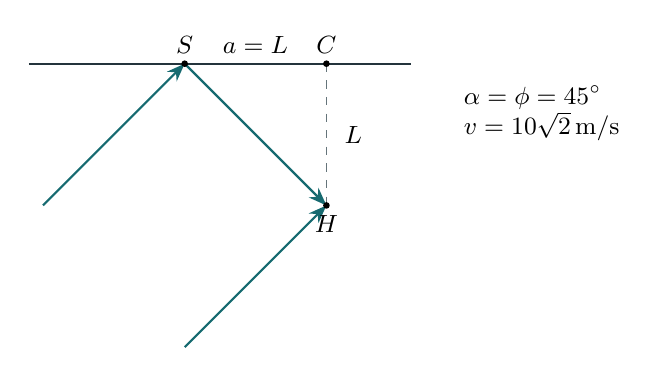
\begin{tikzpicture}[x=1.8cm,y=1.8cm]

\draw[object](-2.1,0)--(.6,0);\draw[guide](0,0)--(0,-1);
\draw[motion](-2,-1)--(-1,0);\draw[motion](-1,0)--(0,-1);\draw[motion](-1,-2)--(0,-1);
\fill(-1,0)circle(1.2pt);\fill(0,0)circle(1.2pt);\fill(0,-1)circle(1.2pt);
\node[above]at(-1,0){$S$};\node[above]at(0,0){$C$};\node[below]at(0,-1){$H$};
\node[right]at(.06,-.5){$L$};\node[above]at(-.5,0){$a=L$};
\node[anchor=west,align=left]at(.9,-.35){$\alpha=\phi=45^\circ$\\$v=10\sqrt2\,\mathrm{m/s}$};

\end{tikzpicture}
\figcaption{变图光2.1V1\quad 驻点距离与垂距相等的反演}
\end{minipage}\end{center}

\item 汽车改为由西向东行驶，同一空间驻点保持不变，$\dot\Delta$符号反转；测得的起伏频率绝对值不变。

\par 用本题的$L,\alpha,v$，分别写出向西和向东行车的有向路程差变化率，并计算$x=-100\,\mathrm m$时两种行车方向的频率。

\par\noindent\textbf{解}\quad 变图光2.1V2给出同一$B,H$和两条相反速度箭头，入射、散射方向未变。由链式法则，
\[
\dot\Delta_{\rm W}=-v\left(\cos\alpha+\frac x{\sqrt{x^2+L^2}}\right),\qquad
\dot\Delta_{\rm E}=+v\left(\cos\alpha+\frac x{\sqrt{x^2+L^2}}\right).
\]
因此速度反向只改变符号，零点仍为$x=-200\,\mathrm m$。在图V2的$B=(-L,0)$，括号为$2/\sqrt5-1/\sqrt2>0$；两种频率均为
\[
\nu_b=\sqrt5\left(\frac2{\sqrt5}-\frac1{\sqrt2}\right)
=2-\sqrt{\frac52}\simeq0.41886\,\mathrm{Hz}.
\]
有向路程差变化率分别是$-\lambda\nu_b$和$+\lambda\nu_b$，代入$\lambda=5\,\mathrm m$后单位为$\mathrm{m/s}$。相位差的变化率为$\dot\Psi=2\pi\dot\Delta/\lambda$，单位为$\mathrm{rad/s}$；两种行车方向的值分别为$-2\pi\nu_b$和$+2\pi\nu_b$。车在同一位置的瞬时明暗还取决于常量相位，但由相位变化率定义的频率不因行车方向倒转而改变。

\begin{center}\begin{minipage}{.97\linewidth}\centering
\begin{tikzpicture}[x=1.7cm,y=1.7cm]

\draw[object](-2.2,0)--(.5,0);\draw[guide](0,0)--(0,-1);
\draw[motion](-2,-.5)--(-1,0);\draw[motion](-1,0)--(0,-1);\draw[motion](-1,-1.5)--(0,-1);
\draw[force](-.6,.5)--(-1.5,.5);\node[above]at(-1.05,.5){向西};
\draw[motion](-1.5,.95)--(-.6,.95);\node[above]at(-1.05,.95){向东};
\fill(-1,0)circle(1.2pt);\fill(0,0)circle(1.2pt);\fill(0,-1)circle(1.2pt);
\node[above left]at(-1,0){$B$};\node[above]at(0,0){$C$};\node[below]at(0,-1){$H$};
\node[anchor=west,align=left]at(.8,-.1){$x=-L$\\两箭头表示同处的两种车速\\相位变化率反号};

\end{tikzpicture}
\figcaption{变图光2.1V2\quad 行车反向而瞬时频率不变}
\end{minipage}\end{center}

\item 若载波频率加倍而几何及车速不变，$\lambda$减半，所有非零起伏频率加倍，驻点位置不变。

\par 将载波改为$120\,\mathrm{MHz}$，其余几何和车速均取本题数值，求$C$处和道路两端的频率，以及零频率点的位置。

\par\noindent\textbf{解}\quad 变图光2.1V3用两条曲线比较同一车辆的$60$与$120\,\mathrm{MHz}$信号。新的波长为$\lambda_2=2.5\,\mathrm m=\lambda_1/2$，而$\dot\Delta$完全由几何和车速决定，故
\[
\nu_{b,2}(x)=2\nu_{b,1}(x),\qquad
\nu_{b,2}(0)=4\,\mathrm{Hz}.
\]
令括号$\cos\alpha+x/\sqrt{x^2+L^2}$为零，仍得$x=-200\,\mathrm m$，即图V3两条曲线共用$S$。向西和向东远处的极限分别为$2(\sqrt5-2)$与$2(\sqrt5+2)\,\mathrm{Hz}$。载波变频并不会改变光程差曲线的驻点，也不保证该点的总相位仍对应同一种明暗。

\begin{center}\begin{minipage}{.97\linewidth}\centering
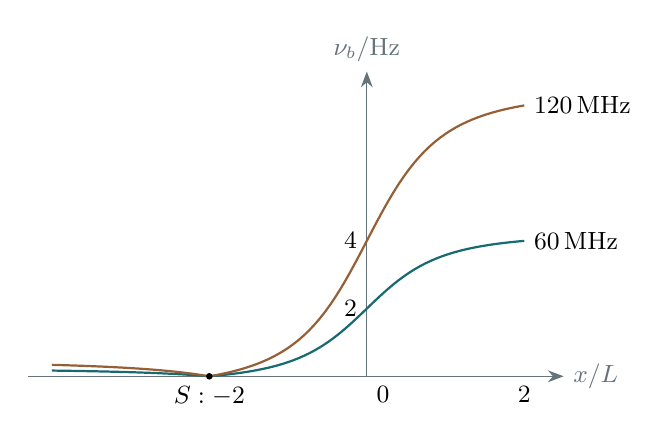
\begin{tikzpicture}[x=1cm,y=.43cm]

\draw[axis](-4.3,0)--(2.5,0)node[right]{$x/L$};\draw[axis](0,0)--(0,9)node[above]{$\nu_b/\mathrm{Hz}$};
\draw[traj]plot coordinates {(-4.000000000000,0.169304578187) (-3.933333333333,0.167126717179) (-3.866666666667,0.164842306570) (-3.800000000000,0.162444404628) (-3.733333333333,0.159925505895) (-3.666666666667,0.157277486520) (-3.600000000000,0.154491543471) (-3.533333333333,0.151558126825) (-3.466666666667,0.148466864266) (-3.400000000000,0.145206476782) (-3.333333333333,0.141764684391) (-3.266666666667,0.138128100597) (-3.200000000000,0.134282114049) (-3.133333333333,0.130210755676) (-3.066666666667,0.125896549318) (-3.000000000000,0.121320343560) (-2.933333333333,0.116461122163) (-2.866666666667,0.111295790080) (-2.800000000000,0.105798931587) (-2.733333333333,0.099942536565) (-2.666666666667,0.093695690361) (-2.600000000000,0.087024221971) (-2.533333333333,0.079890304523) (-2.466666666667,0.072252001166) (-2.400000000000,0.064062748461) (-2.333333333333,0.055270768301) (-2.266666666667,0.045818398142) (-2.200000000000,0.035641328043) (-2.133333333333,0.024667731639) (-2.066666666667,0.012817276740) (-2.000000000000,0.000000000000) (-1.933333333333,0.013884971089) (-1.866666666667,0.028950866211) (-1.800000000000,0.045324907566) (-1.733333333333,0.063150148465) (-1.666666666667,0.082587527882) (-1.600000000000,0.103818147440) (-1.533333333333,0.127045766795) (-1.466666666667,0.152499496613) (-1.400000000000,0.180436642815) (-1.333333333333,0.211145618000) (-1.266666666667,0.244948781899) (-1.200000000000,0.282204997058) (-1.133333333333,0.323311583301) (-1.066666666667,0.368705219428) (-1.000000000000,0.418861169916) (-0.933333333333,0.474290009906) (-0.866666666667,0.535530795557) (-0.800000000000,0.603139408461) (-0.733333333333,0.677670648706) (-0.666666666667,0.759652654108) (-0.600000000000,0.849552516729) (-0.533333333333,0.947732716471) (-0.466666666667,1.054399352823) (-0.400000000000,1.169545201463) (-0.333333333333,1.292893218813) (-0.266666666667,1.423848798084) (-0.200000000000,1.561470990346) (-0.133333333333,1.704472937717) (-0.066666666667,1.851258970673) (0.000000000000,2.000000000000) (0.066666666667,2.148741029327) (0.133333333333,2.295527062283) (0.200000000000,2.438529009654) (0.266666666667,2.576151201916) (0.333333333333,2.707106781187) (0.400000000000,2.830454798537) (0.466666666667,2.945600647177) (0.533333333333,3.052267283529) (0.600000000000,3.150447483271) (0.666666666667,3.240347345892) (0.733333333333,3.322329351294) (0.800000000000,3.396860591539) (0.866666666667,3.464469204443) (0.933333333333,3.525709990094) (1.000000000000,3.581138830084) (1.066666666667,3.631294780572) (1.133333333333,3.676688416699) (1.200000000000,3.717795002942) (1.266666666667,3.755051218101) (1.333333333333,3.788854382000) (1.400000000000,3.819563357185) (1.466666666667,3.847500503387) (1.533333333333,3.872954233205) (1.600000000000,3.896181852560) (1.666666666667,3.917412472118) (1.733333333333,3.936849851535) (1.800000000000,3.954675092434) (1.866666666667,3.971049133789) (1.933333333333,3.986115028911) (2.000000000000,4.000000000000)};
\draw[color=warm,thick]plot coordinates {(-4.000000000000,0.338609156373) (-3.933333333333,0.334253434358) (-3.866666666667,0.329684613140) (-3.800000000000,0.324888809257) (-3.733333333333,0.319851011789) (-3.666666666667,0.314554973040) (-3.600000000000,0.308983086942) (-3.533333333333,0.303116253649) (-3.466666666667,0.296933728532) (-3.400000000000,0.290412953563) (-3.333333333333,0.283529368781) (-3.266666666667,0.276256201194) (-3.200000000000,0.268564228098) (-3.133333333333,0.260421511353) (-3.066666666667,0.251793098636) (-3.000000000000,0.242640687119) (-2.933333333333,0.232922244327) (-2.866666666667,0.222591580161) (-2.800000000000,0.211597863173) (-2.733333333333,0.199885073129) (-2.666666666667,0.187391380722) (-2.600000000000,0.174048443942) (-2.533333333333,0.159780609046) (-2.466666666667,0.144504002332) (-2.400000000000,0.128125496923) (-2.333333333333,0.110541536603) (-2.266666666667,0.091636796283) (-2.200000000000,0.071282656087) (-2.133333333333,0.049335463277) (-2.066666666667,0.025634553481) (-2.000000000000,0.000000000000) (-1.933333333333,0.027769942177) (-1.866666666667,0.057901732422) (-1.800000000000,0.090649815132) (-1.733333333333,0.126300296930) (-1.666666666667,0.165175055763) (-1.600000000000,0.207636294880) (-1.533333333333,0.254091533589) (-1.466666666667,0.304998993227) (-1.400000000000,0.360873285630) (-1.333333333333,0.422291236000) (-1.266666666667,0.489897563798) (-1.200000000000,0.564409994117) (-1.133333333333,0.646623166602) (-1.066666666667,0.737410438855) (-1.000000000000,0.837722339832) (-0.933333333333,0.948580019813) (-0.866666666667,1.071061591114) (-0.800000000000,1.206278816922) (-0.733333333333,1.355341297411) (-0.666666666667,1.519305308216) (-0.600000000000,1.699105033458) (-0.533333333333,1.895465432941) (-0.466666666667,2.108798705646) (-0.400000000000,2.339090402925) (-0.333333333333,2.585786437627) (-0.266666666667,2.847697596169) (-0.200000000000,3.122941980693) (-0.133333333333,3.408945875434) (-0.066666666667,3.702517941346) (0.000000000000,4.000000000000) (0.066666666667,4.297482058654) (0.133333333333,4.591054124566) (0.200000000000,4.877058019307) (0.266666666667,5.152302403831) (0.333333333333,5.414213562373) (0.400000000000,5.660909597075) (0.466666666667,5.891201294354) (0.533333333333,6.104534567059) (0.600000000000,6.300894966542) (0.666666666667,6.480694691784) (0.733333333333,6.644658702589) (0.800000000000,6.793721183078) (0.866666666667,6.928938408886) (0.933333333333,7.051419980187) (1.000000000000,7.162277660168) (1.066666666667,7.262589561145) (1.133333333333,7.353376833398) (1.200000000000,7.435590005883) (1.266666666667,7.510102436202) (1.333333333333,7.577708764000) (1.400000000000,7.639126714370) (1.466666666667,7.695001006773) (1.533333333333,7.745908466411) (1.600000000000,7.792363705120) (1.666666666667,7.834824944237) (1.733333333333,7.873699703070) (1.800000000000,7.909350184868) (1.866666666667,7.942098267578) (1.933333333333,7.972230057823) (2.000000000000,8.000000000000)};
\fill(-2,0)circle(1.2pt);\node[below]at(-2,0){$S:-2$};\node[below right]at(0,0){$0$};
\node[left]at(0,2){$2$};\node[left]at(0,4){$4$};\node[below]at(2,0){$2$};
\node[right]at(2,4.000000000000){$60\,\mathrm{MHz}$};
\node[right]at(2,8.000000000000){$120\,\mathrm{MHz}$};

\end{tikzpicture}
\figcaption{变图光2.1V3\quad 频率加倍与共用的零点}
\end{minipage}\end{center}

\item 求驻点的二阶路程变化：$\Delta''(x)=L^2/(x^2+L^2)^{3/2}>0$。因此相位差在这里有极小值，附近起伏频率随离开驻点的距离近似线性增加。

\par 使用本题参数，求驻点附近$\nu_b$随离开驻点距离的首项，并估算在$x=-190\,\mathrm m$和$-210\,\mathrm m$处的频率；将首项与精确式比较。

\par\noindent\textbf{解}\quad 记$x_*=-200\,\mathrm m$、$\xi=x-x_*$。因$\Delta'(x_*)=0$，泰勒展开给出
\[
\Delta(x)=\Delta_{\min}+\frac12\Delta''(x_*)\xi^2+O(\xi^3),\qquad
\Delta''(x_*)=\frac1{500\sqrt5}\,\mathrm{m^{-1}}.
\]
再对$x$求导并乘车速，得到
\[
\nu_b\simeq\frac v\lambda\Delta''(x_*)|\xi|
=0.002\,\frac{\mathrm{Hz}}{\mathrm m}|\xi|.
\]
变图光2.1V4的虚线是这一V形首项，两侧$|\xi|=10\,\mathrm m$均估算为$0.0200\,\mathrm{Hz}$。精确式分别给$x=-190\,\mathrm m$时约$0.02126\,\mathrm{Hz}$，$x=-210\,\mathrm m$时约$0.01886\,\mathrm{Hz}$；首项关于驻点对称，三阶及更高项使精确值出现小差别。正的二阶导数说明$\Delta$局部极小，不能把频率图的尖点当作$\Delta$不可导。

\begin{center}\begin{minipage}{.97\linewidth}\centering
\begin{tikzpicture}[x=1cm,y=.7cm]

\draw[axis](-3.3,0)--(3.5,0)node[right]{$\xi/(10\,\mathrm m)$};
\draw[axis](0,0)--(0,4.5)node[above]{$\nu_b/(.02\,\mathrm{Hz})$};
\draw[guide](-3,3)--(0,0)--(3,3);
\draw[traj]plot coordinates {(-3.000000000000,2.531549295589) (-2.925000000000,2.478175338761) (-2.850000000000,2.424359457528) (-2.775000000000,2.370096995621) (-2.700000000000,2.315383238730) (-2.625000000000,2.260213413695) (-2.550000000000,2.204582687683) (-2.475000000000,2.148486167356) (-2.400000000000,2.091918898024) (-2.325000000000,2.034875862789) (-2.250000000000,1.977351981671) (-2.175000000000,1.919342110727) (-2.100000000000,1.860841041155) (-2.025000000000,1.801843498382) (-1.950000000000,1.742344141143) (-1.875000000000,1.682337560541) (-1.800000000000,1.621818279104) (-1.725000000000,1.560780749812) (-1.650000000000,1.499219355128) (-1.575000000000,1.437128405997) (-1.500000000000,1.374502140845) (-1.425000000000,1.311334724556) (-1.350000000000,1.247620247436) (-1.275000000000,1.183352724159) (-1.200000000000,1.118526092706) (-1.125000000000,1.053134213278) (-1.050000000000,0.987170867201) (-1.000000000000,0.942874714552) (-0.975000000000,0.920629755811) (-0.900000000000,0.853504499326) (-0.825000000000,0.785788635703) (-0.750000000000,0.717475619470) (-0.675000000000,0.648558820551) (-0.600000000000,0.579031523072) (-0.525000000000,0.508886924147) (-0.450000000000,0.438118132647) (-0.375000000000,0.366718167955) (-0.300000000000,0.294679958702) (-0.225000000000,0.221996341483) (-0.150000000000,0.148660059555) (-0.075000000000,0.074663761523) (0.000000000000,0.000000000000) (0.075000000000,0.075338769750) (0.150000000000,0.151360191183) (0.225000000000,0.228072007873) (0.300000000000,0.305482064919) (0.375000000000,0.383598310382) (0.450000000000,0.462428796736) (0.525000000000,0.541981682338) (0.600000000000,0.622265232919) (0.675000000000,0.703287823097) (0.750000000000,0.785057937911) (0.825000000000,0.867584174370) (0.900000000000,0.950875243027) (0.975000000000,1.034939969575) (1.000000000000,1.063135011281) (1.050000000000,1.119787296461) (1.125000000000,1.205426284520) (1.200000000000,1.291866114638) (1.275000000000,1.379116089427) (1.350000000000,1.467185634927) (1.425000000000,1.556084302330) (1.500000000000,1.645821769722) (1.575000000000,1.736407843852) (1.650000000000,1.827852461920) (1.725000000000,1.920165693389) (1.800000000000,2.013357741816) (1.875000000000,2.107438946713) (1.950000000000,2.202419785420) (2.025000000000,2.298310875009) (2.100000000000,2.395122974211) (2.175000000000,2.492866985357) (2.250000000000,2.591553956351) (2.325000000000,2.691195082663) (2.400000000000,2.791801709341) (2.475000000000,2.893385333055) (2.550000000000,2.995957604151) (2.625000000000,3.099530328740) (2.700000000000,3.204115470803) (2.775000000000,3.309725154319) (2.850000000000,3.416371665419) (2.925000000000,3.524067454558) (3.000000000000,3.632825138715)};
\node[below]at(-1,0){$-1$};\node[below right]at(0,0){$0$};\node[below]at(1,0){$1$};
\node[left]at(0,1){$1$};\node[left]at(0,3){$3$};
\node[anchor=west]at(-3.0,4.0){实线：精确式};\node[anchor=west]at(-3.0,3.45){虚线：首项};

\end{tikzpicture}
\figcaption{变图光2.1V4\quad 驻点附近的线性频率首项}
\end{minipage}\end{center}

\item 另一次测量只知$L=100\,\mathrm m$、$f=60\,\mathrm{MHz}$，汽车仍向西运动，来波仍向东北传播。测得$x=0$时$\nu_b=2\,\mathrm{Hz}$，$x=-100\,\mathrm m$时$\nu_b=1\,\mathrm{Hz}$。求$\alpha,v$和零频率位置，说明绝对值是否造成多解。

\par\noindent\textbf{解}\quad 令$z=v/\lambda>0$，$b=\cos\alpha$，则$0<b<1$。变图光2.1V5的$C$和$P$给出
\[
zb=2,\qquad z\left|b-\frac1{\sqrt2}\right|=1,
\quad\Longrightarrow\quad\left|2-\frac z{\sqrt2}\right|=1.
\]
两条代数分支为$z=\sqrt2$或$3\sqrt2$。第一支使$b=2/z=\sqrt2>1$，没有实际入射方向，应排除。第二支给出
\[
\cos\alpha=\frac{\sqrt2}{3},\quad
\alpha\simeq61.8745^\circ,\quad
v=15\sqrt2\,\mathrm{m/s},\quad
x_*=-L\cot\alpha=-100\sqrt{\frac27}\,\mathrm m.
\]
图V5的零点在$P$与$C$之间；因此$P$处括号已变号，正好对应保留的绝对值分支。保留$z=3\sqrt2$这一支的理由是$0<\cos\alpha<1$，并且图V5的驻点确在$P,C$之间。

\begin{center}\begin{minipage}{.97\linewidth}\centering
\begin{tikzpicture}[x=1.8cm,y=.6cm]

\draw[axis](-2.2,0)--(1.3,0)node[right]{$x/L$};\draw[axis](0,0)--(0,5.4)node[above]{$\nu_b/\mathrm{Hz}$};
\draw[traj]plot coordinates {(-2.000000000000,1.794733192202) (-1.966666666667,1.781826821309) (-1.933333333333,1.768388311871) (-1.900000000000,1.754390055051) (-1.866666666667,1.739802785725) (-1.833333333333,1.724595476688) (-1.800000000000,1.708735226615) (-1.766666666667,1.692187141571) (-1.733333333333,1.674914209966) (-1.700000000000,1.656877170849) (-1.666666666667,1.638034375545) (-1.633333333333,1.618341642737) (-1.600000000000,1.597752107180) (-1.566666666667,1.576216062430) (-1.533333333333,1.553680798110) (-1.500000000000,1.530090432487) (-1.466666666667,1.505385741406) (-1.433333333333,1.479503984921) (-1.400000000000,1.452378733413) (-1.366666666667,1.423939695378) (-1.333333333333,1.394112549695) (-1.300000000000,1.362818785762) (-1.266666666667,1.329975555671) (-1.233333333333,1.295495543471) (-1.200000000000,1.259286857531) (-1.166666666667,1.221252953159) (-1.133333333333,1.181292593914) (-1.100000000000,1.139299861420) (-1.066666666667,1.095164225052) (-1.033333333333,1.048770684510) (-1.000000000000,1.000000000000) (-0.966666666667,0.948729026532) (-0.933333333333,0.894831170541) (-0.900000000000,0.838176988629) (-0.866666666667,0.778634949528) (-0.833333333333,0.716072381276) (-0.800000000000,0.650356625796) (-0.766666666667,0.581356422447) (-0.733333333333,0.508943540190) (-0.700000000000,0.432994674727) (-0.666666666667,0.353393621658) (-0.633333333333,0.270033729361) (-0.600000000000,0.182820625327) (-0.566666666667,0.091675197147) (-0.534522483825,0.000000000000) (-0.533333333333,0.003463206062) (-0.500000000000,0.102633403899) (-0.466666666667,0.205848918795) (-0.433333333333,0.313094507591) (-0.400000000000,0.424322805683) (-0.366666666667,0.539451218750) (-0.333333333333,0.658359213500) (-0.300000000000,0.780886169339) (-0.266666666667,0.906829955182) (-0.233333333333,1.035946387510) (-0.200000000000,1.167949705662) (-0.166666666667,1.302514167537) (-0.133333333333,1.439276823781) (-0.100000000000,1.577841473162) (-0.066666666667,1.717783739485) (-0.033333333333,1.858657145771) (0.000000000000,2.000000000000) (0.033333333333,2.141342854229) (0.066666666667,2.282216260515) (0.100000000000,2.422158526838) (0.133333333333,2.560723176219) (0.166666666667,2.697485832463) (0.200000000000,2.832050294338) (0.233333333333,2.964053612490) (0.266666666667,3.093170044818) (0.300000000000,3.219113830661) (0.333333333333,3.341640786500) (0.366666666667,3.460548781250) (0.400000000000,3.575677194317) (0.433333333333,3.686905492409) (0.466666666667,3.794151081205) (0.500000000000,3.897366596101) (0.533333333333,3.996536793938) (0.566666666667,4.091675197147) (0.600000000000,4.182820625327) (0.633333333333,4.270033729361) (0.666666666667,4.353393621658) (0.700000000000,4.432994674727) (0.733333333333,4.508943540190) (0.766666666667,4.581356422447) (0.800000000000,4.650356625796) (0.833333333333,4.716072381276) (0.866666666667,4.778634949528) (0.900000000000,4.838176988629) (0.933333333333,4.894831170541) (0.966666666667,4.948729026532) (1.000000000000,5.000000000000)};
\fill(-1,1)circle(1.2pt);\node[above left]at(-1,1){$P$};\fill(0,2)circle(1.2pt);\node[below right]at(0,2){$C$};
\fill(-0.534522483825,0)circle(1.2pt);\node[below]at(-0.534522483825,0){$S$};
\node[below]at(-1,0){$-1$};\node[below right]at(0,0){$0$};\node[left]at(0,1){$1$};\node[left]at(0,2){$2$};

\end{tikzpicture}
\figcaption{变图光2.1V5\quad 两个非零读数确定绝对值的实际分支}
\end{minipage}\end{center}

\item 允许散射体在水平面内任意移动。接收机仍为$H=(0,-100)\,\mathrm m$，入射方向$\boldsymbol s=(2,1)/\sqrt5$。散射体到达$B=(-200,0)\,\mathrm m$时，瞬时速度为$\boldsymbol V=(-10,-5)\,\mathrm{m/s}$。求$\lambda=5\,\mathrm m$时的起伏频率，并给出此点速度使频率为零的条件。

\par\noindent\textbf{解}\quad 变图光2.1V6把真实散射方向标为$\boldsymbol q=(H-B)/R$，其中$R=|H-B|$；速度箭头单独标在$B$旁。固定$H$时，
\[
\Delta=\boldsymbol s\cdot(B-H)+R,\qquad
\dot\Delta=(\boldsymbol s-\boldsymbol q)\cdot\boldsymbol V.
\]
在给定点，$\boldsymbol q=(2,-1)/\sqrt5$，故$\boldsymbol s-\boldsymbol q=(0,2)/\sqrt5$。于是
\[
\dot\Delta=-\frac{10}{\sqrt5}\,\mathrm{m/s},\qquad
\nu_b=\frac2{\sqrt5}\,\mathrm{Hz}\simeq0.89443\,\mathrm{Hz}.
\]
同一点满足零频率的条件为$V_y=0$，即速度沿东西方向（也包括静止）。图V6中入射和散射方向的水平分量相同，竖直分量不同；具有南北分量的速度便会破坏先前的投影抵消。这一判据适用于瞬时速度，不要求散射体的整条轨迹都是直线。

\begin{center}\begin{minipage}{.97\linewidth}\centering
\begin{tikzpicture}[x=1.55cm,y=1.55cm]

\draw[object](-3.3,0)--(.5,0);\draw[guide](0,0)--(0,-1);
\draw[motion](-3,-.5)--(-2,0);\draw[motion](-2,0)--(0,-1);\draw[motion](-1,-1.5)--(0,-1);
\draw[force](-2.15,.65)--(-2.75,.35);
\fill(-2,0)circle(1.2pt);\fill(0,0)circle(1.2pt);\fill(0,-1)circle(1.2pt);
\node[above right]at(-2,0){$B$};\node[above]at(0,0){$C$};\node[below]at(0,-1){$H$};
\node[above left]at(-2.3,.6){$\boldsymbol V$};\node[below left]at(-2.7,-.5){$\boldsymbol s$};\node[below]at(-1.15,-.5){$\boldsymbol q$};
\node[anchor=west,align=left]at(.8,-.2){$\boldsymbol s=(2,1)/\sqrt5$\\$\boldsymbol q=(2,-1)/\sqrt5$\\速度箭头平移画出};

\end{tikzpicture}
\figcaption{变图光2.1V6\quad 速度的南北分量破坏水平投影相消}
\end{minipage}\end{center}

\item 保持本题的$\alpha,v,L,\lambda$，但让散射附加相位随时间变化：$\phi_s(t)=2\pi\Omega t+\phi_0$，其中$\Omega=0.500\,\mathrm{Hz}$。求新的零起伏位置及$C$处频率，并讨论任意常量$\Omega$时有限零点的存在条件。

\par\noindent\textbf{解}\quad 相位差为$\Psi=2\pi\Delta/\lambda+\phi_s$，应先相加有向变化率再取绝对值。向西行车有
\[
\frac{\dot\Psi}{2\pi}=\Omega-2-\sqrt5\frac x{\sqrt{x^2+L^2}},\qquad
\nu_b=\left|\Omega-2-\sqrt5\frac x{\sqrt{x^2+L^2}}\right|.
\]
变图光2.1V7画出有向频率$F=\dot\Psi/(2\pi)$，其与零线的交点才是新驻相位点。取$\Omega=1/2$，得$x/\sqrt{x^2+L^2}=-3/(2\sqrt5)$，因该比值为负，解取西侧：
\[
x_*=-\frac{300}{\sqrt{11}}\,\mathrm m\simeq-90.453\,\mathrm m,
\qquad \nu_b(0)=1.500\,\mathrm{Hz}.
\]
有限$x$的比值严格落在$(-1,1)$，所以有限零点存在且唯一的条件为
\[
2-\sqrt5<\Omega<2+\sqrt5.
\]
等号只在道路无穷远处达到零极限，不能登记为有限驻点；区间外没有零起伏点。常量相位$\phi_0$影响明暗，却不进入此条件。

\begin{center}\begin{minipage}{.97\linewidth}\centering
\begin{tikzpicture}[x=1cm,y=.65cm]

\draw[axis](-4.3,0)--(3.5,0)node[right]{$x/L$};\draw[axis](0,-4.2)--(0,1.2)node[above]{$F/\mathrm{Hz}$};
\draw[traj]plot coordinates {(-4.000000000000,0.669304578187) (-3.930000000000,0.667015082742) (-3.860000000000,0.664607742737) (-3.790000000000,0.662074474621) (-3.720000000000,0.659406503180) (-3.650000000000,0.656594290830) (-3.580000000000,0.653627458530) (-3.510000000000,0.650494697212) (-3.440000000000,0.647183668441) (-3.370000000000,0.643680892818) (-3.300000000000,0.639971624439) (-3.230000000000,0.636039709460) (-3.160000000000,0.631867426494) (-3.090000000000,0.627435306268) (-3.020000000000,0.622721927499) (-2.950000000000,0.617703685544) (-2.880000000000,0.612354529783) (-2.810000000000,0.606645665087) (-2.740000000000,0.600545211986) (-2.670000000000,0.594017819292) (-2.600000000000,0.587024221971) (-2.530000000000,0.579520735915) (-2.460000000000,0.571458680018) (-2.390000000000,0.562783714453) (-2.320000000000,0.553435082491) (-2.250000000000,0.543344741339) (-2.180000000000,0.532436365582) (-2.110000000000,0.520624204739) (-2.040000000000,0.507811774423) (-1.970000000000,0.493890358702) (-1.900000000000,0.478737299774) (-1.830000000000,0.462214050469) (-1.760000000000,0.444163965813) (-1.690000000000,0.424409813114) (-1.620000000000,0.402750986791) (-1.550000000000,0.378960426695) (-1.480000000000,0.352781259400) (-1.410000000000,0.323923214862) (-1.340000000000,0.292058920704) (-1.270000000000,0.256820249951) (-1.200000000000,0.217795002942) (-1.130000000000,0.174524349665) (-1.060000000000,0.126501653413) (-0.990000000000,0.073173546152) (-0.920000000000,0.013944427526) (-0.904534033733,0.000000000000) (-0.850000000000,-0.051814107146) (-0.780000000000,-0.124747089797) (-0.710000000000,-0.205491235272) (-0.640000000000,-0.294639291275) (-0.570000000000,-0.392692330929) (-0.500000000000,-0.500000000000) (-0.430000000000,-0.616691096527) (-0.360000000000,-0.742600243640) (-0.290000000000,-0.877200395855) (-0.220000000000,-1.019554448172) (-0.150000000000,-1.168300663435) (-0.080000000000,-1.321684262095) (-0.010000000000,-1.477640438175) (0.000000000000,-1.500000000000) (0.060000000000,-1.633923233396) (0.130000000000,-1.788263218184) (0.200000000000,-1.938529009654) (0.270000000000,-2.082866565135) (0.340000000000,-2.219796393665) (0.410000000000,-2.348259724106) (0.480000000000,-2.467616083096) (0.550000000000,-2.577603084122) (0.620000000000,-2.678272919616) (0.690000000000,-2.769919531635) (0.760000000000,-2.853007318253) (0.830000000000,-2.928108245627) (0.900000000000,-2.995850614458) (0.970000000000,-3.056880060141) (1.040000000000,-3.111831733550) (1.110000000000,-3.161311828398) (1.180000000000,-3.205886422619) (1.250000000000,-3.246075739424) (1.320000000000,-3.282352227604) (1.390000000000,-3.315141195640) (1.460000000000,-3.344823047929) (1.530000000000,-3.371736436616) (1.600000000000,-3.396181852560) (1.670000000000,-3.418425337636) (1.740000000000,-3.438702116191) (1.810000000000,-3.457220025089) (1.880000000000,-3.474162677707) (1.950000000000,-3.489692334416) (2.020000000000,-3.503952475871) (2.090000000000,-3.517070089987) (2.160000000000,-3.529157691651) (2.230000000000,-3.540315098315) (2.300000000000,-3.550630985912) (2.370000000000,-3.560184249281) (2.440000000000,-3.569045189975) (2.510000000000,-3.577276552519) (2.580000000000,-3.584934428208) (2.650000000000,-3.592069043440) (2.720000000000,-3.598725447617) (2.790000000000,-3.604944113828) (2.860000000000,-3.610761463793) (2.930000000000,-3.616210327125) (3.000000000000,-3.621320343560)};
\fill(-0.904534033733,0)circle(1.2pt);\node[below left]at(-0.904534033733,0){$S_\Omega$};
\fill(0,-1.5)circle(1.2pt);\node[above right]at(0,-1.5){$C$};
\node[above right]at(0,0){$0$};\node[below]at(-2,0){$-2$};\node[above]at(2,0){$2$};\node[left]at(0,-1.5){$-1.5$};\node[left]at(0,-3){$-3$};

\end{tikzpicture}
\figcaption{变图光2.1V7\quad 附加相位漂移后的有向频率零点}
\end{minipage}\end{center}

\item 考虑相干时间有限的信号。取本题的几何和车速，散射波与直达波的振幅比为$\rho=0.5$，归一化时间相干函数的模为$|\gamma(\tau)|=e^{-|\tau|/\tau_c}$，$\tau_c=1.00\,\mu\mathrm s$。忽略振幅比随车位的变化。求$S$与$C$处条纹可见度，并估算散射传播时间内汽车位移，以判断忽略传播时延的位置修正是否合理。

\par\noindent\textbf{解}\quad 对两路延迟相干信号，交叉项振幅乘以$|\gamma|$，所以
\[
\mathcal V=\frac{I_{\max}-I_{\min}}{I_{\max}+I_{\min}}
=\frac{2\rho}{1+\rho^2}|\gamma(\Delta/c)|
=0.8\exp\left(-\frac\Delta{c\tau_c}\right).
\]
本题$\Delta>0$。变图光2.1V8用$\Delta/(c\tau_c)$作横坐标，$S$处$\Delta=200/\sqrt5\,\mathrm m$，$C$处$\Delta=100(1+1/\sqrt5)\,\mathrm m$，于是
\[
\begin{array}{c|cc}
 &S&C\\ \hline
\Delta/c\ (\mu\mathrm s)&0.29814&0.48240\\
\mathcal V&0.59376&0.49384
\end{array}
\]
两路相位变化率在驻点处相等，瞬时起伏频率为零。图V8的$S$点因两路延迟较短，可见度高于$C$点。

散射段的传播时间由$R/c$决定，不能把它与两路延迟$\Delta/c$混同。$S$处$R=100\sqrt5\,\mathrm m$，故传播期间位移尺度为
\[
\delta B\simeq\frac{vR}{c}=8.33\,\mu\mathrm m.
\]
在$C$处同理得到$3.73\,\mu\mathrm m$。它们远小于$L=100\,\mathrm m$，且$v/c\simeq3.73\times10^{-8}$；在题给米级车位和约$0.01\,\mathrm{m/s}$的速度精度下，忽略这一修正成立。若研究微米级位置或$v/c$阶频移，则应回到散射时刻$t_s$和接收时刻$t=t_s+R(t_s)/c$，不能继续直接把观测时刻车位代入。

\begin{center}\begin{minipage}{.97\linewidth}\centering
\begin{tikzpicture}[x=5cm,y=3cm]

\draw[axis](0,0)--(1.35,0)node[right]{$\Delta/(c\tau_c)$};\draw[axis](0,0)--(0,.95)node[above]{$\mathcal V$};
\draw[traj]plot coordinates {(0.000000000000,0.800000000000) (0.020000000000,0.784158938645) (0.040000000000,0.768631551322) (0.060000000000,0.753411626867) (0.080000000000,0.738493077109) (0.100000000000,0.723869934429) (0.120000000000,0.709536349374) (0.140000000000,0.695486588319) (0.160000000000,0.681715031173) (0.180000000000,0.668216169129) (0.200000000000,0.654984602462) (0.220000000000,0.642015038370) (0.240000000000,0.629302288853) (0.260000000000,0.616841268643) (0.280000000000,0.604626993165) (0.300000000000,0.592654576545) (0.320000000000,0.580919229659) (0.340000000000,0.569416258210) (0.360000000000,0.558141060857) (0.380000000000,0.547089127370) (0.400000000000,0.536256036829) (0.420000000000,0.525637455852) (0.440000000000,0.515229136867) (0.460000000000,0.505026916406) (0.480000000000,0.495026713445) (0.500000000000,0.485224527770) (0.520000000000,0.475616438376) (0.540000000000,0.466198601899) (0.560000000000,0.456967251079) (0.580000000000,0.447918693252) (0.600000000000,0.439049308875) (0.620000000000,0.430355550076) (0.640000000000,0.421833939234) (0.660000000000,0.413481067593) (0.680000000000,0.405293593892) (0.700000000000,0.397268243033) (0.720000000000,0.389401804768) (0.740000000000,0.381691132417) (0.760000000000,0.374133141608) (0.780000000000,0.366724809044) (0.800000000000,0.359463171294) (0.820000000000,0.352345323605) (0.840000000000,0.345368418743) (0.860000000000,0.338529665854) (0.880000000000,0.331826329345) (0.900000000000,0.325255727792) (0.920000000000,0.318815232868) (0.940000000000,0.312502268287) (0.960000000000,0.306314308780) (0.980000000000,0.300248879081) (1.000000000000,0.294303552937) (1.020000000000,0.288475952138) (1.040000000000,0.282763745567) (1.060000000000,0.277164648264) (1.080000000000,0.271676420516) (1.100000000000,0.266296866958) (1.120000000000,0.261023835698) (1.140000000000,0.255855217453) (1.160000000000,0.250788944706) (1.180000000000,0.245822990881) (1.200000000000,0.240955369530)};
\fill(0.298142397000,0.593756516631)circle(1.2pt);
\fill(0.482404531833,0.493837835874)circle(1.2pt);
\node[above right]at(0.298142397000,0.593756516631){$S$};
\node[above right]at(0.482404531833,0.493837835874){$C$};
\node[left]at(0,.8){$.8$};\node[left]at(0,.4){$.4$};\node[below]at(0,0){$0$};\node[below]at(.5,0){$.5$};\node[below]at(1,0){$1$};

\end{tikzpicture}
\figcaption{变图光2.1V8\quad 相位停顿与相干可见度须分别判断}
\end{minipage}\end{center}
\end{enumerate}

\Needspace{13\baselineskip}

\pdfbookmark[2]{第 2 题 射电星升起时的海面干涉}{q2}

\section*{第 2 题\quad 射电星升起时的海面干涉}\label{q:2}

接收天线距平静海面$h=2.00\,\mathrm m$，记录电场垂直于竖直入射面的水平分量。一颗射电星发出$\lambda=21.0\,\mathrm{cm}$的电磁波，逐渐从海平面升起。把海水近似为实折射率$n>1$、无吸收的介质，空气折射率为1。（1）求各级干涉极大、极小的仰角。（2）说明刚升起时强度怎样变化。（3）给出相邻极大、极小的强度表达式，并讨论菲涅耳反射系数随角度变化所带来的限制。

\begin{center}\begin{minipage}{.98\linewidth}\centering
\begin{tikzpicture}[font=\small,scale=.85,transform shape]
\draw[object] (-5.7,0)--(1.7,0);\node[below]at(1.15,0){海面};
\fill(0,1.6)circle(1.4pt);\node[right]at(0,1.6){$A$};
\fill(-4,0)circle(1.4pt);\node[below left]at(-4,0){$B$};
\draw[motion](-5.3,.52)--(-4,0);\draw[motion](-4,0)--(0,1.6);
\draw[motion](-5,3.6)--(0,1.6);
\draw[guide](-4,0)--(-2.6,0);
\draw[thin](-3.2,0)arc(0:21.8014:.8);\node[above]at(-2.95,.15){$\theta$};
\draw[<->,thin](.65,0)--(.65,1.6);\node[right]at(.65,.8){$h$};
\node[above]at(-3.3,3.1){平行来波};\end{tikzpicture}
\figcaption{图光2.2\quad 海面反射与直达接收的几何关系}
\end{minipage}\end{center}

\Needspace{8\baselineskip}

\pdfbookmark[3]{题型定位}{q2-h0}

\subsection*{题型定位}

海面反射为水平电场引入变号，决定首个明暗位置；反射振幅又随仰角变化，决定谷底和真实极值的偏移。仰角与相对法线的入射角需分开标。

先由两条传播路径求几何相位，再由水平电场的菲涅耳系数求反射相位与振幅。第一问要先给出整、半整数相位级次，再说明它们是缓变振幅下的峰谷近似；第三问则要把每一级的反射振幅代回。若只写$2h\sin\theta$而没有电场反射相位，首条明暗会颠倒；若只写明暗条件却把$\rho$当成通用常数，则解释不了不同级次谷底的抬升。

\Needspace{8\baselineskip}

\pdfbookmark[3]{知识点}{q2-h1}

\subsection*{知识点}

\begin{itemize}
\item 虚像法给出$2h\sin\theta$，它是几何路程差。$s$偏振的负反射系数另外贡献$\pi$，两项各写一次。
\item $I_M=(1+\rho)^2I_d$、$I_m=(1-\rho)^2I_d$只在对应相位位置取值。$\rho$不恒定时，严格的强度极值会偏离这些位置。
\item $\sin\theta_t=\cos\theta/n$来自入射角$90^\circ-\theta$。只有折射角确实较小时，才可把$\cos\theta_t$换成1。
\end{itemize}

水平电场在本题中垂直于竖直入射面，正好对应$s$偏振。应先用$i=\pi/2-\theta$连接仰角和法线入射角，再使用菲涅耳式。以$u=\sin\theta$作坐标，几何相位$\psi=\kappa u$线性变化，振幅却通过$q=\sqrt{n^2-1+u^2}$变化，求强度驻点时，$\psi(u)$和$\rho(u)$都要微分。强度归一化使用同一空气侧直达强度，故电场振幅平方的公共比例因子可消去。

\Needspace{8\baselineskip}

\pdfbookmark[3]{物理图像}{q2-h2}

\subsection*{物理图像}

解图光2.2A的$AA'$竖直，长度为$2h$；沿来波方向投影后为$2h\sin\theta$。反射点$B$在海面，$A'$只是反延得到的几何点，不承担实际接收。

解图光2.2A中的$B$是真实反射点，$BC$是与直达路共用的等相位面，$CD$表示多走的几何路程。解图光2.2B的法线把$i$与$\theta$隔开，水内折射光线用来确定反射振幅，不是天线接收到的第三束相干光。解图光2.2C将反射带来的相位变化画成电场箭头的加减；解图光2.2D则把角度变化后每一级的振幅差放回整条强度曲线。可沿四图依次检查路程投影、反射电场变号、合振幅及强度曲线。

\Needspace{8\baselineskip}

\pdfbookmark[3]{解题入口}{q2-h3}

\subsection*{解题入口}

先在图上把$\theta=0$的两条路径作极限比较。此时几何相位差为零，而反射相位差为$\pi$，可立即确定第一段强度应从暗向明变化，再写各级条件。

在图光2.2上先追踪两个入射方向，检查它们平行，再把反射点$B$到$A$的折线路径展开到$A'$。让学生在未写级次前判断$\theta\to0$时$\rho\to1$及$r_s\to-1$，于是两复振幅相消，锁定相位式里的负干涉项。接着分写$\Delta L'=2h\sin\theta$与附加的$\lambda/2$，检查半波相移是否已由负反射系数计入。最后才代入$h,\lambda$，用右端不超过1限制级次。

\Needspace{8\baselineskip}

\pdfbookmark[3]{标准解法}{q2-h4}

\subsection*{标准解法}


解图光2.2A用海面下方的虚像天线$A'$比较两条路径。射电星足够远，两路在接收点的几何路程差为$2h\sin\theta$。水平电场为$s$偏振，从空气射向海水的电场反射系数为负，附加相位为$\pi$。
\begin{center}\begin{minipage}{.98\linewidth}\centering
\begin{tikzpicture}[font=\small,scale=.85,transform shape]
\draw[object] (-5.7,0)--(1.7,0);\node[below]at(-1.5,0){海面};
\fill(0,1.6)circle(1.4pt);\node[right]at(0,1.6){$A$};
\fill(-4,0)circle(1.4pt);\node[below left]at(-4,0){$B$};
\draw[motion](-5.3,.52)--(-4,0);\draw[motion](-4,0)--(0,1.6);
\draw[motion](-5,3.6)--(0,1.6);
\draw[guide](-4,0)--(-2.6,0);
\draw[thin](-3.2,0)arc(0:21.8014:.8);\node[above]at(-2.95,.15){$\theta$};
\draw[<->,thin](.65,0)--(.65,1.6);\node[right]at(.65,.8){$h$};
\node[above]at(-2.1,3.4){平行来波};
\fill(0,-1.6)circle(1.3pt);\node[right]at(0,-1.6){$A'$};
\draw[guide](-4,0)--(0,-1.6);\draw[guide](0,-1.6)--(0,1.6);
\fill(-2.8965517241,2.7586206897)circle(1.2pt);\node[above right]at(-2.8965517241,2.7586206897){$C$};
\fill(-4,3.2)circle(1.2pt);\node[above]at(-4,3.2){$D$};
\draw[guide](-4,0)--(-2.8965517241,2.7586206897);
\draw[force](-4,3.2)--(-2.8965517241,2.7586206897);
\draw[<->,thin](1.1,-1.6)--(1.1,1.6);\node[right]at(1.1,-.6){$2h$};
\node[anchor=north]at(-1.8,-2.05){$BC\perp AC$，$AD=AB$，$CD=2h\sin\theta$。};
\end{tikzpicture}
\figcaption{解图光2.2A\quad 等相位面BC、镜像天线与几何路程差}
\end{minipage}\end{center}

取图中海面为$z=0$，$A=(0,h)$，沿来波传播的单位方向为$\boldsymbol u=(\cos\theta,-\sin\theta)$。反射点为$B=(-h\cot\theta,0)$。在解图光2.2A所画的小仰角范围，$BC$是共同的等相位面，$BC\perp AC$；$D$在直达光线上并满足$AD=AB$。因此可沿图中的线段依次写出
\[
\Delta L'=AB-AC=AD-AC=CD=2h\sin\theta .
\]
其中$AB=h/\sin\theta$，$AC=h\cos2\theta/\sin\theta$，相减便得到末式。这里把$AC$当作线段长度时用到了$0<\theta<45^\circ$。仰角较大时，应把$AC$改读为沿传播方向的有向投影，或直接用镜像法：远处同一平面波到$A'$与到$A$的路程差，是$AA'=2h$在传播方向上的投影，仍为$2h\sin\theta$，故最后的路程差公式适用于整个$0\le\theta\le90^\circ$范围。

两条实际光路分别经$B$反射到$A$和直接到$A$；虚线$BA'$用于展开反射路径。平静海面、平行来波、天线只记录同一水平电场分量，才允许把两路写成一个标量相干叠加。几何相位与反射相位合计为
\[
\Delta L=\Delta L'+\frac{\lambda}{2}
=2h\sin\theta+\frac{\lambda}{2},\qquad
\Delta\varphi=\frac{2\pi\Delta L}{\lambda}=\psi+\pi .
\]
半波相移已经放进$\pi$；若随后使用负的电场反射系数，便不能再把它重复计入。

令$\theta_t$为水内光线相对法线的角度，由$\sin\theta_t=\cos\theta/n$，定义反射振幅的正数比值
\[
\rho(\theta)=\frac{n\cos\theta_t-\sin\theta}
{n\cos\theta_t+\sin\theta},\qquad 0<\rho\le1.
\]

解图光2.2B把仰角$\theta$、空气中的法线入射角$i$和水内的法线折射角$\theta_t$分开。由斯涅尔定律，
\[
i=\frac{\pi}{2}-\theta,\qquad
\sin i=n\sin\theta_t,\qquad
q=n\cos\theta_t=\sqrt{n^2-\cos^2\theta}.
\]
对所记录的$s$偏振，菲涅耳电场系数为
\[
r_s=\frac{\cos i-n\cos\theta_t}{\cos i+n\cos\theta_t}
=\frac{\sin\theta-q}{\sin\theta+q}=-\rho .
\]
因$q^2-\sin^2\theta=n^2-1>0$，所以$q>\sin\theta$且$r_s<0$。振幅比$\rho$为正，电场变号由$r_s$的负号承担；到水平掠入射极限时$\rho\to1$，到天顶时$\rho=(n-1)/(n+1)$。

\begin{center}\begin{minipage}{.98\linewidth}\centering
\begin{tikzpicture}[font=\small,scale=.85,transform shape]
\fill[accent!6](-3.4,-2.4)rectangle(3.4,0);
\draw[object](-3.4,0)--(3.4,0);\node[right]at(2.8,.2){空气};\node[right]at(2.5,-2){$n>1$};
\draw[guide](0,-2.3)--(0,2);\node[above]at(0,2){法线};
\draw[motion](-2.7189233611,1.2678547852)--(0,0);
\draw[motion](0,0)--(2.7189233611,1.2678547852);
\draw[motion](0,0)--(1.3292514210,-1.7530232913);
\fill(0,0)circle(1.2pt);\node[below left]at(0,0){$B$};
\draw[thin](-1,0)arc(180:155:1);\node[above]at(-1.2,.13){$\theta$};
\draw[thin](0,.65)arc(90:155:.65);\node[above left]at(-.34,.65){$i$};
\draw[thin](0,-.72)arc(-90:-52.82833029:.72);
\node[below right]at(.28,-.66){$\theta_t$};
\node[anchor=north]at(0,-2.7){$i=\pi/2-\theta$，$n\sin\theta_t=\cos\theta$，$r_s<0$。};
\end{tikzpicture}
\figcaption{解图光2.2B\quad 仰角、法线入射角与折射角分别标定}
\end{minipage}\end{center}

设直达电场的振幅为$E_0$。以它的时间平均强度$I_d$为单位，复振幅可写成$E_0(1-\rho e^{i\psi})$；取模平方就得到下式。两路都在空气中被接收，强度与电场振幅平方的比例因子相同，可以约去，不把电场的量纲直接当成强度的量纲。

以直达波强度$I_d$归一化，完整的标量干涉式为
\[
\boxed{\frac{I(\theta)}{I_d}
=1+\rho^2-2\rho\cos\psi,\qquad
\psi=\frac{4\pi h}{\lambda}\sin\theta.}
\]
若在一条条纹范围内把$\rho$视为缓慢变化，干涉相长、相消的相位位置分别满足
\[
\sin\theta_{M,k}=\frac{\lambda}{2h}(k-\tfrac12),\quad k=1,2,\ldots,19;
\qquad
\sin\theta_{m,k}=\frac{k\lambda}{2h},\quad k=0,1,\ldots,19.
\]
级次上限由右端不超过1得出。前三个非零相位极小的仰角约$3.009^\circ,6.027^\circ,9.062^\circ$，前三个相位极大约$1.504^\circ,4.517^\circ,7.542^\circ$。


相长时$\Delta L=k\lambda$，相消时$\Delta L=(k+\tfrac12)\lambda$，故中间一步分别是
\[
2h\sin\theta_M+\frac{\lambda}{2}=k\lambda,\qquad
2h\sin\theta_m+\frac{\lambda}{2}=(k+\tfrac12)\lambda .
\]
相长要求$k-\tfrac12\le2h/\lambda=400/21$，给出$k\le19$；相消要求$k\le400/21$，也给出$k\le19$。水平端点是$k=0$的相消位置。天顶的$\sin\theta=1$并不恰好落在这组整数级次上，不能额外添一条整数明纹或暗纹。解图光2.2D采用$u=\sin\theta$作横坐标；相邻相长位置的间隔为$\lambda/(2h)=0.0525$，相邻相长与相消位置的间隔为$0.02625$。由于$\arcsin u$的斜率随$u$增大，仰角间隔向天顶逐渐拉大。

在反射率缓变的处理中，以下各强度用对应级次的$\rho_M$或$\rho_m$，不能在相隔很远的两级中强行共用一个数。解图光2.2C画的是同一相位点上的矢量加减；箭头的长度表示电场振幅，方向表示相位。

\begin{center}\begin{minipage}{.98\linewidth}\centering
\begin{tikzpicture}[font=\small]

\begin{scope}
\node[above]at(1.7,.7){相长：$\psi=(2k-1)\pi$};
\draw[motion](0,0)--(2,0);\node[above]at(1,0){$E_0$};
\draw[force](2,0)--(3.6,0);\node[above]at(2.8,0){$\rho_M E_0$};
\draw[<->,thin](0,-.6)--(3.6,-.6);\node[below]at(1.8,-.6){$E_M=(1+\rho_M)E_0$};
\end{scope}
\begin{scope}[yshift=-2.6cm]
\node[above]at(1.7,.7){相消：$\psi=2k\pi$};
\draw[motion](0,0)--(2,0);\node[above]at(1,0){$E_0$};
\draw[force](2,-.4)--(.4,-.4);\node[below]at(1.2,-.4){$\rho_m E_0$};
\draw[<->,thin](0,-1.35)--(.4,-1.35);\node[right]at(.6,-1.35){$E_m=(1-\rho_m)E_0$};
\end{scope}
\end{tikzpicture}
\figcaption{解图光2.2C\quad 相长与相消时合振幅的加减}
\end{minipage}\end{center}
在$\theta=0$，$\rho=1,\psi=0$，两波相消，$I=0$。随$\theta$从零增加，强度首先上升。对应上述相长、相消位置，
\[
\frac{I_M}{I_d}=(1+\rho_M)^2
=\left(\frac{2n\cos\theta_{t,M}}{n\cos\theta_{t,M}+\sin\theta_M}\right)^2,
\]
\[
\frac{I_m}{I_d}=(1-\rho_m)^2
=\left(\frac{2\sin\theta_m}{n\cos\theta_{t,m}+\sin\theta_m}\right)^2.
\]
离开海平面后，反射束与直达束振幅通常不等，即使相位相反，接收强度也留有非零谷底。若$n\gg1$，可用$\cos\theta_t\simeq1$，上两式分别化为$[2n/(n+\sin\theta_M)]^2$和$[2\sin\theta_m/(n+\sin\theta_m)]^2$。未给$n$时强度只能保留参数，不能由波长和高度算出唯一数值。


把菲涅耳振幅代入，电场振幅的中间计算为
\[
\begin{aligned}
E_M&=E_0+E(\theta_M)
=E_0+\frac{q_M-\sin\theta_M}{q_M+\sin\theta_M}E_0
=\frac{2q_M}{q_M+\sin\theta_M}E_0,\\
E_m&=E_0-E(\theta_m)
=E_0-\frac{q_m-\sin\theta_m}{q_m+\sin\theta_m}E_0
=\frac{2\sin\theta_m}{q_m+\sin\theta_m}E_0 .
\end{aligned}
\]
将$E_M,E_m$分别除以$E_0$后平方，就得到相应的$I/I_d$。水平线上两束等幅，即$\rho=1$，谷底强度为零。离开水平线时，谷底强度为$(1-\rho)^2 I_d$，由两束的振幅差决定。

在可用$\cos\theta_t\simeq1$的范围内，依次代入$q\simeq n$及各级相位角，可以把以级次表示的结果完整写成
\[
\begin{aligned}
E_M&\simeq\frac{2n}{n+\sin\theta_M}E_0,\qquad
E_m\simeq\frac{2\sin\theta_m}{n+\sin\theta_m}E_0,\\
\frac{I_{M,k}}{I_d}
&\simeq
\left[\frac{2n}{n+\frac{\lambda}{2h}(k-\frac12)}\right]^2,\quad k=1,\ldots,19,\\
\frac{I_{m,k}}{I_d}
&\simeq
\left[\frac{(\lambda/h)k}{n+\frac{\lambda k}{2h}}\right]^2,\quad k=0,\ldots,19 .
\end{aligned}
\]
$\theta$小表示掠入射，空气中的法线入射角$i$反而接近$90^\circ$。因此“小仰角”本身不能推出$\theta_t$小；应由$\cos\theta/n\ll1$判断，$n\gg1$是一个充分条件。若$n$仅略大于1，必须保留$q$。未给出$n$的数值，也就没有唯一一组数值强度。

为展示各级的相对变化，另设$n=9$，使用统一的$q\simeq n$近似，可列出
\begin{center}
\begin{tabular}{c c c c c}
\toprule
$k$ & $\theta_{M,k}$ & $I_{M,k}/I_d$ & $\theta_{m,k}$ & $I_{m,k}/I_d$\\
\midrule
0 & --- & --- & $0^\circ$ & $0$\\
1 & $1.504^\circ$ & $3.976768$ & $3.009^\circ$ & $0.000134537$\\
2 & $4.517^\circ$ & $3.930908$ & $6.027^\circ$ & $0.000531960$\\
3 & $7.542^\circ$ & $3.885837$ & $9.062^\circ$ & $0.001183225$\\
\bottomrule
\end{tabular}
\end{center}
$n=9$是此处另设的数值例，不能当成题设已知量。若同样取$n=9$但保留斯涅尔关系，三个非零相消点强度依次为$0.000136204I_d$、$0.000538458I_d$、$0.001197394I_d$；这是振幅近似的差异，与后面讨论的极值位置偏移是两个问题。解图光2.2D的实线按完整$\rho(\theta)$计算，虚线给出上下包络$(1\pm\rho)^2$。

\begin{center}\begin{minipage}{.98\linewidth}\centering
\begin{tikzpicture}[font=\small,x=37cm,y=.8cm]
\draw[axis](0,0)--(.175,0);\draw[axis](0,0)--(0,4.5);
\node[right]at(.175,0){$u=\sin\theta$};\node[above]at(0,4.5){$I/I_d$};
\draw[traj] plot coordinates {(0.0000000000,0.0000000000) (0.0007500000,0.0080500900) (0.0015000000,0.0321301567) (0.0022500000,0.0720382791) (0.0030000000,0.1274451872) (0.0037500000,0.1978969561) (0.0045000000,0.2828187013) (0.0052500000,0.3815192473) (0.0060000000,0.4931967311) (0.0067500000,0.6169450936) (0.0075000000,0.7517614090) (0.0082500000,0.8965539905) (0.0090000000,1.0501512089) (0.0097500000,1.2113109502) (0.0105000000,1.3787306392) (0.0112500000,1.5510577451) (0.0120000000,1.7269006866) (0.0127500000,1.9048400469) (0.0135000000,2.0834400102) (0.0142500000,2.2612599246) (0.0150000000,2.4368659023) (0.0157500000,2.6088423593) (0.0165000000,2.7758034051) (0.0172500000,2.9364039898) (0.0180000000,3.0893507172) (0.0187500000,3.2334122405) (0.0195000000,3.3674291530) (0.0202500000,3.4903232980) (0.0210000000,3.6011064206) (0.0217500000,3.6988880927) (0.0225000000,3.7828828488) (0.0232500000,3.8524164736) (0.0240000000,3.9069313921) (0.0247500000,3.9459911192) (0.0255000000,3.9692837328) (0.0262500000,3.9766243429) (0.0270000000,3.9679565373) (0.0277500000,3.9433527932) (0.0285000000,3.9030138498) (0.0292500000,3.8472670498) (0.0300000000,3.7765636614) (0.0307500000,3.6914752046) (0.0315000000,3.5926888095) (0.0322500000,3.4810016464) (0.0330000000,3.3573144713) (0.0337500000,3.2226243405) (0.0345000000,3.0780165514) (0.0352500000,2.9246558764) (0.0360000000,2.7637771597) (0.0367500000,2.5966753534) (0.0375000000,2.4246950723) (0.0382500000,2.2492197535) (0.0390000000,2.0716605066) (0.0397500000,1.8934447443) (0.0405000000,1.7160046870) (0.0412500000,1.5407658307) (0.0420000000,1.3691354746) (0.0427500000,1.2024913983) (0.0435000000,1.0421707800) (0.0442500000,0.8894594459) (0.0450000000,0.7455815368) (0.0457500000,0.6116896736) (0.0465000000,0.4888557033) (0.0472500000,0.3780620972) (0.0480000000,0.2801940720) (0.0487500000,0.1960324963) (0.0495000000,0.1262476398) (0.0502500000,0.0713938141) (0.0510000000,0.0319049499) (0.0517500000,0.0080911440) (0.0525000000,0.0001362041) (0.0532500000,0.0080962124) (0.0540000000,0.0318991159) (0.0547500000,0.0713453503) (0.0555000000,0.1261094888) (0.0562500000,0.1957429038) (0.0570000000,0.2796774206) (0.0577500000,0.3772299302) (0.0585000000,0.4876079280) (0.0592500000,0.6099159293) (0.0600000000,0.7431627132) (0.0607500000,0.8862693340) (0.0615000000,1.0380778358) (0.0622500000,1.1973606014) (0.0630000000,1.3628302573) (0.0637500000,1.5331500578) (0.0645000000,1.7069446621) (0.0652500000,1.8828112192) (0.0660000000,2.0593306700) (0.0667500000,2.2350791760) (0.0675000000,2.4086395836) (0.0682500000,2.5786128296) (0.0690000000,2.7436291976) (0.0697500000,2.9023593351) (0.0705000000,3.0535249407) (0.0712500000,3.1959090378) (0.0720000000,3.3283657507) (0.0727500000,3.4498295052) (0.0735000000,3.5593235796) (0.0742500000,3.6559679376) (0.0750000000,3.7389862803) (0.0757500000,3.8077122605) (0.0765000000,3.8615948104) (0.0772500000,3.9002025385) (0.0780000000,3.9232271628) (0.0787500000,3.9304859507) (0.0795000000,3.9219231484) (0.0802500000,3.8976103866) (0.0810000000,3.8577460617) (0.0817500000,3.8026536958) (0.0825000000,3.7327792904) (0.0832500000,3.6486876952) (0.0840000000,3.5510580209) (0.0847500000,3.4406781341) (0.0855000000,3.3184382785) (0.0862500000,3.1853238739) (0.0870000000,3.0424075516) (0.0877500000,2.8908404905) (0.0885000000,2.7318431232) (0.0892500000,2.5666952891) (0.0900000000,2.3967259106) (0.0907500000,2.2233022796) (0.0915000000,2.0478190370) (0.0922500000,1.8716869373) (0.0930000000,1.6963214860) (0.0937500000,1.5231315432) (0.0945000000,1.3535079845) (0.0952500000,1.1888125100) (0.0960000000,1.0303666929) (0.0967500000,0.8794413535) (0.0975000000,0.7372463464) (0.0982500000,0.6049208414) (0.0990000000,0.4835241768) (0.0997500000,0.3740273585) (0.1005000000,0.2773052725) (0.1012500000,0.1941296750) (0.1020000000,0.1251630135) (0.1027500000,0.0709531312) (0.1035000000,0.0319288950) (0.1042500000,0.0083967829) (0.1050000000,0.0005384584) (0.1057500000,0.0084093492) (0.1065000000,0.0319382438) (0.1072500000,0.0709279072) (0.1080000000,0.1250567107) (0.1087500000,0.1938812631) (0.1095000000,0.2768400203) (0.1102500000,0.3732578462) (0.1110000000,0.4823514849) (0.1117500000,0.6032359028) (0.1125000000,0.7349314469) (0.1132500000,0.8763717634) (0.1140000000,1.0264124102) (0.1147500000,1.1838400968) (0.1155000000,1.3473824739) (0.1162500000,1.5157183958) (0.1170000000,1.6874885724) (0.1177500000,1.8613065243) (0.1185000000,2.0357697528) (0.1192500000,2.2094710360) (0.1200000000,2.3810097585) (0.1207500000,2.5490031842) (0.1215000000,2.7120975814) (0.1222500000,2.8689791110) (0.1230000000,3.0183843892) (0.1237500000,3.1591106414) (0.1245000000,3.2900253640) (0.1252500000,3.4100754178) (0.1260000000,3.5182954790) (0.1267500000,3.6138157810) (0.1275000000,3.6958690840) (0.1282500000,3.7637968164) (0.1290000000,3.8170543410) (0.1297500000,3.8552153001) (0.1305000000,3.8779750088) (0.1312500000,3.8851528666) (0.1320000000,3.8766937695) (0.1327500000,3.8526685120) (0.1335000000,3.8132731745) (0.1342500000,3.7588275032) (0.1350000000,3.6897722943) (0.1357500000,3.6066658051) (0.1365000000,3.5101792209) (0.1372500000,3.4010912135) (0.1380000000,3.2802816370) (0.1387500000,3.1487244112) (0.1395000000,3.0074796496) (0.1402500000,2.8576850967) (0.1410000000,2.7005469427) (0.1417500000,2.5373300911) (0.1425000000,2.3693479561) (0.1432500000,2.1979518732) (0.1440000000,2.0245202083) (0.1447500000,1.8504472527) (0.1455000000,1.6771319934) (0.1462500000,1.5059668494) (0.1470000000,1.3383264654) (0.1477500000,1.1755566511) (0.1485000000,1.0189635575) (0.1492500000,0.8698031753) (0.1500000000,0.7292712407) (0.1507500000,0.5984936302) (0.1515000000,0.4785173206) (0.1522500000,0.3703019867) (0.1530000000,0.2747123059) (0.1537500000,0.1925110285) (0.1545000000,0.1243528722) (0.1552500000,0.0707792878) (0.1560000000,0.0322141380) (0.1567500000,0.0089603252) (0.1575000000,0.0011973935) (0.1582500000,0.0089801245) (0.1590000000,0.0322381384) (0.1597500000,0.0707765024) (0.1605000000,0.1242773418) (0.1612500000,0.1923024401) (0.1620000000,0.2742968068) (0.1627500000,0.3695931848) (0.1635000000,0.4774174589) (0.1642500000,0.5968949239) (0.1650000000,0.7270573591)};
\draw[guide] plot coordinates {(0.0000000000,4.0000000000) (0.0030000000,3.9973180680) (0.0060000000,3.9946388332) (0.0090000000,3.9919622931) (0.0120000000,3.9892884448) (0.0150000000,3.9866172856) (0.0180000000,3.9839488129) (0.0210000000,3.9812830239) (0.0240000000,3.9786199160) (0.0270000000,3.9759594864) (0.0300000000,3.9733017325) (0.0330000000,3.9706466515) (0.0360000000,3.9679942408) (0.0390000000,3.9653444976) (0.0420000000,3.9626974194) (0.0450000000,3.9600530033) (0.0480000000,3.9574112468) (0.0510000000,3.9547721471) (0.0540000000,3.9521357015) (0.0570000000,3.9495019075) (0.0600000000,3.9468707623) (0.0630000000,3.9442422632) (0.0660000000,3.9416164076) (0.0690000000,3.9389931928) (0.0720000000,3.9363726162) (0.0750000000,3.9337546750) (0.0780000000,3.9311393667) (0.0810000000,3.9285266886) (0.0840000000,3.9259166380) (0.0870000000,3.9233092123) (0.0900000000,3.9207044088) (0.0930000000,3.9181022249) (0.0960000000,3.9155026579) (0.0990000000,3.9129057053) (0.1020000000,3.9103113642) (0.1050000000,3.9077196323) (0.1080000000,3.9051305067) (0.1110000000,3.9025439848) (0.1140000000,3.8999600641) (0.1170000000,3.8973787419) (0.1200000000,3.8948000155) (0.1230000000,3.8922238825) (0.1260000000,3.8896503400) (0.1290000000,3.8870793856) (0.1320000000,3.8845110165) (0.1350000000,3.8819452303) (0.1380000000,3.8793820243) (0.1410000000,3.8768213958) (0.1440000000,3.8742633423) (0.1470000000,3.8717078611) (0.1500000000,3.8691549497) (0.1530000000,3.8666046055) (0.1560000000,3.8640568258) (0.1590000000,3.8615116082) (0.1620000000,3.8589689499) (0.1650000000,3.8564288484)};
\draw[guide] plot coordinates {(0.0000000000,0.0000000000) (0.0030000000,0.0000004497) (0.0060000000,0.0000017976) (0.0090000000,0.0000040419) (0.0120000000,0.0000071807) (0.0150000000,0.0000112123) (0.0180000000,0.0000161349) (0.0210000000,0.0000219467) (0.0240000000,0.0000286459) (0.0270000000,0.0000362306) (0.0300000000,0.0000446991) (0.0330000000,0.0000540497) (0.0360000000,0.0000642805) (0.0390000000,0.0000753897) (0.0420000000,0.0000873756) (0.0450000000,0.0001002363) (0.0480000000,0.0001139702) (0.0510000000,0.0001285753) (0.0540000000,0.0001440501) (0.0570000000,0.0001603926) (0.0600000000,0.0001776012) (0.0630000000,0.0001956740) (0.0660000000,0.0002146093) (0.0690000000,0.0002344054) (0.0720000000,0.0002550604) (0.0750000000,0.0002765727) (0.0780000000,0.0002989404) (0.0810000000,0.0003221619) (0.0840000000,0.0003462353) (0.0870000000,0.0003711590) (0.0900000000,0.0003969311) (0.0930000000,0.0004235500) (0.0960000000,0.0004510139) (0.0990000000,0.0004793211) (0.1020000000,0.0005084699) (0.1050000000,0.0005384584) (0.1080000000,0.0005692850) (0.1110000000,0.0006009480) (0.1140000000,0.0006334456) (0.1170000000,0.0006667761) (0.1200000000,0.0007009378) (0.1230000000,0.0007359290) (0.1260000000,0.0007717480) (0.1290000000,0.0008083929) (0.1320000000,0.0008458623) (0.1350000000,0.0008841542) (0.1380000000,0.0009232671) (0.1410000000,0.0009631992) (0.1440000000,0.0010039488) (0.1470000000,0.0010455143) (0.1500000000,0.0010878939) (0.1530000000,0.0011310859) (0.1560000000,0.0011750886) (0.1590000000,0.0012199004) (0.1620000000,0.0012655196) (0.1650000000,0.0013119445)};
\draw[thin](0.0525000000,0.0000000000)--(0.0525000000,-0.1000000000);\node[below]at(0.0525000000,-0.1000000000){$.0525$};
\draw[thin](0.1050000000,0.0000000000)--(0.1050000000,-0.1000000000);\node[below]at(0.1050000000,-0.1000000000){$.105$};
\draw[thin](0.1575000000,0.0000000000)--(0.1575000000,-0.1000000000);\node[below]at(0.1575000000,-0.1000000000){$.1575$};
\node[left]at(0,0){$0$};\node[left]at(0,4){$4$};
\node[anchor=north]at(.08,-.75){$n=9$，实线为完整强度，虚线为$(1\pm\rho)^2$包络。};
\end{tikzpicture}
\figcaption{解图光2.2D\quad 角变反射振幅下的强度与上下包络}
\end{minipage}\end{center}

水平极限还可直接作局部展开。令$\kappa=4\pi h/\lambda$，角度以弧度计，则
\[
\rho=1-\frac{2\theta}{\sqrt{n^2-1}}+O(\theta^2),\qquad
\frac{I}{I_d}
=\left(\kappa^2+\frac4{n^2-1}\right)\theta^2+O(\theta^3).
\]
二次项系数为正，说明在此模型内强度由零开始上升。严格的$\theta=0$应理解为无限平海面模型的极限：反射点距离$h\cot\theta$趋于无穷；有限海面、地球曲率或海面起伏会限制这个理想极限的实际可见范围。

还应区分“相位相长位置”和完整$I(\theta)$的严格局部极值。若保留$\rho$的变化，须求解
\[
I_d^{-1}\frac{\dd I}{\dd\theta}
=2\rho'(\rho-\cos\psi)+2\rho\sin\psi\,\psi'=0.
\]
因此以上简单仰角公式在缓变振幅近似下给出极值；若要求精确极值，应联立菲涅耳系数数值求根。实际海水有吸收时，还要使用复反射系数，其模与相位均可能改变。

改用$u=\sin\theta$求严格驻点，有
\[
q=\sqrt{n^2-1+u^2},\qquad
\frac{\mathrm d\rho}{\mathrm du}=-\frac{2\rho}{q},\qquad
\psi=\kappa u .
\]
所以在$0<\theta<90^\circ$，真正的驻点满足
\[
\boxed{\kappa\sin(\kappa u)-\frac{2}{q}
\bigl[\rho-\cos(\kappa u)\bigr]=0.}
\]
在相长相位点，$\sin\psi=0,\cos\psi=-1$，完整强度的导数仍为$2\rho'(\rho+1)<0$；除非忽略$\rho'$，该点并非严格的强度峰。在非零相消相位点，导数为$2\rho'(\rho-1)>0$，严格的谷底也略偏向较小仰角。变式7给出数值求根及局部图。天顶是观察区间的端点，$\cos\theta=0$使角导数自动为零，应另作单侧端点判断，不能用除去$\cos\theta$后的驻点式给它分配干涉级次。



\Needspace{8\baselineskip}

\pdfbookmark[3]{关键洞察}{q2-h5}

\subsection*{关键洞察}

最容易掩盖的近似是把振幅变化和相位变化混为一次极值运算。分别写出完整强度式与相位级次，再求导，才能说明教科书式级次公式在哪个意义上成立。

把$\rho$暂时冻结后，明暗条件只取决于$\psi$；把$\rho(\theta)$恢复后，求导式还含包络斜率。级次公式标出相长、相消相位；若要精确到包络造成的角度偏移，就必须保留$\rho'$。另一个需要追问的条件是“小仰角”：它使$i$接近直角，不能自动使水内法线折射角小；是否可用$\cos\theta_t\simeq1$，应检查$\cos\theta/n$。

\Needspace{8\baselineskip}

\pdfbookmark[3]{易错点}{q2-h6}

\subsection*{易错点}

\begin{itemize}
\item 漏掉反射的$\pi$相移会把第一条明纹移到海平面，颠倒刚升起时的判断。
\item 用$\sin\theta=n\sin\theta_t$代替正确的$\cos\theta=n\sin\theta_t$，混用了仰角与法线角。
\item 未给海水折射率却列出唯一数值强度，隐含引入了题设以外的数据；应保留$n$。
\end{itemize}

两组条纹各有自己的级次范围：相消含水平端点$k=0$，相长从$k=1$开始。两者的最高级次都是19，代入各自的相位条件后得到两个不同仰角。在高仰角，把$u$的等间隔当成$\theta$的等间隔，会低估条纹角间距。图中的 $n=9$ 是用于比较的反射模型参数。用这组参数计算同一对峰谷时，分别取相应角度下的反射振幅；如采用近似振幅，所有归一化读数都用同一近似。天顶是观察区间的端点；是否在该点计入条纹，仍取决于相位条件给出的级次。

\Needspace{8\baselineskip}

\pdfbookmark[3]{课堂讲解建议}{q2-h7}

\subsection*{课堂讲解建议}

可问“若两束在海平面处同相传播，接收为何仍暗？”预期回答要指出反射电场变号。再问“每个暗纹都能降至零吗？”只有振幅相等才能完全抵消。把$I(\theta)$求导作为提高追问，要求学生说明缓变包络会使真实极值略有移动。

课堂上可先遮住强度公式，只给解图光2.2A，请学生解释$AB-AC$以及为什么需要共同等相位面。再展示解图光2.2B，让学生把$i,\theta,\theta_t$逐个说清，并判断$\theta\to0$时哪个角接近直角。讲到相消强度时，用解图光2.2C追问“相位相反后还剩哪一段箭头”，让学生在两箭头上标出未抵消的$E_0-\rho E_0$。最后把解图光2.2D与变图光2.2V7对照：前者用于看完整条纹与包络，后者只放大首峰附近，说明相位点与驻点的区别；不要把放大图的纵坐标误读成总强度。

\Needspace{8\baselineskip}

\pdfbookmark[3]{变式训练}{q2-h8}

\subsection*{变式训练}

\begin{enumerate}
\item 天线升到$h'=4.00\,\mathrm m$，波长仍为$0.210\,\mathrm m$。求相长、相消位置的级次公式、首级仰角和级次上限，并说明“条纹加密一倍”的坐标含义。

\textbf{解：}天线高度加倍，$\sin\theta$中的级次间隔减半，在同一小仰角区内条纹约加密一倍；不能把角度本身在全范围内精确减半。
把解图光2.2A中的$AA'$由$2h$增为$2h'$，投影路程差仍为$2h'\sin\theta$。因此
\[
\sin\theta'_{M,k}=0.02625(k-\tfrac12),\qquad
\sin\theta'_{m,k}=0.02625k .
\]
相长$k=1,\ldots,38$，相消$k=0,\ldots,38$；首级相长角为$\arcsin0.013125\simeq0.7520^\circ$，首个非零相消角为$\arcsin0.02625\simeq1.5042^\circ$。变图光2.2V1在同一$u=\sin\theta$横坐标上排出两种高度的相位点，实心点和空心点的间隔都减半。换回仰角时应计算$\arcsin(u/2)$；只有小角范围才近似等于$\theta/2$。

\begin{center}\begin{minipage}{.98\linewidth}\centering
\begin{tikzpicture}[font=\small,x=55cm,y=1cm]
\draw[axis](0,-.7)--(.107,-.7);\node[right]at(.107,-.7){$u=\sin\theta$};
\draw[thin](0,1)--(.1,1);\draw[thin](0,0)--(.1,0);
\node[left]at(0,1){$h=2\,\mathrm m$};\node[left]at(0,0){$h'=4\,\mathrm m$};
\fill[warm](0.0262500000,1.0000000000)circle(2pt);
\fill[warm](0.0787500000,1.0000000000)circle(2pt);
\draw[accent](0.0000000000,1.0000000000)circle(2pt);
\draw[accent](0.0525000000,1.0000000000)circle(2pt);
\fill[warm](0.0131250000,0.0000000000)circle(2pt);
\fill[warm](0.0393750000,0.0000000000)circle(2pt);
\fill[warm](0.0656250000,0.0000000000)circle(2pt);
\fill[warm](0.0918750000,0.0000000000)circle(2pt);
\draw[accent](0.0000000000,0.0000000000)circle(2pt);
\draw[accent](0.0262500000,0.0000000000)circle(2pt);
\draw[accent](0.0525000000,0.0000000000)circle(2pt);
\draw[accent](0.0787500000,0.0000000000)circle(2pt);
\node[below]at(0.0000000000,-0.7000000000){$0$};
\node[below]at(0.0262500000,-0.7000000000){$.02625$};
\node[below]at(0.0525000000,-0.7000000000){$.0525$};
\node[below]at(0.0787500000,-0.7000000000){$.07875$};
\node[above]at(.05,1.6){实心为相长，空心为相消；下排在$u$中加密一倍。};
\end{tikzpicture}
\figcaption{变图光2.2V1\quad 加倍高度后的相位条纹坐标}
\end{minipage}\end{center}

\item 把界面改成在考察范围内电场反射系数恒为$r=+1$的理想反射面，其余几何条件不变。求强度、各级相长与相消方向，并判断水平位置是亮还是暗。

\textbf{解：}若反射面使电场不变号，相位相长条件改为$2h\sin\theta=k\lambda$，水平线处变为最亮。
这里反射相位为零，合复振幅是$E_0(1+e^{i\psi})$，所以
\[
\frac{I}{I_d}=2+2\cos\psi=4\cos^2(\psi/2).
\]
相长满足$2h\sin\theta=k\lambda$，$k=0,\ldots,19$；相消满足$2h\sin\theta=(k+\tfrac12)\lambda$，$k=0,\ldots,18$。变图光2.2V2的$M_0$位于$\psi=0$，强度为$4I_d$；第一个谷在$\psi=\pi$，强度为零。图中的单位反射振幅恒定，所以相位点就是严格峰谷；它不能与实折射率海水的负$s$偏振反射系数混用。

\begin{center}\begin{minipage}{.98\linewidth}\centering
\begin{tikzpicture}[font=\small,x=1.35cm,y=.7cm]
\draw[axis](0,0)--(4.3,0);\draw[axis](0,0)--(0,4.6);\node[right]at(4.3,0){$\psi/\pi$};\node[above]at(0,4.6){$I/I_d$};
\draw[traj] plot coordinates {(0.0000000000,4.0000000000) (0.0333333333,3.9890437907) (0.0666666667,3.9562952015) (0.1000000000,3.9021130326) (0.1333333333,3.8270909153) (0.1666666667,3.7320508076) (0.2000000000,3.6180339887) (0.2333333333,3.4862896510) (0.2666666667,3.3382612127) (0.3000000000,3.1755705046) (0.3333333333,3.0000000000) (0.3666666667,2.8134732862) (0.4000000000,2.6180339887) (0.4333333333,2.4158233816) (0.4666666667,2.2090569265) (0.5000000000,2.0000000000) (0.5333333333,1.7909430735) (0.5666666667,1.5841766184) (0.6000000000,1.3819660113) (0.6333333333,1.1865267138) (0.6666666667,1.0000000000) (0.7000000000,0.8244294954) (0.7333333333,0.6617387873) (0.7666666667,0.5137103490) (0.8000000000,0.3819660113) (0.8333333333,0.2679491924) (0.8666666667,0.1729090847) (0.9000000000,0.0978869674) (0.9333333333,0.0437047985) (0.9666666667,0.0109562093) (1.0000000000,0.0000000000) (1.0333333333,0.0109562093) (1.0666666667,0.0437047985) (1.1000000000,0.0978869674) (1.1333333333,0.1729090847) (1.1666666667,0.2679491924) (1.2000000000,0.3819660113) (1.2333333333,0.5137103490) (1.2666666667,0.6617387873) (1.3000000000,0.8244294954) (1.3333333333,1.0000000000) (1.3666666667,1.1865267138) (1.4000000000,1.3819660113) (1.4333333333,1.5841766184) (1.4666666667,1.7909430735) (1.5000000000,2.0000000000) (1.5333333333,2.2090569265) (1.5666666667,2.4158233816) (1.6000000000,2.6180339887) (1.6333333333,2.8134732862) (1.6666666667,3.0000000000) (1.7000000000,3.1755705046) (1.7333333333,3.3382612127) (1.7666666667,3.4862896510) (1.8000000000,3.6180339887) (1.8333333333,3.7320508076) (1.8666666667,3.8270909153) (1.9000000000,3.9021130326) (1.9333333333,3.9562952015) (1.9666666667,3.9890437907) (2.0000000000,4.0000000000) (2.0333333333,3.9890437907) (2.0666666667,3.9562952015) (2.1000000000,3.9021130326) (2.1333333333,3.8270909153) (2.1666666667,3.7320508076) (2.2000000000,3.6180339887) (2.2333333333,3.4862896510) (2.2666666667,3.3382612127) (2.3000000000,3.1755705046) (2.3333333333,3.0000000000) (2.3666666667,2.8134732862) (2.4000000000,2.6180339887) (2.4333333333,2.4158233816) (2.4666666667,2.2090569265) (2.5000000000,2.0000000000) (2.5333333333,1.7909430735) (2.5666666667,1.5841766184) (2.6000000000,1.3819660113) (2.6333333333,1.1865267138) (2.6666666667,1.0000000000) (2.7000000000,0.8244294954) (2.7333333333,0.6617387873) (2.7666666667,0.5137103490) (2.8000000000,0.3819660113) (2.8333333333,0.2679491924) (2.8666666667,0.1729090847) (2.9000000000,0.0978869674) (2.9333333333,0.0437047985) (2.9666666667,0.0109562093) (3.0000000000,0.0000000000) (3.0333333333,0.0109562093) (3.0666666667,0.0437047985) (3.1000000000,0.0978869674) (3.1333333333,0.1729090847) (3.1666666667,0.2679491924) (3.2000000000,0.3819660113) (3.2333333333,0.5137103490) (3.2666666667,0.6617387873) (3.3000000000,0.8244294954) (3.3333333333,1.0000000000) (3.3666666667,1.1865267138) (3.4000000000,1.3819660113) (3.4333333333,1.5841766184) (3.4666666667,1.7909430735) (3.5000000000,2.0000000000) (3.5333333333,2.2090569265) (3.5666666667,2.4158233816) (3.6000000000,2.6180339887) (3.6333333333,2.8134732862) (3.6666666667,3.0000000000) (3.7000000000,3.1755705046) (3.7333333333,3.3382612127) (3.7666666667,3.4862896510) (3.8000000000,3.6180339887) (3.8333333333,3.7320508076) (3.8666666667,3.8270909153) (3.9000000000,3.9021130326) (3.9333333333,3.9562952015) (3.9666666667,3.9890437907) (4.0000000000,4.0000000000)};
\fill(0,4)circle(1.6pt);\node[above right]at(0,4){$M_0$};\node[left]at(0,4){$4$};
\node[below left]at(0,0){$0$};\node[below]at(1,0){$1$};\node[below]at(2,0){$2$};\node[below]at(3,0){$3$};\node[below]at(4,0){$4$};
\node[anchor=north]at(2,-.7){$r=+1$：水平位置为极大，奇整数相位为极小。};
\end{tikzpicture}
\figcaption{变图光2.2V2\quad 反射不变号时的水平亮纹}
\end{minipage}\end{center}

\item 保持反射电场变号，但把反射振幅固定为直达波振幅的一半。求完整强度、峰谷、反衬度，并说明相消时为何仍有信号。

\textbf{解：}将反射振幅固定为直达波的一半，强度在$2.25I_d$与$0.25I_d$间变化，反衬度为$2\rho/(1+\rho^2)=0.8$。
此时$\rho=1/2$与角度无关，
\[
\frac{I}{I_d}=1+\frac14-\cos\psi
=\frac14+2\sin^2(\psi/2).
\]
相长相位给$(1+\tfrac12)^2=2.25$，相消相位给$(1-\tfrac12)^2=0.25$；求导只余$\sin\psi$，所以这些点也是严格极值。反衬度按
\[
V=\frac{I_{\max}-I_{\min}}{I_{\max}+I_{\min}}
=\frac{2.25-0.25}{2.25+0.25}=\frac45
\]
计算。变图光2.2V3的上下虚线分别为$2.25$和$0.25$，谷底的$0.25I_d$来自尚未抵消的电场$E_0/2$。相消只规定两电场反向；幅值不相等时，合振幅仍有$E_0/2$。

\begin{center}\begin{minipage}{.98\linewidth}\centering
\begin{tikzpicture}[font=\small,x=1.35cm,y=1.1cm]
\draw[axis](0,0)--(4.3,0);\draw[axis](0,0)--(0,2.8);\node[right]at(4.3,0){$\psi/\pi$};\node[above]at(0,2.8){$I/I_d$};
\draw[traj] plot coordinates {(0.0000000000,0.2500000000) (0.0333333333,0.2554781046) (0.0666666667,0.2718523993) (0.1000000000,0.2989434837) (0.1333333333,0.3364545424) (0.1666666667,0.3839745962) (0.2000000000,0.4409830056) (0.2333333333,0.5068551745) (0.2666666667,0.5808693936) (0.3000000000,0.6622147477) (0.3333333333,0.7500000000) (0.3666666667,0.8432633569) (0.4000000000,0.9409830056) (0.4333333333,1.0420883092) (0.4666666667,1.1454715367) (0.5000000000,1.2500000000) (0.5333333333,1.3545284633) (0.5666666667,1.4579116908) (0.6000000000,1.5590169944) (0.6333333333,1.6567366431) (0.6666666667,1.7500000000) (0.7000000000,1.8377852523) (0.7333333333,1.9191306064) (0.7666666667,1.9931448255) (0.8000000000,2.0590169944) (0.8333333333,2.1160254038) (0.8666666667,2.1635454576) (0.9000000000,2.2010565163) (0.9333333333,2.2281476007) (0.9666666667,2.2445218954) (1.0000000000,2.2500000000) (1.0333333333,2.2445218954) (1.0666666667,2.2281476007) (1.1000000000,2.2010565163) (1.1333333333,2.1635454576) (1.1666666667,2.1160254038) (1.2000000000,2.0590169944) (1.2333333333,1.9931448255) (1.2666666667,1.9191306064) (1.3000000000,1.8377852523) (1.3333333333,1.7500000000) (1.3666666667,1.6567366431) (1.4000000000,1.5590169944) (1.4333333333,1.4579116908) (1.4666666667,1.3545284633) (1.5000000000,1.2500000000) (1.5333333333,1.1454715367) (1.5666666667,1.0420883092) (1.6000000000,0.9409830056) (1.6333333333,0.8432633569) (1.6666666667,0.7500000000) (1.7000000000,0.6622147477) (1.7333333333,0.5808693936) (1.7666666667,0.5068551745) (1.8000000000,0.4409830056) (1.8333333333,0.3839745962) (1.8666666667,0.3364545424) (1.9000000000,0.2989434837) (1.9333333333,0.2718523993) (1.9666666667,0.2554781046) (2.0000000000,0.2500000000) (2.0333333333,0.2554781046) (2.0666666667,0.2718523993) (2.1000000000,0.2989434837) (2.1333333333,0.3364545424) (2.1666666667,0.3839745962) (2.2000000000,0.4409830056) (2.2333333333,0.5068551745) (2.2666666667,0.5808693936) (2.3000000000,0.6622147477) (2.3333333333,0.7500000000) (2.3666666667,0.8432633569) (2.4000000000,0.9409830056) (2.4333333333,1.0420883092) (2.4666666667,1.1454715367) (2.5000000000,1.2500000000) (2.5333333333,1.3545284633) (2.5666666667,1.4579116908) (2.6000000000,1.5590169944) (2.6333333333,1.6567366431) (2.6666666667,1.7500000000) (2.7000000000,1.8377852523) (2.7333333333,1.9191306064) (2.7666666667,1.9931448255) (2.8000000000,2.0590169944) (2.8333333333,2.1160254038) (2.8666666667,2.1635454576) (2.9000000000,2.2010565163) (2.9333333333,2.2281476007) (2.9666666667,2.2445218954) (3.0000000000,2.2500000000) (3.0333333333,2.2445218954) (3.0666666667,2.2281476007) (3.1000000000,2.2010565163) (3.1333333333,2.1635454576) (3.1666666667,2.1160254038) (3.2000000000,2.0590169944) (3.2333333333,1.9931448255) (3.2666666667,1.9191306064) (3.3000000000,1.8377852523) (3.3333333333,1.7500000000) (3.3666666667,1.6567366431) (3.4000000000,1.5590169944) (3.4333333333,1.4579116908) (3.4666666667,1.3545284633) (3.5000000000,1.2500000000) (3.5333333333,1.1454715367) (3.5666666667,1.0420883092) (3.6000000000,0.9409830056) (3.6333333333,0.8432633569) (3.6666666667,0.7500000000) (3.7000000000,0.6622147477) (3.7333333333,0.5808693936) (3.7666666667,0.5068551745) (3.8000000000,0.4409830056) (3.8333333333,0.3839745962) (3.8666666667,0.3364545424) (3.9000000000,0.2989434837) (3.9333333333,0.2718523993) (3.9666666667,0.2554781046) (4.0000000000,0.2500000000)};
\draw[guide](0,.25)--(4.1,.25);\draw[guide](0,2.25)--(4.1,2.25);
\node[above right,yshift=1pt]at(4.1,.25){$0.25$};\node[right]at(4.1,2.25){$2.25$};
\node[below left]at(0,0){$0$};\node[below]at(1,0){$1$};\node[below]at(2,0){$2$};\node[below]at(3,0){$3$};\node[below]at(4,0){$4$};
\node[anchor=north]at(2,-.65){$\rho=1/2$，谷底非零，反衬度为$0.8$。};
\end{tikzpicture}
\figcaption{变图光2.2V3\quad 固定半振幅反射时的明暗强度}
\end{minipage}\end{center}

\item 取$h=2.00\,\mathrm m$、$\lambda=0.210\,\mathrm m$，求首个相长角和首个非零相消角，并比较第1级与第19级相邻相位峰谷的仰角间隔。

\textbf{解：}只求首个极大仰角：$\theta_{M,1}=\arcsin(0.21/8)=1.504^\circ$。首个非零极小为$\arcsin(0.21/4)=3.009^\circ$；二者间隔在较大仰角时并非严格相等。
第$k$级的两个正弦坐标相差$0.02625$，应分别求反正弦后相减。一般为
\[
\delta\theta_k
=\arcsin(0.0525k)-\arcsin[0.0525(k-\tfrac12)].
\]
得到$\delta\theta_1\simeq1.505225^\circ$，$\delta\theta_{19}\simeq9.719909^\circ$。变图光2.2V4纵坐标画的是这个角差，曲线随$k$上升；这也可从$\mathrm d(\arcsin u)/\mathrm du=1/\sqrt{1-u^2}$在$0<u<1$单调增大看出。这里讨论的是相位峰谷的间隔，若保留角变振幅，还须另求强度驻点。

\begin{center}\begin{minipage}{.98\linewidth}\centering
\begin{tikzpicture}[font=\small,x=.29cm,y=.31cm]
\draw[axis](0,0)--(20,0);\draw[axis](0,0)--(0,11);
\node[right]at(20,0){$k$};\node[above]at(0,11){$\theta_{m,k}-\theta_{M,k}$（度）};
\draw[traj] plot coordinates {(1.0000000000,1.5052249618) (2.0000000000,1.5104472414) (3.0000000000,1.5199859561) (4.0000000000,1.5340888450) (5.0000000000,1.5531377101) (6.0000000000,1.5776786530) (7.0000000000,1.6084690657) (8.0000000000,1.6465499475) (9.0000000000,1.6933585230) (10.0000000000,1.7509081871) (11.0000000000,1.8220868604) (12.0000000000,1.9111761627) (13.0000000000,2.0248124362) (14.0000000000,2.1739134120) (15.0000000000,2.3779731570) (16.0000000000,2.6761680485) (17.0000000000,3.1633497246) (18.0000000000,4.1649282789) (19.0000000000,9.7199085637)};
\node[below]at(1,0){$1$};
\node[below]at(5,0){$5$};
\node[below]at(10,0){$10$};
\node[below]at(15,0){$15$};
\node[below]at(19,0){$19$};
\node[left]at(0,2){$2$};
\node[left]at(0,5){$5$};
\node[left]at(0,10){$10$};
\fill(1.0000000000,1.5052249618)circle(1.5pt);\node[above right]at(1.0000000000,1.5052249618){$1.505^\circ$};
\end{tikzpicture}
\figcaption{变图光2.2V4\quad 相邻相位峰谷的仰角间隔随级次增大}
\end{minipage}\end{center}

\item 射电星保持在仰角$\theta=5^\circ$，天线可缓慢上下移动。另设$n=9$且海面平静，求高度条纹周期、第一个相长高度和第一个非零相消高度。忽略升降时直达波强度的变化。

\textbf{解：}仰角固定时，入射角和菲涅耳振幅比均固定，只有$2h\sin5^\circ$随高度改变。因此同类条纹相隔的高度满足$2\Delta h\sin5^\circ=\lambda$，即
\[
\Delta h=\frac{0.21}{2\sin5^\circ}=1.204739891\,\mathrm m .
\]
负反射系数使$h=0$为相消极限，首相长满足$2h_M\sin5^\circ=\lambda/2$，故$h_M=0.602369945\,\mathrm m$；首个非零相消高度为$h_m=\Delta h$。变图光2.2V5中$M_1,m_1$分别标出这两个高度；因为$\rho$在本变式中恒定，曲线严格按上述高度周期重复，峰谷强度为$(1\pm\rho)^2I_d$。升降过程中，镜面反射点也须一直落在平静海面内。

\begin{center}\begin{minipage}{.98\linewidth}\centering
\begin{tikzpicture}[font=\small,x=2.3cm,y=.7cm]
\draw[axis](0,0)--(2.7,0);\draw[axis](0,0)--(0,4.4);\node[right]at(2.7,0){$h/\mathrm m$};\node[above]at(0,4.4){$I/I_d$};
\draw[traj] plot coordinates {(0.0000000000,0.0003724761) (0.0166666667,0.0077776203) (0.0333333333,0.0299371379) (0.0500000000,0.0666837050) (0.0666666667,0.1177398530) (0.0833333333,0.1827200634) (0.1000000000,0.2611336788) (0.1166666667,0.3523886080) (0.1333333333,0.4557957965) (0.1500000000,0.5705744297) (0.1666666667,0.6958578287) (0.1833333333,0.8306999944) (0.2000000000,0.9740827508) (0.2166666667,1.1249234327) (0.2333333333,1.2820830612) (0.2500000000,1.4443749439) (0.2666666667,1.6105736354) (0.2833333333,1.7794241903) (0.3000000000,1.9496516395) (0.3166666667,2.1199706170) (0.3333333333,2.2890950659) (0.3500000000,2.4557479488) (0.3666666667,2.6186708908) (0.3833333333,2.7766336816) (0.4000000000,2.9284435640) (0.4166666667,3.0729542408) (0.4333333333,3.2090745302) (0.4500000000,3.3357766052) (0.4666666667,3.4521037543) (0.4833333333,3.5571776061) (0.5000000000,3.6502047612) (0.5166666667,3.7304827832) (0.5333333333,3.7974055031) (0.5500000000,3.8504675957) (0.5666666667,3.8892683961) (0.5833333333,3.9135149242) (0.6000000000,3.9230240976) (0.6166666667,3.9177241138) (0.6333333333,3.8976549921) (0.6500000000,3.8629682721) (0.6666666667,3.8139258687) (0.6833333333,3.7508980950) (0.7000000000,3.6743608656) (0.7166666667,3.5848921036) (0.7333333333,3.4831673761) (0.7500000000,3.3699547939) (0.7666666667,3.2461092106) (0.7833333333,3.1125657687) (0.8000000000,2.9703328377) (0.8166666667,2.8204844006) (0.8333333333,2.6641519439) (0.8500000000,2.5025159142) (0.8666666667,2.3367968047) (0.8833333333,2.1682459394) (0.9000000000,1.9981360246) (0.9166666667,1.8277515387) (0.9333333333,1.6583790334) (0.9500000000,1.4912974190) (0.9666666667,1.3277683077) (0.9833333333,1.1690264871) (1.0000000000,1.0162705965) (1.0166666667,0.8706540764) (1.0333333333,0.7332764587) (1.0500000000,0.6051750644) (1.0666666667,0.4873171708) (1.0833333333,0.3805927081) (1.1000000000,0.2858075391) (1.1166666667,0.2036773747) (1.1333333333,0.1348223693) (1.1500000000,0.0797624383) (1.1666666667,0.0389133324) (1.1833333333,0.0125834979) (1.2000000000,0.0009717481) (1.2166666667,0.0041657619) (1.2333333333,0.0221414216) (1.2500000000,0.0547629954) (1.2666666667,0.1017841618) (1.2833333333,0.1628498700) (1.3000000000,0.2374990205) (1.3166666667,0.3251679471) (1.3333333333,0.4251946728) (1.3500000000,0.5368239085) (1.3666666667,0.6592127558) (1.3833333333,0.7914370722) (1.4000000000,0.9324984485) (1.4166666667,1.0813317482) (1.4333333333,1.2368131498) (1.4500000000,1.3977686330) (1.4666666667,1.5629828433) (1.4833333333,1.7312082690) (1.5000000000,1.9011746614) (1.5166666667,2.0715986256) (1.5333333333,2.2411933120) (1.5500000000,2.4086781324) (1.5666666667,2.5727884303) (1.5833333333,2.7322850295) (1.6000000000,2.8859635913) (1.6166666667,3.0326637086) (1.6333333333,3.1712776671) (1.6500000000,3.3007588105) (1.6666666667,3.4201294430) (1.6833333333,3.5284882121) (1.7000000000,3.6250169145) (1.7166666667,3.7089866741) (1.7333333333,3.7797634460) (1.7500000000,3.8368128036) (1.7666666667,3.8797039745) (1.7833333333,3.9081130928) (1.8000000000,3.9218256450) (1.8166666667,3.9207380893) (1.8333333333,3.9048586377) (1.8500000000,3.8743071938) (1.8666666667,3.8293144479) (1.8833333333,3.7702201344) (1.9000000000,3.6974704670) (1.9166666667,3.6116147692) (1.9333333333,3.5133013266) (1.9500000000,3.4032724915) (1.9666666667,3.2823590776) (1.9833333333,3.1514740870) (2.0000000000,3.0116058156) (2.0166666667,2.8638103909) (2.0333333333,2.7092037976) (2.0500000000,2.5489534505) (2.0666666667,2.3842693796) (2.0833333333,2.2163950935) (2.1000000000,2.0465981897) (2.1166666667,1.8761607832) (2.1333333333,1.7063698251) (2.1500000000,1.5385073856) (2.1666666667,1.3738409727) (2.1833333333,1.2136139616) (2.2000000000,1.0590362062) (2.2166666667,0.9112749036) (2.2333333333,0.7714457806) (2.2500000000,0.6406046693) (2.2666666667,0.5197395343) (2.2833333333,0.4097630129) (2.3000000000,0.3115055241) (2.3166666667,0.2257089975) (2.3333333333,0.1530212720) (2.3500000000,0.0939912033) (2.3666666667,0.0490645201) (2.3833333333,0.0185804579) (2.4000000000,0.0027691982) (2.4166666667,0.0017501297) (2.4333333333,0.0155309473) (2.4500000000,0.0440075938) (2.4666666667,0.0869650456) (2.4833333333,0.1440789364) (2.5000000000,0.2149180066)};
\fill(0.6023699454,3.9231739214)circle(1.5pt);\node[above]at(0.6023699454,3.9231739214){$M_1$};
\fill(1.2047398908,0.0003724761)circle(1.5pt);\node[above,yshift=6pt]at(1.2047398908,0.0003724761){$m_1$};
\node[below]at(0.6,0){$0.6$};
\node[below]at(1.2,0){$1.2$};
\node[below]at(1.8,0){$1.8$};
\node[below]at(2.4,0){$2.4$};
\node[left]at(0,4){$4$};\node[anchor=north]at(1.35,-.8){$\theta=5^\circ$固定；高度周期$\Delta h=\lambda/(2\sin5^\circ)$。};
\end{tikzpicture}
\figcaption{变图光2.2V5\quad 固定仰角时升降天线的条纹周期}
\end{minipage}\end{center}

\item 把点状射电源换成均匀、各方向彼此非相干的窄角源。角源中心仰角为$\theta_0=20^\circ$，全角宽为$\varepsilon$，$h=2\,\mathrm m$、$\lambda=0.21\,\mathrm m$。在角宽内忽略$\rho$的变化，并把几何相位对偏角作一阶展开。求平均强度和干涉首次消失的全角宽。

\textbf{解：}各方向内部仍有直达与反射的相干项；不同方向彼此非相干，要对各方向的时间平均强度积分。令偏角$\alpha\in[-\varepsilon/2,\varepsilon/2]$，以角源的总直达强度归一化，则
\[
\frac{\overline I}{I_d}
=\frac1\varepsilon\int_{-\varepsilon/2}^{\varepsilon/2}
[1+\rho^2-2\rho\cos(\psi_0+\kappa\cos\theta_0\,\alpha)]\,\mathrm d\alpha
=1+\rho^2-2\rho\gamma\cos\psi_0 ,
\]
\[
\gamma=\frac{\sin w}{w},\qquad
w=\frac{\kappa\cos\theta_0\,\varepsilon}{2},\qquad
\kappa=\frac{4\pi h}{\lambda}.
\]
反衬度为$2\rho|\gamma|/(1+\rho^2)$。变图光2.2V6中$\gamma$在$w=\pi$首次为零，故
\[
\varepsilon_0=\frac{\lambda}{2h\cos20^\circ}
=0.05586933\,\mathrm{rad}\simeq3.2011^\circ .
\]
$\varepsilon$是全角宽且必须用弧度代入积分。越过首次零点，$\gamma$变负，干涉项换号；振幅缓变及相位线性展开不够准确时，应回到角积分计算，不能把此近似消失点宣称为任意大角源的精确结果。

\begin{center}\begin{minipage}{.98\linewidth}\centering
\begin{tikzpicture}[font=\small,x=2.5cm,y=2.3cm]
\draw[axis](0,0)--(2.2,0);\draw[axis](0,-.3)--(0,1.2);
\node[right]at(2.2,0){$w/\pi$};\node[above]at(0,1.2){$\gamma$};
\draw[traj] plot coordinates {(0.0000000000,1.0000000000) (0.0166666667,0.9995431365) (0.0333333333,0.9981732974) (0.0500000000,0.9958927352) (0.0666666667,0.9927051996) (0.0833333333,0.9886159295) (0.1000000000,0.9836316431) (0.1166666667,0.9777605248) (0.1333333333,0.9710122092) (0.1500000000,0.9633977620) (0.1666666667,0.9549296586) (0.1833333333,0.9456217595) (0.2000000000,0.9354892838) (0.2166666667,0.9245487787) (0.2333333333,0.9128180878) (0.2500000000,0.9003163162) (0.2666666667,0.8870637931) (0.2833333333,0.8730820325) (0.3000000000,0.8583936913) (0.3166666667,0.8430225254) (0.3333333333,0.8269933431) (0.3500000000,0.8103319580) (0.3666666667,0.7930651381) (0.3833333333,0.7752205547) (0.4000000000,0.7568267286) (0.4166666667,0.7379129756) (0.4333333333,0.7185093495) (0.4500000000,0.6986465851) (0.4666666667,0.6783560385) (0.4833333333,0.6576696280) (0.5000000000,0.6366197724) (0.5166666667,0.6152393294) (0.5333333333,0.5935615337) (0.5500000000,0.5716199332) (0.5666666667,0.5494483261) (0.5833333333,0.5270806968) (0.6000000000,0.5045511524) (0.6166666667,0.4818938583) (0.6333333333,0.4591429747) (0.6500000000,0.4363325928) (0.6666666667,0.4134966716) (0.6833333333,0.3906689752) (0.7000000000,0.3678830106) (0.7166666667,0.3451719663) (0.7333333333,0.3225686520) (0.7500000000,0.3001054387) (0.7666666667,0.2778142006) (0.7833333333,0.2557262579) (0.8000000000,0.2338723209) (0.8166666667,0.2122824358) (0.8333333333,0.1909859317) (0.8500000000,0.1700113698) (0.8666666667,0.1493864937) (0.8833333333,0.1291381825) (0.9000000000,0.1092924048) (0.9166666667,0.0898741754) (0.9333333333,0.0709075143) (0.9500000000,0.0524154071) (0.9666666667,0.0344197689) (0.9833333333,0.0169414091) (1.0000000000,0.0000000000) (1.0166666667,-0.0163859531) (1.0333333333,-0.0321991386) (1.0500000000,-0.0474234636) (1.0666666667,-0.0620440750) (1.0833333333,-0.0760473792) (1.1000000000,-0.0894210585) (1.1166666667,-0.1021540847) (1.1333333333,-0.1142367305) (1.1500000000,-0.1256605777) (1.1666666667,-0.1364185227) (1.1833333333,-0.1465047796) (1.2000000000,-0.1559148806) (1.2166666667,-0.1646456729) (1.2333333333,-0.1726953139) (1.2500000000,-0.1800632632) (1.2666666667,-0.1867502722) (1.2833333333,-0.1927583708) (1.3000000000,-0.1980908518) (1.3166666667,-0.2027522529) (1.3333333333,-0.2067483358) (1.3500000000,-0.2100860632) (1.3666666667,-0.2127735736) (1.3833333333,-0.2148201537) (1.4000000000,-0.2162362082) (1.4166666667,-0.2170332281) (1.4333333333,-0.2172237568) (1.4500000000,-0.2168213540) (1.4666666667,-0.2158405577) (1.4833333333,-0.2142968451) (1.5000000000,-0.2122065908) (1.5166666667,-0.2095870243) (1.5333333333,-0.2064561856) (1.5500000000,-0.2028328795) (1.5666666667,-0.1987366286) (1.5833333333,-0.1941876252) (1.6000000000,-0.1892066822) (1.6166666667,-0.1838151831) (1.6333333333,-0.1780350310) (1.6500000000,-0.1718885972) (1.6666666667,-0.1653986686) (1.6833333333,-0.1585883959) (1.7000000000,-0.1514812396) (1.7166666667,-0.1441009180) (1.7333333333,-0.1364713528) (1.7500000000,-0.1286166166) (1.7666666667,-0.1205608795) (1.7833333333,-0.1123283563) (1.8000000000,-0.1039432538) (1.8166666667,-0.0954297189) (1.8333333333,-0.0868117871) (1.8500000000,-0.0781133321) (1.8666666667,-0.0693580149) (1.8833333333,-0.0605692361) (1.9000000000,-0.0517700865) (1.9166666667,-0.0429833013) (1.9333333333,-0.0342312138) (1.9500000000,-0.0255357112) (1.9666666667,-0.0169181915) (1.9833333333,-0.0083995222) (2.0000000000,-0.0000000000)};
\node[left]at(0,1){$1$};\node[below left]at(0,0){$0$};\node[below]at(1,0){$1$};\node[below]at(2,0){$2$};
\fill(1,0)circle(1.6pt);\node[above right]at(1,0){首次消失};
\node[anchor=north]at(1,-.55){$w=\kappa\cos\theta_0\,\varepsilon/2$，$\gamma=\sin w/w$。};
\end{tikzpicture}
\figcaption{变图光2.2V6\quad 非相干角宽对干涉项的平均}
\end{minipage}\end{center}

\item 另设$n=1.5$，其余取$h=2\,\mathrm m$、$\lambda=0.21\,\mathrm m$，求完整菲涅耳振幅下首个强度峰和首个非零强度谷，并与相位级次角比较。说明偏移方向。

\textbf{解：}令$u=\sin\theta$、$q=\sqrt{1.25+u^2}$、$\rho=(q-u)/(q+u)$，直接微分有
\[
\frac{\mathrm d\rho}{\mathrm du}
=-\frac{2\rho}{q},\qquad
\frac1{I_d}\frac{\mathrm dI}{\mathrm du}
=2\rho\left[\kappa\sin(\kappa u)-\frac{2(\rho-\cos\kappa u)}q\right].
\]
在$u\in(0.02,0.03)$和$(0.05,0.055)$分别对括号求零，并检查导数变号，得到
\[
\begin{array}{c|c|c}
&\text{相位级次角}&\text{严格强度驻点角}\\ \hline
\text{首峰}&1.504186992^\circ&1.490200759^\circ\\
\text{首个非零谷}&3.009411954^\circ&3.008770695^\circ
\end{array}
\]
首峰强度约$3.819446176I_d$，首个非零谷约$0.008028025I_d$。变图光2.2V7以相位相长点$P$为横坐标零点，$M$在其左侧，约偏移$-0.013986234^\circ$。在相长相位点，$\mathrm dI/\mathrm du<0$；在非零相消相位点，$\mathrm dI/\mathrm du>0$，故两种驻点都向较小仰角移动。

若只估算小偏移，分别在$\psi_M=(2k-1)\pi$或$\psi_m=2k\pi$附近线性展开正弦并冻结$q,\rho$，可得
\[
\delta u_M\simeq-\frac{2(1+\rho_M)}{\kappa^2q_M},\qquad
\delta u_m\simeq\frac{2(\rho_m-1)}{\kappa^2q_m}.
\]
两式给出偏移方向；表内数值按完整驻点式求根。$n$变大时偏移通常减小，但未给$n$仍不能唯一确定严格峰谷角。

\begin{center}\begin{minipage}{.98\linewidth}\centering
\begin{tikzpicture}[font=\small,x=.14cm,y=1.2cm]
\draw[axis](-30,0)--(12,0);\draw[axis](0,-1.8)--(0,1.1);
\node[right]at(12,0){$\delta\theta/(10^{-3}\,{}^\circ)$};\node[above]at(0,1.1){$(I-I_P)/(10^{-3}I_d)$};
\draw[traj] plot coordinates {(-30.0000000000,-0.2533846330) (-29.6666666667,-0.2094197688) (-29.3333333333,-0.1663795930) (-29.0000000000,-0.1242641160) (-28.6666666667,-0.0830733480) (-28.3333333333,-0.0428072983) (-28.0000000000,-0.0034659759) (-27.6666666667,0.0349506104) (-27.3333333333,0.0724424525) (-27.0000000000,0.1090095428) (-26.6666666667,0.1446518740) (-26.3333333333,0.1793694392) (-26.0000000000,0.2131622322) (-25.6666666667,0.2460302469) (-25.3333333333,0.2779734779) (-25.0000000000,0.3089919203) (-24.6666666667,0.3390855694) (-24.3333333333,0.3682544211) (-24.0000000000,0.3964984718) (-23.6666666667,0.4238177181) (-23.3333333333,0.4502121575) (-23.0000000000,0.4756817875) (-22.6666666667,0.5002266062) (-22.3333333333,0.5238466123) (-22.0000000000,0.5465418047) (-21.6666666667,0.5683121829) (-21.3333333333,0.5891577468) (-21.0000000000,0.6090784969) (-20.6666666667,0.6280744338) (-20.3333333333,0.6461455590) (-20.0000000000,0.6632918740) (-19.6666666667,0.6795133811) (-19.3333333333,0.6948100828) (-19.0000000000,0.7091819822) (-18.6666666667,0.7226290829) (-18.3333333333,0.7351513887) (-18.0000000000,0.7467489041) (-17.6666666667,0.7574216339) (-17.3333333333,0.7671695834) (-17.0000000000,0.7759927584) (-16.6666666667,0.7838911651) (-16.3333333333,0.7908648100) (-16.0000000000,0.7969137004) (-15.6666666667,0.8020378437) (-15.3333333333,0.8062372479) (-15.0000000000,0.8095119214) (-14.6666666667,0.8118618732) (-14.3333333333,0.8132871126) (-14.0000000000,0.8137876493) (-13.6666666667,0.8133634937) (-13.3333333333,0.8120146562) (-13.0000000000,0.8097411482) (-12.6666666667,0.8065429812) (-12.3333333333,0.8024201671) (-12.0000000000,0.7973727184) (-11.6666666667,0.7914006482) (-11.3333333333,0.7845039696) (-11.0000000000,0.7766826967) (-10.6666666667,0.7679368435) (-10.3333333333,0.7582664249) (-10.0000000000,0.7476714559) (-9.6666666667,0.7361519522) (-9.3333333333,0.7237079299) (-9.0000000000,0.7103394054) (-8.6666666667,0.6960463957) (-8.3333333333,0.6808289182) (-8.0000000000,0.6646869907) (-7.6666666667,0.6476206316) (-7.3333333333,0.6296298595) (-7.0000000000,0.6107146937) (-6.6666666667,0.5908751538) (-6.3333333333,0.5701112599) (-6.0000000000,0.5484230324) (-5.6666666667,0.5258104925) (-5.3333333333,0.5022736615) (-5.0000000000,0.4778125613) (-4.6666666667,0.4524272143) (-4.3333333333,0.4261176431) (-4.0000000000,0.3988838710) (-3.6666666667,0.3707259217) (-3.3333333333,0.3416438194) (-3.0000000000,0.3116375884) (-2.6666666667,0.2807072540) (-2.3333333333,0.2488528414) (-2.0000000000,0.2160743767) (-1.6666666667,0.1823718862) (-1.3333333333,0.1477453967) (-1.0000000000,0.1121949354) (-0.6666666667,0.0757205300) (-0.3333333333,0.0383222087) (0.0000000000,0.0000000000) (0.3333333333,-0.0392460670) (0.6666666667,-0.0794159628) (1.0000000000,-0.1205096575) (1.3333333333,-0.1625271207) (1.6666666667,-0.2054683216) (2.0000000000,-0.2493332289) (2.3333333333,-0.2941218109) (2.6666666667,-0.3398340354) (3.0000000000,-0.3864698698) (3.3333333333,-0.4340292811) (3.6666666667,-0.4825122357) (4.0000000000,-0.5319186997) (4.3333333333,-0.5822486387) (4.6666666667,-0.6335020178) (5.0000000000,-0.6856788018) (5.3333333333,-0.7387789548) (5.6666666667,-0.7928024407) (6.0000000000,-0.8477492229) (6.3333333333,-0.9036192643) (6.6666666667,-0.9604125273) (7.0000000000,-1.0181289739) (7.3333333333,-1.0767685658) (7.6666666667,-1.1363312640) (8.0000000000,-1.1968170293) (8.3333333333,-1.2582258219) (8.6666666667,-1.3205576015) (9.0000000000,-1.3838123275) (9.3333333333,-1.4479899589) (9.6666666667,-1.5130904539) (10.0000000000,-1.5791137707)};
\node[below left,yshift=-2pt]at(-30,0){$-30$};
\node[below]at(-20,0){$-20$};
\node[below]at(-10,0){$-10$};
\node[below]at(10,0){$10$};



\node[left]at(0,-1.5){$-1.5$};\node[left]at(0,-1){$-1$};\node[left]at(0,.5){$.5$};\node[left]at(0,1){$1$};
\draw[guide](-13.9862336947,0)--(-13.9862336947,.8137884379);
\fill(-13.9862336947,.8137884379)circle(1.5pt);\node[above left]at(-13.9862336947,.8137884379){$M$};
\fill(0,0)circle(1.5pt);\node[above right]at(0,0){$P$};
\node[anchor=north]at(-9,-2.3){$n=1.5$；$\delta\theta=0$是相位相长点$P$，曲线峰在其左侧。};
\end{tikzpicture}
\figcaption{变图光2.2V7\quad 真实强度峰与相位相长点的局部差异}
\end{minipage}\end{center}

\item 在窄仰角范围内，把反射系数设为恒定的$r=0.8e^{2\pi i/3}$，保留同样的几何路程差。求水平接收强度、升起后初始变化方向，以及首个非零相消与相长方向。此处以这个复反射模型替代实折射率海水模型。

\textbf{解：}定义反射波相对几何传播相位为$\psi=4\pi h\sin\theta/\lambda$，合复振幅为$E_0(1+r e^{i\psi})$，所以
\[
\frac{I}{I_d}=1+0.8^2+1.6\cos(\psi+2\pi/3).
\]
水平位置给$I(0)=0.84I_d$，且初始导数为$-1.6\kappa\sin(2\pi/3)I_d<0$，故先变暗。首个相消满足$\psi+2\pi/3=\pi$，首个相长满足$\psi+2\pi/3=2\pi$，因此
\[
\sin\theta_m=\frac{\lambda}{12h}=0.00875,\qquad
\sin\theta_M=\frac{\lambda}{3h}=0.035 .
\]
代入得$\theta_m\simeq0.5013^\circ$、$\theta_M\simeq2.0058^\circ$，对应强度为$0.04I_d$、$3.24I_d$。变图光2.2V8中首谷在$\psi/\pi=1/3$，首峰在$4/3$，零角点位于首谷左侧，强度由$0.84I_d$先下降到$0.04I_d$。$r$已含$2\pi/3$的反射相位，再加半波相移会重复计算。

\begin{center}\begin{minipage}{.98\linewidth}\centering
\begin{tikzpicture}[font=\small,x=2.5cm,y=.85cm]
\draw[axis](0,0)--(2.35,0);\draw[axis](0,0)--(0,3.65);\node[right]at(2.35,0){$\psi/\pi$};\node[above]at(0,3.65){$I/I_d$};
\draw[traj] plot coordinates {(0.0000000000,0.8400000000) (0.0146666667,0.7770259258) (0.0293333333,0.7158836745) (0.0440000000,0.6567030320) (0.0586666667,0.5996096202) (0.0733333333,0.5447246305) (0.0880000000,0.4921645665) (0.1026666667,0.4420409966) (0.1173333333,0.3944603175) (0.1320000000,0.3495235280) (0.1466666667,0.3073260149) (0.1613333333,0.2679573501) (0.1760000000,0.2315011010) (0.1906666667,0.1980346528) (0.2053333333,0.1676290442) (0.2200000000,0.1403488168) (0.2346666667,0.1162518780) (0.2493333333,0.0953893779) (0.2640000000,0.0778056011) (0.2786666667,0.0635378725) (0.2933333333,0.0526164779) (0.3080000000,0.0450646001) (0.3226666667,0.0408982693) (0.3373333333,0.0401263293) (0.3520000000,0.0427504187) (0.3666666667,0.0487649674) (0.3813333333,0.0581572084) (0.3960000000,0.0709072049) (0.4106666667,0.0869878927) (0.4253333333,0.1063651376) (0.4400000000,0.1289978076) (0.4546666667,0.1548378608) (0.4693333333,0.1838304469) (0.4840000000,0.2159140237) (0.4986666667,0.2510204878) (0.5133333333,0.2890753192) (0.5280000000,0.3299977395) (0.5426666667,0.3737008833) (0.5573333333,0.4200919824) (0.5720000000,0.4690725632) (0.5866666667,0.5205386552) (0.6013333333,0.5743810121) (0.6160000000,0.6304853435) (0.6306666667,0.6887325575) (0.6453333333,0.7489990136) (0.6600000000,0.8111567850) (0.6746666667,0.8750739303) (0.6893333333,0.9406147734) (0.7040000000,1.0076401917) (0.7186666667,1.0760079113) (0.7333333333,1.1455728090) (0.7480000000,1.2161872204) (0.7626666667,1.2877012532) (0.7773333333,1.3599631056) (0.7920000000,1.4328193885) (0.8066666667,1.5061154507) (0.8213333333,1.5796957077) (0.8360000000,1.6534039719) (0.8506666667,1.7270837836) (0.8653333333,1.8005787438) (0.8800000000,1.8737328457) (0.8946666667,1.9463908062) (0.9093333333,2.0183983952) (0.9240000000,2.0896027633) (0.9386666667,2.1598527659) (0.9533333333,2.2289992843) (0.9680000000,2.2968955422) (0.9826666667,2.3633974171) (0.9973333333,2.4283637465) (1.0120000000,2.4916566272) (1.0266666667,2.5531417083) (1.0413333333,2.6126884763) (1.0560000000,2.6701705321) (1.0706666667,2.7254658594) (1.0853333333,2.7784570835) (1.1000000000,2.8290317208) (1.1146666667,2.8770824170) (1.1293333333,2.9225071758) (1.1440000000,2.9652095746) (1.1586666667,3.0050989695) (1.1733333333,3.0420906881) (1.1880000000,3.0761062084) (1.2026666667,3.1070733261) (1.2173333333,3.1349263079) (1.2320000000,3.1596060306) (1.2466666667,3.1810601069) (1.2613333333,3.1992429965) (1.2760000000,3.2141161028) (1.2906666667,3.2256478549) (1.3053333333,3.2338137746) (1.3200000000,3.2385965282) (1.3346666667,3.2399859632) (1.3493333333,3.2379791306) (1.3640000000,3.2325802900) (1.3786666667,3.2238009016) (1.3933333333,3.2116596012) (1.4080000000,3.1961821610) (1.4226666667,3.1774014347) (1.4373333333,3.1553572880) (1.4520000000,3.1300965136) (1.4666666667,3.1016727322) (1.4813333333,3.0701462786) (1.4960000000,3.0355840736) (1.5106666667,2.9980594818) (1.5253333333,2.9576521562) (1.5400000000,2.9144478688) (1.5546666667,2.8685383288) (1.5693333333,2.8200209878) (1.5840000000,2.7689988327) (1.5986666667,2.7155801676) (1.6133333333,2.6598783836) (1.6280000000,2.6020117180) (1.6426666667,2.5421030037) (1.6573333333,2.4802794079) (1.6720000000,2.4166721629) (1.6866666667,2.3514162867) (1.7013333333,2.2846502971) (1.7160000000,2.2165159174) (1.7306666667,2.1471577755) (1.7453333333,2.0767230968) (1.7600000000,2.0053613922) (1.7746666667,1.9332241400) (1.7893333333,1.8604644651) (1.8040000000,1.7872368133) (1.8186666667,1.7136966241) (1.8333333333,1.6400000000) (1.8480000000,1.5663033759) (1.8626666667,1.4927631867) (1.8773333333,1.4195355349) (1.8920000000,1.3467758600) (1.9066666667,1.2746386078) (1.9213333333,1.2032769032) (1.9360000000,1.1328422245) (1.9506666667,1.0634840826) (1.9653333333,0.9953497029) (1.9800000000,0.9285837133) (1.9946666667,0.8633278371) (2.0093333333,0.7997205921) (2.0240000000,0.7378969963) (2.0386666667,0.6779882820) (2.0533333333,0.6201216164) (2.0680000000,0.5644198324) (2.0826666667,0.5110011673) (2.0973333333,0.4599790122) (2.1120000000,0.4114616712) (2.1266666667,0.3655521312) (2.1413333333,0.3223478438) (2.1560000000,0.2819405182) (2.1706666667,0.2444159264) (2.1853333333,0.2098537214) (2.2000000000,0.1783272678)};
\fill(.3333333333,.04)circle(1.5pt);\node[above,yshift=6pt]at(.3333333333,.04){$m_1$};
\fill(1.3333333333,3.24)circle(1.5pt);\node[above]at(1.3333333333,3.24){$M_1$};
\node[below left]at(0,0){$0$};\node[below]at(1,0){$1$};\node[below]at(2,0){$2$};\node[left]at(0,.84){$.84$};\node[left]at(0,3.24){$3.24$};
\node[anchor=north]at(1.1,-.75){$r=0.8e^{2\pi i/3}$，相位级次整体平移，刚升起时先变暗。};
\end{tikzpicture}
\figcaption{变图光2.2V8\quad 改变反射相位后的首暗纹与首亮纹}
\end{minipage}\end{center}\end{enumerate}

\Needspace{13\baselineskip}

\pdfbookmark[2]{第 3 题 菲涅耳双面镜与有限宽光源}{q3}

\section*{第 3 题\quad 菲涅耳双面镜与有限宽光源}\label{q:3}

菲涅耳双面镜的两镜夹小角$\alpha=20'$，狭缝光源距两镜交线$R=10\,\mathrm{cm}$。波长$\lambda=600\,\mathrm{nm}$，屏与两虚光源的连线平行，屏距镜交线$L=210\,\mathrm{cm}$。狭缝位于对称位置，镜面足够大。（1）求条纹间距、重叠区宽度和其中亮纹条数。（2）$R$增大为两倍时怎样变化？（3）光源沿横向移动$\delta s$时条纹怎样移动？（4）均匀非相干狭缝的宽度多大时条纹第一次消失？采用小角近似，并说明计数口径。

\begin{center}\begin{minipage}{.97\linewidth}\centering
\begin{tikzpicture}[x=.003cm,y=.07cm,font=\small]
\fill[accent!6] (0,0)--(2100,12.2174426)--(2100,-12.2174426)--cycle;
\draw[axis] (-360,0)--(2300,0) node[right]{$x/\mathrm{mm}$};
\draw[object] (2100,-16)--(2100,16);
\draw[guide] (-99.9983077,.5817731)--(0,0);
\draw[guide] (-99.9983077,-.5817731)--(0,0);
\draw[motion] (0,0)--(2100,-12.2174426);
\draw[force] (0,0)--(2100,12.2174426);
\fill (-99.9983077,.5817731) circle[radius=.55pt];
\fill (-99.9983077,-.5817731) circle[radius=.55pt];
\draw[thin,color=muted] (-99.9983077,.5817731)--(-220,5);
\draw[thin,color=muted] (-99.9983077,-.5817731)--(-220,-5);
\node[left] at(-220,5){$S_1$};\node[left] at(-220,-5){$S_2$};
\fill (0,0) circle[radius=1pt];\node[below right] at(0,-1){$O$};
\node[above right] at(2100,12.2174426){$M$};
\node[below right] at(2100,-12.2174426){$N$};
\node[above] at(2100,16){屏};
\draw[<->,thin,color=muted] (0,-19)--(2100,-19) node[midway,below]{$L=2100\,\mathrm{mm}$};
\node[below,align=center] at(1050,-27){横纵异比例；两虚光源的坐标为\\$(-R\cos\alpha,\ \pm R\sin\alpha)$。};
\end{tikzpicture}
\figcaption{图光2.3\quad 两镜交线限定照明边界，虚光源提供相位基准}
\end{minipage}\end{center}

\Needspace{8\baselineskip}

\pdfbookmark[3]{题型定位}{q3-h0}

\subsection*{题型定位}

两虚光源间距决定条纹周期，两条边缘反射线决定共同区，源宽决定叠加强度后的可见度。四个小问分别对应图中$O,S_1,S_2$确定的这三组几何量及条纹平移。

本题应分为相位、光束截限和空间相干性三个层次。先把单个窄缝的两次反射变成同相虚光源问题，再用真实交线$O$判断屏的照明边界；源宽问题则在这些已经求出的窄缝图样之间作强度平均。$R$加倍与光源横移都属于几何参数改变，但前者改变间距$d$，后者一阶只改变零级位置。要求学生在计算前指出所用的是哪一层，能避免拿同一个传播距离代替所有距离。

\Needspace{8\baselineskip}

\pdfbookmark[3]{知识点}{q3-h1}

\subsection*{知识点}

\begin{itemize}
\item 两镜夹角改变反射方向两倍，虚光源间距约$2R\alpha$；双缝公式中的传播距离是$R+L$。
\item 条纹存在的区域由真实边缘光线限定，宽度$2L\alpha$；虚光源平面到屏的距离不能替代边缘光线的传播距离$L$。
\item 均匀扩展光源的可见度由平移条纹的积分求出，首次消失条件是平移分布跨度等于一个条纹间距。
\end{itemize}

图A中的光程差可由平方差恒等式直接化为$2dy/(r_1+r_2)$，再在近轴条件下把分母换成$2D_e$。由分母的展开可见，相对修正为$O[(d^2+y^2)/D_e^2]$；这要求$d/D_e$、$y/D_e$小。$R/L$是否舍弃则须另行判断。反射相位只有共同部分才抵消；若两镜给出固定相对相位，亮纹级次整体改变，周期仍由相位斜率决定。扩展源的积分还要求观察点受到全部线元照明，图D的可见度曲线应在这一条件下解释。

\Needspace{8\baselineskip}

\pdfbookmark[3]{物理图像}{q3-h2}

\subsection*{物理图像}

解图光2.3A中虚线只作反延，实线的交叠区投到屏上形成$[-Y,Y]$。$S_1S_2=d$决定相位斜率，$OM,ON$决定能否观察到这些相位，二者不能混算。

图B中的实心点是实际计入的亮峰，两个端点虚线则来自$OM,ON$，不是亮暗条纹的节点。图C用正向横移$u$固定零级移动的符号，图D把平移分布的宽度写为$b/b_c$；它们共用$\kappa=L/R$，因此移动一个窄缝与加宽一个非相干狭缝可以用同一组平移量联系起来。有限源的外边缘还随线元位置移动，不能把图B的共同区无条件套到每个宽源线元上。

\Needspace{8\baselineskip}

\pdfbookmark[3]{解题入口}{q3-h3}

\subsection*{解题入口}

先画$S_1S_2$与共同照明锥，分别求$p$和$Y$。最后用不等式$|m|<Y/p$列出整数级次，再与宽度除间距的近似数比较。

可先写五个待求量的关系链：$d\to p$，$OM,ON\to Y$，$Y/p\to m$，$\delta s\to\delta y$，最后$b\to\mathcal V$。先代入角度的弧度值，再统一把长度换成毫米，避免把20角分当成20度。算出$Y/p$后应写出最大正整数级次，不能先把$W/p$四舍五入成条数。源宽积分则先写线元相位，再利用对称区间消去奇函数项；这样每一个系数都有图中对象对应。

\Needspace{8\baselineskip}

\pdfbookmark[3]{标准解法}{q3-h4}

\subsection*{标准解法}


\noindent\textbf{几何与近似的口径。}
取两镜交线为$O$，屏面为$x=L$，屏上向上为$y$正向，$R=100\,\mathrm{mm}$，$L=2100\,\mathrm{mm}$，$\lambda=0.000600\,\mathrm{mm}$。本题$\alpha=20'=\pi/540=5.817764\times10^{-3}\,\mathrm{rad}$，采用$\sin\alpha\simeq\tan\alpha\simeq\alpha$，但保留$R/L=1/21$。两镜的反射膜、反射次数及偏振条件相同，故两束反射引入的共同相位不造成相对半波损失。狭缝足够窄时，同一线元经两镜形成的两束光相干；不同非相干线元之间只叠加强度。

图光2.3中$S_1,S_2$分居等效轴两侧，两镜交线到两虚像的距离均为$R$。精确的对称几何坐标可写成
\[
S_1=(-R\cos\alpha,R\sin\alpha),\qquad
S_2=(-R\cos\alpha,-R\sin\alpha),\qquad P=(L,y).
\]
因此两虚光源确实同相且等距$O$，它们的中垂线通过$O$。采用小角近似后，虚光源平面到屏的距离取$R+L$；这个距离与边缘反射光从$O$到屏的轴向距离$L$须分别使用。

图光2.3及解图光2.3A把两束反射光反延为两个同相虚光源$S_1,S_2$。其间距$d=2R\sin\alpha\simeq2R\alpha$，虚光源平面到屏的距离$D\simeq R+L$。若屏上横坐标为$y$，则
\[
\Delta\simeq\frac{dy}{D},\qquad
p=\frac{\lambda D}{d}
=\frac{\lambda(R+L)}{2R\alpha}=1.134\,\mathrm{mm}.
\]
\begin{center}\begin{minipage}{.97\linewidth}\centering
\begin{tikzpicture}[x=.003cm,y=.07cm,font=\small]
\fill[accent!6] (0,0)--(2100,12.2174426)--(2100,-12.2174426)--cycle;
\draw[axis] (-360,0)--(2300,0) node[right]{$x/\mathrm{mm}$};
\draw[object] (2100,-16)--(2100,16);
\draw[guide] (-99.9983077,.5817731)--(0,0);
\draw[guide] (-99.9983077,-.5817731)--(0,0);
\draw[motion] (0,0)--(2100,-12.2174426);
\draw[force] (0,0)--(2100,12.2174426);
\fill (-99.9983077,.5817731) circle[radius=.55pt];
\fill (-99.9983077,-.5817731) circle[radius=.55pt];
\draw[thin,color=muted] (-99.9983077,.5817731)--(-220,5);
\draw[thin,color=muted] (-99.9983077,-.5817731)--(-220,-5);
\node[left] at(-220,5){$S_1$};\node[left] at(-220,-5){$S_2$};
\fill (0,0) circle[radius=1pt];\node[below right] at(0,-1){$O$};
\node[above right] at(2100,12.2174426){$M$};
\node[below right] at(2100,-12.2174426){$N$};
\node[above] at(2100,16){屏};
\draw[<->,thin,color=muted] (0,-19)--(2100,-19) node[midway,below]{$L=2100\,\mathrm{mm}$};
\node[below,align=center] at(1050,-27){横纵异比例；两虚光源的坐标为\\$(-R\cos\alpha,\ \pm R\sin\alpha)$。};\fill (2100,5) circle[radius=1pt];\node[right] at(2100,5){$P$};
\draw[guide] (-99.9983077,.5817731)--(2100,5);
\draw[guide] (-99.9983077,-.5817731)--(2100,5);
\node[above,align=center] at(1150,18){虚线等效路程 $r_1,r_2$\\$S_1S_2=d,\quad D=L+R\cos\alpha$};
\end{tikzpicture}
\figcaption{解图光2.3A\quad 到P的等效路程及经过O的两条照明边界}
\end{minipage}\end{center}

解图光2.3A中的虚线给出到同一$P$的两条等效路程$r_1=|S_1P|$、$r_2=|S_2P|$。令$D_e=L+R\cos\alpha$，则
\[
r_2-r_1=\sqrt{D_e^2+(y+d/2)^2}-\sqrt{D_e^2+(y-d/2)^2}
=\frac{2dy}{r_1+r_2}\simeq\frac{dy}{D_e}.
\]
分母用$2D_e$近似，要求$|y|/D_e\ll1$及$d/D_e\ll1$。本题整个交叠区内$|y|/D_e\lesssim0.0056$，满足近轴条件。相位差为$2\pi(r_2-r_1)/\lambda$，相邻亮纹的光程差增加$\lambda$，便得到上式$p$。图A中经过$O$的实线只限定照明边缘；到一般$P$的等效虚线不要求经过$O$。

真正的共同照明区由两镜交线$O$发出的边缘反射线限定，屏上半宽约$Y=L\alpha$，故
\[
W=2L\tan\alpha\simeq2L\alpha=24.43\,\mathrm{mm}.
\]

由图A的相似三角形，$S_1O$延长到屏下侧$N$，$S_2O$延长到屏上侧$M$。两条边缘线的斜率分别为$-\tan\alpha$和$+\tan\alpha$，所以
\[
y_N=-L\tan\alpha,\qquad y_M=L\tan\alpha,\qquad
Y=L\tan\alpha\simeq12.2173\,\mathrm{mm}.
\]
图A的$OM,ON$从$O$传播到屏，宽度式因此使用$L$。若另作$R\ll L$，才可把$D\simeq L$用于估算$MN\simeq2\alpha D$；在保留有限$R$的计算中，应使用上面的$2\alpha L$。按未舍入的小角量计算，
\[
\frac Wp=\frac{4LR\alpha^2}{\lambda(L+R)}
=21.538605,\qquad \frac Yp=10.769303.
\]

常用的条纹覆盖数是$W/p\simeq21.539$，即约22个条纹间隔。若题目要求对称区内实际亮纹条数，中央亮纹位于$y=0$，亮纹$y_m=mp$须满足$|m|p<Y$。这里$Y/p=10.77$，故$m=-10,\ldots,10$，共
\[
\boxed{N_{\rm bright}=21}.
\]
数亮纹时还要看端点是否受两束光共同照明。恰落在光束边缘的极限亮线应另作约定，这组数值没有碰到端点重合。


解图光2.3B把连续强度曲线与21个亮峰逐一对应。对开区间$(-Y,Y)$，一般计数为
\[
N_{\rm bright}=2\left\lceil\frac Yp\right\rceil-1.
\]
这里的上取整式同时处理$Y/p$恰为整数的情形；若明确把两侧极限边缘也计入，则改为$2\lfloor Y/p\rfloor+1$。光束边缘的强度和有限镜面的衍射需另作模型，故本题采用共同照明的开区间计数。共同照明区约跨22个条纹间隔。亮线数按落在区间内的整数级次逐条计入。

\begin{center}\begin{minipage}{.97\linewidth}\centering
\begin{tikzpicture}[x=.26cm,y=.65cm]
\draw[axis] (-11.5,0)--(11.7,0) node[right]{$t=y/p$};
\draw[axis] (-11.3,0)--(-11.3,2.55) node[above]{$I/I_{\rm av}$};\draw[traj] plot coordinates {(-10.7693027197,1.1209854501) (-10.7192129396,0.8077633443) (-10.6691231595,0.5134257805) (-10.6190333795,0.2668872761) (-10.5689435994,0.0923667643) (-10.5188538193,0.0070084258) (-10.4687640392,0.0191975143) (-10.4186742591,0.1277366237) (-10.3685844790,0.3219633162) (-10.3184946989,0.5827975566) (-10.2684049188,0.8846160571) (-10.2183151387,1.1977694038) (-10.1682253586,1.4914946939) (-10.1181355785,1.7369375574) (-10.0680457984,1.9099866922) (-10.0179560184,1.9936424599) (-9.9678662383,1.9796868601) (-9.9177764582,1.8694908340) (-9.8676866781,1.6738795881) (-9.8175968980,1.4120691702) (-9.7675071179,1.1097787640) (-9.7174173378,0.7967041414) (-9.6673275577,0.5036004718) (-9.6172377776,0.2592610595) (-9.5671479975,0.0876888082) (-9.5170582174,0.0057382735) (-9.4669684373,0.0214599404) (-9.4168786573,0.1333093766) (-9.3667888772,0.3302989515) (-9.3166990971,0.5930772156) (-9.2666093170,0.8958299083) (-9.2165195369,1.2088158442) (-9.1664297568,1.5012885665) (-9.1163399767,1.7445167523) (-9.0662501966,1.9146066603) (-9.0161604165,1.9948493544) (-8.9660706364,1.9773621207) (-8.9159808563,1.8638628335) (-8.8658910762,1.6655011982) (-8.8158012962,1.4017634497) (-8.7657115161,1.0985581047) (-8.7156217360,0.7856708150) (-8.6655319559,0.4938383469) (-8.6154421758,0.2517291275) (-8.5653523957,0.0831269752) (-8.5152626156,0.0045946752) (-8.4651728355,0.0238469193) (-8.4150830554,0.1389924456) (-8.3649932753,0.3387198292) (-8.3149034952,0.6034086696) (-8.2648137151,0.9070570186) (-8.2147239351,1.2198357056) (-8.1646341550,1.5110186329) (-8.1145443749,1.7520011818) (-8.0644545948,1.9191102132) (-8.0143648147,1.9959296200) (-7.9642750346,1.9749129783) (-7.9141852545,1.8581248768) (-7.8640954744,1.6570381005) (-7.8140056943,1.3914065911) (-7.7639159142,1.0873249005) (-7.7138261341,0.7746647693) (-7.6637363540,0.4841406486) (-7.6136465740,0.2442924387) (-7.5635567939,0.0786818458) (-7.5134670138,0.0035777765) (-7.4633772337,0.0263581472) (-7.4132874536,0.1447851075) (-7.3631976735,0.3472248777) (-7.3131078934,0.6137906034) (-7.2630181133,0.9182959591) (-7.2129283332,1.2308275854) (-7.1628385531,1.5206836546) (-7.1127487730,1.7593898932) (-7.0626589929,1.9234967777) (-7.0125692128,1.9968831194) (-6.9624794328,1.9723397446) (-6.9123896527,1.8522776941) (-6.8622998726,1.6484913720) (-6.8122100925,1.3809999124) (-6.7621203124,1.0760805813) (-6.7120305323,0.7636874052) (-6.6619407522,0.4745086111) (-6.6118509721,0.2369519397) (-6.5617611920,0.0743539858) (-6.5116714119,0.0026877068) (-6.4615816318,0.0289933046) (-6.4114918517,0.1506866249) (-6.3614020717,0.3558130142) (-6.3113122916,0.6242216957) (-6.2612225115,0.9295452993) (-6.2111327314,1.2417900844) (-6.1610429513,1.5302824014) (-6.1109531712,1.7666819462) (-6.0608633911,1.9277657954) (-6.0107736110,1.9977097311) (-5.9606838309,1.9696427473) (-5.9105940508,1.8463220297) (-5.8605042707,1.6398621007) (-5.8104144906,1.3705447385) (-5.7603247106,1.0648265781) (-5.7102349305,0.7527401201) (-5.6601451504,0.4649434605) (-5.6100553703,0.2297085648) (-5.5599655902,0.0701439461) (-5.5098758101,0.0019245795) (-5.4597860300,0.0317520561) (-5.4096962499,0.1566962467) (-5.3596064698,0.3644831457) (-5.3095166897,0.6347006186) (-5.2594269096,0.9408036073) (-5.2093371295,1.2527218073) (-5.1592473495,1.5398136515) (-5.1091575694,1.7738764125) (-5.0590677893,1.9319167230) (-5.0089780092,1.9984093499) (-4.9588882291,1.9668223296) (-4.9087984490,1.8402586418) (-4.8587086689,1.6311513849) (-4.8086188888,1.3600423999) (-4.7585291087,1.0535643236) (-4.7084393286,0.7418243073) (-4.6583495485,0.4554464142) (-4.6082597684,0.2225632359) (-4.5581699884,0.0660522626) (-4.5080802083,0.0012884915) (-4.4579904282,0.0346340503) (-4.4079006481,0.1628132079) (-4.3578108680,0.3732341685) (-4.3077210879,0.6452260385) (-4.2576313078,0.9520694501) (-4.2075415277,1.2636213626) (-4.1574517476,1.5492761917) (-4.1073619675,1.7809723765) (-4.0572721874,1.9359490322) (-4.0071824073,1.9989818867) (-3.9570926273,1.9638788505) (-3.9070028472,1.8340883020) (-3.8569130671,1.6223603334) (-3.8068232870,1.3494942336) (-3.7567335069,1.0422952511) (-3.7066437268,0.7309413563) (-3.6565539467,0.4460186811) (-3.6064641666,0.2155168627) (-3.5563743865,0.0620794561) (-3.5062846064,0.0007795240) (-3.4561948263,0.0376389207) (-3.4061050462,0.1690367299) (-3.3560152661,0.3820649689) (-3.3059254861,0.6557966156) (-3.2558357060,0.9633413936) (-3.2057459259,1.2744873630) (-3.1556561458,1.5586688177) (-3.1055663657,1.7879689348) (-3.0554765856,1.9398622096) (-3.0053868055,1.9994272688) (-2.9552970254,1.9608126846) (-2.9052072453,1.8278117958) (-2.8551174652,1.6134900652) (-2.8050276851,1.3389015821) (-2.7549379050,1.0310207951) (-2.7048481250,0.7200926522) (-2.6547583449,0.4366614612) (-2.6046685648,0.2085703420) (-2.5545787847,0.0582260323) (-2.5044890046,0.0003977416) (-2.4543992245,0.0407662845) (-2.4043094444,0.1753660206) (-2.3542196643,0.3909744228) (-2.3041298842,0.6664110044) (-2.2540401041,0.9746180033) (-2.2039503240,1.2853184255) (-2.1538605439,1.5679903338) (-2.1037707639,1.7948651969) (-2.0536809838,1.9436557573) (-2.0035912037,1.9997454393) (-1.9535014236,1.9576242222) (-1.9034116435,1.8214299220) (-1.8533218634,1.6045417092) (-1.8032320833,1.3282657938) (-1.7531423032,1.0197423907) (-1.7030525231,0.7092795759) (-1.6529627430,0.4273759455) (-1.6028729629,0.2017245579) (-1.5527831828,0.0544924816) (-1.5026934028,0.0001431931) (-1.4526036227,0.0440157439) (-1.4025138426,0.1818002743) (-1.3524240625,0.3999613962) (-1.3023342824,0.6770678539) (-1.2522445023,0.9858978436) (-1.2021547222,1.2961131714) (-1.1520649421,1.5772395536) (-1.1019751620,1.8016602851) (-1.0518853819,1.9473291922) (-1.0017956018,1.9999363578) (-0.9517058217,1.9543138692) (-0.9016160417,1.8149434931) (-0.8515262616,1.5955164045) (-0.8014364815,1.3175882223) (-0.7513467014,1.0084614733) (-0.7012569213,0.6985035039) (-0.6511671412,0.4181633159) (-0.6010773611,0.1949803818) (-0.5509875810,0.0508792792) (-0.5008978009,0.0000159107) (-0.4508080208,0.0473868852) (-0.4007182407,0.1883386721) (-0.3506284606,0.4090247451) (-0.3005386806,0.6877658076) (-0.2504489005,0.9971794790) (-0.2003591204,1.3068702268) (-0.1502693403,1.5864152998) (-0.1001795602,1.8083533345) (-0.0500897801,1.9508820470) (0,2.0000000000) (0.0500897801,1.9508820470) (0.1001795602,1.8083533345) (0.1502693403,1.5864152998) (0.2003591204,1.3068702268) (0.2504489005,0.9971794790) (0.3005386806,0.6877658076) (0.3506284606,0.4090247451) (0.4007182407,0.1883386721) (0.4508080208,0.0473868852) (0.5008978009,0.0000159107) (0.5509875810,0.0508792792) (0.6010773611,0.1949803818) (0.6511671412,0.4181633159) (0.7012569213,0.6985035039) (0.7513467014,1.0084614733) (0.8014364815,1.3175882223) (0.8515262616,1.5955164045) (0.9016160417,1.8149434931) (0.9517058217,1.9543138692) (1.0017956018,1.9999363578) (1.0518853819,1.9473291922) (1.1019751620,1.8016602851) (1.1520649421,1.5772395536) (1.2021547222,1.2961131714) (1.2522445023,0.9858978436) (1.3023342824,0.6770678539) (1.3524240625,0.3999613962) (1.4025138426,0.1818002743) (1.4526036227,0.0440157439) (1.5026934028,0.0001431931) (1.5527831828,0.0544924816) (1.6028729629,0.2017245579) (1.6529627430,0.4273759455) (1.7030525231,0.7092795759) (1.7531423032,1.0197423907) (1.8032320833,1.3282657938) (1.8533218634,1.6045417092) (1.9034116435,1.8214299220) (1.9535014236,1.9576242222) (2.0035912037,1.9997454393) (2.0536809838,1.9436557573) (2.1037707639,1.7948651969) (2.1538605439,1.5679903338) (2.2039503240,1.2853184255) (2.2540401041,0.9746180033) (2.3041298842,0.6664110044) (2.3542196643,0.3909744228) (2.4043094444,0.1753660206) (2.4543992245,0.0407662845) (2.5044890046,0.0003977416) (2.5545787847,0.0582260323) (2.6046685648,0.2085703420) (2.6547583449,0.4366614612) (2.7048481250,0.7200926522) (2.7549379050,1.0310207951) (2.8050276851,1.3389015821) (2.8551174652,1.6134900652) (2.9052072453,1.8278117958) (2.9552970254,1.9608126846) (3.0053868055,1.9994272688) (3.0554765856,1.9398622096) (3.1055663657,1.7879689348) (3.1556561458,1.5586688177) (3.2057459259,1.2744873630) (3.2558357060,0.9633413936) (3.3059254861,0.6557966156) (3.3560152661,0.3820649689) (3.4061050462,0.1690367299) (3.4561948263,0.0376389207) (3.5062846064,0.0007795240) (3.5563743865,0.0620794561) (3.6064641666,0.2155168627) (3.6565539467,0.4460186811) (3.7066437268,0.7309413563) (3.7567335069,1.0422952511) (3.8068232870,1.3494942336) (3.8569130671,1.6223603334) (3.9070028472,1.8340883020) (3.9570926273,1.9638788505) (4.0071824073,1.9989818867) (4.0572721874,1.9359490322) (4.1073619675,1.7809723765) (4.1574517476,1.5492761917) (4.2075415277,1.2636213626) (4.2576313078,0.9520694501) (4.3077210879,0.6452260385) (4.3578108680,0.3732341685) (4.4079006481,0.1628132079) (4.4579904282,0.0346340503) (4.5080802083,0.0012884915) (4.5581699884,0.0660522626) (4.6082597684,0.2225632359) (4.6583495485,0.4554464142) (4.7084393286,0.7418243073) (4.7585291087,1.0535643236) (4.8086188888,1.3600423999) (4.8587086689,1.6311513849) (4.9087984490,1.8402586418) (4.9588882291,1.9668223296) (5.0089780092,1.9984093499) (5.0590677893,1.9319167230) (5.1091575694,1.7738764125) (5.1592473495,1.5398136515) (5.2093371295,1.2527218073) (5.2594269096,0.9408036073) (5.3095166897,0.6347006186) (5.3596064698,0.3644831457) (5.4096962499,0.1566962467) (5.4597860300,0.0317520561) (5.5098758101,0.0019245795) (5.5599655902,0.0701439461) (5.6100553703,0.2297085648) (5.6601451504,0.4649434605) (5.7102349305,0.7527401201) (5.7603247106,1.0648265781) (5.8104144906,1.3705447385) (5.8605042707,1.6398621007) (5.9105940508,1.8463220297) (5.9606838309,1.9696427473) (6.0107736110,1.9977097311) (6.0608633911,1.9277657954) (6.1109531712,1.7666819462) (6.1610429513,1.5302824014) (6.2111327314,1.2417900844) (6.2612225115,0.9295452993) (6.3113122916,0.6242216957) (6.3614020717,0.3558130142) (6.4114918517,0.1506866249) (6.4615816318,0.0289933046) (6.5116714119,0.0026877068) (6.5617611920,0.0743539858) (6.6118509721,0.2369519397) (6.6619407522,0.4745086111) (6.7120305323,0.7636874052) (6.7621203124,1.0760805813) (6.8122100925,1.3809999124) (6.8622998726,1.6484913720) (6.9123896527,1.8522776941) (6.9624794328,1.9723397446) (7.0125692128,1.9968831194) (7.0626589929,1.9234967777) (7.1127487730,1.7593898932) (7.1628385531,1.5206836546) (7.2129283332,1.2308275854) (7.2630181133,0.9182959591) (7.3131078934,0.6137906034) (7.3631976735,0.3472248777) (7.4132874536,0.1447851075) (7.4633772337,0.0263581472) (7.5134670138,0.0035777765) (7.5635567939,0.0786818458) (7.6136465740,0.2442924387) (7.6637363540,0.4841406486) (7.7138261341,0.7746647693) (7.7639159142,1.0873249005) (7.8140056943,1.3914065911) (7.8640954744,1.6570381005) (7.9141852545,1.8581248768) (7.9642750346,1.9749129783) (8.0143648147,1.9959296200) (8.0644545948,1.9191102132) (8.1145443749,1.7520011818) (8.1646341550,1.5110186329) (8.2147239351,1.2198357056) (8.2648137151,0.9070570186) (8.3149034952,0.6034086696) (8.3649932753,0.3387198292) (8.4150830554,0.1389924456) (8.4651728355,0.0238469193) (8.5152626156,0.0045946752) (8.5653523957,0.0831269752) (8.6154421758,0.2517291275) (8.6655319559,0.4938383469) (8.7156217360,0.7856708150) (8.7657115161,1.0985581047) (8.8158012962,1.4017634497) (8.8658910762,1.6655011982) (8.9159808563,1.8638628335) (8.9660706364,1.9773621207) (9.0161604165,1.9948493544) (9.0662501966,1.9146066603) (9.1163399767,1.7445167523) (9.1664297568,1.5012885665) (9.2165195369,1.2088158442) (9.2666093170,0.8958299083) (9.3166990971,0.5930772156) (9.3667888772,0.3302989515) (9.4168786573,0.1333093766) (9.4669684373,0.0214599404) (9.5170582174,0.0057382735) (9.5671479975,0.0876888082) (9.6172377776,0.2592610595) (9.6673275577,0.5036004718) (9.7174173378,0.7967041414) (9.7675071179,1.1097787640) (9.8175968980,1.4120691702) (9.8676866781,1.6738795881) (9.9177764582,1.8694908340) (9.9678662383,1.9796868601) (10.0179560184,1.9936424599) (10.0680457984,1.9099866922) (10.1181355785,1.7369375574) (10.1682253586,1.4914946939) (10.2183151387,1.1977694038) (10.2684049188,0.8846160571) (10.3184946989,0.5827975566) (10.3685844790,0.3219633162) (10.4186742591,0.1277366237) (10.4687640392,0.0191975143) (10.5188538193,0.0070084258) (10.5689435994,0.0923667643) (10.6190333795,0.2668872761) (10.6691231595,0.5134257805) (10.7192129396,0.8077633443) (10.7693027197,1.1209854501)};\fill (-10,2) circle[radius=.8pt];
\fill (-9,2) circle[radius=.8pt];
\fill (-8,2) circle[radius=.8pt];
\fill (-7,2) circle[radius=.8pt];
\fill (-6,2) circle[radius=.8pt];
\fill (-5,2) circle[radius=.8pt];
\fill (-4,2) circle[radius=.8pt];
\fill (-3,2) circle[radius=.8pt];
\fill (-2,2) circle[radius=.8pt];
\fill (-1,2) circle[radius=.8pt];
\fill (0,2) circle[radius=.8pt];
\fill (1,2) circle[radius=.8pt];
\fill (2,2) circle[radius=.8pt];
\fill (3,2) circle[radius=.8pt];
\fill (4,2) circle[radius=.8pt];
\fill (5,2) circle[radius=.8pt];
\fill (6,2) circle[radius=.8pt];
\fill (7,2) circle[radius=.8pt];
\fill (8,2) circle[radius=.8pt];
\fill (9,2) circle[radius=.8pt];
\fill (10,2) circle[radius=.8pt];\draw[guide] (-10.7693027197,0)--(-10.7693027197,2.4);\draw[guide] (10.7693027197,0)--(10.7693027197,2.4);
\node[above] at(0,2.4){$m=-10,\ldots,10$：21条亮纹};
\node[below] at(-10.7693027197,0){$-Y/p$};
\node[below] at(10.7693027197,0){$Y/p$};
\end{tikzpicture}
\figcaption{解图光2.3B\quad 连续条纹跨度与照明内的整数亮纹分开计数}
\end{minipage}\end{center}
将$R$增至$2R$而保持$L$不变，$d'=2d,D'=L+2R$，故
\[
\frac{p'}p=\frac{L+2R}{2(L+R)}=\frac{23}{44},
\qquad p'=0.593\,\mathrm{mm}.
\]
共同照明宽度仍约$2L\alpha$，实际亮纹为$m=-20,\ldots,20$共41条。只有在$R\ll L$并再忽略$R/L$时，才能把$p'$说成恰为$p/2$。


保留全部$R/L$修正时，$p'=0.593011\,\mathrm{mm}$，$Y/p'=20.602144$，所以$m=\pm21$尚在边界外。与“恰减半”的估计比较，
\[
\frac{p'}{p/2}=\frac{L+2R}{L+R}=\frac{23}{22}=1.04545.
\]
把$p'$取成$p/2$会低估间距约$4.35\%$（以保留有限$R$的结果为分母）。重叠宽度仍由固定$L,\alpha$决定，因而条纹变密的同时，亮纹数须重新列整数级次。

若光源沿以$O$为圆心的横向小弧移动$\delta s$，两虚光源的角平分线转过$\beta=\delta s/R$；屏上的零级条纹随之平移
\[
\delta y=L\beta=\frac LR\delta s.
\]
正负方向按图中光源位移及反射后的角平分线确定。$d$及条纹间距的一阶近似不变。


为确定方向，可在包含$S$与$O$的横截面中取$S=(u,R)$，$u$向右为正；两镜直线的方向角取$-\pi/4\pm\alpha/2$。把$S$分别镜像，得
\[
S_\pm=(-R\cos\alpha\pm u\sin\alpha,\,
-u\cos\alpha\mp R\sin\alpha).
\]
两像到$O$的距离均为$\sqrt{R^2+u^2}$，连接两像的向量为$2\sin\alpha\,(u,-R)$，与$(R,u)$垂直。它们的中垂线通过$O$，方程为$y=ux/R$，所以直线横移时零级位置为$y_0=Lu/R$，正向与$u$一致。

若保持到$O$的半径严格为$R$，把弧长记为$\delta s=R\beta$，并取光源从$(0,R)$向右转动，则两像间距$d$严格不变，零级线在屏上的交点为$L\tan\beta$。在$|\beta|\ll1$时，才得到上述$\delta y=L\beta$。直线横移的半径及两像间距有$u^2/R^2$量级的变化，一阶计算同样给$Lu/R$。屏不随虚光源连线转动，因此整套条纹“刚性平移”也是近轴的一阶描述。

\begin{center}\begin{minipage}{.97\linewidth}\centering
\begin{tikzpicture}[x=30cm,y=.65cm]
\draw[axis] (-.11,0)--(.12,0) node[right]{$u/\mathrm{mm}$};
\draw[axis] (0,-2.35)--(0,2.6) node[above]{$y_0/\mathrm{mm}$};\draw[traj] plot coordinates {(-0.1000000000,-2.1000000000) (-0.0983333333,-2.0650000000) (-0.0966666667,-2.0300000000) (-0.0950000000,-1.9950000000) (-0.0933333333,-1.9600000000) (-0.0916666667,-1.9250000000) (-0.0900000000,-1.8900000000) (-0.0883333333,-1.8550000000) (-0.0866666667,-1.8200000000) (-0.0850000000,-1.7850000000) (-0.0833333333,-1.7500000000) (-0.0816666667,-1.7150000000) (-0.0800000000,-1.6800000000) (-0.0783333333,-1.6450000000) (-0.0766666667,-1.6100000000) (-0.0750000000,-1.5750000000) (-0.0733333333,-1.5400000000) (-0.0716666667,-1.5050000000) (-0.0700000000,-1.4700000000) (-0.0683333333,-1.4350000000) (-0.0666666667,-1.4000000000) (-0.0650000000,-1.3650000000) (-0.0633333333,-1.3300000000) (-0.0616666667,-1.2950000000) (-0.0600000000,-1.2600000000) (-0.0583333333,-1.2250000000) (-0.0566666667,-1.1900000000) (-0.0550000000,-1.1550000000) (-0.0533333333,-1.1200000000) (-0.0516666667,-1.0850000000) (-0.0500000000,-1.0500000000) (-0.0483333333,-1.0150000000) (-0.0466666667,-0.9800000000) (-0.0450000000,-0.9450000000) (-0.0433333333,-0.9100000000) (-0.0416666667,-0.8750000000) (-0.0400000000,-0.8400000000) (-0.0383333333,-0.8050000000) (-0.0366666667,-0.7700000000) (-0.0350000000,-0.7350000000) (-0.0333333333,-0.7000000000) (-0.0316666667,-0.6650000000) (-0.0300000000,-0.6300000000) (-0.0283333333,-0.5950000000) (-0.0266666667,-0.5600000000) (-0.0250000000,-0.5250000000) (-0.0233333333,-0.4900000000) (-0.0216666667,-0.4550000000) (-0.0200000000,-0.4200000000) (-0.0183333333,-0.3850000000) (-0.0166666667,-0.3500000000) (-0.0150000000,-0.3150000000) (-0.0133333333,-0.2800000000) (-0.0116666667,-0.2450000000) (-0.0100000000,-0.2100000000) (-0.0083333333,-0.1750000000) (-0.0066666667,-0.1400000000) (-0.0050000000,-0.1050000000) (-0.0033333333,-0.0700000000) (-0.0016666667,-0.0350000000) (0,0) (0.0016666667,0.0350000000) (0.0033333333,0.0700000000) (0.0050000000,0.1050000000) (0.0066666667,0.1400000000) (0.0083333333,0.1750000000) (0.0100000000,0.2100000000) (0.0116666667,0.2450000000) (0.0133333333,0.2800000000) (0.0150000000,0.3150000000) (0.0166666667,0.3500000000) (0.0183333333,0.3850000000) (0.0200000000,0.4200000000) (0.0216666667,0.4550000000) (0.0233333333,0.4900000000) (0.0250000000,0.5250000000) (0.0266666667,0.5600000000) (0.0283333333,0.5950000000) (0.0300000000,0.6300000000) (0.0316666667,0.6650000000) (0.0333333333,0.7000000000) (0.0350000000,0.7350000000) (0.0366666667,0.7700000000) (0.0383333333,0.8050000000) (0.0400000000,0.8400000000) (0.0416666667,0.8750000000) (0.0433333333,0.9100000000) (0.0450000000,0.9450000000) (0.0466666667,0.9800000000) (0.0483333333,1.0150000000) (0.0500000000,1.0500000000) (0.0516666667,1.0850000000) (0.0533333333,1.1200000000) (0.0550000000,1.1550000000) (0.0566666667,1.1900000000) (0.0583333333,1.2250000000) (0.0600000000,1.2600000000) (0.0616666667,1.2950000000) (0.0633333333,1.3300000000) (0.0650000000,1.3650000000) (0.0666666667,1.4000000000) (0.0683333333,1.4350000000) (0.0700000000,1.4700000000) (0.0716666667,1.5050000000) (0.0733333333,1.5400000000) (0.0750000000,1.5750000000) (0.0766666667,1.6100000000) (0.0783333333,1.6450000000) (0.0800000000,1.6800000000) (0.0816666667,1.7150000000) (0.0833333333,1.7500000000) (0.0850000000,1.7850000000) (0.0866666667,1.8200000000) (0.0883333333,1.8550000000) (0.0900000000,1.8900000000) (0.0916666667,1.9250000000) (0.0933333333,1.9600000000) (0.0950000000,1.9950000000) (0.0966666667,2.0300000000) (0.0983333333,2.0650000000) (0.1000000000,2.1000000000)};\draw[guide] plot coordinates {(-0.1000000000,-2.1000007000) (-0.0983333333,-2.0650006656) (-0.0966666667,-2.0300006323) (-0.0950000000,-1.9950006002) (-0.0933333333,-1.9600005691) (-0.0916666667,-1.9250005392) (-0.0900000000,-1.8900005103) (-0.0883333333,-1.8550004825) (-0.0866666667,-1.8200004557) (-0.0850000000,-1.7850004299) (-0.0833333333,-1.7500004051) (-0.0816666667,-1.7150003813) (-0.0800000000,-1.6800003584) (-0.0783333333,-1.6450003365) (-0.0766666667,-1.6100003154) (-0.0750000000,-1.5750002953) (-0.0733333333,-1.5400002761) (-0.0716666667,-1.5050002577) (-0.0700000000,-1.4700002401) (-0.0683333333,-1.4350002234) (-0.0666666667,-1.4000002074) (-0.0650000000,-1.3650001922) (-0.0633333333,-1.3300001778) (-0.0616666667,-1.2950001642) (-0.0600000000,-1.2600001512) (-0.0583333333,-1.2250001389) (-0.0566666667,-1.1900001274) (-0.0550000000,-1.1550001165) (-0.0533333333,-1.1200001062) (-0.0516666667,-1.0850000965) (-0.0500000000,-1.0500000875) (-0.0483333333,-1.0150000790) (-0.0466666667,-0.9800000711) (-0.0450000000,-0.9450000638) (-0.0433333333,-0.9100000570) (-0.0416666667,-0.8750000506) (-0.0400000000,-0.8400000448) (-0.0383333333,-0.8050000394) (-0.0366666667,-0.7700000345) (-0.0350000000,-0.7350000300) (-0.0333333333,-0.7000000259) (-0.0316666667,-0.6650000222) (-0.0300000000,-0.6300000189) (-0.0283333333,-0.5950000159) (-0.0266666667,-0.5600000133) (-0.0250000000,-0.5250000109) (-0.0233333333,-0.4900000089) (-0.0216666667,-0.4550000071) (-0.0200000000,-0.4200000056) (-0.0183333333,-0.3850000043) (-0.0166666667,-0.3500000032) (-0.0150000000,-0.3150000024) (-0.0133333333,-0.2800000017) (-0.0116666667,-0.2450000011) (-0.0100000000,-0.2100000007) (-0.0083333333,-0.1750000004) (-0.0066666667,-0.1400000002) (-0.0050000000,-0.1050000001) (-0.0033333333,-0.0700000000) (-0.0016666667,-0.0350000000) (0,0) (0.0016666667,0.0350000000) (0.0033333333,0.0700000000) (0.0050000000,0.1050000001) (0.0066666667,0.1400000002) (0.0083333333,0.1750000004) (0.0100000000,0.2100000007) (0.0116666667,0.2450000011) (0.0133333333,0.2800000017) (0.0150000000,0.3150000024) (0.0166666667,0.3500000032) (0.0183333333,0.3850000043) (0.0200000000,0.4200000056) (0.0216666667,0.4550000071) (0.0233333333,0.4900000089) (0.0250000000,0.5250000109) (0.0266666667,0.5600000133) (0.0283333333,0.5950000159) (0.0300000000,0.6300000189) (0.0316666667,0.6650000222) (0.0333333333,0.7000000259) (0.0350000000,0.7350000300) (0.0366666667,0.7700000345) (0.0383333333,0.8050000394) (0.0400000000,0.8400000448) (0.0416666667,0.8750000506) (0.0433333333,0.9100000570) (0.0450000000,0.9450000638) (0.0466666667,0.9800000711) (0.0483333333,1.0150000790) (0.0500000000,1.0500000875) (0.0516666667,1.0850000965) (0.0533333333,1.1200001062) (0.0550000000,1.1550001165) (0.0566666667,1.1900001274) (0.0583333333,1.2250001389) (0.0600000000,1.2600001512) (0.0616666667,1.2950001642) (0.0633333333,1.3300001778) (0.0650000000,1.3650001922) (0.0666666667,1.4000002074) (0.0683333333,1.4350002234) (0.0700000000,1.4700002401) (0.0716666667,1.5050002577) (0.0733333333,1.5400002761) (0.0750000000,1.5750002953) (0.0766666667,1.6100003154) (0.0783333333,1.6450003365) (0.0800000000,1.6800003584) (0.0816666667,1.7150003813) (0.0833333333,1.7500004051) (0.0850000000,1.7850004299) (0.0866666667,1.8200004557) (0.0883333333,1.8550004825) (0.0900000000,1.8900005103) (0.0916666667,1.9250005392) (0.0933333333,1.9600005691) (0.0950000000,1.9950006002) (0.0966666667,2.0300006323) (0.0983333333,2.0650006656) (0.1000000000,2.1000007000)};\fill (.05,1.05) circle[radius=1pt];
\draw[guide] (.05,0)--(.05,1.05);
\node[below] at(.05,0){$0.05$};
\node[above left] at(.05,1.05){$1.05$};
\node[anchor=north,align=center] at(.025,-2.45){实线：直线横移 $u$；虚线：等弧长圆周位移 $u$。\\本量程内二者差异小于 $10^{-6}\,\mathrm{mm}$。};
\end{tikzpicture}
\figcaption{解图光2.3C\quad 直线横移与圆弧移动的零级位置在一阶一致}
\end{minipage}\end{center}
宽度为$b$的均匀狭缝可分解为互不相干的线元，各自的整幅条纹平移量为$Lu/R$。对这些强度积分，
\[
I(y)=I_{\rm av}\left[1+
\frac{\sin(\pi Lb/(Rp))}{\pi Lb/(Rp)}
\cos\frac{2\pi y}{p}\right].
\]
故反衬度是该正弦比的绝对值，第一次为零时
\[
\boxed{b_c=\frac{Rp}{L}
=\frac{\lambda(R+L)}{2\alpha L}=0.0540\,\mathrm{mm}}.
\]
再作$R\ll L$近似才有$b_c\simeq\lambda/(2\alpha)=0.0516\,\mathrm{mm}$。有限宽度光源叠加的是强度，不能把各线元振幅相加。

令$\kappa=L/R=21$，线元坐标$u\in[-b/2,b/2]$。若每个线元在观察点给相同的平均强度权重，则它贡献的干涉项为$\cos[2\pi(y-\kappa u)/p]$。用强度作均匀平均，逐步有
\[
\begin{aligned}
\frac{I(y)}{I_{\rm av}}
&=1+\frac1b\int_{-b/2}^{b/2}
\cos\!\left(\frac{2\pi y}{p}-\frac{2\pi\kappa u}{p}\right)\,\mathrm du\\
&=1+\cos\frac{2\pi y}{p}\,
\frac1b\int_{-b/2}^{b/2}\cos\frac{2\pi\kappa u}{p}\,\mathrm du\\
&=1+\frac{\sin(\pi\kappa b/p)}{\pi\kappa b/p}\cos\frac{2\pi y}{p}.
\end{aligned}
\]
对称区间内的正弦项为奇函数，积分为零。正弦比变负时亮暗交换，可见度取其绝对值。解图光2.3D的首个零点在$\kappa b/p=1$，对应不同线元的条纹平移恰好覆盖一个周期，而不是把不同线元当成相干振幅相消。

\begin{center}\begin{minipage}{.97\linewidth}\centering
\begin{tikzpicture}[x=2cm,y=1.65cm]
\draw[axis] (0,0)--(3.35,0) node[right]{$b/b_c$};
\draw[axis] (0,0)--(0,1.25) node[above]{$\mathcal V$};\draw[traj] plot coordinates {(0,1.0000000000) (0.0166666667,0.9995431365) (0.0333333333,0.9981732974) (0.0500000000,0.9958927352) (0.0666666667,0.9927051996) (0.0833333333,0.9886159295) (0.1000000000,0.9836316431) (0.1166666667,0.9777605248) (0.1333333333,0.9710122092) (0.1500000000,0.9633977620) (0.1666666667,0.9549296586) (0.1833333333,0.9456217595) (0.2000000000,0.9354892838) (0.2166666667,0.9245487787) (0.2333333333,0.9128180878) (0.2500000000,0.9003163162) (0.2666666667,0.8870637931) (0.2833333333,0.8730820325) (0.3000000000,0.8583936913) (0.3166666667,0.8430225254) (0.3333333333,0.8269933431) (0.3500000000,0.8103319580) (0.3666666667,0.7930651381) (0.3833333333,0.7752205547) (0.4000000000,0.7568267286) (0.4166666667,0.7379129756) (0.4333333333,0.7185093495) (0.4500000000,0.6986465851) (0.4666666667,0.6783560385) (0.4833333333,0.6576696280) (0.5000000000,0.6366197724) (0.5166666667,0.6152393294) (0.5333333333,0.5935615337) (0.5500000000,0.5716199332) (0.5666666667,0.5494483261) (0.5833333333,0.5270806968) (0.6000000000,0.5045511524) (0.6166666667,0.4818938583) (0.6333333333,0.4591429747) (0.6500000000,0.4363325928) (0.6666666667,0.4134966716) (0.6833333333,0.3906689752) (0.7000000000,0.3678830106) (0.7166666667,0.3451719663) (0.7333333333,0.3225686520) (0.7500000000,0.3001054387) (0.7666666667,0.2778142006) (0.7833333333,0.2557262579) (0.8000000000,0.2338723209) (0.8166666667,0.2122824358) (0.8333333333,0.1909859317) (0.8500000000,0.1700113698) (0.8666666667,0.1493864937) (0.8833333333,0.1291381825) (0.9000000000,0.1092924048) (0.9166666667,0.0898741754) (0.9333333333,0.0709075143) (0.9500000000,0.0524154071) (0.9666666667,0.0344197689) (0.9833333333,0.0169414091) (1.0000000000,0) (1.0166666667,0.0163859531) (1.0333333333,0.0321991386) (1.0500000000,0.0474234636) (1.0666666667,0.0620440750) (1.0833333333,0.0760473792) (1.1000000000,0.0894210585) (1.1166666667,0.1021540847) (1.1333333333,0.1142367305) (1.1500000000,0.1256605777) (1.1666666667,0.1364185227) (1.1833333333,0.1465047796) (1.2000000000,0.1559148806) (1.2166666667,0.1646456729) (1.2333333333,0.1726953139) (1.2500000000,0.1800632632) (1.2666666667,0.1867502722) (1.2833333333,0.1927583708) (1.3000000000,0.1980908518) (1.3166666667,0.2027522529) (1.3333333333,0.2067483358) (1.3500000000,0.2100860632) (1.3666666667,0.2127735736) (1.3833333333,0.2148201537) (1.4000000000,0.2162362082) (1.4166666667,0.2170332281) (1.4333333333,0.2172237568) (1.4500000000,0.2168213540) (1.4666666667,0.2158405577) (1.4833333333,0.2142968451) (1.5000000000,0.2122065908) (1.5166666667,0.2095870243) (1.5333333333,0.2064561856) (1.5500000000,0.2028328795) (1.5666666667,0.1987366286) (1.5833333333,0.1941876252) (1.6000000000,0.1892066822) (1.6166666667,0.1838151831) (1.6333333333,0.1780350310) (1.6500000000,0.1718885972) (1.6666666667,0.1653986686) (1.6833333333,0.1585883959) (1.7000000000,0.1514812396) (1.7166666667,0.1441009180) (1.7333333333,0.1364713528) (1.7500000000,0.1286166166) (1.7666666667,0.1205608795) (1.7833333333,0.1123283563) (1.8000000000,0.1039432538) (1.8166666667,0.0954297189) (1.8333333333,0.0868117871) (1.8500000000,0.0781133321) (1.8666666667,0.0693580149) (1.8833333333,0.0605692361) (1.9000000000,0.0517700865) (1.9166666667,0.0429833013) (1.9333333333,0.0342312138) (1.9500000000,0.0255357112) (1.9666666667,0.0169181915) (1.9833333333,0.0083995222) (2.0000000000,0) (2.0166666667,0.0082606871) (2.0333333333,0.0163634967) (2.0500000000,0.0242900667) (2.0666666667,0.0320227484) (2.0833333333,0.0395446372) (2.1000000000,0.0468396021) (2.1166666667,0.0538923124) (2.1333333333,0.0606882631) (2.1500000000,0.0672137973) (2.1666666667,0.0734561276) (2.1833333333,0.0794033539) (2.2000000000,0.0850444803) (2.2166666667,0.0903694295) (2.2333333333,0.0953690539) (2.2500000000,0.1000351462) (2.2666666667,0.1043604462) (2.2833333333,0.1083386464) (2.3000000000,0.1119643945) (2.3166666667,0.1152332948) (2.3333333333,0.1181419062) (2.3500000000,0.1206877384) (2.3666666667,0.1228692468) (2.3833333333,0.1246858235) (2.4000000000,0.1261377881) (2.4166666667,0.1272263751) (2.4333333333,0.1279537198) (2.4500000000,0.1283228422) (2.4666666667,0.1283376289) (2.4833333333,0.1280028135) (2.5000000000,0.1273239545) (2.5166666667,0.1263074120) (2.5333333333,0.1249603229) (2.5500000000,0.1232905738) (2.5666666667,0.1213067733) (2.5833333333,0.1190182219) (2.6000000000,0.1164348813) (2.6166666667,0.1135673424) (2.6333333333,0.1104267914) (2.6500000000,0.1070249756) (2.6666666667,0.1033741679) (2.6833333333,0.0994871303) (2.7000000000,0.0953770768) (2.7166666667,0.0910576353) (2.7333333333,0.0865428091) (2.7500000000,0.0818469378) (2.7666666667,0.0769846580) (2.7833333333,0.0719708630) (2.8000000000,0.0668206631) (2.8166666667,0.0615493453) (2.8333333333,0.0561723329) (2.8500000000,0.0507051454) (2.8666666667,0.0451633586) (2.8833333333,0.0395625646) (2.9000000000,0.0339183325) (2.9166666667,0.0282461694) (2.9333333333,0.0225614818) (2.9500000000,0.0168795379) (2.9666666667,0.0112154303) (2.9833333333,0.0055840399) (3.0000000000,0)};\node[left] at(0,1){$1$};\fill (1,0) circle[radius=1pt];
\node[below] at(1,0){$1$};\node[below] at(2,0){$2$};\node[below] at(3,0){$3$};
\node[above right] at(1.1,.5){首次消失};
\draw[thin,color=muted] (1,0)--(1.1,.46);
\end{tikzpicture}
\figcaption{解图光2.3D\quad 均匀非相干狭缝的可见度由余弦强度平均给出}
\end{minipage}\end{center}
临界宽度的未舍入值为$0.0540217\,\mathrm{mm}$；若还忽略$R/L$，才化为$0.0515662\,\mathrm{mm}$，两者约相差$4.76\%$。均匀非相干源、窄缝近轴和各线元近似等权给出上面的首次消失宽度。源强沿缝改变时，把相应的强度权重带入可见度积分，再从该积分求首零。

均匀强度积分只用于所有线元同时照亮的内区。窄源使各自照明区的中心平移$\kappa u$，共同内区为
\[
|y|<Y-\frac{\kappa b}{2},\qquad \kappa b<2Y.
\]
当$b=b_c$时，其半宽为$Y-p/2\simeq11.6501\,\mathrm{mm}$。在这一区域内余弦项完全平均为零，剩下$I_{\rm av}$；靠近$M,N$时只有部分线元能照到，必须连同照明窗口积分，不能据中心区公式断言整个边缘包络都均匀。变式V8将直接计算这个边缘区域。


\Needspace{8\baselineskip}

\pdfbookmark[3]{关键洞察}{q3-h5}

\subsection*{关键洞察}

“约22个间距”与“21条亮线”不矛盾，前者是连续长度比，后者取决于中央相位和两端边界。光源宽度问题则把同样的平移量作为可见度积分变量。

本题$R/L\simeq0.048$；把加倍后的间距写成恰好一半，会低估约4.35\%。近轴近似只展开小角度；远屏近似还要用 $L$ 代替 $R+L$。本题保留 $R+L$ 得到上述条纹间距。均匀源第一次消失时，平移量区间长恰为$p$；两条细缝只取该区间两端的离散平均，零点便在$p/2$，三角分布的零点又不同。因此临界宽度必须连同源强分布一起报告。

\Needspace{8\baselineskip}

\pdfbookmark[3]{易错点}{q3-h6}

\subsection*{易错点}

\begin{itemize}
\item 用$2\alpha(R+L)$作共同照明宽度，会把反延的虚光源距离误当作真实光束边缘传播距离。
\item 把$R$加倍后间距直接写成一半，丢掉了$D$同时增大的修正；本题保留后比值为$23/44$。
\item 扩展狭缝的不同线元非相干，先加振幅会得到没有物理依据的衍射式结论。
\end{itemize}

还应检查：$\mathcal V$必须非负，正弦比过零后的负号表示亮暗交换；两反射束不等强时还要乘$\frac{2\sqrt{I_1I_2}}{I_1+I_2}$，源再窄也不能把振幅失配自动消掉。

圆弧移动保持$R$与$d$严格不变，但屏未跟着转动，故刚性平移只是一阶描述；直线横移还会使到$O$的半径在二阶改变。首次消失的公式用于所有线元同时照亮的内区，边缘部分照明要加窗口，不能把包络变化误判成可见度恢复。

\Needspace{8\baselineskip}

\pdfbookmark[3]{课堂讲解建议}{q3-h7}

\subsection*{课堂讲解建议}

先让学生估计$R/L\simeq0.048$，预判“减半”近似的误差有几个百分点。再问“移动窄缝会改变间距吗？”用$d$不变而角平分线转动回答。最后让学生从均匀平移的余弦积分写出可见度，而不仅背诵临界宽度。

讲图A时，先遮住$p$的公式，只给$S_1,S_2,O,M,N$，请学生分别指出决定周期和决定边界的两段长度。随后用图B追问：若$Y/p$恰好等于11，边界不计时有几条亮纹？答案仍是21，稍增屏距才成为23。再把光源横移0.05毫米，让学生用图C算零级上移1.05毫米，并说明条纹间距为何一阶不变。最后比较图D与V2、V6的零点，要求学生口述各次平均的对象及权重。若有人把宽源说成一条更宽的相干振幅，应回到两个独立窄缝逐点相加强度。

\Needspace{8\baselineskip}

\pdfbookmark[3]{变式训练}{q3-h8}

\subsection*{变式训练}

\begin{enumerate}
\Needspace{23\baselineskip}
\item \textbf{波长减半。} 保持$R,L,\alpha$不变，改用300纳米光，求间距、均匀源临界宽度与开照明区内亮纹数。
\par 解：若波长减半，$p$与$b_c$均减半，几何共同照明宽度不变；实际亮纹数应重新用整数不等式计数。 逐一代入得
\[
p_1=\frac p2=0.567228\,\mathrm{mm},\qquad
b_{c1}=\frac{b_c}{2}=0.0270109\,\mathrm{mm}.
\]
几何半宽仍是$Y=12.2173$毫米，故$Y/p_1=21.5386$；允许$m=-21,\ldots,21$，共43条亮纹。图V1在同一毫米横轴上比较两个波长，实线周期是虚线的一半；亮峰增加来自周期变化，边界没有移动。
\begin{center}\begin{minipage}{.97\linewidth}\centering
\begin{tikzpicture}[x=.8cm,y=.65cm]
\draw[axis] (-3.2,0)--(3.3,0) node[right]{$y/\mathrm{mm}$};
\draw[axis] (-3.1,0)--(-3.1,2.6) node[above]{$I/I_{\rm av}$};\draw[traj] plot coordinates {(-3.0000000000,0.7581535054) (-2.9750000000,1.0326507362) (-2.9500000000,1.3046600271) (-2.9250000000,1.5534546546) (-2.9000000000,1.7600768198) (-2.8750000000,1.9087822059) (-2.8500000000,1.9882396726) (-2.8250000000,1.9923946734) (-2.8000000000,1.9209306029) (-2.7750000000,1.7792929224) (-2.7500000000,1.5782742229) (-2.7250000000,1.3331918451) (-2.7000000000,1.0627207197) (-2.6750000000,0.7874703642) (-2.6500000000,0.5284144664) (-2.6250000000,0.3052927197) (-2.6000000000,0.1351066856) (-2.5750000000,0.0308242994) (-2.5500000000,0.0003917314) (-2.5250000000,0.0461279004) (-2.5000000000,0.1645477749) (-2.4750000000,0.3466279279) (-2.4500000000,0.5784941092) (-2.4250000000,0.8424784434) (-2.4000000000,1.1184656976) (-2.3750000000,1.3854260331) (-2.3500000000,1.6230174497) (-2.3250000000,1.8131358174) (-2.3000000000,1.9412943853) (-2.2750000000,1.9977276518) (-2.2500000000,1.9781354817) (-2.2250000000,1.8840107706) (-2.2000000000,1.7225256886) (-2.1750000000,1.5059851704) (-2.1500000000,1.2508892976) (-2.1250000000,0.9766760150) (-2.1000000000,0.7042399871) (-2.0750000000,0.4543404541) (-2.0500000000,0.2460194070) (-2.0250000000,0.0951506153) (-2.0000000000,0.0132300675) (-1.9750000000,0.0064999936) (-1.9500000000,0.0754732156) (-1.9250000000,0.2148940717) (-1.9000000000,0.4141388896) (-1.8750000000,0.6580254959) (-1.8500000000,0.9279700760) (-1.8250000000,1.2034032344) (-1.8000000000,1.4633373540) (-1.7750000000,1.6879658221) (-1.7500000000,1.8601722672) (-1.7250000000,1.9668348016) (-1.7000000000,1.9998258908) (-1.6750000000,1.9566316606) (-1.6500000000,1.8405434503) (-1.6250000000,1.6604070173) (-1.6000000000,1.4299485032) (-1.5750000000,1.1667285209) (-1.5500000000,0.8908040611) (-1.5250000000,0.6232001774) (-1.5000000000,0.3843079076) (-1.4750000000,0.1923305048) (-1.4500000000,0.0618963757) (-1.4250000000,0.0029444166) (-1.4000000000,0.0199666835) (-1.3750000000,0.1116661036) (-1.3500000000,0.2710553108) (-1.3250000000,0.4859890729) (-1.3000000000,0.7400897409) (-1.2750000000,1.0139952032) (-1.2500000000,1.2868342509) (-1.2250000000,1.5378169341) (-1.2000000000,1.7478187272) (-1.1750000000,1.9008377905) (-1.1500000000,1.9852142877) (-1.1250000000,1.9945188489) (-1.1000000000,1.9280424798) (-1.0750000000,1.7908505856) (-1.0500000000,1.5933969949) (-1.0250000000,1.3507273920) (-1.0000000000,1.0813328577) (-0.9750000000,0.8057408746) (-0.9500000000,0.5449511622) (-0.9250000000,0.3188355279) (-0.9000000000,0.1446236635) (-0.8750000000,0.0355902667) (-0.8500000000,0.0000435282) (-0.8250000000,0.0406920593) (-0.8000000000,0.1544384992) (-0.7750000000,0.3326155302) (-0.7500000000,0.5616463143) (-0.7250000000,0.8240790295) (-0.7000000000,1.0999166740) (-0.6750000000,1.3681408092) (-0.6500000000,1.6083131352) (-0.6250000000,1.8021328602) (-0.6000000000,1.9348311952) (-0.5750000000,1.9962967148) (-0.5500000000,1.9818458331) (-0.5250000000,1.8925796869) (-0.5000000000,1.7353002304) (-0.4750000000,1.5219919358) (-0.4500000000,1.2689085937) (-0.4250000000,0.9953347969) (-0.4000000000,0.7221164819) (-0.3750000000,0.4700724982) (-0.3500000000,0.2584082410) (-0.3250000000,0.1032522274) (-0.3000000000,0.0164271264) (-0.2750000000,0.0045488879) (-0.2500000000,0.0685226169) (-0.2250000000,0.2034736057) (-0.2000000000,0.3991187797) (-0.1750000000,0.6405502532) (-0.1500000000,0.9093712892) (-0.1250000000,1.1850981050) (-0.1000000000,1.4467207067) (-0.0750000000,1.6743038222) (-0.0500000000,1.8505059396) (-0.0250000000,1.9619007068) (0,2.0000000000) (0.0250000000,1.9619007068) (0.0500000000,1.8505059396) (0.0750000000,1.6743038222) (0.1000000000,1.4467207067) (0.1250000000,1.1850981050) (0.1500000000,0.9093712892) (0.1750000000,0.6405502532) (0.2000000000,0.3991187797) (0.2250000000,0.2034736057) (0.2500000000,0.0685226169) (0.2750000000,0.0045488879) (0.3000000000,0.0164271264) (0.3250000000,0.1032522274) (0.3500000000,0.2584082410) (0.3750000000,0.4700724982) (0.4000000000,0.7221164819) (0.4250000000,0.9953347969) (0.4500000000,1.2689085937) (0.4750000000,1.5219919358) (0.5000000000,1.7353002304) (0.5250000000,1.8925796869) (0.5500000000,1.9818458331) (0.5750000000,1.9962967148) (0.6000000000,1.9348311952) (0.6250000000,1.8021328602) (0.6500000000,1.6083131352) (0.6750000000,1.3681408092) (0.7000000000,1.0999166740) (0.7250000000,0.8240790295) (0.7500000000,0.5616463143) (0.7750000000,0.3326155302) (0.8000000000,0.1544384992) (0.8250000000,0.0406920593) (0.8500000000,0.0000435282) (0.8750000000,0.0355902667) (0.9000000000,0.1446236635) (0.9250000000,0.3188355279) (0.9500000000,0.5449511622) (0.9750000000,0.8057408746) (1.0000000000,1.0813328577) (1.0250000000,1.3507273920) (1.0500000000,1.5933969949) (1.0750000000,1.7908505856) (1.1000000000,1.9280424798) (1.1250000000,1.9945188489) (1.1500000000,1.9852142877) (1.1750000000,1.9008377905) (1.2000000000,1.7478187272) (1.2250000000,1.5378169341) (1.2500000000,1.2868342509) (1.2750000000,1.0139952032) (1.3000000000,0.7400897409) (1.3250000000,0.4859890729) (1.3500000000,0.2710553108) (1.3750000000,0.1116661036) (1.4000000000,0.0199666835) (1.4250000000,0.0029444166) (1.4500000000,0.0618963757) (1.4750000000,0.1923305048) (1.5000000000,0.3843079076) (1.5250000000,0.6232001774) (1.5500000000,0.8908040611) (1.5750000000,1.1667285209) (1.6000000000,1.4299485032) (1.6250000000,1.6604070173) (1.6500000000,1.8405434503) (1.6750000000,1.9566316606) (1.7000000000,1.9998258908) (1.7250000000,1.9668348016) (1.7500000000,1.8601722672) (1.7750000000,1.6879658221) (1.8000000000,1.4633373540) (1.8250000000,1.2034032344) (1.8500000000,0.9279700760) (1.8750000000,0.6580254959) (1.9000000000,0.4141388896) (1.9250000000,0.2148940717) (1.9500000000,0.0754732156) (1.9750000000,0.0064999936) (2.0000000000,0.0132300675) (2.0250000000,0.0951506153) (2.0500000000,0.2460194070) (2.0750000000,0.4543404541) (2.1000000000,0.7042399871) (2.1250000000,0.9766760150) (2.1500000000,1.2508892976) (2.1750000000,1.5059851704) (2.2000000000,1.7225256886) (2.2250000000,1.8840107706) (2.2500000000,1.9781354817) (2.2750000000,1.9977276518) (2.3000000000,1.9412943853) (2.3250000000,1.8131358174) (2.3500000000,1.6230174497) (2.3750000000,1.3854260331) (2.4000000000,1.1184656976) (2.4250000000,0.8424784434) (2.4500000000,0.5784941092) (2.4750000000,0.3466279279) (2.5000000000,0.1645477749) (2.5250000000,0.0461279004) (2.5500000000,0.0003917314) (2.5750000000,0.0308242994) (2.6000000000,0.1351066856) (2.6250000000,0.3052927197) (2.6500000000,0.5284144664) (2.6750000000,0.7874703642) (2.7000000000,1.0627207197) (2.7250000000,1.3331918451) (2.7500000000,1.5782742229) (2.7750000000,1.7792929224) (2.8000000000,1.9209306029) (2.8250000000,1.9923946734) (2.8500000000,1.9882396726) (2.8750000000,1.9087822059) (2.9000000000,1.7600768198) (2.9250000000,1.5534546546) (2.9500000000,1.3046600271) (2.9750000000,1.0326507362) (3.0000000000,0.7581535054)};\draw[guide] plot coordinates {(-3.0000000000,0.3843079076) (-2.9750000000,0.2814421609) (-2.9500000000,0.1923305048) (-2.9250000000,0.1186786470) (-2.9000000000,0.0618963757) (-2.8750000000,0.0230705742) (-2.8500000000,0.0029444166) (-2.8250000000,0.0019031426) (-2.8000000000,0.0199666835) (-2.7750000000,0.0567892806) (-2.7500000000,0.1116661036) (-2.7250000000,0.1835467420) (-2.7000000000,0.2710553108) (-2.6750000000,0.3725167874) (-2.6500000000,0.4859890729) (-2.6250000000,0.6093001666) (-2.6000000000,0.7400897409) (-2.5750000000,0.8758543207) (-2.5500000000,1.0139952032) (-2.5250000000,1.1518682001) (-2.5000000000,1.2868342509) (-2.4750000000,1.4163099374) (-2.4500000000,1.5378169341) (-2.4250000000,1.6490294459) (-2.4000000000,1.7478187272) (-2.3750000000,1.8322938282) (-2.3500000000,1.9008377905) (-2.3250000000,1.9521385974) (-2.3000000000,1.9852142877) (-2.2750000000,1.9994317515) (-2.2500000000,1.9945188489) (-2.2250000000,1.9705696190) (-2.2000000000,1.9280424798) (-2.1750000000,1.8677514536) (-2.1500000000,1.7908505856) (-2.1250000000,1.6988118542) (-2.1000000000,1.5933969949) (-2.0750000000,1.4766237793) (-2.0500000000,1.3507273920) (-2.0250000000,1.2181176463) (-2.0000000000,1.0813328577) (-1.9750000000,0.9429912570) (-1.9500000000,0.8057408746) (-1.9250000000,0.6722088533) (-1.9000000000,0.5449511622) (-1.8750000000,0.4264036716) (-1.8500000000,0.3188355279) (-1.8250000000,0.2243057192) (-1.8000000000,0.1446236635) (-1.7750000000,0.0813145745) (-1.7500000000,0.0355902667) (-1.7250000000,0.0083259604) (-1.7000000000,0.0000435282) (-1.6750000000,0.0109015063) (-1.6500000000,0.0406920593) (-1.6250000000,0.0888449591) (-1.6000000000,0.1544384992) (-1.5750000000,0.2362171379) (-1.5500000000,0.3326155302) (-1.5250000000,0.4417884911) (-1.5000000000,0.5616463143) (-1.4750000000,0.6898947721) (-1.4500000000,0.8240790295) (-1.4250000000,0.9616306331) (-1.4000000000,1.0999166740) (-1.3750000000,1.2362901856) (-1.3500000000,1.3681408092) (-1.3250000000,1.4929447600) (-1.3000000000,1.6083131352) (-1.2750000000,1.7120376406) (-1.2500000000,1.8021328602) (-1.2250000000,1.8768742595) (-1.2000000000,1.9348311952) (-1.1750000000,1.9748942995) (-1.1500000000,1.9962967148) (-1.1250000000,1.9986287721) (-1.1000000000,1.9818458331) (-1.0750000000,1.9462691440) (-1.0500000000,1.8925796869) (-1.0250000000,1.8218051448) (-1.0000000000,1.7353002304) (-0.9750000000,1.6347207554) (-0.9500000000,1.5219919358) (-0.9250000000,1.3992715417) (-0.9000000000,1.2689085937) (-0.8750000000,1.1333984009) (-0.8500000000,0.9953347969) (-0.8250000000,0.8573604906) (-0.8000000000,0.7221164819) (-0.7750000000,0.5921915093) (-0.7500000000,0.4700724982) (-0.7250000000,0.3580969584) (-0.7000000000,0.2584082410) (-0.6750000000,0.1729145119) (-0.6500000000,0.1032522274) (-0.6250000000,0.0507548103) (-0.6000000000,0.0164271264) (-0.5750000000,0.0009262503) (-0.5500000000,0.0045488879) (-0.5250000000,0.0272256976) (-0.5000000000,0.0685226169) (-0.4750000000,0.1276491715) (-0.4500000000,0.2034736057) (-0.4250000000,0.2945445454) (-0.4000000000,0.3991187797) (-0.3750000000,0.5151946276) (-0.3500000000,0.6405502532) (-0.3250000000,0.7727861938) (-0.3000000000,0.9093712892) (-0.2750000000,1.0476911309) (-0.2500000000,1.1850981050) (-0.2250000000,1.3189620712) (-0.2000000000,1.4467207067) (-0.1750000000,1.5659285525) (-0.1500000000,1.6743038222) (-0.1250000000,1.7697720783) (-0.1000000000,1.8505059396) (-0.0750000000,1.9149600598) (-0.0500000000,1.9619007068) (-0.0250000000,1.9904293783) (0,2.0000000000) (0.0250000000,1.9904293783) (0.0500000000,1.9619007068) (0.0750000000,1.9149600598) (0.1000000000,1.8505059396) (0.1250000000,1.7697720783) (0.1500000000,1.6743038222) (0.1750000000,1.5659285525) (0.2000000000,1.4467207067) (0.2250000000,1.3189620712) (0.2500000000,1.1850981050) (0.2750000000,1.0476911309) (0.3000000000,0.9093712892) (0.3250000000,0.7727861938) (0.3500000000,0.6405502532) (0.3750000000,0.5151946276) (0.4000000000,0.3991187797) (0.4250000000,0.2945445454) (0.4500000000,0.2034736057) (0.4750000000,0.1276491715) (0.5000000000,0.0685226169) (0.5250000000,0.0272256976) (0.5500000000,0.0045488879) (0.5750000000,0.0009262503) (0.6000000000,0.0164271264) (0.6250000000,0.0507548103) (0.6500000000,0.1032522274) (0.6750000000,0.1729145119) (0.7000000000,0.2584082410) (0.7250000000,0.3580969584) (0.7500000000,0.4700724982) (0.7750000000,0.5921915093) (0.8000000000,0.7221164819) (0.8250000000,0.8573604906) (0.8500000000,0.9953347969) (0.8750000000,1.1333984009) (0.9000000000,1.2689085937) (0.9250000000,1.3992715417) (0.9500000000,1.5219919358) (0.9750000000,1.6347207554) (1.0000000000,1.7353002304) (1.0250000000,1.8218051448) (1.0500000000,1.8925796869) (1.0750000000,1.9462691440) (1.1000000000,1.9818458331) (1.1250000000,1.9986287721) (1.1500000000,1.9962967148) (1.1750000000,1.9748942995) (1.2000000000,1.9348311952) (1.2250000000,1.8768742595) (1.2500000000,1.8021328602) (1.2750000000,1.7120376406) (1.3000000000,1.6083131352) (1.3250000000,1.4929447600) (1.3500000000,1.3681408092) (1.3750000000,1.2362901856) (1.4000000000,1.0999166740) (1.4250000000,0.9616306331) (1.4500000000,0.8240790295) (1.4750000000,0.6898947721) (1.5000000000,0.5616463143) (1.5250000000,0.4417884911) (1.5500000000,0.3326155302) (1.5750000000,0.2362171379) (1.6000000000,0.1544384992) (1.6250000000,0.0888449591) (1.6500000000,0.0406920593) (1.6750000000,0.0109015063) (1.7000000000,0.0000435282) (1.7250000000,0.0083259604) (1.7500000000,0.0355902667) (1.7750000000,0.0813145745) (1.8000000000,0.1446236635) (1.8250000000,0.2243057192) (1.8500000000,0.3188355279) (1.8750000000,0.4264036716) (1.9000000000,0.5449511622) (1.9250000000,0.6722088533) (1.9500000000,0.8057408746) (1.9750000000,0.9429912570) (2.0000000000,1.0813328577) (2.0250000000,1.2181176463) (2.0500000000,1.3507273920) (2.0750000000,1.4766237793) (2.1000000000,1.5933969949) (2.1250000000,1.6988118542) (2.1500000000,1.7908505856) (2.1750000000,1.8677514536) (2.2000000000,1.9280424798) (2.2250000000,1.9705696190) (2.2500000000,1.9945188489) (2.2750000000,1.9994317515) (2.3000000000,1.9852142877) (2.3250000000,1.9521385974) (2.3500000000,1.9008377905) (2.3750000000,1.8322938282) (2.4000000000,1.7478187272) (2.4250000000,1.6490294459) (2.4500000000,1.5378169341) (2.4750000000,1.4163099374) (2.5000000000,1.2868342509) (2.5250000000,1.1518682001) (2.5500000000,1.0139952032) (2.5750000000,0.8758543207) (2.6000000000,0.7400897409) (2.6250000000,0.6093001666) (2.6500000000,0.4859890729) (2.6750000000,0.3725167874) (2.7000000000,0.2710553108) (2.7250000000,0.1835467420) (2.7500000000,0.1116661036) (2.7750000000,0.0567892806) (2.8000000000,0.0199666835) (2.8250000000,0.0019031426) (2.8500000000,0.0029444166) (2.8750000000,0.0230705742) (2.9000000000,0.0618963757) (2.9250000000,0.1186786470) (2.9500000000,0.1923305048) (2.9750000000,0.2814421609) (3.0000000000,0.3843079076)};\node[above,align=center]at(0,3.6){实线：$300\,\mathrm{nm}$；虚线：$600\,\mathrm{nm}$};
\end{tikzpicture}
\figcaption{变图光2.3V1\quad 同一屏区内短波长给出更密的条纹}
\end{minipage}\end{center}

\Needspace{23\baselineskip}
\item \textbf{两个非相干细缝。} 以对称中心为基准，把均匀源换成两个等强且互不相干的细缝，间距为$b$。求可见度、首次消失间距，并判断加倍该间距是否一直更差。
\par 解：两个等强且互不相干的细缝相距$b$。两套条纹相加，可见度为$|\cos(\pi Lb/(Rp))|$；首次消失在$b=Rp/(2L)$，是均匀狭缝临界宽度的一半。 两套图样的中心平移为$\pm\kappa b/2$，分别相加：
\[
I=I_0\!\left[1+\cos\frac{2\pi(y-\kappa b/2)}p\right]
+I_0\!\left[1+\cos\frac{2\pi(y+\kappa b/2)}p\right]
=2I_0\!\left[1+\cos\frac{\pi\kappa b}p\cos\frac{2\pi y}p\right].
\]
第一零点$b=b_c/2=0.0270109$毫米；到$b=b_c$时可见度又为1，且相对于$b=0$亮暗交换。图V2的零点和复现点对应离散两点平均，不能用均匀分布的正弦比替换。比较限于两套光束均能照亮的内区。
\begin{center}\begin{minipage}{.97\linewidth}\centering
\begin{tikzpicture}[x=2.5cm,y=1.5cm]
\draw[axis](0,0)--(2.25,0)node[right]{$b/b_c$};
\draw[axis](0,0)--(0,1.25)node[above]{$\mathcal V$};\draw[traj] plot coordinates {(0,1.0000000000) (0.0125000000,0.9992290362) (0.0250000000,0.9969173337) (0.0375000000,0.9930684570) (0.0500000000,0.9876883406) (0.0625000000,0.9807852804) (0.0750000000,0.9723699204) (0.0875000000,0.9624552365) (0.1000000000,0.9510565163) (0.1125000000,0.9381913359) (0.1250000000,0.9238795325) (0.1375000000,0.9081431738) (0.1500000000,0.8910065242) (0.1625000000,0.8724960071) (0.1750000000,0.8526401644) (0.1875000000,0.8314696123) (0.2000000000,0.8090169944) (0.2125000000,0.7853169309) (0.2250000000,0.7604059656) (0.2375000000,0.7343225094) (0.2500000000,0.7071067812) (0.2625000000,0.6788007455) (0.2750000000,0.6494480483) (0.2875000000,0.6190939493) (0.3000000000,0.5877852523) (0.3125000000,0.5555702330) (0.3250000000,0.5224985647) (0.3375000000,0.4886212415) (0.3500000000,0.4539904997) (0.3625000000,0.4186597375) (0.3750000000,0.3826834324) (0.3875000000,0.3461170571) (0.4000000000,0.3090169944) (0.4125000000,0.2714404499) (0.4250000000,0.2334453639) (0.4375000000,0.1950903220) (0.4500000000,0.1564344650) (0.4625000000,0.1175373975) (0.4750000000,0.0784590957) (0.4875000000,0.0392598158) (0.5000000000,0) (0.5125000000,0.0392598158) (0.5250000000,0.0784590957) (0.5375000000,0.1175373975) (0.5500000000,0.1564344650) (0.5625000000,0.1950903220) (0.5750000000,0.2334453639) (0.5875000000,0.2714404499) (0.6000000000,0.3090169944) (0.6125000000,0.3461170571) (0.6250000000,0.3826834324) (0.6375000000,0.4186597375) (0.6500000000,0.4539904997) (0.6625000000,0.4886212415) (0.6750000000,0.5224985647) (0.6875000000,0.5555702330) (0.7000000000,0.5877852523) (0.7125000000,0.6190939493) (0.7250000000,0.6494480483) (0.7375000000,0.6788007455) (0.7500000000,0.7071067812) (0.7625000000,0.7343225094) (0.7750000000,0.7604059656) (0.7875000000,0.7853169309) (0.8000000000,0.8090169944) (0.8125000000,0.8314696123) (0.8250000000,0.8526401644) (0.8375000000,0.8724960071) (0.8500000000,0.8910065242) (0.8625000000,0.9081431738) (0.8750000000,0.9238795325) (0.8875000000,0.9381913359) (0.9000000000,0.9510565163) (0.9125000000,0.9624552365) (0.9250000000,0.9723699204) (0.9375000000,0.9807852804) (0.9500000000,0.9876883406) (0.9625000000,0.9930684570) (0.9750000000,0.9969173337) (0.9875000000,0.9992290362) (1.0000000000,1.0000000000) (1.0125000000,0.9992290362) (1.0250000000,0.9969173337) (1.0375000000,0.9930684570) (1.0500000000,0.9876883406) (1.0625000000,0.9807852804) (1.0750000000,0.9723699204) (1.0875000000,0.9624552365) (1.1000000000,0.9510565163) (1.1125000000,0.9381913359) (1.1250000000,0.9238795325) (1.1375000000,0.9081431738) (1.1500000000,0.8910065242) (1.1625000000,0.8724960071) (1.1750000000,0.8526401644) (1.1875000000,0.8314696123) (1.2000000000,0.8090169944) (1.2125000000,0.7853169309) (1.2250000000,0.7604059656) (1.2375000000,0.7343225094) (1.2500000000,0.7071067812) (1.2625000000,0.6788007455) (1.2750000000,0.6494480483) (1.2875000000,0.6190939493) (1.3000000000,0.5877852523) (1.3125000000,0.5555702330) (1.3250000000,0.5224985647) (1.3375000000,0.4886212415) (1.3500000000,0.4539904997) (1.3625000000,0.4186597375) (1.3750000000,0.3826834324) (1.3875000000,0.3461170571) (1.4000000000,0.3090169944) (1.4125000000,0.2714404499) (1.4250000000,0.2334453639) (1.4375000000,0.1950903220) (1.4500000000,0.1564344650) (1.4625000000,0.1175373975) (1.4750000000,0.0784590957) (1.4875000000,0.0392598158) (1.5000000000,0) (1.5125000000,0.0392598158) (1.5250000000,0.0784590957) (1.5375000000,0.1175373975) (1.5500000000,0.1564344650) (1.5625000000,0.1950903220) (1.5750000000,0.2334453639) (1.5875000000,0.2714404499) (1.6000000000,0.3090169944) (1.6125000000,0.3461170571) (1.6250000000,0.3826834324) (1.6375000000,0.4186597375) (1.6500000000,0.4539904997) (1.6625000000,0.4886212415) (1.6750000000,0.5224985647) (1.6875000000,0.5555702330) (1.7000000000,0.5877852523) (1.7125000000,0.6190939493) (1.7250000000,0.6494480483) (1.7375000000,0.6788007455) (1.7500000000,0.7071067812) (1.7625000000,0.7343225094) (1.7750000000,0.7604059656) (1.7875000000,0.7853169309) (1.8000000000,0.8090169944) (1.8125000000,0.8314696123) (1.8250000000,0.8526401644) (1.8375000000,0.8724960071) (1.8500000000,0.8910065242) (1.8625000000,0.9081431738) (1.8750000000,0.9238795325) (1.8875000000,0.9381913359) (1.9000000000,0.9510565163) (1.9125000000,0.9624552365) (1.9250000000,0.9723699204) (1.9375000000,0.9807852804) (1.9500000000,0.9876883406) (1.9625000000,0.9930684570) (1.9750000000,0.9969173337) (1.9875000000,0.9992290362) (2.0000000000,1.0000000000)};\fill (.5,0)circle[radius=1pt];\node[below]at(.5,0){$1/2$};
\node[above]at(1,1){复现};\node[above]at(.5,1.4){首次消失};
\draw[thin,color=muted](.5,0)--(.5,1.35);
\end{tikzpicture}
\figcaption{变图光2.3V2\quad 两条等强非相干细缝的可见度周期性消失并复现}
\end{minipage}\end{center}

\Needspace{23\baselineskip}
\item \textbf{屏距增大。} 保持$R,\alpha,\lambda$不变，求$p(L)$和$W(L)/p(L)$，说明屏移到很远能否容纳任意多条纹。
\par 解：屏向远处移动时，间距为$p=\lambda(1+L/R)/(2\alpha)$，随屏距线性增大。共同区宽度$W=2L\alpha$也增加，但宽度与间距之比趋向$4R\alpha^2/\lambda$，存在有限上限。 分别写成
\[
p(L)=\frac{\lambda}{2\alpha}\left(1+\frac LR\right),\qquad
\frac Wp=\frac{4R\alpha^2}{\lambda}\frac{L}{L+R}.
\]
令$x=L/R$，图V3的曲线就是$22.564253x/(1+x)$，从0单调上升并始终小于22.564253。条纹周期和照明宽度都随$L$增大，二者之比仍有有限上限；本题对称零级不偏移时，开区间最多只能包含23条亮纹。$L=0$仅是该宽度式的退化端点，不是可进行屏上观察的装置。
\begin{center}\begin{minipage}{.97\linewidth}\centering
\begin{tikzpicture}[x=.095cm,y=.065cm]
\draw[axis](0,0)--(66,0)node[right]{$L/R$};
\draw[axis](0,0)--(0,27)node[above]{$W/p$};\draw[traj] plot coordinates {(0,0) (0.5000000000,7.5214177725) (1.0000000000,11.2821266588) (1.5000000000,13.5385519905) (2.0000000000,15.0428355450) (2.5000000000,16.1173237982) (3.0000000000,16.9231899882) (3.5000000000,17.5499748025) (4.0000000000,18.0514026540) (4.5000000000,18.4616618053) (5.0000000000,18.8035444313) (5.5000000000,19.0928297302) (6.0000000000,19.3407885579) (6.5000000000,19.5556862085) (7.0000000000,19.7437216528) (7.5000000000,19.9096352802) (8.0000000000,20.0571140600) (8.5000000000,20.1890687578) (9.0000000000,20.3078279858) (9.5000000000,20.4152768111) (10.0000000000,20.5129575614) (10.5000000000,20.6021443334) (11.0000000000,20.6838988744) (11.5000000000,20.7591130521) (12.0000000000,20.8285415239) (12.5000000000,20.8928271459) (13.0000000000,20.9525209377) (13.5000000000,21.0080979163) (14.0000000000,21.0599697630) (14.5000000000,21.1084950390) (15.0000000000,21.1539874852) (15.5000000000,21.1967228134) (16.0000000000,21.2369442989) (16.5000000000,21.2748674137) (17.0000000000,21.3106836888) (17.5000000000,21.3445639490) (18.0000000000,21.3766610377) (18.5000000000,21.4071121218) (19.0000000000,21.4360406517) (19.5000000000,21.4635580338) (20.0000000000,21.4897650643) (20.5000000000,21.5147531632) (21.0000000000,21.5386054395) (21.5000000000,21.5613976145) (22.0000000000,21.5831988255) (22.5000000000,21.6040723253) (23.0000000000,21.6240760960) (23.5000000000,21.6432633862) (24.0000000000,21.6616831848) (24.5000000000,21.6793806384) (25.0000000000,21.6963974207) (25.5000000000,21.7127720603) (26.0000000000,21.7285402317) (26.5000000000,21.7437350151) (27.0000000000,21.7583871276) (27.5000000000,21.7725251310) (28.0000000000,21.7861756169) (28.5000000000,21.7993633746) (29.0000000000,21.8121115403) (29.5000000000,21.8244417334) (30.0000000000,21.8363741783) (30.5000000000,21.8479278154) (31.0000000000,21.8591204014) (31.5000000000,21.8699686001) (32.0000000000,21.8804880655) (32.5000000000,21.8906935170) (33.0000000000,21.9005988082) (33.5000000000,21.9102169895) (34.0000000000,21.9195603656) (34.5000000000,21.9286405480) (35.0000000000,21.9374685032) (35.5000000000,21.9460545965) (36.0000000000,21.9544086333) (36.5000000000,21.9625398957) (37.0000000000,21.9704571776) (37.5000000000,21.9781688158) (38.0000000000,21.9856827196) (38.5000000000,21.9930063981) (39.0000000000,22.0001469846) (39.5000000000,22.0071112603) (40.0000000000,22.0139056756) (40.5000000000,22.0205363701) (41.0000000000,22.0270091909) (41.5000000000,22.0333297101) (42.0000000000,22.0395032404) (42.5000000000,22.0455348505) (43.0000000000,22.0514293785) (43.5000000000,22.0571914452) (44.0000000000,22.0628254660) (44.5000000000,22.0683356622) (45.0000000000,22.0737260715) (45.5000000000,22.0790005580) (46.0000000000,22.0841628214) (46.5000000000,22.0892164056) (47.0000000000,22.0941647068) (47.5000000000,22.0990109811) (48.0000000000,22.1037583519) (48.5000000000,22.1084098162) (49.0000000000,22.1129682512) (49.5000000000,22.1174364202) (50.0000000000,22.1218169780) (50.5000000000,22.1261124764) (51.0000000000,22.1303253691) (51.5000000000,22.1344580162) (52.0000000000,22.1385126889) (52.5000000000,22.1424915733) (53.0000000000,22.1463967746) (53.5000000000,22.1502303209) (54.0000000000,22.1539941663) (54.5000000000,22.1576901947) (55.0000000000,22.1613202226) (55.5000000000,22.1648860022) (56.0000000000,22.1683892242) (56.5000000000,22.1718315207) (57.0000000000,22.1752144672) (57.5000000000,22.1785395856) (58.0000000000,22.1818083461) (58.5000000000,22.1850221693) (59.0000000000,22.1881824289) (59.5000000000,22.1912904528) (60.0000000000,22.1943475254)};\draw[guide](0,22.5642533175)--(60,22.5642533175);\fill (21,21.5386054395)circle[radius=1pt];
\node[below]at(21,0){$21$};
\node[above,align=center]at(32,24){上限 $4R\alpha^2/\lambda$};
\end{tikzpicture}
\figcaption{变图光2.3V3\quad 屏移远时条纹跨度趋于有限上限}
\end{minipage}\end{center}

\Needspace{23\baselineskip}
\item \textbf{半临界均匀源。} 取均匀非相干狭缝宽度$b=b_c/2$，求可见度和以平均强度归一化的亮、暗极值。
\par 解：光源宽度为$b_c/2$时，可见度为$\sin(\pi/2)/(\pi/2)=2/\pi$，并非恰好一半；画出正弦比包络能看出这一点。 因$\kappa b/p=1/2$，强度为
\[
I(y)=I_{\rm av}\left[1+\frac2\pi\cos\frac{2\pi y}p\right],\quad
\frac{I_{\max}}{I_{\rm av}}=1+\frac2\pi=1.63662,\quad
\frac{I_{\min}}{I_{\rm av}}=1-\frac2\pi=0.36338.
\]
代入$(I_{\max}-I_{\min})/(I_{\max}+I_{\min})$仍为$2/\pi$。图V4实线的周期和中央亮纹位置不变，峰谷幅度缩小，不能把强度极小值直接当成可见度。该式仍只用于全部线元同时照明的内区。
\begin{center}\begin{minipage}{.97\linewidth}\centering
\begin{tikzpicture}[x=.8cm,y=.65cm]
\draw[axis] (-3.2,0)--(3.3,0) node[right]{$y/\mathrm{mm}$};
\draw[axis] (-3.1,0)--(-3.1,2.6) node[above]{$I/I_{\rm av}$};\draw[traj] plot coordinates {(-3.0000000000,0.6080382403) (-2.9750000000,0.5425518721) (-2.9500000000,0.4858216298) (-2.9250000000,0.4389334009) (-2.9000000000,0.4027846842) (-2.8750000000,0.3780674113) (-2.8500000000,0.3652547015) (-2.8250000000,0.3645918059) (-2.8000000000,0.3760914131) (-2.7750000000,0.3995334065) (-2.7500000000,0.4344690771) (-2.7250000000,0.4802297127) (-2.7000000000,0.5359393979) (-2.6750000000,0.6005317800) (-2.6500000000,0.6727704806) (-2.6250000000,0.7512727610) (-2.6000000000,0.8345359900) (-2.5750000000,0.9209664059) (-2.5500000000,1.0089096231) (-2.5250000000,1.0966822990) (-2.5000000000,1.1826043555) (-2.4750000000,1.2650311376) (-2.4500000000,1.3423848942) (-2.4250000000,1.4131849781) (-2.4000000000,1.4760761879) (-2.3750000000,1.5298547075) (-2.3500000000,1.5734911491) (-2.3250000000,1.6061502572) (-2.3000000000,1.6272068956) (-2.2750000000,1.6362580141) (-2.2500000000,1.6331303632) (-2.2250000000,1.6178838099) (-2.2000000000,1.5908101922) (-2.1750000000,1.5524277329) (-2.1500000000,1.5034711198) (-2.1250000000,1.4448774435) (-2.1000000000,1.3777682598) (-2.0750000000,1.3034281219) (-2.0500000000,1.2232799925) (-2.0250000000,1.1388580063) (-2.0000000000,1.0517781053) (-1.9750000000,0.9637071070) (-1.9500000000,0.8763307998) (-1.9250000000,0.7913216748) (-1.9000000000,0.7103069125) (-1.8750000000,0.6348372360) (-1.8500000000,0.5663572289) (-1.8250000000,0.5061776836) (-1.8000000000,0.4554505114) (-1.7750000000,0.4151466935) (-1.7500000000,0.3860376951) (-1.7250000000,0.3686806987) (-1.7000000000,0.3634079386) (-1.6750000000,0.3703203421) (-1.6500000000,0.3892855971) (-1.6250000000,0.4199406852) (-1.6000000000,0.4616988299) (-1.5750000000,0.5137607282) (-1.5500000000,0.5751298507) (-1.5250000000,0.6446315162) (-1.5000000000,0.7209353764) (-1.4750000000,0.8025808804) (-1.4500000000,0.8880052318) (-1.4250000000,0.9755733024) (-1.4000000000,1.0636089303) (-1.3750000000,1.1504270042) (-1.3500000000,1.2343657182) (-1.3250000000,1.3138183809) (-1.3000000000,1.3872641697) (-1.2750000000,1.4532972407) (-1.2500000000,1.5106536389) (-1.2250000000,1.5582354915) (-1.2000000000,1.5951320227) (-1.1750000000,1.6206369871) (-1.1500000000,1.6342621878) (-1.1250000000,1.6357468216) (-1.1000000000,1.6250624707) (-1.0750000000,1.6024136470) (-1.0500000000,1.5682338771) (-1.0250000000,1.5231774042) (-1.0000000000,1.4681066653) (-0.9750000000,1.4040757828) (-0.9500000000,1.3323103874) (-0.9250000000,1.2541841580) (-0.9000000000,1.1711925277) (-0.8750000000,1.0849240596) (-0.8500000000,0.9970300395) (-0.8250000000,0.9091928680) (-0.8000000000,0.8230938580) (-0.7750000000,0.7403810515) (-0.7500000000,0.6626376744) (-0.7250000000,0.5913518318) (-0.7000000000,0.5278880232) (-0.6750000000,0.4734610248) (-0.6500000000,0.4291126372) (-0.6250000000,0.3956917434) (-0.6000000000,0.3738380611) (-0.5750000000,0.3639698969) (-0.5500000000,0.3662761396) (-0.5250000000,0.3807126450) (-0.5000000000,0.4070030804) (-0.4750000000,0.4446442142) (-0.4500000000,0.4929155482) (-0.4250000000,0.5508931091) (-0.4000000000,0.6174671343) (-0.3750000000,0.6913633142) (-0.3500000000,0.7711671840) (-0.3250000000,0.8553511984) (-0.3000000000,0.9423039708) (-0.2750000000,1.0303611169) (-0.2500000000,1.1178371134) (-0.2250000000,1.2030575611) (-0.2000000000,1.2843912346) (-0.1750000000,1.3602813063) (-0.1500000000,1.4292751458) (-0.1250000000,1.4900521252) (-0.1000000000,1.5414488977) (-0.0750000000,1.5824816650) (-0.0500000000,1.6123650090) (-0.0250000000,1.6305269254) (0,1.6366197724) (0.0250000000,1.6305269254) (0.0500000000,1.6123650090) (0.0750000000,1.5824816650) (0.1000000000,1.5414488977) (0.1250000000,1.4900521252) (0.1500000000,1.4292751458) (0.1750000000,1.3602813063) (0.2000000000,1.2843912346) (0.2250000000,1.2030575611) (0.2500000000,1.1178371134) (0.2750000000,1.0303611169) (0.3000000000,0.9423039708) (0.3250000000,0.8553511984) (0.3500000000,0.7711671840) (0.3750000000,0.6913633142) (0.4000000000,0.6174671343) (0.4250000000,0.5508931091) (0.4500000000,0.4929155482) (0.4750000000,0.4446442142) (0.5000000000,0.4070030804) (0.5250000000,0.3807126450) (0.5500000000,0.3662761396) (0.5750000000,0.3639698969) (0.6000000000,0.3738380611) (0.6250000000,0.3956917434) (0.6500000000,0.4291126372) (0.6750000000,0.4734610248) (0.7000000000,0.5278880232) (0.7250000000,0.5913518318) (0.7500000000,0.6626376744) (0.7750000000,0.7403810515) (0.8000000000,0.8230938580) (0.8250000000,0.9091928680) (0.8500000000,0.9970300395) (0.8750000000,1.0849240596) (0.9000000000,1.1711925277) (0.9250000000,1.2541841580) (0.9500000000,1.3323103874) (0.9750000000,1.4040757828) (1.0000000000,1.4681066653) (1.0250000000,1.5231774042) (1.0500000000,1.5682338771) (1.0750000000,1.6024136470) (1.1000000000,1.6250624707) (1.1250000000,1.6357468216) (1.1500000000,1.6342621878) (1.1750000000,1.6206369871) (1.2000000000,1.5951320227) (1.2250000000,1.5582354915) (1.2500000000,1.5106536389) (1.2750000000,1.4532972407) (1.3000000000,1.3872641697) (1.3250000000,1.3138183809) (1.3500000000,1.2343657182) (1.3750000000,1.1504270042) (1.4000000000,1.0636089303) (1.4250000000,0.9755733024) (1.4500000000,0.8880052318) (1.4750000000,0.8025808804) (1.5000000000,0.7209353764) (1.5250000000,0.6446315162) (1.5500000000,0.5751298507) (1.5750000000,0.5137607282) (1.6000000000,0.4616988299) (1.6250000000,0.4199406852) (1.6500000000,0.3892855971) (1.6750000000,0.3703203421) (1.7000000000,0.3634079386) (1.7250000000,0.3686806987) (1.7500000000,0.3860376951) (1.7750000000,0.4151466935) (1.8000000000,0.4554505114) (1.8250000000,0.5061776836) (1.8500000000,0.5663572289) (1.8750000000,0.6348372360) (1.9000000000,0.7103069125) (1.9250000000,0.7913216748) (1.9500000000,0.8763307998) (1.9750000000,0.9637071070) (2.0000000000,1.0517781053) (2.0250000000,1.1388580063) (2.0500000000,1.2232799925) (2.0750000000,1.3034281219) (2.1000000000,1.3777682598) (2.1250000000,1.4448774435) (2.1500000000,1.5034711198) (2.1750000000,1.5524277329) (2.2000000000,1.5908101922) (2.2250000000,1.6178838099) (2.2500000000,1.6331303632) (2.2750000000,1.6362580141) (2.3000000000,1.6272068956) (2.3250000000,1.6061502572) (2.3500000000,1.5734911491) (2.3750000000,1.5298547075) (2.4000000000,1.4760761879) (2.4250000000,1.4131849781) (2.4500000000,1.3423848942) (2.4750000000,1.2650311376) (2.5000000000,1.1826043555) (2.5250000000,1.0966822990) (2.5500000000,1.0089096231) (2.5750000000,0.9209664059) (2.6000000000,0.8345359900) (2.6250000000,0.7512727610) (2.6500000000,0.6727704806) (2.6750000000,0.6005317800) (2.7000000000,0.5359393979) (2.7250000000,0.4802297127) (2.7500000000,0.4344690771) (2.7750000000,0.3995334065) (2.8000000000,0.3760914131) (2.8250000000,0.3645918059) (2.8500000000,0.3652547015) (2.8750000000,0.3780674113) (2.9000000000,0.4027846842) (2.9250000000,0.4389334009) (2.9500000000,0.4858216298) (2.9750000000,0.5425518721) (3.0000000000,0.6080382403)};\draw[guide] plot coordinates {(-3.0000000000,0.3843079076) (-2.9750000000,0.2814421609) (-2.9500000000,0.1923305048) (-2.9250000000,0.1186786470) (-2.9000000000,0.0618963757) (-2.8750000000,0.0230705742) (-2.8500000000,0.0029444166) (-2.8250000000,0.0019031426) (-2.8000000000,0.0199666835) (-2.7750000000,0.0567892806) (-2.7500000000,0.1116661036) (-2.7250000000,0.1835467420) (-2.7000000000,0.2710553108) (-2.6750000000,0.3725167874) (-2.6500000000,0.4859890729) (-2.6250000000,0.6093001666) (-2.6000000000,0.7400897409) (-2.5750000000,0.8758543207) (-2.5500000000,1.0139952032) (-2.5250000000,1.1518682001) (-2.5000000000,1.2868342509) (-2.4750000000,1.4163099374) (-2.4500000000,1.5378169341) (-2.4250000000,1.6490294459) (-2.4000000000,1.7478187272) (-2.3750000000,1.8322938282) (-2.3500000000,1.9008377905) (-2.3250000000,1.9521385974) (-2.3000000000,1.9852142877) (-2.2750000000,1.9994317515) (-2.2500000000,1.9945188489) (-2.2250000000,1.9705696190) (-2.2000000000,1.9280424798) (-2.1750000000,1.8677514536) (-2.1500000000,1.7908505856) (-2.1250000000,1.6988118542) (-2.1000000000,1.5933969949) (-2.0750000000,1.4766237793) (-2.0500000000,1.3507273920) (-2.0250000000,1.2181176463) (-2.0000000000,1.0813328577) (-1.9750000000,0.9429912570) (-1.9500000000,0.8057408746) (-1.9250000000,0.6722088533) (-1.9000000000,0.5449511622) (-1.8750000000,0.4264036716) (-1.8500000000,0.3188355279) (-1.8250000000,0.2243057192) (-1.8000000000,0.1446236635) (-1.7750000000,0.0813145745) (-1.7500000000,0.0355902667) (-1.7250000000,0.0083259604) (-1.7000000000,0.0000435282) (-1.6750000000,0.0109015063) (-1.6500000000,0.0406920593) (-1.6250000000,0.0888449591) (-1.6000000000,0.1544384992) (-1.5750000000,0.2362171379) (-1.5500000000,0.3326155302) (-1.5250000000,0.4417884911) (-1.5000000000,0.5616463143) (-1.4750000000,0.6898947721) (-1.4500000000,0.8240790295) (-1.4250000000,0.9616306331) (-1.4000000000,1.0999166740) (-1.3750000000,1.2362901856) (-1.3500000000,1.3681408092) (-1.3250000000,1.4929447600) (-1.3000000000,1.6083131352) (-1.2750000000,1.7120376406) (-1.2500000000,1.8021328602) (-1.2250000000,1.8768742595) (-1.2000000000,1.9348311952) (-1.1750000000,1.9748942995) (-1.1500000000,1.9962967148) (-1.1250000000,1.9986287721) (-1.1000000000,1.9818458331) (-1.0750000000,1.9462691440) (-1.0500000000,1.8925796869) (-1.0250000000,1.8218051448) (-1.0000000000,1.7353002304) (-0.9750000000,1.6347207554) (-0.9500000000,1.5219919358) (-0.9250000000,1.3992715417) (-0.9000000000,1.2689085937) (-0.8750000000,1.1333984009) (-0.8500000000,0.9953347969) (-0.8250000000,0.8573604906) (-0.8000000000,0.7221164819) (-0.7750000000,0.5921915093) (-0.7500000000,0.4700724982) (-0.7250000000,0.3580969584) (-0.7000000000,0.2584082410) (-0.6750000000,0.1729145119) (-0.6500000000,0.1032522274) (-0.6250000000,0.0507548103) (-0.6000000000,0.0164271264) (-0.5750000000,0.0009262503) (-0.5500000000,0.0045488879) (-0.5250000000,0.0272256976) (-0.5000000000,0.0685226169) (-0.4750000000,0.1276491715) (-0.4500000000,0.2034736057) (-0.4250000000,0.2945445454) (-0.4000000000,0.3991187797) (-0.3750000000,0.5151946276) (-0.3500000000,0.6405502532) (-0.3250000000,0.7727861938) (-0.3000000000,0.9093712892) (-0.2750000000,1.0476911309) (-0.2500000000,1.1850981050) (-0.2250000000,1.3189620712) (-0.2000000000,1.4467207067) (-0.1750000000,1.5659285525) (-0.1500000000,1.6743038222) (-0.1250000000,1.7697720783) (-0.1000000000,1.8505059396) (-0.0750000000,1.9149600598) (-0.0500000000,1.9619007068) (-0.0250000000,1.9904293783) (0,2.0000000000) (0.0250000000,1.9904293783) (0.0500000000,1.9619007068) (0.0750000000,1.9149600598) (0.1000000000,1.8505059396) (0.1250000000,1.7697720783) (0.1500000000,1.6743038222) (0.1750000000,1.5659285525) (0.2000000000,1.4467207067) (0.2250000000,1.3189620712) (0.2500000000,1.1850981050) (0.2750000000,1.0476911309) (0.3000000000,0.9093712892) (0.3250000000,0.7727861938) (0.3500000000,0.6405502532) (0.3750000000,0.5151946276) (0.4000000000,0.3991187797) (0.4250000000,0.2945445454) (0.4500000000,0.2034736057) (0.4750000000,0.1276491715) (0.5000000000,0.0685226169) (0.5250000000,0.0272256976) (0.5500000000,0.0045488879) (0.5750000000,0.0009262503) (0.6000000000,0.0164271264) (0.6250000000,0.0507548103) (0.6500000000,0.1032522274) (0.6750000000,0.1729145119) (0.7000000000,0.2584082410) (0.7250000000,0.3580969584) (0.7500000000,0.4700724982) (0.7750000000,0.5921915093) (0.8000000000,0.7221164819) (0.8250000000,0.8573604906) (0.8500000000,0.9953347969) (0.8750000000,1.1333984009) (0.9000000000,1.2689085937) (0.9250000000,1.3992715417) (0.9500000000,1.5219919358) (0.9750000000,1.6347207554) (1.0000000000,1.7353002304) (1.0250000000,1.8218051448) (1.0500000000,1.8925796869) (1.0750000000,1.9462691440) (1.1000000000,1.9818458331) (1.1250000000,1.9986287721) (1.1500000000,1.9962967148) (1.1750000000,1.9748942995) (1.2000000000,1.9348311952) (1.2250000000,1.8768742595) (1.2500000000,1.8021328602) (1.2750000000,1.7120376406) (1.3000000000,1.6083131352) (1.3250000000,1.4929447600) (1.3500000000,1.3681408092) (1.3750000000,1.2362901856) (1.4000000000,1.0999166740) (1.4250000000,0.9616306331) (1.4500000000,0.8240790295) (1.4750000000,0.6898947721) (1.5000000000,0.5616463143) (1.5250000000,0.4417884911) (1.5500000000,0.3326155302) (1.5750000000,0.2362171379) (1.6000000000,0.1544384992) (1.6250000000,0.0888449591) (1.6500000000,0.0406920593) (1.6750000000,0.0109015063) (1.7000000000,0.0000435282) (1.7250000000,0.0083259604) (1.7500000000,0.0355902667) (1.7750000000,0.0813145745) (1.8000000000,0.1446236635) (1.8250000000,0.2243057192) (1.8500000000,0.3188355279) (1.8750000000,0.4264036716) (1.9000000000,0.5449511622) (1.9250000000,0.6722088533) (1.9500000000,0.8057408746) (1.9750000000,0.9429912570) (2.0000000000,1.0813328577) (2.0250000000,1.2181176463) (2.0500000000,1.3507273920) (2.0750000000,1.4766237793) (2.1000000000,1.5933969949) (2.1250000000,1.6988118542) (2.1500000000,1.7908505856) (2.1750000000,1.8677514536) (2.2000000000,1.9280424798) (2.2250000000,1.9705696190) (2.2500000000,1.9945188489) (2.2750000000,1.9994317515) (2.3000000000,1.9852142877) (2.3250000000,1.9521385974) (2.3500000000,1.9008377905) (2.3750000000,1.8322938282) (2.4000000000,1.7478187272) (2.4250000000,1.6490294459) (2.4500000000,1.5378169341) (2.4750000000,1.4163099374) (2.5000000000,1.2868342509) (2.5250000000,1.1518682001) (2.5500000000,1.0139952032) (2.5750000000,0.8758543207) (2.6000000000,0.7400897409) (2.6250000000,0.6093001666) (2.6500000000,0.4859890729) (2.6750000000,0.3725167874) (2.7000000000,0.2710553108) (2.7250000000,0.1835467420) (2.7500000000,0.1116661036) (2.7750000000,0.0567892806) (2.8000000000,0.0199666835) (2.8250000000,0.0019031426) (2.8500000000,0.0029444166) (2.8750000000,0.0230705742) (2.9000000000,0.0618963757) (2.9250000000,0.1186786470) (2.9500000000,0.1923305048) (2.9750000000,0.2814421609) (3.0000000000,0.3843079076)};\node[above,align=center]at(0,3.6){实线：$b=b_c/2$；虚线：细缝极限};
\end{tikzpicture}
\figcaption{变图光2.3V4\quad 半临界源宽使调制度降为$2/\pi$}
\end{minipage}\end{center}

\Needspace{23\baselineskip}
\item \textbf{两束不等强。} 两镜对每个线元给出的单束强度比为$I_2/I_1=1/4$，反射相位差仍为零；均匀非相干源宽$b=b_c/2$。求可见度和首次零点。
\par 解：单线元相干叠加先给出背景$I_1+I_2$和干涉振幅$2\sqrt{I_1I_2}$。对源位置作同样的均匀平均，得到
\[
\mathcal V(b)=\frac{2\sqrt{I_1I_2}}{I_1+I_2}
\left|\frac{\sin(\pi b/b_c)}{\pi b/b_c}\right|
=\frac45\left|\frac{\sin(\pi b/b_c)}{\pi b/b_c}\right|.
\]
故$b=b_c/2$时$\mathcal V=8/(5\pi)=0.509296$；两束均非零时首次源宽零点仍在$b=b_c$。图V5的实线比等强虚线整体缩小4/5，周期、零点不变。若一束完全遮断，则所有宽度都没有两束干涉，此时不能把“首次消失”解释为有限临界源宽。
\begin{center}\begin{minipage}{.97\linewidth}\centering
\begin{tikzpicture}[x=2.6cm,y=1.6cm]
\draw[axis](0,0)--(2.3,0)node[right]{$b/b_c$};
\draw[axis](0,0)--(0,1.2)node[above]{$\mathcal V$};\draw[traj] plot coordinates {(0,0.8000000000) (0.0125000000,0.7997943991) (0.0250000000,0.7991777866) (0.0375000000,0.7981507330) (0.0500000000,0.7967141882) (0.0625000000,0.7948694809) (0.0750000000,0.7926183168) (0.0875000000,0.7899627767) (0.1000000000,0.7869053145) (0.1125000000,0.7834487541) (0.1250000000,0.7795962867) (0.1375000000,0.7753514671) (0.1500000000,0.7707182096) (0.1625000000,0.7657007841) (0.1750000000,0.7603038110) (0.1875000000,0.7545322566) (0.2000000000,0.7483914270) (0.2125000000,0.7418869630) (0.2250000000,0.7350248332) (0.2375000000,0.7278113282) (0.2500000000,0.7202530529) (0.2625000000,0.7123569201) (0.2750000000,0.7041301421) (0.2875000000,0.6955802237) (0.3000000000,0.6867149531) (0.3125000000,0.6775423940) (0.3250000000,0.6680708767) (0.3375000000,0.6583089889) (0.3500000000,0.6482655664) (0.3625000000,0.6379496834) (0.3750000000,0.6273706429) (0.3875000000,0.6165379662) (0.4000000000,0.6054613829) (0.4125000000,0.5941508204) (0.4250000000,0.5826163928) (0.4375000000,0.5708683904) (0.4500000000,0.5589172681) (0.4625000000,0.5467736346) (0.4750000000,0.5344482409) (0.4875000000,0.5219519685) (0.5000000000,0.5092958179) (0.5125000000,0.4964908969) (0.5250000000,0.4835484084) (0.5375000000,0.4704796391) (0.5500000000,0.4572959466) (0.5625000000,0.4440087481) (0.5750000000,0.4306295077) (0.5875000000,0.4171697250) (0.6000000000,0.4036409219) (0.6125000000,0.3900546316) (0.6250000000,0.3764223857) (0.6375000000,0.3627557023) (0.6500000000,0.3490660742) (0.6625000000,0.3353649566) (0.6750000000,0.3216637555) (0.6875000000,0.3079738155) (0.7000000000,0.2943064085) (0.7125000000,0.2806727218) (0.7250000000,0.2670838470) (0.7375000000,0.2535507682) (0.7500000000,0.2400843510) (0.7625000000,0.2266953317) (0.7750000000,0.2133943064) (0.7875000000,0.2001917202) (0.8000000000,0.1870978568) (0.8125000000,0.1741228284) (0.8250000000,0.1612765660) (0.8375000000,0.1485688089) (0.8500000000,0.1360090958) (0.8625000000,0.1236067556) (0.8750000000,0.1113708981) (0.8875000000,0.0993104054) (0.9000000000,0.0874339238) (0.9125000000,0.0757498553) (0.9250000000,0.0642663500) (0.9375000000,0.0529912987) (0.9500000000,0.0419323257) (0.9625000000,0.0310967818) (0.9750000000,0.0204917381) (0.9875000000,0.0101239797) (1.0000000000,0) (1.0125000000,0.0098740049) (1.0250000000,0.0194921411) (1.0375000000,0.0288488217) (1.0500000000,0.0379387709) (1.0625000000,0.0467570283) (1.0750000000,0.0552989523) (1.0875000000,0.0635602234) (1.1000000000,0.0715368468) (1.1125000000,0.0792251549) (1.1250000000,0.0866218096) (1.1375000000,0.0937238037) (1.1500000000,0.1005284621) (1.1625000000,0.1070334429) (1.1750000000,0.1132367378) (1.1875000000,0.1191366721) (1.2000000000,0.1247319045) (1.2125000000,0.1300214265) (1.2250000000,0.1350045612) (1.2375000000,0.1396809620) (1.2500000000,0.1440506106) (1.2625000000,0.1481138151) (1.2750000000,0.1518712071) (1.2875000000,0.1553237393) (1.3000000000,0.1584726815) (1.3125000000,0.1613196176) (1.3250000000,0.1638664415) (1.3375000000,0.1661153523) (1.3500000000,0.1680688506) (1.3625000000,0.1697297323) (1.3750000000,0.1711010844) (1.3875000000,0.1721862788) (1.4000000000,0.1729889665) (1.4125000000,0.1735130714) (1.4250000000,0.1737627838) (1.4375000000,0.1737425536) (1.4500000000,0.1734570832) (1.4625000000,0.1729113203) (1.4750000000,0.1721104505) (1.4875000000,0.1710598888) (1.5000000000,0.1697652726) (1.5125000000,0.1682324527) (1.5250000000,0.1664674849) (1.5375000000,0.1644766218) (1.5500000000,0.1622663036) (1.5625000000,0.1598431493) (1.5750000000,0.1572139473) (1.5875000000,0.1543856462) (1.6000000000,0.1513653457) (1.6125000000,0.1481602864) (1.6250000000,0.1447778407) (1.6375000000,0.1412255024) (1.6500000000,0.1375108777) (1.6625000000,0.1336416744) (1.6750000000,0.1296256925) (1.6875000000,0.1254708137) (1.7000000000,0.1211849917) (1.7125000000,0.1167762419) (1.7250000000,0.1122526314) (1.7375000000,0.1076222685) (1.7500000000,0.1028932933) (1.7625000000,0.0980738669) (1.7750000000,0.0931721620) (1.7875000000,0.0881963522) (1.8000000000,0.0831546030) (1.8125000000,0.0780550610) (1.8250000000,0.0729058449) (1.8375000000,0.0677150353) (1.8500000000,0.0624906656) (1.8625000000,0.0572407123) (1.8750000000,0.0519730858) (1.8875000000,0.0466956211) (1.9000000000,0.0414160692) (1.9125000000,0.0361420878) (1.9250000000,0.0308812331) (1.9375000000,0.0256409510) (1.9500000000,0.0204285689) (1.9625000000,0.0152512879) (1.9750000000,0.0101161745) (1.9875000000,0.0050301535) (2.0000000000,0)};\draw[guide] plot coordinates {(0,1.0000000000) (0.0125000000,0.9997429989) (0.0250000000,0.9989722332) (0.0375000000,0.9976884162) (0.0500000000,0.9958927352) (0.0625000000,0.9935868511) (0.0750000000,0.9907728960) (0.0875000000,0.9874534709) (0.1000000000,0.9836316431) (0.1125000000,0.9793109426) (0.1250000000,0.9744953584) (0.1375000000,0.9691893339) (0.1500000000,0.9633977620) (0.1625000000,0.9571259801) (0.1750000000,0.9503797638) (0.1875000000,0.9431653207) (0.2000000000,0.9354892838) (0.2125000000,0.9273587037) (0.2250000000,0.9187810415) (0.2375000000,0.9097641602) (0.2500000000,0.9003163162) (0.2625000000,0.8904461501) (0.2750000000,0.8801626777) (0.2875000000,0.8694752796) (0.3000000000,0.8583936913) (0.3125000000,0.8469279925) (0.3250000000,0.8350885959) (0.3375000000,0.8228862362) (0.3500000000,0.8103319580) (0.3625000000,0.7974371043) (0.3750000000,0.7842133036) (0.3875000000,0.7706724577) (0.4000000000,0.7568267286) (0.4125000000,0.7426885255) (0.4250000000,0.7282704910) (0.4375000000,0.7135854879) (0.4500000000,0.6986465851) (0.4625000000,0.6834670433) (0.4750000000,0.6680603011) (0.4875000000,0.6524399606) (0.5000000000,0.6366197724) (0.5125000000,0.6206136211) (0.5250000000,0.6044355105) (0.5375000000,0.5880995488) (0.5500000000,0.5716199332) (0.5625000000,0.5550109351) (0.5750000000,0.5382868847) (0.5875000000,0.5214621562) (0.6000000000,0.5045511524) (0.6125000000,0.4875682896) (0.6250000000,0.4705279821) (0.6375000000,0.4534446279) (0.6500000000,0.4363325928) (0.6625000000,0.4192061958) (0.6750000000,0.4020796943) (0.6875000000,0.3849672693) (0.7000000000,0.3678830106) (0.7125000000,0.3508409023) (0.7250000000,0.3338548088) (0.7375000000,0.3169384602) (0.7500000000,0.3001054387) (0.7625000000,0.2833691647) (0.7750000000,0.2667428830) (0.7875000000,0.2502396502) (0.8000000000,0.2338723209) (0.8125000000,0.2176535356) (0.8250000000,0.2015957075) (0.8375000000,0.1857110111) (0.8500000000,0.1700113698) (0.8625000000,0.1545084445) (0.8750000000,0.1392136226) (0.8875000000,0.1241380068) (0.9000000000,0.1092924048) (0.9125000000,0.0946873191) (0.9250000000,0.0803329375) (0.9375000000,0.0662391234) (0.9500000000,0.0524154071) (0.9625000000,0.0388709773) (0.9750000000,0.0256146726) (0.9875000000,0.0126549747) (1.0000000000,0) (1.0125000000,0.0123425062) (1.0250000000,0.0243651764) (1.0375000000,0.0360610271) (1.0500000000,0.0474234636) (1.0625000000,0.0584462854) (1.0750000000,0.0691236904) (1.0875000000,0.0794502793) (1.1000000000,0.0894210585) (1.1125000000,0.0990314436) (1.1250000000,0.1082772620) (1.1375000000,0.1171547546) (1.1500000000,0.1256605777) (1.1625000000,0.1337918037) (1.1750000000,0.1415459223) (1.1875000000,0.1489208401) (1.2000000000,0.1559148806) (1.2125000000,0.1625267831) (1.2250000000,0.1687557015) (1.2375000000,0.1746012025) (1.2500000000,0.1800632632) (1.2625000000,0.1851422688) (1.2750000000,0.1898390089) (1.2875000000,0.1941546741) (1.3000000000,0.1980908518) (1.3125000000,0.2016495220) (1.3250000000,0.2048330518) (1.3375000000,0.2076441904) (1.3500000000,0.2100860632) (1.3625000000,0.2121621654) (1.3750000000,0.2138763555) (1.3875000000,0.2152328485) (1.4000000000,0.2162362082) (1.4125000000,0.2168913393) (1.4250000000,0.2172034798) (1.4375000000,0.2171781920) (1.4500000000,0.2168213540) (1.4625000000,0.2161391504) (1.4750000000,0.2151380631) (1.4875000000,0.2138248610) (1.5000000000,0.2122065908) (1.5125000000,0.2102905658) (1.5250000000,0.2080843561) (1.5375000000,0.2055957772) (1.5500000000,0.2028328795) (1.5625000000,0.1998039366) (1.5750000000,0.1965174341) (1.5875000000,0.1929820578) (1.6000000000,0.1892066822) (1.6125000000,0.1852003581) (1.6250000000,0.1809723008) (1.6375000000,0.1765318780) (1.6500000000,0.1718885972) (1.6625000000,0.1670520931) (1.6750000000,0.1620321156) (1.6875000000,0.1568385171) (1.7000000000,0.1514812396) (1.7125000000,0.1459703024) (1.7250000000,0.1403157892) (1.7375000000,0.1345278356) (1.7500000000,0.1286166166) (1.7625000000,0.1225923336) (1.7750000000,0.1164652024) (1.7875000000,0.1102454403) (1.8000000000,0.1039432538) (1.8125000000,0.0975688263) (1.8250000000,0.0911323061) (1.8375000000,0.0846437942) (1.8500000000,0.0781133321) (1.8625000000,0.0715508904) (1.8750000000,0.0649663572) (1.8875000000,0.0583695264) (1.9000000000,0.0517700865) (1.9125000000,0.0451776098) (1.9250000000,0.0386015414) (1.9375000000,0.0320511887) (1.9500000000,0.0255357112) (1.9625000000,0.0190641099) (1.9750000000,0.0126452181) (1.9875000000,0.0062876918) (2.0000000000,0)};\fill (.5,.5092958179)circle[radius=1pt];
\node[above right]at(.5,.5092958179){$8/(5\pi)$};
\node[above,align=center]at(1.5,1){实线：$I_2/I_1=1/4$\\虚线：等强};
\end{tikzpicture}
\figcaption{变图光2.3V5\quad 两反射束不等强时还要乘振幅失配因子}
\end{minipage}\end{center}

\Needspace{23\baselineskip}
\item \textbf{三角形源强分布。} 源的支撑区间为$[-b/2,b/2]$，归一化强度密度
\[
w(u)=\frac2b\left(1-\frac{2|u|}b\right).
\]
不同线元互不相干，两反射束等强。求可见度及首次消失宽度。
\par 解：此三角分布可看成两个宽度$b/2$的归一化均匀分布的卷积，其傅里叶余弦因子为两个正弦比的乘积。也可把关于$u=0$对称的积分分成两半直接计算：
\[
\mathcal V=\int_{-b/2}^{b/2}w(u)\cos\frac{2\pi\kappa u}p\,\mathrm du
=\left[\frac{\sin(\pi b/(2b_c))}{\pi b/(2b_c)}\right]^2.
\]
因平方非负，不发生符号引起的亮暗交换；首个零点为$b=2b_c=0.108043$毫米。图V6实线在$b/b_c=1$处仍为$4/\pi^2$，在2处才归零；比较这两种源时，须同时给出支撑宽度$b$与强度权重$w(u)$。
\begin{center}\begin{minipage}{.97\linewidth}\centering
\begin{tikzpicture}[x=2.3cm,y=1.6cm]
\draw[axis](0,0)--(2.6,0)node[right]{$b/b_c$};
\draw[axis](0,0)--(0,1.2)node[above]{$\mathcal V$};\draw[traj] plot coordinates {(0,1.0000000000) (0.0138888889,0.9998413552) (0.0277777778,0.9993655415) (0.0416666667,0.9985729211) (0.0555555556,0.9974640976) (0.0694444444,0.9960399148) (0.0833333333,0.9943014563) (0.0972222222,0.9922500440) (0.1111111111,0.9898872372) (0.1250000000,0.9872148308) (0.1388888889,0.9842348533) (0.1527777778,0.9809495652) (0.1666666667,0.9773614560) (0.1805555556,0.9734732424) (0.1944444444,0.9692878651) (0.2083333333,0.9648084860) (0.2222222222,0.9600384847) (0.2361111111,0.9549814555) (0.2500000000,0.9496412036) (0.2638888889,0.9440217409) (0.2777777778,0.9381272826) (0.2916666667,0.9319622423) (0.3055555556,0.9255312281) (0.3194444444,0.9188390375) (0.3333333333,0.9118906528) (0.3472222222,0.9046912360) (0.3611111111,0.8972461239) (0.3750000000,0.8895608223) (0.3888888889,0.8816410007) (0.4027777778,0.8734924868) (0.4166666667,0.8651212605) (0.4305555556,0.8565334480) (0.4444444444,0.8477353155) (0.4583333333,0.8387332635) (0.4722222222,0.8295338199) (0.4861111111,0.8201436338) (0.5000000000,0.8105694691) (0.5138888889,0.8008181977) (0.5277777778,0.7908967924) (0.5416666667,0.7808123209) (0.5555555556,0.7705719381) (0.5694444444,0.7601828795) (0.5833333333,0.7496524544) (0.5972222222,0.7389880382) (0.6111111111,0.7281970658) (0.6250000000,0.7172870245) (0.6388888889,0.7062654462) (0.6527777778,0.6951399011) (0.6666666667,0.6839179896) (0.6805555556,0.6726073358) (0.6944444444,0.6612155798) (0.7083333333,0.6497503711) (0.7222222222,0.6382193606) (0.7361111111,0.6266301942) (0.7500000000,0.6149905055) (0.7638888889,0.6033079086) (0.7777777778,0.5915899910) (0.7916666667,0.5798443074) (0.8055555556,0.5680783717) (0.8194444444,0.5562996513) (0.8333333333,0.5445155595) (0.8472222222,0.5327334498) (0.8611111111,0.5209606084) (0.8750000000,0.5092042486) (0.8888888889,0.4974715041) (0.9027777778,0.4857694229) (0.9166666667,0.4741049613) (0.9305555556,0.4624849780) (0.9444444444,0.4509162280) (0.9583333333,0.4394053576) (0.9722222222,0.4279588983) (0.9861111111,0.4165832618) (1.0000000000,0.4052847346) (1.0138888889,0.3940694732) (1.0277777778,0.3829434992) (1.0416666667,0.3719126947) (1.0555555556,0.3609827975) (1.0694444444,0.3501593972) (1.0833333333,0.3394479309) (1.0972222222,0.3288536792) (1.1111111111,0.3183817626) (1.1250000000,0.3080371380) (1.1388888889,0.2978245953) (1.1527777778,0.2877487540) (1.1666666667,0.2778140610) (1.1805555556,0.2680247870) (1.1944444444,0.2583850247) (1.2083333333,0.2488986860) (1.2222222222,0.2395695005) (1.2361111111,0.2304010129) (1.2500000000,0.2213965820) (1.2638888889,0.2125593788) (1.2777777778,0.2038923855) (1.2916666667,0.1953983946) (1.3055555556,0.1870800079) (1.3194444444,0.1789396358) (1.3333333333,0.1709794974) (1.3472222222,0.1632016199) (1.3611111111,0.1556078388) (1.3750000000,0.1481997984) (1.3888888889,0.1409789519) (1.4027777778,0.1339465624) (1.4166666667,0.1271037033) (1.4305555556,0.1204512603) (1.4444444444,0.1139899317) (1.4583333333,0.1077202304) (1.4722222222,0.1016424856) (1.4861111111,0.0957568445) (1.5000000000,0.0900632743) (1.5138888889,0.0845615648) (1.5277777778,0.0792513302) (1.5416666667,0.0741320123) (1.5555555556,0.0692028829) (1.5694444444,0.0644630467) (1.5833333333,0.0599114446) (1.5972222222,0.0555468568) (1.6111111111,0.0513679061) (1.6250000000,0.0473730615) (1.6388888889,0.0435606420) (1.6527777778,0.0399288202) (1.6666666667,0.0364756261) (1.6805555556,0.0331989516) (1.6944444444,0.0300965543) (1.7083333333,0.0271660618) (1.7222222222,0.0244049761) (1.7361111111,0.0218106783) (1.7500000000,0.0193804327) (1.7638888889,0.0171113919) (1.7777777778,0.0150006013) (1.7916666667,0.0130450039) (1.8055555556,0.0112414451) (1.8194444444,0.0095866778) (1.8333333333,0.0080773674) (1.8472222222,0.0067100965) (1.8611111111,0.0054813703) (1.8750000000,0.0043876215) (1.8888888889,0.0034252154) (1.9027777778,0.0025904551) (1.9166666667,0.0018795869) (1.9305555556,0.0012888048) (1.9444444444,0.0008142564) (1.9583333333,0.0004520475) (1.9722222222,0.0001982475) (1.9861111111,0.0000488944) (2.0000000000,0) (2.0138888889,0.0000475549) (2.0277777778,0.0001875334) (2.0416666667,0.0004158988) (2.0555555556,0.0007286078) (2.0694444444,0.0011216160) (2.0833333333,0.0015908823) (2.0972222222,0.0021323737) (2.1111111111,0.0027420699) (2.1250000000,0.0034159683) (2.1388888889,0.0041500879) (2.1527777778,0.0049404744) (2.1666666667,0.0057832039) (2.1805555556,0.0066743875) (2.1944444444,0.0076101755) (2.2083333333,0.0085867612) (2.2222222222,0.0096003848) (2.2361111111,0.0106473377) (2.2500000000,0.0117239655) (2.2638888889,0.0128266720) (2.2777777778,0.0139519227) (2.2916666667,0.0150962479) (2.3055555556,0.0162562460) (2.3194444444,0.0174285866) (2.3333333333,0.0186100133) (2.3472222222,0.0197973468) (2.3611111111,0.0209874872) (2.3750000000,0.0221774166) (2.3888888889,0.0233642017) (2.4027777778,0.0245449959) (2.4166666667,0.0257170410) (2.4305555556,0.0268776700) (2.4444444444,0.0280243080) (2.4583333333,0.0291544743) (2.4722222222,0.0302657839) (2.4861111111,0.0313559487) (2.5000000000,0.0324227788)};\draw[guide] plot coordinates {(0,1.0000000000) (0.0138888889,0.9996827204) (0.0277777778,0.9987312440) (0.0416666667,0.9971466573) (0.0555555556,0.9949307700) (0.0694444444,0.9920861118) (0.0833333333,0.9886159295) (0.0972222222,0.9845241821) (0.1111111111,0.9798155361) (0.1250000000,0.9744953584) (0.1388888889,0.9685697097) (0.1527777778,0.9620453358) (0.1666666667,0.9549296586) (0.1805555556,0.9472307659) (0.1944444444,0.9389574009) (0.2083333333,0.9301189497) (0.2222222222,0.9207254290) (0.2361111111,0.9107874724) (0.2500000000,0.9003163162) (0.2638888889,0.8893237838) (0.2777777778,0.8778222702) (0.2916666667,0.8658247250) (0.3055555556,0.8533446349) (0.3194444444,0.8403960056) (0.3333333333,0.8269933431) (0.3472222222,0.8131516340) (0.3611111111,0.7988863252) (0.3750000000,0.7842133036) (0.3888888889,0.7691488744) (0.4027777778,0.7537097397) (0.4166666667,0.7379129756) (0.4305555556,0.7217760099) (0.4444444444,0.7053165985) (0.4583333333,0.6885528021) (0.4722222222,0.6715029620) (0.4861111111,0.6541856757) (0.5000000000,0.6366197724) (0.5138888889,0.6188242879) (0.5277777778,0.6008184397) (0.5416666667,0.5826216018) (0.5555555556,0.5642532788) (0.5694444444,0.5457330806) (0.5833333333,0.5270806968) (0.5972222222,0.5083158710) (0.6111111111,0.4894583746) (0.6250000000,0.4705279821) (0.6388888889,0.4515444447) (0.6527777778,0.4325274649) (0.6666666667,0.4134966716) (0.6805555556,0.3944715945) (0.6944444444,0.3754716393) (0.7083333333,0.3565160632) (0.7222222222,0.3376239501) (0.7361111111,0.3188141866) (0.7500000000,0.3001054387) (0.7638888889,0.2815161278) (0.7777777778,0.2630644083) (0.7916666667,0.2447681446) (0.8055555556,0.2266448899) (0.8194444444,0.2087118637) (0.8333333333,0.1909859317) (0.8472222222,0.1734835851) (0.8611111111,0.1562209209) (0.8750000000,0.1392136226) (0.8888888889,0.1224769420) (0.9027777778,0.1060256811) (0.9166666667,0.0898741754) (0.9305555556,0.0740362770) (0.9444444444,0.0585253394) (0.9583333333,0.0433542025) (0.9722222222,0.0285351784) (0.9861111111,0.0140800383) (1.0000000000,0) (1.0138888889,0.0136942838) (1.0277777778,0.0269927363) (1.0416666667,0.0398858663) (1.0555555556,0.0523647774) (1.0694444444,0.0644211761) (1.0833333333,0.0760473792) (1.0972222222,0.0872363199) (1.1111111111,0.0979815536) (1.1250000000,0.1082772620) (1.1388888889,0.1181182573) (1.1527777778,0.1274999843) (1.1666666667,0.1364185227) (1.1805555556,0.1448705877) (1.1944444444,0.1528535304) (1.2083333333,0.1603653361) (1.2222222222,0.1674046234) (1.2361111111,0.1739706408) (1.2500000000,0.1800632632) (1.2638888889,0.1856829878) (1.2777777778,0.1908309283) (1.2916666667,0.1955088089) (1.3055555556,0.1997189571) (1.3194444444,0.2034642961) (1.3333333333,0.2067483358) (1.3472222222,0.2095751634) (1.3611111111,0.2119494332) (1.3750000000,0.2138763555) (1.3888888889,0.2153616848) (1.4027777778,0.2164117074) (1.4166666667,0.2170332281) (1.4305555556,0.2172335564) (1.4444444444,0.2170204918) (1.4583333333,0.2164023092) (1.4722222222,0.2153877425) (1.4861111111,0.2139859687) (1.5000000000,0.2122065908) (1.5138888889,0.2100596206) (1.5277777778,0.2075554610) (1.5416666667,0.2047048871) (1.5555555556,0.2015190281) (1.5694444444,0.1980093478) (1.5833333333,0.1941876252) (1.5972222222,0.1900659344) (1.6111111111,0.1856566249) (1.6250000000,0.1809723008) (1.6388888889,0.1760258005) (1.6527777778,0.1708301752) (1.6666666667,0.1653986686) (1.6805555556,0.1597446953) (1.6944444444,0.1538818194) (1.7083333333,0.1478237335) (1.7222222222,0.1415842371) (1.7361111111,0.1351772151) (1.7500000000,0.1286166166) (1.7638888889,0.1219164333) (1.7777777778,0.1150906786) (1.7916666667,0.1081533662) (1.8055555556,0.1011184893) (1.8194444444,0.0939999997) (1.8333333333,0.0868117871) (1.8472222222,0.0795676594) (1.8611111111,0.0722813216) (1.8750000000,0.0649663572) (1.8888888889,0.0576362080) (1.9027777778,0.0503041553) (1.9166666667,0.0429833013) (1.9305555556,0.0356865508) (1.9444444444,0.0284265934) (1.9583333333,0.0212158863) (1.9722222222,0.0140666372) (1.9861111111,0.0069907883) (2.0000000000,0) (2.0138888889,0.0068943636) (2.0277777778,0.0136812499) (2.0416666667,0.0203499318) (2.0555555556,0.0268900208) (2.0694444444,0.0332914803) (2.0833333333,0.0395446372) (2.0972222222,0.0456401939) (2.1111111111,0.0515692387) (2.1250000000,0.0573232564) (2.1388888889,0.0628941370) (2.1527777778,0.0682741851) (2.1666666667,0.0734561276) (2.1805555556,0.0784331207) (2.1944444444,0.0831987570) (2.2083333333,0.0877470707) (2.2222222222,0.0920725429) (2.2361111111,0.0961701058) (2.2500000000,0.1000351462) (2.2638888889,0.1036635085) (2.2777777778,0.1070514964) (2.2916666667,0.1101958741) (2.3055555556,0.1130938673) (2.3194444444,0.1157431624) (2.3333333333,0.1181419062) (2.3472222222,0.1202887033) (2.3611111111,0.1221826144) (2.3750000000,0.1238231532) (2.3888888889,0.1252102819) (2.4027777778,0.1263444072) (2.4166666667,0.1272263751) (2.4305555556,0.1278574646) (2.4444444444,0.1282393815) (2.4583333333,0.1283742512) (2.4722222222,0.1282646107) (2.4861111111,0.1279134003) (2.5000000000,0.1273239545)};\node[below]at(1,0){$1$};\node[below]at(2,0){$2$};
\node[above,align=center]at(1.65,1){实线：三角分布\\虚线：均匀分布};
\end{tikzpicture}
\figcaption{变图光2.3V6\quad 三角形源强分布的首个可见度零点移到$2b_c$}
\end{minipage}\end{center}

\Needspace{23\baselineskip}
\item \textbf{第十一对亮纹何时进入？} 保持$R=100$毫米、$\alpha=20'$和600纳米光，移动屏。以开照明区计数，求能同时看见$m=\pm11$的屏距条件及最多亮纹数。
\par 解：要求严格有$Y/p>11$，即
\[
\frac{2R\alpha^2}{\lambda}\frac{L}{L+R}>11,\qquad
L>\frac{11\lambda R}{2R\alpha^2-11\lambda}
=3898.958\,\mathrm{mm}.
\]
分母为正，本题阈值存在；若$2R\alpha^2/\lambda\le11$，无论屏多远都达不到要求。图V7的水平线11与曲线相交于$L/R=38.98958$；恰在交点时两条极限亮线被排除，仍是21条，严格越过才有23条。因为$Y/p$的远屏上限只有11.282127，不能再进入$m=\pm12$，故最多23条。
\begin{center}\begin{minipage}{.97\linewidth}\centering
\begin{tikzpicture}[x=.09cm,y=.24cm]
\draw[axis](0,0)--(66,0)node[right]{$L/R$};
\draw[axis](0,0)--(0,13.4)node[above]{$Y/p$};\draw[traj] plot coordinates {(0,0) (0.5000000000,3.7607088863) (1.0000000000,5.6410633294) (1.5000000000,6.7692759953) (2.0000000000,7.5214177725) (2.5000000000,8.0586618991) (3.0000000000,8.4615949941) (3.5000000000,8.7749874013) (4.0000000000,9.0257013270) (4.5000000000,9.2308309026) (5.0000000000,9.4017722156) (5.5000000000,9.5464148651) (6.0000000000,9.6703942789) (6.5000000000,9.7778431043) (7.0000000000,9.8718608264) (7.5000000000,9.9548176401) (8.0000000000,10.0285570300) (8.5000000000,10.0945343789) (9.0000000000,10.1539139929) (9.5000000000,10.2076384056) (10.0000000000,10.2564787807) (10.5000000000,10.3010721667) (11.0000000000,10.3419494372) (11.5000000000,10.3795565261) (12.0000000000,10.4142707619) (12.5000000000,10.4464135729) (13.0000000000,10.4762604689) (13.5000000000,10.5040489582) (14.0000000000,10.5299848815) (14.5000000000,10.5542475195) (15.0000000000,10.5769937426) (15.5000000000,10.5983614067) (16.0000000000,10.6184721494) (16.5000000000,10.6374337068) (17.0000000000,10.6553418444) (17.5000000000,10.6722819745) (18.0000000000,10.6883305188) (18.5000000000,10.7035560609) (19.0000000000,10.7180203258) (19.5000000000,10.7317790169) (20.0000000000,10.7448825322) (20.5000000000,10.7573765816) (21.0000000000,10.7693027197) (21.5000000000,10.7806988073) (22.0000000000,10.7915994127) (22.5000000000,10.8020361626) (23.0000000000,10.8120380480) (23.5000000000,10.8216316931) (24.0000000000,10.8308415924) (24.5000000000,10.8396903192) (25.0000000000,10.8481987104) (25.5000000000,10.8563860301) (26.0000000000,10.8642701158) (26.5000000000,10.8718675075) (27.0000000000,10.8791935638) (27.5000000000,10.8862625655) (28.0000000000,10.8930878085) (28.5000000000,10.8996816873) (29.0000000000,10.9060557701) (29.5000000000,10.9122208667) (30.0000000000,10.9181870891) (30.5000000000,10.9239639077) (31.0000000000,10.9295602007) (31.5000000000,10.9349843000) (32.0000000000,10.9402440327) (32.5000000000,10.9453467585) (33.0000000000,10.9502994041) (33.5000000000,10.9551084947) (34.0000000000,10.9597801828) (34.5000000000,10.9643202740) (35.0000000000,10.9687342516) (35.5000000000,10.9730272983) (36.0000000000,10.9772043166) (36.5000000000,10.9812699479) (37.0000000000,10.9852285888) (37.5000000000,10.9890844079) (38.0000000000,10.9928413598) (38.5000000000,10.9965031991) (39.0000000000,11.0000734923) (39.5000000000,11.0035556302) (40.0000000000,11.0069528378) (40.5000000000,11.0102681851) (41.0000000000,11.0135045955) (41.5000000000,11.0166648550) (42.0000000000,11.0197516202) (42.5000000000,11.0227674252) (43.0000000000,11.0257146892) (43.5000000000,11.0285957226) (44.0000000000,11.0314127330) (44.5000000000,11.0341678311) (45.0000000000,11.0368630358) (45.5000000000,11.0395002790) (46.0000000000,11.0420814107) (46.5000000000,11.0446082028) (47.0000000000,11.0470823534) (47.5000000000,11.0495054905) (48.0000000000,11.0518791759) (48.5000000000,11.0542049081) (49.0000000000,11.0564841256) (49.5000000000,11.0587182101) (50.0000000000,11.0609084890) (50.5000000000,11.0630562382) (51.0000000000,11.0651626846) (51.5000000000,11.0672290081) (52.0000000000,11.0692563445) (52.5000000000,11.0712457866) (53.0000000000,11.0731983873) (53.5000000000,11.0751151604) (54.0000000000,11.0769970832) (54.5000000000,11.0788450973) (55.0000000000,11.0806601113) (55.5000000000,11.0824430011) (56.0000000000,11.0841946121) (56.5000000000,11.0859157604) (57.0000000000,11.0876072336) (57.5000000000,11.0892697928) (58.0000000000,11.0909041730) (58.5000000000,11.0925110847) (59.0000000000,11.0940912145) (59.5000000000,11.0956452264) (60.0000000000,11.0971737627)};\draw[guide](0,11)--(60,11);\draw[guide](38.9895802406,0)--(38.9895802406,11);\fill (38.9895802406,11)circle[radius=1pt];\node[left]at(0,11){$11$};\node[below]at(38.9895802406,0){$38.990$};\node[above,align=center]at(40,12.1){须严格越过阈值\\第 $\pm11$ 级才进入开照明区};
\end{tikzpicture}
\figcaption{变图光2.3V7\quad 第十一对亮纹出现的屏距阈值}
\end{minipage}\end{center}

\Needspace{23\baselineskip}
\item \textbf{临界源宽与照明边缘。} 取$b=b_c$的均匀非相干狭缝，各线元的照明半宽均按$Y$近似。问整个几何区域内是否处处只剩均匀背景？计算上边缘附近的强度。
\par 解：令$t=y/p$、$q=Y/p=10.769303$及$v=\kappa u/p$，则$v\in[-1/2,1/2]$。必须把每个线元的窗口$|t-v|<q$写进强度平均。设
\[
v_-=\max(-1/2,t-q),\qquad v_+=\min(1/2,t+q).
\]
当$v_+>v_-$时，
\[
\frac{I}{I_{\rm av}}=(v_+-v_-)+
\frac{\sin[2\pi(t-v_-)]-\sin[2\pi(t-v_+)]}{2\pi};
\]
否则强度为0。在$|t|<q-1/2$的内区，积分跨度为1，正弦项相消，故$I/I_{\rm av}=1$。全部照明的半宽是$Y-p/2=11.65008$毫米；最外照明边界则延到$Y+p/2$。图V8以$(y-Y)/p$为横轴，实算边缘从内区背景降到无照明区，$y=Y$处约为0.184。图V8中线元逐渐被截去，积分区间随$y$缩短，所以边缘包络仍变化。
\begin{center}\begin{minipage}{.97\linewidth}\centering
\begin{tikzpicture}[x=2.7cm,y=1.7cm]
\draw[axis](-1.1,0)--(1.2,0)node[right]{$(y-Y)/p$};
\draw[axis](-1.05,0)--(-1.05,1.3)node[above]{$I/I_{\rm av}$};\draw[traj] plot coordinates {(-1.0000000000,1.0000000000) (-0.9900000000,1.0000000000) (-0.9800000000,1.0000000000) (-0.9700000000,1.0000000000) (-0.9600000000,1.0000000000) (-0.9500000000,1.0000000000) (-0.9400000000,1.0000000000) (-0.9300000000,1.0000000000) (-0.9200000000,1.0000000000) (-0.9100000000,1.0000000000) (-0.9000000000,1.0000000000) (-0.8900000000,1.0000000000) (-0.8800000000,1.0000000000) (-0.8700000000,1.0000000000) (-0.8600000000,1.0000000000) (-0.8500000000,1.0000000000) (-0.8400000000,1.0000000000) (-0.8300000000,1.0000000000) (-0.8200000000,1.0000000000) (-0.8100000000,1.0000000000) (-0.8000000000,1.0000000000) (-0.7900000000,1.0000000000) (-0.7800000000,1.0000000000) (-0.7700000000,1.0000000000) (-0.7600000000,1.0000000000) (-0.7500000000,1.0000000000) (-0.7400000000,1.0000000000) (-0.7300000000,1.0000000000) (-0.7200000000,1.0000000000) (-0.7100000000,1.0000000000) (-0.7000000000,1.0000000000) (-0.6900000000,1.0000000000) (-0.6800000000,1.0000000000) (-0.6700000000,1.0000000000) (-0.6600000000,1.0000000000) (-0.6500000000,1.0000000000) (-0.6400000000,1.0000000000) (-0.6300000000,1.0000000000) (-0.6200000000,1.0000000000) (-0.6100000000,1.0000000000) (-0.6000000000,1.0000000000) (-0.5900000000,1.0000000000) (-0.5800000000,1.0000000000) (-0.5700000000,1.0000000000) (-0.5600000000,1.0000000000) (-0.5500000000,1.0000000000) (-0.5400000000,1.0000000000) (-0.5300000000,1.0000000000) (-0.5200000000,1.0000000000) (-0.5100000000,1.0000000000) (-0.5000000000,1.0000000000) (-0.4900000000,0.9884791924) (-0.4800000000,0.9763408889) (-0.4700000000,0.9635935283) (-0.4600000000,0.9502479531) (-0.4500000000,0.9363173670) (-0.4400000000,0.9218172820) (-0.4300000000,0.9067654580) (-0.4200000000,0.8911818322) (-0.4100000000,0.8750884406) (-0.4000000000,0.8585093311) (-0.3900000000,0.8414704684) (-0.3800000000,0.8239996316) (-0.3700000000,0.8061263048) (-0.3600000000,0.7878815604) (-0.3500000000,0.7692979366) (-0.3400000000,0.7504093091) (-0.3300000000,0.7312507571) (-0.3200000000,0.7118584254) (-0.3100000000,0.6922693812) (-0.3000000000,0.6725214680) (-0.2900000000,0.6526531565) (-0.2800000000,0.6327033922) (-0.2700000000,0.6127114425) (-0.2600000000,0.5927167409) (-0.2500000000,0.5727587320) (-0.2400000000,0.5528767155) (-0.2300000000,0.5331096912) (-0.2200000000,0.5134962051) (-0.2100000000,0.4940741972) (-0.2000000000,0.4748808519) (-0.1900000000,0.4559524511) (-0.1800000000,0.4373242312) (-0.1700000000,0.4190302437) (-0.1600000000,0.4011032212) (-0.1500000000,0.3835744482) (-0.1400000000,0.3664736372) (-0.1300000000,0.3498288118) (-0.1200000000,0.3336661962) (-0.1100000000,0.3180101114) (-0.1000000000,0.3028828794) (-0.0900000000,0.2883047350) (-0.0800000000,0.2742937461) (-0.0700000000,0.2608657422) (-0.0600000000,0.2480342520) (-0.0500000000,0.2358104502) (-0.0400000000,0.2242031131) (-0.0300000000,0.2132185842) (-0.0200000000,0.2028607488) (-0.0100000000,0.1931310193) (0,0.1840283289) (0.0100000000,0.1755491365) (0.0200000000,0.1676874400) (0.0300000000,0.1604348006) (0.0400000000,0.1537803758) (0.0500000000,0.1477109619) (0.0600000000,0.1422110469) (0.0700000000,0.1372628709) (0.0800000000,0.1328464967) (0.0900000000,0.1289398883) (0.1000000000,0.1255189978) (0.1100000000,0.1225578606) (0.1200000000,0.1200286973) (0.1300000000,0.1179020241) (0.1400000000,0.1161467685) (0.1500000000,0.1147303923) (0.1600000000,0.1136190199) (0.1700000000,0.1127775718) (0.1800000000,0.1121699035) (0.1900000000,0.1117589477) (0.2000000000,0.1115068609) (0.2100000000,0.1113751724) (0.2200000000,0.1113249367) (0.2300000000,0.1113168864) (0.2400000000,0.1113115880) (0.2500000000,0.1112695969) (0.2600000000,0.1111516134) (0.2700000000,0.1109186377) (0.2800000000,0.1105321238) (0.2900000000,0.1099541317) (0.3000000000,0.1091474770) (0.3100000000,0.1080758778) (0.3200000000,0.1067040978) (0.3300000000,0.1049980852) (0.3400000000,0.1029251077) (0.3500000000,0.1004538807) (0.3600000000,0.0975546918) (0.3700000000,0.0941995171) (0.3800000000,0.0903621327) (0.3900000000,0.0860182175) (0.4000000000,0.0811454495) (0.4100000000,0.0757235939) (0.4200000000,0.0697345828) (0.4300000000,0.0631625867) (0.4400000000,0.0559940769) (0.4500000000,0.0482178787) (0.4600000000,0.0398252158) (0.4700000000,0.0308097447) (0.4800000000,0.0211675801) (0.4900000000,0.0108973096) (0.5000000000,0) (0.5100000000,0) (0.5200000000,0) (0.5300000000,0) (0.5400000000,0) (0.5500000000,0) (0.5600000000,0) (0.5700000000,0) (0.5800000000,0) (0.5900000000,0) (0.6000000000,0) (0.6100000000,0) (0.6200000000,0) (0.6300000000,0) (0.6400000000,0) (0.6500000000,0) (0.6600000000,0) (0.6700000000,0) (0.6800000000,0) (0.6900000000,0) (0.7000000000,0) (0.7100000000,0) (0.7200000000,0) (0.7300000000,0) (0.7400000000,0) (0.7500000000,0) (0.7600000000,0) (0.7700000000,0) (0.7800000000,0) (0.7900000000,0) (0.8000000000,0) (0.8100000000,0) (0.8200000000,0) (0.8300000000,0) (0.8400000000,0) (0.8500000000,0) (0.8600000000,0) (0.8700000000,0) (0.8800000000,0) (0.8900000000,0) (0.9000000000,0) (0.9100000000,0) (0.9200000000,0) (0.9300000000,0) (0.9400000000,0) (0.9500000000,0) (0.9600000000,0) (0.9700000000,0) (0.9800000000,0) (0.9900000000,0) (1.0000000000,0)};\draw[guide](-.5,0)--(-.5,1.15);\draw[guide](.5,0)--(.5,1.15);
\node[below]at(-.5,0){$-1/2$};\node[below]at(.5,0){$1/2$};
\node[above,align=center]at(-.65,1.12){内区};
\node[above,align=center]at(.7,.25){无照明};
\end{tikzpicture}
\figcaption{变图光2.3V8\quad 首次消失时内区均匀而边缘仍受部分照明限制}
\end{minipage}\end{center}
\end{enumerate}

\Needspace{13\baselineskip}

\pdfbookmark[2]{第 4 题 对剖透镜的条纹数与孔径限制}{q4}

\section*{第 4 题\quad 对剖透镜的条纹数与孔径限制}\label{q:4}

将焦距$f=10\,\mathrm{cm}$的薄会聚透镜沿直径剖成两半，沿垂直于切口方向把两半的光心间距拉开到$\delta=1.0\,\mathrm{mm}$。单色点光源位于两半光心中点的轴上，距透镜$s=20\,\mathrm{cm}$；波长$\lambda=500\,\mathrm{nm}$。屏位于透镜后$L=50\,\mathrm{cm}$。求条纹间距、共同照明宽度和亮纹条数，并说明有限透镜孔径何时改变结果。

\begin{center}\begin{minipage}{.98\linewidth}\centering
\begin{tikzpicture}[scale=.8,transform shape]
\draw[axis] (-3.70000,0.00000)--(8.00000,0.00000);\fill (-3.00000,0.00000) circle(.035);\node[below] at (-3.00000,0.00000) {$Q$};\draw[object] (0.00000,0.20000)--(0.00000,1.40000);\draw[object] (0.00000,-0.20000)--(0.00000,-1.40000);\fill (0.00000,0.20000) circle(.035);\node[above left] at (0.00000,0.20000) {$O_1$};\fill (0.00000,-0.20000) circle(.035);\node[below left] at (0.00000,-0.20000) {$O_2$};\draw[object] (7.50000,-1.90000)--(7.50000,1.90000);\node[above] at (7.50000,1.90000) {屏};\draw[<->,thin,color=muted] (-3.00000,-1.80000)--(0.00000,-1.80000);\node[below] at (-1.50000,-1.80000) {$s$};\draw[<->,thin,color=muted] (0.00000,-1.80000)--(7.50000,-1.80000);\node[below] at (3.75000,-1.80000) {$L$};\draw[motion] (-3.00000,0.00000)--(0.00000,0.20000);
\draw[motion] (0.00000,0.20000)--(7.50000,0.70000);\draw[motion] (-3.00000,0.00000)--(0.00000,-0.20000);
\draw[motion] (0.00000,-0.20000)--(7.50000,-0.70000);\draw[motion] (-3.00000,0.00000)--(0.00000,1.40000);
\draw[motion] (0.00000,1.40000)--(3.00000,0.40000);
\draw[motion] (3.00000,0.40000)--(7.50000,-1.10000);\draw[motion] (-3.00000,0.00000)--(0.00000,-1.40000);
\draw[motion] (0.00000,-1.40000)--(3.00000,-0.40000);
\draw[motion] (3.00000,-0.40000)--(7.50000,1.10000);\fill (3.00000,0.40000) circle(.035);\node[above] at (3.00000,0.40000) {$Q_1$};\fill (3.00000,-0.40000) circle(.035);\node[below] at (3.00000,-0.40000) {$Q_2$};
\end{tikzpicture}
\figcaption{图光2.4\quad 两半透镜的像点与内外边缘光线}
\end{minipage}\end{center}

图中纵横比例不同；横向放大以显示毫米量级的像点间距和切口。图示边界取半片有效高度$a=3\,\mathrm{mm}$作为孔径检验的一个例子。

\Needspace{8\baselineskip}

\pdfbookmark[3]{题型定位}{q4-h0}

\subsection*{题型定位}

两半透镜先形成两个实像，像后光束再重叠。像点间距用于相位，半片内外边缘用于孔径，二者分别算清后才能确定屏上实际亮纹数。

各半片的光心决定像间距$d$，像后距离$D$决定条纹间距$p$，半片边界映射的交集决定$W$和整数级次$m$。孔径未知时，即使已经算出$d$和$p$，也不能唯一报出47条；47条以$a\ge7/3\,\mathrm{mm}$及中央同相为条件。

\Needspace{8\baselineskip}

\pdfbookmark[3]{知识点}{q4-h1}

\subsection*{知识点}

\begin{itemize}
\item 偏心透镜仍适用相对自身光心的横向放大率。像间距为$\delta(1+s'/s)$，并非$\delta$。
\item 屏在像点之后，干涉传播距离为$L-s'$；若把$L$代入条纹公式，会错过已经会聚的一段。
\item 孔径的内边和外边分别限定光束区间的两端。固定$f,s,\delta,a$、屏在像后$L>s^{\prime}$时，共同区可能由外缘限制转为内切边限制，也可能始终没有有限宽重叠；共同区出现后不会因屏继续后移而消失。整数级次计数必须基于交集和中央相位。
\end{itemize}

横向放大率$-s'/s$必须作用于相对光心的物高。像高还要加回光心的全局高度，得到$y_{Q_1}=(1+s'/s)\delta/2$。解图光2.4B中内切边恰穿光心，故不偏折；外缘光线则按薄透镜偏折后经过$Q_1$，不能把外缘也当作直通光线。由$r_2^2-r_1^2=2dy$可在图上说明相位差的一阶项。$W_{\rm out}$可以是负值，它表示两区间尚未接触，不能取绝对值后冒充共同宽度。

\Needspace{8\baselineskip}

\pdfbookmark[3]{物理图像}{q4-h2}

\subsection*{物理图像}

解图光2.4A中$Q_1,Q_2$位于同一像平面，之后两光锥交叠。图中边缘线须真正经过切边和对应像点，屏上以$[-Y,Y]$标出取交后的区间。

解图光2.4B淡色区域的尖点在$z=28\,\mathrm{cm}$，并不在$Q_1,Q_2$所在的$z=20\,\mathrm{cm}$像平面。像点之间虽有间隔，但各束还受各自半孔径约束，不能向所有方向任意发散。到$z=40\,\mathrm{cm}$两种边界相交，之后共同区才由内切边光线夹住。解图光2.4C把同一问题压到屏上一维，能看出哪一个端点真正限制观察范围；解图光2.4D再在这个范围内放入等间距相长级次。

\Needspace{8\baselineskip}

\pdfbookmark[3]{解题入口}{q4-h3}

\subsection*{解题入口}

让学生先只算上半透镜的像高，再用对称性得到$d$。求出$p$后暂不报条数，先把上、下半片在屏上的照明区间都写出来。

先在上半片旁画一条自身轴，令学生说出物高为$-\delta/2$，再求局部像高$+s'\delta/(2s)$。加上光心高度后，要求他们检验$\delta\to0$时$d\to0$。接下来问屏到“哪一个平面”的距离进入双束干涉公式，促使他们在解图光2.4A标出$D$。有限孔径不靠猜图：把$y_0$的两个端点代入$y(L)$，上下束各写一行，再取交集。

\Needspace{8\baselineskip}

\pdfbookmark[3]{标准解法}{q4-h4}

\subsection*{标准解法}


在解图光2.4A中，两半透镜光心在$y=\pm\delta/2$，同一物点经两半透镜成相干的像$Q_1,Q_2$。薄透镜公式先给
\[
s'=\frac{sf}{s-f}=20\,\mathrm{cm}.
\]
对上半透镜，物点相对其光心高度为$-\delta/2$，横向放大率为$-s'/s$，因此像相对系统轴的高度为$(1+s'/s)\delta/2$。两像间距
\[
d=\delta(1+s'/s)=2.0\,\mathrm{mm}.
\]
\begin{center}\begin{minipage}{.98\linewidth}\centering
\begin{tikzpicture}[scale=.8,transform shape]
\draw[axis] (-3.70000,0.00000)--(8.00000,0.00000);\fill (-3.00000,0.00000) circle(.035);\node[below] at (-3.00000,0.00000) {$Q$};\draw[object] (0.00000,0.20000)--(0.00000,1.40000);\draw[object] (0.00000,-0.20000)--(0.00000,-1.40000);\fill (0.00000,0.20000) circle(.035);\node[above left] at (0.00000,0.20000) {$O_1$};\fill (0.00000,-0.20000) circle(.035);\node[below left] at (0.00000,-0.20000) {$O_2$};\draw[object] (7.50000,-1.90000)--(7.50000,1.90000);\node[above] at (7.50000,1.90000) {屏};\draw[<->,thin,color=muted] (-3.00000,-1.80000)--(0.00000,-1.80000);\node[below] at (-1.50000,-1.80000) {$s$};\draw[<->,thin,color=muted] (0.00000,-1.80000)--(7.50000,-1.80000);\node[below] at (3.75000,-1.80000) {$L$};\draw[motion] (-3.00000,0.00000)--(0.00000,0.20000);
\draw[motion] (0.00000,0.20000)--(7.50000,0.70000);\draw[motion] (-3.00000,0.00000)--(0.00000,-0.20000);
\draw[motion] (0.00000,-0.20000)--(7.50000,-0.70000);\draw[motion] (-3.00000,0.00000)--(0.00000,1.40000);
\draw[motion] (0.00000,1.40000)--(3.00000,0.40000);
\draw[motion] (3.00000,0.40000)--(7.50000,-1.10000);\draw[motion] (-3.00000,0.00000)--(0.00000,-1.40000);
\draw[motion] (0.00000,-1.40000)--(3.00000,-0.40000);
\draw[motion] (3.00000,-0.40000)--(7.50000,1.10000);\fill (3.00000,0.40000) circle(.035);\node[above] at (3.00000,0.40000) {$Q_1$};\fill (3.00000,-0.40000) circle(.035);\node[below] at (3.00000,-0.40000) {$Q_2$};\draw[<->,thin,color=muted] (3.00000,-1.20000)--(7.50000,-1.20000);\node[below] at (5.25000,-1.20000) {$D=L-s^{\prime}$};\draw[thick,color=accent] (7.50000,-0.70000)--(7.50000,0.70000);\draw[<->,thin,color=muted] (8.30000,-0.70000)--(8.30000,0.70000);\node[right] at (8.30000,0.00000) {$2Y$};\draw[<->,thin,color=muted] (3.60000,-0.40000)--(3.60000,0.40000);\node[right,fill=white,inner sep=1pt] at (3.60000,0.00000) {$d$};
\end{tikzpicture}
\figcaption{解图光2.4A\quad 像后共同区和有限孔径边界}
\end{minipage}\end{center}
屏位于像平面之后$D=L-s'=30\,\mathrm{cm}$，两像发出的光继续发散，条纹间距
\[
\boxed{p=\frac{\lambda D}{d}=0.0750\,\mathrm{mm}}.
\]
内侧切边的高度分别为$\pm\delta/2$。上半透镜的内侧边缘光线从物点出发，经过其光心，故不偏折，到屏时高度为$\delta(1+L/s)/2$；下半光束的相应边界对称。只要外侧孔径没有截断共同区域，
\[
W_{\rm in}=\delta(1+L/s)=3.50\,\mathrm{mm}.
\]
两半的对称光程使屏中心为亮纹，$W_{\rm in}/(2p)=23.333$，所以$m=-23,\ldots,23$共47条亮纹。$W/p=46.667$是覆盖的条纹间隔数，直接向下取整为46不能代表此对称条件下的亮纹数。

为检查孔径，设每个半片从光心切边向外的有效高度为$a$。从透镜平面高度$y_0$发出的光，在屏上满足
\[
y(L)=y_Q+(L-s')\,\frac{y_Q-y_0}{s'}.
\]
对上半片有$y_0\in[\delta/2,\delta/2+a]$，得到屏区间$[U-aD/s',U]$，其中$U=W_{\rm in}/2$。下半片给$[-U,-U+aD/s']$。两区间的交集可写为
\[
|y|\le Y,\qquad
Y=\min\!\left(U,\frac{aD}{s'}-U\right).
\]
只有$Y>0$才有有限宽的干涉区。最终应使用$W=2Y$计数；当$aD/s'\ge2U$时，$W=W_{\rm in}$。数值条件为$a\ge2.333\,\mathrm{mm}$。这一步说明题设若不保证孔径足够大，亮纹数并非由$f,s,L,\delta$唯一决定。

解图光2.4B分别画出像前会聚、像后发散和真正共同区。沿传播轴的坐标记为$z$，单位为厘米，横向坐标$y$的单位为毫米；两轴比例不同，横向作了放大。图光2.4及解图光2.4A也采用横向放大示意，其中一个图上纵轴单位对应$2.5\,\mathrm{mm}$，一个图上横轴单位对应$20/3\,\mathrm{cm}$，画出的半片高度为$a=3\,\mathrm{mm}$，用于检验孔径条件。

\begin{center}\begin{minipage}{.98\linewidth}\centering
\begin{tikzpicture}[x=.122cm,y=.60cm]
\fill[color=accent!13](28.000000000000,-0.000000000000)--(40.000000000000,1.500000000000)--(50.000000000000,1.750000000000)--(50.000000000000,-1.750000000000)--(40.000000000000,-1.500000000000)--cycle;
\draw[axis](-23.000000000000,0.000000000000)--(54.000000000000,0.000000000000)node[right,yshift=-42pt]{$z/\mathrm{cm}$};
\draw[guide](20.000000000000,-4.400000000000)--(20.000000000000,4.200000000000);
\draw[object](50.000000000000,-4.100000000000)--(50.000000000000,4.100000000000);
\node[above]at(50.000000000000,4.100000000000){屏};
\node[below]at(20.000000000000,-4.400000000000){像平面};
\draw[object](0.000000000000,0.500000000000)--(0.000000000000,3.500000000000);
\draw[motion](-20.000000000000,0.000000000000)--(0.000000000000,0.500000000000);
\draw[motion](0.000000000000,0.500000000000)--(20.000000000000,1.000000000000)--(50.000000000000,1.750000000000);
\draw[motion](-20.000000000000,0.000000000000)--(0.000000000000,3.500000000000);
\draw[motion](0.000000000000,3.500000000000)--(20.000000000000,1.000000000000)--(50.000000000000,-2.750000000000);
\fill(20.000000000000,1.000000000000)circle(1.2pt);
\node[above right]at(21.000000000000,1.130000000000){$Q_1$};
\draw[object](0.000000000000,-0.500000000000)--(0.000000000000,-3.500000000000);
\draw[motion](-20.000000000000,0.000000000000)--(0.000000000000,-0.500000000000);
\draw[motion](0.000000000000,-0.500000000000)--(20.000000000000,-1.000000000000)--(50.000000000000,-1.750000000000);
\draw[motion](-20.000000000000,0.000000000000)--(0.000000000000,-3.500000000000);
\draw[motion](0.000000000000,-3.500000000000)--(20.000000000000,-1.000000000000)--(50.000000000000,2.750000000000);
\fill(20.000000000000,-1.000000000000)circle(1.2pt);
\node[below right]at(21.000000000000,-1.130000000000){$Q_2$};
\fill(-20.000000000000,0.000000000000)circle(1.2pt);
\node[below]at(-20.000000000000,0.000000000000){$Q$};
\node[above left]at(0.000000000000,0.500000000000){$O_1$};
\node[below left]at(0.000000000000,-0.500000000000){$O_2$};
\node[below]at(0.000000000000,-4.400000000000){$0$};
\node[above,align=center]at(-16.000000000000,3.500000000000){$y/\mathrm{mm}$\\横向放大};
\draw[guide](28.000000000000,0.000000000000)--(28.000000000000,-2.400000000000);
\node[below right]at(28.000000000000,-2.400000000000){$28$};
\node[above]at(40.000000000000,1.500000000000){$40$};
\draw[<->,thin,color=muted](55.000000000000,-1.750000000000)--(55.000000000000,1.750000000000);
\node[right]at(55.000000000000,0.000000000000){$3.50\,\mathrm{mm}$};
\node[above]at(0.000000000000,4.100000000000){$a=3\,\mathrm{mm}$};
\end{tikzpicture}
\figcaption{解图光2.4B\quad 内外边缘的实际折射光路及像后共同区}
\end{minipage}\end{center}

由解图光2.4B的$Q,O_1,Q_1$共线，几何放大法还给出完整的中间变形
\[
\frac d\delta=\frac{s+s'}s,\qquad
d=\frac{s+s'}s\delta
=\frac\delta s\left(s+\frac{sf}{s-f}\right)
=\frac{\delta s}{s-f}.
\]
因$D=L-s'$，条纹间距也可直接写为
\[
\begin{aligned}
p&=\frac{L-s'}d\lambda
=\frac{L-\frac{sf}{s-f}}{\frac{s\delta}{s-f}}\lambda\\
&=\frac{\lambda}{s\delta}\,[L(s-f)-sf]
=7.50\times10^{-3}\,\mathrm{cm}.
\end{aligned}
\]
上述代数式以$s>f$、$L>s'$为条件。设$Q_1$到屏上$P=(L,y)$的距离为$r_1$，$Q_2$到$P$的距离为$r_2$。由$r_2^2-r_1^2=2dy$及$r_1+r_2\simeq2D$，得到$r_2-r_1\simeq dy/D$。对称光路使两束在各自像点处的相位相同，且经历相同的会聚相位变化，所以相长条件是$dy/D=m\lambda$，即$y_m=mp$。这同时给出中心亮纹和上面的间距公式；需满足$d,|y|\ll D$的近轴条件。

接着检查实际有没有两束光。在解图光2.4C中，上束照明区间和下束照明区间各有内、外边缘，两者取交才得到共同区。若半片有效高度记为$a$，相当于剖开前圆片在切口法向的半径$R=a$，则外缘形成的有向宽度为
\[
\begin{aligned}
W_{\rm out}
&=\frac{2R+\delta-d}{s'}
 \left(D-\frac{d\,s'}{2R+\delta-d}\right)\\
&=\frac{(2R+\delta-d)D}{s'}-d
=\frac{2RD}{s'}-\delta\left(1+\frac Ls\right)
=\frac{2aD}{s'}-2U.
\end{aligned}
\]
第一行要求$2R+\delta-d\ne0$，而第二行的展开式没有这个除法限制。若第一行分母为零，直接用展开式判断即可，不把它当成无穷宽。只有$W_{\rm out}>0$才有有限宽共同区；此时
\[
W=\min(W_{\rm in},W_{\rm out}),\qquad
W_{\rm in}=2U=\frac\delta s(s+L).
\]
若$W_{\rm out}<0$，两束分离；等于零时只在中心相切。它们都不构成有限宽条纹区。

\begin{center}\begin{minipage}{.98\linewidth}\centering
\begin{tikzpicture}[x=1.25cm,y=.80cm]
\draw[line width=2.5pt,color=accent](-2.750000000000,2.000000000000)--(1.750000000000,2.000000000000);
\draw[thin](-2.750000000000,1.910000000000)--(-2.750000000000,2.090000000000);
\draw[thin](1.750000000000,1.910000000000)--(1.750000000000,2.090000000000);
\node[left]at(-3.200000000000,2.000000000000){上束};
\node[above]at(-2.750000000000,2.100000000000){$-2.75$};
\node[above]at(1.750000000000,2.100000000000){$1.75$};
\draw[line width=2.5pt,color=warm](-1.750000000000,1.000000000000)--(2.750000000000,1.000000000000);
\draw[thin](-1.750000000000,0.910000000000)--(-1.750000000000,1.090000000000);
\draw[thin](2.750000000000,0.910000000000)--(2.750000000000,1.090000000000);
\node[left]at(-3.200000000000,1.000000000000){下束};
\node[above]at(-1.750000000000,1.100000000000){$-1.75$};
\node[above]at(2.750000000000,1.100000000000){$2.75$};
\draw[line width=2.5pt,color=accent](-1.750000000000,0.000000000000)--(1.750000000000,0.000000000000);
\draw[thin](-1.750000000000,-0.090000000000)--(-1.750000000000,0.090000000000);
\draw[thin](1.750000000000,-0.090000000000)--(1.750000000000,0.090000000000);
\node[left]at(-3.200000000000,0.000000000000){共同区};
\draw[axis](-2.950000000000,-0.650000000000)--(3.450000000000,-0.650000000000)node[right]{$y/\mathrm{mm}$};
\node[below]at(0.000000000000,-0.650000000000){$0$};
\draw[guide](-1.750000000000,0.000000000000)--(-1.750000000000,-0.650000000000);
\node[below]at(-1.750000000000,-0.650000000000){$-1.75$};
\draw[guide](1.750000000000,0.000000000000)--(1.750000000000,-0.650000000000);
\node[below]at(1.750000000000,-0.650000000000){$1.75$};
\end{tikzpicture}
\figcaption{解图光2.4C\quad $a=3$毫米时两束区间的交集}
\end{minipage}\end{center}

另取直径$2R=5.00\,\mathrm{cm}$来检查大孔径情形，全部长度暂用厘米。完整式给
\[
W_{\rm out}
=\frac{(5.00+0.10-0.20)\times30.0}{20.0}-0.20
=7.15\,\mathrm{cm}>W_{\rm in}=0.350\,\mathrm{cm}.
\]
若在$2R+\delta-d$中忽略$\delta-d$，才得到近似式
\[
W_{\rm out}\simeq\frac{2R}{s'}
 \left(D-\frac{d\,s'}{2R}\right)
=\frac{2RD}{s'}-d=7.30\,\mathrm{cm}.
\]
近似式比完整式大$(d-\delta)D/s'=\delta D/s=0.150\,\mathrm{cm}$。两式均表明此孔径不限制共同区；几何模型仍须以理想薄透镜的近轴有效孔径为前提，不能由大口径数值保证实际透镜无像差。

孔径的两个阈值不同：$a>Us'/D=7/6\,\mathrm{mm}$才出现有限宽共同区，$a\ge2Us'/D=7/3\,\mathrm{mm}$才不再截短内切边限定的共同区。解图光2.4B取$a=3\,\mathrm{mm}$，像后的共同区到$z=28\,\mathrm{cm}$才开始出现；$28<z<40\,\mathrm{cm}$时由外缘相交线限定，$z\ge40\,\mathrm{cm}$时才由两条内切边光线限定。因此，不能从$z=s'$的像平面起就把整个内侧扇形都当作共同区。

最后按整数级次而非宽度比计数。解图光2.4D标出$[-Y,Y]$及相长位置；为避免把几何边缘当成稳健可见条纹，以下计数取开区间$|y|<Y$。本题$Y/p=70/3$不是整数，边缘取开或闭均得$m=-23,\ldots,23$，共47条。一般中心亮且$Y>0$时
\[
|m|<Y/p,\qquad N=2\left\lceil Y/p\right\rceil-1.
\]
若$Y/p$不为整数，也可写成$N=2\lfloor Y/p\rfloor+1$；恰为整数时两种边界约定须分开说明。单纯的$W/p$只表示连续跨度。这里忽略孔径衍射对几何边缘的平滑，并假定两半片同质、单色点源相干、两束有非零振幅且没有额外相位差。

\begin{center}\begin{minipage}{.98\linewidth}\centering
\begin{tikzpicture}[x=2.4cm,y=.8cm]
\fill[color=accent!10](-1.75,0)rectangle(1.75,1.0);
\draw[axis](-1.95,0)--(2.05,0)node[right]{$y/\mathrm{mm}$};
\draw[color=accent,thick](-1.725000000000,0.150000000000)--(-1.725000000000,0.850000000000);
\draw[color=accent,thick](-1.650000000000,0.150000000000)--(-1.650000000000,0.850000000000);
\draw[color=accent,thick](-1.575000000000,0.150000000000)--(-1.575000000000,0.850000000000);
\draw[color=accent,thick](-1.500000000000,0.150000000000)--(-1.500000000000,0.850000000000);
\draw[color=accent,thick](-1.425000000000,0.150000000000)--(-1.425000000000,0.850000000000);
\draw[color=accent,thick](-1.350000000000,0.150000000000)--(-1.350000000000,0.850000000000);
\draw[color=accent,thick](-1.275000000000,0.150000000000)--(-1.275000000000,0.850000000000);
\draw[color=accent,thick](-1.200000000000,0.150000000000)--(-1.200000000000,0.850000000000);
\draw[color=accent,thick](-1.125000000000,0.150000000000)--(-1.125000000000,0.850000000000);
\draw[color=accent,thick](-1.050000000000,0.150000000000)--(-1.050000000000,0.850000000000);
\draw[color=accent,thick](-0.975000000000,0.150000000000)--(-0.975000000000,0.850000000000);
\draw[color=accent,thick](-0.900000000000,0.150000000000)--(-0.900000000000,0.850000000000);
\draw[color=accent,thick](-0.825000000000,0.150000000000)--(-0.825000000000,0.850000000000);
\draw[color=accent,thick](-0.750000000000,0.150000000000)--(-0.750000000000,0.850000000000);
\draw[color=accent,thick](-0.675000000000,0.150000000000)--(-0.675000000000,0.850000000000);
\draw[color=accent,thick](-0.600000000000,0.150000000000)--(-0.600000000000,0.850000000000);
\draw[color=accent,thick](-0.525000000000,0.150000000000)--(-0.525000000000,0.850000000000);
\draw[color=accent,thick](-0.450000000000,0.150000000000)--(-0.450000000000,0.850000000000);
\draw[color=accent,thick](-0.375000000000,0.150000000000)--(-0.375000000000,0.850000000000);
\draw[color=accent,thick](-0.300000000000,0.150000000000)--(-0.300000000000,0.850000000000);
\draw[color=accent,thick](-0.225000000000,0.150000000000)--(-0.225000000000,0.850000000000);
\draw[color=accent,thick](-0.150000000000,0.150000000000)--(-0.150000000000,0.850000000000);
\draw[color=accent,thick](-0.075000000000,0.150000000000)--(-0.075000000000,0.850000000000);
\draw[color=accent,thick](0.000000000000,0.150000000000)--(0.000000000000,0.850000000000);
\draw[color=accent,thick](0.075000000000,0.150000000000)--(0.075000000000,0.850000000000);
\draw[color=accent,thick](0.150000000000,0.150000000000)--(0.150000000000,0.850000000000);
\draw[color=accent,thick](0.225000000000,0.150000000000)--(0.225000000000,0.850000000000);
\draw[color=accent,thick](0.300000000000,0.150000000000)--(0.300000000000,0.850000000000);
\draw[color=accent,thick](0.375000000000,0.150000000000)--(0.375000000000,0.850000000000);
\draw[color=accent,thick](0.450000000000,0.150000000000)--(0.450000000000,0.850000000000);
\draw[color=accent,thick](0.525000000000,0.150000000000)--(0.525000000000,0.850000000000);
\draw[color=accent,thick](0.600000000000,0.150000000000)--(0.600000000000,0.850000000000);
\draw[color=accent,thick](0.675000000000,0.150000000000)--(0.675000000000,0.850000000000);
\draw[color=accent,thick](0.750000000000,0.150000000000)--(0.750000000000,0.850000000000);
\draw[color=accent,thick](0.825000000000,0.150000000000)--(0.825000000000,0.850000000000);
\draw[color=accent,thick](0.900000000000,0.150000000000)--(0.900000000000,0.850000000000);
\draw[color=accent,thick](0.975000000000,0.150000000000)--(0.975000000000,0.850000000000);
\draw[color=accent,thick](1.050000000000,0.150000000000)--(1.050000000000,0.850000000000);
\draw[color=accent,thick](1.125000000000,0.150000000000)--(1.125000000000,0.850000000000);
\draw[color=accent,thick](1.200000000000,0.150000000000)--(1.200000000000,0.850000000000);
\draw[color=accent,thick](1.275000000000,0.150000000000)--(1.275000000000,0.850000000000);
\draw[color=accent,thick](1.350000000000,0.150000000000)--(1.350000000000,0.850000000000);
\draw[color=accent,thick](1.425000000000,0.150000000000)--(1.425000000000,0.850000000000);
\draw[color=accent,thick](1.500000000000,0.150000000000)--(1.500000000000,0.850000000000);
\draw[color=accent,thick](1.575000000000,0.150000000000)--(1.575000000000,0.850000000000);
\draw[color=accent,thick](1.650000000000,0.150000000000)--(1.650000000000,0.850000000000);
\draw[color=accent,thick](1.725000000000,0.150000000000)--(1.725000000000,0.850000000000);
\draw[guide](-1.750000000000,0.000000000000)--(-1.750000000000,1.150000000000);
\node[above]at(-1.750000000000,1.150000000000){$-Y$};
\draw[guide](1.750000000000,0.000000000000)--(1.750000000000,1.150000000000);
\node[above]at(1.750000000000,1.150000000000){$Y$};
\node[below]at(-1.725000000000,0.000000000000){$-23p$};
\node[below]at(0.000000000000,0.000000000000){$0$};
\node[below]at(1.725000000000,0.000000000000){$23p$};
\node[above]at(0,1.15){$47$个相长级次，$Y/p=70/3$};
\end{tikzpicture}
\figcaption{解图光2.4D\quad 在共同区内逐个计数整数亮纹}
\end{minipage}\end{center}


\Needspace{8\baselineskip}

\pdfbookmark[3]{关键洞察}{q4-h5}

\subsection*{关键洞察}

像点决定相位，孔径决定是否有光。用区间交集表达有限孔径，可以避免仅凭示意图判断“外边缘一定不限制”的漏洞。

有限孔径改变的是能被两束同时照到的区域，不改变该区域内由$d,D,\lambda$给出的局部间距。$W_{\rm in}/p$随$\delta^2$变化，而亮纹总数是随级次跨过边界而跳变的整数；把47直接乘四会漏掉中央条纹在对称计数中的作用。若附加相位为$\pi$，几何交集完全不变，亮纹却移半周期，本题由47变46，见变图光2.4V6。

\Needspace{8\baselineskip}

\pdfbookmark[3]{易错点}{q4-h6}

\subsection*{易错点}

\begin{itemize}
\item 在全局轴上直接套$y'/y=-s'/s$会把两像都算到零高度，应先平移到各自光心。
\item 将$46.667$向下取整得到46条，忽略中央亮纹及两侧对称整数级次；应列$m=-23,\ldots,23$。
\item 把透镜标称半径与移动后的光心间距$\delta$混为一谈，会把孔径条件写错一个数量级。
\end{itemize}

还应检查三种边界误用。第一，$a=7/6\,\mathrm{mm}$是“刚相切”，$a=7/3\,\mathrm{mm}$是“孔径不截短”，两者相差一倍。第二，$W_{\rm out}$第一种因式写法在$2R+\delta-d=0$处不适用，展开式仍可用。第三，横向放大图中轴向用厘米、横向用毫米，不能直接量图上角度来代替近轴斜率。点源离轴时像对中点和屏上零级移动不同，变图光2.4V8分别标出它们所在的平面。

\Needspace{8\baselineskip}

\pdfbookmark[3]{课堂讲解建议}{q4-h7}

\subsection*{课堂讲解建议}

追问“若屏刚放在两像的像平面上，会有这组条纹吗？”两个点像分离，几何共同区消失，不能让$p\to0$替代物理判断。再问“小孔径是否只让图样暗一些？”答为它还改变共同照明范围，可能彻底无重叠。

可先遮住外缘光线，让学生用内切边得到$3.50\,\mathrm{mm}$，再补上外缘并把$a$从3毫米减到2毫米，要求他们直接在解图光2.4C重画区间，得到33条。随后把$a$减到$7/6$毫米，讨论“中心相切是否算一条有宽度条纹”；应回到几何支持范围与孔径衍射的区别，而非继续机械代数。最后比较三问：加倍$\delta$、增加$\pi$相位、减弱一束强度。分别改变几何尺度、条纹位置、明暗对比，要求用变图光2.4V1、V6、V7中的对象解释。

\Needspace{8\baselineskip}

\pdfbookmark[3]{变式训练}{q4-h8}

\subsection*{变式训练}

\begin{enumerate}
\item 若$\delta$加倍而其余条件及孔径充足，$d$加倍、$p$减半、共同宽度加倍，所以覆盖条纹间隔数增为四倍；实际亮纹数仍须取整数。

进一步取$\delta=2.0\,\mathrm{mm}$、$a=8.0\,\mathrm{mm}$，求实际亮纹数。$s'=20\,\mathrm{cm}$及$D=30\,\mathrm{cm}$不变，因此
\[
d=4.0\,\mathrm{mm},\quad p=0.0375\,\mathrm{mm},\quad
U=\frac\delta2(1+L/s)=3.50\,\mathrm{mm}.
\]
变图光2.4V1的两区间长度均为$aD/s'=12.0\,\mathrm{mm}\ge2U=7.0\,\mathrm{mm}$，交集为$(-3.50,3.50)\,\mathrm{mm}$。于是$|m|<3.50/.0375=280/3$，$m=-93,\ldots,93$，共187条。连续跨度确为前面情形的四倍，但$4\times47=188$不是亮纹整数计数；这里中心条纹只计一次。

\begin{center}\begin{minipage}{.98\linewidth}\centering
\begin{tikzpicture}[x=0.45cm,y=.80cm]
\draw[line width=2.5pt,color=accent](-8.500000000000,2.000000000000)--(3.500000000000,2.000000000000);
\draw[thin](-8.500000000000,1.910000000000)--(-8.500000000000,2.090000000000);
\draw[thin](3.500000000000,1.910000000000)--(3.500000000000,2.090000000000);
\node[left]at(-8.950000000000,2.000000000000){上束};
\node[above]at(-8.500000000000,2.100000000000){$-8.5$};
\node[above]at(3.500000000000,2.100000000000){$3.5$};
\draw[line width=2.5pt,color=warm](-3.500000000000,1.000000000000)--(8.500000000000,1.000000000000);
\draw[thin](-3.500000000000,0.910000000000)--(-3.500000000000,1.090000000000);
\draw[thin](8.500000000000,0.910000000000)--(8.500000000000,1.090000000000);
\node[left]at(-8.950000000000,1.000000000000){下束};
\node[above]at(-3.500000000000,1.100000000000){$-3.5$};
\node[above]at(8.500000000000,1.100000000000){$8.5$};
\draw[line width=2.5pt,color=accent](-3.500000000000,0.000000000000)--(3.500000000000,0.000000000000);
\draw[thin](-3.500000000000,-0.090000000000)--(-3.500000000000,0.090000000000);
\draw[thin](3.500000000000,-0.090000000000)--(3.500000000000,0.090000000000);
\node[left]at(-8.950000000000,0.000000000000){共同区};
\draw[axis](-8.700000000000,-0.650000000000)--(9.200000000000,-0.650000000000)node[right]{$y/\mathrm{mm}$};
\node[below]at(0.000000000000,-0.650000000000){$0$};
\draw[guide](-3.500000000000,0.000000000000)--(-3.500000000000,-0.650000000000);
\node[below]at(-3.500000000000,-0.650000000000){$-3.5$};
\draw[guide](3.500000000000,0.000000000000)--(3.500000000000,-0.650000000000);
\node[below]at(3.500000000000,-0.650000000000){$3.5$};
\end{tikzpicture}
\figcaption{变图光2.4V1\quad 加倍光心间距且孔径充分}
\end{minipage}\end{center}

\item 取$a=2.0\,\mathrm{mm}$，则$U=1.75\,\mathrm{mm}$，$aD/s'=3.0\,\mathrm{mm}$，故$Y=1.25\,\mathrm{mm}$，宽度为$2.5\,\mathrm{mm}$，亮纹$m=-16,\ldots,16$共33条。

变图光2.4V2分别标出上束的$[-1.25,1.75]$和下束的$[-1.75,1.25]$，单位均为毫米。两端取较紧者即$|y|<1.25\,\mathrm{mm}$。由于成像和相位参数没变，仍有$p=.0750\,\mathrm{mm}$，故
\[
|m|<\frac{1.25}{.0750}=\frac{50}3,
\qquad m=-16,\ldots,16,\qquad N=33.
\]
半片外缘截掉了形成更外侧级次所需的一束光，共同区随之缩短。

\begin{center}\begin{minipage}{.98\linewidth}\centering
\begin{tikzpicture}[x=1.8cm,y=.80cm]
\draw[line width=2.5pt,color=accent](-1.250000000000,2.000000000000)--(1.750000000000,2.000000000000);
\draw[thin](-1.250000000000,1.910000000000)--(-1.250000000000,2.090000000000);
\draw[thin](1.750000000000,1.910000000000)--(1.750000000000,2.090000000000);
\node[left]at(-2.200000000000,2.000000000000){上束};
\node[above]at(-1.250000000000,2.100000000000){$-1.25$};
\node[above]at(1.750000000000,2.100000000000){$1.75$};
\draw[line width=2.5pt,color=warm](-1.750000000000,1.000000000000)--(1.250000000000,1.000000000000);
\draw[thin](-1.750000000000,0.910000000000)--(-1.750000000000,1.090000000000);
\draw[thin](1.250000000000,0.910000000000)--(1.250000000000,1.090000000000);
\node[left]at(-2.200000000000,1.000000000000){下束};
\node[above]at(-1.750000000000,1.100000000000){$-1.75$};
\node[above]at(1.250000000000,1.100000000000){$1.25$};
\draw[line width=2.5pt,color=accent](-1.250000000000,0.000000000000)--(1.250000000000,0.000000000000);
\draw[thin](-1.250000000000,-0.090000000000)--(-1.250000000000,0.090000000000);
\draw[thin](1.250000000000,-0.090000000000)--(1.250000000000,0.090000000000);
\node[left]at(-2.200000000000,0.000000000000){共同区};
\draw[axis](-1.950000000000,-0.650000000000)--(2.450000000000,-0.650000000000)node[right]{$y/\mathrm{mm}$};
\node[below]at(0.000000000000,-0.650000000000){$0$};
\draw[guide](-1.250000000000,0.000000000000)--(-1.250000000000,-0.650000000000);
\node[below]at(-1.250000000000,-0.650000000000){$-1.25$};
\draw[guide](1.250000000000,0.000000000000)--(1.250000000000,-0.650000000000);
\node[below]at(1.250000000000,-0.650000000000){$1.25$};
\end{tikzpicture}
\figcaption{变图光2.4V2\quad $a=2$毫米时外缘缩短共同区}
\end{minipage}\end{center}

\item 使$aD/s'=U$，共同区缩成一点；在本题$a=1.1667\,\mathrm{mm}$。它是几何临界，不能计作具有有限面积的条纹区。

取精确值$a=7/6\,\mathrm{mm}$，则$aD/s'=1.75\,\mathrm{mm}=U$。变图光2.4V3中，上束为$[0,1.75]$，下束为$[-1.75,0]$，交集只有$y=0$，没有可容纳空间条纹的有限宽区间。$a<7/6\,\mathrm{mm}$时，上束左端为正、下束右端为负，两束分开；若
\[
\frac76<a<\frac73\quad(\mathrm{mm}),
\qquad Y=1.5a-1.75\quad(\mathrm{mm}),
\]
则宽度由外缘限制。到$a=7/3\,\mathrm{mm}$才有$Y=U=1.75\,\mathrm{mm}$，再增加$a$不会扩大内切边限定的共同区。两处阈值各有不同的几何意义。

\begin{center}\begin{minipage}{.98\linewidth}\centering
\begin{tikzpicture}[x=1.8cm,y=.80cm]
\draw[line width=2.5pt,color=accent](0.000000000000,2.000000000000)--(1.750000000000,2.000000000000);
\draw[thin](0.000000000000,1.910000000000)--(0.000000000000,2.090000000000);
\draw[thin](1.750000000000,1.910000000000)--(1.750000000000,2.090000000000);
\node[left]at(-2.200000000000,2.000000000000){上束};
\node[above]at(0.000000000000,2.100000000000){$0$};
\node[above]at(1.750000000000,2.100000000000){$1.75$};
\draw[line width=2.5pt,color=warm](-1.750000000000,1.000000000000)--(0.000000000000,1.000000000000);
\draw[thin](-1.750000000000,0.910000000000)--(-1.750000000000,1.090000000000);
\draw[thin](0.000000000000,0.910000000000)--(0.000000000000,1.090000000000);
\node[left]at(-2.200000000000,1.000000000000){下束};
\node[above]at(-1.750000000000,1.100000000000){$-1.75$};
\node[above]at(0.000000000000,1.100000000000){$0$};
\fill(0.000000000000,0.000000000000)circle(1.8pt);
\draw[thin](-0.000000000000,-0.090000000000)--(-0.000000000000,0.090000000000);
\node[left]at(-2.200000000000,0.000000000000){共同区};
\draw[axis](-1.950000000000,-0.650000000000)--(2.450000000000,-0.650000000000)node[right]{$y/\mathrm{mm}$};
\node[below]at(0.000000000000,-0.650000000000){$0$};
\node[right]at(0.250000000000,0.000000000000){仅有一个相切点};
\end{tikzpicture}
\figcaption{变图光2.4V3\quad $a=7/6$毫米时两区间刚相切}
\end{minipage}\end{center}

\item 改变屏距时$p=\lambda(L-s')/d$，但$Y$同时受两个边界函数限制。应先求它们交叉的$L$，再分段讨论条纹数，不能只按$p$的变化趋势判断。

另固定$a=3.0\,\mathrm{mm}$，令屏距$L>20\,\mathrm{cm}$变化。以$L$的厘米数值代入，下列$U,F,p$的结果单位均为毫米：
\[
U=.5+.025L,\qquad
F=\frac{a(L-20)}{20}-U=.125L-3.5,
\qquad p=.0025(L-20).
\]
变图光2.4V4的$F=0$在$L=28\,\mathrm{cm}$，$F=U$在$L=40\,\mathrm{cm}$。因此$20<L\le28\,\mathrm{cm}$没有有限宽共同区；其后
\[
Y=\begin{cases}
.125L-3.5,&28<L<40,\\
.5+.025L,&L\ge40,
\end{cases}\quad(\mathrm{mm}).
\]
例如$L=32\,\mathrm{cm}$时$Y=.500\,\mathrm{mm},p=.0300\,\mathrm{mm}$，$Y/p=50/3$，共33条；$L=50\,\mathrm{cm}$时为47条；$L=80\,\mathrm{cm}$时$Y=2.50\,\mathrm{mm},p=.150\,\mathrm{mm}$，又为33条。三次计数都不碰整数边缘。$L=40\,\mathrm{cm}$时$Y/p=30$，按$|y|<Y$取$m=-29,\ldots,29$，59条；若把理想几何边界也计入，则为61条。随着屏后移，共同区可继续变宽，但间距也变大，条纹数不会只由其中一个量决定。

\begin{center}\begin{minipage}{.98\linewidth}\centering
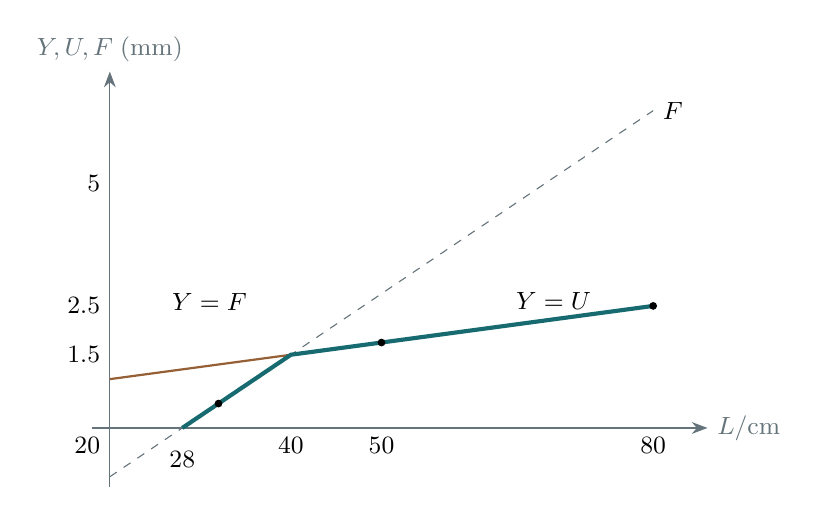
\begin{tikzpicture}[x=.115cm,y=.62cm]
\draw[axis](18,0)--(86,0)node[right]{$L/\mathrm{cm}$};\draw[axis](20,-1.2)--(20,7.3)node[above]{$Y,U,F\;(\mathrm{mm})$};
\draw[color=warm,thick]plot coordinates {(20.000000000000,1.000000000000) (21.000000000000,1.025000000000) (22.000000000000,1.050000000000) (23.000000000000,1.075000000000) (24.000000000000,1.100000000000) (25.000000000000,1.125000000000) (26.000000000000,1.150000000000) (27.000000000000,1.175000000000) (28.000000000000,1.200000000000) (29.000000000000,1.225000000000) (30.000000000000,1.250000000000) (31.000000000000,1.275000000000) (32.000000000000,1.300000000000) (33.000000000000,1.325000000000) (34.000000000000,1.350000000000) (35.000000000000,1.375000000000) (36.000000000000,1.400000000000) (37.000000000000,1.425000000000) (38.000000000000,1.450000000000) (39.000000000000,1.475000000000) (40.000000000000,1.500000000000) (41.000000000000,1.525000000000) (42.000000000000,1.550000000000) (43.000000000000,1.575000000000) (44.000000000000,1.600000000000) (45.000000000000,1.625000000000) (46.000000000000,1.650000000000) (47.000000000000,1.675000000000) (48.000000000000,1.700000000000) (49.000000000000,1.725000000000) (50.000000000000,1.750000000000) (51.000000000000,1.775000000000) (52.000000000000,1.800000000000) (53.000000000000,1.825000000000) (54.000000000000,1.850000000000) (55.000000000000,1.875000000000) (56.000000000000,1.900000000000) (57.000000000000,1.925000000000) (58.000000000000,1.950000000000) (59.000000000000,1.975000000000) (60.000000000000,2.000000000000) (61.000000000000,2.025000000000) (62.000000000000,2.050000000000) (63.000000000000,2.075000000000) (64.000000000000,2.100000000000) (65.000000000000,2.125000000000) (66.000000000000,2.150000000000) (67.000000000000,2.175000000000) (68.000000000000,2.200000000000) (69.000000000000,2.225000000000) (70.000000000000,2.250000000000) (71.000000000000,2.275000000000) (72.000000000000,2.300000000000) (73.000000000000,2.325000000000) (74.000000000000,2.350000000000) (75.000000000000,2.375000000000) (76.000000000000,2.400000000000) (77.000000000000,2.425000000000) (78.000000000000,2.450000000000) (79.000000000000,2.475000000000) (80.000000000000,2.500000000000)};
\draw[guide]plot coordinates {(20.000000000000,-1.000000000000) (21.000000000000,-0.875000000000) (22.000000000000,-0.750000000000) (23.000000000000,-0.625000000000) (24.000000000000,-0.500000000000) (25.000000000000,-0.375000000000) (26.000000000000,-0.250000000000) (27.000000000000,-0.125000000000) (28.000000000000,0.000000000000) (29.000000000000,0.125000000000) (30.000000000000,0.250000000000) (31.000000000000,0.375000000000) (32.000000000000,0.500000000000) (33.000000000000,0.625000000000) (34.000000000000,0.750000000000) (35.000000000000,0.875000000000) (36.000000000000,1.000000000000) (37.000000000000,1.125000000000) (38.000000000000,1.250000000000) (39.000000000000,1.375000000000) (40.000000000000,1.500000000000) (41.000000000000,1.625000000000) (42.000000000000,1.750000000000) (43.000000000000,1.875000000000) (44.000000000000,2.000000000000) (45.000000000000,2.125000000000) (46.000000000000,2.250000000000) (47.000000000000,2.375000000000) (48.000000000000,2.500000000000) (49.000000000000,2.625000000000) (50.000000000000,2.750000000000) (51.000000000000,2.875000000000) (52.000000000000,3.000000000000) (53.000000000000,3.125000000000) (54.000000000000,3.250000000000) (55.000000000000,3.375000000000) (56.000000000000,3.500000000000) (57.000000000000,3.625000000000) (58.000000000000,3.750000000000) (59.000000000000,3.875000000000) (60.000000000000,4.000000000000) (61.000000000000,4.125000000000) (62.000000000000,4.250000000000) (63.000000000000,4.375000000000) (64.000000000000,4.500000000000) (65.000000000000,4.625000000000) (66.000000000000,4.750000000000) (67.000000000000,4.875000000000) (68.000000000000,5.000000000000) (69.000000000000,5.125000000000) (70.000000000000,5.250000000000) (71.000000000000,5.375000000000) (72.000000000000,5.500000000000) (73.000000000000,5.625000000000) (74.000000000000,5.750000000000) (75.000000000000,5.875000000000) (76.000000000000,6.000000000000) (77.000000000000,6.125000000000) (78.000000000000,6.250000000000) (79.000000000000,6.375000000000) (80.000000000000,6.500000000000)};
\draw[traj,line width=1.5pt]plot coordinates {(28.000000000000,0.000000000000) (29.000000000000,0.125000000000) (30.000000000000,0.250000000000) (31.000000000000,0.375000000000) (32.000000000000,0.500000000000) (33.000000000000,0.625000000000) (34.000000000000,0.750000000000) (35.000000000000,0.875000000000) (36.000000000000,1.000000000000) (37.000000000000,1.125000000000) (38.000000000000,1.250000000000) (39.000000000000,1.375000000000) (40.000000000000,1.500000000000) (41.000000000000,1.525000000000) (42.000000000000,1.550000000000) (43.000000000000,1.575000000000) (44.000000000000,1.600000000000) (45.000000000000,1.625000000000) (46.000000000000,1.650000000000) (47.000000000000,1.675000000000) (48.000000000000,1.700000000000) (49.000000000000,1.725000000000) (50.000000000000,1.750000000000) (51.000000000000,1.775000000000) (52.000000000000,1.800000000000) (53.000000000000,1.825000000000) (54.000000000000,1.850000000000) (55.000000000000,1.875000000000) (56.000000000000,1.900000000000) (57.000000000000,1.925000000000) (58.000000000000,1.950000000000) (59.000000000000,1.975000000000) (60.000000000000,2.000000000000) (61.000000000000,2.025000000000) (62.000000000000,2.050000000000) (63.000000000000,2.075000000000) (64.000000000000,2.100000000000) (65.000000000000,2.125000000000) (66.000000000000,2.150000000000) (67.000000000000,2.175000000000) (68.000000000000,2.200000000000) (69.000000000000,2.225000000000) (70.000000000000,2.250000000000) (71.000000000000,2.275000000000) (72.000000000000,2.300000000000) (73.000000000000,2.325000000000) (74.000000000000,2.350000000000) (75.000000000000,2.375000000000) (76.000000000000,2.400000000000) (77.000000000000,2.425000000000) (78.000000000000,2.450000000000) (79.000000000000,2.475000000000) (80.000000000000,2.500000000000)};
\node[below left]at(20.000000000000,0.000000000000){$20$};
\node[below,yshift=-5pt]at(28.000000000000,0.000000000000){$28$};
\node[below]at(40.000000000000,0.000000000000){$40$};
\node[below]at(50.000000000000,0.000000000000){$50$};
\node[below]at(80.000000000000,0.000000000000){$80$};
\node[left]at(20.000000000000,1.500000000000){$1.5$};
\node[left]at(20.000000000000,2.500000000000){$2.5$};
\node[left]at(20.000000000000,5.000000000000){$5$};
\node[right]at(80,6.5){$F$};\node[above]at(69,2.225){$Y=U$};\node[above]at(31,2.2){$Y=F$};\fill(32.000000000000,0.500000000000)circle(1.4pt);\fill(50.000000000000,1.750000000000)circle(1.4pt);\fill(80.000000000000,2.500000000000)circle(1.4pt);
\end{tikzpicture}
\figcaption{变图光2.4V4\quad 屏后移时共同半宽的两段边界}
\end{minipage}\end{center}

\item 改为$s=30\,\mathrm{cm}$，仍取$f=10\,\mathrm{cm},L=50\,\mathrm{cm},\delta=1.0\,\mathrm{mm},a=3.0\,\mathrm{mm}$，求干涉图样。薄透镜式和偏心像高法先给
\[
s'=15\,\mathrm{cm},\quad d=1.50\,\mathrm{mm},\quad
D=35\,\mathrm{cm},\quad
p=\frac{.0005\times350}{1.50}=\frac7{60}\,\mathrm{mm}.
\]
变图光2.4V5中的$Q_1,Q_2$在$z=15\,\mathrm{cm}$，像高为$\pm.750\,\mathrm{mm}$，必须随物距一起改变。内边界$U=\tfrac12(1+50/30)=4/3\,\mathrm{mm}$，而$aD/s'=7.00\,\mathrm{mm}>2U$，故共同宽度$W=8/3\,\mathrm{mm}$。$Y/p=(4/3)/(7/60)=80/7$，$m=-11,\ldots,11$，共23条。像对间距、像后距离和内边界均发生变化，不能只改条纹公式中的一个$s$。

\begin{center}\begin{minipage}{.98\linewidth}\centering
\begin{tikzpicture}[x=.122cm,y=.60cm]
\fill[color=accent!13](19.090909090909,-0.000000000000)--(24.000000000000,0.900000000000)--(50.000000000000,1.333333333333)--(50.000000000000,-1.333333333333)--(24.000000000000,-0.900000000000)--cycle;
\draw[axis](-33.000000000000,0.000000000000)--(54.000000000000,0.000000000000)node[right,yshift=-42pt]{$z/\mathrm{cm}$};
\draw[guide](15.000000000000,-4.400000000000)--(15.000000000000,4.200000000000);
\draw[object](50.000000000000,-6.100000000000)--(50.000000000000,6.100000000000);
\node[above]at(50.000000000000,6.100000000000){屏};
\node[below]at(15.000000000000,-4.400000000000){像平面};
\draw[object](0.000000000000,0.500000000000)--(0.000000000000,3.500000000000);
\draw[motion](-30.000000000000,0.000000000000)--(0.000000000000,0.500000000000);
\draw[motion](0.000000000000,0.500000000000)--(15.000000000000,0.750000000000)--(50.000000000000,1.333333333333);
\draw[motion](-30.000000000000,0.000000000000)--(0.000000000000,3.500000000000);
\draw[motion](0.000000000000,3.500000000000)--(15.000000000000,0.750000000000)--(50.000000000000,-5.666666666667);
\fill(15.000000000000,0.750000000000)circle(1.2pt);
\node[above right]at(16.000000000000,0.880000000000){$Q_1$};
\draw[object](0.000000000000,-0.500000000000)--(0.000000000000,-3.500000000000);
\draw[motion](-30.000000000000,0.000000000000)--(0.000000000000,-0.500000000000);
\draw[motion](0.000000000000,-0.500000000000)--(15.000000000000,-0.750000000000)--(50.000000000000,-1.333333333333);
\draw[motion](-30.000000000000,0.000000000000)--(0.000000000000,-3.500000000000);
\draw[motion](0.000000000000,-3.500000000000)--(15.000000000000,-0.750000000000)--(50.000000000000,5.666666666667);
\fill(15.000000000000,-0.750000000000)circle(1.2pt);
\node[below right]at(16.000000000000,-0.880000000000){$Q_2$};
\fill(-30.000000000000,0.000000000000)circle(1.2pt);
\node[below]at(-30.000000000000,0.000000000000){$Q$};
\node[above left]at(0.000000000000,0.500000000000){$O_1$};
\node[below left]at(0.000000000000,-0.500000000000){$O_2$};
\node[below]at(0.000000000000,-4.400000000000){$0$};
\node[above,align=center]at(-24.000000000000,3.500000000000){$y/\mathrm{mm}$\\横向放大};
\node[above right]at(17.000000000000,3.200000000000){$s^{\prime}=15\,\mathrm{cm}$};
\draw[<->,thin,color=muted](55.000000000000,-1.333333333333)--(55.000000000000,1.333333333333);
\node[right]at(55.000000000000,0.000000000000){$8/3\,\mathrm{mm}$};
\end{tikzpicture}
\figcaption{变图光2.4V5\quad 物距变化后的新像平面和边缘光路}
\end{minipage}\end{center}

\item 在$a=3.0\,\mathrm{mm}$的两束中，给一束另加恒定相位$\pi$，求亮纹位置和条数。两束仍在$|y|<1.75\,\mathrm{mm}$同时到达，相位差可写为$2\pi y/p+\pi$，相长位置构成
\[
y=(m+\tfrac12)p,\qquad
-\frac{70}3<m+\frac12<\frac{70}3.
\]
整数范围是$m=-23,\ldots,22$，共46条。变图光2.4V6用$t=y/p$画出中心附近的强度，$t=0$由亮变暗，所有亮纹移半周期，间距仍为$.0750\,\mathrm{mm}$，几何共同宽度仍为$3.50\,\mathrm{mm}$。若以折射率$n$的薄平行片提供此相位，取$t_{\rm plate}=\lambda/[2(n-1)]$；例如$n=1.50$时$t_{\rm plate}=500\,\mathrm{nm}$。此处把平行片只作为相位延迟模型，忽略附加横移、反射损失和振幅变化。

\begin{center}\begin{minipage}{.98\linewidth}\centering
\begin{tikzpicture}[x=1.65cm,y=1.5cm]
\draw[axis](-2.35,0)--(2.5,0)node[right]{$t=y/p$};\draw[axis](-2.25,0)--(-2.25,1.8)node[above]{$I/(4I_0)$};
\draw[guide]plot coordinates {(-2.000000000000,1.000000000000) (-1.975000000000,0.993844170298) (-1.950000000000,0.975528258148) (-1.925000000000,0.945503262094) (-1.900000000000,0.904508497187) (-1.875000000000,0.853553390593) (-1.850000000000,0.793892626146) (-1.825000000000,0.726995249870) (-1.800000000000,0.654508497187) (-1.775000000000,0.578217232520) (-1.750000000000,0.500000000000) (-1.725000000000,0.421782767480) (-1.700000000000,0.345491502813) (-1.675000000000,0.273004750130) (-1.650000000000,0.206107373854) (-1.625000000000,0.146446609407) (-1.600000000000,0.095491502813) (-1.575000000000,0.054496737906) (-1.550000000000,0.024471741852) (-1.525000000000,0.006155829702) (-1.500000000000,0.000000000000) (-1.475000000000,0.006155829702) (-1.450000000000,0.024471741852) (-1.425000000000,0.054496737906) (-1.400000000000,0.095491502813) (-1.375000000000,0.146446609407) (-1.350000000000,0.206107373854) (-1.325000000000,0.273004750130) (-1.300000000000,0.345491502813) (-1.275000000000,0.421782767480) (-1.250000000000,0.500000000000) (-1.225000000000,0.578217232520) (-1.200000000000,0.654508497187) (-1.175000000000,0.726995249870) (-1.150000000000,0.793892626146) (-1.125000000000,0.853553390593) (-1.100000000000,0.904508497187) (-1.075000000000,0.945503262094) (-1.050000000000,0.975528258148) (-1.025000000000,0.993844170298) (-1.000000000000,1.000000000000) (-0.975000000000,0.993844170298) (-0.950000000000,0.975528258148) (-0.925000000000,0.945503262094) (-0.900000000000,0.904508497187) (-0.875000000000,0.853553390593) (-0.850000000000,0.793892626146) (-0.825000000000,0.726995249870) (-0.800000000000,0.654508497187) (-0.775000000000,0.578217232520) (-0.750000000000,0.500000000000) (-0.725000000000,0.421782767480) (-0.700000000000,0.345491502813) (-0.675000000000,0.273004750130) (-0.650000000000,0.206107373854) (-0.625000000000,0.146446609407) (-0.600000000000,0.095491502813) (-0.575000000000,0.054496737906) (-0.550000000000,0.024471741852) (-0.525000000000,0.006155829702) (-0.500000000000,0.000000000000) (-0.475000000000,0.006155829702) (-0.450000000000,0.024471741852) (-0.425000000000,0.054496737906) (-0.400000000000,0.095491502813) (-0.375000000000,0.146446609407) (-0.350000000000,0.206107373854) (-0.325000000000,0.273004750130) (-0.300000000000,0.345491502813) (-0.275000000000,0.421782767480) (-0.250000000000,0.500000000000) (-0.225000000000,0.578217232520) (-0.200000000000,0.654508497187) (-0.175000000000,0.726995249870) (-0.150000000000,0.793892626146) (-0.125000000000,0.853553390593) (-0.100000000000,0.904508497187) (-0.075000000000,0.945503262094) (-0.050000000000,0.975528258148) (-0.025000000000,0.993844170298) (0.000000000000,1.000000000000) (0.025000000000,0.993844170298) (0.050000000000,0.975528258148) (0.075000000000,0.945503262094) (0.100000000000,0.904508497187) (0.125000000000,0.853553390593) (0.150000000000,0.793892626146) (0.175000000000,0.726995249870) (0.200000000000,0.654508497187) (0.225000000000,0.578217232520) (0.250000000000,0.500000000000) (0.275000000000,0.421782767480) (0.300000000000,0.345491502813) (0.325000000000,0.273004750130) (0.350000000000,0.206107373854) (0.375000000000,0.146446609407) (0.400000000000,0.095491502813) (0.425000000000,0.054496737906) (0.450000000000,0.024471741852) (0.475000000000,0.006155829702) (0.500000000000,0.000000000000) (0.525000000000,0.006155829702) (0.550000000000,0.024471741852) (0.575000000000,0.054496737906) (0.600000000000,0.095491502813) (0.625000000000,0.146446609407) (0.650000000000,0.206107373854) (0.675000000000,0.273004750130) (0.700000000000,0.345491502813) (0.725000000000,0.421782767480) (0.750000000000,0.500000000000) (0.775000000000,0.578217232520) (0.800000000000,0.654508497187) (0.825000000000,0.726995249870) (0.850000000000,0.793892626146) (0.875000000000,0.853553390593) (0.900000000000,0.904508497187) (0.925000000000,0.945503262094) (0.950000000000,0.975528258148) (0.975000000000,0.993844170298) (1.000000000000,1.000000000000) (1.025000000000,0.993844170298) (1.050000000000,0.975528258148) (1.075000000000,0.945503262094) (1.100000000000,0.904508497187) (1.125000000000,0.853553390593) (1.150000000000,0.793892626146) (1.175000000000,0.726995249870) (1.200000000000,0.654508497187) (1.225000000000,0.578217232520) (1.250000000000,0.500000000000) (1.275000000000,0.421782767480) (1.300000000000,0.345491502813) (1.325000000000,0.273004750130) (1.350000000000,0.206107373854) (1.375000000000,0.146446609407) (1.400000000000,0.095491502813) (1.425000000000,0.054496737906) (1.450000000000,0.024471741852) (1.475000000000,0.006155829702) (1.500000000000,0.000000000000) (1.525000000000,0.006155829702) (1.550000000000,0.024471741852) (1.575000000000,0.054496737906) (1.600000000000,0.095491502813) (1.625000000000,0.146446609407) (1.650000000000,0.206107373854) (1.675000000000,0.273004750130) (1.700000000000,0.345491502813) (1.725000000000,0.421782767480) (1.750000000000,0.500000000000) (1.775000000000,0.578217232520) (1.800000000000,0.654508497187) (1.825000000000,0.726995249870) (1.850000000000,0.793892626146) (1.875000000000,0.853553390593) (1.900000000000,0.904508497187) (1.925000000000,0.945503262094) (1.950000000000,0.975528258148) (1.975000000000,0.993844170298) (2.000000000000,1.000000000000)};
\draw[traj]plot coordinates {(-2.000000000000,0.000000000000) (-1.975000000000,0.006155829702) (-1.950000000000,0.024471741852) (-1.925000000000,0.054496737906) (-1.900000000000,0.095491502813) (-1.875000000000,0.146446609407) (-1.850000000000,0.206107373854) (-1.825000000000,0.273004750130) (-1.800000000000,0.345491502813) (-1.775000000000,0.421782767480) (-1.750000000000,0.500000000000) (-1.725000000000,0.578217232520) (-1.700000000000,0.654508497187) (-1.675000000000,0.726995249870) (-1.650000000000,0.793892626146) (-1.625000000000,0.853553390593) (-1.600000000000,0.904508497187) (-1.575000000000,0.945503262094) (-1.550000000000,0.975528258148) (-1.525000000000,0.993844170298) (-1.500000000000,1.000000000000) (-1.475000000000,0.993844170298) (-1.450000000000,0.975528258148) (-1.425000000000,0.945503262094) (-1.400000000000,0.904508497187) (-1.375000000000,0.853553390593) (-1.350000000000,0.793892626146) (-1.325000000000,0.726995249870) (-1.300000000000,0.654508497187) (-1.275000000000,0.578217232520) (-1.250000000000,0.500000000000) (-1.225000000000,0.421782767480) (-1.200000000000,0.345491502813) (-1.175000000000,0.273004750130) (-1.150000000000,0.206107373854) (-1.125000000000,0.146446609407) (-1.100000000000,0.095491502813) (-1.075000000000,0.054496737906) (-1.050000000000,0.024471741852) (-1.025000000000,0.006155829702) (-1.000000000000,0.000000000000) (-0.975000000000,0.006155829702) (-0.950000000000,0.024471741852) (-0.925000000000,0.054496737906) (-0.900000000000,0.095491502813) (-0.875000000000,0.146446609407) (-0.850000000000,0.206107373854) (-0.825000000000,0.273004750130) (-0.800000000000,0.345491502813) (-0.775000000000,0.421782767480) (-0.750000000000,0.500000000000) (-0.725000000000,0.578217232520) (-0.700000000000,0.654508497187) (-0.675000000000,0.726995249870) (-0.650000000000,0.793892626146) (-0.625000000000,0.853553390593) (-0.600000000000,0.904508497187) (-0.575000000000,0.945503262094) (-0.550000000000,0.975528258148) (-0.525000000000,0.993844170298) (-0.500000000000,1.000000000000) (-0.475000000000,0.993844170298) (-0.450000000000,0.975528258148) (-0.425000000000,0.945503262094) (-0.400000000000,0.904508497187) (-0.375000000000,0.853553390593) (-0.350000000000,0.793892626146) (-0.325000000000,0.726995249870) (-0.300000000000,0.654508497187) (-0.275000000000,0.578217232520) (-0.250000000000,0.500000000000) (-0.225000000000,0.421782767480) (-0.200000000000,0.345491502813) (-0.175000000000,0.273004750130) (-0.150000000000,0.206107373854) (-0.125000000000,0.146446609407) (-0.100000000000,0.095491502813) (-0.075000000000,0.054496737906) (-0.050000000000,0.024471741852) (-0.025000000000,0.006155829702) (0.000000000000,0.000000000000) (0.025000000000,0.006155829702) (0.050000000000,0.024471741852) (0.075000000000,0.054496737906) (0.100000000000,0.095491502813) (0.125000000000,0.146446609407) (0.150000000000,0.206107373854) (0.175000000000,0.273004750130) (0.200000000000,0.345491502813) (0.225000000000,0.421782767480) (0.250000000000,0.500000000000) (0.275000000000,0.578217232520) (0.300000000000,0.654508497187) (0.325000000000,0.726995249870) (0.350000000000,0.793892626146) (0.375000000000,0.853553390593) (0.400000000000,0.904508497187) (0.425000000000,0.945503262094) (0.450000000000,0.975528258148) (0.475000000000,0.993844170298) (0.500000000000,1.000000000000) (0.525000000000,0.993844170298) (0.550000000000,0.975528258148) (0.575000000000,0.945503262094) (0.600000000000,0.904508497187) (0.625000000000,0.853553390593) (0.650000000000,0.793892626146) (0.675000000000,0.726995249870) (0.700000000000,0.654508497187) (0.725000000000,0.578217232520) (0.750000000000,0.500000000000) (0.775000000000,0.421782767480) (0.800000000000,0.345491502813) (0.825000000000,0.273004750130) (0.850000000000,0.206107373854) (0.875000000000,0.146446609407) (0.900000000000,0.095491502813) (0.925000000000,0.054496737906) (0.950000000000,0.024471741852) (0.975000000000,0.006155829702) (1.000000000000,0.000000000000) (1.025000000000,0.006155829702) (1.050000000000,0.024471741852) (1.075000000000,0.054496737906) (1.100000000000,0.095491502813) (1.125000000000,0.146446609407) (1.150000000000,0.206107373854) (1.175000000000,0.273004750130) (1.200000000000,0.345491502813) (1.225000000000,0.421782767480) (1.250000000000,0.500000000000) (1.275000000000,0.578217232520) (1.300000000000,0.654508497187) (1.325000000000,0.726995249870) (1.350000000000,0.793892626146) (1.375000000000,0.853553390593) (1.400000000000,0.904508497187) (1.425000000000,0.945503262094) (1.450000000000,0.975528258148) (1.475000000000,0.993844170298) (1.500000000000,1.000000000000) (1.525000000000,0.993844170298) (1.550000000000,0.975528258148) (1.575000000000,0.945503262094) (1.600000000000,0.904508497187) (1.625000000000,0.853553390593) (1.650000000000,0.793892626146) (1.675000000000,0.726995249870) (1.700000000000,0.654508497187) (1.725000000000,0.578217232520) (1.750000000000,0.500000000000) (1.775000000000,0.421782767480) (1.800000000000,0.345491502813) (1.825000000000,0.273004750130) (1.850000000000,0.206107373854) (1.875000000000,0.146446609407) (1.900000000000,0.095491502813) (1.925000000000,0.054496737906) (1.950000000000,0.024471741852) (1.975000000000,0.006155829702) (2.000000000000,0.000000000000)};
\node[below]at(-2.000000000000,0.000000000000){$-2$};\node[below]at(-1.000000000000,0.000000000000){$-1$};\node[below]at(0.000000000000,0.000000000000){$0$};\node[below]at(1.000000000000,0.000000000000){$1$};\node[below]at(2.000000000000,0.000000000000){$2$};\node[left]at(-2.25,1){$1$};\node[anchor=west]at(-1.95,1.60){实线：附加$\pi$};\node[anchor=west]at(-1.95,1.30){虚线：同相};
\end{tikzpicture}
\figcaption{变图光2.4V6\quad 相位多出$\pi$后亮暗互换}
\end{minipage}\end{center}

\item 几何参数、孔径和相位均不变，仅令两束在共同区的强度近似恒定且$I_2=I_1/4$。由相干叠加
\[
\frac I{I_1}=1+\frac14+2\sqrt{\frac14}\cos\frac{2\pi y}p
=\frac54+\cos\frac{2\pi y}p.
\]
变图光2.4V7的峰、谷和平均值分别为$9/4,1/4,5/4$，故可见度
\[
\mathcal V=\frac{I_{\max}-I_{\min}}{I_{\max}+I_{\min}}
=\frac{9/4-1/4}{9/4+1/4}=\frac45.
\]
极大仍在$y=mp$，47个相长级次位置不变；暗纹处两振幅不能完全抵消，谷底不为零。减弱一束不等于改变孔径，只有仍存在两束的共同区才采用此强度式。

\begin{center}\begin{minipage}{.98\linewidth}\centering
\begin{tikzpicture}[x=1.6cm,y=1.15cm]
\draw[axis](-2.4,0)--(2.5,0)node[right]{$y/p$};\draw[axis](-2.3,0)--(-2.3,2.8)node[above]{$I/I_1$};
\draw[guide](-2.300000000000,0.250000000000)--(2.100000000000,0.250000000000);\node[left]at(-2.300000000000,0.250000000000){$1/4$};\draw[guide](-2.300000000000,1.250000000000)--(2.100000000000,1.250000000000);\node[left]at(-2.300000000000,1.250000000000){$5/4$};\draw[guide](-2.300000000000,2.250000000000)--(2.100000000000,2.250000000000);\node[left]at(-2.300000000000,2.250000000000){$9/4$};\draw[traj]plot coordinates {(-2.000000000000,2.250000000000) (-1.975000000000,2.237688340595) (-1.950000000000,2.201056516295) (-1.925000000000,2.141006524188) (-1.900000000000,2.059016994375) (-1.875000000000,1.957106781187) (-1.850000000000,1.837785252292) (-1.825000000000,1.703990499740) (-1.800000000000,1.559016994375) (-1.775000000000,1.406434465040) (-1.750000000000,1.250000000000) (-1.725000000000,1.093565534960) (-1.700000000000,0.940983005625) (-1.675000000000,0.796009500260) (-1.650000000000,0.662214747708) (-1.625000000000,0.542893218813) (-1.600000000000,0.440983005625) (-1.575000000000,0.358993475812) (-1.550000000000,0.298943483705) (-1.525000000000,0.262311659405) (-1.500000000000,0.250000000000) (-1.475000000000,0.262311659405) (-1.450000000000,0.298943483705) (-1.425000000000,0.358993475812) (-1.400000000000,0.440983005625) (-1.375000000000,0.542893218813) (-1.350000000000,0.662214747708) (-1.325000000000,0.796009500260) (-1.300000000000,0.940983005625) (-1.275000000000,1.093565534960) (-1.250000000000,1.250000000000) (-1.225000000000,1.406434465040) (-1.200000000000,1.559016994375) (-1.175000000000,1.703990499740) (-1.150000000000,1.837785252292) (-1.125000000000,1.957106781187) (-1.100000000000,2.059016994375) (-1.075000000000,2.141006524188) (-1.050000000000,2.201056516295) (-1.025000000000,2.237688340595) (-1.000000000000,2.250000000000) (-0.975000000000,2.237688340595) (-0.950000000000,2.201056516295) (-0.925000000000,2.141006524188) (-0.900000000000,2.059016994375) (-0.875000000000,1.957106781187) (-0.850000000000,1.837785252292) (-0.825000000000,1.703990499740) (-0.800000000000,1.559016994375) (-0.775000000000,1.406434465040) (-0.750000000000,1.250000000000) (-0.725000000000,1.093565534960) (-0.700000000000,0.940983005625) (-0.675000000000,0.796009500260) (-0.650000000000,0.662214747708) (-0.625000000000,0.542893218813) (-0.600000000000,0.440983005625) (-0.575000000000,0.358993475812) (-0.550000000000,0.298943483705) (-0.525000000000,0.262311659405) (-0.500000000000,0.250000000000) (-0.475000000000,0.262311659405) (-0.450000000000,0.298943483705) (-0.425000000000,0.358993475812) (-0.400000000000,0.440983005625) (-0.375000000000,0.542893218813) (-0.350000000000,0.662214747708) (-0.325000000000,0.796009500260) (-0.300000000000,0.940983005625) (-0.275000000000,1.093565534960) (-0.250000000000,1.250000000000) (-0.225000000000,1.406434465040) (-0.200000000000,1.559016994375) (-0.175000000000,1.703990499740) (-0.150000000000,1.837785252292) (-0.125000000000,1.957106781187) (-0.100000000000,2.059016994375) (-0.075000000000,2.141006524188) (-0.050000000000,2.201056516295) (-0.025000000000,2.237688340595) (0.000000000000,2.250000000000) (0.025000000000,2.237688340595) (0.050000000000,2.201056516295) (0.075000000000,2.141006524188) (0.100000000000,2.059016994375) (0.125000000000,1.957106781187) (0.150000000000,1.837785252292) (0.175000000000,1.703990499740) (0.200000000000,1.559016994375) (0.225000000000,1.406434465040) (0.250000000000,1.250000000000) (0.275000000000,1.093565534960) (0.300000000000,0.940983005625) (0.325000000000,0.796009500260) (0.350000000000,0.662214747708) (0.375000000000,0.542893218813) (0.400000000000,0.440983005625) (0.425000000000,0.358993475812) (0.450000000000,0.298943483705) (0.475000000000,0.262311659405) (0.500000000000,0.250000000000) (0.525000000000,0.262311659405) (0.550000000000,0.298943483705) (0.575000000000,0.358993475812) (0.600000000000,0.440983005625) (0.625000000000,0.542893218813) (0.650000000000,0.662214747708) (0.675000000000,0.796009500260) (0.700000000000,0.940983005625) (0.725000000000,1.093565534960) (0.750000000000,1.250000000000) (0.775000000000,1.406434465040) (0.800000000000,1.559016994375) (0.825000000000,1.703990499740) (0.850000000000,1.837785252292) (0.875000000000,1.957106781187) (0.900000000000,2.059016994375) (0.925000000000,2.141006524188) (0.950000000000,2.201056516295) (0.975000000000,2.237688340595) (1.000000000000,2.250000000000) (1.025000000000,2.237688340595) (1.050000000000,2.201056516295) (1.075000000000,2.141006524188) (1.100000000000,2.059016994375) (1.125000000000,1.957106781187) (1.150000000000,1.837785252292) (1.175000000000,1.703990499740) (1.200000000000,1.559016994375) (1.225000000000,1.406434465040) (1.250000000000,1.250000000000) (1.275000000000,1.093565534960) (1.300000000000,0.940983005625) (1.325000000000,0.796009500260) (1.350000000000,0.662214747708) (1.375000000000,0.542893218813) (1.400000000000,0.440983005625) (1.425000000000,0.358993475812) (1.450000000000,0.298943483705) (1.475000000000,0.262311659405) (1.500000000000,0.250000000000) (1.525000000000,0.262311659405) (1.550000000000,0.298943483705) (1.575000000000,0.358993475812) (1.600000000000,0.440983005625) (1.625000000000,0.542893218813) (1.650000000000,0.662214747708) (1.675000000000,0.796009500260) (1.700000000000,0.940983005625) (1.725000000000,1.093565534960) (1.750000000000,1.250000000000) (1.775000000000,1.406434465040) (1.800000000000,1.559016994375) (1.825000000000,1.703990499740) (1.850000000000,1.837785252292) (1.875000000000,1.957106781187) (1.900000000000,2.059016994375) (1.925000000000,2.141006524188) (1.950000000000,2.201056516295) (1.975000000000,2.237688340595) (2.000000000000,2.250000000000)};\node[below]at(-2.000000000000,0.000000000000){$-2$};\node[below]at(-1.000000000000,0.000000000000){$-1$};\node[below]at(0.000000000000,0.000000000000){$0$};\node[below]at(1.000000000000,0.000000000000){$1$};\node[below]at(2.000000000000,0.000000000000){$2$};
\end{tikzpicture}
\figcaption{变图光2.4V7\quad 两束不等强时谷底不为零}
\end{minipage}\end{center}

\item 点源沿横向移至高度$u$，仍取$s=20\,\mathrm{cm}$和$a=3.0\,\mathrm{mm}$，求像对中点、屏上零级和孔径区间的变化。对光心$c=\pm\delta/2$分别成像，
\[
y_{Q_c}=c-\frac{s'}s(u-c)
=\left(1+\frac{s'}s\right)c-\frac{s'}s u.
\]
两像间距$d$不变，像对中点为$\bar y_Q=-s'u/s$。像点相位也随$u$改变，所以屏上零级还须另求。将所有长度换成同一单位，透镜平面横坐标记为$\eta$，屏坐标记为$y$。除共同常数外，傍轴光程函数为
\[
\mathcal S_c(\eta)=\frac{(\eta-u)^2}{2s}
-\frac{(\eta-c)^2}{2f}
+\frac{(y-\eta)^2}{2L}
=\frac A2\eta^2+B_c\eta+C_c,
\]
其中$A=1/s+1/L-1/f=-D/(Ls')$，$B_c=-u/s-y/L+c/f$，$C_c=u^2/(2s)+y^2/(2L)-c^2/(2f)$。驻相点$\eta_c=-B_c/A$须落在相应半片内；完成平方后$\mathcal S_c^*=C_c-B_c^2/(2A)$。因$c^2$对上下片相同，
\[
\mathcal S_+^*-\mathcal S_-^*
=\frac{\delta}{Af}\left(\frac us+\frac yL\right)
=-\frac dD\left(y+\frac Ls u\right).
\]
所以屏上零级$y_0=-Lu/s$，亮纹$y_m=y_0+mp$。切边光线过光心，端点映射为$y(L)=(1+L/s)c-Lu/s$；外缘映射也同样加$-Lu/s$。因而两照明区间及其交集整体平移$y_0$，相对共同区的级次和47条计数不变。

变图光2.4V8以$u=.020\,\mathrm{mm}$为例，在像平面标出$\bar y_Q=-.020\,\mathrm{mm}$，在屏上标出$y_0=-.050\,\mathrm{mm}$；共同区为$(-1.800,1.700)\,\mathrm{mm}$。图内用数值说明这两个细小位移，纵横仍用不同单位。两片必须同质且对应位置透射相位一致；还须检查两束驻相点都在各自半片内，才能在共同区采用上述相位差。

\begin{center}\begin{minipage}{.98\linewidth}\centering
\begin{tikzpicture}[x=.122cm,y=.60cm]
\fill[color=accent!13](28.000000000000,-0.028000000000)--(40.000000000000,1.460000000000)--(50.000000000000,1.700000000000)--(50.000000000000,-1.800000000000)--(40.000000000000,-1.540000000000)--cycle;
\draw[axis](-23.000000000000,0.000000000000)--(54.000000000000,0.000000000000)node[right]{$z/\mathrm{cm}$};
\draw[guide](20.000000000000,-4.400000000000)--(20.000000000000,4.200000000000);
\draw[object](50.000000000000,-4.100000000000)--(50.000000000000,4.100000000000);
\node[above]at(50.000000000000,4.100000000000){屏};
\node[below]at(20.000000000000,-4.400000000000){像平面};
\draw[object](0.000000000000,0.500000000000)--(0.000000000000,3.500000000000);
\draw[motion](-20.000000000000,0.020000000000)--(0.000000000000,0.500000000000);
\draw[motion](0.000000000000,0.500000000000)--(20.000000000000,0.980000000000)--(50.000000000000,1.700000000000);
\draw[motion](-20.000000000000,0.020000000000)--(0.000000000000,3.500000000000);
\draw[motion](0.000000000000,3.500000000000)--(20.000000000000,0.980000000000)--(50.000000000000,-2.800000000000);
\fill(20.000000000000,0.980000000000)circle(1.2pt);
\node[above right]at(21.000000000000,1.110000000000){$Q_1$};
\draw[object](0.000000000000,-0.500000000000)--(0.000000000000,-3.500000000000);
\draw[motion](-20.000000000000,0.020000000000)--(0.000000000000,-0.500000000000);
\draw[motion](0.000000000000,-0.500000000000)--(20.000000000000,-1.020000000000)--(50.000000000000,-1.800000000000);
\draw[motion](-20.000000000000,0.020000000000)--(0.000000000000,-3.500000000000);
\draw[motion](0.000000000000,-3.500000000000)--(20.000000000000,-1.020000000000)--(50.000000000000,2.700000000000);
\fill(20.000000000000,-1.020000000000)circle(1.2pt);
\node[below right]at(21.000000000000,-1.150000000000){$Q_2$};
\fill(-20.000000000000,0.020000000000)circle(1.2pt);
\node[below]at(-20.000000000000,0.020000000000){$Q$};
\node[above left]at(0.000000000000,0.500000000000){$O_1$};
\node[below left]at(0.000000000000,-0.500000000000){$O_2$};
\node[below]at(0.000000000000,-4.400000000000){$0$};
\node[above,align=center]at(-16.000000000000,3.500000000000){$y/\mathrm{mm}$\\横向放大};
\fill[color=muted](20.000000000000,-0.020000000000)circle(1.1pt);
\fill[color=warm](50.000000000000,-0.050000000000)circle(1.3pt);
\node[above right,align=center]at(22.000000000000,3.200000000000){$\bar y_Q=-.020$\\$(\mathrm{mm})$};
\node[below,align=center]at(50.000000000000,-4.400000000000){$y_0=-.050$\\$(\mathrm{mm})$};
\node[right]at(50.000000000000,1.700000000000){$1.700$};
\node[right]at(50.000000000000,-1.800000000000){$-1.800$};
\end{tikzpicture}
\figcaption{变图光2.4V8\quad 离轴点源、像对中点与屏上零级}
\end{minipage}\end{center}
\end{enumerate}

\Needspace{13\baselineskip}

\pdfbookmark[2]{第 5 题 不等间距三缝的主极大与次极大}{q5}

\section*{第 5 题\quad 不等间距三缝的主极大与次极大}\label{q:5}

三个平行窄缝沿竖直方向排列，相邻间距依次为$d$和$3d/2$。三缝等宽，缝宽远小于$\lambda$，受同相单色光照明；远屏上观察方向与轴夹小角$\theta$，各缝单独产生的强度均近似为$I_s$。（1）求强度分布。（2）求零级以外首个完全相长的主极大，并说明它与最近局部极大的区别。（3）求主极大角位置一半处与主极大的强度比。

\begin{center}\begin{minipage}{.98\linewidth}\centering
\begin{tikzpicture}[font=\small,scale=.85,transform shape]
\draw[object](0,.4)--(0,-2.9);
\fill(0,0)circle(1.5pt);\node[left]at(0,0){$S_1$};
\fill(0,-1)circle(1.5pt);\node[left]at(0,-1){$S_2$};
\fill(0,-2.5)circle(1.5pt);\node[left]at(0,-2.5){$S_3$};
\draw[motion](0,0)--(6,1.2);\draw[motion](0,-1)--(6,.2);\draw[motion](0,-2.5)--(6,-1.3);
\draw[guide](0,0)--(3,0);\draw[thin](2.4,0)arc(0:11.30993247:2.4);\node at(2.8,.28){$\theta$};
\draw[<->,thin](-.75,0)--(-.75,-1);\node[left]at(-.75,-.5){$d$};
\draw[<->,thin](-.75,-1)--(-.75,-2.5);\node[left]at(-.75,-1.75){$3d/2$};
\node[above]at(4,1.4){远场同一观察方向};
\node[anchor=north]at(2.5,-3.2){沿缝间连线的坐标：$0,d,5d/2$。};
\end{tikzpicture}
\figcaption{图光2.5\quad 三缝坐标及远场方向的平行光线}
\end{minipage}\end{center}

\Needspace{8\baselineskip}

\pdfbookmark[3]{题型定位}{q5-h0}

\subsection*{题型定位}

三缝位置不等距，每对缝都产生不同相位差。先用复振幅求完整分布，再分别解三相量同向的主峰和导数为零的其他局部峰。

先为三缝登记总相位，再分别判断完全相长与局部极大。复振幅法可迅速得到三组缝对交叉项，分量法则把每一项的几何含义展开。主峰由整数相位同时满足决定；最近次峰须求完整导数的其他根。题目所问的半角强度比还涉及先取角的一半还是先把正弦减半，两者只在小角近似中等价。

\Needspace{8\baselineskip}

\pdfbookmark[3]{知识点}{q5-h1}

\subsection*{知识点}

\begin{itemize}
\item 强度展开包含三组缝对，差距分别为$d,3d/2,5d/2$，所以余弦项的相位为$2\beta,3\beta,5\beta$。
\item 主极大由所有相量同向决定，最高值为$(3A_s)^2$；其他驻点由三角多项式求根，通常仍有次峰。
\item 两个条件$2\beta=2p\pi$与$5\beta=2q\pi$的最小公倍周期为$2\pi$，它给出主峰周期而非所有局部峰间距。
\end{itemize}

远场方向上的路程差是缝距在传播方向上的投影；间距相继为$d,3d/2$，第三缝相对第一缝必须用总距离$5d/2$。合振幅求模平方时，三个单缝强度之外，还须逐对计入$S_1S_2,S_2S_3,S_1S_3$的交叉项。导数对$\beta$求时，$\sin2\beta,\sin3\beta,\sin5\beta$各带各自频数；再求导的二阶权重是$4,9,25$。同宽仅保证同一方向的单缝振幅相同，若保留有限缝宽，振幅仍会随方向变化，应乘共同衍射包络。

\Needspace{8\baselineskip}

\pdfbookmark[3]{物理图像}{q5-h2}

\subsection*{物理图像}

解图光2.5A中三根相量转角为$0,2\beta,5\beta$，合矢量是起点到终点的箭头。解图光2.5B在同一周期内标出次峰和主峰，学生可用它核对导数的根是否漏解。

图光2.5的平行箭头表示远场方向近似，三束在有限远点的微小夹角已在远场近似中略去。解图光2.5A的合相量投影给$A_x,A_y$，三根单位箭头的长度相同而方向分别为$0,2\beta,5\beta$。解图光2.5B用真实$\beta$和$I/I_s$坐标绘制整个周期，低谷没有被随意画到零；解图光2.5C列出余弦方程四根，说明显见根之外的驻点怎样进入分布。解图光2.5D把相位中点$Q$与精确半角点$H$分开，避免把两个不同操作画成同一相量。

\Needspace{8\baselineskip}

\pdfbookmark[3]{解题入口}{q5-h3}

\subsection*{解题入口}

先从三缝坐标写三个指数，展开时逐对配对；随后先求同向条件，再求完整导数。把两个问题分开能防止把一组显见驻点误认为全部驻点。

先让学生在三缝旁写$0,d,5d/2$，再把每个坐标乘以$2\pi\sin\theta/\lambda$，就不会把相邻相位$3\beta$误当成第三缝的总相位。强度式写出后，先用$\beta=0$检查是否为$9I_s$，再用$\beta=\pi$检查是否为$I_s$。这两个代入用于查相位和展开符号；求全部极值时，后续必须保留导数的四次因子。

\Needspace{8\baselineskip}

\pdfbookmark[3]{标准解法}{q5-h4}

\subsection*{标准解法}


在图光2.5中将三缝位置取为$0,d,5d/2$。以第一缝为相位基准，设
\[
\beta=\frac{\pi d}{\lambda}\sin\theta\simeq\frac{\pi d}{\lambda}\theta.
\]

图光2.5沿缝间连线标出$S_1,S_2,S_3$的坐标，图中三条平行箭头表示远场方向的近似光线。相邻缝的几何路程差与相位差依次为
\[
\begin{aligned}
\Delta_1&=d\sin\theta\simeq d\theta,&
\delta_1&=\frac{2\pi}{\lambda}\Delta_1=2\beta,\\
\Delta_2&=\frac32d\sin\theta\simeq\frac32d\theta,&
\delta_2&=\frac{2\pi}{\lambda}\Delta_2=3\beta .
\end{aligned}
\]
第三缝到第一缝的路程差是两段之和，所以相位差为$\delta_1+\delta_2=5\beta$。选择相反的复振幅相位约定只会把三个复振幅同时共轭，不改变最后的强度。

三缝等宽、同相照明保证在同一观察方向上三个单缝振幅相同。缝宽远小于波长、远屏且观察角很小，使单缝衍射包络及距离衰减的差异可忽略，因而把各缝单独强度统一记成近似常量$I_s$。若只要求远场投影而不作小角近似，下面的相干因子仍可用$\sin\theta$定义$\beta$；但若缝宽不再可忽略，须再乘共同单缝包络，不能把包络藏进一个角度无关的$I_s$中。

三个复振幅依次为$A_s,A_se^{2i\beta},A_se^{5i\beta}$。解图光2.5A把三根相量首尾相接，第三根相对于第一根的相位为$5\beta$，不是$3\beta$。
\begin{center}\begin{minipage}{.98\linewidth}\centering
\begin{tikzpicture}[font=\small,scale=1.1,transform shape]
\draw[axis](-.2,0)--(3,0);\draw[axis](0,-.65)--(0,2);
\node[right]at(3,0){$\operatorname{Re}$};\node[above]at(0,2){$\operatorname{Im}$};
\draw[motion](0.0000000000,0.0000000000)--(1.0000000000,0.0000000000);
\draw[motion](1.0000000000,0.0000000000)--(1.6967067093,0.7173560909);
\draw[motion](1.6967067093,0.7173560909)--(1.2805598728,1.6266535177);
\draw[force](0,0)--(1.2805598728,1.6266535177);\node[above left]at(1.2805598728,1.6266535177){$\widetilde E$};
\node[below]at(.5,0){$A_s$};\node[right]at(1.44,.30){$A_s$};\node[right]at(1.53,1.18){$A_s$};
\draw[guide](1.2805598728,1.6266535177)--(1.2805598728,0.0000000000);
\draw[<->,thin](0.0000000000,-0.5000000000)--(1.2805598728,-0.5000000000);\node[below]at(0.6402799364,-0.5000000000){$A_x$};
\draw[<->,thin](2.2500000000,0.0000000000)--(2.2500000000,1.6266535177);\node[right]at(2.2500000000,0.8133267589){$A_y$};
\node[anchor=north]at(1.3,-1.05){取$\beta=0.4$示意，三相量相位为$0,2\beta,5\beta$。};
\end{tikzpicture}
\figcaption{解图光2.5A\quad 相量首尾相加及实虚分量}
\end{minipage}\end{center}

按解图光2.5A的水平、竖直投影，还可直接作分量计算。把单缝振幅$A_s$也记为$A_0$，两者是同一个量，则
\[
\begin{aligned}
A_x&=A_0[1+\cos\delta_1+\cos(\delta_1+\delta_2)]
=A_0(1+\cos2\beta+\cos5\beta),\\
A_y&=A_0[\sin\delta_1+\sin(\delta_1+\delta_2)]
=A_0(\sin2\beta+\sin5\beta).
\end{aligned}
\]
图中的$A_x,A_y$是合相量在两坐标轴的投影，不是两束额外的光。逐项平方相加，不能遗漏第二、第三相量之间的交叉项：
\[
\begin{aligned}
\frac{A_x^2+A_y^2}{A_0^2}
&=(1+\cos2\beta+\cos5\beta)^2
+(\sin2\beta+\sin5\beta)^2\\
&=1+(\cos^22\beta+\sin^22\beta)
+(\cos^25\beta+\sin^25\beta)\\
&\quad+2\cos2\beta+2\cos5\beta
+2(\cos2\beta\cos5\beta+\sin2\beta\sin5\beta)\\
&=3+2\cos2\beta+2\cos5\beta+2\cos(5\beta-2\beta).
\end{aligned}
\]
其中$\cos(5\beta-2\beta)$对应$S_2,S_3$，另两组余弦项对应$S_1,S_2$与$S_1,S_3$。于是
\[
A^2=A_x^2+A_y^2
=A_0^2[3+2(\cos2\beta+\cos3\beta+\cos5\beta)].
\]
强度与振幅平方的比例因子对三缝相同，以$I_s\propto A_0^2$归一化，分量法和复振幅法给出同一结果。

令$I_s$与$A_s^2$成正比，展开模平方得
\[
\boxed{\frac I{I_s}
=|1+e^{2i\beta}+e^{5i\beta}|^2
=3+2\cos2\beta+2\cos3\beta+2\cos5\beta.}
\]

\begin{center}\begin{minipage}{.98\linewidth}\centering
\begin{tikzpicture}[font=\small,x=1cm,y=.36cm]
\draw[axis](0,0)--(6.7,0);\draw[axis](0,0)--(0,10);\node[right]at(6.7,0){$\beta$};\node[above]at(0,10){$I/I_s$};
\draw[traj]plot coordinates {(0.0000000000,9.0000000000) (0.0196349541,8.9853587462) (0.0392699082,8.9415421422) (0.0589048623,8.8688707216) (0.0785398163,8.7678755870) (0.0981747704,8.6392937610) (0.1178097245,8.4840617372) (0.1374446786,8.3033072939) (0.1570796327,8.0983396433) (0.1767145868,7.8706380121) (0.1963495408,7.6218387557) (0.2159844949,7.3537211288) (0.2356194490,7.0681918443) (0.2552544031,6.7672685621) (0.2748893572,6.4530624638) (0.2945243113,6.1277600736) (0.3141592654,5.7936044933) (0.3337942194,5.4528762269) (0.3534291735,5.1078737702) (0.3730641276,4.7608941457) (0.3926990817,4.4142135624) (0.4123340358,4.0700683765) (0.4319689899,3.7306365304) (0.4516039440,3.3980196364) (0.4712388980,3.0742258723) (0.4908738521,2.7611538400) (0.5105088062,2.4605775363) (0.5301437603,2.1741325694) (0.5497787144,1.9033037430) (0.5694136685,1.6494141202) (0.5890486225,1.4136156599) (0.6086835766,1.1968815068) (0.6283185307,1.0000000000) (0.6479534848,0.8235704466) (0.6675884389,0.6680006918) (0.6872233930,0.5335064989) (0.7068583471,0.4201127356) (0.7264933011,0.3276563458) (0.7461282552,0.2557910682) (0.7657632093,0.2039938490) (0.7853981634,0.1715728753) (0.8050331175,0.1576771464) (0.8246680716,0.1613074807) (0.8443030257,0.1813288444) (0.8639379797,0.2164838765) (0.8835729338,0.2654074728) (0.9032078879,0.3266422806) (0.9228428420,0.3986549501) (0.9424777961,0.4798529787) (0.9621127502,0.5686019818) (0.9817477042,0.6632432185) (1.0013826583,0.7621111985) (1.0210176124,0.8635511978) (1.0406525665,0.9659365097) (1.0602875206,1.0676852641) (1.0799224747,1.1672766489) (1.0995574288,1.2632663766) (1.1191923828,1.3543012455) (1.1388273369,1.4391326550) (1.1584622910,1.5166289447) (1.1780972451,1.5857864376) (1.1977321992,1.6457390845) (1.2173671533,1.6957666155) (1.2370021074,1.7353011242) (1.2566370614,1.7639320225) (1.2762720155,1.7814093220) (1.2959069696,1.7876452132) (1.3155419237,1.7827139322) (1.3351768778,1.7668499200) (1.3548118319,1.7404442971) (1.3744467859,1.7040396935) (1.3940817400,1.6583234881) (1.4137166941,1.6041195303) (1.4333516482,1.5423784292) (1.4529866023,1.4741665111) (1.4726215564,1.4006535583) (1.4922565105,1.3230994558) (1.5118914645,1.2428398807) (1.5315264186,1.1612711817) (1.5511613727,1.0798346009) (1.5707963268,1.0000000000) (1.5904312809,0.9232492542) (1.6100662350,0.8510594834) (1.6297011890,0.7848862914) (1.6493361431,0.7261471818) (1.6689710972,0.6762053201) (1.6886060513,0.6363538073) (1.7082410054,0.6078006250) (1.7278759595,0.5916544045) (1.7475109136,0.5889111682) (1.7671458676,0.6004421764) (1.7867808217,0.6269830076) (1.8064157758,0.6691239833) (1.8260507299,0.7273020395) (1.8456856840,0.8017941294) (1.8653206381,0.8927122288) (1.8849555922,1.0000000000) (1.9045905462,1.1234311523) (1.9242255003,1.2626095221) (1.9438604544,1.4169708778) (1.9634954085,1.5857864376) (1.9831303626,1.7681680732) (2.0027653167,1.9630751516) (2.0224002707,2.1693229573) (2.0420352248,2.3855926142) (2.0616701789,2.6104424190) (2.0813051330,2.8423204770) (2.1009400871,3.0795785243) (2.1205750412,3.3204868033) (2.1402099953,3.5632498513) (2.1598449493,3.8060230520) (2.1794799034,4.0469297899) (2.1991148575,4.2840790438) (2.2187498116,4.5155832504) (2.2383847657,4.7395762640) (2.2580197198,4.9542312392) (2.2776546739,5.1577782634) (2.2972896279,5.3485215658) (2.3169245820,5.5248561363) (2.3365595361,5.6852835905) (2.3561944902,5.8284271247) (2.3758294443,5.9530454141) (2.3954643984,6.0580453147) (2.4150993524,6.1424932441) (2.4347343065,6.2056251245) (2.4543692606,6.2468547891) (2.4740042147,6.2657807636) (2.4936391688,6.2621913528) (2.5132741229,6.2360679775) (2.5329090770,6.1875867215) (2.5525440310,6.1171180696) (2.5721789851,6.0252248299) (2.5918139392,5.9126582560) (2.6114488933,5.7803523966) (2.6310838474,5.6294167225) (2.6507188015,5.4611270921) (2.6703537556,5.2769151369) (2.6899887096,5.0783561608) (2.7096236637,4.8671556630) (2.7292586178,4.6451346056) (2.7488935719,4.4142135624) (2.7685285260,4.1763958920) (2.7881634801,3.9337500922) (2.8077984341,3.6883914966) (2.8274333882,3.4424634842) (2.8470683423,3.1981183756) (2.8667032964,2.9574981936) (2.8863382505,2.7227154662) (2.9059732046,2.4958342524) (2.9256081587,2.2788515665) (2.9452431127,2.0736793744) (2.9648780668,1.8821273316) (2.9845130209,1.7058864218) (3.0041479750,1.5465136519) (3.0237829291,1.4054179443) (3.0434178832,1.2838473606) (3.0630528373,1.1828777754) (3.0826877913,1.1034031063) (3.1023227454,1.0461271927) (3.1219576995,1.0115573988) (3.1415926536,1.0000000000) (3.1612276077,1.0115573988) (3.1808625618,1.0461271927) (3.2004975158,1.1034031063) (3.2201324699,1.1828777754) (3.2397674240,1.2838473606) (3.2594023781,1.4054179443) (3.2790373322,1.5465136519) (3.2986722863,1.7058864218) (3.3183072404,1.8821273316) (3.3379421944,2.0736793744) (3.3575771485,2.2788515665) (3.3772121026,2.4958342524) (3.3968470567,2.7227154662) (3.4164820108,2.9574981936) (3.4361169649,3.1981183756) (3.4557519189,3.4424634842) (3.4753868730,3.6883914966) (3.4950218271,3.9337500922) (3.5146567812,4.1763958920) (3.5342917353,4.4142135624) (3.5539266894,4.6451346056) (3.5735616435,4.8671556630) (3.5931965975,5.0783561608) (3.6128315516,5.2769151369) (3.6324665057,5.4611270921) (3.6521014598,5.6294167225) (3.6717364139,5.7803523966) (3.6913713680,5.9126582560) (3.7110063221,6.0252248299) (3.7306412761,6.1171180696) (3.7502762302,6.1875867215) (3.7699111843,6.2360679775) (3.7895461384,6.2621913528) (3.8091810925,6.2657807636) (3.8288160466,6.2468547891) (3.8484510006,6.2056251245) (3.8680859547,6.1424932441) (3.8877209088,6.0580453147) (3.9073558629,5.9530454141) (3.9269908170,5.8284271247) (3.9466257711,5.6852835905) (3.9662607252,5.5248561363) (3.9858956792,5.3485215658) (4.0055306333,5.1577782634) (4.0251655874,4.9542312392) (4.0448005415,4.7395762640) (4.0644354956,4.5155832504) (4.0840704497,4.2840790438) (4.1037054038,4.0469297899) (4.1233403578,3.8060230520) (4.1429753119,3.5632498513) (4.1626102660,3.3204868033) (4.1822452201,3.0795785243) (4.2018801742,2.8423204770) (4.2215151283,2.6104424190) (4.2411500823,2.3855926142) (4.2607850364,2.1693229573) (4.2804199905,1.9630751516) (4.3000549446,1.7681680732) (4.3196898987,1.5857864376) (4.3393248528,1.4169708778) (4.3589598069,1.2626095221) (4.3785947609,1.1234311523) (4.3982297150,1.0000000000) (4.4178646691,0.8927122288) (4.4374996232,0.8017941294) (4.4571345773,0.7273020395) (4.4767695314,0.6691239833) (4.4964044855,0.6269830076) (4.5160394395,0.6004421764) (4.5356743936,0.5889111682) (4.5553093477,0.5916544045) (4.5749443018,0.6078006250) (4.5945792559,0.6363538073) (4.6142142100,0.6762053201) (4.6338491640,0.7261471818) (4.6534841181,0.7848862914) (4.6731190722,0.8510594834) (4.6927540263,0.9232492542) (4.7123889804,1.0000000000) (4.7320239345,1.0798346009) (4.7516588886,1.1612711817) (4.7712938426,1.2428398807) (4.7909287967,1.3230994558) (4.8105637508,1.4006535583) (4.8301987049,1.4741665111) (4.8498336590,1.5423784292) (4.8694686131,1.6041195303) (4.8891035671,1.6583234881) (4.9087385212,1.7040396935) (4.9283734753,1.7404442971) (4.9480084294,1.7668499200) (4.9676433835,1.7827139322) (4.9872783376,1.7876452132) (5.0069132917,1.7814093220) (5.0265482457,1.7639320225) (5.0461831998,1.7353011242) (5.0658181539,1.6957666155) (5.0854531080,1.6457390845) (5.1050880621,1.5857864376) (5.1247230162,1.5166289447) (5.1443579703,1.4391326550) (5.1639929243,1.3543012455) (5.1836278784,1.2632663766) (5.2032628325,1.1672766489) (5.2228977866,1.0676852641) (5.2425327407,0.9659365097) (5.2621676948,0.8635511978) (5.2818026488,0.7621111985) (5.3014376029,0.6632432185) (5.3210725570,0.5686019818) (5.3407075111,0.4798529787) (5.3603424652,0.3986549501) (5.3799774193,0.3266422806) (5.3996123734,0.2654074728) (5.4192473274,0.2164838765) (5.4388822815,0.1813288444) (5.4585172356,0.1613074807) (5.4781521897,0.1576771464) (5.4977871438,0.1715728753) (5.5174220979,0.2039938490) (5.5370570520,0.2557910682) (5.5566920060,0.3276563458) (5.5763269601,0.4201127356) (5.5959619142,0.5335064989) (5.6155968683,0.6680006918) (5.6352318224,0.8235704466) (5.6548667765,1.0000000000) (5.6745017305,1.1968815068) (5.6941366846,1.4136156599) (5.7137716387,1.6494141202) (5.7334065928,1.9033037430) (5.7530415469,2.1741325694) (5.7726765010,2.4605775363) (5.7923114551,2.7611538400) (5.8119464091,3.0742258723) (5.8315813632,3.3980196364) (5.8512163173,3.7306365304) (5.8708512714,4.0700683765) (5.8904862255,4.4142135624) (5.9101211796,4.7608941457) (5.9297561337,5.1078737702) (5.9493910877,5.4528762269) (5.9690260418,5.7936044933) (5.9886609959,6.1277600736) (6.0082959500,6.4530624638) (6.0279309041,6.7672685621) (6.0475658582,7.0681918443) (6.0672008122,7.3537211288) (6.0868357663,7.6218387557) (6.1064707204,7.8706380121) (6.1261056745,8.0983396433) (6.1457406286,8.3033072939) (6.1653755827,8.4840617372) (6.1850105368,8.6392937610) (6.2046454908,8.7678755870) (6.2242804449,8.8688707216) (6.2439153990,8.9415421422) (6.2635503531,8.9853587462) (6.2831853072,9.0000000000)};
\fill(0.8106293605,0.1569732092)circle(1.2pt);
\fill(1.2970076340,1.7876627703)circle(1.2pt);
\fill(1.7416052536,0.5882724498)circle(1.2pt);
\fill(2.4806987435,6.2670915707)circle(1.2pt);
\fill(3.1415926536,1.0000000000)circle(1.2pt);
\fill(3.8024865637,6.2670915707)circle(1.2pt);
\fill(4.5415800536,0.5882724498)circle(1.2pt);
\fill(4.9861776732,1.7876627703)circle(1.2pt);
\fill(5.4725559467,0.1569732092)circle(1.2pt);
\node[left]at(0,9){$9$};\node[left]at(0,1){$1$};\node[below left]at(0,0){$0$};\node[below]at(3.1415926536,0){$\pi$};\node[below]at(6.2831853072,0){$2\pi$};
\node[below,yshift=-2pt]at(.8106293605,0){$v_1$};\node[above]at(1.2970076340,1.7876627703){$M_1$};
\node[above]at(6.2831853072,9){主峰};
\node[anchor=north]at(3.2,-1.9){圆点标出全部内部驻点；$\beta=\pi$仍是局部谷。};
\end{tikzpicture}
\figcaption{解图光2.5B\quad 一个周期中的全部局部驻点与主峰}
\end{minipage}\end{center}

这里需要同时满足两个整数条件。由$2\beta=2p\pi$先得$\beta=p\pi$；再代入$5\beta=2q\pi$，有$5p=2q$，故$p$必须为偶数，$\beta$的最小正值为$2\pi$。这要求三相量同时同向；只使其中两相量同向，并不足以得到$9I_s$。

完全相长要求$2\beta=2p\pi,5\beta=2q\pi$，即$\beta=2m\pi$。因此首个非零主极大满足
\[
\sin\theta_1=\frac{2\lambda}{d},\qquad
\theta_1\simeq\frac{2\lambda}{d},\qquad I_{\rm main}=9I_s,
\]
前提是$2\lambda/d\le1$且观察范围容许该角。若仍采用小角，$\theta_1/2\simeq\lambda/d$，对应$\beta\simeq\pi$，故
\[
I(\theta_1/2)\simeq I_s,\qquad
\boxed{I(\theta_1/2)/I_{\rm main}\simeq1/9}.
\]
在不作小角近似时，$\sin(\theta_1/2)\ne\frac12\sin\theta_1$，上述半角强度比应将真实$\beta$代入分布式。


还需检查局部极值。对$\beta$求导得
\[
\frac1{I_s}\frac{\dd I}{\dd\beta}
=-2(2\sin2\beta+3\sin3\beta+5\sin5\beta).
\]

为判别每个驻点，再求一阶导数的导数：
\[
\frac1{I_s}\frac{\mathrm d^2I}{\mathrm d\beta^2}
=-2(4\cos2\beta+9\cos3\beta+25\cos5\beta).
\]
在$\beta=k\pi$这组显见驻点中，$k$为偶数时，三余弦项都为1，故$I''/I_s=-2(4+9+25)=-76<0$，强度为$9I_s$；$k$为奇数时，三项依次为$1,-1,-1$，故$I''/I_s=-2(4-9-25)=60>0$，强度为$I_s$。这些计算只判定了这一组驻点，尚不能证明其余位置没有极值。

令$c=\cos\beta$，括号可以分解为
\[
\sin\beta\,(80c^4-48c^2+4c+2).
\]

这个分解可由
\[
\sin2\beta=2\sin\beta\,c,\quad
\sin3\beta=\sin\beta(4c^2-1),\quad
\sin5\beta=\sin\beta(16c^4-12c^2+1)
\]
逐项代入得到。除$\sin\beta=0$外，还必须求
\[
P(c)=80c^4-48c^2+4c+2=0,\qquad -1\le c\le1 .
\]
$P(c)$在$(-.80,-.78),(-.18,-.16),(.26,.28),(.68,.70)$各区间的两端异号，故各有一根；四次式至多有四根，已无其他实根。解图光2.5C把这四根标出；按$\beta=\arccos c$从小到大排列，结果为
\begin{center}
\begin{tabular}{c r r r l}
\toprule
 & $c$ & $\beta$ & $I/I_s$ & 分类\\
\midrule
$c_1$ & $0.689042459$ & $0.810629361$ & $0.156973209$ & 局部极小\\
$c_2$ & $0.270380945$ & $1.297007634$ & $1.787662770$ & 局部极大\\
$c_3$ & $-0.169979560$ & $1.741605254$ & $0.588272450$ & 局部极小\\
$c_4$ & $-0.789443845$ & $2.480698744$ & $6.267091571$ & 局部极大\\
\bottomrule
\end{tabular}
\end{center}
四点的$I''/I_s$分别约为$44.6834,-28.9771,36.4096,-58.5159$，由正负号得到表中的分类。在$(\pi,2\pi)$内，用$I(2\pi-\beta)=I(\beta)$得到镜像驻点；加上$\beta=\pi$，一个开周期内共有四个次峰和五个局部谷。两个周期端点$0,2\pi$均为$9I_s$的主峰。所有这些角位置还须满足实际观察角的范围，不能把$\beta$轴上画出的整个周期自动当成装置都能看到的范围。

\begin{center}\begin{minipage}{.98\linewidth}\centering
\begin{tikzpicture}[font=\small,x=3cm,y=.085cm]
\draw[axis](-1.05,0)--(1.12,0);\draw[axis](0,-10)--(0,43);
\node[right]at(1.12,0){$c$};\node[above]at(0,43){$P(c)$};
\draw[traj]plot coordinates {(-1.0000000000,30.0000000000) (-0.9888888889,27.6084511507) (-0.9777777778,25.3209522939) (-0.9666666667,23.1349135802) (-0.9555555556,21.0477744246) (-0.9444444444,19.0570035056) (-0.9333333333,17.1600987654) (-0.9222222222,15.3545874105) (-0.9111111111,13.6380259107) (-0.9000000000,12.0080000000) (-0.8888888889,10.4621246761) (-0.8777777778,8.9980442006) (-0.8666666667,7.6134320988) (-0.8555555556,6.3059911599) (-0.8444444444,5.0734534370) (-0.8333333333,3.9135802469) (-0.8222222222,2.8241621704) (-0.8111111111,1.8030190520) (-0.8000000000,0.8480000000) (-0.7888888889,-0.0430166133) (-0.7777777778,-0.8721231520) (-0.7666666667,-1.6413827160) (-0.7555555556,-2.3528291419) (-0.7444444444,-3.0084670020) (-0.7333333333,-3.6102716049) (-0.7222222222,-4.1601889956) (-0.7111111111,-4.6601359549) (-0.7000000000,-5.1120000000) (-0.6888888889,-5.5176393842) (-0.6777777778,-5.8788830971) (-0.6666666667,-6.1975308642) (-0.6555555556,-6.4753531474) (-0.6444444444,-6.7140911446) (-0.6333333333,-6.9154567901) (-0.6222222222,-7.0811327542) (-0.6111111111,-7.2127724432) (-0.6000000000,-7.3120000000) (-0.5888888889,-7.3804103033) (-0.5777777778,-7.4195689681) (-0.5666666667,-7.4310123457) (-0.5555555556,-7.4162475232) (-0.5444444444,-7.3767523243) (-0.5333333333,-7.3139753086) (-0.5222222222,-7.2293357720) (-0.5111111111,-7.1242237464) (-0.5000000000,-7.0000000000) (-0.4888888889,-6.8579960372) (-0.4777777778,-6.6995140985) (-0.4666666667,-6.5258271605) (-0.4555555556,-6.3381789361) (-0.4444444444,-6.1377838744) (-0.4333333333,-5.9258271605) (-0.4222222222,-5.7034647157) (-0.4111111111,-5.4718231977) (-0.4000000000,-5.2320000000) (-0.3888888889,-4.9850632526) (-0.3777777778,-4.7320518214) (-0.3666666667,-4.4739753086) (-0.3555555556,-4.2118140527) (-0.3444444444,-3.9465191282) (-0.3333333333,-3.6790123457) (-0.3222222222,-3.4101862521) (-0.3111111111,-3.1409041305) (-0.3000000000,-2.8720000000) (-0.2888888889,-2.6042786161) (-0.2777777778,-2.3385154702) (-0.2666666667,-2.0754567901) (-0.2555555556,-1.8158195397) (-0.2444444444,-1.5602914190) (-0.2333333333,-1.3095308642) (-0.2222222222,-1.0641670477) (-0.2111111111,-0.8247998781) (-0.2000000000,-0.5920000000) (-0.1888888889,-0.3663087944) (-0.1777777778,-0.1482383783) (-0.1666666667,0.0617283951) (-0.1555555556,0.2631379363) (-0.1444444444,0.4555659198) (-0.1333333333,0.6386172840) (-0.1222222222,0.8119262308) (-0.1111111111,0.9751562262) (-0.1000000000,1.1280000000) (-0.0888888889,1.2701795458) (-0.0777777778,1.4014461210) (-0.0666666667,1.5215802469) (-0.0555555556,1.6303917086) (-0.0444444444,1.7277195549) (-0.0333333333,1.8134320988) (-0.0222222222,1.8874269166) (-0.0111111111,1.9496308490) (0.0000000000,2.0000000000) (0.0111111111,2.0385197378) (0.0222222222,2.0652046944) (0.0333333333,2.0800987654) (0.0444444444,2.0832751105) (0.0555555556,2.0748361530) (0.0666666667,2.0549135802) (0.0777777778,2.0236683432) (0.0888888889,1.9812906569) (0.1000000000,1.9280000000) (0.1111111111,1.8640451151) (0.1222222222,1.7897040085) (0.1333333333,1.7052839506) (0.1444444444,1.6111214754) (0.1555555556,1.5075823807) (0.1666666667,1.3950617284) (0.1777777778,1.2739838439) (0.1888888889,1.1448023167) (0.2000000000,1.0080000000) (0.2111111111,0.8640890108) (0.2222222222,0.7136107301) (0.2333333333,0.5571358025) (0.2444444444,0.3952641366) (0.2555555556,0.2286249047) (0.2666666667,0.0578765432) (0.2777777778,-0.1162932480) (0.2888888889,-0.2931675050) (0.3000000000,-0.4720000000) (0.3111111111,-0.6520152416) (0.3222222222,-0.8324084743) (0.3333333333,-1.0123456790) (0.3444444444,-1.1909635726) (0.3555555556,-1.3673696083) (0.3666666667,-1.5406419753) (0.3777777778,-1.7098295991) (0.3888888889,-1.8739521414) (0.4000000000,-2.0320000000) (0.4111111111,-2.1829343088) (0.4222222222,-2.3256869380) (0.4333333333,-2.4591604938) (0.4444444444,-2.5822283189) (0.4555555556,-2.6937344917) (0.4666666667,-2.7924938272) (0.4777777778,-2.8772918762) (0.4888888889,-2.9468849261) (0.5000000000,-3.0000000000) (0.5111111111,-3.0353348575) (0.5222222222,-3.0515579942) (0.5333333333,-3.0473086420) (0.5444444444,-3.0211967688) (0.5555555556,-2.9718030788) (0.5666666667,-2.8976790123) (0.5777777778,-2.7973467459) (0.5888888889,-2.6692991922) (0.6000000000,-2.5120000000) (0.6111111111,-2.3238835543) (0.6222222222,-2.1033549764) (0.6333333333,-1.8487901235) (0.6444444444,-1.5585355891) (0.6555555556,-1.2309087029) (0.6666666667,-0.8641975309) (0.6777777778,-0.4566608749) (0.6888888889,-0.0065282731) (0.7000000000,0.4880000000) (0.7111111111,1.0287529340) (0.7222222222,1.6175887822) (0.7333333333,2.2563950617) (0.7444444444,2.9470885536) (0.7555555556,3.6916153025) (0.7666666667,4.4919506173) (0.7777777778,5.3500990703) (0.7888888889,6.2680944978) (0.8000000000,7.2480000000) (0.8111111111,8.2919079409) (0.8222222222,9.4019399482) (0.8333333333,10.5802469136) (0.8444444444,11.8290089925) (0.8555555556,13.1504356043) (0.8666666667,14.5467654321) (0.8777777778,16.0202664228) (0.8888888889,17.5732357872) (0.9000000000,19.2080000000) (0.9111111111,20.9269147996) (0.9222222222,22.7323651882) (0.9333333333,24.6267654321) (0.9444444444,26.6125590611) (0.9555555556,28.6922188691) (0.9666666667,30.8682469136) (0.9777777778,33.1431745161) (0.9888888889,35.5195622619) (1.0000000000,38.0000000000)};
\fill(0.6890424587,0.0000000000)circle(1.3pt);\draw[guide](0.6890424587,0.0000000000)--(0.6890424587,-8.0000000000);\node[below]at(0.6890424587,-10.0000000000){$c_1$};
\fill(0.2703809455,0.0000000000)circle(1.3pt);\draw[guide](0.2703809455,0.0000000000)--(0.2703809455,-8.0000000000);\node[below]at(0.2703809455,-10.0000000000){$c_2$};
\fill(-0.1699795596,0.0000000000)circle(1.3pt);\draw[guide](-0.1699795596,0.0000000000)--(-0.1699795596,-8.0000000000);\node[below]at(-0.1699795596,-10.0000000000){$c_3$};
\fill(-0.7894438446,0.0000000000)circle(1.3pt);\draw[guide](-0.7894438446,0.0000000000)--(-0.7894438446,-8.0000000000);\node[below]at(-0.7894438446,-10.0000000000){$c_4$};
\node[above left]at(-1,0){$-1$};\node[above right]at(1,0){$1$};
\node[left]at(0,10){$10$};\node[left]at(0,30){$30$};
\end{tikzpicture}
\figcaption{解图光2.5C\quad 余弦四次多项式在物理区间内的四个根}
\end{minipage}\end{center}
四次多项式的可行根给出另一组驻点。按导数变号区分峰谷后，解图光2.5B 中离中央最近的次极大位于
\[
\beta=1.2970076,\qquad I=1.7876628I_s,
\qquad \theta_{\rm local}\simeq0.412850\,\lambda/d.
\]
从中央向外先经过的局部极小位于$\beta=0.8106294$。首个主极大仍在$\beta=2\pi$，两种“一级”定义应明确区分。


最近次峰的角度应由$\sin\theta_{\rm local}=(\lambda/\pi d)\,1.2970076$换算；只有小角时才可把正弦去掉，得到前述约$0.412850\,\lambda/d$。解图光2.5B以$\beta$为横轴，并非直接以观察角为横轴。若用“一级”指第一个非零完全相长主峰，答案是$\beta=2\pi$；若问“离中央最近的局部峰”，答案是$\beta=1.2970076$，它之前还有$\beta=0.8106294$的局部谷。两种提问不能交换答案。


保留精确投影时，$\theta_1=\arcsin(2\lambda/d)$；等号$2\lambda/d=1$把主峰推到掠射方向，是否可观测还要检查装置的角度范围。若要使用$\theta_1\simeq2\lambda/d$，应有$2\lambda/d\ll1$。小角下半角对应$\beta\simeq\pi$时，
\[
\widetilde E=A_s(1+e^{2\pi i}+e^{5\pi i})
=A_s(1+1-1)=A_s,
\]
所以该方向仍有单缝强度，既不是三缝完全相消，也不是下一个主峰。

精确半角必须在取角度的一半后再求正弦。令$\varepsilon=\lambda/d$，$0<\varepsilon\le1/2$，有
\[
\beta_{\rm half}
=\frac{\pi}{\varepsilon}\sin\!\left[\frac12\arcsin(2\varepsilon)\right]
=\frac{\sqrt2\pi}{\sqrt{1+\sqrt{1-4\varepsilon^2}}}.
\]
据此计算的比值为
\[
\frac{I(\theta_1/2)}{I_{\rm main}}
=\frac{3+2\cos2\beta_{\rm half}
+2\cos3\beta_{\rm half}+2\cos5\beta_{\rm half}}9 .
\]
这属于保留远场精确投影的延伸计算，不把小角近似继续套到较大角度。例如另取$\varepsilon=0.3$，则$\theta_1=36.869898^\circ$、$\beta_{\rm half}=3.3115294$，比值约$0.2021642$。解图光2.5D用$H$标出这个精确半角的合相量，用$Q$标出$\beta=\pi$的合相量；两点的模不同，说明$1/9$不能被当成任意$\varepsilon$下的恒等式。

\begin{center}\begin{minipage}{.98\linewidth}\centering
\begin{tikzpicture}[font=\small,scale=1.45,transform shape]
\draw[axis](-.2,0)--(2.65,0);\draw[axis](0,-1.2)--(0,1.05);
\node[right]at(2.65,0){$\operatorname{Re}$};\node[above]at(0,1.05){$\operatorname{Im}$};
\draw[motion](0.0000000000,0.0000000000)--(1.0000000000,0.0000000000);
\draw[motion](1.0000000000,0.0000000000)--(1.9427968319,0.3333678656);
\draw[motion](1.9427968319,0.3333678656)--(1.2825761954,-0.4177038429);
\draw[force](0,0)--(1.2825761954,-0.4177038429);\fill(1.2825761954,-0.4177038429)circle(1.4pt);\node[below right]at(1.2825761954,-0.4177038429){$H$};
\fill(1,0)circle(1.4pt);\node[above left]at(1,.1){$Q$};
\node[anchor=north,align=center]at(1.15,-1.35){$Q:\beta=\pi,\ |\widetilde E|=A_s$；$H:\beta_{\rm half}=3.3115294$。\\$H$用$\varepsilon=\lambda/d=0.3$的精确半角计算。};
\end{tikzpicture}
\figcaption{解图光2.5D\quad 相位中点与精确角平分点的合相量不同}
\end{minipage}\end{center}



\Needspace{8\baselineskip}

\pdfbookmark[3]{关键洞察}{q5-h5}

\subsection*{关键洞察}

因式分解后，$\beta=k\pi$给出第一组驻点；还须解余下的四次多项式。它在余弦取值范围内的根给出次峰和次谷。

主峰强度达到三角不等式的上界，因而可以不依赖导数直接证明；但这个上界证明没有排除更低的局部峰。四次方程在物理区间中确有四个不同实根，每一根在一个周期内给两个对称角度。把四个余弦根与$\sin\beta=0$合并后，再逐点检查二阶导数。半角问题中，$\beta$与$\sin\theta$成正比，所以相位减半相当于正弦减半；角度减半则应重新计算$\sin(\theta_1/2)$。

\Needspace{8\baselineskip}

\pdfbookmark[3]{易错点}{q5-h6}

\subsection*{易错点}

\begin{itemize}
\item 将三个相位写成$0,2\beta,3\beta$会把第二段间距当成从第一缝量起的距离，强度分布整体改变。
\item 用主峰周期回答“离中央最近的局部极大”，会漏掉$\beta=1.2970076$处的峰。题目应明示主极大的含义。
\item 导数前负号虽然不改变驻点，却影响用一阶导数变号或二阶导数判别极值的结果。
\end{itemize}

应把主峰可达条件$2\lambda/d\le1$与小角条件$2\lambda/d\ll1$分开。正弦方程有解，并不保证可以把角本身换成正弦。若在图中把横坐标$\beta$缩放到画布宽度，刻度仍必须写对应的$\pi,2\pi$，纵轴也应明确9和1，数值刻度应对应实际的$\beta$和$I/I_s$。有限缝宽下，阵列因子等于9不保证总强度为峰；若同方向落在单缝零点，反而会缺级。

\Needspace{8\baselineskip}

\pdfbookmark[3]{课堂讲解建议}{q5-h7}

\subsection*{课堂讲解建议}

让学生先把$\beta=\pi$的三根相量画出来：两个向右、一个向左，强度为$I_s$。再问“这能证明中间没有别的峰吗？”要求用完整导数或数值曲线反证。最后解释为何次峰低于$9I_s$，可由三角不等式给出上界。

可先不展示分布式，让学生按解图光2.5A分别写$A_x,A_y$，追问平方相加时$\cos3\beta$从哪两个相量的夹角得到。再用解图光2.5B要求学生只凭图指出“最近局部峰”与“首个非零主峰”，然后用导数求根验证，要求学生给出该根附近的一阶导数变号，或算出二阶导数的符号。讲到半角时，给一个不太小的$\lambda/d$，让学生各自计算$\arcsin(2\lambda/d)/2$和$\arcsin(\lambda/d)$，再看解图光2.5D的两个合相量。最后可用变式7追问同宽为何还要考虑包络，把相干因子和单缝衍射分开。

\Needspace{8\baselineskip}

\pdfbookmark[3]{变式训练}{q5-h8}

\subsection*{变式训练}

\begin{enumerate}
\item 将第三缝移到$2d$，其余条件不变。求强度分布、主峰、两个相邻主峰间的零点及次峰。

\textbf{解：}将第三缝移到$2d$，得到等间距三缝，$I/I_s=(1+2\cos\delta)^2$，其中$\delta=2\pi d\sin\theta/\lambda$。主峰条件简化为$\delta=2m\pi$。
以第一缝为相位基准，复振幅为$A_s(1+e^{i\delta}+e^{2i\delta})=A_se^{i\delta}(1+2\cos\delta)$，公共相位不影响强度。因此完全相长给$I=9I_s$；零点满足$1+2\cos\delta=0$，在$0<\delta<2\pi$内为$\delta=2\pi/3,4\pi/3$。另外
\[
\frac1{I_s}\frac{\mathrm dI}{\mathrm d\delta}
=-4(1+2\cos\delta)\sin\delta .
\]
除零点外，$\delta=\pi$也是驻点，强度为$I_s$，在两个零点之间构成次峰。变图光2.5V1把这个低次峰与两端的$9I_s$主峰分开，相等缝距也会产生低于主峰的局部峰，求导时仍须找全根。

\begin{center}\begin{minipage}{.98\linewidth}\centering
\begin{tikzpicture}[font=\small,x=2.7cm,y=.36cm]
\draw[axis](0,0)--(2.2,0);\draw[axis](0,0)--(0,10);\node[right]at(2.2,0){$\delta/\pi$};\node[above]at(0,10){$I/I_s$};
\draw[traj]plot coordinates {(0.0000000000,9.0000000000) (0.0111111111,8.9926914086) (0.0222222222,8.9707923385) (0.0333333333,8.9343827829) (0.0444444444,8.8835956668) (0.0555555556,8.8186162536) (0.0666666667,8.7396813182) (0.0777777778,8.6470780908) (0.0888888889,8.5411429761) (0.1000000000,8.4222600539) (0.1111111111,8.2908593694) (0.1222222222,8.1474150189) (0.1333333333,7.9924430433) (0.1444444444,7.8264991358) (0.1555555556,7.6501761784) (0.1666666667,7.4641016151) (0.1777777778,7.2689346782) (0.1888888889,7.0653634771) (0.2000000000,6.8541019662) (0.2111111111,6.6358868056) (0.2222222222,6.4114741278) (0.2333333333,6.1816362284) (0.2444444444,5.9471581948) (0.2555555556,5.7088344884) (0.2666666667,5.4674654989) (0.2777777778,5.2238540834) (0.2888888889,4.9788021101) (0.3000000000,4.7331070204) (0.3111111111,4.4875584271) (0.3222222222,4.2429347634) (0.3333333333,4.0000000000) (0.3444444444,3.7595004442) (0.3555555556,3.5221616365) (0.3666666667,3.2886853596) (0.3777777778,3.0597467730) (0.3888888889,2.8359916871) (0.4000000000,2.6180339887) (0.4111111111,2.4064532310) (0.4222222222,2.2017923967) (0.4333333333,2.0045558480) (0.4444444444,1.8152074691) (0.4555555556,1.6341690120) (0.4666666667,1.4618186516) (0.4777777778,1.2984897575) (0.4888888889,1.1444698863) (0.5000000000,1.0000000000) (0.5111111111,0.8652739127) (0.5222222222,0.7404379675) (0.5333333333,0.6255909455) (0.5444444444,0.5207842043) (0.5555555556,0.4260220478) (0.5666666667,0.3412623214) (0.5777777778,0.2664172319) (0.5888888889,0.2013543844) (0.6000000000,0.1458980338) (0.6111111111,0.0998305405) (0.6222222222,0.0628940257) (0.6333333333,0.0347922150) (0.6444444444,0.0151924622) (0.6555555556,0.0037279419) (0.6666666667,0.0000000000) (0.6777777778,0.0035806495) (0.6888888889,0.0140151993) (0.7000000000,0.0308250021) (0.7111111111,0.0535103075) (0.7222222222,0.0815532059) (0.7333333333,0.1144206480) (0.7444444444,0.1515675248) (0.7555555556,0.1924397921) (0.7666666667,0.2364776246) (0.7777777778,0.2831185829) (0.7888888889,0.3318007768) (0.8000000000,0.3819660113) (0.8111111111,0.4330628966) (0.8222222222,0.4845499090) (0.8333333333,0.5358983849) (0.8444444444,0.5865954355) (0.8555555556,0.6361467655) (0.8666666667,0.6840793821) (0.8777777778,0.7299441824) (0.8888888889,0.7733184031) (0.9000000000,0.8138079236) (0.9111111111,0.8510494086) (0.9222222222,0.8847122806) (0.9333333333,0.9145005123) (0.9444444444,0.9401542295) (0.9555555556,0.9614511169) (0.9666666667,0.9782076200) (0.9777777778,0.9902799364) (0.9888888889,0.9975647924) (1.0000000000,1.0000000000) (1.0111111111,0.9975647924) (1.0222222222,0.9902799364) (1.0333333333,0.9782076200) (1.0444444444,0.9614511169) (1.0555555556,0.9401542295) (1.0666666667,0.9145005123) (1.0777777778,0.8847122806) (1.0888888889,0.8510494086) (1.1000000000,0.8138079236) (1.1111111111,0.7733184031) (1.1222222222,0.7299441824) (1.1333333333,0.6840793821) (1.1444444444,0.6361467655) (1.1555555556,0.5865954355) (1.1666666667,0.5358983849) (1.1777777778,0.4845499090) (1.1888888889,0.4330628966) (1.2000000000,0.3819660113) (1.2111111111,0.3318007768) (1.2222222222,0.2831185829) (1.2333333333,0.2364776246) (1.2444444444,0.1924397921) (1.2555555556,0.1515675248) (1.2666666667,0.1144206480) (1.2777777778,0.0815532059) (1.2888888889,0.0535103075) (1.3000000000,0.0308250021) (1.3111111111,0.0140151993) (1.3222222222,0.0035806495) (1.3333333333,0.0000000000) (1.3444444444,0.0037279419) (1.3555555556,0.0151924622) (1.3666666667,0.0347922150) (1.3777777778,0.0628940257) (1.3888888889,0.0998305405) (1.4000000000,0.1458980338) (1.4111111111,0.2013543844) (1.4222222222,0.2664172319) (1.4333333333,0.3412623214) (1.4444444444,0.4260220478) (1.4555555556,0.5207842043) (1.4666666667,0.6255909455) (1.4777777778,0.7404379675) (1.4888888889,0.8652739127) (1.5000000000,1.0000000000) (1.5111111111,1.1444698863) (1.5222222222,1.2984897575) (1.5333333333,1.4618186516) (1.5444444444,1.6341690120) (1.5555555556,1.8152074691) (1.5666666667,2.0045558480) (1.5777777778,2.2017923967) (1.5888888889,2.4064532310) (1.6000000000,2.6180339887) (1.6111111111,2.8359916871) (1.6222222222,3.0597467730) (1.6333333333,3.2886853596) (1.6444444444,3.5221616365) (1.6555555556,3.7595004442) (1.6666666667,4.0000000000) (1.6777777778,4.2429347634) (1.6888888889,4.4875584271) (1.7000000000,4.7331070204) (1.7111111111,4.9788021101) (1.7222222222,5.2238540834) (1.7333333333,5.4674654989) (1.7444444444,5.7088344884) (1.7555555556,5.9471581948) (1.7666666667,6.1816362284) (1.7777777778,6.4114741278) (1.7888888889,6.6358868056) (1.8000000000,6.8541019662) (1.8111111111,7.0653634771) (1.8222222222,7.2689346782) (1.8333333333,7.4641016151) (1.8444444444,7.6501761784) (1.8555555556,7.8264991358) (1.8666666667,7.9924430433) (1.8777777778,8.1474150189) (1.8888888889,8.2908593694) (1.9000000000,8.4222600539) (1.9111111111,8.5411429761) (1.9222222222,8.6470780908) (1.9333333333,8.7396813182) (1.9444444444,8.8186162536) (1.9555555556,8.8835956668) (1.9666666667,8.9343827829) (1.9777777778,8.9707923385) (1.9888888889,8.9926914086) (2.0000000000,9.0000000000)};
\node[left]at(0,9){$9$};\node[left]at(0,1){$1$};\node[below left]at(0,0){$0$};
\node[below]at(.6666666667,0){$2/3$};\node[below]at(1.3333333333,0){$4/3$};\node[below]at(2,0){$2$};
\fill(1,1)circle(1.4pt);\node[above]at(1,1){次峰};
\end{tikzpicture}
\figcaption{变图光2.5V1\quad 等距三缝的主峰、零点和次峰}
\end{minipage}\end{center}

\item 遮住中间缝，另外两缝的照明振幅保持不变。求强度分布、完全相长的强度和正弦角坐标中的条纹间隔。

\textbf{解：}遮住中间缝，仅剩间距$5d/2$的两缝，$I/I_s=2+2\cos5\beta$；主峰间距变为$\Delta(\sin\theta)=2\lambda/(5d)$。
遮缝后不重新归一化单缝振幅，剩下两项$A_s(1+e^{5i\beta})$，因而
\[
I=4I_s\cos^2(5\beta/2).
\]
相长时$5\beta=2m\pi$，峰值为$4I_s$；相消时$5\beta=(2m+1)\pi$，谷值为零。变图光2.5V2的每个周期宽$2\pi/5$，一段$0\le\beta\le2\pi$内有五个完整周期。把$\beta=\pi d\sin\theta/\lambda$代回，相邻相长方向的$\sin\theta$间隔为$2\lambda/(5d)$；小角下才可把它视作角度间隔。遮缝后只有两个相量，峰值应改为$4I_s$。

\begin{center}\begin{minipage}{.98\linewidth}\centering
\begin{tikzpicture}[font=\small,x=2.7cm,y=.75cm]
\draw[axis](0,0)--(2.2,0);\draw[axis](0,0)--(0,4.8);\node[right]at(2.2,0){$\beta/\pi$};\node[above]at(0,4.8){$I/I_s$};
\draw[traj]plot coordinates {(0.0000000000,4.0000000000) (0.0076923077,3.9854177482) (0.0153846154,3.9418836349) (0.0230769231,3.8700324854) (0.0307692308,3.7709120513) (0.0384615385,3.6459677318) (0.0461538462,3.4970214963) (0.0538461538,3.3262453165) (0.0615384615,3.1361294935) (0.0692307692,2.9294463441) (0.0769230769,2.7092097741) (0.0846153846,2.4786313286) (0.0923076923,2.2410733605) (0.1000000000,2.0000000000) (0.1076923077,1.7589266395) (0.1153846154,1.5213686714) (0.1230769231,1.2907902259) (0.1307692308,1.0705536559) (0.1384615385,0.8638705065) (0.1461538462,0.6737546835) (0.1538461538,0.5029785037) (0.1615384615,0.3540322682) (0.1692307692,0.2290879487) (0.1769230769,0.1299675146) (0.1846153846,0.0581163651) (0.1923076923,0.0145822518) (0.2000000000,0.0000000000) (0.2076923077,0.0145822518) (0.2153846154,0.0581163651) (0.2230769231,0.1299675146) (0.2307692308,0.2290879487) (0.2384615385,0.3540322682) (0.2461538462,0.5029785037) (0.2538461538,0.6737546835) (0.2615384615,0.8638705065) (0.2692307692,1.0705536559) (0.2769230769,1.2907902259) (0.2846153846,1.5213686714) (0.2923076923,1.7589266395) (0.3000000000,2.0000000000) (0.3076923077,2.2410733605) (0.3153846154,2.4786313286) (0.3230769231,2.7092097741) (0.3307692308,2.9294463441) (0.3384615385,3.1361294935) (0.3461538462,3.3262453165) (0.3538461538,3.4970214963) (0.3615384615,3.6459677318) (0.3692307692,3.7709120513) (0.3769230769,3.8700324854) (0.3846153846,3.9418836349) (0.3923076923,3.9854177482) (0.4000000000,4.0000000000) (0.4076923077,3.9854177482) (0.4153846154,3.9418836349) (0.4230769231,3.8700324854) (0.4307692308,3.7709120513) (0.4384615385,3.6459677318) (0.4461538462,3.4970214963) (0.4538461538,3.3262453165) (0.4615384615,3.1361294935) (0.4692307692,2.9294463441) (0.4769230769,2.7092097741) (0.4846153846,2.4786313286) (0.4923076923,2.2410733605) (0.5000000000,2.0000000000) (0.5076923077,1.7589266395) (0.5153846154,1.5213686714) (0.5230769231,1.2907902259) (0.5307692308,1.0705536559) (0.5384615385,0.8638705065) (0.5461538462,0.6737546835) (0.5538461538,0.5029785037) (0.5615384615,0.3540322682) (0.5692307692,0.2290879487) (0.5769230769,0.1299675146) (0.5846153846,0.0581163651) (0.5923076923,0.0145822518) (0.6000000000,0.0000000000) (0.6076923077,0.0145822518) (0.6153846154,0.0581163651) (0.6230769231,0.1299675146) (0.6307692308,0.2290879487) (0.6384615385,0.3540322682) (0.6461538462,0.5029785037) (0.6538461538,0.6737546835) (0.6615384615,0.8638705065) (0.6692307692,1.0705536559) (0.6769230769,1.2907902259) (0.6846153846,1.5213686714) (0.6923076923,1.7589266395) (0.7000000000,2.0000000000) (0.7076923077,2.2410733605) (0.7153846154,2.4786313286) (0.7230769231,2.7092097741) (0.7307692308,2.9294463441) (0.7384615385,3.1361294935) (0.7461538462,3.3262453165) (0.7538461538,3.4970214963) (0.7615384615,3.6459677318) (0.7692307692,3.7709120513) (0.7769230769,3.8700324854) (0.7846153846,3.9418836349) (0.7923076923,3.9854177482) (0.8000000000,4.0000000000) (0.8076923077,3.9854177482) (0.8153846154,3.9418836349) (0.8230769231,3.8700324854) (0.8307692308,3.7709120513) (0.8384615385,3.6459677318) (0.8461538462,3.4970214963) (0.8538461538,3.3262453165) (0.8615384615,3.1361294935) (0.8692307692,2.9294463441) (0.8769230769,2.7092097741) (0.8846153846,2.4786313286) (0.8923076923,2.2410733605) (0.9000000000,2.0000000000) (0.9076923077,1.7589266395) (0.9153846154,1.5213686714) (0.9230769231,1.2907902259) (0.9307692308,1.0705536559) (0.9384615385,0.8638705065) (0.9461538462,0.6737546835) (0.9538461538,0.5029785037) (0.9615384615,0.3540322682) (0.9692307692,0.2290879487) (0.9769230769,0.1299675146) (0.9846153846,0.0581163651) (0.9923076923,0.0145822518) (1.0000000000,0.0000000000) (1.0076923077,0.0145822518) (1.0153846154,0.0581163651) (1.0230769231,0.1299675146) (1.0307692308,0.2290879487) (1.0384615385,0.3540322682) (1.0461538462,0.5029785037) (1.0538461538,0.6737546835) (1.0615384615,0.8638705065) (1.0692307692,1.0705536559) (1.0769230769,1.2907902259) (1.0846153846,1.5213686714) (1.0923076923,1.7589266395) (1.1000000000,2.0000000000) (1.1076923077,2.2410733605) (1.1153846154,2.4786313286) (1.1230769231,2.7092097741) (1.1307692308,2.9294463441) (1.1384615385,3.1361294935) (1.1461538462,3.3262453165) (1.1538461538,3.4970214963) (1.1615384615,3.6459677318) (1.1692307692,3.7709120513) (1.1769230769,3.8700324854) (1.1846153846,3.9418836349) (1.1923076923,3.9854177482) (1.2000000000,4.0000000000) (1.2076923077,3.9854177482) (1.2153846154,3.9418836349) (1.2230769231,3.8700324854) (1.2307692308,3.7709120513) (1.2384615385,3.6459677318) (1.2461538462,3.4970214963) (1.2538461538,3.3262453165) (1.2615384615,3.1361294935) (1.2692307692,2.9294463441) (1.2769230769,2.7092097741) (1.2846153846,2.4786313286) (1.2923076923,2.2410733605) (1.3000000000,2.0000000000) (1.3076923077,1.7589266395) (1.3153846154,1.5213686714) (1.3230769231,1.2907902259) (1.3307692308,1.0705536559) (1.3384615385,0.8638705065) (1.3461538462,0.6737546835) (1.3538461538,0.5029785037) (1.3615384615,0.3540322682) (1.3692307692,0.2290879487) (1.3769230769,0.1299675146) (1.3846153846,0.0581163651) (1.3923076923,0.0145822518) (1.4000000000,0.0000000000) (1.4076923077,0.0145822518) (1.4153846154,0.0581163651) (1.4230769231,0.1299675146) (1.4307692308,0.2290879487) (1.4384615385,0.3540322682) (1.4461538462,0.5029785037) (1.4538461538,0.6737546835) (1.4615384615,0.8638705065) (1.4692307692,1.0705536559) (1.4769230769,1.2907902259) (1.4846153846,1.5213686714) (1.4923076923,1.7589266395) (1.5000000000,2.0000000000) (1.5076923077,2.2410733605) (1.5153846154,2.4786313286) (1.5230769231,2.7092097741) (1.5307692308,2.9294463441) (1.5384615385,3.1361294935) (1.5461538462,3.3262453165) (1.5538461538,3.4970214963) (1.5615384615,3.6459677318) (1.5692307692,3.7709120513) (1.5769230769,3.8700324854) (1.5846153846,3.9418836349) (1.5923076923,3.9854177482) (1.6000000000,4.0000000000) (1.6076923077,3.9854177482) (1.6153846154,3.9418836349) (1.6230769231,3.8700324854) (1.6307692308,3.7709120513) (1.6384615385,3.6459677318) (1.6461538462,3.4970214963) (1.6538461538,3.3262453165) (1.6615384615,3.1361294935) (1.6692307692,2.9294463441) (1.6769230769,2.7092097741) (1.6846153846,2.4786313286) (1.6923076923,2.2410733605) (1.7000000000,2.0000000000) (1.7076923077,1.7589266395) (1.7153846154,1.5213686714) (1.7230769231,1.2907902259) (1.7307692308,1.0705536559) (1.7384615385,0.8638705065) (1.7461538462,0.6737546835) (1.7538461538,0.5029785037) (1.7615384615,0.3540322682) (1.7692307692,0.2290879487) (1.7769230769,0.1299675146) (1.7846153846,0.0581163651) (1.7923076923,0.0145822518) (1.8000000000,0.0000000000) (1.8076923077,0.0145822518) (1.8153846154,0.0581163651) (1.8230769231,0.1299675146) (1.8307692308,0.2290879487) (1.8384615385,0.3540322682) (1.8461538462,0.5029785037) (1.8538461538,0.6737546835) (1.8615384615,0.8638705065) (1.8692307692,1.0705536559) (1.8769230769,1.2907902259) (1.8846153846,1.5213686714) (1.8923076923,1.7589266395) (1.9000000000,2.0000000000) (1.9076923077,2.2410733605) (1.9153846154,2.4786313286) (1.9230769231,2.7092097741) (1.9307692308,2.9294463441) (1.9384615385,3.1361294935) (1.9461538462,3.3262453165) (1.9538461538,3.4970214963) (1.9615384615,3.6459677318) (1.9692307692,3.7709120513) (1.9769230769,3.8700324854) (1.9846153846,3.9418836349) (1.9923076923,3.9854177482) (2.0000000000,4.0000000000)};
\node[left]at(0,4){$4$};\node[below left]at(0,0){$0$};\node[below]at(.4,0){$.4$};\node[below]at(.8,0){$.8$};\node[below]at(1.2,0){$1.2$};\node[below]at(1.6,0){$1.6$};\node[below]at(2,0){$2$};
\node[anchor=north]at(1,-.8){两缝间距$5d/2$，同类条纹的$\beta$间隔为$2\pi/5$。};
\end{tikzpicture}
\figcaption{变图光2.5V2\quad 遮去中缝后的两缝强度}
\end{minipage}\end{center}

\item 给第三缝增加恒定相位$\pi$。求补偿后的完整分布，并比较$\beta=0$与$\beta=\pi$处的强度，判断是否处处增强。

\textbf{解：}在$\beta=\pi$给第三缝增加相位$\pi$，三根相量重新同向，强度由$I_s$变为$9I_s$；这是一处相位补偿，不能据此推断全图样处处增强。
新的复振幅为$A_s(1+e^{2i\beta}-e^{5i\beta})$，因此
\[
\frac{I_\pi}{I_s}
=3+2\cos2\beta-2\cos3\beta-2\cos5\beta
=F(\beta+\pi),
\]
其中$F(\beta)=3+2(\cos2\beta+\cos3\beta+\cos5\beta)$。在$\beta=0$，强度从$9I_s$降到$I_s$；在$\beta=\pi$，强度从$I_s$升到$9I_s$。变图光2.5V3的暖色实线相对于虚线在$\beta$坐标中平移了半个周期。两分布之差为
\[
(I_\pi-I)/I_s=-4(\cos3\beta+\cos5\beta)
=-8\cos4\beta\cos\beta ,
\]
$\cos4\beta\cos\beta$会变号，所以部分区间增强，部分区间减弱。

\begin{center}\begin{minipage}{.98\linewidth}\centering
\begin{tikzpicture}[font=\small,x=2.7cm,y=.36cm]
\draw[axis](0,0)--(2.2,0);\draw[axis](0,0)--(0,10);\node[right]at(2.2,0){$\beta/\pi$};\node[above]at(0,10){$I/I_s$};
\draw[guide]plot coordinates {(0.0000000000,9.0000000000) (0.0083333333,8.9739834597) (0.0166666667,8.8962721245) (0.0250000000,8.7678755870) (0.0333333333,8.5904590416) (0.0416666667,8.3663173982) (0.0500000000,8.0983396433) (0.0583333333,7.7899640397) (0.0666666667,7.4451249040) (0.0750000000,7.0681918443) (0.0833333333,6.6639024601) (0.0916666667,6.2372896170) (0.1000000000,5.7936044933) (0.1083333333,5.3382366679) (0.1166666667,4.8766325602) (0.1250000000,4.4142135624) (0.1333333333,3.9562952015) (0.1416666667,3.5080086518) (0.1500000000,3.0742258723) (0.1583333333,2.6594895809) (0.1666666667,2.2679491924) (0.1750000000,1.9033037430) (0.1833333333,1.5687527035) (0.1916666667,1.2669554486) (0.2000000000,1.0000000000) (0.2083333333,0.7693815027) (0.2166666667,0.5759907296) (0.2250000000,0.4201127356) (0.2333333333,0.3014356144) (0.2416666667,0.2190691352) (0.2500000000,0.1715728753) (0.2583333333,0.1569932983) (0.2666666667,0.1729090847) (0.2750000000,0.2164838765) (0.2833333333,0.2845254798) (0.2916666667,0.3735504603) (0.3000000000,0.4798529787) (0.3083333333,0.5995766446) (0.3166666667,0.7287881229) (0.3250000000,0.8635511978) (0.3333333333,1.0000000000) (0.3416666667,1.1344101205) (0.3500000000,1.2632663766) (0.3583333333,1.3833260577) (0.3666666667,1.4916765623) (0.3750000000,1.5857864376) (0.3833333333,1.6635489532) (0.3916666667,1.7233174711) (0.4000000000,1.7639320225) (0.4083333333,1.7847366557) (0.4166666667,1.7855872826) (0.4250000000,1.7668499200) (0.4333333333,1.7293893877) (0.4416666667,1.6745486982) (0.4500000000,1.6041195303) (0.4583333333,1.5203043407) (0.4666666667,1.4256708098) (0.4750000000,1.3230994558) (0.4833333333,1.2157253694) (0.4916666667,1.1068751235) (0.5000000000,1.0000000000) (0.5083333333,0.8986067375) (0.5166666667,0.8061870491) (0.5250000000,0.7261471818) (0.5333333333,0.6617387873) (0.5416666667,0.6159923541) (0.5500000000,0.5916544045) (0.5583333333,0.5911295959) (0.5666666667,0.6164287817) (0.5750000000,0.6691239833) (0.5833333333,0.7503111022) (0.5916666667,0.8605810726) (0.6000000000,1.0000000000) (0.6083333333,1.1680986830) (0.6166666667,1.3638717448) (0.6250000000,1.5857864376) (0.6333333333,1.8318010123) (0.6416666667,2.0993923781) (0.6500000000,2.3855926142) (0.6583333333,2.6870337394) (0.6666666667,3.0000000000) (0.6750000000,3.3204868033) (0.6833333333,3.6442653048) (0.6916666667,3.9669515573) (0.7000000000,4.2840790438) (0.7083333333,4.5911733593) (0.7166666667,4.8838277569) (0.7250000000,5.1577782634) (0.7333333333,5.4089770622) (0.7416666667,5.6336628767) (0.7500000000,5.8284271247) (0.7583333333,5.9902746897) (0.7666666667,6.1166782387) (0.7750000000,6.2056251245) (0.7833333333,6.2556560337) (0.7916666667,6.2658946777) (0.8000000000,6.2360679775) (0.8083333333,6.1665163496) (0.8166666667,6.0581938688) (0.8250000000,5.9126582560) (0.8333333333,5.7320508076) (0.8416666667,5.5190665592) (0.8500000000,5.2769151369) (0.8583333333,5.0092729124) (0.8666666667,4.7202272240) (0.8750000000,4.4142135624) (0.8833333333,4.0959467417) (0.8916666667,3.7703471779) (0.9000000000,3.4424634842) (0.9083333333,3.1173926548) (0.9166666667,2.8001991550) (0.9250000000,2.4958342524) (0.9333333333,2.2090569265) (0.9416666667,1.9443576663) (0.9500000000,1.7058864218) (0.9583333333,1.4973859070) (0.9666666667,1.3221313613) (0.9750000000,1.1828777754) (0.9833333333,1.0818154570) (0.9916666667,1.0205346793) (1.0000000000,1.0000000000) (1.0083333333,1.0205346793) (1.0166666667,1.0818154570) (1.0250000000,1.1828777754) (1.0333333333,1.3221313613) (1.0416666667,1.4973859070) (1.0500000000,1.7058864218) (1.0583333333,1.9443576663) (1.0666666667,2.2090569265) (1.0750000000,2.4958342524) (1.0833333333,2.8001991550) (1.0916666667,3.1173926548) (1.1000000000,3.4424634842) (1.1083333333,3.7703471779) (1.1166666667,4.0959467417) (1.1250000000,4.4142135624) (1.1333333333,4.7202272240) (1.1416666667,5.0092729124) (1.1500000000,5.2769151369) (1.1583333333,5.5190665592) (1.1666666667,5.7320508076) (1.1750000000,5.9126582560) (1.1833333333,6.0581938688) (1.1916666667,6.1665163496) (1.2000000000,6.2360679775) (1.2083333333,6.2658946777) (1.2166666667,6.2556560337) (1.2250000000,6.2056251245) (1.2333333333,6.1166782387) (1.2416666667,5.9902746897) (1.2500000000,5.8284271247) (1.2583333333,5.6336628767) (1.2666666667,5.4089770622) (1.2750000000,5.1577782634) (1.2833333333,4.8838277569) (1.2916666667,4.5911733593) (1.3000000000,4.2840790438) (1.3083333333,3.9669515573) (1.3166666667,3.6442653048) (1.3250000000,3.3204868033) (1.3333333333,3.0000000000) (1.3416666667,2.6870337394) (1.3500000000,2.3855926142) (1.3583333333,2.0993923781) (1.3666666667,1.8318010123) (1.3750000000,1.5857864376) (1.3833333333,1.3638717448) (1.3916666667,1.1680986830) (1.4000000000,1.0000000000) (1.4083333333,0.8605810726) (1.4166666667,0.7503111022) (1.4250000000,0.6691239833) (1.4333333333,0.6164287817) (1.4416666667,0.5911295959) (1.4500000000,0.5916544045) (1.4583333333,0.6159923541) (1.4666666667,0.6617387873) (1.4750000000,0.7261471818) (1.4833333333,0.8061870491) (1.4916666667,0.8986067375) (1.5000000000,1.0000000000) (1.5083333333,1.1068751235) (1.5166666667,1.2157253694) (1.5250000000,1.3230994558) (1.5333333333,1.4256708098) (1.5416666667,1.5203043407) (1.5500000000,1.6041195303) (1.5583333333,1.6745486982) (1.5666666667,1.7293893877) (1.5750000000,1.7668499200) (1.5833333333,1.7855872826) (1.5916666667,1.7847366557) (1.6000000000,1.7639320225) (1.6083333333,1.7233174711) (1.6166666667,1.6635489532) (1.6250000000,1.5857864376) (1.6333333333,1.4916765623) (1.6416666667,1.3833260577) (1.6500000000,1.2632663766) (1.6583333333,1.1344101205) (1.6666666667,1.0000000000) (1.6750000000,0.8635511978) (1.6833333333,0.7287881229) (1.6916666667,0.5995766446) (1.7000000000,0.4798529787) (1.7083333333,0.3735504603) (1.7166666667,0.2845254798) (1.7250000000,0.2164838765) (1.7333333333,0.1729090847) (1.7416666667,0.1569932983) (1.7500000000,0.1715728753) (1.7583333333,0.2190691352) (1.7666666667,0.3014356144) (1.7750000000,0.4201127356) (1.7833333333,0.5759907296) (1.7916666667,0.7693815027) (1.8000000000,1.0000000000) (1.8083333333,1.2669554486) (1.8166666667,1.5687527035) (1.8250000000,1.9033037430) (1.8333333333,2.2679491924) (1.8416666667,2.6594895809) (1.8500000000,3.0742258723) (1.8583333333,3.5080086518) (1.8666666667,3.9562952015) (1.8750000000,4.4142135624) (1.8833333333,4.8766325602) (1.8916666667,5.3382366679) (1.9000000000,5.7936044933) (1.9083333333,6.2372896170) (1.9166666667,6.6639024601) (1.9250000000,7.0681918443) (1.9333333333,7.4451249040) (1.9416666667,7.7899640397) (1.9500000000,8.0983396433) (1.9583333333,8.3663173982) (1.9666666667,8.5904590416) (1.9750000000,8.7678755870) (1.9833333333,8.8962721245) (1.9916666667,8.9739834597) (2.0000000000,9.0000000000)};
\draw[thick,color=warm]plot coordinates {(0.0000000000,1.0000000000) (0.0083333333,1.0205346793) (0.0166666667,1.0818154570) (0.0250000000,1.1828777754) (0.0333333333,1.3221313613) (0.0416666667,1.4973859070) (0.0500000000,1.7058864218) (0.0583333333,1.9443576663) (0.0666666667,2.2090569265) (0.0750000000,2.4958342524) (0.0833333333,2.8001991550) (0.0916666667,3.1173926548) (0.1000000000,3.4424634842) (0.1083333333,3.7703471779) (0.1166666667,4.0959467417) (0.1250000000,4.4142135624) (0.1333333333,4.7202272240) (0.1416666667,5.0092729124) (0.1500000000,5.2769151369) (0.1583333333,5.5190665592) (0.1666666667,5.7320508076) (0.1750000000,5.9126582560) (0.1833333333,6.0581938688) (0.1916666667,6.1665163496) (0.2000000000,6.2360679775) (0.2083333333,6.2658946777) (0.2166666667,6.2556560337) (0.2250000000,6.2056251245) (0.2333333333,6.1166782387) (0.2416666667,5.9902746897) (0.2500000000,5.8284271247) (0.2583333333,5.6336628767) (0.2666666667,5.4089770622) (0.2750000000,5.1577782634) (0.2833333333,4.8838277569) (0.2916666667,4.5911733593) (0.3000000000,4.2840790438) (0.3083333333,3.9669515573) (0.3166666667,3.6442653048) (0.3250000000,3.3204868033) (0.3333333333,3.0000000000) (0.3416666667,2.6870337394) (0.3500000000,2.3855926142) (0.3583333333,2.0993923781) (0.3666666667,1.8318010123) (0.3750000000,1.5857864376) (0.3833333333,1.3638717448) (0.3916666667,1.1680986830) (0.4000000000,1.0000000000) (0.4083333333,0.8605810726) (0.4166666667,0.7503111022) (0.4250000000,0.6691239833) (0.4333333333,0.6164287817) (0.4416666667,0.5911295959) (0.4500000000,0.5916544045) (0.4583333333,0.6159923541) (0.4666666667,0.6617387873) (0.4750000000,0.7261471818) (0.4833333333,0.8061870491) (0.4916666667,0.8986067375) (0.5000000000,1.0000000000) (0.5083333333,1.1068751235) (0.5166666667,1.2157253694) (0.5250000000,1.3230994558) (0.5333333333,1.4256708098) (0.5416666667,1.5203043407) (0.5500000000,1.6041195303) (0.5583333333,1.6745486982) (0.5666666667,1.7293893877) (0.5750000000,1.7668499200) (0.5833333333,1.7855872826) (0.5916666667,1.7847366557) (0.6000000000,1.7639320225) (0.6083333333,1.7233174711) (0.6166666667,1.6635489532) (0.6250000000,1.5857864376) (0.6333333333,1.4916765623) (0.6416666667,1.3833260577) (0.6500000000,1.2632663766) (0.6583333333,1.1344101205) (0.6666666667,1.0000000000) (0.6750000000,0.8635511978) (0.6833333333,0.7287881229) (0.6916666667,0.5995766446) (0.7000000000,0.4798529787) (0.7083333333,0.3735504603) (0.7166666667,0.2845254798) (0.7250000000,0.2164838765) (0.7333333333,0.1729090847) (0.7416666667,0.1569932983) (0.7500000000,0.1715728753) (0.7583333333,0.2190691352) (0.7666666667,0.3014356144) (0.7750000000,0.4201127356) (0.7833333333,0.5759907296) (0.7916666667,0.7693815027) (0.8000000000,1.0000000000) (0.8083333333,1.2669554486) (0.8166666667,1.5687527035) (0.8250000000,1.9033037430) (0.8333333333,2.2679491924) (0.8416666667,2.6594895809) (0.8500000000,3.0742258723) (0.8583333333,3.5080086518) (0.8666666667,3.9562952015) (0.8750000000,4.4142135624) (0.8833333333,4.8766325602) (0.8916666667,5.3382366679) (0.9000000000,5.7936044933) (0.9083333333,6.2372896170) (0.9166666667,6.6639024601) (0.9250000000,7.0681918443) (0.9333333333,7.4451249040) (0.9416666667,7.7899640397) (0.9500000000,8.0983396433) (0.9583333333,8.3663173982) (0.9666666667,8.5904590416) (0.9750000000,8.7678755870) (0.9833333333,8.8962721245) (0.9916666667,8.9739834597) (1.0000000000,9.0000000000) (1.0083333333,8.9739834597) (1.0166666667,8.8962721245) (1.0250000000,8.7678755870) (1.0333333333,8.5904590416) (1.0416666667,8.3663173982) (1.0500000000,8.0983396433) (1.0583333333,7.7899640397) (1.0666666667,7.4451249040) (1.0750000000,7.0681918443) (1.0833333333,6.6639024601) (1.0916666667,6.2372896170) (1.1000000000,5.7936044933) (1.1083333333,5.3382366679) (1.1166666667,4.8766325602) (1.1250000000,4.4142135624) (1.1333333333,3.9562952015) (1.1416666667,3.5080086518) (1.1500000000,3.0742258723) (1.1583333333,2.6594895809) (1.1666666667,2.2679491924) (1.1750000000,1.9033037430) (1.1833333333,1.5687527035) (1.1916666667,1.2669554486) (1.2000000000,1.0000000000) (1.2083333333,0.7693815027) (1.2166666667,0.5759907296) (1.2250000000,0.4201127356) (1.2333333333,0.3014356144) (1.2416666667,0.2190691352) (1.2500000000,0.1715728753) (1.2583333333,0.1569932983) (1.2666666667,0.1729090847) (1.2750000000,0.2164838765) (1.2833333333,0.2845254798) (1.2916666667,0.3735504603) (1.3000000000,0.4798529787) (1.3083333333,0.5995766446) (1.3166666667,0.7287881229) (1.3250000000,0.8635511978) (1.3333333333,1.0000000000) (1.3416666667,1.1344101205) (1.3500000000,1.2632663766) (1.3583333333,1.3833260577) (1.3666666667,1.4916765623) (1.3750000000,1.5857864376) (1.3833333333,1.6635489532) (1.3916666667,1.7233174711) (1.4000000000,1.7639320225) (1.4083333333,1.7847366557) (1.4166666667,1.7855872826) (1.4250000000,1.7668499200) (1.4333333333,1.7293893877) (1.4416666667,1.6745486982) (1.4500000000,1.6041195303) (1.4583333333,1.5203043407) (1.4666666667,1.4256708098) (1.4750000000,1.3230994558) (1.4833333333,1.2157253694) (1.4916666667,1.1068751235) (1.5000000000,1.0000000000) (1.5083333333,0.8986067375) (1.5166666667,0.8061870491) (1.5250000000,0.7261471818) (1.5333333333,0.6617387873) (1.5416666667,0.6159923541) (1.5500000000,0.5916544045) (1.5583333333,0.5911295959) (1.5666666667,0.6164287817) (1.5750000000,0.6691239833) (1.5833333333,0.7503111022) (1.5916666667,0.8605810726) (1.6000000000,1.0000000000) (1.6083333333,1.1680986830) (1.6166666667,1.3638717448) (1.6250000000,1.5857864376) (1.6333333333,1.8318010123) (1.6416666667,2.0993923781) (1.6500000000,2.3855926142) (1.6583333333,2.6870337394) (1.6666666667,3.0000000000) (1.6750000000,3.3204868033) (1.6833333333,3.6442653048) (1.6916666667,3.9669515573) (1.7000000000,4.2840790438) (1.7083333333,4.5911733593) (1.7166666667,4.8838277569) (1.7250000000,5.1577782634) (1.7333333333,5.4089770622) (1.7416666667,5.6336628767) (1.7500000000,5.8284271247) (1.7583333333,5.9902746897) (1.7666666667,6.1166782387) (1.7750000000,6.2056251245) (1.7833333333,6.2556560337) (1.7916666667,6.2658946777) (1.8000000000,6.2360679775) (1.8083333333,6.1665163496) (1.8166666667,6.0581938688) (1.8250000000,5.9126582560) (1.8333333333,5.7320508076) (1.8416666667,5.5190665592) (1.8500000000,5.2769151369) (1.8583333333,5.0092729124) (1.8666666667,4.7202272240) (1.8750000000,4.4142135624) (1.8833333333,4.0959467417) (1.8916666667,3.7703471779) (1.9000000000,3.4424634842) (1.9083333333,3.1173926548) (1.9166666667,2.8001991550) (1.9250000000,2.4958342524) (1.9333333333,2.2090569265) (1.9416666667,1.9443576663) (1.9500000000,1.7058864218) (1.9583333333,1.4973859070) (1.9666666667,1.3221313613) (1.9750000000,1.1828777754) (1.9833333333,1.0818154570) (1.9916666667,1.0205346793) (2.0000000000,1.0000000000)};
\node[left]at(0,9){$9$};\node[left]at(0,1){$1$};\node[below left]at(0,0){$0$};\node[below]at(1,0){$1$};\node[below]at(2,0){$2$};
\fill[warm](1,9)circle(1.4pt);\node[above]at(1,9){补偿后};
\node[anchor=north]at(1,-1.3){虚线：不加相位；暖实线：第三缝加$\pi$。};
\end{tikzpicture}
\figcaption{变图光2.5V3\quad 第三缝加半周相位后的强度重排}
\end{minipage}\end{center}

\item 先证明等振幅三缝的强度上界。再把三缝振幅改为$A_s,2A_s,A_s$，求新的上界及$\beta=0,\pi$两点的强度，并说明等号条件。

\textbf{解：}证明$I\le9I_s$：$|1+e^{2i\beta}+e^{5i\beta}|\le3$，等号仅在三项同向时成立，恰好恢复主峰条件。
上界来自相量长度相加，等号要求三项方向相同，而不是只要求任意两项同向。振幅改动后，
\[
|\widetilde E|
=|A_s+2A_se^{2i\beta}+A_se^{5i\beta}|
\le4A_s,\qquad I\le16I_s .
\]
三个振幅都非零，达到上界仍须$2\beta,5\beta$同时为$2\pi$的整数倍，故$\beta=2m\pi$。在$\beta=0$，合振幅为$4A_s$，强度$16I_s$；在$\beta=\pi$，合振幅为$A_s+2A_s-A_s=2A_s$，强度$4I_s$。变图光2.5V4按这两种相位画出长度$1,2,1$的相量；下排反向箭头用平行错位表示，长度与方向不变。此处$I_s$对应振幅$A_s$；第二缝单独强度为$4I_s$。

\begin{center}\begin{minipage}{.98\linewidth}\centering
\begin{tikzpicture}[font=\small]
\node[above]at(2,1){$\beta=2m\pi$：相量同向};
\draw[motion](0,.3)--(1,.3);\draw[motion](1,.3)--(3,.3);\draw[motion](3,.3)--(4,.3);
\node[above]at(.5,.3){$A_s$};\node[above]at(2,.3){$2A_s$};\node[above]at(3.5,.3){$A_s$};
\draw[<->,thin](0,-.3)--(4,-.3);\node[below]at(2,-.3){$|\widetilde E|=4A_s$};
\begin{scope}[yshift=-2.6cm]
\node[above]at(2,1){$\beta=\pi$：第三相量反向};
\draw[motion](0,.3)--(1,.3);\draw[motion](1,.3)--(3,.3);
\draw[force](3,-.1)--(2,-.1);\node[below]at(2.5,-.1){$A_s$};
\draw[<->,thin](0,-.8)--(2,-.8);\node[right]at(2,-.8){$|\widetilde E|=2A_s$};
\end{scope}
\end{tikzpicture}
\figcaption{变图光2.5V4\quad 不等振幅时上界与相消剩余量}
\end{minipage}\end{center}

\item 完整分类$0\le\beta\le2\pi$内的驻点，并求整个周期的最低强度。说明为何只解$\beta=k\pi$不够。

\textbf{解：}由完整导数，驻点方程为
\[
\sin\beta\,P(\cos\beta)=0,\qquad
P(c)=80c^4-48c^2+4c+2 .
\]
$P$在$(-.80,-.78),(-.18,-.16),(.26,.28),(.68,.70)$各区间的两端异号，故各有一根；四次式至多有四根，因此已经找全。在$0<\beta<\pi$内，四根给
\[
\begin{array}{c|c|c}
\beta&I/I_s&\text{分类}\\ \hline
.810629361&.156973209&\text{极小}\\
1.297007634&1.787662770&\text{极大}\\
1.741605254&.588272450&\text{极小}\\
2.480698744&6.267091571&\text{极大}
\end{array}
\]
变图光2.5V5在$r_1,r_3$处由负导数转正，在$r_2,r_4$处由正转负，直接核对这些分类。再用$F(2\pi-\beta)=F(\beta)$得到另外四个内部驻点，$\beta=\pi$的强度为$I_s$且为局部谷，两个端点均为$9I_s$主峰。合并后，开周期内有四个次峰和五个局部谷；最低强度约$0.156973209I_s$，出现在$\beta=.810629361$及$2\pi-.810629361$；整个周期没有完全消光点。实际角度范围不足一个周期时，只保留可达的$\beta$。

\begin{center}\begin{minipage}{.98\linewidth}\centering
\begin{tikzpicture}[font=\small,x=1.8cm,y=.047cm]
\draw[axis](0,0)--(3.35,0);\draw[axis](0,-40)--(0,38);
\node[right]at(3.35,0){$\beta$};\node[above]at(0,38){$I'/I_s$};
\draw[traj]plot coordinates {(0.0000000000,0.0000000000) (0.0130899694,-0.9942979801) (0.0261799388,-1.9853603215) (0.0392699082,-2.9699639878) (0.0523598776,-3.9449110943) (0.0654498469,-4.9070413540) (0.0785398163,-5.8532443669) (0.0916297857,-6.7804717033) (0.1047197551,-7.6857487295) (0.1178097245,-8.5661861281) (0.1308996939,-9.4189910647) (0.1439896633,-10.2414779550) (0.1570796327,-11.0310787878) (0.1701696021,-11.7853529607) (0.1832595715,-12.5019965894) (0.1963495408,-13.1788512506) (0.2094395102,-13.8139121239) (0.2225294796,-14.4053354984) (0.2356194490,-14.9514456141) (0.2487094184,-15.4507408092) (0.2617993878,-15.9018989500) (0.2748893572,-16.3037821195) (0.2879793266,-16.6554405474) (0.3010692960,-16.9561157654) (0.3141592654,-17.2052429754) (0.3272492347,-17.4024526222) (0.3403392041,-17.5475711641) (0.3534291735,-17.6406210398) (0.3665191429,-17.6818198335) (0.3796091123,-17.6715786407) (0.3926990817,-17.6104996449) (0.4057890511,-17.4993729149) (0.4188790205,-17.3391724375) (0.4319689899,-17.1310514041) (0.4450589593,-16.8763367711) (0.4581489286,-16.5765231184) (0.4712388980,-16.2332658329) (0.4843288674,-15.8483736472) (0.4974188368,-15.4238005643) (0.5105088062,-14.9616372051) (0.5235987756,-14.4641016151) (0.5366887450,-13.9335295703) (0.5497787144,-13.3723644228) (0.5628686838,-12.7831465322) (0.5759586532,-12.1685023252) (0.5890486225,-11.5311330326) (0.6021385919,-10.8738031506) (0.6152285613,-10.1993286754) (0.6283185307,-9.5105651630) (0.6414085001,-8.8103956627) (0.6544984695,-8.1017185780) (0.6675884389,-7.3874355044) (0.6806784083,-6.6704390970) (0.6937683777,-5.9536010197) (0.7068583471,-5.2397600249) (0.7199483164,-4.5317102171) (0.7330382858,-3.8321895477) (0.7461282552,-3.1438685900) (0.7592182246,-2.4693396425) (0.7723081940,-1.8111062055) (0.7853981634,-1.1715728753) (0.7984881328,-0.5530356983) (0.8115781022,0.0423269739) (0.8246680716,0.6124630922) (0.8377580410,1.1554549426) (0.8508480103,1.6695265717) (0.8639379797,2.1530505744) (0.8770279491,2.6045542157) (0.8901179185,3.0227248615) (0.9032078879,3.4064146972) (0.9162978573,3.7546447144) (0.9293878267,4.0666079504) (0.9424777961,4.3416719686) (0.9555677655,4.5793805688) (0.9686577349,4.7794547246) (0.9817477042,4.9417927419) (0.9948376736,5.0664696421) (1.0079276430,5.1537357728) (1.0210176124,5.2040146540) (1.0341075818,5.2179000701) (1.0471975512,5.1961524227) (1.0602875206,5.1396943602) (1.0733774900,5.0496057055) (1.0864674594,4.9271177050) (1.0995574288,4.7736066246) (1.1126473981,4.5905867219) (1.1257373675,4.3797026274) (1.1388273369,4.1427211670) (1.1519173063,3.8815226643) (1.1650072757,3.5980917606) (1.1780972451,3.2945077931) (1.1911872145,2.9729347755) (1.2042771839,2.6356110240) (1.2173671533,2.2848384758) (1.2304571227,1.9229717463) (1.2435470920,1.5524069744) (1.2566370614,1.1755705046) (1.2697270308,0.7949074559) (1.2828170002,0.4128702277) (1.2959069696,0.0319069942) (1.3089969390,-0.3455497639) (1.3220869084,-0.7170946375) (1.3351768778,-1.0803605290) (1.3482668472,-1.4330297041) (1.3613568166,-1.7728446061) (1.3744467859,-2.0976183858) (1.3875367553,-2.4052451021) (1.4006267247,-2.6937095455) (1.4137166941,-2.9610966442) (1.4268066635,-3.2056004107) (1.4398966329,-3.4255323883) (1.4529866023,-3.6193295629) (1.4660765717,-3.7855617033) (1.4791665411,-3.9229380986) (1.4922565105,-4.0303136629) (1.5053464798,-4.1066943814) (1.5184364492,-4.1512420724) (1.5315264186,-4.1632784452) (1.5446163880,-4.1422884363) (1.5577063574,-4.0879228082) (1.5707963268,-4.0000000000) (1.5838862962,-3.8785072217) (1.5969762656,-3.7236007864) (1.6100662350,-3.5356056794) (1.6231562044,-3.3150143662) (1.6362461737,-3.0624848437) (1.6493361431,-2.7788379426) (1.6624261125,-2.4650538946) (1.6755160819,-2.1222681768) (1.6886060513,-1.7517666521) (1.7016960207,-1.3549800274) (1.7147859901,-0.9334776530) (1.7278759595,-0.4889606892) (1.7409659289,-0.0232546716) (1.7540558983,0.4616984942) (1.7671458676,0.9638490731) (1.7802358370,1.4810485386) (1.7933258064,2.0110590703) (1.8064157758,2.5515634689) (1.8195057452,3.1001754446) (1.8325957146,3.6544502361) (1.8456856840,4.2118955119) (1.8587756534,4.7699825078) (1.8718656228,5.3261573513) (1.8849555922,5.8778525229) (1.8980455615,6.4224984065) (1.9111355309,6.9575348747) (1.9242255003,7.4804228625) (1.9373154697,7.9886558749) (1.9504054391,8.4797713810) (1.9634954085,8.9513620426) (1.9765853779,9.4010867287) (1.9896753473,9.8266812682) (2.0027653167,10.2259688918) (2.0158552861,10.5968703191) (2.0289452554,10.9374134443) (2.0420352248,11.2457425796) (2.0551251942,11.5201272140) (2.0682151636,11.7589702491) (2.0813051330,11.9608156750) (2.0943951024,12.1243556530) (2.1074850718,12.2484369714) (2.1205750412,12.3320668475) (2.1336650106,12.3744180476) (2.1467549800,12.3748333032) (2.1598449493,12.3328290020) (2.1729349187,12.2480981366) (2.1860248881,12.1205124976) (2.1991148575,11.9501240989) (2.2122048269,11.7371658294) (2.2252947963,11.4820513247) (2.2383847657,11.1853740604) (2.2514747351,10.8479056674) (2.2645647045,10.4705934762) (2.2776546739,10.0545572992) (2.2907446432,9.6010854627) (2.3038346126,9.1116301056) (2.3169245820,8.5878017621) (2.3300145514,8.0313632519) (2.3431045208,7.4442229015) (2.3561944902,6.8284271247) (2.3692844596,6.1861523943) (2.3823744290,5.5196966355) (2.3954643984,4.8314700798) (2.4085543678,4.1239856152) (2.4216443371,3.3998486739) (2.4347343065,2.6617466999) (2.4478242759,1.9124382409) (2.4609142453,1.1547417088) (2.4740042147,0.3915238588) (2.4870941841,-0.3743119677) (2.5001841535,-1.1398377838) (2.5132741229,-1.9021130326) (2.5263640923,-2.6581967467) (2.5394540617,-3.4051597386) (2.5525440310,-4.1400967725) (2.5656340004,-4.8601386640) (2.5787239698,-5.5624642574) (2.5918139392,-6.2443122293) (2.6049039086,-6.9029926690) (2.6179938780,-7.5358983849) (2.6310838474,-8.1405158902) (2.6441738168,-8.7144360207) (2.6572637862,-9.2553641382) (2.6703537556,-9.7611298779) (2.6834437249,-10.2296963960) (2.6965336943,-10.6591690795) (2.7096236637,-11.0478036793) (2.7227136331,-11.3940138337) (2.7358036025,-11.6963779468) (2.7488935719,-11.9536453954) (2.7619835413,-12.1647420351) (2.7750735107,-12.3287749826) (2.7881634801,-12.4450366531) (2.8012534495,-12.5130080357) (2.8143434188,-12.5323611902) (2.8274333882,-12.5029609571) (2.8405233576,-12.4248658700) (2.8536133270,-12.2983282673) (2.8667032964,-12.1237936018) (2.8797932658,-11.9018989500) (2.8928832352,-11.6334707271) (2.9059732046,-11.3195216161) (2.9190631740,-10.9612467240) (2.9321531434,-10.5600189793) (2.9452431127,-10.1173837917) (2.9583330821,-9.6350529930) (2.9714230515,-9.1148980868) (2.9845130209,-8.5589428328) (2.9976029903,-7.9693551974) (3.0106929597,-7.3484387039) (3.0237829291,-6.6986232172) (3.0368728985,-6.0224552030) (3.0499628679,-5.3225874994) (3.0630528373,-4.6017686466) (3.0761428066,-3.8628318162) (3.0892327760,-3.1086833882) (3.1023227454,-2.3422912220) (3.1154127148,-1.5666726716) (3.1285026842,-0.7848823936) (3.1415926536,-0.0000000000)};
\fill(0.8106293605,0.0000000000)circle(1.3pt);\draw[guide](0.8106293605,0)--(0.8106293605,25);\node[above]at(0.8106293605,30){$r_1$};
\fill(1.2970076340,0.0000000000)circle(1.3pt);\draw[guide](1.2970076340,0)--(1.2970076340,25);\node[above]at(1.2970076340,30){$r_2$};
\fill(1.7416052536,0.0000000000)circle(1.3pt);\draw[guide](1.7416052536,0)--(1.7416052536,25);\node[above]at(1.7416052536,30){$r_3$};
\fill(2.4806987435,0.0000000000)circle(1.3pt);\draw[guide](2.4806987435,0)--(2.4806987435,25);\node[above]at(2.4806987435,30){$r_4$};
\node[below left]at(0,0){$0$};\node[below]at(3.1415926536,0){$\pi$};\node[left]at(0,-30){$-30$};\node[left]at(0,30){$30$};
\end{tikzpicture}
\figcaption{变图光2.5V5\quad 半周期内导数的全部过零点}
\end{minipage}\end{center}

\item 保持理想窄缝和远场条件，但不再作$\sin\theta\simeq\theta$近似。令$\varepsilon=\lambda/d$，求主峰精确半角处的强度比，并在$\varepsilon=0.3$时计算；给出$\varepsilon\to0$时与$1/9$的首个差异项。

\textbf{解：}首个完全相长主峰满足$\theta_1=\arcsin(2\varepsilon)$，须$0<\varepsilon\le1/2$。先取角的一半，再投影得
\[
b(\varepsilon)=\frac{\pi}{\varepsilon}\sin\!\left[\frac12\arcsin(2\varepsilon)\right]
=\frac{\sqrt2\pi}{\sqrt{1+\sqrt{1-4\varepsilon^2}}},
\qquad
R(\varepsilon)=\frac{F[b(\varepsilon)]}{9}.
\]
$\varepsilon=0.3$给$b=3.311529422$、$R=0.202164244$，与$1/9$有明显差异。变图光2.5V6的虚线为$1/9$；实线按精确投影计算，$\varepsilon$较大时，$b(\varepsilon)$会跨过其他局部峰，因此强度比不再单调。
\[
b=\pi+\frac{\pi}{2}\varepsilon^2+O(\varepsilon^4),\qquad
F(\pi+\eta)=1+30\eta^2+O(\eta^4),
\]
所以
\[
R(\varepsilon)=\frac19+\frac{5\pi^2}{6}\varepsilon^4+O(\varepsilon^6).
\]
$1/9$是小角极限值，不是普遍精确恒等式。这里放宽了观察角条件，仍须保持相同单缝振幅；若同时保留有限缝宽，应用下一变式的包络修正。

\begin{center}\begin{minipage}{.98\linewidth}\centering
\begin{tikzpicture}[font=\small,x=11cm,y=4.7cm]
\draw[axis](0,0)--(0.54,0);\draw[axis](0,0)--(0,0.8);\node[right]at(0.54,0){$\varepsilon=\lambda/d$};\node[above]at(0,0.8){$I(\theta_1/2)/(9I_s)$};
\draw[traj]plot coordinates {(0.0000000000,0.1111111111) (0.0022727273,0.1111111113) (0.0045454545,0.1111111146) (0.0068181818,0.1111111289) (0.0090909091,0.1111111673) (0.0113636364,0.1111112483) (0.0136363636,0.1111113957) (0.0159090909,0.1111116384) (0.0181818182,0.1111120110) (0.0204545455,0.1111125529) (0.0227272727,0.1111133094) (0.0250000000,0.1111143309) (0.0272727273,0.1111156732) (0.0295454545,0.1111173976) (0.0318181818,0.1111195709) (0.0340909091,0.1111222653) (0.0363636364,0.1111255588) (0.0386363636,0.1111295346) (0.0409090909,0.1111342820) (0.0431818182,0.1111398955) (0.0454545455,0.1111464757) (0.0477272727,0.1111541289) (0.0500000000,0.1111629672) (0.0522727273,0.1111731086) (0.0545454545,0.1111846771) (0.0568181818,0.1111978027) (0.0590909091,0.1112126216) (0.0613636364,0.1112292762) (0.0636363636,0.1112479150) (0.0659090909,0.1112686930) (0.0681818182,0.1112917716) (0.0704545455,0.1113173186) (0.0727272727,0.1113455085) (0.0750000000,0.1113765225) (0.0772727273,0.1114105487) (0.0795454545,0.1114477818) (0.0818181818,0.1114884238) (0.0840909091,0.1115326837) (0.0863636364,0.1115807778) (0.0886363636,0.1116329295) (0.0909090909,0.1116893700) (0.0931818182,0.1117503378) (0.0954545455,0.1118160794) (0.0977272727,0.1118868490) (0.1000000000,0.1119629087) (0.1022727273,0.1120445288) (0.1045454545,0.1121319881) (0.1068181818,0.1122255735) (0.1090909091,0.1123255806) (0.1113636364,0.1124323138) (0.1136363636,0.1125460864) (0.1159090909,0.1126672207) (0.1181818182,0.1127960484) (0.1204545455,0.1129329103) (0.1227272727,0.1130781572) (0.1250000000,0.1132321495) (0.1272727273,0.1133952575) (0.1295454545,0.1135678620) (0.1318181818,0.1137503538) (0.1340909091,0.1139431346) (0.1363636364,0.1141466169) (0.1386363636,0.1143612240) (0.1409090909,0.1145873906) (0.1431818182,0.1148255630) (0.1454545455,0.1150761991) (0.1477272727,0.1153397688) (0.1500000000,0.1156167542) (0.1522727273,0.1159076499) (0.1545454545,0.1162129632) (0.1568181818,0.1165332145) (0.1590909091,0.1168689373) (0.1613636364,0.1172206788) (0.1636363636,0.1175889999) (0.1659090909,0.1179744758) (0.1681818182,0.1183776961) (0.1704545455,0.1187992648) (0.1727272727,0.1192398014) (0.1750000000,0.1196999405) (0.1772727273,0.1201803325) (0.1795454545,0.1206816436) (0.1818181818,0.1212045565) (0.1840909091,0.1217497708) (0.1863636364,0.1223180027) (0.1886363636,0.1229099860) (0.1909090909,0.1235264725) (0.1931818182,0.1241682317) (0.1954545455,0.1248360520) (0.1977272727,0.1255307404) (0.2000000000,0.1262531233) (0.2022727273,0.1270040468) (0.2045454545,0.1277843770) (0.2068181818,0.1285950006) (0.2090909091,0.1294368251) (0.2113636364,0.1303107794) (0.2136363636,0.1312178141) (0.2159090909,0.1321589019) (0.2181818182,0.1331350382) (0.2204545455,0.1341472415) (0.2227272727,0.1351965536) (0.2250000000,0.1362840404) (0.2272727273,0.1374107921) (0.2295454545,0.1385779237) (0.2318181818,0.1397865757) (0.2340909091,0.1410379140) (0.2363636364,0.1423331310) (0.2386363636,0.1436734456) (0.2409090909,0.1450601039) (0.2431818182,0.1464943794) (0.2454545455,0.1479775737) (0.2477272727,0.1495110168) (0.2500000000,0.1510960677) (0.2522727273,0.1527341146) (0.2545454545,0.1544265754) (0.2568181818,0.1561748982) (0.2590909091,0.1579805616) (0.2613636364,0.1598450752) (0.2636363636,0.1617699797) (0.2659090909,0.1637568476) (0.2681818182,0.1658072831) (0.2704545455,0.1679229229) (0.2727272727,0.1701054359) (0.2750000000,0.1723565241) (0.2772727273,0.1746779220) (0.2795454545,0.1770713974) (0.2818181818,0.1795387512) (0.2840909091,0.1820818176) (0.2863636364,0.1847024639) (0.2886363636,0.1874025906) (0.2909090909,0.1901841313) (0.2931818182,0.1930490522) (0.2954545455,0.1959993521) (0.2977272727,0.1990370619) (0.3000000000,0.2021642442) (0.3022727273,0.2053829923) (0.3045454545,0.2086954300) (0.3068181818,0.2121037103) (0.3090909091,0.2156100145) (0.3113636364,0.2192165511) (0.3136363636,0.2229255543) (0.3159090909,0.2267392823) (0.3181818182,0.2306600158) (0.3204545455,0.2346900556) (0.3227272727,0.2388317204) (0.3250000000,0.2430873442) (0.3272727273,0.2474592735) (0.3295454545,0.2519498637) (0.3318181818,0.2565614756) (0.3340909091,0.2612964713) (0.3363636364,0.2661572093) (0.3386363636,0.2711460401) (0.3409090909,0.2762652997) (0.3431818182,0.2815173040) (0.3454545455,0.2869043415) (0.3477272727,0.2924286658) (0.3500000000,0.2980924868) (0.3522727273,0.3038979616) (0.3545454545,0.3098471838) (0.3568181818,0.3159421723) (0.3590909091,0.3221848586) (0.3613636364,0.3285770725) (0.3636363636,0.3351205267) (0.3659090909,0.3418168000) (0.3681818182,0.3486673185) (0.3704545455,0.3556733343) (0.3727272727,0.3628359029) (0.3750000000,0.3701558581) (0.3772727273,0.3776337836) (0.3795454545,0.3852699822) (0.3818181818,0.3930644419) (0.3840909091,0.4010167979) (0.3863636364,0.4091262909) (0.3886363636,0.4173917210) (0.3909090909,0.4258113962) (0.3931818182,0.4343830764) (0.3954545455,0.4431039099) (0.3977272727,0.4519703636) (0.4000000000,0.4609781462) (0.4022727273,0.4701221213) (0.4045454545,0.4793962121) (0.4068181818,0.4887932941) (0.4090909091,0.4983050765) (0.4113636364,0.5079219687) (0.4136363636,0.5176329318) (0.4159090909,0.5274253121) (0.4181818182,0.5372846540) (0.4204545455,0.5471944902) (0.4227272727,0.5571361057) (0.4250000000,0.5670882714) (0.4272727273,0.5770269433) (0.4295454545,0.5869249220) (0.4318181818,0.5967514665) (0.4340909091,0.6064718544) (0.4363636364,0.6160468810) (0.4386363636,0.6254322862) (0.4409090909,0.6345780964) (0.4431818182,0.6434278682) (0.4454545455,0.6519178137) (0.4477272727,0.6599757863) (0.4500000000,0.6675200997) (0.4522727273,0.6744581456) (0.4545454545,0.6806847675) (0.4568181818,0.6860803372) (0.4590909091,0.6905084637) (0.4613636364,0.6938132470) (0.4636363636,0.6958159572) (0.4659090909,0.6963109838) (0.4681818182,0.6950608441) (0.4704545455,0.6917899548) (0.4727272727,0.6861767567) (0.4750000000,0.6778435875) (0.4772727273,0.6663434078) (0.4795454545,0.6511419825) (0.4818181818,0.6315932605) (0.4840909091,0.6069040904) (0.4863636364,0.5760812242) (0.4886363636,0.5378466102) (0.4909090909,0.4904899042) (0.4931818182,0.4315777722) (0.4954545455,0.3572578063) (0.4977272727,0.2598745807) (0.5000000000,0.0866375472)};
\draw[guide](0,.1111111111)--(.5,.1111111111);\node[left]at(0,.1111111111){$1/9$};
\node[left]at(0,.7){$.7$};\node[below left]at(0,0){$0$};
\node[below]at(.1,0){$.1$};\node[below]at(.2,0){$.2$};\node[below]at(.3,0){$.3$};\node[below]at(.4,0){$.4$};\node[below]at(.5,0){$.5$};
\fill(0.3000000000,0.2021642442)circle(1.5pt);\node[above left]at(0.3000000000,0.2021642442){$\varepsilon=.3$};
\end{tikzpicture}
\figcaption{变图光2.5V6\quad 精确半角强度比随波长间距比变化}
\end{minipage}\end{center}

\item 把三缝宽度改为相同的$a=d/2$，入射照明均匀，保留单缝远场衍射包络。用单缝轴上强度$I_s(0)$归一化，求完整分布以及$\beta=\pi,2\pi$两处的强度，说明首个非零阵列主峰是否缺级。

\textbf{解：}同一方向上的三个矩形缝有相同的单缝振幅因子，
\[
\frac{I_s(\theta)}{I_s(0)}
=\left[\frac{\sin\alpha}{\alpha}\right]^2,\qquad
\alpha=\frac{\pi a}{\lambda}\sin\theta
=\frac ad\beta=\frac{\beta}{2}.
\]
三缝相位仍为$0,2\beta,5\beta$，故
\[
\frac{I(\theta)}{I_s(0)}
=\left[\frac{\sin(\beta/2)}{\beta/2}\right]^2F(\beta),
\]
在$\beta=0$按极限取值9。$\beta=\pi$给$F=1$，强度为$4I_s(0)/\pi^2$；$\beta=2\pi$虽有$F=9$，单缝因子却为零，合强度为零。变图光2.5V7中虚线在$2\pi$达到阵列主峰，实线在同处落到零，该方向的单缝振幅为零，阵列的完全相长也无法留下信号。共同包络还会改变其他局部峰的位置，不能只在窄缝各驻点上把强度乘一个数就称为有限宽装置的完整驻点。$a=d/2<d$保证三缝彼此分离；相应观察角仍须可达。

\begin{center}\begin{minipage}{.98\linewidth}\centering
\begin{tikzpicture}[font=\small,x=2.7cm,y=.36cm]
\draw[axis](0,0)--(2.2,0);\draw[axis](0,0)--(0,10);\node[right]at(2.2,0){$\beta/\pi$};\node[above]at(0,10){$I/I_s(0)$};
\draw[guide]plot coordinates {(0.0000000000,9.0000000000) (0.0083333333,8.9739834597) (0.0166666667,8.8962721245) (0.0250000000,8.7678755870) (0.0333333333,8.5904590416) (0.0416666667,8.3663173982) (0.0500000000,8.0983396433) (0.0583333333,7.7899640397) (0.0666666667,7.4451249040) (0.0750000000,7.0681918443) (0.0833333333,6.6639024601) (0.0916666667,6.2372896170) (0.1000000000,5.7936044933) (0.1083333333,5.3382366679) (0.1166666667,4.8766325602) (0.1250000000,4.4142135624) (0.1333333333,3.9562952015) (0.1416666667,3.5080086518) (0.1500000000,3.0742258723) (0.1583333333,2.6594895809) (0.1666666667,2.2679491924) (0.1750000000,1.9033037430) (0.1833333333,1.5687527035) (0.1916666667,1.2669554486) (0.2000000000,1.0000000000) (0.2083333333,0.7693815027) (0.2166666667,0.5759907296) (0.2250000000,0.4201127356) (0.2333333333,0.3014356144) (0.2416666667,0.2190691352) (0.2500000000,0.1715728753) (0.2583333333,0.1569932983) (0.2666666667,0.1729090847) (0.2750000000,0.2164838765) (0.2833333333,0.2845254798) (0.2916666667,0.3735504603) (0.3000000000,0.4798529787) (0.3083333333,0.5995766446) (0.3166666667,0.7287881229) (0.3250000000,0.8635511978) (0.3333333333,1.0000000000) (0.3416666667,1.1344101205) (0.3500000000,1.2632663766) (0.3583333333,1.3833260577) (0.3666666667,1.4916765623) (0.3750000000,1.5857864376) (0.3833333333,1.6635489532) (0.3916666667,1.7233174711) (0.4000000000,1.7639320225) (0.4083333333,1.7847366557) (0.4166666667,1.7855872826) (0.4250000000,1.7668499200) (0.4333333333,1.7293893877) (0.4416666667,1.6745486982) (0.4500000000,1.6041195303) (0.4583333333,1.5203043407) (0.4666666667,1.4256708098) (0.4750000000,1.3230994558) (0.4833333333,1.2157253694) (0.4916666667,1.1068751235) (0.5000000000,1.0000000000) (0.5083333333,0.8986067375) (0.5166666667,0.8061870491) (0.5250000000,0.7261471818) (0.5333333333,0.6617387873) (0.5416666667,0.6159923541) (0.5500000000,0.5916544045) (0.5583333333,0.5911295959) (0.5666666667,0.6164287817) (0.5750000000,0.6691239833) (0.5833333333,0.7503111022) (0.5916666667,0.8605810726) (0.6000000000,1.0000000000) (0.6083333333,1.1680986830) (0.6166666667,1.3638717448) (0.6250000000,1.5857864376) (0.6333333333,1.8318010123) (0.6416666667,2.0993923781) (0.6500000000,2.3855926142) (0.6583333333,2.6870337394) (0.6666666667,3.0000000000) (0.6750000000,3.3204868033) (0.6833333333,3.6442653048) (0.6916666667,3.9669515573) (0.7000000000,4.2840790438) (0.7083333333,4.5911733593) (0.7166666667,4.8838277569) (0.7250000000,5.1577782634) (0.7333333333,5.4089770622) (0.7416666667,5.6336628767) (0.7500000000,5.8284271247) (0.7583333333,5.9902746897) (0.7666666667,6.1166782387) (0.7750000000,6.2056251245) (0.7833333333,6.2556560337) (0.7916666667,6.2658946777) (0.8000000000,6.2360679775) (0.8083333333,6.1665163496) (0.8166666667,6.0581938688) (0.8250000000,5.9126582560) (0.8333333333,5.7320508076) (0.8416666667,5.5190665592) (0.8500000000,5.2769151369) (0.8583333333,5.0092729124) (0.8666666667,4.7202272240) (0.8750000000,4.4142135624) (0.8833333333,4.0959467417) (0.8916666667,3.7703471779) (0.9000000000,3.4424634842) (0.9083333333,3.1173926548) (0.9166666667,2.8001991550) (0.9250000000,2.4958342524) (0.9333333333,2.2090569265) (0.9416666667,1.9443576663) (0.9500000000,1.7058864218) (0.9583333333,1.4973859070) (0.9666666667,1.3221313613) (0.9750000000,1.1828777754) (0.9833333333,1.0818154570) (0.9916666667,1.0205346793) (1.0000000000,1.0000000000) (1.0083333333,1.0205346793) (1.0166666667,1.0818154570) (1.0250000000,1.1828777754) (1.0333333333,1.3221313613) (1.0416666667,1.4973859070) (1.0500000000,1.7058864218) (1.0583333333,1.9443576663) (1.0666666667,2.2090569265) (1.0750000000,2.4958342524) (1.0833333333,2.8001991550) (1.0916666667,3.1173926548) (1.1000000000,3.4424634842) (1.1083333333,3.7703471779) (1.1166666667,4.0959467417) (1.1250000000,4.4142135624) (1.1333333333,4.7202272240) (1.1416666667,5.0092729124) (1.1500000000,5.2769151369) (1.1583333333,5.5190665592) (1.1666666667,5.7320508076) (1.1750000000,5.9126582560) (1.1833333333,6.0581938688) (1.1916666667,6.1665163496) (1.2000000000,6.2360679775) (1.2083333333,6.2658946777) (1.2166666667,6.2556560337) (1.2250000000,6.2056251245) (1.2333333333,6.1166782387) (1.2416666667,5.9902746897) (1.2500000000,5.8284271247) (1.2583333333,5.6336628767) (1.2666666667,5.4089770622) (1.2750000000,5.1577782634) (1.2833333333,4.8838277569) (1.2916666667,4.5911733593) (1.3000000000,4.2840790438) (1.3083333333,3.9669515573) (1.3166666667,3.6442653048) (1.3250000000,3.3204868033) (1.3333333333,3.0000000000) (1.3416666667,2.6870337394) (1.3500000000,2.3855926142) (1.3583333333,2.0993923781) (1.3666666667,1.8318010123) (1.3750000000,1.5857864376) (1.3833333333,1.3638717448) (1.3916666667,1.1680986830) (1.4000000000,1.0000000000) (1.4083333333,0.8605810726) (1.4166666667,0.7503111022) (1.4250000000,0.6691239833) (1.4333333333,0.6164287817) (1.4416666667,0.5911295959) (1.4500000000,0.5916544045) (1.4583333333,0.6159923541) (1.4666666667,0.6617387873) (1.4750000000,0.7261471818) (1.4833333333,0.8061870491) (1.4916666667,0.8986067375) (1.5000000000,1.0000000000) (1.5083333333,1.1068751235) (1.5166666667,1.2157253694) (1.5250000000,1.3230994558) (1.5333333333,1.4256708098) (1.5416666667,1.5203043407) (1.5500000000,1.6041195303) (1.5583333333,1.6745486982) (1.5666666667,1.7293893877) (1.5750000000,1.7668499200) (1.5833333333,1.7855872826) (1.5916666667,1.7847366557) (1.6000000000,1.7639320225) (1.6083333333,1.7233174711) (1.6166666667,1.6635489532) (1.6250000000,1.5857864376) (1.6333333333,1.4916765623) (1.6416666667,1.3833260577) (1.6500000000,1.2632663766) (1.6583333333,1.1344101205) (1.6666666667,1.0000000000) (1.6750000000,0.8635511978) (1.6833333333,0.7287881229) (1.6916666667,0.5995766446) (1.7000000000,0.4798529787) (1.7083333333,0.3735504603) (1.7166666667,0.2845254798) (1.7250000000,0.2164838765) (1.7333333333,0.1729090847) (1.7416666667,0.1569932983) (1.7500000000,0.1715728753) (1.7583333333,0.2190691352) (1.7666666667,0.3014356144) (1.7750000000,0.4201127356) (1.7833333333,0.5759907296) (1.7916666667,0.7693815027) (1.8000000000,1.0000000000) (1.8083333333,1.2669554486) (1.8166666667,1.5687527035) (1.8250000000,1.9033037430) (1.8333333333,2.2679491924) (1.8416666667,2.6594895809) (1.8500000000,3.0742258723) (1.8583333333,3.5080086518) (1.8666666667,3.9562952015) (1.8750000000,4.4142135624) (1.8833333333,4.8766325602) (1.8916666667,5.3382366679) (1.9000000000,5.7936044933) (1.9083333333,6.2372896170) (1.9166666667,6.6639024601) (1.9250000000,7.0681918443) (1.9333333333,7.4451249040) (1.9416666667,7.7899640397) (1.9500000000,8.0983396433) (1.9583333333,8.3663173982) (1.9666666667,8.5904590416) (1.9750000000,8.7678755870) (1.9833333333,8.8962721245) (1.9916666667,8.9739834597) (2.0000000000,9.0000000000)};
\draw[traj]plot coordinates {(0.0000000000,9.0000000000) (0.0083333333,8.9734709155) (0.0166666667,8.8942398406) (0.0250000000,8.7633694582) (0.0333333333,8.5826115003) (0.0416666667,8.3543780036) (0.0500000000,8.0817017892) (0.0583333333,7.7681868728) (0.0666666667,7.4179496888) (0.0750000000,7.0355521770) (0.0833333333,6.6259279205) (0.0916666667,6.1943026463) (0.1000000000,5.7461104942) (0.1083333333,5.2869075329) (0.1166666667,4.8222840420) (0.1250000000,4.3577770949) (0.1333333333,3.8987849646) (0.1416666667,3.4504848316) (0.1500000000,3.0177552064) (0.1583333333,2.6051043831) (0.1666666667,2.2166061248) (0.1750000000,1.8558436406) (0.1833333333,1.5258627568) (0.1916666667,1.2291350105) (0.2000000000,0.9675312093) (0.2083333333,0.7423058028) (0.2166666667,0.5540922156) (0.2250000000,0.4029090865) (0.2333333333,0.2881771630) (0.2416666667,0.2087464051) (0.2500000000,0.1629326718) (0.2583333333,0.1485631924) (0.2666666667,0.1630298741) (0.2750000000,0.2033493591) (0.2833333333,0.2662286371) (0.2916666667,0.3481349246) (0.3000000000,0.4453684633) (0.3083333333,0.5541368456) (0.3166666667,0.6706294702) (0.3250000000,0.7910907392) (0.3333333333,0.9118906528) (0.3416666667,1.0295915203) (0.3500000000,1.1410095985) (0.3583333333,1.2432705747) (0.3666666667,1.3338579459) (0.3750000000,1.4106534874) (0.3833333333,1.4719691698) (0.3916666667,1.5165700472) (0.4000000000,1.5436878231) (0.4083333333,1.5530249773) (0.4166666667,1.5447495207) (0.4250000000,1.5194806223) (0.4333333333,1.4782655228) (0.4416666667,1.4225483132) (0.4500000000,1.3541313006) (0.4583333333,1.2751298212) (0.4666666667,1.1879214709) (0.4750000000,1.0950908211) (0.4833333333,0.9993707581) (0.4916666667,0.9035816377) (0.5000000000,0.8105694691) (0.5083333333,0.7231443501) (0.5166666667,0.6440203495) (0.5250000000,0.5757579950) (0.5333333333,0.5207104549) (0.5416666667,0.4809744197) (0.5500000000,0.4583465847) (0.5583333333,0.4542865156) (0.5666666667,0.4698865455) (0.5750000000,0.5058492079) (0.5833333333,0.5624725593) (0.5916666667,0.6396435852) (0.6000000000,0.7368397293) (0.6083333333,0.8531384251) (0.6166666667,0.9872343573) (0.6250000000,1.1374640353) (0.6333333333,1.3018371262) (0.6416666667,1.4780738694) (0.6500000000,1.6636477899) (0.6583333333,1.8558328326) (0.6666666667,2.0517539688) (0.6750000000,2.2484402703) (0.6833333333,2.4428794142) (0.6916666667,2.6320725649) (0.7000000000,2.8130885904) (0.7083333333,2.9831165938) (0.7166666667,3.1395157887) (0.7250000000,3.2798618105) (0.7333333333,3.4019886359) (0.7416666667,3.5040253798) (0.7500000000,3.5844273438) (0.7583333333,3.6420008115) (0.7666666667,3.6759212110) (0.7750000000,3.6857443939) (0.7833333333,3.6714109192) (0.7916666667,3.6332433595) (0.8000000000,3.5719367803) (0.8083333333,3.4885426716) (0.8166666667,3.3844467263) (0.8250000000,3.2613409708) (0.8333333333,3.1211908528) (0.8416666667,2.9661979718) (0.8500000000,2.7987592116) (0.8583333333,2.6214230850) (0.8666666667,2.4368441405) (0.8750000000,2.2477363002) (0.8833333333,2.0568260020) (0.8916666667,1.8668060065) (0.9000000000,1.6802906988) (0.9083333333,1.4997736708) (0.9166666667,1.3275883121) (0.9250000000,1.1658720641) (0.9333333333,1.0165349110) (0.9416666667,0.8812325897) (0.9500000000,0.7613448990) (0.9583333333,0.6579593900) (0.9666666667,0.5718606046) (0.9750000000,0.5035249300) (0.9833333333,0.4531210218) (0.9916666667,0.4205156519) (1.0000000000,0.4052847346) (1.0083333333,0.4067291952) (1.0166666667,0.4238952639) (1.0250000000,0.4555987023) (1.0333333333,0.5004524126) (1.0416666667,0.5568968277) (1.0500000000,0.6232324457) (1.0583333333,0.6976538494) (1.0666666667,0.7782845412) (1.0750000000,0.8632119284) (1.0833333333,0.9505218093) (1.0916666667,1.0383317396) (1.1000000000,1.1248226992) (1.1083333333,1.2082685267) (1.1166666667,1.2870626508) (1.1250000000,1.3597417125) (1.1333333333,1.4250057431) (1.1416666667,1.4817346427) (1.1500000000,1.5290007791) (1.1583333333,1.5660776104) (1.1666666667,1.5924443127) (1.1750000000,1.6077864723) (1.1833333333,1.6119929756) (1.1916666667,1.6051492981) (1.2000000000,1.5875274579) (1.2083333333,1.5595729522) (1.2166666667,1.5218890450) (1.2250000000,1.4752188099) (1.2333333333,1.4204253620) (1.2416666667,1.3584707320) (1.2500000000,1.2903938438) (1.2583333333,1.2172880590) (1.2666666667,1.1402787395) (1.2750000000,1.0605012621) (1.2833333333,0.9790798943) (1.2916666667,0.8971079039) (1.3000000000,0.8156292363) (1.3083333333,0.7356220496) (1.3166666667,0.6579843447) (1.3250000000,0.5835218786) (1.3333333333,0.5129384922) (1.3416666667,0.4468289305) (1.3500000000,0.3856741790) (1.3583333333,0.3298392853) (1.3666666667,0.2795735887) (1.3750000000,0.2350132304) (1.3833333333,0.1961857795) (1.3916666667,0.1630167689) (1.4000000000,0.1353379095) (1.4083333333,0.1128967233) (1.4166666667,0.0953673197) (1.4250000000,0.0823620286) (1.4333333333,0.0734435974) (1.4416666667,0.0681376648) (1.4500000000,0.0659452280) (1.4583333333,0.0663548383) (1.4666666667,0.0688542750) (1.4750000000,0.0729414754) (1.4833333333,0.0781345229) (1.4916666667,0.0839805289) (1.5000000000,0.0900632743) (1.5083333333,0.0960095138) (1.5166666667,0.1014938785) (1.5250000000,0.1062423506) (1.5333333333,0.1100343139) (1.5416666667,0.1127032201) (1.5500000000,0.1141359369) (1.5583333333,0.1142708745) (1.5666666667,0.1130950083) (1.5750000000,0.1106399345) (1.5833333333,0.1069771136) (1.5916666667,0.1022124660) (1.6000000000,0.0964804889) (1.6083333333,0.0899380717) (1.6166666667,0.0827581774) (1.6250000000,0.0751235585) (1.6333333333,0.0672206628) (1.6416666667,0.0592338708) (1.6500000000,0.0513401931) (1.6583333333,0.0437045364) (1.6666666667,0.0364756261) (1.6750000000,0.0297826543) (1.6833333333,0.0237326967) (1.6916666667,0.0184089238) (1.7000000000,0.0138696061) (1.7083333333,0.0101478949) (1.7166666667,0.0072523401) (1.7250000000,0.0051680892) (1.7333333333,0.0038586952) (1.7416666667,0.0032684515) (1.7500000000,0.0033251566) (1.7583333333,0.0039432117) (1.7666666667,0.0050269423) (1.7750000000,0.0064740401) (1.7833333333,0.0081790186) (1.7916666667,0.0100365847) (1.8000000000,0.0119448297) (1.8083333333,0.0138081595) (1.8166666667,0.0155398867) (1.8250000000,0.0170644283) (1.8333333333,0.0183190589) (1.8416666667,0.0192551889) (1.8500000000,0.0198391504) (1.8583333333,0.0200524868) (1.8666666667,0.0198917600) (1.8750000000,0.0193678982) (1.8833333333,0.0185051232) (1.8916666667,0.0173395054) (1.9000000000,0.0159172036) (1.9083333333,0.0142924548) (1.9166666667,0.0125253836) (1.9250000000,0.0106797048) (1.9333333333,0.0088203920) (1.9416666667,0.0070113864) (1.9500000000,0.0053134134) (1.9583333333,0.0037819728) (1.9666666667,0.0024655592) (1.9750000000,0.0014041611) (1.9833333333,0.0006280799) (1.9916666667,0.0001570958) (2.0000000000,0.0000000000)};
\node[left]at(0,9){$9$};\node[below left]at(0,0){$0$};\node[below]at(1,0){$1$};\node[below]at(2,0){$2$};
\fill(2,0)circle(1.5pt);\node[above right,yshift=6pt]at(2,0){缺级};
\node[anchor=north]at(1,-1.3){$a=d/2$；虚线为三缝因子，实线还乘共同单缝包络。};
\end{tikzpicture}
\figcaption{变图光2.5V7\quad 有限缝宽使首个非零阵列主峰缺级}
\end{minipage}\end{center}

\item 设理想窄缝的坐标为整数格点$q_j a$，各缝同相且振幅相等，取$q_1=0$，其余$q_j$为互异整数。证明共同相长的基本相位周期由这些整数的最大公因数决定，并比较$(0,2,5)$与$(0,2,6)$两组三缝。

\textbf{解：}令$\delta=2\pi a\sin\theta/\lambda$，合振幅为$A_s\sum_j e^{iq_j\delta}$。达到$N^2I_s$须每个$q_j\delta$均为$2\pi$的整数倍。若$g=\gcd(q_2,\ldots,q_N)$，则$q_j=g\,m_j$；$\delta=2\pi\ell/g$足以使各相量同向。反过来，由最大公因数的整数线性组合表示，$g$可写成若干$q_j$的整数倍之和，所以全部$q_j\delta/(2\pi)$为整数时，$g\delta/(2\pi)$也必为整数。故最小正周期为
\[
\delta_{\rm main}=\frac{2\pi}{g},\qquad
\Delta(\sin\theta)=\frac{\lambda}{ag}.
\]
$(0,2,5)$有$g=1$，主峰在$\delta=2m\pi$；若$a=d/2$，便恢复本题$\delta=\beta$。$(0,2,6)$有$g=2$，主峰还出现在$\delta=\pi$，正弦角间隔减半。变图光2.5V8中后一数组的暖虚线在$\delta/\pi=1$达到9，而前一数组的青实线只有1。要看见首个非零主峰，还须$\lambda/(ag)\le1$及装置角度范围容许；共同单缝包络可能进一步造成缺级。

\begin{center}\begin{minipage}{.98\linewidth}\centering
\begin{tikzpicture}[font=\small,x=2.7cm,y=.36cm]
\draw[axis](0,0)--(2.2,0);\draw[axis](0,0)--(0,10);\node[right]at(2.2,0){$\delta/\pi$};\node[above]at(0,10){$I/I_s$};
\draw[traj]plot coordinates {(0.0000000000,9.0000000000) (0.0083333333,8.9739834597) (0.0166666667,8.8962721245) (0.0250000000,8.7678755870) (0.0333333333,8.5904590416) (0.0416666667,8.3663173982) (0.0500000000,8.0983396433) (0.0583333333,7.7899640397) (0.0666666667,7.4451249040) (0.0750000000,7.0681918443) (0.0833333333,6.6639024601) (0.0916666667,6.2372896170) (0.1000000000,5.7936044933) (0.1083333333,5.3382366679) (0.1166666667,4.8766325602) (0.1250000000,4.4142135624) (0.1333333333,3.9562952015) (0.1416666667,3.5080086518) (0.1500000000,3.0742258723) (0.1583333333,2.6594895809) (0.1666666667,2.2679491924) (0.1750000000,1.9033037430) (0.1833333333,1.5687527035) (0.1916666667,1.2669554486) (0.2000000000,1.0000000000) (0.2083333333,0.7693815027) (0.2166666667,0.5759907296) (0.2250000000,0.4201127356) (0.2333333333,0.3014356144) (0.2416666667,0.2190691352) (0.2500000000,0.1715728753) (0.2583333333,0.1569932983) (0.2666666667,0.1729090847) (0.2750000000,0.2164838765) (0.2833333333,0.2845254798) (0.2916666667,0.3735504603) (0.3000000000,0.4798529787) (0.3083333333,0.5995766446) (0.3166666667,0.7287881229) (0.3250000000,0.8635511978) (0.3333333333,1.0000000000) (0.3416666667,1.1344101205) (0.3500000000,1.2632663766) (0.3583333333,1.3833260577) (0.3666666667,1.4916765623) (0.3750000000,1.5857864376) (0.3833333333,1.6635489532) (0.3916666667,1.7233174711) (0.4000000000,1.7639320225) (0.4083333333,1.7847366557) (0.4166666667,1.7855872826) (0.4250000000,1.7668499200) (0.4333333333,1.7293893877) (0.4416666667,1.6745486982) (0.4500000000,1.6041195303) (0.4583333333,1.5203043407) (0.4666666667,1.4256708098) (0.4750000000,1.3230994558) (0.4833333333,1.2157253694) (0.4916666667,1.1068751235) (0.5000000000,1.0000000000) (0.5083333333,0.8986067375) (0.5166666667,0.8061870491) (0.5250000000,0.7261471818) (0.5333333333,0.6617387873) (0.5416666667,0.6159923541) (0.5500000000,0.5916544045) (0.5583333333,0.5911295959) (0.5666666667,0.6164287817) (0.5750000000,0.6691239833) (0.5833333333,0.7503111022) (0.5916666667,0.8605810726) (0.6000000000,1.0000000000) (0.6083333333,1.1680986830) (0.6166666667,1.3638717448) (0.6250000000,1.5857864376) (0.6333333333,1.8318010123) (0.6416666667,2.0993923781) (0.6500000000,2.3855926142) (0.6583333333,2.6870337394) (0.6666666667,3.0000000000) (0.6750000000,3.3204868033) (0.6833333333,3.6442653048) (0.6916666667,3.9669515573) (0.7000000000,4.2840790438) (0.7083333333,4.5911733593) (0.7166666667,4.8838277569) (0.7250000000,5.1577782634) (0.7333333333,5.4089770622) (0.7416666667,5.6336628767) (0.7500000000,5.8284271247) (0.7583333333,5.9902746897) (0.7666666667,6.1166782387) (0.7750000000,6.2056251245) (0.7833333333,6.2556560337) (0.7916666667,6.2658946777) (0.8000000000,6.2360679775) (0.8083333333,6.1665163496) (0.8166666667,6.0581938688) (0.8250000000,5.9126582560) (0.8333333333,5.7320508076) (0.8416666667,5.5190665592) (0.8500000000,5.2769151369) (0.8583333333,5.0092729124) (0.8666666667,4.7202272240) (0.8750000000,4.4142135624) (0.8833333333,4.0959467417) (0.8916666667,3.7703471779) (0.9000000000,3.4424634842) (0.9083333333,3.1173926548) (0.9166666667,2.8001991550) (0.9250000000,2.4958342524) (0.9333333333,2.2090569265) (0.9416666667,1.9443576663) (0.9500000000,1.7058864218) (0.9583333333,1.4973859070) (0.9666666667,1.3221313613) (0.9750000000,1.1828777754) (0.9833333333,1.0818154570) (0.9916666667,1.0205346793) (1.0000000000,1.0000000000) (1.0083333333,1.0205346793) (1.0166666667,1.0818154570) (1.0250000000,1.1828777754) (1.0333333333,1.3221313613) (1.0416666667,1.4973859070) (1.0500000000,1.7058864218) (1.0583333333,1.9443576663) (1.0666666667,2.2090569265) (1.0750000000,2.4958342524) (1.0833333333,2.8001991550) (1.0916666667,3.1173926548) (1.1000000000,3.4424634842) (1.1083333333,3.7703471779) (1.1166666667,4.0959467417) (1.1250000000,4.4142135624) (1.1333333333,4.7202272240) (1.1416666667,5.0092729124) (1.1500000000,5.2769151369) (1.1583333333,5.5190665592) (1.1666666667,5.7320508076) (1.1750000000,5.9126582560) (1.1833333333,6.0581938688) (1.1916666667,6.1665163496) (1.2000000000,6.2360679775) (1.2083333333,6.2658946777) (1.2166666667,6.2556560337) (1.2250000000,6.2056251245) (1.2333333333,6.1166782387) (1.2416666667,5.9902746897) (1.2500000000,5.8284271247) (1.2583333333,5.6336628767) (1.2666666667,5.4089770622) (1.2750000000,5.1577782634) (1.2833333333,4.8838277569) (1.2916666667,4.5911733593) (1.3000000000,4.2840790438) (1.3083333333,3.9669515573) (1.3166666667,3.6442653048) (1.3250000000,3.3204868033) (1.3333333333,3.0000000000) (1.3416666667,2.6870337394) (1.3500000000,2.3855926142) (1.3583333333,2.0993923781) (1.3666666667,1.8318010123) (1.3750000000,1.5857864376) (1.3833333333,1.3638717448) (1.3916666667,1.1680986830) (1.4000000000,1.0000000000) (1.4083333333,0.8605810726) (1.4166666667,0.7503111022) (1.4250000000,0.6691239833) (1.4333333333,0.6164287817) (1.4416666667,0.5911295959) (1.4500000000,0.5916544045) (1.4583333333,0.6159923541) (1.4666666667,0.6617387873) (1.4750000000,0.7261471818) (1.4833333333,0.8061870491) (1.4916666667,0.8986067375) (1.5000000000,1.0000000000) (1.5083333333,1.1068751235) (1.5166666667,1.2157253694) (1.5250000000,1.3230994558) (1.5333333333,1.4256708098) (1.5416666667,1.5203043407) (1.5500000000,1.6041195303) (1.5583333333,1.6745486982) (1.5666666667,1.7293893877) (1.5750000000,1.7668499200) (1.5833333333,1.7855872826) (1.5916666667,1.7847366557) (1.6000000000,1.7639320225) (1.6083333333,1.7233174711) (1.6166666667,1.6635489532) (1.6250000000,1.5857864376) (1.6333333333,1.4916765623) (1.6416666667,1.3833260577) (1.6500000000,1.2632663766) (1.6583333333,1.1344101205) (1.6666666667,1.0000000000) (1.6750000000,0.8635511978) (1.6833333333,0.7287881229) (1.6916666667,0.5995766446) (1.7000000000,0.4798529787) (1.7083333333,0.3735504603) (1.7166666667,0.2845254798) (1.7250000000,0.2164838765) (1.7333333333,0.1729090847) (1.7416666667,0.1569932983) (1.7500000000,0.1715728753) (1.7583333333,0.2190691352) (1.7666666667,0.3014356144) (1.7750000000,0.4201127356) (1.7833333333,0.5759907296) (1.7916666667,0.7693815027) (1.8000000000,1.0000000000) (1.8083333333,1.2669554486) (1.8166666667,1.5687527035) (1.8250000000,1.9033037430) (1.8333333333,2.2679491924) (1.8416666667,2.6594895809) (1.8500000000,3.0742258723) (1.8583333333,3.5080086518) (1.8666666667,3.9562952015) (1.8750000000,4.4142135624) (1.8833333333,4.8766325602) (1.8916666667,5.3382366679) (1.9000000000,5.7936044933) (1.9083333333,6.2372896170) (1.9166666667,6.6639024601) (1.9250000000,7.0681918443) (1.9333333333,7.4451249040) (1.9416666667,7.7899640397) (1.9500000000,8.0983396433) (1.9583333333,8.3663173982) (1.9666666667,8.5904590416) (1.9750000000,8.7678755870) (1.9833333333,8.8962721245) (1.9916666667,8.9739834597) (2.0000000000,9.0000000000)};
\draw[thick,dashed,color=warm]plot coordinates {(0.0000000000,9.0000000000) (0.0083333333,8.9616795414) (0.0166666667,8.8474520248) (0.0250000000,8.6595027622) (0.0333333333,8.4014201055) (0.0416666667,8.0781160225) (0.0500000000,7.6957175259) (0.0583333333,7.2614315034) (0.0666666667,6.7833861168) (0.0750000000,6.2704524830) (0.0833333333,5.7320508076) (0.0916666667,5.1779454920) (0.1000000000,4.6180339887) (0.1083333333,4.0621343051) (0.1166666667,3.5197760729) (0.1250000000,3.0000000000) (0.1333333333,2.5111702974) (0.1416666667,2.0608043521) (0.1500000000,1.6554234832) (0.1583333333,1.3004281027) (0.1666666667,1.0000000000) (0.1750000000,0.7570338137) (0.1833333333,0.5730990408) (0.1916666667,0.4484331998) (0.2000000000,0.3819660113) (0.2083333333,0.3713737203) (0.2166666667,0.4131619618) (0.2250000000,0.5027748980) (0.2333333333,0.6347277363) (0.2416666667,0.8027591917) (0.2500000000,1.0000000000) (0.2583333333,1.2191532269) (0.2666666667,1.4526818607) (0.2750000000,1.6929990368) (0.2833333333,1.9326562077) (0.2916666667,2.1645246646) (0.3000000000,2.3819660113) (0.3083333333,2.5789874983) (0.3166666667,2.7503785337) (0.3250000000,2.8918251771) (0.3333333333,3.0000000000) (0.3416666667,3.0726253250) (0.3500000000,3.1085085393) (0.3583333333,3.1075488846) (0.3666666667,3.0707158495) (0.3750000000,3.0000000000) (0.3833333333,2.8983377802) (0.3916666667,2.7695124582) (0.4000000000,2.6180339887) (0.4083333333,2.4490010803) (0.4166666667,2.2679491924) (0.4250000000,2.0806885261) (0.4333333333,1.8931363087) (0.4416666667,1.7111477985) (0.4500000000,1.5403504516) (0.4583333333,1.3859855926) (0.4666666667,1.2527617251) (0.4750000000,1.1447233030) (0.4833333333,1.0651383781) (0.4916666667,1.0164080400) (0.5000000000,1.0000000000) (0.5083333333,1.0164080400) (0.5166666667,1.0651383781) (0.5250000000,1.1447233030) (0.5333333333,1.2527617251) (0.5416666667,1.3859855926) (0.5500000000,1.5403504516) (0.5583333333,1.7111477985) (0.5666666667,1.8931363087) (0.5750000000,2.0806885261) (0.5833333333,2.2679491924) (0.5916666667,2.4490010803) (0.6000000000,2.6180339887) (0.6083333333,2.7695124582) (0.6166666667,2.8983377802) (0.6250000000,3.0000000000) (0.6333333333,3.0707158495) (0.6416666667,3.1075488846) (0.6500000000,3.1085085393) (0.6583333333,3.0726253250) (0.6666666667,3.0000000000) (0.6750000000,2.8918251771) (0.6833333333,2.7503785337) (0.6916666667,2.5789874983) (0.7000000000,2.3819660113) (0.7083333333,2.1645246646) (0.7166666667,1.9326562077) (0.7250000000,1.6929990368) (0.7333333333,1.4526818607) (0.7416666667,1.2191532269) (0.7500000000,1.0000000000) (0.7583333333,0.8027591917) (0.7666666667,0.6347277363) (0.7750000000,0.5027748980) (0.7833333333,0.4131619618) (0.7916666667,0.3713737203) (0.8000000000,0.3819660113) (0.8083333333,0.4484331998) (0.8166666667,0.5730990408) (0.8250000000,0.7570338137) (0.8333333333,1.0000000000) (0.8416666667,1.3004281027) (0.8500000000,1.6554234832) (0.8583333333,2.0608043521) (0.8666666667,2.5111702974) (0.8750000000,3.0000000000) (0.8833333333,3.5197760729) (0.8916666667,4.0621343051) (0.9000000000,4.6180339887) (0.9083333333,5.1779454920) (0.9166666667,5.7320508076) (0.9250000000,6.2704524830) (0.9333333333,6.7833861168) (0.9416666667,7.2614315034) (0.9500000000,7.6957175259) (0.9583333333,8.0781160225) (0.9666666667,8.4014201055) (0.9750000000,8.6595027622) (0.9833333333,8.8474520248) (0.9916666667,8.9616795414) (1.0000000000,9.0000000000) (1.0083333333,8.9616795414) (1.0166666667,8.8474520248) (1.0250000000,8.6595027622) (1.0333333333,8.4014201055) (1.0416666667,8.0781160225) (1.0500000000,7.6957175259) (1.0583333333,7.2614315034) (1.0666666667,6.7833861168) (1.0750000000,6.2704524830) (1.0833333333,5.7320508076) (1.0916666667,5.1779454920) (1.1000000000,4.6180339887) (1.1083333333,4.0621343051) (1.1166666667,3.5197760729) (1.1250000000,3.0000000000) (1.1333333333,2.5111702974) (1.1416666667,2.0608043521) (1.1500000000,1.6554234832) (1.1583333333,1.3004281027) (1.1666666667,1.0000000000) (1.1750000000,0.7570338137) (1.1833333333,0.5730990408) (1.1916666667,0.4484331998) (1.2000000000,0.3819660113) (1.2083333333,0.3713737203) (1.2166666667,0.4131619618) (1.2250000000,0.5027748980) (1.2333333333,0.6347277363) (1.2416666667,0.8027591917) (1.2500000000,1.0000000000) (1.2583333333,1.2191532269) (1.2666666667,1.4526818607) (1.2750000000,1.6929990368) (1.2833333333,1.9326562077) (1.2916666667,2.1645246646) (1.3000000000,2.3819660113) (1.3083333333,2.5789874983) (1.3166666667,2.7503785337) (1.3250000000,2.8918251771) (1.3333333333,3.0000000000) (1.3416666667,3.0726253250) (1.3500000000,3.1085085393) (1.3583333333,3.1075488846) (1.3666666667,3.0707158495) (1.3750000000,3.0000000000) (1.3833333333,2.8983377802) (1.3916666667,2.7695124582) (1.4000000000,2.6180339887) (1.4083333333,2.4490010803) (1.4166666667,2.2679491924) (1.4250000000,2.0806885261) (1.4333333333,1.8931363087) (1.4416666667,1.7111477985) (1.4500000000,1.5403504516) (1.4583333333,1.3859855926) (1.4666666667,1.2527617251) (1.4750000000,1.1447233030) (1.4833333333,1.0651383781) (1.4916666667,1.0164080400) (1.5000000000,1.0000000000) (1.5083333333,1.0164080400) (1.5166666667,1.0651383781) (1.5250000000,1.1447233030) (1.5333333333,1.2527617251) (1.5416666667,1.3859855926) (1.5500000000,1.5403504516) (1.5583333333,1.7111477985) (1.5666666667,1.8931363087) (1.5750000000,2.0806885261) (1.5833333333,2.2679491924) (1.5916666667,2.4490010803) (1.6000000000,2.6180339887) (1.6083333333,2.7695124582) (1.6166666667,2.8983377802) (1.6250000000,3.0000000000) (1.6333333333,3.0707158495) (1.6416666667,3.1075488846) (1.6500000000,3.1085085393) (1.6583333333,3.0726253250) (1.6666666667,3.0000000000) (1.6750000000,2.8918251771) (1.6833333333,2.7503785337) (1.6916666667,2.5789874983) (1.7000000000,2.3819660113) (1.7083333333,2.1645246646) (1.7166666667,1.9326562077) (1.7250000000,1.6929990368) (1.7333333333,1.4526818607) (1.7416666667,1.2191532269) (1.7500000000,1.0000000000) (1.7583333333,0.8027591917) (1.7666666667,0.6347277363) (1.7750000000,0.5027748980) (1.7833333333,0.4131619618) (1.7916666667,0.3713737203) (1.8000000000,0.3819660113) (1.8083333333,0.4484331998) (1.8166666667,0.5730990408) (1.8250000000,0.7570338137) (1.8333333333,1.0000000000) (1.8416666667,1.3004281027) (1.8500000000,1.6554234832) (1.8583333333,2.0608043521) (1.8666666667,2.5111702974) (1.8750000000,3.0000000000) (1.8833333333,3.5197760729) (1.8916666667,4.0621343051) (1.9000000000,4.6180339887) (1.9083333333,5.1779454920) (1.9166666667,5.7320508076) (1.9250000000,6.2704524830) (1.9333333333,6.7833861168) (1.9416666667,7.2614315034) (1.9500000000,7.6957175259) (1.9583333333,8.0781160225) (1.9666666667,8.4014201055) (1.9750000000,8.6595027622) (1.9833333333,8.8474520248) (1.9916666667,8.9616795414) (2.0000000000,9.0000000000)};
\node[left]at(0,9){$9$};\node[left]at(0,1){$1$};\node[below left]at(0,0){$0$};\node[below]at(1,0){$1$};\node[below]at(2,0){$2$};
\node[anchor=north,align=center]at(1,-1.3){青实线：整数坐标$(0,2,5)$；暖虚线：$(0,2,6)$。\\后一数组在$\delta=\pi$也完全相长。};
\end{tikzpicture}
\figcaption{变图光2.5V8\quad 整数坐标的公因数改变共同相长周期}
\end{minipage}\end{center}\end{enumerate}

\Needspace{13\baselineskip}

\pdfbookmark[2]{第 6 题 两束斜交平面波的条纹}{q6}

\section*{第 6 题\quad 两束斜交平面波的条纹}\label{q:6}

两束同频、同偏振相干平面光波的波长均为$\lambda$，振幅之比为$2:1$，传播方向夹角为$\theta$。观察屏垂直于两传播方向的角平分线。求条纹的反衬度、方向与间距；说明夹角趋近零的极限。

当两传播方向不平行时，共同线偏振方向取为垂直于两波矢所在平面。图中用$\odot$标明这一电场方向，传播箭头旁的$2A,A$只表示振幅。

\begin{center}\begin{minipage}{.97\linewidth}\centering
\begin{tikzpicture}
\begin{scope}[x=1.2cm,y=1.2cm]
\draw[axis](-2.7,0)--(3.2,0)node[right]{$z$};
\draw[object](0,-1.8)--(0,2.0)node[above]{$x$};
\draw[motion](-2.25166605,1.3)--(2.25166605,-1.3)node[below right]{$\boldsymbol k_1$};
\draw[force](-2.25166605,-1.3)--(2.25166605,1.3)node[above right]{$\boldsymbol k_2$};
\fill(0,0)circle[radius=1pt];\node[above]at(-1,.04){$O$};\draw[thin,color=muted](-.85,.08)--(0,0);
\draw[thin](.73612159,-.425)arc[start angle=-30,end angle=30,radius=.85];
\node[above right]at(.84,.04){$\theta$};
\node[above]at(-1.8,1.55){振幅$2A$};
\node[below]at(-1.8,-1.55){振幅$A$};
\node[right]at(.25,1.8){屏$z=0$};
\node[align=center]at(.1,-2.55){两束共同偏振：$\odot\,{+y}$\\几何取$\theta=60^\circ$作图};
\end{scope}
\end{tikzpicture}
\figcaption{图光2.6\quad 箭头表示传播方向；共同电场方向垂直于$xz$平面}
\end{minipage}\end{center}

\Needspace{8\baselineskip}

\pdfbookmark[3]{题型定位}{q6-h0}

\subsection*{题型定位}

两波矢差在屏内的投影给出相位梯度，直接确定条纹法线与间距。两束振幅比独立决定明暗调制，角度改变与振幅改变不应混算。

图A把几何转成屏内相位梯度，图B再把振幅比转成强度极值，两步使用的量不同。处理这类题时，先判断“沿屏的哪个方向相位改变”，再讨论能否观测到完整的极大和极小。初相位决定图样在屏上的位置，频率是否相同则决定图样是否静止。有限屏、有限曝光属于观测条件，不能与理想无限屏的周期公式混为一项。

\Needspace{8\baselineskip}

\pdfbookmark[3]{知识点}{q6-h1}

\subsection*{知识点}

\begin{itemize}
\item 屏上的相位梯度是两波矢差在屏内的投影，大小为$2k\sin(\theta/2)$。
\item 同偏振相干波的极值为$(A_1\pm A_2)^2$，故$\gamma=2A_1A_2/(A_1^2+A_2^2)$。
\item 覆盖一个完整周期需屏宽至少为$p$；只要求取到一极大与相邻极小时，合适位置的半周期区间即可，边界是否纳入须另判；当几何周期无穷大时，相位扫描与空间扫描必须区别。
\end{itemize}

取$\boldsymbol r=x\hat{\boldsymbol i}+y\hat{\boldsymbol j}$后，$z$分量不进入屏面上的内积。强度中保留的是两波振动的相位差，公共的$\omega t$在同频时消去。必须先区分峰值振幅和光强：本题$2:1$的振幅给$4:1$的单束强度。非平行波的共同线偏振须垂直于两波矢张成的平面，否则电场不可能同时与两条传播方向垂直。图中的入射箭头只标传播方向，不能拿作偏振箭头。

\Needspace{8\baselineskip}

\pdfbookmark[3]{物理图像}{q6-h2}

\subsection*{物理图像}

解图光2.6A将$\boldsymbol k_2-\boldsymbol k_1$画成沿$x$的箭头。屏上沿$y$移动不改变任何相位差；沿正$x$每移动$p$，两相量的相位差增加$2\pi$，两束各自的相位则分别增加$\pi$、减小$\pi$。

图A的波矢差竖箭头是两波矢首尾相减后的结果，不是新增的一束光。图C每条实线上的所有点具有同一相位差。沿线只改变$y$，而两波矢的$y$分量均为零，因此两波在这一步移动中各自的相位都不变；横穿条纹才会看到图B的强度周期。图B谷底仍有$I_s$，因为强、弱振幅不能完全抵消。图D则把夹角收小时越来越宽的周期画出，严格零夹角处已没有空间相位梯度。

\Needspace{8\baselineskip}

\pdfbookmark[3]{解题入口}{q6-h3}

\subsection*{解题入口}

先让学生判断条纹方向，再写波矢内积验证。不必先把两个随时间振动展开平方；直接用复振幅模平方更容易保留初相位。

先请学生在题图中指出屏面$z=0$，再写$\boldsymbol k_1,\boldsymbol k_2$的$x$分量；相减以后，两倍半角正弦便会出现。随后要求分别写出$\boldsymbol k_j\cdot\boldsymbol r$，从两个时间振动式直接核对相位差的符号。若有人先套双缝公式，应追问这里哪个量充当“双缝间距”、哪个量充当“传播距离”；本题直接处理平面波，根本不需要引入这两项。

\Needspace{8\baselineskip}

\pdfbookmark[3]{标准解法}{q6-h4}

\subsection*{标准解法}


图光2.6中取角平分线为$z$轴，屏为$z=0$，两波矢在$xz$平面内，分别为
\[
\boldsymbol k_1=k(-\sin\tfrac\theta2,0,\cos\tfrac\theta2),\quad
\boldsymbol k_2=k(\sin\tfrac\theta2,0,\cos\tfrac\theta2),\quad k=2\pi/\lambda.
\]

图光2.6的两个传播方向都在$xz$平面内。若$0<\theta<\pi$且两束具有相同的线偏振方向，电场横向性要求这一共同方向沿$y$，即垂直于传播平面。图左“振幅$2A$、$A$”只标量值；两条入射箭头表示传播方向。

记三个坐标单位矢量为$\hat{\boldsymbol i},\hat{\boldsymbol j},\hat{\boldsymbol k}$。屏上位矢及波矢差为
\[
\boldsymbol r=x\hat{\boldsymbol i}+y\hat{\boldsymbol j},\qquad
\Delta\boldsymbol k=\boldsymbol k_2-\boldsymbol k_1
=2k\sin(\theta/2)\hat{\boldsymbol i}.
\]
取峰值振幅$A_1=2A,\ A_2=A$，两波在$P$引起的同向振动写为
\[
u_j=A_j\cos\psi_j,\qquad
\psi_j=\omega t-\boldsymbol k_j\cdot\boldsymbol r+\phi_j.
\]
逐项点乘，利用$\hat{\boldsymbol i}\cdot\hat{\boldsymbol j}=
\hat{\boldsymbol k}\cdot\hat{\boldsymbol j}=0$及屏上$z=0$，有
\[
\boldsymbol k_1\cdot\boldsymbol r=-kx\sin(\theta/2),\qquad
\boldsymbol k_2\cdot\boldsymbol r=+kx\sin(\theta/2),
\]
因而
\[
u_1=2A\cos[\omega t+kx\sin(\theta/2)+\phi_1],\quad
u_2=A\cos[\omega t-kx\sin(\theta/2)+\phi_2].
\]
两式的$y$项都为零；同频时间项相消。取$\delta=\psi_1-\psi_2$、
$\delta_0=\phi_1-\phi_2$，便得到下面的波矢差公式。

在解图光2.6A的屏上点$P=(x,y,0)$，相位差由波矢差与位矢的内积给出，
\[
\delta=(\boldsymbol k_2-\boldsymbol k_1)\cdot P+\delta_0
=\frac{4\pi}{\lambda}x\sin\frac\theta2+\delta_0.
\]
\begin{center}\begin{minipage}{.97\linewidth}\centering
\begin{tikzpicture}
\begin{scope}[x=3cm,y=3cm]
\draw[axis](-.12,0)--(1.4,0)node[right]{$k_z/k$};
\draw[axis](0,-.75)--(0,.78)node[above]{$k_x/k$};
\draw[motion](0,0)--(.8660254038,-.5);
\draw[motion](0,0)--(.8660254038,.5);
\node[below]at(.8660254038,-.5){$\boldsymbol k_1/k$};
\node[above]at(.8660254038,.5){$\boldsymbol k_2/k$};
\draw[force](.8660254038,-.5)--(.8660254038,.5);
\node[right,align=left]at(1.02,.23){$\Delta\boldsymbol k/k$\\$=2\sin(\theta/2)\,\hat{\boldsymbol i}$};
\node[below left]at(0,0){$O$};
\node[align=center]at(.6,-1.0){首尾相减；$y$分量为零\\本图仍取$\theta=60^\circ$};
\end{scope}
\end{tikzpicture}
\figcaption{解图光2.6A\quad 波矢差平行屏内条纹法线}
\end{minipage}\end{center}
把强度写成解图光2.6B所示两同向振动之和的时间平均。设同一探测归一化常数为$C>0$，
$I=C\langle(u_1+u_2)^2\rangle_t$，则
\[
\langle u_j^2\rangle_t=\frac{A_j^2}{2},\qquad
\langle u_1u_2\rangle_t=\frac{A_1A_2}{2}\cos\delta,
\]
\[
I=\frac C2(A_1^2+A_2^2+2A_1A_2\cos\delta),\qquad
I_s=\frac C2A^2.
\]
这里平均跨越许多光学周期，同时要求相对相位在曝光内稳定。$C$把振幅平方换成探测强度，$I_s$与$I$采用同一归一化。

若较弱波的振幅为$A$，则
\[
I(x)=I_s\left[5+4\cos\left(\frac{4\pi x}{\lambda}\sin\frac\theta2+\delta_0\right)\right].
\]
其中$I_s$为弱波单独照明的强度。极大、极小分别为$9I_s,I_s$，故
\[
\boxed{\gamma=\frac{9-1}{9+1}=\frac45}.
\]

图B的相长点满足$\delta=2m\pi$，相消点满足$\delta=(2m+1)\pi$。
振幅相加或相减后平方，分别给$(2A+A)^2=9A^2$和
$(2A-A)^2=A^2$；除以弱束的$A^2$便得到$9$和$1$。
将极值代入反衬度，也可逐项化简为
\[
\gamma=\frac{(A_1+A_2)^2-(A_1-A_2)^2}
{(A_1+A_2)^2+(A_1-A_2)^2}
=\frac{4A_1A_2}{2(A_1^2+A_2^2)}=\frac45.
\]
\begin{center}\begin{minipage}{.97\linewidth}\centering
\begin{tikzpicture}
\begin{scope}[x=2.6cm,y=.24cm]
\draw[axis](-.06,0)--(2.15,0)node[right]{$\delta/(2\pi)$};
\draw[axis](0,0)--(0,10.6)node[above]{$I/I_s$};
\draw[traj]plot coordinates {(0.0000000000,9.0000000000) (0.0083333333,8.9945181390) (0.0166666667,8.9780875815) (0.0250000000,8.9507533624) (0.0333333333,8.9125904029) (0.0416666667,8.8637033052) (0.0500000000,8.8042260652) (0.0583333333,8.7343217060) (0.0666666667,8.6541818306) (0.0750000000,8.5640260968) (0.0833333333,8.4641016151) (0.0916666667,8.3546822718) (0.1000000000,8.2360679775) (0.1083333333,8.1085838458) (0.1166666667,7.9725793019) (0.1250000000,7.8284271247) (0.1333333333,7.6765224254) (0.1416666667,7.5172815642) (0.1500000000,7.3511410092) (0.1583333333,7.1785561401) (0.1666666667,7.0000000000) (0.1750000000,6.8159619990) (0.1833333333,6.6269465723) (0.1916666667,6.4334717982) (0.2000000000,6.2360679775) (0.2083333333,6.0352761804) (0.2166666667,5.8316467633) (0.2250000000,5.6257378602) (0.2333333333,5.4181138531) (0.2416666667,5.2093438250) (0.2500000000,5.0000000000) (0.2583333333,4.7906561750) (0.2666666667,4.5818861469) (0.2750000000,4.3742621398) (0.2833333333,4.1683532367) (0.2916666667,3.9647238196) (0.3000000000,3.7639320225) (0.3083333333,3.5665282018) (0.3166666667,3.3730534277) (0.3250000000,3.1840380010) (0.3333333333,3.0000000000) (0.3416666667,2.8214438599) (0.3500000000,2.6488589908) (0.3583333333,2.4827184358) (0.3666666667,2.3234775746) (0.3750000000,2.1715728753) (0.3833333333,2.0274206981) (0.3916666667,1.8914161542) (0.4000000000,1.7639320225) (0.4083333333,1.6453177282) (0.4166666667,1.5358983849) (0.4250000000,1.4359739032) (0.4333333333,1.3458181694) (0.4416666667,1.2656782940) (0.4500000000,1.1957739348) (0.4583333333,1.1362966948) (0.4666666667,1.0874095971) (0.4750000000,1.0492466376) (0.4833333333,1.0219124185) (0.4916666667,1.0054818610) (0.5000000000,1.0000000000) (0.5083333333,1.0054818610) (0.5166666667,1.0219124185) (0.5250000000,1.0492466376) (0.5333333333,1.0874095971) (0.5416666667,1.1362966948) (0.5500000000,1.1957739348) (0.5583333333,1.2656782940) (0.5666666667,1.3458181694) (0.5750000000,1.4359739032) (0.5833333333,1.5358983849) (0.5916666667,1.6453177282) (0.6000000000,1.7639320225) (0.6083333333,1.8914161542) (0.6166666667,2.0274206981) (0.6250000000,2.1715728753) (0.6333333333,2.3234775746) (0.6416666667,2.4827184358) (0.6500000000,2.6488589908) (0.6583333333,2.8214438599) (0.6666666667,3.0000000000) (0.6750000000,3.1840380010) (0.6833333333,3.3730534277) (0.6916666667,3.5665282018) (0.7000000000,3.7639320225) (0.7083333333,3.9647238196) (0.7166666667,4.1683532367) (0.7250000000,4.3742621398) (0.7333333333,4.5818861469) (0.7416666667,4.7906561750) (0.7500000000,5.0000000000) (0.7583333333,5.2093438250) (0.7666666667,5.4181138531) (0.7750000000,5.6257378602) (0.7833333333,5.8316467633) (0.7916666667,6.0352761804) (0.8000000000,6.2360679775) (0.8083333333,6.4334717982) (0.8166666667,6.6269465723) (0.8250000000,6.8159619990) (0.8333333333,7.0000000000) (0.8416666667,7.1785561401) (0.8500000000,7.3511410092) (0.8583333333,7.5172815642) (0.8666666667,7.6765224254) (0.8750000000,7.8284271247) (0.8833333333,7.9725793019) (0.8916666667,8.1085838458) (0.9000000000,8.2360679775) (0.9083333333,8.3546822718) (0.9166666667,8.4641016151) (0.9250000000,8.5640260968) (0.9333333333,8.6541818306) (0.9416666667,8.7343217060) (0.9500000000,8.8042260652) (0.9583333333,8.8637033052) (0.9666666667,8.9125904029) (0.9750000000,8.9507533624) (0.9833333333,8.9780875815) (0.9916666667,8.9945181390) (1.0000000000,9.0000000000) (1.0083333333,8.9945181390) (1.0166666667,8.9780875815) (1.0250000000,8.9507533624) (1.0333333333,8.9125904029) (1.0416666667,8.8637033052) (1.0500000000,8.8042260652) (1.0583333333,8.7343217060) (1.0666666667,8.6541818306) (1.0750000000,8.5640260968) (1.0833333333,8.4641016151) (1.0916666667,8.3546822718) (1.1000000000,8.2360679775) (1.1083333333,8.1085838458) (1.1166666667,7.9725793019) (1.1250000000,7.8284271247) (1.1333333333,7.6765224254) (1.1416666667,7.5172815642) (1.1500000000,7.3511410092) (1.1583333333,7.1785561401) (1.1666666667,7.0000000000) (1.1750000000,6.8159619990) (1.1833333333,6.6269465723) (1.1916666667,6.4334717982) (1.2000000000,6.2360679775) (1.2083333333,6.0352761804) (1.2166666667,5.8316467633) (1.2250000000,5.6257378602) (1.2333333333,5.4181138531) (1.2416666667,5.2093438250) (1.2500000000,5.0000000000) (1.2583333333,4.7906561750) (1.2666666667,4.5818861469) (1.2750000000,4.3742621398) (1.2833333333,4.1683532367) (1.2916666667,3.9647238196) (1.3000000000,3.7639320225) (1.3083333333,3.5665282018) (1.3166666667,3.3730534277) (1.3250000000,3.1840380010) (1.3333333333,3.0000000000) (1.3416666667,2.8214438599) (1.3500000000,2.6488589908) (1.3583333333,2.4827184358) (1.3666666667,2.3234775746) (1.3750000000,2.1715728753) (1.3833333333,2.0274206981) (1.3916666667,1.8914161542) (1.4000000000,1.7639320225) (1.4083333333,1.6453177282) (1.4166666667,1.5358983849) (1.4250000000,1.4359739032) (1.4333333333,1.3458181694) (1.4416666667,1.2656782940) (1.4500000000,1.1957739348) (1.4583333333,1.1362966948) (1.4666666667,1.0874095971) (1.4750000000,1.0492466376) (1.4833333333,1.0219124185) (1.4916666667,1.0054818610) (1.5000000000,1.0000000000) (1.5083333333,1.0054818610) (1.5166666667,1.0219124185) (1.5250000000,1.0492466376) (1.5333333333,1.0874095971) (1.5416666667,1.1362966948) (1.5500000000,1.1957739348) (1.5583333333,1.2656782940) (1.5666666667,1.3458181694) (1.5750000000,1.4359739032) (1.5833333333,1.5358983849) (1.5916666667,1.6453177282) (1.6000000000,1.7639320225) (1.6083333333,1.8914161542) (1.6166666667,2.0274206981) (1.6250000000,2.1715728753) (1.6333333333,2.3234775746) (1.6416666667,2.4827184358) (1.6500000000,2.6488589908) (1.6583333333,2.8214438599) (1.6666666667,3.0000000000) (1.6750000000,3.1840380010) (1.6833333333,3.3730534277) (1.6916666667,3.5665282018) (1.7000000000,3.7639320225) (1.7083333333,3.9647238196) (1.7166666667,4.1683532367) (1.7250000000,4.3742621398) (1.7333333333,4.5818861469) (1.7416666667,4.7906561750) (1.7500000000,5.0000000000) (1.7583333333,5.2093438250) (1.7666666667,5.4181138531) (1.7750000000,5.6257378602) (1.7833333333,5.8316467633) (1.7916666667,6.0352761804) (1.8000000000,6.2360679775) (1.8083333333,6.4334717982) (1.8166666667,6.6269465723) (1.8250000000,6.8159619990) (1.8333333333,7.0000000000) (1.8416666667,7.1785561401) (1.8500000000,7.3511410092) (1.8583333333,7.5172815642) (1.8666666667,7.6765224254) (1.8750000000,7.8284271247) (1.8833333333,7.9725793019) (1.8916666667,8.1085838458) (1.9000000000,8.2360679775) (1.9083333333,8.3546822718) (1.9166666667,8.4641016151) (1.9250000000,8.5640260968) (1.9333333333,8.6541818306) (1.9416666667,8.7343217060) (1.9500000000,8.8042260652) (1.9583333333,8.8637033052) (1.9666666667,8.9125904029) (1.9750000000,8.9507533624) (1.9833333333,8.9780875815) (1.9916666667,8.9945181390) (2.0000000000,9.0000000000)};
\foreach \y in{1,5,9}{\node[left]at(0,\y){$\y$};}
\foreach \x in{.5,1,1.5,2}{\node[below]at(\x,0){$\x$};}
\fill(1,9)circle[radius=1pt];\fill(.5,1)circle[radius=1pt];
\node[above]at(1.5,10.2){相长：$9I_s$};
\draw[thin,color=muted](.5,1)--(.5,12);
\node[above]at(.5,12){相消：$I_s$};
\end{scope}
\end{tikzpicture}
\figcaption{解图光2.6B\quad 振幅$2A$与$A$的叠加给出$9:1$的极值比}
\end{minipage}\end{center}

因为强度与$y$无关，条纹是平行于$y$轴的直线。相邻同类条纹的相位差为$2\pi$，所以
\[
\frac{4\pi}{\lambda}p\sin\frac\theta2=2\pi,\qquad
\boxed{p=\frac{\lambda}{2\sin(\theta/2)}}.
\]

将相邻亮纹分别写为$\delta(x_m)=2m\pi$与
$\delta(x_{m+1})=2(m+1)\pi$，两式相减后初相位消去，
相位增加量就是$2\pi$。它们的位置为
\[
x_m=p\left(m-\frac{\delta_0}{2\pi}\right),\qquad
x_{m+1}-x_m=p,\qquad m\in\mathbb Z.
\]
相邻暗纹也相隔$p$，而一条亮纹到相邻暗纹只隔$p/2$。
解图光2.6C取$\delta_0=0$；实线是$x=mp$，虚线是$x=(m+1/2)p$。
沿任一竖线改变$y$不改相位；图中的$P(p/4,y)$则满足
$\delta=\pi/2$，处处为中间强度$5I_s$。
\begin{center}\begin{minipage}{.97\linewidth}\centering
\begin{tikzpicture}
\begin{scope}[x=1.05cm,y=1.05cm]
\draw[axis](-2.45,0)--(2.6,0)node[right]{$x/p$};
\draw[axis](0,-1.2)--(0,1.8)node[above]{$y$};
\foreach \x in{-2,-1,0,1,2}{\draw[traj](\x,-1.15)--(\x,1.15);\node[below]at(\x,-1.95){$\x$};}
\foreach \x in{-1.5,-.5,.5,1.5}{\draw[guide](\x,-1.15)--(\x,1.15);}
\draw[<->,thin,color=accent](0,-1.55)--(1,-1.55)node[midway,below]{$p$};
\fill(.25,.7)circle[radius=1.1pt];\draw[thin,color=muted](.25,.7)--(.6,1.4);
\node[above right]at(.6,1.4){$P(p/4,y)$};
\node[below left]at(0,0){$O$};
\end{scope}
\end{tikzpicture}
\figcaption{解图光2.6C\quad $\delta_0=0$时实线为亮纹、虚线为暗纹，各线平行$y$轴}
\end{minipage}\end{center}

与位置无关的相位$\delta_0$只平移条纹，不改间距和反衬度。当$\theta\to0$时，间距趋于无穷，有限屏幕上可能看不到一次完整明暗变化；$\theta=0$时两波完全共线，屏上强度处处相同，此时不能再把空间条纹的实测反衬度称为$4/5$。$4/5$仍是扫描两束相对相位时的调制度。

在$0<\theta<\pi$内，
\[
\frac{\mathrm dp}{\mathrm d\theta}
=-\frac{\lambda\cos(\theta/2)}{4\sin^2(\theta/2)}<0,
\qquad p\simeq\frac{\lambda}{\theta}\quad(\theta\ll1).
\]
解图光2.6D的单调下降曲线对应上述导数。若屏沿$x$的有效宽度为$W$，
覆盖一个完整周期需$W\geq p$。
只取一对相邻亮暗极值时，合适位置的半周期区间可以足够：
$\delta_0=0$时闭区间$[0,p/2]$同时含亮峰和暗谷，开区间$(0,p/2)$却排除两端极值；
而$\delta_0=\pi/2$时，同一闭区间只含暗谷，未取到亮峰。
一般地，令$\varphi=\delta_0/(2\pi)$，对开屏区$a<x<b$，须同时存在整数$m,n$使
\[
\frac ap+\varphi<m<\frac bp+\varphi,\qquad
\frac ap+\varphi-\frac12<n<\frac bp+\varphi-\frac12.
\]
两式分别保证亮峰$x_m=p(m-\varphi)$与暗谷$x_n=p(n+1/2-\varphi)$在屏内；
闭边界将对应严格不等号改为非严格不等号。
严格$\theta=0$时$\Delta\boldsymbol k=0$，
$I=I_s(5+4\cos\delta_0)$在屏上均匀；调节$\delta_0$仍可在
$I_s$与$9I_s$间变化，但这属于相位扫描。有限光束还须在所讨论屏区真实重叠，
本题平面波模型没有额外给出光束孔径。
\begin{center}\begin{minipage}{.97\linewidth}\centering
\begin{tikzpicture}
\begin{scope}[x=1.7cm,y=.19cm]
\draw[axis](0,0)--(3.3,0)node[right]{$\theta/\mathrm{rad}$};
\draw[axis](0,0)--(0,14)node[above]{$p/\lambda$};
\draw[traj]plot coordinates {(0.0800000000,12.5033339557) (0.0965000000,10.3667162262) (0.1130000000,8.8542676096) (0.1295000000,7.7274061958) (0.1460000000,6.8554021861) (0.1625000000,6.1606222056) (0.1790000000,5.5940574880) (0.1955000000,5.1232444372) (0.2120000000,4.7258260585) (0.2285000000,4.3859029671) (0.2450000000,4.0918588867) (0.2615000000,3.8350093823) (0.2780000000,3.6087317990) (0.2945000000,3.4078876837) (0.3110000000,3.2284290662) (0.3275000000,3.0671237572) (0.3440000000,2.9213597033) (0.3605000000,2.7890030696) (0.3770000000,2.6682935899) (0.3935000000,2.5577662452) (0.4100000000,2.4561918545) (0.4265000000,2.3625314555) (0.4430000000,2.2759008800) (0.4595000000,2.1955429618) (0.4760000000,2.1208055248) (0.4925000000,2.0511237960) (0.5090000000,1.9860062388) (0.5255000000,1.9250230555) (0.5420000000,1.8677967899) (0.5585000000,1.8139945954) (0.5750000000,1.7633218346) (0.5915000000,1.7155167501) (0.6080000000,1.6703460031) (0.6245000000,1.6276009189) (0.6410000000,1.5870943129) (0.6575000000,1.5486577936) (0.6740000000,1.5121394630) (0.6905000000,1.4774019455) (0.7070000000,1.4443206935) (0.7235000000,1.4127825244) (0.7400000000,1.3826843542) (0.7565000000,1.3539320954) (0.7730000000,1.3264396976) (0.7895000000,1.3001283072) (0.8060000000,1.2749255312) (0.8225000000,1.2507647886) (0.8390000000,1.2275847396) (0.8555000000,1.2053287797) (0.8720000000,1.1839445921) (0.8885000000,1.1633837493) (0.9050000000,1.1436013587) (0.9215000000,1.1245557463) (0.9380000000,1.1062081733) (0.9545000000,1.0885225828) (0.9710000000,1.0714653718) (0.9875000000,1.0550051861) (1.0040000000,1.0391127360) (1.0205000000,1.0237606288) (1.0370000000,1.0089232185) (1.0535000000,0.9945764685) (1.0700000000,0.9806978280) (1.0865000000,0.9672661192) (1.1030000000,0.9542614341) (1.1195000000,0.9416650418) (1.1360000000,0.9294593022) (1.1525000000,0.9176275887) (1.1690000000,0.9061542160) (1.1855000000,0.8950243754) (1.2020000000,0.8842240739) (1.2185000000,0.8737400797) (1.2350000000,0.8635598707) (1.2515000000,0.8536715885) (1.2680000000,0.8440639946) (1.2845000000,0.8347264310) (1.3010000000,0.8256487835) (1.3175000000,0.8168214471) (1.3340000000,0.8082352955) (1.3505000000,0.7998816509) (1.3670000000,0.7917522577) (1.3835000000,0.7838392570) (1.4000000000,0.7761351635) (1.4165000000,0.7686328435) (1.4330000000,0.7613254949) (1.4495000000,0.7542066285) (1.4660000000,0.7472700499) (1.4825000000,0.7405098440) (1.4990000000,0.7339203586) (1.5155000000,0.7274961912) (1.5320000000,0.7212321749) (1.5485000000,0.7151233660) (1.5650000000,0.7091650327) (1.5815000000,0.7033526435) (1.5980000000,0.6976818572) (1.6145000000,0.6921485135) (1.6310000000,0.6867486232) (1.6475000000,0.6814783604) (1.6640000000,0.6763340541) (1.6805000000,0.6713121806) (1.6970000000,0.6664093566) (1.7135000000,0.6616223323) (1.7300000000,0.6569479852) (1.7465000000,0.6523833142) (1.7630000000,0.6479254337) (1.7795000000,0.6435715687) (1.7960000000,0.6393190494) (1.8125000000,0.6351653068) (1.8290000000,0.6311078678) (1.8455000000,0.6271443516) (1.8620000000,0.6232724648) (1.8785000000,0.6194899986) (1.8950000000,0.6157948244) (1.9115000000,0.6121848908) (1.9280000000,0.6086582202) (1.9445000000,0.6052129058) (1.9610000000,0.6018471088) (1.9775000000,0.5985590553) (1.9940000000,0.5953470340) (2.0105000000,0.5922093937) (2.0270000000,0.5891445406) (2.0435000000,0.5861509365) (2.0600000000,0.5832270962) (2.0765000000,0.5803715857) (2.0930000000,0.5775830205) (2.1095000000,0.5748600632) (2.1260000000,0.5722014221) (2.1425000000,0.5696058496) (2.1590000000,0.5670721402) (2.1755000000,0.5645991294) (2.1920000000,0.5621856920) (2.2085000000,0.5598307409) (2.2250000000,0.5575332255) (2.2415000000,0.5552921306) (2.2580000000,0.5531064754) (2.2745000000,0.5509753119) (2.2910000000,0.5488977242) (2.3075000000,0.5468728273) (2.3240000000,0.5448997659) (2.3405000000,0.5429777140) (2.3570000000,0.5411058732) (2.3735000000,0.5392834726) (2.3900000000,0.5375097674) (2.4065000000,0.5357840385) (2.4230000000,0.5341055914) (2.4395000000,0.5324737557) (2.4560000000,0.5308878843) (2.4725000000,0.5293473527) (2.4890000000,0.5278515587) (2.5055000000,0.5263999213) (2.5220000000,0.5249918802) (2.5385000000,0.5236268957) (2.5550000000,0.5223044478) (2.5715000000,0.5210240355) (2.5880000000,0.5197851767) (2.6045000000,0.5185874078) (2.6210000000,0.5174302828) (2.6375000000,0.5163133733) (2.6540000000,0.5152362677) (2.6705000000,0.5141985714) (2.6870000000,0.5131999058) (2.7035000000,0.5122399085) (2.7200000000,0.5113182324) (2.7365000000,0.5104345459) (2.7530000000,0.5095885325) (2.7695000000,0.5087798902) (2.7860000000,0.5080083316) (2.8025000000,0.5072735834) (2.8190000000,0.5065753863) (2.8355000000,0.5059134947) (2.8520000000,0.5052876766) (2.8685000000,0.5046977132) (2.8850000000,0.5041433989) (2.9015000000,0.5036245410) (2.9180000000,0.5031409597) (2.9345000000,0.5026924877) (2.9510000000,0.5022789701) (2.9675000000,0.5019002646) (2.9840000000,0.5015562411) (3.0005000000,0.5012467813) (3.0170000000,0.5009717794) (3.0335000000,0.5007311412) (3.0500000000,0.5005247845)};
\foreach \x in{1,2,3}{\node[below]at(\x,0){$\x$};}
\node[left]at(0,1){$1$};\node[left]at(0,10){$10$};
\node[align=center]at(1.85,10){$\theta\downarrow0$时$p\uparrow\infty$\\曲线取$0.08\leq\theta\leq3.05$};
\end{scope}
\end{tikzpicture}
\figcaption{解图光2.6D\quad 在$0<\theta<\pi$内夹角增大，空间周期单调减小}
\end{minipage}\end{center}


\Needspace{8\baselineskip}

\pdfbookmark[3]{关键洞察}{q6-h5}

\subsection*{关键洞察}

夹角是两传播方向之间的全角，投影中出现半角。把$\sin\theta$与$\sin(\theta/2)$混用会造成接近两倍的间距误差。

图A两波矢的公共$z$分量相消，只有相反的$x$分量相加，因而相位梯度为$2k\sin(\theta/2)$。共同偏振条件和振幅比并不决定条纹的几何间距，但会决定条纹是否有强度调制。在图V2的正交情形，几何相位仍可形式上定义，强度交叉项却已归零，不能把形式上的相位周期称为可见条纹。

\Needspace{8\baselineskip}

\pdfbookmark[3]{易错点}{q6-h6}

\subsection*{易错点}

\begin{itemize}
\item 把振幅比$2:1$当作强度比，会错算可见度。对应强度比实际是$4:1$。
\item 条纹与波矢差平行是方向判断错误；相位差沿波矢差变化，条纹应与其垂直。
\item 在严格共线时仍声称屏上有明暗相间条纹，忽视了零相位梯度的退化情形。
\end{itemize}

还应检查相位的约定：本解答$\delta=\psi_1-\psi_2$，所以$\delta_0=\phi_1-\phi_2$；给弱束增加正相位会减小$\delta_0$，移动方向须据此判断。亮到邻暗只有$p/2$，亮到邻亮才是$p$。图C给出等相位直线的垂直间距，沿任意斜线扫描会得到另一采样距离。反衬度由完整极值定义；屏太窄或曝光太长，测得的明暗差还受窗口限制。

\Needspace{8\baselineskip}

\pdfbookmark[3]{课堂讲解建议}{q6-h7}

\subsection*{课堂讲解建议}

追问“弱束加一个固定相位会怎样？”答为条纹平移；“弱束振幅加倍呢？”答为可见度变为1，间距不变。最后把屏内位移分解为$x,y$两方向，让学生用$\delta\boldsymbol r$与波矢差点乘说明哪一个方向无相位变化。

先遮住题图左侧的“振幅$2A$、$A$”，只问条纹沿哪个方向，再用图A检验答案；随后恢复振幅，要求学生先算$9$与$1$，再算$4/5$。在图C上沿一条亮纹和横过两条亮纹分别移动指针，比较相位改变。最后把$\theta$逐渐减小，让学生同时描述图D的周期和固定宽屏上的实际变化。课堂追问可接图V5与V6：周期和反衬度没变，为什么有限屏内亮纹数还能改变？

\Needspace{30\baselineskip}

\pdfbookmark[3]{变式训练}{q6-h8}

\subsection*{变式训练}

\begin{enumerate}
\Needspace{23\baselineskip}
\item \textbf{任意振幅比。} 两束仍同频、同偏振，令$A_1/A_2=a\geq0$，求反衬度的最大值及互换强弱束后的变化。

解：振幅比改成$a:1$，则$\gamma=2a/(a^2+1)$，在$a=1$取最大值1；互换强弱束不改变结果。 以第二束单独强度$I_2$归一化，
\[
\frac I{I_2}=a^2+1+2a\cos\delta,\quad
\frac{I_{\max}}{I_2}=(a+1)^2,\quad
\frac{I_{\min}}{I_2}=(a-1)^2.
\]
相减、相加便得上述$\gamma$。对$a$求导，
\[
\gamma'(a)=\frac{2(1-a^2)}{(1+a^2)^2}.
\]
它在$0<a<1$为正、$a>1$为负，因此等强时达到1。
图V1的$a=1/2,2$两点都为$4/5$，对应
$\gamma(1/a)=\gamma(a)$；$a=0$或单束极限没有干涉调制。
这些改变不改波矢差，几何周期$p$保持不变。
\begin{center}\begin{minipage}{.97\linewidth}\centering
\begin{tikzpicture}
\begin{scope}[x=1.3cm,y=2.1cm]
\draw[axis](0,0)--(4.5,0)node[right]{$a=A_1/A_2$};
\draw[axis](0,0)--(0,1.3)node[above]{$\gamma$};
\draw[traj]plot coordinates {(0.0000000000,0.0000000000) (0.0250000000,0.0499687695) (0.0500000000,0.0997506234) (0.0750000000,0.1491609695) (0.1000000000,0.1980198020) (0.1250000000,0.2461538462) (0.1500000000,0.2933985330) (0.1750000000,0.3395997574) (0.2000000000,0.3846153846) (0.2250000000,0.4283164783) (0.2500000000,0.4705882353) (0.2750000000,0.5113306217) (0.3000000000,0.5504587156) (0.3250000000,0.5879027699) (0.3500000000,0.6236080178) (0.3750000000,0.6575342466) (0.4000000000,0.6896551724) (0.4250000000,0.7199576496) (0.4500000000,0.7484407484) (0.4750000000,0.7751147374) (0.5000000000,0.8000000000) (0.5250000000,0.8231259187) (0.5500000000,0.8445297505) (0.5750000000,0.8642555190) (0.6000000000,0.8823529412) (0.6250000000,0.8988764045) (0.6500000000,0.9138840070) (0.6750000000,0.9274366681) (0.7000000000,0.9395973154) (0.7250000000,0.9504301516) (0.7500000000,0.9600000000) (0.7750000000,0.9683717298) (0.8000000000,0.9756097561) (0.8250000000,0.9817776125) (0.8500000000,0.9869375907) (0.8750000000,0.9911504425) (0.9000000000,0.9944751381) (0.9250000000,0.9969686763) (0.9500000000,0.9986859396) (0.9750000000,0.9996795899) (1.0000000000,1.0000000000) (1.0250000000,0.9996952149) (1.0500000000,0.9988109394) (1.0750000000,0.9973905480) (1.1000000000,0.9954751131) (1.1250000000,0.9931034483) (1.1500000000,0.9903121636) (1.1750000000,0.9871357312) (1.2000000000,0.9836065574) (1.2250000000,0.9797550612) (1.2500000000,0.9756097561) (1.2750000000,0.9711973340) (1.3000000000,0.9665427509) (1.3250000000,0.9616693128) (1.3500000000,0.9565987600) (1.3750000000,0.9513513514) (1.4000000000,0.9459459459) (1.4250000000,0.9404000825) (1.4500000000,0.9347300564) (1.4750000000,0.9289509939) (1.5000000000,0.9230769231) (1.5250000000,0.9171208419) (1.5500000000,0.9110947832) (1.5750000000,0.9050098761) (1.6000000000,0.8988764045) (1.6250000000,0.8927038627) (1.6500000000,0.8865010074) (1.6750000000,0.8802759074) (1.7000000000,0.8740359897) (1.7250000000,0.8677880836) (1.7500000000,0.8615384615) (1.7750000000,0.8552928776) (1.8000000000,0.8490566038) (1.8250000000,0.8428344638) (1.8500000000,0.8366308649) (1.8750000000,0.8304498270) (1.9000000000,0.8242950108) (1.9250000000,0.8181697437) (1.9500000000,0.8120770432) (1.9750000000,0.8060196404) (2.0000000000,0.8000000000) (2.0250000000,0.7940203406) (2.0500000000,0.7880826526) (2.0750000000,0.7821887148) (2.1000000000,0.7763401109) (2.1250000000,0.7705382436) (2.1500000000,0.7647843486) (2.1750000000,0.7590795070) (2.2000000000,0.7534246575) (2.2250000000,0.7478206071) (2.2500000000,0.7422680412) (2.2750000000,0.7367675337) (2.3000000000,0.7313195548) (2.3250000000,0.7259244804) (2.3500000000,0.7205825987) (2.3750000000,0.7152941176) (2.4000000000,0.7100591716) (2.4250000000,0.7048778272) (2.4500000000,0.6997500893) (2.4750000000,0.6946759056) (2.5000000000,0.6896551724) (2.5250000000,0.6846877383) (2.5500000000,0.6797734089) (2.5750000000,0.6749119502) (2.6000000000,0.6701030928) (2.6250000000,0.6653465347) (2.6500000000,0.6606419445) (2.6750000000,0.6559889647) (2.7000000000,0.6513872135) (2.7250000000,0.6468362881) (2.7500000000,0.6423357664) (2.7750000000,0.6378852094) (2.8000000000,0.6334841629) (2.8250000000,0.6291321595) (2.8500000000,0.6248287202) (2.8750000000,0.6205733558) (2.9000000000,0.6163655685) (2.9250000000,0.6122048532) (2.9500000000,0.6080906983) (2.9750000000,0.6040225874) (3.0000000000,0.6000000000) (3.0250000000,0.5960224124) (3.0500000000,0.5920892987) (3.0750000000,0.5882001315) (3.1000000000,0.5843543827) (3.1250000000,0.5805515239) (3.1500000000,0.5767910277) (3.1750000000,0.5730723673) (3.2000000000,0.5693950178) (3.2250000000,0.5657584562) (3.2500000000,0.5621621622) (3.2750000000,0.5586056180) (3.3000000000,0.5550883095) (3.3250000000,0.5516097258) (3.3500000000,0.5481693598) (3.3750000000,0.5447667087) (3.4000000000,0.5414012739) (3.4250000000,0.5380725612) (3.4500000000,0.5347800814) (3.4750000000,0.5315233497) (3.5000000000,0.5283018868) (3.5250000000,0.5251152181) (3.5500000000,0.5219628745) (3.5750000000,0.5188443920) (3.6000000000,0.5157593123) (3.6250000000,0.5127071823) (3.6500000000,0.5096875545) (3.6750000000,0.5066999871) (3.7000000000,0.5037440436) (3.7250000000,0.5008192933) (3.7500000000,0.4979253112) (3.7750000000,0.4950616778) (3.8000000000,0.4922279793) (3.8250000000,0.4894238074) (3.8500000000,0.4866487597) (3.8750000000,0.4839024390) (3.9000000000,0.4811844540) (3.9250000000,0.4784944188) (3.9500000000,0.4758319530) (3.9750000000,0.4731966817) (4.0000000000,0.4705882353)};
\fill(1,1)circle[radius=1pt];\node[above right]at(1,1.05){等强时$\gamma=1$};
\draw[guide](.5,.8)--(2,.8);\fill(.5,.8)circle[radius=1pt];\fill(2,.8)circle[radius=1pt];
\node[below]at(.5,0){$1/2$};\node[below]at(1,0){$1$};\node[below]at(2,0){$2$};\node[left]at(0,.8){$4/5$};
\end{scope}
\end{tikzpicture}
\figcaption{变图光2.6V1\quad 倒数振幅比给出同一可见度}
\end{minipage}\end{center}
\Needspace{23\baselineskip}
\item \textbf{偏振投影。} 保持振幅比$2:1$，取强束单位偏振
$\boldsymbol e_1=\hat{\boldsymbol j}$，弱束偏振为
$\boldsymbol e_2=\cos\eta\,\hat{\boldsymbol j}
+\sin\eta[\cos(\theta/2)\hat{\boldsymbol i}
-\sin(\theta/2)\hat{\boldsymbol k}]$。
求$0\leq\eta\leq\pi$时的反衬度，并说明正交和反向偏振。

解：若两束偏振方向夹角为$\eta$，交叉项乘$\cos\eta$，可见度变为$4|\cos\eta|/5$；正交时不产生强度条纹。 两个所给矢量各自与对应波矢垂直，
且$\boldsymbol e_1\cdot\boldsymbol e_2=\cos\eta$。将矢量场平方平均，
\[
\frac I{I_s}=5+4\cos\eta\cos\delta,\quad
\frac{I_{\max,\min}}{I_s}=5\pm4|\cos\eta|.
\]
代入定义即得$\gamma=4|\cos\eta|/5$。
图V2在$\eta=\pi/2$处归零；$\eta=\pi$时偏振矢量反向，
负号相当于另加$\pi$相位，亮暗交换而调制度恢复$4/5$。
当$\cos\eta\ne0$时，空间周期仍由相位梯度决定。
\begin{center}\begin{minipage}{.97\linewidth}\centering
\begin{tikzpicture}
\begin{scope}[x=1.6cm,y=2.2cm]
\draw[axis](0,0)--(3.35,0)node[right]{$\eta/\mathrm{rad}$};
\draw[axis](0,0)--(0,1.05)node[above]{$\gamma$};
\draw[traj]plot coordinates {(0.0000000000,0.8000000000) (0.0174532925,0.7998781561) (0.0349065850,0.7995126616) (0.0523598776,0.7989036278) (0.0698131701,0.7980512402) (0.0872664626,0.7969557585) (0.1047197551,0.7956175163) (0.1221730476,0.7940369213) (0.1396263402,0.7922144550) (0.1570796327,0.7901506725) (0.1745329252,0.7878462024) (0.1919862177,0.7853017468) (0.2094395102,0.7825180806) (0.2268928028,0.7794960518) (0.2443460953,0.7762365810) (0.2617993878,0.7727406610) (0.2792526803,0.7690093568) (0.2967059728,0.7650438048) (0.3141592654,0.7608452130) (0.3316125579,0.7564148605) (0.3490658504,0.7517540966) (0.3665191429,0.7468643412) (0.3839724354,0.7417470837) (0.4014257280,0.7364038828) (0.4188790205,0.7308363661) (0.4363323130,0.7250462296) (0.4537856055,0.7190352370) (0.4712388980,0.7128052194) (0.4886921906,0.7063580743) (0.5061454831,0.6996957657) (0.5235987756,0.6928203230) (0.5410520681,0.6857338406) (0.5585053606,0.6784384769) (0.5759586532,0.6709364544) (0.5934119457,0.6632300580) (0.6108652382,0.6553216354) (0.6283185307,0.6472135955) (0.6457718232,0.6389084080) (0.6632251158,0.6304086029) (0.6806784083,0.6217167692) (0.6981317008,0.6128355545) (0.7155849933,0.6037676642) (0.7330382858,0.5945158604) (0.7504915784,0.5850829613) (0.7679448709,0.5754718403) (0.7853981634,0.5656854249) (0.8028514559,0.5557266964) (0.8203047484,0.5455986880) (0.8377580410,0.5353044851) (0.8552113335,0.5248472232) (0.8726646260,0.5142300877) (0.8901179185,0.5034563128) (0.9075712110,0.4925291803) (0.9250245036,0.4814520185) (0.9424777961,0.4702282018) (0.9599310886,0.4588611491) (0.9773843811,0.4473543228) (0.9948376736,0.4357112280) (1.0122909662,0.4239354114) (1.0297442587,0.4120304599) (1.0471975512,0.4000000000) (1.0646508437,0.3878476962) (1.0821041362,0.3755772502) (1.0995574288,0.3631923998) (1.1170107213,0.3506969174) (1.1344640138,0.3380946094) (1.1519173063,0.3253893145) (1.1693705988,0.3125849028) (1.1868238914,0.2996852747) (1.2042771839,0.2866943596) (1.2217304764,0.2736161147) (1.2391837689,0.2604545236) (1.2566370614,0.2472135955) (1.2740903540,0.2338973638) (1.2915436465,0.2205098847) (1.3089969390,0.2070552361) (1.3264502315,0.1935375165) (1.3439035240,0.1799608435) (1.3613568166,0.1663293527) (1.3788101091,0.1526471963) (1.3962634016,0.1389185421) (1.4137166941,0.1251475720) (1.4311699866,0.1113384808) (1.4486232792,0.0974954747) (1.4660765717,0.0836227706) (1.4835298642,0.0697245942) (1.5009831567,0.0558051790) (1.5184364492,0.0418687650) (1.5358897418,0.0279195974) (1.5533430343,0.0139619251) (1.5707963268,0.0000000000) (1.5882496193,0.0139619251) (1.6057029118,0.0279195974) (1.6231562044,0.0418687650) (1.6406094969,0.0558051790) (1.6580627894,0.0697245942) (1.6755160819,0.0836227706) (1.6929693744,0.0974954747) (1.7104226670,0.1113384808) (1.7278759595,0.1251475720) (1.7453292520,0.1389185421) (1.7627825445,0.1526471963) (1.7802358370,0.1663293527) (1.7976891296,0.1799608435) (1.8151424221,0.1935375165) (1.8325957146,0.2070552361) (1.8500490071,0.2205098847) (1.8675022996,0.2338973638) (1.8849555922,0.2472135955) (1.9024088847,0.2604545236) (1.9198621772,0.2736161147) (1.9373154697,0.2866943596) (1.9547687622,0.2996852747) (1.9722220548,0.3125849028) (1.9896753473,0.3253893145) (2.0071286398,0.3380946094) (2.0245819323,0.3506969174) (2.0420352248,0.3631923998) (2.0594885174,0.3755772502) (2.0769418099,0.3878476962) (2.0943951024,0.4000000000) (2.1118483949,0.4120304599) (2.1293016874,0.4239354114) (2.1467549800,0.4357112280) (2.1642082725,0.4473543228) (2.1816615650,0.4588611491) (2.1991148575,0.4702282018) (2.2165681500,0.4814520185) (2.2340214426,0.4925291803) (2.2514747351,0.5034563128) (2.2689280276,0.5142300877) (2.2863813201,0.5248472232) (2.3038346126,0.5353044851) (2.3212879052,0.5455986880) (2.3387411977,0.5557266964) (2.3561944902,0.5656854249) (2.3736477827,0.5754718403) (2.3911010752,0.5850829613) (2.4085543678,0.5945158604) (2.4260076603,0.6037676642) (2.4434609528,0.6128355545) (2.4609142453,0.6217167692) (2.4783675378,0.6304086029) (2.4958208304,0.6389084080) (2.5132741229,0.6472135955) (2.5307274154,0.6553216354) (2.5481807079,0.6632300580) (2.5656340004,0.6709364544) (2.5830872930,0.6784384769) (2.6005405855,0.6857338406) (2.6179938780,0.6928203230) (2.6354471705,0.6996957657) (2.6529004630,0.7063580743) (2.6703537556,0.7128052194) (2.6878070481,0.7190352370) (2.7052603406,0.7250462296) (2.7227136331,0.7308363661) (2.7401669256,0.7364038828) (2.7576202182,0.7417470837) (2.7750735107,0.7468643412) (2.7925268032,0.7517540966) (2.8099800957,0.7564148605) (2.8274333882,0.7608452130) (2.8448866808,0.7650438048) (2.8623399733,0.7690093568) (2.8797932658,0.7727406610) (2.8972465583,0.7762365810) (2.9146998508,0.7794960518) (2.9321531434,0.7825180806) (2.9496064359,0.7853017468) (2.9670597284,0.7878462024) (2.9845130209,0.7901506725) (3.0019663134,0.7922144550) (3.0194196060,0.7940369213) (3.0368728985,0.7956175163) (3.0543261910,0.7969557585) (3.0717794835,0.7980512402) (3.0892327760,0.7989036278) (3.1066860685,0.7995126616) (3.1241393611,0.7998781561) (3.1415926536,0.8000000000)};
\node[left]at(0,.8){$4/5$};
\node[below]at(1.5707963268,0){$\pi/2$};\node[below]at(3.1415926536,0){$\pi$};
\draw[thin,color=muted](1.5707963268,0)--(1.5707963268,.95);
\node[above]at(1.5707963268,.95){正交：无条纹};
\end{scope}
\end{tikzpicture}
\figcaption{变图光2.6V2\quad 偏振投影改变调制度，$\eta=\pi/2$时交叉项为零}
\end{minipage}\end{center}
\Needspace{23\baselineskip}
\item \textbf{小角近似的误差。} 取$\lambda=500\,\mathrm{nm}$、
$\theta=10^{-3}\,\mathrm{rad}$。求精确周期，判断$p\simeq\lambda/\theta$的误差符号及量级。

解：小夹角时$p\simeq\lambda/\theta$。例如$\lambda=500\,\mathrm{nm},\theta=10^{-3}\,\mathrm{rad}$，$p\simeq0.500\,\mathrm{mm}$。 将正弦展开，
\[
2\sin(\theta/2)=\theta-\frac{\theta^3}{24}+O(\theta^5),
\quad
\frac{p}{\lambda/\theta}
=\frac{\theta}{2\sin(\theta/2)}
=1+\frac{\theta^2}{24}+O(\theta^4).
\]
所以小角式低估周期；此例
\[
p=0.500000020833\,\mathrm{mm},\qquad
\frac{p-\lambda/\theta}{p}
=1-\frac{2\sin(\theta/2)}{\theta}
\simeq4.1667\times10^{-8}.
\]
图V3把纵轴从1起画出修正因子；$\theta=0$处的1仅是比值的连续延拓，
不是给零夹角赋予有限条纹间距。
\begin{center}\begin{minipage}{.97\linewidth}\centering
\begin{tikzpicture}
\begin{scope}[x=4.6cm,y=38cm]
\draw[axis](0,1)--(1.12,1)node[right]{$\theta/\mathrm{rad}$};
\draw[axis](0,1)--(0,1.057)node[above]{$p/(\lambda/\theta)$};
\draw[traj]plot coordinates {(0.0000000000,1.0000000000) (0.0100000000,1.0000041667) (0.0200000000,1.0000166669) (0.0300000000,1.0000375010) (0.0400000000,1.0000666698) (0.0500000000,1.0001041743) (0.0600000000,1.0001500158) (0.0700000000,1.0002041958) (0.0800000000,1.0002667165) (0.0900000000,1.0003375798) (0.1000000000,1.0004167882) (0.1100000000,1.0005043447) (0.1200000000,1.0006002521) (0.1300000000,1.0007045139) (0.1400000000,1.0008171338) (0.1500000000,1.0009381156) (0.1600000000,1.0010674636) (0.1700000000,1.0012051825) (0.1800000000,1.0013512768) (0.1900000000,1.0015057519) (0.2000000000,1.0016686132) (0.2100000000,1.0018398662) (0.2200000000,1.0020195172) (0.2300000000,1.0022075723) (0.2400000000,1.0024040381) (0.2500000000,1.0026089217) (0.2600000000,1.0028222301) (0.2700000000,1.0030439709) (0.2800000000,1.0032741519) (0.2900000000,1.0035127812) (0.3000000000,1.0037598672) (0.3100000000,1.0040154185) (0.3200000000,1.0042794443) (0.3300000000,1.0045519537) (0.3400000000,1.0048329565) (0.3500000000,1.0051224625) (0.3600000000,1.0054204820) (0.3700000000,1.0057270254) (0.3800000000,1.0060421037) (0.3900000000,1.0063657279) (0.4000000000,1.0066979095) (0.4100000000,1.0070386603) (0.4200000000,1.0073879924) (0.4300000000,1.0077459181) (0.4400000000,1.0081124501) (0.4500000000,1.0084876014) (0.4600000000,1.0088713854) (0.4700000000,1.0092638156) (0.4800000000,1.0096649061) (0.4900000000,1.0100746712) (0.5000000000,1.0104931253) (0.5100000000,1.0109202835) (0.5200000000,1.0113561609) (0.5300000000,1.0118007731) (0.5400000000,1.0122541360) (0.5500000000,1.0127162659) (0.5600000000,1.0131871791) (0.5700000000,1.0136668927) (0.5800000000,1.0141554237) (0.5900000000,1.0146527897) (0.6000000000,1.0151590085) (0.6100000000,1.0156740984) (0.6200000000,1.0161980779) (0.6300000000,1.0167309658) (0.6400000000,1.0172727812) (0.6500000000,1.0178235438) (0.6600000000,1.0183832735) (0.6700000000,1.0189519903) (0.6800000000,1.0195297150) (0.6900000000,1.0201164683) (0.7000000000,1.0207122717) (0.7100000000,1.0213171466) (0.7200000000,1.0219311150) (0.7300000000,1.0225541993) (0.7400000000,1.0231864221) (0.7500000000,1.0238278064) (0.7600000000,1.0244783757) (0.7700000000,1.0251381536) (0.7800000000,1.0258071643) (0.7900000000,1.0264854322) (0.8000000000,1.0271729822) (0.8100000000,1.0278698395) (0.8200000000,1.0285760298) (0.8300000000,1.0292915788) (0.8400000000,1.0300165130) (0.8500000000,1.0307508591) (0.8600000000,1.0314946441) (0.8700000000,1.0322478956) (0.8800000000,1.0330106414) (0.8900000000,1.0337829097) (0.9000000000,1.0345647292) (0.9100000000,1.0353561289) (0.9200000000,1.0361571381) (0.9300000000,1.0369677869) (0.9400000000,1.0377881053) (0.9500000000,1.0386181239) (0.9600000000,1.0394578739) (0.9700000000,1.0403073865) (0.9800000000,1.0411666938) (0.9900000000,1.0420358279) (1.0000000000,1.0429148215)};
\node[left]at(0,1){$1$};\node[left]at(0,1.025){$1.025$};\node[left]at(0,1.05){$1.050$};
\node[below right]at(0,1){$0$};\node[below]at(.5,1){$0.5$};\node[below]at(1,1){$1$};
\end{scope}
\end{tikzpicture}
\figcaption{变图光2.6V3\quad 纵轴从$1$起，曲线给出小角间距近似的修正因子}
\end{minipage}\end{center}
\Needspace{23\baselineskip}
\item \textbf{倾斜屏的周期。} 保持两波矢不变，屏法线在$xz$平面内绕$y$轴转过
$\gamma_s$；求屏内周期。本变式取$\theta=20^\circ$，再考察$\gamma_s=60^\circ$。

解：将屏倾斜，使波矢差的屏内分量减为原来一半，间距增为两倍；若投影为零，屏上相位差恒定。 令$g=2k\sin(\theta/2)$，
屏法线和屏内横向单位矢量分别为
\[
\boldsymbol n=(\sin\gamma_s,0,\cos\gamma_s),\quad
\boldsymbol t=(\cos\gamma_s,0,-\sin\gamma_s).
\]
屏上点写为$\boldsymbol r=\ell\boldsymbol t+y\hat{\boldsymbol j}$，
则$\delta=g\ell\cos\gamma_s+\delta_0$，故
\[
\boldsymbol g_\parallel=\boldsymbol g-(\boldsymbol g\cdot\boldsymbol n)\boldsymbol n,
\qquad
p_s=\frac{2\pi}{|\boldsymbol g_\parallel|}
=\frac p{|\cos\gamma_s|}.
\]
图V4取$\gamma_s=60^\circ$，投影箭头长度为$g/2$，所以$p_s=2p$。
此例两束与屏法线的夹角为$50^\circ,70^\circ$，可由同一侧到达屏。
投影为零的极限只说明平面内相位恒定；不能由此假定不透明屏同一面仍能接收两束光。
\begin{center}\begin{minipage}{.97\linewidth}\centering
\begin{tikzpicture}
\begin{scope}[x=1.3cm,y=1.3cm]
\draw[axis](-.5,0)--(2.6,0)node[right]{$x$};
\draw[axis](0,-.5)--(0,1.6)node[above]{$z$};
\draw[object](-.7,1.2124355653)--(1.15,-1.9918584287);
\draw[force](0,0)--(2,0)node[above]{$\boldsymbol g=\Delta\boldsymbol k$};
\draw[motion](0,0)--(.5,-.8660254038);\draw[guide](2,0)--(.5,-.8660254038);
\draw[motion](0,0)--(.8660254038,.5)node[above right]{$\boldsymbol n$};
\draw[thin](0,.5)arc[start angle=90,end angle=30,radius=.5];
\node[above]at(.35,.65){$\gamma_s$};
\node[right]at(1.3,-1.2){$|\boldsymbol g_\parallel|=g/2$};\draw[thin,color=muted](1.2,-1.12)--(.5,-.8660254038);
\node[left]at(-.5,.95){倾斜屏};\node[below left]at(0,0){$O$};
\end{scope}
\end{tikzpicture}
\figcaption{变图光2.6V4\quad 将波矢差正交投影到倾斜屏，投影减半时屏内周期加倍}
\end{minipage}\end{center}
\Needspace{23\baselineskip}
\item \textbf{改变弱束的固定相位。} 用本解答的$\delta_0$约定，
使$\delta_0$从0增为$\pi/2$，求亮纹移动方向、位移和极值。

解：亮纹条件是$2\pi x/p+\delta_0=2m\pi$，
因此
\[
x_m(\pi/2)=p(m-1/4),\quad
x_m(\pi/2)-x_m(0)=-p/4.
\]
若实际只调弱束的$\phi_2$，须记住$\delta_0=\phi_1-\phi_2$，
所以实现上述改变应把$\phi_2$减小$\pi/2$。
图V5的实线亮峰比虚线向负$x$移四分之一周期。
相位只进入余弦的自变量，极值仍为$9I_s,I_s$，反衬度仍为$4/5$。
相邻同类条纹之间的相位步进未变，故间距仍为$p$。
\begin{center}\begin{minipage}{.97\linewidth}\centering
\begin{tikzpicture}
\begin{scope}[x=2.5cm,y=.21cm]
\draw[axis](-1.1,0)--(1.2,0)node[right]{$x/p$};
\draw[axis](-1.06,0)--(-1.06,10.6)node[above]{$I/I_s$};
\draw[traj]plot coordinates {(-1.0000000000,5.0000000000) (-0.9900000000,4.7488379219) (-0.9800000000,4.4986670657) (-0.9700000000,4.2504747417) (-0.9600000000,4.0052404513) (-0.9500000000,3.7639320225) (-0.9400000000,3.5275017893) (-0.9300000000,3.2968828337) (-0.9200000000,3.0729853036) (-0.9100000000,2.8566928201) (-0.9000000000,2.6488589908) (-0.8900000000,2.4503040410) (-0.8800000000,2.2618115763) (-0.8700000000,2.0841254903) (-0.8600000000,1.9179470289) (-0.8500000000,1.7639320225) (-0.8400000000,1.6226882980) (-0.8300000000,1.4947732798) (-0.8200000000,1.3806917901) (-0.8100000000,1.2808940564) (-0.8000000000,1.1957739348) (-0.7900000000,1.1256673555) (-0.7800000000,1.0708509971) (-0.7700000000,1.0315411947) (-0.7600000000,1.0078930863) (-0.7500000000,1.0000000000) (-0.7400000000,1.0078930863) (-0.7300000000,1.0315411947) (-0.7200000000,1.0708509971) (-0.7100000000,1.1256673555) (-0.7000000000,1.1957739348) (-0.6900000000,1.2808940564) (-0.6800000000,1.3806917901) (-0.6700000000,1.4947732798) (-0.6600000000,1.6226882980) (-0.6500000000,1.7639320225) (-0.6400000000,1.9179470289) (-0.6300000000,2.0841254903) (-0.6200000000,2.2618115763) (-0.6100000000,2.4503040410) (-0.6000000000,2.6488589908) (-0.5900000000,2.8566928201) (-0.5800000000,3.0729853036) (-0.5700000000,3.2968828337) (-0.5600000000,3.5275017893) (-0.5500000000,3.7639320225) (-0.5400000000,4.0052404513) (-0.5300000000,4.2504747417) (-0.5200000000,4.4986670657) (-0.5100000000,4.7488379219) (-0.5000000000,5.0000000000) (-0.4900000000,5.2511620781) (-0.4800000000,5.5013329343) (-0.4700000000,5.7495252583) (-0.4600000000,5.9947595487) (-0.4500000000,6.2360679775) (-0.4400000000,6.4724982107) (-0.4300000000,6.7031171663) (-0.4200000000,6.9270146964) (-0.4100000000,7.1433071799) (-0.4000000000,7.3511410092) (-0.3900000000,7.5496959590) (-0.3800000000,7.7381884237) (-0.3700000000,7.9158745097) (-0.3600000000,8.0820529711) (-0.3500000000,8.2360679775) (-0.3400000000,8.3773117020) (-0.3300000000,8.5052267202) (-0.3200000000,8.6193082099) (-0.3100000000,8.7191059436) (-0.3000000000,8.8042260652) (-0.2900000000,8.8743326445) (-0.2800000000,8.9291490029) (-0.2700000000,8.9684588053) (-0.2600000000,8.9921069137) (-0.2500000000,9.0000000000) (-0.2400000000,8.9921069137) (-0.2300000000,8.9684588053) (-0.2200000000,8.9291490029) (-0.2100000000,8.8743326445) (-0.2000000000,8.8042260652) (-0.1900000000,8.7191059436) (-0.1800000000,8.6193082099) (-0.1700000000,8.5052267202) (-0.1600000000,8.3773117020) (-0.1500000000,8.2360679775) (-0.1400000000,8.0820529711) (-0.1300000000,7.9158745097) (-0.1200000000,7.7381884237) (-0.1100000000,7.5496959590) (-0.1000000000,7.3511410092) (-0.0900000000,7.1433071799) (-0.0800000000,6.9270146964) (-0.0700000000,6.7031171663) (-0.0600000000,6.4724982107) (-0.0500000000,6.2360679775) (-0.0400000000,5.9947595487) (-0.0300000000,5.7495252583) (-0.0200000000,5.5013329343) (-0.0100000000,5.2511620781) (0.0000000000,5.0000000000) (0.0100000000,4.7488379219) (0.0200000000,4.4986670657) (0.0300000000,4.2504747417) (0.0400000000,4.0052404513) (0.0500000000,3.7639320225) (0.0600000000,3.5275017893) (0.0700000000,3.2968828337) (0.0800000000,3.0729853036) (0.0900000000,2.8566928201) (0.1000000000,2.6488589908) (0.1100000000,2.4503040410) (0.1200000000,2.2618115763) (0.1300000000,2.0841254903) (0.1400000000,1.9179470289) (0.1500000000,1.7639320225) (0.1600000000,1.6226882980) (0.1700000000,1.4947732798) (0.1800000000,1.3806917901) (0.1900000000,1.2808940564) (0.2000000000,1.1957739348) (0.2100000000,1.1256673555) (0.2200000000,1.0708509971) (0.2300000000,1.0315411947) (0.2400000000,1.0078930863) (0.2500000000,1.0000000000) (0.2600000000,1.0078930863) (0.2700000000,1.0315411947) (0.2800000000,1.0708509971) (0.2900000000,1.1256673555) (0.3000000000,1.1957739348) (0.3100000000,1.2808940564) (0.3200000000,1.3806917901) (0.3300000000,1.4947732798) (0.3400000000,1.6226882980) (0.3500000000,1.7639320225) (0.3600000000,1.9179470289) (0.3700000000,2.0841254903) (0.3800000000,2.2618115763) (0.3900000000,2.4503040410) (0.4000000000,2.6488589908) (0.4100000000,2.8566928201) (0.4200000000,3.0729853036) (0.4300000000,3.2968828337) (0.4400000000,3.5275017893) (0.4500000000,3.7639320225) (0.4600000000,4.0052404513) (0.4700000000,4.2504747417) (0.4800000000,4.4986670657) (0.4900000000,4.7488379219) (0.5000000000,5.0000000000) (0.5100000000,5.2511620781) (0.5200000000,5.5013329343) (0.5300000000,5.7495252583) (0.5400000000,5.9947595487) (0.5500000000,6.2360679775) (0.5600000000,6.4724982107) (0.5700000000,6.7031171663) (0.5800000000,6.9270146964) (0.5900000000,7.1433071799) (0.6000000000,7.3511410092) (0.6100000000,7.5496959590) (0.6200000000,7.7381884237) (0.6300000000,7.9158745097) (0.6400000000,8.0820529711) (0.6500000000,8.2360679775) (0.6600000000,8.3773117020) (0.6700000000,8.5052267202) (0.6800000000,8.6193082099) (0.6900000000,8.7191059436) (0.7000000000,8.8042260652) (0.7100000000,8.8743326445) (0.7200000000,8.9291490029) (0.7300000000,8.9684588053) (0.7400000000,8.9921069137) (0.7500000000,9.0000000000) (0.7600000000,8.9921069137) (0.7700000000,8.9684588053) (0.7800000000,8.9291490029) (0.7900000000,8.8743326445) (0.8000000000,8.8042260652) (0.8100000000,8.7191059436) (0.8200000000,8.6193082099) (0.8300000000,8.5052267202) (0.8400000000,8.3773117020) (0.8500000000,8.2360679775) (0.8600000000,8.0820529711) (0.8700000000,7.9158745097) (0.8800000000,7.7381884237) (0.8900000000,7.5496959590) (0.9000000000,7.3511410092) (0.9100000000,7.1433071799) (0.9200000000,6.9270146964) (0.9300000000,6.7031171663) (0.9400000000,6.4724982107) (0.9500000000,6.2360679775) (0.9600000000,5.9947595487) (0.9700000000,5.7495252583) (0.9800000000,5.5013329343) (0.9900000000,5.2511620781) (1.0000000000,5.0000000000)};
\draw[guide]plot coordinates {(-1.0000000000,9.0000000000) (-0.9900000000,8.9921069137) (-0.9800000000,8.9684588053) (-0.9700000000,8.9291490029) (-0.9600000000,8.8743326445) (-0.9500000000,8.8042260652) (-0.9400000000,8.7191059436) (-0.9300000000,8.6193082099) (-0.9200000000,8.5052267202) (-0.9100000000,8.3773117020) (-0.9000000000,8.2360679775) (-0.8900000000,8.0820529711) (-0.8800000000,7.9158745097) (-0.8700000000,7.7381884237) (-0.8600000000,7.5496959590) (-0.8500000000,7.3511410092) (-0.8400000000,7.1433071799) (-0.8300000000,6.9270146964) (-0.8200000000,6.7031171663) (-0.8100000000,6.4724982107) (-0.8000000000,6.2360679775) (-0.7900000000,5.9947595487) (-0.7800000000,5.7495252583) (-0.7700000000,5.5013329343) (-0.7600000000,5.2511620781) (-0.7500000000,5.0000000000) (-0.7400000000,4.7488379219) (-0.7300000000,4.4986670657) (-0.7200000000,4.2504747417) (-0.7100000000,4.0052404513) (-0.7000000000,3.7639320225) (-0.6900000000,3.5275017893) (-0.6800000000,3.2968828337) (-0.6700000000,3.0729853036) (-0.6600000000,2.8566928201) (-0.6500000000,2.6488589908) (-0.6400000000,2.4503040410) (-0.6300000000,2.2618115763) (-0.6200000000,2.0841254903) (-0.6100000000,1.9179470289) (-0.6000000000,1.7639320225) (-0.5900000000,1.6226882980) (-0.5800000000,1.4947732798) (-0.5700000000,1.3806917901) (-0.5600000000,1.2808940564) (-0.5500000000,1.1957739348) (-0.5400000000,1.1256673555) (-0.5300000000,1.0708509971) (-0.5200000000,1.0315411947) (-0.5100000000,1.0078930863) (-0.5000000000,1.0000000000) (-0.4900000000,1.0078930863) (-0.4800000000,1.0315411947) (-0.4700000000,1.0708509971) (-0.4600000000,1.1256673555) (-0.4500000000,1.1957739348) (-0.4400000000,1.2808940564) (-0.4300000000,1.3806917901) (-0.4200000000,1.4947732798) (-0.4100000000,1.6226882980) (-0.4000000000,1.7639320225) (-0.3900000000,1.9179470289) (-0.3800000000,2.0841254903) (-0.3700000000,2.2618115763) (-0.3600000000,2.4503040410) (-0.3500000000,2.6488589908) (-0.3400000000,2.8566928201) (-0.3300000000,3.0729853036) (-0.3200000000,3.2968828337) (-0.3100000000,3.5275017893) (-0.3000000000,3.7639320225) (-0.2900000000,4.0052404513) (-0.2800000000,4.2504747417) (-0.2700000000,4.4986670657) (-0.2600000000,4.7488379219) (-0.2500000000,5.0000000000) (-0.2400000000,5.2511620781) (-0.2300000000,5.5013329343) (-0.2200000000,5.7495252583) (-0.2100000000,5.9947595487) (-0.2000000000,6.2360679775) (-0.1900000000,6.4724982107) (-0.1800000000,6.7031171663) (-0.1700000000,6.9270146964) (-0.1600000000,7.1433071799) (-0.1500000000,7.3511410092) (-0.1400000000,7.5496959590) (-0.1300000000,7.7381884237) (-0.1200000000,7.9158745097) (-0.1100000000,8.0820529711) (-0.1000000000,8.2360679775) (-0.0900000000,8.3773117020) (-0.0800000000,8.5052267202) (-0.0700000000,8.6193082099) (-0.0600000000,8.7191059436) (-0.0500000000,8.8042260652) (-0.0400000000,8.8743326445) (-0.0300000000,8.9291490029) (-0.0200000000,8.9684588053) (-0.0100000000,8.9921069137) (0.0000000000,9.0000000000) (0.0100000000,8.9921069137) (0.0200000000,8.9684588053) (0.0300000000,8.9291490029) (0.0400000000,8.8743326445) (0.0500000000,8.8042260652) (0.0600000000,8.7191059436) (0.0700000000,8.6193082099) (0.0800000000,8.5052267202) (0.0900000000,8.3773117020) (0.1000000000,8.2360679775) (0.1100000000,8.0820529711) (0.1200000000,7.9158745097) (0.1300000000,7.7381884237) (0.1400000000,7.5496959590) (0.1500000000,7.3511410092) (0.1600000000,7.1433071799) (0.1700000000,6.9270146964) (0.1800000000,6.7031171663) (0.1900000000,6.4724982107) (0.2000000000,6.2360679775) (0.2100000000,5.9947595487) (0.2200000000,5.7495252583) (0.2300000000,5.5013329343) (0.2400000000,5.2511620781) (0.2500000000,5.0000000000) (0.2600000000,4.7488379219) (0.2700000000,4.4986670657) (0.2800000000,4.2504747417) (0.2900000000,4.0052404513) (0.3000000000,3.7639320225) (0.3100000000,3.5275017893) (0.3200000000,3.2968828337) (0.3300000000,3.0729853036) (0.3400000000,2.8566928201) (0.3500000000,2.6488589908) (0.3600000000,2.4503040410) (0.3700000000,2.2618115763) (0.3800000000,2.0841254903) (0.3900000000,1.9179470289) (0.4000000000,1.7639320225) (0.4100000000,1.6226882980) (0.4200000000,1.4947732798) (0.4300000000,1.3806917901) (0.4400000000,1.2808940564) (0.4500000000,1.1957739348) (0.4600000000,1.1256673555) (0.4700000000,1.0708509971) (0.4800000000,1.0315411947) (0.4900000000,1.0078930863) (0.5000000000,1.0000000000) (0.5100000000,1.0078930863) (0.5200000000,1.0315411947) (0.5300000000,1.0708509971) (0.5400000000,1.1256673555) (0.5500000000,1.1957739348) (0.5600000000,1.2808940564) (0.5700000000,1.3806917901) (0.5800000000,1.4947732798) (0.5900000000,1.6226882980) (0.6000000000,1.7639320225) (0.6100000000,1.9179470289) (0.6200000000,2.0841254903) (0.6300000000,2.2618115763) (0.6400000000,2.4503040410) (0.6500000000,2.6488589908) (0.6600000000,2.8566928201) (0.6700000000,3.0729853036) (0.6800000000,3.2968828337) (0.6900000000,3.5275017893) (0.7000000000,3.7639320225) (0.7100000000,4.0052404513) (0.7200000000,4.2504747417) (0.7300000000,4.4986670657) (0.7400000000,4.7488379219) (0.7500000000,5.0000000000) (0.7600000000,5.2511620781) (0.7700000000,5.5013329343) (0.7800000000,5.7495252583) (0.7900000000,5.9947595487) (0.8000000000,6.2360679775) (0.8100000000,6.4724982107) (0.8200000000,6.7031171663) (0.8300000000,6.9270146964) (0.8400000000,7.1433071799) (0.8500000000,7.3511410092) (0.8600000000,7.5496959590) (0.8700000000,7.7381884237) (0.8800000000,7.9158745097) (0.8900000000,8.0820529711) (0.9000000000,8.2360679775) (0.9100000000,8.3773117020) (0.9200000000,8.5052267202) (0.9300000000,8.6193082099) (0.9400000000,8.7191059436) (0.9500000000,8.8042260652) (0.9600000000,8.8743326445) (0.9700000000,8.9291490029) (0.9800000000,8.9684588053) (0.9900000000,8.9921069137) (1.0000000000,9.0000000000)};
\draw[motion](0,10.6)--(-.25,10.6)node[midway,above]{$-p/4$};
\node[above,align=center]at(.05,13.1){实线：$\delta_0=\pi/2$\\虚线：$\delta_0=0$};
\node[left]at(-1.06,1){$1$};\node[left]at(-1.06,9){$9$};
\node[below]at(-1,0){$-1$};\node[below]at(0,0){$0$};\node[below]at(1,0){$1$};
\end{scope}
\end{tikzpicture}
\figcaption{变图光2.6V5\quad 正初相位使亮纹向负$x$方向平移}
\end{minipage}\end{center}
\Needspace{23\baselineskip}
\item \textbf{有限屏内有几条亮纹？} 屏的开区间为$-W/2<x<W/2$，
$W=2.6p$。分别取$\delta_0=\pi/2,\pi$，求屏内亮纹数；
说明为什么不能只把$W/p$四舍五入。

解：记$\varphi=\delta_0/(2\pi)$，亮纹满足
\[
-\frac W{2p}+\varphi<m<\frac W{2p}+\varphi,\qquad m\in\mathbb Z.
\]
对于$W>0$，开区间整数个数为
\[
N=\left\lceil\frac W{2p}+\varphi\right\rceil
-\left\lfloor-\frac W{2p}+\varphi\right\rfloor-1.
\]
$\varphi=1/4$时$m=-1,0,1$，亮峰位置为
$x/p=-1.25,-.25,.75$，共3条；$\varphi=1/2$时$m=0,1$，
位置为$-.5,.5$，共2条。图V6的点标出这五个实际亮峰。
$W/p=2.6$只给屏宽，图V6中的亮峰还要同时满足初相位和两端开边界。
两例宽度均大于$p$，都能取到完整极大、极小，反衬度仍为$4/5$。
\begin{center}\begin{minipage}{.97\linewidth}\centering
\begin{tikzpicture}
\begin{scope}[x=2.05cm,y=.22cm]
\draw[axis](-1.6,0)--(1.6,0)node[right]{$x/p$};
\draw[axis](-1.5,0)--(-1.5,10.5)node[above]{$I/I_s$};
\draw[guide](-1.3,0)--(-1.3,10);\draw[guide](1.3,0)--(1.3,10);
\draw[traj]plot coordinates {(-1.3000000000,8.8042260652) (-1.2875000000,8.8894796816) (-1.2750000000,8.9507533624) (-1.2625000000,8.9876693349) (-1.2500000000,9.0000000000) (-1.2375000000,8.9876693349) (-1.2250000000,8.9507533624) (-1.2125000000,8.8894796816) (-1.2000000000,8.8042260652) (-1.1875000000,8.6955181300) (-1.1750000000,8.5640260968) (-1.1625000000,8.4105606574) (-1.1500000000,8.2360679775) (-1.1375000000,8.0416238624) (-1.1250000000,7.8284271247) (-1.1125000000,7.5977921933) (-1.1000000000,7.3511410092) (-1.0875000000,7.0899942589) (-1.0750000000,6.8159619990) (-1.0625000000,6.5307337295) (-1.0500000000,6.2360679775) (-1.0375000000,5.9337814554) (-1.0250000000,5.6257378602) (-1.0125000000,5.3138363829) (-1.0000000000,5.0000000000) (-0.9875000000,4.6861636171) (-0.9750000000,4.3742621398) (-0.9625000000,4.0662185446) (-0.9500000000,3.7639320225) (-0.9375000000,3.4692662705) (-0.9250000000,3.1840380010) (-0.9125000000,2.9100057411) (-0.9000000000,2.6488589908) (-0.8875000000,2.4022078067) (-0.8750000000,2.1715728753) (-0.8625000000,1.9583761376) (-0.8500000000,1.7639320225) (-0.8375000000,1.5894393426) (-0.8250000000,1.4359739032) (-0.8125000000,1.3044818700) (-0.8000000000,1.1957739348) (-0.7875000000,1.1105203184) (-0.7750000000,1.0492466376) (-0.7625000000,1.0123306651) (-0.7500000000,1.0000000000) (-0.7375000000,1.0123306651) (-0.7250000000,1.0492466376) (-0.7125000000,1.1105203184) (-0.7000000000,1.1957739348) (-0.6875000000,1.3044818700) (-0.6750000000,1.4359739032) (-0.6625000000,1.5894393426) (-0.6500000000,1.7639320225) (-0.6375000000,1.9583761376) (-0.6250000000,2.1715728753) (-0.6125000000,2.4022078067) (-0.6000000000,2.6488589908) (-0.5875000000,2.9100057411) (-0.5750000000,3.1840380010) (-0.5625000000,3.4692662705) (-0.5500000000,3.7639320225) (-0.5375000000,4.0662185446) (-0.5250000000,4.3742621398) (-0.5125000000,4.6861636171) (-0.5000000000,5.0000000000) (-0.4875000000,5.3138363829) (-0.4750000000,5.6257378602) (-0.4625000000,5.9337814554) (-0.4500000000,6.2360679775) (-0.4375000000,6.5307337295) (-0.4250000000,6.8159619990) (-0.4125000000,7.0899942589) (-0.4000000000,7.3511410092) (-0.3875000000,7.5977921933) (-0.3750000000,7.8284271247) (-0.3625000000,8.0416238624) (-0.3500000000,8.2360679775) (-0.3375000000,8.4105606574) (-0.3250000000,8.5640260968) (-0.3125000000,8.6955181300) (-0.3000000000,8.8042260652) (-0.2875000000,8.8894796816) (-0.2750000000,8.9507533624) (-0.2625000000,8.9876693349) (-0.2500000000,9.0000000000) (-0.2375000000,8.9876693349) (-0.2250000000,8.9507533624) (-0.2125000000,8.8894796816) (-0.2000000000,8.8042260652) (-0.1875000000,8.6955181300) (-0.1750000000,8.5640260968) (-0.1625000000,8.4105606574) (-0.1500000000,8.2360679775) (-0.1375000000,8.0416238624) (-0.1250000000,7.8284271247) (-0.1125000000,7.5977921933) (-0.1000000000,7.3511410092) (-0.0875000000,7.0899942589) (-0.0750000000,6.8159619990) (-0.0625000000,6.5307337295) (-0.0500000000,6.2360679775) (-0.0375000000,5.9337814554) (-0.0250000000,5.6257378602) (-0.0125000000,5.3138363829) (0.0000000000,5.0000000000) (0.0125000000,4.6861636171) (0.0250000000,4.3742621398) (0.0375000000,4.0662185446) (0.0500000000,3.7639320225) (0.0625000000,3.4692662705) (0.0750000000,3.1840380010) (0.0875000000,2.9100057411) (0.1000000000,2.6488589908) (0.1125000000,2.4022078067) (0.1250000000,2.1715728753) (0.1375000000,1.9583761376) (0.1500000000,1.7639320225) (0.1625000000,1.5894393426) (0.1750000000,1.4359739032) (0.1875000000,1.3044818700) (0.2000000000,1.1957739348) (0.2125000000,1.1105203184) (0.2250000000,1.0492466376) (0.2375000000,1.0123306651) (0.2500000000,1.0000000000) (0.2625000000,1.0123306651) (0.2750000000,1.0492466376) (0.2875000000,1.1105203184) (0.3000000000,1.1957739348) (0.3125000000,1.3044818700) (0.3250000000,1.4359739032) (0.3375000000,1.5894393426) (0.3500000000,1.7639320225) (0.3625000000,1.9583761376) (0.3750000000,2.1715728753) (0.3875000000,2.4022078067) (0.4000000000,2.6488589908) (0.4125000000,2.9100057411) (0.4250000000,3.1840380010) (0.4375000000,3.4692662705) (0.4500000000,3.7639320225) (0.4625000000,4.0662185446) (0.4750000000,4.3742621398) (0.4875000000,4.6861636171) (0.5000000000,5.0000000000) (0.5125000000,5.3138363829) (0.5250000000,5.6257378602) (0.5375000000,5.9337814554) (0.5500000000,6.2360679775) (0.5625000000,6.5307337295) (0.5750000000,6.8159619990) (0.5875000000,7.0899942589) (0.6000000000,7.3511410092) (0.6125000000,7.5977921933) (0.6250000000,7.8284271247) (0.6375000000,8.0416238624) (0.6500000000,8.2360679775) (0.6625000000,8.4105606574) (0.6750000000,8.5640260968) (0.6875000000,8.6955181300) (0.7000000000,8.8042260652) (0.7125000000,8.8894796816) (0.7250000000,8.9507533624) (0.7375000000,8.9876693349) (0.7500000000,9.0000000000) (0.7625000000,8.9876693349) (0.7750000000,8.9507533624) (0.7875000000,8.8894796816) (0.8000000000,8.8042260652) (0.8125000000,8.6955181300) (0.8250000000,8.5640260968) (0.8375000000,8.4105606574) (0.8500000000,8.2360679775) (0.8625000000,8.0416238624) (0.8750000000,7.8284271247) (0.8875000000,7.5977921933) (0.9000000000,7.3511410092) (0.9125000000,7.0899942589) (0.9250000000,6.8159619990) (0.9375000000,6.5307337295) (0.9500000000,6.2360679775) (0.9625000000,5.9337814554) (0.9750000000,5.6257378602) (0.9875000000,5.3138363829) (1.0000000000,5.0000000000) (1.0125000000,4.6861636171) (1.0250000000,4.3742621398) (1.0375000000,4.0662185446) (1.0500000000,3.7639320225) (1.0625000000,3.4692662705) (1.0750000000,3.1840380010) (1.0875000000,2.9100057411) (1.1000000000,2.6488589908) (1.1125000000,2.4022078067) (1.1250000000,2.1715728753) (1.1375000000,1.9583761376) (1.1500000000,1.7639320225) (1.1625000000,1.5894393426) (1.1750000000,1.4359739032) (1.1875000000,1.3044818700) (1.2000000000,1.1957739348) (1.2125000000,1.1105203184) (1.2250000000,1.0492466376) (1.2375000000,1.0123306651) (1.2500000000,1.0000000000) (1.2625000000,1.0123306651) (1.2750000000,1.0492466376) (1.2875000000,1.1105203184) (1.3000000000,1.1957739348)};
\draw[thick,color=warm]plot coordinates {(-1.3000000000,6.2360679775) (-1.2875000000,5.9337814554) (-1.2750000000,5.6257378602) (-1.2625000000,5.3138363829) (-1.2500000000,5.0000000000) (-1.2375000000,4.6861636171) (-1.2250000000,4.3742621398) (-1.2125000000,4.0662185446) (-1.2000000000,3.7639320225) (-1.1875000000,3.4692662705) (-1.1750000000,3.1840380010) (-1.1625000000,2.9100057411) (-1.1500000000,2.6488589908) (-1.1375000000,2.4022078067) (-1.1250000000,2.1715728753) (-1.1125000000,1.9583761376) (-1.1000000000,1.7639320225) (-1.0875000000,1.5894393426) (-1.0750000000,1.4359739032) (-1.0625000000,1.3044818700) (-1.0500000000,1.1957739348) (-1.0375000000,1.1105203184) (-1.0250000000,1.0492466376) (-1.0125000000,1.0123306651) (-1.0000000000,1.0000000000) (-0.9875000000,1.0123306651) (-0.9750000000,1.0492466376) (-0.9625000000,1.1105203184) (-0.9500000000,1.1957739348) (-0.9375000000,1.3044818700) (-0.9250000000,1.4359739032) (-0.9125000000,1.5894393426) (-0.9000000000,1.7639320225) (-0.8875000000,1.9583761376) (-0.8750000000,2.1715728753) (-0.8625000000,2.4022078067) (-0.8500000000,2.6488589908) (-0.8375000000,2.9100057411) (-0.8250000000,3.1840380010) (-0.8125000000,3.4692662705) (-0.8000000000,3.7639320225) (-0.7875000000,4.0662185446) (-0.7750000000,4.3742621398) (-0.7625000000,4.6861636171) (-0.7500000000,5.0000000000) (-0.7375000000,5.3138363829) (-0.7250000000,5.6257378602) (-0.7125000000,5.9337814554) (-0.7000000000,6.2360679775) (-0.6875000000,6.5307337295) (-0.6750000000,6.8159619990) (-0.6625000000,7.0899942589) (-0.6500000000,7.3511410092) (-0.6375000000,7.5977921933) (-0.6250000000,7.8284271247) (-0.6125000000,8.0416238624) (-0.6000000000,8.2360679775) (-0.5875000000,8.4105606574) (-0.5750000000,8.5640260968) (-0.5625000000,8.6955181300) (-0.5500000000,8.8042260652) (-0.5375000000,8.8894796816) (-0.5250000000,8.9507533624) (-0.5125000000,8.9876693349) (-0.5000000000,9.0000000000) (-0.4875000000,8.9876693349) (-0.4750000000,8.9507533624) (-0.4625000000,8.8894796816) (-0.4500000000,8.8042260652) (-0.4375000000,8.6955181300) (-0.4250000000,8.5640260968) (-0.4125000000,8.4105606574) (-0.4000000000,8.2360679775) (-0.3875000000,8.0416238624) (-0.3750000000,7.8284271247) (-0.3625000000,7.5977921933) (-0.3500000000,7.3511410092) (-0.3375000000,7.0899942589) (-0.3250000000,6.8159619990) (-0.3125000000,6.5307337295) (-0.3000000000,6.2360679775) (-0.2875000000,5.9337814554) (-0.2750000000,5.6257378602) (-0.2625000000,5.3138363829) (-0.2500000000,5.0000000000) (-0.2375000000,4.6861636171) (-0.2250000000,4.3742621398) (-0.2125000000,4.0662185446) (-0.2000000000,3.7639320225) (-0.1875000000,3.4692662705) (-0.1750000000,3.1840380010) (-0.1625000000,2.9100057411) (-0.1500000000,2.6488589908) (-0.1375000000,2.4022078067) (-0.1250000000,2.1715728753) (-0.1125000000,1.9583761376) (-0.1000000000,1.7639320225) (-0.0875000000,1.5894393426) (-0.0750000000,1.4359739032) (-0.0625000000,1.3044818700) (-0.0500000000,1.1957739348) (-0.0375000000,1.1105203184) (-0.0250000000,1.0492466376) (-0.0125000000,1.0123306651) (0.0000000000,1.0000000000) (0.0125000000,1.0123306651) (0.0250000000,1.0492466376) (0.0375000000,1.1105203184) (0.0500000000,1.1957739348) (0.0625000000,1.3044818700) (0.0750000000,1.4359739032) (0.0875000000,1.5894393426) (0.1000000000,1.7639320225) (0.1125000000,1.9583761376) (0.1250000000,2.1715728753) (0.1375000000,2.4022078067) (0.1500000000,2.6488589908) (0.1625000000,2.9100057411) (0.1750000000,3.1840380010) (0.1875000000,3.4692662705) (0.2000000000,3.7639320225) (0.2125000000,4.0662185446) (0.2250000000,4.3742621398) (0.2375000000,4.6861636171) (0.2500000000,5.0000000000) (0.2625000000,5.3138363829) (0.2750000000,5.6257378602) (0.2875000000,5.9337814554) (0.3000000000,6.2360679775) (0.3125000000,6.5307337295) (0.3250000000,6.8159619990) (0.3375000000,7.0899942589) (0.3500000000,7.3511410092) (0.3625000000,7.5977921933) (0.3750000000,7.8284271247) (0.3875000000,8.0416238624) (0.4000000000,8.2360679775) (0.4125000000,8.4105606574) (0.4250000000,8.5640260968) (0.4375000000,8.6955181300) (0.4500000000,8.8042260652) (0.4625000000,8.8894796816) (0.4750000000,8.9507533624) (0.4875000000,8.9876693349) (0.5000000000,9.0000000000) (0.5125000000,8.9876693349) (0.5250000000,8.9507533624) (0.5375000000,8.8894796816) (0.5500000000,8.8042260652) (0.5625000000,8.6955181300) (0.5750000000,8.5640260968) (0.5875000000,8.4105606574) (0.6000000000,8.2360679775) (0.6125000000,8.0416238624) (0.6250000000,7.8284271247) (0.6375000000,7.5977921933) (0.6500000000,7.3511410092) (0.6625000000,7.0899942589) (0.6750000000,6.8159619990) (0.6875000000,6.5307337295) (0.7000000000,6.2360679775) (0.7125000000,5.9337814554) (0.7250000000,5.6257378602) (0.7375000000,5.3138363829) (0.7500000000,5.0000000000) (0.7625000000,4.6861636171) (0.7750000000,4.3742621398) (0.7875000000,4.0662185446) (0.8000000000,3.7639320225) (0.8125000000,3.4692662705) (0.8250000000,3.1840380010) (0.8375000000,2.9100057411) (0.8500000000,2.6488589908) (0.8625000000,2.4022078067) (0.8750000000,2.1715728753) (0.8875000000,1.9583761376) (0.9000000000,1.7639320225) (0.9125000000,1.5894393426) (0.9250000000,1.4359739032) (0.9375000000,1.3044818700) (0.9500000000,1.1957739348) (0.9625000000,1.1105203184) (0.9750000000,1.0492466376) (0.9875000000,1.0123306651) (1.0000000000,1.0000000000) (1.0125000000,1.0123306651) (1.0250000000,1.0492466376) (1.0375000000,1.1105203184) (1.0500000000,1.1957739348) (1.0625000000,1.3044818700) (1.0750000000,1.4359739032) (1.0875000000,1.5894393426) (1.1000000000,1.7639320225) (1.1125000000,1.9583761376) (1.1250000000,2.1715728753) (1.1375000000,2.4022078067) (1.1500000000,2.6488589908) (1.1625000000,2.9100057411) (1.1750000000,3.1840380010) (1.1875000000,3.4692662705) (1.2000000000,3.7639320225) (1.2125000000,4.0662185446) (1.2250000000,4.3742621398) (1.2375000000,4.6861636171) (1.2500000000,5.0000000000) (1.2625000000,5.3138363829) (1.2750000000,5.6257378602) (1.2875000000,5.9337814554) (1.3000000000,6.2360679775)};
\foreach \x in{-1.25,-.25,.75}{\fill[color=accent](\x,9)circle[radius=1.2pt];}
\foreach \x in{-.5,.5}{\fill[color=warm](\x,9)circle[radius=1.2pt];}
\node[above,align=center]at(0,12){青线：$\delta_0=\pi/2$，3条\\棕线：$\delta_0=\pi$，2条};
\node[below]at(-1.3,0){$-1.3$};\node[below]at(1.3,0){$1.3$};
\node[left]at(-1.5,1){$1$};\node[left]at(-1.5,9){$9$};
\end{scope}
\end{tikzpicture}
\figcaption{变图光2.6V6\quad 同为$2.6p$宽的开屏区，亮纹数随初相位改变}
\end{minipage}\end{center}
\Needspace{23\baselineskip}
\item \textbf{微小频差与曝光。} 两束峰值振幅仍为$2A,A$，频率差
$\Delta f=f_1-f_2=100\,\mathrm{Hz}$，传播方向仍为$\pm\theta/2$，
但严格取$k_j=2\pi f_j/c$。设屏上周期$p=0.500\,\mathrm{mm}$，
求亮纹速度及曝光时间$T$导致的反衬度。

解：屏上两个相位相减得
\[
\delta(x,t)=(\omega_1-\omega_2)t+qx+\delta_0,\quad
q=(k_1+k_2)\sin(\theta/2),\quad p=\frac{2\pi}{q}.
\]
不同频率的波数不能仍强行取为相等。
亮纹条件给出
\[
x_m(t)=p\left(m-\Delta f\,t-\frac{\delta_0}{2\pi}\right),\quad
v_x=-p\Delta f=-50.0\,\mathrm{mm/s}.
\]
对以$t_c$为中心、长为$T$的矩形曝光作时间平均，
\[
\frac{\bar I}{I_s}
=5+4\frac{\sin(\pi\Delta fT)}{\pi\Delta fT}
\cos(qx+2\pi\Delta f\,t_c+\delta_0),
\]
\[
\gamma_T=\frac45\left|\frac{\sin(\pi\Delta fT)}{\pi\Delta fT}\right|.
\]
图V7左图取$\delta_0=0$，$m=0,1$两条亮纹在20毫秒内各移$-1$毫米。
右图首次归零对应$|\Delta f|T=1$，即$T=10$毫秒。
图V7的曝光积分作用于已经平均光学周期的强度；两频率相近，探测响应取相同。
\begin{center}\begin{minipage}{.97\linewidth}\centering
\begin{tikzpicture}
\begin{scope}[x=.22cm,y=1.65cm]
\draw[axis](0,0)--(22,0)node[right]{$t/\mathrm{ms}$};
\draw[axis](0,-1.25)--(0,.85)node[above]{$x_m/\mathrm{mm}$};
\draw[traj]plot coordinates {(0.0000000000,0.0000000000) (0.5000000000,-0.0250000000) (1.0000000000,-0.0500000000) (1.5000000000,-0.0750000000) (2.0000000000,-0.1000000000) (2.5000000000,-0.1250000000) (3.0000000000,-0.1500000000) (3.5000000000,-0.1750000000) (4.0000000000,-0.2000000000) (4.5000000000,-0.2250000000) (5.0000000000,-0.2500000000) (5.5000000000,-0.2750000000) (6.0000000000,-0.3000000000) (6.5000000000,-0.3250000000) (7.0000000000,-0.3500000000) (7.5000000000,-0.3750000000) (8.0000000000,-0.4000000000) (8.5000000000,-0.4250000000) (9.0000000000,-0.4500000000) (9.5000000000,-0.4750000000) (10.0000000000,-0.5000000000) (10.5000000000,-0.5250000000) (11.0000000000,-0.5500000000) (11.5000000000,-0.5750000000) (12.0000000000,-0.6000000000) (12.5000000000,-0.6250000000) (13.0000000000,-0.6500000000) (13.5000000000,-0.6750000000) (14.0000000000,-0.7000000000) (14.5000000000,-0.7250000000) (15.0000000000,-0.7500000000) (15.5000000000,-0.7750000000) (16.0000000000,-0.8000000000) (16.5000000000,-0.8250000000) (17.0000000000,-0.8500000000) (17.5000000000,-0.8750000000) (18.0000000000,-0.9000000000) (18.5000000000,-0.9250000000) (19.0000000000,-0.9500000000) (19.5000000000,-0.9750000000) (20.0000000000,-1.0000000000)};
\draw[motion]plot coordinates {(0.0000000000,0.5000000000) (0.5000000000,0.4750000000) (1.0000000000,0.4500000000) (1.5000000000,0.4250000000) (2.0000000000,0.4000000000) (2.5000000000,0.3750000000) (3.0000000000,0.3500000000) (3.5000000000,0.3250000000) (4.0000000000,0.3000000000) (4.5000000000,0.2750000000) (5.0000000000,0.2500000000) (5.5000000000,0.2250000000) (6.0000000000,0.2000000000) (6.5000000000,0.1750000000) (7.0000000000,0.1500000000) (7.5000000000,0.1250000000) (8.0000000000,0.1000000000) (8.5000000000,0.0750000000) (9.0000000000,0.0500000000) (9.5000000000,0.0250000000) (10.0000000000,0.0000000000) (10.5000000000,-0.0250000000) (11.0000000000,-0.0500000000) (11.5000000000,-0.0750000000) (12.0000000000,-0.1000000000) (12.5000000000,-0.1250000000) (13.0000000000,-0.1500000000) (13.5000000000,-0.1750000000) (14.0000000000,-0.2000000000) (14.5000000000,-0.2250000000) (15.0000000000,-0.2500000000) (15.5000000000,-0.2750000000) (16.0000000000,-0.3000000000) (16.5000000000,-0.3250000000) (17.0000000000,-0.3500000000) (17.5000000000,-0.3750000000) (18.0000000000,-0.4000000000) (18.5000000000,-0.4250000000) (19.0000000000,-0.4500000000) (19.5000000000,-0.4750000000) (20.0000000000,-0.5000000000)};
\node[left]at(0,.5){$0.5$};\node[left]at(0,-.5){$-0.5$};\node[left]at(0,-1){$-1$};
\node[below]at(20,0){$20$};\node[below left]at(0,0){$0$};
\node[above]at(8,.36){$m=1$};\node[below]at(8,-.6){$m=0$};
\end{scope}
\begin{scope}[shift={(6.7cm,0cm)},x=1.45cm,y=2.1cm]
\draw[axis](0,0)--(2.3,0)node[right]{$|\Delta f|T$};
\draw[axis](0,0)--(0,1)node[above]{$\gamma_T$};
\draw[traj]plot coordinates {(0.0000000000,0.8000000000) (0.0142857143,0.7997314664) (0.0285714286,0.7989261900) (0.0428571429,0.7975851439) (0.0571428571,0.7957099480) (0.0714285714,0.7933028674) (0.0857142857,0.7903668083) (0.1000000000,0.7869053145) (0.1142857143,0.7829225618) (0.1285714286,0.7784233526) (0.1428571429,0.7734131082) (0.1571428571,0.7678978619) (0.1714285714,0.7618842495) (0.1857142857,0.7553795005) (0.2000000000,0.7483914270) (0.2142857143,0.7409284134) (0.2285714286,0.7329994034) (0.2428571429,0.7246138880) (0.2571428571,0.7157818915) (0.2714285714,0.7065139572) (0.2857142857,0.6968211326) (0.3000000000,0.6867149531) (0.3142857143,0.6762074261) (0.3285714286,0.6653110137) (0.3428571429,0.6540386149) (0.3571428571,0.6424035471) (0.3714285714,0.6304195275) (0.3857142857,0.6181006536) (0.4000000000,0.6054613829) (0.4142857143,0.5925165129) (0.4285714286,0.5792811598) (0.4428571429,0.5657707374) (0.4571428571,0.5520009353) (0.4714285714,0.5379876968) (0.4857142857,0.5237471965) (0.5000000000,0.5092958179) (0.5142857143,0.4946501300) (0.5285714286,0.4798268647) (0.5428571429,0.4648428929) (0.5571428571,0.4497152015) (0.5714285714,0.4344608699) (0.5857142857,0.4190970457) (0.6000000000,0.4036409219) (0.6142857143,0.3881097127) (0.6285714286,0.3725206299) (0.6428571429,0.3568908595) (0.6571428571,0.3412375382) (0.6714285714,0.3255777301) (0.6857142857,0.3099284036) (0.7000000000,0.2943064085) (0.7142857143,0.2787284530) (0.7285714286,0.2632110821) (0.7428571429,0.2477706547) (0.7571428571,0.2324233226) (0.7714285714,0.2171850084) (0.7857142857,0.2020713855) (0.8000000000,0.1870978568) (0.8142857143,0.1722795352) (0.8285714286,0.1576312240) (0.8428571429,0.1431673980) (0.8571428571,0.1289021847) (0.8714285714,0.1148493471) (0.8857142857,0.1010222660) (0.9000000000,0.0874339238) (0.9142857143,0.0740968883) (0.9285714286,0.0610232975) (0.9428571429,0.0482248453) (0.9571428571,0.0357127676) (0.9714285714,0.0234978291) (0.9857142857,0.0115903111) (1.0000000000,0.0000000000) (1.0142857143,0.0112638235) (1.0285714286,0.0221923942) (1.0428571429,0.0327774717) (1.0571428571,0.0430113485) (1.0714285714,0.0528868578) (1.0857142857,0.0623973796) (1.1000000000,0.0715368468) (1.1142857143,0.0802997499) (1.1285714286,0.0886811414) (1.1428571429,0.0966766385) (1.1571428571,0.1042824257) (1.1714285714,0.1114952560) (1.1857142857,0.1183124519) (1.2000000000,0.1247319045) (1.2142857143,0.1307520729) (1.2285714286,0.1363719820) (1.2428571429,0.1415912195) (1.2571428571,0.1464099324) (1.2714285714,0.1508288223) (1.2857142857,0.1548491406) (1.3000000000,0.1584726815) (1.3142857143,0.1617017758) (1.3285714286,0.1645392830) (1.3428571429,0.1669885825) (1.3571428571,0.1690535650) (1.3714285714,0.1707386220) (1.3857142857,0.1720486355) (1.4000000000,0.1729889665) (1.4142857143,0.1735654432) (1.4285714286,0.1737843479) (1.4428571429,0.1736524046) (1.4571428571,0.1731767640) (1.4714285714,0.1723649902) (1.4857142857,0.1712250450) (1.5000000000,0.1697652726) (1.5142857143,0.1679943838) (1.5285714286,0.1659214392) (1.5428571429,0.1635558327) (1.5571428571,0.1609072739) (1.5714285714,0.1579857709) (1.5857142857,0.1548016115) (1.6000000000,0.1513653457) (1.6142857143,0.1476877668) (1.6285714286,0.1437798922) (1.6428571429,0.1396529450) (1.6571428571,0.1353183341) (1.6714285714,0.1307876352) (1.6857142857,0.1260725710) (1.7000000000,0.1211849917) (1.7142857143,0.1161368554) (1.7285714286,0.1109402082) (1.7428571429,0.1056071643) (1.7571428571,0.1001498870) (1.7714285714,0.0945805682) (1.7857142857,0.0889114096) (1.8000000000,0.0831546030) (1.8142857143,0.0773223111) (1.8285714286,0.0714266484) (1.8428571429,0.0654796626) (1.8571428571,0.0594933160) (1.8714285714,0.0534794670) (1.8857142857,0.0474498522) (1.9000000000,0.0414160692) (1.9142857143,0.0353895586) (1.9285714286,0.0293815877) (1.9428571429,0.0234032338) (1.9571428571,0.0174653681) (1.9714285714,0.0115786404) (1.9857142857,0.0057534638) (2.0000000000,0.0000000000)};
\node[left]at(0,.8){$4/5$};\node[below]at(1,0){$1$};\node[below]at(2,0){$2$};
\node[above,align=center]at(1.1,1.1){$p=0.500\,\mathrm{mm}$\\$\Delta f=100\,\mathrm{Hz}$};
\end{scope}
\end{tikzpicture}
\figcaption{变图光2.6V7\quad 左图为移动亮纹，右图为有限曝光对比度}
\end{minipage}\end{center}
\Needspace{23\baselineskip}
\item \textbf{二维屏上的一般波矢差。} 屏仍为$z=0$，取
\[
\boldsymbol k_1=k(0,0,1),\qquad
\boldsymbol k_2=k(3/10,2/5,\sqrt3/2).
\]
两束振幅比为$2:1$、$\delta_0=0$，
共同单位偏振取$\boldsymbol e=(-4/5,3/5,0)$。
求条纹方向与间距。

解：两波矢模均为$k$，且$\boldsymbol e$分别与它们垂直，
所以共同偏振条件可实现。屏内相位为
\[
\delta=\frac{2\pi}{\lambda}\left(\frac3{10}x+\frac25y\right),\quad
\boldsymbol g_\parallel=\frac{2\pi}{\lambda}(3/10,2/5,0).
\]
其模为$k/2$，因此
\[
p_\perp=\frac{2\pi}{|\boldsymbol g_\parallel|}=2\lambda,\qquad
\frac3{10}\frac x\lambda+\frac25\frac y\lambda=m.
\]
图V8的实线为上述整数$m$亮纹，虚线对应半整数暗纹。
条纹切向为$(-4,3)$，与法线$(3,4)$点乘为0；
双箭头从$O$指向$(1.2\lambda,1.6\lambda)$，两端相位相差$2\pi$，
长度正好$2\lambda$。共同偏振也平行此切向；极值和反衬度仍为$9I_s,I_s$及$4/5$。
\begin{center}\begin{minipage}{.97\linewidth}\centering
\begin{tikzpicture}
\begin{scope}[x=.72cm,y=.72cm]
\draw[thin,color=muted](-3,-3)rectangle(3,3);
\draw[axis](-3.3,0)--(3.5,0)node[right]{$x/\lambda$};
\draw[axis](0,-3.3)--(0,3.5)node[above]{$y/\lambda$};
\draw[traj](-3.0000000000,-2.7500000000)--(-2.6666666667,-3.0000000000);
\draw[traj](-3.0000000000,-0.2500000000)--(0.6666666667,-3.0000000000);
\draw[traj](-3.0000000000,2.2500000000)--(3.0000000000,-2.2500000000);
\draw[traj](3.0000000000,0.2500000000)--(-0.6666666667,3.0000000000);
\draw[traj](3.0000000000,2.7500000000)--(2.6666666667,3.0000000000);
\draw[guide](-3.0000000000,-1.5000000000)--(-1.0000000000,-3.0000000000);
\draw[guide](-3.0000000000,1.0000000000)--(2.3333333333,-3.0000000000);
\draw[guide](3.0000000000,-1.0000000000)--(-2.3333333333,3.0000000000);
\draw[guide](3.0000000000,1.5000000000)--(1.0000000000,3.0000000000);
\draw[<->,color=warm,thick](0,0)--(1.2,1.6);
\fill(0,0)circle[radius=1pt];\node[below left]at(0,0){$O$};
\node[right]at(3.8,1.0){$m=1$};\draw[thin,color=muted](3,.25)--(3.7,.95);
\node[left]at(-3.5,2.55){$m=0$};\draw[thin,color=muted](-3,2.25)--(-3.4,2.5);
\node[below]at(0,-3.8){双箭头：$m=0$至$m=1$，间距$2\lambda$};
\end{scope}
\end{tikzpicture}
\figcaption{变图光2.6V8\quad 一般屏内波矢差决定二维条纹法线}
\end{minipage}\end{center}
\end{enumerate}

\Needspace{13\baselineskip}

\pdfbookmark[2]{第 7 题 双棱镜的最佳观察距离}{q7}

\section*{第 7 题\quad 双棱镜的最佳观察距离}\label{q:7}

波长$\lambda=632.8\,\mathrm{nm}$的平行光垂直照到菲涅耳双棱镜上。每个半棱镜的折射顶角为$\alpha=3'30''$，总通光宽度$W=4.0\,\mathrm{cm}$，折射率$n=1.5$。求屏距$L$为何值时共同照明区及条纹数最大，何时共同照明区消失，并计算最大条纹覆盖数和对称区内实际亮纹条数。两半等厚、同相，忽略边缘衍射。

\begin{center}\begin{minipage}{.98\linewidth}\centering
\begin{tikzpicture}[x=0.160000000cm,y=.12cm]
\draw[axis](-4.000000000000,0.000000000000)--(43.860045903905,0.000000000000)node[right]{$z/\mathrm m$};
\draw[object](0.000000000000,-20.000000000000)--(0.000000000000,20.000000000000);
\draw[motion](-3.000000000000,20.000000000000)--(0.000000000000,20.000000000000);
\draw[motion](-3.000000000000,0.000000000000)--(0.000000000000,0.000000000000);
\draw[motion](-3.000000000000,-20.000000000000)--(0.000000000000,-20.000000000000);
\draw[motion](0.000000000000,20.000000000000)--(40.860045903905,-0.800000000000);
\draw[motion](0.000000000000,0.000000000000)--(40.860045903905,-20.800000000000);
\draw[force](0.000000000000,0.000000000000)--(40.860045903905,20.800000000000);
\draw[force](0.000000000000,-20.000000000000)--(40.860045903905,0.800000000000);
\draw[object](19.644252838416,-24.000000000000)--(19.644252838416,24.000000000000);
\node[above]at(19.644252838416,24.000000000000){屏};
\node[below]at(0.000000000000,-24.000000000000){偏折等效面};
\node[above,align=center]at(-3.200000000000,24.000000000000){$y/\mathrm{mm}$\\横向放大};
\draw[guide](39.288505676831,-24.000000000000)--(39.288505676831,24.000000000000);
\node[above]at(39.288505676831,24.000000000000){$L_0$};
\node[below right]at(19.644252838416,-24.000000000000){$L_*$};
\node[below right]at(39.288505676831,-24.000000000000){$39.2885\,\mathrm m$};
\node[below left]at(-2.000000000000,20.000000000000){$20$};
\node[above left]at(-2.000000000000,-20.000000000000){$-20$};
\end{tikzpicture}
\figcaption{图光2.7\quad 两束的四条边界；轴向米、横向毫米}
\end{minipage}\end{center}

图用零厚度棱镜等效面表示偏折；横向放大，$z$用米、$y$用毫米。请区分连续覆盖数最大时的屏距和整数亮纹数达到最大值的屏距范围。

\Needspace{8\baselineskip}

\pdfbookmark[3]{题型定位}{q7-h0}

\subsection*{题型定位}

两半棱镜输出两束等宽、相反倾斜的平面波。波矢差固定，条纹周期不随屏距变化；屏距只改变两个有限照明区间的交集。

以$W_c(L)$为目标，唯一最优位置是$L_*$；以实际亮纹数为目标，33条保持在一段开区间内。板书上应分别注明这两个目标，再比较它们的最优屏距。

\Needspace{8\baselineskip}

\pdfbookmark[3]{知识点}{q7-h1}

\subsection*{知识点}

\begin{itemize}
\item 单半棱镜偏向角是$\eta\simeq(n-1)\alpha$，两束夹角为$2\eta$，不是$\eta$。
\item 两半各占入射宽度$W/2$，相反平移后最大交集不可能大于$W/2$。这个上界可以直接检查数值结果。
\item 主轴同相时中央为亮纹，实际条数由$|m|p<W_c/2$确定；$W_c/p$只给出覆盖的间隔数。
\end{itemize}

入口处正入射不偏折，出口处入射角是$\alpha$，相对于外法线的折射角是$\alpha+\eta$，应在这两个对象之间应用Snell定律。解图光2.7C中法线与切线互相正交，但分量图的两轴缩放不同；“切向波矢连续”不等于两束在全局$y$方向的波矢相同。相同频率、偏振和稳定相位差保证能叠加，波矢差再决定条纹周期。

\Needspace{8\baselineskip}

\pdfbookmark[3]{物理图像}{q7-h2}

\subsection*{物理图像}

解图光2.7A的四条边缘光线追踪两束的内外边界。解图光2.7B中两条区间的端点以相同速率反向移动，交集在两束中心重合时达到最大。

在解图光2.7A中，入口分界线$y=0$的两条内边界一开始就向两侧分开，它们夹住的区域随$L$增宽；外边界却越来越靠近，最后在$L_0$相交。共同区是这两个限制同时成立的区域，呈菱形，而非由两条内边界无限扩张得到的扇形。解图光2.7B右侧的两个区间在$L_*$完全重合，每一个本身只有$20\,\mathrm{mm}$宽，因此不能把总入射宽$40\,\mathrm{mm}$直接当成最大共同宽度。

\Needspace{8\baselineskip}

\pdfbookmark[3]{解题入口}{q7-h3}

\subsection*{解题入口}

先给每半束涂不同的浅色，写出屏上的上下边界坐标。交集宽度取两个上界的较小值减去两个下界的较大值，得到分段函数后再代数值。

先把毫米量级的横向宽度和米量级的屏距分栏写，角度另转弧度。要求学生分别算出上束的内、外端点$-a,W/2-a$，下束端点由对称性得到。取交集后，先用“交集不超过单束”检查$W/2$，再算最佳位置。求条纹数时列出$m$的上下界，不能将连续比值四舍五入代替级次计数。

\Needspace{8\baselineskip}

\pdfbookmark[3]{标准解法}{q7-h4}

\subsection*{标准解法}


解图光2.7A中，两个半棱镜分别将上、下半光束向轴线偏转$\eta$。入口正入射，出口应用折射定律，
\[
\eta=\arcsin(n\sin\alpha)-\alpha
\simeq(n-1)\alpha,\qquad
\alpha=1.018109\times10^{-3}\,\mathrm{rad}.
\]
于是$\eta\simeq5.09054\times10^{-4}\,\mathrm{rad}$。两束夹全角$2\eta$，由屏内波矢差得
\[
p=\frac{\lambda}{2\sin\eta}\simeq0.62154\,\mathrm{mm}.
\]
\begin{center}\begin{minipage}{.98\linewidth}\centering
\begin{tikzpicture}[x=0.160000000cm,y=.12cm]
\fill[color=accent!12](0.000000000000,0.000000000000)--(19.644252838416,10.000000000000)--(39.288505676831,0.000000000000)--(19.644252838416,-10.000000000000)--cycle;
\draw[axis](-4.000000000000,0.000000000000)--(43.860045903905,0.000000000000)node[right]{$z/\mathrm m$};
\draw[object](0.000000000000,-20.000000000000)--(0.000000000000,20.000000000000);
\draw[motion](-3.000000000000,20.000000000000)--(0.000000000000,20.000000000000);
\draw[motion](-3.000000000000,0.000000000000)--(0.000000000000,0.000000000000);
\draw[motion](-3.000000000000,-20.000000000000)--(0.000000000000,-20.000000000000);
\draw[motion](0.000000000000,20.000000000000)--(40.860045903905,-0.800000000000);
\draw[motion](0.000000000000,0.000000000000)--(40.860045903905,-20.800000000000);
\draw[force](0.000000000000,0.000000000000)--(40.860045903905,20.800000000000);
\draw[force](0.000000000000,-20.000000000000)--(40.860045903905,0.800000000000);
\draw[object](19.644252838416,-24.000000000000)--(19.644252838416,24.000000000000);
\node[above]at(19.644252838416,24.000000000000){屏};
\node[below]at(0.000000000000,-24.000000000000){偏折等效面};
\node[above,align=center]at(-3.200000000000,24.000000000000){$y/\mathrm{mm}$\\横向放大};
\draw[guide](39.288505676831,-24.000000000000)--(39.288505676831,24.000000000000);
\node[above]at(39.288505676831,24.000000000000){$L_0$};
\node[below right]at(19.644252838416,-24.000000000000){$L_*$};
\node[below right]at(39.288505676831,-24.000000000000){$39.2885\,\mathrm m$};
\draw[<->,thin,color=muted](21.644252838416,-10.000000000000)--(21.644252838416,10.000000000000);
\node[above]at(19.644252838416,28.000000000000){$W_c=20\,\mathrm{mm}$};
\end{tikzpicture}
\figcaption{解图光2.7A\quad 相反倾斜光束的共同区与最佳屏}
\end{minipage}\end{center}
令$a=L\tan\eta$，上半束在屏上的区间为$[-a,W/2-a]$，下半束为$[-W/2+a,a]$，所以共同宽度为
\[
W_c(L)=
\begin{cases}
2a,&0\le a\le W/4,\\
W-2a,&W/4\le a\le W/2,\\
0,&a\ge W/2.
\end{cases}
\]
随$L$增加，两束先靠近、再错开，交集宽度先增后减。峰值发生在$a=W/4$：
\[
\boxed{L_*=\frac{W}{4\tan\eta}\simeq19.64\,\mathrm m,\quad
W_{c,\max}=W/2=20.0\,\mathrm{mm}.}
\]
共同照明区在
\[
\boxed{L\ge L_0=\frac{W}{2\tan\eta}\simeq39.29\,\mathrm m}
\]
消失。$L=0$时也只有分界线处接触，没有有限宽重叠。

最大覆盖条纹间隔数为$W_{c,\max}/p\simeq32.18$。若中央同相，$|m|p<W/4$，得到$m=-16,\ldots,16$，共33条亮纹。若把两半的附加相位改变，宽度和间距不变，实际亮纹数可能相差一条。解图光2.7B 中，随屏距增大，左右两束的公共照明宽度先增大，再减小。两条直线段的交点给出最大值 $W/2$。
\begin{center}\begin{minipage}{.98\linewidth}\centering
\begin{tikzpicture}[x=1cm,y=1cm]
\begin{scope}[x=12cm,y=6cm]
\draw[axis](0,0)--(.62,0);
\draw[axis](0,0)--(0,.62)node[above]{$W_c/W$};
\draw[traj]plot coordinates {(0,0)(.25,.5)(.5,0)(.57,0)};
\node[below left]at(0,0){$0$};\node[below]at(.25,0){$1/4$};\node[below]at(.5,0){$1/2$};
\node[left]at(0,.5){$1/2$};\node[above]at(.25,.5){$L_*$};
\node[below]at(.32,-.13){$u=L\tan\eta/W$};
\end{scope}
\begin{scope}[shift={(10cm,.65cm)},x=.14cm,y=.7cm]
\draw[line width=2pt,color=accent](-10,2)--(10,2);\draw[line width=2pt,color=warm](-10,1)--(10,1);
\draw[line width=2pt,color=accent](-10,0)--(10,0);
\node[left]at(-11,2){上束};\node[left]at(-11,1){下束};\node[left]at(-11,0){共同区};
\node[above]at(-10,2){$-10$};\node[above]at(10,2){$10$};
\node[below]at(0,-.1){$y/\mathrm{mm}$，$L=L_*$};
\end{scope}
\end{tikzpicture}
\figcaption{解图光2.7B\quad 宽度分段函数和最佳屏上的区间}
\end{minipage}\end{center}

解图光2.7C画出上半棱镜出口处的波矢分量。记真空波数$k_0=2\pi/\lambda$，传播轴沿$+z$，出口外法线与$+z$夹角为$+\alpha$。取正交单位方向
\[
\widehat{\boldsymbol n}=(\cos\alpha,\sin\alpha),\qquad
\widehat{\boldsymbol t}=(-\sin\alpha,\cos\alpha),
\]
分量次序是$(z,y)$。入射光在入口正入射，在玻璃内仍沿$+z$；它在出口处的法向、切向分量分别为$nk_0\cos\alpha$和$-nk_0\sin\alpha$。界面相位连续要求切向波矢相等，故出射角$\beta$满足$\sin\beta=n\sin\alpha$。再投回全局方向，
\[
\frac{\boldsymbol k_+}{k_0}
=\cos\beta\,\widehat{\boldsymbol n}-\sin\beta\,\widehat{\boldsymbol t}
=(\cos\eta,-\sin\eta),\qquad\eta=\beta-\alpha>0.
\]
上束向下倾斜，下束的$y$分量相反，均向轴线偏转。解图光2.7C的横坐标额外除以$\alpha$以显示小分量，箭头在纸上的夹角不能当作实际折射角。

\begin{center}\begin{minipage}{.98\linewidth}\centering
\begin{tikzpicture}[x=2cm,y=1.8cm]
\draw[axis](-1.9,0)--(.5,0)node[right]{$k_t/(k_0\alpha)$};
\draw[axis](0,0)--(0,1.85)node[above]{$k_n/k_0$};
\draw[motion](0,0)--(-1.499999740864,1.499999222591);
\draw[force](0,0)--(-1.499999740864,0.999998833886);
\draw[guide](-1.499999740864,0.000000000000)--(-1.499999740864,1.499999222591);
\node[above left]at(-1.499999740864,1.499999222591){玻璃内};
\node[below left]at(-1.499999740864,0.999998833886){空气中};
\node[below]at(-1.499999740864,-0.100000000000){$-n\sin\alpha/\alpha$};
\node[below right]at(0,0){$0$};
\node[right,align=left]at(.55,1.1){上半出口\\$\beta=\alpha+\eta$\\$\sin\beta=n\sin\alpha$};
\end{tikzpicture}
\figcaption{解图光2.7C\quad 出口正交分量中的切向波矢连续}
\end{minipage}\end{center}

角度换算为$3'30''=210''=\tfrac7{120}^{\circ}=7\pi/21600$弧度。取$n=1.5$，精确折射式在薄棱镜模型中给出
\[
\eta=5.09054695\times10^{-4}\,\mathrm{rad},\quad
p=0.62154424\,\mathrm{mm},\quad
L_*=19.64425284\,\mathrm m,\quad L_0=39.28850568\,\mathrm m.
\]
小角近似的误差可以分开检查：
\[
\eta=(n-1)\alpha+\frac{n(n^2-1)}6\alpha^3+O(\alpha^5),
\qquad \tan\eta=\eta+\frac{\eta^3}3+O(\eta^5).
\]
此处棱镜偏角线性近似的相对误差约$6.48\times10^{-7}$；$\tan\eta$与$\eta$的相对差约$8.64\times10^{-8}$，因而前面的有效数字足够。出口须有$n\sin\alpha<1$；等于1时为沿界面的临界掠射方向，大于1时全反射，这两种边界情形都不能套用本题的透射光束图形。

条纹间距不随屏距变化，也可直接从波矢求出。两束在同一$z$平面的共同区内，相位差的空间项为
\[
\Psi(y)=(\boldsymbol k_--\boldsymbol k_+)\!\cdot\!(z,y)
=2k_0y\sin\eta,\qquad
\Psi(y+p)-\Psi(y)=2\pi.
\]
两束的$z$分量相同，故相位差中没有$L$项；共同区却随$L$改变，不能由相位公式判断那里是否有光。解图光2.7A、B以$z$米、$y$毫米或各自标出的无量纲坐标画出几何边界。对厚度忽略的等效面，上束在$0\le y\le W/2$入射，下束在$-W/2\le y\le0$入射，每半束横向宽度是$W/2$。在$L_*$处，两个区间都变成$[-W/4,W/4]$，因此最大共同全宽是$W/2=20.0\,\mathrm{mm}$；代入$2L_*\tan\eta$也得到同一数值。

解图光2.7D逐一画出最大共同区内的相长级次。中心同相时$y_m=mp$；边缘按题设的几何光学模型取开区间，
\[
|m|<\frac{W}{4p}=16.08895932,
\qquad m=-16,\ldots,16,
\qquad N_{\max}=33.
\]
全宽与间距的比$20.0/.62154424=32.17791865$是连续跨度，不是亮纹条数。

\begin{center}\begin{minipage}{.98\linewidth}\centering
\begin{tikzpicture}[x=0.390000000cm,y=.65cm]
\fill[color=accent!10](-10.000000000000,0.000000000000)rectangle(10.000000000000,1.100000000000);
\draw[axis](-11.000000000000,0.000000000000)--(12.000000000000,0.000000000000)node[right]{$y/\mathrm{mm}$};
\draw[color=accent,thick](-9.944707845439,0.150000000000)--(-9.944707845439,0.900000000000);
\draw[color=accent,thick](-9.323163605099,0.150000000000)--(-9.323163605099,0.900000000000);
\draw[color=accent,thick](-8.701619364759,0.150000000000)--(-8.701619364759,0.900000000000);
\draw[color=accent,thick](-8.080075124419,0.150000000000)--(-8.080075124419,0.900000000000);
\draw[color=accent,thick](-7.458530884079,0.150000000000)--(-7.458530884079,0.900000000000);
\draw[color=accent,thick](-6.836986643739,0.150000000000)--(-6.836986643739,0.900000000000);
\draw[color=accent,thick](-6.215442403399,0.150000000000)--(-6.215442403399,0.900000000000);
\draw[color=accent,thick](-5.593898163059,0.150000000000)--(-5.593898163059,0.900000000000);
\draw[color=accent,thick](-4.972353922719,0.150000000000)--(-4.972353922719,0.900000000000);
\draw[color=accent,thick](-4.350809682379,0.150000000000)--(-4.350809682379,0.900000000000);
\draw[color=accent,thick](-3.729265442040,0.150000000000)--(-3.729265442040,0.900000000000);
\draw[color=accent,thick](-3.107721201700,0.150000000000)--(-3.107721201700,0.900000000000);
\draw[color=accent,thick](-2.486176961360,0.150000000000)--(-2.486176961360,0.900000000000);
\draw[color=accent,thick](-1.864632721020,0.150000000000)--(-1.864632721020,0.900000000000);
\draw[color=accent,thick](-1.243088480680,0.150000000000)--(-1.243088480680,0.900000000000);
\draw[color=accent,thick](-0.621544240340,0.150000000000)--(-0.621544240340,0.900000000000);
\draw[color=accent,thick](0.000000000000,0.150000000000)--(0.000000000000,0.900000000000);
\draw[color=accent,thick](0.621544240340,0.150000000000)--(0.621544240340,0.900000000000);
\draw[color=accent,thick](1.243088480680,0.150000000000)--(1.243088480680,0.900000000000);
\draw[color=accent,thick](1.864632721020,0.150000000000)--(1.864632721020,0.900000000000);
\draw[color=accent,thick](2.486176961360,0.150000000000)--(2.486176961360,0.900000000000);
\draw[color=accent,thick](3.107721201700,0.150000000000)--(3.107721201700,0.900000000000);
\draw[color=accent,thick](3.729265442040,0.150000000000)--(3.729265442040,0.900000000000);
\draw[color=accent,thick](4.350809682379,0.150000000000)--(4.350809682379,0.900000000000);
\draw[color=accent,thick](4.972353922719,0.150000000000)--(4.972353922719,0.900000000000);
\draw[color=accent,thick](5.593898163059,0.150000000000)--(5.593898163059,0.900000000000);
\draw[color=accent,thick](6.215442403399,0.150000000000)--(6.215442403399,0.900000000000);
\draw[color=accent,thick](6.836986643739,0.150000000000)--(6.836986643739,0.900000000000);
\draw[color=accent,thick](7.458530884079,0.150000000000)--(7.458530884079,0.900000000000);
\draw[color=accent,thick](8.080075124419,0.150000000000)--(8.080075124419,0.900000000000);
\draw[color=accent,thick](8.701619364759,0.150000000000)--(8.701619364759,0.900000000000);
\draw[color=accent,thick](9.323163605099,0.150000000000)--(9.323163605099,0.900000000000);
\draw[color=accent,thick](9.944707845439,0.150000000000)--(9.944707845439,0.900000000000);
\node[above]at(-10.000000000000,1.100000000000){$-10$};
\node[above]at(10.000000000000,1.100000000000){$10$};
\node[below]at(0,0){$0$};
\node[above]at(0,1.3){$33$条亮纹};
\end{tikzpicture}
\figcaption{解图光2.7D\quad 20毫米窗口内的33个整数级次}
\end{minipage}\end{center}

整数最大条数不只在$L_*$取得。令共同半宽$h=W_c/2=\min(a,W/2-a)$，在$0<a<W/2$内至少容纳$m=\pm16$须有$16p<h$；由于$h\le10\,\mathrm{mm}<17p$，这也恰是达到33条的充分条件：
\[
16p<L\tan\eta<\frac W2-16p,
\qquad
19.53563553<L<19.75287014\quad(\mathrm m).
\]
两个端点处$m=\pm16$恰落在几何边缘，按开区间只剩31条；若连理想边缘也计入，则端点为33条。$L_*$仍是共同宽度和连续覆盖数的唯一最大点。$L=0$或$L=L_0$时两束只在一条边界线上相接，$L>L_0$时完全分开，均没有有限宽条纹区；几何相切点不计为具有宽度的一条亮纹。

以上把两半棱镜作为零厚度的偏折等效面，忽略有限厚度造成的微小横移和边缘衍射；波长在空气中取题给数值，入射光在总通光宽度内近似均匀且两束同偏振、相干。图中横向放大、轴向单位为米而横向为毫米，实际光线的斜率仍由$\pm\tan\eta$决定，不可用纸面夹角代替它。


\Needspace{8\baselineskip}

\pdfbookmark[3]{关键洞察}{q7-h5}

\subsection*{关键洞察}

最大共同宽度和连续覆盖间隔数的屏，不在内边界刚接触或外边界最终相交处，而在两束各自的中心重合处。实际整数亮纹数的最大值可在包含这一位置的有限屏距区间内取得，须另列严格边界。

解图光2.7D的最外两条亮纹离几何边界尚有$10-16p\simeq.05529\,\mathrm{mm}$余量。屏稍偏离$L_*$时，几何共同区已经变窄，但只要余量没有耗尽，33条仍保留。这正是整数最优位置形成区间的原因。附加相位为$\pi$时，中央变暗，最大条数改为32；其几何最佳屏距、共同宽度和条纹间距都不变，见变图光2.7V5。

\Needspace{8\baselineskip}

\pdfbookmark[3]{易错点}{q7-h6}

\subsection*{易错点}

\begin{itemize}
\item 将$3'30''$读为$3^\circ30'$会使距离缩小约60倍。必须先统一角分、角秒与弧度。
\item 得到最大宽度为$W/4$，是把交集半宽当作全宽；此题全宽应为$20\,\mathrm{mm}$。
\item 以$16$作为最大条纹数，漏计了共同区的一半；应先在图上检查左右两侧是否都被计算。
\end{itemize}

还须区分总顶角与每半片顶角。本题$\alpha$明确指每个半棱镜的折射顶角，两束夹角为$2\eta$。不能把同一$\alpha$再减半，也不能把$\eta$当成全夹角。用精确Snell式求$\eta$以后，几何公式采用$\tan\eta$，相位公式采用$\sin\eta$，其差别虽小，符号对象不能互换。书写“最多33条”时应附中央同相和边缘取舍；改变相位或上下通光宽度后，应重列整数窗口。

\Needspace{8\baselineskip}

\pdfbookmark[3]{课堂讲解建议}{q7-h7}

\subsection*{课堂讲解建议}

“两束的交集会比单束更宽吗？”学生应先从区间包含关系回答不能。再分别在$L_*/2,L_*,3L_*/2$画出照明区间，检查宽度是否依次为$W/4,W/2,W/4$。数出中央及两侧亮纹，解释33条亮纹与32.18个间隔为什么能同时成立。

让学生在归一化横轴$u=L\tan\eta/W$上标出$0,1/4,1/2$，比较内边界限制$2u$和外边界限制$1-2u$。再在峰顶附近标出两条整数阈值$16p/W$、$1/2-16p/W$，说明宽度峰顶只有一个点，而整数计数有一段平台。最后追问“若上下半束宽度不等，最大交集还唯一吗？”用变图光2.7V7的包含关系得到一个区间，不让学生凭对称图重复写出$L_0/2$。

\Needspace{8\baselineskip}

\pdfbookmark[3]{变式训练}{q7-h8}

\subsection*{变式训练}

\begin{enumerate}
\item 将通光宽度减半，$L_*,L_0$和最大共同宽度均减半，$p$不变；实际亮纹数须重算。

取总宽$W'=2.0\,\mathrm{cm}$，其余条件不变。偏角及$p=.62154424\,\mathrm{mm}$不变，几何公式给
\[
L_*'=9.82212642\,\mathrm m,\quad L_0'=19.64425284\,\mathrm m,
\quad W_{c,\max}'=10.0\,\mathrm{mm}.
\]
变图光2.7V1中两束在最佳屏上都占$(-5,5)\,\mathrm{mm}$。$|m|<5/p=8.04448$，因此$m=-8,\ldots,8$，共17条亮纹；连续覆盖数为16.08896。宽度减半使连续跨度减半，实际亮纹数由33变17，不能把33直接除以二。

\begin{center}\begin{minipage}{.98\linewidth}\centering
\begin{tikzpicture}[x=0.780000000cm,y=.65cm]
\fill[color=accent!10](-5.000000000000,0.000000000000)rectangle(5.000000000000,1.100000000000);
\draw[axis](-6.000000000000,0.000000000000)--(7.000000000000,0.000000000000)node[right]{$y/\mathrm{mm}$};
\draw[color=accent,thick](-4.972353922719,0.150000000000)--(-4.972353922719,0.900000000000);
\draw[color=accent,thick](-4.350809682379,0.150000000000)--(-4.350809682379,0.900000000000);
\draw[color=accent,thick](-3.729265442040,0.150000000000)--(-3.729265442040,0.900000000000);
\draw[color=accent,thick](-3.107721201700,0.150000000000)--(-3.107721201700,0.900000000000);
\draw[color=accent,thick](-2.486176961360,0.150000000000)--(-2.486176961360,0.900000000000);
\draw[color=accent,thick](-1.864632721020,0.150000000000)--(-1.864632721020,0.900000000000);
\draw[color=accent,thick](-1.243088480680,0.150000000000)--(-1.243088480680,0.900000000000);
\draw[color=accent,thick](-0.621544240340,0.150000000000)--(-0.621544240340,0.900000000000);
\draw[color=accent,thick](0.000000000000,0.150000000000)--(0.000000000000,0.900000000000);
\draw[color=accent,thick](0.621544240340,0.150000000000)--(0.621544240340,0.900000000000);
\draw[color=accent,thick](1.243088480680,0.150000000000)--(1.243088480680,0.900000000000);
\draw[color=accent,thick](1.864632721020,0.150000000000)--(1.864632721020,0.900000000000);
\draw[color=accent,thick](2.486176961360,0.150000000000)--(2.486176961360,0.900000000000);
\draw[color=accent,thick](3.107721201700,0.150000000000)--(3.107721201700,0.900000000000);
\draw[color=accent,thick](3.729265442040,0.150000000000)--(3.729265442040,0.900000000000);
\draw[color=accent,thick](4.350809682379,0.150000000000)--(4.350809682379,0.900000000000);
\draw[color=accent,thick](4.972353922719,0.150000000000)--(4.972353922719,0.900000000000);
\node[above]at(-5.000000000000,1.100000000000){$-5$};
\node[above]at(5.000000000000,1.100000000000){$5$};
\node[below]at(0,0){$0$};
\node[above]at(0,1.3){$17$条亮纹};
\end{tikzpicture}
\figcaption{变图光2.7V1\quad 总宽减半后的17条亮纹}
\end{minipage}\end{center}

\item 若$\alpha$加倍且小角近似仍适用，$\eta$加倍，最佳距离减半，条纹间距减半，最大覆盖间隔数加倍。

令每半顶角变为$7'00''$。精确计算
\[
\eta'=\arcsin[n\sin(2\alpha)]-2\alpha
=1.01811137\times10^{-3}\,\mathrm{rad},
\]
\[
p'=.31077156\,\mathrm{mm},\quad
L_*'=9.82210478\,\mathrm m,\quad W_{c,\max}'=20.0\,\mathrm{mm}.
\]
变图光2.7V2在$|y|<10\,\mathrm{mm}$标出$m=-32,\ldots,32$，共65条。覆盖比为$20/p'=64.35595$。顶角加倍时$\eta$的线性项加倍，但三次项约增为八倍，故精确数值与“间距减半、最佳距离减半”有极小差别；在一阶小角近似下，这两个减半关系仍成立。

\begin{center}\begin{minipage}{.98\linewidth}\centering
\begin{tikzpicture}[x=0.390000000cm,y=.65cm]
\fill[color=accent!10](-10.000000000000,0.000000000000)rectangle(10.000000000000,1.100000000000);
\draw[axis](-11.000000000000,0.000000000000)--(12.000000000000,0.000000000000)node[right]{$y/\mathrm{mm}$};
\draw[color=accent,thick](-9.944689806152,0.150000000000)--(-9.944689806152,0.900000000000);
\draw[color=accent,thick](-9.633918249709,0.150000000000)--(-9.633918249709,0.900000000000);
\draw[color=accent,thick](-9.323146693267,0.150000000000)--(-9.323146693267,0.900000000000);
\draw[color=accent,thick](-9.012375136825,0.150000000000)--(-9.012375136825,0.900000000000);
\draw[color=accent,thick](-8.701603580383,0.150000000000)--(-8.701603580383,0.900000000000);
\draw[color=accent,thick](-8.390832023940,0.150000000000)--(-8.390832023940,0.900000000000);
\draw[color=accent,thick](-8.080060467498,0.150000000000)--(-8.080060467498,0.900000000000);
\draw[color=accent,thick](-7.769288911056,0.150000000000)--(-7.769288911056,0.900000000000);
\draw[color=accent,thick](-7.458517354614,0.150000000000)--(-7.458517354614,0.900000000000);
\draw[color=accent,thick](-7.147745798171,0.150000000000)--(-7.147745798171,0.900000000000);
\draw[color=accent,thick](-6.836974241729,0.150000000000)--(-6.836974241729,0.900000000000);
\draw[color=accent,thick](-6.526202685287,0.150000000000)--(-6.526202685287,0.900000000000);
\draw[color=accent,thick](-6.215431128845,0.150000000000)--(-6.215431128845,0.900000000000);
\draw[color=accent,thick](-5.904659572403,0.150000000000)--(-5.904659572403,0.900000000000);
\draw[color=accent,thick](-5.593888015960,0.150000000000)--(-5.593888015960,0.900000000000);
\draw[color=accent,thick](-5.283116459518,0.150000000000)--(-5.283116459518,0.900000000000);
\draw[color=accent,thick](-4.972344903076,0.150000000000)--(-4.972344903076,0.900000000000);
\draw[color=accent,thick](-4.661573346634,0.150000000000)--(-4.661573346634,0.900000000000);
\draw[color=accent,thick](-4.350801790191,0.150000000000)--(-4.350801790191,0.900000000000);
\draw[color=accent,thick](-4.040030233749,0.150000000000)--(-4.040030233749,0.900000000000);
\draw[color=accent,thick](-3.729258677307,0.150000000000)--(-3.729258677307,0.900000000000);
\draw[color=accent,thick](-3.418487120865,0.150000000000)--(-3.418487120865,0.900000000000);
\draw[color=accent,thick](-3.107715564422,0.150000000000)--(-3.107715564422,0.900000000000);
\draw[color=accent,thick](-2.796944007980,0.150000000000)--(-2.796944007980,0.900000000000);
\draw[color=accent,thick](-2.486172451538,0.150000000000)--(-2.486172451538,0.900000000000);
\draw[color=accent,thick](-2.175400895096,0.150000000000)--(-2.175400895096,0.900000000000);
\draw[color=accent,thick](-1.864629338653,0.150000000000)--(-1.864629338653,0.900000000000);
\draw[color=accent,thick](-1.553857782211,0.150000000000)--(-1.553857782211,0.900000000000);
\draw[color=accent,thick](-1.243086225769,0.150000000000)--(-1.243086225769,0.900000000000);
\draw[color=accent,thick](-0.932314669327,0.150000000000)--(-0.932314669327,0.900000000000);
\draw[color=accent,thick](-0.621543112884,0.150000000000)--(-0.621543112884,0.900000000000);
\draw[color=accent,thick](-0.310771556442,0.150000000000)--(-0.310771556442,0.900000000000);
\draw[color=accent,thick](0.000000000000,0.150000000000)--(0.000000000000,0.900000000000);
\draw[color=accent,thick](0.310771556442,0.150000000000)--(0.310771556442,0.900000000000);
\draw[color=accent,thick](0.621543112884,0.150000000000)--(0.621543112884,0.900000000000);
\draw[color=accent,thick](0.932314669327,0.150000000000)--(0.932314669327,0.900000000000);
\draw[color=accent,thick](1.243086225769,0.150000000000)--(1.243086225769,0.900000000000);
\draw[color=accent,thick](1.553857782211,0.150000000000)--(1.553857782211,0.900000000000);
\draw[color=accent,thick](1.864629338653,0.150000000000)--(1.864629338653,0.900000000000);
\draw[color=accent,thick](2.175400895096,0.150000000000)--(2.175400895096,0.900000000000);
\draw[color=accent,thick](2.486172451538,0.150000000000)--(2.486172451538,0.900000000000);
\draw[color=accent,thick](2.796944007980,0.150000000000)--(2.796944007980,0.900000000000);
\draw[color=accent,thick](3.107715564422,0.150000000000)--(3.107715564422,0.900000000000);
\draw[color=accent,thick](3.418487120865,0.150000000000)--(3.418487120865,0.900000000000);
\draw[color=accent,thick](3.729258677307,0.150000000000)--(3.729258677307,0.900000000000);
\draw[color=accent,thick](4.040030233749,0.150000000000)--(4.040030233749,0.900000000000);
\draw[color=accent,thick](4.350801790191,0.150000000000)--(4.350801790191,0.900000000000);
\draw[color=accent,thick](4.661573346634,0.150000000000)--(4.661573346634,0.900000000000);
\draw[color=accent,thick](4.972344903076,0.150000000000)--(4.972344903076,0.900000000000);
\draw[color=accent,thick](5.283116459518,0.150000000000)--(5.283116459518,0.900000000000);
\draw[color=accent,thick](5.593888015960,0.150000000000)--(5.593888015960,0.900000000000);
\draw[color=accent,thick](5.904659572403,0.150000000000)--(5.904659572403,0.900000000000);
\draw[color=accent,thick](6.215431128845,0.150000000000)--(6.215431128845,0.900000000000);
\draw[color=accent,thick](6.526202685287,0.150000000000)--(6.526202685287,0.900000000000);
\draw[color=accent,thick](6.836974241729,0.150000000000)--(6.836974241729,0.900000000000);
\draw[color=accent,thick](7.147745798171,0.150000000000)--(7.147745798171,0.900000000000);
\draw[color=accent,thick](7.458517354614,0.150000000000)--(7.458517354614,0.900000000000);
\draw[color=accent,thick](7.769288911056,0.150000000000)--(7.769288911056,0.900000000000);
\draw[color=accent,thick](8.080060467498,0.150000000000)--(8.080060467498,0.900000000000);
\draw[color=accent,thick](8.390832023940,0.150000000000)--(8.390832023940,0.900000000000);
\draw[color=accent,thick](8.701603580383,0.150000000000)--(8.701603580383,0.900000000000);
\draw[color=accent,thick](9.012375136825,0.150000000000)--(9.012375136825,0.900000000000);
\draw[color=accent,thick](9.323146693267,0.150000000000)--(9.323146693267,0.900000000000);
\draw[color=accent,thick](9.633918249709,0.150000000000)--(9.633918249709,0.900000000000);
\draw[color=accent,thick](9.944689806152,0.150000000000)--(9.944689806152,0.900000000000);
\node[above]at(-10.000000000000,1.100000000000){$-10$};
\node[above]at(10.000000000000,1.100000000000){$10$};
\node[below]at(0,0){$0$};
\node[above]at(0,1.3){$65$条亮纹};
\end{tikzpicture}
\figcaption{变图光2.7V2\quad 顶角加倍后的65条亮纹}
\end{minipage}\end{center}

\item 两半振幅不等时，几何共同区与$p$不变，反衬度按$2A_1A_2/(A_1^2+A_2^2)$减小。

另取两束振幅比$A_2/A_1=1/2$，求最佳屏上的强度和亮纹数。令$t=y/p$，则
\[
\frac I{A_1^2}=1+\frac14+\cos(2\pi t),\qquad
I_{\max}/A_1^2=\frac94,\quad I_{\min}/A_1^2=\frac14,
\]
\[
\mathcal V=\frac{9/4-1/4}{9/4+1/4}=\frac45.
\]
变图光2.7V3的谷底为$1/4$，两振幅不相等，不能完全抵消。极大仍在$y=mp$，最佳共同区仍有33个相长级次；振幅变化只改变本模型的对比度，未改变波矢差和照明区间。

\begin{center}\begin{minipage}{.98\linewidth}\centering
\begin{tikzpicture}[x=1.5cm,y=1.1cm]
\draw[axis](-2.4,0)--(2.5,0)node[right]{$t=y/p$};\draw[axis](-2.3,0)--(-2.3,2.8)node[above]{$I/A_1^2$};\draw[guide](-2.300000000000,0.250000000000)--(2.100000000000,0.250000000000);\node[left]at(-2.300000000000,0.250000000000){$1/4$};\draw[guide](-2.300000000000,1.250000000000)--(2.100000000000,1.250000000000);\node[left]at(-2.300000000000,1.250000000000){$5/4$};\draw[guide](-2.300000000000,2.250000000000)--(2.100000000000,2.250000000000);\node[left]at(-2.300000000000,2.250000000000){$9/4$};\draw[traj]plot coordinates {(-2.000000000000,2.250000000000) (-1.975000000000,2.237688340595) (-1.950000000000,2.201056516295) (-1.925000000000,2.141006524188) (-1.900000000000,2.059016994375) (-1.875000000000,1.957106781187) (-1.850000000000,1.837785252292) (-1.825000000000,1.703990499740) (-1.800000000000,1.559016994375) (-1.775000000000,1.406434465040) (-1.750000000000,1.250000000000) (-1.725000000000,1.093565534960) (-1.700000000000,0.940983005625) (-1.675000000000,0.796009500260) (-1.650000000000,0.662214747708) (-1.625000000000,0.542893218813) (-1.600000000000,0.440983005625) (-1.575000000000,0.358993475812) (-1.550000000000,0.298943483705) (-1.525000000000,0.262311659405) (-1.500000000000,0.250000000000) (-1.475000000000,0.262311659405) (-1.450000000000,0.298943483705) (-1.425000000000,0.358993475812) (-1.400000000000,0.440983005625) (-1.375000000000,0.542893218813) (-1.350000000000,0.662214747708) (-1.325000000000,0.796009500260) (-1.300000000000,0.940983005625) (-1.275000000000,1.093565534960) (-1.250000000000,1.250000000000) (-1.225000000000,1.406434465040) (-1.200000000000,1.559016994375) (-1.175000000000,1.703990499740) (-1.150000000000,1.837785252292) (-1.125000000000,1.957106781187) (-1.100000000000,2.059016994375) (-1.075000000000,2.141006524188) (-1.050000000000,2.201056516295) (-1.025000000000,2.237688340595) (-1.000000000000,2.250000000000) (-0.975000000000,2.237688340595) (-0.950000000000,2.201056516295) (-0.925000000000,2.141006524188) (-0.900000000000,2.059016994375) (-0.875000000000,1.957106781187) (-0.850000000000,1.837785252292) (-0.825000000000,1.703990499740) (-0.800000000000,1.559016994375) (-0.775000000000,1.406434465040) (-0.750000000000,1.250000000000) (-0.725000000000,1.093565534960) (-0.700000000000,0.940983005625) (-0.675000000000,0.796009500260) (-0.650000000000,0.662214747708) (-0.625000000000,0.542893218813) (-0.600000000000,0.440983005625) (-0.575000000000,0.358993475812) (-0.550000000000,0.298943483705) (-0.525000000000,0.262311659405) (-0.500000000000,0.250000000000) (-0.475000000000,0.262311659405) (-0.450000000000,0.298943483705) (-0.425000000000,0.358993475812) (-0.400000000000,0.440983005625) (-0.375000000000,0.542893218813) (-0.350000000000,0.662214747708) (-0.325000000000,0.796009500260) (-0.300000000000,0.940983005625) (-0.275000000000,1.093565534960) (-0.250000000000,1.250000000000) (-0.225000000000,1.406434465040) (-0.200000000000,1.559016994375) (-0.175000000000,1.703990499740) (-0.150000000000,1.837785252292) (-0.125000000000,1.957106781187) (-0.100000000000,2.059016994375) (-0.075000000000,2.141006524188) (-0.050000000000,2.201056516295) (-0.025000000000,2.237688340595) (0.000000000000,2.250000000000) (0.025000000000,2.237688340595) (0.050000000000,2.201056516295) (0.075000000000,2.141006524188) (0.100000000000,2.059016994375) (0.125000000000,1.957106781187) (0.150000000000,1.837785252292) (0.175000000000,1.703990499740) (0.200000000000,1.559016994375) (0.225000000000,1.406434465040) (0.250000000000,1.250000000000) (0.275000000000,1.093565534960) (0.300000000000,0.940983005625) (0.325000000000,0.796009500260) (0.350000000000,0.662214747708) (0.375000000000,0.542893218813) (0.400000000000,0.440983005625) (0.425000000000,0.358993475812) (0.450000000000,0.298943483705) (0.475000000000,0.262311659405) (0.500000000000,0.250000000000) (0.525000000000,0.262311659405) (0.550000000000,0.298943483705) (0.575000000000,0.358993475812) (0.600000000000,0.440983005625) (0.625000000000,0.542893218813) (0.650000000000,0.662214747708) (0.675000000000,0.796009500260) (0.700000000000,0.940983005625) (0.725000000000,1.093565534960) (0.750000000000,1.250000000000) (0.775000000000,1.406434465040) (0.800000000000,1.559016994375) (0.825000000000,1.703990499740) (0.850000000000,1.837785252292) (0.875000000000,1.957106781187) (0.900000000000,2.059016994375) (0.925000000000,2.141006524188) (0.950000000000,2.201056516295) (0.975000000000,2.237688340595) (1.000000000000,2.250000000000) (1.025000000000,2.237688340595) (1.050000000000,2.201056516295) (1.075000000000,2.141006524188) (1.100000000000,2.059016994375) (1.125000000000,1.957106781187) (1.150000000000,1.837785252292) (1.175000000000,1.703990499740) (1.200000000000,1.559016994375) (1.225000000000,1.406434465040) (1.250000000000,1.250000000000) (1.275000000000,1.093565534960) (1.300000000000,0.940983005625) (1.325000000000,0.796009500260) (1.350000000000,0.662214747708) (1.375000000000,0.542893218813) (1.400000000000,0.440983005625) (1.425000000000,0.358993475812) (1.450000000000,0.298943483705) (1.475000000000,0.262311659405) (1.500000000000,0.250000000000) (1.525000000000,0.262311659405) (1.550000000000,0.298943483705) (1.575000000000,0.358993475812) (1.600000000000,0.440983005625) (1.625000000000,0.542893218813) (1.650000000000,0.662214747708) (1.675000000000,0.796009500260) (1.700000000000,0.940983005625) (1.725000000000,1.093565534960) (1.750000000000,1.250000000000) (1.775000000000,1.406434465040) (1.800000000000,1.559016994375) (1.825000000000,1.703990499740) (1.850000000000,1.837785252292) (1.875000000000,1.957106781187) (1.900000000000,2.059016994375) (1.925000000000,2.141006524188) (1.950000000000,2.201056516295) (1.975000000000,2.237688340595) (2.000000000000,2.250000000000)};\node[below]at(-2.000000000000,0.000000000000){$-2$};\node[below]at(-1.000000000000,0.000000000000){$-1$};\node[below]at(0.000000000000,0.000000000000){$0$};\node[below]at(1.000000000000,0.000000000000){$1$};\node[below]at(2.000000000000,0.000000000000){$2$};
\end{tikzpicture}
\figcaption{变图光2.7V3\quad 振幅比一比二时的强度极值}
\end{minipage}\end{center}

\item 若只允许屏距不超过$10\,\mathrm m$，仍处于第一分段，$W_c=2L\tan\eta$；应选允许范围的最远位置，而不能使用不可达的$L_*$。

在$0<L\le10.0\,\mathrm m$内，连续共同宽度随$L$单调增大。变图光2.7V4在最远屏处标出$a=10000\tan\eta=5.09054739\,\mathrm{mm}$，所以
\[
W_c(10\,\mathrm m)=10.18109478\,\mathrm{mm},\qquad
\frac{W_c}{2p}=8.190\,\text{（约）}.
\]
因此$m=-8,\ldots,8$，共17条。若只求整数亮纹数达到17，则共同半宽超过$8p$已足够，即在允许范围内取
\[
9.76781777<L\le10.0\quad(\mathrm m).
\]
左端的$m=\pm8$恰在边缘，按开区间只有15条。最远屏距10米唯一最大化共同宽度，但17条的整数最大值并非只在那里取得。

\begin{center}\begin{minipage}{.98\linewidth}\centering
\begin{tikzpicture}[x=0.360000000cm,y=.12cm]
\fill[color=accent!12](0.000000000000,0.000000000000)--(10.000000000000,5.090547389231)--(10.000000000000,-5.090547389231)--cycle;
\draw[axis](-4.000000000000,0.000000000000)--(13.000000000000,0.000000000000)node[right]{$z/\mathrm m$};
\draw[object](0.000000000000,-20.000000000000)--(0.000000000000,20.000000000000);
\draw[motion](-3.000000000000,20.000000000000)--(0.000000000000,20.000000000000);
\draw[motion](-3.000000000000,0.000000000000)--(0.000000000000,0.000000000000);
\draw[motion](-3.000000000000,-20.000000000000)--(0.000000000000,-20.000000000000);
\draw[motion](0.000000000000,20.000000000000)--(10.000000000000,14.909452610769);
\draw[motion](0.000000000000,0.000000000000)--(10.000000000000,-5.090547389231);
\draw[force](0.000000000000,0.000000000000)--(10.000000000000,5.090547389231);
\draw[force](0.000000000000,-20.000000000000)--(10.000000000000,-14.909452610769);
\draw[object](10.000000000000,-24.000000000000)--(10.000000000000,24.000000000000);
\node[above]at(10.000000000000,24.000000000000){屏};
\node[below]at(0.000000000000,-24.000000000000){偏折等效面};
\node[above,align=center]at(-3.200000000000,24.000000000000){$y/\mathrm{mm}$\\横向放大};
\node[below right]at(10.000000000000,-24.000000000000){$L=10\,\mathrm m$};
\node[right]at(10.000000000000,5.090547389231){$5.09055$};
\node[right]at(10.000000000000,-5.090547389231){$-5.09055$};
\end{tikzpicture}
\figcaption{变图光2.7V4\quad 允许范围内最远的10米屏}
\end{minipage}\end{center}

\item 保留对称几何参数，给上束另加恒定相位$\pi$。相长条件变成$y=(m+\tfrac12)p$，在$L_*$处
\[
|m+\tfrac12|<\frac{10}{.62154424}=16.08895932,
\qquad m=-16,\ldots,15,
\]
共32条。变图光2.7V5分别画出同相时33条和附加$\pi$时32条，所有标线都在同一个20毫米共同区中，几何边界没有移动。中心从亮变暗，$p$不变。若用$n_g=1.50$的薄平行片仅作相位延迟模型，厚度可取$t=\lambda/[2(n_g-1)]=632.8\,\mathrm{nm}$，忽略附加横移与反射损失。

\begin{center}\begin{minipage}{.98\linewidth}\centering
\begin{tikzpicture}[x=0.390000000cm,y=.65cm]
\fill[color=accent!10](-10.000000000000,0.000000000000)rectangle(10.000000000000,1.100000000000);
\draw[axis](-11.000000000000,0.000000000000)--(12.000000000000,0.000000000000)node[right]{$y/\mathrm{mm}$};
\draw[color=accent,thick](-9.633935725269,0.150000000000)--(-9.633935725269,0.900000000000);
\draw[color=accent,thick](-9.012391484929,0.150000000000)--(-9.012391484929,0.900000000000);
\draw[color=accent,thick](-8.390847244589,0.150000000000)--(-8.390847244589,0.900000000000);
\draw[color=accent,thick](-7.769303004249,0.150000000000)--(-7.769303004249,0.900000000000);
\draw[color=accent,thick](-7.147758763909,0.150000000000)--(-7.147758763909,0.900000000000);
\draw[color=accent,thick](-6.526214523569,0.150000000000)--(-6.526214523569,0.900000000000);
\draw[color=accent,thick](-5.904670283229,0.150000000000)--(-5.904670283229,0.900000000000);
\draw[color=accent,thick](-5.283126042889,0.150000000000)--(-5.283126042889,0.900000000000);
\draw[color=accent,thick](-4.661581802549,0.150000000000)--(-4.661581802549,0.900000000000);
\draw[color=accent,thick](-4.040037562210,0.150000000000)--(-4.040037562210,0.900000000000);
\draw[color=accent,thick](-3.418493321870,0.150000000000)--(-3.418493321870,0.900000000000);
\draw[color=accent,thick](-2.796949081530,0.150000000000)--(-2.796949081530,0.900000000000);
\draw[color=accent,thick](-2.175404841190,0.150000000000)--(-2.175404841190,0.900000000000);
\draw[color=accent,thick](-1.553860600850,0.150000000000)--(-1.553860600850,0.900000000000);
\draw[color=accent,thick](-0.932316360510,0.150000000000)--(-0.932316360510,0.900000000000);
\draw[color=accent,thick](-0.310772120170,0.150000000000)--(-0.310772120170,0.900000000000);
\draw[color=accent,thick](0.310772120170,0.150000000000)--(0.310772120170,0.900000000000);
\draw[color=accent,thick](0.932316360510,0.150000000000)--(0.932316360510,0.900000000000);
\draw[color=accent,thick](1.553860600850,0.150000000000)--(1.553860600850,0.900000000000);
\draw[color=accent,thick](2.175404841190,0.150000000000)--(2.175404841190,0.900000000000);
\draw[color=accent,thick](2.796949081530,0.150000000000)--(2.796949081530,0.900000000000);
\draw[color=accent,thick](3.418493321870,0.150000000000)--(3.418493321870,0.900000000000);
\draw[color=accent,thick](4.040037562210,0.150000000000)--(4.040037562210,0.900000000000);
\draw[color=accent,thick](4.661581802549,0.150000000000)--(4.661581802549,0.900000000000);
\draw[color=accent,thick](5.283126042889,0.150000000000)--(5.283126042889,0.900000000000);
\draw[color=accent,thick](5.904670283229,0.150000000000)--(5.904670283229,0.900000000000);
\draw[color=accent,thick](6.526214523569,0.150000000000)--(6.526214523569,0.900000000000);
\draw[color=accent,thick](7.147758763909,0.150000000000)--(7.147758763909,0.900000000000);
\draw[color=accent,thick](7.769303004249,0.150000000000)--(7.769303004249,0.900000000000);
\draw[color=accent,thick](8.390847244589,0.150000000000)--(8.390847244589,0.900000000000);
\draw[color=accent,thick](9.012391484929,0.150000000000)--(9.012391484929,0.900000000000);
\draw[color=accent,thick](9.633935725269,0.150000000000)--(9.633935725269,0.900000000000);
\node[above]at(-10.000000000000,1.100000000000){$-10$};
\node[above]at(10.000000000000,1.100000000000){$10$};
\node[below]at(0,0){$0$};
\node[above]at(0,1.3){$32$条亮纹};
\draw[color=muted](-9.944707845439,2.100000000000)--(-9.944707845439,2.700000000000);
\draw[color=muted](-9.323163605099,2.100000000000)--(-9.323163605099,2.700000000000);
\draw[color=muted](-8.701619364759,2.100000000000)--(-8.701619364759,2.700000000000);
\draw[color=muted](-8.080075124419,2.100000000000)--(-8.080075124419,2.700000000000);
\draw[color=muted](-7.458530884079,2.100000000000)--(-7.458530884079,2.700000000000);
\draw[color=muted](-6.836986643739,2.100000000000)--(-6.836986643739,2.700000000000);
\draw[color=muted](-6.215442403399,2.100000000000)--(-6.215442403399,2.700000000000);
\draw[color=muted](-5.593898163059,2.100000000000)--(-5.593898163059,2.700000000000);
\draw[color=muted](-4.972353922719,2.100000000000)--(-4.972353922719,2.700000000000);
\draw[color=muted](-4.350809682379,2.100000000000)--(-4.350809682379,2.700000000000);
\draw[color=muted](-3.729265442040,2.100000000000)--(-3.729265442040,2.700000000000);
\draw[color=muted](-3.107721201700,2.100000000000)--(-3.107721201700,2.700000000000);
\draw[color=muted](-2.486176961360,2.100000000000)--(-2.486176961360,2.700000000000);
\draw[color=muted](-1.864632721020,2.100000000000)--(-1.864632721020,2.700000000000);
\draw[color=muted](-1.243088480680,2.100000000000)--(-1.243088480680,2.700000000000);
\draw[color=muted](-0.621544240340,2.100000000000)--(-0.621544240340,2.700000000000);
\draw[color=muted](0.000000000000,2.100000000000)--(0.000000000000,2.700000000000);
\draw[color=muted](0.621544240340,2.100000000000)--(0.621544240340,2.700000000000);
\draw[color=muted](1.243088480680,2.100000000000)--(1.243088480680,2.700000000000);
\draw[color=muted](1.864632721020,2.100000000000)--(1.864632721020,2.700000000000);
\draw[color=muted](2.486176961360,2.100000000000)--(2.486176961360,2.700000000000);
\draw[color=muted](3.107721201700,2.100000000000)--(3.107721201700,2.700000000000);
\draw[color=muted](3.729265442040,2.100000000000)--(3.729265442040,2.700000000000);
\draw[color=muted](4.350809682379,2.100000000000)--(4.350809682379,2.700000000000);
\draw[color=muted](4.972353922719,2.100000000000)--(4.972353922719,2.700000000000);
\draw[color=muted](5.593898163059,2.100000000000)--(5.593898163059,2.700000000000);
\draw[color=muted](6.215442403399,2.100000000000)--(6.215442403399,2.700000000000);
\draw[color=muted](6.836986643739,2.100000000000)--(6.836986643739,2.700000000000);
\draw[color=muted](7.458530884079,2.100000000000)--(7.458530884079,2.700000000000);
\draw[color=muted](8.080075124419,2.100000000000)--(8.080075124419,2.700000000000);
\draw[color=muted](8.701619364759,2.100000000000)--(8.701619364759,2.700000000000);
\draw[color=muted](9.323163605099,2.100000000000)--(9.323163605099,2.700000000000);
\draw[color=muted](9.944707845439,2.100000000000)--(9.944707845439,2.700000000000);
\node[left]at(-11.000000000000,2.400000000000){$\phi_0=0$};
\node[left]at(-11.000000000000,0.600000000000){$\phi_0=\pi$};
\node[above]at(0,2.8){$33$条，同一几何窗口};
\end{tikzpicture}
\figcaption{变图光2.7V5\quad 半周期平移使33条变为32条}
\end{minipage}\end{center}

\item 两半的通光宽度仍各为20毫米，但上半顶角为$\alpha$，下半为$2\alpha$。偏角分别为$\eta_1=\eta$、$\eta_2=\eta'$。令$a_j=L\tan\eta_j$，两照明区间为$[-a_1,20-a_1]$与$[-20+a_2,a_2]$，长度单位为毫米。它们中心重合时达到最大共同宽度20毫米，故
\[
L_*^{(6)}=\frac{.020}{\tan\eta_1+\tan\eta_2}=13.09614933\,\mathrm m,
\qquad L_0^{(6)}=2L_*^{(6)}.
\]
几何交集中心为$y_g=(a_2-a_1)/2=3.33334312\,\mathrm{mm}$。两束的轴向波矢现在不同；若等效面分界线处初相相同，则
\[
\Psi=k_0\{y(\sin\eta_1+\sin\eta_2)
+L(\cos\eta_2-\cos\eta_1)\},
\]
其中$y,L$须用同一单位。于是
\[
p_6=\frac\lambda{\sin\eta_1+\sin\eta_2}=.41436233\,\mathrm{mm},\qquad
y_0=L\tan\frac{\eta_2-\eta_1}2=3.33334118\,\mathrm{mm}.
\]
变图光2.7V6的几何中心与零级数值相差约$1.94\times10^{-6}\,\mathrm{mm}$，在图上无法分开，故分别列数值而不夸大位移。共同区是$(y_g-10,y_g+10)$毫米，代入$y_m=y_0+mp_6$得$m=-24,\ldots,24$，共49条。只在一阶小角近似下，才可把$y_g$和$y_0$视为相同。

\begin{center}\begin{minipage}{.98\linewidth}\centering
\begin{tikzpicture}[x=0.311740277cm,y=.12cm]
\fill[color=accent!12](0.000000000000,0.000000000000)--(13.096149327950,13.333343122962)--(13.096149327950,-6.666656877038)--cycle;
\draw[axis](-4.000000000000,0.000000000000)--(16.096149327950,0.000000000000)node[right]{$z/\mathrm m$};
\draw[object](0.000000000000,-20.000000000000)--(0.000000000000,20.000000000000);
\draw[motion](-3.000000000000,20.000000000000)--(0.000000000000,20.000000000000);
\draw[motion](-3.000000000000,0.000000000000)--(0.000000000000,0.000000000000);
\draw[motion](-3.000000000000,-20.000000000000)--(0.000000000000,-20.000000000000);
\draw[motion](0.000000000000,20.000000000000)--(13.096149327950,13.333343122962);
\draw[motion](0.000000000000,0.000000000000)--(13.096149327950,-6.666656877038);
\draw[force](0.000000000000,0.000000000000)--(13.096149327950,13.333343122962);
\draw[force](0.000000000000,-20.000000000000)--(13.096149327950,-6.666656877038);
\draw[object](13.096149327950,-24.000000000000)--(13.096149327950,24.000000000000);
\node[above]at(13.096149327950,24.000000000000){屏};
\node[below]at(0.000000000000,-24.000000000000){偏折等效面};
\node[above,align=center]at(-3.200000000000,24.000000000000){$y/\mathrm{mm}$\\横向放大};
\node[above right]at(13.096149327950,12.000000000000){$13.333343\,\mathrm{mm}$};
\node[below right]at(13.096149327950,-7.000000000000){$-6.666657\,\mathrm{mm}$};
\node[below right,align=left]at(10.096149327950,-24.000000000000){$y_g=3.33334312\,\mathrm{mm}$\\$y_0=3.33334118\,\mathrm{mm}$};
\end{tikzpicture}
\figcaption{变图光2.7V6\quad 偏角不等时共同区及两个中心}
\end{minipage}\end{center}

\item 改用总宽仍40毫米、上束占30毫米、下束占10毫米的通光区域，偏角仍对称为$\pm\eta$，且分界线处同相。令$a=L\tan\eta$，区间为$[-a,30-a]$和$[-10+a,a]$，单位毫米。最大交集不能超过窄束的10毫米；让上束完全包含下束，需要
\[
-a\le-10+a,\quad30-a\ge a
\quad\Longleftrightarrow\quad5\le a\le15.
\]
因此最大宽度在$9.82212642\le L\le29.46637926$米的一段区间内均达到。相位零点仍为$y=0$，不随几何交集中心移动。在$a=10\,\mathrm{mm}$时共同区为$(0,10)$毫米，$m=1,\ldots,16$，只有16条。另选
\[
a=5+8p=9.97235392\,\mathrm{mm},\qquad L=19.58994419\,\mathrm m,
\]
变图光2.7V7的共同区为$(-.02764608,9.97235392)$毫米，包含$m=0,\ldots,16$共17条。因最大宽度与$p$之比为16.08896，长度为10毫米的窗口最多容纳17个等距亮纹；这一选择已达到上界。几何宽度相同，并不能保证整数条数相同。

\begin{center}\begin{minipage}{.98\linewidth}\centering
\begin{tikzpicture}[x=.25cm,y=.85cm]
\draw[line width=2pt,color=accent](-9.972353922719,2.000000000000)--(20.027646077281,2.000000000000);
\node[left]at(-12, 2){上束};
\node[above]at(-9.972353922719,2.070000000000){$-9.97235$};
\node[above]at(20.027646077281,2.070000000000){$20.02765$};
\draw[line width=2pt,color=warm](-0.027646077281,1.000000000000)--(9.972353922719,1.000000000000);
\node[left]at(-12, 1){下束};
\node[above]at(-0.027646077281,1.070000000000){$-0.02765$};
\node[above]at(9.972353922719,1.070000000000){$9.97235$};
\draw[line width=2pt,color=accent](-0.027646077281,0.000000000000)--(9.972353922719,0.000000000000);
\node[left]at(-12, 0){共同区};
\node[above]at(-0.027646077281,0.070000000000){$-0.02765$};
\node[above]at(9.972353922719,0.070000000000){$9.97235$};
\draw[axis](-11,-.9)--(23,-.9)node[right]{$y/\mathrm{mm}$};
\draw[color=accent](0.000000000000,-0.550000000000)--(0.000000000000,-0.900000000000);
\draw[color=accent](0.621544240340,-0.550000000000)--(0.621544240340,-0.900000000000);
\draw[color=accent](1.243088480680,-0.550000000000)--(1.243088480680,-0.900000000000);
\draw[color=accent](1.864632721020,-0.550000000000)--(1.864632721020,-0.900000000000);
\draw[color=accent](2.486176961360,-0.550000000000)--(2.486176961360,-0.900000000000);
\draw[color=accent](3.107721201700,-0.550000000000)--(3.107721201700,-0.900000000000);
\draw[color=accent](3.729265442040,-0.550000000000)--(3.729265442040,-0.900000000000);
\draw[color=accent](4.350809682379,-0.550000000000)--(4.350809682379,-0.900000000000);
\draw[color=accent](4.972353922719,-0.550000000000)--(4.972353922719,-0.900000000000);
\draw[color=accent](5.593898163059,-0.550000000000)--(5.593898163059,-0.900000000000);
\draw[color=accent](6.215442403399,-0.550000000000)--(6.215442403399,-0.900000000000);
\draw[color=accent](6.836986643739,-0.550000000000)--(6.836986643739,-0.900000000000);
\draw[color=accent](7.458530884079,-0.550000000000)--(7.458530884079,-0.900000000000);
\draw[color=accent](8.080075124419,-0.550000000000)--(8.080075124419,-0.900000000000);
\draw[color=accent](8.701619364759,-0.550000000000)--(8.701619364759,-0.900000000000);
\draw[color=accent](9.323163605099,-0.550000000000)--(9.323163605099,-0.900000000000);
\draw[color=accent](9.944707845439,-0.550000000000)--(9.944707845439,-0.900000000000);
\node[below]at(0,-.9){$m=0$};
\node[below]at(9.944707845439,-0.900000000000){$m=16$};
\end{tikzpicture}
\figcaption{变图光2.7V7\quad 窄束被包含时的区间与17条级次}
\end{minipage}\end{center}

\item 把整个装置置于折射率$n_e=1.33$的均匀透明介质中，棱镜折射率仍为$n_g=1.50$，真空波长为$\lambda_0=632.8\,\mathrm{nm}$。入口仍正入射，出口满足
\[
n_g\sin\alpha=n_e\sin(\alpha+\eta_e),\quad
\eta_e=\arcsin\!\left(\frac{n_g}{n_e}\sin\alpha\right)-\alpha
=1.30134253\times10^{-4}\,\mathrm{rad}.
\]
介质内波数是$2\pi n_e/\lambda_0$，所以
\[
p_e=\frac{\lambda_0}{2n_e\sin\eta_e}=1.82807165\,\mathrm{mm},
\quad L_{*,e}=\frac{.040}{4\tan\eta_e}=76.84371906\,\mathrm m.
\]
变图光2.7V8仍在两束各占$(-10,10)$毫米时得到最大共同宽度20毫米。$|m|<10/p_e=5.470245$，因此$m=-5,\ldots,5$，共11条；消失位置为$2L_{*,e}$。若$n_e=n_g$，则$\eta_e=0$，两半束始终只在分界线上相接，没有有限宽重叠，不能把形式上的$L_*\to\infty$当作一个可到达的最佳屏。若$n_e>n_g$，偏角反号，两束向外分开；若$n_g\sin\alpha>n_e$，则出口全反射，也不形成这两束透射干涉光。

\begin{center}\begin{minipage}{.98\linewidth}\centering
\begin{tikzpicture}[x=0.082907550cm,y=.12cm]
\fill[color=accent!12](0.000000000000,0.000000000000)--(76.843719055060,10.000000000000)--(76.843719055060,-10.000000000000)--cycle;
\draw[axis](-4.000000000000,0.000000000000)--(79.843719055060,0.000000000000)node[right]{$z/\mathrm m$};
\draw[object](0.000000000000,-20.000000000000)--(0.000000000000,20.000000000000);
\draw[motion](-3.000000000000,20.000000000000)--(0.000000000000,20.000000000000);
\draw[motion](-3.000000000000,0.000000000000)--(0.000000000000,0.000000000000);
\draw[motion](-3.000000000000,-20.000000000000)--(0.000000000000,-20.000000000000);
\draw[motion](0.000000000000,20.000000000000)--(76.843719055060,10.000000000000);
\draw[motion](0.000000000000,0.000000000000)--(76.843719055060,-10.000000000000);
\draw[force](0.000000000000,0.000000000000)--(76.843719055060,10.000000000000);
\draw[force](0.000000000000,-20.000000000000)--(76.843719055060,-10.000000000000);
\draw[object](76.843719055060,-24.000000000000)--(76.843719055060,24.000000000000);
\node[above]at(76.843719055060,24.000000000000){屏};
\node[below]at(0.000000000000,-24.000000000000){偏折等效面};
\node[above,align=center]at(-3.200000000000,24.000000000000){$y/\mathrm{mm}$\\横向放大};
\node[below right]at(76.843719055060,-24.000000000000){$L_*=76.8437\,\mathrm m$};
\node[right]at(76.843719055060,10.000000000000){$10$};
\node[right]at(76.843719055060,-10.000000000000){$-10$};
\end{tikzpicture}
\figcaption{变图光2.7V8\quad 均匀介质中的实际偏折边界}
\end{minipage}\end{center}
\end{enumerate}

\Needspace{13\baselineskip}

\pdfbookmark[2]{第 8 题 三平面波的三种组合}{q8}

\section*{第 8 题\quad 三平面波的三种组合}\label{q:8}

三束同频、同偏振平面波在$xz$平面内传播，波长均为$\lambda$，波矢$\boldsymbol k_2$沿$+z$，$\boldsymbol k_1,\boldsymbol k_3$分别与$+z$成$\pm\theta$。振幅依次为$A_0,2A_0,A_0$，在原点的相位相同。屏为$z=0$。分别求三束同时存在、仅保留第1与3束、仅保留第1与2束时的强度分布、反衬度和条纹间距，并比较图样。

\begin{center}\begin{minipage}{.98\linewidth}\centering
\begin{tikzpicture}[scale=.85,transform shape]
\draw[axis] (-3.00000,0.00000)--(3.50000,0.00000);\draw[object] (0.00000,-1.80000)--(0.00000,1.80000);\fill (0.00000,0.00000) circle(.035);\node[below left] at (0.00000,0.00000) {$O$};\node[above] at (0.00000,1.80000) {$x$};\node[right] at (3.50000,0.00000) {$z$};\draw[motion] (-2.50000,-1.30000)--(2.50000,1.30000);\node[right] at (2.50000,1.30000) {$\boldsymbol k_1$};\draw[motion] (-2.50000,0.00000)--(2.50000,0.00000);\node[above right,yshift=2pt] at (2.50000,0.00000) {$\boldsymbol k_2$};\draw[motion] (-2.50000,1.30000)--(2.50000,-1.30000);\node[right] at (2.50000,-1.30000) {$\boldsymbol k_3$};\draw[thin,color=muted] (.8,0) arc[start angle=0,end angle=27.47443,radius=.8];\node[] at (1.20000,0.28000) {$\theta$};
\end{tikzpicture}
\figcaption{图光2.8\quad 传播平面与$z=0$接收屏}
\end{minipage}\end{center}

取$A_0>0$，$0<\theta<\pi/2$；共同线偏振沿$y$方向，垂直于传播平面。强度按同一比例常数乘以合振幅模平方定义。图中屏为$x$轴所在的$z=0$平面截线。

\Needspace{8\baselineskip}

\pdfbookmark[3]{题型定位}{q8-h0}

\subsection*{题型定位}

第1、3束关于轴对称，虚部可相消；第1、2束不对称，必须保留复振幅的虚部。三种组合各自求模平方，才能比较周期、峰值和暗纹形状。 说明“相邻亮纹”时，还要区分局部峰间距与整幅图样的最小重复周期：基准三组峰的级次等间隔，变式1在$0<a<2$却出现高低交替的局部峰。先说明所比较的是完整图样周期，再讨论局部峰。解图光2.8D把两个不同位置的暗点分别移到零点，可从最低非零幂次辨认平底暗纹。题设取非零夹角；退化到$\theta=0$后应重新在屏上取最大最小值，而不能机械保留非退化可见度。

\Needspace{8\baselineskip}

\pdfbookmark[3]{知识点}{q8-h1}

\subsection*{知识点}

\begin{itemize}
\item 强度是复振幅模平方，包含实部平方与虚部平方。只有关于实轴对称的组合才可先相消虚部。
\item $\cos^2qx$的周期是$\pi/q$，$(1+\cos qx)^2$的周期是$2\pi/q$，平方并不总让周期减半。
\item 相邻亮纹周期、可见度和峰形是三种不同特征；其中任意两项相同也不能证明整幅曲线相同。
\end{itemize}
屏面相位由$\boldsymbol k_j\cdot\boldsymbol r$在$z=0$的限制给出，共同偏振选$\boldsymbol j$方向，才可把三束作为同一标量相加。三束的交叉项包含$\cos u$与$\cos2u$；第1、3束之间的波矢差为$2q\boldsymbol i$，它单独给出$\pi/q$周期。第2束同时与两外束干涉，产生$q$空间频率，通常把最小周期恢复为$2\pi/q$。若$q$谐波的系数为零，剩下的$2q$谐波使周期减半；图V5就是这一情形。

\Needspace{8\baselineskip}

\pdfbookmark[3]{物理图像}{q8-h2}

\subsection*{物理图像}

解图光2.8A中$A_0e^{\pm iqx}$对称，两束的水平投影加成$2A_0\cos qx$。第2束在实轴上长$2A_0$。删去下方相量后剩余虚分量必须进入模平方。 图中箭头位于复振幅平面，不是电场在空间中转动的方向；三束实际电场都沿$y$。解图光2.8C将第2束放在实轴上，将$u=\pi/2$的第1束接在其端点，斜边长$\sqrt5$直接给出强度$5I_s$。解图光2.8B沿$x$扫描而沿$y$保持不变，所以二维屏上的图样是平行于$y$的条纹。图光2.8的轴是空间坐标$x,z$；图A、C的水平和竖直方向则表示复振幅的实部、虚部。

\Needspace{8\baselineskip}

\pdfbookmark[3]{解题入口}{q8-h3}

\subsection*{解题入口}

先列一张复振幅表，三种组合分别保留哪些行一目了然。每做完一行，代入$qx=0,\pi,\pi/2$三个位置，检查峰、谷和中间值。 对照图光2.8，先由$k_{1x}=q,k_{2x}=0,k_{3x}=-q$写出屏上三相位。随后用同一个$I_s$归一化，不把中央束的强度$4I_s$误当成$I_s$。先算模平方，再找最小正周期，再在一周期内取极值与位置，最后代入反衬度定义。对极小点要检查实部与虚部是否同时为零；解图光2.8C中只有实部的投影不能代表斜边。

\Needspace{8\baselineskip}

\pdfbookmark[3]{标准解法}{q8-h4}

\subsection*{标准解法}


取$\boldsymbol r=x\boldsymbol i+y\boldsymbol j+z\boldsymbol k$，$k=2\pi/\lambda$。图光2.8中第1束的$x$分量为正，第3束为负：
\[
\boldsymbol k_1=k(\sin\theta\,\boldsymbol i+\cos\theta\,\boldsymbol k),\quad
\boldsymbol k_2=k\boldsymbol k,\quad
\boldsymbol k_3=k(-\sin\theta\,\boldsymbol i+\cos\theta\,\boldsymbol k).
\]
三个方向与$y$轴的方向余弦均为零。分别与$\boldsymbol r$作内积，得到
\[
\begin{aligned}
\boldsymbol k_1\cdot\boldsymbol r
 &=k(x\cos\alpha_1+y\cos\beta_1+z\cos\gamma_1)
 =k(x\sin\theta+z\cos\theta),\\
\boldsymbol k_2\cdot\boldsymbol r
 &=k(x\cos\alpha_2+y\cos\beta_2+z\cos\gamma_2)=kz,\\
\boldsymbol k_3\cdot\boldsymbol r
 &=k(x\cos\alpha_3+y\cos\beta_3+z\cos\gamma_3)
 =k(-x\sin\theta+z\cos\theta).
\end{aligned}
\]
三波的时间振动式是
\[
\begin{aligned}
u_1(\boldsymbol r,t)&=A_0\cos(\omega t-\boldsymbol k_1\cdot\boldsymbol r),\\
u_2(\boldsymbol r,t)&=2A_0\cos(\omega t-\boldsymbol k_2\cdot\boldsymbol r),\\
u_3(\boldsymbol r,t)&=A_0\cos(\omega t-\boldsymbol k_3\cdot\boldsymbol r).
\end{aligned}
\]
在图光2.8的屏截线上，$z=0$。令$q=k\sin\theta$，三相位依次为$qx,0,-qx$，于是
\[
u_1(x,t)=A_0\cos(\omega t-qx),\quad
u_2(x,t)=2A_0\cos\omega t,\quad
u_3(x,t)=A_0\cos(\omega t+qx).
\]
以下取$u_j=\Re(\widetilde E_j e^{-i\omega t})$；以同一强度比例常数$C$记$I_s=CA_0^2$，于是$I=C|\widetilde E|^2$。时间平均中的常数已含在$C$内。三束同频、沿$y$同向偏振，且相位差稳定，时间平均后仍保留干涉交叉项。

图光2.8中令$q=2\pi\sin\theta/\lambda$，以单束振幅$A_0$对应的强度为$I_s$。屏上三束的复振幅可取
\[
\widetilde E_1=A_0e^{iqx},\qquad
\widetilde E_2=2A_0,\qquad
\widetilde E_3=A_0e^{-iqx}.
\]
解图光2.8A中第1、3束相量关于实轴对称，它们的虚部抵消；但仅有第1、2束时，没有第3束去抵消虚部。
\begin{center}\begin{minipage}{.98\linewidth}\centering
\begin{tikzpicture}[scale=.95,transform shape]
\draw[motion] (0.00000,0.00000)--(0.69671,0.71736);
\draw[motion] (0.69671,0.71736)--(2.69671,0.71736);
\draw[motion] (2.69671,0.71736)--(3.39341,0.00000);\draw[force] (0.00000,0.00000)--(3.39341,0.00000);\node[above left] at (0.34835,0.35868) {$A_0e^{iu}$};\node[above] at (1.69671,0.71736) {$2A_0$};\node[above right] at (3.04506,0.35868) {$A_0e^{-iu}$};\node[above] at (2.00000,-0.60000) {$u=qx=0.8$};
\end{tikzpicture}
\figcaption{解图光2.8A\quad 对称相量的虚部抵消；删去一束后须重算模平方}
\end{minipage}\end{center}
三束同时存在时，
\[
\widetilde E=2A_0(1+\cos qx),\quad
\boxed{I_{123}=4I_s(1+\cos qx)^2}.
\]
极大为$16I_s$，发生于$qx=2m\pi$；极小为零，发生于$qx=(2m+1)\pi$。因此$\gamma_{123}=1$，相邻亮纹间距$p_{123}=2\pi/q=\lambda/\sin\theta$。


对解图光2.8A，也可先用时间振动式相加：
\[
u_1+u_3=2A_0\cos qx\cos\omega t,\qquad
u_1+u_2+u_3=2A_0(1+\cos qx)\cos\omega t.
\]
因为$1+\cos qx\ge0$，三束的振幅就是$A=2A_0(1+\cos qx)$。展开平方，或先用指数和化余弦，分别得到
\[
\begin{aligned}
I_{123}/I_s&=4(1+2\cos qx+\cos^2qx),\\
\widetilde E/A_0&=2+e^{iqx}+e^{-iqx}=2+2\cos qx.
\end{aligned}
\]
时间振动相加、图A的相量投影与复数相加都得到上述振幅。令$u=qx$，极大条件$u=2m\pi$给出$x_m=m\lambda/\sin\theta$，代入展开式得$4I_s(1+2+1)=16I_s$；极小条件$u=(2m+1)\pi$给出$x_{m,\min}=(m+\tfrac12)\lambda/\sin\theta$，代入得$4I_s(1-2+1)=0$。这里及下文$m\in\mathbb Z$。相邻极大位置相减给出$p_{123}$，反衬度按
\[
\gamma=\frac{I_{\max}-I_{\min}}{I_{\max}+I_{\min}}
\]
计算；分母是强度之和。

仅第1、3束存在时，
\[
\widetilde E=2A_0\cos qx,\qquad
\boxed{I_{13}=4I_s\cos^2qx}.
\]
极大为$4I_s$，发生于$qx=m\pi$；极小为零，故$\gamma_{13}=1$，间距$p_{13}=\pi/q=\lambda/(2\sin\theta)$。比三束图样加密一倍。


第1、3束的合相量$2A_0\cos u$可为负；物理振幅为$2A_0|\cos u|$，负号只是时间振动相位改变$\pi$。亮纹$x_m=m\lambda/(2\sin\theta)$，暗纹$x_{m,\min}=(m+\tfrac12)\lambda/(2\sin\theta)$。两组位置都由强度的平方求出，不能把合相量的有符号周期当作强度周期。

仅第1、2束存在时，应保留完整复数：
\[
I_{12}=I_s|2+e^{iqx}|^2
=I_s[(2+\cos qx)^2+\sin^2qx]
=\boxed{I_s(5+4\cos qx)}.
\]
极大$9I_s$、极小$I_s$，故$\gamma_{12}=4/5$，$p_{12}=\lambda/\sin\theta$。若把振幅误写成$A_0(2+\cos qx)$再平方，虽然恰好得到相同的极大、极小，却会算错中间每一点的强度。


解图光2.8C取$u=\pi/2$，实部为$2A_0$，虚部为$A_0$，合振幅是$\sqrt5A_0$。一般地，
\[
\begin{aligned}
u_1+u_2
 &=A_0[(2+\cos u)\cos\omega t+\sin u\sin\omega t],\\
A_{12}
 &=A_0\sqrt{(2+\cos u)^2+\sin^2u}
 =A_0\sqrt{5+4\cos u}.
\end{aligned}
\]
两正交时间分量均须计入。极大仍在$u=2m\pi$，$I_{\max}=I_s(5+4)=9I_s$；极小在$u=(2m+1)\pi$，$I_{\min}=I_s(5-4)=I_s$。因此$\gamma_{12}=(9-1)/(9+1)=0.8$，亮纹$x_m=m\lambda/\sin\theta$。只取同相分量时，少了一项 $I_s\sin^2u$。这项在上述极大、极小处均为零，在其他相位仍要计入。
\begin{center}\begin{minipage}{.98\linewidth}\centering
\begin{tikzpicture}[scale=1.3]
\draw[axis] (-.25,0)--(3.05,0) node[right] {$\Re(\widetilde E/A_0)$};
\draw[axis] (0,-.2)--(0,1.65) node[above] {$\Im(\widetilde E/A_0)$};
\draw[motion] (0,0)--(2,0) node[midway,below] {$2$};
\draw[motion] (2,0)--(2,1) node[midway,right] {$e^{i\pi/2}=i$};
\draw[force] (0,0)--(2,1);
\node[left,text=warm] at (-.25,.5) {$|2+i|=\sqrt5$};
\draw[guide] (0,1)--(2,1);
\node[left] at (0,1) {$1$};
\node[below left] at (0,0) {$O$};
\node[above] at (2,1.38) {$u=\pi/2$};
\end{tikzpicture}
\figcaption{解图光2.8C\quad 不对称两束保留虚部}
\end{minipage}\end{center}

解图光2.8B用同一横坐标画三种强度，能看出它们的峰高、周期和暗纹形状均有区别。在$qx=\pi$附近，三束合振幅从二阶项起变化，强度从四阶项起变化；等振幅双束的暗纹强度则从二阶项起变化。两者虽然可见度都为1，暗纹附近的形状仍不同。
\begin{center}\begin{minipage}{.98\linewidth}\centering
\begin{tikzpicture}[scale=.9,transform shape]
\draw[axis] (0.00000,0.00000)--(7.00000,0.00000);\draw[axis] (0.00000,0.00000)--(0.00000,3.00000);\draw[traj] plot coordinates {(0.00000,2.60000) (0.01625,2.59968) (0.03250,2.59872) (0.04875,2.59711) (0.06500,2.59487) (0.08125,2.59199) (0.09750,2.58847) (0.11375,2.58432) (0.13000,2.57954) (0.14625,2.57413) (0.16250,2.56809) (0.17875,2.56143) (0.19500,2.55415) (0.21125,2.54626) (0.22750,2.53776) (0.24375,2.52866) (0.26000,2.51896) (0.27625,2.50867) (0.29250,2.49779) (0.30875,2.48633) (0.32500,2.47430) (0.34125,2.46171) (0.35750,2.44856) (0.37375,2.43486) (0.39000,2.42062) (0.40625,2.40585) (0.42250,2.39056) (0.43875,2.37475) (0.45500,2.35844) (0.47125,2.34163) (0.48750,2.32434) (0.50375,2.30657) (0.52000,2.28834) (0.53625,2.26966) (0.55250,2.25053) (0.56875,2.23098) (0.58500,2.21100) (0.60125,2.19062) (0.61750,2.16985) (0.63375,2.14868) (0.65000,2.12715) (0.66625,2.10526) (0.68250,2.08303) (0.69875,2.06046) (0.71500,2.03757) (0.73125,2.01437) (0.74750,1.99088) (0.76375,1.96711) (0.78000,1.94307) (0.79625,1.91877) (0.81250,1.89424) (0.82875,1.86948) (0.84500,1.84450) (0.86125,1.81933) (0.87750,1.79397) (0.89375,1.76844) (0.91000,1.74275) (0.92625,1.71692) (0.94250,1.69095) (0.95875,1.66487) (0.97500,1.63869) (0.99125,1.61242) (1.00750,1.58607) (1.02375,1.55966) (1.04000,1.53320) (1.05625,1.50670) (1.07250,1.48018) (1.08875,1.45366) (1.10500,1.42714) (1.12125,1.40063) (1.13750,1.37416) (1.15375,1.34773) (1.17000,1.32135) (1.18625,1.29504) (1.20250,1.26881) (1.21875,1.24268) (1.23500,1.21665) (1.25125,1.19073) (1.26750,1.16494) (1.28375,1.13929) (1.30000,1.11379) (1.31625,1.08845) (1.33250,1.06328) (1.34875,1.03829) (1.36500,1.01350) (1.38125,0.98890) (1.39750,0.96452) (1.41375,0.94035) (1.43000,0.91642) (1.44625,0.89272) (1.46250,0.86927) (1.47875,0.84608) (1.49500,0.82314) (1.51125,0.80048) (1.52750,0.77810) (1.54375,0.75600) (1.56000,0.73419) (1.57625,0.71268) (1.59250,0.69148) (1.60875,0.67058) (1.62500,0.65000) (1.64125,0.62974) (1.65750,0.60981) (1.67375,0.59020) (1.69000,0.57094) (1.70625,0.55200) (1.72250,0.53342) (1.73875,0.51517) (1.75500,0.49728) (1.77125,0.47973) (1.78750,0.46254) (1.80375,0.44571) (1.82000,0.42923) (1.83625,0.41311) (1.85250,0.39734) (1.86875,0.38194) (1.88500,0.36690) (1.90125,0.35222) (1.91750,0.33790) (1.93375,0.32395) (1.95000,0.31035) (1.96625,0.29711) (1.98250,0.28422) (1.99875,0.27170) (2.01500,0.25952) (2.03125,0.24770) (2.04750,0.23623) (2.06375,0.22510) (2.08000,0.21432) (2.09625,0.20388) (2.11250,0.19378) (2.12875,0.18401) (2.14500,0.17458) (2.16125,0.16547) (2.17750,0.15668) (2.19375,0.14820) (2.21000,0.14005) (2.22625,0.13220) (2.24250,0.12465) (2.25875,0.11740) (2.27500,0.11045) (2.29125,0.10378) (2.30750,0.09740) (2.32375,0.09129) (2.34000,0.08545) (2.35625,0.07988) (2.37250,0.07456) (2.38875,0.06950) (2.40500,0.06468) (2.42125,0.06010) (2.43750,0.05576) (2.45375,0.05164) (2.47000,0.04775) (2.48625,0.04406) (2.50250,0.04059) (2.51875,0.03731) (2.53500,0.03423) (2.55125,0.03134) (2.56750,0.02862) (2.58375,0.02608) (2.60000,0.02371) (2.61625,0.02150) (2.63250,0.01944) (2.64875,0.01752) (2.66500,0.01575) (2.68125,0.01411) (2.69750,0.01261) (2.71375,0.01122) (2.73000,0.00995) (2.74625,0.00878) (2.76250,0.00772) (2.77875,0.00676) (2.79500,0.00589) (2.81125,0.00510) (2.82750,0.00440) (2.84375,0.00377) (2.86000,0.00321) (2.87625,0.00271) (2.89250,0.00227) (2.90875,0.00189) (2.92500,0.00156) (2.94125,0.00127) (2.95750,0.00102) (2.97375,0.00082) (2.99000,0.00064) (3.00625,0.00050) (3.02250,0.00038) (3.03875,0.00028) (3.05500,0.00020) (3.07125,0.00014) (3.08750,0.00010) (3.10375,0.00006) (3.12000,0.00004) (3.13625,0.00002) (3.15250,0.00001) (3.16875,0.00001) (3.18500,0.00000) (3.20125,0.00000) (3.21750,0.00000) (3.23375,0.00000) (3.25000,0.00000) (3.26625,0.00000) (3.28250,0.00000) (3.29875,0.00000) (3.31500,0.00000) (3.33125,0.00001) (3.34750,0.00001) (3.36375,0.00002) (3.38000,0.00004) (3.39625,0.00006) (3.41250,0.00010) (3.42875,0.00014) (3.44500,0.00020) (3.46125,0.00028) (3.47750,0.00038) (3.49375,0.00050) (3.51000,0.00064) (3.52625,0.00082) (3.54250,0.00102) (3.55875,0.00127) (3.57500,0.00156) (3.59125,0.00189) (3.60750,0.00227) (3.62375,0.00271) (3.64000,0.00321) (3.65625,0.00377) (3.67250,0.00440) (3.68875,0.00510) (3.70500,0.00589) (3.72125,0.00676) (3.73750,0.00772) (3.75375,0.00878) (3.77000,0.00995) (3.78625,0.01122) (3.80250,0.01261) (3.81875,0.01411) (3.83500,0.01575) (3.85125,0.01752) (3.86750,0.01944) (3.88375,0.02150) (3.90000,0.02371) (3.91625,0.02608) (3.93250,0.02862) (3.94875,0.03134) (3.96500,0.03423) (3.98125,0.03731) (3.99750,0.04059) (4.01375,0.04406) (4.03000,0.04775) (4.04625,0.05164) (4.06250,0.05576) (4.07875,0.06010) (4.09500,0.06468) (4.11125,0.06950) (4.12750,0.07456) (4.14375,0.07988) (4.16000,0.08545) (4.17625,0.09129) (4.19250,0.09740) (4.20875,0.10378) (4.22500,0.11045) (4.24125,0.11740) (4.25750,0.12465) (4.27375,0.13220) (4.29000,0.14005) (4.30625,0.14820) (4.32250,0.15668) (4.33875,0.16547) (4.35500,0.17458) (4.37125,0.18401) (4.38750,0.19378) (4.40375,0.20388) (4.42000,0.21432) (4.43625,0.22510) (4.45250,0.23623) (4.46875,0.24770) (4.48500,0.25952) (4.50125,0.27170) (4.51750,0.28422) (4.53375,0.29711) (4.55000,0.31035) (4.56625,0.32395) (4.58250,0.33790) (4.59875,0.35222) (4.61500,0.36690) (4.63125,0.38194) (4.64750,0.39734) (4.66375,0.41311) (4.68000,0.42923) (4.69625,0.44571) (4.71250,0.46254) (4.72875,0.47973) (4.74500,0.49728) (4.76125,0.51517) (4.77750,0.53342) (4.79375,0.55200) (4.81000,0.57094) (4.82625,0.59020) (4.84250,0.60981) (4.85875,0.62974) (4.87500,0.65000) (4.89125,0.67058) (4.90750,0.69148) (4.92375,0.71268) (4.94000,0.73419) (4.95625,0.75600) (4.97250,0.77810) (4.98875,0.80048) (5.00500,0.82314) (5.02125,0.84608) (5.03750,0.86927) (5.05375,0.89272) (5.07000,0.91642) (5.08625,0.94035) (5.10250,0.96452) (5.11875,0.98890) (5.13500,1.01350) (5.15125,1.03829) (5.16750,1.06328) (5.18375,1.08845) (5.20000,1.11379) (5.21625,1.13929) (5.23250,1.16494) (5.24875,1.19073) (5.26500,1.21665) (5.28125,1.24268) (5.29750,1.26881) (5.31375,1.29504) (5.33000,1.32135) (5.34625,1.34773) (5.36250,1.37416) (5.37875,1.40063) (5.39500,1.42714) (5.41125,1.45366) (5.42750,1.48018) (5.44375,1.50670) (5.46000,1.53320) (5.47625,1.55966) (5.49250,1.58607) (5.50875,1.61242) (5.52500,1.63869) (5.54125,1.66487) (5.55750,1.69095) (5.57375,1.71692) (5.59000,1.74275) (5.60625,1.76844) (5.62250,1.79397) (5.63875,1.81933) (5.65500,1.84450) (5.67125,1.86948) (5.68750,1.89424) (5.70375,1.91877) (5.72000,1.94307) (5.73625,1.96711) (5.75250,1.99088) (5.76875,2.01437) (5.78500,2.03757) (5.80125,2.06046) (5.81750,2.08303) (5.83375,2.10526) (5.85000,2.12715) (5.86625,2.14868) (5.88250,2.16985) (5.89875,2.19062) (5.91500,2.21100) (5.93125,2.23098) (5.94750,2.25053) (5.96375,2.26966) (5.98000,2.28834) (5.99625,2.30657) (6.01250,2.32434) (6.02875,2.34163) (6.04500,2.35844) (6.06125,2.37475) (6.07750,2.39056) (6.09375,2.40585) (6.11000,2.42062) (6.12625,2.43486) (6.14250,2.44856) (6.15875,2.46171) (6.17500,2.47430) (6.19125,2.48633) (6.20750,2.49779) (6.22375,2.50867) (6.24000,2.51896) (6.25625,2.52866) (6.27250,2.53776) (6.28875,2.54626) (6.30500,2.55415) (6.32125,2.56143) (6.33750,2.56809) (6.35375,2.57413) (6.37000,2.57954) (6.38625,2.58432) (6.40250,2.58847) (6.41875,2.59199) (6.43500,2.59487) (6.45125,2.59711) (6.46750,2.59872) (6.48375,2.59968) (6.50000,2.60000)};\draw[thick,color=warm] plot coordinates {(0.00000,0.65000) (0.01625,0.64984) (0.03250,0.64936) (0.04875,0.64856) (0.06500,0.64744) (0.08125,0.64600) (0.09750,0.64424) (0.11375,0.64217) (0.13000,0.63979) (0.14625,0.63710) (0.16250,0.63409) (0.17875,0.63079) (0.19500,0.62718) (0.21125,0.62327) (0.22750,0.61907) (0.24375,0.61458) (0.26000,0.60980) (0.27625,0.60474) (0.29250,0.59941) (0.30875,0.59380) (0.32500,0.58793) (0.34125,0.58180) (0.35750,0.57542) (0.37375,0.56879) (0.39000,0.56191) (0.40625,0.55481) (0.42250,0.54748) (0.43875,0.53993) (0.45500,0.53216) (0.47125,0.52419) (0.48750,0.51603) (0.50375,0.50768) (0.52000,0.49914) (0.53625,0.49044) (0.55250,0.48157) (0.56875,0.47255) (0.58500,0.46338) (0.60125,0.45407) (0.61750,0.44464) (0.63375,0.43509) (0.65000,0.42543) (0.66625,0.41567) (0.68250,0.40582) (0.69875,0.39590) (0.71500,0.38590) (0.73125,0.37584) (0.74750,0.36573) (0.76375,0.35559) (0.78000,0.34541) (0.79625,0.33521) (0.81250,0.32500) (0.82875,0.31479) (0.84500,0.30459) (0.86125,0.29441) (0.87750,0.28427) (0.89375,0.27416) (0.91000,0.26410) (0.92625,0.25410) (0.94250,0.24418) (0.95875,0.23433) (0.97500,0.22457) (0.99125,0.21491) (1.00750,0.20536) (1.02375,0.19593) (1.04000,0.18662) (1.05625,0.17745) (1.07250,0.16843) (1.08875,0.15956) (1.10500,0.15086) (1.12125,0.14232) (1.13750,0.13397) (1.15375,0.12581) (1.17000,0.11784) (1.18625,0.11007) (1.20250,0.10252) (1.21875,0.09519) (1.23500,0.08809) (1.25125,0.08121) (1.26750,0.07458) (1.28375,0.06820) (1.30000,0.06207) (1.31625,0.05620) (1.33250,0.05059) (1.34875,0.04526) (1.36500,0.04020) (1.38125,0.03542) (1.39750,0.03093) (1.41375,0.02673) (1.43000,0.02282) (1.44625,0.01921) (1.46250,0.01591) (1.47875,0.01290) (1.49500,0.01021) (1.51125,0.00783) (1.52750,0.00576) (1.54375,0.00400) (1.56000,0.00256) (1.57625,0.00144) (1.59250,0.00064) (1.60875,0.00016) (1.62500,0.00000) (1.64125,0.00016) (1.65750,0.00064) (1.67375,0.00144) (1.69000,0.00256) (1.70625,0.00400) (1.72250,0.00576) (1.73875,0.00783) (1.75500,0.01021) (1.77125,0.01290) (1.78750,0.01591) (1.80375,0.01921) (1.82000,0.02282) (1.83625,0.02673) (1.85250,0.03093) (1.86875,0.03542) (1.88500,0.04020) (1.90125,0.04526) (1.91750,0.05059) (1.93375,0.05620) (1.95000,0.06207) (1.96625,0.06820) (1.98250,0.07458) (1.99875,0.08121) (2.01500,0.08809) (2.03125,0.09519) (2.04750,0.10252) (2.06375,0.11007) (2.08000,0.11784) (2.09625,0.12581) (2.11250,0.13397) (2.12875,0.14232) (2.14500,0.15086) (2.16125,0.15956) (2.17750,0.16843) (2.19375,0.17745) (2.21000,0.18662) (2.22625,0.19593) (2.24250,0.20536) (2.25875,0.21491) (2.27500,0.22457) (2.29125,0.23433) (2.30750,0.24418) (2.32375,0.25410) (2.34000,0.26410) (2.35625,0.27416) (2.37250,0.28427) (2.38875,0.29441) (2.40500,0.30459) (2.42125,0.31479) (2.43750,0.32500) (2.45375,0.33521) (2.47000,0.34541) (2.48625,0.35559) (2.50250,0.36573) (2.51875,0.37584) (2.53500,0.38590) (2.55125,0.39590) (2.56750,0.40582) (2.58375,0.41567) (2.60000,0.42543) (2.61625,0.43509) (2.63250,0.44464) (2.64875,0.45407) (2.66500,0.46338) (2.68125,0.47255) (2.69750,0.48157) (2.71375,0.49044) (2.73000,0.49914) (2.74625,0.50768) (2.76250,0.51603) (2.77875,0.52419) (2.79500,0.53216) (2.81125,0.53993) (2.82750,0.54748) (2.84375,0.55481) (2.86000,0.56191) (2.87625,0.56879) (2.89250,0.57542) (2.90875,0.58180) (2.92500,0.58793) (2.94125,0.59380) (2.95750,0.59941) (2.97375,0.60474) (2.99000,0.60980) (3.00625,0.61458) (3.02250,0.61907) (3.03875,0.62327) (3.05500,0.62718) (3.07125,0.63079) (3.08750,0.63409) (3.10375,0.63710) (3.12000,0.63979) (3.13625,0.64217) (3.15250,0.64424) (3.16875,0.64600) (3.18500,0.64744) (3.20125,0.64856) (3.21750,0.64936) (3.23375,0.64984) (3.25000,0.65000) (3.26625,0.64984) (3.28250,0.64936) (3.29875,0.64856) (3.31500,0.64744) (3.33125,0.64600) (3.34750,0.64424) (3.36375,0.64217) (3.38000,0.63979) (3.39625,0.63710) (3.41250,0.63409) (3.42875,0.63079) (3.44500,0.62718) (3.46125,0.62327) (3.47750,0.61907) (3.49375,0.61458) (3.51000,0.60980) (3.52625,0.60474) (3.54250,0.59941) (3.55875,0.59380) (3.57500,0.58793) (3.59125,0.58180) (3.60750,0.57542) (3.62375,0.56879) (3.64000,0.56191) (3.65625,0.55481) (3.67250,0.54748) (3.68875,0.53993) (3.70500,0.53216) (3.72125,0.52419) (3.73750,0.51603) (3.75375,0.50768) (3.77000,0.49914) (3.78625,0.49044) (3.80250,0.48157) (3.81875,0.47255) (3.83500,0.46338) (3.85125,0.45407) (3.86750,0.44464) (3.88375,0.43509) (3.90000,0.42543) (3.91625,0.41567) (3.93250,0.40582) (3.94875,0.39590) (3.96500,0.38590) (3.98125,0.37584) (3.99750,0.36573) (4.01375,0.35559) (4.03000,0.34541) (4.04625,0.33521) (4.06250,0.32500) (4.07875,0.31479) (4.09500,0.30459) (4.11125,0.29441) (4.12750,0.28427) (4.14375,0.27416) (4.16000,0.26410) (4.17625,0.25410) (4.19250,0.24418) (4.20875,0.23433) (4.22500,0.22457) (4.24125,0.21491) (4.25750,0.20536) (4.27375,0.19593) (4.29000,0.18662) (4.30625,0.17745) (4.32250,0.16843) (4.33875,0.15956) (4.35500,0.15086) (4.37125,0.14232) (4.38750,0.13397) (4.40375,0.12581) (4.42000,0.11784) (4.43625,0.11007) (4.45250,0.10252) (4.46875,0.09519) (4.48500,0.08809) (4.50125,0.08121) (4.51750,0.07458) (4.53375,0.06820) (4.55000,0.06207) (4.56625,0.05620) (4.58250,0.05059) (4.59875,0.04526) (4.61500,0.04020) (4.63125,0.03542) (4.64750,0.03093) (4.66375,0.02673) (4.68000,0.02282) (4.69625,0.01921) (4.71250,0.01591) (4.72875,0.01290) (4.74500,0.01021) (4.76125,0.00783) (4.77750,0.00576) (4.79375,0.00400) (4.81000,0.00256) (4.82625,0.00144) (4.84250,0.00064) (4.85875,0.00016) (4.87500,0.00000) (4.89125,0.00016) (4.90750,0.00064) (4.92375,0.00144) (4.94000,0.00256) (4.95625,0.00400) (4.97250,0.00576) (4.98875,0.00783) (5.00500,0.01021) (5.02125,0.01290) (5.03750,0.01591) (5.05375,0.01921) (5.07000,0.02282) (5.08625,0.02673) (5.10250,0.03093) (5.11875,0.03542) (5.13500,0.04020) (5.15125,0.04526) (5.16750,0.05059) (5.18375,0.05620) (5.20000,0.06207) (5.21625,0.06820) (5.23250,0.07458) (5.24875,0.08121) (5.26500,0.08809) (5.28125,0.09519) (5.29750,0.10252) (5.31375,0.11007) (5.33000,0.11784) (5.34625,0.12581) (5.36250,0.13397) (5.37875,0.14232) (5.39500,0.15086) (5.41125,0.15956) (5.42750,0.16843) (5.44375,0.17745) (5.46000,0.18662) (5.47625,0.19593) (5.49250,0.20536) (5.50875,0.21491) (5.52500,0.22457) (5.54125,0.23433) (5.55750,0.24418) (5.57375,0.25410) (5.59000,0.26410) (5.60625,0.27416) (5.62250,0.28427) (5.63875,0.29441) (5.65500,0.30459) (5.67125,0.31479) (5.68750,0.32500) (5.70375,0.33521) (5.72000,0.34541) (5.73625,0.35559) (5.75250,0.36573) (5.76875,0.37584) (5.78500,0.38590) (5.80125,0.39590) (5.81750,0.40582) (5.83375,0.41567) (5.85000,0.42543) (5.86625,0.43509) (5.88250,0.44464) (5.89875,0.45407) (5.91500,0.46338) (5.93125,0.47255) (5.94750,0.48157) (5.96375,0.49044) (5.98000,0.49914) (5.99625,0.50768) (6.01250,0.51603) (6.02875,0.52419) (6.04500,0.53216) (6.06125,0.53993) (6.07750,0.54748) (6.09375,0.55481) (6.11000,0.56191) (6.12625,0.56879) (6.14250,0.57542) (6.15875,0.58180) (6.17500,0.58793) (6.19125,0.59380) (6.20750,0.59941) (6.22375,0.60474) (6.24000,0.60980) (6.25625,0.61458) (6.27250,0.61907) (6.28875,0.62327) (6.30500,0.62718) (6.32125,0.63079) (6.33750,0.63409) (6.35375,0.63710) (6.37000,0.63979) (6.38625,0.64217) (6.40250,0.64424) (6.41875,0.64600) (6.43500,0.64744) (6.45125,0.64856) (6.46750,0.64936) (6.48375,0.64984) (6.50000,0.65000)};\draw[dashed,thick,color=muted] plot coordinates {(0.00000,1.46250) (0.01625,1.46242) (0.03250,1.46218) (0.04875,1.46178) (0.06500,1.46122) (0.08125,1.46050) (0.09750,1.45962) (0.11375,1.45857) (0.13000,1.45737) (0.14625,1.45602) (0.16250,1.45450) (0.17875,1.45282) (0.19500,1.45099) (0.21125,1.44899) (0.22750,1.44685) (0.24375,1.44454) (0.26000,1.44208) (0.27625,1.43946) (0.29250,1.43669) (0.30875,1.43377) (0.32500,1.43069) (0.34125,1.42746) (0.35750,1.42407) (0.37375,1.42054) (0.39000,1.41685) (0.40625,1.41302) (0.42250,1.40904) (0.43875,1.40491) (0.45500,1.40064) (0.47125,1.39622) (0.48750,1.39165) (0.50375,1.38695) (0.52000,1.38210) (0.53625,1.37711) (0.55250,1.37198) (0.56875,1.36672) (0.58500,1.36131) (0.60125,1.35577) (0.61750,1.35010) (0.63375,1.34430) (0.65000,1.33836) (0.66625,1.33230) (0.68250,1.32610) (0.69875,1.31978) (0.71500,1.31333) (0.73125,1.30676) (0.74750,1.30007) (0.76375,1.29326) (0.78000,1.28633) (0.79625,1.27928) (0.81250,1.27212) (0.82875,1.26484) (0.84500,1.25746) (0.86125,1.24996) (0.87750,1.24235) (0.89375,1.23464) (0.91000,1.22683) (0.92625,1.21891) (0.94250,1.21089) (0.95875,1.20277) (0.97500,1.19456) (0.99125,1.18625) (1.00750,1.17785) (1.02375,1.16936) (1.04000,1.16079) (1.05625,1.15212) (1.07250,1.14338) (1.08875,1.13455) (1.10500,1.12564) (1.12125,1.11665) (1.13750,1.10759) (1.15375,1.09846) (1.17000,1.08926) (1.18625,1.07998) (1.20250,1.07065) (1.21875,1.06124) (1.23500,1.05178) (1.25125,1.04226) (1.26750,1.03268) (1.28375,1.02305) (1.30000,1.01336) (1.31625,1.00363) (1.33250,0.99384) (1.34875,0.98402) (1.36500,0.97415) (1.38125,0.96424) (1.39750,0.95429) (1.41375,0.94431) (1.43000,0.93430) (1.44625,0.92425) (1.46250,0.91418) (1.47875,0.90409) (1.49500,0.89397) (1.51125,0.88383) (1.52750,0.87367) (1.54375,0.86350) (1.56000,0.85331) (1.57625,0.84312) (1.59250,0.83292) (1.60875,0.82271) (1.62500,0.81250) (1.64125,0.80229) (1.65750,0.79208) (1.67375,0.78188) (1.69000,0.77169) (1.70625,0.76150) (1.72250,0.75133) (1.73875,0.74117) (1.75500,0.73103) (1.77125,0.72091) (1.78750,0.71082) (1.80375,0.70075) (1.82000,0.69070) (1.83625,0.68069) (1.85250,0.67071) (1.86875,0.66076) (1.88500,0.65085) (1.90125,0.64098) (1.91750,0.63116) (1.93375,0.62137) (1.95000,0.61164) (1.96625,0.60195) (1.98250,0.59232) (1.99875,0.58274) (2.01500,0.57322) (2.03125,0.56376) (2.04750,0.55435) (2.06375,0.54502) (2.08000,0.53574) (2.09625,0.52654) (2.11250,0.51741) (2.12875,0.50835) (2.14500,0.49936) (2.16125,0.49045) (2.17750,0.48162) (2.19375,0.47288) (2.21000,0.46421) (2.22625,0.45564) (2.24250,0.44715) (2.25875,0.43875) (2.27500,0.43044) (2.29125,0.42223) (2.30750,0.41411) (2.32375,0.40609) (2.34000,0.39817) (2.35625,0.39036) (2.37250,0.38265) (2.38875,0.37504) (2.40500,0.36754) (2.42125,0.36016) (2.43750,0.35288) (2.45375,0.34572) (2.47000,0.33867) (2.48625,0.33174) (2.50250,0.32493) (2.51875,0.31824) (2.53500,0.31167) (2.55125,0.30522) (2.56750,0.29890) (2.58375,0.29270) (2.60000,0.28664) (2.61625,0.28070) (2.63250,0.27490) (2.64875,0.26923) (2.66500,0.26369) (2.68125,0.25828) (2.69750,0.25302) (2.71375,0.24789) (2.73000,0.24290) (2.74625,0.23805) (2.76250,0.23335) (2.77875,0.22878) (2.79500,0.22436) (2.81125,0.22009) (2.82750,0.21596) (2.84375,0.21198) (2.86000,0.20815) (2.87625,0.20446) (2.89250,0.20093) (2.90875,0.19754) (2.92500,0.19431) (2.94125,0.19123) (2.95750,0.18831) (2.97375,0.18554) (2.99000,0.18292) (3.00625,0.18046) (3.02250,0.17815) (3.03875,0.17601) (3.05500,0.17401) (3.07125,0.17218) (3.08750,0.17050) (3.10375,0.16898) (3.12000,0.16763) (3.13625,0.16643) (3.15250,0.16538) (3.16875,0.16450) (3.18500,0.16378) (3.20125,0.16322) (3.21750,0.16282) (3.23375,0.16258) (3.25000,0.16250) (3.26625,0.16258) (3.28250,0.16282) (3.29875,0.16322) (3.31500,0.16378) (3.33125,0.16450) (3.34750,0.16538) (3.36375,0.16643) (3.38000,0.16763) (3.39625,0.16898) (3.41250,0.17050) (3.42875,0.17218) (3.44500,0.17401) (3.46125,0.17601) (3.47750,0.17815) (3.49375,0.18046) (3.51000,0.18292) (3.52625,0.18554) (3.54250,0.18831) (3.55875,0.19123) (3.57500,0.19431) (3.59125,0.19754) (3.60750,0.20093) (3.62375,0.20446) (3.64000,0.20815) (3.65625,0.21198) (3.67250,0.21596) (3.68875,0.22009) (3.70500,0.22436) (3.72125,0.22878) (3.73750,0.23335) (3.75375,0.23805) (3.77000,0.24290) (3.78625,0.24789) (3.80250,0.25302) (3.81875,0.25828) (3.83500,0.26369) (3.85125,0.26923) (3.86750,0.27490) (3.88375,0.28070) (3.90000,0.28664) (3.91625,0.29270) (3.93250,0.29890) (3.94875,0.30522) (3.96500,0.31167) (3.98125,0.31824) (3.99750,0.32493) (4.01375,0.33174) (4.03000,0.33867) (4.04625,0.34572) (4.06250,0.35288) (4.07875,0.36016) (4.09500,0.36754) (4.11125,0.37504) (4.12750,0.38265) (4.14375,0.39036) (4.16000,0.39817) (4.17625,0.40609) (4.19250,0.41411) (4.20875,0.42223) (4.22500,0.43044) (4.24125,0.43875) (4.25750,0.44715) (4.27375,0.45564) (4.29000,0.46421) (4.30625,0.47288) (4.32250,0.48162) (4.33875,0.49045) (4.35500,0.49936) (4.37125,0.50835) (4.38750,0.51741) (4.40375,0.52654) (4.42000,0.53574) (4.43625,0.54502) (4.45250,0.55435) (4.46875,0.56376) (4.48500,0.57322) (4.50125,0.58274) (4.51750,0.59232) (4.53375,0.60195) (4.55000,0.61164) (4.56625,0.62137) (4.58250,0.63116) (4.59875,0.64098) (4.61500,0.65085) (4.63125,0.66076) (4.64750,0.67071) (4.66375,0.68069) (4.68000,0.69070) (4.69625,0.70075) (4.71250,0.71082) (4.72875,0.72091) (4.74500,0.73103) (4.76125,0.74117) (4.77750,0.75133) (4.79375,0.76150) (4.81000,0.77169) (4.82625,0.78188) (4.84250,0.79208) (4.85875,0.80229) (4.87500,0.81250) (4.89125,0.82271) (4.90750,0.83292) (4.92375,0.84312) (4.94000,0.85331) (4.95625,0.86350) (4.97250,0.87367) (4.98875,0.88383) (5.00500,0.89397) (5.02125,0.90409) (5.03750,0.91418) (5.05375,0.92425) (5.07000,0.93430) (5.08625,0.94431) (5.10250,0.95429) (5.11875,0.96424) (5.13500,0.97415) (5.15125,0.98402) (5.16750,0.99384) (5.18375,1.00363) (5.20000,1.01336) (5.21625,1.02305) (5.23250,1.03268) (5.24875,1.04226) (5.26500,1.05178) (5.28125,1.06124) (5.29750,1.07065) (5.31375,1.07998) (5.33000,1.08926) (5.34625,1.09846) (5.36250,1.10759) (5.37875,1.11665) (5.39500,1.12564) (5.41125,1.13455) (5.42750,1.14338) (5.44375,1.15212) (5.46000,1.16079) (5.47625,1.16936) (5.49250,1.17785) (5.50875,1.18625) (5.52500,1.19456) (5.54125,1.20277) (5.55750,1.21089) (5.57375,1.21891) (5.59000,1.22683) (5.60625,1.23464) (5.62250,1.24235) (5.63875,1.24996) (5.65500,1.25746) (5.67125,1.26484) (5.68750,1.27212) (5.70375,1.27928) (5.72000,1.28633) (5.73625,1.29326) (5.75250,1.30007) (5.76875,1.30676) (5.78500,1.31333) (5.80125,1.31978) (5.81750,1.32610) (5.83375,1.33230) (5.85000,1.33836) (5.86625,1.34430) (5.88250,1.35010) (5.89875,1.35577) (5.91500,1.36131) (5.93125,1.36672) (5.94750,1.37198) (5.96375,1.37711) (5.98000,1.38210) (5.99625,1.38695) (6.01250,1.39165) (6.02875,1.39622) (6.04500,1.40064) (6.06125,1.40491) (6.07750,1.40904) (6.09375,1.41302) (6.11000,1.41685) (6.12625,1.42054) (6.14250,1.42407) (6.15875,1.42746) (6.17500,1.43069) (6.19125,1.43377) (6.20750,1.43669) (6.22375,1.43946) (6.24000,1.44208) (6.25625,1.44454) (6.27250,1.44685) (6.28875,1.44899) (6.30500,1.45099) (6.32125,1.45282) (6.33750,1.45450) (6.35375,1.45602) (6.37000,1.45737) (6.38625,1.45857) (6.40250,1.45962) (6.41875,1.46050) (6.43500,1.46122) (6.45125,1.46178) (6.46750,1.46218) (6.48375,1.46242) (6.50000,1.46250)};\node[right] at (7.00000,0.00000) {$qx$};\node[above] at (0.00000,3.00000) {$I/I_s$};\node[above] at (3.20000,3.80000) {实线：三束；棕线：1、3束；虚线：1、2束};
\draw[muted] (0,0)--(0,-.07) node[below] {$0$};
\draw[muted] (3.25,0)--(3.25,-.07) node[below] {$\pi$};
\draw[muted] (6.5,0)--(6.5,-.07) node[below] {$2\pi$};
\draw[muted] (0,.65)--(-.07,.65) node[left] {$4$};
\draw[muted] (0,1.4625)--(-.07,1.4625) node[left] {$9$};
\draw[muted] (0,2.6)--(-.07,2.6) node[left] {$16$};
\end{tikzpicture}
\figcaption{解图光2.8B\quad 同一尺度下三种组合的强度曲线}
\end{minipage}\end{center}
解图光2.8D分别把三束暗纹中心$u=\pi$、等振幅双束暗纹中心$u=\pi/2$移为$\varepsilon=0$，因此比较的是各自暗纹附近的形状，而非同一$x$处的数值：
\[
\begin{aligned}
I_{123}(\pi+\varepsilon)/I_s
 &=4(1-\cos\varepsilon)^2=\varepsilon^4+O(\varepsilon^6),\\
I_{13}(\pi/2+\varepsilon)/I_s
 &=4\sin^2\varepsilon=4\varepsilon^2+O(\varepsilon^4).
\end{aligned}
\]
\begin{center}\begin{minipage}{.98\linewidth}\centering
\begin{tikzpicture}[x=3.2cm,y=1.1cm]
\draw[axis] (-0.800000,0)--(1.050000,0) node[right] {$\varepsilon$};
\draw[axis] (-0.800000,0)--(-0.800000,2.596000) node[above] {$I/I_s$};
\draw[traj] plot coordinates {(-0.8,0.367947) (-0.783333,0.339737) (-0.766667,0.313091) (-0.75,0.287963) (-0.733333,0.264304) (-0.716667,0.242065) (-0.7,0.221197) (-0.683333,0.201651) (-0.666667,0.183377) (-0.65,0.166327) (-0.633333,0.150452) (-0.616667,0.135703) (-0.6,0.122031) (-0.583333,0.109387) (-0.566667,0.097725) (-0.55,0.086996) (-0.533333,0.077154) (-0.516667,0.068152) (-0.5,0.059944) (-0.483333,0.052486) (-0.466667,0.045734) (-0.45,0.039643) (-0.433333,0.034172) (-0.416667,0.02928) (-0.4,0.024925) (-0.383333,0.02107) (-0.366667,0.017674) (-0.35,0.014703) (-0.333333,0.012119) (-0.316667,0.009889) (-0.3,0.007979) (-0.283333,0.006359) (-0.266667,0.004997) (-0.25,0.003866) (-0.233333,0.002937) (-0.216667,0.002187) (-0.2,0.001589) (-0.183333,0.001123) (-0.166667,0.000768) (-0.15,0.000504) (-0.133333,0.000315) (-0.116667,0.000185) (-0.1,0.0001) (-0.083333,0.000048) (-0.066667,0.00002) (-0.05,0.000006) (-0.033333,0.000001) (-0.016667,0) (0,0) (0.016667,0) (0.033333,0.000001) (0.05,0.000006) (0.066667,0.00002) (0.083333,0.000048) (0.1,0.0001) (0.116667,0.000185) (0.133333,0.000315) (0.15,0.000504) (0.166667,0.000768) (0.183333,0.001123) (0.2,0.001589) (0.216667,0.002187) (0.233333,0.002937) (0.25,0.003866) (0.266667,0.004997) (0.283333,0.006359) (0.3,0.007979) (0.316667,0.009889) (0.333333,0.012119) (0.35,0.014703) (0.366667,0.017674) (0.383333,0.02107) (0.4,0.024925) (0.416667,0.02928) (0.433333,0.034172) (0.45,0.039643) (0.466667,0.045734) (0.483333,0.052486) (0.5,0.059944) (0.516667,0.068152) (0.533333,0.077154) (0.55,0.086996) (0.566667,0.097725) (0.583333,0.109387) (0.6,0.122031) (0.616667,0.135703) (0.633333,0.150452) (0.65,0.166327) (0.666667,0.183377) (0.683333,0.201651) (0.7,0.221197) (0.716667,0.242065) (0.733333,0.264304) (0.75,0.287963) (0.766667,0.313091) (0.783333,0.339737) (0.8,0.367947)};
\draw[force] plot coordinates {(-0.8,2.058399) (-0.783333,1.991741) (-0.766667,1.925092) (-0.75,1.858526) (-0.733333,1.792117) (-0.716667,1.725939) (-0.7,1.660066) (-0.683333,1.59457) (-0.666667,1.529525) (-0.65,1.465002) (-0.633333,1.401074) (-0.616667,1.337812) (-0.6,1.275284) (-0.583333,1.213563) (-0.566667,1.152715) (-0.55,1.092808) (-0.533333,1.033909) (-0.516667,0.976083) (-0.5,0.919395) (-0.483333,0.863908) (-0.466667,0.809683) (-0.45,0.75678) (-0.433333,0.705259) (-0.416667,0.655176) (-0.4,0.606587) (-0.383333,0.559546) (-0.366667,0.514105) (-0.35,0.470316) (-0.333333,0.428225) (-0.316667,0.387882) (-0.3,0.349329) (-0.283333,0.31261) (-0.266667,0.277766) (-0.25,0.244835) (-0.233333,0.213854) (-0.216667,0.184858) (-0.2,0.157878) (-0.183333,0.132945) (-0.166667,0.110086) (-0.15,0.089327) (-0.133333,0.070691) (-0.116667,0.054198) (-0.1,0.039867) (-0.083333,0.027714) (-0.066667,0.017751) (-0.05,0.009992) (-0.033333,0.004443) (-0.016667,0.001111) (0,0) (0.016667,0.001111) (0.033333,0.004443) (0.05,0.009992) (0.066667,0.017751) (0.083333,0.027714) (0.1,0.039867) (0.116667,0.054198) (0.133333,0.070691) (0.15,0.089327) (0.166667,0.110086) (0.183333,0.132945) (0.2,0.157878) (0.216667,0.184858) (0.233333,0.213854) (0.25,0.244835) (0.266667,0.277766) (0.283333,0.31261) (0.3,0.349329) (0.316667,0.387882) (0.333333,0.428225) (0.35,0.470316) (0.366667,0.514105) (0.383333,0.559546) (0.4,0.606587) (0.416667,0.655176) (0.433333,0.705259) (0.45,0.75678) (0.466667,0.809683) (0.483333,0.863908) (0.5,0.919395) (0.516667,0.976083) (0.533333,1.033909) (0.55,1.092808) (0.566667,1.152715) (0.583333,1.213563) (0.6,1.275284) (0.616667,1.337812) (0.633333,1.401074) (0.65,1.465002) (0.666667,1.529525) (0.683333,1.59457) (0.7,1.660066) (0.716667,1.725939) (0.733333,1.792117) (0.75,1.858526) (0.766667,1.925092) (0.783333,1.991741) (0.8,2.058399)};
\draw[muted] (-0.800000,0)--++(0,-0.055000) node[below] {$-0.8$};
\draw[muted] (0.000000,0)--++(0,-0.055000) node[below] {$0$};
\draw[muted] (0.800000,0)--++(0,-0.055000) node[below] {$0.8$};
\draw[muted] (-0.800000,1.000000)--++(-.06,0) node[left] {$1$};
\draw[muted] (-0.800000,2.000000)--++(-.06,0) node[left] {$2$};
\node[above,align=center,font=\small] at (0.000000,2.904000) {绿：三束，$u=\pi+\varepsilon$\\棕：1、3束，$u=\pi/2+\varepsilon$};

\end{tikzpicture}
\figcaption{解图光2.8D\quad 各自暗纹中心附近的强度}
\end{minipage}\end{center}
三组条纹均沿$y$方向，整屏强度只随$x$改变。比较表为
\[
\begin{array}{c|c|c|c|c}
\text{组合}&p&I_{\max}/I_s&I_{\min}/I_s&\gamma\\\hline
1,2,3&\lambda/\sin\theta&16&0&1\\
1,3&\lambda/(2\sin\theta)&4&0&1\\
1,2&\lambda/\sin\theta&9&1&4/5
\end{array}
\]
三束与等振幅双束的反衬度同为1，并非三束独有最大值。若以亮纹在一周期内所占的半高宽比例衡量锐度，三束峰较锐；绝对半高宽则还要乘各自周期，详见变式8。若$\theta=0$，三束在屏上的相位均相同，各组合强度分别恒为$16I_s,4I_s,9I_s$，没有空间明暗条纹；此时反衬度须按屏上实际最大最小值计算为0，不能把$0<\theta$时的极值范围直接代入。


\Needspace{8\baselineskip}

\pdfbookmark[3]{关键洞察}{q8-h5}

\subsection*{关键洞察}

错误分布有时仍给正确的可见度与间距。本题$|2+e^{iu}|^2$与$(2+\cos u)^2$在$u=0,\pi$相同，在$u=\pi/2$却分别是5和4，检查中间点能识别这种错误。 解图光2.8D还给出另一种辨别方式：两种反衬度都为1的曲线，可以分别以$\varepsilon^4$和$\varepsilon^2$离开零点。可见度只用最高、最低两个强度值，不能反映暗点附近的幂次。三束强度也可写为$16I_s\cos^4(u/2)$；其中$u/2$不能漏掉，它解释了三束相对峰形更锐，同时完整周期仍比等振幅双束大一倍。

\Needspace{8\baselineskip}

\pdfbookmark[3]{易错点}{q8-h6}

\subsection*{易错点}

\begin{itemize}
\item 将三束强度直接相加只得到$6I_s$，丢掉同频同偏振相干波的交叉项。
\item 认为三束总比两束条纹更密，忽略主周期由波矢投影差及相量相消共同决定。
\item 三束峰值$16I_s$没有违反能量守恒：能量在空间重新分布，平均强度仍为各束平均强度之和$6I_s$。
\end{itemize}
判断能量重新分布时，须说明图V4所取的是完整周期的空间平均。任意有限窗口的交叉项积分未必为零，不能据此把局部峰值或有限口径的读数直接等同于平均值。相同强度曲线也不唯一确定相干状态，图V5的固定正交相位与图V7的随机中央相位就是例子。比较“锐度”时要给出宽度的归一化方式：图V8按各自周期缩放，主解的图B则采用同一$x$尺度，两图回答的问题不同。

\Needspace{8\baselineskip}

\pdfbookmark[3]{课堂讲解建议}{q8-h7}

\subsection*{课堂讲解建议}

请学生先估计三个峰值上界：振幅和分别为$4A_0,2A_0,3A_0$。随后用$u=\pi/2$检查不对称双束的复数计算。提高追问是比较三束与等振幅双束暗纹附近的泰勒展开，说明“同样全暗”仍可能有不同峰形。 板书先保留三行时间振动式，让学生实际相加第1、3行，再与复数法对应。讲到第1、2束时停在解图光2.8C，分别读出水平长2和竖直长1，要求写$\sqrt{2^2+1^2}$，再推广到任意$u$。随后在图B标出$0,\pi/2,\pi,2\pi$并计算三组读数。讲图D时，先分别圈出$u=\pi$和$u=\pi/2$两个暗点，再以各自中心定义$\varepsilon$并作展开。课后用图V8追问：绝对半高宽最小的是哪一组？要求先写各自的$p$，不能只比较无量纲曲线。

\Needspace{30\baselineskip}

\pdfbookmark[3]{变式训练}{q8-h8}

\subsection*{变式训练}

\begin{enumerate}
\Needspace{26\baselineskip}
\item 第2束振幅改为$aA_0$，则$I=I_s(a+2\cos qx)^2$。当$0\le a\le2$时存在全暗位置；当$a>2$时最小值为$(a-2)^2I_s$。 求全部$a\ge0$的极大、反衬度与最小周期，并说明全暗位置如何变化。

解：图V1的三条曲线对应$a=1,2,3$，每条均由实合相量$a+2\cos u$平方。令$t=\cos u\in[-1,1]$，则
\[
I_{\max}=(a+2)^2I_s,\qquad
I_{\min}=\begin{cases}0,&0\le a\le2,\\(a-2)^2I_s,&a>2.\end{cases}
\]
当$0<a<2$，全暗条件$t=-a/2$在一周期内给两个位置$u=\arccos(-a/2)$与$2\pi-\arccos(-a/2)$；$a=2$时二者合并于$u=\pi$。$a=0$时$I=4I_s\cos^2u$，最小周期为$\pi/q$；任何$a>0$都有非零$\cos u$项，最小周期为$2\pi/q$。因此
\[
\gamma=\begin{cases}1,&0\le a\le2,\\4a/(a^2+4),&a>2.\end{cases}
\]
图V1中$a=3$的谷底为$I_s$。$0<a<2$时，相邻最高峰相隔$2\pi/q$，其间的$u=\pi$处另有一个较低局部峰；若“相邻亮纹”包含该次极大，必须分别列出峰的位置，不能把所有峰的间隔都称为同一周期。
\begin{center}\begin{minipage}{.98\linewidth}\centering
\begin{tikzpicture}[x=1cm,y=0.11199999999999999cm]
\draw[axis] (0.000000,0)--(6.533185,0) node[right] {$u=qx$};
\draw[axis] (0.000000,0)--(0.000000,29.500000) node[above] {$I/I_s$};
\draw[traj] plot coordinates {(0,9) (0.06545,8.974325) (0.1309,8.897631) (0.19635,8.7709) (0.261799,8.595754) (0.327249,8.374427) (0.392699,8.109732) (0.458149,7.805014) (0.523599,7.464102) (0.589049,7.091245) (0.654498,6.691051) (0.719948,6.268412) (0.785398,5.828427) (0.850848,5.376331) (0.916298,4.917408) (0.981748,4.456914) (1.047198,4) (1.112647,3.551632) (1.178097,3.11652) (1.243547,2.699051) (1.308997,2.303225) (1.374447,1.932602) (1.439897,1.590253) (1.505346,1.278723) (1.570796,1) (1.636246,0.755498) (1.701696,0.546044) (1.767146,0.37188) (1.832596,0.232673) (1.898046,0.127535) (1.963495,0.055053) (2.028945,0.013322) (2.094395,0) (2.159845,0.012352) (2.225295,0.047316) (2.290745,0.101564) (2.356194,0.171573) (2.421644,0.253693) (2.487094,0.344225) (2.552544,0.439488) (2.617994,0.535898) (2.683444,0.630032) (2.748894,0.718695) (2.814343,0.798986) (2.879793,0.868348) (2.945243,0.924618) (3.010693,0.966072) (3.076143,0.991454) (3.141593,1) (3.207043,0.991454) (3.272492,0.966072) (3.337942,0.924618) (3.403392,0.868348) (3.468842,0.798986) (3.534292,0.718695) (3.599742,0.630032) (3.665191,0.535898) (3.730641,0.439488) (3.796091,0.344225) (3.861541,0.253693) (3.926991,0.171573) (3.992441,0.101564) (4.057891,0.047316) (4.12334,0.012352) (4.18879,0) (4.25424,0.013322) (4.31969,0.055053) (4.38514,0.127535) (4.45059,0.232673) (4.516039,0.37188) (4.581489,0.546044) (4.646939,0.755498) (4.712389,1) (4.777839,1.278723) (4.843289,1.590253) (4.908739,1.932602) (4.974188,2.303225) (5.039638,2.699051) (5.105088,3.11652) (5.170538,3.551632) (5.235988,4) (5.301438,4.456914) (5.366887,4.917408) (5.432337,5.376331) (5.497787,5.828427) (5.563237,6.268412) (5.628687,6.691051) (5.694137,7.091245) (5.759587,7.464102) (5.825036,7.805014) (5.890486,8.109732) (5.955936,8.374427) (6.021386,8.595754) (6.086836,8.7709) (6.152286,8.897631) (6.217735,8.974325) (6.283185,9)};
\draw[force] plot coordinates {(0,16) (0.06545,15.965761) (0.1309,15.863411) (0.19635,15.694041) (0.261799,15.459457) (0.327249,15.162148) (0.392699,14.80525) (0.458149,14.392505) (0.523599,13.928203) (0.589049,13.417124) (0.654498,12.864465) (0.719948,12.275771) (0.785398,11.656854) (0.850848,11.013714) (0.916298,10.352453) (0.981748,9.679195) (1.047198,9) (1.112647,8.320787) (1.178097,7.647254) (1.243547,6.984809) (1.308997,6.338502) (1.374447,5.712964) (1.439897,5.112358) (1.505346,4.540335) (1.570796,4) (1.636246,3.493885) (1.701696,3.023939) (1.767146,2.591518) (1.832596,2.197397) (1.898046,1.841778) (1.963495,1.524319) (2.028945,1.244168) (2.094395,1) (2.159845,0.790071) (2.225295,0.61227) (2.290745,0.464181) (2.356194,0.343146) (2.421644,0.246334) (2.487094,0.170811) (2.552544,0.11361) (2.617994,0.071797) (2.683444,0.042541) (2.748894,0.023177) (2.814343,0.011266) (2.879793,0.004644) (2.945243,0.001477) (3.010693,0.000293) (3.076143,0.000018) (3.141593,0) (3.207043,0.000018) (3.272492,0.000293) (3.337942,0.001477) (3.403392,0.004644) (3.468842,0.011266) (3.534292,0.023177) (3.599742,0.042541) (3.665191,0.071797) (3.730641,0.11361) (3.796091,0.170811) (3.861541,0.246334) (3.926991,0.343146) (3.992441,0.464181) (4.057891,0.61227) (4.12334,0.790071) (4.18879,1) (4.25424,1.244168) (4.31969,1.524319) (4.38514,1.841778) (4.45059,2.197397) (4.516039,2.591518) (4.581489,3.023939) (4.646939,3.493885) (4.712389,4) (4.777839,4.540335) (4.843289,5.112358) (4.908739,5.712964) (4.974188,6.338502) (5.039638,6.984809) (5.105088,7.647254) (5.170538,8.320787) (5.235988,9) (5.301438,9.679195) (5.366887,10.352453) (5.432337,11.013714) (5.497787,11.656854) (5.563237,12.275771) (5.628687,12.864465) (5.694137,13.417124) (5.759587,13.928203) (5.825036,14.392505) (5.890486,14.80525) (5.955936,15.162148) (6.021386,15.459457) (6.086836,15.694041) (6.152286,15.863411) (6.217735,15.965761) (6.283185,16)};
\draw[guide] plot coordinates {(0,25) (0.06545,24.957197) (0.1309,24.82919) (0.19635,24.617182) (0.261799,24.323161) (0.327249,23.949868) (0.392699,23.500768) (0.458149,22.979996) (0.523599,22.392305) (0.589049,21.743002) (0.654498,21.037878) (0.719948,20.28313) (0.785398,19.485281) (0.850848,18.651097) (0.916298,17.787499) (0.981748,16.901476) (1.047198,16) (1.112647,15.089941) (1.178097,14.177988) (1.243547,13.270567) (1.308997,12.373778) (1.374447,11.493325) (1.439897,10.634463) (1.505346,9.801948) (1.570796,9) (1.636246,8.232273) (1.701696,7.501834) (1.767146,6.811157) (1.832596,6.162121) (1.898046,5.55602) (1.963495,4.993585) (2.028945,4.475013) (2.094395,4) (2.159845,3.56779) (2.225295,3.177225) (2.290745,2.826798) (2.356194,2.514719) (2.421644,2.238975) (2.487094,1.997398) (2.552544,1.787732) (2.617994,1.607695) (2.683444,1.45505) (2.748894,1.327659) (2.814343,1.223545) (2.879793,1.140941) (2.945243,1.078336) (3.010693,1.034513) (3.076143,1.008583) (3.141593,1) (3.207043,1.008583) (3.272492,1.034513) (3.337942,1.078336) (3.403392,1.140941) (3.468842,1.223545) (3.534292,1.327659) (3.599742,1.45505) (3.665191,1.607695) (3.730641,1.787732) (3.796091,1.997398) (3.861541,2.238975) (3.926991,2.514719) (3.992441,2.826798) (4.057891,3.177225) (4.12334,3.56779) (4.18879,4) (4.25424,4.475013) (4.31969,4.993585) (4.38514,5.55602) (4.45059,6.162121) (4.516039,6.811157) (4.581489,7.501834) (4.646939,8.232273) (4.712389,9) (4.777839,9.801948) (4.843289,10.634463) (4.908739,11.493325) (4.974188,12.373778) (5.039638,13.270567) (5.105088,14.177988) (5.170538,15.089941) (5.235988,16) (5.301438,16.901476) (5.366887,17.787499) (5.432337,18.651097) (5.497787,19.485281) (5.563237,20.28313) (5.628687,21.037878) (5.694137,21.743002) (5.759587,22.392305) (5.825036,22.979996) (5.890486,23.500768) (5.955936,23.949868) (6.021386,24.323161) (6.086836,24.617182) (6.152286,24.82919) (6.217735,24.957197) (6.283185,25)};
\draw[muted] (0.000000,0)--++(0,-0.625000) node[below] {$0$};
\draw[muted] (3.141593,0)--++(0,-0.625000) node[below] {$\pi$};
\draw[muted] (6.283185,0)--++(0,-0.625000) node[below] {$2\pi$};
\draw[muted] (0.000000,25.000000)--++(-.06,0) node[left] {$25$};
\node[above,align=center,font=\small] at (3.141593,33.000000) {绿：$a=1$；棕：$a=2$；虚线：$a=3$};

\end{tikzpicture}
\figcaption{变图光2.8V1\quad 中央束振幅改变时的暗纹}
\end{minipage}\end{center}
\Needspace{26\baselineskip}
\item 令第2束与另两束相差$\pi$，强度变为$4I_s(1-\cos qx)^2$，三束图样平移半个周期，峰谷互换。 求亮暗位置，并判断新旧强度是否在每点相加为常数。

解：图V2中合相量为$A_0(e^{iu}-2+e^{-iu})=2A_0(\cos u-1)$，因而
\[
I_\pi(u)=4I_s(1-\cos u)^2=I_{123}(u+\pi).
\]
亮纹在$u=(2m+1)\pi$，峰值$16I_s$；暗纹在$u=2m\pi$，$\gamma=1$，周期仍为$2\pi/q$。图V2的曲线恰把主解曲线平移$\pi/q$，但
\[
I_\pi(u)+I_{123}(u)=8I_s(1+\cos^2u)
\]
随$u$变化。两组曲线的峰谷位置互换，在同一$u$处的强度之和也随$u$改变。
\begin{center}\begin{minipage}{.98\linewidth}\centering
\begin{tikzpicture}[x=1cm,y=0.175cm]
\draw[axis] (0.000000,0)--(6.533185,0) node[right] {$u=qx$};
\draw[axis] (0.000000,0)--(0.000000,18.880000) node[above] {$I/I_s$};
\draw[traj] plot coordinates {(0,0) (0.06545,0.000018) (0.1309,0.000293) (0.19635,0.001477) (0.261799,0.004644) (0.327249,0.011266) (0.392699,0.023177) (0.458149,0.042541) (0.523599,0.071797) (0.589049,0.11361) (0.654498,0.170811) (0.719948,0.246334) (0.785398,0.343146) (0.850848,0.464181) (0.916298,0.61227) (0.981748,0.790071) (1.047198,1) (1.112647,1.244168) (1.178097,1.524319) (1.243547,1.841778) (1.308997,2.197397) (1.374447,2.591518) (1.439897,3.023939) (1.505346,3.493885) (1.570796,4) (1.636246,4.540335) (1.701696,5.112358) (1.767146,5.712964) (1.832596,6.338502) (1.898046,6.984809) (1.963495,7.647254) (2.028945,8.320787) (2.094395,9) (2.159845,9.679195) (2.225295,10.352453) (2.290745,11.013714) (2.356194,11.656854) (2.421644,12.275771) (2.487094,12.864465) (2.552544,13.417124) (2.617994,13.928203) (2.683444,14.392505) (2.748894,14.80525) (2.814343,15.162148) (2.879793,15.459457) (2.945243,15.694041) (3.010693,15.863411) (3.076143,15.965761) (3.141593,16) (3.207043,15.965761) (3.272492,15.863411) (3.337942,15.694041) (3.403392,15.459457) (3.468842,15.162148) (3.534292,14.80525) (3.599742,14.392505) (3.665191,13.928203) (3.730641,13.417124) (3.796091,12.864465) (3.861541,12.275771) (3.926991,11.656854) (3.992441,11.013714) (4.057891,10.352453) (4.12334,9.679195) (4.18879,9) (4.25424,8.320787) (4.31969,7.647254) (4.38514,6.984809) (4.45059,6.338502) (4.516039,5.712964) (4.581489,5.112358) (4.646939,4.540335) (4.712389,4) (4.777839,3.493885) (4.843289,3.023939) (4.908739,2.591518) (4.974188,2.197397) (5.039638,1.841778) (5.105088,1.524319) (5.170538,1.244168) (5.235988,1) (5.301438,0.790071) (5.366887,0.61227) (5.432337,0.464181) (5.497787,0.343146) (5.563237,0.246334) (5.628687,0.170811) (5.694137,0.11361) (5.759587,0.071797) (5.825036,0.042541) (5.890486,0.023177) (5.955936,0.011266) (6.021386,0.004644) (6.086836,0.001477) (6.152286,0.000293) (6.217735,0.000018) (6.283185,0)};
\draw[muted] (0.000000,0)--++(0,-0.400000) node[below] {$0$};
\draw[muted] (3.141593,0)--++(0,-0.400000) node[below] {$\pi$};
\draw[muted] (6.283185,0)--++(0,-0.400000) node[below] {$2\pi$};
\draw[muted] (0.000000,16.000000)--++(-.06,0) node[left] {$16$};
\node[above,align=center,font=\small] at (3.141593,21.120000) {中央束相位差$\pi$};

\end{tikzpicture}
\figcaption{变图光2.8V2\quad 中央束相位反转}
\end{minipage}\end{center}
\Needspace{26\baselineskip}
\item 遮住第1束而保留第2、3束，得到与$I_{12}$同样的强度，因为复共轭不改模平方。 写出其时间振动的实、虚正交分量，并给出全部极值位置。

解：图V3的曲线由$\widetilde E_{23}=A_0(2+e^{-iu})$给出，它是$\widetilde E_{12}$的共轭。对约定$e^{-i\omega t}$，
\[
u_{23}=A_0[(2+\cos u)\cos\omega t-\sin u\sin\omega t],
\qquad I_{23}=I_s(5+4\cos u).
\]
图V3在$u=0,2\pi$处取$9I_s$，在$u=\pi$处取$I_s$；故$\gamma=4/5$，周期$2\pi/q$。虚部改变符号不改变模平方，但时间振动的相位通常改变；相同强度不能推出两个复振幅相等。
\begin{center}\begin{minipage}{.98\linewidth}\centering
\begin{tikzpicture}[x=1cm,y=0.3111111111111111cm]
\draw[axis] (0.000000,0)--(6.533185,0) node[right] {$u=qx$};
\draw[axis] (0.000000,0)--(0.000000,10.620000) node[above] {$I/I_s$};
\draw[traj] plot coordinates {(0,9) (0.06545,8.991436) (0.1309,8.965779) (0.19635,8.923141) (0.261799,8.863703) (0.327249,8.787721) (0.392699,8.695518) (0.458149,8.587491) (0.523599,8.464102) (0.589049,8.325878) (0.654498,8.173413) (0.719948,8.007359) (0.785398,7.828427) (0.850848,7.637383) (0.916298,7.435046) (0.981748,7.222281) (1.047198,7) (1.112647,6.769155) (1.178097,6.530734) (1.243547,6.285758) (1.308997,6.035276) (1.374447,5.780361) (1.439897,5.522105) (1.505346,5.261613) (1.570796,5) (1.636246,4.738387) (1.701696,4.477895) (1.767146,4.219639) (1.832596,3.964724) (1.898046,3.714242) (1.963495,3.469266) (2.028945,3.230845) (2.094395,3) (2.159845,2.777719) (2.225295,2.564954) (2.290745,2.362617) (2.356194,2.171573) (2.421644,1.992641) (2.487094,1.826587) (2.552544,1.674122) (2.617994,1.535898) (2.683444,1.412509) (2.748894,1.304482) (2.814343,1.212279) (2.879793,1.136297) (2.945243,1.076859) (3.010693,1.034221) (3.076143,1.008564) (3.141593,1) (3.207043,1.008564) (3.272492,1.034221) (3.337942,1.076859) (3.403392,1.136297) (3.468842,1.212279) (3.534292,1.304482) (3.599742,1.412509) (3.665191,1.535898) (3.730641,1.674122) (3.796091,1.826587) (3.861541,1.992641) (3.926991,2.171573) (3.992441,2.362617) (4.057891,2.564954) (4.12334,2.777719) (4.18879,3) (4.25424,3.230845) (4.31969,3.469266) (4.38514,3.714242) (4.45059,3.964724) (4.516039,4.219639) (4.581489,4.477895) (4.646939,4.738387) (4.712389,5) (4.777839,5.261613) (4.843289,5.522105) (4.908739,5.780361) (4.974188,6.035276) (5.039638,6.285758) (5.105088,6.530734) (5.170538,6.769155) (5.235988,7) (5.301438,7.222281) (5.366887,7.435046) (5.432337,7.637383) (5.497787,7.828427) (5.563237,8.007359) (5.628687,8.173413) (5.694137,8.325878) (5.759587,8.464102) (5.825036,8.587491) (5.890486,8.695518) (5.955936,8.787721) (6.021386,8.863703) (6.086836,8.923141) (6.152286,8.965779) (6.217735,8.991436) (6.283185,9)};
\draw[muted] (0.000000,0)--++(0,-0.225000) node[below] {$0$};
\draw[muted] (3.141593,0)--++(0,-0.225000) node[below] {$\pi$};
\draw[muted] (6.283185,0)--++(0,-0.225000) node[below] {$2\pi$};
\draw[muted] (0.000000,1.000000)--++(-.06,0) node[left] {$1$};
\draw[muted] (0.000000,5.000000)--++(-.06,0) node[left] {$5$};
\draw[muted] (0.000000,9.000000)--++(-.06,0) node[left] {$9$};
\node[above,align=center,font=\small] at (3.141593,11.880000) {$I_{23}=I_{12}$};

\end{tikzpicture}
\figcaption{变图光2.8V3\quad 共轭双束的强度}
\end{minipage}\end{center}
\Needspace{26\baselineskip}
\item 对$I_{123}$作一周期平均，$\langle(1+\cos u)^2\rangle=3/2$，故平均为$6I_s$，等于$I_s+4I_s+I_s$。 用积分逐项验证，并说明为何峰值可超过单束强度之和。

解：图V4的虚线是一个完整周期的平均值。把强度展开为不同空间谐波：
\[
I_{123}/I_s=6+8\cos u+2\cos2u,\qquad
\langle I_{123}\rangle=\frac{I_s}{2\pi}\int_0^{2\pi}(6+8\cos u+2\cos2u)\,\dd u=6I_s.
\]
因$\int_0^{2\pi}\cos nu\,\dd u=0$（$n=1,2$），干涉交叉项在完整周期上相消。图V4的峰虽达$16I_s$，平均仍为$6I_s$。均匀取一个完整周期或其整数倍时，可直接用此数值；其他有限窗口须保留端点正弦项，按实际边界判断交叉项是否为零。对$u_a<u_b$，逐项积分为
\[
\frac{\overline I_{[u_a,u_b]}}{I_s}
=6+\frac{8(\sin u_b-\sin u_a)+\sin2u_b-\sin2u_a}{u_b-u_a}.
\]
例如$[0,\pi]$只覆盖半个周期，但各端点正弦均为零，平均仍为$6I_s$；
$[-\pi/2,\pi/2]$的平均则为$(6+16/\pi)I_s$。
图V4标出的$6I_s$对应完整周期平均；不能仅凭窗口宽度小于一个周期就断言平均值不同。这里比较的是题设$I=C|\widetilde E|^2$的空间平均，不能用局部峰值代替穿过任意有限面元的总能流。
\begin{center}\begin{minipage}{.98\linewidth}\centering
\begin{tikzpicture}[x=1cm,y=0.175cm]
\draw[axis] (0.000000,0)--(6.533185,0) node[right] {$u=qx$};
\draw[axis] (0.000000,0)--(0.000000,18.880000) node[above] {$I/I_s$};
\draw[traj] plot coordinates {(0,16) (0.06545,15.965761) (0.1309,15.863411) (0.19635,15.694041) (0.261799,15.459457) (0.327249,15.162148) (0.392699,14.80525) (0.458149,14.392505) (0.523599,13.928203) (0.589049,13.417124) (0.654498,12.864465) (0.719948,12.275771) (0.785398,11.656854) (0.850848,11.013714) (0.916298,10.352453) (0.981748,9.679195) (1.047198,9) (1.112647,8.320787) (1.178097,7.647254) (1.243547,6.984809) (1.308997,6.338502) (1.374447,5.712964) (1.439897,5.112358) (1.505346,4.540335) (1.570796,4) (1.636246,3.493885) (1.701696,3.023939) (1.767146,2.591518) (1.832596,2.197397) (1.898046,1.841778) (1.963495,1.524319) (2.028945,1.244168) (2.094395,1) (2.159845,0.790071) (2.225295,0.61227) (2.290745,0.464181) (2.356194,0.343146) (2.421644,0.246334) (2.487094,0.170811) (2.552544,0.11361) (2.617994,0.071797) (2.683444,0.042541) (2.748894,0.023177) (2.814343,0.011266) (2.879793,0.004644) (2.945243,0.001477) (3.010693,0.000293) (3.076143,0.000018) (3.141593,0) (3.207043,0.000018) (3.272492,0.000293) (3.337942,0.001477) (3.403392,0.004644) (3.468842,0.011266) (3.534292,0.023177) (3.599742,0.042541) (3.665191,0.071797) (3.730641,0.11361) (3.796091,0.170811) (3.861541,0.246334) (3.926991,0.343146) (3.992441,0.464181) (4.057891,0.61227) (4.12334,0.790071) (4.18879,1) (4.25424,1.244168) (4.31969,1.524319) (4.38514,1.841778) (4.45059,2.197397) (4.516039,2.591518) (4.581489,3.023939) (4.646939,3.493885) (4.712389,4) (4.777839,4.540335) (4.843289,5.112358) (4.908739,5.712964) (4.974188,6.338502) (5.039638,6.984809) (5.105088,7.647254) (5.170538,8.320787) (5.235988,9) (5.301438,9.679195) (5.366887,10.352453) (5.432337,11.013714) (5.497787,11.656854) (5.563237,12.275771) (5.628687,12.864465) (5.694137,13.417124) (5.759587,13.928203) (5.825036,14.392505) (5.890486,14.80525) (5.955936,15.162148) (6.021386,15.459457) (6.086836,15.694041) (6.152286,15.863411) (6.217735,15.965761) (6.283185,16)};
\draw[guide] plot coordinates {(0,6) (0.06545,6) (0.1309,6) (0.19635,6) (0.261799,6) (0.327249,6) (0.392699,6) (0.458149,6) (0.523599,6) (0.589049,6) (0.654498,6) (0.719948,6) (0.785398,6) (0.850848,6) (0.916298,6) (0.981748,6) (1.047198,6) (1.112647,6) (1.178097,6) (1.243547,6) (1.308997,6) (1.374447,6) (1.439897,6) (1.505346,6) (1.570796,6) (1.636246,6) (1.701696,6) (1.767146,6) (1.832596,6) (1.898046,6) (1.963495,6) (2.028945,6) (2.094395,6) (2.159845,6) (2.225295,6) (2.290745,6) (2.356194,6) (2.421644,6) (2.487094,6) (2.552544,6) (2.617994,6) (2.683444,6) (2.748894,6) (2.814343,6) (2.879793,6) (2.945243,6) (3.010693,6) (3.076143,6) (3.141593,6) (3.207043,6) (3.272492,6) (3.337942,6) (3.403392,6) (3.468842,6) (3.534292,6) (3.599742,6) (3.665191,6) (3.730641,6) (3.796091,6) (3.861541,6) (3.926991,6) (3.992441,6) (4.057891,6) (4.12334,6) (4.18879,6) (4.25424,6) (4.31969,6) (4.38514,6) (4.45059,6) (4.516039,6) (4.581489,6) (4.646939,6) (4.712389,6) (4.777839,6) (4.843289,6) (4.908739,6) (4.974188,6) (5.039638,6) (5.105088,6) (5.170538,6) (5.235988,6) (5.301438,6) (5.366887,6) (5.432337,6) (5.497787,6) (5.563237,6) (5.628687,6) (5.694137,6) (5.759587,6) (5.825036,6) (5.890486,6) (5.955936,6) (6.021386,6) (6.086836,6) (6.152286,6) (6.217735,6) (6.283185,6)};
\draw[muted] (0.000000,0)--++(0,-0.400000) node[below] {$0$};
\draw[muted] (3.141593,0)--++(0,-0.400000) node[below] {$\pi$};
\draw[muted] (6.283185,0)--++(0,-0.400000) node[below] {$2\pi$};
\draw[muted] (0.000000,6.000000)--++(-.06,0) node[left] {$6$};
\draw[muted] (0.000000,16.000000)--++(-.06,0) node[left] {$16$};
\node[above,align=center,font=\small] at (3.141593,21.120000) {绿：$I_{123}/I_s$；虚线：平均值$6$};

\end{tikzpicture}
\figcaption{变图光2.8V4\quad 一个完整周期的平均}
\end{minipage}\end{center}
\Needspace{26\baselineskip}
\item 中央束保持振幅$2A_0$，与两外束的相位差改为$\phi$。求一般强度，并专求$\phi=\pi/2$时的反衬度和周期。

解：图V5对应$\phi=\pi/2$。令中央束复振幅为$2A_0e^{i\phi}$，则
\[
\widetilde E=2A_0(\cos u+e^{i\phi}),\qquad
I_\phi=4I_s(\cos^2u+1+2\cos u\cos\phi).
\]
当$\phi=\pi/2$，一阶谐波消失，$I=4I_s(1+\cos^2u)$，极大$8I_s$在$u=m\pi$，极小$4I_s$在$u=(m+\tfrac12)\pi$。于是$\gamma=(8-4)/(8+4)=1/3$，周期变为$\pi/q$。图V5有两个等高峰，中央束从未被遮住；周期改变来自交叉项系数为零。一般相位下，以$t=\cos u$配方得
\[
I_\phi/(4I_s)=(t+\cos\phi)^2+\sin^2\phi.
\]
故$I_{\min}=4I_s\sin^2\phi$，在$t=-\cos\phi$达到；$I_{\max}=8I_s(1+|\cos\phi|)$。$\cos\phi\ne0$时最小周期恢复$2\pi/q$。
\begin{center}\begin{minipage}{.98\linewidth}\centering
\begin{tikzpicture}[x=1cm,y=0.35cm]
\draw[axis] (0.000000,0)--(6.533185,0) node[right] {$u=qx$};
\draw[axis] (0.000000,0)--(0.000000,9.440000) node[above] {$I/I_s$};
\draw[traj] plot coordinates {(0,8) (0.06545,7.98289) (0.1309,7.931852) (0.19635,7.847759) (0.261799,7.732051) (0.327249,7.586707) (0.392699,7.414214) (0.458149,7.217523) (0.523599,7) (0.589049,6.765367) (0.654498,6.517638) (0.719948,6.261052) (0.785398,6) (0.850848,5.738948) (0.916298,5.482362) (0.981748,5.234633) (1.047198,5) (1.112647,4.782477) (1.178097,4.585786) (1.243547,4.413293) (1.308997,4.267949) (1.374447,4.152241) (1.439897,4.068148) (1.505346,4.01711) (1.570796,4) (1.636246,4.01711) (1.701696,4.068148) (1.767146,4.152241) (1.832596,4.267949) (1.898046,4.413293) (1.963495,4.585786) (2.028945,4.782477) (2.094395,5) (2.159845,5.234633) (2.225295,5.482362) (2.290745,5.738948) (2.356194,6) (2.421644,6.261052) (2.487094,6.517638) (2.552544,6.765367) (2.617994,7) (2.683444,7.217523) (2.748894,7.414214) (2.814343,7.586707) (2.879793,7.732051) (2.945243,7.847759) (3.010693,7.931852) (3.076143,7.98289) (3.141593,8) (3.207043,7.98289) (3.272492,7.931852) (3.337942,7.847759) (3.403392,7.732051) (3.468842,7.586707) (3.534292,7.414214) (3.599742,7.217523) (3.665191,7) (3.730641,6.765367) (3.796091,6.517638) (3.861541,6.261052) (3.926991,6) (3.992441,5.738948) (4.057891,5.482362) (4.12334,5.234633) (4.18879,5) (4.25424,4.782477) (4.31969,4.585786) (4.38514,4.413293) (4.45059,4.267949) (4.516039,4.152241) (4.581489,4.068148) (4.646939,4.01711) (4.712389,4) (4.777839,4.01711) (4.843289,4.068148) (4.908739,4.152241) (4.974188,4.267949) (5.039638,4.413293) (5.105088,4.585786) (5.170538,4.782477) (5.235988,5) (5.301438,5.234633) (5.366887,5.482362) (5.432337,5.738948) (5.497787,6) (5.563237,6.261052) (5.628687,6.517638) (5.694137,6.765367) (5.759587,7) (5.825036,7.217523) (5.890486,7.414214) (5.955936,7.586707) (6.021386,7.732051) (6.086836,7.847759) (6.152286,7.931852) (6.217735,7.98289) (6.283185,8)};
\draw[muted] (0.000000,0)--++(0,-0.200000) node[below] {$0$};
\draw[muted] (3.141593,0)--++(0,-0.200000) node[below] {$\pi$};
\draw[muted] (6.283185,0)--++(0,-0.200000) node[below] {$2\pi$};
\draw[muted] (0.000000,4.000000)--++(-.06,0) node[left] {$4$};
\draw[muted] (0.000000,8.000000)--++(-.06,0) node[left] {$8$};
\node[above,align=center,font=\small] at (3.141593,10.560000) {中央束相位差$\pi/2$};

\end{tikzpicture}
\figcaption{变图光2.8V5\quad 中央束正交相位消去一阶谐波}
\end{minipage}\end{center}
\Needspace{26\baselineskip}
\item 两外束振幅依次为$A_0$和$A_0/2$，中央束为$3A_0/2$，三束在原点同相。求强度、全暗条件，并比较暗纹零点阶数。

解：图V6对应这一组振幅。复振幅和强度为
\[
\begin{aligned}
\widetilde E/A_0&=\tfrac32+e^{iu}+\tfrac12e^{-iu}
=\tfrac32(1+\cos u)+\tfrac i2\sin u,\\
I/I_s&=\tfrac94(1+\cos u)^2+\tfrac14\sin^2u
=2t^2+\tfrac92t+\tfrac52,\qquad t=\cos u.
\end{aligned}
\]
在$-1\le t\le1$上导数$4t+9/2>0$，故极小在$t=-1$，为0；极大在$t=1$，为$9I_s$。图V6只有$u=(2m+1)\pi$全暗，$\gamma=1$，周期$2\pi/q$。在$u=\pi+\varepsilon$附近，实部从$\varepsilon^2$起，虚部从$-\varepsilon/2$起，故
\[
I/I_s=\varepsilon^2/4+O(\varepsilon^4).
\]
不等振幅仍可能完全相消，但这里的暗点是二阶，主解三束对称临界组合的暗点为四阶。
\begin{center}\begin{minipage}{.98\linewidth}\centering
\begin{tikzpicture}[x=1cm,y=0.3111111111111111cm]
\draw[axis] (0.000000,0)--(6.533185,0) node[right] {$u=qx$};
\draw[axis] (0.000000,0)--(0.000000,10.620000) node[above] {$I/I_s$};
\draw[traj] plot coordinates {(0,9) (0.06545,8.98181) (0.1309,8.927428) (0.19635,8.837413) (0.261799,8.712692) (0.327249,8.554539) (0.392699,8.364565) (0.458149,8.144689) (0.523599,7.897114) (0.589049,7.624297) (0.654498,7.328909) (0.719948,7.013805) (0.785398,6.681981) (0.850848,6.33653) (0.916298,5.980607) (0.981748,5.617383) (1.047198,5.25) (1.112647,4.881538) (1.178097,4.514969) (1.243547,4.153124) (1.308997,3.79866) (1.374447,3.454027) (1.439897,3.121442) (1.505346,2.802869) (1.570796,2.5) (1.636246,2.214241) (1.701696,1.946706) (1.767146,1.698214) (1.832596,1.469289) (1.898046,1.260169) (1.963495,1.070818) (2.028945,0.900939) (2.094395,0.75) (2.159845,0.617251) (2.225295,0.501755) (2.290745,0.402418) (2.356194,0.318019) (2.421644,0.247247) (2.487094,0.188729) (2.552544,0.14107) (2.617994,0.102886) (2.683444,0.072834) (2.748894,0.049649) (2.814343,0.032168) (2.879793,0.019359) (2.945243,0.010346) (3.010693,0.004424) (3.076143,0.00108) (3.141593,0) (3.207043,0.00108) (3.272492,0.004424) (3.337942,0.010346) (3.403392,0.019359) (3.468842,0.032168) (3.534292,0.049649) (3.599742,0.072834) (3.665191,0.102886) (3.730641,0.14107) (3.796091,0.188729) (3.861541,0.247247) (3.926991,0.318019) (3.992441,0.402418) (4.057891,0.501755) (4.12334,0.617251) (4.18879,0.75) (4.25424,0.900939) (4.31969,1.070818) (4.38514,1.260169) (4.45059,1.469289) (4.516039,1.698214) (4.581489,1.946706) (4.646939,2.214241) (4.712389,2.5) (4.777839,2.802869) (4.843289,3.121442) (4.908739,3.454027) (4.974188,3.79866) (5.039638,4.153124) (5.105088,4.514969) (5.170538,4.881538) (5.235988,5.25) (5.301438,5.617383) (5.366887,5.980607) (5.432337,6.33653) (5.497787,6.681981) (5.563237,7.013805) (5.628687,7.328909) (5.694137,7.624297) (5.759587,7.897114) (5.825036,8.144689) (5.890486,8.364565) (5.955936,8.554539) (6.021386,8.712692) (6.086836,8.837413) (6.152286,8.927428) (6.217735,8.98181) (6.283185,9)};
\draw[muted] (0.000000,0)--++(0,-0.225000) node[below] {$0$};
\draw[muted] (3.141593,0)--++(0,-0.225000) node[below] {$\pi$};
\draw[muted] (6.283185,0)--++(0,-0.225000) node[below] {$2\pi$};
\draw[muted] (0.000000,2.500000)--++(-.06,0) node[left] {$2.5$};
\draw[muted] (0.000000,9.000000)--++(-.06,0) node[left] {$9$};
\node[above,align=center,font=\small] at (3.141593,11.880000) {外束振幅$A_0,A_0/2$；中央束$3A_0/2$};

\end{tikzpicture}
\figcaption{变图光2.8V6\quad 不等外束仍可有全暗点}
\end{minipage}\end{center}
\Needspace{26\baselineskip}
\item 两外束保持互相相干，中央束的相位$\phi$在探测时间内均匀随机变化。求时间平均图样，并与变式5的固定$\phi=\pi/2$比较。

解：图V7的中央束强度仍为$4I_s$，并未被遮挡。先对每一瞬时相位计算强度，再平均：
\[
\langle I\rangle_\phi
=4I_s[\cos^2u+1+2\cos u\langle\cos\phi\rangle]
=4I_s(1+\cos^2u)=I_s(6+2\cos2u).
\]
均匀相位使$\langle\cos\phi\rangle=0$，但两外束之间的交叉项仍在。图V7给出极大$8I_s$、极小$4I_s$，反衬度$1/3$，周期$\pi/q$。它与图V5在此屏上的强度逐点相同；图V7对随机相位作时间平均，使中央束交叉项为零；图V5则因固定$\phi=\pi/2$使同一交叉项的系数$\cos\phi=0$。若再给中央束施加小而固定的相位变化，图V5一般立即出现一阶谐波，均匀随机相位的统计图样则不变。
\begin{center}\begin{minipage}{.98\linewidth}\centering
\begin{tikzpicture}[x=1cm,y=0.35cm]
\draw[axis] (0.000000,0)--(6.533185,0) node[right] {$u=qx$};
\draw[axis] (0.000000,0)--(0.000000,9.440000) node[above] {$I/I_s$};
\draw[traj] plot coordinates {(0,8) (0.06545,7.98289) (0.1309,7.931852) (0.19635,7.847759) (0.261799,7.732051) (0.327249,7.586707) (0.392699,7.414214) (0.458149,7.217523) (0.523599,7) (0.589049,6.765367) (0.654498,6.517638) (0.719948,6.261052) (0.785398,6) (0.850848,5.738948) (0.916298,5.482362) (0.981748,5.234633) (1.047198,5) (1.112647,4.782477) (1.178097,4.585786) (1.243547,4.413293) (1.308997,4.267949) (1.374447,4.152241) (1.439897,4.068148) (1.505346,4.01711) (1.570796,4) (1.636246,4.01711) (1.701696,4.068148) (1.767146,4.152241) (1.832596,4.267949) (1.898046,4.413293) (1.963495,4.585786) (2.028945,4.782477) (2.094395,5) (2.159845,5.234633) (2.225295,5.482362) (2.290745,5.738948) (2.356194,6) (2.421644,6.261052) (2.487094,6.517638) (2.552544,6.765367) (2.617994,7) (2.683444,7.217523) (2.748894,7.414214) (2.814343,7.586707) (2.879793,7.732051) (2.945243,7.847759) (3.010693,7.931852) (3.076143,7.98289) (3.141593,8) (3.207043,7.98289) (3.272492,7.931852) (3.337942,7.847759) (3.403392,7.732051) (3.468842,7.586707) (3.534292,7.414214) (3.599742,7.217523) (3.665191,7) (3.730641,6.765367) (3.796091,6.517638) (3.861541,6.261052) (3.926991,6) (3.992441,5.738948) (4.057891,5.482362) (4.12334,5.234633) (4.18879,5) (4.25424,4.782477) (4.31969,4.585786) (4.38514,4.413293) (4.45059,4.267949) (4.516039,4.152241) (4.581489,4.068148) (4.646939,4.01711) (4.712389,4) (4.777839,4.01711) (4.843289,4.068148) (4.908739,4.152241) (4.974188,4.267949) (5.039638,4.413293) (5.105088,4.585786) (5.170538,4.782477) (5.235988,5) (5.301438,5.234633) (5.366887,5.482362) (5.432337,5.738948) (5.497787,6) (5.563237,6.261052) (5.628687,6.517638) (5.694137,6.765367) (5.759587,7) (5.825036,7.217523) (5.890486,7.414214) (5.955936,7.586707) (6.021386,7.732051) (6.086836,7.847759) (6.152286,7.931852) (6.217735,7.98289) (6.283185,8)};
\draw[muted] (0.000000,0)--++(0,-0.200000) node[below] {$0$};
\draw[muted] (3.141593,0)--++(0,-0.200000) node[below] {$\pi$};
\draw[muted] (6.283185,0)--++(0,-0.200000) node[below] {$2\pi$};
\draw[muted] (0.000000,4.000000)--++(-.06,0) node[left] {$4$};
\draw[muted] (0.000000,8.000000)--++(-.06,0) node[left] {$8$};
\node[above,align=center,font=\small] at (3.141593,10.560000) {中央束随机相位，外两束保持相干};

\end{tikzpicture}
\figcaption{变图光2.8V7\quad 时间平均后的强度}
\end{minipage}\end{center}
\Needspace{26\baselineskip}
\item 以一条亮纹高于谷底的半高度定义半高全宽$W$，分别求三种组合的$W/p$，并比较绝对宽度。取中央亮纹中心$x=0$。

解：图V8的横坐标$v=x/p$对每种组合都采用各自的周期，纵坐标为$(I-I_{\min})/(I_{\max}-I_{\min})$。三束归一化峰形为$\cos^4(\pi v)$，两种双束归一化峰形都为$\cos^2(\pi v)$。令其等于$1/2$，得
\[
\frac{W_{123}}{p_{123}}=\frac2\pi\arccos(2^{-1/4})\approx0.3641,\qquad
\frac{W_{13}}{p_{13}}=\frac{W_{12}}{p_{12}}=\frac12.
\]
图V8中绿色曲线的半高交点距中心较近，说明三束的相对半高宽较小。还原到$x$坐标，
\[
W_{123}=\frac4q\arccos(2^{-1/4})\approx\frac{2.2874}{q},\quad
W_{13}=\frac{\pi}{2q},\quad W_{12}=\frac{\pi}{q}.
\]
因此$W_{13}<W_{123}<W_{12}$。称三束条纹较锐时，应说明用的是相对半高宽；若说三束的亮纹绝对最窄，则不成立。对不等振幅双束采用“高于谷底的半高度”，阈值为$(9+1)I_s/2=5I_s$，不能改成$9I_s/2$而仍使用同一结论。
\begin{center}\begin{minipage}{.98\linewidth}\centering
\begin{tikzpicture}[x=6cm,y=2.8cm]
\draw[axis] (-0.500000,0)--(0.750000,0) node[right] {$v=x/p$};
\draw[axis] (-0.500000,0)--(-0.500000,1.180000) node[above] {$(I-I_{\min})/(I_{\max}-I_{\min})$};
\draw[traj] plot coordinates {(-0.5,0) (-0.489583,0.000001) (-0.479167,0.000018) (-0.46875,0.000092) (-0.458333,0.00029) (-0.447917,0.000704) (-0.4375,0.001449) (-0.427083,0.002659) (-0.416667,0.004487) (-0.40625,0.007101) (-0.395833,0.010676) (-0.385417,0.015396) (-0.375,0.021447) (-0.364583,0.029011) (-0.354167,0.038267) (-0.34375,0.049379) (-0.333333,0.0625) (-0.322917,0.07776) (-0.3125,0.09527) (-0.302083,0.115111) (-0.291667,0.137337) (-0.28125,0.16197) (-0.270833,0.188996) (-0.260417,0.218368) (-0.25,0.25) (-0.239583,0.283771) (-0.229167,0.319522) (-0.21875,0.35706) (-0.208333,0.396156) (-0.197917,0.436551) (-0.1875,0.477953) (-0.177083,0.520049) (-0.166667,0.5625) (-0.15625,0.60495) (-0.145833,0.647028) (-0.135417,0.688357) (-0.125,0.728553) (-0.114583,0.767236) (-0.104167,0.804029) (-0.09375,0.83857) (-0.083333,0.870513) (-0.072917,0.899532) (-0.0625,0.925328) (-0.052083,0.947634) (-0.041667,0.966216) (-0.03125,0.980878) (-0.020833,0.991463) (-0.010417,0.99786) (0,1) (0.010417,0.99786) (0.020833,0.991463) (0.03125,0.980878) (0.041667,0.966216) (0.052083,0.947634) (0.0625,0.925328) (0.072917,0.899532) (0.083333,0.870513) (0.09375,0.83857) (0.104167,0.804029) (0.114583,0.767236) (0.125,0.728553) (0.135417,0.688357) (0.145833,0.647028) (0.15625,0.60495) (0.166667,0.5625) (0.177083,0.520049) (0.1875,0.477953) (0.197917,0.436551) (0.208333,0.396156) (0.21875,0.35706) (0.229167,0.319522) (0.239583,0.283771) (0.25,0.25) (0.260417,0.218368) (0.270833,0.188996) (0.28125,0.16197) (0.291667,0.137337) (0.302083,0.115111) (0.3125,0.09527) (0.322917,0.07776) (0.333333,0.0625) (0.34375,0.049379) (0.354167,0.038267) (0.364583,0.029011) (0.375,0.021447) (0.385417,0.015396) (0.395833,0.010676) (0.40625,0.007101) (0.416667,0.004487) (0.427083,0.002659) (0.4375,0.001449) (0.447917,0.000704) (0.458333,0.00029) (0.46875,0.000092) (0.479167,0.000018) (0.489583,0.000001) (0.5,0)};
\draw[force] plot coordinates {(-0.5,0) (-0.489583,0.001071) (-0.479167,0.004278) (-0.46875,0.009607) (-0.458333,0.017037) (-0.447917,0.026535) (-0.4375,0.03806) (-0.427083,0.051564) (-0.416667,0.066987) (-0.40625,0.084265) (-0.395833,0.103323) (-0.385417,0.12408) (-0.375,0.146447) (-0.364583,0.170327) (-0.354167,0.195619) (-0.34375,0.222215) (-0.333333,0.25) (-0.322917,0.278856) (-0.3125,0.308658) (-0.302083,0.33928) (-0.291667,0.37059) (-0.28125,0.402455) (-0.270833,0.434737) (-0.260417,0.467298) (-0.25,0.5) (-0.239583,0.532702) (-0.229167,0.565263) (-0.21875,0.597545) (-0.208333,0.62941) (-0.197917,0.66072) (-0.1875,0.691342) (-0.177083,0.721144) (-0.166667,0.75) (-0.15625,0.777785) (-0.145833,0.804381) (-0.135417,0.829673) (-0.125,0.853553) (-0.114583,0.87592) (-0.104167,0.896677) (-0.09375,0.915735) (-0.083333,0.933013) (-0.072917,0.948436) (-0.0625,0.96194) (-0.052083,0.973465) (-0.041667,0.982963) (-0.03125,0.990393) (-0.020833,0.995722) (-0.010417,0.998929) (0,1) (0.010417,0.998929) (0.020833,0.995722) (0.03125,0.990393) (0.041667,0.982963) (0.052083,0.973465) (0.0625,0.96194) (0.072917,0.948436) (0.083333,0.933013) (0.09375,0.915735) (0.104167,0.896677) (0.114583,0.87592) (0.125,0.853553) (0.135417,0.829673) (0.145833,0.804381) (0.15625,0.777785) (0.166667,0.75) (0.177083,0.721144) (0.1875,0.691342) (0.197917,0.66072) (0.208333,0.62941) (0.21875,0.597545) (0.229167,0.565263) (0.239583,0.532702) (0.25,0.5) (0.260417,0.467298) (0.270833,0.434737) (0.28125,0.402455) (0.291667,0.37059) (0.302083,0.33928) (0.3125,0.308658) (0.322917,0.278856) (0.333333,0.25) (0.34375,0.222215) (0.354167,0.195619) (0.364583,0.170327) (0.375,0.146447) (0.385417,0.12408) (0.395833,0.103323) (0.40625,0.084265) (0.416667,0.066987) (0.427083,0.051564) (0.4375,0.03806) (0.447917,0.026535) (0.458333,0.017037) (0.46875,0.009607) (0.479167,0.004278) (0.489583,0.001071) (0.5,0)};
\draw[guide] plot coordinates {(-0.5,0.5) (-0.489583,0.5) (-0.479167,0.5) (-0.46875,0.5) (-0.458333,0.5) (-0.447917,0.5) (-0.4375,0.5) (-0.427083,0.5) (-0.416667,0.5) (-0.40625,0.5) (-0.395833,0.5) (-0.385417,0.5) (-0.375,0.5) (-0.364583,0.5) (-0.354167,0.5) (-0.34375,0.5) (-0.333333,0.5) (-0.322917,0.5) (-0.3125,0.5) (-0.302083,0.5) (-0.291667,0.5) (-0.28125,0.5) (-0.270833,0.5) (-0.260417,0.5) (-0.25,0.5) (-0.239583,0.5) (-0.229167,0.5) (-0.21875,0.5) (-0.208333,0.5) (-0.197917,0.5) (-0.1875,0.5) (-0.177083,0.5) (-0.166667,0.5) (-0.15625,0.5) (-0.145833,0.5) (-0.135417,0.5) (-0.125,0.5) (-0.114583,0.5) (-0.104167,0.5) (-0.09375,0.5) (-0.083333,0.5) (-0.072917,0.5) (-0.0625,0.5) (-0.052083,0.5) (-0.041667,0.5) (-0.03125,0.5) (-0.020833,0.5) (-0.010417,0.5) (0,0.5) (0.010417,0.5) (0.020833,0.5) (0.03125,0.5) (0.041667,0.5) (0.052083,0.5) (0.0625,0.5) (0.072917,0.5) (0.083333,0.5) (0.09375,0.5) (0.104167,0.5) (0.114583,0.5) (0.125,0.5) (0.135417,0.5) (0.145833,0.5) (0.15625,0.5) (0.166667,0.5) (0.177083,0.5) (0.1875,0.5) (0.197917,0.5) (0.208333,0.5) (0.21875,0.5) (0.229167,0.5) (0.239583,0.5) (0.25,0.5) (0.260417,0.5) (0.270833,0.5) (0.28125,0.5) (0.291667,0.5) (0.302083,0.5) (0.3125,0.5) (0.322917,0.5) (0.333333,0.5) (0.34375,0.5) (0.354167,0.5) (0.364583,0.5) (0.375,0.5) (0.385417,0.5) (0.395833,0.5) (0.40625,0.5) (0.416667,0.5) (0.427083,0.5) (0.4375,0.5) (0.447917,0.5) (0.458333,0.5) (0.46875,0.5) (0.479167,0.5) (0.489583,0.5) (0.5,0.5)};
\draw[muted] (-0.500000,0)--++(0,-0.025000) node[below] {$-1/2$};
\draw[muted] (0.000000,0)--++(0,-0.025000) node[below] {$0$};
\draw[muted] (0.500000,0)--++(0,-0.025000) node[below] {$1/2$};
\draw[muted] (-0.500000,0.500000)--++(-.06,0) node[left] {$1/2$};
\draw[muted] (-0.500000,1.000000)--++(-.06,0) node[left] {$1$};
\node[above,align=center,font=\small] at (0.000000,1.320000) {绿：三束；棕：两束（按各自周期归一）};

\end{tikzpicture}
\figcaption{变图光2.8V8\quad 相对半高宽的比较}
\end{minipage}\end{center}
\end{enumerate}

\Needspace{13\baselineskip}

\pdfbookmark[2]{第 9 题 平面波与球面波的同心环}{q9}

\section*{第 9 题\quad 平面波与球面波的同心环}\label{q:9}

振幅为$A$、波数为$k=2\pi/\lambda$的平面波沿$+z$传播；原点$O$的同频点源发出球面波。球面波在距$O$一个单位长度处的振幅为平面波振幅的$D$倍，其中$D$按同一长度单位取数值；两波在轴上的参考相位相同。屏位于$z=D$，屏中心强度为$I_c$。求屏上近轴区的强度分布和条纹形状、半径及间距，并说明振幅和相位近似的区别。

\begin{center}\begin{minipage}{.98\linewidth}\centering
\begin{tikzpicture}[x=1.3cm,y=1.3cm]
\draw[axis](-.5,0)--(5,0)node[right]{$z$};
\draw[object](4,-1.8)--(4,2)node[above]{屏};
\fill(0,0)circle(.035);\node[below left]at(0,0){$O$};
\node[below right]at(4,0){$C$};
\draw[color=warm,thin]plot coordinates {(0.877582561890,-0.479425538604) (0.889292721623,-0.457338447179) (0.900447102353,-0.434965534111) (0.911038732954,-0.412320781743) (0.921060994003,-0.389418342309) (0.930507621912,-0.366272529086) (0.939372712847,-0.342897807455) (0.947650726415,-0.319308785857) (0.955336489126,-0.295520206661) (0.962425197628,-0.271546936956) (0.968912421711,-0.247403959255) (0.974794107069,-0.223106362132) (0.980066577841,-0.198669330795) (0.984726538905,-0.174108137594) (0.988771077936,-0.149438132474) (0.992197667229,-0.124674733385) (0.995004165278,-0.099833416647) (0.997188818112,-0.074929707273) (0.998750260395,-0.049979169271) (0.999687516276,-0.024997395915) (1.000000000000,0.000000000000) (0.999687516276,0.024997395915) (0.998750260395,0.049979169271) (0.997188818112,0.074929707273) (0.995004165278,0.099833416647) (0.992197667229,0.124674733385) (0.988771077936,0.149438132474) (0.984726538905,0.174108137594) (0.980066577841,0.198669330795) (0.974794107069,0.223106362132) (0.968912421711,0.247403959255) (0.962425197628,0.271546936956) (0.955336489126,0.295520206661) (0.947650726415,0.319308785857) (0.939372712847,0.342897807455) (0.930507621912,0.366272529086) (0.921060994003,0.389418342309) (0.911038732954,0.412320781743) (0.900447102353,0.434965534111) (0.889292721623,0.457338447179) (0.877582561890,0.479425538604)};
\draw[color=warm,thin]plot coordinates {(1.755165123781,-0.958851077208) (1.778585443246,-0.914676894358) (1.800894204705,-0.869931068222) (1.822077465908,-0.824641563487) (1.842121988006,-0.778836684617) (1.861015243825,-0.732545058172) (1.878745425695,-0.685795614911) (1.895301452830,-0.638617571714) (1.910672978251,-0.591040413323) (1.924850395256,-0.543093873912) (1.937824843421,-0.494807918509) (1.949588214138,-0.446212724263) (1.960133155682,-0.397338661590) (1.969453077810,-0.348216275187) (1.977542155872,-0.298876264947) (1.984395334459,-0.249349466770) (1.990008330556,-0.199666833294) (1.994377636224,-0.149859414545) (1.997500520790,-0.099958338541) (1.999375032551,-0.049994791829) (2.000000000000,0.000000000000) (1.999375032551,0.049994791829) (1.997500520790,0.099958338541) (1.994377636224,0.149859414545) (1.990008330556,0.199666833294) (1.984395334459,0.249349466770) (1.977542155872,0.298876264947) (1.969453077810,0.348216275187) (1.960133155682,0.397338661590) (1.949588214138,0.446212724263) (1.937824843421,0.494807918509) (1.924850395256,0.543093873912) (1.910672978251,0.591040413323) (1.895301452830,0.638617571714) (1.878745425695,0.685795614911) (1.861015243825,0.732545058172) (1.842121988006,0.778836684617) (1.822077465908,0.824641563487) (1.800894204705,0.869931068222) (1.778585443246,0.914676894358) (1.755165123781,0.958851077208)};
\draw[color=warm,thin]plot coordinates {(2.632747685671,-1.438276615813) (2.667878164870,-1.372015341537) (2.701341307058,-1.304896602334) (2.733116198862,-1.236962345230) (2.763182982009,-1.168255026926) (2.791522865737,-1.098817587258) (2.818118138542,-1.028693422366) (2.842952179244,-0.957926357571) (2.866009467377,-0.886560619984) (2.887275592885,-0.814640810868) (2.906737265132,-0.742211877764) (2.924382321207,-0.669319086395) (2.940199733524,-0.596007992385) (2.954179616715,-0.522324412781) (2.966313233808,-0.448314397421) (2.976593001688,-0.374024200156) (2.985012495834,-0.299500249940) (2.991566454337,-0.224789121818) (2.996250781185,-0.149937507812) (2.999062548827,-0.074992187744) (3.000000000000,0.000000000000) (2.999062548827,0.074992187744) (2.996250781185,0.149937507812) (2.991566454337,0.224789121818) (2.985012495834,0.299500249940) (2.976593001688,0.374024200156) (2.966313233808,0.448314397421) (2.954179616715,0.522324412781) (2.940199733524,0.596007992385) (2.924382321207,0.669319086395) (2.906737265132,0.742211877764) (2.887275592885,0.814640810868) (2.866009467377,0.886560619984) (2.842952179244,0.957926357571) (2.818118138542,1.028693422366) (2.791522865737,1.098817587258) (2.763182982009,1.168255026926) (2.733116198862,1.236962345230) (2.701341307058,1.304896602334) (2.667878164870,1.372015341537) (2.632747685671,1.438276615813)};
\draw[guide](0.700000000000,-1.600000000000)--(0.700000000000,1.650000000000);
\draw[guide](1.700000000000,-1.600000000000)--(1.700000000000,1.650000000000);
\draw[guide](2.700000000000,-1.600000000000)--(2.700000000000,1.650000000000);
\draw[force](0.000000000000,0.000000000000)--(4.000000000000,1.500000000000);
\draw[motion](-0.300000000000,1.500000000000)--(4.000000000000,1.500000000000);
\draw[motion](-0.300000000000,-1.100000000000)--(4.000000000000,-1.100000000000);
\fill(4,1.5)circle(.035);\node[right]at(4,1.5){$P$};
\draw[<->,thin,color=muted](4.6,0)--(4.6,1.5);\node[right]at(4.6,.75){$\rho$};
\draw[<->,thin,color=muted](0,-2)--(4,-2);\node[below]at(2,-2){$D$};
\node[above]at(1.1,2.15){平面波：虚线波前};\node[below]at(2,-2.65){球面波：以$O$为中心的弧线波前};
\end{tikzpicture}
\figcaption{图光2.9\quad 同轴平面波与球面波在屏上重叠}
\end{minipage}\end{center}

\Needspace{8\baselineskip}

\pdfbookmark[3]{题型定位}{q9-h0}

\subsection*{题型定位}

球面波比平面波在离轴点多走一段路，波前曲率因此形成环纹。同一距离$r$在振幅中可作零阶近似，在相位中却要保留到足以分辨条纹的阶数。

圆形条纹由几何对称性确定，半径公式由相位条件确定；求半径前还要选定振幅和相位的近似。“同一圆周强度相同”对精确标量模型成立，而该圆周是否恰好是亮环，须再检验相位和径向振幅包络。

\Needspace{8\baselineskip}

\pdfbookmark[3]{知识点}{q9-h1}

\subsection*{知识点}

\begin{itemize}
\item 球面波振幅按$1/r$衰减，相位按$kr$变化；相位误差需以弧度衡量，不能只检查相对长度误差。
\item 圆对称来自平面波沿轴传播、点源在轴上以及屏垂直轴三个条件共同成立。
\item 相位差$\delta=k\rho^2/(2D)$，强度中的余弦平方自变量为$\delta/2$，两处二分之一不可混淆。
\end{itemize}

相干叠加的强度为$|E_1+E_2|^2$，交叉项必须保留共轭。公共相位$e^{ikD}$的模为1，可在计算强度时消去。$I_c$用于标定中央同相时的$4A^2$；若改变初相，中央强度可能为零，归一化尺度须另取。精确几何的相长条件与精确强度极值之间，还隔着一个径向振幅包络的导数，详见变式8。

\Needspace{8\baselineskip}

\pdfbookmark[3]{物理图像}{q9-h2}

\subsection*{物理图像}

解图光2.9A用$OP$和轴向投影$D$组成直角三角形，$r-D$对应两波的几何路程差。解图光2.9B按平方根规律排列圆环，并列出$\rho^2$的关系，显示外环渐密。

解图光2.9C中的复平面箭头表示振幅和相位，不是空间传播光线；解图光2.9A中的$OP$才是球面波到$P$的传播方向。解图光2.9D的两个纵轴分别是无量纲振幅差和弧度相位差，不能按曲线画面高度直接比较两种误差。中央亮点不算第一亮环；图B中的$m=1$才对应第一条正半径亮环。

\Needspace{8\baselineskip}

\pdfbookmark[3]{解题入口}{q9-h3}

\subsection*{解题入口}

先写精确复振幅与归一化强度，再分别决定$D/r$与$r-D$的近似阶数。这样可以用精确式检查中心强度与远离中心时的误差。

先在图A标出$O$、轴心$C$、屏点$P$，用$CP=\rho$求$r$。再问平面波沿$+z$到达整个屏面时相位是否变化，写出球面波的$AD/r$和$kr$。在图C中检查$\delta=0$、$\pi$、$2\pi/3$三个值，可分别得到$I/I_c=1,0,1/4$，及时发现遗漏平方或二分之一的错误。最后才把相位条件解成半径。

\Needspace{8\baselineskip}

\pdfbookmark[3]{标准解法}{q9-h4}

\subsection*{标准解法}


解图光2.9A中$P$到轴的距离为$\rho=\sqrt{x^2+y^2}$，$OP=r=\sqrt{D^2+\rho^2}$。两波在屏上的复振幅为
\[
\widetilde E_p=Ae^{ikD},\qquad
\widetilde E_s=\frac{AD}{r}e^{ikr}.
\]
轴上$r=D$，两束振幅均为$A$，同相，故$I_c$与$4A^2$成正比。未作近轴展开的相对强度为
\[
\frac{I(\rho)}{I_c}=\frac14\left[1+\frac{D^2}{r^2}
+\frac{2D}{r}\cos k(r-D)\right].
\]
\begin{center}\begin{minipage}{.98\linewidth}\centering
\begin{tikzpicture}[x=1.3cm,y=1.3cm]
\draw[axis](-.3,0)--(5,0)node[right]{$z$};
\draw[object](4,-.3)--(4,1.9)node[above]{屏};
\draw[force](0,0)--(4,1.5);\draw[guide](0,0)--(4,0);
\draw[guide](3.82,0)--(3.82,.18)--(4,.18);
\fill(0,0)circle(.035);\node[below left]at(0,0){$O$};
\fill(4,1.5)circle(.035);\node[above right]at(4,1.5){$P(x,y,D)$};
\node[below right]at(4,0){$C$};\node[above]at(2,.9){$r$};
\draw[<->,thin,color=muted](4.7,0)--(4.7,1.5);\node[right]at(4.7,.75){$\rho$};
\draw[<->,thin,color=muted](0,-.5)--(4,-.5);\node[below]at(2,-.5){$D$};
\draw[line width=1.3pt,color=accent](0,-1.45)--(4,-1.45);
\node[left]at(-.1,-1.45){$D$};\draw[line width=1.3pt,color=warm](0,-2)--(4.272001872659,-2.000000000000);\node[left]at(-.1,-2){$r$};\draw[guide](4,-1.3)--(4,-2.35);\draw[guide](4.272001872659,-1.800000000000)--(4.272001872659,-2.350000000000);\draw[<->,thin,color=muted](4,-2.3)--(4.272001872659,-2.300000000000);\node[below]at(4.136000936329,-2.300000000000){$r-D$};
\end{tikzpicture}
\figcaption{解图光2.9A\quad 路程差由直角三角形中的斜边差确定}
\end{minipage}\end{center}
对$\rho\ll D$，
\[
r=D+\frac{\rho^2}{2D}-\frac{\rho^4}{8D^3}+\cdots.
\]
振幅因子可在零阶取$D/r\simeq1$；相位中却必须保留$\rho^2/(2D)$，得到
\[
\boxed{I(\rho)\simeq I_c\cos^2\frac{\pi\rho^2}{2D\lambda}}.
\]
因为$r$只依赖$\rho$，条纹为以屏中心为圆心的同心圆，中央亮。亮环条件是
\[
\frac{\rho_m^2}{2D}=m\lambda,\qquad
\rho_m=\sqrt{2mD\lambda},\quad m=1,2,\ldots;
\]
暗环满足$\rho^2=(2m+1)D\lambda$。相邻亮环的半径差
\[
\Delta\rho_m=\sqrt{2D\lambda}(\sqrt{m+1}-\sqrt m),
\]
随$m$增大而减小；等间隔的是$\rho^2$，不是$\rho$。

解图光2.9B按平方根规律画出圆环，越靠外环间距越小。
\begin{center}\begin{minipage}{.98\linewidth}\centering
\begin{tikzpicture}[x=1cm,y=1cm]
\begin{scope}[x=1cm,y=1cm]
\draw[color=accent] (0,0)circle(1.000000000000);
\draw[color=accent] (0,0)circle(1.414213562373);
\draw[color=accent] (0,0)circle(1.732050807569);
\draw[color=accent] (0,0)circle(2.000000000000);
\draw[color=accent] (0,0)circle(2.236067977500);
\draw[color=accent] (0,0)circle(2.449489742783);
\fill(0,0)circle(.035);\node[below left]at(0,0){$C$};
\draw[axis](-2.7,-2.8)--(2.8,-2.8)node[right]{$x/\mathrm{mm}$};
\node[below]at(0,-2.8){$0$};\node[below]at(2,-2.8){$2$};\node[below]at(-2,-2.8){$-2$};
\node[above]at(0,2.65){$\rho_m=\sqrt m\,\mathrm{mm}$};\end{scope}
\begin{scope}[shift={(6cm,-2cm)},x=.55cm,y=.55cm]
\draw[axis](0,0)--(7,0)node[right]{$m$};\draw[axis](0,0)--(0,7)node[above]{$\rho_m^2/\mathrm{mm}^2$};
\draw[traj]plot coordinates {(0.000000000000,0.000000000000) (1.000000000000,1.000000000000) (2.000000000000,2.000000000000) (3.000000000000,3.000000000000) (4.000000000000,4.000000000000) (5.000000000000,5.000000000000) (6.000000000000,6.000000000000)};
\fill(0.000000000000,0.000000000000)circle(.045);
\node[below]at(0.000000000000,0.000000000000){$0$};
\fill(1.000000000000,1.000000000000)circle(.045);
\node[below]at(1.000000000000,0.000000000000){$1$};
\fill(2.000000000000,2.000000000000)circle(.045);
\node[below]at(2.000000000000,0.000000000000){$2$};
\fill(3.000000000000,3.000000000000)circle(.045);
\node[below]at(3.000000000000,0.000000000000){$3$};
\fill(4.000000000000,4.000000000000)circle(.045);
\node[below]at(4.000000000000,0.000000000000){$4$};
\fill(5.000000000000,5.000000000000)circle(.045);
\node[below]at(5.000000000000,0.000000000000){$5$};
\fill(6.000000000000,6.000000000000)circle(.045);
\node[below]at(6.000000000000,0.000000000000){$6$};
\node[left]at(0.000000000000,2.000000000000){$2$};
\node[left]at(0.000000000000,4.000000000000){$4$};
\node[left]at(0.000000000000,6.000000000000){$6$};
\end{scope}
\end{tikzpicture}
\figcaption{解图光2.9B\quad 半径随级次平方根增加的圆环}
\end{minipage}\end{center}
如果只要求$\rho/D$很小却需要精确相位，还须检验被丢弃的相位误差$k\rho^4/(8D^3)\ll1$。保留精确几何路程而只近似振幅，可改用$r-D=m\lambda$，得
\[
\rho_m^2=2mD\lambda+m^2\lambda^2.
\]
在振幅中可忽略的小长度差，乘上光学波数后仍可能累积整周相位，所以不能一律令$r=D$。

平面波在同一屏面上具有相同的振幅和相位；球面波在以轴心为圆心的圆周上有相同的振幅和相位。解图光2.9A中，$\rho$确定了斜边$r$，也确定了两波的复振幅、相位差和叠加强度。圆环对称性不依赖近轴展开。屏点坐标为$P(x,y,D)$；$D>0$与$r$均用同一长度单位，振幅比$D/r$无量纲。下文采用同频、同偏振、相干的标量波模型，略去共同的时间因子和相同的强度比例常数。

解图光2.9C用箭头相加表示复振幅合成。记$\delta=k(r-D)$，去掉模为1的共同相位后，精确复振幅是$A[1+(D/r)e^{i\delta}]$。展开模平方，得到两束各自的强度与共轭交叉项：
\[
|\widetilde E_p+\widetilde E_s|^2
=A^2\left(1+\frac{D^2}{r^2}\right)
+A^2\frac Dr(e^{i\delta}+e^{-i\delta}).
\]
在近轴振幅近似下，两矢量等长。解图光2.9C取$\delta=2\pi/3$，合成矢量长度为$A$，对应$I/I_c=1/4$，与$\cos^2(\delta/2)$一致。一般地，
\[
\begin{aligned}
\widetilde E&\simeq Ae^{ikD}\left(1+e^{ik\rho^2/(2D)}\right),\\
I&\simeq A^2(1+e^{i\delta})(1+e^{-i\delta})
=2A^2(1+\cos\delta)=4A^2\cos^2\frac\delta2.
\end{aligned}
\]
这里$\delta\simeq\pi\rho^2/(D\lambda)$。中央$m=0$是一个亮点；第一亮环为$m=1$，$\rho_1=\sqrt{2D\lambda}$，所以$\rho_m=\sqrt m\,\rho_1$。暗环可从$\delta=(2m+1)\pi$得到，$m=0,1,\ldots$。解图光2.9B左侧按$D=1\,\mathrm m$、$\lambda=500\,\mathrm{nm}$画出前六个亮环，右侧将同一批半径平方对级次作图，斜率为$2D\lambda=1\,\mathrm{mm}^2$。相邻亮环还有
\[
\rho_{m+1}^2-\rho_m^2=2D\lambda,\qquad
\Delta\rho_m=\frac{2D\lambda}{\rho_{m+1}+\rho_m}.
\]
外圈分母较大，径向间隔随之减小。这一平方根规律与菲涅耳波带边界的半径规律相同，但这里相邻亮环的路程差增量为$\lambda$；若另以半波带划分，相邻边界的路程差增量则为$\lambda/2$。

解图光2.9D分别画出振幅误差和相位误差，横轴为$q=\rho/D$。采用零阶振幅时，球面波振幅相对$A$的差为
\[
\varepsilon_A=1-\frac1{\sqrt{1+q^2}}\simeq\frac{q^2}{2}.
\]
采用二阶路程时，被忽略的相位大小为
\[
\varepsilon_\phi=2\pi\frac D\lambda
\left(1+\frac{q^2}{2}-\sqrt{1+q^2}\right)
\simeq\frac{\pi D}{4\lambda}q^4.
\]
例如$D/\lambda=10^5$、$q=0.05$，振幅差仅约$0.001248$，相位误差却约$0.4903\,\mathrm{rad}$。所以几何近轴条件$q\ll1$与相位容许误差应分开检验。对第$m$个近轴亮环，$q^2\simeq2m\lambda/D$，相位条件成为$\pi m^2\lambda/D\ll1$。若不满足这一条件，可以保留$r=\sqrt{D^2+\rho^2}$的精确几何，而继续在振幅中取$D/r\simeq1$。

精确几何下，$r-D=m\lambda$给出的是相位相长圆环。若进一步保留真实的$1/r$振幅包络，非中央的径向强度极大位置会略向内移，不能再把它们与这些圆环完全等同。令$t=r-D$、$a=D/(D+t)$，对前面的精确相对强度求导得
\[
\frac{\mathrm d(I/I_c)}{\mathrm dt}
=\frac12\left[a'(a+\cos kt)-ka\sin kt\right],
\qquad a'=-\frac{D}{(D+t)^2}.
\]
当 $t=m\lambda>0$ 时，相位项的导数为零，振幅项仍给出 $a'(a+1)/2<0$。令 $t_m=m\lambda$、$a_m=D/(D+t_m)$，把亮峰写到 $t=t_m+\epsilon$。若 $k(D+t_m)\gg1$，相长点附近 $|\epsilon|\ll\lambda$，可取 $\sin kt\simeq k\epsilon$、$\cos kt\simeq1$。在缓变的振幅因子中用 $a_m$ 和 $a'_m$，由强度导数过零得到
\[
a'_m(a_m+1)-k^2a_m\epsilon\simeq0,\qquad
\epsilon\simeq-\frac{a_m+1}{k^2(D+t_m)}<0.
\]
相位相长圆的半径 $\rho_m=\sqrt{(D+t_m)^2-D^2}$ 随 $t_m$ 增大。对这一关系求导，得到亮峰半径的首项改变量
\[
\delta\rho_m\simeq\frac{D+t_m}{\rho_m}\epsilon
=-\frac{a_m+1}{k^2\rho_m},\qquad m\ge1.
\]
因此保留球面波的振幅衰减后，非中央亮峰稍向轴心移动。前面的亮暗环与间距公式采用近轴和等振幅近似，其误差由 $\varepsilon_\phi$ 与 $\varepsilon_A$ 衡量。

\begin{center}\begin{minipage}{.98\linewidth}\centering
\begin{tikzpicture}[x=2.5cm,y=2.5cm]
\draw[axis](-.8,0)--(2,0)node[right]{$\operatorname{Re}(E/A)$};\draw[axis](0,-.25)--(0,1.35)node[above]{$\operatorname{Im}(E/A)$};\draw[motion](0,0)--(1,0);\draw[force](1,0)--(0.500000000000,0.866025403784);\draw[traj](0,0)--(0.500000000000,0.866025403784);\draw[guide](0,0)--(-0.500000000000,0.866025403784);\draw[thin,color=warm](.25,0)arc[start angle=0,end angle=120,radius=.25];\node[left]at(-.28,.25){$\delta$};\node[below]at(.55,0){$E_p/A=1$};\node[above right]at(.8,.8){$E_s/A=e^{i\delta}$};\node[above]at(.2,1.05){$E/A$};\node[below left]at(0,0){$0$};\node[right,align=left]at(2.1,.7){$\delta=2\pi/3$\\$|E|/A=1$\\$I/I_c=1/4$};
\end{tikzpicture}
\figcaption{解图光2.9C\quad 复平面中两振幅箭头的合成}
\end{minipage}\end{center}

\begin{center}\begin{minipage}{.98\linewidth}\centering
\begin{tikzpicture}[x=1cm,y=1cm]
\begin{scope}[x=43cm,y=.6cm]
\draw[axis](0,0)--(.112,0)node[right]{$q$};\draw[axis](0,0)--(0,5.7)node[above]{$10^3\varepsilon_A$};
\draw[traj]plot coordinates {(0.000000000000,0.000000000000) (0.001000000000,0.000499999625) (0.002000000000,0.001999994000) (0.003000000000,0.004499969625) (0.004000000000,0.007999904001) (0.005000000000,0.012499765630) (0.006000000000,0.017999514014) (0.007000000000,0.024499099662) (0.008000000000,0.031998464082) (0.009000000000,0.040497539791) (0.010000000000,0.049996250312) (0.011000000000,0.060494510179) (0.012000000000,0.071992224933) (0.013000000000,0.084489291133) (0.014000000000,0.097985596353) (0.015000000000,0.112481019184) (0.016000000000,0.127975429242) (0.017000000000,0.144468687166) (0.018000000000,0.161960644626) (0.019000000000,0.180451144322) (0.020000000000,0.199940019993) (0.021000000000,0.220427096416) (0.022000000000,0.241912189416) (0.023000000000,0.264395105865) (0.024000000000,0.287875643689) (0.025000000000,0.312353591877) (0.026000000000,0.337828730479) (0.027000000000,0.364300830617) (0.028000000000,0.391769654487) (0.029000000000,0.420234955371) (0.030000000000,0.449696477633) (0.031000000000,0.480153956737) (0.032000000000,0.511607119244) (0.033000000000,0.544055682824) (0.034000000000,0.577499356264) (0.035000000000,0.611937839468) (0.036000000000,0.647370823474) (0.037000000000,0.683797990455) (0.038000000000,0.721219013730) (0.039000000000,0.759633557771) (0.040000000000,0.799041278211) (0.041000000000,0.839441821852) (0.042000000000,0.880834826679) (0.043000000000,0.923219921860) (0.044000000000,0.966596727764) (0.045000000000,1.010964855962) (0.046000000000,1.056323909246) (0.047000000000,1.102673481632) (0.048000000000,1.150013158370) (0.049000000000,1.198342515960) (0.050000000000,1.247661122155) (0.051000000000,1.297968535979) (0.052000000000,1.349264307733) (0.053000000000,1.401547979007) (0.054000000000,1.454819082691) (0.055000000000,1.509077142991) (0.056000000000,1.564321675434) (0.057000000000,1.620552186885) (0.058000000000,1.677768175555) (0.059000000000,1.735969131018) (0.060000000000,1.795154534221) (0.061000000000,1.855323857497) (0.062000000000,1.916476564577) (0.063000000000,1.978612110606) (0.064000000000,2.041729942153) (0.065000000000,2.105829497229) (0.066000000000,2.170910205295) (0.067000000000,2.236971487282) (0.068000000000,2.304012755601) (0.069000000000,2.372033414159) (0.070000000000,2.441032858373) (0.071000000000,2.511010475188) (0.072000000000,2.581965643086) (0.073000000000,2.653897732107) (0.074000000000,2.726806103860) (0.075000000000,2.800690111544) (0.076000000000,2.875549099956) (0.077000000000,2.951382405515) (0.078000000000,3.028189356275) (0.079000000000,3.105969271937) (0.080000000000,3.184721463875) (0.081000000000,3.264445235144) (0.082000000000,3.345139880502) (0.083000000000,3.426804686425) (0.084000000000,3.509438931126) (0.085000000000,3.593041884571) (0.086000000000,3.677612808496) (0.087000000000,3.763150956430) (0.088000000000,3.849655573707) (0.089000000000,3.937125897486) (0.090000000000,4.025561156771) (0.091000000000,4.114960572431) (0.092000000000,4.205323357213) (0.093000000000,4.296648715768) (0.094000000000,4.388935844665) (0.095000000000,4.482183932414) (0.096000000000,4.576392159484) (0.097000000000,4.671559698321) (0.098000000000,4.767685713371) (0.099000000000,4.864769361100) (0.100000000000,4.962809790011)};
\node[below]at(0.000000000000,0.000000000000){$0$};
\node[below]at(0.050000000000,0.000000000000){$0.05$};
\node[below]at(0.100000000000,0.000000000000){$0.10$};
\node[left]at(0.000000000000,2.500000000000){$2.5$};
\node[left]at(0.000000000000,5.000000000000){$5$};
\end{scope}
\begin{scope}[shift={(7cm,0)},x=43cm,y=.38cm]
\draw[axis](0,0)--(.112,0)node[right]{$q$};\draw[axis](0,0)--(0,9)node[above]{$\varepsilon_\phi/\mathrm{rad}$};
\draw[color=warm,thick]plot coordinates {(0.000000000000,0.000000000000) (0.001000000000,0.000000078540) (0.002000000000,0.000001256635) (0.003000000000,0.000006361696) (0.004000000000,0.000020106032) (0.005000000000,0.000049086772) (0.006000000000,0.000101785770) (0.007000000000,0.000188569479) (0.008000000000,0.000321688794) (0.009000000000,0.000515278866) (0.010000000000,0.000785358896) (0.011000000000,0.001149831887) (0.012000000000,0.001628484383) (0.013000000000,0.002242986166) (0.014000000000,0.003016889937) (0.015000000000,0.003975630956) (0.016000000000,0.005146526669) (0.017000000000,0.006558776292) (0.018000000000,0.008243460374) (0.019000000000,0.010233540335) (0.020000000000,0.012563857968) (0.021000000000,0.015271134922) (0.022000000000,0.018393972144) (0.023000000000,0.021972849310) (0.024000000000,0.026050124210) (0.025000000000,0.030670032121) (0.026000000000,0.035878685140) (0.027000000000,0.041724071497) (0.028000000000,0.048256054832) (0.029000000000,0.055526373454) (0.030000000000,0.063588639565) (0.031000000000,0.072498338457) (0.032000000000,0.082312827682) (0.033000000000,0.093091336197) (0.034000000000,0.104894963475) (0.035000000000,0.117786678595) (0.036000000000,0.131831319297) (0.037000000000,0.147095591017) (0.038000000000,0.163648065891) (0.039000000000,0.181559181727) (0.040000000000,0.200901240955) (0.041000000000,0.221748409552) (0.042000000000,0.244176715928) (0.043000000000,0.268264049797) (0.044000000000,0.294090161014) (0.045000000000,0.321736658386) (0.046000000000,0.351287008455) (0.047000000000,0.382826534255) (0.048000000000,0.416442414041) (0.049000000000,0.452223679988) (0.050000000000,0.490261216872) (0.051000000000,0.530647760709) (0.052000000000,0.573477897381) (0.053000000000,0.618848061230) (0.054000000000,0.666856533620) (0.055000000000,0.717603441477) (0.056000000000,0.771190755804) (0.057000000000,0.827722290166) (0.058000000000,0.887303699147) (0.059000000000,0.950042476782) (0.060000000000,1.016047954965) (0.061000000000,1.085431301823) (0.062000000000,1.158305520073) (0.063000000000,1.234785445345) (0.064000000000,1.314987744479) (0.065000000000,1.399030913804) (0.066000000000,1.487035277377) (0.067000000000,1.579122985207) (0.068000000000,1.675418011448) (0.069000000000,1.776046152569) (0.070000000000,1.881135025488) (0.071000000000,1.990814065698) (0.072000000000,2.105214525347) (0.073000000000,2.224469471309) (0.074000000000,2.348713783216) (0.075000000000,2.478084151473) (0.076000000000,2.612719075243) (0.077000000000,2.752758860409) (0.078000000000,2.898345617509) (0.079000000000,3.049623259642) (0.080000000000,3.206737500358) (0.081000000000,3.369835851511) (0.082000000000,3.539067621096) (0.083000000000,3.714583911057) (0.084000000000,3.896537615068) (0.085000000000,4.085083416293) (0.086000000000,4.280377785118) (0.087000000000,4.482578976861) (0.088000000000,4.691847029452) (0.089000000000,4.908343761094) (0.090000000000,5.132232767898) (0.091000000000,5.363679421489) (0.092000000000,5.602850866592) (0.093000000000,5.849916018594) (0.094000000000,6.105045561078) (0.095000000000,6.368411943336) (0.096000000000,6.640189377856) (0.097000000000,6.920553837786) (0.098000000000,7.209683054371) (0.099000000000,7.507756514373) (0.100000000000,7.814955457457)};
\node[below]at(0.000000000000,0.000000000000){$0$};
\node[below]at(0.050000000000,0.000000000000){$0.05$};
\node[below]at(0.100000000000,0.000000000000){$0.10$};
\node[left]at(0.000000000000,2.000000000000){$2$};
\node[left]at(0.000000000000,4.000000000000){$4$};
\node[left]at(0.000000000000,6.000000000000){$6$};
\node[left]at(0.000000000000,8.000000000000){$8$};
\node[above]at(.05,8.8){$D/\lambda=10^5$};\end{scope}
\end{tikzpicture}
\figcaption{解图光2.9D\quad 同一近轴范围内两种误差的不同量级}
\end{minipage}\end{center}


\Needspace{8\baselineskip}

\pdfbookmark[3]{关键洞察}{q9-h5}

\subsection*{关键洞察}

波前干涉不能将所有近轴量都置为轴上值。若把指数中的$r$也换成$D$，计算会错误地给出整屏同相，没有任何环纹。

图D中$q=0.05$时，振幅差约为千分之一，相位误差已接近半弧度。只检查$\rho/D$，会误判高阶条纹。保留精确几何可以计算更高的级次；若要定位真实强度峰，还须计入径向振幅包络的导数。

\Needspace{8\baselineskip}

\pdfbookmark[3]{易错点}{q9-h6}

\subsection*{易错点}

\begin{itemize}
\item 将$\rho_m=\sqrt{mD\lambda}$用于本题，会少一个$\sqrt2$，通常是把亮环与暗环或相位半角混淆。
\item 只检查$\rho\ll D$而忽略$k\rho^4/D^3$，在高条纹级次可能累积显著相位误差。
\item 以一阶半径差恒定来画圆环，图与$\rho_m\propto\sqrt m$不符。
\end{itemize}

还须检查$m=0$是否被当作正半径环，以及初相变化后是否继续把零值的中央强度作为分母。屏距改变而点源强度固定时，球面波轴上振幅也改变；变式3的半径规律仍成立，反衬度则不再为1。不同偏振或相干度不足时，交叉项会减弱，不能仅靠两个几何路程就断言存在全暗环。

\Needspace{8\baselineskip}

\pdfbookmark[3]{课堂讲解建议}{q9-h7}

\subsection*{课堂讲解建议}

先问“为什么波前只多走了很短距离，还能产生很多圈条纹？”答为相位按波长计量。让学生比较$\rho/D$与$(r-D)/\lambda$的数量级，再通过平方半径作图检验线性关系。提高追问是求保留精确几何时的$m^2\lambda^2$修正。

让学生先用图A给出对称性结论，再把图C的两箭头逐个合成，写出完整共轭乘积。随后从图B读出$\rho_1,\rho_2,\rho_3$，分别作$\rho_m$和$\rho_m^2$对$m$的图，比较哪一个为直线。最后用图D的$q=0.05$数值追问：若相位误差要求小于$0.1\,\mathrm{rad}$，振幅近似合格是否足够？课堂可再以变式5讨论有限圆屏上的整数环数，以变式8说明相位相长与强度极大需要何种近似才能重合。

\Needspace{8\baselineskip}

\pdfbookmark[3]{变式训练}{q9-h8}

\subsection*{变式训练}

\begin{enumerate}
\item 两波轴上相差$\pi$时$I\simeq I_c'\sin^2[\pi\rho^2/(2D\lambda)]$，中央暗，亮环半径满足$\rho^2=(2m+1)D\lambda$；此处$I_c'$表示尺度，不再是中心强度。

进一步取$D=1\,\mathrm m$、$\lambda=500\,\mathrm{nm}$，求前三个亮环半径及中央附近强度变化。令$I_*\propto4A^2$，$u=\rho^2/(2D\lambda)$。变图光2.9V1中横轴为$u$，纵轴$I/I_*$，两波的附加相差使合成式成为$A(1-e^{2\pi i u})$，所以
\[
\frac I{I_*}=\sin^2\pi u,\qquad
u_{\rm bright}=m+\frac12,\quad m=0,1,2,\ldots.
\]
由$2D\lambda=1\,\mathrm{mm}^2$，前三个亮环半径为$\sqrt{1/2},\sqrt{3/2},\sqrt{5/2}\,\mathrm{mm}$，分别约为$0.707107\,\mathrm{mm}$、$1.224745\,\mathrm{mm}$和$1.581139\,\mathrm{mm}$。暗环为$u=m$，包括轴心。中央小$\rho$时$I/I_*\simeq\pi^2\rho^4/(4D^2\lambda^2)$，故暗心附近强度按四次方起升。图中三个峰位于$u=1/2,3/2,5/2$；移动半个周期的是平方半径坐标$u$。

\begin{center}\begin{minipage}{.98\linewidth}\centering
\begin{tikzpicture}[x=2.45cm,y=2.666666667cm]
\draw[axis](0,0)--(3.2,0)node[right]{$u$};
\draw[axis](0,0)--(0.000000000000,1.200000000000)node[above]{$I/I_*$};
\node[below]at(0.000000000000,0.000000000000){$0$};
\node[below]at(0.500000000000,0.000000000000){$0.5$};
\node[below]at(1.000000000000,0.000000000000){$1$};
\node[below]at(1.500000000000,0.000000000000){$1.5$};
\node[below]at(2.000000000000,0.000000000000){$2$};
\node[below]at(2.500000000000,0.000000000000){$2.5$};
\node[below]at(3.000000000000,0.000000000000){$3$};
\draw[guide](0.000000000000,1.000000000000)--(3.000000000000,1.000000000000);
\node[left]at(0.000000000000,1.000000000000){$1$};
\draw[traj]plot coordinates {(0.000000000000,0.000000000000) (0.012500000000,0.001541333133) (0.025000000000,0.006155829702) (0.037500000000,0.013815039801) (0.050000000000,0.024471741852) (0.062500000000,0.038060233744) (0.075000000000,0.054496737906) (0.087500000000,0.073679917823) (0.100000000000,0.095491502813) (0.112500000000,0.119797017200) (0.125000000000,0.146446609407) (0.137500000000,0.175275975835) (0.150000000000,0.206107373854) (0.162500000000,0.238750717642) (0.175000000000,0.273004750130) (0.187500000000,0.308658283817) (0.200000000000,0.345491502813) (0.212500000000,0.383277318072) (0.225000000000,0.421782767480) (0.237500000000,0.460770452136) (0.250000000000,0.500000000000) (0.262500000000,0.539229547864) (0.275000000000,0.578217232520) (0.287500000000,0.616722681928) (0.300000000000,0.654508497187) (0.312500000000,0.691341716183) (0.325000000000,0.726995249870) (0.337500000000,0.761249282358) (0.350000000000,0.793892626146) (0.362500000000,0.824724024165) (0.375000000000,0.853553390593) (0.387500000000,0.880202982800) (0.400000000000,0.904508497187) (0.412500000000,0.926320082177) (0.425000000000,0.945503262094) (0.437500000000,0.961939766256) (0.450000000000,0.975528258148) (0.462500000000,0.986184960199) (0.475000000000,0.993844170298) (0.487500000000,0.998458666867) (0.500000000000,1.000000000000) (0.512500000000,0.998458666867) (0.525000000000,0.993844170298) (0.537500000000,0.986184960199) (0.550000000000,0.975528258148) (0.562500000000,0.961939766256) (0.575000000000,0.945503262094) (0.587500000000,0.926320082177) (0.600000000000,0.904508497187) (0.612500000000,0.880202982800) (0.625000000000,0.853553390593) (0.637500000000,0.824724024165) (0.650000000000,0.793892626146) (0.662500000000,0.761249282358) (0.675000000000,0.726995249870) (0.687500000000,0.691341716183) (0.700000000000,0.654508497187) (0.712500000000,0.616722681928) (0.725000000000,0.578217232520) (0.737500000000,0.539229547864) (0.750000000000,0.500000000000) (0.762500000000,0.460770452136) (0.775000000000,0.421782767480) (0.787500000000,0.383277318072) (0.800000000000,0.345491502813) (0.812500000000,0.308658283817) (0.825000000000,0.273004750130) (0.837500000000,0.238750717642) (0.850000000000,0.206107373854) (0.862500000000,0.175275975835) (0.875000000000,0.146446609407) (0.887500000000,0.119797017200) (0.900000000000,0.095491502813) (0.912500000000,0.073679917823) (0.925000000000,0.054496737906) (0.937500000000,0.038060233744) (0.950000000000,0.024471741852) (0.962500000000,0.013815039801) (0.975000000000,0.006155829702) (0.987500000000,0.001541333133) (1.000000000000,0.000000000000) (1.012500000000,0.001541333133) (1.025000000000,0.006155829702) (1.037500000000,0.013815039801) (1.050000000000,0.024471741852) (1.062500000000,0.038060233744) (1.075000000000,0.054496737906) (1.087500000000,0.073679917823) (1.100000000000,0.095491502813) (1.112500000000,0.119797017200) (1.125000000000,0.146446609407) (1.137500000000,0.175275975835) (1.150000000000,0.206107373854) (1.162500000000,0.238750717642) (1.175000000000,0.273004750130) (1.187500000000,0.308658283817) (1.200000000000,0.345491502813) (1.212500000000,0.383277318072) (1.225000000000,0.421782767480) (1.237500000000,0.460770452136) (1.250000000000,0.500000000000) (1.262500000000,0.539229547864) (1.275000000000,0.578217232520) (1.287500000000,0.616722681928) (1.300000000000,0.654508497187) (1.312500000000,0.691341716183) (1.325000000000,0.726995249870) (1.337500000000,0.761249282358) (1.350000000000,0.793892626146) (1.362500000000,0.824724024165) (1.375000000000,0.853553390593) (1.387500000000,0.880202982800) (1.400000000000,0.904508497187) (1.412500000000,0.926320082177) (1.425000000000,0.945503262094) (1.437500000000,0.961939766256) (1.450000000000,0.975528258148) (1.462500000000,0.986184960199) (1.475000000000,0.993844170298) (1.487500000000,0.998458666867) (1.500000000000,1.000000000000) (1.512500000000,0.998458666867) (1.525000000000,0.993844170298) (1.537500000000,0.986184960199) (1.550000000000,0.975528258148) (1.562500000000,0.961939766256) (1.575000000000,0.945503262094) (1.587500000000,0.926320082177) (1.600000000000,0.904508497187) (1.612500000000,0.880202982800) (1.625000000000,0.853553390593) (1.637500000000,0.824724024165) (1.650000000000,0.793892626146) (1.662500000000,0.761249282358) (1.675000000000,0.726995249870) (1.687500000000,0.691341716183) (1.700000000000,0.654508497187) (1.712500000000,0.616722681928) (1.725000000000,0.578217232520) (1.737500000000,0.539229547864) (1.750000000000,0.500000000000) (1.762500000000,0.460770452136) (1.775000000000,0.421782767480) (1.787500000000,0.383277318072) (1.800000000000,0.345491502813) (1.812500000000,0.308658283817) (1.825000000000,0.273004750130) (1.837500000000,0.238750717642) (1.850000000000,0.206107373854) (1.862500000000,0.175275975835) (1.875000000000,0.146446609407) (1.887500000000,0.119797017200) (1.900000000000,0.095491502813) (1.912500000000,0.073679917823) (1.925000000000,0.054496737906) (1.937500000000,0.038060233744) (1.950000000000,0.024471741852) (1.962500000000,0.013815039801) (1.975000000000,0.006155829702) (1.987500000000,0.001541333133) (2.000000000000,0.000000000000) (2.012500000000,0.001541333133) (2.025000000000,0.006155829702) (2.037500000000,0.013815039801) (2.050000000000,0.024471741852) (2.062500000000,0.038060233744) (2.075000000000,0.054496737906) (2.087500000000,0.073679917823) (2.100000000000,0.095491502813) (2.112500000000,0.119797017200) (2.125000000000,0.146446609407) (2.137500000000,0.175275975835) (2.150000000000,0.206107373854) (2.162500000000,0.238750717642) (2.175000000000,0.273004750130) (2.187500000000,0.308658283817) (2.200000000000,0.345491502813) (2.212500000000,0.383277318072) (2.225000000000,0.421782767480) (2.237500000000,0.460770452136) (2.250000000000,0.500000000000) (2.262500000000,0.539229547864) (2.275000000000,0.578217232520) (2.287500000000,0.616722681928) (2.300000000000,0.654508497187) (2.312500000000,0.691341716183) (2.325000000000,0.726995249870) (2.337500000000,0.761249282358) (2.350000000000,0.793892626146) (2.362500000000,0.824724024165) (2.375000000000,0.853553390593) (2.387500000000,0.880202982800) (2.400000000000,0.904508497187) (2.412500000000,0.926320082177) (2.425000000000,0.945503262094) (2.437500000000,0.961939766256) (2.450000000000,0.975528258148) (2.462500000000,0.986184960199) (2.475000000000,0.993844170298) (2.487500000000,0.998458666867) (2.500000000000,1.000000000000) (2.512500000000,0.998458666867) (2.525000000000,0.993844170298) (2.537500000000,0.986184960199) (2.550000000000,0.975528258148) (2.562500000000,0.961939766256) (2.575000000000,0.945503262094) (2.587500000000,0.926320082177) (2.600000000000,0.904508497187) (2.612500000000,0.880202982800) (2.625000000000,0.853553390593) (2.637500000000,0.824724024165) (2.650000000000,0.793892626146) (2.662500000000,0.761249282358) (2.675000000000,0.726995249870) (2.687500000000,0.691341716183) (2.700000000000,0.654508497187) (2.712500000000,0.616722681928) (2.725000000000,0.578217232520) (2.737500000000,0.539229547864) (2.750000000000,0.500000000000) (2.762500000000,0.460770452136) (2.775000000000,0.421782767480) (2.787500000000,0.383277318072) (2.800000000000,0.345491502813) (2.812500000000,0.308658283817) (2.825000000000,0.273004750130) (2.837500000000,0.238750717642) (2.850000000000,0.206107373854) (2.862500000000,0.175275975835) (2.875000000000,0.146446609407) (2.887500000000,0.119797017200) (2.900000000000,0.095491502813) (2.912500000000,0.073679917823) (2.925000000000,0.054496737906) (2.937500000000,0.038060233744) (2.950000000000,0.024471741852) (2.962500000000,0.013815039801) (2.975000000000,0.006155829702) (2.987500000000,0.001541333133) (3.000000000000,0.000000000000)};
\fill(0.500000000000,1.000000000000)circle(.028);
\fill(1.500000000000,1.000000000000)circle(.028);
\fill(2.500000000000,1.000000000000)circle(.028);
\end{tikzpicture}
\figcaption{变图光2.9V1\quad 反相后中央暗、亮环移半个平方半径周期}
\end{minipage}\end{center}

\item 球面波屏中心振幅为$aA$时，$I\propto1+a^2+2a\cos\delta$，局部反衬度为$2a/(1+a^2)$。

在近轴等包络近似下，令$a=1/2$，求亮暗强度和反衬度，并说明若保留球面波的衰减该怎样改写。取$u=\rho^2/(2D\lambda)$。变图光2.9V2纵轴以单束平面波强度$I_A\propto A^2$归一化，复振幅为$A(1+ae^{2\pi i u})$，故
\[
\frac I{I_A}=1+a^2+2a\cos2\pi u,
\quad I_{\max}=\frac94I_A,\quad I_{\min}=\frac14I_A,
\quad\mathcal V=\frac{I_{\max}-I_{\min}}{I_{\max}+I_{\min}}=\frac45.
\]
反相点的剩余振幅为$A-aA$，因此$a=1/2$时暗环仍有光强。若$a$专指屏中心振幅比，离轴的实际振幅比应为$b(\rho)=aD/\sqrt{D^2+\rho^2}$。局部明暗包络为$I_A(1\pm b)^2$，相应局部反衬度为$2b/(1+b^2)$；取$b\simeq a$才回到上面的$4/5$。图的水平虚线对应近轴包络$9/4$和$1/4$。

\begin{center}\begin{minipage}{.98\linewidth}\centering
\begin{tikzpicture}[x=2.45cm,y=1.207547170cm]
\draw[axis](0,0)--(3.2,0)node[right]{$u$};
\draw[axis](0,0)--(0.000000000000,2.650000000000)node[above]{$I/I_A$};
\node[below]at(0.000000000000,0.000000000000){$0$};
\node[below]at(0.500000000000,0.000000000000){$0.5$};
\node[below]at(1.000000000000,0.000000000000){$1$};
\node[below]at(1.500000000000,0.000000000000){$1.5$};
\node[below]at(2.000000000000,0.000000000000){$2$};
\node[below]at(2.500000000000,0.000000000000){$2.5$};
\node[below]at(3.000000000000,0.000000000000){$3$};
\draw[guide](0.000000000000,0.250000000000)--(3.000000000000,0.250000000000);
\node[left]at(0.000000000000,0.250000000000){$1/4$};
\draw[guide](0.000000000000,1.250000000000)--(3.000000000000,1.250000000000);
\node[left]at(0.000000000000,1.250000000000){$5/4$};
\draw[guide](0.000000000000,2.250000000000)--(3.000000000000,2.250000000000);
\node[left]at(0.000000000000,2.250000000000){$9/4$};
\draw[traj]plot coordinates {(0.000000000000,2.250000000000) (0.012500000000,2.246917333733) (0.025000000000,2.237688340595) (0.037500000000,2.222369920398) (0.050000000000,2.201056516295) (0.062500000000,2.173879532511) (0.075000000000,2.141006524188) (0.087500000000,2.102640164354) (0.100000000000,2.059016994375) (0.112500000000,2.010405965600) (0.125000000000,1.957106781187) (0.137500000000,1.899448048330) (0.150000000000,1.837785252292) (0.162500000000,1.772498564716) (0.175000000000,1.703990499740) (0.187500000000,1.632683432365) (0.200000000000,1.559016994375) (0.212500000000,1.483445363856) (0.225000000000,1.406434465040) (0.237500000000,1.328459095728) (0.250000000000,1.250000000000) (0.262500000000,1.171540904272) (0.275000000000,1.093565534960) (0.287500000000,1.016554636144) (0.300000000000,0.940983005625) (0.312500000000,0.867316567635) (0.325000000000,0.796009500260) (0.337500000000,0.727501435284) (0.350000000000,0.662214747708) (0.362500000000,0.600551951670) (0.375000000000,0.542893218813) (0.387500000000,0.489594034400) (0.400000000000,0.440983005625) (0.412500000000,0.397359835646) (0.425000000000,0.358993475812) (0.437500000000,0.326120467489) (0.450000000000,0.298943483705) (0.462500000000,0.277630079602) (0.475000000000,0.262311659405) (0.487500000000,0.253082666267) (0.500000000000,0.250000000000) (0.512500000000,0.253082666267) (0.525000000000,0.262311659405) (0.537500000000,0.277630079602) (0.550000000000,0.298943483705) (0.562500000000,0.326120467489) (0.575000000000,0.358993475812) (0.587500000000,0.397359835646) (0.600000000000,0.440983005625) (0.612500000000,0.489594034400) (0.625000000000,0.542893218813) (0.637500000000,0.600551951670) (0.650000000000,0.662214747708) (0.662500000000,0.727501435284) (0.675000000000,0.796009500260) (0.687500000000,0.867316567635) (0.700000000000,0.940983005625) (0.712500000000,1.016554636144) (0.725000000000,1.093565534960) (0.737500000000,1.171540904272) (0.750000000000,1.250000000000) (0.762500000000,1.328459095728) (0.775000000000,1.406434465040) (0.787500000000,1.483445363856) (0.800000000000,1.559016994375) (0.812500000000,1.632683432365) (0.825000000000,1.703990499740) (0.837500000000,1.772498564716) (0.850000000000,1.837785252292) (0.862500000000,1.899448048330) (0.875000000000,1.957106781187) (0.887500000000,2.010405965600) (0.900000000000,2.059016994375) (0.912500000000,2.102640164354) (0.925000000000,2.141006524188) (0.937500000000,2.173879532511) (0.950000000000,2.201056516295) (0.962500000000,2.222369920398) (0.975000000000,2.237688340595) (0.987500000000,2.246917333733) (1.000000000000,2.250000000000) (1.012500000000,2.246917333733) (1.025000000000,2.237688340595) (1.037500000000,2.222369920398) (1.050000000000,2.201056516295) (1.062500000000,2.173879532511) (1.075000000000,2.141006524188) (1.087500000000,2.102640164354) (1.100000000000,2.059016994375) (1.112500000000,2.010405965600) (1.125000000000,1.957106781187) (1.137500000000,1.899448048330) (1.150000000000,1.837785252292) (1.162500000000,1.772498564716) (1.175000000000,1.703990499740) (1.187500000000,1.632683432365) (1.200000000000,1.559016994375) (1.212500000000,1.483445363856) (1.225000000000,1.406434465040) (1.237500000000,1.328459095728) (1.250000000000,1.250000000000) (1.262500000000,1.171540904272) (1.275000000000,1.093565534960) (1.287500000000,1.016554636144) (1.300000000000,0.940983005625) (1.312500000000,0.867316567635) (1.325000000000,0.796009500260) (1.337500000000,0.727501435284) (1.350000000000,0.662214747708) (1.362500000000,0.600551951670) (1.375000000000,0.542893218813) (1.387500000000,0.489594034400) (1.400000000000,0.440983005625) (1.412500000000,0.397359835646) (1.425000000000,0.358993475812) (1.437500000000,0.326120467489) (1.450000000000,0.298943483705) (1.462500000000,0.277630079602) (1.475000000000,0.262311659405) (1.487500000000,0.253082666267) (1.500000000000,0.250000000000) (1.512500000000,0.253082666267) (1.525000000000,0.262311659405) (1.537500000000,0.277630079602) (1.550000000000,0.298943483705) (1.562500000000,0.326120467489) (1.575000000000,0.358993475812) (1.587500000000,0.397359835646) (1.600000000000,0.440983005625) (1.612500000000,0.489594034400) (1.625000000000,0.542893218813) (1.637500000000,0.600551951670) (1.650000000000,0.662214747708) (1.662500000000,0.727501435284) (1.675000000000,0.796009500260) (1.687500000000,0.867316567635) (1.700000000000,0.940983005625) (1.712500000000,1.016554636144) (1.725000000000,1.093565534960) (1.737500000000,1.171540904272) (1.750000000000,1.250000000000) (1.762500000000,1.328459095728) (1.775000000000,1.406434465040) (1.787500000000,1.483445363856) (1.800000000000,1.559016994375) (1.812500000000,1.632683432365) (1.825000000000,1.703990499740) (1.837500000000,1.772498564716) (1.850000000000,1.837785252292) (1.862500000000,1.899448048330) (1.875000000000,1.957106781187) (1.887500000000,2.010405965600) (1.900000000000,2.059016994375) (1.912500000000,2.102640164354) (1.925000000000,2.141006524188) (1.937500000000,2.173879532511) (1.950000000000,2.201056516295) (1.962500000000,2.222369920398) (1.975000000000,2.237688340595) (1.987500000000,2.246917333733) (2.000000000000,2.250000000000) (2.012500000000,2.246917333733) (2.025000000000,2.237688340595) (2.037500000000,2.222369920398) (2.050000000000,2.201056516295) (2.062500000000,2.173879532511) (2.075000000000,2.141006524188) (2.087500000000,2.102640164354) (2.100000000000,2.059016994375) (2.112500000000,2.010405965600) (2.125000000000,1.957106781187) (2.137500000000,1.899448048330) (2.150000000000,1.837785252292) (2.162500000000,1.772498564716) (2.175000000000,1.703990499740) (2.187500000000,1.632683432365) (2.200000000000,1.559016994375) (2.212500000000,1.483445363856) (2.225000000000,1.406434465040) (2.237500000000,1.328459095728) (2.250000000000,1.250000000000) (2.262500000000,1.171540904272) (2.275000000000,1.093565534960) (2.287500000000,1.016554636144) (2.300000000000,0.940983005625) (2.312500000000,0.867316567635) (2.325000000000,0.796009500260) (2.337500000000,0.727501435284) (2.350000000000,0.662214747708) (2.362500000000,0.600551951670) (2.375000000000,0.542893218813) (2.387500000000,0.489594034400) (2.400000000000,0.440983005625) (2.412500000000,0.397359835646) (2.425000000000,0.358993475812) (2.437500000000,0.326120467489) (2.450000000000,0.298943483705) (2.462500000000,0.277630079602) (2.475000000000,0.262311659405) (2.487500000000,0.253082666267) (2.500000000000,0.250000000000) (2.512500000000,0.253082666267) (2.525000000000,0.262311659405) (2.537500000000,0.277630079602) (2.550000000000,0.298943483705) (2.562500000000,0.326120467489) (2.575000000000,0.358993475812) (2.587500000000,0.397359835646) (2.600000000000,0.440983005625) (2.612500000000,0.489594034400) (2.625000000000,0.542893218813) (2.637500000000,0.600551951670) (2.650000000000,0.662214747708) (2.662500000000,0.727501435284) (2.675000000000,0.796009500260) (2.687500000000,0.867316567635) (2.700000000000,0.940983005625) (2.712500000000,1.016554636144) (2.725000000000,1.093565534960) (2.737500000000,1.171540904272) (2.750000000000,1.250000000000) (2.762500000000,1.328459095728) (2.775000000000,1.406434465040) (2.787500000000,1.483445363856) (2.800000000000,1.559016994375) (2.812500000000,1.632683432365) (2.825000000000,1.703990499740) (2.837500000000,1.772498564716) (2.850000000000,1.837785252292) (2.862500000000,1.899448048330) (2.875000000000,1.957106781187) (2.887500000000,2.010405965600) (2.900000000000,2.059016994375) (2.912500000000,2.102640164354) (2.925000000000,2.141006524188) (2.937500000000,2.173879532511) (2.950000000000,2.201056516295) (2.962500000000,2.222369920398) (2.975000000000,2.237688340595) (2.987500000000,2.246917333733) (3.000000000000,2.250000000000)};
\fill(0.000000000000,2.250000000000)circle(.028);
\fill(1.000000000000,2.250000000000)circle(.028);
\fill(2.000000000000,2.250000000000)circle(.028);
\fill(3.000000000000,2.250000000000)circle(.028);
\end{tikzpicture}
\figcaption{变图光2.9V2\quad 不等振幅的亮暗包络}
\end{minipage}\end{center}

\item 屏距加倍，固定级次的近轴亮环半径增为$\sqrt2$倍；相邻平方半径差也加倍。

保持点源强度和平面波振幅不变，将屏从$D$移到$D'=2D$，再求反衬度；记单束平面波强度为$I_A\propto A^2$。变图光2.9V3作图取$D=1\,\mathrm m$、$\lambda=500\,\mathrm{nm}$，把两屏的亮环平方半径画在同一坐标中。相位差分别近似为$k\rho^2/(2D)$和$k\rho^2/(4D)$，因此
\[
\rho_m'^2=4mD\lambda=2\rho_m^2,
\qquad\rho_m'=\sqrt2\,\rho_m.
\]
点源强度固定，球面波系数仍为$AD$，新屏中心球面波振幅变为$AD/(2D)=A/2$。新屏的近轴强度为$I_A[5/4+\cos(\pi\rho^2/(2D\lambda))]$，亮暗包络为$9I_A/4$、$I_A/4$，反衬度为$4/5$。若重新调大点源振幅使新屏中心两束等振幅，反衬度才恢复为1。图中两条直线的纵坐标是平方半径，不能用来比较强度。

\begin{center}\begin{minipage}{.98\linewidth}\centering
\begin{tikzpicture}[x=1.1cm,y=.36cm]
\draw[axis](0,0)--(5.7,0)node[right]{$m$};\draw[axis](0,0)--(0,11)node[above]{$\rho_m^2/\mathrm{mm}^2$};
\draw[traj]plot coordinates {(0.000000000000,0.000000000000) (1.000000000000,1.000000000000) (2.000000000000,2.000000000000) (3.000000000000,3.000000000000) (4.000000000000,4.000000000000) (5.000000000000,5.000000000000)};
\draw[color=warm,thick]plot coordinates {(0.000000000000,0.000000000000) (1.000000000000,2.000000000000) (2.000000000000,4.000000000000) (3.000000000000,6.000000000000) (4.000000000000,8.000000000000) (5.000000000000,10.000000000000)};
\node[below]at(0.000000000000,0.000000000000){$0$};
\node[below]at(1.000000000000,0.000000000000){$1$};
\node[below]at(2.000000000000,0.000000000000){$2$};
\node[below]at(3.000000000000,0.000000000000){$3$};
\node[below]at(4.000000000000,0.000000000000){$4$};
\node[below]at(5.000000000000,0.000000000000){$5$};
\node[left]at(0.000000000000,2.000000000000){$2$};
\node[left]at(0.000000000000,4.000000000000){$4$};
\node[left]at(0.000000000000,6.000000000000){$6$};
\node[left]at(0.000000000000,8.000000000000){$8$};
\node[left]at(0.000000000000,10.000000000000){$10$};
\node[right]at(5,5){$D$};\node[right]at(5,10){$2D$};
\end{tikzpicture}
\figcaption{变图光2.9V3\quad 屏距加倍使平方半径斜率加倍}
\end{minipage}\end{center}

\item 用精确亮环条件反求波长，$\lambda=(\sqrt{D^2+\rho_m^2}-D)/m$。计算时可有理化为$\rho_m^2/[m(\sqrt{D^2+\rho_m^2}+D)]$以减少消减误差。

这里“精确亮环条件”指振幅在近轴冻结后、几何路程不展开的相位相长条件。取$D=1\,\mathrm m$，测得$m=4$的相长圆环半径为$\rho_4=2.000001\,\mathrm{mm}$，求波长并估计直接作差的数值问题。变图光2.9V4的$OP$为$r$，$OC=D$，横向用毫米放大。由$r-D=m\lambda$和$r^2=D^2+\rho_m^2$，
\[
\lambda=\frac{r-D}{m}
=\frac{(r-D)(r+D)}{m(r+D)}
=\frac{\rho_m^2}{m(r+D)}
\simeq500.0000000001\,\mathrm{nm}.
\]
此处$r-D\simeq2.0\,\mu\mathrm m$，而$r,D$均约$1\,\mathrm m$，直接相减会损失约六位十进制有效数字。若只用近轴反演$\lambda\simeq\rho_m^2/(2mD)$，会得到约$500.0005\,\mathrm{nm}$，其相对差为$m\lambda/(2D)\simeq10^{-6}$。实验若记录真实强度峰，还应估计$1/r$包络造成的微移；这一系统差不能归入数值舍入。

\begin{center}\begin{minipage}{.98\linewidth}\centering
\begin{tikzpicture}[x=5cm,y=1cm]
\draw[axis](-.08,0)--(1.25,0)node[right]{$z/\mathrm m$};
\draw[object](1,-.2)--(1,2.5)node[above]{屏};
\draw[force](0,0)--(1,2.000001);\draw[guide](0,0)--(1,0);
\fill(0,0)circle(.016);\fill(1,2.000001)circle(.016);
\node[below left]at(0,0){$O$};\node[below right]at(1,0){$C$};
\node[right]at(1,2.000001){$P$};\node[above left]at(.5,1.0000005){$r$};
\draw[<->,thin,color=muted](0,-.65)--(1,-.65);\node[below]at(.5,-.65){$D=1\,\mathrm m$};
\draw[<->,thin,color=muted](1.16,0)--(1.16,2.000001);
\node[right,align=left]at(1.18,1){$\rho_4$\\$2.000001\,\mathrm{mm}$};
\node[above]at(.45,2.7){$y/\mathrm{mm}$，横向放大};
\end{tikzpicture}
\figcaption{变图光2.9V4\quad 精确三角形与有理化的波长反演}
\end{minipage}\end{center}

\item 圆屏半径$R=2.2\,\mathrm{mm}$，$D=1\,\mathrm m$，$\lambda=500\,\mathrm{nm}$，球面波相对于平面波的轴上复相位差取$+\phi_0=\pi/3$。求屏内正半径亮环数、最外亮环半径和中央强度；边缘上的环也计入。取$u=\rho^2/(2D\lambda)$、$I_*\propto4A^2$。变图光2.9V5中黑圆为孔径边界，实线为亮环，虚线为暗环。近轴相位为$2\pi u+\phi_0$，故
\[
\frac I{I_*}=\cos^2\!\left(\pi u+\frac\pi6\right),\qquad
u_m=m-\frac16,\quad m\in\mathbb Z.
\]
圆屏限定$0\le u\le U=R^2/(2D\lambda)=4.84$，故$1/6\le m\le5.006666\ldots$，允许$m=1,2,3,4,5$，共有5个亮环。最外环半径为$\sqrt{5-1/6}\,\mathrm{mm}=2.198484\,\mathrm{mm}<R$，距边缘约$1.515674\,\mu\mathrm m$；图中右下径向局部以$s=(R-\rho)/\mu\mathrm m$分开标出两者。中央$I(0)=3I_*/4$，未达到相长峰的$I_*$。暗环位于$u=j+1/3$，$j=0,\ldots,4$，也有5个。计数先列整数闭区间再取整；本例$m=0$对应负的$u$，应排除。

\begin{center}\begin{minipage}{.98\linewidth}\centering
\begin{tikzpicture}[x=1cm,y=1cm]
\draw[object](0,0)circle(2.2);
\draw[color=accent,thick](0,0)circle(0.912870929175);
\draw[color=accent,thick](0,0)circle(1.354006400773);
\draw[color=accent,thick](0,0)circle(1.683250823060);
\draw[color=accent,thick](0,0)circle(1.957890020745);
\draw[color=accent,thick](0,0)circle(2.198484326379);
\draw[color=warm,dashed,thin](0,0)circle(0.577350269190);
\draw[color=warm,dashed,thin](0,0)circle(1.154700538379);
\draw[color=warm,dashed,thin](0,0)circle(1.527525231652);
\draw[color=warm,dashed,thin](0,0)circle(1.825741858351);
\draw[color=warm,dashed,thin](0,0)circle(2.081665999466);
\fill(0,0)circle(.035);\node[below left]at(0,0){$C$};
\draw[axis](-2.6,-2.65)--(2.7,-2.65);\node[above]at(1.2,-2.65){$x/\mathrm{mm}$};\node[below]at(0,-2.65){$0$};\node[below]at(2,-2.65){$2$};\node[below]at(-2,-2.65){$-2$};
\node[above]at(0,2.4){$R=2.2\,\mathrm{mm}$};
\draw[object](3,1.7)--(3.6,1.7);\node[right]at(3.7,1.7){孔径边界};
\draw[traj](3,.8)--(3.6,.8);\node[right]at(3.7,.8){5个亮环};
\draw[color=warm,dashed](3,-.1)--(3.6,-.1);\node[right]at(3.7,-.1){5个暗环};
\node[right,align=left]at(3,-1.2){最外亮环\\$2.198484\,\mathrm{mm}$};
\begin{scope}[shift={(3.2cm,-3cm)},x=1cm,y=.4cm]
\draw[axis](-.3,0)--(3,0);\draw[object](0,0)--(0,1);\node[above]at(0,1){$R$};
\draw[traj](1.515673621181,0.000000000000)--(1.515673621181,1.000000000000);\node[above]at(1.515673621181,1.000000000000){亮环};
\node[below]at(0,0){$0$};\node[below]at(1.515673621181,0.000000000000){$1.516$};
\node[below]at(1.3,-1){$s=(R-\rho)/\mu\mathrm m$};\end{scope}
\end{tikzpicture}
\figcaption{变图光2.9V5\quad 有限圆屏及外缘径向局部放大}
\end{minipage}\end{center}

\item 平面波在$xz$面内向$+x$倾斜小角$\theta=1.0\,\mathrm{mrad}$，球面波仍以$O$为中心，点源振动与平面波在$O$的参考相位相同。$D=1\,\mathrm m$，$\lambda=500\,\mathrm{nm}$。在$\theta$、$\rho/D$共同保留到二阶，求条纹中心和第一亮环。变图光2.9V6是屏面实长坐标，$C$是轴心，$H$是条纹中心。平面波在屏上的相位为$k(D\cos\theta+x\sin\theta)$，因此
\[
\delta\simeq k\left[\frac{x^2+y^2}{2D}-x\theta+\frac{D\theta^2}{2}\right]
=\frac{k}{2D}\big[(x-D\theta)^2+y^2\big].
\]
故$H=(D\theta,0)=(1.0\,\mathrm{mm},0)$，第一亮环为$(x-1.0\,\mathrm{mm})^2+y^2=(1.0\,\mathrm{mm})^2$。它经过轴心$C$；$H$本身仍为同相亮点。若只对球面路程近轴展开而保留倾角的三角函数，圆心是$(D\sin\theta,0)$，剩余常相位为$kD(1-\cos\theta)^2/2$，属四阶，应与球面路程的四阶误差一起检验。图中圆环对应二阶相位；精确的倾斜波相位截线还含高阶修正。

\begin{center}\begin{minipage}{.98\linewidth}\centering
\begin{tikzpicture}[x=1cm,y=1cm]
\draw[color=accent](1,0)circle(1.000000000000);
\draw[color=accent](1,0)circle(1.414213562373);
\draw[color=accent](1,0)circle(1.732050807569);
\draw[color=accent](1,0)circle(2.000000000000);
\draw[axis](-1.5,-2.5)--(3.6,-2.5)node[right]{$x/\mathrm{mm}$};\node[below]at(0,-2.5){$0$};\node[below]at(1,-2.5){$1$};\node[below]at(3,-2.5){$3$};
\fill(0,0)circle(.035);\node[above right,xshift=3pt,yshift=3pt]at(0,0){$C$};\fill(1,0)circle(.035);\node[below right]at(1,0){$H$};
\draw[<->,thin,color=muted](0,-.55)--(1,-.55);\node[above]at(.5,-.55){$D\theta$};
\node[right,align=left]at(3.6,.6){$H=(1,0)\,\mathrm{mm}$\\$\rho_{H,1}=1\,\mathrm{mm}$\\二阶相位圆};
\node[above]at(1,2.25){$y/\mathrm{mm}$};
\end{tikzpicture}
\figcaption{变图光2.9V6\quad 倾斜平面波使二阶圆环中心平移}
\end{minipage}\end{center}

\item 两束近轴振幅仍均为$A$，偏振方向夹角$\chi=60^\circ$，复相干度取$\gamma=0.8e^{i\pi/2}$。记单束强度为$I_A\propto A^2$，约定交叉项为$2I_A\operatorname{Re}(\gamma e^{i\delta})\cos\chi$。求条纹位置、反衬度，以及中央光强。变图光2.9V7的实线按该交叉项画出，$u=\rho^2/(2D\lambda)$。由矢量点积和时间平均，
\[
\frac I{I_A}=2+2|\gamma|\cos\chi\cos(2\pi u+\arg\gamma)
=2+0.8\cos(2\pi u+\pi/2).
\]
相长峰在$u=m-1/4\ge0$，故第一正半径峰为$u=3/4$；相消谷在$u=m+1/4$。包络为$2.8I_A$、$1.2I_A$，反衬度$\mathcal V=0.4$；中央$I(0)=2I_A$，处于两包络的中间。若$\chi=90^\circ$或$|\gamma|=0$，交叉项为零，屏上只剩两束强度之和。等振幅的谷值降到零还要求同偏振、完全相干。

\begin{center}\begin{minipage}{.98\linewidth}\centering
\begin{tikzpicture}[x=2.45cm,y=0.984615385cm]
\draw[axis](0,0)--(3.2,0)node[right]{$u$};
\draw[axis](0,0)--(0.000000000000,3.250000000000)node[above]{$I/I_A$};
\node[below]at(0.000000000000,0.000000000000){$0$};
\node[below]at(0.500000000000,0.000000000000){$0.5$};
\node[below]at(1.000000000000,0.000000000000){$1$};
\node[below]at(1.500000000000,0.000000000000){$1.5$};
\node[below]at(2.000000000000,0.000000000000){$2$};
\node[below]at(2.500000000000,0.000000000000){$2.5$};
\node[below]at(3.000000000000,0.000000000000){$3$};
\draw[guide](0.000000000000,1.200000000000)--(3.000000000000,1.200000000000);
\node[left]at(0.000000000000,1.200000000000){$1.2$};
\draw[guide](0.000000000000,2.000000000000)--(3.000000000000,2.000000000000);
\node[left]at(0.000000000000,2.000000000000){$2$};
\draw[guide](0.000000000000,2.800000000000)--(3.000000000000,2.800000000000);
\node[left]at(0.000000000000,2.800000000000){$2.8$};
\draw[traj]plot coordinates {(0.000000000000,2.000000000000) (0.012500000000,1.937232723418) (0.025000000000,1.874852427968) (0.037500000000,1.813243708915) (0.050000000000,1.752786404500) (0.062500000000,1.693853254108) (0.075000000000,1.636807600208) (0.087500000000,1.582001148227) (0.100000000000,1.529771798166) (0.112500000000,1.480441561336) (0.125000000000,1.434314575051) (0.137500000000,1.391675227520) (0.150000000000,1.352786404500) (0.162500000000,1.317887868517) (0.175000000000,1.287194780649) (0.187500000000,1.260896373991) (0.200000000000,1.239154786964) (0.212500000000,1.222104063682) (0.225000000000,1.209849327524) (0.237500000000,1.202466133013) (0.250000000000,1.200000000000) (0.262500000000,1.202466133013) (0.275000000000,1.209849327524) (0.287500000000,1.222104063682) (0.300000000000,1.239154786964) (0.312500000000,1.260896373991) (0.325000000000,1.287194780649) (0.337500000000,1.317887868517) (0.350000000000,1.352786404500) (0.362500000000,1.391675227520) (0.375000000000,1.434314575051) (0.387500000000,1.480441561336) (0.400000000000,1.529771798166) (0.412500000000,1.582001148227) (0.425000000000,1.636807600208) (0.437500000000,1.693853254108) (0.450000000000,1.752786404500) (0.462500000000,1.813243708915) (0.475000000000,1.874852427968) (0.487500000000,1.937232723418) (0.500000000000,2.000000000000) (0.512500000000,2.062767276582) (0.525000000000,2.125147572032) (0.537500000000,2.186756291085) (0.550000000000,2.247213595500) (0.562500000000,2.306146745892) (0.575000000000,2.363192399792) (0.587500000000,2.417998851773) (0.600000000000,2.470228201834) (0.612500000000,2.519558438664) (0.625000000000,2.565685424949) (0.637500000000,2.608324772480) (0.650000000000,2.647213595500) (0.662500000000,2.682112131483) (0.675000000000,2.712805219351) (0.687500000000,2.739103626009) (0.700000000000,2.760845213036) (0.712500000000,2.777895936318) (0.725000000000,2.790150672476) (0.737500000000,2.797533866987) (0.750000000000,2.800000000000) (0.762500000000,2.797533866987) (0.775000000000,2.790150672476) (0.787500000000,2.777895936318) (0.800000000000,2.760845213036) (0.812500000000,2.739103626009) (0.825000000000,2.712805219351) (0.837500000000,2.682112131483) (0.850000000000,2.647213595500) (0.862500000000,2.608324772480) (0.875000000000,2.565685424949) (0.887500000000,2.519558438664) (0.900000000000,2.470228201834) (0.912500000000,2.417998851773) (0.925000000000,2.363192399792) (0.937500000000,2.306146745892) (0.950000000000,2.247213595500) (0.962500000000,2.186756291085) (0.975000000000,2.125147572032) (0.987500000000,2.062767276582) (1.000000000000,2.000000000000) (1.012500000000,1.937232723418) (1.025000000000,1.874852427968) (1.037500000000,1.813243708915) (1.050000000000,1.752786404500) (1.062500000000,1.693853254108) (1.075000000000,1.636807600208) (1.087500000000,1.582001148227) (1.100000000000,1.529771798166) (1.112500000000,1.480441561336) (1.125000000000,1.434314575051) (1.137500000000,1.391675227520) (1.150000000000,1.352786404500) (1.162500000000,1.317887868517) (1.175000000000,1.287194780649) (1.187500000000,1.260896373991) (1.200000000000,1.239154786964) (1.212500000000,1.222104063682) (1.225000000000,1.209849327524) (1.237500000000,1.202466133013) (1.250000000000,1.200000000000) (1.262500000000,1.202466133013) (1.275000000000,1.209849327524) (1.287500000000,1.222104063682) (1.300000000000,1.239154786964) (1.312500000000,1.260896373991) (1.325000000000,1.287194780649) (1.337500000000,1.317887868517) (1.350000000000,1.352786404500) (1.362500000000,1.391675227520) (1.375000000000,1.434314575051) (1.387500000000,1.480441561336) (1.400000000000,1.529771798166) (1.412500000000,1.582001148227) (1.425000000000,1.636807600208) (1.437500000000,1.693853254108) (1.450000000000,1.752786404500) (1.462500000000,1.813243708915) (1.475000000000,1.874852427968) (1.487500000000,1.937232723418) (1.500000000000,2.000000000000) (1.512500000000,2.062767276582) (1.525000000000,2.125147572032) (1.537500000000,2.186756291085) (1.550000000000,2.247213595500) (1.562500000000,2.306146745892) (1.575000000000,2.363192399792) (1.587500000000,2.417998851773) (1.600000000000,2.470228201834) (1.612500000000,2.519558438664) (1.625000000000,2.565685424949) (1.637500000000,2.608324772480) (1.650000000000,2.647213595500) (1.662500000000,2.682112131483) (1.675000000000,2.712805219351) (1.687500000000,2.739103626009) (1.700000000000,2.760845213036) (1.712500000000,2.777895936318) (1.725000000000,2.790150672476) (1.737500000000,2.797533866987) (1.750000000000,2.800000000000) (1.762500000000,2.797533866987) (1.775000000000,2.790150672476) (1.787500000000,2.777895936318) (1.800000000000,2.760845213036) (1.812500000000,2.739103626009) (1.825000000000,2.712805219351) (1.837500000000,2.682112131483) (1.850000000000,2.647213595500) (1.862500000000,2.608324772480) (1.875000000000,2.565685424949) (1.887500000000,2.519558438664) (1.900000000000,2.470228201834) (1.912500000000,2.417998851773) (1.925000000000,2.363192399792) (1.937500000000,2.306146745892) (1.950000000000,2.247213595500) (1.962500000000,2.186756291085) (1.975000000000,2.125147572032) (1.987500000000,2.062767276582) (2.000000000000,2.000000000000) (2.012500000000,1.937232723418) (2.025000000000,1.874852427968) (2.037500000000,1.813243708915) (2.050000000000,1.752786404500) (2.062500000000,1.693853254108) (2.075000000000,1.636807600208) (2.087500000000,1.582001148227) (2.100000000000,1.529771798166) (2.112500000000,1.480441561336) (2.125000000000,1.434314575051) (2.137500000000,1.391675227520) (2.150000000000,1.352786404500) (2.162500000000,1.317887868517) (2.175000000000,1.287194780649) (2.187500000000,1.260896373991) (2.200000000000,1.239154786964) (2.212500000000,1.222104063682) (2.225000000000,1.209849327524) (2.237500000000,1.202466133013) (2.250000000000,1.200000000000) (2.262500000000,1.202466133013) (2.275000000000,1.209849327524) (2.287500000000,1.222104063682) (2.300000000000,1.239154786964) (2.312500000000,1.260896373991) (2.325000000000,1.287194780649) (2.337500000000,1.317887868517) (2.350000000000,1.352786404500) (2.362500000000,1.391675227520) (2.375000000000,1.434314575051) (2.387500000000,1.480441561336) (2.400000000000,1.529771798166) (2.412500000000,1.582001148227) (2.425000000000,1.636807600208) (2.437500000000,1.693853254108) (2.450000000000,1.752786404500) (2.462500000000,1.813243708915) (2.475000000000,1.874852427968) (2.487500000000,1.937232723418) (2.500000000000,2.000000000000) (2.512500000000,2.062767276582) (2.525000000000,2.125147572032) (2.537500000000,2.186756291085) (2.550000000000,2.247213595500) (2.562500000000,2.306146745892) (2.575000000000,2.363192399792) (2.587500000000,2.417998851773) (2.600000000000,2.470228201834) (2.612500000000,2.519558438664) (2.625000000000,2.565685424949) (2.637500000000,2.608324772480) (2.650000000000,2.647213595500) (2.662500000000,2.682112131483) (2.675000000000,2.712805219351) (2.687500000000,2.739103626009) (2.700000000000,2.760845213036) (2.712500000000,2.777895936318) (2.725000000000,2.790150672476) (2.737500000000,2.797533866987) (2.750000000000,2.800000000000) (2.762500000000,2.797533866987) (2.775000000000,2.790150672476) (2.787500000000,2.777895936318) (2.800000000000,2.760845213036) (2.812500000000,2.739103626009) (2.825000000000,2.712805219351) (2.837500000000,2.682112131483) (2.850000000000,2.647213595500) (2.862500000000,2.608324772480) (2.875000000000,2.565685424949) (2.887500000000,2.519558438664) (2.900000000000,2.470228201834) (2.912500000000,2.417998851773) (2.925000000000,2.363192399792) (2.937500000000,2.306146745892) (2.950000000000,2.247213595500) (2.962500000000,2.186756291085) (2.975000000000,2.125147572032) (2.987500000000,2.062767276582) (3.000000000000,2.000000000000)};
\fill(0.750000000000,2.800000000000)circle(.028);
\fill(1.750000000000,2.800000000000)circle(.028);
\fill(2.750000000000,2.800000000000)circle(.028);
\end{tikzpicture}
\figcaption{变图光2.9V7\quad 偏振夹角与有限相干度减弱交叉项}
\end{minipage}\end{center}

\item 放弃近轴和等振幅近似，仍用标量模型，取$h=\lambda/D=0.05$。求第一条非中央真实强度极大是否恰好在$r-D=\lambda$，并说明相消相位处是否全暗。变图光2.9V8左侧比较精确强度与冻结振幅曲线，右侧放大第一峰附近的导数。令$u=(r-D)/\lambda$、$a=(1+hu)^{-1}$，则
\[
J(u)=\frac I{I_c}=\frac14(1+a^2+2a\cos2\pi u),\qquad
a_u'=-ha^2,
\]
\[
J'(u)=\frac12\left[-ha^2(a+\cos2\pi u)-2\pi a\sin2\pi u\right].
\]
在$u=1$处，$J'(1)=-ha^2(a+1)/2<0$；解$J'(u)=0$并检查导数由正变负，得$u_{\max,1}=0.9976446823\ldots$。第一峰在相长相位圆内侧，半径须由$\rho/D=\sqrt{2hu+h^2u^2}$换算，得到$0.3197697695\ldots$。小$h$时，把峰位写成$u=m+\epsilon_m$，线性化得
\[
\epsilon_m\simeq-\frac{h\,a_m(a_m+1)}{4\pi^2},\qquad a_m=(1+hm)^{-1}.
\]
在相消相位$u=j+1/2>0$，$J=(1-a)^2/4>0$，所以精确模型没有非中央全暗环。这些相位点也不恰好是强度极小点，因为振幅包络仍有导数。该变式不采用二阶相位近似，故不能再用$\rho_m^2=2mD\lambda$代替精确换算。

\begin{center}\begin{minipage}{.98\linewidth}\centering
\begin{tikzpicture}[x=1cm,y=1cm]
\begin{scope}[x=2.15cm,y=3cm]
\draw[axis](0,0)--(2.6,0)node[right]{$u$};\draw[axis](0,0)--(0,1.2)node[above]{$J$};
\draw[guide]plot coordinates {(0.000000000000,1.000000000000) (0.010000000000,0.999013364214) (0.020000000000,0.996057350657) (0.030000000000,0.991143625364) (0.040000000000,0.984291580564) (0.050000000000,0.975528258148) (0.060000000000,0.964888242944) (0.070000000000,0.952413526233) (0.080000000000,0.938153340022) (0.090000000000,0.922163962751) (0.100000000000,0.904508497187) (0.110000000000,0.885256621388) (0.120000000000,0.864484313711) (0.130000000000,0.842273552964) (0.140000000000,0.818711994874) (0.150000000000,0.793892626146) (0.160000000000,0.767913397489) (0.170000000000,0.740876837051) (0.180000000000,0.712889645783) (0.190000000000,0.684062276342) (0.200000000000,0.654508497187) (0.210000000000,0.624344943582) (0.220000000000,0.593690657293) (0.230000000000,0.562666616782) (0.240000000000,0.531395259765) (0.250000000000,0.500000000000) (0.260000000000,0.468604740235) (0.270000000000,0.437333383218) (0.280000000000,0.406309342707) (0.290000000000,0.375655056418) (0.300000000000,0.345491502813) (0.310000000000,0.315937723658) (0.320000000000,0.287110354217) (0.330000000000,0.259123162949) (0.340000000000,0.232086602511) (0.350000000000,0.206107373854) (0.360000000000,0.181288005126) (0.370000000000,0.157726447036) (0.380000000000,0.135515686289) (0.390000000000,0.114743378612) (0.400000000000,0.095491502813) (0.410000000000,0.077836037249) (0.420000000000,0.061846659978) (0.430000000000,0.047586473767) (0.440000000000,0.035111757056) (0.450000000000,0.024471741852) (0.460000000000,0.015708419436) (0.470000000000,0.008856374636) (0.480000000000,0.003942649343) (0.490000000000,0.000986635786) (0.500000000000,0.000000000000) (0.510000000000,0.000986635786) (0.520000000000,0.003942649343) (0.530000000000,0.008856374636) (0.540000000000,0.015708419436) (0.550000000000,0.024471741852) (0.560000000000,0.035111757056) (0.570000000000,0.047586473767) (0.580000000000,0.061846659978) (0.590000000000,0.077836037249) (0.600000000000,0.095491502813) (0.610000000000,0.114743378612) (0.620000000000,0.135515686289) (0.630000000000,0.157726447036) (0.640000000000,0.181288005126) (0.650000000000,0.206107373854) (0.660000000000,0.232086602511) (0.670000000000,0.259123162949) (0.680000000000,0.287110354217) (0.690000000000,0.315937723658) (0.700000000000,0.345491502813) (0.710000000000,0.375655056418) (0.720000000000,0.406309342707) (0.730000000000,0.437333383218) (0.740000000000,0.468604740235) (0.750000000000,0.500000000000) (0.760000000000,0.531395259765) (0.770000000000,0.562666616782) (0.780000000000,0.593690657293) (0.790000000000,0.624344943582) (0.800000000000,0.654508497187) (0.810000000000,0.684062276342) (0.820000000000,0.712889645783) (0.830000000000,0.740876837051) (0.840000000000,0.767913397489) (0.850000000000,0.793892626146) (0.860000000000,0.818711994874) (0.870000000000,0.842273552964) (0.880000000000,0.864484313711) (0.890000000000,0.885256621388) (0.900000000000,0.904508497187) (0.910000000000,0.922163962751) (0.920000000000,0.938153340022) (0.930000000000,0.952413526233) (0.940000000000,0.964888242944) (0.950000000000,0.975528258148) (0.960000000000,0.984291580564) (0.970000000000,0.991143625364) (0.980000000000,0.996057350657) (0.990000000000,0.999013364214) (1.000000000000,1.000000000000) (1.010000000000,0.999013364214) (1.020000000000,0.996057350657) (1.030000000000,0.991143625364) (1.040000000000,0.984291580564) (1.050000000000,0.975528258148) (1.060000000000,0.964888242944) (1.070000000000,0.952413526233) (1.080000000000,0.938153340022) (1.090000000000,0.922163962751) (1.100000000000,0.904508497187) (1.110000000000,0.885256621388) (1.120000000000,0.864484313711) (1.130000000000,0.842273552964) (1.140000000000,0.818711994874) (1.150000000000,0.793892626146) (1.160000000000,0.767913397489) (1.170000000000,0.740876837051) (1.180000000000,0.712889645783) (1.190000000000,0.684062276342) (1.200000000000,0.654508497187) (1.210000000000,0.624344943582) (1.220000000000,0.593690657293) (1.230000000000,0.562666616782) (1.240000000000,0.531395259765) (1.250000000000,0.500000000000) (1.260000000000,0.468604740235) (1.270000000000,0.437333383218) (1.280000000000,0.406309342707) (1.290000000000,0.375655056418) (1.300000000000,0.345491502813) (1.310000000000,0.315937723658) (1.320000000000,0.287110354217) (1.330000000000,0.259123162949) (1.340000000000,0.232086602511) (1.350000000000,0.206107373854) (1.360000000000,0.181288005126) (1.370000000000,0.157726447036) (1.380000000000,0.135515686289) (1.390000000000,0.114743378612) (1.400000000000,0.095491502813) (1.410000000000,0.077836037249) (1.420000000000,0.061846659978) (1.430000000000,0.047586473767) (1.440000000000,0.035111757056) (1.450000000000,0.024471741852) (1.460000000000,0.015708419436) (1.470000000000,0.008856374636) (1.480000000000,0.003942649343) (1.490000000000,0.000986635786) (1.500000000000,0.000000000000) (1.510000000000,0.000986635786) (1.520000000000,0.003942649343) (1.530000000000,0.008856374636) (1.540000000000,0.015708419436) (1.550000000000,0.024471741852) (1.560000000000,0.035111757056) (1.570000000000,0.047586473767) (1.580000000000,0.061846659978) (1.590000000000,0.077836037249) (1.600000000000,0.095491502813) (1.610000000000,0.114743378612) (1.620000000000,0.135515686289) (1.630000000000,0.157726447036) (1.640000000000,0.181288005126) (1.650000000000,0.206107373854) (1.660000000000,0.232086602511) (1.670000000000,0.259123162949) (1.680000000000,0.287110354217) (1.690000000000,0.315937723658) (1.700000000000,0.345491502813) (1.710000000000,0.375655056418) (1.720000000000,0.406309342707) (1.730000000000,0.437333383218) (1.740000000000,0.468604740235) (1.750000000000,0.500000000000) (1.760000000000,0.531395259765) (1.770000000000,0.562666616782) (1.780000000000,0.593690657293) (1.790000000000,0.624344943582) (1.800000000000,0.654508497187) (1.810000000000,0.684062276342) (1.820000000000,0.712889645783) (1.830000000000,0.740876837051) (1.840000000000,0.767913397489) (1.850000000000,0.793892626146) (1.860000000000,0.818711994874) (1.870000000000,0.842273552964) (1.880000000000,0.864484313711) (1.890000000000,0.885256621388) (1.900000000000,0.904508497187) (1.910000000000,0.922163962751) (1.920000000000,0.938153340022) (1.930000000000,0.952413526233) (1.940000000000,0.964888242944) (1.950000000000,0.975528258148) (1.960000000000,0.984291580564) (1.970000000000,0.991143625364) (1.980000000000,0.996057350657) (1.990000000000,0.999013364214) (2.000000000000,1.000000000000) (2.010000000000,0.999013364214) (2.020000000000,0.996057350657) (2.030000000000,0.991143625364) (2.040000000000,0.984291580564) (2.050000000000,0.975528258148) (2.060000000000,0.964888242944) (2.070000000000,0.952413526233) (2.080000000000,0.938153340022) (2.090000000000,0.922163962751) (2.100000000000,0.904508497187) (2.110000000000,0.885256621388) (2.120000000000,0.864484313711) (2.130000000000,0.842273552964) (2.140000000000,0.818711994874) (2.150000000000,0.793892626146) (2.160000000000,0.767913397489) (2.170000000000,0.740876837051) (2.180000000000,0.712889645783) (2.190000000000,0.684062276342) (2.200000000000,0.654508497187) (2.210000000000,0.624344943582) (2.220000000000,0.593690657293) (2.230000000000,0.562666616782) (2.240000000000,0.531395259765) (2.250000000000,0.500000000000) (2.260000000000,0.468604740235) (2.270000000000,0.437333383218) (2.280000000000,0.406309342707) (2.290000000000,0.375655056418) (2.300000000000,0.345491502813) (2.310000000000,0.315937723658) (2.320000000000,0.287110354217) (2.330000000000,0.259123162949) (2.340000000000,0.232086602511) (2.350000000000,0.206107373854) (2.360000000000,0.181288005126) (2.370000000000,0.157726447036) (2.380000000000,0.135515686289) (2.390000000000,0.114743378612) (2.400000000000,0.095491502813)};
\draw[traj]plot coordinates {(0.000000000000,1.000000000000) (0.010000000000,0.998514169598) (0.020000000000,0.995062537870) (0.030000000000,0.989659697476) (0.040000000000,0.982327922723) (0.050000000000,0.973097074066) (0.060000000000,0.962004472796) (0.070000000000,0.949094746439) (0.080000000000,0.934419645504) (0.090000000000,0.918037832326) (0.100000000000,0.900014642879) (0.110000000000,0.880421822498) (0.120000000000,0.859337236613) (0.130000000000,0.836844557627) (0.140000000000,0.813032929216) (0.150000000000,0.787996609392) (0.160000000000,0.761834593755) (0.170000000000,0.734650220440) (0.180000000000,0.706550758333) (0.190000000000,0.677646980204) (0.200000000000,0.648052722438) (0.210000000000,0.617884433135) (0.220000000000,0.587260710349) (0.230000000000,0.556301832315) (0.240000000000,0.525129281509) (0.250000000000,0.493865264441) (0.260000000000,0.462632229056) (0.270000000000,0.431552381665) (0.280000000000,0.400747205304) (0.290000000000,0.370336981424) (0.300000000000,0.340440316780) (0.310000000000,0.311173677399) (0.320000000000,0.282650931440) (0.330000000000,0.254982902752) (0.340000000000,0.228276936865) (0.350000000000,0.202636481134) (0.360000000000,0.178160680654) (0.370000000000,0.154943991538) (0.380000000000,0.133075813064) (0.390000000000,0.112640140117) (0.400000000000,0.093715237283) (0.410000000000,0.076373335848) (0.420000000000,0.060680354895) (0.430000000000,0.046695647545) (0.440000000000,0.034471773346) (0.450000000000,0.024054297661) (0.460000000000,0.015481618840) (0.470000000000,0.008784823802) (0.480000000000,0.003987572600) (0.490000000000,0.001106012372) (0.500000000000,0.000148720999) (0.510000000000,0.001116680663) (0.520000000000,0.004003281376) (0.530000000000,0.008794354443) (0.540000000000,0.015468235689) (0.550000000000,0.023995858185) (0.560000000000,0.034340874061) (0.570000000000,0.046459804913) (0.580000000000,0.060302220180) (0.590000000000,0.075810942753) (0.600000000000,0.092922280985) (0.610000000000,0.111566286166) (0.620000000000,0.131667034411) (0.630000000000,0.153142931837) (0.640000000000,0.175907041803) (0.650000000000,0.199867432890) (0.660000000000,0.224927546243) (0.670000000000,0.250986580804) (0.680000000000,0.277939894890) (0.690000000000,0.305679422536) (0.700000000000,0.334094102930) (0.710000000000,0.363070321240) (0.720000000000,0.392492359093) (0.730000000000,0.422242852903) (0.740000000000,0.452203258253) (0.750000000000,0.482254318479) (0.760000000000,0.512276535612) (0.770000000000,0.542150641819) (0.780000000000,0.571758069484) (0.790000000000,0.600981418069) (0.800000000000,0.629704915935) (0.810000000000,0.657814875287) (0.820000000000,0.685200138472) (0.830000000000,0.711752513870) (0.840000000000,0.737367199671) (0.850000000000,0.761943193883) (0.860000000000,0.785383688962) (0.870000000000,0.807596449528) (0.880000000000,0.828494171689) (0.890000000000,0.847994822582) (0.900000000000,0.866021958802) (0.910000000000,0.882505022487) (0.920000000000,0.897379613919) (0.930000000000,0.910587739582) (0.940000000000,0.922078034720) (0.950000000000,0.931805959556) (0.960000000000,0.939733968402) (0.970000000000,0.945831651042) (0.980000000000,0.950075845841) (0.990000000000,0.952450724164) (1.000000000000,0.952947845805) (1.010000000000,0.951566185234) (1.020000000000,0.948312128579) (1.030000000000,0.943199441389) (1.040000000000,0.936249207334) (1.050000000000,0.927489738108) (1.060000000000,0.916956454917) (1.070000000000,0.904691742049) (1.080000000000,0.890744773127) (1.090000000000,0.875171310762) (1.100000000000,0.858033480410) (1.110000000000,0.839399519357) (1.120000000000,0.819343501850) (1.130000000000,0.797945041463) (1.140000000000,0.775288971914) (1.150000000000,0.751465007595) (1.160000000000,0.726567385179) (1.170000000000,0.700694487742) (1.180000000000,0.673948452879) (1.190000000000,0.646434766401) (1.200000000000,0.618261843199) (1.210000000000,0.589540596966) (1.220000000000,0.560384000465) (1.230000000000,0.530906638096) (1.240000000000,0.501224252530) (1.250000000000,0.471453287197) (1.260000000000,0.441710426454) (1.270000000000,0.412112135222) (1.280000000000,0.382774199927) (1.290000000000,0.353811272551) (1.300000000000,0.325336419578) (1.310000000000,0.297460677617) (1.320000000000,0.270292617451) (1.330000000000,0.243937918205) (1.340000000000,0.218498953331) (1.350000000000,0.194074390000) (1.360000000000,0.170758803492) (1.370000000000,0.148642308080) (1.380000000000,0.127810205846) (1.390000000000,0.108342654800) (1.400000000000,0.090314357594) (1.410000000000,0.073794272037) (1.420000000000,0.058845344531) (1.430000000000,0.045524267458) (1.440000000000,0.033881261455) (1.450000000000,0.023959883406) (1.460000000000,0.015796860892) (1.470000000000,0.009421953724) (1.480000000000,0.004857843071) (1.490000000000,0.002120048609) (1.500000000000,0.001216873986) (1.510000000000,0.002149380782) (1.520000000000,0.004911391057) (1.530000000000,0.009489518440) (1.540000000000,0.015863227605) (1.550000000000,0.024004921891) (1.560000000000,0.033880058676) (1.570000000000,0.045447292033) (1.580000000000,0.058658642082) (1.590000000000,0.073459690339) (1.600000000000,0.089789800272) (1.610000000000,0.107582362177) (1.620000000000,0.126765061369) (1.630000000000,0.147260168628) (1.640000000000,0.168984851721) (1.650000000000,0.191851506763) (1.660000000000,0.215768108081) (1.670000000000,0.240638575192) (1.680000000000,0.266363155434) (1.690000000000,0.292838820716) (1.700000000000,0.319959676826) (1.710000000000,0.347617383657) (1.720000000000,0.375701584692) (1.730000000000,0.404100344047) (1.740000000000,0.432700589331) (1.750000000000,0.461388558594) (1.760000000000,0.490050249567) (1.770000000000,0.518571869450) (1.780000000000,0.546840283452) (1.790000000000,0.574743460331) (1.800000000000,0.602170913168) (1.810000000000,0.629014133652) (1.820000000000,0.655167018165) (1.830000000000,0.680526283990) (1.840000000000,0.704991874018) (1.850000000000,0.728467348367) (1.860000000000,0.750860261380) (1.870000000000,0.772082522522) (1.880000000000,0.792050739783) (1.890000000000,0.810686544237) (1.900000000000,0.827916894494) (1.910000000000,0.843674359877) (1.920000000000,0.857897381207) (1.930000000000,0.870530508206) (1.940000000000,0.881524612588) (1.950000000000,0.890837076036) (1.960000000000,0.898431952332) (1.970000000000,0.904280103035) (1.980000000000,0.908359306187) (1.990000000000,0.910654337654) (2.000000000000,0.911157024793) (2.010000000000,0.909866272274) (2.020000000000,0.906788059962) (2.030000000000,0.901935412910) (2.040000000000,0.895328343601) (2.050000000000,0.886993766678) (2.060000000000,0.876965386552) (2.070000000000,0.865283558327) (2.080000000000,0.851995122631) (2.090000000000,0.837153215022) (2.100000000000,0.820817050750) (2.110000000000,0.803051685730) (2.120000000000,0.783927754713) (2.130000000000,0.763521187687) (2.140000000000,0.741912905658) (2.150000000000,0.719188497027) (2.160000000000,0.695437875851) (2.170000000000,0.670754923356) (2.180000000000,0.645237114138) (2.190000000000,0.618985128519) (2.200000000000,0.592102452624) (2.210000000000,0.564694967746) (2.220000000000,0.536870530642) (2.230000000000,0.508738546410) (2.240000000000,0.480409535656) (2.250000000000,0.451994697639) (2.260000000000,0.423605471143) (2.270000000000,0.395353094790) (2.280000000000,0.367348168548) (2.290000000000,0.339700218139) (2.300000000000,0.312517264080) (2.310000000000,0.285905397049) (2.320000000000,0.259968361232) (2.330000000000,0.234807147306) (2.340000000000,0.210519596634) (2.350000000000,0.187200018243) (2.360000000000,0.164938820065) (2.370000000000,0.143822155894) (2.380000000000,0.123931589434) (2.390000000000,0.105343776746) (2.400000000000,0.088130168328)};
\node[below]at(0.000000000000,0.000000000000){$0$};
\node[below]at(1.000000000000,0.000000000000){$1$};
\node[below]at(2.000000000000,0.000000000000){$2$};
\node[left]at(0.000000000000,0.500000000000){$0.5$};
\node[left]at(0.000000000000,1.000000000000){$1$};
\node[above]at(1.2,1.2){实线：真实$1/r$包络};\end{scope}
\begin{scope}[shift={(7.2cm,1.5cm)},x=300cm,y=15cm,xshift=-297cm]
\draw[axis](.99,0)--(1.004,0)node[right]{$u$};\draw[axis](.99,-.11)--(.99,.22)node[above]{$J\prime$};
\draw[color=warm,thick]plot coordinates {(0.990000000000,0.143678918048) (0.990100000000,0.141800519597) (0.990200000000,0.139922074530) (0.990300000000,0.138043583589) (0.990400000000,0.136165047517) (0.990500000000,0.134286467055) (0.990600000000,0.132407842944) (0.990700000000,0.130529175928) (0.990800000000,0.128650466749) (0.990900000000,0.126771716147) (0.991000000000,0.124892924866) (0.991100000000,0.123014093647) (0.991200000000,0.121135223233) (0.991300000000,0.119256314365) (0.991400000000,0.117377367786) (0.991500000000,0.115498384237) (0.991600000000,0.113619364461) (0.991700000000,0.111740309200) (0.991800000000,0.109861219196) (0.991900000000,0.107982095191) (0.992000000000,0.106102937927) (0.992100000000,0.104223748147) (0.992200000000,0.102344526592) (0.992300000000,0.100465274004) (0.992400000000,0.098585991127) (0.992500000000,0.096706678701) (0.992600000000,0.094827337469) (0.992700000000,0.092947968173) (0.992800000000,0.091068571556) (0.992900000000,0.089189148359) (0.993000000000,0.087309699325) (0.993100000000,0.085430225196) (0.993200000000,0.083550726714) (0.993300000000,0.081671204621) (0.993400000000,0.079791659659) (0.993500000000,0.077912092571) (0.993600000000,0.076032504099) (0.993700000000,0.074152894984) (0.993800000000,0.072273265970) (0.993900000000,0.070393617798) (0.994000000000,0.068513951211) (0.994100000000,0.066634266950) (0.994200000000,0.064754565758) (0.994300000000,0.062874848377) (0.994400000000,0.060995115549) (0.994500000000,0.059115368017) (0.994600000000,0.057235606522) (0.994700000000,0.055355831807) (0.994800000000,0.053476044614) (0.994900000000,0.051596245685) (0.995000000000,0.049716435762) (0.995100000000,0.047836615588) (0.995200000000,0.045956785904) (0.995300000000,0.044076947454) (0.995400000000,0.042197100978) (0.995500000000,0.040317247219) (0.995600000000,0.038437386920) (0.995700000000,0.036557520822) (0.995800000000,0.034677649668) (0.995900000000,0.032797774199) (0.996000000000,0.030917895158) (0.996100000000,0.029038013287) (0.996200000000,0.027158129329) (0.996300000000,0.025278244024) (0.996400000000,0.023398358116) (0.996500000000,0.021518472346) (0.996600000000,0.019638587457) (0.996700000000,0.017758704190) (0.996800000000,0.015878823288) (0.996900000000,0.013998945493) (0.997000000000,0.012119071546) (0.997100000000,0.010239202191) (0.997200000000,0.008359338168) (0.997300000000,0.006479480221) (0.997400000000,0.004599629090) (0.997500000000,0.002719785518) (0.997600000000,0.000839950248) (0.997700000000,-0.001039875980) (0.997800000000,-0.002919692422) (0.997900000000,-0.004799498338) (0.998000000000,-0.006679292985) (0.998100000000,-0.008559075620) (0.998200000000,-0.010438845503) (0.998300000000,-0.012318601891) (0.998400000000,-0.014198344043) (0.998500000000,-0.016078071216) (0.998600000000,-0.017957782668) (0.998700000000,-0.019837477658) (0.998800000000,-0.021717155444) (0.998900000000,-0.023596815284) (0.999000000000,-0.025476456435) (0.999100000000,-0.027356078158) (0.999200000000,-0.029235679708) (0.999300000000,-0.031115260345) (0.999400000000,-0.032994819327) (0.999500000000,-0.034874355912) (0.999600000000,-0.036753869359) (0.999700000000,-0.038633358925) (0.999800000000,-0.040512823869) (0.999900000000,-0.042392263450) (1.000000000000,-0.044271676925) (1.000100000000,-0.046151063553) (1.000200000000,-0.048030422592) (1.000300000000,-0.049909753300) (1.000400000000,-0.051789054937) (1.000500000000,-0.053668326760) (1.000600000000,-0.055547568028) (1.000700000000,-0.057426778000) (1.000800000000,-0.059305955933) (1.000900000000,-0.061185101086) (1.001000000000,-0.063064212718) (1.001100000000,-0.064943290088) (1.001200000000,-0.066822332453) (1.001300000000,-0.068701339073) (1.001400000000,-0.070580309205) (1.001500000000,-0.072459242110) (1.001600000000,-0.074338137044) (1.001700000000,-0.076216993268) (1.001800000000,-0.078095810039) (1.001900000000,-0.079974586616) (1.002000000000,-0.081853322258) (1.002100000000,-0.083732016224) (1.002200000000,-0.085610667773) (1.002300000000,-0.087489276163) (1.002400000000,-0.089367840653) (1.002500000000,-0.091246360502) (1.002600000000,-0.093124834969) (1.002700000000,-0.095003263313) (1.002800000000,-0.096881644792) (1.002900000000,-0.098759978666) (1.003000000000,-0.100638264194)};
\node[below]at(0.990000000000,-0.110000000000){$0.990$};
\node[below]at(1.000000000000,-0.110000000000){$1.000$};
\node[left]at(0.990000000000,-0.100000000000){$-0.1$};
\node[left]at(0.990000000000,0.100000000000){$0.1$};
\node[left]at(0.990000000000,0.200000000000){$0.2$};
\fill(0.997644682273,0.000000000000)circle[radius=1pt];
\draw[guide](0.997644682273,0.000000000000)--(0.997644682273,0.220000000000);
\node[above]at(0.997644682273,0.220000000000){$u_{\max,1}=0.997645$};
\end{scope}
\end{tikzpicture}
\figcaption{变图光2.9V8\quad 精确强度曲线及第一峰的导数零点}
\end{minipage}\end{center}
\end{enumerate}

\Needspace{13\baselineskip}

\pdfbookmark[2]{第 10 题 梅斯林装置中的会聚与发散波}{q10}

\section*{第 10 题\quad 梅斯林装置中的会聚与发散波}\label{q:10}

把同一薄会聚透镜沿直径剖开，两半沿主轴错开$8.0\,\mathrm{cm}$。点光源$S$在轴上，距较近半透镜$L_1$为$60\,\mathrm{cm}$；两半焦距均$f=30\,\mathrm{cm}$。两半分别成像于$S_1',S_2'$，在两像点中间、垂直轴放屏，波长为$500\,\mathrm{nm}$。（1）求近轴干涉条纹的形状。（2）给出相邻环的半径平方差；若中心调为亮纹，求各级亮环半径及间距。保留可能存在的常相位差。



\Needspace{6\baselineskip}

\begin{center}\begin{minipage}{.98\linewidth}\centering
\begin{tikzpicture}[font=\small,x=.05cm,y=.8cm]
\draw[axis](-5,0)--(137,0);\node[right]at(137,0){$z$};
\fill(0,0)circle(1.5pt);\node[below]at(0,0){$S$};
\draw[object](60,0)--(60,1.2);\draw[object](68,0)--(68,-1.2);
\node[above]at(60,1.2){$L_1$};\node[below]at(68,-1.2){$L_2$};
\draw[motion](0,0)--(60,1);\draw[motion](60,1)--(120,0);
\draw[motion](120,0)--(132,-.2);
\draw[motion](0,0)--(68,-1);\draw[motion](68,-1)--(121.6842105263,0);
\fill(120,0)circle(1.2pt);\fill(121.6842105263,0)circle(1.2pt);
\draw[object](120.8421052632,-1.5)--(120.8421052632,1.5);\node[above]at(120.8421052632,1.5){屏};
\draw[guide](120,0)--(109,-.9);\node[below]at(109,-.9){$S_1'$};
\draw[guide](121.6842105263,0)--(133,.65);\node[above]at(133,.65){$S_2'$};
\draw[<->,thin](0,-1.8)--(60,-1.8);\node[below]at(30,-1.8){$60\,\mathrm{cm}$};
\draw[<->,thin](60,1.9)--(68,1.9);\node[above]at(64,1.9){$8\,\mathrm{cm}$};
\node[anchor=north,align=center]at(65,-2.55){轴向从$S$量起：$120$与$121.68421\,\mathrm{cm}$。\\横纵异比例；图示光线不限定半片口径。};
\end{tikzpicture}
\figcaption{图光2.10\quad 两半透镜的像点与夹在其间的屏}
\end{minipage}\end{center}

\Needspace{8\baselineskip}

\pdfbookmark[3]{题型定位}{q10-h0}

\subsection*{题型定位}

屏夹在两个实像之间，一束已发散，另一束仍会聚。曲率差决定平方半径间隔，常相位决定中心明暗，孔径决定圆环实际照出的部分。

先用同一轴坐标比较像点，再在夹持屏面比较两段正距离的相位增量。相位式须保留中心相位，最后再用半片光斑筛选可见级次。把“透镜是会聚透镜”直接当成“到屏时仍会聚”，会把本题两束的状态颠倒。

\Needspace{8\baselineskip}

\pdfbookmark[3]{知识点}{q10-h1}

\subsection*{知识点}

\begin{itemize}
\item 像距从各自透镜平面起量，比较像点位置时必须加上透镜与光源的距离。
\item 近轴波前相位为$\pm k\rho^2/(2d)$，会聚与发散取相反号。若两者同号，便会错误地把相等距离的曲率相减为零。
\item 环的平方半径差只依赖曲率差，不依赖恒定相位；绝对半径和中央明暗还要给定$\delta_0$。
\end{itemize}

球面距离展开含$\rho^2/(2d)$，两束的相位符号相反，故相减时曲率大小相加。时间因子须先约定；采用$e^{-i\omega t}$时，发散波用$e^{ikR}$，会聚波用$e^{-ikR}$。幅值可近似恒定而相位仍保留二次项，是因为光学波数很大；高级次还须检查四次相位误差。共同照明开区内按$\rho_m<\rho_c$筛选整数；每个相位圆还须与实际半片光斑取交。

\Needspace{8\baselineskip}

\pdfbookmark[3]{物理图像}{q10-h2}

\subsection*{物理图像}

解图光2.10A将屏画在$S_1'$右侧、$S_2'$左侧，箭头均向右。球面截面的曲率相反，不能把一条箭头画成逆向传播来替代会聚波。

解图光2.10A把两束在同一$P$点上的实际方向画出：青线已从左球心向外走，暖线还在指向右球心。图B从正长度展开说明二次项如何进入相位；图C把平方半径等间隔与实际半径逐渐变密分开。图D按两半圆瞳面的成像符号画共同区：下半圆有重叠，上半圆没有几何照明。轴上“中心亮”是相位补偿条件，不能代替切边衍射的强度模型。

\Needspace{8\baselineskip}

\pdfbookmark[3]{解题入口}{q10-h3}

\subsection*{解题入口}

先在同一轴上标两个透镜平面与像点，算清$120$和$121.68421\,\mathrm{cm}$。然后只比较屏上$\rho$点相对中心的附加相位，避免把两束的常光程提前设为相等。

在每个像距后标明起量平面，再把两像点放到同一$z$轴。得到$d=16/19\,\mathrm{cm}$后，先写$R_j=\sqrt{d_j^2+\rho^2}$，再把两束分别选为正、负球面相位。这样既能检查传播方向，也能查出为何相位差含$1/d_1+1/d_2$。最后写$\delta_0$、相长整数条件和孔径不等式，分别检查相位级次和图D的孔径边界。

\Needspace{8\baselineskip}

\pdfbookmark[3]{标准解法}{q10-h4}

\subsection*{标准解法}


在图光2.10中从$S$沿轴量坐标，$L_1$位于$60\,\mathrm{cm}$，$L_2$位于$68\,\mathrm{cm}$。薄透镜公式给出
\[
s_1'=60\,\mathrm{cm},\qquad
s_2'=\frac{68\times30}{68-30}=\frac{1020}{19}\,\mathrm{cm}.
\]

这里像距均从各自透镜平面起量。由
\[
\frac1{s_i}+\frac1{s_i'}=\frac1f,\qquad
s_i'=\frac{fs_i}{s_i-f},
\]
将$s_1=60\,\mathrm{cm}$、$s_2=68\,\mathrm{cm}$分别代入，才得到上面的两个像距。像点的共同轴坐标必须再加上各透镜的位置，不能用两个像距之差代替像点间距。
两像点的轴坐标为
\[
z_1'=120\,\mathrm{cm},\qquad
z_2'=\frac{2312}{19}\,\mathrm{cm}=121.68421\,\mathrm{cm}.
\]
屏位于中点，两球心到屏的距离相同，
\[
d_1=d_2=d=\frac{z_2'-z_1'}2=\frac{16}{19}\,\mathrm{cm}
=8.42105\times10^{-3}\,\mathrm m.
\]
\begin{center}\begin{minipage}{.98\linewidth}\centering
\begin{tikzpicture}[font=\small,x=2cm,y=1.15cm]
\draw[axis](-1.4,0)--(1.4,0);\node[right]at(1.4,0){$+z$};
\fill(-1,0)circle(1.4pt);\fill(1,0)circle(1.4pt);
\node[above left]at(-1,0){$S_1'$};\node[above right]at(1,0){$S_2'$};
\draw[object](0,-2)--(0,.45);\node[right,xshift=3pt]at(0,.45){屏};
\draw[motion](-1,0)--(0,-1);\draw[motion](0,-1)--(.65,-1.65);
\draw[force](-.65,-1.65)--(0,-1);\draw[force](0,-1)--(1,0);
\fill(0,-1)circle(1.5pt);\node[right,xshift=9pt]at(0,-1){$P,\ \rho$};
\draw[<->,thin](-1,.85)--(0,.85);\node[above]at(-.5,.85){$d_1$};
\draw[<->,thin](0,.85)--(1,.85);\node[above]at(.5,.85){$d_2$};
\node[anchor=north,align=center]at(0,-2.2){青线：已经过$S_1'$的发散波；暖线：指向$S_2'$的会聚波。\\两束均向右传播；此处横纵异比例。};
\end{tikzpicture}
\figcaption{解图光2.10A\quad 同一点上的两束传播方向与曲率符号}
\end{minipage}\end{center}

取屏面为局部坐标的起算平面，令$\zeta=z-z_{\rm M}$，屏为$\zeta=0$，$O$为轴与屏的交点。解图光2.10A中两个球心的局部坐标分别为$-d_1,+d_2$，而$P$的横向半径为$\rho=\sqrt{x^2+y^2}$。从图A的两个球心分别量到$P$，两段半径均为正长度
\[
R_1=\sqrt{d_1^2+\rho^2},\qquad
R_2=\sqrt{d_2^2+\rho^2}.
\]
采用时间因子$e^{-i\omega t}$。发散球面波的空间因子为$e^{ikR}$，指向未来球心的会聚波为空间因子$e^{-ikR}$。于是本屏面上的两束场可先写成
\[
\widetilde E_1=\frac{B_1}{R_1}e^{ikR_1},\qquad
\widetilde E_2=\frac{B_2}{R_2}e^{-ikR_2},
\]
其中$B_1,B_2$含透镜及传播的恒定复因子。第一束在屏前已经过$S_1'$，第二束到屏时尚未到达$S_2'$；两者都沿$+z$传播，绝不能把会聚波理解成沿$-z$倒行。沿轴的相位梯度在此处分别为$kd_1/R_1$与$kd_2/R_2$，均为正。

在$\rho\ll d_j$下，距离与幅值分别展开为
\[
R_j=d_j+\frac{\rho^2}{2d_j}-\frac{\rho^4}{8d_j^3}
+O\!\left(\frac{\rho^6}{d_j^5}\right),\qquad
\frac1{R_j}=\frac1{d_j}
\left[1-\frac{\rho^2}{2d_j^2}
+O\!\left(\frac{\rho^4}{d_j^4}\right)\right].
\]
幅值的相对变化只有$\rho^2/d_j^2$量级，近轴时可略去；相位增量还乘以$k=2\pi/\lambda$，其中的$\rho^2$项决定图C中的条纹。若只保留二次相位，还应让被舍去的相对相位误差
\[
\frac{k\rho^4}{8}\left(\frac1{d_1^3}+\frac1{d_2^3}\right)\ll1.
\]
解图光2.10B比较正长度$R-d$及其二次式，避免把带符号的球心坐标直接当成距离。将轴上因子分别吸收入$a_je^{i\phi_j}$，便得到下面的近轴复振幅。
\begin{center}\begin{minipage}{.98\linewidth}\centering
\begin{tikzpicture}[font=\small,x=17cm,y=50cm]
\draw[axis](0,0)--(.335,0);\draw[axis](0,0)--(0,.052);
\node[right]at(.335,0){$u=\rho/d$};\node[above]at(0,.052){$(R-d)/d$};
\draw[guide]plot coordinates {(0.0000000000,0.0000000000) (0.0016666667,0.0000013889) (0.0033333333,0.0000055556) (0.0050000000,0.0000125000) (0.0066666667,0.0000222222) (0.0083333333,0.0000347222) (0.0100000000,0.0000500000) (0.0116666667,0.0000680556) (0.0133333333,0.0000888889) (0.0150000000,0.0001125000) (0.0166666667,0.0001388889) (0.0183333333,0.0001680556) (0.0200000000,0.0002000000) (0.0216666667,0.0002347222) (0.0233333333,0.0002722222) (0.0250000000,0.0003125000) (0.0266666667,0.0003555556) (0.0283333333,0.0004013889) (0.0300000000,0.0004500000) (0.0316666667,0.0005013889) (0.0333333333,0.0005555556) (0.0350000000,0.0006125000) (0.0366666667,0.0006722222) (0.0383333333,0.0007347222) (0.0400000000,0.0008000000) (0.0416666667,0.0008680556) (0.0433333333,0.0009388889) (0.0450000000,0.0010125000) (0.0466666667,0.0010888889) (0.0483333333,0.0011680556) (0.0500000000,0.0012500000) (0.0516666667,0.0013347222) (0.0533333333,0.0014222222) (0.0550000000,0.0015125000) (0.0566666667,0.0016055556) (0.0583333333,0.0017013889) (0.0600000000,0.0018000000) (0.0616666667,0.0019013889) (0.0633333333,0.0020055556) (0.0650000000,0.0021125000) (0.0666666667,0.0022222222) (0.0683333333,0.0023347222) (0.0700000000,0.0024500000) (0.0716666667,0.0025680556) (0.0733333333,0.0026888889) (0.0750000000,0.0028125000) (0.0766666667,0.0029388889) (0.0783333333,0.0030680556) (0.0800000000,0.0032000000) (0.0816666667,0.0033347222) (0.0833333333,0.0034722222) (0.0850000000,0.0036125000) (0.0866666667,0.0037555556) (0.0883333333,0.0039013889) (0.0900000000,0.0040500000) (0.0916666667,0.0042013889) (0.0933333333,0.0043555556) (0.0950000000,0.0045125000) (0.0966666667,0.0046722222) (0.0983333333,0.0048347222) (0.1000000000,0.0050000000) (0.1016666667,0.0051680556) (0.1033333333,0.0053388889) (0.1050000000,0.0055125000) (0.1066666667,0.0056888889) (0.1083333333,0.0058680556) (0.1100000000,0.0060500000) (0.1116666667,0.0062347222) (0.1133333333,0.0064222222) (0.1150000000,0.0066125000) (0.1166666667,0.0068055556) (0.1183333333,0.0070013889) (0.1200000000,0.0072000000) (0.1216666667,0.0074013889) (0.1233333333,0.0076055556) (0.1250000000,0.0078125000) (0.1266666667,0.0080222222) (0.1283333333,0.0082347222) (0.1300000000,0.0084500000) (0.1316666667,0.0086680556) (0.1333333333,0.0088888889) (0.1350000000,0.0091125000) (0.1366666667,0.0093388889) (0.1383333333,0.0095680556) (0.1400000000,0.0098000000) (0.1416666667,0.0100347222) (0.1433333333,0.0102722222) (0.1450000000,0.0105125000) (0.1466666667,0.0107555556) (0.1483333333,0.0110013889) (0.1500000000,0.0112500000) (0.1516666667,0.0115013889) (0.1533333333,0.0117555556) (0.1550000000,0.0120125000) (0.1566666667,0.0122722222) (0.1583333333,0.0125347222) (0.1600000000,0.0128000000) (0.1616666667,0.0130680556) (0.1633333333,0.0133388889) (0.1650000000,0.0136125000) (0.1666666667,0.0138888889) (0.1683333333,0.0141680556) (0.1700000000,0.0144500000) (0.1716666667,0.0147347222) (0.1733333333,0.0150222222) (0.1750000000,0.0153125000) (0.1766666667,0.0156055556) (0.1783333333,0.0159013889) (0.1800000000,0.0162000000) (0.1816666667,0.0165013889) (0.1833333333,0.0168055556) (0.1850000000,0.0171125000) (0.1866666667,0.0174222222) (0.1883333333,0.0177347222) (0.1900000000,0.0180500000) (0.1916666667,0.0183680556) (0.1933333333,0.0186888889) (0.1950000000,0.0190125000) (0.1966666667,0.0193388889) (0.1983333333,0.0196680556) (0.2000000000,0.0200000000) (0.2016666667,0.0203347222) (0.2033333333,0.0206722222) (0.2050000000,0.0210125000) (0.2066666667,0.0213555556) (0.2083333333,0.0217013889) (0.2100000000,0.0220500000) (0.2116666667,0.0224013889) (0.2133333333,0.0227555556) (0.2150000000,0.0231125000) (0.2166666667,0.0234722222) (0.2183333333,0.0238347222) (0.2200000000,0.0242000000) (0.2216666667,0.0245680556) (0.2233333333,0.0249388889) (0.2250000000,0.0253125000) (0.2266666667,0.0256888889) (0.2283333333,0.0260680556) (0.2300000000,0.0264500000) (0.2316666667,0.0268347222) (0.2333333333,0.0272222222) (0.2350000000,0.0276125000) (0.2366666667,0.0280055556) (0.2383333333,0.0284013889) (0.2400000000,0.0288000000) (0.2416666667,0.0292013889) (0.2433333333,0.0296055556) (0.2450000000,0.0300125000) (0.2466666667,0.0304222222) (0.2483333333,0.0308347222) (0.2500000000,0.0312500000) (0.2516666667,0.0316680556) (0.2533333333,0.0320888889) (0.2550000000,0.0325125000) (0.2566666667,0.0329388889) (0.2583333333,0.0333680556) (0.2600000000,0.0338000000) (0.2616666667,0.0342347222) (0.2633333333,0.0346722222) (0.2650000000,0.0351125000) (0.2666666667,0.0355555556) (0.2683333333,0.0360013889) (0.2700000000,0.0364500000) (0.2716666667,0.0369013889) (0.2733333333,0.0373555556) (0.2750000000,0.0378125000) (0.2766666667,0.0382722222) (0.2783333333,0.0387347222) (0.2800000000,0.0392000000) (0.2816666667,0.0396680556) (0.2833333333,0.0401388889) (0.2850000000,0.0406125000) (0.2866666667,0.0410888889) (0.2883333333,0.0415680556) (0.2900000000,0.0420500000) (0.2916666667,0.0425347222) (0.2933333333,0.0430222222) (0.2950000000,0.0435125000) (0.2966666667,0.0440055556) (0.2983333333,0.0445013889) (0.3000000000,0.0450000000)};
\draw[traj]plot coordinates {(0.0000000000,0.0000000000) (0.0016666667,0.0000013889) (0.0033333333,0.0000055555) (0.0050000000,0.0000124999) (0.0066666667,0.0000222220) (0.0083333333,0.0000347216) (0.0100000000,0.0000499988) (0.0116666667,0.0000680532) (0.0133333333,0.0000888849) (0.0150000000,0.0001124937) (0.0166666667,0.0001388792) (0.0183333333,0.0001680414) (0.0200000000,0.0001999800) (0.0216666667,0.0002346947) (0.0233333333,0.0002721852) (0.0250000000,0.0003124512) (0.0266666667,0.0003554924) (0.0283333333,0.0004013084) (0.0300000000,0.0004498988) (0.0316666667,0.0005012633) (0.0333333333,0.0005554013) (0.0350000000,0.0006123125) (0.0366666667,0.0006719964) (0.0383333333,0.0007344525) (0.0400000000,0.0007996803) (0.0416666667,0.0008676791) (0.0433333333,0.0009384485) (0.0450000000,0.0010119879) (0.0466666667,0.0010882967) (0.0483333333,0.0011673742) (0.0500000000,0.0012492197) (0.0516666667,0.0013338327) (0.0533333333,0.0014212123) (0.0550000000,0.0015113579) (0.0566666667,0.0016042687) (0.0583333333,0.0016999440) (0.0600000000,0.0017983829) (0.0616666667,0.0018995847) (0.0633333333,0.0020035485) (0.0650000000,0.0021102734) (0.0666666667,0.0022197586) (0.0683333333,0.0023320031) (0.0700000000,0.0024470061) (0.0716666667,0.0025647665) (0.0733333333,0.0026852835) (0.0750000000,0.0028085560) (0.0766666667,0.0029345830) (0.0783333333,0.0030633635) (0.0800000000,0.0031948963) (0.0816666667,0.0033291805) (0.0833333333,0.0034662149) (0.0850000000,0.0036059984) (0.0866666667,0.0037485298) (0.0883333333,0.0038938080) (0.0900000000,0.0040418318) (0.0916666667,0.0041925999) (0.0933333333,0.0043461112) (0.0950000000,0.0045023644) (0.0966666667,0.0046613581) (0.0983333333,0.0048230911) (0.1000000000,0.0049875621) (0.1016666667,0.0051547697) (0.1033333333,0.0053247126) (0.1050000000,0.0054973894) (0.1066666667,0.0056727986) (0.1083333333,0.0058509388) (0.1100000000,0.0060318086) (0.1116666667,0.0062154066) (0.1133333333,0.0064017311) (0.1150000000,0.0065907808) (0.1166666667,0.0067825540) (0.1183333333,0.0069770493) (0.1200000000,0.0071742650) (0.1216666667,0.0073741995) (0.1233333333,0.0075768512) (0.1250000000,0.0077822185) (0.1266666667,0.0079902998) (0.1283333333,0.0082010933) (0.1300000000,0.0084145973) (0.1316666667,0.0086308101) (0.1333333333,0.0088497300) (0.1350000000,0.0090713553) (0.1366666667,0.0092956840) (0.1383333333,0.0095227145) (0.1400000000,0.0097524449) (0.1416666667,0.0099848734) (0.1433333333,0.0102199980) (0.1450000000,0.0104578170) (0.1466666667,0.0106983284) (0.1483333333,0.0109415303) (0.1500000000,0.0111874208) (0.1516666667,0.0114359979) (0.1533333333,0.0116872595) (0.1550000000,0.0119412038) (0.1566666667,0.0121978287) (0.1583333333,0.0124571322) (0.1600000000,0.0127191121) (0.1616666667,0.0129837665) (0.1633333333,0.0132510932) (0.1650000000,0.0135210901) (0.1666666667,0.0137937550) (0.1683333333,0.0140690860) (0.1700000000,0.0143470806) (0.1716666667,0.0146277369) (0.1733333333,0.0149110525) (0.1750000000,0.0151970252) (0.1766666667,0.0154856528) (0.1783333333,0.0157769331) (0.1800000000,0.0160708637) (0.1816666667,0.0163674423) (0.1833333333,0.0166666667) (0.1850000000,0.0169685344) (0.1866666667,0.0172730432) (0.1883333333,0.0175801907) (0.1900000000,0.0178899744) (0.1916666667,0.0182023920) (0.1933333333,0.0185174411) (0.1950000000,0.0188351191) (0.1966666667,0.0191554238) (0.1983333333,0.0194783524) (0.2000000000,0.0198039027) (0.2016666667,0.0201320721) (0.2033333333,0.0204628579) (0.2050000000,0.0207962578) (0.2066666667,0.0211322692) (0.2083333333,0.0214708893) (0.2100000000,0.0218121158) (0.2116666667,0.0221559459) (0.2133333333,0.0225023771) (0.2150000000,0.0228514066) (0.2166666667,0.0232030319) (0.2183333333,0.0235572502) (0.2200000000,0.0239140589) (0.2216666667,0.0242734552) (0.2233333333,0.0246354365) (0.2250000000,0.0250000000) (0.2266666667,0.0253671429) (0.2283333333,0.0257368625) (0.2300000000,0.0261091560) (0.2316666667,0.0264840205) (0.2333333333,0.0268614534) (0.2350000000,0.0272414517) (0.2366666667,0.0276240125) (0.2383333333,0.0280091331) (0.2400000000,0.0283968106) (0.2416666667,0.0287870420) (0.2433333333,0.0291798245) (0.2450000000,0.0295751551) (0.2466666667,0.0299730309) (0.2483333333,0.0303734490) (0.2500000000,0.0307764064) (0.2516666667,0.0311819001) (0.2533333333,0.0315899271) (0.2550000000,0.0320004845) (0.2566666667,0.0324135692) (0.2583333333,0.0328291781) (0.2600000000,0.0332473082) (0.2616666667,0.0336679566) (0.2633333333,0.0340911200) (0.2650000000,0.0345167954) (0.2666666667,0.0349449798) (0.2683333333,0.0353756699) (0.2700000000,0.0358088627) (0.2716666667,0.0362445550) (0.2733333333,0.0366827437) (0.2750000000,0.0371234256) (0.2766666667,0.0375665976) (0.2783333333,0.0380122564) (0.2800000000,0.0384603989) (0.2816666667,0.0389110217) (0.2833333333,0.0393641218) (0.2850000000,0.0398196959) (0.2866666667,0.0402777407) (0.2883333333,0.0407382529) (0.2900000000,0.0412012294) (0.2916666667,0.0416666667) (0.2933333333,0.0421345616) (0.2950000000,0.0426049108) (0.2966666667,0.0430777110) (0.2983333333,0.0435529588) (0.3000000000,0.0440306509)};
\node[below left]at(0,0){$0$};\node[left]at(0,.02){$.02$};\node[left]at(0,.04){$.04$};
\node[below]at(.1,0){$.1$};\node[below]at(.2,0){$.2$};\node[below]at(.3,0){$.3$};
\node[anchor=north,align=center]at(.16,-.011){实线：$\sqrt{1+u^2}-1$；虚线：$u^2/2$。\\振幅可取常量时，相位仍须保留二次项。};
\end{tikzpicture}
\figcaption{解图光2.10B\quad 球面距离的二次近似与相位增量}
\end{minipage}\end{center}

解图光2.10A中，来自$S_1'$的波已经发散，指向$S_2'$的波仍会聚。取屏上半径$\rho$，两者的近轴复振幅写成
\[
\widetilde E_1=a_1e^{i\phi_1}\exp\frac{ik\rho^2}{2d_1},\qquad
\widetilde E_2=a_2e^{i\phi_2}\exp\left(-\frac{ik\rho^2}{2d_2}\right).
\]
屏在两球心之间，图中已过焦点的波前向外展开，另一波前仍向球心会聚。因此两束曲率异号，相减时得到曲率大小之和：
\[
\delta(\rho)=\delta_0+\frac{k\rho^2}{2}\left(\frac1{d_1}+\frac1{d_2}\right),\qquad
\delta_0=\phi_1-\phi_2.
\]

用图A中从$P$量到两球心的正距离，先写相位差
\[
\delta_{\rm sph}(\rho)
=\delta_0+k\big[(R_1-d_1)+(R_2-d_2)\big].
\]
因此两项曲率大小相加。用上面的二次展开，正好恢复$\delta(\rho)$；若只因屏到两像距离相等就写$R_1-R_2=0$，便把会聚束的相位符号丢掉了。两场相加后取模平方，
\[
|\widetilde E_1+\widetilde E_2|^2
=a_1^2+a_2^2+2a_1a_2\cos(\phi_1-\phi_2+
\tfrac{k\rho^2}{2d_1}+\tfrac{k\rho^2}{2d_2}),
\]
这给出强度中的交叉项。
强度为$I_1+I_2+2\sqrt{I_1I_2}\cos\delta$。在共同照明区内等相位线是同心圆，但有限半片孔径可能只照出圆的一部分。

相邻亮环无论$\delta_0$为何值，都满足
\[
\boxed{\Delta(\rho^2)=\frac{2\lambda}{1/d_1+1/d_2}=\lambda d
=4.210526\times10^{-9}\,\mathrm{m^2}}.
\]

这里的亮、暗级次是近轴且幅值缓变时的相位条件。令
\[
C=\frac1{d_1}+\frac1{d_2},\qquad
\eta=\frac{\delta_0}{2\pi},\qquad H=\frac{2\lambda}{C},
\]
则相长与相消分别给
\[
\rho_{\rm M,m}^2=H(m-\eta),\qquad
\rho_{\rm m,m}^2=H(m+\tfrac12-\eta),
\]
分别取使右端非负且位于共同照明区内的整数$m$。改变$\delta_0$平移的是$\rho^2$级次，不能仅从$d_1=d_2$断言中心亮。若幅值随半径的变化不可忽略，完整强度的严格驻点还会受包络导数影响，需另行求导。
\begin{center}\begin{minipage}{.98\linewidth}\centering
\begin{tikzpicture}[font=\small,x=1.25cm,y=1.3cm]
\draw[axis](0,0)--(4.4,0);\draw[axis](0,0)--(0,2.35);
\node[right]at(4.4,0){$q=\rho^2/(\lambda d)$};\node[above]at(0,2.35){$I/(I_1+I_2)$};
\draw[traj]plot coordinates {(0.0000000000,2.0000000000) (0.0125000000,1.9969173337) (0.0250000000,1.9876883406) (0.0375000000,1.9723699204) (0.0500000000,1.9510565163) (0.0625000000,1.9238795325) (0.0750000000,1.8910065242) (0.0875000000,1.8526401644) (0.1000000000,1.8090169944) (0.1125000000,1.7604059656) (0.1250000000,1.7071067812) (0.1375000000,1.6494480483) (0.1500000000,1.5877852523) (0.1625000000,1.5224985647) (0.1750000000,1.4539904997) (0.1875000000,1.3826834324) (0.2000000000,1.3090169944) (0.2125000000,1.2334453639) (0.2250000000,1.1564344650) (0.2375000000,1.0784590957) (0.2500000000,1.0000000000) (0.2625000000,0.9215409043) (0.2750000000,0.8435655350) (0.2875000000,0.7665546361) (0.3000000000,0.6909830056) (0.3125000000,0.6173165676) (0.3250000000,0.5460095003) (0.3375000000,0.4775014353) (0.3500000000,0.4122147477) (0.3625000000,0.3505519517) (0.3750000000,0.2928932188) (0.3875000000,0.2395940344) (0.4000000000,0.1909830056) (0.4125000000,0.1473598356) (0.4250000000,0.1089934758) (0.4375000000,0.0761204675) (0.4500000000,0.0489434837) (0.4625000000,0.0276300796) (0.4750000000,0.0123116594) (0.4875000000,0.0030826663) (0.5000000000,0.0000000000) (0.5125000000,0.0030826663) (0.5250000000,0.0123116594) (0.5375000000,0.0276300796) (0.5500000000,0.0489434837) (0.5625000000,0.0761204675) (0.5750000000,0.1089934758) (0.5875000000,0.1473598356) (0.6000000000,0.1909830056) (0.6125000000,0.2395940344) (0.6250000000,0.2928932188) (0.6375000000,0.3505519517) (0.6500000000,0.4122147477) (0.6625000000,0.4775014353) (0.6750000000,0.5460095003) (0.6875000000,0.6173165676) (0.7000000000,0.6909830056) (0.7125000000,0.7665546361) (0.7250000000,0.8435655350) (0.7375000000,0.9215409043) (0.7500000000,1.0000000000) (0.7625000000,1.0784590957) (0.7750000000,1.1564344650) (0.7875000000,1.2334453639) (0.8000000000,1.3090169944) (0.8125000000,1.3826834324) (0.8250000000,1.4539904997) (0.8375000000,1.5224985647) (0.8500000000,1.5877852523) (0.8625000000,1.6494480483) (0.8750000000,1.7071067812) (0.8875000000,1.7604059656) (0.9000000000,1.8090169944) (0.9125000000,1.8526401644) (0.9250000000,1.8910065242) (0.9375000000,1.9238795325) (0.9500000000,1.9510565163) (0.9625000000,1.9723699204) (0.9750000000,1.9876883406) (0.9875000000,1.9969173337) (1.0000000000,2.0000000000) (1.0125000000,1.9969173337) (1.0250000000,1.9876883406) (1.0375000000,1.9723699204) (1.0500000000,1.9510565163) (1.0625000000,1.9238795325) (1.0750000000,1.8910065242) (1.0875000000,1.8526401644) (1.1000000000,1.8090169944) (1.1125000000,1.7604059656) (1.1250000000,1.7071067812) (1.1375000000,1.6494480483) (1.1500000000,1.5877852523) (1.1625000000,1.5224985647) (1.1750000000,1.4539904997) (1.1875000000,1.3826834324) (1.2000000000,1.3090169944) (1.2125000000,1.2334453639) (1.2250000000,1.1564344650) (1.2375000000,1.0784590957) (1.2500000000,1.0000000000) (1.2625000000,0.9215409043) (1.2750000000,0.8435655350) (1.2875000000,0.7665546361) (1.3000000000,0.6909830056) (1.3125000000,0.6173165676) (1.3250000000,0.5460095003) (1.3375000000,0.4775014353) (1.3500000000,0.4122147477) (1.3625000000,0.3505519517) (1.3750000000,0.2928932188) (1.3875000000,0.2395940344) (1.4000000000,0.1909830056) (1.4125000000,0.1473598356) (1.4250000000,0.1089934758) (1.4375000000,0.0761204675) (1.4500000000,0.0489434837) (1.4625000000,0.0276300796) (1.4750000000,0.0123116594) (1.4875000000,0.0030826663) (1.5000000000,0.0000000000) (1.5125000000,0.0030826663) (1.5250000000,0.0123116594) (1.5375000000,0.0276300796) (1.5500000000,0.0489434837) (1.5625000000,0.0761204675) (1.5750000000,0.1089934758) (1.5875000000,0.1473598356) (1.6000000000,0.1909830056) (1.6125000000,0.2395940344) (1.6250000000,0.2928932188) (1.6375000000,0.3505519517) (1.6500000000,0.4122147477) (1.6625000000,0.4775014353) (1.6750000000,0.5460095003) (1.6875000000,0.6173165676) (1.7000000000,0.6909830056) (1.7125000000,0.7665546361) (1.7250000000,0.8435655350) (1.7375000000,0.9215409043) (1.7500000000,1.0000000000) (1.7625000000,1.0784590957) (1.7750000000,1.1564344650) (1.7875000000,1.2334453639) (1.8000000000,1.3090169944) (1.8125000000,1.3826834324) (1.8250000000,1.4539904997) (1.8375000000,1.5224985647) (1.8500000000,1.5877852523) (1.8625000000,1.6494480483) (1.8750000000,1.7071067812) (1.8875000000,1.7604059656) (1.9000000000,1.8090169944) (1.9125000000,1.8526401644) (1.9250000000,1.8910065242) (1.9375000000,1.9238795325) (1.9500000000,1.9510565163) (1.9625000000,1.9723699204) (1.9750000000,1.9876883406) (1.9875000000,1.9969173337) (2.0000000000,2.0000000000) (2.0125000000,1.9969173337) (2.0250000000,1.9876883406) (2.0375000000,1.9723699204) (2.0500000000,1.9510565163) (2.0625000000,1.9238795325) (2.0750000000,1.8910065242) (2.0875000000,1.8526401644) (2.1000000000,1.8090169944) (2.1125000000,1.7604059656) (2.1250000000,1.7071067812) (2.1375000000,1.6494480483) (2.1500000000,1.5877852523) (2.1625000000,1.5224985647) (2.1750000000,1.4539904997) (2.1875000000,1.3826834324) (2.2000000000,1.3090169944) (2.2125000000,1.2334453639) (2.2250000000,1.1564344650) (2.2375000000,1.0784590957) (2.2500000000,1.0000000000) (2.2625000000,0.9215409043) (2.2750000000,0.8435655350) (2.2875000000,0.7665546361) (2.3000000000,0.6909830056) (2.3125000000,0.6173165676) (2.3250000000,0.5460095003) (2.3375000000,0.4775014353) (2.3500000000,0.4122147477) (2.3625000000,0.3505519517) (2.3750000000,0.2928932188) (2.3875000000,0.2395940344) (2.4000000000,0.1909830056) (2.4125000000,0.1473598356) (2.4250000000,0.1089934758) (2.4375000000,0.0761204675) (2.4500000000,0.0489434837) (2.4625000000,0.0276300796) (2.4750000000,0.0123116594) (2.4875000000,0.0030826663) (2.5000000000,0.0000000000) (2.5125000000,0.0030826663) (2.5250000000,0.0123116594) (2.5375000000,0.0276300796) (2.5500000000,0.0489434837) (2.5625000000,0.0761204675) (2.5750000000,0.1089934758) (2.5875000000,0.1473598356) (2.6000000000,0.1909830056) (2.6125000000,0.2395940344) (2.6250000000,0.2928932188) (2.6375000000,0.3505519517) (2.6500000000,0.4122147477) (2.6625000000,0.4775014353) (2.6750000000,0.5460095003) (2.6875000000,0.6173165676) (2.7000000000,0.6909830056) (2.7125000000,0.7665546361) (2.7250000000,0.8435655350) (2.7375000000,0.9215409043) (2.7500000000,1.0000000000) (2.7625000000,1.0784590957) (2.7750000000,1.1564344650) (2.7875000000,1.2334453639) (2.8000000000,1.3090169944) (2.8125000000,1.3826834324) (2.8250000000,1.4539904997) (2.8375000000,1.5224985647) (2.8500000000,1.5877852523) (2.8625000000,1.6494480483) (2.8750000000,1.7071067812) (2.8875000000,1.7604059656) (2.9000000000,1.8090169944) (2.9125000000,1.8526401644) (2.9250000000,1.8910065242) (2.9375000000,1.9238795325) (2.9500000000,1.9510565163) (2.9625000000,1.9723699204) (2.9750000000,1.9876883406) (2.9875000000,1.9969173337) (3.0000000000,2.0000000000) (3.0125000000,1.9969173337) (3.0250000000,1.9876883406) (3.0375000000,1.9723699204) (3.0500000000,1.9510565163) (3.0625000000,1.9238795325) (3.0750000000,1.8910065242) (3.0875000000,1.8526401644) (3.1000000000,1.8090169944) (3.1125000000,1.7604059656) (3.1250000000,1.7071067812) (3.1375000000,1.6494480483) (3.1500000000,1.5877852523) (3.1625000000,1.5224985647) (3.1750000000,1.4539904997) (3.1875000000,1.3826834324) (3.2000000000,1.3090169944) (3.2125000000,1.2334453639) (3.2250000000,1.1564344650) (3.2375000000,1.0784590957) (3.2500000000,1.0000000000) (3.2625000000,0.9215409043) (3.2750000000,0.8435655350) (3.2875000000,0.7665546361) (3.3000000000,0.6909830056) (3.3125000000,0.6173165676) (3.3250000000,0.5460095003) (3.3375000000,0.4775014353) (3.3500000000,0.4122147477) (3.3625000000,0.3505519517) (3.3750000000,0.2928932188) (3.3875000000,0.2395940344) (3.4000000000,0.1909830056) (3.4125000000,0.1473598356) (3.4250000000,0.1089934758) (3.4375000000,0.0761204675) (3.4500000000,0.0489434837) (3.4625000000,0.0276300796) (3.4750000000,0.0123116594) (3.4875000000,0.0030826663) (3.5000000000,0.0000000000) (3.5125000000,0.0030826663) (3.5250000000,0.0123116594) (3.5375000000,0.0276300796) (3.5500000000,0.0489434837) (3.5625000000,0.0761204675) (3.5750000000,0.1089934758) (3.5875000000,0.1473598356) (3.6000000000,0.1909830056) (3.6125000000,0.2395940344) (3.6250000000,0.2928932188) (3.6375000000,0.3505519517) (3.6500000000,0.4122147477) (3.6625000000,0.4775014353) (3.6750000000,0.5460095003) (3.6875000000,0.6173165676) (3.7000000000,0.6909830056) (3.7125000000,0.7665546361) (3.7250000000,0.8435655350) (3.7375000000,0.9215409043) (3.7500000000,1.0000000000) (3.7625000000,1.0784590957) (3.7750000000,1.1564344650) (3.7875000000,1.2334453639) (3.8000000000,1.3090169944) (3.8125000000,1.3826834324) (3.8250000000,1.4539904997) (3.8375000000,1.5224985647) (3.8500000000,1.5877852523) (3.8625000000,1.6494480483) (3.8750000000,1.7071067812) (3.8875000000,1.7604059656) (3.9000000000,1.8090169944) (3.9125000000,1.8526401644) (3.9250000000,1.8910065242) (3.9375000000,1.9238795325) (3.9500000000,1.9510565163) (3.9625000000,1.9723699204) (3.9750000000,1.9876883406) (3.9875000000,1.9969173337) (4.0000000000,2.0000000000)};
\node[left]at(0,2){$2$};\node[below left]at(0,0){$0$};
\node[below]at(1,0){$1$};\fill(1,2)circle(1.2pt);
\node[below]at(2,0){$2$};\fill(2,2)circle(1.2pt);
\node[below]at(3,0){$3$};\fill(3,2)circle(1.2pt);
\node[below]at(4,0){$4$};\fill(4,2)circle(1.2pt);
\node[anchor=north]at(2,-.5){取$I_1=I_2,\ \delta_0=0$；亮环在$q=m$，而$\rho_m=\sqrt m\,\rho_1$。};
\end{tikzpicture}
\figcaption{解图光2.10C\quad 平方半径等间隔，实际半径不等间隔}
\end{minipage}\end{center}

若通过光程补偿使中心亮，即$\delta_0=0\pmod{2\pi}$，则
\[
\rho_m=\sqrt{m\lambda d}
=6.48886\times10^{-5}\sqrt m\,\mathrm m,\quad m=0,1,\ldots,
\]
\[
\Delta\rho_m=6.48886\times10^{-5}(\sqrt{m+1}-\sqrt m)\,\mathrm m.
\]
环间距向外减小。一般$\delta_0$应保留在$\rho_m^2=[2m\lambda-\lambda\delta_0/\pi]/(1/d_1+1/d_2)$中，取使半径平方非负的整数$m$；不能仅由曲率断言中心必亮。半片的常光程及经过焦区的相位影响属于$\delta_0$。

解图光2.10C以$q=\rho^2/(\lambda d)$作横轴，相邻峰在$q$中相隔1。换回真实半径后，
\[
\rho_{m+1}-\rho_m
=\frac{\lambda d}{\rho_{m+1}+\rho_m},
\]
相邻环的半径和随$m$增大，因此外侧间距变小。第一、第二个亮环半径分别约为$64.8886\,\mu\mathrm m$、$91.7663\,\mu\mathrm m$；两环相距约$26.8777\,\mu\mathrm m$。这些数值沿用精确$d=16/19\,\mathrm{cm}$，没有在小差值形成前先把像距舍入。

再按两半片的瞳面检查图D中的照明边界。设两个半片的半径分别为$a_1,a_2$，上半片$L_1$的瞳面坐标为$\boldsymbol u_1$，下半片$L_2$为$\boldsymbol u_2$。屏上横向坐标由直线成像关系给出
\[
\boldsymbol r_{\perp,1}=-\frac{d_1}{s_1'}\boldsymbol u_1,\qquad
\boldsymbol r_{\perp,2}=+\frac{d_2}{s_2'}\boldsymbol u_2 .
\]
第一式已越过像点，符号反转；第二式还在像点之前，符号保持。因$u_{1y}>0,u_{2y}<0$，两束都落在屏的$y<0$侧，理想半圆瞳面给出的共同照明半径为
\[
\rho_c=\min\left(\frac{a_1d_1}{s_1'},\frac{a_2d_2}{s_2'}\right).
\]
解图光2.10D仅选$a_1=a_2=10\,\mathrm{mm}$示出口径效果：$\rho_c=0.14035\,\mathrm{mm}$，可照到四条正级次亮环弧。圆的方程适用于相位分布；被遮去的上半圆并不会因同相而自行发亮。题设的“中心调亮”规定轴上外推的相位，$O$又处在理想切边的几何边界，紧贴边缘的真实强度还须用衍射描述。
\begin{center}\begin{minipage}{.98\linewidth}\centering
\begin{tikzpicture}[font=\small,x=17cm,y=17cm]
\fill[teal!7](-0.1403508772,0)arc(180:360:0.1403508772)--cycle;
\draw[axis](-.18,0)--(.19,0);\draw[axis](0,-.18)--(0,.055);
\node[right]at(.19,0){$x/\mathrm{mm}$};\node[above]at(0,.055){$y/\mathrm{mm}$};\node[above left]at(0,0){$O$};
\draw[traj](-0.0648885685,0)arc(180:360:0.0648885685);
\draw[traj](-0.0917662935,0)arc(180:360:0.0917662935);
\draw[traj](-0.1123902974,0)arc(180:360:0.1123902974);
\draw[traj](-0.1297771369,0)arc(180:360:0.1297771369);\draw[object](-0.1403508772,0)arc(180:360:0.1403508772);\draw[guide](-0.1568627451,0)arc(180:360:0.1568627451);
\node[above]at(.1,0){$.10$};\draw[guide](-.18,-.1)--(0,-.1);\node[left]at(-.18,-.1){$-.10$};
\node[above right]at(.13,.025){$\rho_c$};
\node[anchor=north,align=center]at(0,-.205){选$a_1=a_2=10\,\mathrm{mm}$作口径示例；\\共同照明只在下半圆内，图中有四条亮环弧。};
\end{tikzpicture}
\figcaption{解图光2.10D\quad 同心圆的相位轨迹与半片共同照明区}
\end{minipage}\end{center}


\Needspace{8\baselineskip}

\pdfbookmark[3]{关键洞察}{q10-h5}

\subsection*{关键洞察}

两波面的曲率差确定环形条纹的半径关系，轴上的常相位决定中央明暗，两束光的共同照明区域给出环纹可见的部分。

中点屏到两像的几何距离相等，绝不等于两束横向附加相位抵消；两束分别为发散与会聚，横向相位的符号相反。反衬度只改变峰谷高度而不改变常幅模型的相位轨迹；相位常数则改变绝对级次。移动屏越过第二像点后，两束改为同号曲率，半片光斑又分居两侧，算出形式相位周期后，仍须检查两束是否照到屏上同一区域。

\Needspace{8\baselineskip}

\pdfbookmark[3]{易错点}{q10-h6}

\subsection*{易错点}

\begin{itemize}
\item 把$s_1'-s_2'$当成两像间距，漏掉两透镜轴向错开的$8\,\mathrm{cm}$。
\item 过早将$53.68421$取为$53.7$，会使很小的两像间距相对误差放大，首环系数应为$64.889\,\mathrm{\mu m}$。
\item 只写$\rho_m\propto\sqrt m$而不说明中心相位，掩盖了绝对级次的前提。
\end{itemize}

计算后再核对距离符号、中心相位和孔径。距离展开中的$d_j$是正长度，不能无条件用带符号的球心坐标代替；将两束都写成$e^{ikR}$，会在中点假得零曲率。取$\delta_0=0$要给出补偿条件，过焦相位已包含在这个常数中。$q$轴等距不能读成$\rho$轴等距。图D的光斑只占半平面，写“同心圆”时必须附上共同照明范围；有限孔径边界恰与亮环重合时，还须说明开区、闭区或衍射模型的计数口径。

\Needspace{8\baselineskip}

\pdfbookmark[3]{课堂讲解建议}{q10-h7}

\subsection*{课堂讲解建议}

追问“两个像距看起来差了六厘米，为何像点只差不到两厘米？”答为必须在同一坐标系加上透镜位置。再问“若屏偏离中点，圆环还在吗？”轴上两个球心仍保持旋转对称，圆形保留，平方半径差改按$2\lambda/(1/d_1+1/d_2)$。

可先让学生在图A的$P$点分别画两束波矢，核对它们都沿右方传播，再给出两个指数符号。讲距离展开时，对比把$1/R$取为常量与把指数内的$R$取为常量，要求学生指出哪一步会消去条纹。随后从图C读出$m=1,2$，换算两个实际半径，直接算出外侧间隔变小。最后用图D追问为何只有亮环弧，并用变式3的$\ell\to0$与变式8的移屏讨论，让学生分别指出共同区怎样缩小、何时完全消失。

\Needspace{30\baselineskip}

\pdfbookmark[3]{变式训练}{q10-h8}

\subsection*{变式训练}

\begin{enumerate}
\item 屏偏离中点。像点间距仍为$2d$，令$d_1=d(1+t)$、$d_2=d(1-t)$，$-1<t<1$。求平方半径间隔，比较$t=1/2$与中点，说明近焦点极限的适用条件。

\textbf{解：}若屏仍在两像之间但$d_1\ne d_2$，平方半径差为$2\lambda d_1d_2/(d_1+d_2)$，在固定像间距下，中点处该值最大。
把图V1的$d_1,d_2$代入曲率和，得
\[
H(t)=\frac{2\lambda}{1/d_1+1/d_2}
=\lambda d(1-t^2),\qquad
\frac{\mathrm dH}{\mathrm dt}=-2\lambda dt.
\]
$H$在$t=0$取最大值$\lambda d$；$t=1/2$给$H=3\lambda d/4$，等于$3.157895\times10^{-9}\,\mathrm{m^2}$。中心经补偿后首个亮环半径也乘$\sqrt3/2$。变图光2.10V1的抛物线与$.5,.75$点正对应这一结果。$t\to\pm1$时，一段距离趋零，必须同步缩小$\rho\ll\min(d_1,d_2)$的区间，并检查两半片的共同照明；不能把二次式直接用于固定半径的近焦平面。
\begin{center}\begin{minipage}{.98\linewidth}\centering
\begin{tikzpicture}[font=\small,x=2.8cm,y=2.5cm]
\draw[axis](-1.1,0)--(1.15,0);\draw[axis](0,0)--(0,1.2);
\node[right]at(1.15,0){$t$};\node[above]at(0,1.2){$H/(\lambda d)$};
\draw[traj]plot coordinates {(-1.0000000000,0.0000000000) (-0.9900000000,0.0199000000) (-0.9800000000,0.0396000000) (-0.9700000000,0.0591000000) (-0.9600000000,0.0784000000) (-0.9500000000,0.0975000000) (-0.9400000000,0.1164000000) (-0.9300000000,0.1351000000) (-0.9200000000,0.1536000000) (-0.9100000000,0.1719000000) (-0.9000000000,0.1900000000) (-0.8900000000,0.2079000000) (-0.8800000000,0.2256000000) (-0.8700000000,0.2431000000) (-0.8600000000,0.2604000000) (-0.8500000000,0.2775000000) (-0.8400000000,0.2944000000) (-0.8300000000,0.3111000000) (-0.8200000000,0.3276000000) (-0.8100000000,0.3439000000) (-0.8000000000,0.3600000000) (-0.7900000000,0.3759000000) (-0.7800000000,0.3916000000) (-0.7700000000,0.4071000000) (-0.7600000000,0.4224000000) (-0.7500000000,0.4375000000) (-0.7400000000,0.4524000000) (-0.7300000000,0.4671000000) (-0.7200000000,0.4816000000) (-0.7100000000,0.4959000000) (-0.7000000000,0.5100000000) (-0.6900000000,0.5239000000) (-0.6800000000,0.5376000000) (-0.6700000000,0.5511000000) (-0.6600000000,0.5644000000) (-0.6500000000,0.5775000000) (-0.6400000000,0.5904000000) (-0.6300000000,0.6031000000) (-0.6200000000,0.6156000000) (-0.6100000000,0.6279000000) (-0.6000000000,0.6400000000) (-0.5900000000,0.6519000000) (-0.5800000000,0.6636000000) (-0.5700000000,0.6751000000) (-0.5600000000,0.6864000000) (-0.5500000000,0.6975000000) (-0.5400000000,0.7084000000) (-0.5300000000,0.7191000000) (-0.5200000000,0.7296000000) (-0.5100000000,0.7399000000) (-0.5000000000,0.7500000000) (-0.4900000000,0.7599000000) (-0.4800000000,0.7696000000) (-0.4700000000,0.7791000000) (-0.4600000000,0.7884000000) (-0.4500000000,0.7975000000) (-0.4400000000,0.8064000000) (-0.4300000000,0.8151000000) (-0.4200000000,0.8236000000) (-0.4100000000,0.8319000000) (-0.4000000000,0.8400000000) (-0.3900000000,0.8479000000) (-0.3800000000,0.8556000000) (-0.3700000000,0.8631000000) (-0.3600000000,0.8704000000) (-0.3500000000,0.8775000000) (-0.3400000000,0.8844000000) (-0.3300000000,0.8911000000) (-0.3200000000,0.8976000000) (-0.3100000000,0.9039000000) (-0.3000000000,0.9100000000) (-0.2900000000,0.9159000000) (-0.2800000000,0.9216000000) (-0.2700000000,0.9271000000) (-0.2600000000,0.9324000000) (-0.2500000000,0.9375000000) (-0.2400000000,0.9424000000) (-0.2300000000,0.9471000000) (-0.2200000000,0.9516000000) (-0.2100000000,0.9559000000) (-0.2000000000,0.9600000000) (-0.1900000000,0.9639000000) (-0.1800000000,0.9676000000) (-0.1700000000,0.9711000000) (-0.1600000000,0.9744000000) (-0.1500000000,0.9775000000) (-0.1400000000,0.9804000000) (-0.1300000000,0.9831000000) (-0.1200000000,0.9856000000) (-0.1100000000,0.9879000000) (-0.1000000000,0.9900000000) (-0.0900000000,0.9919000000) (-0.0800000000,0.9936000000) (-0.0700000000,0.9951000000) (-0.0600000000,0.9964000000) (-0.0500000000,0.9975000000) (-0.0400000000,0.9984000000) (-0.0300000000,0.9991000000) (-0.0200000000,0.9996000000) (-0.0100000000,0.9999000000) (0.0000000000,1.0000000000) (0.0100000000,0.9999000000) (0.0200000000,0.9996000000) (0.0300000000,0.9991000000) (0.0400000000,0.9984000000) (0.0500000000,0.9975000000) (0.0600000000,0.9964000000) (0.0700000000,0.9951000000) (0.0800000000,0.9936000000) (0.0900000000,0.9919000000) (0.1000000000,0.9900000000) (0.1100000000,0.9879000000) (0.1200000000,0.9856000000) (0.1300000000,0.9831000000) (0.1400000000,0.9804000000) (0.1500000000,0.9775000000) (0.1600000000,0.9744000000) (0.1700000000,0.9711000000) (0.1800000000,0.9676000000) (0.1900000000,0.9639000000) (0.2000000000,0.9600000000) (0.2100000000,0.9559000000) (0.2200000000,0.9516000000) (0.2300000000,0.9471000000) (0.2400000000,0.9424000000) (0.2500000000,0.9375000000) (0.2600000000,0.9324000000) (0.2700000000,0.9271000000) (0.2800000000,0.9216000000) (0.2900000000,0.9159000000) (0.3000000000,0.9100000000) (0.3100000000,0.9039000000) (0.3200000000,0.8976000000) (0.3300000000,0.8911000000) (0.3400000000,0.8844000000) (0.3500000000,0.8775000000) (0.3600000000,0.8704000000) (0.3700000000,0.8631000000) (0.3800000000,0.8556000000) (0.3900000000,0.8479000000) (0.4000000000,0.8400000000) (0.4100000000,0.8319000000) (0.4200000000,0.8236000000) (0.4300000000,0.8151000000) (0.4400000000,0.8064000000) (0.4500000000,0.7975000000) (0.4600000000,0.7884000000) (0.4700000000,0.7791000000) (0.4800000000,0.7696000000) (0.4900000000,0.7599000000) (0.5000000000,0.7500000000) (0.5100000000,0.7399000000) (0.5200000000,0.7296000000) (0.5300000000,0.7191000000) (0.5400000000,0.7084000000) (0.5500000000,0.6975000000) (0.5600000000,0.6864000000) (0.5700000000,0.6751000000) (0.5800000000,0.6636000000) (0.5900000000,0.6519000000) (0.6000000000,0.6400000000) (0.6100000000,0.6279000000) (0.6200000000,0.6156000000) (0.6300000000,0.6031000000) (0.6400000000,0.5904000000) (0.6500000000,0.5775000000) (0.6600000000,0.5644000000) (0.6700000000,0.5511000000) (0.6800000000,0.5376000000) (0.6900000000,0.5239000000) (0.7000000000,0.5100000000) (0.7100000000,0.4959000000) (0.7200000000,0.4816000000) (0.7300000000,0.4671000000) (0.7400000000,0.4524000000) (0.7500000000,0.4375000000) (0.7600000000,0.4224000000) (0.7700000000,0.4071000000) (0.7800000000,0.3916000000) (0.7900000000,0.3759000000) (0.8000000000,0.3600000000) (0.8100000000,0.3439000000) (0.8200000000,0.3276000000) (0.8300000000,0.3111000000) (0.8400000000,0.2944000000) (0.8500000000,0.2775000000) (0.8600000000,0.2604000000) (0.8700000000,0.2431000000) (0.8800000000,0.2256000000) (0.8900000000,0.2079000000) (0.9000000000,0.1900000000) (0.9100000000,0.1719000000) (0.9200000000,0.1536000000) (0.9300000000,0.1351000000) (0.9400000000,0.1164000000) (0.9500000000,0.0975000000) (0.9600000000,0.0784000000) (0.9700000000,0.0591000000) (0.9800000000,0.0396000000) (0.9900000000,0.0199000000) (1.0000000000,0.0000000000)};
\node[below left]at(0,0){$0$};\node[below]at(-1,0){$-1$};\node[below]at(1,0){$1$};\node[left]at(0,1){$1$};
\fill(.5,.75)circle(1.5pt);\draw[guide](.5,0)--(.5,.75);
\node[above right]at(.5,.75){$(.5,.75)$};
\node[anchor=north]at(0,-.35){$d_1=d(1+t),\ d_2=d(1-t)$；端点处傍轴区退化。};
\end{tikzpicture}
\figcaption{变图光2.10V1\quad 屏偏离中点使平方半径间隔减小}
\end{minipage}\end{center}

\item 常相位变为$\pi$。屏仍在中点，两束幅值在近轴区可视为常量。求第一条正半径亮环、亮暗环的平方半径级次，并画出相位轨迹的移动。

\textbf{解：}若中心相位改为$\pi$，首个亮环半径为$\sqrt{\lambda d/2}$，相邻平方半径差仍为$\lambda d$。
此时$\delta=\pi+2\pi\rho^2/(\lambda d)$。相长条件$\delta=2n\pi$给
\[
\rho^2=(n-\tfrac12)\lambda d,\qquad n=1,2,\ldots,
\]
故第一条亮环半径为$45.8831\,\mu\mathrm m$；相消条件给$\rho^2=m\lambda d$，$m=0,1,\ldots$。中心为相消相位；若两束幅值不等，谷底仍可非零。变图光2.10V2的实线半圆弧位于虚线各整数平方半径的中间，表示级次平移$\lambda d/2$，实际半径的改变量随级次变化。仍只保留共同照明内的弧段。
\begin{center}\begin{minipage}{.98\linewidth}\centering
\begin{tikzpicture}[font=\small,x=21cm,y=21cm]
\draw[axis](-.15,0)--(.16,0);\draw[axis](0,-.145)--(0,.04);
\node[right]at(.16,0){$x/\mathrm{mm}$};\node[above]at(0,.04){$\delta_0=\pi$};
\draw[guide](-0.0648885685,0)arc(180:360:0.0648885685);
\draw[guide](-0.0917662935,0)arc(180:360:0.0917662935);
\draw[guide](-0.1123902974,0)arc(180:360:0.1123902974);\draw[traj](-0.0458831468,0)arc(180:360:0.0458831468);
\draw[traj](-0.0794719414,0)arc(180:360:0.0794719414);
\draw[traj](-0.1025978352,0)arc(180:360:0.1025978352);
\draw[traj](-0.1213953957,0)arc(180:360:0.1213953957);
\node[above left]at(0,0){$O$};\node[above]at(.1,0){$.10$};
\node[anchor=north,align=center]at(0,-.17){实线：$\rho^2=(m+\tfrac12)\lambda d$；\\虚线：中心亮时的$\rho^2=m\lambda d$。};
\end{tikzpicture}
\figcaption{变图光2.10V2\quad 常相位改为$\pi$后亮环移动半个平方半径周期}
\end{minipage}\end{center}

\item 轴向错距趋零。仍取近片物距$2f$，把两半片错距记为$\ell>0$。求两像间距和中点$d(\ell)$的精确式。若半片半径固定为$a$，为什么不能得到无限多可见环？

\textbf{解：}将两半透镜轴向错距趋近零时，两像重合，共同照明的夹持区也趋于零；不能只由$d\to0$推断有无限密、可见的环。
近片像点轴坐标为$4f$，远片物距$2f+\ell$，故
\[
D_{\rm im}=(2f+\ell)+\frac{f(2f+\ell)}{f+\ell}-4f
=\frac{\ell^2}{f+\ell},\qquad
d(\ell)=\frac{\ell^2}{2(f+\ell)}.
\]
因此首环半径$\rho_1=\sqrt{\lambda d}=O(\ell)$；两半片等口径时，较小光斑由近片限制，
\[
\rho_c=\frac{a\,d}{2f}=O(\ell^2),\qquad
\frac{\rho_c}{\rho_1}=\frac{a}{2f}\sqrt{\frac d\lambda}\longrightarrow0.
\]
变图光2.10V3取$a=1\,\mathrm{cm}$，沿横轴向左取$\ell\to0$时，该比值也趋零；要使首环严格位于共同照明内，须$d>(2f)^2\lambda/a^2$。本组数值得$\ell>3.47126\,\mathrm{cm}$，等号只把首环放在边界。$\ell=0$时两球心重合，夹在其间的传播区已不存在，不能继续套用$d>0$的两曲率相加式。
\begin{center}\begin{minipage}{.98\linewidth}\centering
\begin{tikzpicture}[font=\small,x=.65cm,y=1.2cm]
\draw[axis](0,0)--(8.6,0);\draw[axis](0,0)--(0,2.65);
\node[right]at(8.6,0){$\ell/\mathrm{cm}$};\node[above]at(0,2.65){$\rho_c/\rho_1$};
\draw[traj]plot coordinates {(0.0000000000,0.0000000000) (0.0333333333,0.0101373800) (0.0666666667,0.0202635181) (0.1000000000,0.0303784424) (0.1333333333,0.0404821806) (0.1666666667,0.0505747608) (0.2000000000,0.0606562104) (0.2333333333,0.0707265573) (0.2666666667,0.0807858288) (0.3000000000,0.0908340524) (0.3333333333,0.1008712554) (0.3666666667,0.1108974650) (0.4000000000,0.1209127084) (0.4333333333,0.1309170124) (0.4666666667,0.1409104040) (0.5000000000,0.1508929101) (0.5333333333,0.1608645573) (0.5666666667,0.1708253723) (0.6000000000,0.1807753815) (0.6333333333,0.1907146115) (0.6666666667,0.2006430885) (0.7000000000,0.2105608387) (0.7333333333,0.2204678884) (0.7666666667,0.2303642635) (0.8000000000,0.2402499901) (0.8333333333,0.2501250938) (0.8666666667,0.2599896006) (0.9000000000,0.2698435361) (0.9333333333,0.2796869259) (0.9666666667,0.2895197954) (1.0000000000,0.2993421700) (1.0333333333,0.3091540752) (1.0666666667,0.3189555360) (1.1000000000,0.3287465776) (1.1333333333,0.3385272250) (1.1666666667,0.3482975032) (1.2000000000,0.3580574370) (1.2333333333,0.3678070513) (1.2666666667,0.3775463706) (1.3000000000,0.3872754196) (1.3333333333,0.3969942228) (1.3666666667,0.4067028046) (1.4000000000,0.4164011893) (1.4333333333,0.4260894012) (1.4666666667,0.4357674645) (1.5000000000,0.4454354032) (1.5333333333,0.4550932413) (1.5666666667,0.4647410027) (1.6000000000,0.4743787113) (1.6333333333,0.4840063908) (1.6666666667,0.4936240648) (1.7000000000,0.5032317569) (1.7333333333,0.5128294907) (1.7666666667,0.5224172895) (1.8000000000,0.5319951766) (1.8333333333,0.5415631753) (1.8666666667,0.5511213088) (1.9000000000,0.5606696002) (1.9333333333,0.5702080724) (1.9666666667,0.5797367484) (2.0000000000,0.5892556510) (2.0333333333,0.5987648030) (2.0666666667,0.6082642271) (2.1000000000,0.6177539459) (2.1333333333,0.6272339819) (2.1666666667,0.6367043577) (2.2000000000,0.6461650954) (2.2333333333,0.6556162176) (2.2666666667,0.6650577463) (2.3000000000,0.6744897038) (2.3333333333,0.6839121121) (2.3666666667,0.6933249931) (2.4000000000,0.7027283689) (2.4333333333,0.7121222613) (2.4666666667,0.7215066920) (2.5000000000,0.7308816828) (2.5333333333,0.7402472552) (2.5666666667,0.7496034308) (2.6000000000,0.7589502311) (2.6333333333,0.7682876775) (2.6666666667,0.7776157914) (2.7000000000,0.7869345939) (2.7333333333,0.7962441063) (2.7666666667,0.8055443497) (2.8000000000,0.8148353451) (2.8333333333,0.8241171135) (2.8666666667,0.8333896758) (2.9000000000,0.8426530529) (2.9333333333,0.8519072654) (2.9666666667,0.8611523342) (3.0000000000,0.8703882798) (3.0333333333,0.8796151227) (3.0666666667,0.8888328835) (3.1000000000,0.8980415826) (3.1333333333,0.9072412403) (3.1666666667,0.9164318769) (3.2000000000,0.9256135127) (3.2333333333,0.9347861677) (3.2666666667,0.9439498620) (3.3000000000,0.9531046157) (3.3333333333,0.9622504486) (3.3666666667,0.9713873808) (3.4000000000,0.9805154320) (3.4333333333,0.9896346218) (3.4666666667,0.9987449702) (3.5000000000,1.0078464965) (3.5333333333,1.0169392205) (3.5666666667,1.0260231615) (3.6000000000,1.0350983390) (3.6333333333,1.0441647724) (3.6666666667,1.0532224810) (3.7000000000,1.0622714839) (3.7333333333,1.0713118005) (3.7666666667,1.0803434497) (3.8000000000,1.0893664506) (3.8333333333,1.0983808222) (3.8666666667,1.1073865834) (3.9000000000,1.1163837532) (3.9333333333,1.1253723502) (3.9666666667,1.1343523932) (4.0000000000,1.1433239010) (4.0333333333,1.1522868920) (4.0666666667,1.1612413849) (4.1000000000,1.1701873981) (4.1333333333,1.1791249502) (4.1666666667,1.1880540594) (4.2000000000,1.1969747441) (4.2333333333,1.2058870225) (4.2666666667,1.2147909129) (4.3000000000,1.2236864334) (4.3333333333,1.2325736020) (4.3666666667,1.2414524368) (4.4000000000,1.2503229557) (4.4333333333,1.2591851767) (4.4666666667,1.2680391176) (4.5000000000,1.2768847961) (4.5333333333,1.2857222301) (4.5666666667,1.2945514373) (4.6000000000,1.3033724351) (4.6333333333,1.3121852412) (4.6666666667,1.3209898732) (4.7000000000,1.3297863484) (4.7333333333,1.3385746842) (4.7666666667,1.3473548981) (4.8000000000,1.3561270072) (4.8333333333,1.3648910289) (4.8666666667,1.3736469803) (4.9000000000,1.3823948785) (4.9333333333,1.3911347406) (4.9666666667,1.3998665836) (5.0000000000,1.4085904245) (5.0333333333,1.4173062802) (5.0666666667,1.4260141676) (5.1000000000,1.4347141034) (5.1333333333,1.4434061044) (5.1666666667,1.4520901872) (5.2000000000,1.4607663687) (5.2333333333,1.4694346652) (5.2666666667,1.4780950935) (5.3000000000,1.4867476699) (5.3333333333,1.4953924109) (5.3666666667,1.5040293329) (5.4000000000,1.5126584523) (5.4333333333,1.5212797852) (5.4666666667,1.5298933480) (5.5000000000,1.5384991569) (5.5333333333,1.5470972279) (5.5666666667,1.5556875771) (5.6000000000,1.5642702207) (5.6333333333,1.5728451745) (5.6666666667,1.5814124545) (5.7000000000,1.5899720766) (5.7333333333,1.5985240567) (5.7666666667,1.6070684104) (5.8000000000,1.6156051536) (5.8333333333,1.6241343020) (5.8666666667,1.6326558711) (5.9000000000,1.6411698766) (5.9333333333,1.6496763341) (5.9666666667,1.6581752589) (6.0000000000,1.6666666667) (6.0333333333,1.6751505727) (6.0666666667,1.6836269924) (6.1000000000,1.6920959410) (6.1333333333,1.7005574338) (6.1666666667,1.7090114860) (6.2000000000,1.7174581129) (6.2333333333,1.7258973295) (6.2666666667,1.7343291508) (6.3000000000,1.7427535921) (6.3333333333,1.7511706681) (6.3666666667,1.7595803939) (6.4000000000,1.7679827844) (6.4333333333,1.7763778543) (6.4666666667,1.7847656186) (6.5000000000,1.7931460920) (6.5333333333,1.8015192891) (6.5666666667,1.8098852248) (6.6000000000,1.8182439135) (6.6333333333,1.8265953699) (6.6666666667,1.8349396085) (6.7000000000,1.8432766439) (6.7333333333,1.8516064904) (6.7666666667,1.8599291626) (6.8000000000,1.8682446746) (6.8333333333,1.8765530410) (6.8666666667,1.8848542759) (6.9000000000,1.8931483936) (6.9333333333,1.9014354083) (6.9666666667,1.9097153341) (7.0000000000,1.9179881852) (7.0333333333,1.9262539757) (7.0666666667,1.9345127195) (7.1000000000,1.9427644306) (7.1333333333,1.9510091230) (7.1666666667,1.9592468107) (7.2000000000,1.9674775074) (7.2333333333,1.9757012269) (7.2666666667,1.9839179831) (7.3000000000,1.9921277898) (7.3333333333,2.0003306605) (7.3666666667,2.0085266090) (7.4000000000,2.0167156489) (7.4333333333,2.0248977937) (7.4666666667,2.0330730570) (7.5000000000,2.0412414523) (7.5333333333,2.0494029931) (7.5666666667,2.0575576928) (7.6000000000,2.0657055647) (7.6333333333,2.0738466222) (7.6666666667,2.0819808786) (7.7000000000,2.0901083472) (7.7333333333,2.0982290412) (7.7666666667,2.1063429738) (7.8000000000,2.1144501581) (7.8333333333,2.1225506072) (7.8666666667,2.1306443343) (7.9000000000,2.1387313523) (7.9333333333,2.1468116742) (7.9666666667,2.1548853131) (8.0000000000,2.1629522817)};
\draw[guide](0,1)--(8,1);\draw[guide](3.4712611565,0)--(3.4712611565,1);
\node[below left]at(0,0){$0$};\node[left]at(0,1){$1$};\node[left]at(0,2){$2$};
\node[below]at(4,0){$4$};\node[below]at(8,0){$8$};
\node[above left]at(3.4712611565,1){首环阈值};
\node[anchor=north]at(4,-.5){取半片半径$a=1\,\mathrm{cm}$；$\ell\to0$时可照半径比首环收缩更快。};
\end{tikzpicture}
\figcaption{变图光2.10V3\quad 透镜错距趋零不产生无限多可见环}
\end{minipage}\end{center}

\item 两束强度为$4:1$。保留相同几何与恒定幅值近似，求明暗强度、可见度及亮环位置是否移动。

\textbf{解：}若两束强度之比为$4:1$，可见度为$4/5$；圆环的几何半径条件不随这一振幅变化改变。
记弱束强度为$J$，则
\[
I=5J+4J\cos\delta,\qquad
I_{\max}=9J,\quad I_{\min}=J,\qquad
\mathcal V=\frac{9J-J}{9J+J}=\frac45.
\]
归一化后$I/(I_1+I_2)=1+0.8\cos\delta$。变图光2.10V4的实线谷底为0.2，等强虚线谷底为0；两组峰谷仍在相同$\delta$。在上述常幅近似内，$\delta=2m\pi$给相同相位半径；只有反衬度降低。若强度比本身随$\rho$明显改变，则严格强度驻点还须对完整$I(\rho)$求导。
\begin{center}\begin{minipage}{.98\linewidth}\centering
\begin{tikzpicture}[font=\small,x=1.3cm,y=1.35cm]
\draw[axis](0,0)--(4.35,0);\draw[axis](0,0)--(0,2.3);
\node[right]at(4.35,0){$\delta/\pi$};\node[above]at(0,2.3){$I/(I_1+I_2)$};
\draw[guide]plot coordinates {(0.0000000000,2.0000000000) (0.0166666667,1.9986295348) (0.0333333333,1.9945218954) (0.0500000000,1.9876883406) (0.0666666667,1.9781476007) (0.0833333333,1.9659258263) (0.1000000000,1.9510565163) (0.1166666667,1.9335804265) (0.1333333333,1.9135454576) (0.1500000000,1.8910065242) (0.1666666667,1.8660254038) (0.1833333333,1.8386705679) (0.2000000000,1.8090169944) (0.2166666667,1.7771459615) (0.2333333333,1.7431448255) (0.2500000000,1.7071067812) (0.2666666667,1.6691306064) (0.2833333333,1.6293203910) (0.3000000000,1.5877852523) (0.3166666667,1.5446390350) (0.3333333333,1.5000000000) (0.3500000000,1.4539904997) (0.3666666667,1.4067366431) (0.3833333333,1.3583679495) (0.4000000000,1.3090169944) (0.4166666667,1.2588190451) (0.4333333333,1.2079116908) (0.4500000000,1.1564344650) (0.4666666667,1.1045284633) (0.4833333333,1.0523359562) (0.5000000000,1.0000000000) (0.5166666667,0.9476640438) (0.5333333333,0.8954715367) (0.5500000000,0.8435655350) (0.5666666667,0.7920883092) (0.5833333333,0.7411809549) (0.6000000000,0.6909830056) (0.6166666667,0.6416320505) (0.6333333333,0.5932633569) (0.6500000000,0.5460095003) (0.6666666667,0.5000000000) (0.6833333333,0.4553609650) (0.7000000000,0.4122147477) (0.7166666667,0.3706796090) (0.7333333333,0.3308693936) (0.7500000000,0.2928932188) (0.7666666667,0.2568551745) (0.7833333333,0.2228540385) (0.8000000000,0.1909830056) (0.8166666667,0.1613294321) (0.8333333333,0.1339745962) (0.8500000000,0.1089934758) (0.8666666667,0.0864545424) (0.8833333333,0.0664195735) (0.9000000000,0.0489434837) (0.9166666667,0.0340741737) (0.9333333333,0.0218523993) (0.9500000000,0.0123116594) (0.9666666667,0.0054781046) (0.9833333333,0.0013704652) (1.0000000000,0.0000000000) (1.0166666667,0.0013704652) (1.0333333333,0.0054781046) (1.0500000000,0.0123116594) (1.0666666667,0.0218523993) (1.0833333333,0.0340741737) (1.1000000000,0.0489434837) (1.1166666667,0.0664195735) (1.1333333333,0.0864545424) (1.1500000000,0.1089934758) (1.1666666667,0.1339745962) (1.1833333333,0.1613294321) (1.2000000000,0.1909830056) (1.2166666667,0.2228540385) (1.2333333333,0.2568551745) (1.2500000000,0.2928932188) (1.2666666667,0.3308693936) (1.2833333333,0.3706796090) (1.3000000000,0.4122147477) (1.3166666667,0.4553609650) (1.3333333333,0.5000000000) (1.3500000000,0.5460095003) (1.3666666667,0.5932633569) (1.3833333333,0.6416320505) (1.4000000000,0.6909830056) (1.4166666667,0.7411809549) (1.4333333333,0.7920883092) (1.4500000000,0.8435655350) (1.4666666667,0.8954715367) (1.4833333333,0.9476640438) (1.5000000000,1.0000000000) (1.5166666667,1.0523359562) (1.5333333333,1.1045284633) (1.5500000000,1.1564344650) (1.5666666667,1.2079116908) (1.5833333333,1.2588190451) (1.6000000000,1.3090169944) (1.6166666667,1.3583679495) (1.6333333333,1.4067366431) (1.6500000000,1.4539904997) (1.6666666667,1.5000000000) (1.6833333333,1.5446390350) (1.7000000000,1.5877852523) (1.7166666667,1.6293203910) (1.7333333333,1.6691306064) (1.7500000000,1.7071067812) (1.7666666667,1.7431448255) (1.7833333333,1.7771459615) (1.8000000000,1.8090169944) (1.8166666667,1.8386705679) (1.8333333333,1.8660254038) (1.8500000000,1.8910065242) (1.8666666667,1.9135454576) (1.8833333333,1.9335804265) (1.9000000000,1.9510565163) (1.9166666667,1.9659258263) (1.9333333333,1.9781476007) (1.9500000000,1.9876883406) (1.9666666667,1.9945218954) (1.9833333333,1.9986295348) (2.0000000000,2.0000000000) (2.0166666667,1.9986295348) (2.0333333333,1.9945218954) (2.0500000000,1.9876883406) (2.0666666667,1.9781476007) (2.0833333333,1.9659258263) (2.1000000000,1.9510565163) (2.1166666667,1.9335804265) (2.1333333333,1.9135454576) (2.1500000000,1.8910065242) (2.1666666667,1.8660254038) (2.1833333333,1.8386705679) (2.2000000000,1.8090169944) (2.2166666667,1.7771459615) (2.2333333333,1.7431448255) (2.2500000000,1.7071067812) (2.2666666667,1.6691306064) (2.2833333333,1.6293203910) (2.3000000000,1.5877852523) (2.3166666667,1.5446390350) (2.3333333333,1.5000000000) (2.3500000000,1.4539904997) (2.3666666667,1.4067366431) (2.3833333333,1.3583679495) (2.4000000000,1.3090169944) (2.4166666667,1.2588190451) (2.4333333333,1.2079116908) (2.4500000000,1.1564344650) (2.4666666667,1.1045284633) (2.4833333333,1.0523359562) (2.5000000000,1.0000000000) (2.5166666667,0.9476640438) (2.5333333333,0.8954715367) (2.5500000000,0.8435655350) (2.5666666667,0.7920883092) (2.5833333333,0.7411809549) (2.6000000000,0.6909830056) (2.6166666667,0.6416320505) (2.6333333333,0.5932633569) (2.6500000000,0.5460095003) (2.6666666667,0.5000000000) (2.6833333333,0.4553609650) (2.7000000000,0.4122147477) (2.7166666667,0.3706796090) (2.7333333333,0.3308693936) (2.7500000000,0.2928932188) (2.7666666667,0.2568551745) (2.7833333333,0.2228540385) (2.8000000000,0.1909830056) (2.8166666667,0.1613294321) (2.8333333333,0.1339745962) (2.8500000000,0.1089934758) (2.8666666667,0.0864545424) (2.8833333333,0.0664195735) (2.9000000000,0.0489434837) (2.9166666667,0.0340741737) (2.9333333333,0.0218523993) (2.9500000000,0.0123116594) (2.9666666667,0.0054781046) (2.9833333333,0.0013704652) (3.0000000000,0.0000000000) (3.0166666667,0.0013704652) (3.0333333333,0.0054781046) (3.0500000000,0.0123116594) (3.0666666667,0.0218523993) (3.0833333333,0.0340741737) (3.1000000000,0.0489434837) (3.1166666667,0.0664195735) (3.1333333333,0.0864545424) (3.1500000000,0.1089934758) (3.1666666667,0.1339745962) (3.1833333333,0.1613294321) (3.2000000000,0.1909830056) (3.2166666667,0.2228540385) (3.2333333333,0.2568551745) (3.2500000000,0.2928932188) (3.2666666667,0.3308693936) (3.2833333333,0.3706796090) (3.3000000000,0.4122147477) (3.3166666667,0.4553609650) (3.3333333333,0.5000000000) (3.3500000000,0.5460095003) (3.3666666667,0.5932633569) (3.3833333333,0.6416320505) (3.4000000000,0.6909830056) (3.4166666667,0.7411809549) (3.4333333333,0.7920883092) (3.4500000000,0.8435655350) (3.4666666667,0.8954715367) (3.4833333333,0.9476640438) (3.5000000000,1.0000000000) (3.5166666667,1.0523359562) (3.5333333333,1.1045284633) (3.5500000000,1.1564344650) (3.5666666667,1.2079116908) (3.5833333333,1.2588190451) (3.6000000000,1.3090169944) (3.6166666667,1.3583679495) (3.6333333333,1.4067366431) (3.6500000000,1.4539904997) (3.6666666667,1.5000000000) (3.6833333333,1.5446390350) (3.7000000000,1.5877852523) (3.7166666667,1.6293203910) (3.7333333333,1.6691306064) (3.7500000000,1.7071067812) (3.7666666667,1.7431448255) (3.7833333333,1.7771459615) (3.8000000000,1.8090169944) (3.8166666667,1.8386705679) (3.8333333333,1.8660254038) (3.8500000000,1.8910065242) (3.8666666667,1.9135454576) (3.8833333333,1.9335804265) (3.9000000000,1.9510565163) (3.9166666667,1.9659258263) (3.9333333333,1.9781476007) (3.9500000000,1.9876883406) (3.9666666667,1.9945218954) (3.9833333333,1.9986295348) (4.0000000000,2.0000000000)};
\draw[traj]plot coordinates {(0.0000000000,1.8000000000) (0.0166666667,1.7989036278) (0.0333333333,1.7956175163) (0.0500000000,1.7901506725) (0.0666666667,1.7825180806) (0.0833333333,1.7727406610) (0.1000000000,1.7608452130) (0.1166666667,1.7468643412) (0.1333333333,1.7308363661) (0.1500000000,1.7128052194) (0.1666666667,1.6928203230) (0.1833333333,1.6709364544) (0.2000000000,1.6472135955) (0.2166666667,1.6217167692) (0.2333333333,1.5945158604) (0.2500000000,1.5656854249) (0.2666666667,1.5353044851) (0.2833333333,1.5034563128) (0.3000000000,1.4702282018) (0.3166666667,1.4357112280) (0.3333333333,1.4000000000) (0.3500000000,1.3631923998) (0.3666666667,1.3253893145) (0.3833333333,1.2866943596) (0.4000000000,1.2472135955) (0.4166666667,1.2070552361) (0.4333333333,1.1663293527) (0.4500000000,1.1251475720) (0.4666666667,1.0836227706) (0.4833333333,1.0418687650) (0.5000000000,1.0000000000) (0.5166666667,0.9581312350) (0.5333333333,0.9163772294) (0.5500000000,0.8748524280) (0.5666666667,0.8336706473) (0.5833333333,0.7929447639) (0.6000000000,0.7527864045) (0.6166666667,0.7133056404) (0.6333333333,0.6746106855) (0.6500000000,0.6368076002) (0.6666666667,0.6000000000) (0.6833333333,0.5642887720) (0.7000000000,0.5297717982) (0.7166666667,0.4965436872) (0.7333333333,0.4646955149) (0.7500000000,0.4343145751) (0.7666666667,0.4054841396) (0.7833333333,0.3782832308) (0.8000000000,0.3527864045) (0.8166666667,0.3290635456) (0.8333333333,0.3071796770) (0.8500000000,0.2871947806) (0.8666666667,0.2691636339) (0.8833333333,0.2531356588) (0.9000000000,0.2391547870) (0.9166666667,0.2272593390) (0.9333333333,0.2174819194) (0.9500000000,0.2098493275) (0.9666666667,0.2043824837) (0.9833333333,0.2010963722) (1.0000000000,0.2000000000) (1.0166666667,0.2010963722) (1.0333333333,0.2043824837) (1.0500000000,0.2098493275) (1.0666666667,0.2174819194) (1.0833333333,0.2272593390) (1.1000000000,0.2391547870) (1.1166666667,0.2531356588) (1.1333333333,0.2691636339) (1.1500000000,0.2871947806) (1.1666666667,0.3071796770) (1.1833333333,0.3290635456) (1.2000000000,0.3527864045) (1.2166666667,0.3782832308) (1.2333333333,0.4054841396) (1.2500000000,0.4343145751) (1.2666666667,0.4646955149) (1.2833333333,0.4965436872) (1.3000000000,0.5297717982) (1.3166666667,0.5642887720) (1.3333333333,0.6000000000) (1.3500000000,0.6368076002) (1.3666666667,0.6746106855) (1.3833333333,0.7133056404) (1.4000000000,0.7527864045) (1.4166666667,0.7929447639) (1.4333333333,0.8336706473) (1.4500000000,0.8748524280) (1.4666666667,0.9163772294) (1.4833333333,0.9581312350) (1.5000000000,1.0000000000) (1.5166666667,1.0418687650) (1.5333333333,1.0836227706) (1.5500000000,1.1251475720) (1.5666666667,1.1663293527) (1.5833333333,1.2070552361) (1.6000000000,1.2472135955) (1.6166666667,1.2866943596) (1.6333333333,1.3253893145) (1.6500000000,1.3631923998) (1.6666666667,1.4000000000) (1.6833333333,1.4357112280) (1.7000000000,1.4702282018) (1.7166666667,1.5034563128) (1.7333333333,1.5353044851) (1.7500000000,1.5656854249) (1.7666666667,1.5945158604) (1.7833333333,1.6217167692) (1.8000000000,1.6472135955) (1.8166666667,1.6709364544) (1.8333333333,1.6928203230) (1.8500000000,1.7128052194) (1.8666666667,1.7308363661) (1.8833333333,1.7468643412) (1.9000000000,1.7608452130) (1.9166666667,1.7727406610) (1.9333333333,1.7825180806) (1.9500000000,1.7901506725) (1.9666666667,1.7956175163) (1.9833333333,1.7989036278) (2.0000000000,1.8000000000) (2.0166666667,1.7989036278) (2.0333333333,1.7956175163) (2.0500000000,1.7901506725) (2.0666666667,1.7825180806) (2.0833333333,1.7727406610) (2.1000000000,1.7608452130) (2.1166666667,1.7468643412) (2.1333333333,1.7308363661) (2.1500000000,1.7128052194) (2.1666666667,1.6928203230) (2.1833333333,1.6709364544) (2.2000000000,1.6472135955) (2.2166666667,1.6217167692) (2.2333333333,1.5945158604) (2.2500000000,1.5656854249) (2.2666666667,1.5353044851) (2.2833333333,1.5034563128) (2.3000000000,1.4702282018) (2.3166666667,1.4357112280) (2.3333333333,1.4000000000) (2.3500000000,1.3631923998) (2.3666666667,1.3253893145) (2.3833333333,1.2866943596) (2.4000000000,1.2472135955) (2.4166666667,1.2070552361) (2.4333333333,1.1663293527) (2.4500000000,1.1251475720) (2.4666666667,1.0836227706) (2.4833333333,1.0418687650) (2.5000000000,1.0000000000) (2.5166666667,0.9581312350) (2.5333333333,0.9163772294) (2.5500000000,0.8748524280) (2.5666666667,0.8336706473) (2.5833333333,0.7929447639) (2.6000000000,0.7527864045) (2.6166666667,0.7133056404) (2.6333333333,0.6746106855) (2.6500000000,0.6368076002) (2.6666666667,0.6000000000) (2.6833333333,0.5642887720) (2.7000000000,0.5297717982) (2.7166666667,0.4965436872) (2.7333333333,0.4646955149) (2.7500000000,0.4343145751) (2.7666666667,0.4054841396) (2.7833333333,0.3782832308) (2.8000000000,0.3527864045) (2.8166666667,0.3290635456) (2.8333333333,0.3071796770) (2.8500000000,0.2871947806) (2.8666666667,0.2691636339) (2.8833333333,0.2531356588) (2.9000000000,0.2391547870) (2.9166666667,0.2272593390) (2.9333333333,0.2174819194) (2.9500000000,0.2098493275) (2.9666666667,0.2043824837) (2.9833333333,0.2010963722) (3.0000000000,0.2000000000) (3.0166666667,0.2010963722) (3.0333333333,0.2043824837) (3.0500000000,0.2098493275) (3.0666666667,0.2174819194) (3.0833333333,0.2272593390) (3.1000000000,0.2391547870) (3.1166666667,0.2531356588) (3.1333333333,0.2691636339) (3.1500000000,0.2871947806) (3.1666666667,0.3071796770) (3.1833333333,0.3290635456) (3.2000000000,0.3527864045) (3.2166666667,0.3782832308) (3.2333333333,0.4054841396) (3.2500000000,0.4343145751) (3.2666666667,0.4646955149) (3.2833333333,0.4965436872) (3.3000000000,0.5297717982) (3.3166666667,0.5642887720) (3.3333333333,0.6000000000) (3.3500000000,0.6368076002) (3.3666666667,0.6746106855) (3.3833333333,0.7133056404) (3.4000000000,0.7527864045) (3.4166666667,0.7929447639) (3.4333333333,0.8336706473) (3.4500000000,0.8748524280) (3.4666666667,0.9163772294) (3.4833333333,0.9581312350) (3.5000000000,1.0000000000) (3.5166666667,1.0418687650) (3.5333333333,1.0836227706) (3.5500000000,1.1251475720) (3.5666666667,1.1663293527) (3.5833333333,1.2070552361) (3.6000000000,1.2472135955) (3.6166666667,1.2866943596) (3.6333333333,1.3253893145) (3.6500000000,1.3631923998) (3.6666666667,1.4000000000) (3.6833333333,1.4357112280) (3.7000000000,1.4702282018) (3.7166666667,1.5034563128) (3.7333333333,1.5353044851) (3.7500000000,1.5656854249) (3.7666666667,1.5945158604) (3.7833333333,1.6217167692) (3.8000000000,1.6472135955) (3.8166666667,1.6709364544) (3.8333333333,1.6928203230) (3.8500000000,1.7128052194) (3.8666666667,1.7308363661) (3.8833333333,1.7468643412) (3.9000000000,1.7608452130) (3.9166666667,1.7727406610) (3.9333333333,1.7825180806) (3.9500000000,1.7901506725) (3.9666666667,1.7956175163) (3.9833333333,1.7989036278) (4.0000000000,1.8000000000)};
\node[below left]at(0,0){$0$};\node[left]at(0,.2){$.2$};\node[left]at(0,1.8){$1.8$};
\node[below]at(1,0){$1$};\node[below]at(2,0){$2$};\node[below]at(3,0){$3$};\node[below]at(4,0){$4$};
\node[anchor=north]at(2,-.5){实线：$I_1:I_2=4:1$；虚线：等强。两者相位位置相同。};
\end{tikzpicture}
\figcaption{变图光2.10V4\quad 振幅失配保留非零谷底而不移相位级次}
\end{minipage}\end{center}

\Needspace{18\baselineskip}
\item 保留严格球面相位。屏在中点并已补偿$\delta_0=0$。用相位相长定义第$m$级，求$\rho_m^2$的精确式及相邻平方半径差；估计$m=50$时二次相位结果的差异。

\textbf{解：}两段距离均为$R=\sqrt{d^2+\rho^2}$，相位增量为$2k(R-d)$。因此
\[
2\big(\sqrt{d^2+\rho_m^2}-d\big)=m\lambda,\qquad
\rho_m^2=m\lambda d+\frac{m^2\lambda^2}{4}.
\]
两级相减，
\[
H_m=\rho_{m+1}^2-\rho_m^2
=\lambda d+\frac{(2m+1)\lambda^2}{4}.
\]
变图光2.10V5画出的千分比修正是$10^3(2m+1)\lambda/(4d)$，$m=50$约为1.499‰。半径平方本身在$m=50$的相对修正为$m\lambda/(4d)=0.74219$‰，半径修正约为它的一半。图V5比较严格球面相位的相长轨迹；$1/R$包络、有限孔径及边缘衍射若要保留，完整强度峰不能仅凭相位条件认定。很多高级次也可能已在孔径外，图中不把它们当作本装置必能看见的环。
\begin{center}\begin{minipage}{.98\linewidth}\centering
\begin{tikzpicture}[font=\small,x=.105cm,y=1.8cm]
\draw[axis](0,0)--(54,0);\draw[axis](0,0)--(0,1.75);
\node[right]at(54,0){$m$};\node[above]at(0,1.75){$10^3[H_m/(\lambda d)-1]$};
\draw[traj]plot coordinates {(0.0000000000,0.0148437500) (0.3333333333,0.0247395833) (0.6666666667,0.0346354167) (1.0000000000,0.0445312500) (1.3333333333,0.0544270833) (1.6666666667,0.0643229167) (2.0000000000,0.0742187500) (2.3333333333,0.0841145833) (2.6666666667,0.0940104167) (3.0000000000,0.1039062500) (3.3333333333,0.1138020833) (3.6666666667,0.1236979167) (4.0000000000,0.1335937500) (4.3333333333,0.1434895833) (4.6666666667,0.1533854167) (5.0000000000,0.1632812500) (5.3333333333,0.1731770833) (5.6666666667,0.1830729167) (6.0000000000,0.1929687500) (6.3333333333,0.2028645833) (6.6666666667,0.2127604167) (7.0000000000,0.2226562500) (7.3333333333,0.2325520833) (7.6666666667,0.2424479167) (8.0000000000,0.2523437500) (8.3333333333,0.2622395833) (8.6666666667,0.2721354167) (9.0000000000,0.2820312500) (9.3333333333,0.2919270833) (9.6666666667,0.3018229167) (10.0000000000,0.3117187500) (10.3333333333,0.3216145833) (10.6666666667,0.3315104167) (11.0000000000,0.3414062500) (11.3333333333,0.3513020833) (11.6666666667,0.3611979167) (12.0000000000,0.3710937500) (12.3333333333,0.3809895833) (12.6666666667,0.3908854167) (13.0000000000,0.4007812500) (13.3333333333,0.4106770833) (13.6666666667,0.4205729167) (14.0000000000,0.4304687500) (14.3333333333,0.4403645833) (14.6666666667,0.4502604167) (15.0000000000,0.4601562500) (15.3333333333,0.4700520833) (15.6666666667,0.4799479167) (16.0000000000,0.4898437500) (16.3333333333,0.4997395833) (16.6666666667,0.5096354167) (17.0000000000,0.5195312500) (17.3333333333,0.5294270833) (17.6666666667,0.5393229167) (18.0000000000,0.5492187500) (18.3333333333,0.5591145833) (18.6666666667,0.5690104167) (19.0000000000,0.5789062500) (19.3333333333,0.5888020833) (19.6666666667,0.5986979167) (20.0000000000,0.6085937500) (20.3333333333,0.6184895833) (20.6666666667,0.6283854167) (21.0000000000,0.6382812500) (21.3333333333,0.6481770833) (21.6666666667,0.6580729167) (22.0000000000,0.6679687500) (22.3333333333,0.6778645833) (22.6666666667,0.6877604167) (23.0000000000,0.6976562500) (23.3333333333,0.7075520833) (23.6666666667,0.7174479167) (24.0000000000,0.7273437500) (24.3333333333,0.7372395833) (24.6666666667,0.7471354167) (25.0000000000,0.7570312500) (25.3333333333,0.7669270833) (25.6666666667,0.7768229167) (26.0000000000,0.7867187500) (26.3333333333,0.7966145833) (26.6666666667,0.8065104167) (27.0000000000,0.8164062500) (27.3333333333,0.8263020833) (27.6666666667,0.8361979167) (28.0000000000,0.8460937500) (28.3333333333,0.8559895833) (28.6666666667,0.8658854167) (29.0000000000,0.8757812500) (29.3333333333,0.8856770833) (29.6666666667,0.8955729167) (30.0000000000,0.9054687500) (30.3333333333,0.9153645833) (30.6666666667,0.9252604167) (31.0000000000,0.9351562500) (31.3333333333,0.9450520833) (31.6666666667,0.9549479167) (32.0000000000,0.9648437500) (32.3333333333,0.9747395833) (32.6666666667,0.9846354167) (33.0000000000,0.9945312500) (33.3333333333,1.0044270833) (33.6666666667,1.0143229167) (34.0000000000,1.0242187500) (34.3333333333,1.0341145833) (34.6666666667,1.0440104167) (35.0000000000,1.0539062500) (35.3333333333,1.0638020833) (35.6666666667,1.0736979167) (36.0000000000,1.0835937500) (36.3333333333,1.0934895833) (36.6666666667,1.1033854167) (37.0000000000,1.1132812500) (37.3333333333,1.1231770833) (37.6666666667,1.1330729167) (38.0000000000,1.1429687500) (38.3333333333,1.1528645833) (38.6666666667,1.1627604167) (39.0000000000,1.1726562500) (39.3333333333,1.1825520833) (39.6666666667,1.1924479167) (40.0000000000,1.2023437500) (40.3333333333,1.2122395833) (40.6666666667,1.2221354167) (41.0000000000,1.2320312500) (41.3333333333,1.2419270833) (41.6666666667,1.2518229167) (42.0000000000,1.2617187500) (42.3333333333,1.2716145833) (42.6666666667,1.2815104167) (43.0000000000,1.2914062500) (43.3333333333,1.3013020833) (43.6666666667,1.3111979167) (44.0000000000,1.3210937500) (44.3333333333,1.3309895833) (44.6666666667,1.3408854167) (45.0000000000,1.3507812500) (45.3333333333,1.3606770833) (45.6666666667,1.3705729167) (46.0000000000,1.3804687500) (46.3333333333,1.3903645833) (46.6666666667,1.4002604167) (47.0000000000,1.4101562500) (47.3333333333,1.4200520833) (47.6666666667,1.4299479167) (48.0000000000,1.4398437500) (48.3333333333,1.4497395833) (48.6666666667,1.4596354167) (49.0000000000,1.4695312500) (49.3333333333,1.4794270833) (49.6666666667,1.4893229167) (50.0000000000,1.4992187500)};
\node[below left]at(0,0){$0$};\node[left]at(0,.5){$.5$};\node[left]at(0,1){$1$};\node[left]at(0,1.5){$1.5$};
\node[below]at(25,0){$25$};\node[below]at(50,0){$50$};
\node[anchor=north]at(25,-.3){$H_m=\rho_{m+1}^2-\rho_m^2$；此图比较相位级次，不把包络驻点混入。};
\end{tikzpicture}
\figcaption{变图光2.10V5\quad 严格球面相位的平方半径间隔有微小级次修正}
\end{minipage}\end{center}

\item 波长加倍。屏及相位补偿不变，将波长改为$1000\,\mathrm{nm}$。求首环和平方半径间隔的变化。若两半片半径均为$10\,\mathrm{mm}$，共同照明开区内有几条正级次亮环弧？

\textbf{解：}曲率不随波长改变，所以
\[
H'=2\lambda d=2H,\qquad
\rho_m'=\sqrt2\,\rho_m,\qquad
\rho_1'=91.7663\,\mu\mathrm m.
\]
口径确定的$\rho_c=0.1403509\,\mathrm{mm}$不变。新相位级次须满足
\[
0<m<\frac{\rho_c^2}{2\lambda d}=2.339181,
\]
故只有$m=1,2$两条正级次亮环弧；$500\,\mathrm{nm}$时为$m=1,2,3,4$。变图光2.10V6使用相同毫米比例画两组环弧，外框不动而首环外移。可见环数每次都须按$m<Q$重新筛选；把环数除以2后四舍五入一般不成立。
\begin{center}\begin{minipage}{.98\linewidth}\centering
\begin{tikzpicture}[font=\small,x=15cm,y=15cm]\begin{scope}[xshift=0cm]
\fill[teal!6](-0.1403508772,0)arc(180:360:0.1403508772)--cycle;
\draw[object](-0.1403508772,0)arc(180:360:0.1403508772);
\draw[axis](-.16,0)--(.17,0);\node[above]at(0,.04){$\lambda=500\,\mathrm{nm}$};
\draw[traj](-0.0648885685,0)arc(180:360:0.0648885685);
\draw[traj](-0.0917662935,0)arc(180:360:0.0917662935);
\draw[traj](-0.1123902974,0)arc(180:360:0.1123902974);
\draw[traj](-0.1297771369,0)arc(180:360:0.1297771369);
\node[above]at(.1,0){$.10$};\node[above left]at(0,0){$O$};
\end{scope}
\begin{scope}[xshift=5cm]
\fill[teal!6](-0.1403508772,0)arc(180:360:0.1403508772)--cycle;
\draw[object](-0.1403508772,0)arc(180:360:0.1403508772);
\draw[axis](-.16,0)--(.17,0);\node[above]at(0,.04){$\lambda=1000\,\mathrm{nm}$};
\draw[traj](-0.0917662935,0)arc(180:360:0.0917662935);
\draw[traj](-0.1297771369,0)arc(180:360:0.1297771369);
\node[above]at(.1,0){$.10$};\node[above left]at(0,0){$O$};
\end{scope}
\node[anchor=north]at(.1666666667,-.18){两图同一毫米尺度、同一$\rho_c=0.14035\,\mathrm{mm}$；仅画亮环弧。};
\end{tikzpicture}
\figcaption{变图光2.10V6\quad 波长加倍时首环外移，有限孔径内环数减半}
\end{minipage}\end{center}

\Needspace{18\baselineskip}
\item 有限半片孔径。两半片均为半径$a=10\,\mathrm{mm}$的理想半圆，近片为上半片，远片为下半片，忽略边缘衍射。求中点屏上的共同照明区，按开区计数求中心补偿后可见的正级次亮环弧数。

\textbf{解：}将瞳面每条几何光线沿各自像点延伸到屏面。近片已越焦，屏上比例为$-d/s_1'$；远片尚未越焦，比例为$+d/s_2'$。两半片于是都落到$y<0$，各自光斑半径为
\[
\rho_{c1}=\frac{ad}{s_1'}=0.1403509\,\mathrm{mm},\qquad
\rho_{c2}=\frac{ad}{s_2'}=0.1568627\,\mathrm{mm}.
\]
共同区是较小的下半圆盘，其半径$\rho_c=\rho_{c1}$。相长轨迹为$\rho_m^2=m\lambda d$，严格内区要求
\[
0<m<Q,\qquad
Q=\frac{\rho_c^2}{\lambda d}
=\frac{a^2d}{s_1'^2\lambda}=4.678363.
\]
故$m=1,2,3,4$，共四条半圆亮环弧。一般正级次数为$\lceil Q\rceil-1$，这样$Q$恰为整数时也会排除边界级次。变图光2.10V7给出$Q(a)$及首环阈值$a_1=s_1'\sqrt{\lambda/d}=4.62331\,\mathrm{mm}$；$a=a_1$时首环仍在边界，须$a>a_1$才在开区内。中心相位可调，切边附近的实际明暗还须另外处理衍射。
\begin{center}\begin{minipage}{.98\linewidth}\centering
\begin{tikzpicture}[font=\small,x=.45cm,y=.42cm]
\draw[axis](0,0)--(12.8,0);\draw[axis](0,0)--(0,7.8);
\node[right]at(12.8,0){$a/\mathrm{mm}$};\node[above]at(0,7.8){$Q=\rho_c^2/(\lambda d)$};
\draw[traj]plot coordinates {(0.0000000000,0.0000000000) (0.0500000000,0.0001169591) (0.1000000000,0.0004678363) (0.1500000000,0.0010526316) (0.2000000000,0.0018713450) (0.2500000000,0.0029239766) (0.3000000000,0.0042105263) (0.3500000000,0.0057309942) (0.4000000000,0.0074853801) (0.4500000000,0.0094736842) (0.5000000000,0.0116959064) (0.5500000000,0.0141520468) (0.6000000000,0.0168421053) (0.6500000000,0.0197660819) (0.7000000000,0.0229239766) (0.7500000000,0.0263157895) (0.8000000000,0.0299415205) (0.8500000000,0.0338011696) (0.9000000000,0.0378947368) (0.9500000000,0.0422222222) (1.0000000000,0.0467836257) (1.0500000000,0.0515789474) (1.1000000000,0.0566081871) (1.1500000000,0.0618713450) (1.2000000000,0.0673684211) (1.2500000000,0.0730994152) (1.3000000000,0.0790643275) (1.3500000000,0.0852631579) (1.4000000000,0.0916959064) (1.4500000000,0.0983625731) (1.5000000000,0.1052631579) (1.5500000000,0.1123976608) (1.6000000000,0.1197660819) (1.6500000000,0.1273684211) (1.7000000000,0.1352046784) (1.7500000000,0.1432748538) (1.8000000000,0.1515789474) (1.8500000000,0.1601169591) (1.9000000000,0.1688888889) (1.9500000000,0.1778947368) (2.0000000000,0.1871345029) (2.0500000000,0.1966081871) (2.1000000000,0.2063157895) (2.1500000000,0.2162573099) (2.2000000000,0.2264327485) (2.2500000000,0.2368421053) (2.3000000000,0.2474853801) (2.3500000000,0.2583625731) (2.4000000000,0.2694736842) (2.4500000000,0.2808187135) (2.5000000000,0.2923976608) (2.5500000000,0.3042105263) (2.6000000000,0.3162573099) (2.6500000000,0.3285380117) (2.7000000000,0.3410526316) (2.7500000000,0.3538011696) (2.8000000000,0.3667836257) (2.8500000000,0.3800000000) (2.9000000000,0.3934502924) (2.9500000000,0.4071345029) (3.0000000000,0.4210526316) (3.0500000000,0.4352046784) (3.1000000000,0.4495906433) (3.1500000000,0.4642105263) (3.2000000000,0.4790643275) (3.2500000000,0.4941520468) (3.3000000000,0.5094736842) (3.3500000000,0.5250292398) (3.4000000000,0.5408187135) (3.4500000000,0.5568421053) (3.5000000000,0.5730994152) (3.5500000000,0.5895906433) (3.6000000000,0.6063157895) (3.6500000000,0.6232748538) (3.7000000000,0.6404678363) (3.7500000000,0.6578947368) (3.8000000000,0.6755555556) (3.8500000000,0.6934502924) (3.9000000000,0.7115789474) (3.9500000000,0.7299415205) (4.0000000000,0.7485380117) (4.0500000000,0.7673684211) (4.1000000000,0.7864327485) (4.1500000000,0.8057309942) (4.2000000000,0.8252631579) (4.2500000000,0.8450292398) (4.3000000000,0.8650292398) (4.3500000000,0.8852631579) (4.4000000000,0.9057309942) (4.4500000000,0.9264327485) (4.5000000000,0.9473684211) (4.5500000000,0.9685380117) (4.6000000000,0.9899415205) (4.6500000000,1.0115789474) (4.7000000000,1.0334502924) (4.7500000000,1.0555555556) (4.8000000000,1.0778947368) (4.8500000000,1.1004678363) (4.9000000000,1.1232748538) (4.9500000000,1.1463157895) (5.0000000000,1.1695906433) (5.0500000000,1.1930994152) (5.1000000000,1.2168421053) (5.1500000000,1.2408187135) (5.2000000000,1.2650292398) (5.2500000000,1.2894736842) (5.3000000000,1.3141520468) (5.3500000000,1.3390643275) (5.4000000000,1.3642105263) (5.4500000000,1.3895906433) (5.5000000000,1.4152046784) (5.5500000000,1.4410526316) (5.6000000000,1.4671345029) (5.6500000000,1.4934502924) (5.7000000000,1.5200000000) (5.7500000000,1.5467836257) (5.8000000000,1.5738011696) (5.8500000000,1.6010526316) (5.9000000000,1.6285380117) (5.9500000000,1.6562573099) (6.0000000000,1.6842105263) (6.0500000000,1.7123976608) (6.1000000000,1.7408187135) (6.1500000000,1.7694736842) (6.2000000000,1.7983625731) (6.2500000000,1.8274853801) (6.3000000000,1.8568421053) (6.3500000000,1.8864327485) (6.4000000000,1.9162573099) (6.4500000000,1.9463157895) (6.5000000000,1.9766081871) (6.5500000000,2.0071345029) (6.6000000000,2.0378947368) (6.6500000000,2.0688888889) (6.7000000000,2.1001169591) (6.7500000000,2.1315789474) (6.8000000000,2.1632748538) (6.8500000000,2.1952046784) (6.9000000000,2.2273684211) (6.9500000000,2.2597660819) (7.0000000000,2.2923976608) (7.0500000000,2.3252631579) (7.1000000000,2.3583625731) (7.1500000000,2.3916959064) (7.2000000000,2.4252631579) (7.2500000000,2.4590643275) (7.3000000000,2.4930994152) (7.3500000000,2.5273684211) (7.4000000000,2.5618713450) (7.4500000000,2.5966081871) (7.5000000000,2.6315789474) (7.5500000000,2.6667836257) (7.6000000000,2.7022222222) (7.6500000000,2.7378947368) (7.7000000000,2.7738011696) (7.7500000000,2.8099415205) (7.8000000000,2.8463157895) (7.8500000000,2.8829239766) (7.9000000000,2.9197660819) (7.9500000000,2.9568421053) (8.0000000000,2.9941520468) (8.0500000000,3.0316959064) (8.1000000000,3.0694736842) (8.1500000000,3.1074853801) (8.2000000000,3.1457309942) (8.2500000000,3.1842105263) (8.3000000000,3.2229239766) (8.3500000000,3.2618713450) (8.4000000000,3.3010526316) (8.4500000000,3.3404678363) (8.5000000000,3.3801169591) (8.5500000000,3.4200000000) (8.6000000000,3.4601169591) (8.6500000000,3.5004678363) (8.7000000000,3.5410526316) (8.7500000000,3.5818713450) (8.8000000000,3.6229239766) (8.8500000000,3.6642105263) (8.9000000000,3.7057309942) (8.9500000000,3.7474853801) (9.0000000000,3.7894736842) (9.0500000000,3.8316959064) (9.1000000000,3.8741520468) (9.1500000000,3.9168421053) (9.2000000000,3.9597660819) (9.2500000000,4.0029239766) (9.3000000000,4.0463157895) (9.3500000000,4.0899415205) (9.4000000000,4.1338011696) (9.4500000000,4.1778947368) (9.5000000000,4.2222222222) (9.5500000000,4.2667836257) (9.6000000000,4.3115789474) (9.6500000000,4.3566081871) (9.7000000000,4.4018713450) (9.7500000000,4.4473684211) (9.8000000000,4.4930994152) (9.8500000000,4.5390643275) (9.9000000000,4.5852631579) (9.9500000000,4.6316959064) (10.0000000000,4.6783625731) (10.0500000000,4.7252631579) (10.1000000000,4.7723976608) (10.1500000000,4.8197660819) (10.2000000000,4.8673684211) (10.2500000000,4.9152046784) (10.3000000000,4.9632748538) (10.3500000000,5.0115789474) (10.4000000000,5.0601169591) (10.4500000000,5.1088888889) (10.5000000000,5.1578947368) (10.5500000000,5.2071345029) (10.6000000000,5.2566081871) (10.6500000000,5.3063157895) (10.7000000000,5.3562573099) (10.7500000000,5.4064327485) (10.8000000000,5.4568421053) (10.8500000000,5.5074853801) (10.9000000000,5.5583625731) (10.9500000000,5.6094736842) (11.0000000000,5.6608187135) (11.0500000000,5.7123976608) (11.1000000000,5.7642105263) (11.1500000000,5.8162573099) (11.2000000000,5.8685380117) (11.2500000000,5.9210526316) (11.3000000000,5.9738011696) (11.3500000000,6.0267836257) (11.4000000000,6.0800000000) (11.4500000000,6.1334502924) (11.5000000000,6.1871345029) (11.5500000000,6.2410526316) (11.6000000000,6.2952046784) (11.6500000000,6.3495906433) (11.7000000000,6.4042105263) (11.7500000000,6.4590643275) (11.8000000000,6.5141520468) (11.8500000000,6.5694736842) (11.9000000000,6.6250292398) (11.9500000000,6.6808187135) (12.0000000000,6.7368421053)};
\draw[guide](0,1)--(4.6233105022,1);\draw[guide](4.6233105022,0)--(4.6233105022,1);
\draw[guide](0,4)--(9.2466210045,4);
\fill(10,4.6783625731)circle(1.5pt);\node[above left]at(10,4.6783625731){$Q(10)=4.678$};
\node[below left]at(0,0){$0$};\node[left]at(0,1){$1$};\node[left]at(0,4){$4$};
\node[below]at(4.6233105022,0){$4.623$};\node[below]at(10,0){$10$};
\node[anchor=north]at(6,-1.1){共同照明开区内取$0<m<Q$；$a=10\,\mathrm{mm}$时$m=1,2,3,4$。};
\end{tikzpicture}
\figcaption{变图光2.10V7\quad 有限半片孔径决定能观察到的亮环级数}
\end{minipage}\end{center}

\item 屏移到两个像点右侧。将屏放在$S_2'$右侧$d$处，讨论两束曲率的符号。形式上若两场在同一点叠加，平方半径周期是多少？实际半片照明是否容许直接看到这组环？

\textbf{解：}新屏到两球心的距离分别为$R_1=3d,R_2=d$，两束都已经过焦点，因此同为发散波。两相位相减给
\[
\delta-\delta_0=\frac{k\rho^2}{2}
\left(\frac1{3d}-\frac1d\right)
=-\frac{k\rho^2}{3d},
\qquad H_{\rm formal}=3\lambda d.
\]
图V8中屏在两球心右方，两个正曲率相减；夹在两像之间时才取曲率大小之和。然而近片上半瞳已翻到$y<0$；远片下半瞳也已越过自己的像点，翻到$y>0$。变图光2.10V8的两束边缘线落在屏的相反半平面，除理想轴边界外没有二维共同照明区，故直接移屏不会显示上述干涉环。$3\lambda d$只是另行安排两场重合时的相位周期，不能代替本装置的可见性判断；边缘衍射不在此几何模型内。
\begin{center}\begin{minipage}{.98\linewidth}\centering
\begin{tikzpicture}[font=\small,x=1.45cm,y=1cm]
\draw[axis](-1.5,0)--(2.5,0);\node[right]at(2.5,0){$+z$};
\fill(-1,0)circle(1.5pt);\node[above]at(-1,0){$S_1'$};
\fill(1,0)circle(1.5pt);\node[below right,yshift=-2pt]at(1,0){$S_2'$};
\draw[object](2,-1.7)--(2,1.7);\node[right,xshift=3pt]at(2,1.7){屏};
\draw[motion](-1,0)--(2,-1.5);\node[below left,yshift=-2pt]at(2,-1.5){第一束};
\draw[force](-.5,-1.5)--(1,0);\draw[force](1,0)--(2,1);\node[right]at(2,1){第二束};
\draw[<->,thin](-1,2.2)--(2,2.2);\node[above]at(.5,2.2){$R_1=3d$};
\draw[<->,thin](1,-2.1)--(2,-2.1);\node[below]at(1.5,-2.1){$R_2=d$};
\node[anchor=north,align=center]at(.5,-2.65){屏在两像右侧时，两束都发散，却落在相反半平面。\\环纹只出现在两束共同照明处。};
\end{tikzpicture}
\figcaption{变图光2.10V8\quad 两束同为发散波时还须检查共同照明}
\end{minipage}\end{center}\end{enumerate}

\Needspace{13\baselineskip}

\pdfbookmark[2]{第 11 题 有限洛埃镜的条纹与谱宽}{q11}

\section*{第 11 题\quad 有限洛埃镜的条纹与谱宽}\label{q:11}

水平洛埃镜长度$B=5.00\,\mathrm{cm}$，镜左端$x=0$、右端$x=B$，屏在$x=B+C$，其中$C=5.00\,\mathrm m$。点光源在$(-A,d)$，$A=2.00\,\mathrm{cm}$、$d=0.500\,\mathrm{mm}$，波长$\lambda=600\,\mathrm{nm}$，反射附加相位为$\pi$。（1）求近轴条纹间距。（2）求共同照明高度范围和实际亮纹数。（3）为在全部共同区内保持可辨条纹，对光谱宽度有何要求？给出所采用的可见度判据。

\begin{center}\begin{minipage}{.98\linewidth}\centering
\begin{tikzpicture}
\begin{scope}[x=.52cm,y=.85cm]
\draw[axis] (-2.8,0)--(9.2,0) node[right] {$x/\mathrm{cm}$};
\draw[axis] (0,-.75)--(0,2.45) node[above] {$y/\mathrm{mm}$};
\draw[very thick] (0,0)--(5,0);
\fill (-2,.5) circle(1.3pt) node[above left] {$S$};
\fill (-2,-.5) circle(1.3pt) node[below left] {$S'$};
\draw[motion] (-2,.5)--(0,0);
\draw[motion] (0,0)--(8,2) node[above right] {至$H_2$};
\draw[force] (-2,.5)--(5,0);
\draw[force] (5,0)--(8,.214286);
\node[above] at (7.8,.45) {至$H_1$};
\draw[guide] (-2,-.5)--(0,0);
\draw[guide] (-2,-.5)--(5,0);
\draw[muted] (5,0)--(5,-.08) node[below] {$5$};
\node[left] at (0,1.2) {$x=0$};
\draw[muted] (-2,0)--(-2,-.08) node[below left] {$-2$};
\end{scope}
\begin{scope}[shift={(7.5cm,0)},x=1cm,y=.025cm]
\draw[axis] (0,0)--(0,145) node[above] {$y/\mathrm{mm}$};
\fill[accent,opacity=.12] (-.12,35.714286) rectangle (.12,126.25);
\draw[object] (0,35.714286)--(0,126.25);
\draw[accent,fill=white] (0,35.714286) circle(1.4pt);
\draw[accent,fill=white] (0,126.25) circle(1.4pt);
\draw[muted] (-.12,35.714286)--(.12,35.714286);
\draw[muted] (-.12,126.25)--(.12,126.25);
\node[right,align=left] at (.18,35.714286) {$H_1$\\$35.7143$};
\node[right,align=left] at (.18,126.25) {$H_2$\\$126.250$};
\node[below,align=center] at (.5,-8) {屏截线\\$x=5.05\,\mathrm m$};
\end{scope}
\end{tikzpicture}
\figcaption{图光2.11\quad 左：镜旁局部；右：屏上共同照明区}
\end{minipage}\end{center}

镜面两端作为共同区边界，不纳入计数；忽略衍射与遮挡，两路取共同的垂直纸面线偏振，光源和虚像保持相干。讨论谱宽时先采用等幅两束、反射相位在窄带内恒为$\pi$的理想模型，再说明谱形和阈值。图左的坐标单位为厘米和毫米，两条边缘出射线继续传播到右图屏上的$H_2,H_1$。

\Needspace{8\baselineskip}

\pdfbookmark[3]{题型定位}{q11-h0}

\subsection*{题型定位}

镜面只有有限长度，先由虚像连线求实际反射点，再用镜段限制屏高。边缘级次接近半整数时，要用精确路径决定是否多出一条亮纹。 本题的共同区由几何边界决定，亮纹数由半整数级次决定，可见度则由谱平均决定。图B先把每个屏高对应到唯一的镜上反射点，图C再判断半整数级次是否真的进入共同区。谱宽问题还须声明谱形：同一个“全宽”对均匀波数谱、高斯谱有不同含义，不能把相干长度的量级直接当作清晰度的硬门槛。主解给第一瓣内可见度至少$2/\pi$的充分条件，并保留两种尺度估算的计算过程。

\Needspace{8\baselineskip}

\pdfbookmark[3]{知识点}{q11-h1}

\subsection*{知识点}

\begin{itemize}
\item 洛埃镜的虚像与光源相干，但反射变号使半整数几何差对应亮纹。
\item 有限镜面的条件是反射点坐标$0<x_r<B$，它比仅画一个无限平面镜更严格。
\item 临界整数计数对误差很敏感，近轴相位在上边缘跨过了半整数，而精确差没有；精确路径还可用有理化式稳定计算。
\end{itemize}
镜面反射的恒定$\pi$相位决定亮纹在半整数几何差处，但不改变由谱积分决定的相干包络。相位级次与条纹数也不同：区间宽度除间距得到的是连续跨度，真正计数要找整数$m$满足双侧不等式，并说明镜端点是否纳入。若反射束不与直射束等幅，还要乘本征可见度$\gamma_0=2\sqrt{I_1I_2}/(I_1+I_2)$，即使谱宽趋于零，可见度仍不能超过$\gamma_0$；图V6在零谱宽处只有$4/5$。

\Needspace{8\baselineskip}

\pdfbookmark[3]{物理图像}{q11-h2}

\subsection*{物理图像}

解图光2.11A中通向$H_1,H_2$的边缘光线分别在镜右、左端反射。$S'$到$P$的直线不是实际穿过镜下方的光路，只负责定位反射点和路径长度。 图A取实际参数并放大镜旁区域，中间反射点$M$在$x_r=2\,\mathrm{cm}$，它接到屏高$62.875\,\mathrm{mm}$。因屏距远，图仅画至$x=8\,\mathrm{cm}$，两路仍继续传播；不可把局部两条出射线延长到错误的屏位置。图B的下降曲线说明反射点越靠左，屏上落点越高。图A以厘米、毫米标出镜旁坐标；图B直接用反射点横坐标与屏高作图，两轴的单位不同。

\Needspace{8\baselineskip}

\pdfbookmark[3]{解题入口}{q11-h3}

\subsection*{解题入口}

先算$H_1,H_2$，再列相位级次范围。发现上界接近$41.5$时，立即回到两个根式差，检查近似误差是否足以改变条数。 先固定屏的横坐标$B+C$，用$D=A+B+C$作两路的共同水平距离；不要在求反射点时把$D$误写成$C$。用直线分点参数求$x_r$比凭图估计边界更稳。之后先算两个精确端点级次，再写出允许的半整数清单。谱宽计算先给出全区的可见度阈值，再沿图D第一瓣读出允许的$\Delta k\Delta_{\max}/2$，最后换算为窄带波长宽度。

\Needspace{8\baselineskip}

\pdfbookmark[3]{标准解法}{q11-h4}

\subsection*{标准解法}


在图光2.11的左侧局部图中，镜面为$y=0$、$0\le x\le B$；$S=(-A,d)$，$S'=(-A,-d)$。取屏点$P=(B+C,y)$。右图阴影段从$H_1$延伸到$H_2$，其中每个屏点都能接到直射光与镜上反射光。用虚像法把反射折线路程$SM+MP$化为直线$S'P$，但实际光线仍是上半空间的$SMP$。

解图光2.11A中光源$S$与虚像$S'$的间距为$2d$，二者到屏的水平距离均为$D=A+B+C=5.07\,\mathrm m$。屏上点$P$高度为$y$，两路几何差为
\[
\Delta(y)=\sqrt{D^2+(y+d)^2}-\sqrt{D^2+(y-d)^2}
\simeq\frac{2dy}{D}.
\]
所以近轴间距为$p=\lambda D/(2d)=3.042\,\mathrm{mm}$。有反射相位$\pi$，亮纹条件为$\Delta=(m+\tfrac12)\lambda$。
\begin{center}\begin{minipage}{.98\linewidth}\centering
\begin{tikzpicture}[x=.62cm,y=1.1cm]
\draw[axis] (-2.8,0)--(8.8,0) node[right] {$x/\mathrm{cm}$};
\draw[axis] (0,-.8)--(0,2.45) node[above] {$y/\mathrm{mm}$};
\draw[very thick] (0,0)--(5,0);
\draw[thin,muted] (-2,.5)--(0,0)--(8,2) node[above right] {至$H_2$};
\draw[thin,muted] (-2,.5)--(5,0)--(8,.214286) node[above right] {至$H_1$};
\draw[guide] (-2,-.5)--(0,0);
\draw[guide] (-2,-.5)--(5,0);
\fill (-2,.5) circle(1.3pt) node[above left] {$S$};
\fill (-2,-.5) circle(1.3pt) node[below left] {$S'$};
\fill (2,0) circle(1.3pt) node[below right,yshift=-9pt] {$M$};
\draw[motion] (-2,.5)--(2,0);
\draw[motion] (2,0)--(8,.75) node[above right] {反射后至$P$};
\draw[guide] (-2,-.5)--(2,0);
\draw[force] (-2,.5)--(8,1.730276);
\node[above left] at (8,1.730276) {直射至$P$};
\draw[muted] (2,0)--(2,-.08) node[below left,yshift=-9pt] {$2$};
\draw[muted] (5,0)--(5,-.08) node[below] {$5$};
\node[below,align=center] at (3,-.9) {$x_r=2.00\,\mathrm{cm}$，$P=(5.05\,\mathrm m,62.875\,\mathrm{mm})$\\局部截断，两条实线继续传播至同一$P$};
\end{tikzpicture}
\figcaption{解图光2.11A\quad 虚像连线确定真实反射点}
\end{minipage}\end{center}

解图光2.11A给出一个可核算的中间光线：取$x_r=2.00\,\mathrm{cm}$，由$S'MP$共线得到$y=62.875\,\mathrm{mm}$。灰色边缘光线给出$H_1,H_2$，绿色折线才是此$P$的实际反射路径，棕线为直射路径。图只画到镜旁$x=8\,\mathrm{cm}$；两束随后到达同一个$P$，没有在局部截断处相交。

反射点必须落在镜段$0<x<B$上。$S'P$与$y=0$交于
\[
x_r=-A+\frac{dD}{y+d}.
\]
由$0<x_r<B$解得共同区
\[
H_1=\frac{Cd}{A+B}=35.7143\,\mathrm{mm}<y<
H_2=\frac{(B+C)d}{A}=126.250\,\mathrm{mm}.
\]
从$x_r=-A+dD/(y+d)$可见，$y$增加时反射点向镜左端移动；在右端$x_r=B$取得较低边界$H_1$，在左端$x_r=0$取得较高边界$H_2$。这里使用的直线截距关系是精确几何，不需要小角近似。
\begin{center}\begin{minipage}{.98\linewidth}\centering
\begin{tikzpicture}[x=1.2cm,y=0.022cm]
\draw[axis] (0.000000,0)--(5.200000,0) node[right] {$x_r/\mathrm{cm}$};
\draw[axis] (0.000000,0)--(0.000000,153.400000) node[above] {$y/\mathrm{mm}$};
\draw[traj] plot coordinates {(0,126.25) (0.052083,123.032995) (0.104167,119.975248) (0.15625,117.065217) (0.208333,114.292453) (0.260417,111.647465) (0.3125,109.121622) (0.364583,106.707048) (0.416667,104.396552) (0.46875,102.183544) (0.520833,100.061983) (0.572917,98.026316) (0.625,96.071429) (0.677083,94.192607) (0.729167,92.385496) (0.78125,90.646067) (0.833333,88.970588) (0.885417,87.355596) (0.9375,85.797872) (0.989583,84.294425) (1.041667,82.842466) (1.09375,81.439394) (1.145833,80.082781) (1.197917,78.770358) (1.25,77.5) (1.302083,76.269716) (1.354167,75.07764) (1.40625,73.922018) (1.458333,72.801205) (1.510417,71.71365) (1.5625,70.657895) (1.614583,69.632565) (1.666667,68.636364) (1.71875,67.668067) (1.770833,66.726519) (1.822917,65.810627) (1.875,64.919355) (1.927083,64.051724) (1.979167,63.206806) (2.03125,62.383721) (2.083333,61.581633) (2.135417,60.799748) (2.1875,60.037313) (2.239583,59.293612) (2.291667,58.567961) (2.34375,57.859712) (2.395833,57.168246) (2.447917,56.492974) (2.5,55.833333) (2.552083,55.188787) (2.604167,54.558824) (2.65625,53.942953) (2.708333,53.340708) (2.760417,52.751641) (2.8125,52.175325) (2.864583,51.611349) (2.916667,51.059322) (2.96875,50.518868) (3.020833,49.989627) (3.072917,49.471253) (3.125,48.963415) (3.177083,48.465795) (3.229167,47.978088) (3.28125,47.5) (3.333333,47.03125) (3.385417,46.571567) (3.4375,46.12069) (3.489583,45.678368) (3.541667,45.244361) (3.59375,44.818436) (3.645833,44.400369) (3.697917,43.989945) (3.75,43.586957) (3.802083,43.191203) (3.854167,42.802491) (3.90625,42.420635) (3.958333,42.045455) (4.010417,41.676776) (4.0625,41.314433) (4.114583,40.958262) (4.166667,40.608108) (4.21875,40.263819) (4.270833,39.925249) (4.322917,39.592257) (4.375,39.264706) (4.427083,38.942464) (4.479167,38.625402) (4.53125,38.313397) (4.583333,38.006329) (4.635417,37.704082) (4.6875,37.406542) (4.739583,37.113601) (4.791667,36.825153) (4.84375,36.541096) (4.895833,36.261329) (4.947917,35.985757) (5,35.714286)};
\draw[muted] (0.000000,0)--++(0,-3.250000) node[below] {$0$};
\draw[muted] (2.000000,0)--++(0,-3.250000) node[below] {$2$};
\draw[muted] (5.000000,0)--++(0,-3.250000) node[below] {$5$};
\draw[muted] (0.000000,35.714286)--++(-0.050000,0) node[left] {$H_1$};
\draw[muted] (0.000000,62.875000)--++(-0.050000,0) node[left] {$62.875$};
\draw[muted] (0.000000,126.250000)--++(-0.050000,0) node[left] {$H_2$};
\node[above,align=center,font=\small] at (2.500000,171.600000) {镜左端$\to H_2$，镜右端$\to H_1$};

\draw[accent,fill=white] (0,126.25) circle(1.4pt);
\draw[accent,fill=white] (5,35.714286) circle(1.4pt);
\end{tikzpicture}
\figcaption{解图光2.11B\quad 反射点与屏高一一对应}
\end{minipage}\end{center}
宽度为$90.5357\,\mathrm{mm}$。边缘附近计数接近半整数，须用精确$\Delta$检查，不能只拿宽度除$p$再取整。代入两端得
\[
\frac{\Delta(H_1)}\lambda=11.740105,\qquad
\frac{\Delta(H_2)}\lambda=41.489440.
\]
$\Delta(y)$随$y>0$严格增加，因为$t/\sqrt{D^2+t^2}$是增函数，故
\[
\Delta'(y)=\frac{y+d}{\sqrt{D^2+(y+d)^2}}
-\frac{y-d}{\sqrt{D^2+(y-d)^2}}>0.
\]
镜端点不纳入时，亮纹级次必须同时满足
\[
\frac{\Delta(H_1)}\lambda-\frac12<m<
\frac{\Delta(H_2)}\lambda-\frac12,\qquad m\in\mathbb Z.
\]
其中可行半整数为$12.5,13.5,\ldots,40.5$，共
\[
\boxed{N_{\rm bright}=29}.
\]
若在上边缘仍用$\Delta\simeq2dy/D$，会得$41.502301$，把极靠边的一条误算进去。上边缘接近半整数级次，近轴相位误差虽小，已经足以改变是否多算一条亮纹。

\begin{center}\begin{minipage}{.98\linewidth}\centering
\begin{tikzpicture}[x=58cm,y=65cm]
\draw[axis] (-0.050000,0)--(0.054000,0) node[right] {$(y-H_2)/\mathrm{mm}$};
\draw[axis] (-0.050000,0)--(-0.050000,0.029500) node[above] {$\Delta/\lambda-41.5$};
\draw[traj] plot coordinates {(-0.05,-0.026982) (-0.048958,-0.02664) (-0.047917,-0.026298) (-0.046875,-0.025955) (-0.045833,-0.025613) (-0.044792,-0.025271) (-0.04375,-0.024929) (-0.042708,-0.024587) (-0.041667,-0.024245) (-0.040625,-0.023903) (-0.039583,-0.023561) (-0.038542,-0.023219) (-0.0375,-0.022876) (-0.036458,-0.022534) (-0.035417,-0.022192) (-0.034375,-0.02185) (-0.033333,-0.021508) (-0.032292,-0.021166) (-0.03125,-0.020824) (-0.030208,-0.020482) (-0.029167,-0.02014) (-0.028125,-0.019797) (-0.027083,-0.019455) (-0.026042,-0.019113) (-0.025,-0.018771) (-0.023958,-0.018429) (-0.022917,-0.018087) (-0.021875,-0.017745) (-0.020833,-0.017403) (-0.019792,-0.017061) (-0.01875,-0.016718) (-0.017708,-0.016376) (-0.016667,-0.016034) (-0.015625,-0.015692) (-0.014583,-0.01535) (-0.013542,-0.015008) (-0.0125,-0.014666) (-0.011458,-0.014324) (-0.010417,-0.013982) (-0.009375,-0.013639) (-0.008333,-0.013297) (-0.007292,-0.012955) (-0.00625,-0.012613) (-0.005208,-0.012271) (-0.004167,-0.011929) (-0.003125,-0.011587) (-0.002083,-0.011245) (-0.001042,-0.010903) (0,-0.01056) (0.001042,-0.010218) (0.002083,-0.009876) (0.003125,-0.009534) (0.004167,-0.009192) (0.005208,-0.00885) (0.00625,-0.008508) (0.007292,-0.008166) (0.008333,-0.007824) (0.009375,-0.007481) (0.010417,-0.007139) (0.011458,-0.006797) (0.0125,-0.006455) (0.013542,-0.006113) (0.014583,-0.005771) (0.015625,-0.005429) (0.016667,-0.005087) (0.017708,-0.004745) (0.01875,-0.004402) (0.019792,-0.00406) (0.020833,-0.003718) (0.021875,-0.003376) (0.022917,-0.003034) (0.023958,-0.002692) (0.025,-0.00235) (0.026042,-0.002008) (0.027083,-0.001666) (0.028125,-0.001323) (0.029167,-0.000981) (0.030208,-0.000639) (0.03125,-0.000297) (0.032292,0.000045) (0.033333,0.000387) (0.034375,0.000729) (0.035417,0.001071) (0.036458,0.001413) (0.0375,0.001756) (0.038542,0.002098) (0.039583,0.00244) (0.040625,0.002782) (0.041667,0.003124) (0.042708,0.003466) (0.04375,0.003808) (0.044792,0.00415) (0.045833,0.004492) (0.046875,0.004834) (0.047917,0.005177) (0.048958,0.005519) (0.05,0.005861)};
\draw[force] plot coordinates {(-0.05,-0.014135) (-0.048958,-0.013793) (-0.047917,-0.013451) (-0.046875,-0.013108) (-0.045833,-0.012766) (-0.044792,-0.012423) (-0.04375,-0.012081) (-0.042708,-0.011738) (-0.041667,-0.011396) (-0.040625,-0.011054) (-0.039583,-0.010711) (-0.038542,-0.010369) (-0.0375,-0.010026) (-0.036458,-0.009684) (-0.035417,-0.009341) (-0.034375,-0.008999) (-0.033333,-0.008657) (-0.032292,-0.008314) (-0.03125,-0.007972) (-0.030208,-0.007629) (-0.029167,-0.007287) (-0.028125,-0.006944) (-0.027083,-0.006602) (-0.026042,-0.00626) (-0.025,-0.005917) (-0.023958,-0.005575) (-0.022917,-0.005232) (-0.021875,-0.00489) (-0.020833,-0.004547) (-0.019792,-0.004205) (-0.01875,-0.003863) (-0.017708,-0.00352) (-0.016667,-0.003178) (-0.015625,-0.002835) (-0.014583,-0.002493) (-0.013542,-0.00215) (-0.0125,-0.001808) (-0.011458,-0.001466) (-0.010417,-0.001123) (-0.009375,-0.000781) (-0.008333,-0.000438) (-0.007292,-0.000096) (-0.00625,0.000247) (-0.005208,0.000589) (-0.004167,0.000931) (-0.003125,0.001274) (-0.002083,0.001616) (-0.001042,0.001959) (0,0.002301) (0.001042,0.002644) (0.002083,0.002986) (0.003125,0.003328) (0.004167,0.003671) (0.005208,0.004013) (0.00625,0.004356) (0.007292,0.004698) (0.008333,0.005041) (0.009375,0.005383) (0.010417,0.005725) (0.011458,0.006068) (0.0125,0.00641) (0.013542,0.006753) (0.014583,0.007095) (0.015625,0.007438) (0.016667,0.00778) (0.017708,0.008122) (0.01875,0.008465) (0.019792,0.008807) (0.020833,0.00915) (0.021875,0.009492) (0.022917,0.009835) (0.023958,0.010177) (0.025,0.010519) (0.026042,0.010862) (0.027083,0.011204) (0.028125,0.011547) (0.029167,0.011889) (0.030208,0.012232) (0.03125,0.012574) (0.032292,0.012916) (0.033333,0.013259) (0.034375,0.013601) (0.035417,0.013944) (0.036458,0.014286) (0.0375,0.014629) (0.038542,0.014971) (0.039583,0.015313) (0.040625,0.015656) (0.041667,0.015998) (0.042708,0.016341) (0.04375,0.016683) (0.044792,0.017026) (0.045833,0.017368) (0.046875,0.01771) (0.047917,0.018053) (0.048958,0.018395) (0.05,0.018738)};
\draw[muted] (-0.050000,0)--++(0,-0.000625) node[below left,xshift=-2pt] {$-0.05$};
\draw[muted] (0.000000,0)--++(0,-0.000625) node[below right,xshift=2pt] {$0$};
\draw[muted] (0.050000,0)--++(0,-0.000625) node[below] {$0.05$};
\draw[muted] (-0.050000,-0.020000)--++(-0.001000,0) node[left] {$-0.02$};
\draw[muted] (-0.050000,0.020000)--++(-0.001000,0) node[left] {$0.02$};
\node[above,align=center,font=\small] at (0.000000,0.033000) {绿：精确差；棕：近轴差};
\draw[guide] (0,-.025)--(0,.025);
\draw[muted] (-.05,-.028)--(-.05,0);
\end{tikzpicture}
\figcaption{解图光2.11C\quad 上边缘半整数级次的精确判别}
\end{minipage}\end{center}
图C在$y=H_2$处，精确级次低于$41.5$，近轴值却略高于它。精确地令$\delta=\Delta(y)$并反解双曲线，可得
\[
y(\delta)=\frac{\delta}{2}
\sqrt{1+\frac{4D^2}{4d^2-\delta^2}},\qquad 0<\delta<2d.
\]
取$\delta=41.5\lambda$，得$y=126.282155\,\mathrm{mm}>H_2$，这条亮纹落在共同区之外。作为连续跨度，精确级次范围宽为$29.749335$；几何宽度除近轴间距为$29.761905$。二者均不能替代半整数的逐个计数。

谱宽限制由最大几何路程差决定，$\Delta_{\max}=24.8937\,\mathrm{\mu m}$。常量反射相位不改变不同波数分量之间的相位展开。若用相干长度尺度$L_c\sim\lambda^2/\Delta\lambda$，要求$\Delta_{\max}$小于该尺度，得到
\[
\boxed{\Delta\lambda\lesssim\frac{\lambda^2}{\Delta_{\max}}
=14.46\,\mathrm{nm}}.
\]
这是量级条件，不是无条件的清晰界限。例如窄带、波数近似均匀分布的谱，若全宽为$\Delta k$，可见度为$|\sin(\Delta k\Delta/2)/(\Delta k\Delta/2)|$。上式对应首次消失的尺度；要保持较高反衬度，应取更窄谱宽或指定$\gamma$阈值再求解。

还可直接从相位讨论谱宽。令$k_0=2\pi/\lambda$，波数谱在$k_0-\Delta k/2$至$k_0+\Delta k/2$均匀分布，每个分量的反射相位都为$\pi$。其复相干因子为
\[
\frac1{\Delta k}\int_{k_0-\Delta k/2}^{k_0+\Delta k/2}
e^{ik\Delta}\,\dd k
=e^{ik_0\Delta}\frac{\sin(\Delta k\Delta/2)}{\Delta k\Delta/2}.
\]
两束等幅时$\gamma_0=1$；若两束单独强度为$I_1,I_2$，则
\[
\gamma=\gamma_0\left|\frac{\sin t}{t}\right|,\quad
\gamma_0=\frac{2\sqrt{I_1I_2}}{I_1+I_2},\quad t=\frac{\Delta k\Delta}{2}.
\]
$\sin t/t$在$t=0$按连续极限取1。图D画出第一瓣的$\gamma/\gamma_0$，它在$0\le t\le\pi$单调下降。为使全部共同区内$\gamma\ge2/\pi$，在等幅条件下可要求
\[
\frac{\Delta k\Delta_{\max}}2\le\frac\pi2,\qquad
\Delta k\le\frac{\pi}{\Delta_{\max}}.
\]
窄带换算$\Delta\lambda\simeq\lambda^2\Delta k/(2\pi)$，得到$\Delta\lambda\lesssim7.23\,\mathrm{nm}$；$14.46\,\mathrm{nm}$对应包络首次为零，不能称为保持清晰的阈值。
\begin{center}\begin{minipage}{.98\linewidth}\centering
\begin{tikzpicture}[x=1.8cm,y=2.7cm]
\draw[axis] (0.000000,0)--(3.267256,0) node[right] {$t=\Delta k\Delta/2$};
\draw[axis] (0.000000,0)--(0.000000,1.180000) node[above] {$\gamma/\gamma_0$};
\draw[traj] plot coordinates {(0,1) (0.032725,0.999822) (0.06545,0.999286) (0.098175,0.998394) (0.1309,0.997147) (0.163625,0.995544) (0.19635,0.993587) (0.229074,0.991277) (0.261799,0.988616) (0.294524,0.985605) (0.327249,0.982247) (0.359974,0.978543) (0.392699,0.974495) (0.425424,0.970108) (0.458149,0.965382) (0.490874,0.960322) (0.523599,0.95493) (0.556324,0.94921) (0.589049,0.943165) (0.621774,0.9368) (0.654498,0.930119) (0.687223,0.923125) (0.719948,0.915824) (0.752673,0.908219) (0.785398,0.900316) (0.818123,0.89212) (0.850848,0.883636) (0.883573,0.874869) (0.916298,0.865825) (0.949023,0.856509) (0.981748,0.846928) (1.014473,0.837087) (1.047198,0.826993) (1.079922,0.816652) (1.112647,0.806071) (1.145372,0.795256) (1.178097,0.784213) (1.210822,0.772951) (1.243547,0.761475) (1.276272,0.749793) (1.308997,0.737913) (1.341722,0.725841) (1.374447,0.713585) (1.407172,0.701153) (1.439897,0.688553) (1.472622,0.675791) (1.505346,0.662877) (1.538071,0.649817) (1.570796,0.63662) (1.603521,0.623294) (1.636246,0.609846) (1.668971,0.596286) (1.701696,0.582622) (1.734421,0.56886) (1.767146,0.555011) (1.799871,0.541082) (1.832596,0.527081) (1.865321,0.513017) (1.898046,0.498897) (1.93077,0.484732) (1.963495,0.470528) (1.99622,0.456294) (2.028945,0.442039) (2.06167,0.42777) (2.094395,0.413497) (2.12712,0.399226) (2.159845,0.384967) (2.19257,0.370728) (2.225295,0.356516) (2.25802,0.34234) (2.290745,0.328208) (2.32347,0.314127) (2.356194,0.300105) (2.388919,0.286151) (2.421644,0.272272) (2.454369,0.258475) (2.487094,0.244768) (2.519819,0.231159) (2.552544,0.217654) (2.585269,0.20426) (2.617994,0.190986) (2.650719,0.177837) (2.683444,0.164821) (2.716169,0.151945) (2.748894,0.139214) (2.781618,0.126635) (2.814343,0.114215) (2.847068,0.101959) (2.879793,0.089874) (2.912518,0.077966) (2.945243,0.066239) (2.977968,0.0547) (3.010693,0.043354) (3.043418,0.032206) (3.076143,0.021261) (3.108868,0.010524) (3.141593,0)};
\draw[guide] plot coordinates {(0,0.63662) (0.032725,0.63662) (0.06545,0.63662) (0.098175,0.63662) (0.1309,0.63662) (0.163625,0.63662) (0.19635,0.63662) (0.229074,0.63662) (0.261799,0.63662) (0.294524,0.63662) (0.327249,0.63662) (0.359974,0.63662) (0.392699,0.63662) (0.425424,0.63662) (0.458149,0.63662) (0.490874,0.63662) (0.523599,0.63662) (0.556324,0.63662) (0.589049,0.63662) (0.621774,0.63662) (0.654498,0.63662) (0.687223,0.63662) (0.719948,0.63662) (0.752673,0.63662) (0.785398,0.63662) (0.818123,0.63662) (0.850848,0.63662) (0.883573,0.63662) (0.916298,0.63662) (0.949023,0.63662) (0.981748,0.63662) (1.014473,0.63662) (1.047198,0.63662) (1.079922,0.63662) (1.112647,0.63662) (1.145372,0.63662) (1.178097,0.63662) (1.210822,0.63662) (1.243547,0.63662) (1.276272,0.63662) (1.308997,0.63662) (1.341722,0.63662) (1.374447,0.63662) (1.407172,0.63662) (1.439897,0.63662) (1.472622,0.63662) (1.505346,0.63662) (1.538071,0.63662) (1.570796,0.63662) (1.603521,0.63662) (1.636246,0.63662) (1.668971,0.63662) (1.701696,0.63662) (1.734421,0.63662) (1.767146,0.63662) (1.799871,0.63662) (1.832596,0.63662) (1.865321,0.63662) (1.898046,0.63662) (1.93077,0.63662) (1.963495,0.63662) (1.99622,0.63662) (2.028945,0.63662) (2.06167,0.63662) (2.094395,0.63662) (2.12712,0.63662) (2.159845,0.63662) (2.19257,0.63662) (2.225295,0.63662) (2.25802,0.63662) (2.290745,0.63662) (2.32347,0.63662) (2.356194,0.63662) (2.388919,0.63662) (2.421644,0.63662) (2.454369,0.63662) (2.487094,0.63662) (2.519819,0.63662) (2.552544,0.63662) (2.585269,0.63662) (2.617994,0.63662) (2.650719,0.63662) (2.683444,0.63662) (2.716169,0.63662) (2.748894,0.63662) (2.781618,0.63662) (2.814343,0.63662) (2.847068,0.63662) (2.879793,0.63662) (2.912518,0.63662) (2.945243,0.63662) (2.977968,0.63662) (3.010693,0.63662) (3.043418,0.63662) (3.076143,0.63662) (3.108868,0.63662) (3.141593,0.63662)};
\draw[muted] (0.000000,0)--++(0,-0.025000) node[below] {$0$};
\draw[muted] (1.570796,0)--++(0,-0.025000) node[below] {$\pi/2$};
\draw[muted] (3.141593,0)--++(0,-0.025000) node[below] {$\pi$};
\draw[muted] (0.000000,0.636620)--++(-0.031416,0) node[left] {$2/\pi$};
\draw[muted] (0.000000,1.000000)--++(-0.031416,0) node[left] {$1$};
\node[above,align=center,font=\small] at (1.570796,1.320000) {均匀波数全宽$\Delta k$，反射相位恒为$\pi$};

\end{tikzpicture}
\figcaption{解图光2.11D\quad 均匀波数谱的第一可见度包络}
\end{minipage}\end{center}
用条纹展宽也可估计同一尺度。记半整数$q_m=m+\tfrac12$，近轴亮纹高度为
\[
y_m=q_m\frac{D\lambda}{2d},\qquad
\Delta y_m=q_m\frac{D}{2d}\Delta\lambda.
\]
要求$\Delta y_m<p$得到$\Delta\lambda<\lambda/q_m$。若用共同区最外缘的连续级次$q_{\rm edge}\simeq H_2/p=41.5023$作估计，给出约$14.46\,\mathrm{nm}$；若只取最外一条实际亮纹$q_m=40.5$，得到$14.81\,\mathrm{nm}$。这些数值都来自“展宽小于一间距”的估计。若要保证每个屏点达到指定可见度，应按图D的谱包络取上限。把级次粗取42会给约$14.3\,\mathrm{nm}$。

共同区几何宽度还可近似为
\[
H_2-H_1=\frac{(B+C)d}{A}-\frac{Cd}{A+B}
\simeq\frac{Cd}{A}-\frac{Cd}{A+B}
=\frac{CdB}{A(A+B)}=89.2857\,\mathrm{mm}.
\]
这里舍去的是$Bd/A=1.25\,\mathrm{mm}$，以此再除$p$约为29.35个间距。完整保留$B$项后才得到前面的$90.5357\,\mathrm{mm}$。最大几何差也可作$\Delta_{\max}\simeq2dH_2/D\simeq2d^2/A=25.0\,\mathrm{\mu m}$的量级估计，从而得谱宽约$14.4\,\mathrm{nm}$。在几何计数中，反射的$\pi$相位必须保留；在窄带相干包络中，恒定$\pi$仅整体变号，不产生额外传播时延，不能把它当成随波数变化的独立路程。


\Needspace{8\baselineskip}

\pdfbookmark[3]{关键洞察}{q11-h5}

\subsection*{关键洞察}

屏边的精确相位与近轴相位只差约$0.013$个波长，但这个差值恰好改变最外侧亮纹的取舍。图C放大了屏边附近的两条曲线，精确曲线在屏边仍低于$41.5$，近轴曲线已越过该值；按半整数条件计数，两者相差1条。恒定反射相位把亮纹条件平移半个级次，传播时延仍由两路长度差确定。图V8改变这项反射相位时，亮纹条数随之改变，谱包络的模保持不变。

\Needspace{8\baselineskip}

\pdfbookmark[3]{易错点}{q11-h6}

\subsection*{易错点}

\begin{itemize}
\item 将镜长$B$与屏到镜右端的$C$混用，会把下边界错放到镜面附近。
\item 在谱宽条件中把$\lambda/2$反射相移当作额外传播时间，会误解相干长度的作用对象。
\item 把$\Delta\lambda\le14.46\,\mathrm{nm}$称为“条纹很清晰”的精确标准，未说明谱形及允许可见度。
\end{itemize}
把边缘级次粗取42只是谱宽尺度估算，不能拿它回填精确亮纹清单。把$\Delta_{\max}$称为开区间内“达到的最大值”也不严谨，它是上确界；用它控制全区包络仍成立。核对几何近似时应逐项写出舍去的$Bd/A$，不能把$B+C$一会儿取精确、一会儿换成$C$却不说明误差。谱宽若换成高斯半高全宽，须重做谱积分，不能沿用均匀谱的首次零点。

\Needspace{8\baselineskip}

\pdfbookmark[3]{课堂讲解建议}{q11-h7}

\subsection*{课堂讲解建议}

课堂先画一个落在镜外的反射点，问该屏点是否还能用虚像法算出相位；几何可算但实际上没有反射光。再比较上界的$41.5023$和$41.4894$，让学生解释为何小相位误差在计数上造成一整条差异。最后用均匀谱的正弦比补足清晰度判据。 对照图A先求一个中间反射点$M$，检验入射段与反射段关于镜面的斜率大小相等。再把$M$移到两端，说明为何右端对应较低的$H_1$。在图C上标出$y=H_2$的两种级次，让学生决定应排除哪一条亮纹；然后把波长调到图V5的$\lambda_c$，比较开、闭边界。讲谱宽时先写两相近波数积累的相位差$(k_2-k_1)\Delta$，再把谱平均写成积分，最后在图D上读取$2/\pi$阈值。

\Needspace{31\baselineskip}

\pdfbookmark[3]{变式训练}{q11-h8}

\subsection*{变式训练}

\begin{enumerate}
\Needspace{27\baselineskip}
\item 若镜面扩大到无限长，反射点限制消失，但点源与镜面的相对位置仍决定屏上哪些点具有真实反射路径，不能无限延长负高度的条纹。 求无限水平镜面上真实反射路径的屏高条件，并与有限镜的边界区别。

解：图V1取$v=y/d$，$S'P$与镜面的交点为$x_r=D/(v+1)-A$。交点在虚像至屏点的线段上，需要分点参数
\[
\tau=\frac{d}{y+d}\in(0,1),
\]
这恰要求$y>0$。此时$x_r$可以在$-A$与$B+C$之间任意取值，无限镜面没有$0<x_r<B$限制。$y=0$是屏点落在镜平面上的退化边界，$y=-d$时$S'P$平行镜面；$y<0$不能视为上半空间反射光与直射光的共同照明。图V1的曲线仅画$v\ge0$，不能把函数向负$v$延长就宣称存在实际反射路径。有限镜还须把交点限制在长度$B$内，才回到$H_1<y<H_2$。
\begin{center}\begin{minipage}{.98\linewidth}\centering
\begin{tikzpicture}[x=0.3cm,y=0.55cm]
\draw[axis] (0.000000,0)--(20.800000,0) node[right] {$v=y/d$};
\draw[axis] (0.000000,0)--(0.000000,6.018000) node[above] {$x_r/\mathrm m$};
\draw[traj] plot coordinates {(0,5.05) (0.208333,4.175862) (0.416667,3.558824) (0.625,3.1) (0.833333,2.745455) (1.041667,2.463265) (1.25,2.233333) (1.458333,2.042373) (1.666667,1.88125) (1.875,1.743478) (2.083333,1.624324) (2.291667,1.520253) (2.5,1.428571) (2.708333,1.347191) (2.916667,1.274468) (3.125,1.209091) (3.333333,1.15) (3.541667,1.09633) (3.75,1.047368) (3.958333,1.002521) (4.166667,0.96129) (4.375,0.923256) (4.583333,0.88806) (4.791667,0.855396) (5,0.825) (5.208333,0.796644) (5.416667,0.77013) (5.625,0.745283) (5.833333,0.721951) (6.041667,0.7) (6.25,0.67931) (6.458333,0.659777) (6.666667,0.641304) (6.875,0.62381) (7.083333,0.607216) (7.291667,0.591457) (7.5,0.576471) (7.708333,0.562201) (7.916667,0.548598) (8.125,0.535616) (8.333333,0.523214) (8.541667,0.511354) (8.75,0.5) (8.958333,0.489121) (9.166667,0.478689) (9.375,0.468675) (9.583333,0.459055) (9.791667,0.449807) (10,0.440909) (10.208333,0.432342) (10.416667,0.424088) (10.625,0.416129) (10.833333,0.408451) (11.041667,0.401038) (11.25,0.393878) (11.458333,0.386957) (11.666667,0.380263) (11.875,0.373786) (12.083333,0.367516) (12.291667,0.361442) (12.5,0.355556) (12.708333,0.349848) (12.916667,0.344311) (13.125,0.338938) (13.333333,0.333721) (13.541667,0.328653) (13.75,0.323729) (13.958333,0.318942) (14.166667,0.314286) (14.375,0.309756) (14.583333,0.305348) (14.791667,0.301055) (15,0.296875) (15.208333,0.292802) (15.416667,0.288832) (15.625,0.284962) (15.833333,0.281188) (16.041667,0.277506) (16.25,0.273913) (16.458333,0.270406) (16.666667,0.266981) (16.875,0.263636) (17.083333,0.260369) (17.291667,0.257175) (17.5,0.254054) (17.708333,0.251002) (17.916667,0.248018) (18.125,0.245098) (18.333333,0.242241) (18.541667,0.239446) (18.75,0.236709) (18.958333,0.234029) (19.166667,0.231405) (19.375,0.228834) (19.583333,0.226316) (19.791667,0.223848) (20,0.221429)};
\draw[muted] (0.000000,0)--++(0,-0.127500) node[below] {$0$};
\draw[muted] (10.000000,0)--++(0,-0.127500) node[below] {$10$};
\draw[muted] (20.000000,0)--++(0,-0.127500) node[below] {$20$};
\draw[muted] (0.000000,5.050000)--++(-0.200000,0) node[left] {$5.05$};
\draw[muted] (0.000000,1.000000)--++(-0.200000,0) node[left] {$1$};
\node[above,align=center,font=\small] at (10.000000,6.732000) {$v>0$时反射点位于虚像至屏点的线段上};

\draw[accent,fill=white] (0,5.05) circle(1.4pt);
\end{tikzpicture}
\figcaption{变图光2.11V1\quad 无限镜面上的反射点}
\end{minipage}\end{center}
\Needspace{27\baselineskip}
\item 把源高$d$减半，近轴间距加倍，两边界高度减半，覆盖间隔数约减为四分之一；最大路程差也约减为四分之一，容许谱宽约增四倍。 用精确几何差重数亮纹，给出具体数值。

解：图V2的镜旁源高为$d'=d/2$，故$H'_1=17.8571\,\mathrm{mm}$、$H'_2=63.1250\,\mathrm{mm}$，$p'=6.084\,\mathrm{mm}$。将$d'$与两端高度代入根式差，
\[
\Delta'(H'_1)/\lambda=2.935081,\qquad
\Delta'(H'_2)/\lambda=10.374771.
\]
开区间内半整数为$3.5,4.5,\ldots,9.5$，共7条亮纹；不能把29直接除以4当成整数条数。图V2的横向区间减半、相位斜率也约减半，所以连续跨度约为四分之一。精确最大差约$6.2249\,\mathrm{\mu m}$，首次消失的等效波长全宽约$57.83\,\mathrm{nm}$；四倍关系是一阶尺度，较宽频带还应使用波数谱直接算包络。
\begin{center}\begin{minipage}{.98\linewidth}\centering
\begin{tikzpicture}[x=0.11cm,y=0.24cm]
\draw[axis] (17.857143,0)--(64.935714,0) node[right] {$y/\mathrm{mm}$};
\draw[axis] (17.857143,0)--(17.857143,12.980000) node[above] {$\Delta'/\lambda$};
\draw[traj] plot coordinates {(17.857143,2.935081) (18.328683,3.012584) (18.800223,3.090088) (19.271763,3.167591) (19.743304,3.245094) (20.214844,3.322597) (20.686384,3.400101) (21.157924,3.477604) (21.629464,3.555106) (22.101004,3.632609) (22.572545,3.710112) (23.044085,3.787615) (23.515625,3.865117) (23.987165,3.942619) (24.458705,4.020122) (24.930246,4.097624) (25.401786,4.175126) (25.873326,4.252628) (26.344866,4.33013) (26.816406,4.407632) (27.287946,4.485133) (27.759487,4.562635) (28.231027,4.640136) (28.702567,4.717638) (29.174107,4.795139) (29.645647,4.87264) (30.117188,4.950141) (30.588728,5.027642) (31.060268,5.105142) (31.531808,5.182643) (32.003348,5.260143) (32.474888,5.337643) (32.946429,5.415143) (33.417969,5.492643) (33.889509,5.570143) (34.361049,5.647643) (34.832589,5.725143) (35.304129,5.802642) (35.77567,5.880141) (36.24721,5.95764) (36.71875,6.035139) (37.19029,6.112638) (37.66183,6.190137) (38.133371,6.267635) (38.604911,6.345133) (39.076451,6.422632) (39.547991,6.50013) (40.019531,6.577627) (40.491071,6.655125) (40.962612,6.732622) (41.434152,6.81012) (41.905692,6.887617) (42.377232,6.965114) (42.848772,7.04261) (43.320313,7.120107) (43.791853,7.197603) (44.263393,7.2751) (44.734933,7.352596) (45.206473,7.430091) (45.678013,7.507587) (46.149554,7.585082) (46.621094,7.662578) (47.092634,7.740073) (47.564174,7.817568) (48.035714,7.895062) (48.507254,7.972557) (48.978795,8.050051) (49.450335,8.127545) (49.921875,8.205039) (50.393415,8.282532) (50.864955,8.360026) (51.336496,8.437519) (51.808036,8.515012) (52.279576,8.592504) (52.751116,8.669997) (53.222656,8.747489) (53.694196,8.824981) (54.165737,8.902473) (54.637277,8.979965) (55.108817,9.057456) (55.580357,9.134947) (56.051897,9.212438) (56.523438,9.289929) (56.994978,9.367419) (57.466518,9.444909) (57.938058,9.522399) (58.409598,9.599889) (58.881138,9.677378) (59.352679,9.754867) (59.824219,9.832356) (60.295759,9.909845) (60.767299,9.987333) (61.238839,10.064821) (61.710379,10.142309) (62.18192,10.219797) (62.65346,10.297284) (63.125,10.374771)};
\draw[muted] (17.857143,0)--++(0,-0.275000) node[below] {$H_1/2$};
\draw[muted] (63.125000,0)--++(0,-0.275000) node[below] {$H_2/2$};
\draw[muted] (17.857143,3.500000)--++(-0.452679,0) node[left] {$3.5$};
\draw[muted] (17.857143,9.500000)--++(-0.452679,0) node[left] {$9.5$};
\node[above,align=center,font=\small] at (40.491071,14.520000) {端点为开边界；半整数$3.5$至$9.5$};

\draw[accent,fill=white] (17.857143,2.935081) circle(1.4pt);
\draw[accent,fill=white] (63.125,10.374771) circle(1.4pt);
\end{tikzpicture}
\figcaption{变图光2.11V2\quad 源高减半后的精确相位级次}
\end{minipage}\end{center}
\Needspace{27\baselineskip}
\item 以$\Delta k\Delta_{\max}/2=\pi/2$为较保守标准，可见度为$2/\pi$，对应全谱宽约$7.23\,\mathrm{nm}$。 证明此标准能控制整个共同区，而不只控制最上端。

解：图V3中$f(t)=\sin t/t$在$0<t<\pi$单调下降。因为
\[
f'(t)=\frac{t\cos t-\sin t}{t^2},\qquad
\frac{\dd}{\dd t}(\sin t-t\cos t)=t\sin t>0,
\]
故$f'(t)<0$。共同区内$0<\Delta<\Delta_{\max}$，当$\Delta k\Delta_{\max}/2\le\pi/2$时，所有屏点都满足$\gamma\ge f(\pi/2)=2/\pi$。于是
\[
\Delta k\le\frac{\pi}{\Delta_{\max}},\qquad
\Delta\lambda\simeq\frac{\lambda^2}{2\pi}\Delta k\lesssim7.23\,\mathrm{nm}.
\]
图V3的虚线阈值只适用于等幅模型；振幅不等时要先乘$\gamma_0$，见变式6。
\begin{center}\begin{minipage}{.98\linewidth}\centering
\begin{tikzpicture}[x=1.8cm,y=2.7cm]
\draw[axis] (0.000000,0)--(3.267256,0) node[right] {$\Delta k\Delta_{\max}/2$};
\draw[axis] (0.000000,0)--(0.000000,1.180000) node[above] {$\gamma$};
\draw[traj] plot coordinates {(0,1) (0.032725,0.999822) (0.06545,0.999286) (0.098175,0.998394) (0.1309,0.997147) (0.163625,0.995544) (0.19635,0.993587) (0.229074,0.991277) (0.261799,0.988616) (0.294524,0.985605) (0.327249,0.982247) (0.359974,0.978543) (0.392699,0.974495) (0.425424,0.970108) (0.458149,0.965382) (0.490874,0.960322) (0.523599,0.95493) (0.556324,0.94921) (0.589049,0.943165) (0.621774,0.9368) (0.654498,0.930119) (0.687223,0.923125) (0.719948,0.915824) (0.752673,0.908219) (0.785398,0.900316) (0.818123,0.89212) (0.850848,0.883636) (0.883573,0.874869) (0.916298,0.865825) (0.949023,0.856509) (0.981748,0.846928) (1.014473,0.837087) (1.047198,0.826993) (1.079922,0.816652) (1.112647,0.806071) (1.145372,0.795256) (1.178097,0.784213) (1.210822,0.772951) (1.243547,0.761475) (1.276272,0.749793) (1.308997,0.737913) (1.341722,0.725841) (1.374447,0.713585) (1.407172,0.701153) (1.439897,0.688553) (1.472622,0.675791) (1.505346,0.662877) (1.538071,0.649817) (1.570796,0.63662) (1.603521,0.623294) (1.636246,0.609846) (1.668971,0.596286) (1.701696,0.582622) (1.734421,0.56886) (1.767146,0.555011) (1.799871,0.541082) (1.832596,0.527081) (1.865321,0.513017) (1.898046,0.498897) (1.93077,0.484732) (1.963495,0.470528) (1.99622,0.456294) (2.028945,0.442039) (2.06167,0.42777) (2.094395,0.413497) (2.12712,0.399226) (2.159845,0.384967) (2.19257,0.370728) (2.225295,0.356516) (2.25802,0.34234) (2.290745,0.328208) (2.32347,0.314127) (2.356194,0.300105) (2.388919,0.286151) (2.421644,0.272272) (2.454369,0.258475) (2.487094,0.244768) (2.519819,0.231159) (2.552544,0.217654) (2.585269,0.20426) (2.617994,0.190986) (2.650719,0.177837) (2.683444,0.164821) (2.716169,0.151945) (2.748894,0.139214) (2.781618,0.126635) (2.814343,0.114215) (2.847068,0.101959) (2.879793,0.089874) (2.912518,0.077966) (2.945243,0.066239) (2.977968,0.0547) (3.010693,0.043354) (3.043418,0.032206) (3.076143,0.021261) (3.108868,0.010524) (3.141593,0)};
\draw[guide] plot coordinates {(0,0.63662) (0.032725,0.63662) (0.06545,0.63662) (0.098175,0.63662) (0.1309,0.63662) (0.163625,0.63662) (0.19635,0.63662) (0.229074,0.63662) (0.261799,0.63662) (0.294524,0.63662) (0.327249,0.63662) (0.359974,0.63662) (0.392699,0.63662) (0.425424,0.63662) (0.458149,0.63662) (0.490874,0.63662) (0.523599,0.63662) (0.556324,0.63662) (0.589049,0.63662) (0.621774,0.63662) (0.654498,0.63662) (0.687223,0.63662) (0.719948,0.63662) (0.752673,0.63662) (0.785398,0.63662) (0.818123,0.63662) (0.850848,0.63662) (0.883573,0.63662) (0.916298,0.63662) (0.949023,0.63662) (0.981748,0.63662) (1.014473,0.63662) (1.047198,0.63662) (1.079922,0.63662) (1.112647,0.63662) (1.145372,0.63662) (1.178097,0.63662) (1.210822,0.63662) (1.243547,0.63662) (1.276272,0.63662) (1.308997,0.63662) (1.341722,0.63662) (1.374447,0.63662) (1.407172,0.63662) (1.439897,0.63662) (1.472622,0.63662) (1.505346,0.63662) (1.538071,0.63662) (1.570796,0.63662) (1.603521,0.63662) (1.636246,0.63662) (1.668971,0.63662) (1.701696,0.63662) (1.734421,0.63662) (1.767146,0.63662) (1.799871,0.63662) (1.832596,0.63662) (1.865321,0.63662) (1.898046,0.63662) (1.93077,0.63662) (1.963495,0.63662) (1.99622,0.63662) (2.028945,0.63662) (2.06167,0.63662) (2.094395,0.63662) (2.12712,0.63662) (2.159845,0.63662) (2.19257,0.63662) (2.225295,0.63662) (2.25802,0.63662) (2.290745,0.63662) (2.32347,0.63662) (2.356194,0.63662) (2.388919,0.63662) (2.421644,0.63662) (2.454369,0.63662) (2.487094,0.63662) (2.519819,0.63662) (2.552544,0.63662) (2.585269,0.63662) (2.617994,0.63662) (2.650719,0.63662) (2.683444,0.63662) (2.716169,0.63662) (2.748894,0.63662) (2.781618,0.63662) (2.814343,0.63662) (2.847068,0.63662) (2.879793,0.63662) (2.912518,0.63662) (2.945243,0.63662) (2.977968,0.63662) (3.010693,0.63662) (3.043418,0.63662) (3.076143,0.63662) (3.108868,0.63662) (3.141593,0.63662)};
\draw[muted] (0.000000,0)--++(0,-0.025000) node[below] {$0$};
\draw[muted] (1.570796,0)--++(0,-0.025000) node[below] {$\pi/2$};
\draw[muted] (3.141593,0)--++(0,-0.025000) node[below] {$\pi$};
\draw[muted] (0.000000,0.636620)--++(-0.031416,0) node[left] {$2/\pi$};
\draw[muted] (0.000000,1.000000)--++(-0.031416,0) node[left] {$1$};
\node[above,align=center,font=\small] at (1.570796,1.320000) {等幅，均匀波数谱};

\end{tikzpicture}
\figcaption{变图光2.11V3\quad 保守谱宽阈值}
\end{minipage}\end{center}
\Needspace{27\baselineskip}
\item 精确路程差有理化为$\Delta=4dy/[\sqrt{D^2+(y+d)^2}+\sqrt{D^2+(y-d)^2}]$，可避免两个近等大数直接相减引起的数值消减。 推导反解$y(\Delta)$，并给出近轴近似的误差方向。

解：图V4的实线为有理化精确差，虚线为$2dy/D$。由两路长度平方相减，
\[
r_+^2-r_-^2=4dy,\qquad
\Delta=\frac{4dy}{r_++r_-}.
\]
当$y>0,d>0$时$r_++r_->2D$，故$0<\Delta<2dy/D$，图V4的实线在近轴线下方。令$\delta=r_+-r_-$，再用$r_++r_-=4dy/\delta$消元，得
\[
y^2=\frac{\delta^2}{4}\left(1+\frac{4D^2}{4d^2-\delta^2}\right),\qquad 0<\delta<2d.
\]
上半空间取正根。$y\to\infty$时$\delta\to2d$，反解发散；不能在接近这一极限时继续用线性关系。
\begin{center}\begin{minipage}{.98\linewidth}\centering
\begin{tikzpicture}[x=0.043cm,y=0.09cm]
\draw[axis] (0.000000,0)--(145.600000,0) node[right] {$y/\mathrm{mm}$};
\draw[axis] (0.000000,0)--(0.000000,35.400000) node[above] {$\Delta/\mathrm{\mu m}$};
\draw[traj] plot coordinates {(0,0) (1.458333,0.28764) (2.916667,0.575279) (4.375,0.862919) (5.833333,1.150558) (7.291667,1.438197) (8.75,1.725836) (10.208333,2.013474) (11.666667,2.301112) (13.125,2.588749) (14.583333,2.876385) (16.041667,3.164021) (17.5,3.451656) (18.958333,3.73929) (20.416667,4.026923) (21.875,4.314555) (23.333333,4.602187) (24.791667,4.889817) (26.25,5.177445) (27.708333,5.465073) (29.166667,5.752699) (30.625,6.040324) (32.083333,6.327947) (33.541667,6.615569) (35,6.903189) (36.458333,7.190807) (37.916667,7.478423) (39.375,7.766038) (40.833333,8.053651) (42.291667,8.341261) (43.75,8.62887) (45.208333,8.916477) (46.666667,9.204081) (48.125,9.491683) (49.583333,9.779282) (51.041667,10.06688) (52.5,10.354474) (53.958333,10.642067) (55.416667,10.929656) (56.875,11.217243) (58.333333,11.504827) (59.791667,11.792408) (61.25,12.079986) (62.708333,12.367562) (64.166667,12.655134) (65.625,12.942703) (67.083333,13.230269) (68.541667,13.517831) (70,13.80539) (71.458333,14.092946) (72.916667,14.380498) (74.375,14.668047) (75.833333,14.955592) (77.291667,15.243133) (78.75,15.530671) (80.208333,15.818205) (81.666667,16.105734) (83.125,16.39326) (84.583333,16.680782) (86.041667,16.9683) (87.5,17.255813) (88.958333,17.543322) (90.416667,17.830827) (91.875,18.118327) (93.333333,18.405823) (94.791667,18.693314) (96.25,18.980801) (97.708333,19.268283) (99.166667,19.55576) (100.625,19.843232) (102.083333,20.130699) (103.541667,20.418162) (105,20.705619) (106.458333,20.993071) (107.916667,21.280518) (109.375,21.56796) (110.833333,21.855396) (112.291667,22.142827) (113.75,22.430253) (115.208333,22.717673) (116.666667,23.005087) (118.125,23.292495) (119.583333,23.579898) (121.041667,23.867295) (122.5,24.154686) (123.958333,24.442071) (125.416667,24.72945) (126.875,25.016823) (128.333333,25.304189) (129.791667,25.59155) (131.25,25.878904) (132.708333,26.166251) (134.166667,26.453592) (135.625,26.740927) (137.083333,27.028255) (138.541667,27.315576) (140,27.60289)};
\draw[guide] plot coordinates {(0,0) (1.458333,0.28764) (2.916667,0.575279) (4.375,0.862919) (5.833333,1.150559) (7.291667,1.438199) (8.75,1.725838) (10.208333,2.013478) (11.666667,2.301118) (13.125,2.588757) (14.583333,2.876397) (16.041667,3.164037) (17.5,3.451677) (18.958333,3.739316) (20.416667,4.026956) (21.875,4.314596) (23.333333,4.602235) (24.791667,4.889875) (26.25,5.177515) (27.708333,5.465155) (29.166667,5.752794) (30.625,6.040434) (32.083333,6.328074) (33.541667,6.615713) (35,6.903353) (36.458333,7.190993) (37.916667,7.478632) (39.375,7.766272) (40.833333,8.053912) (42.291667,8.341552) (43.75,8.629191) (45.208333,8.916831) (46.666667,9.204471) (48.125,9.49211) (49.583333,9.77975) (51.041667,10.06739) (52.5,10.35503) (53.958333,10.642669) (55.416667,10.930309) (56.875,11.217949) (58.333333,11.505588) (59.791667,11.793228) (61.25,12.080868) (62.708333,12.368508) (64.166667,12.656147) (65.625,12.943787) (67.083333,13.231427) (68.541667,13.519066) (70,13.806706) (71.458333,14.094346) (72.916667,14.381986) (74.375,14.669625) (75.833333,14.957265) (77.291667,15.244905) (78.75,15.532544) (80.208333,15.820184) (81.666667,16.107824) (83.125,16.395464) (84.583333,16.683103) (86.041667,16.970743) (87.5,17.258383) (88.958333,17.546022) (90.416667,17.833662) (91.875,18.121302) (93.333333,18.408941) (94.791667,18.696581) (96.25,18.984221) (97.708333,19.271861) (99.166667,19.5595) (100.625,19.84714) (102.083333,20.13478) (103.541667,20.422419) (105,20.710059) (106.458333,20.997699) (107.916667,21.285339) (109.375,21.572978) (110.833333,21.860618) (112.291667,22.148258) (113.75,22.435897) (115.208333,22.723537) (116.666667,23.011177) (118.125,23.298817) (119.583333,23.586456) (121.041667,23.874096) (122.5,24.161736) (123.958333,24.449375) (125.416667,24.737015) (126.875,25.024655) (128.333333,25.312295) (129.791667,25.599934) (131.25,25.887574) (132.708333,26.175214) (134.166667,26.462853) (135.625,26.750493) (137.083333,27.038133) (138.541667,27.325773) (140,27.613412)};
\draw[muted] (0.000000,0)--++(0,-0.750000) node[below] {$0$};
\draw[muted] (70.000000,0)--++(0,-0.750000) node[below] {$70$};
\draw[muted] (140.000000,0)--++(0,-0.750000) node[below] {$140$};
\draw[muted] (0.000000,10.000000)--++(-1.400000,0) node[left] {$10$};
\draw[muted] (0.000000,20.000000)--++(-1.400000,0) node[left] {$20$};
\draw[muted] (0.000000,30.000000)--++(-1.400000,0) node[left] {$30$};
\node[above,align=center,font=\small] at (70.000000,39.600000) {实线：有理化精确式；虚线：近轴式};

\end{tikzpicture}
\figcaption{变图光2.11V4\quad 有理化差与真实路径}
\end{minipage}\end{center}
\Needspace{27\baselineskip}
\item 保持其余量不变，把单色波长调到$\lambda_c=\Delta(H_2)/41.5$附近。讨论开边界与纳入镜端点时的亮纹数。

解：图V5画上边缘级次相对$41.5$的差。精确值为
\[
\lambda_c=\frac{24.89366373\,\mathrm{\mu m}}{41.5}
=599.847319\,\mathrm{nm}.
\]
在$\lambda=600\,\mathrm{nm}$时，$41.5$级在共同区外；略减小波长至$\lambda_c$，它恰落在$y=H_2$、对应$x_r=0$。若边界排除，仍为29条；若理想几何模型纳入镜端点，则为30条。继续略减小到599.8 nm时，该级进入开区间，成为30条。图V5曲线过零时，$41.5$级亮纹正好抵达镜左端所对应的屏边界；此小范围内下端没有其他半整数跨越，因此只须追踪上端这一条。实际镜边衍射会使边缘过渡平滑，本题只讨论几何光学边界。
\begin{center}\begin{minipage}{.98\linewidth}\centering
\begin{tikzpicture}[x=20cm,y=100cm]
\draw[axis] (-0.300000,0)--(0.012000,0) node[right] {$(\lambda-600\,\mathrm{nm})/\mathrm{nm}$};
\draw[axis] (-0.300000,0)--(-0.300000,0.017700) node[above] {$\Delta(H_2)/\lambda-41.5$};
\draw[traj] plot coordinates {(-0.3,0.010195) (-0.296875,0.009978) (-0.29375,0.009762) (-0.290625,0.009546) (-0.2875,0.009329) (-0.284375,0.009113) (-0.28125,0.008897) (-0.278125,0.008681) (-0.275,0.008464) (-0.271875,0.008248) (-0.26875,0.008032) (-0.265625,0.007815) (-0.2625,0.007599) (-0.259375,0.007383) (-0.25625,0.007167) (-0.253125,0.00695) (-0.25,0.006734) (-0.246875,0.006518) (-0.24375,0.006301) (-0.240625,0.006085) (-0.2375,0.005869) (-0.234375,0.005653) (-0.23125,0.005436) (-0.228125,0.00522) (-0.225,0.005004) (-0.221875,0.004788) (-0.21875,0.004571) (-0.215625,0.004355) (-0.2125,0.004139) (-0.209375,0.003923) (-0.20625,0.003706) (-0.203125,0.00349) (-0.2,0.003274) (-0.196875,0.003058) (-0.19375,0.002842) (-0.190625,0.002625) (-0.1875,0.002409) (-0.184375,0.002193) (-0.18125,0.001977) (-0.178125,0.00176) (-0.175,0.001544) (-0.171875,0.001328) (-0.16875,0.001112) (-0.165625,0.000896) (-0.1625,0.000679) (-0.159375,0.000463) (-0.15625,0.000247) (-0.153125,0.000031) (-0.15,-0.000185) (-0.146875,-0.000402) (-0.14375,-0.000618) (-0.140625,-0.000834) (-0.1375,-0.00105) (-0.134375,-0.001266) (-0.13125,-0.001483) (-0.128125,-0.001699) (-0.125,-0.001915) (-0.121875,-0.002131) (-0.11875,-0.002347) (-0.115625,-0.002564) (-0.1125,-0.00278) (-0.109375,-0.002996) (-0.10625,-0.003212) (-0.103125,-0.003428) (-0.1,-0.003644) (-0.096875,-0.003861) (-0.09375,-0.004077) (-0.090625,-0.004293) (-0.0875,-0.004509) (-0.084375,-0.004725) (-0.08125,-0.004941) (-0.078125,-0.005157) (-0.075,-0.005374) (-0.071875,-0.00559) (-0.06875,-0.005806) (-0.065625,-0.006022) (-0.0625,-0.006238) (-0.059375,-0.006454) (-0.05625,-0.00667) (-0.053125,-0.006887) (-0.05,-0.007103) (-0.046875,-0.007319) (-0.04375,-0.007535) (-0.040625,-0.007751) (-0.0375,-0.007967) (-0.034375,-0.008183) (-0.03125,-0.008399) (-0.028125,-0.008616) (-0.025,-0.008832) (-0.021875,-0.009048) (-0.01875,-0.009264) (-0.015625,-0.00948) (-0.0125,-0.009696) (-0.009375,-0.009912) (-0.00625,-0.010128) (-0.003125,-0.010344) (0,-0.01056)};
\draw[muted] (-0.300000,0)--++(0,-0.000375) node[below left,xshift=-2pt] {$-0.3$};
\draw[muted] (-0.152681,0)--++(0,-0.000375) node[below left,xshift=-2pt] {$\lambda_c-600$};
\draw[muted] (0.000000,0)--++(0,-0.000375) node[below] {$0$};
\draw[muted] (-0.300000,-0.010000)--++(-0.003000,0) node[left] {$-0.01$};
\draw[muted] (-0.300000,0.010000)--++(-0.003000,0) node[left] {$0.01$};
\node[above,align=center,font=\small] at (-0.150000,0.019800) {$\lambda_c\approx599.8473\,\mathrm{nm}$};
\draw[muted] (-.3,-.015)--(-.3,0);
\end{tikzpicture}
\figcaption{变图光2.11V5\quad 边界亮纹的波长阈值}
\end{minipage}\end{center}
\Needspace{27\baselineskip}
\item 反射束振幅恒为直射束的一半，波数谱仍均匀。若要求整个共同区可见度至少为$1/2$，求全谱宽的上限。

解：图V6在零谱宽处也只达到$\gamma_0=2r/(1+r^2)=4/5$，其中$r=1/2$。第一瓣内要求
\[
\gamma=\frac45\frac{\sin t}{t}\ge\frac12,\qquad
t=\frac{\Delta k\Delta_{\max}}2.
\]
利用图V3的单调性，唯一临界根满足$\sin t_*/t_*=5/8$，数值$t_*\approx1.59935$。故
\[
\Delta k\le\frac{2t_*}{\Delta_{\max}},\qquad
\Delta\lambda\lesssim\frac{\lambda^2t_*}{\pi\Delta_{\max}}\approx7.36\,\mathrm{nm}.
\]
图V6的交点给出的限制针对绝对可见度$1/2$；不能先把曲线除以$\gamma_0$后仍以$1/2$作阈值。若所需可见度超过$4/5$，任何谱宽都不能满足。
\begin{center}\begin{minipage}{.98\linewidth}\centering
\begin{tikzpicture}[x=1.8cm,y=3.4cm]
\draw[axis] (0.000000,0)--(3.267256,0) node[right] {$t=\Delta k\Delta_{\max}/2$};
\draw[axis] (0.000000,0)--(0.000000,0.944000) node[above] {$\gamma$};
\draw[traj] plot coordinates {(0,0.8) (0.032725,0.799857) (0.06545,0.799429) (0.098175,0.798716) (0.1309,0.797717) (0.163625,0.796435) (0.19635,0.794869) (0.229074,0.793022) (0.261799,0.790893) (0.294524,0.788484) (0.327249,0.785797) (0.359974,0.782834) (0.392699,0.779596) (0.425424,0.776086) (0.458149,0.772306) (0.490874,0.768257) (0.523599,0.763944) (0.556324,0.759368) (0.589049,0.754532) (0.621774,0.74944) (0.654498,0.744095) (0.687223,0.7385) (0.719948,0.732659) (0.752673,0.726575) (0.785398,0.720253) (0.818123,0.713696) (0.850848,0.706909) (0.883573,0.699895) (0.916298,0.69266) (0.949023,0.685207) (0.981748,0.677542) (1.014473,0.66967) (1.047198,0.661595) (1.079922,0.653322) (1.112647,0.644857) (1.145372,0.636205) (1.178097,0.627371) (1.210822,0.618361) (1.243547,0.60918) (1.276272,0.599835) (1.308997,0.59033) (1.341722,0.580673) (1.374447,0.570868) (1.407172,0.560923) (1.439897,0.550842) (1.472622,0.540633) (1.505346,0.530301) (1.538071,0.519853) (1.570796,0.509296) (1.603521,0.498635) (1.636246,0.487877) (1.668971,0.477029) (1.701696,0.466097) (1.734421,0.455088) (1.767146,0.444009) (1.799871,0.432865) (1.832596,0.421665) (1.865321,0.410413) (1.898046,0.399118) (1.93077,0.387785) (1.963495,0.376422) (1.99622,0.365035) (2.028945,0.353631) (2.06167,0.342216) (2.094395,0.330797) (2.12712,0.319381) (2.159845,0.307974) (2.19257,0.296582) (2.225295,0.285213) (2.25802,0.273872) (2.290745,0.262566) (2.32347,0.251301) (2.356194,0.240084) (2.388919,0.228921) (2.421644,0.217818) (2.454369,0.20678) (2.487094,0.195815) (2.519819,0.184927) (2.552544,0.174123) (2.585269,0.163408) (2.617994,0.152789) (2.650719,0.14227) (2.683444,0.131857) (2.716169,0.121556) (2.748894,0.111371) (2.781618,0.101308) (2.814343,0.091372) (2.847068,0.081567) (2.879793,0.071899) (2.912518,0.062372) (2.945243,0.052991) (2.977968,0.04376) (3.010693,0.034683) (3.043418,0.025765) (3.076143,0.017009) (3.108868,0.00842) (3.141593,0)};
\draw[guide] plot coordinates {(0,0.5) (0.032725,0.5) (0.06545,0.5) (0.098175,0.5) (0.1309,0.5) (0.163625,0.5) (0.19635,0.5) (0.229074,0.5) (0.261799,0.5) (0.294524,0.5) (0.327249,0.5) (0.359974,0.5) (0.392699,0.5) (0.425424,0.5) (0.458149,0.5) (0.490874,0.5) (0.523599,0.5) (0.556324,0.5) (0.589049,0.5) (0.621774,0.5) (0.654498,0.5) (0.687223,0.5) (0.719948,0.5) (0.752673,0.5) (0.785398,0.5) (0.818123,0.5) (0.850848,0.5) (0.883573,0.5) (0.916298,0.5) (0.949023,0.5) (0.981748,0.5) (1.014473,0.5) (1.047198,0.5) (1.079922,0.5) (1.112647,0.5) (1.145372,0.5) (1.178097,0.5) (1.210822,0.5) (1.243547,0.5) (1.276272,0.5) (1.308997,0.5) (1.341722,0.5) (1.374447,0.5) (1.407172,0.5) (1.439897,0.5) (1.472622,0.5) (1.505346,0.5) (1.538071,0.5) (1.570796,0.5) (1.603521,0.5) (1.636246,0.5) (1.668971,0.5) (1.701696,0.5) (1.734421,0.5) (1.767146,0.5) (1.799871,0.5) (1.832596,0.5) (1.865321,0.5) (1.898046,0.5) (1.93077,0.5) (1.963495,0.5) (1.99622,0.5) (2.028945,0.5) (2.06167,0.5) (2.094395,0.5) (2.12712,0.5) (2.159845,0.5) (2.19257,0.5) (2.225295,0.5) (2.25802,0.5) (2.290745,0.5) (2.32347,0.5) (2.356194,0.5) (2.388919,0.5) (2.421644,0.5) (2.454369,0.5) (2.487094,0.5) (2.519819,0.5) (2.552544,0.5) (2.585269,0.5) (2.617994,0.5) (2.650719,0.5) (2.683444,0.5) (2.716169,0.5) (2.748894,0.5) (2.781618,0.5) (2.814343,0.5) (2.847068,0.5) (2.879793,0.5) (2.912518,0.5) (2.945243,0.5) (2.977968,0.5) (3.010693,0.5) (3.043418,0.5) (3.076143,0.5) (3.108868,0.5) (3.141593,0.5)};
\draw[muted] (0.000000,0)--++(0,-0.020000) node[below] {$0$};
\draw[muted] (1.599348,0)--++(0,-0.020000) node[below] {$t_*$};
\draw[muted] (3.141593,0)--++(0,-0.020000) node[below] {$\pi$};
\draw[muted] (0.000000,0.500000)--++(-0.031416,0) node[left] {$1/2$};
\draw[muted] (0.000000,0.800000)--++(-0.031416,0) node[left] {$4/5$};
\node[above,align=center,font=\small] at (1.570796,1.056000) {反射束振幅为直射束的一半};

\end{tikzpicture}
\figcaption{变图光2.11V6\quad 振幅不等时的可见度}
\end{minipage}\end{center}
\Needspace{27\baselineskip}
\item 波数谱改为以$k_0$为中心、标准差为$\sigma_k$的高斯分布，两束等幅。若全共同区仍要求$\gamma\ge2/\pi$，求波数标准差与等效波长半高全宽的限制。

解：图V7的包络由高斯谱的傅里叶积分得到。先将波数谱归一化，
\[
p(k)=\frac{1}{\sqrt{2\pi}\sigma_k}
\exp\!\left[-\frac{(k-k_0)^2}{2\sigma_k^2}\right],
\qquad \int_{-\infty}^{\infty}p(k)\,\dd k=1.
\]
令$v=(k-k_0)/\sigma_k$，两束的归一化复相干因子为
\[
g(\Delta)=\int_{-\infty}^{\infty}p(k)e^{ik\Delta}\,\dd k
=\frac{e^{ik_0\Delta}}{\sqrt{2\pi}}
\int_{-\infty}^{\infty}e^{-v^2/2+i\sigma_k\Delta v}\,\dd v
=e^{ik_0\Delta-\sigma_k^2\Delta^2/2}.
\]
取模后，共同区内等幅两束的可见度为
\[
\gamma(\Delta)=\exp(-\sigma_k^2\Delta^2/2).
\]
它随$\Delta>0$单调减小，故
\[
\sigma_k\le\frac{\sqrt{2\ln(\pi/2)}}{\Delta_{\max}},\qquad
\Delta\lambda_{\rm FWHM}\simeq
\frac{\lambda^2}{2\pi}\,2\sqrt{2\ln2}\,\sigma_k
\lesssim5.15\,\mathrm{nm}.
\]
图V7的横坐标$t=\sigma_k\Delta_{\max}$，曲线与$2/\pi$相交于$t_*=\sqrt{2\ln(\pi/2)}$。高斯谱在半高处取宽度，图V3的均匀谱则在两端取全宽；比较两个数值时必须连同谱形与定义一起说明。窄带使形式高斯分布在负波数的尾部可忽略。
\begin{center}\begin{minipage}{.98\linewidth}\centering
\begin{tikzpicture}[x=1.9cm,y=2.7cm]
\draw[axis] (0.000000,0)--(3.120000,0) node[right] {$t=\sigma_k\Delta_{\max}$};
\draw[axis] (0.000000,0)--(0.000000,1.180000) node[above] {$\gamma$};
\draw[traj] plot coordinates {(0,1) (0.03125,0.999512) (0.0625,0.998049) (0.09375,0.995615) (0.125,0.992218) (0.15625,0.987867) (0.1875,0.982575) (0.21875,0.976358) (0.25,0.969233) (0.28125,0.961221) (0.3125,0.952345) (0.34375,0.942629) (0.375,0.932102) (0.40625,0.920793) (0.4375,0.908734) (0.46875,0.895957) (0.5,0.882497) (0.53125,0.868391) (0.5625,0.853676) (0.59375,0.838392) (0.625,0.822578) (0.65625,0.806274) (0.6875,0.789522) (0.71875,0.772363) (0.75,0.75484) (0.78125,0.736994) (0.8125,0.718868) (0.84375,0.700503) (0.875,0.681941) (0.90625,0.663223) (0.9375,0.644389) (0.96875,0.625479) (1,0.606531) (1.03125,0.587583) (1.0625,0.568671) (1.09375,0.549831) (1.125,0.531096) (1.15625,0.512499) (1.1875,0.49407) (1.21875,0.475839) (1.25,0.457833) (1.28125,0.440079) (1.3125,0.4226) (1.34375,0.40542) (1.375,0.388558) (1.40625,0.372034) (1.4375,0.355865) (1.46875,0.340067) (1.5,0.324652) (1.53125,0.309634) (1.5625,0.295023) (1.59375,0.280826) (1.625,0.267052) (1.65625,0.253705) (1.6875,0.24079) (1.71875,0.22831) (1.75,0.216265) (1.78125,0.204656) (1.8125,0.193481) (1.84375,0.182737) (1.875,0.172422) (1.90625,0.16253) (1.9375,0.153056) (1.96875,0.143993) (2,0.135335) (2.03125,0.127074) (2.0625,0.1192) (2.09375,0.111705) (2.125,0.104579) (2.15625,0.097812) (2.1875,0.091394) (2.21875,0.085313) (2.25,0.07956) (2.28125,0.074121) (2.3125,0.068988) (2.34375,0.064147) (2.375,0.059587) (2.40625,0.055298) (2.4375,0.051267) (2.46875,0.047484) (2.5,0.043937) (2.53125,0.040615) (2.5625,0.037508) (2.59375,0.034605) (2.625,0.031895) (2.65625,0.029369) (2.6875,0.027016) (2.71875,0.024828) (2.75,0.022794) (2.78125,0.020907) (2.8125,0.019157) (2.84375,0.017537) (2.875,0.016038) (2.90625,0.014652) (2.9375,0.013374) (2.96875,0.012195) (3,0.011109)};
\draw[guide] plot coordinates {(0,0.63662) (0.03125,0.63662) (0.0625,0.63662) (0.09375,0.63662) (0.125,0.63662) (0.15625,0.63662) (0.1875,0.63662) (0.21875,0.63662) (0.25,0.63662) (0.28125,0.63662) (0.3125,0.63662) (0.34375,0.63662) (0.375,0.63662) (0.40625,0.63662) (0.4375,0.63662) (0.46875,0.63662) (0.5,0.63662) (0.53125,0.63662) (0.5625,0.63662) (0.59375,0.63662) (0.625,0.63662) (0.65625,0.63662) (0.6875,0.63662) (0.71875,0.63662) (0.75,0.63662) (0.78125,0.63662) (0.8125,0.63662) (0.84375,0.63662) (0.875,0.63662) (0.90625,0.63662) (0.9375,0.63662) (0.96875,0.63662) (1,0.63662) (1.03125,0.63662) (1.0625,0.63662) (1.09375,0.63662) (1.125,0.63662) (1.15625,0.63662) (1.1875,0.63662) (1.21875,0.63662) (1.25,0.63662) (1.28125,0.63662) (1.3125,0.63662) (1.34375,0.63662) (1.375,0.63662) (1.40625,0.63662) (1.4375,0.63662) (1.46875,0.63662) (1.5,0.63662) (1.53125,0.63662) (1.5625,0.63662) (1.59375,0.63662) (1.625,0.63662) (1.65625,0.63662) (1.6875,0.63662) (1.71875,0.63662) (1.75,0.63662) (1.78125,0.63662) (1.8125,0.63662) (1.84375,0.63662) (1.875,0.63662) (1.90625,0.63662) (1.9375,0.63662) (1.96875,0.63662) (2,0.63662) (2.03125,0.63662) (2.0625,0.63662) (2.09375,0.63662) (2.125,0.63662) (2.15625,0.63662) (2.1875,0.63662) (2.21875,0.63662) (2.25,0.63662) (2.28125,0.63662) (2.3125,0.63662) (2.34375,0.63662) (2.375,0.63662) (2.40625,0.63662) (2.4375,0.63662) (2.46875,0.63662) (2.5,0.63662) (2.53125,0.63662) (2.5625,0.63662) (2.59375,0.63662) (2.625,0.63662) (2.65625,0.63662) (2.6875,0.63662) (2.71875,0.63662) (2.75,0.63662) (2.78125,0.63662) (2.8125,0.63662) (2.84375,0.63662) (2.875,0.63662) (2.90625,0.63662) (2.9375,0.63662) (2.96875,0.63662) (3,0.63662)};
\draw[muted] (0.000000,0)--++(0,-0.025000) node[below] {$0$};
\draw[muted] (0.950350,0)--++(0,-0.025000) node[below] {$t_*$};
\draw[muted] (3.000000,0)--++(0,-0.025000) node[below] {$3$};
\draw[muted] (0.000000,0.636620)--++(-0.030000,0) node[left] {$2/\pi$};
\draw[muted] (0.000000,1.000000)--++(-0.030000,0) node[left] {$1$};
\node[above,align=center,font=\small] at (1.500000,1.320000) {等幅；$\sigma_k$是波数标准差};

\end{tikzpicture}
\figcaption{变图光2.11V7\quad 高斯波数谱的可见度}
\end{minipage}\end{center}
\Needspace{27\baselineskip}
\item 把反射的附加相位设为窄带内恒定的$\phi_r$，其余不变。分别求$\phi_r=0,\pi/2,\pi$时开共同区内的亮纹数，并说明相位与相干包络的不同作用。

解：图V8取每束单独强度为$I_0$，画出$I/(4I_0)=\cos^2(\pi s+\phi_r/2)$，其中$s=\Delta/\lambda$。亮纹条件为
\[
s+\frac{\phi_r}{2\pi}=n,\quad n\in\mathbb Z,\qquad
11.740105<s<41.489440.
\]
$\phi_r=0$时整数$s=12,\ldots,41$，共30条；$\phi_r=\pi/2$时$s=n-\tfrac14=11.75,\ldots,40.75$，共30条；$\phi_r=\pi$时为半整数$12.5,\ldots,40.5$，共29条。图V8的绿色峰在半整数、棕色峰在整数，两组均须再受左边界虚线限制。常量$\phi_r$平移条纹级次，却不改变波数谱积分所得包络的模；只有随波数变化的反射相位才会引入额外相位展开。
\begin{center}\begin{minipage}{.98\linewidth}\centering
\begin{tikzpicture}[x=1.9cm,y=2.7cm]
\draw[axis] (11.000000,0)--(14.120000,0) node[right] {$s=\Delta/\lambda$};
\draw[axis] (11.000000,0)--(11.000000,1.180000) node[above] {$I/(4I_0)$};
\draw[traj] plot coordinates {(11,0) (11.03125,0.009607) (11.0625,0.03806) (11.09375,0.084265) (11.125,0.146447) (11.15625,0.222215) (11.1875,0.308658) (11.21875,0.402455) (11.25,0.5) (11.28125,0.597545) (11.3125,0.691342) (11.34375,0.777785) (11.375,0.853553) (11.40625,0.915735) (11.4375,0.96194) (11.46875,0.990393) (11.5,1) (11.53125,0.990393) (11.5625,0.96194) (11.59375,0.915735) (11.625,0.853553) (11.65625,0.777785) (11.6875,0.691342) (11.71875,0.597545) (11.75,0.5) (11.78125,0.402455) (11.8125,0.308658) (11.84375,0.222215) (11.875,0.146447) (11.90625,0.084265) (11.9375,0.03806) (11.96875,0.009607) (12,0) (12.03125,0.009607) (12.0625,0.03806) (12.09375,0.084265) (12.125,0.146447) (12.15625,0.222215) (12.1875,0.308658) (12.21875,0.402455) (12.25,0.5) (12.28125,0.597545) (12.3125,0.691342) (12.34375,0.777785) (12.375,0.853553) (12.40625,0.915735) (12.4375,0.96194) (12.46875,0.990393) (12.5,1) (12.53125,0.990393) (12.5625,0.96194) (12.59375,0.915735) (12.625,0.853553) (12.65625,0.777785) (12.6875,0.691342) (12.71875,0.597545) (12.75,0.5) (12.78125,0.402455) (12.8125,0.308658) (12.84375,0.222215) (12.875,0.146447) (12.90625,0.084265) (12.9375,0.03806) (12.96875,0.009607) (13,0) (13.03125,0.009607) (13.0625,0.03806) (13.09375,0.084265) (13.125,0.146447) (13.15625,0.222215) (13.1875,0.308658) (13.21875,0.402455) (13.25,0.5) (13.28125,0.597545) (13.3125,0.691342) (13.34375,0.777785) (13.375,0.853553) (13.40625,0.915735) (13.4375,0.96194) (13.46875,0.990393) (13.5,1) (13.53125,0.990393) (13.5625,0.96194) (13.59375,0.915735) (13.625,0.853553) (13.65625,0.777785) (13.6875,0.691342) (13.71875,0.597545) (13.75,0.5) (13.78125,0.402455) (13.8125,0.308658) (13.84375,0.222215) (13.875,0.146447) (13.90625,0.084265) (13.9375,0.03806) (13.96875,0.009607) (14,0)};
\draw[force] plot coordinates {(11,1) (11.03125,0.990393) (11.0625,0.96194) (11.09375,0.915735) (11.125,0.853553) (11.15625,0.777785) (11.1875,0.691342) (11.21875,0.597545) (11.25,0.5) (11.28125,0.402455) (11.3125,0.308658) (11.34375,0.222215) (11.375,0.146447) (11.40625,0.084265) (11.4375,0.03806) (11.46875,0.009607) (11.5,0) (11.53125,0.009607) (11.5625,0.03806) (11.59375,0.084265) (11.625,0.146447) (11.65625,0.222215) (11.6875,0.308658) (11.71875,0.402455) (11.75,0.5) (11.78125,0.597545) (11.8125,0.691342) (11.84375,0.777785) (11.875,0.853553) (11.90625,0.915735) (11.9375,0.96194) (11.96875,0.990393) (12,1) (12.03125,0.990393) (12.0625,0.96194) (12.09375,0.915735) (12.125,0.853553) (12.15625,0.777785) (12.1875,0.691342) (12.21875,0.597545) (12.25,0.5) (12.28125,0.402455) (12.3125,0.308658) (12.34375,0.222215) (12.375,0.146447) (12.40625,0.084265) (12.4375,0.03806) (12.46875,0.009607) (12.5,0) (12.53125,0.009607) (12.5625,0.03806) (12.59375,0.084265) (12.625,0.146447) (12.65625,0.222215) (12.6875,0.308658) (12.71875,0.402455) (12.75,0.5) (12.78125,0.597545) (12.8125,0.691342) (12.84375,0.777785) (12.875,0.853553) (12.90625,0.915735) (12.9375,0.96194) (12.96875,0.990393) (13,1) (13.03125,0.990393) (13.0625,0.96194) (13.09375,0.915735) (13.125,0.853553) (13.15625,0.777785) (13.1875,0.691342) (13.21875,0.597545) (13.25,0.5) (13.28125,0.402455) (13.3125,0.308658) (13.34375,0.222215) (13.375,0.146447) (13.40625,0.084265) (13.4375,0.03806) (13.46875,0.009607) (13.5,0) (13.53125,0.009607) (13.5625,0.03806) (13.59375,0.084265) (13.625,0.146447) (13.65625,0.222215) (13.6875,0.308658) (13.71875,0.402455) (13.75,0.5) (13.78125,0.597545) (13.8125,0.691342) (13.84375,0.777785) (13.875,0.853553) (13.90625,0.915735) (13.9375,0.96194) (13.96875,0.990393) (14,1)};
\draw[muted] (11.000000,0)--++(0,-0.025000) node[below] {$11$};
\draw[muted] (12.000000,0)--++(0,-0.025000) node[below] {$12$};
\draw[muted] (13.000000,0)--++(0,-0.025000) node[below] {$13$};
\draw[muted] (14.000000,0)--++(0,-0.025000) node[below] {$14$};
\draw[muted] (11.000000,1.000000)--++(-0.030000,0) node[left] {$1$};
\node[above,align=center,font=\small] at (12.500000,1.320000) {绿：$\phi_r=\pi$；棕：$\phi_r=0$};
\draw[guide] (11.740105,0)--(11.740105,1.1);\node[above right] at (11.740105,1.08) {$s(H_1)$};
\end{tikzpicture}
\figcaption{变图光2.11V8\quad 反射相位改变亮纹级次}
\end{minipage}\end{center}
\end{enumerate}

\Needspace{13\baselineskip}

\pdfbookmark[2]{第 12 题 双星角间距的干涉测量}{q12}

\section*{第 12 题\quad 双星角间距的干涉测量}\label{q:12}

间距可调为$d$的两小孔后放会聚透镜，在后焦面观察遥远双星的干涉条纹。双星可近似为等亮、彼此非相干的点源，沿两孔连线的角间距为$\theta$，装置对准角平分线。两孔距从小连续增大时，条纹反衬度周期变化；平均波长$\lambda=550\,\mathrm{nm}$，在$d=2.0\,\mathrm{mm}$时第一次消失。解释现象并求$\theta$；若双星不等亮，现象怎样改变？

\begin{center}\begin{minipage}{.98\linewidth}\centering
\begin{tikzpicture}[scale=.85,transform shape]
\draw[object] (0.00000,-1.60000)--(0.00000,1.60000);\fill (0.00000,0.60000) circle(.035);\node[above left,xshift=-4pt,yshift=7pt,fill=white,inner sep=1pt] at (0.00000,0.60000) {$S_1$};\fill (0.00000,-0.60000) circle(.035);\node[below left,xshift=-4pt,yshift=-7pt,fill=white,inner sep=1pt] at (0.00000,-0.60000) {$S_2$};\draw[object] (0.80000,-1.50000)--(0.80000,1.50000);\draw[object] (0.67000,-1.30000)--(0.80000,-1.50000)--(0.93000,-1.30000);\draw[object] (0.67000,1.30000)--(0.80000,1.50000)--(0.93000,1.30000);\node[above] at (0.80000,1.60000) {$L$};\draw[object] (6.00000,-1.70000)--(6.00000,1.70000);\node[above] at (6.00000,1.70000) {焦面};\draw[motion] (-3.00000,1.40000)--(0.00000,0.60000);\draw[motion] (-3.00000,0.20000)--(0.00000,-0.60000);\draw[force] (-3.00000,-1.40000)--(0.00000,-0.60000);\draw[force] (-3.00000,-0.20000)--(0.00000,0.60000);\draw[<->,thin,color=muted] (-0.50000,-0.60000)--(-0.50000,0.60000);\node[left] at (-0.50000,0.00000) {$d$};\draw[<->,thin,color=muted] (0.80000,-2.00000)--(6.00000,-2.00000);\node[below] at (3.40000,-2.00000) {$f$};\draw[motion] (0.00000,-0.60000)--(0.80000,-0.81333);
\draw[motion] (0.80000,-0.81333)--(6.00000,-1.38667);\draw[motion] (0.00000,0.60000)--(0.80000,0.38667);
\draw[motion] (0.80000,0.38667)--(6.00000,-1.38667);\fill (6.00000,-1.38667) circle(.035);\node[right] at (6.00000,-1.38667) {$P_+$};\draw[force] (0.00000,-0.60000)--(0.80000,-0.38667);
\draw[force] (0.80000,-0.38667)--(6.00000,1.38667);\draw[force] (0.00000,0.60000)--(0.80000,0.81333);
\draw[force] (0.80000,0.81333)--(6.00000,1.38667);\fill (6.00000,1.38667) circle(.035);\node[right] at (6.00000,1.38667) {$P_-$};
\end{tikzpicture}
\figcaption{图光2.12\quad 双星以两个方向照明双孔（角距放大示意）}
\end{minipage}\end{center}

\Needspace{8\baselineskip}

\pdfbookmark[3]{题型定位}{q12-h0}

\subsection*{题型定位}

同一颗星经两孔的光产生条纹，两颗星的条纹再按强度相加。孔距改变两套图样的相对平移，等亮时可见度能降到零，不等亮时留有谷底。

本题是在同一双孔装置中叠加两个独立点源的干涉图样。观测量是反衬度随基线的变化，不要求两颗星在望远镜中直接分开。答案应同时给出第一次最低点条件、角距、角秒单位以及不等亮时的剩余反衬度。单个未知级次最低点存在离散歧义，必须说明“第一次”怎样被确认。

\Needspace{8\baselineskip}

\pdfbookmark[3]{知识点}{q12-h1}

\subsection*{知识点}

\begin{itemize}
\item 两套条纹相对移相为$2\pi d\theta/\lambda$，总调制系数是其半角余弦。首次消失时两套相差$\pi$。
\item 角距投影沿基线方向进入相位；基线与双星连线不平行时测到的是投影角距。
\item 等亮前提决定可见度能降至零；不同亮度应保留两个平均强度，利用矢量合成求调制振幅。
\end{itemize}

光程法先消去共同的出孔至屏幕部分，留下 $2d\sin(\theta/2)$。强度法再用和差化积得到调制项。两孔等效点源、窄光谱和局部缓变衍射包络是写成单一余弦图样的条件；若孔透过率不同，还应乘上各孔自身的单星可见度。不要把这一仪器因子与双星亮度比混为一谈。

\Needspace{8\baselineskip}

\pdfbookmark[3]{物理图像}{q12-h2}

\subsection*{物理图像}

解图光2.12A以青、暖两色区分两颗星的入射方向，焦面上两套条纹错开半个周期时，总强度平坦。图中没有把来自不同星的光线画成具有固定相位的同一振幅链。

图 A 的加粗短段只测入射光程投影，图 B 把两套强度画在同一纵轴，图 C 再随基线读取包络。图 D 合成的是余弦调制系数，绝非把两个独立恒星的光学相位锁在一起。每次由图读量都应说清它是光程、相位、强度还是可见度。

\Needspace{8\baselineskip}

\pdfbookmark[3]{解题入口}{q12-h3}

\subsection*{解题入口}

先让学生分别写一颗星产生的双孔条纹，再加两强度。用$\cos(\Phi+a)+\cos(\Phi-a)$一步得到可见度，避免误把恒定背景也一起相消。

先固定一个屏上 $P$，分别标记 $S_1,S_2$ 两路，再比较两颗星的同一条路线。图 A 中入射方向变化只改变双孔上的起始相位；共同后程抵消以后，相位差与 $P$ 无关。随后只需相加两套正强度。若直接在四条光线间作一次电场和，会引入不存在的星际相干项。

\Needspace{8\baselineskip}

\pdfbookmark[3]{标准解法}{q12-h4}

\subsection*{标准解法}


解图光2.12A中，两个星分别以$\pm\theta/2$的角度照明双孔。同一颗星通过双孔的光彼此相干；不同星之间不相干，所以应把两套条纹强度相加。设透镜焦距$f$，焦面横坐标$x$，令$\Phi=2\pi dx/(\lambda f)$，单颗星的平均强度贡献为$J$。
\begin{center}\begin{minipage}{.98\linewidth}\centering
\begin{tikzpicture}[x=.85cm,y=.85cm]
\begin{scope}[xshift=0cm]
\draw[object] (0,-1.25)--(0,1.25);
\fill (0,1) circle(.03) node[right]{$S_1$};
\fill (0,-1) circle(.03) node[right]{$S_2$};
\draw[motion] (-2.5,1.8750000000)--(0,1);
\draw[motion] (-2.5,-0.1250000000)--(0,-1);
\draw[guide] (0,1)--(-0.6236080178,-0.7817371938);
\fill (-0.6236080178,-0.7817371938) circle(.025) node[below left]{$N$};
\draw[motion,very thick] (-0.6236080178,-0.7817371938)--(0,-1);
\node[above]at(-1.1,2.05){星 $S$：$+\theta/2$};
\node[below]at(-1,-2.05){$NS_2=d\sin(\theta/2)$};
\end{scope}
\begin{scope}[xshift=4.9cm]
\draw[object] (0,-1.25)--(0,1.25);
\fill (0,1) circle(.03) node[right]{$S_1$};
\fill (0,-1) circle(.03) node[right]{$S_2$};
\draw[force] (-2.5,0.1250000000)--(0,1);
\draw[force] (-2.5,-1.8750000000)--(0,-1);
\draw[guide] (0,-1)--(-0.6236080178,0.7817371938);
\fill (-0.6236080178,0.7817371938) circle(.025) node[above left]{$N'$};
\draw[force,very thick] (-0.6236080178,0.7817371938)--(0,1);
\node[above]at(-1.1,2.05){星 $S'$：$-\theta/2$};
\node[below]at(-1,-2.05){$N'S_1=d\sin(\theta/2)$};
\end{scope}
\node[below,align=center]at(1.3,-2.65){虚线连接同一入射波面的点；加粗段为入射光程投影。\\出孔至同一 $P$ 的光程在两星之差中抵消。};
\end{tikzpicture}
\figcaption{解图光2.12A\quad 两个入射方向的等相位面与光程投影（角距放大示意）}
\end{minipage}\end{center}

图 A 左、右两幅的虚线各连结同一个入射波面上的点。$N$ 是过 $S_2$ 的入射线与过 $S_1$ 的波面的交点，$N'$ 的构造对称。以方括号记到达同一焦面点 $P$ 的有效光程，含透镜相位的出孔部分记为 $[S_jP]$，则
\[
\Delta=[NS_2]+[S_2P]-[S_1P],\qquad
\Delta'=[S_2P]-[N'S_1]-[S_1P].
\]
相减时，相同的出孔光程逐项抵消。因此
\[
\Delta-\Delta'=NS_2+N'S_1
=2d\sin\frac{\theta}{2}\simeq d\theta,\qquad
\Delta k=\frac{\Delta-\Delta'}{\lambda}.
\]
这个差与所取 $P$ 无关，所以两套条纹的间距相同，只作整体相对平移。这里的等相位面垂直各自的入射方向，不能把图 A 的两条虚线误作两星之间的相干联系。令 $a=\pi d\theta/\lambda$；两套余弦相差 $2a$，不是 $a$。对小孔、窄带、近轴观察区，单孔衍射包络在所比较的一组条纹内可视为不变，$J$ 才能作为常量使用。

小角下两颗星各自产生的相位为$\Phi\pm\pi d\theta/\lambda$，于是
\[
I_+=J[1+\cos(\Phi+\pi d\theta/\lambda)],\quad
I_-=J[1+\cos(\Phi-\pi d\theta/\lambda)].
\]
相加并用和差化积，
\[
I=2J\left[1+\cos\left(\frac{\pi d\theta}{\lambda}\right)\cos\Phi\right].
\]

解图光2.12B按相同纵轴画出 $I_+/J$、$I_-/J$ 和它们的和。$a=\pi/2$ 时，
\[
I_+=J(1-\sin\Phi),\qquad I_-=J(1+\sin\Phi),\qquad I=2J.
\]
消掉的是随 $\Phi$ 变化的余弦项，两个非负平均贡献并未相消。严格的条纹可见度由相邻峰谷定义，
\[
\gamma=\frac{I_{\max}-I_{\min}}{I_{\max}+I_{\min}},\qquad
I_{\max,\min}=2J(1\pm|\cos a|).
\]
\begin{center}\begin{minipage}{.98\linewidth}\centering
\begin{tikzpicture}[x=.63cm,y=.49cm]
\begin{scope}[xshift=0cm]
\draw[axis](0,0)--(4.35,0) node[right]{$\Phi/\pi$};
\draw[axis](0,0)--(0,4.5) node[above]{$I/J$};
\foreach \x in {1,2,3,4}{\node[below]at(\x,0){$\x$};}
\foreach \y in {2,4}{\node[left]at(0,\y){$\y$};}
\node[above]at(2,5.3){$a=0\pmod{2\pi}$};
\draw[motion] plot coordinates {(0.0000000000,2.0000000000) (0.0250000000,1.9969173337) (0.0500000000,1.9876883406) (0.0750000000,1.9723699204) (0.1000000000,1.9510565163) (0.1250000000,1.9238795325) (0.1500000000,1.8910065242) (0.1750000000,1.8526401644) (0.2000000000,1.8090169944) (0.2250000000,1.7604059656) (0.2500000000,1.7071067812) (0.2750000000,1.6494480483) (0.3000000000,1.5877852523) (0.3250000000,1.5224985647) (0.3500000000,1.4539904997) (0.3750000000,1.3826834324) (0.4000000000,1.3090169944) (0.4250000000,1.2334453639) (0.4500000000,1.1564344650) (0.4750000000,1.0784590957) (0.5000000000,1.0000000000) (0.5250000000,0.9215409043) (0.5500000000,0.8435655350) (0.5750000000,0.7665546361) (0.6000000000,0.6909830056) (0.6250000000,0.6173165676) (0.6500000000,0.5460095003) (0.6750000000,0.4775014353) (0.7000000000,0.4122147477) (0.7250000000,0.3505519517) (0.7500000000,0.2928932188) (0.7750000000,0.2395940344) (0.8000000000,0.1909830056) (0.8250000000,0.1473598356) (0.8500000000,0.1089934758) (0.8750000000,0.0761204675) (0.9000000000,0.0489434837) (0.9250000000,0.0276300796) (0.9500000000,0.0123116594) (0.9750000000,0.0030826663) (1.0000000000,0.0000000000) (1.0250000000,0.0030826663) (1.0500000000,0.0123116594) (1.0750000000,0.0276300796) (1.1000000000,0.0489434837) (1.1250000000,0.0761204675) (1.1500000000,0.1089934758) (1.1750000000,0.1473598356) (1.2000000000,0.1909830056) (1.2250000000,0.2395940344) (1.2500000000,0.2928932188) (1.2750000000,0.3505519517) (1.3000000000,0.4122147477) (1.3250000000,0.4775014353) (1.3500000000,0.5460095003) (1.3750000000,0.6173165676) (1.4000000000,0.6909830056) (1.4250000000,0.7665546361) (1.4500000000,0.8435655350) (1.4750000000,0.9215409043) (1.5000000000,1.0000000000) (1.5250000000,1.0784590957) (1.5500000000,1.1564344650) (1.5750000000,1.2334453639) (1.6000000000,1.3090169944) (1.6250000000,1.3826834324) (1.6500000000,1.4539904997) (1.6750000000,1.5224985647) (1.7000000000,1.5877852523) (1.7250000000,1.6494480483) (1.7500000000,1.7071067812) (1.7750000000,1.7604059656) (1.8000000000,1.8090169944) (1.8250000000,1.8526401644) (1.8500000000,1.8910065242) (1.8750000000,1.9238795325) (1.9000000000,1.9510565163) (1.9250000000,1.9723699204) (1.9500000000,1.9876883406) (1.9750000000,1.9969173337) (2.0000000000,2.0000000000) (2.0250000000,1.9969173337) (2.0500000000,1.9876883406) (2.0750000000,1.9723699204) (2.1000000000,1.9510565163) (2.1250000000,1.9238795325) (2.1500000000,1.8910065242) (2.1750000000,1.8526401644) (2.2000000000,1.8090169944) (2.2250000000,1.7604059656) (2.2500000000,1.7071067812) (2.2750000000,1.6494480483) (2.3000000000,1.5877852523) (2.3250000000,1.5224985647) (2.3500000000,1.4539904997) (2.3750000000,1.3826834324) (2.4000000000,1.3090169944) (2.4250000000,1.2334453639) (2.4500000000,1.1564344650) (2.4750000000,1.0784590957) (2.5000000000,1.0000000000) (2.5250000000,0.9215409043) (2.5500000000,0.8435655350) (2.5750000000,0.7665546361) (2.6000000000,0.6909830056) (2.6250000000,0.6173165676) (2.6500000000,0.5460095003) (2.6750000000,0.4775014353) (2.7000000000,0.4122147477) (2.7250000000,0.3505519517) (2.7500000000,0.2928932188) (2.7750000000,0.2395940344) (2.8000000000,0.1909830056) (2.8250000000,0.1473598356) (2.8500000000,0.1089934758) (2.8750000000,0.0761204675) (2.9000000000,0.0489434837) (2.9250000000,0.0276300796) (2.9500000000,0.0123116594) (2.9750000000,0.0030826663) (3.0000000000,0.0000000000) (3.0250000000,0.0030826663) (3.0500000000,0.0123116594) (3.0750000000,0.0276300796) (3.1000000000,0.0489434837) (3.1250000000,0.0761204675) (3.1500000000,0.1089934758) (3.1750000000,0.1473598356) (3.2000000000,0.1909830056) (3.2250000000,0.2395940344) (3.2500000000,0.2928932188) (3.2750000000,0.3505519517) (3.3000000000,0.4122147477) (3.3250000000,0.4775014353) (3.3500000000,0.5460095003) (3.3750000000,0.6173165676) (3.4000000000,0.6909830056) (3.4250000000,0.7665546361) (3.4500000000,0.8435655350) (3.4750000000,0.9215409043) (3.5000000000,1.0000000000) (3.5250000000,1.0784590957) (3.5500000000,1.1564344650) (3.5750000000,1.2334453639) (3.6000000000,1.3090169944) (3.6250000000,1.3826834324) (3.6500000000,1.4539904997) (3.6750000000,1.5224985647) (3.7000000000,1.5877852523) (3.7250000000,1.6494480483) (3.7500000000,1.7071067812) (3.7750000000,1.7604059656) (3.8000000000,1.8090169944) (3.8250000000,1.8526401644) (3.8500000000,1.8910065242) (3.8750000000,1.9238795325) (3.9000000000,1.9510565163) (3.9250000000,1.9723699204) (3.9500000000,1.9876883406) (3.9750000000,1.9969173337) (4.0000000000,2.0000000000)};
\draw[force,dashed] plot coordinates {(0.0000000000,2.0000000000) (0.0250000000,1.9969173337) (0.0500000000,1.9876883406) (0.0750000000,1.9723699204) (0.1000000000,1.9510565163) (0.1250000000,1.9238795325) (0.1500000000,1.8910065242) (0.1750000000,1.8526401644) (0.2000000000,1.8090169944) (0.2250000000,1.7604059656) (0.2500000000,1.7071067812) (0.2750000000,1.6494480483) (0.3000000000,1.5877852523) (0.3250000000,1.5224985647) (0.3500000000,1.4539904997) (0.3750000000,1.3826834324) (0.4000000000,1.3090169944) (0.4250000000,1.2334453639) (0.4500000000,1.1564344650) (0.4750000000,1.0784590957) (0.5000000000,1.0000000000) (0.5250000000,0.9215409043) (0.5500000000,0.8435655350) (0.5750000000,0.7665546361) (0.6000000000,0.6909830056) (0.6250000000,0.6173165676) (0.6500000000,0.5460095003) (0.6750000000,0.4775014353) (0.7000000000,0.4122147477) (0.7250000000,0.3505519517) (0.7500000000,0.2928932188) (0.7750000000,0.2395940344) (0.8000000000,0.1909830056) (0.8250000000,0.1473598356) (0.8500000000,0.1089934758) (0.8750000000,0.0761204675) (0.9000000000,0.0489434837) (0.9250000000,0.0276300796) (0.9500000000,0.0123116594) (0.9750000000,0.0030826663) (1.0000000000,0.0000000000) (1.0250000000,0.0030826663) (1.0500000000,0.0123116594) (1.0750000000,0.0276300796) (1.1000000000,0.0489434837) (1.1250000000,0.0761204675) (1.1500000000,0.1089934758) (1.1750000000,0.1473598356) (1.2000000000,0.1909830056) (1.2250000000,0.2395940344) (1.2500000000,0.2928932188) (1.2750000000,0.3505519517) (1.3000000000,0.4122147477) (1.3250000000,0.4775014353) (1.3500000000,0.5460095003) (1.3750000000,0.6173165676) (1.4000000000,0.6909830056) (1.4250000000,0.7665546361) (1.4500000000,0.8435655350) (1.4750000000,0.9215409043) (1.5000000000,1.0000000000) (1.5250000000,1.0784590957) (1.5500000000,1.1564344650) (1.5750000000,1.2334453639) (1.6000000000,1.3090169944) (1.6250000000,1.3826834324) (1.6500000000,1.4539904997) (1.6750000000,1.5224985647) (1.7000000000,1.5877852523) (1.7250000000,1.6494480483) (1.7500000000,1.7071067812) (1.7750000000,1.7604059656) (1.8000000000,1.8090169944) (1.8250000000,1.8526401644) (1.8500000000,1.8910065242) (1.8750000000,1.9238795325) (1.9000000000,1.9510565163) (1.9250000000,1.9723699204) (1.9500000000,1.9876883406) (1.9750000000,1.9969173337) (2.0000000000,2.0000000000) (2.0250000000,1.9969173337) (2.0500000000,1.9876883406) (2.0750000000,1.9723699204) (2.1000000000,1.9510565163) (2.1250000000,1.9238795325) (2.1500000000,1.8910065242) (2.1750000000,1.8526401644) (2.2000000000,1.8090169944) (2.2250000000,1.7604059656) (2.2500000000,1.7071067812) (2.2750000000,1.6494480483) (2.3000000000,1.5877852523) (2.3250000000,1.5224985647) (2.3500000000,1.4539904997) (2.3750000000,1.3826834324) (2.4000000000,1.3090169944) (2.4250000000,1.2334453639) (2.4500000000,1.1564344650) (2.4750000000,1.0784590957) (2.5000000000,1.0000000000) (2.5250000000,0.9215409043) (2.5500000000,0.8435655350) (2.5750000000,0.7665546361) (2.6000000000,0.6909830056) (2.6250000000,0.6173165676) (2.6500000000,0.5460095003) (2.6750000000,0.4775014353) (2.7000000000,0.4122147477) (2.7250000000,0.3505519517) (2.7500000000,0.2928932188) (2.7750000000,0.2395940344) (2.8000000000,0.1909830056) (2.8250000000,0.1473598356) (2.8500000000,0.1089934758) (2.8750000000,0.0761204675) (2.9000000000,0.0489434837) (2.9250000000,0.0276300796) (2.9500000000,0.0123116594) (2.9750000000,0.0030826663) (3.0000000000,0.0000000000) (3.0250000000,0.0030826663) (3.0500000000,0.0123116594) (3.0750000000,0.0276300796) (3.1000000000,0.0489434837) (3.1250000000,0.0761204675) (3.1500000000,0.1089934758) (3.1750000000,0.1473598356) (3.2000000000,0.1909830056) (3.2250000000,0.2395940344) (3.2500000000,0.2928932188) (3.2750000000,0.3505519517) (3.3000000000,0.4122147477) (3.3250000000,0.4775014353) (3.3500000000,0.5460095003) (3.3750000000,0.6173165676) (3.4000000000,0.6909830056) (3.4250000000,0.7665546361) (3.4500000000,0.8435655350) (3.4750000000,0.9215409043) (3.5000000000,1.0000000000) (3.5250000000,1.0784590957) (3.5500000000,1.1564344650) (3.5750000000,1.2334453639) (3.6000000000,1.3090169944) (3.6250000000,1.3826834324) (3.6500000000,1.4539904997) (3.6750000000,1.5224985647) (3.7000000000,1.5877852523) (3.7250000000,1.6494480483) (3.7500000000,1.7071067812) (3.7750000000,1.7604059656) (3.8000000000,1.8090169944) (3.8250000000,1.8526401644) (3.8500000000,1.8910065242) (3.8750000000,1.9238795325) (3.9000000000,1.9510565163) (3.9250000000,1.9723699204) (3.9500000000,1.9876883406) (3.9750000000,1.9969173337) (4.0000000000,2.0000000000)};
\draw[object] plot coordinates {(0.0000000000,4.0000000000) (0.0250000000,3.9938346675) (0.0500000000,3.9753766812) (0.0750000000,3.9447398408) (0.1000000000,3.9021130326) (0.1250000000,3.8477590650) (0.1500000000,3.7820130484) (0.1750000000,3.7052803287) (0.2000000000,3.6180339887) (0.2250000000,3.5208119312) (0.2500000000,3.4142135624) (0.2750000000,3.2988960967) (0.3000000000,3.1755705046) (0.3250000000,3.0449971294) (0.3500000000,2.9079809995) (0.3750000000,2.7653668647) (0.4000000000,2.6180339887) (0.4250000000,2.4668907277) (0.4500000000,2.3128689301) (0.4750000000,2.1569181915) (0.5000000000,2.0000000000) (0.5250000000,1.8430818085) (0.5500000000,1.6871310699) (0.5750000000,1.5331092723) (0.6000000000,1.3819660113) (0.6250000000,1.2346331353) (0.6500000000,1.0920190005) (0.6750000000,0.9550028706) (0.7000000000,0.8244294954) (0.7250000000,0.7011039033) (0.7500000000,0.5857864376) (0.7750000000,0.4791880688) (0.8000000000,0.3819660113) (0.8250000000,0.2947196713) (0.8500000000,0.2179869516) (0.8750000000,0.1522409350) (0.9000000000,0.0978869674) (0.9250000000,0.0552601592) (0.9500000000,0.0246233188) (0.9750000000,0.0061653325) (1.0000000000,0.0000000000) (1.0250000000,0.0061653325) (1.0500000000,0.0246233188) (1.0750000000,0.0552601592) (1.1000000000,0.0978869674) (1.1250000000,0.1522409350) (1.1500000000,0.2179869516) (1.1750000000,0.2947196713) (1.2000000000,0.3819660113) (1.2250000000,0.4791880688) (1.2500000000,0.5857864376) (1.2750000000,0.7011039033) (1.3000000000,0.8244294954) (1.3250000000,0.9550028706) (1.3500000000,1.0920190005) (1.3750000000,1.2346331353) (1.4000000000,1.3819660113) (1.4250000000,1.5331092723) (1.4500000000,1.6871310699) (1.4750000000,1.8430818085) (1.5000000000,2.0000000000) (1.5250000000,2.1569181915) (1.5500000000,2.3128689301) (1.5750000000,2.4668907277) (1.6000000000,2.6180339887) (1.6250000000,2.7653668647) (1.6500000000,2.9079809995) (1.6750000000,3.0449971294) (1.7000000000,3.1755705046) (1.7250000000,3.2988960967) (1.7500000000,3.4142135624) (1.7750000000,3.5208119312) (1.8000000000,3.6180339887) (1.8250000000,3.7052803287) (1.8500000000,3.7820130484) (1.8750000000,3.8477590650) (1.9000000000,3.9021130326) (1.9250000000,3.9447398408) (1.9500000000,3.9753766812) (1.9750000000,3.9938346675) (2.0000000000,4.0000000000) (2.0250000000,3.9938346675) (2.0500000000,3.9753766812) (2.0750000000,3.9447398408) (2.1000000000,3.9021130326) (2.1250000000,3.8477590650) (2.1500000000,3.7820130484) (2.1750000000,3.7052803287) (2.2000000000,3.6180339887) (2.2250000000,3.5208119312) (2.2500000000,3.4142135624) (2.2750000000,3.2988960967) (2.3000000000,3.1755705046) (2.3250000000,3.0449971294) (2.3500000000,2.9079809995) (2.3750000000,2.7653668647) (2.4000000000,2.6180339887) (2.4250000000,2.4668907277) (2.4500000000,2.3128689301) (2.4750000000,2.1569181915) (2.5000000000,2.0000000000) (2.5250000000,1.8430818085) (2.5500000000,1.6871310699) (2.5750000000,1.5331092723) (2.6000000000,1.3819660113) (2.6250000000,1.2346331353) (2.6500000000,1.0920190005) (2.6750000000,0.9550028706) (2.7000000000,0.8244294954) (2.7250000000,0.7011039033) (2.7500000000,0.5857864376) (2.7750000000,0.4791880688) (2.8000000000,0.3819660113) (2.8250000000,0.2947196713) (2.8500000000,0.2179869516) (2.8750000000,0.1522409350) (2.9000000000,0.0978869674) (2.9250000000,0.0552601592) (2.9500000000,0.0246233188) (2.9750000000,0.0061653325) (3.0000000000,0.0000000000) (3.0250000000,0.0061653325) (3.0500000000,0.0246233188) (3.0750000000,0.0552601592) (3.1000000000,0.0978869674) (3.1250000000,0.1522409350) (3.1500000000,0.2179869516) (3.1750000000,0.2947196713) (3.2000000000,0.3819660113) (3.2250000000,0.4791880688) (3.2500000000,0.5857864376) (3.2750000000,0.7011039033) (3.3000000000,0.8244294954) (3.3250000000,0.9550028706) (3.3500000000,1.0920190005) (3.3750000000,1.2346331353) (3.4000000000,1.3819660113) (3.4250000000,1.5331092723) (3.4500000000,1.6871310699) (3.4750000000,1.8430818085) (3.5000000000,2.0000000000) (3.5250000000,2.1569181915) (3.5500000000,2.3128689301) (3.5750000000,2.4668907277) (3.6000000000,2.6180339887) (3.6250000000,2.7653668647) (3.6500000000,2.9079809995) (3.6750000000,3.0449971294) (3.7000000000,3.1755705046) (3.7250000000,3.2988960967) (3.7500000000,3.4142135624) (3.7750000000,3.5208119312) (3.8000000000,3.6180339887) (3.8250000000,3.7052803287) (3.8500000000,3.7820130484) (3.8750000000,3.8477590650) (3.9000000000,3.9021130326) (3.9250000000,3.9447398408) (3.9500000000,3.9753766812) (3.9750000000,3.9938346675) (4.0000000000,4.0000000000)};
\end{scope}
\begin{scope}[xshift=4.2cm]
\draw[axis](0,0)--(4.35,0) node[right]{$\Phi/\pi$};
\draw[axis](0,0)--(0,4.5) node[above]{$I/J$};
\foreach \x in {1,2,3,4}{\node[below]at(\x,0){$\x$};}
\foreach \y in {2,4}{\node[left]at(0,\y){$\y$};}
\node[above]at(2,5.3){$a=\pi/2$};
\draw[motion] plot coordinates {(0.0000000000,1.0000000000) (0.0250000000,0.9215409043) (0.0500000000,0.8435655350) (0.0750000000,0.7665546361) (0.1000000000,0.6909830056) (0.1250000000,0.6173165676) (0.1500000000,0.5460095003) (0.1750000000,0.4775014353) (0.2000000000,0.4122147477) (0.2250000000,0.3505519517) (0.2500000000,0.2928932188) (0.2750000000,0.2395940344) (0.3000000000,0.1909830056) (0.3250000000,0.1473598356) (0.3500000000,0.1089934758) (0.3750000000,0.0761204675) (0.4000000000,0.0489434837) (0.4250000000,0.0276300796) (0.4500000000,0.0123116594) (0.4750000000,0.0030826663) (0.5000000000,0.0000000000) (0.5250000000,0.0030826663) (0.5500000000,0.0123116594) (0.5750000000,0.0276300796) (0.6000000000,0.0489434837) (0.6250000000,0.0761204675) (0.6500000000,0.1089934758) (0.6750000000,0.1473598356) (0.7000000000,0.1909830056) (0.7250000000,0.2395940344) (0.7500000000,0.2928932188) (0.7750000000,0.3505519517) (0.8000000000,0.4122147477) (0.8250000000,0.4775014353) (0.8500000000,0.5460095003) (0.8750000000,0.6173165676) (0.9000000000,0.6909830056) (0.9250000000,0.7665546361) (0.9500000000,0.8435655350) (0.9750000000,0.9215409043) (1.0000000000,1.0000000000) (1.0250000000,1.0784590957) (1.0500000000,1.1564344650) (1.0750000000,1.2334453639) (1.1000000000,1.3090169944) (1.1250000000,1.3826834324) (1.1500000000,1.4539904997) (1.1750000000,1.5224985647) (1.2000000000,1.5877852523) (1.2250000000,1.6494480483) (1.2500000000,1.7071067812) (1.2750000000,1.7604059656) (1.3000000000,1.8090169944) (1.3250000000,1.8526401644) (1.3500000000,1.8910065242) (1.3750000000,1.9238795325) (1.4000000000,1.9510565163) (1.4250000000,1.9723699204) (1.4500000000,1.9876883406) (1.4750000000,1.9969173337) (1.5000000000,2.0000000000) (1.5250000000,1.9969173337) (1.5500000000,1.9876883406) (1.5750000000,1.9723699204) (1.6000000000,1.9510565163) (1.6250000000,1.9238795325) (1.6500000000,1.8910065242) (1.6750000000,1.8526401644) (1.7000000000,1.8090169944) (1.7250000000,1.7604059656) (1.7500000000,1.7071067812) (1.7750000000,1.6494480483) (1.8000000000,1.5877852523) (1.8250000000,1.5224985647) (1.8500000000,1.4539904997) (1.8750000000,1.3826834324) (1.9000000000,1.3090169944) (1.9250000000,1.2334453639) (1.9500000000,1.1564344650) (1.9750000000,1.0784590957) (2.0000000000,1.0000000000) (2.0250000000,0.9215409043) (2.0500000000,0.8435655350) (2.0750000000,0.7665546361) (2.1000000000,0.6909830056) (2.1250000000,0.6173165676) (2.1500000000,0.5460095003) (2.1750000000,0.4775014353) (2.2000000000,0.4122147477) (2.2250000000,0.3505519517) (2.2500000000,0.2928932188) (2.2750000000,0.2395940344) (2.3000000000,0.1909830056) (2.3250000000,0.1473598356) (2.3500000000,0.1089934758) (2.3750000000,0.0761204675) (2.4000000000,0.0489434837) (2.4250000000,0.0276300796) (2.4500000000,0.0123116594) (2.4750000000,0.0030826663) (2.5000000000,0.0000000000) (2.5250000000,0.0030826663) (2.5500000000,0.0123116594) (2.5750000000,0.0276300796) (2.6000000000,0.0489434837) (2.6250000000,0.0761204675) (2.6500000000,0.1089934758) (2.6750000000,0.1473598356) (2.7000000000,0.1909830056) (2.7250000000,0.2395940344) (2.7500000000,0.2928932188) (2.7750000000,0.3505519517) (2.8000000000,0.4122147477) (2.8250000000,0.4775014353) (2.8500000000,0.5460095003) (2.8750000000,0.6173165676) (2.9000000000,0.6909830056) (2.9250000000,0.7665546361) (2.9500000000,0.8435655350) (2.9750000000,0.9215409043) (3.0000000000,1.0000000000) (3.0250000000,1.0784590957) (3.0500000000,1.1564344650) (3.0750000000,1.2334453639) (3.1000000000,1.3090169944) (3.1250000000,1.3826834324) (3.1500000000,1.4539904997) (3.1750000000,1.5224985647) (3.2000000000,1.5877852523) (3.2250000000,1.6494480483) (3.2500000000,1.7071067812) (3.2750000000,1.7604059656) (3.3000000000,1.8090169944) (3.3250000000,1.8526401644) (3.3500000000,1.8910065242) (3.3750000000,1.9238795325) (3.4000000000,1.9510565163) (3.4250000000,1.9723699204) (3.4500000000,1.9876883406) (3.4750000000,1.9969173337) (3.5000000000,2.0000000000) (3.5250000000,1.9969173337) (3.5500000000,1.9876883406) (3.5750000000,1.9723699204) (3.6000000000,1.9510565163) (3.6250000000,1.9238795325) (3.6500000000,1.8910065242) (3.6750000000,1.8526401644) (3.7000000000,1.8090169944) (3.7250000000,1.7604059656) (3.7500000000,1.7071067812) (3.7750000000,1.6494480483) (3.8000000000,1.5877852523) (3.8250000000,1.5224985647) (3.8500000000,1.4539904997) (3.8750000000,1.3826834324) (3.9000000000,1.3090169944) (3.9250000000,1.2334453639) (3.9500000000,1.1564344650) (3.9750000000,1.0784590957) (4.0000000000,1.0000000000)};
\draw[force,dashed] plot coordinates {(0.0000000000,1.0000000000) (0.0250000000,1.0784590957) (0.0500000000,1.1564344650) (0.0750000000,1.2334453639) (0.1000000000,1.3090169944) (0.1250000000,1.3826834324) (0.1500000000,1.4539904997) (0.1750000000,1.5224985647) (0.2000000000,1.5877852523) (0.2250000000,1.6494480483) (0.2500000000,1.7071067812) (0.2750000000,1.7604059656) (0.3000000000,1.8090169944) (0.3250000000,1.8526401644) (0.3500000000,1.8910065242) (0.3750000000,1.9238795325) (0.4000000000,1.9510565163) (0.4250000000,1.9723699204) (0.4500000000,1.9876883406) (0.4750000000,1.9969173337) (0.5000000000,2.0000000000) (0.5250000000,1.9969173337) (0.5500000000,1.9876883406) (0.5750000000,1.9723699204) (0.6000000000,1.9510565163) (0.6250000000,1.9238795325) (0.6500000000,1.8910065242) (0.6750000000,1.8526401644) (0.7000000000,1.8090169944) (0.7250000000,1.7604059656) (0.7500000000,1.7071067812) (0.7750000000,1.6494480483) (0.8000000000,1.5877852523) (0.8250000000,1.5224985647) (0.8500000000,1.4539904997) (0.8750000000,1.3826834324) (0.9000000000,1.3090169944) (0.9250000000,1.2334453639) (0.9500000000,1.1564344650) (0.9750000000,1.0784590957) (1.0000000000,1.0000000000) (1.0250000000,0.9215409043) (1.0500000000,0.8435655350) (1.0750000000,0.7665546361) (1.1000000000,0.6909830056) (1.1250000000,0.6173165676) (1.1500000000,0.5460095003) (1.1750000000,0.4775014353) (1.2000000000,0.4122147477) (1.2250000000,0.3505519517) (1.2500000000,0.2928932188) (1.2750000000,0.2395940344) (1.3000000000,0.1909830056) (1.3250000000,0.1473598356) (1.3500000000,0.1089934758) (1.3750000000,0.0761204675) (1.4000000000,0.0489434837) (1.4250000000,0.0276300796) (1.4500000000,0.0123116594) (1.4750000000,0.0030826663) (1.5000000000,0.0000000000) (1.5250000000,0.0030826663) (1.5500000000,0.0123116594) (1.5750000000,0.0276300796) (1.6000000000,0.0489434837) (1.6250000000,0.0761204675) (1.6500000000,0.1089934758) (1.6750000000,0.1473598356) (1.7000000000,0.1909830056) (1.7250000000,0.2395940344) (1.7500000000,0.2928932188) (1.7750000000,0.3505519517) (1.8000000000,0.4122147477) (1.8250000000,0.4775014353) (1.8500000000,0.5460095003) (1.8750000000,0.6173165676) (1.9000000000,0.6909830056) (1.9250000000,0.7665546361) (1.9500000000,0.8435655350) (1.9750000000,0.9215409043) (2.0000000000,1.0000000000) (2.0250000000,1.0784590957) (2.0500000000,1.1564344650) (2.0750000000,1.2334453639) (2.1000000000,1.3090169944) (2.1250000000,1.3826834324) (2.1500000000,1.4539904997) (2.1750000000,1.5224985647) (2.2000000000,1.5877852523) (2.2250000000,1.6494480483) (2.2500000000,1.7071067812) (2.2750000000,1.7604059656) (2.3000000000,1.8090169944) (2.3250000000,1.8526401644) (2.3500000000,1.8910065242) (2.3750000000,1.9238795325) (2.4000000000,1.9510565163) (2.4250000000,1.9723699204) (2.4500000000,1.9876883406) (2.4750000000,1.9969173337) (2.5000000000,2.0000000000) (2.5250000000,1.9969173337) (2.5500000000,1.9876883406) (2.5750000000,1.9723699204) (2.6000000000,1.9510565163) (2.6250000000,1.9238795325) (2.6500000000,1.8910065242) (2.6750000000,1.8526401644) (2.7000000000,1.8090169944) (2.7250000000,1.7604059656) (2.7500000000,1.7071067812) (2.7750000000,1.6494480483) (2.8000000000,1.5877852523) (2.8250000000,1.5224985647) (2.8500000000,1.4539904997) (2.8750000000,1.3826834324) (2.9000000000,1.3090169944) (2.9250000000,1.2334453639) (2.9500000000,1.1564344650) (2.9750000000,1.0784590957) (3.0000000000,1.0000000000) (3.0250000000,0.9215409043) (3.0500000000,0.8435655350) (3.0750000000,0.7665546361) (3.1000000000,0.6909830056) (3.1250000000,0.6173165676) (3.1500000000,0.5460095003) (3.1750000000,0.4775014353) (3.2000000000,0.4122147477) (3.2250000000,0.3505519517) (3.2500000000,0.2928932188) (3.2750000000,0.2395940344) (3.3000000000,0.1909830056) (3.3250000000,0.1473598356) (3.3500000000,0.1089934758) (3.3750000000,0.0761204675) (3.4000000000,0.0489434837) (3.4250000000,0.0276300796) (3.4500000000,0.0123116594) (3.4750000000,0.0030826663) (3.5000000000,0.0000000000) (3.5250000000,0.0030826663) (3.5500000000,0.0123116594) (3.5750000000,0.0276300796) (3.6000000000,0.0489434837) (3.6250000000,0.0761204675) (3.6500000000,0.1089934758) (3.6750000000,0.1473598356) (3.7000000000,0.1909830056) (3.7250000000,0.2395940344) (3.7500000000,0.2928932188) (3.7750000000,0.3505519517) (3.8000000000,0.4122147477) (3.8250000000,0.4775014353) (3.8500000000,0.5460095003) (3.8750000000,0.6173165676) (3.9000000000,0.6909830056) (3.9250000000,0.7665546361) (3.9500000000,0.8435655350) (3.9750000000,0.9215409043) (4.0000000000,1.0000000000)};
\draw[object] plot coordinates {(0.0000000000,2.0000000000) (0.0250000000,2.0000000000) (0.0500000000,2.0000000000) (0.0750000000,2.0000000000) (0.1000000000,2.0000000000) (0.1250000000,2.0000000000) (0.1500000000,2.0000000000) (0.1750000000,2.0000000000) (0.2000000000,2.0000000000) (0.2250000000,2.0000000000) (0.2500000000,2.0000000000) (0.2750000000,2.0000000000) (0.3000000000,2.0000000000) (0.3250000000,2.0000000000) (0.3500000000,2.0000000000) (0.3750000000,2.0000000000) (0.4000000000,2.0000000000) (0.4250000000,2.0000000000) (0.4500000000,2.0000000000) (0.4750000000,2.0000000000) (0.5000000000,2.0000000000) (0.5250000000,2.0000000000) (0.5500000000,2.0000000000) (0.5750000000,2.0000000000) (0.6000000000,2.0000000000) (0.6250000000,2.0000000000) (0.6500000000,2.0000000000) (0.6750000000,2.0000000000) (0.7000000000,2.0000000000) (0.7250000000,2.0000000000) (0.7500000000,2.0000000000) (0.7750000000,2.0000000000) (0.8000000000,2.0000000000) (0.8250000000,2.0000000000) (0.8500000000,2.0000000000) (0.8750000000,2.0000000000) (0.9000000000,2.0000000000) (0.9250000000,2.0000000000) (0.9500000000,2.0000000000) (0.9750000000,2.0000000000) (1.0000000000,2.0000000000) (1.0250000000,2.0000000000) (1.0500000000,2.0000000000) (1.0750000000,2.0000000000) (1.1000000000,2.0000000000) (1.1250000000,2.0000000000) (1.1500000000,2.0000000000) (1.1750000000,2.0000000000) (1.2000000000,2.0000000000) (1.2250000000,2.0000000000) (1.2500000000,2.0000000000) (1.2750000000,2.0000000000) (1.3000000000,2.0000000000) (1.3250000000,2.0000000000) (1.3500000000,2.0000000000) (1.3750000000,2.0000000000) (1.4000000000,2.0000000000) (1.4250000000,2.0000000000) (1.4500000000,2.0000000000) (1.4750000000,2.0000000000) (1.5000000000,2.0000000000) (1.5250000000,2.0000000000) (1.5500000000,2.0000000000) (1.5750000000,2.0000000000) (1.6000000000,2.0000000000) (1.6250000000,2.0000000000) (1.6500000000,2.0000000000) (1.6750000000,2.0000000000) (1.7000000000,2.0000000000) (1.7250000000,2.0000000000) (1.7500000000,2.0000000000) (1.7750000000,2.0000000000) (1.8000000000,2.0000000000) (1.8250000000,2.0000000000) (1.8500000000,2.0000000000) (1.8750000000,2.0000000000) (1.9000000000,2.0000000000) (1.9250000000,2.0000000000) (1.9500000000,2.0000000000) (1.9750000000,2.0000000000) (2.0000000000,2.0000000000) (2.0250000000,2.0000000000) (2.0500000000,2.0000000000) (2.0750000000,2.0000000000) (2.1000000000,2.0000000000) (2.1250000000,2.0000000000) (2.1500000000,2.0000000000) (2.1750000000,2.0000000000) (2.2000000000,2.0000000000) (2.2250000000,2.0000000000) (2.2500000000,2.0000000000) (2.2750000000,2.0000000000) (2.3000000000,2.0000000000) (2.3250000000,2.0000000000) (2.3500000000,2.0000000000) (2.3750000000,2.0000000000) (2.4000000000,2.0000000000) (2.4250000000,2.0000000000) (2.4500000000,2.0000000000) (2.4750000000,2.0000000000) (2.5000000000,2.0000000000) (2.5250000000,2.0000000000) (2.5500000000,2.0000000000) (2.5750000000,2.0000000000) (2.6000000000,2.0000000000) (2.6250000000,2.0000000000) (2.6500000000,2.0000000000) (2.6750000000,2.0000000000) (2.7000000000,2.0000000000) (2.7250000000,2.0000000000) (2.7500000000,2.0000000000) (2.7750000000,2.0000000000) (2.8000000000,2.0000000000) (2.8250000000,2.0000000000) (2.8500000000,2.0000000000) (2.8750000000,2.0000000000) (2.9000000000,2.0000000000) (2.9250000000,2.0000000000) (2.9500000000,2.0000000000) (2.9750000000,2.0000000000) (3.0000000000,2.0000000000) (3.0250000000,2.0000000000) (3.0500000000,2.0000000000) (3.0750000000,2.0000000000) (3.1000000000,2.0000000000) (3.1250000000,2.0000000000) (3.1500000000,2.0000000000) (3.1750000000,2.0000000000) (3.2000000000,2.0000000000) (3.2250000000,2.0000000000) (3.2500000000,2.0000000000) (3.2750000000,2.0000000000) (3.3000000000,2.0000000000) (3.3250000000,2.0000000000) (3.3500000000,2.0000000000) (3.3750000000,2.0000000000) (3.4000000000,2.0000000000) (3.4250000000,2.0000000000) (3.4500000000,2.0000000000) (3.4750000000,2.0000000000) (3.5000000000,2.0000000000) (3.5250000000,2.0000000000) (3.5500000000,2.0000000000) (3.5750000000,2.0000000000) (3.6000000000,2.0000000000) (3.6250000000,2.0000000000) (3.6500000000,2.0000000000) (3.6750000000,2.0000000000) (3.7000000000,2.0000000000) (3.7250000000,2.0000000000) (3.7500000000,2.0000000000) (3.7750000000,2.0000000000) (3.8000000000,2.0000000000) (3.8250000000,2.0000000000) (3.8500000000,2.0000000000) (3.8750000000,2.0000000000) (3.9000000000,2.0000000000) (3.9250000000,2.0000000000) (3.9500000000,2.0000000000) (3.9750000000,2.0000000000) (4.0000000000,2.0000000000)};
\end{scope}
\node[below,align=center]at(5.25,-.8){青实线 $I_+$，暖虚线 $I_-$，深色实线 $I_++I_-$；\\右图两套调制互补，总强度恒为 $2J$。};
\end{tikzpicture}
\figcaption{解图光2.12B\quad 强度相加保留背景，仅余弦调制可能抵消}
\end{minipage}\end{center}
条纹间距仍为$\lambda f/d$，可见度为
\[
\boxed{\gamma(d)=\left|\cos\frac{\pi d\theta}{\lambda}\right|}.
\]

解图光2.12C的横坐标 $u=d\theta/\lambda$ 是两套条纹的级次差。最清晰的孔距为 $d_m=m\lambda/\theta$；最低点为
\[
d_n=\frac{(n+\tfrac12)\lambda}{\theta},\quad n=0,1,\ldots,\qquad
d_{n+1}-d_n=\frac{\lambda}{\theta}.
\]
在上述等亮模型中，半整数级次使两套强度图样的调制恰好抵消。等孔透过率和无额外背景并不是保留这一零点的必要条件。若两颗星在双孔中具有相同的透过率比，单星自身的可见度为$\gamma_0>0$，每颗星的平均贡献仍记为$J$，再叠加恒定、不调制的背景$B\ge0$，则
\[
I=(2J+B)+2J\gamma_0\cos a\cos\Phi,\qquad
\gamma=\frac{2J\gamma_0}{2J+B}|\cos a|.
\]
孔不平衡只改变正的仪器因子，背景只增大平均强度；两者都不抬起$\cos a=0$的零点。图C取$\gamma_0=1$、$B=0$；改变这两个量会竖直缩放曲线，半整数零点的位置不变。例如两孔强度透过率之比为$1:1/4$时，$\gamma_0=4/5$，无背景的峰谷为$4/5,0$；等孔但$B=J$时，峰谷为$2/3,0$。若同时有上述孔失配与$B=J$，峰谷为$8/15,0$。一孔完全遮断时$\gamma_0=0$，所有基线都没有双孔条纹，不能再从首谷测角距。$d=0$ 是合孔的极限，不作为实际双孔测量点。跨过每个零点后 $\cos a$ 变号，先前的亮纹位置变暗，而绝对值可见度仍非负。
\begin{center}\begin{minipage}{.98\linewidth}\centering
\begin{tikzpicture}[x=2cm,y=2cm]
\draw[axis](0,0)--(3.25,0) node[right]{$u=d\theta/\lambda$};
\draw[axis](0,0)--(0,1.2) node[above]{$\gamma$};
\node[left]at(0,1){$1$};\node[below left]at(0,0){$0$};
\foreach \x in {.5,1,1.5,2,2.5,3}{\node[below]at(\x,0){$\x$};}
\draw[motion] plot coordinates {(0.0000000000,1.0000000000) (0.0100000000,0.9995065604) (0.0200000000,0.9980267284) (0.0300000000,0.9955619646) (0.0400000000,0.9921147013) (0.0500000000,0.9876883406) (0.0600000000,0.9822872507) (0.0700000000,0.9759167619) (0.0800000000,0.9685831611) (0.0900000000,0.9602936857) (0.1000000000,0.9510565163) (0.1100000000,0.9408807690) (0.1200000000,0.9297764859) (0.1300000000,0.9177546257) (0.1400000000,0.9048270525) (0.1500000000,0.8910065242) (0.1600000000,0.8763066800) (0.1700000000,0.8607420270) (0.1800000000,0.8443279255) (0.1900000000,0.8270805743) (0.2000000000,0.8090169944) (0.2100000000,0.7901550124) (0.2200000000,0.7705132428) (0.2300000000,0.7501110696) (0.2400000000,0.7289686274) (0.2500000000,0.7071067812) (0.2600000000,0.6845471059) (0.2700000000,0.6613118653) (0.2800000000,0.6374239897) (0.2900000000,0.6129070537) (0.3000000000,0.5877852523) (0.3100000000,0.5620833779) (0.3200000000,0.5358267950) (0.3300000000,0.5090414158) (0.3400000000,0.4817536741) (0.3500000000,0.4539904997) (0.3600000000,0.4257792916) (0.3700000000,0.3971478906) (0.3800000000,0.3681245527) (0.3900000000,0.3387379202) (0.4000000000,0.3090169944) (0.4100000000,0.2789911060) (0.4200000000,0.2486898872) (0.4300000000,0.2181432414) (0.4400000000,0.1873813146) (0.4500000000,0.1564344650) (0.4600000000,0.1253332336) (0.4700000000,0.0941083133) (0.4800000000,0.0627905195) (0.4900000000,0.0314107591) (0.5000000000,0.0000000000) (0.5100000000,0.0314107591) (0.5200000000,0.0627905195) (0.5300000000,0.0941083133) (0.5400000000,0.1253332336) (0.5500000000,0.1564344650) (0.5600000000,0.1873813146) (0.5700000000,0.2181432414) (0.5800000000,0.2486898872) (0.5900000000,0.2789911060) (0.6000000000,0.3090169944) (0.6100000000,0.3387379202) (0.6200000000,0.3681245527) (0.6300000000,0.3971478906) (0.6400000000,0.4257792916) (0.6500000000,0.4539904997) (0.6600000000,0.4817536741) (0.6700000000,0.5090414158) (0.6800000000,0.5358267950) (0.6900000000,0.5620833779) (0.7000000000,0.5877852523) (0.7100000000,0.6129070537) (0.7200000000,0.6374239897) (0.7300000000,0.6613118653) (0.7400000000,0.6845471059) (0.7500000000,0.7071067812) (0.7600000000,0.7289686274) (0.7700000000,0.7501110696) (0.7800000000,0.7705132428) (0.7900000000,0.7901550124) (0.8000000000,0.8090169944) (0.8100000000,0.8270805743) (0.8200000000,0.8443279255) (0.8300000000,0.8607420270) (0.8400000000,0.8763066800) (0.8500000000,0.8910065242) (0.8600000000,0.9048270525) (0.8700000000,0.9177546257) (0.8800000000,0.9297764859) (0.8900000000,0.9408807690) (0.9000000000,0.9510565163) (0.9100000000,0.9602936857) (0.9200000000,0.9685831611) (0.9300000000,0.9759167619) (0.9400000000,0.9822872507) (0.9500000000,0.9876883406) (0.9600000000,0.9921147013) (0.9700000000,0.9955619646) (0.9800000000,0.9980267284) (0.9900000000,0.9995065604) (1.0000000000,1.0000000000) (1.0100000000,0.9995065604) (1.0200000000,0.9980267284) (1.0300000000,0.9955619646) (1.0400000000,0.9921147013) (1.0500000000,0.9876883406) (1.0600000000,0.9822872507) (1.0700000000,0.9759167619) (1.0800000000,0.9685831611) (1.0900000000,0.9602936857) (1.1000000000,0.9510565163) (1.1100000000,0.9408807690) (1.1200000000,0.9297764859) (1.1300000000,0.9177546257) (1.1400000000,0.9048270525) (1.1500000000,0.8910065242) (1.1600000000,0.8763066800) (1.1700000000,0.8607420270) (1.1800000000,0.8443279255) (1.1900000000,0.8270805743) (1.2000000000,0.8090169944) (1.2100000000,0.7901550124) (1.2200000000,0.7705132428) (1.2300000000,0.7501110696) (1.2400000000,0.7289686274) (1.2500000000,0.7071067812) (1.2600000000,0.6845471059) (1.2700000000,0.6613118653) (1.2800000000,0.6374239897) (1.2900000000,0.6129070537) (1.3000000000,0.5877852523) (1.3100000000,0.5620833779) (1.3200000000,0.5358267950) (1.3300000000,0.5090414158) (1.3400000000,0.4817536741) (1.3500000000,0.4539904997) (1.3600000000,0.4257792916) (1.3700000000,0.3971478906) (1.3800000000,0.3681245527) (1.3900000000,0.3387379202) (1.4000000000,0.3090169944) (1.4100000000,0.2789911060) (1.4200000000,0.2486898872) (1.4300000000,0.2181432414) (1.4400000000,0.1873813146) (1.4500000000,0.1564344650) (1.4600000000,0.1253332336) (1.4700000000,0.0941083133) (1.4800000000,0.0627905195) (1.4900000000,0.0314107591) (1.5000000000,0.0000000000) (1.5100000000,0.0314107591) (1.5200000000,0.0627905195) (1.5300000000,0.0941083133) (1.5400000000,0.1253332336) (1.5500000000,0.1564344650) (1.5600000000,0.1873813146) (1.5700000000,0.2181432414) (1.5800000000,0.2486898872) (1.5900000000,0.2789911060) (1.6000000000,0.3090169944) (1.6100000000,0.3387379202) (1.6200000000,0.3681245527) (1.6300000000,0.3971478906) (1.6400000000,0.4257792916) (1.6500000000,0.4539904997) (1.6600000000,0.4817536741) (1.6700000000,0.5090414158) (1.6800000000,0.5358267950) (1.6900000000,0.5620833779) (1.7000000000,0.5877852523) (1.7100000000,0.6129070537) (1.7200000000,0.6374239897) (1.7300000000,0.6613118653) (1.7400000000,0.6845471059) (1.7500000000,0.7071067812) (1.7600000000,0.7289686274) (1.7700000000,0.7501110696) (1.7800000000,0.7705132428) (1.7900000000,0.7901550124) (1.8000000000,0.8090169944) (1.8100000000,0.8270805743) (1.8200000000,0.8443279255) (1.8300000000,0.8607420270) (1.8400000000,0.8763066800) (1.8500000000,0.8910065242) (1.8600000000,0.9048270525) (1.8700000000,0.9177546257) (1.8800000000,0.9297764859) (1.8900000000,0.9408807690) (1.9000000000,0.9510565163) (1.9100000000,0.9602936857) (1.9200000000,0.9685831611) (1.9300000000,0.9759167619) (1.9400000000,0.9822872507) (1.9500000000,0.9876883406) (1.9600000000,0.9921147013) (1.9700000000,0.9955619646) (1.9800000000,0.9980267284) (1.9900000000,0.9995065604) (2.0000000000,1.0000000000) (2.0100000000,0.9995065604) (2.0200000000,0.9980267284) (2.0300000000,0.9955619646) (2.0400000000,0.9921147013) (2.0500000000,0.9876883406) (2.0600000000,0.9822872507) (2.0700000000,0.9759167619) (2.0800000000,0.9685831611) (2.0900000000,0.9602936857) (2.1000000000,0.9510565163) (2.1100000000,0.9408807690) (2.1200000000,0.9297764859) (2.1300000000,0.9177546257) (2.1400000000,0.9048270525) (2.1500000000,0.8910065242) (2.1600000000,0.8763066800) (2.1700000000,0.8607420270) (2.1800000000,0.8443279255) (2.1900000000,0.8270805743) (2.2000000000,0.8090169944) (2.2100000000,0.7901550124) (2.2200000000,0.7705132428) (2.2300000000,0.7501110696) (2.2400000000,0.7289686274) (2.2500000000,0.7071067812) (2.2600000000,0.6845471059) (2.2700000000,0.6613118653) (2.2800000000,0.6374239897) (2.2900000000,0.6129070537) (2.3000000000,0.5877852523) (2.3100000000,0.5620833779) (2.3200000000,0.5358267950) (2.3300000000,0.5090414158) (2.3400000000,0.4817536741) (2.3500000000,0.4539904997) (2.3600000000,0.4257792916) (2.3700000000,0.3971478906) (2.3800000000,0.3681245527) (2.3900000000,0.3387379202) (2.4000000000,0.3090169944) (2.4100000000,0.2789911060) (2.4200000000,0.2486898872) (2.4300000000,0.2181432414) (2.4400000000,0.1873813146) (2.4500000000,0.1564344650) (2.4600000000,0.1253332336) (2.4700000000,0.0941083133) (2.4800000000,0.0627905195) (2.4900000000,0.0314107591) (2.5000000000,0.0000000000) (2.5100000000,0.0314107591) (2.5200000000,0.0627905195) (2.5300000000,0.0941083133) (2.5400000000,0.1253332336) (2.5500000000,0.1564344650) (2.5600000000,0.1873813146) (2.5700000000,0.2181432414) (2.5800000000,0.2486898872) (2.5900000000,0.2789911060) (2.6000000000,0.3090169944) (2.6100000000,0.3387379202) (2.6200000000,0.3681245527) (2.6300000000,0.3971478906) (2.6400000000,0.4257792916) (2.6500000000,0.4539904997) (2.6600000000,0.4817536741) (2.6700000000,0.5090414158) (2.6800000000,0.5358267950) (2.6900000000,0.5620833779) (2.7000000000,0.5877852523) (2.7100000000,0.6129070537) (2.7200000000,0.6374239897) (2.7300000000,0.6613118653) (2.7400000000,0.6845471059) (2.7500000000,0.7071067812) (2.7600000000,0.7289686274) (2.7700000000,0.7501110696) (2.7800000000,0.7705132428) (2.7900000000,0.7901550124) (2.8000000000,0.8090169944) (2.8100000000,0.8270805743) (2.8200000000,0.8443279255) (2.8300000000,0.8607420270) (2.8400000000,0.8763066800) (2.8500000000,0.8910065242) (2.8600000000,0.9048270525) (2.8700000000,0.9177546257) (2.8800000000,0.9297764859) (2.8900000000,0.9408807690) (2.9000000000,0.9510565163) (2.9100000000,0.9602936857) (2.9200000000,0.9685831611) (2.9300000000,0.9759167619) (2.9400000000,0.9822872507) (2.9500000000,0.9876883406) (2.9600000000,0.9921147013) (2.9700000000,0.9955619646) (2.9800000000,0.9980267284) (2.9900000000,0.9995065604) (3.0000000000,1.0000000000)};
\draw[guide](.5,0)--(.5,1);\node[above]at(.5,1){首次消失};
\node[below,align=center]at(1.5,-.55){峰值 $\gamma=1$，谷值 $\gamma=0$；\\跨过谷底后调制系数变号，明暗位置互换。};
\end{tikzpicture}
\figcaption{解图光2.12C\quad 可见度随双孔基线的周期变化}
\end{minipage}\end{center}
当$d\theta/\lambda$为整数，两幅条纹同相叠加，最清晰；为半整数时，一幅的明纹与另一幅的暗纹相合，调制消失。首次消失条件为$d\theta=\lambda/2$，所以
\[
\boxed{\theta=\frac{550\times10^{-9}}{2\times2.0\times10^{-3}}
=1.375\times10^{-4}\,\mathrm{rad}=28.36''}.
\]
更精确地，两星角间距带来的相位偏移应使用$2d\sin(\theta/2)$代替$d\theta$；本题的小角误差可忽略。


将 $\lambda$ 和 $d$ 都换成米再相除，得到上面的 $1.375\times10^{-4}$；换算角秒用 $180\times3600/\pi=206264.806\ldots$。若只对入射方向几何作精确处理，首个零点满足
\[
2d\sin\frac{\theta}{2}=\frac{\lambda}{2},\qquad
\theta=2\arcsin\frac{\lambda}{4d}
=1.37500000108\times10^{-4}\ \mathrm{rad}.
\]
本题几何修正的相对量约 $7.88\times10^{-10}$；它远低于题给读数精度。这个修正来自入射几何的正弦关系；焦面坐标仍按透镜的近轴成像关系计算。

若两颗星的平均贡献为$J_1,J_2$，两套余弦相加后调制振幅为
\[
\sqrt{(J_1+J_2)^2\cos^2a+(J_1-J_2)^2\sin^2a},
\quad a=\pi d\theta/\lambda.
\]

令 $C=J_1e^{ia}+J_2e^{-ia}$，这里的复数只用于合成两个强度余弦项。因而
\[
I=(J_1+J_2)+\operatorname{Re}(Ce^{i\Phi}),\qquad
C=(J_1+J_2)\cos a+i(J_1-J_2)\sin a,
\]
\[
\gamma=\frac{|C|}{J_1+J_2}
=\sqrt{\cos^2a+\epsilon^2\sin^2a},\qquad
\epsilon=\frac{J_1-J_2}{J_1+J_2}.
\]
解图光2.12D给出 $J_1:J_2=3:1$、$a=\pi/4$ 时的两段数学矢量：$C=(2\sqrt2,\sqrt2)$，模长 $\sqrt{10}$，除以总平均强度 $4$ 得 $\gamma=\sqrt{10}/4$。两星瞬时电场之间没有稳定的交叉项；不能据这幅强度调制矢量图反过来令两星相干。
\begin{center}\begin{minipage}{.98\linewidth}\centering
\begin{tikzpicture}[x=1.05cm,y=1.05cm]
\draw[axis](0,0)--(3.9,0) node[right]{余弦分量};
\draw[axis](0,-.2)--(0,2.8) node[above]{正弦分量};
\draw[motion,very thick](0,0)--(2.1213203436,2.1213203436) node[midway,above left,yshift=10pt]{$3e^{ia}$};
\draw[force,very thick](2.1213203436,2.1213203436)--(2.8284271247,1.4142135624) node[midway,above right,yshift=6pt]{$e^{-ia}$};
\draw[object,very thick](0,0)--(2.8284271247,1.4142135624);
\draw[guide](2.8284271247,0)--(2.8284271247,1.4142135624)--(0,1.4142135624);
\node[below]at(2.8284271247,0){$4\cos a$};
\node[left]at(0,1.4142135624){$2\sin a$};
\node[right,xshift=4pt]at(2.8284271247,1.4142135624){$C$};
\node[below,align=center]at(1.7,-.8){示例 $J_1:J_2=3:1,\ a=\pi/4$；\\矢量仅合成强度余弦项，不是两颗星的瞬时电场。};
\end{tikzpicture}
\figcaption{解图光2.12D\quad 不等亮时调制余弦项的矢量合成}
\end{minipage}\end{center}
所以最小可见度为$|J_1-J_2|/(J_1+J_2)$，一般不会降到零。不等亮双星仍会出现可见度最低点，可用它测角距；最低点的剩余调制则反映两星亮度不等。


\Needspace{8\baselineskip}

\pdfbookmark[3]{关键洞察}{q12-h5}

\subsection*{关键洞察}

所谓条纹消失是明暗调制消失，屏仍然有光。两星的总平均强度不随这一相移相消为零。

零点测的是角距在基线方向上的投影。转动基线可辨投影方向，改变孔距可定投影大小。最低点是否到零、最高点是否到一则带有亮度、孔透过率和背景的信息；只有先控制后两项，才能由最低可见度直接反推双星亮度比。

\Needspace{8\baselineskip}

\pdfbookmark[3]{易错点}{q12-h6}

\subsection*{易错点}

\begin{itemize}
\item 把两星直接作电场叠加，会预测随两星相对光学相位跳动的图样，与稳定观测不符。
\item 把首次消失条件写为$d\theta=\lambda$，漏掉两幅条纹只需相差半周期就互补。
\item 角秒转换应乘$206265$；弧度数很小并不等于角秒数也小于1。
\end{itemize}

$d\theta/\lambda$ 是两图样相差的条纹级次，调制系数却是 $\cos(\pi d\theta/\lambda)$。把 $\cos$ 的符号当成负强度也不对：符号只使亮暗互换，可见度取绝对值。有限角度的入射几何应写 $2d\sin(\theta/2)$；实际基线不平行时再乘方向余弦。宽光谱不能无条件用单一平均波长代表整幅条纹。

\Needspace{8\baselineskip}

\pdfbookmark[3]{课堂讲解建议}{q12-h7}

\subsection*{课堂讲解建议}

可先问“条纹消失是否接收不到星光？”答为背景仍是$2J$。再遮住一颗星，条纹立即恢复，说明消失来自两套强度图样互补。提高追问是让两星亮度比为$2:1$，学生应算出最小可见度$1/3$。

先逐条读图 B：任取三处 $\Phi$，把两条曲线的纵坐标相加，验证右图总是 $2J$。再让学生从图 C 找第一次和第二次最低点，比较直接用首谷与用相邻谷距求角距。最后利用图 D 解释 $3:1$ 的残余可见度，并用变式4区分加性零点与共同乘法误差，避免把“比例正确”当成全部标定都正确。

\Needspace{30\baselineskip}

\pdfbookmark[3]{变式训练}{q12-h8}

\subsection*{变式训练}

\begin{enumerate}
\item 同波长下，首个最低点改为 $4.0\,\mathrm{mm}$。求角距、角秒数，并与本题的最低点序列比较。

\textbf{解：}若第一次消失改在$d=4.0\,\mathrm{mm}$，同波长下角距减半为$6.875\times10^{-5}\,\mathrm{rad}$。 由 $\theta'=\lambda/(2d_0')$，
\[
\theta'=6.875\times10^{-5}\ \mathrm{rad}=14.1807'',\qquad
d_n'=(2n+1)\times4.0\,\mathrm{mm}.
\]
变图光2.12V1的实线首谷在 $4$，后续谷在 $12\,\mathrm{mm}$；虚线角距为它的两倍，首谷在 $2\,\mathrm{mm}$。比较时必须仍在同一波长，并确认最低点未因亮度不等而只剩非零谷底。两个角距都很小，正弦投影修正低于有效数字。
\begin{center}\begin{minipage}{.98\linewidth}\centering
\begin{tikzpicture}[x=.52cm,y=2cm]
\draw[axis](0,0)--(12.5,0) node[right]{$d/\mathrm{mm}$};
\draw[axis](0,0)--(0,1.2) node[above]{$\gamma$};
\foreach \x in {0,2,4,6,8,10,12}{\node[below]at(\x,0){$\x$};}
\node[left]at(0,1){$1$};
\draw[motion] plot coordinates {(0.0000000000,1.0000000000) (0.0333333333,0.9999143276) (0.0666666667,0.9996573250) (0.1000000000,0.9992290362) (0.1333333333,0.9986295348) (0.1666666667,0.9978589232) (0.2000000000,0.9969173337) (0.2333333333,0.9958049276) (0.2666666667,0.9945218954) (0.3000000000,0.9930684570) (0.3333333333,0.9914448614) (0.3666666667,0.9896513868) (0.4000000000,0.9876883406) (0.4333333333,0.9855560591) (0.4666666667,0.9832549076) (0.5000000000,0.9807852804) (0.5333333333,0.9781476007) (0.5666666667,0.9753423205) (0.6000000000,0.9723699204) (0.6333333333,0.9692309097) (0.6666666667,0.9659258263) (0.7000000000,0.9624552365) (0.7333333333,0.9588197349) (0.7666666667,0.9550199445) (0.8000000000,0.9510565163) (0.8333333333,0.9469301295) (0.8666666667,0.9426414911) (0.9000000000,0.9381913359) (0.9333333333,0.9335804265) (0.9666666667,0.9288095529) (1.0000000000,0.9238795325) (1.0333333333,0.9187912101) (1.0666666667,0.9135454576) (1.1000000000,0.9081431738) (1.1333333333,0.9025852843) (1.1666666667,0.8968727415) (1.2000000000,0.8910065242) (1.2333333333,0.8849876375) (1.2666666667,0.8788171127) (1.3000000000,0.8724960071) (1.3333333333,0.8660254038) (1.3666666667,0.8594064115) (1.4000000000,0.8526401644) (1.4333333333,0.8457278217) (1.4666666667,0.8386705679) (1.5000000000,0.8314696123) (1.5333333333,0.8241261886) (1.5666666667,0.8166415552) (1.6000000000,0.8090169944) (1.6333333333,0.8012538127) (1.6666666667,0.7933533403) (1.7000000000,0.7853169309) (1.7333333333,0.7771459615) (1.7666666667,0.7688418321) (1.8000000000,0.7604059656) (1.8333333333,0.7518398075) (1.8666666667,0.7431448255) (1.9000000000,0.7343225094) (1.9333333333,0.7253743710) (1.9666666667,0.7163019434) (2.0000000000,0.7071067812) (2.0333333333,0.6977904598) (2.0666666667,0.6883545757) (2.1000000000,0.6788007455) (2.1333333333,0.6691306064) (2.1666666667,0.6593458151) (2.2000000000,0.6494480483) (2.2333333333,0.6394390020) (2.2666666667,0.6293203910) (2.3000000000,0.6190939493) (2.3333333333,0.6087614290) (2.3666666667,0.5983246006) (2.4000000000,0.5877852523) (2.4333333333,0.5771451900) (2.4666666667,0.5664062369) (2.5000000000,0.5555702330) (2.5333333333,0.5446390350) (2.5666666667,0.5336145159) (2.6000000000,0.5224985647) (2.6333333333,0.5112930861) (2.6666666667,0.5000000000) (2.7000000000,0.4886212415) (2.7333333333,0.4771587603) (2.7666666667,0.4656145203) (2.8000000000,0.4539904997) (2.8333333333,0.4422886902) (2.8666666667,0.4305110968) (2.9000000000,0.4186597375) (2.9333333333,0.4067366431) (2.9666666667,0.3947438564) (3.0000000000,0.3826834324) (3.0333333333,0.3705574375) (3.0666666667,0.3583679495) (3.1000000000,0.3461170571) (3.1333333333,0.3338068592) (3.1666666667,0.3214394653) (3.2000000000,0.3090169944) (3.2333333333,0.2965415750) (3.2666666667,0.2840153447) (3.3000000000,0.2714404499) (3.3333333333,0.2588190451) (3.3666666667,0.2461532930) (3.4000000000,0.2334453639) (3.4333333333,0.2206974350) (3.4666666667,0.2079116908) (3.5000000000,0.1950903220) (3.5333333333,0.1822355255) (3.5666666667,0.1693495038) (3.6000000000,0.1564344650) (3.6333333333,0.1434926220) (3.6666666667,0.1305261922) (3.7000000000,0.1175373975) (3.7333333333,0.1045284633) (3.7666666667,0.0915016187) (3.8000000000,0.0784590957) (3.8333333333,0.0654031292) (3.8666666667,0.0523359562) (3.9000000000,0.0392598158) (3.9333333333,0.0261769483) (3.9666666667,0.0130895956) (4.0000000000,0.0000000000) (4.0333333333,0.0130895956) (4.0666666667,0.0261769483) (4.1000000000,0.0392598158) (4.1333333333,0.0523359562) (4.1666666667,0.0654031292) (4.2000000000,0.0784590957) (4.2333333333,0.0915016187) (4.2666666667,0.1045284633) (4.3000000000,0.1175373975) (4.3333333333,0.1305261922) (4.3666666667,0.1434926220) (4.4000000000,0.1564344650) (4.4333333333,0.1693495038) (4.4666666667,0.1822355255) (4.5000000000,0.1950903220) (4.5333333333,0.2079116908) (4.5666666667,0.2206974350) (4.6000000000,0.2334453639) (4.6333333333,0.2461532930) (4.6666666667,0.2588190451) (4.7000000000,0.2714404499) (4.7333333333,0.2840153447) (4.7666666667,0.2965415750) (4.8000000000,0.3090169944) (4.8333333333,0.3214394653) (4.8666666667,0.3338068592) (4.9000000000,0.3461170571) (4.9333333333,0.3583679495) (4.9666666667,0.3705574375) (5.0000000000,0.3826834324) (5.0333333333,0.3947438564) (5.0666666667,0.4067366431) (5.1000000000,0.4186597375) (5.1333333333,0.4305110968) (5.1666666667,0.4422886902) (5.2000000000,0.4539904997) (5.2333333333,0.4656145203) (5.2666666667,0.4771587603) (5.3000000000,0.4886212415) (5.3333333333,0.5000000000) (5.3666666667,0.5112930861) (5.4000000000,0.5224985647) (5.4333333333,0.5336145159) (5.4666666667,0.5446390350) (5.5000000000,0.5555702330) (5.5333333333,0.5664062369) (5.5666666667,0.5771451900) (5.6000000000,0.5877852523) (5.6333333333,0.5983246006) (5.6666666667,0.6087614290) (5.7000000000,0.6190939493) (5.7333333333,0.6293203910) (5.7666666667,0.6394390020) (5.8000000000,0.6494480483) (5.8333333333,0.6593458151) (5.8666666667,0.6691306064) (5.9000000000,0.6788007455) (5.9333333333,0.6883545757) (5.9666666667,0.6977904598) (6.0000000000,0.7071067812) (6.0333333333,0.7163019434) (6.0666666667,0.7253743710) (6.1000000000,0.7343225094) (6.1333333333,0.7431448255) (6.1666666667,0.7518398075) (6.2000000000,0.7604059656) (6.2333333333,0.7688418321) (6.2666666667,0.7771459615) (6.3000000000,0.7853169309) (6.3333333333,0.7933533403) (6.3666666667,0.8012538127) (6.4000000000,0.8090169944) (6.4333333333,0.8166415552) (6.4666666667,0.8241261886) (6.5000000000,0.8314696123) (6.5333333333,0.8386705679) (6.5666666667,0.8457278217) (6.6000000000,0.8526401644) (6.6333333333,0.8594064115) (6.6666666667,0.8660254038) (6.7000000000,0.8724960071) (6.7333333333,0.8788171127) (6.7666666667,0.8849876375) (6.8000000000,0.8910065242) (6.8333333333,0.8968727415) (6.8666666667,0.9025852843) (6.9000000000,0.9081431738) (6.9333333333,0.9135454576) (6.9666666667,0.9187912101) (7.0000000000,0.9238795325) (7.0333333333,0.9288095529) (7.0666666667,0.9335804265) (7.1000000000,0.9381913359) (7.1333333333,0.9426414911) (7.1666666667,0.9469301295) (7.2000000000,0.9510565163) (7.2333333333,0.9550199445) (7.2666666667,0.9588197349) (7.3000000000,0.9624552365) (7.3333333333,0.9659258263) (7.3666666667,0.9692309097) (7.4000000000,0.9723699204) (7.4333333333,0.9753423205) (7.4666666667,0.9781476007) (7.5000000000,0.9807852804) (7.5333333333,0.9832549076) (7.5666666667,0.9855560591) (7.6000000000,0.9876883406) (7.6333333333,0.9896513868) (7.6666666667,0.9914448614) (7.7000000000,0.9930684570) (7.7333333333,0.9945218954) (7.7666666667,0.9958049276) (7.8000000000,0.9969173337) (7.8333333333,0.9978589232) (7.8666666667,0.9986295348) (7.9000000000,0.9992290362) (7.9333333333,0.9996573250) (7.9666666667,0.9999143276) (8.0000000000,1.0000000000) (8.0333333333,0.9999143276) (8.0666666667,0.9996573250) (8.1000000000,0.9992290362) (8.1333333333,0.9986295348) (8.1666666667,0.9978589232) (8.2000000000,0.9969173337) (8.2333333333,0.9958049276) (8.2666666667,0.9945218954) (8.3000000000,0.9930684570) (8.3333333333,0.9914448614) (8.3666666667,0.9896513868) (8.4000000000,0.9876883406) (8.4333333333,0.9855560591) (8.4666666667,0.9832549076) (8.5000000000,0.9807852804) (8.5333333333,0.9781476007) (8.5666666667,0.9753423205) (8.6000000000,0.9723699204) (8.6333333333,0.9692309097) (8.6666666667,0.9659258263) (8.7000000000,0.9624552365) (8.7333333333,0.9588197349) (8.7666666667,0.9550199445) (8.8000000000,0.9510565163) (8.8333333333,0.9469301295) (8.8666666667,0.9426414911) (8.9000000000,0.9381913359) (8.9333333333,0.9335804265) (8.9666666667,0.9288095529) (9.0000000000,0.9238795325) (9.0333333333,0.9187912101) (9.0666666667,0.9135454576) (9.1000000000,0.9081431738) (9.1333333333,0.9025852843) (9.1666666667,0.8968727415) (9.2000000000,0.8910065242) (9.2333333333,0.8849876375) (9.2666666667,0.8788171127) (9.3000000000,0.8724960071) (9.3333333333,0.8660254038) (9.3666666667,0.8594064115) (9.4000000000,0.8526401644) (9.4333333333,0.8457278217) (9.4666666667,0.8386705679) (9.5000000000,0.8314696123) (9.5333333333,0.8241261886) (9.5666666667,0.8166415552) (9.6000000000,0.8090169944) (9.6333333333,0.8012538127) (9.6666666667,0.7933533403) (9.7000000000,0.7853169309) (9.7333333333,0.7771459615) (9.7666666667,0.7688418321) (9.8000000000,0.7604059656) (9.8333333333,0.7518398075) (9.8666666667,0.7431448255) (9.9000000000,0.7343225094) (9.9333333333,0.7253743710) (9.9666666667,0.7163019434) (10.0000000000,0.7071067812) (10.0333333333,0.6977904598) (10.0666666667,0.6883545757) (10.1000000000,0.6788007455) (10.1333333333,0.6691306064) (10.1666666667,0.6593458151) (10.2000000000,0.6494480483) (10.2333333333,0.6394390020) (10.2666666667,0.6293203910) (10.3000000000,0.6190939493) (10.3333333333,0.6087614290) (10.3666666667,0.5983246006) (10.4000000000,0.5877852523) (10.4333333333,0.5771451900) (10.4666666667,0.5664062369) (10.5000000000,0.5555702330) (10.5333333333,0.5446390350) (10.5666666667,0.5336145159) (10.6000000000,0.5224985647) (10.6333333333,0.5112930861) (10.6666666667,0.5000000000) (10.7000000000,0.4886212415) (10.7333333333,0.4771587603) (10.7666666667,0.4656145203) (10.8000000000,0.4539904997) (10.8333333333,0.4422886902) (10.8666666667,0.4305110968) (10.9000000000,0.4186597375) (10.9333333333,0.4067366431) (10.9666666667,0.3947438564) (11.0000000000,0.3826834324) (11.0333333333,0.3705574375) (11.0666666667,0.3583679495) (11.1000000000,0.3461170571) (11.1333333333,0.3338068592) (11.1666666667,0.3214394653) (11.2000000000,0.3090169944) (11.2333333333,0.2965415750) (11.2666666667,0.2840153447) (11.3000000000,0.2714404499) (11.3333333333,0.2588190451) (11.3666666667,0.2461532930) (11.4000000000,0.2334453639) (11.4333333333,0.2206974350) (11.4666666667,0.2079116908) (11.5000000000,0.1950903220) (11.5333333333,0.1822355255) (11.5666666667,0.1693495038) (11.6000000000,0.1564344650) (11.6333333333,0.1434926220) (11.6666666667,0.1305261922) (11.7000000000,0.1175373975) (11.7333333333,0.1045284633) (11.7666666667,0.0915016187) (11.8000000000,0.0784590957) (11.8333333333,0.0654031292) (11.8666666667,0.0523359562) (11.9000000000,0.0392598158) (11.9333333333,0.0261769483) (11.9666666667,0.0130895956) (12.0000000000,0.0000000000)};
\draw[guide] plot coordinates {(0.0000000000,1.0000000000) (0.0333333333,0.9996573250) (0.0666666667,0.9986295348) (0.1000000000,0.9969173337) (0.1333333333,0.9945218954) (0.1666666667,0.9914448614) (0.2000000000,0.9876883406) (0.2333333333,0.9832549076) (0.2666666667,0.9781476007) (0.3000000000,0.9723699204) (0.3333333333,0.9659258263) (0.3666666667,0.9588197349) (0.4000000000,0.9510565163) (0.4333333333,0.9426414911) (0.4666666667,0.9335804265) (0.5000000000,0.9238795325) (0.5333333333,0.9135454576) (0.5666666667,0.9025852843) (0.6000000000,0.8910065242) (0.6333333333,0.8788171127) (0.6666666667,0.8660254038) (0.7000000000,0.8526401644) (0.7333333333,0.8386705679) (0.7666666667,0.8241261886) (0.8000000000,0.8090169944) (0.8333333333,0.7933533403) (0.8666666667,0.7771459615) (0.9000000000,0.7604059656) (0.9333333333,0.7431448255) (0.9666666667,0.7253743710) (1.0000000000,0.7071067812) (1.0333333333,0.6883545757) (1.0666666667,0.6691306064) (1.1000000000,0.6494480483) (1.1333333333,0.6293203910) (1.1666666667,0.6087614290) (1.2000000000,0.5877852523) (1.2333333333,0.5664062369) (1.2666666667,0.5446390350) (1.3000000000,0.5224985647) (1.3333333333,0.5000000000) (1.3666666667,0.4771587603) (1.4000000000,0.4539904997) (1.4333333333,0.4305110968) (1.4666666667,0.4067366431) (1.5000000000,0.3826834324) (1.5333333333,0.3583679495) (1.5666666667,0.3338068592) (1.6000000000,0.3090169944) (1.6333333333,0.2840153447) (1.6666666667,0.2588190451) (1.7000000000,0.2334453639) (1.7333333333,0.2079116908) (1.7666666667,0.1822355255) (1.8000000000,0.1564344650) (1.8333333333,0.1305261922) (1.8666666667,0.1045284633) (1.9000000000,0.0784590957) (1.9333333333,0.0523359562) (1.9666666667,0.0261769483) (2.0000000000,0.0000000000) (2.0333333333,0.0261769483) (2.0666666667,0.0523359562) (2.1000000000,0.0784590957) (2.1333333333,0.1045284633) (2.1666666667,0.1305261922) (2.2000000000,0.1564344650) (2.2333333333,0.1822355255) (2.2666666667,0.2079116908) (2.3000000000,0.2334453639) (2.3333333333,0.2588190451) (2.3666666667,0.2840153447) (2.4000000000,0.3090169944) (2.4333333333,0.3338068592) (2.4666666667,0.3583679495) (2.5000000000,0.3826834324) (2.5333333333,0.4067366431) (2.5666666667,0.4305110968) (2.6000000000,0.4539904997) (2.6333333333,0.4771587603) (2.6666666667,0.5000000000) (2.7000000000,0.5224985647) (2.7333333333,0.5446390350) (2.7666666667,0.5664062369) (2.8000000000,0.5877852523) (2.8333333333,0.6087614290) (2.8666666667,0.6293203910) (2.9000000000,0.6494480483) (2.9333333333,0.6691306064) (2.9666666667,0.6883545757) (3.0000000000,0.7071067812) (3.0333333333,0.7253743710) (3.0666666667,0.7431448255) (3.1000000000,0.7604059656) (3.1333333333,0.7771459615) (3.1666666667,0.7933533403) (3.2000000000,0.8090169944) (3.2333333333,0.8241261886) (3.2666666667,0.8386705679) (3.3000000000,0.8526401644) (3.3333333333,0.8660254038) (3.3666666667,0.8788171127) (3.4000000000,0.8910065242) (3.4333333333,0.9025852843) (3.4666666667,0.9135454576) (3.5000000000,0.9238795325) (3.5333333333,0.9335804265) (3.5666666667,0.9426414911) (3.6000000000,0.9510565163) (3.6333333333,0.9588197349) (3.6666666667,0.9659258263) (3.7000000000,0.9723699204) (3.7333333333,0.9781476007) (3.7666666667,0.9832549076) (3.8000000000,0.9876883406) (3.8333333333,0.9914448614) (3.8666666667,0.9945218954) (3.9000000000,0.9969173337) (3.9333333333,0.9986295348) (3.9666666667,0.9996573250) (4.0000000000,1.0000000000) (4.0333333333,0.9996573250) (4.0666666667,0.9986295348) (4.1000000000,0.9969173337) (4.1333333333,0.9945218954) (4.1666666667,0.9914448614) (4.2000000000,0.9876883406) (4.2333333333,0.9832549076) (4.2666666667,0.9781476007) (4.3000000000,0.9723699204) (4.3333333333,0.9659258263) (4.3666666667,0.9588197349) (4.4000000000,0.9510565163) (4.4333333333,0.9426414911) (4.4666666667,0.9335804265) (4.5000000000,0.9238795325) (4.5333333333,0.9135454576) (4.5666666667,0.9025852843) (4.6000000000,0.8910065242) (4.6333333333,0.8788171127) (4.6666666667,0.8660254038) (4.7000000000,0.8526401644) (4.7333333333,0.8386705679) (4.7666666667,0.8241261886) (4.8000000000,0.8090169944) (4.8333333333,0.7933533403) (4.8666666667,0.7771459615) (4.9000000000,0.7604059656) (4.9333333333,0.7431448255) (4.9666666667,0.7253743710) (5.0000000000,0.7071067812) (5.0333333333,0.6883545757) (5.0666666667,0.6691306064) (5.1000000000,0.6494480483) (5.1333333333,0.6293203910) (5.1666666667,0.6087614290) (5.2000000000,0.5877852523) (5.2333333333,0.5664062369) (5.2666666667,0.5446390350) (5.3000000000,0.5224985647) (5.3333333333,0.5000000000) (5.3666666667,0.4771587603) (5.4000000000,0.4539904997) (5.4333333333,0.4305110968) (5.4666666667,0.4067366431) (5.5000000000,0.3826834324) (5.5333333333,0.3583679495) (5.5666666667,0.3338068592) (5.6000000000,0.3090169944) (5.6333333333,0.2840153447) (5.6666666667,0.2588190451) (5.7000000000,0.2334453639) (5.7333333333,0.2079116908) (5.7666666667,0.1822355255) (5.8000000000,0.1564344650) (5.8333333333,0.1305261922) (5.8666666667,0.1045284633) (5.9000000000,0.0784590957) (5.9333333333,0.0523359562) (5.9666666667,0.0261769483) (6.0000000000,0.0000000000) (6.0333333333,0.0261769483) (6.0666666667,0.0523359562) (6.1000000000,0.0784590957) (6.1333333333,0.1045284633) (6.1666666667,0.1305261922) (6.2000000000,0.1564344650) (6.2333333333,0.1822355255) (6.2666666667,0.2079116908) (6.3000000000,0.2334453639) (6.3333333333,0.2588190451) (6.3666666667,0.2840153447) (6.4000000000,0.3090169944) (6.4333333333,0.3338068592) (6.4666666667,0.3583679495) (6.5000000000,0.3826834324) (6.5333333333,0.4067366431) (6.5666666667,0.4305110968) (6.6000000000,0.4539904997) (6.6333333333,0.4771587603) (6.6666666667,0.5000000000) (6.7000000000,0.5224985647) (6.7333333333,0.5446390350) (6.7666666667,0.5664062369) (6.8000000000,0.5877852523) (6.8333333333,0.6087614290) (6.8666666667,0.6293203910) (6.9000000000,0.6494480483) (6.9333333333,0.6691306064) (6.9666666667,0.6883545757) (7.0000000000,0.7071067812) (7.0333333333,0.7253743710) (7.0666666667,0.7431448255) (7.1000000000,0.7604059656) (7.1333333333,0.7771459615) (7.1666666667,0.7933533403) (7.2000000000,0.8090169944) (7.2333333333,0.8241261886) (7.2666666667,0.8386705679) (7.3000000000,0.8526401644) (7.3333333333,0.8660254038) (7.3666666667,0.8788171127) (7.4000000000,0.8910065242) (7.4333333333,0.9025852843) (7.4666666667,0.9135454576) (7.5000000000,0.9238795325) (7.5333333333,0.9335804265) (7.5666666667,0.9426414911) (7.6000000000,0.9510565163) (7.6333333333,0.9588197349) (7.6666666667,0.9659258263) (7.7000000000,0.9723699204) (7.7333333333,0.9781476007) (7.7666666667,0.9832549076) (7.8000000000,0.9876883406) (7.8333333333,0.9914448614) (7.8666666667,0.9945218954) (7.9000000000,0.9969173337) (7.9333333333,0.9986295348) (7.9666666667,0.9996573250) (8.0000000000,1.0000000000) (8.0333333333,0.9996573250) (8.0666666667,0.9986295348) (8.1000000000,0.9969173337) (8.1333333333,0.9945218954) (8.1666666667,0.9914448614) (8.2000000000,0.9876883406) (8.2333333333,0.9832549076) (8.2666666667,0.9781476007) (8.3000000000,0.9723699204) (8.3333333333,0.9659258263) (8.3666666667,0.9588197349) (8.4000000000,0.9510565163) (8.4333333333,0.9426414911) (8.4666666667,0.9335804265) (8.5000000000,0.9238795325) (8.5333333333,0.9135454576) (8.5666666667,0.9025852843) (8.6000000000,0.8910065242) (8.6333333333,0.8788171127) (8.6666666667,0.8660254038) (8.7000000000,0.8526401644) (8.7333333333,0.8386705679) (8.7666666667,0.8241261886) (8.8000000000,0.8090169944) (8.8333333333,0.7933533403) (8.8666666667,0.7771459615) (8.9000000000,0.7604059656) (8.9333333333,0.7431448255) (8.9666666667,0.7253743710) (9.0000000000,0.7071067812) (9.0333333333,0.6883545757) (9.0666666667,0.6691306064) (9.1000000000,0.6494480483) (9.1333333333,0.6293203910) (9.1666666667,0.6087614290) (9.2000000000,0.5877852523) (9.2333333333,0.5664062369) (9.2666666667,0.5446390350) (9.3000000000,0.5224985647) (9.3333333333,0.5000000000) (9.3666666667,0.4771587603) (9.4000000000,0.4539904997) (9.4333333333,0.4305110968) (9.4666666667,0.4067366431) (9.5000000000,0.3826834324) (9.5333333333,0.3583679495) (9.5666666667,0.3338068592) (9.6000000000,0.3090169944) (9.6333333333,0.2840153447) (9.6666666667,0.2588190451) (9.7000000000,0.2334453639) (9.7333333333,0.2079116908) (9.7666666667,0.1822355255) (9.8000000000,0.1564344650) (9.8333333333,0.1305261922) (9.8666666667,0.1045284633) (9.9000000000,0.0784590957) (9.9333333333,0.0523359562) (9.9666666667,0.0261769483) (10.0000000000,0.0000000000) (10.0333333333,0.0261769483) (10.0666666667,0.0523359562) (10.1000000000,0.0784590957) (10.1333333333,0.1045284633) (10.1666666667,0.1305261922) (10.2000000000,0.1564344650) (10.2333333333,0.1822355255) (10.2666666667,0.2079116908) (10.3000000000,0.2334453639) (10.3333333333,0.2588190451) (10.3666666667,0.2840153447) (10.4000000000,0.3090169944) (10.4333333333,0.3338068592) (10.4666666667,0.3583679495) (10.5000000000,0.3826834324) (10.5333333333,0.4067366431) (10.5666666667,0.4305110968) (10.6000000000,0.4539904997) (10.6333333333,0.4771587603) (10.6666666667,0.5000000000) (10.7000000000,0.5224985647) (10.7333333333,0.5446390350) (10.7666666667,0.5664062369) (10.8000000000,0.5877852523) (10.8333333333,0.6087614290) (10.8666666667,0.6293203910) (10.9000000000,0.6494480483) (10.9333333333,0.6691306064) (10.9666666667,0.6883545757) (11.0000000000,0.7071067812) (11.0333333333,0.7253743710) (11.0666666667,0.7431448255) (11.1000000000,0.7604059656) (11.1333333333,0.7771459615) (11.1666666667,0.7933533403) (11.2000000000,0.8090169944) (11.2333333333,0.8241261886) (11.2666666667,0.8386705679) (11.3000000000,0.8526401644) (11.3333333333,0.8660254038) (11.3666666667,0.8788171127) (11.4000000000,0.8910065242) (11.4333333333,0.9025852843) (11.4666666667,0.9135454576) (11.5000000000,0.9238795325) (11.5333333333,0.9335804265) (11.5666666667,0.9426414911) (11.6000000000,0.9510565163) (11.6333333333,0.9588197349) (11.6666666667,0.9659258263) (11.7000000000,0.9723699204) (11.7333333333,0.9781476007) (11.7666666667,0.9832549076) (11.8000000000,0.9876883406) (11.8333333333,0.9914448614) (11.8666666667,0.9945218954) (11.9000000000,0.9969173337) (11.9333333333,0.9986295348) (11.9666666667,0.9996573250) (12.0000000000,1.0000000000)};
\draw[guide](4,0)--(4,1);
\node[below,align=center]at(6,-.6){实线首谷 $4\,\mathrm{mm}$；虚线首谷 $2\,\mathrm{mm}$。\\波长不变，角距减半使各谷孔距加倍。};
\end{tikzpicture}
\figcaption{变图光2.12V1\quad 首次消失孔距加倍时角距减半}
\end{minipage}\end{center}

\item 固定基线长度，使 $d\theta/\lambda=1$，把基线从平行双星连线转到垂直。求旋转时的可见度和 $0^\circ\le\varphi\le90^\circ$ 内的最低点。

\textbf{解：}基线与双星连线夹角$\varphi$，将$\theta$替换为$\theta|\cos\varphi|$。基线垂直双星连线时，这一方向上可见度不随$d$出现双星消失。 两个入射单位方向之差沿双星连线，基线点乘给出光程差
\[
\Delta-\Delta'=2d\sin(\theta/2)\cos\varphi
\simeq d\theta\cos\varphi,\qquad
\gamma(\varphi)=|\cos(\pi\cos\varphi)|.
\]
变图光2.12V2中 $\varphi=60^\circ$ 给投影级次 $1/2$，因而 $\gamma=0$；$\varphi=0^\circ,90^\circ$ 都给 $\gamma=1$，前者是整级相合，后者是投影角距为零。若整体角距未知，只测一个方向不能恢复它的大小；还需旋转基线确定最大投影方向。
\begin{center}\begin{minipage}{.98\linewidth}\centering
\begin{tikzpicture}[x=.07cm,y=2.1cm]
\draw[axis](0,0)--(95,0) node[right]{$\varphi/{}^\circ$};
\draw[axis](0,0)--(0,1.2) node[above]{$\gamma$};
\foreach \x in {0,30,60,90}{\node[below]at(\x,0){$\x$};}
\node[left]at(0,1){$1$};
\draw[motion] plot coordinates {(0.0000000000,1.0000000000) (0.3333333333,0.9999999986) (0.6666666667,0.9999999774) (1.0000000000,0.9999998855) (1.3333333333,0.9999996382) (1.6666666667,0.9999991168) (2.0000000000,0.9999981687) (2.3333333333,0.9999966076) (2.6666666667,0.9999942132) (3.0000000000,0.9999907316) (3.3333333333,0.9999858750) (3.6666666667,0.9999793221) (4.0000000000,0.9999707178) (4.3333333333,0.9999596735) (4.6666666667,0.9999457672) (5.0000000000,0.9999285433) (5.3333333333,0.9999075131) (5.6666666667,0.9998821544) (6.0000000000,0.9998519121) (6.3333333333,0.9998161978) (6.6666666667,0.9997743903) (7.0000000000,0.9997258356) (7.3333333333,0.9996698471) (7.6666666667,0.9996057054) (8.0000000000,0.9995326589) (8.3333333333,0.9994499236) (8.6666666667,0.9993566836) (9.0000000000,0.9992520909) (9.3333333333,0.9991352659) (9.6666666667,0.9990052972) (10.0000000000,0.9988612423) (10.3333333333,0.9987021275) (10.6666666667,0.9985269480) (11.0000000000,0.9983346687) (11.3333333333,0.9981242236) (11.6666666667,0.9978945168) (12.0000000000,0.9976444223) (12.3333333333,0.9973727847) (12.6666666667,0.9970784189) (13.0000000000,0.9967601111) (13.3333333333,0.9964166185) (13.6666666667,0.9960466700) (14.0000000000,0.9956489664) (14.3333333333,0.9952221809) (14.6666666667,0.9947649593) (15.0000000000,0.9942759205) (15.3333333333,0.9937536568) (15.6666666667,0.9931967345) (16.0000000000,0.9926036941) (16.3333333333,0.9919730510) (16.6666666667,0.9913032957) (17.0000000000,0.9905928948) (17.3333333333,0.9898402906) (17.6666666667,0.9890439027) (18.0000000000,0.9882021276) (18.3333333333,0.9873133399) (18.6666666667,0.9863758925) (19.0000000000,0.9853881176) (19.3333333333,0.9843483267) (19.6666666667,0.9832548119) (20.0000000000,0.9821058461) (20.3333333333,0.9808996838) (20.6666666667,0.9796345621) (21.0000000000,0.9783087008) (21.3333333333,0.9769203037) (21.6666666667,0.9754675591) (22.0000000000,0.9739486407) (22.3333333333,0.9723617082) (22.6666666667,0.9707049083) (23.0000000000,0.9689763758) (23.3333333333,0.9671742338) (23.6666666667,0.9652965952) (24.0000000000,0.9633415633) (24.3333333333,0.9613072330) (24.6666666667,0.9591916914) (25.0000000000,0.9569930192) (25.3333333333,0.9547092914) (25.6666666667,0.9523385784) (26.0000000000,0.9498789471) (26.3333333333,0.9473284620) (26.6666666667,0.9446851862) (27.0000000000,0.9419471828) (27.3333333333,0.9391125155) (27.6666666667,0.9361792504) (28.0000000000,0.9331454567) (28.3333333333,0.9300092082) (28.6666666667,0.9267685843) (29.0000000000,0.9234216717) (29.3333333333,0.9199665651) (29.6666666667,0.9164013688) (30.0000000000,0.9127241981) (30.3333333333,0.9089331805) (30.6666666667,0.9050264571) (31.0000000000,0.9010021839) (31.3333333333,0.8968585334) (31.6666666667,0.8925936958) (32.0000000000,0.8882058805) (32.3333333333,0.8836933177) (32.6666666667,0.8790542597) (33.0000000000,0.8742869824) (33.3333333333,0.8693897869) (33.6666666667,0.8643610009) (34.0000000000,0.8591989802) (34.3333333333,0.8539021107) (34.6666666667,0.8484688092) (35.0000000000,0.8428975255) (35.3333333333,0.8371867438) (35.6666666667,0.8313349845) (36.0000000000,0.8253408054) (36.3333333333,0.8192028037) (36.6666666667,0.8129196173) (37.0000000000,0.8064899267) (37.3333333333,0.7999124564) (37.6666666667,0.7931859767) (38.0000000000,0.7863093051) (38.3333333333,0.7792813083) (38.6666666667,0.7721009033) (39.0000000000,0.7647670597) (39.3333333333,0.7572788006) (39.6666666667,0.7496352048) (40.0000000000,0.7418354081) (40.3333333333,0.7338786051) (40.6666666667,0.7257640507) (41.0000000000,0.7174910616) (41.3333333333,0.7090590180) (41.6666666667,0.7004673653) (42.0000000000,0.6917156154) (42.3333333333,0.6828033482) (42.6666666667,0.6737302135) (43.0000000000,0.6644959321) (43.3333333333,0.6551002975) (43.6666666667,0.6455431775) (44.0000000000,0.6358245150) (44.3333333333,0.6259443302) (44.6666666667,0.6159027215) (45.0000000000,0.6056998671) (45.3333333333,0.5953360260) (45.6666666667,0.5848115396) (46.0000000000,0.5741268330) (46.3333333333,0.5632824158) (46.6666666667,0.5522788837) (47.0000000000,0.5411169196) (47.3333333333,0.5297972943) (47.6666666667,0.5183208683) (48.0000000000,0.5066885919) (48.3333333333,0.4949015070) (48.6666666667,0.4829607476) (49.0000000000,0.4708675406) (49.3333333333,0.4586232069) (49.6666666667,0.4462291620) (50.0000000000,0.4336869167) (50.3333333333,0.4209980779) (50.6666666667,0.4081643491) (51.0000000000,0.3951875308) (51.3333333333,0.3820695213) (51.6666666667,0.3688123169) (52.0000000000,0.3554180123) (52.3333333333,0.3418888009) (52.6666666667,0.3282269750) (53.0000000000,0.3144349259) (53.3333333333,0.3005151444) (53.6666666667,0.2864702200) (54.0000000000,0.2723028417) (54.3333333333,0.2580157973) (54.6666666667,0.2436119735) (55.0000000000,0.2290943555) (55.3333333333,0.2144660267) (55.6666666667,0.1997301682) (56.0000000000,0.1848900583) (56.3333333333,0.1699490720) (56.6666666667,0.1549106805) (57.0000000000,0.1397784499) (57.3333333333,0.1245560408) (57.6666666667,0.1092472077) (58.0000000000,0.0938557971) (58.3333333333,0.0783857473) (58.6666666667,0.0628410869) (59.0000000000,0.0472259334) (59.3333333333,0.0315444925) (59.6666666667,0.0158010557) (60.0000000000,0.0000000000) (60.3333333333,0.0158542147) (60.6666666667,0.0317570466) (61.0000000000,0.0477038739) (61.3333333333,0.0636899967) (61.6666666667,0.0797106388) (62.0000000000,0.0957609496) (62.3333333333,0.1118360063) (62.6666666667,0.1279308158) (63.0000000000,0.1440403173) (63.3333333333,0.1601593841) (63.6666666667,0.1762828263) (64.0000000000,0.1924053930) (64.3333333333,0.2085217750) (64.6666666667,0.2246266073) (65.0000000000,0.2407144717) (65.3333333333,0.2567798995) (65.6666666667,0.2728173745) (66.0000000000,0.2888213354) (66.3333333333,0.3047861792) (66.6666666667,0.3207062641) (67.0000000000,0.3365759121) (67.3333333333,0.3523894127) (67.6666666667,0.3681410256) (68.0000000000,0.3838249840) (68.3333333333,0.3994354981) (68.6666666667,0.4149667582) (69.0000000000,0.4304129381) (69.3333333333,0.4457681983) (69.6666666667,0.4610266899) (70.0000000000,0.4761825577) (70.3333333333,0.4912299438) (70.6666666667,0.5061629912) (71.0000000000,0.5209758474) (71.3333333333,0.5356626679) (71.6666666667,0.5502176200) (72.0000000000,0.5646348864) (72.3333333333,0.5789086687) (72.6666666667,0.5930331914) (73.0000000000,0.6070027052) (73.3333333333,0.6208114913) (73.6666666667,0.6344538644) (74.0000000000,0.6479241772) (74.3333333333,0.6612168233) (74.6666666667,0.6743262417) (75.0000000000,0.6872469198) (75.3333333333,0.6999733978) (75.6666666667,0.7125002718) (76.0000000000,0.7248221977) (76.3333333333,0.7369338951) (76.6666666667,0.7488301503) (77.0000000000,0.7605058205) (77.3333333333,0.7719558371) (77.6666666667,0.7831752091) (78.0000000000,0.7941590271) (78.3333333333,0.8049024660) (78.6666666667,0.8154007889) (79.0000000000,0.8256493506) (79.3333333333,0.8356436004) (79.6666666667,0.8453790856) (80.0000000000,0.8548514548) (80.3333333333,0.8640564609) (80.6666666667,0.8729899641) (81.0000000000,0.8816479353) (81.3333333333,0.8900264582) (81.6666666667,0.8981217331) (82.0000000000,0.9059300790) (82.3333333333,0.9134479367) (82.6666666667,0.9206718712) (83.0000000000,0.9275985742) (83.3333333333,0.9342248666) (83.6666666667,0.9405477012) (84.0000000000,0.9465641642) (84.3333333333,0.9522714781) (84.6666666667,0.9576670034) (85.0000000000,0.9627482407) (85.3333333333,0.9675128324) (85.6666666667,0.9719585647) (86.0000000000,0.9760833690) (86.3333333333,0.9798853238) (86.6666666667,0.9833626558) (87.0000000000,0.9865137413) (87.3333333333,0.9893371077) (87.6666666667,0.9918314343) (88.0000000000,0.9939955535) (88.3333333333,0.9958284514) (88.6666666667,0.9973292690) (89.0000000000,0.9984973024) (89.3333333333,0.9993320038) (89.6666666667,0.9998329813) (90.0000000000,1.0000000000)};
\draw[guide](60,0)--(60,1);
\node[below,align=center]at(45,-.55){取 $d\theta/\lambda=1$；$60^\circ$ 时投影恰为半级。\\$90^\circ$ 时两星在该基线上没有角距投影。};
\end{tikzpicture}
\figcaption{变图光2.12V2\quad 旋转基线改变双星角距的投影}
\end{minipage}\end{center}

\item 两颗星的平均贡献比为 $3:1$，其余理想条件保持。求完整可见度函数、峰谷值，并求 $a=\pi/4$ 处的值。

\textbf{解：}亮度比$3:1$时最低可见度为$1/2$，最高仍为1。最低点位置保持在$d\theta/\lambda$半整数。 记 $J_1=3J,J_2=J$，则
\[
I=4J+4J\cos a\cos\Phi-2J\sin a\sin\Phi,\qquad
\gamma=\sqrt{\cos^2a+\tfrac14\sin^2a}.
\]
变图光2.12V3的实线谷底为 $1/2$，与等亮虚线的零谷在相同孔距；峰仍为 $1$。在 $a=\pi/4$，$\gamma=\sqrt{10}/4=0.790569$。调制的相位也随 $a$ 变化，可写 $I=4J+|C|\cos(\Phi+\arg C)$，因此不能只把等亮图样的余弦振幅乘常数就得到全部图样。
\begin{center}\begin{minipage}{.98\linewidth}\centering
\begin{tikzpicture}[x=2cm,y=2cm]
\draw[axis](0,0)--(3.25,0) node[right]{$u=d\theta/\lambda$};
\draw[axis](0,0)--(0,1.2) node[above]{$\gamma$};
\foreach \x in {0,.5,1,1.5,2,2.5,3}{\node[below]at(\x,0){$\x$};}
\foreach \y in {.5,1}{\node[left]at(0,\y){$\y$};}
\draw[motion] plot coordinates {(0.0000000000,1.0000000000) (0.0100000000,0.9996299431) (0.0200000000,0.9985204119) (0.0300000000,0.9966733261) (0.0400000000,0.9940918898) (0.0500000000,0.9907805981) (0.0600000000,0.9867452469) (0.0700000000,0.9819929453) (0.0800000000,0.9765321321) (0.0900000000,0.9703725945) (0.1000000000,0.9635254916) (0.1100000000,0.9560033818) (0.1200000000,0.9478202547) (0.1300000000,0.9389915680) (0.1400000000,0.9295342899) (0.1500000000,0.9194669486) (0.1600000000,0.9088096875) (0.1700000000,0.8975843291) (0.1800000000,0.8858144469) (0.1900000000,0.8735254474) (0.2000000000,0.8607446618) (0.2100000000,0.8475014500) (0.2200000000,0.8338273160) (0.2300000000,0.8197560385) (0.2400000000,0.8053238136) (0.2500000000,0.7905694150) (0.2600000000,0.7755343675) (0.2700000000,0.7602631370) (0.2800000000,0.7448033345) (0.2900000000,0.7292059327) (0.3000000000,0.7135254916) (0.3100000000,0.6978203872) (0.3200000000,0.6821530368) (0.3300000000,0.6665901081) (0.3400000000,0.6512026965) (0.3500000000,0.6360664512) (0.3600000000,0.6212616227) (0.3700000000,0.6068729977) (0.3800000000,0.5929896835) (0.3900000000,0.5797046955) (0.4000000000,0.5671142981) (0.4100000000,0.5553170517) (0.4200000000,0.5444125228) (0.4300000000,0.5344996308) (0.4400000000,0.5256746311) (0.4500000000,0.5180287698) (0.4600000000,0.5116456924) (0.4700000000,0.5065987376) (0.4800000000,0.5029482946) (0.4900000000,0.5007394301) (0.5000000000,0.5000000000) (0.5100000000,0.5007394301) (0.5200000000,0.5029482946) (0.5300000000,0.5065987376) (0.5400000000,0.5116456924) (0.5500000000,0.5180287698) (0.5600000000,0.5256746311) (0.5700000000,0.5344996308) (0.5800000000,0.5444125228) (0.5900000000,0.5553170517) (0.6000000000,0.5671142981) (0.6100000000,0.5797046955) (0.6200000000,0.5929896835) (0.6300000000,0.6068729977) (0.6400000000,0.6212616227) (0.6500000000,0.6360664512) (0.6600000000,0.6512026965) (0.6700000000,0.6665901081) (0.6800000000,0.6821530368) (0.6900000000,0.6978203872) (0.7000000000,0.7135254916) (0.7100000000,0.7292059327) (0.7200000000,0.7448033345) (0.7300000000,0.7602631370) (0.7400000000,0.7755343675) (0.7500000000,0.7905694150) (0.7600000000,0.8053238136) (0.7700000000,0.8197560385) (0.7800000000,0.8338273160) (0.7900000000,0.8475014500) (0.8000000000,0.8607446618) (0.8100000000,0.8735254474) (0.8200000000,0.8858144469) (0.8300000000,0.8975843291) (0.8400000000,0.9088096875) (0.8500000000,0.9194669486) (0.8600000000,0.9295342899) (0.8700000000,0.9389915680) (0.8800000000,0.9478202547) (0.8900000000,0.9560033818) (0.9000000000,0.9635254916) (0.9100000000,0.9703725945) (0.9200000000,0.9765321321) (0.9300000000,0.9819929453) (0.9400000000,0.9867452469) (0.9500000000,0.9907805981) (0.9600000000,0.9940918898) (0.9700000000,0.9966733261) (0.9800000000,0.9985204119) (0.9900000000,0.9996299431) (1.0000000000,1.0000000000) (1.0100000000,0.9996299431) (1.0200000000,0.9985204119) (1.0300000000,0.9966733261) (1.0400000000,0.9940918898) (1.0500000000,0.9907805981) (1.0600000000,0.9867452469) (1.0700000000,0.9819929453) (1.0800000000,0.9765321321) (1.0900000000,0.9703725945) (1.1000000000,0.9635254916) (1.1100000000,0.9560033818) (1.1200000000,0.9478202547) (1.1300000000,0.9389915680) (1.1400000000,0.9295342899) (1.1500000000,0.9194669486) (1.1600000000,0.9088096875) (1.1700000000,0.8975843291) (1.1800000000,0.8858144469) (1.1900000000,0.8735254474) (1.2000000000,0.8607446618) (1.2100000000,0.8475014500) (1.2200000000,0.8338273160) (1.2300000000,0.8197560385) (1.2400000000,0.8053238136) (1.2500000000,0.7905694150) (1.2600000000,0.7755343675) (1.2700000000,0.7602631370) (1.2800000000,0.7448033345) (1.2900000000,0.7292059327) (1.3000000000,0.7135254916) (1.3100000000,0.6978203872) (1.3200000000,0.6821530368) (1.3300000000,0.6665901081) (1.3400000000,0.6512026965) (1.3500000000,0.6360664512) (1.3600000000,0.6212616227) (1.3700000000,0.6068729977) (1.3800000000,0.5929896835) (1.3900000000,0.5797046955) (1.4000000000,0.5671142981) (1.4100000000,0.5553170517) (1.4200000000,0.5444125228) (1.4300000000,0.5344996308) (1.4400000000,0.5256746311) (1.4500000000,0.5180287698) (1.4600000000,0.5116456924) (1.4700000000,0.5065987376) (1.4800000000,0.5029482946) (1.4900000000,0.5007394301) (1.5000000000,0.5000000000) (1.5100000000,0.5007394301) (1.5200000000,0.5029482946) (1.5300000000,0.5065987376) (1.5400000000,0.5116456924) (1.5500000000,0.5180287698) (1.5600000000,0.5256746311) (1.5700000000,0.5344996308) (1.5800000000,0.5444125228) (1.5900000000,0.5553170517) (1.6000000000,0.5671142981) (1.6100000000,0.5797046955) (1.6200000000,0.5929896835) (1.6300000000,0.6068729977) (1.6400000000,0.6212616227) (1.6500000000,0.6360664512) (1.6600000000,0.6512026965) (1.6700000000,0.6665901081) (1.6800000000,0.6821530368) (1.6900000000,0.6978203872) (1.7000000000,0.7135254916) (1.7100000000,0.7292059327) (1.7200000000,0.7448033345) (1.7300000000,0.7602631370) (1.7400000000,0.7755343675) (1.7500000000,0.7905694150) (1.7600000000,0.8053238136) (1.7700000000,0.8197560385) (1.7800000000,0.8338273160) (1.7900000000,0.8475014500) (1.8000000000,0.8607446618) (1.8100000000,0.8735254474) (1.8200000000,0.8858144469) (1.8300000000,0.8975843291) (1.8400000000,0.9088096875) (1.8500000000,0.9194669486) (1.8600000000,0.9295342899) (1.8700000000,0.9389915680) (1.8800000000,0.9478202547) (1.8900000000,0.9560033818) (1.9000000000,0.9635254916) (1.9100000000,0.9703725945) (1.9200000000,0.9765321321) (1.9300000000,0.9819929453) (1.9400000000,0.9867452469) (1.9500000000,0.9907805981) (1.9600000000,0.9940918898) (1.9700000000,0.9966733261) (1.9800000000,0.9985204119) (1.9900000000,0.9996299431) (2.0000000000,1.0000000000) (2.0100000000,0.9996299431) (2.0200000000,0.9985204119) (2.0300000000,0.9966733261) (2.0400000000,0.9940918898) (2.0500000000,0.9907805981) (2.0600000000,0.9867452469) (2.0700000000,0.9819929453) (2.0800000000,0.9765321321) (2.0900000000,0.9703725945) (2.1000000000,0.9635254916) (2.1100000000,0.9560033818) (2.1200000000,0.9478202547) (2.1300000000,0.9389915680) (2.1400000000,0.9295342899) (2.1500000000,0.9194669486) (2.1600000000,0.9088096875) (2.1700000000,0.8975843291) (2.1800000000,0.8858144469) (2.1900000000,0.8735254474) (2.2000000000,0.8607446618) (2.2100000000,0.8475014500) (2.2200000000,0.8338273160) (2.2300000000,0.8197560385) (2.2400000000,0.8053238136) (2.2500000000,0.7905694150) (2.2600000000,0.7755343675) (2.2700000000,0.7602631370) (2.2800000000,0.7448033345) (2.2900000000,0.7292059327) (2.3000000000,0.7135254916) (2.3100000000,0.6978203872) (2.3200000000,0.6821530368) (2.3300000000,0.6665901081) (2.3400000000,0.6512026965) (2.3500000000,0.6360664512) (2.3600000000,0.6212616227) (2.3700000000,0.6068729977) (2.3800000000,0.5929896835) (2.3900000000,0.5797046955) (2.4000000000,0.5671142981) (2.4100000000,0.5553170517) (2.4200000000,0.5444125228) (2.4300000000,0.5344996308) (2.4400000000,0.5256746311) (2.4500000000,0.5180287698) (2.4600000000,0.5116456924) (2.4700000000,0.5065987376) (2.4800000000,0.5029482946) (2.4900000000,0.5007394301) (2.5000000000,0.5000000000) (2.5100000000,0.5007394301) (2.5200000000,0.5029482946) (2.5300000000,0.5065987376) (2.5400000000,0.5116456924) (2.5500000000,0.5180287698) (2.5600000000,0.5256746311) (2.5700000000,0.5344996308) (2.5800000000,0.5444125228) (2.5900000000,0.5553170517) (2.6000000000,0.5671142981) (2.6100000000,0.5797046955) (2.6200000000,0.5929896835) (2.6300000000,0.6068729977) (2.6400000000,0.6212616227) (2.6500000000,0.6360664512) (2.6600000000,0.6512026965) (2.6700000000,0.6665901081) (2.6800000000,0.6821530368) (2.6900000000,0.6978203872) (2.7000000000,0.7135254916) (2.7100000000,0.7292059327) (2.7200000000,0.7448033345) (2.7300000000,0.7602631370) (2.7400000000,0.7755343675) (2.7500000000,0.7905694150) (2.7600000000,0.8053238136) (2.7700000000,0.8197560385) (2.7800000000,0.8338273160) (2.7900000000,0.8475014500) (2.8000000000,0.8607446618) (2.8100000000,0.8735254474) (2.8200000000,0.8858144469) (2.8300000000,0.8975843291) (2.8400000000,0.9088096875) (2.8500000000,0.9194669486) (2.8600000000,0.9295342899) (2.8700000000,0.9389915680) (2.8800000000,0.9478202547) (2.8900000000,0.9560033818) (2.9000000000,0.9635254916) (2.9100000000,0.9703725945) (2.9200000000,0.9765321321) (2.9300000000,0.9819929453) (2.9400000000,0.9867452469) (2.9500000000,0.9907805981) (2.9600000000,0.9940918898) (2.9700000000,0.9966733261) (2.9800000000,0.9985204119) (2.9900000000,0.9996299431) (3.0000000000,1.0000000000)};
\draw[guide] plot coordinates {(0.0000000000,1.0000000000) (0.0100000000,0.9995065604) (0.0200000000,0.9980267284) (0.0300000000,0.9955619646) (0.0400000000,0.9921147013) (0.0500000000,0.9876883406) (0.0600000000,0.9822872507) (0.0700000000,0.9759167619) (0.0800000000,0.9685831611) (0.0900000000,0.9602936857) (0.1000000000,0.9510565163) (0.1100000000,0.9408807690) (0.1200000000,0.9297764859) (0.1300000000,0.9177546257) (0.1400000000,0.9048270525) (0.1500000000,0.8910065242) (0.1600000000,0.8763066800) (0.1700000000,0.8607420270) (0.1800000000,0.8443279255) (0.1900000000,0.8270805743) (0.2000000000,0.8090169944) (0.2100000000,0.7901550124) (0.2200000000,0.7705132428) (0.2300000000,0.7501110696) (0.2400000000,0.7289686274) (0.2500000000,0.7071067812) (0.2600000000,0.6845471059) (0.2700000000,0.6613118653) (0.2800000000,0.6374239897) (0.2900000000,0.6129070537) (0.3000000000,0.5877852523) (0.3100000000,0.5620833779) (0.3200000000,0.5358267950) (0.3300000000,0.5090414158) (0.3400000000,0.4817536741) (0.3500000000,0.4539904997) (0.3600000000,0.4257792916) (0.3700000000,0.3971478906) (0.3800000000,0.3681245527) (0.3900000000,0.3387379202) (0.4000000000,0.3090169944) (0.4100000000,0.2789911060) (0.4200000000,0.2486898872) (0.4300000000,0.2181432414) (0.4400000000,0.1873813146) (0.4500000000,0.1564344650) (0.4600000000,0.1253332336) (0.4700000000,0.0941083133) (0.4800000000,0.0627905195) (0.4900000000,0.0314107591) (0.5000000000,0.0000000000) (0.5100000000,0.0314107591) (0.5200000000,0.0627905195) (0.5300000000,0.0941083133) (0.5400000000,0.1253332336) (0.5500000000,0.1564344650) (0.5600000000,0.1873813146) (0.5700000000,0.2181432414) (0.5800000000,0.2486898872) (0.5900000000,0.2789911060) (0.6000000000,0.3090169944) (0.6100000000,0.3387379202) (0.6200000000,0.3681245527) (0.6300000000,0.3971478906) (0.6400000000,0.4257792916) (0.6500000000,0.4539904997) (0.6600000000,0.4817536741) (0.6700000000,0.5090414158) (0.6800000000,0.5358267950) (0.6900000000,0.5620833779) (0.7000000000,0.5877852523) (0.7100000000,0.6129070537) (0.7200000000,0.6374239897) (0.7300000000,0.6613118653) (0.7400000000,0.6845471059) (0.7500000000,0.7071067812) (0.7600000000,0.7289686274) (0.7700000000,0.7501110696) (0.7800000000,0.7705132428) (0.7900000000,0.7901550124) (0.8000000000,0.8090169944) (0.8100000000,0.8270805743) (0.8200000000,0.8443279255) (0.8300000000,0.8607420270) (0.8400000000,0.8763066800) (0.8500000000,0.8910065242) (0.8600000000,0.9048270525) (0.8700000000,0.9177546257) (0.8800000000,0.9297764859) (0.8900000000,0.9408807690) (0.9000000000,0.9510565163) (0.9100000000,0.9602936857) (0.9200000000,0.9685831611) (0.9300000000,0.9759167619) (0.9400000000,0.9822872507) (0.9500000000,0.9876883406) (0.9600000000,0.9921147013) (0.9700000000,0.9955619646) (0.9800000000,0.9980267284) (0.9900000000,0.9995065604) (1.0000000000,1.0000000000) (1.0100000000,0.9995065604) (1.0200000000,0.9980267284) (1.0300000000,0.9955619646) (1.0400000000,0.9921147013) (1.0500000000,0.9876883406) (1.0600000000,0.9822872507) (1.0700000000,0.9759167619) (1.0800000000,0.9685831611) (1.0900000000,0.9602936857) (1.1000000000,0.9510565163) (1.1100000000,0.9408807690) (1.1200000000,0.9297764859) (1.1300000000,0.9177546257) (1.1400000000,0.9048270525) (1.1500000000,0.8910065242) (1.1600000000,0.8763066800) (1.1700000000,0.8607420270) (1.1800000000,0.8443279255) (1.1900000000,0.8270805743) (1.2000000000,0.8090169944) (1.2100000000,0.7901550124) (1.2200000000,0.7705132428) (1.2300000000,0.7501110696) (1.2400000000,0.7289686274) (1.2500000000,0.7071067812) (1.2600000000,0.6845471059) (1.2700000000,0.6613118653) (1.2800000000,0.6374239897) (1.2900000000,0.6129070537) (1.3000000000,0.5877852523) (1.3100000000,0.5620833779) (1.3200000000,0.5358267950) (1.3300000000,0.5090414158) (1.3400000000,0.4817536741) (1.3500000000,0.4539904997) (1.3600000000,0.4257792916) (1.3700000000,0.3971478906) (1.3800000000,0.3681245527) (1.3900000000,0.3387379202) (1.4000000000,0.3090169944) (1.4100000000,0.2789911060) (1.4200000000,0.2486898872) (1.4300000000,0.2181432414) (1.4400000000,0.1873813146) (1.4500000000,0.1564344650) (1.4600000000,0.1253332336) (1.4700000000,0.0941083133) (1.4800000000,0.0627905195) (1.4900000000,0.0314107591) (1.5000000000,0.0000000000) (1.5100000000,0.0314107591) (1.5200000000,0.0627905195) (1.5300000000,0.0941083133) (1.5400000000,0.1253332336) (1.5500000000,0.1564344650) (1.5600000000,0.1873813146) (1.5700000000,0.2181432414) (1.5800000000,0.2486898872) (1.5900000000,0.2789911060) (1.6000000000,0.3090169944) (1.6100000000,0.3387379202) (1.6200000000,0.3681245527) (1.6300000000,0.3971478906) (1.6400000000,0.4257792916) (1.6500000000,0.4539904997) (1.6600000000,0.4817536741) (1.6700000000,0.5090414158) (1.6800000000,0.5358267950) (1.6900000000,0.5620833779) (1.7000000000,0.5877852523) (1.7100000000,0.6129070537) (1.7200000000,0.6374239897) (1.7300000000,0.6613118653) (1.7400000000,0.6845471059) (1.7500000000,0.7071067812) (1.7600000000,0.7289686274) (1.7700000000,0.7501110696) (1.7800000000,0.7705132428) (1.7900000000,0.7901550124) (1.8000000000,0.8090169944) (1.8100000000,0.8270805743) (1.8200000000,0.8443279255) (1.8300000000,0.8607420270) (1.8400000000,0.8763066800) (1.8500000000,0.8910065242) (1.8600000000,0.9048270525) (1.8700000000,0.9177546257) (1.8800000000,0.9297764859) (1.8900000000,0.9408807690) (1.9000000000,0.9510565163) (1.9100000000,0.9602936857) (1.9200000000,0.9685831611) (1.9300000000,0.9759167619) (1.9400000000,0.9822872507) (1.9500000000,0.9876883406) (1.9600000000,0.9921147013) (1.9700000000,0.9955619646) (1.9800000000,0.9980267284) (1.9900000000,0.9995065604) (2.0000000000,1.0000000000) (2.0100000000,0.9995065604) (2.0200000000,0.9980267284) (2.0300000000,0.9955619646) (2.0400000000,0.9921147013) (2.0500000000,0.9876883406) (2.0600000000,0.9822872507) (2.0700000000,0.9759167619) (2.0800000000,0.9685831611) (2.0900000000,0.9602936857) (2.1000000000,0.9510565163) (2.1100000000,0.9408807690) (2.1200000000,0.9297764859) (2.1300000000,0.9177546257) (2.1400000000,0.9048270525) (2.1500000000,0.8910065242) (2.1600000000,0.8763066800) (2.1700000000,0.8607420270) (2.1800000000,0.8443279255) (2.1900000000,0.8270805743) (2.2000000000,0.8090169944) (2.2100000000,0.7901550124) (2.2200000000,0.7705132428) (2.2300000000,0.7501110696) (2.2400000000,0.7289686274) (2.2500000000,0.7071067812) (2.2600000000,0.6845471059) (2.2700000000,0.6613118653) (2.2800000000,0.6374239897) (2.2900000000,0.6129070537) (2.3000000000,0.5877852523) (2.3100000000,0.5620833779) (2.3200000000,0.5358267950) (2.3300000000,0.5090414158) (2.3400000000,0.4817536741) (2.3500000000,0.4539904997) (2.3600000000,0.4257792916) (2.3700000000,0.3971478906) (2.3800000000,0.3681245527) (2.3900000000,0.3387379202) (2.4000000000,0.3090169944) (2.4100000000,0.2789911060) (2.4200000000,0.2486898872) (2.4300000000,0.2181432414) (2.4400000000,0.1873813146) (2.4500000000,0.1564344650) (2.4600000000,0.1253332336) (2.4700000000,0.0941083133) (2.4800000000,0.0627905195) (2.4900000000,0.0314107591) (2.5000000000,0.0000000000) (2.5100000000,0.0314107591) (2.5200000000,0.0627905195) (2.5300000000,0.0941083133) (2.5400000000,0.1253332336) (2.5500000000,0.1564344650) (2.5600000000,0.1873813146) (2.5700000000,0.2181432414) (2.5800000000,0.2486898872) (2.5900000000,0.2789911060) (2.6000000000,0.3090169944) (2.6100000000,0.3387379202) (2.6200000000,0.3681245527) (2.6300000000,0.3971478906) (2.6400000000,0.4257792916) (2.6500000000,0.4539904997) (2.6600000000,0.4817536741) (2.6700000000,0.5090414158) (2.6800000000,0.5358267950) (2.6900000000,0.5620833779) (2.7000000000,0.5877852523) (2.7100000000,0.6129070537) (2.7200000000,0.6374239897) (2.7300000000,0.6613118653) (2.7400000000,0.6845471059) (2.7500000000,0.7071067812) (2.7600000000,0.7289686274) (2.7700000000,0.7501110696) (2.7800000000,0.7705132428) (2.7900000000,0.7901550124) (2.8000000000,0.8090169944) (2.8100000000,0.8270805743) (2.8200000000,0.8443279255) (2.8300000000,0.8607420270) (2.8400000000,0.8763066800) (2.8500000000,0.8910065242) (2.8600000000,0.9048270525) (2.8700000000,0.9177546257) (2.8800000000,0.9297764859) (2.8900000000,0.9408807690) (2.9000000000,0.9510565163) (2.9100000000,0.9602936857) (2.9200000000,0.9685831611) (2.9300000000,0.9759167619) (2.9400000000,0.9822872507) (2.9500000000,0.9876883406) (2.9600000000,0.9921147013) (2.9700000000,0.9955619646) (2.9800000000,0.9980267284) (2.9900000000,0.9995065604) (3.0000000000,1.0000000000)};
\draw[guide](0,.5)--(3,.5);
\node[below,align=center]at(1.5,-.6){实线亮度比 $3:1$，谷底为 $1/2$；\\虚线等亮，峰谷孔距位置相同。};
\end{tikzpicture}
\figcaption{变图光2.12V3\quad 亮度不等保留非零可见度谷底}
\end{minipage}\end{center}

\item 用 $450\,\mathrm{nm}$ 与 $650\,\mathrm{nm}$ 测同一双星。比较读数模型 $D=d+b$ 与 $D=\alpha d$，说明波长比例分别能识别什么。取真实角距为本题结果，举 $b=0.2\,\mathrm{mm}$、$\alpha=1.1$ 的代入例。

\textbf{解：}同一双星用两种波长测量，首个消失孔距与波长成正比；这能检验加性零点或波长相关误差；共同乘法标定因子不能单凭这一比例识别。 真首谷 $d=\lambda/(2\theta)$。加性模型给
\[
D_i=\frac{\lambda_i}{2\theta}+b,\qquad
b=\frac{\lambda_2D_1-\lambda_1D_2}{\lambda_2-\lambda_1}.
\]
代入得 $(D_{450},D_{650})=(1.83636,2.56364)\,\mathrm{mm}$，比值 $1.39604$ 不等于 $650/450=1.44444$，可据两点反推 $b=0.2\,\mathrm{mm}$。共同乘法模型则给
\[
D_i=\alpha\frac{\lambda_i}{2\theta},\qquad
\frac{D_2}{D_1}=\frac{\lambda_2}{\lambda_1}.
\]
$\alpha=1.1$ 时读数为 $(1.8,2.6)\,\mathrm{mm}$，比例完全正确，若按 $\alpha=1$ 反演却得到 $\theta/1.1$。变图光2.12V4中两种误差在 $550\,\mathrm{nm}$ 都读 $2.2\,\mathrm{mm}$，仅一点无法区分；两点能识别纯加性零点，但没有外部已知角距或基线长度时，$\alpha$ 与 $\theta$ 仍互相混淆。
\begin{center}\begin{minipage}{.98\linewidth}\centering
\begin{tikzpicture}[x=.01cm,y=.9cm]
\draw[axis](380,0)--(750,0) node[right]{$\lambda/\mathrm{nm}$};
\draw[axis](400,0)--(400,3.4) node[above]{$D/\mathrm{mm}$};
\foreach \x in {400,550,700}{\node[below]at(\x,0){$\x$};}
\foreach \y in {1,2,3}{\node[left]at(400,\y){$\y$};}
\draw[guide] plot coordinates {(400.0000000000,1.4545454545) (402.0000000000,1.4618181818) (404.0000000000,1.4690909091) (406.0000000000,1.4763636364) (408.0000000000,1.4836363636) (410.0000000000,1.4909090909) (412.0000000000,1.4981818182) (414.0000000000,1.5054545455) (416.0000000000,1.5127272727) (418.0000000000,1.5200000000) (420.0000000000,1.5272727273) (422.0000000000,1.5345454545) (424.0000000000,1.5418181818) (426.0000000000,1.5490909091) (428.0000000000,1.5563636364) (430.0000000000,1.5636363636) (432.0000000000,1.5709090909) (434.0000000000,1.5781818182) (436.0000000000,1.5854545455) (438.0000000000,1.5927272727) (440.0000000000,1.6000000000) (442.0000000000,1.6072727273) (444.0000000000,1.6145454545) (446.0000000000,1.6218181818) (448.0000000000,1.6290909091) (450.0000000000,1.6363636364) (452.0000000000,1.6436363636) (454.0000000000,1.6509090909) (456.0000000000,1.6581818182) (458.0000000000,1.6654545455) (460.0000000000,1.6727272727) (462.0000000000,1.6800000000) (464.0000000000,1.6872727273) (466.0000000000,1.6945454545) (468.0000000000,1.7018181818) (470.0000000000,1.7090909091) (472.0000000000,1.7163636364) (474.0000000000,1.7236363636) (476.0000000000,1.7309090909) (478.0000000000,1.7381818182) (480.0000000000,1.7454545455) (482.0000000000,1.7527272727) (484.0000000000,1.7600000000) (486.0000000000,1.7672727273) (488.0000000000,1.7745454545) (490.0000000000,1.7818181818) (492.0000000000,1.7890909091) (494.0000000000,1.7963636364) (496.0000000000,1.8036363636) (498.0000000000,1.8109090909) (500.0000000000,1.8181818182) (502.0000000000,1.8254545455) (504.0000000000,1.8327272727) (506.0000000000,1.8400000000) (508.0000000000,1.8472727273) (510.0000000000,1.8545454545) (512.0000000000,1.8618181818) (514.0000000000,1.8690909091) (516.0000000000,1.8763636364) (518.0000000000,1.8836363636) (520.0000000000,1.8909090909) (522.0000000000,1.8981818182) (524.0000000000,1.9054545455) (526.0000000000,1.9127272727) (528.0000000000,1.9200000000) (530.0000000000,1.9272727273) (532.0000000000,1.9345454545) (534.0000000000,1.9418181818) (536.0000000000,1.9490909091) (538.0000000000,1.9563636364) (540.0000000000,1.9636363636) (542.0000000000,1.9709090909) (544.0000000000,1.9781818182) (546.0000000000,1.9854545455) (548.0000000000,1.9927272727) (550.0000000000,2.0000000000) (552.0000000000,2.0072727273) (554.0000000000,2.0145454545) (556.0000000000,2.0218181818) (558.0000000000,2.0290909091) (560.0000000000,2.0363636364) (562.0000000000,2.0436363636) (564.0000000000,2.0509090909) (566.0000000000,2.0581818182) (568.0000000000,2.0654545455) (570.0000000000,2.0727272727) (572.0000000000,2.0800000000) (574.0000000000,2.0872727273) (576.0000000000,2.0945454545) (578.0000000000,2.1018181818) (580.0000000000,2.1090909091) (582.0000000000,2.1163636364) (584.0000000000,2.1236363636) (586.0000000000,2.1309090909) (588.0000000000,2.1381818182) (590.0000000000,2.1454545455) (592.0000000000,2.1527272727) (594.0000000000,2.1600000000) (596.0000000000,2.1672727273) (598.0000000000,2.1745454545) (600.0000000000,2.1818181818) (602.0000000000,2.1890909091) (604.0000000000,2.1963636364) (606.0000000000,2.2036363636) (608.0000000000,2.2109090909) (610.0000000000,2.2181818182) (612.0000000000,2.2254545455) (614.0000000000,2.2327272727) (616.0000000000,2.2400000000) (618.0000000000,2.2472727273) (620.0000000000,2.2545454545) (622.0000000000,2.2618181818) (624.0000000000,2.2690909091) (626.0000000000,2.2763636364) (628.0000000000,2.2836363636) (630.0000000000,2.2909090909) (632.0000000000,2.2981818182) (634.0000000000,2.3054545455) (636.0000000000,2.3127272727) (638.0000000000,2.3200000000) (640.0000000000,2.3272727273) (642.0000000000,2.3345454545) (644.0000000000,2.3418181818) (646.0000000000,2.3490909091) (648.0000000000,2.3563636364) (650.0000000000,2.3636363636) (652.0000000000,2.3709090909) (654.0000000000,2.3781818182) (656.0000000000,2.3854545455) (658.0000000000,2.3927272727) (660.0000000000,2.4000000000) (662.0000000000,2.4072727273) (664.0000000000,2.4145454545) (666.0000000000,2.4218181818) (668.0000000000,2.4290909091) (670.0000000000,2.4363636364) (672.0000000000,2.4436363636) (674.0000000000,2.4509090909) (676.0000000000,2.4581818182) (678.0000000000,2.4654545455) (680.0000000000,2.4727272727) (682.0000000000,2.4800000000) (684.0000000000,2.4872727273) (686.0000000000,2.4945454545) (688.0000000000,2.5018181818) (690.0000000000,2.5090909091) (692.0000000000,2.5163636364) (694.0000000000,2.5236363636) (696.0000000000,2.5309090909) (698.0000000000,2.5381818182) (700.0000000000,2.5454545455)};
\draw[motion] plot coordinates {(400.0000000000,1.6545454545) (402.0000000000,1.6618181818) (404.0000000000,1.6690909091) (406.0000000000,1.6763636364) (408.0000000000,1.6836363636) (410.0000000000,1.6909090909) (412.0000000000,1.6981818182) (414.0000000000,1.7054545455) (416.0000000000,1.7127272727) (418.0000000000,1.7200000000) (420.0000000000,1.7272727273) (422.0000000000,1.7345454545) (424.0000000000,1.7418181818) (426.0000000000,1.7490909091) (428.0000000000,1.7563636364) (430.0000000000,1.7636363636) (432.0000000000,1.7709090909) (434.0000000000,1.7781818182) (436.0000000000,1.7854545455) (438.0000000000,1.7927272727) (440.0000000000,1.8000000000) (442.0000000000,1.8072727273) (444.0000000000,1.8145454545) (446.0000000000,1.8218181818) (448.0000000000,1.8290909091) (450.0000000000,1.8363636364) (452.0000000000,1.8436363636) (454.0000000000,1.8509090909) (456.0000000000,1.8581818182) (458.0000000000,1.8654545455) (460.0000000000,1.8727272727) (462.0000000000,1.8800000000) (464.0000000000,1.8872727273) (466.0000000000,1.8945454545) (468.0000000000,1.9018181818) (470.0000000000,1.9090909091) (472.0000000000,1.9163636364) (474.0000000000,1.9236363636) (476.0000000000,1.9309090909) (478.0000000000,1.9381818182) (480.0000000000,1.9454545455) (482.0000000000,1.9527272727) (484.0000000000,1.9600000000) (486.0000000000,1.9672727273) (488.0000000000,1.9745454545) (490.0000000000,1.9818181818) (492.0000000000,1.9890909091) (494.0000000000,1.9963636364) (496.0000000000,2.0036363636) (498.0000000000,2.0109090909) (500.0000000000,2.0181818182) (502.0000000000,2.0254545455) (504.0000000000,2.0327272727) (506.0000000000,2.0400000000) (508.0000000000,2.0472727273) (510.0000000000,2.0545454545) (512.0000000000,2.0618181818) (514.0000000000,2.0690909091) (516.0000000000,2.0763636364) (518.0000000000,2.0836363636) (520.0000000000,2.0909090909) (522.0000000000,2.0981818182) (524.0000000000,2.1054545455) (526.0000000000,2.1127272727) (528.0000000000,2.1200000000) (530.0000000000,2.1272727273) (532.0000000000,2.1345454545) (534.0000000000,2.1418181818) (536.0000000000,2.1490909091) (538.0000000000,2.1563636364) (540.0000000000,2.1636363636) (542.0000000000,2.1709090909) (544.0000000000,2.1781818182) (546.0000000000,2.1854545455) (548.0000000000,2.1927272727) (550.0000000000,2.2000000000) (552.0000000000,2.2072727273) (554.0000000000,2.2145454545) (556.0000000000,2.2218181818) (558.0000000000,2.2290909091) (560.0000000000,2.2363636364) (562.0000000000,2.2436363636) (564.0000000000,2.2509090909) (566.0000000000,2.2581818182) (568.0000000000,2.2654545455) (570.0000000000,2.2727272727) (572.0000000000,2.2800000000) (574.0000000000,2.2872727273) (576.0000000000,2.2945454545) (578.0000000000,2.3018181818) (580.0000000000,2.3090909091) (582.0000000000,2.3163636364) (584.0000000000,2.3236363636) (586.0000000000,2.3309090909) (588.0000000000,2.3381818182) (590.0000000000,2.3454545455) (592.0000000000,2.3527272727) (594.0000000000,2.3600000000) (596.0000000000,2.3672727273) (598.0000000000,2.3745454545) (600.0000000000,2.3818181818) (602.0000000000,2.3890909091) (604.0000000000,2.3963636364) (606.0000000000,2.4036363636) (608.0000000000,2.4109090909) (610.0000000000,2.4181818182) (612.0000000000,2.4254545455) (614.0000000000,2.4327272727) (616.0000000000,2.4400000000) (618.0000000000,2.4472727273) (620.0000000000,2.4545454545) (622.0000000000,2.4618181818) (624.0000000000,2.4690909091) (626.0000000000,2.4763636364) (628.0000000000,2.4836363636) (630.0000000000,2.4909090909) (632.0000000000,2.4981818182) (634.0000000000,2.5054545455) (636.0000000000,2.5127272727) (638.0000000000,2.5200000000) (640.0000000000,2.5272727273) (642.0000000000,2.5345454545) (644.0000000000,2.5418181818) (646.0000000000,2.5490909091) (648.0000000000,2.5563636364) (650.0000000000,2.5636363636) (652.0000000000,2.5709090909) (654.0000000000,2.5781818182) (656.0000000000,2.5854545455) (658.0000000000,2.5927272727) (660.0000000000,2.6000000000) (662.0000000000,2.6072727273) (664.0000000000,2.6145454545) (666.0000000000,2.6218181818) (668.0000000000,2.6290909091) (670.0000000000,2.6363636364) (672.0000000000,2.6436363636) (674.0000000000,2.6509090909) (676.0000000000,2.6581818182) (678.0000000000,2.6654545455) (680.0000000000,2.6727272727) (682.0000000000,2.6800000000) (684.0000000000,2.6872727273) (686.0000000000,2.6945454545) (688.0000000000,2.7018181818) (690.0000000000,2.7090909091) (692.0000000000,2.7163636364) (694.0000000000,2.7236363636) (696.0000000000,2.7309090909) (698.0000000000,2.7381818182) (700.0000000000,2.7454545455)};
\draw[force,dashed] plot coordinates {(400.0000000000,1.6000000000) (402.0000000000,1.6080000000) (404.0000000000,1.6160000000) (406.0000000000,1.6240000000) (408.0000000000,1.6320000000) (410.0000000000,1.6400000000) (412.0000000000,1.6480000000) (414.0000000000,1.6560000000) (416.0000000000,1.6640000000) (418.0000000000,1.6720000000) (420.0000000000,1.6800000000) (422.0000000000,1.6880000000) (424.0000000000,1.6960000000) (426.0000000000,1.7040000000) (428.0000000000,1.7120000000) (430.0000000000,1.7200000000) (432.0000000000,1.7280000000) (434.0000000000,1.7360000000) (436.0000000000,1.7440000000) (438.0000000000,1.7520000000) (440.0000000000,1.7600000000) (442.0000000000,1.7680000000) (444.0000000000,1.7760000000) (446.0000000000,1.7840000000) (448.0000000000,1.7920000000) (450.0000000000,1.8000000000) (452.0000000000,1.8080000000) (454.0000000000,1.8160000000) (456.0000000000,1.8240000000) (458.0000000000,1.8320000000) (460.0000000000,1.8400000000) (462.0000000000,1.8480000000) (464.0000000000,1.8560000000) (466.0000000000,1.8640000000) (468.0000000000,1.8720000000) (470.0000000000,1.8800000000) (472.0000000000,1.8880000000) (474.0000000000,1.8960000000) (476.0000000000,1.9040000000) (478.0000000000,1.9120000000) (480.0000000000,1.9200000000) (482.0000000000,1.9280000000) (484.0000000000,1.9360000000) (486.0000000000,1.9440000000) (488.0000000000,1.9520000000) (490.0000000000,1.9600000000) (492.0000000000,1.9680000000) (494.0000000000,1.9760000000) (496.0000000000,1.9840000000) (498.0000000000,1.9920000000) (500.0000000000,2.0000000000) (502.0000000000,2.0080000000) (504.0000000000,2.0160000000) (506.0000000000,2.0240000000) (508.0000000000,2.0320000000) (510.0000000000,2.0400000000) (512.0000000000,2.0480000000) (514.0000000000,2.0560000000) (516.0000000000,2.0640000000) (518.0000000000,2.0720000000) (520.0000000000,2.0800000000) (522.0000000000,2.0880000000) (524.0000000000,2.0960000000) (526.0000000000,2.1040000000) (528.0000000000,2.1120000000) (530.0000000000,2.1200000000) (532.0000000000,2.1280000000) (534.0000000000,2.1360000000) (536.0000000000,2.1440000000) (538.0000000000,2.1520000000) (540.0000000000,2.1600000000) (542.0000000000,2.1680000000) (544.0000000000,2.1760000000) (546.0000000000,2.1840000000) (548.0000000000,2.1920000000) (550.0000000000,2.2000000000) (552.0000000000,2.2080000000) (554.0000000000,2.2160000000) (556.0000000000,2.2240000000) (558.0000000000,2.2320000000) (560.0000000000,2.2400000000) (562.0000000000,2.2480000000) (564.0000000000,2.2560000000) (566.0000000000,2.2640000000) (568.0000000000,2.2720000000) (570.0000000000,2.2800000000) (572.0000000000,2.2880000000) (574.0000000000,2.2960000000) (576.0000000000,2.3040000000) (578.0000000000,2.3120000000) (580.0000000000,2.3200000000) (582.0000000000,2.3280000000) (584.0000000000,2.3360000000) (586.0000000000,2.3440000000) (588.0000000000,2.3520000000) (590.0000000000,2.3600000000) (592.0000000000,2.3680000000) (594.0000000000,2.3760000000) (596.0000000000,2.3840000000) (598.0000000000,2.3920000000) (600.0000000000,2.4000000000) (602.0000000000,2.4080000000) (604.0000000000,2.4160000000) (606.0000000000,2.4240000000) (608.0000000000,2.4320000000) (610.0000000000,2.4400000000) (612.0000000000,2.4480000000) (614.0000000000,2.4560000000) (616.0000000000,2.4640000000) (618.0000000000,2.4720000000) (620.0000000000,2.4800000000) (622.0000000000,2.4880000000) (624.0000000000,2.4960000000) (626.0000000000,2.5040000000) (628.0000000000,2.5120000000) (630.0000000000,2.5200000000) (632.0000000000,2.5280000000) (634.0000000000,2.5360000000) (636.0000000000,2.5440000000) (638.0000000000,2.5520000000) (640.0000000000,2.5600000000) (642.0000000000,2.5680000000) (644.0000000000,2.5760000000) (646.0000000000,2.5840000000) (648.0000000000,2.5920000000) (650.0000000000,2.6000000000) (652.0000000000,2.6080000000) (654.0000000000,2.6160000000) (656.0000000000,2.6240000000) (658.0000000000,2.6320000000) (660.0000000000,2.6400000000) (662.0000000000,2.6480000000) (664.0000000000,2.6560000000) (666.0000000000,2.6640000000) (668.0000000000,2.6720000000) (670.0000000000,2.6800000000) (672.0000000000,2.6880000000) (674.0000000000,2.6960000000) (676.0000000000,2.7040000000) (678.0000000000,2.7120000000) (680.0000000000,2.7200000000) (682.0000000000,2.7280000000) (684.0000000000,2.7360000000) (686.0000000000,2.7440000000) (688.0000000000,2.7520000000) (690.0000000000,2.7600000000) (692.0000000000,2.7680000000) (694.0000000000,2.7760000000) (696.0000000000,2.7840000000) (698.0000000000,2.7920000000) (700.0000000000,2.8000000000)};
\fill(550,2.2)circle(.03cm);\node[below right,xshift=2pt]at(550,2.2){$(550,2.2)$};
\node[below,align=center]at(550,-.8){细虚线 $D=d$；青实线 $D=d+0.2\,\mathrm{mm}$；\\暖虚线 $D=1.1d$。两种误差在 $550\,\mathrm{nm}$ 处读数相同。};
\end{tikzpicture}
\figcaption{变图光2.12V4\quad 波长比例区分加性零点与共同乘法误差}
\end{minipage}\end{center}

\item 只对入射方向几何作精确修正。给出首次最低点测角公式，估计本题小角误差；再算 $\theta=1^\circ$、$\lambda=550\,\mathrm{nm}$ 时首谷的真实孔距。

\textbf{解：}由图 A 两段正投影，
\[
2d_0\sin(\theta/2)=\lambda/2,\qquad
\theta=2\arcsin\frac{\lambda}{4d_0}.
\]
若记小角推值 $\theta_{\rm p}=\lambda/(2d_0)$，则
\[
\theta=\theta_{\rm p}+\frac{\theta_{\rm p}^3}{24}
+O(\theta_{\rm p}^5),\qquad
\frac{\theta-\theta_{\rm p}}{\theta_{\rm p}}\simeq\frac{\theta_{\rm p}^2}{24}.
\]
本题相对差 $7.88\times10^{-10}$。$\theta=1^\circ$ 时
\[
d_0=\frac{550\times10^{-9}}{4\sin(0.5^\circ)}
=0.01575654\,\mathrm{mm}.
\]
变图光2.12V5画的是几何投影相对差 $2\sin(\theta/2)/\theta-1$，在 $1^\circ$ 为 $-1.26923\times10^{-5}$。大角度曲线只检验入射正弦投影，不能据此把近轴透镜的 $x=f\alpha$ 当作全视场精确成像关系。
\begin{center}\begin{minipage}{.98\linewidth}\centering
\begin{tikzpicture}[x=.2cm,y=.19cm]
\draw[axis](0,0)--(32,0) node[right]{$\theta/{}^\circ$};
\draw[axis](0,-13)--(0,1.2) node[above]{$10^3(2\sin(\theta/2)/\theta-1)$};
\foreach \x in {10,20,30}{\node[above]at(\x,0){$\x$};}
\node[below left]at(0,0){$0$};
\foreach \y in {-4,-8,-12}{\node[left]at(0,\y){$\y$};}
\draw[motion] plot coordinates {(0.0000000000,0.0000000000) (0.1666666667,-0.0003525664) (0.3333333333,-0.0014102652) (0.5000000000,-0.0031730951) (0.6666666667,-0.0056410538) (0.8333333333,-0.0088141381) (1.0000000000,-0.0126923442) (1.1666666667,-0.0172756669) (1.3333333333,-0.0225641006) (1.5000000000,-0.0285576384) (1.6666666667,-0.0352562729) (1.8333333333,-0.0426599955) (2.0000000000,-0.0507687967) (2.1666666667,-0.0595826664) (2.3333333333,-0.0691015932) (2.5000000000,-0.0793255652) (2.6666666667,-0.0902545694) (2.8333333333,-0.1018885919) (3.0000000000,-0.1142276178) (3.1666666667,-0.1272716317) (3.3333333333,-0.1410206168) (3.5000000000,-0.1554745558) (3.6666666667,-0.1706334303) (3.8333333333,-0.1864972211) (4.0000000000,-0.2030659080) (4.1666666667,-0.2203394700) (4.3333333333,-0.2383178852) (4.5000000000,-0.2570011307) (4.6666666667,-0.2763891829) (4.8333333333,-0.2964820172) (5.0000000000,-0.3172796080) (5.1666666667,-0.3387819289) (5.3333333333,-0.3609889527) (5.5000000000,-0.3839006512) (5.6666666667,-0.4075169952) (5.8333333333,-0.4318379549) (6.0000000000,-0.4568634993) (6.1666666667,-0.4825935967) (6.3333333333,-0.5090282145) (6.5000000000,-0.5361673190) (6.6666666667,-0.5640108758) (6.8333333333,-0.5925588497) (7.0000000000,-0.6218112043) (7.1666666667,-0.6517679026) (7.3333333333,-0.6824289065) (7.5000000000,-0.7137941771) (7.6666666667,-0.7458636746) (7.8333333333,-0.7786373583) (8.0000000000,-0.8121151866) (8.1666666667,-0.8462971171) (8.3333333333,-0.8811831062) (8.5000000000,-0.9167731099) (8.6666666667,-0.9530670828) (8.8333333333,-0.9900649790) (9.0000000000,-1.0277667515) (9.1666666667,-1.0661723524) (9.3333333333,-1.1052817330) (9.5000000000,-1.1450948436) (9.6666666667,-1.1856116338) (9.8333333333,-1.2268320521) (10.0000000000,-1.2687560463) (10.1666666667,-1.3113835630) (10.3333333333,-1.3547145482) (10.5000000000,-1.3987489470) (10.6666666667,-1.4434867034) (10.8333333333,-1.4889277606) (11.0000000000,-1.5350720611) (11.1666666667,-1.5819195461) (11.3333333333,-1.6294701564) (11.5000000000,-1.6777238315) (11.6666666667,-1.7266805103) (11.8333333333,-1.7763401305) (12.0000000000,-1.8267026292) (12.1666666667,-1.8777679425) (12.3333333333,-1.9295360055) (12.5000000000,-1.9820067526) (12.6666666667,-2.0351801171) (12.8333333333,-2.0890560317) (13.0000000000,-2.1436344280) (13.1666666667,-2.1989152366) (13.3333333333,-2.2548983874) (13.5000000000,-2.3115838095) (13.6666666667,-2.3689714309) (13.8333333333,-2.4270611787) (14.0000000000,-2.4858529792) (14.1666666667,-2.5453467579) (14.3333333333,-2.6055424393) (14.5000000000,-2.6664399469) (14.6666666667,-2.7280392036) (14.8333333333,-2.7903401311) (15.0000000000,-2.8533426504) (15.1666666667,-2.9170466815) (15.3333333333,-2.9814521437) (15.5000000000,-3.0465589552) (15.6666666667,-3.1123670334) (15.8333333333,-3.1788762948) (16.0000000000,-3.2460866550) (16.1666666667,-3.3139980288) (16.3333333333,-3.3826103299) (16.5000000000,-3.4519234714) (16.6666666667,-3.5219373653) (16.8333333333,-3.5926519228) (17.0000000000,-3.6640670540) (17.1666666667,-3.7361826686) (17.3333333333,-3.8089986748) (17.5000000000,-3.8825149805) (17.6666666667,-3.9567314922) (17.8333333333,-4.0316481159) (18.0000000000,-4.1072647564) (18.1666666667,-4.1835813180) (18.3333333333,-4.2605977037) (18.5000000000,-4.3383138158) (18.6666666667,-4.4167295558) (18.8333333333,-4.4958448241) (19.0000000000,-4.5756595205) (19.1666666667,-4.6561735436) (19.3333333333,-4.7373867913) (19.5000000000,-4.8192991607) (19.6666666667,-4.9019105477) (19.8333333333,-4.9852208476) (20.0000000000,-5.0692299547) (20.1666666667,-5.1539377625) (20.3333333333,-5.2393441634) (20.5000000000,-5.3254490492) (20.6666666667,-5.4122523107) (20.8333333333,-5.4997538377) (21.0000000000,-5.5879535192) (21.1666666667,-5.6768512433) (21.3333333333,-5.7664468974) (21.5000000000,-5.8567403678) (21.6666666667,-5.9477315398) (21.8333333333,-6.0394202982) (22.0000000000,-6.1318065266) (22.1666666667,-6.2248901079) (22.3333333333,-6.3186709239) (22.5000000000,-6.4131488558) (22.6666666667,-6.5083237837) (22.8333333333,-6.6041955869) (23.0000000000,-6.7007641438) (23.1666666667,-6.7980293319) (23.3333333333,-6.8959910280) (23.5000000000,-6.9946491076) (23.6666666667,-7.0940034458) (23.8333333333,-7.1940539165) (24.0000000000,-7.2948003928) (24.1666666667,-7.3962427470) (24.3333333333,-7.4983808504) (24.5000000000,-7.6012145735) (24.6666666667,-7.7047437859) (24.8333333333,-7.8089683563) (25.0000000000,-7.9138881525) (25.1666666667,-8.0195030415) (25.3333333333,-8.1258128893) (25.5000000000,-8.2328175612) (25.6666666667,-8.3405169214) (25.8333333333,-8.4489108335) (26.0000000000,-8.5579991599) (26.1666666667,-8.6677817623) (26.3333333333,-8.7782585015) (26.5000000000,-8.8894292375) (26.6666666667,-9.0012938293) (26.8333333333,-9.1138521350) (27.0000000000,-9.2271040119) (27.1666666667,-9.3410493165) (27.3333333333,-9.4556879042) (27.5000000000,-9.5710196298) (27.6666666667,-9.6870443469) (27.8333333333,-9.8037619086) (28.0000000000,-9.9211721668) (28.1666666667,-10.0392749726) (28.3333333333,-10.1580701764) (28.5000000000,-10.2775576275) (28.6666666667,-10.3977371745) (28.8333333333,-10.5186086649) (29.0000000000,-10.6401719457) (29.1666666667,-10.7624268626) (29.3333333333,-10.8853732606) (29.5000000000,-11.0090109841) (29.6666666667,-11.1333398761) (29.8333333333,-11.2583597791) (30.0000000000,-11.3840705346)};
\node[below,align=center]at(15,-15){图示入射方向投影的几何误差；\\大角度透镜成像仍需另作模型，不能套用近轴焦面公式。};
\end{tikzpicture}
\figcaption{变图光2.12V5\quad 有限角距的正弦投影与小角近似}
\end{minipage}\end{center}

\item 只记录到 $d=6.0\,\mathrm{mm}$ 的一个最低点，能否唯一求角距？若再确认相邻最低点位于 $10.0\,\mathrm{mm}$，求角距及第一次最低点。

\textbf{解：}第 $n$ 个最低点从 $n=0$ 编号，
\[
d_n\theta=(n+\tfrac12)\lambda,\qquad
\theta_n=\frac{(2n+1)\lambda}{2d_n}.
\]
单个 $6\,\mathrm{mm}$ 谷允许 $4.58333\times10^{-5}$、$1.375\times10^{-4}$、$2.29167\times10^{-4}\,\mathrm{rad}$ 等离散候选。若 $6$ 与 $10\,\mathrm{mm}$ 确为相邻谷，则
\[
\theta=\frac{\lambda}{10.0\,\mathrm{mm}-6.0\,\mathrm{mm}}
=1.375\times10^{-4}\,\mathrm{rad},\qquad d_0=2.0\,\mathrm{mm}.
\]
变图光2.12V6以实点标已测的两谷，以空心点标反推首谷。若两已测谷之间漏掉了谷底，“相邻”条件不成立，角距仍有整数倍歧义；应连续扫描核查。
\begin{center}\begin{minipage}{.98\linewidth}\centering
\begin{tikzpicture}[x=.5cm,y=2cm]
\draw[axis](0,0)--(12.5,0) node[right]{$d/\mathrm{mm}$};
\draw[axis](0,0)--(0,1.2) node[above]{$\gamma$};
\foreach \x in {0,2,4,6,8,10,12}{\node[below]at(\x,0){$\x$};}
\node[left]at(0,1){$1$};
\draw[motion] plot coordinates {(0.0000000000,1.0000000000) (0.0250000000,0.9998072405) (0.0500000000,0.9992290362) (0.0750000000,0.9982656102) (0.1000000000,0.9969173337) (0.1250000000,0.9951847267) (0.1500000000,0.9930684570) (0.1750000000,0.9905693404) (0.2000000000,0.9876883406) (0.2250000000,0.9844265681) (0.2500000000,0.9807852804) (0.2750000000,0.9767658813) (0.3000000000,0.9723699204) (0.3250000000,0.9675990924) (0.3500000000,0.9624552365) (0.3750000000,0.9569403357) (0.4000000000,0.9510565163) (0.4250000000,0.9448060465) (0.4500000000,0.9381913359) (0.4750000000,0.9312149348) (0.5000000000,0.9238795325) (0.5250000000,0.9161879571) (0.5500000000,0.9081431738) (0.5750000000,0.8997482841) (0.6000000000,0.8910065242) (0.6250000000,0.8819212643) (0.6500000000,0.8724960071) (0.6750000000,0.8627343860) (0.7000000000,0.8526401644) (0.7250000000,0.8422172337) (0.7500000000,0.8314696123) (0.7750000000,0.8204014435) (0.8000000000,0.8090169944) (0.8250000000,0.7973206538) (0.8500000000,0.7853169309) (0.8750000000,0.7730104534) (0.9000000000,0.7604059656) (0.9250000000,0.7475083269) (0.9500000000,0.7343225094) (0.9750000000,0.7208535967) (1.0000000000,0.7071067812) (1.0250000000,0.6930873625) (1.0500000000,0.6788007455) (1.0750000000,0.6642524379) (1.1000000000,0.6494480483) (1.1250000000,0.6343932842) (1.1500000000,0.6190939493) (1.1750000000,0.6035559420) (1.2000000000,0.5877852523) (1.2250000000,0.5717879602) (1.2500000000,0.5555702330) (1.2750000000,0.5391383229) (1.3000000000,0.5224985647) (1.3250000000,0.5056573734) (1.3500000000,0.4886212415) (1.3750000000,0.4713967368) (1.4000000000,0.4539904997) (1.4250000000,0.4364092407) (1.4500000000,0.4186597375) (1.4750000000,0.4007488331) (1.5000000000,0.3826834324) (1.5250000000,0.3644704999) (1.5500000000,0.3461170571) (1.5750000000,0.3276301796) (1.6000000000,0.3090169944) (1.6250000000,0.2902846773) (1.6500000000,0.2714404499) (1.6750000000,0.2524915770) (1.7000000000,0.2334453639) (1.7250000000,0.2143091531) (1.7500000000,0.1950903220) (1.7750000000,0.1757962799) (1.8000000000,0.1564344650) (1.8250000000,0.1370123417) (1.8500000000,0.1175373975) (1.8750000000,0.0980171403) (1.9000000000,0.0784590957) (1.9250000000,0.0588708037) (1.9500000000,0.0392598158) (1.9750000000,0.0196336925) (2.0000000000,0.0000000000) (2.0250000000,0.0196336925) (2.0500000000,0.0392598158) (2.0750000000,0.0588708037) (2.1000000000,0.0784590957) (2.1250000000,0.0980171403) (2.1500000000,0.1175373975) (2.1750000000,0.1370123417) (2.2000000000,0.1564344650) (2.2250000000,0.1757962799) (2.2500000000,0.1950903220) (2.2750000000,0.2143091531) (2.3000000000,0.2334453639) (2.3250000000,0.2524915770) (2.3500000000,0.2714404499) (2.3750000000,0.2902846773) (2.4000000000,0.3090169944) (2.4250000000,0.3276301796) (2.4500000000,0.3461170571) (2.4750000000,0.3644704999) (2.5000000000,0.3826834324) (2.5250000000,0.4007488331) (2.5500000000,0.4186597375) (2.5750000000,0.4364092407) (2.6000000000,0.4539904997) (2.6250000000,0.4713967368) (2.6500000000,0.4886212415) (2.6750000000,0.5056573734) (2.7000000000,0.5224985647) (2.7250000000,0.5391383229) (2.7500000000,0.5555702330) (2.7750000000,0.5717879602) (2.8000000000,0.5877852523) (2.8250000000,0.6035559420) (2.8500000000,0.6190939493) (2.8750000000,0.6343932842) (2.9000000000,0.6494480483) (2.9250000000,0.6642524379) (2.9500000000,0.6788007455) (2.9750000000,0.6930873625) (3.0000000000,0.7071067812) (3.0250000000,0.7208535967) (3.0500000000,0.7343225094) (3.0750000000,0.7475083269) (3.1000000000,0.7604059656) (3.1250000000,0.7730104534) (3.1500000000,0.7853169309) (3.1750000000,0.7973206538) (3.2000000000,0.8090169944) (3.2250000000,0.8204014435) (3.2500000000,0.8314696123) (3.2750000000,0.8422172337) (3.3000000000,0.8526401644) (3.3250000000,0.8627343860) (3.3500000000,0.8724960071) (3.3750000000,0.8819212643) (3.4000000000,0.8910065242) (3.4250000000,0.8997482841) (3.4500000000,0.9081431738) (3.4750000000,0.9161879571) (3.5000000000,0.9238795325) (3.5250000000,0.9312149348) (3.5500000000,0.9381913359) (3.5750000000,0.9448060465) (3.6000000000,0.9510565163) (3.6250000000,0.9569403357) (3.6500000000,0.9624552365) (3.6750000000,0.9675990924) (3.7000000000,0.9723699204) (3.7250000000,0.9767658813) (3.7500000000,0.9807852804) (3.7750000000,0.9844265681) (3.8000000000,0.9876883406) (3.8250000000,0.9905693404) (3.8500000000,0.9930684570) (3.8750000000,0.9951847267) (3.9000000000,0.9969173337) (3.9250000000,0.9982656102) (3.9500000000,0.9992290362) (3.9750000000,0.9998072405) (4.0000000000,1.0000000000) (4.0250000000,0.9998072405) (4.0500000000,0.9992290362) (4.0750000000,0.9982656102) (4.1000000000,0.9969173337) (4.1250000000,0.9951847267) (4.1500000000,0.9930684570) (4.1750000000,0.9905693404) (4.2000000000,0.9876883406) (4.2250000000,0.9844265681) (4.2500000000,0.9807852804) (4.2750000000,0.9767658813) (4.3000000000,0.9723699204) (4.3250000000,0.9675990924) (4.3500000000,0.9624552365) (4.3750000000,0.9569403357) (4.4000000000,0.9510565163) (4.4250000000,0.9448060465) (4.4500000000,0.9381913359) (4.4750000000,0.9312149348) (4.5000000000,0.9238795325) (4.5250000000,0.9161879571) (4.5500000000,0.9081431738) (4.5750000000,0.8997482841) (4.6000000000,0.8910065242) (4.6250000000,0.8819212643) (4.6500000000,0.8724960071) (4.6750000000,0.8627343860) (4.7000000000,0.8526401644) (4.7250000000,0.8422172337) (4.7500000000,0.8314696123) (4.7750000000,0.8204014435) (4.8000000000,0.8090169944) (4.8250000000,0.7973206538) (4.8500000000,0.7853169309) (4.8750000000,0.7730104534) (4.9000000000,0.7604059656) (4.9250000000,0.7475083269) (4.9500000000,0.7343225094) (4.9750000000,0.7208535967) (5.0000000000,0.7071067812) (5.0250000000,0.6930873625) (5.0500000000,0.6788007455) (5.0750000000,0.6642524379) (5.1000000000,0.6494480483) (5.1250000000,0.6343932842) (5.1500000000,0.6190939493) (5.1750000000,0.6035559420) (5.2000000000,0.5877852523) (5.2250000000,0.5717879602) (5.2500000000,0.5555702330) (5.2750000000,0.5391383229) (5.3000000000,0.5224985647) (5.3250000000,0.5056573734) (5.3500000000,0.4886212415) (5.3750000000,0.4713967368) (5.4000000000,0.4539904997) (5.4250000000,0.4364092407) (5.4500000000,0.4186597375) (5.4750000000,0.4007488331) (5.5000000000,0.3826834324) (5.5250000000,0.3644704999) (5.5500000000,0.3461170571) (5.5750000000,0.3276301796) (5.6000000000,0.3090169944) (5.6250000000,0.2902846773) (5.6500000000,0.2714404499) (5.6750000000,0.2524915770) (5.7000000000,0.2334453639) (5.7250000000,0.2143091531) (5.7500000000,0.1950903220) (5.7750000000,0.1757962799) (5.8000000000,0.1564344650) (5.8250000000,0.1370123417) (5.8500000000,0.1175373975) (5.8750000000,0.0980171403) (5.9000000000,0.0784590957) (5.9250000000,0.0588708037) (5.9500000000,0.0392598158) (5.9750000000,0.0196336925) (6.0000000000,0.0000000000) (6.0250000000,0.0196336925) (6.0500000000,0.0392598158) (6.0750000000,0.0588708037) (6.1000000000,0.0784590957) (6.1250000000,0.0980171403) (6.1500000000,0.1175373975) (6.1750000000,0.1370123417) (6.2000000000,0.1564344650) (6.2250000000,0.1757962799) (6.2500000000,0.1950903220) (6.2750000000,0.2143091531) (6.3000000000,0.2334453639) (6.3250000000,0.2524915770) (6.3500000000,0.2714404499) (6.3750000000,0.2902846773) (6.4000000000,0.3090169944) (6.4250000000,0.3276301796) (6.4500000000,0.3461170571) (6.4750000000,0.3644704999) (6.5000000000,0.3826834324) (6.5250000000,0.4007488331) (6.5500000000,0.4186597375) (6.5750000000,0.4364092407) (6.6000000000,0.4539904997) (6.6250000000,0.4713967368) (6.6500000000,0.4886212415) (6.6750000000,0.5056573734) (6.7000000000,0.5224985647) (6.7250000000,0.5391383229) (6.7500000000,0.5555702330) (6.7750000000,0.5717879602) (6.8000000000,0.5877852523) (6.8250000000,0.6035559420) (6.8500000000,0.6190939493) (6.8750000000,0.6343932842) (6.9000000000,0.6494480483) (6.9250000000,0.6642524379) (6.9500000000,0.6788007455) (6.9750000000,0.6930873625) (7.0000000000,0.7071067812) (7.0250000000,0.7208535967) (7.0500000000,0.7343225094) (7.0750000000,0.7475083269) (7.1000000000,0.7604059656) (7.1250000000,0.7730104534) (7.1500000000,0.7853169309) (7.1750000000,0.7973206538) (7.2000000000,0.8090169944) (7.2250000000,0.8204014435) (7.2500000000,0.8314696123) (7.2750000000,0.8422172337) (7.3000000000,0.8526401644) (7.3250000000,0.8627343860) (7.3500000000,0.8724960071) (7.3750000000,0.8819212643) (7.4000000000,0.8910065242) (7.4250000000,0.8997482841) (7.4500000000,0.9081431738) (7.4750000000,0.9161879571) (7.5000000000,0.9238795325) (7.5250000000,0.9312149348) (7.5500000000,0.9381913359) (7.5750000000,0.9448060465) (7.6000000000,0.9510565163) (7.6250000000,0.9569403357) (7.6500000000,0.9624552365) (7.6750000000,0.9675990924) (7.7000000000,0.9723699204) (7.7250000000,0.9767658813) (7.7500000000,0.9807852804) (7.7750000000,0.9844265681) (7.8000000000,0.9876883406) (7.8250000000,0.9905693404) (7.8500000000,0.9930684570) (7.8750000000,0.9951847267) (7.9000000000,0.9969173337) (7.9250000000,0.9982656102) (7.9500000000,0.9992290362) (7.9750000000,0.9998072405) (8.0000000000,1.0000000000) (8.0250000000,0.9998072405) (8.0500000000,0.9992290362) (8.0750000000,0.9982656102) (8.1000000000,0.9969173337) (8.1250000000,0.9951847267) (8.1500000000,0.9930684570) (8.1750000000,0.9905693404) (8.2000000000,0.9876883406) (8.2250000000,0.9844265681) (8.2500000000,0.9807852804) (8.2750000000,0.9767658813) (8.3000000000,0.9723699204) (8.3250000000,0.9675990924) (8.3500000000,0.9624552365) (8.3750000000,0.9569403357) (8.4000000000,0.9510565163) (8.4250000000,0.9448060465) (8.4500000000,0.9381913359) (8.4750000000,0.9312149348) (8.5000000000,0.9238795325) (8.5250000000,0.9161879571) (8.5500000000,0.9081431738) (8.5750000000,0.8997482841) (8.6000000000,0.8910065242) (8.6250000000,0.8819212643) (8.6500000000,0.8724960071) (8.6750000000,0.8627343860) (8.7000000000,0.8526401644) (8.7250000000,0.8422172337) (8.7500000000,0.8314696123) (8.7750000000,0.8204014435) (8.8000000000,0.8090169944) (8.8250000000,0.7973206538) (8.8500000000,0.7853169309) (8.8750000000,0.7730104534) (8.9000000000,0.7604059656) (8.9250000000,0.7475083269) (8.9500000000,0.7343225094) (8.9750000000,0.7208535967) (9.0000000000,0.7071067812) (9.0250000000,0.6930873625) (9.0500000000,0.6788007455) (9.0750000000,0.6642524379) (9.1000000000,0.6494480483) (9.1250000000,0.6343932842) (9.1500000000,0.6190939493) (9.1750000000,0.6035559420) (9.2000000000,0.5877852523) (9.2250000000,0.5717879602) (9.2500000000,0.5555702330) (9.2750000000,0.5391383229) (9.3000000000,0.5224985647) (9.3250000000,0.5056573734) (9.3500000000,0.4886212415) (9.3750000000,0.4713967368) (9.4000000000,0.4539904997) (9.4250000000,0.4364092407) (9.4500000000,0.4186597375) (9.4750000000,0.4007488331) (9.5000000000,0.3826834324) (9.5250000000,0.3644704999) (9.5500000000,0.3461170571) (9.5750000000,0.3276301796) (9.6000000000,0.3090169944) (9.6250000000,0.2902846773) (9.6500000000,0.2714404499) (9.6750000000,0.2524915770) (9.7000000000,0.2334453639) (9.7250000000,0.2143091531) (9.7500000000,0.1950903220) (9.7750000000,0.1757962799) (9.8000000000,0.1564344650) (9.8250000000,0.1370123417) (9.8500000000,0.1175373975) (9.8750000000,0.0980171403) (9.9000000000,0.0784590957) (9.9250000000,0.0588708037) (9.9500000000,0.0392598158) (9.9750000000,0.0196336925) (10.0000000000,0.0000000000) (10.0250000000,0.0196336925) (10.0500000000,0.0392598158) (10.0750000000,0.0588708037) (10.1000000000,0.0784590957) (10.1250000000,0.0980171403) (10.1500000000,0.1175373975) (10.1750000000,0.1370123417) (10.2000000000,0.1564344650) (10.2250000000,0.1757962799) (10.2500000000,0.1950903220) (10.2750000000,0.2143091531) (10.3000000000,0.2334453639) (10.3250000000,0.2524915770) (10.3500000000,0.2714404499) (10.3750000000,0.2902846773) (10.4000000000,0.3090169944) (10.4250000000,0.3276301796) (10.4500000000,0.3461170571) (10.4750000000,0.3644704999) (10.5000000000,0.3826834324) (10.5250000000,0.4007488331) (10.5500000000,0.4186597375) (10.5750000000,0.4364092407) (10.6000000000,0.4539904997) (10.6250000000,0.4713967368) (10.6500000000,0.4886212415) (10.6750000000,0.5056573734) (10.7000000000,0.5224985647) (10.7250000000,0.5391383229) (10.7500000000,0.5555702330) (10.7750000000,0.5717879602) (10.8000000000,0.5877852523) (10.8250000000,0.6035559420) (10.8500000000,0.6190939493) (10.8750000000,0.6343932842) (10.9000000000,0.6494480483) (10.9250000000,0.6642524379) (10.9500000000,0.6788007455) (10.9750000000,0.6930873625) (11.0000000000,0.7071067812) (11.0250000000,0.7208535967) (11.0500000000,0.7343225094) (11.0750000000,0.7475083269) (11.1000000000,0.7604059656) (11.1250000000,0.7730104534) (11.1500000000,0.7853169309) (11.1750000000,0.7973206538) (11.2000000000,0.8090169944) (11.2250000000,0.8204014435) (11.2500000000,0.8314696123) (11.2750000000,0.8422172337) (11.3000000000,0.8526401644) (11.3250000000,0.8627343860) (11.3500000000,0.8724960071) (11.3750000000,0.8819212643) (11.4000000000,0.8910065242) (11.4250000000,0.8997482841) (11.4500000000,0.9081431738) (11.4750000000,0.9161879571) (11.5000000000,0.9238795325) (11.5250000000,0.9312149348) (11.5500000000,0.9381913359) (11.5750000000,0.9448060465) (11.6000000000,0.9510565163) (11.6250000000,0.9569403357) (11.6500000000,0.9624552365) (11.6750000000,0.9675990924) (11.7000000000,0.9723699204) (11.7250000000,0.9767658813) (11.7500000000,0.9807852804) (11.7750000000,0.9844265681) (11.8000000000,0.9876883406) (11.8250000000,0.9905693404) (11.8500000000,0.9930684570) (11.8750000000,0.9951847267) (11.9000000000,0.9969173337) (11.9250000000,0.9982656102) (11.9500000000,0.9992290362) (11.9750000000,0.9998072405) (12.0000000000,1.0000000000)};
\draw[force,fill=white](2,0)circle(.04cm);
\fill[force](6,0)circle(.04cm);\fill[force](10,0)circle(.04cm);
\draw[<->,color=muted](6,1.2)--(10,1.2) node[midway,above]{$\Delta d=4\,\mathrm{mm}$};
\node[below,align=center]at(6,-.6){实点为观测到的相邻谷底；空心点是反推的首谷。\\单个未知级次的谷底不能唯一给出角距。};
\end{tikzpicture}
\figcaption{变图光2.12V6\quad 用相邻最低点间距消除级次歧义}
\end{minipage}\end{center}

\Needspace{18\baselineskip}
\item 等亮双星各给平均贡献 $J$，探测器另收到均匀、不随条纹坐标调制的背景 $B=J$。求可见度曲线；能否由首个零点照常测角距，能否把降低的最大可见度直接解释为双星不等亮？

\textbf{解：}总强度为
\[
I=(2J+B)+2J\cos a\cos\Phi,\qquad
\gamma_B=\frac{2J}{2J+B}|\cos a|=\frac23|\cos a|.
\]
变图光2.12V7的零点孔距仍由 $\cos a=0$ 给出，首谷仍为 $2\,\mathrm{mm}$；峰值则降到 $2/3$。纯双星不等亮而双孔平衡时，峰值仍为 $1$，谷底非零，两种效应不同。若已知两星等亮并校正孔不平衡，则可由
\[
\frac{B}{2J}=\frac{1}{\gamma_{B,\max}}-1=\frac12
\]
反推背景。若背景、两孔和两星亮度同时未知，只凭一个谷值不能唯一拆分它们。
\begin{center}\begin{minipage}{.98\linewidth}\centering
\begin{tikzpicture}[x=2cm,y=2cm]
\draw[axis](0,0)--(3.25,0) node[right]{$u=d\theta/\lambda$};
\draw[axis](0,0)--(0,1.2) node[above]{$\gamma$};
\foreach \x in {0,.5,1,1.5,2,2.5,3}{\node[below]at(\x,0){$\x$};}
\node[left]at(0,1){$1$};\node[left]at(0,.6666666667){$2/3$};
\draw[motion] plot coordinates {(0.0000000000,0.6666666667) (0.0100000000,0.6663377069) (0.0200000000,0.6653511523) (0.0300000000,0.6637079764) (0.0400000000,0.6614098009) (0.0500000000,0.6584588937) (0.0600000000,0.6548581672) (0.0700000000,0.6506111746) (0.0800000000,0.6457221074) (0.0900000000,0.6401957905) (0.1000000000,0.6340376775) (0.1100000000,0.6272538460) (0.1200000000,0.6198509906) (0.1300000000,0.6118364171) (0.1400000000,0.6032180350) (0.1500000000,0.5940043495) (0.1600000000,0.5842044534) (0.1700000000,0.5738280180) (0.1800000000,0.5628852837) (0.1900000000,0.5513870495) (0.2000000000,0.5393446629) (0.2100000000,0.5267700083) (0.2200000000,0.5136754952) (0.2300000000,0.5000740464) (0.2400000000,0.4859790849) (0.2500000000,0.4714045208) (0.2600000000,0.4563647373) (0.2700000000,0.4408745769) (0.2800000000,0.4249493265) (0.2900000000,0.4086047024) (0.3000000000,0.3918568349) (0.3100000000,0.3747222519) (0.3200000000,0.3572178633) (0.3300000000,0.3393609438) (0.3400000000,0.3211691161) (0.3500000000,0.3026603332) (0.3600000000,0.2838528610) (0.3700000000,0.2647652604) (0.3800000000,0.2454163685) (0.3900000000,0.2258252802) (0.4000000000,0.2060113296) (0.4100000000,0.1859940707) (0.4200000000,0.1657932581) (0.4300000000,0.1454288276) (0.4400000000,0.1249208764) (0.4500000000,0.1042896434) (0.4600000000,0.0835554890) (0.4700000000,0.0627388755) (0.4800000000,0.0418603464) (0.4900000000,0.0209405061) (0.5000000000,0.0000000000) (0.5100000000,0.0209405061) (0.5200000000,0.0418603464) (0.5300000000,0.0627388755) (0.5400000000,0.0835554890) (0.5500000000,0.1042896434) (0.5600000000,0.1249208764) (0.5700000000,0.1454288276) (0.5800000000,0.1657932581) (0.5900000000,0.1859940707) (0.6000000000,0.2060113296) (0.6100000000,0.2258252802) (0.6200000000,0.2454163685) (0.6300000000,0.2647652604) (0.6400000000,0.2838528610) (0.6500000000,0.3026603332) (0.6600000000,0.3211691161) (0.6700000000,0.3393609438) (0.6800000000,0.3572178633) (0.6900000000,0.3747222519) (0.7000000000,0.3918568349) (0.7100000000,0.4086047024) (0.7200000000,0.4249493265) (0.7300000000,0.4408745769) (0.7400000000,0.4563647373) (0.7500000000,0.4714045208) (0.7600000000,0.4859790849) (0.7700000000,0.5000740464) (0.7800000000,0.5136754952) (0.7900000000,0.5267700083) (0.8000000000,0.5393446629) (0.8100000000,0.5513870495) (0.8200000000,0.5628852837) (0.8300000000,0.5738280180) (0.8400000000,0.5842044534) (0.8500000000,0.5940043495) (0.8600000000,0.6032180350) (0.8700000000,0.6118364171) (0.8800000000,0.6198509906) (0.8900000000,0.6272538460) (0.9000000000,0.6340376775) (0.9100000000,0.6401957905) (0.9200000000,0.6457221074) (0.9300000000,0.6506111746) (0.9400000000,0.6548581672) (0.9500000000,0.6584588937) (0.9600000000,0.6614098009) (0.9700000000,0.6637079764) (0.9800000000,0.6653511523) (0.9900000000,0.6663377069) (1.0000000000,0.6666666667) (1.0100000000,0.6663377069) (1.0200000000,0.6653511523) (1.0300000000,0.6637079764) (1.0400000000,0.6614098009) (1.0500000000,0.6584588937) (1.0600000000,0.6548581672) (1.0700000000,0.6506111746) (1.0800000000,0.6457221074) (1.0900000000,0.6401957905) (1.1000000000,0.6340376775) (1.1100000000,0.6272538460) (1.1200000000,0.6198509906) (1.1300000000,0.6118364171) (1.1400000000,0.6032180350) (1.1500000000,0.5940043495) (1.1600000000,0.5842044534) (1.1700000000,0.5738280180) (1.1800000000,0.5628852837) (1.1900000000,0.5513870495) (1.2000000000,0.5393446629) (1.2100000000,0.5267700083) (1.2200000000,0.5136754952) (1.2300000000,0.5000740464) (1.2400000000,0.4859790849) (1.2500000000,0.4714045208) (1.2600000000,0.4563647373) (1.2700000000,0.4408745769) (1.2800000000,0.4249493265) (1.2900000000,0.4086047024) (1.3000000000,0.3918568349) (1.3100000000,0.3747222519) (1.3200000000,0.3572178633) (1.3300000000,0.3393609438) (1.3400000000,0.3211691161) (1.3500000000,0.3026603332) (1.3600000000,0.2838528610) (1.3700000000,0.2647652604) (1.3800000000,0.2454163685) (1.3900000000,0.2258252802) (1.4000000000,0.2060113296) (1.4100000000,0.1859940707) (1.4200000000,0.1657932581) (1.4300000000,0.1454288276) (1.4400000000,0.1249208764) (1.4500000000,0.1042896434) (1.4600000000,0.0835554890) (1.4700000000,0.0627388755) (1.4800000000,0.0418603464) (1.4900000000,0.0209405061) (1.5000000000,0.0000000000) (1.5100000000,0.0209405061) (1.5200000000,0.0418603464) (1.5300000000,0.0627388755) (1.5400000000,0.0835554890) (1.5500000000,0.1042896434) (1.5600000000,0.1249208764) (1.5700000000,0.1454288276) (1.5800000000,0.1657932581) (1.5900000000,0.1859940707) (1.6000000000,0.2060113296) (1.6100000000,0.2258252802) (1.6200000000,0.2454163685) (1.6300000000,0.2647652604) (1.6400000000,0.2838528610) (1.6500000000,0.3026603332) (1.6600000000,0.3211691161) (1.6700000000,0.3393609438) (1.6800000000,0.3572178633) (1.6900000000,0.3747222519) (1.7000000000,0.3918568349) (1.7100000000,0.4086047024) (1.7200000000,0.4249493265) (1.7300000000,0.4408745769) (1.7400000000,0.4563647373) (1.7500000000,0.4714045208) (1.7600000000,0.4859790849) (1.7700000000,0.5000740464) (1.7800000000,0.5136754952) (1.7900000000,0.5267700083) (1.8000000000,0.5393446629) (1.8100000000,0.5513870495) (1.8200000000,0.5628852837) (1.8300000000,0.5738280180) (1.8400000000,0.5842044534) (1.8500000000,0.5940043495) (1.8600000000,0.6032180350) (1.8700000000,0.6118364171) (1.8800000000,0.6198509906) (1.8900000000,0.6272538460) (1.9000000000,0.6340376775) (1.9100000000,0.6401957905) (1.9200000000,0.6457221074) (1.9300000000,0.6506111746) (1.9400000000,0.6548581672) (1.9500000000,0.6584588937) (1.9600000000,0.6614098009) (1.9700000000,0.6637079764) (1.9800000000,0.6653511523) (1.9900000000,0.6663377069) (2.0000000000,0.6666666667) (2.0100000000,0.6663377069) (2.0200000000,0.6653511523) (2.0300000000,0.6637079764) (2.0400000000,0.6614098009) (2.0500000000,0.6584588937) (2.0600000000,0.6548581672) (2.0700000000,0.6506111746) (2.0800000000,0.6457221074) (2.0900000000,0.6401957905) (2.1000000000,0.6340376775) (2.1100000000,0.6272538460) (2.1200000000,0.6198509906) (2.1300000000,0.6118364171) (2.1400000000,0.6032180350) (2.1500000000,0.5940043495) (2.1600000000,0.5842044534) (2.1700000000,0.5738280180) (2.1800000000,0.5628852837) (2.1900000000,0.5513870495) (2.2000000000,0.5393446629) (2.2100000000,0.5267700083) (2.2200000000,0.5136754952) (2.2300000000,0.5000740464) (2.2400000000,0.4859790849) (2.2500000000,0.4714045208) (2.2600000000,0.4563647373) (2.2700000000,0.4408745769) (2.2800000000,0.4249493265) (2.2900000000,0.4086047024) (2.3000000000,0.3918568349) (2.3100000000,0.3747222519) (2.3200000000,0.3572178633) (2.3300000000,0.3393609438) (2.3400000000,0.3211691161) (2.3500000000,0.3026603332) (2.3600000000,0.2838528610) (2.3700000000,0.2647652604) (2.3800000000,0.2454163685) (2.3900000000,0.2258252802) (2.4000000000,0.2060113296) (2.4100000000,0.1859940707) (2.4200000000,0.1657932581) (2.4300000000,0.1454288276) (2.4400000000,0.1249208764) (2.4500000000,0.1042896434) (2.4600000000,0.0835554890) (2.4700000000,0.0627388755) (2.4800000000,0.0418603464) (2.4900000000,0.0209405061) (2.5000000000,0.0000000000) (2.5100000000,0.0209405061) (2.5200000000,0.0418603464) (2.5300000000,0.0627388755) (2.5400000000,0.0835554890) (2.5500000000,0.1042896434) (2.5600000000,0.1249208764) (2.5700000000,0.1454288276) (2.5800000000,0.1657932581) (2.5900000000,0.1859940707) (2.6000000000,0.2060113296) (2.6100000000,0.2258252802) (2.6200000000,0.2454163685) (2.6300000000,0.2647652604) (2.6400000000,0.2838528610) (2.6500000000,0.3026603332) (2.6600000000,0.3211691161) (2.6700000000,0.3393609438) (2.6800000000,0.3572178633) (2.6900000000,0.3747222519) (2.7000000000,0.3918568349) (2.7100000000,0.4086047024) (2.7200000000,0.4249493265) (2.7300000000,0.4408745769) (2.7400000000,0.4563647373) (2.7500000000,0.4714045208) (2.7600000000,0.4859790849) (2.7700000000,0.5000740464) (2.7800000000,0.5136754952) (2.7900000000,0.5267700083) (2.8000000000,0.5393446629) (2.8100000000,0.5513870495) (2.8200000000,0.5628852837) (2.8300000000,0.5738280180) (2.8400000000,0.5842044534) (2.8500000000,0.5940043495) (2.8600000000,0.6032180350) (2.8700000000,0.6118364171) (2.8800000000,0.6198509906) (2.8900000000,0.6272538460) (2.9000000000,0.6340376775) (2.9100000000,0.6401957905) (2.9200000000,0.6457221074) (2.9300000000,0.6506111746) (2.9400000000,0.6548581672) (2.9500000000,0.6584588937) (2.9600000000,0.6614098009) (2.9700000000,0.6637079764) (2.9800000000,0.6653511523) (2.9900000000,0.6663377069) (3.0000000000,0.6666666667)};
\draw[guide] plot coordinates {(0.0000000000,1.0000000000) (0.0100000000,0.9995065604) (0.0200000000,0.9980267284) (0.0300000000,0.9955619646) (0.0400000000,0.9921147013) (0.0500000000,0.9876883406) (0.0600000000,0.9822872507) (0.0700000000,0.9759167619) (0.0800000000,0.9685831611) (0.0900000000,0.9602936857) (0.1000000000,0.9510565163) (0.1100000000,0.9408807690) (0.1200000000,0.9297764859) (0.1300000000,0.9177546257) (0.1400000000,0.9048270525) (0.1500000000,0.8910065242) (0.1600000000,0.8763066800) (0.1700000000,0.8607420270) (0.1800000000,0.8443279255) (0.1900000000,0.8270805743) (0.2000000000,0.8090169944) (0.2100000000,0.7901550124) (0.2200000000,0.7705132428) (0.2300000000,0.7501110696) (0.2400000000,0.7289686274) (0.2500000000,0.7071067812) (0.2600000000,0.6845471059) (0.2700000000,0.6613118653) (0.2800000000,0.6374239897) (0.2900000000,0.6129070537) (0.3000000000,0.5877852523) (0.3100000000,0.5620833779) (0.3200000000,0.5358267950) (0.3300000000,0.5090414158) (0.3400000000,0.4817536741) (0.3500000000,0.4539904997) (0.3600000000,0.4257792916) (0.3700000000,0.3971478906) (0.3800000000,0.3681245527) (0.3900000000,0.3387379202) (0.4000000000,0.3090169944) (0.4100000000,0.2789911060) (0.4200000000,0.2486898872) (0.4300000000,0.2181432414) (0.4400000000,0.1873813146) (0.4500000000,0.1564344650) (0.4600000000,0.1253332336) (0.4700000000,0.0941083133) (0.4800000000,0.0627905195) (0.4900000000,0.0314107591) (0.5000000000,0.0000000000) (0.5100000000,0.0314107591) (0.5200000000,0.0627905195) (0.5300000000,0.0941083133) (0.5400000000,0.1253332336) (0.5500000000,0.1564344650) (0.5600000000,0.1873813146) (0.5700000000,0.2181432414) (0.5800000000,0.2486898872) (0.5900000000,0.2789911060) (0.6000000000,0.3090169944) (0.6100000000,0.3387379202) (0.6200000000,0.3681245527) (0.6300000000,0.3971478906) (0.6400000000,0.4257792916) (0.6500000000,0.4539904997) (0.6600000000,0.4817536741) (0.6700000000,0.5090414158) (0.6800000000,0.5358267950) (0.6900000000,0.5620833779) (0.7000000000,0.5877852523) (0.7100000000,0.6129070537) (0.7200000000,0.6374239897) (0.7300000000,0.6613118653) (0.7400000000,0.6845471059) (0.7500000000,0.7071067812) (0.7600000000,0.7289686274) (0.7700000000,0.7501110696) (0.7800000000,0.7705132428) (0.7900000000,0.7901550124) (0.8000000000,0.8090169944) (0.8100000000,0.8270805743) (0.8200000000,0.8443279255) (0.8300000000,0.8607420270) (0.8400000000,0.8763066800) (0.8500000000,0.8910065242) (0.8600000000,0.9048270525) (0.8700000000,0.9177546257) (0.8800000000,0.9297764859) (0.8900000000,0.9408807690) (0.9000000000,0.9510565163) (0.9100000000,0.9602936857) (0.9200000000,0.9685831611) (0.9300000000,0.9759167619) (0.9400000000,0.9822872507) (0.9500000000,0.9876883406) (0.9600000000,0.9921147013) (0.9700000000,0.9955619646) (0.9800000000,0.9980267284) (0.9900000000,0.9995065604) (1.0000000000,1.0000000000) (1.0100000000,0.9995065604) (1.0200000000,0.9980267284) (1.0300000000,0.9955619646) (1.0400000000,0.9921147013) (1.0500000000,0.9876883406) (1.0600000000,0.9822872507) (1.0700000000,0.9759167619) (1.0800000000,0.9685831611) (1.0900000000,0.9602936857) (1.1000000000,0.9510565163) (1.1100000000,0.9408807690) (1.1200000000,0.9297764859) (1.1300000000,0.9177546257) (1.1400000000,0.9048270525) (1.1500000000,0.8910065242) (1.1600000000,0.8763066800) (1.1700000000,0.8607420270) (1.1800000000,0.8443279255) (1.1900000000,0.8270805743) (1.2000000000,0.8090169944) (1.2100000000,0.7901550124) (1.2200000000,0.7705132428) (1.2300000000,0.7501110696) (1.2400000000,0.7289686274) (1.2500000000,0.7071067812) (1.2600000000,0.6845471059) (1.2700000000,0.6613118653) (1.2800000000,0.6374239897) (1.2900000000,0.6129070537) (1.3000000000,0.5877852523) (1.3100000000,0.5620833779) (1.3200000000,0.5358267950) (1.3300000000,0.5090414158) (1.3400000000,0.4817536741) (1.3500000000,0.4539904997) (1.3600000000,0.4257792916) (1.3700000000,0.3971478906) (1.3800000000,0.3681245527) (1.3900000000,0.3387379202) (1.4000000000,0.3090169944) (1.4100000000,0.2789911060) (1.4200000000,0.2486898872) (1.4300000000,0.2181432414) (1.4400000000,0.1873813146) (1.4500000000,0.1564344650) (1.4600000000,0.1253332336) (1.4700000000,0.0941083133) (1.4800000000,0.0627905195) (1.4900000000,0.0314107591) (1.5000000000,0.0000000000) (1.5100000000,0.0314107591) (1.5200000000,0.0627905195) (1.5300000000,0.0941083133) (1.5400000000,0.1253332336) (1.5500000000,0.1564344650) (1.5600000000,0.1873813146) (1.5700000000,0.2181432414) (1.5800000000,0.2486898872) (1.5900000000,0.2789911060) (1.6000000000,0.3090169944) (1.6100000000,0.3387379202) (1.6200000000,0.3681245527) (1.6300000000,0.3971478906) (1.6400000000,0.4257792916) (1.6500000000,0.4539904997) (1.6600000000,0.4817536741) (1.6700000000,0.5090414158) (1.6800000000,0.5358267950) (1.6900000000,0.5620833779) (1.7000000000,0.5877852523) (1.7100000000,0.6129070537) (1.7200000000,0.6374239897) (1.7300000000,0.6613118653) (1.7400000000,0.6845471059) (1.7500000000,0.7071067812) (1.7600000000,0.7289686274) (1.7700000000,0.7501110696) (1.7800000000,0.7705132428) (1.7900000000,0.7901550124) (1.8000000000,0.8090169944) (1.8100000000,0.8270805743) (1.8200000000,0.8443279255) (1.8300000000,0.8607420270) (1.8400000000,0.8763066800) (1.8500000000,0.8910065242) (1.8600000000,0.9048270525) (1.8700000000,0.9177546257) (1.8800000000,0.9297764859) (1.8900000000,0.9408807690) (1.9000000000,0.9510565163) (1.9100000000,0.9602936857) (1.9200000000,0.9685831611) (1.9300000000,0.9759167619) (1.9400000000,0.9822872507) (1.9500000000,0.9876883406) (1.9600000000,0.9921147013) (1.9700000000,0.9955619646) (1.9800000000,0.9980267284) (1.9900000000,0.9995065604) (2.0000000000,1.0000000000) (2.0100000000,0.9995065604) (2.0200000000,0.9980267284) (2.0300000000,0.9955619646) (2.0400000000,0.9921147013) (2.0500000000,0.9876883406) (2.0600000000,0.9822872507) (2.0700000000,0.9759167619) (2.0800000000,0.9685831611) (2.0900000000,0.9602936857) (2.1000000000,0.9510565163) (2.1100000000,0.9408807690) (2.1200000000,0.9297764859) (2.1300000000,0.9177546257) (2.1400000000,0.9048270525) (2.1500000000,0.8910065242) (2.1600000000,0.8763066800) (2.1700000000,0.8607420270) (2.1800000000,0.8443279255) (2.1900000000,0.8270805743) (2.2000000000,0.8090169944) (2.2100000000,0.7901550124) (2.2200000000,0.7705132428) (2.2300000000,0.7501110696) (2.2400000000,0.7289686274) (2.2500000000,0.7071067812) (2.2600000000,0.6845471059) (2.2700000000,0.6613118653) (2.2800000000,0.6374239897) (2.2900000000,0.6129070537) (2.3000000000,0.5877852523) (2.3100000000,0.5620833779) (2.3200000000,0.5358267950) (2.3300000000,0.5090414158) (2.3400000000,0.4817536741) (2.3500000000,0.4539904997) (2.3600000000,0.4257792916) (2.3700000000,0.3971478906) (2.3800000000,0.3681245527) (2.3900000000,0.3387379202) (2.4000000000,0.3090169944) (2.4100000000,0.2789911060) (2.4200000000,0.2486898872) (2.4300000000,0.2181432414) (2.4400000000,0.1873813146) (2.4500000000,0.1564344650) (2.4600000000,0.1253332336) (2.4700000000,0.0941083133) (2.4800000000,0.0627905195) (2.4900000000,0.0314107591) (2.5000000000,0.0000000000) (2.5100000000,0.0314107591) (2.5200000000,0.0627905195) (2.5300000000,0.0941083133) (2.5400000000,0.1253332336) (2.5500000000,0.1564344650) (2.5600000000,0.1873813146) (2.5700000000,0.2181432414) (2.5800000000,0.2486898872) (2.5900000000,0.2789911060) (2.6000000000,0.3090169944) (2.6100000000,0.3387379202) (2.6200000000,0.3681245527) (2.6300000000,0.3971478906) (2.6400000000,0.4257792916) (2.6500000000,0.4539904997) (2.6600000000,0.4817536741) (2.6700000000,0.5090414158) (2.6800000000,0.5358267950) (2.6900000000,0.5620833779) (2.7000000000,0.5877852523) (2.7100000000,0.6129070537) (2.7200000000,0.6374239897) (2.7300000000,0.6613118653) (2.7400000000,0.6845471059) (2.7500000000,0.7071067812) (2.7600000000,0.7289686274) (2.7700000000,0.7501110696) (2.7800000000,0.7705132428) (2.7900000000,0.7901550124) (2.8000000000,0.8090169944) (2.8100000000,0.8270805743) (2.8200000000,0.8443279255) (2.8300000000,0.8607420270) (2.8400000000,0.8763066800) (2.8500000000,0.8910065242) (2.8600000000,0.9048270525) (2.8700000000,0.9177546257) (2.8800000000,0.9297764859) (2.8900000000,0.9408807690) (2.9000000000,0.9510565163) (2.9100000000,0.9602936857) (2.9200000000,0.9685831611) (2.9300000000,0.9759167619) (2.9400000000,0.9822872507) (2.9500000000,0.9876883406) (2.9600000000,0.9921147013) (2.9700000000,0.9955619646) (2.9800000000,0.9980267284) (2.9900000000,0.9995065604) (3.0000000000,1.0000000000)};
\node[below,align=center]at(1.5,-.6){实线加均匀不调制背景 $B=J$；虚线无背景。\\谷仍可为零，最大可见度降为 $2/3$。};
\end{tikzpicture}
\figcaption{变图光2.12V7\quad 均匀杂散背景降低峰值但不移动零点}
\end{minipage}\end{center}

\item 双孔强度透过率之比为 $T_2/T_1=1/4$，两颗星通过各孔的照明具有同一透过率比，无额外背景。先取等亮双星，再取亮度比 $3:1$，求可见度峰谷，并说明怎样从峰谷比消除孔不平衡。

\textbf{解：}单星经两孔的场振幅比是 $\sqrt{T_2/T_1}$，所以
\[
\gamma_0=\frac{2\sqrt{T_1T_2}}{T_1+T_2}
=\frac{2\sqrt t}{1+t},\qquad t=T_2/T_1.
\]
变图光2.12V8在 $t=1/4$ 和互换两孔的 $t=4$ 都给 $\gamma_0=0.8$。等亮时 $\gamma=\gamma_0|\cos a|$，峰谷为 $0.8,0$。不等亮时同一因子提出，
\[
\gamma=\gamma_0\sqrt{\cos^2a+\epsilon^2\sin^2a},\quad
\gamma_{\max}=0.8,\quad \gamma_{\min}=0.4.
\]
因此 $\gamma_{\min}/\gamma_{\max}=|\epsilon|=1/2$，亮度比为 $(1+|\epsilon|)/(1-|\epsilon|)=3$，但不能仅由此判断哪颗星更亮。若一孔完全关闭，$\gamma_0=0$，所有基线均无条纹，最低点不再提供双星角距。
\begin{center}\begin{minipage}{.98\linewidth}\centering
\begin{tikzpicture}[x=1.55cm,y=2.2cm]
\draw[axis](0,0)--(4.35,0) node[right]{$t=T_2/T_1$};
\draw[axis](0,0)--(0,1.2) node[above]{$\gamma_0$};
\foreach \x in {0,1,2,3,4}{\node[below]at(\x,0){$\x$};}
\foreach \y in {.8,1}{\node[left]at(0,\y){$\y$};}
\draw[motion] plot coordinates {(0.0000000000,0.0000000000) (0.0100000000,0.1980198020) (0.0200000000,0.2772967769) (0.0300000000,0.3363205452) (0.0400000000,0.3846153846) (0.0500000000,0.4259177100) (0.0600000000,0.4621678760) (0.0700000000,0.4945329553) (0.0800000000,0.5237828009) (0.0900000000,0.5504587156) (0.1000000000,0.5749595746) (0.1100000000,0.5975900523) (0.1200000000,0.6185895741) (0.1300000000,0.6381506682) (0.1400000000,0.6564311205) (0.1500000000,0.6735623211) (0.1600000000,0.6896551724) (0.1700000000,0.7048043804) (0.1800000000,0.7190916419) (0.1900000000,0.7325880577) (0.2000000000,0.7453559925) (0.2100000000,0.7574505281) (0.2200000000,0.7689206164) (0.2300000000,0.7798100038) (0.2400000000,0.7901579815) (0.2500000000,0.8000000000) (0.2600000000,0.8093681768) (0.2700000000,0.8182917201) (0.2800000000,0.8267972847) (0.2900000000,0.8349092724) (0.3000000000,0.8426500885) (0.3100000000,0.8500403607) (0.3200000000,0.8570991287) (0.3300000000,0.8638440070) (0.3400000000,0.8702913276) (0.3500000000,0.8764562642) (0.3600000000,0.8823529412) (0.3700000000,0.8879945300) (0.3800000000,0.8933933338) (0.3900000000,0.8985608631) (0.4000000000,0.9035079029) (0.4100000000,0.9082445727) (0.4200000000,0.9127803801) (0.4300000000,0.9171242691) (0.4400000000,0.9212846640) (0.4500000000,0.9252695079) (0.4600000000,0.9290862991) (0.4700000000,0.9327421225) (0.4800000000,0.9362436798) (0.4900000000,0.9395973154) (0.5000000000,0.9428090416) (0.5100000000,0.9458845601) (0.5200000000,0.9488292830) (0.5300000000,0.9516483515) (0.5400000000,0.9543466530) (0.5500000000,0.9569288370) (0.5600000000,0.9593993299) (0.5700000000,0.9617623484) (0.5800000000,0.9640219121) (0.5900000000,0.9661818551) (0.6000000000,0.9682458366) (0.6100000000,0.9702173510) (0.6200000000,0.9720997375) (0.6300000000,0.9738961881) (0.6400000000,0.9756097561) (0.6500000000,0.9772433634) (0.6600000000,0.9787998078) (0.6700000000,0.9802817691) (0.6800000000,0.9816918156) (0.6900000000,0.9830324098) (0.7000000000,0.9843059136) (0.7100000000,0.9855145934) (0.7200000000,0.9866606249) (0.7300000000,0.9877460977) (0.7400000000,0.9887730192) (0.7500000000,0.9897433186) (0.7600000000,0.9906588508) (0.7700000000,0.9915213997) (0.7800000000,0.9923326816) (0.7900000000,0.9930943483) (0.8000000000,0.9938079900) (0.8100000000,0.9944751381) (0.8200000000,0.9950972679) (0.8300000000,0.9956758010) (0.8400000000,0.9962121076) (0.8500000000,0.9967075089) (0.8600000000,0.9971632791) (0.8700000000,0.9975806474) (0.8800000000,0.9979608000) (0.8900000000,0.9983048817) (0.9000000000,0.9986139979) (0.9100000000,0.9988892161) (0.9200000000,0.9991315674) (0.9300000000,0.9993420478) (0.9400000000,0.9995216201) (0.9500000000,0.9996712149) (0.9600000000,0.9997917317) (0.9700000000,0.9998840408) (0.9800000000,0.9999489835) (0.9900000000,0.9999873740) (1.0000000000,1.0000000000) (1.0100000000,0.9999876240) (1.0200000000,0.9999509840) (1.0300000000,0.9998907946) (1.0400000000,0.9998077478) (1.0500000000,0.9997025138) (1.0600000000,0.9995757418) (1.0700000000,0.9994280611) (1.0800000000,0.9992600813) (1.0900000000,0.9990723932) (1.1000000000,0.9988655697) (1.1100000000,0.9986401661) (1.1200000000,0.9983967212) (1.1300000000,0.9981357571) (1.1400000000,0.9978577806) (1.1500000000,0.9975632832) (1.1600000000,0.9972527421) (1.1700000000,0.9969266199) (1.1800000000,0.9965853662) (1.1900000000,0.9962294169) (1.2000000000,0.9958591955) (1.2100000000,0.9954751131) (1.2200000000,0.9950775691) (1.2300000000,0.9946669512) (1.2400000000,0.9942436362) (1.2500000000,0.9938079900) (1.2600000000,0.9933603682) (1.2700000000,0.9929011163) (1.2800000000,0.9924305701) (1.2900000000,0.9919490560) (1.3000000000,0.9914568914) (1.3100000000,0.9909543846) (1.3200000000,0.9904418356) (1.3300000000,0.9899195360) (1.3400000000,0.9893877695) (1.3500000000,0.9888468118) (1.3600000000,0.9882969313) (1.3700000000,0.9877383891) (1.3800000000,0.9871714390) (1.3900000000,0.9865963282) (1.4000000000,0.9860132972) (1.4100000000,0.9854225798) (1.4200000000,0.9848244040) (1.4300000000,0.9842189912) (1.4400000000,0.9836065574) (1.4500000000,0.9829873126) (1.4600000000,0.9823614613) (1.4700000000,0.9817292027) (1.4800000000,0.9810907307) (1.4900000000,0.9804462342) (1.5000000000,0.9797958971) (1.5100000000,0.9791398986) (1.5200000000,0.9784784132) (1.5300000000,0.9778116108) (1.5400000000,0.9771396572) (1.5500000000,0.9764627136) (1.5600000000,0.9757809372) (1.5700000000,0.9750944814) (1.5800000000,0.9744034953) (1.5900000000,0.9737081245) (1.6000000000,0.9730085108) (1.6100000000,0.9723047924) (1.6200000000,0.9715971039) (1.6300000000,0.9708855768) (1.6400000000,0.9701703390) (1.6500000000,0.9694515154) (1.6600000000,0.9687292276) (1.6700000000,0.9680035943) (1.6800000000,0.9672747311) (1.6900000000,0.9665427509) (1.7000000000,0.9658077637) (1.7100000000,0.9650698768) (1.7200000000,0.9643291948) (1.7300000000,0.9635858196) (1.7400000000,0.9628398510) (1.7500000000,0.9620913858) (1.7600000000,0.9613405189) (1.7700000000,0.9605873426) (1.7800000000,0.9598319471) (1.7900000000,0.9590744201) (1.8000000000,0.9583148475) (1.8100000000,0.9575533130) (1.8200000000,0.9567898981) (1.8300000000,0.9560246826) (1.8400000000,0.9552577441) (1.8500000000,0.9544891585) (1.8600000000,0.9537189998) (1.8700000000,0.9529473402) (1.8800000000,0.9521742501) (1.8900000000,0.9513997983) (1.9000000000,0.9506240519) (1.9100000000,0.9498470764) (1.9200000000,0.9490689357) (1.9300000000,0.9482896921) (1.9400000000,0.9475094066) (1.9500000000,0.9467281386) (1.9600000000,0.9459459459) (1.9700000000,0.9451628854) (1.9800000000,0.9443790120) (1.9900000000,0.9435943799) (2.0000000000,0.9428090416) (2.0100000000,0.9420230484) (2.0200000000,0.9412364506) (2.0300000000,0.9404492969) (2.0400000000,0.9396616353) (2.0500000000,0.9388735123) (2.0600000000,0.9380849735) (2.0700000000,0.9372960632) (2.0800000000,0.9365068248) (2.0900000000,0.9357173006) (2.1000000000,0.9349275320) (2.1100000000,0.9341375592) (2.1200000000,0.9333474217) (2.1300000000,0.9325571578) (2.1400000000,0.9317668050) (2.1500000000,0.9309763999) (2.1600000000,0.9301859783) (2.1700000000,0.9293955749) (2.1800000000,0.9286052239) (2.1900000000,0.9278149584) (2.2000000000,0.9270248109) (2.2100000000,0.9262348129) (2.2200000000,0.9254449954) (2.2300000000,0.9246553884) (2.2400000000,0.9238660214) (2.2500000000,0.9230769231) (2.2600000000,0.9222881214) (2.2700000000,0.9214996436) (2.2800000000,0.9207115165) (2.2900000000,0.9199237660) (2.3000000000,0.9191364175) (2.3100000000,0.9183494957) (2.3200000000,0.9175630248) (2.3300000000,0.9167770284) (2.3400000000,0.9159915294) (2.3500000000,0.9152065503) (2.3600000000,0.9144221128) (2.3700000000,0.9136382385) (2.3800000000,0.9128549480) (2.3900000000,0.9120722616) (2.4000000000,0.9112901991) (2.4100000000,0.9105087798) (2.4200000000,0.9097280226) (2.4300000000,0.9089479457) (2.4400000000,0.9081685670) (2.4500000000,0.9073899039) (2.4600000000,0.9066119735) (2.4700000000,0.9058347922) (2.4800000000,0.9050583763) (2.4900000000,0.9042827414) (2.5000000000,0.9035079029) (2.5100000000,0.9027338757) (2.5200000000,0.9019606742) (2.5300000000,0.9011883128) (2.5400000000,0.9004168051) (2.5500000000,0.8996461647) (2.5600000000,0.8988764045) (2.5700000000,0.8981075374) (2.5800000000,0.8973395757) (2.5900000000,0.8965725314) (2.6000000000,0.8958064165) (2.6100000000,0.8950412422) (2.6200000000,0.8942770197) (2.6300000000,0.8935137598) (2.6400000000,0.8927514730) (2.6500000000,0.8919901696) (2.6600000000,0.8912298596) (2.6700000000,0.8904705525) (2.6800000000,0.8897122578) (2.6900000000,0.8889549847) (2.7000000000,0.8881987419) (2.7100000000,0.8874435382) (2.7200000000,0.8866893819) (2.7300000000,0.8859362811) (2.7400000000,0.8851842437) (2.7500000000,0.8844332774) (2.7600000000,0.8836833897) (2.7700000000,0.8829345876) (2.7800000000,0.8821868783) (2.7900000000,0.8814402685) (2.8000000000,0.8806947648) (2.8100000000,0.8799503735) (2.8200000000,0.8792071007) (2.8300000000,0.8784649525) (2.8400000000,0.8777239347) (2.8500000000,0.8769840528) (2.8600000000,0.8762453122) (2.8700000000,0.8755077181) (2.8800000000,0.8747712757) (2.8900000000,0.8740359897) (2.9000000000,0.8733018649) (2.9100000000,0.8725689058) (2.9200000000,0.8718371169) (2.9300000000,0.8711065022) (2.9400000000,0.8703770660) (2.9500000000,0.8696488120) (2.9600000000,0.8689217441) (2.9700000000,0.8681958660) (2.9800000000,0.8674711810) (2.9900000000,0.8667476925) (3.0000000000,0.8660254038) (3.0100000000,0.8653043179) (3.0200000000,0.8645844377) (3.0300000000,0.8638657660) (3.0400000000,0.8631483057) (3.0500000000,0.8624320591) (3.0600000000,0.8617170288) (3.0700000000,0.8610032171) (3.0800000000,0.8602906262) (3.0900000000,0.8595792583) (3.1000000000,0.8588691152) (3.1100000000,0.8581601990) (3.1200000000,0.8574525113) (3.1300000000,0.8567460539) (3.1400000000,0.8560408283) (3.1500000000,0.8553368361) (3.1600000000,0.8546340786) (3.1700000000,0.8539325571) (3.1800000000,0.8532322727) (3.1900000000,0.8525332267) (3.2000000000,0.8518354200) (3.2100000000,0.8511388535) (3.2200000000,0.8504435282) (3.2300000000,0.8497494447) (3.2400000000,0.8490566038) (3.2500000000,0.8483650060) (3.2600000000,0.8476746519) (3.2700000000,0.8469855419) (3.2800000000,0.8462976765) (3.2900000000,0.8456110558) (3.3000000000,0.8449256802) (3.3100000000,0.8442415498) (3.3200000000,0.8435586647) (3.3300000000,0.8428770250) (3.3400000000,0.8421966305) (3.3500000000,0.8415174813) (3.3600000000,0.8408395771) (3.3700000000,0.8401629177) (3.3800000000,0.8394875028) (3.3900000000,0.8388133321) (3.4000000000,0.8381404052) (3.4100000000,0.8374687217) (3.4200000000,0.8367982809) (3.4300000000,0.8361290825) (3.4400000000,0.8354611257) (3.4500000000,0.8347944099) (3.4600000000,0.8341289344) (3.4700000000,0.8334646984) (3.4800000000,0.8328017012) (3.4900000000,0.8321399417) (3.5000000000,0.8314794193) (3.5100000000,0.8308201328) (3.5200000000,0.8301620814) (3.5300000000,0.8295052639) (3.5400000000,0.8288496794) (3.5500000000,0.8281953267) (3.5600000000,0.8275422046) (3.5700000000,0.8268903119) (3.5800000000,0.8262396475) (3.5900000000,0.8255902101) (3.6000000000,0.8249419983) (3.6100000000,0.8242950108) (3.6200000000,0.8236492463) (3.6300000000,0.8230047034) (3.6400000000,0.8223613805) (3.6500000000,0.8217192763) (3.6600000000,0.8210783893) (3.6700000000,0.8204387178) (3.6800000000,0.8198002604) (3.6900000000,0.8191630154) (3.7000000000,0.8185269813) (3.7100000000,0.8178921564) (3.7200000000,0.8172585391) (3.7300000000,0.8166261275) (3.7400000000,0.8159949201) (3.7500000000,0.8153649150) (3.7600000000,0.8147361105) (3.7700000000,0.8141085048) (3.7800000000,0.8134820960) (3.7900000000,0.8128568824) (3.8000000000,0.8122328621) (3.8100000000,0.8116100331) (3.8200000000,0.8109883936) (3.8300000000,0.8103679416) (3.8400000000,0.8097486753) (3.8500000000,0.8091305926) (3.8600000000,0.8085136915) (3.8700000000,0.8078979701) (3.8800000000,0.8072834264) (3.8900000000,0.8066700582) (3.9000000000,0.8060578636) (3.9100000000,0.8054468405) (3.9200000000,0.8048369867) (3.9300000000,0.8042283003) (3.9400000000,0.8036207790) (3.9500000000,0.8030144208) (3.9600000000,0.8024092235) (3.9700000000,0.8018051849) (3.9800000000,0.8012023029) (3.9900000000,0.8006005754) (4.0000000000,0.8000000000)};
\fill(.25,.8)circle(.025cm);\draw[guide](.25,0)--(.25,.8)--(4,.8);
\node[below]at(.25,0){$\tfrac14$};
\fill(4,.8)circle(.025cm);
\node[below,align=center]at(2,-.65){$t=1/4$ 与 $t=4$ 均给 $\gamma_0=0.8$；\\双孔透过率不等压低整条可见度曲线。};
\end{tikzpicture}
\figcaption{变图光2.12V8\quad 孔透过率与双星亮度是不同的对比度因素}
\end{minipage}\end{center}
\end{enumerate}

\Needspace{13\baselineskip}

\pdfbookmark[2]{第 13 题 均匀狭缝的空间相干性}{q13}

\section*{第 13 题\quad 均匀狭缝的空间相干性}\label{q:13}

杨氏双孔间距为$d$，光源到双孔距离$R$，双孔到屏距离$D$，波长$\lambda$。光源为宽度$b$、各线元彼此非相干且均匀发光的狭缝，宽度方向平行于双孔连线。忽略单孔衍射包络，采用近轴近似。（1）求条纹反衬度与$b$的关系及第一次消失的宽度$b_c$。（2）$b=b_c/4$时反衬度多少？

\begin{center}\begin{minipage}{.98\linewidth}\centering
\begin{tikzpicture}[x=3.8cm,y=2cm]
\draw[object](-1,-.5)--(-1,.5);\draw[object](0,-.8)--(0,.8);\draw[object](1,-.85)--(1,.85);
\draw[guide](-1.08,0)--(1.08,0);
\fill(-1,.3)circle(.018);\draw[thin,color=muted](-1,.3)--(-1.08,.6)--(-1.20,.65);\node[above left]at(-1.20,.65){$Q(\xi)$};
\fill(0,.5)circle(.018);\node[above left]at(0,.5){$S_1$};
\fill(0,-.5)circle(.018);\node[below left]at(0,-.5){$S_2$};
\fill(1,-.3)circle(.018);\node[right]at(1,-.3){$P_0$};
\node[above right]at(1,0){$O$};\node[below left]at(-1,0){$O'$};
\draw[<->,thin,color=muted](-1.22,-.5)--(-1.22,.5);\node[left]at(-1.22,0){$b$};
\draw[<->,thin,color=muted](.18,-.5)--(.18,.5);\node[right,fill=white,inner sep=1pt]at(.18,0){$d$};
\draw[<->,thin,color=muted](-1,-1)--(0,-1);\node[below]at(-.5,-1){$R$};
\draw[<->,thin,color=muted](0,-1)--(1,-1);\node[below]at(.5,-1){$D$};
\node[above]at(-1,.85){源面};\node[above]at(0,.85){双孔};\node[above]at(1,.85){屏};
\node[below,align=center]at(0,-1.42){示例：$R=D=1\,\mathrm m$，$d=b=1\,\mathrm{mm}$\\$\xi=0.3\,\mathrm{mm}$，$x_0=-0.3\,\mathrm{mm}$；横向放大};\draw[motion](-1.000000000000,0.300000000000)--(0.000000000000,0.500000000000);\draw[motion](0.000000000000,0.500000000000)--(1.000000000000,-0.300000000000);\draw[motion](-1.000000000000,0.300000000000)--(0.000000000000,-0.500000000000);\draw[motion](0.000000000000,-0.500000000000)--(1.000000000000,-0.300000000000);
\end{tikzpicture}
\figcaption{图光2.13\quad 上移的源线元使零级亮纹下移}
\end{minipage}\end{center}

\Needspace{8\baselineskip}

\pdfbookmark[3]{题型定位}{q13-h0}

\subsection*{题型定位}

每个非相干源线元产生一套平移的双孔条纹。对均匀线元的强度连续积分，才得到正弦比可见度；不能只拿两个端点代替整个狭缝。

两孔等传输、同偏振且光近于单色时，源的空间延展会使反衬度下降。先区分同一线元两孔光的相干叠加与不同线元图样的非相干相加，再讨论归一化。若把总光强增长也称作“条纹增强”，便无法解释背景升高而反衬度下降的现象。

\Needspace{8\baselineskip}

\pdfbookmark[3]{知识点}{q13-h1}

\subsection*{知识点}

\begin{itemize}
\item 源面与屏面的两个小角分别是$\xi/R$与$x/D$，它们在总路程差中相加，零级位置反向平移。
\item 积分包含固定背景和调制两部分；背景随$b$增加，调制相对背景的幅度才是反衬度。
\item $D$决定条纹间距，但在归一化可见度中消去；源的角宽$b/R$与基线$d$决定可见度。
\end{itemize}

把$h=\sin u/u$称为有符号调制系数，反衬度取$|h|$。$h$的相位在正负旁瓣之间相差$\pi$，对应亮暗互换。正宽度的全部严格零点是$b=m\lambda R/d$；$b<\lambda R/d$只描述第一主瓣内的非零区间。固定总源功率时背景不变；固定单位宽度亮度时背景正比于$b$。两者的归一化反衬度相同。

\Needspace{8\baselineskip}

\pdfbookmark[3]{物理图像}{q13-h2}

\subsection*{物理图像}

解图光2.13A中的正$\xi$线元经上孔路径较短，因此要到屏的负$x$侧才能补偿为等光程。解图光2.13B用同一幅图标示有限平移分布如何使明暗对比下降。

解图光2.13C把每个线元的相位贡献画到单位圆上。均匀源意味着沿相位弧均匀取权重，圆弧的平均箭头才决定调制。两端点互补对应右半圆，不足以使整段圆弧的平均值为零。解图光2.13D再把负旁瓣还原成屏上实际强度，负号使亮暗位置互换，强度仍处处非负。

\Needspace{8\baselineskip}

\pdfbookmark[3]{解题入口}{q13-h3}

\subsection*{解题入口}

先用两个根式的平方展开确定路程差符号，再积分。若先凭记忆写光源平移方向，很容易把图中的向下箭头与公式的负号写反。

可先问源上端的$\xi>0$线元经哪一个孔更近。上孔路径较短，屏点必须下移使经上孔的出射路径变长；由此先判断$x_0<0$，再用根式展开核对符号。积分后还要把背景与调制同时带入极值比，不能把未归一化的调制幅度直接当作反衬度。

\Needspace{8\baselineskip}

\pdfbookmark[3]{标准解法}{q13-h4}

\subsection*{标准解法}


解图光2.13A中，源面线元横坐标为$\xi$，双孔坐标为$\pm d/2$，屏点横坐标为$x$。从线元经两孔到屏的路程差展开到一阶为
\[
\Delta(\xi,x)=-d\left(\frac{\xi}{R}+\frac{x}{D}\right),
\]
整体反号不影响余弦。可见源线元位于$\xi>0$时，其零级亮纹移到$x=-D\xi/R$，方向与源位移相反。
取纵轴$z$从双孔指向屏，两个横坐标都向上为正。解图光2.13A中的四段直线给出精确的有向路程差
\[
\begin{split}
\Delta={}&\sqrt{R^2+(\xi-d/2)^2}-\sqrt{R^2+(\xi+d/2)^2}\\
&+\sqrt{D^2+(x-d/2)^2}-\sqrt{D^2+(x+d/2)^2}.
\end{split}
\]
各根式用$\sqrt{L^2+y^2}=L+y^2/(2L)+O(y^4/L^3)$展开，源侧与屏侧的平方差分别为$-2d\xi$和$-2dx$，相除后相加，便得到前述路程差。这里的“一阶”指路程差对源角$\xi/R$和观察角$x/D$的一阶项；计算它时，单段距离仍须保留横坐标的二次项。要求$d,|\xi|\ll R$及$d,|x|\ll D$，并使舍弃的路程差引起的相位误差远小于1弧度。两孔对同一线元的透射、偏振及近轴振幅取相同，线元自身经两孔的光保持相干。
\begin{center}\begin{minipage}{.98\linewidth}\centering
\begin{tikzpicture}[x=3.8cm,y=2cm]
\draw[object](-1,-.5)--(-1,.5);\draw[object](0,-.8)--(0,.8);\draw[object](1,-.85)--(1,.85);
\draw[guide](-1.08,0)--(1.08,0);
\fill(-1,.3)circle(.018);\draw[thin,color=muted](-1,.3)--(-1.08,.6)--(-1.20,.65);\node[above left]at(-1.20,.65){$Q(\xi)$};
\fill(0,.5)circle(.018);\node[above left]at(0,.5){$S_1$};
\fill(0,-.5)circle(.018);\node[below left]at(0,-.5){$S_2$};
\fill(1,-.3)circle(.018);\node[right]at(1,-.3){$P_0$};
\node[above right]at(1,0){$O$};\node[below left]at(-1,0){$O'$};
\draw[<->,thin,color=muted](-1.22,-.5)--(-1.22,.5);\node[left]at(-1.22,0){$b$};
\draw[<->,thin,color=muted](.18,-.5)--(.18,.5);\node[right,fill=white,inner sep=1pt]at(.18,0){$d$};
\draw[<->,thin,color=muted](-1,-1)--(0,-1);\node[below]at(-.5,-1){$R$};
\draw[<->,thin,color=muted](0,-1)--(1,-1);\node[below]at(.5,-1){$D$};
\node[above]at(-1,.85){源面};\node[above]at(0,.85){双孔};\node[above]at(1,.85){屏};
\node[below,align=center]at(0,-1.42){示例：$R=D=1\,\mathrm m$，$d=b=1\,\mathrm{mm}$\\$\xi=0.3\,\mathrm{mm}$，$x_0=-0.3\,\mathrm{mm}$；横向放大};\draw[motion](-1.000000000000,0.300000000000)--(0.000000000000,0.500000000000);\draw[motion](0.000000000000,0.500000000000)--(1.000000000000,-0.300000000000);\draw[motion](-1.000000000000,0.300000000000)--(0.000000000000,-0.500000000000);\draw[motion](0.000000000000,-0.500000000000)--(1.000000000000,-0.300000000000);
\end{tikzpicture}
\figcaption{解图光2.13A\quad 两孔前后的四段路径共同决定零级位置}
\end{minipage}\end{center}
设单位源宽引起的平均背景为$C$，则互不相干线元的强度相加：
\[
I(x)=C\int_{-b/2}^{b/2}
\left[1+\cos\left(\frac{2\pi dx}{\lambda D}
+\frac{2\pi d\xi}{\lambda R}\right)\right]\dd\xi.
\]
记$\Phi=2\pi dx/(\lambda D)$、$a=2\pi d/(\lambda R)$，奇函数部分积分为零，
\[
\int_{-b/2}^{b/2}\cos(\Phi+a\xi)\dd\xi
=\cos\Phi\,\frac{2\sin(ab/2)}a.
\]
积分中的常数$C>0$把线元亮度与两孔传输系数一并计入。不同线元的相位彼此不稳定，长时间平均后交叉项为零；同一线元的两条路径仍先作振幅相加。端点代入的中间步骤为
\[
\begin{split}
\int_{-b/2}^{b/2}\cos(\Phi+a\xi)\dd\xi
&=\frac{\sin(\Phi+ab/2)-\sin(\Phi-ab/2)}a\\
&=\frac{2\cos\Phi\sin(ab/2)}a.
\end{split}
\]
背景积分为$b$；调制项除以同一个$b$，得到归一化系数$\sin u/u$。
因而
\[
I(x)=Cb\left[1+\frac{\sin u}{u}\cos\Phi\right],
\qquad u=\frac{\pi db}{\lambda R}.
\]
令$h=\sin u/u$。在一个完整条纹周期内扫描$x$，$\cos\Phi$能取到$\pm1$，故对$b>0$有
\[
I_{\max}=Cb(1+|h|),\qquad I_{\min}=Cb(1-|h|),\qquad
\gamma=\frac{I_{\max}-I_{\min}}{I_{\max}+I_{\min}}=|h|.
\]
$u\to0$时$h\to1$。这里$b=0$表示归一化点源极限；若保持单位宽度亮度$C$而把$b$真的缩到零，总强度也为零，不能在零光强上直接使用反衬度的比值。
若$\sin u/u$为负，峰谷位置互换，但反衬度始终非负：
\[
\boxed{\gamma(b)=\left|\frac{\sin u}{u}\right|,\qquad
b_c=\frac{\lambda R}{d}}.
\]
这里$b_c$是从$b=0$增大时的第一次零点，不能解释为此后所有$b$均完全无条纹；更宽光源还有较弱旁瓣。

严格零点为$b=m b_c$，$m=1,2,\ldots$；在等传输、均匀且非相干的线源模型中，这就是$b>0$时$\gamma=0$的充要条件。除这些离散宽度外仍有调制。解图光2.13B中的横轴$q=b/b_c$把第一零点和后面的旁瓣分开，$q=3/2$给出$\gamma=2/(3\pi)$，是“宽于临界宽度便一概无条纹”的直接反例。实际能否分辨较弱旁瓣还取决于仪器的反衬度阈值。
取$b=b_c/4$，$u=\pi/4$，所以
\[
\boxed{\gamma=\frac{\sin(\pi/4)}{\pi/4}=\frac{2\sqrt2}{\pi}
=0.900316}.
\]
条纹间距仍为$p=\lambda D/d$，增加源宽使各线元条纹错开，降低明暗调制，但这个基本周期保持不变。解图光2.13B给出积分后的可见度，区分图样平移与明暗调制减弱。
\begin{center}\begin{minipage}{.98\linewidth}\centering
\begin{tikzpicture}[x=3.2cm,y=3cm]
\draw[axis](0,0)--(3.220000000000,0.000000000000)node[right]{$q=b/b_c$};\draw[axis](0,0)--(0.000000000000,1.150000000000)node[above]{$\gamma$};\draw[thin](0.000000000000,0.000000000000)--++(0,-1.5pt);\node[below,yshift=-1.5pt]at(0.000000000000,0.000000000000){$0$};
\draw[thin](0.500000000000,0.000000000000)--++(0,-1.5pt);\node[below,yshift=-1.5pt]at(0.500000000000,0.000000000000){$0.5$};
\draw[thin](1.000000000000,0.000000000000)--++(0,-1.5pt);\node[below,yshift=-1.5pt]at(1.000000000000,0.000000000000){$1$};
\draw[thin](1.500000000000,0.000000000000)--++(0,-1.5pt);\node[below,yshift=-1.5pt]at(1.500000000000,0.000000000000){$1.5$};
\draw[thin](2.000000000000,0.000000000000)--++(0,-1.5pt);\node[below,yshift=-1.5pt]at(2.000000000000,0.000000000000){$2$};
\draw[thin](2.500000000000,0.000000000000)--++(0,-1.5pt);\node[below,yshift=-1.5pt]at(2.500000000000,0.000000000000){$2.5$};
\draw[thin](3.000000000000,0.000000000000)--++(0,-1.5pt);\node[below,yshift=-1.5pt]at(3.000000000000,0.000000000000){$3$};
\draw[thin](0.000000000000,0.500000000000)--++(-1.5pt,0);\node[left,xshift=-1.5pt]at(0.000000000000,0.500000000000){$0.5$};
\draw[thin](0.000000000000,1.000000000000)--++(-1.5pt,0);\node[left,xshift=-1.5pt]at(0.000000000000,1.000000000000){$1$};\draw[traj]plot coordinates {(0.000000000000,1.000000000000) (0.010000000000,0.999835514711) (0.020000000000,0.999342156240) (0.030000000000,0.998520216712) (0.040000000000,0.997370182773) (0.050000000000,0.995892735244) (0.060000000000,0.994088748646) (0.070000000000,0.991959290581) (0.080000000000,0.989505620981) (0.090000000000,0.986729191218) (0.100000000000,0.983631643083) (0.110000000000,0.980214807631) (0.120000000000,0.976480703888) (0.130000000000,0.972431537431) (0.140000000000,0.968069698839) (0.150000000000,0.963397762004) (0.160000000000,0.958418482325) (0.170000000000,0.953134794767) (0.180000000000,0.947549811800) (0.190000000000,0.941666821210) (0.200000000000,0.935489283789) (0.210000000000,0.929020830902) (0.220000000000,0.922265261944) (0.230000000000,0.915226541666) (0.240000000000,0.907908797398) (0.250000000000,0.900316316157) (0.260000000000,0.892453541639) (0.270000000000,0.884325071108) (0.280000000000,0.875935652182) (0.290000000000,0.867290179506) (0.300000000000,0.858393691334) (0.310000000000,0.849251366007) (0.320000000000,0.839868518339) (0.330000000000,0.830250595907) (0.340000000000,0.820403175255) (0.350000000000,0.810331958010) (0.360000000000,0.800042766907) (0.370000000000,0.789541541746) (0.380000000000,0.778834335262) (0.390000000000,0.767927308919) (0.400000000000,0.756826728641) (0.410000000000,0.745538960465) (0.420000000000,0.734070466139) (0.430000000000,0.722427798646) (0.440000000000,0.710617597680) (0.450000000000,0.698646585066) (0.460000000000,0.686521560123) (0.470000000000,0.674249394982) (0.480000000000,0.661837029863) (0.490000000000,0.649291468306) (0.500000000000,0.636619772368) (0.510000000000,0.623829057784) (0.520000000000,0.610926489105) (0.530000000000,0.597919274796) (0.540000000000,0.584814662327) (0.550000000000,0.571619933236) (0.560000000000,0.558342398177) (0.570000000000,0.544989391961) (0.580000000000,0.531568268583) (0.590000000000,0.518086396256) (0.600000000000,0.504551152427) (0.610000000000,0.490969918817) (0.620000000000,0.477350076451) (0.630000000000,0.463699000708) (0.640000000000,0.450024056385) (0.650000000000,0.436332592774) (0.660000000000,0.422631938768) (0.670000000000,0.408929397984) (0.680000000000,0.395232243924) (0.690000000000,0.381547715163) (0.700000000000,0.367883010572) (0.710000000000,0.354245284587) (0.720000000000,0.340641642515) (0.730000000000,0.327079135889) (0.740000000000,0.313564757873) (0.750000000000,0.300105438719) (0.760000000000,0.286708041284) (0.770000000000,0.273379356602) (0.780000000000,0.260126099523) (0.790000000000,0.246954904417) (0.800000000000,0.233872320947) (0.810000000000,0.220884809913) (0.820000000000,0.207998739176) (0.830000000000,0.195220379651) (0.840000000000,0.182555901395) (0.850000000000,0.170011369765) (0.860000000000,0.157592741672) (0.870000000000,0.145305861915) (0.880000000000,0.133156459621) (0.890000000000,0.121150144763) (0.900000000000,0.109292404787) (0.910000000000,0.097588601329) (0.920000000000,0.086043967042) (0.930000000000,0.074663602517) (0.940000000000,0.063452473318) (0.950000000000,0.052415407118) (0.960000000000,0.041557090949) (0.970000000000,0.030882068558) (0.980000000000,0.020394737882) (0.990000000000,0.010099348633) (1.000000000000,0.000000000000) (1.010000000000,0.009899361532) (1.020000000000,0.019594944240) (1.030000000000,0.029083113108) (1.040000000000,0.038360391645) (1.050000000000,0.047423463583) (1.060000000000,0.056269174452) (1.070000000000,0.064894533029) (1.080000000000,0.073296712665) (1.090000000000,0.081473052486) (1.100000000000,0.089421058462) (1.110000000000,0.097138404360) (1.120000000000,0.104622932559) (1.130000000000,0.111872654749) (1.140000000000,0.118885752489) (1.150000000000,0.125660577653) (1.160000000000,0.132195652734) (1.170000000000,0.138489671034) (1.180000000000,0.144541496715) (1.190000000000,0.150350164731) (1.200000000000,0.155914880631) (1.210000000000,0.161235020239) (1.220000000000,0.166310129203) (1.230000000000,0.171139922425) (1.240000000000,0.175724283367) (1.250000000000,0.180063263231) (1.260000000000,0.184157080021) (1.270000000000,0.188006117480) (1.280000000000,0.191610923915) (1.290000000000,0.194972210897) (1.300000000000,0.198090851846) (1.310000000000,0.200967880505) (1.320000000000,0.203604489294) (1.330000000000,0.206002027556) (1.340000000000,0.208161999692) (1.350000000000,0.210086063188) (1.360000000000,0.211776026534) (1.370000000000,0.213233847041) (1.380000000000,0.214461628550) (1.390000000000,0.215461619049) (1.400000000000,0.216236208183) (1.410000000000,0.216787924674) (1.420000000000,0.217119433647) (1.430000000000,0.217233533858) (1.440000000000,0.217133154847) (1.450000000000,0.216821353986) (1.460000000000,0.216301313463) (1.470000000000,0.215576337171) (1.480000000000,0.214649847523) (1.490000000000,0.213525382195) (1.500000000000,0.212206590789) (1.510000000000,0.210697231437) (1.520000000000,0.209001167325) (1.530000000000,0.207122363165) (1.540000000000,0.205064881595) (1.550000000000,0.202832879535) (1.560000000000,0.200430604474) (1.570000000000,0.197862390712) (1.580000000000,0.195132655556) (1.590000000000,0.192245895466) (1.600000000000,0.189206682160) (1.610000000000,0.186019658682) (1.620000000000,0.182689535432) (1.630000000000,0.179221086163) (1.640000000000,0.175619143955) (1.650000000000,0.171888597154) (1.660000000000,0.168034385293) (1.670000000000,0.164061495000) (1.680000000000,0.159974955874) (1.690000000000,0.155779836368) (1.700000000000,0.151481239647) (1.710000000000,0.147084299448) (1.720000000000,0.142594175937) (1.730000000000,0.138016051560) (1.740000000000,0.133355126912) (1.750000000000,0.128616616594) (1.760000000000,0.123805745100) (1.770000000000,0.118927742702) (1.780000000000,0.113987841364) (1.790000000000,0.108991270665) (1.800000000000,0.103943253754) (1.810000000000,0.098849003331) (1.820000000000,0.093713717651) (1.830000000000,0.088542576563) (1.840000000000,0.083340737593) (1.850000000000,0.078113332054) (1.860000000000,0.072865461203) (1.870000000000,0.067602192442) (1.880000000000,0.062328555567) (1.890000000000,0.057049539068) (1.900000000000,0.051770086478) (1.910000000000,0.046495092780) (1.920000000000,0.041229400874) (1.930000000000,0.035977798104) (1.940000000000,0.030745012845) (1.950000000000,0.025535711160) (1.960000000000,0.020354493526) (1.970000000000,0.015205891625) (1.980000000000,0.010094365215) (1.990000000000,0.005024299069) (2.000000000000,0.000000000000) (2.010000000000,0.004974306043) (2.020000000000,0.009894476794) (2.030000000000,0.014756456405) (2.040000000000,0.019556278094) (2.050000000000,0.024290066713) (2.060000000000,0.028954041223) (2.070000000000,0.033544517073) (2.080000000000,0.038057908499) (2.090000000000,0.042490730722) (2.100000000000,0.046839602052) (2.110000000000,0.051101245895) (2.120000000000,0.055272492673) (2.130000000000,0.059350281627) (2.140000000000,0.063331662541) (2.150000000000,0.067213797349) (2.160000000000,0.070993961654) (2.170000000000,0.074669546134) (2.180000000000,0.078238057855) (2.190000000000,0.081697121475) (2.200000000000,0.085044480344) (2.210000000000,0.088277997507) (2.220000000000,0.091395656589) (2.230000000000,0.094395562593) (2.240000000000,0.097275942578) (2.250000000000,0.100035146240) (2.260000000000,0.102671646383) (2.270000000000,0.105184039295) (2.280000000000,0.107571045005) (2.290000000000,0.109831507448) (2.300000000000,0.111964394522) (2.310000000000,0.113968798036) (2.320000000000,0.115843933564) (2.330000000000,0.117589140193) (2.340000000000,0.119203880165) (2.350000000000,0.120687738427) (2.360000000000,0.122040422071) (2.370000000000,0.123261759682) (2.380000000000,0.124351700588) (2.390000000000,0.125310314008) (2.400000000000,0.126137788107) (2.410000000000,0.126834428959) (2.420000000000,0.127400659413) (2.430000000000,0.127837017867) (2.440000000000,0.128144156959) (2.450000000000,0.128322842155) (2.460000000000,0.128373950267) (2.470000000000,0.128298467871) (2.480000000000,0.128097489651) (2.490000000000,0.127772216655) (2.500000000000,0.127323954474) (2.510000000000,0.126754111343) (2.520000000000,0.126064196164) (2.530000000000,0.125255816459) (2.540000000000,0.124330676243) (2.550000000000,0.123290573835) (2.560000000000,0.122137399601) (2.570000000000,0.120873133626) (2.580000000000,0.119499843325) (2.590000000000,0.118019681000) (2.600000000000,0.116434881329) (2.610000000000,0.114747758804) (2.620000000000,0.112960705114) (2.630000000000,0.111076186481) (2.640000000000,0.109096740942) (2.650000000000,0.107024975586) (2.660000000000,0.104863563754) (2.670000000000,0.102615242191) (2.680000000000,0.100282808160) (2.690000000000,0.097869116529) (2.700000000000,0.095377076815) (2.710000000000,0.092809650205) (2.720000000000,0.090169846548) (2.730000000000,0.087460721318) (2.740000000000,0.084685372564) (2.750000000000,0.081846937832) (2.760000000000,0.078948591078) (2.770000000000,0.075993539561) (2.780000000000,0.072985020729) (2.790000000000,0.069926299100) (2.800000000000,0.066820663128) (2.810000000000,0.063671422075) (2.820000000000,0.060481902881) (2.830000000000,0.057255447035) (2.840000000000,0.053995407455) (2.850000000000,0.050705145369) (2.860000000000,0.047388027216) (2.870000000000,0.044047421556) (2.880000000000,0.040686695995) (2.890000000000,0.037309214131) (2.900000000000,0.033918332520) (2.910000000000,0.030517397667) (2.920000000000,0.027109743041) (2.930000000000,0.023698686123) (2.940000000000,0.020287525483) (2.950000000000,0.016879537885) (2.960000000000,0.013477975443) (2.970000000000,0.010086062795) (2.980000000000,0.006706994337) (2.990000000000,0.003343931487) (3.000000000000,0.000000000000)};\fill(.25,.900316316157)circle(.024);\node[right,fill=white,inner sep=1pt]at(.35,.93){$q=1/4$};\node[above,fill=white,inner sep=1pt]at(1.5,.3){$\gamma(3/2)=2/(3\pi)$};\fill(1.000000000000,0.000000000000)circle(.022);\fill(2.000000000000,0.000000000000)circle(.022);\fill(3.000000000000,0.000000000000)circle(.022);
\end{tikzpicture}
\figcaption{解图光2.13B\quad 归一化源宽的零点和旁瓣}
\end{minipage}\end{center}
只看两个端点会遗漏中间线元的强度贡献。源两端的零级位置相差$Db/R$，占条纹周期$p$的比例为$b/b_c$。若这两套条纹只错开半周期，则$b=b_c/2$，连续均匀源的反衬度仍为
\[
\gamma(b_c/2)=\frac2\pi=0.636620,
\]
而不是零。解图光2.13C左图中，两个端点相量在$\pm\pi/2$处互相抵消，但中间所有线元对应的右半圆弧还有正的实部，平均相量落在$2/\pi$处。右图在$b=b_c$时覆盖整个单位圆，所有线元的平均相量才为零；此时源两端对应的条纹平移跨度恰为一个周期。
\begin{center}\begin{minipage}{.98\linewidth}\centering
\begin{tikzpicture}[x=1.45cm,y=1.45cm]
\begin{scope}[shift={(0.0cm,0)}]
\draw[axis](-1.2,0)--(1.35,0)node[right]{Re};\draw[axis](0,-1.2)--(0,1.3)node[above]{Im};
\draw[guide](0,0)circle(1);
\draw[color=warm,thick]plot coordinates {(0.000000000000,-1.000000000000) (0.026176948308,-0.999657324976) (0.052335956243,-0.998629534755) (0.078459095728,-0.996917333733) (0.104528463268,-0.994521895368) (0.130526192220,-0.991444861374) (0.156434465040,-0.987688340595) (0.182235525492,-0.983254907564) (0.207911690818,-0.978147600734) (0.233445363856,-0.972369920398) (0.258819045103,-0.965925826289) (0.284015344704,-0.958819734868) (0.309016994375,-0.951056516295) (0.333806859234,-0.942641491092) (0.358367949545,-0.933580426497) (0.382683432365,-0.923879532511) (0.406736643076,-0.913545457643) (0.430511096808,-0.902585284350) (0.453990499740,-0.891006524188) (0.477158760260,-0.878817112662) (0.500000000000,-0.866025403784) (0.522498564716,-0.852640164354) (0.544639035015,-0.838670567945) (0.566406236925,-0.824126188622) (0.587785252292,-0.809016994375) (0.608761429009,-0.793353340291) (0.629320391050,-0.777145961457) (0.649448048330,-0.760405965600) (0.669130606359,-0.743144825477) (0.688354575694,-0.725374371012) (0.707106781187,-0.707106781187) (0.725374371012,-0.688354575694) (0.743144825477,-0.669130606359) (0.760405965600,-0.649448048330) (0.777145961457,-0.629320391050) (0.793353340291,-0.608761429009) (0.809016994375,-0.587785252292) (0.824126188622,-0.566406236925) (0.838670567945,-0.544639035015) (0.852640164354,-0.522498564716) (0.866025403784,-0.500000000000) (0.878817112662,-0.477158760260) (0.891006524188,-0.453990499740) (0.902585284350,-0.430511096808) (0.913545457643,-0.406736643076) (0.923879532511,-0.382683432365) (0.933580426497,-0.358367949545) (0.942641491092,-0.333806859234) (0.951056516295,-0.309016994375) (0.958819734868,-0.284015344704) (0.965925826289,-0.258819045103) (0.972369920398,-0.233445363856) (0.978147600734,-0.207911690818) (0.983254907564,-0.182235525492) (0.987688340595,-0.156434465040) (0.991444861374,-0.130526192220) (0.994521895368,-0.104528463268) (0.996917333733,-0.078459095728) (0.998629534755,-0.052335956243) (0.999657324976,-0.026176948308) (1.000000000000,-0.000000000000) (0.999657324976,0.026176948308) (0.998629534755,0.052335956243) (0.996917333733,0.078459095728) (0.994521895368,0.104528463268) (0.991444861374,0.130526192220) (0.987688340595,0.156434465040) (0.983254907564,0.182235525492) (0.978147600734,0.207911690818) (0.972369920398,0.233445363856) (0.965925826289,0.258819045103) (0.958819734868,0.284015344704) (0.951056516295,0.309016994375) (0.942641491092,0.333806859234) (0.933580426497,0.358367949545) (0.923879532511,0.382683432365) (0.913545457643,0.406736643076) (0.902585284350,0.430511096808) (0.891006524188,0.453990499740) (0.878817112662,0.477158760260) (0.866025403784,0.500000000000) (0.852640164354,0.522498564716) (0.838670567945,0.544639035015) (0.824126188622,0.566406236925) (0.809016994375,0.587785252292) (0.793353340291,0.608761429009) (0.777145961457,0.629320391050) (0.760405965600,0.649448048330) (0.743144825477,0.669130606359) (0.725374371012,0.688354575694) (0.707106781187,0.707106781187) (0.688354575694,0.725374371012) (0.669130606359,0.743144825477) (0.649448048330,0.760405965600) (0.629320391050,0.777145961457) (0.608761429009,0.793353340291) (0.587785252292,0.809016994375) (0.566406236925,0.824126188622) (0.544639035015,0.838670567945) (0.522498564716,0.852640164354) (0.500000000000,0.866025403784) (0.477158760260,0.878817112662) (0.453990499740,0.891006524188) (0.430511096808,0.902585284350) (0.406736643076,0.913545457643) (0.382683432365,0.923879532511) (0.358367949545,0.933580426497) (0.333806859234,0.942641491092) (0.309016994375,0.951056516295) (0.284015344704,0.958819734868) (0.258819045103,0.965925826289) (0.233445363856,0.972369920398) (0.207911690818,0.978147600734) (0.182235525492,0.983254907564) (0.156434465040,0.987688340595) (0.130526192220,0.991444861374) (0.104528463268,0.994521895368) (0.078459095728,0.996917333733) (0.052335956243,0.998629534755) (0.026176948308,0.999657324976) (0.000000000000,1.000000000000)};
\draw[force](0,0)--(0.636619772368,0.000000000000);
\fill(0,1)circle(.03);\fill(0,-1)circle(.03);\node[above right]at(0,1){$+i$};\node[below right]at(0,-1){$-i$};\node[below,fill=white,inner sep=1pt]at(.64,-.1){$2/\pi$};\node[above]at(0,1.65){$b=b_c/2$};
\end{scope}
\begin{scope}[shift={(4.8cm,0)}]
\draw[axis](-1.2,0)--(1.35,0)node[right]{Re};\draw[axis](0,-1.2)--(0,1.3)node[above]{Im};
\draw[guide](0,0)circle(1);
\draw[color=warm,thick]plot coordinates {(-1.000000000000,-0.000000000000) (-0.998629534755,-0.052335956243) (-0.994521895368,-0.104528463268) (-0.987688340595,-0.156434465040) (-0.978147600734,-0.207911690818) (-0.965925826289,-0.258819045103) (-0.951056516295,-0.309016994375) (-0.933580426497,-0.358367949545) (-0.913545457643,-0.406736643076) (-0.891006524188,-0.453990499740) (-0.866025403784,-0.500000000000) (-0.838670567945,-0.544639035015) (-0.809016994375,-0.587785252292) (-0.777145961457,-0.629320391050) (-0.743144825477,-0.669130606359) (-0.707106781187,-0.707106781187) (-0.669130606359,-0.743144825477) (-0.629320391050,-0.777145961457) (-0.587785252292,-0.809016994375) (-0.544639035015,-0.838670567945) (-0.500000000000,-0.866025403784) (-0.453990499740,-0.891006524188) (-0.406736643076,-0.913545457643) (-0.358367949545,-0.933580426497) (-0.309016994375,-0.951056516295) (-0.258819045103,-0.965925826289) (-0.207911690818,-0.978147600734) (-0.156434465040,-0.987688340595) (-0.104528463268,-0.994521895368) (-0.052335956243,-0.998629534755) (-0.000000000000,-1.000000000000) (0.052335956243,-0.998629534755) (0.104528463268,-0.994521895368) (0.156434465040,-0.987688340595) (0.207911690818,-0.978147600734) (0.258819045103,-0.965925826289) (0.309016994375,-0.951056516295) (0.358367949545,-0.933580426497) (0.406736643076,-0.913545457643) (0.453990499740,-0.891006524188) (0.500000000000,-0.866025403784) (0.544639035015,-0.838670567945) (0.587785252292,-0.809016994375) (0.629320391050,-0.777145961457) (0.669130606359,-0.743144825477) (0.707106781187,-0.707106781187) (0.743144825477,-0.669130606359) (0.777145961457,-0.629320391050) (0.809016994375,-0.587785252292) (0.838670567945,-0.544639035015) (0.866025403784,-0.500000000000) (0.891006524188,-0.453990499740) (0.913545457643,-0.406736643076) (0.933580426497,-0.358367949545) (0.951056516295,-0.309016994375) (0.965925826289,-0.258819045103) (0.978147600734,-0.207911690818) (0.987688340595,-0.156434465040) (0.994521895368,-0.104528463268) (0.998629534755,-0.052335956243) (1.000000000000,-0.000000000000) (0.998629534755,0.052335956243) (0.994521895368,0.104528463268) (0.987688340595,0.156434465040) (0.978147600734,0.207911690818) (0.965925826289,0.258819045103) (0.951056516295,0.309016994375) (0.933580426497,0.358367949545) (0.913545457643,0.406736643076) (0.891006524188,0.453990499740) (0.866025403784,0.500000000000) (0.838670567945,0.544639035015) (0.809016994375,0.587785252292) (0.777145961457,0.629320391050) (0.743144825477,0.669130606359) (0.707106781187,0.707106781187) (0.669130606359,0.743144825477) (0.629320391050,0.777145961457) (0.587785252292,0.809016994375) (0.544639035015,0.838670567945) (0.500000000000,0.866025403784) (0.453990499740,0.891006524188) (0.406736643076,0.913545457643) (0.358367949545,0.933580426497) (0.309016994375,0.951056516295) (0.258819045103,0.965925826289) (0.207911690818,0.978147600734) (0.156434465040,0.987688340595) (0.104528463268,0.994521895368) (0.052335956243,0.998629534755) (0.000000000000,1.000000000000) (-0.052335956243,0.998629534755) (-0.104528463268,0.994521895368) (-0.156434465040,0.987688340595) (-0.207911690818,0.978147600734) (-0.258819045103,0.965925826289) (-0.309016994375,0.951056516295) (-0.358367949545,0.933580426497) (-0.406736643076,0.913545457643) (-0.453990499740,0.891006524188) (-0.500000000000,0.866025403784) (-0.544639035015,0.838670567945) (-0.587785252292,0.809016994375) (-0.629320391050,0.777145961457) (-0.669130606359,0.743144825477) (-0.707106781187,0.707106781187) (-0.743144825477,0.669130606359) (-0.777145961457,0.629320391050) (-0.809016994375,0.587785252292) (-0.838670567945,0.544639035015) (-0.866025403784,0.500000000000) (-0.891006524188,0.453990499740) (-0.913545457643,0.406736643076) (-0.933580426497,0.358367949545) (-0.951056516295,0.309016994375) (-0.965925826289,0.258819045103) (-0.978147600734,0.207911690818) (-0.987688340595,0.156434465040) (-0.994521895368,0.104528463268) (-0.998629534755,0.052335956243) (-1.000000000000,0.000000000000)};
\fill(0,0)circle(1.1pt);\node[below]at(0,-1.35){平均为0};\node[above]at(0,1.65){$b=b_c$};
\end{scope}
\end{tikzpicture}
\figcaption{解图光2.13C\quad 均匀相位弧的平均不由两个端点决定}
\end{minipage}\end{center}
解图光2.13D直接画出$I/(Cb)$随$t=x/p$的变化。在$q=1/4$时，$I_{\max}/(Cb)=1.900316$、$I_{\min}/(Cb)=0.099684$；在$q=3/2$时，调制系数为负，$t$为整数处变成谷，半整数处变成峰。两图的周期均为1：峰谷高度改变，条纹间距仍为$p$。
\begin{center}\begin{minipage}{.98\linewidth}\centering
\begin{tikzpicture}[x=1cm,y=1cm]
\begin{scope}[shift={(0.0cm,0)},x=2cm,y=1.45cm]
\draw[axis](0,0)--(2.200000000000,0.000000000000)node[right]{$t=x/p$};\draw[axis](0,0)--(0.000000000000,2.250000000000)node[above]{$I/(Cb)$};
\draw[thin](0.000000000000,0.000000000000)--++(0,-1.5pt);\node[below,yshift=-1.5pt]at(0.000000000000,0.000000000000){$0$};
\draw[thin](0.500000000000,0.000000000000)--++(0,-1.5pt);\node[below,yshift=-1.5pt]at(0.500000000000,0.000000000000){$0.5$};
\draw[thin](1.000000000000,0.000000000000)--++(0,-1.5pt);\node[below,yshift=-1.5pt]at(1.000000000000,0.000000000000){$1$};
\draw[thin](1.500000000000,0.000000000000)--++(0,-1.5pt);\node[below,yshift=-1.5pt]at(1.500000000000,0.000000000000){$1.5$};
\draw[thin](2.000000000000,0.000000000000)--++(0,-1.5pt);\node[below,yshift=-1.5pt]at(2.000000000000,0.000000000000){$2$};
\draw[thin](0.000000000000,1.000000000000)--++(-1.5pt,0);\node[left,xshift=-1.5pt]at(0.000000000000,1.000000000000){$1$};
\draw[thin](0.000000000000,2.000000000000)--++(-1.5pt,0);\node[left,xshift=-1.5pt]at(0.000000000000,2.000000000000){$2$};
\draw[guide](0,1)--(2,1);
\draw[traj]plot coordinates {(0.000000000000,1.900316316157) (0.010000000000,1.898539747565) (0.020000000000,1.893217053093) (0.030000000000,1.884369238984) (0.040000000000,1.872031223519) (0.050000000000,1.856251699208) (0.060000000000,1.837092940624) (0.070000000000,1.814630558635) (0.080000000000,1.788953202001) (0.090000000000,1.760162207517) (0.100000000000,1.728371200084) (0.110000000000,1.693705644286) (0.120000000000,1.656302349234) (0.130000000000,1.616308928646) (0.140000000000,1.573883218281) (0.150000000000,1.529192653035) (0.160000000000,1.482413606154) (0.170000000000,1.433730693162) (0.180000000000,1.383336043278) (0.190000000000,1.331428541160) (0.200000000000,1.278213042006) (0.210000000000,1.223899563078) (0.220000000000,1.168702454864) (0.230000000000,1.112839555135) (0.240000000000,1.056531329232) (0.250000000000,1.000000000000) (0.260000000000,0.943468670768) (0.270000000000,0.887160444865) (0.280000000000,0.831297545136) (0.290000000000,0.776100436922) (0.300000000000,0.721786957994) (0.310000000000,0.668571458840) (0.320000000000,0.616663956722) (0.330000000000,0.566269306838) (0.340000000000,0.517586393846) (0.350000000000,0.470807346965) (0.360000000000,0.426116781719) (0.370000000000,0.383691071354) (0.380000000000,0.343697650766) (0.390000000000,0.306294355714) (0.400000000000,0.271628799916) (0.410000000000,0.239837792483) (0.420000000000,0.211046797999) (0.430000000000,0.185369441365) (0.440000000000,0.162907059376) (0.450000000000,0.143748300792) (0.460000000000,0.127968776481) (0.470000000000,0.115630761016) (0.480000000000,0.106782946907) (0.490000000000,0.101460252435) (0.500000000000,0.099683683843) (0.510000000000,0.101460252435) (0.520000000000,0.106782946907) (0.530000000000,0.115630761016) (0.540000000000,0.127968776481) (0.550000000000,0.143748300792) (0.560000000000,0.162907059376) (0.570000000000,0.185369441365) (0.580000000000,0.211046797999) (0.590000000000,0.239837792483) (0.600000000000,0.271628799916) (0.610000000000,0.306294355714) (0.620000000000,0.343697650766) (0.630000000000,0.383691071354) (0.640000000000,0.426116781719) (0.650000000000,0.470807346965) (0.660000000000,0.517586393846) (0.670000000000,0.566269306838) (0.680000000000,0.616663956722) (0.690000000000,0.668571458840) (0.700000000000,0.721786957994) (0.710000000000,0.776100436922) (0.720000000000,0.831297545136) (0.730000000000,0.887160444865) (0.740000000000,0.943468670768) (0.750000000000,1.000000000000) (0.760000000000,1.056531329232) (0.770000000000,1.112839555135) (0.780000000000,1.168702454864) (0.790000000000,1.223899563078) (0.800000000000,1.278213042006) (0.810000000000,1.331428541160) (0.820000000000,1.383336043278) (0.830000000000,1.433730693162) (0.840000000000,1.482413606154) (0.850000000000,1.529192653035) (0.860000000000,1.573883218281) (0.870000000000,1.616308928646) (0.880000000000,1.656302349234) (0.890000000000,1.693705644286) (0.900000000000,1.728371200084) (0.910000000000,1.760162207517) (0.920000000000,1.788953202001) (0.930000000000,1.814630558635) (0.940000000000,1.837092940624) (0.950000000000,1.856251699208) (0.960000000000,1.872031223519) (0.970000000000,1.884369238984) (0.980000000000,1.893217053093) (0.990000000000,1.898539747565) (1.000000000000,1.900316316157) (1.010000000000,1.898539747565) (1.020000000000,1.893217053093) (1.030000000000,1.884369238984) (1.040000000000,1.872031223519) (1.050000000000,1.856251699208) (1.060000000000,1.837092940624) (1.070000000000,1.814630558635) (1.080000000000,1.788953202001) (1.090000000000,1.760162207517) (1.100000000000,1.728371200084) (1.110000000000,1.693705644286) (1.120000000000,1.656302349234) (1.130000000000,1.616308928646) (1.140000000000,1.573883218281) (1.150000000000,1.529192653035) (1.160000000000,1.482413606154) (1.170000000000,1.433730693162) (1.180000000000,1.383336043278) (1.190000000000,1.331428541160) (1.200000000000,1.278213042006) (1.210000000000,1.223899563078) (1.220000000000,1.168702454864) (1.230000000000,1.112839555135) (1.240000000000,1.056531329232) (1.250000000000,1.000000000000) (1.260000000000,0.943468670768) (1.270000000000,0.887160444865) (1.280000000000,0.831297545136) (1.290000000000,0.776100436922) (1.300000000000,0.721786957994) (1.310000000000,0.668571458840) (1.320000000000,0.616663956722) (1.330000000000,0.566269306838) (1.340000000000,0.517586393846) (1.350000000000,0.470807346965) (1.360000000000,0.426116781719) (1.370000000000,0.383691071354) (1.380000000000,0.343697650766) (1.390000000000,0.306294355714) (1.400000000000,0.271628799916) (1.410000000000,0.239837792483) (1.420000000000,0.211046797999) (1.430000000000,0.185369441365) (1.440000000000,0.162907059376) (1.450000000000,0.143748300792) (1.460000000000,0.127968776481) (1.470000000000,0.115630761016) (1.480000000000,0.106782946907) (1.490000000000,0.101460252435) (1.500000000000,0.099683683843) (1.510000000000,0.101460252435) (1.520000000000,0.106782946907) (1.530000000000,0.115630761016) (1.540000000000,0.127968776481) (1.550000000000,0.143748300792) (1.560000000000,0.162907059376) (1.570000000000,0.185369441365) (1.580000000000,0.211046797999) (1.590000000000,0.239837792483) (1.600000000000,0.271628799916) (1.610000000000,0.306294355714) (1.620000000000,0.343697650766) (1.630000000000,0.383691071354) (1.640000000000,0.426116781719) (1.650000000000,0.470807346965) (1.660000000000,0.517586393846) (1.670000000000,0.566269306838) (1.680000000000,0.616663956722) (1.690000000000,0.668571458840) (1.700000000000,0.721786957994) (1.710000000000,0.776100436922) (1.720000000000,0.831297545136) (1.730000000000,0.887160444865) (1.740000000000,0.943468670768) (1.750000000000,1.000000000000) (1.760000000000,1.056531329232) (1.770000000000,1.112839555135) (1.780000000000,1.168702454864) (1.790000000000,1.223899563078) (1.800000000000,1.278213042006) (1.810000000000,1.331428541160) (1.820000000000,1.383336043278) (1.830000000000,1.433730693162) (1.840000000000,1.482413606154) (1.850000000000,1.529192653035) (1.860000000000,1.573883218281) (1.870000000000,1.616308928646) (1.880000000000,1.656302349234) (1.890000000000,1.693705644286) (1.900000000000,1.728371200084) (1.910000000000,1.760162207517) (1.920000000000,1.788953202001) (1.930000000000,1.814630558635) (1.940000000000,1.837092940624) (1.950000000000,1.856251699208) (1.960000000000,1.872031223519) (1.970000000000,1.884369238984) (1.980000000000,1.893217053093) (1.990000000000,1.898539747565) (2.000000000000,1.900316316157)};
\node[above]at(1,2.45){$q=1/4$};\end{scope}
\begin{scope}[shift={(6.2cm,0)},x=2cm,y=1.45cm]
\draw[axis](0,0)--(2.200000000000,0.000000000000)node[right]{$t=x/p$};\draw[axis](0,0)--(0.000000000000,2.250000000000)node[above]{$I/(Cb)$};
\draw[thin](0.000000000000,0.000000000000)--++(0,-1.5pt);\node[below,yshift=-1.5pt]at(0.000000000000,0.000000000000){$0$};
\draw[thin](0.500000000000,0.000000000000)--++(0,-1.5pt);\node[below,yshift=-1.5pt]at(0.500000000000,0.000000000000){$0.5$};
\draw[thin](1.000000000000,0.000000000000)--++(0,-1.5pt);\node[below,yshift=-1.5pt]at(1.000000000000,0.000000000000){$1$};
\draw[thin](1.500000000000,0.000000000000)--++(0,-1.5pt);\node[below,yshift=-1.5pt]at(1.500000000000,0.000000000000){$1.5$};
\draw[thin](2.000000000000,0.000000000000)--++(0,-1.5pt);\node[below,yshift=-1.5pt]at(2.000000000000,0.000000000000){$2$};
\draw[thin](0.000000000000,1.000000000000)--++(-1.5pt,0);\node[left,xshift=-1.5pt]at(0.000000000000,1.000000000000){$1$};
\draw[thin](0.000000000000,2.000000000000)--++(-1.5pt,0);\node[left,xshift=-1.5pt]at(0.000000000000,2.000000000000){$2$};
\draw[guide](0,1)--(2,1);
\draw[traj]plot coordinates {(0.000000000000,0.787793409211) (0.010000000000,0.788212150444) (0.020000000000,0.789466721562) (0.030000000000,0.791552171347) (0.040000000000,0.794460269481) (0.050000000000,0.798179539029) (0.060000000000,0.802695301734) (0.070000000000,0.807989735942) (0.080000000000,0.814041946942) (0.090000000000,0.820828049421) (0.100000000000,0.828321261733) (0.110000000000,0.836492011593) (0.120000000000,0.845308052783) (0.130000000000,0.854734592416) (0.140000000000,0.864734428248) (0.150000000000,0.875268095495) (0.160000000000,0.886294022584) (0.170000000000,0.897768695219) (0.180000000000,0.909646828108) (0.190000000000,0.921881543689) (0.200000000000,0.934424557128) (0.210000000000,0.947226366881) (0.220000000000,0.960236450054) (0.230000000000,0.973403461793) (0.240000000000,0.986675437917) (0.250000000000,1.000000000000) (0.260000000000,1.013324562083) (0.270000000000,1.026596538207) (0.280000000000,1.039763549946) (0.290000000000,1.052773633119) (0.300000000000,1.065575442872) (0.310000000000,1.078118456311) (0.320000000000,1.090353171892) (0.330000000000,1.102231304781) (0.340000000000,1.113705977416) (0.350000000000,1.124731904505) (0.360000000000,1.135265571752) (0.370000000000,1.145265407584) (0.380000000000,1.154691947217) (0.390000000000,1.163507988407) (0.400000000000,1.171678738267) (0.410000000000,1.179171950579) (0.420000000000,1.185958053058) (0.430000000000,1.192010264058) (0.440000000000,1.197304698266) (0.450000000000,1.201820460971) (0.460000000000,1.205539730519) (0.470000000000,1.208447828653) (0.480000000000,1.210533278438) (0.490000000000,1.211787849556) (0.500000000000,1.212206590789) (0.510000000000,1.211787849556) (0.520000000000,1.210533278438) (0.530000000000,1.208447828653) (0.540000000000,1.205539730519) (0.550000000000,1.201820460971) (0.560000000000,1.197304698266) (0.570000000000,1.192010264058) (0.580000000000,1.185958053058) (0.590000000000,1.179171950579) (0.600000000000,1.171678738267) (0.610000000000,1.163507988407) (0.620000000000,1.154691947217) (0.630000000000,1.145265407584) (0.640000000000,1.135265571752) (0.650000000000,1.124731904505) (0.660000000000,1.113705977416) (0.670000000000,1.102231304781) (0.680000000000,1.090353171892) (0.690000000000,1.078118456311) (0.700000000000,1.065575442872) (0.710000000000,1.052773633119) (0.720000000000,1.039763549946) (0.730000000000,1.026596538207) (0.740000000000,1.013324562083) (0.750000000000,1.000000000000) (0.760000000000,0.986675437917) (0.770000000000,0.973403461793) (0.780000000000,0.960236450054) (0.790000000000,0.947226366881) (0.800000000000,0.934424557128) (0.810000000000,0.921881543689) (0.820000000000,0.909646828108) (0.830000000000,0.897768695219) (0.840000000000,0.886294022584) (0.850000000000,0.875268095495) (0.860000000000,0.864734428248) (0.870000000000,0.854734592416) (0.880000000000,0.845308052783) (0.890000000000,0.836492011593) (0.900000000000,0.828321261733) (0.910000000000,0.820828049421) (0.920000000000,0.814041946942) (0.930000000000,0.807989735942) (0.940000000000,0.802695301734) (0.950000000000,0.798179539029) (0.960000000000,0.794460269481) (0.970000000000,0.791552171347) (0.980000000000,0.789466721562) (0.990000000000,0.788212150444) (1.000000000000,0.787793409211) (1.010000000000,0.788212150444) (1.020000000000,0.789466721562) (1.030000000000,0.791552171347) (1.040000000000,0.794460269481) (1.050000000000,0.798179539029) (1.060000000000,0.802695301734) (1.070000000000,0.807989735942) (1.080000000000,0.814041946942) (1.090000000000,0.820828049421) (1.100000000000,0.828321261733) (1.110000000000,0.836492011593) (1.120000000000,0.845308052783) (1.130000000000,0.854734592416) (1.140000000000,0.864734428248) (1.150000000000,0.875268095495) (1.160000000000,0.886294022584) (1.170000000000,0.897768695219) (1.180000000000,0.909646828108) (1.190000000000,0.921881543689) (1.200000000000,0.934424557128) (1.210000000000,0.947226366881) (1.220000000000,0.960236450054) (1.230000000000,0.973403461793) (1.240000000000,0.986675437917) (1.250000000000,1.000000000000) (1.260000000000,1.013324562083) (1.270000000000,1.026596538207) (1.280000000000,1.039763549946) (1.290000000000,1.052773633119) (1.300000000000,1.065575442872) (1.310000000000,1.078118456311) (1.320000000000,1.090353171892) (1.330000000000,1.102231304781) (1.340000000000,1.113705977416) (1.350000000000,1.124731904505) (1.360000000000,1.135265571752) (1.370000000000,1.145265407584) (1.380000000000,1.154691947217) (1.390000000000,1.163507988407) (1.400000000000,1.171678738267) (1.410000000000,1.179171950579) (1.420000000000,1.185958053058) (1.430000000000,1.192010264058) (1.440000000000,1.197304698266) (1.450000000000,1.201820460971) (1.460000000000,1.205539730519) (1.470000000000,1.208447828653) (1.480000000000,1.210533278438) (1.490000000000,1.211787849556) (1.500000000000,1.212206590789) (1.510000000000,1.211787849556) (1.520000000000,1.210533278438) (1.530000000000,1.208447828653) (1.540000000000,1.205539730519) (1.550000000000,1.201820460971) (1.560000000000,1.197304698266) (1.570000000000,1.192010264058) (1.580000000000,1.185958053058) (1.590000000000,1.179171950579) (1.600000000000,1.171678738267) (1.610000000000,1.163507988407) (1.620000000000,1.154691947217) (1.630000000000,1.145265407584) (1.640000000000,1.135265571752) (1.650000000000,1.124731904505) (1.660000000000,1.113705977416) (1.670000000000,1.102231304781) (1.680000000000,1.090353171892) (1.690000000000,1.078118456311) (1.700000000000,1.065575442872) (1.710000000000,1.052773633119) (1.720000000000,1.039763549946) (1.730000000000,1.026596538207) (1.740000000000,1.013324562083) (1.750000000000,1.000000000000) (1.760000000000,0.986675437917) (1.770000000000,0.973403461793) (1.780000000000,0.960236450054) (1.790000000000,0.947226366881) (1.800000000000,0.934424557128) (1.810000000000,0.921881543689) (1.820000000000,0.909646828108) (1.830000000000,0.897768695219) (1.840000000000,0.886294022584) (1.850000000000,0.875268095495) (1.860000000000,0.864734428248) (1.870000000000,0.854734592416) (1.880000000000,0.845308052783) (1.890000000000,0.836492011593) (1.900000000000,0.828321261733) (1.910000000000,0.820828049421) (1.920000000000,0.814041946942) (1.930000000000,0.807989735942) (1.940000000000,0.802695301734) (1.950000000000,0.798179539029) (1.960000000000,0.794460269481) (1.970000000000,0.791552171347) (1.980000000000,0.789466721562) (1.990000000000,0.788212150444) (2.000000000000,0.787793409211)};
\node[above]at(1,2.45){$q=3/2$};\end{scope}
\end{tikzpicture}
\figcaption{解图光2.13D\quad 正、负调制系数对应不同的亮暗位置}
\end{minipage}\end{center}


\Needspace{8\baselineskip}

\pdfbookmark[3]{关键洞察}{q13-h5}

\subsection*{关键洞察}

第一次可见度为零要求整个均匀分布覆盖一个完整条纹周期的平移跨度，不能仅比较两个端点的亮纹与暗纹。端点互补不足以代表中间所有线元的积分。

连续均匀分布的首次完全抵消要求相位跨度$ab=2\pi$，于是$Db/R=p$。仅由两个端点的相消得到的是两点源模型，其首次零点在$b_c/2$；连续线源在该宽度仍有$2/\pi$的反衬度。这两个线源数值按均匀权重算得；高斯分布没有有限宽度零点，三角分布的首次零点延后至$2b_c$，见变式4、7。

\Needspace{8\baselineskip}

\pdfbookmark[3]{易错点}{q13-h6}

\subsection*{易错点}

\begin{itemize}
\item 将均匀连续光源当成只有两个端点光源，会错得余弦可见度和小一半的临界宽度。
\item 忘记可见度取绝对值，会在旁瓣中给出负反衬度；负号实际表示图样反相。
\item 说$b>b_c$后一概不可见，丢掉了正弦比的旁瓣，首次零点不等于单调截止。
\end{itemize}

不要把“第一次零点”“低于可见阈值”和“所有更大宽度都严格为零”混为一谈。$b=3b_c/2$的反例说明第一零点后仍有条纹。源宽方向的投影决定相位展宽，垂直于基线的宽度在近轴一阶模型中不降低该方向的相干性；这不是对任意大角度、任意两孔传输的无条件断言。若某一孔完全遮断，背景虽仍存在，双孔调制则为零，不能再由源宽零点反推角尺寸。

\Needspace{8\baselineskip}

\pdfbookmark[3]{课堂讲解建议}{q13-h7}

\subsection*{课堂讲解建议}

先比较两点光源和均匀线源：相同总宽度下，它们为什么首次消失宽度不同？预期回答应指出发光权重分布不同。再让学生证明$b=b_c/4$的$0.9003$来自积分，而不是线性猜成$0.75$。

先画出解图光2.13A的上移线元和下移零级点，让学生用两段平方差确认负号。把均匀源离散为许多等亮小段，逐段平移同一条余弦曲线再相加，并与解图光2.13C的平均相量对应。追问“端点已经互补，为什么总图样还未消失”，让学生把右半圆相量的实部积分，算出$2/\pi$。随后在解图光2.13B找到零点后的旁瓣，用解图光2.13D判断中央是峰还是谷。若用测量值反求源宽，应先说明使用哪一瓣或给出高反衬度阈值；变式8给出一个具有唯一上界的例子。

\Needspace{30\baselineskip}

\pdfbookmark[3]{变式训练}{q13-h8}

\subsection*{变式训练}

\begin{enumerate}
\item 源整体平移$\xi_0$，积分调制额外乘相位$2\pi d\xi_0/(\lambda R)$，可见度不变，条纹移到$x=-D\xi_0/R$。

进一步取$b=b_c/2$、$\xi_0=b_c/4$，求强度图样与零级位移。令源坐标$\xi=\xi_0+\eta$，其中$-b/2\le\eta\le b/2$，则
\[
I=Cb\left[1+\frac{\sin u}{u}\cos(\Phi+a\xi_0)\right],\qquad
a\xi_0=\frac\pi2.
\]
于是$\gamma=2/\pi$、$x_0=-p/4$。变图光2.13V1中，橙色偏心源曲线的零级峰在$t=-1/4$，青色居中源曲线的峰在$t=0$；两曲线都有$1\pm2/\pi$的峰谷高度。这里零级指对源中心的等路程条件，旁瓣反相时仍需另判该位置是峰还是谷。
\begin{center}\begin{minipage}{.98\linewidth}\centering
\begin{tikzpicture}[x=4cm,y=2cm]
\draw[axis](-1.1,0)--(1.15,0)node[right]{$t=x/p$};\draw[axis](-1,0)--(-1,1.95)node[above]{$I/(Cb)$};\draw[traj]plot coordinates {(-1.000000000000,1.636619772368) (-0.990000000000,1.635363548669) (-0.980000000000,1.631599835313) (-0.970000000000,1.625343485958) (-0.960000000000,1.616619191557) (-0.950000000000,1.605461382913) (-0.940000000000,1.591914094799) (-0.930000000000,1.576030792173) (-0.920000000000,1.557874159174) (-0.910000000000,1.537515851737) (-0.900000000000,1.515036214800) (-0.890000000000,1.490523965222) (-0.880000000000,1.464075841652) (-0.870000000000,1.435796222751) (-0.860000000000,1.405796715255) (-0.850000000000,1.374195713515) (-0.840000000000,1.341117932248) (-0.830000000000,1.306693914344) (-0.820000000000,1.271059515675) (-0.810000000000,1.234355368933) (-0.800000000000,1.196726328617) (-0.790000000000,1.158320899357) (-0.780000000000,1.119290649838) (-0.770000000000,1.079789614622) (-0.760000000000,1.039973686250) (-0.750000000000,1.000000000000) (-0.740000000000,0.960026313750) (-0.730000000000,0.920210385378) (-0.720000000000,0.880709350162) (-0.710000000000,0.841679100643) (-0.700000000000,0.803273671383) (-0.690000000000,0.765644631067) (-0.680000000000,0.728940484325) (-0.670000000000,0.693306085656) (-0.660000000000,0.658882067752) (-0.650000000000,0.625804286485) (-0.640000000000,0.594203284745) (-0.630000000000,0.564203777249) (-0.620000000000,0.535924158348) (-0.610000000000,0.509476034778) (-0.600000000000,0.484963785200) (-0.590000000000,0.462484148263) (-0.580000000000,0.442125840826) (-0.570000000000,0.423969207827) (-0.560000000000,0.408085905201) (-0.550000000000,0.394538617087) (-0.540000000000,0.383380808443) (-0.530000000000,0.374656514042) (-0.520000000000,0.368400164687) (-0.510000000000,0.364636451331) (-0.500000000000,0.363380227632) (-0.490000000000,0.364636451331) (-0.480000000000,0.368400164687) (-0.470000000000,0.374656514042) (-0.460000000000,0.383380808443) (-0.450000000000,0.394538617087) (-0.440000000000,0.408085905201) (-0.430000000000,0.423969207827) (-0.420000000000,0.442125840826) (-0.410000000000,0.462484148263) (-0.400000000000,0.484963785200) (-0.390000000000,0.509476034778) (-0.380000000000,0.535924158348) (-0.370000000000,0.564203777249) (-0.360000000000,0.594203284745) (-0.350000000000,0.625804286485) (-0.340000000000,0.658882067752) (-0.330000000000,0.693306085656) (-0.320000000000,0.728940484325) (-0.310000000000,0.765644631067) (-0.300000000000,0.803273671383) (-0.290000000000,0.841679100643) (-0.280000000000,0.880709350162) (-0.270000000000,0.920210385378) (-0.260000000000,0.960026313750) (-0.250000000000,1.000000000000) (-0.240000000000,1.039973686250) (-0.230000000000,1.079789614622) (-0.220000000000,1.119290649838) (-0.210000000000,1.158320899357) (-0.200000000000,1.196726328617) (-0.190000000000,1.234355368933) (-0.180000000000,1.271059515675) (-0.170000000000,1.306693914344) (-0.160000000000,1.341117932248) (-0.150000000000,1.374195713515) (-0.140000000000,1.405796715255) (-0.130000000000,1.435796222751) (-0.120000000000,1.464075841652) (-0.110000000000,1.490523965222) (-0.100000000000,1.515036214800) (-0.090000000000,1.537515851737) (-0.080000000000,1.557874159174) (-0.070000000000,1.576030792173) (-0.060000000000,1.591914094799) (-0.050000000000,1.605461382913) (-0.040000000000,1.616619191557) (-0.030000000000,1.625343485958) (-0.020000000000,1.631599835313) (-0.010000000000,1.635363548669) (0.000000000000,1.636619772368) (0.010000000000,1.635363548669) (0.020000000000,1.631599835313) (0.030000000000,1.625343485958) (0.040000000000,1.616619191557) (0.050000000000,1.605461382913) (0.060000000000,1.591914094799) (0.070000000000,1.576030792173) (0.080000000000,1.557874159174) (0.090000000000,1.537515851737) (0.100000000000,1.515036214800) (0.110000000000,1.490523965222) (0.120000000000,1.464075841652) (0.130000000000,1.435796222751) (0.140000000000,1.405796715255) (0.150000000000,1.374195713515) (0.160000000000,1.341117932248) (0.170000000000,1.306693914344) (0.180000000000,1.271059515675) (0.190000000000,1.234355368933) (0.200000000000,1.196726328617) (0.210000000000,1.158320899357) (0.220000000000,1.119290649838) (0.230000000000,1.079789614622) (0.240000000000,1.039973686250) (0.250000000000,1.000000000000) (0.260000000000,0.960026313750) (0.270000000000,0.920210385378) (0.280000000000,0.880709350162) (0.290000000000,0.841679100643) (0.300000000000,0.803273671383) (0.310000000000,0.765644631067) (0.320000000000,0.728940484325) (0.330000000000,0.693306085656) (0.340000000000,0.658882067752) (0.350000000000,0.625804286485) (0.360000000000,0.594203284745) (0.370000000000,0.564203777249) (0.380000000000,0.535924158348) (0.390000000000,0.509476034778) (0.400000000000,0.484963785200) (0.410000000000,0.462484148263) (0.420000000000,0.442125840826) (0.430000000000,0.423969207827) (0.440000000000,0.408085905201) (0.450000000000,0.394538617087) (0.460000000000,0.383380808443) (0.470000000000,0.374656514042) (0.480000000000,0.368400164687) (0.490000000000,0.364636451331) (0.500000000000,0.363380227632) (0.510000000000,0.364636451331) (0.520000000000,0.368400164687) (0.530000000000,0.374656514042) (0.540000000000,0.383380808443) (0.550000000000,0.394538617087) (0.560000000000,0.408085905201) (0.570000000000,0.423969207827) (0.580000000000,0.442125840826) (0.590000000000,0.462484148263) (0.600000000000,0.484963785200) (0.610000000000,0.509476034778) (0.620000000000,0.535924158348) (0.630000000000,0.564203777249) (0.640000000000,0.594203284745) (0.650000000000,0.625804286485) (0.660000000000,0.658882067752) (0.670000000000,0.693306085656) (0.680000000000,0.728940484325) (0.690000000000,0.765644631067) (0.700000000000,0.803273671383) (0.710000000000,0.841679100643) (0.720000000000,0.880709350162) (0.730000000000,0.920210385378) (0.740000000000,0.960026313750) (0.750000000000,1.000000000000) (0.760000000000,1.039973686250) (0.770000000000,1.079789614622) (0.780000000000,1.119290649838) (0.790000000000,1.158320899357) (0.800000000000,1.196726328617) (0.810000000000,1.234355368933) (0.820000000000,1.271059515675) (0.830000000000,1.306693914344) (0.840000000000,1.341117932248) (0.850000000000,1.374195713515) (0.860000000000,1.405796715255) (0.870000000000,1.435796222751) (0.880000000000,1.464075841652) (0.890000000000,1.490523965222) (0.900000000000,1.515036214800) (0.910000000000,1.537515851737) (0.920000000000,1.557874159174) (0.930000000000,1.576030792173) (0.940000000000,1.591914094799) (0.950000000000,1.605461382913) (0.960000000000,1.616619191557) (0.970000000000,1.625343485958) (0.980000000000,1.631599835313) (0.990000000000,1.635363548669) (1.000000000000,1.636619772368)};\draw[color=warm,thick]plot coordinates {(-1.000000000000,1.000000000000) (-0.990000000000,0.960026313750) (-0.980000000000,0.920210385378) (-0.970000000000,0.880709350162) (-0.960000000000,0.841679100643) (-0.950000000000,0.803273671383) (-0.940000000000,0.765644631067) (-0.930000000000,0.728940484325) (-0.920000000000,0.693306085656) (-0.910000000000,0.658882067752) (-0.900000000000,0.625804286485) (-0.890000000000,0.594203284745) (-0.880000000000,0.564203777249) (-0.870000000000,0.535924158348) (-0.860000000000,0.509476034778) (-0.850000000000,0.484963785200) (-0.840000000000,0.462484148263) (-0.830000000000,0.442125840826) (-0.820000000000,0.423969207827) (-0.810000000000,0.408085905201) (-0.800000000000,0.394538617087) (-0.790000000000,0.383380808443) (-0.780000000000,0.374656514042) (-0.770000000000,0.368400164687) (-0.760000000000,0.364636451331) (-0.750000000000,0.363380227632) (-0.740000000000,0.364636451331) (-0.730000000000,0.368400164687) (-0.720000000000,0.374656514042) (-0.710000000000,0.383380808443) (-0.700000000000,0.394538617087) (-0.690000000000,0.408085905201) (-0.680000000000,0.423969207827) (-0.670000000000,0.442125840826) (-0.660000000000,0.462484148263) (-0.650000000000,0.484963785200) (-0.640000000000,0.509476034778) (-0.630000000000,0.535924158348) (-0.620000000000,0.564203777249) (-0.610000000000,0.594203284745) (-0.600000000000,0.625804286485) (-0.590000000000,0.658882067752) (-0.580000000000,0.693306085656) (-0.570000000000,0.728940484325) (-0.560000000000,0.765644631067) (-0.550000000000,0.803273671383) (-0.540000000000,0.841679100643) (-0.530000000000,0.880709350162) (-0.520000000000,0.920210385378) (-0.510000000000,0.960026313750) (-0.500000000000,1.000000000000) (-0.490000000000,1.039973686250) (-0.480000000000,1.079789614622) (-0.470000000000,1.119290649838) (-0.460000000000,1.158320899357) (-0.450000000000,1.196726328617) (-0.440000000000,1.234355368933) (-0.430000000000,1.271059515675) (-0.420000000000,1.306693914344) (-0.410000000000,1.341117932248) (-0.400000000000,1.374195713515) (-0.390000000000,1.405796715255) (-0.380000000000,1.435796222751) (-0.370000000000,1.464075841652) (-0.360000000000,1.490523965222) (-0.350000000000,1.515036214800) (-0.340000000000,1.537515851737) (-0.330000000000,1.557874159174) (-0.320000000000,1.576030792173) (-0.310000000000,1.591914094799) (-0.300000000000,1.605461382913) (-0.290000000000,1.616619191557) (-0.280000000000,1.625343485958) (-0.270000000000,1.631599835313) (-0.260000000000,1.635363548669) (-0.250000000000,1.636619772368) (-0.240000000000,1.635363548669) (-0.230000000000,1.631599835313) (-0.220000000000,1.625343485958) (-0.210000000000,1.616619191557) (-0.200000000000,1.605461382913) (-0.190000000000,1.591914094799) (-0.180000000000,1.576030792173) (-0.170000000000,1.557874159174) (-0.160000000000,1.537515851737) (-0.150000000000,1.515036214800) (-0.140000000000,1.490523965222) (-0.130000000000,1.464075841652) (-0.120000000000,1.435796222751) (-0.110000000000,1.405796715255) (-0.100000000000,1.374195713515) (-0.090000000000,1.341117932248) (-0.080000000000,1.306693914344) (-0.070000000000,1.271059515675) (-0.060000000000,1.234355368933) (-0.050000000000,1.196726328617) (-0.040000000000,1.158320899357) (-0.030000000000,1.119290649838) (-0.020000000000,1.079789614622) (-0.010000000000,1.039973686250) (0.000000000000,1.000000000000) (0.010000000000,0.960026313750) (0.020000000000,0.920210385378) (0.030000000000,0.880709350162) (0.040000000000,0.841679100643) (0.050000000000,0.803273671383) (0.060000000000,0.765644631067) (0.070000000000,0.728940484325) (0.080000000000,0.693306085656) (0.090000000000,0.658882067752) (0.100000000000,0.625804286485) (0.110000000000,0.594203284745) (0.120000000000,0.564203777249) (0.130000000000,0.535924158348) (0.140000000000,0.509476034778) (0.150000000000,0.484963785200) (0.160000000000,0.462484148263) (0.170000000000,0.442125840826) (0.180000000000,0.423969207827) (0.190000000000,0.408085905201) (0.200000000000,0.394538617087) (0.210000000000,0.383380808443) (0.220000000000,0.374656514042) (0.230000000000,0.368400164687) (0.240000000000,0.364636451331) (0.250000000000,0.363380227632) (0.260000000000,0.364636451331) (0.270000000000,0.368400164687) (0.280000000000,0.374656514042) (0.290000000000,0.383380808443) (0.300000000000,0.394538617087) (0.310000000000,0.408085905201) (0.320000000000,0.423969207827) (0.330000000000,0.442125840826) (0.340000000000,0.462484148263) (0.350000000000,0.484963785200) (0.360000000000,0.509476034778) (0.370000000000,0.535924158348) (0.380000000000,0.564203777249) (0.390000000000,0.594203284745) (0.400000000000,0.625804286485) (0.410000000000,0.658882067752) (0.420000000000,0.693306085656) (0.430000000000,0.728940484325) (0.440000000000,0.765644631067) (0.450000000000,0.803273671383) (0.460000000000,0.841679100643) (0.470000000000,0.880709350162) (0.480000000000,0.920210385378) (0.490000000000,0.960026313750) (0.500000000000,1.000000000000) (0.510000000000,1.039973686250) (0.520000000000,1.079789614622) (0.530000000000,1.119290649838) (0.540000000000,1.158320899357) (0.550000000000,1.196726328617) (0.560000000000,1.234355368933) (0.570000000000,1.271059515675) (0.580000000000,1.306693914344) (0.590000000000,1.341117932248) (0.600000000000,1.374195713515) (0.610000000000,1.405796715255) (0.620000000000,1.435796222751) (0.630000000000,1.464075841652) (0.640000000000,1.490523965222) (0.650000000000,1.515036214800) (0.660000000000,1.537515851737) (0.670000000000,1.557874159174) (0.680000000000,1.576030792173) (0.690000000000,1.591914094799) (0.700000000000,1.605461382913) (0.710000000000,1.616619191557) (0.720000000000,1.625343485958) (0.730000000000,1.631599835313) (0.740000000000,1.635363548669) (0.750000000000,1.636619772368) (0.760000000000,1.635363548669) (0.770000000000,1.631599835313) (0.780000000000,1.625343485958) (0.790000000000,1.616619191557) (0.800000000000,1.605461382913) (0.810000000000,1.591914094799) (0.820000000000,1.576030792173) (0.830000000000,1.557874159174) (0.840000000000,1.537515851737) (0.850000000000,1.515036214800) (0.860000000000,1.490523965222) (0.870000000000,1.464075841652) (0.880000000000,1.435796222751) (0.890000000000,1.405796715255) (0.900000000000,1.374195713515) (0.910000000000,1.341117932248) (0.920000000000,1.306693914344) (0.930000000000,1.271059515675) (0.940000000000,1.234355368933) (0.950000000000,1.196726328617) (0.960000000000,1.158320899357) (0.970000000000,1.119290649838) (0.980000000000,1.079789614622) (0.990000000000,1.039973686250) (1.000000000000,1.000000000000)};\node[below]at(-1.000000000000,0.000000000000){$-1$};\node[below]at(-0.500000000000,0.000000000000){$-0.5$};\node[below]at(-0.250000000000,0.000000000000){$-0.25$};\node[below]at(0.000000000000,0.000000000000){$0$};\node[below]at(0.500000000000,0.000000000000){$0.5$};\node[below]at(1.000000000000,0.000000000000){$1$};\node[left]at(-1.000000000000,1.000000000000){$1$};\node[left]at(-1.000000000000,1.636619772368){$1+2/\pi$};\draw[guide](-.25,0)--(-.25,1.636619772368);\node[above,fill=white,inner sep=1pt]at(-.25,1.78){$x_0=-p/4$};\node[above]at(.55,2.1){青：居中；橙：偏心};
\end{tikzpicture}
\figcaption{变图光2.13V1\quad 整体偏心只平移相同反衬度的图样}
\end{minipage}\end{center}
\item 若源宽方向与双孔连线垂直，近轴一阶路径差不随该宽度变化，宽度积分不降低这条基线上的相干性。

若保持均匀源宽$b=b_c$，使其宽度方向与双孔连线夹角为$\alpha\in[0,\pi/2]$，求角度对反衬度的影响。沿源宽取坐标$s$，在基线上的投影为$\xi=s\cos\alpha$。各线元强度相加得到
\[
\mu(\alpha)=\frac1b\int_{-b/2}^{b/2}e^{ias\cos\alpha}\dd s
=\frac{\sin(\pi\cos\alpha)}{\pi\cos\alpha},\qquad \gamma=|\mu|.
\]
变图光2.13V2左图中的横向投影决定积分相位跨度，右图给出$\gamma(0)=0$、$\gamma(60^\circ)=2/\pi$和$\gamma(90^\circ)=1$，最后一值按连续极限取。垂直宽度的每个线元都给出相同的一阶两孔路程差；有限大角度的振幅差及更高阶路程修正不在本近轴模型内。
\begin{center}\begin{minipage}{.98\linewidth}\centering
\begin{tikzpicture}[x=1cm,y=1cm]
\begin{scope}[x=1.2cm,y=1.2cm]
\draw[axis](-.3,0)--(2,0)node[right]{$\xi$};\draw[axis](0,-.25)--(0,2)node[above]{$\eta$};
\draw[object](-.5,-.866025403784)--(.5,.866025403784);
\draw[guide](.5,0)--(.5,.866025403784);\draw[force](0,0)--(.5,.866025403784);
\draw[thin,color=warm](.4,0)arc[start angle=0,end angle=60,radius=.4];\node[right]at(.48,.28){$\alpha=60^\circ$};
\node[below]at(1.1,-.18){基线方向};\node[left]at(-.5,-.866025403784){均匀线源};\end{scope}
\begin{scope}[shift={(5.2cm,0)},x=.055cm,y=3cm]\draw[axis](0,0)--(98.000000000000,0.000000000000)node[right]{$\alpha/{}^\circ$};\draw[axis](0,0)--(0.000000000000,1.100000000000)node[above]{$\gamma$};\draw[thin](0.000000000000,0.000000000000)--++(0,-1.5pt);\node[below,yshift=-1.5pt]at(0.000000000000,0.000000000000){$0$};
\draw[thin](30.000000000000,0.000000000000)--++(0,-1.5pt);\node[below,yshift=-1.5pt]at(30.000000000000,0.000000000000){$30$};
\draw[thin](60.000000000000,0.000000000000)--++(0,-1.5pt);\node[below,yshift=-1.5pt]at(60.000000000000,0.000000000000){$60$};
\draw[thin](90.000000000000,0.000000000000)--++(0,-1.5pt);\node[below,yshift=-1.5pt]at(90.000000000000,0.000000000000){$90$};
\draw[thin](0.000000000000,0.500000000000)--++(-1.5pt,0);\node[left,xshift=-1.5pt]at(0.000000000000,0.500000000000){$0.5$};
\draw[thin](0.000000000000,1.000000000000)--++(-1.5pt,0);\node[left,xshift=-1.5pt]at(0.000000000000,1.000000000000){$1$};\draw[traj]plot coordinates {(0.000000000000,0.000000000000) (0.500000000000,0.000038078386) (1.000000000000,0.000152328038) (1.500000000000,0.000342792425) (2.000000000000,0.000609543927) (2.500000000000,0.000952683744) (3.000000000000,0.001372341758) (3.500000000000,0.001868676362) (4.000000000000,0.002441874246) (4.500000000000,0.003092150147) (5.000000000000,0.003819746559) (5.500000000000,0.004624933402) (6.000000000000,0.005508007658) (6.500000000000,0.006469292958) (7.000000000000,0.007509139137) (7.500000000000,0.008627921748) (8.000000000000,0.009826041528) (8.500000000000,0.011103923836) (9.000000000000,0.012462018040) (9.500000000000,0.013900796868) (10.000000000000,0.015420755717) (10.500000000000,0.017022411919) (11.000000000000,0.018706303968) (11.500000000000,0.020472990701) (12.000000000000,0.022323050440) (12.500000000000,0.024257080089) (13.000000000000,0.026275694191) (13.500000000000,0.028379523939) (14.000000000000,0.030569216147) (14.500000000000,0.032845432174) (15.000000000000,0.035208846803) (15.500000000000,0.037660147086) (16.000000000000,0.040200031132) (16.500000000000,0.042829206862) (17.000000000000,0.045548390711) (17.500000000000,0.048358306295) (18.000000000000,0.051259683026) (18.500000000000,0.054253254689) (19.000000000000,0.057339757971) (19.500000000000,0.060519930952) (20.000000000000,0.063794511545) (20.500000000000,0.067164235903) (21.000000000000,0.070629836775) (21.500000000000,0.074192041824) (22.000000000000,0.077851571906) (22.500000000000,0.081609139301) (23.000000000000,0.085465445913) (23.500000000000,0.089421181424) (24.000000000000,0.093477021413) (24.500000000000,0.097633625439) (25.000000000000,0.101891635082) (25.500000000000,0.106251671958) (26.000000000000,0.110714335690) (26.500000000000,0.115280201857) (27.000000000000,0.119949819906) (27.500000000000,0.124723711037) (28.000000000000,0.129602366058) (28.500000000000,0.134586243219) (29.000000000000,0.139675766021) (29.500000000000,0.144871321002) (30.000000000000,0.150173255502) (30.500000000000,0.155581875421) (31.000000000000,0.161097442949) (31.500000000000,0.166720174294) (32.000000000000,0.172450237398) (32.500000000000,0.178287749648) (33.000000000000,0.184232775578) (33.500000000000,0.190285324581) (34.000000000000,0.196445348615) (34.500000000000,0.202712739920) (35.000000000000,0.209087328744) (35.500000000000,0.215568881081) (36.000000000000,0.222157096428) (36.500000000000,0.228851605561) (37.000000000000,0.235651968337) (37.500000000000,0.242557671525) (38.000000000000,0.249568126668) (38.500000000000,0.256682667979) (39.000000000000,0.263900550290) (39.500000000000,0.271220947030) (40.000000000000,0.278642948267) (40.500000000000,0.286165558791) (41.000000000000,0.293787696273) (41.500000000000,0.301508189466) (42.000000000000,0.309325776494) (42.500000000000,0.317239103201) (43.000000000000,0.325246721578) (43.500000000000,0.333347088281) (44.000000000000,0.341538563224) (44.500000000000,0.349819408269) (45.000000000000,0.358187786013) (45.500000000000,0.366641758672) (46.000000000000,0.375179287072) (46.500000000000,0.383798229746) (47.000000000000,0.392496342154) (47.500000000000,0.401271276009) (48.000000000000,0.410120578734) (48.500000000000,0.419041693044) (49.000000000000,0.428031956656) (49.500000000000,0.437088602139) (50.000000000000,0.446208756896) (50.500000000000,0.455389443295) (51.000000000000,0.464627578939) (51.500000000000,0.473919977090) (52.000000000000,0.483263347242) (52.500000000000,0.492654295853) (53.000000000000,0.502089327225) (53.500000000000,0.511564844560) (54.000000000000,0.521077151158) (54.500000000000,0.530622451799) (55.000000000000,0.540196854277) (55.500000000000,0.549796371107) (56.000000000000,0.559416921396) (56.500000000000,0.569054332893) (57.000000000000,0.578704344194) (57.500000000000,0.588362607130) (58.000000000000,0.598024689315) (58.500000000000,0.607686076869) (59.000000000000,0.617342177307) (59.500000000000,0.626988322594) (60.000000000000,0.636619772368) (60.500000000000,0.646231717324) (61.000000000000,0.655819282762) (61.500000000000,0.665377532289) (62.000000000000,0.674901471684) (62.500000000000,0.684386052907) (63.000000000000,0.693826178264) (63.500000000000,0.703216704708) (64.000000000000,0.712552448292) (64.500000000000,0.721828188743) (65.000000000000,0.731038674175) (65.500000000000,0.740178625927) (66.000000000000,0.749242743511) (66.500000000000,0.758225709682) (67.000000000000,0.767122195605) (67.500000000000,0.775926866127) (68.000000000000,0.784634385137) (68.500000000000,0.793239421009) (69.000000000000,0.801736652124) (69.500000000000,0.810120772458) (70.000000000000,0.818386497226) (70.500000000000,0.826528568587) (71.000000000000,0.834541761377) (71.500000000000,0.842420888887) (72.000000000000,0.850160808656) (72.500000000000,0.857756428284) (73.000000000000,0.865202711246) (73.500000000000,0.872494682703) (74.000000000000,0.879627435296) (74.500000000000,0.886596134915) (75.000000000000,0.893396026435) (75.500000000000,0.900022439407) (76.000000000000,0.906470793687) (76.500000000000,0.912736605013) (77.000000000000,0.918815490492) (77.500000000000,0.924703174011) (78.000000000000,0.930395491552) (78.500000000000,0.935888396397) (79.000000000000,0.941177964222) (79.500000000000,0.946260398065) (80.000000000000,0.951132033162) (80.500000000000,0.955789341637) (81.000000000000,0.960228937045) (81.500000000000,0.964447578743) (82.000000000000,0.968442176110) (82.500000000000,0.972209792567) (83.000000000000,0.975747649435) (83.500000000000,0.979053129578) (84.000000000000,0.982123780863) (84.500000000000,0.984957319404) (85.000000000000,0.987551632593) (85.500000000000,0.989904781915) (86.000000000000,0.992015005536) (86.500000000000,0.993880720656) (87.000000000000,0.995500525639) (87.500000000000,0.996873201888) (88.000000000000,0.997997715489) (88.500000000000,0.998873218602) (89.000000000000,0.999499050608) (89.500000000000,0.999874738994) (90.000000000000,1.000000000000)};\fill(60,.636619772368)circle(.5pt);\end{scope}
\end{tikzpicture}
\figcaption{变图光2.13V2\quad 转动源宽方向改变其在基线上的投影}
\end{minipage}\end{center}
\item 当$b=3b_c/2$，$u=3\pi/2$，可见度为$2/(3\pi)=0.2122$，条纹明暗相对于窄源互换。

求这个宽度下亮、暗纹的位置，并比较$b=b_c$与$b=3b_c/2$。记$t=x/p$，则
\[
\frac I{Cb}=1-\frac{2}{3\pi}\cos(2\pi t),\quad
\frac{I_{\max}}{Cb}=1+\frac{2}{3\pi},\quad
\frac{I_{\min}}{Cb}=1-\frac{2}{3\pi}.
\]
亮纹在$t=m+1/2$，暗纹在$t=m$，$m\in\mathbb Z$；暗纹不是零光强。变图光2.13V3的橙色曲线在半整数处达到峰值，而$b=b_c$的虚线处处为1。反衬度从第一零点重新增大，各线元仍彼此非相干，只是平移图样的平均调制不再恰好抵消。
\begin{center}\begin{minipage}{.98\linewidth}\centering
\begin{tikzpicture}[x=4cm,y=2.6cm]
\draw[axis](0,0)--(2.200000000000,0.000000000000)node[right]{$t=x/p$};\draw[axis](0,0)--(0.000000000000,1.450000000000)node[above]{$I/(Cb)$};\draw[thin](0.000000000000,0.000000000000)--++(0,-1.5pt);\node[below,yshift=-1.5pt]at(0.000000000000,0.000000000000){$0$};
\draw[thin](0.500000000000,0.000000000000)--++(0,-1.5pt);\node[below,yshift=-1.5pt]at(0.500000000000,0.000000000000){$0.5$};
\draw[thin](1.000000000000,0.000000000000)--++(0,-1.5pt);\node[below,yshift=-1.5pt]at(1.000000000000,0.000000000000){$1$};
\draw[thin](1.500000000000,0.000000000000)--++(0,-1.5pt);\node[below,yshift=-1.5pt]at(1.500000000000,0.000000000000){$1.5$};
\draw[thin](2.000000000000,0.000000000000)--++(0,-1.5pt);\node[below,yshift=-1.5pt]at(2.000000000000,0.000000000000){$2$};
\draw[thin](0.000000000000,0.787793409211)--++(-1.5pt,0);\node[left,xshift=-1.5pt]at(0.000000000000,0.787793409211){$1-2/(3\pi)$};
\draw[thin](0.000000000000,1.000000000000)--++(-1.5pt,0);\node[left,xshift=-1.5pt]at(0.000000000000,1.000000000000){$1$};
\draw[thin](0.000000000000,1.212206590789)--++(-1.5pt,0);\node[left,xshift=-1.5pt]at(0.000000000000,1.212206590789){$1+2/(3\pi)$};\draw[guide](0,1)--(2,1);\draw[color=warm,thick]plot coordinates {(0.000000000000,0.787793409211) (0.010000000000,0.788212150444) (0.020000000000,0.789466721562) (0.030000000000,0.791552171347) (0.040000000000,0.794460269481) (0.050000000000,0.798179539029) (0.060000000000,0.802695301734) (0.070000000000,0.807989735942) (0.080000000000,0.814041946942) (0.090000000000,0.820828049421) (0.100000000000,0.828321261733) (0.110000000000,0.836492011593) (0.120000000000,0.845308052783) (0.130000000000,0.854734592416) (0.140000000000,0.864734428248) (0.150000000000,0.875268095495) (0.160000000000,0.886294022584) (0.170000000000,0.897768695219) (0.180000000000,0.909646828108) (0.190000000000,0.921881543689) (0.200000000000,0.934424557128) (0.210000000000,0.947226366881) (0.220000000000,0.960236450054) (0.230000000000,0.973403461793) (0.240000000000,0.986675437917) (0.250000000000,1.000000000000) (0.260000000000,1.013324562083) (0.270000000000,1.026596538207) (0.280000000000,1.039763549946) (0.290000000000,1.052773633119) (0.300000000000,1.065575442872) (0.310000000000,1.078118456311) (0.320000000000,1.090353171892) (0.330000000000,1.102231304781) (0.340000000000,1.113705977416) (0.350000000000,1.124731904505) (0.360000000000,1.135265571752) (0.370000000000,1.145265407584) (0.380000000000,1.154691947217) (0.390000000000,1.163507988407) (0.400000000000,1.171678738267) (0.410000000000,1.179171950579) (0.420000000000,1.185958053058) (0.430000000000,1.192010264058) (0.440000000000,1.197304698266) (0.450000000000,1.201820460971) (0.460000000000,1.205539730519) (0.470000000000,1.208447828653) (0.480000000000,1.210533278438) (0.490000000000,1.211787849556) (0.500000000000,1.212206590789) (0.510000000000,1.211787849556) (0.520000000000,1.210533278438) (0.530000000000,1.208447828653) (0.540000000000,1.205539730519) (0.550000000000,1.201820460971) (0.560000000000,1.197304698266) (0.570000000000,1.192010264058) (0.580000000000,1.185958053058) (0.590000000000,1.179171950579) (0.600000000000,1.171678738267) (0.610000000000,1.163507988407) (0.620000000000,1.154691947217) (0.630000000000,1.145265407584) (0.640000000000,1.135265571752) (0.650000000000,1.124731904505) (0.660000000000,1.113705977416) (0.670000000000,1.102231304781) (0.680000000000,1.090353171892) (0.690000000000,1.078118456311) (0.700000000000,1.065575442872) (0.710000000000,1.052773633119) (0.720000000000,1.039763549946) (0.730000000000,1.026596538207) (0.740000000000,1.013324562083) (0.750000000000,1.000000000000) (0.760000000000,0.986675437917) (0.770000000000,0.973403461793) (0.780000000000,0.960236450054) (0.790000000000,0.947226366881) (0.800000000000,0.934424557128) (0.810000000000,0.921881543689) (0.820000000000,0.909646828108) (0.830000000000,0.897768695219) (0.840000000000,0.886294022584) (0.850000000000,0.875268095495) (0.860000000000,0.864734428248) (0.870000000000,0.854734592416) (0.880000000000,0.845308052783) (0.890000000000,0.836492011593) (0.900000000000,0.828321261733) (0.910000000000,0.820828049421) (0.920000000000,0.814041946942) (0.930000000000,0.807989735942) (0.940000000000,0.802695301734) (0.950000000000,0.798179539029) (0.960000000000,0.794460269481) (0.970000000000,0.791552171347) (0.980000000000,0.789466721562) (0.990000000000,0.788212150444) (1.000000000000,0.787793409211) (1.010000000000,0.788212150444) (1.020000000000,0.789466721562) (1.030000000000,0.791552171347) (1.040000000000,0.794460269481) (1.050000000000,0.798179539029) (1.060000000000,0.802695301734) (1.070000000000,0.807989735942) (1.080000000000,0.814041946942) (1.090000000000,0.820828049421) (1.100000000000,0.828321261733) (1.110000000000,0.836492011593) (1.120000000000,0.845308052783) (1.130000000000,0.854734592416) (1.140000000000,0.864734428248) (1.150000000000,0.875268095495) (1.160000000000,0.886294022584) (1.170000000000,0.897768695219) (1.180000000000,0.909646828108) (1.190000000000,0.921881543689) (1.200000000000,0.934424557128) (1.210000000000,0.947226366881) (1.220000000000,0.960236450054) (1.230000000000,0.973403461793) (1.240000000000,0.986675437917) (1.250000000000,1.000000000000) (1.260000000000,1.013324562083) (1.270000000000,1.026596538207) (1.280000000000,1.039763549946) (1.290000000000,1.052773633119) (1.300000000000,1.065575442872) (1.310000000000,1.078118456311) (1.320000000000,1.090353171892) (1.330000000000,1.102231304781) (1.340000000000,1.113705977416) (1.350000000000,1.124731904505) (1.360000000000,1.135265571752) (1.370000000000,1.145265407584) (1.380000000000,1.154691947217) (1.390000000000,1.163507988407) (1.400000000000,1.171678738267) (1.410000000000,1.179171950579) (1.420000000000,1.185958053058) (1.430000000000,1.192010264058) (1.440000000000,1.197304698266) (1.450000000000,1.201820460971) (1.460000000000,1.205539730519) (1.470000000000,1.208447828653) (1.480000000000,1.210533278438) (1.490000000000,1.211787849556) (1.500000000000,1.212206590789) (1.510000000000,1.211787849556) (1.520000000000,1.210533278438) (1.530000000000,1.208447828653) (1.540000000000,1.205539730519) (1.550000000000,1.201820460971) (1.560000000000,1.197304698266) (1.570000000000,1.192010264058) (1.580000000000,1.185958053058) (1.590000000000,1.179171950579) (1.600000000000,1.171678738267) (1.610000000000,1.163507988407) (1.620000000000,1.154691947217) (1.630000000000,1.145265407584) (1.640000000000,1.135265571752) (1.650000000000,1.124731904505) (1.660000000000,1.113705977416) (1.670000000000,1.102231304781) (1.680000000000,1.090353171892) (1.690000000000,1.078118456311) (1.700000000000,1.065575442872) (1.710000000000,1.052773633119) (1.720000000000,1.039763549946) (1.730000000000,1.026596538207) (1.740000000000,1.013324562083) (1.750000000000,1.000000000000) (1.760000000000,0.986675437917) (1.770000000000,0.973403461793) (1.780000000000,0.960236450054) (1.790000000000,0.947226366881) (1.800000000000,0.934424557128) (1.810000000000,0.921881543689) (1.820000000000,0.909646828108) (1.830000000000,0.897768695219) (1.840000000000,0.886294022584) (1.850000000000,0.875268095495) (1.860000000000,0.864734428248) (1.870000000000,0.854734592416) (1.880000000000,0.845308052783) (1.890000000000,0.836492011593) (1.900000000000,0.828321261733) (1.910000000000,0.820828049421) (1.920000000000,0.814041946942) (1.930000000000,0.807989735942) (1.940000000000,0.802695301734) (1.950000000000,0.798179539029) (1.960000000000,0.794460269481) (1.970000000000,0.791552171347) (1.980000000000,0.789466721562) (1.990000000000,0.788212150444) (2.000000000000,0.787793409211)};\node[above]at(1.1,1.52){实线：$b=3b_c/2$；虚线：$b=b_c$};
\end{tikzpicture}
\figcaption{变图光2.13V3\quad 第一零点后的条纹反相重现}
\end{minipage}\end{center}
\item 源的横向分布为高斯，标准差$\sigma$，归一化可见度为$\exp[-2\pi^2d^2\sigma^2/(\lambda^2R^2)]$，不出现有限基线的严格零点。

设高斯线源居中，归一化权重为$w(\xi)=e^{-\xi^2/(2\sigma^2)}/(\sqrt{2\pi}\sigma)$。求积分并求$\gamma\ge1/2$的宽度条件。令$G(a)=\int w(\xi)e^{ia\xi}\dd\xi$，用$w'=-\xi w/\sigma^2$分部积分，边界项为零，得
\[
G'(a)=i\int\xi w e^{ia\xi}\dd\xi=-\sigma^2aG(a),\qquad G(0)=1.
\]
所以$G=e^{-a^2\sigma^2/2}$，即上式。高斯权重延伸到整个横轴，$\sigma$表示标准差；采用近轴高斯模型，要求主要发光区域满足$\sigma\ll R$。变图光2.13V4画出权重与$\gamma$，可见有限$\sigma$处不与零轴相交。由于指数随$\sigma\ge0$严格下降，所求充要条件为
\[
\sigma\le\frac{\sqrt{2\ln2}}{2\pi}\,b_c=0.187391\,b_c.
\]
固定总源功率时，权重已归一化，改变$\sigma$不改变平均背景。
\begin{center}\begin{minipage}{.98\linewidth}\centering
\begin{tikzpicture}[x=1cm,y=1cm]
\begin{scope}[x=.65cm,y=6cm]\draw[axis](-3.3,0)--(3.4,0)node[right]{$\xi/\sigma$};\draw[axis](-3,0)--(-3,.48)node[above]{$\sigma w$};\draw[traj]plot coordinates {(-3.000000000000,0.004431848412) (-2.966666666667,0.004895229651) (-2.933333333333,0.005401056181) (-2.900000000000,0.005952532420) (-2.866666666667,0.006553032089) (-2.833333333333,0.007206099765) (-2.800000000000,0.007915451583) (-2.766666666667,0.008684975021) (-2.733333333333,0.009518727655) (-2.700000000000,0.010420934814) (-2.666666666667,0.011395986024) (-2.633333333333,0.012448430162) (-2.600000000000,0.013582969234) (-2.566666666667,0.014804450676) (-2.533333333333,0.016117858114) (-2.500000000000,0.017528300494) (-2.466666666667,0.019040999516) (-2.433333333333,0.020661275309) (-2.400000000000,0.022394530295) (-2.366666666667,0.024246231184) (-2.333333333333,0.026221889094) (-2.300000000000,0.028327037742) (-2.266666666667,0.030567209728) (-2.233333333333,0.032947910902) (-2.200000000000,0.035474592846) (-2.166666666667,0.038152623506) (-2.133333333333,0.040987256045) (-2.100000000000,0.043983595980) (-2.066666666667,0.047146566716) (-2.033333333333,0.050480873580) (-2.000000000000,0.053990966513) (-1.966666666667,0.057681001559) (-1.933333333333,0.061554801349) (-1.900000000000,0.065615814775) (-1.866666666667,0.069867076071) (-1.833333333333,0.074311163559) (-1.800000000000,0.078950158301) (-1.766666666667,0.083785602950) (-1.733333333333,0.088818461091) (-1.700000000000,0.094049077377) (-1.666666666667,0.099477138793) (-1.633333333333,0.105101637366) (-1.600000000000,0.110920834679) (-1.566666666667,0.116932228520) (-1.533333333333,0.123132522026) (-1.500000000000,0.129517595666) (-1.466666666667,0.136082482412) (-1.433333333333,0.142821346433) (-1.400000000000,0.149727465636) (-1.366666666667,0.156793218386) (-1.333333333333,0.164010074676) (-1.300000000000,0.171368592048) (-1.266666666667,0.178858416495) (-1.233333333333,0.186468288584) (-1.200000000000,0.194186054983) (-1.166666666667,0.201998685554) (-1.133333333333,0.209892296125) (-1.100000000000,0.217852177033) (-1.066666666667,0.225862827467) (-1.033333333333,0.233907995610) (-1.000000000000,0.241970724519) (-0.966666666667,0.250033403655) (-0.933333333333,0.258077825903) (-0.900000000000,0.266085249899) (-0.866666666667,0.274036467397) (-0.833333333333,0.281911875410) (-0.800000000000,0.289691552761) (-0.766666666667,0.297355340673) (-0.733333333333,0.304882926961) (-0.700000000000,0.312253933367) (-0.666666666667,0.319448005522) (-0.633333333333,0.326444905001) (-0.600000000000,0.333224602892) (-0.566666666667,0.339767374305) (-0.533333333333,0.346053893177) (-0.500000000000,0.352065326764) (-0.466666666667,0.357783429168) (-0.433333333333,0.363190633251) (-0.400000000000,0.368270140303) (-0.366666666667,0.373006006807) (-0.333333333333,0.377383227693) (-0.300000000000,0.381387815461) (-0.266666666667,0.385006874596) (-0.233333333333,0.388228670724) (-0.200000000000,0.391042693975) (-0.166666666667,0.393439716102) (-0.133333333333,0.395411840886) (-0.100000000000,0.396952547477) (-0.066666666667,0.398056726314) (-0.033333333333,0.398720707355) (0.000000000000,0.398942280401) (0.033333333333,0.398720707355) (0.066666666667,0.398056726314) (0.100000000000,0.396952547477) (0.133333333333,0.395411840886) (0.166666666667,0.393439716102) (0.200000000000,0.391042693975) (0.233333333333,0.388228670724) (0.266666666667,0.385006874596) (0.300000000000,0.381387815461) (0.333333333333,0.377383227693) (0.366666666667,0.373006006807) (0.400000000000,0.368270140303) (0.433333333333,0.363190633251) (0.466666666667,0.357783429168) (0.500000000000,0.352065326764) (0.533333333333,0.346053893177) (0.566666666667,0.339767374305) (0.600000000000,0.333224602892) (0.633333333333,0.326444905001) (0.666666666667,0.319448005522) (0.700000000000,0.312253933367) (0.733333333333,0.304882926961) (0.766666666667,0.297355340673) (0.800000000000,0.289691552761) (0.833333333333,0.281911875410) (0.866666666667,0.274036467397) (0.900000000000,0.266085249899) (0.933333333333,0.258077825903) (0.966666666667,0.250033403655) (1.000000000000,0.241970724519) (1.033333333333,0.233907995610) (1.066666666667,0.225862827467) (1.100000000000,0.217852177033) (1.133333333333,0.209892296125) (1.166666666667,0.201998685554) (1.200000000000,0.194186054983) (1.233333333333,0.186468288584) (1.266666666667,0.178858416495) (1.300000000000,0.171368592048) (1.333333333333,0.164010074676) (1.366666666667,0.156793218386) (1.400000000000,0.149727465636) (1.433333333333,0.142821346433) (1.466666666667,0.136082482412) (1.500000000000,0.129517595666) (1.533333333333,0.123132522026) (1.566666666667,0.116932228520) (1.600000000000,0.110920834679) (1.633333333333,0.105101637366) (1.666666666667,0.099477138793) (1.700000000000,0.094049077377) (1.733333333333,0.088818461091) (1.766666666667,0.083785602950) (1.800000000000,0.078950158301) (1.833333333333,0.074311163559) (1.866666666667,0.069867076071) (1.900000000000,0.065615814775) (1.933333333333,0.061554801349) (1.966666666667,0.057681001559) (2.000000000000,0.053990966513) (2.033333333333,0.050480873580) (2.066666666667,0.047146566716) (2.100000000000,0.043983595980) (2.133333333333,0.040987256045) (2.166666666667,0.038152623506) (2.200000000000,0.035474592846) (2.233333333333,0.032947910902) (2.266666666667,0.030567209728) (2.300000000000,0.028327037742) (2.333333333333,0.026221889094) (2.366666666667,0.024246231184) (2.400000000000,0.022394530295) (2.433333333333,0.020661275309) (2.466666666667,0.019040999516) (2.500000000000,0.017528300494) (2.533333333333,0.016117858114) (2.566666666667,0.014804450676) (2.600000000000,0.013582969234) (2.633333333333,0.012448430162) (2.666666666667,0.011395986024) (2.700000000000,0.010420934814) (2.733333333333,0.009518727655) (2.766666666667,0.008684975021) (2.800000000000,0.007915451583) (2.833333333333,0.007206099765) (2.866666666667,0.006553032089) (2.900000000000,0.005952532420) (2.933333333333,0.005401056181) (2.966666666667,0.004895229651) (3.000000000000,0.004431848412)};\node[below]at(-3.000000000000,0.000000000000){$-3$};\node[below]at(0.000000000000,0.000000000000){$0$};\node[below]at(3.000000000000,0.000000000000){$3$};\node[left]at(-3,.4){$0.4$};\end{scope}\begin{scope}[shift={(6.4cm,0)},x=5.5cm,y=3cm]\draw[axis](0,0)--(0.790000000000,0.000000000000)node[right]{$\sigma/b_c$};\draw[axis](0,0)--(0.000000000000,1.100000000000)node[above]{$\gamma$};\draw[thin](0.000000000000,0.000000000000)--++(0,-1.5pt);\node[below,yshift=-1.5pt]at(0.000000000000,0.000000000000){$0$};
\draw[thin](0.200000000000,0.000000000000)--++(0,-1.5pt);\node[below,yshift=-1.5pt]at(0.200000000000,0.000000000000){$0.2$};
\draw[thin](0.400000000000,0.000000000000)--++(0,-1.5pt);\node[below,yshift=-1.5pt]at(0.400000000000,0.000000000000){$0.4$};
\draw[thin](0.600000000000,0.000000000000)--++(0,-1.5pt);\node[below,yshift=-1.5pt]at(0.600000000000,0.000000000000){$0.6$};
\draw[thin](0.000000000000,0.500000000000)--++(-1.5pt,0);\node[left,xshift=-1.5pt]at(0.000000000000,0.500000000000){$0.5$};
\draw[thin](0.000000000000,1.000000000000)--++(-1.5pt,0);\node[left,xshift=-1.5pt]at(0.000000000000,1.000000000000){$1$};\draw[traj]plot coordinates {(0.000000000000,1.000000000000) (0.005000000000,0.999506641521) (0.010000000000,0.998028026020) (0.015000000000,0.995568526105) (0.020000000000,0.992135405511) (0.025000000000,0.987738783362) (0.030000000000,0.982391584471) (0.035000000000,0.976109476043) (0.040000000000,0.968910791191) (0.045000000000,0.960816439805) (0.050000000000,0.951849807369) (0.055000000000,0.942036642421) (0.060000000000,0.931404933402) (0.065000000000,0.919984775736) (0.070000000000,0.907808229997) (0.075000000000,0.894909172129) (0.080000000000,0.881323136669) (0.085000000000,0.867087154012) (0.090000000000,0.852239582728) (0.095000000000,0.836819938028) (0.100000000000,0.820868717416) (0.105000000000,0.804427224606) (0.110000000000,0.787537392786) (0.115000000000,0.770241608246) (0.120000000000,0.752582535421) (0.125000000000,0.734602944329) (0.130000000000,0.716345541370) (0.135000000000,0.697852804391) (0.140000000000,0.679166822884) (0.145000000000,0.660329144117) (0.150000000000,0.641380625955) (0.155000000000,0.622361297039) (0.160000000000,0.603310224935) (0.165000000000,0.584265392809) (0.170000000000,0.565263585066) (0.175000000000,0.546340282377) (0.180000000000,0.527529566381) (0.185000000000,0.508864034322) (0.190000000000,0.490374723769) (0.195000000000,0.472091047524) (0.200000000000,0.454040738727) (0.205000000000,0.436249806110) (0.210000000000,0.418742499278) (0.215000000000,0.401541283836) (0.220000000000,0.384666826133) (0.225000000000,0.368137987298) (0.230000000000,0.351971826255) (0.235000000000,0.336183611291) (0.240000000000,0.320786839766) (0.245000000000,0.305793265482) (0.250000000000,0.291212933214) (0.255000000000,0.277054219866) (0.260000000000,0.263323881722) (0.265000000000,0.250027107216) (0.270000000000,0.237167574647) (0.275000000000,0.224747514271) (0.280000000000,0.212767774183) (0.285000000000,0.201227889420) (0.290000000000,0.190126153709) (0.295000000000,0.179459693322) (0.300000000000,0.169224542482) (0.305000000000,0.159415719815) (0.310000000000,0.150027305334) (0.315000000000,0.141052517502) (0.320000000000,0.132483789910) (0.325000000000,0.124312847160) (0.330000000000,0.116530779570) (0.335000000000,0.109128116327) (0.340000000000,0.102094896790) (0.345000000000,0.095420739624) (0.350000000000,0.089094909527) (0.355000000000,0.083106381313) (0.360000000000,0.077443901158) (0.365000000000,0.072096044848) (0.370000000000,0.067051272905) (0.375000000000,0.062297982471) (0.380000000000,0.057824555896) (0.385000000000,0.053619405973) (0.390000000000,0.049671017801) (0.395000000000,0.045967987285) (0.400000000000,0.042499056285) (0.405000000000,0.039253144482) (0.410000000000,0.036219377995) (0.415000000000,0.033387114864) (0.420000000000,0.030745967464) (0.425000000000,0.028285821982) (0.430000000000,0.025996855060) (0.435000000000,0.023869547740) (0.440000000000,0.021894696858) (0.445000000000,0.020063424001) (0.450000000000,0.018367182209) (0.455000000000,0.016797760546) (0.460000000000,0.015347286704) (0.465000000000,0.014008227782) (0.470000000000,0.012773389410) (0.475000000000,0.011635913340) (0.480000000000,0.010589273671) (0.485000000000,0.009627271848) (0.490000000000,0.008744030558) (0.495000000000,0.007933986672) (0.500000000000,0.007191883356) (0.505000000000,0.006512761463) (0.510000000000,0.005891950336) (0.515000000000,0.005325058111) (0.520000000000,0.004807961640) (0.525000000000,0.004336796114) (0.530000000000,0.003907944477) (0.535000000000,0.003518026713) (0.540000000000,0.003163889080) (0.545000000000,0.002842593343) (0.550000000000,0.002551406093) (0.555000000000,0.002287788173) (0.560000000000,0.002049384284) (0.565000000000,0.001834012793) (0.570000000000,0.001639655796) (0.575000000000,0.001464449448) (0.580000000000,0.001306674602) (0.585000000000,0.001164747758) (0.590000000000,0.001037212364) (0.595000000000,0.000922730456) (0.600000000000,0.000820074664) (0.605000000000,0.000728120573) (0.610000000000,0.000645839462) (0.615000000000,0.000572291404) (0.620000000000,0.000506618723) (0.625000000000,0.000448039823) (0.630000000000,0.000395843363) (0.635000000000,0.000349382772) (0.640000000000,0.000308071110) (0.645000000000,0.000271376245) (0.650000000000,0.000238816348) (0.655000000000,0.000209955689) (0.660000000000,0.000184400718) (0.665000000000,0.000161796431) (0.670000000000,0.000141822989) (0.675000000000,0.000124192595) (0.680000000000,0.000108646599) (0.685000000000,0.000094952836) (0.690000000000,0.000082903166) (0.695000000000,0.000072311214) (0.700000000000,0.000063010303)};\draw[guide](0,.5)--(.7,.5);\end{scope}
\end{tikzpicture}
\figcaption{变图光2.13V4\quad 高斯权重的反衬度没有有限宽度零点}
\end{minipage}\end{center}
\item 两个等亮、互不相干的均匀窄条光源，单条宽$w$，中心间距$h\ge w$，中心为$\pm h/2$。求反衬度；再取$w=0.2b_{c0}$、$h=0.6b_{c0}$，其中$b_{c0}=\lambda R/d_0$，求从$d=0$增加时的首次零点。两条各自积分后再相加，归一化调制为
\[
\mu(d)=\frac{\sin(\pi dw/(\lambda R))}{\pi dw/(\lambda R)}
\cos\frac{\pi dh}{\lambda R},\qquad\gamma=|\mu|.
\]
两个因子的首个正零点分别在$d_w=\lambda R/w$和$d_h=\lambda R/(2h)$，故首次零点为$\min(d_w,d_h)$。变图光2.13V5用$t=d/d_0$作横轴，得到$\mu=\operatorname{sinc}(0.2\pi t)\cos(0.6\pi t)$，首次零点$t=5/6$，不是由总外宽$h+w=0.8b_{c0}$代入单条均匀源公式得到的$t=1.25$。两段权重之间的暗隙不发光，积分时其权重为零。
\begin{center}\begin{minipage}{.98\linewidth}\centering
\begin{tikzpicture}[x=1cm,y=1cm]
\begin{scope}[x=3cm,y=1.25cm]
\draw[axis](-.55,0)--(.6,0)node[right]{$\xi/b_{c0}$};\draw[axis](-.5,0)--(-.5,1.35)node[above]{$B/B_0$};
\draw[object](-.4,0)--(-.4,1)--(-.2,1)--(-.2,0);\draw[object](.2,0)--(.2,1)--(.4,1)--(.4,0);
\node[below]at(-.4,0){$-.4$};\node[below]at(.4,0){$.4$};\node[left]at(-.5,1){$1$};
\node[above]at(0,1.6){$w=.2b_{c0},\ h=.6b_{c0}$};\end{scope}
\begin{scope}[shift={(5.5cm,0)},x=1.7cm,y=1.5cm]
\draw[axis](0,0)--(3.25,0)node[right]{$t=d/d_0$};\draw[axis](0,-1.15)--(0,1.2)node[above]{$\mu$};\draw[thin](0.000000000000,0.000000000000)--++(0,-1.5pt);\node[below,yshift=-1.5pt]at(0.000000000000,0.000000000000){$0$};
\draw[thin](2.000000000000,0.000000000000)--++(0,-1.5pt);\node[below,yshift=-1.5pt]at(2.000000000000,0.000000000000){$2$};
\draw[thin](3.000000000000,0.000000000000)--++(0,-1.5pt);\node[below,yshift=-1.5pt]at(3.000000000000,0.000000000000){$3$};
\draw[thin](0.000000000000,-1.000000000000)--++(-1.5pt,0);\node[left,xshift=-1.5pt]at(0.000000000000,-1.000000000000){$-1$};
\draw[thin](0.000000000000,1.000000000000)--++(-1.5pt,0);\node[left,xshift=-1.5pt]at(0.000000000000,1.000000000000){$1$};\draw[traj]plot coordinates {(0.000000000000,1.000000000000) (0.010000000000,0.999815773826) (0.020000000000,0.999263172604) (0.030000000000,0.998342428189) (0.040000000000,0.997053926895) (0.050000000000,0.995398209305) (0.060000000000,0.993375970031) (0.070000000000,0.990988057385) (0.080000000000,0.988235472994) (0.090000000000,0.985119371332) (0.100000000000,0.981641059190) (0.110000000000,0.977801995071) (0.120000000000,0.973603788515) (0.130000000000,0.969048199360) (0.140000000000,0.964137136924) (0.150000000000,0.958872659129) (0.160000000000,0.953256971546) (0.170000000000,0.947292426380) (0.180000000000,0.940981521384) (0.190000000000,0.934326898705) (0.200000000000,0.927331343668) (0.210000000000,0.919997783489) (0.220000000000,0.912329285925) (0.230000000000,0.904329057864) (0.240000000000,0.896000443839) (0.250000000000,0.887346924494) (0.260000000000,0.878372114978) (0.270000000000,0.869079763279) (0.280000000000,0.859473748500) (0.290000000000,0.849558079071) (0.300000000000,0.839336890909) (0.310000000000,0.828814445510) (0.320000000000,0.817995127992) (0.330000000000,0.806883445080) (0.340000000000,0.795484023035) (0.350000000000,0.783801605526) (0.360000000000,0.771841051453) (0.370000000000,0.759607332720) (0.380000000000,0.747105531950) (0.390000000000,0.734340840153) (0.400000000000,0.721318554353) (0.410000000000,0.708044075151) (0.420000000000,0.694522904260) (0.430000000000,0.680760641983) (0.440000000000,0.666762984650) (0.450000000000,0.652535722014) (0.460000000000,0.638084734605) (0.470000000000,0.623415991042) (0.480000000000,0.608535545310) (0.490000000000,0.593449533996) (0.500000000000,0.578164173493) (0.510000000000,0.562685757162) (0.520000000000,0.547020652472) (0.530000000000,0.531175298096) (0.540000000000,0.515156200986) (0.550000000000,0.498969933416) (0.560000000000,0.482623129992) (0.570000000000,0.466122484646) (0.580000000000,0.449474747597) (0.590000000000,0.432686722292) (0.600000000000,0.415765262328) (0.610000000000,0.398717268347) (0.620000000000,0.381549684918) (0.630000000000,0.364269497401) (0.640000000000,0.346883728796) (0.650000000000,0.329399436570) (0.660000000000,0.311823709488) (0.670000000000,0.294163664413) (0.680000000000,0.276426443113) (0.690000000000,0.258619209052) (0.700000000000,0.240749144172) (0.710000000000,0.222823445683) (0.720000000000,0.204849322832) (0.730000000000,0.186833993686) (0.740000000000,0.168784681905) (0.750000000000,0.150708613520) (0.760000000000,0.132613013715) (0.770000000000,0.114505103610) (0.780000000000,0.096392097054) (0.790000000000,0.078281197424) (0.800000000000,0.060179594432) (0.810000000000,0.042094460941) (0.820000000000,0.024032949802) (0.830000000000,0.006002190692) (0.840000000000,-0.011990713022) (0.850000000000,-0.029938687407) (0.860000000000,-0.047834691075) (0.870000000000,-0.065671718260) (0.880000000000,-0.083442801889) (0.890000000000,-0.101141016624) (0.900000000000,-0.118759481876) (0.910000000000,-0.136291364802) (0.920000000000,-0.153729883267) (0.930000000000,-0.171068308786) (0.940000000000,-0.188299969428) (0.950000000000,-0.205418252694) (0.960000000000,-0.222416608363) (0.970000000000,-0.239288551301) (0.980000000000,-0.256027664238) (0.990000000000,-0.272627600507) (1.000000000000,-0.289082086746) (1.010000000000,-0.305384925562) (1.020000000000,-0.321529998153) (1.030000000000,-0.337511266890) (1.040000000000,-0.353322777858) (1.050000000000,-0.368958663349) (1.060000000000,-0.384413144316) (1.070000000000,-0.399680532776) (1.080000000000,-0.414755234168) (1.090000000000,-0.429631749667) (1.100000000000,-0.444304678438) (1.110000000000,-0.458768719853) (1.120000000000,-0.473018675649) (1.130000000000,-0.487049452034) (1.140000000000,-0.500856061743) (1.150000000000,-0.514433626040) (1.160000000000,-0.527777376660) (1.170000000000,-0.540882657706) (1.180000000000,-0.553744927475) (1.190000000000,-0.566359760240) (1.200000000000,-0.578722847966) (1.210000000000,-0.590830001970) (1.220000000000,-0.602677154522) (1.230000000000,-0.614260360385) (1.240000000000,-0.625575798292) (1.250000000000,-0.636619772368) (1.260000000000,-0.647388713479) (1.270000000000,-0.657879180535) (1.280000000000,-0.668087861709) (1.290000000000,-0.678011575613) (1.300000000000,-0.687647272395) (1.310000000000,-0.696992034779) (1.320000000000,-0.706043079038) (1.330000000000,-0.714797755904) (1.340000000000,-0.723253551408) (1.350000000000,-0.731408087658) (1.360000000000,-0.739259123550) (1.370000000000,-0.746804555413) (1.380000000000,-0.754042417589) (1.390000000000,-0.760970882939) (1.400000000000,-0.767588263296) (1.410000000000,-0.773893009836) (1.420000000000,-0.779883713393) (1.430000000000,-0.785559104705) (1.440000000000,-0.790918054589) (1.450000000000,-0.795959574052) (1.460000000000,-0.800682814338) (1.470000000000,-0.805087066901) (1.480000000000,-0.809171763323) (1.490000000000,-0.812936475153) (1.500000000000,-0.816380913690) (1.510000000000,-0.819504929693) (1.520000000000,-0.822308513032) (1.530000000000,-0.824791792269) (1.540000000000,-0.826955034175) (1.550000000000,-0.828798643186) (1.560000000000,-0.830323160789) (1.570000000000,-0.831529264852) (1.580000000000,-0.832417768881) (1.590000000000,-0.832989621226) (1.600000000000,-0.833245904215) (1.610000000000,-0.833187833230) (1.620000000000,-0.832816755727) (1.630000000000,-0.832134150185) (1.640000000000,-0.831141625008) (1.650000000000,-0.829840917356) (1.660000000000,-0.828233891928) (1.670000000000,-0.826322539680) (1.680000000000,-0.824108976488) (1.690000000000,-0.821595441762) (1.700000000000,-0.818784296992) (1.710000000000,-0.815678024253) (1.720000000000,-0.812279224646) (1.730000000000,-0.808590616693) (1.740000000000,-0.804615034678) (1.750000000000,-0.800355426938) (1.760000000000,-0.795814854105) (1.770000000000,-0.790996487296) (1.780000000000,-0.785903606261) (1.790000000000,-0.780539597478) (1.800000000000,-0.774907952209) (1.810000000000,-0.769012264505) (1.820000000000,-0.762856229174) (1.830000000000,-0.756443639703) (1.840000000000,-0.749778386135) (1.850000000000,-0.742864452920) (1.860000000000,-0.735705916707) (1.870000000000,-0.728306944120) (1.880000000000,-0.720671789477) (1.890000000000,-0.712804792494) (1.900000000000,-0.704710375934) (1.910000000000,-0.696393043245) (1.920000000000,-0.687857376149) (1.930000000000,-0.679108032211) (1.940000000000,-0.670149742373) (1.950000000000,-0.660987308470) (1.960000000000,-0.651625600708) (1.970000000000,-0.642069555123) (1.980000000000,-0.632324171020) (1.990000000000,-0.622394508383) (2.000000000000,-0.612285685267) (2.010000000000,-0.602002875176) (2.020000000000,-0.591551304411) (2.030000000000,-0.580936249411) (2.040000000000,-0.570163034079) (2.050000000000,-0.559237027086) (2.060000000000,-0.548163639172) (2.070000000000,-0.536948320427) (2.080000000000,-0.525596557572) (2.090000000000,-0.514113871221) (2.100000000000,-0.502505813143) (2.110000000000,-0.490777963521) (2.120000000000,-0.478935928196) (2.130000000000,-0.466985335919) (2.140000000000,-0.454931835599) (2.150000000000,-0.442781093545) (2.160000000000,-0.430538790717) (2.170000000000,-0.418210619977) (2.180000000000,-0.405802283343) (2.190000000000,-0.393319489251) (2.200000000000,-0.380767949821) (2.210000000000,-0.368153378131) (2.220000000000,-0.355481485508) (2.230000000000,-0.342757978820) (2.240000000000,-0.329988557786) (2.250000000000,-0.317178912296) (2.260000000000,-0.304334719752) (2.270000000000,-0.291461642420) (2.280000000000,-0.278565324800) (2.290000000000,-0.265651391017) (2.300000000000,-0.252725442229) (2.310000000000,-0.239793054061) (2.320000000000,-0.226859774056) (2.330000000000,-0.213931119155) (2.340000000000,-0.201012573198) (2.350000000000,-0.188109584452) (2.360000000000,-0.175227563169) (2.370000000000,-0.162371879168) (2.380000000000,-0.149547859452) (2.390000000000,-0.136760785851) (2.400000000000,-0.124015892697) (2.410000000000,-0.111318364540) (2.420000000000,-0.098673333883) (2.430000000000,-0.086085878968) (2.440000000000,-0.073561021587) (2.450000000000,-0.061103724934) (2.460000000000,-0.048718891497) (2.470000000000,-0.036411360982) (2.480000000000,-0.024185908288) (2.490000000000,-0.012047241511) (2.500000000000,-0.000000000000) (2.510000000000,0.011951247555) (2.520000000000,0.023802004982) (2.530000000000,0.035547850445) (2.540000000000,0.047184438221) (2.550000000000,0.058707500427) (2.560000000000,0.070112848700) (2.570000000000,0.081396375834) (2.580000000000,0.092554057363) (2.590000000000,0.103581953105) (2.600000000000,0.114476208644) (2.610000000000,0.125233056775) (2.620000000000,0.135848818892) (2.630000000000,0.146319906323) (2.640000000000,0.156642821621) (2.650000000000,0.166814159797) (2.660000000000,0.176830609505) (2.670000000000,0.186688954169) (2.680000000000,0.196386073063) (2.690000000000,0.205918942335) (2.700000000000,0.215284635973) (2.710000000000,0.224480326726) (2.720000000000,0.233503286965) (2.730000000000,0.242350889485) (2.740000000000,0.251020608263) (2.750000000000,0.259510019151) (2.760000000000,0.267816800522) (2.770000000000,0.275938733852) (2.780000000000,0.283873704255) (2.790000000000,0.291619700957) (2.800000000000,0.299174817716) (2.810000000000,0.306537253189) (2.820000000000,0.313705311237) (2.830000000000,0.320677401184) (2.840000000000,0.327452038010) (2.850000000000,0.334027842499) (2.860000000000,0.340403541322) (2.870000000000,0.346577967076) (2.880000000000,0.352550058255) (2.890000000000,0.358318859180) (2.900000000000,0.363883519862) (2.910000000000,0.369243295825) (2.920000000000,0.374397547860) (2.930000000000,0.379345741735) (2.940000000000,0.384087447855) (2.950000000000,0.388622340856) (2.960000000000,0.392950199162) (2.970000000000,0.397070904479) (2.980000000000,0.400984441245) (2.990000000000,0.404690896021) (3.000000000000,0.408190456845)};\fill(.833333333333,0)circle(1.1pt);\node[below left,xshift=-2pt,yshift=-2pt]at(.833333333333,0){$5/6$};\end{scope}
\end{tikzpicture}
\figcaption{变图光2.13V5\quad 两段光源的权重与有符号调制}
\end{minipage}\end{center}
\item 均匀线源仍居中，两孔的强度透射系数改为$1$和$\tau\ge0$，其余条件相同。求可见度及$\tau=1/4$、$b=b_c/4$时的值。设每条单位宽线元经未衰减孔单独产生强度$K$，则该线元两孔合强度为$K[1+\tau+2\sqrt\tau\cos(\Phi+a\xi)]$，积分得
\[
I=Kb\left[1+\tau+2\sqrt\tau\,\frac{\sin u}{u}\cos\Phi\right],\qquad
\gamma=\frac{2\sqrt\tau}{1+\tau}\left|\frac{\sin u}{u}\right|.
\]
变图光2.13V6中，$\tau=1/4$曲线是等传输曲线的$4/5$，所以所求值为$8\sqrt2/(5\pi)=0.720253$。若$\tau>0$，源宽造成的严格零点仍是正整数倍$b_c$；若$\tau=0$，一个孔被完全遮断，对任何正宽度都无双孔调制。不能把后者当成宽度恰为$b_c$的证据。
\begin{center}\begin{minipage}{.98\linewidth}\centering
\begin{tikzpicture}[x=3cm,y=3cm]
\draw[axis](0,0)--(3.250000000000,0.000000000000)node[right]{$q=b/b_c$};\draw[axis](0,0)--(0.000000000000,1.170000000000)node[above]{$\gamma$};\draw[thin](0.000000000000,0.000000000000)--++(0,-1.5pt);\node[below,yshift=-1.5pt]at(0.000000000000,0.000000000000){$0$};
\draw[thin](0.500000000000,0.000000000000)--++(0,-1.5pt);\node[below,yshift=-1.5pt]at(0.500000000000,0.000000000000){$0.5$};
\draw[thin](1.000000000000,0.000000000000)--++(0,-1.5pt);\node[below,yshift=-1.5pt]at(1.000000000000,0.000000000000){$1$};
\draw[thin](1.500000000000,0.000000000000)--++(0,-1.5pt);\node[below,yshift=-1.5pt]at(1.500000000000,0.000000000000){$1.5$};
\draw[thin](2.000000000000,0.000000000000)--++(0,-1.5pt);\node[below,yshift=-1.5pt]at(2.000000000000,0.000000000000){$2$};
\draw[thin](2.500000000000,0.000000000000)--++(0,-1.5pt);\node[below,yshift=-1.5pt]at(2.500000000000,0.000000000000){$2.5$};
\draw[thin](3.000000000000,0.000000000000)--++(0,-1.5pt);\node[below,yshift=-1.5pt]at(3.000000000000,0.000000000000){$3$};
\draw[thin](0.000000000000,0.400000000000)--++(-1.5pt,0);\node[left,xshift=-1.5pt]at(0.000000000000,0.400000000000){$0.4$};
\draw[thin](0.000000000000,0.800000000000)--++(-1.5pt,0);\node[left,xshift=-1.5pt]at(0.000000000000,0.800000000000){$0.8$};
\draw[thin](0.000000000000,1.000000000000)--++(-1.5pt,0);\node[left,xshift=-1.5pt]at(0.000000000000,1.000000000000){$1$};\draw[traj]plot coordinates {(0.000000000000,1.000000000000) (0.010000000000,0.999835514711) (0.020000000000,0.999342156240) (0.030000000000,0.998520216712) (0.040000000000,0.997370182773) (0.050000000000,0.995892735244) (0.060000000000,0.994088748646) (0.070000000000,0.991959290581) (0.080000000000,0.989505620981) (0.090000000000,0.986729191218) (0.100000000000,0.983631643083) (0.110000000000,0.980214807631) (0.120000000000,0.976480703888) (0.130000000000,0.972431537431) (0.140000000000,0.968069698839) (0.150000000000,0.963397762004) (0.160000000000,0.958418482325) (0.170000000000,0.953134794767) (0.180000000000,0.947549811800) (0.190000000000,0.941666821210) (0.200000000000,0.935489283789) (0.210000000000,0.929020830902) (0.220000000000,0.922265261944) (0.230000000000,0.915226541666) (0.240000000000,0.907908797398) (0.250000000000,0.900316316157) (0.260000000000,0.892453541639) (0.270000000000,0.884325071108) (0.280000000000,0.875935652182) (0.290000000000,0.867290179506) (0.300000000000,0.858393691334) (0.310000000000,0.849251366007) (0.320000000000,0.839868518339) (0.330000000000,0.830250595907) (0.340000000000,0.820403175255) (0.350000000000,0.810331958010) (0.360000000000,0.800042766907) (0.370000000000,0.789541541746) (0.380000000000,0.778834335262) (0.390000000000,0.767927308919) (0.400000000000,0.756826728641) (0.410000000000,0.745538960465) (0.420000000000,0.734070466139) (0.430000000000,0.722427798646) (0.440000000000,0.710617597680) (0.450000000000,0.698646585066) (0.460000000000,0.686521560123) (0.470000000000,0.674249394982) (0.480000000000,0.661837029863) (0.490000000000,0.649291468306) (0.500000000000,0.636619772368) (0.510000000000,0.623829057784) (0.520000000000,0.610926489105) (0.530000000000,0.597919274796) (0.540000000000,0.584814662327) (0.550000000000,0.571619933236) (0.560000000000,0.558342398177) (0.570000000000,0.544989391961) (0.580000000000,0.531568268583) (0.590000000000,0.518086396256) (0.600000000000,0.504551152427) (0.610000000000,0.490969918817) (0.620000000000,0.477350076451) (0.630000000000,0.463699000708) (0.640000000000,0.450024056385) (0.650000000000,0.436332592774) (0.660000000000,0.422631938768) (0.670000000000,0.408929397984) (0.680000000000,0.395232243924) (0.690000000000,0.381547715163) (0.700000000000,0.367883010572) (0.710000000000,0.354245284587) (0.720000000000,0.340641642515) (0.730000000000,0.327079135889) (0.740000000000,0.313564757873) (0.750000000000,0.300105438719) (0.760000000000,0.286708041284) (0.770000000000,0.273379356602) (0.780000000000,0.260126099523) (0.790000000000,0.246954904417) (0.800000000000,0.233872320947) (0.810000000000,0.220884809913) (0.820000000000,0.207998739176) (0.830000000000,0.195220379651) (0.840000000000,0.182555901395) (0.850000000000,0.170011369765) (0.860000000000,0.157592741672) (0.870000000000,0.145305861915) (0.880000000000,0.133156459621) (0.890000000000,0.121150144763) (0.900000000000,0.109292404787) (0.910000000000,0.097588601329) (0.920000000000,0.086043967042) (0.930000000000,0.074663602517) (0.940000000000,0.063452473318) (0.950000000000,0.052415407118) (0.960000000000,0.041557090949) (0.970000000000,0.030882068558) (0.980000000000,0.020394737882) (0.990000000000,0.010099348633) (1.000000000000,0.000000000000) (1.010000000000,0.009899361532) (1.020000000000,0.019594944240) (1.030000000000,0.029083113108) (1.040000000000,0.038360391645) (1.050000000000,0.047423463583) (1.060000000000,0.056269174452) (1.070000000000,0.064894533029) (1.080000000000,0.073296712665) (1.090000000000,0.081473052486) (1.100000000000,0.089421058462) (1.110000000000,0.097138404360) (1.120000000000,0.104622932559) (1.130000000000,0.111872654749) (1.140000000000,0.118885752489) (1.150000000000,0.125660577653) (1.160000000000,0.132195652734) (1.170000000000,0.138489671034) (1.180000000000,0.144541496715) (1.190000000000,0.150350164731) (1.200000000000,0.155914880631) (1.210000000000,0.161235020239) (1.220000000000,0.166310129203) (1.230000000000,0.171139922425) (1.240000000000,0.175724283367) (1.250000000000,0.180063263231) (1.260000000000,0.184157080021) (1.270000000000,0.188006117480) (1.280000000000,0.191610923915) (1.290000000000,0.194972210897) (1.300000000000,0.198090851846) (1.310000000000,0.200967880505) (1.320000000000,0.203604489294) (1.330000000000,0.206002027556) (1.340000000000,0.208161999692) (1.350000000000,0.210086063188) (1.360000000000,0.211776026534) (1.370000000000,0.213233847041) (1.380000000000,0.214461628550) (1.390000000000,0.215461619049) (1.400000000000,0.216236208183) (1.410000000000,0.216787924674) (1.420000000000,0.217119433647) (1.430000000000,0.217233533858) (1.440000000000,0.217133154847) (1.450000000000,0.216821353986) (1.460000000000,0.216301313463) (1.470000000000,0.215576337171) (1.480000000000,0.214649847523) (1.490000000000,0.213525382195) (1.500000000000,0.212206590789) (1.510000000000,0.210697231437) (1.520000000000,0.209001167325) (1.530000000000,0.207122363165) (1.540000000000,0.205064881595) (1.550000000000,0.202832879535) (1.560000000000,0.200430604474) (1.570000000000,0.197862390712) (1.580000000000,0.195132655556) (1.590000000000,0.192245895466) (1.600000000000,0.189206682160) (1.610000000000,0.186019658682) (1.620000000000,0.182689535432) (1.630000000000,0.179221086163) (1.640000000000,0.175619143955) (1.650000000000,0.171888597154) (1.660000000000,0.168034385293) (1.670000000000,0.164061495000) (1.680000000000,0.159974955874) (1.690000000000,0.155779836368) (1.700000000000,0.151481239647) (1.710000000000,0.147084299448) (1.720000000000,0.142594175937) (1.730000000000,0.138016051560) (1.740000000000,0.133355126912) (1.750000000000,0.128616616594) (1.760000000000,0.123805745100) (1.770000000000,0.118927742702) (1.780000000000,0.113987841364) (1.790000000000,0.108991270665) (1.800000000000,0.103943253754) (1.810000000000,0.098849003331) (1.820000000000,0.093713717651) (1.830000000000,0.088542576563) (1.840000000000,0.083340737593) (1.850000000000,0.078113332054) (1.860000000000,0.072865461203) (1.870000000000,0.067602192442) (1.880000000000,0.062328555567) (1.890000000000,0.057049539068) (1.900000000000,0.051770086478) (1.910000000000,0.046495092780) (1.920000000000,0.041229400874) (1.930000000000,0.035977798104) (1.940000000000,0.030745012845) (1.950000000000,0.025535711160) (1.960000000000,0.020354493526) (1.970000000000,0.015205891625) (1.980000000000,0.010094365215) (1.990000000000,0.005024299069) (2.000000000000,0.000000000000) (2.010000000000,0.004974306043) (2.020000000000,0.009894476794) (2.030000000000,0.014756456405) (2.040000000000,0.019556278094) (2.050000000000,0.024290066713) (2.060000000000,0.028954041223) (2.070000000000,0.033544517073) (2.080000000000,0.038057908499) (2.090000000000,0.042490730722) (2.100000000000,0.046839602052) (2.110000000000,0.051101245895) (2.120000000000,0.055272492673) (2.130000000000,0.059350281627) (2.140000000000,0.063331662541) (2.150000000000,0.067213797349) (2.160000000000,0.070993961654) (2.170000000000,0.074669546134) (2.180000000000,0.078238057855) (2.190000000000,0.081697121475) (2.200000000000,0.085044480344) (2.210000000000,0.088277997507) (2.220000000000,0.091395656589) (2.230000000000,0.094395562593) (2.240000000000,0.097275942578) (2.250000000000,0.100035146240) (2.260000000000,0.102671646383) (2.270000000000,0.105184039295) (2.280000000000,0.107571045005) (2.290000000000,0.109831507448) (2.300000000000,0.111964394522) (2.310000000000,0.113968798036) (2.320000000000,0.115843933564) (2.330000000000,0.117589140193) (2.340000000000,0.119203880165) (2.350000000000,0.120687738427) (2.360000000000,0.122040422071) (2.370000000000,0.123261759682) (2.380000000000,0.124351700588) (2.390000000000,0.125310314008) (2.400000000000,0.126137788107) (2.410000000000,0.126834428959) (2.420000000000,0.127400659413) (2.430000000000,0.127837017867) (2.440000000000,0.128144156959) (2.450000000000,0.128322842155) (2.460000000000,0.128373950267) (2.470000000000,0.128298467871) (2.480000000000,0.128097489651) (2.490000000000,0.127772216655) (2.500000000000,0.127323954474) (2.510000000000,0.126754111343) (2.520000000000,0.126064196164) (2.530000000000,0.125255816459) (2.540000000000,0.124330676243) (2.550000000000,0.123290573835) (2.560000000000,0.122137399601) (2.570000000000,0.120873133626) (2.580000000000,0.119499843325) (2.590000000000,0.118019681000) (2.600000000000,0.116434881329) (2.610000000000,0.114747758804) (2.620000000000,0.112960705114) (2.630000000000,0.111076186481) (2.640000000000,0.109096740942) (2.650000000000,0.107024975586) (2.660000000000,0.104863563754) (2.670000000000,0.102615242191) (2.680000000000,0.100282808160) (2.690000000000,0.097869116529) (2.700000000000,0.095377076815) (2.710000000000,0.092809650205) (2.720000000000,0.090169846548) (2.730000000000,0.087460721318) (2.740000000000,0.084685372564) (2.750000000000,0.081846937832) (2.760000000000,0.078948591078) (2.770000000000,0.075993539561) (2.780000000000,0.072985020729) (2.790000000000,0.069926299100) (2.800000000000,0.066820663128) (2.810000000000,0.063671422075) (2.820000000000,0.060481902881) (2.830000000000,0.057255447035) (2.840000000000,0.053995407455) (2.850000000000,0.050705145369) (2.860000000000,0.047388027216) (2.870000000000,0.044047421556) (2.880000000000,0.040686695995) (2.890000000000,0.037309214131) (2.900000000000,0.033918332520) (2.910000000000,0.030517397667) (2.920000000000,0.027109743041) (2.930000000000,0.023698686123) (2.940000000000,0.020287525483) (2.950000000000,0.016879537885) (2.960000000000,0.013477975443) (2.970000000000,0.010086062795) (2.980000000000,0.006706994337) (2.990000000000,0.003343931487) (3.000000000000,0.000000000000)};\draw[color=warm,thick]plot coordinates {(0.000000000000,0.800000000000) (0.010000000000,0.799868411768) (0.020000000000,0.799473724992) (0.030000000000,0.798816173370) (0.040000000000,0.797896146218) (0.050000000000,0.796714188195) (0.060000000000,0.795270998917) (0.070000000000,0.793567432465) (0.080000000000,0.791604496785) (0.090000000000,0.789383352975) (0.100000000000,0.786905314467) (0.110000000000,0.784171846105) (0.120000000000,0.781184563110) (0.130000000000,0.777945229945) (0.140000000000,0.774455759071) (0.150000000000,0.770718209603) (0.160000000000,0.766734785860) (0.170000000000,0.762507835813) (0.180000000000,0.758039849440) (0.190000000000,0.753333456968) (0.200000000000,0.748391427031) (0.210000000000,0.743216664722) (0.220000000000,0.737812209555) (0.230000000000,0.732181233333) (0.240000000000,0.726327037919) (0.250000000000,0.720253052926) (0.260000000000,0.713962833311) (0.270000000000,0.707460056887) (0.280000000000,0.700748521746) (0.290000000000,0.693832143605) (0.300000000000,0.686714953067) (0.310000000000,0.679401092806) (0.320000000000,0.671894814671) (0.330000000000,0.664200476725) (0.340000000000,0.656322540204) (0.350000000000,0.648265566408) (0.360000000000,0.640034213525) (0.370000000000,0.631633233397) (0.380000000000,0.623067468209) (0.390000000000,0.614341847135) (0.400000000000,0.605461382913) (0.410000000000,0.596431168372) (0.420000000000,0.587256372911) (0.430000000000,0.577942238916) (0.440000000000,0.568494078144) (0.450000000000,0.558917268053) (0.460000000000,0.549217248099) (0.470000000000,0.539399515986) (0.480000000000,0.529469623891) (0.490000000000,0.519433174645) (0.500000000000,0.509295817894) (0.510000000000,0.499063246227) (0.520000000000,0.488741191284) (0.530000000000,0.478335419837) (0.540000000000,0.467851729862) (0.550000000000,0.457295946589) (0.560000000000,0.446673918542) (0.570000000000,0.435991513569) (0.580000000000,0.425254614867) (0.590000000000,0.414469117005) (0.600000000000,0.403640921942) (0.610000000000,0.392775935054) (0.620000000000,0.381880061161) (0.630000000000,0.370959200566) (0.640000000000,0.360019245108) (0.650000000000,0.349066074220) (0.660000000000,0.338105551014) (0.670000000000,0.327143518387) (0.680000000000,0.316185795139) (0.690000000000,0.305238172130) (0.700000000000,0.294306408457) (0.710000000000,0.283396227670) (0.720000000000,0.272513314012) (0.730000000000,0.261663308712) (0.740000000000,0.250851806298) (0.750000000000,0.240084350975) (0.760000000000,0.229366433027) (0.770000000000,0.218703485281) (0.780000000000,0.208100879618) (0.790000000000,0.197563923534) (0.800000000000,0.187097856758) (0.810000000000,0.176707847931) (0.820000000000,0.166398991340) (0.830000000000,0.156176303721) (0.840000000000,0.146044721116) (0.850000000000,0.136009095812) (0.860000000000,0.126074193337) (0.870000000000,0.116244689532) (0.880000000000,0.106525167697) (0.890000000000,0.096920115811) (0.900000000000,0.087433923830) (0.910000000000,0.078070881063) (0.920000000000,0.068835173633) (0.930000000000,0.059730882014) (0.940000000000,0.050761978654) (0.950000000000,0.041932325694) (0.960000000000,0.033245672759) (0.970000000000,0.024705654846) (0.980000000000,0.016315790306) (0.990000000000,0.008079478907) (1.000000000000,0.000000000000) (1.010000000000,0.007919489225) (1.020000000000,0.015675955392) (1.030000000000,0.023266490486) (1.040000000000,0.030688313316) (1.050000000000,0.037938770866) (1.060000000000,0.045015339561) (1.070000000000,0.051915626423) (1.080000000000,0.058637370132) (1.090000000000,0.065178441989) (1.100000000000,0.071536846770) (1.110000000000,0.077710723488) (1.120000000000,0.083698346048) (1.130000000000,0.089498123799) (1.140000000000,0.095108601991) (1.150000000000,0.100528462122) (1.160000000000,0.105756522188) (1.170000000000,0.110791736828) (1.180000000000,0.115633197372) (1.190000000000,0.120280131785) (1.200000000000,0.124731904505) (1.210000000000,0.128988016191) (1.220000000000,0.133048103362) (1.230000000000,0.136911937940) (1.240000000000,0.140579426694) (1.250000000000,0.144050610585) (1.260000000000,0.147325664017) (1.270000000000,0.150404893984) (1.280000000000,0.153288739132) (1.290000000000,0.155977768717) (1.300000000000,0.158472681477) (1.310000000000,0.160774304404) (1.320000000000,0.162883591435) (1.330000000000,0.164801622045) (1.340000000000,0.166529599753) (1.350000000000,0.168068850550) (1.360000000000,0.169420821227) (1.370000000000,0.170587077633) (1.380000000000,0.171569302840) (1.390000000000,0.172369295239) (1.400000000000,0.172988966546) (1.410000000000,0.173430339739) (1.420000000000,0.173695546917) (1.430000000000,0.173786827087) (1.440000000000,0.173706523877) (1.450000000000,0.173457083189) (1.460000000000,0.173041050771) (1.470000000000,0.172461069737) (1.480000000000,0.171719878019) (1.490000000000,0.170820305756) (1.500000000000,0.169765272631) (1.510000000000,0.168557785150) (1.520000000000,0.167200933860) (1.530000000000,0.165697890532) (1.540000000000,0.164051905276) (1.550000000000,0.162266303628) (1.560000000000,0.160344483579) (1.570000000000,0.158289912569) (1.580000000000,0.156106124445) (1.590000000000,0.153796716373) (1.600000000000,0.151365345728) (1.610000000000,0.148815726946) (1.620000000000,0.146151628345) (1.630000000000,0.143376868931) (1.640000000000,0.140495315164) (1.650000000000,0.137510877723) (1.660000000000,0.134427508235) (1.670000000000,0.131249196000) (1.680000000000,0.127979964699) (1.690000000000,0.124623869095) (1.700000000000,0.121184991718) (1.710000000000,0.117667439559) (1.720000000000,0.114075340749) (1.730000000000,0.110412841248) (1.740000000000,0.106684101529) (1.750000000000,0.102893293275) (1.760000000000,0.099044596080) (1.770000000000,0.095142194162) (1.780000000000,0.091190273091) (1.790000000000,0.087193016532) (1.800000000000,0.083154603003) (1.810000000000,0.079079202665) (1.820000000000,0.074970974120) (1.830000000000,0.070834061250) (1.840000000000,0.066672590075) (1.850000000000,0.062490665644) (1.860000000000,0.058292368962) (1.870000000000,0.054081753953) (1.880000000000,0.049862844454) (1.890000000000,0.045639631255) (1.900000000000,0.041416069182) (1.910000000000,0.037196074224) (1.920000000000,0.032983520699) (1.930000000000,0.028782238483) (1.940000000000,0.024596010276) (1.950000000000,0.020428568928) (1.960000000000,0.016283594821) (1.970000000000,0.012164713300) (1.980000000000,0.008075492172) (1.990000000000,0.004019439255) (2.000000000000,0.000000000000) (2.010000000000,0.003979444835) (2.020000000000,0.007915581436) (2.030000000000,0.011805165124) (2.040000000000,0.015645022475) (2.050000000000,0.019432053371) (2.060000000000,0.023163232978) (2.070000000000,0.026835613658) (2.080000000000,0.030446326799) (2.090000000000,0.033992584578) (2.100000000000,0.037471681641) (2.110000000000,0.040880996716) (2.120000000000,0.044217994138) (2.130000000000,0.047480225302) (2.140000000000,0.050665330033) (2.150000000000,0.053771037879) (2.160000000000,0.056795169323) (2.170000000000,0.059735636907) (2.180000000000,0.062590446284) (2.190000000000,0.065357697180) (2.200000000000,0.068035584276) (2.210000000000,0.070622398005) (2.220000000000,0.073116525271) (2.230000000000,0.075516450075) (2.240000000000,0.077820754063) (2.250000000000,0.080028116992) (2.260000000000,0.082137317107) (2.270000000000,0.084147231436) (2.280000000000,0.086056836004) (2.290000000000,0.087865205959) (2.300000000000,0.089571515617) (2.310000000000,0.091175038428) (2.320000000000,0.092675146851) (2.330000000000,0.094071312154) (2.340000000000,0.095363104132) (2.350000000000,0.096550190742) (2.360000000000,0.097632337656) (2.370000000000,0.098609407746) (2.380000000000,0.099481360470) (2.390000000000,0.100248251206) (2.400000000000,0.100910230485) (2.410000000000,0.101467543167) (2.420000000000,0.101920527530) (2.430000000000,0.102269614294) (2.440000000000,0.102515325567) (2.450000000000,0.102658273724) (2.460000000000,0.102699160214) (2.470000000000,0.102638774297) (2.480000000000,0.102477991721) (2.490000000000,0.102217773324) (2.500000000000,0.101859163579) (2.510000000000,0.101403289074) (2.520000000000,0.100851356932) (2.530000000000,0.100204653167) (2.540000000000,0.099464540994) (2.550000000000,0.098632459068) (2.560000000000,0.097709919681) (2.570000000000,0.096698506900) (2.580000000000,0.095599874660) (2.590000000000,0.094415744800) (2.600000000000,0.093147905063) (2.610000000000,0.091798207043) (2.620000000000,0.090368564091) (2.630000000000,0.088860949185) (2.640000000000,0.087277392753) (2.650000000000,0.085619980469) (2.660000000000,0.083890851004) (2.670000000000,0.082092193753) (2.680000000000,0.080226246528) (2.690000000000,0.078295293223) (2.700000000000,0.076301661452) (2.710000000000,0.074247720164) (2.720000000000,0.072135877239) (2.730000000000,0.069968577055) (2.740000000000,0.067748298051) (2.750000000000,0.065477550266) (2.760000000000,0.063158872862) (2.770000000000,0.060794831649) (2.780000000000,0.058388016584) (2.790000000000,0.055941039280) (2.800000000000,0.053456530502) (2.810000000000,0.050937137660) (2.820000000000,0.048385522305) (2.830000000000,0.045804357628) (2.840000000000,0.043196325964) (2.850000000000,0.040564116295) (2.860000000000,0.037910421773) (2.870000000000,0.035237937245) (2.880000000000,0.032549356796) (2.890000000000,0.029847371305) (2.900000000000,0.027134666016) (2.910000000000,0.024413918133) (2.920000000000,0.021687794432) (2.930000000000,0.018958948898) (2.940000000000,0.016230020386) (2.950000000000,0.013503630308) (2.960000000000,0.010782380354) (2.970000000000,0.008068850236) (2.980000000000,0.005365595470) (2.990000000000,0.002675145190) (3.000000000000,0.000000000000)};\node[above,fill=white,inner sep=1pt]at(1.7,.8){青：$\tau=1$；橙：$\tau=1/4$};
\end{tikzpicture}
\figcaption{变图光2.13V6\quad 两孔不等强使反衬度再乘一个系数}
\end{minipage}\end{center}
\item 源总支持宽度仍为$b$，但亮度为$B(\xi)=B_0(1-2|\xi|/b)$，$|\xi|\le b/2$，外部为零。求反衬度和第一次消失宽度。总权重为$B_0b/2$，偶对称性给出
\[
\begin{split}
\mu&=\frac{4}{b}\int_0^{b/2}\left(1-\frac{2\xi}{b}\right)\cos(a\xi)\dd\xi\\
&=\frac{8[1-\cos(ab/2)]}{a^2b^2}
=\left[\frac{\sin(u/2)}{u/2}\right]^2.
\end{split}
\]
所以$\gamma=\mu\ge0$，首个零点是$b=2b_c$；在$b=b_c$时$\gamma=4/\pi^2=0.405285$。变图光2.13V7左图的中心权重大于两端，右图青色曲线到$q=2$才第一次归零；与同支持宽度的均匀源比较，零点位置不同，且三角权重的调制不发生正负反相。
\begin{center}\begin{minipage}{.98\linewidth}\centering
\begin{tikzpicture}[x=1cm,y=1cm]
\begin{scope}[x=3cm,y=2.4cm]\draw[axis](-.65,0)--(.75,0)node[right]{$\xi/b$};\draw[axis](0,0)--(0,1.2)node[above]{$B/B_0$};\draw[traj]plot coordinates {(-0.500000000000,0.000000000000) (0.000000000000,1.000000000000) (0.500000000000,0.000000000000)};\node[below]at(-.5,0){$-1/2$};\node[below]at(.5,0){$1/2$};\node[left]at(0,1){$1$};\end{scope}\begin{scope}[shift={(6.4cm,0)},x=1.55cm,y=2.8cm]\draw[axis](0,0)--(3.250000000000,0.000000000000)node[right]{$q=b/b_c$};\draw[axis](0,0)--(0.000000000000,1.150000000000)node[above]{$\gamma$};\draw[thin](0.000000000000,0.000000000000)--++(0,-1.5pt);\node[below,yshift=-1.5pt]at(0.000000000000,0.000000000000){$0$};
\draw[thin](1.000000000000,0.000000000000)--++(0,-1.5pt);\node[below,yshift=-1.5pt]at(1.000000000000,0.000000000000){$1$};
\draw[thin](2.000000000000,0.000000000000)--++(0,-1.5pt);\node[below,yshift=-1.5pt]at(2.000000000000,0.000000000000){$2$};
\draw[thin](3.000000000000,0.000000000000)--++(0,-1.5pt);\node[below,yshift=-1.5pt]at(3.000000000000,0.000000000000){$3$};
\draw[thin](0.000000000000,0.500000000000)--++(-1.5pt,0);\node[left,xshift=-1.5pt]at(0.000000000000,0.500000000000){$0.5$};
\draw[thin](0.000000000000,1.000000000000)--++(-1.5pt,0);\node[left,xshift=-1.5pt]at(0.000000000000,1.000000000000){$1$};\draw[traj]plot coordinates {(0.000000000000,1.000000000000) (0.010000000000,0.999917756002) (0.020000000000,0.999671056477) (0.030000000000,0.999259998806) (0.040000000000,0.998684745238) (0.050000000000,0.997945522802) (0.060000000000,0.997042623183) (0.070000000000,0.995976402574) (0.080000000000,0.994747281484) (0.090000000000,0.993355744515) (0.100000000000,0.991802340111) (0.110000000000,0.990087680262) (0.120000000000,0.988212440184) (0.130000000000,0.986177357965) (0.140000000000,0.983983234171) (0.150000000000,0.981630931425) (0.160000000000,0.979121373954) (0.170000000000,0.976455547100) (0.180000000000,0.973634496802) (0.190000000000,0.970659329045) (0.200000000000,0.967531209275) (0.210000000000,0.964251361792) (0.220000000000,0.960821069099) (0.230000000000,0.957241671235) (0.240000000000,0.953514565065) (0.250000000000,0.949641203552) (0.260000000000,0.945623094991) (0.270000000000,0.941461802223) (0.280000000000,0.937158941811) (0.290000000000,0.932716183198) (0.300000000000,0.928135247835) (0.310000000000,0.923417908276) (0.320000000000,0.918565987261) (0.330000000000,0.913581356759) (0.340000000000,0.908465936995) (0.350000000000,0.903221695451) (0.360000000000,0.897850645842) (0.370000000000,0.892354847073) (0.380000000000,0.886736402168) (0.390000000000,0.880997457180) (0.400000000000,0.875140200083) (0.410000000000,0.869166859640) (0.420000000000,0.863079704251) (0.430000000000,0.856881040784) (0.440000000000,0.850573213389) (0.450000000000,0.844158602291) (0.460000000000,0.837639622570) (0.470000000000,0.831018722918) (0.480000000000,0.824298384393) (0.490000000000,0.817481119146) (0.500000000000,0.810569469139) (0.510000000000,0.803566004854) (0.520000000000,0.796473323983) (0.530000000000,0.789294050113) (0.540000000000,0.782030831391) (0.550000000000,0.774686339191) (0.560000000000,0.767263266764) (0.570000000000,0.759764327881) (0.580000000000,0.752192255468) (0.590000000000,0.744549800241) (0.600000000000,0.736839729322) (0.610000000000,0.729064824865) (0.620000000000,0.721227882665) (0.630000000000,0.713331710771) (0.640000000000,0.705379128096) (0.650000000000,0.697372963022) (0.660000000000,0.689316052004) (0.670000000000,0.681211238178) (0.680000000000,0.673061369969) (0.690000000000,0.664869299693) (0.700000000000,0.656637882172) (0.710000000000,0.648369973343) (0.720000000000,0.640068428880) (0.730000000000,0.631736102810) (0.740000000000,0.623375846143) (0.750000000000,0.614990505506) (0.760000000000,0.606582921783) (0.770000000000,0.598155928759) (0.780000000000,0.589712351783) (0.790000000000,0.581255006432) (0.800000000000,0.572786697185) (0.810000000000,0.564310216112) (0.820000000000,0.555828341572) (0.830000000000,0.547343836926) (0.840000000000,0.538859449258) (0.850000000000,0.530377908114) (0.860000000000,0.521901924256) (0.870000000000,0.513434188426) (0.880000000000,0.504977370133) (0.890000000000,0.496534116448) (0.900000000000,0.488107050825) (0.910000000000,0.479698771934) (0.920000000000,0.471311852514) (0.930000000000,0.462948838243) (0.940000000000,0.454612246634) (0.950000000000,0.446304565942) (0.960000000000,0.438028254098) (0.970000000000,0.429785737667) (0.980000000000,0.421579410815) (0.990000000000,0.413411634317) (1.000000000000,0.405284734569) (1.010000000000,0.397201002641) (1.020000000000,0.389162693336) (1.030000000000,0.381172024291) (1.040000000000,0.373231175090) (1.050000000000,0.365342286406) (1.060000000000,0.357507459172) (1.070000000000,0.349728753775) (1.080000000000,0.342008189273) (1.090000000000,0.334347742647) (1.100000000000,0.326749348073) (1.110000000000,0.319214896224) (1.120000000000,0.311746233602) (1.130000000000,0.304345161892) (1.140000000000,0.297013437350) (1.150000000000,0.289752770217) (1.160000000000,0.282564824165) (1.170000000000,0.275451215763) (1.180000000000,0.268413513985) (1.190000000000,0.261453239736) (1.200000000000,0.254571865416) (1.210000000000,0.247770814503) (1.220000000000,0.241051461183) (1.230000000000,0.234415129989) (1.240000000000,0.227863095488) (1.250000000000,0.221396581982) (1.260000000000,0.215016763258) (1.270000000000,0.208724762346) (1.280000000000,0.202521651325) (1.290000000000,0.196408451152) (1.300000000000,0.190386131517) (1.310000000000,0.184455610736) (1.320000000000,0.178617755667) (1.330000000000,0.172873381660) (1.340000000000,0.167223252535) (1.350000000000,0.161668080591) (1.360000000000,0.156208526637) (1.370000000000,0.150845200067) (1.380000000000,0.145578658946) (1.390000000000,0.140409410140) (1.400000000000,0.135337909467) (1.410000000000,0.130364561875) (1.420000000000,0.125489721652) (1.430000000000,0.120713692664) (1.440000000000,0.116036728616) (1.450000000000,0.111459033344) (1.460000000000,0.106980761134) (1.470000000000,0.102602017065) (1.480000000000,0.098322857380) (1.490000000000,0.094143289880) (1.500000000000,0.090063274349) (1.510000000000,0.086082722998) (1.520000000000,0.082201500937) (1.530000000000,0.078419426670) (1.540000000000,0.074736272616) (1.550000000000,0.071151765646) (1.560000000000,0.067665587653) (1.570000000000,0.064277376137) (1.580000000000,0.060986724816) (1.590000000000,0.057793184251) (1.600000000000,0.054696262505) (1.610000000000,0.051695425808) (1.620000000000,0.048790099251) (1.630000000000,0.045979667494) (1.640000000000,0.043263475499) (1.650000000000,0.040640829272) (1.660000000000,0.038110996631) (1.670000000000,0.035673207986) (1.680000000000,0.033326657134) (1.690000000000,0.031070502078) (1.700000000000,0.028903865850) (1.710000000000,0.026825837354) (1.720000000000,0.024835472228) (1.730000000000,0.022931793706) (1.740000000000,0.021113793507) (1.750000000000,0.019380432726) (1.760000000000,0.017730642739) (1.770000000000,0.016163326122) (1.780000000000,0.014677357576) (1.790000000000,0.013271584862) (1.800000000000,0.011944829744) (1.810000000000,0.010695888947) (1.820000000000,0.009523535109) (1.830000000000,0.008426517755) (1.840000000000,0.007403564264) (1.850000000000,0.006453380849) (1.860000000000,0.005574653541) (1.870000000000,0.004766049172) (1.880000000000,0.004026216370) (1.890000000000,0.003353786549) (1.900000000000,0.002747374903) (1.910000000000,0.002205581407) (1.920000000000,0.001726991808) (1.930000000000,0.001310178628) (1.940000000000,0.000953702158) (1.950000000000,0.000656111455) (1.960000000000,0.000415945333) (1.970000000000,0.000231733361) (1.980000000000,0.000101996843) (1.990000000000,0.000025249811) (2.000000000000,0.000000000000) (2.010000000000,0.000024749827) (2.020000000000,0.000097997359) (2.030000000000,0.000218237278) (2.040000000000,0.000383961840) (2.050000000000,0.000593661822) (2.060000000000,0.000845827468) (2.070000000000,0.001138949421) (2.080000000000,0.001471519647) (2.090000000000,0.001842032355) (2.100000000000,0.002248984898) (2.110000000000,0.002690878671) (2.120000000000,0.003166219993) (2.130000000000,0.003673520983) (2.140000000000,0.004211300417) (2.150000000000,0.004778084577) (2.160000000000,0.005372408088) (2.170000000000,0.005992814736) (2.180000000000,0.006637858281) (2.190000000000,0.007306103246) (2.200000000000,0.007996125696) (2.210000000000,0.008706514006) (2.220000000000,0.009435869602) (2.230000000000,0.010182807699) (2.240000000000,0.010945958017) (2.250000000000,0.011723965476) (2.260000000000,0.012515490881) (2.270000000000,0.013319211586) (2.280000000000,0.014133822145) (2.290000000000,0.014958034936) (2.300000000000,0.015790580776) (2.310000000000,0.016630209514) (2.320000000000,0.017475690602) (2.330000000000,0.018325813655) (2.340000000000,0.019179388983) (2.350000000000,0.020035248111) (2.360000000000,0.020892244273) (2.370000000000,0.021749252891) (2.380000000000,0.022605172035) (2.390000000000,0.023458922854) (2.400000000000,0.024309450002) (2.410000000000,0.025155722027) (2.420000000000,0.025996731752) (2.430000000000,0.026831496628) (2.440000000000,0.027659059076) (2.450000000000,0.028478486791) (2.460000000000,0.029288873048) (2.470000000000,0.030089336965) (2.480000000000,0.030879023765) (2.490000000000,0.031657104999) (2.500000000000,0.032422778766) (2.510000000000,0.033175269895) (2.520000000000,0.033913830122) (2.530000000000,0.034637738236) (2.540000000000,0.035346300210) (2.550000000000,0.036038849305) (2.560000000000,0.036714746164) (2.570000000000,0.037373378875) (2.580000000000,0.038014163022) (2.590000000000,0.038636541713) (2.600000000000,0.039239985585) (2.610000000000,0.039823992797) (2.620000000000,0.040388088995) (2.630000000000,0.040931827264) (2.640000000000,0.041454788061) (2.650000000000,0.041956579121) (2.660000000000,0.042436835357) (2.670000000000,0.042895218732) (2.680000000000,0.043331418116) (2.690000000000,0.043745149125) (2.700000000000,0.044136153946) (2.710000000000,0.044504201136) (2.720000000000,0.044849085415) (2.730000000000,0.045170627432) (2.740000000000,0.045468673524) (2.750000000000,0.045743095451) (2.760000000000,0.045993790120) (2.770000000000,0.046220679295) (2.780000000000,0.046423709283) (2.790000000000,0.046602850620) (2.800000000000,0.046758097729) (2.810000000000,0.046889468572) (2.820000000000,0.046997004285) (2.830000000000,0.047080768802) (2.840000000000,0.047140848467) (2.850000000000,0.047177351630) (2.860000000000,0.047190408233) (2.870000000000,0.047180169387) (2.880000000000,0.047146806934) (2.890000000000,0.047090513001) (2.900000000000,0.047011499544) (2.910000000000,0.046909997879) (2.920000000000,0.046786258206) (2.930000000000,0.046640549127) (2.940000000000,0.046473157148) (2.950000000000,0.046284386184) (2.960000000000,0.046074557042) (2.970000000000,0.045844006912) (2.980000000000,0.045593088841) (2.990000000000,0.045322171205) (3.000000000000,0.045031637174)};\draw[color=warm,dashed]plot coordinates {(0.000000000000,1.000000000000) (0.010000000000,0.999835514711) (0.020000000000,0.999342156240) (0.030000000000,0.998520216712) (0.040000000000,0.997370182773) (0.050000000000,0.995892735244) (0.060000000000,0.994088748646) (0.070000000000,0.991959290581) (0.080000000000,0.989505620981) (0.090000000000,0.986729191218) (0.100000000000,0.983631643083) (0.110000000000,0.980214807631) (0.120000000000,0.976480703888) (0.130000000000,0.972431537431) (0.140000000000,0.968069698839) (0.150000000000,0.963397762004) (0.160000000000,0.958418482325) (0.170000000000,0.953134794767) (0.180000000000,0.947549811800) (0.190000000000,0.941666821210) (0.200000000000,0.935489283789) (0.210000000000,0.929020830902) (0.220000000000,0.922265261944) (0.230000000000,0.915226541666) (0.240000000000,0.907908797398) (0.250000000000,0.900316316157) (0.260000000000,0.892453541639) (0.270000000000,0.884325071108) (0.280000000000,0.875935652182) (0.290000000000,0.867290179506) (0.300000000000,0.858393691334) (0.310000000000,0.849251366007) (0.320000000000,0.839868518339) (0.330000000000,0.830250595907) (0.340000000000,0.820403175255) (0.350000000000,0.810331958010) (0.360000000000,0.800042766907) (0.370000000000,0.789541541746) (0.380000000000,0.778834335262) (0.390000000000,0.767927308919) (0.400000000000,0.756826728641) (0.410000000000,0.745538960465) (0.420000000000,0.734070466139) (0.430000000000,0.722427798646) (0.440000000000,0.710617597680) (0.450000000000,0.698646585066) (0.460000000000,0.686521560123) (0.470000000000,0.674249394982) (0.480000000000,0.661837029863) (0.490000000000,0.649291468306) (0.500000000000,0.636619772368) (0.510000000000,0.623829057784) (0.520000000000,0.610926489105) (0.530000000000,0.597919274796) (0.540000000000,0.584814662327) (0.550000000000,0.571619933236) (0.560000000000,0.558342398177) (0.570000000000,0.544989391961) (0.580000000000,0.531568268583) (0.590000000000,0.518086396256) (0.600000000000,0.504551152427) (0.610000000000,0.490969918817) (0.620000000000,0.477350076451) (0.630000000000,0.463699000708) (0.640000000000,0.450024056385) (0.650000000000,0.436332592774) (0.660000000000,0.422631938768) (0.670000000000,0.408929397984) (0.680000000000,0.395232243924) (0.690000000000,0.381547715163) (0.700000000000,0.367883010572) (0.710000000000,0.354245284587) (0.720000000000,0.340641642515) (0.730000000000,0.327079135889) (0.740000000000,0.313564757873) (0.750000000000,0.300105438719) (0.760000000000,0.286708041284) (0.770000000000,0.273379356602) (0.780000000000,0.260126099523) (0.790000000000,0.246954904417) (0.800000000000,0.233872320947) (0.810000000000,0.220884809913) (0.820000000000,0.207998739176) (0.830000000000,0.195220379651) (0.840000000000,0.182555901395) (0.850000000000,0.170011369765) (0.860000000000,0.157592741672) (0.870000000000,0.145305861915) (0.880000000000,0.133156459621) (0.890000000000,0.121150144763) (0.900000000000,0.109292404787) (0.910000000000,0.097588601329) (0.920000000000,0.086043967042) (0.930000000000,0.074663602517) (0.940000000000,0.063452473318) (0.950000000000,0.052415407118) (0.960000000000,0.041557090949) (0.970000000000,0.030882068558) (0.980000000000,0.020394737882) (0.990000000000,0.010099348633) (1.000000000000,0.000000000000) (1.010000000000,0.009899361532) (1.020000000000,0.019594944240) (1.030000000000,0.029083113108) (1.040000000000,0.038360391645) (1.050000000000,0.047423463583) (1.060000000000,0.056269174452) (1.070000000000,0.064894533029) (1.080000000000,0.073296712665) (1.090000000000,0.081473052486) (1.100000000000,0.089421058462) (1.110000000000,0.097138404360) (1.120000000000,0.104622932559) (1.130000000000,0.111872654749) (1.140000000000,0.118885752489) (1.150000000000,0.125660577653) (1.160000000000,0.132195652734) (1.170000000000,0.138489671034) (1.180000000000,0.144541496715) (1.190000000000,0.150350164731) (1.200000000000,0.155914880631) (1.210000000000,0.161235020239) (1.220000000000,0.166310129203) (1.230000000000,0.171139922425) (1.240000000000,0.175724283367) (1.250000000000,0.180063263231) (1.260000000000,0.184157080021) (1.270000000000,0.188006117480) (1.280000000000,0.191610923915) (1.290000000000,0.194972210897) (1.300000000000,0.198090851846) (1.310000000000,0.200967880505) (1.320000000000,0.203604489294) (1.330000000000,0.206002027556) (1.340000000000,0.208161999692) (1.350000000000,0.210086063188) (1.360000000000,0.211776026534) (1.370000000000,0.213233847041) (1.380000000000,0.214461628550) (1.390000000000,0.215461619049) (1.400000000000,0.216236208183) (1.410000000000,0.216787924674) (1.420000000000,0.217119433647) (1.430000000000,0.217233533858) (1.440000000000,0.217133154847) (1.450000000000,0.216821353986) (1.460000000000,0.216301313463) (1.470000000000,0.215576337171) (1.480000000000,0.214649847523) (1.490000000000,0.213525382195) (1.500000000000,0.212206590789) (1.510000000000,0.210697231437) (1.520000000000,0.209001167325) (1.530000000000,0.207122363165) (1.540000000000,0.205064881595) (1.550000000000,0.202832879535) (1.560000000000,0.200430604474) (1.570000000000,0.197862390712) (1.580000000000,0.195132655556) (1.590000000000,0.192245895466) (1.600000000000,0.189206682160) (1.610000000000,0.186019658682) (1.620000000000,0.182689535432) (1.630000000000,0.179221086163) (1.640000000000,0.175619143955) (1.650000000000,0.171888597154) (1.660000000000,0.168034385293) (1.670000000000,0.164061495000) (1.680000000000,0.159974955874) (1.690000000000,0.155779836368) (1.700000000000,0.151481239647) (1.710000000000,0.147084299448) (1.720000000000,0.142594175937) (1.730000000000,0.138016051560) (1.740000000000,0.133355126912) (1.750000000000,0.128616616594) (1.760000000000,0.123805745100) (1.770000000000,0.118927742702) (1.780000000000,0.113987841364) (1.790000000000,0.108991270665) (1.800000000000,0.103943253754) (1.810000000000,0.098849003331) (1.820000000000,0.093713717651) (1.830000000000,0.088542576563) (1.840000000000,0.083340737593) (1.850000000000,0.078113332054) (1.860000000000,0.072865461203) (1.870000000000,0.067602192442) (1.880000000000,0.062328555567) (1.890000000000,0.057049539068) (1.900000000000,0.051770086478) (1.910000000000,0.046495092780) (1.920000000000,0.041229400874) (1.930000000000,0.035977798104) (1.940000000000,0.030745012845) (1.950000000000,0.025535711160) (1.960000000000,0.020354493526) (1.970000000000,0.015205891625) (1.980000000000,0.010094365215) (1.990000000000,0.005024299069) (2.000000000000,0.000000000000) (2.010000000000,0.004974306043) (2.020000000000,0.009894476794) (2.030000000000,0.014756456405) (2.040000000000,0.019556278094) (2.050000000000,0.024290066713) (2.060000000000,0.028954041223) (2.070000000000,0.033544517073) (2.080000000000,0.038057908499) (2.090000000000,0.042490730722) (2.100000000000,0.046839602052) (2.110000000000,0.051101245895) (2.120000000000,0.055272492673) (2.130000000000,0.059350281627) (2.140000000000,0.063331662541) (2.150000000000,0.067213797349) (2.160000000000,0.070993961654) (2.170000000000,0.074669546134) (2.180000000000,0.078238057855) (2.190000000000,0.081697121475) (2.200000000000,0.085044480344) (2.210000000000,0.088277997507) (2.220000000000,0.091395656589) (2.230000000000,0.094395562593) (2.240000000000,0.097275942578) (2.250000000000,0.100035146240) (2.260000000000,0.102671646383) (2.270000000000,0.105184039295) (2.280000000000,0.107571045005) (2.290000000000,0.109831507448) (2.300000000000,0.111964394522) (2.310000000000,0.113968798036) (2.320000000000,0.115843933564) (2.330000000000,0.117589140193) (2.340000000000,0.119203880165) (2.350000000000,0.120687738427) (2.360000000000,0.122040422071) (2.370000000000,0.123261759682) (2.380000000000,0.124351700588) (2.390000000000,0.125310314008) (2.400000000000,0.126137788107) (2.410000000000,0.126834428959) (2.420000000000,0.127400659413) (2.430000000000,0.127837017867) (2.440000000000,0.128144156959) (2.450000000000,0.128322842155) (2.460000000000,0.128373950267) (2.470000000000,0.128298467871) (2.480000000000,0.128097489651) (2.490000000000,0.127772216655) (2.500000000000,0.127323954474) (2.510000000000,0.126754111343) (2.520000000000,0.126064196164) (2.530000000000,0.125255816459) (2.540000000000,0.124330676243) (2.550000000000,0.123290573835) (2.560000000000,0.122137399601) (2.570000000000,0.120873133626) (2.580000000000,0.119499843325) (2.590000000000,0.118019681000) (2.600000000000,0.116434881329) (2.610000000000,0.114747758804) (2.620000000000,0.112960705114) (2.630000000000,0.111076186481) (2.640000000000,0.109096740942) (2.650000000000,0.107024975586) (2.660000000000,0.104863563754) (2.670000000000,0.102615242191) (2.680000000000,0.100282808160) (2.690000000000,0.097869116529) (2.700000000000,0.095377076815) (2.710000000000,0.092809650205) (2.720000000000,0.090169846548) (2.730000000000,0.087460721318) (2.740000000000,0.084685372564) (2.750000000000,0.081846937832) (2.760000000000,0.078948591078) (2.770000000000,0.075993539561) (2.780000000000,0.072985020729) (2.790000000000,0.069926299100) (2.800000000000,0.066820663128) (2.810000000000,0.063671422075) (2.820000000000,0.060481902881) (2.830000000000,0.057255447035) (2.840000000000,0.053995407455) (2.850000000000,0.050705145369) (2.860000000000,0.047388027216) (2.870000000000,0.044047421556) (2.880000000000,0.040686695995) (2.890000000000,0.037309214131) (2.900000000000,0.033918332520) (2.910000000000,0.030517397667) (2.920000000000,0.027109743041) (2.930000000000,0.023698686123) (2.940000000000,0.020287525483) (2.950000000000,0.016879537885) (2.960000000000,0.013477975443) (2.970000000000,0.010086062795) (2.980000000000,0.006706994337) (2.990000000000,0.003343931487) (3.000000000000,0.000000000000)};\node[above,align=center]at(1.6,1.3){实线：三角权重\\虚线：均匀权重};\end{scope}
\end{tikzpicture}
\figcaption{变图光2.13V7\quad 支持宽度相同并不保证零点相同}
\end{minipage}\end{center}
\item 用等传输双孔检查均匀线源宽度。已知$\lambda=550\,\mathrm{nm}$、$R=1.00\,\mathrm m$、$d=0.500\,\mathrm{mm}$，要求$\gamma\ge0.9000$，求$b\ge0$的充要范围，并说明改变屏距能否补救超宽光源。令$q=b/b_c$。在$0<q<1$内，
\[
\frac{\dd}{\dd u}\frac{\sin u}{u}=\frac{u\cos u-\sin u}{u^2}<0,
\quad u=\pi q,
\]
因为$\sin u-u\cos u$从0出发，导数为$u\sin u>0$。在$q\ge1$处又有$\gamma\le1/(\pi q)\le1/\pi<0.9000$，故不可能由旁瓣满足阈值。变图光2.13V8中的交点$q_{90}$由$\sin(\pi q_{90})/(\pi q_{90})=0.9$唯一确定。数值求根得$q_{90}=0.250408999$，$b_c=1.100\,\mathrm{mm}$，故所求范围为$0\le b\le 0.275449899\,\mathrm{mm}$，其中$b=0$按点源归一化极限理解。$D$只改变$p=\lambda D/d$，不进入$\gamma$；移远屏会放大条纹间距，反衬度仍保持不变。
\begin{center}\begin{minipage}{.98\linewidth}\centering
\begin{tikzpicture}[x=18cm,y=4cm]
\draw[axis](0,0)--(0.570000000000,0.000000000000)node[right]{$q=b/b_c$};\draw[axis](0,0)--(0.000000000000,1.080000000000)node[above]{$\gamma$};\draw[thin](0.000000000000,0.000000000000)--++(0,-1.5pt);\node[below,yshift=-1.5pt]at(0.000000000000,0.000000000000){$0$};
\draw[thin](0.100000000000,0.000000000000)--++(0,-1.5pt);\node[below,yshift=-1.5pt]at(0.100000000000,0.000000000000){$0.1$};
\draw[thin](0.200000000000,0.000000000000)--++(0,-1.5pt);\node[below,yshift=-1.5pt]at(0.200000000000,0.000000000000){$0.2$};
\draw[thin](0.300000000000,0.000000000000)--++(0,-1.5pt);\node[below,yshift=-1.5pt]at(0.300000000000,0.000000000000){$0.3$};
\draw[thin](0.400000000000,0.000000000000)--++(0,-1.5pt);\node[below,yshift=-1.5pt]at(0.400000000000,0.000000000000){$0.4$};
\draw[thin](0.500000000000,0.000000000000)--++(0,-1.5pt);\node[below,yshift=-1.5pt]at(0.500000000000,0.000000000000){$0.5$};
\draw[thin](0.000000000000,0.700000000000)--++(-1.5pt,0);\node[left,xshift=-1.5pt]at(0.000000000000,0.700000000000){$0.7$};
\draw[thin](0.000000000000,0.900000000000)--++(-1.5pt,0);\node[left,xshift=-1.5pt]at(0.000000000000,0.900000000000){$0.9$};
\draw[thin](0.000000000000,1.000000000000)--++(-1.5pt,0);\node[left,xshift=-1.5pt]at(0.000000000000,1.000000000000){$1$};\draw[traj]plot coordinates {(0.000000000000,1.000000000000) (0.003333333333,0.999981723055) (0.006666666667,0.999926893423) (0.010000000000,0.999835514711) (0.013333333333,0.999707592931) (0.016666666667,0.999543136501) (0.020000000000,0.999342156240) (0.023333333333,0.999104665372) (0.026666666667,0.998830679521) (0.030000000000,0.998520216712) (0.033333333333,0.998173297371) (0.036666666667,0.997789944318) (0.040000000000,0.997370182773) (0.043333333333,0.996914040345) (0.046666666667,0.996421547038) (0.050000000000,0.995892735244) (0.053333333333,0.995327639742) (0.056666666667,0.994726297694) (0.060000000000,0.994088748646) (0.063333333333,0.993415034518) (0.066666666667,0.992705199607) (0.070000000000,0.991959290581) (0.073333333333,0.991177356476) (0.076666666667,0.990359448690) (0.080000000000,0.989505620981) (0.083333333333,0.988615929465) (0.086666666667,0.987690432607) (0.090000000000,0.986729191218) (0.093333333333,0.985732268452) (0.096666666667,0.984699729800) (0.100000000000,0.983631643083) (0.103333333333,0.982528078451) (0.106666666667,0.981389108372) (0.110000000000,0.980214807631) (0.113333333333,0.979005253322) (0.116666666667,0.977760524843) (0.120000000000,0.976480703888) (0.123333333333,0.975165874441) (0.126666666667,0.973816122774) (0.130000000000,0.972431537431) (0.133333333333,0.971012209232) (0.136666666667,0.969558231255) (0.140000000000,0.968069698839) (0.143333333333,0.966546709569) (0.146666666667,0.964989363270) (0.150000000000,0.963397762004) (0.153333333333,0.961772010055) (0.156666666667,0.960112213925) (0.160000000000,0.958418482325) (0.163333333333,0.956690926166) (0.166666666667,0.954929658551) (0.170000000000,0.953134794767) (0.173333333333,0.951306452271) (0.176666666667,0.949444750689) (0.180000000000,0.947549811800) (0.183333333333,0.945621759528) (0.186666666667,0.943660719936) (0.190000000000,0.941666821210) (0.193333333333,0.939640193654) (0.196666666667,0.937580969679) (0.200000000000,0.935489283789) (0.203333333333,0.933365272575) (0.206666666667,0.931209074703) (0.210000000000,0.929020830902) (0.213333333333,0.926800683955) (0.216666666667,0.924548778684) (0.220000000000,0.922265261944) (0.223333333333,0.919950282608) (0.226666666667,0.917603991557) (0.230000000000,0.915226541666) (0.233333333333,0.912818087795) (0.236666666667,0.910378786776) (0.240000000000,0.907908797398) (0.243333333333,0.905408280401) (0.246666666667,0.902877398456) (0.250000000000,0.900316316157) (0.253333333333,0.897725200008) (0.256666666667,0.895104218408) (0.260000000000,0.892453541639) (0.263333333333,0.889773341853) (0.266666666667,0.887063793059) (0.270000000000,0.884325071108) (0.273333333333,0.881557353681) (0.276666666667,0.878760820273) (0.280000000000,0.875935652182) (0.283333333333,0.873082032493) (0.286666666667,0.870200146062) (0.290000000000,0.867290179506) (0.293333333333,0.864352321187) (0.296666666667,0.861386761195) (0.300000000000,0.858393691334) (0.303333333333,0.855373305111) (0.306666666667,0.852325797715) (0.310000000000,0.849251366007) (0.313333333333,0.846150208502) (0.316666666667,0.843022525353) (0.320000000000,0.839868518339) (0.323333333333,0.836688390845) (0.326666666667,0.833482347849) (0.330000000000,0.830250595907) (0.333333333333,0.826993343133) (0.336666666667,0.823710799186) (0.340000000000,0.820403175255) (0.343333333333,0.817070684039) (0.346666666667,0.813713539733) (0.350000000000,0.810331958010) (0.353333333333,0.806926156006) (0.356666666667,0.803496352301) (0.360000000000,0.800042766907) (0.363333333333,0.796565621243) (0.366666666667,0.793065138125) (0.370000000000,0.789541541746) (0.373333333333,0.785995057658) (0.376666666667,0.782425912757) (0.380000000000,0.778834335262) (0.383333333333,0.775220554700) (0.386666666667,0.771584801890) (0.390000000000,0.767927308919) (0.393333333333,0.764248309131) (0.396666666667,0.760548037106) (0.400000000000,0.756826728641) (0.403333333333,0.753084620732) (0.406666666667,0.749321951560) (0.410000000000,0.745538960465) (0.413333333333,0.741735887937) (0.416666666667,0.737912975587) (0.420000000000,0.734070466139) (0.423333333333,0.730208603403) (0.426666666667,0.726327632261) (0.430000000000,0.722427798646) (0.433333333333,0.718509349524) (0.436666666667,0.714572532877) (0.440000000000,0.710617597680) (0.443333333333,0.706644793884) (0.446666666667,0.702654372398) (0.450000000000,0.698646585066) (0.453333333333,0.694621684655) (0.456666666667,0.690579924826) (0.460000000000,0.686521560123) (0.463333333333,0.682446845949) (0.466666666667,0.678356038547) (0.470000000000,0.674249394982) (0.473333333333,0.670127173121) (0.476666666667,0.665989631611) (0.480000000000,0.661837029863) (0.483333333333,0.657669628029) (0.486666666667,0.653487686984) (0.490000000000,0.649291468306) (0.493333333333,0.645081234255) (0.496666666667,0.640857247753) (0.500000000000,0.636619772368)};\draw[guide](0,.9)--(.5,.9);\draw[guide](0.250408999127,0.000000000000)--(0.250408999127,0.900000000000);\fill(0.250408999127,0.900000000000)circle(1.2pt);\node[above right,xshift=3pt,yshift=3pt,fill=white,inner sep=1pt]at(0.250408999127,0.900000000000){$q_{90}$};
\end{tikzpicture}
\figcaption{变图光2.13V8\quad 高反衬度阈值给出唯一的源宽上界}
\end{minipage}\end{center}
\end{enumerate}

\Needspace{13\baselineskip}

\pdfbookmark[2]{第 14 题 任意扩展光源的可见度公式}{q14}

\section*{第 14 题\quad 任意扩展光源的可见度公式}\label{q:14}

远处扩展光源照明间距为$d$的双孔，孔后透镜把条纹成在后焦面。光源各点彼此非相干，角亮度分布为$B(\theta_x,\theta_y)$，基线沿$x$，两孔传输相同，波长$\lambda$。推导条纹反衬度的一般公式，并应用于宽度$b$、距双孔$R$的均匀矩形光源。说明源偏心和源形状的作用。

各角元经两孔的两路取相同偏振，采用标量近轴模型；在所考察的数条条纹内，双孔衍射包络和两路通光因子近似不变。角坐标以轴上方向为零，采用窄角近似。
\begin{center}\begin{minipage}{.98\linewidth}\centering
\begin{tikzpicture}[scale=.9,transform shape]
\draw[object] (-3.00000,-1.30000)--(-3.00000,1.30000)--(-2.20000,1.70000)--(-2.20000,-0.90000)--(-3.00000,-1.30000);\draw[thin,color=muted] (-3.00000,-0.90000)--(-2.20000,-0.50000);\draw[thin,color=muted] (-3.00000,-0.50000)--(-2.20000,-0.10000);\draw[thin,color=muted] (-3.00000,-0.10000)--(-2.20000,0.30000);\draw[thin,color=muted] (-3.00000,0.30000)--(-2.20000,0.70000);\draw[thin,color=muted] (-3.00000,0.70000)--(-2.20000,1.10000);\draw[thin,color=muted] (-3.00000,1.10000)--(-2.20000,1.50000);\draw[object] (0.00000,-1.40000)--(0.00000,1.40000);\fill (0.00000,0.50000) circle(.035);\node[above right,yshift=4pt] at (0.00000,0.50000) {$S_1$};\fill (0.00000,-0.50000) circle(.035);\node[below right,yshift=-4pt] at (0.00000,-0.50000) {$S_2$};\draw[motion] (-1.80000,0.78800)--(0.00000,0.50000);\draw[motion] (-1.80000,-0.21200)--(0.00000,-0.50000);\draw[<->,thin,color=muted] (0.60000,-0.50000)--(0.60000,0.50000);\node[above] at (-3.00000,1.90000) {扩展源};\node[above] at (-1.30000,1.20000) {$J(\theta)\dd\theta$};\draw[object] (1.30000,-1.40000)--(1.30000,1.40000);\draw[object] (1.17000,-1.20000)--(1.30000,-1.40000)--(1.43000,-1.20000);\draw[object] (1.17000,1.20000)--(1.30000,1.40000)--(1.43000,1.20000);\node[above] at (1.30000,1.50000) {$L$};\draw[object] (6.00000,-1.60000)--(6.00000,1.60000);\node[above] at (6.00000,1.60000) {焦面};\draw[motion] (0.00000,-0.50000)--(1.30000,-0.70800);
\draw[motion] (1.30000,-0.70800)--(6.00000,-0.75200);\draw[motion] (0.00000,0.50000)--(1.30000,0.29200);
\draw[motion] (1.30000,0.29200)--(6.00000,-0.75200);\fill (6.00000,-0.75200) circle(.035);\node[right] at (6.00000,-0.75200) {$P$};
\draw[axis] (6.75,-1.3)--(6.75,1.3) node[right] {$x$};
\draw[guide] (.15,0)--(6,0);\node[above right] at (6,0) {$0$};
\draw[<->,thin,color=muted] (1.3,-2)--(6,-2) node[midway,below] {$f$};
\node[right,fill=white,inner sep=1pt,xshift=2pt] at (0.60000,0.00000) {$d$};
\end{tikzpicture}
\figcaption{图光2.14\quad 按基线投影分成窄角条的任意光源}
\end{minipage}\end{center}

\Needspace{8\baselineskip}

\pdfbookmark[3]{题型定位}{q14-h0}

\subsection*{题型定位}

保留任意角亮度并分别积分余弦、正弦调制，可同时处理对称、偏心和不对称光源。矩形源作为特例代入，用来核对一般式的归一化。 图A中每条发光窄条都计入$J$，暗隙取零。先沿$\theta_y$求投影，再沿$\theta_x$求复积分。真正的反衬度是一个合成模，不能把某个实系数当作非负可见度。图B和图V3用不等亮两点检验正弦项，图C检验实系数过零后的相位翻转。矩形、圆盘的首零系数来自各自权重，不是所有扩展光源都具有有限首零；图V7的高斯分布没有这一零点。

\Needspace{8\baselineskip}

\pdfbookmark[3]{知识点}{q14-h1}

\subsection*{知识点}

\begin{itemize}
\item 每个角元内部的双孔光相干，不同角元之间加的是强度。角亮度沿垂直基线方向积分后得到投影分布$J$。
\item 非对称分布一般使正弦积分不为零，条纹会有额外相位；可见度应取余弦、正弦系数的合成模。
\item 归一化积分不超过1来自三角不等式，给出可见度$0\le\gamma\le1$的数学检查。
\end{itemize} 图A把附加入射路程差保留到$d\theta$，并取同一角元到两孔的振幅相等。两个孔对各角元采用相同传输；不同源点的随机相位经时间平均去相关。非相干叠加消除的是不同角元电场之间的交叉项，各角元内部的两路干涉仍保留。可见度的极值按相位扫描取，在有限视场或明显变化的衍射包络下，应先处理共同包络，不能把整幅图像的最高、最低亮度直接代入。

\Needspace{8\baselineskip}

\pdfbookmark[3]{物理图像}{q14-h2}

\subsection*{物理图像}

解图光2.14A把源切成平行于$\theta_y$的窄条，其沿$x$的角坐标给出两孔间附加路程差。源平移相当于所有调制相量一起转动，长度不变，故可见度不变。 图A中同一角元的两条平行线经双孔照向$L$，会聚到焦面$P$；正角偏移使对应条纹中心移向负$x$。两孔间距沿竖直的$x$轴，图中横向是传播方向。图B的箭头是强度调制系数的加权相量，不能误读成把非相干源点电场直接相加。图C的负实系数改变亮暗相位，图D的不同首零则来自不同投影亮度。若有两个分离发光区，图V6的积分分成两个区间，暗隙没有强度贡献。

\Needspace{8\baselineskip}

\pdfbookmark[3]{解题入口}{q14-h3}

\subsection*{解题入口}

先保留任意$J$，将余弦和式展开成$\cos\Phi$、$\sin\Phi$两项，再求极大极小。最后把矩形代入，学生就能看清为什么对称源的正弦项消失。 积分前先圈定所有发光角元，暗隙不计强度，并检查$T$有限且为正。把$I$写成$A+C_c\cos\Phi-C_s\sin\Phi$之后，先分$\rho=0$和$\rho>0$，再用$\operatorname{atan2}$定位极大与极小，避免除以可能为零的$C_c$。最后才代入矩形的对称区间，逐个算常量、余弦和正弦积分。若要处理偏心，直接作变量平移比重新求三组积分更短，且能显示可见度不变的条件。

\Needspace{8\baselineskip}

\pdfbookmark[3]{标准解法}{q14-h4}

\subsection*{标准解法}


图光2.14以水平坐标表示传播方向，竖直方向为基线方向$x$。相同角元照到两孔时，它分出的两束保持相干；不同角元之间的随机相位在时间平均后不留下交叉项。任意非负亮度形状均可代入，但相位仍按远处光源的窄角模型计算，两孔对各角元的传输须相同。将共同的通光比例吸收到$B$中，使$B\,\dd\theta_x\dd\theta_y$表示一个角元经单孔所贡献的光强；若保留该比例，它会在最终的可见度比值中约去。要求总光强有限且非零。

解图光2.14A中从角位置$\boldsymbol\theta$到来的窄角元，经两孔在焦面位置$x$产生相位差
\[
\Phi+\frac{2\pi d}{\lambda}\theta_x,\qquad
\Phi=\frac{2\pi d}{\lambda f}x.
\]
与基线垂直的$\theta_y$不进入这个一阶相位。将角亮度沿$\theta_y$积分，记$J(\theta)=\int B(\theta,\theta_y)\dd\theta_y$，把无光区域的亮度延拓为零，则这里与后面的无上下限积分均在整个实轴上；有间隙的光源不能把间隙也按发光区填入。$J(\theta)$是沿当前基线方向的一维投影亮度，不是二维面内随意取的一条截线。不同角元的电场不能先直接相加再平方，每个角元的强度相加：
\[
I(\Phi)=2\int J(\theta)
\left[1+\cos\left(\Phi+\frac{2\pi d}{\lambda}\theta\right)\right]\dd\theta.
\]
\begin{center}\begin{minipage}{.98\linewidth}\centering
\begin{tikzpicture}[scale=.9,transform shape]
\draw[object] (-3.00000,-1.30000)--(-3.00000,1.30000)--(-2.20000,1.70000)--(-2.20000,-0.90000)--(-3.00000,-1.30000);\draw[thin,color=muted] (-3.00000,-0.90000)--(-2.20000,-0.50000);\draw[thin,color=muted] (-3.00000,-0.50000)--(-2.20000,-0.10000);\draw[thin,color=muted] (-3.00000,-0.10000)--(-2.20000,0.30000);\draw[thin,color=muted] (-3.00000,0.30000)--(-2.20000,0.70000);\draw[thin,color=muted] (-3.00000,0.70000)--(-2.20000,1.10000);\draw[thin,color=muted] (-3.00000,1.10000)--(-2.20000,1.50000);\draw[object] (0.00000,-1.40000)--(0.00000,1.40000);\fill (0.00000,0.50000) circle(.035);\node[above right,yshift=4pt] at (0.00000,0.50000) {$S_1$};\fill (0.00000,-0.50000) circle(.035);\node[below right,yshift=-4pt] at (0.00000,-0.50000) {$S_2$};\draw[motion] (-1.80000,0.78800)--(0.00000,0.50000);\draw[motion] (-1.80000,-0.21200)--(0.00000,-0.50000);\draw[<->,thin,color=muted] (0.60000,-0.50000)--(0.60000,0.50000);\node[above] at (-3.00000,1.90000) {扩展源};\node[above] at (-1.30000,1.20000) {$J(\theta)\dd\theta$};\draw[object] (1.30000,-1.40000)--(1.30000,1.40000);\draw[object] (1.17000,-1.20000)--(1.30000,-1.40000)--(1.43000,-1.20000);\draw[object] (1.17000,1.20000)--(1.30000,1.40000)--(1.43000,1.20000);\node[above] at (1.30000,1.50000) {$L$};\draw[object] (6.00000,-1.60000)--(6.00000,1.60000);\node[above] at (6.00000,1.60000) {焦面};\draw[motion] (0.00000,-0.50000)--(1.30000,-0.70800);
\draw[motion] (1.30000,-0.70800)--(6.00000,-0.75200);\draw[motion] (0.00000,0.50000)--(1.30000,0.29200);
\draw[motion] (1.30000,0.29200)--(6.00000,-0.75200);\fill (6.00000,-0.75200) circle(.035);\node[right] at (6.00000,-0.75200) {$P$};\node[above] at (3.40000,2.40000) {$C_c=2\int J\cos(q\theta)\,\dd\theta$};\node[above] at (3.40000,-2.00000) {$C_s=2\int J\sin(q\theta)\,\dd\theta$};\node[above] at (3.40000,-2.70000) {$\gamma=\sqrt{C_c^2+C_s^2}/A$};
\draw[axis] (6.75,-1.3)--(6.75,1.3) node[right] {$x$};
\draw[guide] (.15,0)--(6,0);\node[above right] at (6,0) {$0$};
\node[right,fill=white,inner sep=1pt,xshift=2pt] at (0.60000,0.00000) {$d$};
\end{tikzpicture}
\figcaption{解图光2.14A\quad 一般分布保留余弦与正弦两个调制分量}
\end{minipage}\end{center}
图A的平行入射线代表同一角元，沿两孔基线的入射附加几何差为$d\theta$，故总相位为$\Phi+q\theta$。位于不同$\theta$的窄条，各自条纹相位不同，但各自的平均强度必须相加。二维角元内的不同点同样彼此非相干，先沿$\theta_y$积分只是在合并相同的相位系数。

定义
\[
A=2\int J\dd\theta,\quad
C_c=2\int J\cos(q\theta)\dd\theta,\quad
C_s=2\int J\sin(q\theta)\dd\theta,\quad q=2\pi d/\lambda.
\]
令$T=\int_{\mathbb R}J(\theta)\,\dd\theta>0$，则$A=2T$，$C_c+iC_s=2\int_{\mathbb R}J e^{iq\theta}\,\dd\theta$。$q\theta$和$\Phi$均无量纲。展开余弦和式时，$\sin\Phi\sin(q\theta)$前的负号不能丢掉。

则$I=A+C_c\cos\Phi-C_s\sin\Phi$。把后两项看成一个正弦调制，振幅为$\sqrt{C_c^2+C_s^2}$，因此
\[
I_{\max,\min}=A\pm\sqrt{C_c^2+C_s^2},\qquad
\boxed{\gamma(d)=
\frac{\left|\int J(\theta)e^{iq\theta}\dd\theta\right|}
{\int J(\theta)\dd\theta}}.
\]

把$A,C_c,C_s$固定，考察相位$\Phi$的变化，设$\rho=\sqrt{C_c^2+C_s^2}$。若$\rho>0$，取$\delta=\operatorname{atan2}(C_s,C_c)$，便有
\[
I=A+\rho\cos(\Phi+\delta),\qquad
\frac{\dd I}{\dd\Phi}=-C_c\sin\Phi-C_s\cos\Phi.
\]
驻点的两组条件是
\[
(\cos\Phi,\sin\Phi)=
\pm\frac{(C_c,-C_s)}{\rho}.
\]
正号组在$\Phi+\delta=2m\pi$给极大，负号组在$(2m+1)\pi$给极小；二阶导数分别为$-\rho,+\rho$。只有$C_c\ne0$时才可改写成$\tan\Phi=-C_s/C_c$，且正切式本身不能区分极大、极小。若$C_c=0$、$C_s\ne0$，直接取$\cos\Phi=0$；若$C_c=C_s=0$，则$I=A$处处相同，条纹相位不再有定义。

定义复相干系数$\mu=(C_c+iC_s)/A$。由三角不等式，
\[
\left|\int_{\mathbb R}J e^{iq\theta}\,\dd\theta\right|
\le\int_{\mathbb R}J|e^{iq\theta}|\,\dd\theta=T,
\]
所以$0\le\gamma=|\mu|\le1$，且$I_{\min}\ge0$。可见度为零当且仅当余弦、正弦两个积分同时为零；仅一个积分为零并不足够。在 $d\to0$ 的极限中，$\mu\to1$。若两孔完全重合，焦面各点接收的相位差相同，亮度随单孔的衍射包络分布。这里的极大、极小指共同包络内相位扫描的极值；若视场没有覆盖这些相位，有限视场内实际取到的最大、最小值另受边界限制。
\begin{center}\begin{minipage}{.98\linewidth}\centering
\begin{tikzpicture}[x=5.6cm,y=4.3cm]
\draw[axis] (-.12,0)--(.95,0) node[right] {$\Re\mu$};
\draw[axis] (0,-.3)--(0,.85) node[above] {$\Im\mu$};
\draw[motion] (0,0)--(.375,.649519);
\draw[force] (.375,.649519)--(.5,.433013);
\draw[thick,color=ink,-{Stealth}] (0,0)--(.5,.433013);
\fill (.5,.433013) circle(1.5pt);
\node[above left] at (.375,.649519) {$\frac34e^{i\pi/3}$};
\node[right] at (.5,.65) {$\frac14e^{-i\pi/3}$};
\draw[guide] (.5,.65)--(.438,.541266);
\node[right,align=left] at (.52,.33) {$\mu=\frac12+i\frac{\sqrt3}{4}$\\$|\mu|=\sqrt7/4$};
\node[above] at (.45,1.12) {$+\theta_0:-\theta_0=3:1,\quad q\theta_0=\pi/3$};
\end{tikzpicture}
\figcaption{解图光2.14B\quad 调制系数的加权相量}
\end{minipage}\end{center}
图B用两个不等亮点源示范复积分的几何意义：归一化亮度权重为$3/4,1/4$，两个调制系数相差$2\pi/3$。相量首尾相接后的合成模为$\sqrt7/4$。图B的每根箭头带有该点源的亮度权重，合成的是强度调制系数；不同点源的瞬时电场仍不相加。

这是角亮度沿基线方向的归一化傅里叶变换的模。二维一般基线$\boldsymbol d$时，用$\exp[i(2\pi/\lambda)\boldsymbol d\cdot\boldsymbol\theta]$并在整个角面上积分。

完整二维式为
\[
\mu(\boldsymbol d)=
\frac{\int_{\mathbb R^2}B(\boldsymbol\theta)
 e^{i(2\pi/\lambda)\boldsymbol d\cdot\boldsymbol\theta}\,\dd^2\theta}
{\int_{\mathbb R^2}B(\boldsymbol\theta)\,\dd^2\theta}.
\]
对$x$方向基线，$J(\theta_x)=\int_{\mathbb R}B(\theta_x,\theta_y)\,\dd\theta_y$。若$B$只在区域$\Omega$发光，可等价地在$\Omega$积分，孔洞与暗区不贡献。若亮度分布关于$\theta=0$偶对称，则正弦积分因奇偶性对全部$q$为零；这只是一个已知的充分条件，不能从特定$q$的$C_s=0$反推投影偶对称。变式3给不等亮双点源的反例。对关于偏心$\theta_c$对称的投影，先平移到该中心才可直接用奇偶性。

均匀矩形源若$x$方向角宽为$\Theta=b/R$，则$J$在$[-\Theta/2,\Theta/2]$为常数，逐项积分得
\[
\int J e^{iq\theta}\dd\theta
=J_0\frac{2\sin(q\Theta/2)}q,\qquad
\int J\dd\theta=J_0\Theta.
\]
具体地，$A=2J_0\Theta$、$C_c=4J_0\sin(q\Theta/2)/q$、$C_s=0$；$q=0$处按连续极限解释。在求极值时合成振幅是$|C_c|$，并不总是$C_c$。

所以
\[
\boxed{\gamma=\left|\frac{\sin(\pi db/(\lambda R))}
{\pi db/(\lambda R)}\right|,\quad d_c=\frac{\lambda R}{b}}.
\]
\begin{center}\begin{minipage}{.98\linewidth}\centering
\begin{tikzpicture}[x=0.6366197723675814cm,y=2.1538461538461537cm]
\draw[axis] (0.000000,0)--(9.848893,0) node[right] {$u=\pi db/(\lambda R)$};
\draw[axis] (0.000000,-0.300000)--(0.000000,1.208000) node[above] {$\mu,\gamma$};
\draw[traj] plot coordinates {(0,1) (0.073631,0.999097) (0.147262,0.99639) (0.220893,0.991888) (0.294524,0.985605) (0.368155,0.977563) (0.441786,0.967787) (0.515418,0.956309) (0.589049,0.943165) (0.66268,0.9284) (0.736311,0.912059) (0.809942,0.894196) (0.883573,0.874869) (0.957204,0.854139) (1.030835,0.832072) (1.104466,0.808738) (1.178097,0.784213) (1.251728,0.758574) (1.325359,0.731901) (1.39899,0.704278) (1.472622,0.675791) (1.546253,0.64653) (1.619884,0.616585) (1.693515,0.586047) (1.767146,0.555011) (1.840777,0.52357) (1.914408,0.49182) (1.988039,0.459855) (2.06167,0.42777) (2.135301,0.39566) (2.208932,0.363618) (2.282563,0.331736) (2.356194,0.300105) (2.429826,0.268815) (2.503457,0.237951) (2.577088,0.207598) (2.650719,0.177837) (2.72435,0.148748) (2.797981,0.120405) (2.871612,0.092879) (2.945243,0.066239) (3.018874,0.040548) (3.092505,0.015867) (3.166136,0.007751) (3.239767,0.030254) (3.313399,0.051597) (3.38703,0.071738) (3.460661,0.090642) (3.534292,0.108277) (3.607923,0.124618) (3.681554,0.139643) (3.755185,0.153337) (3.828816,0.165689) (3.902447,0.176694) (3.976078,0.186352) (4.049709,0.194667) (4.12334,0.20165) (4.196971,0.207313) (4.270603,0.211677) (4.344234,0.214766) (4.417865,0.216607) (4.491496,0.217233) (4.565127,0.216681) (4.638758,0.214991) (4.712389,0.212207) (4.78602,0.208376) (4.859651,0.203549) (4.933282,0.19778) (5.006913,0.191124) (5.080544,0.18364) (5.154175,0.17539) (5.227807,0.166434) (5.301438,0.156839) (5.375069,0.146667) (5.4487,0.135987) (5.522331,0.124864) (5.595962,0.113366) (5.669593,0.101561) (5.743224,0.089515) (5.816855,0.077295) (5.890486,0.064966) (5.964117,0.052595) (6.037748,0.040244) (6.111379,0.027974) (6.185011,0.015848) (6.258642,0.003921) (6.332273,0.007749) (6.405904,0.019109) (6.479535,0.030109) (6.553166,0.0407) (6.626797,0.050838) (6.700428,0.06048) (6.774059,0.069589) (6.84769,0.078128) (6.921321,0.086067) (6.994952,0.093378) (7.068583,0.100035) (7.142215,0.106019) (7.215846,0.111312) (7.289477,0.1159) (7.363108,0.119776) (7.436739,0.122932) (7.51037,0.125366) (7.584001,0.12708) (7.657632,0.128079) (7.731263,0.128372) (7.804894,0.12797) (7.878525,0.126889) (7.952156,0.125147) (8.025787,0.122764) (8.099419,0.119766) (8.17305,0.116178) (8.246681,0.11203) (8.320312,0.107355) (8.393943,0.102184) (8.467574,0.096555) (8.541205,0.090504) (8.614836,0.08407) (8.688467,0.077293) (8.762098,0.070215) (8.835729,0.062878) (8.90936,0.055324) (8.982991,0.047596) (9.056623,0.039738) (9.130254,0.031794) (9.203885,0.023805) (9.277516,0.015816) (9.351147,0.007867) (9.424778,0)};
\draw[force,dashed] plot coordinates {(0,1) (0.073631,0.999097) (0.147262,0.99639) (0.220893,0.991888) (0.294524,0.985605) (0.368155,0.977563) (0.441786,0.967787) (0.515418,0.956309) (0.589049,0.943165) (0.66268,0.9284) (0.736311,0.912059) (0.809942,0.894196) (0.883573,0.874869) (0.957204,0.854139) (1.030835,0.832072) (1.104466,0.808738) (1.178097,0.784213) (1.251728,0.758574) (1.325359,0.731901) (1.39899,0.704278) (1.472622,0.675791) (1.546253,0.64653) (1.619884,0.616585) (1.693515,0.586047) (1.767146,0.555011) (1.840777,0.52357) (1.914408,0.49182) (1.988039,0.459855) (2.06167,0.42777) (2.135301,0.39566) (2.208932,0.363618) (2.282563,0.331736) (2.356194,0.300105) (2.429826,0.268815) (2.503457,0.237951) (2.577088,0.207598) (2.650719,0.177837) (2.72435,0.148748) (2.797981,0.120405) (2.871612,0.092879) (2.945243,0.066239) (3.018874,0.040548) (3.092505,0.015867) (3.166136,-0.007751) (3.239767,-0.030254) (3.313399,-0.051597) (3.38703,-0.071738) (3.460661,-0.090642) (3.534292,-0.108277) (3.607923,-0.124618) (3.681554,-0.139643) (3.755185,-0.153337) (3.828816,-0.165689) (3.902447,-0.176694) (3.976078,-0.186352) (4.049709,-0.194667) (4.12334,-0.20165) (4.196971,-0.207313) (4.270603,-0.211677) (4.344234,-0.214766) (4.417865,-0.216607) (4.491496,-0.217233) (4.565127,-0.216681) (4.638758,-0.214991) (4.712389,-0.212207) (4.78602,-0.208376) (4.859651,-0.203549) (4.933282,-0.19778) (5.006913,-0.191124) (5.080544,-0.18364) (5.154175,-0.17539) (5.227807,-0.166434) (5.301438,-0.156839) (5.375069,-0.146667) (5.4487,-0.135987) (5.522331,-0.124864) (5.595962,-0.113366) (5.669593,-0.101561) (5.743224,-0.089515) (5.816855,-0.077295) (5.890486,-0.064966) (5.964117,-0.052595) (6.037748,-0.040244) (6.111379,-0.027974) (6.185011,-0.015848) (6.258642,-0.003921) (6.332273,0.007749) (6.405904,0.019109) (6.479535,0.030109) (6.553166,0.0407) (6.626797,0.050838) (6.700428,0.06048) (6.774059,0.069589) (6.84769,0.078128) (6.921321,0.086067) (6.994952,0.093378) (7.068583,0.100035) (7.142215,0.106019) (7.215846,0.111312) (7.289477,0.1159) (7.363108,0.119776) (7.436739,0.122932) (7.51037,0.125366) (7.584001,0.12708) (7.657632,0.128079) (7.731263,0.128372) (7.804894,0.12797) (7.878525,0.126889) (7.952156,0.125147) (8.025787,0.122764) (8.099419,0.119766) (8.17305,0.116178) (8.246681,0.11203) (8.320312,0.107355) (8.393943,0.102184) (8.467574,0.096555) (8.541205,0.090504) (8.614836,0.08407) (8.688467,0.077293) (8.762098,0.070215) (8.835729,0.062878) (8.90936,0.055324) (8.982991,0.047596) (9.056623,0.039738) (9.130254,0.031794) (9.203885,0.023805) (9.277516,0.015816) (9.351147,0.007867) (9.424778,0)};
\draw[muted] (0.000000,0)--++(0,-0.032500) node[below right,xshift=3pt] {$0$};
\draw[muted] (3.141593,0)--++(0,-0.032500) node[below] {$\pi$};
\draw[muted] (6.283185,0)--++(0,-0.032500) node[below right,xshift=3pt,yshift=-4pt] {$2\pi$};
\draw[muted] (9.424778,0)--++(0,-0.032500) node[below] {$3\pi$};
\draw[muted] (0.000000,-0.200000)--++(-0.113097,0) node[left] {$-.2$};
\draw[muted] (0.000000,1.000000)--++(-0.113097,0) node[left] {$1$};
\node[above,align=center] at (4.712389,1.364000){绿实线：$\gamma=|\mu|$；棕虚线：$\mu=\sin u/u$};

\end{tikzpicture}
\figcaption{解图光2.14C\quad 有符号相干系数与非负可见度}
\end{minipage}\end{center}
图C分别画实相干系数$\mu=\sin u/u$和可见度$\gamma=|\mu|$，其中$u=\pi db/(\lambda R)$。当$u$越过$\pi$，实系数变负，条纹的亮暗位置互换，但可见度不会变负。零点为$u=n\pi$（$n=1,2,\ldots$），第一次消失在$d_c=\lambda R/b$。在第一零点以外仍有旁瓣，不能把$d<d_c$说成可见度非零的必要条件。旁瓣内部极值满足$u\cos u-\sin u=0$；首个旁瓣峰在$u\simeq4.493409$，可见度约$0.217234$，不是$u=\pi$。$u=\pi$是$|\sin u/u|$的零值极小。

矩形在垂直于基线方向的高度只同时乘入分子、分母，不影响该方向可见度。若矩形角中心偏移$\theta_0$，复积分只乘$e^{iq\theta_0}$，条纹位置改变、可见度不变。

平移也可直接代换积分变量：$J_{\theta_0}(\theta)=J(\theta-\theta_0)$给出$\mu_{\theta_0}=e^{iq\theta_0}\mu$。于是调制相位增加$q\theta_0$，焦面相同级次向$x=-f\theta_0$方向平移。若实系数本来为负，另有$\pi$相位，不能把负号当成负可见度。上述平移结论要求光源没有被孔径或视场截去，通光权重也没有随角位置改变。$\Theta=b/R$是窄角关系；大角时须以实际方向余弦和相应角测度重写相位，不能不加说明地继续用$\theta$代替正弦。

两点等亮源的实相干系数是余弦，可见度取其绝对值，均匀圆盘则是$|2J_1(v)/v|$，其中$v=\pi d\Theta_{\rm diam}/\lambda$，首次零点$d_c=1.21967\lambda/\Theta_{\rm diam}$。即使投影角宽相同，两点、矩形和圆盘的亮度权重仍不同，首次消失的基线系数随之改变。

\begin{center}\begin{minipage}{.98\linewidth}\centering
\begin{tikzpicture}[x=3cm,y=2.8cm]
\draw[axis] (0.000000,0)--(2.090000,0) node[right] {$s=d\Theta/\lambda$};
\draw[axis] (0.000000,0.000000)--(0.000000,1.160000) node[above] {$\gamma$};
\draw[traj] plot coordinates {(0,1) (0.015625,0.999598) (0.03125,0.998394) (0.046875,0.99639) (0.0625,0.993587) (0.078125,0.98999) (0.09375,0.985605) (0.109375,0.980438) (0.125,0.974495) (0.140625,0.967787) (0.15625,0.960322) (0.171875,0.95211) (0.1875,0.943165) (0.203125,0.933499) (0.21875,0.923125) (0.234375,0.912059) (0.25,0.900316) (0.265625,0.887914) (0.28125,0.874869) (0.296875,0.8612) (0.3125,0.846928) (0.328125,0.832072) (0.34375,0.816652) (0.359375,0.800692) (0.375,0.784213) (0.390625,0.767239) (0.40625,0.749793) (0.421875,0.731901) (0.4375,0.713585) (0.453125,0.694874) (0.46875,0.675791) (0.484375,0.656364) (0.5,0.63662) (0.515625,0.616585) (0.53125,0.596286) (0.546875,0.575753) (0.5625,0.555011) (0.578125,0.53409) (0.59375,0.513017) (0.609375,0.49182) (0.625,0.470528) (0.640625,0.449169) (0.65625,0.42777) (0.671875,0.406361) (0.6875,0.384967) (0.703125,0.363618) (0.71875,0.34234) (0.734375,0.32116) (0.75,0.300105) (0.765625,0.279202) (0.78125,0.258475) (0.796875,0.237951) (0.8125,0.217654) (0.828125,0.197608) (0.84375,0.177837) (0.859375,0.158365) (0.875,0.139214) (0.890625,0.120405) (0.90625,0.101959) (0.921875,0.083897) (0.9375,0.066239) (0.953125,0.049003) (0.96875,0.032206) (0.984375,0.015867) (1,0) (1.015625,0.015378) (1.03125,0.030254) (1.046875,0.044614) (1.0625,0.058446) (1.078125,0.071738) (1.09375,0.08448) (1.109375,0.096663) (1.125,0.108277) (1.140625,0.119316) (1.15625,0.129773) (1.171875,0.139643) (1.1875,0.148921) (1.203125,0.157604) (1.21875,0.165689) (1.234375,0.173176) (1.25,0.180063) (1.265625,0.186352) (1.28125,0.192044) (1.296875,0.197142) (1.3125,0.20165) (1.328125,0.205571) (1.34375,0.208911) (1.359375,0.211677) (1.375,0.213876) (1.390625,0.215517) (1.40625,0.216607) (1.421875,0.217157) (1.4375,0.217178) (1.453125,0.216681) (1.46875,0.215678) (1.484375,0.214182) (1.5,0.212207) (1.515625,0.209766) (1.53125,0.206875) (1.546875,0.203549) (1.5625,0.199804) (1.578125,0.195657) (1.59375,0.191124) (1.609375,0.186223) (1.625,0.180972) (1.640625,0.17539) (1.65625,0.169494) (1.671875,0.163304) (1.6875,0.156839) (1.703125,0.150118) (1.71875,0.14316) (1.734375,0.135987) (1.75,0.128617) (1.765625,0.12107) (1.78125,0.113366) (1.796875,0.105526) (1.8125,0.097569) (1.828125,0.089515) (1.84375,0.081383) (1.859375,0.073194) (1.875,0.064966) (1.890625,0.05672) (1.90625,0.048472) (1.921875,0.040244) (1.9375,0.032051) (1.953125,0.023913) (1.96875,0.015848) (1.984375,0.007871) (2,0)};
\draw[force,dashed] plot coordinates {(0,1) (0.015625,0.998795) (0.03125,0.995185) (0.046875,0.989177) (0.0625,0.980785) (0.078125,0.970031) (0.09375,0.95694) (0.109375,0.941544) (0.125,0.92388) (0.140625,0.903989) (0.15625,0.881921) (0.171875,0.857729) (0.1875,0.83147) (0.203125,0.803208) (0.21875,0.77301) (0.234375,0.740951) (0.25,0.707107) (0.265625,0.671559) (0.28125,0.634393) (0.296875,0.595699) (0.3125,0.55557) (0.328125,0.514103) (0.34375,0.471397) (0.359375,0.427555) (0.375,0.382683) (0.390625,0.33689) (0.40625,0.290285) (0.421875,0.24298) (0.4375,0.19509) (0.453125,0.14673) (0.46875,0.098017) (0.484375,0.049068) (0.5,0) (0.515625,0.049068) (0.53125,0.098017) (0.546875,0.14673) (0.5625,0.19509) (0.578125,0.24298) (0.59375,0.290285) (0.609375,0.33689) (0.625,0.382683) (0.640625,0.427555) (0.65625,0.471397) (0.671875,0.514103) (0.6875,0.55557) (0.703125,0.595699) (0.71875,0.634393) (0.734375,0.671559) (0.75,0.707107) (0.765625,0.740951) (0.78125,0.77301) (0.796875,0.803208) (0.8125,0.83147) (0.828125,0.857729) (0.84375,0.881921) (0.859375,0.903989) (0.875,0.92388) (0.890625,0.941544) (0.90625,0.95694) (0.921875,0.970031) (0.9375,0.980785) (0.953125,0.989177) (0.96875,0.995185) (0.984375,0.998795) (1,1) (1.015625,0.998795) (1.03125,0.995185) (1.046875,0.989177) (1.0625,0.980785) (1.078125,0.970031) (1.09375,0.95694) (1.109375,0.941544) (1.125,0.92388) (1.140625,0.903989) (1.15625,0.881921) (1.171875,0.857729) (1.1875,0.83147) (1.203125,0.803208) (1.21875,0.77301) (1.234375,0.740951) (1.25,0.707107) (1.265625,0.671559) (1.28125,0.634393) (1.296875,0.595699) (1.3125,0.55557) (1.328125,0.514103) (1.34375,0.471397) (1.359375,0.427555) (1.375,0.382683) (1.390625,0.33689) (1.40625,0.290285) (1.421875,0.24298) (1.4375,0.19509) (1.453125,0.14673) (1.46875,0.098017) (1.484375,0.049068) (1.5,0) (1.515625,0.049068) (1.53125,0.098017) (1.546875,0.14673) (1.5625,0.19509) (1.578125,0.24298) (1.59375,0.290285) (1.609375,0.33689) (1.625,0.382683) (1.640625,0.427555) (1.65625,0.471397) (1.671875,0.514103) (1.6875,0.55557) (1.703125,0.595699) (1.71875,0.634393) (1.734375,0.671559) (1.75,0.707107) (1.765625,0.740951) (1.78125,0.77301) (1.796875,0.803208) (1.8125,0.83147) (1.828125,0.857729) (1.84375,0.881921) (1.859375,0.903989) (1.875,0.92388) (1.890625,0.941544) (1.90625,0.95694) (1.921875,0.970031) (1.9375,0.980785) (1.953125,0.989177) (1.96875,0.995185) (1.984375,0.998795) (2,1)};
\draw[thick,dotted,color=ink] plot coordinates {(0,1) (0.015625,0.999699) (0.03125,0.998796) (0.046875,0.997292) (0.0625,0.995189) (0.078125,0.992489) (0.09375,0.989196) (0.109375,0.985314) (0.125,0.980847) (0.140625,0.975801) (0.15625,0.970181) (0.171875,0.963995) (0.1875,0.95725) (0.203125,0.949954) (0.21875,0.942116) (0.234375,0.933745) (0.25,0.92485) (0.265625,0.915444) (0.28125,0.905536) (0.296875,0.895138) (0.3125,0.884264) (0.328125,0.872925) (0.34375,0.861135) (0.359375,0.848908) (0.375,0.836259) (0.390625,0.823201) (0.40625,0.809751) (0.421875,0.795923) (0.4375,0.781735) (0.453125,0.767201) (0.46875,0.75234) (0.484375,0.737168) (0.5,0.721703) (0.515625,0.705962) (0.53125,0.689962) (0.546875,0.673723) (0.5625,0.657262) (0.578125,0.640598) (0.59375,0.623749) (0.609375,0.606734) (0.625,0.589572) (0.640625,0.572281) (0.65625,0.554881) (0.671875,0.537391) (0.6875,0.519828) (0.703125,0.502212) (0.71875,0.484562) (0.734375,0.466896) (0.75,0.449233) (0.765625,0.431591) (0.78125,0.413988) (0.796875,0.396442) (0.8125,0.378971) (0.828125,0.361592) (0.84375,0.344323) (0.859375,0.32718) (0.875,0.310179) (0.890625,0.293339) (0.90625,0.276673) (0.921875,0.260197) (0.9375,0.243928) (0.953125,0.227878) (0.96875,0.212063) (0.984375,0.196497) (1,0.181192) (1.015625,0.166161) (1.03125,0.151418) (1.046875,0.136972) (1.0625,0.122837) (1.078125,0.109022) (1.09375,0.095538) (1.109375,0.082395) (1.125,0.069601) (1.140625,0.057165) (1.15625,0.045094) (1.171875,0.033397) (1.1875,0.02208) (1.203125,0.011148) (1.21875,0.000608) (1.234375,0.009536) (1.25,0.019279) (1.265625,0.028618) (1.28125,0.03755) (1.296875,0.046072) (1.3125,0.054182) (1.328125,0.06188) (1.34375,0.069164) (1.359375,0.076035) (1.375,0.082493) (1.390625,0.088539) (1.40625,0.094174) (1.421875,0.099402) (1.4375,0.104225) (1.453125,0.108646) (1.46875,0.112669) (1.484375,0.116298) (1.5,0.119539) (1.515625,0.122397) (1.53125,0.124877) (1.546875,0.126986) (1.5625,0.128731) (1.578125,0.130119) (1.59375,0.131157) (1.609375,0.131854) (1.625,0.132217) (1.640625,0.132257) (1.65625,0.131981) (1.671875,0.131399) (1.6875,0.130521) (1.703125,0.129358) (1.71875,0.127918) (1.734375,0.126213) (1.75,0.124254) (1.765625,0.12205) (1.78125,0.119615) (1.796875,0.116958) (1.8125,0.114092) (1.828125,0.111027) (1.84375,0.107776) (1.859375,0.10435) (1.875,0.100762) (1.890625,0.097022) (1.90625,0.093143) (1.921875,0.089136) (1.9375,0.085014) (1.953125,0.080788) (1.96875,0.07647) (1.984375,0.072071) (2,0.067603)};
\draw[muted] (0.000000,0)--++(0,-0.025000) node[below] {$0$};
\draw[muted] (0.500000,0)--++(0,-0.025000) node[below] {$.5$};
\draw[muted] (1.000000,0)--++(0,-0.025000) node[below] {$1$};
\draw[muted] (1.219670,0)--++(0,-0.025000) node[below] {$1.22$};
\draw[muted] (2.000000,0)--++(0,-0.025000) node[below] {$2$};
\draw[muted] (0.000000,1.000000)--++(-0.024000,0) node[left] {$1$};
\node[above,align=center] at (1.000000,1.280000){绿：矩形；棕虚线：两点；点线：圆盘};
\draw[guide] (.5,0)--(.5,.25);\draw[guide] (1,0)--(1,.25);\draw[guide] (1.21967,0)--(1.21967,.25);
\end{tikzpicture}
\figcaption{解图光2.14D\quad 同全角宽的不同亮度权重}
\end{minipage}\end{center}
图D比较全角宽同为$\Theta$的三种分布：两点源位于$\pm\Theta/2$，矩形投影为常数，均匀圆盘投影则与$\sqrt{(\Theta/2)^2-\theta^2}$成正比。圆盘半角径记为$a=\Theta/2$，由极坐标积分
\[
\mu_{\rm disk}
=\frac1{\pi a^2}\int_0^a r\,\dd r\int_0^{2\pi}
 e^{iqr\cos\psi}\,\dd\psi
=\frac{2J_1(qa)}{qa},
\]
原点按极限取1。其首次零点$qa=3.831706$，故$d_c=1.21967\lambda/\Theta$；两等亮点源首次零点则为$d_c=\lambda/(2\Theta)$。这些首零由各自的亮度权重积分给出。图V7中的高斯投影随基线增大连续衰减，在每个有限基线上仍为正。



\Needspace{8\baselineskip}

\pdfbookmark[3]{关键洞察}{q14-h5}

\subsection*{关键洞察}

测一条基线得到的是光源亮度的一维投影特征，不能据此唯一恢复任意二维形状。旋转基线会改变所测投影。 图V3中的正弦系数随基线改变；在一个位置取零，不能保证换一条基线后仍取零。图V3中不等亮两点在$q\theta_0=\pi$时正弦项恰为零，换一条基线就不再为零；这不能推出投影亮度偶对称。光源平移使复系数旋转而模不变，反射投影则把复系数共轭，也保留模。只记录可见度时，这些不同分布可能无法区分；图V8进一步给出投影相同但二维形状不同的例子。

\Needspace{8\baselineskip}

\pdfbookmark[3]{易错点}{q14-h6}

\subsection*{易错点}

\begin{itemize}
\item 若未证明正弦积分为零就丢掉它，会使不对称源的条纹相位算错。关于选定原点的偶对称是正弦积分对全部基线为零的充分条件；特定基线的正弦积分也可能偶然为零，不能据此反推偶对称。
\item 把所有源形状的首次消失基线统一写成$\lambda/\Theta$，忽略了两点、矩形、圆盘的不同系数。
\item 给矩形源结果时没有声明$b$沿基线方向，无法判断公式用于哪一个投影宽度。
\end{itemize} 矩形的正弦比在旁瓣可为负，反衬度必须取绝对值。把$d_c$作为“从小基线起第一次消失”的位置可以，但把$d>d_c$全部说成没有条纹就忽略了旁瓣。$C_c=C_s=0$时没有可定义的条纹相位，不应继续使用$\arctan(C_s/C_c)$。光源横移若使一部分发光区被孔径截去，积分权重随之改变，可见度也可能改变。两孔对角位置的传输若不同，须把各自权重放回积分，不能只补一个恒定强度比。

\Needspace{8\baselineskip}

\pdfbookmark[3]{课堂讲解建议}{q14-h7}

\subsection*{课堂讲解建议}

先把均匀矩形整体横移，问反衬度是否应改变，要求学生用复积分中的相位因子回答。再把矩形转$90^\circ$，基线方向投影宽度互换，可见度随之改变。提高追问是说明单条基线测量为什么不能重建任意二维光源。 在图A上圈出同一角元分出的两路光，再圈出两条不同源条，让学生分别说明两路光怎样干涉、源条之间为何只加光强。再用图B的两点权重$3:1$实际算出复系数，强调箭头是调制系数。进入矩形计算时保留积分端点，分别把正弦项为零、余弦项有符号这两件事说明。图C过零后让学生找新的亮纹位置；最后在图V3中把$q\theta_0$从$\pi$改到$\pi/2$，检验从零正弦项推断对称性的说法。

\Needspace{31\baselineskip}

\pdfbookmark[3]{变式训练}{q14-h8}

\subsection*{变式训练}

\begin{enumerate}
\Needspace{28\baselineskip}
\item 两孔透过强度不同，若孔间强度比为$\eta$，总可见度为$2\sqrt\eta/(1+\eta)$乘源的归一化相干模。源因素与孔传输因素可以分开标定。 在两孔传输对所有角元都为固定复常数的条件下推导该式，并说明单孔被遮住时的极限。

解：图V1取源本身的相干模为$3/5$，两孔强度比为$\eta\ge0$。若第一孔单独总强度为$T$，第二孔为$\eta T$，则
\[
I=T(1+\eta)+2T\sqrt\eta\,
\Re\!\left[e^{i(\Phi+\chi)}\mu\right],
\qquad
\gamma=\frac{2\sqrt\eta}{1+\eta}|\mu|.
\]
其中$\chi$是两孔传输的恒定相位差，只移动条纹。图V1在$\eta=1/4$时给$\gamma=(4/5)(3/5)=12/25$，在$\eta=1$时达到$3/5$，$\eta=0$时只有一孔通光，调制消失。可见度上限不能超过源的$|\mu|$。该因式分离要求$\eta,\chi$不随角位置改变；若一孔对不同源点的遮挡不同，应在分子中保留角位置相关的复传输权重，不能仅用总强度比代替。两孔都无光时平均强度为零，可见度的比值无定义。
\begin{center}\begin{minipage}{.98\linewidth}\centering
\begin{tikzpicture}[x=1.5cm,y=4.3076923076923075cm]
\draw[axis] (0.000000,0)--(4.180000,0) node[right] {$\eta$};
\draw[axis] (0.000000,0.000000)--(0.000000,0.754000) node[above] {$\gamma$};
\draw[traj] plot coordinates {(0,0) (0.03125,0.205704) (0.0625,0.282353) (0.09375,0.33593) (0.125,0.377124) (0.15625,0.410241) (0.1875,0.437571) (0.21875,0.460512) (0.25,0.48) (0.28125,0.496699) (0.3125,0.511101) (0.34375,0.523581) (0.375,0.534434) (0.40625,0.543895) (0.4375,0.552157) (0.46875,0.559376) (0.5,0.565685) (0.53125,0.571195) (0.5625,0.576) (0.59375,0.58018) (0.625,0.583805) (0.65625,0.586935) (0.6875,0.589622) (0.71875,0.591912) (0.75,0.593846) (0.78125,0.595458) (0.8125,0.596781) (0.84375,0.597842) (0.875,0.598665) (0.90625,0.599274) (0.9375,0.599688) (0.96875,0.599924) (1,0.6) (1.03125,0.599929) (1.0625,0.599724) (1.09375,0.599398) (1.125,0.598961) (1.15625,0.598423) (1.1875,0.597792) (1.21875,0.597077) (1.25,0.596285) (1.28125,0.595423) (1.3125,0.594496) (1.34375,0.593512) (1.375,0.592474) (1.40625,0.591387) (1.4375,0.590256) (1.46875,0.589085) (1.5,0.587878) (1.53125,0.586637) (1.5625,0.585366) (1.59375,0.584068) (1.625,0.582745) (1.65625,0.5814) (1.6875,0.580036) (1.71875,0.578653) (1.75,0.577255) (1.78125,0.575842) (1.8125,0.574418) (1.84375,0.572982) (1.875,0.571537) (1.90625,0.570083) (1.9375,0.568623) (1.96875,0.567156) (2,0.565685) (2.03125,0.564211) (2.0625,0.562733) (2.09375,0.561253) (2.125,0.559771) (2.15625,0.558289) (2.1875,0.556808) (2.21875,0.555326) (2.25,0.553846) (2.28125,0.552368) (2.3125,0.550892) (2.34375,0.549418) (2.375,0.547948) (2.40625,0.546481) (2.4375,0.545018) (2.46875,0.543559) (2.5,0.542105) (2.53125,0.540655) (2.5625,0.53921) (2.59375,0.537771) (2.625,0.536337) (2.65625,0.534909) (2.6875,0.533487) (2.71875,0.53207) (2.75,0.53066) (2.78125,0.529256) (2.8125,0.527859) (2.84375,0.526468) (2.875,0.525084) (2.90625,0.523706) (2.9375,0.522336) (2.96875,0.520972) (3,0.519615) (3.03125,0.518266) (3.0625,0.516923) (3.09375,0.515588) (3.125,0.514259) (3.15625,0.512938) (3.1875,0.511625) (3.21875,0.510318) (3.25,0.509019) (3.28125,0.507727) (3.3125,0.506442) (3.34375,0.505165) (3.375,0.503895) (3.40625,0.502632) (3.4375,0.501377) (3.46875,0.500129) (3.5,0.498888) (3.53125,0.497654) (3.5625,0.496427) (3.59375,0.495208) (3.625,0.493996) (3.65625,0.492791) (3.6875,0.491593) (3.71875,0.490403) (3.75,0.489219) (3.78125,0.488042) (3.8125,0.486873) (3.84375,0.48571) (3.875,0.484554) (3.90625,0.483406) (3.9375,0.482264) (3.96875,0.481128) (4,0.48)};
\draw[muted] (0.000000,0)--++(0,-0.016250) node[below left,xshift=-3pt] {$0$};
\draw[muted] (0.250000,0)--++(0,-0.016250) node[below right,xshift=3pt] {$1/4$};
\draw[muted] (1.000000,0)--++(0,-0.016250) node[below] {$1$};
\draw[muted] (4.000000,0)--++(0,-0.016250) node[below] {$4$};
\draw[muted] (0.000000,0.480000)--++(-0.048000,0) node[left] {$.48$};
\draw[muted] (0.000000,0.600000)--++(-0.048000,0) node[left] {$.6$};
\node[above,align=center] at (2.000000,0.832000){固定源相干模$3/5$；两孔总强度比为$\eta$};
\draw[guide] (.25,0)--(.25,.48)--(0,.48);\fill (.25,.48) circle(1.5pt);
\end{tikzpicture}
\figcaption{变图光2.14V1\quad 两孔强度失配}
\end{minipage}\end{center}
\Needspace{28\baselineskip}
\item 矩形源二维角宽为$\Theta_x,\Theta_y$、基线分量为$d_x,d_y$时，可见度取两个正弦比乘积的绝对值；沿坐标轴的基线使其中一项为1。 将矩形绕视轴转动，等价地令基线与矩形$x$轴夹角为$\varphi$，推导转角依赖并给出第一零点的条件。

解：图V2以矩形为固定坐标，$d_x=d\cos\varphi$、$d_y=d\sin\varphi$。在$|\theta_x|\le\Theta_x/2$、$|\theta_y|\le\Theta_y/2$的矩形上，二维积分可分离为
\[
\mu=\frac1{\Theta_x\Theta_y}
\int_{-\Theta_x/2}^{\Theta_x/2}e^{ikd_x\theta_x}\dd\theta_x
\int_{-\Theta_y/2}^{\Theta_y/2}e^{ikd_y\theta_y}\dd\theta_y
=\operatorname{sinc}\!\frac{\pi d_x\Theta_x}{\lambda}\,
 \operatorname{sinc}\!\frac{\pi d_y\Theta_y}{\lambda},
\quad k=2\pi/\lambda.
\]
这里$\operatorname{sinc}u=\sin u/u$，原点取1，可见度取整个乘积的模。图V2的参数为$d\Theta_x/\lambda=.8$、$d\Theta_y/\lambda=.4$；$\varphi=0$时$\gamma=\sin(.8\pi)/(.8\pi)\simeq.23387$，转至$\pi/2$时为$\sin(.4\pi)/(.4\pi)\simeq.75683$。固定方向而从$d=0$增大，首次消失在
\[
d_c=\min\!\left(
\frac{\lambda}{\Theta_x|\cos\varphi|},
\frac{\lambda}{\Theta_y|\sin\varphi|}
\right),
\]
其中零分量对应的候选上限按$+\infty$处理。转$90^\circ$会交换两个投影宽度；正方形在这两个正交方向给出相同曲线；非正方形通常不同，个别基线值仍可能相等。
\begin{center}\begin{minipage}{.98\linewidth}\centering
\begin{tikzpicture}[x=3.819718634205488cm,y=2.8cm]
\draw[axis] (0.000000,0)--(1.641482,0) node[right] {$\varphi$};
\draw[axis] (0.000000,0.000000)--(0.000000,1.160000) node[above] {$\gamma$};
\draw[traj] plot coordinates {(0,0.233872) (0.012272,0.233942) (0.024544,0.234149) (0.036816,0.234496) (0.049087,0.23498) (0.061359,0.235603) (0.073631,0.236363) (0.085903,0.237262) (0.098175,0.238297) (0.110447,0.23947) (0.122718,0.24078) (0.13499,0.242226) (0.147262,0.243808) (0.159534,0.245525) (0.171806,0.247377) (0.184078,0.249363) (0.19635,0.251483) (0.208621,0.253735) (0.220893,0.256119) (0.233165,0.258635) (0.245437,0.26128) (0.257709,0.264055) (0.269981,0.266958) (0.282252,0.269989) (0.294524,0.273146) (0.306796,0.276427) (0.319068,0.279832) (0.33134,0.28336) (0.343612,0.287008) (0.355884,0.290776) (0.368155,0.294662) (0.380427,0.298664) (0.392699,0.302781) (0.404971,0.307011) (0.417243,0.311352) (0.429515,0.315802) (0.441786,0.32036) (0.454058,0.325023) (0.46633,0.329789) (0.478602,0.334656) (0.490874,0.339621) (0.503146,0.344683) (0.515418,0.349838) (0.527689,0.355085) (0.539961,0.360421) (0.552233,0.365843) (0.564505,0.371348) (0.576777,0.376933) (0.589049,0.382596) (0.60132,0.388334) (0.613592,0.394143) (0.625864,0.40002) (0.638136,0.405963) (0.650408,0.411968) (0.66268,0.418031) (0.674952,0.424149) (0.687223,0.430318) (0.699495,0.436536) (0.711767,0.442798) (0.724039,0.4491) (0.736311,0.45544) (0.748583,0.461813) (0.760854,0.468215) (0.773126,0.474642) (0.785398,0.48109) (0.79767,0.487556) (0.809942,0.494036) (0.822214,0.500524) (0.834486,0.507018) (0.846757,0.513512) (0.859029,0.520003) (0.871301,0.526487) (0.883573,0.532958) (0.895845,0.539414) (0.908117,0.54585) (0.920388,0.55226) (0.93266,0.558642) (0.944932,0.564991) (0.957204,0.571303) (0.969476,0.577572) (0.981748,0.583796) (0.99402,0.589969) (1.006291,0.596088) (1.018563,0.602148) (1.030835,0.608145) (1.043107,0.614075) (1.055379,0.619934) (1.067651,0.625718) (1.079922,0.631422) (1.092194,0.637042) (1.104466,0.642576) (1.116738,0.648018) (1.12901,0.653365) (1.141282,0.658614) (1.153554,0.663759) (1.165825,0.668799) (1.178097,0.673728) (1.190369,0.678545) (1.202641,0.683245) (1.214913,0.687824) (1.227185,0.692281) (1.239456,0.69661) (1.251728,0.700811) (1.264,0.704878) (1.276272,0.708811) (1.288544,0.712604) (1.300816,0.716257) (1.313088,0.719767) (1.325359,0.72313) (1.337631,0.726344) (1.349903,0.729408) (1.362175,0.732319) (1.374447,0.735075) (1.386719,0.737674) (1.39899,0.740113) (1.411262,0.742393) (1.423534,0.74451) (1.435806,0.746463) (1.448078,0.748251) (1.46035,0.749872) (1.472622,0.751326) (1.484893,0.752612) (1.497165,0.753728) (1.509437,0.754673) (1.521709,0.755448) (1.533981,0.756051) (1.546253,0.756482) (1.558524,0.75674) (1.570796,0.756827)};
\draw[muted] (0.000000,0)--++(0,-0.025000) node[below] {$0$};
\draw[muted] (0.785398,0)--++(0,-0.025000) node[below] {$\pi/4$};
\draw[muted] (1.570796,0)--++(0,-0.025000) node[below] {$\pi/2$};
\draw[muted] (0.000000,1.000000)--++(-0.018850,0) node[left] {$1$};
\node[above,align=center] at (0.785398,1.280000){$d\Theta_x/\lambda=.8$，$d\Theta_y/\lambda=.4$};

\end{tikzpicture}
\figcaption{变图光2.14V2\quad 矩形光源与旋转基线}
\end{minipage}\end{center}
\Needspace{28\baselineskip}
\item 对于位于$\pm\theta_0$的两等亮点源，积分给$\cos(q\theta_0)$，首次零点为$d=\lambda/(4\theta_0)$，用全角距$2\theta_0$写即$\lambda/(2\Theta)$。 再将两点亮度改为$3:1$，求可见度，并检验“特定基线的正弦积分为零”能否证明投影对称。

解：图V3的绿色曲线对应等亮两点。它们彼此非相干，但分别产生的条纹可相加，归一化积分为
\[
\mu_{\rm eq}=\tfrac12e^{iu}+\tfrac12e^{-iu}=\cos u,
\qquad \gamma_{\rm eq}=|\cos u|,\quad u=q\theta_0.
\]
首次零点$u=\pi/2$给$d_c=\lambda/(4\theta_0)$。越过零点后$\mu$为负，条纹相位翻转$\pi$。若$+\theta_0$点占总亮度$3/4$，另一点占$1/4$，则
\[
\mu=\frac34e^{iu}+\frac14e^{-iu}
=\cos u+\frac i2\sin u,\qquad
\gamma=\sqrt{\cos^2u+\tfrac14\sin^2u}.
\]
图V3的棕色曲线最低为$1/2$，没有零点。令$q\theta_0=\pi$，两点虽然不等亮，$\mu=-1$仍为实数，$C_s=0$；改取$q\theta_0=\pi/2$时$\mu=i/2$，$C_s/A=1/2$。因此单个基线的$C_s=0$不能反推关于零角的偶对称。偶对称投影使正弦积分对全部基线为零，是可由奇偶性直接证明的充分条件。
\begin{center}\begin{minipage}{.98\linewidth}\centering
\begin{tikzpicture}[x=1.909859317102744cm,y=2.8cm]
\draw[axis] (0.000000,0)--(3.282964,0) node[right] {$u=q\theta_0$};
\draw[axis] (0.000000,0.000000)--(0.000000,1.160000) node[above] {$\gamma$};
\draw[traj] plot coordinates {(0,1) (0.024544,0.999699) (0.049087,0.998795) (0.073631,0.99729) (0.098175,0.995185) (0.122718,0.99248) (0.147262,0.989177) (0.171806,0.985278) (0.19635,0.980785) (0.220893,0.975702) (0.245437,0.970031) (0.269981,0.963776) (0.294524,0.95694) (0.319068,0.949528) (0.343612,0.941544) (0.368155,0.932993) (0.392699,0.92388) (0.417243,0.91421) (0.441786,0.903989) (0.46633,0.893224) (0.490874,0.881921) (0.515418,0.870087) (0.539961,0.857729) (0.564505,0.844854) (0.589049,0.83147) (0.613592,0.817585) (0.638136,0.803208) (0.66268,0.788346) (0.687223,0.77301) (0.711767,0.757209) (0.736311,0.740951) (0.760854,0.724247) (0.785398,0.707107) (0.809942,0.689541) (0.834486,0.671559) (0.859029,0.653173) (0.883573,0.634393) (0.908117,0.615232) (0.93266,0.595699) (0.957204,0.575808) (0.981748,0.55557) (1.006291,0.534998) (1.030835,0.514103) (1.055379,0.492898) (1.079922,0.471397) (1.104466,0.449611) (1.12901,0.427555) (1.153554,0.405241) (1.178097,0.382683) (1.202641,0.359895) (1.227185,0.33689) (1.251728,0.313682) (1.276272,0.290285) (1.300816,0.266713) (1.325359,0.24298) (1.349903,0.219101) (1.374447,0.19509) (1.39899,0.170962) (1.423534,0.14673) (1.448078,0.122411) (1.472622,0.098017) (1.497165,0.073565) (1.521709,0.049068) (1.546253,0.024541) (1.570796,0) (1.59534,0.024541) (1.619884,0.049068) (1.644427,0.073565) (1.668971,0.098017) (1.693515,0.122411) (1.718058,0.14673) (1.742602,0.170962) (1.767146,0.19509) (1.79169,0.219101) (1.816233,0.24298) (1.840777,0.266713) (1.865321,0.290285) (1.889864,0.313682) (1.914408,0.33689) (1.938952,0.359895) (1.963495,0.382683) (1.988039,0.405241) (2.012583,0.427555) (2.037126,0.449611) (2.06167,0.471397) (2.086214,0.492898) (2.110758,0.514103) (2.135301,0.534998) (2.159845,0.55557) (2.184389,0.575808) (2.208932,0.595699) (2.233476,0.615232) (2.25802,0.634393) (2.282563,0.653173) (2.307107,0.671559) (2.331651,0.689541) (2.356194,0.707107) (2.380738,0.724247) (2.405282,0.740951) (2.429826,0.757209) (2.454369,0.77301) (2.478913,0.788346) (2.503457,0.803208) (2.528,0.817585) (2.552544,0.83147) (2.577088,0.844854) (2.601631,0.857729) (2.626175,0.870087) (2.650719,0.881921) (2.675262,0.893224) (2.699806,0.903989) (2.72435,0.91421) (2.748894,0.92388) (2.773437,0.932993) (2.797981,0.941544) (2.822525,0.949528) (2.847068,0.95694) (2.871612,0.963776) (2.896156,0.970031) (2.920699,0.975702) (2.945243,0.980785) (2.969787,0.985278) (2.99433,0.989177) (3.018874,0.99248) (3.043418,0.995185) (3.067962,0.99729) (3.092505,0.998795) (3.117049,0.999699) (3.141593,1)};
\draw[force,dashed] plot coordinates {(0,1) (0.024544,0.999774) (0.049087,0.999097) (0.073631,0.997969) (0.098175,0.996391) (0.122718,0.994365) (0.147262,0.991893) (0.171806,0.988979) (0.19635,0.985624) (0.220893,0.981833) (0.245437,0.97761) (0.269981,0.972958) (0.294524,0.967885) (0.319068,0.962394) (0.343612,0.956493) (0.368155,0.950188) (0.392699,0.943486) (0.417243,0.936394) (0.441786,0.928923) (0.46633,0.921079) (0.490874,0.912874) (0.515418,0.904317) (0.539961,0.895418) (0.564505,0.88619) (0.589049,0.876645) (0.613592,0.866795) (0.638136,0.856654) (0.66268,0.846237) (0.687223,0.835559) (0.711767,0.824636) (0.736311,0.813484) (0.760854,0.802122) (0.785398,0.790569) (0.809942,0.778845) (0.834486,0.76697) (0.859029,0.754968) (0.883573,0.74286) (0.908117,0.730673) (0.93266,0.718431) (0.957204,0.706163) (0.981748,0.693897) (1.006291,0.681665) (1.030835,0.669497) (1.055379,0.657428) (1.079922,0.645493) (1.104466,0.633729) (1.12901,0.622176) (1.153554,0.610873) (1.178097,0.599862) (1.202641,0.589189) (1.227185,0.578896) (1.251728,0.569032) (1.276272,0.559642) (1.300816,0.550774) (1.325359,0.542475) (1.349903,0.534793) (1.374447,0.527774) (1.39899,0.52146) (1.423534,0.515895) (1.448078,0.511115) (1.472622,0.507154) (1.497165,0.504042) (1.521709,0.501802) (1.546253,0.500452) (1.570796,0.5) (1.59534,0.500452) (1.619884,0.501802) (1.644427,0.504042) (1.668971,0.507154) (1.693515,0.511115) (1.718058,0.515895) (1.742602,0.52146) (1.767146,0.527774) (1.79169,0.534793) (1.816233,0.542475) (1.840777,0.550774) (1.865321,0.559642) (1.889864,0.569032) (1.914408,0.578896) (1.938952,0.589189) (1.963495,0.599862) (1.988039,0.610873) (2.012583,0.622176) (2.037126,0.633729) (2.06167,0.645493) (2.086214,0.657428) (2.110758,0.669497) (2.135301,0.681665) (2.159845,0.693897) (2.184389,0.706163) (2.208932,0.718431) (2.233476,0.730673) (2.25802,0.74286) (2.282563,0.754968) (2.307107,0.76697) (2.331651,0.778845) (2.356194,0.790569) (2.380738,0.802122) (2.405282,0.813484) (2.429826,0.824636) (2.454369,0.835559) (2.478913,0.846237) (2.503457,0.856654) (2.528,0.866795) (2.552544,0.876645) (2.577088,0.88619) (2.601631,0.895418) (2.626175,0.904317) (2.650719,0.912874) (2.675262,0.921079) (2.699806,0.928923) (2.72435,0.936394) (2.748894,0.943486) (2.773437,0.950188) (2.797981,0.956493) (2.822525,0.962394) (2.847068,0.967885) (2.871612,0.972958) (2.896156,0.97761) (2.920699,0.981833) (2.945243,0.985624) (2.969787,0.988979) (2.99433,0.991893) (3.018874,0.994365) (3.043418,0.996391) (3.067962,0.997969) (3.092505,0.999097) (3.117049,0.999774) (3.141593,1)};
\draw[muted] (0.000000,0)--++(0,-0.025000) node[below] {$0$};
\draw[muted] (1.570796,0)--++(0,-0.025000) node[below] {$\pi/2$};
\draw[muted] (3.141593,0)--++(0,-0.025000) node[below] {$\pi$};
\draw[muted] (0.000000,0.500000)--++(-0.037699,0) node[left] {$1/2$};
\draw[muted] (0.000000,1.000000)--++(-0.037699,0) node[left] {$1$};
\node[above,align=center] at (1.570796,1.280000){绿：等亮；棕：$+\theta_0$与$-\theta_0$亮度比$3:1$};

\end{tikzpicture}
\figcaption{变图光2.14V3\quad 等亮与不等亮双点源}
\end{minipage}\end{center}
\Needspace{28\baselineskip}
\item 若将光源亮度整体乘常数，分子分母同倍增加，可见度不变；曝光亮度增加并不自动提高空间相干性。 取固定光源$\mu=(3/5)e^{0.45i}$，用全部强度极值说明亮度倍数$a>0$的作用。

解：图V4以未增亮时的单孔总强度为$T_0$。将整个$J$乘$a$，有$A_a=aA$、$C_{c,a}=aC_c$、$C_{s,a}=aC_s$，因而
\[
I_a=2aT_0[1+\tfrac35\cos(\Phi+0.45)],\quad
I_{\max}=\tfrac{16}{5}aT_0,\quad
I_{\min}=\tfrac45aT_0.
\]
代入反衬度定义仍为$3/5$。图V4中$a=1$时极值为$3.2T_0,.8T_0$；$a=3$时为$9.6T_0,2.4T_0$，最大最小一同放大，极值相位不变。该$\mu$可由两个等亮点的相位取$0.45\pm\arccos(3/5)$实现，符合非负亮度的条件。增亮能改善光子计数的信噪比，但不改变这里由角分布决定的归一化空间相干性；$a=0$时无光，不能再把$0/0$定义成同一可见度。
\begin{center}\begin{minipage}{.98\linewidth}\centering
\begin{tikzpicture}[x=0.954929658551372cm,y=0.27999999999999997cm]
\draw[axis] (0.000000,0)--(6.565929,0) node[right] {$\Phi$};
\draw[axis] (0.000000,0.000000)--(0.000000,11.600000) node[above] {$I/T_0$};
\draw[traj] plot coordinates {(0,3.080537) (0.049087,3.053624) (0.098175,3.024173) (0.147262,2.992254) (0.19635,2.957945) (0.245437,2.921329) (0.294524,2.882492) (0.343612,2.84153) (0.392699,2.798541) (0.441786,2.753627) (0.490874,2.706899) (0.539961,2.658467) (0.589049,2.608449) (0.638136,2.556965) (0.687223,2.504139) (0.736311,2.450099) (0.785398,2.394974) (0.834486,2.338898) (0.883573,2.282006) (0.93266,2.224434) (0.981748,2.166321) (1.030835,2.107808) (1.079922,2.049035) (1.12901,1.990144) (1.178097,1.931277) (1.227185,1.872575) (1.276272,1.81418) (1.325359,1.756233) (1.374447,1.698873) (1.423534,1.642238) (1.472622,1.586466) (1.521709,1.531689) (1.570796,1.478041) (1.619884,1.425651) (1.668971,1.374644) (1.718058,1.325143) (1.767146,1.277268) (1.816233,1.231135) (1.865321,1.186854) (1.914408,1.144531) (1.963495,1.10427) (2.012583,1.066166) (2.06167,1.030312) (2.110758,0.996794) (2.159845,0.965693) (2.208932,0.937084) (2.25802,0.911035) (2.307107,0.88761) (2.356194,0.866865) (2.405282,0.848849) (2.454369,0.833607) (2.503457,0.821175) (2.552544,0.811582) (2.601631,0.804853) (2.650719,0.801002) (2.699806,0.80004) (2.748894,0.801969) (2.797981,0.806785) (2.847068,0.814474) (2.896156,0.82502) (2.945243,0.838397) (2.99433,0.854571) (3.043418,0.873506) (3.092505,0.895154) (3.141593,0.919463) (3.19068,0.946376) (3.239767,0.975827) (3.288855,1.007746) (3.337942,1.042055) (3.38703,1.078671) (3.436117,1.117508) (3.485204,1.15847) (3.534292,1.201459) (3.583379,1.246373) (3.632467,1.293101) (3.681554,1.341533) (3.730641,1.391551) (3.779729,1.443035) (3.828816,1.495861) (3.877903,1.549901) (3.926991,1.605026) (3.976078,1.661102) (4.025166,1.717994) (4.074253,1.775566) (4.12334,1.833679) (4.172428,1.892192) (4.221515,1.950965) (4.270603,2.009856) (4.31969,2.068723) (4.368777,2.127425) (4.417865,2.18582) (4.466952,2.243767) (4.516039,2.301127) (4.565127,2.357762) (4.614214,2.413534) (4.663302,2.468311) (4.712389,2.521959) (4.761476,2.574349) (4.810564,2.625356) (4.859651,2.674857) (4.908739,2.722732) (4.957826,2.768865) (5.006913,2.813146) (5.056001,2.855469) (5.105088,2.89573) (5.154175,2.933834) (5.203263,2.969688) (5.25235,3.003206) (5.301438,3.034307) (5.350525,3.062916) (5.399612,3.088965) (5.4487,3.11239) (5.497787,3.133135) (5.546875,3.151151) (5.595962,3.166393) (5.645049,3.178825) (5.694137,3.188418) (5.743224,3.195147) (5.792311,3.198998) (5.841399,3.19996) (5.890486,3.198031) (5.939574,3.193215) (5.988661,3.185526) (6.037748,3.17498) (6.086836,3.161603) (6.135923,3.145429) (6.185011,3.126494) (6.234098,3.104846) (6.283185,3.080537)};
\draw[force,dashed] plot coordinates {(0,9.24161) (0.049087,9.160871) (0.098175,9.072518) (0.147262,8.976762) (0.19635,8.873836) (0.245437,8.763986) (0.294524,8.647477) (0.343612,8.524591) (0.392699,8.395622) (0.441786,8.260882) (0.490874,8.120696) (0.539961,7.9754) (0.589049,7.825346) (0.638136,7.670894) (0.687223,7.512417) (0.736311,7.350296) (0.785398,7.184923) (0.834486,7.016694) (0.883573,6.846017) (0.93266,6.673301) (0.981748,6.498964) (1.030835,6.323424) (1.079922,6.147105) (1.12901,5.970432) (1.178097,5.79383) (1.227185,5.617724) (1.276272,5.44254) (1.325359,5.268698) (1.374447,5.096619) (1.423534,4.926715) (1.472622,4.759397) (1.521709,4.595068) (1.570796,4.434124) (1.619884,4.276952) (1.668971,4.123931) (1.718058,3.975429) (1.767146,3.831805) (1.816233,3.693405) (1.865321,3.560561) (1.914408,3.433593) (1.963495,3.312809) (2.012583,3.198498) (2.06167,3.090937) (2.110758,2.990383) (2.159845,2.89708) (2.208932,2.811252) (2.25802,2.733106) (2.307107,2.662831) (2.356194,2.600594) (2.405282,2.546548) (2.454369,2.500821) (2.503457,2.463524) (2.552544,2.434746) (2.601631,2.414558) (2.650719,2.403007) (2.699806,2.400121) (2.748894,2.405908) (2.797981,2.420354) (2.847068,2.443423) (2.896156,2.475061) (2.945243,2.51519) (2.99433,2.563714) (3.043418,2.620517) (3.092505,2.685461) (3.141593,2.75839) (3.19068,2.839129) (3.239767,2.927482) (3.288855,3.023238) (3.337942,3.126164) (3.38703,3.236014) (3.436117,3.352523) (3.485204,3.475409) (3.534292,3.604378) (3.583379,3.739118) (3.632467,3.879304) (3.681554,4.0246) (3.730641,4.174654) (3.779729,4.329106) (3.828816,4.487583) (3.877903,4.649704) (3.926991,4.815077) (3.976078,4.983306) (4.025166,5.153983) (4.074253,5.326699) (4.12334,5.501036) (4.172428,5.676576) (4.221515,5.852895) (4.270603,6.029568) (4.31969,6.20617) (4.368777,6.382276) (4.417865,6.55746) (4.466952,6.731302) (4.516039,6.903381) (4.565127,7.073285) (4.614214,7.240603) (4.663302,7.404932) (4.712389,7.565876) (4.761476,7.723048) (4.810564,7.876069) (4.859651,8.024571) (4.908739,8.168195) (4.957826,8.306595) (5.006913,8.439439) (5.056001,8.566407) (5.105088,8.687191) (5.154175,8.801502) (5.203263,8.909063) (5.25235,9.009617) (5.301438,9.10292) (5.350525,9.188748) (5.399612,9.266894) (5.4487,9.337169) (5.497787,9.399406) (5.546875,9.453452) (5.595962,9.499179) (5.645049,9.536476) (5.694137,9.565254) (5.743224,9.585442) (5.792311,9.596993) (5.841399,9.599879) (5.890486,9.594092) (5.939574,9.579646) (5.988661,9.556577) (6.037748,9.524939) (6.086836,9.48481) (6.135923,9.436286) (6.185011,9.379483) (6.234098,9.314539) (6.283185,9.24161)};
\draw[muted] (0.000000,0)--++(0,-0.250000) node[below] {$0$};
\draw[muted] (3.141593,0)--++(0,-0.250000) node[below] {$\pi$};
\draw[muted] (6.283185,0)--++(0,-0.250000) node[below] {$2\pi$};
\draw[muted] (0.000000,2.000000)--++(-0.075398,0) node[left] {$2$};
\draw[muted] (0.000000,6.000000)--++(-0.075398,0) node[left] {$6$};
\draw[muted] (0.000000,10.000000)--++(-0.075398,0) node[left] {$10$};
\node[above,align=center] at (3.141593,12.800000){绿：亮度倍数$a=1$；棕：$a=3$};

\end{tikzpicture}
\figcaption{变图光2.14V4\quad 同倍增亮保留反衬度}
\end{minipage}\end{center}
\Needspace{28\baselineskip}
\item 投影亮度在$|\theta|\le\Theta/2$内为$J_0(1+2a\theta/\Theta)$，外部为零，$0<|a|\le1$。求复相干系数，并判断矩形的$u=\pi$零点是否保留。

解：图V5取$a=1/2$。令$t=2\theta/\Theta$、$u=q\Theta/2$，则总光强$T=J_0\Theta$，由非相干角元强度相加得到
\[
\mu=\frac12\int_{-1}^{1}(1+at)e^{iut}\dd t
=\frac{\sin u}{u}
+i a\,\frac{\sin u-u\cos u}{u^2}.
\]
第二项也可由对$\sin u/u$求导得到，原点取$\mu(0)=1$。在$u=\pi$，$\mu=i a/\pi$，故$\gamma=|a|/\pi$，图V5中此处可见度约为$.159155$，条纹尚未消失。更一般地，若实部为零，则$u=n\pi\ne0$，此时虚部为$-a(-1)^n/(n\pi)\ne0$；因此$a\ne0$时没有有限零点。$|a|\le1$保证亮度非负，不能随意取更大的斜率套用可见度模型。此例显示，只检查余弦积分会错报完全消失。
\begin{center}\begin{minipage}{.98\linewidth}\centering
\begin{tikzpicture}[x=0.954929658551372cm,y=2.1538461538461537cm]
\draw[axis] (0.000000,0)--(6.565929,0) node[right] {$u=q\Theta/2$};
\draw[axis] (0.000000,-0.300000)--(0.000000,1.208000) node[above] {$\Re\mu,\Im\mu,\gamma$};
\draw[force,dashed] plot coordinates {(0,1) (0.049087,0.999598) (0.098175,0.998394) (0.147262,0.99639) (0.19635,0.993587) (0.245437,0.98999) (0.294524,0.985605) (0.343612,0.980438) (0.392699,0.974495) (0.441786,0.967787) (0.490874,0.960322) (0.539961,0.95211) (0.589049,0.943165) (0.638136,0.933499) (0.687223,0.923125) (0.736311,0.912059) (0.785398,0.900316) (0.834486,0.887914) (0.883573,0.874869) (0.93266,0.8612) (0.981748,0.846928) (1.030835,0.832072) (1.079922,0.816652) (1.12901,0.800692) (1.178097,0.784213) (1.227185,0.767239) (1.276272,0.749793) (1.325359,0.731901) (1.374447,0.713585) (1.423534,0.694874) (1.472622,0.675791) (1.521709,0.656364) (1.570796,0.63662) (1.619884,0.616585) (1.668971,0.596286) (1.718058,0.575753) (1.767146,0.555011) (1.816233,0.53409) (1.865321,0.513017) (1.914408,0.49182) (1.963495,0.470528) (2.012583,0.449169) (2.06167,0.42777) (2.110758,0.406361) (2.159845,0.384967) (2.208932,0.363618) (2.25802,0.34234) (2.307107,0.32116) (2.356194,0.300105) (2.405282,0.279202) (2.454369,0.258475) (2.503457,0.237951) (2.552544,0.217654) (2.601631,0.197608) (2.650719,0.177837) (2.699806,0.158365) (2.748894,0.139214) (2.797981,0.120405) (2.847068,0.101959) (2.896156,0.083897) (2.945243,0.066239) (2.99433,0.049003) (3.043418,0.032206) (3.092505,0.015867) (3.141593,0) (3.19068,-0.015378) (3.239767,-0.030254) (3.288855,-0.044614) (3.337942,-0.058446) (3.38703,-0.071738) (3.436117,-0.08448) (3.485204,-0.096663) (3.534292,-0.108277) (3.583379,-0.119316) (3.632467,-0.129773) (3.681554,-0.139643) (3.730641,-0.148921) (3.779729,-0.157604) (3.828816,-0.165689) (3.877903,-0.173176) (3.926991,-0.180063) (3.976078,-0.186352) (4.025166,-0.192044) (4.074253,-0.197142) (4.12334,-0.20165) (4.172428,-0.205571) (4.221515,-0.208911) (4.270603,-0.211677) (4.31969,-0.213876) (4.368777,-0.215517) (4.417865,-0.216607) (4.466952,-0.217157) (4.516039,-0.217178) (4.565127,-0.216681) (4.614214,-0.215678) (4.663302,-0.214182) (4.712389,-0.212207) (4.761476,-0.209766) (4.810564,-0.206875) (4.859651,-0.203549) (4.908739,-0.199804) (4.957826,-0.195657) (5.006913,-0.191124) (5.056001,-0.186223) (5.105088,-0.180972) (5.154175,-0.17539) (5.203263,-0.169494) (5.25235,-0.163304) (5.301438,-0.156839) (5.350525,-0.150118) (5.399612,-0.14316) (5.4487,-0.135987) (5.497787,-0.128617) (5.546875,-0.12107) (5.595962,-0.113366) (5.645049,-0.105526) (5.694137,-0.097569) (5.743224,-0.089515) (5.792311,-0.081383) (5.841399,-0.073194) (5.890486,-0.064966) (5.939574,-0.05672) (5.988661,-0.048472) (6.037748,-0.040244) (6.086836,-0.032051) (6.135923,-0.023913) (6.185011,-0.015848) (6.234098,-0.007871) (6.283185,0)};
\draw[thick,dotted,color=ink] plot coordinates {(0,0) (0.049087,0.008179) (0.098175,0.016347) (0.147262,0.024491) (0.19635,0.032599) (0.245437,0.04066) (0.294524,0.048663) (0.343612,0.056595) (0.392699,0.064446) (0.441786,0.072204) (0.490874,0.079858) (0.539961,0.087397) (0.589049,0.09481) (0.638136,0.102088) (0.687223,0.109218) (0.736311,0.116193) (0.785398,0.123001) (0.834486,0.129634) (0.883573,0.136081) (0.93266,0.142335) (0.981748,0.148387) (1.030835,0.154229) (1.079922,0.159852) (1.12901,0.16525) (1.178097,0.170415) (1.227185,0.17534) (1.276272,0.18002) (1.325359,0.184448) (1.374447,0.18862) (1.423534,0.192529) (1.472622,0.196172) (1.521709,0.199544) (1.570796,0.202642) (1.619884,0.205463) (1.668971,0.208003) (1.718058,0.210261) (1.767146,0.212235) (1.816233,0.213923) (1.865321,0.215325) (1.914408,0.21644) (1.963495,0.217269) (2.012583,0.217811) (2.06167,0.218068) (2.110758,0.218041) (2.159845,0.217733) (2.208932,0.217145) (2.25802,0.216281) (2.307107,0.215144) (2.356194,0.213737) (2.405282,0.212065) (2.454369,0.210133) (2.503457,0.207944) (2.552544,0.205505) (2.601631,0.202822) (2.650719,0.1999) (2.699806,0.196746) (2.748894,0.193367) (2.797981,0.189771) (2.847068,0.185963) (2.896156,0.181953) (2.945243,0.177748) (2.99433,0.173357) (3.043418,0.168789) (3.092505,0.164052) (3.141593,0.159155) (3.19068,0.154108) (3.239767,0.14892) (3.288855,0.1436) (3.337942,0.13816) (3.38703,0.132608) (3.436117,0.126954) (3.485204,0.12121) (3.534292,0.115384) (3.583379,0.109488) (3.632467,0.103531) (3.681554,0.097525) (3.730641,0.091479) (3.779729,0.085403) (3.828816,0.079309) (3.877903,0.073206) (3.926991,0.067105) (3.976078,0.061016) (4.025166,0.054948) (4.074253,0.048912) (4.12334,0.042917) (4.172428,0.036973) (4.221515,0.031089) (4.270603,0.025275) (4.31969,0.019539) (4.368777,0.013891) (4.417865,0.008339) (4.466952,0.00289) (4.516039,-0.002445) (4.565127,-0.007661) (4.614214,-0.01275) (4.663302,-0.017704) (4.712389,-0.022516) (4.761476,-0.02718) (4.810564,-0.03169) (4.859651,-0.03604) (4.908739,-0.040224) (4.957826,-0.044237) (5.006913,-0.048074) (5.056001,-0.051732) (5.105088,-0.055205) (5.154175,-0.058491) (5.203263,-0.061585) (5.25235,-0.064486) (5.301438,-0.06719) (5.350525,-0.069696) (5.399612,-0.072001) (5.4487,-0.074104) (5.497787,-0.076005) (5.546875,-0.077703) (5.595962,-0.079198) (5.645049,-0.080489) (5.694137,-0.081579) (5.743224,-0.082466) (5.792311,-0.083154) (5.841399,-0.083643) (5.890486,-0.083936) (5.939574,-0.084035) (5.988661,-0.083943) (6.037748,-0.083663) (6.086836,-0.083199) (6.135923,-0.082554) (6.185011,-0.081732) (6.234098,-0.080739) (6.283185,-0.079577)};
\draw[traj] plot coordinates {(0,1) (0.049087,0.999632) (0.098175,0.998528) (0.147262,0.99669) (0.19635,0.994121) (0.245437,0.990825) (0.294524,0.986806) (0.343612,0.98207) (0.392699,0.976624) (0.441786,0.970476) (0.490874,0.963636) (0.539961,0.956113) (0.589049,0.947919) (0.638136,0.939065) (0.687223,0.929564) (0.736311,0.919431) (0.785398,0.90868) (0.834486,0.897327) (0.883573,0.885389) (0.93266,0.872884) (0.981748,0.859829) (1.030835,0.846244) (1.079922,0.83215) (1.12901,0.817567) (1.178097,0.802516) (1.227185,0.78702) (1.276272,0.771101) (1.325359,0.754784) (1.374447,0.738093) (1.423534,0.721053) (1.472622,0.703688) (1.521709,0.686026) (1.570796,0.668093) (1.619884,0.649917) (1.668971,0.631524) (1.718058,0.612944) (1.767146,0.594206) (1.816233,0.575339) (1.865321,0.556373) (1.914408,0.537339) (1.963495,0.518268) (2.012583,0.499193) (2.06167,0.480147) (2.110758,0.461162) (2.159845,0.442275) (2.208932,0.423521) (2.25802,0.404937) (2.307107,0.386563) (2.356194,0.368438) (2.405282,0.350607) (2.454369,0.333114) (2.503457,0.316008) (2.552544,0.299342) (2.601631,0.283171) (2.650719,0.267556) (2.699806,0.252564) (2.748894,0.238268) (2.797981,0.224745) (2.847068,0.21208) (2.896156,0.200364) (2.945243,0.18969) (2.99433,0.18015) (3.043418,0.171834) (3.092505,0.164817) (3.141593,0.159155) (3.19068,0.154873) (3.239767,0.151962) (3.288855,0.150371) (3.337942,0.150014) (3.38703,0.150769) (3.436117,0.152494) (3.485204,0.155034) (3.534292,0.158232) (3.583379,0.161938) (3.632467,0.166011) (3.681554,0.170327) (3.730641,0.174774) (3.779729,0.179256) (3.828816,0.183692) (3.877903,0.188013) (3.926991,0.192161) (3.976078,0.196087) (4.025166,0.199751) (4.074253,0.203119) (4.12334,0.206166) (4.172428,0.208869) (4.221515,0.211212) (4.270603,0.213181) (4.31969,0.214767) (4.368777,0.215964) (4.417865,0.216767) (4.466952,0.217177) (4.516039,0.217192) (4.565127,0.216816) (4.614214,0.216055) (4.663302,0.214912) (4.712389,0.213398) (4.761476,0.211519) (4.810564,0.209288) (4.859651,0.206715) (4.908739,0.203813) (4.957826,0.200595) (5.006913,0.197077) (5.056001,0.193275) (5.105088,0.189205) (5.154175,0.184886) (5.203263,0.180336) (5.25235,0.175575) (5.301438,0.170625) (5.350525,0.165508) (5.399612,0.160247) (5.4487,0.154867) (5.497787,0.149396) (5.546875,0.14386) (5.595962,0.13829) (5.645049,0.132719) (5.694137,0.12718) (5.743224,0.121711) (5.792311,0.116352) (5.841399,0.111146) (5.890486,0.106141) (5.939574,0.101385) (5.988661,0.096933) (6.037748,0.092839) (6.086836,0.089159) (6.135923,0.085948) (6.185011,0.083255) (6.234098,0.081121) (6.283185,0.079577)};
\draw[muted] (0.000000,0)--++(0,-0.032500) node[below right,xshift=3pt] {$0$};
\draw[muted] (3.141593,0)--++(0,-0.032500) node[below] {$\pi$};
\draw[muted] (6.283185,0)--++(0,-0.032500) node[below right,xshift=3pt,yshift=-4pt] {$2\pi$};
\draw[muted] (0.000000,1.000000)--++(-0.075398,0) node[left] {$1$};
\node[above,align=center] at (3.141593,1.750000){$a=1/2$；棕虚线：实部；点线：虚部；绿：模};

\end{tikzpicture}
\figcaption{变图光2.14V5\quad 不对称线性亮度的复相干系数}
\end{minipage}\end{center}
\Needspace{28\baselineskip}
\item 光源由两个互不相连、等亮的角区间组成，宽度均为$w$，中心分别在$\pm a$，$a\ge w/2$。推导可见度并讨论首次零点。图中取$a=w$。

解：图V6的两个发光区为$[-a-w/2,-a+w/2]$和$[a-w/2,a+w/2]$，中间暗隙不参加积分。每区贡献为同一个矩形积分再乘相位因子，故
\[
\mu=\frac1{2w}\left(e^{iqa}+e^{-iqa}\right)
\int_{-w/2}^{w/2}e^{iqv}\dd v
=\operatorname{sinc}(qw/2)\cos(qa).
\]
于是$\gamma=|\operatorname{sinc}(qw/2)\cos(qa)|$。零点可由矩形包络或两区调制系数抵消产生，首次为
\[
d_c=\min\!\left(\frac{\lambda}{w},\frac{\lambda}{4a}\right)
=\frac{\lambda}{4a}\qquad(a\ge w/2).
\]
图V6取$s=dw/\lambda$且$a=w$，首次在$s=1/4$为零。总外缘全角宽为$3w$，却不能把它当均匀矩形的宽度而写$d_c=\lambda/(3w)$。两个区间之间亮度为零，必须保留这段暗隙后再积分。
\begin{center}\begin{minipage}{.98\linewidth}\centering
\begin{tikzpicture}[x=3cm,y=2.8cm]
\draw[axis] (0.000000,0)--(2.090000,0) node[right] {$s=dw/\lambda$};
\draw[axis] (0.000000,0.000000)--(0.000000,1.160000) node[above] {$\gamma$};
\draw[traj] plot coordinates {(0,1) (0.015625,0.994785) (0.03125,0.979211) (0.046875,0.953485) (0.0625,0.917955) (0.078125,0.873094) (0.09375,0.819501) (0.109375,0.757889) (0.125,0.689072) (0.140625,0.613957) (0.15625,0.533526) (0.171875,0.448822) (0.1875,0.360934) (0.203125,0.27098) (0.21875,0.180093) (0.234375,0.089397) (0.25,0) (0.265625,0.087031) (0.28125,0.170678) (0.296875,0.249993) (0.3125,0.324105) (0.328125,0.392236) (0.34375,0.453708) (0.359375,0.507954) (0.375,0.554523) (0.390625,0.593084) (0.40625,0.62343) (0.421875,0.645479) (0.4375,0.659267) (0.453125,0.664953) (0.46875,0.662806) (0.484375,0.653204) (0.5,0.63662) (0.515625,0.613616) (0.53125,0.584829) (0.546875,0.550961) (0.5625,0.512763) (0.578125,0.471025) (0.59375,0.426558) (0.609375,0.380182) (0.625,0.332714) (0.640625,0.28495) (0.65625,0.237656) (0.671875,0.191557) (0.6875,0.147321) (0.703125,0.105553) (0.71875,0.066787) (0.734375,0.031479) (0.75,0) (0.765625,0.027367) (0.78125,0.050426) (0.796875,0.069073) (0.8125,0.083292) (0.828125,0.093152) (0.84375,0.098801) (0.859375,0.100466) (0.875,0.098439) (0.890625,0.093074) (0.90625,0.084776) (0.921875,0.073991) (0.9375,0.061197) (0.953125,0.046893) (0.96875,0.031587) (0.984375,0.01579) (1,0) (1.015625,0.015304) (1.03125,0.029673) (1.046875,0.042693) (1.0625,0.053997) (1.078125,0.063268) (1.09375,0.070243) (1.109375,0.074721) (1.125,0.076564) (1.140625,0.075693) (1.15625,0.072098) (1.171875,0.065827) (1.1875,0.05699) (1.203125,0.04575) (1.21875,0.032324) (1.234375,0.016974) (1.25,0) (1.265625,0.018266) (1.28125,0.037466) (1.296875,0.057227) (1.3125,0.077168) (1.328125,0.096905) (1.34375,0.116065) (1.359375,0.134287) (1.375,0.151233) (1.390625,0.166597) (1.40625,0.180102) (1.421875,0.191516) (1.4375,0.200646) (1.453125,0.207351) (1.46875,0.211534) (1.484375,0.213151) (1.5,0.212207) (1.515625,0.208756) (1.53125,0.2029) (1.546875,0.194784) (1.5625,0.184595) (1.578125,0.172554) (1.59375,0.158914) (1.609375,0.143952) (1.625,0.127967) (1.640625,0.111266) (1.65625,0.094166) (1.671875,0.076981) (1.6875,0.06002) (1.703125,0.043577) (1.71875,0.027929) (1.734375,0.013329) (1.75,0) (1.765625,0.011867) (1.78125,0.022117) (1.796875,0.030633) (1.8125,0.037338) (1.828125,0.042197) (1.84375,0.045214) (1.859375,0.046434) (1.875,0.045938) (1.890625,0.043845) (1.90625,0.040303) (1.921875,0.035492) (1.9375,0.029611) (1.953125,0.022884) (1.96875,0.015543) (1.984375,0.007833) (2,0)};
\draw[muted] (0.000000,0)--++(0,-0.025000) node[below] {$0$};
\draw[muted] (0.250000,0)--++(0,-0.025000) node[below] {$1/4$};
\draw[muted] (0.500000,0)--++(0,-0.025000) node[below] {$1/2$};
\draw[muted] (1.000000,0)--++(0,-0.025000) node[below] {$1$};
\draw[muted] (2.000000,0)--++(0,-0.025000) node[below] {$2$};
\draw[muted] (0.000000,1.000000)--++(-0.024000,0) node[left] {$1$};
\node[above,align=center] at (1.000000,1.280000){两条等亮窄矩形：角宽$w$，角中心$\pm w$};

\end{tikzpicture}
\figcaption{变图光2.14V6\quad 两个不相连发光区间}
\end{minipage}\end{center}
\Needspace{28\baselineskip}
\item 投影亮度为窄角高斯分布$J(\theta)=J_0\exp[-\theta^2/(2\sigma^2)]$。求可见度及$\gamma\ge1/2$的基线范围，说明是否存在有限首零。

解：图V7取$v=q\sigma$。先将高斯权重写为$p(\theta)=e^{-\theta^2/(2\sigma^2)}/(\sqrt{2\pi}\sigma)$，有$p'=-\theta p/\sigma^2$。令$\mu(q)=\int_{\mathbb R}p(\theta)e^{iq\theta}\,\dd\theta$，对$q$求导并分部积分；高斯权重使两端的边界项为零，
\[
\begin{split}
\mu'(q)&=i\int_{\mathbb R}\theta p(\theta)e^{iq\theta}\,\dd\theta
=-i\sigma^2\int_{\mathbb R}p'(\theta)e^{iq\theta}\,\dd\theta\\
&=-\sigma^2q\,\mu(q),\qquad \mu(0)=1.
\end{split}
\]
解得$\mu(q)=e^{-\sigma^2q^2/2}$，所以图V7所用的归一化傅里叶积分为
\[
\mu(q)=\frac1{\sqrt{2\pi}\sigma}
\int_{\mathbb R}e^{-\theta^2/(2\sigma^2)}e^{iq\theta}\dd\theta
=e^{-q^2\sigma^2/2}.
\]
因此$\gamma=e^{-v^2/2}>0$，对有限$d$没有零点。它随$d\ge0$单调减小，故在此模型中$\gamma\ge1/2$当且仅当
\[
0\le d\le\frac{\lambda\sqrt{2\ln2}}{2\pi\sigma}.
\]
图V7中虚线$1/2$与曲线交于$v=\sqrt{2\ln2}$。$\sigma$是高斯亮度分布的角标准差，角半高全宽为$2\sqrt{2\ln2}\sigma$。当光源的有效角宽足够小时，相位在主要亮度范围内可取角度的一次式；大角处的高斯尾部对积分贡献很小。
\begin{center}\begin{minipage}{.98\linewidth}\centering
\begin{tikzpicture}[x=2cm,y=2.8cm]
\draw[axis] (0.000000,0)--(3.135000,0) node[right] {$v=q\sigma$};
\draw[axis] (0.000000,0.000000)--(0.000000,1.160000) node[above] {$\gamma$};
\draw[traj] plot coordinates {(0,1) (0.023438,0.999725) (0.046875,0.998902) (0.070313,0.997531) (0.09375,0.995615) (0.117188,0.993157) (0.140625,0.990161) (0.164063,0.986632) (0.1875,0.982575) (0.210938,0.977998) (0.234375,0.972908) (0.257813,0.967313) (0.28125,0.961221) (0.304688,0.954644) (0.328125,0.94759) (0.351563,0.940073) (0.375,0.932102) (0.398438,0.923692) (0.421875,0.914855) (0.445313,0.905605) (0.46875,0.895957) (0.492188,0.885924) (0.515625,0.875522) (0.539063,0.864768) (0.5625,0.853676) (0.585938,0.842264) (0.609375,0.830549) (0.632813,0.818546) (0.65625,0.806274) (0.679688,0.793749) (0.703125,0.78099) (0.726563,0.768015) (0.75,0.75484) (0.773438,0.741483) (0.796875,0.727963) (0.820313,0.714297) (0.84375,0.700503) (0.867188,0.686597) (0.890625,0.672599) (0.914063,0.658523) (0.9375,0.644389) (0.960938,0.630211) (0.984375,0.616007) (1.007813,0.601792) (1.03125,0.587583) (1.054688,0.573394) (1.078125,0.55924) (1.101563,0.545136) (1.125,0.531096) (1.148438,0.517133) (1.171875,0.503261) (1.195313,0.489493) (1.21875,0.475839) (1.242188,0.462312) (1.265625,0.448923) (1.289063,0.435683) (1.3125,0.4226) (1.335938,0.409686) (1.359375,0.396948) (1.382813,0.384395) (1.40625,0.372034) (1.429688,0.359873) (1.453125,0.347919) (1.476563,0.336177) (1.5,0.324652) (1.523438,0.313351) (1.546875,0.302277) (1.570313,0.291434) (1.59375,0.280826) (1.617188,0.270455) (1.640625,0.260325) (1.664063,0.250436) (1.6875,0.24079) (1.710938,0.231389) (1.734375,0.222233) (1.757813,0.213322) (1.78125,0.204656) (1.804688,0.196234) (1.828125,0.188055) (1.851563,0.180118) (1.875,0.172422) (1.898438,0.164963) (1.921875,0.157741) (1.945313,0.150752) (1.96875,0.143993) (1.992188,0.137462) (2.015625,0.131155) (2.039063,0.125069) (2.0625,0.1192) (2.085938,0.113544) (2.109375,0.108096) (2.132813,0.102854) (2.15625,0.097812) (2.179688,0.092966) (2.203125,0.088312) (2.226563,0.083845) (2.25,0.07956) (2.273438,0.075452) (2.296875,0.071517) (2.320313,0.06775) (2.34375,0.064147) (2.367188,0.060701) (2.390625,0.05741) (2.414063,0.054266) (2.4375,0.051267) (2.460938,0.048407) (2.484375,0.045682) (2.507813,0.043086) (2.53125,0.040615) (2.554688,0.038265) (2.578125,0.036031) (2.601563,0.033909) (2.625,0.031895) (2.648438,0.029983) (2.671875,0.028171) (2.695313,0.026454) (2.71875,0.024828) (2.742188,0.023288) (2.765625,0.021833) (2.789063,0.020457) (2.8125,0.019157) (2.835938,0.01793) (2.859375,0.016773) (2.882813,0.015681) (2.90625,0.014652) (2.929688,0.013684) (2.953125,0.012772) (2.976563,0.011915) (3,0.011109)};
\draw[muted] (0.000000,0)--++(0,-0.025000) node[below] {$0$};
\draw[muted] (1.177410,0)--++(0,-0.025000) node[below] {$\sqrt{2\ln2}$};
\draw[muted] (3.000000,0)--++(0,-0.025000) node[below] {$3$};
\draw[muted] (0.000000,0.500000)--++(-0.036000,0) node[left] {$1/2$};
\draw[muted] (0.000000,1.000000)--++(-0.036000,0) node[left] {$1$};
\node[above,align=center] at (1.500000,1.280000){高斯标准差为$\sigma$，$\gamma=e^{-v^2/2}$};
\draw[guide] (0,.5)--(3,.5);
\end{tikzpicture}
\figcaption{变图光2.14V7\quad 高斯光源没有有限首零}
\end{minipage}\end{center}
\Needspace{28\baselineskip}
\item 构造两个二维光源，使沿$x$的所有基线测得相同可见度，而沿$y$的结果不同。取$x$方向共同投影$J_x$为全角宽$\Theta$的均匀分布。

解：令$J_x$归一化积分为1，取
\[
B_1=J_x(\theta_x)G_1(\theta_y),\quad
G_1=\begin{cases}2/\Theta,&|\theta_y|\le\Theta/4,\\0,&\text{其余},\end{cases}
\]
\[
B_2=J_x(\theta_x)G_2(\theta_y),\qquad
G_2=\tfrac12\delta(\theta_y-\Theta/2)+
\tfrac12\delta(\theta_y+\Theta/2).
\]
第一个为矩形，第二个为上下两条理想窄线源；两条线仍各自沿$x$均匀发光，彼此非相干。因$\int G_1\dd\theta_y=\int G_2\dd\theta_y=1$，沿$x$的投影完全相同，任意$x$基线均有$\gamma_x=|\operatorname{sinc}(\pi d\Theta/\lambda)|$。图V8改用$y$基线时则给
\[
\gamma_{y,1}=\left|\operatorname{sinc}\frac{\pi d\Theta}{2\lambda}\right|,
\qquad
\gamma_{y,2}=\left|\cos\frac{\pi d\Theta}{\lambda}\right|.
\]
在$d=\lambda/(2\Theta)$处，第一个约为$.900316$，第二个为零；沿$x$二者却都为$2/\pi$。图V8的两条曲线对应这两个真实投影权重，说明单方向的可见度数据不能唯一确定任意二维光源。即使测得复相干系数，单方向仍只给一个投影；测模还会进一步丢失相位。
\begin{center}\begin{minipage}{.98\linewidth}\centering
\begin{tikzpicture}[x=6cm,y=2.8cm]
\draw[axis] (0.000000,0)--(1.045000,0) node[right] {$s=d\Theta/\lambda$};
\draw[axis] (0.000000,0.000000)--(0.000000,1.160000) node[above] {$\gamma$};
\draw[traj] plot coordinates {(0,1) (0.007813,0.999975) (0.015625,0.9999) (0.023438,0.999774) (0.03125,0.999598) (0.039063,0.999373) (0.046875,0.999097) (0.054688,0.998771) (0.0625,0.998394) (0.070313,0.997968) (0.078125,0.997492) (0.085938,0.996966) (0.09375,0.99639) (0.101563,0.995764) (0.109375,0.995088) (0.117188,0.994362) (0.125,0.993587) (0.132813,0.992762) (0.140625,0.991888) (0.148438,0.990964) (0.15625,0.98999) (0.164063,0.988968) (0.171875,0.987896) (0.179688,0.986775) (0.1875,0.985605) (0.195313,0.984386) (0.203125,0.983119) (0.210938,0.981802) (0.21875,0.980438) (0.226563,0.979024) (0.234375,0.977563) (0.242188,0.976053) (0.25,0.974495) (0.257813,0.97289) (0.265625,0.971236) (0.273438,0.969535) (0.28125,0.967787) (0.289063,0.965991) (0.296875,0.964148) (0.304688,0.962258) (0.3125,0.960322) (0.320313,0.958338) (0.328125,0.956309) (0.335938,0.954233) (0.34375,0.95211) (0.351563,0.949943) (0.359375,0.947729) (0.367188,0.94547) (0.375,0.943165) (0.382813,0.940816) (0.390625,0.938421) (0.398438,0.935982) (0.40625,0.933499) (0.414063,0.930971) (0.421875,0.9284) (0.429688,0.925784) (0.4375,0.923125) (0.445313,0.920423) (0.453125,0.917678) (0.460938,0.91489) (0.46875,0.912059) (0.476563,0.909186) (0.484375,0.906271) (0.492188,0.903315) (0.5,0.900316) (0.507813,0.897277) (0.515625,0.894196) (0.523438,0.891075) (0.53125,0.887914) (0.539063,0.884712) (0.546875,0.88147) (0.554688,0.878189) (0.5625,0.874869) (0.570313,0.871509) (0.578125,0.868111) (0.585938,0.864675) (0.59375,0.8612) (0.601563,0.857688) (0.609375,0.854139) (0.617188,0.850552) (0.625,0.846928) (0.632813,0.843268) (0.640625,0.839571) (0.648438,0.835839) (0.65625,0.832072) (0.664063,0.828269) (0.671875,0.824431) (0.679688,0.820559) (0.6875,0.816652) (0.695313,0.812712) (0.703125,0.808738) (0.710938,0.804732) (0.71875,0.800692) (0.726563,0.79662) (0.734375,0.792516) (0.742188,0.78838) (0.75,0.784213) (0.757813,0.780015) (0.765625,0.775787) (0.773438,0.771528) (0.78125,0.767239) (0.789063,0.762921) (0.796875,0.758574) (0.804688,0.754198) (0.8125,0.749793) (0.820313,0.745361) (0.828125,0.740901) (0.835938,0.736414) (0.84375,0.731901) (0.851563,0.72736) (0.859375,0.722794) (0.867188,0.718202) (0.875,0.713585) (0.882813,0.708944) (0.890625,0.704278) (0.898438,0.699587) (0.90625,0.694874) (0.914063,0.690137) (0.921875,0.685377) (0.929688,0.680595) (0.9375,0.675791) (0.945313,0.670966) (0.953125,0.666119) (0.960938,0.661252) (0.96875,0.656364) (0.976563,0.651457) (0.984375,0.64653) (0.992188,0.641584) (1,0.63662)};
\draw[force,dashed] plot coordinates {(0,1) (0.007813,0.999699) (0.015625,0.998795) (0.023438,0.99729) (0.03125,0.995185) (0.039063,0.99248) (0.046875,0.989177) (0.054688,0.985278) (0.0625,0.980785) (0.070313,0.975702) (0.078125,0.970031) (0.085938,0.963776) (0.09375,0.95694) (0.101563,0.949528) (0.109375,0.941544) (0.117188,0.932993) (0.125,0.92388) (0.132813,0.91421) (0.140625,0.903989) (0.148438,0.893224) (0.15625,0.881921) (0.164063,0.870087) (0.171875,0.857729) (0.179688,0.844854) (0.1875,0.83147) (0.195313,0.817585) (0.203125,0.803208) (0.210938,0.788346) (0.21875,0.77301) (0.226563,0.757209) (0.234375,0.740951) (0.242188,0.724247) (0.25,0.707107) (0.257813,0.689541) (0.265625,0.671559) (0.273438,0.653173) (0.28125,0.634393) (0.289063,0.615232) (0.296875,0.595699) (0.304688,0.575808) (0.3125,0.55557) (0.320313,0.534998) (0.328125,0.514103) (0.335938,0.492898) (0.34375,0.471397) (0.351563,0.449611) (0.359375,0.427555) (0.367188,0.405241) (0.375,0.382683) (0.382813,0.359895) (0.390625,0.33689) (0.398438,0.313682) (0.40625,0.290285) (0.414063,0.266713) (0.421875,0.24298) (0.429688,0.219101) (0.4375,0.19509) (0.445313,0.170962) (0.453125,0.14673) (0.460938,0.122411) (0.46875,0.098017) (0.476563,0.073565) (0.484375,0.049068) (0.492188,0.024541) (0.5,0) (0.507813,0.024541) (0.515625,0.049068) (0.523438,0.073565) (0.53125,0.098017) (0.539063,0.122411) (0.546875,0.14673) (0.554688,0.170962) (0.5625,0.19509) (0.570313,0.219101) (0.578125,0.24298) (0.585938,0.266713) (0.59375,0.290285) (0.601563,0.313682) (0.609375,0.33689) (0.617188,0.359895) (0.625,0.382683) (0.632813,0.405241) (0.640625,0.427555) (0.648438,0.449611) (0.65625,0.471397) (0.664063,0.492898) (0.671875,0.514103) (0.679688,0.534998) (0.6875,0.55557) (0.695313,0.575808) (0.703125,0.595699) (0.710938,0.615232) (0.71875,0.634393) (0.726563,0.653173) (0.734375,0.671559) (0.742188,0.689541) (0.75,0.707107) (0.757813,0.724247) (0.765625,0.740951) (0.773438,0.757209) (0.78125,0.77301) (0.789063,0.788346) (0.796875,0.803208) (0.804688,0.817585) (0.8125,0.83147) (0.820313,0.844854) (0.828125,0.857729) (0.835938,0.870087) (0.84375,0.881921) (0.851563,0.893224) (0.859375,0.903989) (0.867188,0.91421) (0.875,0.92388) (0.882813,0.932993) (0.890625,0.941544) (0.898438,0.949528) (0.90625,0.95694) (0.914063,0.963776) (0.921875,0.970031) (0.929688,0.975702) (0.9375,0.980785) (0.945313,0.985278) (0.953125,0.989177) (0.960938,0.99248) (0.96875,0.995185) (0.976563,0.99729) (0.984375,0.998795) (0.992188,0.999699) (1,1)};
\draw[muted] (0.000000,0)--++(0,-0.025000) node[below] {$0$};
\draw[muted] (0.500000,0)--++(0,-0.025000) node[below] {$1/2$};
\draw[muted] (1.000000,0)--++(0,-0.025000) node[below] {$1$};
\draw[muted] (0.000000,1.000000)--++(-0.012000,0) node[left] {$1$};
\node[above,align=center] at (0.500000,1.280000){沿$y$基线：绿为矩形；棕为上下两条线源};

\end{tikzpicture}
\figcaption{变图光2.14V8\quad 同一投影不能决定二维形状}
\end{minipage}\end{center}
\end{enumerate}

\Needspace{13\baselineskip}

\pdfbookmark[2]{第 15 题 三块平凸透镜的曲率测量}{q15}

\section*{第 15 题\quad 三块平凸透镜的曲率测量}\label{q:15}

三块平凸透镜$A,B,C$的凸面两两相对、良好接触，分别组成牛顿环装置。用$\lambda=600\,\mathrm{nm}$单色光近乎垂直照明，在反射光中测得从中央暗点之外起数的第10个暗环半径：$r_{AB}=4.0\,\mathrm{mm}$、$r_{BC}=4.5\,\mathrm{mm}$、$r_{CA}=5.0\,\mathrm{mm}$。求三块透镜凸面的曲率半径，并说明接触处若存在小间隙怎样改进测量。

\begin{center}\begin{minipage}{.98\linewidth}\centering
\begin{tikzpicture}[x=.65cm,y=.48cm]
\draw[object]plot coordinates {(-5.000000000000,1.991898464275) (-4.916666666667,1.926055143824) (-4.833333333333,1.861318434474) (-4.750000000000,1.797688336191) (-4.666666666667,1.735164848942) (-4.583333333333,1.673747972692) (-4.500000000000,1.613437707411) (-4.416666666667,1.554234053065) (-4.333333333333,1.496137009624) (-4.250000000000,1.439146577057) (-4.166666666667,1.383262755334) (-4.083333333333,1.328485544425) (-4.000000000000,1.274814944300) (-3.916666666667,1.222250954933) (-3.833333333333,1.170793576295) (-3.750000000000,1.120442808358) (-3.666666666667,1.071198651096) (-3.583333333333,1.023061104484) (-3.500000000000,0.976030168495) (-3.416666666667,0.930105843104) (-3.333333333333,0.885288128288) (-3.250000000000,0.841577024023) (-3.166666666667,0.798972530286) (-3.083333333333,0.757474647053) (-3.000000000000,0.717083374303) (-2.916666666667,0.677798712016) (-2.833333333333,0.639620660169) (-2.750000000000,0.602549218742) (-2.666666666667,0.566584387717) (-2.583333333333,0.531726167074) (-2.500000000000,0.497974556795) (-2.416666666667,0.465329556861) (-2.333333333333,0.433791167256) (-2.250000000000,0.403359387963) (-2.166666666667,0.374034218966) (-2.083333333333,0.345815660248) (-2.000000000000,0.318703711797) (-1.916666666667,0.292698373596) (-1.833333333333,0.267799645632) (-1.750000000000,0.244007527892) (-1.666666666667,0.221322020364) (-1.583333333333,0.199743123035) (-1.500000000000,0.179270835894) (-1.416666666667,0.159905158930) (-1.333333333333,0.141646092134) (-1.250000000000,0.124493635494) (-1.166666666667,0.108447789003) (-1.083333333333,0.093508552651) (-1.000000000000,0.079675926432) (-0.916666666667,0.066949910337) (-0.833333333333,0.055330504359) (-0.750000000000,0.044817708493) (-0.666666666667,0.035411522734) (-0.583333333333,0.027111947075) (-0.500000000000,0.019918981513) (-0.416666666667,0.013832626044) (-0.333333333333,0.008852880665) (-0.250000000000,0.004979745372) (-0.166666666667,0.002213220165) (-0.083333333333,0.000553305041) (0.000000000000,0.000000000000) (0.083333333333,0.000553305041) (0.166666666667,0.002213220165) (0.250000000000,0.004979745372) (0.333333333333,0.008852880665) (0.416666666667,0.013832626044) (0.500000000000,0.019918981513) (0.583333333333,0.027111947075) (0.666666666667,0.035411522734) (0.750000000000,0.044817708493) (0.833333333333,0.055330504359) (0.916666666667,0.066949910337) (1.000000000000,0.079675926432) (1.083333333333,0.093508552651) (1.166666666667,0.108447789003) (1.250000000000,0.124493635494) (1.333333333333,0.141646092134) (1.416666666667,0.159905158930) (1.500000000000,0.179270835894) (1.583333333333,0.199743123035) (1.666666666667,0.221322020364) (1.750000000000,0.244007527892) (1.833333333333,0.267799645632) (1.916666666667,0.292698373596) (2.000000000000,0.318703711797) (2.083333333333,0.345815660248) (2.166666666667,0.374034218966) (2.250000000000,0.403359387963) (2.333333333333,0.433791167256) (2.416666666667,0.465329556861) (2.500000000000,0.497974556795) (2.583333333333,0.531726167074) (2.666666666667,0.566584387717) (2.750000000000,0.602549218742) (2.833333333333,0.639620660169) (2.916666666667,0.677798712016) (3.000000000000,0.717083374303) (3.083333333333,0.757474647053) (3.166666666667,0.798972530286) (3.250000000000,0.841577024023) (3.333333333333,0.885288128288) (3.416666666667,0.930105843104) (3.500000000000,0.976030168495) (3.583333333333,1.023061104484) (3.666666666667,1.071198651096) (3.750000000000,1.120442808358) (3.833333333333,1.170793576295) (3.916666666667,1.222250954933) (4.000000000000,1.274814944300) (4.083333333333,1.328485544425) (4.166666666667,1.383262755334) (4.250000000000,1.439146577057) (4.333333333333,1.496137009624) (4.416666666667,1.554234053065) (4.500000000000,1.613437707411) (4.583333333333,1.673747972692) (4.666666666667,1.735164848942) (4.750000000000,1.797688336191) (4.833333333333,1.861318434474) (4.916666666667,1.926055143824) (5.000000000000,1.991898464275)};
\draw[object]plot coordinates {(-5.000000000000,-2.695602635331) (-4.916666666667,-2.606497967621) (-4.833333333333,-2.518890859021) (-4.750000000000,-2.432781309445) (-4.666666666667,-2.348169318811) (-4.583333333333,-2.265054887036) (-4.500000000000,-2.183438014041) (-4.416666666667,-2.103318699745) (-4.333333333333,-2.024696944071) (-4.250000000000,-1.947572746944) (-4.166666666667,-1.871946108288) (-4.083333333333,-1.797817028030) (-4.000000000000,-1.725185506098) (-3.916666666667,-1.654051542422) (-3.833333333333,-1.584415136934) (-3.750000000000,-1.516276289564) (-3.666666666667,-1.449635000249) (-3.583333333333,-1.384491268922) (-3.500000000000,-1.320845095521) (-3.416666666667,-1.258696479984) (-3.333333333333,-1.198045422251) (-3.250000000000,-1.138891922263) (-3.166666666667,-1.081235979963) (-3.083333333333,-1.025077595296) (-3.000000000000,-0.970416768206) (-2.916666666667,-0.917253498640) (-2.833333333333,-0.865587786548) (-2.750000000000,-0.815419631878) (-2.666666666667,-0.766749034584) (-2.583333333333,-0.719575994616) (-2.500000000000,-0.673900511930) (-2.416666666667,-0.629722586482) (-2.333333333333,-0.587042218228) (-2.250000000000,-0.545859407128) (-2.166666666667,-0.506174153140) (-2.083333333333,-0.467986456228) (-2.000000000000,-0.431296316353) (-1.916666666667,-0.396103733481) (-1.833333333333,-0.362408707577) (-1.750000000000,-0.330211238609) (-1.666666666667,-0.299511326545) (-1.583333333333,-0.270308971356) (-1.500000000000,-0.242604173013) (-1.416666666667,-0.216396931489) (-1.333333333333,-0.191687246760) (-1.250000000000,-0.168475118801) (-1.166666666667,-0.146760547590) (-1.083333333333,-0.126543533105) (-1.000000000000,-0.107824075328) (-0.916666666667,-0.090602174239) (-0.833333333333,-0.074877829823) (-0.750000000000,-0.060651042063) (-0.666666666667,-0.047921810947) (-0.583333333333,-0.036690136462) (-0.500000000000,-0.026956018597) (-0.416666666667,-0.018719457342) (-0.333333333333,-0.011980452690) (-0.250000000000,-0.006739004635) (-0.166666666667,-0.002995113170) (-0.083333333333,-0.000748778292) (0.000000000000,-0.000000000000) (0.083333333333,-0.000748778292) (0.166666666667,-0.002995113170) (0.250000000000,-0.006739004635) (0.333333333333,-0.011980452690) (0.416666666667,-0.018719457342) (0.500000000000,-0.026956018597) (0.583333333333,-0.036690136462) (0.666666666667,-0.047921810947) (0.750000000000,-0.060651042063) (0.833333333333,-0.074877829823) (0.916666666667,-0.090602174239) (1.000000000000,-0.107824075328) (1.083333333333,-0.126543533105) (1.166666666667,-0.146760547590) (1.250000000000,-0.168475118801) (1.333333333333,-0.191687246760) (1.416666666667,-0.216396931489) (1.500000000000,-0.242604173013) (1.583333333333,-0.270308971356) (1.666666666667,-0.299511326545) (1.750000000000,-0.330211238609) (1.833333333333,-0.362408707577) (1.916666666667,-0.396103733481) (2.000000000000,-0.431296316353) (2.083333333333,-0.467986456228) (2.166666666667,-0.506174153140) (2.250000000000,-0.545859407128) (2.333333333333,-0.587042218228) (2.416666666667,-0.629722586482) (2.500000000000,-0.673900511930) (2.583333333333,-0.719575994616) (2.666666666667,-0.766749034584) (2.750000000000,-0.815419631878) (2.833333333333,-0.865587786548) (2.916666666667,-0.917253498640) (3.000000000000,-0.970416768206) (3.083333333333,-1.025077595296) (3.166666666667,-1.081235979963) (3.250000000000,-1.138891922263) (3.333333333333,-1.198045422251) (3.416666666667,-1.258696479984) (3.500000000000,-1.320845095521) (3.583333333333,-1.384491268922) (3.666666666667,-1.449635000249) (3.750000000000,-1.516276289564) (3.833333333333,-1.584415136934) (3.916666666667,-1.654051542422) (4.000000000000,-1.725185506098) (4.083333333333,-1.797817028030) (4.166666666667,-1.871946108288) (4.250000000000,-1.947572746944) (4.333333333333,-2.024696944071) (4.416666666667,-2.103318699745) (4.500000000000,-2.183438014041) (4.583333333333,-2.265054887036) (4.666666666667,-2.348169318811) (4.750000000000,-2.432781309445) (4.833333333333,-2.518890859021) (4.916666666667,-2.606497967621) (5.000000000000,-2.695602635331)};
\draw[guide](-5.2,0)--(5.8,0)node[right]{$x/\mathrm{mm}$};
\fill(0,0)circle(1pt);\node[above left,yshift=4pt]at(0,0){$O$};
\node[above]at(-3.8,3){玻璃$A$};\node[below]at(-3.8,-3.4){玻璃$B$};\node[fill=white,inner sep=1pt]at(-3.7,0){空气膜};
\node[below,align=center]at(0,-4.5){径向单位为$\mathrm{mm}$，高度$z$单位为$\mathrm{\mu m}$\\厚度方向放大；两曲面采用本题实际曲率};\node[align=left,right]at(6,3.2){$AB:\ r_{10}=4.0\,\mathrm{mm}$\\$BC:\ r_{10}=4.5\,\mathrm{mm}$\\$CA:\ r_{10}=5.0\,\mathrm{mm}$};
\end{tikzpicture}
\figcaption{图光2.15\quad 相对凸面形成空气膜，三种配对分别测环半径}
\end{minipage}\end{center}

\Needspace{8\baselineskip}

\pdfbookmark[3]{题型定位}{q15-h0}

\subsection*{题型定位}

图中空气膜厚度等于两凸面矢高之和，环半径因此测到两曲率之和。三次组合联立求各曲率；采用两个环的平方半径差可消去接触间隙。

三次环半径测量先由相位条件给出膜厚，再由球面矢高求曲率和，最后联立三个线性关系。近轴几何、反射相位和三次数据的可相容性要分别核对；得到三个正数之后还应代回半径测量式。

\Needspace{8\baselineskip}

\pdfbookmark[3]{知识点}{q15-h1}

\subsection*{知识点}

\begin{itemize}
\item 球面矢高的近轴式$r^2/(2R)$要求$r\ll R$，本题毫米对米的尺度满足得很好。
\item 反射暗环条件$2t=m\lambda$已经考虑一次半波反射，中央暗点应标$m=0$。
\item 被测量与曲率而非半径线性相关，应把$1/R$作为未知量，避免直接求解三个分式。
\end{itemize}

三组采用相同波长、同一非零暗环级次，才可直接比较$10\lambda/r^2$。若改用环间隔法，各组所取的$p$可以不同，但必须分别代入相应的间隔数。膜内是空气时取$n_f=1$；换液体后须同时核对$2n_ft$和两次反射的相对相位，两次反射的相对相位决定仍取整数级还是改取半整数级。

\Needspace{8\baselineskip}

\pdfbookmark[3]{物理图像}{q15-h2}

\subsection*{物理图像}

解图光2.15A在同一$r$竖线上标出$t_A,t_B$，两段相加构成空气膜。两球心位于接触点两侧，图中不能把两个凸面画成互相嵌入的凹凸配合。

题图和解图光2.15A采用同一组实际曲率，上方$A$面较平，下方$B$面的矢高较大。膜厚方向用微米、径向用毫米标度，图形作了明确的横向与纵向缩放，纸面斜率含有缩放因素，球面法线要由实际几何确定。解图光2.15B中的最外一圈均是$m=10$，半径不同正是曲率和不同的结果。

\Needspace{8\baselineskip}

\pdfbookmark[3]{解题入口}{q15-h3}

\subsection*{解题入口}

先推导一个组合$AB$，其余两个用循环置换。计算中保留曲率数值到足够位数，最后才取倒数，避免$R_C$由小差得到时放大舍入误差。

先只看$AB$，把$2t=10\lambda$与$t=r^2(u_A+u_B)/2$连起来。用米代入$r=4.0\times10^{-3}\,\mathrm m$，得$0.375\,\mathrm{m^{-1}}$，然后再处理另外两组。若把毫米直接代成4，求出的曲率会少$10^6$倍；把毫米换成米并核对曲率单位，可查出这项错误。

\Needspace{8\baselineskip}

\pdfbookmark[3]{标准解法}{q15-h4}

\subsection*{标准解法}


图光2.15的两凸面之间为空气膜。解图光2.15A中在同一半径$r$处，两球面的矢高分别为
\[
t_A=R_A-\sqrt{R_A^2-r^2}\simeq\frac{r^2}{2R_A},\qquad
t_B\simeq\frac{r^2}{2R_B}.
\]
所以$t_{AB}=t_A+t_B=\frac{r^2}{2}(1/R_A+1/R_B)$。一次反射在光疏到光密界面变号，空气膜反射的暗纹条件是$2t=m\lambda$，接触中央$m=0$。第10个非零暗环对应$m=10$。
两凸面在接触点的公切面取$z=0$，上方球面高出该平面的量为$t_A$，下方球面低于该平面的量为$t_B$。解图光2.15A的同一条$r$竖线从下表面到上表面经过两段距离，这条竖线的总长就是两份矢高之和。对下表面也可写精确式$t_B=R_B-\sqrt{R_B^2-r^2}$。用有理化形式$r^2/[R+\sqrt{R^2-r^2}]$计算矢高，可减少两个大数相减造成的舍入损失。
在空气膜上边界，光从玻璃入射空气，反射不发生相位反转；在下边界从空气入射玻璃，反射多出$\pi$。两束反射光的相位差可写为
\[
\delta=\frac{4\pi t}{\lambda}+\pi\pmod{2\pi}.
\]
相消极小要求$\delta=(2m+1)\pi$，于是$2t=m\lambda$。若把附加光程取成$-\lambda/2$，则也可用$2t-\lambda/2=(k+1/2)\lambda$；两种记号由$m=k+1$对应，中央是$k=-1$，第10个非零暗环是$k=9$，两套编号对应同一个第10非零暗环。这里的暗环指强度极小；两束振幅不完全相等时，极小处未必严格为零。外表面的杂散反射不计。
\begin{center}\begin{minipage}{.98\linewidth}\centering
\begin{tikzpicture}[x=.85cm,y=.48cm]
\draw[object]plot coordinates {(-5.000000000000,1.991898464275) (-4.916666666667,1.926055143824) (-4.833333333333,1.861318434474) (-4.750000000000,1.797688336191) (-4.666666666667,1.735164848942) (-4.583333333333,1.673747972692) (-4.500000000000,1.613437707411) (-4.416666666667,1.554234053065) (-4.333333333333,1.496137009624) (-4.250000000000,1.439146577057) (-4.166666666667,1.383262755334) (-4.083333333333,1.328485544425) (-4.000000000000,1.274814944300) (-3.916666666667,1.222250954933) (-3.833333333333,1.170793576295) (-3.750000000000,1.120442808358) (-3.666666666667,1.071198651096) (-3.583333333333,1.023061104484) (-3.500000000000,0.976030168495) (-3.416666666667,0.930105843104) (-3.333333333333,0.885288128288) (-3.250000000000,0.841577024023) (-3.166666666667,0.798972530286) (-3.083333333333,0.757474647053) (-3.000000000000,0.717083374303) (-2.916666666667,0.677798712016) (-2.833333333333,0.639620660169) (-2.750000000000,0.602549218742) (-2.666666666667,0.566584387717) (-2.583333333333,0.531726167074) (-2.500000000000,0.497974556795) (-2.416666666667,0.465329556861) (-2.333333333333,0.433791167256) (-2.250000000000,0.403359387963) (-2.166666666667,0.374034218966) (-2.083333333333,0.345815660248) (-2.000000000000,0.318703711797) (-1.916666666667,0.292698373596) (-1.833333333333,0.267799645632) (-1.750000000000,0.244007527892) (-1.666666666667,0.221322020364) (-1.583333333333,0.199743123035) (-1.500000000000,0.179270835894) (-1.416666666667,0.159905158930) (-1.333333333333,0.141646092134) (-1.250000000000,0.124493635494) (-1.166666666667,0.108447789003) (-1.083333333333,0.093508552651) (-1.000000000000,0.079675926432) (-0.916666666667,0.066949910337) (-0.833333333333,0.055330504359) (-0.750000000000,0.044817708493) (-0.666666666667,0.035411522734) (-0.583333333333,0.027111947075) (-0.500000000000,0.019918981513) (-0.416666666667,0.013832626044) (-0.333333333333,0.008852880665) (-0.250000000000,0.004979745372) (-0.166666666667,0.002213220165) (-0.083333333333,0.000553305041) (0.000000000000,0.000000000000) (0.083333333333,0.000553305041) (0.166666666667,0.002213220165) (0.250000000000,0.004979745372) (0.333333333333,0.008852880665) (0.416666666667,0.013832626044) (0.500000000000,0.019918981513) (0.583333333333,0.027111947075) (0.666666666667,0.035411522734) (0.750000000000,0.044817708493) (0.833333333333,0.055330504359) (0.916666666667,0.066949910337) (1.000000000000,0.079675926432) (1.083333333333,0.093508552651) (1.166666666667,0.108447789003) (1.250000000000,0.124493635494) (1.333333333333,0.141646092134) (1.416666666667,0.159905158930) (1.500000000000,0.179270835894) (1.583333333333,0.199743123035) (1.666666666667,0.221322020364) (1.750000000000,0.244007527892) (1.833333333333,0.267799645632) (1.916666666667,0.292698373596) (2.000000000000,0.318703711797) (2.083333333333,0.345815660248) (2.166666666667,0.374034218966) (2.250000000000,0.403359387963) (2.333333333333,0.433791167256) (2.416666666667,0.465329556861) (2.500000000000,0.497974556795) (2.583333333333,0.531726167074) (2.666666666667,0.566584387717) (2.750000000000,0.602549218742) (2.833333333333,0.639620660169) (2.916666666667,0.677798712016) (3.000000000000,0.717083374303) (3.083333333333,0.757474647053) (3.166666666667,0.798972530286) (3.250000000000,0.841577024023) (3.333333333333,0.885288128288) (3.416666666667,0.930105843104) (3.500000000000,0.976030168495) (3.583333333333,1.023061104484) (3.666666666667,1.071198651096) (3.750000000000,1.120442808358) (3.833333333333,1.170793576295) (3.916666666667,1.222250954933) (4.000000000000,1.274814944300) (4.083333333333,1.328485544425) (4.166666666667,1.383262755334) (4.250000000000,1.439146577057) (4.333333333333,1.496137009624) (4.416666666667,1.554234053065) (4.500000000000,1.613437707411) (4.583333333333,1.673747972692) (4.666666666667,1.735164848942) (4.750000000000,1.797688336191) (4.833333333333,1.861318434474) (4.916666666667,1.926055143824) (5.000000000000,1.991898464275)};
\draw[object]plot coordinates {(-5.000000000000,-2.695602635331) (-4.916666666667,-2.606497967621) (-4.833333333333,-2.518890859021) (-4.750000000000,-2.432781309445) (-4.666666666667,-2.348169318811) (-4.583333333333,-2.265054887036) (-4.500000000000,-2.183438014041) (-4.416666666667,-2.103318699745) (-4.333333333333,-2.024696944071) (-4.250000000000,-1.947572746944) (-4.166666666667,-1.871946108288) (-4.083333333333,-1.797817028030) (-4.000000000000,-1.725185506098) (-3.916666666667,-1.654051542422) (-3.833333333333,-1.584415136934) (-3.750000000000,-1.516276289564) (-3.666666666667,-1.449635000249) (-3.583333333333,-1.384491268922) (-3.500000000000,-1.320845095521) (-3.416666666667,-1.258696479984) (-3.333333333333,-1.198045422251) (-3.250000000000,-1.138891922263) (-3.166666666667,-1.081235979963) (-3.083333333333,-1.025077595296) (-3.000000000000,-0.970416768206) (-2.916666666667,-0.917253498640) (-2.833333333333,-0.865587786548) (-2.750000000000,-0.815419631878) (-2.666666666667,-0.766749034584) (-2.583333333333,-0.719575994616) (-2.500000000000,-0.673900511930) (-2.416666666667,-0.629722586482) (-2.333333333333,-0.587042218228) (-2.250000000000,-0.545859407128) (-2.166666666667,-0.506174153140) (-2.083333333333,-0.467986456228) (-2.000000000000,-0.431296316353) (-1.916666666667,-0.396103733481) (-1.833333333333,-0.362408707577) (-1.750000000000,-0.330211238609) (-1.666666666667,-0.299511326545) (-1.583333333333,-0.270308971356) (-1.500000000000,-0.242604173013) (-1.416666666667,-0.216396931489) (-1.333333333333,-0.191687246760) (-1.250000000000,-0.168475118801) (-1.166666666667,-0.146760547590) (-1.083333333333,-0.126543533105) (-1.000000000000,-0.107824075328) (-0.916666666667,-0.090602174239) (-0.833333333333,-0.074877829823) (-0.750000000000,-0.060651042063) (-0.666666666667,-0.047921810947) (-0.583333333333,-0.036690136462) (-0.500000000000,-0.026956018597) (-0.416666666667,-0.018719457342) (-0.333333333333,-0.011980452690) (-0.250000000000,-0.006739004635) (-0.166666666667,-0.002995113170) (-0.083333333333,-0.000748778292) (0.000000000000,-0.000000000000) (0.083333333333,-0.000748778292) (0.166666666667,-0.002995113170) (0.250000000000,-0.006739004635) (0.333333333333,-0.011980452690) (0.416666666667,-0.018719457342) (0.500000000000,-0.026956018597) (0.583333333333,-0.036690136462) (0.666666666667,-0.047921810947) (0.750000000000,-0.060651042063) (0.833333333333,-0.074877829823) (0.916666666667,-0.090602174239) (1.000000000000,-0.107824075328) (1.083333333333,-0.126543533105) (1.166666666667,-0.146760547590) (1.250000000000,-0.168475118801) (1.333333333333,-0.191687246760) (1.416666666667,-0.216396931489) (1.500000000000,-0.242604173013) (1.583333333333,-0.270308971356) (1.666666666667,-0.299511326545) (1.750000000000,-0.330211238609) (1.833333333333,-0.362408707577) (1.916666666667,-0.396103733481) (2.000000000000,-0.431296316353) (2.083333333333,-0.467986456228) (2.166666666667,-0.506174153140) (2.250000000000,-0.545859407128) (2.333333333333,-0.587042218228) (2.416666666667,-0.629722586482) (2.500000000000,-0.673900511930) (2.583333333333,-0.719575994616) (2.666666666667,-0.766749034584) (2.750000000000,-0.815419631878) (2.833333333333,-0.865587786548) (2.916666666667,-0.917253498640) (3.000000000000,-0.970416768206) (3.083333333333,-1.025077595296) (3.166666666667,-1.081235979963) (3.250000000000,-1.138891922263) (3.333333333333,-1.198045422251) (3.416666666667,-1.258696479984) (3.500000000000,-1.320845095521) (3.583333333333,-1.384491268922) (3.666666666667,-1.449635000249) (3.750000000000,-1.516276289564) (3.833333333333,-1.584415136934) (3.916666666667,-1.654051542422) (4.000000000000,-1.725185506098) (4.083333333333,-1.797817028030) (4.166666666667,-1.871946108288) (4.250000000000,-1.947572746944) (4.333333333333,-2.024696944071) (4.416666666667,-2.103318699745) (4.500000000000,-2.183438014041) (4.583333333333,-2.265054887036) (4.666666666667,-2.348169318811) (4.750000000000,-2.432781309445) (4.833333333333,-2.518890859021) (4.916666666667,-2.606497967621) (5.000000000000,-2.695602635331)};
\draw[guide](-5.2,0)--(5.8,0)node[right]{$x/\mathrm{mm}$};
\fill(0,0)circle(1pt);\node[above left,yshift=4pt]at(0,0){$O$};
\node[above]at(-3.8,3){玻璃$A$};\node[below]at(-3.8,-3.4){玻璃$B$};\node[fill=white,inner sep=1pt]at(-3.7,0){空气膜};
\node[below,align=center]at(0,-4.5){径向单位为$\mathrm{mm}$，高度$z$单位为$\mathrm{\mu m}$\\厚度方向放大；两曲面采用本题实际曲率};\draw[guide](4.000000000000,-1.725185506098)--(4.000000000000,1.274814944300);\draw[guide](4.000000000000,1.274814944300)--(4.450000000000,1.274814944300);\draw[guide](4.000000000000,-1.725185506098)--(4.450000000000,-1.725185506098);\draw[<->,thin,color=muted](4.4,0)--(4.400000000000,1.274814944300);\node[right]at(4.550000000000,0.637407472150){$t_A$};\draw[<->,thin,color=muted](4.4,0)--(4.400000000000,-1.725185506098);\node[right]at(4.550000000000,-0.862592753049){$t_B$};\draw[<->,thin,color=muted](0,3.8)--(4,3.8);\node[above]at(2,3.8){$r=4.0\,\mathrm{mm}$};
\end{tikzpicture}
\figcaption{解图光2.15A\quad 同一竖线上的两份矢高构成膜厚}
\end{minipage}\end{center}
解图光2.15B按毫米为单位画出三组从$m=1$到$m=10$的暗环；共同的级次只规定相同的膜厚$10\lambda/2=3.00\,\mathrm{\mu m}$，不规定相同半径。三组级次相同，半径大小的差异用来反推各组曲率和。
\begin{center}\begin{minipage}{.98\linewidth}\centering
\begin{tikzpicture}[x=1cm,y=1cm]
\begin{scope}[shift={(0.0cm,0)},x=.38cm,y=.38cm]
\draw[color=accent,thin](0,0)circle(1.264911064067);
\draw[color=accent,thin](0,0)circle(1.788854382000);
\draw[color=accent,thin](0,0)circle(2.190890230021);
\draw[color=accent,thin](0,0)circle(2.529822128135);
\draw[color=accent,thin](0,0)circle(2.828427124746);
\draw[color=accent,thin](0,0)circle(3.098386676966);
\draw[color=accent,thin](0,0)circle(3.346640106136);
\draw[color=accent,thin](0,0)circle(3.577708764000);
\draw[color=accent,thin](0,0)circle(3.794733192202);
\draw[color=accent,thick](0,0)circle(4.000000000000);
\fill(0,0)circle(1pt);\draw[guide](0,0)--(4.000000000000,0.000000000000);
\node[above]at(0,5.6){$AB$};\node[below]at(0,-5.7){$r_{10}=4\,\mathrm{mm}$};\end{scope}
\begin{scope}[shift={(4.4cm,0)},x=.38cm,y=.38cm]
\draw[color=accent,thin](0,0)circle(1.423024947076);
\draw[color=accent,thin](0,0)circle(2.012461179750);
\draw[color=accent,thin](0,0)circle(2.464751508773);
\draw[color=accent,thin](0,0)circle(2.846049894152);
\draw[color=accent,thin](0,0)circle(3.181980515339);
\draw[color=accent,thin](0,0)circle(3.485685011587);
\draw[color=accent,thin](0,0)circle(3.764970119403);
\draw[color=accent,thin](0,0)circle(4.024922359500);
\draw[color=accent,thin](0,0)circle(4.269074841227);
\draw[color=accent,thick](0,0)circle(4.500000000000);
\fill(0,0)circle(1pt);\draw[guide](0,0)--(4.500000000000,0.000000000000);
\node[above]at(0,5.6){$BC$};\node[below]at(0,-5.7){$r_{10}=4.5\,\mathrm{mm}$};\end{scope}
\begin{scope}[shift={(8.8cm,0)},x=.38cm,y=.38cm]
\draw[color=accent,thin](0,0)circle(1.581138830084);
\draw[color=accent,thin](0,0)circle(2.236067977500);
\draw[color=accent,thin](0,0)circle(2.738612787526);
\draw[color=accent,thin](0,0)circle(3.162277660168);
\draw[color=accent,thin](0,0)circle(3.535533905933);
\draw[color=accent,thin](0,0)circle(3.872983346207);
\draw[color=accent,thin](0,0)circle(4.183300132670);
\draw[color=accent,thin](0,0)circle(4.472135955000);
\draw[color=accent,thin](0,0)circle(4.743416490253);
\draw[color=accent,thick](0,0)circle(5.000000000000);
\fill(0,0)circle(1pt);\draw[guide](0,0)--(5.000000000000,0.000000000000);
\node[above]at(0,5.6){$CA$};\node[below]at(0,-5.7){$r_{10}=5\,\mathrm{mm}$};\end{scope}
\end{tikzpicture}
\figcaption{解图光2.15B\quad 三组均从中央暗点之外起数十个暗环}
\end{minipage}\end{center}
定义曲率$u_A=1/R_A,u_B=1/R_B,u_C=1/R_C$，则
\[
u_A+u_B=a=\frac{10\lambda}{r_{AB}^2}=0.375000\,\mathrm{m^{-1}},
\]
\[
u_B+u_C=b=\frac{10\lambda}{r_{BC}^2}=0.296296\,\mathrm{m^{-1}},
\qquad
u_C+u_A=c=\frac{10\lambda}{r_{CA}^2}=0.240000\,\mathrm{m^{-1}}.
\]
解图光2.15C的三根堆叠柱分别表示$a=u_A+u_B$、$b=u_B+u_C$、$c=u_C+u_A$。把第一、第三根柱的总量相加，再减去第二根，$u_B,u_C$都消掉，留下$2u_A$；另外两块由循环置换得到。先求三个曲率，最后各自取倒数求半径。
\begin{center}\begin{minipage}{.98\linewidth}\centering
\begin{tikzpicture}[x=1.25cm,y=8cm]
\draw[axis](0,0)--(7.000000000000,0.000000000000)node[right]{$$};\draw[axis](0,0)--(0.000000000000,0.430000000000)node[above]{$u/\mathrm{m^{-1}}$};
\draw[thin](0.000000000000,0.100000000000)--++(-1.5pt,0);\node[left,xshift=-1.5pt]at(0.000000000000,0.100000000000){$0.1$};
\draw[thin](0.000000000000,0.200000000000)--++(-1.5pt,0);\node[left,xshift=-1.5pt]at(0.000000000000,0.200000000000){$0.2$};
\draw[thin](0.000000000000,0.300000000000)--++(-1.5pt,0);\node[left,xshift=-1.5pt]at(0.000000000000,0.300000000000){$0.3$};
\draw[thin](0.000000000000,0.400000000000)--++(-1.5pt,0);\node[left,xshift=-1.5pt]at(0.000000000000,0.400000000000){$0.4$};
\filldraw[draw=accent,fill=accent!15](1.150000000000,0.000000000000)rectangle(2.050000000000,0.159351851852);
\node[fill=white,inner sep=1pt]at(1.600000000000,0.079675925926){$u_A$};
\filldraw[draw=warm,fill=warm!15](1.150000000000,0.159351851852)rectangle(2.050000000000,0.375000000000);
\node[fill=white,inner sep=1pt]at(1.600000000000,0.267175925926){$u_B$};
\node[below]at(1.600000000000,-0.012000000000){$AB$};
\filldraw[draw=warm,fill=warm!15](3.350000000000,0.000000000000)rectangle(4.250000000000,0.215648148148);
\node[fill=white,inner sep=1pt]at(3.800000000000,0.107824074074){$u_B$};
\filldraw[draw=muted,fill=muted!15](3.350000000000,0.215648148148)rectangle(4.250000000000,0.296296296296);
\node[fill=white,inner sep=1pt]at(3.800000000000,0.255972222222){$u_C$};
\node[below]at(3.800000000000,-0.012000000000){$BC$};
\filldraw[draw=muted,fill=muted!15](5.550000000000,0.000000000000)rectangle(6.450000000000,0.080648148148);
\node[fill=white,inner sep=1pt]at(6.000000000000,0.040324074074){$u_C$};
\filldraw[draw=accent,fill=accent!15](5.550000000000,0.080648148148)rectangle(6.450000000000,0.240000000000);
\node[fill=white,inner sep=1pt]at(6.000000000000,0.160324074074){$u_A$};
\node[below]at(6.000000000000,-0.012000000000){$CA$};
\end{tikzpicture}
\figcaption{解图光2.15C\quad 每根柱都是两曲率的和}
\end{minipage}\end{center}
逐对相加减，得到
\[
u_A=\frac{a+c-b}{2}=0.159352,\quad
u_B=\frac{a+b-c}{2}=0.215648,\quad
u_C=\frac{b+c-a}{2}=0.0806481
\]
（单位均为$\mathrm{m^{-1}}$），因此
\[
\boxed{R_A=6.275\,\mathrm m,\quad R_B=4.637\,\mathrm m,\quad
R_C=12.40\,\mathrm m}.
\]
三个正曲率与图中两凸面相对的形状相容。若实验解出负曲率，应回查暗环编号、接触状态和半径读数；去掉负号会掩盖数据不相容。

在本题的近轴等厚模型内，存在三个有限正曲率半径的充要条件是
\[
a+c>b,\qquad a+b>c,\qquad b+c>a.
\]
必要性由三式的左、右之差分别等于$2u_A,2u_B,2u_C$得到；反过来，这三条严格不等式使解出的三个曲率都为正，代回便满足三次测量，因此也充分。若恰好取等号，相应曲率为零，是平面极限；若某差为负，则不符合三块凸面相对的设定。即使$a,b,c$本身全正，也不能省去这一步检查。

若中心膜厚不为零，$t=t_0+r^2(u_A+u_B)/2$，绝对半径式含未知$t_0$。可测两暗环$m$与$m+p$，相减消去中心间隙：
\[
(r_{m+p}^2-r_m^2)(u_A+u_B)=p\lambda.
\]
分别对三种组合得到曲率和，再按上面的线性方程求解。这样也减小了把第一暗环识别错一级的影响。

解图光2.15D把同一组合的$r_m^2$对绝对级次$m$作图：有小间隙时整条直线沿纵向平移，斜率仍为$\lambda/(u_A+u_B)$。两环之间只需可靠地数出$p$个间隔，不必知道绝对级次。要求测量期间$t_0$不变、曲率在测量口径内稳定，并且两次测量用同一波长和同一介质。三种组合允许各有不同的中心间隙，每组内部取平方半径差即可消去各自的截距。
\[
r_m^2=\frac{m\lambda-2t_0}{u_A+u_B},\qquad m\lambda\ge2t_0.
\]
等号时是轴上点，不算非零半径圆环；只有满足严格大于号的级次才有非零暗环。若$t_0$随位置或测量时间变化，不能只用一个固定截距代表它，应先查明膜面变形或漂移。
\begin{center}\begin{minipage}{.98\linewidth}\centering
\begin{tikzpicture}[x=.63cm,y=.21cm]
\draw[axis](0,0)--(11.000000000000,0.000000000000)node[right]{$m$};\draw[axis](0,0)--(0.000000000000,18.000000000000)node[above]{$r_m^2/\mathrm{mm^2}$};\draw[thin](0.000000000000,0.000000000000)--++(0,-1.5pt);\node[below,yshift=-1.5pt]at(0.000000000000,0.000000000000){$0$};
\draw[thin](5.000000000000,0.000000000000)--++(0,-1.5pt);\node[below,yshift=-1.5pt]at(5.000000000000,0.000000000000){$5$};
\draw[thin](10.000000000000,0.000000000000)--++(0,-1.5pt);\node[below,yshift=-1.5pt]at(10.000000000000,0.000000000000){$10$};
\draw[thin](0.000000000000,8.000000000000)--++(-1.5pt,0);\node[left,xshift=-1.5pt]at(0.000000000000,8.000000000000){$8$};
\draw[thin](0.000000000000,16.000000000000)--++(-1.5pt,0);\node[left,xshift=-1.5pt]at(0.000000000000,16.000000000000){$16$};\draw[color=warm,dashed]plot coordinates {(0.000000000000,0.000000000000) (0.200000000000,0.320000000000) (0.400000000000,0.640000000000) (0.600000000000,0.960000000000) (0.800000000000,1.280000000000) (1.000000000000,1.600000000000) (1.200000000000,1.920000000000) (1.400000000000,2.240000000000) (1.600000000000,2.560000000000) (1.800000000000,2.880000000000) (2.000000000000,3.200000000000) (2.200000000000,3.520000000000) (2.400000000000,3.840000000000) (2.600000000000,4.160000000000) (2.800000000000,4.480000000000) (3.000000000000,4.800000000000) (3.200000000000,5.120000000000) (3.400000000000,5.440000000000) (3.600000000000,5.760000000000) (3.800000000000,6.080000000000) (4.000000000000,6.400000000000) (4.200000000000,6.720000000000) (4.400000000000,7.040000000000) (4.600000000000,7.360000000000) (4.800000000000,7.680000000000) (5.000000000000,8.000000000000) (5.200000000000,8.320000000000) (5.400000000000,8.640000000000) (5.600000000000,8.960000000000) (5.800000000000,9.280000000000) (6.000000000000,9.600000000000) (6.200000000000,9.920000000000) (6.400000000000,10.240000000000) (6.600000000000,10.560000000000) (6.800000000000,10.880000000000) (7.000000000000,11.200000000000) (7.200000000000,11.520000000000) (7.400000000000,11.840000000000) (7.600000000000,12.160000000000) (7.800000000000,12.480000000000) (8.000000000000,12.800000000000) (8.200000000000,13.120000000000) (8.400000000000,13.440000000000) (8.600000000000,13.760000000000) (8.800000000000,14.080000000000) (9.000000000000,14.400000000000) (9.200000000000,14.720000000000) (9.400000000000,15.040000000000) (9.600000000000,15.360000000000) (9.800000000000,15.680000000000) (10.000000000000,16.000000000000)};\draw[traj]plot coordinates {(0.400000000000,0.000000000000) (0.600000000000,0.320000000000) (0.800000000000,0.640000000000) (1.000000000000,0.960000000000) (1.200000000000,1.280000000000) (1.400000000000,1.600000000000) (1.600000000000,1.920000000000) (1.800000000000,2.240000000000) (2.000000000000,2.560000000000) (2.200000000000,2.880000000000) (2.400000000000,3.200000000000) (2.600000000000,3.520000000000) (2.800000000000,3.840000000000) (3.000000000000,4.160000000000) (3.200000000000,4.480000000000) (3.400000000000,4.800000000000) (3.600000000000,5.120000000000) (3.800000000000,5.440000000000) (4.000000000000,5.760000000000) (4.200000000000,6.080000000000) (4.400000000000,6.400000000000) (4.600000000000,6.720000000000) (4.800000000000,7.040000000000) (5.000000000000,7.360000000000) (5.200000000000,7.680000000000) (5.400000000000,8.000000000000) (5.600000000000,8.320000000000) (5.800000000000,8.640000000000) (6.000000000000,8.960000000000) (6.200000000000,9.280000000000) (6.400000000000,9.600000000000) (6.600000000000,9.920000000000) (6.800000000000,10.240000000000) (7.000000000000,10.560000000000) (7.200000000000,10.880000000000) (7.400000000000,11.200000000000) (7.600000000000,11.520000000000) (7.800000000000,11.840000000000) (8.000000000000,12.160000000000) (8.200000000000,12.480000000000) (8.400000000000,12.800000000000) (8.600000000000,13.120000000000) (8.800000000000,13.440000000000) (9.000000000000,13.760000000000) (9.200000000000,14.080000000000) (9.400000000000,14.400000000000) (9.600000000000,14.720000000000) (9.800000000000,15.040000000000) (10.000000000000,15.360000000000)};\fill(5.000000000000,7.360000000000)circle(1.1pt);\draw[guide](5.000000000000,7.360000000000)--(10.600000000000,7.360000000000);\fill(10.000000000000,15.360000000000)circle(1.1pt);\draw[guide](10.000000000000,15.360000000000)--(10.600000000000,15.360000000000);\draw[<->,thin,color=muted](10.5,7.36)--(10.5,15.36);\node[right]at(10.6,11.36){$\Delta r^2=8.00\,\mathrm{mm^2}$};\node[above]at(5,21.5){青：$t_0=0.120\,\mathrm{\mu m}$；虚线：接触};
\end{tikzpicture}
\figcaption{解图光2.15D\quad 中心间隙改变截距，不改变平方半径的斜率}
\end{minipage}\end{center}


\Needspace{8\baselineskip}

\pdfbookmark[3]{关键洞察}{q15-h5}

\subsection*{关键洞察}

三次测量并非分别测出三个透镜半径，每一次只测到两个曲率的和。正曲率约束又提供了实验数据的相容性检查。

相容性不等式与三边组成非退化三角形的条件相同，但这里三个量是曲率和。等号并非舍入后应取绝对值的小问题，而是某一凸面趋于平面。只测两对时还有一个自由参数，见变式3；第三次测量固定这个自由参数。中央暗也不能单独证明$t_0=0$，因为$t_0=\lambda/2$同样使中央相消，见变式8。

\Needspace{8\baselineskip}

\pdfbookmark[3]{易错点}{q15-h6}

\subsection*{易错点}

\begin{itemize}
\item 把两矢高相减会得到曲率差，进而导致某个半径负值或方程不相容。
\item 将中央暗点数作“第一个暗环”会使非零环级次变为9，整组半径系统偏差约一成。
\item 接触不好时继续使用$2t=10\lambda$而忽略$t_0$，会把固定间隙当成曲率。
\end{itemize}

反射相位的$\pi$已在$2t=m\lambda$中处理，不能再给$r_m^2$多加半级。两环平方半径差的次序应与级次差同向，保证正曲率和；实际读直径时还须先除以2，或把$D_{m+p}^2-D_m^2$除以4。非零中心间隙不影响斜率，却会影响把“第几个环”直接当绝对级次的做法。

\Needspace{8\baselineskip}

\pdfbookmark[3]{课堂讲解建议}{q15-h7}

\subsection*{课堂讲解建议}

追问“若三块透镜完全相同，三次第10环半径应怎样？”三者相等；若共同半径为$r$，每块曲率为$5\lambda/r^2$。再给一组故意不满足正曲率的数据，要求学生用$a+c>b$等不等式诊断，而不是硬取绝对值。

先让学生在解图光2.15A中沿同一竖线读出$t_A+t_B$，再问空气层下表面为何多出$\pi$。计算完用解图光2.15C解释$a+c-b$为什么留下两份$u_A$，要求学生同时写出正曲率条件。最后给一幅中央暗、实际间隙为$\lambda/2$的图样，问是否已经接触；用变式8的相位周期性说明不能仅凭中央亮暗判断，随后用解图光2.15D的斜率和两环间隔设计测量。

\Needspace{30\baselineskip}

\pdfbookmark[3]{变式训练}{q15-h8}

\subsection*{变式训练}

\begin{enumerate}
\item 两块透镜曲率相同为$1/R$，则$r_m^2=m\lambda R/2$；与平板接触的$r_m^2=m\lambda R$相比，环半径缩小为$1/\sqrt2$。

取$R=10.0\,\mathrm m$、$\lambda=600\,\mathrm{nm}$，分别求两相同凸面对接和平凸面与平板接触时第10暗环半径。两凸面对接时$t=r^2/R$，反射暗环满足$2r_m^2/R=m\lambda$；平板组合只有一份矢高，$t=r^2/(2R)$。因此
\[
r_{10}^{(\text{双凸面})}=\sqrt{30}\,\mathrm{mm}=5.47723\,\mathrm{mm},\qquad
r_{10}^{(\text{平板})}=\sqrt{60}\,\mathrm{mm}=7.74597\,\mathrm{mm}.
\]
变图光2.15V1的两条$r_m^2$直线都过原点，斜率分别为$3$和$6\,\mathrm{mm^2}$每级；同一级次平方半径减半，半径因此缩为$1/\sqrt2$。
\begin{center}\begin{minipage}{.98\linewidth}\centering
\begin{tikzpicture}[x=.7cm,y=.055cm]
\draw[axis](0,0)--(11.000000000000,0.000000000000)node[right]{$m$};\draw[axis](0,0)--(0.000000000000,66.000000000000)node[above]{$r_m^2/\mathrm{mm^2}$};\draw[thin](0.000000000000,0.000000000000)--++(0,-1.5pt);\node[below,yshift=-1.5pt]at(0.000000000000,0.000000000000){$0$};
\draw[thin](5.000000000000,0.000000000000)--++(0,-1.5pt);\node[below,yshift=-1.5pt]at(5.000000000000,0.000000000000){$5$};
\draw[thin](10.000000000000,0.000000000000)--++(0,-1.5pt);\node[below,yshift=-1.5pt]at(10.000000000000,0.000000000000){$10$};
\draw[thin](0.000000000000,30.000000000000)--++(-1.5pt,0);\node[left,xshift=-1.5pt]at(0.000000000000,30.000000000000){$30$};
\draw[thin](0.000000000000,60.000000000000)--++(-1.5pt,0);\node[left,xshift=-1.5pt]at(0.000000000000,60.000000000000){$60$};\draw[traj]plot coordinates {(0.000000000000,0.000000000000) (1.000000000000,3.000000000000) (2.000000000000,6.000000000000) (3.000000000000,9.000000000000) (4.000000000000,12.000000000000) (5.000000000000,15.000000000000) (6.000000000000,18.000000000000) (7.000000000000,21.000000000000) (8.000000000000,24.000000000000) (9.000000000000,27.000000000000) (10.000000000000,30.000000000000)};\draw[color=warm,thick]plot coordinates {(0.000000000000,0.000000000000) (1.000000000000,6.000000000000) (2.000000000000,12.000000000000) (3.000000000000,18.000000000000) (4.000000000000,24.000000000000) (5.000000000000,30.000000000000) (6.000000000000,36.000000000000) (7.000000000000,42.000000000000) (8.000000000000,48.000000000000) (9.000000000000,54.000000000000) (10.000000000000,60.000000000000)};\node[right]at(10,30){双凸面};\node[right]at(10,60){凸面与平板};
\end{tikzpicture}
\figcaption{变图光2.15V1\quad 相同凸面对接时平方半径斜率减半}
\end{minipage}\end{center}
\item 空气膜换成折射率$n_f$的液体，仍有一次相位反转时$r_m^2=m\lambda/[n_f(u_A+u_B)]$，相同级次半径按$1/\sqrt{n_f}$缩小。

具体取两个玻璃折射率均为1.50、液体折射率$n_f=1.33$，求$AB$组合第10暗环半径，并说明相位条件何时改变。此时上界面从玻璃到液体无反转，下界面从液体到玻璃反转，故$2n_ft=m\lambda$，得到$r_{10}=4.0/\sqrt{1.33}=3.46844\,\mathrm{mm}$。变图光2.15V2中，液膜的$r_m^2$斜率小于空气膜。

若两玻璃折射率为$n_A,n_B$，在近法向、无吸收的双界面模型中，两个反射系数的符号相反等价于$(n_A-n_f)(n_B-n_f)>0$，即$n_f$在两者之外，仍有一次相对反转。若乘积为负，两束反射的相对反转为零，中央改为相长极大，暗环满足$2n_ft=(j+1/2)\lambda$，$j=0,1,\ldots$。若$n_f$恰等于某一玻璃折射率，对应界面反射消失，这个两束反射的环纹对比也消失，不能把它当作普通的半级移动。
\begin{center}\begin{minipage}{.98\linewidth}\centering
\begin{tikzpicture}[x=.7cm,y=.21cm]
\draw[axis](0,0)--(11.000000000000,0.000000000000)node[right]{$m$};\draw[axis](0,0)--(0.000000000000,18.000000000000)node[above]{$r_m^2/\mathrm{mm^2}$};\draw[thin](0.000000000000,0.000000000000)--++(0,-1.5pt);\node[below,yshift=-1.5pt]at(0.000000000000,0.000000000000){$0$};
\draw[thin](5.000000000000,0.000000000000)--++(0,-1.5pt);\node[below,yshift=-1.5pt]at(5.000000000000,0.000000000000){$5$};
\draw[thin](10.000000000000,0.000000000000)--++(0,-1.5pt);\node[below,yshift=-1.5pt]at(10.000000000000,0.000000000000){$10$};
\draw[thin](0.000000000000,8.000000000000)--++(-1.5pt,0);\node[left,xshift=-1.5pt]at(0.000000000000,8.000000000000){$8$};
\draw[thin](0.000000000000,16.000000000000)--++(-1.5pt,0);\node[left,xshift=-1.5pt]at(0.000000000000,16.000000000000){$16$};\draw[traj]plot coordinates {(0.000000000000,0.000000000000) (1.000000000000,1.600000000000) (2.000000000000,3.200000000000) (3.000000000000,4.800000000000) (4.000000000000,6.400000000000) (5.000000000000,8.000000000000) (6.000000000000,9.600000000000) (7.000000000000,11.200000000000) (8.000000000000,12.800000000000) (9.000000000000,14.400000000000) (10.000000000000,16.000000000000)};\draw[color=warm,thick]plot coordinates {(0.000000000000,0.000000000000) (1.000000000000,1.203007518797) (2.000000000000,2.406015037594) (3.000000000000,3.609022556391) (4.000000000000,4.812030075188) (5.000000000000,6.015037593985) (6.000000000000,7.218045112782) (7.000000000000,8.421052631579) (8.000000000000,9.624060150376) (9.000000000000,10.827067669173) (10.000000000000,12.030075187970)};\node[right]at(10,16){空气};\node[right]at(10.000000000000,12.030075187970){液体$n_f=1.33$};
\end{tikzpicture}
\figcaption{变图光2.15V2\quad 保持一次相对反转时液膜使暗环收缩}
\end{minipage}\end{center}
\Needspace{18\baselineskip}
\item 若只测$AB$、$BC$两组，三个曲率有一个自由度，不能唯一确定三块透镜；必须增加一次独立组合或已知一个半径。

保留$a=0.375000$、$b=0.296296296\,\mathrm{m^{-1}}$，求所有严格正曲率解，并给出两个不同实例。令$u_B=s$，则
\[
u_A=a-s,\qquad u_B=s,\qquad u_C=b-s,\qquad
0<s<\min(a,b)=b.
\]
变图光2.15V3给出三条参数直线。两个参数值分别给出
\[
\begin{aligned}
s=0.100000:&\quad(u_A,u_B,u_C)=(0.275000,0.100000,0.196296296),\\
s=0.200000:&\quad(u_A,u_B,u_C)=(0.175000,0.200000,0.096296296),
\end{aligned}
\]
单位均为$\mathrm{m^{-1}}$。两例的$AB$、$BC$数据完全相同，未测的$CA$曲率和依次为
\[
c_1=0.471296296\,\mathrm{m^{-1}},\qquad c_2=0.271296296\,\mathrm{m^{-1}}.
\]
第三组的$c$尚未确定，可在$|a-b|<c<a+b$内变化。
\begin{center}\begin{minipage}{.98\linewidth}\centering
\begin{tikzpicture}[x=26cm,y=8cm]
\draw[axis](0,0)--(0.340000000000,0.000000000000)node[right]{$s/\mathrm{m^{-1}}$};\draw[axis](0,0)--(0.000000000000,0.410000000000)node[above]{$u/\mathrm{m^{-1}}$};\draw[thin](0.100000000000,0.000000000000)--++(0,-1.5pt);\node[below,yshift=-1.5pt]at(0.100000000000,0.000000000000){$0.1$};
\draw[thin](0.200000000000,0.000000000000)--++(0,-1.5pt);\node[below,yshift=-1.5pt]at(0.200000000000,0.000000000000){$0.2$};
\draw[thin](0.296296296296,0.000000000000)--++(0,-1.5pt);\node[below,yshift=-1.5pt]at(0.296296296296,0.000000000000){$b$};
\draw[thin](0.000000000000,0.100000000000)--++(-1.5pt,0);\node[left,xshift=-1.5pt]at(0.000000000000,0.100000000000){$0.1$};
\draw[thin](0.000000000000,0.200000000000)--++(-1.5pt,0);\node[left,xshift=-1.5pt]at(0.000000000000,0.200000000000){$0.2$};
\draw[thin](0.000000000000,0.300000000000)--++(-1.5pt,0);\node[left,xshift=-1.5pt]at(0.000000000000,0.300000000000){$0.3$};\draw[color=accent,thick]plot coordinates {(0.000000000000,0.375000000000) (0.004938271605,0.370061728395) (0.009876543210,0.365123456790) (0.014814814815,0.360185185185) (0.019753086420,0.355246913580) (0.024691358025,0.350308641975) (0.029629629630,0.345370370370) (0.034567901235,0.340432098765) (0.039506172840,0.335493827160) (0.044444444444,0.330555555556) (0.049382716049,0.325617283951) (0.054320987654,0.320679012346) (0.059259259259,0.315740740741) (0.064197530864,0.310802469136) (0.069135802469,0.305864197531) (0.074074074074,0.300925925926) (0.079012345679,0.295987654321) (0.083950617284,0.291049382716) (0.088888888889,0.286111111111) (0.093827160494,0.281172839506) (0.098765432099,0.276234567901) (0.103703703704,0.271296296296) (0.108641975309,0.266358024691) (0.113580246914,0.261419753086) (0.118518518519,0.256481481481) (0.123456790123,0.251543209877) (0.128395061728,0.246604938272) (0.133333333333,0.241666666667) (0.138271604938,0.236728395062) (0.143209876543,0.231790123457) (0.148148148148,0.226851851852) (0.153086419753,0.221913580247) (0.158024691358,0.216975308642) (0.162962962963,0.212037037037) (0.167901234568,0.207098765432) (0.172839506173,0.202160493827) (0.177777777778,0.197222222222) (0.182716049383,0.192283950617) (0.187654320988,0.187345679012) (0.192592592593,0.182407407407) (0.197530864198,0.177469135802) (0.202469135802,0.172530864198) (0.207407407407,0.167592592593) (0.212345679012,0.162654320988) (0.217283950617,0.157716049383) (0.222222222222,0.152777777778) (0.227160493827,0.147839506173) (0.232098765432,0.142901234568) (0.237037037037,0.137962962963) (0.241975308642,0.133024691358) (0.246913580247,0.128086419753) (0.251851851852,0.123148148148) (0.256790123457,0.118209876543) (0.261728395062,0.113271604938) (0.266666666667,0.108333333333) (0.271604938272,0.103395061728) (0.276543209877,0.098456790123) (0.281481481481,0.093518518519) (0.286419753086,0.088580246914) (0.291358024691,0.083641975309) (0.296296296296,0.078703703704)};\draw[color=accent,fill=white](0.000000000000,0.375000000000)circle(1.1pt);\draw[color=accent,fill=white](0.296296296296,0.078703703704)circle(1.1pt);\draw[color=warm,thick]plot coordinates {(0.000000000000,0.000000000000) (0.004938271605,0.004938271605) (0.009876543210,0.009876543210) (0.014814814815,0.014814814815) (0.019753086420,0.019753086420) (0.024691358025,0.024691358025) (0.029629629630,0.029629629630) (0.034567901235,0.034567901235) (0.039506172840,0.039506172840) (0.044444444444,0.044444444444) (0.049382716049,0.049382716049) (0.054320987654,0.054320987654) (0.059259259259,0.059259259259) (0.064197530864,0.064197530864) (0.069135802469,0.069135802469) (0.074074074074,0.074074074074) (0.079012345679,0.079012345679) (0.083950617284,0.083950617284) (0.088888888889,0.088888888889) (0.093827160494,0.093827160494) (0.098765432099,0.098765432099) (0.103703703704,0.103703703704) (0.108641975309,0.108641975309) (0.113580246914,0.113580246914) (0.118518518519,0.118518518519) (0.123456790123,0.123456790123) (0.128395061728,0.128395061728) (0.133333333333,0.133333333333) (0.138271604938,0.138271604938) (0.143209876543,0.143209876543) (0.148148148148,0.148148148148) (0.153086419753,0.153086419753) (0.158024691358,0.158024691358) (0.162962962963,0.162962962963) (0.167901234568,0.167901234568) (0.172839506173,0.172839506173) (0.177777777778,0.177777777778) (0.182716049383,0.182716049383) (0.187654320988,0.187654320988) (0.192592592593,0.192592592593) (0.197530864198,0.197530864198) (0.202469135802,0.202469135802) (0.207407407407,0.207407407407) (0.212345679012,0.212345679012) (0.217283950617,0.217283950617) (0.222222222222,0.222222222222) (0.227160493827,0.227160493827) (0.232098765432,0.232098765432) (0.237037037037,0.237037037037) (0.241975308642,0.241975308642) (0.246913580247,0.246913580247) (0.251851851852,0.251851851852) (0.256790123457,0.256790123457) (0.261728395062,0.261728395062) (0.266666666667,0.266666666667) (0.271604938272,0.271604938272) (0.276543209877,0.276543209877) (0.281481481481,0.281481481481) (0.286419753086,0.286419753086) (0.291358024691,0.291358024691) (0.296296296296,0.296296296296)};\draw[color=warm,fill=white](0.000000000000,0.000000000000)circle(1.1pt);\draw[color=warm,fill=white](0.296296296296,0.296296296296)circle(1.1pt);\draw[color=muted,thick]plot coordinates {(0.000000000000,0.296296296296) (0.004938271605,0.291358024691) (0.009876543210,0.286419753086) (0.014814814815,0.281481481481) (0.019753086420,0.276543209877) (0.024691358025,0.271604938272) (0.029629629630,0.266666666667) (0.034567901235,0.261728395062) (0.039506172840,0.256790123457) (0.044444444444,0.251851851852) (0.049382716049,0.246913580247) (0.054320987654,0.241975308642) (0.059259259259,0.237037037037) (0.064197530864,0.232098765432) (0.069135802469,0.227160493827) (0.074074074074,0.222222222222) (0.079012345679,0.217283950617) (0.083950617284,0.212345679012) (0.088888888889,0.207407407407) (0.093827160494,0.202469135802) (0.098765432099,0.197530864198) (0.103703703704,0.192592592593) (0.108641975309,0.187654320988) (0.113580246914,0.182716049383) (0.118518518519,0.177777777778) (0.123456790123,0.172839506173) (0.128395061728,0.167901234568) (0.133333333333,0.162962962963) (0.138271604938,0.158024691358) (0.143209876543,0.153086419753) (0.148148148148,0.148148148148) (0.153086419753,0.143209876543) (0.158024691358,0.138271604938) (0.162962962963,0.133333333333) (0.167901234568,0.128395061728) (0.172839506173,0.123456790123) (0.177777777778,0.118518518519) (0.182716049383,0.113580246914) (0.187654320988,0.108641975309) (0.192592592593,0.103703703704) (0.197530864198,0.098765432099) (0.202469135802,0.093827160494) (0.207407407407,0.088888888889) (0.212345679012,0.083950617284) (0.217283950617,0.079012345679) (0.222222222222,0.074074074074) (0.227160493827,0.069135802469) (0.232098765432,0.064197530864) (0.237037037037,0.059259259259) (0.241975308642,0.054320987654) (0.246913580247,0.049382716049) (0.251851851852,0.044444444444) (0.256790123457,0.039506172840) (0.261728395062,0.034567901235) (0.266666666667,0.029629629630) (0.271604938272,0.024691358025) (0.276543209877,0.019753086420) (0.281481481481,0.014814814815) (0.286419753086,0.009876543210) (0.291358024691,0.004938271605) (0.296296296296,0.000000000000)};\draw[color=muted,fill=white](0.000000000000,0.296296296296)circle(1.1pt);\draw[color=muted,fill=white](0.296296296296,0.000000000000)circle(1.1pt);\node[above,align=left]at(.16,.43){青：$u_A=a-s$；橙：$u_B=s$\\灰：$u_C=b-s$；两端都不取};
\end{tikzpicture}
\figcaption{变图光2.15V3\quad 两次配对测量留下连续的正曲率族}
\end{minipage}\end{center}
\item 利用$m$与$m+5$暗环的平方半径差，曲率和为$5\lambda/(r_{m+5}^2-r_m^2)$，可直接用于有小间隙的实验。

在$\lambda=600\,\mathrm{nm}$下，三组各取相隔5级的暗环，测得平方半径差分别为$8.000$、$10.125$、$12.500\,\mathrm{mm^2}$。即使三组中心间隙不同，能否求出三个半径？由两级暗纹条件相减，分别有
\[
a=\frac{5\lambda}{8.000\times10^{-6}\,\mathrm{m^2}}=0.375000\,\mathrm{m^{-1}},\quad
b=0.296296296\,\mathrm{m^{-1}},\quad c=0.240000\,\mathrm{m^{-1}}.
\]
变图光2.15V4把每组第一个实测环作为$j=0$，画$(r_{m+j}^2-r_m^2)$对$j$的直线；到$j=5$的三点就是上述三个差。代入三曲率和的联立式，仍得$R_A=6.27542\,\mathrm m$、$R_B=4.63718\,\mathrm m$、$R_C=12.39954\,\mathrm m$。只要求每组测量过程中间隙固定，不要求组与组之间的间隙相同，也不要求知道$m$的绝对值。
\begin{center}\begin{minipage}{.98\linewidth}\centering
\begin{tikzpicture}[x=1.25cm,y=.27cm]
\draw[axis](0,0)--(6.000000000000,0.000000000000)node[right]{$j$};\draw[axis](0,0)--(0.000000000000,14.000000000000)node[above]{$(r_{m+j}^2-r_m^2)/\mathrm{mm^2}$};\draw[thin](0.000000000000,0.000000000000)--++(0,-1.5pt);\node[below,yshift=-1.5pt]at(0.000000000000,0.000000000000){$0$};
\draw[thin](1.000000000000,0.000000000000)--++(0,-1.5pt);\node[below,yshift=-1.5pt]at(1.000000000000,0.000000000000){$1$};
\draw[thin](3.000000000000,0.000000000000)--++(0,-1.5pt);\node[below,yshift=-1.5pt]at(3.000000000000,0.000000000000){$3$};
\draw[thin](5.000000000000,0.000000000000)--++(0,-1.5pt);\node[below,yshift=-1.5pt]at(5.000000000000,0.000000000000){$5$};
\draw[thin](0.000000000000,4.000000000000)--++(-1.5pt,0);\node[left,xshift=-1.5pt]at(0.000000000000,4.000000000000){$4$};
\draw[thin](0.000000000000,8.000000000000)--++(-1.5pt,0);\node[left,xshift=-1.5pt]at(0.000000000000,8.000000000000){$8$};
\draw[thin](0.000000000000,12.000000000000)--++(-1.5pt,0);\node[left,xshift=-1.5pt]at(0.000000000000,12.000000000000){$12$};\draw[color=accent,thick]plot coordinates {(0.000000000000,0.000000000000) (1.000000000000,1.600000000000) (2.000000000000,3.200000000000) (3.000000000000,4.800000000000) (4.000000000000,6.400000000000) (5.000000000000,8.000000000000)};\fill(5.000000000000,8.000000000000)circle(1.1pt);\node[right]at(5.000000000000,8.000000000000){$AB$};\draw[color=warm,thick]plot coordinates {(0.000000000000,0.000000000000) (1.000000000000,2.025000000000) (2.000000000000,4.050000000000) (3.000000000000,6.075000000000) (4.000000000000,8.100000000000) (5.000000000000,10.125000000000)};\fill(5.000000000000,10.125000000000)circle(1.1pt);\node[right]at(5.000000000000,10.125000000000){$BC$};\draw[color=muted,thick]plot coordinates {(0.000000000000,0.000000000000) (1.000000000000,2.500000000000) (2.000000000000,5.000000000000) (3.000000000000,7.500000000000) (4.000000000000,10.000000000000) (5.000000000000,12.500000000000)};\fill(5.000000000000,12.500000000000)circle(1.1pt);\node[right]at(5.000000000000,12.500000000000){$CA$};
\end{tikzpicture}
\figcaption{变图光2.15V4\quad 以首个实测环为基准消去三个未知截距}
\end{minipage}\end{center}
\Needspace{18\baselineskip}
\item 固定$a=0.375000$、$b=0.296296296\,\mathrm{m^{-1}}$，改变$CA$的第10暗环半径。求三块均严格凸时$c$及$r_{CA}$的充要范围，并检查$r_{CA}=\sqrt{120}\,\mathrm{mm}$能否成立。三角不等式化为
\[
|a-b|<c<a+b.
\]
两个$c$端点约为$0.078703704$和$0.671296296\,\mathrm{m^{-1}}$。因$c=10\lambda/r_{CA}^2$随半径下降，精确半径范围为\[\sqrt{\frac{10\lambda}{a+b}}<r_{CA}<\sqrt{\frac{10\lambda}{|a-b|}}.\]两端数值约为$2.989637275$和$8.731282501\,\mathrm{mm}$。变图光2.15V5的两个空心端点分别对应$u_C=0$和$u_B=0$，只含中间开区间。若$r_{CA}=\sqrt{120}\,\mathrm{mm}$，则$c=0.050000\,\mathrm{m^{-1}}$，$u_C=(b+c-a)/2=-0.014351852\,\mathrm{m^{-1}}<0$。三个测得的曲率和全为正，仍不足以保证存在三块凸面；这个反例不能靠取绝对值修正。
\begin{center}\begin{minipage}{.98\linewidth}\centering
\begin{tikzpicture}[x=13cm,y=2cm]
\draw[axis](0,0)--(.75,0)node[right]{$c/\mathrm{m^{-1}}$};\draw[line width=3pt,color=accent!35](0.078703703704,0.000000000000)--(0.671296296296,0.000000000000);\draw[draw=accent,fill=white](0.078703703704,0.000000000000)circle(1.5pt);\node[below,yshift=-3pt]at(0.078703703704,0.000000000000){$|a-b|$};\draw[draw=accent,fill=white](0.671296296296,0.000000000000)circle(1.5pt);\node[below,yshift=-3pt]at(0.671296296296,0.000000000000){$a+b$};\fill(.24,0)circle(1.1pt);\node[above,yshift=4pt]at(.24,0){$c=0.24$};\fill(.05,0)circle(1.1pt);\node[above left,yshift=3pt]at(.05,0){反例$0.05$};\node[above]at(.45,.55){仅青色开区间对应三块严格凸面};
\end{tikzpicture}
\figcaption{变图光2.15V5\quad 正曲率要求第三个曲率和落在开区间内}
\end{minipage}\end{center}
\item 三组第10暗环半径仍为$4.00$、$4.50$、$5.00\,\mathrm{mm}$，每次读数误差的绝对值均不超过$0.01\,\mathrm{mm}$，波长误差忽略。求三个曲率半径的严格包络范围。对任一测得半径$r$，正量$10\lambda/r^2$随$r$严格下降，故
\[
a_-\le a\le a_+,\qquad a_\pm=\frac{10\lambda}{(r_{AB}\mp\varepsilon)^2},\quad\varepsilon=0.01\,\mathrm{mm},
\]
$b,c$同理。于是例如
\[
\frac{a_-+c_--b_+}{2}\le u_A\le\frac{a_++c_+-b_-}{2}.
\]
其余两块循环置换；所有曲率下界都为正，取倒数时上下界互换。将上下界向外取到小数点后六位，得到严格包络\[R_A\in[6.194613,6.358142]\,\mathrm m,\quad R_B\in[4.592878,4.682164]\,\mathrm m,\quad R_C\in[12.088357,12.727131]\,\mathrm m.\]变图光2.15V6的三条误差棒显示$R_C$最敏感，相近量在$u_C=(b+c-a)/2$中相减，再取倒数会放大读数变化。若所有半径还有共同倍率误差$g$，则曲率统一乘$g^{-2}$，恢复的曲率半径统一乘$g^2$；例如$g=1.01$产生$2.01\%$的共同偏大，环间隔相减不能消除这种倍率误差。
\begin{center}\begin{minipage}{.98\linewidth}\centering
\begin{tikzpicture}[x=1cm,y=.75cm]
\draw[axis](4,0)--(13.5,0)node[right]{$R/\mathrm m$};\node[below]at(4.000000000000,0.000000000000){$4$};\node[below]at(6.000000000000,0.000000000000){$6$};\node[below]at(8.000000000000,0.000000000000){$8$};\node[below]at(10.000000000000,0.000000000000){$10$};\node[below]at(12.000000000000,0.000000000000){$12$};\draw[thick,color=accent](6.194613534753,3.000000000000)--(6.358141882318,3.000000000000);\draw[thin](6.194613534753,2.880000000000)--(6.194613534753,3.120000000000);\draw[thin](6.358141882318,2.880000000000)--(6.358141882318,3.120000000000);\fill(6.275421266705,3.000000000000)circle(1.1pt);\node[left]at(4,3){$R_A$};\draw[thick,color=accent](4.592878587175,2.000000000000)--(4.682163935373,2.000000000000);\draw[thin](4.592878587175,1.880000000000)--(4.592878587175,2.120000000000);\draw[thin](4.682163935373,1.880000000000)--(4.682163935373,2.120000000000);\fill(4.637183340489,2.000000000000)circle(1.1pt);\node[left]at(4,2){$R_B$};\draw[thick,color=accent](12.088357346571,1.000000000000)--(12.727130109852,1.000000000000);\draw[thin](12.088357346571,0.880000000000)--(12.088357346571,1.120000000000);\draw[thin](12.727130109852,0.880000000000)--(12.727130109852,1.120000000000);\fill(12.399540757750,1.000000000000)circle(1.1pt);\node[left]at(4,1){$R_C$};
\end{tikzpicture}
\figcaption{变图光2.15V6\quad 有界读数误差导致不同的半径敏感性}
\end{minipage}\end{center}
\Needspace{18\baselineskip}
\item 在$AB$组合保留精确球面矢高，估计近轴式对第10暗环半径的误差。把有理化矢高展开，得
\[
2t=r^2(u_A+u_B)+\frac{r^4}{4}(u_A^3+u_B^3)+O(r^6u_A^5+r^6u_B^5).
\]
记近轴半径$r_0=4.000000\,\mathrm{mm}$，代入微扰式可得
\[
\frac{r-r_0}{r_0}\simeq-\frac{r_0^2(u_A^3+u_B^3)}{8(u_A+u_B)}.
\]
在非零$r$处，精确矢高大于二次近似，所以同一膜厚的真实环半径略小；$r=0$时两式都为零。以主解反演的半径数值作为几何参数，精确求根得$r=3.999999699734\,\mathrm{mm}$，$r-r_0=-0.300266\,\mathrm{nm}$。变图光2.15V7纵轴画精确$t$减去二次近似的差，单位为皮米，说明毫米口径、米级曲率时几何高阶修正远小于$0.01\,\mathrm{mm}$的读数误差；若显著增大口径，则应改用精确矢高联立拟合。
\begin{center}\begin{minipage}{.98\linewidth}\centering
\begin{tikzpicture}[x=1.5cm,y=2.5cm]
\draw[axis](0,0)--(5.600000000000,0.000000000000)node[right]{$r/\mathrm{mm}$};\draw[axis](0,0)--(0.000000000000,1.300000000000)node[above]{$(t_{\rm exact}-t_{\rm quad})/\mathrm{pm}$};\draw[thin](0.000000000000,0.000000000000)--++(0,-1.5pt);\node[below,yshift=-1.5pt]at(0.000000000000,0.000000000000){$0$};
\draw[thin](2.000000000000,0.000000000000)--++(0,-1.5pt);\node[below,yshift=-1.5pt]at(2.000000000000,0.000000000000){$2$};
\draw[thin](4.000000000000,0.000000000000)--++(0,-1.5pt);\node[below,yshift=-1.5pt]at(4.000000000000,0.000000000000){$4$};
\draw[thin](5.000000000000,0.000000000000)--++(0,-1.5pt);\node[below,yshift=-1.5pt]at(5.000000000000,0.000000000000){$5$};
\draw[thin](0.000000000000,0.500000000000)--++(-1.5pt,0);\node[left,xshift=-1.5pt]at(0.000000000000,0.500000000000){$0.5$};
\draw[thin](0.000000000000,1.000000000000)--++(-1.5pt,0);\node[left,xshift=-1.5pt]at(0.000000000000,1.000000000000){$1$};\draw[traj]plot coordinates {(0.000000000000,0.000000000000) (0.050000000000,0.000000010996) (0.100000000000,0.000000175937) (0.150000000000,0.000000890681) (0.200000000000,0.000002814990) (0.250000000000,0.000006872535) (0.300000000000,0.000014250889) (0.350000000000,0.000026401531) (0.400000000000,0.000045039846) (0.450000000000,0.000072145124) (0.500000000000,0.000109960561) (0.550000000000,0.000160993258) (0.600000000000,0.000228014220) (0.650000000000,0.000314058360) (0.700000000000,0.000422424494) (0.750000000000,0.000556675345) (0.800000000000,0.000720637540) (0.850000000000,0.000918401613) (0.900000000000,0.001154322001) (0.950000000000,0.001433017050) (1.000000000000,0.001759369007) (1.050000000000,0.002138524029) (1.100000000000,0.002575892175) (1.150000000000,0.003077147410) (1.200000000000,0.003648227606) (1.250000000000,0.004295334540) (1.300000000000,0.005024933892) (1.350000000000,0.005843755251) (1.400000000000,0.006758792110) (1.450000000000,0.007777301867) (1.500000000000,0.008906805825) (1.550000000000,0.010155089195) (1.600000000000,0.011530201091) (1.650000000000,0.013040454533) (1.700000000000,0.014694426448) (1.750000000000,0.016500957668) (1.800000000000,0.018469152929) (1.850000000000,0.020608380874) (1.900000000000,0.022928274051) (1.950000000000,0.025438728915) (2.000000000000,0.028149905826) (2.050000000000,0.031072229048) (2.100000000000,0.034216386752) (2.150000000000,0.037593331015) (2.200000000000,0.041214277820) (2.250000000000,0.045090707053) (2.300000000000,0.049234362510) (2.350000000000,0.053657251890) (2.400000000000,0.058371646798) (2.450000000000,0.063390082744) (2.500000000000,0.068725359146) (2.550000000000,0.074390539327) (2.600000000000,0.080398950516) (2.650000000000,0.086764183845) (2.700000000000,0.093500094357) (2.750000000000,0.100620800996) (2.800000000000,0.108140686616) (2.850000000000,0.116074397974) (2.900000000000,0.124436845735) (2.950000000000,0.133243204468) (3.000000000000,0.142508912649) (3.050000000000,0.152249672661) (3.100000000000,0.162481450792) (3.150000000000,0.173220477237) (3.200000000000,0.184483246094) (3.250000000000,0.196286515372) (3.300000000000,0.208647306982) (3.350000000000,0.221582906744) (3.400000000000,0.235110864383) (3.450000000000,0.249248993530) (3.500000000000,0.264015371723) (3.550000000000,0.279428340406) (3.600000000000,0.295506504928) (3.650000000000,0.312268734547) (3.700000000000,0.329734162425) (3.750000000000,0.347922185633) (3.800000000000,0.366852465145) (3.850000000000,0.386544925844) (3.900000000000,0.407019756519) (3.950000000000,0.428297409865) (4.000000000000,0.450398602485) (4.050000000000,0.473344314886) (4.100000000000,0.497155791483) (4.150000000000,0.521854540600) (4.200000000000,0.547462334463) (4.250000000000,0.574001209209) (4.300000000000,0.601493464879) (4.350000000000,0.629961665422) (4.400000000000,0.659428638693) (4.450000000000,0.689917476455) (4.500000000000,0.721451534378) (4.550000000000,0.754054432037) (4.600000000000,0.787750052917) (4.650000000000,0.822562544406) (4.700000000000,0.858516317802) (4.750000000000,0.895636048310) (4.800000000000,0.933946675041) (4.850000000000,0.973473401014) (4.900000000000,1.014241693155) (4.950000000000,1.056277282296) (5.000000000000,1.099606163178)};\node[above]at(2.8,1.42){$AB$：真实球面减二次近似};
\end{tikzpicture}
\figcaption{变图光2.15V7\quad 当前口径内高阶矢高修正只有皮米量级}
\end{minipage}\end{center}
\item 三个组合都存在相同中心空气间隙$t_0=0.120\,\mathrm{\mu m}$，仍用$600\,\mathrm{nm}$光照明。若把从轴外数的第10个暗环一律代入$2t=10\lambda$，曲率半径会怎样偏差？中央暗是否足以证明接触？令$\beta=2t_0/\lambda=0.4$，暗环条件是
\[
\beta+\frac{r^2U}{\lambda}=m,\qquad U=u_i+u_j.
\]
因此第10个非零暗环满足$r_{10}^2=9.6\lambda/U$，误用$10\lambda$会使每组曲率和都放大$25/24$倍，求出的三个曲率也同倍放大，三个半径则都变为正确值的$24/25=0.96$。在双光束等振幅近似下，变图光2.15V8画$I/I_{\max}=\sin^2[\pi(\beta+\kappa)]$，其中$\kappa=r^2U/\lambda$；橙色曲线的暗纹在$\kappa=0.6,1.6,2.6,\ldots$，区别于接触时的整数位置。

一般写$\beta=N+f$，$N$为非负整数、$0\le f<1$。轴外第$j$个暗环有$r_j^2=(j-f)\lambda/U$，所以图样只能给出中心间隙对$\lambda/2$的余数。中央暗只说明$f=0$，$t_0=0,\lambda/2,\lambda,\ldots$都可出现相同中央暗及相同非零环半径；还须用接触检查或独立厚度测量区分这些间隙。
\begin{center}\begin{minipage}{.98\linewidth}\centering
\begin{tikzpicture}[x=2.8cm,y=3cm]
\draw[axis](0,0)--(3.250000000000,0.000000000000)node[right]{$\kappa=r^2U/\lambda$};\draw[axis](0,0)--(0.000000000000,1.150000000000)node[above]{$I/I_{\max}$};\draw[thin](0.000000000000,0.000000000000)--++(0,-1.5pt);\node[below,yshift=-1.5pt]at(0.000000000000,0.000000000000){$0$};
\draw[thin](0.600000000000,0.000000000000)--++(0,-1.5pt);\node[below,yshift=-1.5pt]at(0.600000000000,0.000000000000){$0.6$};
\draw[thin](1.000000000000,0.000000000000)--++(0,-1.5pt);\node[below,yshift=-1.5pt]at(1.000000000000,0.000000000000){$1$};
\draw[thin](1.600000000000,0.000000000000)--++(0,-1.5pt);\node[below,yshift=-1.5pt]at(1.600000000000,0.000000000000){$1.6$};
\draw[thin](2.000000000000,0.000000000000)--++(0,-1.5pt);\node[below,yshift=-1.5pt]at(2.000000000000,0.000000000000){$2$};
\draw[thin](2.600000000000,0.000000000000)--++(0,-1.5pt);\node[below,yshift=-1.5pt]at(2.600000000000,0.000000000000){$2.6$};
\draw[thin](3.000000000000,0.000000000000)--++(0,-1.5pt);\node[below,yshift=-1.5pt]at(3.000000000000,0.000000000000){$3$};
\draw[thin](0.000000000000,0.500000000000)--++(-1.5pt,0);\node[left,xshift=-1.5pt]at(0.000000000000,0.500000000000){$0.5$};
\draw[thin](0.000000000000,1.000000000000)--++(-1.5pt,0);\node[left,xshift=-1.5pt]at(0.000000000000,1.000000000000){$1$};\draw[traj]plot coordinates {(0.000000000000,0.000000000000) (0.012500000000,0.001541333133) (0.025000000000,0.006155829702) (0.037500000000,0.013815039801) (0.050000000000,0.024471741852) (0.062500000000,0.038060233744) (0.075000000000,0.054496737906) (0.087500000000,0.073679917823) (0.100000000000,0.095491502813) (0.112500000000,0.119797017200) (0.125000000000,0.146446609407) (0.137500000000,0.175275975835) (0.150000000000,0.206107373854) (0.162500000000,0.238750717642) (0.175000000000,0.273004750130) (0.187500000000,0.308658283817) (0.200000000000,0.345491502813) (0.212500000000,0.383277318072) (0.225000000000,0.421782767480) (0.237500000000,0.460770452136) (0.250000000000,0.500000000000) (0.262500000000,0.539229547864) (0.275000000000,0.578217232520) (0.287500000000,0.616722681928) (0.300000000000,0.654508497187) (0.312500000000,0.691341716183) (0.325000000000,0.726995249870) (0.337500000000,0.761249282358) (0.350000000000,0.793892626146) (0.362500000000,0.824724024165) (0.375000000000,0.853553390593) (0.387500000000,0.880202982800) (0.400000000000,0.904508497187) (0.412500000000,0.926320082177) (0.425000000000,0.945503262094) (0.437500000000,0.961939766256) (0.450000000000,0.975528258148) (0.462500000000,0.986184960199) (0.475000000000,0.993844170298) (0.487500000000,0.998458666867) (0.500000000000,1.000000000000) (0.512500000000,0.998458666867) (0.525000000000,0.993844170298) (0.537500000000,0.986184960199) (0.550000000000,0.975528258148) (0.562500000000,0.961939766256) (0.575000000000,0.945503262094) (0.587500000000,0.926320082177) (0.600000000000,0.904508497187) (0.612500000000,0.880202982800) (0.625000000000,0.853553390593) (0.637500000000,0.824724024165) (0.650000000000,0.793892626146) (0.662500000000,0.761249282358) (0.675000000000,0.726995249870) (0.687500000000,0.691341716183) (0.700000000000,0.654508497187) (0.712500000000,0.616722681928) (0.725000000000,0.578217232520) (0.737500000000,0.539229547864) (0.750000000000,0.500000000000) (0.762500000000,0.460770452136) (0.775000000000,0.421782767480) (0.787500000000,0.383277318072) (0.800000000000,0.345491502813) (0.812500000000,0.308658283817) (0.825000000000,0.273004750130) (0.837500000000,0.238750717642) (0.850000000000,0.206107373854) (0.862500000000,0.175275975835) (0.875000000000,0.146446609407) (0.887500000000,0.119797017200) (0.900000000000,0.095491502813) (0.912500000000,0.073679917823) (0.925000000000,0.054496737906) (0.937500000000,0.038060233744) (0.950000000000,0.024471741852) (0.962500000000,0.013815039801) (0.975000000000,0.006155829702) (0.987500000000,0.001541333133) (1.000000000000,0.000000000000) (1.012500000000,0.001541333133) (1.025000000000,0.006155829702) (1.037500000000,0.013815039801) (1.050000000000,0.024471741852) (1.062500000000,0.038060233744) (1.075000000000,0.054496737906) (1.087500000000,0.073679917823) (1.100000000000,0.095491502813) (1.112500000000,0.119797017200) (1.125000000000,0.146446609407) (1.137500000000,0.175275975835) (1.150000000000,0.206107373854) (1.162500000000,0.238750717642) (1.175000000000,0.273004750130) (1.187500000000,0.308658283817) (1.200000000000,0.345491502813) (1.212500000000,0.383277318072) (1.225000000000,0.421782767480) (1.237500000000,0.460770452136) (1.250000000000,0.500000000000) (1.262500000000,0.539229547864) (1.275000000000,0.578217232520) (1.287500000000,0.616722681928) (1.300000000000,0.654508497187) (1.312500000000,0.691341716183) (1.325000000000,0.726995249870) (1.337500000000,0.761249282358) (1.350000000000,0.793892626146) (1.362500000000,0.824724024165) (1.375000000000,0.853553390593) (1.387500000000,0.880202982800) (1.400000000000,0.904508497187) (1.412500000000,0.926320082177) (1.425000000000,0.945503262094) (1.437500000000,0.961939766256) (1.450000000000,0.975528258148) (1.462500000000,0.986184960199) (1.475000000000,0.993844170298) (1.487500000000,0.998458666867) (1.500000000000,1.000000000000) (1.512500000000,0.998458666867) (1.525000000000,0.993844170298) (1.537500000000,0.986184960199) (1.550000000000,0.975528258148) (1.562500000000,0.961939766256) (1.575000000000,0.945503262094) (1.587500000000,0.926320082177) (1.600000000000,0.904508497187) (1.612500000000,0.880202982800) (1.625000000000,0.853553390593) (1.637500000000,0.824724024165) (1.650000000000,0.793892626146) (1.662500000000,0.761249282358) (1.675000000000,0.726995249870) (1.687500000000,0.691341716183) (1.700000000000,0.654508497187) (1.712500000000,0.616722681928) (1.725000000000,0.578217232520) (1.737500000000,0.539229547864) (1.750000000000,0.500000000000) (1.762500000000,0.460770452136) (1.775000000000,0.421782767480) (1.787500000000,0.383277318072) (1.800000000000,0.345491502813) (1.812500000000,0.308658283817) (1.825000000000,0.273004750130) (1.837500000000,0.238750717642) (1.850000000000,0.206107373854) (1.862500000000,0.175275975835) (1.875000000000,0.146446609407) (1.887500000000,0.119797017200) (1.900000000000,0.095491502813) (1.912500000000,0.073679917823) (1.925000000000,0.054496737906) (1.937500000000,0.038060233744) (1.950000000000,0.024471741852) (1.962500000000,0.013815039801) (1.975000000000,0.006155829702) (1.987500000000,0.001541333133) (2.000000000000,0.000000000000) (2.012500000000,0.001541333133) (2.025000000000,0.006155829702) (2.037500000000,0.013815039801) (2.050000000000,0.024471741852) (2.062500000000,0.038060233744) (2.075000000000,0.054496737906) (2.087500000000,0.073679917823) (2.100000000000,0.095491502813) (2.112500000000,0.119797017200) (2.125000000000,0.146446609407) (2.137500000000,0.175275975835) (2.150000000000,0.206107373854) (2.162500000000,0.238750717642) (2.175000000000,0.273004750130) (2.187500000000,0.308658283817) (2.200000000000,0.345491502813) (2.212500000000,0.383277318072) (2.225000000000,0.421782767480) (2.237500000000,0.460770452136) (2.250000000000,0.500000000000) (2.262500000000,0.539229547864) (2.275000000000,0.578217232520) (2.287500000000,0.616722681928) (2.300000000000,0.654508497187) (2.312500000000,0.691341716183) (2.325000000000,0.726995249870) (2.337500000000,0.761249282358) (2.350000000000,0.793892626146) (2.362500000000,0.824724024165) (2.375000000000,0.853553390593) (2.387500000000,0.880202982800) (2.400000000000,0.904508497187) (2.412500000000,0.926320082177) (2.425000000000,0.945503262094) (2.437500000000,0.961939766256) (2.450000000000,0.975528258148) (2.462500000000,0.986184960199) (2.475000000000,0.993844170298) (2.487500000000,0.998458666867) (2.500000000000,1.000000000000) (2.512500000000,0.998458666867) (2.525000000000,0.993844170298) (2.537500000000,0.986184960199) (2.550000000000,0.975528258148) (2.562500000000,0.961939766256) (2.575000000000,0.945503262094) (2.587500000000,0.926320082177) (2.600000000000,0.904508497187) (2.612500000000,0.880202982800) (2.625000000000,0.853553390593) (2.637500000000,0.824724024165) (2.650000000000,0.793892626146) (2.662500000000,0.761249282358) (2.675000000000,0.726995249870) (2.687500000000,0.691341716183) (2.700000000000,0.654508497187) (2.712500000000,0.616722681928) (2.725000000000,0.578217232520) (2.737500000000,0.539229547864) (2.750000000000,0.500000000000) (2.762500000000,0.460770452136) (2.775000000000,0.421782767480) (2.787500000000,0.383277318072) (2.800000000000,0.345491502813) (2.812500000000,0.308658283817) (2.825000000000,0.273004750130) (2.837500000000,0.238750717642) (2.850000000000,0.206107373854) (2.862500000000,0.175275975835) (2.875000000000,0.146446609407) (2.887500000000,0.119797017200) (2.900000000000,0.095491502813) (2.912500000000,0.073679917823) (2.925000000000,0.054496737906) (2.937500000000,0.038060233744) (2.950000000000,0.024471741852) (2.962500000000,0.013815039801) (2.975000000000,0.006155829702) (2.987500000000,0.001541333133) (3.000000000000,0.000000000000)};\draw[color=warm,thick]plot coordinates {(0.000000000000,0.904508497187) (0.012500000000,0.926320082177) (0.025000000000,0.945503262094) (0.037500000000,0.961939766256) (0.050000000000,0.975528258148) (0.062500000000,0.986184960199) (0.075000000000,0.993844170298) (0.087500000000,0.998458666867) (0.100000000000,1.000000000000) (0.112500000000,0.998458666867) (0.125000000000,0.993844170298) (0.137500000000,0.986184960199) (0.150000000000,0.975528258148) (0.162500000000,0.961939766256) (0.175000000000,0.945503262094) (0.187500000000,0.926320082177) (0.200000000000,0.904508497187) (0.212500000000,0.880202982800) (0.225000000000,0.853553390593) (0.237500000000,0.824724024165) (0.250000000000,0.793892626146) (0.262500000000,0.761249282358) (0.275000000000,0.726995249870) (0.287500000000,0.691341716183) (0.300000000000,0.654508497187) (0.312500000000,0.616722681928) (0.325000000000,0.578217232520) (0.337500000000,0.539229547864) (0.350000000000,0.500000000000) (0.362500000000,0.460770452136) (0.375000000000,0.421782767480) (0.387500000000,0.383277318072) (0.400000000000,0.345491502813) (0.412500000000,0.308658283817) (0.425000000000,0.273004750130) (0.437500000000,0.238750717642) (0.450000000000,0.206107373854) (0.462500000000,0.175275975835) (0.475000000000,0.146446609407) (0.487500000000,0.119797017200) (0.500000000000,0.095491502813) (0.512500000000,0.073679917823) (0.525000000000,0.054496737906) (0.537500000000,0.038060233744) (0.550000000000,0.024471741852) (0.562500000000,0.013815039801) (0.575000000000,0.006155829702) (0.587500000000,0.001541333133) (0.600000000000,0.000000000000) (0.612500000000,0.001541333133) (0.625000000000,0.006155829702) (0.637500000000,0.013815039801) (0.650000000000,0.024471741852) (0.662500000000,0.038060233744) (0.675000000000,0.054496737906) (0.687500000000,0.073679917823) (0.700000000000,0.095491502813) (0.712500000000,0.119797017200) (0.725000000000,0.146446609407) (0.737500000000,0.175275975835) (0.750000000000,0.206107373854) (0.762500000000,0.238750717642) (0.775000000000,0.273004750130) (0.787500000000,0.308658283817) (0.800000000000,0.345491502813) (0.812500000000,0.383277318072) (0.825000000000,0.421782767480) (0.837500000000,0.460770452136) (0.850000000000,0.500000000000) (0.862500000000,0.539229547864) (0.875000000000,0.578217232520) (0.887500000000,0.616722681928) (0.900000000000,0.654508497187) (0.912500000000,0.691341716183) (0.925000000000,0.726995249870) (0.937500000000,0.761249282358) (0.950000000000,0.793892626146) (0.962500000000,0.824724024165) (0.975000000000,0.853553390593) (0.987500000000,0.880202982800) (1.000000000000,0.904508497187) (1.012500000000,0.926320082177) (1.025000000000,0.945503262094) (1.037500000000,0.961939766256) (1.050000000000,0.975528258148) (1.062500000000,0.986184960199) (1.075000000000,0.993844170298) (1.087500000000,0.998458666867) (1.100000000000,1.000000000000) (1.112500000000,0.998458666867) (1.125000000000,0.993844170298) (1.137500000000,0.986184960199) (1.150000000000,0.975528258148) (1.162500000000,0.961939766256) (1.175000000000,0.945503262094) (1.187500000000,0.926320082177) (1.200000000000,0.904508497187) (1.212500000000,0.880202982800) (1.225000000000,0.853553390593) (1.237500000000,0.824724024165) (1.250000000000,0.793892626146) (1.262500000000,0.761249282358) (1.275000000000,0.726995249870) (1.287500000000,0.691341716183) (1.300000000000,0.654508497187) (1.312500000000,0.616722681928) (1.325000000000,0.578217232520) (1.337500000000,0.539229547864) (1.350000000000,0.500000000000) (1.362500000000,0.460770452136) (1.375000000000,0.421782767480) (1.387500000000,0.383277318072) (1.400000000000,0.345491502813) (1.412500000000,0.308658283817) (1.425000000000,0.273004750130) (1.437500000000,0.238750717642) (1.450000000000,0.206107373854) (1.462500000000,0.175275975835) (1.475000000000,0.146446609407) (1.487500000000,0.119797017200) (1.500000000000,0.095491502813) (1.512500000000,0.073679917823) (1.525000000000,0.054496737906) (1.537500000000,0.038060233744) (1.550000000000,0.024471741852) (1.562500000000,0.013815039801) (1.575000000000,0.006155829702) (1.587500000000,0.001541333133) (1.600000000000,0.000000000000) (1.612500000000,0.001541333133) (1.625000000000,0.006155829702) (1.637500000000,0.013815039801) (1.650000000000,0.024471741852) (1.662500000000,0.038060233744) (1.675000000000,0.054496737906) (1.687500000000,0.073679917823) (1.700000000000,0.095491502813) (1.712500000000,0.119797017200) (1.725000000000,0.146446609407) (1.737500000000,0.175275975835) (1.750000000000,0.206107373854) (1.762500000000,0.238750717642) (1.775000000000,0.273004750130) (1.787500000000,0.308658283817) (1.800000000000,0.345491502813) (1.812500000000,0.383277318072) (1.825000000000,0.421782767480) (1.837500000000,0.460770452136) (1.850000000000,0.500000000000) (1.862500000000,0.539229547864) (1.875000000000,0.578217232520) (1.887500000000,0.616722681928) (1.900000000000,0.654508497187) (1.912500000000,0.691341716183) (1.925000000000,0.726995249870) (1.937500000000,0.761249282358) (1.950000000000,0.793892626146) (1.962500000000,0.824724024165) (1.975000000000,0.853553390593) (1.987500000000,0.880202982800) (2.000000000000,0.904508497187) (2.012500000000,0.926320082177) (2.025000000000,0.945503262094) (2.037500000000,0.961939766256) (2.050000000000,0.975528258148) (2.062500000000,0.986184960199) (2.075000000000,0.993844170298) (2.087500000000,0.998458666867) (2.100000000000,1.000000000000) (2.112500000000,0.998458666867) (2.125000000000,0.993844170298) (2.137500000000,0.986184960199) (2.150000000000,0.975528258148) (2.162500000000,0.961939766256) (2.175000000000,0.945503262094) (2.187500000000,0.926320082177) (2.200000000000,0.904508497187) (2.212500000000,0.880202982800) (2.225000000000,0.853553390593) (2.237500000000,0.824724024165) (2.250000000000,0.793892626146) (2.262500000000,0.761249282358) (2.275000000000,0.726995249870) (2.287500000000,0.691341716183) (2.300000000000,0.654508497187) (2.312500000000,0.616722681928) (2.325000000000,0.578217232520) (2.337500000000,0.539229547864) (2.350000000000,0.500000000000) (2.362500000000,0.460770452136) (2.375000000000,0.421782767480) (2.387500000000,0.383277318072) (2.400000000000,0.345491502813) (2.412500000000,0.308658283817) (2.425000000000,0.273004750130) (2.437500000000,0.238750717642) (2.450000000000,0.206107373854) (2.462500000000,0.175275975835) (2.475000000000,0.146446609407) (2.487500000000,0.119797017200) (2.500000000000,0.095491502813) (2.512500000000,0.073679917823) (2.525000000000,0.054496737906) (2.537500000000,0.038060233744) (2.550000000000,0.024471741852) (2.562500000000,0.013815039801) (2.575000000000,0.006155829702) (2.587500000000,0.001541333133) (2.600000000000,0.000000000000) (2.612500000000,0.001541333133) (2.625000000000,0.006155829702) (2.637500000000,0.013815039801) (2.650000000000,0.024471741852) (2.662500000000,0.038060233744) (2.675000000000,0.054496737906) (2.687500000000,0.073679917823) (2.700000000000,0.095491502813) (2.712500000000,0.119797017200) (2.725000000000,0.146446609407) (2.737500000000,0.175275975835) (2.750000000000,0.206107373854) (2.762500000000,0.238750717642) (2.775000000000,0.273004750130) (2.787500000000,0.308658283817) (2.800000000000,0.345491502813) (2.812500000000,0.383277318072) (2.825000000000,0.421782767480) (2.837500000000,0.460770452136) (2.850000000000,0.500000000000) (2.862500000000,0.539229547864) (2.875000000000,0.578217232520) (2.887500000000,0.616722681928) (2.900000000000,0.654508497187) (2.912500000000,0.691341716183) (2.925000000000,0.726995249870) (2.937500000000,0.761249282358) (2.950000000000,0.793892626146) (2.962500000000,0.824724024165) (2.975000000000,0.853553390593) (2.987500000000,0.880202982800) (3.000000000000,0.904508497187)};\node[above]at(1.5,1.3){青：$\beta=0$或1；橙：$\beta=0.4$};
\end{tikzpicture}
\figcaption{变图光2.15V8\quad 反射图样只能确定间隙的半波长余数}
\end{minipage}\end{center}
\end{enumerate}

\Needspace{13\baselineskip}

\pdfbookmark[2]{第 16 题 薄膜可见度对角宽和厚度的限制}{q16}

\section*{第 16 题\quad 薄膜可见度对角宽和厚度的限制}\label{q:16}

在空气中观察折射率$n$、局部厚度$t$的缓变楔形膜，中心观察方向与法线夹角$\theta_i$。波长为$\lambda$。约定同一观察点各有效入射方向产生的几何光程差全跨度不超过$\lambda/4$，作为较高反衬度的要求。（1）求有效光源角宽的限制。（2）眼睛直接观察时，瞳孔直径$D=3\,\mathrm{mm}$，眼到观察点距离$L=30\,\mathrm{cm}$；取$n=1.5,\theta_i=30^\circ,\lambda=550\,\mathrm{nm}$，求膜厚上限。

采用局部平行、单色、两束反射的标量模型，固定反射附加相位；本题按全部有效方向的光程极差判定。$D$在垂直中心观察轴的瞳孔面内量取，$L$为$P$到瞳孔中心的距离。
\begin{center}\begin{minipage}{.98\linewidth}\centering
\begin{tikzpicture}[scale=.85,transform shape]
\draw[object] (-3.00000,0.00000)--(3.00000,0.00000);\draw[object] (-3.00000,-0.45000)--(3.00000,-0.45000);\fill (0.00000,0.00000) circle(.035);\node[below left] at (0.00000,0.00000) {$P$};\draw[guide] (0.00000,-0.90000)--(0.00000,3.00000);\draw[motion] (-1.50000,2.59800)--(0.00000,0.00000);
\draw[motion] (0.00000,0.00000)--(1.50000,2.59800);\draw[thin,color=muted] (0,.8) arc[start angle=90,end angle=120,radius=.8];\node at (-.33,1.24) {$\theta_i$};\node[below] at (2.00000,-0.60000) {膜 $n$};\draw[<->,thin,color=muted] (2.50000,0.00000)--(2.50000,-0.45000);\node[right] at (2.50000,-0.22500) {$t$};
\end{tikzpicture}
\figcaption{图光2.16\quad 楔形膜在观察点附近的局部平行近似}
\end{minipage}\end{center}

\Needspace{8\baselineskip}

\pdfbookmark[3]{题型定位}{q16-h0}

\subsection*{题型定位}

同一点的反射相位随有效入射角变化，角域过宽会降低明暗对比。先对外部角求光程变化，再用光源与观察瞳孔实际选出的角宽代入题定$\lambda/4$跨度判据。 题定$\lambda/4$控制所有有效方向的光程极差。光源角权重未指定，先找角域中的最大、最小光程，再讨论具体可见度。斜入射用一阶斜率，正入射因偶对称由二阶项决定。若角域跨零，内部的$\theta=0$也是极值候选。图C、图D和图V5分别对应这三种情况，不能用同一条中心导数公式覆盖。

\Needspace{8\baselineskip}

\pdfbookmark[3]{知识点}{q16-h1}

\subsection*{知识点}

\begin{itemize}
\item 膜内往返光程差为$2nt\cos\theta_r$，不是$2nt/\cos\theta_r$，后者漏掉同一出射波面的横向补偿。
\item 斯涅耳定律消去$\theta_r$后，直接对外部角求导最不易漏折射率因子。
\item 有效角域既受光源限制，也受观察光瞳限制，过宽光源中未进入观察器的部分不参与该点的强度叠加。
\end{itemize} 图A在同一出射波面上的$E,R$比较相位：膜内往返$PQ+QR$先乘$n$，再减去外部补偿$PE$，用斯涅耳定律化为$2nt\cos\theta_r$。常量半波反射相位决定亮暗级次，但从不同角方向的跨度中消去。非相干角元产生的强度相加，调制系数按非负角权重积分；$\lambda/4$只给相位系数的扇区限制，不是各种亮度分布共有的突然消失厚度。

\Needspace{8\baselineskip}

\pdfbookmark[3]{物理图像}{q16-h2}

\subsection*{物理图像}

解图光2.16A在同一个$P$画两条边缘方向，比较的是同一位置不同方向的$\Delta_g$。解图光2.16B中，两边缘方向各距中央方向$D/(2L)$，全跨度式用两端之差$D/L$。 图A左侧在相同出射波面上用$E,R$比较两束相位，右侧用明示的$25^\circ,35^\circ$展示两个边缘方向，中央角为$30^\circ$。图B的$\ell$轴沿中心光线，$s$轴横向；图B把30 cm的轴距和3 mm的瞳孔分别标在两轴上；锥角应由这组物理坐标计算。图D在零角处有极值。正入射时两边缘的相位相等，光锥内部仍经历从边缘值到中心极值的相位变化。

\Needspace{8\baselineskip}

\pdfbookmark[3]{解题入口}{q16-h3}

\subsection*{解题入口}

先把$\Delta_g$写为外部入射角的函数，再做微分。得到一阶结果后专门检查$\theta_i=0$，让学生发现退化点需要二阶展开。 把光源角区与瞳孔反推角区叠在同一角坐标上，先取交集，再列有效方向的全部端点。若角域不跨零，可用两端的精确几何差求跨度，并把一阶式作为小角宽近似。若跨零，先列端点与内部$\theta=0$，再取最大减最小。数值部分用$2\arctan[D/(2L)]$复核$D/L$，避免把全宽与半宽的因子混在三角函数中。

\Needspace{8\baselineskip}

\pdfbookmark[3]{标准解法}{q16-h4}

\subsection*{标准解法}


图光2.16把$P$附近的小片膜看作局部平行层，厚度固定为$t$。改变入射方向时，始终比较这一小片膜。先按两束反射的相位分析，反射附加相位在有效角域内保持不变，反射振幅的角度变化及高阶多次反射暂不计。若折射、偏振或成像权重随角度明显变化，需把相应权重放入角积分，不能仅靠一个角宽给出实际可见度。

解图光2.16A中各方向都对应同一膜面点$P$，不同入射角使膜内折射角$\theta_r$不同。两束反射的几何光程差为
\[
\Delta_g=2nt\cos\theta_r
=2t\sqrt{n^2-\sin^2\theta_i},
\qquad \sin\theta_r=\sin\theta_i/n.
\]
图A左侧中央方向取$\theta_i=30^\circ$、$n=1.5$，坐标均以局部$t$归一。$PQ$和$QR$为膜内往返段，$E,R$在同一个出射波面上，$PE$是第一束在膜外多走的补偿段。由斯涅耳定律，
\[
PQ+QR=\frac{2t}{\cos\theta_r},\quad
PR=2t\tan\theta_r,\quad PE=PR\sin\theta_i,
\]
\[
n(PQ+QR)-PE
=\frac{2nt}{\cos\theta_r}-2t\tan\theta_r\sin\theta_i
=2nt\cos\theta_r.
\]
因此仅数膜内的$2nt/\cos\theta_r$会漏掉同波面补偿。图A右侧的两条边缘方向仍对应同一个局部观察点；为辨认角域，该小图明示取$25^\circ$与$35^\circ$，数值瞳孔的真实角域另由图B给出。薄膜缓变还要求走离距离覆盖范围内厚度变化足够小，否则须再计入厚度差。

若两次反射中只有一次变号，可写总相位为$2\pi\Delta_g/\lambda-\pi$，也可把它记作等效$\Delta=\Delta_g-\lambda/2$；$\lambda$为真空波长，本题外部空气折射率为1。固定反射相位不影响不同角方向之间的光程差跨度。为把外部角宽与膜内角宽相连，先微分$\sin\theta_i=n\sin\theta_r$：
\[
\cos\theta_i\,\delta\theta_i=n\cos\theta_r\,\delta\theta_r,
\qquad
\delta\theta_r=\frac{\cos\theta_i}{n\cos\theta_r}\delta\theta_i.
\]
几何差的微分为$\dd\Delta_g=-2nt\sin\theta_r\,\dd\theta_r$。代入上式再用$\sin\theta_r=\sin\theta_i/n$，得到
\[
\left|\dd\Delta_g\right|
=2nt|\sin\theta_r|
 \frac{|\cos\theta_i|}{n\cos\theta_r}|\dd\theta_i|
=\frac{t|\sin2\theta_i|}{\sqrt{n^2-\sin^2\theta_i}}|\dd\theta_i|.
\]
这与直接对外部角求导一致。对$\theta_i$求导，
\[
\frac{\dd\Delta_g}{\dd\theta_i}
=-\frac{t\sin2\theta_i}{\sqrt{n^2-\sin^2\theta_i}}.
\]
\begin{center}\begin{minipage}{.98\linewidth}\centering
\begin{tikzpicture}[x=1.1cm,y=1.1cm]
\begin{scope}[shift={(-2.8,0)}]
\draw[object] (-1.1,0)--(2,0);\draw[object] (-1.1,-1)--(2,-1);
\draw[motion] (-.9,1.558846)--(0,0);
\draw[motion] (0,0)--(.95,1.645448);
\draw[motion] (0,0)--(.353553,-1)--(.707107,0)--(1.657107,1.645448);
\draw[guide] (0,-.1)--(0,1.8);
\draw[guide] (.176777,.306186)--(.707107,0);
\fill (0,0) circle(1.3pt);\fill (.353553,-1) circle(1.3pt);\fill (.707107,0) circle(1.3pt);
\node[left,xshift=-4pt,yshift=-4pt] at (0,0) {$P$};
\node[below] at (.353553,-1) {$Q$};
\node[below right] at (.707107,0) {$R$};
\node at (.2,.9) {$E$};\draw[guide] (.2,.78)--(.176777,.306186);
\node at (-.6,-.55) {$n=1.5$};
\draw[<->,thin,color=muted] (1.8,-1)--(1.8,0) node[midway,right] {$t$};
\node[above,align=center] at (.4,2.05) {$\theta_i=30^\circ$\\$x,y$均以$t$为单位};
\end{scope}
\begin{scope}[shift={(2.5,-.7)}]
\draw[object] (-1.65,0)--(1.65,0);\draw[guide] (0,-.1)--(0,2.7);
\draw[motion] (-1.014284,2.175139)--(0,0)--(1.014284,2.175139);
\draw[force] (-1.376583,1.965965)--(0,0)--(1.376583,1.965965);
\fill (0,0) circle(1.3pt);\node[below] at (0,0) {$P$};
\node[above left] at (-1.014284,2.175139) {$25^\circ$};
\node[left] at (-1.376583,1.965965) {$35^\circ$};
\node[above,align=center] at (0,2.9) {边缘方向示例\\$\theta_c=30^\circ,\ a=5^\circ$};
\end{scope}
\end{tikzpicture}
\figcaption{解图光2.16A\quad 同波面补偿与两个边缘方向}
\end{minipage}\end{center}
图C以角偏移为横坐标，画出相对中心方向的光程变化及其一阶切线。中心角记为$\theta_c$，有效角区为$[\theta_c-a,\theta_c+a]$，全宽$\delta\theta_i=2a$。使用下述一阶式时，角域不能跨正入射，且应远离掠入射退化处，斜率在区间内变化应较小；所有方向都须满足可传播、可接收的条件。
\begin{center}\begin{minipage}{.98\linewidth}\centering
\begin{tikzpicture}[x=0.6cm,y=0.42424242424242425cm]
\draw[axis] (-5.000000,0)--(5.450000,0) node[right] {$u=(\theta-\theta_c)/\mathrm{mrad}$};
\draw[axis] (-5.000000,-3.300000)--(-5.000000,4.356000) node[above] {$10^3(\Delta_g-\Delta_{g,c})/t$};
\draw[traj] plot coordinates {(-5,3.051326) (-4.921875,3.003812) (-4.84375,2.956293) (-4.765625,2.908768) (-4.6875,2.861238) (-4.609375,2.813703) (-4.53125,2.766163) (-4.453125,2.718617) (-4.375,2.671067) (-4.296875,2.623511) (-4.21875,2.57595) (-4.140625,2.528384) (-4.0625,2.480813) (-3.984375,2.433236) (-3.90625,2.385655) (-3.828125,2.338068) (-3.75,2.290476) (-3.671875,2.242879) (-3.59375,2.195276) (-3.515625,2.147669) (-3.4375,2.100056) (-3.359375,2.052439) (-3.28125,2.004816) (-3.203125,1.957187) (-3.125,1.909554) (-3.046875,1.861916) (-2.96875,1.814272) (-2.890625,1.766623) (-2.8125,1.718969) (-2.734375,1.67131) (-2.65625,1.623646) (-2.578125,1.575977) (-2.5,1.528302) (-2.421875,1.480622) (-2.34375,1.432938) (-2.265625,1.385248) (-2.1875,1.337552) (-2.109375,1.289852) (-2.03125,1.242147) (-1.953125,1.194436) (-1.875,1.14672) (-1.796875,1.098999) (-1.71875,1.051273) (-1.640625,1.003542) (-1.5625,0.955806) (-1.484375,0.908064) (-1.40625,0.860318) (-1.328125,0.812566) (-1.25,0.764809) (-1.171875,0.717047) (-1.09375,0.66928) (-1.015625,0.621507) (-0.9375,0.57373) (-0.859375,0.525947) (-0.78125,0.47816) (-0.703125,0.430367) (-0.625,0.382569) (-0.546875,0.334766) (-0.46875,0.286957) (-0.390625,0.239144) (-0.3125,0.191325) (-0.234375,0.143502) (-0.15625,0.095673) (-0.078125,0.047839) (0,0) (0.078125,-0.047844) (0.15625,-0.095693) (0.234375,-0.143548) (0.3125,-0.191407) (0.390625,-0.239272) (0.46875,-0.287142) (0.546875,-0.335017) (0.625,-0.382897) (0.703125,-0.430782) (0.78125,-0.478672) (0.859375,-0.526567) (0.9375,-0.574468) (1.015625,-0.622373) (1.09375,-0.670284) (1.171875,-0.7182) (1.25,-0.766121) (1.328125,-0.814047) (1.40625,-0.861978) (1.484375,-0.909914) (1.5625,-0.957856) (1.640625,-1.005802) (1.71875,-1.053754) (1.796875,-1.10171) (1.875,-1.149672) (1.953125,-1.197639) (2.03125,-1.245611) (2.109375,-1.293588) (2.1875,-1.34157) (2.265625,-1.389558) (2.34375,-1.43755) (2.421875,-1.485548) (2.5,-1.53355) (2.578125,-1.581558) (2.65625,-1.629571) (2.734375,-1.677588) (2.8125,-1.725611) (2.890625,-1.773639) (2.96875,-1.821673) (3.046875,-1.869711) (3.125,-1.917754) (3.203125,-1.965803) (3.28125,-2.013856) (3.359375,-2.061915) (3.4375,-2.109978) (3.515625,-2.158047) (3.59375,-2.206121) (3.671875,-2.2542) (3.75,-2.302284) (3.828125,-2.350373) (3.90625,-2.398467) (3.984375,-2.446566) (4.0625,-2.494671) (4.140625,-2.54278) (4.21875,-2.590895) (4.296875,-2.639014) (4.375,-2.687139) (4.453125,-2.735269) (4.53125,-2.783403) (4.609375,-2.831543) (4.6875,-2.879688) (4.765625,-2.927838) (4.84375,-2.975993) (4.921875,-3.024153) (5,-3.072319)};
\draw[force,dashed] plot coordinates {(-5,3.061862) (-4.921875,3.014021) (-4.84375,2.966179) (-4.765625,2.918337) (-4.6875,2.870496) (-4.609375,2.822654) (-4.53125,2.774813) (-4.453125,2.726971) (-4.375,2.679129) (-4.296875,2.631288) (-4.21875,2.583446) (-4.140625,2.535605) (-4.0625,2.487763) (-3.984375,2.439921) (-3.90625,2.39208) (-3.828125,2.344238) (-3.75,2.296397) (-3.671875,2.248555) (-3.59375,2.200713) (-3.515625,2.152872) (-3.4375,2.10503) (-3.359375,2.057189) (-3.28125,2.009347) (-3.203125,1.961505) (-3.125,1.913664) (-3.046875,1.865822) (-2.96875,1.817981) (-2.890625,1.770139) (-2.8125,1.722297) (-2.734375,1.674456) (-2.65625,1.626614) (-2.578125,1.578773) (-2.5,1.530931) (-2.421875,1.483089) (-2.34375,1.435248) (-2.265625,1.387406) (-2.1875,1.339565) (-2.109375,1.291723) (-2.03125,1.243882) (-1.953125,1.19604) (-1.875,1.148198) (-1.796875,1.100357) (-1.71875,1.052515) (-1.640625,1.004674) (-1.5625,0.956832) (-1.484375,0.90899) (-1.40625,0.861149) (-1.328125,0.813307) (-1.25,0.765466) (-1.171875,0.717624) (-1.09375,0.669782) (-1.015625,0.621941) (-0.9375,0.574099) (-0.859375,0.526258) (-0.78125,0.478416) (-0.703125,0.430574) (-0.625,0.382733) (-0.546875,0.334891) (-0.46875,0.28705) (-0.390625,0.239208) (-0.3125,0.191366) (-0.234375,0.143525) (-0.15625,0.095683) (-0.078125,0.047842) (0,0) (0.078125,-0.047842) (0.15625,-0.095683) (0.234375,-0.143525) (0.3125,-0.191366) (0.390625,-0.239208) (0.46875,-0.28705) (0.546875,-0.334891) (0.625,-0.382733) (0.703125,-0.430574) (0.78125,-0.478416) (0.859375,-0.526258) (0.9375,-0.574099) (1.015625,-0.621941) (1.09375,-0.669782) (1.171875,-0.717624) (1.25,-0.765466) (1.328125,-0.813307) (1.40625,-0.861149) (1.484375,-0.90899) (1.5625,-0.956832) (1.640625,-1.004674) (1.71875,-1.052515) (1.796875,-1.100357) (1.875,-1.148198) (1.953125,-1.19604) (2.03125,-1.243882) (2.109375,-1.291723) (2.1875,-1.339565) (2.265625,-1.387406) (2.34375,-1.435248) (2.421875,-1.483089) (2.5,-1.530931) (2.578125,-1.578773) (2.65625,-1.626614) (2.734375,-1.674456) (2.8125,-1.722297) (2.890625,-1.770139) (2.96875,-1.817981) (3.046875,-1.865822) (3.125,-1.913664) (3.203125,-1.961505) (3.28125,-2.009347) (3.359375,-2.057189) (3.4375,-2.10503) (3.515625,-2.152872) (3.59375,-2.200713) (3.671875,-2.248555) (3.75,-2.296397) (3.828125,-2.344238) (3.90625,-2.39208) (3.984375,-2.439921) (4.0625,-2.487763) (4.140625,-2.535605) (4.21875,-2.583446) (4.296875,-2.631288) (4.375,-2.679129) (4.453125,-2.726971) (4.53125,-2.774813) (4.609375,-2.822654) (4.6875,-2.870496) (4.765625,-2.918337) (4.84375,-2.966179) (4.921875,-3.014021) (5,-3.061862)};
\draw[muted] (-5.000000,0)--++(0,-0.165000) node[below left,xshift=-3pt] {$-5$};
\draw[muted] (0.000000,0)--++(0,-0.165000) node[below] {$0$};
\draw[muted] (5.000000,0)--++(0,-0.165000) node[below] {$5$};
\draw[muted] (-5.000000,-3.000000)--++(-0.120000,0) node[left] {$-3$};
\draw[muted] (-5.000000,3.000000)--++(-0.120000,0) node[left] {$3$};
\node[above,align=center] at (0.000000,6.600000){$\theta_c=30^\circ$；绿：精确；棕虚线：一阶};

\end{tikzpicture}
\figcaption{解图光2.16C\quad 斜入射角域的精确相位变化}
\end{minipage}\end{center}
设有效入射角全宽为$\delta\theta_i$，且中心角不接近零、跨度足够小，则
\[
\delta\Delta_g\simeq
\frac{t|\sin2\theta_i|}{\sqrt{n^2-\sin^2\theta_i}}\,
\delta\theta_i.
\]
按题定判据，
\[
\boxed{\delta\theta_i\le
\frac{\lambda\sqrt{n^2-\sin^2\theta_i}}
{4t|\sin2\theta_i|}}.
\]
若光源距$P$为$R_s$，其宽度$b$在垂直中心光线方向量取，可近似用$\delta\theta_i=b/R_s$转成物理宽度限制。若$b$沿其他方向量，须先作角投影。

图B使用旋转坐标：$\ell$沿中心观察方向，$s$垂直于该方向，分别标明厘米与毫米。瞳孔真实端点为$(30\,\mathrm{cm},\pm1.5\,\mathrm{mm})$，两轴显示尺度不同，不能把纸面上放大的锥角当作实际角度。对圆瞳孔，包含法线与中心光线的子午直径给出极端的入射角；其他方向落在这两个极角之间。若光源角域充分覆盖经反射倒推的接受角域，解图光2.16B中瞳孔只接收一锥光束，经反射倒推回光源，真正参与同一点成像的有效角宽约$\delta\theta_i=D/L=0.0100\,\mathrm{rad}$。因此
\[
t\le\frac{\lambda L\sqrt{n^2-\sin^2\theta_i}}
{4D|\sin2\theta_i|}
=\frac{550\times10^{-9}\sqrt2}{4(0.01)\sin60^\circ}
=2.2454\times10^{-5}\,\mathrm m.
\]
故$\boxed{t\lesssim22.45\,\mathrm{\mu m}}$，此上限使用题定的光程全跨度标准，并把有效光锥按中心角作了一阶展开。
\begin{center}\begin{minipage}{.98\linewidth}\centering
\begin{tikzpicture}[x=.18cm,y=.85cm]
\draw[axis] (0,0)--(33,0) node[below right,yshift=-10pt] {$\ell/\mathrm{cm}$};
\draw[axis] (0,-1.9)--(0,2) node[above] {$s/\mathrm{mm}$};
\draw[motion] (0,0)--(30,1.5);\draw[force] (0,0)--(30,-1.5);
\draw[very thick,color=ink] (30,-1.5)--(30,1.5);
\fill (0,0) circle(1.3pt);\node[below left] at (0,0) {$P$};
\draw[<->,thin,color=muted] (32,-1.5)--(32,1.5) node[midway,right,xshift=4pt] {$D=3\,\mathrm{mm}$};
\node[below left,xshift=-3pt] at (30,0) {$30$};
\node[above] at (15,2.25) {$\ell$轴沿中心观察方向};
\node[below,align=center] at (16,-2.2) {$L=30\,\mathrm{cm},\quad a=\arctan[D/(2L)]$\\$\delta\theta_i=2a$};
\end{tikzpicture}
\figcaption{解图光2.16B\quad 真实瞳孔端点与分轴单位}
\end{minipage}\end{center}
精确的瞳孔角半宽为
\[
a=\arctan\frac{D}{2L}=0.0049999583\,\mathrm{rad},
\qquad 2a=0.0099999167\,\mathrm{rad}.
\]
在本题正角区间，$\Delta_g(\theta)$随$\theta$递减，故不作角微分也可直接求全部跨度：
\[
\Delta_{\rm span}
=2t\!\left[
\sqrt{n^2-\sin^2(\theta_c-a)}
-\sqrt{n^2-\sin^2(\theta_c+a)}
\right].
\]
令它不超过$\lambda/4$，得到$t_{\max}=22.454134\,\mathrm{\mu m}$，与一阶$22.453656\,\mathrm{\mu m}$的相对差约$2.13\times10^{-5}$。先把变化系数保留约$0.0061$再估算厚度会得到约$22\,\mathrm{\mu m}$，这两个值都按同一个全角宽计算，差异来自中间值的舍入。

若光源比瞳孔接受角域窄，或二者有偏心，真正参与的方向只在两者交集中。交集为空时该点无接收光，不能给无光图像定义反衬度；交集非空时应按实际端点与内部驻点重算，取出实际交集后再作极差计算。

当中心正入射$\theta_i=0$时，一阶导数为零，不能把上述分母为零解释为任意角宽均可。此时
\[
\Delta_g(\theta_i)\simeq2nt-\frac{t}{n}\theta_i^2.
\]
若角域对称为$[-a,a]$，最大最小光程差跨度约$ta^2/n$，仍须不超过$\lambda/4$。正入射的角宽限制由二阶项决定。
\begin{center}\begin{minipage}{.98\linewidth}\centering
\begin{tikzpicture}[x=0.15cm,y=0.6222222222222222cm]
\draw[axis] (-20.000000,0)--(21.800000,0) node[right] {$\theta/\mathrm{mrad}$};
\draw[axis] (-20.000000,0.000000)--(-20.000000,5.220000) node[above] {$10^4n[\Delta_g(0)-\Delta_g(\theta)]/t$};
\draw[traj] plot coordinates {(-20,3.999644) (-19.6875,3.875643) (-19.375,3.753593) (-19.0625,3.633496) (-18.75,3.51535) (-18.4375,3.399157) (-18.125,3.284916) (-17.8125,3.172628) (-17.5,3.062292) (-17.1875,2.953908) (-16.875,2.847476) (-16.5625,2.742997) (-16.25,2.64047) (-15.9375,2.539896) (-15.625,2.441274) (-15.3125,2.344604) (-15,2.249887) (-14.6875,2.157123) (-14.375,2.066311) (-14.0625,1.977452) (-13.75,1.890546) (-13.4375,1.805592) (-13.125,1.72259) (-12.8125,1.641542) (-12.5,1.562446) (-12.1875,1.485303) (-11.875,1.410112) (-11.5625,1.336874) (-11.25,1.265589) (-10.9375,1.196257) (-10.625,1.128878) (-10.3125,1.063451) (-10,0.999978) (-9.6875,0.938457) (-9.375,0.878889) (-9.0625,0.821274) (-8.75,0.765612) (-8.4375,0.711903) (-8.125,0.660147) (-7.8125,0.610343) (-7.5,0.562493) (-7.1875,0.516596) (-6.875,0.472651) (-6.5625,0.43066) (-6.25,0.390622) (-5.9375,0.352536) (-5.625,0.316404) (-5.3125,0.282225) (-5,0.249999) (-4.6875,0.219725) (-4.375,0.191405) (-4.0625,0.165038) (-3.75,0.140625) (-3.4375,0.118164) (-3.125,0.097656) (-2.8125,0.079101) (-2.5,0.0625) (-2.1875,0.047852) (-1.875,0.035156) (-1.5625,0.024414) (-1.25,0.015625) (-0.9375,0.008789) (-0.625,0.003906) (-0.3125,0.000977) (0,0) (0.3125,0.000977) (0.625,0.003906) (0.9375,0.008789) (1.25,0.015625) (1.5625,0.024414) (1.875,0.035156) (2.1875,0.047852) (2.5,0.0625) (2.8125,0.079101) (3.125,0.097656) (3.4375,0.118164) (3.75,0.140625) (4.0625,0.165038) (4.375,0.191405) (4.6875,0.219725) (5,0.249999) (5.3125,0.282225) (5.625,0.316404) (5.9375,0.352536) (6.25,0.390622) (6.5625,0.43066) (6.875,0.472651) (7.1875,0.516596) (7.5,0.562493) (7.8125,0.610343) (8.125,0.660147) (8.4375,0.711903) (8.75,0.765612) (9.0625,0.821274) (9.375,0.878889) (9.6875,0.938457) (10,0.999978) (10.3125,1.063451) (10.625,1.128878) (10.9375,1.196257) (11.25,1.265589) (11.5625,1.336874) (11.875,1.410112) (12.1875,1.485303) (12.5,1.562446) (12.8125,1.641542) (13.125,1.72259) (13.4375,1.805592) (13.75,1.890546) (14.0625,1.977452) (14.375,2.066311) (14.6875,2.157123) (15,2.249887) (15.3125,2.344604) (15.625,2.441274) (15.9375,2.539896) (16.25,2.64047) (16.5625,2.742997) (16.875,2.847476) (17.1875,2.953908) (17.5,3.062292) (17.8125,3.172628) (18.125,3.284916) (18.4375,3.399157) (18.75,3.51535) (19.0625,3.633496) (19.375,3.753593) (19.6875,3.875643) (20,3.999644)};
\draw[force,dashed] plot coordinates {(-20,4) (-19.6875,3.875977) (-19.375,3.753906) (-19.0625,3.633789) (-18.75,3.515625) (-18.4375,3.399414) (-18.125,3.285156) (-17.8125,3.172852) (-17.5,3.0625) (-17.1875,2.954102) (-16.875,2.847656) (-16.5625,2.743164) (-16.25,2.640625) (-15.9375,2.540039) (-15.625,2.441406) (-15.3125,2.344727) (-15,2.25) (-14.6875,2.157227) (-14.375,2.066406) (-14.0625,1.977539) (-13.75,1.890625) (-13.4375,1.805664) (-13.125,1.722656) (-12.8125,1.641602) (-12.5,1.5625) (-12.1875,1.485352) (-11.875,1.410156) (-11.5625,1.336914) (-11.25,1.265625) (-10.9375,1.196289) (-10.625,1.128906) (-10.3125,1.063477) (-10,1) (-9.6875,0.938477) (-9.375,0.878906) (-9.0625,0.821289) (-8.75,0.765625) (-8.4375,0.711914) (-8.125,0.660156) (-7.8125,0.610352) (-7.5,0.5625) (-7.1875,0.516602) (-6.875,0.472656) (-6.5625,0.430664) (-6.25,0.390625) (-5.9375,0.352539) (-5.625,0.316406) (-5.3125,0.282227) (-5,0.25) (-4.6875,0.219727) (-4.375,0.191406) (-4.0625,0.165039) (-3.75,0.140625) (-3.4375,0.118164) (-3.125,0.097656) (-2.8125,0.079102) (-2.5,0.0625) (-2.1875,0.047852) (-1.875,0.035156) (-1.5625,0.024414) (-1.25,0.015625) (-0.9375,0.008789) (-0.625,0.003906) (-0.3125,0.000977) (0,0) (0.3125,0.000977) (0.625,0.003906) (0.9375,0.008789) (1.25,0.015625) (1.5625,0.024414) (1.875,0.035156) (2.1875,0.047852) (2.5,0.0625) (2.8125,0.079102) (3.125,0.097656) (3.4375,0.118164) (3.75,0.140625) (4.0625,0.165039) (4.375,0.191406) (4.6875,0.219727) (5,0.25) (5.3125,0.282227) (5.625,0.316406) (5.9375,0.352539) (6.25,0.390625) (6.5625,0.430664) (6.875,0.472656) (7.1875,0.516602) (7.5,0.5625) (7.8125,0.610352) (8.125,0.660156) (8.4375,0.711914) (8.75,0.765625) (9.0625,0.821289) (9.375,0.878906) (9.6875,0.938477) (10,1) (10.3125,1.063477) (10.625,1.128906) (10.9375,1.196289) (11.25,1.265625) (11.5625,1.336914) (11.875,1.410156) (12.1875,1.485352) (12.5,1.5625) (12.8125,1.641602) (13.125,1.722656) (13.4375,1.805664) (13.75,1.890625) (14.0625,1.977539) (14.375,2.066406) (14.6875,2.157227) (15,2.25) (15.3125,2.344727) (15.625,2.441406) (15.9375,2.540039) (16.25,2.640625) (16.5625,2.743164) (16.875,2.847656) (17.1875,2.954102) (17.5,3.0625) (17.8125,3.172852) (18.125,3.285156) (18.4375,3.399414) (18.75,3.515625) (19.0625,3.633789) (19.375,3.753906) (19.6875,3.875977) (20,4)};
\draw[muted] (-20.000000,0)--++(0,-0.112500) node[below] {$-20$};
\draw[muted] (0.000000,0)--++(0,-0.112500) node[below] {$0$};
\draw[muted] (20.000000,0)--++(0,-0.112500) node[below] {$20$};
\draw[muted] (-20.000000,4.000000)--++(-0.480000,0) node[left] {$4$};
\node[above,align=center] at (0.000000,6.750000){绿：精确；棕虚线：$10^4\theta^2$};

\end{tikzpicture}
\figcaption{解图光2.16D\quad 正入射处由二阶角差决定}
\end{minipage}\end{center}
图D的两侧边缘给相同几何差，最大的$\Delta_g$却在角域内部的$\theta=0$；所以正入射时不能把两端差相减当成全部跨度。精确地，
\[
\Delta_{\rm span}=2t\left[n-\sqrt{n^2-\sin^2a}\right],
\quad
t_{\max}=\frac{\lambda}{8\left[n-\sqrt{n^2-\sin^2a}\right]}
\simeq\frac{n\lambda}{4a^2}.
\]
若角域横跨正入射但中心不为零，也要把$\theta=0$列入极值候选，而不是沿用只比较两端的一阶式。

最后说明题定标准与实际可见度的关系。以有效角权重$W(\theta)\ge0$作归一化，且两束振幅比对角度不变时，
\[
\mu=\frac{\int_{\Omega_{\rm eff}}W(\theta)
 e^{i(2\pi/\lambda)\Delta_g(\theta)}\,\dd\theta}
{\int_{\Omega_{\rm eff}}W(\theta)\,\dd\theta},
\qquad \gamma=\gamma_0|\mu|,\quad
\gamma_0=\frac{2\sqrt{I_1I_2}}{I_1+I_2}.
\]
不同非相干角元加的是各自的强度调制系数；恒定反射相位只给$\mu$乘一个单位相因子。几何差全跨度不超过$\lambda/4$时，各相位系数都落在宽不超过$\pi/2$的圆弧内。旋去中间相位后，每项实部至少为$\cos(\pi/4)$，从而$|\mu|\ge1/\sqrt2$。这是一个与非负角权重形状无关的充分保证，实际均匀角分布可有更高可见度；超过此跨度并不必然完全消失。若振幅不等，所得下界还须乘$\gamma_0$。本题给出的厚度仅受这一角展宽标准控制，有限谱宽、衍射分辨率和多重反射等限制另行考虑。



\Needspace{8\baselineskip}

\pdfbookmark[3]{关键洞察}{q16-h5}

\subsection*{关键洞察}

角宽判据不是单纯由光源大小决定。观察孔径对有效方向作了选择，因而即使扩展光源很大，薄膜表面仍可能看到清楚的局部等厚纹。 同为10 mrad全角宽，中心在$30^\circ$时厚度上限约22.45微米，中心正入射时按二阶角差可到8.25毫米。斜入射附近相位斜率不为零，展宽主要正比角宽；正入射处角域两侧的相位成偶函数，展宽转为角半宽的平方。图V5表明只看两个端点还可能漏掉内部最大值。图V6给$\lambda/4$的最坏可见度保证，而图V8用实际积分说明给定角分布可以优于这一保证，近似零点附近也可能需要更精确的相位。

\Needspace{8\baselineskip}

\pdfbookmark[3]{易错点}{q16-h6}

\subsection*{易错点}

\begin{itemize}
\item 把全宽和半宽混用，会使厚度上限错一倍。题目已约定全跨度，图上要配同一口径。
\item 在正入射处用一阶导数为零得出没有限制，忽略了二阶相位展宽。
\item 将$22.45\,\mathrm{\mu m}$当成各种光源分布都适用的绝对临界厚度，未保留题定的$\lambda/4$标准。
\end{itemize} 瞳孔给出的角域是观察器的接受范围，只有光源确实照满该范围时才等于有效角域。对偏心光源，应先求两个区间交集，不能一律取较小全宽。图B沿轴用厘米、横向用毫米；读出两个端点后先统一单位，再求实际角宽。对外部介质$n_0$求导时必须保留$n_0^2$；若发生全反射或偏振相位变化，固定附加相位的模型须先检查。

\Needspace{8\baselineskip}

\pdfbookmark[3]{课堂讲解建议}{q16-h7}

\subsection*{课堂讲解建议}

先问“把瞳孔缩小，膜纹会更容易清楚吗？”在这一角展宽模型中是，但亮度与衍射分辨率同时变化。再让学生用$D/L$算角宽，核对单位。提高追问是从二阶展开解释为何近正入射薄膜允许较大的有效角宽。 在图A上让学生指出为什么$PE$应从膜内路程扣除，再分别用折射角微分、外部角直接求导得到同一系数。在图B上用$(30\,\mathrm{cm},\pm1.5\,\mathrm{mm})$算半角，再乘2；把观察中心转到法线后，对照图D指出一阶斜率为何失效。最后用图V5的$[-3,7]$ mrad角域比较“端点差”和“全极差”，并让学生用图V6解释为何最坏下界不是均匀分布的$.9003$。

\Needspace{32\baselineskip}

\pdfbookmark[3]{变式训练}{q16-h8}

\subsection*{变式训练}

\begin{enumerate}
\Needspace{22\baselineskip}
\item 瞳孔直径减半，中心角不变，一阶判据给$t_{\max}$加倍；亮度下降等其他成像因素本题不计。 取其余数值同题设，并以精确的瞳孔半角复核倍数关系。

解：图V1横坐标为真实瞳孔直径$D$，两曲线分别按有限角域的精确极差与一阶微分计算。$D$从$3\,\mathrm{mm}$减为$1.5\,\mathrm{mm}$时，
\[
a_1=\arctan(.003/.6),\qquad a_2=\arctan(.0015/.6).
\]
记$S(\theta)=\sqrt{n^2-\sin^2\theta}$，则
\[
t_{\max}(D)=\frac{\lambda}
{8[S(\theta_c-a)-S(\theta_c+a)]}.
\]
精确值从$22.454134$变为$44.907551\,\mathrm{\mu m}$，约为两倍。图V1的棕虚线是$1/D$的一阶标度，并非在任意大孔径下都可当成精确反比。光源须覆盖缩孔前后相应的接受角域，观察中心与膜上位置均保持不变。
\begin{center}\begin{minipage}{.98\linewidth}\centering
\begin{tikzpicture}[x=1.2cm,y=0.03733333333333333cm]
\draw[axis] (1.000000,0)--(6.225000,0) node[right] {$D/\mathrm{mm}$};
\draw[axis] (1.000000,0.000000)--(1.000000,87.000000) node[above] {$t_{\max}/\mathrm{\mu m}$};
\draw[traj] plot coordinates {(1,67.361127) (1.0390625,64.828766) (1.078125,62.47991) (1.1171875,60.29531) (1.15625,58.258319) (1.1953125,56.354464) (1.234375,54.571107) (1.2734375,52.897159) (1.3125,51.322851) (1.3515625,49.839544) (1.390625,48.439569) (1.4296875,47.116096) (1.46875,45.863021) (1.5078125,44.674872) (1.546875,43.546731) (1.5859375,42.474164) (1.625,41.453162) (1.6640625,40.480096) (1.703125,39.551665) (1.7421875,38.664869) (1.78125,37.816968) (1.8203125,37.005457) (1.859375,36.228044) (1.8984375,35.482623) (1.9375,34.76726) (1.9765625,34.080172) (2.015625,33.419716) (2.0546875,32.784373) (2.09375,32.172736) (2.1328125,31.583504) (2.171875,31.015468) (2.2109375,30.467504) (2.25,29.938566) (2.2890625,29.427682) (2.328125,28.933941) (2.3671875,28.456496) (2.40625,27.994552) (2.4453125,27.547367) (2.484375,27.114245) (2.5234375,26.694532) (2.5625,26.287615) (2.6015625,25.892919) (2.640625,25.5099) (2.6796875,25.138048) (2.71875,24.776881) (2.7578125,24.425946) (2.796875,24.084814) (2.8359375,23.75308) (2.875,23.43036) (2.9140625,23.116292) (2.953125,22.810534) (2.9921875,22.512758) (3.03125,22.222658) (3.0703125,21.939939) (3.109375,21.664324) (3.1484375,21.395549) (3.1875,21.133361) (3.2265625,20.877521) (3.265625,20.627802) (3.3046875,20.383987) (3.34375,20.145869) (3.3828125,19.91325) (3.421875,19.685942) (3.4609375,19.463766) (3.5,19.246549) (3.5390625,19.034127) (3.578125,18.826343) (3.6171875,18.623047) (3.65625,18.424095) (3.6953125,18.22935) (3.734375,18.038678) (3.7734375,17.851955) (3.8125,17.669058) (3.8515625,17.489871) (3.890625,17.314282) (3.9296875,17.142185) (3.96875,16.973475) (4.0078125,16.808054) (4.046875,16.645826) (4.0859375,16.486701) (4.125,16.330589) (4.1640625,16.177406) (4.203125,16.027071) (4.2421875,15.879504) (4.28125,15.734631) (4.3203125,15.592377) (4.359375,15.452673) (4.3984375,15.31545) (4.4375,15.180644) (4.4765625,15.04819) (4.515625,14.918027) (4.5546875,14.790098) (4.59375,14.664344) (4.6328125,14.540711) (4.671875,14.419146) (4.7109375,14.299596) (4.75,14.182013) (4.7890625,14.066349) (4.828125,13.952556) (4.8671875,13.840589) (4.90625,13.730406) (4.9453125,13.621963) (4.984375,13.51522) (5.0234375,13.410138) (5.0625,13.306677) (5.1015625,13.2048) (5.140625,13.104472) (5.1796875,13.005658) (5.21875,12.908322) (5.2578125,12.812433) (5.296875,12.717959) (5.3359375,12.624868) (5.375,12.53313) (5.4140625,12.442715) (5.453125,12.353597) (5.4921875,12.265746) (5.53125,12.179135) (5.5703125,12.09374) (5.609375,12.009534) (5.6484375,11.926493) (5.6875,11.844593) (5.7265625,11.76381) (5.765625,11.684122) (5.8046875,11.605506) (5.84375,11.527942) (5.8828125,11.451407) (5.921875,11.375883) (5.9609375,11.301348) (6,11.227784)};
\draw[force,dashed] plot coordinates {(1,67.360968) (1.0390625,64.828601) (1.078125,62.479738) (1.1171875,60.295132) (1.15625,58.258134) (1.1953125,56.354274) (1.234375,54.570911) (1.2734375,52.896956) (1.3125,51.322642) (1.3515625,49.839329) (1.390625,48.439348) (1.4296875,47.115868) (1.46875,45.862787) (1.5078125,44.674632) (1.546875,43.546484) (1.5859375,42.473911) (1.625,41.452903) (1.6640625,40.47983) (1.703125,39.551394) (1.7421875,38.664591) (1.78125,37.816684) (1.8203125,37.005167) (1.859375,36.227747) (1.8984375,35.482321) (1.9375,34.766951) (1.9765625,34.079857) (2.015625,33.419395) (2.0546875,32.784045) (2.09375,32.172403) (2.1328125,31.583164) (2.171875,31.015122) (2.2109375,30.467152) (2.25,29.938208) (2.2890625,29.427317) (2.328125,28.93357) (2.3671875,28.456118) (2.40625,27.994168) (2.4453125,27.546977) (2.484375,27.113849) (2.5234375,26.69413) (2.5625,26.287207) (2.6015625,25.892504) (2.640625,25.509479) (2.6796875,25.137621) (2.71875,24.776448) (2.7578125,24.425507) (2.796875,24.084368) (2.8359375,23.752628) (2.875,23.429902) (2.9140625,23.115828) (2.953125,22.810063) (2.9921875,22.512282) (3.03125,22.222175) (3.0703125,21.93945) (3.109375,21.663829) (3.1484375,21.395047) (3.1875,21.132853) (3.2265625,20.877007) (3.265625,20.627282) (3.3046875,20.383461) (3.34375,20.145336) (3.3828125,19.912711) (3.421875,19.685397) (3.4609375,19.463214) (3.5,19.245991) (3.5390625,19.033563) (3.578125,18.825773) (3.6171875,18.622471) (3.65625,18.423513) (3.6953125,18.228761) (3.734375,18.038083) (3.7734375,17.851354) (3.8125,17.668451) (3.8515625,17.489257) (3.890625,17.313662) (3.9296875,17.141558) (3.96875,16.972842) (4.0078125,16.807415) (4.046875,16.645181) (4.0859375,16.48605) (4.125,16.329932) (4.1640625,16.176743) (4.203125,16.026401) (4.2421875,15.878829) (4.28125,15.733949) (4.3203125,15.591689) (4.359375,15.451978) (4.3984375,15.314749) (4.4375,15.179936) (4.4765625,15.047476) (4.515625,14.917308) (4.5546875,14.789372) (4.59375,14.663612) (4.6328125,14.539973) (4.671875,14.418401) (4.7109375,14.298846) (4.75,14.181256) (4.7890625,14.065585) (4.828125,13.951786) (4.8671875,13.839814) (4.90625,13.729624) (4.9453125,13.621175) (4.984375,13.514426) (5.0234375,13.409337) (5.0625,13.30587) (5.1015625,13.203988) (5.140625,13.103653) (5.1796875,13.004832) (5.21875,12.907491) (5.2578125,12.811596) (5.296875,12.717115) (5.3359375,12.624017) (5.375,12.532273) (5.4140625,12.441853) (5.453125,12.352728) (5.4921875,12.26487) (5.53125,12.178254) (5.5703125,12.092853) (5.609375,12.008641) (5.6484375,11.925593) (5.6875,11.843687) (5.7265625,11.762898) (5.765625,11.683203) (5.8046875,11.604581) (5.84375,11.527011) (5.8828125,11.45047) (5.921875,11.374939) (5.9609375,11.300398) (6,11.226828)};
\draw[muted] (1.000000,0)--++(0,-1.875000) node[below] {$1$};
\draw[muted] (1.500000,0)--++(0,-1.875000) node[below] {$1.5$};
\draw[muted] (3.000000,0)--++(0,-1.875000) node[below] {$3$};
\draw[muted] (6.000000,0)--++(0,-1.875000) node[below] {$6$};
\draw[muted] (1.000000,22.450000)--++(-0.060000,0) node[left] {$22.45$};
\draw[muted] (1.000000,45.000000)--++(-0.060000,0) node[left] {$45$};
\node[above,align=center] at (3.500000,112.500000){$L=30\,\mathrm{cm}$，$\theta_c=30^\circ$；棕为一阶};

\end{tikzpicture}
\figcaption{变图光2.16V1\quad 瞳孔直径与厚度上限}
\end{minipage}\end{center}
\Needspace{20\baselineskip}
\item 眼到膜的距离加倍，角宽减半，允许厚度也加倍；应保持观察角及膜上同一点不变。 沿中心观察方向后移眼睛，给出$L=60\,\mathrm{cm}$时的精确上限，并解释与变式1的关系。

解：图V2保持$D=3\,\mathrm{mm}$、$\theta_c=30^\circ$。这里的角宽减半与厚度加倍均先按$D/L$一阶模型理解。精确半角由
\[
a(L)=\arctan\frac{D}{2L}
\]
决定，$L$从30 cm增为60 cm时，$D/(2L)$与变式1缩孔后的值相同，故精确厚度上限也为$44.907551\,\mathrm{\mu m}$。图V2近似直线反映一阶$t_{\max}\propto L$。若移动眼睛改变了$\theta_c$或观察到另一膜厚位置，应同时改变相位函数，不能只把$L$乘2。远处光源还须提供整个新接受角域内的照明。
\begin{center}\begin{minipage}{.98\linewidth}\centering
\begin{tikzpicture}[x=0.13333333333333333cm,y=0.055999999999999994cm]
\draw[axis] (15.000000,0)--(62.025000,0) node[right] {$L/\mathrm{cm}$};
\draw[axis] (15.000000,0.000000)--(15.000000,58.000000) node[above] {$t_{\max}/\mathrm{\mu m}$};
\draw[traj] plot coordinates {(15,11.227784) (15.3515625,11.490891) (15.703125,11.753999) (16.0546875,12.017108) (16.40625,12.280217) (16.7578125,12.543328) (17.109375,12.806439) (17.4609375,13.069551) (17.8125,13.332663) (18.1640625,13.595777) (18.515625,13.85889) (18.8671875,14.122005) (19.21875,14.38512) (19.5703125,14.648235) (19.921875,14.911351) (20.2734375,15.174467) (20.625,15.437584) (20.9765625,15.700701) (21.328125,15.963818) (21.6796875,16.226936) (22.03125,16.490055) (22.3828125,16.753173) (22.734375,17.016292) (23.0859375,17.279411) (23.4375,17.542531) (23.7890625,17.80565) (24.140625,18.06877) (24.4921875,18.331891) (24.84375,18.595011) (25.1953125,18.858132) (25.546875,19.121253) (25.8984375,19.384374) (26.25,19.647495) (26.6015625,19.910617) (26.953125,20.173739) (27.3046875,20.436861) (27.65625,20.699983) (28.0078125,20.963105) (28.359375,21.226227) (28.7109375,21.48935) (29.0625,21.752473) (29.4140625,22.015596) (29.765625,22.278719) (30.1171875,22.541842) (30.46875,22.804965) (30.8203125,23.068088) (31.171875,23.331212) (31.5234375,23.594336) (31.875,23.857459) (32.2265625,24.120583) (32.578125,24.383707) (32.9296875,24.646831) (33.28125,24.909955) (33.6328125,25.17308) (33.984375,25.436204) (34.3359375,25.699329) (34.6875,25.962453) (35.0390625,26.225578) (35.390625,26.488702) (35.7421875,26.751827) (36.09375,27.014952) (36.4453125,27.278077) (36.796875,27.541202) (37.1484375,27.804327) (37.5,28.067452) (37.8515625,28.330578) (38.203125,28.593703) (38.5546875,28.856828) (38.90625,29.119954) (39.2578125,29.383079) (39.609375,29.646205) (39.9609375,29.90933) (40.3125,30.172456) (40.6640625,30.435582) (41.015625,30.698707) (41.3671875,30.961833) (41.71875,31.224959) (42.0703125,31.488085) (42.421875,31.751211) (42.7734375,32.014337) (43.125,32.277463) (43.4765625,32.540589) (43.828125,32.803715) (44.1796875,33.066841) (44.53125,33.329968) (44.8828125,33.593094) (45.234375,33.85622) (45.5859375,34.119347) (45.9375,34.382473) (46.2890625,34.645599) (46.640625,34.908726) (46.9921875,35.171852) (47.34375,35.434979) (47.6953125,35.698105) (48.046875,35.961232) (48.3984375,36.224358) (48.75,36.487485) (49.1015625,36.750612) (49.453125,37.013739) (49.8046875,37.276865) (50.15625,37.539992) (50.5078125,37.803119) (50.859375,38.066246) (51.2109375,38.329372) (51.5625,38.592499) (51.9140625,38.855626) (52.265625,39.118753) (52.6171875,39.38188) (52.96875,39.645007) (53.3203125,39.908134) (53.671875,40.171261) (54.0234375,40.434388) (54.375,40.697515) (54.7265625,40.960642) (55.078125,41.223769) (55.4296875,41.486897) (55.78125,41.750024) (56.1328125,42.013151) (56.484375,42.276278) (56.8359375,42.539405) (57.1875,42.802532) (57.5390625,43.06566) (57.890625,43.328787) (58.2421875,43.591914) (58.59375,43.855042) (58.9453125,44.118169) (59.296875,44.381296) (59.6484375,44.644424) (60,44.907551)};
\draw[force,dashed] plot coordinates {(15,11.226828) (15.3515625,11.489957) (15.703125,11.753086) (16.0546875,12.016214) (16.40625,12.279343) (16.7578125,12.542472) (17.109375,12.805601) (17.4609375,13.068729) (17.8125,13.331858) (18.1640625,13.594987) (18.515625,13.858116) (18.8671875,14.121245) (19.21875,14.384373) (19.5703125,14.647502) (19.921875,14.910631) (20.2734375,15.17376) (20.625,15.436888) (20.9765625,15.700017) (21.328125,15.963146) (21.6796875,16.226275) (22.03125,16.489404) (22.3828125,16.752532) (22.734375,17.015661) (23.0859375,17.27879) (23.4375,17.541919) (23.7890625,17.805048) (24.140625,18.068176) (24.4921875,18.331305) (24.84375,18.594434) (25.1953125,18.857563) (25.546875,19.120691) (25.8984375,19.38382) (26.25,19.646949) (26.6015625,19.910078) (26.953125,20.173207) (27.3046875,20.436335) (27.65625,20.699464) (28.0078125,20.962593) (28.359375,21.225722) (28.7109375,21.48885) (29.0625,21.751979) (29.4140625,22.015108) (29.765625,22.278237) (30.1171875,22.541366) (30.46875,22.804494) (30.8203125,23.067623) (31.171875,23.330752) (31.5234375,23.593881) (31.875,23.857009) (32.2265625,24.120138) (32.578125,24.383267) (32.9296875,24.646396) (33.28125,24.909525) (33.6328125,25.172653) (33.984375,25.435782) (34.3359375,25.698911) (34.6875,25.96204) (35.0390625,26.225169) (35.390625,26.488297) (35.7421875,26.751426) (36.09375,27.014555) (36.4453125,27.277684) (36.796875,27.540812) (37.1484375,27.803941) (37.5,28.06707) (37.8515625,28.330199) (38.203125,28.593328) (38.5546875,28.856456) (38.90625,29.119585) (39.2578125,29.382714) (39.609375,29.645843) (39.9609375,29.908971) (40.3125,30.1721) (40.6640625,30.435229) (41.015625,30.698358) (41.3671875,30.961487) (41.71875,31.224615) (42.0703125,31.487744) (42.421875,31.750873) (42.7734375,32.014002) (43.125,32.27713) (43.4765625,32.540259) (43.828125,32.803388) (44.1796875,33.066517) (44.53125,33.329646) (44.8828125,33.592774) (45.234375,33.855903) (45.5859375,34.119032) (45.9375,34.382161) (46.2890625,34.645289) (46.640625,34.908418) (46.9921875,35.171547) (47.34375,35.434676) (47.6953125,35.697805) (48.046875,35.960933) (48.3984375,36.224062) (48.75,36.487191) (49.1015625,36.75032) (49.453125,37.013449) (49.8046875,37.276577) (50.15625,37.539706) (50.5078125,37.802835) (50.859375,38.065964) (51.2109375,38.329092) (51.5625,38.592221) (51.9140625,38.85535) (52.265625,39.118479) (52.6171875,39.381608) (52.96875,39.644736) (53.3203125,39.907865) (53.671875,40.170994) (54.0234375,40.434123) (54.375,40.697251) (54.7265625,40.96038) (55.078125,41.223509) (55.4296875,41.486638) (55.78125,41.749767) (56.1328125,42.012895) (56.484375,42.276024) (56.8359375,42.539153) (57.1875,42.802282) (57.5390625,43.06541) (57.890625,43.328539) (58.2421875,43.591668) (58.59375,43.854797) (58.9453125,44.117926) (59.296875,44.381054) (59.6484375,44.644183) (60,44.907312)};
\draw[muted] (15.000000,0)--++(0,-1.250000) node[below] {$15$};
\draw[muted] (30.000000,0)--++(0,-1.250000) node[below] {$30$};
\draw[muted] (60.000000,0)--++(0,-1.250000) node[below] {$60$};
\draw[muted] (15.000000,22.450000)--++(-0.540000,0) node[left] {$22.45$};
\draw[muted] (15.000000,44.910000)--++(-0.540000,0) node[left] {$44.91$};
\node[above,align=center] at (37.500000,75.000000){$D=3\,\mathrm{mm}$，$\theta_c=30^\circ$};

\end{tikzpicture}
\figcaption{变图光2.16V2\quad 观察距离与厚度上限}
\end{minipage}\end{center}
\Needspace{20\baselineskip}
\item 正入射、对称角半宽$a$时$t\le n\lambda/(4a^2)$。用全宽$\delta\theta=2a$写为$t\le n\lambda/\delta\theta^2$，其标度不同于斜入射的一阶式。 取$n=1.5$、$\lambda=550\,\mathrm{nm}$、全角宽$\delta\theta=10\,\mathrm{mrad}$，给出二阶数值与精确极差。

解：图V3以全角宽作横坐标，此时$a=0.005\,\mathrm{rad}$。几何差在$\theta=0$最大、在两端最小，故
\[
2t\!\left[n-\sqrt{n^2-\sin^2a}\right]\le\frac{\lambda}{4},
\qquad
t_{\max}\simeq\frac{n\lambda}{4a^2}
=\frac{n\lambda}{\delta\theta^2}=8.25\,\mathrm{mm}.
\]
精确式给约$8.25005\,\mathrm{mm}$。图V3的毫米单位与斜入射变式的微米单位不同，反映正入射一阶项消失后的平方标度。全宽减半时，二阶模型给允许厚度增为四倍；不是斜入射的一阶二倍关系。这只是单色、局部平行及角展宽模型的上限，不能排除有限谱宽或其他成像因素对毫米厚度的额外约束。
\begin{center}\begin{minipage}{.98\linewidth}\centering
\begin{tikzpicture}[x=0.24cm,y=0.08cm]
\draw[axis] (5.000000,0)--(31.125000,0) node[right] {$\delta\theta/\mathrm{mrad}$};
\draw[axis] (5.000000,0.000000)--(5.000000,40.600000) node[above] {$t_{\max}/\mathrm{mm}$};
\draw[traj] plot coordinates {(5,33.000046) (5.1953125,30.565482) (5.390625,28.39072) (5.5859375,26.440067) (5.78125,24.683757) (5.9765625,23.096803) (6.171875,21.658113) (6.3671875,20.349777) (6.5625,19.156508) (6.7578125,18.0652) (6.953125,17.064558) (7.1484375,16.14481) (7.34375,15.297465) (7.5390625,14.51512) (7.734375,13.791292) (7.9296875,13.120287) (8.125,12.497087) (8.3203125,11.917258) (8.515625,11.376866) (8.7109375,10.872414) (8.90625,10.400785) (9.1015625,9.95919) (9.296875,9.545134) (9.4921875,9.156374) (9.6875,8.790889) (9.8828125,8.446858) (10.078125,8.122635) (10.2734375,7.816727) (10.46875,7.52778) (10.6640625,7.254564) (10.859375,6.995957) (11.0546875,6.750935) (11.25,6.518564) (11.4453125,6.297988) (11.640625,6.08842) (11.8359375,5.889142) (12.03125,5.699489) (12.2265625,5.518853) (12.421875,5.34667) (12.6171875,5.182421) (12.8125,5.025626) (13.0078125,4.875841) (13.203125,4.732653) (13.3984375,4.595682) (13.59375,4.464572) (13.7890625,4.338994) (13.984375,4.218641) (14.1796875,4.103226) (14.375,3.992484) (14.5703125,3.886166) (14.765625,3.784038) (14.9609375,3.685885) (15.15625,3.591501) (15.3515625,3.500697) (15.546875,3.413293) (15.7421875,3.329122) (15.9375,3.248027) (16.1328125,3.16986) (16.328125,3.09448) (16.5234375,3.021758) (16.71875,2.95157) (16.9140625,2.883799) (17.109375,2.818336) (17.3046875,2.755076) (17.5,2.693923) (17.6953125,2.634784) (17.890625,2.577571) (18.0859375,2.522202) (18.28125,2.468597) (18.4765625,2.416684) (18.671875,2.366391) (18.8671875,2.317652) (19.0625,2.270403) (19.2578125,2.224585) (19.453125,2.18014) (19.6484375,2.137013) (19.84375,2.095154) (20.0390625,2.054513) (20.234375,2.015043) (20.4296875,1.976699) (20.625,1.93944) (20.8203125,1.903224) (21.015625,1.868013) (21.2109375,1.833771) (21.40625,1.800461) (21.6015625,1.768051) (21.796875,1.736509) (21.9921875,1.705803) (22.1875,1.675904) (22.3828125,1.646784) (22.578125,1.618417) (22.7734375,1.590777) (22.96875,1.563839) (23.1640625,1.537579) (23.359375,1.511975) (23.5546875,1.487006) (23.75,1.46265) (23.9453125,1.438887) (24.140625,1.415699) (24.3359375,1.393067) (24.53125,1.370974) (24.7265625,1.349402) (24.921875,1.328335) (25.1171875,1.307757) (25.3125,1.287654) (25.5078125,1.268012) (25.703125,1.248815) (25.8984375,1.230051) (26.09375,1.211706) (26.2890625,1.193769) (26.484375,1.176228) (26.6796875,1.15907) (26.875,1.142285) (27.0703125,1.125862) (27.265625,1.10979) (27.4609375,1.094061) (27.65625,1.078663) (27.8515625,1.063588) (28.046875,1.048827) (28.2421875,1.034371) (28.4375,1.020212) (28.6328125,1.006342) (28.828125,0.992753) (29.0234375,0.979437) (29.21875,0.966387) (29.4140625,0.953597) (29.609375,0.941058) (29.8046875,0.928766) (30,0.916713)};
\draw[force,dashed] plot coordinates {(5,33) (5.1953125,30.565436) (5.390625,28.390674) (5.5859375,26.440022) (5.78125,24.683711) (5.9765625,23.096758) (6.171875,21.658068) (6.3671875,20.349731) (6.5625,19.156463) (6.7578125,18.065154) (6.953125,17.064512) (7.1484375,16.144764) (7.34375,15.29742) (7.5390625,14.515074) (7.734375,13.791246) (7.9296875,13.120241) (8.125,12.497041) (8.3203125,11.917212) (8.515625,11.37682) (8.7109375,10.872368) (8.90625,10.400739) (9.1015625,9.959145) (9.296875,9.545089) (9.4921875,9.156328) (9.6875,8.790843) (9.8828125,8.446812) (10.078125,8.122589) (10.2734375,7.816681) (10.46875,7.527734) (10.6640625,7.254518) (10.859375,6.995911) (11.0546875,6.75089) (11.25,6.518519) (11.4453125,6.297942) (11.640625,6.088374) (11.8359375,5.889096) (12.03125,5.699443) (12.2265625,5.518807) (12.421875,5.346624) (12.6171875,5.182375) (12.8125,5.02558) (13.0078125,4.875795) (13.203125,4.732607) (13.3984375,4.595636) (13.59375,4.464526) (13.7890625,4.338948) (13.984375,4.218595) (14.1796875,4.103181) (14.375,3.992439) (14.5703125,3.88612) (14.765625,3.783993) (14.9609375,3.685839) (15.15625,3.591455) (15.3515625,3.500651) (15.546875,3.413247) (15.7421875,3.329077) (15.9375,3.247982) (16.1328125,3.169814) (16.328125,3.094435) (16.5234375,3.021713) (16.71875,2.951524) (16.9140625,2.883753) (17.109375,2.81829) (17.3046875,2.755031) (17.5,2.693878) (17.6953125,2.634738) (17.890625,2.577525) (18.0859375,2.522156) (18.28125,2.468551) (18.4765625,2.416638) (18.671875,2.366345) (18.8671875,2.317606) (19.0625,2.270357) (19.2578125,2.224539) (19.453125,2.180094) (19.6484375,2.136967) (19.84375,2.095108) (20.0390625,2.054467) (20.234375,2.014997) (20.4296875,1.976653) (20.625,1.939394) (20.8203125,1.903178) (21.015625,1.867968) (21.2109375,1.833725) (21.40625,1.800416) (21.6015625,1.768006) (21.796875,1.736463) (21.9921875,1.705757) (22.1875,1.675858) (22.3828125,1.646738) (22.578125,1.618371) (22.7734375,1.590731) (22.96875,1.563793) (23.1640625,1.537533) (23.359375,1.511929) (23.5546875,1.48696) (23.75,1.462604) (23.9453125,1.438841) (24.140625,1.415653) (24.3359375,1.393021) (24.53125,1.370928) (24.7265625,1.349356) (24.921875,1.328289) (25.1171875,1.307711) (25.3125,1.287609) (25.5078125,1.267966) (25.703125,1.248769) (25.8984375,1.230005) (26.09375,1.211661) (26.2890625,1.193724) (26.484375,1.176182) (26.6796875,1.159024) (26.875,1.142239) (27.0703125,1.125816) (27.265625,1.109745) (27.4609375,1.094015) (27.65625,1.078617) (27.8515625,1.063542) (28.046875,1.048781) (28.2421875,1.034326) (28.4375,1.020167) (28.6328125,1.006296) (28.828125,0.992707) (29.0234375,0.979391) (29.21875,0.966342) (29.4140625,0.953551) (29.609375,0.941013) (29.8046875,0.92872) (30,0.916667)};
\draw[muted] (5.000000,0)--++(0,-0.875000) node[below] {$5$};
\draw[muted] (10.000000,0)--++(0,-0.875000) node[below] {$10$};
\draw[muted] (20.000000,0)--++(0,-0.875000) node[below] {$20$};
\draw[muted] (30.000000,0)--++(0,-0.875000) node[below] {$30$};
\draw[muted] (5.000000,8.250000)--++(-0.300000,0) node[left] {$8.25$};
\draw[muted] (5.000000,33.000000)--++(-0.300000,0) node[left] {$33$};
\node[above,align=center] at (17.500000,52.500000){中心正入射；绿：精确；棕：二阶};

\end{tikzpicture}
\figcaption{变图光2.16V3\quad 正入射的角宽平方标度}
\end{minipage}\end{center}
\Needspace{23\baselineskip}
\item 外部介质折射率为$n_0$时，$\Delta_g=2t\sqrt{n^2-n_0^2\sin^2\theta_i}$，导数多出$n_0^2$；应从这个式子重推角宽限制。 令$\lambda$为真空波长，给出完整$n_0$因子、传播条件，并取$n_0=1.33$计算一阶上限。

解：图V4保留$n=1.5$、$\theta_i=30^\circ$、有效全角宽$.0100\,\mathrm{rad}$。由$n_0\sin\theta_i=n\sin\theta_r$，
\[
\frac{\dd\Delta_g}{\dd\theta_i}
=-\frac{t n_0^2\sin2\theta_i}{\sqrt{n^2-n_0^2\sin^2\theta_i}},
\qquad
t_{\max}\simeq
\frac{\lambda\sqrt{n^2-n_0^2\sin^2\theta_i}}
{4n_0^2|\sin2\theta_i|\,\delta\theta_i}.
\]
代入$n_0=1.33$得$t_{\max}\simeq12.0682\,\mathrm{\mu m}$。图V4中$n_0$增大时折射角与导数一同变化，不能只替换传播波长而漏掉$n_0^2$。整个有效角域都必须满足$n_0|\sin\theta|<n$，反射附加相位在该域内也须保持题定形式。接近临界折射、正入射或掠入射退化位置时，应改用精确极差及实际反射系数，不能直接套中心角微分。
\begin{center}\begin{minipage}{.98\linewidth}\centering
\begin{tikzpicture}[x=15.000000000000004cm,y=0.11199999999999999cm]
\draw[axis] (1.000000,0)--(1.418000,0) node[right] {$n_0$};
\draw[axis] (1.000000,0.000000)--(1.000000,29.000000) node[above] {$t_{\max}/\mathrm{\mu m}$};
\draw[traj] plot coordinates {(1,22.453656) (1.003125,22.305244) (1.00625,22.158209) (1.009375,22.012534) (1.0125,21.868203) (1.015625,21.725199) (1.01875,21.583505) (1.021875,21.443105) (1.025,21.303984) (1.028125,21.166127) (1.03125,21.029517) (1.034375,20.89414) (1.0375,20.759981) (1.040625,20.627026) (1.04375,20.495259) (1.046875,20.364668) (1.05,20.235237) (1.053125,20.106953) (1.05625,19.979802) (1.059375,19.853772) (1.0625,19.728848) (1.065625,19.605019) (1.06875,19.48227) (1.071875,19.36059) (1.075,19.239967) (1.078125,19.120387) (1.08125,19.001839) (1.084375,18.88431) (1.0875,18.76779) (1.090625,18.652267) (1.09375,18.537729) (1.096875,18.424165) (1.1,18.311564) (1.103125,18.199914) (1.10625,18.089207) (1.109375,17.979429) (1.1125,17.870573) (1.115625,17.762626) (1.11875,17.655578) (1.121875,17.549421) (1.125,17.444143) (1.128125,17.339735) (1.13125,17.236188) (1.134375,17.133492) (1.1375,17.031637) (1.140625,16.930615) (1.14375,16.830416) (1.146875,16.731032) (1.15,16.632453) (1.153125,16.534671) (1.15625,16.437676) (1.159375,16.341462) (1.1625,16.246019) (1.165625,16.151338) (1.16875,16.057413) (1.171875,15.964234) (1.175,15.871794) (1.178125,15.780085) (1.18125,15.689099) (1.184375,15.598829) (1.1875,15.509266) (1.190625,15.420405) (1.19375,15.332236) (1.196875,15.244754) (1.2,15.15795) (1.203125,15.071818) (1.20625,14.986352) (1.209375,14.901543) (1.2125,14.817385) (1.215625,14.733871) (1.21875,14.650996) (1.221875,14.568752) (1.225,14.487132) (1.228125,14.406132) (1.23125,14.325743) (1.234375,14.24596) (1.2375,14.166778) (1.240625,14.088189) (1.24375,14.010188) (1.246875,13.932768) (1.25,13.855925) (1.253125,13.779653) (1.25625,13.703945) (1.259375,13.628796) (1.2625,13.5542) (1.265625,13.480153) (1.26875,13.406648) (1.271875,13.333681) (1.275,13.261245) (1.278125,13.189337) (1.28125,13.11795) (1.284375,13.047079) (1.2875,12.976721) (1.290625,12.906868) (1.29375,12.837518) (1.296875,12.768664) (1.3,12.700302) (1.303125,12.632428) (1.30625,12.565036) (1.309375,12.498122) (1.3125,12.431682) (1.315625,12.365711) (1.31875,12.300204) (1.321875,12.235157) (1.325,12.170566) (1.328125,12.106426) (1.33125,12.042734) (1.334375,11.979485) (1.3375,11.916674) (1.340625,11.854298) (1.34375,11.792353) (1.346875,11.730835) (1.35,11.669739) (1.353125,11.609062) (1.35625,11.5488) (1.359375,11.488949) (1.3625,11.429505) (1.365625,11.370465) (1.36875,11.311825) (1.371875,11.253581) (1.375,11.195729) (1.378125,11.138267) (1.38125,11.08119) (1.384375,11.024495) (1.3875,10.968179) (1.390625,10.912237) (1.39375,10.856668) (1.396875,10.801467) (1.4,10.746631)};
\draw[muted] (1.000000,0)--++(0,-0.625000) node[below] {$1$};
\draw[muted] (1.200000,0)--++(0,-0.625000) node[below] {$1.2$};
\draw[muted] (1.330000,0)--++(0,-0.625000) node[below] {$1.33$};
\draw[muted] (1.400000,0)--++(0,-0.625000) node[below] {$1.4$};
\draw[muted] (1.000000,12.070000)--++(-0.004800,0) node[left] {$12.07$};
\draw[muted] (1.000000,22.450000)--++(-0.004800,0) node[left] {$22.45$};
\node[above,align=center] at (1.200000,37.500000){$n=1.5$，$\theta_i=30^\circ$，全角宽$.01$};

\end{tikzpicture}
\figcaption{变图光2.16V4\quad 外部折射率的影响}
\end{minipage}\end{center}
\Needspace{23\baselineskip}
\item 有效角区关于$\theta_c$对称，半宽为$a$，但可以跨过正入射。求精确的光程全跨度；另取$\theta_c=2\,\mathrm{mrad}$、$a=5\,\mathrm{mrad}$给数值。

解：图V5的实际角域是$[-3,7]\,\mathrm{mrad}$。在$|\theta|<\pi/2$范围内，$S(\theta)=\sqrt{n^2-\sin^2\theta}$关于零角偶对称，随$|\theta|$增大而下降。令
\[
\beta_{\min}=\max(|\theta_c|-a,0),\qquad
\beta_{\max}=|\theta_c|+a,
\]
便有
\[
\Delta_{\rm span}=2t[S(\beta_{\min})-S(\beta_{\max})],
\qquad
t_{\max}=\frac{\lambda}
{8[S(\beta_{\min})-S(\beta_{\max})]}.
\]
取$n=1.5,\lambda=550\,\mathrm{nm}$，本例$\beta_{\min}=0$、$\beta_{\max}=.007$，精确上限为$4.20923\,\mathrm{mm}$。图V5纵轴画的是相对零角的几何差减少量，因此两端近似为9和49，中间最小为0。只算两端差会用$40\times10^{-6}t/n$代替真正的$49\times10^{-6}t/n$，低估全跨度。角域退化为一个方向时跨度为零，此标准不再给有限厚度上限；其他相干与成像条件仍须满足。
\begin{center}\begin{minipage}{.98\linewidth}\centering
\begin{tikzpicture}[x=0.6cm,y=0.05384615384615384cm]
\draw[axis] (-3.000000,0)--(7.450000,0) node[right] {$\theta/\mathrm{mrad}$};
\draw[axis] (-3.000000,0.000000)--(-3.000000,60.320000) node[above] {$10^6n[\Delta_g(0)-\Delta_g(\theta)]/t$};
\draw[traj] plot coordinates {(-3,8.999982) (-2.921875,8.537337) (-2.84375,8.0869) (-2.765625,7.648669) (-2.6875,7.222645) (-2.609375,6.808828) (-2.53125,6.407217) (-2.453125,6.017814) (-2.375,5.640618) (-2.296875,5.275629) (-2.21875,4.922846) (-2.140625,4.582271) (-2.0625,4.253902) (-1.984375,3.937741) (-1.90625,3.633786) (-1.828125,3.342039) (-1.75,3.062498) (-1.671875,2.795164) (-1.59375,2.540038) (-1.515625,2.297118) (-1.4375,2.066405) (-1.359375,1.8479) (-1.28125,1.641601) (-1.203125,1.447509) (-1.125,1.265625) (-1.046875,1.095947) (-0.96875,0.938476) (-0.890625,0.793213) (-0.8125,0.660156) (-0.734375,0.539307) (-0.65625,0.430664) (-0.578125,0.334228) (-0.5,0.25) (-0.421875,0.177979) (-0.34375,0.118164) (-0.265625,0.070557) (-0.1875,0.035156) (-0.109375,0.011963) (-0.03125,0.000977) (0.046875,0.002197) (0.125,0.015625) (0.203125,0.04126) (0.28125,0.079102) (0.359375,0.12915) (0.4375,0.191406) (0.515625,0.265869) (0.59375,0.352539) (0.671875,0.451416) (0.75,0.5625) (0.828125,0.685791) (0.90625,0.821289) (0.984375,0.968994) (1.0625,1.128906) (1.140625,1.301025) (1.21875,1.485351) (1.296875,1.681884) (1.375,1.890624) (1.453125,2.111571) (1.53125,2.344725) (1.609375,2.590086) (1.6875,2.847654) (1.765625,3.117429) (1.84375,3.399411) (1.921875,3.6936) (2,3.999996) (2.078125,4.318599) (2.15625,4.649409) (2.234375,4.992426) (2.3125,5.34765) (2.390625,5.715081) (2.46875,6.094718) (2.546875,6.486563) (2.625,6.890614) (2.703125,7.306873) (2.78125,7.735338) (2.859375,8.176011) (2.9375,8.62889) (3.015625,9.093976) (3.09375,9.571269) (3.171875,10.060769) (3.25,10.562475) (3.328125,11.076389) (3.40625,11.602509) (3.484375,12.140836) (3.5625,12.69137) (3.640625,13.254111) (3.71875,13.829059) (3.796875,14.416214) (3.875,15.015575) (3.953125,15.627143) (4.03125,16.250918) (4.109375,16.8869) (4.1875,17.535088) (4.265625,18.195483) (4.34375,18.868085) (4.421875,19.552894) (4.5,20.249909) (4.578125,20.959131) (4.65625,21.68056) (4.734375,22.414195) (4.8125,23.160037) (4.890625,23.918086) (4.96875,24.688341) (5.046875,25.470803) (5.125,26.265472) (5.203125,27.072347) (5.28125,27.891429) (5.359375,28.722717) (5.4375,29.566212) (5.515625,30.421913) (5.59375,31.289821) (5.671875,32.169936) (5.75,33.062257) (5.828125,33.966785) (5.90625,34.883519) (5.984375,35.812459) (6.0625,36.753606) (6.140625,37.706959) (6.21875,38.672519) (6.296875,39.650285) (6.375,40.640258) (6.453125,41.642437) (6.53125,42.656822) (6.609375,43.683414) (6.6875,44.722212) (6.765625,45.773216) (6.84375,46.836427) (6.921875,47.911843) (7,48.999466)};
\draw[muted] (-3.000000,0)--++(0,-1.300000) node[below] {$-3$};
\draw[muted] (0.000000,0)--++(0,-1.300000) node[below] {$0$};
\draw[muted] (7.000000,0)--++(0,-1.300000) node[below] {$7$};
\draw[muted] (-3.000000,9.000000)--++(-0.120000,0) node[left] {$9$};
\draw[muted] (-3.000000,49.000000)--++(-0.120000,0) node[left] {$49$};
\node[above,align=center] at (2.000000,78.000000){角域$[-3,7],\mathrm{mrad}$；最大$\Delta_g$在$\theta=0$};
\draw[guide] (-3,9)--(0,9);\draw[guide] (7,0)--(7,49);
\end{tikzpicture}
\figcaption{变图光2.16V5\quad 跨正入射角域要检查内部极值}
\end{minipage}\end{center}
\Needspace{29\baselineskip}
\item 在两束振幅比不随角度变化的条件下，证明$\Delta_{\rm span}\le\lambda/4$能保证$\gamma\ge\gamma_0/\sqrt2$。这个下界是否能达到？

解：图V6将共同相位旋去后，各角元的单位相位系数都落在$-\pi/4\le\varphi\le\pi/4$内。若归一化非负权重为$w(\varphi)$，则
\[
\Re\mu=\int w(\varphi)\cos\varphi\,\dd\varphi
\ge\cos(\pi/4)\int w(\varphi)\,\dd\varphi
=\frac1{\sqrt2}.
\]
于是$|\mu|\ge\Re\mu\ge1/\sqrt2$，乘振幅失配因子得到所求。图V6竖直弦的中点由两个端点角元各占一半亮度实现：
\[
\mu=\tfrac12e^{i\pi/4}+\tfrac12e^{-i\pi/4}
=\frac1{\sqrt2}.
\]
这证明下界可达到，图中箭头是各非相干角元的强度调制相位系数。若相位在整个区间均匀分布，则$|\mu|=\sin(\pi/4)/(\pi/4)=2\sqrt2/\pi\simeq.900316$，高于最坏下界；一般的均匀角分布只有在线性相位近似下才转成均匀相位。若两束振幅比为$1:2$，$\gamma_0=4/5$，相应保证为$\gamma\ge4/(5\sqrt2)\simeq.565685$。
\begin{center}\begin{minipage}{.98\linewidth}\centering
\begin{tikzpicture}[x=3.6cm,y=3.6cm]
\draw[axis] (-.1,0)--(1.2,0) node[right] {$\Re\mu$};
\draw[axis] (0,-.9)--(0,1) node[above] {$\Im\mu$};
\draw[thick,color=accent] (.707107,-.707107) arc[start angle=-45,end angle=45,radius=1];
\draw[motion] (0,0)--(.707107,.707107);
\draw[force] (0,0)--(.707107,-.707107);
\draw[guide] (.707107,-.707107)--(.707107,.707107);
\fill (.707107,0) circle(1.5pt);
\node[below left] at (.707107,0) {$1/\sqrt2$};
\node[above right] at (.707107,.707107) {$e^{i\pi/4}$};
\node[below right] at (.707107,-.707107) {$e^{-i\pi/4}$};
\node[above,align=center] at (.55,1.3) {相位全跨度不超过$\pi/2$\\共同相位已旋去};
\end{tikzpicture}
\figcaption{变图光2.16V6\quad 相位跨度给可见度的充分下界}
\end{minipage}\end{center}
\Needspace{23\baselineskip}
\item 令$u=\theta-30^\circ$。光源发光角区为$u\in[-8,4]\,\mathrm{mrad}$，瞳孔反推的接受域为$u\in[-5,5]\,\mathrm{mrad}$。求实际有效角宽及膜厚上限，说明为何不能总取两角宽中的较小值。

解：图V7中只有两条区间的交集参与$P$点强度平均：
\[
\Omega_{\rm eff}=[-5,4]\,\mathrm{mrad},\quad
\delta\theta_{\rm eff}=9\,\mathrm{mrad},\quad
\theta_{\rm eff,c}=30^\circ-.5\,\mathrm{mrad}.
\]
光源全宽12 mrad、瞳孔全宽10 mrad，但偏心使交集只有9 mrad。用$n=1.5,\lambda=550\,\mathrm{nm}$，精确计算
\[
t_{\max}=
\frac{\lambda}{8[S(30^\circ-.005)-S(30^\circ+.004)]}
=24.9659\,\mathrm{\mu m}.
\]
此处三角函数中的$.005,.004$均为弧度偏移。图V7给的是本变式指定角域；若由实际$D,L$出发，先用$\arctan$得到真实端点，再求交集。一般区间$[s_-,s_+]$与$[p_-,p_+]$的有效端点为$\max(s_-,p_-)$、$\min(s_+,p_+)$；当一个角域完整包含另一个时，交集宽度等于较小全宽；同心角域是其中一种情形。一般偏心而不嵌套时应按端点求交集。若无交集，接收强度为零；若只交于一个孤立方向，连续角亮度的总贡献也为零，不能给它定义有限光强的可见度。
\begin{center}\begin{minipage}{.98\linewidth}\centering
\begin{tikzpicture}[x=.42cm,y=1cm]
\draw[axis] (-9,-.6)--(7,-.6) node[right] {$u/\mathrm{mrad}$};
\draw[very thick,color=accent] (-8,1.5)--(4,1.5);
\draw[very thick,color=warm] (-5,.7)--(5,.7);
\draw[very thick,color=ink] (-5,-.1)--(4,-.1);
\draw[guide] (-5,-.6)--(-5,1.7);\draw[guide] (4,-.6)--(4,1.7);
\node[above] at (-2,1.5) {光源$[-8,4]$};
\node[above] at (0,.7) {瞳孔$[-5,5]$};
\node[below] at (-.5,-.1) {交集$[-5,4]$};
\foreach \v in {-8,-5,0,4,5}{\draw[muted] (\v,-.6)--++(0,-.06) node[below] {$\v$};}
\node[above] at (-1,2.2) {$u=\theta-30^\circ$，只积分交集};
\end{tikzpicture}
\figcaption{变图光2.16V7\quad 光源与瞳孔的角域交集}
\end{minipage}\end{center}
\Needspace{29\baselineskip}
\item 取一维均匀角权重，中心$\theta_c=30^\circ$、半宽$a=\arctan(.003/.6)$，两束等幅。求光程跨度标准下的实际可见度，并比较精确角积分与线性相位预测的首零。

解：令$g(\theta)=2\sqrt{1.5^2-\sin^2\theta}$，则$\Delta_g=tg(\theta)$。旋去中心相位后，
\[
\mu(t)=\frac1{2a}\int_{\theta_c-a}^{\theta_c+a}
\exp\!\left[\frac{2\pi it}{\lambda}
(g(\theta)-g(\theta_c))\right]\dd\theta,\qquad
\gamma=|\mu|.
\]
本变式为一维均匀角分布；二维圆瞳孔应使用其实际投影权重另作积分。记
\[
K=\frac{\sin(2\theta_c)}{\sqrt{n^2-\sin^2\theta_c}},
\]
一阶相位给
\[
\gamma_{\rm lin}
=\left|\frac{\sin(\pi tK\,2a/\lambda)}
{\pi tK\,2a/\lambda}\right|,
\qquad t_0=\frac{\lambda}{K\,2a}
=89.815372\,\mathrm{\mu m}.
\]
在题定一阶厚度上限约$22.45\,\mathrm{\mu m}$处，可见度约$.90032$；$t=30\,\mathrm{\mu m}$时精确角积分仍给$.82632$，可见超过题定跨度不等于条纹立即消失。图V8把$t-t_0$作为横坐标、$10^3\gamma$作为纵坐标，直接比较$t_0$附近两条曲线：一阶式在$t_0$为零，精确积分却给$\gamma(t_0)\simeq.00218230$。角度到相位的微小非线性在极小附近已不可忽略，不能把$t_0$当成精确消失点。固定反射的$\pi$相位不改变这个模；若角域内反射系数相位发生额外变化，则应把它一并放进积分。
\begin{center}\begin{minipage}{.98\linewidth}\centering
\begin{tikzpicture}[x=7.5cm,y=0.509090909090909cm]
\draw[axis] (-0.400000,0)--(0.436000,0) node[right] {$(t-t_0)/\mathrm{\mu m}$};
\draw[axis] (-0.400000,0.000000)--(-0.400000,6.380000) node[above] {$10^3\gamma$};
\draw[traj] plot coordinates {(-0.4,4.977612) (-0.39375,4.914615) (-0.3875,4.851823) (-0.38125,4.789246) (-0.375,4.726891) (-0.36875,4.664767) (-0.3625,4.602882) (-0.35625,4.541246) (-0.35,4.479868) (-0.34375,4.41876) (-0.3375,4.357931) (-0.33125,4.297393) (-0.325,4.237159) (-0.31875,4.17724) (-0.3125,4.117651) (-0.30625,4.058405) (-0.3,3.999516) (-0.29375,3.941001) (-0.2875,3.882876) (-0.28125,3.825158) (-0.275,3.767865) (-0.26875,3.711017) (-0.2625,3.654633) (-0.25625,3.598734) (-0.25,3.543344) (-0.24375,3.488486) (-0.2375,3.434185) (-0.23125,3.380466) (-0.225,3.327359) (-0.21875,3.27489) (-0.2125,3.223093) (-0.20625,3.171997) (-0.2,3.121639) (-0.19375,3.072052) (-0.1875,3.023274) (-0.18125,2.975345) (-0.175,2.928305) (-0.16875,2.882197) (-0.1625,2.837066) (-0.15625,2.792959) (-0.15,2.749924) (-0.14375,2.708011) (-0.1375,2.667273) (-0.13125,2.627763) (-0.125,2.589537) (-0.11875,2.552652) (-0.1125,2.517166) (-0.10625,2.483138) (-0.1,2.450628) (-0.09375,2.419697) (-0.0875,2.390404) (-0.08125,2.36281) (-0.075,2.336974) (-0.06875,2.312955) (-0.0625,2.290808) (-0.05625,2.270587) (-0.05,2.252344) (-0.04375,2.236126) (-0.0375,2.221976) (-0.03125,2.209933) (-0.025,2.200031) (-0.01875,2.192298) (-0.0125,2.186756) (-0.00625,2.18342) (0,2.182301) (0.00625,2.1834) (0.0125,2.186713) (0.01875,2.192229) (0.025,2.199931) (0.03125,2.209795) (0.0375,2.221791) (0.04375,2.235884) (0.05,2.252034) (0.05625,2.270196) (0.0625,2.290321) (0.06875,2.312357) (0.075,2.336249) (0.08125,2.36194) (0.0875,2.389372) (0.09375,2.418483) (0.1,2.449213) (0.10625,2.481502) (0.1125,2.515288) (0.11875,2.550512) (0.125,2.587113) (0.13125,2.625034) (0.1375,2.664217) (0.14375,2.704606) (0.15,2.746148) (0.15625,2.788791) (0.1625,2.832483) (0.16875,2.877177) (0.175,2.922826) (0.18125,2.969385) (0.1875,3.016811) (0.19375,3.065063) (0.2,3.114103) (0.20625,3.163893) (0.2125,3.214397) (0.21875,3.265583) (0.225,3.317417) (0.23125,3.369869) (0.2375,3.42291) (0.24375,3.476513) (0.25,3.530651) (0.25625,3.5853) (0.2625,3.640436) (0.26875,3.696037) (0.275,3.752081) (0.28125,3.808548) (0.2875,3.86542) (0.29375,3.922679) (0.3,3.980306) (0.30625,4.038286) (0.3125,4.096603) (0.31875,4.155243) (0.325,4.214191) (0.33125,4.273435) (0.3375,4.332962) (0.34375,4.39276) (0.35,4.452817) (0.35625,4.513122) (0.3625,4.573666) (0.36875,4.634439) (0.375,4.695431) (0.38125,4.756634) (0.3875,4.818038) (0.39375,4.879637) (0.4,4.941422)};
\draw[force,dashed] plot coordinates {(-0.4,4.473358) (-0.39375,4.403158) (-0.3875,4.332968) (-0.38125,4.262788) (-0.375,4.192617) (-0.36875,4.122456) (-0.3625,4.052305) (-0.35625,3.982163) (-0.35,3.91203) (-0.34375,3.841908) (-0.3375,3.771795) (-0.33125,3.701691) (-0.325,3.631597) (-0.31875,3.561513) (-0.3125,3.491439) (-0.30625,3.421374) (-0.3,3.351318) (-0.29375,3.281272) (-0.2875,3.211236) (-0.28125,3.14121) (-0.275,3.071193) (-0.26875,3.001186) (-0.2625,2.931188) (-0.25625,2.8612) (-0.25,2.791222) (-0.24375,2.721253) (-0.2375,2.651294) (-0.23125,2.581344) (-0.225,2.511405) (-0.21875,2.441474) (-0.2125,2.371554) (-0.20625,2.301643) (-0.2,2.231742) (-0.19375,2.16185) (-0.1875,2.091968) (-0.18125,2.022096) (-0.175,1.952233) (-0.16875,1.88238) (-0.1625,1.812537) (-0.15625,1.742703) (-0.15,1.672879) (-0.14375,1.603064) (-0.1375,1.53326) (-0.13125,1.463465) (-0.125,1.393679) (-0.11875,1.323903) (-0.1125,1.254137) (-0.10625,1.184381) (-0.1,1.114634) (-0.09375,1.044897) (-0.0875,0.975169) (-0.08125,0.905451) (-0.075,0.835743) (-0.06875,0.766045) (-0.0625,0.696356) (-0.05625,0.626677) (-0.05,0.557007) (-0.04375,0.487348) (-0.0375,0.417697) (-0.03125,0.348057) (-0.025,0.278426) (-0.01875,0.208805) (-0.0125,0.139194) (-0.00625,0.069592) (0,0) (0.00625,0.069582) (0.0125,0.139155) (0.01875,0.208718) (0.025,0.278271) (0.03125,0.347815) (0.0375,0.417349) (0.04375,0.486873) (0.05,0.556388) (0.05625,0.625892) (0.0625,0.695388) (0.06875,0.764873) (0.075,0.834349) (0.08125,0.903815) (0.0875,0.973271) (0.09375,1.042718) (0.1,1.112155) (0.10625,1.181582) (0.1125,1.250999) (0.11875,1.320407) (0.125,1.389805) (0.13125,1.459194) (0.1375,1.528572) (0.14375,1.597941) (0.15,1.667301) (0.15625,1.73665) (0.1625,1.80599) (0.16875,1.87532) (0.175,1.94464) (0.18125,2.013951) (0.1875,2.083252) (0.19375,2.152543) (0.2,2.221825) (0.20625,2.291096) (0.2125,2.360358) (0.21875,2.429611) (0.225,2.498853) (0.23125,2.568086) (0.2375,2.637309) (0.24375,2.706523) (0.25,2.775726) (0.25625,2.84492) (0.2625,2.914104) (0.26875,2.983279) (0.275,3.052443) (0.28125,3.121598) (0.2875,3.190743) (0.29375,3.259879) (0.3,3.329005) (0.30625,3.398121) (0.3125,3.467227) (0.31875,3.536323) (0.325,3.60541) (0.33125,3.674487) (0.3375,3.743554) (0.34375,3.812612) (0.35,3.881659) (0.35625,3.950697) (0.3625,4.019725) (0.36875,4.088744) (0.375,4.157753) (0.38125,4.226751) (0.3875,4.295741) (0.39375,4.36472) (0.4,4.43369)};
\draw[muted] (-0.400000,0)--++(0,-0.137500) node[below] {$-.4$};
\draw[muted] (0.000000,0)--++(0,-0.137500) node[below] {$0$};
\draw[muted] (0.400000,0)--++(0,-0.137500) node[below] {$.4$};
\draw[muted] (-0.400000,2.180000)--++(-0.009600,0) node[left] {$2.18$};
\draw[muted] (-0.400000,5.000000)--++(-0.009600,0) node[left] {$5$};
\node[above,align=center] at (0.000000,8.250000){$t_0=89.815372\,\mathrm{\mu m}$\quad 绿：角积分；棕：线性相位};

\end{tikzpicture}
\figcaption{变图光2.16V8\quad 均匀角积分在近似零点附近}
\end{minipage}\end{center}
\end{enumerate}

\Needspace{13\baselineskip}

\pdfbookmark[2]{第 17 题 钠双线的条纹可见度拍变}{q17}

\section*{第 17 题\quad 钠双线的条纹可见度拍变}\label{q:17}

钠黄光由两条强度近似相同的窄谱线组成，平均波长$\bar\lambda=589.3\,\mathrm{nm}$。用迈克耳孙干涉仪观察条纹，连续移动一臂反射镜，从一次最清晰状态到相邻的第一次最模糊状态，某固定近轴点有490个条纹周期通过。求两谱线的波长差，分别用级次差与强度包络说明。

\begin{center}\begin{minipage}{.98\linewidth}\centering
\begin{tikzpicture}[every node/.style={font=\small}]
\draw[object](-.42,-.42)--(.42,.42);
\draw[object](3.7,-.55)--(3.7,.55);\draw[object](-.55,2.7)--(.55,2.7);
\draw[traj](-2.5,0)--(3.7,0)--(0,0)--(0,-1.9);
\draw[force,dashed](-2.5,0)--(0,0)--(0,2.7)--(0,0)--(0,-1.9);
\draw[motion](-1.9,0)--(-1.3,0);\draw[motion](1,0)--(1.6,0);
\draw[motion](2.8,0)--(2.2,0);\draw[force,dashed](0,.7)--(0,1.3);
\draw[force,dashed](0,2.2)--(0,1.7);\draw[motion](0,-.7)--(0,-1.25);
\draw[<->,muted](3.7,1)--(4.5,1);\draw[guide](4.5,-.55)--(4.5,.55);
\node[above]at(4.1,1.05){$\delta l$};
\node[left,align=right]at(-2.55,0){钠双线\\$\lambda_1,\lambda_2$};
\node[below right,xshift=3pt,yshift=5pt]at(.35,.35){$B$};
\node[right]at(3.7,-.5){$M_1$};\node[above]at(0,2.8){$M_2$};
\node[right]at(0,-1.9){固定观测点$P$};
\node[align=left,right]at(1,2.5){两条谱线均走两臂\\实、虚线区分两臂路线};
\node[right]at(3,-1.8){近轴：$\delta\Delta=2\delta l$};
\end{tikzpicture}
\figcaption{题图光2.17\quad 分束面与两反射镜；回程在分束面后合束，路径在共线处重合}
\end{minipage}\end{center}

\Needspace{8\baselineskip}

\pdfbookmark[3]{题型定位}{q17-h0}

\subsection*{题型定位}

两条谱线各自形成一套干涉强度图样，相加后出现随光程差缓慢变化的可见度。清晰到相邻模糊只走半个相对级次，需要与条纹快周期分开计数。 快条纹与慢包络的尺度之比给出微小谱线间隔。等倾条件把固定观测点的镜移转成光程差，强度相加把两条窄线转成快载波与慢调制。需要分别处理未分辨双线的平均载波计数、单条线的级次计数及局部包络近似；它们在本题有效精度内相容，但不能在更高精度计算时混用。

\Needspace{8\baselineskip}

\pdfbookmark[3]{知识点}{q17-h1}

\subsection*{知识点}

\begin{itemize}
\item 两谱线之间的光学频率差不直接成为通常探测器可见的高速交叉项；这里是两套干涉强度的慢包络。
\item 镜移$\delta l$引起往返光程差$2\delta l$，固定观测角时还乘$\cos\theta$，近轴可取1。
\item 最大可见度到下一次零可见度对应相对级次差变化$1/2$，连续两次清晰之间则为1。
\end{itemize}
对空气中的近轴装置，镜面位移是单臂单程几何长度变化，往返程使光程差增量加倍。固定倾角时，等效平行反射面间距给出$2l\cos\theta$；若观测方向同时变化，不能直接沿用同一个计数比例。
每条窄线须在两臂差程内保持相干，两条不同频率的线则按探测时间平均后的强度相加。可见度的分子$I_{\max}-I_{\min}$是快调制幅度的两倍；等强双线在半级相对差处能完全失去调制，光强背景不会随之消失。有限线宽、频率相关透过率和探测器响应会改变实际包络，应在使用理想式前检查。

\Needspace{8\baselineskip}

\pdfbookmark[3]{物理图像}{q17-h2}

\subsection*{物理图像}

解图光2.17A用同一$\Delta$轴画快速条纹与慢包络，标出从一处包络顶到旁边零点的490个快速周期。镜面位移刻度另为$\Delta/2$。 A左右两图使用同一个光程差变量的不同刻度：左侧$\xi=x/L$看完整包络，右侧$n=\bar\sigma x$看局部4个周期，$\xi=n/490$。B把两套强度调制系数画成可相加的箭头，C在去掉共同级次后显示半级相对差，D把包络谷与正的直流强度分开。题图中实虚线标两臂路线，不能理解成一条谱线只进入其中一臂。

\Needspace{8\baselineskip}

\pdfbookmark[3]{解题入口}{q17-h3}

\subsection*{解题入口}

先写两个完整$I_j$，和差化积后再读周期。这样能同时交代背景、载波和包络，并检验题给“490条”究竟对应哪一个量。 先在题图上圈出固定的$P$，写$\delta\Delta=2\delta l\cos\theta$，再沿A左图标出“清晰、首次模糊、再清晰”三个位置。可让学生先猜它们对应的相对级次差是$0,\tfrac12,1$，再用C的两条直线验证。计数490先贴在A的快载波上，避免在半周期与全周期之间错用因子2。

\Needspace{8\baselineskip}

\pdfbookmark[3]{标准解法}{q17-h4}

\subsection*{标准解法}


题图光2.17中，$B$把每条谱线的光分到$M_1,M_2$两臂；两臂回光在固定点$P$叠加。先按空气中色散可忽略、两臂对同一谱线等透过、每条线在所用差程内保持相干的理想装置计算，两线权重取相等。令$\lambda_1<\lambda_2$，$\bar\lambda=(\lambda_1+\lambda_2)/2$，$k_j=2\pi/\lambda_j$；$\Delta$表示两臂的光学程差，近轴有$\Delta=2l$，固定倾角$\theta$时为$2l\cos\theta$。平面镜平移不改变所看方向。
解图光2.17A采用两种刻度。令$\delta\sigma=1/\lambda_1-1/\lambda_2>0$，从某次可见度最大处量光程差增量$x=\Delta-\Delta_1$，并定义
\[
L=\frac1{2\delta\sigma},\qquad \xi=\frac{x}{L},\qquad
\bar\sigma=\frac12\left(\frac1{\lambda_1}+\frac1{\lambda_2}\right),\quad
n=\bar\sigma x.
\]
$L$是从清晰到首次模糊的光程差增量，近轴镜移为$L/2$。题给计数取平均波数载波的周期数，故在$\xi=1$处$n=N=490$。右图放大前4个周期，并选起点的载波相位为零；横向相位平移不改周期比。先令两线除传播以外的附加臂间相位为零，一般附加色散相位见变式5。

解图光2.17A中两条谱线各自产生一套干涉图样；它们频率不同，在通常光电或目视积分时间内互不相干，应把两套强度相加。设两臂几何光程差为$\Delta$，每条谱线的单臂强度为$J$，则
\[
I_1=2J(1+\cos k_1\Delta),\qquad
I_2=2J(1+\cos k_2\Delta).
\]
合成后
\[
I=4J\left[1+
\cos\frac{(k_1-k_2)\Delta}{2}\,
\cos\frac{(k_1+k_2)\Delta}{2}\right].
\]
\begin{center}\begin{minipage}{.98\linewidth}\centering
\begin{tikzpicture}[every node/.style={font=\small}]
\begin{scope}[x=2.65cm,y=1.7cm]
\draw[axis](0,0)--(2.25,0);\draw[axis](0,0)--(0,1.25);
\draw[muted] (0,.04)--(0,-.04);\node[below,yshift=-2pt]at(0,0){$0$};
\draw[muted] (1,.04)--(1,-.04);\node[below,yshift=-2pt]at(1,0){$1$};
\draw[muted] (2,.04)--(2,-.04);\node[below,yshift=-2pt]at(2,0){$2$};\draw[muted](-.025,1)--(.025,1);\node[left,xshift=-2pt]at(0,1){$1$};% plot:A-envelope
\draw[traj] plot coordinates {(0.00000000,1.00000000) (0.01000000,0.99987663) (0.02000000,0.99950656) (0.03000000,0.99888987) (0.04000000,0.99802673) (0.05000000,0.99691733) (0.06000000,0.99556196) (0.07000000,0.99396096) (0.08000000,0.99211470) (0.09000000,0.99002366) (0.10000000,0.98768834) (0.11000000,0.98510933) (0.12000000,0.98228725) (0.13000000,0.97922281) (0.14000000,0.97591676) (0.15000000,0.97236992) (0.16000000,0.96858316) (0.17000000,0.96455742) (0.18000000,0.96029369) (0.19000000,0.95579301) (0.20000000,0.95105652) (0.21000000,0.94608536) (0.22000000,0.94088077) (0.23000000,0.93544403) (0.24000000,0.92977649) (0.25000000,0.92387953) (0.26000000,0.91775463) (0.27000000,0.91140328) (0.28000000,0.90482705) (0.29000000,0.89802758) (0.30000000,0.89100652) (0.31000000,0.88376563) (0.32000000,0.87630668) (0.33000000,0.86863151) (0.34000000,0.86074203) (0.35000000,0.85264016) (0.36000000,0.84432793) (0.37000000,0.83580736) (0.38000000,0.82708057) (0.39000000,0.81814972) (0.40000000,0.80901699) (0.41000000,0.79968466) (0.42000000,0.79015501) (0.43000000,0.78043041) (0.44000000,0.77051324) (0.45000000,0.76040597) (0.46000000,0.75011107) (0.47000000,0.73963109) (0.48000000,0.72896863) (0.49000000,0.71812630) (0.50000000,0.70710678) (0.51000000,0.69591280) (0.52000000,0.68454711) (0.53000000,0.67301251) (0.54000000,0.66131187) (0.55000000,0.64944805) (0.56000000,0.63742399) (0.57000000,0.62524266) (0.58000000,0.61290705) (0.59000000,0.60042023) (0.60000000,0.58778525) (0.61000000,0.57500525) (0.62000000,0.56208338) (0.63000000,0.54902282) (0.64000000,0.53582679) (0.65000000,0.52249856) (0.66000000,0.50904142) (0.67000000,0.49545867) (0.68000000,0.48175367) (0.69000000,0.46792981) (0.70000000,0.45399050) (0.71000000,0.43993917) (0.72000000,0.42577929) (0.73000000,0.41151436) (0.74000000,0.39714789) (0.75000000,0.38268343) (0.76000000,0.36812455) (0.77000000,0.35347484) (0.78000000,0.33873792) (0.79000000,0.32391742) (0.80000000,0.30901699) (0.81000000,0.29404033) (0.82000000,0.27899111) (0.83000000,0.26387305) (0.84000000,0.24868989) (0.85000000,0.23344536) (0.86000000,0.21814324) (0.87000000,0.20278730) (0.88000000,0.18738131) (0.89000000,0.17192910) (0.90000000,0.15643447) (0.91000000,0.14090123) (0.92000000,0.12533323) (0.93000000,0.10973431) (0.94000000,0.09410831) (0.95000000,0.07845910) (0.96000000,0.06279052) (0.97000000,0.04710645) (0.98000000,0.03141076) (0.99000000,0.01570732) (1.00000000,0.00000000) (1.01000000,0.01570732) (1.02000000,0.03141076) (1.03000000,0.04710645) (1.04000000,0.06279052) (1.05000000,0.07845910) (1.06000000,0.09410831) (1.07000000,0.10973431) (1.08000000,0.12533323) (1.09000000,0.14090123) (1.10000000,0.15643447) (1.11000000,0.17192910) (1.12000000,0.18738131) (1.13000000,0.20278730) (1.14000000,0.21814324) (1.15000000,0.23344536) (1.16000000,0.24868989) (1.17000000,0.26387305) (1.18000000,0.27899111) (1.19000000,0.29404033) (1.20000000,0.30901699) (1.21000000,0.32391742) (1.22000000,0.33873792) (1.23000000,0.35347484) (1.24000000,0.36812455) (1.25000000,0.38268343) (1.26000000,0.39714789) (1.27000000,0.41151436) (1.28000000,0.42577929) (1.29000000,0.43993917) (1.30000000,0.45399050) (1.31000000,0.46792981) (1.32000000,0.48175367) (1.33000000,0.49545867) (1.34000000,0.50904142) (1.35000000,0.52249856) (1.36000000,0.53582679) (1.37000000,0.54902282) (1.38000000,0.56208338) (1.39000000,0.57500525) (1.40000000,0.58778525) (1.41000000,0.60042023) (1.42000000,0.61290705) (1.43000000,0.62524266) (1.44000000,0.63742399) (1.45000000,0.64944805) (1.46000000,0.66131187) (1.47000000,0.67301251) (1.48000000,0.68454711) (1.49000000,0.69591280) (1.50000000,0.70710678) (1.51000000,0.71812630) (1.52000000,0.72896863) (1.53000000,0.73963109) (1.54000000,0.75011107) (1.55000000,0.76040597) (1.56000000,0.77051324) (1.57000000,0.78043041) (1.58000000,0.79015501) (1.59000000,0.79968466) (1.60000000,0.80901699) (1.61000000,0.81814972) (1.62000000,0.82708057) (1.63000000,0.83580736) (1.64000000,0.84432793) (1.65000000,0.85264016) (1.66000000,0.86074203) (1.67000000,0.86863151) (1.68000000,0.87630668) (1.69000000,0.88376563) (1.70000000,0.89100652) (1.71000000,0.89802758) (1.72000000,0.90482705) (1.73000000,0.91140328) (1.74000000,0.91775463) (1.75000000,0.92387953) (1.76000000,0.92977649) (1.77000000,0.93544403) (1.78000000,0.94088077) (1.79000000,0.94608536) (1.80000000,0.95105652) (1.81000000,0.95579301) (1.82000000,0.96029369) (1.83000000,0.96455742) (1.84000000,0.96858316) (1.85000000,0.97236992) (1.86000000,0.97591676) (1.87000000,0.97922281) (1.88000000,0.98228725) (1.89000000,0.98510933) (1.90000000,0.98768834) (1.91000000,0.99002366) (1.92000000,0.99211470) (1.93000000,0.99396096) (1.94000000,0.99556196) (1.95000000,0.99691733) (1.96000000,0.99802673) (1.97000000,0.99888987) (1.98000000,0.99950656) (1.99000000,0.99987663) (2.00000000,1.00000000)};
\draw[guide](1,0)--(1,1);
\node[right]at(2.2,.1){$\xi$};\node[above]at(0,1.25){$\gamma$};
\draw[<->](0,1.15)--(1,1.15);\node[above]at(.5,1.15){490周期};
\end{scope}
\begin{scope}[shift={(7.1,0)},x=1.05cm,y=.85cm]
\draw[axis](0,0)--(4.35,0);\draw[axis](0,0)--(0,2.45);
\draw[muted] (0,.04)--(0,-.04);\node[below,yshift=-2pt]at(0,0){$0$};
\draw[muted] (2,.04)--(2,-.04);\node[below,yshift=-2pt]at(2,0){$2$};
\draw[muted] (4,.04)--(4,-.04);\node[below,yshift=-2pt]at(4,0){$4$};\draw[muted](-.025,1)--(.025,1);\node[left,xshift=-2pt]at(0,1){$1$};
\draw[muted](-.025,2)--(.025,2);\node[left,xshift=-2pt]at(0,2){$2$};% plot:A-local
\draw[traj] plot coordinates {(0.00000000,2.00000000) (0.01250000,1.99691733) (0.02500000,1.98768834) (0.03750000,1.97236991) (0.05000000,1.95105650) (0.06250000,1.92387951) (0.07500000,1.89100650) (0.08750000,1.85264013) (0.10000000,1.80901695) (0.11250000,1.76040592) (0.12500000,1.70710672) (0.13750000,1.64944799) (0.15000000,1.58778518) (0.16250000,1.52249849) (0.17500000,1.45399043) (0.18750000,1.38268336) (0.20000000,1.30901693) (0.21250000,1.23344531) (0.22500000,1.15643442) (0.23750000,1.07845907) (0.25000000,1.00000000) (0.26250000,0.92154093) (0.27500000,0.84356560) (0.28750000,0.76655474) (0.30000000,0.69098315) (0.31250000,0.61731676) (0.32500000,0.54600975) (0.33750000,0.47750174) (0.35000000,0.41221512) (0.36250000,0.35055239) (0.37500000,0.29289373) (0.38750000,0.23959462) (0.40000000,0.19098367) (0.41250000,0.14736058) (0.42500000,0.10899430) (0.43750000,0.07612138) (0.45000000,0.04894447) (0.46250000,0.02763115) (0.47500000,0.01231280) (0.48750000,0.00308388) (0.50000000,0.00000128) (0.51250000,0.00308401) (0.52500000,0.01231306) (0.53750000,0.02763152) (0.55000000,0.04894496) (0.56250000,0.07612197) (0.57500000,0.10899499) (0.58750000,0.14736135) (0.60000000,0.19098450) (0.61250000,0.23959550) (0.62500000,0.29289464) (0.63750000,0.35055331) (0.65000000,0.41221602) (0.66250000,0.47750261) (0.67500000,0.54601056) (0.68750000,0.61731750) (0.70000000,0.69098378) (0.71250000,0.76655525) (0.72500000,0.84356596) (0.73750000,0.92154112) (0.75000000,1.00000000) (0.76250000,1.07845886) (0.77500000,1.15643398) (0.78750000,1.23344462) (0.80000000,1.30901598) (0.81250000,1.38268213) (0.82500000,1.45398891) (0.83750000,1.52249668) (0.85000000,1.58778307) (0.86250000,1.64944557) (0.87500000,1.70710400) (0.88750000,1.76040289) (0.90000000,1.80901363) (0.91250000,1.85263652) (0.92500000,1.89100261) (0.93750000,1.92387536) (0.95000000,1.95105211) (0.96250000,1.97236529) (0.97500000,1.98768352) (0.98750000,1.99691234) (1.00000000,1.99999486) (1.01250000,1.99691208) (1.02500000,1.98768301) (1.03750000,1.97236454) (1.05000000,1.95105113) (1.06250000,1.92387417) (1.07500000,1.89100123) (1.08750000,1.85263498) (1.10000000,1.80901196) (1.11250000,1.76040113) (1.12500000,1.70710218) (1.13750000,1.64944373) (1.15000000,1.58778126) (1.16250000,1.52249494) (1.17500000,1.45398728) (1.18750000,1.38268066) (1.20000000,1.30901471) (1.21250000,1.23344360) (1.22500000,1.15643326) (1.23750000,1.07845848) (1.25000000,1.00000000) (1.26250000,0.92154155) (1.27500000,0.84356684) (1.28750000,0.76655662) (1.30000000,0.69098569) (1.31250000,0.61731995) (1.32500000,0.54601360) (1.33750000,0.47750624) (1.35000000,0.41222025) (1.36250000,0.35055815) (1.37500000,0.29290009) (1.38750000,0.23960156) (1.40000000,0.19099115) (1.41250000,0.14736858) (1.42500000,0.10900277) (1.43750000,0.07613028) (1.45000000,0.04895376) (1.46250000,0.02764077) (1.47500000,0.01232270) (1.48750000,0.00309400) (1.50000000,0.00001156) (1.51250000,0.00309438) (1.52500000,0.01232346) (1.53750000,0.02764189) (1.55000000,0.04895522) (1.56250000,0.07613206) (1.57500000,0.10900483) (1.58750000,0.14737088) (1.60000000,0.19099365) (1.61250000,0.23960419) (1.62500000,0.29290281) (1.63750000,0.35056090) (1.65000000,0.41222297) (1.66250000,0.47750886) (1.67500000,0.54601605) (1.68750000,0.61732217) (1.70000000,0.69098759) (1.71250000,0.76655815) (1.72500000,0.84356793) (1.73750000,0.92154212) (1.75000000,1.00000000) (1.76250000,1.07845784) (1.77500000,1.15643193) (1.78750000,1.23344153) (1.80000000,1.30901185) (1.81250000,1.38267697) (1.82500000,1.45398273) (1.83750000,1.52248950) (1.85000000,1.58777492) (1.86250000,1.64943647) (1.87500000,1.70709401) (1.88750000,1.76039205) (1.90000000,1.80900199) (1.91250000,1.85262414) (1.92500000,1.89098956) (1.93750000,1.92386171) (1.95000000,1.95103793) (1.96250000,1.97235068) (1.97500000,1.98766854) (1.98750000,1.99689710) (2.00000000,1.99997945) (2.01250000,1.99689659) (2.02500000,1.98766753) (2.03750000,1.97234918) (2.05000000,1.95103598) (2.06250000,1.92385934) (2.07500000,1.89098681) (2.08750000,1.85262107) (2.10000000,1.80899866) (2.11250000,1.76038853) (2.12500000,1.70709037) (2.13750000,1.64943280) (2.15000000,1.58777129) (2.16250000,1.52248601) (2.17500000,1.45397946) (2.18750000,1.38267402) (2.20000000,1.30900931) (2.21250000,1.23343949) (2.22500000,1.15643049) (2.23750000,1.07845708) (2.25000000,1.00000000) (2.26250000,0.92154297) (2.27500000,0.84356970) (2.28750000,0.76656091) (2.30000000,0.69099141) (2.31250000,0.61732708) (2.32500000,0.54602211) (2.33750000,0.47751610) (2.35000000,0.41223143) (2.36250000,0.35057058) (2.37500000,0.29291371) (2.38750000,0.23961631) (2.40000000,0.19100695) (2.41250000,0.14738533) (2.42500000,0.10902040) (2.43750000,0.07614867) (2.45000000,0.04897282) (2.46250000,0.02766038) (2.47500000,0.01234275) (2.48750000,0.00311436) (2.50000000,0.00003211) (2.51250000,0.00311500) (2.52500000,0.01234402) (2.53750000,0.02766225) (2.55000000,0.04897526) (2.56250000,0.07615164) (2.57500000,0.10902383) (2.58750000,0.14738917) (2.60000000,0.19101111) (2.61250000,0.23962070) (2.62500000,0.29291825) (2.63750000,0.35057517) (2.65000000,0.41223596) (2.66250000,0.47752047) (2.67500000,0.54602619) (2.68750000,0.61733077) (2.70000000,0.69099458) (2.71250000,0.76656346) (2.72500000,0.84357150) (2.73750000,0.92154393) (2.75000000,1.00000000) (2.76250000,1.07845602) (2.77500000,1.15642828) (2.78750000,1.23343604) (2.80000000,1.30900455) (2.81250000,1.38266788) (2.82500000,1.45397188) (2.83750000,1.52247695) (2.85000000,1.58776072) (2.86250000,1.64942071) (2.87500000,1.70707675) (2.88750000,1.76037339) (2.90000000,1.80898203) (2.91250000,1.85260300) (2.92500000,1.89096735) (2.93750000,1.92383857) (2.95000000,1.95101399) (2.96250000,1.97232607) (2.97500000,1.98764342) (2.98750000,1.99687162) (3.00000000,1.99995376) (3.01250000,1.99687085) (3.02500000,1.98764190) (3.03750000,1.97232382) (3.05000000,1.95101106) (3.06250000,1.92383501) (3.07500000,1.89096323) (3.08750000,1.85259840) (3.10000000,1.80897705) (3.11250000,1.76036811) (3.12500000,1.70707130) (3.13750000,1.64941520) (3.15000000,1.58775528) (3.16250000,1.52247171) (3.17500000,1.45396698) (3.18750000,1.38266345) (3.20000000,1.30900074) (3.21250000,1.23343298) (3.22500000,1.15642611) (3.23750000,1.07845487) (3.25000000,1.00000000) (3.26250000,0.92154520) (3.27500000,0.84357416) (3.28750000,0.76656760) (3.30000000,0.69100030) (3.31250000,0.61733814) (3.32500000,0.54603529) (3.33750000,0.47753134) (3.35000000,0.41224864) (3.36250000,0.35058968) (3.37500000,0.29293460) (3.38750000,0.23963887) (3.40000000,0.19103106) (3.41250000,0.14741085) (3.42500000,0.10904718) (3.43750000,0.07617656) (3.45000000,0.04900165) (3.46250000,0.02768998) (3.47500000,0.01237294) (3.48750000,0.00314497) (3.50000000,0.00006294) (3.51250000,0.00314586) (3.52500000,0.01237472) (3.53750000,0.02769260) (3.55000000,0.04900507) (3.56250000,0.07618071) (3.57500000,0.10905199) (3.58750000,0.14741622) (3.60000000,0.19103688) (3.61250000,0.23964502) (3.62500000,0.29294096) (3.63750000,0.35059610) (3.65000000,0.41225498) (3.66250000,0.47753745) (3.67500000,0.54604100) (3.68750000,0.61734330) (3.70000000,0.69100474) (3.71250000,0.76657117) (3.72500000,0.84357669) (3.73750000,0.92154654) (3.75000000,1.00000000) (3.76250000,1.07845339) (3.77500000,1.15642301) (3.78750000,1.23342816) (3.80000000,1.30899407) (3.81250000,1.38265485) (3.82500000,1.45395637) (3.83750000,1.52245903) (3.85000000,1.58774049) (3.86250000,1.64939826) (3.87500000,1.70705223) (3.88750000,1.76034692) (3.90000000,1.80895377) (3.91250000,1.85257310) (3.92500000,1.89093599) (3.93750000,1.92380593) (3.95000000,1.95098027) (3.96250000,1.97229147) (3.97500000,1.98760815) (3.98750000,1.99683589) (4.00000000,1.99991779)};
\node[right]at(4.25,.15){$n$};
\node[above]at(1.6,2.45){$I/(4J)$};
\node[below]at(2,-.8){$\xi=n/490$};
\end{scope}
\end{tikzpicture}
\figcaption{解图光2.17A\quad 左：完整可见度包络；右：同一光程差的前4个载波周期放大}
\end{minipage}\end{center}
快速余弦给出条纹，慢因子给出包络，因此局部可见度
\[
\gamma(\Delta)=\left|\cos\left[\pi\Delta
\left(\frac1{\lambda_1}-\frac1{\lambda_2}\right)\right]\right|.
\]
从一个包络最大值到相邻零点，其自变量变化$\pi/2$，故
\[
|\Delta_2-\Delta_1|\,\left|\frac1{\lambda_1}-\frac1{\lambda_2}\right|=\frac12.
\]
快速条纹490个周期对应光程差变化近似$N\bar\lambda$，得到
\[
\boxed{\delta\lambda=|\lambda_2-\lambda_1|
\simeq\frac{\bar\lambda}{2N}
=\frac{589.3}{980}\,\mathrm{nm}=0.60133\,\mathrm{nm}}.
\]
更精确地，快速载波用平均波数$\bar k=(k_1+k_2)/2$，$N=|\Delta_2-\Delta_1|(1/\lambda_1+1/\lambda_2)/2$。同包络条件联立可得$\delta\lambda=(\lambda_1+\lambda_2)/(4N)=\bar\lambda/(2N)$；实际数条纹及窄带假定仍有实验误差。

从级次看，两套条纹由极大重合变为极大与极小重合，累计级次变化量的差为$1/2$。两套图样从重合到互补的级次差，正是包络从峰顶走到零点所需的相位差。镜面位移仅为光程差变化的一半，若另求位移，应使用$|\delta l|\simeq N\bar\lambda/2=144.38\,\mathrm{\mu m}$。

\noindent\textbf{局部明暗值与两套强度的互补。}
两臂中的同一谱线保持相干，异频谱线间的交叉项在通常积分时间内平均掉。直接检查两项单色强度：当两线臂间相位相差$\pi$，一项的余弦为$c$，另一项为$-c$，故$I=2J(1+c)+2J(1-c)=4J$。解图光2.17B中的箭头是强度调制的复系数，并非两种颜色的瞬时电场：
\[
C=J e^{i(k_1-k_2)\Delta/2}+J e^{-i(k_1-k_2)\Delta/2}
=2J\cos\frac{(k_1-k_2)\Delta}{2},\qquad
I=4J+2\Re\!\left(Ce^{i\bar k\Delta}\right).
\]
\begin{center}\begin{minipage}{.98\linewidth}\centering
\begin{tikzpicture}[every node/.style={font=\small}]
\begin{scope}
\draw[axis](-.3,0)--(3,0);\draw[axis](0,-1.4)--(0,1.6);
\draw[force](0,0)--(1,0);\draw[motion,dashed](0,0)--(1,0);
\draw[motion](0,-.8)--(2,-.8);
\node[above]at(1,0){$J_1=J$};\node[below]at(1,-.02){$J_2=J$};
\node[below]at(1,-.85){$|C|=2J$};
\node[above]at(1.2,1.4){相对相位$0$};\node[above left]at(0,1.4){$\Im C/J$};
\node[right]at(3,0){$\Re C/J$};
\end{scope}
\begin{scope}[shift={(7,0)}]
\draw[axis](-1.3,0)--(2,0);\draw[axis](0,-1.4)--(0,1.6);
\draw[force](0,0)--(0,1);\draw[motion](0,0)--(0,-1);
\node[right,xshift=4pt]at(0,1){$J_1e^{i\pi/2}$};
\node[right,xshift=4pt]at(0,-1){$J_2e^{-i\pi/2}$};
\node[above]at(.5,1.6){相对相位$\pi$};
\node[above right]at(.25,.25){$C=0$};
\end{scope}
\end{tikzpicture}
\figcaption{解图光2.17B\quad 相加的是强度调制复系数；右图两个调制矢量抵消，直流背景仍在}
\end{minipage}\end{center}
在一个快周期内把$C$近似固定，令载波余弦取正、负端点，得到
\[
I_{\rm upper}=4J(1+|\cos h\Delta|),\qquad
I_{\rm lower}=4J(1-|\cos h\Delta|),\qquad h=\frac{k_1-k_2}{2}.
\]
代入$(I_{\rm upper}-I_{\rm lower})/(I_{\rm upper}+I_{\rm lower})$，分子为$8J|\cos h\Delta|$，分母为$8J$，便得到前面的$\gamma$。包络从$h\Delta_1=m\pi$走到$h\Delta_2=(m+\tfrac12)\pi$，所以
\[
x=L=\frac{\pi}{k_1-k_2}
=\frac{\lambda_1\lambda_2}{2\delta\lambda},\qquad
\lambda_1\lambda_2=\bar\lambda^2-\frac{\delta\lambda^2}{4}.
\]
波长乘积须保留平方量纲；当$\delta\lambda\ll\bar\lambda$时才可近似为$\bar\lambda^2$。

\noindent\textbf{两条谱线的级次差与平均级次。}
以$m_1,m_2$记初始级次，$k_j$仍表示波数。选择两线亮纹重合的代表状态，则$m_1\lambda_1=m_2\lambda_2=2t\cos\theta$。镜移$\delta l$使等效膜厚$t$改变同量，短波级次增量为$n_1$，长波为$n_2$，分别满足
\[
2\delta l\cos\theta=n_1\lambda_1=n_2\lambda_2.
\]
短波的级次增长较快。第一次两套条纹互补时$n_1-n_2=\tfrac12$，因此
\[
(m_1+n_1)\lambda_1
=(m_2+n_1-\tfrac12)\lambda_2,\qquad
n_1(\lambda_2-\lambda_1)=\frac{\lambda_2}{2}.
\]
后一式由前式减去$m_1\lambda_1=m_2\lambda_2$得到。若把490理解为短波谱线单独的级次增量，近似有$\delta\lambda\simeq\bar\lambda/(2\times490)$。题中未分辨两线，按快载波计数时则取$N=(n_1+n_2)/2$。解图光2.17C减去了共同平均级次$\bar n=N\xi$，只留下两线相对偏移；在$\xi=1$处，两线分列平均级次两侧，偏移量为$+1/4,-1/4$，差值恰是第一次条纹互补所需的半级。
\begin{center}\begin{minipage}{.98\linewidth}\centering
\begin{tikzpicture}[every node/.style={font=\small}]
\begin{scope}[x=4cm,y=3cm]
\draw[axis](0,0)--(2.2,0);\draw[axis](0,-.6)--(0,.65);
\draw[muted] (0,.04)--(0,-.04);\node[below right,xshift=3pt,yshift=-2pt]at(0,0){$0$};
\draw[muted] (1,.04)--(1,-.04);\node[below,yshift=-2pt]at(1,0){$1$};
\draw[muted] (2,.04)--(2,-.04);\node[below,yshift=-2pt]at(2,0){$2$};\draw[muted](-.025,-0.5)--(.025,-0.5);\node[left,xshift=-2pt]at(0,-0.5){$-0.5$};
\draw[muted](-.025,0.5)--(.025,0.5);\node[left,xshift=-2pt]at(0,0.5){$0.5$};% plot:C-short
\draw[traj] plot coordinates {(0.00000000,0.00000000) (0.03333333,0.00833333) (0.06666667,0.01666667) (0.10000000,0.02500000) (0.13333333,0.03333333) (0.16666667,0.04166667) (0.20000000,0.05000000) (0.23333333,0.05833333) (0.26666667,0.06666667) (0.30000000,0.07500000) (0.33333333,0.08333333) (0.36666667,0.09166667) (0.40000000,0.10000000) (0.43333333,0.10833333) (0.46666667,0.11666667) (0.50000000,0.12500000) (0.53333333,0.13333333) (0.56666667,0.14166667) (0.60000000,0.15000000) (0.63333333,0.15833333) (0.66666667,0.16666667) (0.70000000,0.17500000) (0.73333333,0.18333333) (0.76666667,0.19166667) (0.80000000,0.20000000) (0.83333333,0.20833333) (0.86666667,0.21666667) (0.90000000,0.22500000) (0.93333333,0.23333333) (0.96666667,0.24166667) (1.00000000,0.25000000) (1.03333333,0.25833333) (1.06666667,0.26666667) (1.10000000,0.27500000) (1.13333333,0.28333333) (1.16666667,0.29166667) (1.20000000,0.30000000) (1.23333333,0.30833333) (1.26666667,0.31666667) (1.30000000,0.32500000) (1.33333333,0.33333333) (1.36666667,0.34166667) (1.40000000,0.35000000) (1.43333333,0.35833333) (1.46666667,0.36666667) (1.50000000,0.37500000) (1.53333333,0.38333333) (1.56666667,0.39166667) (1.60000000,0.40000000) (1.63333333,0.40833333) (1.66666667,0.41666667) (1.70000000,0.42500000) (1.73333333,0.43333333) (1.76666667,0.44166667) (1.80000000,0.45000000) (1.83333333,0.45833333) (1.86666667,0.46666667) (1.90000000,0.47500000) (1.93333333,0.48333333) (1.96666667,0.49166667) (2.00000000,0.50000000)};
% plot:C-long
\draw[thick,color=warm,dashed] plot coordinates {(0.00000000,0.00000000) (0.03333333,-0.00833333) (0.06666667,-0.01666667) (0.10000000,-0.02500000) (0.13333333,-0.03333333) (0.16666667,-0.04166667) (0.20000000,-0.05000000) (0.23333333,-0.05833333) (0.26666667,-0.06666667) (0.30000000,-0.07500000) (0.33333333,-0.08333333) (0.36666667,-0.09166667) (0.40000000,-0.10000000) (0.43333333,-0.10833333) (0.46666667,-0.11666667) (0.50000000,-0.12500000) (0.53333333,-0.13333333) (0.56666667,-0.14166667) (0.60000000,-0.15000000) (0.63333333,-0.15833333) (0.66666667,-0.16666667) (0.70000000,-0.17500000) (0.73333333,-0.18333333) (0.76666667,-0.19166667) (0.80000000,-0.20000000) (0.83333333,-0.20833333) (0.86666667,-0.21666667) (0.90000000,-0.22500000) (0.93333333,-0.23333333) (0.96666667,-0.24166667) (1.00000000,-0.25000000) (1.03333333,-0.25833333) (1.06666667,-0.26666667) (1.10000000,-0.27500000) (1.13333333,-0.28333333) (1.16666667,-0.29166667) (1.20000000,-0.30000000) (1.23333333,-0.30833333) (1.26666667,-0.31666667) (1.30000000,-0.32500000) (1.33333333,-0.33333333) (1.36666667,-0.34166667) (1.40000000,-0.35000000) (1.43333333,-0.35833333) (1.46666667,-0.36666667) (1.50000000,-0.37500000) (1.53333333,-0.38333333) (1.56666667,-0.39166667) (1.60000000,-0.40000000) (1.63333333,-0.40833333) (1.66666667,-0.41666667) (1.70000000,-0.42500000) (1.73333333,-0.43333333) (1.76666667,-0.44166667) (1.80000000,-0.45000000) (1.83333333,-0.45833333) (1.86666667,-0.46666667) (1.90000000,-0.47500000) (1.93333333,-0.48333333) (1.96666667,-0.49166667) (2.00000000,-0.50000000)};
\draw[guide](1,-.25)--(1,.25);
\node[above,yshift=4pt]at(1.55,.3875){$n_1-\bar n=\xi/4$};
\node[below,yshift=-4pt]at(1.55,-.3875){$n_2-\bar n=-\xi/4$};
\node[right]at(2.15,.07){$\xi$};\node[above]at(.35,.66){相对平均级次};
\node[right,xshift=6pt,fill=white]at(1,0){差$1/2$};
\end{scope}
\end{tikzpicture}
\figcaption{解图光2.17C\quad 先减去共同增长的平均级次，再看两线级次何时相差半级}
\end{minipage}\end{center}
由$n_1-n_2=\tfrac12$及$n_1\lambda_1=n_2\lambda_2=L$可得
\[
N=L\frac{\lambda_1+\lambda_2}{2\lambda_1\lambda_2}
=\frac{\lambda_1+\lambda_2}{4\delta\lambda}
=\frac{\bar\lambda}{2\delta\lambda}.
\]
平均载波关系在理想双线模型内精确成立；$N\bar\lambda$仍是$L$的窄双线近似。用精确波长乘积，有
\[
\lambda_1=588.99934\,\mathrm{nm},\quad
\lambda_2=589.60066\,\mathrm{nm},\quad
L=288.75692\,\mathrm{\mu m},\quad
|\delta l|_{\theta=0}=144.37846\,\mathrm{\mu m}.
\]
若实验能单独追踪短波线并给定$n_1=490$，则$\delta\lambda=\bar\lambda/(2n_1-\tfrac12)=0.60163349\,\mathrm{nm}$。半级差时，短波级次比平均级次多四分之一。按这两种计数所得的波长差取题给数据的精度，均约为$0.6\,\mathrm{nm}$。

\noindent\textbf{可见度零点与严格扫描峰的位置。}
解图光2.17D给出冻结快周期内慢系数后得到的上下包络。$\xi=1$处两条包络相交于$I/(4J)=1$，因而调制度为零，背景仍为正。
\begin{center}\begin{minipage}{.98\linewidth}\centering
\begin{tikzpicture}[every node/.style={font=\small}]
\begin{scope}[x=4cm,y=1.35cm]
\draw[axis](0,0)--(2.25,0);\draw[axis](0,0)--(0,2.55);
\draw[muted] (0,.04)--(0,-.04);\node[below,yshift=-2pt]at(0,0){$0$};
\draw[muted] (1,.04)--(1,-.04);\node[below,yshift=-2pt]at(1,0){$1$};
\draw[muted] (2,.04)--(2,-.04);\node[below,yshift=-2pt]at(2,0){$2$};\draw[muted](-.025,1)--(.025,1);\node[left,xshift=-2pt]at(0,1){$1$};
\draw[muted](-.025,2)--(.025,2);\node[left,xshift=-2pt]at(0,2){$2$};% plot:D-upper
\draw[traj] plot coordinates {(0.00000000,2.00000000) (0.01000000,1.99987663) (0.02000000,1.99950656) (0.03000000,1.99888987) (0.04000000,1.99802673) (0.05000000,1.99691733) (0.06000000,1.99556196) (0.07000000,1.99396096) (0.08000000,1.99211470) (0.09000000,1.99002366) (0.10000000,1.98768834) (0.11000000,1.98510933) (0.12000000,1.98228725) (0.13000000,1.97922281) (0.14000000,1.97591676) (0.15000000,1.97236992) (0.16000000,1.96858316) (0.17000000,1.96455742) (0.18000000,1.96029369) (0.19000000,1.95579301) (0.20000000,1.95105652) (0.21000000,1.94608536) (0.22000000,1.94088077) (0.23000000,1.93544403) (0.24000000,1.92977649) (0.25000000,1.92387953) (0.26000000,1.91775463) (0.27000000,1.91140328) (0.28000000,1.90482705) (0.29000000,1.89802758) (0.30000000,1.89100652) (0.31000000,1.88376563) (0.32000000,1.87630668) (0.33000000,1.86863151) (0.34000000,1.86074203) (0.35000000,1.85264016) (0.36000000,1.84432793) (0.37000000,1.83580736) (0.38000000,1.82708057) (0.39000000,1.81814972) (0.40000000,1.80901699) (0.41000000,1.79968466) (0.42000000,1.79015501) (0.43000000,1.78043041) (0.44000000,1.77051324) (0.45000000,1.76040597) (0.46000000,1.75011107) (0.47000000,1.73963109) (0.48000000,1.72896863) (0.49000000,1.71812630) (0.50000000,1.70710678) (0.51000000,1.69591280) (0.52000000,1.68454711) (0.53000000,1.67301251) (0.54000000,1.66131187) (0.55000000,1.64944805) (0.56000000,1.63742399) (0.57000000,1.62524266) (0.58000000,1.61290705) (0.59000000,1.60042023) (0.60000000,1.58778525) (0.61000000,1.57500525) (0.62000000,1.56208338) (0.63000000,1.54902282) (0.64000000,1.53582679) (0.65000000,1.52249856) (0.66000000,1.50904142) (0.67000000,1.49545867) (0.68000000,1.48175367) (0.69000000,1.46792981) (0.70000000,1.45399050) (0.71000000,1.43993917) (0.72000000,1.42577929) (0.73000000,1.41151436) (0.74000000,1.39714789) (0.75000000,1.38268343) (0.76000000,1.36812455) (0.77000000,1.35347484) (0.78000000,1.33873792) (0.79000000,1.32391742) (0.80000000,1.30901699) (0.81000000,1.29404033) (0.82000000,1.27899111) (0.83000000,1.26387305) (0.84000000,1.24868989) (0.85000000,1.23344536) (0.86000000,1.21814324) (0.87000000,1.20278730) (0.88000000,1.18738131) (0.89000000,1.17192910) (0.90000000,1.15643447) (0.91000000,1.14090123) (0.92000000,1.12533323) (0.93000000,1.10973431) (0.94000000,1.09410831) (0.95000000,1.07845910) (0.96000000,1.06279052) (0.97000000,1.04710645) (0.98000000,1.03141076) (0.99000000,1.01570732) (1.00000000,1.00000000) (1.01000000,1.01570732) (1.02000000,1.03141076) (1.03000000,1.04710645) (1.04000000,1.06279052) (1.05000000,1.07845910) (1.06000000,1.09410831) (1.07000000,1.10973431) (1.08000000,1.12533323) (1.09000000,1.14090123) (1.10000000,1.15643447) (1.11000000,1.17192910) (1.12000000,1.18738131) (1.13000000,1.20278730) (1.14000000,1.21814324) (1.15000000,1.23344536) (1.16000000,1.24868989) (1.17000000,1.26387305) (1.18000000,1.27899111) (1.19000000,1.29404033) (1.20000000,1.30901699) (1.21000000,1.32391742) (1.22000000,1.33873792) (1.23000000,1.35347484) (1.24000000,1.36812455) (1.25000000,1.38268343) (1.26000000,1.39714789) (1.27000000,1.41151436) (1.28000000,1.42577929) (1.29000000,1.43993917) (1.30000000,1.45399050) (1.31000000,1.46792981) (1.32000000,1.48175367) (1.33000000,1.49545867) (1.34000000,1.50904142) (1.35000000,1.52249856) (1.36000000,1.53582679) (1.37000000,1.54902282) (1.38000000,1.56208338) (1.39000000,1.57500525) (1.40000000,1.58778525) (1.41000000,1.60042023) (1.42000000,1.61290705) (1.43000000,1.62524266) (1.44000000,1.63742399) (1.45000000,1.64944805) (1.46000000,1.66131187) (1.47000000,1.67301251) (1.48000000,1.68454711) (1.49000000,1.69591280) (1.50000000,1.70710678) (1.51000000,1.71812630) (1.52000000,1.72896863) (1.53000000,1.73963109) (1.54000000,1.75011107) (1.55000000,1.76040597) (1.56000000,1.77051324) (1.57000000,1.78043041) (1.58000000,1.79015501) (1.59000000,1.79968466) (1.60000000,1.80901699) (1.61000000,1.81814972) (1.62000000,1.82708057) (1.63000000,1.83580736) (1.64000000,1.84432793) (1.65000000,1.85264016) (1.66000000,1.86074203) (1.67000000,1.86863151) (1.68000000,1.87630668) (1.69000000,1.88376563) (1.70000000,1.89100652) (1.71000000,1.89802758) (1.72000000,1.90482705) (1.73000000,1.91140328) (1.74000000,1.91775463) (1.75000000,1.92387953) (1.76000000,1.92977649) (1.77000000,1.93544403) (1.78000000,1.94088077) (1.79000000,1.94608536) (1.80000000,1.95105652) (1.81000000,1.95579301) (1.82000000,1.96029369) (1.83000000,1.96455742) (1.84000000,1.96858316) (1.85000000,1.97236992) (1.86000000,1.97591676) (1.87000000,1.97922281) (1.88000000,1.98228725) (1.89000000,1.98510933) (1.90000000,1.98768834) (1.91000000,1.99002366) (1.92000000,1.99211470) (1.93000000,1.99396096) (1.94000000,1.99556196) (1.95000000,1.99691733) (1.96000000,1.99802673) (1.97000000,1.99888987) (1.98000000,1.99950656) (1.99000000,1.99987663) (2.00000000,2.00000000)};
% plot:D-lower
\draw[thick,color=warm] plot coordinates {(0.00000000,0.00000000) (0.01000000,0.00012337) (0.02000000,0.00049344) (0.03000000,0.00111013) (0.04000000,0.00197327) (0.05000000,0.00308267) (0.06000000,0.00443804) (0.07000000,0.00603904) (0.08000000,0.00788530) (0.09000000,0.00997634) (0.10000000,0.01231166) (0.11000000,0.01489067) (0.12000000,0.01771275) (0.13000000,0.02077719) (0.14000000,0.02408324) (0.15000000,0.02763008) (0.16000000,0.03141684) (0.17000000,0.03544258) (0.18000000,0.03970631) (0.19000000,0.04420699) (0.20000000,0.04894348) (0.21000000,0.05391464) (0.22000000,0.05911923) (0.23000000,0.06455597) (0.24000000,0.07022351) (0.25000000,0.07612047) (0.26000000,0.08224537) (0.27000000,0.08859672) (0.28000000,0.09517295) (0.29000000,0.10197242) (0.30000000,0.10899348) (0.31000000,0.11623437) (0.32000000,0.12369332) (0.33000000,0.13136849) (0.34000000,0.13925797) (0.35000000,0.14735984) (0.36000000,0.15567207) (0.37000000,0.16419264) (0.38000000,0.17291943) (0.39000000,0.18185028) (0.40000000,0.19098301) (0.41000000,0.20031534) (0.42000000,0.20984499) (0.43000000,0.21956959) (0.44000000,0.22948676) (0.45000000,0.23959403) (0.46000000,0.24988893) (0.47000000,0.26036891) (0.48000000,0.27103137) (0.49000000,0.28187370) (0.50000000,0.29289322) (0.51000000,0.30408720) (0.52000000,0.31545289) (0.53000000,0.32698749) (0.54000000,0.33868813) (0.55000000,0.35055195) (0.56000000,0.36257601) (0.57000000,0.37475734) (0.58000000,0.38709295) (0.59000000,0.39957977) (0.60000000,0.41221475) (0.61000000,0.42499475) (0.62000000,0.43791662) (0.63000000,0.45097718) (0.64000000,0.46417321) (0.65000000,0.47750144) (0.66000000,0.49095858) (0.67000000,0.50454133) (0.68000000,0.51824633) (0.69000000,0.53207019) (0.70000000,0.54600950) (0.71000000,0.56006083) (0.72000000,0.57422071) (0.73000000,0.58848564) (0.74000000,0.60285211) (0.75000000,0.61731657) (0.76000000,0.63187545) (0.77000000,0.64652516) (0.78000000,0.66126208) (0.79000000,0.67608258) (0.80000000,0.69098301) (0.81000000,0.70595967) (0.82000000,0.72100889) (0.83000000,0.73612695) (0.84000000,0.75131011) (0.85000000,0.76655464) (0.86000000,0.78185676) (0.87000000,0.79721270) (0.88000000,0.81261869) (0.89000000,0.82807090) (0.90000000,0.84356553) (0.91000000,0.85909877) (0.92000000,0.87466677) (0.93000000,0.89026569) (0.94000000,0.90589169) (0.95000000,0.92154090) (0.96000000,0.93720948) (0.97000000,0.95289355) (0.98000000,0.96858924) (0.99000000,0.98429268) (1.00000000,1.00000000) (1.01000000,0.98429268) (1.02000000,0.96858924) (1.03000000,0.95289355) (1.04000000,0.93720948) (1.05000000,0.92154090) (1.06000000,0.90589169) (1.07000000,0.89026569) (1.08000000,0.87466677) (1.09000000,0.85909877) (1.10000000,0.84356553) (1.11000000,0.82807090) (1.12000000,0.81261869) (1.13000000,0.79721270) (1.14000000,0.78185676) (1.15000000,0.76655464) (1.16000000,0.75131011) (1.17000000,0.73612695) (1.18000000,0.72100889) (1.19000000,0.70595967) (1.20000000,0.69098301) (1.21000000,0.67608258) (1.22000000,0.66126208) (1.23000000,0.64652516) (1.24000000,0.63187545) (1.25000000,0.61731657) (1.26000000,0.60285211) (1.27000000,0.58848564) (1.28000000,0.57422071) (1.29000000,0.56006083) (1.30000000,0.54600950) (1.31000000,0.53207019) (1.32000000,0.51824633) (1.33000000,0.50454133) (1.34000000,0.49095858) (1.35000000,0.47750144) (1.36000000,0.46417321) (1.37000000,0.45097718) (1.38000000,0.43791662) (1.39000000,0.42499475) (1.40000000,0.41221475) (1.41000000,0.39957977) (1.42000000,0.38709295) (1.43000000,0.37475734) (1.44000000,0.36257601) (1.45000000,0.35055195) (1.46000000,0.33868813) (1.47000000,0.32698749) (1.48000000,0.31545289) (1.49000000,0.30408720) (1.50000000,0.29289322) (1.51000000,0.28187370) (1.52000000,0.27103137) (1.53000000,0.26036891) (1.54000000,0.24988893) (1.55000000,0.23959403) (1.56000000,0.22948676) (1.57000000,0.21956959) (1.58000000,0.20984499) (1.59000000,0.20031534) (1.60000000,0.19098301) (1.61000000,0.18185028) (1.62000000,0.17291943) (1.63000000,0.16419264) (1.64000000,0.15567207) (1.65000000,0.14735984) (1.66000000,0.13925797) (1.67000000,0.13136849) (1.68000000,0.12369332) (1.69000000,0.11623437) (1.70000000,0.10899348) (1.71000000,0.10197242) (1.72000000,0.09517295) (1.73000000,0.08859672) (1.74000000,0.08224537) (1.75000000,0.07612047) (1.76000000,0.07022351) (1.77000000,0.06455597) (1.78000000,0.05911923) (1.79000000,0.05391464) (1.80000000,0.04894348) (1.81000000,0.04420699) (1.82000000,0.03970631) (1.83000000,0.03544258) (1.84000000,0.03141684) (1.85000000,0.02763008) (1.86000000,0.02408324) (1.87000000,0.02077719) (1.88000000,0.01771275) (1.89000000,0.01489067) (1.90000000,0.01231166) (1.91000000,0.00997634) (1.92000000,0.00788530) (1.93000000,0.00603904) (1.94000000,0.00443804) (1.95000000,0.00308267) (1.96000000,0.00197327) (1.97000000,0.00111013) (1.98000000,0.00049344) (1.99000000,0.00012337) (2.00000000,0.00000000)};
\draw[guide](0,1)--(2,1);
\node[right]at(2.2,.1){$\xi$};\node[above]at(.6,2.55){$I_{\rm upper,lower}/(4J)$};
\node[above]at(1,2.2){$\gamma=0,\ I=4J$};
\node[above]at(1.7,1.9){上包络};\node[below]at(1.7,.1){下包络};
\end{scope}
\end{tikzpicture}
\figcaption{解图光2.17D\quad 局部明暗包络在首次最模糊处合并；这时总光强不为零}
\end{minipage}\end{center}
沿镜移连续扫描时，$I(\Delta)$的严格驻点应满足
\[
\frac1{4J}\frac{\dd I}{\dd\Delta}
=-h\sin(h\Delta)\cos(\bar k\Delta)
-\bar k\cos(h\Delta)\sin(\bar k\Delta)=0.
\]
载波相位条件$\cos(\bar k\Delta)=\pm1$一般不能使第一项同时为零。包络变化远慢于载波时，用局部上下包络定义可见度是合适的；在可见度零附近，辨认单个快峰尤其困难。本题由相对相位及快慢周期比求双线差；连续扫描的严格驻点另由上式确定。等强调制系数已相消时，加入恒定非调制背景只增大可见度的正分母，不会抬起这个零点。



\Needspace{8\baselineskip}

\pdfbookmark[3]{关键洞察}{q17-h5}

\subsection*{关键洞察}

最模糊时总平均光强仍为$4J$，不是两种颜色的电场永久相消为零。条纹消失来自两种颜色的明暗分布互补。 包络的物理对象是两套单色干涉强度的调制幅度。清晰到模糊只需要两线的相对级次再增加半级，绝不要求某一条线自身只通过半条纹。相对级次每个平均快周期只增加$1/980$，490个周期才积累半级差。共同的固定倾角因子同时缩放快、慢镜移周期，因而在二者之比中消去；镜移本身仍需保留该因子。

\Needspace{8\baselineskip}

\pdfbookmark[3]{易错点}{q17-h6}

\subsection*{易错点}

\begin{itemize}
\item 把490代入连续清晰到清晰的条件，会算出波长差约$1.2\,\mathrm{nm}$，错一倍。
\item 在$N\bar\lambda$上再无故乘2，是把已经计入光程差的往返因子重复计算。
\item 双线强度不等时包络最低不为零，不能把最模糊简单等同于全暗。
\end{itemize}
\begin{itemize}
\item 把“最模糊”解释成总光强为零，会与D中正的交点矛盾。双线等强时消失的是快调制；恒定背景也不能使已抵消的调制重新出现。
\item 用$\bar\lambda$替代载波的精确周期$1/\bar\sigma$前，要交代窄双线条件；高精度时须保留$\lambda_1\lambda_2=\bar\lambda^2-\delta\lambda^2/4$。
\item 把慢包络内的局部明暗端点当成$I(\Delta)$的全部严格驻点，会漏掉包络的导数。包络谷附近的快调制很弱，直接数扫描峰不稳，见变式8。
\item 两谱线的初始臂间相位差若随波长变化，可见度峰整体平移；不要仅凭某次镜位把其认定为零光程差。
\end{itemize}

\Needspace{8\baselineskip}

\pdfbookmark[3]{课堂讲解建议}{q17-h7}

\subsection*{课堂讲解建议}

可问“遮住其中一条谱线，拍变是否还在？”答为消失，仅留下单色条纹。再用级次差的半整数条件复核包络推导。最后让学生分别报出光程差变化和镜面位移，说明它们为何差两倍。 让两组学生分别用级次法和强度法，在图C的半级差处对照两个结果。板书保留$L$与$\delta l$两行单位，要求在代数步骤后再代入纳米和微米。第二轮给两线加上$2:1$权重，让学生从图B把两个箭头改成不等长，预测谷底$1/3$；再叠加恒定背景，检验“调制零”和“平均光强为零”的区别。最后追问若490来自单线分辨计数会怎样，以四分之一条差别说明实验定义与理论精度的关系。

\Needspace{30\baselineskip}

\pdfbookmark[3]{变式训练}{q17-h8}

\subsection*{变式训练}

\begin{enumerate}
\item 连续两个最清晰状态间有980个快速周期，仍得$\delta\lambda=\bar\lambda/980=0.60133\,\mathrm{nm}$。 若平均波长仍为$589.3\,\mathrm{nm}$，再求相邻两次清晰的光程差及近轴镜移间隔。
\par\textbf{解：}图V1中$\xi=0$至2使$\delta\sigma x$增加1，故$T_\Delta=1/\delta\sigma=2L$。载波计数$N_{\rm full}=T_\Delta\bar\sigma=980$，代入$\bar\sigma/\delta\sigma=(\lambda_1+\lambda_2)/(2\delta\lambda)=\bar\lambda/\delta\lambda$，应为
\[
\delta\lambda=\frac{\bar\lambda}{N_{\rm full}}=0.60132653\,\mathrm{nm},\qquad
T_\Delta=\frac{\bar\lambda^2-\delta\lambda^2/4}{\delta\lambda}
=577.51385\,\mathrm{\mu m}.
\]
镜面每次前进$T_l=T_\Delta/2=288.75692\,\mathrm{\mu m}$，可见度回到最大。V1的中点$\xi=1$是最低可见度，不是下一次清晰。
\begin{center}\begin{minipage}{.98\linewidth}\centering
\begin{tikzpicture}[every node/.style={font=\small}]
\begin{scope}[x=3.5cm,y=2cm]
\draw[axis](0,0)--(2.4,0);\draw[axis](0,0)--(0,1.35);
\draw[muted] (0,.04)--(0,-.04);\node[below,yshift=-2pt]at(0,0){$0$};
\draw[muted] (1,.04)--(1,-.04);\node[below,yshift=-2pt]at(1,0){$1$};
\draw[muted] (2,.04)--(2,-.04);\node[below,yshift=-2pt]at(2,0){$2$};\draw[muted](-.025,1)--(.025,1);\node[left,xshift=-2pt]at(0,1){$1$};% plot:V1-visibility
\draw[traj] plot coordinates {(0.00000000,1.00000000) (0.01000000,0.99987663) (0.02000000,0.99950656) (0.03000000,0.99888987) (0.04000000,0.99802673) (0.05000000,0.99691733) (0.06000000,0.99556196) (0.07000000,0.99396096) (0.08000000,0.99211470) (0.09000000,0.99002366) (0.10000000,0.98768834) (0.11000000,0.98510933) (0.12000000,0.98228725) (0.13000000,0.97922281) (0.14000000,0.97591676) (0.15000000,0.97236992) (0.16000000,0.96858316) (0.17000000,0.96455742) (0.18000000,0.96029369) (0.19000000,0.95579301) (0.20000000,0.95105652) (0.21000000,0.94608536) (0.22000000,0.94088077) (0.23000000,0.93544403) (0.24000000,0.92977649) (0.25000000,0.92387953) (0.26000000,0.91775463) (0.27000000,0.91140328) (0.28000000,0.90482705) (0.29000000,0.89802758) (0.30000000,0.89100652) (0.31000000,0.88376563) (0.32000000,0.87630668) (0.33000000,0.86863151) (0.34000000,0.86074203) (0.35000000,0.85264016) (0.36000000,0.84432793) (0.37000000,0.83580736) (0.38000000,0.82708057) (0.39000000,0.81814972) (0.40000000,0.80901699) (0.41000000,0.79968466) (0.42000000,0.79015501) (0.43000000,0.78043041) (0.44000000,0.77051324) (0.45000000,0.76040597) (0.46000000,0.75011107) (0.47000000,0.73963109) (0.48000000,0.72896863) (0.49000000,0.71812630) (0.50000000,0.70710678) (0.51000000,0.69591280) (0.52000000,0.68454711) (0.53000000,0.67301251) (0.54000000,0.66131187) (0.55000000,0.64944805) (0.56000000,0.63742399) (0.57000000,0.62524266) (0.58000000,0.61290705) (0.59000000,0.60042023) (0.60000000,0.58778525) (0.61000000,0.57500525) (0.62000000,0.56208338) (0.63000000,0.54902282) (0.64000000,0.53582679) (0.65000000,0.52249856) (0.66000000,0.50904142) (0.67000000,0.49545867) (0.68000000,0.48175367) (0.69000000,0.46792981) (0.70000000,0.45399050) (0.71000000,0.43993917) (0.72000000,0.42577929) (0.73000000,0.41151436) (0.74000000,0.39714789) (0.75000000,0.38268343) (0.76000000,0.36812455) (0.77000000,0.35347484) (0.78000000,0.33873792) (0.79000000,0.32391742) (0.80000000,0.30901699) (0.81000000,0.29404033) (0.82000000,0.27899111) (0.83000000,0.26387305) (0.84000000,0.24868989) (0.85000000,0.23344536) (0.86000000,0.21814324) (0.87000000,0.20278730) (0.88000000,0.18738131) (0.89000000,0.17192910) (0.90000000,0.15643447) (0.91000000,0.14090123) (0.92000000,0.12533323) (0.93000000,0.10973431) (0.94000000,0.09410831) (0.95000000,0.07845910) (0.96000000,0.06279052) (0.97000000,0.04710645) (0.98000000,0.03141076) (0.99000000,0.01570732) (1.00000000,0.00000000) (1.01000000,0.01570732) (1.02000000,0.03141076) (1.03000000,0.04710645) (1.04000000,0.06279052) (1.05000000,0.07845910) (1.06000000,0.09410831) (1.07000000,0.10973431) (1.08000000,0.12533323) (1.09000000,0.14090123) (1.10000000,0.15643447) (1.11000000,0.17192910) (1.12000000,0.18738131) (1.13000000,0.20278730) (1.14000000,0.21814324) (1.15000000,0.23344536) (1.16000000,0.24868989) (1.17000000,0.26387305) (1.18000000,0.27899111) (1.19000000,0.29404033) (1.20000000,0.30901699) (1.21000000,0.32391742) (1.22000000,0.33873792) (1.23000000,0.35347484) (1.24000000,0.36812455) (1.25000000,0.38268343) (1.26000000,0.39714789) (1.27000000,0.41151436) (1.28000000,0.42577929) (1.29000000,0.43993917) (1.30000000,0.45399050) (1.31000000,0.46792981) (1.32000000,0.48175367) (1.33000000,0.49545867) (1.34000000,0.50904142) (1.35000000,0.52249856) (1.36000000,0.53582679) (1.37000000,0.54902282) (1.38000000,0.56208338) (1.39000000,0.57500525) (1.40000000,0.58778525) (1.41000000,0.60042023) (1.42000000,0.61290705) (1.43000000,0.62524266) (1.44000000,0.63742399) (1.45000000,0.64944805) (1.46000000,0.66131187) (1.47000000,0.67301251) (1.48000000,0.68454711) (1.49000000,0.69591280) (1.50000000,0.70710678) (1.51000000,0.71812630) (1.52000000,0.72896863) (1.53000000,0.73963109) (1.54000000,0.75011107) (1.55000000,0.76040597) (1.56000000,0.77051324) (1.57000000,0.78043041) (1.58000000,0.79015501) (1.59000000,0.79968466) (1.60000000,0.80901699) (1.61000000,0.81814972) (1.62000000,0.82708057) (1.63000000,0.83580736) (1.64000000,0.84432793) (1.65000000,0.85264016) (1.66000000,0.86074203) (1.67000000,0.86863151) (1.68000000,0.87630668) (1.69000000,0.88376563) (1.70000000,0.89100652) (1.71000000,0.89802758) (1.72000000,0.90482705) (1.73000000,0.91140328) (1.74000000,0.91775463) (1.75000000,0.92387953) (1.76000000,0.92977649) (1.77000000,0.93544403) (1.78000000,0.94088077) (1.79000000,0.94608536) (1.80000000,0.95105652) (1.81000000,0.95579301) (1.82000000,0.96029369) (1.83000000,0.96455742) (1.84000000,0.96858316) (1.85000000,0.97236992) (1.86000000,0.97591676) (1.87000000,0.97922281) (1.88000000,0.98228725) (1.89000000,0.98510933) (1.90000000,0.98768834) (1.91000000,0.99002366) (1.92000000,0.99211470) (1.93000000,0.99396096) (1.94000000,0.99556196) (1.95000000,0.99691733) (1.96000000,0.99802673) (1.97000000,0.99888987) (1.98000000,0.99950656) (1.99000000,0.99987663) (2.00000000,1.00000000)};
\node[right]at(2.3,.12){$\xi$};
\draw[<->](0,1.2)--(2,1.2);\node[above]at(1,1.2){980载波周期};
\node[above left]at(0,1.3){$\gamma$};
\end{scope}
\end{tikzpicture}
\figcaption{解图光2.17V1\quad 连续两次清晰之间跨过一个完整可见度周期}
\end{minipage}\end{center}
\item 若两谱线平均强度之比为$2:1$，包络最小可见度为$1/3$；最小位置仍由两套条纹相差$\pi$确定。 两臂对每条线仍等透过，设其单臂强度为$J_1=2J,J_2=J$。求任意光程差的可见度，并说明加上恒定背景$B$会怎样。
\par\textbf{解：}两项强度相加的直流项为$2(J_1+J_2)$，快调制复系数为$J_1e^{ih\Delta}+J_2e^{-ih\Delta}$。其模平方为$(J_1+J_2)^2-4J_1J_2\sin^2(h\Delta)$，故图V2实线为
\[
\gamma=\frac{\sqrt{J_1^2+J_2^2+2J_1J_2\cos(2h\Delta)}}{J_1+J_2}
=\sqrt{1-\frac89\sin^2(h\Delta)}.
\]
$\sin^2(h\Delta)=1$时$\gamma_{\min}=|J_1-J_2|/(J_1+J_2)=1/3$；$\sin(h\Delta)=0$时为1。加背景后分母变成$2(J_1+J_2)+B$，分子仍为$2|J_1e^{ih\Delta}+J_2e^{-ih\Delta}|$，谷位不变。若两线等强，则相消点的分子为零，即使$B>0$也仍为零。
\begin{center}\begin{minipage}{.98\linewidth}\centering
\begin{tikzpicture}[every node/.style={font=\small}]
\begin{scope}[x=3.5cm,y=2cm]
\draw[axis](0,0)--(2.4,0);\draw[axis](0,0)--(0,1.35);
\draw[muted] (0,.04)--(0,-.04);\node[below,yshift=-2pt]at(0,0){$0$};
\draw[muted] (1,.04)--(1,-.04);\node[below,yshift=-2pt]at(1,0){$1$};
\draw[muted] (2,.04)--(2,-.04);\node[below,yshift=-2pt]at(2,0){$2$};\draw[muted](-.025,1)--(.025,1);\node[left,xshift=-2pt]at(0,1){$1$};% plot:V2-unequal
\draw[traj] plot coordinates {(0.00000000,1.00000000) (0.00833333,0.99992385) (0.01666667,0.99969541) (0.02500000,0.99931473) (0.03333333,0.99878190) (0.04166667,0.99809705) (0.05000000,0.99726032) (0.05833333,0.99627192) (0.06666667,0.99513206) (0.07500000,0.99384102) (0.08333333,0.99239907) (0.09166667,0.99080657) (0.10000000,0.98906387) (0.10833333,0.98717138) (0.11666667,0.98512953) (0.12500000,0.98293880) (0.13333333,0.98059969) (0.14166667,0.97811276) (0.15000000,0.97547858) (0.15833333,0.97269776) (0.16666667,0.96977097) (0.17500000,0.96669889) (0.18333333,0.96348224) (0.19166667,0.96012180) (0.20000000,0.95661835) (0.20833333,0.95297274) (0.21666667,0.94918584) (0.22500000,0.94525857) (0.23333333,0.94119187) (0.24166667,0.93698675) (0.25000000,0.93264422) (0.25833333,0.92816535) (0.26666667,0.92355126) (0.27500000,0.91880310) (0.28333333,0.91392205) (0.29166667,0.90890934) (0.30000000,0.90376626) (0.30833333,0.89849411) (0.31666667,0.89309426) (0.32500000,0.88756810) (0.33333333,0.88191710) (0.34166667,0.87614275) (0.35000000,0.87024658) (0.35833333,0.86423019) (0.36666667,0.85809521) (0.37500000,0.85184334) (0.38333333,0.84547632) (0.39166667,0.83899592) (0.40000000,0.83240401) (0.40833333,0.82570249) (0.41666667,0.81889330) (0.42500000,0.81197848) (0.43333333,0.80496009) (0.44166667,0.79784029) (0.45000000,0.79062126) (0.45833333,0.78330530) (0.46666667,0.77589474) (0.47500000,0.76839200) (0.48333333,0.76079957) (0.49166667,0.75312001) (0.50000000,0.74535599) (0.50833333,0.73751024) (0.51666667,0.72958559) (0.52500000,0.72158495) (0.53333333,0.71351136) (0.54166667,0.70536793) (0.55000000,0.69715789) (0.55833333,0.68888460) (0.56666667,0.68055151) (0.57500000,0.67216223) (0.58333333,0.66372047) (0.59166667,0.65523012) (0.60000000,0.64669519) (0.60833333,0.63811986) (0.61666667,0.62950847) (0.62500000,0.62086555) (0.63333333,0.61219581) (0.64166667,0.60350418) (0.65000000,0.59479576) (0.65833333,0.58607593) (0.66666667,0.57735027) (0.67500000,0.56862463) (0.68333333,0.55990514) (0.69166667,0.55119820) (0.70000000,0.54251052) (0.70833333,0.53384916) (0.71666667,0.52522148) (0.72500000,0.51663525) (0.73333333,0.50809859) (0.74166667,0.49962004) (0.75000000,0.49120859) (0.75833333,0.48287363) (0.76666667,0.47462508) (0.77500000,0.46647331) (0.78333333,0.45842922) (0.79166667,0.45050424) (0.80000000,0.44271034) (0.80833333,0.43506005) (0.81666667,0.42756646) (0.82500000,0.42024323) (0.83333333,0.41310456) (0.84166667,0.40616520) (0.85000000,0.39944043) (0.85833333,0.39294598) (0.86666667,0.38669801) (0.87500000,0.38071305) (0.88333333,0.37500790) (0.89166667,0.36959949) (0.90000000,0.36450483) (0.90833333,0.35974081) (0.91666667,0.35532406) (0.92500000,0.35127076) (0.93333333,0.34759644) (0.94166667,0.34431581) (0.95000000,0.34144247) (0.95833333,0.33898878) (0.96666667,0.33696561) (0.97500000,0.33538215) (0.98333333,0.33424573) (0.99166667,0.33356171) (1.00000000,0.33333333) (1.00833333,0.33356171) (1.01666667,0.33424573) (1.02500000,0.33538215) (1.03333333,0.33696561) (1.04166667,0.33898878) (1.05000000,0.34144247) (1.05833333,0.34431581) (1.06666667,0.34759644) (1.07500000,0.35127076) (1.08333333,0.35532406) (1.09166667,0.35974081) (1.10000000,0.36450483) (1.10833333,0.36959949) (1.11666667,0.37500790) (1.12500000,0.38071305) (1.13333333,0.38669801) (1.14166667,0.39294598) (1.15000000,0.39944043) (1.15833333,0.40616520) (1.16666667,0.41310456) (1.17500000,0.42024323) (1.18333333,0.42756646) (1.19166667,0.43506005) (1.20000000,0.44271034) (1.20833333,0.45050424) (1.21666667,0.45842922) (1.22500000,0.46647331) (1.23333333,0.47462508) (1.24166667,0.48287363) (1.25000000,0.49120859) (1.25833333,0.49962004) (1.26666667,0.50809859) (1.27500000,0.51663525) (1.28333333,0.52522148) (1.29166667,0.53384916) (1.30000000,0.54251052) (1.30833333,0.55119820) (1.31666667,0.55990514) (1.32500000,0.56862463) (1.33333333,0.57735027) (1.34166667,0.58607593) (1.35000000,0.59479576) (1.35833333,0.60350418) (1.36666667,0.61219581) (1.37500000,0.62086555) (1.38333333,0.62950847) (1.39166667,0.63811986) (1.40000000,0.64669519) (1.40833333,0.65523012) (1.41666667,0.66372047) (1.42500000,0.67216223) (1.43333333,0.68055151) (1.44166667,0.68888460) (1.45000000,0.69715789) (1.45833333,0.70536793) (1.46666667,0.71351136) (1.47500000,0.72158495) (1.48333333,0.72958559) (1.49166667,0.73751024) (1.50000000,0.74535599) (1.50833333,0.75312001) (1.51666667,0.76079957) (1.52500000,0.76839200) (1.53333333,0.77589474) (1.54166667,0.78330530) (1.55000000,0.79062126) (1.55833333,0.79784029) (1.56666667,0.80496009) (1.57500000,0.81197848) (1.58333333,0.81889330) (1.59166667,0.82570249) (1.60000000,0.83240401) (1.60833333,0.83899592) (1.61666667,0.84547632) (1.62500000,0.85184334) (1.63333333,0.85809521) (1.64166667,0.86423019) (1.65000000,0.87024658) (1.65833333,0.87614275) (1.66666667,0.88191710) (1.67500000,0.88756810) (1.68333333,0.89309426) (1.69166667,0.89849411) (1.70000000,0.90376626) (1.70833333,0.90890934) (1.71666667,0.91392205) (1.72500000,0.91880310) (1.73333333,0.92355126) (1.74166667,0.92816535) (1.75000000,0.93264422) (1.75833333,0.93698675) (1.76666667,0.94119187) (1.77500000,0.94525857) (1.78333333,0.94918584) (1.79166667,0.95297274) (1.80000000,0.95661835) (1.80833333,0.96012180) (1.81666667,0.96348224) (1.82500000,0.96669889) (1.83333333,0.96977097) (1.84166667,0.97269776) (1.85000000,0.97547858) (1.85833333,0.97811276) (1.86666667,0.98059969) (1.87500000,0.98293880) (1.88333333,0.98512953) (1.89166667,0.98717138) (1.90000000,0.98906387) (1.90833333,0.99080657) (1.91666667,0.99239907) (1.92500000,0.99384102) (1.93333333,0.99513206) (1.94166667,0.99627192) (1.95000000,0.99726032) (1.95833333,0.99809705) (1.96666667,0.99878190) (1.97500000,0.99931473) (1.98333333,0.99969541) (1.99166667,0.99992385) (2.00000000,1.00000000)};
% plot:V2-equal
\draw[guide] plot coordinates {(0.00000000,1.00000000) (0.00833333,0.99991433) (0.01666667,0.99965732) (0.02500000,0.99922904) (0.03333333,0.99862953) (0.04166667,0.99785892) (0.05000000,0.99691733) (0.05833333,0.99580493) (0.06666667,0.99452190) (0.07500000,0.99306846) (0.08333333,0.99144486) (0.09166667,0.98965139) (0.10000000,0.98768834) (0.10833333,0.98555606) (0.11666667,0.98325491) (0.12500000,0.98078528) (0.13333333,0.97814760) (0.14166667,0.97534232) (0.15000000,0.97236992) (0.15833333,0.96923091) (0.16666667,0.96592583) (0.17500000,0.96245524) (0.18333333,0.95881973) (0.19166667,0.95501994) (0.20000000,0.95105652) (0.20833333,0.94693013) (0.21666667,0.94264149) (0.22500000,0.93819134) (0.23333333,0.93358043) (0.24166667,0.92880955) (0.25000000,0.92387953) (0.25833333,0.91879121) (0.26666667,0.91354546) (0.27500000,0.90814317) (0.28333333,0.90258528) (0.29166667,0.89687274) (0.30000000,0.89100652) (0.30833333,0.88498764) (0.31666667,0.87881711) (0.32500000,0.87249601) (0.33333333,0.86602540) (0.34166667,0.85940641) (0.35000000,0.85264016) (0.35833333,0.84572782) (0.36666667,0.83867057) (0.37500000,0.83146961) (0.38333333,0.82412619) (0.39166667,0.81664156) (0.40000000,0.80901699) (0.40833333,0.80125381) (0.41666667,0.79335334) (0.42500000,0.78531693) (0.43333333,0.77714596) (0.44166667,0.76884183) (0.45000000,0.76040597) (0.45833333,0.75183981) (0.46666667,0.74314483) (0.47500000,0.73432251) (0.48333333,0.72537437) (0.49166667,0.71630194) (0.50000000,0.70710678) (0.50833333,0.69779046) (0.51666667,0.68835458) (0.52500000,0.67880075) (0.53333333,0.66913061) (0.54166667,0.65934582) (0.55000000,0.64944805) (0.55833333,0.63943900) (0.56666667,0.62932039) (0.57500000,0.61909395) (0.58333333,0.60876143) (0.59166667,0.59832460) (0.60000000,0.58778525) (0.60833333,0.57714519) (0.61666667,0.56640624) (0.62500000,0.55557023) (0.63333333,0.54463904) (0.64166667,0.53361452) (0.65000000,0.52249856) (0.65833333,0.51129309) (0.66666667,0.50000000) (0.67500000,0.48862124) (0.68333333,0.47715876) (0.69166667,0.46561452) (0.70000000,0.45399050) (0.70833333,0.44228869) (0.71666667,0.43051110) (0.72500000,0.41865974) (0.73333333,0.40673664) (0.74166667,0.39474386) (0.75000000,0.38268343) (0.75833333,0.37055744) (0.76666667,0.35836795) (0.77500000,0.34611706) (0.78333333,0.33380686) (0.79166667,0.32143947) (0.80000000,0.30901699) (0.80833333,0.29654157) (0.81666667,0.28401534) (0.82500000,0.27144045) (0.83333333,0.25881905) (0.84166667,0.24615329) (0.85000000,0.23344536) (0.85833333,0.22069744) (0.86666667,0.20791169) (0.87500000,0.19509032) (0.88333333,0.18223553) (0.89166667,0.16934950) (0.90000000,0.15643447) (0.90833333,0.14349262) (0.91666667,0.13052619) (0.92500000,0.11753740) (0.93333333,0.10452846) (0.94166667,0.09150162) (0.95000000,0.07845910) (0.95833333,0.06540313) (0.96666667,0.05233596) (0.97500000,0.03925982) (0.98333333,0.02617695) (0.99166667,0.01308960) (1.00000000,0.00000000) (1.00833333,0.01308960) (1.01666667,0.02617695) (1.02500000,0.03925982) (1.03333333,0.05233596) (1.04166667,0.06540313) (1.05000000,0.07845910) (1.05833333,0.09150162) (1.06666667,0.10452846) (1.07500000,0.11753740) (1.08333333,0.13052619) (1.09166667,0.14349262) (1.10000000,0.15643447) (1.10833333,0.16934950) (1.11666667,0.18223553) (1.12500000,0.19509032) (1.13333333,0.20791169) (1.14166667,0.22069744) (1.15000000,0.23344536) (1.15833333,0.24615329) (1.16666667,0.25881905) (1.17500000,0.27144045) (1.18333333,0.28401534) (1.19166667,0.29654157) (1.20000000,0.30901699) (1.20833333,0.32143947) (1.21666667,0.33380686) (1.22500000,0.34611706) (1.23333333,0.35836795) (1.24166667,0.37055744) (1.25000000,0.38268343) (1.25833333,0.39474386) (1.26666667,0.40673664) (1.27500000,0.41865974) (1.28333333,0.43051110) (1.29166667,0.44228869) (1.30000000,0.45399050) (1.30833333,0.46561452) (1.31666667,0.47715876) (1.32500000,0.48862124) (1.33333333,0.50000000) (1.34166667,0.51129309) (1.35000000,0.52249856) (1.35833333,0.53361452) (1.36666667,0.54463904) (1.37500000,0.55557023) (1.38333333,0.56640624) (1.39166667,0.57714519) (1.40000000,0.58778525) (1.40833333,0.59832460) (1.41666667,0.60876143) (1.42500000,0.61909395) (1.43333333,0.62932039) (1.44166667,0.63943900) (1.45000000,0.64944805) (1.45833333,0.65934582) (1.46666667,0.66913061) (1.47500000,0.67880075) (1.48333333,0.68835458) (1.49166667,0.69779046) (1.50000000,0.70710678) (1.50833333,0.71630194) (1.51666667,0.72537437) (1.52500000,0.73432251) (1.53333333,0.74314483) (1.54166667,0.75183981) (1.55000000,0.76040597) (1.55833333,0.76884183) (1.56666667,0.77714596) (1.57500000,0.78531693) (1.58333333,0.79335334) (1.59166667,0.80125381) (1.60000000,0.80901699) (1.60833333,0.81664156) (1.61666667,0.82412619) (1.62500000,0.83146961) (1.63333333,0.83867057) (1.64166667,0.84572782) (1.65000000,0.85264016) (1.65833333,0.85940641) (1.66666667,0.86602540) (1.67500000,0.87249601) (1.68333333,0.87881711) (1.69166667,0.88498764) (1.70000000,0.89100652) (1.70833333,0.89687274) (1.71666667,0.90258528) (1.72500000,0.90814317) (1.73333333,0.91354546) (1.74166667,0.91879121) (1.75000000,0.92387953) (1.75833333,0.92880955) (1.76666667,0.93358043) (1.77500000,0.93819134) (1.78333333,0.94264149) (1.79166667,0.94693013) (1.80000000,0.95105652) (1.80833333,0.95501994) (1.81666667,0.95881973) (1.82500000,0.96245524) (1.83333333,0.96592583) (1.84166667,0.96923091) (1.85000000,0.97236992) (1.85833333,0.97534232) (1.86666667,0.97814760) (1.87500000,0.98078528) (1.88333333,0.98325491) (1.89166667,0.98555606) (1.90000000,0.98768834) (1.90833333,0.98965139) (1.91666667,0.99144486) (1.92500000,0.99306846) (1.93333333,0.99452190) (1.94166667,0.99580493) (1.95000000,0.99691733) (1.95833333,0.99785892) (1.96666667,0.99862953) (1.97500000,0.99922904) (1.98333333,0.99965732) (1.99166667,0.99991433) (2.00000000,1.00000000)};
\draw[guide](0,.33333333)--(1,.33333333);
\node[left,xshift=-3pt]at(0,.33333333){$1/3$};
\node[above]at(1,.52){$2:1$};\node[below]at(1.5,.5){$1:1$};
\node[right]at(2.3,.1){$\xi$};\node[above]at(0,1.35){$\gamma$};
\end{scope}
\end{tikzpicture}
\figcaption{解图光2.17V2\quad 强度比改变可见度谷底，谷的位置保持在半级差处}
\end{minipage}\end{center}
\item 设$\delta\lambda$减半，清晰至模糊所需光程差及镜面位移约加倍，快速条纹计数也加倍。 保持$\bar\lambda$不变，给出精确的首次谷光程差比例，并判断图V3的两倍关系是否严格。
\par\textbf{解：}记初始间隔$d=\delta\lambda$。首次谷位$L(d)=(\bar\lambda^2-d^2/4)/(2d)$，间隔减半后
\[
\frac{L(d/2)}{L(d)}
=2\frac{\bar\lambda^2-d^2/16}{\bar\lambda^2-d^2/4}
=2.00000039046.
\]
所以V3虚线的首次谷在$\delta\Delta/L=2.00000039046$，与2的微小差别在V3的图幅内无法分辨。镜移同乘这个比例；平均载波计数由$\bar\lambda/(2d)$精确加倍为980。光程差比例略大于2，是波长乘积也发生了微小变化，而非往返光路又产生额外因子。
\begin{center}\begin{minipage}{.98\linewidth}\centering
\begin{tikzpicture}[every node/.style={font=\small}]
\begin{scope}[x=2.6cm,y=2cm]
\draw[axis](0,0)--(3.4,0);\draw[axis](0,0)--(0,1.35);
\draw[muted] (0,.04)--(0,-.04);\node[below,yshift=-2pt]at(0,0){$0$};
\draw[muted] (1,.04)--(1,-.04);\node[below,yshift=-2pt]at(1,0){$1$};
\draw[muted] (2,.04)--(2,-.04);\node[below,yshift=-2pt]at(2,0){$2$};
\draw[muted] (3,.04)--(3,-.04);\node[below,yshift=-2pt]at(3,0){$3$};\draw[muted](-.025,1)--(.025,1);\node[left,xshift=-2pt]at(0,1){$1$};% plot:V3-base
\draw[traj] plot coordinates {(0.00000000,1.00000000) (0.01250000,0.99980724) (0.02500000,0.99922904) (0.03750000,0.99826561) (0.05000000,0.99691733) (0.06250000,0.99518473) (0.07500000,0.99306846) (0.08750000,0.99056934) (0.10000000,0.98768834) (0.11250000,0.98442657) (0.12500000,0.98078528) (0.13750000,0.97676588) (0.15000000,0.97236992) (0.16250000,0.96759909) (0.17500000,0.96245524) (0.18750000,0.95694034) (0.20000000,0.95105652) (0.21250000,0.94480605) (0.22500000,0.93819134) (0.23750000,0.93121493) (0.25000000,0.92387953) (0.26250000,0.91618796) (0.27500000,0.90814317) (0.28750000,0.89974828) (0.30000000,0.89100652) (0.31250000,0.88192126) (0.32500000,0.87249601) (0.33750000,0.86273439) (0.35000000,0.85264016) (0.36250000,0.84221723) (0.37500000,0.83146961) (0.38750000,0.82040144) (0.40000000,0.80901699) (0.41250000,0.79732065) (0.42500000,0.78531693) (0.43750000,0.77301045) (0.45000000,0.76040597) (0.46250000,0.74750833) (0.47500000,0.73432251) (0.48750000,0.72085360) (0.50000000,0.70710678) (0.51250000,0.69308736) (0.52500000,0.67880075) (0.53750000,0.66425244) (0.55000000,0.64944805) (0.56250000,0.63439328) (0.57500000,0.61909395) (0.58750000,0.60355594) (0.60000000,0.58778525) (0.61250000,0.57178796) (0.62500000,0.55557023) (0.63750000,0.53913832) (0.65000000,0.52249856) (0.66250000,0.50565737) (0.67500000,0.48862124) (0.68750000,0.47139674) (0.70000000,0.45399050) (0.71250000,0.43640924) (0.72500000,0.41865974) (0.73750000,0.40074883) (0.75000000,0.38268343) (0.76250000,0.36447050) (0.77500000,0.34611706) (0.78750000,0.32763018) (0.80000000,0.30901699) (0.81250000,0.29028468) (0.82500000,0.27144045) (0.83750000,0.25249158) (0.85000000,0.23344536) (0.86250000,0.21430915) (0.87500000,0.19509032) (0.88750000,0.17579628) (0.90000000,0.15643447) (0.91250000,0.13701234) (0.92500000,0.11753740) (0.93750000,0.09801714) (0.95000000,0.07845910) (0.96250000,0.05887080) (0.97500000,0.03925982) (0.98750000,0.01963369) (1.00000000,0.00000000) (1.01250000,0.01963369) (1.02500000,0.03925982) (1.03750000,0.05887080) (1.05000000,0.07845910) (1.06250000,0.09801714) (1.07500000,0.11753740) (1.08750000,0.13701234) (1.10000000,0.15643447) (1.11250000,0.17579628) (1.12500000,0.19509032) (1.13750000,0.21430915) (1.15000000,0.23344536) (1.16250000,0.25249158) (1.17500000,0.27144045) (1.18750000,0.29028468) (1.20000000,0.30901699) (1.21250000,0.32763018) (1.22500000,0.34611706) (1.23750000,0.36447050) (1.25000000,0.38268343) (1.26250000,0.40074883) (1.27500000,0.41865974) (1.28750000,0.43640924) (1.30000000,0.45399050) (1.31250000,0.47139674) (1.32500000,0.48862124) (1.33750000,0.50565737) (1.35000000,0.52249856) (1.36250000,0.53913832) (1.37500000,0.55557023) (1.38750000,0.57178796) (1.40000000,0.58778525) (1.41250000,0.60355594) (1.42500000,0.61909395) (1.43750000,0.63439328) (1.45000000,0.64944805) (1.46250000,0.66425244) (1.47500000,0.67880075) (1.48750000,0.69308736) (1.50000000,0.70710678) (1.51250000,0.72085360) (1.52500000,0.73432251) (1.53750000,0.74750833) (1.55000000,0.76040597) (1.56250000,0.77301045) (1.57500000,0.78531693) (1.58750000,0.79732065) (1.60000000,0.80901699) (1.61250000,0.82040144) (1.62500000,0.83146961) (1.63750000,0.84221723) (1.65000000,0.85264016) (1.66250000,0.86273439) (1.67500000,0.87249601) (1.68750000,0.88192126) (1.70000000,0.89100652) (1.71250000,0.89974828) (1.72500000,0.90814317) (1.73750000,0.91618796) (1.75000000,0.92387953) (1.76250000,0.93121493) (1.77500000,0.93819134) (1.78750000,0.94480605) (1.80000000,0.95105652) (1.81250000,0.95694034) (1.82500000,0.96245524) (1.83750000,0.96759909) (1.85000000,0.97236992) (1.86250000,0.97676588) (1.87500000,0.98078528) (1.88750000,0.98442657) (1.90000000,0.98768834) (1.91250000,0.99056934) (1.92500000,0.99306846) (1.93750000,0.99518473) (1.95000000,0.99691733) (1.96250000,0.99826561) (1.97500000,0.99922904) (1.98750000,0.99980724) (2.00000000,1.00000000) (2.01250000,0.99980724) (2.02500000,0.99922904) (2.03750000,0.99826561) (2.05000000,0.99691733) (2.06250000,0.99518473) (2.07500000,0.99306846) (2.08750000,0.99056934) (2.10000000,0.98768834) (2.11250000,0.98442657) (2.12500000,0.98078528) (2.13750000,0.97676588) (2.15000000,0.97236992) (2.16250000,0.96759909) (2.17500000,0.96245524) (2.18750000,0.95694034) (2.20000000,0.95105652) (2.21250000,0.94480605) (2.22500000,0.93819134) (2.23750000,0.93121493) (2.25000000,0.92387953) (2.26250000,0.91618796) (2.27500000,0.90814317) (2.28750000,0.89974828) (2.30000000,0.89100652) (2.31250000,0.88192126) (2.32500000,0.87249601) (2.33750000,0.86273439) (2.35000000,0.85264016) (2.36250000,0.84221723) (2.37500000,0.83146961) (2.38750000,0.82040144) (2.40000000,0.80901699) (2.41250000,0.79732065) (2.42500000,0.78531693) (2.43750000,0.77301045) (2.45000000,0.76040597) (2.46250000,0.74750833) (2.47500000,0.73432251) (2.48750000,0.72085360) (2.50000000,0.70710678) (2.51250000,0.69308736) (2.52500000,0.67880075) (2.53750000,0.66425244) (2.55000000,0.64944805) (2.56250000,0.63439328) (2.57500000,0.61909395) (2.58750000,0.60355594) (2.60000000,0.58778525) (2.61250000,0.57178796) (2.62500000,0.55557023) (2.63750000,0.53913832) (2.65000000,0.52249856) (2.66250000,0.50565737) (2.67500000,0.48862124) (2.68750000,0.47139674) (2.70000000,0.45399050) (2.71250000,0.43640924) (2.72500000,0.41865974) (2.73750000,0.40074883) (2.75000000,0.38268343) (2.76250000,0.36447050) (2.77500000,0.34611706) (2.78750000,0.32763018) (2.80000000,0.30901699) (2.81250000,0.29028468) (2.82500000,0.27144045) (2.83750000,0.25249158) (2.85000000,0.23344536) (2.86250000,0.21430915) (2.87500000,0.19509032) (2.88750000,0.17579628) (2.90000000,0.15643447) (2.91250000,0.13701234) (2.92500000,0.11753740) (2.93750000,0.09801714) (2.95000000,0.07845910) (2.96250000,0.05887080) (2.97500000,0.03925982) (2.98750000,0.01963369) (3.00000000,0.00000000)};
% plot:V3-half
\draw[thick,color=warm,dashed] plot coordinates {(0.00000000,1.00000000) (0.01250000,0.99995181) (0.02500000,0.99980724) (0.03750000,0.99956631) (0.05000000,0.99922904) (0.06250000,0.99879546) (0.07500000,0.99826561) (0.08750000,0.99763955) (0.10000000,0.99691733) (0.11250000,0.99609903) (0.12500000,0.99518473) (0.13750000,0.99417450) (0.15000000,0.99306846) (0.16250000,0.99186670) (0.17500000,0.99056934) (0.18750000,0.98917651) (0.20000000,0.98768835) (0.21250000,0.98610498) (0.22500000,0.98442657) (0.23750000,0.98265329) (0.25000000,0.98078529) (0.26250000,0.97882276) (0.27500000,0.97676589) (0.28750000,0.97461488) (0.30000000,0.97236993) (0.31250000,0.97003126) (0.32500000,0.96759910) (0.33750000,0.96507369) (0.35000000,0.96245525) (0.36250000,0.95974405) (0.37500000,0.95694035) (0.38750000,0.95404442) (0.40000000,0.95105654) (0.41250000,0.94797699) (0.42500000,0.94480607) (0.43750000,0.94154409) (0.45000000,0.93819136) (0.46250000,0.93474821) (0.47500000,0.93121496) (0.48750000,0.92759196) (0.50000000,0.92387956) (0.51250000,0.92007812) (0.52500000,0.91618799) (0.53750000,0.91220956) (0.55000000,0.90814321) (0.56250000,0.90398933) (0.57500000,0.89974832) (0.58750000,0.89542060) (0.60000000,0.89100657) (0.61250000,0.88650666) (0.62500000,0.88192131) (0.63750000,0.87725096) (0.65000000,0.87249606) (0.66250000,0.86765706) (0.67500000,0.86273444) (0.68750000,0.85772866) (0.70000000,0.85264022) (0.71250000,0.84746960) (0.72500000,0.84221729) (0.73750000,0.83688382) (0.75000000,0.83146968) (0.76250000,0.82597540) (0.77500000,0.82040151) (0.78750000,0.81474855) (0.80000000,0.80901707) (0.81250000,0.80320761) (0.82500000,0.79732073) (0.83750000,0.79135701) (0.85000000,0.78531701) (0.86250000,0.77920133) (0.87500000,0.77301054) (0.88750000,0.76674525) (0.90000000,0.76040606) (0.91250000,0.75399357) (0.92500000,0.74750842) (0.93750000,0.74095122) (0.95000000,0.73432261) (0.96250000,0.72762322) (0.97500000,0.72085370) (0.98750000,0.71401470) (1.00000000,0.70710689) (1.01250000,0.70013092) (1.02500000,0.69308748) (1.03750000,0.68597723) (1.05000000,0.67880086) (1.06250000,0.67155908) (1.07500000,0.66425256) (1.08750000,0.65688202) (1.10000000,0.64944818) (1.11250000,0.64195173) (1.12500000,0.63439342) (1.13750000,0.62677396) (1.15000000,0.61909409) (1.16250000,0.61135455) (1.17500000,0.60355609) (1.18750000,0.59569945) (1.20000000,0.58778540) (1.21250000,0.57981470) (1.22500000,0.57178811) (1.23750000,0.56370642) (1.25000000,0.55557039) (1.26250000,0.54738082) (1.27500000,0.53913849) (1.28750000,0.53084419) (1.30000000,0.52249873) (1.31250000,0.51410292) (1.32500000,0.50565755) (1.33750000,0.49716344) (1.35000000,0.48862142) (1.36250000,0.48003231) (1.37500000,0.47139692) (1.38750000,0.46271611) (1.40000000,0.45399069) (1.41250000,0.44522152) (1.42500000,0.43640944) (1.43750000,0.42755529) (1.45000000,0.41865994) (1.46250000,0.40972423) (1.47500000,0.40074904) (1.48750000,0.39173522) (1.50000000,0.38268364) (1.51250000,0.37359519) (1.52500000,0.36447072) (1.53750000,0.35531112) (1.55000000,0.34611728) (1.56250000,0.33689008) (1.57500000,0.32763041) (1.58750000,0.31833916) (1.60000000,0.30901723) (1.61250000,0.29966551) (1.62500000,0.29028492) (1.63750000,0.28087634) (1.65000000,0.27144069) (1.66250000,0.26197888) (1.67500000,0.25249183) (1.68750000,0.24298043) (1.70000000,0.23344562) (1.71250000,0.22388830) (1.72500000,0.21430941) (1.73750000,0.20470986) (1.75000000,0.19509059) (1.76250000,0.18545250) (1.77500000,0.17579655) (1.78750000,0.16612365) (1.80000000,0.15643474) (1.81250000,0.14673075) (1.82500000,0.13701262) (1.83750000,0.12728128) (1.85000000,0.11753768) (1.86250000,0.10778275) (1.87500000,0.09801743) (1.88750000,0.08824266) (1.90000000,0.07845939) (1.91250000,0.06866855) (1.92500000,0.05887110) (1.93750000,0.04906797) (1.95000000,0.03926011) (1.96250000,0.02944847) (1.97500000,0.01963400) (1.98750000,0.00981762) (2.00000000,0.00000031) (2.01250000,0.00981701) (2.02500000,0.01963338) (2.03750000,0.02944786) (2.05000000,0.03925950) (2.06250000,0.04906736) (2.07500000,0.05887049) (2.08750000,0.06866794) (2.10000000,0.07845877) (2.11250000,0.08824205) (2.12500000,0.09801682) (2.13750000,0.10778214) (2.15000000,0.11753707) (2.16250000,0.12728067) (2.17500000,0.13701201) (2.18750000,0.14673014) (2.20000000,0.15643413) (2.21250000,0.16612304) (2.22500000,0.17579594) (2.23750000,0.18545190) (2.25000000,0.19508998) (2.26250000,0.20470926) (2.27500000,0.21430881) (2.28750000,0.22388771) (2.30000000,0.23344502) (2.31250000,0.24297984) (2.32500000,0.25249123) (2.33750000,0.26197829) (2.35000000,0.27144010) (2.36250000,0.28087575) (2.37500000,0.29028433) (2.38750000,0.29966493) (2.40000000,0.30901664) (2.41250000,0.31833858) (2.42500000,0.32762983) (2.43750000,0.33688950) (2.45000000,0.34611670) (2.46250000,0.35531055) (2.47500000,0.36447015) (2.48750000,0.37359462) (2.50000000,0.38268308) (2.51250000,0.39173466) (2.52500000,0.40074848) (2.53750000,0.40972368) (2.55000000,0.41865938) (2.56250000,0.42755474) (2.57500000,0.43640889) (2.58750000,0.44522097) (2.60000000,0.45399014) (2.61250000,0.46271556) (2.62500000,0.47139638) (2.63750000,0.48003177) (2.65000000,0.48862089) (2.66250000,0.49716291) (2.67500000,0.50565702) (2.68750000,0.51410239) (2.70000000,0.52249821) (2.71250000,0.53084367) (2.72500000,0.53913797) (2.73750000,0.54738031) (2.75000000,0.55556988) (2.76250000,0.56370591) (2.77500000,0.57178761) (2.78750000,0.57981420) (2.80000000,0.58778490) (2.81250000,0.59569896) (2.82500000,0.60355560) (2.83750000,0.61135406) (2.85000000,0.61909361) (2.86250000,0.62677348) (2.87500000,0.63439294) (2.88750000,0.64195126) (2.90000000,0.64944771) (2.91250000,0.65688156) (2.92500000,0.66425210) (2.93750000,0.67155862) (2.95000000,0.67880041) (2.96250000,0.68597678) (2.97500000,0.69308703) (2.98750000,0.70013048) (3.00000000,0.70710646)};
\node[right]at(3.3,.1){$\delta\Delta/L$};
\draw[traj](1.1,1.28)--(1.35,1.28);\node[right]at(1.38,1.28){$\delta\lambda$};
\draw[thick,color=warm,dashed](2.2,1.28)--(2.45,1.28);\node[right]at(2.48,1.28){$\delta\lambda/2$};
\node[above]at(0,1.35){$\gamma$};
\end{scope}
\end{tikzpicture}
\figcaption{解图光2.17V3\quad 固定平均波长，双线间隔减半后首次谷约移到两倍光程差}
\end{minipage}\end{center}
\item 固定观测角为$\theta$时$\Delta=2l\cos\theta$，由条纹计数反求镜移应除以$2\cos\theta$；由同一处的快慢周期比求双线差时，该角因子相消。 若同一双线分别在$\theta=0$和$\theta=60^\circ$的固定方向观测，首次最模糊所需镜移是多少？
\par\textbf{解：}图V4以$2\delta l/L$为横轴，两个方向均须达到$\delta\Delta=L$，因而
\[
|\delta l|=\frac{L}{2|\cos\theta|},\qquad
|\delta l|_0=144.37846\,\mathrm{\mu m},\quad
|\delta l|_{60^\circ}=288.75692\,\mathrm{\mu m}.
\]
V4实线首次谷在横坐标1，虚线在2，符合镜移增倍。载波计数与包络相位均含$2\delta l\cos\theta$，因此两个固定方向的清晰至模糊计数都为490；不能用近轴式替代$60^\circ$的余弦。$\cos\theta=0$的极限没有由镜移产生的光程差扫描，此时不能以有限镜移完成测量。
\begin{center}\begin{minipage}{.98\linewidth}\centering
\begin{tikzpicture}[every node/.style={font=\small}]
\begin{scope}[x=2cm,y=2cm]
\draw[axis](0,0)--(4.4,0);\draw[axis](0,0)--(0,1.35);
\draw[muted] (0,.04)--(0,-.04);\node[below,yshift=-2pt]at(0,0){$0$};
\draw[muted] (1,.04)--(1,-.04);\node[below,yshift=-2pt]at(1,0){$1$};
\draw[muted] (2,.04)--(2,-.04);\node[below,yshift=-2pt]at(2,0){$2$};
\draw[muted] (3,.04)--(3,-.04);\node[below,yshift=-2pt]at(3,0){$3$};
\draw[muted] (4,.04)--(4,-.04);\node[below,yshift=-2pt]at(4,0){$4$};\draw[muted](-.025,1)--(.025,1);\node[left,xshift=-2pt]at(0,1){$1$};% plot:V4-zero
\draw[traj] plot coordinates {(0.00000000,1.00000000) (0.01250000,0.99980724) (0.02500000,0.99922904) (0.03750000,0.99826561) (0.05000000,0.99691733) (0.06250000,0.99518473) (0.07500000,0.99306846) (0.08750000,0.99056934) (0.10000000,0.98768834) (0.11250000,0.98442657) (0.12500000,0.98078528) (0.13750000,0.97676588) (0.15000000,0.97236992) (0.16250000,0.96759909) (0.17500000,0.96245524) (0.18750000,0.95694034) (0.20000000,0.95105652) (0.21250000,0.94480605) (0.22500000,0.93819134) (0.23750000,0.93121493) (0.25000000,0.92387953) (0.26250000,0.91618796) (0.27500000,0.90814317) (0.28750000,0.89974828) (0.30000000,0.89100652) (0.31250000,0.88192126) (0.32500000,0.87249601) (0.33750000,0.86273439) (0.35000000,0.85264016) (0.36250000,0.84221723) (0.37500000,0.83146961) (0.38750000,0.82040144) (0.40000000,0.80901699) (0.41250000,0.79732065) (0.42500000,0.78531693) (0.43750000,0.77301045) (0.45000000,0.76040597) (0.46250000,0.74750833) (0.47500000,0.73432251) (0.48750000,0.72085360) (0.50000000,0.70710678) (0.51250000,0.69308736) (0.52500000,0.67880075) (0.53750000,0.66425244) (0.55000000,0.64944805) (0.56250000,0.63439328) (0.57500000,0.61909395) (0.58750000,0.60355594) (0.60000000,0.58778525) (0.61250000,0.57178796) (0.62500000,0.55557023) (0.63750000,0.53913832) (0.65000000,0.52249856) (0.66250000,0.50565737) (0.67500000,0.48862124) (0.68750000,0.47139674) (0.70000000,0.45399050) (0.71250000,0.43640924) (0.72500000,0.41865974) (0.73750000,0.40074883) (0.75000000,0.38268343) (0.76250000,0.36447050) (0.77500000,0.34611706) (0.78750000,0.32763018) (0.80000000,0.30901699) (0.81250000,0.29028468) (0.82500000,0.27144045) (0.83750000,0.25249158) (0.85000000,0.23344536) (0.86250000,0.21430915) (0.87500000,0.19509032) (0.88750000,0.17579628) (0.90000000,0.15643447) (0.91250000,0.13701234) (0.92500000,0.11753740) (0.93750000,0.09801714) (0.95000000,0.07845910) (0.96250000,0.05887080) (0.97500000,0.03925982) (0.98750000,0.01963369) (1.00000000,0.00000000) (1.01250000,0.01963369) (1.02500000,0.03925982) (1.03750000,0.05887080) (1.05000000,0.07845910) (1.06250000,0.09801714) (1.07500000,0.11753740) (1.08750000,0.13701234) (1.10000000,0.15643447) (1.11250000,0.17579628) (1.12500000,0.19509032) (1.13750000,0.21430915) (1.15000000,0.23344536) (1.16250000,0.25249158) (1.17500000,0.27144045) (1.18750000,0.29028468) (1.20000000,0.30901699) (1.21250000,0.32763018) (1.22500000,0.34611706) (1.23750000,0.36447050) (1.25000000,0.38268343) (1.26250000,0.40074883) (1.27500000,0.41865974) (1.28750000,0.43640924) (1.30000000,0.45399050) (1.31250000,0.47139674) (1.32500000,0.48862124) (1.33750000,0.50565737) (1.35000000,0.52249856) (1.36250000,0.53913832) (1.37500000,0.55557023) (1.38750000,0.57178796) (1.40000000,0.58778525) (1.41250000,0.60355594) (1.42500000,0.61909395) (1.43750000,0.63439328) (1.45000000,0.64944805) (1.46250000,0.66425244) (1.47500000,0.67880075) (1.48750000,0.69308736) (1.50000000,0.70710678) (1.51250000,0.72085360) (1.52500000,0.73432251) (1.53750000,0.74750833) (1.55000000,0.76040597) (1.56250000,0.77301045) (1.57500000,0.78531693) (1.58750000,0.79732065) (1.60000000,0.80901699) (1.61250000,0.82040144) (1.62500000,0.83146961) (1.63750000,0.84221723) (1.65000000,0.85264016) (1.66250000,0.86273439) (1.67500000,0.87249601) (1.68750000,0.88192126) (1.70000000,0.89100652) (1.71250000,0.89974828) (1.72500000,0.90814317) (1.73750000,0.91618796) (1.75000000,0.92387953) (1.76250000,0.93121493) (1.77500000,0.93819134) (1.78750000,0.94480605) (1.80000000,0.95105652) (1.81250000,0.95694034) (1.82500000,0.96245524) (1.83750000,0.96759909) (1.85000000,0.97236992) (1.86250000,0.97676588) (1.87500000,0.98078528) (1.88750000,0.98442657) (1.90000000,0.98768834) (1.91250000,0.99056934) (1.92500000,0.99306846) (1.93750000,0.99518473) (1.95000000,0.99691733) (1.96250000,0.99826561) (1.97500000,0.99922904) (1.98750000,0.99980724) (2.00000000,1.00000000) (2.01250000,0.99980724) (2.02500000,0.99922904) (2.03750000,0.99826561) (2.05000000,0.99691733) (2.06250000,0.99518473) (2.07500000,0.99306846) (2.08750000,0.99056934) (2.10000000,0.98768834) (2.11250000,0.98442657) (2.12500000,0.98078528) (2.13750000,0.97676588) (2.15000000,0.97236992) (2.16250000,0.96759909) (2.17500000,0.96245524) (2.18750000,0.95694034) (2.20000000,0.95105652) (2.21250000,0.94480605) (2.22500000,0.93819134) (2.23750000,0.93121493) (2.25000000,0.92387953) (2.26250000,0.91618796) (2.27500000,0.90814317) (2.28750000,0.89974828) (2.30000000,0.89100652) (2.31250000,0.88192126) (2.32500000,0.87249601) (2.33750000,0.86273439) (2.35000000,0.85264016) (2.36250000,0.84221723) (2.37500000,0.83146961) (2.38750000,0.82040144) (2.40000000,0.80901699) (2.41250000,0.79732065) (2.42500000,0.78531693) (2.43750000,0.77301045) (2.45000000,0.76040597) (2.46250000,0.74750833) (2.47500000,0.73432251) (2.48750000,0.72085360) (2.50000000,0.70710678) (2.51250000,0.69308736) (2.52500000,0.67880075) (2.53750000,0.66425244) (2.55000000,0.64944805) (2.56250000,0.63439328) (2.57500000,0.61909395) (2.58750000,0.60355594) (2.60000000,0.58778525) (2.61250000,0.57178796) (2.62500000,0.55557023) (2.63750000,0.53913832) (2.65000000,0.52249856) (2.66250000,0.50565737) (2.67500000,0.48862124) (2.68750000,0.47139674) (2.70000000,0.45399050) (2.71250000,0.43640924) (2.72500000,0.41865974) (2.73750000,0.40074883) (2.75000000,0.38268343) (2.76250000,0.36447050) (2.77500000,0.34611706) (2.78750000,0.32763018) (2.80000000,0.30901699) (2.81250000,0.29028468) (2.82500000,0.27144045) (2.83750000,0.25249158) (2.85000000,0.23344536) (2.86250000,0.21430915) (2.87500000,0.19509032) (2.88750000,0.17579628) (2.90000000,0.15643447) (2.91250000,0.13701234) (2.92500000,0.11753740) (2.93750000,0.09801714) (2.95000000,0.07845910) (2.96250000,0.05887080) (2.97500000,0.03925982) (2.98750000,0.01963369) (3.00000000,0.00000000) (3.01250000,0.01963369) (3.02500000,0.03925982) (3.03750000,0.05887080) (3.05000000,0.07845910) (3.06250000,0.09801714) (3.07500000,0.11753740) (3.08750000,0.13701234) (3.10000000,0.15643447) (3.11250000,0.17579628) (3.12500000,0.19509032) (3.13750000,0.21430915) (3.15000000,0.23344536) (3.16250000,0.25249158) (3.17500000,0.27144045) (3.18750000,0.29028468) (3.20000000,0.30901699) (3.21250000,0.32763018) (3.22500000,0.34611706) (3.23750000,0.36447050) (3.25000000,0.38268343) (3.26250000,0.40074883) (3.27500000,0.41865974) (3.28750000,0.43640924) (3.30000000,0.45399050) (3.31250000,0.47139674) (3.32500000,0.48862124) (3.33750000,0.50565737) (3.35000000,0.52249856) (3.36250000,0.53913832) (3.37500000,0.55557023) (3.38750000,0.57178796) (3.40000000,0.58778525) (3.41250000,0.60355594) (3.42500000,0.61909395) (3.43750000,0.63439328) (3.45000000,0.64944805) (3.46250000,0.66425244) (3.47500000,0.67880075) (3.48750000,0.69308736) (3.50000000,0.70710678) (3.51250000,0.72085360) (3.52500000,0.73432251) (3.53750000,0.74750833) (3.55000000,0.76040597) (3.56250000,0.77301045) (3.57500000,0.78531693) (3.58750000,0.79732065) (3.60000000,0.80901699) (3.61250000,0.82040144) (3.62500000,0.83146961) (3.63750000,0.84221723) (3.65000000,0.85264016) (3.66250000,0.86273439) (3.67500000,0.87249601) (3.68750000,0.88192126) (3.70000000,0.89100652) (3.71250000,0.89974828) (3.72500000,0.90814317) (3.73750000,0.91618796) (3.75000000,0.92387953) (3.76250000,0.93121493) (3.77500000,0.93819134) (3.78750000,0.94480605) (3.80000000,0.95105652) (3.81250000,0.95694034) (3.82500000,0.96245524) (3.83750000,0.96759909) (3.85000000,0.97236992) (3.86250000,0.97676588) (3.87500000,0.98078528) (3.88750000,0.98442657) (3.90000000,0.98768834) (3.91250000,0.99056934) (3.92500000,0.99306846) (3.93750000,0.99518473) (3.95000000,0.99691733) (3.96250000,0.99826561) (3.97500000,0.99922904) (3.98750000,0.99980724) (4.00000000,1.00000000)};
% plot:V4-sixty
\draw[thick,color=warm,dashed] plot coordinates {(0.00000000,1.00000000) (0.01250000,0.99995181) (0.02500000,0.99980724) (0.03750000,0.99956631) (0.05000000,0.99922904) (0.06250000,0.99879546) (0.07500000,0.99826561) (0.08750000,0.99763955) (0.10000000,0.99691733) (0.11250000,0.99609903) (0.12500000,0.99518473) (0.13750000,0.99417450) (0.15000000,0.99306846) (0.16250000,0.99186670) (0.17500000,0.99056934) (0.18750000,0.98917651) (0.20000000,0.98768834) (0.21250000,0.98610498) (0.22500000,0.98442657) (0.23750000,0.98265328) (0.25000000,0.98078528) (0.26250000,0.97882275) (0.27500000,0.97676588) (0.28750000,0.97461487) (0.30000000,0.97236992) (0.31250000,0.97003125) (0.32500000,0.96759909) (0.33750000,0.96507367) (0.35000000,0.96245524) (0.36250000,0.95974404) (0.37500000,0.95694034) (0.38750000,0.95404440) (0.40000000,0.95105652) (0.41250000,0.94797697) (0.42500000,0.94480605) (0.43750000,0.94154407) (0.45000000,0.93819134) (0.46250000,0.93474818) (0.47500000,0.93121493) (0.48750000,0.92759194) (0.50000000,0.92387953) (0.51250000,0.92007808) (0.52500000,0.91618796) (0.53750000,0.91220953) (0.55000000,0.90814317) (0.56250000,0.90398929) (0.57500000,0.89974828) (0.58750000,0.89542056) (0.60000000,0.89100652) (0.61250000,0.88650662) (0.62500000,0.88192126) (0.63750000,0.87725091) (0.65000000,0.87249601) (0.66250000,0.86765701) (0.67500000,0.86273439) (0.68750000,0.85772861) (0.70000000,0.85264016) (0.71250000,0.84746954) (0.72500000,0.84221723) (0.73750000,0.83688375) (0.75000000,0.83146961) (0.76250000,0.82597533) (0.77500000,0.82040144) (0.78750000,0.81474848) (0.80000000,0.80901699) (0.81250000,0.80320753) (0.82500000,0.79732065) (0.83750000,0.79135693) (0.85000000,0.78531693) (0.86250000,0.77920124) (0.87500000,0.77301045) (0.88750000,0.76674516) (0.90000000,0.76040597) (0.91250000,0.75399348) (0.92500000,0.74750833) (0.93750000,0.74095113) (0.95000000,0.73432251) (0.96250000,0.72762312) (0.97500000,0.72085360) (0.98750000,0.71401460) (1.00000000,0.70710678) (1.01250000,0.70013081) (1.02500000,0.69308736) (1.03750000,0.68597711) (1.05000000,0.67880075) (1.06250000,0.67155895) (1.07500000,0.66425244) (1.08750000,0.65688190) (1.10000000,0.64944805) (1.11250000,0.64195160) (1.12500000,0.63439328) (1.13750000,0.62677382) (1.15000000,0.61909395) (1.16250000,0.61135441) (1.17500000,0.60355594) (1.18750000,0.59569930) (1.20000000,0.58778525) (1.21250000,0.57981455) (1.22500000,0.57178796) (1.23750000,0.56370626) (1.25000000,0.55557023) (1.26250000,0.54738066) (1.27500000,0.53913832) (1.28750000,0.53084403) (1.30000000,0.52249856) (1.31250000,0.51410274) (1.32500000,0.50565737) (1.33750000,0.49716327) (1.35000000,0.48862124) (1.36250000,0.48003212) (1.37500000,0.47139674) (1.38750000,0.46271592) (1.40000000,0.45399050) (1.41250000,0.44522133) (1.42500000,0.43640924) (1.43750000,0.42755509) (1.45000000,0.41865974) (1.46250000,0.40972403) (1.47500000,0.40074883) (1.48750000,0.39173501) (1.50000000,0.38268343) (1.51250000,0.37359497) (1.52500000,0.36447050) (1.53750000,0.35531090) (1.55000000,0.34611706) (1.56250000,0.33688985) (1.57500000,0.32763018) (1.58750000,0.31833893) (1.60000000,0.30901699) (1.61250000,0.29966528) (1.62500000,0.29028468) (1.63750000,0.28087610) (1.65000000,0.27144045) (1.66250000,0.26197864) (1.67500000,0.25249158) (1.68750000,0.24298018) (1.70000000,0.23344536) (1.71250000,0.22388805) (1.72500000,0.21430915) (1.73750000,0.20470960) (1.75000000,0.19509032) (1.76250000,0.18545224) (1.77500000,0.17579628) (1.78750000,0.16612338) (1.80000000,0.15643447) (1.81250000,0.14673047) (1.82500000,0.13701234) (1.83750000,0.12728100) (1.85000000,0.11753740) (1.86250000,0.10778246) (1.87500000,0.09801714) (1.88750000,0.08824237) (1.90000000,0.07845910) (1.91250000,0.06866826) (1.92500000,0.05887080) (1.93750000,0.04906767) (1.95000000,0.03925982) (1.96250000,0.02944817) (1.97500000,0.01963369) (1.98750000,0.00981732) (2.00000000,0.00000000) (2.01250000,0.00981732) (2.02500000,0.01963369) (2.03750000,0.02944817) (2.05000000,0.03925982) (2.06250000,0.04906767) (2.07500000,0.05887080) (2.08750000,0.06866826) (2.10000000,0.07845910) (2.11250000,0.08824237) (2.12500000,0.09801714) (2.13750000,0.10778246) (2.15000000,0.11753740) (2.16250000,0.12728100) (2.17500000,0.13701234) (2.18750000,0.14673047) (2.20000000,0.15643447) (2.21250000,0.16612338) (2.22500000,0.17579628) (2.23750000,0.18545224) (2.25000000,0.19509032) (2.26250000,0.20470960) (2.27500000,0.21430915) (2.28750000,0.22388805) (2.30000000,0.23344536) (2.31250000,0.24298018) (2.32500000,0.25249158) (2.33750000,0.26197864) (2.35000000,0.27144045) (2.36250000,0.28087610) (2.37500000,0.29028468) (2.38750000,0.29966528) (2.40000000,0.30901699) (2.41250000,0.31833893) (2.42500000,0.32763018) (2.43750000,0.33688985) (2.45000000,0.34611706) (2.46250000,0.35531090) (2.47500000,0.36447050) (2.48750000,0.37359497) (2.50000000,0.38268343) (2.51250000,0.39173501) (2.52500000,0.40074883) (2.53750000,0.40972403) (2.55000000,0.41865974) (2.56250000,0.42755509) (2.57500000,0.43640924) (2.58750000,0.44522133) (2.60000000,0.45399050) (2.61250000,0.46271592) (2.62500000,0.47139674) (2.63750000,0.48003212) (2.65000000,0.48862124) (2.66250000,0.49716327) (2.67500000,0.50565737) (2.68750000,0.51410274) (2.70000000,0.52249856) (2.71250000,0.53084403) (2.72500000,0.53913832) (2.73750000,0.54738066) (2.75000000,0.55557023) (2.76250000,0.56370626) (2.77500000,0.57178796) (2.78750000,0.57981455) (2.80000000,0.58778525) (2.81250000,0.59569930) (2.82500000,0.60355594) (2.83750000,0.61135441) (2.85000000,0.61909395) (2.86250000,0.62677382) (2.87500000,0.63439328) (2.88750000,0.64195160) (2.90000000,0.64944805) (2.91250000,0.65688190) (2.92500000,0.66425244) (2.93750000,0.67155895) (2.95000000,0.67880075) (2.96250000,0.68597711) (2.97500000,0.69308736) (2.98750000,0.70013081) (3.00000000,0.70710678) (3.01250000,0.71401460) (3.02500000,0.72085360) (3.03750000,0.72762312) (3.05000000,0.73432251) (3.06250000,0.74095113) (3.07500000,0.74750833) (3.08750000,0.75399348) (3.10000000,0.76040597) (3.11250000,0.76674516) (3.12500000,0.77301045) (3.13750000,0.77920124) (3.15000000,0.78531693) (3.16250000,0.79135693) (3.17500000,0.79732065) (3.18750000,0.80320753) (3.20000000,0.80901699) (3.21250000,0.81474848) (3.22500000,0.82040144) (3.23750000,0.82597533) (3.25000000,0.83146961) (3.26250000,0.83688375) (3.27500000,0.84221723) (3.28750000,0.84746954) (3.30000000,0.85264016) (3.31250000,0.85772861) (3.32500000,0.86273439) (3.33750000,0.86765701) (3.35000000,0.87249601) (3.36250000,0.87725091) (3.37500000,0.88192126) (3.38750000,0.88650662) (3.40000000,0.89100652) (3.41250000,0.89542056) (3.42500000,0.89974828) (3.43750000,0.90398929) (3.45000000,0.90814317) (3.46250000,0.91220953) (3.47500000,0.91618796) (3.48750000,0.92007808) (3.50000000,0.92387953) (3.51250000,0.92759194) (3.52500000,0.93121493) (3.53750000,0.93474818) (3.55000000,0.93819134) (3.56250000,0.94154407) (3.57500000,0.94480605) (3.58750000,0.94797697) (3.60000000,0.95105652) (3.61250000,0.95404440) (3.62500000,0.95694034) (3.63750000,0.95974404) (3.65000000,0.96245524) (3.66250000,0.96507367) (3.67500000,0.96759909) (3.68750000,0.97003125) (3.70000000,0.97236992) (3.71250000,0.97461487) (3.72500000,0.97676588) (3.73750000,0.97882275) (3.75000000,0.98078528) (3.76250000,0.98265328) (3.77500000,0.98442657) (3.78750000,0.98610498) (3.80000000,0.98768834) (3.81250000,0.98917651) (3.82500000,0.99056934) (3.83750000,0.99186670) (3.85000000,0.99306846) (3.86250000,0.99417450) (3.87500000,0.99518473) (3.88750000,0.99609903) (3.90000000,0.99691733) (3.91250000,0.99763955) (3.92500000,0.99826561) (3.93750000,0.99879546) (3.95000000,0.99922904) (3.96250000,0.99956631) (3.97500000,0.99980724) (3.98750000,0.99995181) (4.00000000,1.00000000)};
\node[right]at(4.3,.1){$2\delta l/L$};
\draw[traj](1.2,1.28)--(1.5,1.28);\node[right]at(1.53,1.28){$\theta=0$};
\draw[thick,color=warm,dashed](2.9,1.28)--(3.2,1.28);\node[right]at(3.23,1.28){$\theta=60^\circ$};
\node[above]at(0,1.35){$\gamma$};
\end{scope}
\end{tikzpicture}
\figcaption{解图光2.17V4\quad 同一双线在两个固定观测方向的镜移曲线；大角度不作近轴替换}
\end{minipage}\end{center}
\item 两条谱线各自的臂间附加相位为$\phi_1,\phi_2$，其差$\phi_1-\phi_2=\pi/3$且扫描时不变。以$\xi=2\delta\sigma\Delta$计，求离$\Delta=0$最近的正向可见度谷和峰；峰到邻谷的周期比是否改变？
\par\textbf{解：}用$\cos(k_j\Delta+\phi_j)$代替每线的余弦，和差化积给出
\[
\gamma(\xi)=\left|\cos\left(\frac{\pi\xi}{2}+\frac{\phi_1-\phi_2}{2}\right)\right|
=\left|\cos\left(\frac{\pi\xi}{2}+\frac{\pi}{6}\right)\right|.
\]
图V5中第一正向谷由$\pi\xi/2+\pi/6=\pi/2$得$\xi=2/3$，其后峰由该角等于$\pi$得$\xi=5/3$。若从$\Delta=0$直接数到首谷，只走了$2L/3$，不应套清晰到模糊的490条。以真正的包络峰为起点，邻谷仍相距$L$，所以快慢周期比不变。这是每种颜色两臂之间的附加相位之差，不是两条异频电场间一个可长期保持的初相位。
\begin{center}\begin{minipage}{.98\linewidth}\centering
\begin{tikzpicture}[every node/.style={font=\small}]
\begin{scope}[x=3.8cm,y=2cm]
\draw[axis](0,0)--(2.35,0);\draw[axis](0,0)--(0,1.35);
\draw[muted] (0,.04)--(0,-.04);\node[below,yshift=-2pt]at(0,0){$0$};
\draw[muted] (1,.04)--(1,-.04);\node[below,yshift=-2pt]at(1,0){$1$};
\draw[muted] (2,.04)--(2,-.04);\node[below,yshift=-2pt]at(2,0){$2$};\draw[muted](-.025,1)--(.025,1);\node[left,xshift=-2pt]at(0,1){$1$};% plot:V5-offset
\draw[traj] plot coordinates {(0.00000000,0.86602540) (0.00833333,0.85940641) (0.01666667,0.85264016) (0.02500000,0.84572782) (0.03333333,0.83867057) (0.04166667,0.83146961) (0.05000000,0.82412619) (0.05833333,0.81664156) (0.06666667,0.80901699) (0.07500000,0.80125381) (0.08333333,0.79335334) (0.09166667,0.78531693) (0.10000000,0.77714596) (0.10833333,0.76884183) (0.11666667,0.76040597) (0.12500000,0.75183981) (0.13333333,0.74314483) (0.14166667,0.73432251) (0.15000000,0.72537437) (0.15833333,0.71630194) (0.16666667,0.70710678) (0.17500000,0.69779046) (0.18333333,0.68835458) (0.19166667,0.67880075) (0.20000000,0.66913061) (0.20833333,0.65934582) (0.21666667,0.64944805) (0.22500000,0.63943900) (0.23333333,0.62932039) (0.24166667,0.61909395) (0.25000000,0.60876143) (0.25833333,0.59832460) (0.26666667,0.58778525) (0.27500000,0.57714519) (0.28333333,0.56640624) (0.29166667,0.55557023) (0.30000000,0.54463904) (0.30833333,0.53361452) (0.31666667,0.52249856) (0.32500000,0.51129309) (0.33333333,0.50000000) (0.34166667,0.48862124) (0.35000000,0.47715876) (0.35833333,0.46561452) (0.36666667,0.45399050) (0.37500000,0.44228869) (0.38333333,0.43051110) (0.39166667,0.41865974) (0.40000000,0.40673664) (0.40833333,0.39474386) (0.41666667,0.38268343) (0.42500000,0.37055744) (0.43333333,0.35836795) (0.44166667,0.34611706) (0.45000000,0.33380686) (0.45833333,0.32143947) (0.46666667,0.30901699) (0.47500000,0.29654157) (0.48333333,0.28401534) (0.49166667,0.27144045) (0.50000000,0.25881905) (0.50833333,0.24615329) (0.51666667,0.23344536) (0.52500000,0.22069744) (0.53333333,0.20791169) (0.54166667,0.19509032) (0.55000000,0.18223553) (0.55833333,0.16934950) (0.56666667,0.15643447) (0.57500000,0.14349262) (0.58333333,0.13052619) (0.59166667,0.11753740) (0.60000000,0.10452846) (0.60833333,0.09150162) (0.61666667,0.07845910) (0.62500000,0.06540313) (0.63333333,0.05233596) (0.64166667,0.03925982) (0.65000000,0.02617695) (0.65833333,0.01308960) (0.66666667,0.00000000) (0.67500000,0.01308960) (0.68333333,0.02617695) (0.69166667,0.03925982) (0.70000000,0.05233596) (0.70833333,0.06540313) (0.71666667,0.07845910) (0.72500000,0.09150162) (0.73333333,0.10452846) (0.74166667,0.11753740) (0.75000000,0.13052619) (0.75833333,0.14349262) (0.76666667,0.15643447) (0.77500000,0.16934950) (0.78333333,0.18223553) (0.79166667,0.19509032) (0.80000000,0.20791169) (0.80833333,0.22069744) (0.81666667,0.23344536) (0.82500000,0.24615329) (0.83333333,0.25881905) (0.84166667,0.27144045) (0.85000000,0.28401534) (0.85833333,0.29654157) (0.86666667,0.30901699) (0.87500000,0.32143947) (0.88333333,0.33380686) (0.89166667,0.34611706) (0.90000000,0.35836795) (0.90833333,0.37055744) (0.91666667,0.38268343) (0.92500000,0.39474386) (0.93333333,0.40673664) (0.94166667,0.41865974) (0.95000000,0.43051110) (0.95833333,0.44228869) (0.96666667,0.45399050) (0.97500000,0.46561452) (0.98333333,0.47715876) (0.99166667,0.48862124) (1.00000000,0.50000000) (1.00833333,0.51129309) (1.01666667,0.52249856) (1.02500000,0.53361452) (1.03333333,0.54463904) (1.04166667,0.55557023) (1.05000000,0.56640624) (1.05833333,0.57714519) (1.06666667,0.58778525) (1.07500000,0.59832460) (1.08333333,0.60876143) (1.09166667,0.61909395) (1.10000000,0.62932039) (1.10833333,0.63943900) (1.11666667,0.64944805) (1.12500000,0.65934582) (1.13333333,0.66913061) (1.14166667,0.67880075) (1.15000000,0.68835458) (1.15833333,0.69779046) (1.16666667,0.70710678) (1.17500000,0.71630194) (1.18333333,0.72537437) (1.19166667,0.73432251) (1.20000000,0.74314483) (1.20833333,0.75183981) (1.21666667,0.76040597) (1.22500000,0.76884183) (1.23333333,0.77714596) (1.24166667,0.78531693) (1.25000000,0.79335334) (1.25833333,0.80125381) (1.26666667,0.80901699) (1.27500000,0.81664156) (1.28333333,0.82412619) (1.29166667,0.83146961) (1.30000000,0.83867057) (1.30833333,0.84572782) (1.31666667,0.85264016) (1.32500000,0.85940641) (1.33333333,0.86602540) (1.34166667,0.87249601) (1.35000000,0.87881711) (1.35833333,0.88498764) (1.36666667,0.89100652) (1.37500000,0.89687274) (1.38333333,0.90258528) (1.39166667,0.90814317) (1.40000000,0.91354546) (1.40833333,0.91879121) (1.41666667,0.92387953) (1.42500000,0.92880955) (1.43333333,0.93358043) (1.44166667,0.93819134) (1.45000000,0.94264149) (1.45833333,0.94693013) (1.46666667,0.95105652) (1.47500000,0.95501994) (1.48333333,0.95881973) (1.49166667,0.96245524) (1.50000000,0.96592583) (1.50833333,0.96923091) (1.51666667,0.97236992) (1.52500000,0.97534232) (1.53333333,0.97814760) (1.54166667,0.98078528) (1.55000000,0.98325491) (1.55833333,0.98555606) (1.56666667,0.98768834) (1.57500000,0.98965139) (1.58333333,0.99144486) (1.59166667,0.99306846) (1.60000000,0.99452190) (1.60833333,0.99580493) (1.61666667,0.99691733) (1.62500000,0.99785892) (1.63333333,0.99862953) (1.64166667,0.99922904) (1.65000000,0.99965732) (1.65833333,0.99991433) (1.66666667,1.00000000) (1.67500000,0.99991433) (1.68333333,0.99965732) (1.69166667,0.99922904) (1.70000000,0.99862953) (1.70833333,0.99785892) (1.71666667,0.99691733) (1.72500000,0.99580493) (1.73333333,0.99452190) (1.74166667,0.99306846) (1.75000000,0.99144486) (1.75833333,0.98965139) (1.76666667,0.98768834) (1.77500000,0.98555606) (1.78333333,0.98325491) (1.79166667,0.98078528) (1.80000000,0.97814760) (1.80833333,0.97534232) (1.81666667,0.97236992) (1.82500000,0.96923091) (1.83333333,0.96592583) (1.84166667,0.96245524) (1.85000000,0.95881973) (1.85833333,0.95501994) (1.86666667,0.95105652) (1.87500000,0.94693013) (1.88333333,0.94264149) (1.89166667,0.93819134) (1.90000000,0.93358043) (1.90833333,0.92880955) (1.91666667,0.92387953) (1.92500000,0.91879121) (1.93333333,0.91354546) (1.94166667,0.90814317) (1.95000000,0.90258528) (1.95833333,0.89687274) (1.96666667,0.89100652) (1.97500000,0.88498764) (1.98333333,0.87881711) (1.99166667,0.87249601) (2.00000000,0.86602540)};
\draw[guide](.66666667,0)--(.66666667,1);
\node[below,yshift=-16pt]at(.66666667,0){$2/3$};
\node[above]at(1.66666667,1.05){新峰$5/3$};
\node[right]at(2.25,.12){$\xi$};\node[above]at(0,1.35){$\gamma$};
\end{scope}
\end{tikzpicture}
\figcaption{解图光2.17V5\quad 两谱线各自的臂间附加相位之差使包络平移}
\end{minipage}\end{center}
\item 仍按平均载波计数，设平均波长准确，清晰到邻谷的计数为$N=490\pm1$。求波长差的区间，并估计相对误差；图V6的坐标范围应怎样读？
\par\textbf{解：}模型中$d(N)=589.3/(2N)\,\mathrm{nm}$随$N$单调下降，故
\[
d\in\left[\frac{589.3}{982},\frac{589.3}{978}\right]\mathrm{nm}
=[0.60010183,\ 0.60255624]\,\mathrm{nm}.
\]
微分给$\dd d/dN=-\bar\lambda/(2N^2)$，一阶绝对误差为$\bar\lambda/(2N^2)=0.00122720\,\mathrm{nm}$，相对误差约$1/490=0.20408\%$。图V6横轴为实际计数450至530，纵轴从0.55 nm起画，并非从零起画。区间两端相对中心值的偏差略不对称，这是反比例函数曲率造成的；条纹数不确定时，不应把$0.60133$的所有小数都当实验有效数字。
\begin{center}\begin{minipage}{.98\linewidth}\centering
\begin{tikzpicture}[every node/.style={font=\small}]
\begin{scope}[x=.08cm,y=25cm]
\draw[axis](450,.55)--(540,.55);\draw[axis](450,.55)--(450,.69);
% plot:V6-error
\draw[traj] plot coordinates {(450.00000000,0.65477778) (450.50000000,0.65405105) (451.00000000,0.65332594) (451.50000000,0.65260244) (452.00000000,0.65188053) (452.50000000,0.65116022) (453.00000000,0.65044150) (453.50000000,0.64972437) (454.00000000,0.64900881) (454.50000000,0.64829483) (455.00000000,0.64758242) (455.50000000,0.64687157) (456.00000000,0.64616228) (456.50000000,0.64545455) (457.00000000,0.64474836) (457.50000000,0.64404372) (458.00000000,0.64334061) (458.50000000,0.64263904) (459.00000000,0.64193900) (459.50000000,0.64124048) (460.00000000,0.64054348) (460.50000000,0.63984799) (461.00000000,0.63915401) (461.50000000,0.63846154) (462.00000000,0.63777056) (462.50000000,0.63708108) (463.00000000,0.63639309) (463.50000000,0.63570658) (464.00000000,0.63502155) (464.50000000,0.63433800) (465.00000000,0.63365591) (465.50000000,0.63297530) (466.00000000,0.63229614) (466.50000000,0.63161844) (467.00000000,0.63094218) (467.50000000,0.63026738) (468.00000000,0.62959402) (468.50000000,0.62892209) (469.00000000,0.62825160) (469.50000000,0.62758253) (470.00000000,0.62691489) (470.50000000,0.62624867) (471.00000000,0.62558386) (471.50000000,0.62492047) (472.00000000,0.62425847) (472.50000000,0.62359788) (473.00000000,0.62293869) (473.50000000,0.62228089) (474.00000000,0.62162447) (474.50000000,0.62096944) (475.00000000,0.62031579) (475.50000000,0.61966351) (476.00000000,0.61901261) (476.50000000,0.61836306) (477.00000000,0.61771488) (477.50000000,0.61706806) (478.00000000,0.61642259) (478.50000000,0.61577847) (479.00000000,0.61513570) (479.50000000,0.61449426) (480.00000000,0.61385417) (480.50000000,0.61321540) (481.00000000,0.61257796) (481.50000000,0.61194185) (482.00000000,0.61130705) (482.50000000,0.61067358) (483.00000000,0.61004141) (483.50000000,0.60941055) (484.00000000,0.60878099) (484.50000000,0.60815273) (485.00000000,0.60752577) (485.50000000,0.60690010) (486.00000000,0.60627572) (486.50000000,0.60565262) (487.00000000,0.60503080) (487.50000000,0.60441026) (488.00000000,0.60379098) (488.50000000,0.60317298) (489.00000000,0.60255624) (489.50000000,0.60194076) (490.00000000,0.60132653) (490.50000000,0.60071356) (491.00000000,0.60010183) (491.50000000,0.59949135) (492.00000000,0.59888211) (492.50000000,0.59827411) (493.00000000,0.59766734) (493.50000000,0.59706180) (494.00000000,0.59645749) (494.50000000,0.59585440) (495.00000000,0.59525253) (495.50000000,0.59465187) (496.00000000,0.59405242) (496.50000000,0.59345418) (497.00000000,0.59285714) (497.50000000,0.59226131) (498.00000000,0.59166667) (498.50000000,0.59107322) (499.00000000,0.59048096) (499.50000000,0.58988989) (500.00000000,0.58930000) (500.50000000,0.58871129) (501.00000000,0.58812375) (501.50000000,0.58753739) (502.00000000,0.58695219) (502.50000000,0.58636816) (503.00000000,0.58578529) (503.50000000,0.58520357) (504.00000000,0.58462302) (504.50000000,0.58404361) (505.00000000,0.58346535) (505.50000000,0.58288823) (506.00000000,0.58231225) (506.50000000,0.58173741) (507.00000000,0.58116371) (507.50000000,0.58059113) (508.00000000,0.58001969) (508.50000000,0.57944936) (509.00000000,0.57888016) (509.50000000,0.57831207) (510.00000000,0.57774510) (510.50000000,0.57717924) (511.00000000,0.57661448) (511.50000000,0.57605083) (512.00000000,0.57548828) (512.50000000,0.57492683) (513.00000000,0.57436647) (513.50000000,0.57380721) (514.00000000,0.57324903) (514.50000000,0.57269193) (515.00000000,0.57213592) (515.50000000,0.57158099) (516.00000000,0.57102713) (516.50000000,0.57047435) (517.00000000,0.56992263) (517.50000000,0.56937198) (518.00000000,0.56882239) (518.50000000,0.56827387) (519.00000000,0.56772640) (519.50000000,0.56717998) (520.00000000,0.56663462) (520.50000000,0.56609030) (521.00000000,0.56554702) (521.50000000,0.56500479) (522.00000000,0.56446360) (522.50000000,0.56392344) (523.00000000,0.56338432) (523.50000000,0.56284623) (524.00000000,0.56230916) (524.50000000,0.56177312) (525.00000000,0.56123810) (525.50000000,0.56070409) (526.00000000,0.56017110) (526.50000000,0.55963913) (527.00000000,0.55910816) (527.50000000,0.55857820) (528.00000000,0.55804924) (528.50000000,0.55752129) (529.00000000,0.55699433) (529.50000000,0.55646837) (530.00000000,0.55594340)};
\foreach \x in {450,490,530}{\draw[muted](\x,.551)--(\x,.549);}
\foreach \x in {490,530}{\node[below,yshift=-2pt]at(\x,.55){$\x$};}
\node[below right,xshift=3pt,yshift=-2pt]at(450,.55){$450$};
\foreach \y in {.56,.60,.64}{\draw[muted](449.5,\y)--(450.5,\y);\node[left,xshift=-2pt]at(450,\y){$\y$};}
\node[right]at(538,.56){$N$};\node[above]at(470,.69){$\delta\lambda/\mathrm{nm}$};
\node[left,xshift=-3pt,yshift=-4pt]at(450,.55){$0.55$};
\draw[guide](490,.55)--(490,.60132653);
\end{scope}
\end{tikzpicture}
\figcaption{解图光2.17V6\quad 计数误差通过反比例曲线传递；纵轴从0.55 nm起画}
\end{minipage}\end{center}
\item 实验若能分开两谱线，规定“490条”专指短波谱线的级次增量。平均波长仍为$589.3\,\mathrm{nm}$，求$d$，并与平均载波计数490的结果比较。
\par\textbf{解：}从可见度峰到邻谷，两线累计级次差为$1/2$，所以$n_1=490,n_2=489.5$。消去同一光程差$L=n_1\lambda_1=n_2\lambda_2$，并用$\lambda_{1,2}=\bar\lambda\mp d/2$，得
\[
490(\bar\lambda-d/2)=489.5(\bar\lambda+d/2),\qquad
d=\frac{\bar\lambda}{979.5}=0.60163349\,\mathrm{nm}.
\]
此时平均载波计数是489.75。反之，平均计数为490时，短、长波分别为490.25、489.75；图V7的上下直线在$\xi=1$分别偏离平均值$1/4$。两种计数定义所得的$d$相差$0.00030696\,\mathrm{nm}$，到$0.6\,\mathrm{nm}$的精度一致；差别来自计数定义，不是两种物理方法互相矛盾。
\begin{center}\begin{minipage}{.98\linewidth}\centering
\begin{tikzpicture}[every node/.style={font=\small}]
\begin{scope}[x=4cm,y=4cm]
\draw[axis](0,0)--(2.2,0);\draw[axis](0,-.6)--(0,.65);
\draw[muted] (0,.04)--(0,-.04);\node[below right,xshift=3pt,yshift=-2pt]at(0,0){$0$};
\draw[muted] (1,.04)--(1,-.04);\node[below,yshift=-2pt]at(1,0){$1$};
\draw[muted] (2,.04)--(2,-.04);\node[below,yshift=-2pt]at(2,0){$2$};\draw[muted](-.025,-0.5)--(.025,-0.5);\node[left,xshift=-2pt]at(0,-0.5){$-0.5$};
\draw[muted](-.025,0.5)--(.025,0.5);\node[left,xshift=-2pt]at(0,0.5){$0.5$};% plot:V7-short
\draw[traj] plot coordinates {(0.00000000,0.00000000) (0.02500000,0.00625000) (0.05000000,0.01250000) (0.07500000,0.01875000) (0.10000000,0.02500000) (0.12500000,0.03125000) (0.15000000,0.03750000) (0.17500000,0.04375000) (0.20000000,0.05000000) (0.22500000,0.05625000) (0.25000000,0.06250000) (0.27500000,0.06875000) (0.30000000,0.07500000) (0.32500000,0.08125000) (0.35000000,0.08750000) (0.37500000,0.09375000) (0.40000000,0.10000000) (0.42500000,0.10625000) (0.45000000,0.11250000) (0.47500000,0.11875000) (0.50000000,0.12500000) (0.52500000,0.13125000) (0.55000000,0.13750000) (0.57500000,0.14375000) (0.60000000,0.15000000) (0.62500000,0.15625000) (0.65000000,0.16250000) (0.67500000,0.16875000) (0.70000000,0.17500000) (0.72500000,0.18125000) (0.75000000,0.18750000) (0.77500000,0.19375000) (0.80000000,0.20000000) (0.82500000,0.20625000) (0.85000000,0.21250000) (0.87500000,0.21875000) (0.90000000,0.22500000) (0.92500000,0.23125000) (0.95000000,0.23750000) (0.97500000,0.24375000) (1.00000000,0.25000000) (1.02500000,0.25625000) (1.05000000,0.26250000) (1.07500000,0.26875000) (1.10000000,0.27500000) (1.12500000,0.28125000) (1.15000000,0.28750000) (1.17500000,0.29375000) (1.20000000,0.30000000) (1.22500000,0.30625000) (1.25000000,0.31250000) (1.27500000,0.31875000) (1.30000000,0.32500000) (1.32500000,0.33125000) (1.35000000,0.33750000) (1.37500000,0.34375000) (1.40000000,0.35000000) (1.42500000,0.35625000) (1.45000000,0.36250000) (1.47500000,0.36875000) (1.50000000,0.37500000) (1.52500000,0.38125000) (1.55000000,0.38750000) (1.57500000,0.39375000) (1.60000000,0.40000000) (1.62500000,0.40625000) (1.65000000,0.41250000) (1.67500000,0.41875000) (1.70000000,0.42500000) (1.72500000,0.43125000) (1.75000000,0.43750000) (1.77500000,0.44375000) (1.80000000,0.45000000) (1.82500000,0.45625000) (1.85000000,0.46250000) (1.87500000,0.46875000) (1.90000000,0.47500000) (1.92500000,0.48125000) (1.95000000,0.48750000) (1.97500000,0.49375000) (2.00000000,0.50000000)};
% plot:V7-long
\draw[thick,color=warm,dashed] plot coordinates {(0.00000000,0.00000000) (0.02500000,-0.00625000) (0.05000000,-0.01250000) (0.07500000,-0.01875000) (0.10000000,-0.02500000) (0.12500000,-0.03125000) (0.15000000,-0.03750000) (0.17500000,-0.04375000) (0.20000000,-0.05000000) (0.22500000,-0.05625000) (0.25000000,-0.06250000) (0.27500000,-0.06875000) (0.30000000,-0.07500000) (0.32500000,-0.08125000) (0.35000000,-0.08750000) (0.37500000,-0.09375000) (0.40000000,-0.10000000) (0.42500000,-0.10625000) (0.45000000,-0.11250000) (0.47500000,-0.11875000) (0.50000000,-0.12500000) (0.52500000,-0.13125000) (0.55000000,-0.13750000) (0.57500000,-0.14375000) (0.60000000,-0.15000000) (0.62500000,-0.15625000) (0.65000000,-0.16250000) (0.67500000,-0.16875000) (0.70000000,-0.17500000) (0.72500000,-0.18125000) (0.75000000,-0.18750000) (0.77500000,-0.19375000) (0.80000000,-0.20000000) (0.82500000,-0.20625000) (0.85000000,-0.21250000) (0.87500000,-0.21875000) (0.90000000,-0.22500000) (0.92500000,-0.23125000) (0.95000000,-0.23750000) (0.97500000,-0.24375000) (1.00000000,-0.25000000) (1.02500000,-0.25625000) (1.05000000,-0.26250000) (1.07500000,-0.26875000) (1.10000000,-0.27500000) (1.12500000,-0.28125000) (1.15000000,-0.28750000) (1.17500000,-0.29375000) (1.20000000,-0.30000000) (1.22500000,-0.30625000) (1.25000000,-0.31250000) (1.27500000,-0.31875000) (1.30000000,-0.32500000) (1.32500000,-0.33125000) (1.35000000,-0.33750000) (1.37500000,-0.34375000) (1.40000000,-0.35000000) (1.42500000,-0.35625000) (1.45000000,-0.36250000) (1.47500000,-0.36875000) (1.50000000,-0.37500000) (1.52500000,-0.38125000) (1.55000000,-0.38750000) (1.57500000,-0.39375000) (1.60000000,-0.40000000) (1.62500000,-0.40625000) (1.65000000,-0.41250000) (1.67500000,-0.41875000) (1.70000000,-0.42500000) (1.72500000,-0.43125000) (1.75000000,-0.43750000) (1.77500000,-0.44375000) (1.80000000,-0.45000000) (1.82500000,-0.45625000) (1.85000000,-0.46250000) (1.87500000,-0.46875000) (1.90000000,-0.47500000) (1.92500000,-0.48125000) (1.95000000,-0.48750000) (1.97500000,-0.49375000) (2.00000000,-0.50000000)};
\node[right]at(2.12,.08){$\xi$};
\node[above]at(1.5,.38){$n_1-\bar n$};\node[below]at(1.5,-.38){$n_2-\bar n$};
\node[above]at(1,.8){$\bar n=490$时：$490.25,\ 489.75$};
\end{scope}
\end{tikzpicture}
\figcaption{解图光2.17V7\quad 平均载波计数与两条单色级次计数的四分之一条差别}
\end{minipage}\end{center}
\item 为看清快慢分离的精度，设另一理想等强双线系统的清晰至首次模糊平均载波计数仅为$N=5$。令$\xi=x/L$且起点两调制相位均为零。求靠近$\xi=0.4$的真实强度峰，判断载波峰条件能否当作扫描驻点。
\par\textbf{解：}本变式更换了双线间隔，图V8实际按$N=5$绘制，不能把其中4个起伏当成钠双线490个周期。归一化强度为
\[
F(\xi)=\frac{I}{4J}=1+\cos(a\xi)\cos(b\xi),\qquad a=\frac\pi2,\quad b=10\pi.
\]
逐项求导，
\[
\begin{aligned}
F'&=-a\sin(a\xi)\cos(b\xi)-b\cos(a\xi)\sin(b\xi),\\
F''&=-(a^2+b^2)\cos(a\xi)\cos(b\xi)
+2ab\sin(a\xi)\sin(b\xi).
\end{aligned}
\]
在载波峰$\xi_0=0.4$，$F'(\xi_0)=-a\sin(0.2\pi)\ne0$，故不是严格驻点。在$(0.39,0.4)$求$F'=0$得$\xi_*=0.39884857$，代入$F''<0$，所以为局部峰。线性修正
\[
\delta\xi\simeq-\frac{F'(\xi_0)}{F''(\xi_0)}
=-\frac{a\tan(a\xi_0)}{a^2+b^2}
=-0.00115344
\]
给出$\xi_*\simeq0.39884656$。图V8的曲线峰在竖虚线略左侧；钠双线的$N=490$使$b/a=1960$，远离包络零点时该偏移更小。载波相位法用于局部可见度，不替代严格扫描驻点方程。
\begin{center}\begin{minipage}{.98\linewidth}\centering
\begin{tikzpicture}[every node/.style={font=\small}]
\begin{scope}[x=11cm,y=1.3cm]
\draw[axis](0,0)--(.88,0);\draw[axis](0,0)--(0,2.5);
\draw[muted] (0,.04)--(0,-.04);\node[below,yshift=-2pt]at(0,0){$0$};
\draw[muted] (0.2,.04)--(0.2,-.04);\node[below,yshift=-2pt]at(0.2,0){$0.2$};
\draw[muted] (0.4,.04)--(0.4,-.04);\node[below,yshift=-2pt]at(0.4,0){$0.4$};
\draw[muted] (0.6,.04)--(0.6,-.04);\node[below,yshift=-2pt]at(0.6,0){$0.6$};
\draw[muted] (0.8,.04)--(0.8,-.04);\node[below,yshift=-2pt]at(0.8,0){$0.8$};\draw[muted](-.025,1)--(.025,1);\node[left,xshift=-2pt]at(0,1){$1$};
\draw[muted](-.025,2)--(.025,2);\node[left,xshift=-2pt]at(0,2){$2$};% plot:V8-strict
\draw[traj] plot coordinates {(0.00000000,2.00000000) (0.00125000,1.99922711) (0.00250000,1.99690965) (0.00375000,1.99305123) (0.00500000,1.98765788) (0.00625000,1.98073802) (0.00750000,1.97230244) (0.00875000,1.96236433) (0.01000000,1.95093919) (0.01125000,1.93804485) (0.01250000,1.92370145) (0.01375000,1.90793136) (0.01500000,1.89075921) (0.01625000,1.87221179) (0.01750000,1.85231804) (0.01875000,1.83110901) (0.02000000,1.80861779) (0.02125000,1.78487948) (0.02250000,1.75993110) (0.02375000,1.73381157) (0.02500000,1.70656163) (0.02625000,1.67822378) (0.02750000,1.64884222) (0.02875000,1.61846275) (0.03000000,1.58713274) (0.03125000,1.55490102) (0.03250000,1.52181785) (0.03375000,1.48793476) (0.03500000,1.45330456) (0.03625000,1.41798121) (0.03750000,1.38201971) (0.03875000,1.34547608) (0.04000000,1.30840722) (0.04125000,1.27087084) (0.04250000,1.23292535) (0.04375000,1.19462982) (0.04500000,1.15604382) (0.04625000,1.11722736) (0.04750000,1.07824080) (0.04875000,1.03914476) (0.05000000,1.00000000) (0.05125000,0.96086733) (0.05250000,0.92180754) (0.05375000,0.88288128) (0.05500000,0.84414898) (0.05625000,0.80567072) (0.05750000,0.76750619) (0.05875000,0.72971458) (0.06000000,0.69235443) (0.06125000,0.65548364) (0.06250000,0.61915929) (0.06375000,0.58343760) (0.06500000,0.54837382) (0.06625000,0.51402215) (0.06750000,0.48043567) (0.06875000,0.44766624) (0.07000000,0.41576441) (0.07125000,0.38477936) (0.07250000,0.35475884) (0.07375000,0.32574903) (0.07500000,0.29779456) (0.07625000,0.27093835) (0.07750000,0.24522162) (0.07875000,0.22068377) (0.08000000,0.19736235) (0.08125000,0.17529298) (0.08250000,0.15450933) (0.08375000,0.13504304) (0.08500000,0.11692366) (0.08625000,0.10017864) (0.08750000,0.08483326) (0.08875000,0.07091061) (0.09000000,0.05843155) (0.09125000,0.04741465) (0.09250000,0.03787623) (0.09375000,0.02983024) (0.09500000,0.02328834) (0.09625000,0.01825980) (0.09750000,0.01475154) (0.09875000,0.01276811) (0.10000000,0.01231166) (0.10125000,0.01338196) (0.10250000,0.01597639) (0.10375000,0.02008996) (0.10500000,0.02571532) (0.10625000,0.03284275) (0.10750000,0.04146020) (0.10875000,0.05155329) (0.11000000,0.06310536) (0.11125000,0.07609746) (0.11250000,0.09050844) (0.11375000,0.10631492) (0.11500000,0.12349137) (0.11625000,0.14201014) (0.11750000,0.16184149) (0.11875000,0.18295366) (0.12000000,0.20531292) (0.12125000,0.22888361) (0.12250000,0.25362821) (0.12375000,0.27950739) (0.12500000,0.30648008) (0.12625000,0.33450352) (0.12750000,0.36353338) (0.12875000,0.39352375) (0.13000000,0.42442727) (0.13125000,0.45619522) (0.13250000,0.48877752) (0.13375000,0.52212290) (0.13500000,0.55617892) (0.13625000,0.59089207) (0.13750000,0.62620788) (0.13875000,0.66207096) (0.14000000,0.69842514) (0.14125000,0.73521349) (0.14250000,0.77237849) (0.14375000,0.80986207) (0.14500000,0.84760571) (0.14625000,0.88555053) (0.14750000,0.92363740) (0.14875000,0.96180701) (0.15000000,1.00000000) (0.15125000,1.03815699) (0.15250000,1.07621875) (0.15375000,1.11412622) (0.15500000,1.15182066) (0.15625000,1.18924371) (0.15750000,1.22633749) (0.15875000,1.26304469) (0.16000000,1.29930866) (0.16125000,1.33507350) (0.16250000,1.37028414) (0.16375000,1.40488644) (0.16500000,1.43882726) (0.16625000,1.47205455) (0.16750000,1.50451741) (0.16875000,1.53616621) (0.17000000,1.56695263) (0.17125000,1.59682975) (0.17250000,1.62575213) (0.17375000,1.65367585) (0.17500000,1.68055862) (0.17625000,1.70635981) (0.17750000,1.73104051) (0.17875000,1.75456363) (0.18000000,1.77689391) (0.18125000,1.79799800) (0.18250000,1.81784451) (0.18375000,1.83640402) (0.18500000,1.85364920) (0.18625000,1.86955477) (0.18750000,1.88409759) (0.18875000,1.89725666) (0.19000000,1.90901317) (0.19125000,1.91935055) (0.19250000,1.92825443) (0.19375000,1.93571271) (0.19500000,1.94171557) (0.19625000,1.94625547) (0.19750000,1.94932718) (0.19875000,1.95092774) (0.20000000,1.95105652) (0.20125000,1.94971517) (0.20250000,1.94690765) (0.20375000,1.94264021) (0.20500000,1.93692135) (0.20625000,1.92976185) (0.20750000,1.92117472) (0.20875000,1.91117518) (0.21000000,1.89978065) (0.21125000,1.88701068) (0.21250000,1.87288697) (0.21375000,1.85743330) (0.21500000,1.84067549) (0.21625000,1.82264138) (0.21750000,1.80336074) (0.21875000,1.78286528) (0.22000000,1.76118853) (0.22125000,1.73836585) (0.22250000,1.71443433) (0.22375000,1.68943273) (0.22500000,1.66340146) (0.22625000,1.63638244) (0.22750000,1.60841911) (0.22875000,1.57955630) (0.23000000,1.54984021) (0.23125000,1.51931827) (0.23250000,1.48803912) (0.23375000,1.45605252) (0.23500000,1.42340926) (0.23625000,1.39016106) (0.23750000,1.35636053) (0.23875000,1.32206106) (0.24000000,1.28731674) (0.24125000,1.25218226) (0.24250000,1.21671286) (0.24375000,1.18096421) (0.24500000,1.14499232) (0.24625000,1.10885346) (0.24750000,1.07260410) (0.24875000,1.03630077) (0.25000000,1.00000000) (0.25125000,0.96375823) (0.25250000,0.92763171) (0.25375000,0.89167644) (0.25500000,0.85594803) (0.25625000,0.82050167) (0.25750000,0.78539201) (0.25875000,0.75067308) (0.26000000,0.71639822) (0.26125000,0.68261998) (0.26250000,0.64939005) (0.26375000,0.61675916) (0.26500000,0.58477704) (0.26625000,0.55349230) (0.26750000,0.52295241) (0.26875000,0.49320354) (0.27000000,0.46429060) (0.27125000,0.43625707) (0.27250000,0.40914500) (0.27375000,0.38299493) (0.27500000,0.35784580) (0.27625000,0.33373495) (0.27750000,0.31069800) (0.27875000,0.28876883) (0.28000000,0.26797954) (0.28125000,0.24836037) (0.28250000,0.22993970) (0.28375000,0.21274395) (0.28500000,0.19679761) (0.28625000,0.18212314) (0.28750000,0.16874098) (0.28875000,0.15666951) (0.29000000,0.14592502) (0.29125000,0.13652171) (0.29250000,0.12847163) (0.29375000,0.12178470) (0.29500000,0.11646869) (0.29625000,0.11252920) (0.29750000,0.10996968) (0.29875000,0.10879141) (0.30000000,0.10899348) (0.30125000,0.11057285) (0.30250000,0.11352432) (0.30375000,0.11784055) (0.30500000,0.12351209) (0.30625000,0.13052736) (0.30750000,0.13887273) (0.30875000,0.14853250) (0.31000000,0.15948894) (0.31125000,0.17172233) (0.31250000,0.18521099) (0.31375000,0.19993133) (0.31500000,0.21585786) (0.31625000,0.23296326) (0.31750000,0.25121843) (0.31875000,0.27059252) (0.32000000,0.29105300) (0.32125000,0.31256570) (0.32250000,0.33509488) (0.32375000,0.35860327) (0.32500000,0.38305216) (0.32625000,0.40840145) (0.32750000,0.43460971) (0.32875000,0.46163425) (0.33000000,0.48943121) (0.33125000,0.51795559) (0.33250000,0.54716138) (0.33375000,0.57700158) (0.33500000,0.60742831) (0.33625000,0.63839288) (0.33750000,0.66984584) (0.33875000,0.70173713) (0.34000000,0.73401609) (0.34125000,0.76663155) (0.34250000,0.79953197) (0.34375000,0.83266545) (0.34500000,0.86597985) (0.34625000,0.89942288) (0.34750000,0.93294215) (0.34875000,0.96648529) (0.35000000,1.00000000) (0.35125000,1.03343415) (0.35250000,1.06673587) (0.35375000,1.09985362) (0.35500000,1.13273624) (0.35625000,1.16533311) (0.35750000,1.19759413) (0.35875000,1.22946989) (0.36000000,1.26091168) (0.36125000,1.29187159) (0.36250000,1.32230258) (0.36375000,1.35215858) (0.36500000,1.38139449) (0.36625000,1.40996634) (0.36750000,1.43783129) (0.36875000,1.46494770) (0.37000000,1.49127524) (0.37125000,1.51677490) (0.37250000,1.54140906) (0.37375000,1.56514158) (0.37500000,1.58793780) (0.37625000,1.60976463) (0.37750000,1.63059059) (0.37875000,1.65038584) (0.38000000,1.66912224) (0.38125000,1.68677339) (0.38250000,1.70331465) (0.38375000,1.71872321) (0.38500000,1.73297807) (0.38625000,1.74606011) (0.38750000,1.75795210) (0.38875000,1.76863873) (0.39000000,1.77810662) (0.39125000,1.78634433) (0.39250000,1.79334240) (0.39375000,1.79909332) (0.39500000,1.80359158) (0.39625000,1.80683364) (0.39750000,1.80881795) (0.39875000,1.80954494) (0.40000000,1.80901699) (0.40125000,1.80723849) (0.40250000,1.80421574) (0.40375000,1.79995700) (0.40500000,1.79447244) (0.40625000,1.78777412) (0.40750000,1.77987600) (0.40875000,1.77079386) (0.41000000,1.76054531) (0.41125000,1.74914972) (0.41250000,1.73662823) (0.41375000,1.72300369) (0.41500000,1.70830061) (0.41625000,1.69254510) (0.41750000,1.67576490) (0.41875000,1.65798924) (0.42000000,1.63924883) (0.42125000,1.61957583) (0.42250000,1.59900375) (0.42375000,1.57756742) (0.42500000,1.55530293) (0.42625000,1.53224755) (0.42750000,1.50843970) (0.42875000,1.48391885) (0.43000000,1.45872548) (0.43125000,1.43290102) (0.43250000,1.40648772) (0.43375000,1.37952869) (0.43500000,1.35206770) (0.43625000,1.32414922) (0.43750000,1.29581829) (0.43875000,1.26712045) (0.44000000,1.23810169) (0.44125000,1.20880833) (0.44250000,1.17928701) (0.44375000,1.14958456) (0.44500000,1.11974796) (0.44625000,1.08982423) (0.44750000,1.05986040) (0.44875000,1.02990340) (0.45000000,1.00000000) (0.45125000,0.97019672) (0.45250000,0.94053980) (0.45375000,0.91107506) (0.45500000,0.88184789) (0.45625000,0.85290317) (0.45750000,0.82428515) (0.45875000,0.79603745) (0.46000000,0.76820293) (0.46125000,0.74082369) (0.46250000,0.71394095) (0.46375000,0.68759500) (0.46500000,0.66182517) (0.46625000,0.63666974) (0.46750000,0.61216588) (0.46875000,0.58834961) (0.47000000,0.56525575) (0.47125000,0.54291785) (0.47250000,0.52136816) (0.47375000,0.50063757) (0.47500000,0.48075557) (0.47625000,0.46175021) (0.47750000,0.44364806) (0.47875000,0.42647415) (0.48000000,0.41025199) (0.48125000,0.39500349) (0.48250000,0.38074893) (0.48375000,0.36750698) (0.48500000,0.35529461) (0.48625000,0.34412712) (0.48750000,0.33401812) (0.48875000,0.32497946) (0.49000000,0.31702130) (0.49125000,0.31015204) (0.49250000,0.30437830) (0.49375000,0.29970499) (0.49500000,0.29613524) (0.49625000,0.29367043) (0.49750000,0.29231019) (0.49875000,0.29205240) (0.50000000,0.29289322) (0.50125000,0.29482706) (0.50250000,0.29784666) (0.50375000,0.30194305) (0.50500000,0.30710559) (0.50625000,0.31332201) (0.50750000,0.32057840) (0.50875000,0.32885928) (0.51000000,0.33814760) (0.51125000,0.34842479) (0.51250000,0.35967077) (0.51375000,0.37186403) (0.51500000,0.38498164) (0.51625000,0.39899929) (0.51750000,0.41389134) (0.51875000,0.42963088) (0.52000000,0.44618976) (0.52125000,0.46353865) (0.52250000,0.48164708) (0.52375000,0.50048352) (0.52500000,0.52001539) (0.52625000,0.54020916) (0.52750000,0.56103037) (0.52875000,0.58244374) (0.53000000,0.60441317) (0.53125000,0.62690183) (0.53250000,0.64987225) (0.53375000,0.67328630) (0.53500000,0.69710536) (0.53625000,0.72129031) (0.53750000,0.74580160) (0.53875000,0.77059935) (0.54000000,0.79564340) (0.54125000,0.82089334) (0.54250000,0.84630865) (0.54375000,0.87184870) (0.54500000,0.89747282) (0.54625000,0.92314043) (0.54750000,0.94881100) (0.54875000,0.97444422) (0.55000000,1.00000000) (0.55125000,1.02543854) (0.55250000,1.05072043) (0.55375000,1.07580664) (0.55500000,1.10065867) (0.55625000,1.12523854) (0.55750000,1.14950888) (0.55875000,1.17343298) (0.56000000,1.19697485) (0.56125000,1.22009925) (0.56250000,1.24277180) (0.56375000,1.26495897) (0.56500000,1.28662817) (0.56625000,1.30774778) (0.56750000,1.32828719) (0.56875000,1.34821688) (0.57000000,1.36750841) (0.57125000,1.38613452) (0.57250000,1.40406911) (0.57375000,1.42128731) (0.57500000,1.43776553) (0.57625000,1.45348145) (0.57750000,1.46841407) (0.57875000,1.48254375) (0.58000000,1.49585222) (0.58125000,1.50832261) (0.58250000,1.51993946) (0.58375000,1.53068876) (0.58500000,1.54055793) (0.58625000,1.54953588) (0.58750000,1.55761298) (0.58875000,1.56478109) (0.59000000,1.57103357) (0.59125000,1.57636525) (0.59250000,1.58077249) (0.59375000,1.58425311) (0.59500000,1.58680645) (0.59625000,1.58843331) (0.59750000,1.58913599) (0.59875000,1.58891823) (0.60000000,1.58778525) (0.60125000,1.58574368) (0.60250000,1.58280159) (0.60375000,1.57896842) (0.60500000,1.57425502) (0.60625000,1.56867357) (0.60750000,1.56223759) (0.60875000,1.55496187) (0.61000000,1.54686249) (0.61125000,1.53795676) (0.61250000,1.52826319) (0.61375000,1.51780145) (0.61500000,1.50659232) (0.61625000,1.49465769) (0.61750000,1.48202048) (0.61875000,1.46870463) (0.62000000,1.45473500) (0.62125000,1.44013741) (0.62250000,1.42493851) (0.62375000,1.40916579) (0.62500000,1.39284748) (0.62625000,1.37601256) (0.62750000,1.35869067) (0.62875000,1.34091205) (0.63000000,1.32270752) (0.63125000,1.30410840) (0.63250000,1.28514648) (0.63375000,1.26585394) (0.63500000,1.24626330) (0.63625000,1.22640741) (0.63750000,1.20631930) (0.63875000,1.18603224) (0.64000000,1.16557959) (0.64125000,1.14499478) (0.64250000,1.12431129) (0.64375000,1.10356253) (0.64500000,1.08278183) (0.64625000,1.06200238) (0.64750000,1.04125715) (0.64875000,1.02057888) (0.65000000,1.00000000) (0.65125000,0.97955257) (0.65250000,0.95926826) (0.65375000,0.93917827) (0.65500000,0.91931331) (0.65625000,0.89970353) (0.65750000,0.88037849) (0.65875000,0.86136708) (0.66000000,0.84269755) (0.66125000,0.82439738) (0.66250000,0.80649330) (0.66375000,0.78901122) (0.66500000,0.77197622) (0.66625000,0.75541248) (0.66750000,0.73934326) (0.66875000,0.72379089) (0.67000000,0.70877670) (0.67125000,0.69432102) (0.67250000,0.68044315) (0.67375000,0.66716130) (0.67500000,0.65449261) (0.67625000,0.64245311) (0.67750000,0.63105772) (0.67875000,0.62032018) (0.68000000,0.61025309) (0.68125000,0.60086788) (0.68250000,0.59217477) (0.68375000,0.58418282) (0.68500000,0.57689986) (0.68625000,0.57033251) (0.68750000,0.56448620) (0.68875000,0.55936513) (0.69000000,0.55497230) (0.69125000,0.55130949) (0.69250000,0.54837727) (0.69375000,0.54617504) (0.69500000,0.54470098) (0.69625000,0.54395212) (0.69750000,0.54392431) (0.69875000,0.54461225) (0.70000000,0.54600950) (0.70125000,0.54810852) (0.70250000,0.55090067) (0.70375000,0.55437623) (0.70500000,0.55852443) (0.70625000,0.56333348) (0.70750000,0.56879058) (0.70875000,0.57488199) (0.71000000,0.58159299) (0.71125000,0.58890796) (0.71250000,0.59681043) (0.71375000,0.60528306) (0.71500000,0.61430771) (0.71625000,0.62386545) (0.71750000,0.63393664) (0.71875000,0.64450093) (0.72000000,0.65553732) (0.72125000,0.66702417) (0.72250000,0.67893929) (0.72375000,0.69125993) (0.72500000,0.70396286) (0.72625000,0.71702440) (0.72750000,0.73042045) (0.72875000,0.74412655) (0.73000000,0.75811793) (0.73125000,0.77236952) (0.73250000,0.78685605) (0.73375000,0.80155203) (0.73500000,0.81643185) (0.73625000,0.83146978) (0.73750000,0.84664006) (0.73875000,0.86191690) (0.74000000,0.87727455) (0.74125000,0.89268734) (0.74250000,0.90812972) (0.74375000,0.92357629) (0.74500000,0.93900187) (0.74625000,0.95438152) (0.74750000,0.96969058) (0.74875000,0.98490473) (0.75000000,1.00000000) (0.75125000,1.01495283) (0.75250000,1.02974011) (0.75375000,1.04433919) (0.75500000,1.05872793) (0.75625000,1.07288476) (0.75750000,1.08678867) (0.75875000,1.10041925) (0.76000000,1.11375674) (0.76125000,1.12678207) (0.76250000,1.13947682) (0.76375000,1.15182334) (0.76500000,1.16380469) (0.76625000,1.17540472) (0.76750000,1.18660806) (0.76875000,1.19740016) (0.77000000,1.20776730) (0.77125000,1.21769660) (0.77250000,1.22717605) (0.77375000,1.23619450) (0.77500000,1.24474172) (0.77625000,1.25280834) (0.77750000,1.26038591) (0.77875000,1.26746692) (0.78000000,1.27404473) (0.78125000,1.28011368) (0.78250000,1.28566898) (0.78375000,1.29070680) (0.78500000,1.29522422) (0.78625000,1.29921925) (0.78750000,1.30269082) (0.78875000,1.30563874) (0.79000000,1.30806377) (0.79125000,1.30996753) (0.79250000,1.31135252) (0.79375000,1.31222213) (0.79500000,1.31258061) (0.79625000,1.31243303) (0.79750000,1.31178529) (0.79875000,1.31064411) (0.80000000,1.30901699)};
\draw[guide](.4,0)--(.4,2.3);
\node[above]at(.4,2.3){载波峰$\xi=.4$};
\node[right]at(.86,.1){$\xi$};\node[above]at(.1,2.5){$I/(4J)$，$N=5$};
\end{scope}
\end{tikzpicture}
\figcaption{解图光2.17V8\quad 较小尺度比下的严格强度峰与载波相位峰}
\end{minipage}\end{center}
\end{enumerate}

\Needspace{13\baselineskip}

\pdfbookmark[2]{第 18 题 圆环收缩中的级次判断}{q18}

\section*{第 18 题\quad 圆环收缩中的级次判断}\label{q:18}

用$\lambda=589.3\,\mathrm{nm}$的单色光观察迈克耳孙干涉仪等倾圆环。开始中心为亮点，视场内另有10个亮环；移动一臂反射镜后，10个亮环先后缩入中心，结束时中心又亮，视场内另有5个亮环。（1）求镜面移动的距离及方向。（2）能否仅凭这些整数条数唯一确定初始中心级次和最后最外环级次？若另知两次视场边界都恰落在各自最外亮环上，求相应级次。

\begin{center}\begin{minipage}{.98\linewidth}\centering
\begin{tikzpicture}[x=1.05cm,y=1.05cm]
\draw[guide](0.000000000000,0.000000000000)circle(1.732050807569);\draw[object,color=accent](0.000000000000,0.000000000000)circle(0.320156211872);\draw[object,color=accent](0.000000000000,0.000000000000)circle(0.470751153158);\draw[object,color=accent](0.000000000000,0.000000000000)circle(0.600925212577);\draw[object,color=accent](0.000000000000,0.000000000000)circle(0.725225176820);\draw[object,color=accent](0.000000000000,0.000000000000)circle(0.850091906796);\draw[object,color=accent](0.000000000000,0.000000000000)circle(0.979795897113);\draw[object,color=accent](0.000000000000,0.000000000000)circle(1.118033988750);\draw[object,color=accent](0.000000000000,0.000000000000)circle(1.268647884805);\draw[object,color=accent](0.000000000000,0.000000000000)circle(1.436140661635);\draw[object,color=accent](0.000000000000,0.000000000000)circle(1.626231256363);\fill(0.000000000000,0.000000000000)circle(1pt);\node[above]at(0.000000000000,1.932050807569){初态：10环、中心亮};\draw[guide](0.000000000000,0.000000000000)--(1.732050807569,0.000000000000);\draw[guide](4.414101615138,0.000000000000)circle(1.732050807569);\draw[object,color=accent](4.414101615138,0.000000000000)circle(0.458257569496);\draw[object,color=accent](4.414101615138,0.000000000000)circle(0.702728368926);\draw[object,color=accent](4.414101615138,0.000000000000)circle(0.943729304409);\draw[object,color=accent](4.414101615138,0.000000000000)circle(1.212183053463);\draw[object,color=accent](4.414101615138,0.000000000000)circle(1.536590742882);\fill(4.414101615138,0.000000000000)circle(1pt);\node[above]at(4.414101615138,1.932050807569){末态：5环、中心亮};\draw[guide](4.414101615138,0.000000000000)--(6.146152422707,0.000000000000);\node[below]at(2.207050807569,-1.932050807569){$\rho=\tan\theta$；虚圆：同一角视场};
\end{tikzpicture}
\figcaption{图光2.18\quad 固定角视场中的两态；边界不必相长}
\end{minipage}\end{center}

\Needspace{8\baselineskip}

\pdfbookmark[3]{题型定位}{q18-h0}

\subsection*{题型定位}

十次中心穿越直接测出光程差变化；视场内的环数只约束中心级次与边缘角。绝对级次是否唯一，取决于是否另知边界恰落在亮环或已测得视场角。

本题先由中心的时间计数求连续位移，再由角视场的空间计数判断整数级次。两项观测的作用不同：中心经过十个完整周期直接确定$\delta(2t)=-10\lambda$；初末10环、5环只确定两个取整值。绝对级次的补测条件须在求出位移之后单独判断。

\Needspace{8\baselineskip}

\pdfbookmark[3]{知识点}{q18-h1}

\subsection*{知识点}

\begin{itemize}
\item 等倾相长条件$2t\cos\theta=m\lambda$在向外方向级次递减，收缩表示$t$减小。
\item 固定视场中的环数是取整信息，通常只给出关于中心级次和视场角的不等式。
\item 如果假定边缘正好为亮环，两个等式可解出级次；解出的$60^\circ$又提醒不能使用小角展开。
\end{itemize}

补充使用$\rho=\tan\theta$时的精确圆环位置：中心几何级次为$q$、向外第$j$环满足
\[
\cos\theta_j=1-\frac jq,\qquad
\rho_j^2=\left(\frac q{q-j}\right)^2-1,\quad 0<j<q.
\]
同一组$q$和光阑角须同时满足环的位置与计数条件。正半径、有限角、边界计入与否均影响整数端点；把$\theta^2/2$代替$1-\cos\theta$还需要$\theta\ll1$。输出口若另加分数常相位，中心亮点的整数标签与$2t/\lambda$不再相同，见变式7。

\Needspace{8\baselineskip}

\pdfbookmark[3]{物理图像}{q18-h2}

\subsection*{物理图像}

解图光2.18A画出同一级环随$t$减小向轴收缩，中央每消失一环下降一级。解图光2.18B将视场边缘画在两环之间，并与恰在亮环上的特例并列，说明为什么计数不总是等式。

解图光2.18A跟随固定$m=10$的环，横坐标$q$减小到10时环到轴上；图中追踪的始终是这一条固定级次环。解图光2.18B则在固定两态统计全视场的环，横坐标$j=q(1-\cos\theta)$从轴向外增大；每个黑点都是一个整数$j$。两图中的坐标对象不同，不能把A中连续$q$的每一个值都称为实际亮点级次。

\Needspace{8\baselineskip}

\pdfbookmark[3]{解题入口}{q18-h3}

\subsection*{解题入口}

先只做第1问，用10次中心穿越确定$\delta t$。随后暂设边缘恰落亮环，算出20与5；再撤销该假设，用$K=21$的反例检验唯一性。

先把中心起、末均亮与十次亮环到轴联系起来，确认记录的是十个完整周期。求出$|\delta t|$后再处理视场：若只记条数，用$\lfloor Ka\rfloor$；若明确边界也相长，才把$Ka=10$、$(K-10)a=5$联立。例如把$K=20,a=1/2$代回，两个计数值为10和5，才确认这组边界条件可实现。

\Needspace{8\baselineskip}

\pdfbookmark[3]{标准解法}{q18-h4}

\subsection*{标准解法}


以下取两臂的正等效间距$t>0$，并采用经校准的相长输出口，使亮纹条件可直接写成整数级次；讨论过程不经过$t=0$。题图的圆环采用无量纲角坐标$\rho=\tan\theta$作统一投影，虚圆表示固定角视场。圆孔边界可以落在相邻亮环之间；虚圆只限定$\theta_e$，不要求边界相长。

图光2.18中把两臂等效为空气层厚度$t$，等倾相长条件取为$2t\cos\theta=m\lambda$；仪器恒定相位已并入级次基准。中央级次最高，向外逐级降低。解图光2.18A中环向中心收缩，说明$t$减小，而非增加。
对解图光2.18A中固定的正整数级次$m$，在$0<\theta_m<\pi/2$的实环分支上有
\[
\cos\theta_m=\frac{m\lambda}{2t},\qquad
\frac{\dd\theta_m}{\dd t}=\frac{\cot\theta_m}{t}>0.
\]
所以$t$减小时$\theta_m$减小；当$2t=m\lambda$，该环到达轴上，之后在$t<m\lambda/2$一侧没有对应的实角圆环。解图光2.18A的横轴$q=2t/\lambda$连续变化，称为中心几何级次；只有中心为亮点的起、末两态才分别为$K$与$K-10$。A图选择后文边界特例的$K=20$，取$m=10$演示最后一环到轴；题图则选择边界位于两环之间的另一可行例。沿途小于该级次的$q$没有对应可见环。
\begin{center}\begin{minipage}{.98\linewidth}\centering
\begin{tikzpicture}[x=.65cm,y=1.5cm]
\draw[axis](9.5,0)--(21,0)node[right]{$q=2t/\lambda$};\draw[axis](10,0)--(10,2.1)node[above]{$\rho_m$};\node[below]at(10.000000000000,0.000000000000){$10$};\node[below]at(15.000000000000,0.000000000000){$15$};\node[below]at(20.000000000000,0.000000000000){$20$};\draw[traj]plot coordinates {(10.000000000000,0.000000000000) (10.083333333333,0.129368122469) (10.166666666667,0.183333333333) (10.250000000000,0.225000000000) (10.333333333333,0.260341655864) (10.416666666667,0.291666666667) (10.500000000000,0.320156211872) (10.583333333333,0.346510381438) (10.666666666667,0.371184290855) (10.750000000000,0.394493345951) (10.833333333333,0.416666666667) (10.916666666667,0.437876821847) (11.000000000000,0.458257569496) (11.083333333333,0.477915031965) (11.166666666667,0.496935050529) (11.250000000000,0.515388203202) (11.333333333333,0.533333333333) (11.416666666667,0.550820095655) (11.500000000000,0.567890834580) (11.583333333333,0.584581996910) (11.666666666667,0.600925212577) (11.750000000000,0.616948133963) (11.833333333333,0.632675096537) (11.916666666667,0.648127645178) (12.000000000000,0.663324958071) (12.083333333333,0.678284191504) (12.166666666667,0.693020762876) (12.250000000000,0.707548584904) (12.333333333333,0.721880260924) (12.416666666667,0.736027248892) (12.500000000000,0.750000000000) (12.583333333333,0.763808076533) (12.666666666667,0.777460252646) (12.750000000000,0.790964600978) (12.833333333333,0.804328567468) (12.916666666667,0.817559036265) (13.000000000000,0.830662386292) (13.083333333333,0.843644540734) (13.166666666667,0.856511010502) (13.250000000000,0.869266932536) (13.333333333333,0.881917103688) (13.416666666667,0.894466010782) (13.500000000000,0.906917857361) (13.583333333333,0.919276587565) (13.666666666667,0.931545907499) (13.750000000000,0.943729304409) (13.833333333333,0.955830063929) (13.916666666667,0.967851285638) (14.000000000000,0.979795897113) (14.083333333333,0.991666666667) (14.166666666667,1.003466214899) (14.250000000000,1.015197025212) (14.333333333333,1.026861453383) (14.416666666667,1.038461736309) (14.500000000000,1.050000000000) (14.583333333333,1.061478266905) (14.666666666667,1.072898462629) (14.750000000000,1.084262422110) (14.833333333333,1.095571895303) (14.916666666667,1.106828552417) (15.000000000000,1.118033988750) (15.083333333333,1.129189729162) (15.166666666667,1.140297232206) (15.250000000000,1.151357893967) (15.333333333333,1.162373051611) (15.416666666667,1.173343986694) (15.500000000000,1.184271928233) (15.583333333333,1.195158055563) (15.666666666667,1.206003501008) (15.750000000000,1.216809352364) (15.833333333333,1.227576655221) (15.916666666667,1.238306415140) (16.000000000000,1.248999599680) (16.083333333333,1.259657140301) (16.166666666667,1.270279934153) (16.250000000000,1.280868845745) (16.333333333333,1.291424708521) (16.416666666667,1.301948326334) (16.500000000000,1.312440474841) (16.583333333333,1.322901902805) (16.666666666667,1.333333333333) (16.750000000000,1.343735465038) (16.833333333333,1.354108973130) (16.916666666667,1.364454510459) (17.000000000000,1.374772708487) (17.083333333333,1.385064178216) (17.166666666667,1.395329511063) (17.250000000000,1.405569279687) (17.333333333333,1.415784038773) (17.416666666667,1.425974325778) (17.500000000000,1.436140661635) (17.583333333333,1.446283551421) (17.666666666667,1.456403484997) (17.750000000000,1.466500937606) (17.833333333333,1.476576370452) (17.916666666667,1.486630231243) (18.000000000000,1.496662954710) (18.083333333333,1.506674963104) (18.166666666667,1.516666666667) (18.250000000000,1.526638464077) (18.333333333333,1.536590742882) (18.416666666667,1.546523879903) (18.500000000000,1.556438241627) (18.583333333333,1.566334184578) (18.666666666667,1.576212055672) (18.750000000000,1.586072192556) (18.833333333333,1.595914923937) (18.916666666667,1.605740569886) (19.000000000000,1.615549442140) (19.083333333333,1.625341844386) (19.166666666667,1.635118072529) (19.250000000000,1.644878414960) (19.333333333333,1.654623152799) (19.416666666667,1.664352560140) (19.500000000000,1.674066904278) (19.583333333333,1.683766445931) (19.666666666667,1.693451439451) (19.750000000000,1.703122133025) (19.833333333333,1.712778768876) (19.916666666667,1.722421583443) (20.000000000000,1.732050807569)};\fill(10,0)circle(1.3pt);\fill(20.000000000000,1.732050807569)circle(1.3pt);\node[above left]at(10,.2){到轴上};\node[right]at(20.000000000000,1.732050807569){$m=10$};\draw[motion](17.500000000000,1.436140661635)--(16.800000000000,1.349962962455);\node[above]at(15,1.7){$t$减小：沿曲线向左};
\end{tikzpicture}
\figcaption{解图光2.18A\quad 固定正级次环在$q=m$时到达中心}
\end{minipage}\end{center}
10个完整亮环缩入中心，中央级次下降10，所以
\[
\boxed{\delta t=-10\frac\lambda2=-2.9465\,\mathrm{\mu m}}.
\]
所移动反射镜使两臂长度差减小；具体是哪一臂向哪个方向移动，由实际支路布局判断。

这里$\delta t$是末态减初态的有向变化量，镜面移动的距离为$|\delta t|=2.9465\,\mu\mathrm m$，保留四位有效数字即$2.947\,\mu\mathrm m$。若把较长等效臂的镜子向分束器移动，或者把较短等效臂的镜子移离分束器，均使正臂差$t$减小；机械运动方向取决于所移镜面位于较长臂还是较短臂。

先按“视场边界恰在最外亮环”的附加条件计算。设初始中央级次为$K$，固定视场边缘角为$\theta_e$，初始边缘级次$K-10$；结束中央$K-10$，边缘$K-15$。两次边缘角相同，
\[
\cos\theta_e=\frac{K-10}{K}=\frac{K-15}{K-10}.
\]
交叉相乘，
\[
(K-10)^2=K(K-15),\qquad K=20.
\]
因此初始中央级次20，最后最外环级次5；同时$\cos\theta_e=1/2$，$\theta_e=60^\circ$。这个结果不处于小角范围，推导全程应保留$\cos\theta$。

这一步用到的中心与边缘关系完整写成
\[
2t=K\lambda,\quad 2t\cos\theta_e=(K-10)\lambda,
\]
\[
2(t+\delta t)=(K-10)\lambda,\quad
2(t+\delta t)\cos\theta_e=(K-15)\lambda.
\]
解图光2.18C把两个边缘余弦分别画成$K$的函数，交点$(20,1/2)$对应两次边界都相长。两端的中央分别为第20级和第10级，最外亮环分别为第10级和第5级；中心亮点不计入环数。等效间距为$t=5.8930\,\mu\mathrm m$、$t+\delta t=2.9465\,\mu\mathrm m$。
\begin{center}\begin{minipage}{.98\linewidth}\centering
\begin{tikzpicture}[x=.6cm,y=4.2cm]
\draw[axis](15,0)--(28,0)node[right]{$K$};\draw[axis](15,0)--(15,.84)node[above]{$\cos\theta_e$};\node[below]at(16.000000000000,0.000000000000){$16$};\node[below]at(20.000000000000,0.000000000000){$20$};\node[below]at(24.000000000000,0.000000000000){$24$};\node[below]at(27.000000000000,0.000000000000){$27$};\draw[traj]plot coordinates {(15.100000000000,0.337748344371) (15.199166666667,0.342069192390) (15.298333333333,0.346334023314) (15.397500000000,0.350543919467) (15.496666666667,0.354699935470) (15.595833333333,0.358803099118) (15.695000000000,0.362854412233) (15.794166666667,0.366854851475) (15.893333333333,0.370805369128) (15.992500000000,0.374706893856) (16.091666666667,0.378560331434) (16.190833333333,0.382366565443) (16.290000000000,0.386126457950) (16.389166666667,0.389840850155) (16.488333333333,0.393510563024) (16.587500000000,0.397136397890) (16.686666666667,0.400719137036) (16.785833333333,0.404259544259) (16.885000000000,0.407758365413) (16.984166666667,0.411216328934) (17.083333333333,0.414634146341) (17.182500000000,0.418012512731) (17.281666666667,0.421352107243) (17.380833333333,0.424653593518) (17.480000000000,0.427917620137) (17.579166666667,0.431144821048) (17.678333333333,0.434335815971) (17.777500000000,0.437491210800) (17.876666666667,0.440611597986) (17.975833333333,0.443697556905) (18.075000000000,0.446749654219) (18.174166666667,0.449768444220) (18.273333333333,0.452754469172) (18.372500000000,0.455708259627) (18.471666666667,0.458630334747) (18.570833333333,0.461521202603) (18.670000000000,0.464381360471) (18.769166666667,0.467211295121) (18.868333333333,0.470011483085) (18.967500000000,0.472782390932) (19.066666666667,0.475524475524) (19.165833333333,0.478238184269) (19.265000000000,0.480923955359) (19.364166666667,0.483582218014) (19.463333333333,0.486213392704) (19.562500000000,0.488817891374) (19.661666666667,0.491396117657) (19.760833333333,0.493948467086) (19.860000000000,0.496475327291) (19.959166666667,0.498977078201) (20.058333333333,0.501454092231) (20.157500000000,0.503906734466) (20.256666666667,0.506335362844) (20.355833333333,0.508740328325) (20.455000000000,0.511121975067) (20.554166666667,0.513480640584) (20.653333333333,0.515816655907) (20.752500000000,0.518130345741) (20.851666666667,0.520422028615) (20.950833333333,0.522692017024) (21.050000000000,0.524940617577) (21.149166666667,0.527168131132) (21.248333333333,0.529374852930) (21.347500000000,0.531561072725) (21.446666666667,0.533727074915) (21.545833333333,0.535873138658) (21.645000000000,0.537999538000) (21.744166666667,0.540106541984) (21.843333333333,0.542194414772) (21.942500000000,0.544263415746) (22.041666666667,0.546313799622) (22.140833333333,0.548345816553) (22.240000000000,0.550359712230) (22.339166666667,0.552355727981) (22.438333333333,0.554334100869) (22.537500000000,0.556295063783) (22.636666666667,0.558238845531) (22.735833333333,0.560165670931) (22.835000000000,0.562075760893) (22.934166666667,0.563969332510) (23.033333333333,0.565846599132) (23.132500000000,0.567707770453) (23.231666666667,0.569553052586) (23.330833333333,0.571382648141) (23.430000000000,0.573196756295) (23.529166666667,0.574995572871) (23.628333333333,0.576779290400) (23.727500000000,0.578548098198) (23.826666666667,0.580302182429) (23.925833333333,0.582041726168) (24.025000000000,0.583766909469) (24.124166666667,0.585477909427) (24.223333333333,0.587174900234) (24.322500000000,0.588858053243) (24.421666666667,0.590527537023) (24.520833333333,0.592183517417) (24.620000000000,0.593826157595) (24.719166666667,0.595455618110) (24.818333333333,0.597072056947) (24.917500000000,0.598675629578) (25.016666666667,0.600266489007) (25.115833333333,0.601844785826) (25.215000000000,0.603410668253) (25.314166666667,0.604964282187) (25.413333333333,0.606505771249) (25.512500000000,0.608035276825) (25.611666666667,0.609552938114) (25.710833333333,0.611058892166) (25.810000000000,0.612553273925) (25.909166666667,0.614036216268) (26.008333333333,0.615507850048) (26.107500000000,0.616968304127) (26.206666666667,0.618417705418) (26.305833333333,0.619856178921) (26.405000000000,0.621283847756) (26.504166666667,0.622700833202) (26.603333333333,0.624107254730) (26.702500000000,0.625503230035) (26.801666666667,0.626888875070) (26.900833333333,0.628264304080) (27.000000000000,0.629629629630)};\draw[thick,color=warm]plot coordinates {(15.100000000000,0.019607843137) (15.199166666667,0.038307421061) (15.298333333333,0.056307014785) (15.397500000000,0.073645206114) (15.496666666667,0.090357792602) (15.595833333333,0.106478034252) (15.695000000000,0.122036874451) (15.794166666667,0.137063138214) (15.893333333333,0.151583710407) (15.992500000000,0.165623696287) (16.091666666667,0.179206566347) (16.190833333333,0.192354287253) (16.290000000000,0.205087440382) (16.389166666667,0.217425329334) (16.488333333333,0.229386077575) (16.587500000000,0.240986717268) (16.686666666667,0.252243270189) (16.785833333333,0.263170821565) (16.885000000000,0.273783587509) (16.984166666667,0.284094976733) (17.083333333333,0.294117647059) (17.182500000000,0.303863557257) (17.281666666667,0.313344014649) (17.380833333333,0.322569718866) (17.480000000000,0.331550802139) (17.579166666667,0.340296866410) (17.678333333333,0.348817017582) (17.777500000000,0.357119897139) (17.876666666667,0.365213711384) (17.975833333333,0.373106258489) (18.075000000000,0.380804953560) (18.174166666667,0.388316851871) (18.273333333333,0.395648670427) (18.372500000000,0.402806808002) (18.471666666667,0.409797363762) (18.570833333333,0.416626154594) (18.670000000000,0.423298731257) (18.769166666667,0.429820393424) (18.868333333333,0.436196203721) (18.967500000000,0.442431000836) (19.066666666667,0.448529411765) (19.165833333333,0.454495863260) (19.265000000000,0.460334592553) (19.364166666667,0.466049657382) (19.463333333333,0.471644945403) (19.562500000000,0.477124183007) (19.661666666667,0.482490943592) (19.760833333333,0.487748655340) (19.860000000000,0.492900608519) (19.959166666667,0.497949962346) (20.058333333333,0.502899751450) (20.157500000000,0.507752891952) (20.256666666667,0.512512187195) (20.355833333333,0.517180333146) (20.455000000000,0.521759923482) (20.554166666667,0.526253454402) (20.653333333333,0.530663329161) (20.752500000000,0.534991862358) (20.851666666667,0.539241283981) (20.950833333333,0.543413743246) (21.050000000000,0.547511312217) (21.149166666667,0.551535989237) (21.248333333333,0.555489702178) (21.347500000000,0.559374311522) (21.446666666667,0.563191613279) (21.545833333333,0.566943341754) (21.645000000000,0.570631172177) (21.744166666667,0.574256723196) (21.843333333333,0.577821559246) (21.942500000000,0.581327192799) (22.041666666667,0.584775086505) (22.140833333333,0.588166655227) (22.240000000000,0.591503267974) (22.339166666667,0.594786249747) (22.438333333333,0.598016883291) (22.537500000000,0.601196410768) (22.636666666667,0.604326035347) (22.735833333333,0.607406922725) (22.835000000000,0.610440202571) (22.934166666667,0.613426969912) (23.033333333333,0.616368286445) (23.132500000000,0.619265181801) (23.231666666667,0.622118654742) (23.330833333333,0.624929674314) (23.430000000000,0.627699180938) (23.529166666667,0.630428087465) (23.628333333333,0.633117280176) (23.727500000000,0.635767619741) (23.826666666667,0.638379942141) (23.925833333333,0.640955059542) (24.025000000000,0.643493761141) (24.124166666667,0.645996813971) (24.223333333333,0.648464963675) (24.322500000000,0.650898935242) (24.421666666667,0.653299433722) (24.520833333333,0.655667144907) (24.620000000000,0.658002735978) (24.719166666667,0.660306856140) (24.818333333333,0.662580137217) (24.917500000000,0.664823194235) (25.016666666667,0.667036625971) (25.115833333333,0.669221015491) (25.215000000000,0.671376930661) (25.314166666667,0.673504924634) (25.413333333333,0.675605536332) (25.512500000000,0.677679290894) (25.611666666667,0.679726700117) (25.710833333333,0.681748262876) (25.810000000000,0.683744465528) (25.909166666667,0.685715782306) (26.008333333333,0.687662675690) (26.107500000000,0.689585596772) (26.206666666667,0.691484985603) (26.305833333333,0.693361271529) (26.405000000000,0.695214873514) (26.504166666667,0.697046200454) (26.603333333333,0.698855651476) (26.702500000000,0.700643616225) (26.801666666667,0.702410475151) (26.900833333333,0.704156599773) (27.000000000000,0.705882352941)};\draw[guide](20,0)--(20,.5)--(15,.5);\fill(20,.5)circle(1.4pt);\node[left]at(15,.5){$1/2$};\node[above]at(21,1.02){青：$(K-10)/K$；橙：$(K-15)/(K-10)$};\node[right]at(20,.42){唯一交点$K=20$};
\end{tikzpicture}
\figcaption{解图光2.18C\quad 两次边界都相长才给出这两个等式}
\end{minipage}\end{center}

如果题目只给“视场内有10环、5环”，边缘通常处在两环之间，不能把环数不等式擅自改成等式。解图光2.18B区分这两种边缘情形。
\begin{center}\begin{minipage}{.98\linewidth}\centering
\begin{tikzpicture}[x=.62cm,y=.7cm]
\draw[axis](0,4)--(11.8,4);\node[left]at(0,4){$q=20$};\fill(1.000000000000,4.000000000000)circle(1.1pt);\fill(2.000000000000,4.000000000000)circle(1.1pt);\fill(3.000000000000,4.000000000000)circle(1.1pt);\fill(4.000000000000,4.000000000000)circle(1.1pt);\fill(5.000000000000,4.000000000000)circle(1.1pt);\fill(6.000000000000,4.000000000000)circle(1.1pt);\fill(7.000000000000,4.000000000000)circle(1.1pt);\fill(8.000000000000,4.000000000000)circle(1.1pt);\fill(9.000000000000,4.000000000000)circle(1.1pt);\fill(10.000000000000,4.000000000000)circle(1.1pt);\draw[draw=muted,fill=white](11.000000000000,4.000000000000)circle(1.1pt);\draw[thick,color=accent](10.000000000000,3.840000000000)--(10.000000000000,4.160000000000);\node[right]at(12.000000000000,4.000000000000){边界 10};\draw[axis](0,3)--(11.8,3);\node[left]at(0,3){$q=10$};\fill(1.000000000000,3.000000000000)circle(1.1pt);\fill(2.000000000000,3.000000000000)circle(1.1pt);\fill(3.000000000000,3.000000000000)circle(1.1pt);\fill(4.000000000000,3.000000000000)circle(1.1pt);\fill(5.000000000000,3.000000000000)circle(1.1pt);\draw[draw=muted,fill=white](6.000000000000,3.000000000000)circle(1.1pt);\draw[draw=muted,fill=white](7.000000000000,3.000000000000)circle(1.1pt);\draw[draw=muted,fill=white](8.000000000000,3.000000000000)circle(1.1pt);\draw[draw=muted,fill=white](9.000000000000,3.000000000000)circle(1.1pt);\draw[thick,color=accent](5.000000000000,2.840000000000)--(5.000000000000,3.160000000000);\node[right]at(12.000000000000,3.000000000000){边界 5};\draw[axis](0,2)--(11.8,2);\node[left]at(0,2){$q=21$};\fill(1.000000000000,2.000000000000)circle(1.1pt);\fill(2.000000000000,2.000000000000)circle(1.1pt);\fill(3.000000000000,2.000000000000)circle(1.1pt);\fill(4.000000000000,2.000000000000)circle(1.1pt);\fill(5.000000000000,2.000000000000)circle(1.1pt);\fill(6.000000000000,2.000000000000)circle(1.1pt);\fill(7.000000000000,2.000000000000)circle(1.1pt);\fill(8.000000000000,2.000000000000)circle(1.1pt);\fill(9.000000000000,2.000000000000)circle(1.1pt);\fill(10.000000000000,2.000000000000)circle(1.1pt);\draw[draw=muted,fill=white](11.000000000000,2.000000000000)circle(1.1pt);\draw[thick,color=accent](10.500000000000,1.840000000000)--(10.500000000000,2.160000000000);\node[right]at(12.000000000000,2.000000000000){边界 10.5};\draw[axis](0,1)--(11.8,1);\node[left]at(0,1){$q=11$};\fill(1.000000000000,1.000000000000)circle(1.1pt);\fill(2.000000000000,1.000000000000)circle(1.1pt);\fill(3.000000000000,1.000000000000)circle(1.1pt);\fill(4.000000000000,1.000000000000)circle(1.1pt);\fill(5.000000000000,1.000000000000)circle(1.1pt);\draw[draw=muted,fill=white](6.000000000000,1.000000000000)circle(1.1pt);\draw[draw=muted,fill=white](7.000000000000,1.000000000000)circle(1.1pt);\draw[draw=muted,fill=white](8.000000000000,1.000000000000)circle(1.1pt);\draw[draw=muted,fill=white](9.000000000000,1.000000000000)circle(1.1pt);\draw[draw=muted,fill=white](10.000000000000,1.000000000000)circle(1.1pt);\draw[thick,color=accent](5.500000000000,0.840000000000)--(5.500000000000,1.160000000000);\node[right]at(12.000000000000,1.000000000000){边界 5.5};\draw[axis](0,0)--(11.8,0)node[right]{$j$};\draw[thin](0.000000000000,0.000000000000)--++(0,-1.5pt);\node[below]at(0.000000000000,0.000000000000){$0$};\draw[thin](5.000000000000,0.000000000000)--++(0,-1.5pt);\node[below]at(5.000000000000,0.000000000000){$5$};\draw[thin](10.000000000000,0.000000000000)--++(0,-1.5pt);\node[below]at(10.000000000000,0.000000000000){$10$};\node[above]at(6,4.5){黑点：视场内；空心点：视场外的实环};\node[below]at(6,-.65){坐标$j=q(1-\cos\theta)$，边界上的环计入};
\end{tikzpicture}
\figcaption{解图光2.18B\quad 相同环数可以来自整数或非整数的边缘角损失}
\end{minipage}\end{center}
从中心向外依次用$j=1,2,\ldots$数非零半径亮环，其绝对级次为$m=K-j$。它在视场内当且仅当$\theta_j\le\theta_e$，即$j\le K(1-\cos\theta_e)=Ka$。约定边界上的完整亮环也计入，因而环数恰为$\lfloor Ka\rfloor$；若边界处的环被光阑遮断而未计入，必须先改变计数约定。解图光2.18B的每根横线用$j=q(1-\cos\theta)$作角位置坐标，黑点代表完整亮环，青色端线为视场边界。边界在整数点时可写等式，在两整数间时只能保留取整范围。
令$a=1-\cos\theta_e$，应有
\[
10\le Ka<11,\qquad
5\le(K-10)a<6.
\]
例如$K=21$、$a=1/2$时，两个差分别为$10.5$和$5.5$，同样给出10环与5环。故仅有这些条数不能唯一确定两个绝对级次，$K=20$是附加边缘条件下的答案。十次中心穿越已经直接给出镜移距离，边缘环数的歧义只影响绝对级次。

下面求出全部可行级次。由于末态$t>0$，有$K>10$；同一视场允许的参数必须属于
\[
I_K=\left[\max\!\left(\frac{10}{K},\frac5{K-10}\right),
\min\!\left(\frac{11}{K},\frac6{K-10}\right)\right).
\]
区间左端取到、右端不取。要使两段半开区间相交，必须且只须两项交叉的下界均严格小于上界，化为
\[
\frac{55}{3}<K<25.
\]
这些整数都满足$0<a<1$，所以恰有$K=19,20,21,22,23,24$六种可能。解图光2.18D逐行画出
\[
\begin{array}{c|c|c}
K&I_K&\text{末态最外亮环级次 }K-15\\\hline
19&[5/9,\,11/19)&4\\
20&[1/2,\,11/20)&5\\
21&[10/21,\,11/21)&6\\
22&[5/11,\,1/2)&7\\
23&[10/23,\,6/13)&8\\
24&[5/12,\,3/7)&9
\end{array}
\]
逐行选取其中的$a$，两个取整式都会分别给出10和5，所以这些窗口也是可实现的充分条件。末态最外亮环的级次虽然不能唯一确定，却只可能为4至9，不是任意整数。这里各个区间表示固定一次实验的同一个边缘角，不能把初、末视场角分别调整后再拼成一组数据。
\begin{center}\begin{minipage}{.98\linewidth}\centering
\begin{tikzpicture}[x=43cm,y=.5cm]
\draw[axis](.4,0)--(.61,0)node[right]{$a=1-\cos\theta_e$};\node[below]at(0.420000000000,0.000000000000){$.42$};\node[below]at(0.460000000000,0.000000000000){$.46$};\node[below]at(0.500000000000,0.000000000000){$.50$};\node[below]at(0.540000000000,0.000000000000){$.54$};\node[below]at(0.580000000000,0.000000000000){$.58$};\node[left]at(0.400000000000,6.000000000000){$K=19$};\draw[thick,color=accent](0.555555555556,6.000000000000)--(0.578947368421,6.000000000000);\fill[color=accent](0.555555555556,6.000000000000)circle(1.5pt);\draw[draw=accent,fill=white](0.578947368421,6.000000000000)circle(1.5pt);\node[left]at(0.400000000000,5.000000000000){$K=20$};\draw[thick,color=accent](0.500000000000,5.000000000000)--(0.550000000000,5.000000000000);\fill[color=accent](0.500000000000,5.000000000000)circle(1.5pt);\draw[draw=accent,fill=white](0.550000000000,5.000000000000)circle(1.5pt);\node[left]at(0.400000000000,4.000000000000){$K=21$};\draw[thick,color=accent](0.476190476190,4.000000000000)--(0.523809523810,4.000000000000);\fill[color=accent](0.476190476190,4.000000000000)circle(1.5pt);\draw[draw=accent,fill=white](0.523809523810,4.000000000000)circle(1.5pt);\node[left]at(0.400000000000,3.000000000000){$K=22$};\draw[thick,color=accent](0.454545454545,3.000000000000)--(0.500000000000,3.000000000000);\fill[color=accent](0.454545454545,3.000000000000)circle(1.5pt);\draw[draw=accent,fill=white](0.500000000000,3.000000000000)circle(1.5pt);\node[left]at(0.400000000000,2.000000000000){$K=23$};\draw[thick,color=accent](0.434782608696,2.000000000000)--(0.461538461538,2.000000000000);\fill[color=accent](0.434782608696,2.000000000000)circle(1.5pt);\draw[draw=accent,fill=white](0.461538461538,2.000000000000)circle(1.5pt);\node[left]at(0.400000000000,1.000000000000){$K=24$};\draw[thick,color=accent](0.416666666667,1.000000000000)--(0.428571428571,1.000000000000);\fill[color=accent](0.416666666667,1.000000000000)circle(1.5pt);\draw[draw=accent,fill=white](0.428571428571,1.000000000000)circle(1.5pt);\node[above]at(.505,6.7){实心左端取到，空心右端不取};
\end{tikzpicture}
\figcaption{解图光2.18D\quad 六种中心级次各有自己的半开角窗口}
\end{minipage}\end{center}


\Needspace{8\baselineskip}

\pdfbookmark[3]{关键洞察}{q18-h5}

\subsection*{关键洞察}

移镜过程给出级次的相对变化。初始绝对级次由视场内的整数条数约束，把条数写成上下界才能列出允许的级次。

单有$K=21,a=1/2$这个反例已经能否定唯一性，完整区间表进一步给出所有可能。即使已测得$\theta_e=60^\circ$，仍有$K=20$与21两解；测得一个角并不自动保证整数反演唯一，必须数清所得半开区间里有哪些整数。边界两次都亮是比“测到了角度”更特殊的观测。

\Needspace{8\baselineskip}

\pdfbookmark[3]{易错点}{q18-h6}

\subsection*{易错点}

\begin{itemize}
\item 将缩入中心解释为光程差增加，颠倒了固定级次的$\cos\theta=m\lambda/(2t)$变化。
\item 直接把第10环、第5环放在视场边缘而未声明这个附加条件，会得到貌似唯一但条件不足的答案。
\item 得到$\cos\theta_e=1/2$后仍用$\theta_e^2/2=1/2$近似，误用近轴条件。
\end{itemize}

在计入边界环的约定下，$Ka=10$对应10环，$Ka=11$已经是11环，因此上界严格。固定级次环缩到轴上后消失，不应把没有实角解的分支解释为负半径环。另一个常见混淆是机械臂长与正臂差的符号；说清正在移动较长臂还是较短臂，镜面方向才确定。

\Needspace{8\baselineskip}

\pdfbookmark[3]{课堂讲解建议}{q18-h7}

\subsection*{课堂讲解建议}

先要求学生指出“10环缩入”与“现在有5环”分别测到什么。再给出$K=21,\cos\theta_e=1/2$，让学生核对环数仍成立。最后讨论实验怎样补测边缘角，或记录某个已知级次环的位置，才能恢复绝对级次。

让学生分别用$K=19,a=5/9$和$K=24,a=5/12$代入两个取整式，确认不同中心级次都能给出10环、5环。再把$a$改成0.43，要求逐行检查解图光2.18D，说明它虽位于总体最小、最大$a$之间，却不在任何允许区间内。最后按变式6补测第15级亮环的角位置，求出$K$，再与只测边缘角的结果比较。

\Needspace{34\baselineskip}

\pdfbookmark[3]{变式训练}{q18-h8}

\subsection*{变式训练}

\begin{enumerate}
\item 若初始边缘恰为第$p$环，中心下降$N$级后边缘恰为第$q$环，则$(K-p)/K=(K-N-q)/(K-N)$，整理得$K=pN/(p-q)$，须$p>q$且结果符合整数级次。

具体取$p=12,q=8,N=6$，仍用$\lambda=589.3\,\mathrm{nm}$，求初、末中心级次、边缘角和有向间距变化。由边界两次相长，$Ka=p$、$(K-N)a=q$，相减有$Na=p-q$，故
\[
a=\frac{p-q}{N}=\frac23,\quad K=18,\quad K-N=12.
\]
边缘绝对级次分别为$K-p=6$和$K-N-q=4$，$\cos\theta_e=1/3$，$\theta_e=70.5288^\circ$，$\delta t=-N\lambda/2=-1.7679\,\mu\mathrm m$。变图光2.18V1画出同一$\rho=\tan\theta$投影内的12环、8环，两个边界均位于$\rho_e=\sqrt8$。对于有限$0<\theta_e<90^\circ$、$p,q,N$为正整数的设定，完整可实现条件还包括$N>p-q$，以及$pN/(p-q)$为整数。等号$N=p-q$只会给出$\theta_e=90^\circ$和零级边缘，有限投影视场不能达到；这些条件与$p>q$共同保证内外级次均正。
\begin{center}\begin{minipage}{.98\linewidth}\centering
\begin{tikzpicture}[x=.86cm,y=.86cm]
\draw[guide](0.000000000000,0.000000000000)circle(2.828427124746);\draw[object,color=accent](0.000000000000,0.000000000000)circle(0.348004693124);\draw[object,color=accent](0.000000000000,0.000000000000)circle(0.515388203202);\draw[object,color=accent](0.000000000000,0.000000000000)circle(0.663324958071);\draw[object,color=accent](0.000000000000,0.000000000000)circle(0.808122035642);\draw[object,color=accent](0.000000000000,0.000000000000)circle(0.957684584461);\draw[object,color=accent](0.000000000000,0.000000000000)circle(1.118033988750);\draw[object,color=accent](0.000000000000,0.000000000000)circle(1.295255168070);\draw[object,color=accent](0.000000000000,0.000000000000)circle(1.496662954710);\draw[object,color=accent](0.000000000000,0.000000000000)circle(1.732050807569);\draw[object,color=accent](0.000000000000,0.000000000000)circle(2.015564437075);\draw[object,color=accent](0.000000000000,0.000000000000)circle(2.369017707397);\draw[object,color=accent](0.000000000000,0.000000000000)circle(2.828427124746);\fill(0.000000000000,0.000000000000)circle(1pt);\node[above]at(0.000000000000,3.028427124746){初态：$K=18$，12环};\draw[guide](0.000000000000,0.000000000000)--(2.828427124746,0.000000000000);\draw[guide](6.606854249492,0.000000000000)circle(2.828427124746);\draw[object,color=accent](6.606854249492,0.000000000000)circle(0.435984683938);\draw[object,color=accent](6.606854249492,0.000000000000)circle(0.663324958071);\draw[object,color=accent](6.606854249492,0.000000000000)circle(0.881917103688);\draw[object,color=accent](6.606854249492,0.000000000000)circle(1.118033988750);\draw[object,color=accent](6.606854249492,0.000000000000)circle(1.392399192116);\draw[object,color=accent](6.606854249492,0.000000000000)circle(1.732050807569);\draw[object,color=accent](6.606854249492,0.000000000000)circle(2.181742422927);\draw[object,color=accent](6.606854249492,0.000000000000)circle(2.828427124746);\fill(6.606854249492,0.000000000000)circle(1pt);\node[above]at(6.606854249492,3.028427124746){末态：$K-N=12$，8环};\draw[guide](6.606854249492,0.000000000000)--(9.435281374239,0.000000000000);\node[below]at(3.303427124746,-3.028427124746){$\rho=\tan\theta$；虚圆：同一角视场};
\end{tikzpicture}
\figcaption{变图光2.18V1\quad 两次边界相长的12环与8环}
\end{minipage}\end{center}
\item 若记录的是7个环缩入，镜移绝对值为$7\lambda/2=2.06255\,\mathrm{\mu m}$，无须知道原有环总数。

假定起、末中心均亮，镜面沿同一方向移动，七次中心穿越均被完整记录。求首末镜移，并说明途中反向时计数的含义。用$u=2|\delta t|/\lambda$作为行程坐标，则中心的理想归一化强度为$I/I_{\max}=\cos^2\pi u$。变图光2.18V2中$u=0$和7都是亮态，中间依次经过七个完整周期，故$|\delta t|=2.06255\,\mu\mathrm m$；若仍为收缩，$\delta t=-2.06255\,\mu\mathrm m$。若移动途中反向，七次亮态通过只给出累计路程对应的计数，不能直接当作首末有向位移。整个追踪过程还须保持两臂的正等效间距，不经过$t=0$。
\begin{center}\begin{minipage}{.98\linewidth}\centering
\begin{tikzpicture}[x=1.1cm,y=2.6cm]
\draw[axis](0,0)--(7.6,0)node[right]{$u=2|\delta t|/\lambda$};\draw[axis](0,0)--(0,1.23)node[above]{$I/I_{\max}$};\draw[thin](0.000000000000,0.000000000000)--++(0,-1.5pt);\node[below,yshift=-1.5pt]at(0.000000000000,0.000000000000){$0$};\draw[thin](1.000000000000,0.000000000000)--++(0,-1.5pt);\node[below,yshift=-1.5pt]at(1.000000000000,0.000000000000){$1$};\draw[thin](2.000000000000,0.000000000000)--++(0,-1.5pt);\node[below,yshift=-1.5pt]at(2.000000000000,0.000000000000){$2$};\draw[thin](3.000000000000,0.000000000000)--++(0,-1.5pt);\node[below,yshift=-1.5pt]at(3.000000000000,0.000000000000){$3$};\draw[thin](4.000000000000,0.000000000000)--++(0,-1.5pt);\node[below,yshift=-1.5pt]at(4.000000000000,0.000000000000){$4$};\draw[thin](5.000000000000,0.000000000000)--++(0,-1.5pt);\node[below,yshift=-1.5pt]at(5.000000000000,0.000000000000){$5$};\draw[thin](6.000000000000,0.000000000000)--++(0,-1.5pt);\node[below,yshift=-1.5pt]at(6.000000000000,0.000000000000){$6$};\draw[thin](7.000000000000,0.000000000000)--++(0,-1.5pt);\node[below,yshift=-1.5pt]at(7.000000000000,0.000000000000){$7$};\draw[thin](0.000000000000,0.500000000000)--++(-1.5pt,0);\node[left]at(0.000000000000,0.500000000000){$.5$};\draw[thin](0.000000000000,1.000000000000)--++(-1.5pt,0);\node[left]at(0.000000000000,1.000000000000){$1$};\draw[traj]plot coordinates {(0.000000000000,1.000000000000) (0.016666666667,0.997260947684) (0.033333333333,0.989073800367) (0.050000000000,0.975528258148) (0.066666666667,0.956772728821) (0.083333333333,0.933012701892) (0.100000000000,0.904508497187) (0.116666666667,0.871572412739) (0.133333333333,0.834565303179) (0.150000000000,0.793892626146) (0.166666666667,0.750000000000) (0.183333333333,0.703368321538) (0.200000000000,0.654508497187) (0.216666666667,0.603955845409) (0.233333333333,0.552264231634) (0.250000000000,0.500000000000) (0.266666666667,0.447735768366) (0.283333333333,0.396044154591) (0.300000000000,0.345491502813) (0.316666666667,0.296631678462) (0.333333333333,0.250000000000) (0.350000000000,0.206107373854) (0.366666666667,0.165434696821) (0.383333333333,0.128427587261) (0.400000000000,0.095491502813) (0.416666666667,0.066987298108) (0.433333333333,0.043227271179) (0.450000000000,0.024471741852) (0.466666666667,0.010926199633) (0.483333333333,0.002739052316) (0.500000000000,0.000000000000) (0.516666666667,0.002739052316) (0.533333333333,0.010926199633) (0.550000000000,0.024471741852) (0.566666666667,0.043227271179) (0.583333333333,0.066987298108) (0.600000000000,0.095491502813) (0.616666666667,0.128427587261) (0.633333333333,0.165434696821) (0.650000000000,0.206107373854) (0.666666666667,0.250000000000) (0.683333333333,0.296631678462) (0.700000000000,0.345491502813) (0.716666666667,0.396044154591) (0.733333333333,0.447735768366) (0.750000000000,0.500000000000) (0.766666666667,0.552264231634) (0.783333333333,0.603955845409) (0.800000000000,0.654508497187) (0.816666666667,0.703368321538) (0.833333333333,0.750000000000) (0.850000000000,0.793892626146) (0.866666666667,0.834565303179) (0.883333333333,0.871572412739) (0.900000000000,0.904508497187) (0.916666666667,0.933012701892) (0.933333333333,0.956772728821) (0.950000000000,0.975528258148) (0.966666666667,0.989073800367) (0.983333333333,0.997260947684) (1.000000000000,1.000000000000) (1.016666666667,0.997260947684) (1.033333333333,0.989073800367) (1.050000000000,0.975528258148) (1.066666666667,0.956772728821) (1.083333333333,0.933012701892) (1.100000000000,0.904508497187) (1.116666666667,0.871572412739) (1.133333333333,0.834565303179) (1.150000000000,0.793892626146) (1.166666666667,0.750000000000) (1.183333333333,0.703368321538) (1.200000000000,0.654508497187) (1.216666666667,0.603955845409) (1.233333333333,0.552264231634) (1.250000000000,0.500000000000) (1.266666666667,0.447735768366) (1.283333333333,0.396044154591) (1.300000000000,0.345491502813) (1.316666666667,0.296631678462) (1.333333333333,0.250000000000) (1.350000000000,0.206107373854) (1.366666666667,0.165434696821) (1.383333333333,0.128427587261) (1.400000000000,0.095491502813) (1.416666666667,0.066987298108) (1.433333333333,0.043227271179) (1.450000000000,0.024471741852) (1.466666666667,0.010926199633) (1.483333333333,0.002739052316) (1.500000000000,0.000000000000) (1.516666666667,0.002739052316) (1.533333333333,0.010926199633) (1.550000000000,0.024471741852) (1.566666666667,0.043227271179) (1.583333333333,0.066987298108) (1.600000000000,0.095491502813) (1.616666666667,0.128427587261) (1.633333333333,0.165434696821) (1.650000000000,0.206107373854) (1.666666666667,0.250000000000) (1.683333333333,0.296631678462) (1.700000000000,0.345491502813) (1.716666666667,0.396044154591) (1.733333333333,0.447735768366) (1.750000000000,0.500000000000) (1.766666666667,0.552264231634) (1.783333333333,0.603955845409) (1.800000000000,0.654508497187) (1.816666666667,0.703368321538) (1.833333333333,0.750000000000) (1.850000000000,0.793892626146) (1.866666666667,0.834565303179) (1.883333333333,0.871572412739) (1.900000000000,0.904508497187) (1.916666666667,0.933012701892) (1.933333333333,0.956772728821) (1.950000000000,0.975528258148) (1.966666666667,0.989073800367) (1.983333333333,0.997260947684) (2.000000000000,1.000000000000) (2.016666666667,0.997260947684) (2.033333333333,0.989073800367) (2.050000000000,0.975528258148) (2.066666666667,0.956772728821) (2.083333333333,0.933012701892) (2.100000000000,0.904508497187) (2.116666666667,0.871572412739) (2.133333333333,0.834565303179) (2.150000000000,0.793892626146) (2.166666666667,0.750000000000) (2.183333333333,0.703368321538) (2.200000000000,0.654508497187) (2.216666666667,0.603955845409) (2.233333333333,0.552264231634) (2.250000000000,0.500000000000) (2.266666666667,0.447735768366) (2.283333333333,0.396044154591) (2.300000000000,0.345491502813) (2.316666666667,0.296631678462) (2.333333333333,0.250000000000) (2.350000000000,0.206107373854) (2.366666666667,0.165434696821) (2.383333333333,0.128427587261) (2.400000000000,0.095491502813) (2.416666666667,0.066987298108) (2.433333333333,0.043227271179) (2.450000000000,0.024471741852) (2.466666666667,0.010926199633) (2.483333333333,0.002739052316) (2.500000000000,0.000000000000) (2.516666666667,0.002739052316) (2.533333333333,0.010926199633) (2.550000000000,0.024471741852) (2.566666666667,0.043227271179) (2.583333333333,0.066987298108) (2.600000000000,0.095491502813) (2.616666666667,0.128427587261) (2.633333333333,0.165434696821) (2.650000000000,0.206107373854) (2.666666666667,0.250000000000) (2.683333333333,0.296631678462) (2.700000000000,0.345491502813) (2.716666666667,0.396044154591) (2.733333333333,0.447735768366) (2.750000000000,0.500000000000) (2.766666666667,0.552264231634) (2.783333333333,0.603955845409) (2.800000000000,0.654508497187) (2.816666666667,0.703368321538) (2.833333333333,0.750000000000) (2.850000000000,0.793892626146) (2.866666666667,0.834565303179) (2.883333333333,0.871572412739) (2.900000000000,0.904508497187) (2.916666666667,0.933012701892) (2.933333333333,0.956772728821) (2.950000000000,0.975528258148) (2.966666666667,0.989073800367) (2.983333333333,0.997260947684) (3.000000000000,1.000000000000) (3.016666666667,0.997260947684) (3.033333333333,0.989073800367) (3.050000000000,0.975528258148) (3.066666666667,0.956772728821) (3.083333333333,0.933012701892) (3.100000000000,0.904508497187) (3.116666666667,0.871572412739) (3.133333333333,0.834565303179) (3.150000000000,0.793892626146) (3.166666666667,0.750000000000) (3.183333333333,0.703368321538) (3.200000000000,0.654508497187) (3.216666666667,0.603955845409) (3.233333333333,0.552264231634) (3.250000000000,0.500000000000) (3.266666666667,0.447735768366) (3.283333333333,0.396044154591) (3.300000000000,0.345491502813) (3.316666666667,0.296631678462) (3.333333333333,0.250000000000) (3.350000000000,0.206107373854) (3.366666666667,0.165434696821) (3.383333333333,0.128427587261) (3.400000000000,0.095491502813) (3.416666666667,0.066987298108) (3.433333333333,0.043227271179) (3.450000000000,0.024471741852) (3.466666666667,0.010926199633) (3.483333333333,0.002739052316) (3.500000000000,0.000000000000) (3.516666666667,0.002739052316) (3.533333333333,0.010926199633) (3.550000000000,0.024471741852) (3.566666666667,0.043227271179) (3.583333333333,0.066987298108) (3.600000000000,0.095491502813) (3.616666666667,0.128427587261) (3.633333333333,0.165434696821) (3.650000000000,0.206107373854) (3.666666666667,0.250000000000) (3.683333333333,0.296631678462) (3.700000000000,0.345491502813) (3.716666666667,0.396044154591) (3.733333333333,0.447735768366) (3.750000000000,0.500000000000) (3.766666666667,0.552264231634) (3.783333333333,0.603955845409) (3.800000000000,0.654508497187) (3.816666666667,0.703368321538) (3.833333333333,0.750000000000) (3.850000000000,0.793892626146) (3.866666666667,0.834565303179) (3.883333333333,0.871572412739) (3.900000000000,0.904508497187) (3.916666666667,0.933012701892) (3.933333333333,0.956772728821) (3.950000000000,0.975528258148) (3.966666666667,0.989073800367) (3.983333333333,0.997260947684) (4.000000000000,1.000000000000) (4.016666666667,0.997260947684) (4.033333333333,0.989073800367) (4.050000000000,0.975528258148) (4.066666666667,0.956772728821) (4.083333333333,0.933012701892) (4.100000000000,0.904508497187) (4.116666666667,0.871572412739) (4.133333333333,0.834565303179) (4.150000000000,0.793892626146) (4.166666666667,0.750000000000) (4.183333333333,0.703368321538) (4.200000000000,0.654508497187) (4.216666666667,0.603955845409) (4.233333333333,0.552264231634) (4.250000000000,0.500000000000) (4.266666666667,0.447735768366) (4.283333333333,0.396044154591) (4.300000000000,0.345491502813) (4.316666666667,0.296631678462) (4.333333333333,0.250000000000) (4.350000000000,0.206107373854) (4.366666666667,0.165434696821) (4.383333333333,0.128427587261) (4.400000000000,0.095491502813) (4.416666666667,0.066987298108) (4.433333333333,0.043227271179) (4.450000000000,0.024471741852) (4.466666666667,0.010926199633) (4.483333333333,0.002739052316) (4.500000000000,0.000000000000) (4.516666666667,0.002739052316) (4.533333333333,0.010926199633) (4.550000000000,0.024471741852) (4.566666666667,0.043227271179) (4.583333333333,0.066987298108) (4.600000000000,0.095491502813) (4.616666666667,0.128427587261) (4.633333333333,0.165434696821) (4.650000000000,0.206107373854) (4.666666666667,0.250000000000) (4.683333333333,0.296631678462) (4.700000000000,0.345491502813) (4.716666666667,0.396044154591) (4.733333333333,0.447735768366) (4.750000000000,0.500000000000) (4.766666666667,0.552264231634) (4.783333333333,0.603955845409) (4.800000000000,0.654508497187) (4.816666666667,0.703368321538) (4.833333333333,0.750000000000) (4.850000000000,0.793892626146) (4.866666666667,0.834565303179) (4.883333333333,0.871572412739) (4.900000000000,0.904508497187) (4.916666666667,0.933012701892) (4.933333333333,0.956772728821) (4.950000000000,0.975528258148) (4.966666666667,0.989073800367) (4.983333333333,0.997260947684) (5.000000000000,1.000000000000) (5.016666666667,0.997260947684) (5.033333333333,0.989073800367) (5.050000000000,0.975528258148) (5.066666666667,0.956772728821) (5.083333333333,0.933012701892) (5.100000000000,0.904508497187) (5.116666666667,0.871572412739) (5.133333333333,0.834565303179) (5.150000000000,0.793892626146) (5.166666666667,0.750000000000) (5.183333333333,0.703368321538) (5.200000000000,0.654508497187) (5.216666666667,0.603955845409) (5.233333333333,0.552264231634) (5.250000000000,0.500000000000) (5.266666666667,0.447735768366) (5.283333333333,0.396044154591) (5.300000000000,0.345491502813) (5.316666666667,0.296631678462) (5.333333333333,0.250000000000) (5.350000000000,0.206107373854) (5.366666666667,0.165434696821) (5.383333333333,0.128427587261) (5.400000000000,0.095491502813) (5.416666666667,0.066987298108) (5.433333333333,0.043227271179) (5.450000000000,0.024471741852) (5.466666666667,0.010926199633) (5.483333333333,0.002739052316) (5.500000000000,0.000000000000) (5.516666666667,0.002739052316) (5.533333333333,0.010926199633) (5.550000000000,0.024471741852) (5.566666666667,0.043227271179) (5.583333333333,0.066987298108) (5.600000000000,0.095491502813) (5.616666666667,0.128427587261) (5.633333333333,0.165434696821) (5.650000000000,0.206107373854) (5.666666666667,0.250000000000) (5.683333333333,0.296631678462) (5.700000000000,0.345491502813) (5.716666666667,0.396044154591) (5.733333333333,0.447735768366) (5.750000000000,0.500000000000) (5.766666666667,0.552264231634) (5.783333333333,0.603955845409) (5.800000000000,0.654508497187) (5.816666666667,0.703368321538) (5.833333333333,0.750000000000) (5.850000000000,0.793892626146) (5.866666666667,0.834565303179) (5.883333333333,0.871572412739) (5.900000000000,0.904508497187) (5.916666666667,0.933012701892) (5.933333333333,0.956772728821) (5.950000000000,0.975528258148) (5.966666666667,0.989073800367) (5.983333333333,0.997260947684) (6.000000000000,1.000000000000) (6.016666666667,0.997260947684) (6.033333333333,0.989073800367) (6.050000000000,0.975528258148) (6.066666666667,0.956772728821) (6.083333333333,0.933012701892) (6.100000000000,0.904508497187) (6.116666666667,0.871572412739) (6.133333333333,0.834565303179) (6.150000000000,0.793892626146) (6.166666666667,0.750000000000) (6.183333333333,0.703368321538) (6.200000000000,0.654508497187) (6.216666666667,0.603955845409) (6.233333333333,0.552264231634) (6.250000000000,0.500000000000) (6.266666666667,0.447735768366) (6.283333333333,0.396044154591) (6.300000000000,0.345491502813) (6.316666666667,0.296631678462) (6.333333333333,0.250000000000) (6.350000000000,0.206107373854) (6.366666666667,0.165434696821) (6.383333333333,0.128427587261) (6.400000000000,0.095491502813) (6.416666666667,0.066987298108) (6.433333333333,0.043227271179) (6.450000000000,0.024471741852) (6.466666666667,0.010926199633) (6.483333333333,0.002739052316) (6.500000000000,0.000000000000) (6.516666666667,0.002739052316) (6.533333333333,0.010926199633) (6.550000000000,0.024471741852) (6.566666666667,0.043227271179) (6.583333333333,0.066987298108) (6.600000000000,0.095491502813) (6.616666666667,0.128427587261) (6.633333333333,0.165434696821) (6.650000000000,0.206107373854) (6.666666666667,0.250000000000) (6.683333333333,0.296631678462) (6.700000000000,0.345491502813) (6.716666666667,0.396044154591) (6.733333333333,0.447735768366) (6.750000000000,0.500000000000) (6.766666666667,0.552264231634) (6.783333333333,0.603955845409) (6.800000000000,0.654508497187) (6.816666666667,0.703368321538) (6.833333333333,0.750000000000) (6.850000000000,0.793892626146) (6.866666666667,0.834565303179) (6.883333333333,0.871572412739) (6.900000000000,0.904508497187) (6.916666666667,0.933012701892) (6.933333333333,0.956772728821) (6.950000000000,0.975528258148) (6.966666666667,0.989073800367) (6.983333333333,0.997260947684) (7.000000000000,1.000000000000)};\node[above]at(3.5,1.3){七次完整中心周期，起末都亮};
\end{tikzpicture}
\figcaption{变图光2.18V2\quad 强度周期直接计量法向位移}
\end{minipage}\end{center}
\Needspace{20\baselineskip}
\item 若已测得$\theta_e$，由环数只先得到$10\le K(1-\cos\theta_e)<11$；区间内如仍含多个整数，就需更多测量。

同时保留初、末10环、5环和十次中心穿越，比较两项角度补测：$\theta_e=60^\circ$与$\cos\theta_e=0.46$。分别判断能否唯一确定$K$及末态最外级次。（甲）$\theta_e=60^\circ$时，$a=1/2$，两条约束均给出$20\le K<22$，所以仍有$K=20,21$，末态最外亮环分别为5级、6级。（乙）若$\cos\theta_e=0.46$，则$a=27/50$，联立区间为
\[
\max\left(\frac{500}{27},10+\frac{250}{27}\right)\le K<
\min\left(\frac{550}{27},10+\frac{300}{27}\right),
\]
即$520/27\le K<550/27$，其中只有整数20，因此绝对级次唯一。变图光2.18V3把两个允许区间画在同一$K$轴上，整数点与连续区间的交集才是答案；开端点22不能误收为解。这两项角度判断均要求移镜过程中光阑及成像系统保持不变。
\begin{center}\begin{minipage}{.98\linewidth}\centering
\begin{tikzpicture}[x=1.6cm,y=1cm]
\draw[axis](18,0)--(23.4,0)node[right]{$K$};\node[below]at(18.000000000000,0.000000000000){$18$};\node[below]at(19.000000000000,0.000000000000){$19$};\node[below]at(20.000000000000,0.000000000000){$20$};\node[below]at(21.000000000000,0.000000000000){$21$};\node[below]at(22.000000000000,0.000000000000){$22$};\node[below]at(23.000000000000,0.000000000000){$23$};\draw[thick,color=accent](20.000000000000,2.000000000000)--(22.000000000000,2.000000000000);\fill[color=accent](20.000000000000,2.000000000000)circle(1.3pt);\draw[draw=accent,fill=white](22.000000000000,2.000000000000)circle(1.3pt);\fill(20.000000000000,2.000000000000)circle(1.5pt);\fill(21.000000000000,2.000000000000)circle(1.5pt);\node[left]at(18.000000000000,2.000000000000){甲：$a=1/2$};\draw[thick,color=accent](19.259259259259,1.000000000000)--(20.370370370370,1.000000000000);\fill[color=accent](19.259259259259,1.000000000000)circle(1.3pt);\draw[draw=accent,fill=white](20.370370370370,1.000000000000)circle(1.3pt);\fill(20.000000000000,1.000000000000)circle(1.5pt);\node[left]at(18.000000000000,1.000000000000){乙：$a=27/50$};\node[above]at(20.5,2.45){仅黑色整数点为中心亮态};
\end{tikzpicture}
\figcaption{变图光2.18V3\quad 已知角度后仍须求允许区间内的整数}
\end{minipage}\end{center}
\item 将空气层换成已知折射率$n$且折射角固定的介质，中心光程变为$2nt$，每次中心穿越的厚度改变量为$\lambda/(2n)$。

取均匀、无吸收介质$n=1.50$，波长仍指真空值$589.3\,\mathrm{nm}$；中心沿法向，记录十次收缩。求镜移，并说明非零角计数时怎样改写。变图光2.18V4中轴向光到镜面后沿同一直线返回，几何往返长度是$2t$，光程是$2nt$。因此
\[
\delta(2nt)=-10\lambda,\qquad
\delta t=-\frac{10\lambda}{2n}=-1.964333\,\mu\mathrm m.
\]
若改在内部固定非零角$\theta$处计数，厚度改变量为$\lambda/(2n\cos\theta)$每周期，不能继续用中心的数值。折射率在运动过程中必须恒定；若$n$也变，计数测到$\delta(nt)$，仅凭它不能拆出$\delta t$。内部视场角固定时，仍可用$a=1-\cos\theta_e$作空间环数的取整分析。
\begin{center}\begin{minipage}{.98\linewidth}\centering
\begin{tikzpicture}[x=1.5cm,y=1cm]
\draw[object](5,-.7)--(5,.7);\draw[guide](3.035666666667,-0.700000000000)--(3.035666666667,0.700000000000);\draw[thick,color=accent](0,0)--(5,0);\draw[motion](.7,0)--(1.5,0);\draw[motion](4.3,0)--(3.5,0);\node[left]at(0,0){轴向光};\node[above]at(2.3,.5){介质$n=1.50$，法向往返};\node[above]at(5,.8){初态镜};\node[left,xshift=-3pt]at(3.035666666667,-0.650000000000){末态镜};\draw[force](5,-1.2)--(3.035666666667,-1.200000000000);\node[below]at(4,-1.3){$|\delta t|=1.964333\,\mu\mathrm m$};\node[above]at(2.5,1.25){横坐标：$t/\mu\mathrm m$，初态$t=5$};
\end{tikzpicture}
\figcaption{变图光2.18V4\quad 同线反射往返的光程为$2nt$}
\end{minipage}\end{center}
\item 仍给初、末10环、5环和十次收缩，但补测$a=1-\cos\theta_e=0.43$。问数据能否同时成立？设末态中心正级次，则$K>10$，两个计数区间相交要求
\[
\frac{10}{K}<\frac6{K-10},\qquad
\frac5{K-10}<\frac{11}{K},
\]
从而$55/3<K<25$，候选只有19至24。变图光2.18V5把各个$I_K$及$a=0.43$的竖线放在一起，竖线没有穿过任何允许线段：它在$3/7<0.43<10/23$的空隙中。也可直接从$10\le0.43K<11$得到整数$K=24,25$，再由$5\le0.43(K-10)<6$得到整数$K=22,23$，两组无交集。故测量组合不相容，须检查环的漏计、边缘角或中心穿越数。只检验$5/12\le a<11/19$这个总体包络是必要而不充分的；中间存在不可取的角窗口。
\begin{center}\begin{minipage}{.98\linewidth}\centering
\begin{tikzpicture}[x=43cm,y=.5cm]
\draw[axis](.4,0)--(.61,0)node[right]{$a=1-\cos\theta_e$};\node[below]at(0.420000000000,0.000000000000){$.42$};\node[below]at(0.460000000000,0.000000000000){$.46$};\node[below]at(0.500000000000,0.000000000000){$.50$};\node[below]at(0.540000000000,0.000000000000){$.54$};\node[below]at(0.580000000000,0.000000000000){$.58$};\node[left]at(0.400000000000,6.000000000000){$K=19$};\draw[thick,color=accent](0.555555555556,6.000000000000)--(0.578947368421,6.000000000000);\fill[color=accent](0.555555555556,6.000000000000)circle(1.5pt);\draw[draw=accent,fill=white](0.578947368421,6.000000000000)circle(1.5pt);\node[left]at(0.400000000000,5.000000000000){$K=20$};\draw[thick,color=accent](0.500000000000,5.000000000000)--(0.550000000000,5.000000000000);\fill[color=accent](0.500000000000,5.000000000000)circle(1.5pt);\draw[draw=accent,fill=white](0.550000000000,5.000000000000)circle(1.5pt);\node[left]at(0.400000000000,4.000000000000){$K=21$};\draw[thick,color=accent](0.476190476190,4.000000000000)--(0.523809523810,4.000000000000);\fill[color=accent](0.476190476190,4.000000000000)circle(1.5pt);\draw[draw=accent,fill=white](0.523809523810,4.000000000000)circle(1.5pt);\node[left]at(0.400000000000,3.000000000000){$K=22$};\draw[thick,color=accent](0.454545454545,3.000000000000)--(0.500000000000,3.000000000000);\fill[color=accent](0.454545454545,3.000000000000)circle(1.5pt);\draw[draw=accent,fill=white](0.500000000000,3.000000000000)circle(1.5pt);\node[left]at(0.400000000000,2.000000000000){$K=23$};\draw[thick,color=accent](0.434782608696,2.000000000000)--(0.461538461538,2.000000000000);\fill[color=accent](0.434782608696,2.000000000000)circle(1.5pt);\draw[draw=accent,fill=white](0.461538461538,2.000000000000)circle(1.5pt);\node[left]at(0.400000000000,1.000000000000){$K=24$};\draw[thick,color=accent](0.416666666667,1.000000000000)--(0.428571428571,1.000000000000);\fill[color=accent](0.416666666667,1.000000000000)circle(1.5pt);\draw[draw=accent,fill=white](0.428571428571,1.000000000000)circle(1.5pt);\draw[guide,color=warm](0.430000000000,0.000000000000)--(0.430000000000,6.700000000000);\node[above,color=warm]at(0.430000000000,6.700000000000){$a=0.43$};
\end{tikzpicture}
\figcaption{变图光2.18V5\quad 总体角范围中的空隙仍不可实现}
\end{minipage}\end{center}
\item 已知初态有一个绝对级次$m_*=15$的亮环，其角位置满足$\cos\theta_*=3/4$；其余计数仍与题设相同。求$K$，并追踪此环。相长条件给出$K\cos\theta_*=m_*$，故
\[
K=20,\quad t_0=5.8930\,\mu\mathrm m,\quad t_1=2.9465\,\mu\mathrm m.
\]
令$u=-2\delta t/\lambda$为已通过中心的周期数，连续变化中$q=20-u$，同一个$m_*=15$环的角投影满足
\[
\rho_*^2=\left(\frac{20-u}{15}\right)^2-1.
\]
变图光2.18V6中实线仅取$0\le u\le5$：初值为$7/9$，到$u=5$时归零，即镜面移过$1.47325\,\mu\mathrm m$后到轴上。$5<u\le10$时，图中虚线落在半径平方为负的一侧；实际亮环在$u=5$缩至轴上，随后消失。初态视场允许$a\in[1/2,11/20)$，其中此环的$j=5$均在视场内；追踪对象始终是绝对级次15的同一条亮环。
\begin{center}\begin{minipage}{.98\linewidth}\centering
\begin{tikzpicture}[x=.77cm,y=2.6cm]
\draw[axis](0,0)--(10.8,0)node[right]{$u$};\draw[axis](0,-.65)--(0,1)node[above]{$\rho_*^2$};\draw[thin](0.000000000000,0.000000000000)--++(0,-1.5pt);\node[below left,xshift=-3pt,yshift=-1.5pt]at(0.000000000000,0.000000000000){$0$};\draw[thin](5.000000000000,0.000000000000)--++(0,-1.5pt);\node[below,yshift=-1.5pt]at(5.000000000000,0.000000000000){$5$};\draw[thin](10.000000000000,0.000000000000)--++(0,-1.5pt);\node[below,yshift=-1.5pt]at(10.000000000000,0.000000000000){$10$};\draw[thin](0.000000000000,0.777777777778)--++(-1.5pt,0);\node[left]at(0.000000000000,0.777777777778){$7/9$};\draw[thin](0.000000000000,-0.500000000000)--++(-1.5pt,0);\node[left]at(0.000000000000,-0.500000000000){$-.5$};\draw[traj]plot coordinates {(0.000000000000,0.777777777778) (0.062500000000,0.766684027778) (0.125000000000,0.755625000000) (0.187500000000,0.744600694444) (0.250000000000,0.733611111111) (0.312500000000,0.722656250000) (0.375000000000,0.711736111111) (0.437500000000,0.700850694444) (0.500000000000,0.690000000000) (0.562500000000,0.679184027778) (0.625000000000,0.668402777778) (0.687500000000,0.657656250000) (0.750000000000,0.646944444444) (0.812500000000,0.636267361111) (0.875000000000,0.625625000000) (0.937500000000,0.615017361111) (1.000000000000,0.604444444444) (1.062500000000,0.593906250000) (1.125000000000,0.583402777778) (1.187500000000,0.572934027778) (1.250000000000,0.562500000000) (1.312500000000,0.552100694444) (1.375000000000,0.541736111111) (1.437500000000,0.531406250000) (1.500000000000,0.521111111111) (1.562500000000,0.510850694444) (1.625000000000,0.500625000000) (1.687500000000,0.490434027778) (1.750000000000,0.480277777778) (1.812500000000,0.470156250000) (1.875000000000,0.460069444444) (1.937500000000,0.450017361111) (2.000000000000,0.440000000000) (2.062500000000,0.430017361111) (2.125000000000,0.420069444444) (2.187500000000,0.410156250000) (2.250000000000,0.400277777778) (2.312500000000,0.390434027778) (2.375000000000,0.380625000000) (2.437500000000,0.370850694444) (2.500000000000,0.361111111111) (2.562500000000,0.351406250000) (2.625000000000,0.341736111111) (2.687500000000,0.332100694444) (2.750000000000,0.322500000000) (2.812500000000,0.312934027778) (2.875000000000,0.303402777778) (2.937500000000,0.293906250000) (3.000000000000,0.284444444444) (3.062500000000,0.275017361111) (3.125000000000,0.265625000000) (3.187500000000,0.256267361111) (3.250000000000,0.246944444444) (3.312500000000,0.237656250000) (3.375000000000,0.228402777778) (3.437500000000,0.219184027778) (3.500000000000,0.210000000000) (3.562500000000,0.200850694444) (3.625000000000,0.191736111111) (3.687500000000,0.182656250000) (3.750000000000,0.173611111111) (3.812500000000,0.164600694444) (3.875000000000,0.155625000000) (3.937500000000,0.146684027778) (4.000000000000,0.137777777778) (4.062500000000,0.128906250000) (4.125000000000,0.120069444444) (4.187500000000,0.111267361111) (4.250000000000,0.102500000000) (4.312500000000,0.093767361111) (4.375000000000,0.085069444444) (4.437500000000,0.076406250000) (4.500000000000,0.067777777778) (4.562500000000,0.059184027778) (4.625000000000,0.050625000000) (4.687500000000,0.042100694444) (4.750000000000,0.033611111111) (4.812500000000,0.025156250000) (4.875000000000,0.016736111111) (4.937500000000,0.008350694444) (5.000000000000,0.000000000000)};\draw[guide]plot coordinates {(5.000000000000,0.000000000000) (5.062500000000,-0.008315972222) (5.125000000000,-0.016597222222) (5.187500000000,-0.024843750000) (5.250000000000,-0.033055555556) (5.312500000000,-0.041232638889) (5.375000000000,-0.049375000000) (5.437500000000,-0.057482638889) (5.500000000000,-0.065555555556) (5.562500000000,-0.073593750000) (5.625000000000,-0.081597222222) (5.687500000000,-0.089565972222) (5.750000000000,-0.097500000000) (5.812500000000,-0.105399305556) (5.875000000000,-0.113263888889) (5.937500000000,-0.121093750000) (6.000000000000,-0.128888888889) (6.062500000000,-0.136649305556) (6.125000000000,-0.144375000000) (6.187500000000,-0.152065972222) (6.250000000000,-0.159722222222) (6.312500000000,-0.167343750000) (6.375000000000,-0.174930555556) (6.437500000000,-0.182482638889) (6.500000000000,-0.190000000000) (6.562500000000,-0.197482638889) (6.625000000000,-0.204930555556) (6.687500000000,-0.212343750000) (6.750000000000,-0.219722222222) (6.812500000000,-0.227065972222) (6.875000000000,-0.234375000000) (6.937500000000,-0.241649305556) (7.000000000000,-0.248888888889) (7.062500000000,-0.256093750000) (7.125000000000,-0.263263888889) (7.187500000000,-0.270399305556) (7.250000000000,-0.277500000000) (7.312500000000,-0.284565972222) (7.375000000000,-0.291597222222) (7.437500000000,-0.298593750000) (7.500000000000,-0.305555555556) (7.562500000000,-0.312482638889) (7.625000000000,-0.319375000000) (7.687500000000,-0.326232638889) (7.750000000000,-0.333055555556) (7.812500000000,-0.339843750000) (7.875000000000,-0.346597222222) (7.937500000000,-0.353315972222) (8.000000000000,-0.360000000000) (8.062500000000,-0.366649305556) (8.125000000000,-0.373263888889) (8.187500000000,-0.379843750000) (8.250000000000,-0.386388888889) (8.312500000000,-0.392899305556) (8.375000000000,-0.399375000000) (8.437500000000,-0.405815972222) (8.500000000000,-0.412222222222) (8.562500000000,-0.418593750000) (8.625000000000,-0.424930555556) (8.687500000000,-0.431232638889) (8.750000000000,-0.437500000000) (8.812500000000,-0.443732638889) (8.875000000000,-0.449930555556) (8.937500000000,-0.456093750000) (9.000000000000,-0.462222222222) (9.062500000000,-0.468315972222) (9.125000000000,-0.474375000000) (9.187500000000,-0.480399305556) (9.250000000000,-0.486388888889) (9.312500000000,-0.492343750000) (9.375000000000,-0.498263888889) (9.437500000000,-0.504149305556) (9.500000000000,-0.510000000000) (9.562500000000,-0.515815972222) (9.625000000000,-0.521597222222) (9.687500000000,-0.527343750000) (9.750000000000,-0.533055555556) (9.812500000000,-0.538732638889) (9.875000000000,-0.544375000000) (9.937500000000,-0.549982638889) (10.000000000000,-0.555555555556)};\fill(5,0)circle(1.3pt);\node[above]at(2.6,.8){$m_*=15$的实环};\node[below]at(7.5,-.72){虚线：无实环的代数分支};
\end{tikzpicture}
\figcaption{变图光2.18V6\quad 同一级环的实角轨迹在到轴时终止}
\end{minipage}\end{center}
\item 在干涉仪一输出口额外加入与角度无关的常相位$2\pi\eta$，令$\eta=1/2$，亮纹条件改成$q\cos\theta+\eta=M$，$M$为整数。验证$q_0=20.5$、$q_1=10.5$、$\theta_e=60^\circ$是否满足计数，求镜移，并判断两次边界恰相长能否同时成立。此时中心标签分别为$M_0=21,M_1=11$，仍亮；向外第$j$环满足$q(1-\cos\theta)=j$，两个边缘损失分别为10.25、5.25，仍见10环、5环，镜移仍为$-5\lambda=-2.9465\,\mu\mathrm m$。变图光2.18V7按这两个半整数几何级次绘环，虚圆边界均不相长。
若另要求两次边界都恰落最外亮环，则必须$q_0a=10$、$(q_0-10)a=5$，解得$q_0=20,a=1/2$；但$q_0+\eta=20.5$不是整数，和中心亮态矛盾。因此该额外相位下不能同时采用那组附加边界条件。常相位可改变整数标签，任意分数常相位不能直接当成整数级次的重标号；须从完整相位式检查观测是否相容。
\begin{center}\begin{minipage}{.98\linewidth}\centering
\begin{tikzpicture}[x=1.05cm,y=1.05cm]
\draw[guide](0.000000000000,0.000000000000)circle(1.732050807569);\draw[object,color=accent](0.000000000000,0.000000000000)circle(0.324336170274);\draw[object,color=accent](0.000000000000,0.000000000000)circle(0.477392479261);\draw[object,color=accent](0.000000000000,0.000000000000)circle(0.610118757259);\draw[object,color=accent](0.000000000000,0.000000000000)circle(0.737304549127);\draw[object,color=accent](0.000000000000,0.000000000000)circle(0.865574700968);\draw[object,color=accent](0.000000000000,0.000000000000)circle(0.999405292841);\draw[object,color=accent](0.000000000000,0.000000000000)circle(1.142759157077);\draw[object,color=accent](0.000000000000,0.000000000000)circle(1.299846144742);\draw[object,color=accent](0.000000000000,0.000000000000)circle(1.475701108563);\draw[object,color=accent](0.000000000000,0.000000000000)circle(1.676839701110);\fill(0.000000000000,0.000000000000)circle(1pt);\node[above]at(0.000000000000,1.932050807569){$q_0=20.5$，$M_0=21$};\draw[guide](0.000000000000,0.000000000000)--(1.732050807569,0.000000000000);\draw[guide](4.414101615138,0.000000000000)circle(1.732050807569);\draw[object,color=accent](4.414101615138,0.000000000000)circle(0.470751153158);\draw[object,color=accent](4.414101615138,0.000000000000)circle(0.725225176820);\draw[object,color=accent](4.414101615138,0.000000000000)circle(0.979795897113);\draw[object,color=accent](4.414101615138,0.000000000000)circle(1.268647884805);\draw[object,color=accent](4.414101615138,0.000000000000)circle(1.626231256363);\fill(4.414101615138,0.000000000000)circle(1pt);\node[above]at(4.414101615138,1.932050807569){$q_1=10.5$，$M_1=11$};\draw[guide](4.414101615138,0.000000000000)--(6.146152422707,0.000000000000);\node[below]at(2.207050807569,-1.932050807569){$\rho=\tan\theta$；虚圆：同一角视场};
\end{tikzpicture}
\figcaption{变图光2.18V7\quad 额外半周常相位下仍可得到相同环数}
\end{minipage}\end{center}
\item 对边界恰相长的特例，已知$a=1/2$。比较精确边缘角与二次近似，并求$q=20$时的边缘级次截断误差。若误用$a\simeq\theta_e^2/2$，求得$\theta_e\simeq1\,\mathrm{rad}=57.2958^\circ$；精确角度为$\pi/3=60^\circ$，角度低估$2.7042^\circ$。变图光2.18V8在$q=20$时比较精确角损失$20(1-\cos\theta)$与二次式$10\theta^2$，纵轴的一个单位对应一级相位变化。到$60^\circ$，两式分别为10和$10\pi^2/9=10.966227$，相差0.966227级，已近一个条纹周期。直接用$\cos\theta_e=1/2$可求得精确边缘角。近轴式只有在整个所用角窗口都满足$\theta\ll1$时才适合定量级次判断；单因图形画得小就取小角近似，会把纸面缩放误当物理角度。
\begin{center}\begin{minipage}{.98\linewidth}\centering
\begin{tikzpicture}[x=.13cm,y=.3cm]
\draw[axis](0,0)--(66,0)node[right]{$\theta/(^\circ)$};\draw[axis](0,0)--(0,12.4)node[above]{角损失/级};\draw[thin](0.000000000000,0.000000000000)--++(0,-1.5pt);\node[below,yshift=-1.5pt]at(0.000000000000,0.000000000000){$0$};\draw[thin](20.000000000000,0.000000000000)--++(0,-1.5pt);\node[below,yshift=-1.5pt]at(20.000000000000,0.000000000000){$20$};\draw[thin](40.000000000000,0.000000000000)--++(0,-1.5pt);\node[below,yshift=-1.5pt]at(40.000000000000,0.000000000000){$40$};\draw[thin](60.000000000000,0.000000000000)--++(0,-1.5pt);\node[below,yshift=-1.5pt]at(60.000000000000,0.000000000000){$60$};\draw[thin](0.000000000000,5.000000000000)--++(-1.5pt,0);\node[left]at(0.000000000000,5.000000000000){$5$};\draw[thin](0.000000000000,10.000000000000)--++(-1.5pt,0);\node[left]at(0.000000000000,10.000000000000){$10$};\draw[traj]plot coordinates {(0.000000000000,0.000000000000) (0.500000000000,0.000761538717) (1.000000000000,0.003046096872) (1.500000000000,0.006853500489) (2.000000000000,0.012183459618) (2.500000000000,0.019035568363) (3.000000000000,0.027409304909) (3.500000000000,0.037304031563) (4.000000000000,0.048718994804) (4.500000000000,0.061653325337) (5.000000000000,0.076106038165) (5.500000000000,0.092076032656) (6.000000000000,0.109562092635) (6.500000000000,0.128562886468) (7.000000000000,0.149076967174) (7.500000000000,0.171102772524) (8.000000000000,0.194638625169) (8.500000000000,0.219682732762) (9.000000000000,0.246233188097) (9.500000000000,0.274287969255) (10.000000000000,0.303844939756) (10.500000000000,0.334901848721) (11.000000000000,0.367456331047) (11.500000000000,0.401505907583) (12.000000000000,0.437047985324) (12.500000000000,0.474079857601) (13.000000000000,0.512598704295) (13.500000000000,0.552601592046) (14.000000000000,0.594085474480) (14.500000000000,0.637047192438) (15.000000000000,0.681483474219) (15.500000000000,0.727390935828) (16.000000000000,0.774766081234) (16.500000000000,0.823605302636) (17.000000000000,0.873904880739) (17.500000000000,0.925660985035) (18.000000000000,0.978869674097) (18.500000000000,1.033526895876) (19.000000000000,1.089628488014) (19.500000000000,1.147170178156) (20.000000000000,1.206147584282) (20.500000000000,1.266556215032) (21.000000000000,1.328391470056) (21.500000000000,1.391648640360) (22.000000000000,1.456322908664) (22.500000000000,1.522409349774) (23.000000000000,1.589902930951) (23.500000000000,1.658798512298) (24.000000000000,1.729090847148) (24.500000000000,1.800774582469) (25.000000000000,1.873844259267) (25.500000000000,1.948294313003) (26.000000000000,2.024119074017) (26.500000000000,2.101312767959) (27.000000000000,2.179869516233) (27.500000000000,2.259783336436) (28.000000000000,2.341048142821) (28.500000000000,2.423657746761) (29.000000000000,2.507605857212) (29.500000000000,2.592886081202) (30.000000000000,2.679491924311) (30.500000000000,2.767416791169) (31.000000000000,2.856653985958) (31.500000000000,2.947196712918) (32.000000000000,3.039038076871) (32.500000000000,3.132171083742) (33.000000000000,3.226588641092) (33.500000000000,3.322283558657) (34.000000000000,3.419248548899) (34.500000000000,3.517476227560) (35.000000000000,3.616959114220) (35.500000000000,3.717689632874) (36.000000000000,3.819660112501) (36.500000000000,3.922862787656) (37.000000000000,4.027289799054) (37.500000000000,4.132933194175) (38.000000000000,4.239784927866) (38.500000000000,4.347836862952) (39.000000000000,4.457080770861) (39.500000000000,4.567508332246) (40.000000000000,4.679111137620) (40.500000000000,4.791880687999) (41.000000000000,4.905808395545) (41.500000000000,5.020885584220) (42.000000000000,5.137103490452) (42.500000000000,5.254453263798) (43.000000000000,5.372925967617) (43.500000000000,5.492512579754) (44.000000000000,5.613203993227) (44.500000000000,5.734991016916) (45.000000000000,5.857864376269) (45.500000000000,5.981814714003) (46.000000000000,6.106832590820) (46.500000000000,6.232908486125) (47.000000000000,6.360032798750) (47.500000000000,6.488195847687) (48.000000000000,6.617387872823) (48.500000000000,6.747599035685) (49.000000000000,6.878819420190) (49.500000000000,7.011039033396) (50.000000000000,7.144247806269) (50.500000000000,7.278435594445) (51.000000000000,7.413592179003) (51.500000000000,7.549707267248) (52.000000000000,7.686770493487) (52.500000000000,7.824771419826) (53.000000000000,7.963699536959) (53.500000000000,8.103544264973) (54.000000000000,8.244294954151) (54.500000000000,8.385940885781) (55.000000000000,8.528471272979) (55.500000000000,8.671875261503) (56.000000000000,8.816141930585) (56.500000000000,8.961260293759) (57.000000000000,9.107219299699) (57.500000000000,9.254007833064) (58.000000000000,9.401614715336) (58.500000000000,9.550028705681) (59.000000000000,9.699238501799) (59.500000000000,9.849232740786) (60.000000000000,10.000000000000)};\draw[thick,color=warm]plot coordinates {(0.000000000000,0.000000000000) (0.500000000000,0.000761543549) (1.000000000000,0.003046174198) (1.500000000000,0.006853891945) (2.000000000000,0.012184696791) (2.500000000000,0.019038588737) (3.000000000000,0.027415567781) (3.500000000000,0.037315633924) (4.000000000000,0.048738787166) (4.500000000000,0.061685027507) (5.000000000000,0.076154354947) (5.500000000000,0.092146769485) (6.000000000000,0.109662271123) (6.500000000000,0.128700859860) (7.000000000000,0.149262535695) (7.500000000000,0.171347298630) (8.000000000000,0.194955148663) (8.500000000000,0.220086085796) (9.000000000000,0.246740110027) (9.500000000000,0.274917221358) (10.000000000000,0.304617419787) (10.500000000000,0.335840705315) (11.000000000000,0.368587077942) (11.500000000000,0.402856537668) (12.000000000000,0.438649084493) (12.500000000000,0.475964718417) (13.000000000000,0.514803439440) (13.500000000000,0.555165247561) (14.000000000000,0.597050142782) (14.500000000000,0.640458125102) (15.000000000000,0.685389194520) (15.500000000000,0.731843351038) (16.000000000000,0.779820594654) (16.500000000000,0.829320925369) (17.000000000000,0.880344343184) (17.500000000000,0.932890848097) (18.000000000000,0.986960440109) (18.500000000000,1.042553119220) (19.000000000000,1.099668885430) (19.500000000000,1.158307738739) (20.000000000000,1.218469679147) (20.500000000000,1.280154706654) (21.000000000000,1.343362821259) (21.500000000000,1.408094022964) (22.000000000000,1.474348311768) (22.500000000000,1.542125687670) (23.000000000000,1.611426150672) (23.500000000000,1.682249700772) (24.000000000000,1.754596337971) (24.500000000000,1.828466062270) (25.000000000000,1.903858873667) (25.500000000000,1.980774772163) (26.000000000000,2.059213757758) (26.500000000000,2.139175830452) (27.000000000000,2.220660990245) (27.500000000000,2.303669237137) (28.000000000000,2.388200571128) (28.500000000000,2.474254992218) (29.000000000000,2.561832500406) (29.500000000000,2.650933095694) (30.000000000000,2.741556778080) (30.500000000000,2.833703547566) (31.000000000000,2.927373404150) (31.500000000000,3.022566347834) (32.000000000000,3.119282378616) (32.500000000000,3.217521496497) (33.000000000000,3.317283701477) (33.500000000000,3.418568993556) (34.000000000000,3.521377372734) (34.500000000000,3.625708839011) (35.000000000000,3.731563392387) (35.500000000000,3.838941032862) (36.000000000000,3.947841760436) (36.500000000000,4.058265575108) (37.000000000000,4.170212476880) (37.500000000000,4.283682465751) (38.000000000000,4.398675541720) (38.500000000000,4.515191704788) (39.000000000000,4.633230954956) (39.500000000000,4.752793292222) (40.000000000000,4.873878716587) (40.500000000000,4.996487228051) (41.000000000000,5.120618826615) (41.500000000000,5.246273512277) (42.000000000000,5.373451285038) (42.500000000000,5.502152144897) (43.000000000000,5.632376091856) (43.500000000000,5.764123125914) (44.000000000000,5.897393247071) (44.500000000000,6.032186455326) (45.000000000000,6.168502750681) (45.500000000000,6.306342133134) (46.000000000000,6.445704602687) (46.500000000000,6.586590159338) (47.000000000000,6.728998803088) (47.500000000000,6.872930533938) (48.000000000000,7.018385351886) (48.500000000000,7.165363256933) (49.000000000000,7.313864249079) (49.500000000000,7.463888328324) (50.000000000000,7.615435494668) (50.500000000000,7.768505748111) (51.000000000000,7.923099088652) (51.500000000000,8.079215516293) (52.000000000000,8.236855031033) (52.500000000000,8.396017632871) (53.000000000000,8.556703321809) (53.500000000000,8.718912097845) (54.000000000000,8.882643960980) (54.500000000000,9.047898911215) (55.000000000000,9.214676948548) (55.500000000000,9.382978072980) (56.000000000000,9.552802284511) (56.500000000000,9.724149583141) (57.000000000000,9.897019968870) (57.500000000000,10.071413441698) (58.000000000000,10.247330001625) (58.500000000000,10.424769648651) (59.000000000000,10.603732382775) (59.500000000000,10.784218203999) (60.000000000000,10.966227112322)};\node[above]at(32,13.1){青：$20(1-\cos\theta)$；橙：$10\theta^2$};\node[right]at(60,10){$10$};\node[right]at(60,11.3){$10.9662$};
\end{tikzpicture}
\figcaption{变图光2.18V8\quad $60^\circ$处小角展开已产生近一级误差}
\end{minipage}\end{center}
\end{enumerate}

\Needspace{13\baselineskip}

\pdfbookmark[2]{第 19 题 光电条纹信号与双线拍频}{q19}

\section*{第 19 题\quad 光电条纹信号与双线拍频}\label{q:19}

迈克耳孙干涉仪一臂反射镜以恒速$v$作轴向平移，光电元件通过小取样窗记录近轴固定点的光强。（1）波长$600\,\mathrm{nm}$时，电信号周期频率为$50\,\mathrm{Hz}$，求$v$。（2）改用平均波长$589.3\,\mathrm{nm}$的钠双线，镜速不变，电信号的慢拍频为$5.2\times10^{-2}\,\mathrm{Hz}$，求双线波长差。取样窗足够小，不将相邻明暗纹一起平均。

\begin{center}\begin{minipage}{.98\linewidth}\centering
\begin{tikzpicture}[every node/.style={font=\small}]
\draw[object](-.42,-.42)--(.42,.42);\draw[object](3.6,-.5)--(3.6,.5);
\draw[object](-.5,2.4)--(.5,2.4);
\draw[traj](-2.3,0)--(3.6,0)--(0,0)--(0,-1.9);
\draw[force,dashed](-2.3,0)--(0,0)--(0,2.4)--(0,0)--(0,-1.9);
\draw[motion](-1.8,0)--(-1.2,0);\draw[motion](1,0)--(1.6,0);
\draw[motion](2.9,0)--(2.3,0);\draw[force,dashed](0,.7)--(0,1.2);
\draw[force,dashed](0,2)--(0,1.5);\draw[motion](0,-.6)--(0,-1.1);
\draw[object](-.35,-1.5)--(-.10,-1.5);\draw[object](.10,-1.5)--(.35,-1.5);
\draw[object](-.4,-1.9)rectangle(.4,-2.2);
\draw[motion](3.6,.9)--(4.4,.9);\node[above]at(4,.95){$v$};
\node[above]at(0,2.5){$M_2$};\node[above]at(.55,.45){$B$};
\node[right]at(3.6,-.45){$M_1$};\node[left]at(-2.35,0){入射光};
\node[right]at(.5,-1.5){小取样窗};\node[right]at(.5,-2.05){光电元件};
\node[right,align=left]at(1.1,2.1){同一谱线两臂相干\\两谱线探测强度相加};
\end{tikzpicture}
\figcaption{题图光2.19\quad 匀速镜移、近轴固定取样方向及光电读出}
\end{minipage}\end{center}

\Needspace{8\baselineskip}

\pdfbookmark[3]{题型定位}{q19-h0}

\subsection*{题型定位}

轴向镜移经往返路程转成条纹通过频率，再用两条近邻谱线的电信号差频求波长差。取样窗必须足够小，才不会把空间明暗一并平均。 两问共用同一匀速镜移：第一问用已知波长把电信号频率标定成速度，第二问把两条近邻光学谱线映射为两条接近的低频电谱线。题中的“拍频”按绝对包络峰的重复率定义。要分清光学频率差、条纹载波频率、带符号包络周期和取样窗传递因子，分别给这些量标单位和周期定义。

\Needspace{8\baselineskip}

\pdfbookmark[3]{知识点}{q19-h1}

\subsection*{知识点}

\begin{itemize}
\item 单程位移变成往返光程差有因子2，$\nu=2v/\lambda$在近轴固定点成立。
\item 不同光学频率分量的干涉强度各自形成低频电信号，再在电信号层面相加成拍。
\item 探测窗口具有空间积分效应；当窗口内空间相位为固定线性函数、各点具有同一时间频率时，积分只改调制幅度而不改该频率。
\end{itemize}
标定与双线测量的观测角若相同，往返因子及固定倾角因子可在频率比中消去；观测角不同则须分别带入。强度余弦的相位率给有符号条纹相位变化率，直接数峰只得到其绝对值。写窗积分前，先说明响应、空间相位及时间频率在窗口内怎样变化。有限曝光时间还会对每条电谱线再乘一个时间平均因子，与空间取样是两次不同的操作。

\Needspace{8\baselineskip}

\pdfbookmark[3]{物理图像}{q19-h2}

\subsection*{物理图像}

解图光2.19A把往返路径画成两条略错开的线并标出镜移$v\dd t$。解图光2.19B以时间轴画快振动和慢包络，拍的相邻强度峰间隔标为$1/\nu_b$。 A中的两条代表线分别画出同一平面波束中的两个法向来回光线，各条都原路返回；略分开只为辨认箭头。B左图取$u=\nu_bt$，右图取$n=\bar\nu t$，两图的历时须由各自的归一化因子换算。C显示50.9 Hz附近两条电谱线，频率轴从50.86 Hz起画；D显示先积分窗口内光强、再读取时间变化的顺序。

\Needspace{8\baselineskip}

\pdfbookmark[3]{解题入口}{q19-h3}

\subsection*{解题入口}

先用600纳米的已知频率校准速度，再把同一个速度代入双线公式。两个波长不必先分别求出，只要用平均波长近似其乘积。 从A先写一行“镜移$\lambda/2$、往返差程增加$\lambda$、条纹相位增加$2\pi$”，再求50 Hz对应的速度。第二问先写$\nu_1,\nu_2$，由频率差反求波长差；保留倒波长差到代入数据前，再用窄双线近似。若学生把拍周期取成$2/\nu_b$，让其沿B的实线数相邻强峰，而非沿虚线等到同一正负号恢复。

\Needspace{8\baselineskip}

\pdfbookmark[3]{标准解法}{q19-h4}

\subsection*{标准解法}


题图光2.19中，$M_1$沿轴向平移，$M_2$固定，$B$把两臂回光送到小取样窗。以镜向外移动为$v>0$，近轴往返光程差为$\Delta(t)=\Delta_0+2vt$。忽略空气色散，并采用$v\ll c$的准静态光程近似；探测时间足以平均不同光学频率之间的交叉项，同时又能分辨约50 Hz的条纹电信号。每条谱线自身的两臂回光仍须相干。
解图光2.19A中镜面轴向移动$vt$，往返光程差变化为$2vt$。单色光在固定近轴点的信号为
\[
I(t)=I_{\rm av}\left[1+\gamma\cos\left(\phi_0+\frac{4\pi v}{\lambda}t\right)\right].
\]
每当光程差增加$\lambda$，通过一个条纹周期，所以
\[
\nu=\frac{2|v|}{\lambda},\qquad
\boxed{|v|=\frac{\nu\lambda}2=1.50\times10^{-5}\,\mathrm{m\,s^{-1}}}.
\]
\begin{center}\begin{minipage}{.98\linewidth}\centering
\begin{tikzpicture}[every node/.style={font=\small}]
\draw[object](4,-.8)--(4,.8);\draw[guide](4.8,-.8)--(4.8,.8);
\draw[traj](0,.25)--(4,.25);\draw[thick,color=warm,dashed](4,.25)--(0,.25);
\draw[traj](0,-.25)--(4,-.25);\draw[thick,color=warm,dashed](4,-.25)--(0,-.25);
\draw[motion](1,.25)--(1.7,.25);\draw[force](3,.25)--(2.3,.25);
\draw[motion](1,-.25)--(1.7,-.25);\draw[force](3,-.25)--(2.3,-.25);
\draw[<->,muted](4,1.15)--(4.8,1.15);\node[above]at(4.4,1.2){$v\dd t$};
\node[above]at(1.9,.45){去程};\node[below]at(1.9,-.45){回程};
\node[below,align=center]at(2,-1){两条平行代表线各自原路返回\\增加的往返光程：$2v\dd t$};
\begin{scope}[shift={(6.8,0)},x=3cm,y=.09cm]
\draw[axis](0,0)--(1.35,0);\draw[axis](0,0)--(0,20);
% plot:A-distance
\draw[traj] plot coordinates {(0.00000000,0.00000000) (0.01666667,0.25000000) (0.03333333,0.50000000) (0.05000000,0.75000000) (0.06666667,1.00000000) (0.08333333,1.25000000) (0.10000000,1.50000000) (0.11666667,1.75000000) (0.13333333,2.00000000) (0.15000000,2.25000000) (0.16666667,2.50000000) (0.18333333,2.75000000) (0.20000000,3.00000000) (0.21666667,3.25000000) (0.23333333,3.50000000) (0.25000000,3.75000000) (0.26666667,4.00000000) (0.28333333,4.25000000) (0.30000000,4.50000000) (0.31666667,4.75000000) (0.33333333,5.00000000) (0.35000000,5.25000000) (0.36666667,5.50000000) (0.38333333,5.75000000) (0.40000000,6.00000000) (0.41666667,6.25000000) (0.43333333,6.50000000) (0.45000000,6.75000000) (0.46666667,7.00000000) (0.48333333,7.25000000) (0.50000000,7.50000000) (0.51666667,7.75000000) (0.53333333,8.00000000) (0.55000000,8.25000000) (0.56666667,8.50000000) (0.58333333,8.75000000) (0.60000000,9.00000000) (0.61666667,9.25000000) (0.63333333,9.50000000) (0.65000000,9.75000000) (0.66666667,10.00000000) (0.68333333,10.25000000) (0.70000000,10.50000000) (0.71666667,10.75000000) (0.73333333,11.00000000) (0.75000000,11.25000000) (0.76666667,11.50000000) (0.78333333,11.75000000) (0.80000000,12.00000000) (0.81666667,12.25000000) (0.83333333,12.50000000) (0.85000000,12.75000000) (0.86666667,13.00000000) (0.88333333,13.25000000) (0.90000000,13.50000000) (0.91666667,13.75000000) (0.93333333,14.00000000) (0.95000000,14.25000000) (0.96666667,14.50000000) (0.98333333,14.75000000) (1.00000000,15.00000000)};
\node[below]at(0,0){$0$};\node[below]at(1,0){$1$};
\node[left]at(0,15){$15$};\draw[guide](0,15)--(1,15);
\node[right]at(1.3,1){$t/\mathrm{s}$};\node[above]at(.3,20){$vt/\mathrm{\mu m}$};
\end{scope}
\end{tikzpicture}
\figcaption{解图光2.19A\quad 两条略分开的平面波代表线均满足法向反射；右为镜移随时间的线性关系}
\end{minipage}\end{center}
双线各自产生频率$\nu_j=2|v|/\lambda_j$的电信号。若两线贡献相同，去掉直流项后信号可写成
\[
s(t)=a\cos(2\pi\nu_1t+\phi_1)+a\cos(2\pi\nu_2t+\phi_2).
\]
用和差化积，快速载波频率为$(\nu_1+\nu_2)/2$，慢包络为$\cos[\pi(\nu_1-\nu_2)t+\cdots]$。包络振幅的绝对值每$1/|\nu_1-\nu_2|$重复，通常所报拍频为
\[
\nu_b=|\nu_1-\nu_2|
=2|v|\left|\frac1{\lambda_1}-\frac1{\lambda_2}\right|.
\]
于是窄双线下
\[
\boxed{\delta\lambda\simeq
\frac{\nu_b\bar\lambda^2}{2|v|}
=0.60194\,\mathrm{nm}}.
\]
把所有量换成米、秒计算后再换回纳米。若所测“包络频率”是带符号余弦本身的周期频率，则它为$\nu_b/2$；题中已按通常拍的重复率定义，不能再无故多乘或少乘2。

解图光2.19B将快速载波与慢拍包络分开画在各自的归一化时间轴上，两个横轴不可直接作秒数比较。
\begin{center}\begin{minipage}{.98\linewidth}\centering
\begin{tikzpicture}[every node/.style={font=\small}]
\begin{scope}[x=2.6cm,y=1.3cm]
\draw[axis](0,0)--(2.35,0);\draw[axis](0,-1.25)--(0,1.4);
\draw[muted](0,.035)--(0,-.035);\node[below right,xshift=3pt,yshift=-2pt]at(0,0){$0$};
\draw[muted](1,.035)--(1,-.035);\node[below,yshift=-2pt]at(1,0){$1$};
\draw[muted](2,.035)--(2,-.035);\node[below,yshift=-2pt]at(2,0){$2$};\draw[muted](-.025,-1)--(.025,-1);\node[left,xshift=-2pt]at(0,-1){$-1$};
\draw[muted](-.025,1)--(.025,1);\node[left,xshift=-2pt]at(0,1){$1$};% plot:B-signed
\draw[thick,color=warm,dashed] plot coordinates {(0.00000000,1.00000000) (0.00833333,0.99965732) (0.01666667,0.99862953) (0.02500000,0.99691733) (0.03333333,0.99452190) (0.04166667,0.99144486) (0.05000000,0.98768834) (0.05833333,0.98325491) (0.06666667,0.97814760) (0.07500000,0.97236992) (0.08333333,0.96592583) (0.09166667,0.95881973) (0.10000000,0.95105652) (0.10833333,0.94264149) (0.11666667,0.93358043) (0.12500000,0.92387953) (0.13333333,0.91354546) (0.14166667,0.90258528) (0.15000000,0.89100652) (0.15833333,0.87881711) (0.16666667,0.86602540) (0.17500000,0.85264016) (0.18333333,0.83867057) (0.19166667,0.82412619) (0.20000000,0.80901699) (0.20833333,0.79335334) (0.21666667,0.77714596) (0.22500000,0.76040597) (0.23333333,0.74314483) (0.24166667,0.72537437) (0.25000000,0.70710678) (0.25833333,0.68835458) (0.26666667,0.66913061) (0.27500000,0.64944805) (0.28333333,0.62932039) (0.29166667,0.60876143) (0.30000000,0.58778525) (0.30833333,0.56640624) (0.31666667,0.54463904) (0.32500000,0.52249856) (0.33333333,0.50000000) (0.34166667,0.47715876) (0.35000000,0.45399050) (0.35833333,0.43051110) (0.36666667,0.40673664) (0.37500000,0.38268343) (0.38333333,0.35836795) (0.39166667,0.33380686) (0.40000000,0.30901699) (0.40833333,0.28401534) (0.41666667,0.25881905) (0.42500000,0.23344536) (0.43333333,0.20791169) (0.44166667,0.18223553) (0.45000000,0.15643447) (0.45833333,0.13052619) (0.46666667,0.10452846) (0.47500000,0.07845910) (0.48333333,0.05233596) (0.49166667,0.02617695) (0.50000000,0.00000000) (0.50833333,-0.02617695) (0.51666667,-0.05233596) (0.52500000,-0.07845910) (0.53333333,-0.10452846) (0.54166667,-0.13052619) (0.55000000,-0.15643447) (0.55833333,-0.18223553) (0.56666667,-0.20791169) (0.57500000,-0.23344536) (0.58333333,-0.25881905) (0.59166667,-0.28401534) (0.60000000,-0.30901699) (0.60833333,-0.33380686) (0.61666667,-0.35836795) (0.62500000,-0.38268343) (0.63333333,-0.40673664) (0.64166667,-0.43051110) (0.65000000,-0.45399050) (0.65833333,-0.47715876) (0.66666667,-0.50000000) (0.67500000,-0.52249856) (0.68333333,-0.54463904) (0.69166667,-0.56640624) (0.70000000,-0.58778525) (0.70833333,-0.60876143) (0.71666667,-0.62932039) (0.72500000,-0.64944805) (0.73333333,-0.66913061) (0.74166667,-0.68835458) (0.75000000,-0.70710678) (0.75833333,-0.72537437) (0.76666667,-0.74314483) (0.77500000,-0.76040597) (0.78333333,-0.77714596) (0.79166667,-0.79335334) (0.80000000,-0.80901699) (0.80833333,-0.82412619) (0.81666667,-0.83867057) (0.82500000,-0.85264016) (0.83333333,-0.86602540) (0.84166667,-0.87881711) (0.85000000,-0.89100652) (0.85833333,-0.90258528) (0.86666667,-0.91354546) (0.87500000,-0.92387953) (0.88333333,-0.93358043) (0.89166667,-0.94264149) (0.90000000,-0.95105652) (0.90833333,-0.95881973) (0.91666667,-0.96592583) (0.92500000,-0.97236992) (0.93333333,-0.97814760) (0.94166667,-0.98325491) (0.95000000,-0.98768834) (0.95833333,-0.99144486) (0.96666667,-0.99452190) (0.97500000,-0.99691733) (0.98333333,-0.99862953) (0.99166667,-0.99965732) (1.00000000,-1.00000000) (1.00833333,-0.99965732) (1.01666667,-0.99862953) (1.02500000,-0.99691733) (1.03333333,-0.99452190) (1.04166667,-0.99144486) (1.05000000,-0.98768834) (1.05833333,-0.98325491) (1.06666667,-0.97814760) (1.07500000,-0.97236992) (1.08333333,-0.96592583) (1.09166667,-0.95881973) (1.10000000,-0.95105652) (1.10833333,-0.94264149) (1.11666667,-0.93358043) (1.12500000,-0.92387953) (1.13333333,-0.91354546) (1.14166667,-0.90258528) (1.15000000,-0.89100652) (1.15833333,-0.87881711) (1.16666667,-0.86602540) (1.17500000,-0.85264016) (1.18333333,-0.83867057) (1.19166667,-0.82412619) (1.20000000,-0.80901699) (1.20833333,-0.79335334) (1.21666667,-0.77714596) (1.22500000,-0.76040597) (1.23333333,-0.74314483) (1.24166667,-0.72537437) (1.25000000,-0.70710678) (1.25833333,-0.68835458) (1.26666667,-0.66913061) (1.27500000,-0.64944805) (1.28333333,-0.62932039) (1.29166667,-0.60876143) (1.30000000,-0.58778525) (1.30833333,-0.56640624) (1.31666667,-0.54463904) (1.32500000,-0.52249856) (1.33333333,-0.50000000) (1.34166667,-0.47715876) (1.35000000,-0.45399050) (1.35833333,-0.43051110) (1.36666667,-0.40673664) (1.37500000,-0.38268343) (1.38333333,-0.35836795) (1.39166667,-0.33380686) (1.40000000,-0.30901699) (1.40833333,-0.28401534) (1.41666667,-0.25881905) (1.42500000,-0.23344536) (1.43333333,-0.20791169) (1.44166667,-0.18223553) (1.45000000,-0.15643447) (1.45833333,-0.13052619) (1.46666667,-0.10452846) (1.47500000,-0.07845910) (1.48333333,-0.05233596) (1.49166667,-0.02617695) (1.50000000,0.00000000) (1.50833333,0.02617695) (1.51666667,0.05233596) (1.52500000,0.07845910) (1.53333333,0.10452846) (1.54166667,0.13052619) (1.55000000,0.15643447) (1.55833333,0.18223553) (1.56666667,0.20791169) (1.57500000,0.23344536) (1.58333333,0.25881905) (1.59166667,0.28401534) (1.60000000,0.30901699) (1.60833333,0.33380686) (1.61666667,0.35836795) (1.62500000,0.38268343) (1.63333333,0.40673664) (1.64166667,0.43051110) (1.65000000,0.45399050) (1.65833333,0.47715876) (1.66666667,0.50000000) (1.67500000,0.52249856) (1.68333333,0.54463904) (1.69166667,0.56640624) (1.70000000,0.58778525) (1.70833333,0.60876143) (1.71666667,0.62932039) (1.72500000,0.64944805) (1.73333333,0.66913061) (1.74166667,0.68835458) (1.75000000,0.70710678) (1.75833333,0.72537437) (1.76666667,0.74314483) (1.77500000,0.76040597) (1.78333333,0.77714596) (1.79166667,0.79335334) (1.80000000,0.80901699) (1.80833333,0.82412619) (1.81666667,0.83867057) (1.82500000,0.85264016) (1.83333333,0.86602540) (1.84166667,0.87881711) (1.85000000,0.89100652) (1.85833333,0.90258528) (1.86666667,0.91354546) (1.87500000,0.92387953) (1.88333333,0.93358043) (1.89166667,0.94264149) (1.90000000,0.95105652) (1.90833333,0.95881973) (1.91666667,0.96592583) (1.92500000,0.97236992) (1.93333333,0.97814760) (1.94166667,0.98325491) (1.95000000,0.98768834) (1.95833333,0.99144486) (1.96666667,0.99452190) (1.97500000,0.99691733) (1.98333333,0.99862953) (1.99166667,0.99965732) (2.00000000,1.00000000)};
% plot:B-absolute
\draw[traj] plot coordinates {(0.00000000,1.00000000) (0.00833333,0.99965732) (0.01666667,0.99862953) (0.02500000,0.99691733) (0.03333333,0.99452190) (0.04166667,0.99144486) (0.05000000,0.98768834) (0.05833333,0.98325491) (0.06666667,0.97814760) (0.07500000,0.97236992) (0.08333333,0.96592583) (0.09166667,0.95881973) (0.10000000,0.95105652) (0.10833333,0.94264149) (0.11666667,0.93358043) (0.12500000,0.92387953) (0.13333333,0.91354546) (0.14166667,0.90258528) (0.15000000,0.89100652) (0.15833333,0.87881711) (0.16666667,0.86602540) (0.17500000,0.85264016) (0.18333333,0.83867057) (0.19166667,0.82412619) (0.20000000,0.80901699) (0.20833333,0.79335334) (0.21666667,0.77714596) (0.22500000,0.76040597) (0.23333333,0.74314483) (0.24166667,0.72537437) (0.25000000,0.70710678) (0.25833333,0.68835458) (0.26666667,0.66913061) (0.27500000,0.64944805) (0.28333333,0.62932039) (0.29166667,0.60876143) (0.30000000,0.58778525) (0.30833333,0.56640624) (0.31666667,0.54463904) (0.32500000,0.52249856) (0.33333333,0.50000000) (0.34166667,0.47715876) (0.35000000,0.45399050) (0.35833333,0.43051110) (0.36666667,0.40673664) (0.37500000,0.38268343) (0.38333333,0.35836795) (0.39166667,0.33380686) (0.40000000,0.30901699) (0.40833333,0.28401534) (0.41666667,0.25881905) (0.42500000,0.23344536) (0.43333333,0.20791169) (0.44166667,0.18223553) (0.45000000,0.15643447) (0.45833333,0.13052619) (0.46666667,0.10452846) (0.47500000,0.07845910) (0.48333333,0.05233596) (0.49166667,0.02617695) (0.50000000,0.00000000) (0.50833333,0.02617695) (0.51666667,0.05233596) (0.52500000,0.07845910) (0.53333333,0.10452846) (0.54166667,0.13052619) (0.55000000,0.15643447) (0.55833333,0.18223553) (0.56666667,0.20791169) (0.57500000,0.23344536) (0.58333333,0.25881905) (0.59166667,0.28401534) (0.60000000,0.30901699) (0.60833333,0.33380686) (0.61666667,0.35836795) (0.62500000,0.38268343) (0.63333333,0.40673664) (0.64166667,0.43051110) (0.65000000,0.45399050) (0.65833333,0.47715876) (0.66666667,0.50000000) (0.67500000,0.52249856) (0.68333333,0.54463904) (0.69166667,0.56640624) (0.70000000,0.58778525) (0.70833333,0.60876143) (0.71666667,0.62932039) (0.72500000,0.64944805) (0.73333333,0.66913061) (0.74166667,0.68835458) (0.75000000,0.70710678) (0.75833333,0.72537437) (0.76666667,0.74314483) (0.77500000,0.76040597) (0.78333333,0.77714596) (0.79166667,0.79335334) (0.80000000,0.80901699) (0.80833333,0.82412619) (0.81666667,0.83867057) (0.82500000,0.85264016) (0.83333333,0.86602540) (0.84166667,0.87881711) (0.85000000,0.89100652) (0.85833333,0.90258528) (0.86666667,0.91354546) (0.87500000,0.92387953) (0.88333333,0.93358043) (0.89166667,0.94264149) (0.90000000,0.95105652) (0.90833333,0.95881973) (0.91666667,0.96592583) (0.92500000,0.97236992) (0.93333333,0.97814760) (0.94166667,0.98325491) (0.95000000,0.98768834) (0.95833333,0.99144486) (0.96666667,0.99452190) (0.97500000,0.99691733) (0.98333333,0.99862953) (0.99166667,0.99965732) (1.00000000,1.00000000) (1.00833333,0.99965732) (1.01666667,0.99862953) (1.02500000,0.99691733) (1.03333333,0.99452190) (1.04166667,0.99144486) (1.05000000,0.98768834) (1.05833333,0.98325491) (1.06666667,0.97814760) (1.07500000,0.97236992) (1.08333333,0.96592583) (1.09166667,0.95881973) (1.10000000,0.95105652) (1.10833333,0.94264149) (1.11666667,0.93358043) (1.12500000,0.92387953) (1.13333333,0.91354546) (1.14166667,0.90258528) (1.15000000,0.89100652) (1.15833333,0.87881711) (1.16666667,0.86602540) (1.17500000,0.85264016) (1.18333333,0.83867057) (1.19166667,0.82412619) (1.20000000,0.80901699) (1.20833333,0.79335334) (1.21666667,0.77714596) (1.22500000,0.76040597) (1.23333333,0.74314483) (1.24166667,0.72537437) (1.25000000,0.70710678) (1.25833333,0.68835458) (1.26666667,0.66913061) (1.27500000,0.64944805) (1.28333333,0.62932039) (1.29166667,0.60876143) (1.30000000,0.58778525) (1.30833333,0.56640624) (1.31666667,0.54463904) (1.32500000,0.52249856) (1.33333333,0.50000000) (1.34166667,0.47715876) (1.35000000,0.45399050) (1.35833333,0.43051110) (1.36666667,0.40673664) (1.37500000,0.38268343) (1.38333333,0.35836795) (1.39166667,0.33380686) (1.40000000,0.30901699) (1.40833333,0.28401534) (1.41666667,0.25881905) (1.42500000,0.23344536) (1.43333333,0.20791169) (1.44166667,0.18223553) (1.45000000,0.15643447) (1.45833333,0.13052619) (1.46666667,0.10452846) (1.47500000,0.07845910) (1.48333333,0.05233596) (1.49166667,0.02617695) (1.50000000,0.00000000) (1.50833333,0.02617695) (1.51666667,0.05233596) (1.52500000,0.07845910) (1.53333333,0.10452846) (1.54166667,0.13052619) (1.55000000,0.15643447) (1.55833333,0.18223553) (1.56666667,0.20791169) (1.57500000,0.23344536) (1.58333333,0.25881905) (1.59166667,0.28401534) (1.60000000,0.30901699) (1.60833333,0.33380686) (1.61666667,0.35836795) (1.62500000,0.38268343) (1.63333333,0.40673664) (1.64166667,0.43051110) (1.65000000,0.45399050) (1.65833333,0.47715876) (1.66666667,0.50000000) (1.67500000,0.52249856) (1.68333333,0.54463904) (1.69166667,0.56640624) (1.70000000,0.58778525) (1.70833333,0.60876143) (1.71666667,0.62932039) (1.72500000,0.64944805) (1.73333333,0.66913061) (1.74166667,0.68835458) (1.75000000,0.70710678) (1.75833333,0.72537437) (1.76666667,0.74314483) (1.77500000,0.76040597) (1.78333333,0.77714596) (1.79166667,0.79335334) (1.80000000,0.80901699) (1.80833333,0.82412619) (1.81666667,0.83867057) (1.82500000,0.85264016) (1.83333333,0.86602540) (1.84166667,0.87881711) (1.85000000,0.89100652) (1.85833333,0.90258528) (1.86666667,0.91354546) (1.87500000,0.92387953) (1.88333333,0.93358043) (1.89166667,0.94264149) (1.90000000,0.95105652) (1.90833333,0.95881973) (1.91666667,0.96592583) (1.92500000,0.97236992) (1.93333333,0.97814760) (1.94166667,0.98325491) (1.95000000,0.98768834) (1.95833333,0.99144486) (1.96666667,0.99452190) (1.97500000,0.99691733) (1.98333333,0.99862953) (1.99166667,0.99965732) (2.00000000,1.00000000)};
\node[right]at(2.2,.12){$u=\nu_bt$};
\node[above]at(.8,1.4){实线$|E|$，虚线$E$};
\end{scope}
\begin{scope}[shift={(7.2,0)},x=1cm,y=1.3cm]
\draw[axis](0,0)--(4.5,0);\draw[axis](0,-1.25)--(0,1.4);
\draw[muted](0,.035)--(0,-.035);\node[below left,xshift=-3pt,yshift=-2pt]at(0,0){$0$};
\draw[muted](2,.035)--(2,-.035);\node[below,yshift=-2pt]at(2,0){$2$};
\draw[muted](4,.035)--(4,-.035);\node[below,yshift=-2pt]at(4,0){$4$};\draw[muted](-.025,-1)--(.025,-1);\node[left,xshift=-2pt]at(0,-1){$-1$};
\draw[muted](-.025,1)--(.025,1);\node[left,xshift=-2pt]at(0,1){$1$};% plot:B-local
\draw[traj] plot coordinates {(0.00000000,1.00000000) (0.01250000,0.99691733) (0.02500000,0.98768834) (0.03750000,0.97236991) (0.05000000,0.95105650) (0.06250000,0.92387951) (0.07500000,0.89100650) (0.08750000,0.85264013) (0.10000000,0.80901695) (0.11250000,0.76040592) (0.12500000,0.70710672) (0.13750000,0.64944799) (0.15000000,0.58778518) (0.16250000,0.52249849) (0.17500000,0.45399043) (0.18750000,0.38268336) (0.20000000,0.30901693) (0.21250000,0.23344531) (0.22500000,0.15643442) (0.23750000,0.07845907) (0.25000000,0.00000000) (0.26250000,-0.07845907) (0.27500000,-0.15643440) (0.28750000,-0.23344526) (0.30000000,-0.30901685) (0.31250000,-0.38268324) (0.32500000,-0.45399025) (0.33750000,-0.52249826) (0.35000000,-0.58778488) (0.36250000,-0.64944761) (0.37500000,-0.70710627) (0.38750000,-0.76040538) (0.40000000,-0.80901633) (0.41250000,-0.85263942) (0.42500000,-0.89100570) (0.43750000,-0.92387862) (0.45000000,-0.95105552) (0.46250000,-0.97236885) (0.47500000,-0.98768719) (0.48750000,-0.99691611) (0.50000000,-0.99999871) (0.51250000,-0.99691599) (0.52500000,-0.98768694) (0.53750000,-0.97236847) (0.55000000,-0.95105504) (0.56250000,-0.92387803) (0.57500000,-0.89100501) (0.58750000,-0.85263865) (0.60000000,-0.80901549) (0.61250000,-0.76040450) (0.62500000,-0.70710536) (0.63750000,-0.64944669) (0.65000000,-0.58778397) (0.66250000,-0.52249738) (0.67500000,-0.45398943) (0.68750000,-0.38268250) (0.70000000,-0.30901621) (0.71250000,-0.23344475) (0.72500000,-0.15643404) (0.73750000,-0.07845888) (0.75000000,0.00000000) (0.76250000,0.07845886) (0.77500000,0.15643398) (0.78750000,0.23344462) (0.80000000,0.30901598) (0.81250000,0.38268213) (0.82500000,0.45398891) (0.83750000,0.52249668) (0.85000000,0.58778307) (0.86250000,0.64944556) (0.87500000,0.70710399) (0.88750000,0.76040288) (0.90000000,0.80901362) (0.91250000,0.85263651) (0.92500000,0.89100260) (0.93750000,0.92387535) (0.95000000,0.95105210) (0.96250000,0.97236528) (0.97500000,0.98768351) (0.98750000,0.99691233) (1.00000000,0.99999485) (1.01250000,0.99691207) (1.02500000,0.98768300) (1.03750000,0.97236453) (1.05000000,0.95105112) (1.06250000,0.92387416) (1.07500000,0.89100122) (1.08750000,0.85263497) (1.10000000,0.80901195) (1.11250000,0.76040112) (1.12500000,0.70710217) (1.13750000,0.64944372) (1.15000000,0.58778125) (1.16250000,0.52249493) (1.17500000,0.45398727) (1.18750000,0.38268065) (1.20000000,0.30901470) (1.21250000,0.23344360) (1.22500000,0.15643326) (1.23750000,0.07845848) (1.25000000,0.00000000) (1.26250000,-0.07845845) (1.27500000,-0.15643316) (1.28750000,-0.23344337) (1.30000000,-0.30901431) (1.31250000,-0.38268004) (1.32500000,-0.45398640) (1.33750000,-0.52249375) (1.35000000,-0.58777974) (1.36250000,-0.64944184) (1.37500000,-0.70709990) (1.38750000,-0.76039843) (1.40000000,-0.80900883) (1.41250000,-0.85263141) (1.42500000,-0.89099721) (1.43750000,-0.92386970) (1.45000000,-0.95104622) (1.46250000,-0.97235921) (1.47500000,-0.98767728) (1.48750000,-0.99690598) (1.50000000,-0.99998842) (1.51250000,-0.99690559) (1.52500000,-0.98767651) (1.53750000,-0.97235809) (1.55000000,-0.95104475) (1.56250000,-0.92386792) (1.57500000,-0.89099514) (1.58750000,-0.85262910) (1.60000000,-0.80900633) (1.61250000,-0.76039579) (1.62500000,-0.70709717) (1.63750000,-0.64943908) (1.65000000,-0.58777701) (1.66250000,-0.52249113) (1.67500000,-0.45398394) (1.68750000,-0.38267782) (1.70000000,-0.30901240) (1.71250000,-0.23344184) (1.72500000,-0.15643207) (1.73750000,-0.07845788) (1.75000000,0.00000000) (1.76250000,0.07845784) (1.77500000,0.15643193) (1.78750000,0.23344152) (1.80000000,0.30901184) (1.81250000,0.38267696) (1.82500000,0.45398271) (1.83750000,0.52248948) (1.85000000,0.58777489) (1.86250000,0.64943645) (1.87500000,0.70709398) (1.88750000,0.76039202) (1.90000000,0.80900196) (1.91250000,0.85262411) (1.92500000,0.89098952) (1.93750000,0.92386168) (1.95000000,0.95103790) (1.96250000,0.97235064) (1.97500000,0.98766850) (1.98750000,0.99689706) (2.00000000,0.99997940) (2.01250000,0.99689654) (2.02500000,0.98766749) (2.03750000,0.97234914) (2.05000000,0.95103594) (2.06250000,0.92385930) (2.07500000,0.89098677) (2.08750000,0.85262103) (2.10000000,0.80899862) (2.11250000,0.76038849) (2.12500000,0.70709034) (2.13750000,0.64943277) (2.15000000,0.58777126) (2.16250000,0.52248598) (2.17500000,0.45397944) (2.18750000,0.38267400) (2.20000000,0.30900929) (2.21250000,0.23343948) (2.22500000,0.15643048) (2.23750000,0.07845707) (2.25000000,0.00000000) (2.26250000,-0.07845703) (2.27500000,-0.15643030) (2.28750000,-0.23343907) (2.30000000,-0.30900858) (2.31250000,-0.38267290) (2.32500000,-0.45397786) (2.33750000,-0.52248387) (2.35000000,-0.58776854) (2.36250000,-0.64942938) (2.37500000,-0.70708625) (2.38750000,-0.76038365) (2.40000000,-0.80899300) (2.41250000,-0.85261461) (2.42500000,-0.89097955) (2.43750000,-0.92385127) (2.45000000,-0.95102712) (2.46250000,-0.97233956) (2.47500000,-0.98765719) (2.48750000,-0.99688557) (2.50000000,-0.99996782) (2.51250000,-0.99688493) (2.52500000,-0.98765592) (2.53750000,-0.97233768) (2.55000000,-0.95102467) (2.56250000,-0.92384830) (2.57500000,-0.89097611) (2.58750000,-0.85261077) (2.60000000,-0.80898884) (2.61250000,-0.76037924) (2.62500000,-0.70708169) (2.63750000,-0.64942479) (2.65000000,-0.58776400) (2.66250000,-0.52247949) (2.67500000,-0.45397377) (2.68750000,-0.38266920) (2.70000000,-0.30900540) (2.71250000,-0.23343652) (2.72500000,-0.15642848) (2.73750000,-0.07845607) (2.75000000,0.00000000) (2.76250000,0.07845601) (2.77500000,0.15642826) (2.78750000,0.23343602) (2.80000000,0.30900452) (2.81250000,0.38266785) (2.82500000,0.45397185) (2.83750000,0.52247690) (2.85000000,0.58776067) (2.86250000,0.64942065) (2.87500000,0.70707669) (2.88750000,0.76037332) (2.90000000,0.80898196) (2.91250000,0.85260293) (2.92500000,0.89096727) (2.93750000,0.92383849) (2.95000000,0.95101390) (2.96250000,0.97232598) (2.97500000,0.98764333) (2.98750000,0.99687152) (3.00000000,0.99995366) (3.01250000,0.99687075) (3.02500000,0.98764181) (3.03750000,0.97232373) (3.05000000,0.95101096) (3.06250000,0.92383492) (3.07500000,0.89096315) (3.08750000,0.85259832) (3.10000000,0.80897696) (3.11250000,0.76036804) (3.12500000,0.70707123) (3.13750000,0.64941513) (3.15000000,0.58775522) (3.16250000,0.52247166) (3.17500000,0.45396694) (3.18750000,0.38266341) (3.20000000,0.30900070) (3.21250000,0.23343296) (3.22500000,0.15642609) (3.23750000,0.07845486) (3.25000000,0.00000000) (3.26250000,-0.07845480) (3.27500000,-0.15642583) (3.28750000,-0.23343237) (3.30000000,-0.30899967) (3.31250000,-0.38266181) (3.32500000,-0.45396466) (3.33750000,-0.52246860) (3.35000000,-0.58775129) (3.36250000,-0.64941024) (3.37500000,-0.70706531) (3.38750000,-0.76036104) (3.40000000,-0.80896884) (3.41250000,-0.85258904) (3.42500000,-0.89095271) (3.43750000,-0.92382332) (3.45000000,-0.95099823) (3.46250000,-0.97230990) (3.47500000,-0.98762693) (3.48750000,-0.99685490) (3.50000000,-0.99993693) (3.51250000,-0.99685401) (3.52500000,-0.98762515) (3.53750000,-0.97230727) (3.55000000,-0.95099480) (3.56250000,-0.92381916) (3.57500000,-0.89094789) (3.58750000,-0.85258366) (3.60000000,-0.80896301) (3.61250000,-0.76035487) (3.62500000,-0.70705894) (3.63750000,-0.64940380) (3.65000000,-0.58774493) (3.66250000,-0.52246248) (3.67500000,-0.45395893) (3.68750000,-0.38265664) (3.70000000,-0.30899521) (3.71250000,-0.23342880) (3.72500000,-0.15642329) (3.73750000,-0.07845345) (3.75000000,0.00000000) (3.76250000,0.07845338) (3.77500000,0.15642299) (3.78750000,0.23342812) (3.80000000,0.30899402) (3.81250000,0.38265479) (3.82500000,0.45395630) (3.83750000,0.52245895) (3.85000000,0.58774039) (3.86250000,0.64939816) (3.87500000,0.70705211) (3.88750000,0.76034680) (3.90000000,0.80895364) (3.91250000,0.85257296) (3.92500000,0.89093585) (3.93750000,0.92380578) (3.95000000,0.95098011) (3.96250000,0.97229131) (3.97500000,0.98760799) (3.98750000,0.99683572) (4.00000000,0.99991762)};
\node[right]at(4.35,.12){$n$};\node[above]at(2,1.4){$s/(2a)$};
\node[below]at(2,-1.35){$n=\bar\nu t,\ u=(\nu_b/\bar\nu)n$};
\end{scope}
\end{tikzpicture}
\figcaption{解图光2.19B\quad 慢包络的带符号周期与强度峰重复率不同；右侧仅放大前4个快周期}
\end{minipage}\end{center}
取样窗应只截取局部条纹，才能把明暗通过记录为时间信号。在局部等间距直条纹、均匀矩形响应的模型中，窗口沿条纹法线覆盖整数个空间周期时，光强调制被积分抵消；镜仍以相同速度移动，也可能测不到交流信号。

\noindent\textbf{从条纹计数到相位斜率。}
解图光2.19A用两条略分开的平面波代表线标出去、回方向，每条代表光线在平面镜处都按法向反射原路返回；每条线的入射、反射方向均满足法向反射。镜移$\Delta h=v\Delta t$使光程差改变$2\Delta h$。设经过$\Delta N$个快条纹周期，则
\[
2\Delta h=\Delta N\lambda,\qquad
|v|=\frac{\Delta h}{\Delta t}
=\frac{\Delta N}{\Delta t}\frac{\lambda}{2}.
\]
代入$\nu=\Delta N/\Delta t=50\,\mathrm{Hz}$和$\lambda=600\times10^{-9}\,\mathrm m$，得$|v|=1.50\times10^{-5}\,\mathrm{m\,s^{-1}}$，即每秒镜移$15.0\,\mathrm{\mu m}$、往返差程改变$30.0\,\mathrm{\mu m}$，对应50个600纳米的条纹周期。相位$\phi=2\pi\Delta/\lambda$给出同一个结论：\mbox{$\dd\phi/\dd t=4\pi v/\lambda$}，相位每增加$2\pi$记一个周期。强度只有余弦时，频率只给镜速大小；$v$的正负由位移机构或正交相位读出确定。

\noindent\textbf{两种低频信号怎样形成拍。}
令$\lambda_1<\lambda_2$，则$\nu_1>\nu_2$，并设$\bar\nu=(\nu_1+\nu_2)/2$、$\bar\phi=(\phi_1+\phi_2)/2$、$\delta\phi=\phi_1-\phi_2$。将两项电信号作和差化积，
\[
s(t)=2a\cos\left(\pi\nu_bt+\frac{\delta\phi}{2}\right)
\cos(2\pi\bar\nu t+\bar\phi).
\]
带符号慢因子$E=\cos(\pi\nu_bt+\delta\phi/2)$在$2/\nu_b$后恢复，绝对包络$|E|$和包络功率$E^2$则在$1/\nu_b$后恢复。初相位只平移峰谷时间，不改重复率。图B左侧横轴为$u=\nu_bt$，实线的相邻峰在$u=0,1,2$，虚线有正负号；右侧横轴$n=\bar\nu t$只显示4个快周期，二者用$u=(\nu_b/\bar\nu)n$换算。
取$\delta\phi=0$为例，相邻强包络峰间隔$T_b=19.23077\,\mathrm s$，从强峰到邻谷为$9.61538\,\mathrm s$。强峰到邻谷只占半个拍周期。
\begin{center}\begin{minipage}{.98\linewidth}\centering
\begin{tikzpicture}[every node/.style={font=\small}]
\begin{scope}[x=90cm,y=1cm]
% physical-frequency-offset:50.86
\draw[axis](0,0)--(.11,0);
\draw[thick,color=accent](0.07387006,0)--(0.07387006,1.6);
\draw[thick,color=warm](0.02187006,0)--(0.02187006,1.6);
\foreach \x/\lab in {0/50.86,.04/50.90,.08/50.94}{\draw[muted](\x,.04)--(\x,-.04);\node[below,yshift=-2pt]at(\x,0){$\lab$};}
\draw[<->,muted](0.02187006,1.9)--(0.07387006,1.9);
\node[above]at(0.04787006,1.95){$\nu_b=0.052\,\mathrm{Hz}$};
\node[above left,xshift=-4pt]at(0.02187006,1.4){$\nu_2$};\node[above right,xshift=4pt]at(0.07387006,1.4){$\nu_1$};
\node[right]at(.11,.1){$\nu/\mathrm{Hz}$};
\end{scope}
\end{tikzpicture}
\figcaption{解图光2.19C\quad 两条电信号谱线的局部频率轴；横轴从50.86 Hz起画}
\end{minipage}\end{center}
解图光2.19C放大电信号频率轴，两个竖线之间的距离为$0.052\,\mathrm{Hz}$。它们约为$50.93387\,\mathrm{Hz}$和$50.88187\,\mathrm{Hz}$。两条光学谱线的频率差则为
\[
\delta f_{\rm opt}=c\left(\frac1{\lambda_1}-\frac1{\lambda_2}\right)
=\frac{c}{2|v|}\nu_b
=5.1964\times10^{11}\,\mathrm{Hz}.
\]
本题慢拍由两套条纹的低频电信号相加产生；通常读出不跟踪上述光学差频。

\noindent\textbf{波长乘积与更精确的逆解。}
已用的窄双线计算把$\lambda_1\lambda_2$近似为$\bar\lambda^2$；其适用条件是$d=|\lambda_2-\lambda_1|\ll\bar\lambda$。保留乘积时，
\[
\lambda_1\lambda_2=\bar\lambda^2-\frac{d^2}{4},\qquad
\nu_b\left(\bar\lambda^2-\frac{d^2}{4}\right)=2|v|d.
\]
取正根并将分子有理化，避免接近数相减损失精度：
\[
d=\frac{2\nu_b\bar\lambda^2}
{\sqrt{4v^2+\nu_b^2\bar\lambda^2}+2|v|}
=0.6019422923\,\mathrm{nm}.
\]
用$\bar\lambda^2$代替乘积得到$0.6019424493\,\mathrm{nm}$，二者相差$1.57\times10^{-7}\,\mathrm{nm}$，均可报为$0.60\,\mathrm{nm}$。除以两臂的同一个$2|v|$后，单位为米，最后再换成纳米。

\noindent\textbf{取样窗积分的条件。}
解图光2.19D中，灰色矩形窗沿局部条纹法线取宽度$w$，中心为$x_0$。若窗口内$k_x=2\pi/p$及时间频率$\omega$固定，响应均匀，局部光强可写成$I(x,t)=I_{\rm av}[1+\gamma\cos(k_xx-\omega t+\phi)]$。对窗口内的余弦项积分，得
\[
\begin{aligned}
\langle I\rangle_w
&=\frac1w\int_{x_0-w/2}^{x_0+w/2}I(x,t)\,\dd x\\
&=I_{\rm av}\left[1+\gamma
\frac{\sin(k_xw/2)}{k_xw/2}\cos(k_xx_0-\omega t+\phi)\right].
\end{aligned}
\]
\begin{center}\begin{minipage}{.98\linewidth}\centering
\begin{tikzpicture}[every node/.style={font=\small}]
\begin{scope}[x=4cm,y=1cm]
\fill[accent!9](-.25,0)rectangle(.25,2.1);
\draw[axis](-1.1,0)--(1.25,0);\draw[axis](-1,0)--(-1,2.5);
% plot:D-window
\draw[traj] plot coordinates {(-1.00000000,2.00000000) (-0.99166667,1.99862953) (-0.98333333,1.99452190) (-0.97500000,1.98768834) (-0.96666667,1.97814760) (-0.95833333,1.96592583) (-0.95000000,1.95105652) (-0.94166667,1.93358043) (-0.93333333,1.91354546) (-0.92500000,1.89100652) (-0.91666667,1.86602540) (-0.90833333,1.83867057) (-0.90000000,1.80901699) (-0.89166667,1.77714596) (-0.88333333,1.74314483) (-0.87500000,1.70710678) (-0.86666667,1.66913061) (-0.85833333,1.62932039) (-0.85000000,1.58778525) (-0.84166667,1.54463904) (-0.83333333,1.50000000) (-0.82500000,1.45399050) (-0.81666667,1.40673664) (-0.80833333,1.35836795) (-0.80000000,1.30901699) (-0.79166667,1.25881905) (-0.78333333,1.20791169) (-0.77500000,1.15643447) (-0.76666667,1.10452846) (-0.75833333,1.05233596) (-0.75000000,1.00000000) (-0.74166667,0.94766404) (-0.73333333,0.89547154) (-0.72500000,0.84356553) (-0.71666667,0.79208831) (-0.70833333,0.74118095) (-0.70000000,0.69098301) (-0.69166667,0.64163205) (-0.68333333,0.59326336) (-0.67500000,0.54600950) (-0.66666667,0.50000000) (-0.65833333,0.45536096) (-0.65000000,0.41221475) (-0.64166667,0.37067961) (-0.63333333,0.33086939) (-0.62500000,0.29289322) (-0.61666667,0.25685517) (-0.60833333,0.22285404) (-0.60000000,0.19098301) (-0.59166667,0.16132943) (-0.58333333,0.13397460) (-0.57500000,0.10899348) (-0.56666667,0.08645454) (-0.55833333,0.06641957) (-0.55000000,0.04894348) (-0.54166667,0.03407417) (-0.53333333,0.02185240) (-0.52500000,0.01231166) (-0.51666667,0.00547810) (-0.50833333,0.00137047) (-0.50000000,0.00000000) (-0.49166667,0.00137047) (-0.48333333,0.00547810) (-0.47500000,0.01231166) (-0.46666667,0.02185240) (-0.45833333,0.03407417) (-0.45000000,0.04894348) (-0.44166667,0.06641957) (-0.43333333,0.08645454) (-0.42500000,0.10899348) (-0.41666667,0.13397460) (-0.40833333,0.16132943) (-0.40000000,0.19098301) (-0.39166667,0.22285404) (-0.38333333,0.25685517) (-0.37500000,0.29289322) (-0.36666667,0.33086939) (-0.35833333,0.37067961) (-0.35000000,0.41221475) (-0.34166667,0.45536096) (-0.33333333,0.50000000) (-0.32500000,0.54600950) (-0.31666667,0.59326336) (-0.30833333,0.64163205) (-0.30000000,0.69098301) (-0.29166667,0.74118095) (-0.28333333,0.79208831) (-0.27500000,0.84356553) (-0.26666667,0.89547154) (-0.25833333,0.94766404) (-0.25000000,1.00000000) (-0.24166667,1.05233596) (-0.23333333,1.10452846) (-0.22500000,1.15643447) (-0.21666667,1.20791169) (-0.20833333,1.25881905) (-0.20000000,1.30901699) (-0.19166667,1.35836795) (-0.18333333,1.40673664) (-0.17500000,1.45399050) (-0.16666667,1.50000000) (-0.15833333,1.54463904) (-0.15000000,1.58778525) (-0.14166667,1.62932039) (-0.13333333,1.66913061) (-0.12500000,1.70710678) (-0.11666667,1.74314483) (-0.10833333,1.77714596) (-0.10000000,1.80901699) (-0.09166667,1.83867057) (-0.08333333,1.86602540) (-0.07500000,1.89100652) (-0.06666667,1.91354546) (-0.05833333,1.93358043) (-0.05000000,1.95105652) (-0.04166667,1.96592583) (-0.03333333,1.97814760) (-0.02500000,1.98768834) (-0.01666667,1.99452190) (-0.00833333,1.99862953) (0.00000000,2.00000000) (0.00833333,1.99862953) (0.01666667,1.99452190) (0.02500000,1.98768834) (0.03333333,1.97814760) (0.04166667,1.96592583) (0.05000000,1.95105652) (0.05833333,1.93358043) (0.06666667,1.91354546) (0.07500000,1.89100652) (0.08333333,1.86602540) (0.09166667,1.83867057) (0.10000000,1.80901699) (0.10833333,1.77714596) (0.11666667,1.74314483) (0.12500000,1.70710678) (0.13333333,1.66913061) (0.14166667,1.62932039) (0.15000000,1.58778525) (0.15833333,1.54463904) (0.16666667,1.50000000) (0.17500000,1.45399050) (0.18333333,1.40673664) (0.19166667,1.35836795) (0.20000000,1.30901699) (0.20833333,1.25881905) (0.21666667,1.20791169) (0.22500000,1.15643447) (0.23333333,1.10452846) (0.24166667,1.05233596) (0.25000000,1.00000000) (0.25833333,0.94766404) (0.26666667,0.89547154) (0.27500000,0.84356553) (0.28333333,0.79208831) (0.29166667,0.74118095) (0.30000000,0.69098301) (0.30833333,0.64163205) (0.31666667,0.59326336) (0.32500000,0.54600950) (0.33333333,0.50000000) (0.34166667,0.45536096) (0.35000000,0.41221475) (0.35833333,0.37067961) (0.36666667,0.33086939) (0.37500000,0.29289322) (0.38333333,0.25685517) (0.39166667,0.22285404) (0.40000000,0.19098301) (0.40833333,0.16132943) (0.41666667,0.13397460) (0.42500000,0.10899348) (0.43333333,0.08645454) (0.44166667,0.06641957) (0.45000000,0.04894348) (0.45833333,0.03407417) (0.46666667,0.02185240) (0.47500000,0.01231166) (0.48333333,0.00547810) (0.49166667,0.00137047) (0.50000000,0.00000000) (0.50833333,0.00137047) (0.51666667,0.00547810) (0.52500000,0.01231166) (0.53333333,0.02185240) (0.54166667,0.03407417) (0.55000000,0.04894348) (0.55833333,0.06641957) (0.56666667,0.08645454) (0.57500000,0.10899348) (0.58333333,0.13397460) (0.59166667,0.16132943) (0.60000000,0.19098301) (0.60833333,0.22285404) (0.61666667,0.25685517) (0.62500000,0.29289322) (0.63333333,0.33086939) (0.64166667,0.37067961) (0.65000000,0.41221475) (0.65833333,0.45536096) (0.66666667,0.50000000) (0.67500000,0.54600950) (0.68333333,0.59326336) (0.69166667,0.64163205) (0.70000000,0.69098301) (0.70833333,0.74118095) (0.71666667,0.79208831) (0.72500000,0.84356553) (0.73333333,0.89547154) (0.74166667,0.94766404) (0.75000000,1.00000000) (0.75833333,1.05233596) (0.76666667,1.10452846) (0.77500000,1.15643447) (0.78333333,1.20791169) (0.79166667,1.25881905) (0.80000000,1.30901699) (0.80833333,1.35836795) (0.81666667,1.40673664) (0.82500000,1.45399050) (0.83333333,1.50000000) (0.84166667,1.54463904) (0.85000000,1.58778525) (0.85833333,1.62932039) (0.86666667,1.66913061) (0.87500000,1.70710678) (0.88333333,1.74314483) (0.89166667,1.77714596) (0.90000000,1.80901699) (0.90833333,1.83867057) (0.91666667,1.86602540) (0.92500000,1.89100652) (0.93333333,1.91354546) (0.94166667,1.93358043) (0.95000000,1.95105652) (0.95833333,1.96592583) (0.96666667,1.97814760) (0.97500000,1.98768834) (0.98333333,1.99452190) (0.99166667,1.99862953) (1.00000000,2.00000000)};
\draw[object](-.25,0)--(-.25,2.1);\draw[object](.25,0)--(.25,2.1);
\draw[<->,muted](-.25,2.3)--(.25,2.3);\node[above]at(0,2.35){$w=p/2$};
\foreach \x in {-1,-.5,0,.5,1}{\draw[muted](\x,.04)--(\x,-.04);\node[below,yshift=-2pt]at(\x,0){$\x$};}
\node[above]at(-1,2.5){局部光强};\node[right]at(1.2,.15){$x/p$};
\end{scope}
\end{tikzpicture}
\figcaption{解图光2.19D\quad 局部等间距条纹与均匀矩形取样窗；阴影区内先积分再读信号}
\end{minipage}\end{center}
因此幅度乘$|\operatorname{sinc}(\pi w/p)|$，负号只使交流相位翻转$\pi$；$w=mp$、$m=1,2,\ldots$时完整空间周期互相抵消。这个结论限于上述局部模型；非均匀窗要用实际响应函数作加权积分。真正的有限等倾角窗内，各方向相位为$4\pi(l_0+vt)\cos\theta/\lambda$，频率$\nu(\theta)=2|v|\cos\theta/\lambda$随方向变化，须保留角积分，不能把整个角窗当成一个固定点，见变式8。



\Needspace{8\baselineskip}

\pdfbookmark[3]{关键洞察}{q19-h5}

\subsection*{关键洞察}

这个实验可直接用电信号计频测微小镜速，又能用同一镜速把光谱差映射为慢拍频。两次计算应使用同一往返光程定义。 镜移把谱线的倒波长按同一个比例$2|v|$映射到低频电谱线，因而测到的差频也按同一比例缩小。强包络峰对应两项电振动重新同相；绝对包络不区分同向和反向的整体符号，所以其重复频率比带符号慢余弦的周期频率大一倍。

\Needspace{8\baselineskip}

\pdfbookmark[3]{易错点}{q19-h6}

\subsection*{易错点}

\begin{itemize}
\item 用$v=\nu\lambda$漏掉往返因子，镜速和随后波长差都会错一倍。
\item 把光学双线差频直接认作$0.052\,\mathrm{Hz}$，忽略这里测的是镜移条纹产生的低频信号差。
\item 窗口覆盖许多周期时仍假定反衬度不变，遗漏了探测器的空间平均。
\end{itemize}
\begin{itemize}
\item 用$589.3\,\mathrm{nm}$代替第一问的600纳米来标定速度，会混用两次照明条件。第一问的$50\,\mathrm{Hz}$先与600纳米配对。
\item 两条电信号振幅相等时包络确有零谷；振幅不等时最低为$|a-b|$。若一条振幅为零，信号中不再出现两频干涉的拍。
\item 矩形窗的sinc因子为负时，变化的是交流相位而非负的光强；直流背景始终需要保留。
\item 匀速是固定时间频率的前提。镜面加速时应对瞬时相位求导，再由累计相位判断包络峰，见变式7。
\end{itemize}

\Needspace{8\baselineskip}

\pdfbookmark[3]{课堂讲解建议}{q19-h7}

\subsection*{课堂讲解建议}

先问“镜前进一个波长，应该通过几个条纹周期？”近轴答案为2。再让学生用和差化积标记$\nu_1-\nu_2$与其一半在图上的位置，说明实验为什么把相邻包络强峰的重复率称为拍频。 先按第一问数值让学生报出“一秒15微米镜移、30微米差程、50个条纹周期”，检查长度与时间单位。再将两条接近的电信号相加，要求同时画出带符号包络和绝对包络，并在B上给出各自一个周期。随后遮去一条谱线：单频条纹信号保留，两频叠加的拍消失。最后改变矩形窗宽度，比较半周期窗、整周期窗和有限角窗，要求先写积分模型再说平均结果。

\Needspace{26\baselineskip}

\pdfbookmark[3]{变式训练}{q19-h8}

\subsection*{变式训练}

\begin{enumerate}
\item 镜速加倍，两条电信号频率及拍频均加倍；由比值求双线相对差时镜速相消。 在题给平均波长和双线间隔不变时，写出镜速变为$2v$后的单色标定频率、双线两电频率及拍周期，并求一个不含镜速的精确比值。
\par\textbf{解：}光程差变化率随镜速加倍，故600纳米的标定频率由50变为100 Hz，两电频率约变为$101.86774,101.76374\,\mathrm{Hz}$，拍频变为$0.104\,\mathrm{Hz}$，拍周期为$9.61538\,\mathrm s$。图V1以未加倍前的$\nu_{b0}t$为横轴，虚线在原来一个周期内重复两次。由
\[
\frac{\nu_b}{\bar\nu}
=\frac{2|v|(1/\lambda_1-1/\lambda_2)}
{|v|(1/\lambda_1+1/\lambda_2)}
=\frac{\lambda_2-\lambda_1}{\bar\lambda}
\]
可知$d/\bar\lambda=\nu_b/\bar\nu$在理想两线模型中精确成立，速度因子被约掉。频率测量须保持同一方向和两线响应不随镜速改变。
\begin{center}\begin{minipage}{.98\linewidth}\centering
\begin{tikzpicture}[every node/.style={font=\small}]
\begin{scope}[x=3.8cm,y=2cm]
\draw[axis](0,0)--(2.3,0);\draw[axis](0,0)--(0,1.5);
\draw[muted](0,.035)--(0,-.035);\node[below,yshift=-2pt]at(0,0){$0$};
\draw[muted](0.5,.035)--(0.5,-.035);\node[below,yshift=-2pt]at(0.5,0){$0.5$};
\draw[muted](1,.035)--(1,-.035);\node[below,yshift=-2pt]at(1,0){$1$};
\draw[muted](1.5,.035)--(1.5,-.035);\node[below,yshift=-2pt]at(1.5,0){$1.5$};
\draw[muted](2,.035)--(2,-.035);\node[below,yshift=-2pt]at(2,0){$2$};\draw[muted](-.025,1)--(.025,1);\node[left,xshift=-2pt]at(0,1){$1$};% plot:V1-base
\draw[traj] plot coordinates {(0.00000000,1.00000000) (0.00625000,0.99980724) (0.01250000,0.99922904) (0.01875000,0.99826561) (0.02500000,0.99691733) (0.03125000,0.99518473) (0.03750000,0.99306846) (0.04375000,0.99056934) (0.05000000,0.98768834) (0.05625000,0.98442657) (0.06250000,0.98078528) (0.06875000,0.97676588) (0.07500000,0.97236992) (0.08125000,0.96759909) (0.08750000,0.96245524) (0.09375000,0.95694034) (0.10000000,0.95105652) (0.10625000,0.94480605) (0.11250000,0.93819134) (0.11875000,0.93121493) (0.12500000,0.92387953) (0.13125000,0.91618796) (0.13750000,0.90814317) (0.14375000,0.89974828) (0.15000000,0.89100652) (0.15625000,0.88192126) (0.16250000,0.87249601) (0.16875000,0.86273439) (0.17500000,0.85264016) (0.18125000,0.84221723) (0.18750000,0.83146961) (0.19375000,0.82040144) (0.20000000,0.80901699) (0.20625000,0.79732065) (0.21250000,0.78531693) (0.21875000,0.77301045) (0.22500000,0.76040597) (0.23125000,0.74750833) (0.23750000,0.73432251) (0.24375000,0.72085360) (0.25000000,0.70710678) (0.25625000,0.69308736) (0.26250000,0.67880075) (0.26875000,0.66425244) (0.27500000,0.64944805) (0.28125000,0.63439328) (0.28750000,0.61909395) (0.29375000,0.60355594) (0.30000000,0.58778525) (0.30625000,0.57178796) (0.31250000,0.55557023) (0.31875000,0.53913832) (0.32500000,0.52249856) (0.33125000,0.50565737) (0.33750000,0.48862124) (0.34375000,0.47139674) (0.35000000,0.45399050) (0.35625000,0.43640924) (0.36250000,0.41865974) (0.36875000,0.40074883) (0.37500000,0.38268343) (0.38125000,0.36447050) (0.38750000,0.34611706) (0.39375000,0.32763018) (0.40000000,0.30901699) (0.40625000,0.29028468) (0.41250000,0.27144045) (0.41875000,0.25249158) (0.42500000,0.23344536) (0.43125000,0.21430915) (0.43750000,0.19509032) (0.44375000,0.17579628) (0.45000000,0.15643447) (0.45625000,0.13701234) (0.46250000,0.11753740) (0.46875000,0.09801714) (0.47500000,0.07845910) (0.48125000,0.05887080) (0.48750000,0.03925982) (0.49375000,0.01963369) (0.50000000,0.00000000) (0.50625000,0.01963369) (0.51250000,0.03925982) (0.51875000,0.05887080) (0.52500000,0.07845910) (0.53125000,0.09801714) (0.53750000,0.11753740) (0.54375000,0.13701234) (0.55000000,0.15643447) (0.55625000,0.17579628) (0.56250000,0.19509032) (0.56875000,0.21430915) (0.57500000,0.23344536) (0.58125000,0.25249158) (0.58750000,0.27144045) (0.59375000,0.29028468) (0.60000000,0.30901699) (0.60625000,0.32763018) (0.61250000,0.34611706) (0.61875000,0.36447050) (0.62500000,0.38268343) (0.63125000,0.40074883) (0.63750000,0.41865974) (0.64375000,0.43640924) (0.65000000,0.45399050) (0.65625000,0.47139674) (0.66250000,0.48862124) (0.66875000,0.50565737) (0.67500000,0.52249856) (0.68125000,0.53913832) (0.68750000,0.55557023) (0.69375000,0.57178796) (0.70000000,0.58778525) (0.70625000,0.60355594) (0.71250000,0.61909395) (0.71875000,0.63439328) (0.72500000,0.64944805) (0.73125000,0.66425244) (0.73750000,0.67880075) (0.74375000,0.69308736) (0.75000000,0.70710678) (0.75625000,0.72085360) (0.76250000,0.73432251) (0.76875000,0.74750833) (0.77500000,0.76040597) (0.78125000,0.77301045) (0.78750000,0.78531693) (0.79375000,0.79732065) (0.80000000,0.80901699) (0.80625000,0.82040144) (0.81250000,0.83146961) (0.81875000,0.84221723) (0.82500000,0.85264016) (0.83125000,0.86273439) (0.83750000,0.87249601) (0.84375000,0.88192126) (0.85000000,0.89100652) (0.85625000,0.89974828) (0.86250000,0.90814317) (0.86875000,0.91618796) (0.87500000,0.92387953) (0.88125000,0.93121493) (0.88750000,0.93819134) (0.89375000,0.94480605) (0.90000000,0.95105652) (0.90625000,0.95694034) (0.91250000,0.96245524) (0.91875000,0.96759909) (0.92500000,0.97236992) (0.93125000,0.97676588) (0.93750000,0.98078528) (0.94375000,0.98442657) (0.95000000,0.98768834) (0.95625000,0.99056934) (0.96250000,0.99306846) (0.96875000,0.99518473) (0.97500000,0.99691733) (0.98125000,0.99826561) (0.98750000,0.99922904) (0.99375000,0.99980724) (1.00000000,1.00000000) (1.00625000,0.99980724) (1.01250000,0.99922904) (1.01875000,0.99826561) (1.02500000,0.99691733) (1.03125000,0.99518473) (1.03750000,0.99306846) (1.04375000,0.99056934) (1.05000000,0.98768834) (1.05625000,0.98442657) (1.06250000,0.98078528) (1.06875000,0.97676588) (1.07500000,0.97236992) (1.08125000,0.96759909) (1.08750000,0.96245524) (1.09375000,0.95694034) (1.10000000,0.95105652) (1.10625000,0.94480605) (1.11250000,0.93819134) (1.11875000,0.93121493) (1.12500000,0.92387953) (1.13125000,0.91618796) (1.13750000,0.90814317) (1.14375000,0.89974828) (1.15000000,0.89100652) (1.15625000,0.88192126) (1.16250000,0.87249601) (1.16875000,0.86273439) (1.17500000,0.85264016) (1.18125000,0.84221723) (1.18750000,0.83146961) (1.19375000,0.82040144) (1.20000000,0.80901699) (1.20625000,0.79732065) (1.21250000,0.78531693) (1.21875000,0.77301045) (1.22500000,0.76040597) (1.23125000,0.74750833) (1.23750000,0.73432251) (1.24375000,0.72085360) (1.25000000,0.70710678) (1.25625000,0.69308736) (1.26250000,0.67880075) (1.26875000,0.66425244) (1.27500000,0.64944805) (1.28125000,0.63439328) (1.28750000,0.61909395) (1.29375000,0.60355594) (1.30000000,0.58778525) (1.30625000,0.57178796) (1.31250000,0.55557023) (1.31875000,0.53913832) (1.32500000,0.52249856) (1.33125000,0.50565737) (1.33750000,0.48862124) (1.34375000,0.47139674) (1.35000000,0.45399050) (1.35625000,0.43640924) (1.36250000,0.41865974) (1.36875000,0.40074883) (1.37500000,0.38268343) (1.38125000,0.36447050) (1.38750000,0.34611706) (1.39375000,0.32763018) (1.40000000,0.30901699) (1.40625000,0.29028468) (1.41250000,0.27144045) (1.41875000,0.25249158) (1.42500000,0.23344536) (1.43125000,0.21430915) (1.43750000,0.19509032) (1.44375000,0.17579628) (1.45000000,0.15643447) (1.45625000,0.13701234) (1.46250000,0.11753740) (1.46875000,0.09801714) (1.47500000,0.07845910) (1.48125000,0.05887080) (1.48750000,0.03925982) (1.49375000,0.01963369) (1.50000000,0.00000000) (1.50625000,0.01963369) (1.51250000,0.03925982) (1.51875000,0.05887080) (1.52500000,0.07845910) (1.53125000,0.09801714) (1.53750000,0.11753740) (1.54375000,0.13701234) (1.55000000,0.15643447) (1.55625000,0.17579628) (1.56250000,0.19509032) (1.56875000,0.21430915) (1.57500000,0.23344536) (1.58125000,0.25249158) (1.58750000,0.27144045) (1.59375000,0.29028468) (1.60000000,0.30901699) (1.60625000,0.32763018) (1.61250000,0.34611706) (1.61875000,0.36447050) (1.62500000,0.38268343) (1.63125000,0.40074883) (1.63750000,0.41865974) (1.64375000,0.43640924) (1.65000000,0.45399050) (1.65625000,0.47139674) (1.66250000,0.48862124) (1.66875000,0.50565737) (1.67500000,0.52249856) (1.68125000,0.53913832) (1.68750000,0.55557023) (1.69375000,0.57178796) (1.70000000,0.58778525) (1.70625000,0.60355594) (1.71250000,0.61909395) (1.71875000,0.63439328) (1.72500000,0.64944805) (1.73125000,0.66425244) (1.73750000,0.67880075) (1.74375000,0.69308736) (1.75000000,0.70710678) (1.75625000,0.72085360) (1.76250000,0.73432251) (1.76875000,0.74750833) (1.77500000,0.76040597) (1.78125000,0.77301045) (1.78750000,0.78531693) (1.79375000,0.79732065) (1.80000000,0.80901699) (1.80625000,0.82040144) (1.81250000,0.83146961) (1.81875000,0.84221723) (1.82500000,0.85264016) (1.83125000,0.86273439) (1.83750000,0.87249601) (1.84375000,0.88192126) (1.85000000,0.89100652) (1.85625000,0.89974828) (1.86250000,0.90814317) (1.86875000,0.91618796) (1.87500000,0.92387953) (1.88125000,0.93121493) (1.88750000,0.93819134) (1.89375000,0.94480605) (1.90000000,0.95105652) (1.90625000,0.95694034) (1.91250000,0.96245524) (1.91875000,0.96759909) (1.92500000,0.97236992) (1.93125000,0.97676588) (1.93750000,0.98078528) (1.94375000,0.98442657) (1.95000000,0.98768834) (1.95625000,0.99056934) (1.96250000,0.99306846) (1.96875000,0.99518473) (1.97500000,0.99691733) (1.98125000,0.99826561) (1.98750000,0.99922904) (1.99375000,0.99980724) (2.00000000,1.00000000)};
% plot:V1-double
\draw[thick,color=warm,dashed] plot coordinates {(0.00000000,1.00000000) (0.00625000,0.99922904) (0.01250000,0.99691733) (0.01875000,0.99306846) (0.02500000,0.98768834) (0.03125000,0.98078528) (0.03750000,0.97236992) (0.04375000,0.96245524) (0.05000000,0.95105652) (0.05625000,0.93819134) (0.06250000,0.92387953) (0.06875000,0.90814317) (0.07500000,0.89100652) (0.08125000,0.87249601) (0.08750000,0.85264016) (0.09375000,0.83146961) (0.10000000,0.80901699) (0.10625000,0.78531693) (0.11250000,0.76040597) (0.11875000,0.73432251) (0.12500000,0.70710678) (0.13125000,0.67880075) (0.13750000,0.64944805) (0.14375000,0.61909395) (0.15000000,0.58778525) (0.15625000,0.55557023) (0.16250000,0.52249856) (0.16875000,0.48862124) (0.17500000,0.45399050) (0.18125000,0.41865974) (0.18750000,0.38268343) (0.19375000,0.34611706) (0.20000000,0.30901699) (0.20625000,0.27144045) (0.21250000,0.23344536) (0.21875000,0.19509032) (0.22500000,0.15643447) (0.23125000,0.11753740) (0.23750000,0.07845910) (0.24375000,0.03925982) (0.25000000,0.00000000) (0.25625000,0.03925982) (0.26250000,0.07845910) (0.26875000,0.11753740) (0.27500000,0.15643447) (0.28125000,0.19509032) (0.28750000,0.23344536) (0.29375000,0.27144045) (0.30000000,0.30901699) (0.30625000,0.34611706) (0.31250000,0.38268343) (0.31875000,0.41865974) (0.32500000,0.45399050) (0.33125000,0.48862124) (0.33750000,0.52249856) (0.34375000,0.55557023) (0.35000000,0.58778525) (0.35625000,0.61909395) (0.36250000,0.64944805) (0.36875000,0.67880075) (0.37500000,0.70710678) (0.38125000,0.73432251) (0.38750000,0.76040597) (0.39375000,0.78531693) (0.40000000,0.80901699) (0.40625000,0.83146961) (0.41250000,0.85264016) (0.41875000,0.87249601) (0.42500000,0.89100652) (0.43125000,0.90814317) (0.43750000,0.92387953) (0.44375000,0.93819134) (0.45000000,0.95105652) (0.45625000,0.96245524) (0.46250000,0.97236992) (0.46875000,0.98078528) (0.47500000,0.98768834) (0.48125000,0.99306846) (0.48750000,0.99691733) (0.49375000,0.99922904) (0.50000000,1.00000000) (0.50625000,0.99922904) (0.51250000,0.99691733) (0.51875000,0.99306846) (0.52500000,0.98768834) (0.53125000,0.98078528) (0.53750000,0.97236992) (0.54375000,0.96245524) (0.55000000,0.95105652) (0.55625000,0.93819134) (0.56250000,0.92387953) (0.56875000,0.90814317) (0.57500000,0.89100652) (0.58125000,0.87249601) (0.58750000,0.85264016) (0.59375000,0.83146961) (0.60000000,0.80901699) (0.60625000,0.78531693) (0.61250000,0.76040597) (0.61875000,0.73432251) (0.62500000,0.70710678) (0.63125000,0.67880075) (0.63750000,0.64944805) (0.64375000,0.61909395) (0.65000000,0.58778525) (0.65625000,0.55557023) (0.66250000,0.52249856) (0.66875000,0.48862124) (0.67500000,0.45399050) (0.68125000,0.41865974) (0.68750000,0.38268343) (0.69375000,0.34611706) (0.70000000,0.30901699) (0.70625000,0.27144045) (0.71250000,0.23344536) (0.71875000,0.19509032) (0.72500000,0.15643447) (0.73125000,0.11753740) (0.73750000,0.07845910) (0.74375000,0.03925982) (0.75000000,0.00000000) (0.75625000,0.03925982) (0.76250000,0.07845910) (0.76875000,0.11753740) (0.77500000,0.15643447) (0.78125000,0.19509032) (0.78750000,0.23344536) (0.79375000,0.27144045) (0.80000000,0.30901699) (0.80625000,0.34611706) (0.81250000,0.38268343) (0.81875000,0.41865974) (0.82500000,0.45399050) (0.83125000,0.48862124) (0.83750000,0.52249856) (0.84375000,0.55557023) (0.85000000,0.58778525) (0.85625000,0.61909395) (0.86250000,0.64944805) (0.86875000,0.67880075) (0.87500000,0.70710678) (0.88125000,0.73432251) (0.88750000,0.76040597) (0.89375000,0.78531693) (0.90000000,0.80901699) (0.90625000,0.83146961) (0.91250000,0.85264016) (0.91875000,0.87249601) (0.92500000,0.89100652) (0.93125000,0.90814317) (0.93750000,0.92387953) (0.94375000,0.93819134) (0.95000000,0.95105652) (0.95625000,0.96245524) (0.96250000,0.97236992) (0.96875000,0.98078528) (0.97500000,0.98768834) (0.98125000,0.99306846) (0.98750000,0.99691733) (0.99375000,0.99922904) (1.00000000,1.00000000) (1.00625000,0.99922904) (1.01250000,0.99691733) (1.01875000,0.99306846) (1.02500000,0.98768834) (1.03125000,0.98078528) (1.03750000,0.97236992) (1.04375000,0.96245524) (1.05000000,0.95105652) (1.05625000,0.93819134) (1.06250000,0.92387953) (1.06875000,0.90814317) (1.07500000,0.89100652) (1.08125000,0.87249601) (1.08750000,0.85264016) (1.09375000,0.83146961) (1.10000000,0.80901699) (1.10625000,0.78531693) (1.11250000,0.76040597) (1.11875000,0.73432251) (1.12500000,0.70710678) (1.13125000,0.67880075) (1.13750000,0.64944805) (1.14375000,0.61909395) (1.15000000,0.58778525) (1.15625000,0.55557023) (1.16250000,0.52249856) (1.16875000,0.48862124) (1.17500000,0.45399050) (1.18125000,0.41865974) (1.18750000,0.38268343) (1.19375000,0.34611706) (1.20000000,0.30901699) (1.20625000,0.27144045) (1.21250000,0.23344536) (1.21875000,0.19509032) (1.22500000,0.15643447) (1.23125000,0.11753740) (1.23750000,0.07845910) (1.24375000,0.03925982) (1.25000000,0.00000000) (1.25625000,0.03925982) (1.26250000,0.07845910) (1.26875000,0.11753740) (1.27500000,0.15643447) (1.28125000,0.19509032) (1.28750000,0.23344536) (1.29375000,0.27144045) (1.30000000,0.30901699) (1.30625000,0.34611706) (1.31250000,0.38268343) (1.31875000,0.41865974) (1.32500000,0.45399050) (1.33125000,0.48862124) (1.33750000,0.52249856) (1.34375000,0.55557023) (1.35000000,0.58778525) (1.35625000,0.61909395) (1.36250000,0.64944805) (1.36875000,0.67880075) (1.37500000,0.70710678) (1.38125000,0.73432251) (1.38750000,0.76040597) (1.39375000,0.78531693) (1.40000000,0.80901699) (1.40625000,0.83146961) (1.41250000,0.85264016) (1.41875000,0.87249601) (1.42500000,0.89100652) (1.43125000,0.90814317) (1.43750000,0.92387953) (1.44375000,0.93819134) (1.45000000,0.95105652) (1.45625000,0.96245524) (1.46250000,0.97236992) (1.46875000,0.98078528) (1.47500000,0.98768834) (1.48125000,0.99306846) (1.48750000,0.99691733) (1.49375000,0.99922904) (1.50000000,1.00000000) (1.50625000,0.99922904) (1.51250000,0.99691733) (1.51875000,0.99306846) (1.52500000,0.98768834) (1.53125000,0.98078528) (1.53750000,0.97236992) (1.54375000,0.96245524) (1.55000000,0.95105652) (1.55625000,0.93819134) (1.56250000,0.92387953) (1.56875000,0.90814317) (1.57500000,0.89100652) (1.58125000,0.87249601) (1.58750000,0.85264016) (1.59375000,0.83146961) (1.60000000,0.80901699) (1.60625000,0.78531693) (1.61250000,0.76040597) (1.61875000,0.73432251) (1.62500000,0.70710678) (1.63125000,0.67880075) (1.63750000,0.64944805) (1.64375000,0.61909395) (1.65000000,0.58778525) (1.65625000,0.55557023) (1.66250000,0.52249856) (1.66875000,0.48862124) (1.67500000,0.45399050) (1.68125000,0.41865974) (1.68750000,0.38268343) (1.69375000,0.34611706) (1.70000000,0.30901699) (1.70625000,0.27144045) (1.71250000,0.23344536) (1.71875000,0.19509032) (1.72500000,0.15643447) (1.73125000,0.11753740) (1.73750000,0.07845910) (1.74375000,0.03925982) (1.75000000,0.00000000) (1.75625000,0.03925982) (1.76250000,0.07845910) (1.76875000,0.11753740) (1.77500000,0.15643447) (1.78125000,0.19509032) (1.78750000,0.23344536) (1.79375000,0.27144045) (1.80000000,0.30901699) (1.80625000,0.34611706) (1.81250000,0.38268343) (1.81875000,0.41865974) (1.82500000,0.45399050) (1.83125000,0.48862124) (1.83750000,0.52249856) (1.84375000,0.55557023) (1.85000000,0.58778525) (1.85625000,0.61909395) (1.86250000,0.64944805) (1.86875000,0.67880075) (1.87500000,0.70710678) (1.88125000,0.73432251) (1.88750000,0.76040597) (1.89375000,0.78531693) (1.90000000,0.80901699) (1.90625000,0.83146961) (1.91250000,0.85264016) (1.91875000,0.87249601) (1.92500000,0.89100652) (1.93125000,0.90814317) (1.93750000,0.92387953) (1.94375000,0.93819134) (1.95000000,0.95105652) (1.95625000,0.96245524) (1.96250000,0.97236992) (1.96875000,0.98078528) (1.97500000,0.98768834) (1.98125000,0.99306846) (1.98750000,0.99691733) (1.99375000,0.99922904) (2.00000000,1.00000000)};
\node[right]at(2.2,.1){$\nu_{b0}t$};
\draw[traj](.5,1.3)--(.7,1.3);\node[right]at(.72,1.3){$v$};
\draw[thick,color=warm,dashed](1.3,1.3)--(1.5,1.3);\node[right]at(1.52,1.3){$2v$};
\node[above]at(0,1.5){$|E|$};
\end{scope}
\end{tikzpicture}
\figcaption{解图光2.19V1\quad 镜速加倍使绝对包络在相同时间内重复两次}
\end{minipage}\end{center}
\item 若采样方向为固定$\theta$，两频率都乘$\cos\theta$。以该角度的单色信号先校准速度时，应保留该因子。 若标定方向为$\theta_c$、双线测量方向为$\theta_s$，求速度和窄双线反演式；再比较同为60度时各频率。
\par\textbf{解：}固定倾角时$\dd\Delta/\dd t=2v\cos\theta$。由标定信号$\nu_c$和波长$\lambda_c$先得
\[
|v|=\frac{\nu_c\lambda_c}{2|\cos\theta_c|},\qquad
d\simeq\frac{\nu_b\bar\lambda^2}{\nu_c\lambda_c}
\frac{|\cos\theta_c|}{|\cos\theta_s|}.
\]
图V2标出$\nu(60^\circ)/\nu(0)=1/2$。若速度仍为$1.50\times10^{-5}\,\mathrm{m\,s^{-1}}$，同在60度观测时，标定频率为25 Hz，双线拍频为0.026 Hz，二者之比与近轴相同。两个方向一致时，上式的角因子相消；方向不同则保留比值。$\cos\theta=0$的极限没有可用的镜移相位扫描，不能作速度标定。
\begin{center}\begin{minipage}{.98\linewidth}\centering
\begin{tikzpicture}[every node/.style={font=\small}]
\begin{scope}[x=.105cm,y=2.7cm]
\draw[axis](0,0)--(85,0);\draw[axis](0,0)--(0,1.3);
% plot:V2-angle
\draw[traj] plot coordinates {(0.00000000,1.00000000) (0.50000000,0.99996192) (1.00000000,0.99984770) (1.50000000,0.99965732) (2.00000000,0.99939083) (2.50000000,0.99904822) (3.00000000,0.99862953) (3.50000000,0.99813480) (4.00000000,0.99756405) (4.50000000,0.99691733) (5.00000000,0.99619470) (5.50000000,0.99539620) (6.00000000,0.99452190) (6.50000000,0.99357186) (7.00000000,0.99254615) (7.50000000,0.99144486) (8.00000000,0.99026807) (8.50000000,0.98901586) (9.00000000,0.98768834) (9.50000000,0.98628560) (10.00000000,0.98480775) (10.50000000,0.98325491) (11.00000000,0.98162718) (11.50000000,0.97992470) (12.00000000,0.97814760) (12.50000000,0.97629601) (13.00000000,0.97437006) (13.50000000,0.97236992) (14.00000000,0.97029573) (14.50000000,0.96814764) (15.00000000,0.96592583) (15.50000000,0.96363045) (16.00000000,0.96126170) (16.50000000,0.95881973) (17.00000000,0.95630476) (17.50000000,0.95371695) (18.00000000,0.95105652) (18.50000000,0.94832366) (19.00000000,0.94551858) (19.50000000,0.94264149) (20.00000000,0.93969262) (20.50000000,0.93667219) (21.00000000,0.93358043) (21.50000000,0.93041757) (22.00000000,0.92718385) (22.50000000,0.92387953) (23.00000000,0.92050485) (23.50000000,0.91706007) (24.00000000,0.91354546) (24.50000000,0.90996127) (25.00000000,0.90630779) (25.50000000,0.90258528) (26.00000000,0.89879405) (26.50000000,0.89493436) (27.00000000,0.89100652) (27.50000000,0.88701083) (28.00000000,0.88294759) (28.50000000,0.87881711) (29.00000000,0.87461971) (29.50000000,0.87035570) (30.00000000,0.86602540) (30.50000000,0.86162916) (31.00000000,0.85716730) (31.50000000,0.85264016) (32.00000000,0.84804810) (32.50000000,0.84339145) (33.00000000,0.83867057) (33.50000000,0.83388582) (34.00000000,0.82903757) (34.50000000,0.82412619) (35.00000000,0.81915204) (35.50000000,0.81411552) (36.00000000,0.80901699) (36.50000000,0.80385686) (37.00000000,0.79863551) (37.50000000,0.79335334) (38.00000000,0.78801075) (38.50000000,0.78260816) (39.00000000,0.77714596) (39.50000000,0.77162458) (40.00000000,0.76604444) (40.50000000,0.76040597) (41.00000000,0.75470958) (41.50000000,0.74895572) (42.00000000,0.74314483) (42.50000000,0.73727734) (43.00000000,0.73135370) (43.50000000,0.72537437) (44.00000000,0.71933980) (44.50000000,0.71325045) (45.00000000,0.70710678) (45.50000000,0.70090926) (46.00000000,0.69465837) (46.50000000,0.68835458) (47.00000000,0.68199836) (47.50000000,0.67559021) (48.00000000,0.66913061) (48.50000000,0.66262005) (49.00000000,0.65605903) (49.50000000,0.64944805) (50.00000000,0.64278761) (50.50000000,0.63607822) (51.00000000,0.62932039) (51.50000000,0.62251464) (52.00000000,0.61566148) (52.50000000,0.60876143) (53.00000000,0.60181502) (53.50000000,0.59482279) (54.00000000,0.58778525) (54.50000000,0.58070296) (55.00000000,0.57357644) (55.50000000,0.56640624) (56.00000000,0.55919290) (56.50000000,0.55193699) (57.00000000,0.54463904) (57.50000000,0.53729961) (58.00000000,0.52991926) (58.50000000,0.52249856) (59.00000000,0.51503807) (59.50000000,0.50753836) (60.00000000,0.50000000) (60.50000000,0.49242356) (61.00000000,0.48480962) (61.50000000,0.47715876) (62.00000000,0.46947156) (62.50000000,0.46174861) (63.00000000,0.45399050) (63.50000000,0.44619781) (64.00000000,0.43837115) (64.50000000,0.43051110) (65.00000000,0.42261826) (65.50000000,0.41469324) (66.00000000,0.40673664) (66.50000000,0.39874907) (67.00000000,0.39073113) (67.50000000,0.38268343) (68.00000000,0.37460659) (68.50000000,0.36650123) (69.00000000,0.35836795) (69.50000000,0.35020738) (70.00000000,0.34202014) (70.50000000,0.33380686) (71.00000000,0.32556815) (71.50000000,0.31730466) (72.00000000,0.30901699) (72.50000000,0.30070580) (73.00000000,0.29237170) (73.50000000,0.28401534) (74.00000000,0.27563736) (74.50000000,0.26723838) (75.00000000,0.25881905) (75.50000000,0.25038000) (76.00000000,0.24192190) (76.50000000,0.23344536) (77.00000000,0.22495105) (77.50000000,0.21643961) (78.00000000,0.20791169) (78.50000000,0.19936793) (79.00000000,0.19080900) (79.50000000,0.18223553) (80.00000000,0.17364818)};
\foreach \x in {0,30,60,80}{\draw[muted](\x,.02)--(\x,-.02);\node[below,yshift=-2pt]at(\x,0){$\x$};}
\foreach \y in {.5,1}{\draw[muted](-.7,\y)--(.7,\y);\node[left]at(0,\y){$\y$};}
\draw[guide](60,0)--(60,.5)--(0,.5);
\node[right]at(84,.1){$\theta/^\circ$};\node[above]at(18,1.3){$\nu(\theta)/\nu(0)$};
\end{scope}
\end{tikzpicture}
\figcaption{解图光2.19V2\quad 固定方向的余弦因子；60度信号频率减半}
\end{minipage}\end{center}
\item 矩形窗口沿条纹法线宽为$w$，条纹间距$p$，空间调制幅度乘$|\sin(\pi w/p)/(\pi w/p)|$；$w=p$时理想调制为零。 在固定线性空间相位和均匀矩形响应模型内，推导该因子，并求$w=p/2$和$w=3p/2$时的幅度、相位。
\par\textbf{解：}令局部交流项为$A\cos(k_xx-\omega t+\phi)$，$k_x=2\pi/p$。关于窗中心$x_0$对称积分时，奇函数正弦项为零，余弦项给
\[
\frac1w\int_{-w/2}^{w/2}\cos[k_x(x_0+\xi)-\omega t+\phi]\,\dd\xi
=H\cos(k_xx_0-\omega t+\phi),
\quad H=\frac{\sin(\pi w/p)}{\pi w/p}.
\]
图V3是带符号$H$，幅度取其绝对值。$w=p/2$时$H=2/\pi$，相位不变；$w=3p/2$时$H=-2/(3\pi)$，幅度为$2/(3\pi)$且相位翻转$\pi$。$w=p$为严格零调制；$w\to0$时应取极限$H\to1$，不可把$0/0$当零。时间频率不变依赖所有窗口位置共享$\omega$，不能将这个结论无条件套到有限等倾角窗。
\begin{center}\begin{minipage}{.98\linewidth}\centering
\begin{tikzpicture}[every node/.style={font=\small}]
\begin{scope}[x=2.8cm,y=2cm]
\draw[axis](0,-.4)--(3.35,-.4);\draw[guide](0,0)--(3,0);\draw[axis](0,-.4)--(0,1.4);
\draw[muted](0,-.365)--(0,-.435);\node[below right,xshift=3pt,yshift=-2pt]at(0,-.4){$0$};
\node[left,xshift=-3pt,yshift=-3pt]at(0,-.4){$-0.4$};
\node[left,xshift=-2pt]at(0,0){$0$};
\draw[muted](1,-.365)--(1,-.435);\node[below,yshift=-2pt]at(1,-.4){$1$};
\draw[muted](2,-.365)--(2,-.435);\node[below,yshift=-2pt]at(2,-.4){$2$};
\draw[muted](3,-.365)--(3,-.435);\node[below,yshift=-2pt]at(3,-.4){$3$};\draw[muted](-.025,-0.2)--(.025,-0.2);\node[left,xshift=-2pt]at(0,-0.2){$-0.2$};
\draw[muted](-.025,1)--(.025,1);\node[left,xshift=-2pt]at(0,1){$1$};% plot:V3-sinc
\draw[traj] plot coordinates {(0.00000000,1.00000000) (0.01000000,0.99983551) (0.02000000,0.99934216) (0.03000000,0.99852022) (0.04000000,0.99737018) (0.05000000,0.99589274) (0.06000000,0.99408875) (0.07000000,0.99195929) (0.08000000,0.98950562) (0.09000000,0.98672919) (0.10000000,0.98363164) (0.11000000,0.98021481) (0.12000000,0.97648070) (0.13000000,0.97243154) (0.14000000,0.96806970) (0.15000000,0.96339776) (0.16000000,0.95841848) (0.17000000,0.95313479) (0.18000000,0.94754981) (0.19000000,0.94166682) (0.20000000,0.93548928) (0.21000000,0.92902083) (0.22000000,0.92226526) (0.23000000,0.91522654) (0.24000000,0.90790880) (0.25000000,0.90031632) (0.26000000,0.89245354) (0.27000000,0.88432507) (0.28000000,0.87593565) (0.29000000,0.86729018) (0.30000000,0.85839369) (0.31000000,0.84925137) (0.32000000,0.83986852) (0.33000000,0.83025060) (0.34000000,0.82040318) (0.35000000,0.81033196) (0.36000000,0.80004277) (0.37000000,0.78954154) (0.38000000,0.77883434) (0.39000000,0.76792731) (0.40000000,0.75682673) (0.41000000,0.74553896) (0.42000000,0.73407047) (0.43000000,0.72242780) (0.44000000,0.71061760) (0.45000000,0.69864659) (0.46000000,0.68652156) (0.47000000,0.67424939) (0.48000000,0.66183703) (0.49000000,0.64929147) (0.50000000,0.63661977) (0.51000000,0.62382906) (0.52000000,0.61092649) (0.53000000,0.59791927) (0.54000000,0.58481466) (0.55000000,0.57161993) (0.56000000,0.55834240) (0.57000000,0.54498939) (0.58000000,0.53156827) (0.59000000,0.51808640) (0.60000000,0.50455115) (0.61000000,0.49096992) (0.62000000,0.47735008) (0.63000000,0.46369900) (0.64000000,0.45002406) (0.65000000,0.43633259) (0.66000000,0.42263194) (0.67000000,0.40892940) (0.68000000,0.39523224) (0.69000000,0.38154772) (0.70000000,0.36788301) (0.71000000,0.35424528) (0.72000000,0.34064164) (0.73000000,0.32707914) (0.74000000,0.31356476) (0.75000000,0.30010544) (0.76000000,0.28670804) (0.77000000,0.27337936) (0.78000000,0.26012610) (0.79000000,0.24695490) (0.80000000,0.23387232) (0.81000000,0.22088481) (0.82000000,0.20799874) (0.83000000,0.19522038) (0.84000000,0.18255590) (0.85000000,0.17001137) (0.86000000,0.15759274) (0.87000000,0.14530586) (0.88000000,0.13315646) (0.89000000,0.12115014) (0.90000000,0.10929240) (0.91000000,0.09758860) (0.92000000,0.08604397) (0.93000000,0.07466360) (0.94000000,0.06345247) (0.95000000,0.05241541) (0.96000000,0.04155709) (0.97000000,0.03088207) (0.98000000,0.02039474) (0.99000000,0.01009935) (1.00000000,0.00000000) (1.01000000,-0.00989936) (1.02000000,-0.01959494) (1.03000000,-0.02908311) (1.04000000,-0.03836039) (1.05000000,-0.04742346) (1.06000000,-0.05626917) (1.07000000,-0.06489453) (1.08000000,-0.07329671) (1.09000000,-0.08147305) (1.10000000,-0.08942106) (1.11000000,-0.09713840) (1.12000000,-0.10462293) (1.13000000,-0.11187265) (1.14000000,-0.11888575) (1.15000000,-0.12566058) (1.16000000,-0.13219565) (1.17000000,-0.13848967) (1.18000000,-0.14454150) (1.19000000,-0.15035016) (1.20000000,-0.15591488) (1.21000000,-0.16123502) (1.22000000,-0.16631013) (1.23000000,-0.17113992) (1.24000000,-0.17572428) (1.25000000,-0.18006326) (1.26000000,-0.18415708) (1.27000000,-0.18800612) (1.28000000,-0.19161092) (1.29000000,-0.19497221) (1.30000000,-0.19809085) (1.31000000,-0.20096788) (1.32000000,-0.20360449) (1.33000000,-0.20600203) (1.34000000,-0.20816200) (1.35000000,-0.21008606) (1.36000000,-0.21177603) (1.37000000,-0.21323385) (1.38000000,-0.21446163) (1.39000000,-0.21546162) (1.40000000,-0.21623621) (1.41000000,-0.21678792) (1.42000000,-0.21711943) (1.43000000,-0.21723353) (1.44000000,-0.21713315) (1.45000000,-0.21682135) (1.46000000,-0.21630131) (1.47000000,-0.21557634) (1.48000000,-0.21464985) (1.49000000,-0.21352538) (1.50000000,-0.21220659) (1.51000000,-0.21069723) (1.52000000,-0.20900117) (1.53000000,-0.20712236) (1.54000000,-0.20506488) (1.55000000,-0.20283288) (1.56000000,-0.20043060) (1.57000000,-0.19786239) (1.58000000,-0.19513266) (1.59000000,-0.19224590) (1.60000000,-0.18920668) (1.61000000,-0.18601966) (1.62000000,-0.18268954) (1.63000000,-0.17922109) (1.64000000,-0.17561914) (1.65000000,-0.17188860) (1.66000000,-0.16803439) (1.67000000,-0.16406149) (1.68000000,-0.15997496) (1.69000000,-0.15577984) (1.70000000,-0.15148124) (1.71000000,-0.14708430) (1.72000000,-0.14259418) (1.73000000,-0.13801605) (1.74000000,-0.13335513) (1.75000000,-0.12861662) (1.76000000,-0.12380575) (1.77000000,-0.11892774) (1.78000000,-0.11398784) (1.79000000,-0.10899127) (1.80000000,-0.10394325) (1.81000000,-0.09884900) (1.82000000,-0.09371372) (1.83000000,-0.08854258) (1.84000000,-0.08334074) (1.85000000,-0.07811333) (1.86000000,-0.07286546) (1.87000000,-0.06760219) (1.88000000,-0.06232856) (1.89000000,-0.05704954) (1.90000000,-0.05177009) (1.91000000,-0.04649509) (1.92000000,-0.04122940) (1.93000000,-0.03597780) (1.94000000,-0.03074501) (1.95000000,-0.02553571) (1.96000000,-0.02035449) (1.97000000,-0.01520589) (1.98000000,-0.01009437) (1.99000000,-0.00502430) (2.00000000,0.00000000) (2.01000000,0.00497431) (2.02000000,0.00989448) (2.03000000,0.01475646) (2.04000000,0.01955628) (2.05000000,0.02429007) (2.06000000,0.02895404) (2.07000000,0.03354452) (2.08000000,0.03805791) (2.09000000,0.04249073) (2.10000000,0.04683960) (2.11000000,0.05110125) (2.12000000,0.05527249) (2.13000000,0.05935028) (2.14000000,0.06333166) (2.15000000,0.06721380) (2.16000000,0.07099396) (2.17000000,0.07466955) (2.18000000,0.07823806) (2.19000000,0.08169712) (2.20000000,0.08504448) (2.21000000,0.08827800) (2.22000000,0.09139566) (2.23000000,0.09439556) (2.24000000,0.09727594) (2.25000000,0.10003515) (2.26000000,0.10267165) (2.27000000,0.10518404) (2.28000000,0.10757105) (2.29000000,0.10983151) (2.30000000,0.11196439) (2.31000000,0.11396880) (2.32000000,0.11584393) (2.33000000,0.11758914) (2.34000000,0.11920388) (2.35000000,0.12068774) (2.36000000,0.12204042) (2.37000000,0.12326176) (2.38000000,0.12435170) (2.39000000,0.12531031) (2.40000000,0.12613779) (2.41000000,0.12683443) (2.42000000,0.12740066) (2.43000000,0.12783702) (2.44000000,0.12814416) (2.45000000,0.12832284) (2.46000000,0.12837395) (2.47000000,0.12829847) (2.48000000,0.12809749) (2.49000000,0.12777222) (2.50000000,0.12732395) (2.51000000,0.12675411) (2.52000000,0.12606420) (2.53000000,0.12525582) (2.54000000,0.12433068) (2.55000000,0.12329057) (2.56000000,0.12213740) (2.57000000,0.12087313) (2.58000000,0.11949984) (2.59000000,0.11801968) (2.60000000,0.11643488) (2.61000000,0.11474776) (2.62000000,0.11296071) (2.63000000,0.11107619) (2.64000000,0.10909674) (2.65000000,0.10702498) (2.66000000,0.10486356) (2.67000000,0.10261524) (2.68000000,0.10028281) (2.69000000,0.09786912) (2.70000000,0.09537708) (2.71000000,0.09280965) (2.72000000,0.09016985) (2.73000000,0.08746072) (2.74000000,0.08468537) (2.75000000,0.08184694) (2.76000000,0.07894859) (2.77000000,0.07599354) (2.78000000,0.07298502) (2.79000000,0.06992630) (2.80000000,0.06682066) (2.81000000,0.06367142) (2.82000000,0.06048190) (2.83000000,0.05725545) (2.84000000,0.05399541) (2.85000000,0.05070515) (2.86000000,0.04738803) (2.87000000,0.04404742) (2.88000000,0.04068670) (2.89000000,0.03730921) (2.90000000,0.03391833) (2.91000000,0.03051740) (2.92000000,0.02710974) (2.93000000,0.02369869) (2.94000000,0.02028753) (2.95000000,0.01687954) (2.96000000,0.01347798) (2.97000000,0.01008606) (2.98000000,0.00670699) (2.99000000,0.00334393) (3.00000000,0.00000000)};
\node[right]at(3.25,-.28){$w/p$};\node[above]at(.3,1.4){$H$};
\node[above]at(1.8,1.12){带符号传递因子；幅度取$|H|$};
\node[above right]at(.5,.63661977){$(1/2,2/\pi)$};
\end{scope}
\end{tikzpicture}
\figcaption{解图光2.19V3\quad 完整空间积分给出sinc；整周期零点与负号引起的相位翻转}
\end{minipage}\end{center}
\item 若两电信号振幅为$a,b$，包络最大最小为$a+b,|a-b|$，拍频不变，$a\ne b$时包络不会降至零；$a=b$时谷值为零。 取$a,b>0$，求一般时刻包络，并比较$a=2b$与$a=b$。
\par\textbf{解：}把两个电信号看作慢变调制复系数的和，
\[
R(t)=\left|ae^{i\pi\nu_bt}+be^{-i\pi\nu_bt}\right|
=\sqrt{a^2+b^2+2ab\cos(2\pi\nu_bt)}.
\]
在相对相位为整周时，$R_{\max}=a+b$；相差半周时，$R_{\min}=|a-b|$。图V4实线为$a=2b$，在每个半整数$\nu_bt$处降到$b$；虚线为$a=b$，在同处降到零。只要两振幅均非零，包络重复率仍为$\nu_b$。若$a=0$或$b=0$，$R$恒定，虽可形式上写两频之差，实际信号已没有可观察的拍变。
\begin{center}\begin{minipage}{.98\linewidth}\centering
\begin{tikzpicture}[every node/.style={font=\small}]
\begin{scope}[x=4cm,y=.9cm]
\draw[axis](0,0)--(2.25,0);\draw[axis](0,0)--(0,4.3);
\draw[muted](0,.035)--(0,-.035);\node[below,yshift=-2pt]at(0,0){$0$};
\draw[muted](0.5,.035)--(0.5,-.035);\node[below,yshift=-2pt]at(0.5,0){$0.5$};
\draw[muted](1,.035)--(1,-.035);\node[below,yshift=-2pt]at(1,0){$1$};
\draw[muted](1.5,.035)--(1.5,-.035);\node[below,yshift=-2pt]at(1.5,0){$1.5$};
\draw[muted](2,.035)--(2,-.035);\node[below,yshift=-2pt]at(2,0){$2$};\draw[muted](-.025,1)--(.025,1);\node[left,xshift=-2pt]at(0,1){$1$};
\draw[muted](-.025,2)--(.025,2);\node[left,xshift=-2pt]at(0,2){$2$};
\draw[muted](-.025,3)--(.025,3);\node[left,xshift=-2pt]at(0,3){$3$};% plot:V4-unequal
\draw[traj] plot coordinates {(0.00000000,3.00000000) (0.00625000,2.99948598) (0.01250000,2.99794418) (0.01875000,2.99537541) (0.02500000,2.99178097) (0.03125000,2.98716272) (0.03750000,2.98152305) (0.04375000,2.97486486) (0.05000000,2.96719161) (0.05625000,2.95850728) (0.06250000,2.94881639) (0.06875000,2.93812401) (0.07500000,2.92643573) (0.08125000,2.91375772) (0.08750000,2.90009666) (0.09375000,2.88545983) (0.10000000,2.86985504) (0.10625000,2.85329068) (0.11250000,2.83577571) (0.11875000,2.81731965) (0.12500000,2.79793265) (0.13125000,2.77762542) (0.13750000,2.75640929) (0.14375000,2.73429622) (0.15000000,2.71129877) (0.15625000,2.68743017) (0.16250000,2.66270431) (0.16875000,2.63713575) (0.17500000,2.61073974) (0.18125000,2.58353226) (0.18750000,2.55553003) (0.19375000,2.52675053) (0.20000000,2.49721204) (0.20625000,2.46693368) (0.21250000,2.43593544) (0.21875000,2.40423819) (0.22500000,2.37186379) (0.23125000,2.33883509) (0.23750000,2.30517600) (0.24375000,2.27091155) (0.25000000,2.23606798) (0.25625000,2.20067279) (0.26250000,2.16475486) (0.26875000,2.12834452) (0.27500000,2.09147368) (0.28125000,2.05417592) (0.28750000,2.01648668) (0.29375000,1.97844338) (0.30000000,1.94008557) (0.30625000,1.90145517) (0.31250000,1.86259665) (0.31875000,1.82355725) (0.32500000,1.78438729) (0.33125000,1.74514041) (0.33750000,1.70587389) (0.34375000,1.66664905) (0.35000000,1.62753156) (0.35625000,1.58859189) (0.36250000,1.54990574) (0.36875000,1.51155450) (0.37500000,1.47362576) (0.38125000,1.43621376) (0.38750000,1.39941993) (0.39375000,1.36335332) (0.40000000,1.32813103) (0.40625000,1.29387849) (0.41250000,1.26072969) (0.41875000,1.22882707) (0.42500000,1.19832129) (0.43125000,1.16937047) (0.43750000,1.14213916) (0.44375000,1.11679660) (0.45000000,1.09351449) (0.45625000,1.07246401) (0.46250000,1.05381228) (0.46875000,1.03771811) (0.47500000,1.02432741) (0.48125000,1.01376830) (0.48750000,1.00614644) (0.49375000,1.00154074) (0.50000000,1.00000000) (0.50625000,1.00154074) (0.51250000,1.00614644) (0.51875000,1.01376830) (0.52500000,1.02432741) (0.53125000,1.03771811) (0.53750000,1.05381228) (0.54375000,1.07246401) (0.55000000,1.09351449) (0.55625000,1.11679660) (0.56250000,1.14213916) (0.56875000,1.16937047) (0.57500000,1.19832129) (0.58125000,1.22882707) (0.58750000,1.26072969) (0.59375000,1.29387849) (0.60000000,1.32813103) (0.60625000,1.36335332) (0.61250000,1.39941993) (0.61875000,1.43621376) (0.62500000,1.47362576) (0.63125000,1.51155450) (0.63750000,1.54990574) (0.64375000,1.58859189) (0.65000000,1.62753156) (0.65625000,1.66664905) (0.66250000,1.70587389) (0.66875000,1.74514041) (0.67500000,1.78438729) (0.68125000,1.82355725) (0.68750000,1.86259665) (0.69375000,1.90145517) (0.70000000,1.94008557) (0.70625000,1.97844338) (0.71250000,2.01648668) (0.71875000,2.05417592) (0.72500000,2.09147368) (0.73125000,2.12834452) (0.73750000,2.16475486) (0.74375000,2.20067279) (0.75000000,2.23606798) (0.75625000,2.27091155) (0.76250000,2.30517600) (0.76875000,2.33883509) (0.77500000,2.37186379) (0.78125000,2.40423819) (0.78750000,2.43593544) (0.79375000,2.46693368) (0.80000000,2.49721204) (0.80625000,2.52675053) (0.81250000,2.55553003) (0.81875000,2.58353226) (0.82500000,2.61073974) (0.83125000,2.63713575) (0.83750000,2.66270431) (0.84375000,2.68743017) (0.85000000,2.71129877) (0.85625000,2.73429622) (0.86250000,2.75640929) (0.86875000,2.77762542) (0.87500000,2.79793265) (0.88125000,2.81731965) (0.88750000,2.83577571) (0.89375000,2.85329068) (0.90000000,2.86985504) (0.90625000,2.88545983) (0.91250000,2.90009666) (0.91875000,2.91375772) (0.92500000,2.92643573) (0.93125000,2.93812401) (0.93750000,2.94881639) (0.94375000,2.95850728) (0.95000000,2.96719161) (0.95625000,2.97486486) (0.96250000,2.98152305) (0.96875000,2.98716272) (0.97500000,2.99178097) (0.98125000,2.99537541) (0.98750000,2.99794418) (0.99375000,2.99948598) (1.00000000,3.00000000) (1.00625000,2.99948598) (1.01250000,2.99794418) (1.01875000,2.99537541) (1.02500000,2.99178097) (1.03125000,2.98716272) (1.03750000,2.98152305) (1.04375000,2.97486486) (1.05000000,2.96719161) (1.05625000,2.95850728) (1.06250000,2.94881639) (1.06875000,2.93812401) (1.07500000,2.92643573) (1.08125000,2.91375772) (1.08750000,2.90009666) (1.09375000,2.88545983) (1.10000000,2.86985504) (1.10625000,2.85329068) (1.11250000,2.83577571) (1.11875000,2.81731965) (1.12500000,2.79793265) (1.13125000,2.77762542) (1.13750000,2.75640929) (1.14375000,2.73429622) (1.15000000,2.71129877) (1.15625000,2.68743017) (1.16250000,2.66270431) (1.16875000,2.63713575) (1.17500000,2.61073974) (1.18125000,2.58353226) (1.18750000,2.55553003) (1.19375000,2.52675053) (1.20000000,2.49721204) (1.20625000,2.46693368) (1.21250000,2.43593544) (1.21875000,2.40423819) (1.22500000,2.37186379) (1.23125000,2.33883509) (1.23750000,2.30517600) (1.24375000,2.27091155) (1.25000000,2.23606798) (1.25625000,2.20067279) (1.26250000,2.16475486) (1.26875000,2.12834452) (1.27500000,2.09147368) (1.28125000,2.05417592) (1.28750000,2.01648668) (1.29375000,1.97844338) (1.30000000,1.94008557) (1.30625000,1.90145517) (1.31250000,1.86259665) (1.31875000,1.82355725) (1.32500000,1.78438729) (1.33125000,1.74514041) (1.33750000,1.70587389) (1.34375000,1.66664905) (1.35000000,1.62753156) (1.35625000,1.58859189) (1.36250000,1.54990574) (1.36875000,1.51155450) (1.37500000,1.47362576) (1.38125000,1.43621376) (1.38750000,1.39941993) (1.39375000,1.36335332) (1.40000000,1.32813103) (1.40625000,1.29387849) (1.41250000,1.26072969) (1.41875000,1.22882707) (1.42500000,1.19832129) (1.43125000,1.16937047) (1.43750000,1.14213916) (1.44375000,1.11679660) (1.45000000,1.09351449) (1.45625000,1.07246401) (1.46250000,1.05381228) (1.46875000,1.03771811) (1.47500000,1.02432741) (1.48125000,1.01376830) (1.48750000,1.00614644) (1.49375000,1.00154074) (1.50000000,1.00000000) (1.50625000,1.00154074) (1.51250000,1.00614644) (1.51875000,1.01376830) (1.52500000,1.02432741) (1.53125000,1.03771811) (1.53750000,1.05381228) (1.54375000,1.07246401) (1.55000000,1.09351449) (1.55625000,1.11679660) (1.56250000,1.14213916) (1.56875000,1.16937047) (1.57500000,1.19832129) (1.58125000,1.22882707) (1.58750000,1.26072969) (1.59375000,1.29387849) (1.60000000,1.32813103) (1.60625000,1.36335332) (1.61250000,1.39941993) (1.61875000,1.43621376) (1.62500000,1.47362576) (1.63125000,1.51155450) (1.63750000,1.54990574) (1.64375000,1.58859189) (1.65000000,1.62753156) (1.65625000,1.66664905) (1.66250000,1.70587389) (1.66875000,1.74514041) (1.67500000,1.78438729) (1.68125000,1.82355725) (1.68750000,1.86259665) (1.69375000,1.90145517) (1.70000000,1.94008557) (1.70625000,1.97844338) (1.71250000,2.01648668) (1.71875000,2.05417592) (1.72500000,2.09147368) (1.73125000,2.12834452) (1.73750000,2.16475486) (1.74375000,2.20067279) (1.75000000,2.23606798) (1.75625000,2.27091155) (1.76250000,2.30517600) (1.76875000,2.33883509) (1.77500000,2.37186379) (1.78125000,2.40423819) (1.78750000,2.43593544) (1.79375000,2.46693368) (1.80000000,2.49721204) (1.80625000,2.52675053) (1.81250000,2.55553003) (1.81875000,2.58353226) (1.82500000,2.61073974) (1.83125000,2.63713575) (1.83750000,2.66270431) (1.84375000,2.68743017) (1.85000000,2.71129877) (1.85625000,2.73429622) (1.86250000,2.75640929) (1.86875000,2.77762542) (1.87500000,2.79793265) (1.88125000,2.81731965) (1.88750000,2.83577571) (1.89375000,2.85329068) (1.90000000,2.86985504) (1.90625000,2.88545983) (1.91250000,2.90009666) (1.91875000,2.91375772) (1.92500000,2.92643573) (1.93125000,2.93812401) (1.93750000,2.94881639) (1.94375000,2.95850728) (1.95000000,2.96719161) (1.95625000,2.97486486) (1.96250000,2.98152305) (1.96875000,2.98716272) (1.97500000,2.99178097) (1.98125000,2.99537541) (1.98750000,2.99794418) (1.99375000,2.99948598) (2.00000000,3.00000000)};
% plot:V4-equal
\draw[thick,color=warm,dashed] plot coordinates {(0.00000000,2.00000000) (0.00625000,1.99961448) (0.01250000,1.99845807) (0.01875000,1.99653122) (0.02500000,1.99383467) (0.03125000,1.99036945) (0.03750000,1.98613691) (0.04375000,1.98113868) (0.05000000,1.97537668) (0.05625000,1.96885314) (0.06250000,1.96157056) (0.06875000,1.95353176) (0.07500000,1.94473984) (0.08125000,1.93519818) (0.08750000,1.92491047) (0.09375000,1.91388067) (0.10000000,1.90211303) (0.10625000,1.88961209) (0.11250000,1.87638267) (0.11875000,1.86242987) (0.12500000,1.84775907) (0.13125000,1.83237591) (0.13750000,1.81628635) (0.14375000,1.79949657) (0.15000000,1.78201305) (0.15625000,1.76384253) (0.16250000,1.74499201) (0.16875000,1.72546877) (0.17500000,1.70528033) (0.18125000,1.68443447) (0.18750000,1.66293922) (0.19375000,1.64080289) (0.20000000,1.61803399) (0.20625000,1.59464131) (0.21250000,1.57063386) (0.21875000,1.54602091) (0.22500000,1.52081193) (0.23125000,1.49501665) (0.23750000,1.46864502) (0.24375000,1.44170719) (0.25000000,1.41421356) (0.25625000,1.38617473) (0.26250000,1.35760149) (0.26875000,1.32850488) (0.27500000,1.29889610) (0.28125000,1.26878657) (0.28750000,1.23818790) (0.29375000,1.20711188) (0.30000000,1.17557050) (0.30625000,1.14357592) (0.31250000,1.11114047) (0.31875000,1.07827665) (0.32500000,1.04499713) (0.33125000,1.01131475) (0.33750000,0.97724248) (0.34375000,0.94279347) (0.35000000,0.90798100) (0.35625000,0.87281848) (0.36250000,0.83731948) (0.36875000,0.80149767) (0.37500000,0.76536686) (0.38125000,0.72894100) (0.38750000,0.69223411) (0.39375000,0.65526036) (0.40000000,0.61803399) (0.40625000,0.58056935) (0.41250000,0.54288090) (0.41875000,0.50498315) (0.42500000,0.46689073) (0.43125000,0.42861831) (0.43750000,0.39018064) (0.44375000,0.35159256) (0.45000000,0.31286893) (0.45625000,0.27402468) (0.46250000,0.23507479) (0.46875000,0.19603428) (0.47500000,0.15691819) (0.48125000,0.11774161) (0.48750000,0.07851963) (0.49375000,0.03926738) (0.50000000,0.00000000) (0.50625000,0.03926738) (0.51250000,0.07851963) (0.51875000,0.11774161) (0.52500000,0.15691819) (0.53125000,0.19603428) (0.53750000,0.23507479) (0.54375000,0.27402468) (0.55000000,0.31286893) (0.55625000,0.35159256) (0.56250000,0.39018064) (0.56875000,0.42861831) (0.57500000,0.46689073) (0.58125000,0.50498315) (0.58750000,0.54288090) (0.59375000,0.58056935) (0.60000000,0.61803399) (0.60625000,0.65526036) (0.61250000,0.69223411) (0.61875000,0.72894100) (0.62500000,0.76536686) (0.63125000,0.80149767) (0.63750000,0.83731948) (0.64375000,0.87281848) (0.65000000,0.90798100) (0.65625000,0.94279347) (0.66250000,0.97724248) (0.66875000,1.01131475) (0.67500000,1.04499713) (0.68125000,1.07827665) (0.68750000,1.11114047) (0.69375000,1.14357592) (0.70000000,1.17557050) (0.70625000,1.20711188) (0.71250000,1.23818790) (0.71875000,1.26878657) (0.72500000,1.29889610) (0.73125000,1.32850488) (0.73750000,1.35760149) (0.74375000,1.38617473) (0.75000000,1.41421356) (0.75625000,1.44170719) (0.76250000,1.46864502) (0.76875000,1.49501665) (0.77500000,1.52081193) (0.78125000,1.54602091) (0.78750000,1.57063386) (0.79375000,1.59464131) (0.80000000,1.61803399) (0.80625000,1.64080289) (0.81250000,1.66293922) (0.81875000,1.68443447) (0.82500000,1.70528033) (0.83125000,1.72546877) (0.83750000,1.74499201) (0.84375000,1.76384253) (0.85000000,1.78201305) (0.85625000,1.79949657) (0.86250000,1.81628635) (0.86875000,1.83237591) (0.87500000,1.84775907) (0.88125000,1.86242987) (0.88750000,1.87638267) (0.89375000,1.88961209) (0.90000000,1.90211303) (0.90625000,1.91388067) (0.91250000,1.92491047) (0.91875000,1.93519818) (0.92500000,1.94473984) (0.93125000,1.95353176) (0.93750000,1.96157056) (0.94375000,1.96885314) (0.95000000,1.97537668) (0.95625000,1.98113868) (0.96250000,1.98613691) (0.96875000,1.99036945) (0.97500000,1.99383467) (0.98125000,1.99653122) (0.98750000,1.99845807) (0.99375000,1.99961448) (1.00000000,2.00000000) (1.00625000,1.99961448) (1.01250000,1.99845807) (1.01875000,1.99653122) (1.02500000,1.99383467) (1.03125000,1.99036945) (1.03750000,1.98613691) (1.04375000,1.98113868) (1.05000000,1.97537668) (1.05625000,1.96885314) (1.06250000,1.96157056) (1.06875000,1.95353176) (1.07500000,1.94473984) (1.08125000,1.93519818) (1.08750000,1.92491047) (1.09375000,1.91388067) (1.10000000,1.90211303) (1.10625000,1.88961209) (1.11250000,1.87638267) (1.11875000,1.86242987) (1.12500000,1.84775907) (1.13125000,1.83237591) (1.13750000,1.81628635) (1.14375000,1.79949657) (1.15000000,1.78201305) (1.15625000,1.76384253) (1.16250000,1.74499201) (1.16875000,1.72546877) (1.17500000,1.70528033) (1.18125000,1.68443447) (1.18750000,1.66293922) (1.19375000,1.64080289) (1.20000000,1.61803399) (1.20625000,1.59464131) (1.21250000,1.57063386) (1.21875000,1.54602091) (1.22500000,1.52081193) (1.23125000,1.49501665) (1.23750000,1.46864502) (1.24375000,1.44170719) (1.25000000,1.41421356) (1.25625000,1.38617473) (1.26250000,1.35760149) (1.26875000,1.32850488) (1.27500000,1.29889610) (1.28125000,1.26878657) (1.28750000,1.23818790) (1.29375000,1.20711188) (1.30000000,1.17557050) (1.30625000,1.14357592) (1.31250000,1.11114047) (1.31875000,1.07827665) (1.32500000,1.04499713) (1.33125000,1.01131475) (1.33750000,0.97724248) (1.34375000,0.94279347) (1.35000000,0.90798100) (1.35625000,0.87281848) (1.36250000,0.83731948) (1.36875000,0.80149767) (1.37500000,0.76536686) (1.38125000,0.72894100) (1.38750000,0.69223411) (1.39375000,0.65526036) (1.40000000,0.61803399) (1.40625000,0.58056935) (1.41250000,0.54288090) (1.41875000,0.50498315) (1.42500000,0.46689073) (1.43125000,0.42861831) (1.43750000,0.39018064) (1.44375000,0.35159256) (1.45000000,0.31286893) (1.45625000,0.27402468) (1.46250000,0.23507479) (1.46875000,0.19603428) (1.47500000,0.15691819) (1.48125000,0.11774161) (1.48750000,0.07851963) (1.49375000,0.03926738) (1.50000000,0.00000000) (1.50625000,0.03926738) (1.51250000,0.07851963) (1.51875000,0.11774161) (1.52500000,0.15691819) (1.53125000,0.19603428) (1.53750000,0.23507479) (1.54375000,0.27402468) (1.55000000,0.31286893) (1.55625000,0.35159256) (1.56250000,0.39018064) (1.56875000,0.42861831) (1.57500000,0.46689073) (1.58125000,0.50498315) (1.58750000,0.54288090) (1.59375000,0.58056935) (1.60000000,0.61803399) (1.60625000,0.65526036) (1.61250000,0.69223411) (1.61875000,0.72894100) (1.62500000,0.76536686) (1.63125000,0.80149767) (1.63750000,0.83731948) (1.64375000,0.87281848) (1.65000000,0.90798100) (1.65625000,0.94279347) (1.66250000,0.97724248) (1.66875000,1.01131475) (1.67500000,1.04499713) (1.68125000,1.07827665) (1.68750000,1.11114047) (1.69375000,1.14357592) (1.70000000,1.17557050) (1.70625000,1.20711188) (1.71250000,1.23818790) (1.71875000,1.26878657) (1.72500000,1.29889610) (1.73125000,1.32850488) (1.73750000,1.35760149) (1.74375000,1.38617473) (1.75000000,1.41421356) (1.75625000,1.44170719) (1.76250000,1.46864502) (1.76875000,1.49501665) (1.77500000,1.52081193) (1.78125000,1.54602091) (1.78750000,1.57063386) (1.79375000,1.59464131) (1.80000000,1.61803399) (1.80625000,1.64080289) (1.81250000,1.66293922) (1.81875000,1.68443447) (1.82500000,1.70528033) (1.83125000,1.72546877) (1.83750000,1.74499201) (1.84375000,1.76384253) (1.85000000,1.78201305) (1.85625000,1.79949657) (1.86250000,1.81628635) (1.86875000,1.83237591) (1.87500000,1.84775907) (1.88125000,1.86242987) (1.88750000,1.87638267) (1.89375000,1.88961209) (1.90000000,1.90211303) (1.90625000,1.91388067) (1.91250000,1.92491047) (1.91875000,1.93519818) (1.92500000,1.94473984) (1.93125000,1.95353176) (1.93750000,1.96157056) (1.94375000,1.96885314) (1.95000000,1.97537668) (1.95625000,1.98113868) (1.96250000,1.98613691) (1.96875000,1.99036945) (1.97500000,1.99383467) (1.98125000,1.99653122) (1.98750000,1.99845807) (1.99375000,1.99961448) (2.00000000,2.00000000)};
\node[right]at(2.15,.15){$\nu_bt$};\node[above]at(.15,4.3){$R/b$};
\draw[traj](.45,3.8)--(.65,3.8);\node[right]at(.68,3.8){$a=2b$};
\draw[thick,color=warm,dashed](1.35,3.8)--(1.55,3.8);\node[right]at(1.58,3.8){$a=b$};
\end{scope}
\end{tikzpicture}
\figcaption{解图光2.19V4\quad 不等振幅谷不为零；等振幅的谷在半整数拍相位处为零}
\end{minipage}\end{center}
\item 已知平均波长$\bar\lambda$、镜速$|v|$和拍频$\nu_b$，不使用窄双线近似，求$d$的正根。另取$\bar\lambda=600\,\mathrm{nm}$、$|v|=1.50\times10^{-5}\,\mathrm{m\,s^{-1}}$、$\nu_b=10\,\mathrm{Hz}$，比较精确与近似结果。
\par\textbf{解：}以$\lambda_{1,2}=\bar\lambda\mp d/2$代入倒波长差，
\[
\nu_bd^2+8|v|d-4\nu_b\bar\lambda^2=0,\qquad
d=\frac{2\nu_b\bar\lambda^2}
{\sqrt{4v^2+\nu_b^2\bar\lambda^2}+2|v|}.
\]
负根使$d<0$而被排除，正根自动满足$0<d<2\bar\lambda$。将所有长度改用纳米、速度改用$15000\,\mathrm{nm\,s^{-1}}$，得$d=118.8234163\,\mathrm{nm}$；近似式给120 nm。图V5实线为精确逆解，虚线为$12\nu_b\,\mathrm{nm}$，在小差频处贴近，大差频处逐渐分离。此处把双线间隔增大，V5便能分辨精确逆解与窄双线近似。
\begin{center}\begin{minipage}{.98\linewidth}\centering
\begin{tikzpicture}[every node/.style={font=\small}]
\begin{scope}[x=.43cm,y=.012cm]
\draw[axis](0,0)--(22,0);\draw[axis](0,0)--(0,310);
% plot:V5-exact
\draw[traj] plot coordinates {(0.00000000,0.00000000) (0.10000000,1.19999880) (0.20000000,2.39999040) (0.30000000,3.59996760) (0.40000000,4.79992320) (0.50000000,5.99985001) (0.60000000,7.19974082) (0.70000000,8.39958844) (0.80000000,9.59938568) (0.90000000,10.79912534) (1.00000000,11.99880024) (1.10000000,13.19840319) (1.20000000,14.39792700) (1.30000000,15.59736449) (1.40000000,16.79670849) (1.50000000,17.99595182) (1.60000000,19.19508731) (1.70000000,20.39410781) (1.80000000,21.59300613) (1.90000000,22.79177514) (2.00000000,23.99040767) (2.10000000,25.18889659) (2.20000000,26.38723475) (2.30000000,27.58541503) (2.40000000,28.78343028) (2.50000000,29.98127340) (2.60000000,31.17893727) (2.70000000,32.37641477) (2.80000000,33.57369882) (2.90000000,34.77078232) (3.00000000,35.96765819) (3.10000000,37.16431935) (3.20000000,38.36075873) (3.30000000,39.55696927) (3.40000000,40.75294393) (3.50000000,41.94867567) (3.60000000,43.14415745) (3.70000000,44.33938226) (3.80000000,45.53434308) (3.90000000,46.72903292) (4.00000000,47.92344478) (4.10000000,49.11757169) (4.20000000,50.31140668) (4.30000000,51.50494280) (4.40000000,52.69817309) (4.50000000,53.89109064) (4.60000000,55.08368851) (4.70000000,56.27595981) (4.80000000,57.46789763) (4.90000000,58.65949510) (5.00000000,59.85074535) (5.10000000,61.04164152) (5.20000000,62.23217677) (5.30000000,63.42234428) (5.40000000,64.61213723) (5.50000000,65.80154882) (5.60000000,66.99057228) (5.70000000,68.17920084) (5.80000000,69.36742773) (5.90000000,70.55524623) (6.00000000,71.74264961) (6.10000000,72.92963117) (6.20000000,74.11618421) (6.30000000,75.30230207) (6.40000000,76.48797809) (6.50000000,77.67320563) (6.60000000,78.85797806) (6.70000000,80.04228879) (6.80000000,81.22613122) (6.90000000,82.40949878) (7.00000000,83.59238494) (7.10000000,84.77478314) (7.20000000,85.95668688) (7.30000000,87.13808966) (7.40000000,88.31898501) (7.50000000,89.49936646) (7.60000000,90.67922759) (7.70000000,91.85856196) (7.80000000,93.03736319) (7.90000000,94.21562489) (8.00000000,95.39334070) (8.10000000,96.57050429) (8.20000000,97.74710935) (8.30000000,98.92314956) (8.40000000,100.09861866) (8.50000000,101.27351039) (8.60000000,102.44781852) (8.70000000,103.62153684) (8.80000000,104.79465916) (8.90000000,105.96717930) (9.00000000,107.13909114) (9.10000000,108.31038853) (9.20000000,109.48106538) (9.30000000,110.65111562) (9.40000000,111.82053319) (9.50000000,112.98931205) (9.60000000,114.15744620) (9.70000000,115.32492965) (9.80000000,116.49175644) (9.90000000,117.65792063) (10.00000000,118.82341631) (10.10000000,119.98823759) (10.20000000,121.15237860) (10.30000000,122.31583350) (10.40000000,123.47859647) (10.50000000,124.64066173) (10.60000000,125.80202349) (10.70000000,126.96267603) (10.80000000,128.12261363) (10.90000000,129.28183059) (11.00000000,130.44032124) (11.10000000,131.59807995) (11.20000000,132.75510109) (11.30000000,133.91137909) (11.40000000,135.06690837) (11.50000000,136.22168341) (11.60000000,137.37569868) (11.70000000,138.52894871) (11.80000000,139.68142804) (11.90000000,140.83313122) (12.00000000,141.98405287) (12.10000000,143.13418760) (12.20000000,144.28353007) (12.30000000,145.43207494) (12.40000000,146.57981692) (12.50000000,147.72675074) (12.60000000,148.87287116) (12.70000000,150.01817297) (12.80000000,151.16265098) (12.90000000,152.30630003) (13.00000000,153.44911499) (13.10000000,154.59109075) (13.20000000,155.73222225) (13.30000000,156.87250442) (13.40000000,158.01193227) (13.50000000,159.15050079) (13.60000000,160.28820502) (13.70000000,161.42504003) (13.80000000,162.56100091) (13.90000000,163.69608280) (14.00000000,164.83028083) (14.10000000,165.96359019) (14.20000000,167.09600610) (14.30000000,168.22752378) (14.40000000,169.35813851) (14.50000000,170.48784559) (14.60000000,171.61664033) (14.70000000,172.74451810) (14.80000000,173.87147429) (14.90000000,174.99750429) (15.00000000,176.12260356) (15.10000000,177.24676758) (15.20000000,178.36999183) (15.30000000,179.49227185) (15.40000000,180.61360321) (15.50000000,181.73398150) (15.60000000,182.85340232) (15.70000000,183.97186135) (15.80000000,185.08935424) (15.90000000,186.20587672) (16.00000000,187.32142452) (16.10000000,188.43599342) (16.20000000,189.54957920) (16.30000000,190.66217770) (16.40000000,191.77378478) (16.50000000,192.88439633) (16.60000000,193.99400826) (16.70000000,195.10261652) (16.80000000,196.21021710) (16.90000000,197.31680600) (17.00000000,198.42237925) (17.10000000,199.52693293) (17.20000000,200.63046314) (17.30000000,201.73296600) (17.40000000,202.83443768) (17.50000000,203.93487436) (17.60000000,205.03427226) (17.70000000,206.13262762) (17.80000000,207.22993674) (17.90000000,208.32619592) (18.00000000,209.42140149) (18.10000000,210.51554983) (18.20000000,211.60863733) (18.30000000,212.70066043) (18.40000000,213.79161558) (18.50000000,214.88149928) (18.60000000,215.97030804) (18.70000000,217.05803841) (18.80000000,218.14468697) (18.90000000,219.23025033) (19.00000000,220.31472513) (19.10000000,221.39810804) (19.20000000,222.48039576) (19.30000000,223.56158501) (19.40000000,224.64167256) (19.50000000,225.72065520) (19.60000000,226.79852973) (19.70000000,227.87529301) (19.80000000,228.95094192) (19.90000000,230.02547337) (20.00000000,231.09888428)};
% plot:V5-approx
\draw[thick,color=warm,dashed] plot coordinates {(0.00000000,0.00000000) (0.10000000,1.20000000) (0.20000000,2.40000000) (0.30000000,3.60000000) (0.40000000,4.80000000) (0.50000000,6.00000000) (0.60000000,7.20000000) (0.70000000,8.40000000) (0.80000000,9.60000000) (0.90000000,10.80000000) (1.00000000,12.00000000) (1.10000000,13.20000000) (1.20000000,14.40000000) (1.30000000,15.60000000) (1.40000000,16.80000000) (1.50000000,18.00000000) (1.60000000,19.20000000) (1.70000000,20.40000000) (1.80000000,21.60000000) (1.90000000,22.80000000) (2.00000000,24.00000000) (2.10000000,25.20000000) (2.20000000,26.40000000) (2.30000000,27.60000000) (2.40000000,28.80000000) (2.50000000,30.00000000) (2.60000000,31.20000000) (2.70000000,32.40000000) (2.80000000,33.60000000) (2.90000000,34.80000000) (3.00000000,36.00000000) (3.10000000,37.20000000) (3.20000000,38.40000000) (3.30000000,39.60000000) (3.40000000,40.80000000) (3.50000000,42.00000000) (3.60000000,43.20000000) (3.70000000,44.40000000) (3.80000000,45.60000000) (3.90000000,46.80000000) (4.00000000,48.00000000) (4.10000000,49.20000000) (4.20000000,50.40000000) (4.30000000,51.60000000) (4.40000000,52.80000000) (4.50000000,54.00000000) (4.60000000,55.20000000) (4.70000000,56.40000000) (4.80000000,57.60000000) (4.90000000,58.80000000) (5.00000000,60.00000000) (5.10000000,61.20000000) (5.20000000,62.40000000) (5.30000000,63.60000000) (5.40000000,64.80000000) (5.50000000,66.00000000) (5.60000000,67.20000000) (5.70000000,68.40000000) (5.80000000,69.60000000) (5.90000000,70.80000000) (6.00000000,72.00000000) (6.10000000,73.20000000) (6.20000000,74.40000000) (6.30000000,75.60000000) (6.40000000,76.80000000) (6.50000000,78.00000000) (6.60000000,79.20000000) (6.70000000,80.40000000) (6.80000000,81.60000000) (6.90000000,82.80000000) (7.00000000,84.00000000) (7.10000000,85.20000000) (7.20000000,86.40000000) (7.30000000,87.60000000) (7.40000000,88.80000000) (7.50000000,90.00000000) (7.60000000,91.20000000) (7.70000000,92.40000000) (7.80000000,93.60000000) (7.90000000,94.80000000) (8.00000000,96.00000000) (8.10000000,97.20000000) (8.20000000,98.40000000) (8.30000000,99.60000000) (8.40000000,100.80000000) (8.50000000,102.00000000) (8.60000000,103.20000000) (8.70000000,104.40000000) (8.80000000,105.60000000) (8.90000000,106.80000000) (9.00000000,108.00000000) (9.10000000,109.20000000) (9.20000000,110.40000000) (9.30000000,111.60000000) (9.40000000,112.80000000) (9.50000000,114.00000000) (9.60000000,115.20000000) (9.70000000,116.40000000) (9.80000000,117.60000000) (9.90000000,118.80000000) (10.00000000,120.00000000) (10.10000000,121.20000000) (10.20000000,122.40000000) (10.30000000,123.60000000) (10.40000000,124.80000000) (10.50000000,126.00000000) (10.60000000,127.20000000) (10.70000000,128.40000000) (10.80000000,129.60000000) (10.90000000,130.80000000) (11.00000000,132.00000000) (11.10000000,133.20000000) (11.20000000,134.40000000) (11.30000000,135.60000000) (11.40000000,136.80000000) (11.50000000,138.00000000) (11.60000000,139.20000000) (11.70000000,140.40000000) (11.80000000,141.60000000) (11.90000000,142.80000000) (12.00000000,144.00000000) (12.10000000,145.20000000) (12.20000000,146.40000000) (12.30000000,147.60000000) (12.40000000,148.80000000) (12.50000000,150.00000000) (12.60000000,151.20000000) (12.70000000,152.40000000) (12.80000000,153.60000000) (12.90000000,154.80000000) (13.00000000,156.00000000) (13.10000000,157.20000000) (13.20000000,158.40000000) (13.30000000,159.60000000) (13.40000000,160.80000000) (13.50000000,162.00000000) (13.60000000,163.20000000) (13.70000000,164.40000000) (13.80000000,165.60000000) (13.90000000,166.80000000) (14.00000000,168.00000000) (14.10000000,169.20000000) (14.20000000,170.40000000) (14.30000000,171.60000000) (14.40000000,172.80000000) (14.50000000,174.00000000) (14.60000000,175.20000000) (14.70000000,176.40000000) (14.80000000,177.60000000) (14.90000000,178.80000000) (15.00000000,180.00000000) (15.10000000,181.20000000) (15.20000000,182.40000000) (15.30000000,183.60000000) (15.40000000,184.80000000) (15.50000000,186.00000000) (15.60000000,187.20000000) (15.70000000,188.40000000) (15.80000000,189.60000000) (15.90000000,190.80000000) (16.00000000,192.00000000) (16.10000000,193.20000000) (16.20000000,194.40000000) (16.30000000,195.60000000) (16.40000000,196.80000000) (16.50000000,198.00000000) (16.60000000,199.20000000) (16.70000000,200.40000000) (16.80000000,201.60000000) (16.90000000,202.80000000) (17.00000000,204.00000000) (17.10000000,205.20000000) (17.20000000,206.40000000) (17.30000000,207.60000000) (17.40000000,208.80000000) (17.50000000,210.00000000) (17.60000000,211.20000000) (17.70000000,212.40000000) (17.80000000,213.60000000) (17.90000000,214.80000000) (18.00000000,216.00000000) (18.10000000,217.20000000) (18.20000000,218.40000000) (18.30000000,219.60000000) (18.40000000,220.80000000) (18.50000000,222.00000000) (18.60000000,223.20000000) (18.70000000,224.40000000) (18.80000000,225.60000000) (18.90000000,226.80000000) (19.00000000,228.00000000) (19.10000000,229.20000000) (19.20000000,230.40000000) (19.30000000,231.60000000) (19.40000000,232.80000000) (19.50000000,234.00000000) (19.60000000,235.20000000) (19.70000000,236.40000000) (19.80000000,237.60000000) (19.90000000,238.80000000) (20.00000000,240.00000000)};
\foreach \x in {0,10,20}{\draw[muted](\x,3)--(\x,-3);\node[below,yshift=-2pt]at(\x,0){$\x$};}
\foreach \y in {100,200}{\draw[muted](-.2,\y)--(.2,\y);\node[left]at(0,\y){$\y$};}
\node[right]at(21,12){$\nu_b/\mathrm{Hz}$};\node[above]at(3,310){$d/\mathrm{nm}$};
\draw[traj](5,280)--(7,280);\node[right]at(7.2,280){精确};
\draw[thick,color=warm,dashed](12,280)--(14,280);\node[right]at(14.2,280){窄双线近似};
\end{scope}
\end{tikzpicture}
\figcaption{解图光2.19V5\quad 平均波长600 nm时精确逆解与线性近似；大间隔偏差逐渐显现}
\end{minipage}\end{center}
\item 光电元件先通过足够小的空间窗，但每个数据点对中心时刻前后长度为$T$的时间区间作均匀曝光。求两条电信号的时间平均因子；若$T$恰为短波电信号周期，还能看到拍吗？
\par\textbf{解：}对各频率分别积分，
\[
\frac1T\int_{t-T/2}^{t+T/2}
a_j\cos(2\pi\nu_j\tau+\phi_j)\,\dd\tau
=a_jH_j\cos(2\pi\nu_jt+\phi_j),\qquad
H_j=\frac{\sin(\pi\nu_jT)}{\pi\nu_jT}.
\]
图V6在$\bar\nu T\simeq1$附近将$H_j$放大1000倍，两个零点分别位于$\bar\nu/\nu_1$和$\bar\nu/\nu_2$，位置接近但不同。本题数值给$1/\nu_1=19.63330096\,\mathrm{ms}$、$1/\nu_2=19.65336570\,\mathrm{ms}$。若$T=1/\nu_1$，则短波分量严格被滤掉，长波分量一般仍有非零幅度；只剩单频，不能再由拍包络测出$\nu_b$。若两因子都非零，原频率保留，但权重与可能的$\pi$相位翻转需计入，不能继续套等振幅零谷。
\begin{center}\begin{minipage}{.98\linewidth}\centering
\begin{tikzpicture}[every node/.style={font=\small}]
\begin{scope}[x=1.8cm,y=.65cm]
% horizontal-affine: u=1+x/1000
\draw[axis](-2,-3)--(2.4,-3);\draw[axis](-2,-3)--(-2,4.2);
% plot:V6-short
\draw[traj] plot coordinates {(-2.00000000,1.49251376) (-1.98333333,1.47578923) (-1.96666667,1.45906525) (-1.95000000,1.44234183) (-1.93333333,1.42561896) (-1.91666667,1.40889665) (-1.90000000,1.39217489) (-1.88333333,1.37545369) (-1.86666667,1.35873304) (-1.85000000,1.34201294) (-1.83333333,1.32529340) (-1.81666667,1.30857442) (-1.80000000,1.29185598) (-1.78333333,1.27513811) (-1.76666667,1.25842079) (-1.75000000,1.24170402) (-1.73333333,1.22498781) (-1.71666667,1.20827215) (-1.70000000,1.19155705) (-1.68333333,1.17484250) (-1.66666667,1.15812851) (-1.65000000,1.14141507) (-1.63333333,1.12470219) (-1.61666667,1.10798986) (-1.60000000,1.09127809) (-1.58333333,1.07456687) (-1.56666667,1.05785621) (-1.55000000,1.04114610) (-1.53333333,1.02443655) (-1.51666667,1.00772755) (-1.50000000,0.99101911) (-1.48333333,0.97431122) (-1.46666667,0.95760389) (-1.45000000,0.94089711) (-1.43333333,0.92419089) (-1.41666667,0.90748522) (-1.40000000,0.89078011) (-1.38333333,0.87407555) (-1.36666667,0.85737155) (-1.35000000,0.84066810) (-1.33333333,0.82396521) (-1.31666667,0.80726287) (-1.30000000,0.79056109) (-1.28333333,0.77385987) (-1.26666667,0.75715920) (-1.25000000,0.74045908) (-1.23333333,0.72375952) (-1.21666667,0.70706052) (-1.20000000,0.69036207) (-1.18333333,0.67366418) (-1.16666667,0.65696684) (-1.15000000,0.64027005) (-1.13333333,0.62357383) (-1.11666667,0.60687816) (-1.10000000,0.59018304) (-1.08333333,0.57348848) (-1.06666667,0.55679447) (-1.05000000,0.54010102) (-1.03333333,0.52340813) (-1.01666667,0.50671579) (-1.00000000,0.49002401) (-0.98333333,0.47333278) (-0.96666667,0.45664211) (-0.95000000,0.43995199) (-0.93333333,0.42326243) (-0.91666667,0.40657342) (-0.90000000,0.38988497) (-0.88333333,0.37319708) (-0.86666667,0.35650974) (-0.85000000,0.33982296) (-0.83333333,0.32313673) (-0.81666667,0.30645106) (-0.80000000,0.28976595) (-0.78333333,0.27308139) (-0.76666667,0.25639739) (-0.75000000,0.23971394) (-0.73333333,0.22303105) (-0.71666667,0.20634871) (-0.70000000,0.18966693) (-0.68333333,0.17298571) (-0.66666667,0.15630504) (-0.65000000,0.13962493) (-0.63333333,0.12294537) (-0.61666667,0.10626637) (-0.60000000,0.08958793) (-0.58333333,0.07291004) (-0.56666667,0.05623271) (-0.55000000,0.03955593) (-0.53333333,0.02287971) (-0.51666667,0.00620405) (-0.50000000,-0.01047106) (-0.48333333,-0.02714561) (-0.46666667,-0.04381961) (-0.45000000,-0.06049305) (-0.43333333,-0.07716593) (-0.41666667,-0.09383826) (-0.40000000,-0.11051003) (-0.38333333,-0.12718124) (-0.36666667,-0.14385190) (-0.35000000,-0.16052200) (-0.33333333,-0.17719155) (-0.31666667,-0.19386054) (-0.30000000,-0.21052897) (-0.28333333,-0.22719684) (-0.26666667,-0.24386416) (-0.25000000,-0.26053093) (-0.23333333,-0.27719714) (-0.21666667,-0.29386279) (-0.20000000,-0.31052788) (-0.18333333,-0.32719242) (-0.16666667,-0.34385640) (-0.15000000,-0.36051983) (-0.13333333,-0.37718269) (-0.11666667,-0.39384501) (-0.10000000,-0.41050676) (-0.08333333,-0.42716796) (-0.06666667,-0.44382860) (-0.05000000,-0.46048869) (-0.03333333,-0.47714822) (-0.01666667,-0.49380719) (0.00000000,-0.51046561) (0.01666667,-0.52712347) (0.03333333,-0.54378077) (0.05000000,-0.56043751) (0.06666667,-0.57709370) (0.08333333,-0.59374933) (0.10000000,-0.61040441) (0.11666667,-0.62705893) (0.13333333,-0.64371289) (0.15000000,-0.66036630) (0.16666667,-0.67701914) (0.18333333,-0.69367144) (0.20000000,-0.71032317) (0.21666667,-0.72697435) (0.23333333,-0.74362497) (0.25000000,-0.76027503) (0.26666667,-0.77692454) (0.28333333,-0.79357349) (0.30000000,-0.81022188) (0.31666667,-0.82686972) (0.33333333,-0.84351700) (0.35000000,-0.86016372) (0.36666667,-0.87680988) (0.38333333,-0.89345549) (0.40000000,-0.91010054) (0.41666667,-0.92674504) (0.43333333,-0.94338897) (0.45000000,-0.96003235) (0.46666667,-0.97667517) (0.48333333,-0.99331744) (0.50000000,-1.00995915) (0.51666667,-1.02660030) (0.53333333,-1.04324089) (0.55000000,-1.05988093) (0.56666667,-1.07652041) (0.58333333,-1.09315933) (0.60000000,-1.10979769) (0.61666667,-1.12643550) (0.63333333,-1.14307275) (0.65000000,-1.15970944) (0.66666667,-1.17634558) (0.68333333,-1.19298115) (0.70000000,-1.20961617) (0.71666667,-1.22625064) (0.73333333,-1.24288454) (0.75000000,-1.25951789) (0.76666667,-1.27615068) (0.78333333,-1.29278291) (0.80000000,-1.30941459) (0.81666667,-1.32604571) (0.83333333,-1.34267627) (0.85000000,-1.35930627) (0.86666667,-1.37593571) (0.88333333,-1.39256460) (0.90000000,-1.40919293) (0.91666667,-1.42582070) (0.93333333,-1.44244792) (0.95000000,-1.45907457) (0.96666667,-1.47570067) (0.98333333,-1.49232622) (1.00000000,-1.50895120) (1.01666667,-1.52557563) (1.03333333,-1.54219949) (1.05000000,-1.55882280) (1.06666667,-1.57544556) (1.08333333,-1.59206775) (1.10000000,-1.60868939) (1.11666667,-1.62531047) (1.13333333,-1.64193099) (1.15000000,-1.65855095) (1.16666667,-1.67517036) (1.18333333,-1.69178921) (1.20000000,-1.70840750) (1.21666667,-1.72502523) (1.23333333,-1.74164240) (1.25000000,-1.75825902) (1.26666667,-1.77487507) (1.28333333,-1.79149057) (1.30000000,-1.80810552) (1.31666667,-1.82471990) (1.33333333,-1.84133373) (1.35000000,-1.85794699) (1.36666667,-1.87455970) (1.38333333,-1.89117185) (1.40000000,-1.90778345) (1.41666667,-1.92439448) (1.43333333,-1.94100496) (1.45000000,-1.95761488) (1.46666667,-1.97422424) (1.48333333,-1.99083304) (1.50000000,-2.00744128) (1.51666667,-2.02404897) (1.53333333,-2.04065609) (1.55000000,-2.05726266) (1.56666667,-2.07386867) (1.58333333,-2.09047413) (1.60000000,-2.10707902) (1.61666667,-2.12368336) (1.63333333,-2.14028713) (1.65000000,-2.15689035) (1.66666667,-2.17349301) (1.68333333,-2.19009511) (1.70000000,-2.20669666) (1.71666667,-2.22329764) (1.73333333,-2.23989807) (1.75000000,-2.25649793) (1.76666667,-2.27309724) (1.78333333,-2.28969599) (1.80000000,-2.30629419) (1.81666667,-2.32289182) (1.83333333,-2.33948889) (1.85000000,-2.35608541) (1.86666667,-2.37268137) (1.88333333,-2.38927677) (1.90000000,-2.40587161) (1.91666667,-2.42246589) (1.93333333,-2.43905961) (1.95000000,-2.45565278) (1.96666667,-2.47224538) (1.98333333,-2.48883743) (2.00000000,-2.50542891)};
% plot:V6-long
\draw[thick,color=warm,dashed] plot coordinates {(-2.00000000,2.51599348) (-1.98333333,2.49925219) (-1.96666667,2.48251145) (-1.95000000,2.46577127) (-1.93333333,2.44903164) (-1.91666667,2.43229256) (-1.90000000,2.41555403) (-1.88333333,2.39881606) (-1.86666667,2.38207863) (-1.85000000,2.36534176) (-1.83333333,2.34860545) (-1.81666667,2.33186968) (-1.80000000,2.31513447) (-1.78333333,2.29839981) (-1.76666667,2.28166570) (-1.75000000,2.26493215) (-1.73333333,2.24819914) (-1.71666667,2.23146669) (-1.70000000,2.21473480) (-1.68333333,2.19800345) (-1.66666667,2.18127266) (-1.65000000,2.16454242) (-1.63333333,2.14781273) (-1.61666667,2.13108360) (-1.60000000,2.11435502) (-1.58333333,2.09762699) (-1.56666667,2.08089951) (-1.55000000,2.06417259) (-1.53333333,2.04744622) (-1.51666667,2.03072040) (-1.50000000,2.01399514) (-1.48333333,1.99727043) (-1.46666667,1.98054627) (-1.45000000,1.96382266) (-1.43333333,1.94709961) (-1.41666667,1.93037711) (-1.40000000,1.91365516) (-1.38333333,1.89693376) (-1.36666667,1.88021292) (-1.35000000,1.86349263) (-1.33333333,1.84677290) (-1.31666667,1.83005371) (-1.30000000,1.81333508) (-1.28333333,1.79661701) (-1.26666667,1.77989948) (-1.25000000,1.76318251) (-1.23333333,1.74646610) (-1.21666667,1.72975023) (-1.20000000,1.71303492) (-1.18333333,1.69632016) (-1.16666667,1.67960596) (-1.15000000,1.66289230) (-1.13333333,1.64617921) (-1.11666667,1.62946666) (-1.10000000,1.61275467) (-1.08333333,1.59604323) (-1.06666667,1.57933234) (-1.05000000,1.56262201) (-1.03333333,1.54591223) (-1.01666667,1.52920301) (-1.00000000,1.51249433) (-0.98333333,1.49578621) (-0.96666667,1.47907865) (-0.95000000,1.46237164) (-0.93333333,1.44566518) (-0.91666667,1.42895927) (-0.90000000,1.41225392) (-0.88333333,1.39554912) (-0.86666667,1.37884488) (-0.85000000,1.36214119) (-0.83333333,1.34543805) (-0.81666667,1.32873546) (-0.80000000,1.31203343) (-0.78333333,1.29533196) (-0.76666667,1.27863103) (-0.75000000,1.26193066) (-0.73333333,1.24523085) (-0.71666667,1.22853158) (-0.70000000,1.21183287) (-0.68333333,1.19513472) (-0.66666667,1.17843712) (-0.65000000,1.16174007) (-0.63333333,1.14504357) (-0.61666667,1.12834763) (-0.60000000,1.11165225) (-0.58333333,1.09495741) (-0.56666667,1.07826313) (-0.55000000,1.06156941) (-0.53333333,1.04487624) (-0.51666667,1.02818362) (-0.50000000,1.01149156) (-0.48333333,0.99480005) (-0.46666667,0.97810909) (-0.45000000,0.96141869) (-0.43333333,0.94472884) (-0.41666667,0.92803955) (-0.40000000,0.91135081) (-0.38333333,0.89466262) (-0.36666667,0.87797499) (-0.35000000,0.86128791) (-0.33333333,0.84460139) (-0.31666667,0.82791542) (-0.30000000,0.81123000) (-0.28333333,0.79454514) (-0.26666667,0.77786083) (-0.25000000,0.76117708) (-0.23333333,0.74449388) (-0.21666667,0.72781123) (-0.20000000,0.71112914) (-0.18333333,0.69444761) (-0.16666667,0.67776662) (-0.15000000,0.66108620) (-0.13333333,0.64440632) (-0.11666667,0.62772700) (-0.10000000,0.61104824) (-0.08333333,0.59437003) (-0.06666667,0.57769237) (-0.05000000,0.56101527) (-0.03333333,0.54433872) (-0.01666667,0.52766273) (0.00000000,0.51098729) (0.01666667,0.49431240) (0.03333333,0.47763807) (0.05000000,0.46096430) (0.06666667,0.44429108) (0.08333333,0.42761841) (0.10000000,0.41094630) (0.11666667,0.39427474) (0.13333333,0.37760374) (0.15000000,0.36093329) (0.16666667,0.34426340) (0.18333333,0.32759406) (0.20000000,0.31092527) (0.21666667,0.29425704) (0.23333333,0.27758937) (0.25000000,0.26092225) (0.26666667,0.24425568) (0.28333333,0.22758967) (0.30000000,0.21092422) (0.31666667,0.19425931) (0.33333333,0.17759497) (0.35000000,0.16093118) (0.36666667,0.14426794) (0.38333333,0.12760526) (0.40000000,0.11094313) (0.41666667,0.09428156) (0.43333333,0.07762054) (0.45000000,0.06096008) (0.46666667,0.04430017) (0.48333333,0.02764082) (0.50000000,0.01098202) (0.51666667,-0.00567623) (0.53333333,-0.02233391) (0.55000000,-0.03899105) (0.56666667,-0.05564762) (0.58333333,-0.07230365) (0.60000000,-0.08895912) (0.61666667,-0.10561403) (0.63333333,-0.12226839) (0.65000000,-0.13892219) (0.66666667,-0.15557544) (0.68333333,-0.17222813) (0.70000000,-0.18888026) (0.71666667,-0.20553185) (0.73333333,-0.22218287) (0.75000000,-0.23883334) (0.76666667,-0.25548326) (0.78333333,-0.27213262) (0.80000000,-0.28878143) (0.81666667,-0.30542968) (0.83333333,-0.32207737) (0.85000000,-0.33872451) (0.86666667,-0.35537110) (0.88333333,-0.37201713) (0.90000000,-0.38866260) (0.91666667,-0.40530752) (0.93333333,-0.42195188) (0.95000000,-0.43859569) (0.96666667,-0.45523894) (0.98333333,-0.47188163) (1.00000000,-0.48852378) (1.01666667,-0.50516536) (1.03333333,-0.52180639) (1.05000000,-0.53844687) (1.06666667,-0.55508678) (1.08333333,-0.57172615) (1.10000000,-0.58836495) (1.11666667,-0.60500321) (1.13333333,-0.62164090) (1.15000000,-0.63827804) (1.16666667,-0.65491463) (1.18333333,-0.67155066) (1.20000000,-0.68818613) (1.21666667,-0.70482105) (1.23333333,-0.72145541) (1.25000000,-0.73808922) (1.26666667,-0.75472247) (1.28333333,-0.77135516) (1.30000000,-0.78798730) (1.31666667,-0.80461888) (1.33333333,-0.82124991) (1.35000000,-0.83788038) (1.36666667,-0.85451030) (1.38333333,-0.87113966) (1.40000000,-0.88776846) (1.41666667,-0.90439671) (1.43333333,-0.92102440) (1.45000000,-0.93765154) (1.46666667,-0.95427812) (1.48333333,-0.97090414) (1.50000000,-0.98752961) (1.51666667,-1.00415452) (1.53333333,-1.02077887) (1.55000000,-1.03740267) (1.56666667,-1.05402592) (1.58333333,-1.07064861) (1.60000000,-1.08727074) (1.61666667,-1.10389231) (1.63333333,-1.12051333) (1.65000000,-1.13713379) (1.66666667,-1.15375370) (1.68333333,-1.17037305) (1.70000000,-1.18699184) (1.71666667,-1.20361008) (1.73333333,-1.22022776) (1.75000000,-1.23684489) (1.76666667,-1.25346146) (1.78333333,-1.27007747) (1.80000000,-1.28669292) (1.81666667,-1.30330782) (1.83333333,-1.31992217) (1.85000000,-1.33653596) (1.86666667,-1.35314919) (1.88333333,-1.36976186) (1.90000000,-1.38637398) (1.91666667,-1.40298554) (1.93333333,-1.41959654) (1.95000000,-1.43620699) (1.96666667,-1.45281688) (1.98333333,-1.46942622) (2.00000000,-1.48603500)};
\draw[guide](-2,0)--(2,0);
\foreach \x in {-2,0,2}{\draw[muted](\x,-2.96)--(\x,-3.04);}
\node[below right,xshift=3pt,yshift=-2pt]at(-2,-3){$0.998$};
\node[below,yshift=-2pt]at(0,-3){$1$};\node[below,yshift=-2pt]at(2,-3){$1.002$};
\foreach \y in {-2,0,2}{\draw[muted](-2.02,\y)--(-1.98,\y);\node[left,xshift=-2pt]at(-2,\y){$\y$};}
\node[left,xshift=-3pt,yshift=-4pt]at(-2,-3){$-3$};
\node[right]at(2.3,-2.8){$\bar\nu T$};\node[above]at(-1.2,4.2){$1000H_j$};
\draw[traj](-1,3.4)--(-.7,3.4);\node[right]at(-.68,3.4){短波线};
\draw[thick,color=warm,dashed](.3,3.4)--(.6,3.4);\node[right]at(.62,3.4){长波线};
\end{scope}
\end{tikzpicture}
\figcaption{解图光2.19V6\quad 曝光时间的两个相近零点局部放大；两轴从非零起值画起，纵轴放大1000倍}
\end{minipage}\end{center}
\item 改令反射镜作匀加速运动，$v(t)=v_0+\alpha t$，$v_0=1.50\times10^{-5}\,\mathrm{m\,s^{-1}}$、$\alpha=1.50\times10^{-6}\,\mathrm{m\,s^{-2}}$。同一双线在$t=0$时调制同相，初始拍频为0.052 Hz。求首次包络零点及其后第一个强峰的时刻。
\par\textbf{解：}镜移为$v_0t+\alpha t^2/2$，各线相位对$t$求导，得到瞬时频率
\[
\nu_j(t)=\frac{2(v_0+\alpha t)}{\lambda_j},\qquad
\nu_b(t)=0.052+0.0052t\quad(\mathrm{Hz}).
\]
相对相位累计圈数为$q(t)=\int_0^t\nu_b(\tau)\,\dd\tau=0.052t+0.0026t^2$，故绝对包络为$|\cos[\pi q(t)]|$。图V7实线的首次谷由$q=1/2$给$t=7.09700829\,\mathrm s$，下一强峰由$q=1$给$t=12.01398157\,\mathrm s$。虚线匀速时相应为9.61538和19.23077 s。相邻峰的严格间隔由累计相位增加一周确定，应积分$\nu_b(t)$求出；$1/\nu_b(t)$只是局部周期尺度。
\begin{center}\begin{minipage}{.98\linewidth}\centering
\begin{tikzpicture}[every node/.style={font=\small}]
\begin{scope}[x=.34cm,y=2cm]
\draw[axis](0,0)--(27,0);\draw[axis](0,0)--(0,1.5);
% plot:V7-accelerated
\draw[traj] plot coordinates {(0.00000000,1.00000000) (0.05000000,0.99996647) (0.10000000,0.99986523) (0.15000000,0.99969526) (0.20000000,0.99945557) (0.25000000,0.99914516) (0.30000000,0.99876302) (0.35000000,0.99830816) (0.40000000,0.99777958) (0.45000000,0.99717627) (0.50000000,0.99649724) (0.55000000,0.99574150) (0.60000000,0.99490805) (0.65000000,0.99399590) (0.70000000,0.99300406) (0.75000000,0.99193155) (0.80000000,0.99077738) (0.85000000,0.98954057) (0.90000000,0.98822016) (0.95000000,0.98681515) (1.00000000,0.98532460) (1.05000000,0.98374753) (1.10000000,0.98208299) (1.15000000,0.98033002) (1.20000000,0.97848767) (1.25000000,0.97655501) (1.30000000,0.97453110) (1.35000000,0.97241501) (1.40000000,0.97020581) (1.45000000,0.96790259) (1.50000000,0.96550445) (1.55000000,0.96301048) (1.60000000,0.96041980) (1.65000000,0.95773152) (1.70000000,0.95494476) (1.75000000,0.95205867) (1.80000000,0.94907239) (1.85000000,0.94598508) (1.90000000,0.94279590) (1.95000000,0.93950402) (2.00000000,0.93610865) (2.05000000,0.93260898) (2.10000000,0.92900422) (2.15000000,0.92529361) (2.20000000,0.92147637) (2.25000000,0.91755176) (2.30000000,0.91351905) (2.35000000,0.90937752) (2.40000000,0.90512646) (2.45000000,0.90076518) (2.50000000,0.89629302) (2.55000000,0.89170931) (2.60000000,0.88701341) (2.65000000,0.88220470) (2.70000000,0.87728258) (2.75000000,0.87224645) (2.80000000,0.86709574) (2.85000000,0.86182991) (2.90000000,0.85644842) (2.95000000,0.85095076) (3.00000000,0.84533643) (3.05000000,0.83960498) (3.10000000,0.83375594) (3.15000000,0.82778890) (3.20000000,0.82170344) (3.25000000,0.81549918) (3.30000000,0.80917577) (3.35000000,0.80273287) (3.40000000,0.79617016) (3.45000000,0.78948736) (3.50000000,0.78268421) (3.55000000,0.77576047) (3.60000000,0.76871593) (3.65000000,0.76155041) (3.70000000,0.75426376) (3.75000000,0.74685584) (3.80000000,0.73932656) (3.85000000,0.73167584) (3.90000000,0.72390364) (3.95000000,0.71600996) (4.00000000,0.70799480) (4.05000000,0.69985822) (4.10000000,0.69160030) (4.15000000,0.68322114) (4.20000000,0.67472090) (4.25000000,0.66609974) (4.30000000,0.65735788) (4.35000000,0.64849557) (4.40000000,0.63951307) (4.45000000,0.63041070) (4.50000000,0.62118881) (4.55000000,0.61184778) (4.60000000,0.60238803) (4.65000000,0.59281002) (4.70000000,0.58311422) (4.75000000,0.57330119) (4.80000000,0.56337148) (4.85000000,0.55332569) (4.90000000,0.54316449) (4.95000000,0.53288853) (5.00000000,0.52249856) (5.05000000,0.51199534) (5.10000000,0.50137967) (5.15000000,0.49065239) (5.20000000,0.47981439) (5.25000000,0.46886660) (5.30000000,0.45780999) (5.35000000,0.44664557) (5.40000000,0.43537440) (5.45000000,0.42399758) (5.50000000,0.41251625) (5.55000000,0.40093160) (5.60000000,0.38924485) (5.65000000,0.37745729) (5.70000000,0.36557023) (5.75000000,0.35358505) (5.80000000,0.34150314) (5.85000000,0.32932597) (5.90000000,0.31705505) (5.95000000,0.30469192) (6.00000000,0.29223818) (6.05000000,0.27969547) (6.10000000,0.26706548) (6.15000000,0.25434995) (6.20000000,0.24155067) (6.25000000,0.22866946) (6.30000000,0.21570821) (6.35000000,0.20266886) (6.40000000,0.18955336) (6.45000000,0.17636376) (6.50000000,0.16310211) (6.55000000,0.14977055) (6.60000000,0.13637125) (6.65000000,0.12290642) (6.70000000,0.10937833) (6.75000000,0.09578929) (6.80000000,0.08214168) (6.85000000,0.06843790) (6.90000000,0.05468041) (6.95000000,0.04087173) (7.00000000,0.02701441) (7.05000000,0.01311106) (7.10000000,0.00083566) (7.15000000,0.01482306) (7.20000000,0.02884838) (7.25000000,0.04290883) (7.30000000,0.05700156) (7.35000000,0.07112368) (7.40000000,0.08527224) (7.45000000,0.09944427) (7.50000000,0.11363673) (7.55000000,0.12784654) (7.60000000,0.14207059) (7.65000000,0.15630569) (7.70000000,0.17054865) (7.75000000,0.18479619) (7.80000000,0.19904502) (7.85000000,0.21329180) (7.90000000,0.22753313) (7.95000000,0.24176558) (8.00000000,0.25598569) (8.05000000,0.27018995) (8.10000000,0.28437478) (8.15000000,0.29853661) (8.20000000,0.31267181) (8.25000000,0.32677669) (8.30000000,0.34084755) (8.35000000,0.35488065) (8.40000000,0.36887220) (8.45000000,0.38281839) (8.50000000,0.39671536) (8.55000000,0.41055924) (8.60000000,0.42434609) (8.65000000,0.43807197) (8.70000000,0.45173291) (8.75000000,0.46532488) (8.80000000,0.47884386) (8.85000000,0.49228578) (8.90000000,0.50564653) (8.95000000,0.51892201) (9.00000000,0.53210808) (9.05000000,0.54520056) (9.10000000,0.55819527) (9.15000000,0.57108800) (9.20000000,0.58387452) (9.25000000,0.59655060) (9.30000000,0.60911197) (9.35000000,0.62155434) (9.40000000,0.63387345) (9.45000000,0.64606497) (9.50000000,0.65812459) (9.55000000,0.67004801) (9.60000000,0.68183087) (9.65000000,0.69346886) (9.70000000,0.70495762) (9.75000000,0.71629281) (9.80000000,0.72747009) (9.85000000,0.73848511) (9.90000000,0.74933354) (9.95000000,0.76001103) (10.00000000,0.77051324) (10.05000000,0.78083586) (10.10000000,0.79097457) (10.15000000,0.80092506) (10.20000000,0.81068304) (10.25000000,0.82024423) (10.30000000,0.82960438) (10.35000000,0.83875925) (10.40000000,0.84770460) (10.45000000,0.85643625) (10.50000000,0.86495003) (10.55000000,0.87324179) (10.60000000,0.88130741) (10.65000000,0.88914281) (10.70000000,0.89674394) (10.75000000,0.90410679) (10.80000000,0.91122737) (10.85000000,0.91810175) (10.90000000,0.92472604) (10.95000000,0.93109638) (11.00000000,0.93720896) (11.05000000,0.94306005) (11.10000000,0.94864592) (11.15000000,0.95396293) (11.20000000,0.95900749) (11.25000000,0.96377607) (11.30000000,0.96826517) (11.35000000,0.97247140) (11.40000000,0.97639141) (11.45000000,0.98002191) (11.50000000,0.98335970) (11.55000000,0.98640165) (11.60000000,0.98914468) (11.65000000,0.99158582) (11.70000000,0.99372216) (11.75000000,0.99555087) (11.80000000,0.99706923) (11.85000000,0.99827457) (11.90000000,0.99916434) (11.95000000,0.99973606) (12.00000000,0.99998737) (12.05000000,0.99991597) (12.10000000,0.99951969) (12.15000000,0.99879646) (12.20000000,0.99774428) (12.25000000,0.99636130) (12.30000000,0.99464576) (12.35000000,0.99259599) (12.40000000,0.99021046) (12.45000000,0.98748776) (12.50000000,0.98442657) (12.55000000,0.98102570) (12.60000000,0.97728411) (12.65000000,0.97320083) (12.70000000,0.96877507) (12.75000000,0.96400613) (12.80000000,0.95889346) (12.85000000,0.95343665) (12.90000000,0.94763539) (12.95000000,0.94148955) (13.00000000,0.93499910) (13.05000000,0.92816419) (13.10000000,0.92098507) (13.15000000,0.91346217) (13.20000000,0.90559604) (13.25000000,0.89738740) (13.30000000,0.88883711) (13.35000000,0.87994616) (13.40000000,0.87071574) (13.45000000,0.86114715) (13.50000000,0.85124187) (13.55000000,0.84100153) (13.60000000,0.83042791) (13.65000000,0.81952297) (13.70000000,0.80828882) (13.75000000,0.79672773) (13.80000000,0.78484213) (13.85000000,0.77263464) (13.90000000,0.76010800) (13.95000000,0.74726516) (14.00000000,0.73410922) (14.05000000,0.72064344) (14.10000000,0.70687127) (14.15000000,0.69279630) (14.20000000,0.67842232) (14.25000000,0.66375326) (14.30000000,0.64879325) (14.35000000,0.63354658) (14.40000000,0.61801769) (14.45000000,0.60221123) (14.50000000,0.58613199) (14.55000000,0.56978494) (14.60000000,0.55317522) (14.65000000,0.53630814) (14.70000000,0.51918919) (14.75000000,0.50182402) (14.80000000,0.48421845) (14.85000000,0.46637846) (14.90000000,0.44831020) (14.95000000,0.43002001) (15.00000000,0.41151436) (15.05000000,0.39279990) (15.10000000,0.37388345) (15.15000000,0.35477198) (15.20000000,0.33547262) (15.25000000,0.31599266) (15.30000000,0.29633955) (15.35000000,0.27652089) (15.40000000,0.25654444) (15.45000000,0.23641811) (15.50000000,0.21614993) (15.55000000,0.19574812) (15.60000000,0.17522101) (15.65000000,0.15457710) (15.70000000,0.13382499) (15.75000000,0.11297344) (15.80000000,0.09203135) (15.85000000,0.07100773) (15.90000000,0.04991173) (15.95000000,0.02875261) (16.00000000,0.00753975) (16.05000000,0.01371733) (16.10000000,0.03500904) (16.15000000,0.05632563) (16.20000000,0.07765730) (16.25000000,0.09899411) (16.30000000,0.12032605) (16.35000000,0.14164299) (16.40000000,0.16293474) (16.45000000,0.18419101) (16.50000000,0.20540144) (16.55000000,0.22655560) (16.60000000,0.24764299) (16.65000000,0.26865303) (16.70000000,0.28957511) (16.75000000,0.31039854) (16.80000000,0.33111261) (16.85000000,0.35170654) (16.90000000,0.37216953) (16.95000000,0.39249075) (17.00000000,0.41265934) (17.05000000,0.43266442) (17.10000000,0.45249510) (17.15000000,0.47214049) (17.20000000,0.49158968) (17.25000000,0.51083178) (17.30000000,0.52985591) (17.35000000,0.54865122) (17.40000000,0.56720685) (17.45000000,0.58551202) (17.50000000,0.60355594) (17.55000000,0.62132790) (17.60000000,0.63881723) (17.65000000,0.65601332) (17.70000000,0.67290562) (17.75000000,0.68948366) (17.80000000,0.70573705) (17.85000000,0.72165548) (17.90000000,0.73722875) (17.95000000,0.75244675) (18.00000000,0.76729948) (18.05000000,0.78177705) (18.10000000,0.79586972) (18.15000000,0.80956784) (18.20000000,0.82286194) (18.25000000,0.83574268) (18.30000000,0.84820085) (18.35000000,0.86022745) (18.40000000,0.87181360) (18.45000000,0.88295062) (18.50000000,0.89363003) (18.55000000,0.90384350) (18.60000000,0.91358294) (18.65000000,0.92284042) (18.70000000,0.93160828) (18.75000000,0.93987902) (18.80000000,0.94764542) (18.85000000,0.95490047) (18.90000000,0.96163739) (18.95000000,0.96784967) (19.00000000,0.97353106) (19.05000000,0.97867555) (19.10000000,0.98327742) (19.15000000,0.98733122) (19.20000000,0.99083179) (19.25000000,0.99377424) (19.30000000,0.99615401) (19.35000000,0.99796681) (19.40000000,0.99920868) (19.45000000,0.99987597) (19.50000000,0.99996535) (19.55000000,0.99947382) (19.60000000,0.99839871) (19.65000000,0.99673769) (19.70000000,0.99448879) (19.75000000,0.99165036) (19.80000000,0.98822112) (19.85000000,0.98420015) (19.90000000,0.97958690) (19.95000000,0.97438117) (20.00000000,0.96858316) (20.05000000,0.96219342) (20.10000000,0.95521290) (20.15000000,0.94764291) (20.20000000,0.93948519) (20.25000000,0.93074183) (20.30000000,0.92141534) (20.35000000,0.91150861) (20.40000000,0.90102494) (20.45000000,0.88996803) (20.50000000,0.87834198) (20.55000000,0.86615130) (20.60000000,0.85340090) (20.65000000,0.84009611) (20.70000000,0.82624265) (20.75000000,0.81184667) (20.80000000,0.79691470) (20.85000000,0.78145372) (20.90000000,0.76547108) (20.95000000,0.74897457) (21.00000000,0.73197236) (21.05000000,0.71447305) (21.10000000,0.69648561) (21.15000000,0.67801946) (21.20000000,0.65908438) (21.25000000,0.63969057) (21.30000000,0.61984861) (21.35000000,0.59956948) (21.40000000,0.57886454) (21.45000000,0.55774554) (21.50000000,0.53622462) (21.55000000,0.51431426) (21.60000000,0.49202734) (21.65000000,0.46937709) (21.70000000,0.44637712) (21.75000000,0.42304135) (21.80000000,0.39938408) (21.85000000,0.37541994) (21.90000000,0.35116388) (21.95000000,0.32663120) (22.00000000,0.30183748) (22.05000000,0.27679864) (22.10000000,0.25153088) (22.15000000,0.22605069) (22.20000000,0.20037485) (22.25000000,0.17452041) (22.30000000,0.14850467) (22.35000000,0.12234520) (22.40000000,0.09605978) (22.45000000,0.06966646) (22.50000000,0.04318347) (22.55000000,0.01662925) (22.60000000,0.00997753) (22.65000000,0.03661807) (22.70000000,0.06327336) (22.75000000,0.08992426) (22.80000000,0.11655148) (22.85000000,0.14313559) (22.90000000,0.16965705) (22.95000000,0.19609624) (23.00000000,0.22243342) (23.05000000,0.24864881) (23.10000000,0.27472254) (23.15000000,0.30063472) (23.20000000,0.32636544) (23.25000000,0.35189474) (23.30000000,0.37720272) (23.35000000,0.40226946) (23.40000000,0.42707508) (23.45000000,0.45159977) (23.50000000,0.47582378) (23.55000000,0.49972745) (23.60000000,0.52329122) (23.65000000,0.54649564) (23.70000000,0.56932142) (23.75000000,0.59174941) (23.80000000,0.61376062) (23.85000000,0.63533628) (23.90000000,0.65645779) (23.95000000,0.67710680) (24.00000000,0.69726520) (24.05000000,0.71691511) (24.10000000,0.73603896) (24.15000000,0.75461946) (24.20000000,0.77263962) (24.25000000,0.79008280) (24.30000000,0.80693269) (24.35000000,0.82317333) (24.40000000,0.83878918) (24.45000000,0.85376505) (24.50000000,0.86808620) (24.55000000,0.88173830) (24.60000000,0.89470747) (24.65000000,0.90698029) (24.70000000,0.91854383) (24.75000000,0.92938565) (24.80000000,0.93949380) (24.85000000,0.94885689) (24.90000000,0.95746406) (24.95000000,0.96530498) (25.00000000,0.97236992)};
% plot:V7-constant
\draw[thick,color=warm,dashed] plot coordinates {(0.00000000,1.00000000) (0.05000000,0.99996664) (0.10000000,0.99986657) (0.15000000,0.99969978) (0.20000000,0.99946630) (0.25000000,0.99916613) (0.30000000,0.99879931) (0.35000000,0.99836584) (0.40000000,0.99786577) (0.45000000,0.99729912) (0.50000000,0.99666593) (0.55000000,0.99596624) (0.60000000,0.99520011) (0.65000000,0.99436758) (0.70000000,0.99346871) (0.75000000,0.99250355) (0.80000000,0.99147218) (0.85000000,0.99037465) (0.90000000,0.98921106) (0.95000000,0.98798146) (1.00000000,0.98668594) (1.05000000,0.98532460) (1.10000000,0.98389752) (1.15000000,0.98240479) (1.20000000,0.98084652) (1.25000000,0.97922281) (1.30000000,0.97753377) (1.35000000,0.97577951) (1.40000000,0.97396014) (1.45000000,0.97207580) (1.50000000,0.97012660) (1.55000000,0.96811267) (1.60000000,0.96603416) (1.65000000,0.96389119) (1.70000000,0.96168391) (1.75000000,0.95941247) (1.80000000,0.95707702) (1.85000000,0.95467772) (1.90000000,0.95221472) (1.95000000,0.94968819) (2.00000000,0.94709830) (2.05000000,0.94444523) (2.10000000,0.94172914) (2.15000000,0.93895022) (2.20000000,0.93610865) (2.25000000,0.93320463) (2.30000000,0.93023835) (2.35000000,0.92721000) (2.40000000,0.92411980) (2.45000000,0.92096793) (2.50000000,0.91775463) (2.55000000,0.91448009) (2.60000000,0.91114453) (2.65000000,0.90774819) (2.70000000,0.90429129) (2.75000000,0.90077405) (2.80000000,0.89719672) (2.85000000,0.89355952) (2.90000000,0.88986271) (2.95000000,0.88610653) (3.00000000,0.88229123) (3.05000000,0.87841706) (3.10000000,0.87448429) (3.15000000,0.87049317) (3.20000000,0.86644398) (3.25000000,0.86233698) (3.30000000,0.85817244) (3.35000000,0.85395065) (3.40000000,0.84967189) (3.45000000,0.84533643) (3.50000000,0.84094458) (3.55000000,0.83649662) (3.60000000,0.83199286) (3.65000000,0.82743358) (3.70000000,0.82281910) (3.75000000,0.81814972) (3.80000000,0.81342575) (3.85000000,0.80864752) (3.90000000,0.80381533) (3.95000000,0.79892952) (4.00000000,0.79399040) (4.05000000,0.78899831) (4.10000000,0.78395357) (4.15000000,0.77885654) (4.20000000,0.77370754) (4.25000000,0.76850692) (4.30000000,0.76325502) (4.35000000,0.75795221) (4.40000000,0.75259882) (4.45000000,0.74719522) (4.50000000,0.74174177) (4.55000000,0.73623884) (4.60000000,0.73068678) (4.65000000,0.72508597) (4.70000000,0.71943679) (4.75000000,0.71373960) (4.80000000,0.70799480) (4.85000000,0.70220276) (4.90000000,0.69636387) (4.95000000,0.69047852) (5.00000000,0.68454711) (5.05000000,0.67857002) (5.10000000,0.67254766) (5.15000000,0.66648042) (5.20000000,0.66036873) (5.25000000,0.65421297) (5.30000000,0.64801356) (5.35000000,0.64177092) (5.40000000,0.63548547) (5.45000000,0.62915761) (5.50000000,0.62278778) (5.55000000,0.61637640) (5.60000000,0.60992389) (5.65000000,0.60343069) (5.70000000,0.59689723) (5.75000000,0.59032395) (5.80000000,0.58371128) (5.85000000,0.57705967) (5.90000000,0.57036956) (5.95000000,0.56364139) (6.00000000,0.55687562) (6.05000000,0.55007269) (6.10000000,0.54323307) (6.15000000,0.53635720) (6.20000000,0.52944554) (6.25000000,0.52249856) (6.30000000,0.51551673) (6.35000000,0.50850050) (6.40000000,0.50145034) (6.45000000,0.49436672) (6.50000000,0.48725013) (6.55000000,0.48010102) (6.60000000,0.47291988) (6.65000000,0.46570719) (6.70000000,0.45846343) (6.75000000,0.45118908) (6.80000000,0.44388463) (6.85000000,0.43655057) (6.90000000,0.42918738) (6.95000000,0.42179555) (7.00000000,0.41437558) (7.05000000,0.40692797) (7.10000000,0.39945320) (7.15000000,0.39195179) (7.20000000,0.38442422) (7.25000000,0.37687101) (7.30000000,0.36929265) (7.35000000,0.36168966) (7.40000000,0.35406253) (7.45000000,0.34641178) (7.50000000,0.33873792) (7.55000000,0.33104146) (7.60000000,0.32332291) (7.65000000,0.31558279) (7.70000000,0.30782162) (7.75000000,0.30003991) (7.80000000,0.29223818) (7.85000000,0.28441695) (7.90000000,0.27657675) (7.95000000,0.26871809) (8.00000000,0.26084151) (8.05000000,0.25294752) (8.10000000,0.24503666) (8.15000000,0.23710944) (8.20000000,0.22916641) (8.25000000,0.22120809) (8.30000000,0.21323501) (8.35000000,0.20524771) (8.40000000,0.19724671) (8.45000000,0.18923255) (8.50000000,0.18120576) (8.55000000,0.17316689) (8.60000000,0.16511646) (8.65000000,0.15705502) (8.70000000,0.14898309) (8.75000000,0.14090123) (8.80000000,0.13280997) (8.85000000,0.12470984) (8.90000000,0.11660140) (8.95000000,0.10848518) (9.00000000,0.10036171) (9.05000000,0.09223156) (9.10000000,0.08409525) (9.15000000,0.07595332) (9.20000000,0.06780633) (9.25000000,0.05965482) (9.30000000,0.05149933) (9.35000000,0.04334040) (9.40000000,0.03517858) (9.45000000,0.02701441) (9.50000000,0.01884844) (9.55000000,0.01068121) (9.60000000,0.00251327) (9.65000000,0.00565484) (9.70000000,0.01382257) (9.75000000,0.02198938) (9.80000000,0.03015472) (9.85000000,0.03831805) (9.90000000,0.04647882) (9.95000000,0.05463649) (10.00000000,0.06279052) (10.05000000,0.07094036) (10.10000000,0.07908546) (10.15000000,0.08722529) (10.20000000,0.09535930) (10.25000000,0.10348695) (10.30000000,0.11160769) (10.35000000,0.11972098) (10.40000000,0.12782629) (10.45000000,0.13592307) (10.50000000,0.14401078) (10.55000000,0.15208889) (10.60000000,0.16015684) (10.65000000,0.16821411) (10.70000000,0.17626016) (10.75000000,0.18429445) (10.80000000,0.19231644) (10.85000000,0.20032560) (10.90000000,0.20832140) (10.95000000,0.21630330) (11.00000000,0.22427076) (11.05000000,0.23222326) (11.10000000,0.24016027) (11.15000000,0.24808126) (11.20000000,0.25598569) (11.25000000,0.26387305) (11.30000000,0.27174280) (11.35000000,0.27959442) (11.40000000,0.28742739) (11.45000000,0.29524118) (11.50000000,0.30303527) (11.55000000,0.31080914) (11.60000000,0.31856228) (11.65000000,0.32629416) (11.70000000,0.33400428) (11.75000000,0.34169211) (11.80000000,0.34935714) (11.85000000,0.35699886) (11.90000000,0.36461677) (11.95000000,0.37221035) (12.00000000,0.37977910) (12.05000000,0.38732250) (12.10000000,0.39484007) (12.15000000,0.40233129) (12.20000000,0.40979567) (12.25000000,0.41723271) (12.30000000,0.42464192) (12.35000000,0.43202279) (12.40000000,0.43937484) (12.45000000,0.44669757) (12.50000000,0.45399050) (12.55000000,0.46125314) (12.60000000,0.46848501) (12.65000000,0.47568562) (12.70000000,0.48285449) (12.75000000,0.48999115) (12.80000000,0.49709512) (12.85000000,0.50416592) (12.90000000,0.51120309) (12.95000000,0.51820615) (13.00000000,0.52517463) (13.05000000,0.53210808) (13.10000000,0.53900602) (13.15000000,0.54586800) (13.20000000,0.55269357) (13.25000000,0.55948226) (13.30000000,0.56623362) (13.35000000,0.57294720) (13.40000000,0.57962256) (13.45000000,0.58625925) (13.50000000,0.59285682) (13.55000000,0.59941484) (13.60000000,0.60593286) (13.65000000,0.61241046) (13.70000000,0.61884720) (13.75000000,0.62524266) (13.80000000,0.63159639) (13.85000000,0.63790799) (13.90000000,0.64417703) (13.95000000,0.65040309) (14.00000000,0.65658576) (14.05000000,0.66272462) (14.10000000,0.66881926) (14.15000000,0.67486928) (14.20000000,0.68087428) (14.25000000,0.68683385) (14.30000000,0.69274759) (14.35000000,0.69861512) (14.40000000,0.70443603) (14.45000000,0.71020995) (14.50000000,0.71593648) (14.55000000,0.72161525) (14.60000000,0.72724587) (14.65000000,0.73282797) (14.70000000,0.73836118) (14.75000000,0.74384513) (14.80000000,0.74927945) (14.85000000,0.75466378) (14.90000000,0.75999776) (14.95000000,0.76528103) (15.00000000,0.77051324) (15.05000000,0.77569405) (15.10000000,0.78082310) (15.15000000,0.78590006) (15.20000000,0.79092459) (15.25000000,0.79589635) (15.30000000,0.80081500) (15.35000000,0.80568023) (15.40000000,0.81049170) (15.45000000,0.81524910) (15.50000000,0.81995211) (15.55000000,0.82460041) (15.60000000,0.82919370) (15.65000000,0.83373166) (15.70000000,0.83821400) (15.75000000,0.84264041) (15.80000000,0.84701061) (15.85000000,0.85132429) (15.90000000,0.85558118) (15.95000000,0.85978098) (16.00000000,0.86392342) (16.05000000,0.86800822) (16.10000000,0.87203510) (16.15000000,0.87600381) (16.20000000,0.87991407) (16.25000000,0.88376563) (16.30000000,0.88755822) (16.35000000,0.89129160) (16.40000000,0.89496551) (16.45000000,0.89857971) (16.50000000,0.90213396) (16.55000000,0.90562802) (16.60000000,0.90906166) (16.65000000,0.91243465) (16.70000000,0.91574676) (16.75000000,0.91899777) (16.80000000,0.92218747) (16.85000000,0.92531565) (16.90000000,0.92838209) (16.95000000,0.93138658) (17.00000000,0.93432894) (17.05000000,0.93720896) (17.10000000,0.94002646) (17.15000000,0.94278123) (17.20000000,0.94547311) (17.25000000,0.94810190) (17.30000000,0.95066744) (17.35000000,0.95316956) (17.40000000,0.95560808) (17.45000000,0.95798284) (17.50000000,0.96029369) (17.55000000,0.96254046) (17.60000000,0.96472302) (17.65000000,0.96684122) (17.70000000,0.96889491) (17.75000000,0.97088396) (17.80000000,0.97280823) (17.85000000,0.97466759) (17.90000000,0.97646193) (17.95000000,0.97819112) (18.00000000,0.97985505) (18.05000000,0.98145361) (18.10000000,0.98298668) (18.15000000,0.98445417) (18.20000000,0.98585598) (18.25000000,0.98719201) (18.30000000,0.98846219) (18.35000000,0.98966641) (18.40000000,0.99080460) (18.45000000,0.99187669) (18.50000000,0.99288260) (18.55000000,0.99382227) (18.60000000,0.99469564) (18.65000000,0.99550264) (18.70000000,0.99624322) (18.75000000,0.99691733) (18.80000000,0.99752494) (18.85000000,0.99806598) (18.90000000,0.99854044) (18.95000000,0.99894828) (19.00000000,0.99928947) (19.05000000,0.99956399) (19.10000000,0.99977182) (19.15000000,0.99991295) (19.20000000,0.99998737) (19.25000000,0.99999507) (19.30000000,0.99993605) (19.35000000,0.99981031) (19.40000000,0.99961787) (19.45000000,0.99935874) (19.50000000,0.99903293) (19.55000000,0.99864047) (19.60000000,0.99818139) (19.65000000,0.99765570) (19.70000000,0.99706345) (19.75000000,0.99640469) (19.80000000,0.99567944) (19.85000000,0.99488776) (19.90000000,0.99402971) (19.95000000,0.99310533) (20.00000000,0.99211470) (20.05000000,0.99105788) (20.10000000,0.98993493) (20.15000000,0.98874594) (20.20000000,0.98749098) (20.25000000,0.98617014) (20.30000000,0.98478350) (20.35000000,0.98333116) (20.40000000,0.98181321) (20.45000000,0.98022976) (20.50000000,0.97858090) (20.55000000,0.97686676) (20.60000000,0.97508745) (20.65000000,0.97324308) (20.70000000,0.97133377) (20.75000000,0.96935966) (20.80000000,0.96732088) (20.85000000,0.96521756) (20.90000000,0.96304984) (20.95000000,0.96081787) (21.00000000,0.95852179) (21.05000000,0.95616176) (21.10000000,0.95373794) (21.15000000,0.95125049) (21.20000000,0.94869957) (21.25000000,0.94608536) (21.30000000,0.94340802) (21.35000000,0.94066775) (21.40000000,0.93786471) (21.45000000,0.93499910) (21.50000000,0.93207111) (21.55000000,0.92908094) (21.60000000,0.92602877) (21.65000000,0.92291483) (21.70000000,0.91973931) (21.75000000,0.91650242) (21.80000000,0.91320439) (21.85000000,0.90984543) (21.90000000,0.90642577) (21.95000000,0.90294563) (22.00000000,0.89940525) (22.05000000,0.89580486) (22.10000000,0.89214471) (22.15000000,0.88842504) (22.20000000,0.88464609) (22.25000000,0.88080811) (22.30000000,0.87691138) (22.35000000,0.87295613) (22.40000000,0.86894265) (22.45000000,0.86487119) (22.50000000,0.86074203) (22.55000000,0.85655544) (22.60000000,0.85231170) (22.65000000,0.84801110) (22.70000000,0.84365392) (22.75000000,0.83924045) (22.80000000,0.83477099) (22.85000000,0.83024584) (22.90000000,0.82566529) (22.95000000,0.82102966) (23.00000000,0.81633925) (23.05000000,0.81159438) (23.10000000,0.80679535) (23.15000000,0.80194250) (23.20000000,0.79703615) (23.25000000,0.79207661) (23.30000000,0.78706424) (23.35000000,0.78199935) (23.40000000,0.77688228) (23.45000000,0.77171339) (23.50000000,0.76649301) (23.55000000,0.76122149) (23.60000000,0.75589918) (23.65000000,0.75052644) (23.70000000,0.74510362) (23.75000000,0.73963109) (23.80000000,0.73410922) (23.85000000,0.72853837) (23.90000000,0.72291891) (23.95000000,0.71725122) (24.00000000,0.71153568) (24.05000000,0.70577266) (24.10000000,0.69996256) (24.15000000,0.69410575) (24.20000000,0.68820264) (24.25000000,0.68225361) (24.30000000,0.67625906) (24.35000000,0.67021939) (24.40000000,0.66413501) (24.45000000,0.65800632) (24.50000000,0.65183373) (24.55000000,0.64561764) (24.60000000,0.63935849) (24.65000000,0.63305667) (24.70000000,0.62671262) (24.75000000,0.62032676) (24.80000000,0.61389951) (24.85000000,0.60743130) (24.90000000,0.60092256) (24.95000000,0.59437374) (25.00000000,0.58778525)};
\foreach \x in {0,5,10,15,20,25}{\draw[muted](\x,.02)--(\x,-.02);\node[below,yshift=-2pt]at(\x,0){$\x$};}
\node[left]at(0,1){$1$};\node[right]at(26,.1){$t/\mathrm{s}$};\node[above]at(0,1.5){$|E|$};
\draw[traj](4,1.3)--(6,1.3);\node[right]at(6.2,1.3){匀加速};
\draw[thick,color=warm,dashed](15,1.3)--(17,1.3);\node[right]at(17.2,1.3){匀速};
\end{scope}
\end{tikzpicture}
\figcaption{解图光2.19V7\quad 加速镜移使包络峰间隔缩短，不能再用一个固定拍频描述全程}
\end{minipage}\end{center}
\item 改用600纳米单色光，镜速仍为$1.50\times10^{-5}\,\mathrm{m\,s^{-1}}$。光电元件均匀接收等倾圆锥$0\le\theta\le\Theta$，每单位$\mu=\cos\theta$的权重相同，$\cos\Theta=0.9$；取等效镜间距$l_0=0$、共同附加相位为零。求归一化平均交流信号，检验“有限窗只改幅度而不改近轴频率”是否成立。
\par\textbf{解：}各方向频率为$\nu_0\mu$，其中$\nu_0=2v/\lambda=50\,\mathrm{Hz}$，所以实际频谱覆盖45至50 Hz。对$\mu$积分，记$q=2\pi\nu_0t$、$c=\cos\Theta$，有
\[
\begin{aligned}
A(t)&=\frac1{1-c}\int_c^1 e^{iq\mu}\,\dd\mu\\
&=e^{iq(1+c)/2}\frac{\sin[q(1-c)/2]}{q(1-c)/2},\\
\Re A(t)&=\operatorname{sinc}(5\pi t)\cos(2\pi\times47.5\,t).
\end{aligned}
\]
图V8左侧是带符号sinc因子，首次零点在$t=0.2\,\mathrm s$；右侧放大前80毫秒的平均交流信号。积分结果可写成时间变化包络与47.5 Hz中心载波的乘积，完整频谱仍是45至50 Hz的连续角分布，不是一条47.5 Hz单谱线。有限角窗中的位置不共享同一时间频率，因而超出了变式3的局部平移条纹模型；$\Theta\to0$时才恢复50 Hz固定点极限。
\begin{center}\begin{minipage}{.98\linewidth}\centering
\begin{tikzpicture}[every node/.style={font=\small}]
\begin{scope}[x=6cm,y=1.5cm]
\draw[axis](0,-.45)--(.9,-.45);\draw[axis](0,-.45)--(0,1.4);\draw[guide](0,0)--(.8,0);
\draw[muted](0,-.415)--(0,-.485);\node[below right,xshift=3pt,yshift=-2pt]at(0,-.45){$0$};
\node[left,xshift=-3pt,yshift=-3pt]at(0,-.45){$-0.45$};
\node[left,xshift=-2pt,yshift=2pt]at(0,0){$0$};
\draw[muted](0.2,-.415)--(0.2,-.485);\node[below,yshift=-2pt]at(0.2,-.45){$0.2$};
\draw[muted](0.4,-.415)--(0.4,-.485);\node[below,yshift=-2pt]at(0.4,-.45){$0.4$};
\draw[muted](0.6,-.415)--(0.6,-.485);\node[below,yshift=-2pt]at(0.6,-.45){$0.6$};
\draw[muted](0.8,-.415)--(0.8,-.485);\node[below,yshift=-2pt]at(0.8,-.45){$0.8$};\draw[muted](-.025,-0.2)--(.025,-0.2);\node[left,xshift=-2pt,yshift=-2pt]at(0,-0.2){$-0.2$};
\draw[muted](-.025,1)--(.025,1);\node[left,xshift=-2pt]at(0,1){$1$};% plot:V8-angular-envelope
\draw[traj] plot coordinates {(0.00000000,1.00000000) (0.00333333,0.99954314) (0.00666667,0.99817330) (0.01000000,0.99589274) (0.01333333,0.99270520) (0.01666667,0.98861593) (0.02000000,0.98363164) (0.02333333,0.97776052) (0.02666667,0.97101221) (0.03000000,0.96339776) (0.03333333,0.95492966) (0.03666667,0.94562176) (0.04000000,0.93548928) (0.04333333,0.92454878) (0.04666667,0.91281809) (0.05000000,0.90031632) (0.05333333,0.88706379) (0.05666667,0.87308203) (0.06000000,0.85839369) (0.06333333,0.84302253) (0.06666667,0.82699334) (0.07000000,0.81033196) (0.07333333,0.79306514) (0.07666667,0.77522055) (0.08000000,0.75682673) (0.08333333,0.73791298) (0.08666667,0.71850935) (0.09000000,0.69864659) (0.09333333,0.67835604) (0.09666667,0.65766963) (0.10000000,0.63661977) (0.10333333,0.61523933) (0.10666667,0.59356153) (0.11000000,0.57161993) (0.11333333,0.54944833) (0.11666667,0.52708070) (0.12000000,0.50455115) (0.12333333,0.48189386) (0.12666667,0.45914297) (0.13000000,0.43633259) (0.13333333,0.41349667) (0.13666667,0.39066898) (0.14000000,0.36788301) (0.14333333,0.34517197) (0.14666667,0.32256865) (0.15000000,0.30010544) (0.15333333,0.27781420) (0.15666667,0.25572626) (0.16000000,0.23387232) (0.16333333,0.21228244) (0.16666667,0.19098593) (0.17000000,0.17001137) (0.17333333,0.14938649) (0.17666667,0.12913818) (0.18000000,0.10929240) (0.18333333,0.08987418) (0.18666667,0.07090751) (0.19000000,0.05241541) (0.19333333,0.03441977) (0.19666667,0.01694141) (0.20000000,0.00000000) (0.20333333,-0.01638595) (0.20666667,-0.03219914) (0.21000000,-0.04742346) (0.21333333,-0.06204407) (0.21666667,-0.07604738) (0.22000000,-0.08942106) (0.22333333,-0.10215408) (0.22666667,-0.11423673) (0.23000000,-0.12566058) (0.23333333,-0.13641852) (0.23666667,-0.14650478) (0.24000000,-0.15591488) (0.24333333,-0.16464567) (0.24666667,-0.17269531) (0.25000000,-0.18006326) (0.25333333,-0.18675027) (0.25666667,-0.19275837) (0.26000000,-0.19809085) (0.26333333,-0.20275225) (0.26666667,-0.20674834) (0.27000000,-0.21008606) (0.27333333,-0.21277357) (0.27666667,-0.21482015) (0.28000000,-0.21623621) (0.28333333,-0.21703323) (0.28666667,-0.21722376) (0.29000000,-0.21682135) (0.29333333,-0.21584056) (0.29666667,-0.21429685) (0.30000000,-0.21220659) (0.30333333,-0.20958702) (0.30666667,-0.20645619) (0.31000000,-0.20283288) (0.31333333,-0.19873663) (0.31666667,-0.19418763) (0.32000000,-0.18920668) (0.32333333,-0.18381518) (0.32666667,-0.17803503) (0.33000000,-0.17188860) (0.33333333,-0.16539867) (0.33666667,-0.15858840) (0.34000000,-0.15148124) (0.34333333,-0.14410092) (0.34666667,-0.13647135) (0.35000000,-0.12861662) (0.35333333,-0.12056088) (0.35666667,-0.11232836) (0.36000000,-0.10394325) (0.36333333,-0.09542972) (0.36666667,-0.08681179) (0.37000000,-0.07811333) (0.37333333,-0.06935801) (0.37666667,-0.06056924) (0.38000000,-0.05177009) (0.38333333,-0.04298330) (0.38666667,-0.03423121) (0.39000000,-0.02553571) (0.39333333,-0.01691819) (0.39666667,-0.00839952) (0.40000000,0.00000000) (0.40333333,0.00826069) (0.40666667,0.01636350) (0.41000000,0.02429007) (0.41333333,0.03202275) (0.41666667,0.03954464) (0.42000000,0.04683960) (0.42333333,0.05389231) (0.42666667,0.06068826) (0.43000000,0.06721380) (0.43333333,0.07345613) (0.43666667,0.07940335) (0.44000000,0.08504448) (0.44333333,0.09036943) (0.44666667,0.09536905) (0.45000000,0.10003515) (0.45333333,0.10436045) (0.45666667,0.10833865) (0.46000000,0.11196439) (0.46333333,0.11523329) (0.46666667,0.11814191) (0.47000000,0.12068774) (0.47333333,0.12286925) (0.47666667,0.12468582) (0.48000000,0.12613779) (0.48333333,0.12722638) (0.48666667,0.12795372) (0.49000000,0.12832284) (0.49333333,0.12833763) (0.49666667,0.12800281) (0.50000000,0.12732395) (0.50333333,0.12630741) (0.50666667,0.12496032) (0.51000000,0.12329057) (0.51333333,0.12130677) (0.51666667,0.11901822) (0.52000000,0.11643488) (0.52333333,0.11356734) (0.52666667,0.11042679) (0.53000000,0.10702498) (0.53333333,0.10337417) (0.53666667,0.09948713) (0.54000000,0.09537708) (0.54333333,0.09105764) (0.54666667,0.08654281) (0.55000000,0.08184694) (0.55333333,0.07698466) (0.55666667,0.07197086) (0.56000000,0.06682066) (0.56333333,0.06154935) (0.56666667,0.05617233) (0.57000000,0.05070515) (0.57333333,0.04516336) (0.57666667,0.03956256) (0.58000000,0.03391833) (0.58333333,0.02824617) (0.58666667,0.02256148) (0.59000000,0.01687954) (0.59333333,0.01121543) (0.59666667,0.00558404) (0.60000000,0.00000000) (0.60333333,-0.00552234) (0.60666667,-0.01096894) (0.61000000,-0.01632611) (0.61333333,-0.02158055) (0.61666667,-0.02671935) (0.62000000,-0.03173005) (0.62333333,-0.03660066) (0.62666667,-0.04131967) (0.63000000,-0.04587608) (0.63333333,-0.05025946) (0.63666667,-0.05445989) (0.64000000,-0.05846808) (0.64333333,-0.06227531) (0.64666667,-0.06587347) (0.65000000,-0.06925510) (0.65333333,-0.07241337) (0.65666667,-0.07534210) (0.66000000,-0.07803579) (0.66333333,-0.08048959) (0.66666667,-0.08269933) (0.67000000,-0.08466155) (0.67333333,-0.08637343) (0.67666667,-0.08783287) (0.68000000,-0.08903844) (0.68333333,-0.08998939) (0.68666667,-0.09068565) (0.69000000,-0.09112782) (0.69333333,-0.09131716) (0.69666667,-0.09125559) (0.70000000,-0.09094568) (0.70333333,-0.09039061) (0.70666667,-0.08959419) (0.71000000,-0.08856083) (0.71333333,-0.08729553) (0.71666667,-0.08580383) (0.72000000,-0.08409186) (0.72333333,-0.08216623) (0.72666667,-0.08003410) (0.73000000,-0.07770306) (0.73333333,-0.07518121) (0.73666667,-0.07247705) (0.74000000,-0.06959949) (0.74333333,-0.06655782) (0.74666667,-0.06336170) (0.75000000,-0.06002109) (0.75333333,-0.05654625) (0.75666667,-0.05294773) (0.76000000,-0.04923628) (0.76333333,-0.04542288) (0.76666667,-0.04151868) (0.77000000,-0.03753498) (0.77333333,-0.03348318) (0.77666667,-0.02937478) (0.78000000,-0.02522132) (0.78333333,-0.02103438) (0.78666667,-0.01682551) (0.79000000,-0.01260624) (0.79333333,-0.00838801) (0.79666667,-0.00418219) (0.80000000,0.00000000)};
\node[right]at(.86,-.35){$t/\mathrm{s}$};
\node[above]at(.35,1.4){$\operatorname{sinc}(5\pi t)$};
\end{scope}
\begin{scope}[shift={(7,0)},x=.055cm,y=1.5cm]
\draw[axis](0,-1.4)--(86,-1.4);\draw[axis](0,-1.4)--(0,1.4);\draw[guide](0,0)--(80,0);
% plot:V8-angular-local
\draw[traj] plot coordinates {(0.00000000,1.00000000) (0.25000000,0.99721519) (0.50000000,0.98887633) (0.75000000,0.97503004) (1.00000000,0.95575371) (1.25000000,0.93115510) (1.50000000,0.90137171) (1.75000000,0.86657001) (2.00000000,0.82694453) (2.25000000,0.78271673) (2.50000000,0.73413379) (2.75000000,0.68146720) (3.00000000,0.62501127) (3.25000000,0.56508145) (3.50000000,0.50201255) (3.75000000,0.43615691) (4.00000000,0.36788238) (4.25000000,0.29757029) (4.50000000,0.22561328) (4.75000000,0.15241312) (5.00000000,0.07837846) (5.25000000,0.00392253) (5.50000000,-0.07053916) (5.75000000,-0.14459117) (6.00000000,-0.21782044) (6.25000000,-0.28981859) (6.50000000,-0.36018426) (6.75000000,-0.42852527) (7.00000000,-0.49446090) (7.25000000,-0.55762396) (7.50000000,-0.61766286) (7.75000000,-0.67424360) (8.00000000,-0.72705157) (8.25000000,-0.77579340) (8.50000000,-0.82019850) (8.75000000,-0.86002063) (9.00000000,-0.89503924) (9.25000000,-0.92506073) (9.50000000,-0.94991948) (9.75000000,-0.96947879) (10.00000000,-0.98363164) (10.25000000,-0.99230128) (10.50000000,-0.99544161) (10.75000000,-0.99303748) (11.00000000,-0.98510472) (11.25000000,-0.97169007) (11.50000000,-0.95287085) (11.75000000,-0.92875461) (12.00000000,-0.89947839) (12.25000000,-0.86520806) (12.50000000,-0.82613727) (12.75000000,-0.78248645) (13.00000000,-0.73450148) (13.25000000,-0.68245234) (13.50000000,-0.62663160) (13.75000000,-0.56735273) (14.00000000,-0.50494836) (14.25000000,-0.43976840) (14.50000000,-0.37217807) (14.75000000,-0.30255584) (15.00000000,-0.23129134) (15.25000000,-0.15878310) (15.50000000,-0.08543639) (15.75000000,-0.01166089) (16.00000000,0.06213157) (16.25000000,0.13552935) (16.50000000,0.20812326) (16.75000000,0.27950889) (17.00000000,0.34928887) (17.25000000,0.41707506) (17.50000000,0.48249074) (17.75000000,0.54517270) (18.00000000,0.60477328) (18.25000000,0.66096229) (18.50000000,0.71342883) (18.75000000,0.76188308) (19.00000000,0.80605783) (19.25000000,0.84571000) (19.50000000,0.88062198) (19.75000000,0.91060282) (20.00000000,0.93548928) (20.25000000,0.95514673) (20.50000000,0.96946987) (20.75000000,0.97838328) (21.00000000,0.98184187) (21.25000000,0.97983105) (21.50000000,0.97236681) (21.75000000,0.95949562) (22.00000000,0.94129409) (22.25000000,0.91786858) (22.50000000,0.88935455) (22.75000000,0.85591574) (23.00000000,0.81774329) (23.25000000,0.77505461) (23.50000000,0.72809212) (23.75000000,0.67712192) (24.00000000,0.62243223) (24.25000000,0.56433177) (24.50000000,0.50314804) (24.75000000,0.43922541) (25.00000000,0.37292323) (25.25000000,0.30461376) (25.50000000,0.23468012) (25.75000000,0.16351408) (26.00000000,0.09151389) (26.25000000,0.01908205) (26.50000000,-0.05337697) (26.75000000,-0.12545900) (27.00000000,-0.19676239) (27.25000000,-0.26689032) (27.50000000,-0.33545296) (27.75000000,-0.40206967) (28.00000000,-0.46637113) (28.25000000,-0.52800138) (28.50000000,-0.58661978) (28.75000000,-0.64190295) (29.00000000,-0.69354650) (29.25000000,-0.74126678) (29.50000000,-0.78480237) (29.75000000,-0.82391558) (30.00000000,-0.85839369) (30.25000000,-0.88805018) (30.50000000,-0.91272569) (30.75000000,-0.93228890) (31.00000000,-0.94663722) (31.25000000,-0.95569734) (31.50000000,-0.95942558) (31.75000000,-0.95780813) (32.00000000,-0.95086107) (32.25000000,-0.93863023) (32.50000000,-0.92119091) (32.75000000,-0.89864743) (33.00000000,-0.87113247) (33.25000000,-0.83880631) (33.50000000,-0.80185593) (33.75000000,-0.76049385) (34.00000000,-0.71495696) (34.25000000,-0.66550516) (34.50000000,-0.61241985) (34.75000000,-0.55600232) (35.00000000,-0.49657206) (35.25000000,-0.43446494) (35.50000000,-0.37003129) (35.75000000,-0.30363391) (36.00000000,-0.23564606) (36.25000000,-0.16644931) (36.50000000,-0.09643143) (36.75000000,-0.02598417) (37.00000000,0.04449889) (37.25000000,0.11462461) (37.50000000,0.18400243) (37.75000000,0.25224658) (38.00000000,0.31897826) (38.25000000,0.38382768) (38.50000000,0.44643619) (38.75000000,0.50645822) (39.00000000,0.56356322) (39.25000000,0.61743747) (39.50000000,0.66778582) (39.75000000,0.71433333) (40.00000000,0.75682673) (40.25000000,0.79503583) (40.50000000,0.82875480) (40.75000000,0.85780320) (41.00000000,0.88202704) (41.25000000,0.90129955) (41.50000000,0.91552182) (41.75000000,0.92462336) (42.00000000,0.92856242) (42.25000000,0.92732615) (42.50000000,0.92093068) (42.75000000,0.90942091) (43.00000000,0.89287025) (43.25000000,0.87138016) (43.50000000,0.84507951) (43.75000000,0.81412381) (44.00000000,0.77869432) (44.25000000,0.73899694) (44.50000000,0.69526105) (44.75000000,0.64773819) (45.00000000,0.59670055) (45.25000000,0.54243949) (45.50000000,0.48526378) (45.75000000,0.42549794) (46.00000000,0.36348029) (46.25000000,0.29956112) (46.50000000,0.23410063) (46.75000000,0.16746696) (47.00000000,0.10003405) (47.25000000,0.03217958) (47.50000000,-0.03571717) (47.75000000,-0.10327745) (48.00000000,-0.17012514) (48.25000000,-0.23588889) (48.50000000,-0.30020414) (48.75000000,-0.36271519) (49.00000000,-0.42307716) (49.25000000,-0.48095788) (49.50000000,-0.53603976) (49.75000000,-0.58802150) (50.00000000,-0.63661977) (50.25000000,-0.68157076) (50.50000000,-0.72263159) (50.75000000,-0.75958166) (51.00000000,-0.79222380) (51.25000000,-0.82038536) (51.50000000,-0.84391910) (51.75000000,-0.86270397) (52.00000000,-0.87664574) (52.25000000,-0.88567742) (52.50000000,-0.88975965) (52.75000000,-0.88888080) (53.00000000,-0.88305700) (53.25000000,-0.87233199) (53.50000000,-0.85677678) (53.75000000,-0.83648923) (54.00000000,-0.81159342) (54.25000000,-0.78223892) (54.50000000,-0.74859983) (54.75000000,-0.71087382) (55.00000000,-0.66928095) (55.25000000,-0.62406235) (55.50000000,-0.57547884) (55.75000000,-0.52380946) (56.00000000,-0.46934979) (56.25000000,-0.41241033) (56.50000000,-0.35331466) (56.75000000,-0.29239765) (57.00000000,-0.23000352) (57.25000000,-0.16648391) (57.50000000,-0.10219586) (57.75000000,-0.03749986) (58.00000000,0.02724224) (58.25000000,0.09166924) (58.50000000,0.15542261) (58.75000000,0.21814846) (59.00000000,0.27949959) (59.25000000,0.33913733) (59.50000000,0.39673348) (59.75000000,0.45197207) (60.00000000,0.50455115) (60.25000000,0.55418442) (60.50000000,0.60060277) (60.75000000,0.64355579) (61.00000000,0.68281309) (61.25000000,0.71816555) (61.50000000,0.74942644) (61.75000000,0.77643240) (62.00000000,0.79904428) (62.25000000,0.81714788) (62.50000000,0.83065451) (62.75000000,0.83950142) (63.00000000,0.84365207) (63.25000000,0.84309629) (63.50000000,0.83785024) (63.75000000,0.82795624) (64.00000000,0.81348250) (64.25000000,0.79452264) (64.50000000,0.77119507) (64.75000000,0.74364231) (65.00000000,0.71203008) (65.25000000,0.67654633) (65.50000000,0.63740012) (65.75000000,0.59482038) (66.00000000,0.54905457) (66.25000000,0.50036725) (66.50000000,0.44903855) (66.75000000,0.39536253) (67.00000000,0.33964552) (67.25000000,0.28220437) (67.50000000,0.22336461) (67.75000000,0.16345863) (68.00000000,0.10282378) (68.25000000,0.04180049) (68.50000000,-0.01926968) (68.75000000,-0.08004593) (69.00000000,-0.14019016) (69.25000000,-0.19936881) (69.50000000,-0.25725477) (69.75000000,-0.31352913) (70.00000000,-0.36788301) (70.25000000,-0.42001921) (70.50000000,-0.46965386) (70.75000000,-0.51651798) (71.00000000,-0.56035889) (71.25000000,-0.60094167) (71.50000000,-0.63805030) (71.75000000,-0.67148893) (72.00000000,-0.70108282) (72.25000000,-0.72667931) (72.50000000,-0.74814858) (72.75000000,-0.76538431) (73.00000000,-0.77830419) (73.25000000,-0.78685033) (73.50000000,-0.79098948) (73.75000000,-0.79071314) (74.00000000,-0.78603753) (74.25000000,-0.77700342) (74.50000000,-0.76367583) (74.75000000,-0.74614356) (75.00000000,-0.72451862) (75.25000000,-0.69893554) (75.50000000,-0.66955054) (75.75000000,-0.63654054) (76.00000000,-0.60010217) (76.25000000,-0.56045052) (76.50000000,-0.51781794) (76.75000000,-0.47245263) (77.00000000,-0.42461722) (77.25000000,-0.37458724) (77.50000000,-0.32264953) (77.75000000,-0.26910059) (78.00000000,-0.21424489) (78.25000000,-0.15839313) (78.50000000,-0.10186046) (78.75000000,-0.04496475) (79.00000000,0.01197527) (79.25000000,0.06864176) (79.50000000,0.12471956) (79.75000000,0.17989793) (80.00000000,0.23387232)};
\foreach \x in {0,40,80}{\draw[muted](\x,-1.375)--(\x,-1.425);}
\node[below right,xshift=3pt,yshift=-2pt]at(0,-1.4){$0$};
\foreach \x in {40,80}{\node[below,yshift=-2pt]at(\x,-1.4){$\x$};}
\node[left,xshift=-3pt,yshift=-3pt]at(0,-1.4){$-1.4$};
\node[left,xshift=-2pt]at(0,0){$0$};
\foreach \y in {-1,1}{\draw[muted](-1,\y)--(1,\y);\node[left]at(0,\y){$\y$};}
\node[right]at(84,-1.3){$t/\mathrm{ms}$};
\node[above]at(35,1.4){归一化平均交流信号};
\end{scope}
\end{tikzpicture}
\figcaption{解图光2.19V8\quad 有限等倾角窗：各点频率分布在45至50 Hz，平均信号含随时间变化的sinc包络}
\end{minipage}\end{center}
\end{enumerate}

\Needspace{13\baselineskip}

\pdfbookmark[2]{第 20 题 法布里—珀罗双线的分数级次}{q20}

\section*{第 20 题\quad 法布里—珀罗双线的分数级次}\label{q:20}

空气间隔$h=0.25\,\mathrm{mm}$的法布里—珀罗干涉仪观察平均波长$\bar\lambda=500\,\mathrm{nm}$的近邻双线。第一套环从中心向外第2、5个亮环的半径为$2.00,3.80\,\mathrm{mm}$；第二套相应半径为$2.10,3.85\,\mathrm{mm}$。两套中心级次的整数部分相同，反射膜相位在这个窄波段近似不变，忽略角度依赖。求两线的波长差，并说明整数级次不同时的歧义。

\begin{center}\begin{minipage}{.98\linewidth}\centering
\begin{tikzpicture}[scale=.85,transform shape]
\draw[object] (0.00000,-1.80000)--(0.00000,1.80000);\draw[object] (1.00000,-1.80000)--(1.00000,1.80000);\draw[motion] (-2.00000,1.60000)--(0.00000,1.00000);
\draw[motion] (0.00000,1.00000)--(1.00000,0.70000);
\draw[motion] (1.00000,0.70000)--(0.00000,0.40000);
\draw[motion] (0.00000,0.40000)--(1.00000,0.10000);
\draw[motion] (1.00000,0.10000)--(0.00000,-0.20000);
\draw[motion] (0.00000,-0.20000)--(1.00000,-0.50000);\draw[motion] (1.00000,0.70000)--(4.00000,-0.20000);
\draw[motion] (4.00000,-0.20000)--(7.00000,-0.90000);\draw[motion] (1.00000,0.10000)--(4.00000,-0.80000);
\draw[motion] (4.00000,-0.80000)--(7.00000,-0.90000);\draw[motion] (1.00000,-0.50000)--(4.00000,-1.40000);
\draw[motion] (4.00000,-1.40000)--(7.00000,-0.90000);\draw[object] (4.00000,-1.70000)--(4.00000,1.70000);\draw[object] (3.87000,-1.50000)--(4.00000,-1.70000)--(4.13000,-1.50000);\draw[object] (3.87000,1.50000)--(4.00000,1.70000)--(4.13000,1.50000);\node[above] at (4.00000,1.80000) {$L$};\draw[object] (7.00000,-1.80000)--(7.00000,1.80000);\fill (7.00000,-0.90000) circle(.035);\node[right] at (7.00000,-0.90000) {$P$};\draw[<->,thin,color=muted] (0.00000,-2.10000)--(1.00000,-2.10000);\node[below] at (0.50000,-2.10000) {$h$};\draw[<->,thin,color=muted] (4.00000,-2.10000)--(7.00000,-2.10000);\node[below] at (5.50000,-2.10000) {$f$};\node[above] at (0.50000,2.10000) {两平行反射面};
\end{tikzpicture}
\figcaption{图光2.20\quad 平行光束经透镜按倾角聚成环}
\end{minipage}\end{center}

图光2.20中相邻透射束在两反射面之间多走一个往返，右侧透镜$L$将相同倾角的出射束聚到后焦面同一点$P$；这里先讨论理想近轴成像。环编号从靠近中心的非零亮环向外计，给定的两套数据均对应中心不恰为亮点。半径数字作为名义读数使用，最后检验其有限精度。


\Needspace{8\baselineskip}

\pdfbookmark[3]{题型定位}{q20-h0}

\subsection*{题型定位}

两环的平方半径比可消去成像尺度，留下中心级次的小数部分。用两套小数之差测双线前，还须确定它们处在同一整数级次分支并控制膜相位变化。

本题同时考查环的编号和相位的取模。环半径测到的是相位离某个整数还差多少，并不单独给出中心的全部级次。每套环内部的比值消去成像尺度；两套环之间的比较还须保留整数差和膜相位差。核对时分别写出这两层关系的条件。半径按有限小数给出时，还要区分代数计算精度与测量精度。

\Needspace{8\baselineskip}

\pdfbookmark[3]{知识点}{q20-h1}

\subsection*{知识点}

\begin{itemize}
\item 等倾环中心级次最大且未必为整数；当$m_0$非整数时，第一个非零环的级次从$\lfloor m_0\rfloor$起数；若$m_0$为整数，中心本身为亮点，第一个非零环级次为$m_0-1$。
\item $r_N^2$对$N-1$线性，截距携带分数级次；两环足以消去未知尺度。
\item 级次随波长增大而减小，分数部分的变化方向须与整数分支一起判断。
\end{itemize}

每套光的中心级次为$m_{0,i}=2h/\lambda_i+\alpha_i$，$\alpha_i=\phi_i/\pi$。同一波长的中心与外环相减可约去$\Delta'_i=\alpha_i\lambda_i$；不同波长之间约去的是近似相同的无量纲$\alpha_i$。若混用这两个步骤，会误把附加光程差当成跨波长不变的量。近轴式$r^2=C(N-1+f_0)$还要求$\theta$足够小；若用$r=F\tan\theta$保留有限角，应该比较$1-[1+(r/F)^2]^{-1/2}$而不是直接比较$r^2$。

\Needspace{8\baselineskip}

\pdfbookmark[3]{物理图像}{q20-h2}

\subsection*{物理图像}

解图光2.20A标出两套第2、第5环，并用同一平方半径轴展示截距不同。两套图样的分数级次不能只靠半径差线性估算。

图A左侧同时检验成像几何：三束平行光的倾角相同，透镜处高度不同，焦面交点仍相同；环的半径由方向决定，不由某一次透射束的位置决定。图B把中心级次放在同一个$K$右侧，两点差才是本题有用的小量。图C保留有符号波长差，使整数分支改变和波长次序反转可见。图D给的是读数区间传播后的分数范围，不能把它当作条纹强度或概率密度。

\Needspace{8\baselineskip}

\pdfbookmark[3]{解题入口}{q20-h3}

\subsection*{解题入口}

先用符号推导$f_0$再代数值，保留至少六位以免将两个小分数之差过早取整。最后检查由分数变大推断出的波长方向。

可先让学生写出四个量的角色：整数$K$、中心分数$f_0$、透镜焦距$F$、膜相位$\alpha$。对单套环，未知$F$通过比值消去；对双线，未知整数差不能这样消去，必须由题设或独立测量限定。计算前还应确认“第2环”是否包含中心，本题的两个正分数已经排除中心恰亮的边界，变式V3则专门改变这一条件。

\Needspace{8\baselineskip}

\pdfbookmark[3]{标准解法}{q20-h4}

\subsection*{标准解法}


解图光2.20A中透镜把相同出射倾角$\theta$聚到同一个环上，近轴$r\simeq f\theta$。反射膜每次的固定相位并入$\alpha$，相长条件为
\[
\frac{2h}{\lambda}\cos\theta+\alpha=m.
\]

$\alpha$表示相邻透射束的附加相位除以$2\pi$，因此它是无量纲量。若每次内反射的相位改变为$\phi$，相邻透射束多经历两次反射，于是
\[
\Delta'=\frac{\lambda}{2\pi}\,2\phi=\frac{\phi}{\pi}\lambda,\qquad
\alpha=\frac{\phi}{\pi},\qquad
2h\cos\theta+\Delta'=m\lambda.
\]
这个光程写法与前面的相位写法相同。固定波长、改变倾角时，忽略膜相位的角度依赖，$\Delta'$才可在两式相减时约去。比较两条不同波长时，近似不变的是$\alpha$，而$\Delta'=\alpha\lambda$随波长改变，不能把两条谱线的$\Delta'$当成同一个长度常数。

等倾光束的出射方向相同，图A左侧三条入射线在透镜处高度不同，却在同一后焦面点$P$相遇。以图中的薄透镜模型为例，$F=3$、$\tan\theta=0.2$，所以$r=F\tan\theta=0.6$；任一透镜处高度$y_L$都给出射斜率$\tan\theta-y_L/F$。绕轴改变方位角，$P$扫成圆环。多次透射束在相邻相位为$2\pi m$时同相，形成锐的亮环；双线的光强在时间平均后相加，测量的是两套环各自的位置。

轴上中心级次写为$K+f_0$，$K$为整数、$0\le f_0<1$；中心一般不是亮纹。本题$f_0\ne0$，向外第$N$个亮环的级次为$K-(N-1)$，相减得
\[
\frac{2h}{\lambda}(1-\cos\theta_N)=N-1+f_0.
\]
近轴于是有$r_N^2=C(N-1+f_0)$，其中$C=f^2\lambda/h$，不必知道透镜焦距。

也可把中心式和第$N$环式分别写成
\[
2h+\Delta'=(K+f_0)\lambda,\qquad
2h\cos\theta_N+\Delta'=[K-(N-1)]\lambda.
\]
两式相减时，整数$K$和同一波长的$\Delta'$均消失。再用
\[
1-\cos\theta_N=\frac{\theta_N^2}{2}+O(\theta_N^4),\qquad
\theta_N^2\simeq\frac{\lambda}{h}(N-1+f_0)
\]
并代入$r_N\simeq F\theta_N$，就得到平方半径随环编号等步进的关系。下文以$F$表示透镜焦距；前式$C=f^2\lambda/h$中的$f$就是$F$，而$f_0,f_1,f_2$都是无量纲的分数级次。图A右侧按给定半径作图，两套直线的斜率和截距分别是$C_i$、$C_i f_i$，第2、第5环对应横坐标1、4。

\begin{center}\begin{minipage}{.98\linewidth}\centering
\begin{tikzpicture}[scale=.9,transform shape]
\draw[guide] (-2.2,0)--(3.45,0);
\draw[object] (0,-1.4)--(0,1.4);
\draw[object] (-.12,1.2)--(0,1.4)--(.12,1.2);
\draw[object] (-.12,-1.2)--(0,-1.4)--(.12,-1.2);
\draw[object] (3,-1.4)--(3,1.4);
\node[above] at (0,1.4) {$L$};\node[above] at (3,1.4) {后焦面};
% ray:A-1
\draw[motion] (-2,.4)--(0,.8)--(3,.6);
% ray:A-2
\draw[motion] (-2,-.4)--(0,0)--(3,.6);
% ray:A-3
\draw[motion] (-2,-1.2)--(0,-.8)--(3,.6);
\fill (3,.6) circle(.035);\node[above left,xshift=-3pt,yshift=5pt] at (3,.6) {$P$};
\draw[<->,thin,color=muted] (0,-1.75)--(3,-1.75);
\node[below] at (1.5,-1.75) {$F$};
\node[above] at (-1.4,.8) {$\tan\theta=0.2$};
\draw[<->,thin,color=muted] (3.25,0)--(3.25,.6);
\node[right] at (3.25,.25) {$r$};
\begin{scope}[shift={(5,-1.2)},x=.8cm,y=.15cm]
\draw[axis] (0,0)--(4.7,0) node[right] {$N-1$};
\draw[axis] (0,0)--(0,18.5) node[above] {$r_N^2/\mathrm{mm^2}$};
% curve:A-first-square
\draw[traj] plot coordinates {(0.000000000,0.520000000) (0.066666667,0.752000000) (0.133333333,0.984000000) (0.200000000,1.216000000) (0.266666667,1.448000000) (0.333333333,1.680000000) (0.400000000,1.912000000) (0.466666667,2.144000000) (0.533333333,2.376000000) (0.600000000,2.608000000) (0.666666667,2.840000000) (0.733333333,3.072000000) (0.800000000,3.304000000) (0.866666667,3.536000000) (0.933333333,3.768000000) (1.000000000,4.000000000) (1.066666667,4.232000000) (1.133333333,4.464000000) (1.200000000,4.696000000) (1.266666667,4.928000000) (1.333333333,5.160000000) (1.400000000,5.392000000) (1.466666667,5.624000000) (1.533333333,5.856000000) (1.600000000,6.088000000) (1.666666667,6.320000000) (1.733333333,6.552000000) (1.800000000,6.784000000) (1.866666667,7.016000000) (1.933333333,7.248000000) (2.000000000,7.480000000) (2.066666667,7.712000000) (2.133333333,7.944000000) (2.200000000,8.176000000) (2.266666667,8.408000000) (2.333333333,8.640000000) (2.400000000,8.872000000) (2.466666667,9.104000000) (2.533333333,9.336000000) (2.600000000,9.568000000) (2.666666667,9.800000000) (2.733333333,10.032000000) (2.800000000,10.264000000) (2.866666667,10.496000000) (2.933333333,10.728000000) (3.000000000,10.960000000) (3.066666667,11.192000000) (3.133333333,11.424000000) (3.200000000,11.656000000) (3.266666667,11.888000000) (3.333333333,12.120000000) (3.400000000,12.352000000) (3.466666667,12.584000000) (3.533333333,12.816000000) (3.600000000,13.048000000) (3.666666667,13.280000000) (3.733333333,13.512000000) (3.800000000,13.744000000) (3.866666667,13.976000000) (3.933333333,14.208000000) (4.000000000,14.440000000)};
% curve:A-second-square
\draw[thick,color=warm] plot coordinates {(0.000000000,0.939166667) (0.066666667,1.170555556) (0.133333333,1.401944444) (0.200000000,1.633333333) (0.266666667,1.864722222) (0.333333333,2.096111111) (0.400000000,2.327500000) (0.466666667,2.558888889) (0.533333333,2.790277778) (0.600000000,3.021666667) (0.666666667,3.253055556) (0.733333333,3.484444444) (0.800000000,3.715833333) (0.866666667,3.947222222) (0.933333333,4.178611111) (1.000000000,4.410000000) (1.066666667,4.641388889) (1.133333333,4.872777778) (1.200000000,5.104166667) (1.266666667,5.335555556) (1.333333333,5.566944444) (1.400000000,5.798333333) (1.466666667,6.029722222) (1.533333333,6.261111111) (1.600000000,6.492500000) (1.666666667,6.723888889) (1.733333333,6.955277778) (1.800000000,7.186666667) (1.866666667,7.418055556) (1.933333333,7.649444444) (2.000000000,7.880833333) (2.066666667,8.112222222) (2.133333333,8.343611111) (2.200000000,8.575000000) (2.266666667,8.806388889) (2.333333333,9.037777778) (2.400000000,9.269166667) (2.466666667,9.500555556) (2.533333333,9.731944444) (2.600000000,9.963333333) (2.666666667,10.194722222) (2.733333333,10.426111111) (2.800000000,10.657500000) (2.866666667,10.888888889) (2.933333333,11.120277778) (3.000000000,11.351666667) (3.066666667,11.583055556) (3.133333333,11.814444444) (3.200000000,12.045833333) (3.266666667,12.277222222) (3.333333333,12.508611111) (3.400000000,12.740000000) (3.466666667,12.971388889) (3.533333333,13.202777778) (3.600000000,13.434166667) (3.666666667,13.665555556) (3.733333333,13.896944444) (3.800000000,14.128333333) (3.866666667,14.359722222) (3.933333333,14.591111111) (4.000000000,14.822500000)};
\foreach \x in {1,4}{\draw[thin,color=muted] (\x,0)--(\x,-.35) node[below] {$\x$};}
\fill[color=accent] (1,4) circle(1.3pt);\fill[color=accent] (4,14.44) circle(1.3pt);
\fill[color=warm] (1,4.41) circle(1.3pt);\fill[color=warm] (4,14.8225) circle(1.3pt);
\foreach \v in {4,14.44}{\draw[thin,color=muted] (0,\v)--(-.1,\v) node[left] {$\v$};}
\node[anchor=west,color=accent] at (1.1,23.8) {第一套};
\node[anchor=west,color=warm] at (3.4,23.8) {第二套};
\end{scope}
\end{tikzpicture}
\figcaption{解图光2.20A\quad 等倾光束的后焦面成像与两套实测平方半径}
\end{minipage}\end{center}
用第2与第5环消去$C$，
\[
\frac{r_5^2}{r_2^2}=\frac{4+f_0}{1+f_0},\qquad
f_0=\frac{4r_2^2-r_5^2}{r_5^2-r_2^2}.
\]
两套的分数部分分别为
\[
f_1=\frac{16.00-14.44}{14.44-4.00}
=0.1494253,\qquad
f_2=\frac{17.64-14.8225}{14.8225-4.41}
=0.2705882.
\]

令$A=r_2^2$、$B=r_5^2$。由$B(1+f_0)=A(4+f_0)$得到$(B-A)f_0=4A-B$。本题两组平方半径差分别是$10.4400$、$10.4125\,\mathrm{mm^2}$，不能把两个差先取成相同值。保留未舍入数值可得
\[
f_1=\frac{13}{87},\qquad f_2=\frac{23}{85},\qquad
f_2-f_1=\frac{896}{7395}=0.1211629479\ldots .
\]
图B在同一个整数$K$右侧标出这两个中心级次；差值是两点之间的距离，不是任一个环的整数级次。它们都位于$(K,K+1)$内，因此这一组数据确实对应中心不亮的情形。

\begin{center}\begin{minipage}{.98\linewidth}\centering
\begin{tikzpicture}[x=8cm,y=1cm]
\draw[axis] (0,0)--(.43,0) node[right] {$m_0-K$};
\draw[guide] (0,0)--(0,1.0);
\draw[guide] (.149425287,0)--(.149425287,1.1);
\draw[guide] (.270588235,0)--(.270588235,.7);
\fill[color=accent] (.149425287,1.1) circle(1.7pt);
\fill[color=warm] (.270588235,.7) circle(1.7pt);
\node[above left] at (.149425287,1.1) {$f_1=0.1494253$};
\node[below right] at (.270588235,.7) {$f_2=0.2705882$};
\draw[<->,thin,color=muted] (.149425287,-.65)--(.270588235,-.65);
\node[below] at (.21,-.65) {$f_2-f_1=0.1211629$};
\node[below] at (0,0) {$0$};
\end{tikzpicture}
\figcaption{解图光2.20B\quad 同一整数级次内的两个分数部分}
\end{minipage}\end{center}
在题设相同整数部分及近似相同膜相位下，
\[
f_2-f_1=2h\left(\frac1{\lambda_2}-\frac1{\lambda_1}\right).
\]
因此第二套分数级次较大，对应较短波长。波长差绝对值为
\[
\boxed{\delta\lambda\simeq
\frac{\bar\lambda^2}{2h}|f_2-f_1|
=0.0605815\,\mathrm{nm}}.
\]
式中$\lambda_1,\lambda_2$只是两套图样标签，不应预设编号越大波长越长。

单位换算给$2h=0.500\,\mathrm{mm}=5.00\times10^5\,\mathrm{nm}$，故每单位级次差对应
\[
\frac{\bar\lambda^2}{2h}=
\frac{(500\,\mathrm{nm})^2}{5.00\times10^5\,\mathrm{nm}}
=0.500\,\mathrm{nm}.
\]
若$\bar\lambda=(\lambda_1+\lambda_2)/2$严格取算术平均，记$\delta=\lambda_1-\lambda_2>0$、$d=f_2-f_1$，则
\[
d=\frac{2h\,\delta}{\bar\lambda^2-\delta^2/4},\qquad
\delta=\frac{2d\bar\lambda^2}
{\sqrt{(2h)^2+d^2\bar\lambda^2}+2h}
=0.06058147375\ldots\,\mathrm{nm}.
\]
上式经过有理化，计算时可避开两个接近的大数相减。近邻近似与它只差约$2.2\times10^{-10}\,\mathrm{nm}$；实际限制来自半径读数和成像模型，而不是这一步近似。前面保留小数是为比较近邻近似与精确式；实验读数的精度由半径测量和所用成像关系决定。


若整数级次差为$p$，则式中分数差须替换为$p+f_2-f_1$；若膜反射相位也变化，还应减去$\alpha_2-\alpha_1$。本间隔的自由光谱范围尺度为$\bar\lambda^2/(2h)=0.500\,\mathrm{nm}$，所以只有分数级次而没有同一整数分支的条件，会产生相差约$0.500\,\mathrm{nm}$的有符号候选解。

把最后一段的分支关系写全，令$p=K_2-K_1$、$\delta\alpha=\alpha_2-\alpha_1$，则
\[
q=p+f_2-f_1-\delta\alpha
=2h\left(\frac1{\lambda_2}-\frac1{\lambda_1}\right),\qquad
\lambda_1-\lambda_2\simeq\frac{\bar\lambda^2}{2h}q.
\]
图C横轴的$q$先保留正负号，再取波长差的绝对值。$p=-1,0,1$且$\delta\alpha=0$时，有符号候选分别约为$-0.43942,\,0.06058,\,0.56058\,\mathrm{nm}$；第一个分支的波长次序反转。相应的波长差绝对值依次为$0.43942,\,0.06058,\,0.56058\,\mathrm{nm}$。取绝对值后，跨零分支之间不再保持$0.500\,\mathrm{nm}$的间距。图中直线由近邻波长的一阶式得到，两条谱线采用共同的尺度$\bar\lambda$。波长差较大时，用精确相位式分别代入两个波长。
\begin{center}\begin{minipage}{.98\linewidth}\centering
\begin{tikzpicture}[x=2.7cm,y=4cm]
\draw[axis] (-1.25,0)--(1.4,0) node[right] {$q=p+f_2-f_1-\delta\alpha$};
\draw[axis] (0,-.67)--(0,.78) node[above] {$(\lambda_1-\lambda_2)/\mathrm{nm}$};
% curve:C-signed-wavelength
\draw[traj] plot coordinates {(-1.150000000,-0.575000000) (-1.090000000,-0.545000000) (-1.030000000,-0.515000000) (-0.970000000,-0.485000000) (-0.910000000,-0.455000000) (-0.850000000,-0.425000000) (-0.790000000,-0.395000000) (-0.730000000,-0.365000000) (-0.670000000,-0.335000000) (-0.610000000,-0.305000000) (-0.550000000,-0.275000000) (-0.490000000,-0.245000000) (-0.430000000,-0.215000000) (-0.370000000,-0.185000000) (-0.310000000,-0.155000000) (-0.250000000,-0.125000000) (-0.190000000,-0.095000000) (-0.130000000,-0.065000000) (-0.070000000,-0.035000000) (-0.010000000,-0.005000000) (0.050000000,0.025000000) (0.110000000,0.055000000) (0.170000000,0.085000000) (0.230000000,0.115000000) (0.290000000,0.145000000) (0.350000000,0.175000000) (0.410000000,0.205000000) (0.470000000,0.235000000) (0.530000000,0.265000000) (0.590000000,0.295000000) (0.650000000,0.325000000) (0.710000000,0.355000000) (0.770000000,0.385000000) (0.830000000,0.415000000) (0.890000000,0.445000000) (0.950000000,0.475000000) (1.010000000,0.505000000) (1.070000000,0.535000000) (1.130000000,0.565000000) (1.190000000,0.595000000) (1.250000000,0.625000000)};
\foreach \q/\d/\lab in {-.878837052/-.439418526/-1,.121162948/.060581474/0,1.121162948/.560581474/1}{
\draw[guide] (\q,0)--(\q,\d);
\fill (\q,\d) circle(1.5pt);
}
\node[above left] at (-.878837052,-.439418526) {$p=-1$};
\node[above left] at (-.05,.18) {$p=0$};
\node[above left] at (1.121162948,.560581474) {$p=1$};
\node[above left,xshift=-3pt] at (0,0) {$0$};
\node[left] at (-1.22,-.45) {$-0.43942$};
\node[right] at (1.30,.560581474) {$0.56058$};
\end{tikzpicture}
\figcaption{解图光2.20C\quad 整数分支和膜相位决定有符号波长差}
\end{minipage}\end{center}


有限倾角时，若取几何成像关系 $r=F\tan\theta$，由半径换算的 $\cos\theta$ 为
\[
q_N^{(\theta)}=1-\frac1{\sqrt{1+(r_N/F)^2}},\qquad
\frac{q_5^{(\theta)}}{q_2^{(\theta)}}=
\frac{4+f_0}{1+f_0}.
\]
因此焦距未知时，平方半径消元本身依赖近轴条件；并非由两个任意大半径都能精确消去$F$。

\Needspace{22\baselineskip}
\begin{center}\begin{minipage}{.98\linewidth}\centering
\begin{tikzpicture}[x=20cm,y=1cm]
\draw[axis] (.11,0)--(.31,0) node[right] {$f_i$};
\draw[thick,color=accent] (.137366641,1)--(.161633115,1);
\draw[thick,color=warm] (.257360103,2)--(.283982904,2);
\foreach \x/\y in {.137366641/1,.161633115/1,.257360103/2,.283982904/2}{\draw[thin] (\x,\y-.12)--(\x,\y+.12);}
\fill[color=accent] (.149425287,1) circle(1.7pt);
\fill[color=warm] (.270588235,2) circle(1.7pt);
\node[left] at (.132,1) {$f_1$};\node[left] at (.252,2) {$f_2$};
\node[above] at (.1494,1.2) {$[0.13737,0.16163]$};
\node[above] at (.2706,2.2) {$[0.25736,0.28398]$};
\node[below] at (.21,-.45) {半径各容许 $\pm0.005\,\mathrm{mm}$};
\end{tikzpicture}
\figcaption{解图光2.20D\quad 由四舍五入半径区间传播得到的分数级次范围}
\end{minipage}\end{center}

若四个半径按$0.01\,\mathrm{mm}$四舍五入，可暂取每个读数的区间为名义值$\pm0.005\,\mathrm{mm}$。图D由区间端点传播给出
\[
f_1\in[0.13736664,0.16163312],\qquad
f_2\in[0.25736010,0.28398290],
\]
所以同分支、膜相位不变时，波长差约在$[0.04786,0.07331]\,\mathrm{nm}$。这是指定读数模型下的保守区间，不是统计置信区间。名义斜率$C_1=3.480000$、$C_2=3.470833\,\mathrm{mm^2}$的比值不应被当作无误差的第二套精确波长测量；变式V8给出一组共同焦距、共同膜相位且全部半径落在这些读数区间内的数值，说明数据在给定读数精度下可以相容。





\Needspace{8\baselineskip}

\pdfbookmark[3]{关键洞察}{q20-h5}

\subsection*{关键洞察}

微小双线差是“相位小差”测量，整数级次信息一旦丢掉就留下多分支。明确同一自由光谱范围与膜相位近似，是结果成立的必要条件。

焦距从比值中约去后，平方半径与分数级次的关系仍依赖近轴条件；有限倾角可对小截距产生明显影响，变式V6给出可核算例子。两条谱线的分数差还可能因膜相位变化而出现，即使两套环的编号完全正确，也不能跳过膜相位检查。若$p$未知，额外的波长差上界可以选分支，见图V5。

\Needspace{8\baselineskip}

\pdfbookmark[3]{易错点}{q20-h6}

\subsection*{易错点}

\begin{itemize}
\item 将第2环写成$m_0-2$，忽略中心的分数部分，会把$f_0$整体移位。
\item 计算中直接把$0.149425$、$0.270588$各舍入为一位小数，明显损害最终的波长差。
\item 知道分数差就声称唯一波长差，未检查整数级次跨越和反射膜的相位色散。
\end{itemize}

当$f_0=0$时若中心另列，首非零环为$K-1$级；不能继续把中心算作非零环。$\delta\alpha$按完整相位周期计数，若实验给的是每次反射相位的弧度差，应先除以$\pi$。四个半径的有限精度会放大到外推截距，不能因为计算器显示六位小数就赋予六位测量精度；图D与图V8分别给出区间传播和内部相容的成像数据。

\Needspace{8\baselineskip}

\pdfbookmark[3]{课堂讲解建议}{q20-h7}

\subsection*{课堂讲解建议}

追问“为何不需要透镜焦距？”答案是两环平方半径之比消去了同一尺度。再把整数级次差改为1，让学生算出候选波长差约$0.5606\,\mathrm{nm}$，由此说明同一分支条件的实际意义。

先把中心与第$N$环的两式写在图A旁，保留$\Delta'$，让学生指出相减时消掉了哪些项；随后再写$\Delta'=\alpha\lambda$，追问跨波长比较时为何不能把$\Delta'$视作同一个长度。把图B的两点放到图C的$p=0$分支，再改变$p$或$\delta\alpha$，学生可以先判断符号再计算数值。最后用图V8检查四个预测读数的四舍五入结果，讨论“无误差数据不一致”与“给定精度下可以相容”两句话各自依赖的假设。课堂上应保留这些计算，不能只报最终的$0.0606\,\mathrm{nm}$。

\Needspace{28\baselineskip}

\pdfbookmark[3]{变式训练}{q20-h8}

\subsection*{变式训练}

\begin{enumerate}
\item 若改用第$a$、$b$环，$f_0=[(b-1)r_a^2-(a-1)r_b^2]/(r_b^2-r_a^2)$，适合用更多环作线性拟合并检查测量误差。

现取同一套环的$C=3.48\,\mathrm{mm^2}$，由第1、第4环测得$r_1^2=0.52\,\mathrm{mm^2}$、$r_4^2=10.96\,\mathrm{mm^2}$。推导任意$a<b$两环的公式，并用这组数据求$f_0$、$C$，说明公式的适用条件。

解：图V1横坐标是$t=N-1$，第$a,b$环给
\[
r_a^2=C(a-1+f_0),\qquad
r_b^2=C(b-1+f_0).
\]
相减得$C=(r_b^2-r_a^2)/(b-a)$。把它代回第一式，得到题述通式。这里$b>a$且$C>0$，故分母正；还须得到$0\le f_0<1$并检查环编号约定。代入$a=1,b=4$，
\[
C=\frac{10.96-0.52}{3}=3.48\,\mathrm{mm^2},\qquad
f_0=\frac{0.52}{3.48}=\frac{13}{87}.
\]
图V1中第2、第5环落在同一直线上，平方半径分别是4.00、14.44。两环之差决定斜率，外推截距决定分数；若只测一环，就不能同时确定二者。若多环偏离同一直线，应先检查读数、环编号、像差和有限倾角，不可把偏差全部归给某一个原因。

\begin{center}\begin{minipage}{.98\linewidth}\centering
\begin{tikzpicture}[x=1cm,y=.23cm]
\draw[axis] (0,0)--(4.7,0) node[right] {$N-1$};
\draw[axis] (0,0)--(0,17) node[above] {$r_N^2/\mathrm{mm^2}$};
% curve:V1-square-line
\draw[traj] plot coordinates {(0.000000000,0.520000000) (0.066666667,0.752000000) (0.133333333,0.984000000) (0.200000000,1.216000000) (0.266666667,1.448000000) (0.333333333,1.680000000) (0.400000000,1.912000000) (0.466666667,2.144000000) (0.533333333,2.376000000) (0.600000000,2.608000000) (0.666666667,2.840000000) (0.733333333,3.072000000) (0.800000000,3.304000000) (0.866666667,3.536000000) (0.933333333,3.768000000) (1.000000000,4.000000000) (1.066666667,4.232000000) (1.133333333,4.464000000) (1.200000000,4.696000000) (1.266666667,4.928000000) (1.333333333,5.160000000) (1.400000000,5.392000000) (1.466666667,5.624000000) (1.533333333,5.856000000) (1.600000000,6.088000000) (1.666666667,6.320000000) (1.733333333,6.552000000) (1.800000000,6.784000000) (1.866666667,7.016000000) (1.933333333,7.248000000) (2.000000000,7.480000000) (2.066666667,7.712000000) (2.133333333,7.944000000) (2.200000000,8.176000000) (2.266666667,8.408000000) (2.333333333,8.640000000) (2.400000000,8.872000000) (2.466666667,9.104000000) (2.533333333,9.336000000) (2.600000000,9.568000000) (2.666666667,9.800000000) (2.733333333,10.032000000) (2.800000000,10.264000000) (2.866666667,10.496000000) (2.933333333,10.728000000) (3.000000000,10.960000000) (3.066666667,11.192000000) (3.133333333,11.424000000) (3.200000000,11.656000000) (3.266666667,11.888000000) (3.333333333,12.120000000) (3.400000000,12.352000000) (3.466666667,12.584000000) (3.533333333,12.816000000) (3.600000000,13.048000000) (3.666666667,13.280000000) (3.733333333,13.512000000) (3.800000000,13.744000000) (3.866666667,13.976000000) (3.933333333,14.208000000) (4.000000000,14.440000000)};
\foreach \x/\y/\lab in {0/.52/1,1/4/2,3/10.96/4,4/14.44/5}{
\fill[color=accent] (\x,\y) circle(1.6pt);
\ifnum\lab=2 \node[below right] at (\x,\y) {$N=\lab$};\else \node[above left] at (\x,\y) {$N=\lab$};\fi}
\draw[guide] (1,0)--(1,4);\draw[guide] (4,0)--(4,14.44);
\foreach \v in {4,14.44}{\draw[thin,color=muted] (0,\v)--(-.08,\v) node[left] {$\v$};}
\node[below] at (2.4,-1.5) {$C=3.48\,\mathrm{mm^2},\quad C f_0=0.52\,\mathrm{mm^2}$};
\end{tikzpicture}
\figcaption{变图光2.20V1\quad 环编号与平方半径的直线及选取的测量点}
\end{minipage}\end{center}

\Needspace{18\baselineskip}
\item 间隔$h$加倍，自由光谱范围近似减半；同一个分数级次差对应的波长差也减半。

比较两次测量：$\bar\lambda=500\,\mathrm{nm}$，观测到相同的同分支分数差$d=896/7395$，膜相位差可忽略；第一次$h=0.25\,\mathrm{mm}$，第二次$h=0.50\,\mathrm{mm}$。求对应波长差与自由光谱范围，并说明“间隔加倍”的比较对象。

解：图V2固定$d$，曲线上任一点由
\[
\delta\lambda\simeq\frac{\bar\lambda^2d}{2h},\qquad
\Delta\lambda_{\rm FSR}\simeq\frac{\bar\lambda^2}{2h}
\]
给出。因此两次分别为
\[
\begin{array}{c|cc}
h/\mathrm{mm}&\Delta\lambda_{\rm FSR}/\mathrm{nm}&
\delta\lambda/\mathrm{nm}\\\hline
0.25&0.500&0.0605815\\
0.50&0.250&0.0302907
\end{array}
\]
这两次测量都固定观测到的$d$，待测双线可以不同。若保持同一双线而只把间隔加倍，波长差并不改变；变化的是中心级次差，且可能跨越整数分支，不能把图V2的固定$d$条件丢掉。自由光谱范围式也采用窄波段近似；精确的等频率间隔为$c/(2h)$。

\begin{center}\begin{minipage}{.98\linewidth}\centering
\begin{tikzpicture}[x=5cm,y=22cm]
\draw[axis] (0,0)--(1.12,0) node[right] {$h/\mathrm{mm}$};
\draw[axis] (0,0)--(0,.145) node[above] {$\delta\lambda/\mathrm{nm}$};
% curve:V2-gap-inverse
\draw[traj] plot coordinates {(0.125000000,0.121162948) (0.137500000,0.110148134) (0.150000000,0.100969123) (0.162500000,0.093202268) (0.175000000,0.086544963) (0.187500000,0.080775299) (0.200000000,0.075726842) (0.212500000,0.071272322) (0.225000000,0.067312749) (0.237500000,0.063769973) (0.250000000,0.060581474) (0.262500000,0.057696642) (0.275000000,0.055074067) (0.287500000,0.052679543) (0.300000000,0.050484562) (0.312500000,0.048465179) (0.325000000,0.046601134) (0.337500000,0.044875166) (0.350000000,0.043272481) (0.362500000,0.041780327) (0.375000000,0.040387649) (0.387500000,0.039084822) (0.400000000,0.037863421) (0.412500000,0.036716045) (0.425000000,0.035636161) (0.437500000,0.034617985) (0.450000000,0.033656374) (0.462500000,0.032746743) (0.475000000,0.031884986) (0.487500000,0.031067423) (0.500000000,0.030290737) (0.512500000,0.029551939) (0.525000000,0.028848321) (0.537500000,0.028177430) (0.550000000,0.027537034) (0.562500000,0.026925100) (0.575000000,0.026339771) (0.587500000,0.025779351) (0.600000000,0.025242281) (0.612500000,0.024727132) (0.625000000,0.024232590) (0.637500000,0.023757441) (0.650000000,0.023300567) (0.662500000,0.022860934) (0.675000000,0.022437583) (0.687500000,0.022029627) (0.700000000,0.021636241) (0.712500000,0.021256658) (0.725000000,0.020890163) (0.737500000,0.020536093) (0.750000000,0.020193825) (0.762500000,0.019862778) (0.775000000,0.019542411) (0.787500000,0.019232214) (0.800000000,0.018931711) (0.812500000,0.018640454) (0.825000000,0.018358022) (0.837500000,0.018084022) (0.850000000,0.017818081) (0.862500000,0.017559848) (0.875000000,0.017308993) (0.887500000,0.017065204) (0.900000000,0.016828187) (0.912500000,0.016597664) (0.925000000,0.016373371) (0.937500000,0.016155060) (0.950000000,0.015942493) (0.962500000,0.015735448) (0.975000000,0.015533711) (0.987500000,0.015337082) (1.000000000,0.015145368)};
\foreach \x/\y/\lab in {.25/.060581474/{0.25},.5/.030290737/{0.50}}{
\draw[guide] (\x,0)--(\x,\y)--(0,\y);
\fill (\x,\y) circle(1.5pt);\node[below] at (\x,0) {$\lab$};}
\node[left] at (0,.060581474) {$0.06058$};
\node[left] at (0,.030290737) {$0.03029$};
\end{tikzpicture}
\figcaption{变图光2.20V2\quad 固定分数差下波长差随板间距的近似反比关系}
\end{minipage}\end{center}

\Needspace{18\baselineskip}
\item 若中心恰好亮，应将中心单独作为整数级次点，规定第一个非零环的编号后再写$r_N^2$，避免$f_0=0$时计数约定混乱。

令中心级次恰为整数$K$，取$C=1.00\,\mathrm{mm^2}$。把中心另编号$N=0$、向外非零亮环编号$N=1,2,\ldots$，求前三个环的半径和级次。若改把中心也称第1个亮纹，公式怎样改变？

解：图V3的实心中心满足$m_0=K$。向外的第一个非零环已经下降到$K-1$，因此
\[
m_N=K-N,\qquad r_N^2=C N,\qquad
r_1=1.00\,\mathrm{mm},\
r_2=\sqrt2\,\mathrm{mm},\
r_3=\sqrt3\,\mathrm{mm}.
\]
图V3中的三圆半径正是$1:\sqrt2:\sqrt3$，不是等间距半径。若包含中心并从1数，令$j=N+1$，则$m_j=K-(j-1)$、$r_j^2=C(j-1)$，$j=1$对应$r=0$。两种约定都可使用，但把“首非零环”与“包括中心的第一个亮纹”混在一起，就会使级次整体错一位。中心为亮点是$f_0=0$的边界情形，不应由$f_0>0$时首环公式机械代入后继续把$r=0$称作非零环。

\begin{center}\begin{minipage}{.98\linewidth}\centering
\begin{tikzpicture}[scale=.9,transform shape]
\begin{scope}
\foreach \r in {1,1.414213562,1.732050808}{\draw[traj] (0,0) circle(\r);}
\fill (0,0) circle(.045);\node[above] at (0,1.95) {中心 $N=0$};
\node[below] at (0,-2) {$r_N^2=C N,\quad N=1,2,\ldots$};
\end{scope}
\begin{scope}[shift={(4,-1.3)},x=.8cm,y=.7cm]
\draw[axis] (0,0)--(3.8,0) node[right] {$N$};
\draw[axis] (0,0)--(0,3.8) node[above] {$r_N^2/C$};
% curve:V3-integer-center
\draw[traj] plot coordinates {(0.000000000,0.000000000) (1.000000000,1.000000000) (2.000000000,2.000000000) (3.000000000,3.000000000)};
\foreach \x in {0,1,2,3}{\fill (\x,\x) circle(1.5pt);}
\foreach \v in {1,2,3}{\draw[thin,color=muted] (\v,0)--(\v,-.08) node[below] {$\v$};\draw[thin,color=muted] (0,\v)--(-.08,\v) node[left] {$\v$};}
\node[below] at (1.7,-.7) {首非零环为 $K-1$ 级};
\end{scope}
\end{tikzpicture}
\figcaption{变图光2.20V3\quad 整数中心级次时的中心亮点与非零环编号}
\end{minipage}\end{center}

\Needspace{18\baselineskip}
\item 若$\alpha_2-\alpha_1=0.01$，有效级次差由$0.121163$改为$0.111163$，波长差约$0.05558\,\mathrm{nm}$，显示膜相位色散会进入精密测量。

仍取同一整数分支、$\bar\lambda=500\,\mathrm{nm}$和$h=0.25\,\mathrm{mm}$，保持名义$f_1,f_2$不变。分别求$\delta\alpha=0,0.01$的有符号$\lambda_1-\lambda_2$；若相位差继续增大，波长次序何时反转？

解：分别写$m_{0,i}=2h/\lambda_i+\alpha_i$，相减后为
\[
f_2-f_1-\delta\alpha
=2h\left(\frac1{\lambda_2}-\frac1{\lambda_1}\right).
\]
图V4画的是
\[
\lambda_1-\lambda_2\simeq
(0.500\,\mathrm{nm})(0.1211629479-\delta\alpha).
\]
因此两次给$0.0605815$、$0.0555815\,\mathrm{nm}$。$\delta\alpha$是以$2\pi$计的相邻束附加相位差的变化，不能直接以弧度数代入。曲线在$\delta\alpha=f_2-f_1$处过零；超过这个值时，$\lambda_1-\lambda_2<0$，同一组分数部分将对应相反的波长次序。若改变相位使中心跨越整数边界，还须同步重定$p$，不能只延长当前同分支解释。

\begin{center}\begin{minipage}{.98\linewidth}\centering
\begin{tikzpicture}[x=23cm,y=30cm]
\draw[axis] (-.02,0)--(.16,0) node[right] {$\delta\alpha=\alpha_2-\alpha_1$};
\draw[axis] (0,-.025)--(0,.085) node[above] {$(\lambda_1-\lambda_2)/\mathrm{nm}$};
% curve:V4-phase-dispersion
\draw[traj] plot coordinates {(-0.015000000,0.068081474) (-0.012250000,0.066706474) (-0.009500000,0.065331474) (-0.006750000,0.063956474) (-0.004000000,0.062581474) (-0.001250000,0.061206474) (0.001500000,0.059831474) (0.004250000,0.058456474) (0.007000000,0.057081474) (0.009750000,0.055706474) (0.012500000,0.054331474) (0.015250000,0.052956474) (0.018000000,0.051581474) (0.020750000,0.050206474) (0.023500000,0.048831474) (0.026250000,0.047456474) (0.029000000,0.046081474) (0.031750000,0.044706474) (0.034500000,0.043331474) (0.037250000,0.041956474) (0.040000000,0.040581474) (0.042750000,0.039206474) (0.045500000,0.037831474) (0.048250000,0.036456474) (0.051000000,0.035081474) (0.053750000,0.033706474) (0.056500000,0.032331474) (0.059250000,0.030956474) (0.062000000,0.029581474) (0.064750000,0.028206474) (0.067500000,0.026831474) (0.070250000,0.025456474) (0.073000000,0.024081474) (0.075750000,0.022706474) (0.078500000,0.021331474) (0.081250000,0.019956474) (0.084000000,0.018581474) (0.086750000,0.017206474) (0.089500000,0.015831474) (0.092250000,0.014456474) (0.095000000,0.013081474) (0.097750000,0.011706474) (0.100500000,0.010331474) (0.103250000,0.008956474) (0.106000000,0.007581474) (0.108750000,0.006206474) (0.111500000,0.004831474) (0.114250000,0.003456474) (0.117000000,0.002081474) (0.119750000,0.000706474) (0.122500000,-0.000668526) (0.125250000,-0.002043526) (0.128000000,-0.003418526) (0.130750000,-0.004793526) (0.133500000,-0.006168526) (0.136250000,-0.007543526) (0.139000000,-0.008918526) (0.141750000,-0.010293526) (0.144500000,-0.011668526) (0.147250000,-0.013043526) (0.150000000,-0.014418526)};
\fill (.01,.055581474) circle(1.6pt);
\draw[guide] (.01,0)--(.01,.055581474)--(0,.055581474);
\node[above right] at (.01,.055581474) {$0.0555815\,\mathrm{nm}$};
\node[below right,xshift=3pt] at (.01,0) {$0.01$};
\node[above right] at (.121162948,0) {$f_2-f_1$};
\end{tikzpicture}
\figcaption{变图光2.20V4\quad 膜相位色散对有符号波长差的修正}
\end{minipage}\end{center}

\Needspace{18\baselineskip}
\item 仅知道名义$f_1=13/87$、$f_2=23/85$，不确定中心整数差$p=K_2-K_1$；$\delta\alpha=0$，其余数据同题干。列出$p=-1,0,1$的候选结果，区分有符号差与波长差绝对值。再问独立测量若给$|\lambda_1-\lambda_2|<0.10\,\mathrm{nm}$，能否选定这三个分支中的一个？

解：图V5只标三个离散的整数分支，不把$p$当作连续可变的级次。窄波段内
\[
\lambda_1-\lambda_2\simeq
(0.500\,\mathrm{nm})\left(p+\frac{896}{7395}\right).
\]
三组结果为
\[
\begin{array}{c|rrr}
p&-1&0&1\\\hline
(\lambda_1-\lambda_2)/\mathrm{nm}&-0.4394185&0.0605815&0.5605815\\
|\lambda_1-\lambda_2|/\mathrm{nm}&0.4394185&0.0605815&0.5605815
\end{array}
\]
负号表示第二套波长较长。给定的$0.10\,\mathrm{nm}$独立上界只保留$p=0$；对所有整数$p$也一样，因为其余整数使$|p+0.1211629|>0.2$。这项唯一性来自上界与相位假设共同限制，不能仅凭两套分数部分断言。

\begin{center}\begin{minipage}{.98\linewidth}\centering
\begin{tikzpicture}[x=2.2cm,y=4cm]
\draw[axis] (-1.35,0)--(1.6,0) node[right] {$p$};
\draw[axis] (0,-.62)--(0,.8) node[above] {$(\lambda_1-\lambda_2)/\mathrm{nm}$};
% curve:V5-integer-branches
\draw[traj] plot[only marks,mark=*] coordinates {(-1,-.439418526) (0,.060581474) (1,.560581474)};
\foreach \x/\y in {-1/-.439418526,0/.060581474,1/.560581474}{\draw[guide] (\x,0)--(\x,\y);}
\node[below right,xshift=2pt] at (-1,0) {$-1$};\node[below right] at (0,0) {$0$};\node[below] at (1,0) {$1$};
\node[left] at (-1,-.439418526) {$-0.43942$};
\node[above right] at (0,.060581474) {$0.06058$};
\node[right] at (1,.560581474) {$0.56058$};
\end{tikzpicture}
\figcaption{变图光2.20V5\quad 三个整数分支的候选波长差}
\end{minipage}\end{center}

\Needspace{18\baselineskip}
\item 单色光$\lambda=500\,\mathrm{nm}$、板间距$h=0.25\,\mathrm{mm}$、透镜焦距$F=40.0\,\mathrm{mm}$，中心分数级次$f_0=0.150$。取理想几何关系$r=F\tan\theta$，保留精确$\cos\theta$，求第2、第5环半径；分别用平方半径公式和有限角公式反演$f_0$，比较结果。

解：令$e=\lambda/(2h)=10^{-3}$、$s=N-1+f_0$，由$1-\cos\theta_N=e s$得
\[
r_N^2=F^2\left[\frac1{(1-e s)^2}-1\right].
\]
所以$r_2=1.919988997\,\mathrm{mm}$，$r_5=3.655561217\,\mathrm{mm}$。这两个半径保留了有限倾角；反演时若改用平方半径近轴式，就会出现下面的截距偏差。若机械套用它，得到
\[
\widehat f_0=\frac{4r_2^2-r_5^2}{r_5^2-r_2^2}
=0.142847579,
\]
与0.150有差别。图V6纵坐标为
\[
E(s)=100\left\{
\frac{(1-e s)^{-2}-1}{2e s}-1
\right\}\ \%,
\]
表明平方半径的有限角修正虽不到百分之一，仍会影响两个环外推得到的小截距。按有限角定义
\[
Q_N=1-\frac1{\sqrt{1+(r_N/F)^2}},
\qquad f_0=\frac{4Q_2-Q_5}{Q_5-Q_2},
\]
则$Q_2=0.00115$、$Q_5=0.00415$，恢复$f_0=0.150$。这里$0<e s<1$保证$\cos\theta>0$，并限定所用前向成像分支；成像模型本身也须适合实验系统。

\begin{center}\begin{minipage}{.98\linewidth}\centering
\begin{tikzpicture}[x=1cm,y=4cm]
\draw[axis] (0,0)--(4.6,0) node[right] {$s=N-1+f_0$};
\draw[axis] (0,0)--(0,.78) node[above] {半径平方的近轴相对误差/$\%$};
% curve:V6-nonparaxial-error
\draw[traj] plot coordinates {(0.150000000,0.022504501) (0.200000000,0.030008002) (0.250000000,0.037512504) (0.300000000,0.045018007) (0.350000000,0.052524511) (0.400000000,0.060032016) (0.450000000,0.067540523) (0.500000000,0.075050031) (0.550000000,0.082560542) (0.600000000,0.090072054) (0.650000000,0.097584569) (0.700000000,0.105098086) (0.750000000,0.112612606) (0.800000000,0.120128128) (0.850000000,0.127644654) (0.900000000,0.135162182) (0.950000000,0.142680715) (1.000000000,0.150200250) (1.050000000,0.157720790) (1.100000000,0.165242333) (1.150000000,0.172764881) (1.200000000,0.180288433) (1.250000000,0.187812989) (1.300000000,0.195338550) (1.350000000,0.202865116) (1.400000000,0.210392687) (1.450000000,0.217921263) (1.500000000,0.225450845) (1.550000000,0.232981433) (1.600000000,0.240513026) (1.650000000,0.248045625) (1.700000000,0.255579231) (1.750000000,0.263113843) (1.800000000,0.270649461) (1.850000000,0.278186086) (1.900000000,0.285723719) (1.950000000,0.293262358) (2.000000000,0.300802005) (2.050000000,0.308342659) (2.100000000,0.315884321) (2.150000000,0.323426991) (2.200000000,0.330970669) (2.250000000,0.338515355) (2.300000000,0.346061050) (2.350000000,0.353607754) (2.400000000,0.361155466) (2.450000000,0.368704187) (2.500000000,0.376253918) (2.550000000,0.383804658) (2.600000000,0.391356408) (2.650000000,0.398909167) (2.700000000,0.406462937) (2.750000000,0.414017716) (2.800000000,0.421573507) (2.850000000,0.429130307) (2.900000000,0.436688119) (2.950000000,0.444246941) (3.000000000,0.451806774) (3.050000000,0.459367619) (3.100000000,0.466929476) (3.150000000,0.474492344) (3.200000000,0.482056224) (3.250000000,0.489621116) (3.300000000,0.497187020) (3.350000000,0.504753937) (3.400000000,0.512321866) (3.450000000,0.519890809) (3.500000000,0.527460764) (3.550000000,0.535031733) (3.600000000,0.542603715) (3.650000000,0.550176710) (3.700000000,0.557750720) (3.750000000,0.565325743) (3.800000000,0.572901781) (3.850000000,0.580478833) (3.900000000,0.588056899) (3.950000000,0.595635981) (4.000000000,0.603216077) (4.050000000,0.610797189) (4.100000000,0.618379315) (4.150000000,0.625962458)};
\draw[guide] (1.15,0)--(1.15,.172764881);
\draw[guide] (4.15,0)--(4.15,.625962458);
\node[below] at (1.15,0) {$1.15$};\node[below] at (4.15,0) {$4.15$};
\foreach \v in {.2,.4,.6}{\draw[thin,color=muted] (0,\v)--(-.08,\v) node[left] {$\v$};}
\node[below] at (2,-.16) {$F=40\,\mathrm{mm},\quad\lambda/(2h)=10^{-3}$};
\end{tikzpicture}
\figcaption{变图光2.20V6\quad 有限倾角给平方半径带来的近轴偏差}
\end{minipage}\end{center}

\Needspace{18\baselineskip}
\item 一套环按$N=1,2,3,4$测得平方半径依次为$0.52,4.00,7.58,10.96\,\mathrm{mm^2}$。在近轴模型下，以各平方半径同权作直线最小二乘拟合$r_N^2=a+C(N-1)$，求$a,C,f_0$及四个残差；判断这些数据能否无误差地由同一个$f_0,C$表示。

解：图V7左图横坐标$t=0,1,2,3$，有$\bar t=1.5$、$\bar y=5.765\,\mathrm{mm^2}$。因此
\[
C=\frac{\sum(t-\bar t)(y-\bar y)}
{\sum(t-\bar t)^2}
=\frac{17.45}{5}=3.49\,\mathrm{mm^2},\qquad
a=\bar y-C\bar t=0.53\,\mathrm{mm^2},
\]
\[
f_0=\frac aC=0.151862464.
\]
右图画的是$y-(a+Ct)$，四个残差为$-0.01,-0.02,+0.07,-0.04\,\mathrm{mm^2}$。它们不是全零，说明不能把这四个名义值同时当成无误差的线性数据。若已知测量不确定度，可据此进一步检验；未给不确定度时，残差本身不足以区分读数误差、角度修正或像差。若最初测量的是等精度半径，则平方后的误差通常随$r$改变，同权拟合也应重新评估，不能把这里的同权条件推广到所有测量。

\begin{center}\begin{minipage}{.98\linewidth}\centering
\begin{tikzpicture}[x=1.1cm,y=.23cm]
\draw[axis] (0,0)--(3.8,0);
\node[below] at (1.7,-3.0) {$t=N-1$};
\foreach \v in {0,1,2,3}{\node[below] at (\v,0) {$\v$};}
\foreach \v in {4,8,12}{\draw[thin,color=muted] (0,\v)--(-.08,\v) node[left] {$\v$};}
\draw[axis] (0,0)--(0,13.3) node[above] {$r_N^2/\mathrm{mm^2}$};
% curve:V7-fit
\draw[traj] plot coordinates {(0.000000000,0.530000000) (0.100000000,0.879000000) (0.200000000,1.228000000) (0.300000000,1.577000000) (0.400000000,1.926000000) (0.500000000,2.275000000) (0.600000000,2.624000000) (0.700000000,2.973000000) (0.800000000,3.322000000) (0.900000000,3.671000000) (1.000000000,4.020000000) (1.100000000,4.369000000) (1.200000000,4.718000000) (1.300000000,5.067000000) (1.400000000,5.416000000) (1.500000000,5.765000000) (1.600000000,6.114000000) (1.700000000,6.463000000) (1.800000000,6.812000000) (1.900000000,7.161000000) (2.000000000,7.510000000) (2.100000000,7.859000000) (2.200000000,8.208000000) (2.300000000,8.557000000) (2.400000000,8.906000000) (2.500000000,9.255000000) (2.600000000,9.604000000) (2.700000000,9.953000000) (2.800000000,10.302000000) (2.900000000,10.651000000) (3.000000000,11.000000000)};
% curve:V7-measurements
\draw[thick,color=warm] plot[only marks,mark=*] coordinates {(0,.52) (1,4) (2,7.58) (3,10.96)};
\node[above] at (1.6,17.5) {$r_N^2=0.53+3.49t$};
\begin{scope}[shift={(5,0)},x=1cm,y=25cm]
\draw[axis] (0,0)--(3.8,0) node[right] {$t$};
\draw[axis] (0,-.055)--(0,.10) node[above] {残差/$\mathrm{mm^2}$};
% curve:V7-residuals
\draw[thick,color=warm] plot[only marks,mark=*] coordinates {(0,-.01) (1,-.02) (2,.07) (3,-.04)};
\foreach \x/\y in {0/-.01,1/-.02,2/.07,3/-.04}{\draw[guide] (\x,0)--(\x,\y);}
\foreach \v in {0,1,2,3}{\node[above left] at (\v,0) {$\v$};}
\foreach \v in {-.04,.07}{\draw[thin,color=muted] (0,\v)--(-.08,\v) node[left] {$\v$};}
\end{scope}
\end{tikzpicture}
\figcaption{变图光2.20V7\quad 四环拟合与不能忽略的残差}
\end{minipage}\end{center}

\Needspace{18\baselineskip}
\item 题干四个半径均按$0.01\,\mathrm{mm}$四舍五入，取读数区间为名义值$\pm0.005\,\mathrm{mm}$，暂忽略$h,\bar\lambda$的不确定度与膜相位色散。（1）求$f_1,f_2$及同分支波长差的保守范围。（2）给一组共同焦距、共同膜相位、两中心整数均为1000的近轴模型，使四个预测半径均在区间内，说明名义平方半径斜率之比能否被当成无误差的波长比。

解：对$a=r_2,b=r_5$，写
\[
g(a,b)=\frac{4a^2-b^2}{b^2-a^2},\qquad
\frac{\partial g}{\partial a}=\frac{6ab^2}{(b^2-a^2)^2}>0,\qquad
\frac{\partial g}{\partial b}=-\frac{6a^2b}{(b^2-a^2)^2}<0.
\]
故最小值取$a$下端、$b$上端，最大值相反。计算得主解图D所示两区间，并有
\[
d\in[0.0957269881,0.1466162622],\qquad
\delta\lambda\in[0.0478634940,0.0733081307]\,\mathrm{nm}.
\]
这里用$\bar\lambda$为算术平均时的精确倒数差公式映射端点；结果与近邻近似在所示位数相同。这是四个区间独立取端点给出的包络，额外加入共同成像尺度条件可以再限制可行集合。

取以下共同焦距模型，逐个检查四个半径读数。仍令$f_1=13/87,f_2=23/85$，精确取
\[
\lambda_1=500.0302907369\,\mathrm{nm},\qquad
\lambda_2=499.9697092631\,\mathrm{nm}.
\]
置$C_1=3.4754166667\,\mathrm{mm^2}$、$C_2=C_1\lambda_2/\lambda_1=3.4749956004\,\mathrm{mm^2}$，则它们对应同一焦距
\[
F=\sqrt{\frac{hC_1}{\lambda_1}}=41.68456629\,\mathrm{mm}.
\]
把波长换成毫米后代入此式。再取$\alpha=1000+f_1-2h/\lambda_1$，便同时有$1000+f_i=2h/\lambda_i+\alpha$。预测四个半径依次是
\[
1.998682516,\quad3.797496781,\quad
2.101258796,\quad3.852307793\quad(\mathrm{mm}).
\]
图V8四点表示预测值减名义读数，全部位于$\pm0.005\,\mathrm{mm}$边界内，所以四舍五入后恰回到题干数值。相反，若把名义数值全当精确数据，$C_1=3.48$、$C_2=3.4708333\,\mathrm{mm^2}$给的比值会要求约$1.32\,\mathrm{nm}$的波长差，和分数差结果不符。应把这种不符用于检查读数精度与模型，而不是在两条不相容的精确关系间任选其一。这里的构造在近轴模型内成立；若还需处理有限角、像差和膜相位，必须把相应校准一并加入。

\begin{center}\begin{minipage}{.98\linewidth}\centering
\begin{tikzpicture}[x=1.1cm,y=220cm]
\draw[axis] (0,0)--(4.5,0) node[right] {四个读数};
\draw[axis] (.4,-.006)--(.4,.0065) node[above] {$(r_{\rm fit}-r_{\rm nom})/\mathrm{mm}$};
\draw[guide] (.6,.005)--(4.2,.005);
\draw[guide] (.6,-.005)--(4.2,-.005);
\foreach \x in {1,2,3,4}{\draw[thin,color=muted] (\x,-.005)--(\x,.005);}
% curve:V8-common-scale-readings
\draw[traj] plot[only marks,mark=*] coordinates {(1,-.001317484) (2,-.002503219) (3,.001258796) (4,.002307793)};
\foreach \x/\lab in {1/{r_{1,2}},2/{r_{1,5}},3/{r_{2,2}},4/{r_{2,5}}}{\node[below,fill=white,inner sep=1pt] at (\x,-.0062) {$\lab$};}
\node[left] at (.4,.005) {$+0.005$};\node[left] at (.4,-.005) {$-0.005$};
\node[below] at (2.5,-.0085) {共同焦距 $F=41.6845663\,\mathrm{mm}$};
\end{tikzpicture}
\figcaption{变图光2.20V8\quad 同一焦距和双线模型下四个半径均落在读数区间内}
\end{minipage}\end{center}
\end{enumerate}

\Needspace{13\baselineskip}

\pdfbookmark[2]{第 21 题 多光束条纹的半强度宽}{q21}

\section*{第 21 题\quad 多光束条纹的半强度宽}\label{q:21}

对称、无吸收的法布里—珀罗干涉仪两反射面间隔为$h$，透射强度为$I(\delta)$，$\delta$是相邻透射光束的相位差。每面镜的强度反射率为$R$，电场反射系数模为$r$，$R=r^2$。把一个峰的半强度全宽定义为$\varepsilon$，并定义$F_w=16/\varepsilon^2$、锐度$\mathcal S=2\pi/\varepsilon$。（1）推导精确及高反射近似表达式。（2）$r=0.894$时求数值，并区分$F_w$与艾里公式中的系数。

\begin{center}\begin{minipage}{.98\linewidth}\centering
\begin{tikzpicture}[scale=.83,transform shape]
\draw[object](0,-1.5)--(0,1.8);\draw[object](1,-1.5)--(1,1.8);\draw[object](4,-1.6)--(4,1.6);\draw[object](3.88,-1.4)--(4,-1.6)--(4.12,-1.4);\draw[object](3.88,1.4)--(4,1.6)--(4.12,1.4);\draw[object](7,-1.5)--(7,1.5);\draw[motion](-2.000000000000,1.500000000000)--(0.000000000000,1.000000000000);\draw[motion](0.000000000000,1.000000000000)--(1.000000000000,0.750000000000);\draw[motion](1.000000000000,0.750000000000)--(0.000000000000,0.500000000000);\draw[motion](0.000000000000,0.500000000000)--(1.000000000000,0.250000000000);\draw[motion](1.000000000000,0.250000000000)--(0.000000000000,0.000000000000);\draw[motion](0.000000000000,0.000000000000)--(1.000000000000,-0.250000000000);\draw[motion](1.000000000000,0.750000000000)--(4.000000000000,0.000000000000);\draw[motion](4.000000000000,0.000000000000)--(7.000000000000,-0.750000000000);\draw[motion](1.000000000000,0.250000000000)--(4.000000000000,-0.500000000000);\draw[motion](4.000000000000,-0.500000000000)--(7.000000000000,-0.750000000000);\draw[motion](1.000000000000,-0.250000000000)--(4.000000000000,-1.000000000000);\draw[motion](4.000000000000,-1.000000000000)--(7.000000000000,-0.750000000000);\draw[guide](-.4,0)--(7.4,0);\fill(7,-.75)circle(1.3pt);\node[right]at(7,-.75){$P$};\node[above]at(4,1.7){$L$};\node[above]at(.5,2){平行镀膜镜};\node[below]at(3,-2.95){同介质、近轴光线；横纵同单位};\draw[<->,thin](0,-2.15)--(1,-2.15)node[midway,below]{$h$};\draw[<->,thin](4,-2.15)--(7,-2.15)node[midway,below]{$f$};
\end{tikzpicture}
\figcaption{图光2.21\quad 固定往返公比的透射束在后焦面会合}
\end{minipage}\end{center}

\Needspace{8\baselineskip}

\pdfbookmark[3]{题型定位}{q21-h0}

\subsection*{题型定位}

相邻透射束先作几何级数求和，再从半强度点求峰的全宽。精确反正弦宽度与高反射近似分开报告，以免混淆宽度系数和艾里函数系数。

题目同时涉及三种量：镜面强度反射率$R$、艾里分母系数$F_A$和由实测全宽定义的$F_w$。解图光2.21B负责振幅叠加，A负责读宽，D负责评估近似。讲解时逐式说明：宽度系数来自定义，艾里式来自级数求和，近似全宽则用了正弦的小角展开。

\Needspace{8\baselineskip}

\pdfbookmark[3]{知识点}{q21-h1}

\subsection*{知识点}

\begin{itemize}
\item 一次完整腔内往返含两次振幅反射，相邻透射束的振幅比为$r^2=R$，不是$r$。
\item 半强度全宽$\varepsilon$的两端在峰中心两侧各$\varepsilon/2$，艾里正弦自变量因此为$\varepsilon/4$。
\item $F_A$与$16/\varepsilon^2$只在窄峰近似下相等；精确宽度来自反正弦，且有存在条件。
\end{itemize}

还应核对$I_{\min}/I_{\max}=(1-R)^2/(1+R)^2$。在解图光2.21C中，把这个谷峰比与$1/2$比较，就能判断是否存在半强度交点。相位宽度无量纲；换到频率轴后才乘上$c/(4\pi nh\cos\theta)$，它的量纲为频率。

\Needspace{8\baselineskip}

\pdfbookmark[3]{物理图像}{q21-h2}

\subsection*{物理图像}

解图光2.21A的横轴为相位$\delta$，在$I_{\max}/2$处画水平线，两个交点的总跨度标$\varepsilon$。图中不把单侧半宽误标成全宽。

图光2.21中腔内每多走一条折返路径，出射束就下移一段，但出射方向不变。透镜把平行束送到后焦平面同一点，使同一点的振幅可作复数求和。解图光2.21B的折线是复振幅首尾相接，坐标轴为实部、虚部，不是空间中的折射路径；折线末端到无限和点之间的虚线是余下各束的合振幅。

\Needspace{8\baselineskip}

\pdfbookmark[3]{解题入口}{q21-h3}

\subsection*{解题入口}

先用几何级数写振幅，再取模平方；随后把半强度点直接代入，最后才作小角近似。这样可以追踪每个2来自往返还是宽度定义。

先在解图光2.21A写出两交点$\delta=\pm\varepsilon/2$，再看艾里分母内的半角$\delta/2$。代入后出现$\varepsilon/4$，无需凭记忆判断因子2。求出反正弦前检查自变量不大于1，这个代数条件对应图C中谷底不高于半强度线。

\Needspace{8\baselineskip}

\pdfbookmark[3]{标准解法}{q21-h4}

\subsection*{标准解法}


先把透射束的复振幅归算到同一参考面。图光2.21的三条出射束方向相同，透镜$L$把它们会聚到同一点$P$；图中按近轴薄透镜关系画线，透镜后的斜率等于入射斜率减去光线高度除以焦距。光束在腔内多走一次往返，光程增加$2nh\cos\theta$，传播相位差为$4\pi nh\cos\theta/\lambda$；两次反射的固定附加相位也并入$\delta$。这里$\theta$是腔内光线与法线的夹角。外侧介质不同时，先按折射定律求腔内角，再计算相位。

在解图光2.21B中，以第一束相位为零，长度为$1-R$的首向量之后依次接上$(1-R)R^j e^{ij\delta}$。每次往返含两次振幅反射，故公比的模为$r^2=R$。在$0\le R<1$内，向量长度按几何级数衰减；所有束共有的传播相位不影响取模平方。把对称无吸收镜两次透射的振幅积记为$1-R$，此处已把其共同相位吸收入参考相位。
\begin{center}\begin{minipage}{.98\linewidth}\centering
\begin{tikzpicture}[x=8cm,y=6cm]
\draw[axis](-.05,0)--(.85,0)node[right]{$\operatorname{Re}(E/E_0)$};\draw[axis](0,-.04)--(0,.65)node[above]{$\operatorname{Im}(E/E_0)$};\draw[motion](0.000000000000,0.000000000000)--(0.200000000000,0.000000000000);\draw[motion](0.200000000000,0.000000000000)--(0.344071536376,0.069594485458);\draw[motion](0.344071536376,0.069594485458)--(0.423637612315,0.169860329890);\draw[motion](0.423637612315,0.169860329890)--(0.446063897073,0.269774401732);\draw[motion](0.446063897073,0.269774401732)--(0.427451501476,0.349551999653);\draw[motion](0.427451501476,0.349551999653)--(0.386283514937,0.400543804684);\draw[motion](0.386283514937,0.400543804684)--(0.338884097418,0.422950818949);\draw[guide](0.338884097418,0.422950818949)--(0.280646138508,0.349221529428);\fill(0.280646138508,0.349221529428)circle(1.2pt);\node[above left,xshift=-4pt]at(0.280646138508,0.349221529428){$E_{\infty}/E_0$};\node[below]at(.13,0){$1-R$};\node[above]at(.45,.72){$R=0.80,\ \delta=0.45\,\mathrm{rad}$};
\end{tikzpicture}
\figcaption{解图光2.21B\quad 首七束复振幅与无限和；坐标不是空间路径}
\end{minipage}\end{center}

图光2.21中相邻透射束多往返一次，振幅比为$R e^{i\delta}$。若入射振幅为$E_0$，两界面透射积在无吸收对称条件下为$1-R$，几何级数求和得
\[
\frac{\widetilde E_T}{E_0}=\frac{1-R}{1-Re^{i\delta}},
\qquad
\frac I{I_{\max}}=
\frac{(1-R)^2}{(1-R)^2+4R\sin^2(\delta/2)}
=\frac1{1+F_A\sin^2(\delta/2)},
\]
取模平方时，分母可逐步整理为
\[
|1-Re^{i\delta}|^2=(1-R\cos\delta)^2+R^2\sin^2\delta
=1+R^2-2R\cos\delta=(1-R)^2+4R\sin^2(\delta/2).
\]
共振时$\delta=2m\pi$，图B的向量全部同向，长度和为$(1-R)/(1-R)=1$，故透射峰值等于入射强度。有吸收或两镜不等时，首束振幅与往返公比改变，峰值须另算。

其中$\boxed{F_A=4R/(1-R)^2}$。解图光2.21A将峰中心平移到$\delta=0$，半强度点在$\delta=\pm\varepsilon/2$。
\begin{center}\begin{minipage}{.98\linewidth}\centering
\begin{tikzpicture}[x=6cm,y=2.7cm]
\draw[axis](-0.720000000000,0.000000000000)--(0.900000000000,0.000000000000)node[right]{$\delta-2m\pi$};\draw[axis](-0.720000000000,0.000000000000)--(-0.720000000000,1.180000000000)node[above]{$I/I_{\max}$};\draw[traj]plot coordinates {(-0.600000000000,0.126153026438) (-0.592500000000,0.128868345903) (-0.585000000000,0.131671034929) (-0.577500000000,0.134564657282) (-0.570000000000,0.137552946615) (-0.562500000000,0.140639815210) (-0.555000000000,0.143829363144) (-0.547500000000,0.147125887905) (-0.540000000000,0.150533894446) (-0.532500000000,0.154058105696) (-0.525000000000,0.157703473540) (-0.517500000000,0.161475190253) (-0.510000000000,0.165378700396) (-0.502500000000,0.169419713163) (-0.495000000000,0.173604215164) (-0.487500000000,0.177938483615) (-0.480000000000,0.182429099913) (-0.472500000000,0.187082963543) (-0.465000000000,0.191907306256) (-0.457500000000,0.196909706453) (-0.450000000000,0.202098103671) (-0.442500000000,0.207480813057) (-0.435000000000,0.213066539685) (-0.427500000000,0.218864392535) (-0.420000000000,0.224883897921) (-0.412500000000,0.231135012116) (-0.405000000000,0.237628132845) (-0.397500000000,0.244374109296) (-0.390000000000,0.251384250202) (-0.382500000000,0.258670329473) (-0.375000000000,0.266244588770) (-0.367500000000,0.274119736309) (-0.360000000000,0.282308941059) (-0.352500000000,0.290825821355) (-0.345000000000,0.299684426813) (-0.337500000000,0.308899212236) (-0.330000000000,0.318485002018) (-0.322500000000,0.328456943347) (-0.315000000000,0.338830446239) (-0.307500000000,0.349621108218) (-0.300000000000,0.360844621141) (-0.292500000000,0.372516657402) (-0.285000000000,0.384652732417) (-0.277500000000,0.397268040023) (-0.270000000000,0.410377257072) (-0.262500000000,0.423994313291) (-0.255000000000,0.438132122199) (-0.247500000000,0.452802268749) (-0.240000000000,0.468014649332) (-0.232500000000,0.483777059863) (-0.225000000000,0.500094728043) (-0.217500000000,0.516969786457) (-0.210000000000,0.534400684156) (-0.202500000000,0.552381535762) (-0.195000000000,0.570901409079) (-0.187500000000,0.589943554748) (-0.180000000000,0.609484584790) (-0.172500000000,0.629493610964) (-0.165000000000,0.649931358803) (-0.157500000000,0.670749278976) (-0.150000000000,0.691888684154) (-0.142500000000,0.713279946721) (-0.135000000000,0.734841800052) (-0.127500000000,0.756480793347) (-0.120000000000,0.778090956462) (-0.112500000000,0.799553735947) (-0.105000000000,0.820738265833) (-0.097500000000,0.841502035242) (-0.090000000000,0.861692008856) (-0.082500000000,0.881146244486) (-0.075000000000,0.899696033960) (-0.067500000000,0.917168569028) (-0.060000000000,0.933390103606) (-0.052500000000,0.948189548811) (-0.045000000000,0.961402400194) (-0.037500000000,0.972874860529) (-0.030000000000,0.982467990215) (-0.022500000000,0.990061694786) (-0.015000000000,0.995558348791) (-0.007500000000,0.998885860134) (0.000000000000,1.000000000000) (0.007500000000,0.998885860134) (0.015000000000,0.995558348791) (0.022500000000,0.990061694786) (0.030000000000,0.982467990215) (0.037500000000,0.972874860529) (0.045000000000,0.961402400194) (0.052500000000,0.948189548811) (0.060000000000,0.933390103606) (0.067500000000,0.917168569028) (0.075000000000,0.899696033960) (0.082500000000,0.881146244486) (0.090000000000,0.861692008856) (0.097500000000,0.841502035242) (0.105000000000,0.820738265833) (0.112500000000,0.799553735947) (0.120000000000,0.778090956462) (0.127500000000,0.756480793347) (0.135000000000,0.734841800052) (0.142500000000,0.713279946721) (0.150000000000,0.691888684154) (0.157500000000,0.670749278976) (0.165000000000,0.649931358803) (0.172500000000,0.629493610964) (0.180000000000,0.609484584790) (0.187500000000,0.589943554748) (0.195000000000,0.570901409079) (0.202500000000,0.552381535762) (0.210000000000,0.534400684156) (0.217500000000,0.516969786457) (0.225000000000,0.500094728043) (0.232500000000,0.483777059863) (0.240000000000,0.468014649332) (0.247500000000,0.452802268749) (0.255000000000,0.438132122199) (0.262500000000,0.423994313291) (0.270000000000,0.410377257072) (0.277500000000,0.397268040023) (0.285000000000,0.384652732417) (0.292500000000,0.372516657402) (0.300000000000,0.360844621141) (0.307500000000,0.349621108218) (0.315000000000,0.338830446239) (0.322500000000,0.328456943347) (0.330000000000,0.318485002018) (0.337500000000,0.308899212236) (0.345000000000,0.299684426813) (0.352500000000,0.290825821355) (0.360000000000,0.282308941059) (0.367500000000,0.274119736309) (0.375000000000,0.266244588770) (0.382500000000,0.258670329473) (0.390000000000,0.251384250202) (0.397500000000,0.244374109296) (0.405000000000,0.237628132845) (0.412500000000,0.231135012116) (0.420000000000,0.224883897921) (0.427500000000,0.218864392535) (0.435000000000,0.213066539685) (0.442500000000,0.207480813057) (0.450000000000,0.202098103671) (0.457500000000,0.196909706453) (0.465000000000,0.191907306256) (0.472500000000,0.187082963543) (0.480000000000,0.182429099913) (0.487500000000,0.177938483615) (0.495000000000,0.173604215164) (0.502500000000,0.169419713163) (0.510000000000,0.165378700396) (0.517500000000,0.161475190253) (0.525000000000,0.157703473540) (0.532500000000,0.154058105696) (0.540000000000,0.150533894446) (0.547500000000,0.147125887905) (0.555000000000,0.143829363144) (0.562500000000,0.140639815210) (0.570000000000,0.137552946615) (0.577500000000,0.134564657282) (0.585000000000,0.131671034929) (0.592500000000,0.128868345903) (0.600000000000,0.126153026438)};\draw[guide](-0.600000000000,0.500000000000)--(0.600000000000,0.500000000000);\draw[guide](-0.225042812477,0.000000000000)--(-0.225042812477,0.500000000000);\fill(-0.225042812477,0.500000000000)circle(1.2pt);\draw[guide](0.225042812477,0.000000000000)--(0.225042812477,0.500000000000);\fill(0.225042812477,0.500000000000)circle(1.2pt);\draw[<->,thin,color=muted](-0.225042812477,0.230000000000)--(0.225042812477,0.230000000000);\node[below,fill=white,inner sep=1pt]at(0,.23){$\varepsilon$};\draw[thin](-0.600000000000,0.000000000000)--++(0,-1.5pt);\node[below,yshift=-1pt]at(-0.600000000000,0.000000000000){$-0.6$};\draw[thin](0.600000000000,0.000000000000)--++(0,-1.5pt);\node[below,yshift=-1pt]at(0.600000000000,0.000000000000){$0.6$};\draw[thin](0.000000000000,0.000000000000)--++(0,-1.5pt);\node[below,yshift=-1pt]at(0.000000000000,0.000000000000){$0$};\draw[thin](-0.720000000000,0.500000000000)--++(-1.5pt,0);\node[left]at(-0.720000000000,0.500000000000){$0.5$};\draw[thin](-0.720000000000,1.000000000000)--++(-1.5pt,0);\node[left]at(-0.720000000000,1.000000000000){$1$};
\end{tikzpicture}
\figcaption{解图光2.21A\quad 两个半强度交点的相位总跨度}
\end{minipage}\end{center}
令$I=I_{\max}/2$，得到
\[
F_A\sin^2(\varepsilon/4)=1,\qquad
\boxed{\varepsilon=4\arcsin\frac{1-R}{2\sqrt R}}.
\]
这一半强度全宽存在的前提是$F_A\ge1$，即$R\ge3-2\sqrt2$；反射率更低时峰谷比不足2，曲线在一个周期内不降至峰值一半，不能使用这个定义。

解图光2.21C把$R=0.10$、$R=3-2\sqrt2$和$R=0.50$的一个完整周期并列到同一强度轴上。谷底在$\delta=\pi$，因此
\[
\frac{I_{\min}}{I_{\max}}=\frac1{1+F_A}=\left(\frac{1-R}{1+R}\right)^2.
\]
当$R=3-2\sqrt2$时，半强度点恰落在左右两谷，取连接同一峰两侧最近交点的极限全宽$\varepsilon=2\pi$，$\mathcal S=1$。低于此阈值没有半强度交点；在$R=0$时整条曲线恒为1，峰中心本身也失去区别。$R=1$则镜面完全不透光，下面的透射峰式只可讨论$R\to1^-$的极限，不能把端点当作可透射的腔。
\begin{center}\begin{minipage}{.98\linewidth}\centering
\begin{tikzpicture}[x=1.05cm,y=2.7cm]
\draw[axis](-3.261592653590,0.000000000000)--(3.441592653590,0.000000000000)node[right]{$\delta-2m\pi$};\draw[axis](-3.261592653590,0.000000000000)--(-3.261592653590,1.180000000000)node[above]{$I/I_{\max}$};\draw[traj]plot coordinates {(-3.141592653590,0.669421487603) (-3.102322745420,0.669506804212) (-3.063052837250,0.669762752900) (-3.023782929080,0.670189329949) (-2.984513020910,0.670786528143) (-2.945243112740,0.671554335247) (-2.905973204571,0.672492731853) (-2.866703296401,0.673601688615) (-2.827433388231,0.674881162842) (-2.788163480061,0.676331094450) (-2.748893571891,0.677951401256) (-2.709623663721,0.679741973606) (-2.670353755551,0.681702668312) (-2.631083847381,0.683833301899) (-2.591813939212,0.686133643121) (-2.552544031042,0.688603404756) (-2.513274122872,0.691242234642) (-2.474004214702,0.694049705950) (-2.434734306532,0.697025306661) (-2.395464398362,0.700168428263) (-2.356194490192,0.703478353612) (-2.316924582022,0.706954243985) (-2.277654673853,0.710595125292) (-2.238384765683,0.714399873457) (-2.199114857513,0.718367198955) (-2.159844949343,0.722495630533) (-2.120575041173,0.726783498096) (-2.081305133003,0.731228914817) (-2.042035224833,0.735829758462) (-2.002765316663,0.740583652005) (-1.963495408494,0.745487943559) (-1.924225500324,0.750539685696) (-1.884955592154,0.755735614246) (-1.845685683984,0.761072126646) (-1.806415775814,0.766545259975) (-1.767145867644,0.772150668788) (-1.727875959474,0.777883602914) (-1.688606051305,0.783738885372) (-1.649336143135,0.789710890621) (-1.610066234965,0.795793523345) (-1.570796326795,0.801980198020) (-1.531526418625,0.808263819533) (-1.492256510455,0.814636765136) (-1.452986602285,0.821090868061) (-1.413716694115,0.827617403112) (-1.374446785946,0.834207074617) (-1.335176877776,0.840850007100) (-1.295906969606,0.847535739067) (-1.256637061436,0.854253220312) (-1.217367153266,0.860990813152) (-1.178097245096,0.867736298001) (-1.138827336926,0.874476883684) (-1.099557428756,0.881199222885) (-1.060287520587,0.887889433091) (-1.021017612417,0.894533123377) (-0.981747704247,0.901115427313) (-0.942477796077,0.907621042237) (-0.903207887907,0.914034275082) (-0.863937979737,0.920339094841) (-0.824668071567,0.926519191698) (-0.785398163397,0.932558042748) (-0.746128255228,0.938438984112) (-0.706858347058,0.944145289163) (-0.667588438888,0.949660252441) (-0.628318530718,0.954967278725) (-0.589048622548,0.960049976601) (-0.549778714378,0.964892255747) (-0.510508806208,0.969478427036) (-0.471238898038,0.973793304451) (-0.431968989869,0.977822307716) (-0.392699081699,0.981551564457) (-0.353429173529,0.984968010643) (-0.314159265359,0.988059488037) (-0.274889357189,0.990814837337) (-0.235619449019,0.993223985731) (-0.196349540849,0.995278027600) (-0.157079632679,0.996969297179) (-0.117809724510,0.998291432091) (-0.078539816340,0.999239426747) (-0.039269908170,0.999809674809) (0.000000000000,1.000000000000) (0.039269908170,0.999809674809) (0.078539816340,0.999239426747) (0.117809724510,0.998291432091) (0.157079632679,0.996969297179) (0.196349540849,0.995278027600) (0.235619449019,0.993223985731) (0.274889357189,0.990814837337) (0.314159265359,0.988059488037) (0.353429173529,0.984968010643) (0.392699081699,0.981551564457) (0.431968989869,0.977822307716) (0.471238898038,0.973793304451) (0.510508806208,0.969478427036) (0.549778714378,0.964892255747) (0.589048622548,0.960049976601) (0.628318530718,0.954967278725) (0.667588438888,0.949660252441) (0.706858347058,0.944145289163) (0.746128255228,0.938438984112) (0.785398163397,0.932558042748) (0.824668071567,0.926519191698) (0.863937979737,0.920339094841) (0.903207887907,0.914034275082) (0.942477796077,0.907621042237) (0.981747704247,0.901115427313) (1.021017612417,0.894533123377) (1.060287520587,0.887889433091) (1.099557428756,0.881199222885) (1.138827336926,0.874476883684) (1.178097245096,0.867736298001) (1.217367153266,0.860990813152) (1.256637061436,0.854253220312) (1.295906969606,0.847535739067) (1.335176877776,0.840850007100) (1.374446785946,0.834207074617) (1.413716694115,0.827617403112) (1.452986602285,0.821090868061) (1.492256510455,0.814636765136) (1.531526418625,0.808263819533) (1.570796326795,0.801980198020) (1.610066234965,0.795793523345) (1.649336143135,0.789710890621) (1.688606051305,0.783738885372) (1.727875959474,0.777883602914) (1.767145867644,0.772150668788) (1.806415775814,0.766545259975) (1.845685683984,0.761072126646) (1.884955592154,0.755735614246) (1.924225500324,0.750539685696) (1.963495408494,0.745487943559) (2.002765316663,0.740583652005) (2.042035224833,0.735829758462) (2.081305133003,0.731228914817) (2.120575041173,0.726783498096) (2.159844949343,0.722495630533) (2.199114857513,0.718367198955) (2.238384765683,0.714399873457) (2.277654673853,0.710595125292) (2.316924582022,0.706954243985) (2.356194490192,0.703478353612) (2.395464398362,0.700168428263) (2.434734306532,0.697025306661) (2.474004214702,0.694049705950) (2.513274122872,0.691242234642) (2.552544031042,0.688603404756) (2.591813939212,0.686133643121) (2.631083847381,0.683833301899) (2.670353755551,0.681702668312) (2.709623663721,0.679741973606) (2.748893571891,0.677951401256) (2.788163480061,0.676331094450) (2.827433388231,0.674881162842) (2.866703296401,0.673601688615) (2.905973204571,0.672492731853) (2.945243112740,0.671554335247) (2.984513020910,0.670786528143) (3.023782929080,0.670189329949) (3.063052837250,0.669762752900) (3.102322745420,0.669506804212) (3.141592653590,0.669421487603)};\draw[thick,color=warm]plot coordinates {(-3.141592653590,0.500000000000) (-3.102322745420,0.500096389048) (-3.063052837250,0.500385630476) (-3.023782929080,0.500867946934) (-2.984513020910,0.501543708830) (-2.945243112740,0.502413433311) (-2.905973204571,0.503477782804) (-2.866703296401,0.504737563115) (-2.827433388231,0.506193721034) (-2.788163480061,0.507847341432) (-2.748893571891,0.509699643791) (-2.709623663721,0.511751978125) (-2.670353755551,0.514005820234) (-2.631083847381,0.516462766223) (-2.591813939212,0.519124526216) (-2.552544031042,0.521992917177) (-2.513274122872,0.525069854756) (-2.474004214702,0.528357344053) (-2.434734306532,0.531857469192) (-2.395464398362,0.535572381589) (-2.356194490192,0.539504286780) (-2.316924582022,0.543655429675) (-2.277654673853,0.548028078086) (-2.238384765683,0.552624504368) (-2.199114857513,0.557446965011) (-2.159844949343,0.562497677989) (-2.120575041173,0.567778797707) (-2.081305133003,0.573292387322) (-2.042035224833,0.579040388256) (-2.002765316663,0.585024586694) (-1.963495408494,0.591246576864) (-1.924225500324,0.597707720885) (-1.884955592154,0.604409105000) (-1.845685683984,0.611351491996) (-1.806415775814,0.618535269640) (-1.767145867644,0.625960394991) (-1.727875959474,0.633626334445) (-1.688606051305,0.641531999466) (-1.649336143135,0.649675677931) (-1.610066234965,0.658054961155) (-1.570796326795,0.666666666667) (-1.531526418625,0.675506756940) (-1.492256510455,0.684570254373) (-1.452986602285,0.693851152912) (-1.413716694115,0.703342326882) (-1.374446785946,0.713035437718) (-1.335176877776,0.722920839470) (-1.295906969606,0.732987484147) (-1.256637061436,0.743222828171) (-1.217367153266,0.753612741411) (-1.178097245096,0.764141420542) (-1.138827336926,0.774791308641) (-1.099557428756,0.785543023227) (-1.060287520587,0.796375295136) (-1.021017612417,0.807264920826) (-0.981747704247,0.818186730916) (-0.942477796077,0.829113577844) (-0.903207887907,0.840016345635) (-0.863937979737,0.850863984767) (-0.824668071567,0.861623575034) (-0.785398163397,0.872260419103) (-0.746128255228,0.882738169192) (-0.706858347058,0.893018988835) (-0.667588438888,0.903063751147) (-0.628318530718,0.912832274310) (-0.589048622548,0.922283594155) (-0.549778714378,0.931376272761) (-0.510508806208,0.940068740951) (-0.471238898038,0.948319671416) (-0.431968989869,0.956088378026) (-0.392699081699,0.963335235753) (-0.353429173529,0.970022114489) (-0.314159265359,0.976112819073) (-0.274889357189,0.981573527012) (-0.235619449019,0.986373214779) (-0.196349540849,0.990484063230) (-0.157079632679,0.993881832694) (-0.117809724510,0.996546198564) (-0.078539816340,0.998461038918) (-0.039269908170,0.999614666659) (0.000000000000,1.000000000000) (0.039269908170,0.999614666659) (0.078539816340,0.998461038918) (0.117809724510,0.996546198564) (0.157079632679,0.993881832694) (0.196349540849,0.990484063230) (0.235619449019,0.986373214779) (0.274889357189,0.981573527012) (0.314159265359,0.976112819073) (0.353429173529,0.970022114489) (0.392699081699,0.963335235753) (0.431968989869,0.956088378026) (0.471238898038,0.948319671416) (0.510508806208,0.940068740951) (0.549778714378,0.931376272761) (0.589048622548,0.922283594155) (0.628318530718,0.912832274310) (0.667588438888,0.903063751147) (0.706858347058,0.893018988835) (0.746128255228,0.882738169192) (0.785398163397,0.872260419103) (0.824668071567,0.861623575034) (0.863937979737,0.850863984767) (0.903207887907,0.840016345635) (0.942477796077,0.829113577844) (0.981747704247,0.818186730916) (1.021017612417,0.807264920826) (1.060287520587,0.796375295136) (1.099557428756,0.785543023227) (1.138827336926,0.774791308641) (1.178097245096,0.764141420542) (1.217367153266,0.753612741411) (1.256637061436,0.743222828171) (1.295906969606,0.732987484147) (1.335176877776,0.722920839470) (1.374446785946,0.713035437718) (1.413716694115,0.703342326882) (1.452986602285,0.693851152912) (1.492256510455,0.684570254373) (1.531526418625,0.675506756940) (1.570796326795,0.666666666667) (1.610066234965,0.658054961155) (1.649336143135,0.649675677931) (1.688606051305,0.641531999466) (1.727875959474,0.633626334445) (1.767145867644,0.625960394991) (1.806415775814,0.618535269640) (1.845685683984,0.611351491996) (1.884955592154,0.604409105000) (1.924225500324,0.597707720885) (1.963495408494,0.591246576864) (2.002765316663,0.585024586694) (2.042035224833,0.579040388256) (2.081305133003,0.573292387322) (2.120575041173,0.567778797707) (2.159844949343,0.562497677989) (2.199114857513,0.557446965011) (2.238384765683,0.552624504368) (2.277654673853,0.548028078086) (2.316924582022,0.543655429675) (2.356194490192,0.539504286780) (2.395464398362,0.535572381589) (2.434734306532,0.531857469192) (2.474004214702,0.528357344053) (2.513274122872,0.525069854756) (2.552544031042,0.521992917177) (2.591813939212,0.519124526216) (2.631083847381,0.516462766223) (2.670353755551,0.514005820234) (2.709623663721,0.511751978125) (2.748893571891,0.509699643791) (2.788163480061,0.507847341432) (2.827433388231,0.506193721034) (2.866703296401,0.504737563115) (2.905973204571,0.503477782804) (2.945243112740,0.502413433311) (2.984513020910,0.501543708830) (3.023782929080,0.500867946934) (3.063052837250,0.500385630476) (3.102322745420,0.500096389048) (3.141592653590,0.500000000000)};\draw[guide]plot coordinates {(-3.141592653590,0.111111111111) (-3.102322745420,0.111149196445) (-3.063052837250,0.111263550397) (-3.023782929080,0.111454467306) (-2.984513020910,0.111722439387) (-2.945243112740,0.112068159225) (-2.905973204571,0.112492523277) (-2.866703296401,0.112996636443) (-2.827433388231,0.113581817709) (-2.788163480061,0.114249606922) (-2.748893571891,0.115001772757) (-2.709623663721,0.115840321918) (-2.670353755551,0.116767509662) (-2.631083847381,0.117785851736) (-2.591813939212,0.118898137798) (-2.552544031042,0.120107446451) (-2.513274122872,0.121417162016) (-2.474004214702,0.122830993152) (-2.434734306532,0.124352993514) (-2.395464398362,0.125987584584) (-2.356194490192,0.127739580897) (-2.316924582022,0.129614217839) (-2.277654673853,0.131617182276) (-2.238384765683,0.133754646251) (-2.199114857513,0.136033304048) (-2.159844949343,0.138460412909) (-2.120575041173,0.141043837765) (-2.081305133003,0.143792100334) (-2.042035224833,0.146714432996) (-2.002765316663,0.149820837871) (-1.963495408494,0.153122151572) (-1.924225500324,0.156630116126) (-1.884955592154,0.160357456591) (-1.845685683984,0.164317965926) (-1.806415775814,0.168526597670) (-1.767145867644,0.172999567011) (-1.727875959474,0.177754460812) (-1.688606051305,0.182810357117) (-1.649336143135,0.188187954604) (-1.610066234965,0.193909712336) (-1.570796326795,0.200000000000) (-1.531526418625,0.206485258567) (-1.492256510455,0.213394170949) (-1.452986602285,0.220757841750) (-1.413716694115,0.228609984503) (-1.374446785946,0.236987113890) (-1.335176877776,0.245928739205) (-1.295906969606,0.255477553681) (-1.256637061436,0.265679612177) (-1.217367153266,0.276584486916) (-1.178097245096,0.288245387358) (-1.138827336926,0.300719225675) (-1.099557428756,0.314066603374) (-1.060287520587,0.328351687262) (-1.021017612417,0.343641933713) (-0.981747704247,0.360007608958) (-0.942477796077,0.377521039611) (-0.903207887907,0.396255511778) (-0.863937979737,0.416283719177) (-0.824668071567,0.437675641284) (-0.785398163397,0.460495713220) (-0.746128255228,0.484799132354) (-0.706858347058,0.510627136841) (-0.667588438888,0.538001094970) (-0.628318530718,0.566915270682) (-0.589048622548,0.597328192525) (-0.549778714378,0.629152666106) (-0.510508806208,0.662244650875) (-0.471238898038,0.696391485764) (-0.431968989869,0.731300301349) (-0.392699081699,0.766587886756) (-0.353429173529,0.801773743971) (-0.314159265359,0.836278472779) (-0.274889357189,0.869429847780) (-0.235619449019,0.900478796671) (-0.196349540849,0.928626786732) (-0.157079632679,0.953064764895) (-0.117809724510,0.973021829228) (-0.078539816340,0.987819528250) (-0.039269908170,0.996925625887) (0.000000000000,1.000000000000) (0.039269908170,0.996925625887) (0.078539816340,0.987819528250) (0.117809724510,0.973021829228) (0.157079632679,0.953064764895) (0.196349540849,0.928626786732) (0.235619449019,0.900478796671) (0.274889357189,0.869429847780) (0.314159265359,0.836278472779) (0.353429173529,0.801773743971) (0.392699081699,0.766587886756) (0.431968989869,0.731300301349) (0.471238898038,0.696391485764) (0.510508806208,0.662244650875) (0.549778714378,0.629152666106) (0.589048622548,0.597328192525) (0.628318530718,0.566915270682) (0.667588438888,0.538001094970) (0.706858347058,0.510627136841) (0.746128255228,0.484799132354) (0.785398163397,0.460495713220) (0.824668071567,0.437675641284) (0.863937979737,0.416283719177) (0.903207887907,0.396255511778) (0.942477796077,0.377521039611) (0.981747704247,0.360007608958) (1.021017612417,0.343641933713) (1.060287520587,0.328351687262) (1.099557428756,0.314066603374) (1.138827336926,0.300719225675) (1.178097245096,0.288245387358) (1.217367153266,0.276584486916) (1.256637061436,0.265679612177) (1.295906969606,0.255477553681) (1.335176877776,0.245928739205) (1.374446785946,0.236987113890) (1.413716694115,0.228609984503) (1.452986602285,0.220757841750) (1.492256510455,0.213394170949) (1.531526418625,0.206485258567) (1.570796326795,0.200000000000) (1.610066234965,0.193909712336) (1.649336143135,0.188187954604) (1.688606051305,0.182810357117) (1.727875959474,0.177754460812) (1.767145867644,0.172999567011) (1.806415775814,0.168526597670) (1.845685683984,0.164317965926) (1.884955592154,0.160357456591) (1.924225500324,0.156630116126) (1.963495408494,0.153122151572) (2.002765316663,0.149820837871) (2.042035224833,0.146714432996) (2.081305133003,0.143792100334) (2.120575041173,0.141043837765) (2.159844949343,0.138460412909) (2.199114857513,0.136033304048) (2.238384765683,0.133754646251) (2.277654673853,0.131617182276) (2.316924582022,0.129614217839) (2.356194490192,0.127739580897) (2.395464398362,0.125987584584) (2.434734306532,0.124352993514) (2.474004214702,0.122830993152) (2.513274122872,0.121417162016) (2.552544031042,0.120107446451) (2.591813939212,0.118898137798) (2.631083847381,0.117785851736) (2.670353755551,0.116767509662) (2.709623663721,0.115840321918) (2.748893571891,0.115001772757) (2.788163480061,0.114249606922) (2.827433388231,0.113581817709) (2.866703296401,0.112996636443) (2.905973204571,0.112492523277) (2.945243112740,0.112068159225) (2.984513020910,0.111722439387) (3.023782929080,0.111454467306) (3.063052837250,0.111263550397) (3.102322745420,0.111149196445) (3.141592653590,0.111111111111)};\draw[guide](-3.141592653590,0.500000000000)--(3.141592653590,0.500000000000);\draw[thin](-3.141592653590,0.000000000000)--++(0,-1.5pt);\node[below,yshift=-1pt]at(-3.141592653590,0.000000000000){$-\pi$};\draw[thin](3.141592653590,0.000000000000)--++(0,-1.5pt);\node[below,yshift=-1pt]at(3.141592653590,0.000000000000){$\pi$};\draw[thin](0.000000000000,0.000000000000)--++(0,-1.5pt);\node[below,yshift=-1pt]at(0.000000000000,0.000000000000){$0$};\draw[thin](-3.261592653590,0.500000000000)--++(-1.5pt,0);\node[left]at(-3.261592653590,0.500000000000){$0.5$};\draw[thin](-3.261592653590,1.000000000000)--++(-1.5pt,0);\node[left]at(-3.261592653590,1.000000000000){$1$};\node[above]at(0.000000000000,1.350000000000){青：$R=.10$；橙：阈值；虚线：$R=.50$};
\end{tikzpicture}
\figcaption{解图光2.21C\quad 谷底与半强度线决定全宽是否存在}
\end{minipage}\end{center}

这里$\varepsilon$是解图光2.21A横轴上的相位全宽，不是镜面间距或波长宽度。
若两镜间为真空、正入射，且在该峰附近忽略反射相位的色散，
$\delta=4\pi h\nu/c+\text{常量}$，因而
\[
\Delta\nu_{1/2}=\frac{c\,\varepsilon}{4\pi h},\qquad
\Delta\nu_{\rm FSR}=\frac c{2h},\qquad
\frac{\Delta\nu_{\rm FSR}}{\Delta\nu_{1/2}}
=\frac{2\pi}{\varepsilon}=\mathcal S.
\]
这解释了题给$h$为何不出现在相位宽度的公式中：
镜面间距只在把相位轴换算成频率轴时进入，半强度点的位置仍由$R$确定。

一般固定腔内角、无色散时，$\delta=4\pi nh\nu\cos\theta/c+\text{常量}$，于是相位到频率的斜率为$4\pi nh\cos\theta/c$。若$n$或反射相位随频率改变，应使用实际的$\dd\delta/\dd\nu$，局部频率全宽约为$\varepsilon/|\dd\delta/\dd\nu|$；该斜率须在整个峰宽内近似不变。题中无色散、正入射真空情形的线性换算没有这一局部误差。

在$\varepsilon\ll1$的高反射近似下，
\[
\varepsilon\simeq\frac{2(1-R)}{\sqrt R},\qquad
F_w=\frac{16}{\varepsilon^2}\simeq F_A,\qquad
\mathcal S\simeq\frac{\pi\sqrt R}{1-R}.
\]
严格按题定宽度定义，则$F_w=1/\arcsin^2[(1-R)/(2\sqrt R)]$，与$F_A$不完全相等。

数值上$R=0.894^2=0.799236$，代入精确式得
\[
\boxed{\varepsilon=0.450086\,\mathrm{rad},\quad
F_w=78.9823,\quad\mathcal S=13.9600}.
\]
艾里系数为$F_A=79.3165$；小角近似$\varepsilon\simeq0.449136\,\mathrm{rad}$、$\mathcal S\simeq13.9895$，数值已接近精确值；两组数的差来自窄峰展开，报告时仍应标明近似。

令$x=(1-R)/(2\sqrt R)=F_A^{-1/2}$。解图光2.21D以$x$作横坐标，比较精确全宽与近似全宽之比，图上每一点来自$\arcsin x/x$。展开
\[
\varepsilon=4x\left(1+\frac{x^2}{6}+O(x^4)\right),\qquad
\frac{F_w}{F_A}=\left(\frac{x}{\arcsin x}\right)^2
=1-\frac{x^2}{3}+O(x^4).
\]
因此对$0<x\le1$，精确全宽较大，$F_w<F_A$；只有$x\to0$时两系数相趋。题设数值的精确全宽比近似值大约$0.2113\%$。此外，按定义始终有$\mathcal S=(\pi/2)\sqrt{F_w}$，这一恒等式不依赖窄峰近似。
\begin{center}\begin{minipage}{.98\linewidth}\centering
\begin{tikzpicture}[x=7cm,y=4cm]
\draw[axis](0,.95)--(1.12,.95)node[right]{$x$};\draw[axis](0,.95)--(0,1.7)node[above]{$\varepsilon/(4x)$};\draw[traj]plot coordinates {(0.000000000000,1.000000000000) (0.008333333333,1.000011574436) (0.016666666667,1.000046302084) (0.025000000000,1.000104195974) (0.033333333333,1.000185277839) (0.041666666667,1.000289578142) (0.050000000000,1.000417136115) (0.058333333333,1.000567999810) (0.066666666667,1.000742226153) (0.075000000000,1.000939881023) (0.083333333333,1.001161039327) (0.091666666667,1.001405785102) (0.100000000000,1.001674211616) (0.108333333333,1.001966421487) (0.116666666667,1.002282526820) (0.125000000000,1.002622649345) (0.133333333333,1.002986920575) (0.141666666667,1.003375481981) (0.150000000000,1.003788485178) (0.158333333333,1.004226092119) (0.166666666667,1.004688475318) (0.175000000000,1.005175818078) (0.183333333333,1.005688314742) (0.191666666667,1.006226170954) (0.200000000000,1.006789603952) (0.208333333333,1.007378842861) (0.216666666667,1.007994129026) (0.225000000000,1.008635716349) (0.233333333333,1.009303871661) (0.241666666667,1.009998875108) (0.250000000000,1.010721020568) (0.258333333333,1.011470616094) (0.266666666667,1.012247984375) (0.275000000000,1.013053463242) (0.283333333333,1.013887406191) (0.291666666667,1.014750182945) (0.300000000000,1.015642180051) (0.308333333333,1.016563801514) (0.316666666667,1.017515469468) (0.325000000000,1.018497624890) (0.333333333333,1.019510728362) (0.341666666667,1.020555260878) (0.350000000000,1.021631724701) (0.358333333333,1.022740644281) (0.366666666667,1.023882567221) (0.375000000000,1.025058065322) (0.383333333333,1.026267735679) (0.391666666667,1.027512201861) (0.400000000000,1.028792115169) (0.408333333333,1.030108155969) (0.416666666667,1.031461035131) (0.425000000000,1.032851495552) (0.433333333333,1.034280313799) (0.441666666667,1.035748301853) (0.450000000000,1.037256308994) (0.458333333333,1.038805223808) (0.466666666667,1.040395976348) (0.475000000000,1.042029540457) (0.483333333333,1.043706936260) (0.491666666667,1.045429232854) (0.500000000000,1.047197551197) (0.508333333333,1.049013067234) (0.516666666667,1.050877015271) (0.525000000000,1.052790691613) (0.533333333333,1.054755458520) (0.541666666667,1.056772748479) (0.550000000000,1.058844068852) (0.558333333333,1.060971006922) (0.566666666667,1.063155235385) (0.575000000000,1.065398518345) (0.583333333333,1.067702717849) (0.591666666667,1.070069801039) (0.600000000000,1.072501847989) (0.608333333333,1.075001060298) (0.616666666667,1.077569770545) (0.625000000000,1.080210452699) (0.633333333333,1.082925733608) (0.641666666667,1.085718405710) (0.650000000000,1.088591441116) (0.658333333333,1.091548007263) (0.666666666667,1.094591484340) (0.675000000000,1.097725484745) (0.683333333333,1.100953874862) (0.691666666667,1.104280799506) (0.700000000000,1.107710709444) (0.708333333333,1.111248392466) (0.716666666667,1.114899008586) (0.725000000000,1.118668130052) (0.733333333333,1.122561786990) (0.741666666667,1.126586519677) (0.750000000000,1.130749438642) (0.758333333333,1.135058294063) (0.766666666667,1.139521556286) (0.775000000000,1.144148509677) (0.783333333333,1.148949362615) (0.791666666667,1.153935377115) (0.800000000000,1.159119022502) (0.808333333333,1.164514158805) (0.816666666667,1.170136257139) (0.825000000000,1.176002666580) (0.833333333333,1.182132940005) (0.841666666667,1.188549235564) (0.850000000000,1.195276816253) (0.858333333333,1.202344678394) (0.866666666667,1.209786351910) (0.875000000000,1.217640933155) (0.883333333333,1.225954438164) (0.891666666667,1.234781606143) (0.900000000000,1.244188349998) (0.908333333333,1.254255160827) (0.916666666667,1.265081961243) (0.925000000000,1.276795236754) (0.933333333333,1.289558899540) (0.941666666667,1.303591579268) (0.950000000000,1.319195681583) (0.958333333333,1.336809738572) (0.966666666667,1.357111846333) (0.975000000000,1.381252350249) (0.983333333333,1.411492484797) (0.991666666667,1.453721406063) (1.000000000000,1.570796326795)};\node[below]at(0.000000000000,0.950000000000){$0$};\node[below]at(0.500000000000,0.950000000000){$.5$};\node[below]at(1.000000000000,0.950000000000){$1$};\draw[thin](0.000000000000,1.000000000000)--++(-1.5pt,0);\node[left]at(0.000000000000,1.000000000000){$1$};\draw[thin](0.000000000000,1.300000000000)--++(-1.5pt,0);\node[left]at(0.000000000000,1.300000000000){$1.3$};\draw[thin](0.000000000000,1.570796326795)--++(-1.5pt,0);\node[left]at(0.000000000000,1.570796326795){$\pi/2$};\fill(0,1)circle(1.2pt);\node[above,align=center]at(.55,1.78){$x=(1-R)/(2\sqrt R)$，仅$0\le x\le1$\\横轴位于纵坐标$0.95$};
\end{tikzpicture}
\figcaption{解图光2.21D\quad 精确全宽较近似全宽大，差值由$x$控制}
\end{minipage}\end{center}


\Needspace{8\baselineskip}

\pdfbookmark[3]{关键洞察}{q21-h5}

\subsection*{关键洞察}

低反射率时可能连半强度宽都不存在。先检查$F_A\ge1$，比机械套$\varepsilon\simeq2(1-R)/\sqrt R$更能检验公式的适用范围。

反射率增大后，较晚出射的光束仍有明显振幅。它们多积累了若干倍相位差，偏离共振较小时就会相消，透射峰随之变窄。另一方面，$F_A$只描述分母的振荡幅度，$F_w$还包含从强度曲线反解横坐标的反正弦；二者相差并非舍入造成。对称无吸收时峰值保持为1，谷值下降，不能把变窄解释成峰值随$R$不断增大。

\Needspace{8\baselineskip}

\pdfbookmark[3]{易错点}{q21-h6}

\subsection*{易错点}

\begin{itemize}
\item 题给$r=0.894$若直接当成$R$，会算出过窄的峰。先平方得到$0.799236$。
\item 把$\sin(\varepsilon/4)$写成$\sin(\varepsilon/2)$，导致宽度错一倍、宽度系数错四倍。
\item 将近似艾里系数与题定宽度系数当作精确恒等，数值虽接近，定义却不一致。
\end{itemize}

还须区分三种边界：$R=0$没有可辨的峰，$R=3-2\sqrt2$为谷底触及半强度线，$R=1$没有透射光。使用频率换算时须固定腔内角和介质条件；若扫描角度，$\delta$与角度通常不是线性关系，不能照搬频率全宽。

\Needspace{8\baselineskip}

\pdfbookmark[3]{课堂讲解建议}{q21-h7}

\subsection*{课堂讲解建议}

请学生从图上指出两个半强度点，而不是只背峰宽公式。再把$R$降到$0.1$，计算$F_A<1$并说明为何半强度线没有交点。提高追问是用峰的精确宽度比较艾里系数，解释二者的小差来自反正弦而非实验误差。

先遮住公式，请学生在图A量出全宽，再用图B判断公比是$r$还是$R$。随后给$R=0.10$和$0.50$，让两组学生分别在图C找半强度点，解释为什么一组找不到。数值计算保留$R=0.799236$到最后，再比较先取$0.799$的结果。最后让学生用图D判断全宽相对误差低于$1\%$所需的$x$范围。可由$\arcsin x/x-1<0.01$数值求解，而不把$R$接近1作为无量化的判断。

\Needspace{24\baselineskip}

\pdfbookmark[3]{变式训练}{q21-h8}

\subsection*{变式训练}

\begin{enumerate}
\Needspace{14\baselineskip}\item $R=0.99$时$\varepsilon\simeq0.0201008\,\mathrm{rad}$，锐度约$312.6$，窄峰近似已很好。

求$R=0.99$的精确全宽、宽度系数与锐度，并估计窄峰近似的相对误差。变图光2.21V1把横坐标放大为$u=(\delta-2m\pi)/\varepsilon$，两半强度点固定在$u=\pm1/2$。代入$x=0.01/(2\sqrt{0.99})$，得到
\[
\varepsilon=4\arcsin x=0.0201008409\,\mathrm{rad},\quad
F_w=39600\left(\frac{x}{\arcsin x}\right)^2\approx39599.6667,\quad
\mathcal S\approx312.5832.
\]
近似全宽为$4x=0.0201007563\,\mathrm{rad}$，相对增量约$4.2088\times10^{-6}$。图中峰在$|u|\le1/2$内不低于半强度，窄峰近似在这段范围内适用。
\begin{center}\begin{minipage}{.98\linewidth}\centering
\begin{tikzpicture}[x=1.7cm,y=2.7cm]
\draw[axis](-2.120000000000,0.000000000000)--(2.300000000000,0.000000000000)node[right]{$u=(\delta-2m\pi)/\varepsilon$};\draw[axis](-2.120000000000,0.000000000000)--(-2.120000000000,1.180000000000)node[above]{$I/I_{\max}$};\draw[traj]plot coordinates {(-2.000000000000,0.058830520278) (-1.975000000000,0.060238850896) (-1.950000000000,0.061697238878) (-1.925000000000,0.063208026886) (-1.900000000000,0.064773692463) (-1.875000000000,0.066396857157) (-1.850000000000,0.068080296348) (-1.825000000000,0.069826949830) (-1.800000000000,0.071639933220) (-1.775000000000,0.073522550255) (-1.750000000000,0.075478306058) (-1.725000000000,0.077510921455) (-1.700000000000,0.079624348436) (-1.675000000000,0.081822786842) (-1.650000000000,0.084110702405) (-1.625000000000,0.086492846244) (-1.600000000000,0.088974275941) (-1.575000000000,0.091560378331) (-1.550000000000,0.094256894158) (-1.525000000000,0.097069944750) (-1.500000000000,0.100006060871) (-1.475000000000,0.103072213959) (-1.450000000000,0.106275849901) (-1.425000000000,0.109624925595) (-1.400000000000,0.113127948485) (-1.375000000000,0.116794019307) (-1.350000000000,0.120632878291) (-1.325000000000,0.124654955055) (-1.300000000000,0.128871422447) (-1.275000000000,0.133294254585) (-1.250000000000,0.137936289330) (-1.225000000000,0.142811295435) (-1.200000000000,0.147934044554) (-1.175000000000,0.153320388289) (-1.150000000000,0.158987340360) (-1.125000000000,0.164953163916) (-1.100000000000,0.171237463883) (-1.075000000000,0.177861284075) (-1.050000000000,0.184847208603) (-1.025000000000,0.192219466789) (-1.000000000000,0.200004040486) (-0.975000000000,0.208228772179) (-0.950000000000,0.216923471660) (-0.925000000000,0.226120018284) (-0.900000000000,0.235852454830) (-0.875000000000,0.246157067771) (-0.850000000000,0.257072447181) (-0.825000000000,0.268639517612) (-0.800000000000,0.280901528898) (-0.775000000000,0.293903992946) (-0.750000000000,0.307694549070) (-0.725000000000,0.322322736228) (-0.700000000000,0.337839645564) (-0.675000000000,0.354297420911) (-0.650000000000,0.371748568396) (-0.625000000000,0.390245029126) (-0.600000000000,0.409836961400) (-0.575000000000,0.430571171503) (-0.550000000000,0.452489125716) (-0.525000000000,0.475624472025) (-0.500000000000,0.500000000000) (-0.475000000000,0.525623974072) (-0.450000000000,0.552485792416) (-0.425000000000,0.580550955134) (-0.400000000000,0.609755376482) (-0.375000000000,0.639999151506) (-0.350000000000,0.671139992092) (-0.325000000000,0.702986682724) (-0.300000000000,0.735293069088) (-0.275000000000,0.767753271725) (-0.250000000000,0.799998989888) (-0.225000000000,0.831599891501) (-0.200000000000,0.862068124757) (-0.175000000000,0.890867878758) (-0.150000000000,0.917430612404) (-0.125000000000,0.941176033688) (-0.100000000000,0.961538162688) (-0.075000000000,0.977994932948) (-0.050000000000,0.990098928209) (-0.025000000000,0.997506213527) (0.000000000000,1.000000000000) (0.025000000000,0.997506213527) (0.050000000000,0.990098928209) (0.075000000000,0.977994932948) (0.100000000000,0.961538162688) (0.125000000000,0.941176033688) (0.150000000000,0.917430612404) (0.175000000000,0.890867878758) (0.200000000000,0.862068124757) (0.225000000000,0.831599891501) (0.250000000000,0.799998989888) (0.275000000000,0.767753271725) (0.300000000000,0.735293069088) (0.325000000000,0.702986682724) (0.350000000000,0.671139992092) (0.375000000000,0.639999151506) (0.400000000000,0.609755376482) (0.425000000000,0.580550955134) (0.450000000000,0.552485792416) (0.475000000000,0.525623974072) (0.500000000000,0.500000000000) (0.525000000000,0.475624472025) (0.550000000000,0.452489125716) (0.575000000000,0.430571171503) (0.600000000000,0.409836961400) (0.625000000000,0.390245029126) (0.650000000000,0.371748568396) (0.675000000000,0.354297420911) (0.700000000000,0.337839645564) (0.725000000000,0.322322736228) (0.750000000000,0.307694549070) (0.775000000000,0.293903992946) (0.800000000000,0.280901528898) (0.825000000000,0.268639517612) (0.850000000000,0.257072447181) (0.875000000000,0.246157067771) (0.900000000000,0.235852454830) (0.925000000000,0.226120018284) (0.950000000000,0.216923471660) (0.975000000000,0.208228772179) (1.000000000000,0.200004040486) (1.025000000000,0.192219466789) (1.050000000000,0.184847208603) (1.075000000000,0.177861284075) (1.100000000000,0.171237463883) (1.125000000000,0.164953163916) (1.150000000000,0.158987340360) (1.175000000000,0.153320388289) (1.200000000000,0.147934044554) (1.225000000000,0.142811295435) (1.250000000000,0.137936289330) (1.275000000000,0.133294254585) (1.300000000000,0.128871422447) (1.325000000000,0.124654955055) (1.350000000000,0.120632878291) (1.375000000000,0.116794019307) (1.400000000000,0.113127948485) (1.425000000000,0.109624925595) (1.450000000000,0.106275849901) (1.475000000000,0.103072213959) (1.500000000000,0.100006060871) (1.525000000000,0.097069944750) (1.550000000000,0.094256894158) (1.575000000000,0.091560378331) (1.600000000000,0.088974275941) (1.625000000000,0.086492846244) (1.650000000000,0.084110702405) (1.675000000000,0.081822786842) (1.700000000000,0.079624348436) (1.725000000000,0.077510921455) (1.750000000000,0.075478306058) (1.775000000000,0.073522550255) (1.800000000000,0.071639933220) (1.825000000000,0.069826949830) (1.850000000000,0.068080296348) (1.875000000000,0.066396857157) (1.900000000000,0.064773692463) (1.925000000000,0.063208026886) (1.950000000000,0.061697238878) (1.975000000000,0.060238850896) (2.000000000000,0.058830520278)};\draw[guide](-2.000000000000,0.500000000000)--(2.000000000000,0.500000000000);\draw[guide](-0.500000000000,0.000000000000)--(-0.500000000000,0.500000000000);\fill(-0.500000000000,0.500000000000)circle(1.2pt);\draw[guide](0.500000000000,0.000000000000)--(0.500000000000,0.500000000000);\fill(0.500000000000,0.500000000000)circle(1.2pt);\draw[<->,thin,color=muted](-0.500000000000,0.230000000000)--(0.500000000000,0.230000000000);\node[below,fill=white,inner sep=1pt]at(0,.23){$1$};\draw[thin](-2.000000000000,0.000000000000)--++(0,-1.5pt);\node[below,yshift=-1pt]at(-2.000000000000,0.000000000000){$-2$};\draw[thin](2.000000000000,0.000000000000)--++(0,-1.5pt);\node[below,yshift=-1pt]at(2.000000000000,0.000000000000){$2$};\draw[thin](0.000000000000,0.000000000000)--++(0,-1.5pt);\node[below,yshift=-1pt]at(0.000000000000,0.000000000000){$0$};\draw[thin](-2.120000000000,0.500000000000)--++(-1.5pt,0);\node[left]at(-2.120000000000,0.500000000000){$0.5$};\draw[thin](-2.120000000000,1.000000000000)--++(-1.5pt,0);\node[left]at(-2.120000000000,1.000000000000){$1$};
\end{tikzpicture}
\figcaption{变图光2.21V1\quad 放大后的窄峰与$u=\pm1/2$}
\end{minipage}\end{center}
\Needspace{14\baselineskip}\item 若两镜强度反射率不同但无其他损耗，往返振幅比为$\sqrt{R_1R_2}$，峰形系数应按这个往返幅度重写，峰值透射率也不一定为1。

两镜分别有$R_1=0.81,R_2=0.64$，处于同一种介质、无吸收；求归一峰形、峰值透射率与全宽。变图光2.21V2中$q=\sqrt{R_1R_2}=0.72$是一次往返的振幅保留因子，首束振幅为$\sqrt{(1-R_1)(1-R_2)}E_0$。故
\[
\frac{I_T}{I_{\rm in}}=\frac{(1-R_1)(1-R_2)}{(1-q)^2+4q\sin^2(\delta/2)},\quad
T_{\max}=\frac{0.19\times0.36}{0.28^2}=\frac{171}{196}\approx0.872449.
\]
以这个峰值的一半读宽，$F_A=4q/(1-q)^2=1800/49$，$\varepsilon=4\arcsin[(1-q)/(2\sqrt q)]\approx0.6630\,\mathrm{rad}$。图中的水平线取$T_{\max}/2=171/392$，归一基准随实际透射峰值确定。只有$R_1=R_2$时，上式峰值才为1。
\begin{center}\begin{minipage}{.98\linewidth}\centering
\begin{tikzpicture}[x=2.2cm,y=2.9cm]
\draw[axis](-1.6,0)--(1.8,0)node[right]{$\delta-2m\pi$};\draw[axis](-1.6,0)--(-1.6,1.15)node[above]{$I_T/I_{\rm in}$};\draw[traj]plot coordinates {(-1.500000000000,0.048286723869) (-1.481250000000,0.049221892982) (-1.462500000000,0.050192332873) (-1.443750000000,0.051199710935) (-1.425000000000,0.052245794233) (-1.406250000000,0.053332456545) (-1.387500000000,0.054461685955) (-1.368750000000,0.055635593082) (-1.350000000000,0.056856419981) (-1.331250000000,0.058126549791) (-1.312500000000,0.059448517190) (-1.293750000000,0.060825019739) (-1.275000000000,0.062258930194) (-1.256250000000,0.063753309884) (-1.237500000000,0.065311423243) (-1.218750000000,0.066936753629) (-1.200000000000,0.068633020528) (-1.181250000000,0.070404198295) (-1.162500000000,0.072254536575) (-1.143750000000,0.074188582567) (-1.125000000000,0.076211205315) (-1.106250000000,0.078327622218) (-1.087500000000,0.080543427986) (-1.068750000000,0.082864626269) (-1.050000000000,0.085297664234) (-1.031250000000,0.087849470373) (-1.012500000000,0.090527495850) (-0.993750000000,0.093339759737) (-0.975000000000,0.096294898513) (-0.956250000000,0.099402220212) (-0.937500000000,0.102671763682) (-0.918750000000,0.106114363383) (-0.900000000000,0.109741720253) (-0.881250000000,0.113566479127) (-0.862500000000,0.117602313268) (-0.843750000000,0.121864016547) (-0.825000000000,0.126367603808) (-0.806250000000,0.131130419950) (-0.787500000000,0.136171258180) (-0.768750000000,0.141510487824) (-0.750000000000,0.147170191920) (-0.731250000000,0.153174314636) (-0.712500000000,0.159548818211) (-0.693750000000,0.166321848733) (-0.675000000000,0.173523909441) (-0.656250000000,0.181188039454) (-0.637500000000,0.189349994748) (-0.618750000000,0.198048426748) (-0.600000000000,0.207325052013) (-0.581250000000,0.217224804013) (-0.562500000000,0.227795954729) (-0.543750000000,0.239090189703) (-0.525000000000,0.251162614795) (-0.506250000000,0.264071666252) (-0.487500000000,0.277878887296) (-0.468750000000,0.292648524146) (-0.450000000000,0.308446881971) (-0.431250000000,0.325341366576) (-0.412500000000,0.343399120874) (-0.393750000000,0.362685146875) (-0.375000000000,0.383259785345) (-0.356250000000,0.405175408692) (-0.337500000000,0.428472171887) (-0.318750000000,0.453172667242) (-0.300000000000,0.479275350270) (-0.281250000000,0.506746657349) (-0.262500000000,0.535511836145) (-0.243750000000,0.565444673233) (-0.225000000000,0.596356544933) (-0.206250000000,0.627985544916) (-0.187500000000,0.659986846302) (-0.168750000000,0.691925898494) (-0.150000000000,0.723276459323) (-0.131250000000,0.753425691518) (-0.112500000000,0.781688438951) (-0.093750000000,0.807332167131) (-0.075000000000,0.829612791665) (-0.056250000000,0.847819767905) (-0.037500000000,0.861326644969) (-0.018750000000,0.869641307310) (0.000000000000,0.872448979592) (0.018750000000,0.869641307310) (0.037500000000,0.861326644969) (0.056250000000,0.847819767905) (0.075000000000,0.829612791665) (0.093750000000,0.807332167131) (0.112500000000,0.781688438951) (0.131250000000,0.753425691518) (0.150000000000,0.723276459323) (0.168750000000,0.691925898494) (0.187500000000,0.659986846302) (0.206250000000,0.627985544916) (0.225000000000,0.596356544933) (0.243750000000,0.565444673233) (0.262500000000,0.535511836145) (0.281250000000,0.506746657349) (0.300000000000,0.479275350270) (0.318750000000,0.453172667242) (0.337500000000,0.428472171887) (0.356250000000,0.405175408692) (0.375000000000,0.383259785345) (0.393750000000,0.362685146875) (0.412500000000,0.343399120874) (0.431250000000,0.325341366576) (0.450000000000,0.308446881971) (0.468750000000,0.292648524146) (0.487500000000,0.277878887296) (0.506250000000,0.264071666252) (0.525000000000,0.251162614795) (0.543750000000,0.239090189703) (0.562500000000,0.227795954729) (0.581250000000,0.217224804013) (0.600000000000,0.207325052013) (0.618750000000,0.198048426748) (0.637500000000,0.189349994748) (0.656250000000,0.181188039454) (0.675000000000,0.173523909441) (0.693750000000,0.166321848733) (0.712500000000,0.159548818211) (0.731250000000,0.153174314636) (0.750000000000,0.147170191920) (0.768750000000,0.141510487824) (0.787500000000,0.136171258180) (0.806250000000,0.131130419950) (0.825000000000,0.126367603808) (0.843750000000,0.121864016547) (0.862500000000,0.117602313268) (0.881250000000,0.113566479127) (0.900000000000,0.109741720253) (0.918750000000,0.106114363383) (0.937500000000,0.102671763682) (0.956250000000,0.099402220212) (0.975000000000,0.096294898513) (0.993750000000,0.093339759737) (1.012500000000,0.090527495850) (1.031250000000,0.087849470373) (1.050000000000,0.085297664234) (1.068750000000,0.082864626269) (1.087500000000,0.080543427986) (1.106250000000,0.078327622218) (1.125000000000,0.076211205315) (1.143750000000,0.074188582567) (1.162500000000,0.072254536575) (1.181250000000,0.070404198295) (1.200000000000,0.068633020528) (1.218750000000,0.066936753629) (1.237500000000,0.065311423243) (1.256250000000,0.063753309884) (1.275000000000,0.062258930194) (1.293750000000,0.060825019739) (1.312500000000,0.059448517190) (1.331250000000,0.058126549791) (1.350000000000,0.056856419981) (1.368750000000,0.055635593082) (1.387500000000,0.054461685955) (1.406250000000,0.053332456545) (1.425000000000,0.052245794233) (1.443750000000,0.051199710935) (1.462500000000,0.050192332873) (1.481250000000,0.049221892982) (1.500000000000,0.048286723869)};\draw[guide](-1.5,0.4362244897959184)--(1.5,0.4362244897959184);\draw[thin](-1.000000000000,0.000000000000)--++(0,-1.5pt);\node[below,yshift=-1pt]at(-1.000000000000,0.000000000000){$-1$};\draw[thin](1.000000000000,0.000000000000)--++(0,-1.5pt);\node[below,yshift=-1pt]at(1.000000000000,0.000000000000){$1$};\draw[thin](-1.600000000000,0.436224489796)--++(-1.5pt,0);\node[left]at(-1.600000000000,0.436224489796){$T_{\max}/2$};\draw[thin](-1.600000000000,0.872448979592)--++(-1.5pt,0);\node[left]at(-1.600000000000,0.872448979592){$T_{\max}$};\draw[guide](-0.331498953224,0.000000000000)--(-0.331498953224,0.436224489796);\draw[guide](0.331498953224,0.000000000000)--(0.331498953224,0.436224489796);\node[above]at(.3,1.32){$R_1=.81,\ R_2=.64,\ q=.72$};
\end{tikzpicture}
\figcaption{变图光2.21V2\quad 非对称腔须以实际峰值的一半读宽}
\end{minipage}\end{center}
\Needspace{14\baselineskip}\item 相位半强度全宽减半，按题定$F_w=16/\varepsilon^2$增为四倍，锐度$\mathcal S$增为两倍。

设一台干涉仪的精确相位全宽为$0.60\,\mathrm{rad}$，另一台为$0.30\,\mathrm{rad}$，求两者的$F_w,\mathcal S$与镜面$R$。变图光2.21V3在相同相位轴上画出两峰，各自的半强度区间已标出。由定义，两台依次有$F_w=400/9,1600/9$及$\mathcal S=10\pi/3,20\pi/3$。再令$s=\sin(\varepsilon/4)$，由$1-R=2s\sqrt R$设$y=\sqrt R$，得
\[
y^2+2sy-1=0,\qquad R=(\sqrt{1+s^2}-s)^2.
\]
取正的$y$，两台分别为$R\approx0.742468,0.860949$。全宽减半时$F_w$严格增为四倍，但$F_A=1/\sin^2(\varepsilon/4)$的比值不严格为四。
\begin{center}\begin{minipage}{.98\linewidth}\centering
\begin{tikzpicture}[x=4.5cm,y=2.7cm]
\draw[axis](-0.920000000000,0.000000000000)--(1.100000000000,0.000000000000)node[right]{$\delta-2m\pi$};\draw[axis](-0.920000000000,0.000000000000)--(-0.920000000000,1.180000000000)node[above]{$I/I_{\max}$};\draw[traj]plot coordinates {(-0.800000000000,0.128359355754) (-0.790000000000,0.131047906187) (-0.780000000000,0.133823264438) (-0.770000000000,0.136688974767) (-0.760000000000,0.139648750829) (-0.750000000000,0.142706484426) (-0.740000000000,0.145866254690) (-0.730000000000,0.149132337712) (-0.720000000000,0.152509216624) (-0.710000000000,0.156001592141) (-0.700000000000,0.159614393576) (-0.690000000000,0.163352790322) (-0.680000000000,0.167222203803) (-0.670000000000,0.171228319887) (-0.660000000000,0.175377101743) (-0.650000000000,0.179674803131) (-0.640000000000,0.184127982074) (-0.630000000000,0.188743514895) (-0.620000000000,0.193528610537) (-0.610000000000,0.198490825112) (-0.600000000000,0.203638076579) (-0.590000000000,0.208978659433) (-0.580000000000,0.214521259272) (-0.570000000000,0.220274967057) (-0.560000000000,0.226249292866) (-0.550000000000,0.232454178873) (-0.540000000000,0.238900011256) (-0.530000000000,0.245597630670) (-0.520000000000,0.252558340842) (-0.510000000000,0.259793914783) (-0.500000000000,0.267316598008) (-0.490000000000,0.275139108058) (-0.480000000000,0.283274629487) (-0.470000000000,0.291736803362) (-0.460000000000,0.300539710133) (-0.450000000000,0.309697844595) (-0.440000000000,0.319226081445) (-0.430000000000,0.329139629715) (-0.420000000000,0.339453974150) (-0.410000000000,0.350184801297) (-0.400000000000,0.361347907833) (-0.390000000000,0.372959088327) (-0.380000000000,0.385033999336) (-0.370000000000,0.397587996419) (-0.360000000000,0.410635940338) (-0.350000000000,0.424191968447) (-0.340000000000,0.438269227001) (-0.330000000000,0.452879560000) (-0.320000000000,0.468033150068) (-0.310000000000,0.483738107012) (-0.300000000000,0.500000000000) (-0.290000000000,0.516821329869) (-0.280000000000,0.534200939035) (-0.270000000000,0.552133357857) (-0.260000000000,0.570608088213) (-0.250000000000,0.589608827641) (-0.240000000000,0.609112640660) (-0.230000000000,0.629089088024) (-0.220000000000,0.649499329636) (-0.210000000000,0.670295222682) (-0.200000000000,0.691418443217) (-0.190000000000,0.712799666685) (-0.180000000000,0.734357850447) (-0.170000000000,0.755999668865) (-0.160000000000,0.777619158141) (-0.150000000000,0.799097633192) (-0.140000000000,0.820303941362) (-0.130000000000,0.841095116560) (-0.120000000000,0.861317491494) (-0.110000000000,0.880808313902) (-0.100000000000,0.899397894556) (-0.090000000000,0.916912289936) (-0.080000000000,0.933176491651) (-0.070000000000,0.948018059016) (-0.060000000000,0.961271093337) (-0.050000000000,0.972780415414) (-0.040000000000,0.982405775527) (-0.030000000000,0.990025901800) (-0.020000000000,0.995542182071) (-0.010000000000,0.998881779068) (0.000000000000,1.000000000000) (0.010000000000,0.998881779068) (0.020000000000,0.995542182071) (0.030000000000,0.990025901800) (0.040000000000,0.982405775527) (0.050000000000,0.972780415414) (0.060000000000,0.961271093337) (0.070000000000,0.948018059016) (0.080000000000,0.933176491651) (0.090000000000,0.916912289936) (0.100000000000,0.899397894556) (0.110000000000,0.880808313902) (0.120000000000,0.861317491494) (0.130000000000,0.841095116560) (0.140000000000,0.820303941362) (0.150000000000,0.799097633192) (0.160000000000,0.777619158141) (0.170000000000,0.755999668865) (0.180000000000,0.734357850447) (0.190000000000,0.712799666685) (0.200000000000,0.691418443217) (0.210000000000,0.670295222682) (0.220000000000,0.649499329636) (0.230000000000,0.629089088024) (0.240000000000,0.609112640660) (0.250000000000,0.589608827641) (0.260000000000,0.570608088213) (0.270000000000,0.552133357857) (0.280000000000,0.534200939035) (0.290000000000,0.516821329869) (0.300000000000,0.500000000000) (0.310000000000,0.483738107012) (0.320000000000,0.468033150068) (0.330000000000,0.452879560000) (0.340000000000,0.438269227001) (0.350000000000,0.424191968447) (0.360000000000,0.410635940338) (0.370000000000,0.397587996419) (0.380000000000,0.385033999336) (0.390000000000,0.372959088327) (0.400000000000,0.361347907833) (0.410000000000,0.350184801297) (0.420000000000,0.339453974150) (0.430000000000,0.329139629715) (0.440000000000,0.319226081445) (0.450000000000,0.309697844595) (0.460000000000,0.300539710133) (0.470000000000,0.291736803362) (0.480000000000,0.283274629487) (0.490000000000,0.275139108058) (0.500000000000,0.267316598008) (0.510000000000,0.259793914783) (0.520000000000,0.252558340842) (0.530000000000,0.245597630670) (0.540000000000,0.238900011256) (0.550000000000,0.232454178873) (0.560000000000,0.226249292866) (0.570000000000,0.220274967057) (0.580000000000,0.214521259272) (0.590000000000,0.208978659433) (0.600000000000,0.203638076579) (0.610000000000,0.198490825112) (0.620000000000,0.193528610537) (0.630000000000,0.188743514895) (0.640000000000,0.184127982074) (0.650000000000,0.179674803131) (0.660000000000,0.175377101743) (0.670000000000,0.171228319887) (0.680000000000,0.167222203803) (0.690000000000,0.163352790322) (0.700000000000,0.159614393576) (0.710000000000,0.156001592141) (0.720000000000,0.152509216624) (0.730000000000,0.149132337712) (0.740000000000,0.145866254690) (0.750000000000,0.142706484426) (0.760000000000,0.139648750829) (0.770000000000,0.136688974767) (0.780000000000,0.133823264438) (0.790000000000,0.131047906187) (0.800000000000,0.128359355754)};\draw[thick,color=warm]plot coordinates {(-0.800000000000,0.035701523167) (-0.790000000000,0.036530647145) (-0.780000000000,0.037390432393) (-0.770000000000,0.038282384305) (-0.760000000000,0.039208100550) (-0.750000000000,0.040169277840) (-0.740000000000,0.041167719263) (-0.730000000000,0.042205342258) (-0.720000000000,0.043284187267) (-0.710000000000,0.044406427165) (-0.700000000000,0.045574377509) (-0.690000000000,0.046790507712) (-0.680000000000,0.048057453236) (-0.670000000000,0.049378028883) (-0.660000000000,0.050755243333) (-0.650000000000,0.052192315031) (-0.640000000000,0.053692689574) (-0.630000000000,0.055260058760) (-0.620000000000,0.056898381471) (-0.610000000000,0.058611906598) (-0.600000000000,0.060405198207) (-0.590000000000,0.062283163224) (-0.580000000000,0.064251081893) (-0.570000000000,0.066314641318) (-0.560000000000,0.068479972454) (-0.550000000000,0.070753690910) (-0.540000000000,0.073142942017) (-0.530000000000,0.075655450641) (-0.520000000000,0.078299576285) (-0.510000000000,0.081084374087) (-0.500000000000,0.084019662409) (-0.490000000000,0.087116097754) (-0.480000000000,0.090385257889) (-0.470000000000,0.093839734096) (-0.460000000000,0.097493233611) (-0.450000000000,0.101360693417) (-0.440000000000,0.105458406667) (-0.430000000000,0.109804163137) (-0.420000000000,0.114417405257) (-0.410000000000,0.119319401346) (-0.400000000000,0.124533437836) (-0.390000000000,0.130085032308) (-0.380000000000,0.136002169239) (-0.370000000000,0.142315560323) (-0.360000000000,0.149058931114) (-0.350000000000,0.156269335474) (-0.340000000000,0.163987498836) (-0.330000000000,0.172258190508) (-0.320000000000,0.181130624062) (-0.310000000000,0.190658883064) (-0.300000000000,0.200902366808) (-0.290000000000,0.211926247023) (-0.280000000000,0.223801921333) (-0.270000000000,0.236607442025) (-0.260000000000,0.250427888793) (-0.250000000000,0.265355640712) (-0.240000000000,0.281490484653) (-0.230000000000,0.298939473546) (-0.220000000000,0.317816416788) (-0.210000000000,0.338240845272) (-0.200000000000,0.360336243760) (-0.190000000000,0.384227283065) (-0.180000000000,0.410035714905) (-0.170000000000,0.437874517462) (-0.160000000000,0.467839809180) (-0.150000000000,0.500000000000) (-0.140000000000,0.534381653626) (-0.130000000000,0.570951638682) (-0.120000000000,0.609595417568) (-0.110000000000,0.650091843362) (-0.100000000000,0.692085694233) (-0.090000000000,0.735060428079) (-0.080000000000,0.778315251516) (-0.070000000000,0.820952350758) (-0.060000000000,0.861881540853) (-0.050000000000,0.899849868665) (-0.040000000000,0.933501902538) (-0.030000000000,0.961471825153) (-0.020000000000,0.982501109994) (-0.010000000000,0.995566989035) (0.000000000000,1.000000000000) (0.010000000000,0.995566989035) (0.020000000000,0.982501109994) (0.030000000000,0.961471825153) (0.040000000000,0.933501902538) (0.050000000000,0.899849868665) (0.060000000000,0.861881540853) (0.070000000000,0.820952350758) (0.080000000000,0.778315251516) (0.090000000000,0.735060428079) (0.100000000000,0.692085694233) (0.110000000000,0.650091843362) (0.120000000000,0.609595417568) (0.130000000000,0.570951638682) (0.140000000000,0.534381653626) (0.150000000000,0.500000000000) (0.160000000000,0.467839809180) (0.170000000000,0.437874517462) (0.180000000000,0.410035714905) (0.190000000000,0.384227283065) (0.200000000000,0.360336243760) (0.210000000000,0.338240845272) (0.220000000000,0.317816416788) (0.230000000000,0.298939473546) (0.240000000000,0.281490484653) (0.250000000000,0.265355640712) (0.260000000000,0.250427888793) (0.270000000000,0.236607442025) (0.280000000000,0.223801921333) (0.290000000000,0.211926247023) (0.300000000000,0.200902366808) (0.310000000000,0.190658883064) (0.320000000000,0.181130624062) (0.330000000000,0.172258190508) (0.340000000000,0.163987498836) (0.350000000000,0.156269335474) (0.360000000000,0.149058931114) (0.370000000000,0.142315560323) (0.380000000000,0.136002169239) (0.390000000000,0.130085032308) (0.400000000000,0.124533437836) (0.410000000000,0.119319401346) (0.420000000000,0.114417405257) (0.430000000000,0.109804163137) (0.440000000000,0.105458406667) (0.450000000000,0.101360693417) (0.460000000000,0.097493233611) (0.470000000000,0.093839734096) (0.480000000000,0.090385257889) (0.490000000000,0.087116097754) (0.500000000000,0.084019662409) (0.510000000000,0.081084374087) (0.520000000000,0.078299576285) (0.530000000000,0.075655450641) (0.540000000000,0.073142942017) (0.550000000000,0.070753690910) (0.560000000000,0.068479972454) (0.570000000000,0.066314641318) (0.580000000000,0.064251081893) (0.590000000000,0.062283163224) (0.600000000000,0.060405198207) (0.610000000000,0.058611906598) (0.620000000000,0.056898381471) (0.630000000000,0.055260058760) (0.640000000000,0.053692689574) (0.650000000000,0.052192315031) (0.660000000000,0.050755243333) (0.670000000000,0.049378028883) (0.680000000000,0.048057453236) (0.690000000000,0.046790507712) (0.700000000000,0.045574377509) (0.710000000000,0.044406427165) (0.720000000000,0.043284187267) (0.730000000000,0.042205342258) (0.740000000000,0.041167719263) (0.750000000000,0.040169277840) (0.760000000000,0.039208100550) (0.770000000000,0.038282384305) (0.780000000000,0.037390432393) (0.790000000000,0.036530647145) (0.800000000000,0.035701523167)};\draw[guide](-0.800000000000,0.500000000000)--(0.800000000000,0.500000000000);\draw[guide](-0.300000000000,0.000000000000)--(-0.300000000000,0.500000000000);\fill(-0.300000000000,0.500000000000)circle(1.2pt);\draw[guide](0.300000000000,0.000000000000)--(0.300000000000,0.500000000000);\fill(0.300000000000,0.500000000000)circle(1.2pt);\draw[<->,thin,color=muted](-0.300000000000,0.230000000000)--(0.300000000000,0.230000000000);\node[below,fill=white,inner sep=1pt]at(0,.23){$\varepsilon$};\draw[thin](-0.800000000000,0.000000000000)--++(0,-1.5pt);\node[below,yshift=-1pt]at(-0.800000000000,0.000000000000){$-0.8$};\draw[thin](0.800000000000,0.000000000000)--++(0,-1.5pt);\node[below,yshift=-1pt]at(0.800000000000,0.000000000000){$0.8$};\draw[thin](0.000000000000,0.000000000000)--++(0,-1.5pt);\node[below,yshift=-1pt]at(0.000000000000,0.000000000000){$0$};\draw[thin](-0.920000000000,0.500000000000)--++(-1.5pt,0);\node[left]at(-0.920000000000,0.500000000000){$0.5$};\draw[thin](-0.920000000000,1.000000000000)--++(-1.5pt,0);\node[left]at(-0.920000000000,1.000000000000){$1$};\draw[guide,color=warm](-0.150000000000,0.000000000000)--(-0.150000000000,0.500000000000);\fill[color=warm](-0.150000000000,0.500000000000)circle(1.2pt);\draw[guide,color=warm](0.150000000000,0.000000000000)--(0.150000000000,0.500000000000);\fill[color=warm](0.150000000000,0.500000000000)circle(1.2pt);\draw[<->,thin,color=warm](-.15,-.27)--(.15,-.27);\node[below,color=warm]at(0,-.27){$.30$};\node[above]at(0.000000000000,1.350000000000){青：$\varepsilon=.60$；橙：$\varepsilon=.30$};
\end{tikzpicture}
\figcaption{变图光2.21V3\quad 同相位轴上全宽为$0.60$与$0.30$的两峰}
\end{minipage}\end{center}
\Needspace{14\baselineskip}\item 解阈值条件$4R/(1-R)^2=1$，得到物理解$R=3-2\sqrt2$；另一个根大于1，不属于无源镜面强度反射率。

求能定义半强度全宽的最低反射率，并讨论等号能否取。变图光2.21V4画出阈值处的一个周期，谷底恰在$1/2$线上。条件$4R\ge(1-R)^2$等价于$R^2-6R+1\le0$，两根为$3\pm2\sqrt2$。与$0\le R<1$相交，得$R\ge3-2\sqrt2\approx0.171573$。等号时左右半强度点为$-\pi,\pi$，按同一峰两侧最近交点的约定，全宽$2\pi$、$F_w=4/\pi^2$、$\mathcal S=1$。阈值以下，半强度线在整周期内均低于曲线，不能把反正弦的复数结果当作实峰宽。
\begin{center}\begin{minipage}{.98\linewidth}\centering
\begin{tikzpicture}[x=1.05cm,y=2.7cm]
\draw[axis](-3.261592653590,0.000000000000)--(3.441592653590,0.000000000000)node[right]{$\delta-2m\pi$};\draw[axis](-3.261592653590,0.000000000000)--(-3.261592653590,1.180000000000)node[above]{$I/I_{\max}$};\draw[traj]plot coordinates {(-3.141592653590,0.500000000000) (-3.102322745420,0.500096389048) (-3.063052837250,0.500385630476) (-3.023782929080,0.500867946934) (-2.984513020910,0.501543708830) (-2.945243112740,0.502413433311) (-2.905973204571,0.503477782804) (-2.866703296401,0.504737563115) (-2.827433388231,0.506193721034) (-2.788163480061,0.507847341432) (-2.748893571891,0.509699643791) (-2.709623663721,0.511751978125) (-2.670353755551,0.514005820234) (-2.631083847381,0.516462766223) (-2.591813939212,0.519124526216) (-2.552544031042,0.521992917177) (-2.513274122872,0.525069854756) (-2.474004214702,0.528357344053) (-2.434734306532,0.531857469192) (-2.395464398362,0.535572381589) (-2.356194490192,0.539504286780) (-2.316924582022,0.543655429675) (-2.277654673853,0.548028078086) (-2.238384765683,0.552624504368) (-2.199114857513,0.557446965011) (-2.159844949343,0.562497677989) (-2.120575041173,0.567778797707) (-2.081305133003,0.573292387322) (-2.042035224833,0.579040388256) (-2.002765316663,0.585024586694) (-1.963495408494,0.591246576864) (-1.924225500324,0.597707720885) (-1.884955592154,0.604409105000) (-1.845685683984,0.611351491996) (-1.806415775814,0.618535269640) (-1.767145867644,0.625960394991) (-1.727875959474,0.633626334445) (-1.688606051305,0.641531999466) (-1.649336143135,0.649675677931) (-1.610066234965,0.658054961155) (-1.570796326795,0.666666666667) (-1.531526418625,0.675506756940) (-1.492256510455,0.684570254373) (-1.452986602285,0.693851152912) (-1.413716694115,0.703342326882) (-1.374446785946,0.713035437718) (-1.335176877776,0.722920839470) (-1.295906969606,0.732987484147) (-1.256637061436,0.743222828171) (-1.217367153266,0.753612741411) (-1.178097245096,0.764141420542) (-1.138827336926,0.774791308641) (-1.099557428756,0.785543023227) (-1.060287520587,0.796375295136) (-1.021017612417,0.807264920826) (-0.981747704247,0.818186730916) (-0.942477796077,0.829113577844) (-0.903207887907,0.840016345635) (-0.863937979737,0.850863984767) (-0.824668071567,0.861623575034) (-0.785398163397,0.872260419103) (-0.746128255228,0.882738169192) (-0.706858347058,0.893018988835) (-0.667588438888,0.903063751147) (-0.628318530718,0.912832274310) (-0.589048622548,0.922283594155) (-0.549778714378,0.931376272761) (-0.510508806208,0.940068740951) (-0.471238898038,0.948319671416) (-0.431968989869,0.956088378026) (-0.392699081699,0.963335235753) (-0.353429173529,0.970022114489) (-0.314159265359,0.976112819073) (-0.274889357189,0.981573527012) (-0.235619449019,0.986373214779) (-0.196349540849,0.990484063230) (-0.157079632679,0.993881832694) (-0.117809724510,0.996546198564) (-0.078539816340,0.998461038918) (-0.039269908170,0.999614666659) (0.000000000000,1.000000000000) (0.039269908170,0.999614666659) (0.078539816340,0.998461038918) (0.117809724510,0.996546198564) (0.157079632679,0.993881832694) (0.196349540849,0.990484063230) (0.235619449019,0.986373214779) (0.274889357189,0.981573527012) (0.314159265359,0.976112819073) (0.353429173529,0.970022114489) (0.392699081699,0.963335235753) (0.431968989869,0.956088378026) (0.471238898038,0.948319671416) (0.510508806208,0.940068740951) (0.549778714378,0.931376272761) (0.589048622548,0.922283594155) (0.628318530718,0.912832274310) (0.667588438888,0.903063751147) (0.706858347058,0.893018988835) (0.746128255228,0.882738169192) (0.785398163397,0.872260419103) (0.824668071567,0.861623575034) (0.863937979737,0.850863984767) (0.903207887907,0.840016345635) (0.942477796077,0.829113577844) (0.981747704247,0.818186730916) (1.021017612417,0.807264920826) (1.060287520587,0.796375295136) (1.099557428756,0.785543023227) (1.138827336926,0.774791308641) (1.178097245096,0.764141420542) (1.217367153266,0.753612741411) (1.256637061436,0.743222828171) (1.295906969606,0.732987484147) (1.335176877776,0.722920839470) (1.374446785946,0.713035437718) (1.413716694115,0.703342326882) (1.452986602285,0.693851152912) (1.492256510455,0.684570254373) (1.531526418625,0.675506756940) (1.570796326795,0.666666666667) (1.610066234965,0.658054961155) (1.649336143135,0.649675677931) (1.688606051305,0.641531999466) (1.727875959474,0.633626334445) (1.767145867644,0.625960394991) (1.806415775814,0.618535269640) (1.845685683984,0.611351491996) (1.884955592154,0.604409105000) (1.924225500324,0.597707720885) (1.963495408494,0.591246576864) (2.002765316663,0.585024586694) (2.042035224833,0.579040388256) (2.081305133003,0.573292387322) (2.120575041173,0.567778797707) (2.159844949343,0.562497677989) (2.199114857513,0.557446965011) (2.238384765683,0.552624504368) (2.277654673853,0.548028078086) (2.316924582022,0.543655429675) (2.356194490192,0.539504286780) (2.395464398362,0.535572381589) (2.434734306532,0.531857469192) (2.474004214702,0.528357344053) (2.513274122872,0.525069854756) (2.552544031042,0.521992917177) (2.591813939212,0.519124526216) (2.631083847381,0.516462766223) (2.670353755551,0.514005820234) (2.709623663721,0.511751978125) (2.748893571891,0.509699643791) (2.788163480061,0.507847341432) (2.827433388231,0.506193721034) (2.866703296401,0.504737563115) (2.905973204571,0.503477782804) (2.945243112740,0.502413433311) (2.984513020910,0.501543708830) (3.023782929080,0.500867946934) (3.063052837250,0.500385630476) (3.102322745420,0.500096389048) (3.141592653590,0.500000000000)};\draw[guide](-3.141592653590,0.500000000000)--(3.141592653590,0.500000000000);\draw[guide](-3.141592653590,0.000000000000)--(-3.141592653590,0.500000000000);\fill(-3.141592653590,0.500000000000)circle(1.2pt);\draw[guide](3.141592653590,0.000000000000)--(3.141592653590,0.500000000000);\fill(3.141592653590,0.500000000000)circle(1.2pt);\draw[<->,thin,color=muted](-3.141592653590,0.230000000000)--(3.141592653590,0.230000000000);\node[below,fill=white,inner sep=1pt]at(0,.23){$\varepsilon$};\draw[thin](-3.141592653590,0.000000000000)--++(0,-1.5pt);\node[below,yshift=-1pt]at(-3.141592653590,0.000000000000){$-\pi$};\draw[thin](3.141592653590,0.000000000000)--++(0,-1.5pt);\node[below,yshift=-1pt]at(3.141592653590,0.000000000000){$\pi$};\draw[thin](0.000000000000,0.000000000000)--++(0,-1.5pt);\node[below,yshift=-1pt]at(0.000000000000,0.000000000000){$0$};\draw[thin](-3.261592653590,0.500000000000)--++(-1.5pt,0);\node[left]at(-3.261592653590,0.500000000000){$0.5$};\draw[thin](-3.261592653590,1.000000000000)--++(-1.5pt,0);\node[left]at(-3.261592653590,1.000000000000){$1$};\node[above]at(0.000000000000,1.350000000000){最近的两交点在$-\pi$和$\pi$};
\end{tikzpicture}
\figcaption{变图光2.21V4\quad 阈值处全宽到达一个完整周期}
\end{minipage}\end{center}
\Needspace{14\baselineskip}\item 对真空正入射腔取$h=0.20\,\mathrm m,R=0.90$，求频率自由光谱范围与精确频率全宽，取$c=3.00\times10^8\,\mathrm{m/s}$。变图光2.21V5的横坐标$v=(\nu-\nu_m)/\Delta\nu_{\rm FSR}$，故$\delta-2m\pi=2\pi v$；相邻峰在$v=0,1$。计算得
\[
\Delta\nu_{\rm FSR}=750\,\mathrm{MHz},\quad
\varepsilon=4\arcsin\frac{0.10}{2\sqrt{0.90}}\approx0.210916\,\mathrm{rad},\quad
\Delta\nu_{1/2}=\frac{750\varepsilon}{2\pi}\approx25.1763\,\mathrm{MHz}.
\]
图中单峰半强度跨度为$\varepsilon/(2\pi)$个模间隔。两宽度之比$\mathcal S\approx29.790$，不能把相位宽度的数值直接报为MHz。
\begin{center}\begin{minipage}{.98\linewidth}\centering
\begin{tikzpicture}[x=6cm,y=2.7cm]
\draw[axis](-.15,0)--(1.2,0)node[right]{$v$};\draw[axis](-.15,0)--(-.15,1.2)node[above]{$I/I_{\max}$};\draw[traj]plot coordinates {(-0.120000000000,0.020086110334) (-0.117933333333,0.020748294878) (-0.115866666667,0.021445325407) (-0.113800000000,0.022179665603) (-0.111733333333,0.022953999149) (-0.109666666667,0.023771253518) (-0.107600000000,0.024634626801) (-0.105533333333,0.025547617999) (-0.103466666667,0.026514061305) (-0.101400000000,0.027538164988) (-0.099333333333,0.028624555570) (-0.097266666667,0.029778328154) (-0.095200000000,0.031005103854) (-0.093133333333,0.032311095506) (-0.091066666667,0.033703183025) (-0.089000000000,0.035189000025) (-0.086933333333,0.036777033651) (-0.084866666667,0.038476739911) (-0.082800000000,0.040298677299) (-0.080733333333,0.042254662002) (-0.078666666667,0.044357948684) (-0.076600000000,0.046623441685) (-0.074533333333,0.049067942440) (-0.072466666667,0.051710440212) (-0.070400000000,0.054572454760) (-0.068333333333,0.057678441446) (-0.066266666667,0.061056271658) (-0.064200000000,0.064737804330) (-0.062133333333,0.068759567946) (-0.060066666667,0.073163576885) (-0.058000000000,0.077998311500) (-0.055933333333,0.083319898120) (-0.053866666667,0.089193533528) (-0.051800000000,0.095695208560) (-0.049733333333,0.102913797565) (-0.047666666667,0.110953594550) (-0.045600000000,0.119937392513) (-0.043533333333,0.130010218791) (-0.041466666667,0.141343853488) (-0.039400000000,0.154142265196) (-0.037333333333,0.168648088005) (-0.035266666667,0.185150217551) (-0.033200000000,0.203992487420) (-0.031133333333,0.225583140313) (-0.029066666667,0.250404326421) (-0.027000000000,0.279019969008) (-0.024933333333,0.312078751286) (-0.022866666667,0.350306274055) (-0.020800000000,0.394476050049) (-0.018733333333,0.445342412996) (-0.016666666667,0.503509756623) (-0.014600000000,0.569204191621) (-0.012533333333,0.641913744363) (-0.010466666667,0.719889985608) (-0.008400000000,0.799587060029) (-0.006333333333,0.875274839181) (-0.004266666667,0.939251499428) (-0.002200000000,0.983094196190) (-0.000133333333,0.999936838525) (0.001933333333,0.986893680481) (0.004000000000,0.946211715969) (0.006066666667,0.884366844050) (0.008133333333,0.809724755186) (0.010200000000,0.730175585759) (0.012266666667,0.651734169963) (0.014333333333,0.578214259888) (0.016400000000,0.511565188423) (0.018466666667,0.452427876006) (0.020533333333,0.400648164653) (0.022600000000,0.355655159235) (0.024666666667,0.316704825074) (0.026733333333,0.283021300484) (0.028800000000,0.253870567604) (0.030866666667,0.228593255310) (0.032933333333,0.206614515787) (0.035000000000,0.187442027074) (0.037066666667,0.170658530606) (0.039133333333,0.155912425040) (0.041200000000,0.142908234581) (0.043266666667,0.131397806677) (0.045333333333,0.121172570794) (0.047400000000,0.112056919810) (0.049466666667,0.103902646384) (0.051533333333,0.096584313716) (0.053600000000,0.089995426555) (0.055666666667,0.084045273891) (0.057733333333,0.078656328494) (0.059800000000,0.073762104673) (0.061866666667,0.069305391498) (0.063933333333,0.065236793035) (0.066000000000,0.061513519498) (0.068066666667,0.058098383561) (0.070133333333,0.054958964676) (0.072200000000,0.052066911173) (0.074266666667,0.049397355666) (0.076333333333,0.046928423828) (0.078400000000,0.044640820341) (0.080466666667,0.042517478811) (0.082533333333,0.040543264858) (0.084600000000,0.038704723525) (0.086666666667,0.036989863766) (0.088733333333,0.035387974025) (0.090800000000,0.033889463965) (0.092866666667,0.032485728265) (0.094933333333,0.031169029092) (0.097000000000,0.029932394405) (0.099066666667,0.028769529749) (0.101133333333,0.027674741539) (0.103200000000,0.026642870192) (0.105266666667,0.025669231690) (0.107333333333,0.024749566400) (0.109400000000,0.023879994151) (0.111466666667,0.023056974707) (0.113533333333,0.022277272934) (0.115600000000,0.021537928014) (0.117666666667,0.020836226205) (0.119733333333,0.020169676679) (0.121800000000,0.019535990052) (0.123866666667,0.018933059275) (0.125933333333,0.018358942587) (0.128000000000,0.017811848296) (0.130066666667,0.017290121151) (0.132133333333,0.016792230136) (0.134200000000,0.016316757505) (0.136266666667,0.015862388926) (0.138333333333,0.015427904611) (0.140400000000,0.015012171307) (0.142466666667,0.014614135072) (0.144533333333,0.014232814735) (0.146600000000,0.013867295981) (0.148666666667,0.013516725978) (0.150733333333,0.013180308508) (0.152800000000,0.012857299533) (0.154866666667,0.012547003161) (0.156933333333,0.012248767975) (0.159000000000,0.011961983675) (0.161066666667,0.011686078016) (0.163133333333,0.011420514008) (0.165200000000,0.011164787350) (0.167266666667,0.010918424079) (0.169333333333,0.010680978417) (0.171400000000,0.010452030788) (0.173466666667,0.010231185999) (0.175533333333,0.010018071565) (0.177600000000,0.009812336169) (0.179666666667,0.009613648234) (0.181733333333,0.009421694618) (0.183800000000,0.009236179397) (0.185866666667,0.009056822749) (0.187933333333,0.008883359915) (0.190000000000,0.008715540240) (0.192066666667,0.008553126284) (0.194133333333,0.008395892999) (0.196200000000,0.008243626963) (0.198266666667,0.008096125669) (0.200333333333,0.007953196861) (0.202400000000,0.007814657928) (0.204466666667,0.007680335322) (0.206533333333,0.007550064033) (0.208600000000,0.007423687085) (0.210666666667,0.007301055080) (0.212733333333,0.007182025759) (0.214800000000,0.007066463602) (0.216866666667,0.006954239446) (0.218933333333,0.006845230139) (0.221000000000,0.006739318200) (0.223066666667,0.006636391516) (0.225133333333,0.006536343052) (0.227200000000,0.006439070574) (0.229266666667,0.006344476399) (0.231333333333,0.006252467151) (0.233400000000,0.006162953541) (0.235466666667,0.006075850152) (0.237533333333,0.005991075240) (0.239600000000,0.005908550551) (0.241666666667,0.005828201140) (0.243733333333,0.005749955211) (0.245800000000,0.005673743954) (0.247866666667,0.005599501404) (0.249933333333,0.005527164300) (0.252000000000,0.005456671954) (0.254066666667,0.005387966126) (0.256133333333,0.005320990911) (0.258200000000,0.005255692625) (0.260266666667,0.005192019702) (0.262333333333,0.005129922599) (0.264400000000,0.005069353696) (0.266466666667,0.005010267214) (0.268533333333,0.004952619127) (0.270600000000,0.004896367086) (0.272666666667,0.004841470341) (0.274733333333,0.004787889676) (0.276800000000,0.004735587332) (0.278866666667,0.004684526951) (0.280933333333,0.004634673512) (0.283000000000,0.004585993276) (0.285066666667,0.004538453725) (0.287133333333,0.004492023518) (0.289200000000,0.004446672435) (0.291266666667,0.004402371336) (0.293333333333,0.004359092109) (0.295400000000,0.004316807635) (0.297466666667,0.004275491741) (0.299533333333,0.004235119166) (0.301600000000,0.004195665523) (0.303666666667,0.004157107263) (0.305733333333,0.004119421642) (0.307800000000,0.004082586690) (0.309866666667,0.004046581179) (0.311933333333,0.004011384598) (0.314000000000,0.003976977120) (0.316066666667,0.003943339579) (0.318133333333,0.003910453445) (0.320200000000,0.003878300798) (0.322266666667,0.003846864308) (0.324333333333,0.003816127208) (0.326400000000,0.003786073280) (0.328466666667,0.003756686829) (0.330533333333,0.003727952666) (0.332600000000,0.003699856092) (0.334666666667,0.003672382875) (0.336733333333,0.003645519239) (0.338800000000,0.003619251845) (0.340866666667,0.003593567775) (0.342933333333,0.003568454520) (0.345000000000,0.003543899961) (0.347066666667,0.003519892363) (0.349133333333,0.003496420354) (0.351200000000,0.003473472918) (0.353266666667,0.003451039381) (0.355333333333,0.003429109400) (0.357400000000,0.003407672953) (0.359466666667,0.003386720326) (0.361533333333,0.003366242105) (0.363600000000,0.003346229167) (0.365666666667,0.003326672667) (0.367733333333,0.003307564033) (0.369800000000,0.003288894958) (0.371866666667,0.003270657386) (0.373933333333,0.003252843510) (0.376000000000,0.003235445764) (0.378066666667,0.003218456811) (0.380133333333,0.003201869542) (0.382200000000,0.003185677064) (0.384266666667,0.003169872698) (0.386333333333,0.003154449969) (0.388400000000,0.003139402603) (0.390466666667,0.003124724522) (0.392533333333,0.003110409832) (0.394600000000,0.003096452827) (0.396666666667,0.003082847976) (0.398733333333,0.003069589924) (0.400800000000,0.003056673484) (0.402866666667,0.003044093631) (0.404933333333,0.003031845503) (0.407000000000,0.003019924392) (0.409066666667,0.003008325742) (0.411133333333,0.002997045146) (0.413200000000,0.002986078340) (0.415266666667,0.002975421201) (0.417333333333,0.002965069743) (0.419400000000,0.002955020114) (0.421466666667,0.002945268595) (0.423533333333,0.002935811591) (0.425600000000,0.002926645635) (0.427666666667,0.002917767381) (0.429733333333,0.002909173603) (0.431800000000,0.002900861190) (0.433866666667,0.002892827150) (0.435933333333,0.002885068597) (0.438000000000,0.002877582761) (0.440066666667,0.002870366976) (0.442133333333,0.002863418683) (0.444200000000,0.002856735427) (0.446266666667,0.002850314853) (0.448333333333,0.002844154709) (0.450400000000,0.002838252840) (0.452466666667,0.002832607187) (0.454533333333,0.002827215788) (0.456600000000,0.002822076773) (0.458666666667,0.002817188366) (0.460733333333,0.002812548881) (0.462800000000,0.002808156723) (0.464866666667,0.002804010383) (0.466933333333,0.002800108443) (0.469000000000,0.002796449569) (0.471066666667,0.002793032515) (0.473133333333,0.002789856116) (0.475200000000,0.002786919294) (0.477266666667,0.002784221054) (0.479333333333,0.002781760480) (0.481400000000,0.002779536741) (0.483466666667,0.002777549086) (0.485533333333,0.002775796845) (0.487600000000,0.002774279426) (0.489666666667,0.002772996318) (0.491733333333,0.002771947091) (0.493800000000,0.002771131391) (0.495866666667,0.002770548943) (0.497933333333,0.002770199553) (0.500000000000,0.002770083102) (0.502066666667,0.002770199553) (0.504133333333,0.002770548943) (0.506200000000,0.002771131391) (0.508266666667,0.002771947091) (0.510333333333,0.002772996318) (0.512400000000,0.002774279426) (0.514466666667,0.002775796845) (0.516533333333,0.002777549086) (0.518600000000,0.002779536741) (0.520666666667,0.002781760480) (0.522733333333,0.002784221054) (0.524800000000,0.002786919294) (0.526866666667,0.002789856116) (0.528933333333,0.002793032515) (0.531000000000,0.002796449569) (0.533066666667,0.002800108443) (0.535133333333,0.002804010383) (0.537200000000,0.002808156723) (0.539266666667,0.002812548881) (0.541333333333,0.002817188366) (0.543400000000,0.002822076773) (0.545466666667,0.002827215788) (0.547533333333,0.002832607187) (0.549600000000,0.002838252840) (0.551666666667,0.002844154709) (0.553733333333,0.002850314853) (0.555800000000,0.002856735427) (0.557866666667,0.002863418683) (0.559933333333,0.002870366976) (0.562000000000,0.002877582761) (0.564066666667,0.002885068597) (0.566133333333,0.002892827150) (0.568200000000,0.002900861190) (0.570266666667,0.002909173603) (0.572333333333,0.002917767381) (0.574400000000,0.002926645635) (0.576466666667,0.002935811591) (0.578533333333,0.002945268595) (0.580600000000,0.002955020114) (0.582666666667,0.002965069743) (0.584733333333,0.002975421201) (0.586800000000,0.002986078340) (0.588866666667,0.002997045146) (0.590933333333,0.003008325742) (0.593000000000,0.003019924392) (0.595066666667,0.003031845503) (0.597133333333,0.003044093631) (0.599200000000,0.003056673484) (0.601266666667,0.003069589924) (0.603333333333,0.003082847976) (0.605400000000,0.003096452827) (0.607466666667,0.003110409832) (0.609533333333,0.003124724522) (0.611600000000,0.003139402603) (0.613666666667,0.003154449969) (0.615733333333,0.003169872698) (0.617800000000,0.003185677064) (0.619866666667,0.003201869542) (0.621933333333,0.003218456811) (0.624000000000,0.003235445764) (0.626066666667,0.003252843510) (0.628133333333,0.003270657386) (0.630200000000,0.003288894958) (0.632266666667,0.003307564033) (0.634333333333,0.003326672667) (0.636400000000,0.003346229167) (0.638466666667,0.003366242105) (0.640533333333,0.003386720326) (0.642600000000,0.003407672953) (0.644666666667,0.003429109400) (0.646733333333,0.003451039381) (0.648800000000,0.003473472918) (0.650866666667,0.003496420354) (0.652933333333,0.003519892363) (0.655000000000,0.003543899961) (0.657066666667,0.003568454520) (0.659133333333,0.003593567775) (0.661200000000,0.003619251845) (0.663266666667,0.003645519239) (0.665333333333,0.003672382875) (0.667400000000,0.003699856092) (0.669466666667,0.003727952666) (0.671533333333,0.003756686829) (0.673600000000,0.003786073280) (0.675666666667,0.003816127208) (0.677733333333,0.003846864308) (0.679800000000,0.003878300798) (0.681866666667,0.003910453445) (0.683933333333,0.003943339579) (0.686000000000,0.003976977120) (0.688066666667,0.004011384598) (0.690133333333,0.004046581179) (0.692200000000,0.004082586690) (0.694266666667,0.004119421642) (0.696333333333,0.004157107263) (0.698400000000,0.004195665523) (0.700466666667,0.004235119166) (0.702533333333,0.004275491741) (0.704600000000,0.004316807635) (0.706666666667,0.004359092109) (0.708733333333,0.004402371336) (0.710800000000,0.004446672435) (0.712866666667,0.004492023518) (0.714933333333,0.004538453725) (0.717000000000,0.004585993276) (0.719066666667,0.004634673512) (0.721133333333,0.004684526951) (0.723200000000,0.004735587332) (0.725266666667,0.004787889676) (0.727333333333,0.004841470341) (0.729400000000,0.004896367086) (0.731466666667,0.004952619127) (0.733533333333,0.005010267214) (0.735600000000,0.005069353696) (0.737666666667,0.005129922599) (0.739733333333,0.005192019702) (0.741800000000,0.005255692625) (0.743866666667,0.005320990911) (0.745933333333,0.005387966126) (0.748000000000,0.005456671954) (0.750066666667,0.005527164300) (0.752133333333,0.005599501404) (0.754200000000,0.005673743954) (0.756266666667,0.005749955211) (0.758333333333,0.005828201140) (0.760400000000,0.005908550551) (0.762466666667,0.005991075240) (0.764533333333,0.006075850152) (0.766600000000,0.006162953541) (0.768666666667,0.006252467151) (0.770733333333,0.006344476399) (0.772800000000,0.006439070574) (0.774866666667,0.006536343052) (0.776933333333,0.006636391516) (0.779000000000,0.006739318200) (0.781066666667,0.006845230139) (0.783133333333,0.006954239446) (0.785200000000,0.007066463602) (0.787266666667,0.007182025759) (0.789333333333,0.007301055080) (0.791400000000,0.007423687085) (0.793466666667,0.007550064033) (0.795533333333,0.007680335322) (0.797600000000,0.007814657928) (0.799666666667,0.007953196861) (0.801733333333,0.008096125669) (0.803800000000,0.008243626963) (0.805866666667,0.008395892999) (0.807933333333,0.008553126284) (0.810000000000,0.008715540240) (0.812066666667,0.008883359915) (0.814133333333,0.009056822749) (0.816200000000,0.009236179397) (0.818266666667,0.009421694618) (0.820333333333,0.009613648234) (0.822400000000,0.009812336169) (0.824466666667,0.010018071565) (0.826533333333,0.010231185999) (0.828600000000,0.010452030788) (0.830666666667,0.010680978417) (0.832733333333,0.010918424079) (0.834800000000,0.011164787350) (0.836866666667,0.011420514008) (0.838933333333,0.011686078016) (0.841000000000,0.011961983675) (0.843066666667,0.012248767975) (0.845133333333,0.012547003161) (0.847200000000,0.012857299533) (0.849266666667,0.013180308508) (0.851333333333,0.013516725978) (0.853400000000,0.013867295981) (0.855466666667,0.014232814735) (0.857533333333,0.014614135072) (0.859600000000,0.015012171307) (0.861666666667,0.015427904611) (0.863733333333,0.015862388926) (0.865800000000,0.016316757505) (0.867866666667,0.016792230136) (0.869933333333,0.017290121151) (0.872000000000,0.017811848296) (0.874066666667,0.018358942587) (0.876133333333,0.018933059275) (0.878200000000,0.019535990052) (0.880266666667,0.020169676679) (0.882333333333,0.020836226205) (0.884400000000,0.021537928014) (0.886466666667,0.022277272934) (0.888533333333,0.023056974707) (0.890600000000,0.023879994151) (0.892666666667,0.024749566400) (0.894733333333,0.025669231690) (0.896800000000,0.026642870192) (0.898866666667,0.027674741539) (0.900933333333,0.028769529749) (0.903000000000,0.029932394405) (0.905066666667,0.031169029092) (0.907133333333,0.032485728265) (0.909200000000,0.033889463965) (0.911266666667,0.035387974025) (0.913333333333,0.036989863766) (0.915400000000,0.038704723525) (0.917466666667,0.040543264858) (0.919533333333,0.042517478811) (0.921600000000,0.044640820341) (0.923666666667,0.046928423828) (0.925733333333,0.049397355666) (0.927800000000,0.052066911173) (0.929866666667,0.054958964676) (0.931933333333,0.058098383561) (0.934000000000,0.061513519498) (0.936066666667,0.065236793035) (0.938133333333,0.069305391498) (0.940200000000,0.073762104673) (0.942266666667,0.078656328494) (0.944333333333,0.084045273891) (0.946400000000,0.089995426555) (0.948466666667,0.096584313716) (0.950533333333,0.103902646384) (0.952600000000,0.112056919810) (0.954666666667,0.121172570794) (0.956733333333,0.131397806677) (0.958800000000,0.142908234581) (0.960866666667,0.155912425040) (0.962933333333,0.170658530606) (0.965000000000,0.187442027074) (0.967066666667,0.206614515787) (0.969133333333,0.228593255310) (0.971200000000,0.253870567604) (0.973266666667,0.283021300484) (0.975333333333,0.316704825074) (0.977400000000,0.355655159235) (0.979466666667,0.400648164653) (0.981533333333,0.452427876006) (0.983600000000,0.511565188423) (0.985666666667,0.578214259888) (0.987733333333,0.651734169963) (0.989800000000,0.730175585759) (0.991866666667,0.809724755186) (0.993933333333,0.884366844050) (0.996000000000,0.946211715969) (0.998066666667,0.986893680481) (1.000133333333,0.999936838525) (1.002200000000,0.983094196190) (1.004266666667,0.939251499428) (1.006333333333,0.875274839181) (1.008400000000,0.799587060029) (1.010466666667,0.719889985608) (1.012533333333,0.641913744363) (1.014600000000,0.569204191621) (1.016666666667,0.503509756623) (1.018733333333,0.445342412996) (1.020800000000,0.394476050049) (1.022866666667,0.350306274055) (1.024933333333,0.312078751286) (1.027000000000,0.279019969008) (1.029066666667,0.250404326421) (1.031133333333,0.225583140313) (1.033200000000,0.203992487420) (1.035266666667,0.185150217551) (1.037333333333,0.168648088005) (1.039400000000,0.154142265196) (1.041466666667,0.141343853488) (1.043533333333,0.130010218791) (1.045600000000,0.119937392513) (1.047666666667,0.110953594550) (1.049733333333,0.102913797565) (1.051800000000,0.095695208560) (1.053866666667,0.089193533528) (1.055933333333,0.083319898120) (1.058000000000,0.077998311500) (1.060066666667,0.073163576885) (1.062133333333,0.068759567946) (1.064200000000,0.064737804330) (1.066266666667,0.061056271658) (1.068333333333,0.057678441446) (1.070400000000,0.054572454760) (1.072466666667,0.051710440212) (1.074533333333,0.049067942440) (1.076600000000,0.046623441685) (1.078666666667,0.044357948684) (1.080733333333,0.042254662002) (1.082800000000,0.040298677299) (1.084866666667,0.038476739911) (1.086933333333,0.036777033651) (1.089000000000,0.035189000025) (1.091066666667,0.033703183025) (1.093133333333,0.032311095506) (1.095200000000,0.031005103854) (1.097266666667,0.029778328154) (1.099333333333,0.028624555570) (1.101400000000,0.027538164988) (1.103466666667,0.026514061305) (1.105533333333,0.025547617999) (1.107600000000,0.024634626801) (1.109666666667,0.023771253518) (1.111733333333,0.022953999149) (1.113800000000,0.022179665603) (1.115866666667,0.021445325407) (1.117933333333,0.020748294878) (1.120000000000,0.020086110334)};\draw[thin](0.000000000000,0.000000000000)--++(0,-1.5pt);\node[below,yshift=-1pt]at(0.000000000000,0.000000000000){$0$};\draw[thin](0.500000000000,0.000000000000)--++(0,-1.5pt);\node[below,yshift=-1pt]at(0.500000000000,0.000000000000){$.5$};\draw[thin](1.000000000000,0.000000000000)--++(0,-1.5pt);\node[below,yshift=-1pt]at(1.000000000000,0.000000000000){$1$};\draw[thin](-0.150000000000,0.500000000000)--++(-1.5pt,0);\node[left]at(-0.150000000000,0.500000000000){$.5$};\draw[thin](-0.150000000000,1.000000000000)--++(-1.5pt,0);\node[left]at(-0.150000000000,1.000000000000){$1$};\draw[guide](-.12,.5)--(1.12,.5);\draw[<->,thin](0,1.12)--(1,1.12)node[midway,above]{$750\,\mathrm{MHz}$};
\end{tikzpicture}
\figcaption{变图光2.21V5\quad 相邻频率峰与单峰宽使用同一频率标尺}
\end{minipage}\end{center}
\Needspace{14\baselineskip}\item 把半强度改为峰值的任意比例$0<\eta<1$，求最近两交点间的全宽及存在条件；再取$R=0.50,\eta=0.80$求数值。变图光2.21V6中的横线为$\eta$，由艾里式得
\[
\sin^2(\varepsilon_\eta/4)=\frac{\eta^{-1}-1}{F_A},\qquad
\varepsilon_\eta=4\arcsin\sqrt{\frac{\eta^{-1}-1}{F_A}}.
\]
实交点的必要且充分条件为$\eta\ge1/(1+F_A)$，等号对应谷底；还要保持$R<1$。当$R=0.50$时$F_A=8$，所求$\varepsilon_{0.8}=4\arcsin(1/\sqrt{32})\approx0.710842\,\mathrm{rad}$。因$0.8>0.5$，图中该跨度小于同一峰的半强度全宽。
\begin{center}\begin{minipage}{.98\linewidth}\centering
\begin{tikzpicture}[x=1.9cm,y=2.9cm]
\draw[axis](-1.9,0)--(2,0)node[right]{$\delta-2m\pi$};\draw[axis](-1.9,0)--(-1.9,1.2)node[above]{$I/I_{\max}$};\draw[traj]plot coordinates {(-1.800000000000,0.169238861018) (-1.777500000000,0.171793575214) (-1.755000000000,0.174439244853) (-1.732500000000,0.177179319614) (-1.710000000000,0.180017413955) (-1.687500000000,0.182957315161) (-1.665000000000,0.186002991763) (-1.642500000000,0.189158602316) (-1.620000000000,0.192428504560) (-1.597500000000,0.195817264949) (-1.575000000000,0.199329668545) (-1.552500000000,0.202970729283) (-1.530000000000,0.206745700578) (-1.507500000000,0.210660086262) (-1.485000000000,0.214719651830) (-1.462500000000,0.218930435946) (-1.440000000000,0.223298762176) (-1.417500000000,0.227831250881) (-1.395000000000,0.232534831203) (-1.372500000000,0.237416753047) (-1.350000000000,0.242484598950) (-1.327500000000,0.247746295703) (-1.305000000000,0.253210125565) (-1.282500000000,0.258884736864) (-1.260000000000,0.264779153766) (-1.237500000000,0.270902784925) (-1.215000000000,0.277265430686) (-1.192500000000,0.283877288471) (-1.170000000000,0.290748955877) (-1.147500000000,0.297891430974) (-1.125000000000,0.305316109185) (-1.102500000000,0.313034776035) (-1.080000000000,0.321059594953) (-1.057500000000,0.329403089174) (-1.035000000000,0.338078116654) (-1.012500000000,0.347097836774) (-0.990000000000,0.356475667395) (-0.967500000000,0.366225230693) (-0.945000000000,0.376360285954) (-0.922500000000,0.386894647337) (-0.900000000000,0.397842084337) (-0.877500000000,0.409216202508) (-0.855000000000,0.421030301719) (-0.832500000000,0.433297209029) (-0.810000000000,0.446029083052) (-0.787500000000,0.459237186524) (-0.765000000000,0.472931623674) (-0.742500000000,0.487121038994) (-0.720000000000,0.501812274093) (-0.697500000000,0.517009979579) (-0.675000000000,0.532716179375) (-0.652500000000,0.548929785614) (-0.630000000000,0.565646063277) (-0.607500000000,0.582856045192) (-0.585000000000,0.600545899904) (-0.562500000000,0.618696257319) (-0.540000000000,0.637281500058) (-0.517500000000,0.656269032023) (-0.495000000000,0.675618539960) (-0.472500000000,0.695281268586) (-0.450000000000,0.715199335158) (-0.427500000000,0.735305114954) (-0.405000000000,0.755520734689) (-0.382500000000,0.775757716082) (-0.360000000000,0.795916816020) (-0.337500000000,0.815888112392) (-0.315000000000,0.835551385015) (-0.292500000000,0.854776838324) (-0.270000000000,0.873426205881) (-0.247500000000,0.891354265812) (-0.225000000000,0.908410780516) (-0.202500000000,0.924442853641) (-0.180000000000,0.939297672931) (-0.157500000000,0.952825580339) (-0.135000000000,0.964883382698) (-0.112500000000,0.975337789594) (-0.090000000000,0.984068842637) (-0.067500000000,0.990973185001) (-0.045000000000,0.995967014228) (-0.022500000000,0.998988566747) (0.000000000000,1.000000000000) (0.022500000000,0.998988566747) (0.045000000000,0.995967014228) (0.067500000000,0.990973185001) (0.090000000000,0.984068842637) (0.112500000000,0.975337789594) (0.135000000000,0.964883382698) (0.157500000000,0.952825580339) (0.180000000000,0.939297672931) (0.202500000000,0.924442853641) (0.225000000000,0.908410780516) (0.247500000000,0.891354265812) (0.270000000000,0.873426205881) (0.292500000000,0.854776838324) (0.315000000000,0.835551385015) (0.337500000000,0.815888112392) (0.360000000000,0.795916816020) (0.382500000000,0.775757716082) (0.405000000000,0.755520734689) (0.427500000000,0.735305114954) (0.450000000000,0.715199335158) (0.472500000000,0.695281268586) (0.495000000000,0.675618539960) (0.517500000000,0.656269032023) (0.540000000000,0.637281500058) (0.562500000000,0.618696257319) (0.585000000000,0.600545899904) (0.607500000000,0.582856045192) (0.630000000000,0.565646063277) (0.652500000000,0.548929785614) (0.675000000000,0.532716179375) (0.697500000000,0.517009979579) (0.720000000000,0.501812274093) (0.742500000000,0.487121038994) (0.765000000000,0.472931623674) (0.787500000000,0.459237186524) (0.810000000000,0.446029083052) (0.832500000000,0.433297209029) (0.855000000000,0.421030301719) (0.877500000000,0.409216202508) (0.900000000000,0.397842084337) (0.922500000000,0.386894647337) (0.945000000000,0.376360285954) (0.967500000000,0.366225230693) (0.990000000000,0.356475667395) (1.012500000000,0.347097836774) (1.035000000000,0.338078116654) (1.057500000000,0.329403089174) (1.080000000000,0.321059594953) (1.102500000000,0.313034776035) (1.125000000000,0.305316109185) (1.147500000000,0.297891430974) (1.170000000000,0.290748955877) (1.192500000000,0.283877288471) (1.215000000000,0.277265430686) (1.237500000000,0.270902784925) (1.260000000000,0.264779153766) (1.282500000000,0.258884736864) (1.305000000000,0.253210125565) (1.327500000000,0.247746295703) (1.350000000000,0.242484598950) (1.372500000000,0.237416753047) (1.395000000000,0.232534831203) (1.417500000000,0.227831250881) (1.440000000000,0.223298762176) (1.462500000000,0.218930435946) (1.485000000000,0.214719651830) (1.507500000000,0.210660086262) (1.530000000000,0.206745700578) (1.552500000000,0.202970729283) (1.575000000000,0.199329668545) (1.597500000000,0.195817264949) (1.620000000000,0.192428504560) (1.642500000000,0.189158602316) (1.665000000000,0.186002991763) (1.687500000000,0.182957315161) (1.710000000000,0.180017413955) (1.732500000000,0.177179319614) (1.755000000000,0.174439244853) (1.777500000000,0.171793575214) (1.800000000000,0.169238861018)};\draw[thin](-1.000000000000,0.000000000000)--++(0,-1.5pt);\node[below,yshift=-1pt]at(-1.000000000000,0.000000000000){$-1$};\draw[thin](1.000000000000,0.000000000000)--++(0,-1.5pt);\node[below,yshift=-1pt]at(1.000000000000,0.000000000000){$1$};\draw[thin](-1.900000000000,0.500000000000)--++(-1.5pt,0);\node[left]at(-1.900000000000,0.500000000000){$.5$};\draw[thin](-1.900000000000,0.800000000000)--++(-1.5pt,0);\node[left]at(-1.900000000000,0.800000000000){$.8$};\draw[thin](-1.900000000000,1.000000000000)--++(-1.5pt,0);\node[left]at(-1.900000000000,1.000000000000){$1$};\draw[guide](-1.8,.8)--(1.8,.8);\draw[guide](-0.355421201690,0.000000000000)--(-0.355421201690,0.800000000000);\fill(-0.355421201690,0.800000000000)circle(1.2pt);\draw[guide](0.355421201690,0.000000000000)--(0.355421201690,0.800000000000);\fill(0.355421201690,0.800000000000)circle(1.2pt);\draw[<->,thin](-0.355421201690,0.300000000000)--(0.355421201690,0.300000000000);\node[below,fill=white,inner sep=1pt]at(0,.3){$\varepsilon_{.8}$};
\end{tikzpicture}
\figcaption{变图光2.21V6\quad 以$0.80I_{\max}$定义的全宽}
\end{minipage}\end{center}
\Needspace{14\baselineskip}\item 对$R=0.80$的对称镜，腔内每次完整往返另有强度保留率$G=0.81$，将损耗均分在两段单程内；求峰形、峰值和全宽。变图光2.21V7标明一个完整往返保留的振幅为$q=R\sqrt G=0.72$。每段单程的振幅保留率为$G^{1/4}$，所以首透射束振幅为$(1-R)G^{1/4}E_0$。因此
\[
T(\delta)=\frac{(1-R)^2\sqrt G}{(1-q)^2+4q\sin^2(\delta/2)},\quad
T_{\max}=\frac{0.04\times0.9}{0.28^2}=\frac{45}{98}\approx0.459184.
\]
归一峰形仍由$q$决定，精确全宽约$0.6630\,\mathrm{rad}$，与变式2相同，峰值却不同。按各自峰值归一时，本题峰形与变式2重合。图中的橙线另画同镜面$R=0.80$的无损腔，它较窄；加入损耗后，计算全宽应使用$q=0.72$。
\begin{center}\begin{minipage}{.98\linewidth}\centering
\begin{tikzpicture}[x=2.9cm,y=2.7cm]
\draw[axis](-1.320000000000,0.000000000000)--(1.500000000000,0.000000000000)node[right]{$\delta-2m\pi$};\draw[axis](-1.320000000000,0.000000000000)--(-1.320000000000,1.180000000000)node[above]{$I/I_{\max}$};\draw[traj]plot coordinates {(-1.200000000000,0.078667087857) (-1.185000000000,0.080284087283) (-1.170000000000,0.081958509428) (-1.155000000000,0.083692968382) (-1.140000000000,0.085490224593) (-1.125000000000,0.087353194396) (-1.110000000000,0.089284960223) (-1.095000000000,0.091288781572) (-1.080000000000,0.093368106774) (-1.065000000000,0.095526585631) (-1.050000000000,0.097768082982) (-1.035000000000,0.100096693282) (-1.020000000000,0.102516756265) (-1.005000000000,0.105032873768) (-0.990000000000,0.107649927814) (-0.975000000000,0.110373100050) (-0.960000000000,0.113207892626) (-0.945000000000,0.116160150639) (-0.930000000000,0.119236086241) (-0.915000000000,0.122442304540) (-0.900000000000,0.125785831401) (-0.885000000000,0.129274143293) (-0.870000000000,0.132915199302) (-0.855000000000,0.136717475432) (-0.840000000000,0.140690001352) (-0.825000000000,0.144842399686) (-0.810000000000,0.149184927989) (-0.795000000000,0.153728523501) (-0.780000000000,0.158484850781) (-0.765000000000,0.163466352276) (-0.750000000000,0.168686301850) (-0.735000000000,0.174158861254) (-0.720000000000,0.179899139440) (-0.705000000000,0.185923254542) (-0.690000000000,0.192248398237) (-0.675000000000,0.198892902049) (-0.660000000000,0.205876304977) (-0.645000000000,0.213219421596) (-0.630000000000,0.220944409500) (-0.615000000000,0.229074834570) (-0.600000000000,0.237635732132) (-0.585000000000,0.246653661476) (-0.570000000000,0.256156750562) (-0.555000000000,0.266174726872) (-0.540000000000,0.276738929374) (-0.525000000000,0.287882295321) (-0.510000000000,0.299639314155) (-0.495000000000,0.312045939034) (-0.480000000000,0.325139444431) (-0.465000000000,0.338958215906) (-0.450000000000,0.353541455358) (-0.435000000000,0.368928782045) (-0.420000000000,0.385159706222) (-0.405000000000,0.402272948719) (-0.390000000000,0.420305576102) (-0.375000000000,0.439291917705) (-0.360000000000,0.459262228060) (-0.345000000000,0.480241056763) (-0.330000000000,0.502245288462) (-0.315000000000,0.525281819452) (-0.300000000000,0.549344845924) (-0.285000000000,0.574412753813) (-0.270000000000,0.600444623577) (-0.255000000000,0.627376397121) (-0.240000000000,0.655116800310) (-0.225000000000,0.683543174309) (-0.210000000000,0.712497441798) (-0.195000000000,0.741782517317) (-0.180000000000,0.771159558038) (-0.165000000000,0.800346531254) (-0.150000000000,0.829018631738) (-0.135000000000,0.856811095152) (-0.120000000000,0.883324899753) (-0.105000000000,0.908135706575) (-0.090000000000,0.930806145198) (-0.075000000000,0.950901211499) (-0.060000000000,0.968006131856) (-0.045000000000,0.981745617595) (-0.030000000000,0.991803058903) (-0.015000000000,0.997937972954) (0.000000000000,1.000000000000) (0.015000000000,0.997937972954) (0.030000000000,0.991803058903) (0.045000000000,0.981745617595) (0.060000000000,0.968006131856) (0.075000000000,0.950901211499) (0.090000000000,0.930806145198) (0.105000000000,0.908135706575) (0.120000000000,0.883324899753) (0.135000000000,0.856811095152) (0.150000000000,0.829018631738) (0.165000000000,0.800346531254) (0.180000000000,0.771159558038) (0.195000000000,0.741782517317) (0.210000000000,0.712497441798) (0.225000000000,0.683543174309) (0.240000000000,0.655116800310) (0.255000000000,0.627376397121) (0.270000000000,0.600444623577) (0.285000000000,0.574412753813) (0.300000000000,0.549344845924) (0.315000000000,0.525281819452) (0.330000000000,0.502245288462) (0.345000000000,0.480241056763) (0.360000000000,0.459262228060) (0.375000000000,0.439291917705) (0.390000000000,0.420305576102) (0.405000000000,0.402272948719) (0.420000000000,0.385159706222) (0.435000000000,0.368928782045) (0.450000000000,0.353541455358) (0.465000000000,0.338958215906) (0.480000000000,0.325139444431) (0.495000000000,0.312045939034) (0.510000000000,0.299639314155) (0.525000000000,0.287882295321) (0.540000000000,0.276738929374) (0.555000000000,0.266174726872) (0.570000000000,0.256156750562) (0.585000000000,0.246653661476) (0.600000000000,0.237635732132) (0.615000000000,0.229074834570) (0.630000000000,0.220944409500) (0.645000000000,0.213219421596) (0.660000000000,0.205876304977) (0.675000000000,0.198892902049) (0.690000000000,0.192248398237) (0.705000000000,0.185923254542) (0.720000000000,0.179899139440) (0.735000000000,0.174158861254) (0.750000000000,0.168686301850) (0.765000000000,0.163466352276) (0.780000000000,0.158484850781) (0.795000000000,0.153728523501) (0.810000000000,0.149184927989) (0.825000000000,0.144842399686) (0.840000000000,0.140690001352) (0.855000000000,0.136717475432) (0.870000000000,0.132915199302) (0.885000000000,0.129274143293) (0.900000000000,0.125785831401) (0.915000000000,0.122442304540) (0.930000000000,0.119236086241) (0.945000000000,0.116160150639) (0.960000000000,0.113207892626) (0.975000000000,0.110373100050) (0.990000000000,0.107649927814) (1.005000000000,0.105032873768) (1.020000000000,0.102516756265) (1.035000000000,0.100096693282) (1.050000000000,0.097768082982) (1.065000000000,0.095526585631) (1.080000000000,0.093368106774) (1.095000000000,0.091288781572) (1.110000000000,0.089284960223) (1.125000000000,0.087353194396) (1.140000000000,0.085490224593) (1.155000000000,0.083692968382) (1.170000000000,0.081958509428) (1.185000000000,0.080284087283) (1.200000000000,0.078667087857)};\draw[thick,color=warm]plot coordinates {(-1.200000000000,0.037727748523) (-1.185000000000,0.038538440557) (-1.170000000000,0.039379485433) (-1.155000000000,0.040252368446) (-1.140000000000,0.041158666102) (-1.125000000000,0.042100052806) (-1.110000000000,0.043078308127) (-1.095000000000,0.044095324687) (-1.080000000000,0.045153116725) (-1.065000000000,0.046253829434) (-1.050000000000,0.047399749104) (-1.035000000000,0.048593314196) (-1.020000000000,0.049837127409) (-1.005000000000,0.051133968851) (-0.990000000000,0.052486810444) (-0.975000000000,0.053898831659) (-0.960000000000,0.055373436761) (-0.945000000000,0.056914273681) (-0.930000000000,0.058525254733) (-0.915000000000,0.060210579338) (-0.900000000000,0.061974759001) (-0.885000000000,0.063822644772) (-0.870000000000,0.065759457475) (-0.855000000000,0.067790821015) (-0.840000000000,0.069922799101) (-0.825000000000,0.072161935786) (-0.810000000000,0.074515300241) (-0.795000000000,0.076990536278) (-0.780000000000,0.079595917130) (-0.765000000000,0.082340406140) (-0.750000000000,0.085233724012) (-0.735000000000,0.088286423404) (-0.720000000000,0.091509971719) (-0.705000000000,0.094916843040) (-0.690000000000,0.098520620276) (-0.675000000000,0.102336108685) (-0.660000000000,0.106379462089) (-0.645000000000,0.110668323187) (-0.630000000000,0.115221979549) (-0.615000000000,0.120061536955) (-0.600000000000,0.125210111902) (-0.585000000000,0.130693045172) (-0.570000000000,0.136538138432) (-0.555000000000,0.142775915819) (-0.540000000000,0.149439912386) (-0.525000000000,0.156566991032) (-0.510000000000,0.164197689117) (-0.495000000000,0.172376595228) (-0.480000000000,0.181152755417) (-0.465000000000,0.190580106522) (-0.450000000000,0.200717931676) (-0.435000000000,0.211631329483) (-0.420000000000,0.223391683269) (-0.405000000000,0.236077109688) (-0.390000000000,0.249772856208) (-0.375000000000,0.264571603614) (-0.360000000000,0.280573611760) (-0.345000000000,0.297886622883) (-0.330000000000,0.316625405530) (-0.315000000000,0.336910781902) (-0.300000000000,0.358867930803) (-0.285000000000,0.382623696754) (-0.270000000000,0.408302563915) (-0.255000000000,0.436020875288) (-0.240000000000,0.465878802208) (-0.225000000000,0.497949514300) (-0.210000000000,0.532264996288) (-0.195000000000,0.568798053341) (-0.180000000000,0.607440309727) (-0.165000000000,0.647976524185) (-0.150000000000,0.690056412826) (-0.135000000000,0.733166451452) (-0.120000000000,0.776605796713) (-0.105000000000,0.819472307487) (-0.090000000000,0.860666169052) (-0.075000000000,0.898919006782) (-0.060000000000,0.932854614964) (-0.045000000000,0.961082717882) (-0.030000000000,0.982319573764) (-0.015000000000,0.995520242903) (0.000000000000,1.000000000000) (0.015000000000,0.995520242903) (0.030000000000,0.982319573764) (0.045000000000,0.961082717882) (0.060000000000,0.932854614964) (0.075000000000,0.898919006782) (0.090000000000,0.860666169052) (0.105000000000,0.819472307487) (0.120000000000,0.776605796713) (0.135000000000,0.733166451452) (0.150000000000,0.690056412826) (0.165000000000,0.647976524185) (0.180000000000,0.607440309727) (0.195000000000,0.568798053341) (0.210000000000,0.532264996288) (0.225000000000,0.497949514300) (0.240000000000,0.465878802208) (0.255000000000,0.436020875288) (0.270000000000,0.408302563915) (0.285000000000,0.382623696754) (0.300000000000,0.358867930803) (0.315000000000,0.336910781902) (0.330000000000,0.316625405530) (0.345000000000,0.297886622883) (0.360000000000,0.280573611760) (0.375000000000,0.264571603614) (0.390000000000,0.249772856208) (0.405000000000,0.236077109688) (0.420000000000,0.223391683269) (0.435000000000,0.211631329483) (0.450000000000,0.200717931676) (0.465000000000,0.190580106522) (0.480000000000,0.181152755417) (0.495000000000,0.172376595228) (0.510000000000,0.164197689117) (0.525000000000,0.156566991032) (0.540000000000,0.149439912386) (0.555000000000,0.142775915819) (0.570000000000,0.136538138432) (0.585000000000,0.130693045172) (0.600000000000,0.125210111902) (0.615000000000,0.120061536955) (0.630000000000,0.115221979549) (0.645000000000,0.110668323187) (0.660000000000,0.106379462089) (0.675000000000,0.102336108685) (0.690000000000,0.098520620276) (0.705000000000,0.094916843040) (0.720000000000,0.091509971719) (0.735000000000,0.088286423404) (0.750000000000,0.085233724012) (0.765000000000,0.082340406140) (0.780000000000,0.079595917130) (0.795000000000,0.076990536278) (0.810000000000,0.074515300241) (0.825000000000,0.072161935786) (0.840000000000,0.069922799101) (0.855000000000,0.067790821015) (0.870000000000,0.065759457475) (0.885000000000,0.063822644772) (0.900000000000,0.061974759001) (0.915000000000,0.060210579338) (0.930000000000,0.058525254733) (0.945000000000,0.056914273681) (0.960000000000,0.055373436761) (0.975000000000,0.053898831659) (0.990000000000,0.052486810444) (1.005000000000,0.051133968851) (1.020000000000,0.049837127409) (1.035000000000,0.048593314196) (1.050000000000,0.047399749104) (1.065000000000,0.046253829434) (1.080000000000,0.045153116725) (1.095000000000,0.044095324687) (1.110000000000,0.043078308127) (1.125000000000,0.042100052806) (1.140000000000,0.041158666102) (1.155000000000,0.040252368446) (1.170000000000,0.039379485433) (1.185000000000,0.038538440557) (1.200000000000,0.037727748523)};\draw[guide](-1.200000000000,0.500000000000)--(1.200000000000,0.500000000000);\draw[guide](-0.331498953224,0.000000000000)--(-0.331498953224,0.500000000000);\fill(-0.331498953224,0.500000000000)circle(1.2pt);\draw[guide](0.331498953224,0.000000000000)--(0.331498953224,0.500000000000);\fill(0.331498953224,0.500000000000)circle(1.2pt);\draw[<->,thin,color=muted](-0.331498953224,0.230000000000)--(0.331498953224,0.230000000000);\node[below,fill=white,inner sep=1pt]at(0,.23){$\varepsilon$};\draw[thin](-1.200000000000,0.000000000000)--++(0,-1.5pt);\node[below,yshift=-1pt]at(-1.200000000000,0.000000000000){$-1.2$};\draw[thin](1.200000000000,0.000000000000)--++(0,-1.5pt);\node[below,yshift=-1pt]at(1.200000000000,0.000000000000){$1.2$};\draw[thin](0.000000000000,0.000000000000)--++(0,-1.5pt);\node[below,yshift=-1pt]at(0.000000000000,0.000000000000){$0$};\draw[thin](-1.320000000000,0.500000000000)--++(-1.5pt,0);\node[left]at(-1.320000000000,0.500000000000){$0.5$};\draw[thin](-1.320000000000,1.000000000000)--++(-1.5pt,0);\node[left]at(-1.320000000000,1.000000000000){$1$};\node[above]at(0.000000000000,1.350000000000){青：$q=.72$；橙：无损$R=.80$};
\end{tikzpicture}
\figcaption{变图光2.21V7\quad 青色损耗腔比同镜面反射率的无损腔宽}
\end{minipage}\end{center}
\Needspace{14\baselineskip}\item 已知相邻峰间的频率间隔与单峰全宽之比为$\mathcal S=30$，在对称无损模型下反求$R$，并判断若测得$\mathcal S=0.8$能否使用相同宽度定义。变图光2.21V8把$\mathcal S$作为函数画出，实定义分支从阈值处的1开始。由$\varepsilon=2\pi/30$令$s=\sin(\pi/60)$，得到
\[
R=(\sqrt{1+s^2}-s)^2\approx0.900663.
\]
代回$4\arcsin[(1-R)/(2\sqrt R)]$即还原$2\pi/30$。在实半强度分支上$0<\varepsilon\le2\pi$，故$\mathcal S\ge1$；$0.8$与此定义不相容，这时应检查半强度点的读法或模型条件；反求公式还受反正弦主值范围限制。
\begin{center}\begin{minipage}{.98\linewidth}\centering
\begin{tikzpicture}[x=8cm,y=.075cm]
\draw[axis](.13,0)--(.99,0)node[right]{$R$};\draw[axis](.13,0)--(.13,54)node[above]{$\mathcal S$};\draw[traj]plot coordinates {(0.171572875254,1.000000000000) (0.176375544783,1.143758988342) (0.181178214313,1.214209328918) (0.185980883843,1.273051973343) (0.190783553372,1.326078481281) (0.195586222902,1.375517870729) (0.200388892432,1.422508066621) (0.205191561961,1.467723107623) (0.209994231491,1.511601701976) (0.214796901021,1.554448843324) (0.219599570550,1.596487246469) (0.224402240080,1.637885903027) (0.229204909610,1.678777076917) (0.234007579139,1.719266985952) (0.238810248669,1.759442816666) (0.243612918199,1.799377501138) (0.248415587728,1.839133070473) (0.253218257258,1.878763071099) (0.258020926788,1.918314345450) (0.262823596317,1.957828370353) (0.267626265847,1.997342280704) (0.272428935377,2.036889664739) (0.277231604906,2.076501190615) (0.282034274436,2.116205106455) (0.286836943966,2.156027644126) (0.291639613495,2.195993348859) (0.296442283025,2.236125351075) (0.301244952555,2.276445592720) (0.306047622084,2.316975017441) (0.310850291614,2.357733731784) (0.315652961144,2.398741142987) (0.320455630673,2.440016077746) (0.325258300203,2.481576885406) (0.330060969733,2.523441528344) (0.334863639262,2.565627661760) (0.339666308792,2.608152704690) (0.344468978322,2.651033903699) (0.349271647851,2.694288390476) (0.354074317381,2.737933234329) (0.358876986911,2.781985490422) (0.363679656440,2.826462244459) (0.368482325970,2.871380654407) (0.373284995500,2.916757989765) (0.378087665029,2.962611668825) (0.382890334559,3.008959294289) (0.387693004089,3.055818687582) (0.392495673618,3.103207922143) (0.397298343148,3.151145355958) (0.402101012678,3.199649663554) (0.406903682207,3.248739867680) (0.411706351737,3.298435370842) (0.416509021267,3.348755986886) (0.421311690796,3.399721972791) (0.426114360326,3.451354060810) (0.430917029856,3.503673491130) (0.435719699385,3.556702045182) (0.440522368915,3.610462079732) (0.445325038445,3.664976561911) (0.450127707974,3.720269105303) (0.454930377504,3.776364007234) (0.459733047034,3.833286287406) (0.464535716563,3.891061728014) (0.469338386093,3.949716915488) (0.474141055623,4.009279284026) (0.478943725152,4.069777161061) (0.483746394682,4.131239814836) (0.488549064212,4.193697504258) (0.493351733741,4.257181531222) (0.498154403271,4.321724295584) (0.502957072801,4.387359353009) (0.507759742330,4.454121475900) (0.512562411860,4.522046717655) (0.517365081390,4.591172480496) (0.522167750919,4.661537587142) (0.526970420449,4.733182356623) (0.531773089979,4.806148684549) (0.536575759508,4.880480128156) (0.541378429038,4.956221996518) (0.546181098568,5.033421446306) (0.550983768097,5.112127583521) (0.555786437627,5.192391571668) (0.560589107157,5.274266746880) (0.565391776686,5.357808740529) (0.570194446216,5.443075609920) (0.574997115746,5.530127977729) (0.579799785275,5.619029180874) (0.584602454805,5.709845429607) (0.589405124335,5.802645977653) (0.594207793864,5.897503304337) (0.599010463394,5.994493309699) (0.603813132924,6.093695523699) (0.608615802453,6.195193330753) (0.613418471983,6.299074210899) (0.618221141513,6.405429999107) (0.623023811042,6.514357164312) (0.627826480572,6.625957109999) (0.632629150102,6.740336498274) (0.637431819631,6.857607599637) (0.642234489161,6.977888670858) (0.647037158691,7.101304363640) (0.651839828220,7.227986167045) (0.656642497750,7.358072886993) (0.661445167280,7.491711166522) (0.666247836809,7.629056050904) (0.671050506339,7.770271602225) (0.675853175868,7.915531568546) (0.680655845398,8.065020113390) (0.685458514928,8.218932612027) (0.690261184457,8.377476521789) (0.695063853987,8.540872334578) (0.699866523517,8.709354620798) (0.704669193046,8.883173175095) (0.709471862576,9.062594275698) (0.714274532106,9.247902070734) (0.719077201635,9.439400106707) (0.723879871165,9.637413016454) (0.728682540695,9.842288386339) (0.733485210224,10.054398825302) (0.738287879754,10.274144261680) (0.743090549284,10.501954497628) (0.747893218813,10.738292055475) (0.752695888343,10.983655355710) (0.757498557873,11.238582272569) (0.762301227402,11.503654120644) (0.767103896932,11.779500134710) (0.771906566462,12.066802515490) (0.776709235991,12.366302126552) (0.781511905521,12.678804942533) (0.786314575051,13.005189366900) (0.791117244580,13.346414559188) (0.795919914110,13.703529938019) (0.800722583640,14.077686058255) (0.805525253169,14.470147099832) (0.810327922699,14.882305253945) (0.815130592229,15.315697351618) (0.819933261758,15.772024153305) (0.824735931288,16.253172809978) (0.829538600818,16.761243121170) (0.834341270347,17.298578360527) (0.839143939877,17.867801623485) (0.843946609407,18.471858886697) (0.848749278936,19.114070271039) (0.853551948466,19.798191391427) (0.858354617996,20.528487187469) (0.863157287525,21.309821301191) (0.867959957055,22.147764960258) (0.872762626585,23.048730520444) (0.877565296114,24.020136438406) (0.882367965644,25.070612657386) (0.887170635174,26.210258447308) (0.891973304703,27.450969023445) (0.896775974233,28.806853343935) (0.901578643763,30.294774230918) (0.906381313292,31.935054742022) (0.911183982822,33.752413721337) (0.915986652352,35.777222238116) (0.920789321881,38.047217104714) (0.925591991411,40.609877989237) (0.930394660941,43.525788632538) (0.935197330470,46.873492708664) (0.940000000000,50.756681794560)};\node[below]at(0.171572875254,0.000000000000){$R_c$};\node[below]at(0.500000000000,0.000000000000){$.5$};\node[below]at(0.900000000000,0.000000000000){$.9$};\draw[thin](0.130000000000,1.000000000000)--++(-1.5pt,0);\node[left]at(0.130000000000,1.000000000000){$1$};\draw[thin](0.130000000000,30.000000000000)--++(-1.5pt,0);\node[left]at(0.130000000000,30.000000000000){$30$};\draw[thin](0.130000000000,50.000000000000)--++(-1.5pt,0);\node[left]at(0.130000000000,50.000000000000){$50$};\draw[guide](0.130000000000,30.000000000000)--(0.900662939251,30.000000000000)--(0.900662939251,0.000000000000);\fill(0.900662939251,30.000000000000)circle(1.4pt);\node[above left]at(0.900662939251,30.000000000000){$\mathcal S=30$};\fill(0.171572875254,1.000000000000)circle(1.3pt);
\end{tikzpicture}
\figcaption{变图光2.21V8\quad 实半强度宽度分支仅给出$\mathcal S\ge1$}
\end{minipage}\end{center}
\end{enumerate}

\Needspace{13\baselineskip}

\pdfbookmark[2]{第 22 题 谐振腔的模间隔与腔峰宽度}{q22}

\section*{第 22 题\quad 谐振腔的模间隔与腔峰宽度}\label{q:22}

将激光器的两平行反射镜视作对称法布里—珀罗腔，腔长$h$，腔内折射率$n$近似无色散，两镜强度反射率均为$R$，忽略其他损耗。（1）推导轴向纵模频率间隔。（2）求被动腔透射共振峰的半强度全宽，分别用频率与波长表示。（3）$h=0.50\,\mathrm m,R=0.99,n=1,\lambda=632.8\,\mathrm{nm}$时计算数值，并说明这些数据能否单独给出实际激光发射线宽。
\begin{center}\begin{minipage}{.98\linewidth}\centering
\begin{tikzpicture}[scale=.9]
\draw[object,very thick](0,-.9)--(0,.9) (5,-.9)--(5,.9);
\draw[traj](0,0)--(6.2,0);
\draw[motion](.2,0)--(1.9,0);
\draw[motion](4.8,0)--(3.1,0);
\node[above]at(2.5,.15){$n,\ h$};
\node[above]at(0,1){$M_1,\ R$};
\node[above]at(5,1){$M_2,\ R$};
\node[right]at(6.2,0){透射};
\draw[<->](0,-1.2)--(5,-1.2);
\node[below]at(2.5,-1.2){$h$};
\end{tikzpicture}
\figcaption{图光2.22\quad 对称平行腔与轴向透射}
\end{minipage}\end{center}

\Needspace{8\baselineskip}

\pdfbookmark[3]{题型定位}{q22-h0}

\subsection*{题型定位}

往返相位的周期给纵模间距，单峰相位宽度给被动腔的共振带宽。两者都可由腔参数计算，实际激光发射线宽还需要增益与噪声信息。
先用相位闭合定位共振，再用半高条件求宽度，最后换算单位。图A的往返时间决定FSR，图C的两半高点决定宽度，图D处理频率端点与波长端点。高反射率使宽度远小于模间隔，但两个量仍由不同条件定义。

\Needspace{8\baselineskip}

\pdfbookmark[3]{知识点}{q22-h1}

\subsection*{知识点}

\begin{itemize}
\item 频率每改变$c/(2nh)$，往返相位改变$2\pi$；峰宽则对应很小的相位跨度$\varepsilon$。
\item 频域与波长域的宽度转换是局部微分关系，不能把一个宽度简单取倒数。
\item 有色散时模间隔由群延迟决定，$n$应推广为群折射率，并计入镜面相位的频率导数。
\item 对称腔振幅往返因子为$R$，不是$R^2$；储能经过两次反射后保留$R^2$倍。
\item 设$a=(1-R)/(2\sqrt R)$，精确频率锐度为$\pi/(2\arcsin a)$，高反射近似为$\pi\sqrt R/(1-R)$。半高点存在要求$a\le1$。
\item 有色散时总相位$\Phi=4\pi h n(\nu)\nu/c+\phi_1(\nu)+\phi_2(\nu)$，相邻模满足$\Phi(\nu_{m+1})-\Phi(\nu_m)=2\pi$；局部模间隔为$2\pi/\Phi'(\nu)$。
\end{itemize}

\Needspace{8\baselineskip}

\pdfbookmark[3]{物理图像}{q22-h2}

\subsection*{物理图像}

解图光2.22A的往返箭头闭合一圈，长度为$2h$。解图光2.22B用多峰谱标FSR，旁边放大单峰标全宽，明确两种频率尺度。
图C的虚线$T=1/2$截出两个端点，其相位距离经同一相位斜率换成频率宽度。图D显示$c/\nu$不是线性映射：频率对称的两端对应的波长端点并不关于$\lambda_0$对称。变式7在往返时刻标出剩余储能，再由指数包络估计孤立峰宽。

\Needspace{8\baselineskip}

\pdfbookmark[3]{解题入口}{q22-h3}

\subsection*{解题入口}

先写$\delta(\nu)$，用$\Delta\delta=2\pi$求FSR，用$\Delta\delta=\varepsilon$求峰宽。两步共用同一个相位斜率，可自动检查比值是否等于锐度。
先检验题设的$n$、镜面相位和损耗能否视为常量，再写几何级数。先解半高条件的反正弦，再展开小量；由其自变量检验半高点是否存在。计算波长宽度前先把MHz换成Hz，结果用米算出后再乘$10^9$换成nm。

\Needspace{8\baselineskip}

\pdfbookmark[3]{标准解法}{q22-h4}

\subsection*{标准解法}


解图光2.22A中沿轴一次完整往返的光程为$2nh$，相位为$\delta=4\pi nh\nu/c$。若固定镜面相位已并入常数，纵模相长条件$\delta=2m\pi$给出
\[
\nu_m=\frac{mc}{2nh},\qquad
\boxed{\Delta\nu_{\rm FSR}=\nu_{m+1}-\nu_m=\frac c{2nh}}.
\]
这里$m$为允许的正整数。若镜面反射相位或介质折射率明显随频率变化，应对总往返相位求导，不能继续用同一个常$n$。
\begin{center}\begin{minipage}{.98\linewidth}\centering
\begin{tikzpicture}[scale=.9]
\draw[object,very thick](0,-.9)--(0,.9) (5,-.9)--(5,.9);
\draw[traj](0,0)--(6.2,0);
\draw[motion](.2,0)--(1.9,0);
\draw[motion](4.8,0)--(3.1,0);
\node[above]at(2.5,.15){$n,\ h$};
\node[above]at(0,1){$M_1,\ R$};
\node[above]at(5,1){$M_2,\ R$};
\node[right]at(6.2,0){透射};
\draw[<->](0,-1.2)--(5,-1.2);
\node[below]at(2.5,-1.2){$h$};
\node[below]at(2.5,-1.9){$\tau_{\rm rt}=2nh/c,\quad \delta=2\pi\nu\tau_{\rm rt}$};
\end{tikzpicture}
\figcaption{解图光2.22A\quad 反向传播的箭头位于同一条腔轴；一次往返长为$2h$}
\end{minipage}\end{center}
图A中固定镜面的总反射相位若为常数$\phi_0$，一般条件为$4\pi nh\nu/c+\phi_0=2m\pi$。常数只移动整组模频率，不改变相邻间隔；写成$\nu_m=mc/(2nh)$时已选定相位零点。也可从腔内驻波直接数出$h=m\lambda/(2n)$，所以
\[
\lambda_m=\frac{2nh}{m},\qquad
\nu_{m+1}-\nu_m=\frac{c}{2nh},\qquad
\tau_{\rm rt}=\frac{2nh}{c},\quad\Delta\nu_{\rm FSR}=\frac1{\tau_{\rm rt}}.
\]
对有限正频率和波长，$m\ge1$。一次往返延迟的倒数就是模间隔。


对称无损腔的归一化艾里峰为
\[
T(\delta)=\frac1{1+[4R/(1-R)^2]\sin^2(\delta/2)}.
\]
$T$表示相对于入射强度的透射率；当前对称、无损腔在共振处达到1，也等于峰值归一化线型。设第一束透射场为$E_0(1-R)e^{i\delta/2}$，后续每束多往返一次，场因子为$Re^{i\delta}$，于是
\[
\frac{E_{\rm t}}{E_0}
=(1-R)e^{i\delta/2}\sum_{j=0}^{\infty}(Re^{i\delta})^j
=\frac{(1-R)e^{i\delta/2}}{1-Re^{i\delta}}.
\]
取模平方，用$|1-Re^{i\delta}|^2=(1-R)^2+4R\sin^2(\delta/2)$，得到上面的艾里式。每面镜子的振幅反射系数大小是$\sqrt R$，两次反射的振幅乘积才是$R$。
在图C中取$x=\delta-2m\pi$，两半高点满足
\[
\sin^2\frac{x}{2}=\frac{(1-R)^2}{4R},\qquad
x_h=2\arcsin\frac{1-R}{2\sqrt R},\qquad \varepsilon=2x_h.
\]
$(1-R)/(2\sqrt R)\le1$等价于$R\ge3-2\sqrt2$。严格大于此阈值时，两半高点分居同一个峰的两侧；等号时两点到达相邻反共振谷，相邻周期的半高区间刚好相接。低于阈值时整条周期曲线都高于半强度，不能定义这一半高全宽。

\begin{center}\begin{minipage}{.98\linewidth}\centering
\begin{tikzpicture}[x=8cm,y=2.5cm]
\draw[axis](-.58,0)--(.62,0);\draw[axis](-.55,0)--(-.55,1.25);
\node[above]at(-.55,1.25){$T$};\node[right]at(.62,0){$x$};
\draw[guide](-.55,.5)--(.55,.5);
\node[left]at(-.55,.5){$1/2$};
\draw[guide](-.2240752853,0)--(-.2240752853,.5) (.2240752853,0)--(.2240752853,.5);
\draw[traj] plot coordinates {(-0.55000000,0.14494814) (-0.54607143,0.14668895) (-0.54214286,0.14846046) (-0.53821429,0.15026333) (-0.53428571,0.15209827) (-0.53035714,0.15396598) (-0.52642857,0.15586719) (-0.52250000,0.15780265) (-0.51857143,0.15977312) (-0.51464286,0.16177939) (-0.51071429,0.16382226) (-0.50678571,0.16590256) (-0.50285714,0.16802113) (-0.49892857,0.17017885) (-0.49500000,0.17237660) (-0.49107143,0.17461528) (-0.48714286,0.17689585) (-0.48321429,0.17921925) (-0.47928571,0.18158646) (-0.47535714,0.18399850) (-0.47142857,0.18645640) (-0.46750000,0.18896121) (-0.46357143,0.19151402) (-0.45964286,0.19411595) (-0.45571429,0.19676812) (-0.45178571,0.19947171) (-0.44785714,0.20222791) (-0.44392857,0.20503795) (-0.44000000,0.20790308) (-0.43607143,0.21082460) (-0.43214286,0.21380380) (-0.42821429,0.21684206) (-0.42428571,0.21994073) (-0.42035714,0.22310125) (-0.41642857,0.22632505) (-0.41250000,0.22961361) (-0.40857143,0.23296844) (-0.40464286,0.23639110) (-0.40071429,0.23988317) (-0.39678571,0.24344627) (-0.39285714,0.24708204) (-0.38892857,0.25079219) (-0.38500000,0.25457842) (-0.38107143,0.25844251) (-0.37714286,0.26238625) (-0.37321429,0.26641147) (-0.36928571,0.27052004) (-0.36535714,0.27471386) (-0.36142857,0.27899488) (-0.35750000,0.28336506) (-0.35357143,0.28782640) (-0.34964286,0.29238096) (-0.34571429,0.29703080) (-0.34178571,0.30177802) (-0.33785714,0.30662475) (-0.33392857,0.31157315) (-0.33000000,0.31662541) (-0.32607143,0.32178373) (-0.32214286,0.32705034) (-0.31821429,0.33242749) (-0.31428571,0.33791745) (-0.31035714,0.34352248) (-0.30642857,0.34924488) (-0.30250000,0.35508692) (-0.29857143,0.36105090) (-0.29464286,0.36713909) (-0.29071429,0.37335377) (-0.28678571,0.37969717) (-0.28285714,0.38617153) (-0.27892857,0.39277904) (-0.27500000,0.39952184) (-0.27107143,0.40640203) (-0.26714286,0.41342166) (-0.26321429,0.42058269) (-0.25928571,0.42788701) (-0.25535714,0.43533640) (-0.25142857,0.44293256) (-0.24750000,0.45067703) (-0.24357143,0.45857124) (-0.23964286,0.46661645) (-0.23571429,0.47481376) (-0.23178571,0.48316405) (-0.22785714,0.49166802) (-0.22392857,0.50032611) (-0.22000000,0.50913852) (-0.21607143,0.51810515) (-0.21214286,0.52722561) (-0.20821429,0.53649916) (-0.20428571,0.54592471) (-0.20035714,0.55550077) (-0.19642857,0.56522542) (-0.19250000,0.57509630) (-0.18857143,0.58511055) (-0.18464286,0.59526478) (-0.18071429,0.60555507) (-0.17678571,0.61597689) (-0.17285714,0.62652507) (-0.16892857,0.63719379) (-0.16500000,0.64797652) (-0.16107143,0.65886602) (-0.15714286,0.66985425) (-0.15321429,0.68093237) (-0.14928571,0.69209071) (-0.14535714,0.70331873) (-0.14142857,0.71460501) (-0.13750000,0.72593720) (-0.13357143,0.73730201) (-0.12964286,0.74868520) (-0.12571429,0.76007157) (-0.12178571,0.77144496) (-0.11785714,0.78278824) (-0.11392857,0.79408330) (-0.11000000,0.80531114) (-0.10607143,0.81645179) (-0.10214286,0.82748446) (-0.09821429,0.83838749) (-0.09428571,0.84913846) (-0.09035714,0.85971424) (-0.08642857,0.87009107) (-0.08250000,0.88024464) (-0.07857143,0.89015023) (-0.07464286,0.89978274) (-0.07071429,0.90911691) (-0.06678571,0.91812739) (-0.06285714,0.92678887) (-0.05892857,0.93507631) (-0.05500000,0.94296500) (-0.05107143,0.95043078) (-0.04714286,0.95745020) (-0.04321429,0.96400067) (-0.03928571,0.97006065) (-0.03535714,0.97560981) (-0.03142857,0.98062917) (-0.02750000,0.98510128) (-0.02357143,0.98901038) (-0.01964286,0.99234250) (-0.01571429,0.99508560) (-0.01178571,0.99722967) (-0.00785714,0.99876684) (-0.00392857,0.99969142) (0.00000000,1.00000000) (0.00392857,0.99969142) (0.00785714,0.99876684) (0.01178571,0.99722967) (0.01571429,0.99508560) (0.01964286,0.99234250) (0.02357143,0.98901038) (0.02750000,0.98510128) (0.03142857,0.98062917) (0.03535714,0.97560981) (0.03928571,0.97006065) (0.04321429,0.96400067) (0.04714286,0.95745020) (0.05107143,0.95043078) (0.05500000,0.94296500) (0.05892857,0.93507631) (0.06285714,0.92678887) (0.06678571,0.91812739) (0.07071429,0.90911691) (0.07464286,0.89978274) (0.07857143,0.89015023) (0.08250000,0.88024464) (0.08642857,0.87009107) (0.09035714,0.85971424) (0.09428571,0.84913846) (0.09821429,0.83838749) (0.10214286,0.82748446) (0.10607143,0.81645179) (0.11000000,0.80531114) (0.11392857,0.79408330) (0.11785714,0.78278824) (0.12178571,0.77144496) (0.12571429,0.76007157) (0.12964286,0.74868520) (0.13357143,0.73730201) (0.13750000,0.72593720) (0.14142857,0.71460501) (0.14535714,0.70331873) (0.14928571,0.69209071) (0.15321429,0.68093237) (0.15714286,0.66985425) (0.16107143,0.65886602) (0.16500000,0.64797652) (0.16892857,0.63719379) (0.17285714,0.62652507) (0.17678571,0.61597689) (0.18071429,0.60555507) (0.18464286,0.59526478) (0.18857143,0.58511055) (0.19250000,0.57509630) (0.19642857,0.56522542) (0.20035714,0.55550077) (0.20428571,0.54592471) (0.20821429,0.53649916) (0.21214286,0.52722561) (0.21607143,0.51810515) (0.22000000,0.50913852) (0.22392857,0.50032611) (0.22785714,0.49166802) (0.23178571,0.48316405) (0.23571429,0.47481376) (0.23964286,0.46661645) (0.24357143,0.45857124) (0.24750000,0.45067703) (0.25142857,0.44293256) (0.25535714,0.43533640) (0.25928571,0.42788701) (0.26321429,0.42058269) (0.26714286,0.41342166) (0.27107143,0.40640203) (0.27500000,0.39952184) (0.27892857,0.39277904) (0.28285714,0.38617153) (0.28678571,0.37969717) (0.29071429,0.37335377) (0.29464286,0.36713909) (0.29857143,0.36105090) (0.30250000,0.35508692) (0.30642857,0.34924488) (0.31035714,0.34352248) (0.31428571,0.33791745) (0.31821429,0.33242749) (0.32214286,0.32705034) (0.32607143,0.32178373) (0.33000000,0.31662541) (0.33392857,0.31157315) (0.33785714,0.30662475) (0.34178571,0.30177802) (0.34571429,0.29703080) (0.34964286,0.29238096) (0.35357143,0.28782640) (0.35750000,0.28336506) (0.36142857,0.27899488) (0.36535714,0.27471386) (0.36928571,0.27052004) (0.37321429,0.26641147) (0.37714286,0.26238625) (0.38107143,0.25844251) (0.38500000,0.25457842) (0.38892857,0.25079219) (0.39285714,0.24708204) (0.39678571,0.24344627) (0.40071429,0.23988317) (0.40464286,0.23639110) (0.40857143,0.23296844) (0.41250000,0.22961361) (0.41642857,0.22632505) (0.42035714,0.22310125) (0.42428571,0.21994073) (0.42821429,0.21684206) (0.43214286,0.21380380) (0.43607143,0.21082460) (0.44000000,0.20790308) (0.44392857,0.20503795) (0.44785714,0.20222791) (0.45178571,0.19947171) (0.45571429,0.19676812) (0.45964286,0.19411595) (0.46357143,0.19151402) (0.46750000,0.18896121) (0.47142857,0.18645640) (0.47535714,0.18399850) (0.47928571,0.18158646) (0.48321429,0.17921925) (0.48714286,0.17689585) (0.49107143,0.17461528) (0.49500000,0.17237660) (0.49892857,0.17017885) (0.50285714,0.16802113) (0.50678571,0.16590256) (0.51071429,0.16382226) (0.51464286,0.16177939) (0.51857143,0.15977312) (0.52250000,0.15780265) (0.52642857,0.15586719) (0.53035714,0.15396598) (0.53428571,0.15209827) (0.53821429,0.15026333) (0.54214286,0.14846046) (0.54607143,0.14668895) (0.55000000,0.14494814)};\draw[<->](-.2240752853,-.28)--(.2240752853,-.28);
\node[below]at(0,-.28){$\varepsilon=4\arcsin[(1-R)/(2\sqrt R)]$};
\node[below left]at(-.2240752853,0){$-x_h$};\node[below right]at(.2240752853,0){$x_h$};
\node[above right]at(.16,1.05){$R=0.8$};
\end{tikzpicture}
\figcaption{解图光2.22C\quad 相位局部量$x=\delta-2m\pi$；半宽$x_h=\varepsilon/2$}
\end{minipage}\end{center}
在窄峰近似下，相位半强度全宽为$\varepsilon\simeq2(1-R)/\sqrt R$。相位对频率斜率为$4\pi nh/c$，故
\[
\boxed{\Delta\nu_{\rm cav}\simeq
\frac{c(1-R)}{2\pi nh\sqrt R}},\qquad
\boxed{\Delta\lambda_{\rm cav}\simeq
\frac{\lambda^2(1-R)}{2\pi nh\sqrt R}}.
\]
后一式用窄带关系$|\dd\lambda|=(\lambda^2/c)|\dd\nu|$。若保留精确峰宽，把上式的$(1-R)/(2\sqrt R)$换为$\arcsin[(1-R)/(2\sqrt R)]$，即
\[
\Delta\nu_{\rm cav}=\frac{c}{\pi nh}
\arcsin\frac{1-R}{2\sqrt R}.
\]
这是无色散且镜面相位恒定时的精确频率全宽。令$a=(1-R)/(2\sqrt R)$，$\arcsin a=a+a^3/6+\cdots$，窄峰条件为$a\ll1$，相位全宽的相对修正约$a^2/6$。图C的两端点间距为全宽$\varepsilon$，中心到任一端点为半宽$x_h$。
对图D中对称的频率端点$\nu_\pm=\nu_0\pm\Delta\nu_{\rm cav}/2$，波长端点的顺序反过来：
\[
\lambda_{\rm long}=\frac{c}{\nu_-},\qquad
\lambda_{\rm short}=\frac{c}{\nu_+},\qquad
\Delta\lambda_{\rm cav,exact}
=\frac{c\Delta\nu_{\rm cav}}{\nu_0^2-(\Delta\nu_{\rm cav}/2)^2}.
\]
因此精确频宽换成波长全宽时，还要保留端点倒数变换。只有$\Delta\nu_{\rm cav}\ll\nu_0$时，才可使用前面的局部关系$\Delta\lambda\simeq(\lambda^2/c)\Delta\nu$。图D中较长波长一侧的伸长量更大，故应先换算端点，再相减。

\begin{center}\begin{minipage}{.98\linewidth}\centering
\begin{tikzpicture}[x=12cm,y=5cm]
\draw[axis](.75,.75)--(1.3,.75);\draw[axis](.75,.75)--(.75,1.38);
\node[right]at(1.3,.75){$\nu/\nu_0$};
\node[above]at(.75,1.38){$\lambda/\lambda_0$};
\draw[guide](.75,1)--(1.25,1);
\draw[guide](.9,.75)--(.9,1.11111111)--(.75,1.11111111);
\draw[guide](1.1,.75)--(1.1,.90909091)--(.75,.90909091);
\draw[traj] plot coordinates {(0.80000000,1.25000000) (0.80250000,1.24610592) (0.80500000,1.24223602) (0.80750000,1.23839009) (0.81000000,1.23456790) (0.81250000,1.23076923) (0.81500000,1.22699387) (0.81750000,1.22324159) (0.82000000,1.21951220) (0.82250000,1.21580547) (0.82500000,1.21212121) (0.82750000,1.20845921) (0.83000000,1.20481928) (0.83250000,1.20120120) (0.83500000,1.19760479) (0.83750000,1.19402985) (0.84000000,1.19047619) (0.84250000,1.18694362) (0.84500000,1.18343195) (0.84750000,1.17994100) (0.85000000,1.17647059) (0.85250000,1.17302053) (0.85500000,1.16959064) (0.85750000,1.16618076) (0.86000000,1.16279070) (0.86250000,1.15942029) (0.86500000,1.15606936) (0.86750000,1.15273775) (0.87000000,1.14942529) (0.87250000,1.14613181) (0.87500000,1.14285714) (0.87750000,1.13960114) (0.88000000,1.13636364) (0.88250000,1.13314448) (0.88500000,1.12994350) (0.88750000,1.12676056) (0.89000000,1.12359551) (0.89250000,1.12044818) (0.89500000,1.11731844) (0.89750000,1.11420613) (0.90000000,1.11111111) (0.90250000,1.10803324) (0.90500000,1.10497238) (0.90750000,1.10192837) (0.91000000,1.09890110) (0.91250000,1.09589041) (0.91500000,1.09289617) (0.91750000,1.08991826) (0.92000000,1.08695652) (0.92250000,1.08401084) (0.92500000,1.08108108) (0.92750000,1.07816712) (0.93000000,1.07526882) (0.93250000,1.07238606) (0.93500000,1.06951872) (0.93750000,1.06666667) (0.94000000,1.06382979) (0.94250000,1.06100796) (0.94500000,1.05820106) (0.94750000,1.05540897) (0.95000000,1.05263158) (0.95250000,1.04986877) (0.95500000,1.04712042) (0.95750000,1.04438642) (0.96000000,1.04166667) (0.96250000,1.03896104) (0.96500000,1.03626943) (0.96750000,1.03359173) (0.97000000,1.03092784) (0.97250000,1.02827763) (0.97500000,1.02564103) (0.97750000,1.02301790) (0.98000000,1.02040816) (0.98250000,1.01781170) (0.98500000,1.01522843) (0.98750000,1.01265823) (0.99000000,1.01010101) (0.99250000,1.00755668) (0.99500000,1.00502513) (0.99750000,1.00250627) (1.00000000,1.00000000) (1.00250000,0.99750623) (1.00500000,0.99502488) (1.00750000,0.99255583) (1.01000000,0.99009901) (1.01250000,0.98765432) (1.01500000,0.98522167) (1.01750000,0.98280098) (1.02000000,0.98039216) (1.02250000,0.97799511) (1.02500000,0.97560976) (1.02750000,0.97323601) (1.03000000,0.97087379) (1.03250000,0.96852300) (1.03500000,0.96618357) (1.03750000,0.96385542) (1.04000000,0.96153846) (1.04250000,0.95923261) (1.04500000,0.95693780) (1.04750000,0.95465394) (1.05000000,0.95238095) (1.05250000,0.95011876) (1.05500000,0.94786730) (1.05750000,0.94562648) (1.06000000,0.94339623) (1.06250000,0.94117647) (1.06500000,0.93896714) (1.06750000,0.93676815) (1.07000000,0.93457944) (1.07250000,0.93240093) (1.07500000,0.93023256) (1.07750000,0.92807425) (1.08000000,0.92592593) (1.08250000,0.92378753) (1.08500000,0.92165899) (1.08750000,0.91954023) (1.09000000,0.91743119) (1.09250000,0.91533181) (1.09500000,0.91324201) (1.09750000,0.91116173) (1.10000000,0.90909091) (1.10250000,0.90702948) (1.10500000,0.90497738) (1.10750000,0.90293454) (1.11000000,0.90090090) (1.11250000,0.89887640) (1.11500000,0.89686099) (1.11750000,0.89485459) (1.12000000,0.89285714) (1.12250000,0.89086860) (1.12500000,0.88888889) (1.12750000,0.88691796) (1.13000000,0.88495575) (1.13250000,0.88300221) (1.13500000,0.88105727) (1.13750000,0.87912088) (1.14000000,0.87719298) (1.14250000,0.87527352) (1.14500000,0.87336245) (1.14750000,0.87145969) (1.15000000,0.86956522) (1.15250000,0.86767896) (1.15500000,0.86580087) (1.15750000,0.86393089) (1.16000000,0.86206897) (1.16250000,0.86021505) (1.16500000,0.85836910) (1.16750000,0.85653105) (1.17000000,0.85470085) (1.17250000,0.85287846) (1.17500000,0.85106383) (1.17750000,0.84925690) (1.18000000,0.84745763) (1.18250000,0.84566596) (1.18500000,0.84388186) (1.18750000,0.84210526) (1.19000000,0.84033613) (1.19250000,0.83857442) (1.19500000,0.83682008) (1.19750000,0.83507307) (1.20000000,0.83333333) (1.20250000,0.83160083) (1.20500000,0.82987552) (1.20750000,0.82815735) (1.21000000,0.82644628) (1.21250000,0.82474227) (1.21500000,0.82304527) (1.21750000,0.82135524) (1.22000000,0.81967213) (1.22250000,0.81799591) (1.22500000,0.81632653) (1.22750000,0.81466395) (1.23000000,0.81300813) (1.23250000,0.81135903) (1.23500000,0.80971660) (1.23750000,0.80808081) (1.24000000,0.80645161) (1.24250000,0.80482897) (1.24500000,0.80321285) (1.24750000,0.80160321) (1.25000000,0.80000000)};\foreach \x in {.9,1,1.1}{\draw(\x,.75)--(\x,.735);\node[below]at(\x,.735){$\x$};}
\node[left]at(.75,1){$1$};\node[left]at(.75,1.11111111){$10/9$};\node[left]at(.75,.90909091){$10/11$};
\node[below right]at(.75,.63){坐标从$0.75$起画};
\end{tikzpicture}
\figcaption{解图光2.22D\quad 端点倒数变换；为显示不对称，图取$\Delta\nu/(2\nu_0)=0.1$}
\end{minipage}\end{center}
数值计算取$c=3.00\times10^8\,\mathrm{m/s}$，则$\tau_{\rm rt}=3.33333$ ns，$\nu_0=c/\lambda=4.7408344\times10^{14}$ Hz。代入题给数据，
\[
\boxed{\Delta\nu_{\rm FSR}=300\,\mathrm{MHz},\quad
\Delta\nu_{\rm cav}\simeq0.95974\,\mathrm{MHz},\quad
\Delta\lambda_{\rm cav}\simeq1.28105\times10^{-6}\,\mathrm{nm}}.
\]
模间隔与峰宽之比约$312.6$，与腔的锐度一致。解图光2.22B把模间隔和单峰全宽放在不同刻度上，二者相差数百倍。
\begin{center}\begin{minipage}{.98\linewidth}\centering
\begin{tikzpicture}[scale=.86]
\begin{scope}[x=2.25cm,y=2cm]
\draw[axis](-.15,0)--(2.3,0);\draw[axis](0,0)--(0,1.35);
\node[above]at(0,1.35){$T$};
\node[above]at(1,1.65){模间隔：MHz};
\draw[traj] plot coordinates {(-0.07000000,0.00053038) (-0.06941667,0.00053919) (-0.06883333,0.00054821) (-0.06825000,0.00055747) (-0.06766667,0.00056697) (-0.06708333,0.00057672) (-0.06650000,0.00058672) (-0.06591667,0.00059700) (-0.06533333,0.00060755) (-0.06475000,0.00061838) (-0.06416667,0.00062951) (-0.06358333,0.00064095) (-0.06300000,0.00065271) (-0.06241667,0.00066480) (-0.06183333,0.00067723) (-0.06125000,0.00069002) (-0.06066667,0.00070318) (-0.06008333,0.00071672) (-0.05950000,0.00073066) (-0.05891667,0.00074502) (-0.05833333,0.00075982) (-0.05775000,0.00077506) (-0.05716667,0.00079077) (-0.05658333,0.00080697) (-0.05600000,0.00082368) (-0.05541667,0.00084091) (-0.05483333,0.00085870) (-0.05425000,0.00087707) (-0.05366667,0.00089604) (-0.05308333,0.00091563) (-0.05250000,0.00093588) (-0.05191667,0.00095682) (-0.05133333,0.00097847) (-0.05075000,0.00100088) (-0.05016667,0.00102407) (-0.04958333,0.00104808) (-0.04900000,0.00107295) (-0.04841667,0.00109873) (-0.04783333,0.00112545) (-0.04725000,0.00115317) (-0.04666667,0.00118193) (-0.04608333,0.00121179) (-0.04550000,0.00124280) (-0.04491667,0.00127503) (-0.04433333,0.00130854) (-0.04375000,0.00134339) (-0.04316667,0.00137966) (-0.04258333,0.00141743) (-0.04200000,0.00145678) (-0.04141667,0.00149781) (-0.04083333,0.00154060) (-0.04025000,0.00158526) (-0.03966667,0.00163190) (-0.03908333,0.00168064) (-0.03850000,0.00173161) (-0.03791667,0.00178494) (-0.03733333,0.00184079) (-0.03675000,0.00189931) (-0.03616667,0.00196067) (-0.03558333,0.00202508) (-0.03500000,0.00209272) (-0.03441667,0.00216381) (-0.03383333,0.00223861) (-0.03325000,0.00231736) (-0.03266667,0.00240036) (-0.03208333,0.00248791) (-0.03150000,0.00258036) (-0.03091667,0.00267807) (-0.03033333,0.00278144) (-0.02975000,0.00289094) (-0.02916667,0.00300704) (-0.02858333,0.00313030) (-0.02800000,0.00326130) (-0.02741667,0.00340072) (-0.02683333,0.00354928) (-0.02625000,0.00370781) (-0.02566667,0.00387722) (-0.02508333,0.00405852) (-0.02450000,0.00425285) (-0.02391667,0.00446148) (-0.02333333,0.00468586) (-0.02275000,0.00492761) (-0.02216667,0.00518856) (-0.02158333,0.00547081) (-0.02100000,0.00577671) (-0.02041667,0.00610900) (-0.01983333,0.00647078) (-0.01925000,0.00686564) (-0.01866667,0.00729774) (-0.01808333,0.00777189) (-0.01750000,0.00829373) (-0.01691667,0.00886983) (-0.01633333,0.00950797) (-0.01575000,0.01021735) (-0.01516667,0.01100895) (-0.01458333,0.01189592) (-0.01400000,0.01289415) (-0.01341667,0.01402296) (-0.01283333,0.01530604) (-0.01225000,0.01677263) (-0.01166667,0.01845926) (-0.01108333,0.02041189) (-0.01050000,0.02268907) (-0.00991667,0.02536621) (-0.00933333,0.02854172) (-0.00875000,0.03234585) (-0.00816667,0.03695370) (-0.00758333,0.04260477) (-0.00700000,0.04963298) (-0.00641667,0.05851388) (-0.00583333,0.06994081) (-0.00525000,0.08495130) (-0.00466667,0.10514211) (-0.00408333,0.13304426) (-0.00350000,0.17278462) (-0.00291667,0.23122831) (-0.00233333,0.31970857) (-0.00175000,0.45518184) (-0.00116667,0.65275460) (-0.00058333,0.88261817) (0.00000000,1.00000000) (0.00058333,0.88261817) (0.00116667,0.65275460) (0.00175000,0.45518184) (0.00233333,0.31970857) (0.00291667,0.23122831) (0.00350000,0.17278462) (0.00408333,0.13304426) (0.00466667,0.10514211) (0.00525000,0.08495130) (0.00583333,0.06994081) (0.00641667,0.05851388) (0.00700000,0.04963298) (0.00758333,0.04260477) (0.00816667,0.03695370) (0.00875000,0.03234585) (0.00933333,0.02854172) (0.00991667,0.02536621) (0.01050000,0.02268907) (0.01108333,0.02041189) (0.01166667,0.01845926) (0.01225000,0.01677263) (0.01283333,0.01530604) (0.01341667,0.01402296) (0.01400000,0.01289415) (0.01458333,0.01189592) (0.01516667,0.01100895) (0.01575000,0.01021735) (0.01633333,0.00950797) (0.01691667,0.00886983) (0.01750000,0.00829373) (0.01808333,0.00777189) (0.01866667,0.00729774) (0.01925000,0.00686564) (0.01983333,0.00647078) (0.02041667,0.00610900) (0.02100000,0.00577671) (0.02158333,0.00547081) (0.02216667,0.00518856) (0.02275000,0.00492761) (0.02333333,0.00468586) (0.02391667,0.00446148) (0.02450000,0.00425285) (0.02508333,0.00405852) (0.02566667,0.00387722) (0.02625000,0.00370781) (0.02683333,0.00354928) (0.02741667,0.00340072) (0.02800000,0.00326130) (0.02858333,0.00313030) (0.02916667,0.00300704) (0.02975000,0.00289094) (0.03033333,0.00278144) (0.03091667,0.00267807) (0.03150000,0.00258036) (0.03208333,0.00248791) (0.03266667,0.00240036) (0.03325000,0.00231736) (0.03383333,0.00223861) (0.03441667,0.00216381) (0.03500000,0.00209272) (0.03558333,0.00202508) (0.03616667,0.00196067) (0.03675000,0.00189931) (0.03733333,0.00184079) (0.03791667,0.00178494) (0.03850000,0.00173161) (0.03908333,0.00168064) (0.03966667,0.00163190) (0.04025000,0.00158526) (0.04083333,0.00154060) (0.04141667,0.00149781) (0.04200000,0.00145678) (0.04258333,0.00141743) (0.04316667,0.00137966) (0.04375000,0.00134339) (0.04433333,0.00130854) (0.04491667,0.00127503) (0.04550000,0.00124280) (0.04608333,0.00121179) (0.04666667,0.00118193) (0.04725000,0.00115317) (0.04783333,0.00112545) (0.04841667,0.00109873) (0.04900000,0.00107295) (0.04958333,0.00104808) (0.05016667,0.00102407) (0.05075000,0.00100088) (0.05133333,0.00097847) (0.05191667,0.00095682) (0.05250000,0.00093588) (0.05308333,0.00091563) (0.05366667,0.00089604) (0.05425000,0.00087707) (0.05483333,0.00085870) (0.05541667,0.00084091) (0.05600000,0.00082368) (0.05658333,0.00080697) (0.05716667,0.00079077) (0.05775000,0.00077506) (0.05833333,0.00075982) (0.05891667,0.00074502) (0.05950000,0.00073066) (0.06008333,0.00071672) (0.06066667,0.00070318) (0.06125000,0.00069002) (0.06183333,0.00067723) (0.06241667,0.00066480) (0.06300000,0.00065271) (0.06358333,0.00064095) (0.06416667,0.00062951) (0.06475000,0.00061838) (0.06533333,0.00060755) (0.06591667,0.00059700) (0.06650000,0.00058672) (0.06708333,0.00057672) (0.06766667,0.00056697) (0.06825000,0.00055747) (0.06883333,0.00054821) (0.06941667,0.00053919) (0.07000000,0.00053038)};\draw[traj] plot coordinates {(0.93000000,0.00053038) (0.93058333,0.00053919) (0.93116667,0.00054821) (0.93175000,0.00055747) (0.93233333,0.00056697) (0.93291667,0.00057672) (0.93350000,0.00058672) (0.93408333,0.00059700) (0.93466667,0.00060755) (0.93525000,0.00061838) (0.93583333,0.00062951) (0.93641667,0.00064095) (0.93700000,0.00065271) (0.93758333,0.00066480) (0.93816667,0.00067723) (0.93875000,0.00069002) (0.93933333,0.00070318) (0.93991667,0.00071672) (0.94050000,0.00073066) (0.94108333,0.00074502) (0.94166667,0.00075982) (0.94225000,0.00077506) (0.94283333,0.00079077) (0.94341667,0.00080697) (0.94400000,0.00082368) (0.94458333,0.00084091) (0.94516667,0.00085870) (0.94575000,0.00087707) (0.94633333,0.00089604) (0.94691667,0.00091563) (0.94750000,0.00093588) (0.94808333,0.00095682) (0.94866667,0.00097847) (0.94925000,0.00100088) (0.94983333,0.00102407) (0.95041667,0.00104808) (0.95100000,0.00107295) (0.95158333,0.00109873) (0.95216667,0.00112545) (0.95275000,0.00115317) (0.95333333,0.00118193) (0.95391667,0.00121179) (0.95450000,0.00124280) (0.95508333,0.00127503) (0.95566667,0.00130854) (0.95625000,0.00134339) (0.95683333,0.00137966) (0.95741667,0.00141743) (0.95800000,0.00145678) (0.95858333,0.00149781) (0.95916667,0.00154060) (0.95975000,0.00158526) (0.96033333,0.00163190) (0.96091667,0.00168064) (0.96150000,0.00173161) (0.96208333,0.00178494) (0.96266667,0.00184079) (0.96325000,0.00189931) (0.96383333,0.00196067) (0.96441667,0.00202508) (0.96500000,0.00209272) (0.96558333,0.00216381) (0.96616667,0.00223861) (0.96675000,0.00231736) (0.96733333,0.00240036) (0.96791667,0.00248791) (0.96850000,0.00258036) (0.96908333,0.00267807) (0.96966667,0.00278144) (0.97025000,0.00289094) (0.97083333,0.00300704) (0.97141667,0.00313030) (0.97200000,0.00326130) (0.97258333,0.00340072) (0.97316667,0.00354928) (0.97375000,0.00370781) (0.97433333,0.00387722) (0.97491667,0.00405852) (0.97550000,0.00425285) (0.97608333,0.00446148) (0.97666667,0.00468586) (0.97725000,0.00492761) (0.97783333,0.00518856) (0.97841667,0.00547081) (0.97900000,0.00577671) (0.97958333,0.00610900) (0.98016667,0.00647078) (0.98075000,0.00686564) (0.98133333,0.00729774) (0.98191667,0.00777189) (0.98250000,0.00829373) (0.98308333,0.00886983) (0.98366667,0.00950797) (0.98425000,0.01021735) (0.98483333,0.01100895) (0.98541667,0.01189592) (0.98600000,0.01289415) (0.98658333,0.01402296) (0.98716667,0.01530604) (0.98775000,0.01677263) (0.98833333,0.01845926) (0.98891667,0.02041189) (0.98950000,0.02268907) (0.99008333,0.02536621) (0.99066667,0.02854172) (0.99125000,0.03234585) (0.99183333,0.03695370) (0.99241667,0.04260477) (0.99300000,0.04963298) (0.99358333,0.05851388) (0.99416667,0.06994081) (0.99475000,0.08495130) (0.99533333,0.10514211) (0.99591667,0.13304426) (0.99650000,0.17278462) (0.99708333,0.23122831) (0.99766667,0.31970857) (0.99825000,0.45518184) (0.99883333,0.65275460) (0.99941667,0.88261817) (1.00000000,1.00000000) (1.00058333,0.88261817) (1.00116667,0.65275460) (1.00175000,0.45518184) (1.00233333,0.31970857) (1.00291667,0.23122831) (1.00350000,0.17278462) (1.00408333,0.13304426) (1.00466667,0.10514211) (1.00525000,0.08495130) (1.00583333,0.06994081) (1.00641667,0.05851388) (1.00700000,0.04963298) (1.00758333,0.04260477) (1.00816667,0.03695370) (1.00875000,0.03234585) (1.00933333,0.02854172) (1.00991667,0.02536621) (1.01050000,0.02268907) (1.01108333,0.02041189) (1.01166667,0.01845926) (1.01225000,0.01677263) (1.01283333,0.01530604) (1.01341667,0.01402296) (1.01400000,0.01289415) (1.01458333,0.01189592) (1.01516667,0.01100895) (1.01575000,0.01021735) (1.01633333,0.00950797) (1.01691667,0.00886983) (1.01750000,0.00829373) (1.01808333,0.00777189) (1.01866667,0.00729774) (1.01925000,0.00686564) (1.01983333,0.00647078) (1.02041667,0.00610900) (1.02100000,0.00577671) (1.02158333,0.00547081) (1.02216667,0.00518856) (1.02275000,0.00492761) (1.02333333,0.00468586) (1.02391667,0.00446148) (1.02450000,0.00425285) (1.02508333,0.00405852) (1.02566667,0.00387722) (1.02625000,0.00370781) (1.02683333,0.00354928) (1.02741667,0.00340072) (1.02800000,0.00326130) (1.02858333,0.00313030) (1.02916667,0.00300704) (1.02975000,0.00289094) (1.03033333,0.00278144) (1.03091667,0.00267807) (1.03150000,0.00258036) (1.03208333,0.00248791) (1.03266667,0.00240036) (1.03325000,0.00231736) (1.03383333,0.00223861) (1.03441667,0.00216381) (1.03500000,0.00209272) (1.03558333,0.00202508) (1.03616667,0.00196067) (1.03675000,0.00189931) (1.03733333,0.00184079) (1.03791667,0.00178494) (1.03850000,0.00173161) (1.03908333,0.00168064) (1.03966667,0.00163190) (1.04025000,0.00158526) (1.04083333,0.00154060) (1.04141667,0.00149781) (1.04200000,0.00145678) (1.04258333,0.00141743) (1.04316667,0.00137966) (1.04375000,0.00134339) (1.04433333,0.00130854) (1.04491667,0.00127503) (1.04550000,0.00124280) (1.04608333,0.00121179) (1.04666667,0.00118193) (1.04725000,0.00115317) (1.04783333,0.00112545) (1.04841667,0.00109873) (1.04900000,0.00107295) (1.04958333,0.00104808) (1.05016667,0.00102407) (1.05075000,0.00100088) (1.05133333,0.00097847) (1.05191667,0.00095682) (1.05250000,0.00093588) (1.05308333,0.00091563) (1.05366667,0.00089604) (1.05425000,0.00087707) (1.05483333,0.00085870) (1.05541667,0.00084091) (1.05600000,0.00082368) (1.05658333,0.00080697) (1.05716667,0.00079077) (1.05775000,0.00077506) (1.05833333,0.00075982) (1.05891667,0.00074502) (1.05950000,0.00073066) (1.06008333,0.00071672) (1.06066667,0.00070318) (1.06125000,0.00069002) (1.06183333,0.00067723) (1.06241667,0.00066480) (1.06300000,0.00065271) (1.06358333,0.00064095) (1.06416667,0.00062951) (1.06475000,0.00061838) (1.06533333,0.00060755) (1.06591667,0.00059700) (1.06650000,0.00058672) (1.06708333,0.00057672) (1.06766667,0.00056697) (1.06825000,0.00055747) (1.06883333,0.00054821) (1.06941667,0.00053919) (1.07000000,0.00053038)};\draw[traj] plot coordinates {(1.93000000,0.00053038) (1.93058333,0.00053919) (1.93116667,0.00054821) (1.93175000,0.00055747) (1.93233333,0.00056697) (1.93291667,0.00057672) (1.93350000,0.00058672) (1.93408333,0.00059700) (1.93466667,0.00060755) (1.93525000,0.00061838) (1.93583333,0.00062951) (1.93641667,0.00064095) (1.93700000,0.00065271) (1.93758333,0.00066480) (1.93816667,0.00067723) (1.93875000,0.00069002) (1.93933333,0.00070318) (1.93991667,0.00071672) (1.94050000,0.00073066) (1.94108333,0.00074502) (1.94166667,0.00075982) (1.94225000,0.00077506) (1.94283333,0.00079077) (1.94341667,0.00080697) (1.94400000,0.00082368) (1.94458333,0.00084091) (1.94516667,0.00085870) (1.94575000,0.00087707) (1.94633333,0.00089604) (1.94691667,0.00091563) (1.94750000,0.00093588) (1.94808333,0.00095682) (1.94866667,0.00097847) (1.94925000,0.00100088) (1.94983333,0.00102407) (1.95041667,0.00104808) (1.95100000,0.00107295) (1.95158333,0.00109873) (1.95216667,0.00112545) (1.95275000,0.00115317) (1.95333333,0.00118193) (1.95391667,0.00121179) (1.95450000,0.00124280) (1.95508333,0.00127503) (1.95566667,0.00130854) (1.95625000,0.00134339) (1.95683333,0.00137966) (1.95741667,0.00141743) (1.95800000,0.00145678) (1.95858333,0.00149781) (1.95916667,0.00154060) (1.95975000,0.00158526) (1.96033333,0.00163190) (1.96091667,0.00168064) (1.96150000,0.00173161) (1.96208333,0.00178494) (1.96266667,0.00184079) (1.96325000,0.00189931) (1.96383333,0.00196067) (1.96441667,0.00202508) (1.96500000,0.00209272) (1.96558333,0.00216381) (1.96616667,0.00223861) (1.96675000,0.00231736) (1.96733333,0.00240036) (1.96791667,0.00248791) (1.96850000,0.00258036) (1.96908333,0.00267807) (1.96966667,0.00278144) (1.97025000,0.00289094) (1.97083333,0.00300704) (1.97141667,0.00313030) (1.97200000,0.00326130) (1.97258333,0.00340072) (1.97316667,0.00354928) (1.97375000,0.00370781) (1.97433333,0.00387722) (1.97491667,0.00405852) (1.97550000,0.00425285) (1.97608333,0.00446148) (1.97666667,0.00468586) (1.97725000,0.00492761) (1.97783333,0.00518856) (1.97841667,0.00547081) (1.97900000,0.00577671) (1.97958333,0.00610900) (1.98016667,0.00647078) (1.98075000,0.00686564) (1.98133333,0.00729774) (1.98191667,0.00777189) (1.98250000,0.00829373) (1.98308333,0.00886983) (1.98366667,0.00950797) (1.98425000,0.01021735) (1.98483333,0.01100895) (1.98541667,0.01189592) (1.98600000,0.01289415) (1.98658333,0.01402296) (1.98716667,0.01530604) (1.98775000,0.01677263) (1.98833333,0.01845926) (1.98891667,0.02041189) (1.98950000,0.02268907) (1.99008333,0.02536621) (1.99066667,0.02854172) (1.99125000,0.03234585) (1.99183333,0.03695370) (1.99241667,0.04260477) (1.99300000,0.04963298) (1.99358333,0.05851388) (1.99416667,0.06994081) (1.99475000,0.08495130) (1.99533333,0.10514211) (1.99591667,0.13304426) (1.99650000,0.17278462) (1.99708333,0.23122831) (1.99766667,0.31970857) (1.99825000,0.45518184) (1.99883333,0.65275460) (1.99941667,0.88261817) (2.00000000,1.00000000) (2.00058333,0.88261817) (2.00116667,0.65275460) (2.00175000,0.45518184) (2.00233333,0.31970857) (2.00291667,0.23122831) (2.00350000,0.17278462) (2.00408333,0.13304426) (2.00466667,0.10514211) (2.00525000,0.08495130) (2.00583333,0.06994081) (2.00641667,0.05851388) (2.00700000,0.04963298) (2.00758333,0.04260477) (2.00816667,0.03695370) (2.00875000,0.03234585) (2.00933333,0.02854172) (2.00991667,0.02536621) (2.01050000,0.02268907) (2.01108333,0.02041189) (2.01166667,0.01845926) (2.01225000,0.01677263) (2.01283333,0.01530604) (2.01341667,0.01402296) (2.01400000,0.01289415) (2.01458333,0.01189592) (2.01516667,0.01100895) (2.01575000,0.01021735) (2.01633333,0.00950797) (2.01691667,0.00886983) (2.01750000,0.00829373) (2.01808333,0.00777189) (2.01866667,0.00729774) (2.01925000,0.00686564) (2.01983333,0.00647078) (2.02041667,0.00610900) (2.02100000,0.00577671) (2.02158333,0.00547081) (2.02216667,0.00518856) (2.02275000,0.00492761) (2.02333333,0.00468586) (2.02391667,0.00446148) (2.02450000,0.00425285) (2.02508333,0.00405852) (2.02566667,0.00387722) (2.02625000,0.00370781) (2.02683333,0.00354928) (2.02741667,0.00340072) (2.02800000,0.00326130) (2.02858333,0.00313030) (2.02916667,0.00300704) (2.02975000,0.00289094) (2.03033333,0.00278144) (2.03091667,0.00267807) (2.03150000,0.00258036) (2.03208333,0.00248791) (2.03266667,0.00240036) (2.03325000,0.00231736) (2.03383333,0.00223861) (2.03441667,0.00216381) (2.03500000,0.00209272) (2.03558333,0.00202508) (2.03616667,0.00196067) (2.03675000,0.00189931) (2.03733333,0.00184079) (2.03791667,0.00178494) (2.03850000,0.00173161) (2.03908333,0.00168064) (2.03966667,0.00163190) (2.04025000,0.00158526) (2.04083333,0.00154060) (2.04141667,0.00149781) (2.04200000,0.00145678) (2.04258333,0.00141743) (2.04316667,0.00137966) (2.04375000,0.00134339) (2.04433333,0.00130854) (2.04491667,0.00127503) (2.04550000,0.00124280) (2.04608333,0.00121179) (2.04666667,0.00118193) (2.04725000,0.00115317) (2.04783333,0.00112545) (2.04841667,0.00109873) (2.04900000,0.00107295) (2.04958333,0.00104808) (2.05016667,0.00102407) (2.05075000,0.00100088) (2.05133333,0.00097847) (2.05191667,0.00095682) (2.05250000,0.00093588) (2.05308333,0.00091563) (2.05366667,0.00089604) (2.05425000,0.00087707) (2.05483333,0.00085870) (2.05541667,0.00084091) (2.05600000,0.00082368) (2.05658333,0.00080697) (2.05716667,0.00079077) (2.05775000,0.00077506) (2.05833333,0.00075982) (2.05891667,0.00074502) (2.05950000,0.00073066) (2.06008333,0.00071672) (2.06066667,0.00070318) (2.06125000,0.00069002) (2.06183333,0.00067723) (2.06241667,0.00066480) (2.06300000,0.00065271) (2.06358333,0.00064095) (2.06416667,0.00062951) (2.06475000,0.00061838) (2.06533333,0.00060755) (2.06591667,0.00059700) (2.06650000,0.00058672) (2.06708333,0.00057672) (2.06766667,0.00056697) (2.06825000,0.00055747) (2.06883333,0.00054821) (2.06941667,0.00053919) (2.07000000,0.00053038)};\foreach \x/\lab in {0/0,1/300,2/600}{\draw(\x,0)--(\x,-.04);\node[below right]at(\x,-.04){$\lab$};}
\draw[<->](0,1.2)--(1,1.2);\node[above]at(.5,1.2){FSR};
\end{scope}
\begin{scope}[shift={(8,0)},x=1cm,y=2cm]
\draw[axis](-2.2,0)--(2.25,0);\draw[axis](-2.1,0)--(-2.1,1.35);
\node[above]at(0,1.65){单峰：MHz};
\draw[guide](-2.1,.5)--(2.1,.5);\node[left]at(-2.1,.5){$1/2$};\node[left]at(-2.1,1){$1$};
\draw[traj] plot coordinates {(-2.00000000,0.05444262) (-1.98750000,0.05509164) (-1.97500000,0.05575211) (-1.96250000,0.05642429) (-1.95000000,0.05710846) (-1.93750000,0.05780489) (-1.92500000,0.05851388) (-1.91250000,0.05923571) (-1.90000000,0.05997069) (-1.88750000,0.06071915) (-1.87500000,0.06148140) (-1.86250000,0.06225777) (-1.85000000,0.06304861) (-1.83750000,0.06385427) (-1.82500000,0.06467511) (-1.81250000,0.06551152) (-1.80000000,0.06636386) (-1.78750000,0.06723255) (-1.77500000,0.06811799) (-1.76250000,0.06902060) (-1.75000000,0.06994081) (-1.73750000,0.07087909) (-1.72500000,0.07183588) (-1.71250000,0.07281166) (-1.70000000,0.07380693) (-1.68750000,0.07482219) (-1.67500000,0.07585797) (-1.66250000,0.07691480) (-1.65000000,0.07799325) (-1.63750000,0.07909388) (-1.62500000,0.08021729) (-1.61250000,0.08136410) (-1.60000000,0.08253493) (-1.58750000,0.08373044) (-1.57500000,0.08495130) (-1.56250000,0.08619822) (-1.55000000,0.08747190) (-1.53750000,0.08877310) (-1.52500000,0.09010258) (-1.51250000,0.09146115) (-1.50000000,0.09284961) (-1.48750000,0.09426882) (-1.47500000,0.09571966) (-1.46250000,0.09720305) (-1.45000000,0.09871991) (-1.43750000,0.10027122) (-1.42500000,0.10185799) (-1.41250000,0.10348126) (-1.40000000,0.10514211) (-1.38750000,0.10684166) (-1.37500000,0.10858105) (-1.36250000,0.11036150) (-1.35000000,0.11218423) (-1.33750000,0.11405054) (-1.32500000,0.11596175) (-1.31250000,0.11791924) (-1.30000000,0.11992443) (-1.28750000,0.12197882) (-1.27500000,0.12408392) (-1.26250000,0.12624134) (-1.25000000,0.12845272) (-1.23750000,0.13071977) (-1.22500000,0.13304426) (-1.21250000,0.13542803) (-1.20000000,0.13787299) (-1.18750000,0.14038111) (-1.17500000,0.14295445) (-1.16250000,0.14559512) (-1.15000000,0.14830535) (-1.13750000,0.15108741) (-1.12500000,0.15394369) (-1.11250000,0.15687665) (-1.10000000,0.15988885) (-1.08750000,0.16298294) (-1.07500000,0.16616167) (-1.06250000,0.16942791) (-1.05000000,0.17278462) (-1.03750000,0.17623488) (-1.02500000,0.17978187) (-1.01250000,0.18342891) (-1.00000000,0.18717944) (-0.98750000,0.19103701) (-0.97500000,0.19500532) (-0.96250000,0.19908819) (-0.95000000,0.20328961) (-0.93750000,0.20761367) (-0.92500000,0.21206465) (-0.91250000,0.21664695) (-0.90000000,0.22136515) (-0.88750000,0.22622397) (-0.87500000,0.23122831) (-0.86250000,0.23638322) (-0.85000000,0.24169392) (-0.83750000,0.24716582) (-0.82500000,0.25280447) (-0.81250000,0.25861562) (-0.80000000,0.26460518) (-0.78750000,0.27077922) (-0.77500000,0.27714401) (-0.76250000,0.28370596) (-0.75000000,0.29047164) (-0.73750000,0.29744780) (-0.72500000,0.30464131) (-0.71250000,0.31205919) (-0.70000000,0.31970857) (-0.68750000,0.32759670) (-0.67500000,0.33573090) (-0.66250000,0.34411857) (-0.65000000,0.35276714) (-0.63750000,0.36168405) (-0.62500000,0.37087668) (-0.61250000,0.38035238) (-0.60000000,0.39011834) (-0.58750000,0.40018159) (-0.57500000,0.41054892) (-0.56250000,0.42122678) (-0.55000000,0.43222126) (-0.53750000,0.44353795) (-0.52500000,0.45518184) (-0.51250000,0.46715724) (-0.50000000,0.47946762) (-0.48750000,0.49211551) (-0.47500000,0.50510232) (-0.46250000,0.51842816) (-0.45000000,0.53209172) (-0.43750000,0.54609002) (-0.42500000,0.56041823) (-0.41250000,0.57506947) (-0.40000000,0.59003452) (-0.38750000,0.60530165) (-0.37500000,0.62085631) (-0.36250000,0.63668093) (-0.35000000,0.65275460) (-0.33750000,0.66905288) (-0.32500000,0.68554752) (-0.31250000,0.70220624) (-0.30000000,0.71899252) (-0.28750000,0.73586545) (-0.27500000,0.75277954) (-0.26250000,0.76968470) (-0.25000000,0.78652618) (-0.23750000,0.80324463) (-0.22500000,0.81977626) (-0.21250000,0.83605303) (-0.20000000,0.85200300) (-0.18750000,0.86755080) (-0.17500000,0.88261817) (-0.16250000,0.89712461) (-0.15000000,0.91098825) (-0.13750000,0.92412669) (-0.12500000,0.93645805) (-0.11250000,0.94790204) (-0.10000000,0.95838111) (-0.08750000,0.96782165) (-0.07500000,0.97615520) (-0.06250000,0.98331958) (-0.05000000,0.98926004) (-0.03750000,0.99393025) (-0.02500000,0.99729321) (-0.01250000,0.99932192) (0.00000000,1.00000000) (0.01250000,0.99932192) (0.02500000,0.99729321) (0.03750000,0.99393025) (0.05000000,0.98926004) (0.06250000,0.98331958) (0.07500000,0.97615520) (0.08750000,0.96782165) (0.10000000,0.95838111) (0.11250000,0.94790204) (0.12500000,0.93645805) (0.13750000,0.92412669) (0.15000000,0.91098825) (0.16250000,0.89712461) (0.17500000,0.88261817) (0.18750000,0.86755080) (0.20000000,0.85200300) (0.21250000,0.83605303) (0.22500000,0.81977626) (0.23750000,0.80324463) (0.25000000,0.78652618) (0.26250000,0.76968470) (0.27500000,0.75277954) (0.28750000,0.73586545) (0.30000000,0.71899252) (0.31250000,0.70220624) (0.32500000,0.68554752) (0.33750000,0.66905288) (0.35000000,0.65275460) (0.36250000,0.63668093) (0.37500000,0.62085631) (0.38750000,0.60530165) (0.40000000,0.59003452) (0.41250000,0.57506947) (0.42500000,0.56041823) (0.43750000,0.54609002) (0.45000000,0.53209172) (0.46250000,0.51842816) (0.47500000,0.50510232) (0.48750000,0.49211551) (0.50000000,0.47946762) (0.51250000,0.46715724) (0.52500000,0.45518184) (0.53750000,0.44353795) (0.55000000,0.43222126) (0.56250000,0.42122678) (0.57500000,0.41054892) (0.58750000,0.40018159) (0.60000000,0.39011834) (0.61250000,0.38035238) (0.62500000,0.37087668) (0.63750000,0.36168405) (0.65000000,0.35276714) (0.66250000,0.34411857) (0.67500000,0.33573090) (0.68750000,0.32759670) (0.70000000,0.31970857) (0.71250000,0.31205919) (0.72500000,0.30464131) (0.73750000,0.29744780) (0.75000000,0.29047164) (0.76250000,0.28370596) (0.77500000,0.27714401) (0.78750000,0.27077922) (0.80000000,0.26460518) (0.81250000,0.25861562) (0.82500000,0.25280447) (0.83750000,0.24716582) (0.85000000,0.24169392) (0.86250000,0.23638322) (0.87500000,0.23122831) (0.88750000,0.22622397) (0.90000000,0.22136515) (0.91250000,0.21664695) (0.92500000,0.21206465) (0.93750000,0.20761367) (0.95000000,0.20328961) (0.96250000,0.19908819) (0.97500000,0.19500532) (0.98750000,0.19103701) (1.00000000,0.18717944) (1.01250000,0.18342891) (1.02500000,0.17978187) (1.03750000,0.17623488) (1.05000000,0.17278462) (1.06250000,0.16942791) (1.07500000,0.16616167) (1.08750000,0.16298294) (1.10000000,0.15988885) (1.11250000,0.15687665) (1.12500000,0.15394369) (1.13750000,0.15108741) (1.15000000,0.14830535) (1.16250000,0.14559512) (1.17500000,0.14295445) (1.18750000,0.14038111) (1.20000000,0.13787299) (1.21250000,0.13542803) (1.22500000,0.13304426) (1.23750000,0.13071977) (1.25000000,0.12845272) (1.26250000,0.12624134) (1.27500000,0.12408392) (1.28750000,0.12197882) (1.30000000,0.11992443) (1.31250000,0.11791924) (1.32500000,0.11596175) (1.33750000,0.11405054) (1.35000000,0.11218423) (1.36250000,0.11036150) (1.37500000,0.10858105) (1.38750000,0.10684166) (1.40000000,0.10514211) (1.41250000,0.10348126) (1.42500000,0.10185799) (1.43750000,0.10027122) (1.45000000,0.09871991) (1.46250000,0.09720305) (1.47500000,0.09571966) (1.48750000,0.09426882) (1.50000000,0.09284961) (1.51250000,0.09146115) (1.52500000,0.09010258) (1.53750000,0.08877310) (1.55000000,0.08747190) (1.56250000,0.08619822) (1.57500000,0.08495130) (1.58750000,0.08373044) (1.60000000,0.08253493) (1.61250000,0.08136410) (1.62500000,0.08021729) (1.63750000,0.07909388) (1.65000000,0.07799325) (1.66250000,0.07691480) (1.67500000,0.07585797) (1.68750000,0.07482219) (1.70000000,0.07380693) (1.71250000,0.07281166) (1.72500000,0.07183588) (1.73750000,0.07087909) (1.75000000,0.06994081) (1.76250000,0.06902060) (1.77500000,0.06811799) (1.78750000,0.06723255) (1.80000000,0.06636386) (1.81250000,0.06551152) (1.82500000,0.06467511) (1.83750000,0.06385427) (1.85000000,0.06304861) (1.86250000,0.06225777) (1.87500000,0.06148140) (1.88750000,0.06071915) (1.90000000,0.05997069) (1.91250000,0.05923571) (1.92500000,0.05851388) (1.93750000,0.05780489) (1.95000000,0.05710846) (1.96250000,0.05642429) (1.97500000,0.05575211) (1.98750000,0.05509164) (2.00000000,0.05444262)};\foreach \x in {-2,0,2}{\draw(\x,0)--(\x,-.04);\node[below]at(\x,-.04){$\x$};}
\draw[<->](-.47987223,.5)--(.47987223,.5);
\node[above right]at(.55,.57){$0.95974$};
\node[below]at(0,-.5){$\nu-\nu_m$};
\end{scope}
\end{tikzpicture}
\figcaption{解图光2.22B\quad 左图相邻峰间距$300$ MHz，右图展开同一个峰的半强度全宽}
\end{minipage}\end{center}
保留反正弦后得到$\Delta\nu_{\rm cav}=0.95974446$ MHz；窄峰式给出$0.95974042$ MHz，两者相对差约$4.21\times10^{-6}$。精确锐度为
\[
\mathcal S_{\rm exact}=\frac{\Delta\nu_{\rm FSR}}{\Delta\nu_{\rm cav}}
=\frac{\pi}{2\arcsin a}\simeq312.58.
\]
图B左轴跨越两个模间隔，右轴只取中心附近$\pm2$ MHz；半高宽应从右图的交点读出。若改用真空光速的精确值，频率结果按$c$同比例改变；给定$\lambda,h,n,R$的窄峰波长宽度不含$c$。


上面求得的是无增益腔的透射共振峰宽度，它描述腔对入射频率的选择。实际激光振荡的发射线宽还与增益、输出功率、自发辐射和技术噪声等有关，不能仅由$h,R,n$确定，也不能把腔峰宽度直接当成实际激光的唯一谱线宽度。


\Needspace{8\baselineskip}

\pdfbookmark[3]{关键洞察}{q22-h5}

\subsection*{关键洞察}

腔提供一组可振荡的频率窗口；激光是否振荡、振荡哪些模以及最终线宽，还受主动介质和噪声控制。被动峰宽可计算，实际发射线宽需更多数据。
峰间距由往返的传播相位周期决定；每次往返保留的场振幅越大，图C的两半高点越靠近中心。在当前模型中改变$R$不改变FSR，而改变$h$会让两个频率尺度同比例缩放。镜面色散和介质色散通过总群延迟影响两者，须回到$\Phi'(\nu)$。

\Needspace{8\baselineskip}

\pdfbookmark[3]{易错点}{q22-h6}

\subsection*{易错点}

\begin{itemize}
\item 把$R=0.99$再次平方，混淆了强度反射率和振幅反射系数。
\item 将模间隔$300\,\mathrm{MHz}$误报作单条线宽，忽略峰间距离与峰本身宽度的区别。
\item 说镜面反射率已决定实际激光发射线宽，超出了这个无损被动腔模型。
\item 把$\varepsilon$当成相位半宽而再乘2，或把频率HWHM当成FWHM。图C中$\varepsilon=2x_h$。
\item 未检查反正弦自变量是否不超过1；图V6的低反射率曲线始终高于半高线。
\item 将窄带波长转换当成精确恒等式；图D的端点倒数关系给出额外分母修正。
\end{itemize}

\Needspace{8\baselineskip}

\pdfbookmark[3]{课堂讲解建议}{q22-h7}

\subsection*{课堂讲解建议}

先让学生估计光在一米往返路程上的时间，倒数就是$300\,\mathrm{MHz}$。再用FSR除锐度复算$0.96\,\mathrm{MHz}$。最后追问“给一个无增益的相同腔是否也会自动发激光？”答为不会，说明腔选择特性与主动振荡需要区分。
让学生在图B两幅横轴上分别指出300 MHz和约0.96 MHz；再遮住图C右半边，要求说明为什么单侧$x_h$还不能叫全宽。将$R$改成0.1，先算反共振谷$[(1-R)/(1+R)]^2$，再判断半高线能否与峰相交。最后比较外来光照明的空腔和含增益介质的振荡器，让学生指出本题数据能给出哪一种宽度。

\Needspace{8\baselineskip}

\pdfbookmark[3]{变式训练}{q22-h8}

\subsection*{变式训练}

\begin{enumerate}
\item 腔长加倍、其余量不变，FSR和被动腔峰宽均减半，锐度不变。
取$h'=1.00$ m、$n=1,R=0.99$，求FSR、峰宽和锐度，并解释图V1的变化。
\par\textbf{解：}往返时间加倍，所以
\[
\Delta\nu_{\rm FSR}'=150\ \mathrm{MHz},\quad
\Delta\nu_{\rm cav}'\simeq0.47987021\ \mathrm{MHz},\quad
\mathcal S'\simeq312.58.
\]
图V1两条曲线以各自共振频率为横轴零点，并用相同的MHz横轴；较长腔的半高点靠近中心一半。纵模的绝对编号也会变化，不能把图中对齐的中心解释为任意固定编号$m$的频率不变。
\begin{center}\begin{minipage}{.98\linewidth}\centering
\begin{tikzpicture}[x=2cm,y=2.5cm]
\draw[axis](-2.15,0)--(2.3,0);\draw[axis](-2.1,0)--(-2.1,1.3);
\node[above]at(-2.1,1.3){$T$};\node[right]at(2.3,0){MHz};
\foreach \x in {-2,0,2}{\draw(\x,0)--(\x,-.035);\node[below]at(\x,-.035){$\x$};}
\draw[guide](-2.1,.5)--(2.1,.5);
\node[left]at(-2.1,.5){$1/2$};\node[left]at(-2.1,1){$1$};
\draw[traj] plot coordinates {(-2.00000000,0.05444262) (-1.98750000,0.05509164) (-1.97500000,0.05575211) (-1.96250000,0.05642429) (-1.95000000,0.05710846) (-1.93750000,0.05780489) (-1.92500000,0.05851388) (-1.91250000,0.05923571) (-1.90000000,0.05997069) (-1.88750000,0.06071915) (-1.87500000,0.06148140) (-1.86250000,0.06225777) (-1.85000000,0.06304861) (-1.83750000,0.06385427) (-1.82500000,0.06467511) (-1.81250000,0.06551152) (-1.80000000,0.06636386) (-1.78750000,0.06723255) (-1.77500000,0.06811799) (-1.76250000,0.06902060) (-1.75000000,0.06994081) (-1.73750000,0.07087909) (-1.72500000,0.07183588) (-1.71250000,0.07281166) (-1.70000000,0.07380693) (-1.68750000,0.07482219) (-1.67500000,0.07585797) (-1.66250000,0.07691480) (-1.65000000,0.07799325) (-1.63750000,0.07909388) (-1.62500000,0.08021729) (-1.61250000,0.08136410) (-1.60000000,0.08253493) (-1.58750000,0.08373044) (-1.57500000,0.08495130) (-1.56250000,0.08619822) (-1.55000000,0.08747190) (-1.53750000,0.08877310) (-1.52500000,0.09010258) (-1.51250000,0.09146115) (-1.50000000,0.09284961) (-1.48750000,0.09426882) (-1.47500000,0.09571966) (-1.46250000,0.09720305) (-1.45000000,0.09871991) (-1.43750000,0.10027122) (-1.42500000,0.10185799) (-1.41250000,0.10348126) (-1.40000000,0.10514211) (-1.38750000,0.10684166) (-1.37500000,0.10858105) (-1.36250000,0.11036150) (-1.35000000,0.11218423) (-1.33750000,0.11405054) (-1.32500000,0.11596175) (-1.31250000,0.11791924) (-1.30000000,0.11992443) (-1.28750000,0.12197882) (-1.27500000,0.12408392) (-1.26250000,0.12624134) (-1.25000000,0.12845272) (-1.23750000,0.13071977) (-1.22500000,0.13304426) (-1.21250000,0.13542803) (-1.20000000,0.13787299) (-1.18750000,0.14038111) (-1.17500000,0.14295445) (-1.16250000,0.14559512) (-1.15000000,0.14830535) (-1.13750000,0.15108741) (-1.12500000,0.15394369) (-1.11250000,0.15687665) (-1.10000000,0.15988885) (-1.08750000,0.16298294) (-1.07500000,0.16616167) (-1.06250000,0.16942791) (-1.05000000,0.17278462) (-1.03750000,0.17623488) (-1.02500000,0.17978187) (-1.01250000,0.18342891) (-1.00000000,0.18717944) (-0.98750000,0.19103701) (-0.97500000,0.19500532) (-0.96250000,0.19908819) (-0.95000000,0.20328961) (-0.93750000,0.20761367) (-0.92500000,0.21206465) (-0.91250000,0.21664695) (-0.90000000,0.22136515) (-0.88750000,0.22622397) (-0.87500000,0.23122831) (-0.86250000,0.23638322) (-0.85000000,0.24169392) (-0.83750000,0.24716582) (-0.82500000,0.25280447) (-0.81250000,0.25861562) (-0.80000000,0.26460518) (-0.78750000,0.27077922) (-0.77500000,0.27714401) (-0.76250000,0.28370596) (-0.75000000,0.29047164) (-0.73750000,0.29744780) (-0.72500000,0.30464131) (-0.71250000,0.31205919) (-0.70000000,0.31970857) (-0.68750000,0.32759670) (-0.67500000,0.33573090) (-0.66250000,0.34411857) (-0.65000000,0.35276714) (-0.63750000,0.36168405) (-0.62500000,0.37087668) (-0.61250000,0.38035238) (-0.60000000,0.39011834) (-0.58750000,0.40018159) (-0.57500000,0.41054892) (-0.56250000,0.42122678) (-0.55000000,0.43222126) (-0.53750000,0.44353795) (-0.52500000,0.45518184) (-0.51250000,0.46715724) (-0.50000000,0.47946762) (-0.48750000,0.49211551) (-0.47500000,0.50510232) (-0.46250000,0.51842816) (-0.45000000,0.53209172) (-0.43750000,0.54609002) (-0.42500000,0.56041823) (-0.41250000,0.57506947) (-0.40000000,0.59003452) (-0.38750000,0.60530165) (-0.37500000,0.62085631) (-0.36250000,0.63668093) (-0.35000000,0.65275460) (-0.33750000,0.66905288) (-0.32500000,0.68554752) (-0.31250000,0.70220624) (-0.30000000,0.71899252) (-0.28750000,0.73586545) (-0.27500000,0.75277954) (-0.26250000,0.76968470) (-0.25000000,0.78652618) (-0.23750000,0.80324463) (-0.22500000,0.81977626) (-0.21250000,0.83605303) (-0.20000000,0.85200300) (-0.18750000,0.86755080) (-0.17500000,0.88261817) (-0.16250000,0.89712461) (-0.15000000,0.91098825) (-0.13750000,0.92412669) (-0.12500000,0.93645805) (-0.11250000,0.94790204) (-0.10000000,0.95838111) (-0.08750000,0.96782165) (-0.07500000,0.97615520) (-0.06250000,0.98331958) (-0.05000000,0.98926004) (-0.03750000,0.99393025) (-0.02500000,0.99729321) (-0.01250000,0.99932192) (0.00000000,1.00000000) (0.01250000,0.99932192) (0.02500000,0.99729321) (0.03750000,0.99393025) (0.05000000,0.98926004) (0.06250000,0.98331958) (0.07500000,0.97615520) (0.08750000,0.96782165) (0.10000000,0.95838111) (0.11250000,0.94790204) (0.12500000,0.93645805) (0.13750000,0.92412669) (0.15000000,0.91098825) (0.16250000,0.89712461) (0.17500000,0.88261817) (0.18750000,0.86755080) (0.20000000,0.85200300) (0.21250000,0.83605303) (0.22500000,0.81977626) (0.23750000,0.80324463) (0.25000000,0.78652618) (0.26250000,0.76968470) (0.27500000,0.75277954) (0.28750000,0.73586545) (0.30000000,0.71899252) (0.31250000,0.70220624) (0.32500000,0.68554752) (0.33750000,0.66905288) (0.35000000,0.65275460) (0.36250000,0.63668093) (0.37500000,0.62085631) (0.38750000,0.60530165) (0.40000000,0.59003452) (0.41250000,0.57506947) (0.42500000,0.56041823) (0.43750000,0.54609002) (0.45000000,0.53209172) (0.46250000,0.51842816) (0.47500000,0.50510232) (0.48750000,0.49211551) (0.50000000,0.47946762) (0.51250000,0.46715724) (0.52500000,0.45518184) (0.53750000,0.44353795) (0.55000000,0.43222126) (0.56250000,0.42122678) (0.57500000,0.41054892) (0.58750000,0.40018159) (0.60000000,0.39011834) (0.61250000,0.38035238) (0.62500000,0.37087668) (0.63750000,0.36168405) (0.65000000,0.35276714) (0.66250000,0.34411857) (0.67500000,0.33573090) (0.68750000,0.32759670) (0.70000000,0.31970857) (0.71250000,0.31205919) (0.72500000,0.30464131) (0.73750000,0.29744780) (0.75000000,0.29047164) (0.76250000,0.28370596) (0.77500000,0.27714401) (0.78750000,0.27077922) (0.80000000,0.26460518) (0.81250000,0.25861562) (0.82500000,0.25280447) (0.83750000,0.24716582) (0.85000000,0.24169392) (0.86250000,0.23638322) (0.87500000,0.23122831) (0.88750000,0.22622397) (0.90000000,0.22136515) (0.91250000,0.21664695) (0.92500000,0.21206465) (0.93750000,0.20761367) (0.95000000,0.20328961) (0.96250000,0.19908819) (0.97500000,0.19500532) (0.98750000,0.19103701) (1.00000000,0.18717944) (1.01250000,0.18342891) (1.02500000,0.17978187) (1.03750000,0.17623488) (1.05000000,0.17278462) (1.06250000,0.16942791) (1.07500000,0.16616167) (1.08750000,0.16298294) (1.10000000,0.15988885) (1.11250000,0.15687665) (1.12500000,0.15394369) (1.13750000,0.15108741) (1.15000000,0.14830535) (1.16250000,0.14559512) (1.17500000,0.14295445) (1.18750000,0.14038111) (1.20000000,0.13787299) (1.21250000,0.13542803) (1.22500000,0.13304426) (1.23750000,0.13071977) (1.25000000,0.12845272) (1.26250000,0.12624134) (1.27500000,0.12408392) (1.28750000,0.12197882) (1.30000000,0.11992443) (1.31250000,0.11791924) (1.32500000,0.11596175) (1.33750000,0.11405054) (1.35000000,0.11218423) (1.36250000,0.11036150) (1.37500000,0.10858105) (1.38750000,0.10684166) (1.40000000,0.10514211) (1.41250000,0.10348126) (1.42500000,0.10185799) (1.43750000,0.10027122) (1.45000000,0.09871991) (1.46250000,0.09720305) (1.47500000,0.09571966) (1.48750000,0.09426882) (1.50000000,0.09284961) (1.51250000,0.09146115) (1.52500000,0.09010258) (1.53750000,0.08877310) (1.55000000,0.08747190) (1.56250000,0.08619822) (1.57500000,0.08495130) (1.58750000,0.08373044) (1.60000000,0.08253493) (1.61250000,0.08136410) (1.62500000,0.08021729) (1.63750000,0.07909388) (1.65000000,0.07799325) (1.66250000,0.07691480) (1.67500000,0.07585797) (1.68750000,0.07482219) (1.70000000,0.07380693) (1.71250000,0.07281166) (1.72500000,0.07183588) (1.73750000,0.07087909) (1.75000000,0.06994081) (1.76250000,0.06902060) (1.77500000,0.06811799) (1.78750000,0.06723255) (1.80000000,0.06636386) (1.81250000,0.06551152) (1.82500000,0.06467511) (1.83750000,0.06385427) (1.85000000,0.06304861) (1.86250000,0.06225777) (1.87500000,0.06148140) (1.88750000,0.06071915) (1.90000000,0.05997069) (1.91250000,0.05923571) (1.92500000,0.05851388) (1.93750000,0.05780489) (1.95000000,0.05710846) (1.96250000,0.05642429) (1.97500000,0.05575211) (1.98750000,0.05509164) (2.00000000,0.05444262)};\draw[traj,color=warm] plot coordinates {(-2.00000000,0.01419620) (-1.98750000,0.01437265) (-1.97500000,0.01455240) (-1.96250000,0.01473553) (-1.95000000,0.01492212) (-1.93750000,0.01511226) (-1.92500000,0.01530604) (-1.91250000,0.01550355) (-1.90000000,0.01570489) (-1.88750000,0.01591016) (-1.87500000,0.01611947) (-1.86250000,0.01633291) (-1.85000000,0.01655059) (-1.83750000,0.01677263) (-1.82500000,0.01699915) (-1.81250000,0.01723026) (-1.80000000,0.01746610) (-1.78750000,0.01770678) (-1.77500000,0.01795244) (-1.76250000,0.01820322) (-1.75000000,0.01845926) (-1.73750000,0.01872071) (-1.72500000,0.01898772) (-1.71250000,0.01926045) (-1.70000000,0.01953906) (-1.68750000,0.01982372) (-1.67500000,0.02011460) (-1.66250000,0.02041189) (-1.65000000,0.02071578) (-1.63750000,0.02102646) (-1.62500000,0.02134413) (-1.61250000,0.02166901) (-1.60000000,0.02200131) (-1.58750000,0.02234125) (-1.57500000,0.02268907) (-1.56250000,0.02304502) (-1.55000000,0.02340935) (-1.53750000,0.02378231) (-1.52500000,0.02416420) (-1.51250000,0.02455527) (-1.50000000,0.02495584) (-1.48750000,0.02536621) (-1.47500000,0.02578670) (-1.46250000,0.02621764) (-1.45000000,0.02665937) (-1.43750000,0.02711227) (-1.42500000,0.02757669) (-1.41250000,0.02805304) (-1.40000000,0.02854172) (-1.38750000,0.02904315) (-1.37500000,0.02955779) (-1.36250000,0.03008608) (-1.35000000,0.03062852) (-1.33750000,0.03118561) (-1.32500000,0.03175786) (-1.31250000,0.03234585) (-1.30000000,0.03295013) (-1.28750000,0.03357130) (-1.27500000,0.03421001) (-1.26250000,0.03486689) (-1.25000000,0.03554265) (-1.23750000,0.03623800) (-1.22500000,0.03695370) (-1.21250000,0.03769053) (-1.20000000,0.03844932) (-1.18750000,0.03923096) (-1.17500000,0.04003634) (-1.16250000,0.04086642) (-1.15000000,0.04172221) (-1.13750000,0.04260477) (-1.12500000,0.04351520) (-1.11250000,0.04445467) (-1.10000000,0.04542442) (-1.08750000,0.04642572) (-1.07500000,0.04745995) (-1.06250000,0.04852853) (-1.05000000,0.04963298) (-1.03750000,0.05077489) (-1.02500000,0.05195593) (-1.01250000,0.05317788) (-1.00000000,0.05444262) (-0.98750000,0.05575211) (-0.97500000,0.05710846) (-0.96250000,0.05851388) (-0.95000000,0.05997069) (-0.93750000,0.06148140) (-0.92500000,0.06304861) (-0.91250000,0.06467511) (-0.90000000,0.06636386) (-0.88750000,0.06811799) (-0.87500000,0.06994081) (-0.86250000,0.07183588) (-0.85000000,0.07380693) (-0.83750000,0.07585797) (-0.82500000,0.07799325) (-0.81250000,0.08021729) (-0.80000000,0.08253493) (-0.78750000,0.08495130) (-0.77500000,0.08747190) (-0.76250000,0.09010258) (-0.75000000,0.09284961) (-0.73750000,0.09571966) (-0.72500000,0.09871991) (-0.71250000,0.10185799) (-0.70000000,0.10514211) (-0.68750000,0.10858105) (-0.67500000,0.11218423) (-0.66250000,0.11596175) (-0.65000000,0.11992443) (-0.63750000,0.12408392) (-0.62500000,0.12845272) (-0.61250000,0.13304426) (-0.60000000,0.13787299) (-0.58750000,0.14295445) (-0.57500000,0.14830535) (-0.56250000,0.15394369) (-0.55000000,0.15988885) (-0.53750000,0.16616167) (-0.52500000,0.17278462) (-0.51250000,0.17978187) (-0.50000000,0.18717944) (-0.48750000,0.19500532) (-0.47500000,0.20328961) (-0.46250000,0.21206465) (-0.45000000,0.22136515) (-0.43750000,0.23122831) (-0.42500000,0.24169392) (-0.41250000,0.25280447) (-0.40000000,0.26460518) (-0.38750000,0.27714401) (-0.37500000,0.29047164) (-0.36250000,0.30464131) (-0.35000000,0.31970857) (-0.33750000,0.33573090) (-0.32500000,0.35276714) (-0.31250000,0.37087668) (-0.30000000,0.39011834) (-0.28750000,0.41054892) (-0.27500000,0.43222126) (-0.26250000,0.45518184) (-0.25000000,0.47946762) (-0.23750000,0.50510232) (-0.22500000,0.53209172) (-0.21250000,0.56041823) (-0.20000000,0.59003452) (-0.18750000,0.62085631) (-0.17500000,0.65275460) (-0.16250000,0.68554752) (-0.15000000,0.71899252) (-0.13750000,0.75277954) (-0.12500000,0.78652618) (-0.11250000,0.81977626) (-0.10000000,0.85200300) (-0.08750000,0.88261817) (-0.07500000,0.91098825) (-0.06250000,0.93645805) (-0.05000000,0.95838111) (-0.03750000,0.97615520) (-0.02500000,0.98926004) (-0.01250000,0.99729321) (0.00000000,1.00000000) (0.01250000,0.99729321) (0.02500000,0.98926004) (0.03750000,0.97615520) (0.05000000,0.95838111) (0.06250000,0.93645805) (0.07500000,0.91098825) (0.08750000,0.88261817) (0.10000000,0.85200300) (0.11250000,0.81977626) (0.12500000,0.78652618) (0.13750000,0.75277954) (0.15000000,0.71899252) (0.16250000,0.68554752) (0.17500000,0.65275460) (0.18750000,0.62085631) (0.20000000,0.59003452) (0.21250000,0.56041823) (0.22500000,0.53209172) (0.23750000,0.50510232) (0.25000000,0.47946762) (0.26250000,0.45518184) (0.27500000,0.43222126) (0.28750000,0.41054892) (0.30000000,0.39011834) (0.31250000,0.37087668) (0.32500000,0.35276714) (0.33750000,0.33573090) (0.35000000,0.31970857) (0.36250000,0.30464131) (0.37500000,0.29047164) (0.38750000,0.27714401) (0.40000000,0.26460518) (0.41250000,0.25280447) (0.42500000,0.24169392) (0.43750000,0.23122831) (0.45000000,0.22136515) (0.46250000,0.21206465) (0.47500000,0.20328961) (0.48750000,0.19500532) (0.50000000,0.18717944) (0.51250000,0.17978187) (0.52500000,0.17278462) (0.53750000,0.16616167) (0.55000000,0.15988885) (0.56250000,0.15394369) (0.57500000,0.14830535) (0.58750000,0.14295445) (0.60000000,0.13787299) (0.61250000,0.13304426) (0.62500000,0.12845272) (0.63750000,0.12408392) (0.65000000,0.11992443) (0.66250000,0.11596175) (0.67500000,0.11218423) (0.68750000,0.10858105) (0.70000000,0.10514211) (0.71250000,0.10185799) (0.72500000,0.09871991) (0.73750000,0.09571966) (0.75000000,0.09284961) (0.76250000,0.09010258) (0.77500000,0.08747190) (0.78750000,0.08495130) (0.80000000,0.08253493) (0.81250000,0.08021729) (0.82500000,0.07799325) (0.83750000,0.07585797) (0.85000000,0.07380693) (0.86250000,0.07183588) (0.87500000,0.06994081) (0.88750000,0.06811799) (0.90000000,0.06636386) (0.91250000,0.06467511) (0.92500000,0.06304861) (0.93750000,0.06148140) (0.95000000,0.05997069) (0.96250000,0.05851388) (0.97500000,0.05710846) (0.98750000,0.05575211) (1.00000000,0.05444262) (1.01250000,0.05317788) (1.02500000,0.05195593) (1.03750000,0.05077489) (1.05000000,0.04963298) (1.06250000,0.04852853) (1.07500000,0.04745995) (1.08750000,0.04642572) (1.10000000,0.04542442) (1.11250000,0.04445467) (1.12500000,0.04351520) (1.13750000,0.04260477) (1.15000000,0.04172221) (1.16250000,0.04086642) (1.17500000,0.04003634) (1.18750000,0.03923096) (1.20000000,0.03844932) (1.21250000,0.03769053) (1.22500000,0.03695370) (1.23750000,0.03623800) (1.25000000,0.03554265) (1.26250000,0.03486689) (1.27500000,0.03421001) (1.28750000,0.03357130) (1.30000000,0.03295013) (1.31250000,0.03234585) (1.32500000,0.03175786) (1.33750000,0.03118561) (1.35000000,0.03062852) (1.36250000,0.03008608) (1.37500000,0.02955779) (1.38750000,0.02904315) (1.40000000,0.02854172) (1.41250000,0.02805304) (1.42500000,0.02757669) (1.43750000,0.02711227) (1.45000000,0.02665937) (1.46250000,0.02621764) (1.47500000,0.02578670) (1.48750000,0.02536621) (1.50000000,0.02495584) (1.51250000,0.02455527) (1.52500000,0.02416420) (1.53750000,0.02378231) (1.55000000,0.02340935) (1.56250000,0.02304502) (1.57500000,0.02268907) (1.58750000,0.02234125) (1.60000000,0.02200131) (1.61250000,0.02166901) (1.62500000,0.02134413) (1.63750000,0.02102646) (1.65000000,0.02071578) (1.66250000,0.02041189) (1.67500000,0.02011460) (1.68750000,0.01982372) (1.70000000,0.01953906) (1.71250000,0.01926045) (1.72500000,0.01898772) (1.73750000,0.01872071) (1.75000000,0.01845926) (1.76250000,0.01820322) (1.77500000,0.01795244) (1.78750000,0.01770678) (1.80000000,0.01746610) (1.81250000,0.01723026) (1.82500000,0.01699915) (1.83750000,0.01677263) (1.85000000,0.01655059) (1.86250000,0.01633291) (1.87500000,0.01611947) (1.88750000,0.01591016) (1.90000000,0.01570489) (1.91250000,0.01550355) (1.92500000,0.01530604) (1.93750000,0.01511226) (1.95000000,0.01492212) (1.96250000,0.01473553) (1.97500000,0.01455240) (1.98750000,0.01437265) (2.00000000,0.01419620)};\node[above right,color=accent]at(.62,.75){$h=0.50$ m};
\node[above right,color=warm]at(.7,.57){$h=1.00$ m};
\node[below]at(0,-.42){$\nu-\nu_m$};
\end{tikzpicture}
\figcaption{解图光2.22V1\quad 腔长加倍，单峰收窄为一半}
\end{minipage}\end{center}
\item 有弱色散时，用群折射率$n_g=n+\nu\,\dd n/\dd\nu$，FSR近似$c/(2n_gh)$；还可叠加镜面反射的群延迟。
设中心频率附近$n(\nu)=1.50+0.10(\nu-\nu_0)/\nu_0$，$h=0.50$ m；再设两镜总群延迟为1.00 ns。分别求忽略、计入镜延迟的局部FSR。
\par\textbf{解：}$n_g=1.60$，介质往返群延迟为$2hn_g/c=5.33333$ ns，故无镜延迟时FSR为187.50 MHz。计入两镜后
\[
\tau_g=\frac{2hn_g}{c}+\frac{\phi_1'+\phi_2'}{2\pi}
=6.33333\ \mathrm{ns},\qquad
\Delta\nu_{\rm FSR}\simeq157.89474\ \mathrm{MHz}.
\]
图V2三条直线的斜率依次增大；在同一$2\pi$高度读得的横向频差依次减小。相邻模若跨越显著色散区，应解$\Phi(\nu_{m+1})-\Phi(\nu_m)=2\pi$，局部斜率式不再精确。
\begin{center}\begin{minipage}{.98\linewidth}\centering
\begin{tikzpicture}[x=21cm,y=.18cm]
\draw[axis](0,0)--(.43,0);\draw[axis](0,0)--(0,17.5);
\node[right]at(.43,0){$\Delta\nu/$GHz};\node[above]at(0,17.5){$\Delta\Phi/$rad};
\foreach \x in {.1,.2,.3,.4}{\draw(\x,0)--(\x,-.25);\node[below]at(\x,-.25){$\x$};}
\foreach \y in {5,10,15}{\draw(0,\y)--(-.005,\y);\node[left]at(-.005,\y){$\y$};}
\draw[traj,color=muted] plot coordinates {(0.00000000,0.00000000) (0.00500000,0.15707963) (0.01000000,0.31415927) (0.01500000,0.47123890) (0.02000000,0.62831853) (0.02500000,0.78539816) (0.03000000,0.94247780) (0.03500000,1.09955743) (0.04000000,1.25663706) (0.04500000,1.41371669) (0.05000000,1.57079633) (0.05500000,1.72787596) (0.06000000,1.88495559) (0.06500000,2.04203522) (0.07000000,2.19911486) (0.07500000,2.35619449) (0.08000000,2.51327412) (0.08500000,2.67035376) (0.09000000,2.82743339) (0.09500000,2.98451302) (0.10000000,3.14159265) (0.10500000,3.29867229) (0.11000000,3.45575192) (0.11500000,3.61283155) (0.12000000,3.76991118) (0.12500000,3.92699082) (0.13000000,4.08407045) (0.13500000,4.24115008) (0.14000000,4.39822972) (0.14500000,4.55530935) (0.15000000,4.71238898) (0.15500000,4.86946861) (0.16000000,5.02654825) (0.16500000,5.18362788) (0.17000000,5.34070751) (0.17500000,5.49778714) (0.18000000,5.65486678) (0.18500000,5.81194641) (0.19000000,5.96902604) (0.19500000,6.12610567) (0.20000000,6.28318531) (0.20500000,6.44026494) (0.21000000,6.59734457) (0.21500000,6.75442421) (0.22000000,6.91150384) (0.22500000,7.06858347) (0.23000000,7.22566310) (0.23500000,7.38274274) (0.24000000,7.53982237) (0.24500000,7.69690200) (0.25000000,7.85398163) (0.25500000,8.01106127) (0.26000000,8.16814090) (0.26500000,8.32522053) (0.27000000,8.48230016) (0.27500000,8.63937980) (0.28000000,8.79645943) (0.28500000,8.95353906) (0.29000000,9.11061870) (0.29500000,9.26769833) (0.30000000,9.42477796) (0.30500000,9.58185759) (0.31000000,9.73893723) (0.31500000,9.89601686) (0.32000000,10.05309649) (0.32500000,10.21017612) (0.33000000,10.36725576) (0.33500000,10.52433539) (0.34000000,10.68141502) (0.34500000,10.83849465) (0.35000000,10.99557429) (0.35500000,11.15265392) (0.36000000,11.30973355) (0.36500000,11.46681319) (0.37000000,11.62389282) (0.37500000,11.78097245) (0.38000000,11.93805208) (0.38500000,12.09513172) (0.39000000,12.25221135) (0.39500000,12.40929098) (0.40000000,12.56637061)};\draw[traj] plot coordinates {(0.00000000,0.00000000) (0.00500000,0.16755161) (0.01000000,0.33510322) (0.01500000,0.50265482) (0.02000000,0.67020643) (0.02500000,0.83775804) (0.03000000,1.00530965) (0.03500000,1.17286126) (0.04000000,1.34041287) (0.04500000,1.50796447) (0.05000000,1.67551608) (0.05500000,1.84306769) (0.06000000,2.01061930) (0.06500000,2.17817091) (0.07000000,2.34572251) (0.07500000,2.51327412) (0.08000000,2.68082573) (0.08500000,2.84837734) (0.09000000,3.01592895) (0.09500000,3.18348056) (0.10000000,3.35103216) (0.10500000,3.51858377) (0.11000000,3.68613538) (0.11500000,3.85368699) (0.12000000,4.02123860) (0.12500000,4.18879020) (0.13000000,4.35634181) (0.13500000,4.52389342) (0.14000000,4.69144503) (0.14500000,4.85899664) (0.15000000,5.02654825) (0.15500000,5.19409985) (0.16000000,5.36165146) (0.16500000,5.52920307) (0.17000000,5.69675468) (0.17500000,5.86430629) (0.18000000,6.03185789) (0.18500000,6.19940950) (0.19000000,6.36696111) (0.19500000,6.53451272) (0.20000000,6.70206433) (0.20500000,6.86961594) (0.21000000,7.03716754) (0.21500000,7.20471915) (0.22000000,7.37227076) (0.22500000,7.53982237) (0.23000000,7.70737398) (0.23500000,7.87492558) (0.24000000,8.04247719) (0.24500000,8.21002880) (0.25000000,8.37758041) (0.25500000,8.54513202) (0.26000000,8.71268363) (0.26500000,8.88023523) (0.27000000,9.04778684) (0.27500000,9.21533845) (0.28000000,9.38289006) (0.28500000,9.55044167) (0.29000000,9.71799328) (0.29500000,9.88554488) (0.30000000,10.05309649) (0.30500000,10.22064810) (0.31000000,10.38819971) (0.31500000,10.55575132) (0.32000000,10.72330292) (0.32500000,10.89085453) (0.33000000,11.05840614) (0.33500000,11.22595775) (0.34000000,11.39350936) (0.34500000,11.56106097) (0.35000000,11.72861257) (0.35500000,11.89616418) (0.36000000,12.06371579) (0.36500000,12.23126740) (0.37000000,12.39881901) (0.37500000,12.56637061) (0.38000000,12.73392222) (0.38500000,12.90147383) (0.39000000,13.06902544) (0.39500000,13.23657705) (0.40000000,13.40412866)};\draw[traj,color=warm] plot coordinates {(0.00000000,0.00000000) (0.00500000,0.19896753) (0.01000000,0.39793507) (0.01500000,0.59690260) (0.02000000,0.79587014) (0.02500000,0.99483767) (0.03000000,1.19380521) (0.03500000,1.39277274) (0.04000000,1.59174028) (0.04500000,1.79070781) (0.05000000,1.98967535) (0.05500000,2.18864288) (0.06000000,2.38761042) (0.06500000,2.58657795) (0.07000000,2.78554549) (0.07500000,2.98451302) (0.08000000,3.18348056) (0.08500000,3.38244809) (0.09000000,3.58141563) (0.09500000,3.78038316) (0.10000000,3.97935069) (0.10500000,4.17831823) (0.11000000,4.37728576) (0.11500000,4.57625330) (0.12000000,4.77522083) (0.12500000,4.97418837) (0.13000000,5.17315590) (0.13500000,5.37212344) (0.14000000,5.57109097) (0.14500000,5.77005851) (0.15000000,5.96902604) (0.15500000,6.16799358) (0.16000000,6.36696111) (0.16500000,6.56592865) (0.17000000,6.76489618) (0.17500000,6.96386372) (0.18000000,7.16283125) (0.18500000,7.36179878) (0.19000000,7.56076632) (0.19500000,7.75973385) (0.20000000,7.95870139) (0.20500000,8.15766892) (0.21000000,8.35663646) (0.21500000,8.55560399) (0.22000000,8.75457153) (0.22500000,8.95353906) (0.23000000,9.15250660) (0.23500000,9.35147413) (0.24000000,9.55044167) (0.24500000,9.74940920) (0.25000000,9.94837674) (0.25500000,10.14734427) (0.26000000,10.34631181) (0.26500000,10.54527934) (0.27000000,10.74424688) (0.27500000,10.94321441) (0.28000000,11.14218194) (0.28500000,11.34114948) (0.29000000,11.54011701) (0.29500000,11.73908455) (0.30000000,11.93805208) (0.30500000,12.13701962) (0.31000000,12.33598715) (0.31500000,12.53495469) (0.32000000,12.73392222) (0.32500000,12.93288976) (0.33000000,13.13185729) (0.33500000,13.33082483) (0.34000000,13.52979236) (0.34500000,13.72875990) (0.35000000,13.92772743) (0.35500000,14.12669497) (0.36000000,14.32566250) (0.36500000,14.52463004) (0.37000000,14.72359757) (0.37500000,14.92256510) (0.38000000,15.12153264) (0.38500000,15.32050017) (0.39000000,15.51946771) (0.39500000,15.71843524) (0.40000000,15.91740278)};\node[right,color=warm]at(.44,15.9){计镜延迟};
\node[right,color=accent]at(.44,13.4){用$n_g$};
\node[right,color=muted]at(.44,10.8){只用$n$};
\end{tikzpicture}
\figcaption{解图光2.22V2\quad 总相位斜率随群延迟增大；同一$2\pi$跨度所需频差减小}
\end{minipage}\end{center}
\item 若$R$从$0.99$提高到$0.999$，高反射近似下峰宽约减为十分之一，FSR不变。
求两种反射率下的窄峰宽度之比，并核实“十分之一”的精度。
\par\textbf{解：}固定$h,n$时，
\[
\frac{\Delta\nu(0.999)}{\Delta\nu(0.99)}
=\frac{0.001}{0.01}\sqrt{\frac{0.99}{0.999}}
=0.09954853.
\]
新峰宽约$0.09554075$ MHz，所求比值为0.09955。图V3两曲线使用同一个频差坐标，窄峰的中心仍在零点；FSR仍为300 MHz。提高反射率改变峰宽，不会单独确定实际发射谱的线宽。
\begin{center}\begin{minipage}{.98\linewidth}\centering
\begin{tikzpicture}[x=8cm,y=2.5cm]
\draw[axis](-.55,0)--(.6,0);\draw[axis](-.52,0)--(-.52,1.3);
\node[above]at(-.52,1.3){$T$};\node[left]at(-.52,1){$1$};\node[right]at(.6,0){MHz};
\foreach \x in {-.5,0,.5}{\draw(\x,0)--(\x,-.035);\node[below]at(\x,-.035){$\x$};}
\draw[traj] plot coordinates {(-0.50000000,0.47946762) (-0.49750000,0.48197014) (-0.49500000,0.48448617) (-0.49250000,0.48701574) (-0.49000000,0.48955885) (-0.48750000,0.49211551) (-0.48500000,0.49468574) (-0.48250000,0.49726953) (-0.48000000,0.49986689) (-0.47750000,0.50247782) (-0.47500000,0.50510232) (-0.47250000,0.50774038) (-0.47000000,0.51039201) (-0.46750000,0.51305719) (-0.46500000,0.51573591) (-0.46250000,0.51842816) (-0.46000000,0.52113392) (-0.45750000,0.52385318) (-0.45500000,0.52658592) (-0.45250000,0.52933211) (-0.45000000,0.53209172) (-0.44750000,0.53486472) (-0.44500000,0.53765109) (-0.44250000,0.54045079) (-0.44000000,0.54326378) (-0.43750000,0.54609002) (-0.43500000,0.54892946) (-0.43250000,0.55178205) (-0.43000000,0.55464775) (-0.42750000,0.55752650) (-0.42500000,0.56041823) (-0.42250000,0.56332290) (-0.42000000,0.56624043) (-0.41750000,0.56917075) (-0.41500000,0.57211379) (-0.41250000,0.57506947) (-0.41000000,0.57803771) (-0.40750000,0.58101843) (-0.40500000,0.58401153) (-0.40250000,0.58701693) (-0.40000000,0.59003452) (-0.39750000,0.59306421) (-0.39500000,0.59610587) (-0.39250000,0.59915942) (-0.39000000,0.60222471) (-0.38750000,0.60530165) (-0.38500000,0.60839010) (-0.38250000,0.61148993) (-0.38000000,0.61460100) (-0.37750000,0.61772318) (-0.37500000,0.62085631) (-0.37250000,0.62400026) (-0.37000000,0.62715486) (-0.36750000,0.63031995) (-0.36500000,0.63349536) (-0.36250000,0.63668093) (-0.36000000,0.63987647) (-0.35750000,0.64308179) (-0.35500000,0.64629672) (-0.35250000,0.64952106) (-0.35000000,0.65275460) (-0.34750000,0.65599713) (-0.34500000,0.65924845) (-0.34250000,0.66250833) (-0.34000000,0.66577655) (-0.33750000,0.66905288) (-0.33500000,0.67233707) (-0.33250000,0.67562888) (-0.33000000,0.67892807) (-0.32750000,0.68223437) (-0.32500000,0.68554752) (-0.32250000,0.68886724) (-0.32000000,0.69219326) (-0.31750000,0.69552530) (-0.31500000,0.69886306) (-0.31250000,0.70220624) (-0.31000000,0.70555453) (-0.30750000,0.70890763) (-0.30500000,0.71226522) (-0.30250000,0.71562696) (-0.30000000,0.71899252) (-0.29750000,0.72236157) (-0.29500000,0.72573374) (-0.29250000,0.72910869) (-0.29000000,0.73248605) (-0.28750000,0.73586545) (-0.28500000,0.73924651) (-0.28250000,0.74262884) (-0.28000000,0.74601206) (-0.27750000,0.74939576) (-0.27500000,0.75277954) (-0.27250000,0.75616297) (-0.27000000,0.75954564) (-0.26750000,0.76292710) (-0.26500000,0.76630694) (-0.26250000,0.76968470) (-0.26000000,0.77305992) (-0.25750000,0.77643215) (-0.25500000,0.77980092) (-0.25250000,0.78316576) (-0.25000000,0.78652618) (-0.24750000,0.78988169) (-0.24500000,0.79323180) (-0.24250000,0.79657600) (-0.24000000,0.79991378) (-0.23750000,0.80324463) (-0.23500000,0.80656802) (-0.23250000,0.80988342) (-0.23000000,0.81319029) (-0.22750000,0.81648809) (-0.22500000,0.81977626) (-0.22250000,0.82305425) (-0.22000000,0.82632150) (-0.21750000,0.82957743) (-0.21500000,0.83282146) (-0.21250000,0.83605303) (-0.21000000,0.83927153) (-0.20750000,0.84247638) (-0.20500000,0.84566698) (-0.20250000,0.84884272) (-0.20000000,0.85200300) (-0.19750000,0.85514720) (-0.19500000,0.85827471) (-0.19250000,0.86138490) (-0.19000000,0.86447714) (-0.18750000,0.86755080) (-0.18500000,0.87060526) (-0.18250000,0.87363987) (-0.18000000,0.87665398) (-0.17750000,0.87964697) (-0.17500000,0.88261817) (-0.17250000,0.88556693) (-0.17000000,0.88849262) (-0.16750000,0.89139456) (-0.16500000,0.89427211) (-0.16250000,0.89712461) (-0.16000000,0.89995140) (-0.15750000,0.90275181) (-0.15500000,0.90552520) (-0.15250000,0.90827090) (-0.15000000,0.91098825) (-0.14750000,0.91367659) (-0.14500000,0.91633526) (-0.14250000,0.91896360) (-0.14000000,0.92156096) (-0.13750000,0.92412669) (-0.13500000,0.92666013) (-0.13250000,0.92916063) (-0.13000000,0.93162754) (-0.12750000,0.93406023) (-0.12500000,0.93645805) (-0.12250000,0.93882037) (-0.12000000,0.94114655) (-0.11750000,0.94343597) (-0.11500000,0.94568800) (-0.11250000,0.94790204) (-0.11000000,0.95007747) (-0.10750000,0.95221368) (-0.10500000,0.95431008) (-0.10250000,0.95636609) (-0.10000000,0.95838111) (-0.09750000,0.96035457) (-0.09500000,0.96228591) (-0.09250000,0.96417457) (-0.09000000,0.96602000) (-0.08750000,0.96782165) (-0.08500000,0.96957901) (-0.08250000,0.97129155) (-0.08000000,0.97295875) (-0.07750000,0.97458013) (-0.07500000,0.97615520) (-0.07250000,0.97768347) (-0.07000000,0.97916449) (-0.06750000,0.98059781) (-0.06500000,0.98198298) (-0.06250000,0.98331958) (-0.06000000,0.98460719) (-0.05750000,0.98584542) (-0.05500000,0.98703389) (-0.05250000,0.98817221) (-0.05000000,0.98926004) (-0.04750000,0.99029702) (-0.04500000,0.99128284) (-0.04250000,0.99221718) (-0.04000000,0.99309974) (-0.03750000,0.99393025) (-0.03500000,0.99470843) (-0.03250000,0.99543405) (-0.03000000,0.99610685) (-0.02750000,0.99672664) (-0.02500000,0.99729321) (-0.02250000,0.99780637) (-0.02000000,0.99826596) (-0.01750000,0.99867184) (-0.01500000,0.99902386) (-0.01250000,0.99932192) (-0.01000000,0.99956593) (-0.00750000,0.99975579) (-0.00500000,0.99989145) (-0.00250000,0.99997286) (0.00000000,1.00000000) (0.00250000,0.99997286) (0.00500000,0.99989145) (0.00750000,0.99975579) (0.01000000,0.99956593) (0.01250000,0.99932192) (0.01500000,0.99902386) (0.01750000,0.99867184) (0.02000000,0.99826596) (0.02250000,0.99780637) (0.02500000,0.99729321) (0.02750000,0.99672664) (0.03000000,0.99610685) (0.03250000,0.99543405) (0.03500000,0.99470843) (0.03750000,0.99393025) (0.04000000,0.99309974) (0.04250000,0.99221718) (0.04500000,0.99128284) (0.04750000,0.99029702) (0.05000000,0.98926004) (0.05250000,0.98817221) (0.05500000,0.98703389) (0.05750000,0.98584542) (0.06000000,0.98460719) (0.06250000,0.98331958) (0.06500000,0.98198298) (0.06750000,0.98059781) (0.07000000,0.97916449) (0.07250000,0.97768347) (0.07500000,0.97615520) (0.07750000,0.97458013) (0.08000000,0.97295875) (0.08250000,0.97129155) (0.08500000,0.96957901) (0.08750000,0.96782165) (0.09000000,0.96602000) (0.09250000,0.96417457) (0.09500000,0.96228591) (0.09750000,0.96035457) (0.10000000,0.95838111) (0.10250000,0.95636609) (0.10500000,0.95431008) (0.10750000,0.95221368) (0.11000000,0.95007747) (0.11250000,0.94790204) (0.11500000,0.94568800) (0.11750000,0.94343597) (0.12000000,0.94114655) (0.12250000,0.93882037) (0.12500000,0.93645805) (0.12750000,0.93406023) (0.13000000,0.93162754) (0.13250000,0.92916063) (0.13500000,0.92666013) (0.13750000,0.92412669) (0.14000000,0.92156096) (0.14250000,0.91896360) (0.14500000,0.91633526) (0.14750000,0.91367659) (0.15000000,0.91098825) (0.15250000,0.90827090) (0.15500000,0.90552520) (0.15750000,0.90275181) (0.16000000,0.89995140) (0.16250000,0.89712461) (0.16500000,0.89427211) (0.16750000,0.89139456) (0.17000000,0.88849262) (0.17250000,0.88556693) (0.17500000,0.88261817) (0.17750000,0.87964697) (0.18000000,0.87665398) (0.18250000,0.87363987) (0.18500000,0.87060526) (0.18750000,0.86755080) (0.19000000,0.86447714) (0.19250000,0.86138490) (0.19500000,0.85827471) (0.19750000,0.85514720) (0.20000000,0.85200300) (0.20250000,0.84884272) (0.20500000,0.84566698) (0.20750000,0.84247638) (0.21000000,0.83927153) (0.21250000,0.83605303) (0.21500000,0.83282146) (0.21750000,0.82957743) (0.22000000,0.82632150) (0.22250000,0.82305425) (0.22500000,0.81977626) (0.22750000,0.81648809) (0.23000000,0.81319029) (0.23250000,0.80988342) (0.23500000,0.80656802) (0.23750000,0.80324463) (0.24000000,0.79991378) (0.24250000,0.79657600) (0.24500000,0.79323180) (0.24750000,0.78988169) (0.25000000,0.78652618) (0.25250000,0.78316576) (0.25500000,0.77980092) (0.25750000,0.77643215) (0.26000000,0.77305992) (0.26250000,0.76968470) (0.26500000,0.76630694) (0.26750000,0.76292710) (0.27000000,0.75954564) (0.27250000,0.75616297) (0.27500000,0.75277954) (0.27750000,0.74939576) (0.28000000,0.74601206) (0.28250000,0.74262884) (0.28500000,0.73924651) (0.28750000,0.73586545) (0.29000000,0.73248605) (0.29250000,0.72910869) (0.29500000,0.72573374) (0.29750000,0.72236157) (0.30000000,0.71899252) (0.30250000,0.71562696) (0.30500000,0.71226522) (0.30750000,0.70890763) (0.31000000,0.70555453) (0.31250000,0.70220624) (0.31500000,0.69886306) (0.31750000,0.69552530) (0.32000000,0.69219326) (0.32250000,0.68886724) (0.32500000,0.68554752) (0.32750000,0.68223437) (0.33000000,0.67892807) (0.33250000,0.67562888) (0.33500000,0.67233707) (0.33750000,0.66905288) (0.34000000,0.66577655) (0.34250000,0.66250833) (0.34500000,0.65924845) (0.34750000,0.65599713) (0.35000000,0.65275460) (0.35250000,0.64952106) (0.35500000,0.64629672) (0.35750000,0.64308179) (0.36000000,0.63987647) (0.36250000,0.63668093) (0.36500000,0.63349536) (0.36750000,0.63031995) (0.37000000,0.62715486) (0.37250000,0.62400026) (0.37500000,0.62085631) (0.37750000,0.61772318) (0.38000000,0.61460100) (0.38250000,0.61148993) (0.38500000,0.60839010) (0.38750000,0.60530165) (0.39000000,0.60222471) (0.39250000,0.59915942) (0.39500000,0.59610587) (0.39750000,0.59306421) (0.40000000,0.59003452) (0.40250000,0.58701693) (0.40500000,0.58401153) (0.40750000,0.58101843) (0.41000000,0.57803771) (0.41250000,0.57506947) (0.41500000,0.57211379) (0.41750000,0.56917075) (0.42000000,0.56624043) (0.42250000,0.56332290) (0.42500000,0.56041823) (0.42750000,0.55752650) (0.43000000,0.55464775) (0.43250000,0.55178205) (0.43500000,0.54892946) (0.43750000,0.54609002) (0.44000000,0.54326378) (0.44250000,0.54045079) (0.44500000,0.53765109) (0.44750000,0.53486472) (0.45000000,0.53209172) (0.45250000,0.52933211) (0.45500000,0.52658592) (0.45750000,0.52385318) (0.46000000,0.52113392) (0.46250000,0.51842816) (0.46500000,0.51573591) (0.46750000,0.51305719) (0.47000000,0.51039201) (0.47250000,0.50774038) (0.47500000,0.50510232) (0.47750000,0.50247782) (0.48000000,0.49986689) (0.48250000,0.49726953) (0.48500000,0.49468574) (0.48750000,0.49211551) (0.49000000,0.48955885) (0.49250000,0.48701574) (0.49500000,0.48448617) (0.49750000,0.48197014) (0.50000000,0.47946762)};\draw[traj,color=warm] plot coordinates {(-0.50000000,0.00904555) (-0.49750000,0.00913585) (-0.49500000,0.00922751) (-0.49250000,0.00932056) (-0.49000000,0.00941501) (-0.48750000,0.00951090) (-0.48500000,0.00960826) (-0.48250000,0.00970711) (-0.48000000,0.00980750) (-0.47750000,0.00990944) (-0.47500000,0.01001298) (-0.47250000,0.01011814) (-0.47000000,0.01022496) (-0.46750000,0.01033348) (-0.46500000,0.01044372) (-0.46250000,0.01055574) (-0.46000000,0.01066956) (-0.45750000,0.01078522) (-0.45500000,0.01090277) (-0.45250000,0.01102224) (-0.45000000,0.01114368) (-0.44750000,0.01126713) (-0.44500000,0.01139264) (-0.44250000,0.01152024) (-0.44000000,0.01165000) (-0.43750000,0.01178195) (-0.43500000,0.01191614) (-0.43250000,0.01205263) (-0.43000000,0.01219147) (-0.42750000,0.01233271) (-0.42500000,0.01247641) (-0.42250000,0.01262263) (-0.42000000,0.01277142) (-0.41750000,0.01292285) (-0.41500000,0.01307697) (-0.41250000,0.01323385) (-0.41000000,0.01339356) (-0.40750000,0.01355617) (-0.40500000,0.01372174) (-0.40250000,0.01389035) (-0.40000000,0.01406208) (-0.39750000,0.01423699) (-0.39500000,0.01441516) (-0.39250000,0.01459669) (-0.39000000,0.01478165) (-0.38750000,0.01497013) (-0.38500000,0.01516222) (-0.38250000,0.01535801) (-0.38000000,0.01555760) (-0.37750000,0.01576109) (-0.37500000,0.01596857) (-0.37250000,0.01618015) (-0.37000000,0.01639594) (-0.36750000,0.01661605) (-0.36500000,0.01684060) (-0.36250000,0.01706971) (-0.36000000,0.01730349) (-0.35750000,0.01754208) (-0.35500000,0.01778561) (-0.35250000,0.01803422) (-0.35000000,0.01828804) (-0.34750000,0.01854723) (-0.34500000,0.01881193) (-0.34250000,0.01908229) (-0.34000000,0.01935849) (-0.33750000,0.01964069) (-0.33500000,0.01992907) (-0.33250000,0.02022379) (-0.33000000,0.02052506) (-0.32750000,0.02083306) (-0.32500000,0.02114800) (-0.32250000,0.02147008) (-0.32000000,0.02179951) (-0.31750000,0.02213654) (-0.31500000,0.02248137) (-0.31250000,0.02283426) (-0.31000000,0.02319547) (-0.30750000,0.02356524) (-0.30500000,0.02394384) (-0.30250000,0.02433158) (-0.30000000,0.02472872) (-0.29750000,0.02513558) (-0.29500000,0.02555248) (-0.29250000,0.02597975) (-0.29000000,0.02641772) (-0.28750000,0.02686675) (-0.28500000,0.02732723) (-0.28250000,0.02779953) (-0.28000000,0.02828406) (-0.27750000,0.02878125) (-0.27500000,0.02929152) (-0.27250000,0.02981535) (-0.27000000,0.03035320) (-0.26750000,0.03090558) (-0.26500000,0.03147302) (-0.26250000,0.03205605) (-0.26000000,0.03265524) (-0.25750000,0.03327120) (-0.25500000,0.03390455) (-0.25250000,0.03455594) (-0.25000000,0.03522604) (-0.24750000,0.03591558) (-0.24500000,0.03662531) (-0.24250000,0.03735601) (-0.24000000,0.03810850) (-0.23750000,0.03888364) (-0.23500000,0.03968235) (-0.23250000,0.04050556) (-0.23000000,0.04135429) (-0.22750000,0.04222958) (-0.22500000,0.04313252) (-0.22250000,0.04406428) (-0.22000000,0.04502609) (-0.21750000,0.04601921) (-0.21500000,0.04704500) (-0.21250000,0.04810489) (-0.21000000,0.04920037) (-0.20750000,0.05033303) (-0.20500000,0.05150454) (-0.20250000,0.05271665) (-0.20000000,0.05397122) (-0.19750000,0.05527023) (-0.19500000,0.05661575) (-0.19250000,0.05800998) (-0.19000000,0.05945524) (-0.18750000,0.06095399) (-0.18500000,0.06250886) (-0.18250000,0.06412259) (-0.18000000,0.06579813) (-0.17750000,0.06753858) (-0.17500000,0.06934726) (-0.17250000,0.07122768) (-0.17000000,0.07318358) (-0.16750000,0.07521891) (-0.16500000,0.07733792) (-0.16250000,0.07954511) (-0.16000000,0.08184527) (-0.15750000,0.08424353) (-0.15500000,0.08674534) (-0.15250000,0.08935654) (-0.15000000,0.09208335) (-0.14750000,0.09493243) (-0.14500000,0.09791090) (-0.14250000,0.10102639) (-0.14000000,0.10428705) (-0.13750000,0.10770163) (-0.13500000,0.11127952) (-0.13250000,0.11503076) (-0.13000000,0.11896616) (-0.12750000,0.12309731) (-0.12500000,0.12743668) (-0.12250000,0.13199766) (-0.12000000,0.13679466) (-0.11750000,0.14184317) (-0.11500000,0.14715988) (-0.11250000,0.15276275) (-0.11000000,0.15867112) (-0.10750000,0.16490582) (-0.10500000,0.17148929) (-0.10250000,0.17844567) (-0.10000000,0.18580099) (-0.09750000,0.19358324) (-0.09500000,0.20182254) (-0.09250000,0.21055128) (-0.09000000,0.21980421) (-0.08750000,0.22961861) (-0.08500000,0.24003440) (-0.08250000,0.25109420) (-0.08000000,0.26284344) (-0.07750000,0.27533033) (-0.07500000,0.28860585) (-0.07250000,0.30272362) (-0.07000000,0.31773965) (-0.06750000,0.33371199) (-0.06500000,0.35070014) (-0.06250000,0.36876430) (-0.06000000,0.38796421) (-0.05750000,0.40835776) (-0.05500000,0.42999907) (-0.05250000,0.45293601) (-0.05000000,0.47720716) (-0.04750000,0.50283796) (-0.04500000,0.52983611) (-0.04250000,0.55818599) (-0.04000000,0.58784225) (-0.03750000,0.61872252) (-0.03500000,0.65069947) (-0.03250000,0.68359253) (-0.03000000,0.71715979) (-0.02750000,0.75109098) (-0.02500000,0.78500236) (-0.02250000,0.81843507) (-0.02000000,0.85085805) (-0.01750000,0.88167720) (-0.01500000,0.91025161) (-0.01250000,0.93591738) (-0.01000000,0.95801862) (-0.00750000,0.97594364) (-0.00500000,0.98916346) (-0.00250000,0.99726867) (0.00000000,1.00000000) (0.00250000,0.99726867) (0.00500000,0.98916346) (0.00750000,0.97594364) (0.01000000,0.95801862) (0.01250000,0.93591738) (0.01500000,0.91025161) (0.01750000,0.88167720) (0.02000000,0.85085805) (0.02250000,0.81843507) (0.02500000,0.78500236) (0.02750000,0.75109098) (0.03000000,0.71715979) (0.03250000,0.68359253) (0.03500000,0.65069947) (0.03750000,0.61872252) (0.04000000,0.58784225) (0.04250000,0.55818599) (0.04500000,0.52983611) (0.04750000,0.50283796) (0.05000000,0.47720716) (0.05250000,0.45293601) (0.05500000,0.42999907) (0.05750000,0.40835776) (0.06000000,0.38796421) (0.06250000,0.36876430) (0.06500000,0.35070014) (0.06750000,0.33371199) (0.07000000,0.31773965) (0.07250000,0.30272362) (0.07500000,0.28860585) (0.07750000,0.27533033) (0.08000000,0.26284344) (0.08250000,0.25109420) (0.08500000,0.24003440) (0.08750000,0.22961861) (0.09000000,0.21980421) (0.09250000,0.21055128) (0.09500000,0.20182254) (0.09750000,0.19358324) (0.10000000,0.18580099) (0.10250000,0.17844567) (0.10500000,0.17148929) (0.10750000,0.16490582) (0.11000000,0.15867112) (0.11250000,0.15276275) (0.11500000,0.14715988) (0.11750000,0.14184317) (0.12000000,0.13679466) (0.12250000,0.13199766) (0.12500000,0.12743668) (0.12750000,0.12309731) (0.13000000,0.11896616) (0.13250000,0.11503076) (0.13500000,0.11127952) (0.13750000,0.10770163) (0.14000000,0.10428705) (0.14250000,0.10102639) (0.14500000,0.09791090) (0.14750000,0.09493243) (0.15000000,0.09208335) (0.15250000,0.08935654) (0.15500000,0.08674534) (0.15750000,0.08424353) (0.16000000,0.08184527) (0.16250000,0.07954511) (0.16500000,0.07733792) (0.16750000,0.07521891) (0.17000000,0.07318358) (0.17250000,0.07122768) (0.17500000,0.06934726) (0.17750000,0.06753858) (0.18000000,0.06579813) (0.18250000,0.06412259) (0.18500000,0.06250886) (0.18750000,0.06095399) (0.19000000,0.05945524) (0.19250000,0.05800998) (0.19500000,0.05661575) (0.19750000,0.05527023) (0.20000000,0.05397122) (0.20250000,0.05271665) (0.20500000,0.05150454) (0.20750000,0.05033303) (0.21000000,0.04920037) (0.21250000,0.04810489) (0.21500000,0.04704500) (0.21750000,0.04601921) (0.22000000,0.04502609) (0.22250000,0.04406428) (0.22500000,0.04313252) (0.22750000,0.04222958) (0.23000000,0.04135429) (0.23250000,0.04050556) (0.23500000,0.03968235) (0.23750000,0.03888364) (0.24000000,0.03810850) (0.24250000,0.03735601) (0.24500000,0.03662531) (0.24750000,0.03591558) (0.25000000,0.03522604) (0.25250000,0.03455594) (0.25500000,0.03390455) (0.25750000,0.03327120) (0.26000000,0.03265524) (0.26250000,0.03205605) (0.26500000,0.03147302) (0.26750000,0.03090558) (0.27000000,0.03035320) (0.27250000,0.02981535) (0.27500000,0.02929152) (0.27750000,0.02878125) (0.28000000,0.02828406) (0.28250000,0.02779953) (0.28500000,0.02732723) (0.28750000,0.02686675) (0.29000000,0.02641772) (0.29250000,0.02597975) (0.29500000,0.02555248) (0.29750000,0.02513558) (0.30000000,0.02472872) (0.30250000,0.02433158) (0.30500000,0.02394384) (0.30750000,0.02356524) (0.31000000,0.02319547) (0.31250000,0.02283426) (0.31500000,0.02248137) (0.31750000,0.02213654) (0.32000000,0.02179951) (0.32250000,0.02147008) (0.32500000,0.02114800) (0.32750000,0.02083306) (0.33000000,0.02052506) (0.33250000,0.02022379) (0.33500000,0.01992907) (0.33750000,0.01964069) (0.34000000,0.01935849) (0.34250000,0.01908229) (0.34500000,0.01881193) (0.34750000,0.01854723) (0.35000000,0.01828804) (0.35250000,0.01803422) (0.35500000,0.01778561) (0.35750000,0.01754208) (0.36000000,0.01730349) (0.36250000,0.01706971) (0.36500000,0.01684060) (0.36750000,0.01661605) (0.37000000,0.01639594) (0.37250000,0.01618015) (0.37500000,0.01596857) (0.37750000,0.01576109) (0.38000000,0.01555760) (0.38250000,0.01535801) (0.38500000,0.01516222) (0.38750000,0.01497013) (0.39000000,0.01478165) (0.39250000,0.01459669) (0.39500000,0.01441516) (0.39750000,0.01423699) (0.40000000,0.01406208) (0.40250000,0.01389035) (0.40500000,0.01372174) (0.40750000,0.01355617) (0.41000000,0.01339356) (0.41250000,0.01323385) (0.41500000,0.01307697) (0.41750000,0.01292285) (0.42000000,0.01277142) (0.42250000,0.01262263) (0.42500000,0.01247641) (0.42750000,0.01233271) (0.43000000,0.01219147) (0.43250000,0.01205263) (0.43500000,0.01191614) (0.43750000,0.01178195) (0.44000000,0.01165000) (0.44250000,0.01152024) (0.44500000,0.01139264) (0.44750000,0.01126713) (0.45000000,0.01114368) (0.45250000,0.01102224) (0.45500000,0.01090277) (0.45750000,0.01078522) (0.46000000,0.01066956) (0.46250000,0.01055574) (0.46500000,0.01044372) (0.46750000,0.01033348) (0.47000000,0.01022496) (0.47250000,0.01011814) (0.47500000,0.01001298) (0.47750000,0.00990944) (0.48000000,0.00980750) (0.48250000,0.00970711) (0.48500000,0.00960826) (0.48750000,0.00951090) (0.49000000,0.00941501) (0.49250000,0.00932056) (0.49500000,0.00922751) (0.49750000,0.00913585) (0.50000000,0.00904555)};\node[above right,color=accent]at(.16,1.1){$R=0.99$};
\node[right,color=warm]at(.12,.3){$R=0.999$};
\node[below]at(0,-.42){$\nu-\nu_m$};
\end{tikzpicture}
\figcaption{解图光2.22V3\quad 反射率提高时，峰位与模间隔不变，峰宽减小}
\end{minipage}\end{center}
\item 由$\lambda=632.8\,\mathrm{nm}$和FSR估算相邻模波长间隔为$\lambda^2/(2nh)=4.00436\times10^{-4}\,\mathrm{nm}$，与单峰宽度再比得约312.6。
将低频端$\nu_0=c/\lambda_0$和高频端$\nu_0+\mathrm{FSR}$作精确倒数换算，并比较微分估计。
\par\textbf{解：}精确相邻波长差的大小为
\[
d_\lambda=\lambda_0-\frac{c}{\nu_0+\mathrm{FSR}}
=\frac{\lambda_0^2/(2nh)}{1+\lambda_0/(2nh)}
\simeq4.0043559\times10^{-4}\ \mathrm{nm}.
\]
它小于微分值的相对差约$\lambda_0/(2nh)=6.328\times10^{-7}$。图V4画的是带符号的$\Delta\lambda$，所以曲线向下。这里632.8 nm用于中心附近的估计；给定参数只有近似精度，632.8 nm不必恰好对应整数模序。
\begin{center}\begin{minipage}{.98\linewidth}\centering
\begin{tikzpicture}[x=7cm,y=.58cm]
\draw[axis](0,-4.5)--(1.18,-4.5);\draw[axis](0,-4.5)--(0,.7);
\node[right]at(1.18,-4.5){$\Delta\nu/\mathrm{FSR}$};
\node[above]at(0,.7){$\Delta\lambda/(10^{-4}\mathrm{nm})$};
\foreach \x in {0,.5,1}{\draw(\x,-4.5)--(\x,-4.6);\node[below right]at(\x,-4.6){$\x$};}
\foreach \y in {-4.5,-2,0}{\draw(0,\y)--(-.015,\y);\node[left]at(-.015,\y){$\y$};}
\draw[traj] plot coordinates {(0.00000000,0.00000000) (0.00555556,-0.02224644) (0.01111111,-0.04449287) (0.01666667,-0.06673931) (0.02222222,-0.08898574) (0.02777778,-0.11123218) (0.03333333,-0.13347861) (0.03888889,-0.15572505) (0.04444444,-0.17797148) (0.05000000,-0.20021791) (0.05555556,-0.22246435) (0.06111111,-0.24471078) (0.06666667,-0.26695722) (0.07222222,-0.28920365) (0.07777778,-0.31145008) (0.08333333,-0.33369652) (0.08888889,-0.35594295) (0.09444444,-0.37818938) (0.10000000,-0.40043581) (0.10555556,-0.42268225) (0.11111111,-0.44492868) (0.11666667,-0.46717511) (0.12222222,-0.48942154) (0.12777778,-0.51166798) (0.13333333,-0.53391441) (0.13888889,-0.55616084) (0.14444444,-0.57840727) (0.15000000,-0.60065370) (0.15555556,-0.62290014) (0.16111111,-0.64514656) (0.16666667,-0.66739300) (0.17222222,-0.68963943) (0.17777778,-0.71188586) (0.18333333,-0.73413229) (0.18888889,-0.75637872) (0.19444444,-0.77862515) (0.20000000,-0.80087158) (0.20555556,-0.82311801) (0.21111111,-0.84536444) (0.21666667,-0.86761087) (0.22222222,-0.88985730) (0.22777778,-0.91210373) (0.23333333,-0.93435016) (0.23888889,-0.95659658) (0.24444444,-0.97884301) (0.25000000,-1.00108944) (0.25555556,-1.02333587) (0.26111111,-1.04558230) (0.26666667,-1.06782873) (0.27222222,-1.09007515) (0.27777778,-1.11232158) (0.28333333,-1.13456801) (0.28888889,-1.15681444) (0.29444444,-1.17906086) (0.30000000,-1.20130729) (0.30555556,-1.22355372) (0.31111111,-1.24580015) (0.31666667,-1.26804657) (0.32222222,-1.29029300) (0.32777778,-1.31253943) (0.33333333,-1.33478585) (0.33888889,-1.35703228) (0.34444444,-1.37927870) (0.35000000,-1.40152513) (0.35555556,-1.42377156) (0.36111111,-1.44601798) (0.36666667,-1.46826441) (0.37222222,-1.49051083) (0.37777778,-1.51275726) (0.38333333,-1.53500368) (0.38888889,-1.55725011) (0.39444444,-1.57949653) (0.40000000,-1.60174296) (0.40555556,-1.62398938) (0.41111111,-1.64623580) (0.41666667,-1.66848223) (0.42222222,-1.69072865) (0.42777778,-1.71297507) (0.43333333,-1.73522150) (0.43888889,-1.75746792) (0.44444444,-1.77971434) (0.45000000,-1.80196077) (0.45555556,-1.82420719) (0.46111111,-1.84645361) (0.46666667,-1.86870004) (0.47222222,-1.89094646) (0.47777778,-1.91319288) (0.48333333,-1.93543930) (0.48888889,-1.95768572) (0.49444444,-1.97993215) (0.50000000,-2.00217857) (0.50555556,-2.02442499) (0.51111111,-2.04667141) (0.51666667,-2.06891783) (0.52222222,-2.09116425) (0.52777778,-2.11341067) (0.53333333,-2.13565709) (0.53888889,-2.15790351) (0.54444444,-2.18014993) (0.55000000,-2.20239635) (0.55555556,-2.22464277) (0.56111111,-2.24688919) (0.56666667,-2.26913561) (0.57222222,-2.29138203) (0.57777778,-2.31362845) (0.58333333,-2.33587487) (0.58888889,-2.35812129) (0.59444444,-2.38036771) (0.60000000,-2.40261413) (0.60555556,-2.42486055) (0.61111111,-2.44710696) (0.61666667,-2.46935338) (0.62222222,-2.49159980) (0.62777778,-2.51384622) (0.63333333,-2.53609264) (0.63888889,-2.55833905) (0.64444444,-2.58058547) (0.65000000,-2.60283189) (0.65555556,-2.62507831) (0.66111111,-2.64732472) (0.66666667,-2.66957114) (0.67222222,-2.69181756) (0.67777778,-2.71406397) (0.68333333,-2.73631039) (0.68888889,-2.75855681) (0.69444444,-2.78080322) (0.70000000,-2.80304964) (0.70555556,-2.82529606) (0.71111111,-2.84754247) (0.71666667,-2.86978889) (0.72222222,-2.89203530) (0.72777778,-2.91428172) (0.73333333,-2.93652813) (0.73888889,-2.95877455) (0.74444444,-2.98102096) (0.75000000,-3.00326737) (0.75555556,-3.02551379) (0.76111111,-3.04776020) (0.76666667,-3.07000662) (0.77222222,-3.09225303) (0.77777778,-3.11449945) (0.78333333,-3.13674586) (0.78888889,-3.15899227) (0.79444444,-3.18123868) (0.80000000,-3.20348510) (0.80555556,-3.22573151) (0.81111111,-3.24797792) (0.81666667,-3.27022434) (0.82222222,-3.29247075) (0.82777778,-3.31471716) (0.83333333,-3.33696357) (0.83888889,-3.35920999) (0.84444444,-3.38145640) (0.85000000,-3.40370281) (0.85555556,-3.42594922) (0.86111111,-3.44819563) (0.86666667,-3.47044204) (0.87222222,-3.49268846) (0.87777778,-3.51493487) (0.88333333,-3.53718128) (0.88888889,-3.55942769) (0.89444444,-3.58167410) (0.90000000,-3.60392051) (0.90555556,-3.62616692) (0.91111111,-3.64841333) (0.91666667,-3.67065974) (0.92222222,-3.69290615) (0.92777778,-3.71515256) (0.93333333,-3.73739897) (0.93888889,-3.75964538) (0.94444444,-3.78189178) (0.95000000,-3.80413819) (0.95555556,-3.82638460) (0.96111111,-3.84863101) (0.96666667,-3.87087742) (0.97222222,-3.89312383) (0.97777778,-3.91537023) (0.98333333,-3.93761664) (0.98888889,-3.95986305) (0.99444444,-3.98210946) (1.00000000,-4.00435587)};\fill[color=accent](1,-4.0043558666)circle(1.4pt);
\node[above right]at(.53,-2.15){$\lambda(\nu_0+\Delta\nu)-\lambda_0$};
\end{tikzpicture}
\figcaption{解图光2.22V4\quad 频率升高一个模间隔时波长减小；竖轴显示真实端点差}
\end{minipage}\end{center}
\item 两镜反射率改为$R_1=0.99,R_2=0.96$，其余条件不变，镜面仍无吸收。求透射峰值、归一化线型和近似FWHM；与对称腔比较。
\par\textbf{解：}每周场因子为$g=\sqrt{R_1R_2}$，透射场首项大小为$\sqrt{(1-R_1)(1-R_2)}$。求和后
\[
T=\frac{(1-R_1)(1-R_2)}{(1-g)^2+4g\sin^2(\delta/2)},\quad
T_{\max}=\frac{(1-R_1)(1-R_2)}{(1-g)^2}\simeq0.63413.
\]
归一化线型为$T/T_{\max}=[1+4g\sin^2(\delta/2)/(1-g)^2]^{-1}$，故
\[
\Delta\nu\simeq\frac{c(1-g)}{2\pi nh\sqrt g}\simeq2.42904\ \mathrm{MHz}.
\]
图V5的纵轴为绝对透射率；不对称腔应在$T=T_{\max}/2$处取交点。FSR仍为300 MHz。
\begin{center}\begin{minipage}{.98\linewidth}\centering
\begin{tikzpicture}[x=2cm,y=2.5cm]
\draw[axis](-2.15,0)--(2.3,0);\draw[axis](-2.1,0)--(-2.1,1.3);
\node[above]at(-2.1,1.3){$T$};\node[right]at(2.3,0){MHz};
\foreach \x in {-2,0,2}{\draw(\x,0)--(\x,-.035);\node[below]at(\x,-.035){$\x$};}
\draw[guide](-2.1,.5)--(2.1,.5);
\node[left]at(-2.1,1){$1$};\node[left]at(-2.1,.5){$1/2$};
\draw[guide,color=warm](-2.1,.3170663060)--(2.1,.3170663060);
\node[left,color=warm]at(-2.1,.3170663060){$T_{\max}/2$};
\draw[traj] plot coordinates {(-2.00000000,0.05444262) (-1.98888889,0.05501897) (-1.97777778,0.05560434) (-1.96666667,0.05619892) (-1.95555556,0.05680289) (-1.94444444,0.05741646) (-1.93333333,0.05803981) (-1.92222222,0.05867316) (-1.91111111,0.05931672) (-1.90000000,0.05997069) (-1.88888889,0.06063531) (-1.87777778,0.06131080) (-1.86666667,0.06199739) (-1.85555556,0.06269532) (-1.84444444,0.06340483) (-1.83333333,0.06412618) (-1.82222222,0.06485962) (-1.81111111,0.06560543) (-1.80000000,0.06636386) (-1.78888889,0.06713521) (-1.77777778,0.06791975) (-1.76666667,0.06871779) (-1.75555556,0.06952963) (-1.74444444,0.07035557) (-1.73333333,0.07119594) (-1.72222222,0.07205106) (-1.71111111,0.07292127) (-1.70000000,0.07380693) (-1.68888889,0.07470838) (-1.67777778,0.07562600) (-1.66666667,0.07656015) (-1.65555556,0.07751124) (-1.64444444,0.07847964) (-1.63333333,0.07946579) (-1.62222222,0.08047010) (-1.61111111,0.08149299) (-1.60000000,0.08253493) (-1.58888889,0.08359637) (-1.57777778,0.08467777) (-1.56666667,0.08577964) (-1.55555556,0.08690247) (-1.54444444,0.08804677) (-1.53333333,0.08921308) (-1.52222222,0.09040194) (-1.51111111,0.09161393) (-1.50000000,0.09284961) (-1.48888889,0.09410958) (-1.47777778,0.09539447) (-1.46666667,0.09670491) (-1.45555556,0.09804155) (-1.44444444,0.09940507) (-1.43333333,0.10079615) (-1.42222222,0.10221552) (-1.41111111,0.10366392) (-1.40000000,0.10514211) (-1.38888889,0.10665087) (-1.37777778,0.10819102) (-1.36666667,0.10976338) (-1.35555556,0.11136883) (-1.34444444,0.11300825) (-1.33333333,0.11468255) (-1.32222222,0.11639270) (-1.31111111,0.11813965) (-1.30000000,0.11992443) (-1.28888889,0.12174807) (-1.27777778,0.12361166) (-1.26666667,0.12551629) (-1.25555556,0.12746312) (-1.24444444,0.12945332) (-1.23333333,0.13148813) (-1.22222222,0.13356880) (-1.21111111,0.13569664) (-1.20000000,0.13787299) (-1.18888889,0.14009925) (-1.17777778,0.14237685) (-1.16666667,0.14470728) (-1.15555556,0.14709207) (-1.14444444,0.14953281) (-1.13333333,0.15203114) (-1.12222222,0.15458874) (-1.11111111,0.15720738) (-1.10000000,0.15988885) (-1.08888889,0.16263502) (-1.07777778,0.16544783) (-1.06666667,0.16832926) (-1.05555556,0.17128139) (-1.04444444,0.17430633) (-1.03333333,0.17740630) (-1.02222222,0.18058356) (-1.01111111,0.18384046) (-1.00000000,0.18717944) (-0.98888889,0.19060299) (-0.97777778,0.19411371) (-0.96666667,0.19771426) (-0.95555556,0.20140742) (-0.94444444,0.20519602) (-0.93333333,0.20908302) (-0.92222222,0.21307143) (-0.91111111,0.21716440) (-0.90000000,0.22136515) (-0.88888889,0.22567701) (-0.87777778,0.23010340) (-0.86666667,0.23464787) (-0.85555556,0.23931404) (-0.84444444,0.24410565) (-0.83333333,0.24902656) (-0.82222222,0.25408072) (-0.81111111,0.25927221) (-0.80000000,0.26460518) (-0.78888889,0.27008391) (-0.77777778,0.27571280) (-0.76666667,0.28149633) (-0.75555556,0.28743909) (-0.74444444,0.29354577) (-0.73333333,0.29982114) (-0.72222222,0.30627009) (-0.71111111,0.31289756) (-0.70000000,0.31970857) (-0.68888889,0.32670822) (-0.67777778,0.33390166) (-0.66666667,0.34129406) (-0.65555556,0.34889065) (-0.64444444,0.35669664) (-0.63333333,0.36471726) (-0.62222222,0.37295767) (-0.61111111,0.38142302) (-0.60000000,0.39011834) (-0.58888889,0.39904856) (-0.57777778,0.40821845) (-0.56666667,0.41763260) (-0.55555556,0.42729537) (-0.54444444,0.43721081) (-0.53333333,0.44738266) (-0.52222222,0.45781425) (-0.51111111,0.46850846) (-0.50000000,0.47946762) (-0.48888889,0.49069347) (-0.47777778,0.50218704) (-0.46666667,0.51394859) (-0.45555556,0.52597748) (-0.44444444,0.53827210) (-0.43333333,0.55082973) (-0.42222222,0.56364643) (-0.41111111,0.57671695) (-0.40000000,0.59003452) (-0.38888889,0.60359081) (-0.37777778,0.61737572) (-0.36666667,0.63137728) (-0.35555556,0.64558148) (-0.34444444,0.65997214) (-0.33333333,0.67453078) (-0.32222222,0.68923649) (-0.31111111,0.70406579) (-0.30000000,0.71899252) (-0.28888889,0.73398777) (-0.27777778,0.74901979) (-0.26666667,0.76405392) (-0.25555556,0.77905263) (-0.24444444,0.79397548) (-0.23333333,0.80877921) (-0.22222222,0.82341782) (-0.21111111,0.83784274) (-0.20000000,0.85200300) (-0.18888889,0.86584554) (-0.17777778,0.87931548) (-0.16666667,0.89235649) (-0.15555556,0.90491126) (-0.14444444,0.91692198) (-0.13333333,0.92833083) (-0.12222222,0.93908063) (-0.11111111,0.94911542) (-0.10000000,0.95838111) (-0.08888889,0.96682617) (-0.07777778,0.97440226) (-0.06666667,0.98106490) (-0.05555556,0.98677410) (-0.04444444,0.99149493) (-0.03333333,0.99519803) (-0.02222222,0.99786008) (-0.01111111,0.99946416) (0.00000000,1.00000000) (0.01111111,0.99946416) (0.02222222,0.99786008) (0.03333333,0.99519803) (0.04444444,0.99149493) (0.05555556,0.98677410) (0.06666667,0.98106490) (0.07777778,0.97440226) (0.08888889,0.96682617) (0.10000000,0.95838111) (0.11111111,0.94911542) (0.12222222,0.93908063) (0.13333333,0.92833083) (0.14444444,0.91692198) (0.15555556,0.90491126) (0.16666667,0.89235649) (0.17777778,0.87931548) (0.18888889,0.86584554) (0.20000000,0.85200300) (0.21111111,0.83784274) (0.22222222,0.82341782) (0.23333333,0.80877921) (0.24444444,0.79397548) (0.25555556,0.77905263) (0.26666667,0.76405392) (0.27777778,0.74901979) (0.28888889,0.73398777) (0.30000000,0.71899252) (0.31111111,0.70406579) (0.32222222,0.68923649) (0.33333333,0.67453078) (0.34444444,0.65997214) (0.35555556,0.64558148) (0.36666667,0.63137728) (0.37777778,0.61737572) (0.38888889,0.60359081) (0.40000000,0.59003452) (0.41111111,0.57671695) (0.42222222,0.56364643) (0.43333333,0.55082973) (0.44444444,0.53827210) (0.45555556,0.52597748) (0.46666667,0.51394859) (0.47777778,0.50218704) (0.48888889,0.49069347) (0.50000000,0.47946762) (0.51111111,0.46850846) (0.52222222,0.45781425) (0.53333333,0.44738266) (0.54444444,0.43721081) (0.55555556,0.42729537) (0.56666667,0.41763260) (0.57777778,0.40821845) (0.58888889,0.39904856) (0.60000000,0.39011834) (0.61111111,0.38142302) (0.62222222,0.37295767) (0.63333333,0.36471726) (0.64444444,0.35669664) (0.65555556,0.34889065) (0.66666667,0.34129406) (0.67777778,0.33390166) (0.68888889,0.32670822) (0.70000000,0.31970857) (0.71111111,0.31289756) (0.72222222,0.30627009) (0.73333333,0.29982114) (0.74444444,0.29354577) (0.75555556,0.28743909) (0.76666667,0.28149633) (0.77777778,0.27571280) (0.78888889,0.27008391) (0.80000000,0.26460518) (0.81111111,0.25927221) (0.82222222,0.25408072) (0.83333333,0.24902656) (0.84444444,0.24410565) (0.85555556,0.23931404) (0.86666667,0.23464787) (0.87777778,0.23010340) (0.88888889,0.22567701) (0.90000000,0.22136515) (0.91111111,0.21716440) (0.92222222,0.21307143) (0.93333333,0.20908302) (0.94444444,0.20519602) (0.95555556,0.20140742) (0.96666667,0.19771426) (0.97777778,0.19411371) (0.98888889,0.19060299) (1.00000000,0.18717944) (1.01111111,0.18384046) (1.02222222,0.18058356) (1.03333333,0.17740630) (1.04444444,0.17430633) (1.05555556,0.17128139) (1.06666667,0.16832926) (1.07777778,0.16544783) (1.08888889,0.16263502) (1.10000000,0.15988885) (1.11111111,0.15720738) (1.12222222,0.15458874) (1.13333333,0.15203114) (1.14444444,0.14953281) (1.15555556,0.14709207) (1.16666667,0.14470728) (1.17777778,0.14237685) (1.18888889,0.14009925) (1.20000000,0.13787299) (1.21111111,0.13569664) (1.22222222,0.13356880) (1.23333333,0.13148813) (1.24444444,0.12945332) (1.25555556,0.12746312) (1.26666667,0.12551629) (1.27777778,0.12361166) (1.28888889,0.12174807) (1.30000000,0.11992443) (1.31111111,0.11813965) (1.32222222,0.11639270) (1.33333333,0.11468255) (1.34444444,0.11300825) (1.35555556,0.11136883) (1.36666667,0.10976338) (1.37777778,0.10819102) (1.38888889,0.10665087) (1.40000000,0.10514211) (1.41111111,0.10366392) (1.42222222,0.10221552) (1.43333333,0.10079615) (1.44444444,0.09940507) (1.45555556,0.09804155) (1.46666667,0.09670491) (1.47777778,0.09539447) (1.48888889,0.09410958) (1.50000000,0.09284961) (1.51111111,0.09161393) (1.52222222,0.09040194) (1.53333333,0.08921308) (1.54444444,0.08804677) (1.55555556,0.08690247) (1.56666667,0.08577964) (1.57777778,0.08467777) (1.58888889,0.08359637) (1.60000000,0.08253493) (1.61111111,0.08149299) (1.62222222,0.08047010) (1.63333333,0.07946579) (1.64444444,0.07847964) (1.65555556,0.07751124) (1.66666667,0.07656015) (1.67777778,0.07562600) (1.68888889,0.07470838) (1.70000000,0.07380693) (1.71111111,0.07292127) (1.72222222,0.07205106) (1.73333333,0.07119594) (1.74444444,0.07035557) (1.75555556,0.06952963) (1.76666667,0.06871779) (1.77777778,0.06791975) (1.78888889,0.06713521) (1.80000000,0.06636386) (1.81111111,0.06560543) (1.82222222,0.06485962) (1.83333333,0.06412618) (1.84444444,0.06340483) (1.85555556,0.06269532) (1.86666667,0.06199739) (1.87777778,0.06131080) (1.88888889,0.06063531) (1.90000000,0.05997069) (1.91111111,0.05931672) (1.92222222,0.05867316) (1.93333333,0.05803981) (1.94444444,0.05741646) (1.95555556,0.05680289) (1.96666667,0.05619892) (1.97777778,0.05560434) (1.98888889,0.05501897) (2.00000000,0.05444262)};\draw[traj,color=warm] plot coordinates {(-2.00000000,0.17086264) (-1.98888889,0.17225682) (-1.97777778,0.17366598) (-1.96666667,0.17509029) (-1.95555556,0.17652995) (-1.94444444,0.17798512) (-1.93333333,0.17945599) (-1.92222222,0.18094273) (-1.91111111,0.18244553) (-1.90000000,0.18396458) (-1.88888889,0.18550006) (-1.87777778,0.18705216) (-1.86666667,0.18862107) (-1.85555556,0.19020697) (-1.84444444,0.19181006) (-1.83333333,0.19343054) (-1.82222222,0.19506859) (-1.81111111,0.19672442) (-1.80000000,0.19839821) (-1.78888889,0.20009016) (-1.77777778,0.20180048) (-1.76666667,0.20352937) (-1.75555556,0.20527701) (-1.74444444,0.20704362) (-1.73333333,0.20882940) (-1.72222222,0.21063455) (-1.71111111,0.21245926) (-1.70000000,0.21430376) (-1.68888889,0.21616823) (-1.67777778,0.21805288) (-1.66666667,0.21995792) (-1.65555556,0.22188356) (-1.64444444,0.22382999) (-1.63333333,0.22579742) (-1.62222222,0.22778605) (-1.61111111,0.22979610) (-1.60000000,0.23182775) (-1.58888889,0.23388121) (-1.57777778,0.23595669) (-1.56666667,0.23805439) (-1.55555556,0.24017449) (-1.54444444,0.24231721) (-1.53333333,0.24448273) (-1.52222222,0.24667125) (-1.51111111,0.24888296) (-1.50000000,0.25111806) (-1.48888889,0.25337672) (-1.47777778,0.25565914) (-1.46666667,0.25796549) (-1.45555556,0.26029595) (-1.44444444,0.26265070) (-1.43333333,0.26502991) (-1.42222222,0.26743375) (-1.41111111,0.26986238) (-1.40000000,0.27231595) (-1.38888889,0.27479462) (-1.37777778,0.27729853) (-1.36666667,0.27982784) (-1.35555556,0.28238266) (-1.34444444,0.28496314) (-1.33333333,0.28756940) (-1.32222222,0.29020154) (-1.31111111,0.29285969) (-1.30000000,0.29554392) (-1.28888889,0.29825434) (-1.27777778,0.30099103) (-1.26666667,0.30375406) (-1.25555556,0.30654349) (-1.24444444,0.30935937) (-1.23333333,0.31220173) (-1.22222222,0.31507062) (-1.21111111,0.31796603) (-1.20000000,0.32088799) (-1.18888889,0.32383646) (-1.17777778,0.32681144) (-1.16666667,0.32981288) (-1.15555556,0.33284072) (-1.14444444,0.33589489) (-1.13333333,0.33897531) (-1.12222222,0.34208186) (-1.11111111,0.34521443) (-1.10000000,0.34837288) (-1.08888889,0.35155703) (-1.07777778,0.35476671) (-1.06666667,0.35800171) (-1.05555556,0.36126180) (-1.04444444,0.36454674) (-1.03333333,0.36785625) (-1.02222222,0.37119004) (-1.01111111,0.37454778) (-1.00000000,0.37792913) (-0.98888889,0.38133370) (-0.97777778,0.38476110) (-0.96666667,0.38821089) (-0.95555556,0.39168260) (-0.94444444,0.39517575) (-0.93333333,0.39868982) (-0.92222222,0.40222423) (-0.91111111,0.40577842) (-0.90000000,0.40935174) (-0.88888889,0.41294355) (-0.87777778,0.41655315) (-0.86666667,0.42017981) (-0.85555556,0.42382276) (-0.84444444,0.42748119) (-0.83333333,0.43115427) (-0.82222222,0.43484110) (-0.81111111,0.43854076) (-0.80000000,0.44225229) (-0.78888889,0.44597468) (-0.77777778,0.44970688) (-0.76666667,0.45344779) (-0.75555556,0.45719629) (-0.74444444,0.46095120) (-0.73333333,0.46471129) (-0.72222222,0.46847529) (-0.71111111,0.47224189) (-0.70000000,0.47600974) (-0.68888889,0.47977744) (-0.67777778,0.48354353) (-0.66666667,0.48730653) (-0.65555556,0.49106490) (-0.64444444,0.49481707) (-0.63333333,0.49856139) (-0.62222222,0.50229621) (-0.61111111,0.50601982) (-0.60000000,0.50973046) (-0.58888889,0.51342633) (-0.57777778,0.51710559) (-0.56666667,0.52076638) (-0.55555556,0.52440677) (-0.54444444,0.52802481) (-0.53333333,0.53161852) (-0.52222222,0.53518586) (-0.51111111,0.53872479) (-0.50000000,0.54223321) (-0.48888889,0.54570901) (-0.47777778,0.54915005) (-0.46666667,0.55255415) (-0.45555556,0.55591914) (-0.44444444,0.55924280) (-0.43333333,0.56252290) (-0.42222222,0.56575720) (-0.41111111,0.56894345) (-0.40000000,0.57207940) (-0.38888889,0.57516277) (-0.37777778,0.57819130) (-0.36666667,0.58116273) (-0.35555556,0.58407479) (-0.34444444,0.58692524) (-0.33333333,0.58971184) (-0.32222222,0.59243236) (-0.31111111,0.59508461) (-0.30000000,0.59766642) (-0.28888889,0.60017562) (-0.27777778,0.60261011) (-0.26666667,0.60496780) (-0.25555556,0.60724667) (-0.24444444,0.60944471) (-0.23333333,0.61155997) (-0.22222222,0.61359058) (-0.21111111,0.61553468) (-0.20000000,0.61739052) (-0.18888889,0.61915636) (-0.17777778,0.62083058) (-0.16666667,0.62241160) (-0.15555556,0.62389792) (-0.14444444,0.62528814) (-0.13333333,0.62658091) (-0.12222222,0.62777499) (-0.11111111,0.62886922) (-0.10000000,0.62986253) (-0.08888889,0.63075395) (-0.07777778,0.63154259) (-0.06666667,0.63222767) (-0.05555556,0.63280852) (-0.04444444,0.63328456) (-0.03333333,0.63365530) (-0.02222222,0.63392039) (-0.01111111,0.63407954) (0.00000000,0.63413261) (0.01111111,0.63407954) (0.02222222,0.63392039) (0.03333333,0.63365530) (0.04444444,0.63328456) (0.05555556,0.63280852) (0.06666667,0.63222767) (0.07777778,0.63154259) (0.08888889,0.63075395) (0.10000000,0.62986253) (0.11111111,0.62886922) (0.12222222,0.62777499) (0.13333333,0.62658091) (0.14444444,0.62528814) (0.15555556,0.62389792) (0.16666667,0.62241160) (0.17777778,0.62083058) (0.18888889,0.61915636) (0.20000000,0.61739052) (0.21111111,0.61553468) (0.22222222,0.61359058) (0.23333333,0.61155997) (0.24444444,0.60944471) (0.25555556,0.60724667) (0.26666667,0.60496780) (0.27777778,0.60261011) (0.28888889,0.60017562) (0.30000000,0.59766642) (0.31111111,0.59508461) (0.32222222,0.59243236) (0.33333333,0.58971184) (0.34444444,0.58692524) (0.35555556,0.58407479) (0.36666667,0.58116273) (0.37777778,0.57819130) (0.38888889,0.57516277) (0.40000000,0.57207940) (0.41111111,0.56894345) (0.42222222,0.56575720) (0.43333333,0.56252290) (0.44444444,0.55924280) (0.45555556,0.55591914) (0.46666667,0.55255415) (0.47777778,0.54915005) (0.48888889,0.54570901) (0.50000000,0.54223321) (0.51111111,0.53872479) (0.52222222,0.53518586) (0.53333333,0.53161852) (0.54444444,0.52802481) (0.55555556,0.52440677) (0.56666667,0.52076638) (0.57777778,0.51710559) (0.58888889,0.51342633) (0.60000000,0.50973046) (0.61111111,0.50601982) (0.62222222,0.50229621) (0.63333333,0.49856139) (0.64444444,0.49481707) (0.65555556,0.49106490) (0.66666667,0.48730653) (0.67777778,0.48354353) (0.68888889,0.47977744) (0.70000000,0.47600974) (0.71111111,0.47224189) (0.72222222,0.46847529) (0.73333333,0.46471129) (0.74444444,0.46095120) (0.75555556,0.45719629) (0.76666667,0.45344779) (0.77777778,0.44970688) (0.78888889,0.44597468) (0.80000000,0.44225229) (0.81111111,0.43854076) (0.82222222,0.43484110) (0.83333333,0.43115427) (0.84444444,0.42748119) (0.85555556,0.42382276) (0.86666667,0.42017981) (0.87777778,0.41655315) (0.88888889,0.41294355) (0.90000000,0.40935174) (0.91111111,0.40577842) (0.92222222,0.40222423) (0.93333333,0.39868982) (0.94444444,0.39517575) (0.95555556,0.39168260) (0.96666667,0.38821089) (0.97777778,0.38476110) (0.98888889,0.38133370) (1.00000000,0.37792913) (1.01111111,0.37454778) (1.02222222,0.37119004) (1.03333333,0.36785625) (1.04444444,0.36454674) (1.05555556,0.36126180) (1.06666667,0.35800171) (1.07777778,0.35476671) (1.08888889,0.35155703) (1.10000000,0.34837288) (1.11111111,0.34521443) (1.12222222,0.34208186) (1.13333333,0.33897531) (1.14444444,0.33589489) (1.15555556,0.33284072) (1.16666667,0.32981288) (1.17777778,0.32681144) (1.18888889,0.32383646) (1.20000000,0.32088799) (1.21111111,0.31796603) (1.22222222,0.31507062) (1.23333333,0.31220173) (1.24444444,0.30935937) (1.25555556,0.30654349) (1.26666667,0.30375406) (1.27777778,0.30099103) (1.28888889,0.29825434) (1.30000000,0.29554392) (1.31111111,0.29285969) (1.32222222,0.29020154) (1.33333333,0.28756940) (1.34444444,0.28496314) (1.35555556,0.28238266) (1.36666667,0.27982784) (1.37777778,0.27729853) (1.38888889,0.27479462) (1.40000000,0.27231595) (1.41111111,0.26986238) (1.42222222,0.26743375) (1.43333333,0.26502991) (1.44444444,0.26265070) (1.45555556,0.26029595) (1.46666667,0.25796549) (1.47777778,0.25565914) (1.48888889,0.25337672) (1.50000000,0.25111806) (1.51111111,0.24888296) (1.52222222,0.24667125) (1.53333333,0.24448273) (1.54444444,0.24231721) (1.55555556,0.24017449) (1.56666667,0.23805439) (1.57777778,0.23595669) (1.58888889,0.23388121) (1.60000000,0.23182775) (1.61111111,0.22979610) (1.62222222,0.22778605) (1.63333333,0.22579742) (1.64444444,0.22382999) (1.65555556,0.22188356) (1.66666667,0.21995792) (1.67777778,0.21805288) (1.68888889,0.21616823) (1.70000000,0.21430376) (1.71111111,0.21245926) (1.72222222,0.21063455) (1.73333333,0.20882940) (1.74444444,0.20704362) (1.75555556,0.20527701) (1.76666667,0.20352937) (1.77777778,0.20180048) (1.78888889,0.20009016) (1.80000000,0.19839821) (1.81111111,0.19672442) (1.82222222,0.19506859) (1.83333333,0.19343054) (1.84444444,0.19181006) (1.85555556,0.19020697) (1.86666667,0.18862107) (1.87777778,0.18705216) (1.88888889,0.18550006) (1.90000000,0.18396458) (1.91111111,0.18244553) (1.92222222,0.18094273) (1.93333333,0.17945599) (1.94444444,0.17798512) (1.95555556,0.17652995) (1.96666667,0.17509029) (1.97777778,0.17366598) (1.98888889,0.17225682) (2.00000000,0.17086264)};\node[above right,color=accent]at(.65,.97){$R_1=R_2=0.99$};
\node[right,color=warm]at(.75,.78){$R_1=0.99,\ R_2=0.96$};
\node[below]at(0,-.42){$\nu-\nu_m$};
\end{tikzpicture}
\figcaption{解图光2.22V5\quad 不对称无损腔：峰值降低，归一化峰宽由振幅往返因子决定}
\end{minipage}\end{center}
\item 对称腔分别取$R=0.1,\ 3-2\sqrt2,\ 0.5$，判定每个透射峰是否具有通常的半强度全宽，并求可定义时的相位宽度。
\par\textbf{解：}反共振谷为$T_{\min}=[(1-R)/(1+R)]^2$。半高线可到达要求
\[
T_{\min}\le\frac12\quad\Longleftrightarrow\quad R\ge3-2\sqrt2.
\]
图V6的$R=0.1$曲线始终高于半高线，故没有该意义下的FWHM；临界曲线只在谷点相切，按一个周期内的两端点定义得到$\varepsilon=2\pi$，相邻半高区间相接。$R=0.5$时存在分开的半高交点，
\[
\varepsilon=4\arcsin\frac{0.5}{2\sqrt{0.5}}
\simeq1.44547\ \mathrm{rad}.
\]
小量式若用于$R=0.1$，会给出并不存在的半高交点。
\begin{center}\begin{minipage}{.98\linewidth}\centering
\begin{tikzpicture}[x=4cm,y=3cm]
\draw[axis](0,0)--(2.23,0);\draw[axis](0,0)--(0,1.35);
\node[right]at(2.23,0){$\delta/\pi$};\node[above]at(0,1.35){$T$};
\foreach \x in {0,1,2}{\draw(\x,0)--(\x,-.03);\node[below right]at(\x,-.03){$\x$};}
\draw[guide](0,.5)--(2.1,.5);\node[left]at(0,.5){$1/2$};
\draw[traj,color=warm] plot coordinates {(0.00000000,1.00000000) (0.00625000,0.99995241) (0.01250000,0.99980967) (0.01875000,0.99957194) (0.02500000,0.99923943) (0.03125000,0.99881246) (0.03750000,0.99829143) (0.04375000,0.99767685) (0.05000000,0.99696930) (0.05625000,0.99616944) (0.06250000,0.99527803) (0.06875000,0.99429590) (0.07500000,0.99322399) (0.08125000,0.99206327) (0.08750000,0.99081484) (0.09375000,0.98947983) (0.10000000,0.98805949) (0.10625000,0.98655509) (0.11250000,0.98496801) (0.11875000,0.98329967) (0.12500000,0.98155156) (0.13125000,0.97972524) (0.13750000,0.97782231) (0.14375000,0.97584443) (0.15000000,0.97379330) (0.15625000,0.97167070) (0.16250000,0.96947843) (0.16875000,0.96721832) (0.17500000,0.96489226) (0.18125000,0.96250216) (0.18750000,0.96004998) (0.19375000,0.95753768) (0.20000000,0.95496728) (0.20625000,0.95234079) (0.21250000,0.94966025) (0.21875000,0.94692773) (0.22500000,0.94414529) (0.23125000,0.94131501) (0.23750000,0.93843898) (0.24375000,0.93551930) (0.25000000,0.93255804) (0.25625000,0.92955731) (0.26250000,0.92651919) (0.26875000,0.92344576) (0.27500000,0.92033909) (0.28125000,0.91720125) (0.28750000,0.91403428) (0.29375000,0.91084020) (0.30000000,0.90762104) (0.30625000,0.90437879) (0.31250000,0.90111543) (0.31875000,0.89783290) (0.32500000,0.89453312) (0.33125000,0.89121801) (0.33750000,0.88788943) (0.34375000,0.88454923) (0.35000000,0.88119922) (0.35625000,0.87784119) (0.36250000,0.87447688) (0.36875000,0.87110802) (0.37500000,0.86773630) (0.38125000,0.86436336) (0.38750000,0.86099081) (0.39375000,0.85762025) (0.40000000,0.85425322) (0.40625000,0.85089122) (0.41250000,0.84753574) (0.41875000,0.84418820) (0.42500000,0.84085001) (0.43125000,0.83752252) (0.43750000,0.83420707) (0.44375000,0.83090495) (0.45000000,0.82761740) (0.45625000,0.82434565) (0.46250000,0.82109087) (0.46875000,0.81785420) (0.47500000,0.81463677) (0.48125000,0.81143962) (0.48750000,0.80826382) (0.49375000,0.80511035) (0.50000000,0.80198020) (0.50625000,0.79887429) (0.51250000,0.79579352) (0.51875000,0.79273878) (0.52500000,0.78971089) (0.53125000,0.78671067) (0.53750000,0.78373889) (0.54375000,0.78079629) (0.55000000,0.77788360) (0.55625000,0.77500151) (0.56250000,0.77215067) (0.56875000,0.76933172) (0.57500000,0.76654526) (0.58125000,0.76379188) (0.58750000,0.76107213) (0.59375000,0.75838654) (0.60000000,0.75573561) (0.60625000,0.75311984) (0.61250000,0.75053969) (0.61875000,0.74799558) (0.62500000,0.74548794) (0.63125000,0.74301718) (0.63750000,0.74058365) (0.64375000,0.73818773) (0.65000000,0.73582976) (0.65625000,0.73351005) (0.66250000,0.73122891) (0.66875000,0.72898664) (0.67500000,0.72678350) (0.68125000,0.72461975) (0.68750000,0.72249563) (0.69375000,0.72041138) (0.70000000,0.71836720) (0.70625000,0.71636330) (0.71250000,0.71439987) (0.71875000,0.71247709) (0.72500000,0.71059513) (0.73125000,0.70875413) (0.73750000,0.70695424) (0.74375000,0.70519561) (0.75000000,0.70347835) (0.75625000,0.70180259) (0.76250000,0.70016843) (0.76875000,0.69857597) (0.77500000,0.69702531) (0.78125000,0.69551653) (0.78750000,0.69404971) (0.79375000,0.69262492) (0.80000000,0.69124223) (0.80625000,0.68990171) (0.81250000,0.68860340) (0.81875000,0.68734737) (0.82500000,0.68613364) (0.83125000,0.68496228) (0.83750000,0.68383330) (0.84375000,0.68274676) (0.85000000,0.68170267) (0.85625000,0.68070107) (0.86250000,0.67974197) (0.86875000,0.67882541) (0.87500000,0.67795140) (0.88125000,0.67711996) (0.88750000,0.67633109) (0.89375000,0.67558483) (0.90000000,0.67488116) (0.90625000,0.67422011) (0.91250000,0.67360169) (0.91875000,0.67302589) (0.92500000,0.67249273) (0.93125000,0.67200221) (0.93750000,0.67155434) (0.94375000,0.67114911) (0.95000000,0.67078653) (0.95625000,0.67046660) (0.96250000,0.67018933) (0.96875000,0.66995471) (0.97500000,0.66976275) (0.98125000,0.66961345) (0.98750000,0.66950680) (0.99375000,0.66944282) (1.00000000,0.66942149) (1.00625000,0.66944282) (1.01250000,0.66950680) (1.01875000,0.66961345) (1.02500000,0.66976275) (1.03125000,0.66995471) (1.03750000,0.67018933) (1.04375000,0.67046660) (1.05000000,0.67078653) (1.05625000,0.67114911) (1.06250000,0.67155434) (1.06875000,0.67200221) (1.07500000,0.67249273) (1.08125000,0.67302589) (1.08750000,0.67360169) (1.09375000,0.67422011) (1.10000000,0.67488116) (1.10625000,0.67558483) (1.11250000,0.67633109) (1.11875000,0.67711996) (1.12500000,0.67795140) (1.13125000,0.67882541) (1.13750000,0.67974197) (1.14375000,0.68070107) (1.15000000,0.68170267) (1.15625000,0.68274676) (1.16250000,0.68383330) (1.16875000,0.68496228) (1.17500000,0.68613364) (1.18125000,0.68734737) (1.18750000,0.68860340) (1.19375000,0.68990171) (1.20000000,0.69124223) (1.20625000,0.69262492) (1.21250000,0.69404971) (1.21875000,0.69551653) (1.22500000,0.69702531) (1.23125000,0.69857597) (1.23750000,0.70016843) (1.24375000,0.70180259) (1.25000000,0.70347835) (1.25625000,0.70519561) (1.26250000,0.70695424) (1.26875000,0.70875413) (1.27500000,0.71059513) (1.28125000,0.71247709) (1.28750000,0.71439987) (1.29375000,0.71636330) (1.30000000,0.71836720) (1.30625000,0.72041138) (1.31250000,0.72249563) (1.31875000,0.72461975) (1.32500000,0.72678350) (1.33125000,0.72898664) (1.33750000,0.73122891) (1.34375000,0.73351005) (1.35000000,0.73582976) (1.35625000,0.73818773) (1.36250000,0.74058365) (1.36875000,0.74301718) (1.37500000,0.74548794) (1.38125000,0.74799558) (1.38750000,0.75053969) (1.39375000,0.75311984) (1.40000000,0.75573561) (1.40625000,0.75838654) (1.41250000,0.76107213) (1.41875000,0.76379188) (1.42500000,0.76654526) (1.43125000,0.76933172) (1.43750000,0.77215067) (1.44375000,0.77500151) (1.45000000,0.77788360) (1.45625000,0.78079629) (1.46250000,0.78373889) (1.46875000,0.78671067) (1.47500000,0.78971089) (1.48125000,0.79273878) (1.48750000,0.79579352) (1.49375000,0.79887429) (1.50000000,0.80198020) (1.50625000,0.80511035) (1.51250000,0.80826382) (1.51875000,0.81143962) (1.52500000,0.81463677) (1.53125000,0.81785420) (1.53750000,0.82109087) (1.54375000,0.82434565) (1.55000000,0.82761740) (1.55625000,0.83090495) (1.56250000,0.83420707) (1.56875000,0.83752252) (1.57500000,0.84085001) (1.58125000,0.84418820) (1.58750000,0.84753574) (1.59375000,0.85089122) (1.60000000,0.85425322) (1.60625000,0.85762025) (1.61250000,0.86099081) (1.61875000,0.86436336) (1.62500000,0.86773630) (1.63125000,0.87110802) (1.63750000,0.87447688) (1.64375000,0.87784119) (1.65000000,0.88119922) (1.65625000,0.88454923) (1.66250000,0.88788943) (1.66875000,0.89121801) (1.67500000,0.89453312) (1.68125000,0.89783290) (1.68750000,0.90111543) (1.69375000,0.90437879) (1.70000000,0.90762104) (1.70625000,0.91084020) (1.71250000,0.91403428) (1.71875000,0.91720125) (1.72500000,0.92033909) (1.73125000,0.92344576) (1.73750000,0.92651919) (1.74375000,0.92955731) (1.75000000,0.93255804) (1.75625000,0.93551930) (1.76250000,0.93843898) (1.76875000,0.94131501) (1.77500000,0.94414529) (1.78125000,0.94692773) (1.78750000,0.94966025) (1.79375000,0.95234079) (1.80000000,0.95496728) (1.80625000,0.95753768) (1.81250000,0.96004998) (1.81875000,0.96250216) (1.82500000,0.96489226) (1.83125000,0.96721832) (1.83750000,0.96947843) (1.84375000,0.97167070) (1.85000000,0.97379330) (1.85625000,0.97584443) (1.86250000,0.97782231) (1.86875000,0.97972524) (1.87500000,0.98155156) (1.88125000,0.98329967) (1.88750000,0.98496801) (1.89375000,0.98655509) (1.90000000,0.98805949) (1.90625000,0.98947983) (1.91250000,0.99081484) (1.91875000,0.99206327) (1.92500000,0.99322399) (1.93125000,0.99429590) (1.93750000,0.99527803) (1.94375000,0.99616944) (1.95000000,0.99696930) (1.95625000,0.99767685) (1.96250000,0.99829143) (1.96875000,0.99881246) (1.97500000,0.99923943) (1.98125000,0.99957194) (1.98750000,0.99980967) (1.99375000,0.99995241) (2.00000000,1.00000000)};\draw[traj,color=muted] plot coordinates {(0.00000000,1.00000000) (0.00625000,0.99990363) (0.01250000,0.99961467) (0.01875000,0.99913356) (0.02500000,0.99846104) (0.03125000,0.99759815) (0.03750000,0.99654620) (0.04375000,0.99530680) (0.05000000,0.99388183) (0.05625000,0.99227345) (0.06250000,0.99048406) (0.06875000,0.98851635) (0.07500000,0.98637321) (0.08125000,0.98405782) (0.08750000,0.98157353) (0.09375000,0.97892393) (0.10000000,0.97611282) (0.10625000,0.97314416) (0.11250000,0.97002211) (0.11875000,0.96675099) (0.12500000,0.96333524) (0.13125000,0.95977946) (0.13750000,0.95608838) (0.14375000,0.95226681) (0.15000000,0.94831967) (0.15625000,0.94425196) (0.16250000,0.94006874) (0.16875000,0.93577513) (0.17500000,0.93137627) (0.18125000,0.92687736) (0.18750000,0.92228359) (0.19375000,0.91760017) (0.20000000,0.91283227) (0.20625000,0.90798509) (0.21250000,0.90306375) (0.21875000,0.89807337) (0.22500000,0.89301899) (0.23125000,0.88790561) (0.23750000,0.88273817) (0.24375000,0.87752151) (0.25000000,0.87226042) (0.25625000,0.86695958) (0.26250000,0.86162358) (0.26875000,0.85625691) (0.27500000,0.85086398) (0.28125000,0.84544907) (0.28750000,0.84001635) (0.29375000,0.83456987) (0.30000000,0.82911358) (0.30625000,0.82365130) (0.31250000,0.81818673) (0.31875000,0.81272345) (0.32500000,0.80726492) (0.33125000,0.80181447) (0.33750000,0.79637530) (0.34375000,0.79095049) (0.35000000,0.78554302) (0.35625000,0.78015572) (0.36250000,0.77479131) (0.36875000,0.76945238) (0.37500000,0.76414142) (0.38125000,0.75886079) (0.38750000,0.75361274) (0.39375000,0.74839941) (0.40000000,0.74322283) (0.40625000,0.73808491) (0.41250000,0.73298748) (0.41875000,0.72793225) (0.42500000,0.72292084) (0.43125000,0.71795476) (0.43750000,0.71303544) (0.44375000,0.70816421) (0.45000000,0.70334233) (0.45625000,0.69857095) (0.46250000,0.69385115) (0.46875000,0.68918395) (0.47500000,0.68457025) (0.48125000,0.68001093) (0.48750000,0.67550676) (0.49375000,0.67105845) (0.50000000,0.66666667) (0.50625000,0.66233199) (0.51250000,0.65805496) (0.51875000,0.65383605) (0.52500000,0.64967568) (0.53125000,0.64557422) (0.53750000,0.64153200) (0.54375000,0.63754929) (0.55000000,0.63362633) (0.55625000,0.62976332) (0.56250000,0.62596039) (0.56875000,0.62221768) (0.57500000,0.61853527) (0.58125000,0.61491320) (0.58750000,0.61135149) (0.59375000,0.60785014) (0.60000000,0.60440911) (0.60625000,0.60102833) (0.61250000,0.59770772) (0.61875000,0.59444718) (0.62500000,0.59124658) (0.63125000,0.58810577) (0.63750000,0.58502459) (0.64375000,0.58200286) (0.65000000,0.57904039) (0.65625000,0.57613697) (0.66250000,0.57329239) (0.66875000,0.57050641) (0.67500000,0.56777880) (0.68125000,0.56510931) (0.68750000,0.56249768) (0.69375000,0.55994365) (0.70000000,0.55744697) (0.70625000,0.55500734) (0.71250000,0.55262450) (0.71875000,0.55029818) (0.72500000,0.54802808) (0.73125000,0.54581392) (0.73750000,0.54365543) (0.74375000,0.54155231) (0.75000000,0.53950429) (0.75625000,0.53751107) (0.76250000,0.53557238) (0.76875000,0.53368794) (0.77500000,0.53185747) (0.78125000,0.53008069) (0.78750000,0.52835734) (0.79375000,0.52668715) (0.80000000,0.52506985) (0.80625000,0.52350519) (0.81250000,0.52199292) (0.81875000,0.52053278) (0.82500000,0.51912453) (0.83125000,0.51776793) (0.83750000,0.51646277) (0.84375000,0.51520880) (0.85000000,0.51400582) (0.85625000,0.51285361) (0.86250000,0.51175198) (0.86875000,0.51070072) (0.87500000,0.50969964) (0.88125000,0.50874858) (0.88750000,0.50784734) (0.89375000,0.50699578) (0.90000000,0.50619372) (0.90625000,0.50544103) (0.91250000,0.50473756) (0.91875000,0.50408319) (0.92500000,0.50347778) (0.93125000,0.50292123) (0.93750000,0.50241343) (0.94375000,0.50195429) (0.95000000,0.50154371) (0.95625000,0.50118162) (0.96250000,0.50086795) (0.96875000,0.50060263) (0.97500000,0.50038563) (0.98125000,0.50021689) (0.98750000,0.50009639) (0.99375000,0.50002410) (1.00000000,0.50000000) (1.00625000,0.50002410) (1.01250000,0.50009639) (1.01875000,0.50021689) (1.02500000,0.50038563) (1.03125000,0.50060263) (1.03750000,0.50086795) (1.04375000,0.50118162) (1.05000000,0.50154371) (1.05625000,0.50195429) (1.06250000,0.50241343) (1.06875000,0.50292123) (1.07500000,0.50347778) (1.08125000,0.50408319) (1.08750000,0.50473756) (1.09375000,0.50544103) (1.10000000,0.50619372) (1.10625000,0.50699578) (1.11250000,0.50784734) (1.11875000,0.50874858) (1.12500000,0.50969964) (1.13125000,0.51070072) (1.13750000,0.51175198) (1.14375000,0.51285361) (1.15000000,0.51400582) (1.15625000,0.51520880) (1.16250000,0.51646277) (1.16875000,0.51776793) (1.17500000,0.51912453) (1.18125000,0.52053278) (1.18750000,0.52199292) (1.19375000,0.52350519) (1.20000000,0.52506985) (1.20625000,0.52668715) (1.21250000,0.52835734) (1.21875000,0.53008069) (1.22500000,0.53185747) (1.23125000,0.53368794) (1.23750000,0.53557238) (1.24375000,0.53751107) (1.25000000,0.53950429) (1.25625000,0.54155231) (1.26250000,0.54365543) (1.26875000,0.54581392) (1.27500000,0.54802808) (1.28125000,0.55029818) (1.28750000,0.55262450) (1.29375000,0.55500734) (1.30000000,0.55744697) (1.30625000,0.55994365) (1.31250000,0.56249768) (1.31875000,0.56510931) (1.32500000,0.56777880) (1.33125000,0.57050641) (1.33750000,0.57329239) (1.34375000,0.57613697) (1.35000000,0.57904039) (1.35625000,0.58200286) (1.36250000,0.58502459) (1.36875000,0.58810577) (1.37500000,0.59124658) (1.38125000,0.59444718) (1.38750000,0.59770772) (1.39375000,0.60102833) (1.40000000,0.60440911) (1.40625000,0.60785014) (1.41250000,0.61135149) (1.41875000,0.61491320) (1.42500000,0.61853527) (1.43125000,0.62221768) (1.43750000,0.62596039) (1.44375000,0.62976332) (1.45000000,0.63362633) (1.45625000,0.63754929) (1.46250000,0.64153200) (1.46875000,0.64557422) (1.47500000,0.64967568) (1.48125000,0.65383605) (1.48750000,0.65805496) (1.49375000,0.66233199) (1.50000000,0.66666667) (1.50625000,0.67105845) (1.51250000,0.67550676) (1.51875000,0.68001093) (1.52500000,0.68457025) (1.53125000,0.68918395) (1.53750000,0.69385115) (1.54375000,0.69857095) (1.55000000,0.70334233) (1.55625000,0.70816421) (1.56250000,0.71303544) (1.56875000,0.71795476) (1.57500000,0.72292084) (1.58125000,0.72793225) (1.58750000,0.73298748) (1.59375000,0.73808491) (1.60000000,0.74322283) (1.60625000,0.74839941) (1.61250000,0.75361274) (1.61875000,0.75886079) (1.62500000,0.76414142) (1.63125000,0.76945238) (1.63750000,0.77479131) (1.64375000,0.78015572) (1.65000000,0.78554302) (1.65625000,0.79095049) (1.66250000,0.79637530) (1.66875000,0.80181447) (1.67500000,0.80726492) (1.68125000,0.81272345) (1.68750000,0.81818673) (1.69375000,0.82365130) (1.70000000,0.82911358) (1.70625000,0.83456987) (1.71250000,0.84001635) (1.71875000,0.84544907) (1.72500000,0.85086398) (1.73125000,0.85625691) (1.73750000,0.86162358) (1.74375000,0.86695958) (1.75000000,0.87226042) (1.75625000,0.87752151) (1.76250000,0.88273817) (1.76875000,0.88790561) (1.77500000,0.89301899) (1.78125000,0.89807337) (1.78750000,0.90306375) (1.79375000,0.90798509) (1.80000000,0.91283227) (1.80625000,0.91760017) (1.81250000,0.92228359) (1.81875000,0.92687736) (1.82500000,0.93137627) (1.83125000,0.93577513) (1.83750000,0.94006874) (1.84375000,0.94425196) (1.85000000,0.94831967) (1.85625000,0.95226681) (1.86250000,0.95608838) (1.86875000,0.95977946) (1.87500000,0.96333524) (1.88125000,0.96675099) (1.88750000,0.97002211) (1.89375000,0.97314416) (1.90000000,0.97611282) (1.90625000,0.97892393) (1.91250000,0.98157353) (1.91875000,0.98405782) (1.92500000,0.98637321) (1.93125000,0.98851635) (1.93750000,0.99048406) (1.94375000,0.99227345) (1.95000000,0.99388183) (1.95625000,0.99530680) (1.96250000,0.99654620) (1.96875000,0.99759815) (1.97500000,0.99846104) (1.98125000,0.99913356) (1.98750000,0.99961467) (1.99375000,0.99990363) (2.00000000,1.00000000)};\draw[traj] plot coordinates {(0.00000000,1.00000000) (0.00625000,0.99922956) (0.01250000,0.99692563) (0.01875000,0.99311024) (0.02500000,0.98781953) (0.03125000,0.98110289) (0.03750000,0.97302183) (0.04375000,0.96364863) (0.05000000,0.95306476) (0.05625000,0.94135922) (0.06250000,0.92862679) (0.06875000,0.91496626) (0.07500000,0.90047880) (0.08125000,0.88526628) (0.08750000,0.86942985) (0.09375000,0.85306861) (0.10000000,0.83627847) (0.10625000,0.81915122) (0.11250000,0.80177374) (0.11875000,0.78422745) (0.12500000,0.76658789) (0.13125000,0.74892445) (0.13750000,0.73130030) (0.14375000,0.71377238) (0.15000000,0.69639149) (0.15625000,0.67920251) (0.16250000,0.66224465) (0.16875000,0.64555176) (0.17500000,0.62915267) (0.18125000,0.61307152) (0.18750000,0.59732819) (0.19375000,0.58193864) (0.20000000,0.56691527) (0.20625000,0.55226730) (0.21250000,0.53800109) (0.21875000,0.52412050) (0.22500000,0.51062714) (0.23125000,0.49752068) (0.23750000,0.48479913) (0.24375000,0.47245904) (0.25000000,0.46049571) (0.25625000,0.44890344) (0.26250000,0.43767564) (0.26875000,0.42680502) (0.27500000,0.41628372) (0.28125000,0.40610343) (0.28750000,0.39625551) (0.29375000,0.38673107) (0.30000000,0.37752104) (0.30625000,0.36861628) (0.31250000,0.36000761) (0.31875000,0.35168586) (0.32500000,0.34364193) (0.33125000,0.33586683) (0.33750000,0.32835169) (0.34375000,0.32108779) (0.35000000,0.31406660) (0.35625000,0.30727979) (0.36250000,0.30071923) (0.36875000,0.29437699) (0.37500000,0.28824539) (0.38125000,0.28231696) (0.38750000,0.27658449) (0.39375000,0.27104096) (0.40000000,0.26567961) (0.40625000,0.26049391) (0.41250000,0.25547755) (0.41875000,0.25062445) (0.42500000,0.24592874) (0.43125000,0.24138477) (0.43750000,0.23698711) (0.44375000,0.23273053) (0.45000000,0.22860998) (0.45625000,0.22462064) (0.46250000,0.22075784) (0.46875000,0.21701712) (0.47500000,0.21339417) (0.48125000,0.20988487) (0.48750000,0.20648526) (0.49375000,0.20319152) (0.50000000,0.20000000) (0.50625000,0.19690719) (0.51250000,0.19390971) (0.51875000,0.19100434) (0.52500000,0.18818795) (0.53125000,0.18545758) (0.53750000,0.18281036) (0.54375000,0.18024353) (0.55000000,0.17775446) (0.55625000,0.17534062) (0.56250000,0.17299957) (0.56875000,0.17072897) (0.57500000,0.16852660) (0.58125000,0.16639028) (0.58750000,0.16431797) (0.59375000,0.16230766) (0.60000000,0.16035746) (0.60625000,0.15846553) (0.61250000,0.15663012) (0.61875000,0.15484953) (0.62500000,0.15312215) (0.63125000,0.15144642) (0.63750000,0.14982084) (0.64375000,0.14824397) (0.65000000,0.14671443) (0.65625000,0.14523090) (0.66250000,0.14379210) (0.66875000,0.14239680) (0.67500000,0.14104384) (0.68125000,0.13973207) (0.68750000,0.13846041) (0.69375000,0.13722783) (0.70000000,0.13603330) (0.70625000,0.13487589) (0.71250000,0.13375465) (0.71875000,0.13266870) (0.72500000,0.13161718) (0.73125000,0.13059929) (0.73750000,0.12961422) (0.74375000,0.12866122) (0.75000000,0.12773958) (0.75625000,0.12684859) (0.76250000,0.12598758) (0.76875000,0.12515592) (0.77500000,0.12435299) (0.78125000,0.12357820) (0.78750000,0.12283099) (0.79375000,0.12211082) (0.80000000,0.12141716) (0.80625000,0.12074953) (0.81250000,0.12010745) (0.81875000,0.11949046) (0.82500000,0.11889814) (0.83125000,0.11833007) (0.83750000,0.11778585) (0.84375000,0.11726512) (0.85000000,0.11676751) (0.85625000,0.11629268) (0.86250000,0.11584032) (0.86875000,0.11541011) (0.87500000,0.11500177) (0.88125000,0.11461502) (0.88750000,0.11424961) (0.89375000,0.11390528) (0.90000000,0.11358182) (0.90625000,0.11327900) (0.91250000,0.11299664) (0.91875000,0.11273453) (0.92500000,0.11249252) (0.93125000,0.11227045) (0.93750000,0.11206816) (0.94375000,0.11188553) (0.95000000,0.11172244) (0.95625000,0.11157878) (0.96250000,0.11145447) (0.96875000,0.11134941) (0.97500000,0.11126355) (0.98125000,0.11119683) (0.98750000,0.11114920) (0.99375000,0.11112063) (1.00000000,0.11111111) (1.00625000,0.11112063) (1.01250000,0.11114920) (1.01875000,0.11119683) (1.02500000,0.11126355) (1.03125000,0.11134941) (1.03750000,0.11145447) (1.04375000,0.11157878) (1.05000000,0.11172244) (1.05625000,0.11188553) (1.06250000,0.11206816) (1.06875000,0.11227045) (1.07500000,0.11249252) (1.08125000,0.11273453) (1.08750000,0.11299664) (1.09375000,0.11327900) (1.10000000,0.11358182) (1.10625000,0.11390528) (1.11250000,0.11424961) (1.11875000,0.11461502) (1.12500000,0.11500177) (1.13125000,0.11541011) (1.13750000,0.11584032) (1.14375000,0.11629268) (1.15000000,0.11676751) (1.15625000,0.11726512) (1.16250000,0.11778585) (1.16875000,0.11833007) (1.17500000,0.11889814) (1.18125000,0.11949046) (1.18750000,0.12010745) (1.19375000,0.12074953) (1.20000000,0.12141716) (1.20625000,0.12211082) (1.21250000,0.12283099) (1.21875000,0.12357820) (1.22500000,0.12435299) (1.23125000,0.12515592) (1.23750000,0.12598758) (1.24375000,0.12684859) (1.25000000,0.12773958) (1.25625000,0.12866122) (1.26250000,0.12961422) (1.26875000,0.13059929) (1.27500000,0.13161718) (1.28125000,0.13266870) (1.28750000,0.13375465) (1.29375000,0.13487589) (1.30000000,0.13603330) (1.30625000,0.13722783) (1.31250000,0.13846041) (1.31875000,0.13973207) (1.32500000,0.14104384) (1.33125000,0.14239680) (1.33750000,0.14379210) (1.34375000,0.14523090) (1.35000000,0.14671443) (1.35625000,0.14824397) (1.36250000,0.14982084) (1.36875000,0.15144642) (1.37500000,0.15312215) (1.38125000,0.15484953) (1.38750000,0.15663012) (1.39375000,0.15846553) (1.40000000,0.16035746) (1.40625000,0.16230766) (1.41250000,0.16431797) (1.41875000,0.16639028) (1.42500000,0.16852660) (1.43125000,0.17072897) (1.43750000,0.17299957) (1.44375000,0.17534062) (1.45000000,0.17775446) (1.45625000,0.18024353) (1.46250000,0.18281036) (1.46875000,0.18545758) (1.47500000,0.18818795) (1.48125000,0.19100434) (1.48750000,0.19390971) (1.49375000,0.19690719) (1.50000000,0.20000000) (1.50625000,0.20319152) (1.51250000,0.20648526) (1.51875000,0.20988487) (1.52500000,0.21339417) (1.53125000,0.21701712) (1.53750000,0.22075784) (1.54375000,0.22462064) (1.55000000,0.22860998) (1.55625000,0.23273053) (1.56250000,0.23698711) (1.56875000,0.24138477) (1.57500000,0.24592874) (1.58125000,0.25062445) (1.58750000,0.25547755) (1.59375000,0.26049391) (1.60000000,0.26567961) (1.60625000,0.27104096) (1.61250000,0.27658449) (1.61875000,0.28231696) (1.62500000,0.28824539) (1.63125000,0.29437699) (1.63750000,0.30071923) (1.64375000,0.30727979) (1.65000000,0.31406660) (1.65625000,0.32108779) (1.66250000,0.32835169) (1.66875000,0.33586683) (1.67500000,0.34364193) (1.68125000,0.35168586) (1.68750000,0.36000761) (1.69375000,0.36861628) (1.70000000,0.37752104) (1.70625000,0.38673107) (1.71250000,0.39625551) (1.71875000,0.40610343) (1.72500000,0.41628372) (1.73125000,0.42680502) (1.73750000,0.43767564) (1.74375000,0.44890344) (1.75000000,0.46049571) (1.75625000,0.47245904) (1.76250000,0.48479913) (1.76875000,0.49752068) (1.77500000,0.51062714) (1.78125000,0.52412050) (1.78750000,0.53800109) (1.79375000,0.55226730) (1.80000000,0.56691527) (1.80625000,0.58193864) (1.81250000,0.59732819) (1.81875000,0.61307152) (1.82500000,0.62915267) (1.83125000,0.64555176) (1.83750000,0.66224465) (1.84375000,0.67920251) (1.85000000,0.69639149) (1.85625000,0.71377238) (1.86250000,0.73130030) (1.86875000,0.74892445) (1.87500000,0.76658789) (1.88125000,0.78422745) (1.88750000,0.80177374) (1.89375000,0.81915122) (1.90000000,0.83627847) (1.90625000,0.85306861) (1.91250000,0.86942985) (1.91875000,0.88526628) (1.92500000,0.90047880) (1.93125000,0.91496626) (1.93750000,0.92862679) (1.94375000,0.94135922) (1.95000000,0.95306476) (1.95625000,0.96364863) (1.96250000,0.97302183) (1.96875000,0.98110289) (1.97500000,0.98781953) (1.98125000,0.99311024) (1.98750000,0.99692563) (1.99375000,0.99922956) (2.00000000,1.00000000)};\node[above,color=warm]at(1,.76){$R=0.1$};
\node[below,color=muted]at(1,.48){$R=3-2\sqrt2$};
\node[above,color=accent]at(1,.12){$R=0.5$};
\end{tikzpicture}
\figcaption{解图光2.22V6\quad 反共振谷高于、等于或低于半强度线的三种情况}
\end{minipage}\end{center}
\item 停止向题设空腔注入光，设在某次往返刚结束时储能为$U_0$。求往返时刻的储能、连续指数包络及能量衰减时间，并比较环降带宽与艾里峰宽。
\par\textbf{解：}每周两次镜面反射后储能乘$R^2$。若$t_N=N\tau_{\rm rt}$，则
\[
U_N=U_0R^{2N},\quad
U_{\rm env}(t)=U_0e^{-t/\tau_E},\quad
\tau_E=-\frac{\tau_{\rm rt}}{2\ln R}\simeq165.83194\ \mathrm{ns}.
\]
图V7圆点落在指数包络上。场振幅的衰减时间为$2\tau_E$；对高锐度腔的单个孤立共振，傅里叶强度洛伦兹近似给出
\[
\Delta\nu_{\rm ring}\simeq\frac1{2\pi\tau_E}
=-\frac{\ln R}{\pi\tau_{\rm rt}}\simeq0.95973638\ \mathrm{MHz}.
\]
艾里精确FWHM约0.95974446 MHz，两者在高反射近似内一致但并非严格恒等。艾里式保留周期峰列，环降带宽采用孤立模近似；二者都描述被动腔。
\begin{center}\begin{minipage}{.98\linewidth}\centering
\begin{tikzpicture}[x=.017cm,y=2.5cm]
\draw[axis](0,0)--(540,0);\draw[axis](0,0)--(0,1.3);
\node[right]at(540,0){$t/$ns};\node[above]at(0,1.3){$U/U_0$};
\foreach \x in {0,200,400}{\draw(\x,0)--(\x,-.035);\node[below right]at(\x,-.035){$\x$};}
\node[left]at(0,1){$1$};
\draw[traj] plot coordinates {(0.00000000,1.00000000) (2.00000000,0.98801203) (4.00000000,0.97616778) (6.00000000,0.96446551) (8.00000000,0.95290353) (10.00000000,0.94148015) (12.00000000,0.93019372) (14.00000000,0.91904258) (16.00000000,0.90802513) (18.00000000,0.89713975) (20.00000000,0.88638487) (22.00000000,0.87575892) (24.00000000,0.86526035) (26.00000000,0.85488764) (28.00000000,0.84463927) (30.00000000,0.83451376) (32.00000000,0.82450964) (34.00000000,0.81462544) (36.00000000,0.80485974) (38.00000000,0.79521111) (40.00000000,0.78567814) (42.00000000,0.77625946) (44.00000000,0.76695368) (46.00000000,0.75775947) (48.00000000,0.74867547) (50.00000000,0.73970037) (52.00000000,0.73083287) (54.00000000,0.72207167) (56.00000000,0.71341550) (58.00000000,0.70486309) (60.00000000,0.69641322) (62.00000000,0.68806464) (64.00000000,0.67981614) (66.00000000,0.67166653) (68.00000000,0.66361461) (70.00000000,0.65565922) (72.00000000,0.64779920) (74.00000000,0.64003340) (76.00000000,0.63236070) (78.00000000,0.62477998) (80.00000000,0.61729014) (82.00000000,0.60989009) (84.00000000,0.60257874) (86.00000000,0.59535505) (88.00000000,0.58821795) (90.00000000,0.58116641) (92.00000000,0.57419941) (94.00000000,0.56731593) (96.00000000,0.56051496) (98.00000000,0.55379553) (100.00000000,0.54715664) (102.00000000,0.54059735) (104.00000000,0.53411668) (106.00000000,0.52771371) (108.00000000,0.52138749) (110.00000000,0.51513712) (112.00000000,0.50896167) (114.00000000,0.50286025) (116.00000000,0.49683198) (118.00000000,0.49087598) (120.00000000,0.48499137) (122.00000000,0.47917731) (124.00000000,0.47343295) (126.00000000,0.46775745) (128.00000000,0.46214999) (130.00000000,0.45660975) (132.00000000,0.45113592) (134.00000000,0.44572772) (136.00000000,0.44038435) (138.00000000,0.43510504) (140.00000000,0.42988901) (142.00000000,0.42473552) (144.00000000,0.41964380) (146.00000000,0.41461313) (148.00000000,0.40964276) (150.00000000,0.40473197) (152.00000000,0.39988006) (154.00000000,0.39508631) (156.00000000,0.39035003) (158.00000000,0.38567052) (160.00000000,0.38104712) (162.00000000,0.37647914) (164.00000000,0.37196592) (166.00000000,0.36750680) (168.00000000,0.36310114) (170.00000000,0.35874830) (172.00000000,0.35444763) (174.00000000,0.35019853) (176.00000000,0.34600036) (178.00000000,0.34185252) (180.00000000,0.33775440) (182.00000000,0.33370541) (184.00000000,0.32970496) (186.00000000,0.32575247) (188.00000000,0.32184736) (190.00000000,0.31798906) (192.00000000,0.31417702) (194.00000000,0.31041068) (196.00000000,0.30668948) (198.00000000,0.30301290) (200.00000000,0.29938039) (202.00000000,0.29579143) (204.00000000,0.29224549) (206.00000000,0.28874206) (208.00000000,0.28528063) (210.00000000,0.28186070) (212.00000000,0.27848176) (214.00000000,0.27514333) (216.00000000,0.27184492) (218.00000000,0.26858605) (220.00000000,0.26536625) (222.00000000,0.26218505) (224.00000000,0.25904198) (226.00000000,0.25593659) (228.00000000,0.25286844) (230.00000000,0.24983706) (232.00000000,0.24684202) (234.00000000,0.24388288) (236.00000000,0.24095922) (238.00000000,0.23807061) (240.00000000,0.23521663) (242.00000000,0.23239686) (244.00000000,0.22961089) (246.00000000,0.22685833) (248.00000000,0.22413876) (250.00000000,0.22145179) (252.00000000,0.21879703) (254.00000000,0.21617410) (256.00000000,0.21358261) (258.00000000,0.21102219) (260.00000000,0.20849246) (262.00000000,0.20599306) (264.00000000,0.20352362) (266.00000000,0.20108379) (268.00000000,0.19867320) (270.00000000,0.19629151) (272.00000000,0.19393838) (274.00000000,0.19161345) (276.00000000,0.18931639) (278.00000000,0.18704688) (280.00000000,0.18480456) (282.00000000,0.18258913) (284.00000000,0.18040026) (286.00000000,0.17823763) (288.00000000,0.17610092) (290.00000000,0.17398983) (292.00000000,0.17190404) (294.00000000,0.16984326) (296.00000000,0.16780719) (298.00000000,0.16579552) (300.00000000,0.16380797) (302.00000000,0.16184425) (304.00000000,0.15990406) (306.00000000,0.15798714) (308.00000000,0.15609319) (310.00000000,0.15422195) (312.00000000,0.15237314) (314.00000000,0.15054650) (316.00000000,0.14874175) (318.00000000,0.14695864) (320.00000000,0.14519691) (322.00000000,0.14345629) (324.00000000,0.14173654) (326.00000000,0.14003741) (328.00000000,0.13835864) (330.00000000,0.13670000) (332.00000000,0.13506125) (334.00000000,0.13344214) (336.00000000,0.13184244) (338.00000000,0.13026192) (340.00000000,0.12870034) (342.00000000,0.12715749) (344.00000000,0.12563313) (346.00000000,0.12412704) (348.00000000,0.12263901) (350.00000000,0.12116882) (352.00000000,0.11971625) (354.00000000,0.11828109) (356.00000000,0.11686314) (358.00000000,0.11546219) (360.00000000,0.11407804) (362.00000000,0.11271047) (364.00000000,0.11135930) (366.00000000,0.11002433) (368.00000000,0.10870536) (370.00000000,0.10740221) (372.00000000,0.10611467) (374.00000000,0.10484257) (376.00000000,0.10358572) (378.00000000,0.10234394) (380.00000000,0.10111704) (382.00000000,0.09990486) (384.00000000,0.09870720) (386.00000000,0.09752390) (388.00000000,0.09635479) (390.00000000,0.09519969) (392.00000000,0.09405844) (394.00000000,0.09293087) (396.00000000,0.09181682) (398.00000000,0.09071612) (400.00000000,0.08962862) (402.00000000,0.08855415) (404.00000000,0.08749257) (406.00000000,0.08644371) (408.00000000,0.08540743) (410.00000000,0.08438357) (412.00000000,0.08337198) (414.00000000,0.08237252) (416.00000000,0.08138504) (418.00000000,0.08040940) (420.00000000,0.07944545) (422.00000000,0.07849306) (424.00000000,0.07755209) (426.00000000,0.07662240) (428.00000000,0.07570385) (430.00000000,0.07479632) (432.00000000,0.07389966) (434.00000000,0.07301375) (436.00000000,0.07213847) (438.00000000,0.07127367) (440.00000000,0.07041925) (442.00000000,0.06957506) (444.00000000,0.06874100) (446.00000000,0.06791693) (448.00000000,0.06710275) (450.00000000,0.06629832) (452.00000000,0.06550354) (454.00000000,0.06471829) (456.00000000,0.06394245) (458.00000000,0.06317591) (460.00000000,0.06241855) (462.00000000,0.06167028) (464.00000000,0.06093098) (466.00000000,0.06020054) (468.00000000,0.05947886) (470.00000000,0.05876583) (472.00000000,0.05806135) (474.00000000,0.05736531) (476.00000000,0.05667762) (478.00000000,0.05599817) (480.00000000,0.05532686) (482.00000000,0.05466361) (484.00000000,0.05400830) (486.00000000,0.05336085) (488.00000000,0.05272116) (490.00000000,0.05208914) (492.00000000,0.05146470) (494.00000000,0.05084774) (496.00000000,0.05023818) (498.00000000,0.04963593) (500.00000000,0.04904089)};\fill[color=warm](0.00000000,1.00000000)circle(1.4pt);
\fill[color=warm](100.00000000,0.54715664)circle(1.4pt);
\fill[color=warm](200.00000000,0.29938039)circle(1.4pt);
\fill[color=warm](300.00000000,0.16380797)circle(1.4pt);
\fill[color=warm](400.00000000,0.08962862)circle(1.4pt);
\fill[color=warm](500.00000000,0.04904089)circle(1.4pt);
\draw[guide](165.831937,0)--(165.831937,.36787944)--(0,.36787944);
\node[above right]at(165.831937,.42){$\tau_E$};
\node[left]at(0,.36787944){$e^{-1}$};
\end{tikzpicture}
\figcaption{解图光2.22V7\quad 连续线是储能衰减包络，圆点为每30次往返的实际取样}
\end{minipage}\end{center}
\item 入射频率固定在未扰动腔的某个共振频率，改变腔长$\Delta h$。求使透射仍不低于峰值一半的中心附近长度范围，并与“用腔宽估算激光线宽”作区分。
\par\textbf{解：}固定真空波长时相位改变量为$\Delta\delta=4\pi n\Delta h/\lambda$，所以中心附近半高范围为
\[
|\Delta h|\le\Delta h_{\rm H}
=\frac{\lambda}{2\pi n}\arcsin\frac{1-R}{2\sqrt R}
\simeq0.50610524\ \mathrm{nm}.
\]
图V8两根虚线就是$\pm\Delta h_{\rm H}$，曲线按长度变化的精确艾里式绘制；图示只选中央一个周期，其他共振区还会按$\lambda/(2n)$重复。窄峰式亦可从$|\Delta\nu|/\nu\simeq|\Delta h|/h$得到$\Delta h_{\rm H}\simeq h\Delta\nu_{\rm cav}/(2\nu_0)$。所求范围约束腔长失谐；计算没有增益、输出功率和噪声参数，因而不能给出主动激光的发射线宽。
\begin{center}\begin{minipage}{.98\linewidth}\centering
\begin{tikzpicture}[x=2.7cm,y=2.5cm]
\draw[axis](-1.6,0)--(1.75,0);\draw[axis](-1.55,0)--(-1.55,1.3);
\node[right]at(1.75,0){$\Delta h/$nm};\node[above]at(-1.55,1.3){$T$};
\foreach \x in {-1,0,1}{\draw(\x,0)--(\x,-.035);\node[below]at(\x,-.035){$\x$};}
\draw[guide](-1.55,.5)--(1.55,.5);\node[left]at(-1.55,.5){$1/2$};\node[left]at(-1.55,1){$1$};
\draw[traj] plot coordinates {(-1.50000000,0.10221190) (-1.49166667,0.10323881) (-1.48333333,0.10428068) (-1.47500000,0.10533777) (-1.46666667,0.10641038) (-1.45833333,0.10749879) (-1.45000000,0.10860330) (-1.44166667,0.10972423) (-1.43333333,0.11086186) (-1.42500000,0.11201654) (-1.41666667,0.11318857) (-1.40833333,0.11437830) (-1.40000000,0.11558607) (-1.39166667,0.11681222) (-1.38333333,0.11805710) (-1.37500000,0.11932109) (-1.36666667,0.12060455) (-1.35833333,0.12190786) (-1.35000000,0.12323142) (-1.34166667,0.12457563) (-1.33333333,0.12594088) (-1.32500000,0.12732760) (-1.31666667,0.12873622) (-1.30833333,0.13016716) (-1.30000000,0.13162088) (-1.29166667,0.13309784) (-1.28333333,0.13459850) (-1.27500000,0.13612334) (-1.26666667,0.13767285) (-1.25833333,0.13924753) (-1.25000000,0.14084789) (-1.24166667,0.14247447) (-1.23333333,0.14412779) (-1.22500000,0.14580840) (-1.21666667,0.14751688) (-1.20833333,0.14925379) (-1.20000000,0.15101973) (-1.19166667,0.15281529) (-1.18333333,0.15464110) (-1.17500000,0.15649779) (-1.16666667,0.15838601) (-1.15833333,0.16030641) (-1.15000000,0.16225968) (-1.14166667,0.16424652) (-1.13333333,0.16626762) (-1.12500000,0.16832373) (-1.11666667,0.17041558) (-1.10833333,0.17254394) (-1.10000000,0.17470958) (-1.09166667,0.17691331) (-1.08333333,0.17915594) (-1.07500000,0.18143831) (-1.06666667,0.18376128) (-1.05833333,0.18612572) (-1.05000000,0.18853252) (-1.04166667,0.19098261) (-1.03333333,0.19347693) (-1.02500000,0.19601642) (-1.01666667,0.19860209) (-1.00833333,0.20123492) (-1.00000000,0.20391596) (-0.99166667,0.20664624) (-0.98333333,0.20942685) (-0.97500000,0.21225888) (-0.96666667,0.21514346) (-0.95833333,0.21808174) (-0.95000000,0.22107488) (-0.94166667,0.22412409) (-0.93333333,0.22723060) (-0.92500000,0.23039565) (-0.91666667,0.23362053) (-0.90833333,0.23690653) (-0.90000000,0.24025499) (-0.89166667,0.24366727) (-0.88333333,0.24714475) (-0.87500000,0.25068886) (-0.86666667,0.25430102) (-0.85833333,0.25798271) (-0.85000000,0.26173543) (-0.84166667,0.26556069) (-0.83333333,0.26946005) (-0.82500000,0.27343509) (-0.81666667,0.27748742) (-0.80833333,0.28161865) (-0.80000000,0.28583046) (-0.79166667,0.29012451) (-0.78333333,0.29450253) (-0.77500000,0.29896623) (-0.76666667,0.30351736) (-0.75833333,0.30815771) (-0.75000000,0.31288906) (-0.74166667,0.31771323) (-0.73333333,0.32263204) (-0.72500000,0.32764733) (-0.71666667,0.33276097) (-0.70833333,0.33797481) (-0.70000000,0.34329073) (-0.69166667,0.34871061) (-0.68333333,0.35423632) (-0.67500000,0.35986974) (-0.66666667,0.36561275) (-0.65833333,0.37146719) (-0.65000000,0.37743493) (-0.64166667,0.38351777) (-0.63333333,0.38971753) (-0.62500000,0.39603597) (-0.61666667,0.40247482) (-0.60833333,0.40903576) (-0.60000000,0.41572042) (-0.59166667,0.42253039) (-0.58333333,0.42946715) (-0.57500000,0.43653212) (-0.56666667,0.44372666) (-0.55833333,0.45105197) (-0.55000000,0.45850919) (-0.54166667,0.46609931) (-0.53333333,0.47382320) (-0.52500000,0.48168155) (-0.51666667,0.48967492) (-0.50833333,0.49780365) (-0.50000000,0.50606792) (-0.49166667,0.51446767) (-0.48333333,0.52300261) (-0.47500000,0.53167220) (-0.46666667,0.54047563) (-0.45833333,0.54941178) (-0.45000000,0.55847923) (-0.44166667,0.56767621) (-0.43333333,0.57700059) (-0.42500000,0.58644987) (-0.41666667,0.59602112) (-0.40833333,0.60571096) (-0.40000000,0.61551559) (-0.39166667,0.62543068) (-0.38333333,0.63545142) (-0.37500000,0.64557244) (-0.36666667,0.65578780) (-0.35833333,0.66609100) (-0.35000000,0.67647489) (-0.34166667,0.68693170) (-0.33333333,0.69745301) (-0.32500000,0.70802970) (-0.31666667,0.71865197) (-0.30833333,0.72930930) (-0.30000000,0.73999044) (-0.29166667,0.75068341) (-0.28333333,0.76137548) (-0.27500000,0.77205319) (-0.26666667,0.78270233) (-0.25833333,0.79330797) (-0.25000000,0.80385443) (-0.24166667,0.81432535) (-0.23333333,0.82470371) (-0.22500000,0.83497182) (-0.21666667,0.84511139) (-0.20833333,0.85510359) (-0.20000000,0.86492907) (-0.19166667,0.87456803) (-0.18333333,0.88400032) (-0.17500000,0.89320547) (-0.16666667,0.90216280) (-0.15833333,0.91085152) (-0.15000000,0.91925081) (-0.14166667,0.92733990) (-0.13333333,0.93509824) (-0.12500000,0.94250558) (-0.11666667,0.94954205) (-0.10833333,0.95618836) (-0.10000000,0.96242585) (-0.09166667,0.96823665) (-0.08333333,0.97360379) (-0.07500000,0.97851129) (-0.06666667,0.98294435) (-0.05833333,0.98688936) (-0.05000000,0.99033407) (-0.04166667,0.99326766) (-0.03333333,0.99568084) (-0.02500000,0.99756587) (-0.01666667,0.99891670) (-0.00833333,0.99972895) (0.00000000,1.00000000) (0.00833333,0.99972895) (0.01666667,0.99891670) (0.02500000,0.99756587) (0.03333333,0.99568084) (0.04166667,0.99326766) (0.05000000,0.99033407) (0.05833333,0.98688936) (0.06666667,0.98294435) (0.07500000,0.97851129) (0.08333333,0.97360379) (0.09166667,0.96823665) (0.10000000,0.96242585) (0.10833333,0.95618836) (0.11666667,0.94954205) (0.12500000,0.94250558) (0.13333333,0.93509824) (0.14166667,0.92733990) (0.15000000,0.91925081) (0.15833333,0.91085152) (0.16666667,0.90216280) (0.17500000,0.89320547) (0.18333333,0.88400032) (0.19166667,0.87456803) (0.20000000,0.86492907) (0.20833333,0.85510359) (0.21666667,0.84511139) (0.22500000,0.83497182) (0.23333333,0.82470371) (0.24166667,0.81432535) (0.25000000,0.80385443) (0.25833333,0.79330797) (0.26666667,0.78270233) (0.27500000,0.77205319) (0.28333333,0.76137548) (0.29166667,0.75068341) (0.30000000,0.73999044) (0.30833333,0.72930930) (0.31666667,0.71865197) (0.32500000,0.70802970) (0.33333333,0.69745301) (0.34166667,0.68693170) (0.35000000,0.67647489) (0.35833333,0.66609100) (0.36666667,0.65578780) (0.37500000,0.64557244) (0.38333333,0.63545142) (0.39166667,0.62543068) (0.40000000,0.61551559) (0.40833333,0.60571096) (0.41666667,0.59602112) (0.42500000,0.58644987) (0.43333333,0.57700059) (0.44166667,0.56767621) (0.45000000,0.55847923) (0.45833333,0.54941178) (0.46666667,0.54047563) (0.47500000,0.53167220) (0.48333333,0.52300261) (0.49166667,0.51446767) (0.50000000,0.50606792) (0.50833333,0.49780365) (0.51666667,0.48967492) (0.52500000,0.48168155) (0.53333333,0.47382320) (0.54166667,0.46609931) (0.55000000,0.45850919) (0.55833333,0.45105197) (0.56666667,0.44372666) (0.57500000,0.43653212) (0.58333333,0.42946715) (0.59166667,0.42253039) (0.60000000,0.41572042) (0.60833333,0.40903576) (0.61666667,0.40247482) (0.62500000,0.39603597) (0.63333333,0.38971753) (0.64166667,0.38351777) (0.65000000,0.37743493) (0.65833333,0.37146719) (0.66666667,0.36561275) (0.67500000,0.35986974) (0.68333333,0.35423632) (0.69166667,0.34871061) (0.70000000,0.34329073) (0.70833333,0.33797481) (0.71666667,0.33276097) (0.72500000,0.32764733) (0.73333333,0.32263204) (0.74166667,0.31771323) (0.75000000,0.31288906) (0.75833333,0.30815771) (0.76666667,0.30351736) (0.77500000,0.29896623) (0.78333333,0.29450253) (0.79166667,0.29012451) (0.80000000,0.28583046) (0.80833333,0.28161865) (0.81666667,0.27748742) (0.82500000,0.27343509) (0.83333333,0.26946005) (0.84166667,0.26556069) (0.85000000,0.26173543) (0.85833333,0.25798271) (0.86666667,0.25430102) (0.87500000,0.25068886) (0.88333333,0.24714475) (0.89166667,0.24366727) (0.90000000,0.24025499) (0.90833333,0.23690653) (0.91666667,0.23362053) (0.92500000,0.23039565) (0.93333333,0.22723060) (0.94166667,0.22412409) (0.95000000,0.22107488) (0.95833333,0.21808174) (0.96666667,0.21514346) (0.97500000,0.21225888) (0.98333333,0.20942685) (0.99166667,0.20664624) (1.00000000,0.20391596) (1.00833333,0.20123492) (1.01666667,0.19860209) (1.02500000,0.19601642) (1.03333333,0.19347693) (1.04166667,0.19098261) (1.05000000,0.18853252) (1.05833333,0.18612572) (1.06666667,0.18376128) (1.07500000,0.18143831) (1.08333333,0.17915594) (1.09166667,0.17691331) (1.10000000,0.17470958) (1.10833333,0.17254394) (1.11666667,0.17041558) (1.12500000,0.16832373) (1.13333333,0.16626762) (1.14166667,0.16424652) (1.15000000,0.16225968) (1.15833333,0.16030641) (1.16666667,0.15838601) (1.17500000,0.15649779) (1.18333333,0.15464110) (1.19166667,0.15281529) (1.20000000,0.15101973) (1.20833333,0.14925379) (1.21666667,0.14751688) (1.22500000,0.14580840) (1.23333333,0.14412779) (1.24166667,0.14247447) (1.25000000,0.14084789) (1.25833333,0.13924753) (1.26666667,0.13767285) (1.27500000,0.13612334) (1.28333333,0.13459850) (1.29166667,0.13309784) (1.30000000,0.13162088) (1.30833333,0.13016716) (1.31666667,0.12873622) (1.32500000,0.12732760) (1.33333333,0.12594088) (1.34166667,0.12457563) (1.35000000,0.12323142) (1.35833333,0.12190786) (1.36666667,0.12060455) (1.37500000,0.11932109) (1.38333333,0.11805710) (1.39166667,0.11681222) (1.40000000,0.11558607) (1.40833333,0.11437830) (1.41666667,0.11318857) (1.42500000,0.11201654) (1.43333333,0.11086186) (1.44166667,0.10972423) (1.45000000,0.10860330) (1.45833333,0.10749879) (1.46666667,0.10641038) (1.47500000,0.10533777) (1.48333333,0.10428068) (1.49166667,0.10323881) (1.50000000,0.10221190)};\draw[guide](-0.50610524,0)--(-0.50610524,.5) (0.50610524,0)--(0.50610524,.5);
\draw[<->](-0.50610524,-.32)--(0.50610524,-.32);
\node[below]at(0,-.32){$2\Delta h_{\rm H}\simeq1.012$ nm};
\end{tikzpicture}
\figcaption{解图光2.22V8\quad 固定入射频率时扫描腔长；两条虚线给半强度长度端点}
\end{minipage}\end{center}
\end{enumerate}

\Needspace{13\baselineskip}

\pdfbookmark[2]{第 23 题 平行玻璃膜的反射与透射反衬度}{q23}

\section*{第 23 题\quad 平行玻璃膜的反射与透射反衬度}\label{q:23}

折射率$n=1.5$、厚度$h$的平行透明薄膜置于空气中，单色光近乎垂直入射。分别观察反射、透射的等倾条纹。只保留反射方向最先两束，以及透射方向最先两束出射光，不计后续多次往返。求两种条纹的反衬度，并用菲涅耳系数说明两者差别。
\begin{center}\begin{minipage}{.98\linewidth}\centering
\begin{tikzpicture}[scale=.68]
\draw[object](-1.2,0)--(3,0) (-1.2,-2)--(3,-2);
\node[left]at(-1.05,1){$1$};\node[left]at(-1.05,-1){$n$};\node[left]at(-1.05,-3){$1$};
\draw[motion](-0.57390272,2.70000000)--(0,0);
\draw[motion](0,0)--(0.57390272,2.70000000);
\draw[motion](0,0)--(0.27991753,-2.00000000);
\draw[motion](0.27991753,-2.00000000)--(0.55983507,0.00000000);
\draw[motion](0.55983507,0.00000000)--(1.13373778,2.70000000);
\draw[motion](0.27991753,-2.00000000)--(0.85382025,-4.70000000);
\draw[motion](0.55983507,0.00000000)--(0.83975260,-2.00000000);
\draw[motion](0.83975260,-2.00000000)--(1.41365532,-4.70000000);
\node[above left]at(0.57390272,2.70000000){$R_1$};
\node[above right]at(1.13373778,2.70000000){$R_2$};
\node[below left]at(0.85382025,-4.70000000){$T_1$};
\node[below right]at(1.41365532,-4.70000000){$T_2$};
\draw[<->](2.65,0)--(2.65,-2);\node[right]at(2.65,-1){$h$};

\end{tikzpicture}
\figcaption{图光2.23\quad 两束截断光路；图取$\theta_0=12^\circ$满足折射定律，数值取正入射极限}
\end{minipage}\end{center}

\Needspace{8\baselineskip}

\pdfbookmark[3]{题型定位}{q23-h0}

\subsection*{题型定位}

沿四条出射光路逐次相乘菲涅耳振幅系数，得到反射和透射各前两束的幅度比。这个截断模型解释反衬度差别，精确能量守恒须保留完整往返级数。先列界面系数，再沿图A相乘，最后叠加两束场。近正入射使S/P的幅度模相同；若改变入射角、基底或光源谱宽，应分别重算偏振系数、出射介质的功率因子和延迟相干因子。

\Needspace{8\baselineskip}

\pdfbookmark[3]{知识点}{q23-h1}

\subsection*{知识点}

\begin{itemize}
\item $t_{10}$可大于1而不违反能量守恒，因为跨介质强度还含折射率比。本题比较的最终光束均回到空气，才可直接用电场平方归一化。
\item 反射第二束含一次内部反射；透射第二束比第一束多两次内部反射。
\item 两束反衬度只与振幅比有关，恒定反射相位决定峰谷位置，不改变$\gamma$。
\item 写系数前先指定固定横向基底，或图B中随传播方向定义的P基底。图B的反射P方向反转，不能单凭$r_p=-r_s$判断两偏振存在不同的物理半波损失。
\item 两束模型的幅度比为$b_R/a_R=1-q$、$b_T/a_T=q$，其中$q=[(n-1)/(n+1)]^2$；反衬度取决于这两个比值。
\item 相干叠加先加场，再取平方。若入射频谱具有有限宽度，交叉项还要乘两束之间的复相干度。
\item 完整无损膜满足$\mathcal R+\mathcal T=1$；截断两束模型的功率余差一般为$q^2$阶，并非界面守恒关系失效。
\end{itemize}

\Needspace{8\baselineskip}

\pdfbookmark[3]{物理图像}{q23-h2}

\subsection*{物理图像}

解图光2.23A用$R_1,R_2,T_1,T_2$逐段标出每束经历的界面事件。每个系数都能对回一段透射或反射，避免少乘$t_{10}$。图B画出随传播方向转动的P基底；图C用同一传播相位比较反射和透射峰谷，右图特意标明非零纵轴起点。图D单列能量余差，显示截断模型在什么相位高估或低估总出射强度。

\Needspace{8\baselineskip}

\pdfbookmark[3]{解题入口}{q23-h3}

\subsection*{解题入口}

先列四个界面系数，再沿图中四条光路逐个相乘。得到两个振幅比后统一代入$2ab/(a^2+b^2)$，不用为两个方向另背可见度公式。在图A先写$R_1:r_{01}$、$R_2:t_{01}r_{10}t_{10}$、$T_1:t_{01}t_{10}$、$T_2:t_{01}r_{10}^2t_{10}$，逐项检查事件次数。由振幅模求反衬度，再用负号和传播相位定位峰谷。

\Needspace{8\baselineskip}

\pdfbookmark[3]{标准解法}{q23-h4}

\subsection*{标准解法}


解图光2.23A标出反射束$R_1,R_2$和透射束$T_1,T_2$。
\begin{center}\begin{minipage}{.98\linewidth}\centering
\begin{tikzpicture}[scale=.68]
\draw[object](-1.2,0)--(3,0) (-1.2,-2)--(3,-2);
\node[left]at(-1.05,1){$1$};\node[left]at(-1.05,-1){$n$};\node[left]at(-1.05,-3){$1$};
\draw[motion](-0.57390272,2.70000000)--(0,0);
\draw[motion](0,0)--(0.57390272,2.70000000);
\draw[motion](0,0)--(0.27991753,-2.00000000);
\draw[motion](0.27991753,-2.00000000)--(0.55983507,0.00000000);
\draw[motion](0.55983507,0.00000000)--(1.13373778,2.70000000);
\draw[motion](0.27991753,-2.00000000)--(0.85382025,-4.70000000);
\draw[motion](0.55983507,0.00000000)--(0.83975260,-2.00000000);
\draw[motion](0.83975260,-2.00000000)--(1.41365532,-4.70000000);
\node[above left]at(0.57390272,2.70000000){$R_1$};
\node[above right]at(1.13373778,2.70000000){$R_2$};
\node[below left]at(0.85382025,-4.70000000){$T_1$};
\node[below right]at(1.41365532,-4.70000000){$T_2$};
\draw[<->](2.65,0)--(2.65,-2);\node[right]at(2.65,-1){$h$};
\node[below left]at(0,0){$P_0$};
\node[below left]at(0.27991753,-2.00000000){$P_1$};
\node[above right,xshift=10pt]at(0.55983507,0.00000000){$P_2$};
\node[above right]at(0.83975260,-2.00000000){$P_3$};
\draw[guide](0.44002352,2.07014792)--(0.97565845,1.95629520);
\end{tikzpicture}
\figcaption{解图光2.23A\quad 在$P_0,P_1,P_2,P_3$逐次追踪界面系数；短虚线为共同参考波面}
\end{minipage}\end{center}
图A中$R_1$在$P_0$直接反射；$R_2$沿$P_0P_1P_2$传播后离膜；$T_1$在$P_1$透出，$T_2$沿$P_0P_1P_2P_3$后透出。图中的入射角取$12^\circ$以分开出射束，每个折射点均满足$\sin\theta_0=n\sin\theta_t$；以下数值计算取$\theta_0\to0$的极限。
在相同横向电场基底下，正入射界面的振幅系数为
\[
r_{ab}=\frac{n_a-n_b}{n_a+n_b},\qquad
t_{ab}=\frac{2n_a}{n_a+n_b}.
\]
设空气为0、薄膜为1，则$r_{01}=-0.2,r_{10}=0.2,t_{01}=0.8,t_{10}=1.2$。每次返回同一侧介质后的电场才能直接比较强度。
在图A任一界面处，切向电场和磁场连续。正入射且磁导率相同，有$1+r_{ab}=t_{ab}$和$n_a(1-r_{ab})=n_bt_{ab}$，解出前述$r,t$；功率透射率为$(n_b/n_a)|t_{ab}|^2$。例如从膜到空气$t_{10}=1.2$，却有$(1/1.5)1.2^2=0.96$，与反射率0.04相加等于1。

在图B中取S方向垂直纸面，P方向按$\hat e_p=\hat e_s\times\hat k$随传播方向定义。若光从$n_a$入射到$n_b$，入射角为$\theta_i$、折射角为$\theta_t$，由边界条件得到
\[
\begin{aligned}
r_p&=\frac{n_b\cos\theta_i-n_a\cos\theta_t}{n_b\cos\theta_i+n_a\cos\theta_t},
&t_p&=\frac{2n_a\cos\theta_i}{n_b\cos\theta_i+n_a\cos\theta_t},\\
r_s&=\frac{n_a\cos\theta_i-n_b\cos\theta_t}{n_a\cos\theta_i+n_b\cos\theta_t},
&t_s&=\frac{2n_a\cos\theta_i}{n_a\cos\theta_i+n_b\cos\theta_t}.
\end{aligned}
\]
图B中橙色P箭头与各自光线垂直。令$\theta_i=\theta_t=0$后，
\[
r_p=-r_s=\frac{n_b-n_a}{n_a+n_b},\qquad
t_p=t_s=\frac{2n_a}{n_a+n_b}.
\]
这里$r_p$与$r_s$的符号不同，是因为反射P基底的横向正方向反转；用同一个固定横向电场方向比较入射和反射场时，两偏振都还原为前面的$r_{ab}$。在正入射极限，两偏振的反射率、透射率相同，任意线偏振均可用下面的幅度计算。图B的基底箭头因此必须与系数的符号一起使用。

\begin{center}\begin{minipage}{.98\linewidth}\centering
\begin{tikzpicture}[scale=.85]
\draw[object](-2.8,0)--(2.8,0);\draw[guide](0,-2.6)--(0,2.6);
\node[left]at(-2.5,1){$n_a$};\node[left]at(-2.5,-1){$n_b$};
\draw[motion](-1.31922580,1.88404970)--(0,0);
\draw[motion](0,0)--(1.31922580,1.88404970);
\draw[motion](0,0)--(0.87948387,-2.12520778);
\draw[force](-0.94984258,1.35651579)--(-0.36005311,1.76949082);
\node[above left,color=warm]at(-1.35,2.1){$\hat e_{pi}$};
\draw(-0.94984258,1.35651579)circle(.075);\fill(-0.94984258,1.35651579)circle(.018);
\draw[force](0.94984258,1.35651579)--(0.36005311,1.76949082);
\node[above right,color=warm]at(1.35,2.1){$\hat e_{pr}$};
\draw(0.94984258,1.35651579)circle(.075);\fill(0.94984258,1.35651579)circle(.018);
\draw[force](0.63322839,-1.53014960)--(1.29851082,-1.25483291);
\node[right]at(1.29851082,-1.25483291){$\hat e_{pt}$};
\draw(0.63322839,-1.53014960)circle(.075);\fill(0.63322839,-1.53014960)circle(.018);
\node[right]at(2.0,.8){$s$分量垂直纸面};
\node[below]at(0,-2.7){$\hat e_p=\hat e_s\times\hat k$};
\end{tikzpicture}
\figcaption{解图光2.23B\quad 传播方向附着的P基底；反射后的横向P正方向在正入射极限反向}
\end{minipage}\end{center}


设相干两束在观察方向的振幅模为$a,b$，相位差为$\psi$，且在角度扫描的小范围内振幅可视为常量，则
\[
I=a^2+b^2+2ab\cos\psi,\quad
I_{\max}=(a+b)^2,\quad I_{\min}=(a-b)^2,\quad
\gamma=\frac{I_{\max}-I_{\min}}{I_{\max}+I_{\min}}
=\frac{2ab}{a^2+b^2}.
\]
$a,b$均在空气中比较，式中已将共同的强度常数吸收入单位。若幅度随扫描角明显变化，所列极大极小是局部相位包络，严格角度驻点应连同幅度变化一起求导。

反射第一束的振幅模为
\[
a_R=|r_{01}|E_0=0.200E_0,
\]
第二束进入薄膜、在下界面反射、再透出，
\[
b_R=|t_{01}r_{10}t_{10}|E_0=0.192E_0.
\]
所以$I_{R,\max}=0.392^2I_0=0.153664I_0$，$I_{R,\min}=0.008^2I_0=0.000064I_0$，反衬度
\[
\boxed{\gamma_R=\frac{2(0.2)(0.192)}{0.2^2+0.192^2}
=0.999167}.
\]
两束反射电场幅度接近，反相时只剩很小的差值，所以谷底接近全暗。

透射第一束的振幅模为$a_T=t_{01}t_{10}E_0=0.960E_0$；第二束额外经历两次内部反射，
\[
b_T=t_{01}r_{10}^2t_{10}E_0=0.0384E_0.
\]
其最大、最小强度为$(0.9984)^2I_0=0.996803I_0$和$(0.9216)^2I_0=0.849347I_0$，因而
\[
\boxed{\gamma_T=\frac{2(0.960)(0.0384)}
{0.960^2+0.0384^2}=0.0798722}.
\]
透射第二束远弱于直透束，只造成浅调制。反射和透射的相位条件还会使明暗近似互补，但可见度差别主要来自振幅比。
再沿图A的四条路径保留各场的正负号。记$r=(n-1)/(n+1)=0.2$、$q=r^2=0.04$，膜内多往返一次的传播相位为$\delta$。在图A短虚线所示的同一出射波面上比较相位，传播光程差为
\[
\Delta= \frac{2nh}{\cos\theta_t}
-2h\tan\theta_t\sin\theta_0
=2nh\cos\theta_t,\qquad
\delta=\frac{4\pi nh\cos\theta_t}{\lambda}.
\]
第二项扣除了出射束在空气中到共同波面的路程差；等号用了$\sin\theta_0=n\sin\theta_t$。正入射极限下，前两束的总场可写成
\[
\frac{E_R^{(2)}}{E_0}=-r+r(1-q)e^{i\delta},\qquad
\frac{E_T^{(2)}}{E_0}=(1-q)e^{i\delta/2}(1+qe^{i\delta}).
\]
图C的两条强度曲线因而为
\[
\begin{aligned}
\frac{I_R^{(2)}}{I_0}&=q[1+(1-q)^2-2(1-q)\cos\delta],\\
\frac{I_T^{(2)}}{I_0}&=(1-q)^2[1+q^2+2q\cos\delta].
\end{aligned}
\]
$\delta=2k\pi$时反射为谷、透射为峰，$\delta=(2k+1)\pi$时相反。图C左右纵轴的起点不同，显示的是同一相位条件下各自的小幅调制，不能用画面高度代替强度比较。反射束虽弱，却近乎等幅；透射束虽强，两束幅度却差25倍。

\begin{center}\begin{minipage}{.98\linewidth}\centering
\begin{tikzpicture}[scale=.86]
\begin{scope}[x=2.1cm,y=14cm]
\draw[axis](0,0)--(2.25,0);\draw[axis](0,0)--(0,.18);
\node[above]at(0,.18){$I_R/I_0$};
\foreach \x in {0,1,2}{\draw(\x,0)--(\x,-.003);\node[below right]at(\x,-.003){$\x$};}
\foreach \y in {.08,.16}{\draw(0,\y)--(-.025,\y);\node[left]at(-.025,\y){$\y$};}
\draw[traj] plot coordinates {(0.00000000,0.00006400) (0.00833333,0.00009032) (0.01666667,0.00016925) (0.02500000,0.00030075) (0.03333333,0.00048472) (0.04166667,0.00072103) (0.05000000,0.00100954) (0.05833333,0.00135002) (0.06666667,0.00174226) (0.07500000,0.00218599) (0.08333333,0.00268090) (0.09166667,0.00322664) (0.10000000,0.00382286) (0.10833333,0.00446913) (0.11666667,0.00516502) (0.12500000,0.00591005) (0.13333333,0.00670371) (0.14166667,0.00754545) (0.15000000,0.00843470) (0.15833333,0.00937085) (0.16666667,0.01035325) (0.17500000,0.01138124) (0.18333333,0.01245410) (0.19166667,0.01357111) (0.20000000,0.01473149) (0.20833333,0.01593446) (0.21666667,0.01717919) (0.22500000,0.01846482) (0.23333333,0.01979048) (0.24166667,0.02115525) (0.25000000,0.02255820) (0.25833333,0.02399837) (0.26666667,0.02547477) (0.27500000,0.02698639) (0.28333333,0.02853219) (0.29166667,0.03011112) (0.30000000,0.03172209) (0.30833333,0.03336400) (0.31666667,0.03503572) (0.32500000,0.03673611) (0.33333333,0.03846400) (0.34166667,0.04021821) (0.35000000,0.04199753) (0.35833333,0.04380075) (0.36666667,0.04562663) (0.37500000,0.04747391) (0.38333333,0.04934134) (0.39166667,0.05122763) (0.40000000,0.05313149) (0.40833333,0.05505162) (0.41666667,0.05698670) (0.42500000,0.05893540) (0.43333333,0.06089638) (0.44166667,0.06286831) (0.45000000,0.06484983) (0.45833333,0.06683959) (0.46666667,0.06883621) (0.47500000,0.07083834) (0.48333333,0.07284460) (0.49166667,0.07485361) (0.50000000,0.07686400) (0.50833333,0.07887439) (0.51666667,0.08088340) (0.52500000,0.08288966) (0.53333333,0.08489179) (0.54166667,0.08688841) (0.55000000,0.08887817) (0.55833333,0.09085969) (0.56666667,0.09283162) (0.57500000,0.09479260) (0.58333333,0.09674130) (0.59166667,0.09867638) (0.60000000,0.10059651) (0.60833333,0.10250037) (0.61666667,0.10438666) (0.62500000,0.10625409) (0.63333333,0.10810137) (0.64166667,0.10992725) (0.65000000,0.11173047) (0.65833333,0.11350979) (0.66666667,0.11526400) (0.67500000,0.11699189) (0.68333333,0.11869228) (0.69166667,0.12036400) (0.70000000,0.12200591) (0.70833333,0.12361688) (0.71666667,0.12519581) (0.72500000,0.12674161) (0.73333333,0.12825323) (0.74166667,0.12972963) (0.75000000,0.13116980) (0.75833333,0.13257275) (0.76666667,0.13393752) (0.77500000,0.13526318) (0.78333333,0.13654881) (0.79166667,0.13779354) (0.80000000,0.13899651) (0.80833333,0.14015689) (0.81666667,0.14127390) (0.82500000,0.14234676) (0.83333333,0.14337475) (0.84166667,0.14435715) (0.85000000,0.14529330) (0.85833333,0.14618255) (0.86666667,0.14702429) (0.87500000,0.14781795) (0.88333333,0.14856298) (0.89166667,0.14925887) (0.90000000,0.14990514) (0.90833333,0.15050136) (0.91666667,0.15104710) (0.92500000,0.15154201) (0.93333333,0.15198574) (0.94166667,0.15237798) (0.95000000,0.15271846) (0.95833333,0.15300697) (0.96666667,0.15324328) (0.97500000,0.15342725) (0.98333333,0.15355875) (0.99166667,0.15363768) (1.00000000,0.15366400) (1.00833333,0.15363768) (1.01666667,0.15355875) (1.02500000,0.15342725) (1.03333333,0.15324328) (1.04166667,0.15300697) (1.05000000,0.15271846) (1.05833333,0.15237798) (1.06666667,0.15198574) (1.07500000,0.15154201) (1.08333333,0.15104710) (1.09166667,0.15050136) (1.10000000,0.14990514) (1.10833333,0.14925887) (1.11666667,0.14856298) (1.12500000,0.14781795) (1.13333333,0.14702429) (1.14166667,0.14618255) (1.15000000,0.14529330) (1.15833333,0.14435715) (1.16666667,0.14337475) (1.17500000,0.14234676) (1.18333333,0.14127390) (1.19166667,0.14015689) (1.20000000,0.13899651) (1.20833333,0.13779354) (1.21666667,0.13654881) (1.22500000,0.13526318) (1.23333333,0.13393752) (1.24166667,0.13257275) (1.25000000,0.13116980) (1.25833333,0.12972963) (1.26666667,0.12825323) (1.27500000,0.12674161) (1.28333333,0.12519581) (1.29166667,0.12361688) (1.30000000,0.12200591) (1.30833333,0.12036400) (1.31666667,0.11869228) (1.32500000,0.11699189) (1.33333333,0.11526400) (1.34166667,0.11350979) (1.35000000,0.11173047) (1.35833333,0.10992725) (1.36666667,0.10810137) (1.37500000,0.10625409) (1.38333333,0.10438666) (1.39166667,0.10250037) (1.40000000,0.10059651) (1.40833333,0.09867638) (1.41666667,0.09674130) (1.42500000,0.09479260) (1.43333333,0.09283162) (1.44166667,0.09085969) (1.45000000,0.08887817) (1.45833333,0.08688841) (1.46666667,0.08489179) (1.47500000,0.08288966) (1.48333333,0.08088340) (1.49166667,0.07887439) (1.50000000,0.07686400) (1.50833333,0.07485361) (1.51666667,0.07284460) (1.52500000,0.07083834) (1.53333333,0.06883621) (1.54166667,0.06683959) (1.55000000,0.06484983) (1.55833333,0.06286831) (1.56666667,0.06089638) (1.57500000,0.05893540) (1.58333333,0.05698670) (1.59166667,0.05505162) (1.60000000,0.05313149) (1.60833333,0.05122763) (1.61666667,0.04934134) (1.62500000,0.04747391) (1.63333333,0.04562663) (1.64166667,0.04380075) (1.65000000,0.04199753) (1.65833333,0.04021821) (1.66666667,0.03846400) (1.67500000,0.03673611) (1.68333333,0.03503572) (1.69166667,0.03336400) (1.70000000,0.03172209) (1.70833333,0.03011112) (1.71666667,0.02853219) (1.72500000,0.02698639) (1.73333333,0.02547477) (1.74166667,0.02399837) (1.75000000,0.02255820) (1.75833333,0.02115525) (1.76666667,0.01979048) (1.77500000,0.01846482) (1.78333333,0.01717919) (1.79166667,0.01593446) (1.80000000,0.01473149) (1.80833333,0.01357111) (1.81666667,0.01245410) (1.82500000,0.01138124) (1.83333333,0.01035325) (1.84166667,0.00937085) (1.85000000,0.00843470) (1.85833333,0.00754545) (1.86666667,0.00670371) (1.87500000,0.00591005) (1.88333333,0.00516502) (1.89166667,0.00446913) (1.90000000,0.00382286) (1.90833333,0.00322664) (1.91666667,0.00268090) (1.92500000,0.00218599) (1.93333333,0.00174226) (1.94166667,0.00135002) (1.95000000,0.00100954) (1.95833333,0.00072103) (1.96666667,0.00048472) (1.97500000,0.00030075) (1.98333333,0.00016925) (1.99166667,0.00009032) (2.00000000,0.00006400)};
\node[right]at(2.25,0){$\delta/\pi$};\end{scope}
\begin{scope}[shift={(7.3,0)},x=2.1cm,y=14cm]
\draw[axis](0,0)--(2.25,0);\draw[axis](0,0)--(0,.18);
\node[above]at(0,.18){$I_T/I_0$};
\foreach \x in {0,1,2}{\draw(\x,0)--(\x,-.003);\node[below right]at(\x,-.003){$\x$};}
\foreach \y/\lab in {0/.84,.08/.92,.16/1.00}{\draw(0,\y)--(-.025,\y);\node[left]at(-.025,\y){$\lab$};}
\draw[traj,color=warm] plot coordinates {(0.00000000,0.15680256) (0.00833333,0.15677730) (0.01666667,0.15670152) (0.02500000,0.15657528) (0.03333333,0.15639867) (0.04166667,0.15617181) (0.05000000,0.15589485) (0.05833333,0.15556798) (0.06666667,0.15519143) (0.07500000,0.15476545) (0.08333333,0.15429034) (0.09166667,0.15376642) (0.10000000,0.15319405) (0.10833333,0.15257363) (0.11666667,0.15190558) (0.12500000,0.15119035) (0.13333333,0.15042844) (0.14166667,0.14962037) (0.15000000,0.14876669) (0.15833333,0.14786799) (0.16666667,0.14692488) (0.17500000,0.14593801) (0.18333333,0.14490806) (0.19166667,0.14383574) (0.20000000,0.14272176) (0.20833333,0.14156692) (0.21666667,0.14037198) (0.22500000,0.13913777) (0.23333333,0.13786514) (0.24166667,0.13655496) (0.25000000,0.13520813) (0.25833333,0.13382557) (0.26666667,0.13240822) (0.27500000,0.13095707) (0.28333333,0.12947309) (0.29166667,0.12795732) (0.30000000,0.12641079) (0.30833333,0.12483456) (0.31666667,0.12322971) (0.32500000,0.12159733) (0.33333333,0.11993856) (0.34166667,0.11825452) (0.35000000,0.11654637) (0.35833333,0.11481528) (0.36666667,0.11306244) (0.37500000,0.11128904) (0.38333333,0.10949631) (0.39166667,0.10768547) (0.40000000,0.10585776) (0.40833333,0.10401444) (0.41666667,0.10215677) (0.42500000,0.10028602) (0.43333333,0.09840347) (0.44166667,0.09651042) (0.45000000,0.09460816) (0.45833333,0.09269800) (0.46666667,0.09078123) (0.47500000,0.08885919) (0.48333333,0.08693319) (0.49166667,0.08500453) (0.50000000,0.08307456) (0.50833333,0.08114459) (0.51666667,0.07921593) (0.52500000,0.07728993) (0.53333333,0.07536789) (0.54166667,0.07345112) (0.55000000,0.07154096) (0.55833333,0.06963870) (0.56666667,0.06774565) (0.57500000,0.06586310) (0.58333333,0.06399235) (0.59166667,0.06213468) (0.60000000,0.06029136) (0.60833333,0.05846365) (0.61666667,0.05665281) (0.62500000,0.05486008) (0.63333333,0.05308668) (0.64166667,0.05133384) (0.65000000,0.04960275) (0.65833333,0.04789460) (0.66666667,0.04621056) (0.67500000,0.04455179) (0.68333333,0.04291941) (0.69166667,0.04131456) (0.70000000,0.03973833) (0.70833333,0.03819180) (0.71666667,0.03667603) (0.72500000,0.03519205) (0.73333333,0.03374090) (0.74166667,0.03232355) (0.75000000,0.03094099) (0.75833333,0.02959416) (0.76666667,0.02828398) (0.77500000,0.02701135) (0.78333333,0.02577714) (0.79166667,0.02458220) (0.80000000,0.02342736) (0.80833333,0.02231338) (0.81666667,0.02124106) (0.82500000,0.02021111) (0.83333333,0.01922424) (0.84166667,0.01828113) (0.85000000,0.01738243) (0.85833333,0.01652875) (0.86666667,0.01572068) (0.87500000,0.01495877) (0.88333333,0.01424354) (0.89166667,0.01357549) (0.90000000,0.01295507) (0.90833333,0.01238270) (0.91666667,0.01185878) (0.92500000,0.01138367) (0.93333333,0.01095769) (0.94166667,0.01058114) (0.95000000,0.01025427) (0.95833333,0.00997731) (0.96666667,0.00975045) (0.97500000,0.00957384) (0.98333333,0.00944760) (0.99166667,0.00937182) (1.00000000,0.00934656) (1.00833333,0.00937182) (1.01666667,0.00944760) (1.02500000,0.00957384) (1.03333333,0.00975045) (1.04166667,0.00997731) (1.05000000,0.01025427) (1.05833333,0.01058114) (1.06666667,0.01095769) (1.07500000,0.01138367) (1.08333333,0.01185878) (1.09166667,0.01238270) (1.10000000,0.01295507) (1.10833333,0.01357549) (1.11666667,0.01424354) (1.12500000,0.01495877) (1.13333333,0.01572068) (1.14166667,0.01652875) (1.15000000,0.01738243) (1.15833333,0.01828113) (1.16666667,0.01922424) (1.17500000,0.02021111) (1.18333333,0.02124106) (1.19166667,0.02231338) (1.20000000,0.02342736) (1.20833333,0.02458220) (1.21666667,0.02577714) (1.22500000,0.02701135) (1.23333333,0.02828398) (1.24166667,0.02959416) (1.25000000,0.03094099) (1.25833333,0.03232355) (1.26666667,0.03374090) (1.27500000,0.03519205) (1.28333333,0.03667603) (1.29166667,0.03819180) (1.30000000,0.03973833) (1.30833333,0.04131456) (1.31666667,0.04291941) (1.32500000,0.04455179) (1.33333333,0.04621056) (1.34166667,0.04789460) (1.35000000,0.04960275) (1.35833333,0.05133384) (1.36666667,0.05308668) (1.37500000,0.05486008) (1.38333333,0.05665281) (1.39166667,0.05846365) (1.40000000,0.06029136) (1.40833333,0.06213468) (1.41666667,0.06399235) (1.42500000,0.06586310) (1.43333333,0.06774565) (1.44166667,0.06963870) (1.45000000,0.07154096) (1.45833333,0.07345112) (1.46666667,0.07536789) (1.47500000,0.07728993) (1.48333333,0.07921593) (1.49166667,0.08114459) (1.50000000,0.08307456) (1.50833333,0.08500453) (1.51666667,0.08693319) (1.52500000,0.08885919) (1.53333333,0.09078123) (1.54166667,0.09269800) (1.55000000,0.09460816) (1.55833333,0.09651042) (1.56666667,0.09840347) (1.57500000,0.10028602) (1.58333333,0.10215677) (1.59166667,0.10401444) (1.60000000,0.10585776) (1.60833333,0.10768547) (1.61666667,0.10949631) (1.62500000,0.11128904) (1.63333333,0.11306244) (1.64166667,0.11481528) (1.65000000,0.11654637) (1.65833333,0.11825452) (1.66666667,0.11993856) (1.67500000,0.12159733) (1.68333333,0.12322971) (1.69166667,0.12483456) (1.70000000,0.12641079) (1.70833333,0.12795732) (1.71666667,0.12947309) (1.72500000,0.13095707) (1.73333333,0.13240822) (1.74166667,0.13382557) (1.75000000,0.13520813) (1.75833333,0.13655496) (1.76666667,0.13786514) (1.77500000,0.13913777) (1.78333333,0.14037198) (1.79166667,0.14156692) (1.80000000,0.14272176) (1.80833333,0.14383574) (1.81666667,0.14490806) (1.82500000,0.14593801) (1.83333333,0.14692488) (1.84166667,0.14786799) (1.85000000,0.14876669) (1.85833333,0.14962037) (1.86666667,0.15042844) (1.87500000,0.15119035) (1.88333333,0.15190558) (1.89166667,0.15257363) (1.90000000,0.15319405) (1.90833333,0.15376642) (1.91666667,0.15429034) (1.92500000,0.15476545) (1.93333333,0.15519143) (1.94166667,0.15556798) (1.95000000,0.15589485) (1.95833333,0.15617181) (1.96666667,0.15639867) (1.97500000,0.15657528) (1.98333333,0.15670152) (1.99166667,0.15677730) (2.00000000,0.15680256)};
\node[right]at(2.25,0){$\delta/\pi$};\end{scope}
\end{tikzpicture}
\figcaption{解图光2.23C\quad 同一传播相位下峰谷位置互补；右图纵轴从$0.84$起画}
\end{minipage}\end{center}

本题截断了多光束级数，因此两个方向的近似结果不能被要求在每个相位上严格满足$R+T=1$。若需要精确能量守恒，应把所有往返束求和；无吸收完整模型满足总反射率与总透射率之和为1。
若计入图A中的后续往返，每增加一周，场多乘$qe^{i\delta}$，于是
\[
\frac{E_R^{(\infty)}}{E_0}
=-r+\frac{r(1-q)e^{i\delta}}{1-qe^{i\delta}}
=\frac{r(e^{i\delta}-1)}{1-qe^{i\delta}},\quad
\frac{E_T^{(\infty)}}{E_0}
=\frac{(1-q)e^{i\delta/2}}{1-qe^{i\delta}}.
\]
若$D=(1-q)^2+4q\sin^2(\delta/2)$，完整模型满足
\[
\mathcal R=\frac{4q\sin^2(\delta/2)}D,\qquad
\mathcal T=\frac{(1-q)^2}D,\qquad
\mathcal R+\mathcal T=1.
\]
两束截断则给出
\[
\frac{I_R^{(2)}+I_T^{(2)}}{I_0}-1
=-(1-q)(q^3+2q^2\cos\delta).
\]
图D的余差在本题参数下约为$-0.00313344$至$+0.00301056$，属于舍掉后续场所致的截断误差；不能任意改动菲涅耳系数去消除它。完整模型的反射谷严格为零，因此反射反衬度为1；透射反衬度仍为$2q/(1+q^2)$，恰与两束结果相同，但透射峰值和线型并不相同。检验截断模型时，还需比较峰值和整条强度曲线。

\begin{center}\begin{minipage}{.98\linewidth}\centering
\begin{tikzpicture}[x=3.5cm,y=.42cm]
\draw[axis](0,0)--(2.25,0);\draw[axis](0,-3.8)--(0,4.2);
\node[right]at(2.25,0){$\delta/\pi$};\node[above]at(0,4.2){$(\mathcal R+\mathcal T-1)/10^{-3}$};
\foreach \x in {0,1,2}{\draw(\x,0)--(\x,-.1);\node[below right]at(\x,-.1){$\x$};}
\foreach \y in {-3,3}{\draw(0,\y)--(-.025,\y);\node[left]at(-.025,\y){$\y$};}
\draw[guide](0,0)--(2.1,0);
\draw[traj] plot coordinates {(0.00000000,-3.13344000) (0.00666667,-3.13276626) (0.01333333,-3.13074533) (0.02000000,-3.12737811) (0.02666667,-3.12266606) (0.03333333,-3.11661126) (0.04000000,-3.10921636) (0.04666667,-3.10048461) (0.05333333,-3.09041983) (0.06000000,-3.07902643) (0.06666667,-3.06630943) (0.07333333,-3.05227439) (0.08000000,-3.03692747) (0.08666667,-3.02027541) (0.09333333,-3.00232550) (0.10000000,-2.98308562) (0.10666667,-2.96256421) (0.11333333,-2.94077027) (0.12000000,-2.91771336) (0.12666667,-2.89340360) (0.13333333,-2.86785165) (0.14000000,-2.84106871) (0.14666667,-2.81306653) (0.15333333,-2.78385740) (0.16000000,-2.75345412) (0.16666667,-2.72187004) (0.17333333,-2.68911901) (0.18000000,-2.65521539) (0.18666667,-2.62017405) (0.19333333,-2.58401037) (0.20000000,-2.54674021) (0.20666667,-2.50837991) (0.21333333,-2.46894630) (0.22000000,-2.42845668) (0.22666667,-2.38692881) (0.23333333,-2.34438090) (0.24000000,-2.30083162) (0.24666667,-2.25630007) (0.25333333,-2.21080578) (0.26000000,-2.16436871) (0.26666667,-2.11700922) (0.27333333,-2.06874810) (0.28000000,-2.01960650) (0.28666667,-1.96960598) (0.29333333,-1.91876848) (0.30000000,-1.86711630) (0.30666667,-1.81467208) (0.31333333,-1.76145884) (0.32000000,-1.70749991) (0.32666667,-1.65281897) (0.33333333,-1.59744000) (0.34000000,-1.54138729) (0.34666667,-1.48468542) (0.35333333,-1.42735927) (0.36000000,-1.36943398) (0.36666667,-1.31093497) (0.37333333,-1.25188788) (0.38000000,-1.19231863) (0.38666667,-1.13225333) (0.39333333,-1.07171834) (0.40000000,-1.01074021) (0.40666667,-0.94934568) (0.41333333,-0.88756169) (0.42000000,-0.82541533) (0.42666667,-0.76293387) (0.43333333,-0.70014471) (0.44000000,-0.63707540) (0.44666667,-0.57375359) (0.45333333,-0.51020706) (0.46000000,-0.44646369) (0.46666667,-0.38255144) (0.47333333,-0.31849833) (0.48000000,-0.25433248) (0.48666667,-0.19008201) (0.49333333,-0.12577511) (0.50000000,-0.06144000) (0.50666667,0.00289511) (0.51333333,0.06720201) (0.52000000,0.13145248) (0.52666667,0.19561833) (0.53333333,0.25967144) (0.54000000,0.32358369) (0.54666667,0.38732706) (0.55333333,0.45087359) (0.56000000,0.51419540) (0.56666667,0.57726471) (0.57333333,0.64005387) (0.58000000,0.70253533) (0.58666667,0.76468169) (0.59333333,0.82646568) (0.60000000,0.88786021) (0.60666667,0.94883834) (0.61333333,1.00937333) (0.62000000,1.06943863) (0.62666667,1.12900788) (0.63333333,1.18805497) (0.64000000,1.24655398) (0.64666667,1.30447927) (0.65333333,1.36180542) (0.66000000,1.41850729) (0.66666667,1.47456000) (0.67333333,1.52993897) (0.68000000,1.58461991) (0.68666667,1.63857884) (0.69333333,1.69179208) (0.70000000,1.74423630) (0.70666667,1.79588848) (0.71333333,1.84672598) (0.72000000,1.89672650) (0.72666667,1.94586810) (0.73333333,1.99412922) (0.74000000,2.04148871) (0.74666667,2.08792578) (0.75333333,2.13342007) (0.76000000,2.17795162) (0.76666667,2.22150090) (0.77333333,2.26404881) (0.78000000,2.30557668) (0.78666667,2.34606630) (0.79333333,2.38549991) (0.80000000,2.42386021) (0.80666667,2.46113037) (0.81333333,2.49729405) (0.82000000,2.53233539) (0.82666667,2.56623901) (0.83333333,2.59899004) (0.84000000,2.63057412) (0.84666667,2.66097740) (0.85333333,2.69018653) (0.86000000,2.71818871) (0.86666667,2.74497165) (0.87333333,2.77052360) (0.88000000,2.79483336) (0.88666667,2.81789027) (0.89333333,2.83968421) (0.90000000,2.86020562) (0.90666667,2.87944550) (0.91333333,2.89739541) (0.92000000,2.91404747) (0.92666667,2.92939439) (0.93333333,2.94342943) (0.94000000,2.95614643) (0.94666667,2.96753983) (0.95333333,2.97760461) (0.96000000,2.98633636) (0.96666667,2.99373126) (0.97333333,2.99978606) (0.98000000,3.00449811) (0.98666667,3.00786533) (0.99333333,3.00988626) (1.00000000,3.01056000) (1.00666667,3.00988626) (1.01333333,3.00786533) (1.02000000,3.00449811) (1.02666667,2.99978606) (1.03333333,2.99373126) (1.04000000,2.98633636) (1.04666667,2.97760461) (1.05333333,2.96753983) (1.06000000,2.95614643) (1.06666667,2.94342943) (1.07333333,2.92939439) (1.08000000,2.91404747) (1.08666667,2.89739541) (1.09333333,2.87944550) (1.10000000,2.86020562) (1.10666667,2.83968421) (1.11333333,2.81789027) (1.12000000,2.79483336) (1.12666667,2.77052360) (1.13333333,2.74497165) (1.14000000,2.71818871) (1.14666667,2.69018653) (1.15333333,2.66097740) (1.16000000,2.63057412) (1.16666667,2.59899004) (1.17333333,2.56623901) (1.18000000,2.53233539) (1.18666667,2.49729405) (1.19333333,2.46113037) (1.20000000,2.42386021) (1.20666667,2.38549991) (1.21333333,2.34606630) (1.22000000,2.30557668) (1.22666667,2.26404881) (1.23333333,2.22150090) (1.24000000,2.17795162) (1.24666667,2.13342007) (1.25333333,2.08792578) (1.26000000,2.04148871) (1.26666667,1.99412922) (1.27333333,1.94586810) (1.28000000,1.89672650) (1.28666667,1.84672598) (1.29333333,1.79588848) (1.30000000,1.74423630) (1.30666667,1.69179208) (1.31333333,1.63857884) (1.32000000,1.58461991) (1.32666667,1.52993897) (1.33333333,1.47456000) (1.34000000,1.41850729) (1.34666667,1.36180542) (1.35333333,1.30447927) (1.36000000,1.24655398) (1.36666667,1.18805497) (1.37333333,1.12900788) (1.38000000,1.06943863) (1.38666667,1.00937333) (1.39333333,0.94883834) (1.40000000,0.88786021) (1.40666667,0.82646568) (1.41333333,0.76468169) (1.42000000,0.70253533) (1.42666667,0.64005387) (1.43333333,0.57726471) (1.44000000,0.51419540) (1.44666667,0.45087359) (1.45333333,0.38732706) (1.46000000,0.32358369) (1.46666667,0.25967144) (1.47333333,0.19561833) (1.48000000,0.13145248) (1.48666667,0.06720201) (1.49333333,0.00289511) (1.50000000,-0.06144000) (1.50666667,-0.12577511) (1.51333333,-0.19008201) (1.52000000,-0.25433248) (1.52666667,-0.31849833) (1.53333333,-0.38255144) (1.54000000,-0.44646369) (1.54666667,-0.51020706) (1.55333333,-0.57375359) (1.56000000,-0.63707540) (1.56666667,-0.70014471) (1.57333333,-0.76293387) (1.58000000,-0.82541533) (1.58666667,-0.88756169) (1.59333333,-0.94934568) (1.60000000,-1.01074021) (1.60666667,-1.07171834) (1.61333333,-1.13225333) (1.62000000,-1.19231863) (1.62666667,-1.25188788) (1.63333333,-1.31093497) (1.64000000,-1.36943398) (1.64666667,-1.42735927) (1.65333333,-1.48468542) (1.66000000,-1.54138729) (1.66666667,-1.59744000) (1.67333333,-1.65281897) (1.68000000,-1.70749991) (1.68666667,-1.76145884) (1.69333333,-1.81467208) (1.70000000,-1.86711630) (1.70666667,-1.91876848) (1.71333333,-1.96960598) (1.72000000,-2.01960650) (1.72666667,-2.06874810) (1.73333333,-2.11700922) (1.74000000,-2.16436871) (1.74666667,-2.21080578) (1.75333333,-2.25630007) (1.76000000,-2.30083162) (1.76666667,-2.34438090) (1.77333333,-2.38692881) (1.78000000,-2.42845668) (1.78666667,-2.46894630) (1.79333333,-2.50837991) (1.80000000,-2.54674021) (1.80666667,-2.58401037) (1.81333333,-2.62017405) (1.82000000,-2.65521539) (1.82666667,-2.68911901) (1.83333333,-2.72187004) (1.84000000,-2.75345412) (1.84666667,-2.78385740) (1.85333333,-2.81306653) (1.86000000,-2.84106871) (1.86666667,-2.86785165) (1.87333333,-2.89340360) (1.88000000,-2.91771336) (1.88666667,-2.94077027) (1.89333333,-2.96256421) (1.90000000,-2.98308562) (1.90666667,-3.00232550) (1.91333333,-3.02027541) (1.92000000,-3.03692747) (1.92666667,-3.05227439) (1.93333333,-3.06630943) (1.94000000,-3.07902643) (1.94666667,-3.09041983) (1.95333333,-3.10048461) (1.96000000,-3.10921636) (1.96666667,-3.11661126) (1.97333333,-3.12266606) (1.98000000,-3.12737811) (1.98666667,-3.13074533) (1.99333333,-3.13276626) (2.00000000,-3.13344000)};
\node[above]at(1,3.4){两束截断};
\node[above]at(1.7,.25){完整求和};
\end{tikzpicture}
\figcaption{解图光2.23D\quad 两束近似的能量余差随相位变化；完整无吸收求和严格落在零线}
\end{minipage}\end{center}


\Needspace{8\baselineskip}

\pdfbookmark[3]{关键洞察}{q23-h5}

\subsection*{关键洞察}

反射方向虽然总强度小，两束却几乎等幅；透射方向总光强大，第二束却很弱。亮度与条纹反衬度不能直接互相替代。本题两束反射的幅度差仅$0.008E_0$，两束透射的幅度差却为$0.9216E_0$，因此反射谷深、透射谷浅。保留全部束后反射谷变成零，透射反衬度数值却恰好不变；图V4用峰值和线型检验两束截断的误差。

\Needspace{8\baselineskip}

\pdfbookmark[3]{易错点}{q23-h6}

\subsection*{易错点}

\begin{itemize}
\item 只用$|r|=0.2$作为第二反射束振幅，漏掉入膜和出膜的透射系数，错误预测$\gamma_R=1$。
\item 透射第二束只乘一次内部反射，会把透射调制显著高估。
\item 要求截断两束后的数值严格能量守恒，再人为修改系数，会混乱近似模型。
\item 把近正入射的系数用于大角度并忽略偏振。图V6中S/P的角度曲线不同，P在布儒斯特角处甚至无反射调制。
\item 由$n\to1$时$\gamma_R\to1$推断无膜时仍有高可见度条纹；此时反射强度同时趋零，$n=1$恰点的反射可见度无定义。
\item 只比较两种模型的反衬度，忽略峰值和曲线形状；完整透射峰与两束透射峰虽有相同反衬度，峰值、形状可以明显不同。
\end{itemize}

\Needspace{8\baselineskip}

\pdfbookmark[3]{课堂讲解建议}{q23-h7}

\subsection*{课堂讲解建议}

让学生先预测哪一方向更亮、哪一方向条纹更清楚，再计算验证二者不是同一个问题。追问$t_{10}=1.2$的含义，要求用强度的折射率因子解释，而不是说“振幅大于1不可能”。先在图A遮去路径的后半段，要求学生预测下一次界面事件该乘$r$还是$t$。算完后在图C指出反射暗纹的相位，再对照图D解释被舍去的后续场怎样造成余差。最后将$n$逐步减至1，让学生同时报告反衬度和反射平均强度，说明测量信号不能只看归一化指标。

\Needspace{8\baselineskip}

\pdfbookmark[3]{变式训练}{q23-h8}

\subsection*{变式训练}

\begin{enumerate}
\item 以单界面的强度反射率$q=[(n-1)/(n+1)]^2$表示，反射两束幅度比为$1-q$，故$\gamma_R=2(1-q)/[1+(1-q)^2]$。比较$n=1.1,1.5,3$三种空气中薄膜的两束反射可见度，并判断随$n>1$增大时的变化。
\par\textbf{解：}幅度比$\rho_R=1-q$，故
\[
\gamma_R=\frac{2\rho_R}{1+\rho_R^2},\qquad
\frac{\dd\gamma_R}{\dd q}
=-\frac{2[1-(1-q)^2]}{[1+(1-q)^2]^2}\le0.
\]
三种$n$分别对应$q\simeq0.00226757,0.04,0.25$，给出$\gamma_R\simeq0.99999742,0.99916736,0.96000000$。图V1随$q$向右下降；$n>1$时$q$也随$n$增大，故反射可见度下降。$q=0$处只画连续延拓的极限，实际反射强度为零，不能赋予该点一个实测可见度。
\begin{center}\begin{minipage}{.98\linewidth}\centering
\begin{tikzpicture}[x=8cm,y=2.8cm]
\draw[axis](0,0)--(.95,0);\draw[axis](0,0)--(0,1.2);
\node[right]at(.95,0){$q$};\node[above]at(0,1.2){$\gamma$};
\foreach \x in {0,.4,.8}{\draw(\x,0)--(\x,-.025);\node[below right]at(\x,-.025){$\x$};}
\foreach \y in {.5,1}{\node[left]at(0,\y){$\y$};}
\draw[traj] plot coordinates {(0.00000000,1.00000000) (0.00375000,0.99999294) (0.00750000,0.99997166) (0.01125000,0.99993600) (0.01500000,0.99988580) (0.01875000,0.99982089) (0.02250000,0.99974112) (0.02625000,0.99964631) (0.03000000,0.99953630) (0.03375000,0.99941092) (0.03750000,0.99927001) (0.04125000,0.99911340) (0.04500000,0.99894091) (0.04875000,0.99875238) (0.05250000,0.99854763) (0.05625000,0.99832648) (0.06000000,0.99808877) (0.06375000,0.99783431) (0.06750000,0.99756292) (0.07125000,0.99727444) (0.07500000,0.99696868) (0.07875000,0.99664545) (0.08250000,0.99630458) (0.08625000,0.99594588) (0.09000000,0.99556917) (0.09375000,0.99517426) (0.09750000,0.99476097) (0.10125000,0.99432911) (0.10500000,0.99387849) (0.10875000,0.99340891) (0.11250000,0.99292020) (0.11625000,0.99241215) (0.12000000,0.99188458) (0.12375000,0.99133729) (0.12750000,0.99077008) (0.13125000,0.99018277) (0.13500000,0.98957514) (0.13875000,0.98894701) (0.14250000,0.98829818) (0.14625000,0.98762844) (0.15000000,0.98693759) (0.15375000,0.98622544) (0.15750000,0.98549178) (0.16125000,0.98473640) (0.16500000,0.98395911) (0.16875000,0.98315969) (0.17250000,0.98233795) (0.17625000,0.98149367) (0.18000000,0.98062664) (0.18375000,0.97973667) (0.18750000,0.97882353) (0.19125000,0.97788702) (0.19500000,0.97692693) (0.19875000,0.97594304) (0.20250000,0.97493515) (0.20625000,0.97390304) (0.21000000,0.97284650) (0.21375000,0.97176531) (0.21750000,0.97065927) (0.22125000,0.96952814) (0.22500000,0.96837173) (0.22875000,0.96718981) (0.23250000,0.96598217) (0.23625000,0.96474858) (0.24000000,0.96348884) (0.24375000,0.96220273) (0.24750000,0.96089002) (0.25125000,0.95955050) (0.25500000,0.95818395) (0.25875000,0.95679015) (0.26250000,0.95536889) (0.26625000,0.95391994) (0.27000000,0.95244308) (0.27375000,0.95093810) (0.27750000,0.94940477) (0.28125000,0.94784288) (0.28500000,0.94625221) (0.28875000,0.94463254) (0.29250000,0.94298364) (0.29625000,0.94130531) (0.30000000,0.93959732) (0.30375000,0.93785945) (0.30750000,0.93609148) (0.31125000,0.93429320) (0.31500000,0.93246439) (0.31875000,0.93060484) (0.32250000,0.92871432) (0.32625000,0.92679262) (0.33000000,0.92483953) (0.33375000,0.92285483) (0.33750000,0.92083831) (0.34125000,0.91878975) (0.34500000,0.91670894) (0.34875000,0.91459568) (0.35250000,0.91244974) (0.35625000,0.91027093) (0.36000000,0.90805902) (0.36375000,0.90581383) (0.36750000,0.90353513) (0.37125000,0.90122272) (0.37500000,0.89887640) (0.37875000,0.89649598) (0.38250000,0.89408124) (0.38625000,0.89163198) (0.39000000,0.88914802) (0.39375000,0.88662915) (0.39750000,0.88407518) (0.40125000,0.88148592) (0.40500000,0.87886117) (0.40875000,0.87620075) (0.41250000,0.87350447) (0.41625000,0.87077215) (0.42000000,0.86800359) (0.42375000,0.86519863) (0.42750000,0.86235708) (0.43125000,0.85947876) (0.43500000,0.85656351) (0.43875000,0.85361115) (0.44250000,0.85062152) (0.44625000,0.84759444) (0.45000000,0.84452975) (0.45375000,0.84142730) (0.45750000,0.83828692) (0.46125000,0.83510846) (0.46500000,0.83189178) (0.46875000,0.82863671) (0.47250000,0.82534312) (0.47625000,0.82201086) (0.48000000,0.81863980) (0.48375000,0.81522980) (0.48750000,0.81178072) (0.49125000,0.80829244) (0.49500000,0.80476485) (0.49875000,0.80119780) (0.50250000,0.79759119) (0.50625000,0.79394491) (0.51000000,0.79025885) (0.51375000,0.78653290) (0.51750000,0.78276696) (0.52125000,0.77896094) (0.52500000,0.77511474) (0.52875000,0.77122828) (0.53250000,0.76730147) (0.53625000,0.76333424) (0.54000000,0.75932651) (0.54375000,0.75527822) (0.54750000,0.75118930) (0.55125000,0.74705969) (0.55500000,0.74288934) (0.55875000,0.73867820) (0.56250000,0.73442623) (0.56625000,0.73013339) (0.57000000,0.72579965) (0.57375000,0.72142497) (0.57750000,0.71700935) (0.58125000,0.71255276) (0.58500000,0.70805519) (0.58875000,0.70351665) (0.59250000,0.69893712) (0.59625000,0.69431663) (0.60000000,0.68965517) (0.60375000,0.68495278) (0.60750000,0.68020948) (0.61125000,0.67542530) (0.61500000,0.67060027) (0.61875000,0.66573446) (0.62250000,0.66082789) (0.62625000,0.65588065) (0.63000000,0.65089278) (0.63375000,0.64586436) (0.63750000,0.64079547) (0.64125000,0.63568619) (0.64500000,0.63053662) (0.64875000,0.62534685) (0.65250000,0.62011700) (0.65625000,0.61484716) (0.66000000,0.60953747) (0.66375000,0.60418805) (0.66750000,0.59879903) (0.67125000,0.59337055) (0.67500000,0.58790277) (0.67875000,0.58239584) (0.68250000,0.57684992) (0.68625000,0.57126519) (0.69000000,0.56564182) (0.69375000,0.55998000) (0.69750000,0.55427992) (0.70125000,0.54854179) (0.70500000,0.54276581) (0.70875000,0.53695219) (0.71250000,0.53110117) (0.71625000,0.52521297) (0.72000000,0.51928783) (0.72375000,0.51332601) (0.72750000,0.50732774) (0.73125000,0.50129331) (0.73500000,0.49522297) (0.73875000,0.48911700) (0.74250000,0.48297569) (0.74625000,0.47679934) (0.75000000,0.47058824) (0.75375000,0.46434269) (0.75750000,0.45806303) (0.76125000,0.45174957) (0.76500000,0.44540264) (0.76875000,0.43902258) (0.77250000,0.43260974) (0.77625000,0.42616448) (0.78000000,0.41968714) (0.78375000,0.41317811) (0.78750000,0.40663776) (0.79125000,0.40006648) (0.79500000,0.39346465) (0.79875000,0.38683267) (0.80250000,0.38017096) (0.80625000,0.37347991) (0.81000000,0.36675997) (0.81375000,0.36001154) (0.81750000,0.35323506) (0.82125000,0.34643099) (0.82500000,0.33959976) (0.82875000,0.33274183) (0.83250000,0.32585766) (0.83625000,0.31894772) (0.84000000,0.31201248) (0.84375000,0.30505243) (0.84750000,0.29806805) (0.85125000,0.29105985) (0.85500000,0.28402830) (0.85875000,0.27697394) (0.86250000,0.26989726) (0.86625000,0.26279878) (0.87000000,0.25567902) (0.87375000,0.24853853) (0.87750000,0.24137782) (0.88125000,0.23419745) (0.88500000,0.22699795) (0.88875000,0.21977988) (0.89250000,0.21254379) (0.89625000,0.20529024) (0.90000000,0.19801980)};
\node[above right]at(.18,1.02){$\gamma_R(q)$};
\end{tikzpicture}
\figcaption{解图光2.23V1\quad 反射反衬度随单界面强度反射率变化；$q=0$点只表示极限}
\end{minipage}\end{center}
\item 透射两束幅度比为$q$，故$\gamma_T=2q/(1+q^2)$。当$q\ll1$时约为$2q$。若测得两束透射反衬度为0.1000，求$n>1$的薄膜折射率，并估计只用$\gamma_T\simeq2q$会产生的偏差。
\par\textbf{解：}解$\gamma_Tq^2-2q+\gamma_T=0$，选物理根$0<q<1$：
\[
q=\frac{1-\sqrt{1-\gamma_T^2}}{\gamma_T}
=\frac{\gamma_T}{1+\sqrt{1-\gamma_T^2}}
\simeq0.05012563,\qquad
n=\frac{1+\sqrt q}{1-\sqrt q}\simeq1.57694612.
\]
图V2中$2q$虚线位于精确曲线上方；线性近似给$q=0.05$，比精确值低约0.2506\%。反衬度决定的是$q$，还需$n>1$排除$n<1$的倒数折射率分支。
\begin{center}\begin{minipage}{.98\linewidth}\centering
\begin{tikzpicture}[x=8cm,y=2.8cm]
\draw[axis](0,0)--(.95,0);\draw[axis](0,0)--(0,1.2);
\node[right]at(.95,0){$q$};\node[above]at(0,1.2){$\gamma$};
\foreach \x in {0,.4,.8}{\draw(\x,0)--(\x,-.025);\node[below right]at(\x,-.025){$\x$};}
\foreach \y in {.5,1}{\node[left]at(0,\y){$\y$};}
\draw[traj,color=warm] plot coordinates {(0.00000000,0.00000000) (0.00375000,0.00749989) (0.00750000,0.01499916) (0.01125000,0.02249715) (0.01500000,0.02999325) (0.01875000,0.03748682) (0.02250000,0.04497723) (0.02625000,0.05246385) (0.03000000,0.05994605) (0.03375000,0.06742320) (0.03750000,0.07489468) (0.04125000,0.08235986) (0.04500000,0.08981812) (0.04875000,0.09726883) (0.05250000,0.10471139) (0.05625000,0.11214517) (0.06000000,0.11956955) (0.06375000,0.12698393) (0.06750000,0.13438770) (0.07125000,0.14178024) (0.07500000,0.14916097) (0.07875000,0.15652927) (0.08250000,0.16388456) (0.08625000,0.17122624) (0.09000000,0.17855371) (0.09375000,0.18586641) (0.09750000,0.19316374) (0.10125000,0.20044512) (0.10500000,0.20771000) (0.10875000,0.21495779) (0.11250000,0.22218793) (0.11625000,0.22939988) (0.12000000,0.23659306) (0.12375000,0.24376694) (0.12750000,0.25092097) (0.13125000,0.25805461) (0.13500000,0.26516733) (0.13875000,0.27225860) (0.14250000,0.27932790) (0.14625000,0.28637471) (0.15000000,0.29339853) (0.15375000,0.30039885) (0.15750000,0.30737517) (0.16125000,0.31432701) (0.16500000,0.32125386) (0.16875000,0.32815527) (0.17250000,0.33503074) (0.17625000,0.34187982) (0.18000000,0.34870205) (0.18375000,0.35549698) (0.18750000,0.36226415) (0.19125000,0.36900313) (0.19500000,0.37571349) (0.19875000,0.38239481) (0.20250000,0.38904666) (0.20625000,0.39566863) (0.21000000,0.40226032) (0.21375000,0.40882134) (0.21750000,0.41535129) (0.22125000,0.42184979) (0.22500000,0.42831648) (0.22875000,0.43475098) (0.23250000,0.44115293) (0.23625000,0.44752198) (0.24000000,0.45385779) (0.24375000,0.46016002) (0.24750000,0.46642835) (0.25125000,0.47266244) (0.25500000,0.47886200) (0.25875000,0.48502670) (0.26250000,0.49115626) (0.26625000,0.49725039) (0.27000000,0.50330879) (0.27375000,0.50933120) (0.27750000,0.51531734) (0.28125000,0.52126697) (0.28500000,0.52717982) (0.28875000,0.53305565) (0.29250000,0.53889423) (0.29625000,0.54469533) (0.30000000,0.55045872) (0.30375000,0.55618419) (0.30750000,0.56187153) (0.31125000,0.56752056) (0.31500000,0.57313107) (0.31875000,0.57870288) (0.32250000,0.58423582) (0.32625000,0.58972972) (0.33000000,0.59518442) (0.33375000,0.60059976) (0.33750000,0.60597559) (0.34125000,0.61131179) (0.34500000,0.61660821) (0.34875000,0.62186473) (0.35250000,0.62708124) (0.35625000,0.63225762) (0.36000000,0.63739377) (0.36375000,0.64248959) (0.36750000,0.64754500) (0.37125000,0.65255991) (0.37500000,0.65753425) (0.37875000,0.66246794) (0.38250000,0.66736093) (0.38625000,0.67221315) (0.39000000,0.67702456) (0.39375000,0.68179512) (0.39750000,0.68652479) (0.40125000,0.69121354) (0.40500000,0.69586134) (0.40875000,0.70046818) (0.41250000,0.70503405) (0.41625000,0.70955894) (0.42000000,0.71404284) (0.42375000,0.71848578) (0.42750000,0.72288775) (0.43125000,0.72724877) (0.43500000,0.73156888) (0.43875000,0.73584809) (0.44250000,0.74008645) (0.44625000,0.74428398) (0.45000000,0.74844075) (0.45375000,0.75255679) (0.45750000,0.75663216) (0.46125000,0.76066692) (0.46500000,0.76466114) (0.46875000,0.76861489) (0.47250000,0.77252824) (0.47625000,0.77640127) (0.48000000,0.78023407) (0.48375000,0.78402672) (0.48750000,0.78777932) (0.49125000,0.79149196) (0.49500000,0.79516476) (0.49875000,0.79879780) (0.50250000,0.80239121) (0.50625000,0.80594509) (0.51000000,0.80945957) (0.51375000,0.81293476) (0.51750000,0.81637080) (0.52125000,0.81976781) (0.52500000,0.82312592) (0.52875000,0.82644527) (0.53250000,0.82972601) (0.53625000,0.83296826) (0.54000000,0.83617219) (0.54375000,0.83933794) (0.54750000,0.84246565) (0.55125000,0.84555550) (0.55500000,0.84860763) (0.55875000,0.85162221) (0.56250000,0.85459941) (0.56625000,0.85753938) (0.57000000,0.86044230) (0.57375000,0.86330834) (0.57750000,0.86613767) (0.58125000,0.86893048) (0.58500000,0.87168694) (0.58875000,0.87440723) (0.59250000,0.87709153) (0.59625000,0.87974004) (0.60000000,0.88235294) (0.60375000,0.88493042) (0.60750000,0.88747267) (0.61125000,0.88997988) (0.61500000,0.89245225) (0.61875000,0.89488997) (0.62250000,0.89729326) (0.62625000,0.89966229) (0.63000000,0.90199728) (0.63375000,0.90429843) (0.63750000,0.90656594) (0.64125000,0.90880001) (0.64500000,0.91100087) (0.64875000,0.91316870) (0.65250000,0.91530372) (0.65625000,0.91740614) (0.66000000,0.91947618) (0.66375000,0.92151403) (0.66750000,0.92351993) (0.67125000,0.92549407) (0.67500000,0.92743667) (0.67875000,0.92934795) (0.68250000,0.93122812) (0.68625000,0.93307740) (0.69000000,0.93489601) (0.69375000,0.93668416) (0.69750000,0.93844207) (0.70125000,0.94016996) (0.70500000,0.94186804) (0.70875000,0.94353654) (0.71250000,0.94517567) (0.71625000,0.94678565) (0.72000000,0.94836670) (0.72375000,0.94991905) (0.72750000,0.95144290) (0.73125000,0.95293848) (0.73500000,0.95440601) (0.73875000,0.95584571) (0.74250000,0.95725779) (0.74625000,0.95864249) (0.75000000,0.96000000) (0.75375000,0.96133056) (0.75750000,0.96263438) (0.76125000,0.96391168) (0.76500000,0.96516267) (0.76875000,0.96638759) (0.77250000,0.96758663) (0.77625000,0.96876002) (0.78000000,0.96990798) (0.78375000,0.97103072) (0.78750000,0.97212846) (0.79125000,0.97320141) (0.79500000,0.97424978) (0.79875000,0.97527379) (0.80250000,0.97627366) (0.80625000,0.97724959) (0.81000000,0.97820180) (0.81375000,0.97913050) (0.81750000,0.98003589) (0.82125000,0.98091819) (0.82500000,0.98177761) (0.82875000,0.98261436) (0.83250000,0.98342864) (0.83625000,0.98422066) (0.84000000,0.98499062) (0.84375000,0.98573873) (0.84750000,0.98646520) (0.85125000,0.98717023) (0.85500000,0.98785402) (0.85875000,0.98851677) (0.86250000,0.98915868) (0.86625000,0.98977995) (0.87000000,0.99038078) (0.87375000,0.99096138) (0.87750000,0.99152192) (0.88125000,0.99206262) (0.88500000,0.99258366) (0.88875000,0.99308524) (0.89250000,0.99356755) (0.89625000,0.99403079) (0.90000000,0.99447514)};
\draw[guide] plot coordinates {(0.00000000,0.00000000) (0.00416667,0.00833333) (0.00833333,0.01666667) (0.01250000,0.02500000) (0.01666667,0.03333333) (0.02083333,0.04166667) (0.02500000,0.05000000) (0.02916667,0.05833333) (0.03333333,0.06666667) (0.03750000,0.07500000) (0.04166667,0.08333333) (0.04583333,0.09166667) (0.05000000,0.10000000) (0.05416667,0.10833333) (0.05833333,0.11666667) (0.06250000,0.12500000) (0.06666667,0.13333333) (0.07083333,0.14166667) (0.07500000,0.15000000) (0.07916667,0.15833333) (0.08333333,0.16666667) (0.08750000,0.17500000) (0.09166667,0.18333333) (0.09583333,0.19166667) (0.10000000,0.20000000) (0.10416667,0.20833333) (0.10833333,0.21666667) (0.11250000,0.22500000) (0.11666667,0.23333333) (0.12083333,0.24166667) (0.12500000,0.25000000) (0.12916667,0.25833333) (0.13333333,0.26666667) (0.13750000,0.27500000) (0.14166667,0.28333333) (0.14583333,0.29166667) (0.15000000,0.30000000) (0.15416667,0.30833333) (0.15833333,0.31666667) (0.16250000,0.32500000) (0.16666667,0.33333333) (0.17083333,0.34166667) (0.17500000,0.35000000) (0.17916667,0.35833333) (0.18333333,0.36666667) (0.18750000,0.37500000) (0.19166667,0.38333333) (0.19583333,0.39166667) (0.20000000,0.40000000) (0.20416667,0.40833333) (0.20833333,0.41666667) (0.21250000,0.42500000) (0.21666667,0.43333333) (0.22083333,0.44166667) (0.22500000,0.45000000) (0.22916667,0.45833333) (0.23333333,0.46666667) (0.23750000,0.47500000) (0.24166667,0.48333333) (0.24583333,0.49166667) (0.25000000,0.50000000) (0.25416667,0.50833333) (0.25833333,0.51666667) (0.26250000,0.52500000) (0.26666667,0.53333333) (0.27083333,0.54166667) (0.27500000,0.55000000) (0.27916667,0.55833333) (0.28333333,0.56666667) (0.28750000,0.57500000) (0.29166667,0.58333333) (0.29583333,0.59166667) (0.30000000,0.60000000) (0.30416667,0.60833333) (0.30833333,0.61666667) (0.31250000,0.62500000) (0.31666667,0.63333333) (0.32083333,0.64166667) (0.32500000,0.65000000) (0.32916667,0.65833333) (0.33333333,0.66666667) (0.33750000,0.67500000) (0.34166667,0.68333333) (0.34583333,0.69166667) (0.35000000,0.70000000) (0.35416667,0.70833333) (0.35833333,0.71666667) (0.36250000,0.72500000) (0.36666667,0.73333333) (0.37083333,0.74166667) (0.37500000,0.75000000) (0.37916667,0.75833333) (0.38333333,0.76666667) (0.38750000,0.77500000) (0.39166667,0.78333333) (0.39583333,0.79166667) (0.40000000,0.80000000) (0.40416667,0.80833333) (0.40833333,0.81666667) (0.41250000,0.82500000) (0.41666667,0.83333333) (0.42083333,0.84166667) (0.42500000,0.85000000) (0.42916667,0.85833333) (0.43333333,0.86666667) (0.43750000,0.87500000) (0.44166667,0.88333333) (0.44583333,0.89166667) (0.45000000,0.90000000) (0.45416667,0.90833333) (0.45833333,0.91666667) (0.46250000,0.92500000) (0.46666667,0.93333333) (0.47083333,0.94166667) (0.47500000,0.95000000) (0.47916667,0.95833333) (0.48333333,0.96666667) (0.48750000,0.97500000) (0.49166667,0.98333333) (0.49583333,0.99166667) (0.50000000,1.00000000)};
\node[above right,color=warm]at(.45,.52){$2q/(1+q^2)$};
\node[above left]at(.28,.73){$2q$};
\end{tikzpicture}
\figcaption{解图光2.23V2\quad 透射反衬度及弱反射近似；有限反衬度可反推$q$}
\end{minipage}\end{center}
\item 若$n\to1$，反射总强度趋零，归一化反射可见度的极限趋1；条纹随反射光一起消失。设$n=1+\eta$且$0<\eta\ll1$，求反射平均强度和反衬度偏离1的最低阶，解释图V3。
\par\textbf{解：}$q=[\eta/(2+\eta)]^2\simeq\eta^2/4$。在一个完整相位周期上平均，
\[
\frac{\overline I_R}{I_0}=q[1+(1-q)^2]\simeq2q\simeq\frac{\eta^2}{2},\qquad
1-\gamma_R=\frac{q^2}{1+(1-q)^2}\simeq\frac{q^2}{2}\simeq\frac{\eta^4}{32}.
\]
图V3左图的反衬度趋近1，右图的平均反射信号同时趋零。$\eta=0$时反射的$I_{\max}=I_{\min}=0$，可见度定义式成为$0/0$；极限不能代替这个恰点的定义。
\begin{center}\begin{minipage}{.98\linewidth}\centering
\begin{tikzpicture}[scale=.9]
\begin{scope}[x=38cm,y=2.7cm]
\draw[axis](0,0)--(.115,0);\draw[axis](0,0)--(0,1.18);
\node[above]at(0,1.18){$\gamma_R$};
\foreach \x in {0,.05,.1}{\draw(\x,0)--(\x,-.025);\node[below right]at(\x,-.025){$\x$};}
\node[left]at(0,1){$1$};
\draw[traj] plot coordinates {(0.00000000,1.00000000) (0.00050000,0.99999987) (0.00100000,0.99999950) (0.00150000,0.99999887) (0.00200000,0.99999800) (0.00250000,0.99999687) (0.00300000,0.99999549) (0.00350000,0.99999385) (0.00400000,0.99999197) (0.00450000,0.99998983) (0.00500000,0.99998744) (0.00550000,0.99998479) (0.00600000,0.99998189) (0.00650000,0.99997874) (0.00700000,0.99997533) (0.00750000,0.99997166) (0.00800000,0.99996774) (0.00850000,0.99996357) (0.00900000,0.99995913) (0.00950000,0.99995444) (0.01000000,0.99994950) (0.01050000,0.99994429) (0.01100000,0.99993883) (0.01150000,0.99993311) (0.01200000,0.99992713) (0.01250000,0.99992089) (0.01300000,0.99991439) (0.01350000,0.99990764) (0.01400000,0.99990062) (0.01450000,0.99989334) (0.01500000,0.99988580) (0.01550000,0.99987800) (0.01600000,0.99986994) (0.01650000,0.99986161) (0.01700000,0.99985302) (0.01750000,0.99984417) (0.01800000,0.99983506) (0.01850000,0.99982568) (0.01900000,0.99981604) (0.01950000,0.99980613) (0.02000000,0.99979596) (0.02050000,0.99978552) (0.02100000,0.99977482) (0.02150000,0.99976385) (0.02200000,0.99975262) (0.02250000,0.99974112) (0.02300000,0.99972935) (0.02350000,0.99971731) (0.02400000,0.99970501) (0.02450000,0.99969243) (0.02500000,0.99967959) (0.02550000,0.99966648) (0.02600000,0.99965310) (0.02650000,0.99963945) (0.02700000,0.99962553) (0.02750000,0.99961133) (0.02800000,0.99959687) (0.02850000,0.99958214) (0.02900000,0.99956713) (0.02950000,0.99955185) (0.03000000,0.99953630) (0.03050000,0.99952047) (0.03100000,0.99950437) (0.03150000,0.99948800) (0.03200000,0.99947135) (0.03250000,0.99945443) (0.03300000,0.99943724) (0.03350000,0.99941976) (0.03400000,0.99940201) (0.03450000,0.99938399) (0.03500000,0.99936569) (0.03550000,0.99934711) (0.03600000,0.99932825) (0.03650000,0.99930912) (0.03700000,0.99928971) (0.03750000,0.99927001) (0.03800000,0.99925004) (0.03850000,0.99922979) (0.03900000,0.99920926) (0.03950000,0.99918845) (0.04000000,0.99916736) (0.04050000,0.99914599) (0.04100000,0.99912433) (0.04150000,0.99910240) (0.04200000,0.99908018) (0.04250000,0.99905768) (0.04300000,0.99903489) (0.04350000,0.99901182) (0.04400000,0.99898847) (0.04450000,0.99896484) (0.04500000,0.99894091) (0.04550000,0.99891671) (0.04600000,0.99889221) (0.04650000,0.99886744) (0.04700000,0.99884237) (0.04750000,0.99881702) (0.04800000,0.99879138) (0.04850000,0.99876545) (0.04900000,0.99873924) (0.04950000,0.99871273) (0.05000000,0.99868594) (0.05050000,0.99865886) (0.05100000,0.99863149) (0.05150000,0.99860382) (0.05200000,0.99857587) (0.05250000,0.99854763) (0.05300000,0.99851909) (0.05350000,0.99849026) (0.05400000,0.99846115) (0.05450000,0.99843173) (0.05500000,0.99840203) (0.05550000,0.99837203) (0.05600000,0.99834174) (0.05650000,0.99831115) (0.05700000,0.99828027) (0.05750000,0.99824909) (0.05800000,0.99821762) (0.05850000,0.99818585) (0.05900000,0.99815379) (0.05950000,0.99812143) (0.06000000,0.99808877) (0.06050000,0.99805581) (0.06100000,0.99802255) (0.06150000,0.99798900) (0.06200000,0.99795515) (0.06250000,0.99792100) (0.06300000,0.99788655) (0.06350000,0.99785180) (0.06400000,0.99781674) (0.06450000,0.99778139) (0.06500000,0.99774573) (0.06550000,0.99770978) (0.06600000,0.99767352) (0.06650000,0.99763696) (0.06700000,0.99760009) (0.06750000,0.99756292) (0.06800000,0.99752545) (0.06850000,0.99748767) (0.06900000,0.99744959) (0.06950000,0.99741121) (0.07000000,0.99737251) (0.07050000,0.99733351) (0.07100000,0.99729421) (0.07150000,0.99725460) (0.07200000,0.99721468) (0.07250000,0.99717445) (0.07300000,0.99713391) (0.07350000,0.99709307) (0.07400000,0.99705191) (0.07450000,0.99701045) (0.07500000,0.99696868) (0.07550000,0.99692659) (0.07600000,0.99688420) (0.07650000,0.99684149) (0.07700000,0.99679847) (0.07750000,0.99675514) (0.07800000,0.99671150) (0.07850000,0.99666754) (0.07900000,0.99662328) (0.07950000,0.99657869) (0.08000000,0.99653380) (0.08050000,0.99648858) (0.08100000,0.99644306) (0.08150000,0.99639721) (0.08200000,0.99635105) (0.08250000,0.99630458) (0.08300000,0.99625779) (0.08350000,0.99621068) (0.08400000,0.99616325) (0.08450000,0.99611550) (0.08500000,0.99606744) (0.08550000,0.99601906) (0.08600000,0.99597035) (0.08650000,0.99592133) (0.08700000,0.99587199) (0.08750000,0.99582232) (0.08800000,0.99577233) (0.08850000,0.99572203) (0.08900000,0.99567140) (0.08950000,0.99562045) (0.09000000,0.99556917) (0.09050000,0.99551757) (0.09100000,0.99546565) (0.09150000,0.99541340) (0.09200000,0.99536083) (0.09250000,0.99530793) (0.09300000,0.99525471) (0.09350000,0.99520116) (0.09400000,0.99514728) (0.09450000,0.99509308) (0.09500000,0.99503855) (0.09550000,0.99498369) (0.09600000,0.99492851) (0.09650000,0.99487299) (0.09700000,0.99481715) (0.09750000,0.99476097) (0.09800000,0.99470447) (0.09850000,0.99464763) (0.09900000,0.99459047) (0.09950000,0.99453297) (0.10000000,0.99447514)};
\node[right]at(.115,0){$q$};\end{scope}
\begin{scope}[shift={(7,0)},x=38cm,y=14cm]
\draw[axis](0,0)--(.115,0);\draw[axis](0,0)--(0,.22);
\node[above]at(0,.22){$\overline I_R/I_0$};
\foreach \x in {0,.05,.1}{\draw(\x,0)--(\x,-.005);\node[below right]at(\x,-.005){$\x$};}
\foreach \y in {.1,.2}{\node[left]at(0,\y){$\y$};}
\draw[traj,color=warm] plot coordinates {(0.00000000,0.00000000) (0.00050000,0.00099950) (0.00100000,0.00199800) (0.00150000,0.00299550) (0.00200000,0.00399201) (0.00250000,0.00498752) (0.00300000,0.00598203) (0.00350000,0.00697554) (0.00400000,0.00796806) (0.00450000,0.00895959) (0.00500000,0.00995013) (0.00550000,0.01093967) (0.00600000,0.01192822) (0.00650000,0.01291577) (0.00700000,0.01390234) (0.00750000,0.01488792) (0.00800000,0.01587251) (0.00850000,0.01685611) (0.00900000,0.01783873) (0.00950000,0.01882036) (0.01000000,0.01980100) (0.01050000,0.02078066) (0.01100000,0.02175933) (0.01150000,0.02273702) (0.01200000,0.02371373) (0.01250000,0.02468945) (0.01300000,0.02566420) (0.01350000,0.02663796) (0.01400000,0.02761074) (0.01450000,0.02858255) (0.01500000,0.02955337) (0.01550000,0.03052322) (0.01600000,0.03149210) (0.01650000,0.03245999) (0.01700000,0.03342691) (0.01750000,0.03439286) (0.01800000,0.03535783) (0.01850000,0.03632183) (0.01900000,0.03728486) (0.01950000,0.03824691) (0.02000000,0.03920800) (0.02050000,0.04016812) (0.02100000,0.04112726) (0.02150000,0.04208544) (0.02200000,0.04304265) (0.02250000,0.04399889) (0.02300000,0.04495417) (0.02350000,0.04590848) (0.02400000,0.04686182) (0.02450000,0.04781421) (0.02500000,0.04876563) (0.02550000,0.04971608) (0.02600000,0.05066558) (0.02650000,0.05161411) (0.02700000,0.05256168) (0.02750000,0.05350830) (0.02800000,0.05445395) (0.02850000,0.05539865) (0.02900000,0.05634239) (0.02950000,0.05728517) (0.03000000,0.05822700) (0.03050000,0.05916787) (0.03100000,0.06010779) (0.03150000,0.06104676) (0.03200000,0.06198477) (0.03250000,0.06292183) (0.03300000,0.06385794) (0.03350000,0.06479310) (0.03400000,0.06572730) (0.03450000,0.06666056) (0.03500000,0.06759288) (0.03550000,0.06852424) (0.03600000,0.06945466) (0.03650000,0.07038413) (0.03700000,0.07131265) (0.03750000,0.07224023) (0.03800000,0.07316687) (0.03850000,0.07409257) (0.03900000,0.07501732) (0.03950000,0.07594113) (0.04000000,0.07686400) (0.04050000,0.07778593) (0.04100000,0.07870692) (0.04150000,0.07962697) (0.04200000,0.08054609) (0.04250000,0.08146427) (0.04300000,0.08238151) (0.04350000,0.08329781) (0.04400000,0.08421318) (0.04450000,0.08512762) (0.04500000,0.08604112) (0.04550000,0.08695370) (0.04600000,0.08786534) (0.04650000,0.08877604) (0.04700000,0.08968582) (0.04750000,0.09059467) (0.04800000,0.09150259) (0.04850000,0.09240958) (0.04900000,0.09331565) (0.04950000,0.09422079) (0.05000000,0.09512500) (0.05050000,0.09602829) (0.05100000,0.09693065) (0.05150000,0.09783209) (0.05200000,0.09873261) (0.05250000,0.09963220) (0.05300000,0.10053088) (0.05350000,0.10142863) (0.05400000,0.10232546) (0.05450000,0.10322138) (0.05500000,0.10411637) (0.05550000,0.10501045) (0.05600000,0.10590362) (0.05650000,0.10679586) (0.05700000,0.10768719) (0.05750000,0.10857761) (0.05800000,0.10946711) (0.05850000,0.11035570) (0.05900000,0.11124338) (0.05950000,0.11213014) (0.06000000,0.11301600) (0.06050000,0.11390095) (0.06100000,0.11478498) (0.06150000,0.11566811) (0.06200000,0.11655033) (0.06250000,0.11743164) (0.06300000,0.11831205) (0.06350000,0.11919155) (0.06400000,0.12007014) (0.06450000,0.12094784) (0.06500000,0.12182463) (0.06550000,0.12270051) (0.06600000,0.12357550) (0.06650000,0.12444958) (0.06700000,0.12532276) (0.06750000,0.12619505) (0.06800000,0.12706643) (0.06850000,0.12793692) (0.06900000,0.12880651) (0.06950000,0.12967520) (0.07000000,0.13054300) (0.07050000,0.13140990) (0.07100000,0.13227591) (0.07150000,0.13314103) (0.07200000,0.13400525) (0.07250000,0.13486858) (0.07300000,0.13573102) (0.07350000,0.13659257) (0.07400000,0.13745322) (0.07450000,0.13831299) (0.07500000,0.13917188) (0.07550000,0.14002987) (0.07600000,0.14088698) (0.07650000,0.14174320) (0.07700000,0.14259853) (0.07750000,0.14345298) (0.07800000,0.14430655) (0.07850000,0.14515924) (0.07900000,0.14601104) (0.07950000,0.14686196) (0.08000000,0.14771200) (0.08050000,0.14856116) (0.08100000,0.14940944) (0.08150000,0.15025684) (0.08200000,0.15110337) (0.08250000,0.15194902) (0.08300000,0.15279379) (0.08350000,0.15363768) (0.08400000,0.15448070) (0.08450000,0.15532285) (0.08500000,0.15616413) (0.08550000,0.15700453) (0.08600000,0.15784406) (0.08650000,0.15868271) (0.08700000,0.15952050) (0.08750000,0.16035742) (0.08800000,0.16119347) (0.08850000,0.16202865) (0.08900000,0.16286297) (0.08950000,0.16369642) (0.09000000,0.16452900) (0.09050000,0.16536072) (0.09100000,0.16619157) (0.09150000,0.16702156) (0.09200000,0.16785069) (0.09250000,0.16867895) (0.09300000,0.16950636) (0.09350000,0.17033290) (0.09400000,0.17115858) (0.09450000,0.17198341) (0.09500000,0.17280737) (0.09550000,0.17363048) (0.09600000,0.17445274) (0.09650000,0.17527413) (0.09700000,0.17609467) (0.09750000,0.17691436) (0.09800000,0.17773319) (0.09850000,0.17855117) (0.09900000,0.17936830) (0.09950000,0.18018457) (0.10000000,0.18100000)};
\node[right]at(.115,0){$q$};\end{scope}
\end{tikzpicture}
\figcaption{解图光2.23V3\quad 反射反衬度趋1，同时平均反射强度趋0；两个纵轴表示不同量}
\end{minipage}\end{center}
\item 将薄膜两面镀高反射膜，更多往返束不再可忽略，应使用艾里函数，透射峰会变窄，不能继续只留两束。设两面镀膜构成对称无吸收腔，单镜强度反射率$q=0.8$。比较完整模型与只取前两透射束的共振峰值、反衬度和相位FWHM。
\par\textbf{解：}总往返场因子为$qe^{i\delta}$。完整透射率与截断值分别为
\[
T_\infty=\frac{(1-q)^2}{1+q^2-2q\cos\delta},\qquad
T_2=(1-q)^2(1+q^2+2q\cos\delta).
\]
图V4在$\delta=0$处给出$T_\infty=1$，但$T_2=(1-q^2)^2=0.1296$。两者的反衬度却同为$2q/(1+q^2)=0.97560976$，图V4的窄峰和宽余弦峰仍有不同的峰值与形状。完整模型的相位FWHM为
\[
\varepsilon_\infty=4\arcsin\frac{1-q}{2\sqrt q}
\simeq0.44815057\ \mathrm{rad}.
\]
对截断余弦峰，半峰值条件为$\cos\delta=-(1-q)^2/(4q)=-0.0125$，全宽约$2\arccos(-0.0125)$，远大于完整峰宽。这里比较的是各自最大值一半处的宽度；不能把0.1296当成真实腔的共振透射率。
\begin{center}\begin{minipage}{.98\linewidth}\centering
\begin{tikzpicture}[x=6cm,y=2.7cm]
\draw[axis](-.7,0)--(.78,0);\draw[axis](-.68,0)--(-.68,1.25);
\node[above]at(-.68,1.25){$T$};\node[right]at(.78,0){$\delta$};
\foreach \x in {-.5,0,.5}{\draw(\x,0)--(\x,-.025);\node[below]at(\x,-.025){$\x$};}
\node[left]at(-.68,1){$1$};
\draw[traj] plot coordinates {(-0.65000000,0.10921027) (-0.64593750,0.11039272) (-0.64187500,0.11159449) (-0.63781250,0.11281599) (-0.63375000,0.11405762) (-0.62968750,0.11531981) (-0.62562500,0.11660300) (-0.62156250,0.11790762) (-0.61750000,0.11923414) (-0.61343750,0.12058301) (-0.60937500,0.12195473) (-0.60531250,0.12334978) (-0.60125000,0.12476866) (-0.59718750,0.12621189) (-0.59312500,0.12768000) (-0.58906250,0.12917353) (-0.58500000,0.13069305) (-0.58093750,0.13223911) (-0.57687500,0.13381230) (-0.57281250,0.13541323) (-0.56875000,0.13704251) (-0.56468750,0.13870078) (-0.56062500,0.14038867) (-0.55656250,0.14210686) (-0.55250000,0.14385603) (-0.54843750,0.14563688) (-0.54437500,0.14745012) (-0.54031250,0.14929649) (-0.53625000,0.15117675) (-0.53218750,0.15309167) (-0.52812500,0.15504206) (-0.52406250,0.15702871) (-0.52000000,0.15905248) (-0.51593750,0.16111423) (-0.51187500,0.16321483) (-0.50781250,0.16535519) (-0.50375000,0.16753624) (-0.49968750,0.16975893) (-0.49562500,0.17202424) (-0.49156250,0.17433318) (-0.48750000,0.17668677) (-0.48343750,0.17908607) (-0.47937500,0.18153217) (-0.47531250,0.18402617) (-0.47125000,0.18656923) (-0.46718750,0.18916251) (-0.46312500,0.19180720) (-0.45906250,0.19450455) (-0.45500000,0.19725582) (-0.45093750,0.20006230) (-0.44687500,0.20292532) (-0.44281250,0.20584625) (-0.43875000,0.20882648) (-0.43468750,0.21186744) (-0.43062500,0.21497060) (-0.42656250,0.21813747) (-0.42250000,0.22136958) (-0.41843750,0.22466852) (-0.41437500,0.22803589) (-0.41031250,0.23147336) (-0.40625000,0.23498263) (-0.40218750,0.23856541) (-0.39812500,0.24222350) (-0.39406250,0.24595869) (-0.39000000,0.24977286) (-0.38593750,0.25366788) (-0.38187500,0.25764571) (-0.37781250,0.26170831) (-0.37375000,0.26585771) (-0.36968750,0.27009596) (-0.36562500,0.27442517) (-0.36156250,0.27884748) (-0.35750000,0.28336506) (-0.35343750,0.28798013) (-0.34937500,0.29269494) (-0.34531250,0.29751180) (-0.34125000,0.30243303) (-0.33718750,0.30746098) (-0.33312500,0.31259804) (-0.32906250,0.31784665) (-0.32500000,0.32320924) (-0.32093750,0.32868829) (-0.31687500,0.33428628) (-0.31281250,0.34000573) (-0.30875000,0.34584915) (-0.30468750,0.35181907) (-0.30062500,0.35791802) (-0.29656250,0.36414852) (-0.29250000,0.37051309) (-0.28843750,0.37701423) (-0.28437500,0.38365441) (-0.28031250,0.39043607) (-0.27625000,0.39736160) (-0.27218750,0.40443334) (-0.26812500,0.41165357) (-0.26406250,0.41902449) (-0.26000000,0.42654821) (-0.25593750,0.43422673) (-0.25187500,0.44206192) (-0.24781250,0.45005553) (-0.24375000,0.45820915) (-0.23968750,0.46652418) (-0.23562500,0.47500184) (-0.23156250,0.48364311) (-0.22750000,0.49244875) (-0.22343750,0.50141922) (-0.21937500,0.51055472) (-0.21531250,0.51985509) (-0.21125000,0.52931983) (-0.20718750,0.53894804) (-0.20312500,0.54873842) (-0.19906250,0.55868918) (-0.19500000,0.56879805) (-0.19093750,0.57906224) (-0.18687500,0.58947838) (-0.18281250,0.60004246) (-0.17875000,0.61074985) (-0.17468750,0.62159521) (-0.17062500,0.63257245) (-0.16656250,0.64367473) (-0.16250000,0.65489434) (-0.15843750,0.66622275) (-0.15437500,0.67765048) (-0.15031250,0.68916715) (-0.14625000,0.70076137) (-0.14218750,0.71242073) (-0.13812500,0.72413181) (-0.13406250,0.73588010) (-0.13000000,0.74765000) (-0.12593750,0.75942481) (-0.12187500,0.77118675) (-0.11781250,0.78291690) (-0.11375000,0.79459527) (-0.10968750,0.80620078) (-0.10562500,0.81771134) (-0.10156250,0.82910383) (-0.09750000,0.84035419) (-0.09343750,0.85143750) (-0.08937500,0.86232804) (-0.08531250,0.87299938) (-0.08125000,0.88342451) (-0.07718750,0.89357595) (-0.07312500,0.90342588) (-0.06906250,0.91294631) (-0.06500000,0.92210920) (-0.06093750,0.93088669) (-0.05687500,0.93925123) (-0.05281250,0.94717578) (-0.04875000,0.95463404) (-0.04468750,0.96160059) (-0.04062500,0.96805114) (-0.03656250,0.97396271) (-0.03250000,0.97931382) (-0.02843750,0.98408466) (-0.02437500,0.98825731) (-0.02031250,0.99181586) (-0.01625000,0.99474661) (-0.01218750,0.99703813) (-0.00812500,0.99868144) (-0.00406250,0.99967003) (0.00000000,1.00000000) (0.00406250,0.99967003) (0.00812500,0.99868144) (0.01218750,0.99703813) (0.01625000,0.99474661) (0.02031250,0.99181586) (0.02437500,0.98825731) (0.02843750,0.98408466) (0.03250000,0.97931382) (0.03656250,0.97396271) (0.04062500,0.96805114) (0.04468750,0.96160059) (0.04875000,0.95463404) (0.05281250,0.94717578) (0.05687500,0.93925123) (0.06093750,0.93088669) (0.06500000,0.92210920) (0.06906250,0.91294631) (0.07312500,0.90342588) (0.07718750,0.89357595) (0.08125000,0.88342451) (0.08531250,0.87299938) (0.08937500,0.86232804) (0.09343750,0.85143750) (0.09750000,0.84035419) (0.10156250,0.82910383) (0.10562500,0.81771134) (0.10968750,0.80620078) (0.11375000,0.79459527) (0.11781250,0.78291690) (0.12187500,0.77118675) (0.12593750,0.75942481) (0.13000000,0.74765000) (0.13406250,0.73588010) (0.13812500,0.72413181) (0.14218750,0.71242073) (0.14625000,0.70076137) (0.15031250,0.68916715) (0.15437500,0.67765048) (0.15843750,0.66622275) (0.16250000,0.65489434) (0.16656250,0.64367473) (0.17062500,0.63257245) (0.17468750,0.62159521) (0.17875000,0.61074985) (0.18281250,0.60004246) (0.18687500,0.58947838) (0.19093750,0.57906224) (0.19500000,0.56879805) (0.19906250,0.55868918) (0.20312500,0.54873842) (0.20718750,0.53894804) (0.21125000,0.52931983) (0.21531250,0.51985509) (0.21937500,0.51055472) (0.22343750,0.50141922) (0.22750000,0.49244875) (0.23156250,0.48364311) (0.23562500,0.47500184) (0.23968750,0.46652418) (0.24375000,0.45820915) (0.24781250,0.45005553) (0.25187500,0.44206192) (0.25593750,0.43422673) (0.26000000,0.42654821) (0.26406250,0.41902449) (0.26812500,0.41165357) (0.27218750,0.40443334) (0.27625000,0.39736160) (0.28031250,0.39043607) (0.28437500,0.38365441) (0.28843750,0.37701423) (0.29250000,0.37051309) (0.29656250,0.36414852) (0.30062500,0.35791802) (0.30468750,0.35181907) (0.30875000,0.34584915) (0.31281250,0.34000573) (0.31687500,0.33428628) (0.32093750,0.32868829) (0.32500000,0.32320924) (0.32906250,0.31784665) (0.33312500,0.31259804) (0.33718750,0.30746098) (0.34125000,0.30243303) (0.34531250,0.29751180) (0.34937500,0.29269494) (0.35343750,0.28798013) (0.35750000,0.28336506) (0.36156250,0.27884748) (0.36562500,0.27442517) (0.36968750,0.27009596) (0.37375000,0.26585771) (0.37781250,0.26170831) (0.38187500,0.25764571) (0.38593750,0.25366788) (0.39000000,0.24977286) (0.39406250,0.24595869) (0.39812500,0.24222350) (0.40218750,0.23856541) (0.40625000,0.23498263) (0.41031250,0.23147336) (0.41437500,0.22803589) (0.41843750,0.22466852) (0.42250000,0.22136958) (0.42656250,0.21813747) (0.43062500,0.21497060) (0.43468750,0.21186744) (0.43875000,0.20882648) (0.44281250,0.20584625) (0.44687500,0.20292532) (0.45093750,0.20006230) (0.45500000,0.19725582) (0.45906250,0.19450455) (0.46312500,0.19180720) (0.46718750,0.18916251) (0.47125000,0.18656923) (0.47531250,0.18402617) (0.47937500,0.18153217) (0.48343750,0.17908607) (0.48750000,0.17668677) (0.49156250,0.17433318) (0.49562500,0.17202424) (0.49968750,0.16975893) (0.50375000,0.16753624) (0.50781250,0.16535519) (0.51187500,0.16321483) (0.51593750,0.16111423) (0.52000000,0.15905248) (0.52406250,0.15702871) (0.52812500,0.15504206) (0.53218750,0.15309167) (0.53625000,0.15117675) (0.54031250,0.14929649) (0.54437500,0.14745012) (0.54843750,0.14563688) (0.55250000,0.14385603) (0.55656250,0.14210686) (0.56062500,0.14038867) (0.56468750,0.13870078) (0.56875000,0.13704251) (0.57281250,0.13541323) (0.57687500,0.13381230) (0.58093750,0.13223911) (0.58500000,0.13069305) (0.58906250,0.12917353) (0.59312500,0.12768000) (0.59718750,0.12621189) (0.60125000,0.12476866) (0.60531250,0.12334978) (0.60937500,0.12195473) (0.61343750,0.12058301) (0.61750000,0.11923414) (0.62156250,0.11790762) (0.62562500,0.11660300) (0.62968750,0.11531981) (0.63375000,0.11405762) (0.63781250,0.11281599) (0.64187500,0.11159449) (0.64593750,0.11039272) (0.65000000,0.10921027)};
\draw[traj,color=warm] plot coordinates {(-0.65000000,0.11654936) (-0.64593750,0.11670629) (-0.64187500,0.11686237) (-0.63781250,0.11701761) (-0.63375000,0.11717200) (-0.62968750,0.11732554) (-0.62562500,0.11747823) (-0.62156250,0.11763005) (-0.61750000,0.11778102) (-0.61343750,0.11793113) (-0.60937500,0.11808038) (-0.60531250,0.11822876) (-0.60125000,0.11837627) (-0.59718750,0.11852291) (-0.59312500,0.11866867) (-0.58906250,0.11881356) (-0.58500000,0.11895757) (-0.58093750,0.11910070) (-0.57687500,0.11924295) (-0.57281250,0.11938432) (-0.56875000,0.11952479) (-0.56468750,0.11966438) (-0.56062500,0.11980307) (-0.55656250,0.11994087) (-0.55250000,0.12007777) (-0.54843750,0.12021377) (-0.54437500,0.12034887) (-0.54031250,0.12048307) (-0.53625000,0.12061636) (-0.53218750,0.12074875) (-0.52812500,0.12088022) (-0.52406250,0.12101078) (-0.52000000,0.12114043) (-0.51593750,0.12126916) (-0.51187500,0.12139697) (-0.50781250,0.12152386) (-0.50375000,0.12164983) (-0.49968750,0.12177487) (-0.49562500,0.12189899) (-0.49156250,0.12202217) (-0.48750000,0.12214443) (-0.48343750,0.12226575) (-0.47937500,0.12238614) (-0.47531250,0.12250558) (-0.47125000,0.12262409) (-0.46718750,0.12274166) (-0.46312500,0.12285829) (-0.45906250,0.12297397) (-0.45500000,0.12308871) (-0.45093750,0.12320249) (-0.44687500,0.12331533) (-0.44281250,0.12342721) (-0.43875000,0.12353814) (-0.43468750,0.12364811) (-0.43062500,0.12375712) (-0.42656250,0.12386518) (-0.42250000,0.12397227) (-0.41843750,0.12407840) (-0.41437500,0.12418356) (-0.41031250,0.12428776) (-0.40625000,0.12439099) (-0.40218750,0.12449324) (-0.39812500,0.12459453) (-0.39406250,0.12469484) (-0.39000000,0.12479418) (-0.38593750,0.12489254) (-0.38187500,0.12498992) (-0.37781250,0.12508632) (-0.37375000,0.12518174) (-0.36968750,0.12527618) (-0.36562500,0.12536963) (-0.36156250,0.12546210) (-0.35750000,0.12555357) (-0.35343750,0.12564406) (-0.34937500,0.12573356) (-0.34531250,0.12582206) (-0.34125000,0.12590957) (-0.33718750,0.12599609) (-0.33312500,0.12608161) (-0.32906250,0.12616613) (-0.32500000,0.12624965) (-0.32093750,0.12633217) (-0.31687500,0.12641368) (-0.31281250,0.12649420) (-0.30875000,0.12657371) (-0.30468750,0.12665221) (-0.30062500,0.12672970) (-0.29656250,0.12680619) (-0.29250000,0.12688166) (-0.28843750,0.12695613) (-0.28437500,0.12702958) (-0.28031250,0.12710202) (-0.27625000,0.12717344) (-0.27218750,0.12724385) (-0.26812500,0.12731324) (-0.26406250,0.12738161) (-0.26000000,0.12744896) (-0.25593750,0.12751529) (-0.25187500,0.12758060) (-0.24781250,0.12764488) (-0.24375000,0.12770814) (-0.23968750,0.12777038) (-0.23562500,0.12783159) (-0.23156250,0.12789178) (-0.22750000,0.12795093) (-0.22343750,0.12800906) (-0.21937500,0.12806615) (-0.21531250,0.12812222) (-0.21125000,0.12817725) (-0.20718750,0.12823125) (-0.20312500,0.12828422) (-0.19906250,0.12833615) (-0.19500000,0.12838705) (-0.19093750,0.12843691) (-0.18687500,0.12848574) (-0.18281250,0.12853352) (-0.17875000,0.12858027) (-0.17468750,0.12862598) (-0.17062500,0.12867065) (-0.16656250,0.12871427) (-0.16250000,0.12875686) (-0.15843750,0.12879840) (-0.15437500,0.12883890) (-0.15031250,0.12887836) (-0.14625000,0.12891677) (-0.14218750,0.12895414) (-0.13812500,0.12899046) (-0.13406250,0.12902573) (-0.13000000,0.12905996) (-0.12593750,0.12909314) (-0.12187500,0.12912528) (-0.11781250,0.12915636) (-0.11375000,0.12918640) (-0.10968750,0.12921538) (-0.10562500,0.12924332) (-0.10156250,0.12927021) (-0.09750000,0.12929604) (-0.09343750,0.12932083) (-0.08937500,0.12934456) (-0.08531250,0.12936724) (-0.08125000,0.12938887) (-0.07718750,0.12940944) (-0.07312500,0.12942896) (-0.06906250,0.12944743) (-0.06500000,0.12946485) (-0.06093750,0.12948121) (-0.05687500,0.12949652) (-0.05281250,0.12951077) (-0.04875000,0.12952397) (-0.04468750,0.12953611) (-0.04062500,0.12954719) (-0.03656250,0.12955723) (-0.03250000,0.12956620) (-0.02843750,0.12957412) (-0.02437500,0.12958099) (-0.02031250,0.12958680) (-0.01625000,0.12959155) (-0.01218750,0.12959525) (-0.00812500,0.12959789) (-0.00406250,0.12959947) (0.00000000,0.12960000) (0.00406250,0.12959947) (0.00812500,0.12959789) (0.01218750,0.12959525) (0.01625000,0.12959155) (0.02031250,0.12958680) (0.02437500,0.12958099) (0.02843750,0.12957412) (0.03250000,0.12956620) (0.03656250,0.12955723) (0.04062500,0.12954719) (0.04468750,0.12953611) (0.04875000,0.12952397) (0.05281250,0.12951077) (0.05687500,0.12949652) (0.06093750,0.12948121) (0.06500000,0.12946485) (0.06906250,0.12944743) (0.07312500,0.12942896) (0.07718750,0.12940944) (0.08125000,0.12938887) (0.08531250,0.12936724) (0.08937500,0.12934456) (0.09343750,0.12932083) (0.09750000,0.12929604) (0.10156250,0.12927021) (0.10562500,0.12924332) (0.10968750,0.12921538) (0.11375000,0.12918640) (0.11781250,0.12915636) (0.12187500,0.12912528) (0.12593750,0.12909314) (0.13000000,0.12905996) (0.13406250,0.12902573) (0.13812500,0.12899046) (0.14218750,0.12895414) (0.14625000,0.12891677) (0.15031250,0.12887836) (0.15437500,0.12883890) (0.15843750,0.12879840) (0.16250000,0.12875686) (0.16656250,0.12871427) (0.17062500,0.12867065) (0.17468750,0.12862598) (0.17875000,0.12858027) (0.18281250,0.12853352) (0.18687500,0.12848574) (0.19093750,0.12843691) (0.19500000,0.12838705) (0.19906250,0.12833615) (0.20312500,0.12828422) (0.20718750,0.12823125) (0.21125000,0.12817725) (0.21531250,0.12812222) (0.21937500,0.12806615) (0.22343750,0.12800906) (0.22750000,0.12795093) (0.23156250,0.12789178) (0.23562500,0.12783159) (0.23968750,0.12777038) (0.24375000,0.12770814) (0.24781250,0.12764488) (0.25187500,0.12758060) (0.25593750,0.12751529) (0.26000000,0.12744896) (0.26406250,0.12738161) (0.26812500,0.12731324) (0.27218750,0.12724385) (0.27625000,0.12717344) (0.28031250,0.12710202) (0.28437500,0.12702958) (0.28843750,0.12695613) (0.29250000,0.12688166) (0.29656250,0.12680619) (0.30062500,0.12672970) (0.30468750,0.12665221) (0.30875000,0.12657371) (0.31281250,0.12649420) (0.31687500,0.12641368) (0.32093750,0.12633217) (0.32500000,0.12624965) (0.32906250,0.12616613) (0.33312500,0.12608161) (0.33718750,0.12599609) (0.34125000,0.12590957) (0.34531250,0.12582206) (0.34937500,0.12573356) (0.35343750,0.12564406) (0.35750000,0.12555357) (0.36156250,0.12546210) (0.36562500,0.12536963) (0.36968750,0.12527618) (0.37375000,0.12518174) (0.37781250,0.12508632) (0.38187500,0.12498992) (0.38593750,0.12489254) (0.39000000,0.12479418) (0.39406250,0.12469484) (0.39812500,0.12459453) (0.40218750,0.12449324) (0.40625000,0.12439099) (0.41031250,0.12428776) (0.41437500,0.12418356) (0.41843750,0.12407840) (0.42250000,0.12397227) (0.42656250,0.12386518) (0.43062500,0.12375712) (0.43468750,0.12364811) (0.43875000,0.12353814) (0.44281250,0.12342721) (0.44687500,0.12331533) (0.45093750,0.12320249) (0.45500000,0.12308871) (0.45906250,0.12297397) (0.46312500,0.12285829) (0.46718750,0.12274166) (0.47125000,0.12262409) (0.47531250,0.12250558) (0.47937500,0.12238614) (0.48343750,0.12226575) (0.48750000,0.12214443) (0.49156250,0.12202217) (0.49562500,0.12189899) (0.49968750,0.12177487) (0.50375000,0.12164983) (0.50781250,0.12152386) (0.51187500,0.12139697) (0.51593750,0.12126916) (0.52000000,0.12114043) (0.52406250,0.12101078) (0.52812500,0.12088022) (0.53218750,0.12074875) (0.53625000,0.12061636) (0.54031250,0.12048307) (0.54437500,0.12034887) (0.54843750,0.12021377) (0.55250000,0.12007777) (0.55656250,0.11994087) (0.56062500,0.11980307) (0.56468750,0.11966438) (0.56875000,0.11952479) (0.57281250,0.11938432) (0.57687500,0.11924295) (0.58093750,0.11910070) (0.58500000,0.11895757) (0.58906250,0.11881356) (0.59312500,0.11866867) (0.59718750,0.11852291) (0.60125000,0.11837627) (0.60531250,0.11822876) (0.60937500,0.11808038) (0.61343750,0.11793113) (0.61750000,0.11778102) (0.62156250,0.11763005) (0.62562500,0.11747823) (0.62968750,0.11732554) (0.63375000,0.11717200) (0.63781250,0.11701761) (0.64187500,0.11686237) (0.64593750,0.11670629) (0.65000000,0.11654936)};
\node[right,color=accent]at(.80,1.02){全部往返};
\node[right,color=warm]at(.80,.36){仅前两束};
\end{tikzpicture}
\figcaption{解图光2.23V4\quad 高反射率$q=0.8$时，截断透射峰值与线型均失真}
\end{minipage}\end{center}
\item 把薄膜下方空气改为折射率$n_s=2$的透明基底，仍取$n_0=1,n=1.5$、正入射及每方向前两束。求两种反衬度并判断相位峰谷是否交换。
\par\textbf{解：}$r_{01}=-1/5,\ r_{1s}=-1/7,\ r_{10}=1/5,\ t_{01}=4/5,\ t_{10}=6/5,\ t_{1s}=6/7$。反射两束的振幅模为
\[
a_R=\frac15E_0,\qquad
b_R=\frac{24}{175}E_0,\qquad
\gamma_R\simeq0.93281510.
\]
两反射束的系数均为负，故传播相位$\delta=0$时相长。透射两束为
\[
a_T=\frac{24}{35}E_0,\qquad
b_T=\frac{24}{1225}E_0,\qquad
\gamma_T=\frac{2(1/35)}{1+(1/35)^2}\simeq0.05709625.
\]
额外往返因子$r_{10}r_{1s}=-1/35$，所以透射在$\delta=0$时相消，与空气下方情形的相位位置交换。图V5的两点分别表示$(|b|,|a|)/E_0$；反射点的$|b|/|a|$更接近1，所以其反衬度较高。透射光最终在$n_s$中，其绝对强度含$n_s/n_0$因子，但这共同因子在反衬度中约去。
\begin{center}\begin{minipage}{.98\linewidth}\centering
\begin{tikzpicture}[x=5cm,y=3.5cm]
\draw[axis](-.25,0)--(1.4,0);\draw[axis](0,-.25)--(0,1.35);
\node[right]at(1.4,0){$|b|/E_0$};\node[above]at(0,1.35){$|a|/E_0$};
\draw[motion](0,0)--(.1371428571,.2);\node[right,color=accent]at(.20,.12){反射};
\draw[force](0,0)--(.0195918367,.6857142857);\node[above right]at(.0195918367,.6857142857){透射};
\draw[guide](0,0)--(1.1,1.1);\node[above right]at(.9,1.1){等幅};
\node[below right]at(0,0){$0$};
\foreach \x in {.2,1}{\draw(\x,0)--(\x,-.025);\node[below]at(\x,-.025){$\x$};}
\foreach \y in {.5,1}{\draw(0,\y)--(-.025,\y);\node[left]at(-.025,\y){$\y$};}
\end{tikzpicture}
\figcaption{解图光2.23V5\quad 基底折射率变为2；点的横纵坐标为两束振幅模，等幅线对应最大反衬度}
\end{minipage}\end{center}
\item 空气中$n=1.5$的膜改为$45^\circ$入射，分别用S、P偏振。仍只取每方向前两束，求两种偏振的透射反衬度；说明布儒斯特角处的结果。
\par\textbf{解：}由$\sin\theta_t=\sin45^\circ/1.5$和图B的系数得
\[
q_s=|r_s|^2\simeq0.09201336,\qquad
q_p=|r_p|^2\simeq0.00846646.
\]
上下两界面为互逆的同一对介质，额外往返振幅因子大小仍为$q_{s,p}$，因此
\[
\gamma_{T,s}=\frac{2q_s}{1+q_s^2}\simeq0.18248175,\qquad
\gamma_{T,p}=\frac{2q_p}{1+q_p^2}\simeq0.01693170.
\]
图V6中S曲线随角度上升，P曲线在布儒斯特角处触及零线后回升；在$\theta_B=\arctan1.5\simeq56.30993^\circ$处$q_p=0$，第二透射束为零，透射强度无干涉调制。反射P信号同时为零，其反射可见度在该恰点无定义，不能把极限1当成可观察的反射条纹。
\begin{center}\begin{minipage}{.98\linewidth}\centering
\begin{tikzpicture}[x=.10cm,y=2.8cm]
\draw[axis](0,0)--(82,0);\draw[axis](0,0)--(0,1.15);
\node[right]at(82,0){$\theta_0/^\circ$};\node[above]at(0,1.15){$\gamma_T$};
\foreach \x in {0,30,60}{\draw(\x,0)--(\x,-.025);\node[below right]at(\x,-.025){$\x$};}
\foreach \y in {.5,1}{\node[left]at(0,\y){$\y$};}
\draw[traj] plot coordinates {(0.00000000,0.07987220) (0.24375000,0.07987413) (0.48750000,0.07987989) (0.73125000,0.07988950) (0.97500000,0.07990295) (1.21875000,0.07992025) (1.46250000,0.07994140) (1.70625000,0.07996640) (1.95000000,0.07999526) (2.19375000,0.08002798) (2.43750000,0.08006457) (2.68125000,0.08010503) (2.92500000,0.08014936) (3.16875000,0.08019758) (3.41250000,0.08024969) (3.65625000,0.08030570) (3.90000000,0.08036562) (4.14375000,0.08042945) (4.38750000,0.08049721) (4.63125000,0.08056891) (4.87500000,0.08064455) (5.11875000,0.08072415) (5.36250000,0.08080773) (5.60625000,0.08089528) (5.85000000,0.08098683) (6.09375000,0.08108239) (6.33750000,0.08118198) (6.58125000,0.08128560) (6.82500000,0.08139328) (7.06875000,0.08150503) (7.31250000,0.08162087) (7.55625000,0.08174082) (7.80000000,0.08186489) (8.04375000,0.08199310) (8.28750000,0.08212547) (8.53125000,0.08226203) (8.77500000,0.08240279) (9.01875000,0.08254777) (9.26250000,0.08269700) (9.50625000,0.08285050) (9.75000000,0.08300830) (9.99375000,0.08317041) (10.23750000,0.08333686) (10.48125000,0.08350768) (10.72500000,0.08368290) (10.96875000,0.08386253) (11.21250000,0.08404662) (11.45625000,0.08423518) (11.70000000,0.08442825) (11.94375000,0.08462585) (12.18750000,0.08482802) (12.43125000,0.08503479) (12.67500000,0.08524619) (12.91875000,0.08546226) (13.16250000,0.08568302) (13.40625000,0.08590851) (13.65000000,0.08613876) (13.89375000,0.08637382) (14.13750000,0.08661372) (14.38125000,0.08685850) (14.62500000,0.08710820) (14.86875000,0.08736284) (15.11250000,0.08762249) (15.35625000,0.08788717) (15.60000000,0.08815693) (15.84375000,0.08843181) (16.08750000,0.08871186) (16.33125000,0.08899712) (16.57500000,0.08928763) (16.81875000,0.08958345) (17.06250000,0.08988461) (17.30625000,0.09019118) (17.55000000,0.09050319) (17.79375000,0.09082070) (18.03750000,0.09114375) (18.28125000,0.09147241) (18.52500000,0.09180673) (18.76875000,0.09214675) (19.01250000,0.09249254) (19.25625000,0.09284416) (19.50000000,0.09320165) (19.74375000,0.09356507) (19.98750000,0.09393450) (20.23125000,0.09430998) (20.47500000,0.09469159) (20.71875000,0.09507938) (20.96250000,0.09547341) (21.20625000,0.09587377) (21.45000000,0.09628050) (21.69375000,0.09669368) (21.93750000,0.09711337) (22.18125000,0.09753966) (22.42500000,0.09797260) (22.66875000,0.09841228) (22.91250000,0.09885877) (23.15625000,0.09931214) (23.40000000,0.09977246) (23.64375000,0.10023983) (23.88750000,0.10071432) (24.13125000,0.10119600) (24.37500000,0.10168497) (24.61875000,0.10218130) (24.86250000,0.10268509) (25.10625000,0.10319641) (25.35000000,0.10371536) (25.59375000,0.10424203) (25.83750000,0.10477651) (26.08125000,0.10531889) (26.32500000,0.10586927) (26.56875000,0.10642774) (26.81250000,0.10699441) (27.05625000,0.10756936) (27.30000000,0.10815271) (27.54375000,0.10874456) (27.78750000,0.10934501) (28.03125000,0.10995417) (28.27500000,0.11057215) (28.51875000,0.11119906) (28.76250000,0.11183501) (29.00625000,0.11248011) (29.25000000,0.11313449) (29.49375000,0.11379825) (29.73750000,0.11447153) (29.98125000,0.11515444) (30.22500000,0.11584711) (30.46875000,0.11654966) (30.71250000,0.11726222) (30.95625000,0.11798493) (31.20000000,0.11871792) (31.44375000,0.11946131) (31.68750000,0.12021526) (31.93125000,0.12097989) (32.17500000,0.12175536) (32.41875000,0.12254180) (32.66250000,0.12333937) (32.90625000,0.12414821) (33.15000000,0.12496847) (33.39375000,0.12580031) (33.63750000,0.12664388) (33.88125000,0.12749935) (34.12500000,0.12836688) (34.36875000,0.12924663) (34.61250000,0.13013877) (34.85625000,0.13104347) (35.10000000,0.13196091) (35.34375000,0.13289125) (35.58750000,0.13383468) (35.83125000,0.13479138) (36.07500000,0.13576153) (36.31875000,0.13674533) (36.56250000,0.13774296) (36.80625000,0.13875462) (37.05000000,0.13978050) (37.29375000,0.14082081) (37.53750000,0.14187574) (37.78125000,0.14294551) (38.02500000,0.14403032) (38.26875000,0.14513040) (38.51250000,0.14624595) (38.75625000,0.14737719) (39.00000000,0.14852436) (39.24375000,0.14968767) (39.48750000,0.15086737) (39.73125000,0.15206368) (39.97500000,0.15327684) (40.21875000,0.15450709) (40.46250000,0.15575469) (40.70625000,0.15701988) (40.95000000,0.15830291) (41.19375000,0.15960405) (41.43750000,0.16092356) (41.68125000,0.16226169) (41.92500000,0.16361873) (42.16875000,0.16499494) (42.41250000,0.16639061) (42.65625000,0.16780602) (42.90000000,0.16924146) (43.14375000,0.17069721) (43.38750000,0.17217357) (43.63125000,0.17367085) (43.87500000,0.17518935) (44.11875000,0.17672938) (44.36250000,0.17829125) (44.60625000,0.17987529) (44.85000000,0.18148181) (45.09375000,0.18311114) (45.33750000,0.18476362) (45.58125000,0.18643959) (45.82500000,0.18813939) (46.06875000,0.18986336) (46.31250000,0.19161187) (46.55625000,0.19338526) (46.80000000,0.19518391) (47.04375000,0.19700817) (47.28750000,0.19885843) (47.53125000,0.20073505) (47.77500000,0.20263843) (48.01875000,0.20456896) (48.26250000,0.20652702) (48.50625000,0.20851302) (48.75000000,0.21052735) (48.99375000,0.21257044) (49.23750000,0.21464269) (49.48125000,0.21674453) (49.72500000,0.21887637) (49.96875000,0.22103866) (50.21250000,0.22323183) (50.45625000,0.22545631) (50.70000000,0.22771256) (50.94375000,0.23000102) (51.18750000,0.23232216) (51.43125000,0.23467644) (51.67500000,0.23706431) (51.91875000,0.23948626) (52.16250000,0.24194277) (52.40625000,0.24443431) (52.65000000,0.24696137) (52.89375000,0.24952444) (53.13750000,0.25212402) (53.38125000,0.25476062) (53.62500000,0.25743473) (53.86875000,0.26014687) (54.11250000,0.26289755) (54.35625000,0.26568729) (54.60000000,0.26851662) (54.84375000,0.27138605) (55.08750000,0.27429613) (55.33125000,0.27724737) (55.57500000,0.28024033) (55.81875000,0.28327554) (56.06250000,0.28635354) (56.30625000,0.28947488) (56.55000000,0.29264011) (56.79375000,0.29584977) (57.03750000,0.29910442) (57.28125000,0.30240461) (57.52500000,0.30575090) (57.76875000,0.30914383) (58.01250000,0.31258396) (58.25625000,0.31607186) (58.50000000,0.31960807) (58.74375000,0.32319314) (58.98750000,0.32682763) (59.23125000,0.33051209) (59.47500000,0.33424707) (59.71875000,0.33803310) (59.96250000,0.34187073) (60.20625000,0.34576050) (60.45000000,0.34970294) (60.69375000,0.35369857) (60.93750000,0.35774791) (61.18125000,0.36185147) (61.42500000,0.36600976) (61.66875000,0.37022328) (61.91250000,0.37449249) (62.15625000,0.37881790) (62.40000000,0.38319994) (62.64375000,0.38763908) (62.88750000,0.39213575) (63.13125000,0.39669038) (63.37500000,0.40130336) (63.61875000,0.40597508) (63.86250000,0.41070593) (64.10625000,0.41549624) (64.35000000,0.42034634) (64.59375000,0.42525654) (64.83750000,0.43022713) (65.08125000,0.43525836) (65.32500000,0.44035046) (65.56875000,0.44550363) (65.81250000,0.45071803) (66.05625000,0.45599382) (66.30000000,0.46133109) (66.54375000,0.46672991) (66.78750000,0.47219031) (67.03125000,0.47771228) (67.27500000,0.48329577) (67.51875000,0.48894069) (67.76250000,0.49464689) (68.00625000,0.50041417) (68.25000000,0.50624231) (68.49375000,0.51213101) (68.73750000,0.51807991) (68.98125000,0.52408861) (69.22500000,0.53015665) (69.46875000,0.53628348) (69.71250000,0.54246852) (69.95625000,0.54871110) (70.20000000,0.55501049) (70.44375000,0.56136587) (70.68750000,0.56777636) (70.93125000,0.57424100) (71.17500000,0.58075874) (71.41875000,0.58732846) (71.66250000,0.59394893) (71.90625000,0.60061884) (72.15000000,0.60733681) (72.39375000,0.61410132) (72.63750000,0.62091080) (72.88125000,0.62776353) (73.12500000,0.63465773) (73.36875000,0.64159150) (73.61250000,0.64856281) (73.85625000,0.65556954) (74.10000000,0.66260946) (74.34375000,0.66968022) (74.58750000,0.67677935) (74.83125000,0.68390425) (75.07500000,0.69105223) (75.31875000,0.69822044) (75.56250000,0.70540593) (75.80625000,0.71260562) (76.05000000,0.71981630) (76.29375000,0.72703465) (76.53750000,0.73425719) (76.78125000,0.74148035) (77.02500000,0.74870041) (77.26875000,0.75591352) (77.51250000,0.76311572) (77.75625000,0.77030292) (78.00000000,0.77747091)};
\draw[traj,color=warm] plot coordinates {(0.00000000,0.07987220) (0.24375000,0.07987028) (0.48750000,0.07986452) (0.73125000,0.07985491) (0.97500000,0.07984146) (1.21875000,0.07982417) (1.46250000,0.07980303) (1.70625000,0.07977805) (1.95000000,0.07974923) (2.19375000,0.07971656) (2.43750000,0.07968005) (2.68125000,0.07963969) (2.92500000,0.07959548) (3.16875000,0.07954742) (3.41250000,0.07949552) (3.65625000,0.07943976) (3.90000000,0.07938016) (4.14375000,0.07931670) (4.38750000,0.07924939) (4.63125000,0.07917822) (4.87500000,0.07910320) (5.11875000,0.07902433) (5.36250000,0.07894159) (5.60625000,0.07885499) (5.85000000,0.07876454) (6.09375000,0.07867022) (6.33750000,0.07857203) (6.58125000,0.07846998) (6.82500000,0.07836406) (7.06875000,0.07825427) (7.31250000,0.07814060) (7.55625000,0.07802307) (7.80000000,0.07790166) (8.04375000,0.07777637) (8.28750000,0.07764720) (8.53125000,0.07751415) (8.77500000,0.07737721) (9.01875000,0.07723639) (9.26250000,0.07709168) (9.50625000,0.07694308) (9.75000000,0.07679059) (9.99375000,0.07663420) (10.23750000,0.07647392) (10.48125000,0.07630973) (10.72500000,0.07614165) (10.96875000,0.07596966) (11.21250000,0.07579377) (11.45625000,0.07561396) (11.70000000,0.07543025) (11.94375000,0.07524263) (12.18750000,0.07505109) (12.43125000,0.07485563) (12.67500000,0.07465625) (12.91875000,0.07445296) (13.16250000,0.07424574) (13.40625000,0.07403459) (13.65000000,0.07381952) (13.89375000,0.07360052) (14.13750000,0.07337758) (14.38125000,0.07315072) (14.62500000,0.07291992) (14.86875000,0.07268518) (15.11250000,0.07244651) (15.35625000,0.07220390) (15.60000000,0.07195734) (15.84375000,0.07170684) (16.08750000,0.07145241) (16.33125000,0.07119402) (16.57500000,0.07093169) (16.81875000,0.07066542) (17.06250000,0.07039520) (17.30625000,0.07012103) (17.55000000,0.06984291) (17.79375000,0.06956084) (18.03750000,0.06927483) (18.28125000,0.06898487) (18.52500000,0.06869096) (18.76875000,0.06839311) (19.01250000,0.06809131) (19.25625000,0.06778556) (19.50000000,0.06747587) (19.74375000,0.06716223) (19.98750000,0.06684466) (20.23125000,0.06652314) (20.47500000,0.06619769) (20.71875000,0.06586831) (20.96250000,0.06553499) (21.20625000,0.06519775) (21.45000000,0.06485657) (21.69375000,0.06451148) (21.93750000,0.06416247) (22.18125000,0.06380955) (22.42500000,0.06345272) (22.66875000,0.06309199) (22.91250000,0.06272736) (23.15625000,0.06235884) (23.40000000,0.06198643) (23.64375000,0.06161015) (23.88750000,0.06123000) (24.13125000,0.06084599) (24.37500000,0.06045812) (24.61875000,0.06006641) (24.86250000,0.05967087) (25.10625000,0.05927150) (25.35000000,0.05886831) (25.59375000,0.05846133) (25.83750000,0.05805055) (26.08125000,0.05763600) (26.32500000,0.05721768) (26.56875000,0.05679561) (26.81250000,0.05636981) (27.05625000,0.05594028) (27.30000000,0.05550706) (27.54375000,0.05507014) (27.78750000,0.05462956) (28.03125000,0.05418533) (28.27500000,0.05373746) (28.51875000,0.05328599) (28.76250000,0.05283093) (29.00625000,0.05237230) (29.25000000,0.05191013) (29.49375000,0.05144444) (29.73750000,0.05097526) (29.98125000,0.05050262) (30.22500000,0.05002654) (30.46875000,0.04954705) (30.71250000,0.04906418) (30.95625000,0.04857796) (31.20000000,0.04808843) (31.44375000,0.04759562) (31.68750000,0.04709956) (31.93125000,0.04660030) (32.17500000,0.04609787) (32.41875000,0.04559231) (32.66250000,0.04508365) (32.90625000,0.04457196) (33.15000000,0.04405726) (33.39375000,0.04353961) (33.63750000,0.04301906) (33.88125000,0.04249564) (34.12500000,0.04196943) (34.36875000,0.04144046) (34.61250000,0.04090880) (34.85625000,0.04037449) (35.10000000,0.03983761) (35.34375000,0.03929822) (35.58750000,0.03875637) (35.83125000,0.03821214) (36.07500000,0.03766559) (36.31875000,0.03711679) (36.56250000,0.03656582) (36.80625000,0.03601276) (37.05000000,0.03545767) (37.29375000,0.03490066) (37.53750000,0.03434179) (37.78125000,0.03378115) (38.02500000,0.03321884) (38.26875000,0.03265495) (38.51250000,0.03208958) (38.75625000,0.03152281) (39.00000000,0.03095477) (39.24375000,0.03038555) (39.48750000,0.02981527) (39.73125000,0.02924403) (39.97500000,0.02867195) (40.21875000,0.02809916) (40.46250000,0.02752578) (40.70625000,0.02695194) (40.95000000,0.02637778) (41.19375000,0.02580342) (41.43750000,0.02522901) (41.68125000,0.02465470) (41.92500000,0.02408064) (42.16875000,0.02350699) (42.41250000,0.02293390) (42.65625000,0.02236154) (42.90000000,0.02179009) (43.14375000,0.02121971) (43.38750000,0.02065060) (43.63125000,0.02008294) (43.87500000,0.01951692) (44.11875000,0.01895274) (44.36250000,0.01839062) (44.60625000,0.01783076) (44.85000000,0.01727338) (45.09375000,0.01671870) (45.33750000,0.01616697) (45.58125000,0.01561842) (45.82500000,0.01507329) (46.06875000,0.01453185) (46.31250000,0.01399435) (46.55625000,0.01346107) (46.80000000,0.01293228) (47.04375000,0.01240828) (47.28750000,0.01188936) (47.53125000,0.01137582) (47.77500000,0.01086798) (48.01875000,0.01036617) (48.26250000,0.00987071) (48.50625000,0.00938196) (48.75000000,0.00890026) (48.99375000,0.00842599) (49.23750000,0.00795952) (49.48125000,0.00750123) (49.72500000,0.00705153) (49.96875000,0.00661082) (50.21250000,0.00617954) (50.45625000,0.00575811) (50.70000000,0.00534699) (50.94375000,0.00494664) (51.18750000,0.00455754) (51.43125000,0.00418018) (51.67500000,0.00381505) (51.91875000,0.00346270) (52.16250000,0.00312364) (52.40625000,0.00279844) (52.65000000,0.00248766) (52.89375000,0.00219189) (53.13750000,0.00191173) (53.38125000,0.00164780) (53.62500000,0.00140074) (53.86875000,0.00117122) (54.11250000,0.00095991) (54.35625000,0.00076751) (54.60000000,0.00059473) (54.84375000,0.00044232) (55.08750000,0.00031105) (55.33125000,0.00020170) (55.57500000,0.00011507) (55.81875000,0.00005200) (56.06250000,0.00001335) (56.30625000,0.00000000) (56.55000000,0.00001287) (56.79375000,0.00005288) (57.03750000,0.00012100) (57.28125000,0.00021823) (57.52500000,0.00034559) (57.76875000,0.00050413) (58.01250000,0.00069494) (58.25625000,0.00091914) (58.50000000,0.00117787) (58.74375000,0.00147231) (58.98750000,0.00180370) (59.23125000,0.00217328) (59.47500000,0.00258235) (59.71875000,0.00303224) (59.96250000,0.00352432) (60.20625000,0.00406001) (60.45000000,0.00464076) (60.69375000,0.00526807) (60.93750000,0.00594347) (61.18125000,0.00666857) (61.42500000,0.00744499) (61.66875000,0.00827443) (61.91250000,0.00915860) (62.15625000,0.01009931) (62.40000000,0.01109839) (62.64375000,0.01215774) (62.88750000,0.01327930) (63.13125000,0.01446508) (63.37500000,0.01571716) (63.61875000,0.01703766) (63.86250000,0.01842877) (64.10625000,0.01989275) (64.35000000,0.02143192) (64.59375000,0.02304868) (64.83750000,0.02474548) (65.08125000,0.02652487) (65.32500000,0.02838944) (65.56875000,0.03034188) (65.81250000,0.03238496) (66.05625000,0.03452151) (66.30000000,0.03675446) (66.54375000,0.03908681) (66.78750000,0.04152166) (67.03125000,0.04406219) (67.27500000,0.04671167) (67.51875000,0.04947346) (67.76250000,0.05235101) (68.00625000,0.05534788) (68.25000000,0.05846771) (68.49375000,0.06171426) (68.73750000,0.06509135) (68.98125000,0.06860295) (69.22500000,0.07225311) (69.46875000,0.07604597) (69.71250000,0.07998580) (69.95625000,0.08407696) (70.20000000,0.08832393) (70.44375000,0.09273129) (70.68750000,0.09730371) (70.93125000,0.10204598) (71.17500000,0.10696302) (71.41875000,0.11205980) (71.66250000,0.11734142) (71.90625000,0.12281310) (72.15000000,0.12848011) (72.39375000,0.13434785) (72.63750000,0.14042178) (72.88125000,0.14670746) (73.12500000,0.15321051) (73.36875000,0.15993662) (73.61250000,0.16689154) (73.85625000,0.17408107) (74.10000000,0.18151103) (74.34375000,0.18918727) (74.58750000,0.19711564) (74.83125000,0.20530199) (75.07500000,0.21375213) (75.31875000,0.22247180) (75.56250000,0.23146668) (75.80625000,0.24074234) (76.05000000,0.25030421) (76.29375000,0.26015755) (76.53750000,0.27030741) (76.78125000,0.28075858) (77.02500000,0.29151559) (77.26875000,0.30258260) (77.51250000,0.31396338) (77.75625000,0.32566126) (78.00000000,0.33767903)};
\draw[guide](56.30993247,0)--(56.30993247,.8);
\node[above]at(56.30993247,.84){$\theta_B$};
\node[above left,color=accent]at(72,.78){S};
\node[right,color=warm]at(61,.20){P};
\end{tikzpicture}
\figcaption{解图光2.23V6\quad 两偏振的透射反衬度随入射角变化；P分量在布儒斯特角处调制消失}
\end{minipage}\end{center}
\item 保持题设两束幅度，反射探测通道叠加与相位无关的背景$B_R$，透射通道无背景。求反射观测可见度，并判断背景多大时反射条纹的观测可见度反而低于透射。
\par\textbf{解：}恒定背景同加于反射的极大和极小，只进入分母：
\[
\gamma_{R,\rm obs}
=\frac{2a_Rb_R}{a_R^2+b_R^2+B_R}
=\frac{0.0768}{0.076864+B_R/I_0}.
\]
令它等于$\gamma_T=0.07987220$，得$B_R/I_0=0.884672$。图V7实线在此处穿过透射水平线；例如$B_R=I_0$时$\gamma_{R,\rm obs}\simeq0.07131820<\gamma_T$。恒定背景不改变两束的相位和峰谷位置，只增大可见度的直流分母。这里要求背景在整个扫描区间恒定，若它也有角度结构应重新求极值。
\begin{center}\begin{minipage}{.98\linewidth}\centering
\begin{tikzpicture}[x=7cm,y=2.7cm]
\draw[axis](0,0)--(1.13,0);\draw[axis](0,0)--(0,1.15);
\node[right]at(1.13,0){$B_R/I_0$};\node[above]at(0,1.15){$\gamma$};
\foreach \x in {0,.5,1}{\draw(\x,0)--(\x,-.025);\node[below right]at(\x,-.025){$\x$};}
\foreach \y in {.5,1}{\node[left]at(0,\y){$\y$};}
\draw[traj] plot coordinates {(0.00000000,0.99916736) (0.00312500,0.96013202) (0.00625000,0.92403205) (0.00937500,0.89054836) (0.01250000,0.85940647) (0.01562500,0.83036902) (0.01875000,0.80322965) (0.02187500,0.77780816) (0.02500000,0.75394644) (0.02812500,0.73150521) (0.03125000,0.71036129) (0.03437500,0.69040534) (0.03750000,0.67154000) (0.04062500,0.65367822) (0.04375000,0.63674200) (0.04687500,0.62066123) (0.05000000,0.60537268) (0.05312500,0.59081922) (0.05625000,0.57694908) (0.05937500,0.56371524) (0.06250000,0.55107488) (0.06562500,0.53898897) (0.06875000,0.52742181) (0.07187500,0.51634070) (0.07500000,0.50571564) (0.07812500,0.49551904) (0.08125000,0.48572549) (0.08437500,0.47631156) (0.08750000,0.46725560) (0.09062500,0.45853758) (0.09375000,0.45013891) (0.09687500,0.44204237) (0.10000000,0.43423195) (0.10312500,0.42669274) (0.10625000,0.41941086) (0.10937500,0.41237335) (0.11250000,0.40556811) (0.11562500,0.39898384) (0.11875000,0.39260994) (0.12187500,0.38643648) (0.12500000,0.38045417) (0.12812500,0.37465425) (0.13125000,0.36902851) (0.13437500,0.36356923) (0.13750000,0.35826911) (0.14062500,0.35312131) (0.14375000,0.34811934) (0.14687500,0.34325710) (0.15000000,0.33852881) (0.15312500,0.33392901) (0.15625000,0.32945254) (0.15937500,0.32509450) (0.16250000,0.32085025) (0.16562500,0.31671540) (0.16875000,0.31268576) (0.17187500,0.30875737) (0.17500000,0.30492647) (0.17812500,0.30118946) (0.18125000,0.29754295) (0.18437500,0.29398367) (0.18750000,0.29050854) (0.19062500,0.28711461) (0.19375000,0.28379906) (0.19687500,0.28055922) (0.20000000,0.27739251) (0.20312500,0.27429649) (0.20625000,0.27126882) (0.20937500,0.26830725) (0.21250000,0.26540966) (0.21562500,0.26257398) (0.21875000,0.25979825) (0.22187500,0.25708060) (0.22500000,0.25441921) (0.22812500,0.25181236) (0.23125000,0.24925839) (0.23437500,0.24675571) (0.23750000,0.24430278) (0.24062500,0.24189814) (0.24375000,0.23954038) (0.24687500,0.23722814) (0.25000000,0.23496011) (0.25312500,0.23273503) (0.25625000,0.23055170) (0.25937500,0.22840896) (0.26250000,0.22630568) (0.26562500,0.22424078) (0.26875000,0.22221322) (0.27187500,0.22022200) (0.27500000,0.21826615) (0.27812500,0.21634473) (0.28125000,0.21445685) (0.28437500,0.21260163) (0.28750000,0.21077823) (0.29062500,0.20898585) (0.29375000,0.20722369) (0.29687500,0.20549100) (0.30000000,0.20378704) (0.30312500,0.20211111) (0.30625000,0.20046253) (0.30937500,0.19884061) (0.31250000,0.19724474) (0.31562500,0.19567427) (0.31875000,0.19412862) (0.32187500,0.19260719) (0.32500000,0.19110943) (0.32812500,0.18963478) (0.33125000,0.18818271) (0.33437500,0.18675272) (0.33750000,0.18534429) (0.34062500,0.18395694) (0.34375000,0.18259021) (0.34687500,0.18124364) (0.35000000,0.17991679) (0.35312500,0.17860922) (0.35625000,0.17732052) (0.35937500,0.17605028) (0.36250000,0.17479812) (0.36562500,0.17356364) (0.36875000,0.17234647) (0.37187500,0.17114626) (0.37500000,0.16996264) (0.37812500,0.16879529) (0.38125000,0.16764386) (0.38437500,0.16650804) (0.38750000,0.16538750) (0.39062500,0.16428194) (0.39375000,0.16319107) (0.39687500,0.16211458) (0.40000000,0.16105221) (0.40312500,0.16000367) (0.40625000,0.15896869) (0.40937500,0.15794702) (0.41250000,0.15693839) (0.41562500,0.15594257) (0.41875000,0.15495930) (0.42187500,0.15398836) (0.42500000,0.15302951) (0.42812500,0.15208252) (0.43125000,0.15114718) (0.43437500,0.15022328) (0.43750000,0.14931060) (0.44062500,0.14840895) (0.44375000,0.14751812) (0.44687500,0.14663792) (0.45000000,0.14576817) (0.45312500,0.14490867) (0.45625000,0.14405924) (0.45937500,0.14321972) (0.46250000,0.14238993) (0.46562500,0.14156969) (0.46875000,0.14075885) (0.47187500,0.13995725) (0.47500000,0.13916472) (0.47812500,0.13838112) (0.48125000,0.13760630) (0.48437500,0.13684010) (0.48750000,0.13608239) (0.49062500,0.13533302) (0.49375000,0.13459186) (0.49687500,0.13385878) (0.50000000,0.13313363) (0.50312500,0.13241630) (0.50625000,0.13170666) (0.50937500,0.13100459) (0.51250000,0.13030996) (0.51562500,0.12962266) (0.51875000,0.12894257) (0.52187500,0.12826958) (0.52500000,0.12760358) (0.52812500,0.12694446) (0.53125000,0.12629211) (0.53437500,0.12564643) (0.53750000,0.12500732) (0.54062500,0.12437469) (0.54375000,0.12374842) (0.54687500,0.12312842) (0.55000000,0.12251461) (0.55312500,0.12190689) (0.55625000,0.12130517) (0.55937500,0.12070936) (0.56250000,0.12011937) (0.56562500,0.11953512) (0.56875000,0.11895653) (0.57187500,0.11838351) (0.57500000,0.11781599) (0.57812500,0.11725388) (0.58125000,0.11669711) (0.58437500,0.11614560) (0.58750000,0.11559928) (0.59062500,0.11505808) (0.59375000,0.11452192) (0.59687500,0.11399073) (0.60000000,0.11346445) (0.60312500,0.11294300) (0.60625000,0.11242633) (0.60937500,0.11191436) (0.61250000,0.11140704) (0.61562500,0.11090429) (0.61875000,0.11040606) (0.62187500,0.10991228) (0.62500000,0.10942291) (0.62812500,0.10893787) (0.63125000,0.10845711) (0.63437500,0.10798058) (0.63750000,0.10750822) (0.64062500,0.10703997) (0.64375000,0.10657578) (0.64687500,0.10611560) (0.65000000,0.10565938) (0.65312500,0.10520706) (0.65625000,0.10475861) (0.65937500,0.10431395) (0.66250000,0.10387306) (0.66562500,0.10343588) (0.66875000,0.10300236) (0.67187500,0.10257246) (0.67500000,0.10214613) (0.67812500,0.10172334) (0.68125000,0.10130403) (0.68437500,0.10088816) (0.68750000,0.10047569) (0.69062500,0.10006658) (0.69375000,0.09966079) (0.69687500,0.09925828) (0.70000000,0.09885900) (0.70312500,0.09846293) (0.70625000,0.09807001) (0.70937500,0.09768022) (0.71250000,0.09729352) (0.71562500,0.09690986) (0.71875000,0.09652922) (0.72187500,0.09615156) (0.72500000,0.09577684) (0.72812500,0.09540503) (0.73125000,0.09503610) (0.73437500,0.09467000) (0.73750000,0.09430672) (0.74062500,0.09394622) (0.74375000,0.09358846) (0.74687500,0.09323341) (0.75000000,0.09288105) (0.75312500,0.09253135) (0.75625000,0.09218426) (0.75937500,0.09183977) (0.76250000,0.09149785) (0.76562500,0.09115846) (0.76875000,0.09082158) (0.77187500,0.09048718) (0.77500000,0.09015524) (0.77812500,0.08982572) (0.78125000,0.08949860) (0.78437500,0.08917385) (0.78750000,0.08885146) (0.79062500,0.08853138) (0.79375000,0.08821361) (0.79687500,0.08789810) (0.80000000,0.08758485) (0.80312500,0.08727382) (0.80625000,0.08696499) (0.80937500,0.08665834) (0.81250000,0.08635384) (0.81562500,0.08605148) (0.81875000,0.08575123) (0.82187500,0.08545306) (0.82500000,0.08515696) (0.82812500,0.08486291) (0.83125000,0.08457088) (0.83437500,0.08428085) (0.83750000,0.08399281) (0.84062500,0.08370673) (0.84375000,0.08342259) (0.84687500,0.08314037) (0.85000000,0.08286005) (0.85312500,0.08258162) (0.85625000,0.08230506) (0.85937500,0.08203034) (0.86250000,0.08175744) (0.86562500,0.08148636) (0.86875000,0.08121707) (0.87187500,0.08094956) (0.87500000,0.08068380) (0.87812500,0.08041977) (0.88125000,0.08015748) (0.88437500,0.07989688) (0.88750000,0.07963798) (0.89062500,0.07938075) (0.89375000,0.07912517) (0.89687500,0.07887124) (0.90000000,0.07861893) (0.90312500,0.07836823) (0.90625000,0.07811912) (0.90937500,0.07787159) (0.91250000,0.07762563) (0.91562500,0.07738121) (0.91875000,0.07713833) (0.92187500,0.07689697) (0.92500000,0.07665711) (0.92812500,0.07641875) (0.93125000,0.07618186) (0.93437500,0.07594644) (0.93750000,0.07571247) (0.94062500,0.07547993) (0.94375000,0.07524882) (0.94687500,0.07501912) (0.95000000,0.07479082) (0.95312500,0.07456390) (0.95625000,0.07433836) (0.95937500,0.07411418) (0.96250000,0.07389134) (0.96562500,0.07366984) (0.96875000,0.07344967) (0.97187500,0.07323080) (0.97500000,0.07301324) (0.97812500,0.07279697) (0.98125000,0.07258197) (0.98437500,0.07236824) (0.98750000,0.07215577) (0.99062500,0.07194454) (0.99375000,0.07173454) (0.99687500,0.07152576) (1.00000000,0.07131820)};
\draw[guide,color=warm](0,0.07987220)--(1.05,0.07987220);
\node[above right,color=accent]at(.22,.42){反射含背景};
\node[above right,color=warm]at(.55,.14){透射无背景};
\end{tikzpicture}
\figcaption{解图光2.23V7\quad 反射通道的恒定背景可降低其可见度；不改变光学相位的峰谷位置}
\end{minipage}\end{center}
\item 将单色入射改为中心频率$\nu_0$附近的高斯谱，频率标准差$\sigma_\nu=10^{10}$ Hz。仍用题设幅度系数、正入射和两束模型，忽略系数在带内的变化。求膜厚$h=1.00$ mm时的两种反衬度，并画随厚度的变化。
\par\textbf{解：}多一次往返的延迟为$\tau=2nh/c$，归一化频谱的傅里叶积分为
\[
g^{(1)}(\tau)=e^{i2\pi\nu_0\tau}
e^{-2\pi^2\sigma_\nu^2\tau^2},\qquad
\gamma_{R,T}(\tau)=\gamma_{R,T}(0)e^{-2\pi^2\sigma_\nu^2\tau^2}.
\]
当$h=1$ mm时$\tau=10^{-11}$ s，相干因子为$e^{-0.02\pi^2}\simeq0.82086872$，所以
\[
\gamma_R\simeq0.82018523,\qquad \gamma_T\simeq0.06556459.
\]
图V8两曲线按同一相干因子衰减，各自在$h\to0$的高度由两束幅度比决定。上述可见度是在中心延迟附近作局部相位扫描、相干包络近似不变时定义的；若直接作很大范围厚度扫描，强度驻点还受包络变化影响。
\begin{center}\begin{minipage}{.98\linewidth}\centering
\begin{tikzpicture}[x=1.45cm,y=2.7cm]
\draw[axis](0,0)--(5.4,0);\draw[axis](0,0)--(0,1.2);
\node[right]at(5.4,0){$h/$mm};\node[above]at(0,1.2){$\gamma$};
\foreach \x in {0,2,4}{\draw(\x,0)--(\x,-.025);\node[below right]at(\x,-.025){$\x$};}
\foreach \y in {.5,1}{\node[left]at(0,\y){$\y$};}
\draw[traj] plot coordinates {(0.00000000,0.99916736) (0.01666667,0.99911258) (0.03333333,0.99894824) (0.05000000,0.99867441) (0.06666667,0.99829118) (0.08333333,0.99779866) (0.10000000,0.99719703) (0.11666667,0.99648647) (0.13333333,0.99566723) (0.15000000,0.99473958) (0.16666667,0.99370380) (0.18333333,0.99256026) (0.20000000,0.99130931) (0.21666667,0.98995138) (0.23333333,0.98848690) (0.25000000,0.98691635) (0.26666667,0.98524025) (0.28333333,0.98345914) (0.30000000,0.98157361) (0.31666667,0.97958426) (0.33333333,0.97749174) (0.35000000,0.97529673) (0.36666667,0.97299994) (0.38333333,0.97060212) (0.40000000,0.96810404) (0.41666667,0.96550650) (0.43333333,0.96281034) (0.45000000,0.96001643) (0.46666667,0.95712565) (0.48333333,0.95413895) (0.50000000,0.95105726) (0.51666667,0.94788157) (0.53333333,0.94461290) (0.55000000,0.94125227) (0.56666667,0.93780074) (0.58333333,0.93425942) (0.60000000,0.93062941) (0.61666667,0.92691185) (0.63333333,0.92310790) (0.65000000,0.91921876) (0.66666667,0.91524563) (0.68333333,0.91118974) (0.70000000,0.90705235) (0.71666667,0.90283474) (0.73333333,0.89853819) (0.75000000,0.89416404) (0.76666667,0.88971360) (0.78333333,0.88518823) (0.80000000,0.88058931) (0.81666667,0.87591823) (0.83333333,0.87117638) (0.85000000,0.86636518) (0.86666667,0.86148608) (0.88333333,0.85654053) (0.90000000,0.85152997) (0.91666667,0.84645590) (0.93333333,0.84131980) (0.95000000,0.83612317) (0.96666667,0.83086751) (0.98333333,0.82555436) (1.00000000,0.82018523) (1.01666667,0.81476167) (1.03333333,0.80928522) (1.05000000,0.80375743) (1.06666667,0.79817986) (1.08333333,0.79255408) (1.10000000,0.78688166) (1.11666667,0.78116416) (1.13333333,0.77540318) (1.15000000,0.76960027) (1.16666667,0.76375704) (1.18333333,0.75787506) (1.20000000,0.75195591) (1.21666667,0.74600117) (1.23333333,0.74001244) (1.25000000,0.73399128) (1.26666667,0.72793929) (1.28333333,0.72185803) (1.30000000,0.71574908) (1.31666667,0.70961401) (1.33333333,0.70345438) (1.35000000,0.69727174) (1.36666667,0.69106766) (1.38333333,0.68484367) (1.40000000,0.67860132) (1.41666667,0.67234213) (1.43333333,0.66606763) (1.45000000,0.65977933) (1.46666667,0.65347873) (1.48333333,0.64716732) (1.50000000,0.64084659) (1.51666667,0.63451800) (1.53333333,0.62818302) (1.55000000,0.62184309) (1.56666667,0.61549965) (1.58333333,0.60915411) (1.60000000,0.60280789) (1.61666667,0.59646236) (1.63333333,0.59011891) (1.65000000,0.58377891) (1.66666667,0.57744369) (1.68333333,0.57111459) (1.70000000,0.56479292) (1.71666667,0.55847998) (1.73333333,0.55217705) (1.75000000,0.54588538) (1.76666667,0.53960622) (1.78333333,0.53334080) (1.80000000,0.52709032) (1.81666667,0.52085598) (1.83333333,0.51463893) (1.85000000,0.50844033) (1.86666667,0.50226131) (1.88333333,0.49610298) (1.90000000,0.48996642) (1.91666667,0.48385270) (1.93333333,0.47776288) (1.95000000,0.47169797) (1.96666667,0.46565898) (1.98333333,0.45964690) (2.00000000,0.45366269) (2.01666667,0.44770728) (2.03333333,0.44178161) (2.05000000,0.43588657) (2.06666667,0.43002302) (2.08333333,0.42419184) (2.10000000,0.41839384) (2.11666667,0.41262983) (2.13333333,0.40690062) (2.15000000,0.40120694) (2.16666667,0.39554956) (2.18333333,0.38992920) (2.20000000,0.38434654) (2.21666667,0.37880226) (2.23333333,0.37329703) (2.25000000,0.36783146) (2.26666667,0.36240617) (2.28333333,0.35702175) (2.30000000,0.35167876) (2.31666667,0.34637774) (2.33333333,0.34111922) (2.35000000,0.33590369) (2.36666667,0.33073163) (2.38333333,0.32560351) (2.40000000,0.32051974) (2.41666667,0.31548075) (2.43333333,0.31048693) (2.45000000,0.30553865) (2.46666667,0.30063626) (2.48333333,0.29578009) (2.50000000,0.29097046) (2.51666667,0.28620764) (2.53333333,0.28149192) (2.55000000,0.27682353) (2.56666667,0.27220272) (2.58333333,0.26762969) (2.60000000,0.26310463) (2.61666667,0.25862771) (2.63333333,0.25419910) (2.65000000,0.24981892) (2.66666667,0.24548730) (2.68333333,0.24120433) (2.70000000,0.23697010) (2.71666667,0.23278467) (2.73333333,0.22864808) (2.75000000,0.22456038) (2.76666667,0.22052157) (2.78333333,0.21653166) (2.80000000,0.21259062) (2.81666667,0.20869842) (2.83333333,0.20485501) (2.85000000,0.20106034) (2.86666667,0.19731432) (2.88333333,0.19361686) (2.90000000,0.18996785) (2.91666667,0.18636717) (2.93333333,0.18281469) (2.95000000,0.17931027) (2.96666667,0.17585373) (2.98333333,0.17244492) (3.00000000,0.16908364) (3.01666667,0.16576970) (3.03333333,0.16250289) (3.05000000,0.15928298) (3.06666667,0.15610976) (3.08333333,0.15298298) (3.10000000,0.14990239) (3.11666667,0.14686772) (3.13333333,0.14387871) (3.15000000,0.14093507) (3.16666667,0.13803652) (3.18333333,0.13518276) (3.20000000,0.13237348) (3.21666667,0.12960836) (3.23333333,0.12688709) (3.25000000,0.12420934) (3.26666667,0.12157476) (3.28333333,0.11898302) (3.30000000,0.11643375) (3.31666667,0.11392661) (3.33333333,0.11146124) (3.35000000,0.10903725) (3.36666667,0.10665429) (3.38333333,0.10431196) (3.40000000,0.10200989) (3.41666667,0.09974768) (3.43333333,0.09752495) (3.45000000,0.09534129) (3.46666667,0.09319630) (3.48333333,0.09108958) (3.50000000,0.08902073) (3.51666667,0.08698932) (3.53333333,0.08499494) (3.55000000,0.08303718) (3.56666667,0.08111563) (3.58333333,0.07922984) (3.60000000,0.07737942) (3.61666667,0.07556392) (3.63333333,0.07378293) (3.65000000,0.07203601) (3.66666667,0.07032275) (3.68333333,0.06864270) (3.70000000,0.06699544) (3.71666667,0.06538055) (3.73333333,0.06379758) (3.75000000,0.06224611) (3.76666667,0.06072571) (3.78333333,0.05923596) (3.80000000,0.05777641) (3.81666667,0.05634665) (3.83333333,0.05494624) (3.85000000,0.05357476) (3.86666667,0.05223179) (3.88333333,0.05091689) (3.90000000,0.04962966) (3.91666667,0.04836966) (3.93333333,0.04713649) (3.95000000,0.04592971) (3.96666667,0.04474893) (3.98333333,0.04359372) (4.00000000,0.04246367) (4.01666667,0.04135838) (4.03333333,0.04027745) (4.05000000,0.03922046) (4.06666667,0.03818703) (4.08333333,0.03717674) (4.10000000,0.03618922) (4.11666667,0.03522407) (4.13333333,0.03428089) (4.15000000,0.03335932) (4.16666667,0.03245895) (4.18333333,0.03157943) (4.20000000,0.03072037) (4.21666667,0.02988140) (4.23333333,0.02906215) (4.25000000,0.02826227) (4.26666667,0.02748139) (4.28333333,0.02671915) (4.30000000,0.02597521) (4.31666667,0.02524921) (4.33333333,0.02454081) (4.35000000,0.02384967) (4.36666667,0.02317546) (4.38333333,0.02251783) (4.40000000,0.02187647) (4.41666667,0.02125104) (4.43333333,0.02064123) (4.45000000,0.02004672) (4.46666667,0.01946720) (4.48333333,0.01890235) (4.50000000,0.01835189) (4.51666667,0.01781550) (4.53333333,0.01729289) (4.55000000,0.01678377) (4.56666667,0.01628786) (4.58333333,0.01580486) (4.60000000,0.01533451) (4.61666667,0.01487652) (4.63333333,0.01443063) (4.65000000,0.01399656) (4.66666667,0.01357407) (4.68333333,0.01316288) (4.70000000,0.01276275) (4.71666667,0.01237343) (4.73333333,0.01199467) (4.75000000,0.01162622) (4.76666667,0.01126786) (4.78333333,0.01091935) (4.80000000,0.01058046) (4.81666667,0.01025096) (4.83333333,0.00993063) (4.85000000,0.00961926) (4.86666667,0.00931662) (4.88333333,0.00902252) (4.90000000,0.00873675) (4.91666667,0.00845910) (4.93333333,0.00818937) (4.95000000,0.00792738) (4.96666667,0.00767293) (4.98333333,0.00742583) (5.00000000,0.00718590)};
\draw[traj,color=warm] plot coordinates {(0.00000000,0.07987220) (0.01666667,0.07986783) (0.03333333,0.07985469) (0.05000000,0.07983280) (0.06666667,0.07980216) (0.08333333,0.07976279) (0.10000000,0.07971470) (0.11666667,0.07965790) (0.13333333,0.07959241) (0.15000000,0.07951825) (0.16666667,0.07943545) (0.18333333,0.07934404) (0.20000000,0.07924404) (0.21666667,0.07913549) (0.23333333,0.07901842) (0.25000000,0.07889287) (0.26666667,0.07875889) (0.28333333,0.07861651) (0.30000000,0.07846578) (0.31666667,0.07830676) (0.33333333,0.07813948) (0.35000000,0.07796402) (0.36666667,0.07778041) (0.38333333,0.07758873) (0.40000000,0.07738904) (0.41666667,0.07718140) (0.43333333,0.07696587) (0.45000000,0.07674253) (0.46666667,0.07651144) (0.48333333,0.07627269) (0.50000000,0.07602634) (0.51666667,0.07577248) (0.53333333,0.07551119) (0.55000000,0.07524254) (0.56666667,0.07496663) (0.58333333,0.07468354) (0.60000000,0.07439337) (0.61666667,0.07409619) (0.63333333,0.07379211) (0.65000000,0.07348121) (0.66666667,0.07316360) (0.68333333,0.07283938) (0.70000000,0.07250864) (0.71666667,0.07217149) (0.73333333,0.07182803) (0.75000000,0.07147837) (0.76666667,0.07112261) (0.78333333,0.07076085) (0.80000000,0.07039322) (0.81666667,0.07001982) (0.83333333,0.06964076) (0.85000000,0.06925616) (0.86666667,0.06886613) (0.88333333,0.06847079) (0.90000000,0.06807025) (0.91666667,0.06766464) (0.93333333,0.06725407) (0.95000000,0.06683865) (0.96666667,0.06641852) (0.98333333,0.06599380) (1.00000000,0.06556459) (1.01666667,0.06513104) (1.03333333,0.06469326) (1.05000000,0.06425138) (1.06666667,0.06380551) (1.08333333,0.06335579) (1.10000000,0.06290235) (1.11666667,0.06244530) (1.13333333,0.06198477) (1.15000000,0.06152090) (1.16666667,0.06105379) (1.18333333,0.06058360) (1.20000000,0.06011043) (1.21666667,0.05963441) (1.23333333,0.05915568) (1.25000000,0.05867436) (1.26666667,0.05819057) (1.28333333,0.05770444) (1.30000000,0.05721610) (1.31666667,0.05672567) (1.33333333,0.05623327) (1.35000000,0.05573904) (1.36666667,0.05524310) (1.38333333,0.05474556) (1.40000000,0.05424655) (1.41666667,0.05374620) (1.43333333,0.05324462) (1.45000000,0.05274194) (1.46666667,0.05223828) (1.48333333,0.05173376) (1.50000000,0.05122848) (1.51666667,0.05072259) (1.53333333,0.05021617) (1.55000000,0.04970937) (1.56666667,0.04920228) (1.58333333,0.04869503) (1.60000000,0.04818772) (1.61666667,0.04768046) (1.63333333,0.04717338) (1.65000000,0.04666656) (1.66666667,0.04616014) (1.68333333,0.04565420) (1.70000000,0.04514885) (1.71666667,0.04464420) (1.73333333,0.04414035) (1.75000000,0.04363740) (1.76666667,0.04313545) (1.78333333,0.04263460) (1.80000000,0.04213495) (1.81666667,0.04163658) (1.83333333,0.04113960) (1.85000000,0.04064409) (1.86666667,0.04015015) (1.88333333,0.03965786) (1.90000000,0.03916731) (1.91666667,0.03867859) (1.93333333,0.03819177) (1.95000000,0.03770695) (1.96666667,0.03722420) (1.98333333,0.03674361) (2.00000000,0.03626523) (2.01666667,0.03578917) (2.03333333,0.03531548) (2.05000000,0.03484423) (2.06666667,0.03437551) (2.08333333,0.03390937) (2.10000000,0.03344589) (2.11666667,0.03298512) (2.13333333,0.03252713) (2.15000000,0.03207199) (2.16666667,0.03161974) (2.18333333,0.03117046) (2.20000000,0.03072419) (2.21666667,0.03028098) (2.23333333,0.02984090) (2.25000000,0.02940399) (2.26666667,0.02897030) (2.28333333,0.02853988) (2.30000000,0.02811277) (2.31666667,0.02768901) (2.33333333,0.02726865) (2.35000000,0.02685173) (2.36666667,0.02643828) (2.38333333,0.02602834) (2.40000000,0.02562195) (2.41666667,0.02521914) (2.43333333,0.02481994) (2.45000000,0.02442438) (2.46666667,0.02403249) (2.48333333,0.02364430) (2.50000000,0.02325982) (2.51666667,0.02287909) (2.53333333,0.02250212) (2.55000000,0.02212893) (2.56666667,0.02175955) (2.58333333,0.02139399) (2.60000000,0.02103226) (2.61666667,0.02067438) (2.63333333,0.02032036) (2.65000000,0.01997022) (2.66666667,0.01962395) (2.68333333,0.01928158) (2.70000000,0.01894310) (2.71666667,0.01860852) (2.73333333,0.01827785) (2.75000000,0.01795108) (2.76666667,0.01762822) (2.78333333,0.01730927) (2.80000000,0.01699423) (2.81666667,0.01668309) (2.83333333,0.01637586) (2.85000000,0.01607252) (2.86666667,0.01577306) (2.88333333,0.01547749) (2.90000000,0.01518580) (2.91666667,0.01489796) (2.93333333,0.01461398) (2.95000000,0.01433384) (2.96666667,0.01405753) (2.98333333,0.01378503) (3.00000000,0.01351634) (3.01666667,0.01325142) (3.03333333,0.01299028) (3.05000000,0.01273288) (3.06666667,0.01247922) (3.08333333,0.01222927) (3.10000000,0.01198301) (3.11666667,0.01174042) (3.13333333,0.01150149) (3.15000000,0.01126618) (3.16666667,0.01103447) (3.18333333,0.01080634) (3.20000000,0.01058177) (3.21666667,0.01036073) (3.23333333,0.01014320) (3.25000000,0.00992914) (3.26666667,0.00971854) (3.28333333,0.00951136) (3.30000000,0.00930757) (3.31666667,0.00910715) (3.33333333,0.00891007) (3.35000000,0.00871630) (3.36666667,0.00852581) (3.38333333,0.00833857) (3.40000000,0.00815454) (3.41666667,0.00797371) (3.43333333,0.00779602) (3.45000000,0.00762146) (3.46666667,0.00745000) (3.48333333,0.00728159) (3.50000000,0.00711621) (3.51666667,0.00695382) (3.53333333,0.00679439) (3.55000000,0.00663789) (3.56666667,0.00648428) (3.58333333,0.00633354) (3.60000000,0.00618562) (3.61666667,0.00604049) (3.63333333,0.00589812) (3.65000000,0.00575847) (3.66666667,0.00562151) (3.68333333,0.00548721) (3.70000000,0.00535553) (3.71666667,0.00522644) (3.73333333,0.00509990) (3.75000000,0.00497588) (3.76666667,0.00485434) (3.78333333,0.00473525) (3.80000000,0.00461857) (3.81666667,0.00450428) (3.83333333,0.00439233) (3.85000000,0.00428270) (3.86666667,0.00417534) (3.88333333,0.00407023) (3.90000000,0.00396733) (3.91666667,0.00386661) (3.93333333,0.00376803) (3.95000000,0.00367156) (3.96666667,0.00357717) (3.98333333,0.00348483) (4.00000000,0.00339449) (4.01666667,0.00330614) (4.03333333,0.00321973) (4.05000000,0.00313524) (4.06666667,0.00305262) (4.08333333,0.00297186) (4.10000000,0.00289292) (4.11666667,0.00281577) (4.13333333,0.00274037) (4.15000000,0.00266670) (4.16666667,0.00259473) (4.18333333,0.00252442) (4.20000000,0.00245575) (4.21666667,0.00238868) (4.23333333,0.00232319) (4.25000000,0.00225925) (4.26666667,0.00219683) (4.28333333,0.00213590) (4.30000000,0.00207643) (4.31666667,0.00201839) (4.33333333,0.00196176) (4.35000000,0.00190651) (4.36666667,0.00185262) (4.38333333,0.00180005) (4.40000000,0.00174878) (4.41666667,0.00169878) (4.43333333,0.00165003) (4.45000000,0.00160251) (4.46666667,0.00155618) (4.48333333,0.00151103) (4.50000000,0.00146703) (4.51666667,0.00142415) (4.53333333,0.00138237) (4.55000000,0.00134167) (4.56666667,0.00130203) (4.58333333,0.00126342) (4.60000000,0.00122582) (4.61666667,0.00118921) (4.63333333,0.00115357) (4.65000000,0.00111887) (4.66666667,0.00108509) (4.68333333,0.00105222) (4.70000000,0.00102024) (4.71666667,0.00098912) (4.73333333,0.00095884) (4.75000000,0.00092939) (4.76666667,0.00090074) (4.78333333,0.00087288) (4.80000000,0.00084579) (4.81666667,0.00081945) (4.83333333,0.00079384) (4.85000000,0.00076895) (4.86666667,0.00074476) (4.88333333,0.00072125) (4.90000000,0.00069840) (4.91666667,0.00067621) (4.93333333,0.00065465) (4.95000000,0.00063371) (4.96666667,0.00061336) (4.98333333,0.00059361) (5.00000000,0.00057443)};
\node[above right,color=accent]at(1.3,.80){反射};
\node[above right,color=warm]at(1.3,.15){透射};
\end{tikzpicture}
\figcaption{解图光2.23V8\quad 高斯频谱使两种反衬度同乘相干因子；幅度比导致两条曲线高度不同}
\end{minipage}\end{center}
\end{enumerate}

\Needspace{13\baselineskip}

\pdfbookmark[2]{第 24 题 单层减反膜的厚度与波长响应}{q24}

\section*{第 24 题\quad 单层减反膜的厚度与波长响应}\label{q:24}

折射率$n_g=1.50$的玻璃表面镀一层$n_f=1.38$的氟化镁，空气折射率为1。光从空气垂直入射，忽略材料色散、吸收和玻璃背面反射。（1）为使$\lambda_0=550\,\mathrm{nm}$反射最弱，求最小膜厚与反射率，并与未镀膜比较。（2）同一膜厚下，求$400\,\mathrm{nm}$与$700\,\mathrm{nm}$的反射率。分别用双光束近似与完整多光束式给出反射率。

\begin{center}\begin{minipage}{.98\linewidth}\centering
\begin{tikzpicture}[scale=.86,transform shape]
\draw[object] (-1.3,0)--(5.5,0);\draw[object] (-1.3,-1.2)--(5.5,-1.2);
\node[left] at (-1.3,.7) {$n_0=1$};\node[left] at (-1.3,-.6) {$n_f=1.38$};\node[left] at (-1.3,-1.65) {$n_g=1.50$};
% ray:Q-direct
\draw[<->,thick,color=accent] (0,0)--(0,1.7);
\node[left] at (0,1.2) {$E_0\downarrow$};\node[right] at (0,1.2) {$R_1\uparrow$};
% ray:Q-bottom
\draw[<->,thick,color=warm] (2.5,-1.2)--(2.5,0);
\draw[motion] (2.5,0)--(2.5,1.7);
\node[right] at (2.5,1.15) {$R_2$};
\draw[guide] (-.6,1.7)--(3.5,1.7);
\node[above] at (1.4,1.7) {同一参考面};
\draw[<->,thin] (4.6,-1.2)--(4.6,0);\node[right] at (4.6,-.6) {$t$};
\node[below] at (1.5,-1.8) {两列分示两种贡献，各段均沿法线};
\end{tikzpicture}
\figcaption{图光2.24\quad 正入射薄膜反射路径的分列表示}
\end{minipage}\end{center}

\Needspace{8\baselineskip}

\pdfbookmark[3]{题型定位}{q24-h0}

\subsection*{题型定位}

四分之一波膜给出反射极小的相位，膜折射率是否匹配决定残余反射。逐界面计算第二束幅度，再用完整多光束式复算三种波长，防止系数取值造成系统偏差。

解题时依次计算往返相位、界面场系数和后续出射级数。题图的分列只为辨认各项；正入射几何不产生图示列间距那样的横移。标准解法先保留两束的可见推导，再从膜内反射的符号推出公比，最后以$R+T=1$检验完整式。

\Needspace{8\baselineskip}

\pdfbookmark[3]{知识点}{q24-h1}

\subsection*{知识点}

\begin{itemize}
\item 两界面均从较低折射率射向较高折射率，反射相位同为$\pi$，两束相对相位只剩膜内往返项。
\item 设计厚度由$\lambda_0/(4n_f)$确定；固定厚度后，其他波长的相位为$\pi\lambda_0/\lambda$。
\item 双光束式的第二项有透射积，完整式则通过分母包含所有往返；二者不能混合取系数。
\end{itemize}
\begin{itemize}
\item 电场系数$r_{ij}=(n_i-n_j)/(n_i+n_j)$、$t_{ij}=2n_i/(n_i+n_j)$有方向下标。逆向反射$r_{ji}=-r_{ij}$，往返透射积$t_{ij}t_{ji}=1-r_{ij}^2$。
\item 反射端介质相同，$R=|r|^2$；透射端折射率不同，须用$T=(n_g/n_0)|t|^2$。这些关系适用于无损、非磁介质的正入射平面波。
\item 对本题单调折射率层，$ab>0$，完整反射率随$\cos\delta$增加而增加。四分之一波厚度给相位极小，$n_f^2=n_0n_g$才使极小等于零。
\item 固定厚度的相位对倒波长线性；换成波长坐标后，响应不再关于设计点对称。设计点附近的厚度误差先以二次项改变反射率。
\end{itemize}

\Needspace{8\baselineskip}

\pdfbookmark[3]{物理图像}{q24-h2}

\subsection*{物理图像}

解图光2.24A以同一入射振幅标出直接反射和膜底反射，膜底一束往返经历两次透射。解图光2.24B的最小值位于550纳米，谷底非零，与折射率没有满足几何平均条件相符。

解图光2.24C把两束相量移开作图，箭头的水平长度按场振幅放大20倍，不把竖向排布当作虚部。设计点的第二箭头向右，第一箭头向左，剩余长度平方给双光束残余反射。解图光2.24D改为厚度扫描，谷底和两侧极大值由同一完整公式生成。

设计点的反射减弱时，进入玻璃的透射束相长。无吸收模型中，反射与透射通量满足$T=1-R$，能量转入玻璃。

\Needspace{8\baselineskip}

\pdfbookmark[3]{解题入口}{q24-h3}

\subsection*{解题入口}

先判两界面的相位符号，再求厚度；随后把四个菲涅耳系数逐个算出，独立求双光束与完整反射率，最后才按百分比汇总。

在图A中给上界面从膜内返回的反射另记$r_{f0}$，再问它是否与$r_{0f}$同号。由$r_{f0}=-r_{0f}$确定级数分母中的正号。分母若误写成$1-ab e^{i\delta}$，代入$t=0$即可检验：消失的膜层应恢复空气—玻璃单界面，不能得到依赖$n_f$的反射率。

\Needspace{8\baselineskip}

\pdfbookmark[3]{标准解法}{q24-h4}

\subsection*{标准解法}


图光2.24把同一平面波的直接反射和膜底反射分列画出。两束都沿同一条法线传播，图中分列便于逐段标相位；计算相位差时，将两束推进到题图上方同一空气参考面。设入射复振幅为$E_0$，全篇用电场振幅系数，反射率则是同一空气中反射与入射的功率比。
解图光2.24A中的空气—膜及膜—玻璃反射电场系数均为负，两次反射的相位反转相同；相对反射相位因此相消。要让两束反射相反，相邻光束的膜内往返相位应为$\pi$：
\[
\delta_0=\frac{4\pi n_ft}{\lambda_0}=\pi,\qquad
\boxed{t_{\min}=\frac{\lambda_0}{4n_f}=99.6377\,\mathrm{nm}}.
\]
\begin{center}\begin{minipage}{.98\linewidth}\centering
\begin{tikzpicture}[scale=.86,transform shape]
\draw[object] (-1,0)--(6,0);\draw[object] (-1,-1.2)--(6,-1.2);
\node[left] at (-1,.5) {$n_0$};\node[left] at (-1,-.6) {$n_f$};\node[left] at (-1,-1.5) {$n_g$};
% ray:A-one
\draw[<->,thick,color=accent] (0,0)--(0,1.4);
% ray:A-two
\draw[<->,thick,color=warm] (2,-1.2)--(2,0);\draw[motion] (2,0)--(2,1.4);
% ray:A-three
\draw[<->,thick,color=warm] (4,-1.2)--(4,0);\draw[motion] (4,0)--(4,1.4);
\node[above] at (0,1.4) {$a$};\node[above] at (2,1.4) {$(1-a^2)b\,e^{i\delta}$};
\node[above] at (4.5,2.1) {再乘 $-ab\,e^{i\delta}$};
\draw[guide] (4.5,1.95)--(4,1.5);
\node[below] at (2,-1.5) {$\delta=4\pi n_ft/\lambda,\quad \delta_0=\pi$};
\end{tikzpicture}
\figcaption{解图光2.24A\quad 同一法线上的直接反射与逐次出射项}
\end{minipage}\end{center}
一般相消相位是$\delta_0=(2k+1)\pi$，故允许厚度为$t_k=(2k+1)\lambda_0/(4n_f)$，$k=0,1,\ldots$。最小正厚度取$k=0$。两束分别在空气—膜和膜—玻璃界面反射，各自反相$\pi$。这两个反相互相抵消于相位差中。往返传播距离$2t$对应光程差$\Delta=2n_ft$，所以$\delta=2\pi\Delta/\lambda$。

正入射振幅系数
\[
r_{0f}=\frac{1-1.38}{1+1.38}=-0.1596639,\quad
r_{fg}=\frac{1.38-1.50}{1.38+1.50}=-0.0416667,
\]
\[
t_{0f}t_{f0}=\frac{4n_f}{(1+n_f)^2}=0.9745074.
\]
逐界面的透射电场系数为$t_{0f}=2/(1+n_f)=0.8403361$、$t_{f0}=2n_f/(1+n_f)=1.1596639$；从膜中向空气透射时，电场振幅系数大于1。换成功率透射率时，还要将振幅系数的平方乘出射侧与入射侧的折射率之比。记$a=r_{0f}$、$b=r_{fg}$，则$t_{0f}t_{f0}=1-a^2$。第二束为先入膜、在下界面反射、再出膜，故
\[
\frac{E_{R_2}}{E_0}=(1-a^2)b\,e^{i\delta},
\qquad |(1-a^2)b|=0.040604477.
\]
双光束近似为
\[
r_{\rm two}=r_{0f}+t_{0f}t_{f0}r_{fg}e^{i\delta},
\qquad \delta=\pi\lambda_0/\lambda.
\]
注意第二束的幅度模为$0.0406045$，必须把入膜、出膜系数相乘计算。设计波长下相消后的$R_{\rm two}=|r_{\rm two}|^2=0.0141751$，仍不为零，因为两束振幅不等。

\begin{center}\begin{minipage}{.98\linewidth}\centering
\begin{tikzpicture}[scale=.86,transform shape]
\draw[axis] (-4,0)--(1.5,0);\draw[axis] (0,-.7)--(0,1.8);
\node[right] at (1.5,0) {$\Re(r)$};\node[above] at (0,1.8) {$\Im(r)$};
% phasor:C-first
\draw[force] (0,.85)--(-3.193277,.85);
% phasor:C-second
\draw[motion] (-3.193277,.85)--(-2.381188,.85);
% phasor:C-result
\draw[force] (0,-.35)--(-2.381188,-.35);
\node[above] at (-1.6,1.45) {$a=-0.1596639$};
\node[above left] at (-2.7,.85) {$+0.0406045$};
\node[below] at (-1.9,-.35) {$r_{\rm two}=-0.1190594$};
\node[right] at (.4,1.3) {$\delta=\pi$};
\end{tikzpicture}
\figcaption{解图光2.24C\quad 实轴上的两束相量平移分开，横坐标放大20倍}
\end{minipage}\end{center}
解图光2.24C中，设计点的第二相量指向正实轴，抵消第一相量的一部分。两束近似的强度可直接展开：
\[
R_{\rm two}=a^2+(1-a^2)^2b^2
+2a(1-a^2)b\cos\delta .
\]
入射与反射都在空气中，取功率比时公共系数消去，因此反射率等于合振幅模的平方。

解图光2.24A的第三出射项比第二项多一次膜内往返，其倍率为$r_{f0}r_{fg}e^{i\delta}=-ab\,e^{i\delta}$。这里$r_{f0}=-a$，上界面从膜内反射的符号与从空气反射不同。由于$|ab|=0.00665266<1$，级数收敛：
\[
\begin{aligned}
r_{\rm all}
&=a+(1-a^2)b\,e^{i\delta}
 \sum_{j=0}^{\infty}(-ab\,e^{i\delta})^j\\
&=a+\frac{(1-a^2)b\,e^{i\delta}}{1+ab\,e^{i\delta}}
=\frac{a+b\,e^{i\delta}}{1+ab\,e^{i\delta}}.
\end{aligned}
\]
将膜内后续往返全部相加，精确反射振幅为
\[
\boxed{r_{\rm all}=\frac{r_{0f}+r_{fg}e^{i\delta}}
{1+r_{0f}r_{fg}e^{i\delta}},\qquad R=|r_{\rm all}|^2}.
\]
在$\delta=\pi$，也可化为$R=[(n_f^2-n_g)/(n_f^2+n_g)]^2$。三种波长的计算结果为
\[
\begin{array}{c|ccc}
\lambda\;(\mathrm{nm})&550&400&700\\ \hline
R_{\rm two}&1.41751\%&2.21793\%&1.70039\%\\
R_{\rm all}&1.41105\%&2.22492\%&1.70023\%
\end{array}
\]
未镀膜正面反射率$R_b=[(1-1.5)/(1+1.5)]^2=4.00\%$。设计波长下减少了$2.58895$个百分点，约为未镀膜反射的$35.28\%$。不同波长下往返相位偏离$\pi$，减反效果变差；固定膜厚只能在设计波长附近取得最佳相位，不能让整个可见波段同时满足完全相消。解图光2.24B画出由完整式计算的波长响应。
\begin{center}\begin{minipage}{.98\linewidth}\centering
\begin{tikzpicture}[scale=.86,transform shape]
\draw[axis] (0,0)--(6.8,0);\draw[axis] (0,0)--(0,3);
\node[above] at (0,3) {$R\,(\%)$};
\node[below right] at (6.5,-.18) {$\lambda/\mathrm{nm}$};
\draw (0,0)--(0,-.06);\node[below] at (0,-.08) {$350$};
\draw (2.7555555555555555,0)--(2.7555555555555555,-.06);\node[below] at (2.7555555555555555,-.08) {$550$};
\draw (6.2,0)--(6.2,-.06);\node[below] at (6.2,-.08) {$800$};
\draw (0,0.6)--(-.06,0.6);\node[left] at (-.08,0.6) {$1$};
\draw (0,1.2)--(-.06,1.2);\node[left] at (-.08,1.2) {$2$};
\draw (0,2.4)--(-.06,2.4);\node[left] at (-.08,2.4) {$4$};
% curve:B-all
\draw[traj] plot coordinates {(0.000000,1.805936) (0.077500,1.746643) (0.155000,1.688420) (0.232500,1.631569) (0.310000,1.576337) (0.387500,1.522923) (0.465000,1.471485) (0.542500,1.422144) (0.620000,1.374988) (0.697500,1.330076) (0.775000,1.287446) (0.852500,1.247112) (0.930000,1.209073) (1.007500,1.173310) (1.085000,1.139793) (1.162500,1.108483) (1.240000,1.079330) (1.317500,1.052278) (1.395000,1.027266) (1.472500,1.004229) (1.550000,0.983098) (1.627500,0.963803) (1.705000,0.946271) (1.782500,0.930430) (1.860000,0.916207) (1.937500,0.903529) (2.015000,0.892326) (2.092500,0.882526) (2.170000,0.874060) (2.247500,0.866862) (2.325000,0.860866) (2.402500,0.856007) (2.480000,0.852225) (2.557500,0.849461) (2.635000,0.847656) (2.712500,0.846756) (2.790000,0.846708) (2.867500,0.847462) (2.945000,0.848968) (3.022500,0.851181) (3.100000,0.854056) (3.177500,0.857551) (3.255000,0.861626) (3.332500,0.866243) (3.410000,0.871364) (3.487500,0.876957) (3.565000,0.882987) (3.642500,0.889423) (3.720000,0.896237) (3.797500,0.903399) (3.875000,0.910884) (3.952500,0.918667) (4.030000,0.926722) (4.107500,0.935029) (4.185000,0.943566) (4.262500,0.952313) (4.340000,0.961251) (4.417500,0.970362) (4.495000,0.979629) (4.572500,0.989037) (4.650000,0.998570) (4.727500,1.008215) (4.805000,1.017958) (4.882500,1.027787) (4.960000,1.037690) (5.037500,1.047656) (5.115000,1.057674) (5.192500,1.067736) (5.270000,1.077832) (5.347500,1.087953) (5.425000,1.098091) (5.502500,1.108239) (5.580000,1.118391) (5.657500,1.128539) (5.735000,1.138677) (5.812500,1.148799) (5.890000,1.158901) (5.967500,1.168977) (6.045000,1.179023) (6.122500,1.189035) (6.200000,1.199007)};
\draw[guide] (0,2.4)--(6.2,2.4);\node[above] at (4.7,2.4) {裸界面};
\fill (2.755556,.846628) circle(.035);\node[above right] at (2.755556,.846628) {$1.41105\%$};
\end{tikzpicture}
\figcaption{解图光2.24B\quad 固定最小膜厚时的完整反射率}
\end{minipage}\end{center}
解图光2.24B横坐标从350至800纳米，550纳米谷底对应$\delta=\pi$。400与700纳米离设计点的波长差同为150纳米，但$\delta$取决于$1/\lambda$；其数值分别为$4.319690$和$2.468394$弧度，故反射率并不关于550纳米对称。

令$c=\cos\delta$。对解图D的谷底作导数检验，完整式给出
\[
R(c)=\frac{a^2+b^2+2abc}{1+a^2b^2+2abc},\qquad
\frac{dR}{dc}=
\frac{2ab(1-a^2)(1-b^2)}
     {(1+a^2b^2+2abc)^2}>0.
\]
本题$a,b$均负，故$ab>0$。最小值取$c=-1$，最大值取$c=1$。解图光2.24D中的$t=t_0$为最小值，$t=0,2t_0$同为裸界面反射率4\%。因此本题所有厚度下$1.41105\%\le R\le4.00\%$；这个界限依赖实折射率及$1<n_f<n_g$的条件。
\begin{center}\begin{minipage}{.98\linewidth}\centering
\begin{tikzpicture}[scale=.86,transform shape]
\draw[axis] (0,0)--(6.8,0);\draw[axis] (0,0)--(0,3);
\node[above] at (0,3) {$R\,(\%)$};
\node[below right] at (6.5,-.18) {$t/t_0$};
\draw (0,0)--(0,-.06);\node[below] at (0,-.08) {$0$};
\draw (3.1,0)--(3.1,-.06);\node[below] at (3.1,-.08) {$1$};
\draw (6.2,0)--(6.2,-.06);\node[below] at (6.2,-.08) {$2$};
\draw (0,0.6)--(-.06,0.6);\node[left] at (-.08,0.6) {$1$};
\draw (0,1.2)--(-.06,1.2);\node[left] at (-.08,1.2) {$2$};
\draw (0,2.4)--(-.06,2.4);\node[left] at (-.08,2.4) {$4$};
% curve:D-thickness
\draw[traj] plot coordinates {(0.000000,2.400000) (0.077500,2.397669) (0.155000,2.390687) (0.232500,2.379096) (0.310000,2.362961) (0.387500,2.342373) (0.465000,2.317451) (0.542500,2.288337) (0.620000,2.255198) (0.697500,2.218225) (0.775000,2.177633) (0.852500,2.133655) (0.930000,2.086549) (1.007500,2.036592) (1.085000,1.984076) (1.162500,1.929314) (1.240000,1.872632) (1.317500,1.814368) (1.395000,1.754874) (1.472500,1.694511) (1.550000,1.633647) (1.627500,1.572656) (1.705000,1.511915) (1.782500,1.451801) (1.860000,1.392690) (1.937500,1.334954) (2.015000,1.278959) (2.092500,1.225061) (2.170000,1.173606) (2.247500,1.124924) (2.325000,1.079330) (2.402500,1.037120) (2.480000,0.998570) (2.557500,0.963933) (2.635000,0.933437) (2.712500,0.907281) (2.790000,0.885641) (2.867500,0.868658) (2.945000,0.856446) (3.022500,0.849086) (3.100000,0.846628) (3.177500,0.849086) (3.255000,0.856446) (3.332500,0.868658) (3.410000,0.885641) (3.487500,0.907281) (3.565000,0.933437) (3.642500,0.963933) (3.720000,0.998570) (3.797500,1.037120) (3.875000,1.079330) (3.952500,1.124924) (4.030000,1.173606) (4.107500,1.225061) (4.185000,1.278959) (4.262500,1.334954) (4.340000,1.392690) (4.417500,1.451801) (4.495000,1.511915) (4.572500,1.572656) (4.650000,1.633647) (4.727500,1.694511) (4.805000,1.754874) (4.882500,1.814368) (4.960000,1.872632) (5.037500,1.929314) (5.115000,1.984076) (5.192500,2.036592) (5.270000,2.086549) (5.347500,2.133655) (5.425000,2.177633) (5.502500,2.218225) (5.580000,2.255198) (5.657500,2.288337) (5.735000,2.317451) (5.812500,2.342373) (5.890000,2.362961) (5.967500,2.379096) (6.045000,2.390687) (6.122500,2.397669) (6.200000,2.400000)};
\draw[guide] (3.1,0)--(3.1,.846628);
\node[above] at (3.1,2.2) {$t_0=99.6377\,\mathrm{nm}$};
\end{tikzpicture}
\figcaption{解图光2.24D\quad 单周期内的厚度极小与裸界面极大}
\end{minipage}\end{center}
反射完全相消还要求两界面的反射系数相等，即 $a=b$，等价于 $n_f^2=n_0n_g$，此处 $n_0=1$。本题 $n_f^2=1.9044$，与 $n_0n_g=1.50$ 不等，因而达到四分之一波厚时仍有剩余反射。将透射到玻璃的各束电场按相位相加，得到
\[
t_{\rm all}=
\frac{t_{0f}t_{fg}e^{i\delta/2}}{1+ab\,e^{i\delta}},
\quad t_{fg}=\frac{2n_f}{n_f+n_g},\quad
T=\frac{n_g}{n_0}|t_{\rm all}|^2,\quad R+T=1 .
\]
设计点$T=98.58895\%$。此处只计进入半无限玻璃的通量；有限玻璃背面若也参与反射，需另设模型。上面保留若干小数以比较两种反射模型。实际镀膜时，材料折射率和膜厚会共同决定最低反射率出现的波长与大小。


\Needspace{8\baselineskip}

\pdfbookmark[3]{关键洞察}{q24-h5}

\subsection*{关键洞察}

镀膜后的1.411\%不是由“消反射”三个字就能断言为零。$n_f=1.38$与理想匹配$\sqrt{1.5}$不同，残余反射有明确的振幅原因。

四分之一波厚度使相邻反射项反向；几何平均折射率使完整反射式的分子归零。完整式在四分之一波点的分子为$a-b$；只有它为零才完全减反。两束截断式把其余微弱出射束略去，即使理想匹配时也会留下截断残余，所以判断“完全消失”应使用完整式。

本题第二出射项后的公比模只有0.00665，故两束近似相当好。接近相消时应比较绝对误差和相对误差：一个很小的振幅修正，对很低的反射谷底仍可造成明显的相对变化。

\Needspace{8\baselineskip}

\pdfbookmark[3]{易错点}{q24-h6}

\subsection*{易错点}

\begin{itemize}
\item 将第二束振幅用未经复算的0.030代入，会同时算错设计波长与其他波长的反射率。
\item 把两次反射各加的$\pi$再累加成额外相对$\pi$，使设计厚度错误。
\item 说反射率“降低2.59\%”容易混淆相对比例与百分点；应写从4.00\%降到1.411\%，下降2.589个百分点。
\end{itemize}
\begin{itemize}
\item 将$t_{f0}>1$解释为能量增加，忽略波阻抗或折射率通量因子。应核对每个界面的$R_{ij}+T_{ij}=1$。
\item 在几何平均折射率条件中忘记入射介质，误将水中匹配仍写成$\sqrt{n_g}$；一般式是$\sqrt{n_0n_g}$。
\item 把$3\lambda_0/(4n_f)$与最小厚度的光谱响应视为相同。它们只在设计点具有相同奇数倍相位，离开该点后相位变化率相差3倍。
\item 将双光束的透射积与完整式分子相混，或只把精确式分母补到近似分子下。级数应从每束独立系数推导，不能拼接。
\end{itemize}

\Needspace{8\baselineskip}

\pdfbookmark[3]{课堂讲解建议}{q24-h7}

\subsection*{课堂讲解建议}

先问“为何膜厚正确仍有反射？”要求从两个幅度模不相等回答。再计算理想膜折射率$\sqrt{1.5}=1.224745$，比较实际材料。最后用400与700纳米代入相位，解释颜色响应不对称的数值。

板书分两栏列“场”与“功率”。先用图A追踪第二束的两个透射，再用图C画设计点的两根反向箭头。要求学生先算$0.8403361\times0.0416667\times1.1596639$，确认每个因子都来自明确界面。

接着让学生从第三束与第二束之比写出级数，暂不背完整反射式。合并分子后用$t=0$、$n_f=n_g$和理想匹配三种边界检查。最后对照图B与图D：改变波长和厚度时，两条曲线为何分别呈现不对称与对称的设计点邻域？答案应落到$\delta\propto t/\lambda$，而非凭曲线外观判断。

\Needspace{30\baselineskip}

\pdfbookmark[3]{变式训练}{q24-h8}

\subsection*{变式训练}

\begin{enumerate}
\Needspace{22\baselineskip}
\item 若可用$n_f=\sqrt{1.5}$的无损膜，取$t=\lambda_0/(4n_f)$，完整多光束反射率在设计波长为零。

求膜折射率与最小厚度的数值，并说明双光束截断为何不能严格给出这个零反射结论。

\textbf{解：}图V1的零点取$\lambda_0=550\,\mathrm{nm}$，入射和基底折射率仍为1与1.50。设$a=(1-n_f)/(1+n_f)$、$b=(n_f-1.50)/(n_f+1.50)$。设计相位$\delta=\pi$时，
\[
r_{\rm all}=\frac{a-b}{1-ab}.
\]
令$a=b$，解得$n_f^2=1.50$，所以$n_f=1.2247449$，$t=112.2683\,\mathrm{nm}$。图V1中550纳米处的完整曲线恰落在横轴上。离开设计点，分子不再相消；例如400纳米并不保持零反射。
\begin{center}\begin{minipage}{.98\linewidth}\centering
\begin{tikzpicture}[scale=.86,transform shape]
\draw[axis] (0,0)--(6.8,0);\draw[axis] (0,0)--(0,3);
\node[above] at (0,3) {$R\,(\%)$};
\node[below right] at (6.5,-.18) {$\lambda/\mathrm{nm}$};
\draw (0,0)--(0,-.06);\node[below] at (0,-.08) {$350$};
\draw (2.7555555555555555,0)--(2.7555555555555555,-.06);\node[below] at (2.7555555555555555,-.08) {$550$};
\draw (6.2,0)--(6.2,-.06);\node[below] at (6.2,-.08) {$800$};
\draw (0,0.6)--(-.06,0.6);\node[left] at (-.08,0.6) {$1$};
\draw (0,1.2)--(-.06,1.2);\node[left] at (-.08,1.2) {$2$};
\draw (0,2.4)--(-.06,2.4);\node[left] at (-.08,2.4) {$4$};
% curve:V1-ideal
\draw[traj] plot coordinates {(0.000000,1.490197) (0.077500,1.398848) (0.155000,1.309053) (0.232500,1.221280) (0.310000,1.135919) (0.387500,1.053286) (0.465000,0.973633) (0.542500,0.897157) (0.620000,0.824002) (0.697500,0.754271) (0.775000,0.688029) (0.852500,0.625308) (0.930000,0.566111) (1.007500,0.510420) (1.085000,0.458193) (1.162500,0.409376) (1.240000,0.363896) (1.317500,0.321673) (1.395000,0.282615) (1.472500,0.246625) (1.550000,0.213600) (1.627500,0.183432) (1.705000,0.156012) (1.782500,0.131228) (1.860000,0.108970) (1.937500,0.089126) (2.015000,0.071585) (2.092500,0.056239) (2.170000,0.042980) (2.247500,0.031705) (2.325000,0.022310) (2.402500,0.014698) (2.480000,0.008772) (2.557500,0.004440) (2.635000,0.001612) (2.712500,0.000201) (2.790000,0.000126) (2.867500,0.001307) (2.945000,0.003668) (3.022500,0.007135) (3.100000,0.011640) (3.177500,0.017117) (3.255000,0.023501) (3.332500,0.030734) (3.410000,0.038757) (3.487500,0.047517) (3.565000,0.056961) (3.642500,0.067040) (3.720000,0.077709) (3.797500,0.088923) (3.875000,0.100640) (3.952500,0.112820) (4.030000,0.125427) (4.107500,0.138425) (4.185000,0.151781) (4.262500,0.165463) (4.340000,0.179442) (4.417500,0.193688) (4.495000,0.208177) (4.572500,0.222883) (4.650000,0.237783) (4.727500,0.252854) (4.805000,0.268076) (4.882500,0.283429) (4.960000,0.298895) (5.037500,0.314456) (5.115000,0.330098) (5.192500,0.345803) (5.270000,0.361558) (5.347500,0.377351) (5.425000,0.393167) (5.502500,0.408996) (5.580000,0.424827) (5.657500,0.440649) (5.735000,0.456453) (5.812500,0.472230) (5.890000,0.487972) (5.967500,0.503671) (6.045000,0.519320) (6.122500,0.534912) (6.200000,0.550441)};
\draw[guide] (2.755556,0)--(2.755556,1.5);
\node[above] at (3.8,1.9) {$n_f=\sqrt{1.50}$};\node[above] at (4,.8) {$R(550)=0$};
\end{tikzpicture}
\figcaption{变图光2.24V1\quad 折射率匹配后的设计零点}
\end{minipage}\end{center}
若只留两束，设计点$r_{\rm two}=a-(1-a^2)b$。在$a=b$时它等于$a^3$，而非零；被略去的所有后续束正好补偿这个截断残余。这里$|a|<1$，遗漏级数可以收敛求和；求和后残余消失，完整反射率为零。

\Needspace{22\baselineskip}
\item 厚度取$3\lambda_0/(4n_f)$，设计波长仍为反射极小，但离开设计波长后响应更快变化，不能由同一最低值推出宽带性能相同。

分别计算400、700纳米处的完整反射率，并比较两种厚度在设计点附近的二阶波长敏感性。

\textbf{解：}图V2用同一组实折射率分别取$t_0=99.6377\,\mathrm{nm}$和$3t_0=298.9130\,\mathrm{nm}$。对应相位为$\pi\lambda_0/\lambda$和$3\pi\lambda_0/\lambda$。将它们分别代入完整式得到
\[
\begin{array}{c|ccc}
 &400\,\mathrm{nm}&550\,\mathrm{nm}&700\,\mathrm{nm}\\ \hline
t_0&2.22492\%&1.41105\%&1.70023\%\\
3t_0&3.90396\%&1.41105\%&3.28108\%
\end{array}
\]
\begin{center}\begin{minipage}{.98\linewidth}\centering
\begin{tikzpicture}[scale=.86,transform shape]
\draw[axis] (0,0)--(6.8,0);\draw[axis] (0,0)--(0,3);
\node[above] at (0,3) {$R\,(\%)$};
\node[below right] at (6.5,-.18) {$\lambda/\mathrm{nm}$};
\draw (0,0)--(0,-.06);\node[below] at (0,-.08) {$400$};
\draw (3.1,0)--(3.1,-.06);\node[below] at (3.1,-.08) {$550$};
\draw (6.2,0)--(6.2,-.06);\node[below] at (6.2,-.08) {$700$};
\draw (0,0.6)--(-.06,0.6);\node[left] at (-.08,0.6) {$1$};
\draw (0,1.2)--(-.06,1.2);\node[left] at (-.08,1.2) {$2$};
\draw (0,2.4)--(-.06,2.4);\node[left] at (-.08,2.4) {$4$};
% curve:V2-quarter
\draw[traj] plot coordinates {(0.000000,1.334954) (0.077500,1.306110) (0.155000,1.278284) (0.232500,1.251481) (0.310000,1.225697) (0.387500,1.200930) (0.465000,1.177172) (0.542500,1.154414) (0.620000,1.132646) (0.697500,1.111854) (0.775000,1.092024) (0.852500,1.073138) (0.930000,1.055182) (1.007500,1.038135) (1.085000,1.021978) (1.162500,1.006693) (1.240000,0.992259) (1.317500,0.978654) (1.395000,0.965858) (1.472500,0.953850) (1.550000,0.942607) (1.627500,0.932109) (1.705000,0.922333) (1.782500,0.913258) (1.860000,0.904864) (1.937500,0.897128) (2.015000,0.890029) (2.092500,0.883547) (2.170000,0.877662) (2.247500,0.872354) (2.325000,0.867601) (2.402500,0.863387) (2.480000,0.859690) (2.557500,0.856493) (2.635000,0.853777) (2.712500,0.851525) (2.790000,0.849720) (2.867500,0.848343) (2.945000,0.847380) (3.022500,0.846813) (3.100000,0.846628) (3.177500,0.846808) (3.255000,0.847340) (3.332500,0.848208) (3.410000,0.849400) (3.487500,0.850901) (3.565000,0.852699) (3.642500,0.854780) (3.720000,0.857133) (3.797500,0.859746) (3.875000,0.862606) (3.952500,0.865704) (4.030000,0.869028) (4.107500,0.872568) (4.185000,0.876313) (4.262500,0.880255) (4.340000,0.884383) (4.417500,0.888689) (4.495000,0.893164) (4.572500,0.897799) (4.650000,0.902587) (4.727500,0.907519) (4.805000,0.912589) (4.882500,0.917788) (4.960000,0.923110) (5.037500,0.928548) (5.115000,0.934095) (5.192500,0.939745) (5.270000,0.945493) (5.347500,0.951332) (5.425000,0.957256) (5.502500,0.963261) (5.580000,0.969342) (5.657500,0.975492) (5.735000,0.981708) (5.812500,0.987985) (5.890000,0.994319) (5.967500,1.000705) (6.045000,1.007138) (6.122500,1.013617) (6.200000,1.020135)};
% curve:V2-threequarter
\draw[thick,color=warm] plot coordinates {(0.000000,2.342373) (0.077500,2.372114) (0.155000,2.391026) (0.232500,2.399448) (0.310000,2.397834) (0.387500,2.386734) (0.465000,2.366775) (0.542500,2.338643) (0.620000,2.303069) (0.697500,2.260811) (0.775000,2.212643) (0.852500,2.159344) (0.930000,2.101690) (1.007500,2.040442) (1.085000,1.976341) (1.162500,1.910102) (1.240000,1.842408) (1.317500,1.773908) (1.395000,1.705210) (1.472500,1.636883) (1.550000,1.569450) (1.627500,1.503393) (1.705000,1.439147) (1.782500,1.377104) (1.860000,1.317611) (1.937500,1.260972) (2.015000,1.207448) (2.092500,1.157259) (2.170000,1.110587) (2.247500,1.067576) (2.325000,1.028335) (2.402500,0.992941) (2.480000,0.961438) (2.557500,0.933843) (2.635000,0.910148) (2.712500,0.890318) (2.790000,0.874301) (2.867500,0.862021) (2.945000,0.853388) (3.022500,0.848296) (3.100000,0.846628) (3.177500,0.848252) (3.255000,0.853030) (3.332500,0.860815) (3.410000,0.871456) (3.487500,0.884795) (3.565000,0.900673) (3.642500,0.918928) (3.720000,0.939396) (3.797500,0.961917) (3.875000,0.986328) (3.952500,1.012470) (4.030000,1.040188) (4.107500,1.069327) (4.185000,1.099738) (4.262500,1.131275) (4.340000,1.163800) (4.417500,1.197174) (4.495000,1.231269) (4.572500,1.265960) (4.650000,1.301125) (4.727500,1.336653) (4.805000,1.372433) (4.882500,1.408364) (4.960000,1.444349) (5.037500,1.480297) (5.115000,1.516120) (5.192500,1.551740) (5.270000,1.587081) (5.347500,1.622072) (5.425000,1.656650) (5.502500,1.690754) (5.580000,1.724328) (5.657500,1.757322) (5.735000,1.789689) (5.812500,1.821388) (5.890000,1.852380) (5.967500,1.882631) (6.045000,1.912109) (6.122500,1.940789) (6.200000,1.968645)};
\node[right,text=warm] at (6.35,1.97) {$3t_0$};\node[right,text=accent] at (6.35,1.02) {$t_0$};
\end{tikzpicture}
\figcaption{变图光2.24V2\quad 相同设计谷底与不同波长敏感性}
\end{minipage}\end{center}
在$\lambda=\lambda_0+\Delta\lambda$附近，令设计相位为$q\pi$，$q=1,3$。则$\delta-q\pi=-q\pi\Delta\lambda/\lambda_0+O((\Delta\lambda)^2)$，而$\cos\delta=-1+(\delta-q\pi)^2/2+\cdots$。由于两膜的$dR/dc|_{-1}$相同，厚膜的反射率增量二次项系数为薄膜的9倍。图V2的暖色线因此离开550纳米后上升更快；此结论为设计点邻域的二阶比较，不声称所有波长均按9倍变化。

\Needspace{22\baselineskip}
\item 未镀膜但玻璃两面均参与非相干反射时，总反射率不再是单正面的4\%；本题特意忽略背面，不能把不同实验配置直接比较。

设未镀膜玻璃片两侧都是空气，每面单次功率反射率$R_b=0.04$；玻璃无吸收，内部各往返束互不相干。求整片总反射率及透射率。

\textbf{解：}图V3用箭头标出每次反射和透射得到的功率份额。直接反射贡献$R_b$。首个从背面返回并射出前面的贡献为$(1-R_b)^2R_b$；随后每多一次内部往返再乘$R_b^2$。故
\[
R_{\rm slab}=R_b+\frac{(1-R_b)^2R_b}{1-R_b^2}
=\frac{2R_b}{1+R_b}=\frac1{13}=7.69231\%.
\]
\begin{center}\begin{minipage}{.98\linewidth}\centering
\begin{tikzpicture}[scale=.86,transform shape]
\node[draw,rounded corners] (I) at (0,1.5) {$I_0=1$};
\node[draw] (R) at (-1.8,0) {$R_b$};
\node[draw] (F) at (1.8,0) {$1-R_b$};
\node[draw] (B) at (1.8,-1.5) {背面反射 $R_b$};
\node[draw] (E) at (-1.8,-3) {返回空气 $(1-R_b)$};
\node[draw] (L) at (3.7,-3) {继续往返 $R_b^2$};
\draw[motion] (I)--(R);\draw[motion] (I)--(F);\draw[motion] (F)--(B);
\draw[motion] (B)--(E);\draw[motion] (B)--(L);
\node[below] at (1,-3.6) {$R_{\rm total}=R_b+(1-R_b)^2R_b\sum_{j\ge0}R_b^{2j}$};
\end{tikzpicture}
\figcaption{变图光2.24V3\quad 非相干玻璃片的功率分流树，各箭头为能量比例}
\end{minipage}\end{center}
同理，进入后直接透出的功率为$(1-R_b)^2$，其后各项公比仍为$R_b^2$：
\[
T_{\rm slab}=\frac{(1-R_b)^2}{1-R_b^2}
=\frac{1-R_b}{1+R_b}=\frac{12}{13}=92.30769\%.
\]
两者相加为1。若玻璃厚度和光谱允许相干叠加，则应相加复振幅，所得结果随往返相位振荡，不能使用本题的非相干功率级数。

\Needspace{22\baselineskip}
\item 若把设计波长改为700纳米且折射率仍不变，最小厚度变为$126.812\,\mathrm{nm}$，设计点最低反射率仍由折射率匹配决定，为1.41105\%。

画出400至850纳米的完整响应，并解释最低值不变的原因。

\textbf{解：}图V4取$t_{700}=700/(4\times1.38)=126.8116\,\mathrm{nm}$，故$\delta=\pi(700\,\mathrm{nm})/\lambda$。在700纳米设计点，$e^{i\delta}=-1$，反射率仍为
\[
R_{\min}=\left(\frac{1.38^2-1.50}{1.38^2+1.50}\right)^2
=0.01411045864.
\]
\begin{center}\begin{minipage}{.98\linewidth}\centering
\begin{tikzpicture}[scale=.86,transform shape]
\draw[axis] (0,0)--(6.8,0);\draw[axis] (0,0)--(0,3);
\node[above] at (0,3) {$R\,(\%)$};
\node[below right] at (6.5,-.18) {$\lambda/\mathrm{nm}$};
\draw (0,0)--(0,-.06);\node[below] at (0,-.08) {$400$};
\draw (2.066666666666667,0)--(2.066666666666667,-.06);\node[below] at (2.066666666666667,-.08) {$550$};
\draw (4.133333333333334,0)--(4.133333333333334,-.06);\node[below] at (4.133333333333334,-.08) {$700$};
\draw (6.2,0)--(6.2,-.06);\node[below] at (6.2,-.08) {$850$};
\draw (0,0.6)--(-.06,0.6);\node[left] at (-.08,0.6) {$1$};
\draw (0,1.2)--(-.06,1.2);\node[left] at (-.08,1.2) {$2$};
\draw (0,2.4)--(-.06,2.4);\node[left] at (-.08,2.4) {$4$};
% curve:V4-redesign
\draw[traj] plot coordinates {(0.000000,2.177633) (0.077500,2.134988) (0.155000,2.090673) (0.232500,2.045091) (0.310000,1.998606) (0.387500,1.951548) (0.465000,1.904212) (0.542500,1.856861) (0.620000,1.809728) (0.697500,1.763020) (0.775000,1.716915) (0.852500,1.671572) (0.930000,1.627124) (1.007500,1.583687) (1.085000,1.541358) (1.162500,1.500219) (1.240000,1.460336) (1.317500,1.421761) (1.395000,1.384536) (1.472500,1.348691) (1.550000,1.314247) (1.627500,1.281217) (1.705000,1.249605) (1.782500,1.219410) (1.860000,1.190625) (1.937500,1.163236) (2.015000,1.137228) (2.092500,1.112580) (2.170000,1.089268) (2.247500,1.067266) (2.325000,1.046545) (2.402500,1.027075) (2.480000,1.008824) (2.557500,0.991759) (2.635000,0.975845) (2.712500,0.961048) (2.790000,0.947333) (2.867500,0.934665) (2.945000,0.923008) (3.022500,0.912327) (3.100000,0.902587) (3.177500,0.893754) (3.255000,0.885793) (3.332500,0.878670) (3.410000,0.872354) (3.487500,0.866810) (3.565000,0.862008) (3.642500,0.857916) (3.720000,0.854505) (3.797500,0.851745) (3.875000,0.849607) (3.952500,0.848064) (4.030000,0.847089) (4.107500,0.846656) (4.185000,0.846739) (4.262500,0.847315) (4.340000,0.848359) (4.417500,0.849850) (4.495000,0.851764) (4.572500,0.854081) (4.650000,0.856781) (4.727500,0.859844) (4.805000,0.863251) (4.882500,0.866983) (4.960000,0.871025) (5.037500,0.875358) (5.115000,0.879967) (5.192500,0.884836) (5.270000,0.889951) (5.347500,0.895297) (5.425000,0.900860) (5.502500,0.906628) (5.580000,0.912589) (5.657500,0.918729) (5.735000,0.925039) (5.812500,0.931506) (5.890000,0.938121) (5.967500,0.944872) (6.045000,0.951752) (6.122500,0.958750) (6.200000,0.965858)};
\draw[guide] (4.133333,0)--(4.133333,.846628);
\node[above] at (4.1,1.6) {$t=126.812\,\mathrm{nm}$};
\end{tikzpicture}
\figcaption{变图光2.24V4\quad 改设计波长只移动谷底位置}
\end{minipage}\end{center}
膜厚改变了相位到达$\pi$的位置，而界面幅度$a,b$不变，故图V4的谷底高度与图B相同。只要仍忽略色散，响应满足$R(\lambda;t_{700})=R(550\lambda/700;t_0)$；这里式中两个波长用同一单位。若材料有色散，$a,b$及相位中的$n_f$都随波长变化，不能再作这一精确横向伸缩。

\Needspace{22\baselineskip}
\item 保持$n_f=1.38$、$n_g=1.50$及$\lambda_0=550\,\mathrm{nm}$，设膜厚$t=t_0(1+\varepsilon)$。求$\varepsilon=\pm5\%$时的完整反射率，并在含$t_0$的最近区间内解出$R\le1.50\%$的全部膜厚。

\textbf{解：}图V5的横坐标为$t/t_0$，相位$\delta=\pi(1+\varepsilon)$，所以$\cos\delta=-\cos(\pi\varepsilon)$。由于完整式只依赖这个余弦，两种相反厚度误差的反射率相等：
\[
R(0.95t_0)=R(1.05t_0)=1.4274101\%.
\]
令$R_*=0.015$，由$R(c)\le R_*$及$dR/dc>0$得
\[
c\le c_*=
\frac{a^2+b^2-R_*(1+a^2b^2)}
{2ab(R_*-1)}=-0.9330259154.
\]
\begin{center}\begin{minipage}{.98\linewidth}\centering
\begin{tikzpicture}[scale=.86,transform shape]
\draw[axis] (0,0)--(6.8,0);\draw[axis] (0,0)--(0,3);
\node[above] at (0,3) {$R\,(\%)$};
\node[below right] at (6.5,-.18) {$t/t_0$};
\draw (0,0)--(0,-.06);\node[below] at (0,-.08) {$0.8$};
\draw (3.1,0)--(3.1,-.06);\node[below] at (3.1,-.08) {$1.0$};
\draw (6.2,0)--(6.2,-.06);\node[below] at (6.2,-.08) {$1.2$};
\draw (0,0)--(-.06,0);\node[left] at (-.08,0) {$1.4$};
\draw (0,1)--(-.06,1);\node[left] at (-.08,1) {$1.5$};
\draw (0,2)--(-.06,2);\node[left] at (-.08,2) {$1.6$};
% curve:V5-tolerance
\draw[traj] plot coordinates {(0.000000,2.642840) (0.077500,2.522039) (0.155000,2.403879) (0.232500,2.288392) (0.310000,2.175608) (0.387500,2.065556) (0.465000,1.958266) (0.542500,1.853766) (0.620000,1.752083) (0.697500,1.653245) (0.775000,1.557277) (0.852500,1.464205) (0.930000,1.374054) (1.007500,1.286846) (1.085000,1.202607) (1.162500,1.121357) (1.240000,1.043118) (1.317500,0.967911) (1.395000,0.895756) (1.472500,0.826672) (1.550000,0.760678) (1.627500,0.697790) (1.705000,0.638027) (1.782500,0.581403) (1.860000,0.527933) (1.937500,0.477632) (2.015000,0.430514) (2.092500,0.386591) (2.170000,0.345873) (2.247500,0.308374) (2.325000,0.274101) (2.402500,0.243065) (2.480000,0.215274) (2.557500,0.190734) (2.635000,0.169454) (2.712500,0.151437) (2.790000,0.136690) (2.867500,0.125216) (2.945000,0.117018) (3.022500,0.112099) (3.100000,0.110459) (3.177500,0.112099) (3.255000,0.117018) (3.332500,0.125216) (3.410000,0.136690) (3.487500,0.151437) (3.565000,0.169454) (3.642500,0.190734) (3.720000,0.215274) (3.797500,0.243065) (3.875000,0.274101) (3.952500,0.308374) (4.030000,0.345873) (4.107500,0.386591) (4.185000,0.430514) (4.262500,0.477632) (4.340000,0.527933) (4.417500,0.581403) (4.495000,0.638027) (4.572500,0.697790) (4.650000,0.760678) (4.727500,0.826672) (4.805000,0.895756) (4.882500,0.967911) (4.960000,1.043118) (5.037500,1.121357) (5.115000,1.202607) (5.192500,1.286846) (5.270000,1.374054) (5.347500,1.464205) (5.425000,1.557277) (5.502500,1.653245) (5.580000,1.752083) (5.657500,1.853766) (5.735000,1.958266) (5.812500,2.065556) (5.890000,2.175608) (5.967500,2.288392) (6.045000,2.403879) (6.122500,2.522039) (6.200000,2.642840)};
\draw[guide] (0,1)--(6.2,1);
\draw[guide] (1.284048,0)--(1.284048,1);\draw[guide] (4.915952,0)--(4.915952,1);
\draw[guide] (2,1.3)--(1.284048,1);\draw[guide] (4.2,1.3)--(4.915952,1);
\node[above] at (2,1.4) {$0.882842$};\node[above] at (4.2,1.4) {$1.117158$};
\node[above] at (3.1,2.2) {$R\le1.50\%$ 的厚度区间};
\end{tikzpicture}
\figcaption{变图光2.24V5\quad 设计谷底附近的双侧厚度容差}
\end{minipage}\end{center}
包含$t_0$的最近相位区间为$|\delta-\pi|\le\arccos(-c_*)=0.368063361$。故
\[
|\varepsilon|\le0.1171582065,\qquad
87.96431\,\mathrm{nm}\le t\le111.31105\,\mathrm{nm}.
\]
两端均取等号，图V5两条竖虚线就是边界。其他允许区间可由$\delta\mapsto\delta+2k\pi$平移得到；制膜公差通常只取这个最接近最小设计厚度的区间。

\Needspace{22\baselineskip}
\item 可选择任意实折射率$1\le n_f\le1.50$的无损膜，对每种材料都另取$t=\lambda_0/(4n_f)$。求设计点反射率关于$n_f$的函数、全局最低点，并说明给定$n_f=1.38$偏离理想值的方向。

\textbf{解：}图V6每改变一次$n_f$，都按$t=\lambda_0/(4n_f)$重设膜厚。设计点有
\[
R_{\min}(n_f)=\left(\frac{n_f^2-1.50}{n_f^2+1.50}\right)^2.
\]
此函数非负，在$n_f^2=1.50$时等于零。令$x=n_f^2$，可进一步核对单调性：
\[
\frac{d}{dx}\left(\frac{x-1.50}{x+1.50}\right)^2
=\frac{6(x-1.50)}{(x+1.50)^3}.
\]
\begin{center}\begin{minipage}{.98\linewidth}\centering
\begin{tikzpicture}[scale=.86,transform shape]
\draw[axis] (0,0)--(6.8,0);\draw[axis] (0,0)--(0,3);
\node[above] at (0,3) {$R\,(\%)$};
\node[below right] at (6.5,-.18) {$n_f$};
\draw (0,0)--(0,-.06);\node[below] at (0,-.08) {$1.00$};
\draw (2.786836405255703,0)--(2.786836405255703,-.06);\node[below] at (2.786836405255703,-.08) {$\sqrt{1.5}$};
\draw (6.2,0)--(6.2,-.06);\node[below] at (6.2,-.08) {$1.50$};
\draw (0,0.6)--(-.06,0.6);\node[left] at (-.08,0.6) {$1$};
\draw (0,1.2)--(-.06,1.2);\node[left] at (-.08,1.2) {$2$};
\draw (0,2.4)--(-.06,2.4);\node[left] at (-.08,2.4) {$4$};
% curve:V6-index
\draw[traj] plot coordinates {(0.000000,2.400000) (0.077500,2.258423) (0.155000,2.121662) (0.232500,1.989673) (0.310000,1.862412) (0.387500,1.739833) (0.465000,1.621891) (0.542500,1.508538) (0.620000,1.399729) (0.697500,1.295416) (0.775000,1.195552) (0.852500,1.100088) (0.930000,1.008976) (1.007500,0.922169) (1.085000,0.839617) (1.162500,0.761271) (1.240000,0.687082) (1.317500,0.617001) (1.395000,0.550979) (1.472500,0.488965) (1.550000,0.430911) (1.627500,0.376766) (1.705000,0.326480) (1.782500,0.280005) (1.860000,0.237290) (1.937500,0.198286) (2.015000,0.162942) (2.092500,0.131210) (2.170000,0.103040) (2.247500,0.078382) (2.325000,0.057187) (2.402500,0.039406) (2.480000,0.024990) (2.557500,0.013890) (2.635000,0.006058) (2.712500,0.001445) (2.790000,0.000003) (2.867500,0.001684) (2.945000,0.006440) (3.022500,0.014224) (3.100000,0.024990) (3.177500,0.038689) (3.255000,0.055275) (3.332500,0.074702) (3.410000,0.096924) (3.487500,0.121895) (3.565000,0.149570) (3.642500,0.179904) (3.720000,0.212852) (3.797500,0.248370) (3.875000,0.286413) (3.952500,0.326939) (4.030000,0.369904) (4.107500,0.415265) (4.185000,0.462980) (4.262500,0.513006) (4.340000,0.565302) (4.417500,0.619827) (4.495000,0.676539) (4.572500,0.735398) (4.650000,0.796364) (4.727500,0.859398) (4.805000,0.924459) (4.882500,0.991509) (4.960000,1.060510) (5.037500,1.131423) (5.115000,1.204211) (5.192500,1.278836) (5.270000,1.355263) (5.347500,1.433453) (5.425000,1.513372) (5.502500,1.594984) (5.580000,1.678253) (5.657500,1.763145) (5.735000,1.849625) (5.812500,1.937661) (5.890000,2.027217) (5.967500,2.118262) (6.045000,2.210762) (6.122500,2.304685) (6.200000,2.400000)};
\node[above] at (4,2.1) {$t=\lambda_0/(4n_f)$};
\node[above] at (2.786836,.5) {匹配零点};
\end{tikzpicture}
\figcaption{变图光2.24V6\quad 每个折射率均另取自己的四分之一波厚度}
\end{minipage}\end{center}
因此在匹配点左侧递减、右侧递增，区间内唯一最低点为$n_f=\sqrt{1.50}$。两端$n_f=1$和1.50均给4\%，分别对应膜与空气或与玻璃无反射界面的退化情形。$n_f=1.38$位于匹配点右侧，减少折射率、同时重新调整四分之一波厚度，才会降低设计反射率；只改材料而保持厚度不变并不遵循此曲线。

\Needspace{22\baselineskip}
\item 将入射介质改为折射率$n_0=1.33$的水，玻璃仍为$n_g=1.50$，正入射真空波长为550纳米。求完全减反的无损膜折射率与最小厚度；若仍使用$n_f=1.38$且取它自己的四分之一波厚度，反射率多少？

\textbf{解：}图V7用真空波长作横轴，膜内相位仍是$4\pi n_ft/\lambda$。设计点相消条件给
\[
n_f=\sqrt{n_0n_g}=\sqrt{1.995}=1.4124447,\qquad
t=\frac{550}{4n_f}=97.34894\,\mathrm{nm}.
\]
\begin{center}\begin{minipage}{.98\linewidth}\centering
\begin{tikzpicture}[scale=.86,transform shape]
\draw[axis] (0,0)--(6.8,0);\draw[axis] (0,0)--(0,3);
\node[above] at (0,3) {$R\,(\%)$};
\node[below right] at (6.5,-.18) {$\lambda/\mathrm{nm}$};
\draw (0,0)--(0,-.06);\node[below] at (0,-.08) {$350$};
\draw (2.755556,0)--(2.755556,-.06);\node[below] at (2.755556,-.08) {$550$};
\draw (6.2,0)--(6.2,-.06);\node[below] at (6.2,-.08) {$800$};
\draw (0,0.6)--(-.06,0.6);\node[left] at (-.08,0.6) {$0.1$};
\draw (0,1.2)--(-.06,1.2);\node[left] at (-.08,1.2) {$0.2$};
\draw (0,2.4)--(-.06,2.4);\node[left] at (-.08,2.4) {$0.4$};
% curve:V7-water
\draw[traj] plot coordinates {(0.000000,1.325294) (0.077500,1.242286) (0.155000,1.160920) (0.232500,1.081606) (0.310000,1.004677) (0.387500,0.930401) (0.465000,0.858983) (0.542500,0.790578) (0.620000,0.725295) (0.697500,0.663205) (0.775000,0.604344) (0.852500,0.548722) (0.930000,0.496325) (1.007500,0.447116) (1.085000,0.401046) (1.162500,0.358049) (1.240000,0.318050) (1.317500,0.280965) (1.395000,0.246702) (1.472500,0.215168) (1.550000,0.186261) (1.627500,0.159880) (1.705000,0.135924) (1.782500,0.114288) (1.860000,0.094871) (1.937500,0.077571) (2.015000,0.062288) (2.092500,0.048923) (2.170000,0.037382) (2.247500,0.027570) (2.325000,0.019398) (2.402500,0.012778) (2.480000,0.007626) (2.557500,0.003859) (2.635000,0.001401) (2.712500,0.000175) (2.790000,0.000110) (2.867500,0.001136) (2.945000,0.003188) (3.022500,0.006202) (3.100000,0.010119) (3.177500,0.014881) (3.255000,0.020434) (3.332500,0.026726) (3.410000,0.033707) (3.487500,0.041330) (3.565000,0.049552) (3.642500,0.058329) (3.720000,0.067623) (3.797500,0.077394) (3.875000,0.087607) (3.952500,0.098229) (4.030000,0.109226) (4.107500,0.120570) (4.185000,0.132229) (4.262500,0.144179) (4.340000,0.156393) (4.417500,0.168846) (4.495000,0.181517) (4.572500,0.194383) (4.650000,0.207425) (4.727500,0.220623) (4.805000,0.233959) (4.882500,0.247416) (4.960000,0.260978) (5.037500,0.274631) (5.115000,0.288360) (5.192500,0.302153) (5.270000,0.315996) (5.347500,0.329877) (5.425000,0.343787) (5.502500,0.357715) (5.580000,0.371651) (5.657500,0.385586) (5.735000,0.399512) (5.812500,0.413421) (5.890000,0.427305) (5.967500,0.441159) (6.045000,0.454974) (6.122500,0.468747) (6.200000,0.482470)};
\node[above] at (4.1,1.7) {$n_0=1.33,\ n_f=1.412445$};
\node[above] at (4,1.15) {水中正入射，真空波长};

\end{tikzpicture}
\figcaption{变图光2.24V7\quad 水中入射的匹配膜，纵轴单位仍为百分比}
\end{minipage}\end{center}
此时完整式分子为零，图V7在550纳米处与横轴相交。对于实际膜$n_f=1.38$，最小厚度为99.63768纳米，设计点
\[
R=\left(\frac{n_f^2-n_0n_g}{n_f^2+n_0n_g}\right)^2
=0.0005398347=0.0539835\%.
\]
未镀膜水—玻璃界面则为$[(1.33-1.50)/(1.33+1.50)]^2=0.360849\%$。两种配置的反射与入射都在水中，故各自$R=|r|^2$；计算透射到玻璃的功率时仍须乘$n_g/n_0$。

\Needspace{22\baselineskip}
\item 仍用空气、$n_f=1.38$、$n_g=1.50$及$t_0=550/(4n_f)$纳米，将空气入射角改为$30^\circ$。对$s$、$p$两种线偏振分别求最接近550纳米的反射极小波长及极小反射率，并给出550纳米处的反射率。忽略色散。

\textbf{解：}图V8按实际斯涅耳角绘制：$\sin\theta_f=\sin30^\circ/1.38$，$\sin\theta_g=\sin30^\circ/1.50$，故$\theta_f=21.242672^\circ$、$\theta_g=19.471221^\circ$。在相同出射方向的参考面比较两束，斜入射往返相位为
\[
\delta=\frac{4\pi n_ft_0\cos\theta_f}{\lambda}.
\]
\begin{center}\begin{minipage}{.98\linewidth}\centering
\begin{tikzpicture}[scale=.86,transform shape]
\draw[object] (-2.2,0)--(3.2,0);\draw[object] (-2.2,-1.2)--(3.2,-1.2);
\draw[guide] (0,-1.8)--(0,2);\node[above] at (0,2) {法线};
% ray:V8-incident
\draw[motion] (-1.039230,1.8)--(0,0);
% ray:V8-first
\draw[force] (0,0)--(1.039230,1.8);
% ray:V8-inside
\draw[motion] (0,0)--(0.466478,-1.2);
% ray:V8-return
\draw[motion] (0.466478,-1.2)--(0.932956,0);
% ray:V8-out
\draw[motion] (0.932956,0)--(1.972186,1.8);
% ray:V8-transmit
\draw[motion] (0.466478,-1.2)--(0.749321,-2);
\draw (0,.6) arc[start angle=90,end angle=120,radius=.6];
\node[above left] at (-.9,1.1) {$30^\circ$};
\node[left] at (-1.5,.5) {空气};
\node[left] at (-1.5,-.6) {$n_f=1.38$};
\node[left] at (-1.5,-1.65) {$n_g=1.50$};
\draw[<->] (2.8,-1.2)--(2.8,0);\node[right] at (2.8,-.6) {$t_0$};
\node[below] at (1,-2.3) {$\theta_f=21.2427^\circ,\quad\theta_g=19.4712^\circ$};
\end{tikzpicture}
\figcaption{变图光2.24V8\quad 斜入射时按斯涅耳定律绘出的两束真实路径}
\end{minipage}\end{center}
以切向电场为幅度变量，引入光学导纳$Y_s=n\cos\theta$、$Y_p=n/\cos\theta$，每种偏振均用$a=(Y_0-Y_f)/(Y_0+Y_f)$、$b=(Y_f-Y_g)/(Y_f+Y_g)$代入完整反射式。本题两种偏振的$ab$均为正，故极小仍取$\cos\delta=-1$。最近极小波长为
\[
\lambda_* =550\cos\theta_f=512.62982\,\mathrm{nm}.
\]
其余奇数级极小在$\lambda_*/3,\lambda_*/5,\ldots$，离550纳米更远。直接代入得
\[
\begin{array}{c|cc}
 &R(\lambda_*)&R(550\,\mathrm{nm})\\ \hline
s&2.226963\%&2.268780\%\\
p&0.776510\%&0.796703\%
\end{array}
\]
$s,p$的极小位置相同，是本题无色散且两者$ab>0$的结果；极小深度由各自导纳匹配决定。令入射角趋于零，$Y_s,Y_p$都趋于$n$，两种反射率同时回到1.41105\%。
\end{enumerate}

\Needspace{13\baselineskip}

\pdfbookmark[2]{第 25 题 半球发光器件的增透设计}{q25}

\section*{第 25 题\quad 半球发光器件的增透设计}\label{q:25}

砷化镓发光器件做成半球，发光区位于球心；发光波长$\lambda=930\,\mathrm{nm}$，砷化镓折射率$n_1=3.4$，外部空气$n_2=1$。忽略吸收与色散，膜厚远小于球半径。（1）求未镀膜时球面的反射率。（2）求使反射完全消失的单层膜折射率与最小厚度。（3）分别用$n=1.38$氟化镁、$n=2.38$硫化锌，并各取自身设计四分之一波厚度，求反射率，判断能否增透。
\begin{center}\begin{minipage}{.98\linewidth}\centering
\begin{tikzpicture}[scale=.85]
\draw[object](-3,0)--(3,0);
\draw[object](2.6,0)arc[start angle=0,end angle=180,radius=2.6];
\draw[object](2.8,0)arc[start angle=0,end angle=180,radius=2.8];
\fill(0,0)circle(.035);\node[below]at(0,0){$O$};
\node at(1.1,1.5){$n_1=3.4$};
\node[left]at(-3,2.3){空气$n_2=1$};
\draw[guide](1.97989899,1.97989899)--(3.2,2.1);
\node[right]at(3.2,2.1){膜$n,t$};
\draw[motion](0,0)--(2.35640025,1.09880748);
\draw[motion](2.35640025,1.09880748)--(2.53766180,1.18333113);
\draw[motion](2.53766180,1.18333113)--(2.99081570,1.39464026);
\draw[motion](0,0)--(0.00000000,2.60000000);
\draw[motion](0.00000000,2.60000000)--(0.00000000,2.80000000);
\draw[motion](0.00000000,2.80000000)--(0.00000000,3.30000000);
\draw[motion](0,0)--(-2.35640025,1.09880748);
\draw[motion](-2.35640025,1.09880748)--(-2.53766180,1.18333113);
\draw[motion](-2.53766180,1.18333113)--(-2.99081570,1.39464026);

\end{tikzpicture}
\figcaption{图光2.25\quad 球心发光区的三条径向光线均正入射；膜厚示意放大}
\end{minipage}\end{center}

\Needspace{8\baselineskip}

\pdfbookmark[3]{题型定位}{q25-h0}

\subsection*{题型定位}

球心光线沿半径正入射，局部球面膜可按平面膜计算。用完整反射式同时满足相位和幅度匹配，再按各材料自己的设计厚度比较反射损耗。先用球心位置判定正入射，再分别处理往返相位、界面振幅与材料取值。计算在球心发光、薄层局部平面、实折射率与单色照明的范围内成立；球面形状本身不能消除界面反射。

\Needspace{8\baselineskip}

\pdfbookmark[3]{知识点}{q25-h1}

\subsection*{知识点}

\begin{itemize}
\item 发光点在球心使所有径向光线的入射角都为零，半球避免了平面出光界面的部分全反射问题。
\item 完整膜反射率包含所有往返，零反射需要分子为零；四分之一波相位与几何平均折射率缺一不可。
\item 增透指减小这一界面的反射损耗，实际输出功率还受器件吸收、发光方向与其他结构限制。
\item 膜内单程相位为$2\pi nt/\lambda$，其中$\lambda$是真空波长；往返相位为$\delta=4\pi nt/\lambda$。奇数阶四分之一波与偶数阶半波的反射性质取决于两界面系数乘积的符号。
\item 对当前$n_1>n>n_2$，两个反射系数同号；在反相位处完整分子$a-b$为零要求$n^2=n_1n_2$。
\item 两束近似中的透射系数积是$1-a^2$，并不严格等于1；用它估计匹配值后仍须用完整式检验零反射。
\item 若采用光学导纳，四分之一波膜把外侧导纳$n_2$变成$n^2/n_2$，匹配入射侧$n_1$即给出相同条件。
\end{itemize}

\Needspace{8\baselineskip}

\pdfbookmark[3]{物理图像}{q25-h2}

\subsection*{物理图像}

解图光2.25A中球心$O$发出的径向线与球面法线重合，放大图按$n_1\to n\to n_2$标层。膜厚$t$沿径向量取，不是沿球面的弧长。图C把第一束、第二束和后续场分成三行，第二行终点距零线$a^3$，第三行恰补回这段残量。图D把复分子画成圆，零反射要求圆通过原点。图B则把材料的折射率范围与四分之一波反射率联系起来，阴影区内才是相位扫描的最小值。

\Needspace{8\baselineskip}

\pdfbookmark[3]{解题入口}{q25-h3}

\subsection*{解题入口}

先不涉及薄膜，算29.75\%的无膜反射作为基准。再从完整复振幅分子读出相消条件，最后分材料代入，避免在近似振幅式上额外作不必要的近似。把图A左侧标为$n_1$，再写$a=(n_1-n)/(n_1+n)$、$b=(n-n_2)/(n+n_2)$。先判$a,b$符号，再选相消相位；在当前匹配点，分母为$1-ab>0$。最后用各材料自己的$t=\lambda/(4n)$代入，而不是沿用理想膜厚。

\Needspace{8\baselineskip}

\pdfbookmark[3]{标准解法}{q25-h4}

\subsection*{标准解法}


图光2.25中从球心出发的每条射线沿半径射到球面，处处正入射。薄膜远小于球半径，可局部按平行平面膜计算。无膜时
\[
\boxed{R_b=\left(\frac{n_1-n_2}{n_1+n_2}\right)^2
=\left(\frac{2.4}{4.4}\right)^2=0.297521=29.7521\%}.
\]
解图光2.25A放大球面局部，入射介质是砷化镓，依次经过膜、空气；不能沿用空气入射玻璃的折射率顺序。
\begin{center}\begin{minipage}{.98\linewidth}\centering
\begin{tikzpicture}[scale=.9]
\draw[object](0,-1.1)--(0,1.1) (1.6,-1.1)--(1.6,1.1);
\draw[traj](-1.7,0)--(3.3,0);
\fill(-1.7,0)circle(1.2pt);\node[above,yshift=5pt]at(-1.7,0){$O$};
\fill(0,0)circle(1.2pt);\node[below left,xshift=-4pt,yshift=-5pt]at(0,0){$P$};
\draw[motion](-1.7,0)--(-.3,0);
\draw[motion](.1,0)--(1.5,0);
\draw[motion](1.5,0)--(.2,0);
\draw[motion](0,0)--(-1.25,0);
\draw[motion](1.6,0)--(3.1,0);
\node[above]at(-1,1.2){砷化镓$n_1$};
\node[above]at(.8,1.2){膜$n$};
\node[above]at(2.8,1.2){空气$n_2$};
\node[below]at(-.9,-.55){$r_{1f}$};
\node[below]at(.8,-.55){$\delta$};
\draw[<->](0,-1.5)--(1.6,-1.5);\node[below]at(.8,-1.5){$t$};

\end{tikzpicture}
\figcaption{解图光2.25A\quad 局部法线方向的正向与反向场；从$n_1$经膜$n$到$n_2$}
\end{minipage}\end{center}
图A把$OP$方向的曲面局部展开，两界面均与$OP$垂直；同一直线上相反方向的箭头分别表示入射场和反射场。球面上任意点$P$的法线为$OP$，中心发出的射线也沿$OP$，所以高折射率介质虽存在临界角，这些中心射线仍处处以零入射角穿过界面。这里只计算曲面这一出光界面的反射损耗，未计算器件底面、发光效率或吸收。

以下取$0<n_2<n<n_1$、各介质无吸收，膜的曲率修正忽略到$t/R_{\rm sph}$阶。频率由介质间传播保持不变，$\lambda$始终是真空波长；膜内波长为$\lambda/n$；930 nm是真空波长，代相位式时不再除以砷化镓折射率。


定义$r_{1f}=(n_1-n)/(n_1+n)$、$r_{f2}=(n-n_2)/(n+n_2)$。膜内往返相位$\delta=4\pi nt/\lambda$，完整多光束反射振幅
\[
r=\frac{r_{1f}+r_{f2}e^{i\delta}}
{1+r_{1f}r_{f2}e^{i\delta}}.
\]
沿图A逐次累加膜内往返产生的反射场，可推得这个完整式。记$a=r_{1f}$、$b=r_{f2}$、$z=e^{i\delta}$，并令入膜和返入砷化镓的透射系数分别为$t_{1f},t_{f1}$。由菲涅耳系数，
\[
r_{f1}=-a,\quad
t_{1f}t_{f1}=\frac{4n_1n}{(n_1+n)^2}=1-a^2.
\]
第二反射束为$(1-a^2)bzE_0$，每增加一次膜内往返，场多乘$-abz$。因为$|ab|<1$，几何级数收敛：
\[
\frac{E_{\rm refl}}{E_0}
=a+(1-a^2)bz\sum_{j=0}^{\infty}(-abz)^j
=a+\frac{(1-a^2)bz}{1+abz}
=\frac{a+bz}{1+abz}.
\]
在$n_1>n>n_2$的顺序下，两次反射均从高折射率侧射向低折射率侧，$a,b>0$，两反射系数间没有额外的$\pi$相位差。因此当前折射率顺序下，相位相反要求
\[
\delta=(2j+1)\pi,\qquad
2nt=(2j+1)\frac{\lambda}{2},\qquad
t=(2j+1)\frac{\lambda}{4n}.
\]
只保留前两反射束，再近似$t_{1f}t_{f1}\simeq1$，会用$a\simeq b$估计$n\simeq\sqrt{n_1n_2}$。这可以提示匹配折射率，却不能证明真实反射恰为零。图C取理想值$n_*=\sqrt{3.4}$，此时
\[
a=b=0.29674259,\quad 1-a^2=0.91194384.
\]
在$\delta=\pi$处，前两束的合场仍为$a-(1-a^2)a=a^3$，对应反射率$a^6\simeq0.00068278$；只有把后续场的和$-a^3$计入后才完全消掉。把0.91194近似为1会遗漏图C中第二束终点处的$a^3$残量。

\begin{center}\begin{minipage}{.98\linewidth}\centering
\begin{tikzpicture}[x=20cm,y=1cm]
\draw[axis](-.03,-1)--(.35,-1);
\node[right]at(.35,-1){实振幅$/E_0$};
\draw[guide](0,-.7)--(0,1.4);
\draw[guide](0.29674259,-.7)--(0.29674259,1.4);
\draw[motion](0,1)--(0.29674259,1);
\node[above]at(0.14837130,1.1){第一束$a$};
\draw[force](0.29674259,.3)--(0.02613001,.3);
\node[above]at(0.14837130,.4){第二束$-a(1-a^2)$};
\draw[guide,-{Stealth}](0.02613001,-.4)--(0,-.4);
\node[right]at(.055,-.4){后续和$-a^3$};
\node[below left]at(0,-1){$0$};
\node[below]at(0.29674259,-1){$a$};

\end{tikzpicture}
\figcaption{解图光2.25C\quad 理想折射率、四分之一波相位下，前两束留$a^3$，后续场恰好补消}
\end{minipage}\end{center}
若把完整复振幅取模平方并用半角恒等式整理，也得到实系数形式
\[
R(\delta)=
\frac{(n_1-n_2)^2\cos^2(\delta/2)
+(n_1n_2/n-n)^2\sin^2(\delta/2)}
{(n_1+n_2)^2\cos^2(\delta/2)
+(n_1n_2/n+n)^2\sin^2(\delta/2)}.
\]
这个半角式已包含全部往返反射；分别令$\delta=0,\pi$，即可读出无膜值和四分之一波值。

在四分之一波厚度$\delta=(2j+1)\pi$处，
\[
r=\frac{n_1n_2-n^2}{n_1n_2+n^2},\qquad
R=\left(\frac{n_1n_2-n^2}{n_1n_2+n^2}\right)^2.
\]
因此相位相反与幅度匹配同时满足时，
\[
\boxed{n=\sqrt{n_1n_2}=\sqrt{3.4}=1.843909,\qquad
t_{\min}=\frac{930}{4\sqrt{3.4}}=126.091\,\mathrm{nm},\quad R=0}.
\]
分子 $a-b$ 为零要求两界面的电场反射系数 $a,b$ 相等，由此得到
\[
\frac{n_1-n}{n_1+n}=\frac{n-n_2}{n+n_2}
\ \Longleftrightarrow\
(n_1-n)(n+n_2)=(n-n_2)(n_1+n)
\ \Longleftrightarrow\ n^2=n_1n_2.
\]
图D中的圆是分子$N=a+be^{i\delta}$的轨迹，圆心为$a$、半径为$b$。匹配时$a=b$，圆在$\delta=\pi$触到复平面的原点；分母$1-ab$仍为正，不会出现不定式。还可把膜看成四分之一波导纳变换器：从砷化镓看进去的等效折射率为$n^2/n_2$，令它等于$n_1$同样给出几何平均条件。图D的圆须通过原点，且相位须转到该点：幅度匹配和奇数四分之一波厚度须同时满足。

\begin{center}\begin{minipage}{.98\linewidth}\centering
\begin{tikzpicture}[scale=1,x=8cm,y=8cm]
\draw[axis](-.08,0)--(.70,0);\draw[axis](0,-.35)--(0,.41);
\node[right]at(.70,0){$\Re N$};\node[above]at(0,.41){$\Im N$};
\draw[guide](0.29674259,0)circle(0.29674259);
\draw[motion](0,0)--(0.29674259,0);
\draw[force](0.29674259,0)--(0.14837130,0.25698662);
\draw[traj](0,0)--(0.14837130,0.25698662);
\fill(0.14837130,0.25698662)circle(1.3pt);
\node[above]at(.38,.34){$N=a+be^{i\delta}$};
\node[below]at(0.29674259,0){$a$};
\node[below left]at(0,0){$0$};
\draw(0.38674259,0)arc[start angle=0,end angle=120,radius=.09];
\node[above]at(0.34174259,.10){$\delta$};

\end{tikzpicture}
\figcaption{解图光2.25D\quad 分子$N=a+be^{i\delta}$的圆轨迹；$a=b$时仅在$\delta=\pi$触及零点}
\end{minipage}\end{center}
两光束近似若再把入膜出膜透射积近似为1，也会得到几何平均折射率，但完整式说明这个匹配条件在无损正入射模型中是精确的，不需要那个近似。

对于两种实际膜，各取自己的四分之一波厚度：
\[
\begin{array}{c|cc}
 &n=1.38&n=2.38\\ \hline
t_{\min}\;(\mathrm{nm})&168.478&97.6891\\
R&7.94984\%&6.24063\%
\end{array}
\]
两种膜的反射率都低于29.7521\%，均可增透；硫化锌在这一单色设计中更低。它们都没有满足几何平均条件，所以不能完全消反射。若材料有吸收或发光区偏离球心，还须把复折射率或斜入射加入模型。
图B将各材料分别取自身四分之一波厚度后的反射率画成$n$的函数。$n=1.38$和2.38都在$1<n<3.4$内，故这一厚度确为各自的单色最小值。不能把“任意折射率的四分之一波膜”都称作最优膜。令$c_\delta=\cos\delta$，完整反射率及其导数为
\[
R(c_\delta)=\frac{a^2+b^2+2ab c_\delta}{1+a^2b^2+2ab c_\delta},\qquad
\frac{\dd R}{\dd c_\delta}
=\frac{2ab(1-a^2)(1-b^2)}{(1+a^2b^2+2ab c_\delta)^2}.
\]
当前$a,b>0$，所以$c_\delta=-1$给最小值，$c_\delta=1$给无膜最大值。若膜折射率在两侧区间之外，$ab<0$，四分之一波反而是最大值，半波厚度才回到无膜值；膜与任一侧折射率相等时，$ab=0$，改变膜厚不会改变反射率。图B阴影区标明本题两材料的适用区间；变式2的区间外反例说明，比较材料前须先判断$ab$的符号。

\begin{center}\begin{minipage}{.98\linewidth}\centering
\begin{tikzpicture}[x=2.2cm,y=3.2cm]
\fill[color=accent,opacity=.06](1,0)rectangle(3.4,.8);
\draw[axis](.5,0)--(4.55,0);\draw[axis](.5,0)--(.5,.86);
\node[right]at(4.55,0){$n$};\node[above]at(.5,.86){$R_{\lambda/4}$};
\foreach \x in {.5,1,3.4,4}{\draw(\x,0)--(\x,-.018);\node[below right]at(\x,-.018){$\x$};}
\foreach \y in {.3,.6}{\node[left]at(.5,\y){$\y$};}
\draw[guide](.5,.2975206612)--(4.4,.2975206612);
\node[above]at(2.2,.69){$1<n<3.4$};
\draw[traj] plot coordinates {(0.60000000,0.65368945) (0.61000000,0.64434233) (0.62000000,0.63497028) (0.63000000,0.62557772) (0.64000000,0.61616895) (0.65000000,0.60674828) (0.66000000,0.59731991) (0.67000000,0.58788800) (0.68000000,0.57845666) (0.69000000,0.56902990) (0.70000000,0.55961169) (0.71000000,0.55020592) (0.72000000,0.54081640) (0.73000000,0.53144689) (0.74000000,0.52210106) (0.75000000,0.51278249) (0.76000000,0.50349471) (0.77000000,0.49424115) (0.78000000,0.48502517) (0.79000000,0.47585003) (0.80000000,0.46671895) (0.81000000,0.45763502) (0.82000000,0.44860128) (0.83000000,0.43962066) (0.84000000,0.43069603) (0.85000000,0.42183016) (0.86000000,0.41302574) (0.87000000,0.40428538) (0.88000000,0.39561159) (0.89000000,0.38700680) (0.90000000,0.37847338) (0.91000000,0.37001357) (0.92000000,0.36162957) (0.93000000,0.35332347) (0.94000000,0.34509728) (0.95000000,0.33695293) (0.96000000,0.32889227) (0.97000000,0.32091707) (0.98000000,0.31302901) (0.99000000,0.30522970) (1.00000000,0.29752066) (1.01000000,0.28990335) (1.02000000,0.28237912) (1.03000000,0.27494929) (1.04000000,0.26761506) (1.05000000,0.26037759) (1.06000000,0.25323793) (1.07000000,0.24619711) (1.08000000,0.23925603) (1.09000000,0.23241557) (1.10000000,0.22567652) (1.11000000,0.21903960) (1.12000000,0.21250547) (1.13000000,0.20607473) (1.14000000,0.19974790) (1.15000000,0.19352547) (1.16000000,0.18740784) (1.17000000,0.18139536) (1.18000000,0.17548834) (1.19000000,0.16968700) (1.20000000,0.16399153) (1.21000000,0.15840207) (1.22000000,0.15291869) (1.23000000,0.14754143) (1.24000000,0.14227026) (1.25000000,0.13710511) (1.26000000,0.13204589) (1.27000000,0.12709241) (1.28000000,0.12224450) (1.29000000,0.11750189) (1.30000000,0.11286432) (1.31000000,0.10833145) (1.32000000,0.10390292) (1.33000000,0.09957835) (1.34000000,0.09535729) (1.35000000,0.09123928) (1.36000000,0.08722382) (1.37000000,0.08331038) (1.38000000,0.07949840) (1.39000000,0.07578729) (1.40000000,0.07217643) (1.41000000,0.06866518) (1.42000000,0.06525287) (1.43000000,0.06193881) (1.44000000,0.05872228) (1.45000000,0.05560254) (1.46000000,0.05257883) (1.47000000,0.04965038) (1.48000000,0.04681638) (1.49000000,0.04407601) (1.50000000,0.04142846) (1.51000000,0.03887286) (1.52000000,0.03640836) (1.53000000,0.03403408) (1.54000000,0.03174912) (1.55000000,0.02955259) (1.56000000,0.02744357) (1.57000000,0.02542113) (1.58000000,0.02348435) (1.59000000,0.02163228) (1.60000000,0.01986397) (1.61000000,0.01817846) (1.62000000,0.01657479) (1.63000000,0.01505198) (1.64000000,0.01360907) (1.65000000,0.01224506) (1.66000000,0.01095898) (1.67000000,0.00974984) (1.68000000,0.00861665) (1.69000000,0.00755842) (1.70000000,0.00657414) (1.71000000,0.00566284) (1.72000000,0.00482350) (1.73000000,0.00405514) (1.74000000,0.00335677) (1.75000000,0.00272738) (1.76000000,0.00216600) (1.77000000,0.00167161) (1.78000000,0.00124325) (1.79000000,0.00087992) (1.80000000,0.00058064) (1.81000000,0.00034443) (1.82000000,0.00017031) (1.83000000,0.00005733) (1.84000000,0.00000450) (1.85000000,0.00001088) (1.86000000,0.00007549) (1.87000000,0.00019740) (1.88000000,0.00037565) (1.89000000,0.00060930) (1.90000000,0.00089743) (1.91000000,0.00123911) (1.92000000,0.00163341) (1.93000000,0.00207942) (1.94000000,0.00257623) (1.95000000,0.00312295) (1.96000000,0.00371868) (1.97000000,0.00436254) (1.98000000,0.00505365) (1.99000000,0.00579114) (2.00000000,0.00657414) (2.01000000,0.00740181) (2.02000000,0.00827330) (2.03000000,0.00918778) (2.04000000,0.01014440) (2.05000000,0.01114236) (2.06000000,0.01218084) (2.07000000,0.01325904) (2.08000000,0.01437615) (2.09000000,0.01553141) (2.10000000,0.01672402) (2.11000000,0.01795322) (2.12000000,0.01921825) (2.13000000,0.02051836) (2.14000000,0.02185281) (2.15000000,0.02322086) (2.16000000,0.02462179) (2.17000000,0.02605488) (2.18000000,0.02751943) (2.19000000,0.02901473) (2.20000000,0.03054011) (2.21000000,0.03209487) (2.22000000,0.03367836) (2.23000000,0.03528990) (2.24000000,0.03692884) (2.25000000,0.03859455) (2.26000000,0.04028637) (2.27000000,0.04200369) (2.28000000,0.04374589) (2.29000000,0.04551236) (2.30000000,0.04730250) (2.31000000,0.04911570) (2.32000000,0.05095140) (2.33000000,0.05280902) (2.34000000,0.05468798) (2.35000000,0.05658773) (2.36000000,0.05850772) (2.37000000,0.06044741) (2.38000000,0.06240626) (2.39000000,0.06438375) (2.40000000,0.06637936) (2.41000000,0.06839258) (2.42000000,0.07042291) (2.43000000,0.07246985) (2.44000000,0.07453292) (2.45000000,0.07661165) (2.46000000,0.07870555) (2.47000000,0.08081417) (2.48000000,0.08293705) (2.49000000,0.08507375) (2.50000000,0.08722382) (2.51000000,0.08938683) (2.52000000,0.09156235) (2.53000000,0.09374997) (2.54000000,0.09594927) (2.55000000,0.09815985) (2.56000000,0.10038131) (2.57000000,0.10261325) (2.58000000,0.10485531) (2.59000000,0.10710708) (2.60000000,0.10936822) (2.61000000,0.11163834) (2.62000000,0.11391710) (2.63000000,0.11620414) (2.64000000,0.11849911) (2.65000000,0.12080168) (2.66000000,0.12311151) (2.67000000,0.12542828) (2.68000000,0.12775166) (2.69000000,0.13008134) (2.70000000,0.13241701) (2.71000000,0.13475837) (2.72000000,0.13710511) (2.73000000,0.13945695) (2.74000000,0.14181360) (2.75000000,0.14417477) (2.76000000,0.14654020) (2.77000000,0.14890960) (2.78000000,0.15128272) (2.79000000,0.15365929) (2.80000000,0.15603906) (2.81000000,0.15842177) (2.82000000,0.16080719) (2.83000000,0.16319507) (2.84000000,0.16558517) (2.85000000,0.16797726) (2.86000000,0.17037112) (2.87000000,0.17276653) (2.88000000,0.17516326) (2.89000000,0.17756111) (2.90000000,0.17995986) (2.91000000,0.18235932) (2.92000000,0.18475927) (2.93000000,0.18715953) (2.94000000,0.18955990) (2.95000000,0.19196019) (2.96000000,0.19436022) (2.97000000,0.19675982) (2.98000000,0.19915879) (2.99000000,0.20155698) (3.00000000,0.20395421) (3.01000000,0.20635032) (3.02000000,0.20874515) (3.03000000,0.21113853) (3.04000000,0.21353032) (3.05000000,0.21592035) (3.06000000,0.21830850) (3.07000000,0.22069460) (3.08000000,0.22307853) (3.09000000,0.22546013) (3.10000000,0.22783928) (3.11000000,0.23021585) (3.12000000,0.23258971) (3.13000000,0.23496072) (3.14000000,0.23732878) (3.15000000,0.23969375) (3.16000000,0.24205553) (3.17000000,0.24441400) (3.18000000,0.24676904) (3.19000000,0.24912055) (3.20000000,0.25146843) (3.21000000,0.25381256) (3.22000000,0.25615285) (3.23000000,0.25848920) (3.24000000,0.26082152) (3.25000000,0.26314971) (3.26000000,0.26547368) (3.27000000,0.26779334) (3.28000000,0.27010861) (3.29000000,0.27241940) (3.30000000,0.27472563) (3.31000000,0.27702722) (3.32000000,0.27932409) (3.33000000,0.28161617) (3.34000000,0.28390339) (3.35000000,0.28618567) (3.36000000,0.28846294) (3.37000000,0.29073514) (3.38000000,0.29300221) (3.39000000,0.29526406) (3.40000000,0.29752066) (3.41000000,0.29977193) (3.42000000,0.30201783) (3.43000000,0.30425828) (3.44000000,0.30649324) (3.45000000,0.30872266) (3.46000000,0.31094648) (3.47000000,0.31316465) (3.48000000,0.31537713) (3.49000000,0.31758387) (3.50000000,0.31978483) (3.51000000,0.32197996) (3.52000000,0.32416921) (3.53000000,0.32635256) (3.54000000,0.32852995) (3.55000000,0.33070136) (3.56000000,0.33286674) (3.57000000,0.33502607) (3.58000000,0.33717930) (3.59000000,0.33932640) (3.60000000,0.34146735) (3.61000000,0.34360211) (3.62000000,0.34573066) (3.63000000,0.34785297) (3.64000000,0.34996900) (3.65000000,0.35207874) (3.66000000,0.35418217) (3.67000000,0.35627925) (3.68000000,0.35836997) (3.69000000,0.36045430) (3.70000000,0.36253223) (3.71000000,0.36460374) (3.72000000,0.36666880) (3.73000000,0.36872741) (3.74000000,0.37077955) (3.75000000,0.37282519) (3.76000000,0.37486433) (3.77000000,0.37689696) (3.78000000,0.37892306) (3.79000000,0.38094261) (3.80000000,0.38295562) (3.81000000,0.38496206) (3.82000000,0.38696194) (3.83000000,0.38895524) (3.84000000,0.39094195) (3.85000000,0.39292206) (3.86000000,0.39489558) (3.87000000,0.39686250) (3.88000000,0.39882280) (3.89000000,0.40077649) (3.90000000,0.40272357) (3.91000000,0.40466403) (3.92000000,0.40659787) (3.93000000,0.40852508) (3.94000000,0.41044567) (3.95000000,0.41235964) (3.96000000,0.41426698) (3.97000000,0.41616771) (3.98000000,0.41806181) (3.99000000,0.41994929) (4.00000000,0.42183016) (4.01000000,0.42370442) (4.02000000,0.42557207) (4.03000000,0.42743311) (4.04000000,0.42928755) (4.05000000,0.43113540) (4.06000000,0.43297665) (4.07000000,0.43481133) (4.08000000,0.43663943) (4.09000000,0.43846095) (4.10000000,0.44027592) (4.11000000,0.44208432) (4.12000000,0.44388618) (4.13000000,0.44568151) (4.14000000,0.44747030) (4.15000000,0.44925257) (4.16000000,0.45102833) (4.17000000,0.45279759) (4.18000000,0.45456036) (4.19000000,0.45631665) (4.20000000,0.45806647) (4.21000000,0.45980984) (4.22000000,0.46154675) (4.23000000,0.46327724) (4.24000000,0.46500130) (4.25000000,0.46671895) (4.26000000,0.46843020) (4.27000000,0.47013507) (4.28000000,0.47183357) (4.29000000,0.47352572) (4.30000000,0.47521152) (4.31000000,0.47689099) (4.32000000,0.47856414) (4.33000000,0.48023100) (4.34000000,0.48189157) (4.35000000,0.48354586) (4.36000000,0.48519391) (4.37000000,0.48683571) (4.38000000,0.48847129) (4.39000000,0.49010066) (4.40000000,0.49172383)};
\fill(1.84390889,0)circle(1.4pt);
\node[above]at(1.84390889,.08){$n_*=\sqrt{3.4}$};
\node[right]at(3.6,.16){无膜};
\end{tikzpicture}
\figcaption{解图光2.25B\quad 每种膜各取四分之一波厚度；阴影区内低于无膜反射率}
\end{minipage}\end{center}


\Needspace{8\baselineskip}

\pdfbookmark[3]{关键洞察}{q25-h5}

\subsection*{关键洞察}

折射率高于理想值和低于理想值的膜都可能增透。能否增透应比较完整反射率与无膜基准，不是简单看$n$是否接近空气。复振幅的分子为零、半角式的分子为零以及导纳$n^2/n_2=n_1$，给出同一个匹配条件。膜厚改变相位，膜折射率同时改变界面幅度与传播相位，制造误差分析时两者会耦合。即使某材料不能完全匹配，处于两侧折射率之间时仍可在适当厚度下减小反射。

\Needspace{8\baselineskip}

\pdfbookmark[3]{易错点}{q25-h6}

\subsection*{易错点}

\begin{itemize}
\item 将理想膜折射率写成$n_1/n_2$或算术平均，漏掉正入射光学导纳的几何平均匹配。
\item 把两种实际材料都取$t=126.091$纳米，比较的已不再是各自最佳单色膜。
\item 仅满足相位差$\pi$就断言反射为零，没有检查两个有效反射振幅是否相等。
\item 只留两束却把几何平均条件当成这一截断模型的精确消反射条件；图C保留系数积后仍有$a^3$残场。
\item 不判断膜折射率所在区间，就把四分之一波叫作最低反射率。变式2中两侧折射率相同而插入异质膜时，四分之一波恰是最高值。
\item 把球心处处正入射推广到偏心发光；图V8显示入射角随球面位置变化，超过临界线的方向不能向空气传播。
\end{itemize}

\Needspace{8\baselineskip}

\pdfbookmark[3]{课堂讲解建议}{q25-h7}

\subsection*{课堂讲解建议}

可问“为什么器件做成半球？”要求指出球心光线处处正入射。再比较两材料的$n^2$与$3.4$，说明反射率由匹配偏离程度决定。提高追问是发光区偏心后各处入射角不同，单一四分之一波设计为何不再同时最佳。先在图光2.25任选一点，让学生同时画出从$O$出发的射线与局部法线。再遮住完整公式，只用图C估计两束截断还剩多少场，随后补上后续和。在图D中固定$a,b$改变膜厚，让点$N$沿圆转动；再改变膜折射率，比较圆心$a$与半径$b$的变化。材料比较结束后给出$n_1=n_2=1,n=2$的反例，要求解释为什么这时四分之一波不是谷。

\Needspace{8\baselineskip}

\pdfbookmark[3]{变式训练}{q25-h8}

\subsection*{变式训练}

\begin{enumerate}
\item 外部换为$n_2=1.5$的封装胶，理想膜折射率变为$\sqrt{3.4\times1.5}=2.25832$，930纳米设计厚度约$102.95$纳米。求封装折射率改变后的设计参数，并解释为什么几何厚度反而减小。\par
\textbf{解：}图V1左图以$n_2$为横轴，匹配折射率随$n_2$上升；右图同时画出几何厚度的下降。零反射要求
\[
n_*^2=n_1n_2,\qquad
t_*=\frac{\lambda_0}{4\sqrt{n_1n_2}}.
\]
代入$n_1=3.4,n_2=1.5,\lambda_0=930\,\mathrm{nm}$，得$n_*=2.25831796$、$t_*=102.952730\,\mathrm{nm}$。右图厚度下降，是因为$n_*$提高而光学厚度$n_*t_*=\lambda_0/4=232.5\,\mathrm{nm}$保持不变。两条曲线分别按
\[
\frac{\dd n_*}{\dd n_2}=\frac12\sqrt{\frac{n_1}{n_2}}>0,\qquad
\frac{\dd t_*}{\dd n_2}=-\frac{\lambda_0}{8\sqrt{n_1}\,n_2^{3/2}}<0
\]
计算；不能把裸界面的反射率减少与膜的零反射条件混为一谈。
\begin{center}\begin{minipage}{.98\linewidth}\centering
\begin{tikzpicture}[scale=.67]
\begin{scope}[shift={(0,-3.75)},x=5cm,y=2.5cm]
\draw[axis](1,1.5)--(2.2,1.5);\draw[axis](1,1.5)--(1,2.8);
\node[above]at(1,2.8){$n_*$};
\foreach \x in {1,1.5,2}{\draw(\x,1.5)--(\x,1.44);\node[below right]at(\x,1.44){$\x$};}
\foreach \y in {1.5,2,2.5}{\node[left]at(1,\y){$\y$};}
\draw[traj] plot coordinates {(1.00000000,1.84390889) (1.00625000,1.84966213) (1.01250000,1.85539753) (1.01875000,1.86111526) (1.02500000,1.86681547) (1.03125000,1.87249833) (1.03750000,1.87816400) (1.04375000,1.88381262) (1.05000000,1.88944436) (1.05625000,1.89505937) (1.06250000,1.90065778) (1.06875000,1.90623975) (1.07500000,1.91180543) (1.08125000,1.91735495) (1.08750000,1.92288845) (1.09375000,1.92840608) (1.10000000,1.93390796) (1.10625000,1.93939424) (1.11250000,1.94486503) (1.11875000,1.95032049) (1.12500000,1.95576072) (1.13125000,1.96118587) (1.13750000,1.96659604) (1.14375000,1.97199138) (1.15000000,1.97737199) (1.15625000,1.98273801) (1.16250000,1.98808954) (1.16875000,1.99342670) (1.17500000,1.99874961) (1.18125000,2.00405838) (1.18750000,2.00935313) (1.19375000,2.01463396) (1.20000000,2.01990099) (1.20625000,2.02515432) (1.21250000,2.03039405) (1.21875000,2.03562030) (1.22500000,2.04083316) (1.23125000,2.04603275) (1.23750000,2.05121915) (1.24375000,2.05639247) (1.25000000,2.06155281) (1.25625000,2.06670027) (1.26250000,2.07183494) (1.26875000,2.07695691) (1.27500000,2.08206628) (1.28125000,2.08716315) (1.28750000,2.09224760) (1.29375000,2.09731972) (1.30000000,2.10237960) (1.30625000,2.10742734) (1.31250000,2.11246302) (1.31875000,2.11748672) (1.32500000,2.12249853) (1.33125000,2.12749853) (1.33750000,2.13248681) (1.34375000,2.13746345) (1.35000000,2.14242853) (1.35625000,2.14738213) (1.36250000,2.15232433) (1.36875000,2.15725520) (1.37500000,2.16217483) (1.38125000,2.16708329) (1.38750000,2.17198066) (1.39375000,2.17686701) (1.40000000,2.18174242) (1.40625000,2.18660696) (1.41250000,2.19146070) (1.41875000,2.19630371) (1.42500000,2.20113607) (1.43125000,2.20595784) (1.43750000,2.21076910) (1.44375000,2.21556990) (1.45000000,2.22036033) (1.45625000,2.22514045) (1.46250000,2.22991031) (1.46875000,2.23467000) (1.47500000,2.23941957) (1.48125000,2.24415909) (1.48750000,2.24888861) (1.49375000,2.25360822) (1.50000000,2.25831796) (1.50625000,2.26301790) (1.51250000,2.26770809) (1.51875000,2.27238861) (1.52500000,2.27705951) (1.53125000,2.28172084) (1.53750000,2.28637267) (1.54375000,2.29101506) (1.55000000,2.29564806) (1.55625000,2.30027172) (1.56250000,2.30488611) (1.56875000,2.30949129) (1.57500000,2.31408729) (1.58125000,2.31867419) (1.58750000,2.32325203) (1.59375000,2.32782087) (1.60000000,2.33238076) (1.60625000,2.33693175) (1.61250000,2.34147389) (1.61875000,2.34600725) (1.62500000,2.35053185) (1.63125000,2.35504777) (1.63750000,2.35955504) (1.64375000,2.36405372) (1.65000000,2.36854386) (1.65625000,2.37302550) (1.66250000,2.37749869) (1.66875000,2.38196348) (1.67500000,2.38641991) (1.68125000,2.39086804) (1.68750000,2.39530791) (1.69375000,2.39973957) (1.70000000,2.40416306) (1.70625000,2.40857842) (1.71250000,2.41298570) (1.71875000,2.41738495) (1.72500000,2.42177621) (1.73125000,2.42615952) (1.73750000,2.43053492) (1.74375000,2.43490246) (1.75000000,2.43926218) (1.75625000,2.44361413) (1.76250000,2.44795833) (1.76875000,2.45229484) (1.77500000,2.45662370) (1.78125000,2.46094494) (1.78750000,2.46525861) (1.79375000,2.46956474) (1.80000000,2.47386338) (1.80625000,2.47815456) (1.81250000,2.48243832) (1.81875000,2.48671470) (1.82500000,2.49098374) (1.83125000,2.49524548) (1.83750000,2.49949995) (1.84375000,2.50374719) (1.85000000,2.50798724) (1.85625000,2.51222013) (1.86250000,2.51644591) (1.86875000,2.52066459) (1.87500000,2.52487623) (1.88125000,2.52908086) (1.88750000,2.53327851) (1.89375000,2.53746921) (1.90000000,2.54165301) (1.90625000,2.54582992) (1.91250000,2.55000000) (1.91875000,2.55416327) (1.92500000,2.55831976) (1.93125000,2.56246951) (1.93750000,2.56661255) (1.94375000,2.57074892) (1.95000000,2.57487864) (1.95625000,2.57900174) (1.96250000,2.58311827) (1.96875000,2.58722825) (1.97500000,2.59133170) (1.98125000,2.59542867) (1.98750000,2.59951919) (1.99375000,2.60360327) (2.00000000,2.60768096)};
\node[right]at(2.2,1.5){$n_2$};\end{scope}
\begin{scope}[shift={(8,-3.9)},x=5cm,y=.065cm]
\draw[axis](1,60)--(2.2,60);\draw[axis](1,60)--(1,135);
\node[above]at(1,135){$t_*/$nm};
\foreach \x in {1,1.5,2}{\draw(\x,60)--(\x,58);\node[below right]at(\x,58){$\x$};}
\foreach \y in {60,90,120}{\node[left]at(1,\y){$\y$};}
\draw[traj,color=warm] plot coordinates {(1.00000000,126.09082861) (1.00625000,125.69863223) (1.01250000,125.31007294) (1.01875000,124.92509484) (1.02500000,124.54364328) (1.03125000,124.16566474) (1.03750000,123.79110683) (1.04375000,123.41991826) (1.05000000,123.05204884) (1.05625000,122.68744937) (1.06250000,122.32607171) (1.06875000,121.96786868) (1.07500000,121.61279407) (1.08125000,121.26080262) (1.08750000,120.91184994) (1.09375000,120.56589258) (1.10000000,120.22288792) (1.10625000,119.88279421) (1.11250000,119.54557049) (1.11875000,119.21117663) (1.12500000,118.87957327) (1.13125000,118.55072182) (1.13750000,118.22458441) (1.14375000,117.90112393) (1.15000000,117.58030395) (1.15625000,117.26208874) (1.16250000,116.94644325) (1.16875000,116.63333307) (1.17500000,116.32272444) (1.18125000,116.01458423) (1.18750000,115.70887992) (1.19375000,115.40557958) (1.20000000,115.10465187) (1.20625000,114.80606602) (1.21250000,114.50979181) (1.21875000,114.21579956) (1.22500000,113.92406013) (1.23125000,113.63454490) (1.23750000,113.34722574) (1.24375000,113.06207503) (1.25000000,112.77906564) (1.25625000,112.49817090) (1.26250000,112.21936459) (1.26875000,111.94262098) (1.27500000,111.66791474) (1.28125000,111.39522102) (1.28750000,111.12451534) (1.29375000,110.85577368) (1.30000000,110.58897239) (1.30625000,110.32408824) (1.31250000,110.06109839) (1.31875000,109.79998035) (1.32500000,109.54071203) (1.33125000,109.28327169) (1.33750000,109.02763796) (1.34375000,108.77378979) (1.35000000,108.52170651) (1.35625000,108.27136776) (1.36250000,108.02275349) (1.36875000,107.77584402) (1.37500000,107.53061994) (1.38125000,107.28706216) (1.38750000,107.04515191) (1.39375000,106.80487068) (1.40000000,106.56620028) (1.40625000,106.32912279) (1.41250000,106.09362057) (1.41875000,105.85967624) (1.42500000,105.62727272) (1.43125000,105.39639316) (1.43750000,105.16702098) (1.44375000,104.93913984) (1.45000000,104.71273367) (1.45625000,104.48778661) (1.46250000,104.26428307) (1.46875000,104.04220767) (1.47500000,103.82154526) (1.48125000,103.60228093) (1.48750000,103.38439997) (1.49375000,103.16788790) (1.50000000,102.95273044) (1.50625000,102.73891354) (1.51250000,102.52642331) (1.51875000,102.31524611) (1.52500000,102.10536846) (1.53125000,101.89677709) (1.53750000,101.68945892) (1.54375000,101.48340104) (1.55000000,101.27859073) (1.55625000,101.07501547) (1.56250000,100.87266289) (1.56875000,100.67152079) (1.57500000,100.47157715) (1.58125000,100.27282013) (1.58750000,100.07523802) (1.59375000,99.87881931) (1.60000000,99.68355261) (1.60625000,99.48942672) (1.61250000,99.29643056) (1.61875000,99.10455322) (1.62500000,98.91378393) (1.63125000,98.72411207) (1.63750000,98.53552716) (1.64375000,98.34801885) (1.65000000,98.16157694) (1.65625000,97.97619136) (1.66250000,97.79185217) (1.66875000,97.60854957) (1.67500000,97.42627387) (1.68125000,97.24501553) (1.68750000,97.06476512) (1.69375000,96.88551332) (1.70000000,96.70725096) (1.70625000,96.52996895) (1.71250000,96.35365836) (1.71875000,96.17831034) (1.72500000,96.00391616) (1.73125000,95.83046721) (1.73750000,95.65795498) (1.74375000,95.48637106) (1.75000000,95.31570717) (1.75625000,95.14595511) (1.76250000,94.97710679) (1.76875000,94.80915421) (1.77500000,94.64208949) (1.78125000,94.47590484) (1.78750000,94.31059254) (1.79375000,94.14614500) (1.80000000,93.98255470) (1.80625000,93.81981423) (1.81250000,93.65791624) (1.81875000,93.49685349) (1.82500000,93.33661884) (1.83125000,93.17720520) (1.83750000,93.01860558) (1.84375000,92.86081309) (1.85000000,92.70382090) (1.85625000,92.54762227) (1.86250000,92.39221054) (1.86875000,92.23757912) (1.87500000,92.08372150) (1.88125000,91.93063125) (1.88750000,91.77830201) (1.89375000,91.62672750) (1.90000000,91.47590151) (1.90625000,91.32581790) (1.91250000,91.17647059) (1.91875000,91.02785359) (1.92500000,90.87996096) (1.93125000,90.73278683) (1.93750000,90.58632542) (1.94375000,90.44057098) (1.95000000,90.29551785) (1.95625000,90.15116041) (1.96250000,90.00749313) (1.96875000,89.86451053) (1.97500000,89.72220717) (1.98125000,89.58057771) (1.98750000,89.43961684) (1.99375000,89.29931932) (2.00000000,89.15967995)};
\node[right]at(2.2,60){$n_2$};\end{scope}
\end{tikzpicture}
\figcaption{解图光2.25V1\quad 封装胶折射率提高时，理想膜折射率增大，四分之一波厚度减小}
\end{minipage}\end{center}
\Needspace{30\baselineskip}
\item 对任何$n_1,n_2>0$的无损正入射界面，四分之一波膜反射率为$[(n_1n_2-n^2)/(n_1n_2+n^2)]^2$，可据此直接判断可用材料。膜折射率$n$严格位于$n_1,n_2$之间时，该值是厚度扫描的最低值；$n$位于两者区间之外时，它是最高值，最低值在半波厚度处等于无膜反射率；$n$等于任一侧折射率时反射率与厚度无关。分别用$n_1=3.4,n_2=1,n=1.38$和$n_1=n_2=1,n=2$作验证，并找出厚度扫描的极值。\par
\textbf{解：}图V2中，青线在$\delta/\pi=1$处为谷，棕线在同一点为峰；两者的$ab$符号相反。记
\[
a=\frac{n_1-n}{n_1+n},\quad b=\frac{n-n_2}{n+n_2},\quad c=\cos\delta,\qquad
R(c)=\frac{a^2+b^2+2abc}{1+a^2b^2+2abc}.
\]
由于正折射率保证$|a|,|b|<1$，
\[
\frac{\dd R}{\dd c}
=\frac{2ab(1-a^2)(1-b^2)}
 {(1+a^2b^2+2abc)^2}.
\]
当$n$在两侧折射率之间时$ab>0$，$R$随$c$增加，$c=-1$为最低；区间外$ab<0$，单调性相反；$ab=0$时一界面消失。半波$\delta=2j\pi$满足
\[
R_{\rm half}=\left(\frac{a+b}{1+ab}\right)^2
=\left(\frac{n_1-n_2}{n_1+n_2}\right)^2.
\]
第一组在奇数$\delta/\pi$处降到$0.0794984$，半波处回到$0.297521$；第二组无膜及半波均为0，四分之一波却升至$0.36$。所以“任意材料加四分之一波膜必然增透”不成立。
\begin{center}\begin{minipage}{.98\linewidth}\centering
\begin{tikzpicture}[x=3cm,y=5.5cm]
\draw[axis](0,0)--(2.25,0);\draw[axis](0,0)--(0,.48);
\node[above]at(0,.48){$R$};\node[right]at(2.25,0){$\delta/\pi$};
\foreach \x in {0,1,2}{\draw(\x,0)--(\x,-.01);\node[below right]at(\x,-.01){$\x$};}
\foreach \y in {.2,.4}{\node[left]at(0,\y){$\y$};}
\draw[traj] plot coordinates {(0.00000000,0.29752066) (0.00714286,0.29749972) (0.01428571,0.29743688) (0.02142857,0.29733217) (0.02857143,0.29718560) (0.03571429,0.29699718) (0.04285714,0.29676695) (0.05000000,0.29649494) (0.05714286,0.29618119) (0.06428571,0.29582574) (0.07142857,0.29542866) (0.07857143,0.29499000) (0.08571429,0.29450982) (0.09285714,0.29398821) (0.10000000,0.29342523) (0.10714286,0.29282099) (0.11428571,0.29217557) (0.12142857,0.29148908) (0.12857143,0.29076163) (0.13571429,0.28999334) (0.14285714,0.28918433) (0.15000000,0.28833474) (0.15714286,0.28744472) (0.16428571,0.28651443) (0.17142857,0.28554401) (0.17857143,0.28453365) (0.18571429,0.28348354) (0.19285714,0.28239385) (0.20000000,0.28126480) (0.20714286,0.28009661) (0.21428571,0.27888949) (0.22142857,0.27764369) (0.22857143,0.27635945) (0.23571429,0.27503705) (0.24285714,0.27367675) (0.25000000,0.27227884) (0.25714286,0.27084364) (0.26428571,0.26937144) (0.27142857,0.26786260) (0.27857143,0.26631744) (0.28571429,0.26473634) (0.29285714,0.26311968) (0.30000000,0.26146784) (0.30714286,0.25978124) (0.31428571,0.25806032) (0.32142857,0.25630550) (0.32857143,0.25451727) (0.33571429,0.25269611) (0.34285714,0.25084252) (0.35000000,0.24895701) (0.35714286,0.24704015) (0.36428571,0.24509249) (0.37142857,0.24311461) (0.37857143,0.24110713) (0.38571429,0.23907067) (0.39285714,0.23700590) (0.40000000,0.23491347) (0.40714286,0.23279410) (0.41428571,0.23064850) (0.42142857,0.22847743) (0.42857143,0.22628165) (0.43571429,0.22406196) (0.44285714,0.22181919) (0.45000000,0.21955419) (0.45714286,0.21726783) (0.46428571,0.21496101) (0.47142857,0.21263466) (0.47857143,0.21028973) (0.48571429,0.20792722) (0.49285714,0.20554812) (0.50000000,0.20315348) (0.50714286,0.20074436) (0.51428571,0.19832185) (0.52142857,0.19588708) (0.52857143,0.19344118) (0.53571429,0.19098534) (0.54285714,0.18852076) (0.55000000,0.18604867) (0.55714286,0.18357032) (0.56428571,0.18108699) (0.57142857,0.17860000) (0.57857143,0.17611069) (0.58571429,0.17362040) (0.59285714,0.17113052) (0.60000000,0.16864247) (0.60714286,0.16615768) (0.61428571,0.16367760) (0.62142857,0.16120371) (0.62857143,0.15873751) (0.63571429,0.15628051) (0.64285714,0.15383426) (0.65000000,0.15140030) (0.65714286,0.14898021) (0.66428571,0.14657557) (0.67142857,0.14418799) (0.67857143,0.14181909) (0.68571429,0.13947047) (0.69285714,0.13714378) (0.70000000,0.13484066) (0.70714286,0.13256276) (0.71428571,0.13031173) (0.72142857,0.12808922) (0.72857143,0.12589689) (0.73571429,0.12373640) (0.74285714,0.12160938) (0.75000000,0.11951750) (0.75714286,0.11746238) (0.76428571,0.11544566) (0.77142857,0.11346894) (0.77857143,0.11153384) (0.78571429,0.10964193) (0.79285714,0.10779477) (0.80000000,0.10599392) (0.80714286,0.10424089) (0.81428571,0.10253718) (0.82142857,0.10088425) (0.82857143,0.09928353) (0.83571429,0.09773643) (0.84285714,0.09624431) (0.85000000,0.09480851) (0.85714286,0.09343029) (0.86428571,0.09211092) (0.87142857,0.09085159) (0.87857143,0.08965346) (0.88571429,0.08851762) (0.89285714,0.08744512) (0.90000000,0.08643698) (0.90714286,0.08549413) (0.91428571,0.08461746) (0.92142857,0.08380780) (0.92857143,0.08306591) (0.93571429,0.08239252) (0.94285714,0.08178825) (0.95000000,0.08125369) (0.95714286,0.08078936) (0.96428571,0.08039570) (0.97142857,0.08007309) (0.97857143,0.07982184) (0.98571429,0.07964221) (0.99285714,0.07953436) (1.00000000,0.07949840) (1.00714286,0.07953436) (1.01428571,0.07964221) (1.02142857,0.07982184) (1.02857143,0.08007309) (1.03571429,0.08039570) (1.04285714,0.08078936) (1.05000000,0.08125369) (1.05714286,0.08178825) (1.06428571,0.08239252) (1.07142857,0.08306591) (1.07857143,0.08380780) (1.08571429,0.08461746) (1.09285714,0.08549413) (1.10000000,0.08643698) (1.10714286,0.08744512) (1.11428571,0.08851762) (1.12142857,0.08965346) (1.12857143,0.09085159) (1.13571429,0.09211092) (1.14285714,0.09343029) (1.15000000,0.09480851) (1.15714286,0.09624431) (1.16428571,0.09773643) (1.17142857,0.09928353) (1.17857143,0.10088425) (1.18571429,0.10253718) (1.19285714,0.10424089) (1.20000000,0.10599392) (1.20714286,0.10779477) (1.21428571,0.10964193) (1.22142857,0.11153384) (1.22857143,0.11346894) (1.23571429,0.11544566) (1.24285714,0.11746238) (1.25000000,0.11951750) (1.25714286,0.12160938) (1.26428571,0.12373640) (1.27142857,0.12589689) (1.27857143,0.12808922) (1.28571429,0.13031173) (1.29285714,0.13256276) (1.30000000,0.13484066) (1.30714286,0.13714378) (1.31428571,0.13947047) (1.32142857,0.14181909) (1.32857143,0.14418799) (1.33571429,0.14657557) (1.34285714,0.14898021) (1.35000000,0.15140030) (1.35714286,0.15383426) (1.36428571,0.15628051) (1.37142857,0.15873751) (1.37857143,0.16120371) (1.38571429,0.16367760) (1.39285714,0.16615768) (1.40000000,0.16864247) (1.40714286,0.17113052) (1.41428571,0.17362040) (1.42142857,0.17611069) (1.42857143,0.17860000) (1.43571429,0.18108699) (1.44285714,0.18357032) (1.45000000,0.18604867) (1.45714286,0.18852076) (1.46428571,0.19098534) (1.47142857,0.19344118) (1.47857143,0.19588708) (1.48571429,0.19832185) (1.49285714,0.20074436) (1.50000000,0.20315348) (1.50714286,0.20554812) (1.51428571,0.20792722) (1.52142857,0.21028973) (1.52857143,0.21263466) (1.53571429,0.21496101) (1.54285714,0.21726783) (1.55000000,0.21955419) (1.55714286,0.22181919) (1.56428571,0.22406196) (1.57142857,0.22628165) (1.57857143,0.22847743) (1.58571429,0.23064850) (1.59285714,0.23279410) (1.60000000,0.23491347) (1.60714286,0.23700590) (1.61428571,0.23907067) (1.62142857,0.24110713) (1.62857143,0.24311461) (1.63571429,0.24509249) (1.64285714,0.24704015) (1.65000000,0.24895701) (1.65714286,0.25084252) (1.66428571,0.25269611) (1.67142857,0.25451727) (1.67857143,0.25630550) (1.68571429,0.25806032) (1.69285714,0.25978124) (1.70000000,0.26146784) (1.70714286,0.26311968) (1.71428571,0.26473634) (1.72142857,0.26631744) (1.72857143,0.26786260) (1.73571429,0.26937144) (1.74285714,0.27084364) (1.75000000,0.27227884) (1.75714286,0.27367675) (1.76428571,0.27503705) (1.77142857,0.27635945) (1.77857143,0.27764369) (1.78571429,0.27888949) (1.79285714,0.28009661) (1.80000000,0.28126480) (1.80714286,0.28239385) (1.81428571,0.28348354) (1.82142857,0.28453365) (1.82857143,0.28554401) (1.83571429,0.28651443) (1.84285714,0.28744472) (1.85000000,0.28833474) (1.85714286,0.28918433) (1.86428571,0.28999334) (1.87142857,0.29076163) (1.87857143,0.29148908) (1.88571429,0.29217557) (1.89285714,0.29282099) (1.90000000,0.29342523) (1.90714286,0.29398821) (1.91428571,0.29450982) (1.92142857,0.29499000) (1.92857143,0.29542866) (1.93571429,0.29582574) (1.94285714,0.29618119) (1.95000000,0.29649494) (1.95714286,0.29676695) (1.96428571,0.29699718) (1.97142857,0.29718560) (1.97857143,0.29733217) (1.98571429,0.29743688) (1.99285714,0.29749972) (2.00000000,0.29752066)};
\draw[traj,color=warm] plot coordinates {(0.00000000,0.00000000) (0.00714286,0.00007080) (0.01428571,0.00028312) (0.02142857,0.00063666) (0.02857143,0.00113095) (0.03571429,0.00176532) (0.04285714,0.00253892) (0.05000000,0.00345071) (0.05714286,0.00449947) (0.06428571,0.00568380) (0.07142857,0.00700215) (0.07857143,0.00845276) (0.08571429,0.01003375) (0.09285714,0.01174305) (0.10000000,0.01357844) (0.10714286,0.01553759) (0.11428571,0.01761798) (0.12142857,0.01981701) (0.12857143,0.02213191) (0.13571429,0.02455982) (0.14285714,0.02709777) (0.15000000,0.02974267) (0.15714286,0.03249137) (0.16428571,0.03534059) (0.17142857,0.03828702) (0.17857143,0.04132725) (0.18571429,0.04445782) (0.19285714,0.04767520) (0.20000000,0.05097585) (0.20714286,0.05435617) (0.21428571,0.05781253) (0.22142857,0.06134127) (0.22857143,0.06493874) (0.23571429,0.06860127) (0.24285714,0.07232519) (0.25000000,0.07610683) (0.25714286,0.07994253) (0.26428571,0.08382868) (0.27142857,0.08776165) (0.27857143,0.09173787) (0.28571429,0.09575379) (0.29285714,0.09980591) (0.30000000,0.10389078) (0.30714286,0.10800498) (0.31428571,0.11214515) (0.32142857,0.11630799) (0.32857143,0.12049026) (0.33571429,0.12468879) (0.34285714,0.12890046) (0.35000000,0.13312223) (0.35714286,0.13735113) (0.36428571,0.14158424) (0.37142857,0.14581874) (0.37857143,0.15005189) (0.38571429,0.15428099) (0.39285714,0.15850346) (0.40000000,0.16271676) (0.40714286,0.16691846) (0.41428571,0.17110618) (0.42142857,0.17527763) (0.42857143,0.17943061) (0.43571429,0.18356299) (0.44285714,0.18767269) (0.45000000,0.19175774) (0.45714286,0.19581625) (0.46428571,0.19984636) (0.47142857,0.20384634) (0.47857143,0.20781449) (0.48571429,0.21174920) (0.49285714,0.21564893) (0.50000000,0.21951220) (0.50714286,0.22333759) (0.51428571,0.22712377) (0.52142857,0.23086946) (0.52857143,0.23457343) (0.53571429,0.23823454) (0.54285714,0.24185167) (0.55000000,0.24542379) (0.55714286,0.24894992) (0.56428571,0.25242910) (0.57142857,0.25586048) (0.57857143,0.25924320) (0.58571429,0.26257650) (0.59285714,0.26585962) (0.60000000,0.26909188) (0.60714286,0.27227263) (0.61428571,0.27540126) (0.62142857,0.27847720) (0.62857143,0.28149992) (0.63571429,0.28446892) (0.64285714,0.28738374) (0.65000000,0.29024396) (0.65714286,0.29304918) (0.66428571,0.29579904) (0.67142857,0.29849320) (0.67857143,0.30113134) (0.68571429,0.30371319) (0.69285714,0.30623848) (0.70000000,0.30870699) (0.70714286,0.31111849) (0.71428571,0.31347279) (0.72142857,0.31576972) (0.72857143,0.31800912) (0.73571429,0.32019085) (0.74285714,0.32231479) (0.75000000,0.32438083) (0.75714286,0.32638888) (0.76428571,0.32833885) (0.77142857,0.33023067) (0.77857143,0.33206429) (0.78571429,0.33383966) (0.79285714,0.33555674) (0.80000000,0.33721550) (0.80714286,0.33881591) (0.81428571,0.34035796) (0.82142857,0.34184165) (0.82857143,0.34326696) (0.83571429,0.34463390) (0.84285714,0.34594247) (0.85000000,0.34719269) (0.85714286,0.34838456) (0.86428571,0.34951811) (0.87142857,0.35059334) (0.87857143,0.35161029) (0.88571429,0.35256897) (0.89285714,0.35346939) (0.90000000,0.35431160) (0.90714286,0.35509560) (0.91428571,0.35582142) (0.92142857,0.35648908) (0.92857143,0.35709860) (0.93571429,0.35765001) (0.94285714,0.35814332) (0.95000000,0.35857855) (0.95714286,0.35895571) (0.96428571,0.35927483) (0.97142857,0.35953590) (0.97857143,0.35973895) (0.98571429,0.35988398) (0.99285714,0.35997100) (1.00000000,0.36000000) (1.00714286,0.35997100) (1.01428571,0.35988398) (1.02142857,0.35973895) (1.02857143,0.35953590) (1.03571429,0.35927483) (1.04285714,0.35895571) (1.05000000,0.35857855) (1.05714286,0.35814332) (1.06428571,0.35765001) (1.07142857,0.35709860) (1.07857143,0.35648908) (1.08571429,0.35582142) (1.09285714,0.35509560) (1.10000000,0.35431160) (1.10714286,0.35346939) (1.11428571,0.35256897) (1.12142857,0.35161029) (1.12857143,0.35059334) (1.13571429,0.34951811) (1.14285714,0.34838456) (1.15000000,0.34719269) (1.15714286,0.34594247) (1.16428571,0.34463390) (1.17142857,0.34326696) (1.17857143,0.34184165) (1.18571429,0.34035796) (1.19285714,0.33881591) (1.20000000,0.33721550) (1.20714286,0.33555674) (1.21428571,0.33383966) (1.22142857,0.33206429) (1.22857143,0.33023067) (1.23571429,0.32833885) (1.24285714,0.32638888) (1.25000000,0.32438083) (1.25714286,0.32231479) (1.26428571,0.32019085) (1.27142857,0.31800912) (1.27857143,0.31576972) (1.28571429,0.31347279) (1.29285714,0.31111849) (1.30000000,0.30870699) (1.30714286,0.30623848) (1.31428571,0.30371319) (1.32142857,0.30113134) (1.32857143,0.29849320) (1.33571429,0.29579904) (1.34285714,0.29304918) (1.35000000,0.29024396) (1.35714286,0.28738374) (1.36428571,0.28446892) (1.37142857,0.28149992) (1.37857143,0.27847720) (1.38571429,0.27540126) (1.39285714,0.27227263) (1.40000000,0.26909188) (1.40714286,0.26585962) (1.41428571,0.26257650) (1.42142857,0.25924320) (1.42857143,0.25586048) (1.43571429,0.25242910) (1.44285714,0.24894992) (1.45000000,0.24542379) (1.45714286,0.24185167) (1.46428571,0.23823454) (1.47142857,0.23457343) (1.47857143,0.23086946) (1.48571429,0.22712377) (1.49285714,0.22333759) (1.50000000,0.21951220) (1.50714286,0.21564893) (1.51428571,0.21174920) (1.52142857,0.20781449) (1.52857143,0.20384634) (1.53571429,0.19984636) (1.54285714,0.19581625) (1.55000000,0.19175774) (1.55714286,0.18767269) (1.56428571,0.18356299) (1.57142857,0.17943061) (1.57857143,0.17527763) (1.58571429,0.17110618) (1.59285714,0.16691846) (1.60000000,0.16271676) (1.60714286,0.15850346) (1.61428571,0.15428099) (1.62142857,0.15005189) (1.62857143,0.14581874) (1.63571429,0.14158424) (1.64285714,0.13735113) (1.65000000,0.13312223) (1.65714286,0.12890046) (1.66428571,0.12468879) (1.67142857,0.12049026) (1.67857143,0.11630799) (1.68571429,0.11214515) (1.69285714,0.10800498) (1.70000000,0.10389078) (1.70714286,0.09980591) (1.71428571,0.09575379) (1.72142857,0.09173787) (1.72857143,0.08776165) (1.73571429,0.08382868) (1.74285714,0.07994253) (1.75000000,0.07610683) (1.75714286,0.07232519) (1.76428571,0.06860127) (1.77142857,0.06493874) (1.77857143,0.06134127) (1.78571429,0.05781253) (1.79285714,0.05435617) (1.80000000,0.05097585) (1.80714286,0.04767520) (1.81428571,0.04445782) (1.82142857,0.04132725) (1.82857143,0.03828702) (1.83571429,0.03534059) (1.84285714,0.03249137) (1.85000000,0.02974267) (1.85714286,0.02709777) (1.86428571,0.02455982) (1.87142857,0.02213191) (1.87857143,0.01981701) (1.88571429,0.01761798) (1.89285714,0.01553759) (1.90000000,0.01357844) (1.90714286,0.01174305) (1.91428571,0.01003375) (1.92142857,0.00845276) (1.92857143,0.00700215) (1.93571429,0.00568380) (1.94285714,0.00449947) (1.95000000,0.00345071) (1.95714286,0.00253892) (1.96428571,0.00176532) (1.97142857,0.00113095) (1.97857143,0.00063666) (1.98571429,0.00028312) (1.99285714,0.00007080) (2.00000000,0.00000000)};
\node[right,color=accent]at(2.28,.35){$3.4\to1.38\to1$};
\node[right,color=warm]at(2.28,.17){$1\to2\to1$};
\end{tikzpicture}
\figcaption{解图光2.25V2\quad 位于两侧折射率之间时四分之一波为谷；位于区间外时为峰}
\end{minipage}\end{center}
\Needspace{25\baselineskip}
\item 在理想折射率下厚度取奇数倍四分之一波，设计波长仍可零反射；但相位对波长偏离更敏感。令$t_m=m\lambda_0/(4n_*)$，$m=1,3,5$。求小波长偏差$\xi=(\lambda-\lambda_0)/\lambda_0$引起的最低阶反射率，并比较1\%偏差。\par
\textbf{解：}图V3三条曲线均在$\lambda/\lambda_0=1$接触零线；设计点附近，$m$越大，反射率上升越快。令$a=b=\rho$，有
\[
R=\frac{4\rho^2\cos^2(\delta/2)}
        {(1-\rho^2)^2+4\rho^2\cos^2(\delta/2)},\quad
\delta=\frac{m\pi}{1+\xi}.
\]
$m$为奇数时$\delta=m\pi-m\pi\xi+O(\xi^2)$，于是
\[
R=\frac{\rho^2m^2\pi^2}{(1-\rho^2)^2}\xi^2+O(\xi^3).
\]
本题$\rho=0.29674259$，二次项系数为$1.04501694m^2$。精确代入$\xi=0.01$得到$m=1,3,5$时$R$依次约$0.000102424,0.000920467,0.00254939$。这里按无色散模型比较同一个设计点附近，不能据局部展开断言高阶膜在任意远离设计波长处都反射更强。
\begin{center}\begin{minipage}{.98\linewidth}\centering
\begin{tikzpicture}[x=16cm,y=7cm]
\draw[axis](.78,0)--(1.25,0);\draw[axis](.8,0)--(.8,.36);
\node[above]at(.8,.36){$R$};\node[right]at(1.25,0){$\lambda/\lambda_0$};
\foreach \x in {.8,1,1.2}{\draw(\x,0)--(\x,-.008);\node[below]at(\x,-.008){$\x$};}
\foreach \y in {.1,.3}{\node[left]at(.8,\y){$\y$};}
\draw[traj] plot coordinates {(0.80000000,0.05840209) (0.80111111,0.05768042) (0.80222222,0.05696360) (0.80333333,0.05625163) (0.80444444,0.05554453) (0.80555556,0.05484229) (0.80666667,0.05414492) (0.80777778,0.05345242) (0.80888889,0.05276479) (0.81000000,0.05208204) (0.81111111,0.05140417) (0.81222222,0.05073118) (0.81333333,0.05006308) (0.81444444,0.04939985) (0.81555556,0.04874151) (0.81666667,0.04808805) (0.81777778,0.04743947) (0.81888889,0.04679578) (0.82000000,0.04615697) (0.82111111,0.04552304) (0.82222222,0.04489399) (0.82333333,0.04426982) (0.82444444,0.04365052) (0.82555556,0.04303610) (0.82666667,0.04242655) (0.82777778,0.04182187) (0.82888889,0.04122205) (0.83000000,0.04062710) (0.83111111,0.04003700) (0.83222222,0.03945176) (0.83333333,0.03887137) (0.83444444,0.03829582) (0.83555556,0.03772511) (0.83666667,0.03715924) (0.83777778,0.03659819) (0.83888889,0.03604197) (0.84000000,0.03549057) (0.84111111,0.03494397) (0.84222222,0.03440218) (0.84333333,0.03386519) (0.84444444,0.03333299) (0.84555556,0.03280557) (0.84666667,0.03228293) (0.84777778,0.03176506) (0.84888889,0.03125194) (0.85000000,0.03074358) (0.85111111,0.03023996) (0.85222222,0.02974107) (0.85333333,0.02924691) (0.85444444,0.02875746) (0.85555556,0.02827272) (0.85666667,0.02779268) (0.85777778,0.02731732) (0.85888889,0.02684664) (0.86000000,0.02638063) (0.86111111,0.02591927) (0.86222222,0.02546255) (0.86333333,0.02501048) (0.86444444,0.02456302) (0.86555556,0.02412018) (0.86666667,0.02368193) (0.86777778,0.02324828) (0.86888889,0.02281920) (0.87000000,0.02239469) (0.87111111,0.02197473) (0.87222222,0.02155931) (0.87333333,0.02114841) (0.87444444,0.02074204) (0.87555556,0.02034016) (0.87666667,0.01994277) (0.87777778,0.01954986) (0.87888889,0.01916141) (0.88000000,0.01877742) (0.88111111,0.01839785) (0.88222222,0.01802271) (0.88333333,0.01765197) (0.88444444,0.01728563) (0.88555556,0.01692367) (0.88666667,0.01656607) (0.88777778,0.01621282) (0.88888889,0.01586391) (0.89000000,0.01551932) (0.89111111,0.01517903) (0.89222222,0.01484304) (0.89333333,0.01451132) (0.89444444,0.01418386) (0.89555556,0.01386065) (0.89666667,0.01354166) (0.89777778,0.01322689) (0.89888889,0.01291632) (0.90000000,0.01260993) (0.90111111,0.01230771) (0.90222222,0.01200964) (0.90333333,0.01171571) (0.90444444,0.01142589) (0.90555556,0.01114017) (0.90666667,0.01085854) (0.90777778,0.01058098) (0.90888889,0.01030748) (0.91000000,0.01003801) (0.91111111,0.00977255) (0.91222222,0.00951111) (0.91333333,0.00925364) (0.91444444,0.00900015) (0.91555556,0.00875061) (0.91666667,0.00850500) (0.91777778,0.00826331) (0.91888889,0.00802553) (0.92000000,0.00779162) (0.92111111,0.00756159) (0.92222222,0.00733540) (0.92333333,0.00711304) (0.92444444,0.00689450) (0.92555556,0.00667975) (0.92666667,0.00646878) (0.92777778,0.00626158) (0.92888889,0.00605811) (0.93000000,0.00585838) (0.93111111,0.00566235) (0.93222222,0.00547001) (0.93333333,0.00528134) (0.93444444,0.00509633) (0.93555556,0.00491496) (0.93666667,0.00473720) (0.93777778,0.00456305) (0.93888889,0.00439248) (0.94000000,0.00422547) (0.94111111,0.00406201) (0.94222222,0.00390209) (0.94333333,0.00374567) (0.94444444,0.00359274) (0.94555556,0.00344329) (0.94666667,0.00329730) (0.94777778,0.00315474) (0.94888889,0.00301561) (0.95000000,0.00287988) (0.95111111,0.00274753) (0.95222222,0.00261855) (0.95333333,0.00249291) (0.95444444,0.00237061) (0.95555556,0.00225162) (0.95666667,0.00213592) (0.95777778,0.00202349) (0.95888889,0.00191433) (0.96000000,0.00180840) (0.96111111,0.00170569) (0.96222222,0.00160619) (0.96333333,0.00150987) (0.96444444,0.00141672) (0.96555556,0.00132671) (0.96666667,0.00123983) (0.96777778,0.00115607) (0.96888889,0.00107540) (0.97000000,0.00099781) (0.97111111,0.00092327) (0.97222222,0.00085178) (0.97333333,0.00078330) (0.97444444,0.00071783) (0.97555556,0.00065535) (0.97666667,0.00059583) (0.97777778,0.00053926) (0.97888889,0.00048563) (0.98000000,0.00043490) (0.98111111,0.00038708) (0.98222222,0.00034213) (0.98333333,0.00030004) (0.98444444,0.00026080) (0.98555556,0.00022438) (0.98666667,0.00019077) (0.98777778,0.00015995) (0.98888889,0.00013190) (0.99000000,0.00010660) (0.99111111,0.00008404) (0.99222222,0.00006420) (0.99333333,0.00004707) (0.99444444,0.00003261) (0.99555556,0.00002083) (0.99666667,0.00001169) (0.99777778,0.00000518) (0.99888889,0.00000129) (1.00000000,0.00000000) (1.00111111,0.00000129) (1.00222222,0.00000514) (1.00333333,0.00001153) (1.00444444,0.00002046) (1.00555556,0.00003190) (1.00666667,0.00004583) (1.00777778,0.00006224) (1.00888889,0.00008111) (1.01000000,0.00010242) (1.01111111,0.00012617) (1.01222222,0.00015232) (1.01333333,0.00018087) (1.01444444,0.00021179) (1.01555556,0.00024507) (1.01666667,0.00028070) (1.01777778,0.00031866) (1.01888889,0.00035893) (1.02000000,0.00040149) (1.02111111,0.00044633) (1.02222222,0.00049343) (1.02333333,0.00054278) (1.02444444,0.00059435) (1.02555556,0.00064815) (1.02666667,0.00070413) (1.02777778,0.00076230) (1.02888889,0.00082264) (1.03000000,0.00088512) (1.03111111,0.00094974) (1.03222222,0.00101648) (1.03333333,0.00108532) (1.03444444,0.00115624) (1.03555556,0.00122924) (1.03666667,0.00130429) (1.03777778,0.00138138) (1.03888889,0.00146050) (1.04000000,0.00154162) (1.04111111,0.00162474) (1.04222222,0.00170984) (1.04333333,0.00179690) (1.04444444,0.00188591) (1.04555556,0.00197685) (1.04666667,0.00206971) (1.04777778,0.00216448) (1.04888889,0.00226113) (1.05000000,0.00235966) (1.05111111,0.00246004) (1.05222222,0.00256227) (1.05333333,0.00266633) (1.05444444,0.00277220) (1.05555556,0.00287988) (1.05666667,0.00298934) (1.05777778,0.00310057) (1.05888889,0.00321356) (1.06000000,0.00332829) (1.06111111,0.00344475) (1.06222222,0.00356293) (1.06333333,0.00368281) (1.06444444,0.00380437) (1.06555556,0.00392761) (1.06666667,0.00405251) (1.06777778,0.00417905) (1.06888889,0.00430723) (1.07000000,0.00443702) (1.07111111,0.00456842) (1.07222222,0.00470140) (1.07333333,0.00483597) (1.07444444,0.00497210) (1.07555556,0.00510978) (1.07666667,0.00524900) (1.07777778,0.00538974) (1.07888889,0.00553199) (1.08000000,0.00567575) (1.08111111,0.00582098) (1.08222222,0.00596769) (1.08333333,0.00611586) (1.08444444,0.00626548) (1.08555556,0.00641653) (1.08666667,0.00656900) (1.08777778,0.00672288) (1.08888889,0.00687816) (1.09000000,0.00703482) (1.09111111,0.00719285) (1.09222222,0.00735224) (1.09333333,0.00751298) (1.09444444,0.00767505) (1.09555556,0.00783844) (1.09666667,0.00800315) (1.09777778,0.00816915) (1.09888889,0.00833644) (1.10000000,0.00850500) (1.10111111,0.00867483) (1.10222222,0.00884591) (1.10333333,0.00901822) (1.10444444,0.00919177) (1.10555556,0.00936653) (1.10666667,0.00954250) (1.10777778,0.00971966) (1.10888889,0.00989800) (1.11000000,0.01007751) (1.11111111,0.01025818) (1.11222222,0.01044000) (1.11333333,0.01062296) (1.11444444,0.01080704) (1.11555556,0.01099224) (1.11666667,0.01117854) (1.11777778,0.01136594) (1.11888889,0.01155442) (1.12000000,0.01174397) (1.12111111,0.01193458) (1.12222222,0.01212625) (1.12333333,0.01231895) (1.12444444,0.01251268) (1.12555556,0.01270744) (1.12666667,0.01290320) (1.12777778,0.01309996) (1.12888889,0.01329771) (1.13000000,0.01349644) (1.13111111,0.01369613) (1.13222222,0.01389679) (1.13333333,0.01409839) (1.13444444,0.01430093) (1.13555556,0.01450440) (1.13666667,0.01470879) (1.13777778,0.01491409) (1.13888889,0.01512029) (1.14000000,0.01532738) (1.14111111,0.01553535) (1.14222222,0.01574418) (1.14333333,0.01595388) (1.14444444,0.01616444) (1.14555556,0.01637583) (1.14666667,0.01658806) (1.14777778,0.01680112) (1.14888889,0.01701498) (1.15000000,0.01722966) (1.15111111,0.01744513) (1.15222222,0.01766139) (1.15333333,0.01787843) (1.15444444,0.01809624) (1.15555556,0.01831481) (1.15666667,0.01853414) (1.15777778,0.01875421) (1.15888889,0.01897501) (1.16000000,0.01919654) (1.16111111,0.01941880) (1.16222222,0.01964176) (1.16333333,0.01986542) (1.16444444,0.02008978) (1.16555556,0.02031482) (1.16666667,0.02054054) (1.16777778,0.02076692) (1.16888889,0.02099397) (1.17000000,0.02122167) (1.17111111,0.02145002) (1.17222222,0.02167900) (1.17333333,0.02190862) (1.17444444,0.02213885) (1.17555556,0.02236969) (1.17666667,0.02260115) (1.17777778,0.02283320) (1.17888889,0.02306584) (1.18000000,0.02329906) (1.18111111,0.02353286) (1.18222222,0.02376722) (1.18333333,0.02400215) (1.18444444,0.02423763) (1.18555556,0.02447365) (1.18666667,0.02471021) (1.18777778,0.02494731) (1.18888889,0.02518492) (1.19000000,0.02542306) (1.19111111,0.02566170) (1.19222222,0.02590085) (1.19333333,0.02614049) (1.19444444,0.02638063) (1.19555556,0.02662124) (1.19666667,0.02686233) (1.19777778,0.02710389) (1.19888889,0.02734590) (1.20000000,0.02758838)};
\draw[traj,color=warm] plot coordinates {(0.80000000,0.26551865) (0.80111111,0.26418560) (0.80222222,0.26283013) (0.80333333,0.26145255) (0.80444444,0.26005316) (0.80555556,0.25863227) (0.80666667,0.25719017) (0.80777778,0.25572717) (0.80888889,0.25424359) (0.81000000,0.25273973) (0.81111111,0.25121590) (0.81222222,0.24967241) (0.81333333,0.24810957) (0.81444444,0.24652771) (0.81555556,0.24492714) (0.81666667,0.24330817) (0.81777778,0.24167113) (0.81888889,0.24001635) (0.82000000,0.23834413) (0.82111111,0.23665483) (0.82222222,0.23494875) (0.82333333,0.23322623) (0.82444444,0.23148761) (0.82555556,0.22973321) (0.82666667,0.22796339) (0.82777778,0.22617847) (0.82888889,0.22437879) (0.83000000,0.22256471) (0.83111111,0.22073656) (0.83222222,0.21889470) (0.83333333,0.21703948) (0.83444444,0.21517124) (0.83555556,0.21329035) (0.83666667,0.21139715) (0.83777778,0.20949202) (0.83888889,0.20757531) (0.84000000,0.20564739) (0.84111111,0.20370863) (0.84222222,0.20175938) (0.84333333,0.19980004) (0.84444444,0.19783095) (0.84555556,0.19585252) (0.84666667,0.19386510) (0.84777778,0.19186909) (0.84888889,0.18986486) (0.85000000,0.18785280) (0.85111111,0.18583330) (0.85222222,0.18380674) (0.85333333,0.18177352) (0.85444444,0.17973402) (0.85555556,0.17768865) (0.85666667,0.17563780) (0.85777778,0.17358186) (0.85888889,0.17152124) (0.86000000,0.16945635) (0.86111111,0.16738757) (0.86222222,0.16531532) (0.86333333,0.16324001) (0.86444444,0.16116204) (0.86555556,0.15908182) (0.86666667,0.15699977) (0.86777778,0.15491628) (0.86888889,0.15283179) (0.87000000,0.15074670) (0.87111111,0.14866142) (0.87222222,0.14657638) (0.87333333,0.14449198) (0.87444444,0.14240864) (0.87555556,0.14032679) (0.87666667,0.13824684) (0.87777778,0.13616921) (0.87888889,0.13409431) (0.88000000,0.13202257) (0.88111111,0.12995440) (0.88222222,0.12789023) (0.88333333,0.12583046) (0.88444444,0.12377552) (0.88555556,0.12172582) (0.88666667,0.11968178) (0.88777778,0.11764381) (0.88888889,0.11561234) (0.89000000,0.11358777) (0.89111111,0.11157051) (0.89222222,0.10956097) (0.89333333,0.10755957) (0.89444444,0.10556671) (0.89555556,0.10358280) (0.89666667,0.10160824) (0.89777778,0.09964344) (0.89888889,0.09768878) (0.90000000,0.09574468) (0.90111111,0.09381152) (0.90222222,0.09188970) (0.90333333,0.08997960) (0.90444444,0.08808162) (0.90555556,0.08619613) (0.90666667,0.08432351) (0.90777778,0.08246415) (0.90888889,0.08061841) (0.91000000,0.07878666) (0.91111111,0.07696928) (0.91222222,0.07516662) (0.91333333,0.07337903) (0.91444444,0.07160687) (0.91555556,0.06985050) (0.91666667,0.06811025) (0.91777778,0.06638647) (0.91888889,0.06467948) (0.92000000,0.06298962) (0.92111111,0.06131722) (0.92222222,0.05966259) (0.92333333,0.05802605) (0.92444444,0.05640790) (0.92555556,0.05480845) (0.92666667,0.05322801) (0.92777778,0.05166685) (0.92888889,0.05012526) (0.93000000,0.04860353) (0.93111111,0.04710193) (0.93222222,0.04562072) (0.93333333,0.04416017) (0.93444444,0.04272054) (0.93555556,0.04130206) (0.93666667,0.03990499) (0.93777778,0.03852955) (0.93888889,0.03717598) (0.94000000,0.03584449) (0.94111111,0.03453530) (0.94222222,0.03324862) (0.94333333,0.03198465) (0.94444444,0.03074358) (0.94555556,0.02952559) (0.94666667,0.02833087) (0.94777778,0.02715959) (0.94888889,0.02601191) (0.95000000,0.02488798) (0.95111111,0.02378797) (0.95222222,0.02271200) (0.95333333,0.02166021) (0.95444444,0.02063273) (0.95555556,0.01962969) (0.95666667,0.01865118) (0.95777778,0.01769732) (0.95888889,0.01676820) (0.96000000,0.01586391) (0.96111111,0.01498453) (0.96222222,0.01413014) (0.96333333,0.01330081) (0.96444444,0.01249658) (0.96555556,0.01171753) (0.96666667,0.01096368) (0.96777778,0.01023507) (0.96888889,0.00953174) (0.97000000,0.00885371) (0.97111111,0.00820100) (0.97222222,0.00757360) (0.97333333,0.00697152) (0.97444444,0.00639476) (0.97555556,0.00584329) (0.97666667,0.00531711) (0.97777778,0.00481618) (0.97888889,0.00434047) (0.98000000,0.00388993) (0.98111111,0.00346452) (0.98222222,0.00306419) (0.98333333,0.00268886) (0.98444444,0.00233849) (0.98555556,0.00201298) (0.98666667,0.00171227) (0.98777778,0.00143625) (0.98888889,0.00118485) (0.99000000,0.00095797) (0.99111111,0.00075549) (0.99222222,0.00057731) (0.99333333,0.00042332) (0.99444444,0.00029338) (0.99555556,0.00018738) (0.99666667,0.00010518) (0.99777778,0.00004665) (0.99888889,0.00001164) (1.00000000,0.00000000) (1.00111111,0.00001159) (1.00222222,0.00004624) (1.00333333,0.00010379) (1.00444444,0.00018408) (1.00555556,0.00028694) (1.00666667,0.00041218) (1.00777778,0.00055965) (1.00888889,0.00072913) (1.01000000,0.00092047) (1.01111111,0.00113345) (1.01222222,0.00136789) (1.01333333,0.00162359) (1.01444444,0.00190035) (1.01555556,0.00219796) (1.01666667,0.00251622) (1.01777778,0.00285491) (1.01888889,0.00321382) (1.02000000,0.00359274) (1.02111111,0.00399145) (1.02222222,0.00440972) (1.02333333,0.00484733) (1.02444444,0.00530406) (1.02555556,0.00577968) (1.02666667,0.00627395) (1.02777778,0.00678665) (1.02888889,0.00731754) (1.03000000,0.00786638) (1.03111111,0.00843295) (1.03222222,0.00901699) (1.03333333,0.00961828) (1.03444444,0.01023656) (1.03555556,0.01087160) (1.03666667,0.01152316) (1.03777778,0.01219098) (1.03888889,0.01287483) (1.04000000,0.01357446) (1.04111111,0.01428963) (1.04222222,0.01502008) (1.04333333,0.01576557) (1.04444444,0.01652586) (1.04555556,0.01730069) (1.04666667,0.01808982) (1.04777778,0.01889301) (1.04888889,0.01970999) (1.05000000,0.02054054) (1.05111111,0.02138439) (1.05222222,0.02224131) (1.05333333,0.02311104) (1.05444444,0.02399335) (1.05555556,0.02488798) (1.05666667,0.02579470) (1.05777778,0.02671326) (1.05888889,0.02764341) (1.06000000,0.02858492) (1.06111111,0.02953754) (1.06222222,0.03050103) (1.06333333,0.03147516) (1.06444444,0.03245969) (1.06555556,0.03345438) (1.06666667,0.03445899) (1.06777778,0.03547329) (1.06888889,0.03649706) (1.07000000,0.03753005) (1.07111111,0.03857204) (1.07222222,0.03962279) (1.07333333,0.04068210) (1.07444444,0.04174972) (1.07555556,0.04282543) (1.07666667,0.04390902) (1.07777778,0.04500026) (1.07888889,0.04609894) (1.08000000,0.04720484) (1.08111111,0.04831774) (1.08222222,0.04943743) (1.08333333,0.05056370) (1.08444444,0.05169634) (1.08555556,0.05283515) (1.08666667,0.05397992) (1.08777778,0.05513045) (1.08888889,0.05628653) (1.09000000,0.05744797) (1.09111111,0.05861457) (1.09222222,0.05978614) (1.09333333,0.06096248) (1.09444444,0.06214340) (1.09555556,0.06332872) (1.09666667,0.06451825) (1.09777778,0.06571180) (1.09888889,0.06690919) (1.10000000,0.06811025) (1.10111111,0.06931479) (1.10222222,0.07052265) (1.10333333,0.07173363) (1.10444444,0.07294759) (1.10555556,0.07416434) (1.10666667,0.07538373) (1.10777778,0.07660558) (1.10888889,0.07782973) (1.11000000,0.07905603) (1.11111111,0.08028431) (1.11222222,0.08151443) (1.11333333,0.08274623) (1.11444444,0.08397955) (1.11555556,0.08521425) (1.11666667,0.08645018) (1.11777778,0.08768720) (1.11888889,0.08892516) (1.12000000,0.09016393) (1.12111111,0.09140336) (1.12222222,0.09264332) (1.12333333,0.09388368) (1.12444444,0.09512431) (1.12555556,0.09636507) (1.12666667,0.09760584) (1.12777778,0.09884649) (1.12888889,0.10008690) (1.13000000,0.10132695) (1.13111111,0.10256652) (1.13222222,0.10380549) (1.13333333,0.10504375) (1.13444444,0.10628118) (1.13555556,0.10751768) (1.13666667,0.10875312) (1.13777778,0.10998742) (1.13888889,0.11122046) (1.14000000,0.11245213) (1.14111111,0.11368234) (1.14222222,0.11491099) (1.14333333,0.11613798) (1.14444444,0.11736322) (1.14555556,0.11858660) (1.14666667,0.11980804) (1.14777778,0.12102745) (1.14888889,0.12224474) (1.15000000,0.12345983) (1.15111111,0.12467262) (1.15222222,0.12588304) (1.15333333,0.12709100) (1.15444444,0.12829642) (1.15555556,0.12949923) (1.15666667,0.13069935) (1.15777778,0.13189670) (1.15888889,0.13309121) (1.16000000,0.13428282) (1.16111111,0.13547144) (1.16222222,0.13665701) (1.16333333,0.13783947) (1.16444444,0.13901875) (1.16555556,0.14019478) (1.16666667,0.14136751) (1.16777778,0.14253686) (1.16888889,0.14370279) (1.17000000,0.14486524) (1.17111111,0.14602414) (1.17222222,0.14717944) (1.17333333,0.14833109) (1.17444444,0.14947904) (1.17555556,0.15062323) (1.17666667,0.15176361) (1.17777778,0.15290015) (1.17888889,0.15403278) (1.18000000,0.15516146) (1.18111111,0.15628615) (1.18222222,0.15740681) (1.18333333,0.15852338) (1.18444444,0.15963584) (1.18555556,0.16074414) (1.18666667,0.16184824) (1.18777778,0.16294810) (1.18888889,0.16404369) (1.19000000,0.16513498) (1.19111111,0.16622192) (1.19222222,0.16730448) (1.19333333,0.16838263) (1.19444444,0.16945635) (1.19555556,0.17052559) (1.19666667,0.17159033) (1.19777778,0.17265055) (1.19888889,0.17370620) (1.20000000,0.17475728)};
\draw[guide] plot coordinates {(0.80000000,0.26551865) (0.80111111,0.26768190) (0.80222222,0.26976595) (0.80333333,0.27177106) (0.80444444,0.27369751) (0.80555556,0.27554560) (0.80666667,0.27731565) (0.80777778,0.27900804) (0.80888889,0.28062313) (0.81000000,0.28216131) (0.81111111,0.28362300) (0.81222222,0.28500862) (0.81333333,0.28631862) (0.81444444,0.28755344) (0.81555556,0.28871356) (0.81666667,0.28979944) (0.81777778,0.29081157) (0.81888889,0.29175043) (0.82000000,0.29261654) (0.82111111,0.29341037) (0.82222222,0.29413246) (0.82333333,0.29478330) (0.82444444,0.29536341) (0.82555556,0.29587331) (0.82666667,0.29631352) (0.82777778,0.29668456) (0.82888889,0.29698696) (0.83000000,0.29722125) (0.83111111,0.29738794) (0.83222222,0.29748757) (0.83333333,0.29752066) (0.83444444,0.29748774) (0.83555556,0.29738935) (0.83666667,0.29722600) (0.83777778,0.29699823) (0.83888889,0.29670656) (0.84000000,0.29635153) (0.84111111,0.29593366) (0.84222222,0.29545348) (0.84333333,0.29491153) (0.84444444,0.29430833) (0.84555556,0.29364442) (0.84666667,0.29292033) (0.84777778,0.29213659) (0.84888889,0.29129375) (0.85000000,0.29039233) (0.85111111,0.28943288) (0.85222222,0.28841594) (0.85333333,0.28734206) (0.85444444,0.28621179) (0.85555556,0.28502568) (0.85666667,0.28378428) (0.85777778,0.28248816) (0.85888889,0.28113789) (0.86000000,0.27973402) (0.86111111,0.27827716) (0.86222222,0.27676786) (0.86333333,0.27520673) (0.86444444,0.27359437) (0.86555556,0.27193137) (0.86666667,0.27021834) (0.86777778,0.26845592) (0.86888889,0.26664473) (0.87000000,0.26478540) (0.87111111,0.26287859) (0.87222222,0.26092496) (0.87333333,0.25892517) (0.87444444,0.25687991) (0.87555556,0.25478988) (0.87666667,0.25265577) (0.87777778,0.25047830) (0.87888889,0.24825821) (0.88000000,0.24599625) (0.88111111,0.24369317) (0.88222222,0.24134974) (0.88333333,0.23896676) (0.88444444,0.23654503) (0.88555556,0.23408537) (0.88666667,0.23158862) (0.88777778,0.22905563) (0.88888889,0.22648727) (0.89000000,0.22388443) (0.89111111,0.22124802) (0.89222222,0.21857895) (0.89333333,0.21587818) (0.89444444,0.21314665) (0.89555556,0.21038536) (0.89666667,0.20759530) (0.89777778,0.20477748) (0.89888889,0.20193294) (0.90000000,0.19906275) (0.90111111,0.19616797) (0.90222222,0.19324971) (0.90333333,0.19030908) (0.90444444,0.18734721) (0.90555556,0.18436526) (0.90666667,0.18136440) (0.90777778,0.17834584) (0.90888889,0.17531079) (0.91000000,0.17226047) (0.91111111,0.16919615) (0.91222222,0.16611909) (0.91333333,0.16303058) (0.91444444,0.15993194) (0.91555556,0.15682449) (0.91666667,0.15370957) (0.91777778,0.15058855) (0.91888889,0.14746279) (0.92000000,0.14433371) (0.92111111,0.14120269) (0.92222222,0.13807117) (0.92333333,0.13494058) (0.92444444,0.13181238) (0.92555556,0.12868801) (0.92666667,0.12556896) (0.92777778,0.12245671) (0.92888889,0.11935275) (0.93000000,0.11625858) (0.93111111,0.11317571) (0.93222222,0.11010565) (0.93333333,0.10704993) (0.93444444,0.10401007) (0.93555556,0.10098759) (0.93666667,0.09798402) (0.93777778,0.09500090) (0.93888889,0.09203974) (0.94000000,0.08910208) (0.94111111,0.08618943) (0.94222222,0.08330331) (0.94333333,0.08044522) (0.94444444,0.07761667) (0.94555556,0.07481915) (0.94666667,0.07205414) (0.94777778,0.06932310) (0.94888889,0.06662748) (0.95000000,0.06396873) (0.95111111,0.06134825) (0.95222222,0.05876745) (0.95333333,0.05622772) (0.95444444,0.05373039) (0.95555556,0.05127682) (0.95666667,0.04886831) (0.95777778,0.04650613) (0.95888889,0.04419155) (0.96000000,0.04192578) (0.96111111,0.03971002) (0.96222222,0.03754543) (0.96333333,0.03543314) (0.96444444,0.03337424) (0.96555556,0.03136978) (0.96666667,0.02942078) (0.96777778,0.02752822) (0.96888889,0.02569304) (0.97000000,0.02391614) (0.97111111,0.02219836) (0.97222222,0.02054054) (0.97333333,0.01894342) (0.97444444,0.01740775) (0.97555556,0.01593419) (0.97666667,0.01452338) (0.97777778,0.01317590) (0.97888889,0.01189230) (0.98000000,0.01067305) (0.98111111,0.00951861) (0.98222222,0.00842937) (0.98333333,0.00740567) (0.98444444,0.00644780) (0.98555556,0.00555602) (0.98666667,0.00473052) (0.98777778,0.00397145) (0.98888889,0.00327891) (0.99000000,0.00265294) (0.99111111,0.00209356) (0.99222222,0.00160071) (0.99333333,0.00117430) (0.99444444,0.00081419) (0.99555556,0.00052019) (0.99666667,0.00029207) (0.99777778,0.00012956) (0.99888889,0.00003232) (1.00000000,0.00000000) (1.00111111,0.00003218) (1.00222222,0.00012841) (1.00333333,0.00028821) (1.00444444,0.00051103) (1.00555556,0.00079632) (1.00666667,0.00114346) (1.00777778,0.00155181) (1.00888889,0.00202069) (1.01000000,0.00254939) (1.01111111,0.00313716) (1.01222222,0.00378324) (1.01333333,0.00448680) (1.01444444,0.00524702) (1.01555556,0.00606303) (1.01666667,0.00693395) (1.01777778,0.00785886) (1.01888889,0.00883683) (1.02000000,0.00986690) (1.02111111,0.01094809) (1.02222222,0.01207940) (1.02333333,0.01325983) (1.02444444,0.01448833) (1.02555556,0.01576387) (1.02666667,0.01708539) (1.02777778,0.01845180) (1.02888889,0.01986204) (1.03000000,0.02131501) (1.03111111,0.02280961) (1.03222222,0.02434473) (1.03333333,0.02591927) (1.03444444,0.02753209) (1.03555556,0.02918209) (1.03666667,0.03086814) (1.03777778,0.03258912) (1.03888889,0.03434390) (1.04000000,0.03613136) (1.04111111,0.03795037) (1.04222222,0.03979983) (1.04333333,0.04167861) (1.04444444,0.04358562) (1.04555556,0.04551973) (1.04666667,0.04747986) (1.04777778,0.04946492) (1.04888889,0.05147383) (1.05000000,0.05350551) (1.05111111,0.05555891) (1.05222222,0.05763296) (1.05333333,0.05972664) (1.05444444,0.06183890) (1.05555556,0.06396873) (1.05666667,0.06611512) (1.05777778,0.06827709) (1.05888889,0.07045365) (1.06000000,0.07264383) (1.06111111,0.07484670) (1.06222222,0.07706130) (1.06333333,0.07928672) (1.06444444,0.08152205) (1.06555556,0.08376641) (1.06666667,0.08601891) (1.06777778,0.08827870) (1.06888889,0.09054493) (1.07000000,0.09281678) (1.07111111,0.09509344) (1.07222222,0.09737411) (1.07333333,0.09965801) (1.07444444,0.10194439) (1.07555556,0.10423250) (1.07666667,0.10652161) (1.07777778,0.10881101) (1.07888889,0.11110001) (1.08000000,0.11338792) (1.08111111,0.11567410) (1.08222222,0.11795789) (1.08333333,0.12023866) (1.08444444,0.12251580) (1.08555556,0.12478873) (1.08666667,0.12705684) (1.08777778,0.12931959) (1.08888889,0.13157642) (1.09000000,0.13382681) (1.09111111,0.13607022) (1.09222222,0.13830617) (1.09333333,0.14053416) (1.09444444,0.14275372) (1.09555556,0.14496440) (1.09666667,0.14716574) (1.09777778,0.14935732) (1.09888889,0.15153874) (1.10000000,0.15370957) (1.10111111,0.15586944) (1.10222222,0.15801797) (1.10333333,0.16015480) (1.10444444,0.16227959) (1.10555556,0.16439198) (1.10666667,0.16649167) (1.10777778,0.16857834) (1.10888889,0.17065169) (1.11000000,0.17271143) (1.11111111,0.17475728) (1.11222222,0.17678899) (1.11333333,0.17880628) (1.11444444,0.18080893) (1.11555556,0.18279670) (1.11666667,0.18476935) (1.11777778,0.18672669) (1.11888889,0.18866850) (1.12000000,0.19059460) (1.12111111,0.19250479) (1.12222222,0.19439890) (1.12333333,0.19627676) (1.12444444,0.19813822) (1.12555556,0.19998312) (1.12666667,0.20181132) (1.12777778,0.20362269) (1.12888889,0.20541710) (1.13000000,0.20719443) (1.13111111,0.20895456) (1.13222222,0.21069740) (1.13333333,0.21242284) (1.13444444,0.21413080) (1.13555556,0.21582119) (1.13666667,0.21749392) (1.13777778,0.21914893) (1.13888889,0.22078615) (1.14000000,0.22240552) (1.14111111,0.22400699) (1.14222222,0.22559049) (1.14333333,0.22715600) (1.14444444,0.22870346) (1.14555556,0.23023284) (1.14666667,0.23174412) (1.14777778,0.23323726) (1.14888889,0.23471225) (1.15000000,0.23616907) (1.15111111,0.23760770) (1.15222222,0.23902814) (1.15333333,0.24043038) (1.15444444,0.24181442) (1.15555556,0.24318026) (1.15666667,0.24452790) (1.15777778,0.24585736) (1.15888889,0.24716865) (1.16000000,0.24846178) (1.16111111,0.24973677) (1.16222222,0.25099364) (1.16333333,0.25223242) (1.16444444,0.25345313) (1.16555556,0.25465579) (1.16666667,0.25584045) (1.16777778,0.25700713) (1.16888889,0.25815587) (1.17000000,0.25928670) (1.17111111,0.26039968) (1.17222222,0.26149483) (1.17333333,0.26257221) (1.17444444,0.26363185) (1.17555556,0.26467381) (1.17666667,0.26569814) (1.17777778,0.26670488) (1.17888889,0.26769408) (1.18000000,0.26866581) (1.18111111,0.26962011) (1.18222222,0.27055704) (1.18333333,0.27147666) (1.18444444,0.27237902) (1.18555556,0.27326420) (1.18666667,0.27413223) (1.18777778,0.27498320) (1.18888889,0.27581715) (1.19000000,0.27663416) (1.19111111,0.27743429) (1.19222222,0.27821760) (1.19333333,0.27898415) (1.19444444,0.27973402) (1.19555556,0.28046728) (1.19666667,0.28118398) (1.19777778,0.28188420) (1.19888889,0.28256801) (1.20000000,0.28323547)};
\node[right,color=accent]at(1.26,.28){$t=t_*$};
\node[right,color=warm]at(1.26,.19){$t=3t_*$};
\node[right]at(1.26,.10){$t=5t_*$};
\end{tikzpicture}
\figcaption{解图光2.25V3\quad 理想膜的奇数阶四分之一波设计：中心均为零，高阶在附近变陡}
\end{minipage}\end{center}
\Needspace{22\baselineskip}
\item 如果外部折射率恰与砷化镓相同，无膜本已匹配，最优处理可以不加膜；四分之一波匹配式也退化为相同折射率。若仍在两侧$n_1=n_2=3.4$之间插入$n=\sqrt{3.4}$的膜，反射率如何随厚度改变？\par
\textbf{解：}图V4的零线代表不加膜或三层折射率均相同。对题设这块不匹配的膜，$b=-a$，故
\[
R=\frac{4a^2\sin^2(\delta/2)}
        {(1-a^2)^2+4a^2\sin^2(\delta/2)}.
\]
半波$\delta=2j\pi$仍为零，奇数四分之一波$\delta=(2j+1)\pi$反而最大。取$a=(3.4-\sqrt{3.4})/(3.4+\sqrt{3.4})$，最大值约$0.297521$，如图V4波峰所示。这里的零反射也可由半波膜的等效导纳不变理解；若膜本身也取$n=3.4$，则任意厚度均为零。图V4的波谷对应半波相消，零线则对应两界面本身均无失配。
\begin{center}\begin{minipage}{.98\linewidth}\centering
\begin{tikzpicture}[x=3.5cm,y=6cm]
\draw[axis](0,0)--(2.25,0);\draw[axis](0,0)--(0,.38);
\node[above]at(0,.38){$R$};\node[right]at(2.25,0){$\delta/\pi$};
\foreach \x in {0,1,2}{\draw(\x,0)--(\x,-.01);\node[below right]at(\x,-.01){$\x$};}
\foreach \y in {.1,.3}{\node[left]at(0,\y){$\y$};}
\draw[traj] plot coordinates {(0.00000000,0.00000000) (0.00714286,0.00005331) (0.01428571,0.00021319) (0.02142857,0.00047944) (0.02857143,0.00085178) (0.03571429,0.00132976) (0.04285714,0.00191286) (0.05000000,0.00260040) (0.05714286,0.00339160) (0.06428571,0.00428559) (0.07142857,0.00528134) (0.07857143,0.00637775) (0.08571429,0.00757360) (0.09285714,0.00886755) (0.10000000,0.01025818) (0.10714286,0.01174397) (0.11428571,0.01332330) (0.12142857,0.01499445) (0.12857143,0.01675564) (0.13571429,0.01860499) (0.14285714,0.02054054) (0.15000000,0.02256026) (0.15714286,0.02466206) (0.16428571,0.02684377) (0.17142857,0.02910317) (0.17857143,0.03143798) (0.18571429,0.03384587) (0.19285714,0.03632448) (0.20000000,0.03887137) (0.20714286,0.04148410) (0.21428571,0.04416017) (0.22142857,0.04689709) (0.22857143,0.04969230) (0.23571429,0.05254325) (0.24285714,0.05544738) (0.25000000,0.05840209) (0.25714286,0.06140480) (0.26428571,0.06445292) (0.27142857,0.06754386) (0.27857143,0.07067504) (0.28571429,0.07384388) (0.29285714,0.07704782) (0.30000000,0.08028431) (0.30714286,0.08355083) (0.31428571,0.08684486) (0.32142857,0.09016393) (0.32857143,0.09350557) (0.33571429,0.09686737) (0.34285714,0.10024693) (0.35000000,0.10364189) (0.35714286,0.10704993) (0.36428571,0.11046876) (0.37142857,0.11389614) (0.37857143,0.11732985) (0.38571429,0.12076775) (0.39285714,0.12420771) (0.40000000,0.12764766) (0.40714286,0.13108558) (0.41428571,0.13451947) (0.42142857,0.13794741) (0.42857143,0.14136751) (0.43571429,0.14477793) (0.44285714,0.14817689) (0.45000000,0.15156265) (0.45714286,0.15493351) (0.46428571,0.15828783) (0.47142857,0.16162402) (0.47857143,0.16494053) (0.48571429,0.16823587) (0.49285714,0.17150859) (0.50000000,0.17475728) (0.50714286,0.17798060) (0.51428571,0.18117723) (0.52142857,0.18434591) (0.52857143,0.18748542) (0.53571429,0.19059460) (0.54285714,0.19367231) (0.55000000,0.19671747) (0.55714286,0.19972903) (0.56428571,0.20270599) (0.57142857,0.20564739) (0.57857143,0.20855231) (0.58571429,0.21141985) (0.59285714,0.21424918) (0.60000000,0.21703948) (0.60714286,0.21978997) (0.61428571,0.22249991) (0.62142857,0.22516861) (0.62857143,0.22779537) (0.63571429,0.23037957) (0.64285714,0.23292057) (0.65000000,0.23541781) (0.65714286,0.23787073) (0.66428571,0.24027879) (0.67142857,0.24264151) (0.67857143,0.24495839) (0.68571429,0.24722900) (0.69285714,0.24945290) (0.70000000,0.25162969) (0.70714286,0.25375900) (0.71428571,0.25584045) (0.72142857,0.25787370) (0.72857143,0.25985845) (0.73571429,0.26179438) (0.74285714,0.26368120) (0.75000000,0.26551865) (0.75714286,0.26730649) (0.76428571,0.26904446) (0.77142857,0.27073235) (0.77857143,0.27236995) (0.78571429,0.27395707) (0.79285714,0.27549352) (0.80000000,0.27697914) (0.80714286,0.27841376) (0.81428571,0.27979724) (0.82142857,0.28112944) (0.82857143,0.28241023) (0.83571429,0.28363949) (0.84285714,0.28481712) (0.85000000,0.28594301) (0.85714286,0.28701707) (0.86428571,0.28803920) (0.87142857,0.28900934) (0.87857143,0.28992740) (0.88571429,0.29079332) (0.89285714,0.29160704) (0.90000000,0.29236850) (0.90714286,0.29307765) (0.91428571,0.29373444) (0.92142857,0.29433884) (0.92857143,0.29489079) (0.93571429,0.29539028) (0.94285714,0.29583726) (0.95000000,0.29623172) (0.95714286,0.29657363) (0.96428571,0.29686297) (0.97142857,0.29709972) (0.97857143,0.29728387) (0.98571429,0.29741542) (0.99285714,0.29749435) (1.00000000,0.29752066) (1.00714286,0.29749435) (1.01428571,0.29741542) (1.02142857,0.29728387) (1.02857143,0.29709972) (1.03571429,0.29686297) (1.04285714,0.29657363) (1.05000000,0.29623172) (1.05714286,0.29583726) (1.06428571,0.29539028) (1.07142857,0.29489079) (1.07857143,0.29433884) (1.08571429,0.29373444) (1.09285714,0.29307765) (1.10000000,0.29236850) (1.10714286,0.29160704) (1.11428571,0.29079332) (1.12142857,0.28992740) (1.12857143,0.28900934) (1.13571429,0.28803920) (1.14285714,0.28701707) (1.15000000,0.28594301) (1.15714286,0.28481712) (1.16428571,0.28363949) (1.17142857,0.28241023) (1.17857143,0.28112944) (1.18571429,0.27979724) (1.19285714,0.27841376) (1.20000000,0.27697914) (1.20714286,0.27549352) (1.21428571,0.27395707) (1.22142857,0.27236995) (1.22857143,0.27073235) (1.23571429,0.26904446) (1.24285714,0.26730649) (1.25000000,0.26551865) (1.25714286,0.26368120) (1.26428571,0.26179438) (1.27142857,0.25985845) (1.27857143,0.25787370) (1.28571429,0.25584045) (1.29285714,0.25375900) (1.30000000,0.25162969) (1.30714286,0.24945290) (1.31428571,0.24722900) (1.32142857,0.24495839) (1.32857143,0.24264151) (1.33571429,0.24027879) (1.34285714,0.23787073) (1.35000000,0.23541781) (1.35714286,0.23292057) (1.36428571,0.23037957) (1.37142857,0.22779537) (1.37857143,0.22516861) (1.38571429,0.22249991) (1.39285714,0.21978997) (1.40000000,0.21703948) (1.40714286,0.21424918) (1.41428571,0.21141985) (1.42142857,0.20855231) (1.42857143,0.20564739) (1.43571429,0.20270599) (1.44285714,0.19972903) (1.45000000,0.19671747) (1.45714286,0.19367231) (1.46428571,0.19059460) (1.47142857,0.18748542) (1.47857143,0.18434591) (1.48571429,0.18117723) (1.49285714,0.17798060) (1.50000000,0.17475728) (1.50714286,0.17150859) (1.51428571,0.16823587) (1.52142857,0.16494053) (1.52857143,0.16162402) (1.53571429,0.15828783) (1.54285714,0.15493351) (1.55000000,0.15156265) (1.55714286,0.14817689) (1.56428571,0.14477793) (1.57142857,0.14136751) (1.57857143,0.13794741) (1.58571429,0.13451947) (1.59285714,0.13108558) (1.60000000,0.12764766) (1.60714286,0.12420771) (1.61428571,0.12076775) (1.62142857,0.11732985) (1.62857143,0.11389614) (1.63571429,0.11046876) (1.64285714,0.10704993) (1.65000000,0.10364189) (1.65714286,0.10024693) (1.66428571,0.09686737) (1.67142857,0.09350557) (1.67857143,0.09016393) (1.68571429,0.08684486) (1.69285714,0.08355083) (1.70000000,0.08028431) (1.70714286,0.07704782) (1.71428571,0.07384388) (1.72142857,0.07067504) (1.72857143,0.06754386) (1.73571429,0.06445292) (1.74285714,0.06140480) (1.75000000,0.05840209) (1.75714286,0.05544738) (1.76428571,0.05254325) (1.77142857,0.04969230) (1.77857143,0.04689709) (1.78571429,0.04416017) (1.79285714,0.04148410) (1.80000000,0.03887137) (1.80714286,0.03632448) (1.81428571,0.03384587) (1.82142857,0.03143798) (1.82857143,0.02910317) (1.83571429,0.02684377) (1.84285714,0.02466206) (1.85000000,0.02256026) (1.85714286,0.02054054) (1.86428571,0.01860499) (1.87142857,0.01675564) (1.87857143,0.01499445) (1.88571429,0.01332330) (1.89285714,0.01174397) (1.90000000,0.01025818) (1.90714286,0.00886755) (1.91428571,0.00757360) (1.92142857,0.00637775) (1.92857143,0.00528134) (1.93571429,0.00428559) (1.94285714,0.00339160) (1.95000000,0.00260040) (1.95714286,0.00191286) (1.96428571,0.00132976) (1.97142857,0.00085178) (1.97857143,0.00047944) (1.98571429,0.00021319) (1.99285714,0.00005331) (2.00000000,0.00000000)};
\draw[guide,color=warm](0,0)--(2.1,0);
\node[right,color=accent]at(2.3,.31){膜$n=1.8439$};
\node[right,color=warm]at(2.3,.12){$n=3.4$或不加膜};
\end{tikzpicture}
\figcaption{解图光2.25V4\quad 两侧都为3.4时，不加膜已无反射；不匹配膜会引入干涉反射}
\end{minipage}\end{center}
\Needspace{27\baselineskip}
\item 在理想设计附近，分别估计折射率误差与光学厚度误差的影响。定义$\eta=(n-n_*)/n_*$、$\varepsilon=nt/(n_*t_*)-1$，求二阶反射率。\par
\textbf{解：}图V5用同一个横轴比较两种独立扫描：只改$\eta$时调节$t$以保持$\varepsilon=0$；只改$\varepsilon$时固定$n=n_*$。四分之一波处有
\[
r(\eta,0)=\frac{1-(1+\eta)^2}{1+(1+\eta)^2}
=-\eta+O(\eta^2).
\]
而$\delta=\pi(1+\varepsilon)$。在匹配点$a=b=\rho$附近展开复振幅：
\[
r=-\eta-i\frac{\pi\rho}{1-\rho^2}\varepsilon
 +O(\eta^2,\eta\varepsilon,\varepsilon^2),\qquad
R=\eta^2+\frac{\pi^2\rho^2}{(1-\rho^2)^2}\varepsilon^2
 +O((|\eta|+|\varepsilon|)^3).
\]
一阶振幅的折射率误差项为实数、光学厚度误差项为纯虚数，故取模平方后的二阶项不含$\eta\varepsilon$。本题第二项系数$K=1.04501694$。两种1\%单独误差的精确$R$分别为$0.0000990025$、$0.000104482$，与图V5近原点的二次曲线相符。若实际工艺控制的是几何厚度误差$\tau=(t-t_*)/t_*$，则
\[
\varepsilon=(1+\eta)(1+\tau)-1
=\eta+\tau+\eta\tau,\qquad
R\simeq\eta^2+K(\eta+\tau)^2.
\]
因此不能把前式的光学厚度误差直接替换为几何厚度误差。
\begin{center}\begin{minipage}{.98\linewidth}\centering
\begin{tikzpicture}[x=31cm,y=90cm]
\draw[axis](-.11,0)--(.14,0);\draw[axis](-.105,0)--(-.105,.026);
\node[above]at(-.105,.026){$R$};\node[right]at(.14,0){误差};
\foreach \x in {-.1,0,.1}{\draw(\x,0)--(\x,-.0005);\node[below]at(\x,-.0005){$\x$};}
\foreach \y in {.01,.02}{\node[left]at(-.105,\y){$\y$};}
\draw[traj] plot coordinates {(-0.10000000,0.01101920) (-0.09937500,0.01087552) (-0.09875000,0.01073287) (-0.09812500,0.01059123) (-0.09750000,0.01045061) (-0.09687500,0.01031101) (-0.09625000,0.01017242) (-0.09562500,0.01003484) (-0.09500000,0.00989828) (-0.09437500,0.00976273) (-0.09375000,0.00962819) (-0.09312500,0.00949465) (-0.09250000,0.00936212) (-0.09187500,0.00923059) (-0.09125000,0.00910007) (-0.09062500,0.00897055) (-0.09000000,0.00884203) (-0.08937500,0.00871450) (-0.08875000,0.00858798) (-0.08812500,0.00846244) (-0.08750000,0.00833791) (-0.08687500,0.00821436) (-0.08625000,0.00809180) (-0.08562500,0.00797024) (-0.08500000,0.00784966) (-0.08437500,0.00773006) (-0.08375000,0.00761146) (-0.08312500,0.00749383) (-0.08250000,0.00737719) (-0.08187500,0.00726152) (-0.08125000,0.00714684) (-0.08062500,0.00703313) (-0.08000000,0.00692039) (-0.07937500,0.00680863) (-0.07875000,0.00669785) (-0.07812500,0.00658803) (-0.07750000,0.00647918) (-0.07687500,0.00637130) (-0.07625000,0.00626439) (-0.07562500,0.00615844) (-0.07500000,0.00605346) (-0.07437500,0.00594943) (-0.07375000,0.00584637) (-0.07312500,0.00574427) (-0.07250000,0.00564312) (-0.07187500,0.00554293) (-0.07125000,0.00544369) (-0.07062500,0.00534540) (-0.07000000,0.00524807) (-0.06937500,0.00515168) (-0.06875000,0.00505625) (-0.06812500,0.00496176) (-0.06750000,0.00486821) (-0.06687500,0.00477561) (-0.06625000,0.00468395) (-0.06562500,0.00459323) (-0.06500000,0.00450345) (-0.06437500,0.00441460) (-0.06375000,0.00432670) (-0.06312500,0.00423972) (-0.06250000,0.00415368) (-0.06187500,0.00406857) (-0.06125000,0.00398439) (-0.06062500,0.00390114) (-0.06000000,0.00381881) (-0.05937500,0.00373741) (-0.05875000,0.00365694) (-0.05812500,0.00357738) (-0.05750000,0.00349875) (-0.05687500,0.00342103) (-0.05625000,0.00334424) (-0.05562500,0.00326836) (-0.05500000,0.00319339) (-0.05437500,0.00311934) (-0.05375000,0.00304619) (-0.05312500,0.00297396) (-0.05250000,0.00290264) (-0.05187500,0.00283222) (-0.05125000,0.00276271) (-0.05062500,0.00269410) (-0.05000000,0.00262639) (-0.04937500,0.00255959) (-0.04875000,0.00249368) (-0.04812500,0.00242868) (-0.04750000,0.00236456) (-0.04687500,0.00230135) (-0.04625000,0.00223902) (-0.04562500,0.00217759) (-0.04500000,0.00211705) (-0.04437500,0.00205740) (-0.04375000,0.00199863) (-0.04312500,0.00194075) (-0.04250000,0.00188376) (-0.04187500,0.00182764) (-0.04125000,0.00177241) (-0.04062500,0.00171806) (-0.04000000,0.00166459) (-0.03937500,0.00161199) (-0.03875000,0.00156027) (-0.03812500,0.00150942) (-0.03750000,0.00145944) (-0.03687500,0.00141033) (-0.03625000,0.00136210) (-0.03562500,0.00131473) (-0.03500000,0.00126822) (-0.03437500,0.00122258) (-0.03375000,0.00117781) (-0.03312500,0.00113389) (-0.03250000,0.00109084) (-0.03187500,0.00104864) (-0.03125000,0.00100730) (-0.03062500,0.00096682) (-0.03000000,0.00092719) (-0.02937500,0.00088841) (-0.02875000,0.00085049) (-0.02812500,0.00081341) (-0.02750000,0.00077718) (-0.02687500,0.00074180) (-0.02625000,0.00070726) (-0.02562500,0.00067357) (-0.02500000,0.00064072) (-0.02437500,0.00060871) (-0.02375000,0.00057753) (-0.02312500,0.00054720) (-0.02250000,0.00051770) (-0.02187500,0.00048904) (-0.02125000,0.00046121) (-0.02062500,0.00043421) (-0.02000000,0.00040804) (-0.01937500,0.00038270) (-0.01875000,0.00035818) (-0.01812500,0.00033450) (-0.01750000,0.00031163) (-0.01687500,0.00028959) (-0.01625000,0.00026837) (-0.01562500,0.00024797) (-0.01500000,0.00022839) (-0.01437500,0.00020962) (-0.01375000,0.00019167) (-0.01312500,0.00017453) (-0.01250000,0.00015821) (-0.01187500,0.00014270) (-0.01125000,0.00012799) (-0.01062500,0.00011409) (-0.01000000,0.00010100) (-0.00937500,0.00008872) (-0.00875000,0.00007723) (-0.00812500,0.00006655) (-0.00750000,0.00005667) (-0.00687500,0.00004759) (-0.00625000,0.00003931) (-0.00562500,0.00003182) (-0.00500000,0.00002513) (-0.00437500,0.00001922) (-0.00375000,0.00001412) (-0.00312500,0.00000980) (-0.00250000,0.00000627) (-0.00187500,0.00000352) (-0.00125000,0.00000156) (-0.00062500,0.00000039) (0.00000000,0.00000000) (0.00062500,0.00000039) (0.00125000,0.00000156) (0.00187500,0.00000351) (0.00250000,0.00000623) (0.00312500,0.00000974) (0.00375000,0.00001401) (0.00437500,0.00001906) (0.00500000,0.00002488) (0.00562500,0.00003146) (0.00625000,0.00003882) (0.00687500,0.00004694) (0.00750000,0.00005583) (0.00812500,0.00006548) (0.00875000,0.00007589) (0.00937500,0.00008707) (0.01000000,0.00009900) (0.01062500,0.00011169) (0.01125000,0.00012514) (0.01187500,0.00013935) (0.01250000,0.00015430) (0.01312500,0.00017001) (0.01375000,0.00018647) (0.01437500,0.00020368) (0.01500000,0.00022164) (0.01562500,0.00024034) (0.01625000,0.00025979) (0.01687500,0.00027998) (0.01750000,0.00030091) (0.01812500,0.00032259) (0.01875000,0.00034500) (0.01937500,0.00036815) (0.02000000,0.00039204) (0.02062500,0.00041666) (0.02125000,0.00044202) (0.02187500,0.00046811) (0.02250000,0.00049493) (0.02312500,0.00052247) (0.02375000,0.00055075) (0.02437500,0.00057975) (0.02500000,0.00060948) (0.02562500,0.00063993) (0.02625000,0.00067110) (0.02687500,0.00070299) (0.02750000,0.00073560) (0.02812500,0.00076893) (0.02875000,0.00080298) (0.02937500,0.00083774) (0.03000000,0.00087321) (0.03062500,0.00090940) (0.03125000,0.00094630) (0.03187500,0.00098390) (0.03250000,0.00102222) (0.03312500,0.00106124) (0.03375000,0.00110096) (0.03437500,0.00114139) (0.03500000,0.00118253) (0.03562500,0.00122436) (0.03625000,0.00126689) (0.03687500,0.00131012) (0.03750000,0.00135405) (0.03812500,0.00139867) (0.03875000,0.00144398) (0.03937500,0.00148999) (0.04000000,0.00153669) (0.04062500,0.00158408) (0.04125000,0.00163215) (0.04187500,0.00168092) (0.04250000,0.00173037) (0.04312500,0.00178050) (0.04375000,0.00183131) (0.04437500,0.00188281) (0.04500000,0.00193499) (0.04562500,0.00198784) (0.04625000,0.00204137) (0.04687500,0.00209558) (0.04750000,0.00215046) (0.04812500,0.00220602) (0.04875000,0.00226225) (0.04937500,0.00231914) (0.05000000,0.00237671) (0.05062500,0.00243494) (0.05125000,0.00249384) (0.05187500,0.00255340) (0.05250000,0.00261363) (0.05312500,0.00267452) (0.05375000,0.00273607) (0.05437500,0.00279828) (0.05500000,0.00286114) (0.05562500,0.00292467) (0.05625000,0.00298885) (0.05687500,0.00305368) (0.05750000,0.00311916) (0.05812500,0.00318530) (0.05875000,0.00325208) (0.05937500,0.00331952) (0.06000000,0.00338760) (0.06062500,0.00345632) (0.06125000,0.00352569) (0.06187500,0.00359570) (0.06250000,0.00366636) (0.06312500,0.00373765) (0.06375000,0.00380959) (0.06437500,0.00388216) (0.06500000,0.00395536) (0.06562500,0.00402921) (0.06625000,0.00410368) (0.06687500,0.00417879) (0.06750000,0.00425453) (0.06812500,0.00433089) (0.06875000,0.00440789) (0.06937500,0.00448551) (0.07000000,0.00456376) (0.07062500,0.00464263) (0.07125000,0.00472212) (0.07187500,0.00480224) (0.07250000,0.00488298) (0.07312500,0.00496433) (0.07375000,0.00504630) (0.07437500,0.00512889) (0.07500000,0.00521209) (0.07562500,0.00529591) (0.07625000,0.00538034) (0.07687500,0.00546538) (0.07750000,0.00555103) (0.07812500,0.00563729) (0.07875000,0.00572415) (0.07937500,0.00581162) (0.08000000,0.00589969) (0.08062500,0.00598837) (0.08125000,0.00607765) (0.08187500,0.00616753) (0.08250000,0.00625800) (0.08312500,0.00634908) (0.08375000,0.00644075) (0.08437500,0.00653302) (0.08500000,0.00662588) (0.08562500,0.00671933) (0.08625000,0.00681337) (0.08687500,0.00690801) (0.08750000,0.00700323) (0.08812500,0.00709904) (0.08875000,0.00719544) (0.08937500,0.00729242) (0.09000000,0.00738998) (0.09062500,0.00748813) (0.09125000,0.00758685) (0.09187500,0.00768616) (0.09250000,0.00778604) (0.09312500,0.00788651) (0.09375000,0.00798754) (0.09437500,0.00808915) (0.09500000,0.00819134) (0.09562500,0.00829410) (0.09625000,0.00839742) (0.09687500,0.00850132) (0.09750000,0.00860579) (0.09812500,0.00871082) (0.09875000,0.00881641) (0.09937500,0.00892257) (0.10000000,0.00902930)};
\draw[traj,color=warm] plot coordinates {(-0.10000000,0.01025818) (-0.09937500,0.01013268) (-0.09875000,0.01000791) (-0.09812500,0.00988387) (-0.09750000,0.00976056) (-0.09687500,0.00963798) (-0.09625000,0.00951614) (-0.09562500,0.00939503) (-0.09500000,0.00927465) (-0.09437500,0.00915502) (-0.09375000,0.00903612) (-0.09312500,0.00891796) (-0.09250000,0.00880054) (-0.09187500,0.00868386) (-0.09125000,0.00856793) (-0.09062500,0.00845273) (-0.09000000,0.00833828) (-0.08937500,0.00822458) (-0.08875000,0.00811162) (-0.08812500,0.00799941) (-0.08750000,0.00788794) (-0.08687500,0.00777722) (-0.08625000,0.00766726) (-0.08562500,0.00755804) (-0.08500000,0.00744958) (-0.08437500,0.00734186) (-0.08375000,0.00723490) (-0.08312500,0.00712870) (-0.08250000,0.00702324) (-0.08187500,0.00691855) (-0.08125000,0.00681461) (-0.08062500,0.00671143) (-0.08000000,0.00660901) (-0.07937500,0.00650735) (-0.07875000,0.00640644) (-0.07812500,0.00630630) (-0.07750000,0.00620692) (-0.07687500,0.00610830) (-0.07625000,0.00601045) (-0.07562500,0.00591336) (-0.07500000,0.00581704) (-0.07437500,0.00572148) (-0.07375000,0.00562669) (-0.07312500,0.00553267) (-0.07250000,0.00543942) (-0.07187500,0.00534693) (-0.07125000,0.00525522) (-0.07062500,0.00516427) (-0.07000000,0.00507410) (-0.06937500,0.00498470) (-0.06875000,0.00489608) (-0.06812500,0.00480822) (-0.06750000,0.00472115) (-0.06687500,0.00463485) (-0.06625000,0.00454932) (-0.06562500,0.00446457) (-0.06500000,0.00438060) (-0.06437500,0.00429741) (-0.06375000,0.00421500) (-0.06312500,0.00413336) (-0.06250000,0.00405251) (-0.06187500,0.00397244) (-0.06125000,0.00389315) (-0.06062500,0.00381464) (-0.06000000,0.00373692) (-0.05937500,0.00365998) (-0.05875000,0.00358382) (-0.05812500,0.00350845) (-0.05750000,0.00343387) (-0.05687500,0.00336007) (-0.05625000,0.00328706) (-0.05562500,0.00321484) (-0.05500000,0.00314341) (-0.05437500,0.00307276) (-0.05375000,0.00300291) (-0.05312500,0.00293384) (-0.05250000,0.00286557) (-0.05187500,0.00279809) (-0.05125000,0.00273140) (-0.05062500,0.00266550) (-0.05000000,0.00260040) (-0.04937500,0.00253608) (-0.04875000,0.00247257) (-0.04812500,0.00240985) (-0.04750000,0.00234792) (-0.04687500,0.00228679) (-0.04625000,0.00222646) (-0.04562500,0.00216692) (-0.04500000,0.00210818) (-0.04437500,0.00205024) (-0.04375000,0.00199310) (-0.04312500,0.00193676) (-0.04250000,0.00188121) (-0.04187500,0.00182647) (-0.04125000,0.00177253) (-0.04062500,0.00171938) (-0.04000000,0.00166704) (-0.03937500,0.00161551) (-0.03875000,0.00156477) (-0.03812500,0.00151484) (-0.03750000,0.00146570) (-0.03687500,0.00141738) (-0.03625000,0.00136985) (-0.03562500,0.00132314) (-0.03500000,0.00127722) (-0.03437500,0.00123211) (-0.03375000,0.00118781) (-0.03312500,0.00114432) (-0.03250000,0.00110163) (-0.03187500,0.00105974) (-0.03125000,0.00101867) (-0.03062500,0.00097840) (-0.03000000,0.00093894) (-0.02937500,0.00090028) (-0.02875000,0.00086244) (-0.02812500,0.00082541) (-0.02750000,0.00078918) (-0.02687500,0.00075376) (-0.02625000,0.00071916) (-0.02562500,0.00068536) (-0.02500000,0.00065237) (-0.02437500,0.00062020) (-0.02375000,0.00058883) (-0.02312500,0.00055828) (-0.02250000,0.00052854) (-0.02187500,0.00049961) (-0.02125000,0.00047149) (-0.02062500,0.00044419) (-0.02000000,0.00041769) (-0.01937500,0.00039201) (-0.01875000,0.00036715) (-0.01812500,0.00034309) (-0.01750000,0.00031985) (-0.01687500,0.00029743) (-0.01625000,0.00027581) (-0.01562500,0.00025501) (-0.01500000,0.00023503) (-0.01437500,0.00021586) (-0.01375000,0.00019750) (-0.01312500,0.00017996) (-0.01250000,0.00016324) (-0.01187500,0.00014732) (-0.01125000,0.00013223) (-0.01062500,0.00011795) (-0.01000000,0.00010448) (-0.00937500,0.00009183) (-0.00875000,0.00008000) (-0.00812500,0.00006898) (-0.00750000,0.00005878) (-0.00687500,0.00004939) (-0.00625000,0.00004082) (-0.00562500,0.00003306) (-0.00500000,0.00002612) (-0.00437500,0.00002000) (-0.00375000,0.00001470) (-0.00312500,0.00001021) (-0.00250000,0.00000653) (-0.00187500,0.00000367) (-0.00125000,0.00000163) (-0.00062500,0.00000041) (0.00000000,0.00000000) (0.00062500,0.00000041) (0.00125000,0.00000163) (0.00187500,0.00000367) (0.00250000,0.00000653) (0.00312500,0.00001021) (0.00375000,0.00001470) (0.00437500,0.00002000) (0.00500000,0.00002612) (0.00562500,0.00003306) (0.00625000,0.00004082) (0.00687500,0.00004939) (0.00750000,0.00005878) (0.00812500,0.00006898) (0.00875000,0.00008000) (0.00937500,0.00009183) (0.01000000,0.00010448) (0.01062500,0.00011795) (0.01125000,0.00013223) (0.01187500,0.00014732) (0.01250000,0.00016324) (0.01312500,0.00017996) (0.01375000,0.00019750) (0.01437500,0.00021586) (0.01500000,0.00023503) (0.01562500,0.00025501) (0.01625000,0.00027581) (0.01687500,0.00029743) (0.01750000,0.00031985) (0.01812500,0.00034309) (0.01875000,0.00036715) (0.01937500,0.00039201) (0.02000000,0.00041769) (0.02062500,0.00044419) (0.02125000,0.00047149) (0.02187500,0.00049961) (0.02250000,0.00052854) (0.02312500,0.00055828) (0.02375000,0.00058883) (0.02437500,0.00062020) (0.02500000,0.00065237) (0.02562500,0.00068536) (0.02625000,0.00071916) (0.02687500,0.00075376) (0.02750000,0.00078918) (0.02812500,0.00082541) (0.02875000,0.00086244) (0.02937500,0.00090028) (0.03000000,0.00093894) (0.03062500,0.00097840) (0.03125000,0.00101867) (0.03187500,0.00105974) (0.03250000,0.00110163) (0.03312500,0.00114432) (0.03375000,0.00118781) (0.03437500,0.00123211) (0.03500000,0.00127722) (0.03562500,0.00132314) (0.03625000,0.00136985) (0.03687500,0.00141738) (0.03750000,0.00146570) (0.03812500,0.00151484) (0.03875000,0.00156477) (0.03937500,0.00161551) (0.04000000,0.00166704) (0.04062500,0.00171938) (0.04125000,0.00177253) (0.04187500,0.00182647) (0.04250000,0.00188121) (0.04312500,0.00193676) (0.04375000,0.00199310) (0.04437500,0.00205024) (0.04500000,0.00210818) (0.04562500,0.00216692) (0.04625000,0.00222646) (0.04687500,0.00228679) (0.04750000,0.00234792) (0.04812500,0.00240985) (0.04875000,0.00247257) (0.04937500,0.00253608) (0.05000000,0.00260040) (0.05062500,0.00266550) (0.05125000,0.00273140) (0.05187500,0.00279809) (0.05250000,0.00286557) (0.05312500,0.00293384) (0.05375000,0.00300291) (0.05437500,0.00307276) (0.05500000,0.00314341) (0.05562500,0.00321484) (0.05625000,0.00328706) (0.05687500,0.00336007) (0.05750000,0.00343387) (0.05812500,0.00350845) (0.05875000,0.00358382) (0.05937500,0.00365998) (0.06000000,0.00373692) (0.06062500,0.00381464) (0.06125000,0.00389315) (0.06187500,0.00397244) (0.06250000,0.00405251) (0.06312500,0.00413336) (0.06375000,0.00421500) (0.06437500,0.00429741) (0.06500000,0.00438060) (0.06562500,0.00446457) (0.06625000,0.00454932) (0.06687500,0.00463485) (0.06750000,0.00472115) (0.06812500,0.00480822) (0.06875000,0.00489608) (0.06937500,0.00498470) (0.07000000,0.00507410) (0.07062500,0.00516427) (0.07125000,0.00525522) (0.07187500,0.00534693) (0.07250000,0.00543942) (0.07312500,0.00553267) (0.07375000,0.00562669) (0.07437500,0.00572148) (0.07500000,0.00581704) (0.07562500,0.00591336) (0.07625000,0.00601045) (0.07687500,0.00610830) (0.07750000,0.00620692) (0.07812500,0.00630630) (0.07875000,0.00640644) (0.07937500,0.00650735) (0.08000000,0.00660901) (0.08062500,0.00671143) (0.08125000,0.00681461) (0.08187500,0.00691855) (0.08250000,0.00702324) (0.08312500,0.00712870) (0.08375000,0.00723490) (0.08437500,0.00734186) (0.08500000,0.00744958) (0.08562500,0.00755804) (0.08625000,0.00766726) (0.08687500,0.00777722) (0.08750000,0.00788794) (0.08812500,0.00799941) (0.08875000,0.00811162) (0.08937500,0.00822458) (0.09000000,0.00833828) (0.09062500,0.00845273) (0.09125000,0.00856793) (0.09187500,0.00868386) (0.09250000,0.00880054) (0.09312500,0.00891796) (0.09375000,0.00903612) (0.09437500,0.00915502) (0.09500000,0.00927465) (0.09562500,0.00939503) (0.09625000,0.00951614) (0.09687500,0.00963798) (0.09750000,0.00976056) (0.09812500,0.00988387) (0.09875000,0.01000791) (0.09937500,0.01013268) (0.10000000,0.01025818)};
\node[right,color=accent]at(.145,.018){$\eta,\ \varepsilon=0$};
\node[right,color=warm]at(.145,.009){$\varepsilon,\ \eta=0$};
\end{tikzpicture}
\figcaption{解图光2.25V5\quad 独立改变折射率误差$\eta$或光学厚度误差$\varepsilon$；均从理想匹配出发}
\end{minipage}\end{center}
\Needspace{21\baselineskip}
\item 只能在氟化镁$n=1.38$、硫化锌$n=2.38$中选材。若误把两种膜都做成理想折射率所需的$t_*=126.090829\,\mathrm{nm}$，分别有多大反射？怎样正确比较材料？\par
\textbf{解：}图V6两条曲线以同一个几何厚度$t$作横轴；竖虚线$t_*$不是两种材料各自的最低点。应先对每种材料取
\[
\delta(t)=\frac{4\pi nt}{930\,\mathrm{nm}},\qquad
t_{\rm opt}=\frac{930\,\mathrm{nm}}{4n},
\]
再代完整$R(\delta)$。在共同$t_*$处，氟化镁和硫化锌分别有$R=0.11998001$、$0.11970023$，两者很接近；各自调至$t_{\rm opt}=168.478261\,\mathrm{nm}$与$97.689076\,\mathrm{nm}$后，才分别达到$0.07949840$与$0.06240626$。它们均在$1<n<3.4$内，所以这些四分之一波点确为厚度最低点。图V6竖虚线比较共同厚度；两曲线各自的谷底才比较材料分别优化后的结果。
\begin{center}\begin{minipage}{.98\linewidth}\centering
\begin{tikzpicture}[x=.027cm,y=7cm]
\draw[axis](0,0)--(270,0);\draw[axis](0,0)--(0,.37);
\node[above]at(0,.37){$R$};\node[right]at(270,0){$t/$nm};
\foreach \x in {0,100,200}{\draw(\x,0)--(\x,-.008);\node[below right]at(\x,-.008){$\x$};}
\foreach \y in {.1,.3}{\node[left]at(0,\y){$\y$};}
\draw[guide](126.09082861,0)--(126.09082861,.34);
\node[above]at(126.09082861,.34){$t_*$};
\draw[traj] plot coordinates {(0.00000000,0.29752066) (0.69444444,0.29751369) (1.38888889,0.29749276) (2.08333333,0.29745789) (2.77777778,0.29740907) (3.47222222,0.29734631) (4.16666667,0.29726960) (4.86111111,0.29717896) (5.55555556,0.29707438) (6.25000000,0.29695588) (6.94444444,0.29682346) (7.63888889,0.29667711) (8.33333333,0.29651687) (9.02777778,0.29634272) (9.72222222,0.29615467) (10.41666667,0.29595275) (11.11111111,0.29573695) (11.80555556,0.29550729) (12.50000000,0.29526378) (13.19444444,0.29500644) (13.88888889,0.29473527) (14.58333333,0.29445028) (15.27777778,0.29415151) (15.97222222,0.29383895) (16.66666667,0.29351262) (17.36111111,0.29317255) (18.05555556,0.29281875) (18.75000000,0.29245124) (19.44444444,0.29207003) (20.13888889,0.29167516) (20.83333333,0.29126663) (21.52777778,0.29084448) (22.22222222,0.29040872) (22.91666667,0.28995938) (23.61111111,0.28949648) (24.30555556,0.28902005) (25.00000000,0.28853012) (25.69444444,0.28802672) (26.38888889,0.28750987) (27.08333333,0.28697960) (27.77777778,0.28643594) (28.47222222,0.28587893) (29.16666667,0.28530860) (29.86111111,0.28472498) (30.55555556,0.28412811) (31.25000000,0.28351803) (31.94444444,0.28289476) (32.63888889,0.28225836) (33.33333333,0.28160886) (34.02777778,0.28094630) (34.72222222,0.28027072) (35.41666667,0.27958217) (36.11111111,0.27888069) (36.80555556,0.27816634) (37.50000000,0.27743914) (38.19444444,0.27669917) (38.88888889,0.27594646) (39.58333333,0.27518107) (40.27777778,0.27440304) (40.97222222,0.27361245) (41.66666667,0.27280933) (42.36111111,0.27199376) (43.05555556,0.27116578) (43.75000000,0.27032546) (44.44444444,0.26947287) (45.13888889,0.26860806) (45.83333333,0.26773110) (46.52777778,0.26684207) (47.22222222,0.26594102) (47.91666667,0.26502803) (48.61111111,0.26410317) (49.30555556,0.26316653) (50.00000000,0.26221816) (50.69444444,0.26125816) (51.38888889,0.26028660) (52.08333333,0.25930356) (52.77777778,0.25830914) (53.47222222,0.25730340) (54.16666667,0.25628645) (54.86111111,0.25525838) (55.55555556,0.25421927) (56.25000000,0.25316921) (56.94444444,0.25210832) (57.63888889,0.25103668) (58.33333333,0.24995439) (59.02777778,0.24886157) (59.72222222,0.24775831) (60.41666667,0.24664472) (61.11111111,0.24552092) (61.80555556,0.24438701) (62.50000000,0.24324312) (63.19444444,0.24208935) (63.88888889,0.24092582) (64.58333333,0.23975267) (65.27777778,0.23857002) (65.97222222,0.23737798) (66.66666667,0.23617670) (67.36111111,0.23496630) (68.05555556,0.23374692) (68.75000000,0.23251870) (69.44444444,0.23128178) (70.13888889,0.23003630) (70.83333333,0.22878241) (71.52777778,0.22752026) (72.22222222,0.22624999) (72.91666667,0.22497177) (73.61111111,0.22368574) (74.30555556,0.22239208) (75.00000000,0.22109093) (75.69444444,0.21978248) (76.38888889,0.21846688) (77.08333333,0.21714432) (77.77777778,0.21581495) (78.47222222,0.21447897) (79.16666667,0.21313655) (79.86111111,0.21178787) (80.55555556,0.21043313) (81.25000000,0.20907250) (81.94444444,0.20770620) (82.63888889,0.20633440) (83.33333333,0.20495730) (84.02777778,0.20357512) (84.72222222,0.20218806) (85.41666667,0.20079631) (86.11111111,0.19940010) (86.80555556,0.19799964) (87.50000000,0.19659515) (88.19444444,0.19518683) (88.88888889,0.19377493) (89.58333333,0.19235966) (90.27777778,0.19094125) (90.97222222,0.18951994) (91.66666667,0.18809596) (92.36111111,0.18666955) (93.05555556,0.18524094) (93.75000000,0.18381040) (94.44444444,0.18237815) (95.13888889,0.18094446) (95.83333333,0.17950957) (96.52777778,0.17807374) (97.22222222,0.17663723) (97.91666667,0.17520030) (98.61111111,0.17376321) (99.30555556,0.17232624) (100.00000000,0.17088964) (100.69444444,0.16945370) (101.38888889,0.16801869) (102.08333333,0.16658488) (102.77777778,0.16515256) (103.47222222,0.16372200) (104.16666667,0.16229349) (104.86111111,0.16086733) (105.55555556,0.15944379) (106.25000000,0.15802317) (106.94444444,0.15660577) (107.63888889,0.15519187) (108.33333333,0.15378178) (109.02777778,0.15237579) (109.72222222,0.15097422) (110.41666667,0.14957735) (111.11111111,0.14818550) (111.80555556,0.14679897) (112.50000000,0.14541806) (113.19444444,0.14404310) (113.88888889,0.14267439) (114.58333333,0.14131224) (115.27777778,0.13995696) (115.97222222,0.13860887) (116.66666667,0.13726829) (117.36111111,0.13593552) (118.05555556,0.13461089) (118.75000000,0.13329471) (119.44444444,0.13198730) (120.13888889,0.13068898) (120.83333333,0.12940007) (121.52777778,0.12812087) (122.22222222,0.12685172) (122.91666667,0.12559293) (123.61111111,0.12434482) (124.30555556,0.12310770) (125.00000000,0.12188190) (125.69444444,0.12066772) (126.38888889,0.11946548) (127.08333333,0.11827550) (127.77777778,0.11709809) (128.47222222,0.11593356) (129.16666667,0.11478223) (129.86111111,0.11364440) (130.55555556,0.11252037) (131.25000000,0.11141046) (131.94444444,0.11031497) (132.63888889,0.10923419) (133.33333333,0.10816843) (134.02777778,0.10711799) (134.72222222,0.10608316) (135.41666667,0.10506423) (136.11111111,0.10406148) (136.80555556,0.10307521) (137.50000000,0.10210570) (138.19444444,0.10115322) (138.88888889,0.10021805) (139.58333333,0.09930046) (140.27777778,0.09840072) (140.97222222,0.09751910) (141.66666667,0.09665585) (142.36111111,0.09581123) (143.05555556,0.09498549) (143.75000000,0.09417888) (144.44444444,0.09339164) (145.13888889,0.09262400) (145.83333333,0.09187620) (146.52777778,0.09114847) (147.22222222,0.09044103) (147.91666667,0.08975409) (148.61111111,0.08908786) (149.30555556,0.08844256) (150.00000000,0.08781837) (150.69444444,0.08721550) (151.38888889,0.08663412) (152.08333333,0.08607443) (152.77777778,0.08553660) (153.47222222,0.08502079) (154.16666667,0.08452717) (154.86111111,0.08405589) (155.55555556,0.08360711) (156.25000000,0.08318096) (156.94444444,0.08277758) (157.63888889,0.08239710) (158.33333333,0.08203964) (159.02777778,0.08170531) (159.72222222,0.08139423) (160.41666667,0.08110648) (161.11111111,0.08084217) (161.80555556,0.08060138) (162.50000000,0.08038418) (163.19444444,0.08019065) (163.88888889,0.08002084) (164.58333333,0.07987482) (165.27777778,0.07975263) (165.97222222,0.07965431) (166.66666667,0.07957989) (167.36111111,0.07952939) (168.05555556,0.07950284) (168.75000000,0.07950023) (169.44444444,0.07952158) (170.13888889,0.07956687) (170.83333333,0.07963609) (171.52777778,0.07972922) (172.22222222,0.07984623) (172.91666667,0.07998707) (173.61111111,0.08015171) (174.30555556,0.08034009) (175.00000000,0.08055215) (175.69444444,0.08078782) (176.38888889,0.08104703) (177.08333333,0.08132968) (177.77777778,0.08163570) (178.47222222,0.08196499) (179.16666667,0.08231743) (179.86111111,0.08269291) (180.55555556,0.08309133) (181.25000000,0.08351254) (181.94444444,0.08395641) (182.63888889,0.08442281) (183.33333333,0.08491159) (184.02777778,0.08542259) (184.72222222,0.08595565) (185.41666667,0.08651060) (186.11111111,0.08708728) (186.80555556,0.08768549) (187.50000000,0.08830506) (188.19444444,0.08894579) (188.88888889,0.08960749) (189.58333333,0.09028994) (190.27777778,0.09099295) (190.97222222,0.09171629) (191.66666667,0.09245974) (192.36111111,0.09322308) (193.05555556,0.09400609) (193.75000000,0.09480851) (194.44444444,0.09563011) (195.13888889,0.09647064) (195.83333333,0.09732987) (196.52777778,0.09820752) (197.22222222,0.09910334) (197.91666667,0.10001707) (198.61111111,0.10094844) (199.30555556,0.10189718) (200.00000000,0.10286301) (200.69444444,0.10384566) (201.38888889,0.10484485) (202.08333333,0.10586029) (202.77777778,0.10689169) (203.47222222,0.10793876) (204.16666667,0.10900122) (204.86111111,0.11007875) (205.55555556,0.11117107) (206.25000000,0.11227787) (206.94444444,0.11339886) (207.63888889,0.11453372) (208.33333333,0.11568214) (209.02777778,0.11684383) (209.72222222,0.11801846) (210.41666667,0.11920574) (211.11111111,0.12040534) (211.80555556,0.12161695) (212.50000000,0.12284025) (213.19444444,0.12407494) (213.88888889,0.12532069) (214.58333333,0.12657718) (215.27777778,0.12784411) (215.97222222,0.12912114) (216.66666667,0.13040797) (217.36111111,0.13170427) (218.05555556,0.13300973) (218.75000000,0.13432403) (219.44444444,0.13564685) (220.13888889,0.13697788) (220.83333333,0.13831679) (221.52777778,0.13966328) (222.22222222,0.14101702) (222.91666667,0.14237770) (223.61111111,0.14374501) (224.30555556,0.14511864) (225.00000000,0.14649828) (225.69444444,0.14788361) (226.38888889,0.14927433) (227.08333333,0.15067014) (227.77777778,0.15207072) (228.47222222,0.15347577) (229.16666667,0.15488499) (229.86111111,0.15629809) (230.55555556,0.15771476) (231.25000000,0.15913470) (231.94444444,0.16055763) (232.63888889,0.16198325) (233.33333333,0.16341127) (234.02777778,0.16484141) (234.72222222,0.16627337) (235.41666667,0.16770688) (236.11111111,0.16914165) (236.80555556,0.17057742) (237.50000000,0.17201389) (238.19444444,0.17345081) (238.88888889,0.17488789) (239.58333333,0.17632488) (240.27777778,0.17776150) (240.97222222,0.17919750) (241.66666667,0.18063262) (242.36111111,0.18206659) (243.05555556,0.18349917) (243.75000000,0.18493011) (244.44444444,0.18635916) (245.13888889,0.18778607) (245.83333333,0.18921060) (246.52777778,0.19063251) (247.22222222,0.19205157) (247.91666667,0.19346754) (248.61111111,0.19488019) (249.30555556,0.19628931) (250.00000000,0.19769465)};
\draw[traj,color=warm] plot coordinates {(0.00000000,0.29752066) (0.69444444,0.29749870) (1.38888889,0.29743281) (2.08333333,0.29732300) (2.77777778,0.29716929) (3.47222222,0.29697169) (4.16666667,0.29673023) (4.86111111,0.29644495) (5.55555556,0.29611587) (6.25000000,0.29574303) (6.94444444,0.29532650) (7.63888889,0.29486631) (8.33333333,0.29436253) (9.02777778,0.29381522) (9.72222222,0.29322446) (10.41666667,0.29259033) (11.11111111,0.29191292) (11.80555556,0.29119231) (12.50000000,0.29042860) (13.19444444,0.28962192) (13.88888889,0.28877236) (14.58333333,0.28788006) (15.27777778,0.28694514) (15.97222222,0.28596776) (16.66666667,0.28494805) (17.36111111,0.28388619) (18.05555556,0.28278232) (18.75000000,0.28163665) (19.44444444,0.28044935) (20.13888889,0.27922063) (20.83333333,0.27795069) (21.52777778,0.27663977) (22.22222222,0.27528809) (22.91666667,0.27389590) (23.61111111,0.27246346) (24.30555556,0.27099105) (25.00000000,0.26947895) (25.69444444,0.26792747) (26.38888889,0.26633692) (27.08333333,0.26470763) (27.77777778,0.26303996) (28.47222222,0.26133425) (29.16666667,0.25959091) (29.86111111,0.25781031) (30.55555556,0.25599289) (31.25000000,0.25413906) (31.94444444,0.25224930) (32.63888889,0.25032406) (33.33333333,0.24836385) (34.02777778,0.24636917) (34.72222222,0.24434056) (35.41666667,0.24227859) (36.11111111,0.24018382) (36.80555556,0.23805686) (37.50000000,0.23589834) (38.19444444,0.23370890) (38.88888889,0.23148923) (39.58333333,0.22924002) (40.27777778,0.22696199) (40.97222222,0.22465590) (41.66666667,0.22232253) (42.36111111,0.21996267) (43.05555556,0.21757718) (43.75000000,0.21516690) (44.44444444,0.21273272) (45.13888889,0.21027557) (45.83333333,0.20779639) (46.52777778,0.20529616) (47.22222222,0.20277589) (47.91666667,0.20023662) (48.61111111,0.19767940) (49.30555556,0.19510535) (50.00000000,0.19251559) (50.69444444,0.18991128) (51.38888889,0.18729361) (52.08333333,0.18466381) (52.77777778,0.18202312) (53.47222222,0.17937284) (54.16666667,0.17671427) (54.86111111,0.17404876) (55.55555556,0.17137769) (56.25000000,0.16870246) (56.94444444,0.16602451) (57.63888889,0.16334529) (58.33333333,0.16066631) (59.02777778,0.15798908) (59.72222222,0.15531514) (60.41666667,0.15264607) (61.11111111,0.14998346) (61.80555556,0.14732895) (62.50000000,0.14468416) (63.19444444,0.14205078) (63.88888889,0.13943049) (64.58333333,0.13682500) (65.27777778,0.13423602) (65.97222222,0.13166532) (66.66666667,0.12911464) (67.36111111,0.12658575) (68.05555556,0.12408045) (68.75000000,0.12160052) (69.44444444,0.11914776) (70.13888889,0.11672398) (70.83333333,0.11433099) (71.52777778,0.11197062) (72.22222222,0.10964465) (72.91666667,0.10735492) (73.61111111,0.10510322) (74.30555556,0.10289135) (75.00000000,0.10072109) (75.69444444,0.09859422) (76.38888889,0.09651251) (77.08333333,0.09447768) (77.77777778,0.09249147) (78.47222222,0.09055557) (79.16666667,0.08867165) (79.86111111,0.08684136) (80.55555556,0.08506630) (81.25000000,0.08334806) (81.94444444,0.08168818) (82.63888889,0.08008816) (83.33333333,0.07854945) (84.02777778,0.07707348) (84.72222222,0.07566161) (85.41666667,0.07431516) (86.11111111,0.07303539) (86.80555556,0.07182352) (87.50000000,0.07068070) (88.19444444,0.06960802) (88.88888889,0.06860652) (89.58333333,0.06767716) (90.27777778,0.06682085) (90.97222222,0.06603842) (91.66666667,0.06533064) (92.36111111,0.06469821) (93.05555556,0.06414175) (93.75000000,0.06366181) (94.44444444,0.06325887) (95.13888889,0.06293333) (95.83333333,0.06268551) (96.52777778,0.06251566) (97.22222222,0.06242394) (97.91666667,0.06241046) (98.61111111,0.06247523) (99.30555556,0.06261817) (100.00000000,0.06283915) (100.69444444,0.06313795) (101.38888889,0.06351427) (102.08333333,0.06396773) (102.77777778,0.06449788) (103.47222222,0.06510421) (104.16666667,0.06578610) (104.86111111,0.06654289) (105.55555556,0.06737384) (106.25000000,0.06827813) (106.94444444,0.06925488) (107.63888889,0.07030315) (108.33333333,0.07142193) (109.02777778,0.07261013) (109.72222222,0.07386664) (110.41666667,0.07519026) (111.11111111,0.07657973) (111.80555556,0.07803377) (112.50000000,0.07955102) (113.19444444,0.08113008) (113.88888889,0.08276950) (114.58333333,0.08446781) (115.27777778,0.08622347) (115.97222222,0.08803491) (116.66666667,0.08990054) (117.36111111,0.09181872) (118.05555556,0.09378778) (118.75000000,0.09580605) (119.44444444,0.09787181) (120.13888889,0.09998332) (120.83333333,0.10213882) (121.52777778,0.10433656) (122.22222222,0.10657474) (122.91666667,0.10885157) (123.61111111,0.11116526) (124.30555556,0.11351398) (125.00000000,0.11589594) (125.69444444,0.11830931) (126.38888889,0.12075229) (127.08333333,0.12322306) (127.77777778,0.12571983) (128.47222222,0.12824079) (129.16666667,0.13078416) (129.86111111,0.13334817) (130.55555556,0.13593104) (131.25000000,0.13853104) (131.94444444,0.14114643) (132.63888889,0.14377549) (133.33333333,0.14641654) (134.02777778,0.14906789) (134.72222222,0.15172789) (135.41666667,0.15439491) (136.11111111,0.15706735) (136.80555556,0.15974363) (137.50000000,0.16242218) (138.19444444,0.16510148) (138.88888889,0.16778004) (139.58333333,0.17045637) (140.27777778,0.17312903) (140.97222222,0.17579661) (141.66666667,0.17845773) (142.36111111,0.18111101) (143.05555556,0.18375515) (143.75000000,0.18638885) (144.44444444,0.18901084) (145.13888889,0.19161989) (145.83333333,0.19421479) (146.52777778,0.19679439) (147.22222222,0.19935753) (147.91666667,0.20190311) (148.61111111,0.20443005) (149.30555556,0.20693730) (150.00000000,0.20942384) (150.69444444,0.21188869) (151.38888889,0.21433088) (152.08333333,0.21674950) (152.77777778,0.21914363) (153.47222222,0.22151242) (154.16666667,0.22385500) (154.86111111,0.22617058) (155.55555556,0.22845837) (156.25000000,0.23071759) (156.94444444,0.23294752) (157.63888889,0.23514745) (158.33333333,0.23731670) (159.02777778,0.23945460) (159.72222222,0.24156053) (160.41666667,0.24363387) (161.11111111,0.24567404) (161.80555556,0.24768047) (162.50000000,0.24965262) (163.19444444,0.25158996) (163.88888889,0.25349200) (164.58333333,0.25535826) (165.27777778,0.25718828) (165.97222222,0.25898161) (166.66666667,0.26073784) (167.36111111,0.26245655) (168.05555556,0.26413737) (168.75000000,0.26577993) (169.44444444,0.26738386) (170.13888889,0.26894884) (170.83333333,0.27047454) (171.52777778,0.27196066) (172.22222222,0.27340690) (172.91666667,0.27481298) (173.61111111,0.27617865) (174.30555556,0.27750365) (175.00000000,0.27878773) (175.69444444,0.28003068) (176.38888889,0.28123227) (177.08333333,0.28239231) (177.77777778,0.28351060) (178.47222222,0.28458695) (179.16666667,0.28562120) (179.86111111,0.28661319) (180.55555556,0.28756275) (181.25000000,0.28846975) (181.94444444,0.28933405) (182.63888889,0.29015552) (183.33333333,0.29093404) (184.02777778,0.29166951) (184.72222222,0.29236182) (185.41666667,0.29301088) (186.11111111,0.29361659) (186.80555556,0.29417887) (187.50000000,0.29469765) (188.19444444,0.29517287) (188.88888889,0.29560445) (189.58333333,0.29599235) (190.27777778,0.29633651) (190.97222222,0.29663689) (191.66666667,0.29689345) (192.36111111,0.29710616) (193.05555556,0.29727500) (193.75000000,0.29739993) (194.44444444,0.29748095) (195.13888889,0.29751805) (195.83333333,0.29751122) (196.52777778,0.29746047) (197.22222222,0.29736579) (197.91666667,0.29722720) (198.61111111,0.29704472) (199.30555556,0.29681838) (200.00000000,0.29654819) (200.69444444,0.29623419) (201.38888889,0.29587643) (202.08333333,0.29547494) (202.77777778,0.29502978) (203.47222222,0.29454102) (204.16666667,0.29400870) (204.86111111,0.29343290) (205.55555556,0.29281371) (206.25000000,0.29215120) (206.94444444,0.29144546) (207.63888889,0.29069659) (208.33333333,0.28990470) (209.02777778,0.28906990) (209.72222222,0.28819231) (210.41666667,0.28727206) (211.11111111,0.28630929) (211.80555556,0.28530415) (212.50000000,0.28425679) (213.19444444,0.28316738) (213.88888889,0.28203609) (214.58333333,0.28086311) (215.27777778,0.27964863) (215.97222222,0.27839287) (216.66666667,0.27709604) (217.36111111,0.27575838) (218.05555556,0.27438012) (218.75000000,0.27296152) (219.44444444,0.27150285) (220.13888889,0.27000439) (220.83333333,0.26846644) (221.52777778,0.26688932) (222.22222222,0.26527334) (222.91666667,0.26361885) (223.61111111,0.26192620) (224.30555556,0.26019578) (225.00000000,0.25842797) (225.69444444,0.25662319) (226.38888889,0.25478186) (227.08333333,0.25290442) (227.77777778,0.25099135) (228.47222222,0.24904313) (229.16666667,0.24706027) (229.86111111,0.24504329) (230.55555556,0.24299275) (231.25000000,0.24090921) (231.94444444,0.23879327) (232.63888889,0.23664555) (233.33333333,0.23446670) (234.02777778,0.23225736) (234.72222222,0.23001825) (235.41666667,0.22775006) (236.11111111,0.22545356) (236.80555556,0.22312949) (237.50000000,0.22077867) (238.19444444,0.21840191) (238.88888889,0.21600007) (239.58333333,0.21357403) (240.27777778,0.21112469) (240.97222222,0.20865299) (241.66666667,0.20615990) (242.36111111,0.20364642) (243.05555556,0.20111357) (243.75000000,0.19856242) (244.44444444,0.19599404) (245.13888889,0.19340956) (245.83333333,0.19081013) (246.52777778,0.18819693) (247.22222222,0.18557117) (247.91666667,0.18293409) (248.61111111,0.18028696) (249.30555556,0.17763110) (250.00000000,0.17496783)};
\node[right,color=accent]at(275,.27){$n=1.38$};
\node[right,color=warm]at(275,.15){$n=2.38$};
\end{tikzpicture}
\figcaption{解图光2.25V6\quad 膜厚扫描；虚线为理想折射率对应的$t_*$，两材料各自的谷不在此处}
\end{minipage}\end{center}
\Needspace{22\baselineskip}
\item 固定三种膜在$\lambda_0=930\,\mathrm{nm}$的最薄四分之一波厚度，忽略色散，比较$n=n_*,1.38,2.38$的光谱反射；在$\lambda_0/2$和$\lambda_0/3$处会怎样？\par
\textbf{解：}图V7横轴$x=\lambda/\lambda_0$，每种膜自己的几何厚度固定，故三条曲线共用$\delta=\pi/x$，但$a,b$不同：
\[
R(x)=\frac{a^2+b^2+2ab\cos(\pi/x)}
 {1+a^2b^2+2ab\cos(\pi/x)}.
\]
$x=1$时分别给出零、$0.07949840$、$0.06240626$；$x=1/2$时$\delta=2\pi$，膜的半波变换恢复裸界面，三者均为$R_b=0.29752066$。$x=1/3$在图V7横轴显示范围之外，此时$\delta=3\pi$，三者分别回到各自的四分之一波反射率，其中匹配膜再次为零。匹配膜只在离散波长$\lambda=\lambda_0/(2j+1)$处为零；跨越较宽频带时，还须重新考虑材料的色散和吸收。
\begin{center}\begin{minipage}{.98\linewidth}\centering
\begin{tikzpicture}[x=6cm,y=7cm]
\draw[axis](.38,0)--(1.5,0);\draw[axis](.4,0)--(.4,.38);
\node[above]at(.4,.38){$R$};\node[right]at(1.5,0){$\lambda/\lambda_0$};
\foreach \x in {.4,.5,1,1.4}{\draw(\x,0)--(\x,-.008);\node[below]at(\x,-.008){$\x$};}
\foreach \y in {.1,.3}{\node[left]at(.4,\y){$\y$};}
\draw[traj] plot coordinates {(0.40000000,0.17475728) (0.40227273,0.18110529) (0.40454545,0.18727471) (0.40681818,0.19326152) (0.40909091,0.19906275) (0.41136364,0.20467634) (0.41363636,0.21010107) (0.41590909,0.21533643) (0.41818182,0.22038256) (0.42045455,0.22524016) (0.42272727,0.22991040) (0.42500000,0.23439488) (0.42727273,0.23869556) (0.42954545,0.24281471) (0.43181818,0.24675484) (0.43409091,0.25051871) (0.43636364,0.25410924) (0.43863636,0.25752948) (0.44090909,0.26078262) (0.44318182,0.26387193) (0.44545455,0.26680075) (0.44772727,0.26957247) (0.45000000,0.27219048) (0.45227273,0.27465823) (0.45454545,0.27697914) (0.45681818,0.27915661) (0.45909091,0.28119405) (0.46136364,0.28309482) (0.46363636,0.28486225) (0.46590909,0.28649962) (0.46818182,0.28801017) (0.47045455,0.28939708) (0.47272727,0.29066350) (0.47500000,0.29181250) (0.47727273,0.29284708) (0.47954545,0.29377022) (0.48181818,0.29458481) (0.48409091,0.29529367) (0.48636364,0.29589959) (0.48863636,0.29640526) (0.49090909,0.29681335) (0.49318182,0.29712644) (0.49545455,0.29734705) (0.49772727,0.29747765) (0.50000000,0.29752066) (0.50227273,0.29747843) (0.50454545,0.29735325) (0.50681818,0.29714736) (0.50909091,0.29686297) (0.51136364,0.29650219) (0.51363636,0.29606712) (0.51590909,0.29555980) (0.51818182,0.29498222) (0.52045455,0.29433631) (0.52272727,0.29362398) (0.52500000,0.29284708) (0.52727273,0.29200743) (0.52954545,0.29110679) (0.53181818,0.29014689) (0.53409091,0.28912944) (0.53636364,0.28805608) (0.53863636,0.28692843) (0.54090909,0.28574809) (0.54318182,0.28451659) (0.54545455,0.28323547) (0.54772727,0.28190620) (0.55000000,0.28053026) (0.55227273,0.27910905) (0.55454545,0.27764399) (0.55681818,0.27613645) (0.55909091,0.27458776) (0.56136364,0.27299926) (0.56363636,0.27137224) (0.56590909,0.26970796) (0.56818182,0.26800767) (0.57045455,0.26627260) (0.57272727,0.26450396) (0.57500000,0.26270291) (0.57727273,0.26087063) (0.57954545,0.25900825) (0.58181818,0.25711690) (0.58409091,0.25519768) (0.58636364,0.25325166) (0.58863636,0.25127992) (0.59090909,0.24928350) (0.59318182,0.24726344) (0.59545455,0.24522074) (0.59772727,0.24315641) (0.60000000,0.24107143) (0.60227273,0.23896676) (0.60454545,0.23684336) (0.60681818,0.23470216) (0.60909091,0.23254408) (0.61136364,0.23037004) (0.61363636,0.22818092) (0.61590909,0.22597760) (0.61818182,0.22376095) (0.62045455,0.22153182) (0.62272727,0.21929106) (0.62500000,0.21703948) (0.62727273,0.21477789) (0.62954545,0.21250711) (0.63181818,0.21022792) (0.63409091,0.20794109) (0.63636364,0.20564739) (0.63863636,0.20334757) (0.64090909,0.20104237) (0.64318182,0.19873251) (0.64545455,0.19641872) (0.64772727,0.19410169) (0.65000000,0.19178212) (0.65227273,0.18946069) (0.65454545,0.18713806) (0.65681818,0.18481491) (0.65909091,0.18249186) (0.66136364,0.18016957) (0.66363636,0.17784865) (0.66590909,0.17552971) (0.66818182,0.17321337) (0.67045455,0.17090020) (0.67272727,0.16859079) (0.67500000,0.16628572) (0.67727273,0.16398553) (0.67954545,0.16169077) (0.68181818,0.15940199) (0.68409091,0.15711970) (0.68636364,0.15484442) (0.68863636,0.15257666) (0.69090909,0.15031691) (0.69318182,0.14806565) (0.69545455,0.14582336) (0.69772727,0.14359049) (0.70000000,0.14136751) (0.70227273,0.13915484) (0.70454545,0.13695292) (0.70681818,0.13476218) (0.70909091,0.13258301) (0.71136364,0.13041582) (0.71363636,0.12826100) (0.71590909,0.12611893) (0.71818182,0.12398997) (0.72045455,0.12187449) (0.72272727,0.11977284) (0.72500000,0.11768534) (0.72727273,0.11561234) (0.72954545,0.11355415) (0.73181818,0.11151107) (0.73409091,0.10948342) (0.73636364,0.10747147) (0.73863636,0.10547551) (0.74090909,0.10349581) (0.74318182,0.10153263) (0.74545455,0.09958622) (0.74772727,0.09765683) (0.75000000,0.09574468) (0.75227273,0.09385000) (0.75454545,0.09197302) (0.75681818,0.09011392) (0.75909091,0.08827291) (0.76136364,0.08645018) (0.76363636,0.08464590) (0.76590909,0.08286026) (0.76818182,0.08109340) (0.77045455,0.07934549) (0.77272727,0.07761667) (0.77500000,0.07590708) (0.77727273,0.07421685) (0.77954545,0.07254609) (0.78181818,0.07089493) (0.78409091,0.06926347) (0.78636364,0.06765180) (0.78863636,0.06606002) (0.79090909,0.06448821) (0.79318182,0.06293645) (0.79545455,0.06140480) (0.79772727,0.05989333) (0.80000000,0.05840209) (0.80227273,0.05693113) (0.80454545,0.05548049) (0.80681818,0.05405020) (0.80909091,0.05264029) (0.81136364,0.05125079) (0.81363636,0.04988171) (0.81590909,0.04853306) (0.81818182,0.04720484) (0.82045455,0.04589704) (0.82272727,0.04460967) (0.82500000,0.04334270) (0.82727273,0.04209612) (0.82954545,0.04086990) (0.83181818,0.03966401) (0.83409091,0.03847842) (0.83636364,0.03731309) (0.83863636,0.03616796) (0.84090909,0.03504300) (0.84318182,0.03393814) (0.84545455,0.03285332) (0.84772727,0.03178849) (0.85000000,0.03074358) (0.85227273,0.02971850) (0.85454545,0.02871320) (0.85681818,0.02772758) (0.85909091,0.02676156) (0.86136364,0.02581506) (0.86363636,0.02488798) (0.86590909,0.02398024) (0.86818182,0.02309172) (0.87045455,0.02222234) (0.87272727,0.02137198) (0.87500000,0.02054054) (0.87727273,0.01972791) (0.87954545,0.01893397) (0.88181818,0.01815861) (0.88409091,0.01740172) (0.88636364,0.01666316) (0.88863636,0.01594283) (0.89090909,0.01524058) (0.89318182,0.01455630) (0.89545455,0.01388985) (0.89772727,0.01324111) (0.90000000,0.01260993) (0.90227273,0.01199619) (0.90454545,0.01139974) (0.90681818,0.01082045) (0.90909091,0.01025818) (0.91136364,0.00971278) (0.91363636,0.00918412) (0.91590909,0.00867204) (0.91818182,0.00817640) (0.92045455,0.00769705) (0.92272727,0.00723385) (0.92500000,0.00678665) (0.92727273,0.00635529) (0.92954545,0.00593964) (0.93181818,0.00553952) (0.93409091,0.00515480) (0.93636364,0.00478532) (0.93863636,0.00443093) (0.94090909,0.00409147) (0.94318182,0.00376679) (0.94545455,0.00345674) (0.94772727,0.00316115) (0.95000000,0.00287988) (0.95227273,0.00261276) (0.95454545,0.00235966) (0.95681818,0.00212040) (0.95909091,0.00189483) (0.96136364,0.00168280) (0.96363636,0.00148415) (0.96590909,0.00129873) (0.96818182,0.00112638) (0.97045455,0.00096695) (0.97272727,0.00082028) (0.97500000,0.00068622) (0.97727273,0.00056461) (0.97954545,0.00045530) (0.98181818,0.00035814) (0.98409091,0.00027298) (0.98636364,0.00019966) (0.98863636,0.00013803) (0.99090909,0.00008794) (0.99318182,0.00004925) (0.99545455,0.00002179) (0.99772727,0.00000542) (1.00000000,0.00000000) (1.00227273,0.00000537) (1.00454545,0.00002140) (1.00681818,0.00004792) (1.00909091,0.00008480) (1.01136364,0.00013190) (1.01363636,0.00018906) (1.01590909,0.00025616) (1.01818182,0.00033303) (1.02045455,0.00041956) (1.02272727,0.00051558) (1.02500000,0.00062097) (1.02727273,0.00073559) (1.02954545,0.00085930) (1.03181818,0.00099197) (1.03409091,0.00113345) (1.03636364,0.00128362) (1.03863636,0.00144234) (1.04090909,0.00160948) (1.04318182,0.00178491) (1.04545455,0.00196851) (1.04772727,0.00216013) (1.05000000,0.00235966) (1.05227273,0.00256696) (1.05454545,0.00278192) (1.05681818,0.00300440) (1.05909091,0.00323429) (1.06136364,0.00347146) (1.06363636,0.00371580) (1.06590909,0.00396717) (1.06818182,0.00422547) (1.07045455,0.00449058) (1.07272727,0.00476238) (1.07500000,0.00504075) (1.07727273,0.00532558) (1.07954545,0.00561676) (1.08181818,0.00591418) (1.08409091,0.00621772) (1.08636364,0.00652728) (1.08863636,0.00684275) (1.09090909,0.00716401) (1.09318182,0.00749098) (1.09545455,0.00782353) (1.09772727,0.00816158) (1.10000000,0.00850500) (1.10227273,0.00885371) (1.10454545,0.00920761) (1.10681818,0.00956659) (1.10909091,0.00993055) (1.11136364,0.01029940) (1.11363636,0.01067305) (1.11590909,0.01105140) (1.11818182,0.01143435) (1.12045455,0.01182182) (1.12272727,0.01221371) (1.12500000,0.01260993) (1.12727273,0.01301040) (1.12954545,0.01341502) (1.13181818,0.01382371) (1.13409091,0.01423639) (1.13636364,0.01465296) (1.13863636,0.01507335) (1.14090909,0.01549747) (1.14318182,0.01592524) (1.14545455,0.01635658) (1.14772727,0.01679141) (1.15000000,0.01722966) (1.15227273,0.01767124) (1.15454545,0.01811608) (1.15681818,0.01856410) (1.15909091,0.01901524) (1.16136364,0.01946941) (1.16363636,0.01992654) (1.16590909,0.02038656) (1.16818182,0.02084941) (1.17045455,0.02131501) (1.17272727,0.02178330) (1.17500000,0.02225420) (1.17727273,0.02272765) (1.17954545,0.02320358) (1.18181818,0.02368193) (1.18409091,0.02416264) (1.18636364,0.02464564) (1.18863636,0.02513088) (1.19090909,0.02561828) (1.19318182,0.02610779) (1.19545455,0.02659935) (1.19772727,0.02709290) (1.20000000,0.02758838) (1.20227273,0.02808574) (1.20454545,0.02858492) (1.20681818,0.02908586) (1.20909091,0.02958852) (1.21136364,0.03009283) (1.21363636,0.03059874) (1.21590909,0.03110621) (1.21818182,0.03161518) (1.22045455,0.03212560) (1.22272727,0.03263741) (1.22500000,0.03315058) (1.22727273,0.03366506) (1.22954545,0.03418078) (1.23181818,0.03469772) (1.23409091,0.03521582) (1.23636364,0.03573504) (1.23863636,0.03625533) (1.24090909,0.03677665) (1.24318182,0.03729896) (1.24545455,0.03782221) (1.24772727,0.03834636) (1.25000000,0.03887137) (1.25227273,0.03939720) (1.25454545,0.03992381) (1.25681818,0.04045116) (1.25909091,0.04097921) (1.26136364,0.04150793) (1.26363636,0.04203727) (1.26590909,0.04256720) (1.26818182,0.04309769) (1.27045455,0.04362869) (1.27272727,0.04416017) (1.27500000,0.04469211) (1.27727273,0.04522446) (1.27954545,0.04575719) (1.28181818,0.04629027) (1.28409091,0.04682366) (1.28636364,0.04735734) (1.28863636,0.04789128) (1.29090909,0.04842543) (1.29318182,0.04895978) (1.29545455,0.04949430) (1.29772727,0.05002895) (1.30000000,0.05056370) (1.30227273,0.05109853) (1.30454545,0.05163341) (1.30681818,0.05216832) (1.30909091,0.05270322) (1.31136364,0.05323810) (1.31363636,0.05377292) (1.31590909,0.05430765) (1.31818182,0.05484229) (1.32045455,0.05537679) (1.32272727,0.05591115) (1.32500000,0.05644532) (1.32727273,0.05697930) (1.32954545,0.05751305) (1.33181818,0.05804656) (1.33409091,0.05857981) (1.33636364,0.05911276) (1.33863636,0.05964541) (1.34090909,0.06017773) (1.34318182,0.06070970) (1.34545455,0.06124131) (1.34772727,0.06177252) (1.35000000,0.06230333) (1.35227273,0.06283371) (1.35454545,0.06336365) (1.35681818,0.06389313) (1.35909091,0.06442212) (1.36136364,0.06495062) (1.36363636,0.06547861) (1.36590909,0.06600606) (1.36818182,0.06653297) (1.37045455,0.06705931) (1.37272727,0.06758508) (1.37500000,0.06811025) (1.37727273,0.06863482) (1.37954545,0.06915876) (1.38181818,0.06968206) (1.38409091,0.07020471) (1.38636364,0.07072669) (1.38863636,0.07124800) (1.39090909,0.07176861) (1.39318182,0.07228852) (1.39545455,0.07280771) (1.39772727,0.07332617) (1.40000000,0.07384388)};
\draw[traj,color=warm] plot coordinates {(0.40000000,0.20315348) (0.40227273,0.20787363) (0.40454545,0.21247715) (0.40681818,0.21695970) (0.40909091,0.22131775) (0.41136364,0.22554845) (0.41363636,0.22964958) (0.41590909,0.23361952) (0.41818182,0.23745714) (0.42045455,0.24116177) (0.42272727,0.24473318) (0.42500000,0.24817148) (0.42727273,0.25147714) (0.42954545,0.25465087) (0.43181818,0.25769368) (0.43409091,0.26060678) (0.43636364,0.26339158) (0.43863636,0.26604964) (0.44090909,0.26858268) (0.44318182,0.27099255) (0.44545455,0.27328117) (0.44772727,0.27545059) (0.45000000,0.27750289) (0.45227273,0.27944023) (0.45454545,0.28126480) (0.45681818,0.28297884) (0.45909091,0.28458461) (0.46136364,0.28608436) (0.46363636,0.28748039) (0.46590909,0.28877496) (0.46818182,0.28997035) (0.47045455,0.29106882) (0.47272727,0.29207263) (0.47500000,0.29298400) (0.47727273,0.29380514) (0.47954545,0.29453824) (0.48181818,0.29518546) (0.48409091,0.29574893) (0.48636364,0.29623076) (0.48863636,0.29663300) (0.49090909,0.29695770) (0.49318182,0.29720686) (0.49545455,0.29738246) (0.49772727,0.29748642) (0.50000000,0.29752066) (0.50227273,0.29748704) (0.50454545,0.29738739) (0.50681818,0.29722352) (0.50909091,0.29699718) (0.51136364,0.29671011) (0.51363636,0.29636401) (0.51590909,0.29596054) (0.51818182,0.29550133) (0.52045455,0.29498799) (0.52272727,0.29442208) (0.52500000,0.29380514) (0.52727273,0.29313868) (0.52954545,0.29242417) (0.53181818,0.29166306) (0.53409091,0.29085677) (0.53636364,0.29000670) (0.53863636,0.28911420) (0.54090909,0.28818061) (0.54318182,0.28720725) (0.54545455,0.28619540) (0.54772727,0.28514632) (0.55000000,0.28406124) (0.55227273,0.28294138) (0.55454545,0.28178793) (0.55681818,0.28060204) (0.55909091,0.27938487) (0.56136364,0.27813753) (0.56363636,0.27686112) (0.56590909,0.27555672) (0.56818182,0.27422540) (0.57045455,0.27286818) (0.57272727,0.27148609) (0.57500000,0.27008013) (0.57727273,0.26865128) (0.57954545,0.26720049) (0.58181818,0.26572872) (0.58409091,0.26423690) (0.58636364,0.26272592) (0.58863636,0.26119669) (0.59090909,0.25965008) (0.59318182,0.25808695) (0.59545455,0.25650814) (0.59772727,0.25491449) (0.60000000,0.25330679) (0.60227273,0.25168586) (0.60454545,0.25005248) (0.60681818,0.24840740) (0.60909091,0.24675139) (0.61136364,0.24508519) (0.61363636,0.24340951) (0.61590909,0.24172507) (0.61818182,0.24003257) (0.62045455,0.23833270) (0.62272727,0.23662611) (0.62500000,0.23491347) (0.62727273,0.23319543) (0.62954545,0.23147261) (0.63181818,0.22974564) (0.63409091,0.22801512) (0.63636364,0.22628165) (0.63863636,0.22454581) (0.64090909,0.22280816) (0.64318182,0.22106928) (0.64545455,0.21932971) (0.64772727,0.21758998) (0.65000000,0.21585061) (0.65227273,0.21411212) (0.65454545,0.21237501) (0.65681818,0.21063977) (0.65909091,0.20890688) (0.66136364,0.20717681) (0.66363636,0.20545001) (0.66590909,0.20372694) (0.66818182,0.20200802) (0.67045455,0.20029369) (0.67272727,0.19858436) (0.67500000,0.19688043) (0.67727273,0.19518231) (0.67954545,0.19349037) (0.68181818,0.19180499) (0.68409091,0.19012654) (0.68636364,0.18845537) (0.68863636,0.18679183) (0.69090909,0.18513625) (0.69318182,0.18348897) (0.69545455,0.18185030) (0.69772727,0.18022054) (0.70000000,0.17860000) (0.70227273,0.17698898) (0.70454545,0.17538774) (0.70681818,0.17379656) (0.70909091,0.17221571) (0.71136364,0.17064544) (0.71363636,0.16908601) (0.71590909,0.16753763) (0.71818182,0.16600056) (0.72045455,0.16447501) (0.72272727,0.16296118) (0.72500000,0.16145930) (0.72727273,0.15996956) (0.72954545,0.15849214) (0.73181818,0.15702723) (0.73409091,0.15557500) (0.73636364,0.15413563) (0.73863636,0.15270927) (0.74090909,0.15129607) (0.74318182,0.14989619) (0.74545455,0.14850975) (0.74772727,0.14713689) (0.75000000,0.14577774) (0.75227273,0.14443241) (0.75454545,0.14310102) (0.75681818,0.14178367) (0.75909091,0.14048045) (0.76136364,0.13919147) (0.76363636,0.13791681) (0.76590909,0.13665654) (0.76818182,0.13541074) (0.77045455,0.13417949) (0.77272727,0.13296284) (0.77500000,0.13176085) (0.77727273,0.13057357) (0.77954545,0.12940104) (0.78181818,0.12824332) (0.78409091,0.12710043) (0.78636364,0.12597240) (0.78863636,0.12485927) (0.79090909,0.12376104) (0.79318182,0.12267774) (0.79545455,0.12160938) (0.79772727,0.12055597) (0.80000000,0.11951750) (0.80227273,0.11849398) (0.80454545,0.11748539) (0.80681818,0.11649174) (0.80909091,0.11551300) (0.81136364,0.11454915) (0.81363636,0.11360018) (0.81590909,0.11266605) (0.81818182,0.11174675) (0.82045455,0.11084222) (0.82272727,0.10995245) (0.82500000,0.10907738) (0.82727273,0.10821698) (0.82954545,0.10737120) (0.83181818,0.10653999) (0.83409091,0.10572330) (0.83636364,0.10492107) (0.83863636,0.10413324) (0.84090909,0.10335976) (0.84318182,0.10260056) (0.84545455,0.10185557) (0.84772727,0.10112473) (0.85000000,0.10040796) (0.85227273,0.09970520) (0.85454545,0.09901637) (0.85681818,0.09834139) (0.85909091,0.09768018) (0.86136364,0.09703266) (0.86363636,0.09639875) (0.86590909,0.09577836) (0.86818182,0.09517141) (0.87045455,0.09457781) (0.87272727,0.09399747) (0.87500000,0.09343029) (0.87727273,0.09287620) (0.87954545,0.09233508) (0.88181818,0.09180685) (0.88409091,0.09129140) (0.88636364,0.09078865) (0.88863636,0.09029849) (0.89090909,0.08982083) (0.89318182,0.08935556) (0.89545455,0.08890257) (0.89772727,0.08846178) (0.90000000,0.08803307) (0.90227273,0.08761634) (0.90454545,0.08721149) (0.90681818,0.08681840) (0.90909091,0.08643698) (0.91136364,0.08606712) (0.91363636,0.08570870) (0.91590909,0.08536163) (0.91818182,0.08502579) (0.92045455,0.08470107) (0.92272727,0.08438738) (0.92500000,0.08408459) (0.92727273,0.08379260) (0.92954545,0.08351129) (0.93181818,0.08324057) (0.93409091,0.08298032) (0.93636364,0.08273043) (0.93863636,0.08249079) (0.94090909,0.08226128) (0.94318182,0.08204181) (0.94545455,0.08183226) (0.94772727,0.08163253) (0.95000000,0.08144249) (0.95227273,0.08126205) (0.95454545,0.08109109) (0.95681818,0.08092950) (0.95909091,0.08077718) (0.96136364,0.08063403) (0.96363636,0.08049992) (0.96590909,0.08037475) (0.96818182,0.08025842) (0.97045455,0.08015081) (0.97272727,0.08005183) (0.97500000,0.07996136) (0.97727273,0.07987931) (0.97954545,0.07980556) (0.98181818,0.07974000) (0.98409091,0.07968255) (0.98636364,0.07963308) (0.98863636,0.07959151) (0.99090909,0.07955772) (0.99318182,0.07953162) (0.99545455,0.07951310) (0.99772727,0.07950206) (1.00000000,0.07949840) (1.00227273,0.07950202) (1.00454545,0.07951283) (1.00681818,0.07953072) (1.00909091,0.07955560) (1.01136364,0.07958737) (1.01363636,0.07962594) (1.01590909,0.07967120) (1.01818182,0.07972306) (1.02045455,0.07978144) (1.02272727,0.07984623) (1.02500000,0.07991734) (1.02727273,0.07999468) (1.02954545,0.08007817) (1.03181818,0.08016770) (1.03409091,0.08026319) (1.03636364,0.08036455) (1.03863636,0.08047169) (1.04090909,0.08058453) (1.04318182,0.08070297) (1.04545455,0.08082693) (1.04772727,0.08095634) (1.05000000,0.08109109) (1.05227273,0.08123111) (1.05454545,0.08137631) (1.05681818,0.08152662) (1.05909091,0.08168195) (1.06136364,0.08184222) (1.06363636,0.08200735) (1.06590909,0.08217726) (1.06818182,0.08235187) (1.07045455,0.08253112) (1.07272727,0.08271491) (1.07500000,0.08290317) (1.07727273,0.08309584) (1.07954545,0.08329283) (1.08181818,0.08349407) (1.08409091,0.08369948) (1.08636364,0.08390901) (1.08863636,0.08412256) (1.09090909,0.08434009) (1.09318182,0.08456150) (1.09545455,0.08478675) (1.09772727,0.08501575) (1.10000000,0.08524844) (1.10227273,0.08548475) (1.10454545,0.08572462) (1.10681818,0.08596799) (1.10909091,0.08621478) (1.11136364,0.08646494) (1.11363636,0.08671840) (1.11590909,0.08697510) (1.11818182,0.08723497) (1.12045455,0.08749797) (1.12272727,0.08776402) (1.12500000,0.08803307) (1.12727273,0.08830506) (1.12954545,0.08857993) (1.13181818,0.08885763) (1.13409091,0.08913809) (1.13636364,0.08942127) (1.13863636,0.08970710) (1.14090909,0.08999554) (1.14318182,0.09028653) (1.14545455,0.09058001) (1.14772727,0.09087594) (1.15000000,0.09117426) (1.15227273,0.09147492) (1.15454545,0.09177788) (1.15681818,0.09208307) (1.15909091,0.09239046) (1.16136364,0.09269999) (1.16363636,0.09301161) (1.16590909,0.09332529) (1.16818182,0.09364097) (1.17045455,0.09395860) (1.17272727,0.09427815) (1.17500000,0.09459956) (1.17727273,0.09492279) (1.17954545,0.09524781) (1.18181818,0.09557456) (1.18409091,0.09590300) (1.18636364,0.09623310) (1.18863636,0.09656480) (1.19090909,0.09689808) (1.19318182,0.09723288) (1.19545455,0.09756918) (1.19772727,0.09790693) (1.20000000,0.09824609) (1.20227273,0.09858663) (1.20454545,0.09892850) (1.20681818,0.09927167) (1.20909091,0.09961611) (1.21136364,0.09996178) (1.21363636,0.10030865) (1.21590909,0.10065667) (1.21818182,0.10100582) (1.22045455,0.10135605) (1.22272727,0.10170735) (1.22500000,0.10205967) (1.22727273,0.10241298) (1.22954545,0.10276725) (1.23181818,0.10312246) (1.23409091,0.10347856) (1.23636364,0.10383553) (1.23863636,0.10419333) (1.24090909,0.10455195) (1.24318182,0.10491134) (1.24545455,0.10527149) (1.24772727,0.10563236) (1.25000000,0.10599392) (1.25227273,0.10635615) (1.25454545,0.10671902) (1.25681818,0.10708250) (1.25909091,0.10744658) (1.26136364,0.10781121) (1.26363636,0.10817638) (1.26590909,0.10854206) (1.26818182,0.10890823) (1.27045455,0.10927486) (1.27272727,0.10964193) (1.27500000,0.11000941) (1.27727273,0.11037729) (1.27954545,0.11074553) (1.28181818,0.11111413) (1.28409091,0.11148305) (1.28636364,0.11185227) (1.28863636,0.11222177) (1.29090909,0.11259154) (1.29318182,0.11296154) (1.29545455,0.11333177) (1.29772727,0.11370220) (1.30000000,0.11407281) (1.30227273,0.11444358) (1.30454545,0.11481449) (1.30681818,0.11518552) (1.30909091,0.11555666) (1.31136364,0.11592789) (1.31363636,0.11629919) (1.31590909,0.11667054) (1.31818182,0.11704193) (1.32045455,0.11741333) (1.32272727,0.11778473) (1.32500000,0.11815612) (1.32727273,0.11852748) (1.32954545,0.11889879) (1.33181818,0.11927004) (1.33409091,0.11964121) (1.33636364,0.12001229) (1.33863636,0.12038327) (1.34090909,0.12075412) (1.34318182,0.12112483) (1.34545455,0.12149540) (1.34772727,0.12186580) (1.35000000,0.12223602) (1.35227273,0.12260605) (1.35454545,0.12297588) (1.35681818,0.12334550) (1.35909091,0.12371488) (1.36136364,0.12408403) (1.36363636,0.12445292) (1.36590909,0.12482155) (1.36818182,0.12518990) (1.37045455,0.12555796) (1.37272727,0.12592572) (1.37500000,0.12629318) (1.37727273,0.12666031) (1.37954545,0.12702711) (1.38181818,0.12739357) (1.38409091,0.12775967) (1.38636364,0.12812542) (1.38863636,0.12849079) (1.39090909,0.12885578) (1.39318182,0.12922037) (1.39545455,0.12958457) (1.39772727,0.12994836) (1.40000000,0.13031173)};
\draw[guide] plot coordinates {(0.40000000,0.19681600) (0.40227273,0.20189119) (0.40454545,0.20683708) (0.40681818,0.21164933) (0.40909091,0.21632444) (0.41136364,0.22085965) (0.41363636,0.22525290) (0.41590909,0.22950271) (0.41818182,0.23360818) (0.42045455,0.23756888) (0.42272727,0.24138481) (0.42500000,0.24505636) (0.42727273,0.24858426) (0.42954545,0.25196953) (0.43181818,0.25521346) (0.43409091,0.25831756) (0.43636364,0.26128351) (0.43863636,0.26411320) (0.44090909,0.26680863) (0.44318182,0.26937192) (0.44545455,0.27180529) (0.44772727,0.27411105) (0.45000000,0.27629156) (0.45227273,0.27834925) (0.45454545,0.28028655) (0.45681818,0.28210595) (0.45909091,0.28380995) (0.46136364,0.28540104) (0.46363636,0.28688172) (0.46590909,0.28825448) (0.46818182,0.28952181) (0.47045455,0.29068617) (0.47272727,0.29175000) (0.47500000,0.29271570) (0.47727273,0.29358568) (0.47954545,0.29436228) (0.48181818,0.29504782) (0.48409091,0.29564459) (0.48636364,0.29615484) (0.48863636,0.29658079) (0.49090909,0.29692460) (0.49318182,0.29718842) (0.49545455,0.29737434) (0.49772727,0.29748441) (0.50000000,0.29752066) (0.50227273,0.29748506) (0.50454545,0.29737956) (0.50681818,0.29720606) (0.50909091,0.29696641) (0.51136364,0.29666244) (0.51363636,0.29629595) (0.51590909,0.29586869) (0.51818182,0.29538236) (0.52045455,0.29483866) (0.52272727,0.29423923) (0.52500000,0.29358568) (0.52727273,0.29287959) (0.52954545,0.29212251) (0.53181818,0.29131596) (0.53409091,0.29046142) (0.53636364,0.28956035) (0.53863636,0.28861417) (0.54090909,0.28762428) (0.54318182,0.28659205) (0.54545455,0.28551882) (0.54772727,0.28440592) (0.55000000,0.28325462) (0.55227273,0.28206620) (0.55454545,0.28084189) (0.55681818,0.27958291) (0.55909091,0.27829046) (0.56136364,0.27696570) (0.56363636,0.27560978) (0.56590909,0.27422383) (0.56818182,0.27280896) (0.57045455,0.27136625) (0.57272727,0.26989676) (0.57500000,0.26840153) (0.57727273,0.26688160) (0.57954545,0.26533798) (0.58181818,0.26377164) (0.58409091,0.26218355) (0.58636364,0.26057468) (0.58863636,0.25894596) (0.59090909,0.25729830) (0.59318182,0.25563260) (0.59545455,0.25394976) (0.59772727,0.25225064) (0.60000000,0.25053609) (0.60227273,0.24880696) (0.60454545,0.24706406) (0.60681818,0.24530821) (0.60909091,0.24354019) (0.61136364,0.24176080) (0.61363636,0.23997078) (0.61590909,0.23817090) (0.61818182,0.23636190) (0.62045455,0.23454448) (0.62272727,0.23271938) (0.62500000,0.23088727) (0.62727273,0.22904886) (0.62954545,0.22720480) (0.63181818,0.22535576) (0.63409091,0.22350238) (0.63636364,0.22164530) (0.63863636,0.21978513) (0.64090909,0.21792250) (0.64318182,0.21605799) (0.64545455,0.21419219) (0.64772727,0.21232567) (0.65000000,0.21045900) (0.65227273,0.20859272) (0.65454545,0.20672739) (0.65681818,0.20486351) (0.65909091,0.20300161) (0.66136364,0.20114220) (0.66363636,0.19928577) (0.66590909,0.19743280) (0.66818182,0.19558377) (0.67045455,0.19373913) (0.67272727,0.19189935) (0.67500000,0.19006485) (0.67727273,0.18823608) (0.67954545,0.18641344) (0.68181818,0.18459736) (0.68409091,0.18278823) (0.68636364,0.18098644) (0.68863636,0.17919236) (0.69090909,0.17740638) (0.69318182,0.17562885) (0.69545455,0.17386012) (0.69772727,0.17210053) (0.70000000,0.17035041) (0.70227273,0.16861008) (0.70454545,0.16687986) (0.70681818,0.16516005) (0.70909091,0.16345094) (0.71136364,0.16175283) (0.71363636,0.16006597) (0.71590909,0.15839065) (0.71818182,0.15672712) (0.72045455,0.15507562) (0.72272727,0.15343641) (0.72500000,0.15180971) (0.72727273,0.15019575) (0.72954545,0.14859474) (0.73181818,0.14700689) (0.73409091,0.14543240) (0.73636364,0.14387147) (0.73863636,0.14232426) (0.74090909,0.14079097) (0.74318182,0.13927177) (0.74545455,0.13776680) (0.74772727,0.13627622) (0.75000000,0.13480018) (0.75227273,0.13333882) (0.75454545,0.13189227) (0.75681818,0.13046066) (0.75909091,0.12904409) (0.76136364,0.12764269) (0.76363636,0.12625655) (0.76590909,0.12488577) (0.76818182,0.12353045) (0.77045455,0.12219066) (0.77272727,0.12086649) (0.77500000,0.11955801) (0.77727273,0.11826528) (0.77954545,0.11698836) (0.78181818,0.11572731) (0.78409091,0.11448217) (0.78636364,0.11325299) (0.78863636,0.11203981) (0.79090909,0.11084265) (0.79318182,0.10966155) (0.79545455,0.10849652) (0.79772727,0.10734758) (0.80000000,0.10621474) (0.80227273,0.10509801) (0.80454545,0.10399739) (0.80681818,0.10291287) (0.80909091,0.10184446) (0.81136364,0.10079213) (0.81363636,0.09975587) (0.81590909,0.09873566) (0.81818182,0.09773148) (0.82045455,0.09674329) (0.82272727,0.09577107) (0.82500000,0.09481478) (0.82727273,0.09387437) (0.82954545,0.09294981) (0.83181818,0.09204105) (0.83409091,0.09114803) (0.83636364,0.09027071) (0.83863636,0.08940902) (0.84090909,0.08856291) (0.84318182,0.08773231) (0.84545455,0.08691716) (0.84772727,0.08611739) (0.85000000,0.08533293) (0.85227273,0.08456369) (0.85454545,0.08380962) (0.85681818,0.08307062) (0.85909091,0.08234662) (0.86136364,0.08163753) (0.86363636,0.08094327) (0.86590909,0.08026375) (0.86818182,0.07959887) (0.87045455,0.07894855) (0.87272727,0.07831269) (0.87500000,0.07769120) (0.87727273,0.07708398) (0.87954545,0.07649093) (0.88181818,0.07591195) (0.88409091,0.07534694) (0.88636364,0.07479579) (0.88863636,0.07425840) (0.89090909,0.07373467) (0.89318182,0.07322448) (0.89545455,0.07272773) (0.89772727,0.07224431) (0.90000000,0.07177411) (0.90227273,0.07131701) (0.90454545,0.07087291) (0.90681818,0.07044169) (0.90909091,0.07002324) (0.91136364,0.06961744) (0.91363636,0.06922418) (0.91590909,0.06884334) (0.91818182,0.06847480) (0.92045455,0.06811845) (0.92272727,0.06777418) (0.92500000,0.06744186) (0.92727273,0.06712137) (0.92954545,0.06681260) (0.93181818,0.06651543) (0.93409091,0.06622974) (0.93636364,0.06595541) (0.93863636,0.06569232) (0.94090909,0.06544036) (0.94318182,0.06519939) (0.94545455,0.06496932) (0.94772727,0.06475000) (0.95000000,0.06454134) (0.95227273,0.06434320) (0.95454545,0.06415547) (0.95681818,0.06397802) (0.95909091,0.06381075) (0.96136364,0.06365354) (0.96363636,0.06350625) (0.96590909,0.06336879) (0.96818182,0.06324103) (0.97045455,0.06312285) (0.97272727,0.06301413) (0.97500000,0.06291477) (0.97727273,0.06282465) (0.97954545,0.06274364) (0.98181818,0.06267164) (0.98409091,0.06260853) (0.98636364,0.06255420) (0.98863636,0.06250854) (0.99090909,0.06247142) (0.99318182,0.06244275) (0.99545455,0.06242241) (0.99772727,0.06241028) (1.00000000,0.06240626) (1.00227273,0.06241024) (1.00454545,0.06242211) (1.00681818,0.06244177) (1.00909091,0.06246910) (1.01136364,0.06250399) (1.01363636,0.06254635) (1.01590909,0.06259607) (1.01818182,0.06265303) (1.02045455,0.06271715) (1.02272727,0.06278831) (1.02500000,0.06286642) (1.02727273,0.06295137) (1.02954545,0.06304306) (1.03181818,0.06314139) (1.03409091,0.06324627) (1.03636364,0.06335759) (1.03863636,0.06347526) (1.04090909,0.06359918) (1.04318182,0.06372925) (1.04545455,0.06386539) (1.04772727,0.06400749) (1.05000000,0.06415547) (1.05227273,0.06430922) (1.05454545,0.06446867) (1.05681818,0.06463371) (1.05909091,0.06480427) (1.06136364,0.06498024) (1.06363636,0.06516155) (1.06590909,0.06534810) (1.06818182,0.06553982) (1.07045455,0.06573660) (1.07272727,0.06593837) (1.07500000,0.06614505) (1.07727273,0.06635655) (1.07954545,0.06657279) (1.08181818,0.06679369) (1.08409091,0.06701917) (1.08636364,0.06724914) (1.08863636,0.06748354) (1.09090909,0.06772228) (1.09318182,0.06796528) (1.09545455,0.06821248) (1.09772727,0.06846378) (1.10000000,0.06871913) (1.10227273,0.06897844) (1.10454545,0.06924165) (1.10681818,0.06950868) (1.10909091,0.06977946) (1.11136364,0.07005391) (1.11363636,0.07033198) (1.11590909,0.07061359) (1.11818182,0.07089868) (1.12045455,0.07118717) (1.12272727,0.07147900) (1.12500000,0.07177411) (1.12727273,0.07207243) (1.12954545,0.07237389) (1.13181818,0.07267844) (1.13409091,0.07298601) (1.13636364,0.07329654) (1.13863636,0.07360997) (1.14090909,0.07392624) (1.14318182,0.07424529) (1.14545455,0.07456705) (1.14772727,0.07489149) (1.15000000,0.07521852) (1.15227273,0.07554811) (1.15454545,0.07588020) (1.15681818,0.07621472) (1.15909091,0.07655163) (1.16136364,0.07689087) (1.16363636,0.07723239) (1.16590909,0.07757613) (1.16818182,0.07792206) (1.17045455,0.07827011) (1.17272727,0.07862023) (1.17500000,0.07897238) (1.17727273,0.07932650) (1.17954545,0.07968256) (1.18181818,0.08004050) (1.18409091,0.08040027) (1.18636364,0.08076183) (1.18863636,0.08112514) (1.19090909,0.08149014) (1.19318182,0.08185680) (1.19545455,0.08222507) (1.19772727,0.08259491) (1.20000000,0.08296628) (1.20227273,0.08333913) (1.20454545,0.08371342) (1.20681818,0.08408911) (1.20909091,0.08446617) (1.21136364,0.08484455) (1.21363636,0.08522422) (1.21590909,0.08560513) (1.21818182,0.08598725) (1.22045455,0.08637054) (1.22272727,0.08675497) (1.22500000,0.08714049) (1.22727273,0.08752708) (1.22954545,0.08791469) (1.23181818,0.08830330) (1.23409091,0.08869287) (1.23636364,0.08908336) (1.23863636,0.08947475) (1.24090909,0.08986700) (1.24318182,0.09026007) (1.24545455,0.09065394) (1.24772727,0.09104858) (1.25000000,0.09144396) (1.25227273,0.09184003) (1.25454545,0.09223679) (1.25681818,0.09263419) (1.25909091,0.09303221) (1.26136364,0.09343082) (1.26363636,0.09382999) (1.26590909,0.09422969) (1.26818182,0.09462990) (1.27045455,0.09503059) (1.27272727,0.09543174) (1.27500000,0.09583331) (1.27727273,0.09623529) (1.27954545,0.09663765) (1.28181818,0.09704036) (1.28409091,0.09744340) (1.28636364,0.09784675) (1.28863636,0.09825038) (1.29090909,0.09865427) (1.29318182,0.09905840) (1.29545455,0.09946275) (1.29772727,0.09986728) (1.30000000,0.10027199) (1.30227273,0.10067685) (1.30454545,0.10108184) (1.30681818,0.10148694) (1.30909091,0.10189213) (1.31136364,0.10229739) (1.31363636,0.10270270) (1.31590909,0.10310804) (1.31818182,0.10351339) (1.32045455,0.10391874) (1.32272727,0.10432407) (1.32500000,0.10472935) (1.32727273,0.10513457) (1.32954545,0.10553971) (1.33181818,0.10594477) (1.33409091,0.10634971) (1.33636364,0.10675452) (1.33863636,0.10715920) (1.34090909,0.10756371) (1.34318182,0.10796805) (1.34545455,0.10837221) (1.34772727,0.10877615) (1.35000000,0.10917988) (1.35227273,0.10958338) (1.35454545,0.10998663) (1.35681818,0.11038962) (1.35909091,0.11079233) (1.36136364,0.11119476) (1.36363636,0.11159689) (1.36590909,0.11199870) (1.36818182,0.11240018) (1.37045455,0.11280133) (1.37272727,0.11320213) (1.37500000,0.11360256) (1.37727273,0.11400262) (1.37954545,0.11440229) (1.38181818,0.11480156) (1.38409091,0.11520042) (1.38636364,0.11559887) (1.38863636,0.11599688) (1.39090909,0.11639446) (1.39318182,0.11679158) (1.39545455,0.11718825) (1.39772727,0.11758444) (1.40000000,0.11798015)};
\node[right,color=accent]at(1.55,.30){$n=n_*$};
\node[right,color=warm]at(1.55,.20){$n=1.38$};
\node[right]at(1.55,.10){$n=2.38$};
\end{tikzpicture}
\figcaption{解图光2.25V7\quad 每种膜固定在$\lambda_0$的自身四分之一波厚度；离开设计波长后相位改变}
\end{minipage}\end{center}
\Needspace{27\baselineskip}
\item 点光源沿半球对称轴从球心偏移$d$，仍在球内。令$s=d/R_{\rm sph}<1$，求球面上最大入射角，判断$s=0.2,0.4$时能否继续把所有出射方向当作正入射增透。\par
\textbf{解：}图V8以球面极角$\vartheta$定位$P$，纵轴才是该点入射角的正弦。取球心$O$为原点，光源$S=d\hat z$，球面点$P$的位置为$R_{\rm sph}\hat r$，$\hat r\cdot\hat z=\cos\vartheta$。入射方向沿$SP$，外法线为$\hat r$，所以
\[
\sin\theta_i
=\frac{|(R_{\rm sph}\hat r-d\hat z)\times\hat r|}
       {|R_{\rm sph}\hat r-d\hat z|}
=\frac{s\sin\vartheta}{\sqrt{1+s^2-2s\cos\vartheta}}.
\]
将平方后的式子对$u=\cos\vartheta$求导，内部极值满足$(u-s)(1-su)=0$。$s<1$时可用根为$u=s$，且
\[
\sin\theta_{i,\max}=s,\qquad
\theta_{i,\max}=\arcsin s.
\]
两组最大角分别约$11.537^\circ$和$23.578^\circ$。薄膜局部平面近似下，最终空气传播还要求$n_1\sin\theta_i\le n_2$，临界值为$n_2/n_1=0.29411765$，见图V8水平虚线。$s=0.2$未越过该界限，但入射角已不全为零，匹配膜对$s,p$偏振的导纳和膜内相位也随角度变；$s=0.4$有一段球面超过临界界限，不能用正入射公式估计其透射。此判据忽略$t/R_{\rm sph}$：若保留同心薄层的外半径$R_{\rm sph}+t$，严格的空气侧传播边界应由角动量守恒写成$n_1R_{\rm sph}\sin\theta_i\le n_2(R_{\rm sph}+t)$。
\begin{center}\begin{minipage}{.98\linewidth}\centering
\begin{tikzpicture}[x=.075cm,y=6cm]
\draw[axis](0,0)--(98,0);\draw[axis](0,0)--(0,.50);
\node[above]at(0,.50){$\sin\theta_i$};\node[right]at(98,0){$\vartheta/^\circ$};
\foreach \x in {0,30,60,90}{\draw(\x,0)--(\x,-.01);\node[below right]at(\x,-.01){$\x$};}
\foreach \y in {.2,.4}{\node[left]at(0,\y){$\y$};}
\draw[guide](0,.2941176471)--(94,.2941176471);
\node[right]at(99,.2941176471){$n_2/n_1$};
\draw[traj] plot coordinates {(0.00000000,0.00000000) (0.25000000,0.00109082) (0.50000000,0.00218161) (0.75000000,0.00327231) (1.00000000,0.00436289) (1.25000000,0.00545332) (1.50000000,0.00654354) (1.75000000,0.00763352) (2.00000000,0.00872321) (2.25000000,0.00981259) (2.50000000,0.01090160) (2.75000000,0.01199022) (3.00000000,0.01307839) (3.25000000,0.01416608) (3.50000000,0.01525325) (3.75000000,0.01633985) (4.00000000,0.01742586) (4.25000000,0.01851122) (4.50000000,0.01959591) (4.75000000,0.02067987) (5.00000000,0.02176307) (5.25000000,0.02284547) (5.50000000,0.02392704) (5.75000000,0.02500773) (6.00000000,0.02608749) (6.25000000,0.02716631) (6.50000000,0.02824412) (6.75000000,0.02932091) (7.00000000,0.03039661) (7.25000000,0.03147121) (7.50000000,0.03254466) (7.75000000,0.03361691) (8.00000000,0.03468794) (8.25000000,0.03575770) (8.50000000,0.03682616) (8.75000000,0.03789328) (9.00000000,0.03895901) (9.25000000,0.04002333) (9.50000000,0.04108619) (9.75000000,0.04214756) (10.00000000,0.04320740) (10.25000000,0.04426567) (10.50000000,0.04532233) (10.75000000,0.04637736) (11.00000000,0.04743070) (11.25000000,0.04848233) (11.50000000,0.04953221) (11.75000000,0.05058030) (12.00000000,0.05162657) (12.25000000,0.05267097) (12.50000000,0.05371348) (12.75000000,0.05475406) (13.00000000,0.05579268) (13.25000000,0.05682929) (13.50000000,0.05786386) (13.75000000,0.05889636) (14.00000000,0.05992676) (14.25000000,0.06095501) (14.50000000,0.06198109) (14.75000000,0.06300496) (15.00000000,0.06402659) (15.25000000,0.06504594) (15.50000000,0.06606298) (15.75000000,0.06707767) (16.00000000,0.06808999) (16.25000000,0.06909990) (16.50000000,0.07010737) (16.75000000,0.07111236) (17.00000000,0.07211485) (17.25000000,0.07311480) (17.50000000,0.07411217) (17.75000000,0.07510695) (18.00000000,0.07609909) (18.25000000,0.07708857) (18.50000000,0.07807536) (18.75000000,0.07905941) (19.00000000,0.08004072) (19.25000000,0.08101923) (19.50000000,0.08199493) (19.75000000,0.08296779) (20.00000000,0.08393777) (20.25000000,0.08490485) (20.50000000,0.08586899) (20.75000000,0.08683018) (21.00000000,0.08778837) (21.25000000,0.08874354) (21.50000000,0.08969567) (21.75000000,0.09064473) (22.00000000,0.09159069) (22.25000000,0.09253351) (22.50000000,0.09347319) (22.75000000,0.09440968) (23.00000000,0.09534296) (23.25000000,0.09627301) (23.50000000,0.09719980) (23.75000000,0.09812331) (24.00000000,0.09904350) (24.25000000,0.09996036) (24.50000000,0.10087386) (24.75000000,0.10178397) (25.00000000,0.10269068) (25.25000000,0.10359395) (25.50000000,0.10449376) (25.75000000,0.10539010) (26.00000000,0.10628293) (26.25000000,0.10717223) (26.50000000,0.10805799) (26.75000000,0.10894018) (27.00000000,0.10981877) (27.25000000,0.11069374) (27.50000000,0.11156508) (27.75000000,0.11243276) (28.00000000,0.11329677) (28.25000000,0.11415707) (28.50000000,0.11501365) (28.75000000,0.11586649) (29.00000000,0.11671557) (29.25000000,0.11756088) (29.50000000,0.11840238) (29.75000000,0.11924006) (30.00000000,0.12007391) (30.25000000,0.12090390) (30.50000000,0.12173001) (30.75000000,0.12255223) (31.00000000,0.12337055) (31.25000000,0.12418493) (31.50000000,0.12499537) (31.75000000,0.12580185) (32.00000000,0.12660435) (32.25000000,0.12740285) (32.50000000,0.12819734) (32.75000000,0.12898781) (33.00000000,0.12977423) (33.25000000,0.13055660) (33.50000000,0.13133489) (33.75000000,0.13210909) (34.00000000,0.13287919) (34.25000000,0.13364518) (34.50000000,0.13440703) (34.75000000,0.13516473) (35.00000000,0.13591828) (35.25000000,0.13666766) (35.50000000,0.13741285) (35.75000000,0.13815385) (36.00000000,0.13889063) (36.25000000,0.13962319) (36.50000000,0.14035152) (36.75000000,0.14107560) (37.00000000,0.14179543) (37.25000000,0.14251098) (37.50000000,0.14322226) (37.75000000,0.14392924) (38.00000000,0.14463193) (38.25000000,0.14533030) (38.50000000,0.14602435) (38.75000000,0.14671407) (39.00000000,0.14739945) (39.25000000,0.14808048) (39.50000000,0.14875715) (39.75000000,0.14942945) (40.00000000,0.15009737) (40.25000000,0.15076091) (40.50000000,0.15142006) (40.75000000,0.15207481) (41.00000000,0.15272515) (41.25000000,0.15337107) (41.50000000,0.15401257) (41.75000000,0.15464964) (42.00000000,0.15528227) (42.25000000,0.15591046) (42.50000000,0.15653420) (42.75000000,0.15715349) (43.00000000,0.15776831) (43.25000000,0.15837867) (43.50000000,0.15898455) (43.75000000,0.15958596) (44.00000000,0.16018288) (44.25000000,0.16077532) (44.50000000,0.16136326) (44.75000000,0.16194671) (45.00000000,0.16252566) (45.25000000,0.16310011) (45.50000000,0.16367004) (45.75000000,0.16423547) (46.00000000,0.16479638) (46.25000000,0.16535277) (46.50000000,0.16590464) (46.75000000,0.16645199) (47.00000000,0.16699481) (47.25000000,0.16753310) (47.50000000,0.16806687) (47.75000000,0.16859610) (48.00000000,0.16912079) (48.25000000,0.16964095) (48.50000000,0.17015658) (48.75000000,0.17066766) (49.00000000,0.17117421) (49.25000000,0.17167621) (49.50000000,0.17217368) (49.75000000,0.17266660) (50.00000000,0.17315498) (50.25000000,0.17363882) (50.50000000,0.17411812) (50.75000000,0.17459287) (51.00000000,0.17506309) (51.25000000,0.17552876) (51.50000000,0.17598989) (51.75000000,0.17644649) (52.00000000,0.17689855) (52.25000000,0.17734606) (52.50000000,0.17778905) (52.75000000,0.17822750) (53.00000000,0.17866142) (53.25000000,0.17909080) (53.50000000,0.17951566) (53.75000000,0.17993599) (54.00000000,0.18035180) (54.25000000,0.18076309) (54.50000000,0.18116985) (54.75000000,0.18157210) (55.00000000,0.18196984) (55.25000000,0.18236306) (55.50000000,0.18275178) (55.75000000,0.18313599) (56.00000000,0.18351570) (56.25000000,0.18389092) (56.50000000,0.18426164) (56.75000000,0.18462787) (57.00000000,0.18498962) (57.25000000,0.18534688) (57.50000000,0.18569966) (57.75000000,0.18604797) (58.00000000,0.18639182) (58.25000000,0.18673119) (58.50000000,0.18706611) (58.75000000,0.18739657) (59.00000000,0.18772259) (59.25000000,0.18804415) (59.50000000,0.18836128) (59.75000000,0.18867397) (60.00000000,0.18898224) (60.25000000,0.18928608) (60.50000000,0.18958550) (60.75000000,0.18988050) (61.00000000,0.19017110) (61.25000000,0.19045730) (61.50000000,0.19073911) (61.75000000,0.19101652) (62.00000000,0.19128956) (62.25000000,0.19155821) (62.50000000,0.19182250) (62.75000000,0.19208242) (63.00000000,0.19233799) (63.25000000,0.19258920) (63.50000000,0.19283607) (63.75000000,0.19307861) (64.00000000,0.19331681) (64.25000000,0.19355069) (64.50000000,0.19378026) (64.75000000,0.19400552) (65.00000000,0.19422647) (65.25000000,0.19444314) (65.50000000,0.19465551) (65.75000000,0.19486361) (66.00000000,0.19506743) (66.25000000,0.19526700) (66.50000000,0.19546230) (66.75000000,0.19565336) (67.00000000,0.19584018) (67.25000000,0.19602276) (67.50000000,0.19620113) (67.75000000,0.19637527) (68.00000000,0.19654521) (68.25000000,0.19671095) (68.50000000,0.19687249) (68.75000000,0.19702986) (69.00000000,0.19718305) (69.25000000,0.19733207) (69.50000000,0.19747694) (69.75000000,0.19761765) (70.00000000,0.19775423) (70.25000000,0.19788668) (70.50000000,0.19801500) (70.75000000,0.19813921) (71.00000000,0.19825932) (71.25000000,0.19837532) (71.50000000,0.19848725) (71.75000000,0.19859509) (72.00000000,0.19869887) (72.25000000,0.19879858) (72.50000000,0.19889425) (72.75000000,0.19898588) (73.00000000,0.19907347) (73.25000000,0.19915704) (73.50000000,0.19923660) (73.75000000,0.19931216) (74.00000000,0.19938372) (74.25000000,0.19945130) (74.50000000,0.19951490) (74.75000000,0.19957454) (75.00000000,0.19963022) (75.25000000,0.19968196) (75.50000000,0.19972976) (75.75000000,0.19977363) (76.00000000,0.19981359) (76.25000000,0.19984964) (76.50000000,0.19988180) (76.75000000,0.19991007) (77.00000000,0.19993446) (77.25000000,0.19995498) (77.50000000,0.19997165) (77.75000000,0.19998447) (78.00000000,0.19999346) (78.25000000,0.19999862) (78.50000000,0.19999996) (78.75000000,0.19999749) (79.00000000,0.19999123) (79.25000000,0.19998119) (79.50000000,0.19996737) (79.75000000,0.19994978) (80.00000000,0.19992844) (80.25000000,0.19990335) (80.50000000,0.19987453) (80.75000000,0.19984199) (81.00000000,0.19980573) (81.25000000,0.19976577) (81.50000000,0.19972211) (81.75000000,0.19967477) (82.00000000,0.19962377) (82.25000000,0.19956910) (82.50000000,0.19951077) (82.75000000,0.19944881) (83.00000000,0.19938322) (83.25000000,0.19931401) (83.50000000,0.19924119) (83.75000000,0.19916478) (84.00000000,0.19908477) (84.25000000,0.19900119) (84.50000000,0.19891404) (84.75000000,0.19882334) (85.00000000,0.19872909) (85.25000000,0.19863130) (85.50000000,0.19853000) (85.75000000,0.19842518) (86.00000000,0.19831686) (86.25000000,0.19820504) (86.50000000,0.19808975) (86.75000000,0.19797098) (87.00000000,0.19784876) (87.25000000,0.19772308) (87.50000000,0.19759397) (87.75000000,0.19746143) (88.00000000,0.19732548) (88.25000000,0.19718612) (88.50000000,0.19704336) (88.75000000,0.19689722) (89.00000000,0.19674771) (89.25000000,0.19659483) (89.50000000,0.19643860) (89.75000000,0.19627903) (90.00000000,0.19611614)};
\draw[traj,color=warm] plot coordinates {(0.00000000,0.00000000) (0.25000000,0.00290884) (0.50000000,0.00581744) (0.75000000,0.00872557) (1.00000000,0.01163297) (1.25000000,0.01453941) (1.50000000,0.01744466) (1.75000000,0.02034847) (2.00000000,0.02325060) (2.25000000,0.02615082) (2.50000000,0.02904889) (2.75000000,0.03194457) (3.00000000,0.03483763) (3.25000000,0.03772783) (3.50000000,0.04061494) (3.75000000,0.04349873) (4.00000000,0.04637896) (4.25000000,0.04925540) (4.50000000,0.05212782) (4.75000000,0.05499600) (5.00000000,0.05785971) (5.25000000,0.06071871) (5.50000000,0.06357280) (5.75000000,0.06642174) (6.00000000,0.06926531) (6.25000000,0.07210330) (6.50000000,0.07493549) (6.75000000,0.07776166) (7.00000000,0.08058159) (7.25000000,0.08339508) (7.50000000,0.08620191) (7.75000000,0.08900188) (8.00000000,0.09179478) (8.25000000,0.09458040) (8.50000000,0.09735855) (8.75000000,0.10012902) (9.00000000,0.10289162) (9.25000000,0.10564615) (9.50000000,0.10839243) (9.75000000,0.11113025) (10.00000000,0.11385943) (10.25000000,0.11657978) (10.50000000,0.11929113) (10.75000000,0.12199329) (11.00000000,0.12468609) (11.25000000,0.12736934) (11.50000000,0.13004288) (11.75000000,0.13270654) (12.00000000,0.13536015) (12.25000000,0.13800354) (12.50000000,0.14063656) (12.75000000,0.14325904) (13.00000000,0.14587083) (13.25000000,0.14847177) (13.50000000,0.15106172) (13.75000000,0.15364052) (14.00000000,0.15620804) (14.25000000,0.15876413) (14.50000000,0.16130865) (14.75000000,0.16384146) (15.00000000,0.16636244) (15.25000000,0.16887144) (15.50000000,0.17136836) (15.75000000,0.17385305) (16.00000000,0.17632540) (16.25000000,0.17878529) (16.50000000,0.18123261) (16.75000000,0.18366724) (17.00000000,0.18608907) (17.25000000,0.18849800) (17.50000000,0.19089391) (17.75000000,0.19327672) (18.00000000,0.19564632) (18.25000000,0.19800262) (18.50000000,0.20034552) (18.75000000,0.20267493) (19.00000000,0.20499078) (19.25000000,0.20729297) (19.50000000,0.20958142) (19.75000000,0.21185606) (20.00000000,0.21411681) (20.25000000,0.21636359) (20.50000000,0.21859635) (20.75000000,0.22081500) (21.00000000,0.22301949) (21.25000000,0.22520975) (21.50000000,0.22738573) (21.75000000,0.22954736) (22.00000000,0.23169460) (22.25000000,0.23382740) (22.50000000,0.23594570) (22.75000000,0.23804945) (23.00000000,0.24013862) (23.25000000,0.24221317) (23.50000000,0.24427305) (23.75000000,0.24631823) (24.00000000,0.24834867) (24.25000000,0.25036434) (24.50000000,0.25236522) (24.75000000,0.25435128) (25.00000000,0.25632248) (25.25000000,0.25827882) (25.50000000,0.26022026) (25.75000000,0.26214680) (26.00000000,0.26405841) (26.25000000,0.26595509) (26.50000000,0.26783681) (26.75000000,0.26970357) (27.00000000,0.27155537) (27.25000000,0.27339219) (27.50000000,0.27521404) (27.75000000,0.27702090) (28.00000000,0.27881279) (28.25000000,0.28058970) (28.50000000,0.28235163) (28.75000000,0.28409860) (29.00000000,0.28583061) (29.25000000,0.28754766) (29.50000000,0.28924978) (29.75000000,0.29093696) (30.00000000,0.29260923) (30.25000000,0.29426660) (30.50000000,0.29590909) (30.75000000,0.29753671) (31.00000000,0.29914948) (31.25000000,0.30074744) (31.50000000,0.30233059) (31.75000000,0.30389896) (32.00000000,0.30545259) (32.25000000,0.30699149) (32.50000000,0.30851569) (32.75000000,0.31002523) (33.00000000,0.31152013) (33.25000000,0.31300042) (33.50000000,0.31446614) (33.75000000,0.31591733) (34.00000000,0.31735401) (34.25000000,0.31877622) (34.50000000,0.32018401) (34.75000000,0.32157740) (35.00000000,0.32295644) (35.25000000,0.32432117) (35.50000000,0.32567163) (35.75000000,0.32700785) (36.00000000,0.32832989) (36.25000000,0.32963779) (36.50000000,0.33093159) (36.75000000,0.33221134) (37.00000000,0.33347707) (37.25000000,0.33472885) (37.50000000,0.33596672) (37.75000000,0.33719072) (38.00000000,0.33840090) (38.25000000,0.33959732) (38.50000000,0.34078001) (38.75000000,0.34194905) (39.00000000,0.34310447) (39.25000000,0.34424632) (39.50000000,0.34537466) (39.75000000,0.34648955) (40.00000000,0.34759102) (40.25000000,0.34867915) (40.50000000,0.34975398) (40.75000000,0.35081557) (41.00000000,0.35186396) (41.25000000,0.35289923) (41.50000000,0.35392142) (41.75000000,0.35493058) (42.00000000,0.35592679) (42.25000000,0.35691008) (42.50000000,0.35788052) (42.75000000,0.35883817) (43.00000000,0.35978308) (43.25000000,0.36071531) (43.50000000,0.36163492) (43.75000000,0.36254196) (44.00000000,0.36343650) (44.25000000,0.36431860) (44.50000000,0.36518830) (44.75000000,0.36604568) (45.00000000,0.36689078) (45.25000000,0.36772368) (45.50000000,0.36854442) (45.75000000,0.36935307) (46.00000000,0.37014968) (46.25000000,0.37093432) (46.50000000,0.37170704) (46.75000000,0.37246791) (47.00000000,0.37321697) (47.25000000,0.37395431) (47.50000000,0.37467996) (47.75000000,0.37539399) (48.00000000,0.37609647) (48.25000000,0.37678744) (48.50000000,0.37746698) (48.75000000,0.37813513) (49.00000000,0.37879196) (49.25000000,0.37943753) (49.50000000,0.38007189) (49.75000000,0.38069511) (50.00000000,0.38130724) (50.25000000,0.38190835) (50.50000000,0.38249848) (50.75000000,0.38307771) (51.00000000,0.38364609) (51.25000000,0.38420367) (51.50000000,0.38475051) (51.75000000,0.38528668) (52.00000000,0.38581223) (52.25000000,0.38632722) (52.50000000,0.38683171) (52.75000000,0.38732575) (53.00000000,0.38780940) (53.25000000,0.38828271) (53.50000000,0.38874576) (53.75000000,0.38919858) (54.00000000,0.38964124) (54.25000000,0.39007380) (54.50000000,0.39049631) (54.75000000,0.39090882) (55.00000000,0.39131139) (55.25000000,0.39170409) (55.50000000,0.39208695) (55.75000000,0.39246005) (56.00000000,0.39282342) (56.25000000,0.39317714) (56.50000000,0.39352124) (56.75000000,0.39385580) (57.00000000,0.39418085) (57.25000000,0.39449645) (57.50000000,0.39480266) (57.75000000,0.39509953) (58.00000000,0.39538712) (58.25000000,0.39566546) (58.50000000,0.39593463) (58.75000000,0.39619467) (59.00000000,0.39644563) (59.25000000,0.39668756) (59.50000000,0.39692051) (59.75000000,0.39714455) (60.00000000,0.39735971) (60.25000000,0.39756604) (60.50000000,0.39776361) (60.75000000,0.39795245) (61.00000000,0.39813262) (61.25000000,0.39830417) (61.50000000,0.39846714) (61.75000000,0.39862159) (62.00000000,0.39876757) (62.25000000,0.39890511) (62.50000000,0.39903428) (62.75000000,0.39915511) (63.00000000,0.39926767) (63.25000000,0.39937198) (63.50000000,0.39946811) (63.75000000,0.39955609) (64.00000000,0.39963598) (64.25000000,0.39970782) (64.50000000,0.39977165) (64.75000000,0.39982753) (65.00000000,0.39987549) (65.25000000,0.39991559) (65.50000000,0.39994786) (65.75000000,0.39997236) (66.00000000,0.39998912) (66.25000000,0.39999820) (66.50000000,0.39999963) (66.75000000,0.39999345) (67.00000000,0.39997972) (67.25000000,0.39995848) (67.50000000,0.39992976) (67.75000000,0.39989361) (68.00000000,0.39985007) (68.25000000,0.39979918) (68.50000000,0.39974099) (68.75000000,0.39967554) (69.00000000,0.39960287) (69.25000000,0.39952301) (69.50000000,0.39943602) (69.75000000,0.39934192) (70.00000000,0.39924077) (70.25000000,0.39913259) (70.50000000,0.39901744) (70.75000000,0.39889534) (71.00000000,0.39876634) (71.25000000,0.39863048) (71.50000000,0.39848779) (71.75000000,0.39833832) (72.00000000,0.39818210) (72.25000000,0.39801917) (72.50000000,0.39784957) (72.75000000,0.39767333) (73.00000000,0.39749049) (73.25000000,0.39730110) (73.50000000,0.39710517) (73.75000000,0.39690276) (74.00000000,0.39669390) (74.25000000,0.39647862) (74.50000000,0.39625696) (74.75000000,0.39602895) (75.00000000,0.39579464) (75.25000000,0.39555405) (75.50000000,0.39530722) (75.75000000,0.39505418) (76.00000000,0.39479497) (76.25000000,0.39452962) (76.50000000,0.39425817) (76.75000000,0.39398065) (77.00000000,0.39369709) (77.25000000,0.39340753) (77.50000000,0.39311200) (77.75000000,0.39281053) (78.00000000,0.39250316) (78.25000000,0.39218991) (78.50000000,0.39187082) (78.75000000,0.39154592) (79.00000000,0.39121524) (79.25000000,0.39087882) (79.50000000,0.39053668) (79.75000000,0.39018886) (80.00000000,0.38983538) (80.25000000,0.38947629) (80.50000000,0.38911159) (80.75000000,0.38874134) (81.00000000,0.38836556) (81.25000000,0.38798427) (81.50000000,0.38759751) (81.75000000,0.38720531) (82.00000000,0.38680769) (82.25000000,0.38640469) (82.50000000,0.38599633) (82.75000000,0.38558265) (83.00000000,0.38516366) (83.25000000,0.38473941) (83.50000000,0.38430991) (83.75000000,0.38387520) (84.00000000,0.38343530) (84.25000000,0.38299024) (84.50000000,0.38254005) (84.75000000,0.38208475) (85.00000000,0.38162438) (85.25000000,0.38115895) (85.50000000,0.38068850) (85.75000000,0.38021306) (86.00000000,0.37973264) (86.25000000,0.37924728) (86.50000000,0.37875699) (86.75000000,0.37826182) (87.00000000,0.37776177) (87.25000000,0.37725689) (87.50000000,0.37674718) (87.75000000,0.37623269) (88.00000000,0.37571343) (88.25000000,0.37518942) (88.50000000,0.37466070) (88.75000000,0.37412729) (89.00000000,0.37358920) (89.25000000,0.37304648) (89.50000000,0.37249913) (89.75000000,0.37194719) (90.00000000,0.37139068)};
\node[right,color=accent]at(99,.16){$d/R=.2$};
\node[right,color=warm]at(99,.41){$d/R=.4$};
\end{tikzpicture}
\figcaption{解图光2.25V8\quad 轴向偏心后的入射角；超过虚线的区域在薄层局部平面模型中不能向空气传播}
\end{minipage}\end{center}
\end{enumerate}

\Needspace{13\baselineskip}

\pdfbookmark[2]{第 26 题 单层多光束求和与双层减反}{q26}

\section*{第 26 题\quad 单层多光束求和与双层减反}\label{q:26}

折射率$n$、厚度$h$的无损薄膜夹在入射介质$n_0$与基底$n_G$之间，单色光正入射。（1）从各次反射电场的级数求和，推导完整强度反射率，并写成$\cos^2(\delta/2)$、$\sin^2(\delta/2)$形式，$\delta=4\pi nh/\lambda$。（2）求单层完全减反条件。（3）在基底上先镀$n_H$高折射率层，再镀$n_L$低折射率层，每层光学厚度$\lambda/4$，求完全减反的匹配条件。

\begin{center}\begin{minipage}{.98\linewidth}\centering
\begin{tikzpicture}[scale=.86,transform shape]
\draw[object] (-3,0)--(0,0);\draw[object] (-3,-1.2)--(0,-1.2);
\node[left] at (-3,.5) {$n_0$};\node[left] at (-3,-.6) {$n$};\node[left] at (-3,-1.6) {$n_G$};
% ray:Q-single
\draw[motion] (-1.5,1.4)--(-1.5,0);
\draw[<->] (-.4,-1.2)--(-.4,0);\node[right] at (-.4,-.6) {$h$};
\draw[object] (2,0)--(6,0);\draw[object] (2,-.9)--(6,-.9);\draw[object] (2,-1.8)--(6,-1.8);
\node[left] at (2,.5) {$n_0$};\node[left] at (2,-.45) {$n_L$};\node[left] at (2,-1.35) {$n_H$};\node[left] at (2,-2.1) {$n_G$};
% ray:Q-double
\draw[motion] (4,1.4)--(4,0);
\node[right] at (6,-.45) {$n_Lh_L=\lambda/4$};
\node[right] at (6,-1.35) {$n_Hh_H=\lambda/4$};
\node[below] at (-1.4,-2.4) {单层：正入射};
\node[below] at (4.4,-2.4) {双层：从外侧先低后高};
\end{tikzpicture}
\figcaption{图光2.26\quad 单层及双层膜的介质次序，层厚作符号示意}
\end{minipage}\end{center}

\Needspace{8\baselineskip}

\pdfbookmark[3]{题型定位}{q26-h0}

\subsection*{题型定位}

从最先几束反射读出往返公比，求和后完整化简成半角平方和。双层膜再从基底向外递推导纳，保留层序及对称介质的特殊匹配分支。

解图A给出无限级数的各项，半角式再把它们化为可逐项判断零点的平方和。计算应留下前三个往返项、共轭乘积和四个半角组合的化简，不只写最终结果。双层部分再把“先镀哪层”转换为实际入射层序，导纳从终端向外递推。

\Needspace{8\baselineskip}

\pdfbookmark[3]{知识点}{q26-h1}

\subsection*{知识点}

\begin{itemize}
\item 从膜内看上界面的反射系数是外侧入射系数的相反数，往返公比因此为$-ab e^{i\delta}$。
\item 强度反射率取复振幅模平方；分子分母改写为半角平方和，可直接判断完全相消条件。
\item 四分之一波层的导纳变换$Y\mapsto n_j^2/Y$是多层膜递推基础，层序与边界介质都必须明示。
\end{itemize}
\begin{itemize}
\item 单层一般相位厚度为$\beta=2\pi nh/\lambda$，相邻反射束的往返相位是$\delta=2\beta$。双层每层四分之一波指各自$\beta_j=\pi/2$，不是两层总厚度的某个共同值。
\item 正入射、正实折射率下$|a|,|b|<1$，故无穷级数收敛，分母$1+ab e^{i\delta}$不可能为零。
\item 当边界介质不同，零反射需四分之一波相位和几何平均折射率同时成立；对称边界要另分非均匀半波膜和均匀介质任意厚度。
\item 场振幅的时间约定可改变复数公式的共轭符号，不能改变$R=|r|^2$或正实导纳的匹配条件。
\end{itemize}

\Needspace{8\baselineskip}

\pdfbookmark[3]{物理图像}{q26-h2}

\subsection*{物理图像}

解图光2.26A的第2、3、4束分别多一次、两次、三次膜内下界面反射，公比从图上读出。解图光2.26B按基底到外层的顺序给$Y_1,Y_2$，与实际入射顺序相反，便于递推。

题图和解图A都按正入射绘制；图A把重合在法线上的多次往返分列，列间距只用于辨认出射项。第2束只经过一次下界面反射；第3、4束在膜内增加往返，界面透射积不会随往返次数重复出现。

解图C中四分之一波相位对两种膜分别给极小与极大，差别来自$ab$的符号。解图D把两侧同介质时的半波零点画在$\delta=0,2\pi$，均匀介质则整条曲线为零。图B的箭头标出实际递推方向，膜厚比例和数值可相互复核。

\Needspace{8\baselineskip}

\pdfbookmark[3]{解题入口}{q26-h3}

\subsection*{解题入口}

先写前三束验证公比，再求无穷和；把$a+b,a-b,1\pm ab$四个组合完整化简，学生能自己核对目标式的每一项。双层部分再用一次变换验证，而不直接背比例。

先把界面法线方向固定，再给每次反射标明从哪侧入射。用第3束除以第2束得到$-ab e^{i\delta}$，分母中的正号便由$r_{f0}=-a$确定。求和后先作$h=0$检验，再展开模平方；若这一步依然含与膜折射率有关的裸基片反射率，说明某个符号或透射积尚未消去。

\Needspace{8\baselineskip}

\pdfbookmark[3]{标准解法}{q26-h4}

\subsection*{标准解法}


设$n_0,n,n_G$均为有限正实数，介质无吸收、非磁，薄膜平行均匀，$\lambda$表示真空波长。题图给出实际介质次序，单层厚度为$h$。反射与入射都在$n_0$中，公共功率系数在强度比中消去；所有界面系数先按有符号电场振幅计算。

解图光2.26A把直接反射标为第1束，进入膜并在下界面反射后出射的是第2束，此后每多一次往返得到下一束。记
\[
a=\frac{n_0-n}{n_0+n},\quad b=\frac{n-n_G}{n+n_G},\quad
t_{0f}=\frac{2n_0}{n_0+n},\quad t_{f0}=\frac{2n}{n_0+n}.
\]
上界面从膜内反射系数为$-a$，且$t_{0f}t_{f0}=1-a^2$。反射振幅级数为
\[
\frac{\widetilde E_R}{E_0}
=a+(1-a^2)b e^{i\delta}
\sum_{j=0}^{\infty}(-ab e^{i\delta})^j.
\]
图A的四列对应前四个出射项，其电场系数分别为
\[
\begin{aligned}
\widetilde E_1/E_0&=a,\\
\widetilde E_2/E_0&=(1-a^2)b e^{i\delta},\\
\widetilde E_3/E_0&=(1-a^2)b^2(-a)e^{2i\delta},\\
\widetilde E_4/E_0&=(1-a^2)b^3(-a)^2e^{3i\delta}.
\end{aligned}
\]
图A把同一法线上的传播路径分四列展开，便于逐项数出膜内往返次数。从第二项起，相邻项都相差一次膜内往返：下界面反射乘$b$、膜内看上界面反射乘$-a$，传播再乘$e^{i\delta}$。两次透射只在进入膜层和最终出射时出现；中间往返都在膜内，故每个出射项只有同一个透射积。

在更一般的斜入射推导中，应把相邻出射束移到同一波前再比较。膜内多走$2h/\cos\theta_r$，扣去出射参考面的相位后，光程差为$2nh\cos\theta_r$；正入射取$\theta_r=0$，即$\delta=4\pi nh/\lambda$。利用斯涅耳关系$n_0\sin\theta_i=n\sin\theta_r$，上述扣除明确写为
\[
\Delta=\frac{2nh}{\cos\theta_r}
-n_0(2h\tan\theta_r)\sin\theta_i
=2nh\cos\theta_r .
\]
本题后续全用此正入射相位。

在有限、正实折射率条件下$|ab|<1$，可作几何求和：
\[
\frac{\widetilde E_R}{E_0}
=a+\frac{(1-a^2)b e^{i\delta}}{1+ab e^{i\delta}}
=\boxed{\frac{a+b e^{i\delta}}{1+ab e^{i\delta}}}.
\]
\begin{center}\begin{minipage}{.98\linewidth}\centering
\begin{tikzpicture}[scale=.86,transform shape]
\draw[object] (-1,0)--(7,0);\draw[object] (-1,-1.2)--(7,-1.2);
\node[left] at (-1,.5) {$n_0$};\node[left] at (-1,-.6) {$n$};\node[left] at (-1,-1.5) {$n_G$};
% ray:A1
\draw[<->,thick,color=accent] (0,0)--(0,1.3);
% ray:A2
\draw[<->,thick,color=warm] (2,-1.2)--(2,0);\draw[motion] (2,0)--(2,1.3);
% ray:A3
\draw[<->,thick,color=warm] (4,-1.2)--(4,0);\draw[motion] (4,0)--(4,1.3);
% ray:A4
\draw[<->,thick,color=warm] (6,-1.2)--(6,0);\draw[motion] (6,0)--(6,1.3);
\node[above] at (0,1.3) {$\widetilde E_1$};\node[above] at (2,1.3) {$\widetilde E_2$};
\node[above] at (4,1.3) {$\widetilde E_3$};\node[above] at (6,1.3) {$\widetilde E_4$};
\node[below] at (2,-1.5) {下界面1次};\node[below] at (4,-1.5) {2次};\node[below] at (6,-1.5) {3次};
\node[above] at (3,2) {后续项公比 $-ab e^{i\delta}$};
\end{tikzpicture}
\figcaption{解图光2.26A\quad 同一法线上的重合路径分列，数字计下界面反射次数}
\end{minipage}\end{center}
由于反射束与入射束在同一介质，强度比为模平方：
\[
R=\frac{a^2+b^2+2ab\cos\delta}
{1+a^2b^2+2ab\cos\delta}.
\]
这一步等于将总复振幅乘以其共轭：
\[
R=\frac{(a+be^{i\delta})(a+be^{-i\delta})}
{(1+abe^{i\delta})(1+abe^{-i\delta})}.
\]
$a,b$为实数，故共轭只改变指数中的$i$号。两乘积中的交叉项保留了相干叠加；直接相加强度会丢掉这些项。

令$C=\cos^2(\delta/2),S=\sin^2(\delta/2)$，分子可写成$(a+b)^2C+(a-b)^2S$，分母为$(1+ab)^2C+(1-ab)^2S$。代入
\[
a+b=\frac{2n(n_0-n_G)}{(n_0+n)(n+n_G)},\quad
a-b=\frac{2(n_0n_G-n^2)}{(n_0+n)(n+n_G)},
\]
\[
1+ab=\frac{2n(n_0+n_G)}{(n_0+n)(n+n_G)},\quad
1-ab=\frac{2(n_0n_G+n^2)}{(n_0+n)(n+n_G)}
\]
这里使用$\cos\delta=C-S$及$1=C+S$。四个组合都带分母$(n_0+n)(n+n_G)$。平方后约去这一公共分母及$4n^2$，即可逐项得到目标式。

并约去公因子，得到
\[
\boxed{R=
\frac{(n_0-n_G)^2C+(n_0n_G/n-n)^2S}
{(n_0+n_G)^2C+(n_0n_G/n+n)^2S}}.
\]
\begin{center}\begin{minipage}{.98\linewidth}\centering
\begin{tikzpicture}[scale=.86,transform shape]
\draw[axis] (0,0)--(6.8,0);\draw[axis] (0,0)--(0,3.25);
\node[above] at (0,3.25) {$R\,(\%)$};\node[below right] at (6.5,-.18) {$\delta/\pi$};
\draw (0,0)--(0,-.06);\node[below] at (0,-.08) {$0$};
\draw (3.1,0)--(3.1,-.06);\node[below] at (3.1,-.08) {$1$};
\draw (6.2,0)--(6.2,-.06);\node[below] at (6.2,-.08) {$2$};
\draw (0,1)--(-.06,1);\node[left] at (-.08,1) {$5$};
\draw (0,2)--(-.06,2);\node[left] at (-.08,2) {$10$};
\draw (0,3)--(-.06,3);\node[left] at (-.08,3) {$15$};
% curve:C-match
\draw[traj] plot coordinates {(0.000000,0.800000) (0.103333,0.797896) (0.206667,0.791605) (0.310000,0.781187) (0.413333,0.766744) (0.516667,0.748416) (0.620000,0.726381) (0.723333,0.700858) (0.826667,0.672100) (0.930000,0.640394) (1.033333,0.606061) (1.136667,0.569451) (1.240000,0.530944) (1.343333,0.490942) (1.446667,0.449868) (1.550000,0.408163) (1.653333,0.366280) (1.756667,0.324679) (1.860000,0.283824) (1.963333,0.244175) (2.066667,0.206186) (2.170000,0.170294) (2.273333,0.136918) (2.376667,0.106453) (2.480000,0.079261) (2.583333,0.055667) (2.686667,0.035958) (2.790000,0.020372) (2.893333,0.009101) (2.996667,0.002282) (3.100000,0.000000) (3.203333,0.002282) (3.306667,0.009101) (3.410000,0.020372) (3.513333,0.035958) (3.616667,0.055667) (3.720000,0.079261) (3.823333,0.106453) (3.926667,0.136918) (4.030000,0.170294) (4.133333,0.206186) (4.236667,0.244175) (4.340000,0.283824) (4.443333,0.324679) (4.546667,0.366280) (4.650000,0.408163) (4.753333,0.449868) (4.856667,0.490942) (4.960000,0.530944) (5.063333,0.569451) (5.166667,0.606061) (5.270000,0.640394) (5.373333,0.672100) (5.476667,0.700858) (5.580000,0.726381) (5.683333,0.748416) (5.786667,0.766744) (5.890000,0.781187) (5.993333,0.791605) (6.096667,0.797896) (6.200000,0.800000)};
% curve:C-high
\draw[thick,color=warm] plot coordinates {(0.000000,0.800000) (0.103333,0.805757) (0.206667,0.822946) (0.310000,0.851317) (0.413333,0.890462) (0.516667,0.939823) (0.620000,0.998704) (0.723333,1.066288) (0.826667,1.141655) (0.930000,1.223799) (1.033333,1.311646) (1.136667,1.404079) (1.240000,1.499952) (1.343333,1.598113) (1.446667,1.697413) (1.550000,1.796730) (1.653333,1.894975) (1.756667,1.991106) (1.860000,2.084137) (1.963333,2.173143) (2.066667,2.257270) (2.170000,2.335733) (2.273333,2.407823) (2.376667,2.472906) (2.480000,2.530426) (2.583333,2.579903) (2.686667,2.620931) (2.790000,2.653181) (2.893333,2.676398) (2.996667,2.690401) (3.100000,2.695081) (3.203333,2.690401) (3.306667,2.676398) (3.410000,2.653181) (3.513333,2.620931) (3.616667,2.579903) (3.720000,2.530426) (3.823333,2.472906) (3.926667,2.407823) (4.030000,2.335733) (4.133333,2.257270) (4.236667,2.173143) (4.340000,2.084137) (4.443333,1.991106) (4.546667,1.894975) (4.650000,1.796730) (4.753333,1.697413) (4.856667,1.598113) (4.960000,1.499952) (5.063333,1.404079) (5.166667,1.311646) (5.270000,1.223799) (5.373333,1.141655) (5.476667,1.066288) (5.580000,0.998704) (5.683333,0.939823) (5.786667,0.890462) (5.890000,0.851317) (5.993333,0.822946) (6.096667,0.805757) (6.200000,0.800000)};
\draw[traj] (4.7,3.6)--(5.2,3.6);\node[right] at (5.3,3.6) {$n=\sqrt{1.5}$};
\draw[thick,color=warm] (4.7,4.1)--(5.2,4.1);\node[right] at (5.3,4.1) {$n=1.8$};
\end{tikzpicture}
\figcaption{解图光2.26C\quad 相同边界$n_0=1,n_G=1.5$，膜折射率改变相位极小位置}
\end{minipage}\end{center}
解图光2.26C将膜折射率分别取$\sqrt{1.5}$及1.8，边界均为$n_0=1,n_G=1.5$。完整式关于$c=\cos\delta$的导数为
\[
\frac{\dd R}{\dd c}
=\frac{2ab(1-a^2)(1-b^2)}
{(1+a^2b^2+2abc)^2}.
\]
若$n$在$n_0,n_G$之间，$ab>0$，四分之一波点为反射极小；若$n$在两者范围之外，$ab<0$，同一相位反而是极大。若$n=n_0$或$n=n_G$，$ab=0$，一个界面消失，反射率不随厚度改变。相位极小与零反射需要分别判断。

在$n_0\ne n_G$的通常情形，分子为两个非负项，要使$R=0$，须$C=0$并有$n^2=n_0n_G$，即
\[
\boxed{nh=(2j+1)\lambda/4,\qquad n=\sqrt{n_0n_G}}.
\]
若$n_0=n_G$，还存在半波膜$nh=j\lambda/2$的特殊零反射分支，不能把通常条件当成涵盖所有退化情形。

把对称情形补齐：若$n_0=n_G=s$而$n\ne s$，半角分子只剩$(s^2/n-n)^2S$，故零反射当且仅当$S=0$，即$\delta=2j\pi$。若还满足$n=s$，所有界面都消失，任意$h$均有$R=0$。解图光2.26D把这两个不同分支分别画出，不能把任意厚度分支限制为离散半波点。
\begin{center}\begin{minipage}{.98\linewidth}\centering
\begin{tikzpicture}[scale=.86,transform shape]
\draw[axis] (0,0)--(6.8,0);\draw[axis] (0,0)--(0,3.25);
\node[above] at (0,3.25) {$R\,(\%)$};\node[below right] at (6.5,-.18) {$\delta/\pi$};
\draw (0,0)--(0,-.06);\node[below] at (0,-.08) {$0$};
\draw (3.1,0)--(3.1,-.06);\node[below] at (3.1,-.08) {$1$};
\draw (6.2,0)--(6.2,-.06);\node[below] at (6.2,-.08) {$2$};
\draw (0,1)--(-.06,1);\node[left] at (-.08,1) {$5$};
\draw (0,2)--(-.06,2);\node[left] at (-.08,2) {$10$};
\draw (0,3)--(-.06,3);\node[left] at (-.08,3) {$15$};
% curve:D-symmetric
\draw[traj] plot coordinates {(0.000000,0.000000) (0.103333,0.009506) (0.206667,0.037866) (0.310000,0.084612) (0.413333,0.148977) (0.516667,0.229921) (0.620000,0.326161) (0.723333,0.436203) (0.826667,0.558388) (0.930000,0.690927) (1.033333,0.831947) (1.136667,0.979527) (1.240000,1.131740) (1.343333,1.286684) (1.446667,1.442509) (1.550000,1.597444) (1.653333,1.749813) (1.756667,1.898052) (1.860000,2.040713) (1.963333,2.176476) (2.066667,2.304147) (2.170000,2.422660) (2.273333,2.531070) (2.376667,2.628554) (2.480000,2.714404) (2.583333,2.788020) (2.686667,2.848906) (2.790000,2.896664) (2.893333,2.930991) (2.996667,2.951672) (3.100000,2.958580) (3.203333,2.951672) (3.306667,2.930991) (3.410000,2.896664) (3.513333,2.848906) (3.616667,2.788020) (3.720000,2.714404) (3.823333,2.628554) (3.926667,2.531070) (4.030000,2.422660) (4.133333,2.304147) (4.236667,2.176476) (4.340000,2.040713) (4.443333,1.898052) (4.546667,1.749813) (4.650000,1.597444) (4.753333,1.442509) (4.856667,1.286684) (4.960000,1.131740) (5.063333,0.979527) (5.166667,0.831947) (5.270000,0.690927) (5.373333,0.558388) (5.476667,0.436203) (5.580000,0.326161) (5.683333,0.229921) (5.786667,0.148977) (5.890000,0.084612) (5.993333,0.037866) (6.096667,0.009506) (6.200000,0.000000)};
% curve:D-uniform
\draw[thick,color=warm] plot coordinates {(0.000000,0.000000) (0.103333,0.000000) (0.206667,0.000000) (0.310000,0.000000) (0.413333,0.000000) (0.516667,0.000000) (0.620000,0.000000) (0.723333,0.000000) (0.826667,0.000000) (0.930000,0.000000) (1.033333,0.000000) (1.136667,0.000000) (1.240000,0.000000) (1.343333,0.000000) (1.446667,0.000000) (1.550000,0.000000) (1.653333,0.000000) (1.756667,0.000000) (1.860000,0.000000) (1.963333,0.000000) (2.066667,0.000000) (2.170000,0.000000) (2.273333,0.000000) (2.376667,0.000000) (2.480000,0.000000) (2.583333,0.000000) (2.686667,0.000000) (2.790000,0.000000) (2.893333,0.000000) (2.996667,0.000000) (3.100000,0.000000) (3.203333,0.000000) (3.306667,0.000000) (3.410000,0.000000) (3.513333,0.000000) (3.616667,0.000000) (3.720000,0.000000) (3.823333,0.000000) (3.926667,0.000000) (4.030000,0.000000) (4.133333,0.000000) (4.236667,0.000000) (4.340000,0.000000) (4.443333,0.000000) (4.546667,0.000000) (4.650000,0.000000) (4.753333,0.000000) (4.856667,0.000000) (4.960000,0.000000) (5.063333,0.000000) (5.166667,0.000000) (5.270000,0.000000) (5.373333,0.000000) (5.476667,0.000000) (5.580000,0.000000) (5.683333,0.000000) (5.786667,0.000000) (5.890000,0.000000) (5.993333,0.000000) (6.096667,0.000000) (6.200000,0.000000)};
\node[above] at (3.1,3.3) {$n_0=n_G=1,\quad n=1.5$};
\node[right,text=warm] at (6.4,.7) {$n=1$ 时恒为零};
\end{tikzpicture}
\figcaption{解图光2.26D\quad 对称边界的半波零点与均匀介质退化分支}
\end{minipage}\end{center}
对双层膜，用正入射光学导纳的四分之一波变换最简洁。解图光2.26B中从基底向入射侧递推：任意终端导纳$Y$前加一层折射率$n_j$的四分之一波膜后，输入导纳变为$n_j^2/Y$。因此
\[
Y_1=\frac{n_H^2}{n_G},\qquad
Y_2=\frac{n_L^2}{Y_1}
=\left(\frac{n_L}{n_H}\right)^2n_G.
\]
从介质$n_0$入射的振幅反射系数为$(n_0-Y_2)/(n_0+Y_2)$。完全匹配需
\[
\boxed{\frac{n_L}{n_H}=\sqrt{\frac{n_0}{n_G}}}.
\]
同时两层均满足各自的光学厚度条件。这里的匹配关系对应图中的低层、高层、基底次序。交换两层后，导纳先经过的变换改变，必须按新层序重新递推。
\begin{center}\begin{minipage}{.98\linewidth}\centering
\begin{tikzpicture}[scale=.86,transform shape]
\draw[object] (-1.8,0)--(2.2,0);\draw[object] (-1.8,-1.122683)--(2.2,-1.122683);\draw[object] (-1.8,-2.03935)--(2.2,-2.03935);
\node[left] at (-1.8,.6) {$n_0=1$};\node[left] at (-1.8,-.55) {$n_L=1.469694$};\node[left] at (-1.8,-1.58) {$n_H=1.8$};\node[left] at (-1.8,-2.35) {$n_G=1.5$};
\node[right] at (2.6,-1.58) {$Y_1=n_H^2/n_G=2.16$};
\node[right] at (2.6,-.55) {$Y_2=n_L^2/Y_1=1$};
\draw[force] (2.5,-2.25)--(2.5,.4);
\node[above] at (2.6,.6) {从基底向外};
\node[below] at (1,-2.7) {$h_L=93.55690\,\mathrm{nm},\quad h_H=76.38889\,\mathrm{nm}$};
\end{tikzpicture}
\figcaption{解图光2.26B\quad 550纳米设计实例，膜层高度与实际厚度成比例}
\end{minipage}\end{center}

图光2.26右半的实际入射顺序为$n_0\to n_L\to n_H\to n_G$，而图B的递推箭头从基底向上。为解释四分之一波变换，设一层后的场向量为$(E,H)^{\mathsf T}$，以正入射导纳归一化，令$Y=H/E$。该层的相位厚度$\beta=2\pi n_jh_j/\lambda$；采用$e^{i\omega t}$约定，其矩阵为
\[
M_j=\begin{pmatrix}
\cos\beta&i\sin\beta/n_j\\
in_j\sin\beta&\cos\beta
\end{pmatrix}.
\]
设计点$\beta=\pi/2$，故前面的导纳为$(in_jE)/(iH/n_j)=n_j^2/Y$。此处时间约定与前面的$e^{i\delta}$传播写法相反，复振幅互为共轭；强度反射率与匹配关系完全相同。

图B给一组可核算数据：$n_G=1.5,n_H=1.8,n_L=1.8/\sqrt{1.5}=1.46969385$，设计波长550纳米。两膜分别取$h_H=76.38889$纳米、$h_L=93.55690$纳米，得到$Y_1=2.16$、$Y_2=1=n_0$，所以$R=0$。层高按这两个厚度的比例绘制。

若严格要求$n_L<n_H$，匹配式还要求$n_G>n_0$。当$n_G=n_0$时只能取$n_L=n_H$，双层退化为同一材料的半波膜；若$n_G<n_0$而仍坚持先低后高，则没有满足此匹配式的严格低、高两层，需换序或另择结构。

无吸收条件下，设从$n_0$到基底的完整透射电场系数为$t_{\rm all}$，功率透射率是$T=(n_G/n_0)|t_{\rm all}|^2$，满足$R+T=1$。所以零反射表示入射通量全部进入半无限基底；如果基底背面再反射，需另行计入。


\Needspace{8\baselineskip}

\pdfbookmark[3]{关键洞察}{q26-h5}

\subsection*{关键洞察}

半角平方和形式不仅是代数美化，它将“相位使一项消失”和“折射率使另一项消失”分开。零反射是两个非负条件同时满足，特殊对称介质分支也因此容易识别。

分母是正数，而分子由平方项组成，因此零反射可以逐项判断。对于$n_0\ne n_G$，第一项系数非零，强迫$C=0$；第二项随之要求$n^2=n_0n_G$。当$n_0=n_G$时，第一项已恒为零，应直接检查第二项，分别得到半波分支和均匀介质分支。

四分之一波层不只是给反射增加一个相位，它也把终端导纳取倒数并乘$n_j^2$。两次倒数后的比例取决于层序；两层的相位都正确，并不能代替最后的输入导纳匹配。

\Needspace{8\baselineskip}

\pdfbookmark[3]{易错点}{q26-h6}

\subsection*{易错点}

\begin{itemize}
\item 把往返公比写成$ab$漏掉内侧反射的变号，会使分母符号和相消条件同时错误。
\item 认为$n<n_G$就必然减反，遗漏了$n_0$及层相位；是否减反须比较完整反射率。
\item 递推时按入射顺序从外到内直接代$Y=n_G$，会把双层比例倒置。
\end{itemize}
\begin{itemize}
\item 将相邻出射束的往返相位$\delta$与单程矩阵相位$\beta$混用，导致四分之一波被写成半波。
\item 看到$n_0=n_G$就认为任何膜厚均透明。只有再满足$n=n_0$才有任意厚度零反射；否则须满足半波条件。
\item 交换两层时只交换符号名称，却仍保留相同导纳输入式。应从新基底终端开始算两次，不能沿用旧比例。
\item 反射端用$|r|^2$，透射端也直接用$|t|^2$，遗漏$n_G/n_0$的通量换算。
\end{itemize}

\Needspace{8\baselineskip}

\pdfbookmark[3]{课堂讲解建议}{q26-h7}

\subsection*{课堂讲解建议}

课堂先要求学生用$n_0=n=n_G$检验零反射，再用$h\to0$检验式子退回裸基底。随后逐项核对半角系数。双层追问是“为什么两层同为四分之一波仍可能高反射？”预期回答要指出导纳经过两次倒数变换后未必等于$n_0$。

让学生在图A四列上依次写出“透入、底反、顶反、透出”的系数，比较第2与第3列多了哪些因子。板书保留几何级数求和前的一行，随后用$h=0$、$n=n_0$、$n=n_G$作三种退化检查。

半角式完成后，先讨论边界不同，再擦去$(n_0-n_G)^2$项改讨论对称边界。请学生指出：第一项系数归零后，哪一步不再能推出$C=0$？双层部分请学生从图B底部沿箭头填写2.16和1；随后将两层互换，亲算得到2.25，说明同样两片四分之一波膜也可能明显反射。

\Needspace{31\baselineskip}

\pdfbookmark[3]{变式训练}{q26-h8}

\subsection*{变式训练}

\begin{enumerate}
\Needspace{23\baselineskip}
\item 当$h=0$或$\delta=2m\pi$，$S=0$，反射率退回$[(n_0-n_G)/(n_0+n_G)]^2$，与膜折射率无关。

取$n_0=1,n_G=1.5,\lambda=550\,\mathrm{nm}$，分别用$n=1.2$和$n=1.8$的膜；令膜光学厚度$nh=\lambda/2$。求各自几何厚度与反射率，并解释图V1中的共同交点。

\textbf{解：}半波厚度对应$\delta=2\pi$，所以$C=1,S=0$。两个厚度分别为$h=229.1667\,\mathrm{nm}$与$152.7778\,\mathrm{nm}$，而反射率同为
\[
R=\left(\frac{1-1.5}{1+1.5}\right)^2=0.04.
\]
\begin{center}\begin{minipage}{.98\linewidth}\centering
\begin{tikzpicture}[scale=.86,transform shape]
\draw[axis] (0,0)--(6.8,0);\draw[axis] (0,0)--(0,3.25);
\node[above] at (0,3.25) {$R\,(\%)$};\node[below right] at (6.5,-.18) {$nh/\lambda$};
\draw (0,0)--(0,-.06);\node[below] at (0,-.08) {$0$};
\draw (3.1,0)--(3.1,-.06);\node[below] at (3.1,-.08) {$1/2$};
\draw (6.2,0)--(6.2,-.06);\node[below] at (6.2,-.08) {$1$};
\draw (0,1)--(-.06,1);\node[left] at (-.08,1) {$5$};
\draw (0,2)--(-.06,2);\node[left] at (-.08,2) {$10$};
\draw (0,3)--(-.06,3);\node[left] at (-.08,3) {$15$};
% curve:V1-n12
\draw[traj] plot coordinates {(0.000000,0.800000) (0.103333,0.791689) (0.206667,0.767077) (0.310000,0.727120) (0.413333,0.673387) (0.516667,0.608019) (0.620000,0.533672) (0.723333,0.453433) (0.826667,0.370714) (0.930000,0.289123) (1.033333,0.212305) (1.136667,0.143776) (1.240000,0.086736) (1.343333,0.043899) (1.446667,0.017332) (1.550000,0.008330) (1.653333,0.017332) (1.756667,0.043899) (1.860000,0.086736) (1.963333,0.143776) (2.066667,0.212305) (2.170000,0.289123) (2.273333,0.370714) (2.376667,0.453433) (2.480000,0.533672) (2.583333,0.608019) (2.686667,0.673387) (2.790000,0.727120) (2.893333,0.767077) (2.996667,0.791689) (3.100000,0.800000) (3.203333,0.791689) (3.306667,0.767077) (3.410000,0.727120) (3.513333,0.673387) (3.616667,0.608019) (3.720000,0.533672) (3.823333,0.453433) (3.926667,0.370714) (4.030000,0.289123) (4.133333,0.212305) (4.236667,0.143776) (4.340000,0.086736) (4.443333,0.043899) (4.546667,0.017332) (4.650000,0.008330) (4.753333,0.017332) (4.856667,0.043899) (4.960000,0.086736) (5.063333,0.143776) (5.166667,0.212305) (5.270000,0.289123) (5.373333,0.370714) (5.476667,0.453433) (5.580000,0.533672) (5.683333,0.608019) (5.786667,0.673387) (5.890000,0.727120) (5.993333,0.767077) (6.096667,0.791689) (6.200000,0.800000)};
% curve:V1-n18
\draw[thick,color=warm] plot coordinates {(0.000000,0.800000) (0.103333,0.822946) (0.206667,0.890462) (0.310000,0.998704) (0.413333,1.141655) (0.516667,1.311646) (0.620000,1.499952) (0.723333,1.697413) (0.826667,1.894975) (0.930000,2.084137) (1.033333,2.257270) (1.136667,2.407823) (1.240000,2.530426) (1.343333,2.620931) (1.446667,2.676398) (1.550000,2.695081) (1.653333,2.676398) (1.756667,2.620931) (1.860000,2.530426) (1.963333,2.407823) (2.066667,2.257270) (2.170000,2.084137) (2.273333,1.894975) (2.376667,1.697413) (2.480000,1.499952) (2.583333,1.311646) (2.686667,1.141655) (2.790000,0.998704) (2.893333,0.890462) (2.996667,0.822946) (3.100000,0.800000) (3.203333,0.822946) (3.306667,0.890462) (3.410000,0.998704) (3.513333,1.141655) (3.616667,1.311646) (3.720000,1.499952) (3.823333,1.697413) (3.926667,1.894975) (4.030000,2.084137) (4.133333,2.257270) (4.236667,2.407823) (4.340000,2.530426) (4.443333,2.620931) (4.546667,2.676398) (4.650000,2.695081) (4.753333,2.676398) (4.856667,2.620931) (4.960000,2.530426) (5.063333,2.407823) (5.166667,2.257270) (5.270000,2.084137) (5.373333,1.894975) (5.476667,1.697413) (5.580000,1.499952) (5.683333,1.311646) (5.786667,1.141655) (5.890000,0.998704) (5.993333,0.890462) (6.096667,0.822946) (6.200000,0.800000)};
\draw[guide] (3.1,0)--(3.1,3);
\node[above] at (4.7,3.5) {$n=1.2$：青；$n=1.8$：棕};
\node[above] at (3.1,4.1) {$nh=\lambda/2:\ R=4\%$};
\end{tikzpicture}
\figcaption{变图光2.26V1\quad 半波厚度恢复裸基片反射，与膜折射率无关}
\end{minipage}\end{center}
图V1的横坐标是$nh/\lambda$。两条曲线在0、$1/2$、1处都回到4\%，而在各四分之一波点，一条下降、一条上升。这是因为$n=1.2$在两个边界折射率之间，$n=1.8$在边界范围之外。几何厚度不同，只要完整往返相位同为$2m\pi$，膜层在反射率上就退化为裸基片。

\Needspace{23\baselineskip}
\item 当$n_0=n_G$且$\delta=2m\pi$时，无论$n$为何均零反射；这是对称嵌层的半波匹配分支。

具体取两侧空气$n_0=n_G=1$，膜$n=1.5$。求半波膜与四分之一波膜的反射率，并求半波点附近相位偏差$\eta$导致的最低阶反射率。

\textbf{解：}图V2两端的$nh/\lambda=0,1/2$均为半波零点；中点$nh/\lambda=1/4$对应$\delta=\pi$。此处$a=-0.2$、$b=0.2=-a$，所以
\[
r=\frac{a(1-e^{i\delta})}{1-a^2e^{i\delta}},\qquad
R(\pi)=\left(\frac{1.5^2-1}{1.5^2+1}\right)^2
=\frac{25}{169}=14.79290\%.
\]
\begin{center}\begin{minipage}{.98\linewidth}\centering
\begin{tikzpicture}[scale=.86,transform shape]
\draw[axis] (0,0)--(6.8,0);\draw[axis] (0,0)--(0,3.25);
\node[above] at (0,3.25) {$R\,(\%)$};\node[below right] at (6.5,-.18) {$nh/\lambda$};
\draw (0,0)--(0,-.06);\node[below] at (0,-.08) {$0$};
\draw (3.1,0)--(3.1,-.06);\node[below] at (3.1,-.08) {$1/4$};
\draw (6.2,0)--(6.2,-.06);\node[below] at (6.2,-.08) {$1/2$};
\draw (0,1)--(-.06,1);\node[left] at (-.08,1) {$5$};
\draw (0,2)--(-.06,2);\node[left] at (-.08,2) {$10$};
\draw (0,3)--(-.06,3);\node[left] at (-.08,3) {$15$};
% curve:V2-symmetric
\draw[traj] plot coordinates {(0.000000,0.000000) (0.103333,0.009506) (0.206667,0.037866) (0.310000,0.084612) (0.413333,0.148977) (0.516667,0.229921) (0.620000,0.326161) (0.723333,0.436203) (0.826667,0.558388) (0.930000,0.690927) (1.033333,0.831947) (1.136667,0.979527) (1.240000,1.131740) (1.343333,1.286684) (1.446667,1.442509) (1.550000,1.597444) (1.653333,1.749813) (1.756667,1.898052) (1.860000,2.040713) (1.963333,2.176476) (2.066667,2.304147) (2.170000,2.422660) (2.273333,2.531070) (2.376667,2.628554) (2.480000,2.714404) (2.583333,2.788020) (2.686667,2.848906) (2.790000,2.896664) (2.893333,2.930991) (2.996667,2.951672) (3.100000,2.958580) (3.203333,2.951672) (3.306667,2.930991) (3.410000,2.896664) (3.513333,2.848906) (3.616667,2.788020) (3.720000,2.714404) (3.823333,2.628554) (3.926667,2.531070) (4.030000,2.422660) (4.133333,2.304147) (4.236667,2.176476) (4.340000,2.040713) (4.443333,1.898052) (4.546667,1.749813) (4.650000,1.597444) (4.753333,1.442509) (4.856667,1.286684) (4.960000,1.131740) (5.063333,0.979527) (5.166667,0.831947) (5.270000,0.690927) (5.373333,0.558388) (5.476667,0.436203) (5.580000,0.326161) (5.683333,0.229921) (5.786667,0.148977) (5.890000,0.084612) (5.993333,0.037866) (6.096667,0.009506) (6.200000,0.000000)};
\node[above] at (3.1,3.3) {$n_0=n_G=1,\ n=1.5$};
\end{tikzpicture}
\figcaption{变图光2.26V2\quad 半波全透射与四分之一波反射极大}
\end{minipage}\end{center}
令$\delta=2m\pi+\eta$，由$e^{i\eta}=1+i\eta+O(\eta^2)$得
\[
r=-\frac{ia}{1-a^2}\eta+O(\eta^2),\qquad
R=\frac{a^2}{(1-a^2)^2}\eta^2+O(\eta^4)
=\frac{25}{576}\eta^2+O(\eta^4).
\]
反射率关于$\eta$为偶函数，故没有三次项。该展开只用于$|\eta|\ll1$；四分之一波点是大偏离，须用完整式。

\Needspace{23\baselineskip}
\item 双层交换成入射侧先高后低，输入导纳变为$(n_H/n_L)^2n_G$，匹配关系相应反转；给定材料未必还能实现。

用$n_0=1,n_G=1.5,n_H=1.8,n_L=1.8/\sqrt{1.5}$作数值比较，两层均按550纳米取四分之一波厚度。求两种层序的设计反射率，并判断先高后低能否保持严格$n_H>n_L$而完全匹配。

\textbf{解：}图V3左图的入射顺序是低、高、基底。终端从1.5经过两次变换，
\[
Y_1=\frac{1.8^2}{1.5}=2.16,\qquad
Y_{\rm LH}=\frac{(1.8/\sqrt{1.5})^2}{2.16}=1,
\]
因此$R_{\rm LH}=0$。右图只换层序，每片的实际几何厚度保持不变，得到
\[
Y_{\rm HL}=\left(\frac{n_H}{n_L}\right)^2n_G
=2.25,\quad
R_{\rm HL}=\left(\frac{1-2.25}{1+2.25}\right)^2
=\frac{25}{169}=14.79290\%.
\]
\begin{center}\begin{minipage}{.98\linewidth}\centering
\begin{tikzpicture}[scale=.86,transform shape]
\draw[object] (-2.5,0)--(.5,0);\draw[object] (-2.5,-1.122683)--(.5,-1.122683);\draw[object] (-2.5,-2.03935)--(.5,-2.03935);
\node at (-1,.6) {$n_0=1$};\node at (-1,-.56) {$n_L=1.469694$};\node at (-1,-1.58) {$n_H=1.8$};
\node at (-1,-2.4) {$Y_{\rm in}=1,\ R=0$};
\draw[object] (2,0)--(5,0);\draw[object] (2,-.916667)--(5,-.916667);\draw[object] (2,-2.03935)--(5,-2.03935);
\node at (3.5,.6) {$n_0=1$};\node at (3.5,-.4583) {$n_H=1.8$};\node at (3.5,-1.478) {$n_L=1.469694$};
\node at (3.5,-2.4) {$Y_{\rm in}=2.25$};
\node[below] at (3.5,-2.8) {$R=14.79290\%$};
\node[below] at (-1,-2.8) {$n_G=1.5$};\node[below] at (3.5,-3.3) {$n_G=1.5$};
\end{tikzpicture}
\figcaption{变图光2.26V3\quad 同一两膜互换层序，膜高按实际厚度之比绘制}
\end{minipage}\end{center}
对这里$n_G>n_0$的边界，要使先高后低的输入导纳等于$n_0$，需$n_H/n_L=\sqrt{n_0/n_G}<1$，与严格高、低层定义矛盾。两层光学厚度虽各为四分之一波，输入导纳仍须按实际层序匹配边界。

\Needspace{23\baselineskip}
\item 矩阵法复核：四分之一波层矩阵可取$\left(\begin{smallmatrix}0&i/n_j\\ in_j&0\end{smallmatrix}\right)$，作用于终端导纳给$n_j^2/Y$，与电场级数法一致。

推导两层总矩阵并化为一般终端导纳的映射，用图V4核对$Y_G=1.5$和$n_L/n_H=1/\sqrt{1.5}$时的完全匹配。

\textbf{解：}沿入射方向先遇低层，矩阵乘积为
\[
M_LM_H=
\begin{pmatrix}0&i/n_L\\in_L&0\end{pmatrix}
\begin{pmatrix}0&i/n_H\\in_H&0\end{pmatrix}
=\begin{pmatrix}
-n_H/n_L&0\\0&-n_L/n_H
\end{pmatrix}.
\]
若终端场满足$H_G=Y_GE_G$，则总矩阵给
\[
Y_{\rm in}=
\frac{-(n_L/n_H)H_G}{-(n_H/n_L)E_G}
=\left(\frac{n_L}{n_H}\right)^2Y_G.
\]
\begin{center}\begin{minipage}{.98\linewidth}\centering
\begin{tikzpicture}[scale=.86,transform shape]
\draw[axis] (0,0)--(6.8,0);\draw[axis] (0,0)--(0,2.7);
\node[above] at (0,2.7) {$Y_{\rm in}$};\node[below right] at (6.5,-.18) {$Y_G$};
\draw (0,0)--(0,-.06);\node[below] at (0,-.08) {$0.5$};
\draw (2.48,0)--(2.48,-.06);\node[below] at (2.48,-.08) {$1.5$};
\draw (6.2,0)--(6.2,-.06);\node[below] at (6.2,-.08) {$3$};
\draw (0,0.8)--(-.06,0.8);\node[left] at (-.08,0.8) {$1$};
\draw (0,1.6)--(-.06,1.6);\node[left] at (-.08,1.6) {$2$};
% curve:V4-admittance
\draw[traj] plot coordinates {(0.000000,0.266667) (0.103333,0.288889) (0.206667,0.311111) (0.310000,0.333333) (0.413333,0.355556) (0.516667,0.377778) (0.620000,0.400000) (0.723333,0.422222) (0.826667,0.444444) (0.930000,0.466667) (1.033333,0.488889) (1.136667,0.511111) (1.240000,0.533333) (1.343333,0.555556) (1.446667,0.577778) (1.550000,0.600000) (1.653333,0.622222) (1.756667,0.644444) (1.860000,0.666667) (1.963333,0.688889) (2.066667,0.711111) (2.170000,0.733333) (2.273333,0.755556) (2.376667,0.777778) (2.480000,0.800000) (2.583333,0.822222) (2.686667,0.844444) (2.790000,0.866667) (2.893333,0.888889) (2.996667,0.911111) (3.100000,0.933333) (3.203333,0.955556) (3.306667,0.977778) (3.410000,1.000000) (3.513333,1.022222) (3.616667,1.044444) (3.720000,1.066667) (3.823333,1.088889) (3.926667,1.111111) (4.030000,1.133333) (4.133333,1.155556) (4.236667,1.177778) (4.340000,1.200000) (4.443333,1.222222) (4.546667,1.244444) (4.650000,1.266667) (4.753333,1.288889) (4.856667,1.311111) (4.960000,1.333333) (5.063333,1.355556) (5.166667,1.377778) (5.270000,1.400000) (5.373333,1.422222) (5.476667,1.444444) (5.580000,1.466667) (5.683333,1.488889) (5.786667,1.511111) (5.890000,1.533333) (5.993333,1.555556) (6.096667,1.577778) (6.200000,1.600000)};
\draw[guide] (2.48,0)--(2.48,.8);\draw[guide] (0,.8)--(2.48,.8);
\fill (2.48,.8) circle(.035);\node[above] at (3.2,2.2) {$Y_{\rm in}=(n_L/n_H)^2Y_G$};
\end{tikzpicture}
\figcaption{变图光2.26V4\quad 两次四分之一波变换合成为线性导纳映射}
\end{minipage}\end{center}
图V4横坐标为实际终端导纳，纵坐标为两层前的导纳。它是斜率$2/3$的直线，点$(1.5,1)$对应从空气入射完全匹配。矩阵整体的负号不改变导纳之比，不能把它另算作增加的反射率。此处沿用$e^{i\omega t}$的矩阵约定，强度结论与级数法相同。

\Needspace{23\baselineskip}
\item 对有限正实$n_0,n,n_G$，用完整反射式判断随膜厚变化的极小和极大位置。再以$n_0=1,n_G=1.5,n=0.5$为例，检验仅凭$n<n_G$能否保证减反。所有量只作单色、无损模型参数。

\textbf{解：}令$c=\cos\delta$。分母正，导数符号由$ab$决定：
\[
\operatorname{sgn}\frac{\dd R}{\dd c}
=\operatorname{sgn}\!\big[(n_0-n)(n-n_G)\big].
\]
若$n$严格夹在$n_0,n_G$之间，这个乘积为正，极小取$\delta=(2m+1)\pi$，极大取$\delta=2m\pi$。在边界范围之外，乘积为负，两个位置互换；等于任一边界时反射率与厚度无关。
\begin{center}\begin{minipage}{.98\linewidth}\centering
\begin{tikzpicture}[scale=.86,transform shape]
\draw[axis] (0,0)--(6.8,0);\draw[axis] (0,0)--(0,3.25);
\node[above] at (0,3.25) {$R\,(\%)$};\node[below right] at (6.5,-.18) {$\delta/\pi$};
\draw (0,0)--(0,-.06);\node[below] at (0,-.08) {$0$};
\draw (3.1,0)--(3.1,-.06);\node[below] at (3.1,-.08) {$1$};
\draw (6.2,0)--(6.2,-.06);\node[below] at (6.2,-.08) {$2$};
\draw (0,1)--(-.06,1);\node[left] at (-.08,1) {$20$};
\draw (0,2)--(-.06,2);\node[left] at (-.08,2) {$40$};
\draw (0,3)--(-.06,3);\node[left] at (-.08,3) {$60$};
% curve:V5-lowerthanambient
\draw[traj] plot coordinates {(0.000000,0.200000) (0.103333,0.212588) (0.206667,0.249825) (0.310000,0.310177) (0.413333,0.391255) (0.516667,0.490027) (0.620000,0.603074) (0.723333,0.726840) (0.826667,0.857846) (0.930000,0.992864) (1.033333,1.129032) (1.136667,1.263912) (1.240000,1.395508) (1.343333,1.522249) (1.446667,1.642949) (1.550000,1.756757) (1.653333,1.863101) (1.756667,1.961636) (1.860000,2.052191) (1.963333,2.134728) (2.066667,2.209302) (2.170000,2.276035) (2.273333,2.335084) (2.376667,2.386631) (2.480000,2.430858) (2.583333,2.467943) (2.686667,2.498048) (2.790000,2.521310) (2.893333,2.537844) (2.996667,2.547731) (3.100000,2.551020) (3.203333,2.547731) (3.306667,2.537844) (3.410000,2.521310) (3.513333,2.498048) (3.616667,2.467943) (3.720000,2.430858) (3.823333,2.386631) (3.926667,2.335084) (4.030000,2.276035) (4.133333,2.209302) (4.236667,2.134728) (4.340000,2.052191) (4.443333,1.961636) (4.546667,1.863101) (4.650000,1.756757) (4.753333,1.642949) (4.856667,1.522249) (4.960000,1.395508) (5.063333,1.263912) (5.166667,1.129032) (5.270000,0.992864) (5.373333,0.857846) (5.476667,0.726840) (5.580000,0.603074) (5.683333,0.490027) (5.786667,0.391255) (5.890000,0.310177) (5.993333,0.249825) (6.096667,0.212588) (6.200000,0.200000)};
\draw[guide] (0,.2)--(6.2,.2);\node[above] at (3.1,.35) {裸基片4\%};
\node[above] at (3.1,2.8) {$n=0.5<n_0<n_G$};
\end{tikzpicture}
\figcaption{变图光2.26V5\quad $n<n_G$却不减反的正实折射率反例}
\end{minipage}\end{center}
图V5取$n=0.5$，虽然$n<n_G$，但它还小于入射折射率，故四分之一波点为极大：
\[
R_{\rm quarter}
=\left(\frac{1.5-0.5^2}{1.5+0.5^2}\right)^2
=\frac{25}{49}=51.02041\%>R_b=4\%.
\]
半波点恢复4\%，不低于裸基片。完整减反判断必须含两侧边界、膜折射率和相位；这里$n=0.5$只是单色无损模型中的正实参数，计算没有假定它在一段可见光谱中保持不变。

\Needspace{23\baselineskip}
\item 双层采用$n_0=1,n_G=1.5,n_H=1.8,n_L=1.8/\sqrt{1.5}$，在$\lambda_0=550\,\mathrm{nm}$处设计为四分之一波匹配膜。两层实际厚度同时乘$1+\varepsilon$。求完整反射率关于$\varepsilon$的表达式，并计算$\varepsilon=\pm0.05$。

\textbf{解：}图V6同时改变两层厚度，因此两层单程相位相同：$\beta=\frac\pi2(1+\varepsilon)$。记$c=\cos\beta,s=\sin\beta$，总矩阵的四个元素为
\[
\begin{aligned}
A&=c^2-(n_H/n_L)s^2,&
B&=ics(1/n_H+1/n_L),\\
C&=ics(n_H+n_L),&
D&=c^2-(n_L/n_H)s^2 .
\end{aligned}
\]
由$Y_{\rm in}=(C+Dn_G)/(A+Bn_G)$可直接求
\[
R(\varepsilon)=
\left|\frac{n_0(A+Bn_G)-(C+Dn_G)}
{n_0(A+Bn_G)+(C+Dn_G)}\right|^2.
\]
\begin{center}\begin{minipage}{.98\linewidth}\centering
\begin{tikzpicture}[scale=.86,transform shape]
\draw[axis] (0,0)--(6.8,0);\draw[axis] (0,0)--(0,3.25);
\node[above] at (0,3.25) {$R\,(\%)$};\node[below right] at (6.5,-.18) {$\varepsilon$};
\draw (0,0)--(0,-.06);\node[below] at (0,-.08) {$-0.15$};
\draw (3.1,0)--(3.1,-.06);\node[below] at (3.1,-.08) {$0$};
\draw (6.2,0)--(6.2,-.06);\node[below] at (6.2,-.08) {$0.15$};
\draw (0,0.6)--(-.06,0.6);\node[left] at (-.08,0.6) {$0.5$};
\draw (0,1.2)--(-.06,1.2);\node[left] at (-.08,1.2) {$1$};
\draw (0,2.4)--(-.06,2.4);\node[left] at (-.08,2.4) {$2$};
% curve:V6-thickness
\draw[traj] plot coordinates {(0.000000,2.044923) (0.103333,1.921378) (0.206667,1.800685) (0.310000,1.682971) (0.413333,1.568357) (0.516667,1.456965) (0.620000,1.348912) (0.723333,1.244314) (0.826667,1.143283) (0.930000,1.045928) (1.033333,0.952353) (1.136667,0.862661) (1.240000,0.776949) (1.343333,0.695311) (1.446667,0.617838) (1.550000,0.544616) (1.653333,0.475724) (1.756667,0.411240) (1.860000,0.351237) (1.963333,0.295781) (2.066667,0.244934) (2.170000,0.198755) (2.273333,0.157295) (2.376667,0.120600) (2.480000,0.088714) (2.583333,0.061671) (2.686667,0.039503) (2.790000,0.022236) (2.893333,0.009887) (2.996667,0.002472) (3.100000,0.000000) (3.203333,0.002472) (3.306667,0.009887) (3.410000,0.022236) (3.513333,0.039503) (3.616667,0.061671) (3.720000,0.088714) (3.823333,0.120600) (3.926667,0.157295) (4.030000,0.198755) (4.133333,0.244934) (4.236667,0.295781) (4.340000,0.351237) (4.443333,0.411240) (4.546667,0.475724) (4.650000,0.544616) (4.753333,0.617838) (4.856667,0.695311) (4.960000,0.776949) (5.063333,0.862661) (5.166667,0.952353) (5.270000,1.045928) (5.373333,1.143283) (5.476667,1.244314) (5.580000,1.348912) (5.683333,1.456965) (5.786667,1.568357) (5.890000,1.682971) (5.993333,1.800685) (6.096667,1.921378) (6.200000,2.044923)};
\draw[guide] (2.066667,0)--(2.066667,.244934);\draw[guide] (4.133333,0)--(4.133333,.244934);
\node[above] at (3.1,2.5) {$\varepsilon=\pm0.05:\ R=0.204112\%$};
\end{tikzpicture}
\figcaption{变图光2.26V6\quad 两层具有同一相对厚度误差的完整反射率}
\end{minipage}\end{center}
当$\varepsilon\mapsto-\varepsilon$时，$s$不变、$c$变号，故$A,D$不变而$B,C$互为共轭，反射率相同。代入得到$R(0)=0$，$R(-0.05)=R(0.05)=0.00204112009=0.204112\%$。图V6的两条短竖线标出这两个点。这个对称性依赖两层具有相同相对误差及无损实折射率，不能用于任意独立误差。

\Needspace{23\baselineskip}
\item 比较两种在550纳米都完全匹配的膜：单层$n=\sqrt{1.5}$；双层$n_H=1.8,n_L=1.8/\sqrt{1.5}$，入射侧先低后高。边界均为$n_0=1,n_G=1.5$，各层按设计波长取自己的四分之一波几何厚度。忽略色散，求450、550、650纳米反射率，判断增加层数是否已经保证更宽的低反射波段。

\textbf{解：}图V7固定各层厚度，只扫描真空波长。单层用标准解法的完整式；双层逐层用矩阵相位$\beta_j=(\pi/2)(550\,\mathrm{nm}/\lambda)$相乘，再求输入导纳。得到
\[
\begin{array}{c|ccc}
 &450\,\mathrm{nm}&550\,\mathrm{nm}&650\,\mathrm{nm}\\ \hline
\text{匹配单层}&0.485043\%&0&0.238065\%\\
\text{给定双层}&3.388722\%&0&1.784848\%
\end{array}
\]
\begin{center}\begin{minipage}{.98\linewidth}\centering
\begin{tikzpicture}[scale=.86,transform shape]
\draw[axis] (0,0)--(6.8,0);\draw[axis] (0,0)--(0,3.25);
\node[above] at (0,3.25) {$R\,(\%)$};\node[below right] at (6.5,-.18) {$\lambda/\mathrm{nm}$};
\draw (0,0)--(0,-.06);\node[below] at (0,-.08) {$450$};
\draw (3.1,0)--(3.1,-.06);\node[below] at (3.1,-.08) {$550$};
\draw (6.2,0)--(6.2,-.06);\node[below] at (6.2,-.08) {$650$};
\draw (0,0.6)--(-.06,0.6);\node[left] at (-.08,0.6) {$1$};
\draw (0,1.2)--(-.06,1.2);\node[left] at (-.08,1.2) {$2$};
\draw (0,2.4)--(-.06,2.4);\node[left] at (-.08,2.4) {$4$};
% curve:V7-single
\draw[traj] plot coordinates {(0.000000,0.291026) (0.103333,0.268933) (0.206667,0.247905) (0.310000,0.227919) (0.413333,0.208953) (0.516667,0.190985) (0.620000,0.173992) (0.723333,0.157951) (0.826667,0.142839) (0.930000,0.128633) (1.033333,0.115309) (1.136667,0.102844) (1.240000,0.091215) (1.343333,0.080400) (1.446667,0.070374) (1.550000,0.061117) (1.653333,0.052605) (1.756667,0.044817) (1.860000,0.037730) (1.963333,0.031324) (2.066667,0.025577) (2.170000,0.020468) (2.273333,0.015978) (2.376667,0.012086) (2.480000,0.008772) (2.583333,0.006018) (2.686667,0.003805) (2.790000,0.002115) (2.893333,0.000929) (2.996667,0.000229) (3.100000,0.000000) (3.203333,0.000224) (3.306667,0.000885) (3.410000,0.001966) (3.513333,0.003454) (3.616667,0.005332) (3.720000,0.007586) (3.823333,0.010201) (3.926667,0.013165) (4.030000,0.016462) (4.133333,0.020081) (4.236667,0.024009) (4.340000,0.028232) (4.443333,0.032740) (4.546667,0.037521) (4.650000,0.042563) (4.753333,0.047855) (4.856667,0.053386) (4.960000,0.059147) (5.063333,0.065128) (5.166667,0.071318) (5.270000,0.077709) (5.373333,0.084291) (5.476667,0.091056) (5.580000,0.097994) (5.683333,0.105099) (5.786667,0.112361) (5.890000,0.119774) (5.993333,0.127329) (6.096667,0.135020) (6.200000,0.142839)};
% curve:V7-double
\draw[thick,color=warm] plot coordinates {(0.000000,2.033233) (0.103333,1.898915) (0.206667,1.768141) (0.310000,1.641176) (0.413333,1.518260) (0.516667,1.399603) (0.620000,1.285390) (0.723333,1.175780) (0.826667,1.070909) (0.930000,0.970887) (1.033333,0.875804) (1.136667,0.785727) (1.240000,0.700706) (1.343333,0.620768) (1.446667,0.545927) (1.550000,0.476176) (1.653333,0.411497) (1.756667,0.351855) (1.860000,0.297203) (1.963333,0.247480) (2.066667,0.202618) (2.170000,0.162536) (2.273333,0.127146) (2.376667,0.096349) (2.480000,0.070043) (2.583333,0.048116) (2.686667,0.030455) (2.790000,0.016938) (2.893333,0.007441) (2.996667,0.001838) (3.100000,0.000000) (3.203333,0.001794) (3.306667,0.007089) (3.410000,0.015751) (3.513333,0.027646) (3.616667,0.042640) (3.720000,0.060601) (3.823333,0.081397) (3.926667,0.104897) (4.030000,0.130972) (4.133333,0.159493) (4.236667,0.190337) (4.340000,0.223380) (4.443333,0.258501) (4.546667,0.295583) (4.650000,0.334510) (4.753333,0.375170) (4.856667,0.417455) (4.960000,0.461257) (5.063333,0.506473) (5.166667,0.553004) (5.270000,0.600753) (5.373333,0.649626) (5.476667,0.699533) (5.580000,0.750387) (5.683333,0.802104) (5.786667,0.854603) (5.890000,0.907806) (5.993333,0.961638) (6.096667,1.016029) (6.200000,1.070909)};
\draw[traj] (4,2.3)--(4.7,2.3);\node[right] at (4.8,2.3) {匹配单层};
\draw[thick,color=warm] (4,2.8)--(4.7,2.8);\node[right] at (4.8,2.8) {给定双层};
\end{tikzpicture}
\figcaption{变图光2.26V7\quad 同一设计零点不保证同一光谱宽度}
\end{minipage}\end{center}
两者的设计点都满足相位和导纳条件，但离开该点后，总矩阵中的非对角项随波长出现，变化率依赖所选两层折射率。图V7这组双层参数在两端的残余反射更大，所以“多一层”本身没有保证更宽的低反射区间。若要求一段波长内的反射率都低于上限，就要指定这段波长，再联合选择各层折射率与厚度。

\Needspace{23\baselineskip}
\item 将两个四分之一波层改用完全相同的材料$n_L=n_H=n$，两侧仍为$n_0=1,n_G=1.5$。每层光学厚度均为$\lambda_0/4$，求设计点反射率；改变$n$时能否通过这种结构实现完全减反？

\textbf{解：}图V8对每个$n$都重设每层厚度$h_j=\lambda_0/(4n)$。由于中间界面消失，两层合成总光学厚度$\lambda_0/2$的一层。矩阵也直接给出
\[
M(n,\pi/2)^2=-I,\qquad
Y_{\rm in}=n_G,\qquad
R=\left(\frac{n_0-n_G}{n_0+n_G}\right)^2=4\%.
\]
\begin{center}\begin{minipage}{.98\linewidth}\centering
\begin{tikzpicture}[scale=.86,transform shape]
\draw[axis] (0,0)--(6.8,0);\draw[axis] (0,0)--(0,4);
\node[above] at (0,4) {$R\,(\%)$};\node[below right] at (6.5,-.18) {$n$};
\draw (0,0)--(0,-.06);\node[below] at (0,-.08) {$1.1$};
\draw (2.755556,0)--(2.755556,-.06);\node[below] at (2.755556,-.08) {$1.5$};
\draw (6.2,0)--(6.2,-.06);\node[below] at (6.2,-.08) {$2.0$};
\draw (0,1.2)--(-.06,1.2);\node[left] at (-.08,1.2) {$2$};
\draw (0,2.4)--(-.06,2.4);\node[left] at (-.08,2.4) {$4$};
\draw (0,3.6)--(-.06,3.6);\node[left] at (-.08,3.6) {$6$};
% curve:V8-same-index
\draw[traj] plot coordinates {(0.000000,2.400000) (0.103333,2.400000) (0.206667,2.400000) (0.310000,2.400000) (0.413333,2.400000) (0.516667,2.400000) (0.620000,2.400000) (0.723333,2.400000) (0.826667,2.400000) (0.930000,2.400000) (1.033333,2.400000) (1.136667,2.400000) (1.240000,2.400000) (1.343333,2.400000) (1.446667,2.400000) (1.550000,2.400000) (1.653333,2.400000) (1.756667,2.400000) (1.860000,2.400000) (1.963333,2.400000) (2.066667,2.400000) (2.170000,2.400000) (2.273333,2.400000) (2.376667,2.400000) (2.480000,2.400000) (2.583333,2.400000) (2.686667,2.400000) (2.790000,2.400000) (2.893333,2.400000) (2.996667,2.400000) (3.100000,2.400000) (3.203333,2.400000) (3.306667,2.400000) (3.410000,2.400000) (3.513333,2.400000) (3.616667,2.400000) (3.720000,2.400000) (3.823333,2.400000) (3.926667,2.400000) (4.030000,2.400000) (4.133333,2.400000) (4.236667,2.400000) (4.340000,2.400000) (4.443333,2.400000) (4.546667,2.400000) (4.650000,2.400000) (4.753333,2.400000) (4.856667,2.400000) (4.960000,2.400000) (5.063333,2.400000) (5.166667,2.400000) (5.270000,2.400000) (5.373333,2.400000) (5.476667,2.400000) (5.580000,2.400000) (5.683333,2.400000) (5.786667,2.400000) (5.890000,2.400000) (5.993333,2.400000) (6.096667,2.400000) (6.200000,2.400000)};
\node[above] at (3.1,2.9) {两层同 $n$，各为四分之一波};
\node[above] at (3.1,.6) {$n_0=1,\quad n_G=1.5$};
\end{tikzpicture}
\figcaption{变图光2.26V8\quad 相同材料两层合为半波膜，设计点恒为裸基片4\%}
\end{minipage}\end{center}
因此图V8的设计点曲线为水平线，与$n$无关；这里改变$n$的同时改变几何厚度。双层匹配式也要求$n_L/n_H=1=\sqrt{n_0/n_G}$，可见只有边界本来相等时才匹配。对给定空气—玻璃边界，这种两层同材结构不能完全减反，不能把“每层四分之一波”误解为每层都能独立消去反射。
\end{enumerate}

\Needspace{13\baselineskip}

\pdfbookmark[2]{第 27 题 交替四分之一波层的高反射膜}{q27}

\section*{第 27 题\quad 交替四分之一波层的高反射膜}\label{q:27}

玻璃基底$n_G$上镀交替的高、低折射率无损薄膜，折射率为$n_H>n_L$，每层光学厚度均为设计波长的$\lambda/4$。从空气侧依次为$H,L,H,\ldots,L,H$，共$2k+1$层，基底侧和外侧均邻接高折射率层。外界折射率$n_0$。（1）推导正入射设计波长的强度反射率。（2）$n_0=1,n_G=1.50,n_H=2.40,n_L=1.38$时，求五层与九层膜的反射率，并说明增加层数的适用范围。

\begin{center}\begin{minipage}{.98\linewidth}\centering
\begin{tikzpicture}[every node/.style={font=\small},x=1.55cm,y=1.1cm]
\draw[object,fill=accent!6](0.000000000000,-0.5)rectangle(0.613854166667,1.2);\node at(0.306927083333,0.350000000000){$H$};
\draw[object,fill=warm!6](0.613854166667,-0.5)rectangle(1.681426630435,1.2);\node at(1.147640398551,0.350000000000){$L$};
\draw[object,fill=accent!6](1.681426630435,-0.5)rectangle(2.295280797101,1.2);\node at(1.988353713768,0.350000000000){$H$};
\draw[object,fill=warm!6](2.295280797101,-0.5)rectangle(3.362853260870,1.2);\node at(2.829067028986,0.350000000000){$L$};
\draw[object,fill=accent!6](3.362853260870,-0.5)rectangle(3.976707427536,1.2);\node at(3.669780344203,0.350000000000){$H$};
% SERIES normal_path
\draw[guide] plot coordinates {(-1.000000000000,0.000000000000) (4.976707427536,0.000000000000)};
\draw[motion](-.95,0)--(-.30,0);\draw[motion](4.126707427536,0)--(4.826707427536,0);
\node[left]at(-.15,.9){$n_0$};\node[right]at(4.126707427536,.9){$n_G$};\draw[<->,muted](0,-.85)--(0.613854166667,-.85) node[midway,below]{$h_H$};\draw[<->,muted](0.613854166667,-.85)--(1.681426630435,-.85) node[midway,below]{$h_L$};\node[above]at(1.988353713768,1.5){$n_Hh_H=n_Lh_L=\lambda_0/4$};\node[below]at(1.988353713768,-1.35){法线方向$z$；层宽单位为$100\,\mathrm{nm}$};
\end{tikzpicture}
\figcaption{图光2.27\quad 五层示意：两端均为高折射率层；层宽按实际厚度比例}
\end{minipage}\end{center}

\Needspace{8\baselineskip}

\pdfbookmark[3]{题型定位}{q27-h0}

\subsection*{题型定位}

先算一、二、三层的输入导纳，再归纳增加一对交替层的乘法因子。设计点的高反射取决于层序、边界介质和光学厚度，不能只按层数套用。

逐层反射求和可以转成边界场递推：图A每一步只处理一个四分之一波层，图C再用两个场分量校验整串递推。必须同时辨认外端接、内端接和层数奇偶性，才能决定乘的是$q^2$还是$q^{-2}$。计算题给数值以后，还应检查所处的是图D匹配点的哪一侧。

\Needspace{8\baselineskip}

\pdfbookmark[3]{知识点}{q27-h1}

\subsection*{知识点}

\begin{itemize}
\item 每层$\lambda/4$指光学厚度$n_jh_j$，高低折射率层的实际厚度不同。
\item 奇数层两端均为$H$，递推后的导纳是$(n_H/n_L)^{2k}n_H^2/n_G$；指数不是总层数$2k+1$。
\item 强度反射率由等效入射导纳匹配决定，趋近1并不等于有限层数已完全反射。
\end{itemize}

\begin{itemize}
\item 导纳$Y$是切向磁场与电场的比；层变换$n_j^2/Y$是相干多次反射的结果，不能当作逐层强度反射率相乘。
\item 正入射下$R=|r|^2$，但$T=(n_G/n_0)|t|^2$。图C的同一组边界场应同时满足$R+T=1$。
\item 设计点$q>1$且有限层数时$R<1$。离设计点必须保留$\cos\delta_j$，斜入射还要分别使用$s,p$导纳，不能只把正入射公式中的$n_j$换成任意折射率。
\end{itemize}

\Needspace{8\baselineskip}

\pdfbookmark[3]{物理图像}{q27-h2}

\subsection*{物理图像}

解图光2.27A的$n_0,H,L,\ldots,H,n_G$层序与递推箭头对应；解图光2.27B的横轴只取奇数层，五层、九层两点标出精确计算值。

题图中的层宽沿法线按真实厚度比例绘制，各层纵向高度只表示膜在横向延展。法向入射时反射和透射方向都与法线共线；每个入射分量均经过整个膜系。图A的递推方向与光向基底的传播方向相反，因为计算从已知终端开始。图D的谷底是输入导纳匹配，不是所有界面都失去反射。

\Needspace{8\baselineskip}

\pdfbookmark[3]{解题入口}{q27-h3}

\subsection*{解题入口}

先做一层、两层、三层，写出每步输入导纳，再识别增加一对层的乘法因子。最后代入$k=2,4$，用裸玻璃4\%的基准核对数量级。

先让学生在图A的基底右端写$Y_0=n_G$，随后沿箭头逐个标出$Y_1,Y_2,Y_3$。再回到入射界面写$E=1+r$、$H=n_0(1-r)$，由$Y=H/E$求$r$；由此得到$r=(n_0-Y)/(n_0+Y)$，振幅符号也能直接判断。最后由图B的五层和九层点检查$k=2,4$，再问其余无损能量去了哪里。

\Needspace{8\baselineskip}

\pdfbookmark[3]{标准解法}{q27-h4}

\subsection*{标准解法}


取题设设计波长为$\lambda_0$，各层、基底和入射介质均无吸收、无磁性，折射率为有限正实数。基底视为半无限，或已排除后表面回光。先在正入射、$n_jh_j=\lambda_0/4$时计算。题图光2.27作图取$\lambda_0=589.3\,\mathrm{nm}$，五层的厚度按实际比例绘制：$h_H=61.385417\,\mathrm{nm}$，$h_L=106.757246\,\mathrm{nm}$，因此图中的低折射率层更厚。水平线是法向传播分量的参考路线；反射分量沿同一直线返回，各界面反射必须相干叠加。

把切向电场记为$E$，将切向磁场乘以真空波阻抗后记为$H$，向基底一侧看的输入导纳定义为$Y=H/E$。纯向前传播的基底波满足$H=n_GE$，因而从终端$Y_0=n_G$开始。一个四分之一波层两端的场满足
\[
E_{\rm left}=\frac{i}{n_j}H_{\rm right},\qquad
H_{\rm left}=in_jE_{\rm right},\qquad
Y_{\rm left}=\frac{n_j^2}{Y_{\rm right}}.
\]
这一步同时计入该层内部的全部往返波，不能把各界面反射强度逐项相加。解图光2.27A的箭头从玻璃向外，每越过一层应用一次这个变换。

解图光2.27A按实际层序标出各层，同时从基底往外递推光学导纳。初值$Y_0=n_G$；每加一个四分之一波层，导纳变为该层折射率平方除以前一导纳。因此
\[
Y_1=\frac{n_H^2}{n_G},\qquad
Y_2=\frac{n_L^2}{Y_1}
=\frac{n_L^2}{n_H^2}n_G,
\]
\[
Y_3=\frac{n_H^2}{Y_2}
=\left(\frac{n_H}{n_L}\right)^2\frac{n_H^2}{n_G}.
\]
\begin{center}\begin{minipage}{.98\linewidth}\centering
\begin{tikzpicture}[every node/.style={font=\small},x=1.55cm,y=1.1cm]
\draw[object,fill=accent!6](0.000000000000,-0.5)rectangle(0.613854166667,1.2);\node at(0.306927083333,0.350000000000){$H$};
\draw[object,fill=warm!6](0.613854166667,-0.5)rectangle(1.681426630435,1.2);\node at(1.147640398551,0.350000000000){$L$};
\draw[object,fill=accent!6](1.681426630435,-0.5)rectangle(2.295280797101,1.2);\node at(1.988353713768,0.350000000000){$H$};
\draw[object,fill=warm!6](2.295280797101,-0.5)rectangle(3.362853260870,1.2);\node at(2.829067028986,0.350000000000){$L$};
\draw[object,fill=accent!6](3.362853260870,-0.5)rectangle(3.976707427536,1.2);\node at(3.669780344203,0.350000000000){$H$};
\node[below]at(3.976707427536,-.65){$Y_0$};
\node[below]at(3.362853260870,-.65){$Y_1$};
\node[below]at(2.295280797101,-.65){$Y_2$};
\node[below]at(1.681426630435,-.65){$Y_3$};
\node[below]at(0.613854166667,-.65){$Y_4$};
\node[below]at(0.000000000000,-.65){$Y_5$};
\draw[force](4.476707427536,-1.35)--(-.4,-1.35);\node[below]at(1.988353713768,-1.4){由基底向外：每步$Y\mapsto n_j^2/Y$};\node[right]at(4.126707427536,.75){$Y_0=n_G$};\node[left]at(-.12,.75){$Y_5$};
\end{tikzpicture}
\figcaption{解图光2.27A\quad 由基底向外逐层作四分之一波导纳变换}
\end{minipage}\end{center}
逐层等效介质算法把$Y_j$记成$\widetilde n_j$。裸玻璃以及前两次涂层分别有
\[
R_0=\left(\frac{n_0-n_G}{n_0+n_G}\right)^2,\qquad
\widetilde n_1=\frac{n_H^2}{n_G},\qquad
R_1=\left(\frac{n_0-\widetilde n_1}{n_0+\widetilde n_1}\right)^2,
\]
\[
\widetilde n_2=\frac{n_L^2}{\widetilde n_1}
=\left(\frac{n_L}{n_H}\right)^2n_G,\qquad
R_2=\left(\frac{n_0-\widetilde n_2}{n_0+\widetilde n_2}\right)^2.
\]
第三层使导纳变为$Y_3=n_H^2/\widetilde n_2$，所以$R_3=[(n_0-Y_3)/(n_0+Y_3)]^2$。这里的“等效折射率”只表示入射侧反射关系与半无限介质相同，不是把有内部驻波的膜内各场都换成一束行波。
可见每增加一对$L,H$，奇数层后的导纳乘$(n_H/n_L)^2$。归纳得到
\[
Y_{2k+1}=\left(\frac{n_H}{n_L}\right)^{2k}\frac{n_H^2}{n_G}.
\]
入射侧等效反射电场系数为$r=(n_0-Y_{2k+1})/(n_0+Y_{2k+1})$，故
\[
\boxed{R_{2k+1}=
\left[
\frac{n_0-(n_H/n_L)^{2k}n_H^2/n_G}
{n_0+(n_H/n_L)^{2k}n_H^2/n_G}
\right]^2}.
\]
这里层序、奇偶数及正入射设计波长都参与了推导，离开这些条件应改用完整层矩阵。

五层和九层分别取$k=2,4$，对应的输入导纳是
\[
q=\frac{n_H}{n_L}=\frac{40}{23},\qquad
Y_5=3.84q^4=35.1285194092,\qquad
Y_9=3.84q^8=321.357519762.
\]

五层对应$k=2$，九层对应$k=4$，逐项代入得到
\[
\boxed{R_5=0.892349=89.2349\%,\qquad
R_9=0.987630=98.7630\%}.
\]
裸玻璃单面反射率只有4.00\%。在无损模型中，剩余部分全部透射，五层与九层透射率分别为10.7651\%和1.23701\%。

在题给材料下$Y_{2k+1}>n_0$且随$k$增大，因此反射率单调趋近1。更一般地，如果最初$Y<n_0$，增加层数使$Y$先接近匹配点$n_0$，反射率可能先下降再上升；不能把“加层必增反”推广到任意边界参数。解图光2.27B显示本题的奇数层反射率序列。
\begin{center}\begin{minipage}{.98\linewidth}\centering
\begin{tikzpicture}[every node/.style={font=\small},x=.5cm,y=3cm]
\draw[axis](0,0)--(16,0) node[right]{$N$};\draw[axis](0,0)--(0,1.08) node[above]{$R$};
\draw[muted](1,0)--++(0,-2pt);\node[below,yshift=-2pt]at(1,0){$1$};
\draw[muted](3,0)--++(0,-2pt);\node[below,yshift=-2pt]at(3,0){$3$};
\draw[muted](5,0)--++(0,-2pt);\node[below,yshift=-2pt]at(5,0){$5$};
\draw[muted](7,0)--++(0,-2pt);\node[below,yshift=-2pt]at(7,0){$7$};
\draw[muted](9,0)--++(0,-2pt);\node[below,yshift=-2pt]at(9,0){$9$};
\draw[muted](11,0)--++(0,-2pt);\node[below,yshift=-2pt]at(11,0){$11$};
\draw[muted](13,0)--++(0,-2pt);\node[below,yshift=-2pt]at(13,0){$13$};
\draw[muted](15,0)--++(0,-2pt);\node[below,yshift=-2pt]at(15,0){$15$};
\draw[muted](0,0)--++(-2pt,0);\node[left,xshift=-2pt]at(0,0){$0$};
\draw[muted](0,0.5)--++(-2pt,0);\node[left,xshift=-2pt]at(0,0.5){$0.5$};
\draw[muted](0,1)--++(-2pt,0);\node[left,xshift=-2pt]at(0,1){$1$};
% SERIES odd_R
\draw[traj] plot coordinates {(1.000000000000,0.344307082850) (3.000000000000,0.708039149111) (5.000000000000,0.892348642948) (7.000000000000,0.963051312011) (9.000000000000,0.987629910355) (11.000000000000,0.995893100877) (13.000000000000,0.998640286234) (15.000000000000,0.999550239913)};
\fill[color=accent](1.000000000000,0.344307082850)circle(1.2pt);
\fill[color=accent](3.000000000000,0.708039149111)circle(1.2pt);
\fill[color=accent](5.000000000000,0.892348642948)circle(1.2pt);
\fill[color=accent](7.000000000000,0.963051312011)circle(1.2pt);
\fill[color=accent](9.000000000000,0.987629910355)circle(1.2pt);
\fill[color=accent](11.000000000000,0.995893100877)circle(1.2pt);
\fill[color=accent](13.000000000000,0.998640286234)circle(1.2pt);
\fill[color=accent](15.000000000000,0.999550239913)circle(1.2pt);
\node[above]at(8,1.14){$R_5=89.2349\%,\quad R_9=98.7630\%$};
\end{tikzpicture}
\figcaption{解图光2.27B\quad 本题参数下奇数层数增加，设计点反射率趋近1；点间连线辅助读数}
\end{minipage}\end{center}
实际镀膜还受吸收、厚度误差、色散和入射角影响。本计算只给设计波长的正入射反射率；改变波长或入射角后，各层相位变化，须重新计算，不能直接套用这两个百分数。

解图光2.27C把一层的两个切向场组成列向量。令非设计波长为$\lambda_v$，忽略材料色散时，层相位厚度为$\delta_j=2\pi n_jh_j/\lambda_v$。场连续条件和层内传播给出
\[
\begin{pmatrix}E_{\rm left}\\H_{\rm left}\end{pmatrix}
=M_j\begin{pmatrix}E_{\rm right}\\H_{\rm right}\end{pmatrix},\qquad
M_j=\begin{pmatrix}\cos\delta_j&i\sin\delta_j/n_j\\in_j\sin\delta_j&\cos\delta_j\end{pmatrix}.
\]
也可把图C的层矩阵按入射侧到基底侧的顺序直接相乘，记$M=M_HM_L\cdots M_H=\left(\begin{smallmatrix}A&B\\C&D\end{smallmatrix}\right)$，则
\[
Y=\frac{C+Dn_G}{A+Bn_G},\qquad
r=\frac{n_0-Y}{n_0+Y},\qquad
t=\frac{2n_0}{n_0(A+Bn_G)+C+Dn_G}.
\]
设计点有$\delta_j=\pi/2$，故
\[
M_HM_L=-\begin{pmatrix}n_L/n_H&0\\0&n_H/n_L\end{pmatrix},\qquad
M=(M_HM_L)^kM_H.
\]
把这两个对角元的$k$次幂代入$Y$，共同的相因子消去，再次得到$Y=q^{2k}n_H^2/n_G$。正入射的强度透射率应带终端与入射介质导纳比：
\[
R=|r|^2,\qquad T=\frac{n_G}{n_0}|t|^2,\qquad R+T=1.
\]
计算前面的两个透射百分数时，须把$|t|^2$乘以$n_G/n_0$。在设计点，有限层数、有限正折射率下$0<Y<\infty$，从而$R<1$、$T>0$；只有层数趋于无穷时，当前理想模型中的$R$才趋近1。
\begin{center}\begin{minipage}{.98\linewidth}\centering
\begin{tikzpicture}[every node/.style={font=\small},x=1.5cm,y=1cm]
\draw[object,fill=accent!6](0,-.5)rectangle(0.613854166667,1.2);\node at(0.306927083333,.5){$H$};\draw[guide](-1.6,0)--(2.3,0);\draw[motion](-1.5,0)--(-.8,0);\draw[motion](1.3,0)--(2,0);\node[above]at(-1.1,.4){$\binom{E_l}{H_l}$};\node[above]at(1.65,.4){$\binom{E_r}{H_r}$};\draw[force](1.8,-.9)--(-1.2,-.9) node[midway,below]{场映射$M_H$};\node[above]at(.35,1.5){$\delta_H=\pi/2,\quad h_H=61.385417\,\mathrm{nm}$};
\end{tikzpicture}
\figcaption{解图光2.27C\quad 同一层的两端场与矩阵方向；水平线为法向传播参考线}
\end{minipage}\end{center}

解图光2.27D用$u=\ln(Y/n_0)$作横轴，设计点反射率写成
\[
R=\tanh^2\frac{u}{2},\qquad
u_k=\ln\frac{n_H^2}{n_0n_G}+2k\ln q.
\]
连续延拓的导数为
\[
\frac{\mathrm dR}{\mathrm dk}
=\frac{8(\ln q)y(y-1)}{(1+y)^3},\qquad y=Y/n_0.
\]
当$y<1$时增大$k$先使反射率下降；到$y=1$时完全匹配；到$y>1$后才沿右支上升。真正加层只能取整数$k$，两个相邻奇数层的严格判据是
\[
R_{2k+3}\ge R_{2k+1}
\quad\Longleftrightarrow\quad
|u_k+2\ln q|\ge|u_k|
\quad\Longleftrightarrow\quad y_k\ge\frac1q.
\]
等号出现在相邻两点关于 $u=0$ 对称时。图D中本题 $u_0=\ln3.84>0$，整数点逐一远离匹配点，因此反射率随层数上升。若换成 $u_0<0$，整数点可以逐步接近、再远离 $u=0$，反射率便先降后升。上述排序适用于设计波长、指定角度和无损四分之一波层；吸收、谱宽或层厚变化时，由各层实际传播相位与导纳计算。
\begin{center}\begin{minipage}{.98\linewidth}\centering
\begin{tikzpicture}[every node/.style={font=\small},x=.7cm,y=3cm]
\draw[axis](-4.3,0)--(7.5,0) node[right]{$u=\ln(Y/n_0)$};\draw[axis](-4.3,0)--(-4.3,1.08) node[above]{$R$};
\draw[muted](-4,0)--++(0,-2pt);\node[below,yshift=-2pt]at(-4,0){$-4$};
\draw[muted](-2,0)--++(0,-2pt);\node[below,yshift=-2pt]at(-2,0){$-2$};
\draw[muted](0,0)--++(0,-2pt);\node[below,yshift=-2pt]at(0,0){$0$};
\draw[muted](2,0)--++(0,-2pt);\node[below,yshift=-2pt]at(2,0){$2$};
\draw[muted](4,0)--++(0,-2pt);\node[below,yshift=-2pt]at(4,0){$4$};
\draw[muted](6,0)--++(0,-2pt);\node[below,yshift=-2pt]at(6,0){$6$};
\draw[muted](-4.3,0)--++(-2pt,0);\node[left,xshift=-2pt]at(-4.3,0){$0$};
\draw[muted](-4.3,0.5)--++(-2pt,0);\node[left,xshift=-2pt]at(-4.3,0.5){$0.5$};
\draw[muted](-4.3,1)--++(-2pt,0);\node[left,xshift=-2pt]at(-4.3,1){$1$};
% SERIES log_R
\draw[traj] plot coordinates {(-4.000000000000,0.929349175147) (-3.950000000000,0.925863626023) (-3.900000000000,0.922213327990) (-3.850000000000,0.918391234937) (-3.800000000000,0.914390076327) (-3.750000000000,0.910202358472) (-3.700000000000,0.905820366979) (-3.650000000000,0.901236170504) (-3.600000000000,0.896441625962) (-3.550000000000,0.891428385371) (-3.500000000000,0.886187904481) (-3.450000000000,0.880711453396) (-3.400000000000,0.874990129367) (-3.350000000000,0.869014871977) (-3.300000000000,0.862776480935) (-3.250000000000,0.856265636699) (-3.200000000000,0.849472924182) (-3.150000000000,0.842388859775) (-3.100000000000,0.835003921950) (-3.050000000000,0.827308585700) (-3.000000000000,0.819293361076) (-2.950000000000,0.810948836094) (-2.900000000000,0.802265724253) (-2.850000000000,0.793234916946) (-2.800000000000,0.783847540974) (-2.750000000000,0.774095021421) (-2.700000000000,0.763969150064) (-2.650000000000,0.753462159530) (-2.600000000000,0.742566803297) (-2.550000000000,0.731276441681) (-2.500000000000,0.719585133820) (-2.450000000000,0.707487735650) (-2.400000000000,0.694980003793) (-2.350000000000,0.682058705161) (-2.300000000000,0.668721732037) (-2.250000000000,0.654968222230) (-2.200000000000,0.640798683840) (-2.150000000000,0.626215123994) (-2.100000000000,0.611221180797) (-2.050000000000,0.595822257583) (-2.000000000000,0.580025658386) (-1.950000000000,0.563840723393) (-1.900000000000,0.547278962952) (-1.850000000000,0.530354188530) (-1.800000000000,0.513082638852) (-1.750000000000,0.495483099253) (-1.700000000000,0.477577012135) (-1.650000000000,0.459388576228) (-1.600000000000,0.440944832268) (-1.550000000000,0.422275732542) (-1.500000000000,0.403414191719) (-1.450000000000,0.384396116292) (-1.400000000000,0.365260410018) (-1.350000000000,0.346048952738) (-1.300000000000,0.326806550124) (-1.250000000000,0.307580852030) (-1.200000000000,0.288422237413) (-1.150000000000,0.269383664063) (-1.100000000000,0.250520481810) (-1.050000000000,0.231890208305) (-1.000000000000,0.213552267034) (-0.950000000000,0.195567687808) (-0.900000000000,0.177998770631) (-0.850000000000,0.160908714561) (-0.800000000000,0.144361213919) (-0.750000000000,0.128420024953) (-0.700000000000,0.113148506828) (-0.650000000000,0.098609141556) (-0.600000000000,0.084863038173) (-0.550000000000,0.071969427103) (-0.500000000000,0.059985151194) (-0.450000000000,0.048964160355) (-0.400000000000,0.038957017034) (-0.350000000000,0.030010419910) (-0.300000000000,0.022166753237) (-0.250000000000,0.015463669050) (-0.200000000000,0.009933709153) (-0.150000000000,0.005603973290) (-0.100000000000,0.002495839228) (-0.050000000000,0.000624739676) (0.000000000000,0.000000000000) (0.050000000000,0.000624739676) (0.100000000000,0.002495839228) (0.150000000000,0.005603973290) (0.200000000000,0.009933709153) (0.250000000000,0.015463669050) (0.300000000000,0.022166753237) (0.350000000000,0.030010419910) (0.400000000000,0.038957017034) (0.450000000000,0.048964160355) (0.500000000000,0.059985151194) (0.550000000000,0.071969427103) (0.600000000000,0.084863038173) (0.650000000000,0.098609141556) (0.700000000000,0.113148506828) (0.750000000000,0.128420024953) (0.800000000000,0.144361213919) (0.850000000000,0.160908714561) (0.900000000000,0.177998770631) (0.950000000000,0.195567687808) (1.000000000000,0.213552267034) (1.050000000000,0.231890208305) (1.100000000000,0.250520481810) (1.150000000000,0.269383664063) (1.200000000000,0.288422237413) (1.250000000000,0.307580852030) (1.300000000000,0.326806550124) (1.350000000000,0.346048952738) (1.400000000000,0.365260410018) (1.450000000000,0.384396116292) (1.500000000000,0.403414191719) (1.550000000000,0.422275732542) (1.600000000000,0.440944832268) (1.650000000000,0.459388576228) (1.700000000000,0.477577012135) (1.750000000000,0.495483099253) (1.800000000000,0.513082638852) (1.850000000000,0.530354188530) (1.900000000000,0.547278962952) (1.950000000000,0.563840723393) (2.000000000000,0.580025658386) (2.050000000000,0.595822257583) (2.100000000000,0.611221180797) (2.150000000000,0.626215123994) (2.200000000000,0.640798683840) (2.250000000000,0.654968222230) (2.300000000000,0.668721732037) (2.350000000000,0.682058705161) (2.400000000000,0.694980003793) (2.450000000000,0.707487735650) (2.500000000000,0.719585133820) (2.550000000000,0.731276441681) (2.600000000000,0.742566803297) (2.650000000000,0.753462159530) (2.700000000000,0.763969150064) (2.750000000000,0.774095021421) (2.800000000000,0.783847540974) (2.850000000000,0.793234916946) (2.900000000000,0.802265724253) (2.950000000000,0.810948836094) (3.000000000000,0.819293361076) (3.050000000000,0.827308585700) (3.100000000000,0.835003921950) (3.150000000000,0.842388859775) (3.200000000000,0.849472924182) (3.250000000000,0.856265636699) (3.300000000000,0.862776480935) (3.350000000000,0.869014871977) (3.400000000000,0.874990129367) (3.450000000000,0.880711453396) (3.500000000000,0.886187904481) (3.550000000000,0.891428385371) (3.600000000000,0.896441625962) (3.650000000000,0.901236170504) (3.700000000000,0.905820366979) (3.750000000000,0.910202358472) (3.800000000000,0.914390076327) (3.850000000000,0.918391234937) (3.900000000000,0.922213327990) (3.950000000000,0.925863626023) (4.000000000000,0.929349175147) (4.050000000000,0.932676796805) (4.100000000000,0.935853088457) (4.150000000000,0.938884425063) (4.200000000000,0.941776961277) (4.250000000000,0.944536634249) (4.300000000000,0.947169166965) (4.350000000000,0.949680072023) (4.400000000000,0.952074655804) (4.450000000000,0.954358022950) (4.500000000000,0.956535081111) (4.550000000000,0.958610545893) (4.600000000000,0.960588945974) (4.650000000000,0.962474628338) (4.700000000000,0.964271763599) (4.750000000000,0.965984351369) (4.800000000000,0.967616225659) (4.850000000000,0.969171060268) (4.900000000000,0.970652374157) (4.950000000000,0.972063536773) (5.000000000000,0.973407773317) (5.050000000000,0.974688169932) (5.100000000000,0.975907678810) (5.150000000000,0.977069123200) (5.200000000000,0.978175202305) (5.250000000000,0.979228496075) (5.300000000000,0.980231469874) (5.350000000000,0.981186479029) (5.400000000000,0.982095773246) (5.450000000000,0.982961500905) (5.500000000000,0.983785713221) (5.550000000000,0.984570368271) (5.600000000000,0.985317334897) (5.650000000000,0.986028396470) (5.700000000000,0.986705254529) (5.750000000000,0.987349532296) (5.800000000000,0.987962778050) (5.850000000000,0.988546468393) (5.900000000000,0.989102011386) (5.950000000000,0.989630749564) (6.000000000000,0.990133962835) (6.050000000000,0.990612871270) (6.100000000000,0.991068637779) (6.150000000000,0.991502370673) (6.200000000000,0.991915126135) (6.250000000000,0.992307910573) (6.300000000000,0.992681682891) (6.350000000000,0.993037356654) (6.400000000000,0.993375802163) (6.450000000000,0.993697848449) (6.500000000000,0.994004285166) (6.550000000000,0.994295864420) (6.600000000000,0.994573302504) (6.650000000000,0.994837281567) (6.700000000000,0.995088451199) (6.750000000000,0.995327429957) (6.800000000000,0.995554806814) (6.850000000000,0.995771142549) (6.900000000000,0.995976971070) (6.950000000000,0.996172800678) (7.000000000000,0.996359115280)};
% SERIES design_log_points
\draw[only marks] plot coordinates {(1.345472366600,0.344307082850) (2.452242842969,0.708039149111) (3.559013319339,0.892348642948) (4.665783795708,0.963051312011) (5.772554272078,0.987629910355)};
\fill[color=accent](1.345472366600,0.344307082850)circle(1.2pt);
\fill[color=accent](2.452242842969,0.708039149111)circle(1.2pt);
\fill[color=accent](3.559013319339,0.892348642948)circle(1.2pt);
\fill[color=accent](4.665783795708,0.963051312011)circle(1.2pt);
\fill[color=accent](5.772554272078,0.987629910355)circle(1.2pt);
\node[above]at(0,.12){匹配};\node[above]at(2,1.17){题给材料的$k=0,1,2,3,4$点};
\end{tikzpicture}
\figcaption{解图光2.27D\quad 反射率取决于对数导纳到匹配点的距离}
\end{minipage}\end{center}


\Needspace{8\baselineskip}

\pdfbookmark[3]{关键洞察}{q27-h5}

\subsection*{关键洞察}

单层可减反，多层也可增反，统一由输入导纳的匹配程度决定。四分之一波本身没有固定的“减反”或“增反”标签，层序和边界才决定结果。

高反射可以对应$Y\gg n_0$，也可以对应$Y\ll n_0$，两端的反射振幅符号相反。图D的纵坐标只看$|u|$，所以交换层序不保证反射相位相反，必须检查导纳是否跨过$n_0$。实际逐对加层的单调条件是$y_k\ge1/q$，它还允许$1/q\le y_k<1$时反射率不下降；等号是相邻两点反射率相等，未必有哪一点完全匹配。

\Needspace{8\baselineskip}

\pdfbookmark[3]{易错点}{q27-h6}

\subsection*{易错点}

\begin{itemize}
\item 五层代$k=5$会大幅高估反射率；应由$2k+1=5$求$k=2$。
\item 把所有层实际厚度都取相同值，不能让不同折射率层同时满足光学四分之一波。
\item 将设计点98.763\%推广为整个可见光波段的反射率，遗漏了相位随波长的变化。
\end{itemize}

\begin{itemize}
\item 把$R\ge R_*$只化成高导纳分支，可能漏掉$Y/n_0\le(1-\sqrt{R_*})/(1+\sqrt{R_*})$；在$Y>n_0$前提下才只取高导纳一支。
\item 将交换层序解释成必然多出半波相位，遗漏了两导纳可能位于$n_0$同侧；变式3的一层反例能直接检验这句话。
\item 只在设计点计算$R+T$而忘记透射的介质导纳因子，会在斜入射或换基底时破坏能流守恒。
\item 单层厚度加倍并不是“再多一个反射界面”；变式8中心半波缺陷可把九层高反射膜在设计点还原为裸界面的反射率。
\end{itemize}

\Needspace{8\baselineskip}

\pdfbookmark[3]{课堂讲解建议}{q27-h7}

\subsection*{课堂讲解建议}

先要求学生不看通式算出$Y_3$，再口头说明增加一对层为什么乘$(n_H/n_L)^2$。追问“如果$n_H=n_L$会怎样？”各层成为同一介质的奇数个四分之一波厚度，不再有交替指数增强。最后讨论导纳从小于$n_0$跨越匹配点的非单调反例。

图A递推完第三层后，暂停一次，让学生解释偶数层导纳为什么与$n_G$成正比，而奇数层与$1/n_G$成正比。随后用图C乘两个矩阵，检查与口头归纳是否一致。数值部分要求同时写$R_5,T_5,R_9,T_9$，避免只报反射百分数。最后用图D提出两个追问：$Y<n_0$时多加一对层是否一定降反？连续匹配点若落在非整数$k$，哪一个实际层数最接近谷底？用变式5的三组导纳当场复算；变式6、7、8分别改变波长、入射角和中央层厚度。

\Needspace{8\baselineskip}

\pdfbookmark[3]{变式训练}{q27-h8}

\subsection*{变式训练}

\begin{enumerate}
\Needspace{12\baselineskip}
\item 求七层反射率时$k=3$，直接按相同递推算$Y_7$再代入；也可验证$Y_7/Y_5=(n_H/n_L)^2$。

取$n_0=1,n_G=1.50,n_H=2.40,n_L=1.38$，每层在$\lambda_0$均为四分之一波，求七层膜的反射率和透射率，并与五层比较。由$2k+1=7$得$k=3$，
\[
Y_7=3.84(40/23)^6=106.248829971,\quad
R_7=\left(\frac{1-Y_7}{1+Y_7}\right)^2=0.963051312,
\quad T_7=0.036948688.
\]
变图光2.27V1的两个点按实际$Y_5,Y_7$落在同一条$R(Y)$曲线上；$Y_7/Y_5=(40/23)^2$而$R_7/R_5$并不等于这个因子。反射率增加约$7.07027$个百分点，透射率相应减少。这里比较的是同一设计波长的无损能流，不能把结论延伸到任意波长。
\begin{center}\begin{minipage}{.98\linewidth}\centering
\begin{tikzpicture}[every node/.style={font=\small},x=.065cm,y=3cm]
\draw[axis](0,0)--(130,0) node[right]{$Y$};\draw[axis](0,0)--(0,1.08) node[above]{$R$};
\draw[muted](0,0)--++(0,-2pt);\node[below,yshift=-2pt]at(0,0){$0$};
\draw[muted](40,0)--++(0,-2pt);\node[below,yshift=-2pt]at(40,0){$40$};
\draw[muted](80,0)--++(0,-2pt);\node[below,yshift=-2pt]at(80,0){$80$};
\draw[muted](120,0)--++(0,-2pt);\node[below,yshift=-2pt]at(120,0){$120$};
\draw[muted](0,0)--++(-2pt,0);\node[left,xshift=-2pt]at(0,0){$0$};
\draw[muted](0,0.5)--++(-2pt,0);\node[left,xshift=-2pt]at(0,0.5){$0.5$};
\draw[muted](0,1)--++(-2pt,0);\node[left,xshift=-2pt]at(0,1){$1$};
% SERIES R_Y
\draw[traj] plot coordinates {(1.000000000000,0.000000000000) (2.000000000000,0.111111111111) (3.000000000000,0.250000000000) (4.000000000000,0.360000000000) (5.000000000000,0.444444444444) (6.000000000000,0.510204081633) (7.000000000000,0.562500000000) (8.000000000000,0.604938271605) (9.000000000000,0.640000000000) (10.000000000000,0.669421487603) (11.000000000000,0.694444444444) (12.000000000000,0.715976331361) (13.000000000000,0.734693877551) (14.000000000000,0.751111111111) (15.000000000000,0.765625000000) (16.000000000000,0.778546712803) (17.000000000000,0.790123456790) (18.000000000000,0.800554016620) (19.000000000000,0.810000000000) (20.000000000000,0.818594104308) (21.000000000000,0.826446280992) (22.000000000000,0.833648393195) (23.000000000000,0.840277777778) (24.000000000000,0.846400000000) (25.000000000000,0.852071005917) (26.000000000000,0.857338820302) (27.000000000000,0.862244897959) (28.000000000000,0.866825208086) (29.000000000000,0.871111111111) (30.000000000000,0.875130072841) (31.000000000000,0.878906250000) (32.000000000000,0.882460973370) (33.000000000000,0.885813148789) (34.000000000000,0.888979591837) (35.000000000000,0.891975308642) (36.000000000000,0.894813732652) (37.000000000000,0.897506925208) (38.000000000000,0.900065746220) (39.000000000000,0.902500000000) (40.000000000000,0.904818560381) (41.000000000000,0.907029478458) (42.000000000000,0.909140075717) (43.000000000000,0.911157024793) (44.000000000000,0.913086419753) (45.000000000000,0.914933837429) (46.000000000000,0.916704391127) (47.000000000000,0.918402777778) (48.000000000000,0.920033319450) (49.000000000000,0.921600000000) (50.000000000000,0.923106497501) (51.000000000000,0.924556213018) (52.000000000000,0.925952296191) (53.000000000000,0.927297668038) (54.000000000000,0.928595041322) (55.000000000000,0.929846938776) (56.000000000000,0.931055709449) (57.000000000000,0.932223543401) (58.000000000000,0.933352484918) (59.000000000000,0.934444444444) (60.000000000000,0.935501209352) (61.000000000000,0.936524453694) (62.000000000000,0.937515747040) (63.000000000000,0.938476562500) (64.000000000000,0.939408284024) (65.000000000000,0.940312213039) (66.000000000000,0.941189574515) (67.000000000000,0.942041522491) (68.000000000000,0.942869145138) (69.000000000000,0.943673469388) (70.000000000000,0.944455465185) (71.000000000000,0.945216049383) (72.000000000000,0.945956089323) (73.000000000000,0.946676406136) (74.000000000000,0.947377777778) (75.000000000000,0.948060941828) (76.000000000000,0.948726598077) (77.000000000000,0.949375410914) (78.000000000000,0.950008011537) (79.000000000000,0.950625000000) (80.000000000000,0.951226947112) (81.000000000000,0.951814396193) (82.000000000000,0.952387864712) (83.000000000000,0.952947845805) (84.000000000000,0.953494809689) (85.000000000000,0.954029204976) (86.000000000000,0.954551459902) (87.000000000000,0.955061983471) (88.000000000000,0.955561166519) (89.000000000000,0.956049382716) (90.000000000000,0.956526989494) (91.000000000000,0.956994328922) (92.000000000000,0.957451728524) (93.000000000000,0.957899502037) (94.000000000000,0.958337950139) (95.000000000000,0.958767361111) (96.000000000000,0.959188011478) (97.000000000000,0.959600166597) (98.000000000000,0.960004081216) (99.000000000000,0.960400000000) (100.000000000000,0.960788158024) (101.000000000000,0.961168781238) (102.000000000000,0.961542086907) (103.000000000000,0.961908284024) (104.000000000000,0.962267573696) (105.000000000000,0.962620149519) (106.000000000000,0.962966197921) (107.000000000000,0.963305898491) (108.000000000000,0.963639424291) (109.000000000000,0.963966942149) (110.000000000000,0.964288612937) (111.000000000000,0.964604591837) (112.000000000000,0.964915028585) (113.000000000000,0.965220067713) (114.000000000000,0.965519848771) (115.000000000000,0.965814506540) (116.000000000000,0.966104171232) (117.000000000000,0.966388968687) (118.000000000000,0.966669020549) (119.000000000000,0.966944444444) (120.000000000000,0.967215354142) (121.000000000000,0.967481859715) (122.000000000000,0.967744067685) (123.000000000000,0.968002081165) (124.000000000000,0.968256000000) (125.000000000000,0.968505920887)};
\fill[color=accent](35.128519409236,0.892348642948)circle(1.2pt);
\fill[color=accent](106.248829971224,0.963051312011)circle(1.2pt);
\node[above]at(65,1.15){五层$Y_5=35.1285$；七层$Y_7=106.249$};
\end{tikzpicture}
\figcaption{变图光2.27V1\quad 同一高导纳分支上的五层与七层}
\end{minipage}\end{center}
\Needspace{24\baselineskip}
\item 若要求$R\ge R_*$且$Y>n_0$，需$Y/n_0\ge(1+\sqrt{R_*})/(1-\sqrt{R_*})$。代入导纳幂式取对数，可求满足指标的最小整数$k$。

沿用上述材料与高层端接，要求设计点$R\ge0.990000$，求最少层数。设$y=Y/n_0>1$，对反射率开方不会改变分支，
\[
\frac{y-1}{y+1}\ge\sqrt{0.99},\qquad
y\ge A_*:=\frac{1+\sqrt{0.99}}{1-\sqrt{0.99}}=397.997487.
\]
故$3.84q^{2k}\ge A_*$给
\[
k\ge\frac{\ln(A_*/3.84)}{2\ln q}=4.193257251,
\qquad k_{\min}=5,\quad (2k+1)_{\min}=11.
\]
变图光2.27V2的九层点为$R_9=0.987629910<0.99$，十一层点为$R_{11}=0.995893101>0.99$，在当前单调分支中这就排除了全部更小奇数层。若不预先给定$y>1$，同一不等式还允许$0<y\le A_*^{-1}$；不可把高导纳一支当成一般充要条件。
\begin{center}\begin{minipage}{.98\linewidth}\centering
\begin{tikzpicture}[every node/.style={font=\small},x=1cm,y=45cm]
\draw[axis](6.5,0.96)--(13.5,0.96) node[right]{$N$};\draw[axis](6.5,0.96)--(6.5,1.003) node[above]{$R$};
\draw[muted](7,0.96)--++(0,-2pt);\node[below,yshift=-2pt]at(7,0.96){$7$};
\draw[muted](9,0.96)--++(0,-2pt);\node[below,yshift=-2pt]at(9,0.96){$9$};
\draw[muted](11,0.96)--++(0,-2pt);\node[below,yshift=-2pt]at(11,0.96){$11$};
\draw[muted](13,0.96)--++(0,-2pt);\node[below,yshift=-2pt]at(13,0.96){$13$};
\draw[muted](6.5,0.96)--++(-2pt,0);\node[left,xshift=-2pt]at(6.5,0.96){$0.96$};
\draw[muted](6.5,0.98)--++(-2pt,0);\node[left,xshift=-2pt]at(6.5,0.98){$0.98$};
\draw[muted](6.5,0.99)--++(-2pt,0);\node[left,xshift=-2pt]at(6.5,0.99){$0.99$};
\draw[muted](6.5,1)--++(-2pt,0);\node[left,xshift=-2pt]at(6.5,1){$1$};
% SERIES target_odd
\draw[traj] plot coordinates {(7.000000000000,0.963051312011) (9.000000000000,0.987629910355) (11.000000000000,0.995893100877) (13.000000000000,0.998640286234)};
\fill[color=accent](7.000000000000,0.963051312011)circle(1.2pt);
\fill[color=accent](9.000000000000,0.987629910355)circle(1.2pt);
\fill[color=accent](11.000000000000,0.995893100877)circle(1.2pt);
\fill[color=accent](13.000000000000,0.998640286234)circle(1.2pt);
\draw[guide,color=warm](6.5,.99)--(13.3,.99);\node[above]at(10,1.007){十一层首次达到$R\ge0.99$};
\end{tikzpicture}
\figcaption{变图光2.27V2\quad 九层低于指标，十一层高于指标；纵轴局部放大}
\end{minipage}\end{center}
\Needspace{12\baselineskip}
\item 交换全部$H,L$，最外与最内变为$L$，输入导纳变为$(n_L/n_H)^{2k}n_L^2/n_G$；反射振幅的符号由该导纳与$n_0$的大小关系决定，交换层序不保证相位相差$\pi$。

沿用题给材料，分别比较九层高端接$HLHLHLHLH$与低端接$LHLHLHLHL$的反射率及反射振幅相位，并说明何时可断言相差$\pi$。九层有$k=4$，
\[
Y_H=321.357519762,\quad r_H=-0.993795709,
\qquad Y_L=(23/40)^8\frac{1.38^2}{1.50}=0.015170841509,
\]
\[
r_L=\frac{1-Y_L}{1+Y_L}=0.970111747,\qquad
R_L=r_L^2=0.941116802\quad\text{（约）}.
\]
变图光2.27V3的两个振幅点分别位于零的两侧，因此在同一入射界面、同一场相位约定下反射相位相差$\pi$。一般充要条件为$(Y_H-n_0)(Y_L-n_0)<0$；某一导纳恰等于$n_0$时相应反射振幅为零，其相位没有定义。反之，一层$k=0$时$Y_H=3.84$、$Y_L=1.2696$均大于1，$r_H=-0.586776860$、$r_L=-0.118787452$均为负，相位同为$\pi$。图中的两个一层点都在零下方，说明交换层序本身并不保证相位反转。
\begin{center}\begin{minipage}{.98\linewidth}\centering
\begin{tikzpicture}[every node/.style={font=\small},x=.75cm,y=1.5cm]
\draw[axis](0,-1.15)--(10,-1.15) node[right]{$N$};\draw[axis](0,-1.15)--(0,1.12) node[above]{$r$};
\draw[muted](1,-1.15)--++(0,-2pt);\node[below,yshift=-2pt]at(1,-1.15){$1$};
\draw[muted](3,-1.15)--++(0,-2pt);\node[below,yshift=-2pt]at(3,-1.15){$3$};
\draw[muted](5,-1.15)--++(0,-2pt);\node[below,yshift=-2pt]at(5,-1.15){$5$};
\draw[muted](7,-1.15)--++(0,-2pt);\node[below,yshift=-2pt]at(7,-1.15){$7$};
\draw[muted](9,-1.15)--++(0,-2pt);\node[below,yshift=-2pt]at(9,-1.15){$9$};
\draw[muted](0,-1)--++(-2pt,0);\node[left,xshift=-2pt]at(0,-1){$-1$};
\draw[muted](0,0)--++(-2pt,0);\node[left,xshift=-2pt]at(0,0){$0$};
\draw[muted](0,1)--++(-2pt,0);\node[left,xshift=-2pt]at(0,1){$1$};
\draw[guide](0,0)--(9.7,0);
% SERIES r_H
\draw[traj] plot coordinates {(1.000000000000,-0.586776859504) (3.000000000000,-0.841450621909) (5.000000000000,-0.944642071341) (7.000000000000,-0.981351777912) (9.000000000000,-0.993795708561)};
\fill[color=accent](1.000000000000,-0.586776859504)circle(1.2pt);
\fill[color=accent](3.000000000000,-0.841450621909)circle(1.2pt);
\fill[color=accent](5.000000000000,-0.944642071341)circle(1.2pt);
\fill[color=accent](7.000000000000,-0.981351777912)circle(1.2pt);
\fill[color=accent](9.000000000000,-0.993795708561)circle(1.2pt);
% SERIES r_L
\draw[thick,color=warm] plot coordinates {(1.000000000000,-0.118787451533) (3.000000000000,0.408687304170) (5.000000000000,0.756259854218) (7.000000000000,0.912255500571) (9.000000000000,0.970111746932)};
\fill[color=warm](1.000000000000,-0.118787451533)circle(1.2pt);
\fill[color=warm](3.000000000000,0.408687304170)circle(1.2pt);
\fill[color=warm](5.000000000000,0.756259854218)circle(1.2pt);
\fill[color=warm](7.000000000000,0.912255500571)circle(1.2pt);
\fill[color=warm](9.000000000000,0.970111746932)circle(1.2pt);
\node[above,color=accent]at(3,1.26){高层端接};\node[above,color=warm]at(7.5,1.26){低层端接};
\end{tikzpicture}
\figcaption{变图光2.27V3\quad 反射振幅的符号由导纳分支决定；一层两点均为负}
\end{minipage}\end{center}
\Needspace{23\baselineskip}
\item 在$n_H=n_L=n$时，导纳化为$n^2/n_G$而与$k$无关；多层只是同材料的奇数个四分之一波厚度，设计点反射率不随层数增强。

取$n_H=n_L=n=1.80$、$n_0=1,n_G=1.50$，仍令每层光学厚度为$\lambda_0/4$。求一、五、九层的设计点反射率，并比较偶数层。所有内界面均为同一种介质，不再有折射率跳变；奇数层的总相位是奇数个$\pi/2$，因此
\[
Y_{2k+1}=\frac{n^2}{n_G}=2.16,\qquad
R_1=R_5=R_9=\left(\frac{1-2.16}{1+2.16}\right)^2=0.134754046.
\]
偶数层的总相位是整数倍$\pi$，其矩阵为$\pm I$，所以$Y_{2k}=n_G$、$R_{2k}=0.040000$。变图光2.27V4分别画出奇、偶层的两条离散序列，说明“与$k$无关”只说同一奇偶分支，并非所有总厚度都等价。若再取$n=\sqrt{n_0n_G}$，奇数层完全匹配，而偶数层仍为裸界面反射率。
\begin{center}\begin{minipage}{.98\linewidth}\centering
\begin{tikzpicture}[every node/.style={font=\small},x=.75cm,y=17cm]
\draw[axis](0,0)--(10,0) node[right]{$N$};\draw[axis](0,0)--(0,0.16) node[above]{$R$};
\draw[muted](1,0)--++(0,-2pt);\node[below,yshift=-2pt]at(1,0){$1$};
\draw[muted](2,0)--++(0,-2pt);\node[below,yshift=-2pt]at(2,0){$2$};
\draw[muted](5,0)--++(0,-2pt);\node[below,yshift=-2pt]at(5,0){$5$};
\draw[muted](9,0)--++(0,-2pt);\node[below,yshift=-2pt]at(9,0){$9$};
\draw[muted](0,0)--++(-2pt,0);\node[left,xshift=-2pt]at(0,0){$0$};
\draw[muted](0,0.04)--++(-2pt,0);\node[left,xshift=-2pt]at(0,0.04){$0.04$};
\draw[muted](0,0.1)--++(-2pt,0);\node[left,xshift=-2pt]at(0,0.1){$0.10$};
\draw[muted](0,0.134754045826)--++(-2pt,0);\node[left,xshift=-2pt]at(0,0.134754045826){$0.13475$};
% SERIES odd
\draw[traj] plot coordinates {(1.000000000000,0.134754045826) (3.000000000000,0.134754045826) (5.000000000000,0.134754045826) (7.000000000000,0.134754045826) (9.000000000000,0.134754045826)};
\fill[color=accent](1.000000000000,0.134754045826)circle(1.2pt);
\fill[color=accent](3.000000000000,0.134754045826)circle(1.2pt);
\fill[color=accent](5.000000000000,0.134754045826)circle(1.2pt);
\fill[color=accent](7.000000000000,0.134754045826)circle(1.2pt);
\fill[color=accent](9.000000000000,0.134754045826)circle(1.2pt);
% SERIES even
\draw[thick,color=warm] plot coordinates {(2.000000000000,0.040000000000) (4.000000000000,0.040000000000) (6.000000000000,0.040000000000) (8.000000000000,0.040000000000)};
\fill[color=warm](2.000000000000,0.040000000000)circle(1.2pt);
\fill[color=warm](4.000000000000,0.040000000000)circle(1.2pt);
\fill[color=warm](6.000000000000,0.040000000000)circle(1.2pt);
\fill[color=warm](8.000000000000,0.040000000000)circle(1.2pt);
\node[above]at(5,.175){$n_H=n_L=1.80$；奇偶总相位不同};
\end{tikzpicture}
\figcaption{变图光2.27V4\quad 同材料奇数层与偶数层各自保持固定反射率}
\end{minipage}\end{center}
\Needspace{12\baselineskip}
\item 改用$n_0=1,n_G=4.00,n_H=1.50,n_L=1.20$，仍高层端接且每层为四分之一波。求一、三、五层反射率，判断哪一个最小，并找出从第几个奇数层起逐对加层不再降反。此时$q=1.25$，
\[
y_k=0.5625(1.25)^{2k},\qquad
(R_1,R_3,R_5)=(0.078400000,0.004153682,0.024739623).
\]
变图光2.27V5的三层点最低，因为连续匹配点在
\[
k_*=-\frac{\ln0.5625}{2\ln1.25}=1.289224227.
\]
$R=\tanh^2[(\ln0.5625+2k\ln1.25)/2]$只随到$k_*$的距离增大，最近的非负整数为$k=1$。相邻奇数层增反的充要条件$y_k\ge1/q=0.8$，在$k=0$不满足，在$k=1$已经满足；以后$y_k$递增，故从三层到五层以及以后各次加层均增反。该例说明连续匹配前也可能已经出现离散序列的回升。
\begin{center}\begin{minipage}{.98\linewidth}\centering
\begin{tikzpicture}[every node/.style={font=\small},x=.75cm,y=8cm]
\draw[axis](0,0)--(10,0) node[right]{$N$};\draw[axis](0,0)--(0,0.35) node[above]{$R$};
\draw[muted](1,0)--++(0,-2pt);\node[below,yshift=-2pt]at(1,0){$1$};
\draw[muted](3,0)--++(0,-2pt);\node[below,yshift=-2pt]at(3,0){$3$};
\draw[muted](5,0)--++(0,-2pt);\node[below,yshift=-2pt]at(5,0){$5$};
\draw[muted](7,0)--++(0,-2pt);\node[below,yshift=-2pt]at(7,0){$7$};
\draw[muted](9,0)--++(0,-2pt);\node[below,yshift=-2pt]at(9,0){$9$};
\draw[muted](0,0)--++(-2pt,0);\node[left,xshift=-2pt]at(0,0){$0$};
\draw[muted](0,0.1)--++(-2pt,0);\node[left,xshift=-2pt]at(0,0.1){$0.1$};
\draw[muted](0,0.2)--++(-2pt,0);\node[left,xshift=-2pt]at(0,0.2){$0.2$};
\draw[muted](0,0.3)--++(-2pt,0);\node[left,xshift=-2pt]at(0,0.3){$0.3$};
% SERIES counterexample
\draw[traj] plot coordinates {(1.000000000000,0.078400000000) (3.000000000000,0.004153681908) (5.000000000000,0.024739623416) (7.000000000000,0.132659885164) (9.000000000000,0.292163546244)};
\fill[color=accent](1.000000000000,0.078400000000)circle(1.2pt);
\fill[color=accent](3.000000000000,0.004153681908)circle(1.2pt);
\fill[color=accent](5.000000000000,0.024739623416)circle(1.2pt);
\fill[color=accent](7.000000000000,0.132659885164)circle(1.2pt);
\fill[color=accent](9.000000000000,0.292163546244)circle(1.2pt);
\node[above]at(5,.38){匹配点$k_*=1.28922$；最近整数$k=1$};
\end{tikzpicture}
\figcaption{变图光2.27V5\quad 三层反射率最小；加层先降反而后增反}
\end{minipage}\end{center}
\Needspace{25\baselineskip}
\item 九层膜保持题给折射率和设计厚度不变，暂忽略色散。入射波长改为$\lambda_v=0.9\lambda_0$与$1.1\lambda_0$，求反射率与透射率。令$v=\lambda_v/\lambda_0$，所有层相位均为$\delta=\pi/(2v)$，用主解图C的矩阵按
\[
M(v)=[M_H(\delta)M_L(\delta)]^4M_H(\delta),\qquad
Y(v)=\frac{C(v)+D(v)n_G}{A(v)+B(v)n_G}
\]
逐次相乘，再代入$r,t$，得到
\[
\begin{array}{c|ccc}
v&0.9&1&1.1\\\hline
R&0.973415930&0.987629910&0.979548061\\
T&0.026584070&0.012370090&0.020451939
\end{array}
\]
变图光2.27V6的每个横坐标都使用该波长的$\delta$重新相乘；三个标记点分别取表中数值，各点均有$R+T=1$。$v$对称偏离1时，相位$\pi/(2v)$并不对称，因而左右两数也不必相等。若材料有色散，应把各层的$n_j(\lambda_v)$及$n_G(\lambda_v)$同时代入。
\begin{center}\begin{minipage}{.98\linewidth}\centering
\begin{tikzpicture}[every node/.style={font=\small},x=24cm,y=20cm]
\draw[axis](0.84,0.85)--(1.17,0.85) node[right]{$v$};\draw[axis](0.84,0.85)--(0.84,1.01) node[above]{$R$};
\draw[muted](0.85,0.85)--++(0,-2pt);\node[below,yshift=-2pt]at(0.85,0.85){$0.85$};
\draw[muted](0.9,0.85)--++(0,-2pt);\node[below,yshift=-2pt]at(0.9,0.85){$0.9$};
\draw[muted](1,0.85)--++(0,-2pt);\node[below,yshift=-2pt]at(1,0.85){$1$};
\draw[muted](1.1,0.85)--++(0,-2pt);\node[below,yshift=-2pt]at(1.1,0.85){$1.1$};
\draw[muted](1.15,0.85)--++(0,-2pt);\node[below,yshift=-2pt]at(1.15,0.85){$1.15$};
\draw[muted](0.84,0.85)--++(-2pt,0);\node[left,xshift=-2pt]at(0.84,0.85){$0.85$};
\draw[muted](0.84,0.9)--++(-2pt,0);\node[left,xshift=-2pt]at(0.84,0.9){$0.90$};
\draw[muted](0.84,0.95)--++(-2pt,0);\node[left,xshift=-2pt]at(0.84,0.95){$0.95$};
\draw[muted](0.84,1)--++(-2pt,0);\node[left,xshift=-2pt]at(0.84,1){$1$};
% SERIES spectrum
\draw[traj] plot coordinates {(0.850000000000,0.897042119643) (0.851500000000,0.902777457271) (0.853000000000,0.908076561286) (0.854500000000,0.912978337501) (0.856000000000,0.917517860309) (0.857500000000,0.921726763546) (0.859000000000,0.925633594105) (0.860500000000,0.929264130581) (0.862000000000,0.932641669580) (0.863500000000,0.935787282369) (0.865000000000,0.938720044578) (0.866500000000,0.941457241532) (0.868000000000,0.944014551654) (0.869500000000,0.946406210206) (0.871000000000,0.948645155442) (0.872500000000,0.950743159062) (0.874000000000,0.952710942672) (0.875500000000,0.954558281793) (0.877000000000,0.956294098782) (0.878500000000,0.957926545903) (0.880000000000,0.959463079629) (0.881500000000,0.960910527158) (0.883000000000,0.962275145997) (0.884500000000,0.963562677387) (0.886000000000,0.964778394241) (0.887500000000,0.965927144196) (0.889000000000,0.967013388317) (0.890500000000,0.968041235925) (0.892000000000,0.969014475958) (0.893500000000,0.969936605250) (0.895000000000,0.970810854041) (0.896500000000,0.971640209026) (0.898000000000,0.972427434189) (0.899500000000,0.973175089659) (0.901000000000,0.973885548793) (0.902500000000,0.974561013658) (0.904000000000,0.975203529095) (0.905500000000,0.975814995484) (0.907000000000,0.976397180353) (0.908500000000,0.976951728954) (0.910000000000,0.977480173881) (0.911500000000,0.977983943857) (0.913000000000,0.978464371739) (0.914500000000,0.978922701840) (0.916000000000,0.979360096620) (0.917500000000,0.979777642803) (0.919000000000,0.980176356992) (0.920500000000,0.980557190800) (0.922000000000,0.980921035571) (0.923500000000,0.981268726704) (0.925000000000,0.981601047632) (0.926500000000,0.981918733481) (0.928000000000,0.982222474429) (0.929500000000,0.982512918815) (0.931000000000,0.982790675987) (0.932500000000,0.983056318945) (0.934000000000,0.983310386765) (0.935500000000,0.983553386854) (0.937000000000,0.983785797020) (0.938500000000,0.984008067395) (0.940000000000,0.984220622213) (0.941500000000,0.984423861458) (0.943000000000,0.984618162387) (0.944500000000,0.984803880945) (0.946000000000,0.984981353084) (0.947500000000,0.985150895972) (0.949000000000,0.985312809136) (0.950500000000,0.985467375507) (0.952000000000,0.985614862405) (0.953500000000,0.985755522446) (0.955000000000,0.985889594392) (0.956500000000,0.986017303942) (0.958000000000,0.986138864467) (0.959500000000,0.986254477698) (0.961000000000,0.986364334365) (0.962500000000,0.986468614796) (0.964000000000,0.986567489476) (0.965500000000,0.986661119565) (0.967000000000,0.986749657388) (0.968500000000,0.986833246888) (0.970000000000,0.986912024053) (0.971500000000,0.986986117312) (0.973000000000,0.987055647909) (0.974500000000,0.987120730249) (0.976000000000,0.987181472227) (0.977500000000,0.987237975528) (0.979000000000,0.987290335917) (0.980500000000,0.987338643503) (0.982000000000,0.987382982989) (0.983500000000,0.987423433908) (0.985000000000,0.987460070839) (0.986500000000,0.987492963617) (0.988000000000,0.987522177515) (0.989500000000,0.987547773436) (0.991000000000,0.987569808067) (0.992500000000,0.987588334046) (0.994000000000,0.987603400103) (0.995500000000,0.987615051199) (0.997000000000,0.987623328647) (0.998500000000,0.987628270241) (1.000000000000,0.987629910355) (1.001500000000,0.987628280053) (1.003000000000,0.987623407180) (1.004500000000,0.987615316450) (1.006000000000,0.987604029531) (1.007500000000,0.987589565113) (1.009000000000,0.987571938983) (1.010500000000,0.987551164084) (1.012000000000,0.987527250573) (1.013500000000,0.987500205874) (1.015000000000,0.987470034725) (1.016500000000,0.987436739217) (1.018000000000,0.987400318834) (1.019500000000,0.987360770485) (1.021000000000,0.987318088531) (1.022500000000,0.987272264811) (1.024000000000,0.987223288659) (1.025500000000,0.987171146922) (1.027000000000,0.987115823971) (1.028500000000,0.987057301707) (1.030000000000,0.986995559569) (1.031500000000,0.986930574529) (1.033000000000,0.986862321096) (1.034500000000,0.986790771301) (1.036000000000,0.986715894692) (1.037500000000,0.986637658318) (1.039000000000,0.986556026712) (1.040500000000,0.986470961870) (1.042000000000,0.986382423225) (1.043500000000,0.986290367623) (1.045000000000,0.986194749287) (1.046500000000,0.986095519782) (1.048000000000,0.985992627983) (1.049500000000,0.985886020024) (1.051000000000,0.985775639257) (1.052500000000,0.985661426203) (1.054000000000,0.985543318499) (1.055500000000,0.985421250836) (1.057000000000,0.985295154905) (1.058500000000,0.985164959330) (1.060000000000,0.985030589596) (1.061500000000,0.984891967981) (1.063000000000,0.984749013477) (1.064500000000,0.984601641707) (1.066000000000,0.984449764842) (1.067500000000,0.984293291510) (1.069000000000,0.984132126699) (1.070500000000,0.983966171660) (1.072000000000,0.983795323799) (1.073500000000,0.983619476573) (1.075000000000,0.983438519364) (1.076500000000,0.983252337371) (1.078000000000,0.983060811474) (1.079500000000,0.982863818104) (1.081000000000,0.982661229107) (1.082500000000,0.982452911596) (1.084000000000,0.982238727802) (1.085500000000,0.982018534914) (1.087000000000,0.981792184912) (1.088500000000,0.981559524398) (1.090000000000,0.981320394413) (1.091500000000,0.981074630249) (1.093000000000,0.980822061252) (1.094500000000,0.980562510616) (1.096000000000,0.980295795168) (1.097500000000,0.980021725148) (1.099000000000,0.979740103968) (1.100500000000,0.979450727976) (1.102000000000,0.979153386194) (1.103500000000,0.978847860057) (1.105000000000,0.978533923134) (1.106500000000,0.978211340838) (1.108000000000,0.977879870125) (1.109500000000,0.977539259178) (1.111000000000,0.977189247076) (1.112500000000,0.976829563455) (1.114000000000,0.976459928143) (1.115500000000,0.976080050792) (1.117000000000,0.975689630483) (1.118500000000,0.975288355319) (1.120000000000,0.974875902002) (1.121500000000,0.974451935381) (1.123000000000,0.974016107997) (1.124500000000,0.973568059593) (1.126000000000,0.973107416605) (1.127500000000,0.972633791641) (1.129000000000,0.972146782924) (1.130500000000,0.971645973713) (1.132000000000,0.971130931708) (1.133500000000,0.970601208413) (1.135000000000,0.970056338484) (1.136500000000,0.969495839042) (1.138000000000,0.968919208953) (1.139500000000,0.968325928080) (1.141000000000,0.967715456500) (1.142500000000,0.967087233688) (1.144000000000,0.966440677658) (1.145500000000,0.965775184072) (1.147000000000,0.965090125306) (1.148500000000,0.964384849475) (1.150000000000,0.963658679413)};
\fill[color=accent](0.900000000000,0.973415930169)circle(1.2pt);
\fill[color=accent](1.000000000000,0.987629910355)circle(1.2pt);
\fill[color=accent](1.100000000000,0.979548061156)circle(1.2pt);
\node[above]at(1,1.025){固定层厚；$v=\lambda_v/\lambda_0$};
\end{tikzpicture}
\figcaption{变图光2.27V6\quad 离开设计点后相位改变，反射率须逐波长重算}
\end{minipage}\end{center}
\Needspace{12\baselineskip}
\item 九层膜仍固定为正入射设计厚度，入射角改为$45^\circ$，分别求$s,p$偏振在$\lambda_0$的反射率。变图光2.27V7左侧的透射参考路线用实际Snell定律逐界面连接，$\beta=n_0\sin\theta_0$不变，
\[
\cos\theta_j=\sqrt{1-(\beta/n_j)^2},\quad
\delta_j=\frac\pi2\cos\theta_j,\quad
\eta_j^{(s)}=n_j\cos\theta_j,\quad
\eta_j^{(p)}=\frac{n_j}{\cos\theta_j}.
\]
将层矩阵的$n_j$改成相应$\eta_j$、相位改成$\delta_j$，并把两端导纳也改为$\eta_0,\eta_G$；仍有$Y=(C+D\eta_G)/(A+B\eta_G)$及$r=(\eta_0-Y)/(\eta_0+Y)$。实际相乘得到
\[
R_s(45^\circ)=0.994192656,\qquad
R_p(45^\circ)=0.927934423.
\]
右侧两条曲线在$\theta_0=0$重合于$0.987629910$，在$45^\circ$分开；$60^\circ$时分别为$0.995676809$与$0.642850624$，说明只看正入射百分数不能保证两偏振在大角度都高反射。以上要求所有层均有实折射角；若出现倏逝波，需用一致的复角分支重新建模，不能继续套这个实角平方根。
\begin{center}\begin{minipage}{.98\linewidth}\centering
\begin{tikzpicture}[every node/.style={font=\small}]
\begin{scope}[x=.6cm,y=.6cm,every node/.style={font=\scriptsize}]
\draw[object,fill=accent!4](0.000000000000,-.45)rectangle(0.613854166667,4.5);\node at(0.306927083333,-.2){$H$};
\draw[object,fill=accent!4](0.613854166667,-.45)rectangle(1.681426630435,4.5);\node at(1.147640398551,-.2){$L$};
\draw[object,fill=accent!4](1.681426630435,-.45)rectangle(2.295280797101,4.5);\node at(1.988353713768,-.2){$H$};
\draw[object,fill=accent!4](2.295280797101,-.45)rectangle(3.362853260870,4.5);\node at(2.829067028986,-.2){$L$};
\draw[object,fill=accent!4](3.362853260870,-.45)rectangle(3.976707427536,4.5);\node at(3.669780344203,-.2){$H$};
\draw[object,fill=accent!4](3.976707427536,-.45)rectangle(5.044279891304,4.5);\node at(4.510493659420,-.2){$L$};
\draw[object,fill=accent!4](5.044279891304,-.45)rectangle(5.658134057971,4.5);\node at(5.351206974638,-.2){$H$};
\draw[object,fill=accent!4](5.658134057971,-.45)rectangle(6.725706521739,4.5);\node at(6.191920289855,-.2){$L$};
\draw[object,fill=accent!4](6.725706521739,-.45)rectangle(7.339560688406,4.5);\node at(7.032633605072,-.2){$H$};
% SERIES Snell_reference
\draw[motion] plot coordinates {(-1.000000000000,-1.000000000000) (0.000000000000,0.000000000000) (0.613854166667,0.189259347362) (1.681426630435,0.826255713951) (2.295280797101,1.015515061313) (3.362853260870,1.652511427902) (3.976707427536,1.841770775264) (5.044279891304,2.478767141852) (5.658134057971,2.668026489215) (6.725706521739,3.305022855803) (7.339560688406,3.494282203166) (8.339560688406,4.028804686990)};
\node[above]at(3.5,4.8){$45^\circ$透射参考线，横纵同尺度};\end{scope}\begin{scope}[xshift=7.3cm,x=.065cm,y=3cm]
\draw[axis](0,0)--(65,0) node[right]{$\theta_0/{}^\circ$};\draw[axis](0,0)--(0,1.07) node[above]{$R$};
\draw[muted](0,0)--++(0,-2pt);\node[below,yshift=-2pt]at(0,0){$0$};
\draw[muted](30,0)--++(0,-2pt);\node[below,yshift=-2pt]at(30,0){$30$};
\draw[muted](45,0)--++(0,-2pt);\node[below,yshift=-2pt]at(45,0){$45$};
\draw[muted](60,0)--++(0,-2pt);\node[below,yshift=-2pt]at(60,0){$60$};
\draw[muted](0,0)--++(-2pt,0);\node[left,xshift=-2pt]at(0,0){$0$};
\draw[muted](0,0.5)--++(-2pt,0);\node[left,xshift=-2pt]at(0,0.5){$0.5$};
\draw[muted](0,1)--++(-2pt,0);\node[left,xshift=-2pt]at(0,1){$1$};
% SERIES angle_s
\draw[traj] plot coordinates {(0.000000000000,0.987629910355) (0.500000000000,0.987631739951) (1.000000000000,0.987637225721) (1.500000000000,0.987646358617) (2.000000000000,0.987659123595) (2.500000000000,0.987675499669) (3.000000000000,0.987695459975) (3.500000000000,0.987718971873) (4.000000000000,0.987745997050) (4.500000000000,0.987776491655) (5.000000000000,0.987810406444) (5.500000000000,0.987847686946) (6.000000000000,0.987888273647) (6.500000000000,0.987932102182) (7.000000000000,0.987979103548) (7.500000000000,0.988029204328) (8.000000000000,0.988082326926) (8.500000000000,0.988138389814) (9.000000000000,0.988197307785) (9.500000000000,0.988258992221) (10.000000000000,0.988323351358) (10.500000000000,0.988390290566) (11.000000000000,0.988459712626) (11.500000000000,0.988531518012) (12.000000000000,0.988605605179) (12.500000000000,0.988681870841) (13.000000000000,0.988760210259) (13.500000000000,0.988840517517) (14.000000000000,0.988922685806) (14.500000000000,0.989006607688) (15.000000000000,0.989092175373) (15.500000000000,0.989179280973) (16.000000000000,0.989267816757) (16.500000000000,0.989357675398) (17.000000000000,0.989448750211) (17.500000000000,0.989540935376) (18.000000000000,0.989634126159) (18.500000000000,0.989728219116) (19.000000000000,0.989823112288) (19.500000000000,0.989918705390) (20.000000000000,0.990014899975) (20.500000000000,0.990111599604) (21.000000000000,0.990208709986) (21.500000000000,0.990306139122) (22.000000000000,0.990403797424) (22.500000000000,0.990501597832) (23.000000000000,0.990599455911) (23.500000000000,0.990697289944) (24.000000000000,0.990795021007) (24.500000000000,0.990892573039) (25.000000000000,0.990989872894) (25.500000000000,0.991086850390) (26.000000000000,0.991183438346) (26.500000000000,0.991279572604) (27.000000000000,0.991375192048) (27.500000000000,0.991470238614) (28.000000000000,0.991564657289) (28.500000000000,0.991658396101) (29.000000000000,0.991751406111) (29.500000000000,0.991843641386) (30.000000000000,0.991935058972) (30.500000000000,0.992025618866) (31.000000000000,0.992115283971) (31.500000000000,0.992204020059) (32.000000000000,0.992291795722) (32.500000000000,0.992378582320) (33.000000000000,0.992464353930) (33.500000000000,0.992549087289) (34.000000000000,0.992632761734) (34.500000000000,0.992715359141) (35.000000000000,0.992796863867) (35.500000000000,0.992877262681) (36.000000000000,0.992956544703) (36.500000000000,0.993034701343) (37.000000000000,0.993111726227) (37.500000000000,0.993187615145) (38.000000000000,0.993262365976) (38.500000000000,0.993335978632) (39.000000000000,0.993408454993) (39.500000000000,0.993479798845) (40.000000000000,0.993550015823) (40.500000000000,0.993619113349) (41.000000000000,0.993687100581) (41.500000000000,0.993753988349) (42.000000000000,0.993819789113) (42.500000000000,0.993884516902) (43.000000000000,0.993948187269) (43.500000000000,0.994010817246) (44.000000000000,0.994072425293) (44.500000000000,0.994133031262) (45.000000000000,0.994192656348) (45.500000000000,0.994251323058) (46.000000000000,0.994309055166) (46.500000000000,0.994365877687) (47.000000000000,0.994421816835) (47.500000000000,0.994476899996) (48.000000000000,0.994531155698) (48.500000000000,0.994584613582) (49.000000000000,0.994637304376) (49.500000000000,0.994689259867) (50.000000000000,0.994740512880) (50.500000000000,0.994791097252) (51.000000000000,0.994841047811) (51.500000000000,0.994890400351) (52.000000000000,0.994939191615) (52.500000000000,0.994987459268) (53.000000000000,0.995035241879) (53.500000000000,0.995082578897) (54.000000000000,0.995129510631) (54.500000000000,0.995176078224) (55.000000000000,0.995222323628) (55.500000000000,0.995268289581) (56.000000000000,0.995314019577) (56.500000000000,0.995359557840) (57.000000000000,0.995404949288) (57.500000000000,0.995450239501) (58.000000000000,0.995495474684) (58.500000000000,0.995540701628) (59.000000000000,0.995585967666) (59.500000000000,0.995631320625) (60.000000000000,0.995676808775)};
% SERIES angle_p
\draw[thick,color=warm] plot coordinates {(0.000000000000,0.987629910355) (0.500000000000,0.987628080238) (1.000000000000,0.987622586652) (1.500000000000,0.987613419885) (2.000000000000,0.987600563725) (2.500000000000,0.987583995415) (3.000000000000,0.987563685597) (3.500000000000,0.987539598235) (4.000000000000,0.987511690522) (4.500000000000,0.987479912769) (5.000000000000,0.987444208274) (5.500000000000,0.987404513176) (6.000000000000,0.987360756283) (6.500000000000,0.987312858883) (7.000000000000,0.987260734532) (7.500000000000,0.987204288823) (8.000000000000,0.987143419125) (8.500000000000,0.987078014301) (9.000000000000,0.987007954399) (9.500000000000,0.986933110313) (10.000000000000,0.986853343418) (10.500000000000,0.986768505169) (11.000000000000,0.986678436672) (11.500000000000,0.986582968213) (12.000000000000,0.986481918752) (12.500000000000,0.986375095380) (13.000000000000,0.986262292728) (13.500000000000,0.986143292328) (14.000000000000,0.986017861932) (14.500000000000,0.985885754769) (15.000000000000,0.985746708756) (15.500000000000,0.985600445634) (16.000000000000,0.985446670051) (16.500000000000,0.985285068568) (17.000000000000,0.985115308592) (17.500000000000,0.984937037226) (18.000000000000,0.984749880034) (18.500000000000,0.984553439709) (19.000000000000,0.984347294641) (19.500000000000,0.984130997377) (20.000000000000,0.983904072963) (20.500000000000,0.983666017156) (21.000000000000,0.983416294506) (21.500000000000,0.983154336283) (22.000000000000,0.982879538247) (22.500000000000,0.982591258252) (23.000000000000,0.982288813658) (23.500000000000,0.981971478542) (24.000000000000,0.981638480698) (24.500000000000,0.981288998397) (25.000000000000,0.980922156901) (25.500000000000,0.980537024698) (26.000000000000,0.980132609445) (26.500000000000,0.979707853590) (27.000000000000,0.979261629652) (27.500000000000,0.978792735127) (28.000000000000,0.978299886992) (28.500000000000,0.977781715770) (29.000000000000,0.977236759135) (29.500000000000,0.976663455003) (30.000000000000,0.976060134075) (30.500000000000,0.975425011796) (31.000000000000,0.974756179674) (31.500000000000,0.974051595914) (32.000000000000,0.973309075319) (32.500000000000,0.972526278394) (33.000000000000,0.971700699603) (33.500000000000,0.970829654711) (34.000000000000,0.969910267154) (34.500000000000,0.968939453361) (35.000000000000,0.967913906969) (35.500000000000,0.966830081850) (36.000000000000,0.965684173889) (36.500000000000,0.964472101435) (37.000000000000,0.963189484357) (37.500000000000,0.961831621638) (38.000000000000,0.960393467454) (38.500000000000,0.958869605676) (39.000000000000,0.957254222750) (39.500000000000,0.955541078954) (40.000000000000,0.953723477994) (40.500000000000,0.951794234993) (41.000000000000,0.949745642901) (41.500000000000,0.947569437455) (42.000000000000,0.945256760810) (42.500000000000,0.942798124089) (43.000000000000,0.940183369135) (43.500000000000,0.937401629852) (44.000000000000,0.934441293678) (44.500000000000,0.931289963804) (45.000000000000,0.927934422980) (45.500000000000,0.924360599899) (46.000000000000,0.920553539400) (46.500000000000,0.916497377959) (47.000000000000,0.912175326261) (47.500000000000,0.907569660942) (48.000000000000,0.902661727969) (48.500000000000,0.897431960530) (49.000000000000,0.891859914689) (49.500000000000,0.885924326552) (50.000000000000,0.879603195078) (50.500000000000,0.872873895114) (51.000000000000,0.865713325600) (51.500000000000,0.858098098162) (52.000000000000,0.850004771442) (52.500000000000,0.841410136494) (53.000000000000,0.832291558212) (53.500000000000,0.822627377111) (54.000000000000,0.812397374672) (54.500000000000,0.801583303836) (55.000000000000,0.790169483990) (55.500000000000,0.778143456901) (56.000000000000,0.765496696449) (56.500000000000,0.752225360703) (57.000000000000,0.738331070042) (57.500000000000,0.723821689651) (58.000000000000,0.708712089331) (58.500000000000,0.693024848286) (59.000000000000,0.676790868128) (59.500000000000,0.660049854152) (60.000000000000,0.642850623790)};
\node[above,color=accent]at(18,1.13){$s$};\node[above,color=warm]at(43,1.13){$p$};\end{scope}
\end{tikzpicture}
\figcaption{变图光2.27V7\quad 左：逐层满足Snell定律的实际路线；右：两偏振的角度响应}
\end{minipage}\end{center}
\Needspace{25\baselineskip}
\item 九层$HLHLHLHLH$中只将中央第5层$H$的厚度加倍，其余八层不变。求设计点反射率，并与完整九层膜比较。中央层由四分之一波变成半波，其矩阵为$M_H(\pi)=-I$；左右两侧分别有
\[
P=(M_HM_L)^2=\operatorname{diag}(q^{-2},q^2),\qquad
Q=(M_LM_H)^2=P^{-1}.
\]
故总矩阵$M_{\rm defect}=P(-I)Q=-I$，$Y=n_G$，从而
\[
R_{\rm defect}(\lambda_0)=\left(\frac{n_0-n_G}{n_0+n_G}\right)^2=0.040000,
\qquad T_{\rm defect}=0.960000.
\]
变图光2.27V8的实线为均匀九层，虚线为仅中央层加倍后的实际矩阵曲线；在$v=1$，两者分别为$0.987629910$和$0.04$。设计点透射率升至$0.96$；两端介质$1$与$1.5$仍失配，所以尚有$0.04$反射。只有再令$n_0=n_G$时，该设计点才严格零反射。离设计点中央相位不再是$\pi$，必须保留完整乘积，不能把整段谱线都替换成裸界面。
\begin{center}\begin{minipage}{.98\linewidth}\centering
\begin{tikzpicture}[every node/.style={font=\small},x=37cm,y=3cm]
\draw[axis](0.895,0)--(1.11,0) node[right]{$v$};\draw[axis](0.895,0)--(0.895,1.08) node[above]{$R$};
\draw[muted](0.9,0)--++(0,-2pt);\node[below,yshift=-2pt]at(0.9,0){$0.9$};
\draw[muted](0.95,0)--++(0,-2pt);\node[below,yshift=-2pt]at(0.95,0){$0.95$};
\draw[muted](1,0)--++(0,-2pt);\node[below,yshift=-2pt]at(1,0){$1$};
\draw[muted](1.05,0)--++(0,-2pt);\node[below,yshift=-2pt]at(1.05,0){$1.05$};
\draw[muted](1.1,0)--++(0,-2pt);\node[below,yshift=-2pt]at(1.1,0){$1.1$};
\draw[muted](0.895,0)--++(-2pt,0);\node[left,xshift=-2pt]at(0.895,0){$0$};
\draw[muted](0.895,0.5)--++(-2pt,0);\node[left,xshift=-2pt]at(0.895,0.5){$0.5$};
\draw[muted](0.895,1)--++(-2pt,0);\node[left,xshift=-2pt]at(0.895,1){$1$};
% SERIES uniform
\draw[traj] plot coordinates {(0.900000000000,0.973415930169) (0.901000000000,0.973885548793) (0.902000000000,0.974339617640) (0.903000000000,0.974778749816) (0.904000000000,0.975203529095) (0.905000000000,0.975614511529) (0.906000000000,0.976012226942) (0.907000000000,0.976397180353) (0.908000000000,0.976769853294) (0.909000000000,0.977130705059) (0.910000000000,0.977480173881) (0.911000000000,0.977818678028) (0.912000000000,0.978146616847) (0.913000000000,0.978464371739) (0.914000000000,0.978772307077) (0.915000000000,0.979070771079) (0.916000000000,0.979360096620) (0.917000000000,0.979640602004) (0.918000000000,0.979912591693) (0.919000000000,0.980176356992) (0.920000000000,0.980432176694) (0.921000000000,0.980680317696) (0.922000000000,0.980921035571) (0.923000000000,0.981154575120) (0.924000000000,0.981381170884) (0.925000000000,0.981601047632) (0.926000000000,0.981814420825) (0.927000000000,0.982021497047) (0.928000000000,0.982222474429) (0.929000000000,0.982417543029) (0.930000000000,0.982606885209) (0.931000000000,0.982790675987) (0.932000000000,0.982969083367) (0.933000000000,0.983142268657) (0.934000000000,0.983310386765) (0.935000000000,0.983473586491) (0.936000000000,0.983632010787) (0.937000000000,0.983785797020) (0.938000000000,0.983935077212) (0.939000000000,0.984079978271) (0.940000000000,0.984220622213) (0.941000000000,0.984357126368) (0.942000000000,0.984489603577) (0.943000000000,0.984618162387) (0.944000000000,0.984742907221) (0.945000000000,0.984863938556) (0.946000000000,0.984981353084) (0.947000000000,0.985095243863) (0.948000000000,0.985205700470) (0.949000000000,0.985312809136) (0.950000000000,0.985416652881) (0.951000000000,0.985517311646) (0.952000000000,0.985614862405) (0.953000000000,0.985709379291) (0.954000000000,0.985800933698) (0.955000000000,0.985889594392) (0.956000000000,0.985975427608) (0.957000000000,0.986058497147) (0.958000000000,0.986138864467) (0.959000000000,0.986216588772) (0.960000000000,0.986291727091) (0.961000000000,0.986364334365) (0.962000000000,0.986434463514) (0.963000000000,0.986502165516) (0.964000000000,0.986567489476) (0.965000000000,0.986630482688) (0.966000000000,0.986691190704) (0.967000000000,0.986749657388) (0.968000000000,0.986805924982) (0.969000000000,0.986860034153) (0.970000000000,0.986912024053) (0.971000000000,0.986961932365) (0.972000000000,0.987009795353) (0.973000000000,0.987055647909) (0.974000000000,0.987099523596) (0.975000000000,0.987141454691) (0.976000000000,0.987181472227) (0.977000000000,0.987219606028) (0.978000000000,0.987255884751) (0.979000000000,0.987290335917) (0.980000000000,0.987322985949) (0.981000000000,0.987353860200) (0.982000000000,0.987382982989) (0.983000000000,0.987410377628) (0.984000000000,0.987436066450) (0.985000000000,0.987460070839) (0.986000000000,0.987482411254) (0.987000000000,0.987503107251) (0.988000000000,0.987522177515) (0.989000000000,0.987539639876) (0.990000000000,0.987555511330) (0.991000000000,0.987569808067) (0.992000000000,0.987582545483) (0.993000000000,0.987593738204) (0.994000000000,0.987603400103) (0.995000000000,0.987611544316) (0.996000000000,0.987618183260) (0.997000000000,0.987623328647) (0.998000000000,0.987626991503) (0.999000000000,0.987629182176) (1.000000000000,0.987629910355) (1.001000000000,0.987629185083) (1.002000000000,0.987627014763) (1.003000000000,0.987623407180) (1.004000000000,0.987618369500) (1.005000000000,0.987611908292) (1.006000000000,0.987604029531) (1.007000000000,0.987594738607) (1.008000000000,0.987584040340) (1.009000000000,0.987571938983) (1.010000000000,0.987558438230) (1.011000000000,0.987543541226) (1.012000000000,0.987527250573) (1.013000000000,0.987509568336) (1.014000000000,0.987490496051) (1.015000000000,0.987470034725) (1.016000000000,0.987448184849) (1.017000000000,0.987424946398) (1.018000000000,0.987400318834) (1.019000000000,0.987374301116) (1.020000000000,0.987346891697) (1.021000000000,0.987318088531) (1.022000000000,0.987287889077) (1.023000000000,0.987256290296) (1.024000000000,0.987223288659) (1.025000000000,0.987188880147) (1.026000000000,0.987153060250) (1.027000000000,0.987115823971) (1.028000000000,0.987077165826) (1.029000000000,0.987037079844) (1.030000000000,0.986995559569) (1.031000000000,0.986952598054) (1.032000000000,0.986908187870) (1.033000000000,0.986862321096) (1.034000000000,0.986814989324) (1.035000000000,0.986766183653) (1.036000000000,0.986715894692) (1.037000000000,0.986664112554) (1.038000000000,0.986610826855) (1.039000000000,0.986556026712) (1.040000000000,0.986499700739) (1.041000000000,0.986441837044) (1.042000000000,0.986382423225) (1.043000000000,0.986321446368) (1.044000000000,0.986258893040) (1.045000000000,0.986194749287) (1.046000000000,0.986129000625) (1.047000000000,0.986061632041) (1.048000000000,0.985992627983) (1.049000000000,0.985921972356) (1.050000000000,0.985849648514) (1.051000000000,0.985775639257) (1.052000000000,0.985699926821) (1.053000000000,0.985622492872) (1.054000000000,0.985543318499) (1.055000000000,0.985462384206) (1.056000000000,0.985379669905) (1.057000000000,0.985295154905) (1.058000000000,0.985208817905) (1.059000000000,0.985120636985) (1.060000000000,0.985030589596) (1.061000000000,0.984938652549) (1.062000000000,0.984844802008) (1.063000000000,0.984749013477) (1.064000000000,0.984651261787) (1.065000000000,0.984551521090) (1.066000000000,0.984449764842) (1.067000000000,0.984345965795) (1.068000000000,0.984240095980) (1.069000000000,0.984132126699) (1.070000000000,0.984022028506) (1.071000000000,0.983909771199) (1.072000000000,0.983795323799) (1.073000000000,0.983678654543) (1.074000000000,0.983559730861) (1.075000000000,0.983438519364) (1.076000000000,0.983314985830) (1.077000000000,0.983189095182) (1.078000000000,0.983060811474) (1.079000000000,0.982930097872) (1.080000000000,0.982796916638) (1.081000000000,0.982661229107) (1.082000000000,0.982522995670) (1.083000000000,0.982382175755) (1.084000000000,0.982238727802) (1.085000000000,0.982092609248) (1.086000000000,0.981943776500) (1.087000000000,0.981792184912) (1.088000000000,0.981637788766) (1.089000000000,0.981480541247) (1.090000000000,0.981320394413) (1.091000000000,0.981157299178) (1.092000000000,0.980991205279) (1.093000000000,0.980822061252) (1.094000000000,0.980649814406) (1.095000000000,0.980474410790) (1.096000000000,0.980295795168) (1.097000000000,0.980113910988) (1.098000000000,0.979928700348) (1.099000000000,0.979740103968) (1.100000000000,0.979548061156)};
% SERIES defect
\draw[thick,color=warm,dashed] plot coordinates {(0.900000000000,0.962074584504) (0.901000000000,0.961729848537) (0.902000000000,0.961367637730) (0.903000000000,0.960987444705) (0.904000000000,0.960588730171) (0.905000000000,0.960170921280) (0.906000000000,0.959733409863) (0.907000000000,0.959275550529) (0.908000000000,0.958796658615) (0.909000000000,0.958296007990) (0.910000000000,0.957772828678) (0.911000000000,0.957226304308) (0.912000000000,0.956655569371) (0.913000000000,0.956059706257) (0.914000000000,0.955437742068) (0.915000000000,0.954788645186) (0.916000000000,0.954111321567) (0.917000000000,0.953404610751) (0.918000000000,0.952667281553) (0.919000000000,0.951898027407) (0.920000000000,0.951095461352) (0.921000000000,0.950258110595) (0.922000000000,0.949384410647) (0.923000000000,0.948472698971) (0.924000000000,0.947521208111) (0.925000000000,0.946528058247) (0.926000000000,0.945491249125) (0.927000000000,0.944408651307) (0.928000000000,0.943277996676) (0.929000000000,0.942096868117) (0.930000000000,0.940862688319) (0.931000000000,0.939572707578) (0.932000000000,0.938223990540) (0.933000000000,0.936813401755) (0.934000000000,0.935337589939) (0.935000000000,0.933792970810) (0.936000000000,0.932175708359) (0.937000000000,0.930481694396) (0.938000000000,0.928706526193) (0.939000000000,0.926845482049) (0.940000000000,0.924893494538) (0.941000000000,0.922845121223) (0.942000000000,0.920694512567) (0.943000000000,0.918435376753) (0.944000000000,0.916060941092) (0.945000000000,0.913563909669) (0.946000000000,0.910936416834) (0.947000000000,0.908169976111) (0.948000000000,0.905255424052) (0.949000000000,0.902182858519) (0.950000000000,0.898941570837) (0.951000000000,0.895519971182) (0.952000000000,0.891905506560) (0.953000000000,0.888084570652) (0.954000000000,0.884042404752) (0.955000000000,0.879762988996) (0.956000000000,0.875228923043) (0.957000000000,0.870421295337) (0.958000000000,0.865319540100) (0.959000000000,0.859901281242) (0.960000000000,0.854142162445) (0.961000000000,0.848015662855) (0.962000000000,0.841492898037) (0.963000000000,0.834542406252) (0.964000000000,0.827129920627) (0.965000000000,0.819218128576) (0.966000000000,0.810766420930) (0.967000000000,0.801730634676) (0.968000000000,0.792062795257) (0.969000000000,0.781710867081) (0.970000000000,0.770618524475) (0.971000000000,0.758724960107) (0.972000000000,0.745964754051) (0.973000000000,0.732267834769) (0.974000000000,0.717559573468) (0.975000000000,0.701761066332) (0.976000000000,0.684789675168) (0.977000000000,0.666559916669) (0.978000000000,0.646984813749) (0.979000000000,0.625977849042) (0.980000000000,0.603455689585) (0.981000000000,0.579341880410) (0.982000000000,0.553571729015) (0.983000000000,0.526098614812) (0.984000000000,0.496901946533) (0.985000000000,0.465996939506) (0.986000000000,0.433446272135) (0.987000000000,0.399373480284) (0.988000000000,0.363977632888) (0.989000000000,0.327548382483) (0.990000000000,0.290479903076) (0.991000000000,0.253281559952) (0.992000000000,0.216582512416) (0.993000000000,0.181127024467) (0.994000000000,0.147757318501) (0.995000000000,0.117381644020) (0.996000000000,0.090927049035) (0.997000000000,0.069279093780) (0.998000000000,0.053214009620) (0.999000000000,0.043331753381) (1.000000000000,0.040000000000) (1.001000000000,0.043318499550) (1.002000000000,0.053110175534) (1.003000000000,0.068940507543) (1.004000000000,0.090161477914) (1.005000000000,0.115972195726) (1.006000000000,0.145486314776) (1.007000000000,0.177796774224) (1.008000000000,0.212030657457) (1.009000000000,0.247390105662) (1.010000000000,0.283178275264) (1.011000000000,0.318811651454) (1.012000000000,0.353821387325) (1.013000000000,0.387846811700) (1.014000000000,0.420624087594) (1.015000000000,0.451972487723) (1.016000000000,0.481780113613) (1.017000000000,0.509990272036) (1.018000000000,0.536589214271) (1.019000000000,0.561595564207) (1.020000000000,0.585051503143) (1.021000000000,0.607015620179) (1.022000000000,0.627557251747) (1.023000000000,0.646752098749) (1.024000000000,0.664678906509) (1.025000000000,0.681417007457) (1.026000000000,0.697044550125) (1.027000000000,0.711637264540) (1.028000000000,0.725267640162) (1.029000000000,0.738004416134) (1.030000000000,0.749912304170) (1.031000000000,0.761051881632) (1.032000000000,0.771479606458) (1.033000000000,0.781247916990) (1.034000000000,0.790405388754) (1.035000000000,0.798996927310) (1.036000000000,0.807063981762) (1.037000000000,0.814644767737) (1.038000000000,0.821774491851) (1.039000000000,0.828485572081) (1.040000000000,0.834807850303) (1.041000000000,0.840768794596) (1.042000000000,0.846393689876) (1.043000000000,0.851705816182) (1.044000000000,0.856726614401) (1.045000000000,0.861475839612) (1.046000000000,0.865971702439) (1.047000000000,0.870230998990) (1.048000000000,0.874269230008) (1.049000000000,0.878100709964) (1.050000000000,0.881738666785) (1.051000000000,0.885195332944) (1.052000000000,0.888482028585) (1.053000000000,0.891609237360) (1.054000000000,0.894586675579) (1.055000000000,0.897423355264) (1.056000000000,0.900127641647) (1.057000000000,0.902707305597) (1.058000000000,0.905169571450) (1.059000000000,0.907521160646) (1.060000000000,0.909768331554) (1.061000000000,0.911916915854) (1.062000000000,0.913972351762) (1.063000000000,0.915939714410) (1.064000000000,0.917823743632) (1.065000000000,0.919628869391) (1.066000000000,0.921359235068) (1.067000000000,0.923018718800) (1.068000000000,0.924610953050) (1.069000000000,0.926139342559) (1.070000000000,0.927607080838) (1.071000000000,0.929017165314) (1.072000000000,0.930372411263) (1.073000000000,0.931675464629) (1.074000000000,0.932928813823) (1.075000000000,0.934134800606) (1.076000000000,0.935295630116) (1.077000000000,0.936413380122) (1.078000000000,0.937490009572) (1.079000000000,0.938527366491) (1.080000000000,0.939527195285) (1.081000000000,0.940491143497) (1.082000000000,0.941420768066) (1.083000000000,0.942317541128) (1.084000000000,0.943182855389) (1.085000000000,0.944018029119) (1.086000000000,0.944824310780) (1.087000000000,0.945602883334) (1.088000000000,0.946354868242) (1.089000000000,0.947081329186) (1.090000000000,0.947783275538) (1.091000000000,0.948461665583) (1.092000000000,0.949117409530) (1.093000000000,0.949751372319) (1.094000000000,0.950364376233) (1.095000000000,0.950957203351) (1.096000000000,0.951530597826) (1.097000000000,0.952085268020) (1.098000000000,0.952621888505) (1.099000000000,0.953141101928) (1.100000000000,0.953643520762)};
\node[above,color=accent]at(.955,1.15){均匀九层};\node[above,color=warm]at(1.055,1.15){中央层加倍};
\end{tikzpicture}
\figcaption{变图光2.27V8\quad 中央半波缺陷将设计点反射率降至裸界面的0.04}
\end{minipage}\end{center}
\end{enumerate}

\end{document}
